\documentclass[aspectratio=169]{beamer}

\usepackage[utf8]{inputenc}
\usepackage[english]{babel}
\usepackage{lmodern}
\usepackage{amsmath}
\usepackage{amsfonts}
\usepackage{amssymb}
\usepackage{graphicx}
\usepackage{booktabs}
\usepackage{xcolor}
\usepackage{tikz}
\usepackage{pgf}
\def\mathdefault#1{#1}
\usepackage{algorithm}
\usepackage{algpseudocode}

% Font configuration for PGF compatibility
\usepackage{ifxetex,ifluatex}
\newif\ifxetexorluatex
\ifxetex
  \xetexorluatextrue
\else
  \ifluatex
    \xetexorluatextrue
  \else
    \xetexorluatexfalse
  \fi
\fi

\ifxetexorluatex
  \usepackage{fontspec}
  \setmainfont{EB Garamond}
  \setmonofont[Scale=MatchLowercase]{Source Code Pro}
\else
  \usepackage[lf]{ebgaramond}
  \usepackage[oldstyle,scale=0.7]{sourcecodepro}
\fi

% Theme
\usetheme{Madrid}
\usecolortheme{default}

% Title page information
\title{Research and Implementation of Multi-Dataset Training for Image Classification with Discrepant Taxonomies}
\subtitle{Master Thesis Presentation}
\author{Björn Buschkämper}
\institute{Technical Faculty, Bielefeld University}
\date{\today}

\begin{document}

% Title slide
\begin{frame}
    \titlepage
\end{frame}

% Outline
\begin{frame}{Outline}
    \tableofcontents
\end{frame}

% Section 1: Introduction & Idea
\section{Introduction \& Idea}

\begin{frame}{The Challenge: Limited Scope of Traditional Models}
    \begin{itemize}
        \item Traditional image classification models are trained on specific datasets
        \item Each model recognizes only a predefined set of categories
        \item Multiple models needed for different domains = inefficient storage and deployment
    \end{itemize}

    \vspace{1em}

    \textbf{Current Approaches:}
    \begin{itemize}
        \item \textbf{Transfer Learning}: Adapt pre-trained models to new tasks
        \item \textbf{Multi-head Architecture}: Shared backbone + task-specific heads
        \item \textbf{Multi-task Learning}: Train on multiple tasks simultaneously
    \end{itemize}

    \vspace{1em}

    \textcolor{red}{\textbf{Problem:}} Still requires separate models or heads for each domain
\end{frame}

\begin{frame}{Our Idea: Universal Model vs. Multi-Head}
    \begin{columns}[T]
        \begin{column}{0.48\textwidth}
            \textbf{Multi-Head Approach}
            \begin{itemize}
                \item Shared backbone
                \item Task-specific heads
                \item Automatic feature distillation
                \item Domain alignment challenges
            \end{itemize}

            \begin{center}
                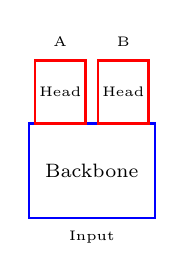
\begin{tikzpicture}[scale=0.8]
                    % Backbone
                    \draw[thick, blue] (0,0) rectangle (2,1.5);
                    \node at (1,0.75) {\scriptsize Backbone};

                    % Heads (made wider)
                    \draw[thick, red] (0.1,1.5) rectangle (0.9,2.5);
                    \node at (0.5,2) {\tiny Head};
                    \draw[thick, red] (1.1,1.5) rectangle (1.9,2.5);
                    \node at (1.5,2) {\tiny Head};

                    % Labels
                    \node at (1,-0.3) {\tiny Input};
                    \node at (0.5,2.8) {\tiny A};
                    \node at (1.5,2.8) {\tiny B};
                \end{tikzpicture}
            \end{center}
        \end{column}

        \begin{column}{0.48\textwidth}
            \textbf{Universal Model Approach}
            \begin{itemize}
                \item Single shared model
                \item Universal output layer
                \item Predefined concept mapping
                \item Static domain conversion
            \end{itemize}

            \begin{center}
                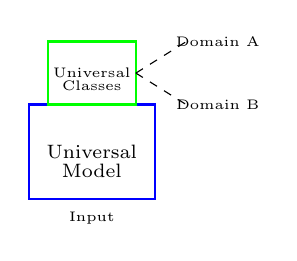
\begin{tikzpicture}[scale=0.8]
                    % Model
                    \draw[thick, blue] (0,0) rectangle (2,1.5);
                    \node at (1,0.75) {\scriptsize Universal};
                    \node at (1,0.45) {\scriptsize Model};

                    % Universal output (made wider)
                    \draw[thick, green] (0.3,1.5) rectangle (1.7,2.5);
                    \node at (1,2) {\tiny Universal};
                    \node at (1,1.8) {\tiny Classes};

                    % Conversion
                    \draw[dashed] (1.7,2) -- (2.5,2.5);
                    \draw[dashed] (1.7,2) -- (2.5,1.5);
                    \node at (3,2.5) {\tiny Domain A};
                    \node at (3,1.5) {\tiny Domain B};

                    % Labels
                    \node at (1,-0.3) {\tiny Input};
                \end{tikzpicture}
            \end{center}
        \end{column}
    \end{columns}

    \vspace{1em}

    \textcolor{blue}{\textbf{Key Insight:}} Build explicit concept-to-domain mappings to train a single universal model
\end{frame}

% Section 2: Method Overview
\section{Method Overview}

\begin{frame}{Our Method in 3 Steps}
    \begin{center}
        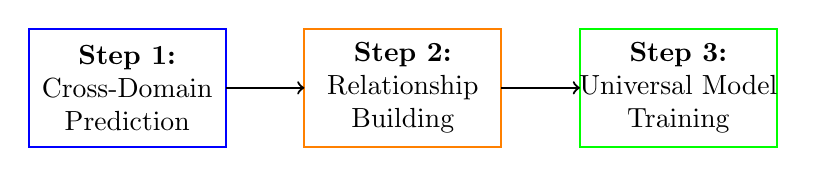
\begin{tikzpicture}[node distance=3cm]
            % Step 1
            \draw[thick, blue] (0,0) rectangle (2.5,1.5);
            \node[align=center] at (1.25,0.75) {\textbf{Step 1:}\\Cross-Domain\\Prediction};

            % Step 2
            \draw[thick, orange] (3.5,0) rectangle (6,1.5);
            \node[align=center] at (4.75,0.75) {\textbf{Step 2:}\\Relationship\\Building};

            % Step 3
            \draw[thick, green] (7,0) rectangle (9.5,1.5);
            \node[align=center] at (8.25,0.75) {\textbf{Step 3:}\\Universal Model\\Training};

            % Arrows
            \draw[->, thick] (2.5,0.75) -- (3.5,0.75);
            \draw[->, thick] (6,0.75) -- (7,0.75);
        \end{tikzpicture}
    \end{center}

    \vspace{1em}

    \begin{enumerate}
        \item \textbf{Cross-Domain Prediction}: Train domain-specific models, run inference on other domains
        \item \textbf{Relationship Building}: Extract meaningful relationships from cross-domain predictions and create universal taxonomy
        \item \textbf{Universal Model Training}: Create and train a single model using universal taxonomy
    \end{enumerate}
\end{frame}

\begin{frame}{Cross-Domain Prediction Process}
    \textbf{Goal}: Discover relationships between classes from different datasets

    \vspace{0.5em}

    \textbf{Process}:
    \begin{enumerate}
        \item Train domain-specific models
        \item Run each model on images from \emph{all other} domains
        \item Create probability matrices $P_{ab}(i,j)$ = probability of classifying class $c_i^a$ as class $c_j^b$
    \end{enumerate}

    \vspace{0.5em}

    \textbf{Example}: CIFAR-100 model predicting on Caltech-101 images
    \begin{itemize}
        \item CIFAR-100 "automobile" $\rightarrow$ Caltech-101 "car\_side" (high probability)
        \item CIFAR-100 "dog" $\rightarrow$ Caltech-101 "dalmatian" (moderate probability)
        \item CIFAR-100 "airplane" $\rightarrow$ Caltech-101 "butterfly" (low probability)
    \end{itemize}

    \vspace{0.5em}

    \begin{equation}
        P_{ab}(i, j) = \frac{M_{ab}(i, j)}{\sum_{k=1}^{|C_a|} M_{ab}(i, k)}
    \end{equation}
\end{frame}

% Section 3: Relationship Selection Methods
\section{Relationship Selection Methods}

\begin{frame}{Challenge: Selecting Relevant Relationships}
    \textbf{Problems with raw probability matrices}:
    \begin{itemize}
        \item Noisy predictions from imperfect models
        \item Unknown number of true relationships
        \item Different datasets have different scales of similarity
    \end{itemize}

    \vspace{1em}

    \textbf{Solution}: Develop \& evaluate multiple relationship selection methods

    \vspace{1em}

    \begin{columns}[T]
        \begin{column}{0.48\textwidth}
            \textbf{Methods Evaluated:}
            \begin{enumerate}
                \item Naive Thresholding
                \item Most Common Foreign Prediction (MCFP)
                \item Density Thresholding
                \item Relationship Hypothesis
            \end{enumerate}
        \end{column}

        \begin{column}{0.48\textwidth}
            \textbf{Evaluation Metrics:}
            \begin{itemize}
                \item Edge Difference Ratio (EDR)
                \item Precision \& Recall
                \item F1 Score
            \end{itemize}
        \end{column}
    \end{columns}
\end{frame}

\begin{frame}{Relationship Selection Methods Explained}
    \begin{enumerate}
        \item \textbf{Naive Thresholding}:
              \begin{equation}
                  \text{select\_relationships}(P_{ab}) = \{(i, j) \mid P_{ab}(i, j) \geq t\}
              \end{equation}

        \item \textbf{Most Common Foreign Prediction (MCFP)}:
              \begin{equation}
                  \text{select\_relationships}(P_{ab}) = \{(i, j) \mid j = \text{argmax}_{j'} P_{ab}(i, j')\}
              \end{equation}

        \item \textbf{Density Thresholding}: Select minimum relationships covering $p\%$ of probability mass

        \item \textbf{Relationship Hypothesis}: Assumes relationships based on shared concepts should have equal probabilities. For each class, find optimal $k$ relationships by minimizing:
              \begin{equation}
                  \sum_{j=1}^k \left| X_i(j) - \frac{1}{k} \right| + \sum_{j=k+1}^{|C_b|} X_i(j)
              \end{equation}
              where $X_i(j)$ are sorted probabilities in descending order.
    \end{enumerate}
\end{frame}

\begin{frame}{Relationship Selection Results}
    \textbf{Evaluation on synthetic datasets with known ground truth}

    \vspace{0.5em}

    \begin{table}[h]
        \centering
        \scriptsize
        \begin{tabular}{lcccc}
            \toprule
            \textbf{Method}         & \textbf{EDR}   & \textbf{Precision} & \textbf{Recall} & \textbf{F1 Score} \\
            \midrule
            Naive Thresholding      & \textbf{0.463} & 0.675              & \textbf{0.889}  & \textbf{0.767}    \\
            MCFP                    & 0.579          & \textbf{0.865}     & 0.421           & 0.566             \\
            Density Thresholding    & 0.523          & 0.726              & 0.795           & 0.759             \\
            Relationship Hypothesis & 0.493          & 0.746              & 0.823           & 0.783             \\
            \bottomrule
        \end{tabular}
        \caption{Global optimal performance across all synthetic dataset variants}
    \end{table}

    \vspace{0.5em}

    \textbf{Key Findings}:
    \begin{itemize}
        \item \textbf{Naive thresholding} achieves best overall performance (lowest EDR)
        \item \textbf{MCFP} has highest precision but lowest recall
        \item Trade-off between capturing all relationships vs. avoiding false positives
    \end{itemize}
\end{frame}

% Section 4: Synthetic Ground Truth
\section{Synthetic Ground Truth \& Domain Adaptation}

\begin{frame}{The Need for Controlled Ground Truth}
    \textbf{Problem}: Real datasets lack clear inter-dataset relationships

    \begin{itemize}
        \item \textbf{WordNet}: Text-based relationships don't match visual similarities
        \item \textbf{Open Images}: Multi-label, automatically generated
        \item \textbf{Existing taxonomies}: Too domain-specific or hierarchical
    \end{itemize}

    \vspace{1em}

    \textbf{Solution}: Generate synthetic datasets with controlled relationships

    \begin{enumerate}
        \item Define \textbf{atomic concepts} $\mathcal{U} = \{1,2,\ldots,n\}$
        \item Create synthetic classes as subsets: $c^i_j \subseteq \mathcal{U}$
        \item Generate multiple domains by sampling concepts
        \item Calculate relationships based on concept overlap
    \end{enumerate}

    \vspace{0.5em}

    \begin{equation}
        P_{i,j} = \frac{|c^A_i \cap c^B_j|}{|c^A_i|} + \frac{1 - \frac{|c^A_i \cap c^B_j|}{|c^A_i|}}{|C_B|}
    \end{equation}
\end{frame}

\begin{frame}{Domain-Shifted Synthetic Datasets}
    \textbf{Problem}: Original synthetic variants too easy (same underlying images)

    \vspace{0.5em}

    \textbf{Solution}: Apply domain transformations to create realistic challenges

    \begin{columns}[T]
        \begin{column}{0.6\textwidth}
            \textbf{Transformations Applied}:
            \begin{itemize}
                \item \textbf{Domain A}: Noisy grayscale
                \item \textbf{Domain B}: Rotation + blur
                \item \textbf{Domain C}: Random erasing + color jitter + perspective shifts
            \end{itemize}

            \vspace{1em}

            \textbf{Results}:
            \begin{itemize}
                \item Model accuracy drops by ~10\%
                \item More realistic cross-domain predictions
                \item Better evaluation of relationship selection methods
            \end{itemize}
        \end{column}

        \begin{column}{0.35\textwidth}
            \begin{center}
                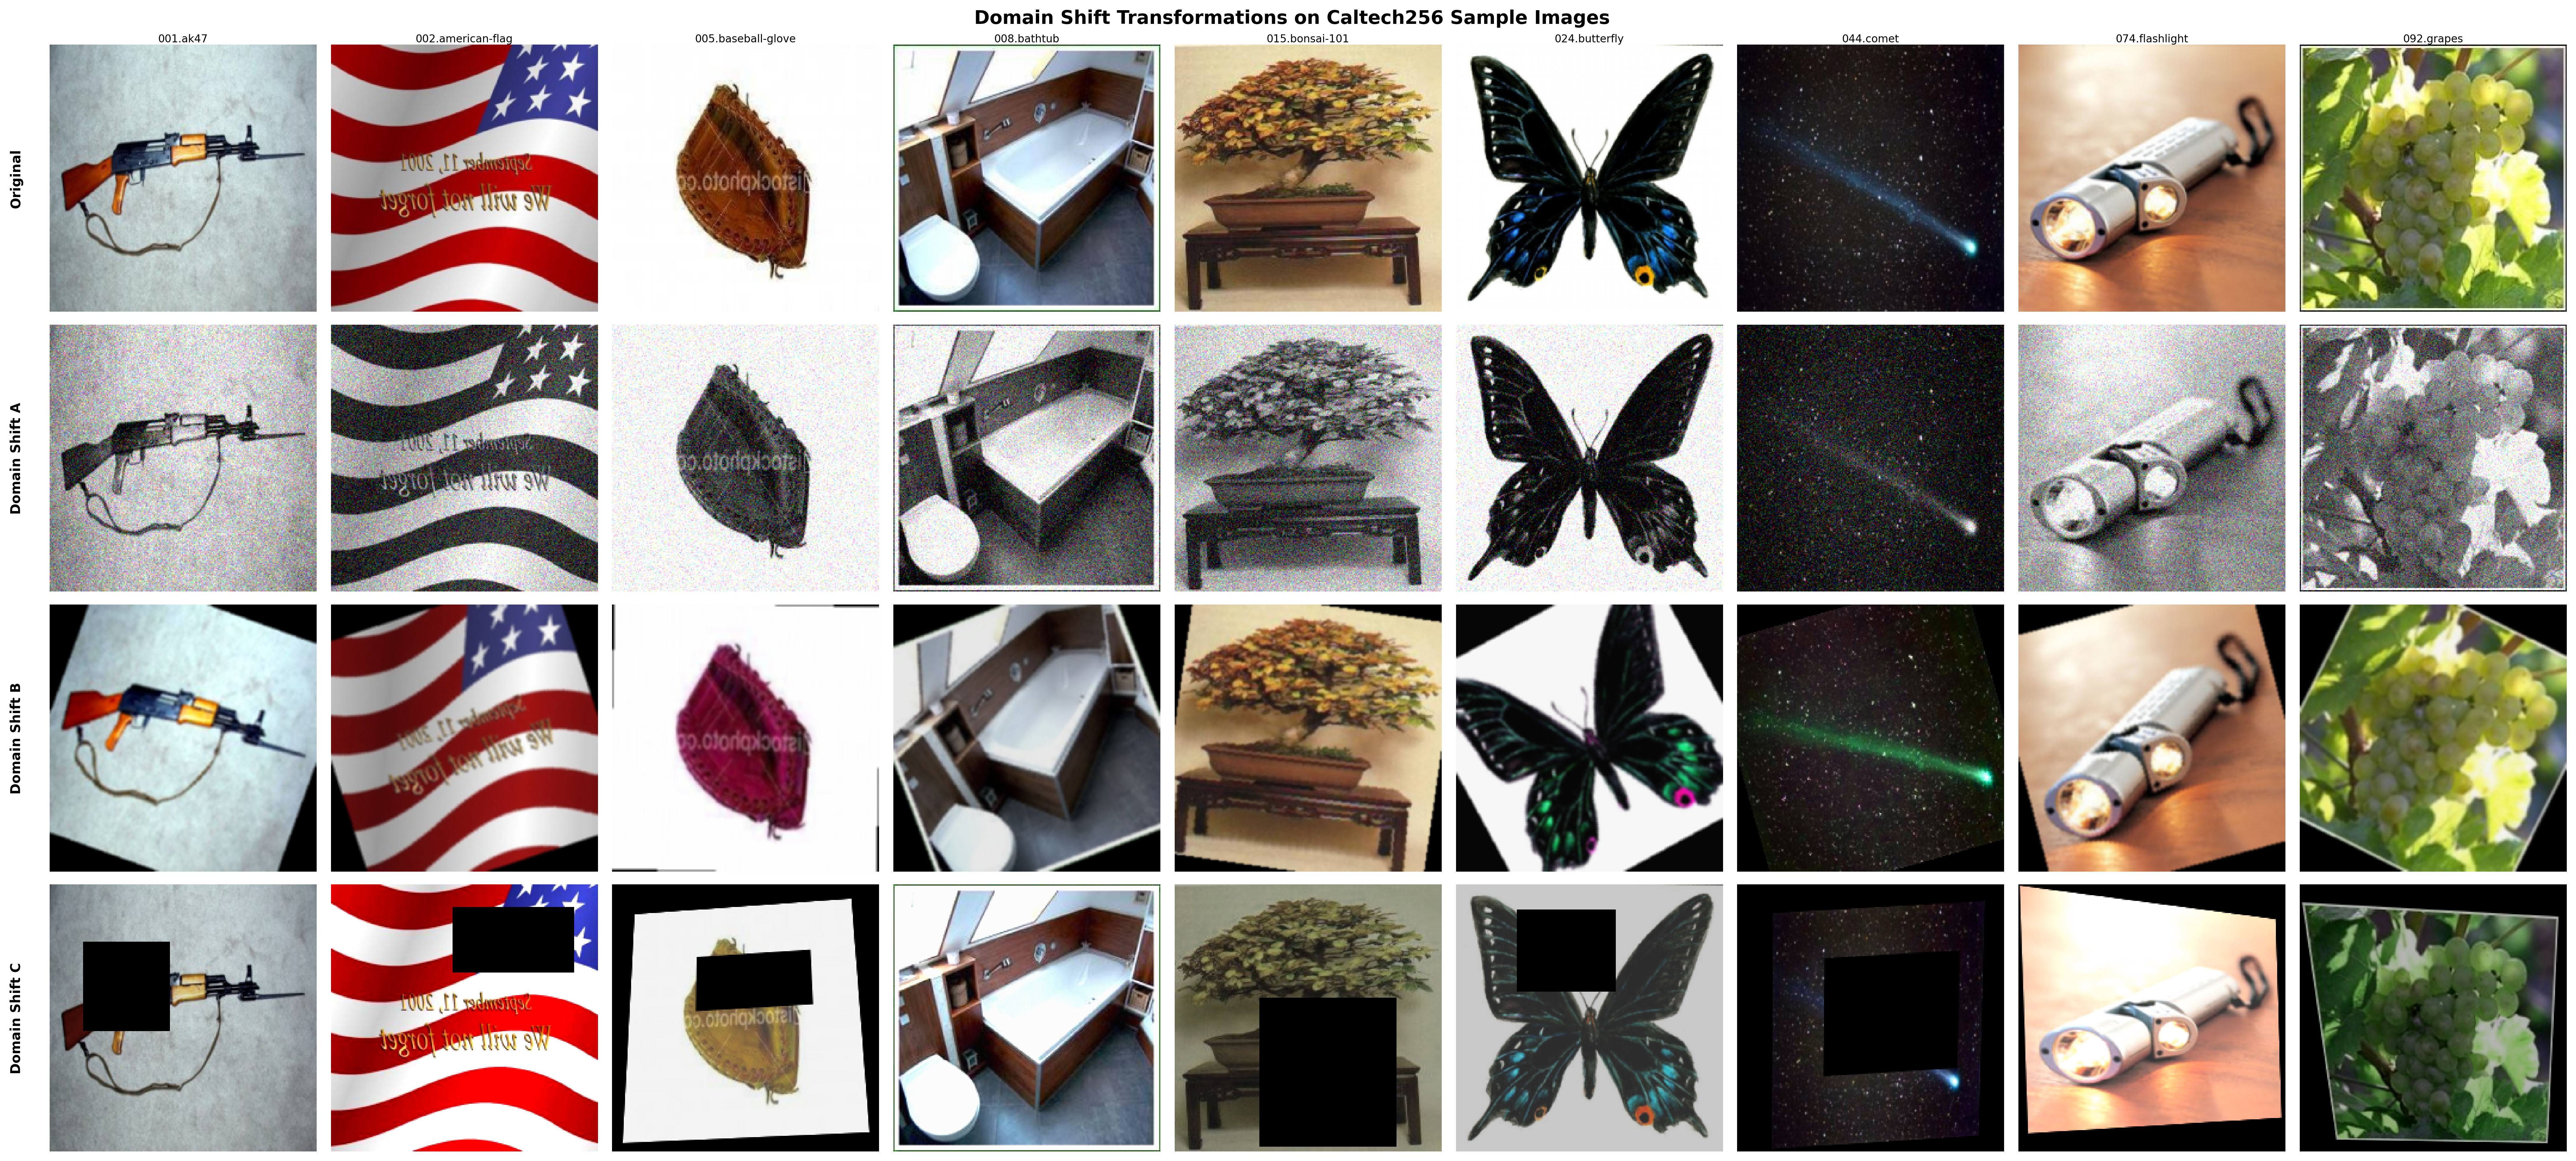
\includegraphics[width=\textwidth]{../thesis/figures/domain_shift_visualization.png}
            \end{center}
            \small{Example images from domain-shifted variants}
        \end{column}
    \end{columns}
\end{frame}

% Section 5: Universal Model Training
\section{Universal Model Training}

\begin{frame}{Universal Model Architecture}
    \textbf{Key Differences from Baseline Models}:

    \begin{columns}[T]
        \begin{column}{0.48\textwidth}
            \textbf{Baseline Model}:
            \begin{itemize}
                \item 6-layer FC classifier
                \item Dropout regularization
                \item One-hot targets
                \item Cross-entropy loss
                \item Domain-specific outputs
            \end{itemize}
        \end{column}

        \begin{column}{0.48\textwidth}
            \textbf{Universal Model}:
            \begin{itemize}
                \item 2-layer FC classifier
                \item No dropout
                \item Probability distribution targets
                \item Cross-entropy for discrete distributions
                \item Universal class outputs
            \end{itemize}
        \end{column}
    \end{columns}

    \vspace{1em}

    \textbf{Target Generation}: Convert domain labels to universal class distributions
    \begin{equation}
        \mathbf{t} = \hat{M}_i[j, :] \quad \text{where } \hat{M}_i(j, u) = \frac{M_i(j, u)}{\sum_{u'} M_i(j, u')}
    \end{equation}

    \textbf{Loss Function}:
    \begin{equation}
        \mathcal{L} = -\sum_{u=1}^{|U|} \mathbf{t}(u) \log(\mathbf{p}(u))
    \end{equation}
\end{frame}

\begin{frame}{Multi-Domain Training Process}
    \textbf{Training Procedure}:
    \begin{enumerate}
        \item Combine multiple datasets while preserving domain identity
        \item Each sample: $(\text{image}, (\text{domain\_id}, \text{label})) \rightarrow (\text{image}, \text{universal\_target})$
        \item Train single model on unified dataset
        \item Use domain-specific mapping matrices for target generation
    \end{enumerate}

    \vspace{1em}

    \textbf{Inference}:
    \begin{align}
        \mathbf{d}_i & = M_i^T \mathbf{p}            \\
        \hat{c}_i    & = \text{argmax}(\mathbf{d}_i)
    \end{align}

    where $\mathbf{p}$ are universal class predictions and $\mathbf{d}_i$ are domain-specific predictions.

    \vspace{1em}

    \textbf{Key Challenge}: Validation loss increases while accuracy improves
    \begin{itemize}
        \item Solution: Monitor validation accuracy for checkpointing
        \item Caused by label smoothing effects and multi-target distributions
    \end{itemize}
\end{frame}

% Section 6: Results
\section{Results}

\begin{frame}{Universal Model Performance}
    \textbf{Datasets}: Caltech-101, Caltech-256, CIFAR-100

    \begin{table}[h]
        \centering
        \scriptsize
        \begin{tabular}{lccc}
            \toprule
            \textbf{Model Type}      & \textbf{Caltech-101} & \textbf{Caltech-256} & \textbf{CIFAR-100} \\
            \midrule
            Baseline (Single Domain) & 0.828                & 0.798                & 0.734              \\
            Universal (MCFP)         & \textbf{0.845}       & \textbf{0.812}       & 0.728              \\
            Universal (Density)      & 0.834                & 0.809                & \textbf{0.741}     \\
            Universal (Hypothesis)   & 0.831                & 0.801                & 0.735              \\
            \bottomrule
        \end{tabular}
        \caption{Test accuracy comparison (2-domain: Caltech-101 + Caltech-256)}
    \end{table}

    \vspace{1em}

    \textbf{Key Findings}:
    \begin{itemize}
        \item Universal models \textcolor{blue}{\textbf{outperform}} single-domain baselines
        \item Different relationship selection methods excel on different datasets
        \item No single method consistently optimal across all scenarios
    \end{itemize}
\end{frame}

\begin{frame}{Feature Visualization with t-SNE}
    \begin{columns}[T]
        \begin{column}{0.48\textwidth}
            \textbf{2-Domain (Caltech-101 + 256)}
            \begin{center}
                \resizebox{\textwidth}{!}{%% Creator: Matplotlib, PGF backend
%%
%% To include the figure in your LaTeX document, write
%%   \input{<filename>.pgf}
%%
%% Make sure the required packages are loaded in your preamble
%%   \usepackage{pgf}
%%
%% Also ensure that all the required font packages are loaded; for instance,
%% the lmodern package is sometimes necessary when using math font.
%%   \usepackage{lmodern}
%%
%% Figures using additional raster images can only be included by \input if
%% they are in the same directory as the main LaTeX file. For loading figures
%% from other directories you can use the `import` package
%%   \usepackage{import}
%%
%% and then include the figures with
%%   \import{<path to file>}{<filename>.pgf}
%%
%% Matplotlib used the following preamble
%%   \def\mathdefault#1{#1}
%%   \everymath=\expandafter{\the\everymath\displaystyle}
%%   \IfFileExists{scrextend.sty}{
%%     \usepackage[fontsize=11.000000pt]{scrextend}
%%   }{
%%     \renewcommand{\normalsize}{\fontsize{11.000000}{13.200000}\selectfont}
%%     \normalsize
%%   }
%%   
%%   \ifdefined\pdftexversion\else  % non-pdftex case.
%%     \usepackage{fontspec}
%%     \setmainfont{DejaVuSerif.ttf}[Path=\detokenize{/home/bjoern/miniconda3/envs/master-thesis/lib/python3.13/site-packages/matplotlib/mpl-data/fonts/ttf/}]
%%     \setsansfont{DejaVuSans.ttf}[Path=\detokenize{/home/bjoern/miniconda3/envs/master-thesis/lib/python3.13/site-packages/matplotlib/mpl-data/fonts/ttf/}]
%%     \setmonofont{DejaVuSansMono.ttf}[Path=\detokenize{/home/bjoern/miniconda3/envs/master-thesis/lib/python3.13/site-packages/matplotlib/mpl-data/fonts/ttf/}]
%%   \fi
%%   \makeatletter\@ifpackageloaded{underscore}{}{\usepackage[strings]{underscore}}\makeatother
%%
\begingroup%
\makeatletter%
\begin{pgfpicture}%
\pgfpathrectangle{\pgfpointorigin}{\pgfqpoint{17.870000in}{11.795000in}}%
\pgfusepath{use as bounding box, clip}%
\begin{pgfscope}%
\pgfsetbuttcap%
\pgfsetmiterjoin%
\definecolor{currentfill}{rgb}{1.000000,1.000000,1.000000}%
\pgfsetfillcolor{currentfill}%
\pgfsetlinewidth{0.000000pt}%
\definecolor{currentstroke}{rgb}{1.000000,1.000000,1.000000}%
\pgfsetstrokecolor{currentstroke}%
\pgfsetdash{}{0pt}%
\pgfpathmoveto{\pgfqpoint{0.000000in}{-0.000000in}}%
\pgfpathlineto{\pgfqpoint{17.870000in}{-0.000000in}}%
\pgfpathlineto{\pgfqpoint{17.870000in}{11.795000in}}%
\pgfpathlineto{\pgfqpoint{0.000000in}{11.795000in}}%
\pgfpathlineto{\pgfqpoint{0.000000in}{-0.000000in}}%
\pgfpathclose%
\pgfusepath{fill}%
\end{pgfscope}%
\begin{pgfscope}%
\pgfsetbuttcap%
\pgfsetmiterjoin%
\definecolor{currentfill}{rgb}{1.000000,1.000000,1.000000}%
\pgfsetfillcolor{currentfill}%
\pgfsetlinewidth{0.000000pt}%
\definecolor{currentstroke}{rgb}{0.000000,0.000000,0.000000}%
\pgfsetstrokecolor{currentstroke}%
\pgfsetstrokeopacity{0.000000}%
\pgfsetdash{}{0pt}%
\pgfpathmoveto{\pgfqpoint{0.674399in}{6.299528in}}%
\pgfpathlineto{\pgfqpoint{5.880000in}{6.299528in}}%
\pgfpathlineto{\pgfqpoint{5.880000in}{11.242250in}}%
\pgfpathlineto{\pgfqpoint{0.674399in}{11.242250in}}%
\pgfpathlineto{\pgfqpoint{0.674399in}{6.299528in}}%
\pgfpathclose%
\pgfusepath{fill}%
\end{pgfscope}%
\begin{pgfscope}%
\pgfpathrectangle{\pgfqpoint{0.674399in}{6.299528in}}{\pgfqpoint{5.205601in}{4.942722in}}%
\pgfusepath{clip}%
\pgfsetbuttcap%
\pgfsetroundjoin%
\definecolor{currentfill}{rgb}{1.000000,0.000000,0.000000}%
\pgfsetfillcolor{currentfill}%
\pgfsetfillopacity{0.600000}%
\pgfsetlinewidth{0.501875pt}%
\definecolor{currentstroke}{rgb}{0.000000,0.000000,0.000000}%
\pgfsetstrokecolor{currentstroke}%
\pgfsetstrokeopacity{0.600000}%
\pgfsetdash{}{0pt}%
\pgfsys@defobject{currentmarker}{\pgfqpoint{-0.038036in}{-0.038036in}}{\pgfqpoint{0.038036in}{0.038036in}}{%
\pgfpathmoveto{\pgfqpoint{0.000000in}{-0.038036in}}%
\pgfpathcurveto{\pgfqpoint{0.010087in}{-0.038036in}}{\pgfqpoint{0.019763in}{-0.034029in}}{\pgfqpoint{0.026896in}{-0.026896in}}%
\pgfpathcurveto{\pgfqpoint{0.034029in}{-0.019763in}}{\pgfqpoint{0.038036in}{-0.010087in}}{\pgfqpoint{0.038036in}{0.000000in}}%
\pgfpathcurveto{\pgfqpoint{0.038036in}{0.010087in}}{\pgfqpoint{0.034029in}{0.019763in}}{\pgfqpoint{0.026896in}{0.026896in}}%
\pgfpathcurveto{\pgfqpoint{0.019763in}{0.034029in}}{\pgfqpoint{0.010087in}{0.038036in}}{\pgfqpoint{0.000000in}{0.038036in}}%
\pgfpathcurveto{\pgfqpoint{-0.010087in}{0.038036in}}{\pgfqpoint{-0.019763in}{0.034029in}}{\pgfqpoint{-0.026896in}{0.026896in}}%
\pgfpathcurveto{\pgfqpoint{-0.034029in}{0.019763in}}{\pgfqpoint{-0.038036in}{0.010087in}}{\pgfqpoint{-0.038036in}{0.000000in}}%
\pgfpathcurveto{\pgfqpoint{-0.038036in}{-0.010087in}}{\pgfqpoint{-0.034029in}{-0.019763in}}{\pgfqpoint{-0.026896in}{-0.026896in}}%
\pgfpathcurveto{\pgfqpoint{-0.019763in}{-0.034029in}}{\pgfqpoint{-0.010087in}{-0.038036in}}{\pgfqpoint{0.000000in}{-0.038036in}}%
\pgfpathlineto{\pgfqpoint{0.000000in}{-0.038036in}}%
\pgfpathclose%
\pgfusepath{stroke,fill}%
}%
\begin{pgfscope}%
\pgfsys@transformshift{2.862738in}{8.585226in}%
\pgfsys@useobject{currentmarker}{}%
\end{pgfscope}%
\end{pgfscope}%
\begin{pgfscope}%
\pgfpathrectangle{\pgfqpoint{0.674399in}{6.299528in}}{\pgfqpoint{5.205601in}{4.942722in}}%
\pgfusepath{clip}%
\pgfsetbuttcap%
\pgfsetroundjoin%
\definecolor{currentfill}{rgb}{1.000000,0.023162,0.000000}%
\pgfsetfillcolor{currentfill}%
\pgfsetfillopacity{0.600000}%
\pgfsetlinewidth{0.501875pt}%
\definecolor{currentstroke}{rgb}{0.000000,0.000000,0.000000}%
\pgfsetstrokecolor{currentstroke}%
\pgfsetstrokeopacity{0.600000}%
\pgfsetdash{}{0pt}%
\pgfsys@defobject{currentmarker}{\pgfqpoint{-0.038036in}{-0.038036in}}{\pgfqpoint{0.038036in}{0.038036in}}{%
\pgfpathmoveto{\pgfqpoint{0.000000in}{-0.038036in}}%
\pgfpathcurveto{\pgfqpoint{0.010087in}{-0.038036in}}{\pgfqpoint{0.019763in}{-0.034029in}}{\pgfqpoint{0.026896in}{-0.026896in}}%
\pgfpathcurveto{\pgfqpoint{0.034029in}{-0.019763in}}{\pgfqpoint{0.038036in}{-0.010087in}}{\pgfqpoint{0.038036in}{0.000000in}}%
\pgfpathcurveto{\pgfqpoint{0.038036in}{0.010087in}}{\pgfqpoint{0.034029in}{0.019763in}}{\pgfqpoint{0.026896in}{0.026896in}}%
\pgfpathcurveto{\pgfqpoint{0.019763in}{0.034029in}}{\pgfqpoint{0.010087in}{0.038036in}}{\pgfqpoint{0.000000in}{0.038036in}}%
\pgfpathcurveto{\pgfqpoint{-0.010087in}{0.038036in}}{\pgfqpoint{-0.019763in}{0.034029in}}{\pgfqpoint{-0.026896in}{0.026896in}}%
\pgfpathcurveto{\pgfqpoint{-0.034029in}{0.019763in}}{\pgfqpoint{-0.038036in}{0.010087in}}{\pgfqpoint{-0.038036in}{0.000000in}}%
\pgfpathcurveto{\pgfqpoint{-0.038036in}{-0.010087in}}{\pgfqpoint{-0.034029in}{-0.019763in}}{\pgfqpoint{-0.026896in}{-0.026896in}}%
\pgfpathcurveto{\pgfqpoint{-0.019763in}{-0.034029in}}{\pgfqpoint{-0.010087in}{-0.038036in}}{\pgfqpoint{0.000000in}{-0.038036in}}%
\pgfpathlineto{\pgfqpoint{0.000000in}{-0.038036in}}%
\pgfpathclose%
\pgfusepath{stroke,fill}%
}%
\begin{pgfscope}%
\pgfsys@transformshift{2.223486in}{8.601964in}%
\pgfsys@useobject{currentmarker}{}%
\end{pgfscope}%
\begin{pgfscope}%
\pgfsys@transformshift{2.266075in}{8.706159in}%
\pgfsys@useobject{currentmarker}{}%
\end{pgfscope}%
\begin{pgfscope}%
\pgfsys@transformshift{2.393497in}{8.557504in}%
\pgfsys@useobject{currentmarker}{}%
\end{pgfscope}%
\begin{pgfscope}%
\pgfsys@transformshift{2.414539in}{8.617338in}%
\pgfsys@useobject{currentmarker}{}%
\end{pgfscope}%
\begin{pgfscope}%
\pgfsys@transformshift{2.321594in}{8.644575in}%
\pgfsys@useobject{currentmarker}{}%
\end{pgfscope}%
\end{pgfscope}%
\begin{pgfscope}%
\pgfpathrectangle{\pgfqpoint{0.674399in}{6.299528in}}{\pgfqpoint{5.205601in}{4.942722in}}%
\pgfusepath{clip}%
\pgfsetbuttcap%
\pgfsetroundjoin%
\definecolor{currentfill}{rgb}{1.000000,0.046324,0.000000}%
\pgfsetfillcolor{currentfill}%
\pgfsetfillopacity{0.600000}%
\pgfsetlinewidth{0.501875pt}%
\definecolor{currentstroke}{rgb}{0.000000,0.000000,0.000000}%
\pgfsetstrokecolor{currentstroke}%
\pgfsetstrokeopacity{0.600000}%
\pgfsetdash{}{0pt}%
\pgfsys@defobject{currentmarker}{\pgfqpoint{-0.038036in}{-0.038036in}}{\pgfqpoint{0.038036in}{0.038036in}}{%
\pgfpathmoveto{\pgfqpoint{0.000000in}{-0.038036in}}%
\pgfpathcurveto{\pgfqpoint{0.010087in}{-0.038036in}}{\pgfqpoint{0.019763in}{-0.034029in}}{\pgfqpoint{0.026896in}{-0.026896in}}%
\pgfpathcurveto{\pgfqpoint{0.034029in}{-0.019763in}}{\pgfqpoint{0.038036in}{-0.010087in}}{\pgfqpoint{0.038036in}{0.000000in}}%
\pgfpathcurveto{\pgfqpoint{0.038036in}{0.010087in}}{\pgfqpoint{0.034029in}{0.019763in}}{\pgfqpoint{0.026896in}{0.026896in}}%
\pgfpathcurveto{\pgfqpoint{0.019763in}{0.034029in}}{\pgfqpoint{0.010087in}{0.038036in}}{\pgfqpoint{0.000000in}{0.038036in}}%
\pgfpathcurveto{\pgfqpoint{-0.010087in}{0.038036in}}{\pgfqpoint{-0.019763in}{0.034029in}}{\pgfqpoint{-0.026896in}{0.026896in}}%
\pgfpathcurveto{\pgfqpoint{-0.034029in}{0.019763in}}{\pgfqpoint{-0.038036in}{0.010087in}}{\pgfqpoint{-0.038036in}{0.000000in}}%
\pgfpathcurveto{\pgfqpoint{-0.038036in}{-0.010087in}}{\pgfqpoint{-0.034029in}{-0.019763in}}{\pgfqpoint{-0.026896in}{-0.026896in}}%
\pgfpathcurveto{\pgfqpoint{-0.019763in}{-0.034029in}}{\pgfqpoint{-0.010087in}{-0.038036in}}{\pgfqpoint{0.000000in}{-0.038036in}}%
\pgfpathlineto{\pgfqpoint{0.000000in}{-0.038036in}}%
\pgfpathclose%
\pgfusepath{stroke,fill}%
}%
\begin{pgfscope}%
\pgfsys@transformshift{3.258625in}{8.404798in}%
\pgfsys@useobject{currentmarker}{}%
\end{pgfscope}%
\begin{pgfscope}%
\pgfsys@transformshift{3.185168in}{8.382731in}%
\pgfsys@useobject{currentmarker}{}%
\end{pgfscope}%
\begin{pgfscope}%
\pgfsys@transformshift{3.231090in}{8.424416in}%
\pgfsys@useobject{currentmarker}{}%
\end{pgfscope}%
\end{pgfscope}%
\begin{pgfscope}%
\pgfpathrectangle{\pgfqpoint{0.674399in}{6.299528in}}{\pgfqpoint{5.205601in}{4.942722in}}%
\pgfusepath{clip}%
\pgfsetbuttcap%
\pgfsetroundjoin%
\definecolor{currentfill}{rgb}{1.000000,0.092647,0.000000}%
\pgfsetfillcolor{currentfill}%
\pgfsetfillopacity{0.600000}%
\pgfsetlinewidth{0.501875pt}%
\definecolor{currentstroke}{rgb}{0.000000,0.000000,0.000000}%
\pgfsetstrokecolor{currentstroke}%
\pgfsetstrokeopacity{0.600000}%
\pgfsetdash{}{0pt}%
\pgfsys@defobject{currentmarker}{\pgfqpoint{-0.038036in}{-0.038036in}}{\pgfqpoint{0.038036in}{0.038036in}}{%
\pgfpathmoveto{\pgfqpoint{0.000000in}{-0.038036in}}%
\pgfpathcurveto{\pgfqpoint{0.010087in}{-0.038036in}}{\pgfqpoint{0.019763in}{-0.034029in}}{\pgfqpoint{0.026896in}{-0.026896in}}%
\pgfpathcurveto{\pgfqpoint{0.034029in}{-0.019763in}}{\pgfqpoint{0.038036in}{-0.010087in}}{\pgfqpoint{0.038036in}{0.000000in}}%
\pgfpathcurveto{\pgfqpoint{0.038036in}{0.010087in}}{\pgfqpoint{0.034029in}{0.019763in}}{\pgfqpoint{0.026896in}{0.026896in}}%
\pgfpathcurveto{\pgfqpoint{0.019763in}{0.034029in}}{\pgfqpoint{0.010087in}{0.038036in}}{\pgfqpoint{0.000000in}{0.038036in}}%
\pgfpathcurveto{\pgfqpoint{-0.010087in}{0.038036in}}{\pgfqpoint{-0.019763in}{0.034029in}}{\pgfqpoint{-0.026896in}{0.026896in}}%
\pgfpathcurveto{\pgfqpoint{-0.034029in}{0.019763in}}{\pgfqpoint{-0.038036in}{0.010087in}}{\pgfqpoint{-0.038036in}{0.000000in}}%
\pgfpathcurveto{\pgfqpoint{-0.038036in}{-0.010087in}}{\pgfqpoint{-0.034029in}{-0.019763in}}{\pgfqpoint{-0.026896in}{-0.026896in}}%
\pgfpathcurveto{\pgfqpoint{-0.019763in}{-0.034029in}}{\pgfqpoint{-0.010087in}{-0.038036in}}{\pgfqpoint{0.000000in}{-0.038036in}}%
\pgfpathlineto{\pgfqpoint{0.000000in}{-0.038036in}}%
\pgfpathclose%
\pgfusepath{stroke,fill}%
}%
\begin{pgfscope}%
\pgfsys@transformshift{5.643382in}{8.720746in}%
\pgfsys@useobject{currentmarker}{}%
\end{pgfscope}%
\begin{pgfscope}%
\pgfsys@transformshift{5.532236in}{8.613597in}%
\pgfsys@useobject{currentmarker}{}%
\end{pgfscope}%
\begin{pgfscope}%
\pgfsys@transformshift{5.535869in}{8.723511in}%
\pgfsys@useobject{currentmarker}{}%
\end{pgfscope}%
\begin{pgfscope}%
\pgfsys@transformshift{5.466007in}{8.700552in}%
\pgfsys@useobject{currentmarker}{}%
\end{pgfscope}%
\begin{pgfscope}%
\pgfsys@transformshift{5.587004in}{8.674995in}%
\pgfsys@useobject{currentmarker}{}%
\end{pgfscope}%
\end{pgfscope}%
\begin{pgfscope}%
\pgfpathrectangle{\pgfqpoint{0.674399in}{6.299528in}}{\pgfqpoint{5.205601in}{4.942722in}}%
\pgfusepath{clip}%
\pgfsetbuttcap%
\pgfsetroundjoin%
\definecolor{currentfill}{rgb}{1.000000,0.162133,0.000000}%
\pgfsetfillcolor{currentfill}%
\pgfsetfillopacity{0.600000}%
\pgfsetlinewidth{0.501875pt}%
\definecolor{currentstroke}{rgb}{0.000000,0.000000,0.000000}%
\pgfsetstrokecolor{currentstroke}%
\pgfsetstrokeopacity{0.600000}%
\pgfsetdash{}{0pt}%
\pgfsys@defobject{currentmarker}{\pgfqpoint{-0.038036in}{-0.038036in}}{\pgfqpoint{0.038036in}{0.038036in}}{%
\pgfpathmoveto{\pgfqpoint{0.000000in}{-0.038036in}}%
\pgfpathcurveto{\pgfqpoint{0.010087in}{-0.038036in}}{\pgfqpoint{0.019763in}{-0.034029in}}{\pgfqpoint{0.026896in}{-0.026896in}}%
\pgfpathcurveto{\pgfqpoint{0.034029in}{-0.019763in}}{\pgfqpoint{0.038036in}{-0.010087in}}{\pgfqpoint{0.038036in}{0.000000in}}%
\pgfpathcurveto{\pgfqpoint{0.038036in}{0.010087in}}{\pgfqpoint{0.034029in}{0.019763in}}{\pgfqpoint{0.026896in}{0.026896in}}%
\pgfpathcurveto{\pgfqpoint{0.019763in}{0.034029in}}{\pgfqpoint{0.010087in}{0.038036in}}{\pgfqpoint{0.000000in}{0.038036in}}%
\pgfpathcurveto{\pgfqpoint{-0.010087in}{0.038036in}}{\pgfqpoint{-0.019763in}{0.034029in}}{\pgfqpoint{-0.026896in}{0.026896in}}%
\pgfpathcurveto{\pgfqpoint{-0.034029in}{0.019763in}}{\pgfqpoint{-0.038036in}{0.010087in}}{\pgfqpoint{-0.038036in}{0.000000in}}%
\pgfpathcurveto{\pgfqpoint{-0.038036in}{-0.010087in}}{\pgfqpoint{-0.034029in}{-0.019763in}}{\pgfqpoint{-0.026896in}{-0.026896in}}%
\pgfpathcurveto{\pgfqpoint{-0.019763in}{-0.034029in}}{\pgfqpoint{-0.010087in}{-0.038036in}}{\pgfqpoint{0.000000in}{-0.038036in}}%
\pgfpathlineto{\pgfqpoint{0.000000in}{-0.038036in}}%
\pgfpathclose%
\pgfusepath{stroke,fill}%
}%
\begin{pgfscope}%
\pgfsys@transformshift{2.031981in}{10.973128in}%
\pgfsys@useobject{currentmarker}{}%
\end{pgfscope}%
\begin{pgfscope}%
\pgfsys@transformshift{2.051984in}{10.902940in}%
\pgfsys@useobject{currentmarker}{}%
\end{pgfscope}%
\begin{pgfscope}%
\pgfsys@transformshift{2.061628in}{10.845514in}%
\pgfsys@useobject{currentmarker}{}%
\end{pgfscope}%
\begin{pgfscope}%
\pgfsys@transformshift{2.025181in}{10.786585in}%
\pgfsys@useobject{currentmarker}{}%
\end{pgfscope}%
\begin{pgfscope}%
\pgfsys@transformshift{2.178567in}{10.858440in}%
\pgfsys@useobject{currentmarker}{}%
\end{pgfscope}%
\begin{pgfscope}%
\pgfsys@transformshift{2.116710in}{10.887177in}%
\pgfsys@useobject{currentmarker}{}%
\end{pgfscope}%
\begin{pgfscope}%
\pgfsys@transformshift{1.987636in}{10.848286in}%
\pgfsys@useobject{currentmarker}{}%
\end{pgfscope}%
\begin{pgfscope}%
\pgfsys@transformshift{2.098103in}{10.770286in}%
\pgfsys@useobject{currentmarker}{}%
\end{pgfscope}%
\begin{pgfscope}%
\pgfsys@transformshift{2.190275in}{10.981974in}%
\pgfsys@useobject{currentmarker}{}%
\end{pgfscope}%
\begin{pgfscope}%
\pgfsys@transformshift{2.165403in}{10.922321in}%
\pgfsys@useobject{currentmarker}{}%
\end{pgfscope}%
\begin{pgfscope}%
\pgfsys@transformshift{2.105650in}{11.017581in}%
\pgfsys@useobject{currentmarker}{}%
\end{pgfscope}%
\begin{pgfscope}%
\pgfsys@transformshift{2.122351in}{10.828606in}%
\pgfsys@useobject{currentmarker}{}%
\end{pgfscope}%
\begin{pgfscope}%
\pgfsys@transformshift{2.103296in}{10.946750in}%
\pgfsys@useobject{currentmarker}{}%
\end{pgfscope}%
\end{pgfscope}%
\begin{pgfscope}%
\pgfpathrectangle{\pgfqpoint{0.674399in}{6.299528in}}{\pgfqpoint{5.205601in}{4.942722in}}%
\pgfusepath{clip}%
\pgfsetbuttcap%
\pgfsetroundjoin%
\definecolor{currentfill}{rgb}{1.000000,0.185294,0.000000}%
\pgfsetfillcolor{currentfill}%
\pgfsetfillopacity{0.600000}%
\pgfsetlinewidth{0.501875pt}%
\definecolor{currentstroke}{rgb}{0.000000,0.000000,0.000000}%
\pgfsetstrokecolor{currentstroke}%
\pgfsetstrokeopacity{0.600000}%
\pgfsetdash{}{0pt}%
\pgfsys@defobject{currentmarker}{\pgfqpoint{-0.038036in}{-0.038036in}}{\pgfqpoint{0.038036in}{0.038036in}}{%
\pgfpathmoveto{\pgfqpoint{0.000000in}{-0.038036in}}%
\pgfpathcurveto{\pgfqpoint{0.010087in}{-0.038036in}}{\pgfqpoint{0.019763in}{-0.034029in}}{\pgfqpoint{0.026896in}{-0.026896in}}%
\pgfpathcurveto{\pgfqpoint{0.034029in}{-0.019763in}}{\pgfqpoint{0.038036in}{-0.010087in}}{\pgfqpoint{0.038036in}{0.000000in}}%
\pgfpathcurveto{\pgfqpoint{0.038036in}{0.010087in}}{\pgfqpoint{0.034029in}{0.019763in}}{\pgfqpoint{0.026896in}{0.026896in}}%
\pgfpathcurveto{\pgfqpoint{0.019763in}{0.034029in}}{\pgfqpoint{0.010087in}{0.038036in}}{\pgfqpoint{0.000000in}{0.038036in}}%
\pgfpathcurveto{\pgfqpoint{-0.010087in}{0.038036in}}{\pgfqpoint{-0.019763in}{0.034029in}}{\pgfqpoint{-0.026896in}{0.026896in}}%
\pgfpathcurveto{\pgfqpoint{-0.034029in}{0.019763in}}{\pgfqpoint{-0.038036in}{0.010087in}}{\pgfqpoint{-0.038036in}{0.000000in}}%
\pgfpathcurveto{\pgfqpoint{-0.038036in}{-0.010087in}}{\pgfqpoint{-0.034029in}{-0.019763in}}{\pgfqpoint{-0.026896in}{-0.026896in}}%
\pgfpathcurveto{\pgfqpoint{-0.019763in}{-0.034029in}}{\pgfqpoint{-0.010087in}{-0.038036in}}{\pgfqpoint{0.000000in}{-0.038036in}}%
\pgfpathlineto{\pgfqpoint{0.000000in}{-0.038036in}}%
\pgfpathclose%
\pgfusepath{stroke,fill}%
}%
\begin{pgfscope}%
\pgfsys@transformshift{2.812055in}{8.734409in}%
\pgfsys@useobject{currentmarker}{}%
\end{pgfscope}%
\end{pgfscope}%
\begin{pgfscope}%
\pgfpathrectangle{\pgfqpoint{0.674399in}{6.299528in}}{\pgfqpoint{5.205601in}{4.942722in}}%
\pgfusepath{clip}%
\pgfsetbuttcap%
\pgfsetroundjoin%
\definecolor{currentfill}{rgb}{1.000000,0.231618,0.000000}%
\pgfsetfillcolor{currentfill}%
\pgfsetfillopacity{0.600000}%
\pgfsetlinewidth{0.501875pt}%
\definecolor{currentstroke}{rgb}{0.000000,0.000000,0.000000}%
\pgfsetstrokecolor{currentstroke}%
\pgfsetstrokeopacity{0.600000}%
\pgfsetdash{}{0pt}%
\pgfsys@defobject{currentmarker}{\pgfqpoint{-0.038036in}{-0.038036in}}{\pgfqpoint{0.038036in}{0.038036in}}{%
\pgfpathmoveto{\pgfqpoint{0.000000in}{-0.038036in}}%
\pgfpathcurveto{\pgfqpoint{0.010087in}{-0.038036in}}{\pgfqpoint{0.019763in}{-0.034029in}}{\pgfqpoint{0.026896in}{-0.026896in}}%
\pgfpathcurveto{\pgfqpoint{0.034029in}{-0.019763in}}{\pgfqpoint{0.038036in}{-0.010087in}}{\pgfqpoint{0.038036in}{0.000000in}}%
\pgfpathcurveto{\pgfqpoint{0.038036in}{0.010087in}}{\pgfqpoint{0.034029in}{0.019763in}}{\pgfqpoint{0.026896in}{0.026896in}}%
\pgfpathcurveto{\pgfqpoint{0.019763in}{0.034029in}}{\pgfqpoint{0.010087in}{0.038036in}}{\pgfqpoint{0.000000in}{0.038036in}}%
\pgfpathcurveto{\pgfqpoint{-0.010087in}{0.038036in}}{\pgfqpoint{-0.019763in}{0.034029in}}{\pgfqpoint{-0.026896in}{0.026896in}}%
\pgfpathcurveto{\pgfqpoint{-0.034029in}{0.019763in}}{\pgfqpoint{-0.038036in}{0.010087in}}{\pgfqpoint{-0.038036in}{0.000000in}}%
\pgfpathcurveto{\pgfqpoint{-0.038036in}{-0.010087in}}{\pgfqpoint{-0.034029in}{-0.019763in}}{\pgfqpoint{-0.026896in}{-0.026896in}}%
\pgfpathcurveto{\pgfqpoint{-0.019763in}{-0.034029in}}{\pgfqpoint{-0.010087in}{-0.038036in}}{\pgfqpoint{0.000000in}{-0.038036in}}%
\pgfpathlineto{\pgfqpoint{0.000000in}{-0.038036in}}%
\pgfpathclose%
\pgfusepath{stroke,fill}%
}%
\begin{pgfscope}%
\pgfsys@transformshift{1.529949in}{7.820222in}%
\pgfsys@useobject{currentmarker}{}%
\end{pgfscope}%
\end{pgfscope}%
\begin{pgfscope}%
\pgfpathrectangle{\pgfqpoint{0.674399in}{6.299528in}}{\pgfqpoint{5.205601in}{4.942722in}}%
\pgfusepath{clip}%
\pgfsetbuttcap%
\pgfsetroundjoin%
\definecolor{currentfill}{rgb}{1.000000,0.254780,0.000000}%
\pgfsetfillcolor{currentfill}%
\pgfsetfillopacity{0.600000}%
\pgfsetlinewidth{0.501875pt}%
\definecolor{currentstroke}{rgb}{0.000000,0.000000,0.000000}%
\pgfsetstrokecolor{currentstroke}%
\pgfsetstrokeopacity{0.600000}%
\pgfsetdash{}{0pt}%
\pgfsys@defobject{currentmarker}{\pgfqpoint{-0.038036in}{-0.038036in}}{\pgfqpoint{0.038036in}{0.038036in}}{%
\pgfpathmoveto{\pgfqpoint{0.000000in}{-0.038036in}}%
\pgfpathcurveto{\pgfqpoint{0.010087in}{-0.038036in}}{\pgfqpoint{0.019763in}{-0.034029in}}{\pgfqpoint{0.026896in}{-0.026896in}}%
\pgfpathcurveto{\pgfqpoint{0.034029in}{-0.019763in}}{\pgfqpoint{0.038036in}{-0.010087in}}{\pgfqpoint{0.038036in}{0.000000in}}%
\pgfpathcurveto{\pgfqpoint{0.038036in}{0.010087in}}{\pgfqpoint{0.034029in}{0.019763in}}{\pgfqpoint{0.026896in}{0.026896in}}%
\pgfpathcurveto{\pgfqpoint{0.019763in}{0.034029in}}{\pgfqpoint{0.010087in}{0.038036in}}{\pgfqpoint{0.000000in}{0.038036in}}%
\pgfpathcurveto{\pgfqpoint{-0.010087in}{0.038036in}}{\pgfqpoint{-0.019763in}{0.034029in}}{\pgfqpoint{-0.026896in}{0.026896in}}%
\pgfpathcurveto{\pgfqpoint{-0.034029in}{0.019763in}}{\pgfqpoint{-0.038036in}{0.010087in}}{\pgfqpoint{-0.038036in}{0.000000in}}%
\pgfpathcurveto{\pgfqpoint{-0.038036in}{-0.010087in}}{\pgfqpoint{-0.034029in}{-0.019763in}}{\pgfqpoint{-0.026896in}{-0.026896in}}%
\pgfpathcurveto{\pgfqpoint{-0.019763in}{-0.034029in}}{\pgfqpoint{-0.010087in}{-0.038036in}}{\pgfqpoint{0.000000in}{-0.038036in}}%
\pgfpathlineto{\pgfqpoint{0.000000in}{-0.038036in}}%
\pgfpathclose%
\pgfusepath{stroke,fill}%
}%
\begin{pgfscope}%
\pgfsys@transformshift{2.441072in}{8.065929in}%
\pgfsys@useobject{currentmarker}{}%
\end{pgfscope}%
\end{pgfscope}%
\begin{pgfscope}%
\pgfpathrectangle{\pgfqpoint{0.674399in}{6.299528in}}{\pgfqpoint{5.205601in}{4.942722in}}%
\pgfusepath{clip}%
\pgfsetbuttcap%
\pgfsetroundjoin%
\definecolor{currentfill}{rgb}{1.000000,0.347427,0.000000}%
\pgfsetfillcolor{currentfill}%
\pgfsetfillopacity{0.600000}%
\pgfsetlinewidth{0.501875pt}%
\definecolor{currentstroke}{rgb}{0.000000,0.000000,0.000000}%
\pgfsetstrokecolor{currentstroke}%
\pgfsetstrokeopacity{0.600000}%
\pgfsetdash{}{0pt}%
\pgfsys@defobject{currentmarker}{\pgfqpoint{-0.038036in}{-0.038036in}}{\pgfqpoint{0.038036in}{0.038036in}}{%
\pgfpathmoveto{\pgfqpoint{0.000000in}{-0.038036in}}%
\pgfpathcurveto{\pgfqpoint{0.010087in}{-0.038036in}}{\pgfqpoint{0.019763in}{-0.034029in}}{\pgfqpoint{0.026896in}{-0.026896in}}%
\pgfpathcurveto{\pgfqpoint{0.034029in}{-0.019763in}}{\pgfqpoint{0.038036in}{-0.010087in}}{\pgfqpoint{0.038036in}{0.000000in}}%
\pgfpathcurveto{\pgfqpoint{0.038036in}{0.010087in}}{\pgfqpoint{0.034029in}{0.019763in}}{\pgfqpoint{0.026896in}{0.026896in}}%
\pgfpathcurveto{\pgfqpoint{0.019763in}{0.034029in}}{\pgfqpoint{0.010087in}{0.038036in}}{\pgfqpoint{0.000000in}{0.038036in}}%
\pgfpathcurveto{\pgfqpoint{-0.010087in}{0.038036in}}{\pgfqpoint{-0.019763in}{0.034029in}}{\pgfqpoint{-0.026896in}{0.026896in}}%
\pgfpathcurveto{\pgfqpoint{-0.034029in}{0.019763in}}{\pgfqpoint{-0.038036in}{0.010087in}}{\pgfqpoint{-0.038036in}{0.000000in}}%
\pgfpathcurveto{\pgfqpoint{-0.038036in}{-0.010087in}}{\pgfqpoint{-0.034029in}{-0.019763in}}{\pgfqpoint{-0.026896in}{-0.026896in}}%
\pgfpathcurveto{\pgfqpoint{-0.019763in}{-0.034029in}}{\pgfqpoint{-0.010087in}{-0.038036in}}{\pgfqpoint{0.000000in}{-0.038036in}}%
\pgfpathlineto{\pgfqpoint{0.000000in}{-0.038036in}}%
\pgfpathclose%
\pgfusepath{stroke,fill}%
}%
\begin{pgfscope}%
\pgfsys@transformshift{1.658456in}{8.785024in}%
\pgfsys@useobject{currentmarker}{}%
\end{pgfscope}%
\begin{pgfscope}%
\pgfsys@transformshift{1.658395in}{8.785086in}%
\pgfsys@useobject{currentmarker}{}%
\end{pgfscope}%
\end{pgfscope}%
\begin{pgfscope}%
\pgfpathrectangle{\pgfqpoint{0.674399in}{6.299528in}}{\pgfqpoint{5.205601in}{4.942722in}}%
\pgfusepath{clip}%
\pgfsetbuttcap%
\pgfsetroundjoin%
\definecolor{currentfill}{rgb}{1.000000,0.393750,0.000000}%
\pgfsetfillcolor{currentfill}%
\pgfsetfillopacity{0.600000}%
\pgfsetlinewidth{0.501875pt}%
\definecolor{currentstroke}{rgb}{0.000000,0.000000,0.000000}%
\pgfsetstrokecolor{currentstroke}%
\pgfsetstrokeopacity{0.600000}%
\pgfsetdash{}{0pt}%
\pgfsys@defobject{currentmarker}{\pgfqpoint{-0.038036in}{-0.038036in}}{\pgfqpoint{0.038036in}{0.038036in}}{%
\pgfpathmoveto{\pgfqpoint{0.000000in}{-0.038036in}}%
\pgfpathcurveto{\pgfqpoint{0.010087in}{-0.038036in}}{\pgfqpoint{0.019763in}{-0.034029in}}{\pgfqpoint{0.026896in}{-0.026896in}}%
\pgfpathcurveto{\pgfqpoint{0.034029in}{-0.019763in}}{\pgfqpoint{0.038036in}{-0.010087in}}{\pgfqpoint{0.038036in}{0.000000in}}%
\pgfpathcurveto{\pgfqpoint{0.038036in}{0.010087in}}{\pgfqpoint{0.034029in}{0.019763in}}{\pgfqpoint{0.026896in}{0.026896in}}%
\pgfpathcurveto{\pgfqpoint{0.019763in}{0.034029in}}{\pgfqpoint{0.010087in}{0.038036in}}{\pgfqpoint{0.000000in}{0.038036in}}%
\pgfpathcurveto{\pgfqpoint{-0.010087in}{0.038036in}}{\pgfqpoint{-0.019763in}{0.034029in}}{\pgfqpoint{-0.026896in}{0.026896in}}%
\pgfpathcurveto{\pgfqpoint{-0.034029in}{0.019763in}}{\pgfqpoint{-0.038036in}{0.010087in}}{\pgfqpoint{-0.038036in}{0.000000in}}%
\pgfpathcurveto{\pgfqpoint{-0.038036in}{-0.010087in}}{\pgfqpoint{-0.034029in}{-0.019763in}}{\pgfqpoint{-0.026896in}{-0.026896in}}%
\pgfpathcurveto{\pgfqpoint{-0.019763in}{-0.034029in}}{\pgfqpoint{-0.010087in}{-0.038036in}}{\pgfqpoint{0.000000in}{-0.038036in}}%
\pgfpathlineto{\pgfqpoint{0.000000in}{-0.038036in}}%
\pgfpathclose%
\pgfusepath{stroke,fill}%
}%
\begin{pgfscope}%
\pgfsys@transformshift{3.546090in}{9.539178in}%
\pgfsys@useobject{currentmarker}{}%
\end{pgfscope}%
\begin{pgfscope}%
\pgfsys@transformshift{3.525312in}{9.543550in}%
\pgfsys@useobject{currentmarker}{}%
\end{pgfscope}%
\begin{pgfscope}%
\pgfsys@transformshift{3.529581in}{9.525809in}%
\pgfsys@useobject{currentmarker}{}%
\end{pgfscope}%
\end{pgfscope}%
\begin{pgfscope}%
\pgfpathrectangle{\pgfqpoint{0.674399in}{6.299528in}}{\pgfqpoint{5.205601in}{4.942722in}}%
\pgfusepath{clip}%
\pgfsetbuttcap%
\pgfsetroundjoin%
\definecolor{currentfill}{rgb}{1.000000,0.416912,0.000000}%
\pgfsetfillcolor{currentfill}%
\pgfsetfillopacity{0.600000}%
\pgfsetlinewidth{0.501875pt}%
\definecolor{currentstroke}{rgb}{0.000000,0.000000,0.000000}%
\pgfsetstrokecolor{currentstroke}%
\pgfsetstrokeopacity{0.600000}%
\pgfsetdash{}{0pt}%
\pgfsys@defobject{currentmarker}{\pgfqpoint{-0.038036in}{-0.038036in}}{\pgfqpoint{0.038036in}{0.038036in}}{%
\pgfpathmoveto{\pgfqpoint{0.000000in}{-0.038036in}}%
\pgfpathcurveto{\pgfqpoint{0.010087in}{-0.038036in}}{\pgfqpoint{0.019763in}{-0.034029in}}{\pgfqpoint{0.026896in}{-0.026896in}}%
\pgfpathcurveto{\pgfqpoint{0.034029in}{-0.019763in}}{\pgfqpoint{0.038036in}{-0.010087in}}{\pgfqpoint{0.038036in}{0.000000in}}%
\pgfpathcurveto{\pgfqpoint{0.038036in}{0.010087in}}{\pgfqpoint{0.034029in}{0.019763in}}{\pgfqpoint{0.026896in}{0.026896in}}%
\pgfpathcurveto{\pgfqpoint{0.019763in}{0.034029in}}{\pgfqpoint{0.010087in}{0.038036in}}{\pgfqpoint{0.000000in}{0.038036in}}%
\pgfpathcurveto{\pgfqpoint{-0.010087in}{0.038036in}}{\pgfqpoint{-0.019763in}{0.034029in}}{\pgfqpoint{-0.026896in}{0.026896in}}%
\pgfpathcurveto{\pgfqpoint{-0.034029in}{0.019763in}}{\pgfqpoint{-0.038036in}{0.010087in}}{\pgfqpoint{-0.038036in}{0.000000in}}%
\pgfpathcurveto{\pgfqpoint{-0.038036in}{-0.010087in}}{\pgfqpoint{-0.034029in}{-0.019763in}}{\pgfqpoint{-0.026896in}{-0.026896in}}%
\pgfpathcurveto{\pgfqpoint{-0.019763in}{-0.034029in}}{\pgfqpoint{-0.010087in}{-0.038036in}}{\pgfqpoint{0.000000in}{-0.038036in}}%
\pgfpathlineto{\pgfqpoint{0.000000in}{-0.038036in}}%
\pgfpathclose%
\pgfusepath{stroke,fill}%
}%
\begin{pgfscope}%
\pgfsys@transformshift{3.706201in}{8.578436in}%
\pgfsys@useobject{currentmarker}{}%
\end{pgfscope}%
\end{pgfscope}%
\begin{pgfscope}%
\pgfpathrectangle{\pgfqpoint{0.674399in}{6.299528in}}{\pgfqpoint{5.205601in}{4.942722in}}%
\pgfusepath{clip}%
\pgfsetbuttcap%
\pgfsetroundjoin%
\definecolor{currentfill}{rgb}{1.000000,0.463236,0.000000}%
\pgfsetfillcolor{currentfill}%
\pgfsetfillopacity{0.600000}%
\pgfsetlinewidth{0.501875pt}%
\definecolor{currentstroke}{rgb}{0.000000,0.000000,0.000000}%
\pgfsetstrokecolor{currentstroke}%
\pgfsetstrokeopacity{0.600000}%
\pgfsetdash{}{0pt}%
\pgfsys@defobject{currentmarker}{\pgfqpoint{-0.038036in}{-0.038036in}}{\pgfqpoint{0.038036in}{0.038036in}}{%
\pgfpathmoveto{\pgfqpoint{0.000000in}{-0.038036in}}%
\pgfpathcurveto{\pgfqpoint{0.010087in}{-0.038036in}}{\pgfqpoint{0.019763in}{-0.034029in}}{\pgfqpoint{0.026896in}{-0.026896in}}%
\pgfpathcurveto{\pgfqpoint{0.034029in}{-0.019763in}}{\pgfqpoint{0.038036in}{-0.010087in}}{\pgfqpoint{0.038036in}{0.000000in}}%
\pgfpathcurveto{\pgfqpoint{0.038036in}{0.010087in}}{\pgfqpoint{0.034029in}{0.019763in}}{\pgfqpoint{0.026896in}{0.026896in}}%
\pgfpathcurveto{\pgfqpoint{0.019763in}{0.034029in}}{\pgfqpoint{0.010087in}{0.038036in}}{\pgfqpoint{0.000000in}{0.038036in}}%
\pgfpathcurveto{\pgfqpoint{-0.010087in}{0.038036in}}{\pgfqpoint{-0.019763in}{0.034029in}}{\pgfqpoint{-0.026896in}{0.026896in}}%
\pgfpathcurveto{\pgfqpoint{-0.034029in}{0.019763in}}{\pgfqpoint{-0.038036in}{0.010087in}}{\pgfqpoint{-0.038036in}{0.000000in}}%
\pgfpathcurveto{\pgfqpoint{-0.038036in}{-0.010087in}}{\pgfqpoint{-0.034029in}{-0.019763in}}{\pgfqpoint{-0.026896in}{-0.026896in}}%
\pgfpathcurveto{\pgfqpoint{-0.019763in}{-0.034029in}}{\pgfqpoint{-0.010087in}{-0.038036in}}{\pgfqpoint{0.000000in}{-0.038036in}}%
\pgfpathlineto{\pgfqpoint{0.000000in}{-0.038036in}}%
\pgfpathclose%
\pgfusepath{stroke,fill}%
}%
\begin{pgfscope}%
\pgfsys@transformshift{2.798490in}{6.833997in}%
\pgfsys@useobject{currentmarker}{}%
\end{pgfscope}%
\end{pgfscope}%
\begin{pgfscope}%
\pgfpathrectangle{\pgfqpoint{0.674399in}{6.299528in}}{\pgfqpoint{5.205601in}{4.942722in}}%
\pgfusepath{clip}%
\pgfsetbuttcap%
\pgfsetroundjoin%
\definecolor{currentfill}{rgb}{1.000000,0.486398,0.000000}%
\pgfsetfillcolor{currentfill}%
\pgfsetfillopacity{0.600000}%
\pgfsetlinewidth{0.501875pt}%
\definecolor{currentstroke}{rgb}{0.000000,0.000000,0.000000}%
\pgfsetstrokecolor{currentstroke}%
\pgfsetstrokeopacity{0.600000}%
\pgfsetdash{}{0pt}%
\pgfsys@defobject{currentmarker}{\pgfqpoint{-0.038036in}{-0.038036in}}{\pgfqpoint{0.038036in}{0.038036in}}{%
\pgfpathmoveto{\pgfqpoint{0.000000in}{-0.038036in}}%
\pgfpathcurveto{\pgfqpoint{0.010087in}{-0.038036in}}{\pgfqpoint{0.019763in}{-0.034029in}}{\pgfqpoint{0.026896in}{-0.026896in}}%
\pgfpathcurveto{\pgfqpoint{0.034029in}{-0.019763in}}{\pgfqpoint{0.038036in}{-0.010087in}}{\pgfqpoint{0.038036in}{0.000000in}}%
\pgfpathcurveto{\pgfqpoint{0.038036in}{0.010087in}}{\pgfqpoint{0.034029in}{0.019763in}}{\pgfqpoint{0.026896in}{0.026896in}}%
\pgfpathcurveto{\pgfqpoint{0.019763in}{0.034029in}}{\pgfqpoint{0.010087in}{0.038036in}}{\pgfqpoint{0.000000in}{0.038036in}}%
\pgfpathcurveto{\pgfqpoint{-0.010087in}{0.038036in}}{\pgfqpoint{-0.019763in}{0.034029in}}{\pgfqpoint{-0.026896in}{0.026896in}}%
\pgfpathcurveto{\pgfqpoint{-0.034029in}{0.019763in}}{\pgfqpoint{-0.038036in}{0.010087in}}{\pgfqpoint{-0.038036in}{0.000000in}}%
\pgfpathcurveto{\pgfqpoint{-0.038036in}{-0.010087in}}{\pgfqpoint{-0.034029in}{-0.019763in}}{\pgfqpoint{-0.026896in}{-0.026896in}}%
\pgfpathcurveto{\pgfqpoint{-0.019763in}{-0.034029in}}{\pgfqpoint{-0.010087in}{-0.038036in}}{\pgfqpoint{0.000000in}{-0.038036in}}%
\pgfpathlineto{\pgfqpoint{0.000000in}{-0.038036in}}%
\pgfpathclose%
\pgfusepath{stroke,fill}%
}%
\begin{pgfscope}%
\pgfsys@transformshift{3.038580in}{8.541877in}%
\pgfsys@useobject{currentmarker}{}%
\end{pgfscope}%
\begin{pgfscope}%
\pgfsys@transformshift{3.010407in}{8.572688in}%
\pgfsys@useobject{currentmarker}{}%
\end{pgfscope}%
\end{pgfscope}%
\begin{pgfscope}%
\pgfpathrectangle{\pgfqpoint{0.674399in}{6.299528in}}{\pgfqpoint{5.205601in}{4.942722in}}%
\pgfusepath{clip}%
\pgfsetbuttcap%
\pgfsetroundjoin%
\definecolor{currentfill}{rgb}{1.000000,0.532721,0.000000}%
\pgfsetfillcolor{currentfill}%
\pgfsetfillopacity{0.600000}%
\pgfsetlinewidth{0.501875pt}%
\definecolor{currentstroke}{rgb}{0.000000,0.000000,0.000000}%
\pgfsetstrokecolor{currentstroke}%
\pgfsetstrokeopacity{0.600000}%
\pgfsetdash{}{0pt}%
\pgfsys@defobject{currentmarker}{\pgfqpoint{-0.038036in}{-0.038036in}}{\pgfqpoint{0.038036in}{0.038036in}}{%
\pgfpathmoveto{\pgfqpoint{0.000000in}{-0.038036in}}%
\pgfpathcurveto{\pgfqpoint{0.010087in}{-0.038036in}}{\pgfqpoint{0.019763in}{-0.034029in}}{\pgfqpoint{0.026896in}{-0.026896in}}%
\pgfpathcurveto{\pgfqpoint{0.034029in}{-0.019763in}}{\pgfqpoint{0.038036in}{-0.010087in}}{\pgfqpoint{0.038036in}{0.000000in}}%
\pgfpathcurveto{\pgfqpoint{0.038036in}{0.010087in}}{\pgfqpoint{0.034029in}{0.019763in}}{\pgfqpoint{0.026896in}{0.026896in}}%
\pgfpathcurveto{\pgfqpoint{0.019763in}{0.034029in}}{\pgfqpoint{0.010087in}{0.038036in}}{\pgfqpoint{0.000000in}{0.038036in}}%
\pgfpathcurveto{\pgfqpoint{-0.010087in}{0.038036in}}{\pgfqpoint{-0.019763in}{0.034029in}}{\pgfqpoint{-0.026896in}{0.026896in}}%
\pgfpathcurveto{\pgfqpoint{-0.034029in}{0.019763in}}{\pgfqpoint{-0.038036in}{0.010087in}}{\pgfqpoint{-0.038036in}{0.000000in}}%
\pgfpathcurveto{\pgfqpoint{-0.038036in}{-0.010087in}}{\pgfqpoint{-0.034029in}{-0.019763in}}{\pgfqpoint{-0.026896in}{-0.026896in}}%
\pgfpathcurveto{\pgfqpoint{-0.019763in}{-0.034029in}}{\pgfqpoint{-0.010087in}{-0.038036in}}{\pgfqpoint{0.000000in}{-0.038036in}}%
\pgfpathlineto{\pgfqpoint{0.000000in}{-0.038036in}}%
\pgfpathclose%
\pgfusepath{stroke,fill}%
}%
\begin{pgfscope}%
\pgfsys@transformshift{3.432372in}{7.992431in}%
\pgfsys@useobject{currentmarker}{}%
\end{pgfscope}%
\end{pgfscope}%
\begin{pgfscope}%
\pgfpathrectangle{\pgfqpoint{0.674399in}{6.299528in}}{\pgfqpoint{5.205601in}{4.942722in}}%
\pgfusepath{clip}%
\pgfsetbuttcap%
\pgfsetroundjoin%
\definecolor{currentfill}{rgb}{1.000000,0.555883,0.000000}%
\pgfsetfillcolor{currentfill}%
\pgfsetfillopacity{0.600000}%
\pgfsetlinewidth{0.501875pt}%
\definecolor{currentstroke}{rgb}{0.000000,0.000000,0.000000}%
\pgfsetstrokecolor{currentstroke}%
\pgfsetstrokeopacity{0.600000}%
\pgfsetdash{}{0pt}%
\pgfsys@defobject{currentmarker}{\pgfqpoint{-0.038036in}{-0.038036in}}{\pgfqpoint{0.038036in}{0.038036in}}{%
\pgfpathmoveto{\pgfqpoint{0.000000in}{-0.038036in}}%
\pgfpathcurveto{\pgfqpoint{0.010087in}{-0.038036in}}{\pgfqpoint{0.019763in}{-0.034029in}}{\pgfqpoint{0.026896in}{-0.026896in}}%
\pgfpathcurveto{\pgfqpoint{0.034029in}{-0.019763in}}{\pgfqpoint{0.038036in}{-0.010087in}}{\pgfqpoint{0.038036in}{0.000000in}}%
\pgfpathcurveto{\pgfqpoint{0.038036in}{0.010087in}}{\pgfqpoint{0.034029in}{0.019763in}}{\pgfqpoint{0.026896in}{0.026896in}}%
\pgfpathcurveto{\pgfqpoint{0.019763in}{0.034029in}}{\pgfqpoint{0.010087in}{0.038036in}}{\pgfqpoint{0.000000in}{0.038036in}}%
\pgfpathcurveto{\pgfqpoint{-0.010087in}{0.038036in}}{\pgfqpoint{-0.019763in}{0.034029in}}{\pgfqpoint{-0.026896in}{0.026896in}}%
\pgfpathcurveto{\pgfqpoint{-0.034029in}{0.019763in}}{\pgfqpoint{-0.038036in}{0.010087in}}{\pgfqpoint{-0.038036in}{0.000000in}}%
\pgfpathcurveto{\pgfqpoint{-0.038036in}{-0.010087in}}{\pgfqpoint{-0.034029in}{-0.019763in}}{\pgfqpoint{-0.026896in}{-0.026896in}}%
\pgfpathcurveto{\pgfqpoint{-0.019763in}{-0.034029in}}{\pgfqpoint{-0.010087in}{-0.038036in}}{\pgfqpoint{0.000000in}{-0.038036in}}%
\pgfpathlineto{\pgfqpoint{0.000000in}{-0.038036in}}%
\pgfpathclose%
\pgfusepath{stroke,fill}%
}%
\begin{pgfscope}%
\pgfsys@transformshift{1.926874in}{8.743832in}%
\pgfsys@useobject{currentmarker}{}%
\end{pgfscope}%
\end{pgfscope}%
\begin{pgfscope}%
\pgfpathrectangle{\pgfqpoint{0.674399in}{6.299528in}}{\pgfqpoint{5.205601in}{4.942722in}}%
\pgfusepath{clip}%
\pgfsetbuttcap%
\pgfsetroundjoin%
\definecolor{currentfill}{rgb}{1.000000,0.625368,0.000000}%
\pgfsetfillcolor{currentfill}%
\pgfsetfillopacity{0.600000}%
\pgfsetlinewidth{0.501875pt}%
\definecolor{currentstroke}{rgb}{0.000000,0.000000,0.000000}%
\pgfsetstrokecolor{currentstroke}%
\pgfsetstrokeopacity{0.600000}%
\pgfsetdash{}{0pt}%
\pgfsys@defobject{currentmarker}{\pgfqpoint{-0.038036in}{-0.038036in}}{\pgfqpoint{0.038036in}{0.038036in}}{%
\pgfpathmoveto{\pgfqpoint{0.000000in}{-0.038036in}}%
\pgfpathcurveto{\pgfqpoint{0.010087in}{-0.038036in}}{\pgfqpoint{0.019763in}{-0.034029in}}{\pgfqpoint{0.026896in}{-0.026896in}}%
\pgfpathcurveto{\pgfqpoint{0.034029in}{-0.019763in}}{\pgfqpoint{0.038036in}{-0.010087in}}{\pgfqpoint{0.038036in}{0.000000in}}%
\pgfpathcurveto{\pgfqpoint{0.038036in}{0.010087in}}{\pgfqpoint{0.034029in}{0.019763in}}{\pgfqpoint{0.026896in}{0.026896in}}%
\pgfpathcurveto{\pgfqpoint{0.019763in}{0.034029in}}{\pgfqpoint{0.010087in}{0.038036in}}{\pgfqpoint{0.000000in}{0.038036in}}%
\pgfpathcurveto{\pgfqpoint{-0.010087in}{0.038036in}}{\pgfqpoint{-0.019763in}{0.034029in}}{\pgfqpoint{-0.026896in}{0.026896in}}%
\pgfpathcurveto{\pgfqpoint{-0.034029in}{0.019763in}}{\pgfqpoint{-0.038036in}{0.010087in}}{\pgfqpoint{-0.038036in}{0.000000in}}%
\pgfpathcurveto{\pgfqpoint{-0.038036in}{-0.010087in}}{\pgfqpoint{-0.034029in}{-0.019763in}}{\pgfqpoint{-0.026896in}{-0.026896in}}%
\pgfpathcurveto{\pgfqpoint{-0.019763in}{-0.034029in}}{\pgfqpoint{-0.010087in}{-0.038036in}}{\pgfqpoint{0.000000in}{-0.038036in}}%
\pgfpathlineto{\pgfqpoint{0.000000in}{-0.038036in}}%
\pgfpathclose%
\pgfusepath{stroke,fill}%
}%
\begin{pgfscope}%
\pgfsys@transformshift{3.618240in}{7.057722in}%
\pgfsys@useobject{currentmarker}{}%
\end{pgfscope}%
\end{pgfscope}%
\begin{pgfscope}%
\pgfpathrectangle{\pgfqpoint{0.674399in}{6.299528in}}{\pgfqpoint{5.205601in}{4.942722in}}%
\pgfusepath{clip}%
\pgfsetbuttcap%
\pgfsetroundjoin%
\definecolor{currentfill}{rgb}{1.000000,0.694854,0.000000}%
\pgfsetfillcolor{currentfill}%
\pgfsetfillopacity{0.600000}%
\pgfsetlinewidth{0.501875pt}%
\definecolor{currentstroke}{rgb}{0.000000,0.000000,0.000000}%
\pgfsetstrokecolor{currentstroke}%
\pgfsetstrokeopacity{0.600000}%
\pgfsetdash{}{0pt}%
\pgfsys@defobject{currentmarker}{\pgfqpoint{-0.038036in}{-0.038036in}}{\pgfqpoint{0.038036in}{0.038036in}}{%
\pgfpathmoveto{\pgfqpoint{0.000000in}{-0.038036in}}%
\pgfpathcurveto{\pgfqpoint{0.010087in}{-0.038036in}}{\pgfqpoint{0.019763in}{-0.034029in}}{\pgfqpoint{0.026896in}{-0.026896in}}%
\pgfpathcurveto{\pgfqpoint{0.034029in}{-0.019763in}}{\pgfqpoint{0.038036in}{-0.010087in}}{\pgfqpoint{0.038036in}{0.000000in}}%
\pgfpathcurveto{\pgfqpoint{0.038036in}{0.010087in}}{\pgfqpoint{0.034029in}{0.019763in}}{\pgfqpoint{0.026896in}{0.026896in}}%
\pgfpathcurveto{\pgfqpoint{0.019763in}{0.034029in}}{\pgfqpoint{0.010087in}{0.038036in}}{\pgfqpoint{0.000000in}{0.038036in}}%
\pgfpathcurveto{\pgfqpoint{-0.010087in}{0.038036in}}{\pgfqpoint{-0.019763in}{0.034029in}}{\pgfqpoint{-0.026896in}{0.026896in}}%
\pgfpathcurveto{\pgfqpoint{-0.034029in}{0.019763in}}{\pgfqpoint{-0.038036in}{0.010087in}}{\pgfqpoint{-0.038036in}{0.000000in}}%
\pgfpathcurveto{\pgfqpoint{-0.038036in}{-0.010087in}}{\pgfqpoint{-0.034029in}{-0.019763in}}{\pgfqpoint{-0.026896in}{-0.026896in}}%
\pgfpathcurveto{\pgfqpoint{-0.019763in}{-0.034029in}}{\pgfqpoint{-0.010087in}{-0.038036in}}{\pgfqpoint{0.000000in}{-0.038036in}}%
\pgfpathlineto{\pgfqpoint{0.000000in}{-0.038036in}}%
\pgfpathclose%
\pgfusepath{stroke,fill}%
}%
\begin{pgfscope}%
\pgfsys@transformshift{2.796361in}{8.204581in}%
\pgfsys@useobject{currentmarker}{}%
\end{pgfscope}%
\end{pgfscope}%
\begin{pgfscope}%
\pgfpathrectangle{\pgfqpoint{0.674399in}{6.299528in}}{\pgfqpoint{5.205601in}{4.942722in}}%
\pgfusepath{clip}%
\pgfsetbuttcap%
\pgfsetroundjoin%
\definecolor{currentfill}{rgb}{1.000000,0.718015,0.000000}%
\pgfsetfillcolor{currentfill}%
\pgfsetfillopacity{0.600000}%
\pgfsetlinewidth{0.501875pt}%
\definecolor{currentstroke}{rgb}{0.000000,0.000000,0.000000}%
\pgfsetstrokecolor{currentstroke}%
\pgfsetstrokeopacity{0.600000}%
\pgfsetdash{}{0pt}%
\pgfsys@defobject{currentmarker}{\pgfqpoint{-0.038036in}{-0.038036in}}{\pgfqpoint{0.038036in}{0.038036in}}{%
\pgfpathmoveto{\pgfqpoint{0.000000in}{-0.038036in}}%
\pgfpathcurveto{\pgfqpoint{0.010087in}{-0.038036in}}{\pgfqpoint{0.019763in}{-0.034029in}}{\pgfqpoint{0.026896in}{-0.026896in}}%
\pgfpathcurveto{\pgfqpoint{0.034029in}{-0.019763in}}{\pgfqpoint{0.038036in}{-0.010087in}}{\pgfqpoint{0.038036in}{0.000000in}}%
\pgfpathcurveto{\pgfqpoint{0.038036in}{0.010087in}}{\pgfqpoint{0.034029in}{0.019763in}}{\pgfqpoint{0.026896in}{0.026896in}}%
\pgfpathcurveto{\pgfqpoint{0.019763in}{0.034029in}}{\pgfqpoint{0.010087in}{0.038036in}}{\pgfqpoint{0.000000in}{0.038036in}}%
\pgfpathcurveto{\pgfqpoint{-0.010087in}{0.038036in}}{\pgfqpoint{-0.019763in}{0.034029in}}{\pgfqpoint{-0.026896in}{0.026896in}}%
\pgfpathcurveto{\pgfqpoint{-0.034029in}{0.019763in}}{\pgfqpoint{-0.038036in}{0.010087in}}{\pgfqpoint{-0.038036in}{0.000000in}}%
\pgfpathcurveto{\pgfqpoint{-0.038036in}{-0.010087in}}{\pgfqpoint{-0.034029in}{-0.019763in}}{\pgfqpoint{-0.026896in}{-0.026896in}}%
\pgfpathcurveto{\pgfqpoint{-0.019763in}{-0.034029in}}{\pgfqpoint{-0.010087in}{-0.038036in}}{\pgfqpoint{0.000000in}{-0.038036in}}%
\pgfpathlineto{\pgfqpoint{0.000000in}{-0.038036in}}%
\pgfpathclose%
\pgfusepath{stroke,fill}%
}%
\begin{pgfscope}%
\pgfsys@transformshift{2.652850in}{9.814806in}%
\pgfsys@useobject{currentmarker}{}%
\end{pgfscope}%
\end{pgfscope}%
\begin{pgfscope}%
\pgfpathrectangle{\pgfqpoint{0.674399in}{6.299528in}}{\pgfqpoint{5.205601in}{4.942722in}}%
\pgfusepath{clip}%
\pgfsetbuttcap%
\pgfsetroundjoin%
\definecolor{currentfill}{rgb}{1.000000,0.764339,0.000000}%
\pgfsetfillcolor{currentfill}%
\pgfsetfillopacity{0.600000}%
\pgfsetlinewidth{0.501875pt}%
\definecolor{currentstroke}{rgb}{0.000000,0.000000,0.000000}%
\pgfsetstrokecolor{currentstroke}%
\pgfsetstrokeopacity{0.600000}%
\pgfsetdash{}{0pt}%
\pgfsys@defobject{currentmarker}{\pgfqpoint{-0.038036in}{-0.038036in}}{\pgfqpoint{0.038036in}{0.038036in}}{%
\pgfpathmoveto{\pgfqpoint{0.000000in}{-0.038036in}}%
\pgfpathcurveto{\pgfqpoint{0.010087in}{-0.038036in}}{\pgfqpoint{0.019763in}{-0.034029in}}{\pgfqpoint{0.026896in}{-0.026896in}}%
\pgfpathcurveto{\pgfqpoint{0.034029in}{-0.019763in}}{\pgfqpoint{0.038036in}{-0.010087in}}{\pgfqpoint{0.038036in}{0.000000in}}%
\pgfpathcurveto{\pgfqpoint{0.038036in}{0.010087in}}{\pgfqpoint{0.034029in}{0.019763in}}{\pgfqpoint{0.026896in}{0.026896in}}%
\pgfpathcurveto{\pgfqpoint{0.019763in}{0.034029in}}{\pgfqpoint{0.010087in}{0.038036in}}{\pgfqpoint{0.000000in}{0.038036in}}%
\pgfpathcurveto{\pgfqpoint{-0.010087in}{0.038036in}}{\pgfqpoint{-0.019763in}{0.034029in}}{\pgfqpoint{-0.026896in}{0.026896in}}%
\pgfpathcurveto{\pgfqpoint{-0.034029in}{0.019763in}}{\pgfqpoint{-0.038036in}{0.010087in}}{\pgfqpoint{-0.038036in}{0.000000in}}%
\pgfpathcurveto{\pgfqpoint{-0.038036in}{-0.010087in}}{\pgfqpoint{-0.034029in}{-0.019763in}}{\pgfqpoint{-0.026896in}{-0.026896in}}%
\pgfpathcurveto{\pgfqpoint{-0.019763in}{-0.034029in}}{\pgfqpoint{-0.010087in}{-0.038036in}}{\pgfqpoint{0.000000in}{-0.038036in}}%
\pgfpathlineto{\pgfqpoint{0.000000in}{-0.038036in}}%
\pgfpathclose%
\pgfusepath{stroke,fill}%
}%
\begin{pgfscope}%
\pgfsys@transformshift{3.261199in}{8.609571in}%
\pgfsys@useobject{currentmarker}{}%
\end{pgfscope}%
\end{pgfscope}%
\begin{pgfscope}%
\pgfpathrectangle{\pgfqpoint{0.674399in}{6.299528in}}{\pgfqpoint{5.205601in}{4.942722in}}%
\pgfusepath{clip}%
\pgfsetbuttcap%
\pgfsetroundjoin%
\definecolor{currentfill}{rgb}{1.000000,0.880148,0.000000}%
\pgfsetfillcolor{currentfill}%
\pgfsetfillopacity{0.600000}%
\pgfsetlinewidth{0.501875pt}%
\definecolor{currentstroke}{rgb}{0.000000,0.000000,0.000000}%
\pgfsetstrokecolor{currentstroke}%
\pgfsetstrokeopacity{0.600000}%
\pgfsetdash{}{0pt}%
\pgfsys@defobject{currentmarker}{\pgfqpoint{-0.038036in}{-0.038036in}}{\pgfqpoint{0.038036in}{0.038036in}}{%
\pgfpathmoveto{\pgfqpoint{0.000000in}{-0.038036in}}%
\pgfpathcurveto{\pgfqpoint{0.010087in}{-0.038036in}}{\pgfqpoint{0.019763in}{-0.034029in}}{\pgfqpoint{0.026896in}{-0.026896in}}%
\pgfpathcurveto{\pgfqpoint{0.034029in}{-0.019763in}}{\pgfqpoint{0.038036in}{-0.010087in}}{\pgfqpoint{0.038036in}{0.000000in}}%
\pgfpathcurveto{\pgfqpoint{0.038036in}{0.010087in}}{\pgfqpoint{0.034029in}{0.019763in}}{\pgfqpoint{0.026896in}{0.026896in}}%
\pgfpathcurveto{\pgfqpoint{0.019763in}{0.034029in}}{\pgfqpoint{0.010087in}{0.038036in}}{\pgfqpoint{0.000000in}{0.038036in}}%
\pgfpathcurveto{\pgfqpoint{-0.010087in}{0.038036in}}{\pgfqpoint{-0.019763in}{0.034029in}}{\pgfqpoint{-0.026896in}{0.026896in}}%
\pgfpathcurveto{\pgfqpoint{-0.034029in}{0.019763in}}{\pgfqpoint{-0.038036in}{0.010087in}}{\pgfqpoint{-0.038036in}{0.000000in}}%
\pgfpathcurveto{\pgfqpoint{-0.038036in}{-0.010087in}}{\pgfqpoint{-0.034029in}{-0.019763in}}{\pgfqpoint{-0.026896in}{-0.026896in}}%
\pgfpathcurveto{\pgfqpoint{-0.019763in}{-0.034029in}}{\pgfqpoint{-0.010087in}{-0.038036in}}{\pgfqpoint{0.000000in}{-0.038036in}}%
\pgfpathlineto{\pgfqpoint{0.000000in}{-0.038036in}}%
\pgfpathclose%
\pgfusepath{stroke,fill}%
}%
\begin{pgfscope}%
\pgfsys@transformshift{3.068477in}{10.016427in}%
\pgfsys@useobject{currentmarker}{}%
\end{pgfscope}%
\begin{pgfscope}%
\pgfsys@transformshift{3.068435in}{10.016447in}%
\pgfsys@useobject{currentmarker}{}%
\end{pgfscope}%
\end{pgfscope}%
\begin{pgfscope}%
\pgfpathrectangle{\pgfqpoint{0.674399in}{6.299528in}}{\pgfqpoint{5.205601in}{4.942722in}}%
\pgfusepath{clip}%
\pgfsetbuttcap%
\pgfsetroundjoin%
\definecolor{currentfill}{rgb}{0.995956,0.945589,0.000000}%
\pgfsetfillcolor{currentfill}%
\pgfsetfillopacity{0.600000}%
\pgfsetlinewidth{0.501875pt}%
\definecolor{currentstroke}{rgb}{0.000000,0.000000,0.000000}%
\pgfsetstrokecolor{currentstroke}%
\pgfsetstrokeopacity{0.600000}%
\pgfsetdash{}{0pt}%
\pgfsys@defobject{currentmarker}{\pgfqpoint{-0.038036in}{-0.038036in}}{\pgfqpoint{0.038036in}{0.038036in}}{%
\pgfpathmoveto{\pgfqpoint{0.000000in}{-0.038036in}}%
\pgfpathcurveto{\pgfqpoint{0.010087in}{-0.038036in}}{\pgfqpoint{0.019763in}{-0.034029in}}{\pgfqpoint{0.026896in}{-0.026896in}}%
\pgfpathcurveto{\pgfqpoint{0.034029in}{-0.019763in}}{\pgfqpoint{0.038036in}{-0.010087in}}{\pgfqpoint{0.038036in}{0.000000in}}%
\pgfpathcurveto{\pgfqpoint{0.038036in}{0.010087in}}{\pgfqpoint{0.034029in}{0.019763in}}{\pgfqpoint{0.026896in}{0.026896in}}%
\pgfpathcurveto{\pgfqpoint{0.019763in}{0.034029in}}{\pgfqpoint{0.010087in}{0.038036in}}{\pgfqpoint{0.000000in}{0.038036in}}%
\pgfpathcurveto{\pgfqpoint{-0.010087in}{0.038036in}}{\pgfqpoint{-0.019763in}{0.034029in}}{\pgfqpoint{-0.026896in}{0.026896in}}%
\pgfpathcurveto{\pgfqpoint{-0.034029in}{0.019763in}}{\pgfqpoint{-0.038036in}{0.010087in}}{\pgfqpoint{-0.038036in}{0.000000in}}%
\pgfpathcurveto{\pgfqpoint{-0.038036in}{-0.010087in}}{\pgfqpoint{-0.034029in}{-0.019763in}}{\pgfqpoint{-0.026896in}{-0.026896in}}%
\pgfpathcurveto{\pgfqpoint{-0.019763in}{-0.034029in}}{\pgfqpoint{-0.010087in}{-0.038036in}}{\pgfqpoint{0.000000in}{-0.038036in}}%
\pgfpathlineto{\pgfqpoint{0.000000in}{-0.038036in}}%
\pgfpathclose%
\pgfusepath{stroke,fill}%
}%
\begin{pgfscope}%
\pgfsys@transformshift{2.544518in}{7.906024in}%
\pgfsys@useobject{currentmarker}{}%
\end{pgfscope}%
\end{pgfscope}%
\begin{pgfscope}%
\pgfpathrectangle{\pgfqpoint{0.674399in}{6.299528in}}{\pgfqpoint{5.205601in}{4.942722in}}%
\pgfusepath{clip}%
\pgfsetbuttcap%
\pgfsetroundjoin%
\definecolor{currentfill}{rgb}{0.972794,0.991912,0.000000}%
\pgfsetfillcolor{currentfill}%
\pgfsetfillopacity{0.600000}%
\pgfsetlinewidth{0.501875pt}%
\definecolor{currentstroke}{rgb}{0.000000,0.000000,0.000000}%
\pgfsetstrokecolor{currentstroke}%
\pgfsetstrokeopacity{0.600000}%
\pgfsetdash{}{0pt}%
\pgfsys@defobject{currentmarker}{\pgfqpoint{-0.038036in}{-0.038036in}}{\pgfqpoint{0.038036in}{0.038036in}}{%
\pgfpathmoveto{\pgfqpoint{0.000000in}{-0.038036in}}%
\pgfpathcurveto{\pgfqpoint{0.010087in}{-0.038036in}}{\pgfqpoint{0.019763in}{-0.034029in}}{\pgfqpoint{0.026896in}{-0.026896in}}%
\pgfpathcurveto{\pgfqpoint{0.034029in}{-0.019763in}}{\pgfqpoint{0.038036in}{-0.010087in}}{\pgfqpoint{0.038036in}{0.000000in}}%
\pgfpathcurveto{\pgfqpoint{0.038036in}{0.010087in}}{\pgfqpoint{0.034029in}{0.019763in}}{\pgfqpoint{0.026896in}{0.026896in}}%
\pgfpathcurveto{\pgfqpoint{0.019763in}{0.034029in}}{\pgfqpoint{0.010087in}{0.038036in}}{\pgfqpoint{0.000000in}{0.038036in}}%
\pgfpathcurveto{\pgfqpoint{-0.010087in}{0.038036in}}{\pgfqpoint{-0.019763in}{0.034029in}}{\pgfqpoint{-0.026896in}{0.026896in}}%
\pgfpathcurveto{\pgfqpoint{-0.034029in}{0.019763in}}{\pgfqpoint{-0.038036in}{0.010087in}}{\pgfqpoint{-0.038036in}{0.000000in}}%
\pgfpathcurveto{\pgfqpoint{-0.038036in}{-0.010087in}}{\pgfqpoint{-0.034029in}{-0.019763in}}{\pgfqpoint{-0.026896in}{-0.026896in}}%
\pgfpathcurveto{\pgfqpoint{-0.019763in}{-0.034029in}}{\pgfqpoint{-0.010087in}{-0.038036in}}{\pgfqpoint{0.000000in}{-0.038036in}}%
\pgfpathlineto{\pgfqpoint{0.000000in}{-0.038036in}}%
\pgfpathclose%
\pgfusepath{stroke,fill}%
}%
\begin{pgfscope}%
\pgfsys@transformshift{3.812031in}{9.800771in}%
\pgfsys@useobject{currentmarker}{}%
\end{pgfscope}%
\begin{pgfscope}%
\pgfsys@transformshift{3.812012in}{9.800808in}%
\pgfsys@useobject{currentmarker}{}%
\end{pgfscope}%
\end{pgfscope}%
\begin{pgfscope}%
\pgfpathrectangle{\pgfqpoint{0.674399in}{6.299528in}}{\pgfqpoint{5.205601in}{4.942722in}}%
\pgfusepath{clip}%
\pgfsetbuttcap%
\pgfsetroundjoin%
\definecolor{currentfill}{rgb}{0.818749,1.000000,0.000000}%
\pgfsetfillcolor{currentfill}%
\pgfsetfillopacity{0.600000}%
\pgfsetlinewidth{0.501875pt}%
\definecolor{currentstroke}{rgb}{0.000000,0.000000,0.000000}%
\pgfsetstrokecolor{currentstroke}%
\pgfsetstrokeopacity{0.600000}%
\pgfsetdash{}{0pt}%
\pgfsys@defobject{currentmarker}{\pgfqpoint{-0.038036in}{-0.038036in}}{\pgfqpoint{0.038036in}{0.038036in}}{%
\pgfpathmoveto{\pgfqpoint{0.000000in}{-0.038036in}}%
\pgfpathcurveto{\pgfqpoint{0.010087in}{-0.038036in}}{\pgfqpoint{0.019763in}{-0.034029in}}{\pgfqpoint{0.026896in}{-0.026896in}}%
\pgfpathcurveto{\pgfqpoint{0.034029in}{-0.019763in}}{\pgfqpoint{0.038036in}{-0.010087in}}{\pgfqpoint{0.038036in}{0.000000in}}%
\pgfpathcurveto{\pgfqpoint{0.038036in}{0.010087in}}{\pgfqpoint{0.034029in}{0.019763in}}{\pgfqpoint{0.026896in}{0.026896in}}%
\pgfpathcurveto{\pgfqpoint{0.019763in}{0.034029in}}{\pgfqpoint{0.010087in}{0.038036in}}{\pgfqpoint{0.000000in}{0.038036in}}%
\pgfpathcurveto{\pgfqpoint{-0.010087in}{0.038036in}}{\pgfqpoint{-0.019763in}{0.034029in}}{\pgfqpoint{-0.026896in}{0.026896in}}%
\pgfpathcurveto{\pgfqpoint{-0.034029in}{0.019763in}}{\pgfqpoint{-0.038036in}{0.010087in}}{\pgfqpoint{-0.038036in}{0.000000in}}%
\pgfpathcurveto{\pgfqpoint{-0.038036in}{-0.010087in}}{\pgfqpoint{-0.034029in}{-0.019763in}}{\pgfqpoint{-0.026896in}{-0.026896in}}%
\pgfpathcurveto{\pgfqpoint{-0.019763in}{-0.034029in}}{\pgfqpoint{-0.010087in}{-0.038036in}}{\pgfqpoint{0.000000in}{-0.038036in}}%
\pgfpathlineto{\pgfqpoint{0.000000in}{-0.038036in}}%
\pgfpathclose%
\pgfusepath{stroke,fill}%
}%
\begin{pgfscope}%
\pgfsys@transformshift{3.215181in}{7.639521in}%
\pgfsys@useobject{currentmarker}{}%
\end{pgfscope}%
\end{pgfscope}%
\begin{pgfscope}%
\pgfpathrectangle{\pgfqpoint{0.674399in}{6.299528in}}{\pgfqpoint{5.205601in}{4.942722in}}%
\pgfusepath{clip}%
\pgfsetbuttcap%
\pgfsetroundjoin%
\definecolor{currentfill}{rgb}{0.772425,1.000000,0.000000}%
\pgfsetfillcolor{currentfill}%
\pgfsetfillopacity{0.600000}%
\pgfsetlinewidth{0.501875pt}%
\definecolor{currentstroke}{rgb}{0.000000,0.000000,0.000000}%
\pgfsetstrokecolor{currentstroke}%
\pgfsetstrokeopacity{0.600000}%
\pgfsetdash{}{0pt}%
\pgfsys@defobject{currentmarker}{\pgfqpoint{-0.038036in}{-0.038036in}}{\pgfqpoint{0.038036in}{0.038036in}}{%
\pgfpathmoveto{\pgfqpoint{0.000000in}{-0.038036in}}%
\pgfpathcurveto{\pgfqpoint{0.010087in}{-0.038036in}}{\pgfqpoint{0.019763in}{-0.034029in}}{\pgfqpoint{0.026896in}{-0.026896in}}%
\pgfpathcurveto{\pgfqpoint{0.034029in}{-0.019763in}}{\pgfqpoint{0.038036in}{-0.010087in}}{\pgfqpoint{0.038036in}{0.000000in}}%
\pgfpathcurveto{\pgfqpoint{0.038036in}{0.010087in}}{\pgfqpoint{0.034029in}{0.019763in}}{\pgfqpoint{0.026896in}{0.026896in}}%
\pgfpathcurveto{\pgfqpoint{0.019763in}{0.034029in}}{\pgfqpoint{0.010087in}{0.038036in}}{\pgfqpoint{0.000000in}{0.038036in}}%
\pgfpathcurveto{\pgfqpoint{-0.010087in}{0.038036in}}{\pgfqpoint{-0.019763in}{0.034029in}}{\pgfqpoint{-0.026896in}{0.026896in}}%
\pgfpathcurveto{\pgfqpoint{-0.034029in}{0.019763in}}{\pgfqpoint{-0.038036in}{0.010087in}}{\pgfqpoint{-0.038036in}{0.000000in}}%
\pgfpathcurveto{\pgfqpoint{-0.038036in}{-0.010087in}}{\pgfqpoint{-0.034029in}{-0.019763in}}{\pgfqpoint{-0.026896in}{-0.026896in}}%
\pgfpathcurveto{\pgfqpoint{-0.019763in}{-0.034029in}}{\pgfqpoint{-0.010087in}{-0.038036in}}{\pgfqpoint{0.000000in}{-0.038036in}}%
\pgfpathlineto{\pgfqpoint{0.000000in}{-0.038036in}}%
\pgfpathclose%
\pgfusepath{stroke,fill}%
}%
\begin{pgfscope}%
\pgfsys@transformshift{4.448735in}{7.441626in}%
\pgfsys@useobject{currentmarker}{}%
\end{pgfscope}%
\end{pgfscope}%
\begin{pgfscope}%
\pgfpathrectangle{\pgfqpoint{0.674399in}{6.299528in}}{\pgfqpoint{5.205601in}{4.942722in}}%
\pgfusepath{clip}%
\pgfsetbuttcap%
\pgfsetroundjoin%
\definecolor{currentfill}{rgb}{0.749263,1.000000,0.000000}%
\pgfsetfillcolor{currentfill}%
\pgfsetfillopacity{0.600000}%
\pgfsetlinewidth{0.501875pt}%
\definecolor{currentstroke}{rgb}{0.000000,0.000000,0.000000}%
\pgfsetstrokecolor{currentstroke}%
\pgfsetstrokeopacity{0.600000}%
\pgfsetdash{}{0pt}%
\pgfsys@defobject{currentmarker}{\pgfqpoint{-0.038036in}{-0.038036in}}{\pgfqpoint{0.038036in}{0.038036in}}{%
\pgfpathmoveto{\pgfqpoint{0.000000in}{-0.038036in}}%
\pgfpathcurveto{\pgfqpoint{0.010087in}{-0.038036in}}{\pgfqpoint{0.019763in}{-0.034029in}}{\pgfqpoint{0.026896in}{-0.026896in}}%
\pgfpathcurveto{\pgfqpoint{0.034029in}{-0.019763in}}{\pgfqpoint{0.038036in}{-0.010087in}}{\pgfqpoint{0.038036in}{0.000000in}}%
\pgfpathcurveto{\pgfqpoint{0.038036in}{0.010087in}}{\pgfqpoint{0.034029in}{0.019763in}}{\pgfqpoint{0.026896in}{0.026896in}}%
\pgfpathcurveto{\pgfqpoint{0.019763in}{0.034029in}}{\pgfqpoint{0.010087in}{0.038036in}}{\pgfqpoint{0.000000in}{0.038036in}}%
\pgfpathcurveto{\pgfqpoint{-0.010087in}{0.038036in}}{\pgfqpoint{-0.019763in}{0.034029in}}{\pgfqpoint{-0.026896in}{0.026896in}}%
\pgfpathcurveto{\pgfqpoint{-0.034029in}{0.019763in}}{\pgfqpoint{-0.038036in}{0.010087in}}{\pgfqpoint{-0.038036in}{0.000000in}}%
\pgfpathcurveto{\pgfqpoint{-0.038036in}{-0.010087in}}{\pgfqpoint{-0.034029in}{-0.019763in}}{\pgfqpoint{-0.026896in}{-0.026896in}}%
\pgfpathcurveto{\pgfqpoint{-0.019763in}{-0.034029in}}{\pgfqpoint{-0.010087in}{-0.038036in}}{\pgfqpoint{0.000000in}{-0.038036in}}%
\pgfpathlineto{\pgfqpoint{0.000000in}{-0.038036in}}%
\pgfpathclose%
\pgfusepath{stroke,fill}%
}%
\begin{pgfscope}%
\pgfsys@transformshift{1.688535in}{9.066064in}%
\pgfsys@useobject{currentmarker}{}%
\end{pgfscope}%
\end{pgfscope}%
\begin{pgfscope}%
\pgfpathrectangle{\pgfqpoint{0.674399in}{6.299528in}}{\pgfqpoint{5.205601in}{4.942722in}}%
\pgfusepath{clip}%
\pgfsetbuttcap%
\pgfsetroundjoin%
\definecolor{currentfill}{rgb}{0.702940,1.000000,0.000000}%
\pgfsetfillcolor{currentfill}%
\pgfsetfillopacity{0.600000}%
\pgfsetlinewidth{0.501875pt}%
\definecolor{currentstroke}{rgb}{0.000000,0.000000,0.000000}%
\pgfsetstrokecolor{currentstroke}%
\pgfsetstrokeopacity{0.600000}%
\pgfsetdash{}{0pt}%
\pgfsys@defobject{currentmarker}{\pgfqpoint{-0.038036in}{-0.038036in}}{\pgfqpoint{0.038036in}{0.038036in}}{%
\pgfpathmoveto{\pgfqpoint{0.000000in}{-0.038036in}}%
\pgfpathcurveto{\pgfqpoint{0.010087in}{-0.038036in}}{\pgfqpoint{0.019763in}{-0.034029in}}{\pgfqpoint{0.026896in}{-0.026896in}}%
\pgfpathcurveto{\pgfqpoint{0.034029in}{-0.019763in}}{\pgfqpoint{0.038036in}{-0.010087in}}{\pgfqpoint{0.038036in}{0.000000in}}%
\pgfpathcurveto{\pgfqpoint{0.038036in}{0.010087in}}{\pgfqpoint{0.034029in}{0.019763in}}{\pgfqpoint{0.026896in}{0.026896in}}%
\pgfpathcurveto{\pgfqpoint{0.019763in}{0.034029in}}{\pgfqpoint{0.010087in}{0.038036in}}{\pgfqpoint{0.000000in}{0.038036in}}%
\pgfpathcurveto{\pgfqpoint{-0.010087in}{0.038036in}}{\pgfqpoint{-0.019763in}{0.034029in}}{\pgfqpoint{-0.026896in}{0.026896in}}%
\pgfpathcurveto{\pgfqpoint{-0.034029in}{0.019763in}}{\pgfqpoint{-0.038036in}{0.010087in}}{\pgfqpoint{-0.038036in}{0.000000in}}%
\pgfpathcurveto{\pgfqpoint{-0.038036in}{-0.010087in}}{\pgfqpoint{-0.034029in}{-0.019763in}}{\pgfqpoint{-0.026896in}{-0.026896in}}%
\pgfpathcurveto{\pgfqpoint{-0.019763in}{-0.034029in}}{\pgfqpoint{-0.010087in}{-0.038036in}}{\pgfqpoint{0.000000in}{-0.038036in}}%
\pgfpathlineto{\pgfqpoint{0.000000in}{-0.038036in}}%
\pgfpathclose%
\pgfusepath{stroke,fill}%
}%
\begin{pgfscope}%
\pgfsys@transformshift{1.215136in}{9.430610in}%
\pgfsys@useobject{currentmarker}{}%
\end{pgfscope}%
\begin{pgfscope}%
\pgfsys@transformshift{1.152579in}{9.390338in}%
\pgfsys@useobject{currentmarker}{}%
\end{pgfscope}%
\begin{pgfscope}%
\pgfsys@transformshift{1.315181in}{9.340798in}%
\pgfsys@useobject{currentmarker}{}%
\end{pgfscope}%
\end{pgfscope}%
\begin{pgfscope}%
\pgfpathrectangle{\pgfqpoint{0.674399in}{6.299528in}}{\pgfqpoint{5.205601in}{4.942722in}}%
\pgfusepath{clip}%
\pgfsetbuttcap%
\pgfsetroundjoin%
\definecolor{currentfill}{rgb}{0.679778,1.000000,0.000000}%
\pgfsetfillcolor{currentfill}%
\pgfsetfillopacity{0.600000}%
\pgfsetlinewidth{0.501875pt}%
\definecolor{currentstroke}{rgb}{0.000000,0.000000,0.000000}%
\pgfsetstrokecolor{currentstroke}%
\pgfsetstrokeopacity{0.600000}%
\pgfsetdash{}{0pt}%
\pgfsys@defobject{currentmarker}{\pgfqpoint{-0.038036in}{-0.038036in}}{\pgfqpoint{0.038036in}{0.038036in}}{%
\pgfpathmoveto{\pgfqpoint{0.000000in}{-0.038036in}}%
\pgfpathcurveto{\pgfqpoint{0.010087in}{-0.038036in}}{\pgfqpoint{0.019763in}{-0.034029in}}{\pgfqpoint{0.026896in}{-0.026896in}}%
\pgfpathcurveto{\pgfqpoint{0.034029in}{-0.019763in}}{\pgfqpoint{0.038036in}{-0.010087in}}{\pgfqpoint{0.038036in}{0.000000in}}%
\pgfpathcurveto{\pgfqpoint{0.038036in}{0.010087in}}{\pgfqpoint{0.034029in}{0.019763in}}{\pgfqpoint{0.026896in}{0.026896in}}%
\pgfpathcurveto{\pgfqpoint{0.019763in}{0.034029in}}{\pgfqpoint{0.010087in}{0.038036in}}{\pgfqpoint{0.000000in}{0.038036in}}%
\pgfpathcurveto{\pgfqpoint{-0.010087in}{0.038036in}}{\pgfqpoint{-0.019763in}{0.034029in}}{\pgfqpoint{-0.026896in}{0.026896in}}%
\pgfpathcurveto{\pgfqpoint{-0.034029in}{0.019763in}}{\pgfqpoint{-0.038036in}{0.010087in}}{\pgfqpoint{-0.038036in}{0.000000in}}%
\pgfpathcurveto{\pgfqpoint{-0.038036in}{-0.010087in}}{\pgfqpoint{-0.034029in}{-0.019763in}}{\pgfqpoint{-0.026896in}{-0.026896in}}%
\pgfpathcurveto{\pgfqpoint{-0.019763in}{-0.034029in}}{\pgfqpoint{-0.010087in}{-0.038036in}}{\pgfqpoint{0.000000in}{-0.038036in}}%
\pgfpathlineto{\pgfqpoint{0.000000in}{-0.038036in}}%
\pgfpathclose%
\pgfusepath{stroke,fill}%
}%
\begin{pgfscope}%
\pgfsys@transformshift{3.115827in}{8.196962in}%
\pgfsys@useobject{currentmarker}{}%
\end{pgfscope}%
\end{pgfscope}%
\begin{pgfscope}%
\pgfpathrectangle{\pgfqpoint{0.674399in}{6.299528in}}{\pgfqpoint{5.205601in}{4.942722in}}%
\pgfusepath{clip}%
\pgfsetbuttcap%
\pgfsetroundjoin%
\definecolor{currentfill}{rgb}{0.656616,1.000000,0.000000}%
\pgfsetfillcolor{currentfill}%
\pgfsetfillopacity{0.600000}%
\pgfsetlinewidth{0.501875pt}%
\definecolor{currentstroke}{rgb}{0.000000,0.000000,0.000000}%
\pgfsetstrokecolor{currentstroke}%
\pgfsetstrokeopacity{0.600000}%
\pgfsetdash{}{0pt}%
\pgfsys@defobject{currentmarker}{\pgfqpoint{-0.038036in}{-0.038036in}}{\pgfqpoint{0.038036in}{0.038036in}}{%
\pgfpathmoveto{\pgfqpoint{0.000000in}{-0.038036in}}%
\pgfpathcurveto{\pgfqpoint{0.010087in}{-0.038036in}}{\pgfqpoint{0.019763in}{-0.034029in}}{\pgfqpoint{0.026896in}{-0.026896in}}%
\pgfpathcurveto{\pgfqpoint{0.034029in}{-0.019763in}}{\pgfqpoint{0.038036in}{-0.010087in}}{\pgfqpoint{0.038036in}{0.000000in}}%
\pgfpathcurveto{\pgfqpoint{0.038036in}{0.010087in}}{\pgfqpoint{0.034029in}{0.019763in}}{\pgfqpoint{0.026896in}{0.026896in}}%
\pgfpathcurveto{\pgfqpoint{0.019763in}{0.034029in}}{\pgfqpoint{0.010087in}{0.038036in}}{\pgfqpoint{0.000000in}{0.038036in}}%
\pgfpathcurveto{\pgfqpoint{-0.010087in}{0.038036in}}{\pgfqpoint{-0.019763in}{0.034029in}}{\pgfqpoint{-0.026896in}{0.026896in}}%
\pgfpathcurveto{\pgfqpoint{-0.034029in}{0.019763in}}{\pgfqpoint{-0.038036in}{0.010087in}}{\pgfqpoint{-0.038036in}{0.000000in}}%
\pgfpathcurveto{\pgfqpoint{-0.038036in}{-0.010087in}}{\pgfqpoint{-0.034029in}{-0.019763in}}{\pgfqpoint{-0.026896in}{-0.026896in}}%
\pgfpathcurveto{\pgfqpoint{-0.019763in}{-0.034029in}}{\pgfqpoint{-0.010087in}{-0.038036in}}{\pgfqpoint{0.000000in}{-0.038036in}}%
\pgfpathlineto{\pgfqpoint{0.000000in}{-0.038036in}}%
\pgfpathclose%
\pgfusepath{stroke,fill}%
}%
\begin{pgfscope}%
\pgfsys@transformshift{3.258498in}{6.788759in}%
\pgfsys@useobject{currentmarker}{}%
\end{pgfscope}%
\end{pgfscope}%
\begin{pgfscope}%
\pgfpathrectangle{\pgfqpoint{0.674399in}{6.299528in}}{\pgfqpoint{5.205601in}{4.942722in}}%
\pgfusepath{clip}%
\pgfsetbuttcap%
\pgfsetroundjoin%
\definecolor{currentfill}{rgb}{0.587131,1.000000,0.000000}%
\pgfsetfillcolor{currentfill}%
\pgfsetfillopacity{0.600000}%
\pgfsetlinewidth{0.501875pt}%
\definecolor{currentstroke}{rgb}{0.000000,0.000000,0.000000}%
\pgfsetstrokecolor{currentstroke}%
\pgfsetstrokeopacity{0.600000}%
\pgfsetdash{}{0pt}%
\pgfsys@defobject{currentmarker}{\pgfqpoint{-0.038036in}{-0.038036in}}{\pgfqpoint{0.038036in}{0.038036in}}{%
\pgfpathmoveto{\pgfqpoint{0.000000in}{-0.038036in}}%
\pgfpathcurveto{\pgfqpoint{0.010087in}{-0.038036in}}{\pgfqpoint{0.019763in}{-0.034029in}}{\pgfqpoint{0.026896in}{-0.026896in}}%
\pgfpathcurveto{\pgfqpoint{0.034029in}{-0.019763in}}{\pgfqpoint{0.038036in}{-0.010087in}}{\pgfqpoint{0.038036in}{0.000000in}}%
\pgfpathcurveto{\pgfqpoint{0.038036in}{0.010087in}}{\pgfqpoint{0.034029in}{0.019763in}}{\pgfqpoint{0.026896in}{0.026896in}}%
\pgfpathcurveto{\pgfqpoint{0.019763in}{0.034029in}}{\pgfqpoint{0.010087in}{0.038036in}}{\pgfqpoint{0.000000in}{0.038036in}}%
\pgfpathcurveto{\pgfqpoint{-0.010087in}{0.038036in}}{\pgfqpoint{-0.019763in}{0.034029in}}{\pgfqpoint{-0.026896in}{0.026896in}}%
\pgfpathcurveto{\pgfqpoint{-0.034029in}{0.019763in}}{\pgfqpoint{-0.038036in}{0.010087in}}{\pgfqpoint{-0.038036in}{0.000000in}}%
\pgfpathcurveto{\pgfqpoint{-0.038036in}{-0.010087in}}{\pgfqpoint{-0.034029in}{-0.019763in}}{\pgfqpoint{-0.026896in}{-0.026896in}}%
\pgfpathcurveto{\pgfqpoint{-0.019763in}{-0.034029in}}{\pgfqpoint{-0.010087in}{-0.038036in}}{\pgfqpoint{0.000000in}{-0.038036in}}%
\pgfpathlineto{\pgfqpoint{0.000000in}{-0.038036in}}%
\pgfpathclose%
\pgfusepath{stroke,fill}%
}%
\begin{pgfscope}%
\pgfsys@transformshift{3.603858in}{7.919588in}%
\pgfsys@useobject{currentmarker}{}%
\end{pgfscope}%
\end{pgfscope}%
\begin{pgfscope}%
\pgfpathrectangle{\pgfqpoint{0.674399in}{6.299528in}}{\pgfqpoint{5.205601in}{4.942722in}}%
\pgfusepath{clip}%
\pgfsetbuttcap%
\pgfsetroundjoin%
\definecolor{currentfill}{rgb}{0.540807,1.000000,0.000000}%
\pgfsetfillcolor{currentfill}%
\pgfsetfillopacity{0.600000}%
\pgfsetlinewidth{0.501875pt}%
\definecolor{currentstroke}{rgb}{0.000000,0.000000,0.000000}%
\pgfsetstrokecolor{currentstroke}%
\pgfsetstrokeopacity{0.600000}%
\pgfsetdash{}{0pt}%
\pgfsys@defobject{currentmarker}{\pgfqpoint{-0.038036in}{-0.038036in}}{\pgfqpoint{0.038036in}{0.038036in}}{%
\pgfpathmoveto{\pgfqpoint{0.000000in}{-0.038036in}}%
\pgfpathcurveto{\pgfqpoint{0.010087in}{-0.038036in}}{\pgfqpoint{0.019763in}{-0.034029in}}{\pgfqpoint{0.026896in}{-0.026896in}}%
\pgfpathcurveto{\pgfqpoint{0.034029in}{-0.019763in}}{\pgfqpoint{0.038036in}{-0.010087in}}{\pgfqpoint{0.038036in}{0.000000in}}%
\pgfpathcurveto{\pgfqpoint{0.038036in}{0.010087in}}{\pgfqpoint{0.034029in}{0.019763in}}{\pgfqpoint{0.026896in}{0.026896in}}%
\pgfpathcurveto{\pgfqpoint{0.019763in}{0.034029in}}{\pgfqpoint{0.010087in}{0.038036in}}{\pgfqpoint{0.000000in}{0.038036in}}%
\pgfpathcurveto{\pgfqpoint{-0.010087in}{0.038036in}}{\pgfqpoint{-0.019763in}{0.034029in}}{\pgfqpoint{-0.026896in}{0.026896in}}%
\pgfpathcurveto{\pgfqpoint{-0.034029in}{0.019763in}}{\pgfqpoint{-0.038036in}{0.010087in}}{\pgfqpoint{-0.038036in}{0.000000in}}%
\pgfpathcurveto{\pgfqpoint{-0.038036in}{-0.010087in}}{\pgfqpoint{-0.034029in}{-0.019763in}}{\pgfqpoint{-0.026896in}{-0.026896in}}%
\pgfpathcurveto{\pgfqpoint{-0.019763in}{-0.034029in}}{\pgfqpoint{-0.010087in}{-0.038036in}}{\pgfqpoint{0.000000in}{-0.038036in}}%
\pgfpathlineto{\pgfqpoint{0.000000in}{-0.038036in}}%
\pgfpathclose%
\pgfusepath{stroke,fill}%
}%
\begin{pgfscope}%
\pgfsys@transformshift{4.318844in}{9.612017in}%
\pgfsys@useobject{currentmarker}{}%
\end{pgfscope}%
\end{pgfscope}%
\begin{pgfscope}%
\pgfpathrectangle{\pgfqpoint{0.674399in}{6.299528in}}{\pgfqpoint{5.205601in}{4.942722in}}%
\pgfusepath{clip}%
\pgfsetbuttcap%
\pgfsetroundjoin%
\definecolor{currentfill}{rgb}{0.517646,1.000000,0.000000}%
\pgfsetfillcolor{currentfill}%
\pgfsetfillopacity{0.600000}%
\pgfsetlinewidth{0.501875pt}%
\definecolor{currentstroke}{rgb}{0.000000,0.000000,0.000000}%
\pgfsetstrokecolor{currentstroke}%
\pgfsetstrokeopacity{0.600000}%
\pgfsetdash{}{0pt}%
\pgfsys@defobject{currentmarker}{\pgfqpoint{-0.038036in}{-0.038036in}}{\pgfqpoint{0.038036in}{0.038036in}}{%
\pgfpathmoveto{\pgfqpoint{0.000000in}{-0.038036in}}%
\pgfpathcurveto{\pgfqpoint{0.010087in}{-0.038036in}}{\pgfqpoint{0.019763in}{-0.034029in}}{\pgfqpoint{0.026896in}{-0.026896in}}%
\pgfpathcurveto{\pgfqpoint{0.034029in}{-0.019763in}}{\pgfqpoint{0.038036in}{-0.010087in}}{\pgfqpoint{0.038036in}{0.000000in}}%
\pgfpathcurveto{\pgfqpoint{0.038036in}{0.010087in}}{\pgfqpoint{0.034029in}{0.019763in}}{\pgfqpoint{0.026896in}{0.026896in}}%
\pgfpathcurveto{\pgfqpoint{0.019763in}{0.034029in}}{\pgfqpoint{0.010087in}{0.038036in}}{\pgfqpoint{0.000000in}{0.038036in}}%
\pgfpathcurveto{\pgfqpoint{-0.010087in}{0.038036in}}{\pgfqpoint{-0.019763in}{0.034029in}}{\pgfqpoint{-0.026896in}{0.026896in}}%
\pgfpathcurveto{\pgfqpoint{-0.034029in}{0.019763in}}{\pgfqpoint{-0.038036in}{0.010087in}}{\pgfqpoint{-0.038036in}{0.000000in}}%
\pgfpathcurveto{\pgfqpoint{-0.038036in}{-0.010087in}}{\pgfqpoint{-0.034029in}{-0.019763in}}{\pgfqpoint{-0.026896in}{-0.026896in}}%
\pgfpathcurveto{\pgfqpoint{-0.019763in}{-0.034029in}}{\pgfqpoint{-0.010087in}{-0.038036in}}{\pgfqpoint{0.000000in}{-0.038036in}}%
\pgfpathlineto{\pgfqpoint{0.000000in}{-0.038036in}}%
\pgfpathclose%
\pgfusepath{stroke,fill}%
}%
\begin{pgfscope}%
\pgfsys@transformshift{2.754243in}{7.493694in}%
\pgfsys@useobject{currentmarker}{}%
\end{pgfscope}%
\begin{pgfscope}%
\pgfsys@transformshift{2.754088in}{7.493580in}%
\pgfsys@useobject{currentmarker}{}%
\end{pgfscope}%
\end{pgfscope}%
\begin{pgfscope}%
\pgfpathrectangle{\pgfqpoint{0.674399in}{6.299528in}}{\pgfqpoint{5.205601in}{4.942722in}}%
\pgfusepath{clip}%
\pgfsetbuttcap%
\pgfsetroundjoin%
\definecolor{currentfill}{rgb}{0.471322,1.000000,0.000000}%
\pgfsetfillcolor{currentfill}%
\pgfsetfillopacity{0.600000}%
\pgfsetlinewidth{0.501875pt}%
\definecolor{currentstroke}{rgb}{0.000000,0.000000,0.000000}%
\pgfsetstrokecolor{currentstroke}%
\pgfsetstrokeopacity{0.600000}%
\pgfsetdash{}{0pt}%
\pgfsys@defobject{currentmarker}{\pgfqpoint{-0.038036in}{-0.038036in}}{\pgfqpoint{0.038036in}{0.038036in}}{%
\pgfpathmoveto{\pgfqpoint{0.000000in}{-0.038036in}}%
\pgfpathcurveto{\pgfqpoint{0.010087in}{-0.038036in}}{\pgfqpoint{0.019763in}{-0.034029in}}{\pgfqpoint{0.026896in}{-0.026896in}}%
\pgfpathcurveto{\pgfqpoint{0.034029in}{-0.019763in}}{\pgfqpoint{0.038036in}{-0.010087in}}{\pgfqpoint{0.038036in}{0.000000in}}%
\pgfpathcurveto{\pgfqpoint{0.038036in}{0.010087in}}{\pgfqpoint{0.034029in}{0.019763in}}{\pgfqpoint{0.026896in}{0.026896in}}%
\pgfpathcurveto{\pgfqpoint{0.019763in}{0.034029in}}{\pgfqpoint{0.010087in}{0.038036in}}{\pgfqpoint{0.000000in}{0.038036in}}%
\pgfpathcurveto{\pgfqpoint{-0.010087in}{0.038036in}}{\pgfqpoint{-0.019763in}{0.034029in}}{\pgfqpoint{-0.026896in}{0.026896in}}%
\pgfpathcurveto{\pgfqpoint{-0.034029in}{0.019763in}}{\pgfqpoint{-0.038036in}{0.010087in}}{\pgfqpoint{-0.038036in}{0.000000in}}%
\pgfpathcurveto{\pgfqpoint{-0.038036in}{-0.010087in}}{\pgfqpoint{-0.034029in}{-0.019763in}}{\pgfqpoint{-0.026896in}{-0.026896in}}%
\pgfpathcurveto{\pgfqpoint{-0.019763in}{-0.034029in}}{\pgfqpoint{-0.010087in}{-0.038036in}}{\pgfqpoint{0.000000in}{-0.038036in}}%
\pgfpathlineto{\pgfqpoint{0.000000in}{-0.038036in}}%
\pgfpathclose%
\pgfusepath{stroke,fill}%
}%
\begin{pgfscope}%
\pgfsys@transformshift{3.906626in}{8.297730in}%
\pgfsys@useobject{currentmarker}{}%
\end{pgfscope}%
\end{pgfscope}%
\begin{pgfscope}%
\pgfpathrectangle{\pgfqpoint{0.674399in}{6.299528in}}{\pgfqpoint{5.205601in}{4.942722in}}%
\pgfusepath{clip}%
\pgfsetbuttcap%
\pgfsetroundjoin%
\definecolor{currentfill}{rgb}{0.448160,1.000000,0.000000}%
\pgfsetfillcolor{currentfill}%
\pgfsetfillopacity{0.600000}%
\pgfsetlinewidth{0.501875pt}%
\definecolor{currentstroke}{rgb}{0.000000,0.000000,0.000000}%
\pgfsetstrokecolor{currentstroke}%
\pgfsetstrokeopacity{0.600000}%
\pgfsetdash{}{0pt}%
\pgfsys@defobject{currentmarker}{\pgfqpoint{-0.038036in}{-0.038036in}}{\pgfqpoint{0.038036in}{0.038036in}}{%
\pgfpathmoveto{\pgfqpoint{0.000000in}{-0.038036in}}%
\pgfpathcurveto{\pgfqpoint{0.010087in}{-0.038036in}}{\pgfqpoint{0.019763in}{-0.034029in}}{\pgfqpoint{0.026896in}{-0.026896in}}%
\pgfpathcurveto{\pgfqpoint{0.034029in}{-0.019763in}}{\pgfqpoint{0.038036in}{-0.010087in}}{\pgfqpoint{0.038036in}{0.000000in}}%
\pgfpathcurveto{\pgfqpoint{0.038036in}{0.010087in}}{\pgfqpoint{0.034029in}{0.019763in}}{\pgfqpoint{0.026896in}{0.026896in}}%
\pgfpathcurveto{\pgfqpoint{0.019763in}{0.034029in}}{\pgfqpoint{0.010087in}{0.038036in}}{\pgfqpoint{0.000000in}{0.038036in}}%
\pgfpathcurveto{\pgfqpoint{-0.010087in}{0.038036in}}{\pgfqpoint{-0.019763in}{0.034029in}}{\pgfqpoint{-0.026896in}{0.026896in}}%
\pgfpathcurveto{\pgfqpoint{-0.034029in}{0.019763in}}{\pgfqpoint{-0.038036in}{0.010087in}}{\pgfqpoint{-0.038036in}{0.000000in}}%
\pgfpathcurveto{\pgfqpoint{-0.038036in}{-0.010087in}}{\pgfqpoint{-0.034029in}{-0.019763in}}{\pgfqpoint{-0.026896in}{-0.026896in}}%
\pgfpathcurveto{\pgfqpoint{-0.019763in}{-0.034029in}}{\pgfqpoint{-0.010087in}{-0.038036in}}{\pgfqpoint{0.000000in}{-0.038036in}}%
\pgfpathlineto{\pgfqpoint{0.000000in}{-0.038036in}}%
\pgfpathclose%
\pgfusepath{stroke,fill}%
}%
\begin{pgfscope}%
\pgfsys@transformshift{3.727272in}{9.261468in}%
\pgfsys@useobject{currentmarker}{}%
\end{pgfscope}%
\end{pgfscope}%
\begin{pgfscope}%
\pgfpathrectangle{\pgfqpoint{0.674399in}{6.299528in}}{\pgfqpoint{5.205601in}{4.942722in}}%
\pgfusepath{clip}%
\pgfsetbuttcap%
\pgfsetroundjoin%
\definecolor{currentfill}{rgb}{0.401837,1.000000,0.000000}%
\pgfsetfillcolor{currentfill}%
\pgfsetfillopacity{0.600000}%
\pgfsetlinewidth{0.501875pt}%
\definecolor{currentstroke}{rgb}{0.000000,0.000000,0.000000}%
\pgfsetstrokecolor{currentstroke}%
\pgfsetstrokeopacity{0.600000}%
\pgfsetdash{}{0pt}%
\pgfsys@defobject{currentmarker}{\pgfqpoint{-0.038036in}{-0.038036in}}{\pgfqpoint{0.038036in}{0.038036in}}{%
\pgfpathmoveto{\pgfqpoint{0.000000in}{-0.038036in}}%
\pgfpathcurveto{\pgfqpoint{0.010087in}{-0.038036in}}{\pgfqpoint{0.019763in}{-0.034029in}}{\pgfqpoint{0.026896in}{-0.026896in}}%
\pgfpathcurveto{\pgfqpoint{0.034029in}{-0.019763in}}{\pgfqpoint{0.038036in}{-0.010087in}}{\pgfqpoint{0.038036in}{0.000000in}}%
\pgfpathcurveto{\pgfqpoint{0.038036in}{0.010087in}}{\pgfqpoint{0.034029in}{0.019763in}}{\pgfqpoint{0.026896in}{0.026896in}}%
\pgfpathcurveto{\pgfqpoint{0.019763in}{0.034029in}}{\pgfqpoint{0.010087in}{0.038036in}}{\pgfqpoint{0.000000in}{0.038036in}}%
\pgfpathcurveto{\pgfqpoint{-0.010087in}{0.038036in}}{\pgfqpoint{-0.019763in}{0.034029in}}{\pgfqpoint{-0.026896in}{0.026896in}}%
\pgfpathcurveto{\pgfqpoint{-0.034029in}{0.019763in}}{\pgfqpoint{-0.038036in}{0.010087in}}{\pgfqpoint{-0.038036in}{0.000000in}}%
\pgfpathcurveto{\pgfqpoint{-0.038036in}{-0.010087in}}{\pgfqpoint{-0.034029in}{-0.019763in}}{\pgfqpoint{-0.026896in}{-0.026896in}}%
\pgfpathcurveto{\pgfqpoint{-0.019763in}{-0.034029in}}{\pgfqpoint{-0.010087in}{-0.038036in}}{\pgfqpoint{0.000000in}{-0.038036in}}%
\pgfpathlineto{\pgfqpoint{0.000000in}{-0.038036in}}%
\pgfpathclose%
\pgfusepath{stroke,fill}%
}%
\begin{pgfscope}%
\pgfsys@transformshift{0.911017in}{8.287763in}%
\pgfsys@useobject{currentmarker}{}%
\end{pgfscope}%
\end{pgfscope}%
\begin{pgfscope}%
\pgfpathrectangle{\pgfqpoint{0.674399in}{6.299528in}}{\pgfqpoint{5.205601in}{4.942722in}}%
\pgfusepath{clip}%
\pgfsetbuttcap%
\pgfsetroundjoin%
\definecolor{currentfill}{rgb}{0.309189,1.000000,0.000000}%
\pgfsetfillcolor{currentfill}%
\pgfsetfillopacity{0.600000}%
\pgfsetlinewidth{0.501875pt}%
\definecolor{currentstroke}{rgb}{0.000000,0.000000,0.000000}%
\pgfsetstrokecolor{currentstroke}%
\pgfsetstrokeopacity{0.600000}%
\pgfsetdash{}{0pt}%
\pgfsys@defobject{currentmarker}{\pgfqpoint{-0.038036in}{-0.038036in}}{\pgfqpoint{0.038036in}{0.038036in}}{%
\pgfpathmoveto{\pgfqpoint{0.000000in}{-0.038036in}}%
\pgfpathcurveto{\pgfqpoint{0.010087in}{-0.038036in}}{\pgfqpoint{0.019763in}{-0.034029in}}{\pgfqpoint{0.026896in}{-0.026896in}}%
\pgfpathcurveto{\pgfqpoint{0.034029in}{-0.019763in}}{\pgfqpoint{0.038036in}{-0.010087in}}{\pgfqpoint{0.038036in}{0.000000in}}%
\pgfpathcurveto{\pgfqpoint{0.038036in}{0.010087in}}{\pgfqpoint{0.034029in}{0.019763in}}{\pgfqpoint{0.026896in}{0.026896in}}%
\pgfpathcurveto{\pgfqpoint{0.019763in}{0.034029in}}{\pgfqpoint{0.010087in}{0.038036in}}{\pgfqpoint{0.000000in}{0.038036in}}%
\pgfpathcurveto{\pgfqpoint{-0.010087in}{0.038036in}}{\pgfqpoint{-0.019763in}{0.034029in}}{\pgfqpoint{-0.026896in}{0.026896in}}%
\pgfpathcurveto{\pgfqpoint{-0.034029in}{0.019763in}}{\pgfqpoint{-0.038036in}{0.010087in}}{\pgfqpoint{-0.038036in}{0.000000in}}%
\pgfpathcurveto{\pgfqpoint{-0.038036in}{-0.010087in}}{\pgfqpoint{-0.034029in}{-0.019763in}}{\pgfqpoint{-0.026896in}{-0.026896in}}%
\pgfpathcurveto{\pgfqpoint{-0.019763in}{-0.034029in}}{\pgfqpoint{-0.010087in}{-0.038036in}}{\pgfqpoint{0.000000in}{-0.038036in}}%
\pgfpathlineto{\pgfqpoint{0.000000in}{-0.038036in}}%
\pgfpathclose%
\pgfusepath{stroke,fill}%
}%
\begin{pgfscope}%
\pgfsys@transformshift{3.776581in}{8.324157in}%
\pgfsys@useobject{currentmarker}{}%
\end{pgfscope}%
\end{pgfscope}%
\begin{pgfscope}%
\pgfpathrectangle{\pgfqpoint{0.674399in}{6.299528in}}{\pgfqpoint{5.205601in}{4.942722in}}%
\pgfusepath{clip}%
\pgfsetbuttcap%
\pgfsetroundjoin%
\definecolor{currentfill}{rgb}{0.286028,1.000000,0.000000}%
\pgfsetfillcolor{currentfill}%
\pgfsetfillopacity{0.600000}%
\pgfsetlinewidth{0.501875pt}%
\definecolor{currentstroke}{rgb}{0.000000,0.000000,0.000000}%
\pgfsetstrokecolor{currentstroke}%
\pgfsetstrokeopacity{0.600000}%
\pgfsetdash{}{0pt}%
\pgfsys@defobject{currentmarker}{\pgfqpoint{-0.038036in}{-0.038036in}}{\pgfqpoint{0.038036in}{0.038036in}}{%
\pgfpathmoveto{\pgfqpoint{0.000000in}{-0.038036in}}%
\pgfpathcurveto{\pgfqpoint{0.010087in}{-0.038036in}}{\pgfqpoint{0.019763in}{-0.034029in}}{\pgfqpoint{0.026896in}{-0.026896in}}%
\pgfpathcurveto{\pgfqpoint{0.034029in}{-0.019763in}}{\pgfqpoint{0.038036in}{-0.010087in}}{\pgfqpoint{0.038036in}{0.000000in}}%
\pgfpathcurveto{\pgfqpoint{0.038036in}{0.010087in}}{\pgfqpoint{0.034029in}{0.019763in}}{\pgfqpoint{0.026896in}{0.026896in}}%
\pgfpathcurveto{\pgfqpoint{0.019763in}{0.034029in}}{\pgfqpoint{0.010087in}{0.038036in}}{\pgfqpoint{0.000000in}{0.038036in}}%
\pgfpathcurveto{\pgfqpoint{-0.010087in}{0.038036in}}{\pgfqpoint{-0.019763in}{0.034029in}}{\pgfqpoint{-0.026896in}{0.026896in}}%
\pgfpathcurveto{\pgfqpoint{-0.034029in}{0.019763in}}{\pgfqpoint{-0.038036in}{0.010087in}}{\pgfqpoint{-0.038036in}{0.000000in}}%
\pgfpathcurveto{\pgfqpoint{-0.038036in}{-0.010087in}}{\pgfqpoint{-0.034029in}{-0.019763in}}{\pgfqpoint{-0.026896in}{-0.026896in}}%
\pgfpathcurveto{\pgfqpoint{-0.019763in}{-0.034029in}}{\pgfqpoint{-0.010087in}{-0.038036in}}{\pgfqpoint{0.000000in}{-0.038036in}}%
\pgfpathlineto{\pgfqpoint{0.000000in}{-0.038036in}}%
\pgfpathclose%
\pgfusepath{stroke,fill}%
}%
\begin{pgfscope}%
\pgfsys@transformshift{2.063453in}{9.245692in}%
\pgfsys@useobject{currentmarker}{}%
\end{pgfscope}%
\end{pgfscope}%
\begin{pgfscope}%
\pgfpathrectangle{\pgfqpoint{0.674399in}{6.299528in}}{\pgfqpoint{5.205601in}{4.942722in}}%
\pgfusepath{clip}%
\pgfsetbuttcap%
\pgfsetroundjoin%
\definecolor{currentfill}{rgb}{0.170219,1.000000,0.000000}%
\pgfsetfillcolor{currentfill}%
\pgfsetfillopacity{0.600000}%
\pgfsetlinewidth{0.501875pt}%
\definecolor{currentstroke}{rgb}{0.000000,0.000000,0.000000}%
\pgfsetstrokecolor{currentstroke}%
\pgfsetstrokeopacity{0.600000}%
\pgfsetdash{}{0pt}%
\pgfsys@defobject{currentmarker}{\pgfqpoint{-0.038036in}{-0.038036in}}{\pgfqpoint{0.038036in}{0.038036in}}{%
\pgfpathmoveto{\pgfqpoint{0.000000in}{-0.038036in}}%
\pgfpathcurveto{\pgfqpoint{0.010087in}{-0.038036in}}{\pgfqpoint{0.019763in}{-0.034029in}}{\pgfqpoint{0.026896in}{-0.026896in}}%
\pgfpathcurveto{\pgfqpoint{0.034029in}{-0.019763in}}{\pgfqpoint{0.038036in}{-0.010087in}}{\pgfqpoint{0.038036in}{0.000000in}}%
\pgfpathcurveto{\pgfqpoint{0.038036in}{0.010087in}}{\pgfqpoint{0.034029in}{0.019763in}}{\pgfqpoint{0.026896in}{0.026896in}}%
\pgfpathcurveto{\pgfqpoint{0.019763in}{0.034029in}}{\pgfqpoint{0.010087in}{0.038036in}}{\pgfqpoint{0.000000in}{0.038036in}}%
\pgfpathcurveto{\pgfqpoint{-0.010087in}{0.038036in}}{\pgfqpoint{-0.019763in}{0.034029in}}{\pgfqpoint{-0.026896in}{0.026896in}}%
\pgfpathcurveto{\pgfqpoint{-0.034029in}{0.019763in}}{\pgfqpoint{-0.038036in}{0.010087in}}{\pgfqpoint{-0.038036in}{0.000000in}}%
\pgfpathcurveto{\pgfqpoint{-0.038036in}{-0.010087in}}{\pgfqpoint{-0.034029in}{-0.019763in}}{\pgfqpoint{-0.026896in}{-0.026896in}}%
\pgfpathcurveto{\pgfqpoint{-0.019763in}{-0.034029in}}{\pgfqpoint{-0.010087in}{-0.038036in}}{\pgfqpoint{0.000000in}{-0.038036in}}%
\pgfpathlineto{\pgfqpoint{0.000000in}{-0.038036in}}%
\pgfpathclose%
\pgfusepath{stroke,fill}%
}%
\begin{pgfscope}%
\pgfsys@transformshift{1.876047in}{7.474044in}%
\pgfsys@useobject{currentmarker}{}%
\end{pgfscope}%
\end{pgfscope}%
\begin{pgfscope}%
\pgfpathrectangle{\pgfqpoint{0.674399in}{6.299528in}}{\pgfqpoint{5.205601in}{4.942722in}}%
\pgfusepath{clip}%
\pgfsetbuttcap%
\pgfsetroundjoin%
\definecolor{currentfill}{rgb}{0.147057,1.000000,0.000000}%
\pgfsetfillcolor{currentfill}%
\pgfsetfillopacity{0.600000}%
\pgfsetlinewidth{0.501875pt}%
\definecolor{currentstroke}{rgb}{0.000000,0.000000,0.000000}%
\pgfsetstrokecolor{currentstroke}%
\pgfsetstrokeopacity{0.600000}%
\pgfsetdash{}{0pt}%
\pgfsys@defobject{currentmarker}{\pgfqpoint{-0.038036in}{-0.038036in}}{\pgfqpoint{0.038036in}{0.038036in}}{%
\pgfpathmoveto{\pgfqpoint{0.000000in}{-0.038036in}}%
\pgfpathcurveto{\pgfqpoint{0.010087in}{-0.038036in}}{\pgfqpoint{0.019763in}{-0.034029in}}{\pgfqpoint{0.026896in}{-0.026896in}}%
\pgfpathcurveto{\pgfqpoint{0.034029in}{-0.019763in}}{\pgfqpoint{0.038036in}{-0.010087in}}{\pgfqpoint{0.038036in}{0.000000in}}%
\pgfpathcurveto{\pgfqpoint{0.038036in}{0.010087in}}{\pgfqpoint{0.034029in}{0.019763in}}{\pgfqpoint{0.026896in}{0.026896in}}%
\pgfpathcurveto{\pgfqpoint{0.019763in}{0.034029in}}{\pgfqpoint{0.010087in}{0.038036in}}{\pgfqpoint{0.000000in}{0.038036in}}%
\pgfpathcurveto{\pgfqpoint{-0.010087in}{0.038036in}}{\pgfqpoint{-0.019763in}{0.034029in}}{\pgfqpoint{-0.026896in}{0.026896in}}%
\pgfpathcurveto{\pgfqpoint{-0.034029in}{0.019763in}}{\pgfqpoint{-0.038036in}{0.010087in}}{\pgfqpoint{-0.038036in}{0.000000in}}%
\pgfpathcurveto{\pgfqpoint{-0.038036in}{-0.010087in}}{\pgfqpoint{-0.034029in}{-0.019763in}}{\pgfqpoint{-0.026896in}{-0.026896in}}%
\pgfpathcurveto{\pgfqpoint{-0.019763in}{-0.034029in}}{\pgfqpoint{-0.010087in}{-0.038036in}}{\pgfqpoint{0.000000in}{-0.038036in}}%
\pgfpathlineto{\pgfqpoint{0.000000in}{-0.038036in}}%
\pgfpathclose%
\pgfusepath{stroke,fill}%
}%
\begin{pgfscope}%
\pgfsys@transformshift{3.941880in}{7.893566in}%
\pgfsys@useobject{currentmarker}{}%
\end{pgfscope}%
\end{pgfscope}%
\begin{pgfscope}%
\pgfpathrectangle{\pgfqpoint{0.674399in}{6.299528in}}{\pgfqpoint{5.205601in}{4.942722in}}%
\pgfusepath{clip}%
\pgfsetbuttcap%
\pgfsetroundjoin%
\definecolor{currentfill}{rgb}{0.123895,1.000000,0.000000}%
\pgfsetfillcolor{currentfill}%
\pgfsetfillopacity{0.600000}%
\pgfsetlinewidth{0.501875pt}%
\definecolor{currentstroke}{rgb}{0.000000,0.000000,0.000000}%
\pgfsetstrokecolor{currentstroke}%
\pgfsetstrokeopacity{0.600000}%
\pgfsetdash{}{0pt}%
\pgfsys@defobject{currentmarker}{\pgfqpoint{-0.038036in}{-0.038036in}}{\pgfqpoint{0.038036in}{0.038036in}}{%
\pgfpathmoveto{\pgfqpoint{0.000000in}{-0.038036in}}%
\pgfpathcurveto{\pgfqpoint{0.010087in}{-0.038036in}}{\pgfqpoint{0.019763in}{-0.034029in}}{\pgfqpoint{0.026896in}{-0.026896in}}%
\pgfpathcurveto{\pgfqpoint{0.034029in}{-0.019763in}}{\pgfqpoint{0.038036in}{-0.010087in}}{\pgfqpoint{0.038036in}{0.000000in}}%
\pgfpathcurveto{\pgfqpoint{0.038036in}{0.010087in}}{\pgfqpoint{0.034029in}{0.019763in}}{\pgfqpoint{0.026896in}{0.026896in}}%
\pgfpathcurveto{\pgfqpoint{0.019763in}{0.034029in}}{\pgfqpoint{0.010087in}{0.038036in}}{\pgfqpoint{0.000000in}{0.038036in}}%
\pgfpathcurveto{\pgfqpoint{-0.010087in}{0.038036in}}{\pgfqpoint{-0.019763in}{0.034029in}}{\pgfqpoint{-0.026896in}{0.026896in}}%
\pgfpathcurveto{\pgfqpoint{-0.034029in}{0.019763in}}{\pgfqpoint{-0.038036in}{0.010087in}}{\pgfqpoint{-0.038036in}{0.000000in}}%
\pgfpathcurveto{\pgfqpoint{-0.038036in}{-0.010087in}}{\pgfqpoint{-0.034029in}{-0.019763in}}{\pgfqpoint{-0.026896in}{-0.026896in}}%
\pgfpathcurveto{\pgfqpoint{-0.019763in}{-0.034029in}}{\pgfqpoint{-0.010087in}{-0.038036in}}{\pgfqpoint{0.000000in}{-0.038036in}}%
\pgfpathlineto{\pgfqpoint{0.000000in}{-0.038036in}}%
\pgfpathclose%
\pgfusepath{stroke,fill}%
}%
\begin{pgfscope}%
\pgfsys@transformshift{3.600710in}{8.150543in}%
\pgfsys@useobject{currentmarker}{}%
\end{pgfscope}%
\end{pgfscope}%
\begin{pgfscope}%
\pgfpathrectangle{\pgfqpoint{0.674399in}{6.299528in}}{\pgfqpoint{5.205601in}{4.942722in}}%
\pgfusepath{clip}%
\pgfsetbuttcap%
\pgfsetroundjoin%
\definecolor{currentfill}{rgb}{0.054410,1.000000,0.000000}%
\pgfsetfillcolor{currentfill}%
\pgfsetfillopacity{0.600000}%
\pgfsetlinewidth{0.501875pt}%
\definecolor{currentstroke}{rgb}{0.000000,0.000000,0.000000}%
\pgfsetstrokecolor{currentstroke}%
\pgfsetstrokeopacity{0.600000}%
\pgfsetdash{}{0pt}%
\pgfsys@defobject{currentmarker}{\pgfqpoint{-0.038036in}{-0.038036in}}{\pgfqpoint{0.038036in}{0.038036in}}{%
\pgfpathmoveto{\pgfqpoint{0.000000in}{-0.038036in}}%
\pgfpathcurveto{\pgfqpoint{0.010087in}{-0.038036in}}{\pgfqpoint{0.019763in}{-0.034029in}}{\pgfqpoint{0.026896in}{-0.026896in}}%
\pgfpathcurveto{\pgfqpoint{0.034029in}{-0.019763in}}{\pgfqpoint{0.038036in}{-0.010087in}}{\pgfqpoint{0.038036in}{0.000000in}}%
\pgfpathcurveto{\pgfqpoint{0.038036in}{0.010087in}}{\pgfqpoint{0.034029in}{0.019763in}}{\pgfqpoint{0.026896in}{0.026896in}}%
\pgfpathcurveto{\pgfqpoint{0.019763in}{0.034029in}}{\pgfqpoint{0.010087in}{0.038036in}}{\pgfqpoint{0.000000in}{0.038036in}}%
\pgfpathcurveto{\pgfqpoint{-0.010087in}{0.038036in}}{\pgfqpoint{-0.019763in}{0.034029in}}{\pgfqpoint{-0.026896in}{0.026896in}}%
\pgfpathcurveto{\pgfqpoint{-0.034029in}{0.019763in}}{\pgfqpoint{-0.038036in}{0.010087in}}{\pgfqpoint{-0.038036in}{0.000000in}}%
\pgfpathcurveto{\pgfqpoint{-0.038036in}{-0.010087in}}{\pgfqpoint{-0.034029in}{-0.019763in}}{\pgfqpoint{-0.026896in}{-0.026896in}}%
\pgfpathcurveto{\pgfqpoint{-0.019763in}{-0.034029in}}{\pgfqpoint{-0.010087in}{-0.038036in}}{\pgfqpoint{0.000000in}{-0.038036in}}%
\pgfpathlineto{\pgfqpoint{0.000000in}{-0.038036in}}%
\pgfpathclose%
\pgfusepath{stroke,fill}%
}%
\begin{pgfscope}%
\pgfsys@transformshift{2.249840in}{8.032909in}%
\pgfsys@useobject{currentmarker}{}%
\end{pgfscope}%
\end{pgfscope}%
\begin{pgfscope}%
\pgfpathrectangle{\pgfqpoint{0.674399in}{6.299528in}}{\pgfqpoint{5.205601in}{4.942722in}}%
\pgfusepath{clip}%
\pgfsetbuttcap%
\pgfsetroundjoin%
\definecolor{currentfill}{rgb}{0.023529,1.000000,0.015443}%
\pgfsetfillcolor{currentfill}%
\pgfsetfillopacity{0.600000}%
\pgfsetlinewidth{0.501875pt}%
\definecolor{currentstroke}{rgb}{0.000000,0.000000,0.000000}%
\pgfsetstrokecolor{currentstroke}%
\pgfsetstrokeopacity{0.600000}%
\pgfsetdash{}{0pt}%
\pgfsys@defobject{currentmarker}{\pgfqpoint{-0.038036in}{-0.038036in}}{\pgfqpoint{0.038036in}{0.038036in}}{%
\pgfpathmoveto{\pgfqpoint{0.000000in}{-0.038036in}}%
\pgfpathcurveto{\pgfqpoint{0.010087in}{-0.038036in}}{\pgfqpoint{0.019763in}{-0.034029in}}{\pgfqpoint{0.026896in}{-0.026896in}}%
\pgfpathcurveto{\pgfqpoint{0.034029in}{-0.019763in}}{\pgfqpoint{0.038036in}{-0.010087in}}{\pgfqpoint{0.038036in}{0.000000in}}%
\pgfpathcurveto{\pgfqpoint{0.038036in}{0.010087in}}{\pgfqpoint{0.034029in}{0.019763in}}{\pgfqpoint{0.026896in}{0.026896in}}%
\pgfpathcurveto{\pgfqpoint{0.019763in}{0.034029in}}{\pgfqpoint{0.010087in}{0.038036in}}{\pgfqpoint{0.000000in}{0.038036in}}%
\pgfpathcurveto{\pgfqpoint{-0.010087in}{0.038036in}}{\pgfqpoint{-0.019763in}{0.034029in}}{\pgfqpoint{-0.026896in}{0.026896in}}%
\pgfpathcurveto{\pgfqpoint{-0.034029in}{0.019763in}}{\pgfqpoint{-0.038036in}{0.010087in}}{\pgfqpoint{-0.038036in}{0.000000in}}%
\pgfpathcurveto{\pgfqpoint{-0.038036in}{-0.010087in}}{\pgfqpoint{-0.034029in}{-0.019763in}}{\pgfqpoint{-0.026896in}{-0.026896in}}%
\pgfpathcurveto{\pgfqpoint{-0.019763in}{-0.034029in}}{\pgfqpoint{-0.010087in}{-0.038036in}}{\pgfqpoint{0.000000in}{-0.038036in}}%
\pgfpathlineto{\pgfqpoint{0.000000in}{-0.038036in}}%
\pgfpathclose%
\pgfusepath{stroke,fill}%
}%
\begin{pgfscope}%
\pgfsys@transformshift{2.932932in}{7.732579in}%
\pgfsys@useobject{currentmarker}{}%
\end{pgfscope}%
\begin{pgfscope}%
\pgfsys@transformshift{2.932646in}{7.731422in}%
\pgfsys@useobject{currentmarker}{}%
\end{pgfscope}%
\end{pgfscope}%
\begin{pgfscope}%
\pgfpathrectangle{\pgfqpoint{0.674399in}{6.299528in}}{\pgfqpoint{5.205601in}{4.942722in}}%
\pgfusepath{clip}%
\pgfsetbuttcap%
\pgfsetroundjoin%
\definecolor{currentfill}{rgb}{0.015808,1.000000,0.030884}%
\pgfsetfillcolor{currentfill}%
\pgfsetfillopacity{0.600000}%
\pgfsetlinewidth{0.501875pt}%
\definecolor{currentstroke}{rgb}{0.000000,0.000000,0.000000}%
\pgfsetstrokecolor{currentstroke}%
\pgfsetstrokeopacity{0.600000}%
\pgfsetdash{}{0pt}%
\pgfsys@defobject{currentmarker}{\pgfqpoint{-0.038036in}{-0.038036in}}{\pgfqpoint{0.038036in}{0.038036in}}{%
\pgfpathmoveto{\pgfqpoint{0.000000in}{-0.038036in}}%
\pgfpathcurveto{\pgfqpoint{0.010087in}{-0.038036in}}{\pgfqpoint{0.019763in}{-0.034029in}}{\pgfqpoint{0.026896in}{-0.026896in}}%
\pgfpathcurveto{\pgfqpoint{0.034029in}{-0.019763in}}{\pgfqpoint{0.038036in}{-0.010087in}}{\pgfqpoint{0.038036in}{0.000000in}}%
\pgfpathcurveto{\pgfqpoint{0.038036in}{0.010087in}}{\pgfqpoint{0.034029in}{0.019763in}}{\pgfqpoint{0.026896in}{0.026896in}}%
\pgfpathcurveto{\pgfqpoint{0.019763in}{0.034029in}}{\pgfqpoint{0.010087in}{0.038036in}}{\pgfqpoint{0.000000in}{0.038036in}}%
\pgfpathcurveto{\pgfqpoint{-0.010087in}{0.038036in}}{\pgfqpoint{-0.019763in}{0.034029in}}{\pgfqpoint{-0.026896in}{0.026896in}}%
\pgfpathcurveto{\pgfqpoint{-0.034029in}{0.019763in}}{\pgfqpoint{-0.038036in}{0.010087in}}{\pgfqpoint{-0.038036in}{0.000000in}}%
\pgfpathcurveto{\pgfqpoint{-0.038036in}{-0.010087in}}{\pgfqpoint{-0.034029in}{-0.019763in}}{\pgfqpoint{-0.026896in}{-0.026896in}}%
\pgfpathcurveto{\pgfqpoint{-0.019763in}{-0.034029in}}{\pgfqpoint{-0.010087in}{-0.038036in}}{\pgfqpoint{0.000000in}{-0.038036in}}%
\pgfpathlineto{\pgfqpoint{0.000000in}{-0.038036in}}%
\pgfpathclose%
\pgfusepath{stroke,fill}%
}%
\begin{pgfscope}%
\pgfsys@transformshift{1.997324in}{9.300960in}%
\pgfsys@useobject{currentmarker}{}%
\end{pgfscope}%
\end{pgfscope}%
\begin{pgfscope}%
\pgfpathrectangle{\pgfqpoint{0.674399in}{6.299528in}}{\pgfqpoint{5.205601in}{4.942722in}}%
\pgfusepath{clip}%
\pgfsetbuttcap%
\pgfsetroundjoin%
\definecolor{currentfill}{rgb}{0.000367,1.000000,0.061766}%
\pgfsetfillcolor{currentfill}%
\pgfsetfillopacity{0.600000}%
\pgfsetlinewidth{0.501875pt}%
\definecolor{currentstroke}{rgb}{0.000000,0.000000,0.000000}%
\pgfsetstrokecolor{currentstroke}%
\pgfsetstrokeopacity{0.600000}%
\pgfsetdash{}{0pt}%
\pgfsys@defobject{currentmarker}{\pgfqpoint{-0.038036in}{-0.038036in}}{\pgfqpoint{0.038036in}{0.038036in}}{%
\pgfpathmoveto{\pgfqpoint{0.000000in}{-0.038036in}}%
\pgfpathcurveto{\pgfqpoint{0.010087in}{-0.038036in}}{\pgfqpoint{0.019763in}{-0.034029in}}{\pgfqpoint{0.026896in}{-0.026896in}}%
\pgfpathcurveto{\pgfqpoint{0.034029in}{-0.019763in}}{\pgfqpoint{0.038036in}{-0.010087in}}{\pgfqpoint{0.038036in}{0.000000in}}%
\pgfpathcurveto{\pgfqpoint{0.038036in}{0.010087in}}{\pgfqpoint{0.034029in}{0.019763in}}{\pgfqpoint{0.026896in}{0.026896in}}%
\pgfpathcurveto{\pgfqpoint{0.019763in}{0.034029in}}{\pgfqpoint{0.010087in}{0.038036in}}{\pgfqpoint{0.000000in}{0.038036in}}%
\pgfpathcurveto{\pgfqpoint{-0.010087in}{0.038036in}}{\pgfqpoint{-0.019763in}{0.034029in}}{\pgfqpoint{-0.026896in}{0.026896in}}%
\pgfpathcurveto{\pgfqpoint{-0.034029in}{0.019763in}}{\pgfqpoint{-0.038036in}{0.010087in}}{\pgfqpoint{-0.038036in}{0.000000in}}%
\pgfpathcurveto{\pgfqpoint{-0.038036in}{-0.010087in}}{\pgfqpoint{-0.034029in}{-0.019763in}}{\pgfqpoint{-0.026896in}{-0.026896in}}%
\pgfpathcurveto{\pgfqpoint{-0.019763in}{-0.034029in}}{\pgfqpoint{-0.010087in}{-0.038036in}}{\pgfqpoint{0.000000in}{-0.038036in}}%
\pgfpathlineto{\pgfqpoint{0.000000in}{-0.038036in}}%
\pgfpathclose%
\pgfusepath{stroke,fill}%
}%
\begin{pgfscope}%
\pgfsys@transformshift{4.200938in}{7.870859in}%
\pgfsys@useobject{currentmarker}{}%
\end{pgfscope}%
\begin{pgfscope}%
\pgfsys@transformshift{4.188102in}{7.861053in}%
\pgfsys@useobject{currentmarker}{}%
\end{pgfscope}%
\begin{pgfscope}%
\pgfsys@transformshift{4.163982in}{7.874570in}%
\pgfsys@useobject{currentmarker}{}%
\end{pgfscope}%
\end{pgfscope}%
\begin{pgfscope}%
\pgfpathrectangle{\pgfqpoint{0.674399in}{6.299528in}}{\pgfqpoint{5.205601in}{4.942722in}}%
\pgfusepath{clip}%
\pgfsetbuttcap%
\pgfsetroundjoin%
\definecolor{currentfill}{rgb}{0.000000,1.000000,0.084561}%
\pgfsetfillcolor{currentfill}%
\pgfsetfillopacity{0.600000}%
\pgfsetlinewidth{0.501875pt}%
\definecolor{currentstroke}{rgb}{0.000000,0.000000,0.000000}%
\pgfsetstrokecolor{currentstroke}%
\pgfsetstrokeopacity{0.600000}%
\pgfsetdash{}{0pt}%
\pgfsys@defobject{currentmarker}{\pgfqpoint{-0.038036in}{-0.038036in}}{\pgfqpoint{0.038036in}{0.038036in}}{%
\pgfpathmoveto{\pgfqpoint{0.000000in}{-0.038036in}}%
\pgfpathcurveto{\pgfqpoint{0.010087in}{-0.038036in}}{\pgfqpoint{0.019763in}{-0.034029in}}{\pgfqpoint{0.026896in}{-0.026896in}}%
\pgfpathcurveto{\pgfqpoint{0.034029in}{-0.019763in}}{\pgfqpoint{0.038036in}{-0.010087in}}{\pgfqpoint{0.038036in}{0.000000in}}%
\pgfpathcurveto{\pgfqpoint{0.038036in}{0.010087in}}{\pgfqpoint{0.034029in}{0.019763in}}{\pgfqpoint{0.026896in}{0.026896in}}%
\pgfpathcurveto{\pgfqpoint{0.019763in}{0.034029in}}{\pgfqpoint{0.010087in}{0.038036in}}{\pgfqpoint{0.000000in}{0.038036in}}%
\pgfpathcurveto{\pgfqpoint{-0.010087in}{0.038036in}}{\pgfqpoint{-0.019763in}{0.034029in}}{\pgfqpoint{-0.026896in}{0.026896in}}%
\pgfpathcurveto{\pgfqpoint{-0.034029in}{0.019763in}}{\pgfqpoint{-0.038036in}{0.010087in}}{\pgfqpoint{-0.038036in}{0.000000in}}%
\pgfpathcurveto{\pgfqpoint{-0.038036in}{-0.010087in}}{\pgfqpoint{-0.034029in}{-0.019763in}}{\pgfqpoint{-0.026896in}{-0.026896in}}%
\pgfpathcurveto{\pgfqpoint{-0.019763in}{-0.034029in}}{\pgfqpoint{-0.010087in}{-0.038036in}}{\pgfqpoint{0.000000in}{-0.038036in}}%
\pgfpathlineto{\pgfqpoint{0.000000in}{-0.038036in}}%
\pgfpathclose%
\pgfusepath{stroke,fill}%
}%
\begin{pgfscope}%
\pgfsys@transformshift{1.185664in}{8.864031in}%
\pgfsys@useobject{currentmarker}{}%
\end{pgfscope}%
\end{pgfscope}%
\begin{pgfscope}%
\pgfpathrectangle{\pgfqpoint{0.674399in}{6.299528in}}{\pgfqpoint{5.205601in}{4.942722in}}%
\pgfusepath{clip}%
\pgfsetbuttcap%
\pgfsetroundjoin%
\definecolor{currentfill}{rgb}{0.000000,1.000000,0.130884}%
\pgfsetfillcolor{currentfill}%
\pgfsetfillopacity{0.600000}%
\pgfsetlinewidth{0.501875pt}%
\definecolor{currentstroke}{rgb}{0.000000,0.000000,0.000000}%
\pgfsetstrokecolor{currentstroke}%
\pgfsetstrokeopacity{0.600000}%
\pgfsetdash{}{0pt}%
\pgfsys@defobject{currentmarker}{\pgfqpoint{-0.038036in}{-0.038036in}}{\pgfqpoint{0.038036in}{0.038036in}}{%
\pgfpathmoveto{\pgfqpoint{0.000000in}{-0.038036in}}%
\pgfpathcurveto{\pgfqpoint{0.010087in}{-0.038036in}}{\pgfqpoint{0.019763in}{-0.034029in}}{\pgfqpoint{0.026896in}{-0.026896in}}%
\pgfpathcurveto{\pgfqpoint{0.034029in}{-0.019763in}}{\pgfqpoint{0.038036in}{-0.010087in}}{\pgfqpoint{0.038036in}{0.000000in}}%
\pgfpathcurveto{\pgfqpoint{0.038036in}{0.010087in}}{\pgfqpoint{0.034029in}{0.019763in}}{\pgfqpoint{0.026896in}{0.026896in}}%
\pgfpathcurveto{\pgfqpoint{0.019763in}{0.034029in}}{\pgfqpoint{0.010087in}{0.038036in}}{\pgfqpoint{0.000000in}{0.038036in}}%
\pgfpathcurveto{\pgfqpoint{-0.010087in}{0.038036in}}{\pgfqpoint{-0.019763in}{0.034029in}}{\pgfqpoint{-0.026896in}{0.026896in}}%
\pgfpathcurveto{\pgfqpoint{-0.034029in}{0.019763in}}{\pgfqpoint{-0.038036in}{0.010087in}}{\pgfqpoint{-0.038036in}{0.000000in}}%
\pgfpathcurveto{\pgfqpoint{-0.038036in}{-0.010087in}}{\pgfqpoint{-0.034029in}{-0.019763in}}{\pgfqpoint{-0.026896in}{-0.026896in}}%
\pgfpathcurveto{\pgfqpoint{-0.019763in}{-0.034029in}}{\pgfqpoint{-0.010087in}{-0.038036in}}{\pgfqpoint{0.000000in}{-0.038036in}}%
\pgfpathlineto{\pgfqpoint{0.000000in}{-0.038036in}}%
\pgfpathclose%
\pgfusepath{stroke,fill}%
}%
\begin{pgfscope}%
\pgfsys@transformshift{1.732120in}{8.507143in}%
\pgfsys@useobject{currentmarker}{}%
\end{pgfscope}%
\end{pgfscope}%
\begin{pgfscope}%
\pgfpathrectangle{\pgfqpoint{0.674399in}{6.299528in}}{\pgfqpoint{5.205601in}{4.942722in}}%
\pgfusepath{clip}%
\pgfsetbuttcap%
\pgfsetroundjoin%
\definecolor{currentfill}{rgb}{0.000000,1.000000,0.154046}%
\pgfsetfillcolor{currentfill}%
\pgfsetfillopacity{0.600000}%
\pgfsetlinewidth{0.501875pt}%
\definecolor{currentstroke}{rgb}{0.000000,0.000000,0.000000}%
\pgfsetstrokecolor{currentstroke}%
\pgfsetstrokeopacity{0.600000}%
\pgfsetdash{}{0pt}%
\pgfsys@defobject{currentmarker}{\pgfqpoint{-0.038036in}{-0.038036in}}{\pgfqpoint{0.038036in}{0.038036in}}{%
\pgfpathmoveto{\pgfqpoint{0.000000in}{-0.038036in}}%
\pgfpathcurveto{\pgfqpoint{0.010087in}{-0.038036in}}{\pgfqpoint{0.019763in}{-0.034029in}}{\pgfqpoint{0.026896in}{-0.026896in}}%
\pgfpathcurveto{\pgfqpoint{0.034029in}{-0.019763in}}{\pgfqpoint{0.038036in}{-0.010087in}}{\pgfqpoint{0.038036in}{0.000000in}}%
\pgfpathcurveto{\pgfqpoint{0.038036in}{0.010087in}}{\pgfqpoint{0.034029in}{0.019763in}}{\pgfqpoint{0.026896in}{0.026896in}}%
\pgfpathcurveto{\pgfqpoint{0.019763in}{0.034029in}}{\pgfqpoint{0.010087in}{0.038036in}}{\pgfqpoint{0.000000in}{0.038036in}}%
\pgfpathcurveto{\pgfqpoint{-0.010087in}{0.038036in}}{\pgfqpoint{-0.019763in}{0.034029in}}{\pgfqpoint{-0.026896in}{0.026896in}}%
\pgfpathcurveto{\pgfqpoint{-0.034029in}{0.019763in}}{\pgfqpoint{-0.038036in}{0.010087in}}{\pgfqpoint{-0.038036in}{0.000000in}}%
\pgfpathcurveto{\pgfqpoint{-0.038036in}{-0.010087in}}{\pgfqpoint{-0.034029in}{-0.019763in}}{\pgfqpoint{-0.026896in}{-0.026896in}}%
\pgfpathcurveto{\pgfqpoint{-0.019763in}{-0.034029in}}{\pgfqpoint{-0.010087in}{-0.038036in}}{\pgfqpoint{0.000000in}{-0.038036in}}%
\pgfpathlineto{\pgfqpoint{0.000000in}{-0.038036in}}%
\pgfpathclose%
\pgfusepath{stroke,fill}%
}%
\begin{pgfscope}%
\pgfsys@transformshift{2.356954in}{6.972979in}%
\pgfsys@useobject{currentmarker}{}%
\end{pgfscope}%
\begin{pgfscope}%
\pgfsys@transformshift{2.356917in}{6.972965in}%
\pgfsys@useobject{currentmarker}{}%
\end{pgfscope}%
\end{pgfscope}%
\begin{pgfscope}%
\pgfpathrectangle{\pgfqpoint{0.674399in}{6.299528in}}{\pgfqpoint{5.205601in}{4.942722in}}%
\pgfusepath{clip}%
\pgfsetbuttcap%
\pgfsetroundjoin%
\definecolor{currentfill}{rgb}{0.000000,1.000000,0.177207}%
\pgfsetfillcolor{currentfill}%
\pgfsetfillopacity{0.600000}%
\pgfsetlinewidth{0.501875pt}%
\definecolor{currentstroke}{rgb}{0.000000,0.000000,0.000000}%
\pgfsetstrokecolor{currentstroke}%
\pgfsetstrokeopacity{0.600000}%
\pgfsetdash{}{0pt}%
\pgfsys@defobject{currentmarker}{\pgfqpoint{-0.038036in}{-0.038036in}}{\pgfqpoint{0.038036in}{0.038036in}}{%
\pgfpathmoveto{\pgfqpoint{0.000000in}{-0.038036in}}%
\pgfpathcurveto{\pgfqpoint{0.010087in}{-0.038036in}}{\pgfqpoint{0.019763in}{-0.034029in}}{\pgfqpoint{0.026896in}{-0.026896in}}%
\pgfpathcurveto{\pgfqpoint{0.034029in}{-0.019763in}}{\pgfqpoint{0.038036in}{-0.010087in}}{\pgfqpoint{0.038036in}{0.000000in}}%
\pgfpathcurveto{\pgfqpoint{0.038036in}{0.010087in}}{\pgfqpoint{0.034029in}{0.019763in}}{\pgfqpoint{0.026896in}{0.026896in}}%
\pgfpathcurveto{\pgfqpoint{0.019763in}{0.034029in}}{\pgfqpoint{0.010087in}{0.038036in}}{\pgfqpoint{0.000000in}{0.038036in}}%
\pgfpathcurveto{\pgfqpoint{-0.010087in}{0.038036in}}{\pgfqpoint{-0.019763in}{0.034029in}}{\pgfqpoint{-0.026896in}{0.026896in}}%
\pgfpathcurveto{\pgfqpoint{-0.034029in}{0.019763in}}{\pgfqpoint{-0.038036in}{0.010087in}}{\pgfqpoint{-0.038036in}{0.000000in}}%
\pgfpathcurveto{\pgfqpoint{-0.038036in}{-0.010087in}}{\pgfqpoint{-0.034029in}{-0.019763in}}{\pgfqpoint{-0.026896in}{-0.026896in}}%
\pgfpathcurveto{\pgfqpoint{-0.019763in}{-0.034029in}}{\pgfqpoint{-0.010087in}{-0.038036in}}{\pgfqpoint{0.000000in}{-0.038036in}}%
\pgfpathlineto{\pgfqpoint{0.000000in}{-0.038036in}}%
\pgfpathclose%
\pgfusepath{stroke,fill}%
}%
\begin{pgfscope}%
\pgfsys@transformshift{1.797292in}{7.610985in}%
\pgfsys@useobject{currentmarker}{}%
\end{pgfscope}%
\end{pgfscope}%
\begin{pgfscope}%
\pgfpathrectangle{\pgfqpoint{0.674399in}{6.299528in}}{\pgfqpoint{5.205601in}{4.942722in}}%
\pgfusepath{clip}%
\pgfsetbuttcap%
\pgfsetroundjoin%
\definecolor{currentfill}{rgb}{0.000000,1.000000,0.293016}%
\pgfsetfillcolor{currentfill}%
\pgfsetfillopacity{0.600000}%
\pgfsetlinewidth{0.501875pt}%
\definecolor{currentstroke}{rgb}{0.000000,0.000000,0.000000}%
\pgfsetstrokecolor{currentstroke}%
\pgfsetstrokeopacity{0.600000}%
\pgfsetdash{}{0pt}%
\pgfsys@defobject{currentmarker}{\pgfqpoint{-0.038036in}{-0.038036in}}{\pgfqpoint{0.038036in}{0.038036in}}{%
\pgfpathmoveto{\pgfqpoint{0.000000in}{-0.038036in}}%
\pgfpathcurveto{\pgfqpoint{0.010087in}{-0.038036in}}{\pgfqpoint{0.019763in}{-0.034029in}}{\pgfqpoint{0.026896in}{-0.026896in}}%
\pgfpathcurveto{\pgfqpoint{0.034029in}{-0.019763in}}{\pgfqpoint{0.038036in}{-0.010087in}}{\pgfqpoint{0.038036in}{0.000000in}}%
\pgfpathcurveto{\pgfqpoint{0.038036in}{0.010087in}}{\pgfqpoint{0.034029in}{0.019763in}}{\pgfqpoint{0.026896in}{0.026896in}}%
\pgfpathcurveto{\pgfqpoint{0.019763in}{0.034029in}}{\pgfqpoint{0.010087in}{0.038036in}}{\pgfqpoint{0.000000in}{0.038036in}}%
\pgfpathcurveto{\pgfqpoint{-0.010087in}{0.038036in}}{\pgfqpoint{-0.019763in}{0.034029in}}{\pgfqpoint{-0.026896in}{0.026896in}}%
\pgfpathcurveto{\pgfqpoint{-0.034029in}{0.019763in}}{\pgfqpoint{-0.038036in}{0.010087in}}{\pgfqpoint{-0.038036in}{0.000000in}}%
\pgfpathcurveto{\pgfqpoint{-0.038036in}{-0.010087in}}{\pgfqpoint{-0.034029in}{-0.019763in}}{\pgfqpoint{-0.026896in}{-0.026896in}}%
\pgfpathcurveto{\pgfqpoint{-0.019763in}{-0.034029in}}{\pgfqpoint{-0.010087in}{-0.038036in}}{\pgfqpoint{0.000000in}{-0.038036in}}%
\pgfpathlineto{\pgfqpoint{0.000000in}{-0.038036in}}%
\pgfpathclose%
\pgfusepath{stroke,fill}%
}%
\begin{pgfscope}%
\pgfsys@transformshift{1.785678in}{7.154984in}%
\pgfsys@useobject{currentmarker}{}%
\end{pgfscope}%
\begin{pgfscope}%
\pgfsys@transformshift{1.777437in}{7.183017in}%
\pgfsys@useobject{currentmarker}{}%
\end{pgfscope}%
\end{pgfscope}%
\begin{pgfscope}%
\pgfpathrectangle{\pgfqpoint{0.674399in}{6.299528in}}{\pgfqpoint{5.205601in}{4.942722in}}%
\pgfusepath{clip}%
\pgfsetbuttcap%
\pgfsetroundjoin%
\definecolor{currentfill}{rgb}{0.000000,1.000000,0.316177}%
\pgfsetfillcolor{currentfill}%
\pgfsetfillopacity{0.600000}%
\pgfsetlinewidth{0.501875pt}%
\definecolor{currentstroke}{rgb}{0.000000,0.000000,0.000000}%
\pgfsetstrokecolor{currentstroke}%
\pgfsetstrokeopacity{0.600000}%
\pgfsetdash{}{0pt}%
\pgfsys@defobject{currentmarker}{\pgfqpoint{-0.038036in}{-0.038036in}}{\pgfqpoint{0.038036in}{0.038036in}}{%
\pgfpathmoveto{\pgfqpoint{0.000000in}{-0.038036in}}%
\pgfpathcurveto{\pgfqpoint{0.010087in}{-0.038036in}}{\pgfqpoint{0.019763in}{-0.034029in}}{\pgfqpoint{0.026896in}{-0.026896in}}%
\pgfpathcurveto{\pgfqpoint{0.034029in}{-0.019763in}}{\pgfqpoint{0.038036in}{-0.010087in}}{\pgfqpoint{0.038036in}{0.000000in}}%
\pgfpathcurveto{\pgfqpoint{0.038036in}{0.010087in}}{\pgfqpoint{0.034029in}{0.019763in}}{\pgfqpoint{0.026896in}{0.026896in}}%
\pgfpathcurveto{\pgfqpoint{0.019763in}{0.034029in}}{\pgfqpoint{0.010087in}{0.038036in}}{\pgfqpoint{0.000000in}{0.038036in}}%
\pgfpathcurveto{\pgfqpoint{-0.010087in}{0.038036in}}{\pgfqpoint{-0.019763in}{0.034029in}}{\pgfqpoint{-0.026896in}{0.026896in}}%
\pgfpathcurveto{\pgfqpoint{-0.034029in}{0.019763in}}{\pgfqpoint{-0.038036in}{0.010087in}}{\pgfqpoint{-0.038036in}{0.000000in}}%
\pgfpathcurveto{\pgfqpoint{-0.038036in}{-0.010087in}}{\pgfqpoint{-0.034029in}{-0.019763in}}{\pgfqpoint{-0.026896in}{-0.026896in}}%
\pgfpathcurveto{\pgfqpoint{-0.019763in}{-0.034029in}}{\pgfqpoint{-0.010087in}{-0.038036in}}{\pgfqpoint{0.000000in}{-0.038036in}}%
\pgfpathlineto{\pgfqpoint{0.000000in}{-0.038036in}}%
\pgfpathclose%
\pgfusepath{stroke,fill}%
}%
\begin{pgfscope}%
\pgfsys@transformshift{2.126243in}{9.801116in}%
\pgfsys@useobject{currentmarker}{}%
\end{pgfscope}%
\end{pgfscope}%
\begin{pgfscope}%
\pgfpathrectangle{\pgfqpoint{0.674399in}{6.299528in}}{\pgfqpoint{5.205601in}{4.942722in}}%
\pgfusepath{clip}%
\pgfsetbuttcap%
\pgfsetroundjoin%
\definecolor{currentfill}{rgb}{0.000000,1.000000,0.362500}%
\pgfsetfillcolor{currentfill}%
\pgfsetfillopacity{0.600000}%
\pgfsetlinewidth{0.501875pt}%
\definecolor{currentstroke}{rgb}{0.000000,0.000000,0.000000}%
\pgfsetstrokecolor{currentstroke}%
\pgfsetstrokeopacity{0.600000}%
\pgfsetdash{}{0pt}%
\pgfsys@defobject{currentmarker}{\pgfqpoint{-0.038036in}{-0.038036in}}{\pgfqpoint{0.038036in}{0.038036in}}{%
\pgfpathmoveto{\pgfqpoint{0.000000in}{-0.038036in}}%
\pgfpathcurveto{\pgfqpoint{0.010087in}{-0.038036in}}{\pgfqpoint{0.019763in}{-0.034029in}}{\pgfqpoint{0.026896in}{-0.026896in}}%
\pgfpathcurveto{\pgfqpoint{0.034029in}{-0.019763in}}{\pgfqpoint{0.038036in}{-0.010087in}}{\pgfqpoint{0.038036in}{0.000000in}}%
\pgfpathcurveto{\pgfqpoint{0.038036in}{0.010087in}}{\pgfqpoint{0.034029in}{0.019763in}}{\pgfqpoint{0.026896in}{0.026896in}}%
\pgfpathcurveto{\pgfqpoint{0.019763in}{0.034029in}}{\pgfqpoint{0.010087in}{0.038036in}}{\pgfqpoint{0.000000in}{0.038036in}}%
\pgfpathcurveto{\pgfqpoint{-0.010087in}{0.038036in}}{\pgfqpoint{-0.019763in}{0.034029in}}{\pgfqpoint{-0.026896in}{0.026896in}}%
\pgfpathcurveto{\pgfqpoint{-0.034029in}{0.019763in}}{\pgfqpoint{-0.038036in}{0.010087in}}{\pgfqpoint{-0.038036in}{0.000000in}}%
\pgfpathcurveto{\pgfqpoint{-0.038036in}{-0.010087in}}{\pgfqpoint{-0.034029in}{-0.019763in}}{\pgfqpoint{-0.026896in}{-0.026896in}}%
\pgfpathcurveto{\pgfqpoint{-0.019763in}{-0.034029in}}{\pgfqpoint{-0.010087in}{-0.038036in}}{\pgfqpoint{0.000000in}{-0.038036in}}%
\pgfpathlineto{\pgfqpoint{0.000000in}{-0.038036in}}%
\pgfpathclose%
\pgfusepath{stroke,fill}%
}%
\begin{pgfscope}%
\pgfsys@transformshift{2.167723in}{8.925852in}%
\pgfsys@useobject{currentmarker}{}%
\end{pgfscope}%
\begin{pgfscope}%
\pgfsys@transformshift{2.163198in}{8.926566in}%
\pgfsys@useobject{currentmarker}{}%
\end{pgfscope}%
\end{pgfscope}%
\begin{pgfscope}%
\pgfpathrectangle{\pgfqpoint{0.674399in}{6.299528in}}{\pgfqpoint{5.205601in}{4.942722in}}%
\pgfusepath{clip}%
\pgfsetbuttcap%
\pgfsetroundjoin%
\definecolor{currentfill}{rgb}{0.000000,1.000000,0.385662}%
\pgfsetfillcolor{currentfill}%
\pgfsetfillopacity{0.600000}%
\pgfsetlinewidth{0.501875pt}%
\definecolor{currentstroke}{rgb}{0.000000,0.000000,0.000000}%
\pgfsetstrokecolor{currentstroke}%
\pgfsetstrokeopacity{0.600000}%
\pgfsetdash{}{0pt}%
\pgfsys@defobject{currentmarker}{\pgfqpoint{-0.038036in}{-0.038036in}}{\pgfqpoint{0.038036in}{0.038036in}}{%
\pgfpathmoveto{\pgfqpoint{0.000000in}{-0.038036in}}%
\pgfpathcurveto{\pgfqpoint{0.010087in}{-0.038036in}}{\pgfqpoint{0.019763in}{-0.034029in}}{\pgfqpoint{0.026896in}{-0.026896in}}%
\pgfpathcurveto{\pgfqpoint{0.034029in}{-0.019763in}}{\pgfqpoint{0.038036in}{-0.010087in}}{\pgfqpoint{0.038036in}{0.000000in}}%
\pgfpathcurveto{\pgfqpoint{0.038036in}{0.010087in}}{\pgfqpoint{0.034029in}{0.019763in}}{\pgfqpoint{0.026896in}{0.026896in}}%
\pgfpathcurveto{\pgfqpoint{0.019763in}{0.034029in}}{\pgfqpoint{0.010087in}{0.038036in}}{\pgfqpoint{0.000000in}{0.038036in}}%
\pgfpathcurveto{\pgfqpoint{-0.010087in}{0.038036in}}{\pgfqpoint{-0.019763in}{0.034029in}}{\pgfqpoint{-0.026896in}{0.026896in}}%
\pgfpathcurveto{\pgfqpoint{-0.034029in}{0.019763in}}{\pgfqpoint{-0.038036in}{0.010087in}}{\pgfqpoint{-0.038036in}{0.000000in}}%
\pgfpathcurveto{\pgfqpoint{-0.038036in}{-0.010087in}}{\pgfqpoint{-0.034029in}{-0.019763in}}{\pgfqpoint{-0.026896in}{-0.026896in}}%
\pgfpathcurveto{\pgfqpoint{-0.019763in}{-0.034029in}}{\pgfqpoint{-0.010087in}{-0.038036in}}{\pgfqpoint{0.000000in}{-0.038036in}}%
\pgfpathlineto{\pgfqpoint{0.000000in}{-0.038036in}}%
\pgfpathclose%
\pgfusepath{stroke,fill}%
}%
\begin{pgfscope}%
\pgfsys@transformshift{2.307273in}{8.326132in}%
\pgfsys@useobject{currentmarker}{}%
\end{pgfscope}%
\end{pgfscope}%
\begin{pgfscope}%
\pgfpathrectangle{\pgfqpoint{0.674399in}{6.299528in}}{\pgfqpoint{5.205601in}{4.942722in}}%
\pgfusepath{clip}%
\pgfsetbuttcap%
\pgfsetroundjoin%
\definecolor{currentfill}{rgb}{0.000000,1.000000,0.478309}%
\pgfsetfillcolor{currentfill}%
\pgfsetfillopacity{0.600000}%
\pgfsetlinewidth{0.501875pt}%
\definecolor{currentstroke}{rgb}{0.000000,0.000000,0.000000}%
\pgfsetstrokecolor{currentstroke}%
\pgfsetstrokeopacity{0.600000}%
\pgfsetdash{}{0pt}%
\pgfsys@defobject{currentmarker}{\pgfqpoint{-0.038036in}{-0.038036in}}{\pgfqpoint{0.038036in}{0.038036in}}{%
\pgfpathmoveto{\pgfqpoint{0.000000in}{-0.038036in}}%
\pgfpathcurveto{\pgfqpoint{0.010087in}{-0.038036in}}{\pgfqpoint{0.019763in}{-0.034029in}}{\pgfqpoint{0.026896in}{-0.026896in}}%
\pgfpathcurveto{\pgfqpoint{0.034029in}{-0.019763in}}{\pgfqpoint{0.038036in}{-0.010087in}}{\pgfqpoint{0.038036in}{0.000000in}}%
\pgfpathcurveto{\pgfqpoint{0.038036in}{0.010087in}}{\pgfqpoint{0.034029in}{0.019763in}}{\pgfqpoint{0.026896in}{0.026896in}}%
\pgfpathcurveto{\pgfqpoint{0.019763in}{0.034029in}}{\pgfqpoint{0.010087in}{0.038036in}}{\pgfqpoint{0.000000in}{0.038036in}}%
\pgfpathcurveto{\pgfqpoint{-0.010087in}{0.038036in}}{\pgfqpoint{-0.019763in}{0.034029in}}{\pgfqpoint{-0.026896in}{0.026896in}}%
\pgfpathcurveto{\pgfqpoint{-0.034029in}{0.019763in}}{\pgfqpoint{-0.038036in}{0.010087in}}{\pgfqpoint{-0.038036in}{0.000000in}}%
\pgfpathcurveto{\pgfqpoint{-0.038036in}{-0.010087in}}{\pgfqpoint{-0.034029in}{-0.019763in}}{\pgfqpoint{-0.026896in}{-0.026896in}}%
\pgfpathcurveto{\pgfqpoint{-0.019763in}{-0.034029in}}{\pgfqpoint{-0.010087in}{-0.038036in}}{\pgfqpoint{0.000000in}{-0.038036in}}%
\pgfpathlineto{\pgfqpoint{0.000000in}{-0.038036in}}%
\pgfpathclose%
\pgfusepath{stroke,fill}%
}%
\begin{pgfscope}%
\pgfsys@transformshift{3.782368in}{8.082434in}%
\pgfsys@useobject{currentmarker}{}%
\end{pgfscope}%
\end{pgfscope}%
\begin{pgfscope}%
\pgfpathrectangle{\pgfqpoint{0.674399in}{6.299528in}}{\pgfqpoint{5.205601in}{4.942722in}}%
\pgfusepath{clip}%
\pgfsetbuttcap%
\pgfsetroundjoin%
\definecolor{currentfill}{rgb}{0.000000,1.000000,0.524632}%
\pgfsetfillcolor{currentfill}%
\pgfsetfillopacity{0.600000}%
\pgfsetlinewidth{0.501875pt}%
\definecolor{currentstroke}{rgb}{0.000000,0.000000,0.000000}%
\pgfsetstrokecolor{currentstroke}%
\pgfsetstrokeopacity{0.600000}%
\pgfsetdash{}{0pt}%
\pgfsys@defobject{currentmarker}{\pgfqpoint{-0.038036in}{-0.038036in}}{\pgfqpoint{0.038036in}{0.038036in}}{%
\pgfpathmoveto{\pgfqpoint{0.000000in}{-0.038036in}}%
\pgfpathcurveto{\pgfqpoint{0.010087in}{-0.038036in}}{\pgfqpoint{0.019763in}{-0.034029in}}{\pgfqpoint{0.026896in}{-0.026896in}}%
\pgfpathcurveto{\pgfqpoint{0.034029in}{-0.019763in}}{\pgfqpoint{0.038036in}{-0.010087in}}{\pgfqpoint{0.038036in}{0.000000in}}%
\pgfpathcurveto{\pgfqpoint{0.038036in}{0.010087in}}{\pgfqpoint{0.034029in}{0.019763in}}{\pgfqpoint{0.026896in}{0.026896in}}%
\pgfpathcurveto{\pgfqpoint{0.019763in}{0.034029in}}{\pgfqpoint{0.010087in}{0.038036in}}{\pgfqpoint{0.000000in}{0.038036in}}%
\pgfpathcurveto{\pgfqpoint{-0.010087in}{0.038036in}}{\pgfqpoint{-0.019763in}{0.034029in}}{\pgfqpoint{-0.026896in}{0.026896in}}%
\pgfpathcurveto{\pgfqpoint{-0.034029in}{0.019763in}}{\pgfqpoint{-0.038036in}{0.010087in}}{\pgfqpoint{-0.038036in}{0.000000in}}%
\pgfpathcurveto{\pgfqpoint{-0.038036in}{-0.010087in}}{\pgfqpoint{-0.034029in}{-0.019763in}}{\pgfqpoint{-0.026896in}{-0.026896in}}%
\pgfpathcurveto{\pgfqpoint{-0.019763in}{-0.034029in}}{\pgfqpoint{-0.010087in}{-0.038036in}}{\pgfqpoint{0.000000in}{-0.038036in}}%
\pgfpathlineto{\pgfqpoint{0.000000in}{-0.038036in}}%
\pgfpathclose%
\pgfusepath{stroke,fill}%
}%
\begin{pgfscope}%
\pgfsys@transformshift{1.839485in}{9.427892in}%
\pgfsys@useobject{currentmarker}{}%
\end{pgfscope}%
\begin{pgfscope}%
\pgfsys@transformshift{1.795580in}{9.475085in}%
\pgfsys@useobject{currentmarker}{}%
\end{pgfscope}%
\end{pgfscope}%
\begin{pgfscope}%
\pgfpathrectangle{\pgfqpoint{0.674399in}{6.299528in}}{\pgfqpoint{5.205601in}{4.942722in}}%
\pgfusepath{clip}%
\pgfsetbuttcap%
\pgfsetroundjoin%
\definecolor{currentfill}{rgb}{0.000000,1.000000,0.547794}%
\pgfsetfillcolor{currentfill}%
\pgfsetfillopacity{0.600000}%
\pgfsetlinewidth{0.501875pt}%
\definecolor{currentstroke}{rgb}{0.000000,0.000000,0.000000}%
\pgfsetstrokecolor{currentstroke}%
\pgfsetstrokeopacity{0.600000}%
\pgfsetdash{}{0pt}%
\pgfsys@defobject{currentmarker}{\pgfqpoint{-0.038036in}{-0.038036in}}{\pgfqpoint{0.038036in}{0.038036in}}{%
\pgfpathmoveto{\pgfqpoint{0.000000in}{-0.038036in}}%
\pgfpathcurveto{\pgfqpoint{0.010087in}{-0.038036in}}{\pgfqpoint{0.019763in}{-0.034029in}}{\pgfqpoint{0.026896in}{-0.026896in}}%
\pgfpathcurveto{\pgfqpoint{0.034029in}{-0.019763in}}{\pgfqpoint{0.038036in}{-0.010087in}}{\pgfqpoint{0.038036in}{0.000000in}}%
\pgfpathcurveto{\pgfqpoint{0.038036in}{0.010087in}}{\pgfqpoint{0.034029in}{0.019763in}}{\pgfqpoint{0.026896in}{0.026896in}}%
\pgfpathcurveto{\pgfqpoint{0.019763in}{0.034029in}}{\pgfqpoint{0.010087in}{0.038036in}}{\pgfqpoint{0.000000in}{0.038036in}}%
\pgfpathcurveto{\pgfqpoint{-0.010087in}{0.038036in}}{\pgfqpoint{-0.019763in}{0.034029in}}{\pgfqpoint{-0.026896in}{0.026896in}}%
\pgfpathcurveto{\pgfqpoint{-0.034029in}{0.019763in}}{\pgfqpoint{-0.038036in}{0.010087in}}{\pgfqpoint{-0.038036in}{0.000000in}}%
\pgfpathcurveto{\pgfqpoint{-0.038036in}{-0.010087in}}{\pgfqpoint{-0.034029in}{-0.019763in}}{\pgfqpoint{-0.026896in}{-0.026896in}}%
\pgfpathcurveto{\pgfqpoint{-0.019763in}{-0.034029in}}{\pgfqpoint{-0.010087in}{-0.038036in}}{\pgfqpoint{0.000000in}{-0.038036in}}%
\pgfpathlineto{\pgfqpoint{0.000000in}{-0.038036in}}%
\pgfpathclose%
\pgfusepath{stroke,fill}%
}%
\begin{pgfscope}%
\pgfsys@transformshift{2.079658in}{6.582920in}%
\pgfsys@useobject{currentmarker}{}%
\end{pgfscope}%
\end{pgfscope}%
\begin{pgfscope}%
\pgfpathrectangle{\pgfqpoint{0.674399in}{6.299528in}}{\pgfqpoint{5.205601in}{4.942722in}}%
\pgfusepath{clip}%
\pgfsetbuttcap%
\pgfsetroundjoin%
\definecolor{currentfill}{rgb}{0.000000,1.000000,0.594117}%
\pgfsetfillcolor{currentfill}%
\pgfsetfillopacity{0.600000}%
\pgfsetlinewidth{0.501875pt}%
\definecolor{currentstroke}{rgb}{0.000000,0.000000,0.000000}%
\pgfsetstrokecolor{currentstroke}%
\pgfsetstrokeopacity{0.600000}%
\pgfsetdash{}{0pt}%
\pgfsys@defobject{currentmarker}{\pgfqpoint{-0.038036in}{-0.038036in}}{\pgfqpoint{0.038036in}{0.038036in}}{%
\pgfpathmoveto{\pgfqpoint{0.000000in}{-0.038036in}}%
\pgfpathcurveto{\pgfqpoint{0.010087in}{-0.038036in}}{\pgfqpoint{0.019763in}{-0.034029in}}{\pgfqpoint{0.026896in}{-0.026896in}}%
\pgfpathcurveto{\pgfqpoint{0.034029in}{-0.019763in}}{\pgfqpoint{0.038036in}{-0.010087in}}{\pgfqpoint{0.038036in}{0.000000in}}%
\pgfpathcurveto{\pgfqpoint{0.038036in}{0.010087in}}{\pgfqpoint{0.034029in}{0.019763in}}{\pgfqpoint{0.026896in}{0.026896in}}%
\pgfpathcurveto{\pgfqpoint{0.019763in}{0.034029in}}{\pgfqpoint{0.010087in}{0.038036in}}{\pgfqpoint{0.000000in}{0.038036in}}%
\pgfpathcurveto{\pgfqpoint{-0.010087in}{0.038036in}}{\pgfqpoint{-0.019763in}{0.034029in}}{\pgfqpoint{-0.026896in}{0.026896in}}%
\pgfpathcurveto{\pgfqpoint{-0.034029in}{0.019763in}}{\pgfqpoint{-0.038036in}{0.010087in}}{\pgfqpoint{-0.038036in}{0.000000in}}%
\pgfpathcurveto{\pgfqpoint{-0.038036in}{-0.010087in}}{\pgfqpoint{-0.034029in}{-0.019763in}}{\pgfqpoint{-0.026896in}{-0.026896in}}%
\pgfpathcurveto{\pgfqpoint{-0.019763in}{-0.034029in}}{\pgfqpoint{-0.010087in}{-0.038036in}}{\pgfqpoint{0.000000in}{-0.038036in}}%
\pgfpathlineto{\pgfqpoint{0.000000in}{-0.038036in}}%
\pgfpathclose%
\pgfusepath{stroke,fill}%
}%
\begin{pgfscope}%
\pgfsys@transformshift{0.912938in}{8.286639in}%
\pgfsys@useobject{currentmarker}{}%
\end{pgfscope}%
\end{pgfscope}%
\begin{pgfscope}%
\pgfpathrectangle{\pgfqpoint{0.674399in}{6.299528in}}{\pgfqpoint{5.205601in}{4.942722in}}%
\pgfusepath{clip}%
\pgfsetbuttcap%
\pgfsetroundjoin%
\definecolor{currentfill}{rgb}{0.000000,1.000000,0.617279}%
\pgfsetfillcolor{currentfill}%
\pgfsetfillopacity{0.600000}%
\pgfsetlinewidth{0.501875pt}%
\definecolor{currentstroke}{rgb}{0.000000,0.000000,0.000000}%
\pgfsetstrokecolor{currentstroke}%
\pgfsetstrokeopacity{0.600000}%
\pgfsetdash{}{0pt}%
\pgfsys@defobject{currentmarker}{\pgfqpoint{-0.038036in}{-0.038036in}}{\pgfqpoint{0.038036in}{0.038036in}}{%
\pgfpathmoveto{\pgfqpoint{0.000000in}{-0.038036in}}%
\pgfpathcurveto{\pgfqpoint{0.010087in}{-0.038036in}}{\pgfqpoint{0.019763in}{-0.034029in}}{\pgfqpoint{0.026896in}{-0.026896in}}%
\pgfpathcurveto{\pgfqpoint{0.034029in}{-0.019763in}}{\pgfqpoint{0.038036in}{-0.010087in}}{\pgfqpoint{0.038036in}{0.000000in}}%
\pgfpathcurveto{\pgfqpoint{0.038036in}{0.010087in}}{\pgfqpoint{0.034029in}{0.019763in}}{\pgfqpoint{0.026896in}{0.026896in}}%
\pgfpathcurveto{\pgfqpoint{0.019763in}{0.034029in}}{\pgfqpoint{0.010087in}{0.038036in}}{\pgfqpoint{0.000000in}{0.038036in}}%
\pgfpathcurveto{\pgfqpoint{-0.010087in}{0.038036in}}{\pgfqpoint{-0.019763in}{0.034029in}}{\pgfqpoint{-0.026896in}{0.026896in}}%
\pgfpathcurveto{\pgfqpoint{-0.034029in}{0.019763in}}{\pgfqpoint{-0.038036in}{0.010087in}}{\pgfqpoint{-0.038036in}{0.000000in}}%
\pgfpathcurveto{\pgfqpoint{-0.038036in}{-0.010087in}}{\pgfqpoint{-0.034029in}{-0.019763in}}{\pgfqpoint{-0.026896in}{-0.026896in}}%
\pgfpathcurveto{\pgfqpoint{-0.019763in}{-0.034029in}}{\pgfqpoint{-0.010087in}{-0.038036in}}{\pgfqpoint{0.000000in}{-0.038036in}}%
\pgfpathlineto{\pgfqpoint{0.000000in}{-0.038036in}}%
\pgfpathclose%
\pgfusepath{stroke,fill}%
}%
\begin{pgfscope}%
\pgfsys@transformshift{4.510263in}{9.173451in}%
\pgfsys@useobject{currentmarker}{}%
\end{pgfscope}%
\begin{pgfscope}%
\pgfsys@transformshift{4.510189in}{9.173571in}%
\pgfsys@useobject{currentmarker}{}%
\end{pgfscope}%
\end{pgfscope}%
\begin{pgfscope}%
\pgfpathrectangle{\pgfqpoint{0.674399in}{6.299528in}}{\pgfqpoint{5.205601in}{4.942722in}}%
\pgfusepath{clip}%
\pgfsetbuttcap%
\pgfsetroundjoin%
\definecolor{currentfill}{rgb}{0.000000,1.000000,0.663602}%
\pgfsetfillcolor{currentfill}%
\pgfsetfillopacity{0.600000}%
\pgfsetlinewidth{0.501875pt}%
\definecolor{currentstroke}{rgb}{0.000000,0.000000,0.000000}%
\pgfsetstrokecolor{currentstroke}%
\pgfsetstrokeopacity{0.600000}%
\pgfsetdash{}{0pt}%
\pgfsys@defobject{currentmarker}{\pgfqpoint{-0.038036in}{-0.038036in}}{\pgfqpoint{0.038036in}{0.038036in}}{%
\pgfpathmoveto{\pgfqpoint{0.000000in}{-0.038036in}}%
\pgfpathcurveto{\pgfqpoint{0.010087in}{-0.038036in}}{\pgfqpoint{0.019763in}{-0.034029in}}{\pgfqpoint{0.026896in}{-0.026896in}}%
\pgfpathcurveto{\pgfqpoint{0.034029in}{-0.019763in}}{\pgfqpoint{0.038036in}{-0.010087in}}{\pgfqpoint{0.038036in}{0.000000in}}%
\pgfpathcurveto{\pgfqpoint{0.038036in}{0.010087in}}{\pgfqpoint{0.034029in}{0.019763in}}{\pgfqpoint{0.026896in}{0.026896in}}%
\pgfpathcurveto{\pgfqpoint{0.019763in}{0.034029in}}{\pgfqpoint{0.010087in}{0.038036in}}{\pgfqpoint{0.000000in}{0.038036in}}%
\pgfpathcurveto{\pgfqpoint{-0.010087in}{0.038036in}}{\pgfqpoint{-0.019763in}{0.034029in}}{\pgfqpoint{-0.026896in}{0.026896in}}%
\pgfpathcurveto{\pgfqpoint{-0.034029in}{0.019763in}}{\pgfqpoint{-0.038036in}{0.010087in}}{\pgfqpoint{-0.038036in}{0.000000in}}%
\pgfpathcurveto{\pgfqpoint{-0.038036in}{-0.010087in}}{\pgfqpoint{-0.034029in}{-0.019763in}}{\pgfqpoint{-0.026896in}{-0.026896in}}%
\pgfpathcurveto{\pgfqpoint{-0.019763in}{-0.034029in}}{\pgfqpoint{-0.010087in}{-0.038036in}}{\pgfqpoint{0.000000in}{-0.038036in}}%
\pgfpathlineto{\pgfqpoint{0.000000in}{-0.038036in}}%
\pgfpathclose%
\pgfusepath{stroke,fill}%
}%
\begin{pgfscope}%
\pgfsys@transformshift{2.547253in}{9.324952in}%
\pgfsys@useobject{currentmarker}{}%
\end{pgfscope}%
\begin{pgfscope}%
\pgfsys@transformshift{2.547202in}{9.324694in}%
\pgfsys@useobject{currentmarker}{}%
\end{pgfscope}%
\end{pgfscope}%
\begin{pgfscope}%
\pgfpathrectangle{\pgfqpoint{0.674399in}{6.299528in}}{\pgfqpoint{5.205601in}{4.942722in}}%
\pgfusepath{clip}%
\pgfsetbuttcap%
\pgfsetroundjoin%
\definecolor{currentfill}{rgb}{0.000000,1.000000,0.709925}%
\pgfsetfillcolor{currentfill}%
\pgfsetfillopacity{0.600000}%
\pgfsetlinewidth{0.501875pt}%
\definecolor{currentstroke}{rgb}{0.000000,0.000000,0.000000}%
\pgfsetstrokecolor{currentstroke}%
\pgfsetstrokeopacity{0.600000}%
\pgfsetdash{}{0pt}%
\pgfsys@defobject{currentmarker}{\pgfqpoint{-0.038036in}{-0.038036in}}{\pgfqpoint{0.038036in}{0.038036in}}{%
\pgfpathmoveto{\pgfqpoint{0.000000in}{-0.038036in}}%
\pgfpathcurveto{\pgfqpoint{0.010087in}{-0.038036in}}{\pgfqpoint{0.019763in}{-0.034029in}}{\pgfqpoint{0.026896in}{-0.026896in}}%
\pgfpathcurveto{\pgfqpoint{0.034029in}{-0.019763in}}{\pgfqpoint{0.038036in}{-0.010087in}}{\pgfqpoint{0.038036in}{0.000000in}}%
\pgfpathcurveto{\pgfqpoint{0.038036in}{0.010087in}}{\pgfqpoint{0.034029in}{0.019763in}}{\pgfqpoint{0.026896in}{0.026896in}}%
\pgfpathcurveto{\pgfqpoint{0.019763in}{0.034029in}}{\pgfqpoint{0.010087in}{0.038036in}}{\pgfqpoint{0.000000in}{0.038036in}}%
\pgfpathcurveto{\pgfqpoint{-0.010087in}{0.038036in}}{\pgfqpoint{-0.019763in}{0.034029in}}{\pgfqpoint{-0.026896in}{0.026896in}}%
\pgfpathcurveto{\pgfqpoint{-0.034029in}{0.019763in}}{\pgfqpoint{-0.038036in}{0.010087in}}{\pgfqpoint{-0.038036in}{0.000000in}}%
\pgfpathcurveto{\pgfqpoint{-0.038036in}{-0.010087in}}{\pgfqpoint{-0.034029in}{-0.019763in}}{\pgfqpoint{-0.026896in}{-0.026896in}}%
\pgfpathcurveto{\pgfqpoint{-0.019763in}{-0.034029in}}{\pgfqpoint{-0.010087in}{-0.038036in}}{\pgfqpoint{0.000000in}{-0.038036in}}%
\pgfpathlineto{\pgfqpoint{0.000000in}{-0.038036in}}%
\pgfpathclose%
\pgfusepath{stroke,fill}%
}%
\begin{pgfscope}%
\pgfsys@transformshift{3.263505in}{7.970409in}%
\pgfsys@useobject{currentmarker}{}%
\end{pgfscope}%
\end{pgfscope}%
\begin{pgfscope}%
\pgfpathrectangle{\pgfqpoint{0.674399in}{6.299528in}}{\pgfqpoint{5.205601in}{4.942722in}}%
\pgfusepath{clip}%
\pgfsetbuttcap%
\pgfsetroundjoin%
\definecolor{currentfill}{rgb}{1.000000,0.023162,0.000000}%
\pgfsetfillcolor{currentfill}%
\pgfsetfillopacity{0.600000}%
\pgfsetlinewidth{0.501875pt}%
\definecolor{currentstroke}{rgb}{0.000000,0.000000,0.000000}%
\pgfsetstrokecolor{currentstroke}%
\pgfsetstrokeopacity{0.600000}%
\pgfsetdash{}{0pt}%
\pgfsys@defobject{currentmarker}{\pgfqpoint{-0.036175in}{-0.030772in}}{\pgfqpoint{0.036175in}{0.038036in}}{%
\pgfpathmoveto{\pgfqpoint{0.000000in}{0.038036in}}%
\pgfpathlineto{\pgfqpoint{-0.008540in}{0.011754in}}%
\pgfpathlineto{\pgfqpoint{-0.036175in}{0.011754in}}%
\pgfpathlineto{\pgfqpoint{-0.013817in}{-0.004490in}}%
\pgfpathlineto{\pgfqpoint{-0.022357in}{-0.030772in}}%
\pgfpathlineto{\pgfqpoint{-0.000000in}{-0.014529in}}%
\pgfpathlineto{\pgfqpoint{0.022357in}{-0.030772in}}%
\pgfpathlineto{\pgfqpoint{0.013817in}{-0.004490in}}%
\pgfpathlineto{\pgfqpoint{0.036175in}{0.011754in}}%
\pgfpathlineto{\pgfqpoint{0.008540in}{0.011754in}}%
\pgfpathlineto{\pgfqpoint{0.000000in}{0.038036in}}%
\pgfpathclose%
\pgfusepath{stroke,fill}%
}%
\begin{pgfscope}%
\pgfsys@transformshift{2.637019in}{8.195879in}%
\pgfsys@useobject{currentmarker}{}%
\end{pgfscope}%
\begin{pgfscope}%
\pgfsys@transformshift{2.636697in}{8.194775in}%
\pgfsys@useobject{currentmarker}{}%
\end{pgfscope}%
\end{pgfscope}%
\begin{pgfscope}%
\pgfpathrectangle{\pgfqpoint{0.674399in}{6.299528in}}{\pgfqpoint{5.205601in}{4.942722in}}%
\pgfusepath{clip}%
\pgfsetbuttcap%
\pgfsetroundjoin%
\definecolor{currentfill}{rgb}{1.000000,0.046324,0.000000}%
\pgfsetfillcolor{currentfill}%
\pgfsetfillopacity{0.600000}%
\pgfsetlinewidth{0.501875pt}%
\definecolor{currentstroke}{rgb}{0.000000,0.000000,0.000000}%
\pgfsetstrokecolor{currentstroke}%
\pgfsetstrokeopacity{0.600000}%
\pgfsetdash{}{0pt}%
\pgfsys@defobject{currentmarker}{\pgfqpoint{-0.036175in}{-0.030772in}}{\pgfqpoint{0.036175in}{0.038036in}}{%
\pgfpathmoveto{\pgfqpoint{0.000000in}{0.038036in}}%
\pgfpathlineto{\pgfqpoint{-0.008540in}{0.011754in}}%
\pgfpathlineto{\pgfqpoint{-0.036175in}{0.011754in}}%
\pgfpathlineto{\pgfqpoint{-0.013817in}{-0.004490in}}%
\pgfpathlineto{\pgfqpoint{-0.022357in}{-0.030772in}}%
\pgfpathlineto{\pgfqpoint{-0.000000in}{-0.014529in}}%
\pgfpathlineto{\pgfqpoint{0.022357in}{-0.030772in}}%
\pgfpathlineto{\pgfqpoint{0.013817in}{-0.004490in}}%
\pgfpathlineto{\pgfqpoint{0.036175in}{0.011754in}}%
\pgfpathlineto{\pgfqpoint{0.008540in}{0.011754in}}%
\pgfpathlineto{\pgfqpoint{0.000000in}{0.038036in}}%
\pgfpathclose%
\pgfusepath{stroke,fill}%
}%
\begin{pgfscope}%
\pgfsys@transformshift{2.827041in}{7.915682in}%
\pgfsys@useobject{currentmarker}{}%
\end{pgfscope}%
\begin{pgfscope}%
\pgfsys@transformshift{2.836251in}{7.914890in}%
\pgfsys@useobject{currentmarker}{}%
\end{pgfscope}%
\end{pgfscope}%
\begin{pgfscope}%
\pgfpathrectangle{\pgfqpoint{0.674399in}{6.299528in}}{\pgfqpoint{5.205601in}{4.942722in}}%
\pgfusepath{clip}%
\pgfsetbuttcap%
\pgfsetroundjoin%
\definecolor{currentfill}{rgb}{1.000000,0.115809,0.000000}%
\pgfsetfillcolor{currentfill}%
\pgfsetfillopacity{0.600000}%
\pgfsetlinewidth{0.501875pt}%
\definecolor{currentstroke}{rgb}{0.000000,0.000000,0.000000}%
\pgfsetstrokecolor{currentstroke}%
\pgfsetstrokeopacity{0.600000}%
\pgfsetdash{}{0pt}%
\pgfsys@defobject{currentmarker}{\pgfqpoint{-0.036175in}{-0.030772in}}{\pgfqpoint{0.036175in}{0.038036in}}{%
\pgfpathmoveto{\pgfqpoint{0.000000in}{0.038036in}}%
\pgfpathlineto{\pgfqpoint{-0.008540in}{0.011754in}}%
\pgfpathlineto{\pgfqpoint{-0.036175in}{0.011754in}}%
\pgfpathlineto{\pgfqpoint{-0.013817in}{-0.004490in}}%
\pgfpathlineto{\pgfqpoint{-0.022357in}{-0.030772in}}%
\pgfpathlineto{\pgfqpoint{-0.000000in}{-0.014529in}}%
\pgfpathlineto{\pgfqpoint{0.022357in}{-0.030772in}}%
\pgfpathlineto{\pgfqpoint{0.013817in}{-0.004490in}}%
\pgfpathlineto{\pgfqpoint{0.036175in}{0.011754in}}%
\pgfpathlineto{\pgfqpoint{0.008540in}{0.011754in}}%
\pgfpathlineto{\pgfqpoint{0.000000in}{0.038036in}}%
\pgfpathclose%
\pgfusepath{stroke,fill}%
}%
\begin{pgfscope}%
\pgfsys@transformshift{3.146551in}{8.622102in}%
\pgfsys@useobject{currentmarker}{}%
\end{pgfscope}%
\end{pgfscope}%
\begin{pgfscope}%
\pgfpathrectangle{\pgfqpoint{0.674399in}{6.299528in}}{\pgfqpoint{5.205601in}{4.942722in}}%
\pgfusepath{clip}%
\pgfsetbuttcap%
\pgfsetroundjoin%
\definecolor{currentfill}{rgb}{1.000000,0.162133,0.000000}%
\pgfsetfillcolor{currentfill}%
\pgfsetfillopacity{0.600000}%
\pgfsetlinewidth{0.501875pt}%
\definecolor{currentstroke}{rgb}{0.000000,0.000000,0.000000}%
\pgfsetstrokecolor{currentstroke}%
\pgfsetstrokeopacity{0.600000}%
\pgfsetdash{}{0pt}%
\pgfsys@defobject{currentmarker}{\pgfqpoint{-0.036175in}{-0.030772in}}{\pgfqpoint{0.036175in}{0.038036in}}{%
\pgfpathmoveto{\pgfqpoint{0.000000in}{0.038036in}}%
\pgfpathlineto{\pgfqpoint{-0.008540in}{0.011754in}}%
\pgfpathlineto{\pgfqpoint{-0.036175in}{0.011754in}}%
\pgfpathlineto{\pgfqpoint{-0.013817in}{-0.004490in}}%
\pgfpathlineto{\pgfqpoint{-0.022357in}{-0.030772in}}%
\pgfpathlineto{\pgfqpoint{-0.000000in}{-0.014529in}}%
\pgfpathlineto{\pgfqpoint{0.022357in}{-0.030772in}}%
\pgfpathlineto{\pgfqpoint{0.013817in}{-0.004490in}}%
\pgfpathlineto{\pgfqpoint{0.036175in}{0.011754in}}%
\pgfpathlineto{\pgfqpoint{0.008540in}{0.011754in}}%
\pgfpathlineto{\pgfqpoint{0.000000in}{0.038036in}}%
\pgfpathclose%
\pgfusepath{stroke,fill}%
}%
\begin{pgfscope}%
\pgfsys@transformshift{2.610625in}{9.143987in}%
\pgfsys@useobject{currentmarker}{}%
\end{pgfscope}%
\end{pgfscope}%
\begin{pgfscope}%
\pgfpathrectangle{\pgfqpoint{0.674399in}{6.299528in}}{\pgfqpoint{5.205601in}{4.942722in}}%
\pgfusepath{clip}%
\pgfsetbuttcap%
\pgfsetroundjoin%
\definecolor{currentfill}{rgb}{1.000000,0.185294,0.000000}%
\pgfsetfillcolor{currentfill}%
\pgfsetfillopacity{0.600000}%
\pgfsetlinewidth{0.501875pt}%
\definecolor{currentstroke}{rgb}{0.000000,0.000000,0.000000}%
\pgfsetstrokecolor{currentstroke}%
\pgfsetstrokeopacity{0.600000}%
\pgfsetdash{}{0pt}%
\pgfsys@defobject{currentmarker}{\pgfqpoint{-0.036175in}{-0.030772in}}{\pgfqpoint{0.036175in}{0.038036in}}{%
\pgfpathmoveto{\pgfqpoint{0.000000in}{0.038036in}}%
\pgfpathlineto{\pgfqpoint{-0.008540in}{0.011754in}}%
\pgfpathlineto{\pgfqpoint{-0.036175in}{0.011754in}}%
\pgfpathlineto{\pgfqpoint{-0.013817in}{-0.004490in}}%
\pgfpathlineto{\pgfqpoint{-0.022357in}{-0.030772in}}%
\pgfpathlineto{\pgfqpoint{-0.000000in}{-0.014529in}}%
\pgfpathlineto{\pgfqpoint{0.022357in}{-0.030772in}}%
\pgfpathlineto{\pgfqpoint{0.013817in}{-0.004490in}}%
\pgfpathlineto{\pgfqpoint{0.036175in}{0.011754in}}%
\pgfpathlineto{\pgfqpoint{0.008540in}{0.011754in}}%
\pgfpathlineto{\pgfqpoint{0.000000in}{0.038036in}}%
\pgfpathclose%
\pgfusepath{stroke,fill}%
}%
\begin{pgfscope}%
\pgfsys@transformshift{2.666806in}{8.461272in}%
\pgfsys@useobject{currentmarker}{}%
\end{pgfscope}%
\begin{pgfscope}%
\pgfsys@transformshift{2.661812in}{8.485776in}%
\pgfsys@useobject{currentmarker}{}%
\end{pgfscope}%
\end{pgfscope}%
\begin{pgfscope}%
\pgfpathrectangle{\pgfqpoint{0.674399in}{6.299528in}}{\pgfqpoint{5.205601in}{4.942722in}}%
\pgfusepath{clip}%
\pgfsetbuttcap%
\pgfsetroundjoin%
\definecolor{currentfill}{rgb}{1.000000,0.254780,0.000000}%
\pgfsetfillcolor{currentfill}%
\pgfsetfillopacity{0.600000}%
\pgfsetlinewidth{0.501875pt}%
\definecolor{currentstroke}{rgb}{0.000000,0.000000,0.000000}%
\pgfsetstrokecolor{currentstroke}%
\pgfsetstrokeopacity{0.600000}%
\pgfsetdash{}{0pt}%
\pgfsys@defobject{currentmarker}{\pgfqpoint{-0.036175in}{-0.030772in}}{\pgfqpoint{0.036175in}{0.038036in}}{%
\pgfpathmoveto{\pgfqpoint{0.000000in}{0.038036in}}%
\pgfpathlineto{\pgfqpoint{-0.008540in}{0.011754in}}%
\pgfpathlineto{\pgfqpoint{-0.036175in}{0.011754in}}%
\pgfpathlineto{\pgfqpoint{-0.013817in}{-0.004490in}}%
\pgfpathlineto{\pgfqpoint{-0.022357in}{-0.030772in}}%
\pgfpathlineto{\pgfqpoint{-0.000000in}{-0.014529in}}%
\pgfpathlineto{\pgfqpoint{0.022357in}{-0.030772in}}%
\pgfpathlineto{\pgfqpoint{0.013817in}{-0.004490in}}%
\pgfpathlineto{\pgfqpoint{0.036175in}{0.011754in}}%
\pgfpathlineto{\pgfqpoint{0.008540in}{0.011754in}}%
\pgfpathlineto{\pgfqpoint{0.000000in}{0.038036in}}%
\pgfpathclose%
\pgfusepath{stroke,fill}%
}%
\begin{pgfscope}%
\pgfsys@transformshift{2.797262in}{8.559420in}%
\pgfsys@useobject{currentmarker}{}%
\end{pgfscope}%
\end{pgfscope}%
\begin{pgfscope}%
\pgfpathrectangle{\pgfqpoint{0.674399in}{6.299528in}}{\pgfqpoint{5.205601in}{4.942722in}}%
\pgfusepath{clip}%
\pgfsetbuttcap%
\pgfsetroundjoin%
\definecolor{currentfill}{rgb}{1.000000,0.277941,0.000000}%
\pgfsetfillcolor{currentfill}%
\pgfsetfillopacity{0.600000}%
\pgfsetlinewidth{0.501875pt}%
\definecolor{currentstroke}{rgb}{0.000000,0.000000,0.000000}%
\pgfsetstrokecolor{currentstroke}%
\pgfsetstrokeopacity{0.600000}%
\pgfsetdash{}{0pt}%
\pgfsys@defobject{currentmarker}{\pgfqpoint{-0.036175in}{-0.030772in}}{\pgfqpoint{0.036175in}{0.038036in}}{%
\pgfpathmoveto{\pgfqpoint{0.000000in}{0.038036in}}%
\pgfpathlineto{\pgfqpoint{-0.008540in}{0.011754in}}%
\pgfpathlineto{\pgfqpoint{-0.036175in}{0.011754in}}%
\pgfpathlineto{\pgfqpoint{-0.013817in}{-0.004490in}}%
\pgfpathlineto{\pgfqpoint{-0.022357in}{-0.030772in}}%
\pgfpathlineto{\pgfqpoint{-0.000000in}{-0.014529in}}%
\pgfpathlineto{\pgfqpoint{0.022357in}{-0.030772in}}%
\pgfpathlineto{\pgfqpoint{0.013817in}{-0.004490in}}%
\pgfpathlineto{\pgfqpoint{0.036175in}{0.011754in}}%
\pgfpathlineto{\pgfqpoint{0.008540in}{0.011754in}}%
\pgfpathlineto{\pgfqpoint{0.000000in}{0.038036in}}%
\pgfpathclose%
\pgfusepath{stroke,fill}%
}%
\begin{pgfscope}%
\pgfsys@transformshift{3.060372in}{8.894390in}%
\pgfsys@useobject{currentmarker}{}%
\end{pgfscope}%
\begin{pgfscope}%
\pgfsys@transformshift{3.057888in}{8.879679in}%
\pgfsys@useobject{currentmarker}{}%
\end{pgfscope}%
\end{pgfscope}%
\begin{pgfscope}%
\pgfpathrectangle{\pgfqpoint{0.674399in}{6.299528in}}{\pgfqpoint{5.205601in}{4.942722in}}%
\pgfusepath{clip}%
\pgfsetbuttcap%
\pgfsetroundjoin%
\definecolor{currentfill}{rgb}{1.000000,0.324265,0.000000}%
\pgfsetfillcolor{currentfill}%
\pgfsetfillopacity{0.600000}%
\pgfsetlinewidth{0.501875pt}%
\definecolor{currentstroke}{rgb}{0.000000,0.000000,0.000000}%
\pgfsetstrokecolor{currentstroke}%
\pgfsetstrokeopacity{0.600000}%
\pgfsetdash{}{0pt}%
\pgfsys@defobject{currentmarker}{\pgfqpoint{-0.036175in}{-0.030772in}}{\pgfqpoint{0.036175in}{0.038036in}}{%
\pgfpathmoveto{\pgfqpoint{0.000000in}{0.038036in}}%
\pgfpathlineto{\pgfqpoint{-0.008540in}{0.011754in}}%
\pgfpathlineto{\pgfqpoint{-0.036175in}{0.011754in}}%
\pgfpathlineto{\pgfqpoint{-0.013817in}{-0.004490in}}%
\pgfpathlineto{\pgfqpoint{-0.022357in}{-0.030772in}}%
\pgfpathlineto{\pgfqpoint{-0.000000in}{-0.014529in}}%
\pgfpathlineto{\pgfqpoint{0.022357in}{-0.030772in}}%
\pgfpathlineto{\pgfqpoint{0.013817in}{-0.004490in}}%
\pgfpathlineto{\pgfqpoint{0.036175in}{0.011754in}}%
\pgfpathlineto{\pgfqpoint{0.008540in}{0.011754in}}%
\pgfpathlineto{\pgfqpoint{0.000000in}{0.038036in}}%
\pgfpathclose%
\pgfusepath{stroke,fill}%
}%
\begin{pgfscope}%
\pgfsys@transformshift{2.909291in}{8.325876in}%
\pgfsys@useobject{currentmarker}{}%
\end{pgfscope}%
\begin{pgfscope}%
\pgfsys@transformshift{2.928831in}{8.340368in}%
\pgfsys@useobject{currentmarker}{}%
\end{pgfscope}%
\begin{pgfscope}%
\pgfsys@transformshift{2.926198in}{8.338323in}%
\pgfsys@useobject{currentmarker}{}%
\end{pgfscope}%
\end{pgfscope}%
\begin{pgfscope}%
\pgfpathrectangle{\pgfqpoint{0.674399in}{6.299528in}}{\pgfqpoint{5.205601in}{4.942722in}}%
\pgfusepath{clip}%
\pgfsetbuttcap%
\pgfsetroundjoin%
\definecolor{currentfill}{rgb}{1.000000,0.393750,0.000000}%
\pgfsetfillcolor{currentfill}%
\pgfsetfillopacity{0.600000}%
\pgfsetlinewidth{0.501875pt}%
\definecolor{currentstroke}{rgb}{0.000000,0.000000,0.000000}%
\pgfsetstrokecolor{currentstroke}%
\pgfsetstrokeopacity{0.600000}%
\pgfsetdash{}{0pt}%
\pgfsys@defobject{currentmarker}{\pgfqpoint{-0.036175in}{-0.030772in}}{\pgfqpoint{0.036175in}{0.038036in}}{%
\pgfpathmoveto{\pgfqpoint{0.000000in}{0.038036in}}%
\pgfpathlineto{\pgfqpoint{-0.008540in}{0.011754in}}%
\pgfpathlineto{\pgfqpoint{-0.036175in}{0.011754in}}%
\pgfpathlineto{\pgfqpoint{-0.013817in}{-0.004490in}}%
\pgfpathlineto{\pgfqpoint{-0.022357in}{-0.030772in}}%
\pgfpathlineto{\pgfqpoint{-0.000000in}{-0.014529in}}%
\pgfpathlineto{\pgfqpoint{0.022357in}{-0.030772in}}%
\pgfpathlineto{\pgfqpoint{0.013817in}{-0.004490in}}%
\pgfpathlineto{\pgfqpoint{0.036175in}{0.011754in}}%
\pgfpathlineto{\pgfqpoint{0.008540in}{0.011754in}}%
\pgfpathlineto{\pgfqpoint{0.000000in}{0.038036in}}%
\pgfpathclose%
\pgfusepath{stroke,fill}%
}%
\begin{pgfscope}%
\pgfsys@transformshift{2.496257in}{8.430229in}%
\pgfsys@useobject{currentmarker}{}%
\end{pgfscope}%
\end{pgfscope}%
\begin{pgfscope}%
\pgfpathrectangle{\pgfqpoint{0.674399in}{6.299528in}}{\pgfqpoint{5.205601in}{4.942722in}}%
\pgfusepath{clip}%
\pgfsetbuttcap%
\pgfsetroundjoin%
\definecolor{currentfill}{rgb}{1.000000,0.463236,0.000000}%
\pgfsetfillcolor{currentfill}%
\pgfsetfillopacity{0.600000}%
\pgfsetlinewidth{0.501875pt}%
\definecolor{currentstroke}{rgb}{0.000000,0.000000,0.000000}%
\pgfsetstrokecolor{currentstroke}%
\pgfsetstrokeopacity{0.600000}%
\pgfsetdash{}{0pt}%
\pgfsys@defobject{currentmarker}{\pgfqpoint{-0.036175in}{-0.030772in}}{\pgfqpoint{0.036175in}{0.038036in}}{%
\pgfpathmoveto{\pgfqpoint{0.000000in}{0.038036in}}%
\pgfpathlineto{\pgfqpoint{-0.008540in}{0.011754in}}%
\pgfpathlineto{\pgfqpoint{-0.036175in}{0.011754in}}%
\pgfpathlineto{\pgfqpoint{-0.013817in}{-0.004490in}}%
\pgfpathlineto{\pgfqpoint{-0.022357in}{-0.030772in}}%
\pgfpathlineto{\pgfqpoint{-0.000000in}{-0.014529in}}%
\pgfpathlineto{\pgfqpoint{0.022357in}{-0.030772in}}%
\pgfpathlineto{\pgfqpoint{0.013817in}{-0.004490in}}%
\pgfpathlineto{\pgfqpoint{0.036175in}{0.011754in}}%
\pgfpathlineto{\pgfqpoint{0.008540in}{0.011754in}}%
\pgfpathlineto{\pgfqpoint{0.000000in}{0.038036in}}%
\pgfpathclose%
\pgfusepath{stroke,fill}%
}%
\begin{pgfscope}%
\pgfsys@transformshift{2.535547in}{8.820114in}%
\pgfsys@useobject{currentmarker}{}%
\end{pgfscope}%
\begin{pgfscope}%
\pgfsys@transformshift{2.535997in}{8.820669in}%
\pgfsys@useobject{currentmarker}{}%
\end{pgfscope}%
\begin{pgfscope}%
\pgfsys@transformshift{2.813738in}{9.311809in}%
\pgfsys@useobject{currentmarker}{}%
\end{pgfscope}%
\end{pgfscope}%
\begin{pgfscope}%
\pgfpathrectangle{\pgfqpoint{0.674399in}{6.299528in}}{\pgfqpoint{5.205601in}{4.942722in}}%
\pgfusepath{clip}%
\pgfsetbuttcap%
\pgfsetroundjoin%
\definecolor{currentfill}{rgb}{1.000000,0.532721,0.000000}%
\pgfsetfillcolor{currentfill}%
\pgfsetfillopacity{0.600000}%
\pgfsetlinewidth{0.501875pt}%
\definecolor{currentstroke}{rgb}{0.000000,0.000000,0.000000}%
\pgfsetstrokecolor{currentstroke}%
\pgfsetstrokeopacity{0.600000}%
\pgfsetdash{}{0pt}%
\pgfsys@defobject{currentmarker}{\pgfqpoint{-0.036175in}{-0.030772in}}{\pgfqpoint{0.036175in}{0.038036in}}{%
\pgfpathmoveto{\pgfqpoint{0.000000in}{0.038036in}}%
\pgfpathlineto{\pgfqpoint{-0.008540in}{0.011754in}}%
\pgfpathlineto{\pgfqpoint{-0.036175in}{0.011754in}}%
\pgfpathlineto{\pgfqpoint{-0.013817in}{-0.004490in}}%
\pgfpathlineto{\pgfqpoint{-0.022357in}{-0.030772in}}%
\pgfpathlineto{\pgfqpoint{-0.000000in}{-0.014529in}}%
\pgfpathlineto{\pgfqpoint{0.022357in}{-0.030772in}}%
\pgfpathlineto{\pgfqpoint{0.013817in}{-0.004490in}}%
\pgfpathlineto{\pgfqpoint{0.036175in}{0.011754in}}%
\pgfpathlineto{\pgfqpoint{0.008540in}{0.011754in}}%
\pgfpathlineto{\pgfqpoint{0.000000in}{0.038036in}}%
\pgfpathclose%
\pgfusepath{stroke,fill}%
}%
\begin{pgfscope}%
\pgfsys@transformshift{3.802018in}{8.782982in}%
\pgfsys@useobject{currentmarker}{}%
\end{pgfscope}%
\begin{pgfscope}%
\pgfsys@transformshift{3.782728in}{8.789553in}%
\pgfsys@useobject{currentmarker}{}%
\end{pgfscope}%
\end{pgfscope}%
\begin{pgfscope}%
\pgfpathrectangle{\pgfqpoint{0.674399in}{6.299528in}}{\pgfqpoint{5.205601in}{4.942722in}}%
\pgfusepath{clip}%
\pgfsetbuttcap%
\pgfsetroundjoin%
\definecolor{currentfill}{rgb}{1.000000,0.555883,0.000000}%
\pgfsetfillcolor{currentfill}%
\pgfsetfillopacity{0.600000}%
\pgfsetlinewidth{0.501875pt}%
\definecolor{currentstroke}{rgb}{0.000000,0.000000,0.000000}%
\pgfsetstrokecolor{currentstroke}%
\pgfsetstrokeopacity{0.600000}%
\pgfsetdash{}{0pt}%
\pgfsys@defobject{currentmarker}{\pgfqpoint{-0.036175in}{-0.030772in}}{\pgfqpoint{0.036175in}{0.038036in}}{%
\pgfpathmoveto{\pgfqpoint{0.000000in}{0.038036in}}%
\pgfpathlineto{\pgfqpoint{-0.008540in}{0.011754in}}%
\pgfpathlineto{\pgfqpoint{-0.036175in}{0.011754in}}%
\pgfpathlineto{\pgfqpoint{-0.013817in}{-0.004490in}}%
\pgfpathlineto{\pgfqpoint{-0.022357in}{-0.030772in}}%
\pgfpathlineto{\pgfqpoint{-0.000000in}{-0.014529in}}%
\pgfpathlineto{\pgfqpoint{0.022357in}{-0.030772in}}%
\pgfpathlineto{\pgfqpoint{0.013817in}{-0.004490in}}%
\pgfpathlineto{\pgfqpoint{0.036175in}{0.011754in}}%
\pgfpathlineto{\pgfqpoint{0.008540in}{0.011754in}}%
\pgfpathlineto{\pgfqpoint{0.000000in}{0.038036in}}%
\pgfpathclose%
\pgfusepath{stroke,fill}%
}%
\begin{pgfscope}%
\pgfsys@transformshift{1.776641in}{8.128541in}%
\pgfsys@useobject{currentmarker}{}%
\end{pgfscope}%
\begin{pgfscope}%
\pgfsys@transformshift{1.779593in}{8.140965in}%
\pgfsys@useobject{currentmarker}{}%
\end{pgfscope}%
\end{pgfscope}%
\begin{pgfscope}%
\pgfpathrectangle{\pgfqpoint{0.674399in}{6.299528in}}{\pgfqpoint{5.205601in}{4.942722in}}%
\pgfusepath{clip}%
\pgfsetbuttcap%
\pgfsetroundjoin%
\definecolor{currentfill}{rgb}{1.000000,0.579045,0.000000}%
\pgfsetfillcolor{currentfill}%
\pgfsetfillopacity{0.600000}%
\pgfsetlinewidth{0.501875pt}%
\definecolor{currentstroke}{rgb}{0.000000,0.000000,0.000000}%
\pgfsetstrokecolor{currentstroke}%
\pgfsetstrokeopacity{0.600000}%
\pgfsetdash{}{0pt}%
\pgfsys@defobject{currentmarker}{\pgfqpoint{-0.036175in}{-0.030772in}}{\pgfqpoint{0.036175in}{0.038036in}}{%
\pgfpathmoveto{\pgfqpoint{0.000000in}{0.038036in}}%
\pgfpathlineto{\pgfqpoint{-0.008540in}{0.011754in}}%
\pgfpathlineto{\pgfqpoint{-0.036175in}{0.011754in}}%
\pgfpathlineto{\pgfqpoint{-0.013817in}{-0.004490in}}%
\pgfpathlineto{\pgfqpoint{-0.022357in}{-0.030772in}}%
\pgfpathlineto{\pgfqpoint{-0.000000in}{-0.014529in}}%
\pgfpathlineto{\pgfqpoint{0.022357in}{-0.030772in}}%
\pgfpathlineto{\pgfqpoint{0.013817in}{-0.004490in}}%
\pgfpathlineto{\pgfqpoint{0.036175in}{0.011754in}}%
\pgfpathlineto{\pgfqpoint{0.008540in}{0.011754in}}%
\pgfpathlineto{\pgfqpoint{0.000000in}{0.038036in}}%
\pgfpathclose%
\pgfusepath{stroke,fill}%
}%
\begin{pgfscope}%
\pgfsys@transformshift{4.450682in}{8.789107in}%
\pgfsys@useobject{currentmarker}{}%
\end{pgfscope}%
\begin{pgfscope}%
\pgfsys@transformshift{4.463127in}{8.791636in}%
\pgfsys@useobject{currentmarker}{}%
\end{pgfscope}%
\end{pgfscope}%
\begin{pgfscope}%
\pgfpathrectangle{\pgfqpoint{0.674399in}{6.299528in}}{\pgfqpoint{5.205601in}{4.942722in}}%
\pgfusepath{clip}%
\pgfsetbuttcap%
\pgfsetroundjoin%
\definecolor{currentfill}{rgb}{1.000000,0.625368,0.000000}%
\pgfsetfillcolor{currentfill}%
\pgfsetfillopacity{0.600000}%
\pgfsetlinewidth{0.501875pt}%
\definecolor{currentstroke}{rgb}{0.000000,0.000000,0.000000}%
\pgfsetstrokecolor{currentstroke}%
\pgfsetstrokeopacity{0.600000}%
\pgfsetdash{}{0pt}%
\pgfsys@defobject{currentmarker}{\pgfqpoint{-0.036175in}{-0.030772in}}{\pgfqpoint{0.036175in}{0.038036in}}{%
\pgfpathmoveto{\pgfqpoint{0.000000in}{0.038036in}}%
\pgfpathlineto{\pgfqpoint{-0.008540in}{0.011754in}}%
\pgfpathlineto{\pgfqpoint{-0.036175in}{0.011754in}}%
\pgfpathlineto{\pgfqpoint{-0.013817in}{-0.004490in}}%
\pgfpathlineto{\pgfqpoint{-0.022357in}{-0.030772in}}%
\pgfpathlineto{\pgfqpoint{-0.000000in}{-0.014529in}}%
\pgfpathlineto{\pgfqpoint{0.022357in}{-0.030772in}}%
\pgfpathlineto{\pgfqpoint{0.013817in}{-0.004490in}}%
\pgfpathlineto{\pgfqpoint{0.036175in}{0.011754in}}%
\pgfpathlineto{\pgfqpoint{0.008540in}{0.011754in}}%
\pgfpathlineto{\pgfqpoint{0.000000in}{0.038036in}}%
\pgfpathclose%
\pgfusepath{stroke,fill}%
}%
\begin{pgfscope}%
\pgfsys@transformshift{3.325505in}{8.963769in}%
\pgfsys@useobject{currentmarker}{}%
\end{pgfscope}%
\end{pgfscope}%
\begin{pgfscope}%
\pgfpathrectangle{\pgfqpoint{0.674399in}{6.299528in}}{\pgfqpoint{5.205601in}{4.942722in}}%
\pgfusepath{clip}%
\pgfsetbuttcap%
\pgfsetroundjoin%
\definecolor{currentfill}{rgb}{1.000000,0.648530,0.000000}%
\pgfsetfillcolor{currentfill}%
\pgfsetfillopacity{0.600000}%
\pgfsetlinewidth{0.501875pt}%
\definecolor{currentstroke}{rgb}{0.000000,0.000000,0.000000}%
\pgfsetstrokecolor{currentstroke}%
\pgfsetstrokeopacity{0.600000}%
\pgfsetdash{}{0pt}%
\pgfsys@defobject{currentmarker}{\pgfqpoint{-0.036175in}{-0.030772in}}{\pgfqpoint{0.036175in}{0.038036in}}{%
\pgfpathmoveto{\pgfqpoint{0.000000in}{0.038036in}}%
\pgfpathlineto{\pgfqpoint{-0.008540in}{0.011754in}}%
\pgfpathlineto{\pgfqpoint{-0.036175in}{0.011754in}}%
\pgfpathlineto{\pgfqpoint{-0.013817in}{-0.004490in}}%
\pgfpathlineto{\pgfqpoint{-0.022357in}{-0.030772in}}%
\pgfpathlineto{\pgfqpoint{-0.000000in}{-0.014529in}}%
\pgfpathlineto{\pgfqpoint{0.022357in}{-0.030772in}}%
\pgfpathlineto{\pgfqpoint{0.013817in}{-0.004490in}}%
\pgfpathlineto{\pgfqpoint{0.036175in}{0.011754in}}%
\pgfpathlineto{\pgfqpoint{0.008540in}{0.011754in}}%
\pgfpathlineto{\pgfqpoint{0.000000in}{0.038036in}}%
\pgfpathclose%
\pgfusepath{stroke,fill}%
}%
\begin{pgfscope}%
\pgfsys@transformshift{2.576617in}{7.702940in}%
\pgfsys@useobject{currentmarker}{}%
\end{pgfscope}%
\end{pgfscope}%
\begin{pgfscope}%
\pgfpathrectangle{\pgfqpoint{0.674399in}{6.299528in}}{\pgfqpoint{5.205601in}{4.942722in}}%
\pgfusepath{clip}%
\pgfsetbuttcap%
\pgfsetroundjoin%
\definecolor{currentfill}{rgb}{1.000000,0.694854,0.000000}%
\pgfsetfillcolor{currentfill}%
\pgfsetfillopacity{0.600000}%
\pgfsetlinewidth{0.501875pt}%
\definecolor{currentstroke}{rgb}{0.000000,0.000000,0.000000}%
\pgfsetstrokecolor{currentstroke}%
\pgfsetstrokeopacity{0.600000}%
\pgfsetdash{}{0pt}%
\pgfsys@defobject{currentmarker}{\pgfqpoint{-0.036175in}{-0.030772in}}{\pgfqpoint{0.036175in}{0.038036in}}{%
\pgfpathmoveto{\pgfqpoint{0.000000in}{0.038036in}}%
\pgfpathlineto{\pgfqpoint{-0.008540in}{0.011754in}}%
\pgfpathlineto{\pgfqpoint{-0.036175in}{0.011754in}}%
\pgfpathlineto{\pgfqpoint{-0.013817in}{-0.004490in}}%
\pgfpathlineto{\pgfqpoint{-0.022357in}{-0.030772in}}%
\pgfpathlineto{\pgfqpoint{-0.000000in}{-0.014529in}}%
\pgfpathlineto{\pgfqpoint{0.022357in}{-0.030772in}}%
\pgfpathlineto{\pgfqpoint{0.013817in}{-0.004490in}}%
\pgfpathlineto{\pgfqpoint{0.036175in}{0.011754in}}%
\pgfpathlineto{\pgfqpoint{0.008540in}{0.011754in}}%
\pgfpathlineto{\pgfqpoint{0.000000in}{0.038036in}}%
\pgfpathclose%
\pgfusepath{stroke,fill}%
}%
\begin{pgfscope}%
\pgfsys@transformshift{3.369681in}{7.816748in}%
\pgfsys@useobject{currentmarker}{}%
\end{pgfscope}%
\begin{pgfscope}%
\pgfsys@transformshift{2.804724in}{9.551318in}%
\pgfsys@useobject{currentmarker}{}%
\end{pgfscope}%
\begin{pgfscope}%
\pgfsys@transformshift{2.503510in}{8.304677in}%
\pgfsys@useobject{currentmarker}{}%
\end{pgfscope}%
\end{pgfscope}%
\begin{pgfscope}%
\pgfpathrectangle{\pgfqpoint{0.674399in}{6.299528in}}{\pgfqpoint{5.205601in}{4.942722in}}%
\pgfusepath{clip}%
\pgfsetbuttcap%
\pgfsetroundjoin%
\definecolor{currentfill}{rgb}{1.000000,0.718015,0.000000}%
\pgfsetfillcolor{currentfill}%
\pgfsetfillopacity{0.600000}%
\pgfsetlinewidth{0.501875pt}%
\definecolor{currentstroke}{rgb}{0.000000,0.000000,0.000000}%
\pgfsetstrokecolor{currentstroke}%
\pgfsetstrokeopacity{0.600000}%
\pgfsetdash{}{0pt}%
\pgfsys@defobject{currentmarker}{\pgfqpoint{-0.036175in}{-0.030772in}}{\pgfqpoint{0.036175in}{0.038036in}}{%
\pgfpathmoveto{\pgfqpoint{0.000000in}{0.038036in}}%
\pgfpathlineto{\pgfqpoint{-0.008540in}{0.011754in}}%
\pgfpathlineto{\pgfqpoint{-0.036175in}{0.011754in}}%
\pgfpathlineto{\pgfqpoint{-0.013817in}{-0.004490in}}%
\pgfpathlineto{\pgfqpoint{-0.022357in}{-0.030772in}}%
\pgfpathlineto{\pgfqpoint{-0.000000in}{-0.014529in}}%
\pgfpathlineto{\pgfqpoint{0.022357in}{-0.030772in}}%
\pgfpathlineto{\pgfqpoint{0.013817in}{-0.004490in}}%
\pgfpathlineto{\pgfqpoint{0.036175in}{0.011754in}}%
\pgfpathlineto{\pgfqpoint{0.008540in}{0.011754in}}%
\pgfpathlineto{\pgfqpoint{0.000000in}{0.038036in}}%
\pgfpathclose%
\pgfusepath{stroke,fill}%
}%
\begin{pgfscope}%
\pgfsys@transformshift{1.928523in}{8.744689in}%
\pgfsys@useobject{currentmarker}{}%
\end{pgfscope}%
\end{pgfscope}%
\begin{pgfscope}%
\pgfpathrectangle{\pgfqpoint{0.674399in}{6.299528in}}{\pgfqpoint{5.205601in}{4.942722in}}%
\pgfusepath{clip}%
\pgfsetbuttcap%
\pgfsetroundjoin%
\definecolor{currentfill}{rgb}{1.000000,0.764339,0.000000}%
\pgfsetfillcolor{currentfill}%
\pgfsetfillopacity{0.600000}%
\pgfsetlinewidth{0.501875pt}%
\definecolor{currentstroke}{rgb}{0.000000,0.000000,0.000000}%
\pgfsetstrokecolor{currentstroke}%
\pgfsetstrokeopacity{0.600000}%
\pgfsetdash{}{0pt}%
\pgfsys@defobject{currentmarker}{\pgfqpoint{-0.036175in}{-0.030772in}}{\pgfqpoint{0.036175in}{0.038036in}}{%
\pgfpathmoveto{\pgfqpoint{0.000000in}{0.038036in}}%
\pgfpathlineto{\pgfqpoint{-0.008540in}{0.011754in}}%
\pgfpathlineto{\pgfqpoint{-0.036175in}{0.011754in}}%
\pgfpathlineto{\pgfqpoint{-0.013817in}{-0.004490in}}%
\pgfpathlineto{\pgfqpoint{-0.022357in}{-0.030772in}}%
\pgfpathlineto{\pgfqpoint{-0.000000in}{-0.014529in}}%
\pgfpathlineto{\pgfqpoint{0.022357in}{-0.030772in}}%
\pgfpathlineto{\pgfqpoint{0.013817in}{-0.004490in}}%
\pgfpathlineto{\pgfqpoint{0.036175in}{0.011754in}}%
\pgfpathlineto{\pgfqpoint{0.008540in}{0.011754in}}%
\pgfpathlineto{\pgfqpoint{0.000000in}{0.038036in}}%
\pgfpathclose%
\pgfusepath{stroke,fill}%
}%
\begin{pgfscope}%
\pgfsys@transformshift{3.180335in}{8.536110in}%
\pgfsys@useobject{currentmarker}{}%
\end{pgfscope}%
\end{pgfscope}%
\begin{pgfscope}%
\pgfpathrectangle{\pgfqpoint{0.674399in}{6.299528in}}{\pgfqpoint{5.205601in}{4.942722in}}%
\pgfusepath{clip}%
\pgfsetbuttcap%
\pgfsetroundjoin%
\definecolor{currentfill}{rgb}{1.000000,0.787501,0.000000}%
\pgfsetfillcolor{currentfill}%
\pgfsetfillopacity{0.600000}%
\pgfsetlinewidth{0.501875pt}%
\definecolor{currentstroke}{rgb}{0.000000,0.000000,0.000000}%
\pgfsetstrokecolor{currentstroke}%
\pgfsetstrokeopacity{0.600000}%
\pgfsetdash{}{0pt}%
\pgfsys@defobject{currentmarker}{\pgfqpoint{-0.036175in}{-0.030772in}}{\pgfqpoint{0.036175in}{0.038036in}}{%
\pgfpathmoveto{\pgfqpoint{0.000000in}{0.038036in}}%
\pgfpathlineto{\pgfqpoint{-0.008540in}{0.011754in}}%
\pgfpathlineto{\pgfqpoint{-0.036175in}{0.011754in}}%
\pgfpathlineto{\pgfqpoint{-0.013817in}{-0.004490in}}%
\pgfpathlineto{\pgfqpoint{-0.022357in}{-0.030772in}}%
\pgfpathlineto{\pgfqpoint{-0.000000in}{-0.014529in}}%
\pgfpathlineto{\pgfqpoint{0.022357in}{-0.030772in}}%
\pgfpathlineto{\pgfqpoint{0.013817in}{-0.004490in}}%
\pgfpathlineto{\pgfqpoint{0.036175in}{0.011754in}}%
\pgfpathlineto{\pgfqpoint{0.008540in}{0.011754in}}%
\pgfpathlineto{\pgfqpoint{0.000000in}{0.038036in}}%
\pgfpathclose%
\pgfusepath{stroke,fill}%
}%
\begin{pgfscope}%
\pgfsys@transformshift{2.776186in}{6.936228in}%
\pgfsys@useobject{currentmarker}{}%
\end{pgfscope}%
\begin{pgfscope}%
\pgfsys@transformshift{2.786456in}{6.887427in}%
\pgfsys@useobject{currentmarker}{}%
\end{pgfscope}%
\begin{pgfscope}%
\pgfsys@transformshift{2.774977in}{6.941258in}%
\pgfsys@useobject{currentmarker}{}%
\end{pgfscope}%
\end{pgfscope}%
\begin{pgfscope}%
\pgfpathrectangle{\pgfqpoint{0.674399in}{6.299528in}}{\pgfqpoint{5.205601in}{4.942722in}}%
\pgfusepath{clip}%
\pgfsetbuttcap%
\pgfsetroundjoin%
\definecolor{currentfill}{rgb}{1.000000,0.810663,0.000000}%
\pgfsetfillcolor{currentfill}%
\pgfsetfillopacity{0.600000}%
\pgfsetlinewidth{0.501875pt}%
\definecolor{currentstroke}{rgb}{0.000000,0.000000,0.000000}%
\pgfsetstrokecolor{currentstroke}%
\pgfsetstrokeopacity{0.600000}%
\pgfsetdash{}{0pt}%
\pgfsys@defobject{currentmarker}{\pgfqpoint{-0.036175in}{-0.030772in}}{\pgfqpoint{0.036175in}{0.038036in}}{%
\pgfpathmoveto{\pgfqpoint{0.000000in}{0.038036in}}%
\pgfpathlineto{\pgfqpoint{-0.008540in}{0.011754in}}%
\pgfpathlineto{\pgfqpoint{-0.036175in}{0.011754in}}%
\pgfpathlineto{\pgfqpoint{-0.013817in}{-0.004490in}}%
\pgfpathlineto{\pgfqpoint{-0.022357in}{-0.030772in}}%
\pgfpathlineto{\pgfqpoint{-0.000000in}{-0.014529in}}%
\pgfpathlineto{\pgfqpoint{0.022357in}{-0.030772in}}%
\pgfpathlineto{\pgfqpoint{0.013817in}{-0.004490in}}%
\pgfpathlineto{\pgfqpoint{0.036175in}{0.011754in}}%
\pgfpathlineto{\pgfqpoint{0.008540in}{0.011754in}}%
\pgfpathlineto{\pgfqpoint{0.000000in}{0.038036in}}%
\pgfpathclose%
\pgfusepath{stroke,fill}%
}%
\begin{pgfscope}%
\pgfsys@transformshift{2.543259in}{7.276002in}%
\pgfsys@useobject{currentmarker}{}%
\end{pgfscope}%
\begin{pgfscope}%
\pgfsys@transformshift{2.643840in}{7.257789in}%
\pgfsys@useobject{currentmarker}{}%
\end{pgfscope}%
\begin{pgfscope}%
\pgfsys@transformshift{2.574583in}{7.239334in}%
\pgfsys@useobject{currentmarker}{}%
\end{pgfscope}%
\begin{pgfscope}%
\pgfsys@transformshift{2.569307in}{7.268284in}%
\pgfsys@useobject{currentmarker}{}%
\end{pgfscope}%
\end{pgfscope}%
\begin{pgfscope}%
\pgfpathrectangle{\pgfqpoint{0.674399in}{6.299528in}}{\pgfqpoint{5.205601in}{4.942722in}}%
\pgfusepath{clip}%
\pgfsetbuttcap%
\pgfsetroundjoin%
\definecolor{currentfill}{rgb}{1.000000,0.856986,0.000000}%
\pgfsetfillcolor{currentfill}%
\pgfsetfillopacity{0.600000}%
\pgfsetlinewidth{0.501875pt}%
\definecolor{currentstroke}{rgb}{0.000000,0.000000,0.000000}%
\pgfsetstrokecolor{currentstroke}%
\pgfsetstrokeopacity{0.600000}%
\pgfsetdash{}{0pt}%
\pgfsys@defobject{currentmarker}{\pgfqpoint{-0.036175in}{-0.030772in}}{\pgfqpoint{0.036175in}{0.038036in}}{%
\pgfpathmoveto{\pgfqpoint{0.000000in}{0.038036in}}%
\pgfpathlineto{\pgfqpoint{-0.008540in}{0.011754in}}%
\pgfpathlineto{\pgfqpoint{-0.036175in}{0.011754in}}%
\pgfpathlineto{\pgfqpoint{-0.013817in}{-0.004490in}}%
\pgfpathlineto{\pgfqpoint{-0.022357in}{-0.030772in}}%
\pgfpathlineto{\pgfqpoint{-0.000000in}{-0.014529in}}%
\pgfpathlineto{\pgfqpoint{0.022357in}{-0.030772in}}%
\pgfpathlineto{\pgfqpoint{0.013817in}{-0.004490in}}%
\pgfpathlineto{\pgfqpoint{0.036175in}{0.011754in}}%
\pgfpathlineto{\pgfqpoint{0.008540in}{0.011754in}}%
\pgfpathlineto{\pgfqpoint{0.000000in}{0.038036in}}%
\pgfpathclose%
\pgfusepath{stroke,fill}%
}%
\begin{pgfscope}%
\pgfsys@transformshift{3.354754in}{8.451697in}%
\pgfsys@useobject{currentmarker}{}%
\end{pgfscope}%
\end{pgfscope}%
\begin{pgfscope}%
\pgfpathrectangle{\pgfqpoint{0.674399in}{6.299528in}}{\pgfqpoint{5.205601in}{4.942722in}}%
\pgfusepath{clip}%
\pgfsetbuttcap%
\pgfsetroundjoin%
\definecolor{currentfill}{rgb}{1.000000,0.880148,0.000000}%
\pgfsetfillcolor{currentfill}%
\pgfsetfillopacity{0.600000}%
\pgfsetlinewidth{0.501875pt}%
\definecolor{currentstroke}{rgb}{0.000000,0.000000,0.000000}%
\pgfsetstrokecolor{currentstroke}%
\pgfsetstrokeopacity{0.600000}%
\pgfsetdash{}{0pt}%
\pgfsys@defobject{currentmarker}{\pgfqpoint{-0.036175in}{-0.030772in}}{\pgfqpoint{0.036175in}{0.038036in}}{%
\pgfpathmoveto{\pgfqpoint{0.000000in}{0.038036in}}%
\pgfpathlineto{\pgfqpoint{-0.008540in}{0.011754in}}%
\pgfpathlineto{\pgfqpoint{-0.036175in}{0.011754in}}%
\pgfpathlineto{\pgfqpoint{-0.013817in}{-0.004490in}}%
\pgfpathlineto{\pgfqpoint{-0.022357in}{-0.030772in}}%
\pgfpathlineto{\pgfqpoint{-0.000000in}{-0.014529in}}%
\pgfpathlineto{\pgfqpoint{0.022357in}{-0.030772in}}%
\pgfpathlineto{\pgfqpoint{0.013817in}{-0.004490in}}%
\pgfpathlineto{\pgfqpoint{0.036175in}{0.011754in}}%
\pgfpathlineto{\pgfqpoint{0.008540in}{0.011754in}}%
\pgfpathlineto{\pgfqpoint{0.000000in}{0.038036in}}%
\pgfpathclose%
\pgfusepath{stroke,fill}%
}%
\begin{pgfscope}%
\pgfsys@transformshift{3.314898in}{7.868572in}%
\pgfsys@useobject{currentmarker}{}%
\end{pgfscope}%
\end{pgfscope}%
\begin{pgfscope}%
\pgfpathrectangle{\pgfqpoint{0.674399in}{6.299528in}}{\pgfqpoint{5.205601in}{4.942722in}}%
\pgfusepath{clip}%
\pgfsetbuttcap%
\pgfsetroundjoin%
\definecolor{currentfill}{rgb}{1.000000,0.926472,0.000000}%
\pgfsetfillcolor{currentfill}%
\pgfsetfillopacity{0.600000}%
\pgfsetlinewidth{0.501875pt}%
\definecolor{currentstroke}{rgb}{0.000000,0.000000,0.000000}%
\pgfsetstrokecolor{currentstroke}%
\pgfsetstrokeopacity{0.600000}%
\pgfsetdash{}{0pt}%
\pgfsys@defobject{currentmarker}{\pgfqpoint{-0.036175in}{-0.030772in}}{\pgfqpoint{0.036175in}{0.038036in}}{%
\pgfpathmoveto{\pgfqpoint{0.000000in}{0.038036in}}%
\pgfpathlineto{\pgfqpoint{-0.008540in}{0.011754in}}%
\pgfpathlineto{\pgfqpoint{-0.036175in}{0.011754in}}%
\pgfpathlineto{\pgfqpoint{-0.013817in}{-0.004490in}}%
\pgfpathlineto{\pgfqpoint{-0.022357in}{-0.030772in}}%
\pgfpathlineto{\pgfqpoint{-0.000000in}{-0.014529in}}%
\pgfpathlineto{\pgfqpoint{0.022357in}{-0.030772in}}%
\pgfpathlineto{\pgfqpoint{0.013817in}{-0.004490in}}%
\pgfpathlineto{\pgfqpoint{0.036175in}{0.011754in}}%
\pgfpathlineto{\pgfqpoint{0.008540in}{0.011754in}}%
\pgfpathlineto{\pgfqpoint{0.000000in}{0.038036in}}%
\pgfpathclose%
\pgfusepath{stroke,fill}%
}%
\begin{pgfscope}%
\pgfsys@transformshift{2.911317in}{8.505467in}%
\pgfsys@useobject{currentmarker}{}%
\end{pgfscope}%
\end{pgfscope}%
\begin{pgfscope}%
\pgfpathrectangle{\pgfqpoint{0.674399in}{6.299528in}}{\pgfqpoint{5.205601in}{4.942722in}}%
\pgfusepath{clip}%
\pgfsetbuttcap%
\pgfsetroundjoin%
\definecolor{currentfill}{rgb}{0.995956,0.945589,0.000000}%
\pgfsetfillcolor{currentfill}%
\pgfsetfillopacity{0.600000}%
\pgfsetlinewidth{0.501875pt}%
\definecolor{currentstroke}{rgb}{0.000000,0.000000,0.000000}%
\pgfsetstrokecolor{currentstroke}%
\pgfsetstrokeopacity{0.600000}%
\pgfsetdash{}{0pt}%
\pgfsys@defobject{currentmarker}{\pgfqpoint{-0.036175in}{-0.030772in}}{\pgfqpoint{0.036175in}{0.038036in}}{%
\pgfpathmoveto{\pgfqpoint{0.000000in}{0.038036in}}%
\pgfpathlineto{\pgfqpoint{-0.008540in}{0.011754in}}%
\pgfpathlineto{\pgfqpoint{-0.036175in}{0.011754in}}%
\pgfpathlineto{\pgfqpoint{-0.013817in}{-0.004490in}}%
\pgfpathlineto{\pgfqpoint{-0.022357in}{-0.030772in}}%
\pgfpathlineto{\pgfqpoint{-0.000000in}{-0.014529in}}%
\pgfpathlineto{\pgfqpoint{0.022357in}{-0.030772in}}%
\pgfpathlineto{\pgfqpoint{0.013817in}{-0.004490in}}%
\pgfpathlineto{\pgfqpoint{0.036175in}{0.011754in}}%
\pgfpathlineto{\pgfqpoint{0.008540in}{0.011754in}}%
\pgfpathlineto{\pgfqpoint{0.000000in}{0.038036in}}%
\pgfpathclose%
\pgfusepath{stroke,fill}%
}%
\begin{pgfscope}%
\pgfsys@transformshift{3.613392in}{7.021883in}%
\pgfsys@useobject{currentmarker}{}%
\end{pgfscope}%
\begin{pgfscope}%
\pgfsys@transformshift{3.616298in}{7.051118in}%
\pgfsys@useobject{currentmarker}{}%
\end{pgfscope}%
\end{pgfscope}%
\begin{pgfscope}%
\pgfpathrectangle{\pgfqpoint{0.674399in}{6.299528in}}{\pgfqpoint{5.205601in}{4.942722in}}%
\pgfusepath{clip}%
\pgfsetbuttcap%
\pgfsetroundjoin%
\definecolor{currentfill}{rgb}{0.980514,0.976471,0.000000}%
\pgfsetfillcolor{currentfill}%
\pgfsetfillopacity{0.600000}%
\pgfsetlinewidth{0.501875pt}%
\definecolor{currentstroke}{rgb}{0.000000,0.000000,0.000000}%
\pgfsetstrokecolor{currentstroke}%
\pgfsetstrokeopacity{0.600000}%
\pgfsetdash{}{0pt}%
\pgfsys@defobject{currentmarker}{\pgfqpoint{-0.036175in}{-0.030772in}}{\pgfqpoint{0.036175in}{0.038036in}}{%
\pgfpathmoveto{\pgfqpoint{0.000000in}{0.038036in}}%
\pgfpathlineto{\pgfqpoint{-0.008540in}{0.011754in}}%
\pgfpathlineto{\pgfqpoint{-0.036175in}{0.011754in}}%
\pgfpathlineto{\pgfqpoint{-0.013817in}{-0.004490in}}%
\pgfpathlineto{\pgfqpoint{-0.022357in}{-0.030772in}}%
\pgfpathlineto{\pgfqpoint{-0.000000in}{-0.014529in}}%
\pgfpathlineto{\pgfqpoint{0.022357in}{-0.030772in}}%
\pgfpathlineto{\pgfqpoint{0.013817in}{-0.004490in}}%
\pgfpathlineto{\pgfqpoint{0.036175in}{0.011754in}}%
\pgfpathlineto{\pgfqpoint{0.008540in}{0.011754in}}%
\pgfpathlineto{\pgfqpoint{0.000000in}{0.038036in}}%
\pgfpathclose%
\pgfusepath{stroke,fill}%
}%
\begin{pgfscope}%
\pgfsys@transformshift{3.129723in}{8.469473in}%
\pgfsys@useobject{currentmarker}{}%
\end{pgfscope}%
\end{pgfscope}%
\begin{pgfscope}%
\pgfpathrectangle{\pgfqpoint{0.674399in}{6.299528in}}{\pgfqpoint{5.205601in}{4.942722in}}%
\pgfusepath{clip}%
\pgfsetbuttcap%
\pgfsetroundjoin%
\definecolor{currentfill}{rgb}{0.972794,0.991912,0.000000}%
\pgfsetfillcolor{currentfill}%
\pgfsetfillopacity{0.600000}%
\pgfsetlinewidth{0.501875pt}%
\definecolor{currentstroke}{rgb}{0.000000,0.000000,0.000000}%
\pgfsetstrokecolor{currentstroke}%
\pgfsetstrokeopacity{0.600000}%
\pgfsetdash{}{0pt}%
\pgfsys@defobject{currentmarker}{\pgfqpoint{-0.036175in}{-0.030772in}}{\pgfqpoint{0.036175in}{0.038036in}}{%
\pgfpathmoveto{\pgfqpoint{0.000000in}{0.038036in}}%
\pgfpathlineto{\pgfqpoint{-0.008540in}{0.011754in}}%
\pgfpathlineto{\pgfqpoint{-0.036175in}{0.011754in}}%
\pgfpathlineto{\pgfqpoint{-0.013817in}{-0.004490in}}%
\pgfpathlineto{\pgfqpoint{-0.022357in}{-0.030772in}}%
\pgfpathlineto{\pgfqpoint{-0.000000in}{-0.014529in}}%
\pgfpathlineto{\pgfqpoint{0.022357in}{-0.030772in}}%
\pgfpathlineto{\pgfqpoint{0.013817in}{-0.004490in}}%
\pgfpathlineto{\pgfqpoint{0.036175in}{0.011754in}}%
\pgfpathlineto{\pgfqpoint{0.008540in}{0.011754in}}%
\pgfpathlineto{\pgfqpoint{0.000000in}{0.038036in}}%
\pgfpathclose%
\pgfusepath{stroke,fill}%
}%
\begin{pgfscope}%
\pgfsys@transformshift{3.319336in}{9.895593in}%
\pgfsys@useobject{currentmarker}{}%
\end{pgfscope}%
\begin{pgfscope}%
\pgfsys@transformshift{3.319350in}{9.895847in}%
\pgfsys@useobject{currentmarker}{}%
\end{pgfscope}%
\end{pgfscope}%
\begin{pgfscope}%
\pgfpathrectangle{\pgfqpoint{0.674399in}{6.299528in}}{\pgfqpoint{5.205601in}{4.942722in}}%
\pgfusepath{clip}%
\pgfsetbuttcap%
\pgfsetroundjoin%
\definecolor{currentfill}{rgb}{0.934558,1.000000,0.000000}%
\pgfsetfillcolor{currentfill}%
\pgfsetfillopacity{0.600000}%
\pgfsetlinewidth{0.501875pt}%
\definecolor{currentstroke}{rgb}{0.000000,0.000000,0.000000}%
\pgfsetstrokecolor{currentstroke}%
\pgfsetstrokeopacity{0.600000}%
\pgfsetdash{}{0pt}%
\pgfsys@defobject{currentmarker}{\pgfqpoint{-0.036175in}{-0.030772in}}{\pgfqpoint{0.036175in}{0.038036in}}{%
\pgfpathmoveto{\pgfqpoint{0.000000in}{0.038036in}}%
\pgfpathlineto{\pgfqpoint{-0.008540in}{0.011754in}}%
\pgfpathlineto{\pgfqpoint{-0.036175in}{0.011754in}}%
\pgfpathlineto{\pgfqpoint{-0.013817in}{-0.004490in}}%
\pgfpathlineto{\pgfqpoint{-0.022357in}{-0.030772in}}%
\pgfpathlineto{\pgfqpoint{-0.000000in}{-0.014529in}}%
\pgfpathlineto{\pgfqpoint{0.022357in}{-0.030772in}}%
\pgfpathlineto{\pgfqpoint{0.013817in}{-0.004490in}}%
\pgfpathlineto{\pgfqpoint{0.036175in}{0.011754in}}%
\pgfpathlineto{\pgfqpoint{0.008540in}{0.011754in}}%
\pgfpathlineto{\pgfqpoint{0.000000in}{0.038036in}}%
\pgfpathclose%
\pgfusepath{stroke,fill}%
}%
\begin{pgfscope}%
\pgfsys@transformshift{3.351341in}{8.724728in}%
\pgfsys@useobject{currentmarker}{}%
\end{pgfscope}%
\end{pgfscope}%
\begin{pgfscope}%
\pgfpathrectangle{\pgfqpoint{0.674399in}{6.299528in}}{\pgfqpoint{5.205601in}{4.942722in}}%
\pgfusepath{clip}%
\pgfsetbuttcap%
\pgfsetroundjoin%
\definecolor{currentfill}{rgb}{0.911396,1.000000,0.000000}%
\pgfsetfillcolor{currentfill}%
\pgfsetfillopacity{0.600000}%
\pgfsetlinewidth{0.501875pt}%
\definecolor{currentstroke}{rgb}{0.000000,0.000000,0.000000}%
\pgfsetstrokecolor{currentstroke}%
\pgfsetstrokeopacity{0.600000}%
\pgfsetdash{}{0pt}%
\pgfsys@defobject{currentmarker}{\pgfqpoint{-0.036175in}{-0.030772in}}{\pgfqpoint{0.036175in}{0.038036in}}{%
\pgfpathmoveto{\pgfqpoint{0.000000in}{0.038036in}}%
\pgfpathlineto{\pgfqpoint{-0.008540in}{0.011754in}}%
\pgfpathlineto{\pgfqpoint{-0.036175in}{0.011754in}}%
\pgfpathlineto{\pgfqpoint{-0.013817in}{-0.004490in}}%
\pgfpathlineto{\pgfqpoint{-0.022357in}{-0.030772in}}%
\pgfpathlineto{\pgfqpoint{-0.000000in}{-0.014529in}}%
\pgfpathlineto{\pgfqpoint{0.022357in}{-0.030772in}}%
\pgfpathlineto{\pgfqpoint{0.013817in}{-0.004490in}}%
\pgfpathlineto{\pgfqpoint{0.036175in}{0.011754in}}%
\pgfpathlineto{\pgfqpoint{0.008540in}{0.011754in}}%
\pgfpathlineto{\pgfqpoint{0.000000in}{0.038036in}}%
\pgfpathclose%
\pgfusepath{stroke,fill}%
}%
\begin{pgfscope}%
\pgfsys@transformshift{2.998985in}{9.117263in}%
\pgfsys@useobject{currentmarker}{}%
\end{pgfscope}%
\begin{pgfscope}%
\pgfsys@transformshift{2.993241in}{9.139245in}%
\pgfsys@useobject{currentmarker}{}%
\end{pgfscope}%
\end{pgfscope}%
\begin{pgfscope}%
\pgfpathrectangle{\pgfqpoint{0.674399in}{6.299528in}}{\pgfqpoint{5.205601in}{4.942722in}}%
\pgfusepath{clip}%
\pgfsetbuttcap%
\pgfsetroundjoin%
\definecolor{currentfill}{rgb}{0.888234,1.000000,0.000000}%
\pgfsetfillcolor{currentfill}%
\pgfsetfillopacity{0.600000}%
\pgfsetlinewidth{0.501875pt}%
\definecolor{currentstroke}{rgb}{0.000000,0.000000,0.000000}%
\pgfsetstrokecolor{currentstroke}%
\pgfsetstrokeopacity{0.600000}%
\pgfsetdash{}{0pt}%
\pgfsys@defobject{currentmarker}{\pgfqpoint{-0.036175in}{-0.030772in}}{\pgfqpoint{0.036175in}{0.038036in}}{%
\pgfpathmoveto{\pgfqpoint{0.000000in}{0.038036in}}%
\pgfpathlineto{\pgfqpoint{-0.008540in}{0.011754in}}%
\pgfpathlineto{\pgfqpoint{-0.036175in}{0.011754in}}%
\pgfpathlineto{\pgfqpoint{-0.013817in}{-0.004490in}}%
\pgfpathlineto{\pgfqpoint{-0.022357in}{-0.030772in}}%
\pgfpathlineto{\pgfqpoint{-0.000000in}{-0.014529in}}%
\pgfpathlineto{\pgfqpoint{0.022357in}{-0.030772in}}%
\pgfpathlineto{\pgfqpoint{0.013817in}{-0.004490in}}%
\pgfpathlineto{\pgfqpoint{0.036175in}{0.011754in}}%
\pgfpathlineto{\pgfqpoint{0.008540in}{0.011754in}}%
\pgfpathlineto{\pgfqpoint{0.000000in}{0.038036in}}%
\pgfpathclose%
\pgfusepath{stroke,fill}%
}%
\begin{pgfscope}%
\pgfsys@transformshift{3.474779in}{7.648465in}%
\pgfsys@useobject{currentmarker}{}%
\end{pgfscope}%
\begin{pgfscope}%
\pgfsys@transformshift{3.474433in}{7.649903in}%
\pgfsys@useobject{currentmarker}{}%
\end{pgfscope}%
\begin{pgfscope}%
\pgfsys@transformshift{1.532662in}{7.819780in}%
\pgfsys@useobject{currentmarker}{}%
\end{pgfscope}%
\end{pgfscope}%
\begin{pgfscope}%
\pgfpathrectangle{\pgfqpoint{0.674399in}{6.299528in}}{\pgfqpoint{5.205601in}{4.942722in}}%
\pgfusepath{clip}%
\pgfsetbuttcap%
\pgfsetroundjoin%
\definecolor{currentfill}{rgb}{0.841911,1.000000,0.000000}%
\pgfsetfillcolor{currentfill}%
\pgfsetfillopacity{0.600000}%
\pgfsetlinewidth{0.501875pt}%
\definecolor{currentstroke}{rgb}{0.000000,0.000000,0.000000}%
\pgfsetstrokecolor{currentstroke}%
\pgfsetstrokeopacity{0.600000}%
\pgfsetdash{}{0pt}%
\pgfsys@defobject{currentmarker}{\pgfqpoint{-0.036175in}{-0.030772in}}{\pgfqpoint{0.036175in}{0.038036in}}{%
\pgfpathmoveto{\pgfqpoint{0.000000in}{0.038036in}}%
\pgfpathlineto{\pgfqpoint{-0.008540in}{0.011754in}}%
\pgfpathlineto{\pgfqpoint{-0.036175in}{0.011754in}}%
\pgfpathlineto{\pgfqpoint{-0.013817in}{-0.004490in}}%
\pgfpathlineto{\pgfqpoint{-0.022357in}{-0.030772in}}%
\pgfpathlineto{\pgfqpoint{-0.000000in}{-0.014529in}}%
\pgfpathlineto{\pgfqpoint{0.022357in}{-0.030772in}}%
\pgfpathlineto{\pgfqpoint{0.013817in}{-0.004490in}}%
\pgfpathlineto{\pgfqpoint{0.036175in}{0.011754in}}%
\pgfpathlineto{\pgfqpoint{0.008540in}{0.011754in}}%
\pgfpathlineto{\pgfqpoint{0.000000in}{0.038036in}}%
\pgfpathclose%
\pgfusepath{stroke,fill}%
}%
\begin{pgfscope}%
\pgfsys@transformshift{3.113102in}{8.756082in}%
\pgfsys@useobject{currentmarker}{}%
\end{pgfscope}%
\end{pgfscope}%
\begin{pgfscope}%
\pgfpathrectangle{\pgfqpoint{0.674399in}{6.299528in}}{\pgfqpoint{5.205601in}{4.942722in}}%
\pgfusepath{clip}%
\pgfsetbuttcap%
\pgfsetroundjoin%
\definecolor{currentfill}{rgb}{0.818749,1.000000,0.000000}%
\pgfsetfillcolor{currentfill}%
\pgfsetfillopacity{0.600000}%
\pgfsetlinewidth{0.501875pt}%
\definecolor{currentstroke}{rgb}{0.000000,0.000000,0.000000}%
\pgfsetstrokecolor{currentstroke}%
\pgfsetstrokeopacity{0.600000}%
\pgfsetdash{}{0pt}%
\pgfsys@defobject{currentmarker}{\pgfqpoint{-0.036175in}{-0.030772in}}{\pgfqpoint{0.036175in}{0.038036in}}{%
\pgfpathmoveto{\pgfqpoint{0.000000in}{0.038036in}}%
\pgfpathlineto{\pgfqpoint{-0.008540in}{0.011754in}}%
\pgfpathlineto{\pgfqpoint{-0.036175in}{0.011754in}}%
\pgfpathlineto{\pgfqpoint{-0.013817in}{-0.004490in}}%
\pgfpathlineto{\pgfqpoint{-0.022357in}{-0.030772in}}%
\pgfpathlineto{\pgfqpoint{-0.000000in}{-0.014529in}}%
\pgfpathlineto{\pgfqpoint{0.022357in}{-0.030772in}}%
\pgfpathlineto{\pgfqpoint{0.013817in}{-0.004490in}}%
\pgfpathlineto{\pgfqpoint{0.036175in}{0.011754in}}%
\pgfpathlineto{\pgfqpoint{0.008540in}{0.011754in}}%
\pgfpathlineto{\pgfqpoint{0.000000in}{0.038036in}}%
\pgfpathclose%
\pgfusepath{stroke,fill}%
}%
\begin{pgfscope}%
\pgfsys@transformshift{3.565704in}{9.110198in}%
\pgfsys@useobject{currentmarker}{}%
\end{pgfscope}%
\begin{pgfscope}%
\pgfsys@transformshift{3.566366in}{9.105032in}%
\pgfsys@useobject{currentmarker}{}%
\end{pgfscope}%
\end{pgfscope}%
\begin{pgfscope}%
\pgfpathrectangle{\pgfqpoint{0.674399in}{6.299528in}}{\pgfqpoint{5.205601in}{4.942722in}}%
\pgfusepath{clip}%
\pgfsetbuttcap%
\pgfsetroundjoin%
\definecolor{currentfill}{rgb}{0.749263,1.000000,0.000000}%
\pgfsetfillcolor{currentfill}%
\pgfsetfillopacity{0.600000}%
\pgfsetlinewidth{0.501875pt}%
\definecolor{currentstroke}{rgb}{0.000000,0.000000,0.000000}%
\pgfsetstrokecolor{currentstroke}%
\pgfsetstrokeopacity{0.600000}%
\pgfsetdash{}{0pt}%
\pgfsys@defobject{currentmarker}{\pgfqpoint{-0.036175in}{-0.030772in}}{\pgfqpoint{0.036175in}{0.038036in}}{%
\pgfpathmoveto{\pgfqpoint{0.000000in}{0.038036in}}%
\pgfpathlineto{\pgfqpoint{-0.008540in}{0.011754in}}%
\pgfpathlineto{\pgfqpoint{-0.036175in}{0.011754in}}%
\pgfpathlineto{\pgfqpoint{-0.013817in}{-0.004490in}}%
\pgfpathlineto{\pgfqpoint{-0.022357in}{-0.030772in}}%
\pgfpathlineto{\pgfqpoint{-0.000000in}{-0.014529in}}%
\pgfpathlineto{\pgfqpoint{0.022357in}{-0.030772in}}%
\pgfpathlineto{\pgfqpoint{0.013817in}{-0.004490in}}%
\pgfpathlineto{\pgfqpoint{0.036175in}{0.011754in}}%
\pgfpathlineto{\pgfqpoint{0.008540in}{0.011754in}}%
\pgfpathlineto{\pgfqpoint{0.000000in}{0.038036in}}%
\pgfpathclose%
\pgfusepath{stroke,fill}%
}%
\begin{pgfscope}%
\pgfsys@transformshift{1.977296in}{7.763075in}%
\pgfsys@useobject{currentmarker}{}%
\end{pgfscope}%
\begin{pgfscope}%
\pgfsys@transformshift{1.916978in}{7.615461in}%
\pgfsys@useobject{currentmarker}{}%
\end{pgfscope}%
\end{pgfscope}%
\begin{pgfscope}%
\pgfpathrectangle{\pgfqpoint{0.674399in}{6.299528in}}{\pgfqpoint{5.205601in}{4.942722in}}%
\pgfusepath{clip}%
\pgfsetbuttcap%
\pgfsetroundjoin%
\definecolor{currentfill}{rgb}{0.702940,1.000000,0.000000}%
\pgfsetfillcolor{currentfill}%
\pgfsetfillopacity{0.600000}%
\pgfsetlinewidth{0.501875pt}%
\definecolor{currentstroke}{rgb}{0.000000,0.000000,0.000000}%
\pgfsetstrokecolor{currentstroke}%
\pgfsetstrokeopacity{0.600000}%
\pgfsetdash{}{0pt}%
\pgfsys@defobject{currentmarker}{\pgfqpoint{-0.036175in}{-0.030772in}}{\pgfqpoint{0.036175in}{0.038036in}}{%
\pgfpathmoveto{\pgfqpoint{0.000000in}{0.038036in}}%
\pgfpathlineto{\pgfqpoint{-0.008540in}{0.011754in}}%
\pgfpathlineto{\pgfqpoint{-0.036175in}{0.011754in}}%
\pgfpathlineto{\pgfqpoint{-0.013817in}{-0.004490in}}%
\pgfpathlineto{\pgfqpoint{-0.022357in}{-0.030772in}}%
\pgfpathlineto{\pgfqpoint{-0.000000in}{-0.014529in}}%
\pgfpathlineto{\pgfqpoint{0.022357in}{-0.030772in}}%
\pgfpathlineto{\pgfqpoint{0.013817in}{-0.004490in}}%
\pgfpathlineto{\pgfqpoint{0.036175in}{0.011754in}}%
\pgfpathlineto{\pgfqpoint{0.008540in}{0.011754in}}%
\pgfpathlineto{\pgfqpoint{0.000000in}{0.038036in}}%
\pgfpathclose%
\pgfusepath{stroke,fill}%
}%
\begin{pgfscope}%
\pgfsys@transformshift{2.894166in}{8.081488in}%
\pgfsys@useobject{currentmarker}{}%
\end{pgfscope}%
\begin{pgfscope}%
\pgfsys@transformshift{2.893937in}{8.082060in}%
\pgfsys@useobject{currentmarker}{}%
\end{pgfscope}%
\end{pgfscope}%
\begin{pgfscope}%
\pgfpathrectangle{\pgfqpoint{0.674399in}{6.299528in}}{\pgfqpoint{5.205601in}{4.942722in}}%
\pgfusepath{clip}%
\pgfsetbuttcap%
\pgfsetroundjoin%
\definecolor{currentfill}{rgb}{0.679778,1.000000,0.000000}%
\pgfsetfillcolor{currentfill}%
\pgfsetfillopacity{0.600000}%
\pgfsetlinewidth{0.501875pt}%
\definecolor{currentstroke}{rgb}{0.000000,0.000000,0.000000}%
\pgfsetstrokecolor{currentstroke}%
\pgfsetstrokeopacity{0.600000}%
\pgfsetdash{}{0pt}%
\pgfsys@defobject{currentmarker}{\pgfqpoint{-0.036175in}{-0.030772in}}{\pgfqpoint{0.036175in}{0.038036in}}{%
\pgfpathmoveto{\pgfqpoint{0.000000in}{0.038036in}}%
\pgfpathlineto{\pgfqpoint{-0.008540in}{0.011754in}}%
\pgfpathlineto{\pgfqpoint{-0.036175in}{0.011754in}}%
\pgfpathlineto{\pgfqpoint{-0.013817in}{-0.004490in}}%
\pgfpathlineto{\pgfqpoint{-0.022357in}{-0.030772in}}%
\pgfpathlineto{\pgfqpoint{-0.000000in}{-0.014529in}}%
\pgfpathlineto{\pgfqpoint{0.022357in}{-0.030772in}}%
\pgfpathlineto{\pgfqpoint{0.013817in}{-0.004490in}}%
\pgfpathlineto{\pgfqpoint{0.036175in}{0.011754in}}%
\pgfpathlineto{\pgfqpoint{0.008540in}{0.011754in}}%
\pgfpathlineto{\pgfqpoint{0.000000in}{0.038036in}}%
\pgfpathclose%
\pgfusepath{stroke,fill}%
}%
\begin{pgfscope}%
\pgfsys@transformshift{4.010071in}{7.593203in}%
\pgfsys@useobject{currentmarker}{}%
\end{pgfscope}%
\begin{pgfscope}%
\pgfsys@transformshift{4.009155in}{7.591391in}%
\pgfsys@useobject{currentmarker}{}%
\end{pgfscope}%
\end{pgfscope}%
\begin{pgfscope}%
\pgfpathrectangle{\pgfqpoint{0.674399in}{6.299528in}}{\pgfqpoint{5.205601in}{4.942722in}}%
\pgfusepath{clip}%
\pgfsetbuttcap%
\pgfsetroundjoin%
\definecolor{currentfill}{rgb}{0.656616,1.000000,0.000000}%
\pgfsetfillcolor{currentfill}%
\pgfsetfillopacity{0.600000}%
\pgfsetlinewidth{0.501875pt}%
\definecolor{currentstroke}{rgb}{0.000000,0.000000,0.000000}%
\pgfsetstrokecolor{currentstroke}%
\pgfsetstrokeopacity{0.600000}%
\pgfsetdash{}{0pt}%
\pgfsys@defobject{currentmarker}{\pgfqpoint{-0.036175in}{-0.030772in}}{\pgfqpoint{0.036175in}{0.038036in}}{%
\pgfpathmoveto{\pgfqpoint{0.000000in}{0.038036in}}%
\pgfpathlineto{\pgfqpoint{-0.008540in}{0.011754in}}%
\pgfpathlineto{\pgfqpoint{-0.036175in}{0.011754in}}%
\pgfpathlineto{\pgfqpoint{-0.013817in}{-0.004490in}}%
\pgfpathlineto{\pgfqpoint{-0.022357in}{-0.030772in}}%
\pgfpathlineto{\pgfqpoint{-0.000000in}{-0.014529in}}%
\pgfpathlineto{\pgfqpoint{0.022357in}{-0.030772in}}%
\pgfpathlineto{\pgfqpoint{0.013817in}{-0.004490in}}%
\pgfpathlineto{\pgfqpoint{0.036175in}{0.011754in}}%
\pgfpathlineto{\pgfqpoint{0.008540in}{0.011754in}}%
\pgfpathlineto{\pgfqpoint{0.000000in}{0.038036in}}%
\pgfpathclose%
\pgfusepath{stroke,fill}%
}%
\begin{pgfscope}%
\pgfsys@transformshift{2.616992in}{9.860325in}%
\pgfsys@useobject{currentmarker}{}%
\end{pgfscope}%
\end{pgfscope}%
\begin{pgfscope}%
\pgfpathrectangle{\pgfqpoint{0.674399in}{6.299528in}}{\pgfqpoint{5.205601in}{4.942722in}}%
\pgfusepath{clip}%
\pgfsetbuttcap%
\pgfsetroundjoin%
\definecolor{currentfill}{rgb}{0.610293,1.000000,0.000000}%
\pgfsetfillcolor{currentfill}%
\pgfsetfillopacity{0.600000}%
\pgfsetlinewidth{0.501875pt}%
\definecolor{currentstroke}{rgb}{0.000000,0.000000,0.000000}%
\pgfsetstrokecolor{currentstroke}%
\pgfsetstrokeopacity{0.600000}%
\pgfsetdash{}{0pt}%
\pgfsys@defobject{currentmarker}{\pgfqpoint{-0.036175in}{-0.030772in}}{\pgfqpoint{0.036175in}{0.038036in}}{%
\pgfpathmoveto{\pgfqpoint{0.000000in}{0.038036in}}%
\pgfpathlineto{\pgfqpoint{-0.008540in}{0.011754in}}%
\pgfpathlineto{\pgfqpoint{-0.036175in}{0.011754in}}%
\pgfpathlineto{\pgfqpoint{-0.013817in}{-0.004490in}}%
\pgfpathlineto{\pgfqpoint{-0.022357in}{-0.030772in}}%
\pgfpathlineto{\pgfqpoint{-0.000000in}{-0.014529in}}%
\pgfpathlineto{\pgfqpoint{0.022357in}{-0.030772in}}%
\pgfpathlineto{\pgfqpoint{0.013817in}{-0.004490in}}%
\pgfpathlineto{\pgfqpoint{0.036175in}{0.011754in}}%
\pgfpathlineto{\pgfqpoint{0.008540in}{0.011754in}}%
\pgfpathlineto{\pgfqpoint{0.000000in}{0.038036in}}%
\pgfpathclose%
\pgfusepath{stroke,fill}%
}%
\begin{pgfscope}%
\pgfsys@transformshift{2.826069in}{8.917954in}%
\pgfsys@useobject{currentmarker}{}%
\end{pgfscope}%
\end{pgfscope}%
\begin{pgfscope}%
\pgfpathrectangle{\pgfqpoint{0.674399in}{6.299528in}}{\pgfqpoint{5.205601in}{4.942722in}}%
\pgfusepath{clip}%
\pgfsetbuttcap%
\pgfsetroundjoin%
\definecolor{currentfill}{rgb}{0.587131,1.000000,0.000000}%
\pgfsetfillcolor{currentfill}%
\pgfsetfillopacity{0.600000}%
\pgfsetlinewidth{0.501875pt}%
\definecolor{currentstroke}{rgb}{0.000000,0.000000,0.000000}%
\pgfsetstrokecolor{currentstroke}%
\pgfsetstrokeopacity{0.600000}%
\pgfsetdash{}{0pt}%
\pgfsys@defobject{currentmarker}{\pgfqpoint{-0.036175in}{-0.030772in}}{\pgfqpoint{0.036175in}{0.038036in}}{%
\pgfpathmoveto{\pgfqpoint{0.000000in}{0.038036in}}%
\pgfpathlineto{\pgfqpoint{-0.008540in}{0.011754in}}%
\pgfpathlineto{\pgfqpoint{-0.036175in}{0.011754in}}%
\pgfpathlineto{\pgfqpoint{-0.013817in}{-0.004490in}}%
\pgfpathlineto{\pgfqpoint{-0.022357in}{-0.030772in}}%
\pgfpathlineto{\pgfqpoint{-0.000000in}{-0.014529in}}%
\pgfpathlineto{\pgfqpoint{0.022357in}{-0.030772in}}%
\pgfpathlineto{\pgfqpoint{0.013817in}{-0.004490in}}%
\pgfpathlineto{\pgfqpoint{0.036175in}{0.011754in}}%
\pgfpathlineto{\pgfqpoint{0.008540in}{0.011754in}}%
\pgfpathlineto{\pgfqpoint{0.000000in}{0.038036in}}%
\pgfpathclose%
\pgfusepath{stroke,fill}%
}%
\begin{pgfscope}%
\pgfsys@transformshift{1.251799in}{8.296513in}%
\pgfsys@useobject{currentmarker}{}%
\end{pgfscope}%
\end{pgfscope}%
\begin{pgfscope}%
\pgfpathrectangle{\pgfqpoint{0.674399in}{6.299528in}}{\pgfqpoint{5.205601in}{4.942722in}}%
\pgfusepath{clip}%
\pgfsetbuttcap%
\pgfsetroundjoin%
\definecolor{currentfill}{rgb}{0.540807,1.000000,0.000000}%
\pgfsetfillcolor{currentfill}%
\pgfsetfillopacity{0.600000}%
\pgfsetlinewidth{0.501875pt}%
\definecolor{currentstroke}{rgb}{0.000000,0.000000,0.000000}%
\pgfsetstrokecolor{currentstroke}%
\pgfsetstrokeopacity{0.600000}%
\pgfsetdash{}{0pt}%
\pgfsys@defobject{currentmarker}{\pgfqpoint{-0.036175in}{-0.030772in}}{\pgfqpoint{0.036175in}{0.038036in}}{%
\pgfpathmoveto{\pgfqpoint{0.000000in}{0.038036in}}%
\pgfpathlineto{\pgfqpoint{-0.008540in}{0.011754in}}%
\pgfpathlineto{\pgfqpoint{-0.036175in}{0.011754in}}%
\pgfpathlineto{\pgfqpoint{-0.013817in}{-0.004490in}}%
\pgfpathlineto{\pgfqpoint{-0.022357in}{-0.030772in}}%
\pgfpathlineto{\pgfqpoint{-0.000000in}{-0.014529in}}%
\pgfpathlineto{\pgfqpoint{0.022357in}{-0.030772in}}%
\pgfpathlineto{\pgfqpoint{0.013817in}{-0.004490in}}%
\pgfpathlineto{\pgfqpoint{0.036175in}{0.011754in}}%
\pgfpathlineto{\pgfqpoint{0.008540in}{0.011754in}}%
\pgfpathlineto{\pgfqpoint{0.000000in}{0.038036in}}%
\pgfpathclose%
\pgfusepath{stroke,fill}%
}%
\begin{pgfscope}%
\pgfsys@transformshift{2.061407in}{8.925734in}%
\pgfsys@useobject{currentmarker}{}%
\end{pgfscope}%
\end{pgfscope}%
\begin{pgfscope}%
\pgfpathrectangle{\pgfqpoint{0.674399in}{6.299528in}}{\pgfqpoint{5.205601in}{4.942722in}}%
\pgfusepath{clip}%
\pgfsetbuttcap%
\pgfsetroundjoin%
\definecolor{currentfill}{rgb}{0.378675,1.000000,0.000000}%
\pgfsetfillcolor{currentfill}%
\pgfsetfillopacity{0.600000}%
\pgfsetlinewidth{0.501875pt}%
\definecolor{currentstroke}{rgb}{0.000000,0.000000,0.000000}%
\pgfsetstrokecolor{currentstroke}%
\pgfsetstrokeopacity{0.600000}%
\pgfsetdash{}{0pt}%
\pgfsys@defobject{currentmarker}{\pgfqpoint{-0.036175in}{-0.030772in}}{\pgfqpoint{0.036175in}{0.038036in}}{%
\pgfpathmoveto{\pgfqpoint{0.000000in}{0.038036in}}%
\pgfpathlineto{\pgfqpoint{-0.008540in}{0.011754in}}%
\pgfpathlineto{\pgfqpoint{-0.036175in}{0.011754in}}%
\pgfpathlineto{\pgfqpoint{-0.013817in}{-0.004490in}}%
\pgfpathlineto{\pgfqpoint{-0.022357in}{-0.030772in}}%
\pgfpathlineto{\pgfqpoint{-0.000000in}{-0.014529in}}%
\pgfpathlineto{\pgfqpoint{0.022357in}{-0.030772in}}%
\pgfpathlineto{\pgfqpoint{0.013817in}{-0.004490in}}%
\pgfpathlineto{\pgfqpoint{0.036175in}{0.011754in}}%
\pgfpathlineto{\pgfqpoint{0.008540in}{0.011754in}}%
\pgfpathlineto{\pgfqpoint{0.000000in}{0.038036in}}%
\pgfpathclose%
\pgfusepath{stroke,fill}%
}%
\begin{pgfscope}%
\pgfsys@transformshift{3.596566in}{8.264305in}%
\pgfsys@useobject{currentmarker}{}%
\end{pgfscope}%
\end{pgfscope}%
\begin{pgfscope}%
\pgfpathrectangle{\pgfqpoint{0.674399in}{6.299528in}}{\pgfqpoint{5.205601in}{4.942722in}}%
\pgfusepath{clip}%
\pgfsetbuttcap%
\pgfsetroundjoin%
\definecolor{currentfill}{rgb}{0.355513,1.000000,0.000000}%
\pgfsetfillcolor{currentfill}%
\pgfsetfillopacity{0.600000}%
\pgfsetlinewidth{0.501875pt}%
\definecolor{currentstroke}{rgb}{0.000000,0.000000,0.000000}%
\pgfsetstrokecolor{currentstroke}%
\pgfsetstrokeopacity{0.600000}%
\pgfsetdash{}{0pt}%
\pgfsys@defobject{currentmarker}{\pgfqpoint{-0.036175in}{-0.030772in}}{\pgfqpoint{0.036175in}{0.038036in}}{%
\pgfpathmoveto{\pgfqpoint{0.000000in}{0.038036in}}%
\pgfpathlineto{\pgfqpoint{-0.008540in}{0.011754in}}%
\pgfpathlineto{\pgfqpoint{-0.036175in}{0.011754in}}%
\pgfpathlineto{\pgfqpoint{-0.013817in}{-0.004490in}}%
\pgfpathlineto{\pgfqpoint{-0.022357in}{-0.030772in}}%
\pgfpathlineto{\pgfqpoint{-0.000000in}{-0.014529in}}%
\pgfpathlineto{\pgfqpoint{0.022357in}{-0.030772in}}%
\pgfpathlineto{\pgfqpoint{0.013817in}{-0.004490in}}%
\pgfpathlineto{\pgfqpoint{0.036175in}{0.011754in}}%
\pgfpathlineto{\pgfqpoint{0.008540in}{0.011754in}}%
\pgfpathlineto{\pgfqpoint{0.000000in}{0.038036in}}%
\pgfpathclose%
\pgfusepath{stroke,fill}%
}%
\begin{pgfscope}%
\pgfsys@transformshift{2.544867in}{7.906266in}%
\pgfsys@useobject{currentmarker}{}%
\end{pgfscope}%
\end{pgfscope}%
\begin{pgfscope}%
\pgfpathrectangle{\pgfqpoint{0.674399in}{6.299528in}}{\pgfqpoint{5.205601in}{4.942722in}}%
\pgfusepath{clip}%
\pgfsetbuttcap%
\pgfsetroundjoin%
\definecolor{currentfill}{rgb}{0.309189,1.000000,0.000000}%
\pgfsetfillcolor{currentfill}%
\pgfsetfillopacity{0.600000}%
\pgfsetlinewidth{0.501875pt}%
\definecolor{currentstroke}{rgb}{0.000000,0.000000,0.000000}%
\pgfsetstrokecolor{currentstroke}%
\pgfsetstrokeopacity{0.600000}%
\pgfsetdash{}{0pt}%
\pgfsys@defobject{currentmarker}{\pgfqpoint{-0.036175in}{-0.030772in}}{\pgfqpoint{0.036175in}{0.038036in}}{%
\pgfpathmoveto{\pgfqpoint{0.000000in}{0.038036in}}%
\pgfpathlineto{\pgfqpoint{-0.008540in}{0.011754in}}%
\pgfpathlineto{\pgfqpoint{-0.036175in}{0.011754in}}%
\pgfpathlineto{\pgfqpoint{-0.013817in}{-0.004490in}}%
\pgfpathlineto{\pgfqpoint{-0.022357in}{-0.030772in}}%
\pgfpathlineto{\pgfqpoint{-0.000000in}{-0.014529in}}%
\pgfpathlineto{\pgfqpoint{0.022357in}{-0.030772in}}%
\pgfpathlineto{\pgfqpoint{0.013817in}{-0.004490in}}%
\pgfpathlineto{\pgfqpoint{0.036175in}{0.011754in}}%
\pgfpathlineto{\pgfqpoint{0.008540in}{0.011754in}}%
\pgfpathlineto{\pgfqpoint{0.000000in}{0.038036in}}%
\pgfpathclose%
\pgfusepath{stroke,fill}%
}%
\begin{pgfscope}%
\pgfsys@transformshift{4.479916in}{7.937809in}%
\pgfsys@useobject{currentmarker}{}%
\end{pgfscope}%
\begin{pgfscope}%
\pgfsys@transformshift{4.424493in}{7.917926in}%
\pgfsys@useobject{currentmarker}{}%
\end{pgfscope}%
\begin{pgfscope}%
\pgfsys@transformshift{4.480322in}{7.937957in}%
\pgfsys@useobject{currentmarker}{}%
\end{pgfscope}%
\end{pgfscope}%
\begin{pgfscope}%
\pgfpathrectangle{\pgfqpoint{0.674399in}{6.299528in}}{\pgfqpoint{5.205601in}{4.942722in}}%
\pgfusepath{clip}%
\pgfsetbuttcap%
\pgfsetroundjoin%
\definecolor{currentfill}{rgb}{0.239704,1.000000,0.000000}%
\pgfsetfillcolor{currentfill}%
\pgfsetfillopacity{0.600000}%
\pgfsetlinewidth{0.501875pt}%
\definecolor{currentstroke}{rgb}{0.000000,0.000000,0.000000}%
\pgfsetstrokecolor{currentstroke}%
\pgfsetstrokeopacity{0.600000}%
\pgfsetdash{}{0pt}%
\pgfsys@defobject{currentmarker}{\pgfqpoint{-0.036175in}{-0.030772in}}{\pgfqpoint{0.036175in}{0.038036in}}{%
\pgfpathmoveto{\pgfqpoint{0.000000in}{0.038036in}}%
\pgfpathlineto{\pgfqpoint{-0.008540in}{0.011754in}}%
\pgfpathlineto{\pgfqpoint{-0.036175in}{0.011754in}}%
\pgfpathlineto{\pgfqpoint{-0.013817in}{-0.004490in}}%
\pgfpathlineto{\pgfqpoint{-0.022357in}{-0.030772in}}%
\pgfpathlineto{\pgfqpoint{-0.000000in}{-0.014529in}}%
\pgfpathlineto{\pgfqpoint{0.022357in}{-0.030772in}}%
\pgfpathlineto{\pgfqpoint{0.013817in}{-0.004490in}}%
\pgfpathlineto{\pgfqpoint{0.036175in}{0.011754in}}%
\pgfpathlineto{\pgfqpoint{0.008540in}{0.011754in}}%
\pgfpathlineto{\pgfqpoint{0.000000in}{0.038036in}}%
\pgfpathclose%
\pgfusepath{stroke,fill}%
}%
\begin{pgfscope}%
\pgfsys@transformshift{2.615069in}{8.635848in}%
\pgfsys@useobject{currentmarker}{}%
\end{pgfscope}%
\end{pgfscope}%
\begin{pgfscope}%
\pgfpathrectangle{\pgfqpoint{0.674399in}{6.299528in}}{\pgfqpoint{5.205601in}{4.942722in}}%
\pgfusepath{clip}%
\pgfsetbuttcap%
\pgfsetroundjoin%
\definecolor{currentfill}{rgb}{0.216542,1.000000,0.000000}%
\pgfsetfillcolor{currentfill}%
\pgfsetfillopacity{0.600000}%
\pgfsetlinewidth{0.501875pt}%
\definecolor{currentstroke}{rgb}{0.000000,0.000000,0.000000}%
\pgfsetstrokecolor{currentstroke}%
\pgfsetstrokeopacity{0.600000}%
\pgfsetdash{}{0pt}%
\pgfsys@defobject{currentmarker}{\pgfqpoint{-0.036175in}{-0.030772in}}{\pgfqpoint{0.036175in}{0.038036in}}{%
\pgfpathmoveto{\pgfqpoint{0.000000in}{0.038036in}}%
\pgfpathlineto{\pgfqpoint{-0.008540in}{0.011754in}}%
\pgfpathlineto{\pgfqpoint{-0.036175in}{0.011754in}}%
\pgfpathlineto{\pgfqpoint{-0.013817in}{-0.004490in}}%
\pgfpathlineto{\pgfqpoint{-0.022357in}{-0.030772in}}%
\pgfpathlineto{\pgfqpoint{-0.000000in}{-0.014529in}}%
\pgfpathlineto{\pgfqpoint{0.022357in}{-0.030772in}}%
\pgfpathlineto{\pgfqpoint{0.013817in}{-0.004490in}}%
\pgfpathlineto{\pgfqpoint{0.036175in}{0.011754in}}%
\pgfpathlineto{\pgfqpoint{0.008540in}{0.011754in}}%
\pgfpathlineto{\pgfqpoint{0.000000in}{0.038036in}}%
\pgfpathclose%
\pgfusepath{stroke,fill}%
}%
\begin{pgfscope}%
\pgfsys@transformshift{2.677969in}{9.106895in}%
\pgfsys@useobject{currentmarker}{}%
\end{pgfscope}%
\end{pgfscope}%
\begin{pgfscope}%
\pgfpathrectangle{\pgfqpoint{0.674399in}{6.299528in}}{\pgfqpoint{5.205601in}{4.942722in}}%
\pgfusepath{clip}%
\pgfsetbuttcap%
\pgfsetroundjoin%
\definecolor{currentfill}{rgb}{0.077572,1.000000,0.000000}%
\pgfsetfillcolor{currentfill}%
\pgfsetfillopacity{0.600000}%
\pgfsetlinewidth{0.501875pt}%
\definecolor{currentstroke}{rgb}{0.000000,0.000000,0.000000}%
\pgfsetstrokecolor{currentstroke}%
\pgfsetstrokeopacity{0.600000}%
\pgfsetdash{}{0pt}%
\pgfsys@defobject{currentmarker}{\pgfqpoint{-0.036175in}{-0.030772in}}{\pgfqpoint{0.036175in}{0.038036in}}{%
\pgfpathmoveto{\pgfqpoint{0.000000in}{0.038036in}}%
\pgfpathlineto{\pgfqpoint{-0.008540in}{0.011754in}}%
\pgfpathlineto{\pgfqpoint{-0.036175in}{0.011754in}}%
\pgfpathlineto{\pgfqpoint{-0.013817in}{-0.004490in}}%
\pgfpathlineto{\pgfqpoint{-0.022357in}{-0.030772in}}%
\pgfpathlineto{\pgfqpoint{-0.000000in}{-0.014529in}}%
\pgfpathlineto{\pgfqpoint{0.022357in}{-0.030772in}}%
\pgfpathlineto{\pgfqpoint{0.013817in}{-0.004490in}}%
\pgfpathlineto{\pgfqpoint{0.036175in}{0.011754in}}%
\pgfpathlineto{\pgfqpoint{0.008540in}{0.011754in}}%
\pgfpathlineto{\pgfqpoint{0.000000in}{0.038036in}}%
\pgfpathclose%
\pgfusepath{stroke,fill}%
}%
\begin{pgfscope}%
\pgfsys@transformshift{1.757594in}{8.046413in}%
\pgfsys@useobject{currentmarker}{}%
\end{pgfscope}%
\end{pgfscope}%
\begin{pgfscope}%
\pgfpathrectangle{\pgfqpoint{0.674399in}{6.299528in}}{\pgfqpoint{5.205601in}{4.942722in}}%
\pgfusepath{clip}%
\pgfsetbuttcap%
\pgfsetroundjoin%
\definecolor{currentfill}{rgb}{0.023529,1.000000,0.015443}%
\pgfsetfillcolor{currentfill}%
\pgfsetfillopacity{0.600000}%
\pgfsetlinewidth{0.501875pt}%
\definecolor{currentstroke}{rgb}{0.000000,0.000000,0.000000}%
\pgfsetstrokecolor{currentstroke}%
\pgfsetstrokeopacity{0.600000}%
\pgfsetdash{}{0pt}%
\pgfsys@defobject{currentmarker}{\pgfqpoint{-0.036175in}{-0.030772in}}{\pgfqpoint{0.036175in}{0.038036in}}{%
\pgfpathmoveto{\pgfqpoint{0.000000in}{0.038036in}}%
\pgfpathlineto{\pgfqpoint{-0.008540in}{0.011754in}}%
\pgfpathlineto{\pgfqpoint{-0.036175in}{0.011754in}}%
\pgfpathlineto{\pgfqpoint{-0.013817in}{-0.004490in}}%
\pgfpathlineto{\pgfqpoint{-0.022357in}{-0.030772in}}%
\pgfpathlineto{\pgfqpoint{-0.000000in}{-0.014529in}}%
\pgfpathlineto{\pgfqpoint{0.022357in}{-0.030772in}}%
\pgfpathlineto{\pgfqpoint{0.013817in}{-0.004490in}}%
\pgfpathlineto{\pgfqpoint{0.036175in}{0.011754in}}%
\pgfpathlineto{\pgfqpoint{0.008540in}{0.011754in}}%
\pgfpathlineto{\pgfqpoint{0.000000in}{0.038036in}}%
\pgfpathclose%
\pgfusepath{stroke,fill}%
}%
\begin{pgfscope}%
\pgfsys@transformshift{3.430437in}{8.163472in}%
\pgfsys@useobject{currentmarker}{}%
\end{pgfscope}%
\end{pgfscope}%
\begin{pgfscope}%
\pgfpathrectangle{\pgfqpoint{0.674399in}{6.299528in}}{\pgfqpoint{5.205601in}{4.942722in}}%
\pgfusepath{clip}%
\pgfsetbuttcap%
\pgfsetroundjoin%
\definecolor{currentfill}{rgb}{0.015808,1.000000,0.030884}%
\pgfsetfillcolor{currentfill}%
\pgfsetfillopacity{0.600000}%
\pgfsetlinewidth{0.501875pt}%
\definecolor{currentstroke}{rgb}{0.000000,0.000000,0.000000}%
\pgfsetstrokecolor{currentstroke}%
\pgfsetstrokeopacity{0.600000}%
\pgfsetdash{}{0pt}%
\pgfsys@defobject{currentmarker}{\pgfqpoint{-0.036175in}{-0.030772in}}{\pgfqpoint{0.036175in}{0.038036in}}{%
\pgfpathmoveto{\pgfqpoint{0.000000in}{0.038036in}}%
\pgfpathlineto{\pgfqpoint{-0.008540in}{0.011754in}}%
\pgfpathlineto{\pgfqpoint{-0.036175in}{0.011754in}}%
\pgfpathlineto{\pgfqpoint{-0.013817in}{-0.004490in}}%
\pgfpathlineto{\pgfqpoint{-0.022357in}{-0.030772in}}%
\pgfpathlineto{\pgfqpoint{-0.000000in}{-0.014529in}}%
\pgfpathlineto{\pgfqpoint{0.022357in}{-0.030772in}}%
\pgfpathlineto{\pgfqpoint{0.013817in}{-0.004490in}}%
\pgfpathlineto{\pgfqpoint{0.036175in}{0.011754in}}%
\pgfpathlineto{\pgfqpoint{0.008540in}{0.011754in}}%
\pgfpathlineto{\pgfqpoint{0.000000in}{0.038036in}}%
\pgfpathclose%
\pgfusepath{stroke,fill}%
}%
\begin{pgfscope}%
\pgfsys@transformshift{2.175011in}{9.122900in}%
\pgfsys@useobject{currentmarker}{}%
\end{pgfscope}%
\end{pgfscope}%
\begin{pgfscope}%
\pgfpathrectangle{\pgfqpoint{0.674399in}{6.299528in}}{\pgfqpoint{5.205601in}{4.942722in}}%
\pgfusepath{clip}%
\pgfsetbuttcap%
\pgfsetroundjoin%
\definecolor{currentfill}{rgb}{0.000367,1.000000,0.061766}%
\pgfsetfillcolor{currentfill}%
\pgfsetfillopacity{0.600000}%
\pgfsetlinewidth{0.501875pt}%
\definecolor{currentstroke}{rgb}{0.000000,0.000000,0.000000}%
\pgfsetstrokecolor{currentstroke}%
\pgfsetstrokeopacity{0.600000}%
\pgfsetdash{}{0pt}%
\pgfsys@defobject{currentmarker}{\pgfqpoint{-0.036175in}{-0.030772in}}{\pgfqpoint{0.036175in}{0.038036in}}{%
\pgfpathmoveto{\pgfqpoint{0.000000in}{0.038036in}}%
\pgfpathlineto{\pgfqpoint{-0.008540in}{0.011754in}}%
\pgfpathlineto{\pgfqpoint{-0.036175in}{0.011754in}}%
\pgfpathlineto{\pgfqpoint{-0.013817in}{-0.004490in}}%
\pgfpathlineto{\pgfqpoint{-0.022357in}{-0.030772in}}%
\pgfpathlineto{\pgfqpoint{-0.000000in}{-0.014529in}}%
\pgfpathlineto{\pgfqpoint{0.022357in}{-0.030772in}}%
\pgfpathlineto{\pgfqpoint{0.013817in}{-0.004490in}}%
\pgfpathlineto{\pgfqpoint{0.036175in}{0.011754in}}%
\pgfpathlineto{\pgfqpoint{0.008540in}{0.011754in}}%
\pgfpathlineto{\pgfqpoint{0.000000in}{0.038036in}}%
\pgfpathclose%
\pgfusepath{stroke,fill}%
}%
\begin{pgfscope}%
\pgfsys@transformshift{4.173657in}{8.253600in}%
\pgfsys@useobject{currentmarker}{}%
\end{pgfscope}%
\begin{pgfscope}%
\pgfsys@transformshift{4.195123in}{8.245392in}%
\pgfsys@useobject{currentmarker}{}%
\end{pgfscope}%
\begin{pgfscope}%
\pgfsys@transformshift{4.179483in}{8.241550in}%
\pgfsys@useobject{currentmarker}{}%
\end{pgfscope}%
\end{pgfscope}%
\begin{pgfscope}%
\pgfpathrectangle{\pgfqpoint{0.674399in}{6.299528in}}{\pgfqpoint{5.205601in}{4.942722in}}%
\pgfusepath{clip}%
\pgfsetbuttcap%
\pgfsetroundjoin%
\definecolor{currentfill}{rgb}{0.000000,1.000000,0.084561}%
\pgfsetfillcolor{currentfill}%
\pgfsetfillopacity{0.600000}%
\pgfsetlinewidth{0.501875pt}%
\definecolor{currentstroke}{rgb}{0.000000,0.000000,0.000000}%
\pgfsetstrokecolor{currentstroke}%
\pgfsetstrokeopacity{0.600000}%
\pgfsetdash{}{0pt}%
\pgfsys@defobject{currentmarker}{\pgfqpoint{-0.036175in}{-0.030772in}}{\pgfqpoint{0.036175in}{0.038036in}}{%
\pgfpathmoveto{\pgfqpoint{0.000000in}{0.038036in}}%
\pgfpathlineto{\pgfqpoint{-0.008540in}{0.011754in}}%
\pgfpathlineto{\pgfqpoint{-0.036175in}{0.011754in}}%
\pgfpathlineto{\pgfqpoint{-0.013817in}{-0.004490in}}%
\pgfpathlineto{\pgfqpoint{-0.022357in}{-0.030772in}}%
\pgfpathlineto{\pgfqpoint{-0.000000in}{-0.014529in}}%
\pgfpathlineto{\pgfqpoint{0.022357in}{-0.030772in}}%
\pgfpathlineto{\pgfqpoint{0.013817in}{-0.004490in}}%
\pgfpathlineto{\pgfqpoint{0.036175in}{0.011754in}}%
\pgfpathlineto{\pgfqpoint{0.008540in}{0.011754in}}%
\pgfpathlineto{\pgfqpoint{0.000000in}{0.038036in}}%
\pgfpathclose%
\pgfusepath{stroke,fill}%
}%
\begin{pgfscope}%
\pgfsys@transformshift{3.177153in}{7.861305in}%
\pgfsys@useobject{currentmarker}{}%
\end{pgfscope}%
\begin{pgfscope}%
\pgfsys@transformshift{3.192385in}{7.880098in}%
\pgfsys@useobject{currentmarker}{}%
\end{pgfscope}%
\end{pgfscope}%
\begin{pgfscope}%
\pgfpathrectangle{\pgfqpoint{0.674399in}{6.299528in}}{\pgfqpoint{5.205601in}{4.942722in}}%
\pgfusepath{clip}%
\pgfsetbuttcap%
\pgfsetroundjoin%
\definecolor{currentfill}{rgb}{0.000000,1.000000,0.154046}%
\pgfsetfillcolor{currentfill}%
\pgfsetfillopacity{0.600000}%
\pgfsetlinewidth{0.501875pt}%
\definecolor{currentstroke}{rgb}{0.000000,0.000000,0.000000}%
\pgfsetstrokecolor{currentstroke}%
\pgfsetstrokeopacity{0.600000}%
\pgfsetdash{}{0pt}%
\pgfsys@defobject{currentmarker}{\pgfqpoint{-0.036175in}{-0.030772in}}{\pgfqpoint{0.036175in}{0.038036in}}{%
\pgfpathmoveto{\pgfqpoint{0.000000in}{0.038036in}}%
\pgfpathlineto{\pgfqpoint{-0.008540in}{0.011754in}}%
\pgfpathlineto{\pgfqpoint{-0.036175in}{0.011754in}}%
\pgfpathlineto{\pgfqpoint{-0.013817in}{-0.004490in}}%
\pgfpathlineto{\pgfqpoint{-0.022357in}{-0.030772in}}%
\pgfpathlineto{\pgfqpoint{-0.000000in}{-0.014529in}}%
\pgfpathlineto{\pgfqpoint{0.022357in}{-0.030772in}}%
\pgfpathlineto{\pgfqpoint{0.013817in}{-0.004490in}}%
\pgfpathlineto{\pgfqpoint{0.036175in}{0.011754in}}%
\pgfpathlineto{\pgfqpoint{0.008540in}{0.011754in}}%
\pgfpathlineto{\pgfqpoint{0.000000in}{0.038036in}}%
\pgfpathclose%
\pgfusepath{stroke,fill}%
}%
\begin{pgfscope}%
\pgfsys@transformshift{2.202193in}{7.613945in}%
\pgfsys@useobject{currentmarker}{}%
\end{pgfscope}%
\begin{pgfscope}%
\pgfsys@transformshift{2.189211in}{7.624525in}%
\pgfsys@useobject{currentmarker}{}%
\end{pgfscope}%
\end{pgfscope}%
\begin{pgfscope}%
\pgfpathrectangle{\pgfqpoint{0.674399in}{6.299528in}}{\pgfqpoint{5.205601in}{4.942722in}}%
\pgfusepath{clip}%
\pgfsetbuttcap%
\pgfsetroundjoin%
\definecolor{currentfill}{rgb}{0.000000,1.000000,0.177207}%
\pgfsetfillcolor{currentfill}%
\pgfsetfillopacity{0.600000}%
\pgfsetlinewidth{0.501875pt}%
\definecolor{currentstroke}{rgb}{0.000000,0.000000,0.000000}%
\pgfsetstrokecolor{currentstroke}%
\pgfsetstrokeopacity{0.600000}%
\pgfsetdash{}{0pt}%
\pgfsys@defobject{currentmarker}{\pgfqpoint{-0.036175in}{-0.030772in}}{\pgfqpoint{0.036175in}{0.038036in}}{%
\pgfpathmoveto{\pgfqpoint{0.000000in}{0.038036in}}%
\pgfpathlineto{\pgfqpoint{-0.008540in}{0.011754in}}%
\pgfpathlineto{\pgfqpoint{-0.036175in}{0.011754in}}%
\pgfpathlineto{\pgfqpoint{-0.013817in}{-0.004490in}}%
\pgfpathlineto{\pgfqpoint{-0.022357in}{-0.030772in}}%
\pgfpathlineto{\pgfqpoint{-0.000000in}{-0.014529in}}%
\pgfpathlineto{\pgfqpoint{0.022357in}{-0.030772in}}%
\pgfpathlineto{\pgfqpoint{0.013817in}{-0.004490in}}%
\pgfpathlineto{\pgfqpoint{0.036175in}{0.011754in}}%
\pgfpathlineto{\pgfqpoint{0.008540in}{0.011754in}}%
\pgfpathlineto{\pgfqpoint{0.000000in}{0.038036in}}%
\pgfpathclose%
\pgfusepath{stroke,fill}%
}%
\begin{pgfscope}%
\pgfsys@transformshift{3.054809in}{8.668677in}%
\pgfsys@useobject{currentmarker}{}%
\end{pgfscope}%
\end{pgfscope}%
\begin{pgfscope}%
\pgfpathrectangle{\pgfqpoint{0.674399in}{6.299528in}}{\pgfqpoint{5.205601in}{4.942722in}}%
\pgfusepath{clip}%
\pgfsetbuttcap%
\pgfsetroundjoin%
\definecolor{currentfill}{rgb}{0.000000,1.000000,0.223531}%
\pgfsetfillcolor{currentfill}%
\pgfsetfillopacity{0.600000}%
\pgfsetlinewidth{0.501875pt}%
\definecolor{currentstroke}{rgb}{0.000000,0.000000,0.000000}%
\pgfsetstrokecolor{currentstroke}%
\pgfsetstrokeopacity{0.600000}%
\pgfsetdash{}{0pt}%
\pgfsys@defobject{currentmarker}{\pgfqpoint{-0.036175in}{-0.030772in}}{\pgfqpoint{0.036175in}{0.038036in}}{%
\pgfpathmoveto{\pgfqpoint{0.000000in}{0.038036in}}%
\pgfpathlineto{\pgfqpoint{-0.008540in}{0.011754in}}%
\pgfpathlineto{\pgfqpoint{-0.036175in}{0.011754in}}%
\pgfpathlineto{\pgfqpoint{-0.013817in}{-0.004490in}}%
\pgfpathlineto{\pgfqpoint{-0.022357in}{-0.030772in}}%
\pgfpathlineto{\pgfqpoint{-0.000000in}{-0.014529in}}%
\pgfpathlineto{\pgfqpoint{0.022357in}{-0.030772in}}%
\pgfpathlineto{\pgfqpoint{0.013817in}{-0.004490in}}%
\pgfpathlineto{\pgfqpoint{0.036175in}{0.011754in}}%
\pgfpathlineto{\pgfqpoint{0.008540in}{0.011754in}}%
\pgfpathlineto{\pgfqpoint{0.000000in}{0.038036in}}%
\pgfpathclose%
\pgfusepath{stroke,fill}%
}%
\begin{pgfscope}%
\pgfsys@transformshift{4.002397in}{7.192033in}%
\pgfsys@useobject{currentmarker}{}%
\end{pgfscope}%
\begin{pgfscope}%
\pgfsys@transformshift{4.002566in}{7.191706in}%
\pgfsys@useobject{currentmarker}{}%
\end{pgfscope}%
\end{pgfscope}%
\begin{pgfscope}%
\pgfpathrectangle{\pgfqpoint{0.674399in}{6.299528in}}{\pgfqpoint{5.205601in}{4.942722in}}%
\pgfusepath{clip}%
\pgfsetbuttcap%
\pgfsetroundjoin%
\definecolor{currentfill}{rgb}{0.000000,1.000000,0.246692}%
\pgfsetfillcolor{currentfill}%
\pgfsetfillopacity{0.600000}%
\pgfsetlinewidth{0.501875pt}%
\definecolor{currentstroke}{rgb}{0.000000,0.000000,0.000000}%
\pgfsetstrokecolor{currentstroke}%
\pgfsetstrokeopacity{0.600000}%
\pgfsetdash{}{0pt}%
\pgfsys@defobject{currentmarker}{\pgfqpoint{-0.036175in}{-0.030772in}}{\pgfqpoint{0.036175in}{0.038036in}}{%
\pgfpathmoveto{\pgfqpoint{0.000000in}{0.038036in}}%
\pgfpathlineto{\pgfqpoint{-0.008540in}{0.011754in}}%
\pgfpathlineto{\pgfqpoint{-0.036175in}{0.011754in}}%
\pgfpathlineto{\pgfqpoint{-0.013817in}{-0.004490in}}%
\pgfpathlineto{\pgfqpoint{-0.022357in}{-0.030772in}}%
\pgfpathlineto{\pgfqpoint{-0.000000in}{-0.014529in}}%
\pgfpathlineto{\pgfqpoint{0.022357in}{-0.030772in}}%
\pgfpathlineto{\pgfqpoint{0.013817in}{-0.004490in}}%
\pgfpathlineto{\pgfqpoint{0.036175in}{0.011754in}}%
\pgfpathlineto{\pgfqpoint{0.008540in}{0.011754in}}%
\pgfpathlineto{\pgfqpoint{0.000000in}{0.038036in}}%
\pgfpathclose%
\pgfusepath{stroke,fill}%
}%
\begin{pgfscope}%
\pgfsys@transformshift{2.924334in}{8.640775in}%
\pgfsys@useobject{currentmarker}{}%
\end{pgfscope}%
\end{pgfscope}%
\begin{pgfscope}%
\pgfpathrectangle{\pgfqpoint{0.674399in}{6.299528in}}{\pgfqpoint{5.205601in}{4.942722in}}%
\pgfusepath{clip}%
\pgfsetbuttcap%
\pgfsetroundjoin%
\definecolor{currentfill}{rgb}{0.000000,1.000000,0.293016}%
\pgfsetfillcolor{currentfill}%
\pgfsetfillopacity{0.600000}%
\pgfsetlinewidth{0.501875pt}%
\definecolor{currentstroke}{rgb}{0.000000,0.000000,0.000000}%
\pgfsetstrokecolor{currentstroke}%
\pgfsetstrokeopacity{0.600000}%
\pgfsetdash{}{0pt}%
\pgfsys@defobject{currentmarker}{\pgfqpoint{-0.036175in}{-0.030772in}}{\pgfqpoint{0.036175in}{0.038036in}}{%
\pgfpathmoveto{\pgfqpoint{0.000000in}{0.038036in}}%
\pgfpathlineto{\pgfqpoint{-0.008540in}{0.011754in}}%
\pgfpathlineto{\pgfqpoint{-0.036175in}{0.011754in}}%
\pgfpathlineto{\pgfqpoint{-0.013817in}{-0.004490in}}%
\pgfpathlineto{\pgfqpoint{-0.022357in}{-0.030772in}}%
\pgfpathlineto{\pgfqpoint{-0.000000in}{-0.014529in}}%
\pgfpathlineto{\pgfqpoint{0.022357in}{-0.030772in}}%
\pgfpathlineto{\pgfqpoint{0.013817in}{-0.004490in}}%
\pgfpathlineto{\pgfqpoint{0.036175in}{0.011754in}}%
\pgfpathlineto{\pgfqpoint{0.008540in}{0.011754in}}%
\pgfpathlineto{\pgfqpoint{0.000000in}{0.038036in}}%
\pgfpathclose%
\pgfusepath{stroke,fill}%
}%
\begin{pgfscope}%
\pgfsys@transformshift{2.512932in}{8.107611in}%
\pgfsys@useobject{currentmarker}{}%
\end{pgfscope}%
\begin{pgfscope}%
\pgfsys@transformshift{2.452430in}{8.072386in}%
\pgfsys@useobject{currentmarker}{}%
\end{pgfscope}%
\end{pgfscope}%
\begin{pgfscope}%
\pgfpathrectangle{\pgfqpoint{0.674399in}{6.299528in}}{\pgfqpoint{5.205601in}{4.942722in}}%
\pgfusepath{clip}%
\pgfsetbuttcap%
\pgfsetroundjoin%
\definecolor{currentfill}{rgb}{0.000000,1.000000,0.362500}%
\pgfsetfillcolor{currentfill}%
\pgfsetfillopacity{0.600000}%
\pgfsetlinewidth{0.501875pt}%
\definecolor{currentstroke}{rgb}{0.000000,0.000000,0.000000}%
\pgfsetstrokecolor{currentstroke}%
\pgfsetstrokeopacity{0.600000}%
\pgfsetdash{}{0pt}%
\pgfsys@defobject{currentmarker}{\pgfqpoint{-0.036175in}{-0.030772in}}{\pgfqpoint{0.036175in}{0.038036in}}{%
\pgfpathmoveto{\pgfqpoint{0.000000in}{0.038036in}}%
\pgfpathlineto{\pgfqpoint{-0.008540in}{0.011754in}}%
\pgfpathlineto{\pgfqpoint{-0.036175in}{0.011754in}}%
\pgfpathlineto{\pgfqpoint{-0.013817in}{-0.004490in}}%
\pgfpathlineto{\pgfqpoint{-0.022357in}{-0.030772in}}%
\pgfpathlineto{\pgfqpoint{-0.000000in}{-0.014529in}}%
\pgfpathlineto{\pgfqpoint{0.022357in}{-0.030772in}}%
\pgfpathlineto{\pgfqpoint{0.013817in}{-0.004490in}}%
\pgfpathlineto{\pgfqpoint{0.036175in}{0.011754in}}%
\pgfpathlineto{\pgfqpoint{0.008540in}{0.011754in}}%
\pgfpathlineto{\pgfqpoint{0.000000in}{0.038036in}}%
\pgfpathclose%
\pgfusepath{stroke,fill}%
}%
\begin{pgfscope}%
\pgfsys@transformshift{1.255663in}{8.772624in}%
\pgfsys@useobject{currentmarker}{}%
\end{pgfscope}%
\begin{pgfscope}%
\pgfsys@transformshift{1.240864in}{8.789643in}%
\pgfsys@useobject{currentmarker}{}%
\end{pgfscope}%
\end{pgfscope}%
\begin{pgfscope}%
\pgfpathrectangle{\pgfqpoint{0.674399in}{6.299528in}}{\pgfqpoint{5.205601in}{4.942722in}}%
\pgfusepath{clip}%
\pgfsetbuttcap%
\pgfsetroundjoin%
\definecolor{currentfill}{rgb}{0.000000,1.000000,0.385662}%
\pgfsetfillcolor{currentfill}%
\pgfsetfillopacity{0.600000}%
\pgfsetlinewidth{0.501875pt}%
\definecolor{currentstroke}{rgb}{0.000000,0.000000,0.000000}%
\pgfsetstrokecolor{currentstroke}%
\pgfsetstrokeopacity{0.600000}%
\pgfsetdash{}{0pt}%
\pgfsys@defobject{currentmarker}{\pgfqpoint{-0.036175in}{-0.030772in}}{\pgfqpoint{0.036175in}{0.038036in}}{%
\pgfpathmoveto{\pgfqpoint{0.000000in}{0.038036in}}%
\pgfpathlineto{\pgfqpoint{-0.008540in}{0.011754in}}%
\pgfpathlineto{\pgfqpoint{-0.036175in}{0.011754in}}%
\pgfpathlineto{\pgfqpoint{-0.013817in}{-0.004490in}}%
\pgfpathlineto{\pgfqpoint{-0.022357in}{-0.030772in}}%
\pgfpathlineto{\pgfqpoint{-0.000000in}{-0.014529in}}%
\pgfpathlineto{\pgfqpoint{0.022357in}{-0.030772in}}%
\pgfpathlineto{\pgfqpoint{0.013817in}{-0.004490in}}%
\pgfpathlineto{\pgfqpoint{0.036175in}{0.011754in}}%
\pgfpathlineto{\pgfqpoint{0.008540in}{0.011754in}}%
\pgfpathlineto{\pgfqpoint{0.000000in}{0.038036in}}%
\pgfpathclose%
\pgfusepath{stroke,fill}%
}%
\begin{pgfscope}%
\pgfsys@transformshift{2.773823in}{8.266436in}%
\pgfsys@useobject{currentmarker}{}%
\end{pgfscope}%
\begin{pgfscope}%
\pgfsys@transformshift{2.773894in}{8.265185in}%
\pgfsys@useobject{currentmarker}{}%
\end{pgfscope}%
\end{pgfscope}%
\begin{pgfscope}%
\pgfpathrectangle{\pgfqpoint{0.674399in}{6.299528in}}{\pgfqpoint{5.205601in}{4.942722in}}%
\pgfusepath{clip}%
\pgfsetbuttcap%
\pgfsetroundjoin%
\definecolor{currentfill}{rgb}{0.000000,1.000000,0.408824}%
\pgfsetfillcolor{currentfill}%
\pgfsetfillopacity{0.600000}%
\pgfsetlinewidth{0.501875pt}%
\definecolor{currentstroke}{rgb}{0.000000,0.000000,0.000000}%
\pgfsetstrokecolor{currentstroke}%
\pgfsetstrokeopacity{0.600000}%
\pgfsetdash{}{0pt}%
\pgfsys@defobject{currentmarker}{\pgfqpoint{-0.036175in}{-0.030772in}}{\pgfqpoint{0.036175in}{0.038036in}}{%
\pgfpathmoveto{\pgfqpoint{0.000000in}{0.038036in}}%
\pgfpathlineto{\pgfqpoint{-0.008540in}{0.011754in}}%
\pgfpathlineto{\pgfqpoint{-0.036175in}{0.011754in}}%
\pgfpathlineto{\pgfqpoint{-0.013817in}{-0.004490in}}%
\pgfpathlineto{\pgfqpoint{-0.022357in}{-0.030772in}}%
\pgfpathlineto{\pgfqpoint{-0.000000in}{-0.014529in}}%
\pgfpathlineto{\pgfqpoint{0.022357in}{-0.030772in}}%
\pgfpathlineto{\pgfqpoint{0.013817in}{-0.004490in}}%
\pgfpathlineto{\pgfqpoint{0.036175in}{0.011754in}}%
\pgfpathlineto{\pgfqpoint{0.008540in}{0.011754in}}%
\pgfpathlineto{\pgfqpoint{0.000000in}{0.038036in}}%
\pgfpathclose%
\pgfusepath{stroke,fill}%
}%
\begin{pgfscope}%
\pgfsys@transformshift{4.477896in}{7.442642in}%
\pgfsys@useobject{currentmarker}{}%
\end{pgfscope}%
\begin{pgfscope}%
\pgfsys@transformshift{4.472974in}{7.423692in}%
\pgfsys@useobject{currentmarker}{}%
\end{pgfscope}%
\begin{pgfscope}%
\pgfsys@transformshift{4.367775in}{7.482519in}%
\pgfsys@useobject{currentmarker}{}%
\end{pgfscope}%
\end{pgfscope}%
\begin{pgfscope}%
\pgfpathrectangle{\pgfqpoint{0.674399in}{6.299528in}}{\pgfqpoint{5.205601in}{4.942722in}}%
\pgfusepath{clip}%
\pgfsetbuttcap%
\pgfsetroundjoin%
\definecolor{currentfill}{rgb}{0.000000,1.000000,0.455147}%
\pgfsetfillcolor{currentfill}%
\pgfsetfillopacity{0.600000}%
\pgfsetlinewidth{0.501875pt}%
\definecolor{currentstroke}{rgb}{0.000000,0.000000,0.000000}%
\pgfsetstrokecolor{currentstroke}%
\pgfsetstrokeopacity{0.600000}%
\pgfsetdash{}{0pt}%
\pgfsys@defobject{currentmarker}{\pgfqpoint{-0.036175in}{-0.030772in}}{\pgfqpoint{0.036175in}{0.038036in}}{%
\pgfpathmoveto{\pgfqpoint{0.000000in}{0.038036in}}%
\pgfpathlineto{\pgfqpoint{-0.008540in}{0.011754in}}%
\pgfpathlineto{\pgfqpoint{-0.036175in}{0.011754in}}%
\pgfpathlineto{\pgfqpoint{-0.013817in}{-0.004490in}}%
\pgfpathlineto{\pgfqpoint{-0.022357in}{-0.030772in}}%
\pgfpathlineto{\pgfqpoint{-0.000000in}{-0.014529in}}%
\pgfpathlineto{\pgfqpoint{0.022357in}{-0.030772in}}%
\pgfpathlineto{\pgfqpoint{0.013817in}{-0.004490in}}%
\pgfpathlineto{\pgfqpoint{0.036175in}{0.011754in}}%
\pgfpathlineto{\pgfqpoint{0.008540in}{0.011754in}}%
\pgfpathlineto{\pgfqpoint{0.000000in}{0.038036in}}%
\pgfpathclose%
\pgfusepath{stroke,fill}%
}%
\begin{pgfscope}%
\pgfsys@transformshift{2.341388in}{7.820711in}%
\pgfsys@useobject{currentmarker}{}%
\end{pgfscope}%
\end{pgfscope}%
\begin{pgfscope}%
\pgfpathrectangle{\pgfqpoint{0.674399in}{6.299528in}}{\pgfqpoint{5.205601in}{4.942722in}}%
\pgfusepath{clip}%
\pgfsetbuttcap%
\pgfsetroundjoin%
\definecolor{currentfill}{rgb}{0.000000,1.000000,0.478309}%
\pgfsetfillcolor{currentfill}%
\pgfsetfillopacity{0.600000}%
\pgfsetlinewidth{0.501875pt}%
\definecolor{currentstroke}{rgb}{0.000000,0.000000,0.000000}%
\pgfsetstrokecolor{currentstroke}%
\pgfsetstrokeopacity{0.600000}%
\pgfsetdash{}{0pt}%
\pgfsys@defobject{currentmarker}{\pgfqpoint{-0.036175in}{-0.030772in}}{\pgfqpoint{0.036175in}{0.038036in}}{%
\pgfpathmoveto{\pgfqpoint{0.000000in}{0.038036in}}%
\pgfpathlineto{\pgfqpoint{-0.008540in}{0.011754in}}%
\pgfpathlineto{\pgfqpoint{-0.036175in}{0.011754in}}%
\pgfpathlineto{\pgfqpoint{-0.013817in}{-0.004490in}}%
\pgfpathlineto{\pgfqpoint{-0.022357in}{-0.030772in}}%
\pgfpathlineto{\pgfqpoint{-0.000000in}{-0.014529in}}%
\pgfpathlineto{\pgfqpoint{0.022357in}{-0.030772in}}%
\pgfpathlineto{\pgfqpoint{0.013817in}{-0.004490in}}%
\pgfpathlineto{\pgfqpoint{0.036175in}{0.011754in}}%
\pgfpathlineto{\pgfqpoint{0.008540in}{0.011754in}}%
\pgfpathlineto{\pgfqpoint{0.000000in}{0.038036in}}%
\pgfpathclose%
\pgfusepath{stroke,fill}%
}%
\begin{pgfscope}%
\pgfsys@transformshift{2.989408in}{7.429361in}%
\pgfsys@useobject{currentmarker}{}%
\end{pgfscope}%
\begin{pgfscope}%
\pgfsys@transformshift{2.429474in}{7.550269in}%
\pgfsys@useobject{currentmarker}{}%
\end{pgfscope}%
\begin{pgfscope}%
\pgfsys@transformshift{2.989386in}{7.426491in}%
\pgfsys@useobject{currentmarker}{}%
\end{pgfscope}%
\end{pgfscope}%
\begin{pgfscope}%
\pgfpathrectangle{\pgfqpoint{0.674399in}{6.299528in}}{\pgfqpoint{5.205601in}{4.942722in}}%
\pgfusepath{clip}%
\pgfsetbuttcap%
\pgfsetroundjoin%
\definecolor{currentfill}{rgb}{0.000000,1.000000,0.547794}%
\pgfsetfillcolor{currentfill}%
\pgfsetfillopacity{0.600000}%
\pgfsetlinewidth{0.501875pt}%
\definecolor{currentstroke}{rgb}{0.000000,0.000000,0.000000}%
\pgfsetstrokecolor{currentstroke}%
\pgfsetstrokeopacity{0.600000}%
\pgfsetdash{}{0pt}%
\pgfsys@defobject{currentmarker}{\pgfqpoint{-0.036175in}{-0.030772in}}{\pgfqpoint{0.036175in}{0.038036in}}{%
\pgfpathmoveto{\pgfqpoint{0.000000in}{0.038036in}}%
\pgfpathlineto{\pgfqpoint{-0.008540in}{0.011754in}}%
\pgfpathlineto{\pgfqpoint{-0.036175in}{0.011754in}}%
\pgfpathlineto{\pgfqpoint{-0.013817in}{-0.004490in}}%
\pgfpathlineto{\pgfqpoint{-0.022357in}{-0.030772in}}%
\pgfpathlineto{\pgfqpoint{-0.000000in}{-0.014529in}}%
\pgfpathlineto{\pgfqpoint{0.022357in}{-0.030772in}}%
\pgfpathlineto{\pgfqpoint{0.013817in}{-0.004490in}}%
\pgfpathlineto{\pgfqpoint{0.036175in}{0.011754in}}%
\pgfpathlineto{\pgfqpoint{0.008540in}{0.011754in}}%
\pgfpathlineto{\pgfqpoint{0.000000in}{0.038036in}}%
\pgfpathclose%
\pgfusepath{stroke,fill}%
}%
\begin{pgfscope}%
\pgfsys@transformshift{3.187780in}{8.108078in}%
\pgfsys@useobject{currentmarker}{}%
\end{pgfscope}%
\end{pgfscope}%
\begin{pgfscope}%
\pgfpathrectangle{\pgfqpoint{0.674399in}{6.299528in}}{\pgfqpoint{5.205601in}{4.942722in}}%
\pgfusepath{clip}%
\pgfsetbuttcap%
\pgfsetroundjoin%
\definecolor{currentfill}{rgb}{0.000000,1.000000,0.594117}%
\pgfsetfillcolor{currentfill}%
\pgfsetfillopacity{0.600000}%
\pgfsetlinewidth{0.501875pt}%
\definecolor{currentstroke}{rgb}{0.000000,0.000000,0.000000}%
\pgfsetstrokecolor{currentstroke}%
\pgfsetstrokeopacity{0.600000}%
\pgfsetdash{}{0pt}%
\pgfsys@defobject{currentmarker}{\pgfqpoint{-0.036175in}{-0.030772in}}{\pgfqpoint{0.036175in}{0.038036in}}{%
\pgfpathmoveto{\pgfqpoint{0.000000in}{0.038036in}}%
\pgfpathlineto{\pgfqpoint{-0.008540in}{0.011754in}}%
\pgfpathlineto{\pgfqpoint{-0.036175in}{0.011754in}}%
\pgfpathlineto{\pgfqpoint{-0.013817in}{-0.004490in}}%
\pgfpathlineto{\pgfqpoint{-0.022357in}{-0.030772in}}%
\pgfpathlineto{\pgfqpoint{-0.000000in}{-0.014529in}}%
\pgfpathlineto{\pgfqpoint{0.022357in}{-0.030772in}}%
\pgfpathlineto{\pgfqpoint{0.013817in}{-0.004490in}}%
\pgfpathlineto{\pgfqpoint{0.036175in}{0.011754in}}%
\pgfpathlineto{\pgfqpoint{0.008540in}{0.011754in}}%
\pgfpathlineto{\pgfqpoint{0.000000in}{0.038036in}}%
\pgfpathclose%
\pgfusepath{stroke,fill}%
}%
\begin{pgfscope}%
\pgfsys@transformshift{1.961063in}{8.311588in}%
\pgfsys@useobject{currentmarker}{}%
\end{pgfscope}%
\begin{pgfscope}%
\pgfsys@transformshift{2.048401in}{8.332465in}%
\pgfsys@useobject{currentmarker}{}%
\end{pgfscope}%
\begin{pgfscope}%
\pgfsys@transformshift{2.048613in}{8.325641in}%
\pgfsys@useobject{currentmarker}{}%
\end{pgfscope}%
\begin{pgfscope}%
\pgfsys@transformshift{2.038083in}{8.283012in}%
\pgfsys@useobject{currentmarker}{}%
\end{pgfscope}%
\end{pgfscope}%
\begin{pgfscope}%
\pgfpathrectangle{\pgfqpoint{0.674399in}{6.299528in}}{\pgfqpoint{5.205601in}{4.942722in}}%
\pgfusepath{clip}%
\pgfsetbuttcap%
\pgfsetroundjoin%
\definecolor{currentfill}{rgb}{0.000000,1.000000,0.617279}%
\pgfsetfillcolor{currentfill}%
\pgfsetfillopacity{0.600000}%
\pgfsetlinewidth{0.501875pt}%
\definecolor{currentstroke}{rgb}{0.000000,0.000000,0.000000}%
\pgfsetstrokecolor{currentstroke}%
\pgfsetstrokeopacity{0.600000}%
\pgfsetdash{}{0pt}%
\pgfsys@defobject{currentmarker}{\pgfqpoint{-0.036175in}{-0.030772in}}{\pgfqpoint{0.036175in}{0.038036in}}{%
\pgfpathmoveto{\pgfqpoint{0.000000in}{0.038036in}}%
\pgfpathlineto{\pgfqpoint{-0.008540in}{0.011754in}}%
\pgfpathlineto{\pgfqpoint{-0.036175in}{0.011754in}}%
\pgfpathlineto{\pgfqpoint{-0.013817in}{-0.004490in}}%
\pgfpathlineto{\pgfqpoint{-0.022357in}{-0.030772in}}%
\pgfpathlineto{\pgfqpoint{-0.000000in}{-0.014529in}}%
\pgfpathlineto{\pgfqpoint{0.022357in}{-0.030772in}}%
\pgfpathlineto{\pgfqpoint{0.013817in}{-0.004490in}}%
\pgfpathlineto{\pgfqpoint{0.036175in}{0.011754in}}%
\pgfpathlineto{\pgfqpoint{0.008540in}{0.011754in}}%
\pgfpathlineto{\pgfqpoint{0.000000in}{0.038036in}}%
\pgfpathclose%
\pgfusepath{stroke,fill}%
}%
\begin{pgfscope}%
\pgfsys@transformshift{3.153158in}{9.590430in}%
\pgfsys@useobject{currentmarker}{}%
\end{pgfscope}%
\begin{pgfscope}%
\pgfsys@transformshift{3.150218in}{9.588670in}%
\pgfsys@useobject{currentmarker}{}%
\end{pgfscope}%
\end{pgfscope}%
\begin{pgfscope}%
\pgfpathrectangle{\pgfqpoint{0.674399in}{6.299528in}}{\pgfqpoint{5.205601in}{4.942722in}}%
\pgfusepath{clip}%
\pgfsetbuttcap%
\pgfsetroundjoin%
\definecolor{currentfill}{rgb}{0.000000,1.000000,0.663602}%
\pgfsetfillcolor{currentfill}%
\pgfsetfillopacity{0.600000}%
\pgfsetlinewidth{0.501875pt}%
\definecolor{currentstroke}{rgb}{0.000000,0.000000,0.000000}%
\pgfsetstrokecolor{currentstroke}%
\pgfsetstrokeopacity{0.600000}%
\pgfsetdash{}{0pt}%
\pgfsys@defobject{currentmarker}{\pgfqpoint{-0.036175in}{-0.030772in}}{\pgfqpoint{0.036175in}{0.038036in}}{%
\pgfpathmoveto{\pgfqpoint{0.000000in}{0.038036in}}%
\pgfpathlineto{\pgfqpoint{-0.008540in}{0.011754in}}%
\pgfpathlineto{\pgfqpoint{-0.036175in}{0.011754in}}%
\pgfpathlineto{\pgfqpoint{-0.013817in}{-0.004490in}}%
\pgfpathlineto{\pgfqpoint{-0.022357in}{-0.030772in}}%
\pgfpathlineto{\pgfqpoint{-0.000000in}{-0.014529in}}%
\pgfpathlineto{\pgfqpoint{0.022357in}{-0.030772in}}%
\pgfpathlineto{\pgfqpoint{0.013817in}{-0.004490in}}%
\pgfpathlineto{\pgfqpoint{0.036175in}{0.011754in}}%
\pgfpathlineto{\pgfqpoint{0.008540in}{0.011754in}}%
\pgfpathlineto{\pgfqpoint{0.000000in}{0.038036in}}%
\pgfpathclose%
\pgfusepath{stroke,fill}%
}%
\begin{pgfscope}%
\pgfsys@transformshift{3.281265in}{8.513067in}%
\pgfsys@useobject{currentmarker}{}%
\end{pgfscope}%
\end{pgfscope}%
\begin{pgfscope}%
\pgfpathrectangle{\pgfqpoint{0.674399in}{6.299528in}}{\pgfqpoint{5.205601in}{4.942722in}}%
\pgfusepath{clip}%
\pgfsetbuttcap%
\pgfsetroundjoin%
\definecolor{currentfill}{rgb}{0.000000,1.000000,0.686763}%
\pgfsetfillcolor{currentfill}%
\pgfsetfillopacity{0.600000}%
\pgfsetlinewidth{0.501875pt}%
\definecolor{currentstroke}{rgb}{0.000000,0.000000,0.000000}%
\pgfsetstrokecolor{currentstroke}%
\pgfsetstrokeopacity{0.600000}%
\pgfsetdash{}{0pt}%
\pgfsys@defobject{currentmarker}{\pgfqpoint{-0.036175in}{-0.030772in}}{\pgfqpoint{0.036175in}{0.038036in}}{%
\pgfpathmoveto{\pgfqpoint{0.000000in}{0.038036in}}%
\pgfpathlineto{\pgfqpoint{-0.008540in}{0.011754in}}%
\pgfpathlineto{\pgfqpoint{-0.036175in}{0.011754in}}%
\pgfpathlineto{\pgfqpoint{-0.013817in}{-0.004490in}}%
\pgfpathlineto{\pgfqpoint{-0.022357in}{-0.030772in}}%
\pgfpathlineto{\pgfqpoint{-0.000000in}{-0.014529in}}%
\pgfpathlineto{\pgfqpoint{0.022357in}{-0.030772in}}%
\pgfpathlineto{\pgfqpoint{0.013817in}{-0.004490in}}%
\pgfpathlineto{\pgfqpoint{0.036175in}{0.011754in}}%
\pgfpathlineto{\pgfqpoint{0.008540in}{0.011754in}}%
\pgfpathlineto{\pgfqpoint{0.000000in}{0.038036in}}%
\pgfpathclose%
\pgfusepath{stroke,fill}%
}%
\begin{pgfscope}%
\pgfsys@transformshift{1.662097in}{9.074227in}%
\pgfsys@useobject{currentmarker}{}%
\end{pgfscope}%
\begin{pgfscope}%
\pgfsys@transformshift{1.660360in}{9.074531in}%
\pgfsys@useobject{currentmarker}{}%
\end{pgfscope}%
\end{pgfscope}%
\begin{pgfscope}%
\pgfpathrectangle{\pgfqpoint{0.674399in}{6.299528in}}{\pgfqpoint{5.205601in}{4.942722in}}%
\pgfusepath{clip}%
\pgfsetbuttcap%
\pgfsetroundjoin%
\definecolor{currentfill}{rgb}{0.000000,1.000000,0.709925}%
\pgfsetfillcolor{currentfill}%
\pgfsetfillopacity{0.600000}%
\pgfsetlinewidth{0.501875pt}%
\definecolor{currentstroke}{rgb}{0.000000,0.000000,0.000000}%
\pgfsetstrokecolor{currentstroke}%
\pgfsetstrokeopacity{0.600000}%
\pgfsetdash{}{0pt}%
\pgfsys@defobject{currentmarker}{\pgfqpoint{-0.036175in}{-0.030772in}}{\pgfqpoint{0.036175in}{0.038036in}}{%
\pgfpathmoveto{\pgfqpoint{0.000000in}{0.038036in}}%
\pgfpathlineto{\pgfqpoint{-0.008540in}{0.011754in}}%
\pgfpathlineto{\pgfqpoint{-0.036175in}{0.011754in}}%
\pgfpathlineto{\pgfqpoint{-0.013817in}{-0.004490in}}%
\pgfpathlineto{\pgfqpoint{-0.022357in}{-0.030772in}}%
\pgfpathlineto{\pgfqpoint{-0.000000in}{-0.014529in}}%
\pgfpathlineto{\pgfqpoint{0.022357in}{-0.030772in}}%
\pgfpathlineto{\pgfqpoint{0.013817in}{-0.004490in}}%
\pgfpathlineto{\pgfqpoint{0.036175in}{0.011754in}}%
\pgfpathlineto{\pgfqpoint{0.008540in}{0.011754in}}%
\pgfpathlineto{\pgfqpoint{0.000000in}{0.038036in}}%
\pgfpathclose%
\pgfusepath{stroke,fill}%
}%
\begin{pgfscope}%
\pgfsys@transformshift{1.333203in}{9.325515in}%
\pgfsys@useobject{currentmarker}{}%
\end{pgfscope}%
\begin{pgfscope}%
\pgfsys@transformshift{1.299232in}{9.349239in}%
\pgfsys@useobject{currentmarker}{}%
\end{pgfscope}%
\begin{pgfscope}%
\pgfsys@transformshift{1.206681in}{9.416025in}%
\pgfsys@useobject{currentmarker}{}%
\end{pgfscope}%
\end{pgfscope}%
\begin{pgfscope}%
\pgfpathrectangle{\pgfqpoint{0.674399in}{6.299528in}}{\pgfqpoint{5.205601in}{4.942722in}}%
\pgfusepath{clip}%
\pgfsetbuttcap%
\pgfsetroundjoin%
\definecolor{currentfill}{rgb}{0.000000,1.000000,0.756248}%
\pgfsetfillcolor{currentfill}%
\pgfsetfillopacity{0.600000}%
\pgfsetlinewidth{0.501875pt}%
\definecolor{currentstroke}{rgb}{0.000000,0.000000,0.000000}%
\pgfsetstrokecolor{currentstroke}%
\pgfsetstrokeopacity{0.600000}%
\pgfsetdash{}{0pt}%
\pgfsys@defobject{currentmarker}{\pgfqpoint{-0.036175in}{-0.030772in}}{\pgfqpoint{0.036175in}{0.038036in}}{%
\pgfpathmoveto{\pgfqpoint{0.000000in}{0.038036in}}%
\pgfpathlineto{\pgfqpoint{-0.008540in}{0.011754in}}%
\pgfpathlineto{\pgfqpoint{-0.036175in}{0.011754in}}%
\pgfpathlineto{\pgfqpoint{-0.013817in}{-0.004490in}}%
\pgfpathlineto{\pgfqpoint{-0.022357in}{-0.030772in}}%
\pgfpathlineto{\pgfqpoint{-0.000000in}{-0.014529in}}%
\pgfpathlineto{\pgfqpoint{0.022357in}{-0.030772in}}%
\pgfpathlineto{\pgfqpoint{0.013817in}{-0.004490in}}%
\pgfpathlineto{\pgfqpoint{0.036175in}{0.011754in}}%
\pgfpathlineto{\pgfqpoint{0.008540in}{0.011754in}}%
\pgfpathlineto{\pgfqpoint{0.000000in}{0.038036in}}%
\pgfpathclose%
\pgfusepath{stroke,fill}%
}%
\begin{pgfscope}%
\pgfsys@transformshift{2.822575in}{8.432438in}%
\pgfsys@useobject{currentmarker}{}%
\end{pgfscope}%
\begin{pgfscope}%
\pgfsys@transformshift{2.818187in}{8.432616in}%
\pgfsys@useobject{currentmarker}{}%
\end{pgfscope}%
\end{pgfscope}%
\begin{pgfscope}%
\pgfpathrectangle{\pgfqpoint{0.674399in}{6.299528in}}{\pgfqpoint{5.205601in}{4.942722in}}%
\pgfusepath{clip}%
\pgfsetbuttcap%
\pgfsetroundjoin%
\definecolor{currentfill}{rgb}{0.000000,1.000000,0.779410}%
\pgfsetfillcolor{currentfill}%
\pgfsetfillopacity{0.600000}%
\pgfsetlinewidth{0.501875pt}%
\definecolor{currentstroke}{rgb}{0.000000,0.000000,0.000000}%
\pgfsetstrokecolor{currentstroke}%
\pgfsetstrokeopacity{0.600000}%
\pgfsetdash{}{0pt}%
\pgfsys@defobject{currentmarker}{\pgfqpoint{-0.036175in}{-0.030772in}}{\pgfqpoint{0.036175in}{0.038036in}}{%
\pgfpathmoveto{\pgfqpoint{0.000000in}{0.038036in}}%
\pgfpathlineto{\pgfqpoint{-0.008540in}{0.011754in}}%
\pgfpathlineto{\pgfqpoint{-0.036175in}{0.011754in}}%
\pgfpathlineto{\pgfqpoint{-0.013817in}{-0.004490in}}%
\pgfpathlineto{\pgfqpoint{-0.022357in}{-0.030772in}}%
\pgfpathlineto{\pgfqpoint{-0.000000in}{-0.014529in}}%
\pgfpathlineto{\pgfqpoint{0.022357in}{-0.030772in}}%
\pgfpathlineto{\pgfqpoint{0.013817in}{-0.004490in}}%
\pgfpathlineto{\pgfqpoint{0.036175in}{0.011754in}}%
\pgfpathlineto{\pgfqpoint{0.008540in}{0.011754in}}%
\pgfpathlineto{\pgfqpoint{0.000000in}{0.038036in}}%
\pgfpathclose%
\pgfusepath{stroke,fill}%
}%
\begin{pgfscope}%
\pgfsys@transformshift{4.037398in}{7.990056in}%
\pgfsys@useobject{currentmarker}{}%
\end{pgfscope}%
\begin{pgfscope}%
\pgfsys@transformshift{4.002123in}{7.921229in}%
\pgfsys@useobject{currentmarker}{}%
\end{pgfscope}%
\end{pgfscope}%
\begin{pgfscope}%
\pgfpathrectangle{\pgfqpoint{0.674399in}{6.299528in}}{\pgfqpoint{5.205601in}{4.942722in}}%
\pgfusepath{clip}%
\pgfsetbuttcap%
\pgfsetroundjoin%
\definecolor{currentfill}{rgb}{0.000000,1.000000,0.825733}%
\pgfsetfillcolor{currentfill}%
\pgfsetfillopacity{0.600000}%
\pgfsetlinewidth{0.501875pt}%
\definecolor{currentstroke}{rgb}{0.000000,0.000000,0.000000}%
\pgfsetstrokecolor{currentstroke}%
\pgfsetstrokeopacity{0.600000}%
\pgfsetdash{}{0pt}%
\pgfsys@defobject{currentmarker}{\pgfqpoint{-0.036175in}{-0.030772in}}{\pgfqpoint{0.036175in}{0.038036in}}{%
\pgfpathmoveto{\pgfqpoint{0.000000in}{0.038036in}}%
\pgfpathlineto{\pgfqpoint{-0.008540in}{0.011754in}}%
\pgfpathlineto{\pgfqpoint{-0.036175in}{0.011754in}}%
\pgfpathlineto{\pgfqpoint{-0.013817in}{-0.004490in}}%
\pgfpathlineto{\pgfqpoint{-0.022357in}{-0.030772in}}%
\pgfpathlineto{\pgfqpoint{-0.000000in}{-0.014529in}}%
\pgfpathlineto{\pgfqpoint{0.022357in}{-0.030772in}}%
\pgfpathlineto{\pgfqpoint{0.013817in}{-0.004490in}}%
\pgfpathlineto{\pgfqpoint{0.036175in}{0.011754in}}%
\pgfpathlineto{\pgfqpoint{0.008540in}{0.011754in}}%
\pgfpathlineto{\pgfqpoint{0.000000in}{0.038036in}}%
\pgfpathclose%
\pgfusepath{stroke,fill}%
}%
\begin{pgfscope}%
\pgfsys@transformshift{1.972940in}{7.861305in}%
\pgfsys@useobject{currentmarker}{}%
\end{pgfscope}%
\end{pgfscope}%
\begin{pgfscope}%
\pgfpathrectangle{\pgfqpoint{0.674399in}{6.299528in}}{\pgfqpoint{5.205601in}{4.942722in}}%
\pgfusepath{clip}%
\pgfsetbuttcap%
\pgfsetroundjoin%
\definecolor{currentfill}{rgb}{0.000000,1.000000,0.848895}%
\pgfsetfillcolor{currentfill}%
\pgfsetfillopacity{0.600000}%
\pgfsetlinewidth{0.501875pt}%
\definecolor{currentstroke}{rgb}{0.000000,0.000000,0.000000}%
\pgfsetstrokecolor{currentstroke}%
\pgfsetstrokeopacity{0.600000}%
\pgfsetdash{}{0pt}%
\pgfsys@defobject{currentmarker}{\pgfqpoint{-0.036175in}{-0.030772in}}{\pgfqpoint{0.036175in}{0.038036in}}{%
\pgfpathmoveto{\pgfqpoint{0.000000in}{0.038036in}}%
\pgfpathlineto{\pgfqpoint{-0.008540in}{0.011754in}}%
\pgfpathlineto{\pgfqpoint{-0.036175in}{0.011754in}}%
\pgfpathlineto{\pgfqpoint{-0.013817in}{-0.004490in}}%
\pgfpathlineto{\pgfqpoint{-0.022357in}{-0.030772in}}%
\pgfpathlineto{\pgfqpoint{-0.000000in}{-0.014529in}}%
\pgfpathlineto{\pgfqpoint{0.022357in}{-0.030772in}}%
\pgfpathlineto{\pgfqpoint{0.013817in}{-0.004490in}}%
\pgfpathlineto{\pgfqpoint{0.036175in}{0.011754in}}%
\pgfpathlineto{\pgfqpoint{0.008540in}{0.011754in}}%
\pgfpathlineto{\pgfqpoint{0.000000in}{0.038036in}}%
\pgfpathclose%
\pgfusepath{stroke,fill}%
}%
\begin{pgfscope}%
\pgfsys@transformshift{2.968960in}{8.726458in}%
\pgfsys@useobject{currentmarker}{}%
\end{pgfscope}%
\end{pgfscope}%
\begin{pgfscope}%
\pgfpathrectangle{\pgfqpoint{0.674399in}{6.299528in}}{\pgfqpoint{5.205601in}{4.942722in}}%
\pgfusepath{clip}%
\pgfsetbuttcap%
\pgfsetroundjoin%
\definecolor{currentfill}{rgb}{0.000000,1.000000,0.895218}%
\pgfsetfillcolor{currentfill}%
\pgfsetfillopacity{0.600000}%
\pgfsetlinewidth{0.501875pt}%
\definecolor{currentstroke}{rgb}{0.000000,0.000000,0.000000}%
\pgfsetstrokecolor{currentstroke}%
\pgfsetstrokeopacity{0.600000}%
\pgfsetdash{}{0pt}%
\pgfsys@defobject{currentmarker}{\pgfqpoint{-0.036175in}{-0.030772in}}{\pgfqpoint{0.036175in}{0.038036in}}{%
\pgfpathmoveto{\pgfqpoint{0.000000in}{0.038036in}}%
\pgfpathlineto{\pgfqpoint{-0.008540in}{0.011754in}}%
\pgfpathlineto{\pgfqpoint{-0.036175in}{0.011754in}}%
\pgfpathlineto{\pgfqpoint{-0.013817in}{-0.004490in}}%
\pgfpathlineto{\pgfqpoint{-0.022357in}{-0.030772in}}%
\pgfpathlineto{\pgfqpoint{-0.000000in}{-0.014529in}}%
\pgfpathlineto{\pgfqpoint{0.022357in}{-0.030772in}}%
\pgfpathlineto{\pgfqpoint{0.013817in}{-0.004490in}}%
\pgfpathlineto{\pgfqpoint{0.036175in}{0.011754in}}%
\pgfpathlineto{\pgfqpoint{0.008540in}{0.011754in}}%
\pgfpathlineto{\pgfqpoint{0.000000in}{0.038036in}}%
\pgfpathclose%
\pgfusepath{stroke,fill}%
}%
\begin{pgfscope}%
\pgfsys@transformshift{2.778378in}{8.718933in}%
\pgfsys@useobject{currentmarker}{}%
\end{pgfscope}%
\end{pgfscope}%
\begin{pgfscope}%
\pgfpathrectangle{\pgfqpoint{0.674399in}{6.299528in}}{\pgfqpoint{5.205601in}{4.942722in}}%
\pgfusepath{clip}%
\pgfsetbuttcap%
\pgfsetroundjoin%
\definecolor{currentfill}{rgb}{0.000000,1.000000,0.918380}%
\pgfsetfillcolor{currentfill}%
\pgfsetfillopacity{0.600000}%
\pgfsetlinewidth{0.501875pt}%
\definecolor{currentstroke}{rgb}{0.000000,0.000000,0.000000}%
\pgfsetstrokecolor{currentstroke}%
\pgfsetstrokeopacity{0.600000}%
\pgfsetdash{}{0pt}%
\pgfsys@defobject{currentmarker}{\pgfqpoint{-0.036175in}{-0.030772in}}{\pgfqpoint{0.036175in}{0.038036in}}{%
\pgfpathmoveto{\pgfqpoint{0.000000in}{0.038036in}}%
\pgfpathlineto{\pgfqpoint{-0.008540in}{0.011754in}}%
\pgfpathlineto{\pgfqpoint{-0.036175in}{0.011754in}}%
\pgfpathlineto{\pgfqpoint{-0.013817in}{-0.004490in}}%
\pgfpathlineto{\pgfqpoint{-0.022357in}{-0.030772in}}%
\pgfpathlineto{\pgfqpoint{-0.000000in}{-0.014529in}}%
\pgfpathlineto{\pgfqpoint{0.022357in}{-0.030772in}}%
\pgfpathlineto{\pgfqpoint{0.013817in}{-0.004490in}}%
\pgfpathlineto{\pgfqpoint{0.036175in}{0.011754in}}%
\pgfpathlineto{\pgfqpoint{0.008540in}{0.011754in}}%
\pgfpathlineto{\pgfqpoint{0.000000in}{0.038036in}}%
\pgfpathclose%
\pgfusepath{stroke,fill}%
}%
\begin{pgfscope}%
\pgfsys@transformshift{3.091072in}{7.159609in}%
\pgfsys@useobject{currentmarker}{}%
\end{pgfscope}%
\begin{pgfscope}%
\pgfsys@transformshift{3.091002in}{7.159644in}%
\pgfsys@useobject{currentmarker}{}%
\end{pgfscope}%
\end{pgfscope}%
\begin{pgfscope}%
\pgfpathrectangle{\pgfqpoint{0.674399in}{6.299528in}}{\pgfqpoint{5.205601in}{4.942722in}}%
\pgfusepath{clip}%
\pgfsetbuttcap%
\pgfsetroundjoin%
\definecolor{currentfill}{rgb}{0.000000,1.000000,0.964703}%
\pgfsetfillcolor{currentfill}%
\pgfsetfillopacity{0.600000}%
\pgfsetlinewidth{0.501875pt}%
\definecolor{currentstroke}{rgb}{0.000000,0.000000,0.000000}%
\pgfsetstrokecolor{currentstroke}%
\pgfsetstrokeopacity{0.600000}%
\pgfsetdash{}{0pt}%
\pgfsys@defobject{currentmarker}{\pgfqpoint{-0.036175in}{-0.030772in}}{\pgfqpoint{0.036175in}{0.038036in}}{%
\pgfpathmoveto{\pgfqpoint{0.000000in}{0.038036in}}%
\pgfpathlineto{\pgfqpoint{-0.008540in}{0.011754in}}%
\pgfpathlineto{\pgfqpoint{-0.036175in}{0.011754in}}%
\pgfpathlineto{\pgfqpoint{-0.013817in}{-0.004490in}}%
\pgfpathlineto{\pgfqpoint{-0.022357in}{-0.030772in}}%
\pgfpathlineto{\pgfqpoint{-0.000000in}{-0.014529in}}%
\pgfpathlineto{\pgfqpoint{0.022357in}{-0.030772in}}%
\pgfpathlineto{\pgfqpoint{0.013817in}{-0.004490in}}%
\pgfpathlineto{\pgfqpoint{0.036175in}{0.011754in}}%
\pgfpathlineto{\pgfqpoint{0.008540in}{0.011754in}}%
\pgfpathlineto{\pgfqpoint{0.000000in}{0.038036in}}%
\pgfpathclose%
\pgfusepath{stroke,fill}%
}%
\begin{pgfscope}%
\pgfsys@transformshift{3.232383in}{6.830192in}%
\pgfsys@useobject{currentmarker}{}%
\end{pgfscope}%
\begin{pgfscope}%
\pgfsys@transformshift{3.232677in}{6.829742in}%
\pgfsys@useobject{currentmarker}{}%
\end{pgfscope}%
\end{pgfscope}%
\begin{pgfscope}%
\pgfpathrectangle{\pgfqpoint{0.674399in}{6.299528in}}{\pgfqpoint{5.205601in}{4.942722in}}%
\pgfusepath{clip}%
\pgfsetbuttcap%
\pgfsetroundjoin%
\definecolor{currentfill}{rgb}{0.000000,1.000000,0.987865}%
\pgfsetfillcolor{currentfill}%
\pgfsetfillopacity{0.600000}%
\pgfsetlinewidth{0.501875pt}%
\definecolor{currentstroke}{rgb}{0.000000,0.000000,0.000000}%
\pgfsetstrokecolor{currentstroke}%
\pgfsetstrokeopacity{0.600000}%
\pgfsetdash{}{0pt}%
\pgfsys@defobject{currentmarker}{\pgfqpoint{-0.036175in}{-0.030772in}}{\pgfqpoint{0.036175in}{0.038036in}}{%
\pgfpathmoveto{\pgfqpoint{0.000000in}{0.038036in}}%
\pgfpathlineto{\pgfqpoint{-0.008540in}{0.011754in}}%
\pgfpathlineto{\pgfqpoint{-0.036175in}{0.011754in}}%
\pgfpathlineto{\pgfqpoint{-0.013817in}{-0.004490in}}%
\pgfpathlineto{\pgfqpoint{-0.022357in}{-0.030772in}}%
\pgfpathlineto{\pgfqpoint{-0.000000in}{-0.014529in}}%
\pgfpathlineto{\pgfqpoint{0.022357in}{-0.030772in}}%
\pgfpathlineto{\pgfqpoint{0.013817in}{-0.004490in}}%
\pgfpathlineto{\pgfqpoint{0.036175in}{0.011754in}}%
\pgfpathlineto{\pgfqpoint{0.008540in}{0.011754in}}%
\pgfpathlineto{\pgfqpoint{0.000000in}{0.038036in}}%
\pgfpathclose%
\pgfusepath{stroke,fill}%
}%
\begin{pgfscope}%
\pgfsys@transformshift{3.347368in}{7.370286in}%
\pgfsys@useobject{currentmarker}{}%
\end{pgfscope}%
\begin{pgfscope}%
\pgfsys@transformshift{3.389133in}{7.410364in}%
\pgfsys@useobject{currentmarker}{}%
\end{pgfscope}%
\begin{pgfscope}%
\pgfsys@transformshift{3.389478in}{7.377937in}%
\pgfsys@useobject{currentmarker}{}%
\end{pgfscope}%
\begin{pgfscope}%
\pgfsys@transformshift{3.352043in}{7.348762in}%
\pgfsys@useobject{currentmarker}{}%
\end{pgfscope}%
\end{pgfscope}%
\begin{pgfscope}%
\pgfpathrectangle{\pgfqpoint{0.674399in}{6.299528in}}{\pgfqpoint{5.205601in}{4.942722in}}%
\pgfusepath{clip}%
\pgfsetbuttcap%
\pgfsetroundjoin%
\definecolor{currentfill}{rgb}{0.000000,0.988973,1.000000}%
\pgfsetfillcolor{currentfill}%
\pgfsetfillopacity{0.600000}%
\pgfsetlinewidth{0.501875pt}%
\definecolor{currentstroke}{rgb}{0.000000,0.000000,0.000000}%
\pgfsetstrokecolor{currentstroke}%
\pgfsetstrokeopacity{0.600000}%
\pgfsetdash{}{0pt}%
\pgfsys@defobject{currentmarker}{\pgfqpoint{-0.036175in}{-0.030772in}}{\pgfqpoint{0.036175in}{0.038036in}}{%
\pgfpathmoveto{\pgfqpoint{0.000000in}{0.038036in}}%
\pgfpathlineto{\pgfqpoint{-0.008540in}{0.011754in}}%
\pgfpathlineto{\pgfqpoint{-0.036175in}{0.011754in}}%
\pgfpathlineto{\pgfqpoint{-0.013817in}{-0.004490in}}%
\pgfpathlineto{\pgfqpoint{-0.022357in}{-0.030772in}}%
\pgfpathlineto{\pgfqpoint{-0.000000in}{-0.014529in}}%
\pgfpathlineto{\pgfqpoint{0.022357in}{-0.030772in}}%
\pgfpathlineto{\pgfqpoint{0.013817in}{-0.004490in}}%
\pgfpathlineto{\pgfqpoint{0.036175in}{0.011754in}}%
\pgfpathlineto{\pgfqpoint{0.008540in}{0.011754in}}%
\pgfpathlineto{\pgfqpoint{0.000000in}{0.038036in}}%
\pgfpathclose%
\pgfusepath{stroke,fill}%
}%
\begin{pgfscope}%
\pgfsys@transformshift{3.892927in}{8.510519in}%
\pgfsys@useobject{currentmarker}{}%
\end{pgfscope}%
\begin{pgfscope}%
\pgfsys@transformshift{3.888300in}{8.437289in}%
\pgfsys@useobject{currentmarker}{}%
\end{pgfscope}%
\begin{pgfscope}%
\pgfsys@transformshift{3.895825in}{8.481789in}%
\pgfsys@useobject{currentmarker}{}%
\end{pgfscope}%
\end{pgfscope}%
\begin{pgfscope}%
\pgfpathrectangle{\pgfqpoint{0.674399in}{6.299528in}}{\pgfqpoint{5.205601in}{4.942722in}}%
\pgfusepath{clip}%
\pgfsetbuttcap%
\pgfsetroundjoin%
\definecolor{currentfill}{rgb}{0.000000,0.942650,1.000000}%
\pgfsetfillcolor{currentfill}%
\pgfsetfillopacity{0.600000}%
\pgfsetlinewidth{0.501875pt}%
\definecolor{currentstroke}{rgb}{0.000000,0.000000,0.000000}%
\pgfsetstrokecolor{currentstroke}%
\pgfsetstrokeopacity{0.600000}%
\pgfsetdash{}{0pt}%
\pgfsys@defobject{currentmarker}{\pgfqpoint{-0.036175in}{-0.030772in}}{\pgfqpoint{0.036175in}{0.038036in}}{%
\pgfpathmoveto{\pgfqpoint{0.000000in}{0.038036in}}%
\pgfpathlineto{\pgfqpoint{-0.008540in}{0.011754in}}%
\pgfpathlineto{\pgfqpoint{-0.036175in}{0.011754in}}%
\pgfpathlineto{\pgfqpoint{-0.013817in}{-0.004490in}}%
\pgfpathlineto{\pgfqpoint{-0.022357in}{-0.030772in}}%
\pgfpathlineto{\pgfqpoint{-0.000000in}{-0.014529in}}%
\pgfpathlineto{\pgfqpoint{0.022357in}{-0.030772in}}%
\pgfpathlineto{\pgfqpoint{0.013817in}{-0.004490in}}%
\pgfpathlineto{\pgfqpoint{0.036175in}{0.011754in}}%
\pgfpathlineto{\pgfqpoint{0.008540in}{0.011754in}}%
\pgfpathlineto{\pgfqpoint{0.000000in}{0.038036in}}%
\pgfpathclose%
\pgfusepath{stroke,fill}%
}%
\begin{pgfscope}%
\pgfsys@transformshift{3.033064in}{8.265867in}%
\pgfsys@useobject{currentmarker}{}%
\end{pgfscope}%
\end{pgfscope}%
\begin{pgfscope}%
\pgfpathrectangle{\pgfqpoint{0.674399in}{6.299528in}}{\pgfqpoint{5.205601in}{4.942722in}}%
\pgfusepath{clip}%
\pgfsetbuttcap%
\pgfsetroundjoin%
\definecolor{currentfill}{rgb}{0.000000,0.919488,1.000000}%
\pgfsetfillcolor{currentfill}%
\pgfsetfillopacity{0.600000}%
\pgfsetlinewidth{0.501875pt}%
\definecolor{currentstroke}{rgb}{0.000000,0.000000,0.000000}%
\pgfsetstrokecolor{currentstroke}%
\pgfsetstrokeopacity{0.600000}%
\pgfsetdash{}{0pt}%
\pgfsys@defobject{currentmarker}{\pgfqpoint{-0.036175in}{-0.030772in}}{\pgfqpoint{0.036175in}{0.038036in}}{%
\pgfpathmoveto{\pgfqpoint{0.000000in}{0.038036in}}%
\pgfpathlineto{\pgfqpoint{-0.008540in}{0.011754in}}%
\pgfpathlineto{\pgfqpoint{-0.036175in}{0.011754in}}%
\pgfpathlineto{\pgfqpoint{-0.013817in}{-0.004490in}}%
\pgfpathlineto{\pgfqpoint{-0.022357in}{-0.030772in}}%
\pgfpathlineto{\pgfqpoint{-0.000000in}{-0.014529in}}%
\pgfpathlineto{\pgfqpoint{0.022357in}{-0.030772in}}%
\pgfpathlineto{\pgfqpoint{0.013817in}{-0.004490in}}%
\pgfpathlineto{\pgfqpoint{0.036175in}{0.011754in}}%
\pgfpathlineto{\pgfqpoint{0.008540in}{0.011754in}}%
\pgfpathlineto{\pgfqpoint{0.000000in}{0.038036in}}%
\pgfpathclose%
\pgfusepath{stroke,fill}%
}%
\begin{pgfscope}%
\pgfsys@transformshift{3.417044in}{8.265907in}%
\pgfsys@useobject{currentmarker}{}%
\end{pgfscope}%
\end{pgfscope}%
\begin{pgfscope}%
\pgfpathrectangle{\pgfqpoint{0.674399in}{6.299528in}}{\pgfqpoint{5.205601in}{4.942722in}}%
\pgfusepath{clip}%
\pgfsetbuttcap%
\pgfsetroundjoin%
\definecolor{currentfill}{rgb}{0.000000,0.873165,1.000000}%
\pgfsetfillcolor{currentfill}%
\pgfsetfillopacity{0.600000}%
\pgfsetlinewidth{0.501875pt}%
\definecolor{currentstroke}{rgb}{0.000000,0.000000,0.000000}%
\pgfsetstrokecolor{currentstroke}%
\pgfsetstrokeopacity{0.600000}%
\pgfsetdash{}{0pt}%
\pgfsys@defobject{currentmarker}{\pgfqpoint{-0.036175in}{-0.030772in}}{\pgfqpoint{0.036175in}{0.038036in}}{%
\pgfpathmoveto{\pgfqpoint{0.000000in}{0.038036in}}%
\pgfpathlineto{\pgfqpoint{-0.008540in}{0.011754in}}%
\pgfpathlineto{\pgfqpoint{-0.036175in}{0.011754in}}%
\pgfpathlineto{\pgfqpoint{-0.013817in}{-0.004490in}}%
\pgfpathlineto{\pgfqpoint{-0.022357in}{-0.030772in}}%
\pgfpathlineto{\pgfqpoint{-0.000000in}{-0.014529in}}%
\pgfpathlineto{\pgfqpoint{0.022357in}{-0.030772in}}%
\pgfpathlineto{\pgfqpoint{0.013817in}{-0.004490in}}%
\pgfpathlineto{\pgfqpoint{0.036175in}{0.011754in}}%
\pgfpathlineto{\pgfqpoint{0.008540in}{0.011754in}}%
\pgfpathlineto{\pgfqpoint{0.000000in}{0.038036in}}%
\pgfpathclose%
\pgfusepath{stroke,fill}%
}%
\begin{pgfscope}%
\pgfsys@transformshift{4.314608in}{9.623903in}%
\pgfsys@useobject{currentmarker}{}%
\end{pgfscope}%
\begin{pgfscope}%
\pgfsys@transformshift{4.335430in}{9.618564in}%
\pgfsys@useobject{currentmarker}{}%
\end{pgfscope}%
\end{pgfscope}%
\begin{pgfscope}%
\pgfpathrectangle{\pgfqpoint{0.674399in}{6.299528in}}{\pgfqpoint{5.205601in}{4.942722in}}%
\pgfusepath{clip}%
\pgfsetbuttcap%
\pgfsetroundjoin%
\definecolor{currentfill}{rgb}{0.000000,0.850003,1.000000}%
\pgfsetfillcolor{currentfill}%
\pgfsetfillopacity{0.600000}%
\pgfsetlinewidth{0.501875pt}%
\definecolor{currentstroke}{rgb}{0.000000,0.000000,0.000000}%
\pgfsetstrokecolor{currentstroke}%
\pgfsetstrokeopacity{0.600000}%
\pgfsetdash{}{0pt}%
\pgfsys@defobject{currentmarker}{\pgfqpoint{-0.036175in}{-0.030772in}}{\pgfqpoint{0.036175in}{0.038036in}}{%
\pgfpathmoveto{\pgfqpoint{0.000000in}{0.038036in}}%
\pgfpathlineto{\pgfqpoint{-0.008540in}{0.011754in}}%
\pgfpathlineto{\pgfqpoint{-0.036175in}{0.011754in}}%
\pgfpathlineto{\pgfqpoint{-0.013817in}{-0.004490in}}%
\pgfpathlineto{\pgfqpoint{-0.022357in}{-0.030772in}}%
\pgfpathlineto{\pgfqpoint{-0.000000in}{-0.014529in}}%
\pgfpathlineto{\pgfqpoint{0.022357in}{-0.030772in}}%
\pgfpathlineto{\pgfqpoint{0.013817in}{-0.004490in}}%
\pgfpathlineto{\pgfqpoint{0.036175in}{0.011754in}}%
\pgfpathlineto{\pgfqpoint{0.008540in}{0.011754in}}%
\pgfpathlineto{\pgfqpoint{0.000000in}{0.038036in}}%
\pgfpathclose%
\pgfusepath{stroke,fill}%
}%
\begin{pgfscope}%
\pgfsys@transformshift{2.725047in}{7.257054in}%
\pgfsys@useobject{currentmarker}{}%
\end{pgfscope}%
\end{pgfscope}%
\begin{pgfscope}%
\pgfpathrectangle{\pgfqpoint{0.674399in}{6.299528in}}{\pgfqpoint{5.205601in}{4.942722in}}%
\pgfusepath{clip}%
\pgfsetbuttcap%
\pgfsetroundjoin%
\definecolor{currentfill}{rgb}{0.000000,0.803679,1.000000}%
\pgfsetfillcolor{currentfill}%
\pgfsetfillopacity{0.600000}%
\pgfsetlinewidth{0.501875pt}%
\definecolor{currentstroke}{rgb}{0.000000,0.000000,0.000000}%
\pgfsetstrokecolor{currentstroke}%
\pgfsetstrokeopacity{0.600000}%
\pgfsetdash{}{0pt}%
\pgfsys@defobject{currentmarker}{\pgfqpoint{-0.036175in}{-0.030772in}}{\pgfqpoint{0.036175in}{0.038036in}}{%
\pgfpathmoveto{\pgfqpoint{0.000000in}{0.038036in}}%
\pgfpathlineto{\pgfqpoint{-0.008540in}{0.011754in}}%
\pgfpathlineto{\pgfqpoint{-0.036175in}{0.011754in}}%
\pgfpathlineto{\pgfqpoint{-0.013817in}{-0.004490in}}%
\pgfpathlineto{\pgfqpoint{-0.022357in}{-0.030772in}}%
\pgfpathlineto{\pgfqpoint{-0.000000in}{-0.014529in}}%
\pgfpathlineto{\pgfqpoint{0.022357in}{-0.030772in}}%
\pgfpathlineto{\pgfqpoint{0.013817in}{-0.004490in}}%
\pgfpathlineto{\pgfqpoint{0.036175in}{0.011754in}}%
\pgfpathlineto{\pgfqpoint{0.008540in}{0.011754in}}%
\pgfpathlineto{\pgfqpoint{0.000000in}{0.038036in}}%
\pgfpathclose%
\pgfusepath{stroke,fill}%
}%
\begin{pgfscope}%
\pgfsys@transformshift{2.809431in}{9.542646in}%
\pgfsys@useobject{currentmarker}{}%
\end{pgfscope}%
\begin{pgfscope}%
\pgfsys@transformshift{1.715902in}{8.416282in}%
\pgfsys@useobject{currentmarker}{}%
\end{pgfscope}%
\end{pgfscope}%
\begin{pgfscope}%
\pgfpathrectangle{\pgfqpoint{0.674399in}{6.299528in}}{\pgfqpoint{5.205601in}{4.942722in}}%
\pgfusepath{clip}%
\pgfsetbuttcap%
\pgfsetroundjoin%
\definecolor{currentfill}{rgb}{0.000000,0.780517,1.000000}%
\pgfsetfillcolor{currentfill}%
\pgfsetfillopacity{0.600000}%
\pgfsetlinewidth{0.501875pt}%
\definecolor{currentstroke}{rgb}{0.000000,0.000000,0.000000}%
\pgfsetstrokecolor{currentstroke}%
\pgfsetstrokeopacity{0.600000}%
\pgfsetdash{}{0pt}%
\pgfsys@defobject{currentmarker}{\pgfqpoint{-0.036175in}{-0.030772in}}{\pgfqpoint{0.036175in}{0.038036in}}{%
\pgfpathmoveto{\pgfqpoint{0.000000in}{0.038036in}}%
\pgfpathlineto{\pgfqpoint{-0.008540in}{0.011754in}}%
\pgfpathlineto{\pgfqpoint{-0.036175in}{0.011754in}}%
\pgfpathlineto{\pgfqpoint{-0.013817in}{-0.004490in}}%
\pgfpathlineto{\pgfqpoint{-0.022357in}{-0.030772in}}%
\pgfpathlineto{\pgfqpoint{-0.000000in}{-0.014529in}}%
\pgfpathlineto{\pgfqpoint{0.022357in}{-0.030772in}}%
\pgfpathlineto{\pgfqpoint{0.013817in}{-0.004490in}}%
\pgfpathlineto{\pgfqpoint{0.036175in}{0.011754in}}%
\pgfpathlineto{\pgfqpoint{0.008540in}{0.011754in}}%
\pgfpathlineto{\pgfqpoint{0.000000in}{0.038036in}}%
\pgfpathclose%
\pgfusepath{stroke,fill}%
}%
\begin{pgfscope}%
\pgfsys@transformshift{3.503843in}{8.872575in}%
\pgfsys@useobject{currentmarker}{}%
\end{pgfscope}%
\begin{pgfscope}%
\pgfsys@transformshift{3.507923in}{8.877610in}%
\pgfsys@useobject{currentmarker}{}%
\end{pgfscope}%
\end{pgfscope}%
\begin{pgfscope}%
\pgfpathrectangle{\pgfqpoint{0.674399in}{6.299528in}}{\pgfqpoint{5.205601in}{4.942722in}}%
\pgfusepath{clip}%
\pgfsetbuttcap%
\pgfsetroundjoin%
\definecolor{currentfill}{rgb}{0.000000,0.757356,1.000000}%
\pgfsetfillcolor{currentfill}%
\pgfsetfillopacity{0.600000}%
\pgfsetlinewidth{0.501875pt}%
\definecolor{currentstroke}{rgb}{0.000000,0.000000,0.000000}%
\pgfsetstrokecolor{currentstroke}%
\pgfsetstrokeopacity{0.600000}%
\pgfsetdash{}{0pt}%
\pgfsys@defobject{currentmarker}{\pgfqpoint{-0.036175in}{-0.030772in}}{\pgfqpoint{0.036175in}{0.038036in}}{%
\pgfpathmoveto{\pgfqpoint{0.000000in}{0.038036in}}%
\pgfpathlineto{\pgfqpoint{-0.008540in}{0.011754in}}%
\pgfpathlineto{\pgfqpoint{-0.036175in}{0.011754in}}%
\pgfpathlineto{\pgfqpoint{-0.013817in}{-0.004490in}}%
\pgfpathlineto{\pgfqpoint{-0.022357in}{-0.030772in}}%
\pgfpathlineto{\pgfqpoint{-0.000000in}{-0.014529in}}%
\pgfpathlineto{\pgfqpoint{0.022357in}{-0.030772in}}%
\pgfpathlineto{\pgfqpoint{0.013817in}{-0.004490in}}%
\pgfpathlineto{\pgfqpoint{0.036175in}{0.011754in}}%
\pgfpathlineto{\pgfqpoint{0.008540in}{0.011754in}}%
\pgfpathlineto{\pgfqpoint{0.000000in}{0.038036in}}%
\pgfpathclose%
\pgfusepath{stroke,fill}%
}%
\begin{pgfscope}%
\pgfsys@transformshift{3.726107in}{9.260328in}%
\pgfsys@useobject{currentmarker}{}%
\end{pgfscope}%
\end{pgfscope}%
\begin{pgfscope}%
\pgfpathrectangle{\pgfqpoint{0.674399in}{6.299528in}}{\pgfqpoint{5.205601in}{4.942722in}}%
\pgfusepath{clip}%
\pgfsetbuttcap%
\pgfsetroundjoin%
\definecolor{currentfill}{rgb}{0.000000,0.711032,1.000000}%
\pgfsetfillcolor{currentfill}%
\pgfsetfillopacity{0.600000}%
\pgfsetlinewidth{0.501875pt}%
\definecolor{currentstroke}{rgb}{0.000000,0.000000,0.000000}%
\pgfsetstrokecolor{currentstroke}%
\pgfsetstrokeopacity{0.600000}%
\pgfsetdash{}{0pt}%
\pgfsys@defobject{currentmarker}{\pgfqpoint{-0.036175in}{-0.030772in}}{\pgfqpoint{0.036175in}{0.038036in}}{%
\pgfpathmoveto{\pgfqpoint{0.000000in}{0.038036in}}%
\pgfpathlineto{\pgfqpoint{-0.008540in}{0.011754in}}%
\pgfpathlineto{\pgfqpoint{-0.036175in}{0.011754in}}%
\pgfpathlineto{\pgfqpoint{-0.013817in}{-0.004490in}}%
\pgfpathlineto{\pgfqpoint{-0.022357in}{-0.030772in}}%
\pgfpathlineto{\pgfqpoint{-0.000000in}{-0.014529in}}%
\pgfpathlineto{\pgfqpoint{0.022357in}{-0.030772in}}%
\pgfpathlineto{\pgfqpoint{0.013817in}{-0.004490in}}%
\pgfpathlineto{\pgfqpoint{0.036175in}{0.011754in}}%
\pgfpathlineto{\pgfqpoint{0.008540in}{0.011754in}}%
\pgfpathlineto{\pgfqpoint{0.000000in}{0.038036in}}%
\pgfpathclose%
\pgfusepath{stroke,fill}%
}%
\begin{pgfscope}%
\pgfsys@transformshift{3.202690in}{8.261414in}%
\pgfsys@useobject{currentmarker}{}%
\end{pgfscope}%
\end{pgfscope}%
\begin{pgfscope}%
\pgfpathrectangle{\pgfqpoint{0.674399in}{6.299528in}}{\pgfqpoint{5.205601in}{4.942722in}}%
\pgfusepath{clip}%
\pgfsetbuttcap%
\pgfsetroundjoin%
\definecolor{currentfill}{rgb}{0.000000,0.687870,1.000000}%
\pgfsetfillcolor{currentfill}%
\pgfsetfillopacity{0.600000}%
\pgfsetlinewidth{0.501875pt}%
\definecolor{currentstroke}{rgb}{0.000000,0.000000,0.000000}%
\pgfsetstrokecolor{currentstroke}%
\pgfsetstrokeopacity{0.600000}%
\pgfsetdash{}{0pt}%
\pgfsys@defobject{currentmarker}{\pgfqpoint{-0.036175in}{-0.030772in}}{\pgfqpoint{0.036175in}{0.038036in}}{%
\pgfpathmoveto{\pgfqpoint{0.000000in}{0.038036in}}%
\pgfpathlineto{\pgfqpoint{-0.008540in}{0.011754in}}%
\pgfpathlineto{\pgfqpoint{-0.036175in}{0.011754in}}%
\pgfpathlineto{\pgfqpoint{-0.013817in}{-0.004490in}}%
\pgfpathlineto{\pgfqpoint{-0.022357in}{-0.030772in}}%
\pgfpathlineto{\pgfqpoint{-0.000000in}{-0.014529in}}%
\pgfpathlineto{\pgfqpoint{0.022357in}{-0.030772in}}%
\pgfpathlineto{\pgfqpoint{0.013817in}{-0.004490in}}%
\pgfpathlineto{\pgfqpoint{0.036175in}{0.011754in}}%
\pgfpathlineto{\pgfqpoint{0.008540in}{0.011754in}}%
\pgfpathlineto{\pgfqpoint{0.000000in}{0.038036in}}%
\pgfpathclose%
\pgfusepath{stroke,fill}%
}%
\begin{pgfscope}%
\pgfsys@transformshift{3.245191in}{8.368432in}%
\pgfsys@useobject{currentmarker}{}%
\end{pgfscope}%
\begin{pgfscope}%
\pgfsys@transformshift{3.197287in}{8.420386in}%
\pgfsys@useobject{currentmarker}{}%
\end{pgfscope}%
\begin{pgfscope}%
\pgfsys@transformshift{3.213250in}{8.362510in}%
\pgfsys@useobject{currentmarker}{}%
\end{pgfscope}%
\end{pgfscope}%
\begin{pgfscope}%
\pgfpathrectangle{\pgfqpoint{0.674399in}{6.299528in}}{\pgfqpoint{5.205601in}{4.942722in}}%
\pgfusepath{clip}%
\pgfsetbuttcap%
\pgfsetroundjoin%
\definecolor{currentfill}{rgb}{0.000000,0.641547,1.000000}%
\pgfsetfillcolor{currentfill}%
\pgfsetfillopacity{0.600000}%
\pgfsetlinewidth{0.501875pt}%
\definecolor{currentstroke}{rgb}{0.000000,0.000000,0.000000}%
\pgfsetstrokecolor{currentstroke}%
\pgfsetstrokeopacity{0.600000}%
\pgfsetdash{}{0pt}%
\pgfsys@defobject{currentmarker}{\pgfqpoint{-0.036175in}{-0.030772in}}{\pgfqpoint{0.036175in}{0.038036in}}{%
\pgfpathmoveto{\pgfqpoint{0.000000in}{0.038036in}}%
\pgfpathlineto{\pgfqpoint{-0.008540in}{0.011754in}}%
\pgfpathlineto{\pgfqpoint{-0.036175in}{0.011754in}}%
\pgfpathlineto{\pgfqpoint{-0.013817in}{-0.004490in}}%
\pgfpathlineto{\pgfqpoint{-0.022357in}{-0.030772in}}%
\pgfpathlineto{\pgfqpoint{-0.000000in}{-0.014529in}}%
\pgfpathlineto{\pgfqpoint{0.022357in}{-0.030772in}}%
\pgfpathlineto{\pgfqpoint{0.013817in}{-0.004490in}}%
\pgfpathlineto{\pgfqpoint{0.036175in}{0.011754in}}%
\pgfpathlineto{\pgfqpoint{0.008540in}{0.011754in}}%
\pgfpathlineto{\pgfqpoint{0.000000in}{0.038036in}}%
\pgfpathclose%
\pgfusepath{stroke,fill}%
}%
\begin{pgfscope}%
\pgfsys@transformshift{2.214536in}{8.904659in}%
\pgfsys@useobject{currentmarker}{}%
\end{pgfscope}%
\end{pgfscope}%
\begin{pgfscope}%
\pgfpathrectangle{\pgfqpoint{0.674399in}{6.299528in}}{\pgfqpoint{5.205601in}{4.942722in}}%
\pgfusepath{clip}%
\pgfsetbuttcap%
\pgfsetroundjoin%
\definecolor{currentfill}{rgb}{0.000000,0.618385,1.000000}%
\pgfsetfillcolor{currentfill}%
\pgfsetfillopacity{0.600000}%
\pgfsetlinewidth{0.501875pt}%
\definecolor{currentstroke}{rgb}{0.000000,0.000000,0.000000}%
\pgfsetstrokecolor{currentstroke}%
\pgfsetstrokeopacity{0.600000}%
\pgfsetdash{}{0pt}%
\pgfsys@defobject{currentmarker}{\pgfqpoint{-0.036175in}{-0.030772in}}{\pgfqpoint{0.036175in}{0.038036in}}{%
\pgfpathmoveto{\pgfqpoint{0.000000in}{0.038036in}}%
\pgfpathlineto{\pgfqpoint{-0.008540in}{0.011754in}}%
\pgfpathlineto{\pgfqpoint{-0.036175in}{0.011754in}}%
\pgfpathlineto{\pgfqpoint{-0.013817in}{-0.004490in}}%
\pgfpathlineto{\pgfqpoint{-0.022357in}{-0.030772in}}%
\pgfpathlineto{\pgfqpoint{-0.000000in}{-0.014529in}}%
\pgfpathlineto{\pgfqpoint{0.022357in}{-0.030772in}}%
\pgfpathlineto{\pgfqpoint{0.013817in}{-0.004490in}}%
\pgfpathlineto{\pgfqpoint{0.036175in}{0.011754in}}%
\pgfpathlineto{\pgfqpoint{0.008540in}{0.011754in}}%
\pgfpathlineto{\pgfqpoint{0.000000in}{0.038036in}}%
\pgfpathclose%
\pgfusepath{stroke,fill}%
}%
\begin{pgfscope}%
\pgfsys@transformshift{1.247382in}{7.396668in}%
\pgfsys@useobject{currentmarker}{}%
\end{pgfscope}%
\begin{pgfscope}%
\pgfsys@transformshift{1.245889in}{7.388765in}%
\pgfsys@useobject{currentmarker}{}%
\end{pgfscope}%
\begin{pgfscope}%
\pgfsys@transformshift{1.206976in}{7.423620in}%
\pgfsys@useobject{currentmarker}{}%
\end{pgfscope}%
\begin{pgfscope}%
\pgfsys@transformshift{1.242261in}{7.446815in}%
\pgfsys@useobject{currentmarker}{}%
\end{pgfscope}%
\end{pgfscope}%
\begin{pgfscope}%
\pgfpathrectangle{\pgfqpoint{0.674399in}{6.299528in}}{\pgfqpoint{5.205601in}{4.942722in}}%
\pgfusepath{clip}%
\pgfsetbuttcap%
\pgfsetroundjoin%
\definecolor{currentfill}{rgb}{0.000000,0.572061,1.000000}%
\pgfsetfillcolor{currentfill}%
\pgfsetfillopacity{0.600000}%
\pgfsetlinewidth{0.501875pt}%
\definecolor{currentstroke}{rgb}{0.000000,0.000000,0.000000}%
\pgfsetstrokecolor{currentstroke}%
\pgfsetstrokeopacity{0.600000}%
\pgfsetdash{}{0pt}%
\pgfsys@defobject{currentmarker}{\pgfqpoint{-0.036175in}{-0.030772in}}{\pgfqpoint{0.036175in}{0.038036in}}{%
\pgfpathmoveto{\pgfqpoint{0.000000in}{0.038036in}}%
\pgfpathlineto{\pgfqpoint{-0.008540in}{0.011754in}}%
\pgfpathlineto{\pgfqpoint{-0.036175in}{0.011754in}}%
\pgfpathlineto{\pgfqpoint{-0.013817in}{-0.004490in}}%
\pgfpathlineto{\pgfqpoint{-0.022357in}{-0.030772in}}%
\pgfpathlineto{\pgfqpoint{-0.000000in}{-0.014529in}}%
\pgfpathlineto{\pgfqpoint{0.022357in}{-0.030772in}}%
\pgfpathlineto{\pgfqpoint{0.013817in}{-0.004490in}}%
\pgfpathlineto{\pgfqpoint{0.036175in}{0.011754in}}%
\pgfpathlineto{\pgfqpoint{0.008540in}{0.011754in}}%
\pgfpathlineto{\pgfqpoint{0.000000in}{0.038036in}}%
\pgfpathclose%
\pgfusepath{stroke,fill}%
}%
\begin{pgfscope}%
\pgfsys@transformshift{3.065249in}{8.358528in}%
\pgfsys@useobject{currentmarker}{}%
\end{pgfscope}%
\end{pgfscope}%
\begin{pgfscope}%
\pgfpathrectangle{\pgfqpoint{0.674399in}{6.299528in}}{\pgfqpoint{5.205601in}{4.942722in}}%
\pgfusepath{clip}%
\pgfsetbuttcap%
\pgfsetroundjoin%
\definecolor{currentfill}{rgb}{0.000000,0.548900,1.000000}%
\pgfsetfillcolor{currentfill}%
\pgfsetfillopacity{0.600000}%
\pgfsetlinewidth{0.501875pt}%
\definecolor{currentstroke}{rgb}{0.000000,0.000000,0.000000}%
\pgfsetstrokecolor{currentstroke}%
\pgfsetstrokeopacity{0.600000}%
\pgfsetdash{}{0pt}%
\pgfsys@defobject{currentmarker}{\pgfqpoint{-0.036175in}{-0.030772in}}{\pgfqpoint{0.036175in}{0.038036in}}{%
\pgfpathmoveto{\pgfqpoint{0.000000in}{0.038036in}}%
\pgfpathlineto{\pgfqpoint{-0.008540in}{0.011754in}}%
\pgfpathlineto{\pgfqpoint{-0.036175in}{0.011754in}}%
\pgfpathlineto{\pgfqpoint{-0.013817in}{-0.004490in}}%
\pgfpathlineto{\pgfqpoint{-0.022357in}{-0.030772in}}%
\pgfpathlineto{\pgfqpoint{-0.000000in}{-0.014529in}}%
\pgfpathlineto{\pgfqpoint{0.022357in}{-0.030772in}}%
\pgfpathlineto{\pgfqpoint{0.013817in}{-0.004490in}}%
\pgfpathlineto{\pgfqpoint{0.036175in}{0.011754in}}%
\pgfpathlineto{\pgfqpoint{0.008540in}{0.011754in}}%
\pgfpathlineto{\pgfqpoint{0.000000in}{0.038036in}}%
\pgfpathclose%
\pgfusepath{stroke,fill}%
}%
\begin{pgfscope}%
\pgfsys@transformshift{2.972017in}{8.453041in}%
\pgfsys@useobject{currentmarker}{}%
\end{pgfscope}%
\end{pgfscope}%
\begin{pgfscope}%
\pgfpathrectangle{\pgfqpoint{0.674399in}{6.299528in}}{\pgfqpoint{5.205601in}{4.942722in}}%
\pgfusepath{clip}%
\pgfsetbuttcap%
\pgfsetroundjoin%
\definecolor{currentfill}{rgb}{0.000000,0.502576,1.000000}%
\pgfsetfillcolor{currentfill}%
\pgfsetfillopacity{0.600000}%
\pgfsetlinewidth{0.501875pt}%
\definecolor{currentstroke}{rgb}{0.000000,0.000000,0.000000}%
\pgfsetstrokecolor{currentstroke}%
\pgfsetstrokeopacity{0.600000}%
\pgfsetdash{}{0pt}%
\pgfsys@defobject{currentmarker}{\pgfqpoint{-0.036175in}{-0.030772in}}{\pgfqpoint{0.036175in}{0.038036in}}{%
\pgfpathmoveto{\pgfqpoint{0.000000in}{0.038036in}}%
\pgfpathlineto{\pgfqpoint{-0.008540in}{0.011754in}}%
\pgfpathlineto{\pgfqpoint{-0.036175in}{0.011754in}}%
\pgfpathlineto{\pgfqpoint{-0.013817in}{-0.004490in}}%
\pgfpathlineto{\pgfqpoint{-0.022357in}{-0.030772in}}%
\pgfpathlineto{\pgfqpoint{-0.000000in}{-0.014529in}}%
\pgfpathlineto{\pgfqpoint{0.022357in}{-0.030772in}}%
\pgfpathlineto{\pgfqpoint{0.013817in}{-0.004490in}}%
\pgfpathlineto{\pgfqpoint{0.036175in}{0.011754in}}%
\pgfpathlineto{\pgfqpoint{0.008540in}{0.011754in}}%
\pgfpathlineto{\pgfqpoint{0.000000in}{0.038036in}}%
\pgfpathclose%
\pgfusepath{stroke,fill}%
}%
\begin{pgfscope}%
\pgfsys@transformshift{2.690156in}{8.409350in}%
\pgfsys@useobject{currentmarker}{}%
\end{pgfscope}%
\end{pgfscope}%
\begin{pgfscope}%
\pgfpathrectangle{\pgfqpoint{0.674399in}{6.299528in}}{\pgfqpoint{5.205601in}{4.942722in}}%
\pgfusepath{clip}%
\pgfsetbuttcap%
\pgfsetroundjoin%
\definecolor{currentfill}{rgb}{0.000000,0.479414,1.000000}%
\pgfsetfillcolor{currentfill}%
\pgfsetfillopacity{0.600000}%
\pgfsetlinewidth{0.501875pt}%
\definecolor{currentstroke}{rgb}{0.000000,0.000000,0.000000}%
\pgfsetstrokecolor{currentstroke}%
\pgfsetstrokeopacity{0.600000}%
\pgfsetdash{}{0pt}%
\pgfsys@defobject{currentmarker}{\pgfqpoint{-0.036175in}{-0.030772in}}{\pgfqpoint{0.036175in}{0.038036in}}{%
\pgfpathmoveto{\pgfqpoint{0.000000in}{0.038036in}}%
\pgfpathlineto{\pgfqpoint{-0.008540in}{0.011754in}}%
\pgfpathlineto{\pgfqpoint{-0.036175in}{0.011754in}}%
\pgfpathlineto{\pgfqpoint{-0.013817in}{-0.004490in}}%
\pgfpathlineto{\pgfqpoint{-0.022357in}{-0.030772in}}%
\pgfpathlineto{\pgfqpoint{-0.000000in}{-0.014529in}}%
\pgfpathlineto{\pgfqpoint{0.022357in}{-0.030772in}}%
\pgfpathlineto{\pgfqpoint{0.013817in}{-0.004490in}}%
\pgfpathlineto{\pgfqpoint{0.036175in}{0.011754in}}%
\pgfpathlineto{\pgfqpoint{0.008540in}{0.011754in}}%
\pgfpathlineto{\pgfqpoint{0.000000in}{0.038036in}}%
\pgfpathclose%
\pgfusepath{stroke,fill}%
}%
\begin{pgfscope}%
\pgfsys@transformshift{3.148160in}{7.605821in}%
\pgfsys@useobject{currentmarker}{}%
\end{pgfscope}%
\begin{pgfscope}%
\pgfsys@transformshift{3.138674in}{7.601286in}%
\pgfsys@useobject{currentmarker}{}%
\end{pgfscope}%
\end{pgfscope}%
\begin{pgfscope}%
\pgfpathrectangle{\pgfqpoint{0.674399in}{6.299528in}}{\pgfqpoint{5.205601in}{4.942722in}}%
\pgfusepath{clip}%
\pgfsetbuttcap%
\pgfsetroundjoin%
\definecolor{currentfill}{rgb}{0.000000,0.456252,1.000000}%
\pgfsetfillcolor{currentfill}%
\pgfsetfillopacity{0.600000}%
\pgfsetlinewidth{0.501875pt}%
\definecolor{currentstroke}{rgb}{0.000000,0.000000,0.000000}%
\pgfsetstrokecolor{currentstroke}%
\pgfsetstrokeopacity{0.600000}%
\pgfsetdash{}{0pt}%
\pgfsys@defobject{currentmarker}{\pgfqpoint{-0.036175in}{-0.030772in}}{\pgfqpoint{0.036175in}{0.038036in}}{%
\pgfpathmoveto{\pgfqpoint{0.000000in}{0.038036in}}%
\pgfpathlineto{\pgfqpoint{-0.008540in}{0.011754in}}%
\pgfpathlineto{\pgfqpoint{-0.036175in}{0.011754in}}%
\pgfpathlineto{\pgfqpoint{-0.013817in}{-0.004490in}}%
\pgfpathlineto{\pgfqpoint{-0.022357in}{-0.030772in}}%
\pgfpathlineto{\pgfqpoint{-0.000000in}{-0.014529in}}%
\pgfpathlineto{\pgfqpoint{0.022357in}{-0.030772in}}%
\pgfpathlineto{\pgfqpoint{0.013817in}{-0.004490in}}%
\pgfpathlineto{\pgfqpoint{0.036175in}{0.011754in}}%
\pgfpathlineto{\pgfqpoint{0.008540in}{0.011754in}}%
\pgfpathlineto{\pgfqpoint{0.000000in}{0.038036in}}%
\pgfpathclose%
\pgfusepath{stroke,fill}%
}%
\begin{pgfscope}%
\pgfsys@transformshift{3.428430in}{9.256883in}%
\pgfsys@useobject{currentmarker}{}%
\end{pgfscope}%
\begin{pgfscope}%
\pgfsys@transformshift{3.430442in}{9.249435in}%
\pgfsys@useobject{currentmarker}{}%
\end{pgfscope}%
\end{pgfscope}%
\begin{pgfscope}%
\pgfpathrectangle{\pgfqpoint{0.674399in}{6.299528in}}{\pgfqpoint{5.205601in}{4.942722in}}%
\pgfusepath{clip}%
\pgfsetbuttcap%
\pgfsetroundjoin%
\definecolor{currentfill}{rgb}{0.000000,0.409929,1.000000}%
\pgfsetfillcolor{currentfill}%
\pgfsetfillopacity{0.600000}%
\pgfsetlinewidth{0.501875pt}%
\definecolor{currentstroke}{rgb}{0.000000,0.000000,0.000000}%
\pgfsetstrokecolor{currentstroke}%
\pgfsetstrokeopacity{0.600000}%
\pgfsetdash{}{0pt}%
\pgfsys@defobject{currentmarker}{\pgfqpoint{-0.036175in}{-0.030772in}}{\pgfqpoint{0.036175in}{0.038036in}}{%
\pgfpathmoveto{\pgfqpoint{0.000000in}{0.038036in}}%
\pgfpathlineto{\pgfqpoint{-0.008540in}{0.011754in}}%
\pgfpathlineto{\pgfqpoint{-0.036175in}{0.011754in}}%
\pgfpathlineto{\pgfqpoint{-0.013817in}{-0.004490in}}%
\pgfpathlineto{\pgfqpoint{-0.022357in}{-0.030772in}}%
\pgfpathlineto{\pgfqpoint{-0.000000in}{-0.014529in}}%
\pgfpathlineto{\pgfqpoint{0.022357in}{-0.030772in}}%
\pgfpathlineto{\pgfqpoint{0.013817in}{-0.004490in}}%
\pgfpathlineto{\pgfqpoint{0.036175in}{0.011754in}}%
\pgfpathlineto{\pgfqpoint{0.008540in}{0.011754in}}%
\pgfpathlineto{\pgfqpoint{0.000000in}{0.038036in}}%
\pgfpathclose%
\pgfusepath{stroke,fill}%
}%
\begin{pgfscope}%
\pgfsys@transformshift{3.703742in}{8.804159in}%
\pgfsys@useobject{currentmarker}{}%
\end{pgfscope}%
\end{pgfscope}%
\begin{pgfscope}%
\pgfpathrectangle{\pgfqpoint{0.674399in}{6.299528in}}{\pgfqpoint{5.205601in}{4.942722in}}%
\pgfusepath{clip}%
\pgfsetbuttcap%
\pgfsetroundjoin%
\definecolor{currentfill}{rgb}{0.000000,0.386767,1.000000}%
\pgfsetfillcolor{currentfill}%
\pgfsetfillopacity{0.600000}%
\pgfsetlinewidth{0.501875pt}%
\definecolor{currentstroke}{rgb}{0.000000,0.000000,0.000000}%
\pgfsetstrokecolor{currentstroke}%
\pgfsetstrokeopacity{0.600000}%
\pgfsetdash{}{0pt}%
\pgfsys@defobject{currentmarker}{\pgfqpoint{-0.036175in}{-0.030772in}}{\pgfqpoint{0.036175in}{0.038036in}}{%
\pgfpathmoveto{\pgfqpoint{0.000000in}{0.038036in}}%
\pgfpathlineto{\pgfqpoint{-0.008540in}{0.011754in}}%
\pgfpathlineto{\pgfqpoint{-0.036175in}{0.011754in}}%
\pgfpathlineto{\pgfqpoint{-0.013817in}{-0.004490in}}%
\pgfpathlineto{\pgfqpoint{-0.022357in}{-0.030772in}}%
\pgfpathlineto{\pgfqpoint{-0.000000in}{-0.014529in}}%
\pgfpathlineto{\pgfqpoint{0.022357in}{-0.030772in}}%
\pgfpathlineto{\pgfqpoint{0.013817in}{-0.004490in}}%
\pgfpathlineto{\pgfqpoint{0.036175in}{0.011754in}}%
\pgfpathlineto{\pgfqpoint{0.008540in}{0.011754in}}%
\pgfpathlineto{\pgfqpoint{0.000000in}{0.038036in}}%
\pgfpathclose%
\pgfusepath{stroke,fill}%
}%
\begin{pgfscope}%
\pgfsys@transformshift{5.516830in}{8.547729in}%
\pgfsys@useobject{currentmarker}{}%
\end{pgfscope}%
\begin{pgfscope}%
\pgfsys@transformshift{5.407924in}{8.617988in}%
\pgfsys@useobject{currentmarker}{}%
\end{pgfscope}%
\begin{pgfscope}%
\pgfsys@transformshift{5.451874in}{8.567306in}%
\pgfsys@useobject{currentmarker}{}%
\end{pgfscope}%
\begin{pgfscope}%
\pgfsys@transformshift{5.627877in}{8.628543in}%
\pgfsys@useobject{currentmarker}{}%
\end{pgfscope}%
\begin{pgfscope}%
\pgfsys@transformshift{5.474917in}{8.638456in}%
\pgfsys@useobject{currentmarker}{}%
\end{pgfscope}%
\begin{pgfscope}%
\pgfsys@transformshift{5.529297in}{8.668877in}%
\pgfsys@useobject{currentmarker}{}%
\end{pgfscope}%
\begin{pgfscope}%
\pgfsys@transformshift{5.464516in}{8.766971in}%
\pgfsys@useobject{currentmarker}{}%
\end{pgfscope}%
\begin{pgfscope}%
\pgfsys@transformshift{5.587157in}{8.577257in}%
\pgfsys@useobject{currentmarker}{}%
\end{pgfscope}%
\begin{pgfscope}%
\pgfsys@transformshift{5.402764in}{8.685339in}%
\pgfsys@useobject{currentmarker}{}%
\end{pgfscope}%
\begin{pgfscope}%
\pgfsys@transformshift{5.529499in}{8.796755in}%
\pgfsys@useobject{currentmarker}{}%
\end{pgfscope}%
\begin{pgfscope}%
\pgfsys@transformshift{5.591317in}{8.766775in}%
\pgfsys@useobject{currentmarker}{}%
\end{pgfscope}%
\end{pgfscope}%
\begin{pgfscope}%
\pgfpathrectangle{\pgfqpoint{0.674399in}{6.299528in}}{\pgfqpoint{5.205601in}{4.942722in}}%
\pgfusepath{clip}%
\pgfsetbuttcap%
\pgfsetroundjoin%
\definecolor{currentfill}{rgb}{0.000000,0.340443,1.000000}%
\pgfsetfillcolor{currentfill}%
\pgfsetfillopacity{0.600000}%
\pgfsetlinewidth{0.501875pt}%
\definecolor{currentstroke}{rgb}{0.000000,0.000000,0.000000}%
\pgfsetstrokecolor{currentstroke}%
\pgfsetstrokeopacity{0.600000}%
\pgfsetdash{}{0pt}%
\pgfsys@defobject{currentmarker}{\pgfqpoint{-0.036175in}{-0.030772in}}{\pgfqpoint{0.036175in}{0.038036in}}{%
\pgfpathmoveto{\pgfqpoint{0.000000in}{0.038036in}}%
\pgfpathlineto{\pgfqpoint{-0.008540in}{0.011754in}}%
\pgfpathlineto{\pgfqpoint{-0.036175in}{0.011754in}}%
\pgfpathlineto{\pgfqpoint{-0.013817in}{-0.004490in}}%
\pgfpathlineto{\pgfqpoint{-0.022357in}{-0.030772in}}%
\pgfpathlineto{\pgfqpoint{-0.000000in}{-0.014529in}}%
\pgfpathlineto{\pgfqpoint{0.022357in}{-0.030772in}}%
\pgfpathlineto{\pgfqpoint{0.013817in}{-0.004490in}}%
\pgfpathlineto{\pgfqpoint{0.036175in}{0.011754in}}%
\pgfpathlineto{\pgfqpoint{0.008540in}{0.011754in}}%
\pgfpathlineto{\pgfqpoint{0.000000in}{0.038036in}}%
\pgfpathclose%
\pgfusepath{stroke,fill}%
}%
\begin{pgfscope}%
\pgfsys@transformshift{3.466758in}{8.594309in}%
\pgfsys@useobject{currentmarker}{}%
\end{pgfscope}%
\end{pgfscope}%
\begin{pgfscope}%
\pgfpathrectangle{\pgfqpoint{0.674399in}{6.299528in}}{\pgfqpoint{5.205601in}{4.942722in}}%
\pgfusepath{clip}%
\pgfsetbuttcap%
\pgfsetroundjoin%
\definecolor{currentfill}{rgb}{0.000000,0.317282,1.000000}%
\pgfsetfillcolor{currentfill}%
\pgfsetfillopacity{0.600000}%
\pgfsetlinewidth{0.501875pt}%
\definecolor{currentstroke}{rgb}{0.000000,0.000000,0.000000}%
\pgfsetstrokecolor{currentstroke}%
\pgfsetstrokeopacity{0.600000}%
\pgfsetdash{}{0pt}%
\pgfsys@defobject{currentmarker}{\pgfqpoint{-0.036175in}{-0.030772in}}{\pgfqpoint{0.036175in}{0.038036in}}{%
\pgfpathmoveto{\pgfqpoint{0.000000in}{0.038036in}}%
\pgfpathlineto{\pgfqpoint{-0.008540in}{0.011754in}}%
\pgfpathlineto{\pgfqpoint{-0.036175in}{0.011754in}}%
\pgfpathlineto{\pgfqpoint{-0.013817in}{-0.004490in}}%
\pgfpathlineto{\pgfqpoint{-0.022357in}{-0.030772in}}%
\pgfpathlineto{\pgfqpoint{-0.000000in}{-0.014529in}}%
\pgfpathlineto{\pgfqpoint{0.022357in}{-0.030772in}}%
\pgfpathlineto{\pgfqpoint{0.013817in}{-0.004490in}}%
\pgfpathlineto{\pgfqpoint{0.036175in}{0.011754in}}%
\pgfpathlineto{\pgfqpoint{0.008540in}{0.011754in}}%
\pgfpathlineto{\pgfqpoint{0.000000in}{0.038036in}}%
\pgfpathclose%
\pgfusepath{stroke,fill}%
}%
\begin{pgfscope}%
\pgfsys@transformshift{2.638064in}{7.726654in}%
\pgfsys@useobject{currentmarker}{}%
\end{pgfscope}%
\begin{pgfscope}%
\pgfsys@transformshift{2.675326in}{7.736223in}%
\pgfsys@useobject{currentmarker}{}%
\end{pgfscope}%
\begin{pgfscope}%
\pgfsys@transformshift{2.713258in}{7.736666in}%
\pgfsys@useobject{currentmarker}{}%
\end{pgfscope}%
\begin{pgfscope}%
\pgfsys@transformshift{2.141235in}{8.064123in}%
\pgfsys@useobject{currentmarker}{}%
\end{pgfscope}%
\end{pgfscope}%
\begin{pgfscope}%
\pgfpathrectangle{\pgfqpoint{0.674399in}{6.299528in}}{\pgfqpoint{5.205601in}{4.942722in}}%
\pgfusepath{clip}%
\pgfsetbuttcap%
\pgfsetroundjoin%
\definecolor{currentfill}{rgb}{0.000000,0.270958,1.000000}%
\pgfsetfillcolor{currentfill}%
\pgfsetfillopacity{0.600000}%
\pgfsetlinewidth{0.501875pt}%
\definecolor{currentstroke}{rgb}{0.000000,0.000000,0.000000}%
\pgfsetstrokecolor{currentstroke}%
\pgfsetstrokeopacity{0.600000}%
\pgfsetdash{}{0pt}%
\pgfsys@defobject{currentmarker}{\pgfqpoint{-0.036175in}{-0.030772in}}{\pgfqpoint{0.036175in}{0.038036in}}{%
\pgfpathmoveto{\pgfqpoint{0.000000in}{0.038036in}}%
\pgfpathlineto{\pgfqpoint{-0.008540in}{0.011754in}}%
\pgfpathlineto{\pgfqpoint{-0.036175in}{0.011754in}}%
\pgfpathlineto{\pgfqpoint{-0.013817in}{-0.004490in}}%
\pgfpathlineto{\pgfqpoint{-0.022357in}{-0.030772in}}%
\pgfpathlineto{\pgfqpoint{-0.000000in}{-0.014529in}}%
\pgfpathlineto{\pgfqpoint{0.022357in}{-0.030772in}}%
\pgfpathlineto{\pgfqpoint{0.013817in}{-0.004490in}}%
\pgfpathlineto{\pgfqpoint{0.036175in}{0.011754in}}%
\pgfpathlineto{\pgfqpoint{0.008540in}{0.011754in}}%
\pgfpathlineto{\pgfqpoint{0.000000in}{0.038036in}}%
\pgfpathclose%
\pgfusepath{stroke,fill}%
}%
\begin{pgfscope}%
\pgfsys@transformshift{2.130542in}{7.720620in}%
\pgfsys@useobject{currentmarker}{}%
\end{pgfscope}%
\begin{pgfscope}%
\pgfsys@transformshift{2.226133in}{7.848955in}%
\pgfsys@useobject{currentmarker}{}%
\end{pgfscope}%
\begin{pgfscope}%
\pgfsys@transformshift{2.108252in}{7.885969in}%
\pgfsys@useobject{currentmarker}{}%
\end{pgfscope}%
\begin{pgfscope}%
\pgfsys@transformshift{2.108181in}{7.917867in}%
\pgfsys@useobject{currentmarker}{}%
\end{pgfscope}%
\begin{pgfscope}%
\pgfsys@transformshift{2.320053in}{7.825717in}%
\pgfsys@useobject{currentmarker}{}%
\end{pgfscope}%
\end{pgfscope}%
\begin{pgfscope}%
\pgfpathrectangle{\pgfqpoint{0.674399in}{6.299528in}}{\pgfqpoint{5.205601in}{4.942722in}}%
\pgfusepath{clip}%
\pgfsetbuttcap%
\pgfsetroundjoin%
\definecolor{currentfill}{rgb}{0.000000,0.247796,1.000000}%
\pgfsetfillcolor{currentfill}%
\pgfsetfillopacity{0.600000}%
\pgfsetlinewidth{0.501875pt}%
\definecolor{currentstroke}{rgb}{0.000000,0.000000,0.000000}%
\pgfsetstrokecolor{currentstroke}%
\pgfsetstrokeopacity{0.600000}%
\pgfsetdash{}{0pt}%
\pgfsys@defobject{currentmarker}{\pgfqpoint{-0.036175in}{-0.030772in}}{\pgfqpoint{0.036175in}{0.038036in}}{%
\pgfpathmoveto{\pgfqpoint{0.000000in}{0.038036in}}%
\pgfpathlineto{\pgfqpoint{-0.008540in}{0.011754in}}%
\pgfpathlineto{\pgfqpoint{-0.036175in}{0.011754in}}%
\pgfpathlineto{\pgfqpoint{-0.013817in}{-0.004490in}}%
\pgfpathlineto{\pgfqpoint{-0.022357in}{-0.030772in}}%
\pgfpathlineto{\pgfqpoint{-0.000000in}{-0.014529in}}%
\pgfpathlineto{\pgfqpoint{0.022357in}{-0.030772in}}%
\pgfpathlineto{\pgfqpoint{0.013817in}{-0.004490in}}%
\pgfpathlineto{\pgfqpoint{0.036175in}{0.011754in}}%
\pgfpathlineto{\pgfqpoint{0.008540in}{0.011754in}}%
\pgfpathlineto{\pgfqpoint{0.000000in}{0.038036in}}%
\pgfpathclose%
\pgfusepath{stroke,fill}%
}%
\begin{pgfscope}%
\pgfsys@transformshift{2.208601in}{9.384962in}%
\pgfsys@useobject{currentmarker}{}%
\end{pgfscope}%
\begin{pgfscope}%
\pgfsys@transformshift{2.205089in}{9.383477in}%
\pgfsys@useobject{currentmarker}{}%
\end{pgfscope}%
\end{pgfscope}%
\begin{pgfscope}%
\pgfpathrectangle{\pgfqpoint{0.674399in}{6.299528in}}{\pgfqpoint{5.205601in}{4.942722in}}%
\pgfusepath{clip}%
\pgfsetbuttcap%
\pgfsetroundjoin%
\definecolor{currentfill}{rgb}{0.000000,0.224634,1.000000}%
\pgfsetfillcolor{currentfill}%
\pgfsetfillopacity{0.600000}%
\pgfsetlinewidth{0.501875pt}%
\definecolor{currentstroke}{rgb}{0.000000,0.000000,0.000000}%
\pgfsetstrokecolor{currentstroke}%
\pgfsetstrokeopacity{0.600000}%
\pgfsetdash{}{0pt}%
\pgfsys@defobject{currentmarker}{\pgfqpoint{-0.036175in}{-0.030772in}}{\pgfqpoint{0.036175in}{0.038036in}}{%
\pgfpathmoveto{\pgfqpoint{0.000000in}{0.038036in}}%
\pgfpathlineto{\pgfqpoint{-0.008540in}{0.011754in}}%
\pgfpathlineto{\pgfqpoint{-0.036175in}{0.011754in}}%
\pgfpathlineto{\pgfqpoint{-0.013817in}{-0.004490in}}%
\pgfpathlineto{\pgfqpoint{-0.022357in}{-0.030772in}}%
\pgfpathlineto{\pgfqpoint{-0.000000in}{-0.014529in}}%
\pgfpathlineto{\pgfqpoint{0.022357in}{-0.030772in}}%
\pgfpathlineto{\pgfqpoint{0.013817in}{-0.004490in}}%
\pgfpathlineto{\pgfqpoint{0.036175in}{0.011754in}}%
\pgfpathlineto{\pgfqpoint{0.008540in}{0.011754in}}%
\pgfpathlineto{\pgfqpoint{0.000000in}{0.038036in}}%
\pgfpathclose%
\pgfusepath{stroke,fill}%
}%
\begin{pgfscope}%
\pgfsys@transformshift{1.881175in}{7.497924in}%
\pgfsys@useobject{currentmarker}{}%
\end{pgfscope}%
\begin{pgfscope}%
\pgfsys@transformshift{1.901069in}{7.551247in}%
\pgfsys@useobject{currentmarker}{}%
\end{pgfscope}%
\end{pgfscope}%
\begin{pgfscope}%
\pgfpathrectangle{\pgfqpoint{0.674399in}{6.299528in}}{\pgfqpoint{5.205601in}{4.942722in}}%
\pgfusepath{clip}%
\pgfsetbuttcap%
\pgfsetroundjoin%
\definecolor{currentfill}{rgb}{0.000000,0.178311,1.000000}%
\pgfsetfillcolor{currentfill}%
\pgfsetfillopacity{0.600000}%
\pgfsetlinewidth{0.501875pt}%
\definecolor{currentstroke}{rgb}{0.000000,0.000000,0.000000}%
\pgfsetstrokecolor{currentstroke}%
\pgfsetstrokeopacity{0.600000}%
\pgfsetdash{}{0pt}%
\pgfsys@defobject{currentmarker}{\pgfqpoint{-0.036175in}{-0.030772in}}{\pgfqpoint{0.036175in}{0.038036in}}{%
\pgfpathmoveto{\pgfqpoint{0.000000in}{0.038036in}}%
\pgfpathlineto{\pgfqpoint{-0.008540in}{0.011754in}}%
\pgfpathlineto{\pgfqpoint{-0.036175in}{0.011754in}}%
\pgfpathlineto{\pgfqpoint{-0.013817in}{-0.004490in}}%
\pgfpathlineto{\pgfqpoint{-0.022357in}{-0.030772in}}%
\pgfpathlineto{\pgfqpoint{-0.000000in}{-0.014529in}}%
\pgfpathlineto{\pgfqpoint{0.022357in}{-0.030772in}}%
\pgfpathlineto{\pgfqpoint{0.013817in}{-0.004490in}}%
\pgfpathlineto{\pgfqpoint{0.036175in}{0.011754in}}%
\pgfpathlineto{\pgfqpoint{0.008540in}{0.011754in}}%
\pgfpathlineto{\pgfqpoint{0.000000in}{0.038036in}}%
\pgfpathclose%
\pgfusepath{stroke,fill}%
}%
\begin{pgfscope}%
\pgfsys@transformshift{3.583256in}{7.996793in}%
\pgfsys@useobject{currentmarker}{}%
\end{pgfscope}%
\end{pgfscope}%
\begin{pgfscope}%
\pgfpathrectangle{\pgfqpoint{0.674399in}{6.299528in}}{\pgfqpoint{5.205601in}{4.942722in}}%
\pgfusepath{clip}%
\pgfsetbuttcap%
\pgfsetroundjoin%
\definecolor{currentfill}{rgb}{0.000000,0.155149,1.000000}%
\pgfsetfillcolor{currentfill}%
\pgfsetfillopacity{0.600000}%
\pgfsetlinewidth{0.501875pt}%
\definecolor{currentstroke}{rgb}{0.000000,0.000000,0.000000}%
\pgfsetstrokecolor{currentstroke}%
\pgfsetstrokeopacity{0.600000}%
\pgfsetdash{}{0pt}%
\pgfsys@defobject{currentmarker}{\pgfqpoint{-0.036175in}{-0.030772in}}{\pgfqpoint{0.036175in}{0.038036in}}{%
\pgfpathmoveto{\pgfqpoint{0.000000in}{0.038036in}}%
\pgfpathlineto{\pgfqpoint{-0.008540in}{0.011754in}}%
\pgfpathlineto{\pgfqpoint{-0.036175in}{0.011754in}}%
\pgfpathlineto{\pgfqpoint{-0.013817in}{-0.004490in}}%
\pgfpathlineto{\pgfqpoint{-0.022357in}{-0.030772in}}%
\pgfpathlineto{\pgfqpoint{-0.000000in}{-0.014529in}}%
\pgfpathlineto{\pgfqpoint{0.022357in}{-0.030772in}}%
\pgfpathlineto{\pgfqpoint{0.013817in}{-0.004490in}}%
\pgfpathlineto{\pgfqpoint{0.036175in}{0.011754in}}%
\pgfpathlineto{\pgfqpoint{0.008540in}{0.011754in}}%
\pgfpathlineto{\pgfqpoint{0.000000in}{0.038036in}}%
\pgfpathclose%
\pgfusepath{stroke,fill}%
}%
\begin{pgfscope}%
\pgfsys@transformshift{3.141220in}{9.351628in}%
\pgfsys@useobject{currentmarker}{}%
\end{pgfscope}%
\end{pgfscope}%
\begin{pgfscope}%
\pgfpathrectangle{\pgfqpoint{0.674399in}{6.299528in}}{\pgfqpoint{5.205601in}{4.942722in}}%
\pgfusepath{clip}%
\pgfsetbuttcap%
\pgfsetroundjoin%
\definecolor{currentfill}{rgb}{0.000000,0.108826,1.000000}%
\pgfsetfillcolor{currentfill}%
\pgfsetfillopacity{0.600000}%
\pgfsetlinewidth{0.501875pt}%
\definecolor{currentstroke}{rgb}{0.000000,0.000000,0.000000}%
\pgfsetstrokecolor{currentstroke}%
\pgfsetstrokeopacity{0.600000}%
\pgfsetdash{}{0pt}%
\pgfsys@defobject{currentmarker}{\pgfqpoint{-0.036175in}{-0.030772in}}{\pgfqpoint{0.036175in}{0.038036in}}{%
\pgfpathmoveto{\pgfqpoint{0.000000in}{0.038036in}}%
\pgfpathlineto{\pgfqpoint{-0.008540in}{0.011754in}}%
\pgfpathlineto{\pgfqpoint{-0.036175in}{0.011754in}}%
\pgfpathlineto{\pgfqpoint{-0.013817in}{-0.004490in}}%
\pgfpathlineto{\pgfqpoint{-0.022357in}{-0.030772in}}%
\pgfpathlineto{\pgfqpoint{-0.000000in}{-0.014529in}}%
\pgfpathlineto{\pgfqpoint{0.022357in}{-0.030772in}}%
\pgfpathlineto{\pgfqpoint{0.013817in}{-0.004490in}}%
\pgfpathlineto{\pgfqpoint{0.036175in}{0.011754in}}%
\pgfpathlineto{\pgfqpoint{0.008540in}{0.011754in}}%
\pgfpathlineto{\pgfqpoint{0.000000in}{0.038036in}}%
\pgfpathclose%
\pgfusepath{stroke,fill}%
}%
\begin{pgfscope}%
\pgfsys@transformshift{3.130747in}{8.307982in}%
\pgfsys@useobject{currentmarker}{}%
\end{pgfscope}%
\end{pgfscope}%
\begin{pgfscope}%
\pgfpathrectangle{\pgfqpoint{0.674399in}{6.299528in}}{\pgfqpoint{5.205601in}{4.942722in}}%
\pgfusepath{clip}%
\pgfsetbuttcap%
\pgfsetroundjoin%
\definecolor{currentfill}{rgb}{0.000000,0.085664,1.000000}%
\pgfsetfillcolor{currentfill}%
\pgfsetfillopacity{0.600000}%
\pgfsetlinewidth{0.501875pt}%
\definecolor{currentstroke}{rgb}{0.000000,0.000000,0.000000}%
\pgfsetstrokecolor{currentstroke}%
\pgfsetstrokeopacity{0.600000}%
\pgfsetdash{}{0pt}%
\pgfsys@defobject{currentmarker}{\pgfqpoint{-0.036175in}{-0.030772in}}{\pgfqpoint{0.036175in}{0.038036in}}{%
\pgfpathmoveto{\pgfqpoint{0.000000in}{0.038036in}}%
\pgfpathlineto{\pgfqpoint{-0.008540in}{0.011754in}}%
\pgfpathlineto{\pgfqpoint{-0.036175in}{0.011754in}}%
\pgfpathlineto{\pgfqpoint{-0.013817in}{-0.004490in}}%
\pgfpathlineto{\pgfqpoint{-0.022357in}{-0.030772in}}%
\pgfpathlineto{\pgfqpoint{-0.000000in}{-0.014529in}}%
\pgfpathlineto{\pgfqpoint{0.022357in}{-0.030772in}}%
\pgfpathlineto{\pgfqpoint{0.013817in}{-0.004490in}}%
\pgfpathlineto{\pgfqpoint{0.036175in}{0.011754in}}%
\pgfpathlineto{\pgfqpoint{0.008540in}{0.011754in}}%
\pgfpathlineto{\pgfqpoint{0.000000in}{0.038036in}}%
\pgfpathclose%
\pgfusepath{stroke,fill}%
}%
\begin{pgfscope}%
\pgfsys@transformshift{2.557813in}{8.329378in}%
\pgfsys@useobject{currentmarker}{}%
\end{pgfscope}%
\begin{pgfscope}%
\pgfsys@transformshift{2.558565in}{8.332422in}%
\pgfsys@useobject{currentmarker}{}%
\end{pgfscope}%
\end{pgfscope}%
\begin{pgfscope}%
\pgfpathrectangle{\pgfqpoint{0.674399in}{6.299528in}}{\pgfqpoint{5.205601in}{4.942722in}}%
\pgfusepath{clip}%
\pgfsetbuttcap%
\pgfsetroundjoin%
\definecolor{currentfill}{rgb}{0.007720,0.047060,1.000000}%
\pgfsetfillcolor{currentfill}%
\pgfsetfillopacity{0.600000}%
\pgfsetlinewidth{0.501875pt}%
\definecolor{currentstroke}{rgb}{0.000000,0.000000,0.000000}%
\pgfsetstrokecolor{currentstroke}%
\pgfsetstrokeopacity{0.600000}%
\pgfsetdash{}{0pt}%
\pgfsys@defobject{currentmarker}{\pgfqpoint{-0.036175in}{-0.030772in}}{\pgfqpoint{0.036175in}{0.038036in}}{%
\pgfpathmoveto{\pgfqpoint{0.000000in}{0.038036in}}%
\pgfpathlineto{\pgfqpoint{-0.008540in}{0.011754in}}%
\pgfpathlineto{\pgfqpoint{-0.036175in}{0.011754in}}%
\pgfpathlineto{\pgfqpoint{-0.013817in}{-0.004490in}}%
\pgfpathlineto{\pgfqpoint{-0.022357in}{-0.030772in}}%
\pgfpathlineto{\pgfqpoint{-0.000000in}{-0.014529in}}%
\pgfpathlineto{\pgfqpoint{0.022357in}{-0.030772in}}%
\pgfpathlineto{\pgfqpoint{0.013817in}{-0.004490in}}%
\pgfpathlineto{\pgfqpoint{0.036175in}{0.011754in}}%
\pgfpathlineto{\pgfqpoint{0.008540in}{0.011754in}}%
\pgfpathlineto{\pgfqpoint{0.000000in}{0.038036in}}%
\pgfpathclose%
\pgfusepath{stroke,fill}%
}%
\begin{pgfscope}%
\pgfsys@transformshift{3.865534in}{8.354066in}%
\pgfsys@useobject{currentmarker}{}%
\end{pgfscope}%
\end{pgfscope}%
\begin{pgfscope}%
\pgfpathrectangle{\pgfqpoint{0.674399in}{6.299528in}}{\pgfqpoint{5.205601in}{4.942722in}}%
\pgfusepath{clip}%
\pgfsetbuttcap%
\pgfsetroundjoin%
\definecolor{currentfill}{rgb}{0.015441,0.031619,1.000000}%
\pgfsetfillcolor{currentfill}%
\pgfsetfillopacity{0.600000}%
\pgfsetlinewidth{0.501875pt}%
\definecolor{currentstroke}{rgb}{0.000000,0.000000,0.000000}%
\pgfsetstrokecolor{currentstroke}%
\pgfsetstrokeopacity{0.600000}%
\pgfsetdash{}{0pt}%
\pgfsys@defobject{currentmarker}{\pgfqpoint{-0.036175in}{-0.030772in}}{\pgfqpoint{0.036175in}{0.038036in}}{%
\pgfpathmoveto{\pgfqpoint{0.000000in}{0.038036in}}%
\pgfpathlineto{\pgfqpoint{-0.008540in}{0.011754in}}%
\pgfpathlineto{\pgfqpoint{-0.036175in}{0.011754in}}%
\pgfpathlineto{\pgfqpoint{-0.013817in}{-0.004490in}}%
\pgfpathlineto{\pgfqpoint{-0.022357in}{-0.030772in}}%
\pgfpathlineto{\pgfqpoint{-0.000000in}{-0.014529in}}%
\pgfpathlineto{\pgfqpoint{0.022357in}{-0.030772in}}%
\pgfpathlineto{\pgfqpoint{0.013817in}{-0.004490in}}%
\pgfpathlineto{\pgfqpoint{0.036175in}{0.011754in}}%
\pgfpathlineto{\pgfqpoint{0.008540in}{0.011754in}}%
\pgfpathlineto{\pgfqpoint{0.000000in}{0.038036in}}%
\pgfpathclose%
\pgfusepath{stroke,fill}%
}%
\begin{pgfscope}%
\pgfsys@transformshift{3.182694in}{9.078863in}%
\pgfsys@useobject{currentmarker}{}%
\end{pgfscope}%
\end{pgfscope}%
\begin{pgfscope}%
\pgfpathrectangle{\pgfqpoint{0.674399in}{6.299528in}}{\pgfqpoint{5.205601in}{4.942722in}}%
\pgfusepath{clip}%
\pgfsetbuttcap%
\pgfsetroundjoin%
\definecolor{currentfill}{rgb}{0.030882,0.000737,1.000000}%
\pgfsetfillcolor{currentfill}%
\pgfsetfillopacity{0.600000}%
\pgfsetlinewidth{0.501875pt}%
\definecolor{currentstroke}{rgb}{0.000000,0.000000,0.000000}%
\pgfsetstrokecolor{currentstroke}%
\pgfsetstrokeopacity{0.600000}%
\pgfsetdash{}{0pt}%
\pgfsys@defobject{currentmarker}{\pgfqpoint{-0.036175in}{-0.030772in}}{\pgfqpoint{0.036175in}{0.038036in}}{%
\pgfpathmoveto{\pgfqpoint{0.000000in}{0.038036in}}%
\pgfpathlineto{\pgfqpoint{-0.008540in}{0.011754in}}%
\pgfpathlineto{\pgfqpoint{-0.036175in}{0.011754in}}%
\pgfpathlineto{\pgfqpoint{-0.013817in}{-0.004490in}}%
\pgfpathlineto{\pgfqpoint{-0.022357in}{-0.030772in}}%
\pgfpathlineto{\pgfqpoint{-0.000000in}{-0.014529in}}%
\pgfpathlineto{\pgfqpoint{0.022357in}{-0.030772in}}%
\pgfpathlineto{\pgfqpoint{0.013817in}{-0.004490in}}%
\pgfpathlineto{\pgfqpoint{0.036175in}{0.011754in}}%
\pgfpathlineto{\pgfqpoint{0.008540in}{0.011754in}}%
\pgfpathlineto{\pgfqpoint{0.000000in}{0.038036in}}%
\pgfpathclose%
\pgfusepath{stroke,fill}%
}%
\begin{pgfscope}%
\pgfsys@transformshift{2.214713in}{8.135737in}%
\pgfsys@useobject{currentmarker}{}%
\end{pgfscope}%
\begin{pgfscope}%
\pgfsys@transformshift{2.433307in}{9.071260in}%
\pgfsys@useobject{currentmarker}{}%
\end{pgfscope}%
\begin{pgfscope}%
\pgfsys@transformshift{2.365291in}{9.103259in}%
\pgfsys@useobject{currentmarker}{}%
\end{pgfscope}%
\begin{pgfscope}%
\pgfsys@transformshift{2.436788in}{9.066832in}%
\pgfsys@useobject{currentmarker}{}%
\end{pgfscope}%
\end{pgfscope}%
\begin{pgfscope}%
\pgfpathrectangle{\pgfqpoint{0.674399in}{6.299528in}}{\pgfqpoint{5.205601in}{4.942722in}}%
\pgfusepath{clip}%
\pgfsetbuttcap%
\pgfsetroundjoin%
\definecolor{currentfill}{rgb}{0.053307,0.000000,1.000000}%
\pgfsetfillcolor{currentfill}%
\pgfsetfillopacity{0.600000}%
\pgfsetlinewidth{0.501875pt}%
\definecolor{currentstroke}{rgb}{0.000000,0.000000,0.000000}%
\pgfsetstrokecolor{currentstroke}%
\pgfsetstrokeopacity{0.600000}%
\pgfsetdash{}{0pt}%
\pgfsys@defobject{currentmarker}{\pgfqpoint{-0.036175in}{-0.030772in}}{\pgfqpoint{0.036175in}{0.038036in}}{%
\pgfpathmoveto{\pgfqpoint{0.000000in}{0.038036in}}%
\pgfpathlineto{\pgfqpoint{-0.008540in}{0.011754in}}%
\pgfpathlineto{\pgfqpoint{-0.036175in}{0.011754in}}%
\pgfpathlineto{\pgfqpoint{-0.013817in}{-0.004490in}}%
\pgfpathlineto{\pgfqpoint{-0.022357in}{-0.030772in}}%
\pgfpathlineto{\pgfqpoint{-0.000000in}{-0.014529in}}%
\pgfpathlineto{\pgfqpoint{0.022357in}{-0.030772in}}%
\pgfpathlineto{\pgfqpoint{0.013817in}{-0.004490in}}%
\pgfpathlineto{\pgfqpoint{0.036175in}{0.011754in}}%
\pgfpathlineto{\pgfqpoint{0.008540in}{0.011754in}}%
\pgfpathlineto{\pgfqpoint{0.000000in}{0.038036in}}%
\pgfpathclose%
\pgfusepath{stroke,fill}%
}%
\begin{pgfscope}%
\pgfsys@transformshift{2.929366in}{9.156524in}%
\pgfsys@useobject{currentmarker}{}%
\end{pgfscope}%
\end{pgfscope}%
\begin{pgfscope}%
\pgfpathrectangle{\pgfqpoint{0.674399in}{6.299528in}}{\pgfqpoint{5.205601in}{4.942722in}}%
\pgfusepath{clip}%
\pgfsetbuttcap%
\pgfsetroundjoin%
\definecolor{currentfill}{rgb}{0.076469,0.000000,1.000000}%
\pgfsetfillcolor{currentfill}%
\pgfsetfillopacity{0.600000}%
\pgfsetlinewidth{0.501875pt}%
\definecolor{currentstroke}{rgb}{0.000000,0.000000,0.000000}%
\pgfsetstrokecolor{currentstroke}%
\pgfsetstrokeopacity{0.600000}%
\pgfsetdash{}{0pt}%
\pgfsys@defobject{currentmarker}{\pgfqpoint{-0.036175in}{-0.030772in}}{\pgfqpoint{0.036175in}{0.038036in}}{%
\pgfpathmoveto{\pgfqpoint{0.000000in}{0.038036in}}%
\pgfpathlineto{\pgfqpoint{-0.008540in}{0.011754in}}%
\pgfpathlineto{\pgfqpoint{-0.036175in}{0.011754in}}%
\pgfpathlineto{\pgfqpoint{-0.013817in}{-0.004490in}}%
\pgfpathlineto{\pgfqpoint{-0.022357in}{-0.030772in}}%
\pgfpathlineto{\pgfqpoint{-0.000000in}{-0.014529in}}%
\pgfpathlineto{\pgfqpoint{0.022357in}{-0.030772in}}%
\pgfpathlineto{\pgfqpoint{0.013817in}{-0.004490in}}%
\pgfpathlineto{\pgfqpoint{0.036175in}{0.011754in}}%
\pgfpathlineto{\pgfqpoint{0.008540in}{0.011754in}}%
\pgfpathlineto{\pgfqpoint{0.000000in}{0.038036in}}%
\pgfpathclose%
\pgfusepath{stroke,fill}%
}%
\begin{pgfscope}%
\pgfsys@transformshift{2.975679in}{8.180936in}%
\pgfsys@useobject{currentmarker}{}%
\end{pgfscope}%
\begin{pgfscope}%
\pgfsys@transformshift{2.978971in}{8.189496in}%
\pgfsys@useobject{currentmarker}{}%
\end{pgfscope}%
\end{pgfscope}%
\begin{pgfscope}%
\pgfpathrectangle{\pgfqpoint{0.674399in}{6.299528in}}{\pgfqpoint{5.205601in}{4.942722in}}%
\pgfusepath{clip}%
\pgfsetbuttcap%
\pgfsetroundjoin%
\definecolor{currentfill}{rgb}{0.122792,0.000000,1.000000}%
\pgfsetfillcolor{currentfill}%
\pgfsetfillopacity{0.600000}%
\pgfsetlinewidth{0.501875pt}%
\definecolor{currentstroke}{rgb}{0.000000,0.000000,0.000000}%
\pgfsetstrokecolor{currentstroke}%
\pgfsetstrokeopacity{0.600000}%
\pgfsetdash{}{0pt}%
\pgfsys@defobject{currentmarker}{\pgfqpoint{-0.036175in}{-0.030772in}}{\pgfqpoint{0.036175in}{0.038036in}}{%
\pgfpathmoveto{\pgfqpoint{0.000000in}{0.038036in}}%
\pgfpathlineto{\pgfqpoint{-0.008540in}{0.011754in}}%
\pgfpathlineto{\pgfqpoint{-0.036175in}{0.011754in}}%
\pgfpathlineto{\pgfqpoint{-0.013817in}{-0.004490in}}%
\pgfpathlineto{\pgfqpoint{-0.022357in}{-0.030772in}}%
\pgfpathlineto{\pgfqpoint{-0.000000in}{-0.014529in}}%
\pgfpathlineto{\pgfqpoint{0.022357in}{-0.030772in}}%
\pgfpathlineto{\pgfqpoint{0.013817in}{-0.004490in}}%
\pgfpathlineto{\pgfqpoint{0.036175in}{0.011754in}}%
\pgfpathlineto{\pgfqpoint{0.008540in}{0.011754in}}%
\pgfpathlineto{\pgfqpoint{0.000000in}{0.038036in}}%
\pgfpathclose%
\pgfusepath{stroke,fill}%
}%
\begin{pgfscope}%
\pgfsys@transformshift{4.093691in}{8.633630in}%
\pgfsys@useobject{currentmarker}{}%
\end{pgfscope}%
\begin{pgfscope}%
\pgfsys@transformshift{4.086484in}{8.641610in}%
\pgfsys@useobject{currentmarker}{}%
\end{pgfscope}%
\end{pgfscope}%
\begin{pgfscope}%
\pgfpathrectangle{\pgfqpoint{0.674399in}{6.299528in}}{\pgfqpoint{5.205601in}{4.942722in}}%
\pgfusepath{clip}%
\pgfsetbuttcap%
\pgfsetroundjoin%
\definecolor{currentfill}{rgb}{0.145954,0.000000,1.000000}%
\pgfsetfillcolor{currentfill}%
\pgfsetfillopacity{0.600000}%
\pgfsetlinewidth{0.501875pt}%
\definecolor{currentstroke}{rgb}{0.000000,0.000000,0.000000}%
\pgfsetstrokecolor{currentstroke}%
\pgfsetstrokeopacity{0.600000}%
\pgfsetdash{}{0pt}%
\pgfsys@defobject{currentmarker}{\pgfqpoint{-0.036175in}{-0.030772in}}{\pgfqpoint{0.036175in}{0.038036in}}{%
\pgfpathmoveto{\pgfqpoint{0.000000in}{0.038036in}}%
\pgfpathlineto{\pgfqpoint{-0.008540in}{0.011754in}}%
\pgfpathlineto{\pgfqpoint{-0.036175in}{0.011754in}}%
\pgfpathlineto{\pgfqpoint{-0.013817in}{-0.004490in}}%
\pgfpathlineto{\pgfqpoint{-0.022357in}{-0.030772in}}%
\pgfpathlineto{\pgfqpoint{-0.000000in}{-0.014529in}}%
\pgfpathlineto{\pgfqpoint{0.022357in}{-0.030772in}}%
\pgfpathlineto{\pgfqpoint{0.013817in}{-0.004490in}}%
\pgfpathlineto{\pgfqpoint{0.036175in}{0.011754in}}%
\pgfpathlineto{\pgfqpoint{0.008540in}{0.011754in}}%
\pgfpathlineto{\pgfqpoint{0.000000in}{0.038036in}}%
\pgfpathclose%
\pgfusepath{stroke,fill}%
}%
\begin{pgfscope}%
\pgfsys@transformshift{3.878280in}{8.991975in}%
\pgfsys@useobject{currentmarker}{}%
\end{pgfscope}%
\begin{pgfscope}%
\pgfsys@transformshift{3.862061in}{8.983572in}%
\pgfsys@useobject{currentmarker}{}%
\end{pgfscope}%
\end{pgfscope}%
\begin{pgfscope}%
\pgfpathrectangle{\pgfqpoint{0.674399in}{6.299528in}}{\pgfqpoint{5.205601in}{4.942722in}}%
\pgfusepath{clip}%
\pgfsetbuttcap%
\pgfsetroundjoin%
\definecolor{currentfill}{rgb}{0.192278,0.000000,1.000000}%
\pgfsetfillcolor{currentfill}%
\pgfsetfillopacity{0.600000}%
\pgfsetlinewidth{0.501875pt}%
\definecolor{currentstroke}{rgb}{0.000000,0.000000,0.000000}%
\pgfsetstrokecolor{currentstroke}%
\pgfsetstrokeopacity{0.600000}%
\pgfsetdash{}{0pt}%
\pgfsys@defobject{currentmarker}{\pgfqpoint{-0.036175in}{-0.030772in}}{\pgfqpoint{0.036175in}{0.038036in}}{%
\pgfpathmoveto{\pgfqpoint{0.000000in}{0.038036in}}%
\pgfpathlineto{\pgfqpoint{-0.008540in}{0.011754in}}%
\pgfpathlineto{\pgfqpoint{-0.036175in}{0.011754in}}%
\pgfpathlineto{\pgfqpoint{-0.013817in}{-0.004490in}}%
\pgfpathlineto{\pgfqpoint{-0.022357in}{-0.030772in}}%
\pgfpathlineto{\pgfqpoint{-0.000000in}{-0.014529in}}%
\pgfpathlineto{\pgfqpoint{0.022357in}{-0.030772in}}%
\pgfpathlineto{\pgfqpoint{0.013817in}{-0.004490in}}%
\pgfpathlineto{\pgfqpoint{0.036175in}{0.011754in}}%
\pgfpathlineto{\pgfqpoint{0.008540in}{0.011754in}}%
\pgfpathlineto{\pgfqpoint{0.000000in}{0.038036in}}%
\pgfpathclose%
\pgfusepath{stroke,fill}%
}%
\begin{pgfscope}%
\pgfsys@transformshift{3.982701in}{9.399904in}%
\pgfsys@useobject{currentmarker}{}%
\end{pgfscope}%
\begin{pgfscope}%
\pgfsys@transformshift{3.982769in}{9.399861in}%
\pgfsys@useobject{currentmarker}{}%
\end{pgfscope}%
\end{pgfscope}%
\begin{pgfscope}%
\pgfpathrectangle{\pgfqpoint{0.674399in}{6.299528in}}{\pgfqpoint{5.205601in}{4.942722in}}%
\pgfusepath{clip}%
\pgfsetbuttcap%
\pgfsetroundjoin%
\definecolor{currentfill}{rgb}{0.215439,0.000000,1.000000}%
\pgfsetfillcolor{currentfill}%
\pgfsetfillopacity{0.600000}%
\pgfsetlinewidth{0.501875pt}%
\definecolor{currentstroke}{rgb}{0.000000,0.000000,0.000000}%
\pgfsetstrokecolor{currentstroke}%
\pgfsetstrokeopacity{0.600000}%
\pgfsetdash{}{0pt}%
\pgfsys@defobject{currentmarker}{\pgfqpoint{-0.036175in}{-0.030772in}}{\pgfqpoint{0.036175in}{0.038036in}}{%
\pgfpathmoveto{\pgfqpoint{0.000000in}{0.038036in}}%
\pgfpathlineto{\pgfqpoint{-0.008540in}{0.011754in}}%
\pgfpathlineto{\pgfqpoint{-0.036175in}{0.011754in}}%
\pgfpathlineto{\pgfqpoint{-0.013817in}{-0.004490in}}%
\pgfpathlineto{\pgfqpoint{-0.022357in}{-0.030772in}}%
\pgfpathlineto{\pgfqpoint{-0.000000in}{-0.014529in}}%
\pgfpathlineto{\pgfqpoint{0.022357in}{-0.030772in}}%
\pgfpathlineto{\pgfqpoint{0.013817in}{-0.004490in}}%
\pgfpathlineto{\pgfqpoint{0.036175in}{0.011754in}}%
\pgfpathlineto{\pgfqpoint{0.008540in}{0.011754in}}%
\pgfpathlineto{\pgfqpoint{0.000000in}{0.038036in}}%
\pgfpathclose%
\pgfusepath{stroke,fill}%
}%
\begin{pgfscope}%
\pgfsys@transformshift{4.646643in}{8.462056in}%
\pgfsys@useobject{currentmarker}{}%
\end{pgfscope}%
\begin{pgfscope}%
\pgfsys@transformshift{4.643478in}{8.458465in}%
\pgfsys@useobject{currentmarker}{}%
\end{pgfscope}%
\begin{pgfscope}%
\pgfsys@transformshift{4.678449in}{8.499160in}%
\pgfsys@useobject{currentmarker}{}%
\end{pgfscope}%
\end{pgfscope}%
\begin{pgfscope}%
\pgfpathrectangle{\pgfqpoint{0.674399in}{6.299528in}}{\pgfqpoint{5.205601in}{4.942722in}}%
\pgfusepath{clip}%
\pgfsetbuttcap%
\pgfsetroundjoin%
\definecolor{currentfill}{rgb}{0.261763,0.000000,1.000000}%
\pgfsetfillcolor{currentfill}%
\pgfsetfillopacity{0.600000}%
\pgfsetlinewidth{0.501875pt}%
\definecolor{currentstroke}{rgb}{0.000000,0.000000,0.000000}%
\pgfsetstrokecolor{currentstroke}%
\pgfsetstrokeopacity{0.600000}%
\pgfsetdash{}{0pt}%
\pgfsys@defobject{currentmarker}{\pgfqpoint{-0.036175in}{-0.030772in}}{\pgfqpoint{0.036175in}{0.038036in}}{%
\pgfpathmoveto{\pgfqpoint{0.000000in}{0.038036in}}%
\pgfpathlineto{\pgfqpoint{-0.008540in}{0.011754in}}%
\pgfpathlineto{\pgfqpoint{-0.036175in}{0.011754in}}%
\pgfpathlineto{\pgfqpoint{-0.013817in}{-0.004490in}}%
\pgfpathlineto{\pgfqpoint{-0.022357in}{-0.030772in}}%
\pgfpathlineto{\pgfqpoint{-0.000000in}{-0.014529in}}%
\pgfpathlineto{\pgfqpoint{0.022357in}{-0.030772in}}%
\pgfpathlineto{\pgfqpoint{0.013817in}{-0.004490in}}%
\pgfpathlineto{\pgfqpoint{0.036175in}{0.011754in}}%
\pgfpathlineto{\pgfqpoint{0.008540in}{0.011754in}}%
\pgfpathlineto{\pgfqpoint{0.000000in}{0.038036in}}%
\pgfpathclose%
\pgfusepath{stroke,fill}%
}%
\begin{pgfscope}%
\pgfsys@transformshift{3.229535in}{8.712128in}%
\pgfsys@useobject{currentmarker}{}%
\end{pgfscope}%
\end{pgfscope}%
\begin{pgfscope}%
\pgfpathrectangle{\pgfqpoint{0.674399in}{6.299528in}}{\pgfqpoint{5.205601in}{4.942722in}}%
\pgfusepath{clip}%
\pgfsetbuttcap%
\pgfsetroundjoin%
\definecolor{currentfill}{rgb}{0.284925,0.000000,1.000000}%
\pgfsetfillcolor{currentfill}%
\pgfsetfillopacity{0.600000}%
\pgfsetlinewidth{0.501875pt}%
\definecolor{currentstroke}{rgb}{0.000000,0.000000,0.000000}%
\pgfsetstrokecolor{currentstroke}%
\pgfsetstrokeopacity{0.600000}%
\pgfsetdash{}{0pt}%
\pgfsys@defobject{currentmarker}{\pgfqpoint{-0.036175in}{-0.030772in}}{\pgfqpoint{0.036175in}{0.038036in}}{%
\pgfpathmoveto{\pgfqpoint{0.000000in}{0.038036in}}%
\pgfpathlineto{\pgfqpoint{-0.008540in}{0.011754in}}%
\pgfpathlineto{\pgfqpoint{-0.036175in}{0.011754in}}%
\pgfpathlineto{\pgfqpoint{-0.013817in}{-0.004490in}}%
\pgfpathlineto{\pgfqpoint{-0.022357in}{-0.030772in}}%
\pgfpathlineto{\pgfqpoint{-0.000000in}{-0.014529in}}%
\pgfpathlineto{\pgfqpoint{0.022357in}{-0.030772in}}%
\pgfpathlineto{\pgfqpoint{0.013817in}{-0.004490in}}%
\pgfpathlineto{\pgfqpoint{0.036175in}{0.011754in}}%
\pgfpathlineto{\pgfqpoint{0.008540in}{0.011754in}}%
\pgfpathlineto{\pgfqpoint{0.000000in}{0.038036in}}%
\pgfpathclose%
\pgfusepath{stroke,fill}%
}%
\begin{pgfscope}%
\pgfsys@transformshift{3.547201in}{8.496901in}%
\pgfsys@useobject{currentmarker}{}%
\end{pgfscope}%
\end{pgfscope}%
\begin{pgfscope}%
\pgfpathrectangle{\pgfqpoint{0.674399in}{6.299528in}}{\pgfqpoint{5.205601in}{4.942722in}}%
\pgfusepath{clip}%
\pgfsetbuttcap%
\pgfsetroundjoin%
\definecolor{currentfill}{rgb}{0.308087,0.000000,1.000000}%
\pgfsetfillcolor{currentfill}%
\pgfsetfillopacity{0.600000}%
\pgfsetlinewidth{0.501875pt}%
\definecolor{currentstroke}{rgb}{0.000000,0.000000,0.000000}%
\pgfsetstrokecolor{currentstroke}%
\pgfsetstrokeopacity{0.600000}%
\pgfsetdash{}{0pt}%
\pgfsys@defobject{currentmarker}{\pgfqpoint{-0.036175in}{-0.030772in}}{\pgfqpoint{0.036175in}{0.038036in}}{%
\pgfpathmoveto{\pgfqpoint{0.000000in}{0.038036in}}%
\pgfpathlineto{\pgfqpoint{-0.008540in}{0.011754in}}%
\pgfpathlineto{\pgfqpoint{-0.036175in}{0.011754in}}%
\pgfpathlineto{\pgfqpoint{-0.013817in}{-0.004490in}}%
\pgfpathlineto{\pgfqpoint{-0.022357in}{-0.030772in}}%
\pgfpathlineto{\pgfqpoint{-0.000000in}{-0.014529in}}%
\pgfpathlineto{\pgfqpoint{0.022357in}{-0.030772in}}%
\pgfpathlineto{\pgfqpoint{0.013817in}{-0.004490in}}%
\pgfpathlineto{\pgfqpoint{0.036175in}{0.011754in}}%
\pgfpathlineto{\pgfqpoint{0.008540in}{0.011754in}}%
\pgfpathlineto{\pgfqpoint{0.000000in}{0.038036in}}%
\pgfpathclose%
\pgfusepath{stroke,fill}%
}%
\begin{pgfscope}%
\pgfsys@transformshift{3.617992in}{8.405139in}%
\pgfsys@useobject{currentmarker}{}%
\end{pgfscope}%
\end{pgfscope}%
\begin{pgfscope}%
\pgfpathrectangle{\pgfqpoint{0.674399in}{6.299528in}}{\pgfqpoint{5.205601in}{4.942722in}}%
\pgfusepath{clip}%
\pgfsetbuttcap%
\pgfsetroundjoin%
\definecolor{currentfill}{rgb}{0.354410,0.000000,1.000000}%
\pgfsetfillcolor{currentfill}%
\pgfsetfillopacity{0.600000}%
\pgfsetlinewidth{0.501875pt}%
\definecolor{currentstroke}{rgb}{0.000000,0.000000,0.000000}%
\pgfsetstrokecolor{currentstroke}%
\pgfsetstrokeopacity{0.600000}%
\pgfsetdash{}{0pt}%
\pgfsys@defobject{currentmarker}{\pgfqpoint{-0.036175in}{-0.030772in}}{\pgfqpoint{0.036175in}{0.038036in}}{%
\pgfpathmoveto{\pgfqpoint{0.000000in}{0.038036in}}%
\pgfpathlineto{\pgfqpoint{-0.008540in}{0.011754in}}%
\pgfpathlineto{\pgfqpoint{-0.036175in}{0.011754in}}%
\pgfpathlineto{\pgfqpoint{-0.013817in}{-0.004490in}}%
\pgfpathlineto{\pgfqpoint{-0.022357in}{-0.030772in}}%
\pgfpathlineto{\pgfqpoint{-0.000000in}{-0.014529in}}%
\pgfpathlineto{\pgfqpoint{0.022357in}{-0.030772in}}%
\pgfpathlineto{\pgfqpoint{0.013817in}{-0.004490in}}%
\pgfpathlineto{\pgfqpoint{0.036175in}{0.011754in}}%
\pgfpathlineto{\pgfqpoint{0.008540in}{0.011754in}}%
\pgfpathlineto{\pgfqpoint{0.000000in}{0.038036in}}%
\pgfpathclose%
\pgfusepath{stroke,fill}%
}%
\begin{pgfscope}%
\pgfsys@transformshift{2.934766in}{9.383389in}%
\pgfsys@useobject{currentmarker}{}%
\end{pgfscope}%
\begin{pgfscope}%
\pgfsys@transformshift{2.916662in}{9.370819in}%
\pgfsys@useobject{currentmarker}{}%
\end{pgfscope}%
\end{pgfscope}%
\begin{pgfscope}%
\pgfpathrectangle{\pgfqpoint{0.674399in}{6.299528in}}{\pgfqpoint{5.205601in}{4.942722in}}%
\pgfusepath{clip}%
\pgfsetbuttcap%
\pgfsetroundjoin%
\definecolor{currentfill}{rgb}{0.377572,0.000000,1.000000}%
\pgfsetfillcolor{currentfill}%
\pgfsetfillopacity{0.600000}%
\pgfsetlinewidth{0.501875pt}%
\definecolor{currentstroke}{rgb}{0.000000,0.000000,0.000000}%
\pgfsetstrokecolor{currentstroke}%
\pgfsetstrokeopacity{0.600000}%
\pgfsetdash{}{0pt}%
\pgfsys@defobject{currentmarker}{\pgfqpoint{-0.036175in}{-0.030772in}}{\pgfqpoint{0.036175in}{0.038036in}}{%
\pgfpathmoveto{\pgfqpoint{0.000000in}{0.038036in}}%
\pgfpathlineto{\pgfqpoint{-0.008540in}{0.011754in}}%
\pgfpathlineto{\pgfqpoint{-0.036175in}{0.011754in}}%
\pgfpathlineto{\pgfqpoint{-0.013817in}{-0.004490in}}%
\pgfpathlineto{\pgfqpoint{-0.022357in}{-0.030772in}}%
\pgfpathlineto{\pgfqpoint{-0.000000in}{-0.014529in}}%
\pgfpathlineto{\pgfqpoint{0.022357in}{-0.030772in}}%
\pgfpathlineto{\pgfqpoint{0.013817in}{-0.004490in}}%
\pgfpathlineto{\pgfqpoint{0.036175in}{0.011754in}}%
\pgfpathlineto{\pgfqpoint{0.008540in}{0.011754in}}%
\pgfpathlineto{\pgfqpoint{0.000000in}{0.038036in}}%
\pgfpathclose%
\pgfusepath{stroke,fill}%
}%
\begin{pgfscope}%
\pgfsys@transformshift{2.428829in}{7.553278in}%
\pgfsys@useobject{currentmarker}{}%
\end{pgfscope}%
\end{pgfscope}%
\begin{pgfscope}%
\pgfpathrectangle{\pgfqpoint{0.674399in}{6.299528in}}{\pgfqpoint{5.205601in}{4.942722in}}%
\pgfusepath{clip}%
\pgfsetbuttcap%
\pgfsetroundjoin%
\definecolor{currentfill}{rgb}{0.423896,0.000000,1.000000}%
\pgfsetfillcolor{currentfill}%
\pgfsetfillopacity{0.600000}%
\pgfsetlinewidth{0.501875pt}%
\definecolor{currentstroke}{rgb}{0.000000,0.000000,0.000000}%
\pgfsetstrokecolor{currentstroke}%
\pgfsetstrokeopacity{0.600000}%
\pgfsetdash{}{0pt}%
\pgfsys@defobject{currentmarker}{\pgfqpoint{-0.036175in}{-0.030772in}}{\pgfqpoint{0.036175in}{0.038036in}}{%
\pgfpathmoveto{\pgfqpoint{0.000000in}{0.038036in}}%
\pgfpathlineto{\pgfqpoint{-0.008540in}{0.011754in}}%
\pgfpathlineto{\pgfqpoint{-0.036175in}{0.011754in}}%
\pgfpathlineto{\pgfqpoint{-0.013817in}{-0.004490in}}%
\pgfpathlineto{\pgfqpoint{-0.022357in}{-0.030772in}}%
\pgfpathlineto{\pgfqpoint{-0.000000in}{-0.014529in}}%
\pgfpathlineto{\pgfqpoint{0.022357in}{-0.030772in}}%
\pgfpathlineto{\pgfqpoint{0.013817in}{-0.004490in}}%
\pgfpathlineto{\pgfqpoint{0.036175in}{0.011754in}}%
\pgfpathlineto{\pgfqpoint{0.008540in}{0.011754in}}%
\pgfpathlineto{\pgfqpoint{0.000000in}{0.038036in}}%
\pgfpathclose%
\pgfusepath{stroke,fill}%
}%
\begin{pgfscope}%
\pgfsys@transformshift{2.743990in}{7.943189in}%
\pgfsys@useobject{currentmarker}{}%
\end{pgfscope}%
\begin{pgfscope}%
\pgfsys@transformshift{2.716309in}{8.061344in}%
\pgfsys@useobject{currentmarker}{}%
\end{pgfscope}%
\end{pgfscope}%
\begin{pgfscope}%
\pgfpathrectangle{\pgfqpoint{0.674399in}{6.299528in}}{\pgfqpoint{5.205601in}{4.942722in}}%
\pgfusepath{clip}%
\pgfsetbuttcap%
\pgfsetroundjoin%
\definecolor{currentfill}{rgb}{0.447057,0.000000,1.000000}%
\pgfsetfillcolor{currentfill}%
\pgfsetfillopacity{0.600000}%
\pgfsetlinewidth{0.501875pt}%
\definecolor{currentstroke}{rgb}{0.000000,0.000000,0.000000}%
\pgfsetstrokecolor{currentstroke}%
\pgfsetstrokeopacity{0.600000}%
\pgfsetdash{}{0pt}%
\pgfsys@defobject{currentmarker}{\pgfqpoint{-0.036175in}{-0.030772in}}{\pgfqpoint{0.036175in}{0.038036in}}{%
\pgfpathmoveto{\pgfqpoint{0.000000in}{0.038036in}}%
\pgfpathlineto{\pgfqpoint{-0.008540in}{0.011754in}}%
\pgfpathlineto{\pgfqpoint{-0.036175in}{0.011754in}}%
\pgfpathlineto{\pgfqpoint{-0.013817in}{-0.004490in}}%
\pgfpathlineto{\pgfqpoint{-0.022357in}{-0.030772in}}%
\pgfpathlineto{\pgfqpoint{-0.000000in}{-0.014529in}}%
\pgfpathlineto{\pgfqpoint{0.022357in}{-0.030772in}}%
\pgfpathlineto{\pgfqpoint{0.013817in}{-0.004490in}}%
\pgfpathlineto{\pgfqpoint{0.036175in}{0.011754in}}%
\pgfpathlineto{\pgfqpoint{0.008540in}{0.011754in}}%
\pgfpathlineto{\pgfqpoint{0.000000in}{0.038036in}}%
\pgfpathclose%
\pgfusepath{stroke,fill}%
}%
\begin{pgfscope}%
\pgfsys@transformshift{3.308619in}{8.293178in}%
\pgfsys@useobject{currentmarker}{}%
\end{pgfscope}%
\end{pgfscope}%
\begin{pgfscope}%
\pgfpathrectangle{\pgfqpoint{0.674399in}{6.299528in}}{\pgfqpoint{5.205601in}{4.942722in}}%
\pgfusepath{clip}%
\pgfsetbuttcap%
\pgfsetroundjoin%
\definecolor{currentfill}{rgb}{0.493381,0.000000,1.000000}%
\pgfsetfillcolor{currentfill}%
\pgfsetfillopacity{0.600000}%
\pgfsetlinewidth{0.501875pt}%
\definecolor{currentstroke}{rgb}{0.000000,0.000000,0.000000}%
\pgfsetstrokecolor{currentstroke}%
\pgfsetstrokeopacity{0.600000}%
\pgfsetdash{}{0pt}%
\pgfsys@defobject{currentmarker}{\pgfqpoint{-0.036175in}{-0.030772in}}{\pgfqpoint{0.036175in}{0.038036in}}{%
\pgfpathmoveto{\pgfqpoint{0.000000in}{0.038036in}}%
\pgfpathlineto{\pgfqpoint{-0.008540in}{0.011754in}}%
\pgfpathlineto{\pgfqpoint{-0.036175in}{0.011754in}}%
\pgfpathlineto{\pgfqpoint{-0.013817in}{-0.004490in}}%
\pgfpathlineto{\pgfqpoint{-0.022357in}{-0.030772in}}%
\pgfpathlineto{\pgfqpoint{-0.000000in}{-0.014529in}}%
\pgfpathlineto{\pgfqpoint{0.022357in}{-0.030772in}}%
\pgfpathlineto{\pgfqpoint{0.013817in}{-0.004490in}}%
\pgfpathlineto{\pgfqpoint{0.036175in}{0.011754in}}%
\pgfpathlineto{\pgfqpoint{0.008540in}{0.011754in}}%
\pgfpathlineto{\pgfqpoint{0.000000in}{0.038036in}}%
\pgfpathclose%
\pgfusepath{stroke,fill}%
}%
\begin{pgfscope}%
\pgfsys@transformshift{2.921989in}{8.824821in}%
\pgfsys@useobject{currentmarker}{}%
\end{pgfscope}%
\begin{pgfscope}%
\pgfsys@transformshift{3.770782in}{8.977384in}%
\pgfsys@useobject{currentmarker}{}%
\end{pgfscope}%
\end{pgfscope}%
\begin{pgfscope}%
\pgfpathrectangle{\pgfqpoint{0.674399in}{6.299528in}}{\pgfqpoint{5.205601in}{4.942722in}}%
\pgfusepath{clip}%
\pgfsetbuttcap%
\pgfsetroundjoin%
\definecolor{currentfill}{rgb}{0.516543,0.000000,1.000000}%
\pgfsetfillcolor{currentfill}%
\pgfsetfillopacity{0.600000}%
\pgfsetlinewidth{0.501875pt}%
\definecolor{currentstroke}{rgb}{0.000000,0.000000,0.000000}%
\pgfsetstrokecolor{currentstroke}%
\pgfsetstrokeopacity{0.600000}%
\pgfsetdash{}{0pt}%
\pgfsys@defobject{currentmarker}{\pgfqpoint{-0.036175in}{-0.030772in}}{\pgfqpoint{0.036175in}{0.038036in}}{%
\pgfpathmoveto{\pgfqpoint{0.000000in}{0.038036in}}%
\pgfpathlineto{\pgfqpoint{-0.008540in}{0.011754in}}%
\pgfpathlineto{\pgfqpoint{-0.036175in}{0.011754in}}%
\pgfpathlineto{\pgfqpoint{-0.013817in}{-0.004490in}}%
\pgfpathlineto{\pgfqpoint{-0.022357in}{-0.030772in}}%
\pgfpathlineto{\pgfqpoint{-0.000000in}{-0.014529in}}%
\pgfpathlineto{\pgfqpoint{0.022357in}{-0.030772in}}%
\pgfpathlineto{\pgfqpoint{0.013817in}{-0.004490in}}%
\pgfpathlineto{\pgfqpoint{0.036175in}{0.011754in}}%
\pgfpathlineto{\pgfqpoint{0.008540in}{0.011754in}}%
\pgfpathlineto{\pgfqpoint{0.000000in}{0.038036in}}%
\pgfpathclose%
\pgfusepath{stroke,fill}%
}%
\begin{pgfscope}%
\pgfsys@transformshift{3.371300in}{8.366536in}%
\pgfsys@useobject{currentmarker}{}%
\end{pgfscope}%
\end{pgfscope}%
\begin{pgfscope}%
\pgfpathrectangle{\pgfqpoint{0.674399in}{6.299528in}}{\pgfqpoint{5.205601in}{4.942722in}}%
\pgfusepath{clip}%
\pgfsetbuttcap%
\pgfsetroundjoin%
\definecolor{currentfill}{rgb}{0.562866,0.000000,1.000000}%
\pgfsetfillcolor{currentfill}%
\pgfsetfillopacity{0.600000}%
\pgfsetlinewidth{0.501875pt}%
\definecolor{currentstroke}{rgb}{0.000000,0.000000,0.000000}%
\pgfsetstrokecolor{currentstroke}%
\pgfsetstrokeopacity{0.600000}%
\pgfsetdash{}{0pt}%
\pgfsys@defobject{currentmarker}{\pgfqpoint{-0.036175in}{-0.030772in}}{\pgfqpoint{0.036175in}{0.038036in}}{%
\pgfpathmoveto{\pgfqpoint{0.000000in}{0.038036in}}%
\pgfpathlineto{\pgfqpoint{-0.008540in}{0.011754in}}%
\pgfpathlineto{\pgfqpoint{-0.036175in}{0.011754in}}%
\pgfpathlineto{\pgfqpoint{-0.013817in}{-0.004490in}}%
\pgfpathlineto{\pgfqpoint{-0.022357in}{-0.030772in}}%
\pgfpathlineto{\pgfqpoint{-0.000000in}{-0.014529in}}%
\pgfpathlineto{\pgfqpoint{0.022357in}{-0.030772in}}%
\pgfpathlineto{\pgfqpoint{0.013817in}{-0.004490in}}%
\pgfpathlineto{\pgfqpoint{0.036175in}{0.011754in}}%
\pgfpathlineto{\pgfqpoint{0.008540in}{0.011754in}}%
\pgfpathlineto{\pgfqpoint{0.000000in}{0.038036in}}%
\pgfpathclose%
\pgfusepath{stroke,fill}%
}%
\begin{pgfscope}%
\pgfsys@transformshift{2.600594in}{9.880327in}%
\pgfsys@useobject{currentmarker}{}%
\end{pgfscope}%
\end{pgfscope}%
\begin{pgfscope}%
\pgfpathrectangle{\pgfqpoint{0.674399in}{6.299528in}}{\pgfqpoint{5.205601in}{4.942722in}}%
\pgfusepath{clip}%
\pgfsetbuttcap%
\pgfsetroundjoin%
\definecolor{currentfill}{rgb}{0.586028,0.000000,1.000000}%
\pgfsetfillcolor{currentfill}%
\pgfsetfillopacity{0.600000}%
\pgfsetlinewidth{0.501875pt}%
\definecolor{currentstroke}{rgb}{0.000000,0.000000,0.000000}%
\pgfsetstrokecolor{currentstroke}%
\pgfsetstrokeopacity{0.600000}%
\pgfsetdash{}{0pt}%
\pgfsys@defobject{currentmarker}{\pgfqpoint{-0.036175in}{-0.030772in}}{\pgfqpoint{0.036175in}{0.038036in}}{%
\pgfpathmoveto{\pgfqpoint{0.000000in}{0.038036in}}%
\pgfpathlineto{\pgfqpoint{-0.008540in}{0.011754in}}%
\pgfpathlineto{\pgfqpoint{-0.036175in}{0.011754in}}%
\pgfpathlineto{\pgfqpoint{-0.013817in}{-0.004490in}}%
\pgfpathlineto{\pgfqpoint{-0.022357in}{-0.030772in}}%
\pgfpathlineto{\pgfqpoint{-0.000000in}{-0.014529in}}%
\pgfpathlineto{\pgfqpoint{0.022357in}{-0.030772in}}%
\pgfpathlineto{\pgfqpoint{0.013817in}{-0.004490in}}%
\pgfpathlineto{\pgfqpoint{0.036175in}{0.011754in}}%
\pgfpathlineto{\pgfqpoint{0.008540in}{0.011754in}}%
\pgfpathlineto{\pgfqpoint{0.000000in}{0.038036in}}%
\pgfpathclose%
\pgfusepath{stroke,fill}%
}%
\begin{pgfscope}%
\pgfsys@transformshift{2.763025in}{8.950211in}%
\pgfsys@useobject{currentmarker}{}%
\end{pgfscope}%
\begin{pgfscope}%
\pgfsys@transformshift{2.657973in}{8.940701in}%
\pgfsys@useobject{currentmarker}{}%
\end{pgfscope}%
\end{pgfscope}%
\begin{pgfscope}%
\pgfpathrectangle{\pgfqpoint{0.674399in}{6.299528in}}{\pgfqpoint{5.205601in}{4.942722in}}%
\pgfusepath{clip}%
\pgfsetbuttcap%
\pgfsetroundjoin%
\definecolor{currentfill}{rgb}{0.609190,0.000000,1.000000}%
\pgfsetfillcolor{currentfill}%
\pgfsetfillopacity{0.600000}%
\pgfsetlinewidth{0.501875pt}%
\definecolor{currentstroke}{rgb}{0.000000,0.000000,0.000000}%
\pgfsetstrokecolor{currentstroke}%
\pgfsetstrokeopacity{0.600000}%
\pgfsetdash{}{0pt}%
\pgfsys@defobject{currentmarker}{\pgfqpoint{-0.036175in}{-0.030772in}}{\pgfqpoint{0.036175in}{0.038036in}}{%
\pgfpathmoveto{\pgfqpoint{0.000000in}{0.038036in}}%
\pgfpathlineto{\pgfqpoint{-0.008540in}{0.011754in}}%
\pgfpathlineto{\pgfqpoint{-0.036175in}{0.011754in}}%
\pgfpathlineto{\pgfqpoint{-0.013817in}{-0.004490in}}%
\pgfpathlineto{\pgfqpoint{-0.022357in}{-0.030772in}}%
\pgfpathlineto{\pgfqpoint{-0.000000in}{-0.014529in}}%
\pgfpathlineto{\pgfqpoint{0.022357in}{-0.030772in}}%
\pgfpathlineto{\pgfqpoint{0.013817in}{-0.004490in}}%
\pgfpathlineto{\pgfqpoint{0.036175in}{0.011754in}}%
\pgfpathlineto{\pgfqpoint{0.008540in}{0.011754in}}%
\pgfpathlineto{\pgfqpoint{0.000000in}{0.038036in}}%
\pgfpathclose%
\pgfusepath{stroke,fill}%
}%
\begin{pgfscope}%
\pgfsys@transformshift{1.787195in}{7.149762in}%
\pgfsys@useobject{currentmarker}{}%
\end{pgfscope}%
\end{pgfscope}%
\begin{pgfscope}%
\pgfpathrectangle{\pgfqpoint{0.674399in}{6.299528in}}{\pgfqpoint{5.205601in}{4.942722in}}%
\pgfusepath{clip}%
\pgfsetbuttcap%
\pgfsetroundjoin%
\definecolor{currentfill}{rgb}{0.655513,0.000000,1.000000}%
\pgfsetfillcolor{currentfill}%
\pgfsetfillopacity{0.600000}%
\pgfsetlinewidth{0.501875pt}%
\definecolor{currentstroke}{rgb}{0.000000,0.000000,0.000000}%
\pgfsetstrokecolor{currentstroke}%
\pgfsetstrokeopacity{0.600000}%
\pgfsetdash{}{0pt}%
\pgfsys@defobject{currentmarker}{\pgfqpoint{-0.036175in}{-0.030772in}}{\pgfqpoint{0.036175in}{0.038036in}}{%
\pgfpathmoveto{\pgfqpoint{0.000000in}{0.038036in}}%
\pgfpathlineto{\pgfqpoint{-0.008540in}{0.011754in}}%
\pgfpathlineto{\pgfqpoint{-0.036175in}{0.011754in}}%
\pgfpathlineto{\pgfqpoint{-0.013817in}{-0.004490in}}%
\pgfpathlineto{\pgfqpoint{-0.022357in}{-0.030772in}}%
\pgfpathlineto{\pgfqpoint{-0.000000in}{-0.014529in}}%
\pgfpathlineto{\pgfqpoint{0.022357in}{-0.030772in}}%
\pgfpathlineto{\pgfqpoint{0.013817in}{-0.004490in}}%
\pgfpathlineto{\pgfqpoint{0.036175in}{0.011754in}}%
\pgfpathlineto{\pgfqpoint{0.008540in}{0.011754in}}%
\pgfpathlineto{\pgfqpoint{0.000000in}{0.038036in}}%
\pgfpathclose%
\pgfusepath{stroke,fill}%
}%
\begin{pgfscope}%
\pgfsys@transformshift{3.328587in}{8.967926in}%
\pgfsys@useobject{currentmarker}{}%
\end{pgfscope}%
\end{pgfscope}%
\begin{pgfscope}%
\pgfpathrectangle{\pgfqpoint{0.674399in}{6.299528in}}{\pgfqpoint{5.205601in}{4.942722in}}%
\pgfusepath{clip}%
\pgfsetbuttcap%
\pgfsetroundjoin%
\definecolor{currentfill}{rgb}{0.678675,0.000000,1.000000}%
\pgfsetfillcolor{currentfill}%
\pgfsetfillopacity{0.600000}%
\pgfsetlinewidth{0.501875pt}%
\definecolor{currentstroke}{rgb}{0.000000,0.000000,0.000000}%
\pgfsetstrokecolor{currentstroke}%
\pgfsetstrokeopacity{0.600000}%
\pgfsetdash{}{0pt}%
\pgfsys@defobject{currentmarker}{\pgfqpoint{-0.036175in}{-0.030772in}}{\pgfqpoint{0.036175in}{0.038036in}}{%
\pgfpathmoveto{\pgfqpoint{0.000000in}{0.038036in}}%
\pgfpathlineto{\pgfqpoint{-0.008540in}{0.011754in}}%
\pgfpathlineto{\pgfqpoint{-0.036175in}{0.011754in}}%
\pgfpathlineto{\pgfqpoint{-0.013817in}{-0.004490in}}%
\pgfpathlineto{\pgfqpoint{-0.022357in}{-0.030772in}}%
\pgfpathlineto{\pgfqpoint{-0.000000in}{-0.014529in}}%
\pgfpathlineto{\pgfqpoint{0.022357in}{-0.030772in}}%
\pgfpathlineto{\pgfqpoint{0.013817in}{-0.004490in}}%
\pgfpathlineto{\pgfqpoint{0.036175in}{0.011754in}}%
\pgfpathlineto{\pgfqpoint{0.008540in}{0.011754in}}%
\pgfpathlineto{\pgfqpoint{0.000000in}{0.038036in}}%
\pgfpathclose%
\pgfusepath{stroke,fill}%
}%
\begin{pgfscope}%
\pgfsys@transformshift{2.002780in}{8.460684in}%
\pgfsys@useobject{currentmarker}{}%
\end{pgfscope}%
\begin{pgfscope}%
\pgfsys@transformshift{1.999629in}{8.476815in}%
\pgfsys@useobject{currentmarker}{}%
\end{pgfscope}%
\end{pgfscope}%
\begin{pgfscope}%
\pgfpathrectangle{\pgfqpoint{0.674399in}{6.299528in}}{\pgfqpoint{5.205601in}{4.942722in}}%
\pgfusepath{clip}%
\pgfsetbuttcap%
\pgfsetroundjoin%
\definecolor{currentfill}{rgb}{0.724999,0.000000,1.000000}%
\pgfsetfillcolor{currentfill}%
\pgfsetfillopacity{0.600000}%
\pgfsetlinewidth{0.501875pt}%
\definecolor{currentstroke}{rgb}{0.000000,0.000000,0.000000}%
\pgfsetstrokecolor{currentstroke}%
\pgfsetstrokeopacity{0.600000}%
\pgfsetdash{}{0pt}%
\pgfsys@defobject{currentmarker}{\pgfqpoint{-0.036175in}{-0.030772in}}{\pgfqpoint{0.036175in}{0.038036in}}{%
\pgfpathmoveto{\pgfqpoint{0.000000in}{0.038036in}}%
\pgfpathlineto{\pgfqpoint{-0.008540in}{0.011754in}}%
\pgfpathlineto{\pgfqpoint{-0.036175in}{0.011754in}}%
\pgfpathlineto{\pgfqpoint{-0.013817in}{-0.004490in}}%
\pgfpathlineto{\pgfqpoint{-0.022357in}{-0.030772in}}%
\pgfpathlineto{\pgfqpoint{-0.000000in}{-0.014529in}}%
\pgfpathlineto{\pgfqpoint{0.022357in}{-0.030772in}}%
\pgfpathlineto{\pgfqpoint{0.013817in}{-0.004490in}}%
\pgfpathlineto{\pgfqpoint{0.036175in}{0.011754in}}%
\pgfpathlineto{\pgfqpoint{0.008540in}{0.011754in}}%
\pgfpathlineto{\pgfqpoint{0.000000in}{0.038036in}}%
\pgfpathclose%
\pgfusepath{stroke,fill}%
}%
\begin{pgfscope}%
\pgfsys@transformshift{2.122800in}{7.997089in}%
\pgfsys@useobject{currentmarker}{}%
\end{pgfscope}%
\end{pgfscope}%
\begin{pgfscope}%
\pgfpathrectangle{\pgfqpoint{0.674399in}{6.299528in}}{\pgfqpoint{5.205601in}{4.942722in}}%
\pgfusepath{clip}%
\pgfsetbuttcap%
\pgfsetroundjoin%
\definecolor{currentfill}{rgb}{0.748161,0.000000,1.000000}%
\pgfsetfillcolor{currentfill}%
\pgfsetfillopacity{0.600000}%
\pgfsetlinewidth{0.501875pt}%
\definecolor{currentstroke}{rgb}{0.000000,0.000000,0.000000}%
\pgfsetstrokecolor{currentstroke}%
\pgfsetstrokeopacity{0.600000}%
\pgfsetdash{}{0pt}%
\pgfsys@defobject{currentmarker}{\pgfqpoint{-0.036175in}{-0.030772in}}{\pgfqpoint{0.036175in}{0.038036in}}{%
\pgfpathmoveto{\pgfqpoint{0.000000in}{0.038036in}}%
\pgfpathlineto{\pgfqpoint{-0.008540in}{0.011754in}}%
\pgfpathlineto{\pgfqpoint{-0.036175in}{0.011754in}}%
\pgfpathlineto{\pgfqpoint{-0.013817in}{-0.004490in}}%
\pgfpathlineto{\pgfqpoint{-0.022357in}{-0.030772in}}%
\pgfpathlineto{\pgfqpoint{-0.000000in}{-0.014529in}}%
\pgfpathlineto{\pgfqpoint{0.022357in}{-0.030772in}}%
\pgfpathlineto{\pgfqpoint{0.013817in}{-0.004490in}}%
\pgfpathlineto{\pgfqpoint{0.036175in}{0.011754in}}%
\pgfpathlineto{\pgfqpoint{0.008540in}{0.011754in}}%
\pgfpathlineto{\pgfqpoint{0.000000in}{0.038036in}}%
\pgfpathclose%
\pgfusepath{stroke,fill}%
}%
\begin{pgfscope}%
\pgfsys@transformshift{1.267223in}{8.738638in}%
\pgfsys@useobject{currentmarker}{}%
\end{pgfscope}%
\begin{pgfscope}%
\pgfsys@transformshift{1.312850in}{8.591857in}%
\pgfsys@useobject{currentmarker}{}%
\end{pgfscope}%
\begin{pgfscope}%
\pgfsys@transformshift{1.315265in}{8.612255in}%
\pgfsys@useobject{currentmarker}{}%
\end{pgfscope}%
\end{pgfscope}%
\begin{pgfscope}%
\pgfpathrectangle{\pgfqpoint{0.674399in}{6.299528in}}{\pgfqpoint{5.205601in}{4.942722in}}%
\pgfusepath{clip}%
\pgfsetbuttcap%
\pgfsetroundjoin%
\definecolor{currentfill}{rgb}{0.794484,0.000000,1.000000}%
\pgfsetfillcolor{currentfill}%
\pgfsetfillopacity{0.600000}%
\pgfsetlinewidth{0.501875pt}%
\definecolor{currentstroke}{rgb}{0.000000,0.000000,0.000000}%
\pgfsetstrokecolor{currentstroke}%
\pgfsetstrokeopacity{0.600000}%
\pgfsetdash{}{0pt}%
\pgfsys@defobject{currentmarker}{\pgfqpoint{-0.036175in}{-0.030772in}}{\pgfqpoint{0.036175in}{0.038036in}}{%
\pgfpathmoveto{\pgfqpoint{0.000000in}{0.038036in}}%
\pgfpathlineto{\pgfqpoint{-0.008540in}{0.011754in}}%
\pgfpathlineto{\pgfqpoint{-0.036175in}{0.011754in}}%
\pgfpathlineto{\pgfqpoint{-0.013817in}{-0.004490in}}%
\pgfpathlineto{\pgfqpoint{-0.022357in}{-0.030772in}}%
\pgfpathlineto{\pgfqpoint{-0.000000in}{-0.014529in}}%
\pgfpathlineto{\pgfqpoint{0.022357in}{-0.030772in}}%
\pgfpathlineto{\pgfqpoint{0.013817in}{-0.004490in}}%
\pgfpathlineto{\pgfqpoint{0.036175in}{0.011754in}}%
\pgfpathlineto{\pgfqpoint{0.008540in}{0.011754in}}%
\pgfpathlineto{\pgfqpoint{0.000000in}{0.038036in}}%
\pgfpathclose%
\pgfusepath{stroke,fill}%
}%
\begin{pgfscope}%
\pgfsys@transformshift{1.702493in}{8.443526in}%
\pgfsys@useobject{currentmarker}{}%
\end{pgfscope}%
\begin{pgfscope}%
\pgfsys@transformshift{1.611721in}{8.464680in}%
\pgfsys@useobject{currentmarker}{}%
\end{pgfscope}%
\end{pgfscope}%
\begin{pgfscope}%
\pgfpathrectangle{\pgfqpoint{0.674399in}{6.299528in}}{\pgfqpoint{5.205601in}{4.942722in}}%
\pgfusepath{clip}%
\pgfsetbuttcap%
\pgfsetroundjoin%
\definecolor{currentfill}{rgb}{0.817646,0.000000,1.000000}%
\pgfsetfillcolor{currentfill}%
\pgfsetfillopacity{0.600000}%
\pgfsetlinewidth{0.501875pt}%
\definecolor{currentstroke}{rgb}{0.000000,0.000000,0.000000}%
\pgfsetstrokecolor{currentstroke}%
\pgfsetstrokeopacity{0.600000}%
\pgfsetdash{}{0pt}%
\pgfsys@defobject{currentmarker}{\pgfqpoint{-0.036175in}{-0.030772in}}{\pgfqpoint{0.036175in}{0.038036in}}{%
\pgfpathmoveto{\pgfqpoint{0.000000in}{0.038036in}}%
\pgfpathlineto{\pgfqpoint{-0.008540in}{0.011754in}}%
\pgfpathlineto{\pgfqpoint{-0.036175in}{0.011754in}}%
\pgfpathlineto{\pgfqpoint{-0.013817in}{-0.004490in}}%
\pgfpathlineto{\pgfqpoint{-0.022357in}{-0.030772in}}%
\pgfpathlineto{\pgfqpoint{-0.000000in}{-0.014529in}}%
\pgfpathlineto{\pgfqpoint{0.022357in}{-0.030772in}}%
\pgfpathlineto{\pgfqpoint{0.013817in}{-0.004490in}}%
\pgfpathlineto{\pgfqpoint{0.036175in}{0.011754in}}%
\pgfpathlineto{\pgfqpoint{0.008540in}{0.011754in}}%
\pgfpathlineto{\pgfqpoint{0.000000in}{0.038036in}}%
\pgfpathclose%
\pgfusepath{stroke,fill}%
}%
\begin{pgfscope}%
\pgfsys@transformshift{2.638514in}{8.622414in}%
\pgfsys@useobject{currentmarker}{}%
\end{pgfscope}%
\end{pgfscope}%
\begin{pgfscope}%
\pgfpathrectangle{\pgfqpoint{0.674399in}{6.299528in}}{\pgfqpoint{5.205601in}{4.942722in}}%
\pgfusepath{clip}%
\pgfsetbuttcap%
\pgfsetroundjoin%
\definecolor{currentfill}{rgb}{0.840808,0.000000,1.000000}%
\pgfsetfillcolor{currentfill}%
\pgfsetfillopacity{0.600000}%
\pgfsetlinewidth{0.501875pt}%
\definecolor{currentstroke}{rgb}{0.000000,0.000000,0.000000}%
\pgfsetstrokecolor{currentstroke}%
\pgfsetstrokeopacity{0.600000}%
\pgfsetdash{}{0pt}%
\pgfsys@defobject{currentmarker}{\pgfqpoint{-0.036175in}{-0.030772in}}{\pgfqpoint{0.036175in}{0.038036in}}{%
\pgfpathmoveto{\pgfqpoint{0.000000in}{0.038036in}}%
\pgfpathlineto{\pgfqpoint{-0.008540in}{0.011754in}}%
\pgfpathlineto{\pgfqpoint{-0.036175in}{0.011754in}}%
\pgfpathlineto{\pgfqpoint{-0.013817in}{-0.004490in}}%
\pgfpathlineto{\pgfqpoint{-0.022357in}{-0.030772in}}%
\pgfpathlineto{\pgfqpoint{-0.000000in}{-0.014529in}}%
\pgfpathlineto{\pgfqpoint{0.022357in}{-0.030772in}}%
\pgfpathlineto{\pgfqpoint{0.013817in}{-0.004490in}}%
\pgfpathlineto{\pgfqpoint{0.036175in}{0.011754in}}%
\pgfpathlineto{\pgfqpoint{0.008540in}{0.011754in}}%
\pgfpathlineto{\pgfqpoint{0.000000in}{0.038036in}}%
\pgfpathclose%
\pgfusepath{stroke,fill}%
}%
\begin{pgfscope}%
\pgfsys@transformshift{3.322283in}{8.102729in}%
\pgfsys@useobject{currentmarker}{}%
\end{pgfscope}%
\end{pgfscope}%
\begin{pgfscope}%
\pgfpathrectangle{\pgfqpoint{0.674399in}{6.299528in}}{\pgfqpoint{5.205601in}{4.942722in}}%
\pgfusepath{clip}%
\pgfsetbuttcap%
\pgfsetroundjoin%
\definecolor{currentfill}{rgb}{0.887131,0.000000,1.000000}%
\pgfsetfillcolor{currentfill}%
\pgfsetfillopacity{0.600000}%
\pgfsetlinewidth{0.501875pt}%
\definecolor{currentstroke}{rgb}{0.000000,0.000000,0.000000}%
\pgfsetstrokecolor{currentstroke}%
\pgfsetstrokeopacity{0.600000}%
\pgfsetdash{}{0pt}%
\pgfsys@defobject{currentmarker}{\pgfqpoint{-0.036175in}{-0.030772in}}{\pgfqpoint{0.036175in}{0.038036in}}{%
\pgfpathmoveto{\pgfqpoint{0.000000in}{0.038036in}}%
\pgfpathlineto{\pgfqpoint{-0.008540in}{0.011754in}}%
\pgfpathlineto{\pgfqpoint{-0.036175in}{0.011754in}}%
\pgfpathlineto{\pgfqpoint{-0.013817in}{-0.004490in}}%
\pgfpathlineto{\pgfqpoint{-0.022357in}{-0.030772in}}%
\pgfpathlineto{\pgfqpoint{-0.000000in}{-0.014529in}}%
\pgfpathlineto{\pgfqpoint{0.022357in}{-0.030772in}}%
\pgfpathlineto{\pgfqpoint{0.013817in}{-0.004490in}}%
\pgfpathlineto{\pgfqpoint{0.036175in}{0.011754in}}%
\pgfpathlineto{\pgfqpoint{0.008540in}{0.011754in}}%
\pgfpathlineto{\pgfqpoint{0.000000in}{0.038036in}}%
\pgfpathclose%
\pgfusepath{stroke,fill}%
}%
\begin{pgfscope}%
\pgfsys@transformshift{3.276344in}{8.203578in}%
\pgfsys@useobject{currentmarker}{}%
\end{pgfscope}%
\end{pgfscope}%
\begin{pgfscope}%
\pgfpathrectangle{\pgfqpoint{0.674399in}{6.299528in}}{\pgfqpoint{5.205601in}{4.942722in}}%
\pgfusepath{clip}%
\pgfsetbuttcap%
\pgfsetroundjoin%
\definecolor{currentfill}{rgb}{0.910293,0.000000,1.000000}%
\pgfsetfillcolor{currentfill}%
\pgfsetfillopacity{0.600000}%
\pgfsetlinewidth{0.501875pt}%
\definecolor{currentstroke}{rgb}{0.000000,0.000000,0.000000}%
\pgfsetstrokecolor{currentstroke}%
\pgfsetstrokeopacity{0.600000}%
\pgfsetdash{}{0pt}%
\pgfsys@defobject{currentmarker}{\pgfqpoint{-0.036175in}{-0.030772in}}{\pgfqpoint{0.036175in}{0.038036in}}{%
\pgfpathmoveto{\pgfqpoint{0.000000in}{0.038036in}}%
\pgfpathlineto{\pgfqpoint{-0.008540in}{0.011754in}}%
\pgfpathlineto{\pgfqpoint{-0.036175in}{0.011754in}}%
\pgfpathlineto{\pgfqpoint{-0.013817in}{-0.004490in}}%
\pgfpathlineto{\pgfqpoint{-0.022357in}{-0.030772in}}%
\pgfpathlineto{\pgfqpoint{-0.000000in}{-0.014529in}}%
\pgfpathlineto{\pgfqpoint{0.022357in}{-0.030772in}}%
\pgfpathlineto{\pgfqpoint{0.013817in}{-0.004490in}}%
\pgfpathlineto{\pgfqpoint{0.036175in}{0.011754in}}%
\pgfpathlineto{\pgfqpoint{0.008540in}{0.011754in}}%
\pgfpathlineto{\pgfqpoint{0.000000in}{0.038036in}}%
\pgfpathclose%
\pgfusepath{stroke,fill}%
}%
\begin{pgfscope}%
\pgfsys@transformshift{3.019503in}{7.931842in}%
\pgfsys@useobject{currentmarker}{}%
\end{pgfscope}%
\begin{pgfscope}%
\pgfsys@transformshift{3.019806in}{7.931725in}%
\pgfsys@useobject{currentmarker}{}%
\end{pgfscope}%
\end{pgfscope}%
\begin{pgfscope}%
\pgfpathrectangle{\pgfqpoint{0.674399in}{6.299528in}}{\pgfqpoint{5.205601in}{4.942722in}}%
\pgfusepath{clip}%
\pgfsetbuttcap%
\pgfsetroundjoin%
\definecolor{currentfill}{rgb}{0.956617,0.000000,1.000000}%
\pgfsetfillcolor{currentfill}%
\pgfsetfillopacity{0.600000}%
\pgfsetlinewidth{0.501875pt}%
\definecolor{currentstroke}{rgb}{0.000000,0.000000,0.000000}%
\pgfsetstrokecolor{currentstroke}%
\pgfsetstrokeopacity{0.600000}%
\pgfsetdash{}{0pt}%
\pgfsys@defobject{currentmarker}{\pgfqpoint{-0.036175in}{-0.030772in}}{\pgfqpoint{0.036175in}{0.038036in}}{%
\pgfpathmoveto{\pgfqpoint{0.000000in}{0.038036in}}%
\pgfpathlineto{\pgfqpoint{-0.008540in}{0.011754in}}%
\pgfpathlineto{\pgfqpoint{-0.036175in}{0.011754in}}%
\pgfpathlineto{\pgfqpoint{-0.013817in}{-0.004490in}}%
\pgfpathlineto{\pgfqpoint{-0.022357in}{-0.030772in}}%
\pgfpathlineto{\pgfqpoint{-0.000000in}{-0.014529in}}%
\pgfpathlineto{\pgfqpoint{0.022357in}{-0.030772in}}%
\pgfpathlineto{\pgfqpoint{0.013817in}{-0.004490in}}%
\pgfpathlineto{\pgfqpoint{0.036175in}{0.011754in}}%
\pgfpathlineto{\pgfqpoint{0.008540in}{0.011754in}}%
\pgfpathlineto{\pgfqpoint{0.000000in}{0.038036in}}%
\pgfpathclose%
\pgfusepath{stroke,fill}%
}%
\begin{pgfscope}%
\pgfsys@transformshift{3.075526in}{8.062512in}%
\pgfsys@useobject{currentmarker}{}%
\end{pgfscope}%
\end{pgfscope}%
\begin{pgfscope}%
\pgfpathrectangle{\pgfqpoint{0.674399in}{6.299528in}}{\pgfqpoint{5.205601in}{4.942722in}}%
\pgfusepath{clip}%
\pgfsetbuttcap%
\pgfsetroundjoin%
\definecolor{currentfill}{rgb}{0.972426,0.000000,0.992648}%
\pgfsetfillcolor{currentfill}%
\pgfsetfillopacity{0.600000}%
\pgfsetlinewidth{0.501875pt}%
\definecolor{currentstroke}{rgb}{0.000000,0.000000,0.000000}%
\pgfsetstrokecolor{currentstroke}%
\pgfsetstrokeopacity{0.600000}%
\pgfsetdash{}{0pt}%
\pgfsys@defobject{currentmarker}{\pgfqpoint{-0.036175in}{-0.030772in}}{\pgfqpoint{0.036175in}{0.038036in}}{%
\pgfpathmoveto{\pgfqpoint{0.000000in}{0.038036in}}%
\pgfpathlineto{\pgfqpoint{-0.008540in}{0.011754in}}%
\pgfpathlineto{\pgfqpoint{-0.036175in}{0.011754in}}%
\pgfpathlineto{\pgfqpoint{-0.013817in}{-0.004490in}}%
\pgfpathlineto{\pgfqpoint{-0.022357in}{-0.030772in}}%
\pgfpathlineto{\pgfqpoint{-0.000000in}{-0.014529in}}%
\pgfpathlineto{\pgfqpoint{0.022357in}{-0.030772in}}%
\pgfpathlineto{\pgfqpoint{0.013817in}{-0.004490in}}%
\pgfpathlineto{\pgfqpoint{0.036175in}{0.011754in}}%
\pgfpathlineto{\pgfqpoint{0.008540in}{0.011754in}}%
\pgfpathlineto{\pgfqpoint{0.000000in}{0.038036in}}%
\pgfpathclose%
\pgfusepath{stroke,fill}%
}%
\begin{pgfscope}%
\pgfsys@transformshift{3.374770in}{9.171128in}%
\pgfsys@useobject{currentmarker}{}%
\end{pgfscope}%
\end{pgfscope}%
\begin{pgfscope}%
\pgfpathrectangle{\pgfqpoint{0.674399in}{6.299528in}}{\pgfqpoint{5.205601in}{4.942722in}}%
\pgfusepath{clip}%
\pgfsetbuttcap%
\pgfsetroundjoin%
\definecolor{currentfill}{rgb}{0.987867,0.000000,0.961765}%
\pgfsetfillcolor{currentfill}%
\pgfsetfillopacity{0.600000}%
\pgfsetlinewidth{0.501875pt}%
\definecolor{currentstroke}{rgb}{0.000000,0.000000,0.000000}%
\pgfsetstrokecolor{currentstroke}%
\pgfsetstrokeopacity{0.600000}%
\pgfsetdash{}{0pt}%
\pgfsys@defobject{currentmarker}{\pgfqpoint{-0.036175in}{-0.030772in}}{\pgfqpoint{0.036175in}{0.038036in}}{%
\pgfpathmoveto{\pgfqpoint{0.000000in}{0.038036in}}%
\pgfpathlineto{\pgfqpoint{-0.008540in}{0.011754in}}%
\pgfpathlineto{\pgfqpoint{-0.036175in}{0.011754in}}%
\pgfpathlineto{\pgfqpoint{-0.013817in}{-0.004490in}}%
\pgfpathlineto{\pgfqpoint{-0.022357in}{-0.030772in}}%
\pgfpathlineto{\pgfqpoint{-0.000000in}{-0.014529in}}%
\pgfpathlineto{\pgfqpoint{0.022357in}{-0.030772in}}%
\pgfpathlineto{\pgfqpoint{0.013817in}{-0.004490in}}%
\pgfpathlineto{\pgfqpoint{0.036175in}{0.011754in}}%
\pgfpathlineto{\pgfqpoint{0.008540in}{0.011754in}}%
\pgfpathlineto{\pgfqpoint{0.000000in}{0.038036in}}%
\pgfpathclose%
\pgfusepath{stroke,fill}%
}%
\begin{pgfscope}%
\pgfsys@transformshift{3.743039in}{7.417680in}%
\pgfsys@useobject{currentmarker}{}%
\end{pgfscope}%
\begin{pgfscope}%
\pgfsys@transformshift{3.742713in}{7.417571in}%
\pgfsys@useobject{currentmarker}{}%
\end{pgfscope}%
\end{pgfscope}%
\begin{pgfscope}%
\pgfpathrectangle{\pgfqpoint{0.674399in}{6.299528in}}{\pgfqpoint{5.205601in}{4.942722in}}%
\pgfusepath{clip}%
\pgfsetbuttcap%
\pgfsetroundjoin%
\definecolor{currentfill}{rgb}{0.995588,0.000000,0.946324}%
\pgfsetfillcolor{currentfill}%
\pgfsetfillopacity{0.600000}%
\pgfsetlinewidth{0.501875pt}%
\definecolor{currentstroke}{rgb}{0.000000,0.000000,0.000000}%
\pgfsetstrokecolor{currentstroke}%
\pgfsetstrokeopacity{0.600000}%
\pgfsetdash{}{0pt}%
\pgfsys@defobject{currentmarker}{\pgfqpoint{-0.036175in}{-0.030772in}}{\pgfqpoint{0.036175in}{0.038036in}}{%
\pgfpathmoveto{\pgfqpoint{0.000000in}{0.038036in}}%
\pgfpathlineto{\pgfqpoint{-0.008540in}{0.011754in}}%
\pgfpathlineto{\pgfqpoint{-0.036175in}{0.011754in}}%
\pgfpathlineto{\pgfqpoint{-0.013817in}{-0.004490in}}%
\pgfpathlineto{\pgfqpoint{-0.022357in}{-0.030772in}}%
\pgfpathlineto{\pgfqpoint{-0.000000in}{-0.014529in}}%
\pgfpathlineto{\pgfqpoint{0.022357in}{-0.030772in}}%
\pgfpathlineto{\pgfqpoint{0.013817in}{-0.004490in}}%
\pgfpathlineto{\pgfqpoint{0.036175in}{0.011754in}}%
\pgfpathlineto{\pgfqpoint{0.008540in}{0.011754in}}%
\pgfpathlineto{\pgfqpoint{0.000000in}{0.038036in}}%
\pgfpathclose%
\pgfusepath{stroke,fill}%
}%
\begin{pgfscope}%
\pgfsys@transformshift{2.315693in}{8.214610in}%
\pgfsys@useobject{currentmarker}{}%
\end{pgfscope}%
\begin{pgfscope}%
\pgfsys@transformshift{2.327369in}{8.225894in}%
\pgfsys@useobject{currentmarker}{}%
\end{pgfscope}%
\begin{pgfscope}%
\pgfsys@transformshift{2.716310in}{8.764569in}%
\pgfsys@useobject{currentmarker}{}%
\end{pgfscope}%
\begin{pgfscope}%
\pgfsys@transformshift{2.324944in}{8.296680in}%
\pgfsys@useobject{currentmarker}{}%
\end{pgfscope}%
\end{pgfscope}%
\begin{pgfscope}%
\pgfpathrectangle{\pgfqpoint{0.674399in}{6.299528in}}{\pgfqpoint{5.205601in}{4.942722in}}%
\pgfusepath{clip}%
\pgfsetbuttcap%
\pgfsetroundjoin%
\definecolor{currentfill}{rgb}{1.000000,0.000000,0.904413}%
\pgfsetfillcolor{currentfill}%
\pgfsetfillopacity{0.600000}%
\pgfsetlinewidth{0.501875pt}%
\definecolor{currentstroke}{rgb}{0.000000,0.000000,0.000000}%
\pgfsetstrokecolor{currentstroke}%
\pgfsetstrokeopacity{0.600000}%
\pgfsetdash{}{0pt}%
\pgfsys@defobject{currentmarker}{\pgfqpoint{-0.036175in}{-0.030772in}}{\pgfqpoint{0.036175in}{0.038036in}}{%
\pgfpathmoveto{\pgfqpoint{0.000000in}{0.038036in}}%
\pgfpathlineto{\pgfqpoint{-0.008540in}{0.011754in}}%
\pgfpathlineto{\pgfqpoint{-0.036175in}{0.011754in}}%
\pgfpathlineto{\pgfqpoint{-0.013817in}{-0.004490in}}%
\pgfpathlineto{\pgfqpoint{-0.022357in}{-0.030772in}}%
\pgfpathlineto{\pgfqpoint{-0.000000in}{-0.014529in}}%
\pgfpathlineto{\pgfqpoint{0.022357in}{-0.030772in}}%
\pgfpathlineto{\pgfqpoint{0.013817in}{-0.004490in}}%
\pgfpathlineto{\pgfqpoint{0.036175in}{0.011754in}}%
\pgfpathlineto{\pgfqpoint{0.008540in}{0.011754in}}%
\pgfpathlineto{\pgfqpoint{0.000000in}{0.038036in}}%
\pgfpathclose%
\pgfusepath{stroke,fill}%
}%
\begin{pgfscope}%
\pgfsys@transformshift{2.175712in}{9.121436in}%
\pgfsys@useobject{currentmarker}{}%
\end{pgfscope}%
\end{pgfscope}%
\begin{pgfscope}%
\pgfpathrectangle{\pgfqpoint{0.674399in}{6.299528in}}{\pgfqpoint{5.205601in}{4.942722in}}%
\pgfusepath{clip}%
\pgfsetbuttcap%
\pgfsetroundjoin%
\definecolor{currentfill}{rgb}{1.000000,0.000000,0.881251}%
\pgfsetfillcolor{currentfill}%
\pgfsetfillopacity{0.600000}%
\pgfsetlinewidth{0.501875pt}%
\definecolor{currentstroke}{rgb}{0.000000,0.000000,0.000000}%
\pgfsetstrokecolor{currentstroke}%
\pgfsetstrokeopacity{0.600000}%
\pgfsetdash{}{0pt}%
\pgfsys@defobject{currentmarker}{\pgfqpoint{-0.036175in}{-0.030772in}}{\pgfqpoint{0.036175in}{0.038036in}}{%
\pgfpathmoveto{\pgfqpoint{0.000000in}{0.038036in}}%
\pgfpathlineto{\pgfqpoint{-0.008540in}{0.011754in}}%
\pgfpathlineto{\pgfqpoint{-0.036175in}{0.011754in}}%
\pgfpathlineto{\pgfqpoint{-0.013817in}{-0.004490in}}%
\pgfpathlineto{\pgfqpoint{-0.022357in}{-0.030772in}}%
\pgfpathlineto{\pgfqpoint{-0.000000in}{-0.014529in}}%
\pgfpathlineto{\pgfqpoint{0.022357in}{-0.030772in}}%
\pgfpathlineto{\pgfqpoint{0.013817in}{-0.004490in}}%
\pgfpathlineto{\pgfqpoint{0.036175in}{0.011754in}}%
\pgfpathlineto{\pgfqpoint{0.008540in}{0.011754in}}%
\pgfpathlineto{\pgfqpoint{0.000000in}{0.038036in}}%
\pgfpathclose%
\pgfusepath{stroke,fill}%
}%
\begin{pgfscope}%
\pgfsys@transformshift{3.061239in}{8.428200in}%
\pgfsys@useobject{currentmarker}{}%
\end{pgfscope}%
\end{pgfscope}%
\begin{pgfscope}%
\pgfpathrectangle{\pgfqpoint{0.674399in}{6.299528in}}{\pgfqpoint{5.205601in}{4.942722in}}%
\pgfusepath{clip}%
\pgfsetbuttcap%
\pgfsetroundjoin%
\definecolor{currentfill}{rgb}{1.000000,0.000000,0.858089}%
\pgfsetfillcolor{currentfill}%
\pgfsetfillopacity{0.600000}%
\pgfsetlinewidth{0.501875pt}%
\definecolor{currentstroke}{rgb}{0.000000,0.000000,0.000000}%
\pgfsetstrokecolor{currentstroke}%
\pgfsetstrokeopacity{0.600000}%
\pgfsetdash{}{0pt}%
\pgfsys@defobject{currentmarker}{\pgfqpoint{-0.036175in}{-0.030772in}}{\pgfqpoint{0.036175in}{0.038036in}}{%
\pgfpathmoveto{\pgfqpoint{0.000000in}{0.038036in}}%
\pgfpathlineto{\pgfqpoint{-0.008540in}{0.011754in}}%
\pgfpathlineto{\pgfqpoint{-0.036175in}{0.011754in}}%
\pgfpathlineto{\pgfqpoint{-0.013817in}{-0.004490in}}%
\pgfpathlineto{\pgfqpoint{-0.022357in}{-0.030772in}}%
\pgfpathlineto{\pgfqpoint{-0.000000in}{-0.014529in}}%
\pgfpathlineto{\pgfqpoint{0.022357in}{-0.030772in}}%
\pgfpathlineto{\pgfqpoint{0.013817in}{-0.004490in}}%
\pgfpathlineto{\pgfqpoint{0.036175in}{0.011754in}}%
\pgfpathlineto{\pgfqpoint{0.008540in}{0.011754in}}%
\pgfpathlineto{\pgfqpoint{0.000000in}{0.038036in}}%
\pgfpathclose%
\pgfusepath{stroke,fill}%
}%
\begin{pgfscope}%
\pgfsys@transformshift{4.332230in}{8.782541in}%
\pgfsys@useobject{currentmarker}{}%
\end{pgfscope}%
\begin{pgfscope}%
\pgfsys@transformshift{1.119614in}{8.055649in}%
\pgfsys@useobject{currentmarker}{}%
\end{pgfscope}%
\end{pgfscope}%
\begin{pgfscope}%
\pgfpathrectangle{\pgfqpoint{0.674399in}{6.299528in}}{\pgfqpoint{5.205601in}{4.942722in}}%
\pgfusepath{clip}%
\pgfsetbuttcap%
\pgfsetroundjoin%
\definecolor{currentfill}{rgb}{1.000000,0.000000,0.811765}%
\pgfsetfillcolor{currentfill}%
\pgfsetfillopacity{0.600000}%
\pgfsetlinewidth{0.501875pt}%
\definecolor{currentstroke}{rgb}{0.000000,0.000000,0.000000}%
\pgfsetstrokecolor{currentstroke}%
\pgfsetstrokeopacity{0.600000}%
\pgfsetdash{}{0pt}%
\pgfsys@defobject{currentmarker}{\pgfqpoint{-0.036175in}{-0.030772in}}{\pgfqpoint{0.036175in}{0.038036in}}{%
\pgfpathmoveto{\pgfqpoint{0.000000in}{0.038036in}}%
\pgfpathlineto{\pgfqpoint{-0.008540in}{0.011754in}}%
\pgfpathlineto{\pgfqpoint{-0.036175in}{0.011754in}}%
\pgfpathlineto{\pgfqpoint{-0.013817in}{-0.004490in}}%
\pgfpathlineto{\pgfqpoint{-0.022357in}{-0.030772in}}%
\pgfpathlineto{\pgfqpoint{-0.000000in}{-0.014529in}}%
\pgfpathlineto{\pgfqpoint{0.022357in}{-0.030772in}}%
\pgfpathlineto{\pgfqpoint{0.013817in}{-0.004490in}}%
\pgfpathlineto{\pgfqpoint{0.036175in}{0.011754in}}%
\pgfpathlineto{\pgfqpoint{0.008540in}{0.011754in}}%
\pgfpathlineto{\pgfqpoint{0.000000in}{0.038036in}}%
\pgfpathclose%
\pgfusepath{stroke,fill}%
}%
\begin{pgfscope}%
\pgfsys@transformshift{2.993430in}{9.021818in}%
\pgfsys@useobject{currentmarker}{}%
\end{pgfscope}%
\end{pgfscope}%
\begin{pgfscope}%
\pgfpathrectangle{\pgfqpoint{0.674399in}{6.299528in}}{\pgfqpoint{5.205601in}{4.942722in}}%
\pgfusepath{clip}%
\pgfsetbuttcap%
\pgfsetroundjoin%
\definecolor{currentfill}{rgb}{1.000000,0.000000,0.788604}%
\pgfsetfillcolor{currentfill}%
\pgfsetfillopacity{0.600000}%
\pgfsetlinewidth{0.501875pt}%
\definecolor{currentstroke}{rgb}{0.000000,0.000000,0.000000}%
\pgfsetstrokecolor{currentstroke}%
\pgfsetstrokeopacity{0.600000}%
\pgfsetdash{}{0pt}%
\pgfsys@defobject{currentmarker}{\pgfqpoint{-0.036175in}{-0.030772in}}{\pgfqpoint{0.036175in}{0.038036in}}{%
\pgfpathmoveto{\pgfqpoint{0.000000in}{0.038036in}}%
\pgfpathlineto{\pgfqpoint{-0.008540in}{0.011754in}}%
\pgfpathlineto{\pgfqpoint{-0.036175in}{0.011754in}}%
\pgfpathlineto{\pgfqpoint{-0.013817in}{-0.004490in}}%
\pgfpathlineto{\pgfqpoint{-0.022357in}{-0.030772in}}%
\pgfpathlineto{\pgfqpoint{-0.000000in}{-0.014529in}}%
\pgfpathlineto{\pgfqpoint{0.022357in}{-0.030772in}}%
\pgfpathlineto{\pgfqpoint{0.013817in}{-0.004490in}}%
\pgfpathlineto{\pgfqpoint{0.036175in}{0.011754in}}%
\pgfpathlineto{\pgfqpoint{0.008540in}{0.011754in}}%
\pgfpathlineto{\pgfqpoint{0.000000in}{0.038036in}}%
\pgfpathclose%
\pgfusepath{stroke,fill}%
}%
\begin{pgfscope}%
\pgfsys@transformshift{2.062255in}{9.840935in}%
\pgfsys@useobject{currentmarker}{}%
\end{pgfscope}%
\begin{pgfscope}%
\pgfsys@transformshift{2.075014in}{9.833196in}%
\pgfsys@useobject{currentmarker}{}%
\end{pgfscope}%
\end{pgfscope}%
\begin{pgfscope}%
\pgfpathrectangle{\pgfqpoint{0.674399in}{6.299528in}}{\pgfqpoint{5.205601in}{4.942722in}}%
\pgfusepath{clip}%
\pgfsetbuttcap%
\pgfsetroundjoin%
\definecolor{currentfill}{rgb}{1.000000,0.000000,0.742280}%
\pgfsetfillcolor{currentfill}%
\pgfsetfillopacity{0.600000}%
\pgfsetlinewidth{0.501875pt}%
\definecolor{currentstroke}{rgb}{0.000000,0.000000,0.000000}%
\pgfsetstrokecolor{currentstroke}%
\pgfsetstrokeopacity{0.600000}%
\pgfsetdash{}{0pt}%
\pgfsys@defobject{currentmarker}{\pgfqpoint{-0.036175in}{-0.030772in}}{\pgfqpoint{0.036175in}{0.038036in}}{%
\pgfpathmoveto{\pgfqpoint{0.000000in}{0.038036in}}%
\pgfpathlineto{\pgfqpoint{-0.008540in}{0.011754in}}%
\pgfpathlineto{\pgfqpoint{-0.036175in}{0.011754in}}%
\pgfpathlineto{\pgfqpoint{-0.013817in}{-0.004490in}}%
\pgfpathlineto{\pgfqpoint{-0.022357in}{-0.030772in}}%
\pgfpathlineto{\pgfqpoint{-0.000000in}{-0.014529in}}%
\pgfpathlineto{\pgfqpoint{0.022357in}{-0.030772in}}%
\pgfpathlineto{\pgfqpoint{0.013817in}{-0.004490in}}%
\pgfpathlineto{\pgfqpoint{0.036175in}{0.011754in}}%
\pgfpathlineto{\pgfqpoint{0.008540in}{0.011754in}}%
\pgfpathlineto{\pgfqpoint{0.000000in}{0.038036in}}%
\pgfpathclose%
\pgfusepath{stroke,fill}%
}%
\begin{pgfscope}%
\pgfsys@transformshift{1.461783in}{8.194676in}%
\pgfsys@useobject{currentmarker}{}%
\end{pgfscope}%
\begin{pgfscope}%
\pgfsys@transformshift{3.463472in}{8.491090in}%
\pgfsys@useobject{currentmarker}{}%
\end{pgfscope}%
\end{pgfscope}%
\begin{pgfscope}%
\pgfpathrectangle{\pgfqpoint{0.674399in}{6.299528in}}{\pgfqpoint{5.205601in}{4.942722in}}%
\pgfusepath{clip}%
\pgfsetbuttcap%
\pgfsetroundjoin%
\definecolor{currentfill}{rgb}{1.000000,0.000000,0.719118}%
\pgfsetfillcolor{currentfill}%
\pgfsetfillopacity{0.600000}%
\pgfsetlinewidth{0.501875pt}%
\definecolor{currentstroke}{rgb}{0.000000,0.000000,0.000000}%
\pgfsetstrokecolor{currentstroke}%
\pgfsetstrokeopacity{0.600000}%
\pgfsetdash{}{0pt}%
\pgfsys@defobject{currentmarker}{\pgfqpoint{-0.036175in}{-0.030772in}}{\pgfqpoint{0.036175in}{0.038036in}}{%
\pgfpathmoveto{\pgfqpoint{0.000000in}{0.038036in}}%
\pgfpathlineto{\pgfqpoint{-0.008540in}{0.011754in}}%
\pgfpathlineto{\pgfqpoint{-0.036175in}{0.011754in}}%
\pgfpathlineto{\pgfqpoint{-0.013817in}{-0.004490in}}%
\pgfpathlineto{\pgfqpoint{-0.022357in}{-0.030772in}}%
\pgfpathlineto{\pgfqpoint{-0.000000in}{-0.014529in}}%
\pgfpathlineto{\pgfqpoint{0.022357in}{-0.030772in}}%
\pgfpathlineto{\pgfqpoint{0.013817in}{-0.004490in}}%
\pgfpathlineto{\pgfqpoint{0.036175in}{0.011754in}}%
\pgfpathlineto{\pgfqpoint{0.008540in}{0.011754in}}%
\pgfpathlineto{\pgfqpoint{0.000000in}{0.038036in}}%
\pgfpathclose%
\pgfusepath{stroke,fill}%
}%
\begin{pgfscope}%
\pgfsys@transformshift{3.781787in}{8.082559in}%
\pgfsys@useobject{currentmarker}{}%
\end{pgfscope}%
\end{pgfscope}%
\begin{pgfscope}%
\pgfpathrectangle{\pgfqpoint{0.674399in}{6.299528in}}{\pgfqpoint{5.205601in}{4.942722in}}%
\pgfusepath{clip}%
\pgfsetbuttcap%
\pgfsetroundjoin%
\definecolor{currentfill}{rgb}{1.000000,0.000000,0.672795}%
\pgfsetfillcolor{currentfill}%
\pgfsetfillopacity{0.600000}%
\pgfsetlinewidth{0.501875pt}%
\definecolor{currentstroke}{rgb}{0.000000,0.000000,0.000000}%
\pgfsetstrokecolor{currentstroke}%
\pgfsetstrokeopacity{0.600000}%
\pgfsetdash{}{0pt}%
\pgfsys@defobject{currentmarker}{\pgfqpoint{-0.036175in}{-0.030772in}}{\pgfqpoint{0.036175in}{0.038036in}}{%
\pgfpathmoveto{\pgfqpoint{0.000000in}{0.038036in}}%
\pgfpathlineto{\pgfqpoint{-0.008540in}{0.011754in}}%
\pgfpathlineto{\pgfqpoint{-0.036175in}{0.011754in}}%
\pgfpathlineto{\pgfqpoint{-0.013817in}{-0.004490in}}%
\pgfpathlineto{\pgfqpoint{-0.022357in}{-0.030772in}}%
\pgfpathlineto{\pgfqpoint{-0.000000in}{-0.014529in}}%
\pgfpathlineto{\pgfqpoint{0.022357in}{-0.030772in}}%
\pgfpathlineto{\pgfqpoint{0.013817in}{-0.004490in}}%
\pgfpathlineto{\pgfqpoint{0.036175in}{0.011754in}}%
\pgfpathlineto{\pgfqpoint{0.008540in}{0.011754in}}%
\pgfpathlineto{\pgfqpoint{0.000000in}{0.038036in}}%
\pgfpathclose%
\pgfusepath{stroke,fill}%
}%
\begin{pgfscope}%
\pgfsys@transformshift{3.469082in}{8.745695in}%
\pgfsys@useobject{currentmarker}{}%
\end{pgfscope}%
\end{pgfscope}%
\begin{pgfscope}%
\pgfpathrectangle{\pgfqpoint{0.674399in}{6.299528in}}{\pgfqpoint{5.205601in}{4.942722in}}%
\pgfusepath{clip}%
\pgfsetbuttcap%
\pgfsetroundjoin%
\definecolor{currentfill}{rgb}{1.000000,0.000000,0.649633}%
\pgfsetfillcolor{currentfill}%
\pgfsetfillopacity{0.600000}%
\pgfsetlinewidth{0.501875pt}%
\definecolor{currentstroke}{rgb}{0.000000,0.000000,0.000000}%
\pgfsetstrokecolor{currentstroke}%
\pgfsetstrokeopacity{0.600000}%
\pgfsetdash{}{0pt}%
\pgfsys@defobject{currentmarker}{\pgfqpoint{-0.036175in}{-0.030772in}}{\pgfqpoint{0.036175in}{0.038036in}}{%
\pgfpathmoveto{\pgfqpoint{0.000000in}{0.038036in}}%
\pgfpathlineto{\pgfqpoint{-0.008540in}{0.011754in}}%
\pgfpathlineto{\pgfqpoint{-0.036175in}{0.011754in}}%
\pgfpathlineto{\pgfqpoint{-0.013817in}{-0.004490in}}%
\pgfpathlineto{\pgfqpoint{-0.022357in}{-0.030772in}}%
\pgfpathlineto{\pgfqpoint{-0.000000in}{-0.014529in}}%
\pgfpathlineto{\pgfqpoint{0.022357in}{-0.030772in}}%
\pgfpathlineto{\pgfqpoint{0.013817in}{-0.004490in}}%
\pgfpathlineto{\pgfqpoint{0.036175in}{0.011754in}}%
\pgfpathlineto{\pgfqpoint{0.008540in}{0.011754in}}%
\pgfpathlineto{\pgfqpoint{0.000000in}{0.038036in}}%
\pgfpathclose%
\pgfusepath{stroke,fill}%
}%
\begin{pgfscope}%
\pgfsys@transformshift{2.428830in}{9.568655in}%
\pgfsys@useobject{currentmarker}{}%
\end{pgfscope}%
\begin{pgfscope}%
\pgfsys@transformshift{2.428768in}{9.569007in}%
\pgfsys@useobject{currentmarker}{}%
\end{pgfscope}%
\end{pgfscope}%
\begin{pgfscope}%
\pgfpathrectangle{\pgfqpoint{0.674399in}{6.299528in}}{\pgfqpoint{5.205601in}{4.942722in}}%
\pgfusepath{clip}%
\pgfsetbuttcap%
\pgfsetroundjoin%
\definecolor{currentfill}{rgb}{1.000000,0.000000,0.626471}%
\pgfsetfillcolor{currentfill}%
\pgfsetfillopacity{0.600000}%
\pgfsetlinewidth{0.501875pt}%
\definecolor{currentstroke}{rgb}{0.000000,0.000000,0.000000}%
\pgfsetstrokecolor{currentstroke}%
\pgfsetstrokeopacity{0.600000}%
\pgfsetdash{}{0pt}%
\pgfsys@defobject{currentmarker}{\pgfqpoint{-0.036175in}{-0.030772in}}{\pgfqpoint{0.036175in}{0.038036in}}{%
\pgfpathmoveto{\pgfqpoint{0.000000in}{0.038036in}}%
\pgfpathlineto{\pgfqpoint{-0.008540in}{0.011754in}}%
\pgfpathlineto{\pgfqpoint{-0.036175in}{0.011754in}}%
\pgfpathlineto{\pgfqpoint{-0.013817in}{-0.004490in}}%
\pgfpathlineto{\pgfqpoint{-0.022357in}{-0.030772in}}%
\pgfpathlineto{\pgfqpoint{-0.000000in}{-0.014529in}}%
\pgfpathlineto{\pgfqpoint{0.022357in}{-0.030772in}}%
\pgfpathlineto{\pgfqpoint{0.013817in}{-0.004490in}}%
\pgfpathlineto{\pgfqpoint{0.036175in}{0.011754in}}%
\pgfpathlineto{\pgfqpoint{0.008540in}{0.011754in}}%
\pgfpathlineto{\pgfqpoint{0.000000in}{0.038036in}}%
\pgfpathclose%
\pgfusepath{stroke,fill}%
}%
\begin{pgfscope}%
\pgfsys@transformshift{3.104778in}{9.374885in}%
\pgfsys@useobject{currentmarker}{}%
\end{pgfscope}%
\end{pgfscope}%
\begin{pgfscope}%
\pgfpathrectangle{\pgfqpoint{0.674399in}{6.299528in}}{\pgfqpoint{5.205601in}{4.942722in}}%
\pgfusepath{clip}%
\pgfsetbuttcap%
\pgfsetroundjoin%
\definecolor{currentfill}{rgb}{1.000000,0.000000,0.580148}%
\pgfsetfillcolor{currentfill}%
\pgfsetfillopacity{0.600000}%
\pgfsetlinewidth{0.501875pt}%
\definecolor{currentstroke}{rgb}{0.000000,0.000000,0.000000}%
\pgfsetstrokecolor{currentstroke}%
\pgfsetstrokeopacity{0.600000}%
\pgfsetdash{}{0pt}%
\pgfsys@defobject{currentmarker}{\pgfqpoint{-0.036175in}{-0.030772in}}{\pgfqpoint{0.036175in}{0.038036in}}{%
\pgfpathmoveto{\pgfqpoint{0.000000in}{0.038036in}}%
\pgfpathlineto{\pgfqpoint{-0.008540in}{0.011754in}}%
\pgfpathlineto{\pgfqpoint{-0.036175in}{0.011754in}}%
\pgfpathlineto{\pgfqpoint{-0.013817in}{-0.004490in}}%
\pgfpathlineto{\pgfqpoint{-0.022357in}{-0.030772in}}%
\pgfpathlineto{\pgfqpoint{-0.000000in}{-0.014529in}}%
\pgfpathlineto{\pgfqpoint{0.022357in}{-0.030772in}}%
\pgfpathlineto{\pgfqpoint{0.013817in}{-0.004490in}}%
\pgfpathlineto{\pgfqpoint{0.036175in}{0.011754in}}%
\pgfpathlineto{\pgfqpoint{0.008540in}{0.011754in}}%
\pgfpathlineto{\pgfqpoint{0.000000in}{0.038036in}}%
\pgfpathclose%
\pgfusepath{stroke,fill}%
}%
\begin{pgfscope}%
\pgfsys@transformshift{1.846576in}{9.419211in}%
\pgfsys@useobject{currentmarker}{}%
\end{pgfscope}%
\begin{pgfscope}%
\pgfsys@transformshift{1.957600in}{9.330796in}%
\pgfsys@useobject{currentmarker}{}%
\end{pgfscope}%
\end{pgfscope}%
\begin{pgfscope}%
\pgfpathrectangle{\pgfqpoint{0.674399in}{6.299528in}}{\pgfqpoint{5.205601in}{4.942722in}}%
\pgfusepath{clip}%
\pgfsetbuttcap%
\pgfsetroundjoin%
\definecolor{currentfill}{rgb}{1.000000,0.000000,0.556986}%
\pgfsetfillcolor{currentfill}%
\pgfsetfillopacity{0.600000}%
\pgfsetlinewidth{0.501875pt}%
\definecolor{currentstroke}{rgb}{0.000000,0.000000,0.000000}%
\pgfsetstrokecolor{currentstroke}%
\pgfsetstrokeopacity{0.600000}%
\pgfsetdash{}{0pt}%
\pgfsys@defobject{currentmarker}{\pgfqpoint{-0.036175in}{-0.030772in}}{\pgfqpoint{0.036175in}{0.038036in}}{%
\pgfpathmoveto{\pgfqpoint{0.000000in}{0.038036in}}%
\pgfpathlineto{\pgfqpoint{-0.008540in}{0.011754in}}%
\pgfpathlineto{\pgfqpoint{-0.036175in}{0.011754in}}%
\pgfpathlineto{\pgfqpoint{-0.013817in}{-0.004490in}}%
\pgfpathlineto{\pgfqpoint{-0.022357in}{-0.030772in}}%
\pgfpathlineto{\pgfqpoint{-0.000000in}{-0.014529in}}%
\pgfpathlineto{\pgfqpoint{0.022357in}{-0.030772in}}%
\pgfpathlineto{\pgfqpoint{0.013817in}{-0.004490in}}%
\pgfpathlineto{\pgfqpoint{0.036175in}{0.011754in}}%
\pgfpathlineto{\pgfqpoint{0.008540in}{0.011754in}}%
\pgfpathlineto{\pgfqpoint{0.000000in}{0.038036in}}%
\pgfpathclose%
\pgfusepath{stroke,fill}%
}%
\begin{pgfscope}%
\pgfsys@transformshift{3.717385in}{7.729557in}%
\pgfsys@useobject{currentmarker}{}%
\end{pgfscope}%
\begin{pgfscope}%
\pgfsys@transformshift{3.718120in}{7.730484in}%
\pgfsys@useobject{currentmarker}{}%
\end{pgfscope}%
\end{pgfscope}%
\begin{pgfscope}%
\pgfpathrectangle{\pgfqpoint{0.674399in}{6.299528in}}{\pgfqpoint{5.205601in}{4.942722in}}%
\pgfusepath{clip}%
\pgfsetbuttcap%
\pgfsetroundjoin%
\definecolor{currentfill}{rgb}{1.000000,0.000000,0.510662}%
\pgfsetfillcolor{currentfill}%
\pgfsetfillopacity{0.600000}%
\pgfsetlinewidth{0.501875pt}%
\definecolor{currentstroke}{rgb}{0.000000,0.000000,0.000000}%
\pgfsetstrokecolor{currentstroke}%
\pgfsetstrokeopacity{0.600000}%
\pgfsetdash{}{0pt}%
\pgfsys@defobject{currentmarker}{\pgfqpoint{-0.036175in}{-0.030772in}}{\pgfqpoint{0.036175in}{0.038036in}}{%
\pgfpathmoveto{\pgfqpoint{0.000000in}{0.038036in}}%
\pgfpathlineto{\pgfqpoint{-0.008540in}{0.011754in}}%
\pgfpathlineto{\pgfqpoint{-0.036175in}{0.011754in}}%
\pgfpathlineto{\pgfqpoint{-0.013817in}{-0.004490in}}%
\pgfpathlineto{\pgfqpoint{-0.022357in}{-0.030772in}}%
\pgfpathlineto{\pgfqpoint{-0.000000in}{-0.014529in}}%
\pgfpathlineto{\pgfqpoint{0.022357in}{-0.030772in}}%
\pgfpathlineto{\pgfqpoint{0.013817in}{-0.004490in}}%
\pgfpathlineto{\pgfqpoint{0.036175in}{0.011754in}}%
\pgfpathlineto{\pgfqpoint{0.008540in}{0.011754in}}%
\pgfpathlineto{\pgfqpoint{0.000000in}{0.038036in}}%
\pgfpathclose%
\pgfusepath{stroke,fill}%
}%
\begin{pgfscope}%
\pgfsys@transformshift{3.242492in}{8.835795in}%
\pgfsys@useobject{currentmarker}{}%
\end{pgfscope}%
\end{pgfscope}%
\begin{pgfscope}%
\pgfpathrectangle{\pgfqpoint{0.674399in}{6.299528in}}{\pgfqpoint{5.205601in}{4.942722in}}%
\pgfusepath{clip}%
\pgfsetbuttcap%
\pgfsetroundjoin%
\definecolor{currentfill}{rgb}{1.000000,0.000000,0.487500}%
\pgfsetfillcolor{currentfill}%
\pgfsetfillopacity{0.600000}%
\pgfsetlinewidth{0.501875pt}%
\definecolor{currentstroke}{rgb}{0.000000,0.000000,0.000000}%
\pgfsetstrokecolor{currentstroke}%
\pgfsetstrokeopacity{0.600000}%
\pgfsetdash{}{0pt}%
\pgfsys@defobject{currentmarker}{\pgfqpoint{-0.036175in}{-0.030772in}}{\pgfqpoint{0.036175in}{0.038036in}}{%
\pgfpathmoveto{\pgfqpoint{0.000000in}{0.038036in}}%
\pgfpathlineto{\pgfqpoint{-0.008540in}{0.011754in}}%
\pgfpathlineto{\pgfqpoint{-0.036175in}{0.011754in}}%
\pgfpathlineto{\pgfqpoint{-0.013817in}{-0.004490in}}%
\pgfpathlineto{\pgfqpoint{-0.022357in}{-0.030772in}}%
\pgfpathlineto{\pgfqpoint{-0.000000in}{-0.014529in}}%
\pgfpathlineto{\pgfqpoint{0.022357in}{-0.030772in}}%
\pgfpathlineto{\pgfqpoint{0.013817in}{-0.004490in}}%
\pgfpathlineto{\pgfqpoint{0.036175in}{0.011754in}}%
\pgfpathlineto{\pgfqpoint{0.008540in}{0.011754in}}%
\pgfpathlineto{\pgfqpoint{0.000000in}{0.038036in}}%
\pgfpathclose%
\pgfusepath{stroke,fill}%
}%
\begin{pgfscope}%
\pgfsys@transformshift{3.613419in}{8.656009in}%
\pgfsys@useobject{currentmarker}{}%
\end{pgfscope}%
\end{pgfscope}%
\begin{pgfscope}%
\pgfpathrectangle{\pgfqpoint{0.674399in}{6.299528in}}{\pgfqpoint{5.205601in}{4.942722in}}%
\pgfusepath{clip}%
\pgfsetbuttcap%
\pgfsetroundjoin%
\definecolor{currentfill}{rgb}{1.000000,0.000000,0.441177}%
\pgfsetfillcolor{currentfill}%
\pgfsetfillopacity{0.600000}%
\pgfsetlinewidth{0.501875pt}%
\definecolor{currentstroke}{rgb}{0.000000,0.000000,0.000000}%
\pgfsetstrokecolor{currentstroke}%
\pgfsetstrokeopacity{0.600000}%
\pgfsetdash{}{0pt}%
\pgfsys@defobject{currentmarker}{\pgfqpoint{-0.036175in}{-0.030772in}}{\pgfqpoint{0.036175in}{0.038036in}}{%
\pgfpathmoveto{\pgfqpoint{0.000000in}{0.038036in}}%
\pgfpathlineto{\pgfqpoint{-0.008540in}{0.011754in}}%
\pgfpathlineto{\pgfqpoint{-0.036175in}{0.011754in}}%
\pgfpathlineto{\pgfqpoint{-0.013817in}{-0.004490in}}%
\pgfpathlineto{\pgfqpoint{-0.022357in}{-0.030772in}}%
\pgfpathlineto{\pgfqpoint{-0.000000in}{-0.014529in}}%
\pgfpathlineto{\pgfqpoint{0.022357in}{-0.030772in}}%
\pgfpathlineto{\pgfqpoint{0.013817in}{-0.004490in}}%
\pgfpathlineto{\pgfqpoint{0.036175in}{0.011754in}}%
\pgfpathlineto{\pgfqpoint{0.008540in}{0.011754in}}%
\pgfpathlineto{\pgfqpoint{0.000000in}{0.038036in}}%
\pgfpathclose%
\pgfusepath{stroke,fill}%
}%
\begin{pgfscope}%
\pgfsys@transformshift{3.892749in}{8.821928in}%
\pgfsys@useobject{currentmarker}{}%
\end{pgfscope}%
\end{pgfscope}%
\begin{pgfscope}%
\pgfpathrectangle{\pgfqpoint{0.674399in}{6.299528in}}{\pgfqpoint{5.205601in}{4.942722in}}%
\pgfusepath{clip}%
\pgfsetbuttcap%
\pgfsetroundjoin%
\definecolor{currentfill}{rgb}{1.000000,0.000000,0.418015}%
\pgfsetfillcolor{currentfill}%
\pgfsetfillopacity{0.600000}%
\pgfsetlinewidth{0.501875pt}%
\definecolor{currentstroke}{rgb}{0.000000,0.000000,0.000000}%
\pgfsetstrokecolor{currentstroke}%
\pgfsetstrokeopacity{0.600000}%
\pgfsetdash{}{0pt}%
\pgfsys@defobject{currentmarker}{\pgfqpoint{-0.036175in}{-0.030772in}}{\pgfqpoint{0.036175in}{0.038036in}}{%
\pgfpathmoveto{\pgfqpoint{0.000000in}{0.038036in}}%
\pgfpathlineto{\pgfqpoint{-0.008540in}{0.011754in}}%
\pgfpathlineto{\pgfqpoint{-0.036175in}{0.011754in}}%
\pgfpathlineto{\pgfqpoint{-0.013817in}{-0.004490in}}%
\pgfpathlineto{\pgfqpoint{-0.022357in}{-0.030772in}}%
\pgfpathlineto{\pgfqpoint{-0.000000in}{-0.014529in}}%
\pgfpathlineto{\pgfqpoint{0.022357in}{-0.030772in}}%
\pgfpathlineto{\pgfqpoint{0.013817in}{-0.004490in}}%
\pgfpathlineto{\pgfqpoint{0.036175in}{0.011754in}}%
\pgfpathlineto{\pgfqpoint{0.008540in}{0.011754in}}%
\pgfpathlineto{\pgfqpoint{0.000000in}{0.038036in}}%
\pgfpathclose%
\pgfusepath{stroke,fill}%
}%
\begin{pgfscope}%
\pgfsys@transformshift{2.034780in}{6.603197in}%
\pgfsys@useobject{currentmarker}{}%
\end{pgfscope}%
\begin{pgfscope}%
\pgfsys@transformshift{2.119533in}{6.567171in}%
\pgfsys@useobject{currentmarker}{}%
\end{pgfscope}%
\begin{pgfscope}%
\pgfsys@transformshift{2.008318in}{6.552837in}%
\pgfsys@useobject{currentmarker}{}%
\end{pgfscope}%
\begin{pgfscope}%
\pgfsys@transformshift{2.091341in}{6.524197in}%
\pgfsys@useobject{currentmarker}{}%
\end{pgfscope}%
\begin{pgfscope}%
\pgfsys@transformshift{2.049687in}{6.533388in}%
\pgfsys@useobject{currentmarker}{}%
\end{pgfscope}%
\end{pgfscope}%
\begin{pgfscope}%
\pgfpathrectangle{\pgfqpoint{0.674399in}{6.299528in}}{\pgfqpoint{5.205601in}{4.942722in}}%
\pgfusepath{clip}%
\pgfsetbuttcap%
\pgfsetroundjoin%
\definecolor{currentfill}{rgb}{1.000000,0.000000,0.371691}%
\pgfsetfillcolor{currentfill}%
\pgfsetfillopacity{0.600000}%
\pgfsetlinewidth{0.501875pt}%
\definecolor{currentstroke}{rgb}{0.000000,0.000000,0.000000}%
\pgfsetstrokecolor{currentstroke}%
\pgfsetstrokeopacity{0.600000}%
\pgfsetdash{}{0pt}%
\pgfsys@defobject{currentmarker}{\pgfqpoint{-0.036175in}{-0.030772in}}{\pgfqpoint{0.036175in}{0.038036in}}{%
\pgfpathmoveto{\pgfqpoint{0.000000in}{0.038036in}}%
\pgfpathlineto{\pgfqpoint{-0.008540in}{0.011754in}}%
\pgfpathlineto{\pgfqpoint{-0.036175in}{0.011754in}}%
\pgfpathlineto{\pgfqpoint{-0.013817in}{-0.004490in}}%
\pgfpathlineto{\pgfqpoint{-0.022357in}{-0.030772in}}%
\pgfpathlineto{\pgfqpoint{-0.000000in}{-0.014529in}}%
\pgfpathlineto{\pgfqpoint{0.022357in}{-0.030772in}}%
\pgfpathlineto{\pgfqpoint{0.013817in}{-0.004490in}}%
\pgfpathlineto{\pgfqpoint{0.036175in}{0.011754in}}%
\pgfpathlineto{\pgfqpoint{0.008540in}{0.011754in}}%
\pgfpathlineto{\pgfqpoint{0.000000in}{0.038036in}}%
\pgfpathclose%
\pgfusepath{stroke,fill}%
}%
\begin{pgfscope}%
\pgfsys@transformshift{2.214291in}{7.288856in}%
\pgfsys@useobject{currentmarker}{}%
\end{pgfscope}%
\begin{pgfscope}%
\pgfsys@transformshift{2.214633in}{7.288645in}%
\pgfsys@useobject{currentmarker}{}%
\end{pgfscope}%
\end{pgfscope}%
\begin{pgfscope}%
\pgfpathrectangle{\pgfqpoint{0.674399in}{6.299528in}}{\pgfqpoint{5.205601in}{4.942722in}}%
\pgfusepath{clip}%
\pgfsetbuttcap%
\pgfsetroundjoin%
\definecolor{currentfill}{rgb}{1.000000,0.000000,0.348530}%
\pgfsetfillcolor{currentfill}%
\pgfsetfillopacity{0.600000}%
\pgfsetlinewidth{0.501875pt}%
\definecolor{currentstroke}{rgb}{0.000000,0.000000,0.000000}%
\pgfsetstrokecolor{currentstroke}%
\pgfsetstrokeopacity{0.600000}%
\pgfsetdash{}{0pt}%
\pgfsys@defobject{currentmarker}{\pgfqpoint{-0.036175in}{-0.030772in}}{\pgfqpoint{0.036175in}{0.038036in}}{%
\pgfpathmoveto{\pgfqpoint{0.000000in}{0.038036in}}%
\pgfpathlineto{\pgfqpoint{-0.008540in}{0.011754in}}%
\pgfpathlineto{\pgfqpoint{-0.036175in}{0.011754in}}%
\pgfpathlineto{\pgfqpoint{-0.013817in}{-0.004490in}}%
\pgfpathlineto{\pgfqpoint{-0.022357in}{-0.030772in}}%
\pgfpathlineto{\pgfqpoint{-0.000000in}{-0.014529in}}%
\pgfpathlineto{\pgfqpoint{0.022357in}{-0.030772in}}%
\pgfpathlineto{\pgfqpoint{0.013817in}{-0.004490in}}%
\pgfpathlineto{\pgfqpoint{0.036175in}{0.011754in}}%
\pgfpathlineto{\pgfqpoint{0.008540in}{0.011754in}}%
\pgfpathlineto{\pgfqpoint{0.000000in}{0.038036in}}%
\pgfpathclose%
\pgfusepath{stroke,fill}%
}%
\begin{pgfscope}%
\pgfsys@transformshift{4.150711in}{9.083685in}%
\pgfsys@useobject{currentmarker}{}%
\end{pgfscope}%
\begin{pgfscope}%
\pgfsys@transformshift{4.151309in}{9.083830in}%
\pgfsys@useobject{currentmarker}{}%
\end{pgfscope}%
\end{pgfscope}%
\begin{pgfscope}%
\pgfpathrectangle{\pgfqpoint{0.674399in}{6.299528in}}{\pgfqpoint{5.205601in}{4.942722in}}%
\pgfusepath{clip}%
\pgfsetbuttcap%
\pgfsetroundjoin%
\definecolor{currentfill}{rgb}{1.000000,0.000000,0.325368}%
\pgfsetfillcolor{currentfill}%
\pgfsetfillopacity{0.600000}%
\pgfsetlinewidth{0.501875pt}%
\definecolor{currentstroke}{rgb}{0.000000,0.000000,0.000000}%
\pgfsetstrokecolor{currentstroke}%
\pgfsetstrokeopacity{0.600000}%
\pgfsetdash{}{0pt}%
\pgfsys@defobject{currentmarker}{\pgfqpoint{-0.036175in}{-0.030772in}}{\pgfqpoint{0.036175in}{0.038036in}}{%
\pgfpathmoveto{\pgfqpoint{0.000000in}{0.038036in}}%
\pgfpathlineto{\pgfqpoint{-0.008540in}{0.011754in}}%
\pgfpathlineto{\pgfqpoint{-0.036175in}{0.011754in}}%
\pgfpathlineto{\pgfqpoint{-0.013817in}{-0.004490in}}%
\pgfpathlineto{\pgfqpoint{-0.022357in}{-0.030772in}}%
\pgfpathlineto{\pgfqpoint{-0.000000in}{-0.014529in}}%
\pgfpathlineto{\pgfqpoint{0.022357in}{-0.030772in}}%
\pgfpathlineto{\pgfqpoint{0.013817in}{-0.004490in}}%
\pgfpathlineto{\pgfqpoint{0.036175in}{0.011754in}}%
\pgfpathlineto{\pgfqpoint{0.008540in}{0.011754in}}%
\pgfpathlineto{\pgfqpoint{0.000000in}{0.038036in}}%
\pgfpathclose%
\pgfusepath{stroke,fill}%
}%
\begin{pgfscope}%
\pgfsys@transformshift{3.374666in}{8.581830in}%
\pgfsys@useobject{currentmarker}{}%
\end{pgfscope}%
\end{pgfscope}%
\begin{pgfscope}%
\pgfpathrectangle{\pgfqpoint{0.674399in}{6.299528in}}{\pgfqpoint{5.205601in}{4.942722in}}%
\pgfusepath{clip}%
\pgfsetbuttcap%
\pgfsetroundjoin%
\definecolor{currentfill}{rgb}{1.000000,0.000000,0.279044}%
\pgfsetfillcolor{currentfill}%
\pgfsetfillopacity{0.600000}%
\pgfsetlinewidth{0.501875pt}%
\definecolor{currentstroke}{rgb}{0.000000,0.000000,0.000000}%
\pgfsetstrokecolor{currentstroke}%
\pgfsetstrokeopacity{0.600000}%
\pgfsetdash{}{0pt}%
\pgfsys@defobject{currentmarker}{\pgfqpoint{-0.036175in}{-0.030772in}}{\pgfqpoint{0.036175in}{0.038036in}}{%
\pgfpathmoveto{\pgfqpoint{0.000000in}{0.038036in}}%
\pgfpathlineto{\pgfqpoint{-0.008540in}{0.011754in}}%
\pgfpathlineto{\pgfqpoint{-0.036175in}{0.011754in}}%
\pgfpathlineto{\pgfqpoint{-0.013817in}{-0.004490in}}%
\pgfpathlineto{\pgfqpoint{-0.022357in}{-0.030772in}}%
\pgfpathlineto{\pgfqpoint{-0.000000in}{-0.014529in}}%
\pgfpathlineto{\pgfqpoint{0.022357in}{-0.030772in}}%
\pgfpathlineto{\pgfqpoint{0.013817in}{-0.004490in}}%
\pgfpathlineto{\pgfqpoint{0.036175in}{0.011754in}}%
\pgfpathlineto{\pgfqpoint{0.008540in}{0.011754in}}%
\pgfpathlineto{\pgfqpoint{0.000000in}{0.038036in}}%
\pgfpathclose%
\pgfusepath{stroke,fill}%
}%
\begin{pgfscope}%
\pgfsys@transformshift{4.237116in}{8.555893in}%
\pgfsys@useobject{currentmarker}{}%
\end{pgfscope}%
\begin{pgfscope}%
\pgfsys@transformshift{4.232952in}{8.558157in}%
\pgfsys@useobject{currentmarker}{}%
\end{pgfscope}%
\end{pgfscope}%
\begin{pgfscope}%
\pgfpathrectangle{\pgfqpoint{0.674399in}{6.299528in}}{\pgfqpoint{5.205601in}{4.942722in}}%
\pgfusepath{clip}%
\pgfsetbuttcap%
\pgfsetroundjoin%
\definecolor{currentfill}{rgb}{1.000000,0.000000,0.255883}%
\pgfsetfillcolor{currentfill}%
\pgfsetfillopacity{0.600000}%
\pgfsetlinewidth{0.501875pt}%
\definecolor{currentstroke}{rgb}{0.000000,0.000000,0.000000}%
\pgfsetstrokecolor{currentstroke}%
\pgfsetstrokeopacity{0.600000}%
\pgfsetdash{}{0pt}%
\pgfsys@defobject{currentmarker}{\pgfqpoint{-0.036175in}{-0.030772in}}{\pgfqpoint{0.036175in}{0.038036in}}{%
\pgfpathmoveto{\pgfqpoint{0.000000in}{0.038036in}}%
\pgfpathlineto{\pgfqpoint{-0.008540in}{0.011754in}}%
\pgfpathlineto{\pgfqpoint{-0.036175in}{0.011754in}}%
\pgfpathlineto{\pgfqpoint{-0.013817in}{-0.004490in}}%
\pgfpathlineto{\pgfqpoint{-0.022357in}{-0.030772in}}%
\pgfpathlineto{\pgfqpoint{-0.000000in}{-0.014529in}}%
\pgfpathlineto{\pgfqpoint{0.022357in}{-0.030772in}}%
\pgfpathlineto{\pgfqpoint{0.013817in}{-0.004490in}}%
\pgfpathlineto{\pgfqpoint{0.036175in}{0.011754in}}%
\pgfpathlineto{\pgfqpoint{0.008540in}{0.011754in}}%
\pgfpathlineto{\pgfqpoint{0.000000in}{0.038036in}}%
\pgfpathclose%
\pgfusepath{stroke,fill}%
}%
\begin{pgfscope}%
\pgfsys@transformshift{2.178793in}{10.786068in}%
\pgfsys@useobject{currentmarker}{}%
\end{pgfscope}%
\begin{pgfscope}%
\pgfsys@transformshift{2.245689in}{10.842102in}%
\pgfsys@useobject{currentmarker}{}%
\end{pgfscope}%
\begin{pgfscope}%
\pgfsys@transformshift{1.980472in}{10.917497in}%
\pgfsys@useobject{currentmarker}{}%
\end{pgfscope}%
\begin{pgfscope}%
\pgfsys@transformshift{2.234394in}{10.915267in}%
\pgfsys@useobject{currentmarker}{}%
\end{pgfscope}%
\end{pgfscope}%
\begin{pgfscope}%
\pgfpathrectangle{\pgfqpoint{0.674399in}{6.299528in}}{\pgfqpoint{5.205601in}{4.942722in}}%
\pgfusepath{clip}%
\pgfsetbuttcap%
\pgfsetroundjoin%
\definecolor{currentfill}{rgb}{1.000000,0.000000,0.209559}%
\pgfsetfillcolor{currentfill}%
\pgfsetfillopacity{0.600000}%
\pgfsetlinewidth{0.501875pt}%
\definecolor{currentstroke}{rgb}{0.000000,0.000000,0.000000}%
\pgfsetstrokecolor{currentstroke}%
\pgfsetstrokeopacity{0.600000}%
\pgfsetdash{}{0pt}%
\pgfsys@defobject{currentmarker}{\pgfqpoint{-0.036175in}{-0.030772in}}{\pgfqpoint{0.036175in}{0.038036in}}{%
\pgfpathmoveto{\pgfqpoint{0.000000in}{0.038036in}}%
\pgfpathlineto{\pgfqpoint{-0.008540in}{0.011754in}}%
\pgfpathlineto{\pgfqpoint{-0.036175in}{0.011754in}}%
\pgfpathlineto{\pgfqpoint{-0.013817in}{-0.004490in}}%
\pgfpathlineto{\pgfqpoint{-0.022357in}{-0.030772in}}%
\pgfpathlineto{\pgfqpoint{-0.000000in}{-0.014529in}}%
\pgfpathlineto{\pgfqpoint{0.022357in}{-0.030772in}}%
\pgfpathlineto{\pgfqpoint{0.013817in}{-0.004490in}}%
\pgfpathlineto{\pgfqpoint{0.036175in}{0.011754in}}%
\pgfpathlineto{\pgfqpoint{0.008540in}{0.011754in}}%
\pgfpathlineto{\pgfqpoint{0.000000in}{0.038036in}}%
\pgfpathclose%
\pgfusepath{stroke,fill}%
}%
\begin{pgfscope}%
\pgfsys@transformshift{3.044178in}{8.566969in}%
\pgfsys@useobject{currentmarker}{}%
\end{pgfscope}%
\begin{pgfscope}%
\pgfsys@transformshift{3.014169in}{8.536314in}%
\pgfsys@useobject{currentmarker}{}%
\end{pgfscope}%
\end{pgfscope}%
\begin{pgfscope}%
\pgfpathrectangle{\pgfqpoint{0.674399in}{6.299528in}}{\pgfqpoint{5.205601in}{4.942722in}}%
\pgfusepath{clip}%
\pgfsetbuttcap%
\pgfsetroundjoin%
\definecolor{currentfill}{rgb}{1.000000,0.000000,0.186397}%
\pgfsetfillcolor{currentfill}%
\pgfsetfillopacity{0.600000}%
\pgfsetlinewidth{0.501875pt}%
\definecolor{currentstroke}{rgb}{0.000000,0.000000,0.000000}%
\pgfsetstrokecolor{currentstroke}%
\pgfsetstrokeopacity{0.600000}%
\pgfsetdash{}{0pt}%
\pgfsys@defobject{currentmarker}{\pgfqpoint{-0.036175in}{-0.030772in}}{\pgfqpoint{0.036175in}{0.038036in}}{%
\pgfpathmoveto{\pgfqpoint{0.000000in}{0.038036in}}%
\pgfpathlineto{\pgfqpoint{-0.008540in}{0.011754in}}%
\pgfpathlineto{\pgfqpoint{-0.036175in}{0.011754in}}%
\pgfpathlineto{\pgfqpoint{-0.013817in}{-0.004490in}}%
\pgfpathlineto{\pgfqpoint{-0.022357in}{-0.030772in}}%
\pgfpathlineto{\pgfqpoint{-0.000000in}{-0.014529in}}%
\pgfpathlineto{\pgfqpoint{0.022357in}{-0.030772in}}%
\pgfpathlineto{\pgfqpoint{0.013817in}{-0.004490in}}%
\pgfpathlineto{\pgfqpoint{0.036175in}{0.011754in}}%
\pgfpathlineto{\pgfqpoint{0.008540in}{0.011754in}}%
\pgfpathlineto{\pgfqpoint{0.000000in}{0.038036in}}%
\pgfpathclose%
\pgfusepath{stroke,fill}%
}%
\begin{pgfscope}%
\pgfsys@transformshift{2.267905in}{8.550281in}%
\pgfsys@useobject{currentmarker}{}%
\end{pgfscope}%
\begin{pgfscope}%
\pgfsys@transformshift{2.331320in}{8.540350in}%
\pgfsys@useobject{currentmarker}{}%
\end{pgfscope}%
\begin{pgfscope}%
\pgfsys@transformshift{2.338987in}{8.695997in}%
\pgfsys@useobject{currentmarker}{}%
\end{pgfscope}%
\begin{pgfscope}%
\pgfsys@transformshift{2.389871in}{8.667055in}%
\pgfsys@useobject{currentmarker}{}%
\end{pgfscope}%
\begin{pgfscope}%
\pgfsys@transformshift{2.296735in}{8.597601in}%
\pgfsys@useobject{currentmarker}{}%
\end{pgfscope}%
\begin{pgfscope}%
\pgfsys@transformshift{2.255498in}{8.649484in}%
\pgfsys@useobject{currentmarker}{}%
\end{pgfscope}%
\begin{pgfscope}%
\pgfsys@transformshift{2.354247in}{8.602606in}%
\pgfsys@useobject{currentmarker}{}%
\end{pgfscope}%
\end{pgfscope}%
\begin{pgfscope}%
\pgfpathrectangle{\pgfqpoint{0.674399in}{6.299528in}}{\pgfqpoint{5.205601in}{4.942722in}}%
\pgfusepath{clip}%
\pgfsetbuttcap%
\pgfsetroundjoin%
\definecolor{currentfill}{rgb}{1.000000,0.000000,0.140074}%
\pgfsetfillcolor{currentfill}%
\pgfsetfillopacity{0.600000}%
\pgfsetlinewidth{0.501875pt}%
\definecolor{currentstroke}{rgb}{0.000000,0.000000,0.000000}%
\pgfsetstrokecolor{currentstroke}%
\pgfsetstrokeopacity{0.600000}%
\pgfsetdash{}{0pt}%
\pgfsys@defobject{currentmarker}{\pgfqpoint{-0.036175in}{-0.030772in}}{\pgfqpoint{0.036175in}{0.038036in}}{%
\pgfpathmoveto{\pgfqpoint{0.000000in}{0.038036in}}%
\pgfpathlineto{\pgfqpoint{-0.008540in}{0.011754in}}%
\pgfpathlineto{\pgfqpoint{-0.036175in}{0.011754in}}%
\pgfpathlineto{\pgfqpoint{-0.013817in}{-0.004490in}}%
\pgfpathlineto{\pgfqpoint{-0.022357in}{-0.030772in}}%
\pgfpathlineto{\pgfqpoint{-0.000000in}{-0.014529in}}%
\pgfpathlineto{\pgfqpoint{0.022357in}{-0.030772in}}%
\pgfpathlineto{\pgfqpoint{0.013817in}{-0.004490in}}%
\pgfpathlineto{\pgfqpoint{0.036175in}{0.011754in}}%
\pgfpathlineto{\pgfqpoint{0.008540in}{0.011754in}}%
\pgfpathlineto{\pgfqpoint{0.000000in}{0.038036in}}%
\pgfpathclose%
\pgfusepath{stroke,fill}%
}%
\begin{pgfscope}%
\pgfsys@transformshift{3.492699in}{8.353439in}%
\pgfsys@useobject{currentmarker}{}%
\end{pgfscope}%
\end{pgfscope}%
\begin{pgfscope}%
\pgfpathrectangle{\pgfqpoint{0.674399in}{6.299528in}}{\pgfqpoint{5.205601in}{4.942722in}}%
\pgfusepath{clip}%
\pgfsetbuttcap%
\pgfsetroundjoin%
\definecolor{currentfill}{rgb}{1.000000,0.000000,0.116912}%
\pgfsetfillcolor{currentfill}%
\pgfsetfillopacity{0.600000}%
\pgfsetlinewidth{0.501875pt}%
\definecolor{currentstroke}{rgb}{0.000000,0.000000,0.000000}%
\pgfsetstrokecolor{currentstroke}%
\pgfsetstrokeopacity{0.600000}%
\pgfsetdash{}{0pt}%
\pgfsys@defobject{currentmarker}{\pgfqpoint{-0.036175in}{-0.030772in}}{\pgfqpoint{0.036175in}{0.038036in}}{%
\pgfpathmoveto{\pgfqpoint{0.000000in}{0.038036in}}%
\pgfpathlineto{\pgfqpoint{-0.008540in}{0.011754in}}%
\pgfpathlineto{\pgfqpoint{-0.036175in}{0.011754in}}%
\pgfpathlineto{\pgfqpoint{-0.013817in}{-0.004490in}}%
\pgfpathlineto{\pgfqpoint{-0.022357in}{-0.030772in}}%
\pgfpathlineto{\pgfqpoint{-0.000000in}{-0.014529in}}%
\pgfpathlineto{\pgfqpoint{0.022357in}{-0.030772in}}%
\pgfpathlineto{\pgfqpoint{0.013817in}{-0.004490in}}%
\pgfpathlineto{\pgfqpoint{0.036175in}{0.011754in}}%
\pgfpathlineto{\pgfqpoint{0.008540in}{0.011754in}}%
\pgfpathlineto{\pgfqpoint{0.000000in}{0.038036in}}%
\pgfpathclose%
\pgfusepath{stroke,fill}%
}%
\begin{pgfscope}%
\pgfsys@transformshift{1.969776in}{7.793679in}%
\pgfsys@useobject{currentmarker}{}%
\end{pgfscope}%
\begin{pgfscope}%
\pgfsys@transformshift{2.718710in}{8.066843in}%
\pgfsys@useobject{currentmarker}{}%
\end{pgfscope}%
\end{pgfscope}%
\begin{pgfscope}%
\pgfpathrectangle{\pgfqpoint{0.674399in}{6.299528in}}{\pgfqpoint{5.205601in}{4.942722in}}%
\pgfusepath{clip}%
\pgfsetbuttcap%
\pgfsetroundjoin%
\definecolor{currentfill}{rgb}{1.000000,0.000000,0.093750}%
\pgfsetfillcolor{currentfill}%
\pgfsetfillopacity{0.600000}%
\pgfsetlinewidth{0.501875pt}%
\definecolor{currentstroke}{rgb}{0.000000,0.000000,0.000000}%
\pgfsetstrokecolor{currentstroke}%
\pgfsetstrokeopacity{0.600000}%
\pgfsetdash{}{0pt}%
\pgfsys@defobject{currentmarker}{\pgfqpoint{-0.036175in}{-0.030772in}}{\pgfqpoint{0.036175in}{0.038036in}}{%
\pgfpathmoveto{\pgfqpoint{0.000000in}{0.038036in}}%
\pgfpathlineto{\pgfqpoint{-0.008540in}{0.011754in}}%
\pgfpathlineto{\pgfqpoint{-0.036175in}{0.011754in}}%
\pgfpathlineto{\pgfqpoint{-0.013817in}{-0.004490in}}%
\pgfpathlineto{\pgfqpoint{-0.022357in}{-0.030772in}}%
\pgfpathlineto{\pgfqpoint{-0.000000in}{-0.014529in}}%
\pgfpathlineto{\pgfqpoint{0.022357in}{-0.030772in}}%
\pgfpathlineto{\pgfqpoint{0.013817in}{-0.004490in}}%
\pgfpathlineto{\pgfqpoint{0.036175in}{0.011754in}}%
\pgfpathlineto{\pgfqpoint{0.008540in}{0.011754in}}%
\pgfpathlineto{\pgfqpoint{0.000000in}{0.038036in}}%
\pgfpathclose%
\pgfusepath{stroke,fill}%
}%
\begin{pgfscope}%
\pgfsys@transformshift{1.299493in}{8.164579in}%
\pgfsys@useobject{currentmarker}{}%
\end{pgfscope}%
\begin{pgfscope}%
\pgfsys@transformshift{1.299767in}{8.065752in}%
\pgfsys@useobject{currentmarker}{}%
\end{pgfscope}%
\begin{pgfscope}%
\pgfsys@transformshift{1.192310in}{8.132382in}%
\pgfsys@useobject{currentmarker}{}%
\end{pgfscope}%
\begin{pgfscope}%
\pgfsys@transformshift{1.224713in}{8.092471in}%
\pgfsys@useobject{currentmarker}{}%
\end{pgfscope}%
\begin{pgfscope}%
\pgfsys@transformshift{1.349703in}{8.024774in}%
\pgfsys@useobject{currentmarker}{}%
\end{pgfscope}%
\begin{pgfscope}%
\pgfsys@transformshift{3.133026in}{9.069589in}%
\pgfsys@useobject{currentmarker}{}%
\end{pgfscope}%
\begin{pgfscope}%
\pgfsys@transformshift{1.247699in}{8.157404in}%
\pgfsys@useobject{currentmarker}{}%
\end{pgfscope}%
\begin{pgfscope}%
\pgfsys@transformshift{1.268357in}{8.105311in}%
\pgfsys@useobject{currentmarker}{}%
\end{pgfscope}%
\begin{pgfscope}%
\pgfsys@transformshift{1.234152in}{8.040252in}%
\pgfsys@useobject{currentmarker}{}%
\end{pgfscope}%
\begin{pgfscope}%
\pgfsys@transformshift{1.335761in}{8.121596in}%
\pgfsys@useobject{currentmarker}{}%
\end{pgfscope}%
\end{pgfscope}%
\begin{pgfscope}%
\pgfpathrectangle{\pgfqpoint{0.674399in}{6.299528in}}{\pgfqpoint{5.205601in}{4.942722in}}%
\pgfusepath{clip}%
\pgfsetrectcap%
\pgfsetroundjoin%
\pgfsetlinewidth{0.803000pt}%
\definecolor{currentstroke}{rgb}{0.690196,0.690196,0.690196}%
\pgfsetstrokecolor{currentstroke}%
\pgfsetstrokeopacity{0.300000}%
\pgfsetdash{}{0pt}%
\pgfpathmoveto{\pgfqpoint{0.682749in}{6.299528in}}%
\pgfpathlineto{\pgfqpoint{0.682749in}{11.242250in}}%
\pgfusepath{stroke}%
\end{pgfscope}%
\begin{pgfscope}%
\pgfsetbuttcap%
\pgfsetroundjoin%
\definecolor{currentfill}{rgb}{0.000000,0.000000,0.000000}%
\pgfsetfillcolor{currentfill}%
\pgfsetlinewidth{0.803000pt}%
\definecolor{currentstroke}{rgb}{0.000000,0.000000,0.000000}%
\pgfsetstrokecolor{currentstroke}%
\pgfsetdash{}{0pt}%
\pgfsys@defobject{currentmarker}{\pgfqpoint{0.000000in}{-0.048611in}}{\pgfqpoint{0.000000in}{0.000000in}}{%
\pgfpathmoveto{\pgfqpoint{0.000000in}{0.000000in}}%
\pgfpathlineto{\pgfqpoint{0.000000in}{-0.048611in}}%
\pgfusepath{stroke,fill}%
}%
\begin{pgfscope}%
\pgfsys@transformshift{0.682749in}{6.299528in}%
\pgfsys@useobject{currentmarker}{}%
\end{pgfscope}%
\end{pgfscope}%
\begin{pgfscope}%
\definecolor{textcolor}{rgb}{0.000000,0.000000,0.000000}%
\pgfsetstrokecolor{textcolor}%
\pgfsetfillcolor{textcolor}%
\pgftext[x=0.682749in,y=6.202306in,,top]{\color{textcolor}{\ifdefined\pdftexversion\else\setmainfont{EB Garamond}\rmfamily\fi\fontsize{11.000000}{13.200000}\selectfont\catcode`\^=\active\def^{\ifmmode\sp\else\^{}\fi}\catcode`\%=\active\def%{\%}$\mathdefault{\ensuremath{-}30}$}}%
\end{pgfscope}%
\begin{pgfscope}%
\pgfpathrectangle{\pgfqpoint{0.674399in}{6.299528in}}{\pgfqpoint{5.205601in}{4.942722in}}%
\pgfusepath{clip}%
\pgfsetrectcap%
\pgfsetroundjoin%
\pgfsetlinewidth{0.803000pt}%
\definecolor{currentstroke}{rgb}{0.690196,0.690196,0.690196}%
\pgfsetstrokecolor{currentstroke}%
\pgfsetstrokeopacity{0.300000}%
\pgfsetdash{}{0pt}%
\pgfpathmoveto{\pgfqpoint{1.399677in}{6.299528in}}%
\pgfpathlineto{\pgfqpoint{1.399677in}{11.242250in}}%
\pgfusepath{stroke}%
\end{pgfscope}%
\begin{pgfscope}%
\pgfsetbuttcap%
\pgfsetroundjoin%
\definecolor{currentfill}{rgb}{0.000000,0.000000,0.000000}%
\pgfsetfillcolor{currentfill}%
\pgfsetlinewidth{0.803000pt}%
\definecolor{currentstroke}{rgb}{0.000000,0.000000,0.000000}%
\pgfsetstrokecolor{currentstroke}%
\pgfsetdash{}{0pt}%
\pgfsys@defobject{currentmarker}{\pgfqpoint{0.000000in}{-0.048611in}}{\pgfqpoint{0.000000in}{0.000000in}}{%
\pgfpathmoveto{\pgfqpoint{0.000000in}{0.000000in}}%
\pgfpathlineto{\pgfqpoint{0.000000in}{-0.048611in}}%
\pgfusepath{stroke,fill}%
}%
\begin{pgfscope}%
\pgfsys@transformshift{1.399677in}{6.299528in}%
\pgfsys@useobject{currentmarker}{}%
\end{pgfscope}%
\end{pgfscope}%
\begin{pgfscope}%
\definecolor{textcolor}{rgb}{0.000000,0.000000,0.000000}%
\pgfsetstrokecolor{textcolor}%
\pgfsetfillcolor{textcolor}%
\pgftext[x=1.399677in,y=6.202306in,,top]{\color{textcolor}{\ifdefined\pdftexversion\else\setmainfont{EB Garamond}\rmfamily\fi\fontsize{11.000000}{13.200000}\selectfont\catcode`\^=\active\def^{\ifmmode\sp\else\^{}\fi}\catcode`\%=\active\def%{\%}$\mathdefault{\ensuremath{-}20}$}}%
\end{pgfscope}%
\begin{pgfscope}%
\pgfpathrectangle{\pgfqpoint{0.674399in}{6.299528in}}{\pgfqpoint{5.205601in}{4.942722in}}%
\pgfusepath{clip}%
\pgfsetrectcap%
\pgfsetroundjoin%
\pgfsetlinewidth{0.803000pt}%
\definecolor{currentstroke}{rgb}{0.690196,0.690196,0.690196}%
\pgfsetstrokecolor{currentstroke}%
\pgfsetstrokeopacity{0.300000}%
\pgfsetdash{}{0pt}%
\pgfpathmoveto{\pgfqpoint{2.116604in}{6.299528in}}%
\pgfpathlineto{\pgfqpoint{2.116604in}{11.242250in}}%
\pgfusepath{stroke}%
\end{pgfscope}%
\begin{pgfscope}%
\pgfsetbuttcap%
\pgfsetroundjoin%
\definecolor{currentfill}{rgb}{0.000000,0.000000,0.000000}%
\pgfsetfillcolor{currentfill}%
\pgfsetlinewidth{0.803000pt}%
\definecolor{currentstroke}{rgb}{0.000000,0.000000,0.000000}%
\pgfsetstrokecolor{currentstroke}%
\pgfsetdash{}{0pt}%
\pgfsys@defobject{currentmarker}{\pgfqpoint{0.000000in}{-0.048611in}}{\pgfqpoint{0.000000in}{0.000000in}}{%
\pgfpathmoveto{\pgfqpoint{0.000000in}{0.000000in}}%
\pgfpathlineto{\pgfqpoint{0.000000in}{-0.048611in}}%
\pgfusepath{stroke,fill}%
}%
\begin{pgfscope}%
\pgfsys@transformshift{2.116604in}{6.299528in}%
\pgfsys@useobject{currentmarker}{}%
\end{pgfscope}%
\end{pgfscope}%
\begin{pgfscope}%
\definecolor{textcolor}{rgb}{0.000000,0.000000,0.000000}%
\pgfsetstrokecolor{textcolor}%
\pgfsetfillcolor{textcolor}%
\pgftext[x=2.116604in,y=6.202306in,,top]{\color{textcolor}{\ifdefined\pdftexversion\else\setmainfont{EB Garamond}\rmfamily\fi\fontsize{11.000000}{13.200000}\selectfont\catcode`\^=\active\def^{\ifmmode\sp\else\^{}\fi}\catcode`\%=\active\def%{\%}$\mathdefault{\ensuremath{-}10}$}}%
\end{pgfscope}%
\begin{pgfscope}%
\pgfpathrectangle{\pgfqpoint{0.674399in}{6.299528in}}{\pgfqpoint{5.205601in}{4.942722in}}%
\pgfusepath{clip}%
\pgfsetrectcap%
\pgfsetroundjoin%
\pgfsetlinewidth{0.803000pt}%
\definecolor{currentstroke}{rgb}{0.690196,0.690196,0.690196}%
\pgfsetstrokecolor{currentstroke}%
\pgfsetstrokeopacity{0.300000}%
\pgfsetdash{}{0pt}%
\pgfpathmoveto{\pgfqpoint{2.833531in}{6.299528in}}%
\pgfpathlineto{\pgfqpoint{2.833531in}{11.242250in}}%
\pgfusepath{stroke}%
\end{pgfscope}%
\begin{pgfscope}%
\pgfsetbuttcap%
\pgfsetroundjoin%
\definecolor{currentfill}{rgb}{0.000000,0.000000,0.000000}%
\pgfsetfillcolor{currentfill}%
\pgfsetlinewidth{0.803000pt}%
\definecolor{currentstroke}{rgb}{0.000000,0.000000,0.000000}%
\pgfsetstrokecolor{currentstroke}%
\pgfsetdash{}{0pt}%
\pgfsys@defobject{currentmarker}{\pgfqpoint{0.000000in}{-0.048611in}}{\pgfqpoint{0.000000in}{0.000000in}}{%
\pgfpathmoveto{\pgfqpoint{0.000000in}{0.000000in}}%
\pgfpathlineto{\pgfqpoint{0.000000in}{-0.048611in}}%
\pgfusepath{stroke,fill}%
}%
\begin{pgfscope}%
\pgfsys@transformshift{2.833531in}{6.299528in}%
\pgfsys@useobject{currentmarker}{}%
\end{pgfscope}%
\end{pgfscope}%
\begin{pgfscope}%
\definecolor{textcolor}{rgb}{0.000000,0.000000,0.000000}%
\pgfsetstrokecolor{textcolor}%
\pgfsetfillcolor{textcolor}%
\pgftext[x=2.833531in,y=6.202306in,,top]{\color{textcolor}{\ifdefined\pdftexversion\else\setmainfont{EB Garamond}\rmfamily\fi\fontsize{11.000000}{13.200000}\selectfont\catcode`\^=\active\def^{\ifmmode\sp\else\^{}\fi}\catcode`\%=\active\def%{\%}$\mathdefault{0}$}}%
\end{pgfscope}%
\begin{pgfscope}%
\pgfpathrectangle{\pgfqpoint{0.674399in}{6.299528in}}{\pgfqpoint{5.205601in}{4.942722in}}%
\pgfusepath{clip}%
\pgfsetrectcap%
\pgfsetroundjoin%
\pgfsetlinewidth{0.803000pt}%
\definecolor{currentstroke}{rgb}{0.690196,0.690196,0.690196}%
\pgfsetstrokecolor{currentstroke}%
\pgfsetstrokeopacity{0.300000}%
\pgfsetdash{}{0pt}%
\pgfpathmoveto{\pgfqpoint{3.550459in}{6.299528in}}%
\pgfpathlineto{\pgfqpoint{3.550459in}{11.242250in}}%
\pgfusepath{stroke}%
\end{pgfscope}%
\begin{pgfscope}%
\pgfsetbuttcap%
\pgfsetroundjoin%
\definecolor{currentfill}{rgb}{0.000000,0.000000,0.000000}%
\pgfsetfillcolor{currentfill}%
\pgfsetlinewidth{0.803000pt}%
\definecolor{currentstroke}{rgb}{0.000000,0.000000,0.000000}%
\pgfsetstrokecolor{currentstroke}%
\pgfsetdash{}{0pt}%
\pgfsys@defobject{currentmarker}{\pgfqpoint{0.000000in}{-0.048611in}}{\pgfqpoint{0.000000in}{0.000000in}}{%
\pgfpathmoveto{\pgfqpoint{0.000000in}{0.000000in}}%
\pgfpathlineto{\pgfqpoint{0.000000in}{-0.048611in}}%
\pgfusepath{stroke,fill}%
}%
\begin{pgfscope}%
\pgfsys@transformshift{3.550459in}{6.299528in}%
\pgfsys@useobject{currentmarker}{}%
\end{pgfscope}%
\end{pgfscope}%
\begin{pgfscope}%
\definecolor{textcolor}{rgb}{0.000000,0.000000,0.000000}%
\pgfsetstrokecolor{textcolor}%
\pgfsetfillcolor{textcolor}%
\pgftext[x=3.550459in,y=6.202306in,,top]{\color{textcolor}{\ifdefined\pdftexversion\else\setmainfont{EB Garamond}\rmfamily\fi\fontsize{11.000000}{13.200000}\selectfont\catcode`\^=\active\def^{\ifmmode\sp\else\^{}\fi}\catcode`\%=\active\def%{\%}$\mathdefault{10}$}}%
\end{pgfscope}%
\begin{pgfscope}%
\pgfpathrectangle{\pgfqpoint{0.674399in}{6.299528in}}{\pgfqpoint{5.205601in}{4.942722in}}%
\pgfusepath{clip}%
\pgfsetrectcap%
\pgfsetroundjoin%
\pgfsetlinewidth{0.803000pt}%
\definecolor{currentstroke}{rgb}{0.690196,0.690196,0.690196}%
\pgfsetstrokecolor{currentstroke}%
\pgfsetstrokeopacity{0.300000}%
\pgfsetdash{}{0pt}%
\pgfpathmoveto{\pgfqpoint{4.267386in}{6.299528in}}%
\pgfpathlineto{\pgfqpoint{4.267386in}{11.242250in}}%
\pgfusepath{stroke}%
\end{pgfscope}%
\begin{pgfscope}%
\pgfsetbuttcap%
\pgfsetroundjoin%
\definecolor{currentfill}{rgb}{0.000000,0.000000,0.000000}%
\pgfsetfillcolor{currentfill}%
\pgfsetlinewidth{0.803000pt}%
\definecolor{currentstroke}{rgb}{0.000000,0.000000,0.000000}%
\pgfsetstrokecolor{currentstroke}%
\pgfsetdash{}{0pt}%
\pgfsys@defobject{currentmarker}{\pgfqpoint{0.000000in}{-0.048611in}}{\pgfqpoint{0.000000in}{0.000000in}}{%
\pgfpathmoveto{\pgfqpoint{0.000000in}{0.000000in}}%
\pgfpathlineto{\pgfqpoint{0.000000in}{-0.048611in}}%
\pgfusepath{stroke,fill}%
}%
\begin{pgfscope}%
\pgfsys@transformshift{4.267386in}{6.299528in}%
\pgfsys@useobject{currentmarker}{}%
\end{pgfscope}%
\end{pgfscope}%
\begin{pgfscope}%
\definecolor{textcolor}{rgb}{0.000000,0.000000,0.000000}%
\pgfsetstrokecolor{textcolor}%
\pgfsetfillcolor{textcolor}%
\pgftext[x=4.267386in,y=6.202306in,,top]{\color{textcolor}{\ifdefined\pdftexversion\else\setmainfont{EB Garamond}\rmfamily\fi\fontsize{11.000000}{13.200000}\selectfont\catcode`\^=\active\def^{\ifmmode\sp\else\^{}\fi}\catcode`\%=\active\def%{\%}$\mathdefault{20}$}}%
\end{pgfscope}%
\begin{pgfscope}%
\pgfpathrectangle{\pgfqpoint{0.674399in}{6.299528in}}{\pgfqpoint{5.205601in}{4.942722in}}%
\pgfusepath{clip}%
\pgfsetrectcap%
\pgfsetroundjoin%
\pgfsetlinewidth{0.803000pt}%
\definecolor{currentstroke}{rgb}{0.690196,0.690196,0.690196}%
\pgfsetstrokecolor{currentstroke}%
\pgfsetstrokeopacity{0.300000}%
\pgfsetdash{}{0pt}%
\pgfpathmoveto{\pgfqpoint{4.984314in}{6.299528in}}%
\pgfpathlineto{\pgfqpoint{4.984314in}{11.242250in}}%
\pgfusepath{stroke}%
\end{pgfscope}%
\begin{pgfscope}%
\pgfsetbuttcap%
\pgfsetroundjoin%
\definecolor{currentfill}{rgb}{0.000000,0.000000,0.000000}%
\pgfsetfillcolor{currentfill}%
\pgfsetlinewidth{0.803000pt}%
\definecolor{currentstroke}{rgb}{0.000000,0.000000,0.000000}%
\pgfsetstrokecolor{currentstroke}%
\pgfsetdash{}{0pt}%
\pgfsys@defobject{currentmarker}{\pgfqpoint{0.000000in}{-0.048611in}}{\pgfqpoint{0.000000in}{0.000000in}}{%
\pgfpathmoveto{\pgfqpoint{0.000000in}{0.000000in}}%
\pgfpathlineto{\pgfqpoint{0.000000in}{-0.048611in}}%
\pgfusepath{stroke,fill}%
}%
\begin{pgfscope}%
\pgfsys@transformshift{4.984314in}{6.299528in}%
\pgfsys@useobject{currentmarker}{}%
\end{pgfscope}%
\end{pgfscope}%
\begin{pgfscope}%
\definecolor{textcolor}{rgb}{0.000000,0.000000,0.000000}%
\pgfsetstrokecolor{textcolor}%
\pgfsetfillcolor{textcolor}%
\pgftext[x=4.984314in,y=6.202306in,,top]{\color{textcolor}{\ifdefined\pdftexversion\else\setmainfont{EB Garamond}\rmfamily\fi\fontsize{11.000000}{13.200000}\selectfont\catcode`\^=\active\def^{\ifmmode\sp\else\^{}\fi}\catcode`\%=\active\def%{\%}$\mathdefault{30}$}}%
\end{pgfscope}%
\begin{pgfscope}%
\pgfpathrectangle{\pgfqpoint{0.674399in}{6.299528in}}{\pgfqpoint{5.205601in}{4.942722in}}%
\pgfusepath{clip}%
\pgfsetrectcap%
\pgfsetroundjoin%
\pgfsetlinewidth{0.803000pt}%
\definecolor{currentstroke}{rgb}{0.690196,0.690196,0.690196}%
\pgfsetstrokecolor{currentstroke}%
\pgfsetstrokeopacity{0.300000}%
\pgfsetdash{}{0pt}%
\pgfpathmoveto{\pgfqpoint{5.701241in}{6.299528in}}%
\pgfpathlineto{\pgfqpoint{5.701241in}{11.242250in}}%
\pgfusepath{stroke}%
\end{pgfscope}%
\begin{pgfscope}%
\pgfsetbuttcap%
\pgfsetroundjoin%
\definecolor{currentfill}{rgb}{0.000000,0.000000,0.000000}%
\pgfsetfillcolor{currentfill}%
\pgfsetlinewidth{0.803000pt}%
\definecolor{currentstroke}{rgb}{0.000000,0.000000,0.000000}%
\pgfsetstrokecolor{currentstroke}%
\pgfsetdash{}{0pt}%
\pgfsys@defobject{currentmarker}{\pgfqpoint{0.000000in}{-0.048611in}}{\pgfqpoint{0.000000in}{0.000000in}}{%
\pgfpathmoveto{\pgfqpoint{0.000000in}{0.000000in}}%
\pgfpathlineto{\pgfqpoint{0.000000in}{-0.048611in}}%
\pgfusepath{stroke,fill}%
}%
\begin{pgfscope}%
\pgfsys@transformshift{5.701241in}{6.299528in}%
\pgfsys@useobject{currentmarker}{}%
\end{pgfscope}%
\end{pgfscope}%
\begin{pgfscope}%
\definecolor{textcolor}{rgb}{0.000000,0.000000,0.000000}%
\pgfsetstrokecolor{textcolor}%
\pgfsetfillcolor{textcolor}%
\pgftext[x=5.701241in,y=6.202306in,,top]{\color{textcolor}{\ifdefined\pdftexversion\else\setmainfont{EB Garamond}\rmfamily\fi\fontsize{11.000000}{13.200000}\selectfont\catcode`\^=\active\def^{\ifmmode\sp\else\^{}\fi}\catcode`\%=\active\def%{\%}$\mathdefault{40}$}}%
\end{pgfscope}%
\begin{pgfscope}%
\definecolor{textcolor}{rgb}{0.000000,0.000000,0.000000}%
\pgfsetstrokecolor{textcolor}%
\pgfsetfillcolor{textcolor}%
\pgftext[x=3.277199in,y=5.995500in,,top]{\color{textcolor}{\ifdefined\pdftexversion\else\setmainfont{EB Garamond}\rmfamily\fi\fontsize{11.000000}{13.200000}\selectfont\catcode`\^=\active\def^{\ifmmode\sp\else\^{}\fi}\catcode`\%=\active\def%{\%}t-SNE Component 1}}%
\end{pgfscope}%
\begin{pgfscope}%
\pgfpathrectangle{\pgfqpoint{0.674399in}{6.299528in}}{\pgfqpoint{5.205601in}{4.942722in}}%
\pgfusepath{clip}%
\pgfsetrectcap%
\pgfsetroundjoin%
\pgfsetlinewidth{0.803000pt}%
\definecolor{currentstroke}{rgb}{0.690196,0.690196,0.690196}%
\pgfsetstrokecolor{currentstroke}%
\pgfsetstrokeopacity{0.300000}%
\pgfsetdash{}{0pt}%
\pgfpathmoveto{\pgfqpoint{0.674399in}{6.554851in}}%
\pgfpathlineto{\pgfqpoint{5.880000in}{6.554851in}}%
\pgfusepath{stroke}%
\end{pgfscope}%
\begin{pgfscope}%
\pgfsetbuttcap%
\pgfsetroundjoin%
\definecolor{currentfill}{rgb}{0.000000,0.000000,0.000000}%
\pgfsetfillcolor{currentfill}%
\pgfsetlinewidth{0.803000pt}%
\definecolor{currentstroke}{rgb}{0.000000,0.000000,0.000000}%
\pgfsetstrokecolor{currentstroke}%
\pgfsetdash{}{0pt}%
\pgfsys@defobject{currentmarker}{\pgfqpoint{-0.048611in}{0.000000in}}{\pgfqpoint{-0.000000in}{0.000000in}}{%
\pgfpathmoveto{\pgfqpoint{-0.000000in}{0.000000in}}%
\pgfpathlineto{\pgfqpoint{-0.048611in}{0.000000in}}%
\pgfusepath{stroke,fill}%
}%
\begin{pgfscope}%
\pgfsys@transformshift{0.674399in}{6.554851in}%
\pgfsys@useobject{currentmarker}{}%
\end{pgfscope}%
\end{pgfscope}%
\begin{pgfscope}%
\definecolor{textcolor}{rgb}{0.000000,0.000000,0.000000}%
\pgfsetstrokecolor{textcolor}%
\pgfsetfillcolor{textcolor}%
\pgftext[x=0.306806in, y=6.500997in, left, base]{\color{textcolor}{\ifdefined\pdftexversion\else\setmainfont{EB Garamond}\rmfamily\fi\fontsize{11.000000}{13.200000}\selectfont\catcode`\^=\active\def^{\ifmmode\sp\else\^{}\fi}\catcode`\%=\active\def%{\%}$\mathdefault{\ensuremath{-}30}$}}%
\end{pgfscope}%
\begin{pgfscope}%
\pgfpathrectangle{\pgfqpoint{0.674399in}{6.299528in}}{\pgfqpoint{5.205601in}{4.942722in}}%
\pgfusepath{clip}%
\pgfsetrectcap%
\pgfsetroundjoin%
\pgfsetlinewidth{0.803000pt}%
\definecolor{currentstroke}{rgb}{0.690196,0.690196,0.690196}%
\pgfsetstrokecolor{currentstroke}%
\pgfsetstrokeopacity{0.300000}%
\pgfsetdash{}{0pt}%
\pgfpathmoveto{\pgfqpoint{0.674399in}{7.205768in}}%
\pgfpathlineto{\pgfqpoint{5.880000in}{7.205768in}}%
\pgfusepath{stroke}%
\end{pgfscope}%
\begin{pgfscope}%
\pgfsetbuttcap%
\pgfsetroundjoin%
\definecolor{currentfill}{rgb}{0.000000,0.000000,0.000000}%
\pgfsetfillcolor{currentfill}%
\pgfsetlinewidth{0.803000pt}%
\definecolor{currentstroke}{rgb}{0.000000,0.000000,0.000000}%
\pgfsetstrokecolor{currentstroke}%
\pgfsetdash{}{0pt}%
\pgfsys@defobject{currentmarker}{\pgfqpoint{-0.048611in}{0.000000in}}{\pgfqpoint{-0.000000in}{0.000000in}}{%
\pgfpathmoveto{\pgfqpoint{-0.000000in}{0.000000in}}%
\pgfpathlineto{\pgfqpoint{-0.048611in}{0.000000in}}%
\pgfusepath{stroke,fill}%
}%
\begin{pgfscope}%
\pgfsys@transformshift{0.674399in}{7.205768in}%
\pgfsys@useobject{currentmarker}{}%
\end{pgfscope}%
\end{pgfscope}%
\begin{pgfscope}%
\definecolor{textcolor}{rgb}{0.000000,0.000000,0.000000}%
\pgfsetstrokecolor{textcolor}%
\pgfsetfillcolor{textcolor}%
\pgftext[x=0.306806in, y=7.151914in, left, base]{\color{textcolor}{\ifdefined\pdftexversion\else\setmainfont{EB Garamond}\rmfamily\fi\fontsize{11.000000}{13.200000}\selectfont\catcode`\^=\active\def^{\ifmmode\sp\else\^{}\fi}\catcode`\%=\active\def%{\%}$\mathdefault{\ensuremath{-}20}$}}%
\end{pgfscope}%
\begin{pgfscope}%
\pgfpathrectangle{\pgfqpoint{0.674399in}{6.299528in}}{\pgfqpoint{5.205601in}{4.942722in}}%
\pgfusepath{clip}%
\pgfsetrectcap%
\pgfsetroundjoin%
\pgfsetlinewidth{0.803000pt}%
\definecolor{currentstroke}{rgb}{0.690196,0.690196,0.690196}%
\pgfsetstrokecolor{currentstroke}%
\pgfsetstrokeopacity{0.300000}%
\pgfsetdash{}{0pt}%
\pgfpathmoveto{\pgfqpoint{0.674399in}{7.856685in}}%
\pgfpathlineto{\pgfqpoint{5.880000in}{7.856685in}}%
\pgfusepath{stroke}%
\end{pgfscope}%
\begin{pgfscope}%
\pgfsetbuttcap%
\pgfsetroundjoin%
\definecolor{currentfill}{rgb}{0.000000,0.000000,0.000000}%
\pgfsetfillcolor{currentfill}%
\pgfsetlinewidth{0.803000pt}%
\definecolor{currentstroke}{rgb}{0.000000,0.000000,0.000000}%
\pgfsetstrokecolor{currentstroke}%
\pgfsetdash{}{0pt}%
\pgfsys@defobject{currentmarker}{\pgfqpoint{-0.048611in}{0.000000in}}{\pgfqpoint{-0.000000in}{0.000000in}}{%
\pgfpathmoveto{\pgfqpoint{-0.000000in}{0.000000in}}%
\pgfpathlineto{\pgfqpoint{-0.048611in}{0.000000in}}%
\pgfusepath{stroke,fill}%
}%
\begin{pgfscope}%
\pgfsys@transformshift{0.674399in}{7.856685in}%
\pgfsys@useobject{currentmarker}{}%
\end{pgfscope}%
\end{pgfscope}%
\begin{pgfscope}%
\definecolor{textcolor}{rgb}{0.000000,0.000000,0.000000}%
\pgfsetstrokecolor{textcolor}%
\pgfsetfillcolor{textcolor}%
\pgftext[x=0.306806in, y=7.802831in, left, base]{\color{textcolor}{\ifdefined\pdftexversion\else\setmainfont{EB Garamond}\rmfamily\fi\fontsize{11.000000}{13.200000}\selectfont\catcode`\^=\active\def^{\ifmmode\sp\else\^{}\fi}\catcode`\%=\active\def%{\%}$\mathdefault{\ensuremath{-}10}$}}%
\end{pgfscope}%
\begin{pgfscope}%
\pgfpathrectangle{\pgfqpoint{0.674399in}{6.299528in}}{\pgfqpoint{5.205601in}{4.942722in}}%
\pgfusepath{clip}%
\pgfsetrectcap%
\pgfsetroundjoin%
\pgfsetlinewidth{0.803000pt}%
\definecolor{currentstroke}{rgb}{0.690196,0.690196,0.690196}%
\pgfsetstrokecolor{currentstroke}%
\pgfsetstrokeopacity{0.300000}%
\pgfsetdash{}{0pt}%
\pgfpathmoveto{\pgfqpoint{0.674399in}{8.507602in}}%
\pgfpathlineto{\pgfqpoint{5.880000in}{8.507602in}}%
\pgfusepath{stroke}%
\end{pgfscope}%
\begin{pgfscope}%
\pgfsetbuttcap%
\pgfsetroundjoin%
\definecolor{currentfill}{rgb}{0.000000,0.000000,0.000000}%
\pgfsetfillcolor{currentfill}%
\pgfsetlinewidth{0.803000pt}%
\definecolor{currentstroke}{rgb}{0.000000,0.000000,0.000000}%
\pgfsetstrokecolor{currentstroke}%
\pgfsetdash{}{0pt}%
\pgfsys@defobject{currentmarker}{\pgfqpoint{-0.048611in}{0.000000in}}{\pgfqpoint{-0.000000in}{0.000000in}}{%
\pgfpathmoveto{\pgfqpoint{-0.000000in}{0.000000in}}%
\pgfpathlineto{\pgfqpoint{-0.048611in}{0.000000in}}%
\pgfusepath{stroke,fill}%
}%
\begin{pgfscope}%
\pgfsys@transformshift{0.674399in}{8.507602in}%
\pgfsys@useobject{currentmarker}{}%
\end{pgfscope}%
\end{pgfscope}%
\begin{pgfscope}%
\definecolor{textcolor}{rgb}{0.000000,0.000000,0.000000}%
\pgfsetstrokecolor{textcolor}%
\pgfsetfillcolor{textcolor}%
\pgftext[x=0.501135in, y=8.453748in, left, base]{\color{textcolor}{\ifdefined\pdftexversion\else\setmainfont{EB Garamond}\rmfamily\fi\fontsize{11.000000}{13.200000}\selectfont\catcode`\^=\active\def^{\ifmmode\sp\else\^{}\fi}\catcode`\%=\active\def%{\%}$\mathdefault{0}$}}%
\end{pgfscope}%
\begin{pgfscope}%
\pgfpathrectangle{\pgfqpoint{0.674399in}{6.299528in}}{\pgfqpoint{5.205601in}{4.942722in}}%
\pgfusepath{clip}%
\pgfsetrectcap%
\pgfsetroundjoin%
\pgfsetlinewidth{0.803000pt}%
\definecolor{currentstroke}{rgb}{0.690196,0.690196,0.690196}%
\pgfsetstrokecolor{currentstroke}%
\pgfsetstrokeopacity{0.300000}%
\pgfsetdash{}{0pt}%
\pgfpathmoveto{\pgfqpoint{0.674399in}{9.158520in}}%
\pgfpathlineto{\pgfqpoint{5.880000in}{9.158520in}}%
\pgfusepath{stroke}%
\end{pgfscope}%
\begin{pgfscope}%
\pgfsetbuttcap%
\pgfsetroundjoin%
\definecolor{currentfill}{rgb}{0.000000,0.000000,0.000000}%
\pgfsetfillcolor{currentfill}%
\pgfsetlinewidth{0.803000pt}%
\definecolor{currentstroke}{rgb}{0.000000,0.000000,0.000000}%
\pgfsetstrokecolor{currentstroke}%
\pgfsetdash{}{0pt}%
\pgfsys@defobject{currentmarker}{\pgfqpoint{-0.048611in}{0.000000in}}{\pgfqpoint{-0.000000in}{0.000000in}}{%
\pgfpathmoveto{\pgfqpoint{-0.000000in}{0.000000in}}%
\pgfpathlineto{\pgfqpoint{-0.048611in}{0.000000in}}%
\pgfusepath{stroke,fill}%
}%
\begin{pgfscope}%
\pgfsys@transformshift{0.674399in}{9.158520in}%
\pgfsys@useobject{currentmarker}{}%
\end{pgfscope}%
\end{pgfscope}%
\begin{pgfscope}%
\definecolor{textcolor}{rgb}{0.000000,0.000000,0.000000}%
\pgfsetstrokecolor{textcolor}%
\pgfsetfillcolor{textcolor}%
\pgftext[x=0.425093in, y=9.104665in, left, base]{\color{textcolor}{\ifdefined\pdftexversion\else\setmainfont{EB Garamond}\rmfamily\fi\fontsize{11.000000}{13.200000}\selectfont\catcode`\^=\active\def^{\ifmmode\sp\else\^{}\fi}\catcode`\%=\active\def%{\%}$\mathdefault{10}$}}%
\end{pgfscope}%
\begin{pgfscope}%
\pgfpathrectangle{\pgfqpoint{0.674399in}{6.299528in}}{\pgfqpoint{5.205601in}{4.942722in}}%
\pgfusepath{clip}%
\pgfsetrectcap%
\pgfsetroundjoin%
\pgfsetlinewidth{0.803000pt}%
\definecolor{currentstroke}{rgb}{0.690196,0.690196,0.690196}%
\pgfsetstrokecolor{currentstroke}%
\pgfsetstrokeopacity{0.300000}%
\pgfsetdash{}{0pt}%
\pgfpathmoveto{\pgfqpoint{0.674399in}{9.809437in}}%
\pgfpathlineto{\pgfqpoint{5.880000in}{9.809437in}}%
\pgfusepath{stroke}%
\end{pgfscope}%
\begin{pgfscope}%
\pgfsetbuttcap%
\pgfsetroundjoin%
\definecolor{currentfill}{rgb}{0.000000,0.000000,0.000000}%
\pgfsetfillcolor{currentfill}%
\pgfsetlinewidth{0.803000pt}%
\definecolor{currentstroke}{rgb}{0.000000,0.000000,0.000000}%
\pgfsetstrokecolor{currentstroke}%
\pgfsetdash{}{0pt}%
\pgfsys@defobject{currentmarker}{\pgfqpoint{-0.048611in}{0.000000in}}{\pgfqpoint{-0.000000in}{0.000000in}}{%
\pgfpathmoveto{\pgfqpoint{-0.000000in}{0.000000in}}%
\pgfpathlineto{\pgfqpoint{-0.048611in}{0.000000in}}%
\pgfusepath{stroke,fill}%
}%
\begin{pgfscope}%
\pgfsys@transformshift{0.674399in}{9.809437in}%
\pgfsys@useobject{currentmarker}{}%
\end{pgfscope}%
\end{pgfscope}%
\begin{pgfscope}%
\definecolor{textcolor}{rgb}{0.000000,0.000000,0.000000}%
\pgfsetstrokecolor{textcolor}%
\pgfsetfillcolor{textcolor}%
\pgftext[x=0.425093in, y=9.755583in, left, base]{\color{textcolor}{\ifdefined\pdftexversion\else\setmainfont{EB Garamond}\rmfamily\fi\fontsize{11.000000}{13.200000}\selectfont\catcode`\^=\active\def^{\ifmmode\sp\else\^{}\fi}\catcode`\%=\active\def%{\%}$\mathdefault{20}$}}%
\end{pgfscope}%
\begin{pgfscope}%
\pgfpathrectangle{\pgfqpoint{0.674399in}{6.299528in}}{\pgfqpoint{5.205601in}{4.942722in}}%
\pgfusepath{clip}%
\pgfsetrectcap%
\pgfsetroundjoin%
\pgfsetlinewidth{0.803000pt}%
\definecolor{currentstroke}{rgb}{0.690196,0.690196,0.690196}%
\pgfsetstrokecolor{currentstroke}%
\pgfsetstrokeopacity{0.300000}%
\pgfsetdash{}{0pt}%
\pgfpathmoveto{\pgfqpoint{0.674399in}{10.460354in}}%
\pgfpathlineto{\pgfqpoint{5.880000in}{10.460354in}}%
\pgfusepath{stroke}%
\end{pgfscope}%
\begin{pgfscope}%
\pgfsetbuttcap%
\pgfsetroundjoin%
\definecolor{currentfill}{rgb}{0.000000,0.000000,0.000000}%
\pgfsetfillcolor{currentfill}%
\pgfsetlinewidth{0.803000pt}%
\definecolor{currentstroke}{rgb}{0.000000,0.000000,0.000000}%
\pgfsetstrokecolor{currentstroke}%
\pgfsetdash{}{0pt}%
\pgfsys@defobject{currentmarker}{\pgfqpoint{-0.048611in}{0.000000in}}{\pgfqpoint{-0.000000in}{0.000000in}}{%
\pgfpathmoveto{\pgfqpoint{-0.000000in}{0.000000in}}%
\pgfpathlineto{\pgfqpoint{-0.048611in}{0.000000in}}%
\pgfusepath{stroke,fill}%
}%
\begin{pgfscope}%
\pgfsys@transformshift{0.674399in}{10.460354in}%
\pgfsys@useobject{currentmarker}{}%
\end{pgfscope}%
\end{pgfscope}%
\begin{pgfscope}%
\definecolor{textcolor}{rgb}{0.000000,0.000000,0.000000}%
\pgfsetstrokecolor{textcolor}%
\pgfsetfillcolor{textcolor}%
\pgftext[x=0.425093in, y=10.406500in, left, base]{\color{textcolor}{\ifdefined\pdftexversion\else\setmainfont{EB Garamond}\rmfamily\fi\fontsize{11.000000}{13.200000}\selectfont\catcode`\^=\active\def^{\ifmmode\sp\else\^{}\fi}\catcode`\%=\active\def%{\%}$\mathdefault{30}$}}%
\end{pgfscope}%
\begin{pgfscope}%
\pgfpathrectangle{\pgfqpoint{0.674399in}{6.299528in}}{\pgfqpoint{5.205601in}{4.942722in}}%
\pgfusepath{clip}%
\pgfsetrectcap%
\pgfsetroundjoin%
\pgfsetlinewidth{0.803000pt}%
\definecolor{currentstroke}{rgb}{0.690196,0.690196,0.690196}%
\pgfsetstrokecolor{currentstroke}%
\pgfsetstrokeopacity{0.300000}%
\pgfsetdash{}{0pt}%
\pgfpathmoveto{\pgfqpoint{0.674399in}{11.111271in}}%
\pgfpathlineto{\pgfqpoint{5.880000in}{11.111271in}}%
\pgfusepath{stroke}%
\end{pgfscope}%
\begin{pgfscope}%
\pgfsetbuttcap%
\pgfsetroundjoin%
\definecolor{currentfill}{rgb}{0.000000,0.000000,0.000000}%
\pgfsetfillcolor{currentfill}%
\pgfsetlinewidth{0.803000pt}%
\definecolor{currentstroke}{rgb}{0.000000,0.000000,0.000000}%
\pgfsetstrokecolor{currentstroke}%
\pgfsetdash{}{0pt}%
\pgfsys@defobject{currentmarker}{\pgfqpoint{-0.048611in}{0.000000in}}{\pgfqpoint{-0.000000in}{0.000000in}}{%
\pgfpathmoveto{\pgfqpoint{-0.000000in}{0.000000in}}%
\pgfpathlineto{\pgfqpoint{-0.048611in}{0.000000in}}%
\pgfusepath{stroke,fill}%
}%
\begin{pgfscope}%
\pgfsys@transformshift{0.674399in}{11.111271in}%
\pgfsys@useobject{currentmarker}{}%
\end{pgfscope}%
\end{pgfscope}%
\begin{pgfscope}%
\definecolor{textcolor}{rgb}{0.000000,0.000000,0.000000}%
\pgfsetstrokecolor{textcolor}%
\pgfsetfillcolor{textcolor}%
\pgftext[x=0.425093in, y=11.057417in, left, base]{\color{textcolor}{\ifdefined\pdftexversion\else\setmainfont{EB Garamond}\rmfamily\fi\fontsize{11.000000}{13.200000}\selectfont\catcode`\^=\active\def^{\ifmmode\sp\else\^{}\fi}\catcode`\%=\active\def%{\%}$\mathdefault{40}$}}%
\end{pgfscope}%
\begin{pgfscope}%
\definecolor{textcolor}{rgb}{0.000000,0.000000,0.000000}%
\pgfsetstrokecolor{textcolor}%
\pgfsetfillcolor{textcolor}%
\pgftext[x=0.251250in,y=8.770889in,,bottom,rotate=90.000000]{\color{textcolor}{\ifdefined\pdftexversion\else\setmainfont{EB Garamond}\rmfamily\fi\fontsize{11.000000}{13.200000}\selectfont\catcode`\^=\active\def^{\ifmmode\sp\else\^{}\fi}\catcode`\%=\active\def%{\%}t-SNE Component 2}}%
\end{pgfscope}%
\begin{pgfscope}%
\pgfsetrectcap%
\pgfsetmiterjoin%
\pgfsetlinewidth{0.803000pt}%
\definecolor{currentstroke}{rgb}{0.000000,0.000000,0.000000}%
\pgfsetstrokecolor{currentstroke}%
\pgfsetdash{}{0pt}%
\pgfpathmoveto{\pgfqpoint{0.674399in}{6.299528in}}%
\pgfpathlineto{\pgfqpoint{0.674399in}{11.242250in}}%
\pgfusepath{stroke}%
\end{pgfscope}%
\begin{pgfscope}%
\pgfsetrectcap%
\pgfsetmiterjoin%
\pgfsetlinewidth{0.803000pt}%
\definecolor{currentstroke}{rgb}{0.000000,0.000000,0.000000}%
\pgfsetstrokecolor{currentstroke}%
\pgfsetdash{}{0pt}%
\pgfpathmoveto{\pgfqpoint{5.880000in}{6.299528in}}%
\pgfpathlineto{\pgfqpoint{5.880000in}{11.242250in}}%
\pgfusepath{stroke}%
\end{pgfscope}%
\begin{pgfscope}%
\pgfsetrectcap%
\pgfsetmiterjoin%
\pgfsetlinewidth{0.803000pt}%
\definecolor{currentstroke}{rgb}{0.000000,0.000000,0.000000}%
\pgfsetstrokecolor{currentstroke}%
\pgfsetdash{}{0pt}%
\pgfpathmoveto{\pgfqpoint{0.674399in}{6.299528in}}%
\pgfpathlineto{\pgfqpoint{5.880000in}{6.299528in}}%
\pgfusepath{stroke}%
\end{pgfscope}%
\begin{pgfscope}%
\pgfsetrectcap%
\pgfsetmiterjoin%
\pgfsetlinewidth{0.803000pt}%
\definecolor{currentstroke}{rgb}{0.000000,0.000000,0.000000}%
\pgfsetstrokecolor{currentstroke}%
\pgfsetdash{}{0pt}%
\pgfpathmoveto{\pgfqpoint{0.674399in}{11.242250in}}%
\pgfpathlineto{\pgfqpoint{5.880000in}{11.242250in}}%
\pgfusepath{stroke}%
\end{pgfscope}%
\begin{pgfscope}%
\definecolor{textcolor}{rgb}{0.000000,0.000000,0.000000}%
\pgfsetstrokecolor{textcolor}%
\pgfsetfillcolor{textcolor}%
\pgftext[x=3.277199in,y=11.325583in,,base]{\color{textcolor}{\ifdefined\pdftexversion\else\setmainfont{EB Garamond}\rmfamily\fi\fontsize{10.000000}{12.000000}\selectfont\catcode`\^=\active\def^{\ifmmode\sp\else\^{}\fi}\catcode`\%=\active\def%{\%}Hypothesis (2 Domains)}}%
\end{pgfscope}%
\begin{pgfscope}%
\pgfsetbuttcap%
\pgfsetmiterjoin%
\definecolor{currentfill}{rgb}{1.000000,1.000000,1.000000}%
\pgfsetfillcolor{currentfill}%
\pgfsetlinewidth{0.000000pt}%
\definecolor{currentstroke}{rgb}{0.000000,0.000000,0.000000}%
\pgfsetstrokecolor{currentstroke}%
\pgfsetstrokeopacity{0.000000}%
\pgfsetdash{}{0pt}%
\pgfpathmoveto{\pgfqpoint{6.619399in}{6.299528in}}%
\pgfpathlineto{\pgfqpoint{11.825000in}{6.299528in}}%
\pgfpathlineto{\pgfqpoint{11.825000in}{11.242250in}}%
\pgfpathlineto{\pgfqpoint{6.619399in}{11.242250in}}%
\pgfpathlineto{\pgfqpoint{6.619399in}{6.299528in}}%
\pgfpathclose%
\pgfusepath{fill}%
\end{pgfscope}%
\begin{pgfscope}%
\pgfpathrectangle{\pgfqpoint{6.619399in}{6.299528in}}{\pgfqpoint{5.205601in}{4.942722in}}%
\pgfusepath{clip}%
\pgfsetbuttcap%
\pgfsetroundjoin%
\definecolor{currentfill}{rgb}{1.000000,0.000000,0.000000}%
\pgfsetfillcolor{currentfill}%
\pgfsetfillopacity{0.600000}%
\pgfsetlinewidth{0.501875pt}%
\definecolor{currentstroke}{rgb}{0.000000,0.000000,0.000000}%
\pgfsetstrokecolor{currentstroke}%
\pgfsetstrokeopacity{0.600000}%
\pgfsetdash{}{0pt}%
\pgfsys@defobject{currentmarker}{\pgfqpoint{-0.038036in}{-0.038036in}}{\pgfqpoint{0.038036in}{0.038036in}}{%
\pgfpathmoveto{\pgfqpoint{0.000000in}{-0.038036in}}%
\pgfpathcurveto{\pgfqpoint{0.010087in}{-0.038036in}}{\pgfqpoint{0.019763in}{-0.034029in}}{\pgfqpoint{0.026896in}{-0.026896in}}%
\pgfpathcurveto{\pgfqpoint{0.034029in}{-0.019763in}}{\pgfqpoint{0.038036in}{-0.010087in}}{\pgfqpoint{0.038036in}{0.000000in}}%
\pgfpathcurveto{\pgfqpoint{0.038036in}{0.010087in}}{\pgfqpoint{0.034029in}{0.019763in}}{\pgfqpoint{0.026896in}{0.026896in}}%
\pgfpathcurveto{\pgfqpoint{0.019763in}{0.034029in}}{\pgfqpoint{0.010087in}{0.038036in}}{\pgfqpoint{0.000000in}{0.038036in}}%
\pgfpathcurveto{\pgfqpoint{-0.010087in}{0.038036in}}{\pgfqpoint{-0.019763in}{0.034029in}}{\pgfqpoint{-0.026896in}{0.026896in}}%
\pgfpathcurveto{\pgfqpoint{-0.034029in}{0.019763in}}{\pgfqpoint{-0.038036in}{0.010087in}}{\pgfqpoint{-0.038036in}{0.000000in}}%
\pgfpathcurveto{\pgfqpoint{-0.038036in}{-0.010087in}}{\pgfqpoint{-0.034029in}{-0.019763in}}{\pgfqpoint{-0.026896in}{-0.026896in}}%
\pgfpathcurveto{\pgfqpoint{-0.019763in}{-0.034029in}}{\pgfqpoint{-0.010087in}{-0.038036in}}{\pgfqpoint{0.000000in}{-0.038036in}}%
\pgfpathlineto{\pgfqpoint{0.000000in}{-0.038036in}}%
\pgfpathclose%
\pgfusepath{stroke,fill}%
}%
\begin{pgfscope}%
\pgfsys@transformshift{9.466960in}{8.280721in}%
\pgfsys@useobject{currentmarker}{}%
\end{pgfscope}%
\end{pgfscope}%
\begin{pgfscope}%
\pgfpathrectangle{\pgfqpoint{6.619399in}{6.299528in}}{\pgfqpoint{5.205601in}{4.942722in}}%
\pgfusepath{clip}%
\pgfsetbuttcap%
\pgfsetroundjoin%
\definecolor{currentfill}{rgb}{1.000000,0.023162,0.000000}%
\pgfsetfillcolor{currentfill}%
\pgfsetfillopacity{0.600000}%
\pgfsetlinewidth{0.501875pt}%
\definecolor{currentstroke}{rgb}{0.000000,0.000000,0.000000}%
\pgfsetstrokecolor{currentstroke}%
\pgfsetstrokeopacity{0.600000}%
\pgfsetdash{}{0pt}%
\pgfsys@defobject{currentmarker}{\pgfqpoint{-0.038036in}{-0.038036in}}{\pgfqpoint{0.038036in}{0.038036in}}{%
\pgfpathmoveto{\pgfqpoint{0.000000in}{-0.038036in}}%
\pgfpathcurveto{\pgfqpoint{0.010087in}{-0.038036in}}{\pgfqpoint{0.019763in}{-0.034029in}}{\pgfqpoint{0.026896in}{-0.026896in}}%
\pgfpathcurveto{\pgfqpoint{0.034029in}{-0.019763in}}{\pgfqpoint{0.038036in}{-0.010087in}}{\pgfqpoint{0.038036in}{0.000000in}}%
\pgfpathcurveto{\pgfqpoint{0.038036in}{0.010087in}}{\pgfqpoint{0.034029in}{0.019763in}}{\pgfqpoint{0.026896in}{0.026896in}}%
\pgfpathcurveto{\pgfqpoint{0.019763in}{0.034029in}}{\pgfqpoint{0.010087in}{0.038036in}}{\pgfqpoint{0.000000in}{0.038036in}}%
\pgfpathcurveto{\pgfqpoint{-0.010087in}{0.038036in}}{\pgfqpoint{-0.019763in}{0.034029in}}{\pgfqpoint{-0.026896in}{0.026896in}}%
\pgfpathcurveto{\pgfqpoint{-0.034029in}{0.019763in}}{\pgfqpoint{-0.038036in}{0.010087in}}{\pgfqpoint{-0.038036in}{0.000000in}}%
\pgfpathcurveto{\pgfqpoint{-0.038036in}{-0.010087in}}{\pgfqpoint{-0.034029in}{-0.019763in}}{\pgfqpoint{-0.026896in}{-0.026896in}}%
\pgfpathcurveto{\pgfqpoint{-0.019763in}{-0.034029in}}{\pgfqpoint{-0.010087in}{-0.038036in}}{\pgfqpoint{0.000000in}{-0.038036in}}%
\pgfpathlineto{\pgfqpoint{0.000000in}{-0.038036in}}%
\pgfpathclose%
\pgfusepath{stroke,fill}%
}%
\begin{pgfscope}%
\pgfsys@transformshift{9.908797in}{6.524197in}%
\pgfsys@useobject{currentmarker}{}%
\end{pgfscope}%
\begin{pgfscope}%
\pgfsys@transformshift{9.830046in}{6.524529in}%
\pgfsys@useobject{currentmarker}{}%
\end{pgfscope}%
\begin{pgfscope}%
\pgfsys@transformshift{9.968206in}{6.571065in}%
\pgfsys@useobject{currentmarker}{}%
\end{pgfscope}%
\begin{pgfscope}%
\pgfsys@transformshift{9.872011in}{6.737861in}%
\pgfsys@useobject{currentmarker}{}%
\end{pgfscope}%
\begin{pgfscope}%
\pgfsys@transformshift{9.807859in}{6.692453in}%
\pgfsys@useobject{currentmarker}{}%
\end{pgfscope}%
\end{pgfscope}%
\begin{pgfscope}%
\pgfpathrectangle{\pgfqpoint{6.619399in}{6.299528in}}{\pgfqpoint{5.205601in}{4.942722in}}%
\pgfusepath{clip}%
\pgfsetbuttcap%
\pgfsetroundjoin%
\definecolor{currentfill}{rgb}{1.000000,0.046324,0.000000}%
\pgfsetfillcolor{currentfill}%
\pgfsetfillopacity{0.600000}%
\pgfsetlinewidth{0.501875pt}%
\definecolor{currentstroke}{rgb}{0.000000,0.000000,0.000000}%
\pgfsetstrokecolor{currentstroke}%
\pgfsetstrokeopacity{0.600000}%
\pgfsetdash{}{0pt}%
\pgfsys@defobject{currentmarker}{\pgfqpoint{-0.038036in}{-0.038036in}}{\pgfqpoint{0.038036in}{0.038036in}}{%
\pgfpathmoveto{\pgfqpoint{0.000000in}{-0.038036in}}%
\pgfpathcurveto{\pgfqpoint{0.010087in}{-0.038036in}}{\pgfqpoint{0.019763in}{-0.034029in}}{\pgfqpoint{0.026896in}{-0.026896in}}%
\pgfpathcurveto{\pgfqpoint{0.034029in}{-0.019763in}}{\pgfqpoint{0.038036in}{-0.010087in}}{\pgfqpoint{0.038036in}{0.000000in}}%
\pgfpathcurveto{\pgfqpoint{0.038036in}{0.010087in}}{\pgfqpoint{0.034029in}{0.019763in}}{\pgfqpoint{0.026896in}{0.026896in}}%
\pgfpathcurveto{\pgfqpoint{0.019763in}{0.034029in}}{\pgfqpoint{0.010087in}{0.038036in}}{\pgfqpoint{0.000000in}{0.038036in}}%
\pgfpathcurveto{\pgfqpoint{-0.010087in}{0.038036in}}{\pgfqpoint{-0.019763in}{0.034029in}}{\pgfqpoint{-0.026896in}{0.026896in}}%
\pgfpathcurveto{\pgfqpoint{-0.034029in}{0.019763in}}{\pgfqpoint{-0.038036in}{0.010087in}}{\pgfqpoint{-0.038036in}{0.000000in}}%
\pgfpathcurveto{\pgfqpoint{-0.038036in}{-0.010087in}}{\pgfqpoint{-0.034029in}{-0.019763in}}{\pgfqpoint{-0.026896in}{-0.026896in}}%
\pgfpathcurveto{\pgfqpoint{-0.019763in}{-0.034029in}}{\pgfqpoint{-0.010087in}{-0.038036in}}{\pgfqpoint{0.000000in}{-0.038036in}}%
\pgfpathlineto{\pgfqpoint{0.000000in}{-0.038036in}}%
\pgfpathclose%
\pgfusepath{stroke,fill}%
}%
\begin{pgfscope}%
\pgfsys@transformshift{9.388253in}{8.864639in}%
\pgfsys@useobject{currentmarker}{}%
\end{pgfscope}%
\begin{pgfscope}%
\pgfsys@transformshift{9.350636in}{8.934394in}%
\pgfsys@useobject{currentmarker}{}%
\end{pgfscope}%
\begin{pgfscope}%
\pgfsys@transformshift{9.341908in}{8.874762in}%
\pgfsys@useobject{currentmarker}{}%
\end{pgfscope}%
\end{pgfscope}%
\begin{pgfscope}%
\pgfpathrectangle{\pgfqpoint{6.619399in}{6.299528in}}{\pgfqpoint{5.205601in}{4.942722in}}%
\pgfusepath{clip}%
\pgfsetbuttcap%
\pgfsetroundjoin%
\definecolor{currentfill}{rgb}{1.000000,0.092647,0.000000}%
\pgfsetfillcolor{currentfill}%
\pgfsetfillopacity{0.600000}%
\pgfsetlinewidth{0.501875pt}%
\definecolor{currentstroke}{rgb}{0.000000,0.000000,0.000000}%
\pgfsetstrokecolor{currentstroke}%
\pgfsetstrokeopacity{0.600000}%
\pgfsetdash{}{0pt}%
\pgfsys@defobject{currentmarker}{\pgfqpoint{-0.038036in}{-0.038036in}}{\pgfqpoint{0.038036in}{0.038036in}}{%
\pgfpathmoveto{\pgfqpoint{0.000000in}{-0.038036in}}%
\pgfpathcurveto{\pgfqpoint{0.010087in}{-0.038036in}}{\pgfqpoint{0.019763in}{-0.034029in}}{\pgfqpoint{0.026896in}{-0.026896in}}%
\pgfpathcurveto{\pgfqpoint{0.034029in}{-0.019763in}}{\pgfqpoint{0.038036in}{-0.010087in}}{\pgfqpoint{0.038036in}{0.000000in}}%
\pgfpathcurveto{\pgfqpoint{0.038036in}{0.010087in}}{\pgfqpoint{0.034029in}{0.019763in}}{\pgfqpoint{0.026896in}{0.026896in}}%
\pgfpathcurveto{\pgfqpoint{0.019763in}{0.034029in}}{\pgfqpoint{0.010087in}{0.038036in}}{\pgfqpoint{0.000000in}{0.038036in}}%
\pgfpathcurveto{\pgfqpoint{-0.010087in}{0.038036in}}{\pgfqpoint{-0.019763in}{0.034029in}}{\pgfqpoint{-0.026896in}{0.026896in}}%
\pgfpathcurveto{\pgfqpoint{-0.034029in}{0.019763in}}{\pgfqpoint{-0.038036in}{0.010087in}}{\pgfqpoint{-0.038036in}{0.000000in}}%
\pgfpathcurveto{\pgfqpoint{-0.038036in}{-0.010087in}}{\pgfqpoint{-0.034029in}{-0.019763in}}{\pgfqpoint{-0.026896in}{-0.026896in}}%
\pgfpathcurveto{\pgfqpoint{-0.019763in}{-0.034029in}}{\pgfqpoint{-0.010087in}{-0.038036in}}{\pgfqpoint{0.000000in}{-0.038036in}}%
\pgfpathlineto{\pgfqpoint{0.000000in}{-0.038036in}}%
\pgfpathclose%
\pgfusepath{stroke,fill}%
}%
\begin{pgfscope}%
\pgfsys@transformshift{11.386421in}{7.580986in}%
\pgfsys@useobject{currentmarker}{}%
\end{pgfscope}%
\begin{pgfscope}%
\pgfsys@transformshift{11.506846in}{7.692697in}%
\pgfsys@useobject{currentmarker}{}%
\end{pgfscope}%
\begin{pgfscope}%
\pgfsys@transformshift{11.461133in}{7.731750in}%
\pgfsys@useobject{currentmarker}{}%
\end{pgfscope}%
\begin{pgfscope}%
\pgfsys@transformshift{11.355948in}{7.643452in}%
\pgfsys@useobject{currentmarker}{}%
\end{pgfscope}%
\begin{pgfscope}%
\pgfsys@transformshift{11.496918in}{7.806734in}%
\pgfsys@useobject{currentmarker}{}%
\end{pgfscope}%
\end{pgfscope}%
\begin{pgfscope}%
\pgfpathrectangle{\pgfqpoint{6.619399in}{6.299528in}}{\pgfqpoint{5.205601in}{4.942722in}}%
\pgfusepath{clip}%
\pgfsetbuttcap%
\pgfsetroundjoin%
\definecolor{currentfill}{rgb}{1.000000,0.162133,0.000000}%
\pgfsetfillcolor{currentfill}%
\pgfsetfillopacity{0.600000}%
\pgfsetlinewidth{0.501875pt}%
\definecolor{currentstroke}{rgb}{0.000000,0.000000,0.000000}%
\pgfsetstrokecolor{currentstroke}%
\pgfsetstrokeopacity{0.600000}%
\pgfsetdash{}{0pt}%
\pgfsys@defobject{currentmarker}{\pgfqpoint{-0.038036in}{-0.038036in}}{\pgfqpoint{0.038036in}{0.038036in}}{%
\pgfpathmoveto{\pgfqpoint{0.000000in}{-0.038036in}}%
\pgfpathcurveto{\pgfqpoint{0.010087in}{-0.038036in}}{\pgfqpoint{0.019763in}{-0.034029in}}{\pgfqpoint{0.026896in}{-0.026896in}}%
\pgfpathcurveto{\pgfqpoint{0.034029in}{-0.019763in}}{\pgfqpoint{0.038036in}{-0.010087in}}{\pgfqpoint{0.038036in}{0.000000in}}%
\pgfpathcurveto{\pgfqpoint{0.038036in}{0.010087in}}{\pgfqpoint{0.034029in}{0.019763in}}{\pgfqpoint{0.026896in}{0.026896in}}%
\pgfpathcurveto{\pgfqpoint{0.019763in}{0.034029in}}{\pgfqpoint{0.010087in}{0.038036in}}{\pgfqpoint{0.000000in}{0.038036in}}%
\pgfpathcurveto{\pgfqpoint{-0.010087in}{0.038036in}}{\pgfqpoint{-0.019763in}{0.034029in}}{\pgfqpoint{-0.026896in}{0.026896in}}%
\pgfpathcurveto{\pgfqpoint{-0.034029in}{0.019763in}}{\pgfqpoint{-0.038036in}{0.010087in}}{\pgfqpoint{-0.038036in}{0.000000in}}%
\pgfpathcurveto{\pgfqpoint{-0.038036in}{-0.010087in}}{\pgfqpoint{-0.034029in}{-0.019763in}}{\pgfqpoint{-0.026896in}{-0.026896in}}%
\pgfpathcurveto{\pgfqpoint{-0.019763in}{-0.034029in}}{\pgfqpoint{-0.010087in}{-0.038036in}}{\pgfqpoint{0.000000in}{-0.038036in}}%
\pgfpathlineto{\pgfqpoint{0.000000in}{-0.038036in}}%
\pgfpathclose%
\pgfusepath{stroke,fill}%
}%
\begin{pgfscope}%
\pgfsys@transformshift{6.953988in}{8.782456in}%
\pgfsys@useobject{currentmarker}{}%
\end{pgfscope}%
\begin{pgfscope}%
\pgfsys@transformshift{7.043518in}{8.707081in}%
\pgfsys@useobject{currentmarker}{}%
\end{pgfscope}%
\begin{pgfscope}%
\pgfsys@transformshift{7.015799in}{8.793033in}%
\pgfsys@useobject{currentmarker}{}%
\end{pgfscope}%
\begin{pgfscope}%
\pgfsys@transformshift{7.086690in}{8.767825in}%
\pgfsys@useobject{currentmarker}{}%
\end{pgfscope}%
\begin{pgfscope}%
\pgfsys@transformshift{6.856017in}{8.751926in}%
\pgfsys@useobject{currentmarker}{}%
\end{pgfscope}%
\begin{pgfscope}%
\pgfsys@transformshift{6.910983in}{8.605107in}%
\pgfsys@useobject{currentmarker}{}%
\end{pgfscope}%
\begin{pgfscope}%
\pgfsys@transformshift{7.058185in}{8.603448in}%
\pgfsys@useobject{currentmarker}{}%
\end{pgfscope}%
\begin{pgfscope}%
\pgfsys@transformshift{7.101624in}{8.675184in}%
\pgfsys@useobject{currentmarker}{}%
\end{pgfscope}%
\begin{pgfscope}%
\pgfsys@transformshift{6.915263in}{8.726255in}%
\pgfsys@useobject{currentmarker}{}%
\end{pgfscope}%
\begin{pgfscope}%
\pgfsys@transformshift{6.943253in}{8.670001in}%
\pgfsys@useobject{currentmarker}{}%
\end{pgfscope}%
\begin{pgfscope}%
\pgfsys@transformshift{7.057029in}{8.871159in}%
\pgfsys@useobject{currentmarker}{}%
\end{pgfscope}%
\begin{pgfscope}%
\pgfsys@transformshift{7.002662in}{8.653509in}%
\pgfsys@useobject{currentmarker}{}%
\end{pgfscope}%
\begin{pgfscope}%
\pgfsys@transformshift{6.979000in}{8.582082in}%
\pgfsys@useobject{currentmarker}{}%
\end{pgfscope}%
\end{pgfscope}%
\begin{pgfscope}%
\pgfpathrectangle{\pgfqpoint{6.619399in}{6.299528in}}{\pgfqpoint{5.205601in}{4.942722in}}%
\pgfusepath{clip}%
\pgfsetbuttcap%
\pgfsetroundjoin%
\definecolor{currentfill}{rgb}{1.000000,0.185294,0.000000}%
\pgfsetfillcolor{currentfill}%
\pgfsetfillopacity{0.600000}%
\pgfsetlinewidth{0.501875pt}%
\definecolor{currentstroke}{rgb}{0.000000,0.000000,0.000000}%
\pgfsetstrokecolor{currentstroke}%
\pgfsetstrokeopacity{0.600000}%
\pgfsetdash{}{0pt}%
\pgfsys@defobject{currentmarker}{\pgfqpoint{-0.038036in}{-0.038036in}}{\pgfqpoint{0.038036in}{0.038036in}}{%
\pgfpathmoveto{\pgfqpoint{0.000000in}{-0.038036in}}%
\pgfpathcurveto{\pgfqpoint{0.010087in}{-0.038036in}}{\pgfqpoint{0.019763in}{-0.034029in}}{\pgfqpoint{0.026896in}{-0.026896in}}%
\pgfpathcurveto{\pgfqpoint{0.034029in}{-0.019763in}}{\pgfqpoint{0.038036in}{-0.010087in}}{\pgfqpoint{0.038036in}{0.000000in}}%
\pgfpathcurveto{\pgfqpoint{0.038036in}{0.010087in}}{\pgfqpoint{0.034029in}{0.019763in}}{\pgfqpoint{0.026896in}{0.026896in}}%
\pgfpathcurveto{\pgfqpoint{0.019763in}{0.034029in}}{\pgfqpoint{0.010087in}{0.038036in}}{\pgfqpoint{0.000000in}{0.038036in}}%
\pgfpathcurveto{\pgfqpoint{-0.010087in}{0.038036in}}{\pgfqpoint{-0.019763in}{0.034029in}}{\pgfqpoint{-0.026896in}{0.026896in}}%
\pgfpathcurveto{\pgfqpoint{-0.034029in}{0.019763in}}{\pgfqpoint{-0.038036in}{0.010087in}}{\pgfqpoint{-0.038036in}{0.000000in}}%
\pgfpathcurveto{\pgfqpoint{-0.038036in}{-0.010087in}}{\pgfqpoint{-0.034029in}{-0.019763in}}{\pgfqpoint{-0.026896in}{-0.026896in}}%
\pgfpathcurveto{\pgfqpoint{-0.019763in}{-0.034029in}}{\pgfqpoint{-0.010087in}{-0.038036in}}{\pgfqpoint{0.000000in}{-0.038036in}}%
\pgfpathlineto{\pgfqpoint{0.000000in}{-0.038036in}}%
\pgfpathclose%
\pgfusepath{stroke,fill}%
}%
\begin{pgfscope}%
\pgfsys@transformshift{9.203480in}{9.083770in}%
\pgfsys@useobject{currentmarker}{}%
\end{pgfscope}%
\end{pgfscope}%
\begin{pgfscope}%
\pgfpathrectangle{\pgfqpoint{6.619399in}{6.299528in}}{\pgfqpoint{5.205601in}{4.942722in}}%
\pgfusepath{clip}%
\pgfsetbuttcap%
\pgfsetroundjoin%
\definecolor{currentfill}{rgb}{1.000000,0.231618,0.000000}%
\pgfsetfillcolor{currentfill}%
\pgfsetfillopacity{0.600000}%
\pgfsetlinewidth{0.501875pt}%
\definecolor{currentstroke}{rgb}{0.000000,0.000000,0.000000}%
\pgfsetstrokecolor{currentstroke}%
\pgfsetstrokeopacity{0.600000}%
\pgfsetdash{}{0pt}%
\pgfsys@defobject{currentmarker}{\pgfqpoint{-0.038036in}{-0.038036in}}{\pgfqpoint{0.038036in}{0.038036in}}{%
\pgfpathmoveto{\pgfqpoint{0.000000in}{-0.038036in}}%
\pgfpathcurveto{\pgfqpoint{0.010087in}{-0.038036in}}{\pgfqpoint{0.019763in}{-0.034029in}}{\pgfqpoint{0.026896in}{-0.026896in}}%
\pgfpathcurveto{\pgfqpoint{0.034029in}{-0.019763in}}{\pgfqpoint{0.038036in}{-0.010087in}}{\pgfqpoint{0.038036in}{0.000000in}}%
\pgfpathcurveto{\pgfqpoint{0.038036in}{0.010087in}}{\pgfqpoint{0.034029in}{0.019763in}}{\pgfqpoint{0.026896in}{0.026896in}}%
\pgfpathcurveto{\pgfqpoint{0.019763in}{0.034029in}}{\pgfqpoint{0.010087in}{0.038036in}}{\pgfqpoint{0.000000in}{0.038036in}}%
\pgfpathcurveto{\pgfqpoint{-0.010087in}{0.038036in}}{\pgfqpoint{-0.019763in}{0.034029in}}{\pgfqpoint{-0.026896in}{0.026896in}}%
\pgfpathcurveto{\pgfqpoint{-0.034029in}{0.019763in}}{\pgfqpoint{-0.038036in}{0.010087in}}{\pgfqpoint{-0.038036in}{0.000000in}}%
\pgfpathcurveto{\pgfqpoint{-0.038036in}{-0.010087in}}{\pgfqpoint{-0.034029in}{-0.019763in}}{\pgfqpoint{-0.026896in}{-0.026896in}}%
\pgfpathcurveto{\pgfqpoint{-0.019763in}{-0.034029in}}{\pgfqpoint{-0.010087in}{-0.038036in}}{\pgfqpoint{0.000000in}{-0.038036in}}%
\pgfpathlineto{\pgfqpoint{0.000000in}{-0.038036in}}%
\pgfpathclose%
\pgfusepath{stroke,fill}%
}%
\begin{pgfscope}%
\pgfsys@transformshift{9.954414in}{9.821530in}%
\pgfsys@useobject{currentmarker}{}%
\end{pgfscope}%
\end{pgfscope}%
\begin{pgfscope}%
\pgfpathrectangle{\pgfqpoint{6.619399in}{6.299528in}}{\pgfqpoint{5.205601in}{4.942722in}}%
\pgfusepath{clip}%
\pgfsetbuttcap%
\pgfsetroundjoin%
\definecolor{currentfill}{rgb}{1.000000,0.254780,0.000000}%
\pgfsetfillcolor{currentfill}%
\pgfsetfillopacity{0.600000}%
\pgfsetlinewidth{0.501875pt}%
\definecolor{currentstroke}{rgb}{0.000000,0.000000,0.000000}%
\pgfsetstrokecolor{currentstroke}%
\pgfsetstrokeopacity{0.600000}%
\pgfsetdash{}{0pt}%
\pgfsys@defobject{currentmarker}{\pgfqpoint{-0.038036in}{-0.038036in}}{\pgfqpoint{0.038036in}{0.038036in}}{%
\pgfpathmoveto{\pgfqpoint{0.000000in}{-0.038036in}}%
\pgfpathcurveto{\pgfqpoint{0.010087in}{-0.038036in}}{\pgfqpoint{0.019763in}{-0.034029in}}{\pgfqpoint{0.026896in}{-0.026896in}}%
\pgfpathcurveto{\pgfqpoint{0.034029in}{-0.019763in}}{\pgfqpoint{0.038036in}{-0.010087in}}{\pgfqpoint{0.038036in}{0.000000in}}%
\pgfpathcurveto{\pgfqpoint{0.038036in}{0.010087in}}{\pgfqpoint{0.034029in}{0.019763in}}{\pgfqpoint{0.026896in}{0.026896in}}%
\pgfpathcurveto{\pgfqpoint{0.019763in}{0.034029in}}{\pgfqpoint{0.010087in}{0.038036in}}{\pgfqpoint{0.000000in}{0.038036in}}%
\pgfpathcurveto{\pgfqpoint{-0.010087in}{0.038036in}}{\pgfqpoint{-0.019763in}{0.034029in}}{\pgfqpoint{-0.026896in}{0.026896in}}%
\pgfpathcurveto{\pgfqpoint{-0.034029in}{0.019763in}}{\pgfqpoint{-0.038036in}{0.010087in}}{\pgfqpoint{-0.038036in}{0.000000in}}%
\pgfpathcurveto{\pgfqpoint{-0.038036in}{-0.010087in}}{\pgfqpoint{-0.034029in}{-0.019763in}}{\pgfqpoint{-0.026896in}{-0.026896in}}%
\pgfpathcurveto{\pgfqpoint{-0.019763in}{-0.034029in}}{\pgfqpoint{-0.010087in}{-0.038036in}}{\pgfqpoint{0.000000in}{-0.038036in}}%
\pgfpathlineto{\pgfqpoint{0.000000in}{-0.038036in}}%
\pgfpathclose%
\pgfusepath{stroke,fill}%
}%
\begin{pgfscope}%
\pgfsys@transformshift{9.031860in}{8.254524in}%
\pgfsys@useobject{currentmarker}{}%
\end{pgfscope}%
\end{pgfscope}%
\begin{pgfscope}%
\pgfpathrectangle{\pgfqpoint{6.619399in}{6.299528in}}{\pgfqpoint{5.205601in}{4.942722in}}%
\pgfusepath{clip}%
\pgfsetbuttcap%
\pgfsetroundjoin%
\definecolor{currentfill}{rgb}{1.000000,0.347427,0.000000}%
\pgfsetfillcolor{currentfill}%
\pgfsetfillopacity{0.600000}%
\pgfsetlinewidth{0.501875pt}%
\definecolor{currentstroke}{rgb}{0.000000,0.000000,0.000000}%
\pgfsetstrokecolor{currentstroke}%
\pgfsetstrokeopacity{0.600000}%
\pgfsetdash{}{0pt}%
\pgfsys@defobject{currentmarker}{\pgfqpoint{-0.038036in}{-0.038036in}}{\pgfqpoint{0.038036in}{0.038036in}}{%
\pgfpathmoveto{\pgfqpoint{0.000000in}{-0.038036in}}%
\pgfpathcurveto{\pgfqpoint{0.010087in}{-0.038036in}}{\pgfqpoint{0.019763in}{-0.034029in}}{\pgfqpoint{0.026896in}{-0.026896in}}%
\pgfpathcurveto{\pgfqpoint{0.034029in}{-0.019763in}}{\pgfqpoint{0.038036in}{-0.010087in}}{\pgfqpoint{0.038036in}{0.000000in}}%
\pgfpathcurveto{\pgfqpoint{0.038036in}{0.010087in}}{\pgfqpoint{0.034029in}{0.019763in}}{\pgfqpoint{0.026896in}{0.026896in}}%
\pgfpathcurveto{\pgfqpoint{0.019763in}{0.034029in}}{\pgfqpoint{0.010087in}{0.038036in}}{\pgfqpoint{0.000000in}{0.038036in}}%
\pgfpathcurveto{\pgfqpoint{-0.010087in}{0.038036in}}{\pgfqpoint{-0.019763in}{0.034029in}}{\pgfqpoint{-0.026896in}{0.026896in}}%
\pgfpathcurveto{\pgfqpoint{-0.034029in}{0.019763in}}{\pgfqpoint{-0.038036in}{0.010087in}}{\pgfqpoint{-0.038036in}{0.000000in}}%
\pgfpathcurveto{\pgfqpoint{-0.038036in}{-0.010087in}}{\pgfqpoint{-0.034029in}{-0.019763in}}{\pgfqpoint{-0.026896in}{-0.026896in}}%
\pgfpathcurveto{\pgfqpoint{-0.019763in}{-0.034029in}}{\pgfqpoint{-0.010087in}{-0.038036in}}{\pgfqpoint{0.000000in}{-0.038036in}}%
\pgfpathlineto{\pgfqpoint{0.000000in}{-0.038036in}}%
\pgfpathclose%
\pgfusepath{stroke,fill}%
}%
\begin{pgfscope}%
\pgfsys@transformshift{8.892664in}{7.173088in}%
\pgfsys@useobject{currentmarker}{}%
\end{pgfscope}%
\begin{pgfscope}%
\pgfsys@transformshift{8.892692in}{7.173098in}%
\pgfsys@useobject{currentmarker}{}%
\end{pgfscope}%
\end{pgfscope}%
\begin{pgfscope}%
\pgfpathrectangle{\pgfqpoint{6.619399in}{6.299528in}}{\pgfqpoint{5.205601in}{4.942722in}}%
\pgfusepath{clip}%
\pgfsetbuttcap%
\pgfsetroundjoin%
\definecolor{currentfill}{rgb}{1.000000,0.393750,0.000000}%
\pgfsetfillcolor{currentfill}%
\pgfsetfillopacity{0.600000}%
\pgfsetlinewidth{0.501875pt}%
\definecolor{currentstroke}{rgb}{0.000000,0.000000,0.000000}%
\pgfsetstrokecolor{currentstroke}%
\pgfsetstrokeopacity{0.600000}%
\pgfsetdash{}{0pt}%
\pgfsys@defobject{currentmarker}{\pgfqpoint{-0.038036in}{-0.038036in}}{\pgfqpoint{0.038036in}{0.038036in}}{%
\pgfpathmoveto{\pgfqpoint{0.000000in}{-0.038036in}}%
\pgfpathcurveto{\pgfqpoint{0.010087in}{-0.038036in}}{\pgfqpoint{0.019763in}{-0.034029in}}{\pgfqpoint{0.026896in}{-0.026896in}}%
\pgfpathcurveto{\pgfqpoint{0.034029in}{-0.019763in}}{\pgfqpoint{0.038036in}{-0.010087in}}{\pgfqpoint{0.038036in}{0.000000in}}%
\pgfpathcurveto{\pgfqpoint{0.038036in}{0.010087in}}{\pgfqpoint{0.034029in}{0.019763in}}{\pgfqpoint{0.026896in}{0.026896in}}%
\pgfpathcurveto{\pgfqpoint{0.019763in}{0.034029in}}{\pgfqpoint{0.010087in}{0.038036in}}{\pgfqpoint{0.000000in}{0.038036in}}%
\pgfpathcurveto{\pgfqpoint{-0.010087in}{0.038036in}}{\pgfqpoint{-0.019763in}{0.034029in}}{\pgfqpoint{-0.026896in}{0.026896in}}%
\pgfpathcurveto{\pgfqpoint{-0.034029in}{0.019763in}}{\pgfqpoint{-0.038036in}{0.010087in}}{\pgfqpoint{-0.038036in}{0.000000in}}%
\pgfpathcurveto{\pgfqpoint{-0.038036in}{-0.010087in}}{\pgfqpoint{-0.034029in}{-0.019763in}}{\pgfqpoint{-0.026896in}{-0.026896in}}%
\pgfpathcurveto{\pgfqpoint{-0.019763in}{-0.034029in}}{\pgfqpoint{-0.010087in}{-0.038036in}}{\pgfqpoint{0.000000in}{-0.038036in}}%
\pgfpathlineto{\pgfqpoint{0.000000in}{-0.038036in}}%
\pgfpathclose%
\pgfusepath{stroke,fill}%
}%
\begin{pgfscope}%
\pgfsys@transformshift{10.428470in}{10.080729in}%
\pgfsys@useobject{currentmarker}{}%
\end{pgfscope}%
\begin{pgfscope}%
\pgfsys@transformshift{10.427071in}{10.038962in}%
\pgfsys@useobject{currentmarker}{}%
\end{pgfscope}%
\begin{pgfscope}%
\pgfsys@transformshift{10.410190in}{10.059046in}%
\pgfsys@useobject{currentmarker}{}%
\end{pgfscope}%
\end{pgfscope}%
\begin{pgfscope}%
\pgfpathrectangle{\pgfqpoint{6.619399in}{6.299528in}}{\pgfqpoint{5.205601in}{4.942722in}}%
\pgfusepath{clip}%
\pgfsetbuttcap%
\pgfsetroundjoin%
\definecolor{currentfill}{rgb}{1.000000,0.416912,0.000000}%
\pgfsetfillcolor{currentfill}%
\pgfsetfillopacity{0.600000}%
\pgfsetlinewidth{0.501875pt}%
\definecolor{currentstroke}{rgb}{0.000000,0.000000,0.000000}%
\pgfsetstrokecolor{currentstroke}%
\pgfsetstrokeopacity{0.600000}%
\pgfsetdash{}{0pt}%
\pgfsys@defobject{currentmarker}{\pgfqpoint{-0.038036in}{-0.038036in}}{\pgfqpoint{0.038036in}{0.038036in}}{%
\pgfpathmoveto{\pgfqpoint{0.000000in}{-0.038036in}}%
\pgfpathcurveto{\pgfqpoint{0.010087in}{-0.038036in}}{\pgfqpoint{0.019763in}{-0.034029in}}{\pgfqpoint{0.026896in}{-0.026896in}}%
\pgfpathcurveto{\pgfqpoint{0.034029in}{-0.019763in}}{\pgfqpoint{0.038036in}{-0.010087in}}{\pgfqpoint{0.038036in}{0.000000in}}%
\pgfpathcurveto{\pgfqpoint{0.038036in}{0.010087in}}{\pgfqpoint{0.034029in}{0.019763in}}{\pgfqpoint{0.026896in}{0.026896in}}%
\pgfpathcurveto{\pgfqpoint{0.019763in}{0.034029in}}{\pgfqpoint{0.010087in}{0.038036in}}{\pgfqpoint{0.000000in}{0.038036in}}%
\pgfpathcurveto{\pgfqpoint{-0.010087in}{0.038036in}}{\pgfqpoint{-0.019763in}{0.034029in}}{\pgfqpoint{-0.026896in}{0.026896in}}%
\pgfpathcurveto{\pgfqpoint{-0.034029in}{0.019763in}}{\pgfqpoint{-0.038036in}{0.010087in}}{\pgfqpoint{-0.038036in}{0.000000in}}%
\pgfpathcurveto{\pgfqpoint{-0.038036in}{-0.010087in}}{\pgfqpoint{-0.034029in}{-0.019763in}}{\pgfqpoint{-0.026896in}{-0.026896in}}%
\pgfpathcurveto{\pgfqpoint{-0.019763in}{-0.034029in}}{\pgfqpoint{-0.010087in}{-0.038036in}}{\pgfqpoint{0.000000in}{-0.038036in}}%
\pgfpathlineto{\pgfqpoint{0.000000in}{-0.038036in}}%
\pgfpathclose%
\pgfusepath{stroke,fill}%
}%
\begin{pgfscope}%
\pgfsys@transformshift{9.560766in}{10.150044in}%
\pgfsys@useobject{currentmarker}{}%
\end{pgfscope}%
\end{pgfscope}%
\begin{pgfscope}%
\pgfpathrectangle{\pgfqpoint{6.619399in}{6.299528in}}{\pgfqpoint{5.205601in}{4.942722in}}%
\pgfusepath{clip}%
\pgfsetbuttcap%
\pgfsetroundjoin%
\definecolor{currentfill}{rgb}{1.000000,0.463236,0.000000}%
\pgfsetfillcolor{currentfill}%
\pgfsetfillopacity{0.600000}%
\pgfsetlinewidth{0.501875pt}%
\definecolor{currentstroke}{rgb}{0.000000,0.000000,0.000000}%
\pgfsetstrokecolor{currentstroke}%
\pgfsetstrokeopacity{0.600000}%
\pgfsetdash{}{0pt}%
\pgfsys@defobject{currentmarker}{\pgfqpoint{-0.038036in}{-0.038036in}}{\pgfqpoint{0.038036in}{0.038036in}}{%
\pgfpathmoveto{\pgfqpoint{0.000000in}{-0.038036in}}%
\pgfpathcurveto{\pgfqpoint{0.010087in}{-0.038036in}}{\pgfqpoint{0.019763in}{-0.034029in}}{\pgfqpoint{0.026896in}{-0.026896in}}%
\pgfpathcurveto{\pgfqpoint{0.034029in}{-0.019763in}}{\pgfqpoint{0.038036in}{-0.010087in}}{\pgfqpoint{0.038036in}{0.000000in}}%
\pgfpathcurveto{\pgfqpoint{0.038036in}{0.010087in}}{\pgfqpoint{0.034029in}{0.019763in}}{\pgfqpoint{0.026896in}{0.026896in}}%
\pgfpathcurveto{\pgfqpoint{0.019763in}{0.034029in}}{\pgfqpoint{0.010087in}{0.038036in}}{\pgfqpoint{0.000000in}{0.038036in}}%
\pgfpathcurveto{\pgfqpoint{-0.010087in}{0.038036in}}{\pgfqpoint{-0.019763in}{0.034029in}}{\pgfqpoint{-0.026896in}{0.026896in}}%
\pgfpathcurveto{\pgfqpoint{-0.034029in}{0.019763in}}{\pgfqpoint{-0.038036in}{0.010087in}}{\pgfqpoint{-0.038036in}{0.000000in}}%
\pgfpathcurveto{\pgfqpoint{-0.038036in}{-0.010087in}}{\pgfqpoint{-0.034029in}{-0.019763in}}{\pgfqpoint{-0.026896in}{-0.026896in}}%
\pgfpathcurveto{\pgfqpoint{-0.019763in}{-0.034029in}}{\pgfqpoint{-0.010087in}{-0.038036in}}{\pgfqpoint{0.000000in}{-0.038036in}}%
\pgfpathlineto{\pgfqpoint{0.000000in}{-0.038036in}}%
\pgfpathclose%
\pgfusepath{stroke,fill}%
}%
\begin{pgfscope}%
\pgfsys@transformshift{8.433987in}{9.206947in}%
\pgfsys@useobject{currentmarker}{}%
\end{pgfscope}%
\end{pgfscope}%
\begin{pgfscope}%
\pgfpathrectangle{\pgfqpoint{6.619399in}{6.299528in}}{\pgfqpoint{5.205601in}{4.942722in}}%
\pgfusepath{clip}%
\pgfsetbuttcap%
\pgfsetroundjoin%
\definecolor{currentfill}{rgb}{1.000000,0.486398,0.000000}%
\pgfsetfillcolor{currentfill}%
\pgfsetfillopacity{0.600000}%
\pgfsetlinewidth{0.501875pt}%
\definecolor{currentstroke}{rgb}{0.000000,0.000000,0.000000}%
\pgfsetstrokecolor{currentstroke}%
\pgfsetstrokeopacity{0.600000}%
\pgfsetdash{}{0pt}%
\pgfsys@defobject{currentmarker}{\pgfqpoint{-0.038036in}{-0.038036in}}{\pgfqpoint{0.038036in}{0.038036in}}{%
\pgfpathmoveto{\pgfqpoint{0.000000in}{-0.038036in}}%
\pgfpathcurveto{\pgfqpoint{0.010087in}{-0.038036in}}{\pgfqpoint{0.019763in}{-0.034029in}}{\pgfqpoint{0.026896in}{-0.026896in}}%
\pgfpathcurveto{\pgfqpoint{0.034029in}{-0.019763in}}{\pgfqpoint{0.038036in}{-0.010087in}}{\pgfqpoint{0.038036in}{0.000000in}}%
\pgfpathcurveto{\pgfqpoint{0.038036in}{0.010087in}}{\pgfqpoint{0.034029in}{0.019763in}}{\pgfqpoint{0.026896in}{0.026896in}}%
\pgfpathcurveto{\pgfqpoint{0.019763in}{0.034029in}}{\pgfqpoint{0.010087in}{0.038036in}}{\pgfqpoint{0.000000in}{0.038036in}}%
\pgfpathcurveto{\pgfqpoint{-0.010087in}{0.038036in}}{\pgfqpoint{-0.019763in}{0.034029in}}{\pgfqpoint{-0.026896in}{0.026896in}}%
\pgfpathcurveto{\pgfqpoint{-0.034029in}{0.019763in}}{\pgfqpoint{-0.038036in}{0.010087in}}{\pgfqpoint{-0.038036in}{0.000000in}}%
\pgfpathcurveto{\pgfqpoint{-0.038036in}{-0.010087in}}{\pgfqpoint{-0.034029in}{-0.019763in}}{\pgfqpoint{-0.026896in}{-0.026896in}}%
\pgfpathcurveto{\pgfqpoint{-0.019763in}{-0.034029in}}{\pgfqpoint{-0.010087in}{-0.038036in}}{\pgfqpoint{0.000000in}{-0.038036in}}%
\pgfpathlineto{\pgfqpoint{0.000000in}{-0.038036in}}%
\pgfpathclose%
\pgfusepath{stroke,fill}%
}%
\begin{pgfscope}%
\pgfsys@transformshift{9.713074in}{8.799248in}%
\pgfsys@useobject{currentmarker}{}%
\end{pgfscope}%
\begin{pgfscope}%
\pgfsys@transformshift{9.657946in}{8.791699in}%
\pgfsys@useobject{currentmarker}{}%
\end{pgfscope}%
\end{pgfscope}%
\begin{pgfscope}%
\pgfpathrectangle{\pgfqpoint{6.619399in}{6.299528in}}{\pgfqpoint{5.205601in}{4.942722in}}%
\pgfusepath{clip}%
\pgfsetbuttcap%
\pgfsetroundjoin%
\definecolor{currentfill}{rgb}{1.000000,0.532721,0.000000}%
\pgfsetfillcolor{currentfill}%
\pgfsetfillopacity{0.600000}%
\pgfsetlinewidth{0.501875pt}%
\definecolor{currentstroke}{rgb}{0.000000,0.000000,0.000000}%
\pgfsetstrokecolor{currentstroke}%
\pgfsetstrokeopacity{0.600000}%
\pgfsetdash{}{0pt}%
\pgfsys@defobject{currentmarker}{\pgfqpoint{-0.038036in}{-0.038036in}}{\pgfqpoint{0.038036in}{0.038036in}}{%
\pgfpathmoveto{\pgfqpoint{0.000000in}{-0.038036in}}%
\pgfpathcurveto{\pgfqpoint{0.010087in}{-0.038036in}}{\pgfqpoint{0.019763in}{-0.034029in}}{\pgfqpoint{0.026896in}{-0.026896in}}%
\pgfpathcurveto{\pgfqpoint{0.034029in}{-0.019763in}}{\pgfqpoint{0.038036in}{-0.010087in}}{\pgfqpoint{0.038036in}{0.000000in}}%
\pgfpathcurveto{\pgfqpoint{0.038036in}{0.010087in}}{\pgfqpoint{0.034029in}{0.019763in}}{\pgfqpoint{0.026896in}{0.026896in}}%
\pgfpathcurveto{\pgfqpoint{0.019763in}{0.034029in}}{\pgfqpoint{0.010087in}{0.038036in}}{\pgfqpoint{0.000000in}{0.038036in}}%
\pgfpathcurveto{\pgfqpoint{-0.010087in}{0.038036in}}{\pgfqpoint{-0.019763in}{0.034029in}}{\pgfqpoint{-0.026896in}{0.026896in}}%
\pgfpathcurveto{\pgfqpoint{-0.034029in}{0.019763in}}{\pgfqpoint{-0.038036in}{0.010087in}}{\pgfqpoint{-0.038036in}{0.000000in}}%
\pgfpathcurveto{\pgfqpoint{-0.038036in}{-0.010087in}}{\pgfqpoint{-0.034029in}{-0.019763in}}{\pgfqpoint{-0.026896in}{-0.026896in}}%
\pgfpathcurveto{\pgfqpoint{-0.019763in}{-0.034029in}}{\pgfqpoint{-0.010087in}{-0.038036in}}{\pgfqpoint{0.000000in}{-0.038036in}}%
\pgfpathlineto{\pgfqpoint{0.000000in}{-0.038036in}}%
\pgfpathclose%
\pgfusepath{stroke,fill}%
}%
\begin{pgfscope}%
\pgfsys@transformshift{9.199868in}{9.959123in}%
\pgfsys@useobject{currentmarker}{}%
\end{pgfscope}%
\end{pgfscope}%
\begin{pgfscope}%
\pgfpathrectangle{\pgfqpoint{6.619399in}{6.299528in}}{\pgfqpoint{5.205601in}{4.942722in}}%
\pgfusepath{clip}%
\pgfsetbuttcap%
\pgfsetroundjoin%
\definecolor{currentfill}{rgb}{1.000000,0.555883,0.000000}%
\pgfsetfillcolor{currentfill}%
\pgfsetfillopacity{0.600000}%
\pgfsetlinewidth{0.501875pt}%
\definecolor{currentstroke}{rgb}{0.000000,0.000000,0.000000}%
\pgfsetstrokecolor{currentstroke}%
\pgfsetstrokeopacity{0.600000}%
\pgfsetdash{}{0pt}%
\pgfsys@defobject{currentmarker}{\pgfqpoint{-0.038036in}{-0.038036in}}{\pgfqpoint{0.038036in}{0.038036in}}{%
\pgfpathmoveto{\pgfqpoint{0.000000in}{-0.038036in}}%
\pgfpathcurveto{\pgfqpoint{0.010087in}{-0.038036in}}{\pgfqpoint{0.019763in}{-0.034029in}}{\pgfqpoint{0.026896in}{-0.026896in}}%
\pgfpathcurveto{\pgfqpoint{0.034029in}{-0.019763in}}{\pgfqpoint{0.038036in}{-0.010087in}}{\pgfqpoint{0.038036in}{0.000000in}}%
\pgfpathcurveto{\pgfqpoint{0.038036in}{0.010087in}}{\pgfqpoint{0.034029in}{0.019763in}}{\pgfqpoint{0.026896in}{0.026896in}}%
\pgfpathcurveto{\pgfqpoint{0.019763in}{0.034029in}}{\pgfqpoint{0.010087in}{0.038036in}}{\pgfqpoint{0.000000in}{0.038036in}}%
\pgfpathcurveto{\pgfqpoint{-0.010087in}{0.038036in}}{\pgfqpoint{-0.019763in}{0.034029in}}{\pgfqpoint{-0.026896in}{0.026896in}}%
\pgfpathcurveto{\pgfqpoint{-0.034029in}{0.019763in}}{\pgfqpoint{-0.038036in}{0.010087in}}{\pgfqpoint{-0.038036in}{0.000000in}}%
\pgfpathcurveto{\pgfqpoint{-0.038036in}{-0.010087in}}{\pgfqpoint{-0.034029in}{-0.019763in}}{\pgfqpoint{-0.026896in}{-0.026896in}}%
\pgfpathcurveto{\pgfqpoint{-0.019763in}{-0.034029in}}{\pgfqpoint{-0.010087in}{-0.038036in}}{\pgfqpoint{0.000000in}{-0.038036in}}%
\pgfpathlineto{\pgfqpoint{0.000000in}{-0.038036in}}%
\pgfpathclose%
\pgfusepath{stroke,fill}%
}%
\begin{pgfscope}%
\pgfsys@transformshift{9.349757in}{7.963293in}%
\pgfsys@useobject{currentmarker}{}%
\end{pgfscope}%
\end{pgfscope}%
\begin{pgfscope}%
\pgfpathrectangle{\pgfqpoint{6.619399in}{6.299528in}}{\pgfqpoint{5.205601in}{4.942722in}}%
\pgfusepath{clip}%
\pgfsetbuttcap%
\pgfsetroundjoin%
\definecolor{currentfill}{rgb}{1.000000,0.625368,0.000000}%
\pgfsetfillcolor{currentfill}%
\pgfsetfillopacity{0.600000}%
\pgfsetlinewidth{0.501875pt}%
\definecolor{currentstroke}{rgb}{0.000000,0.000000,0.000000}%
\pgfsetstrokecolor{currentstroke}%
\pgfsetstrokeopacity{0.600000}%
\pgfsetdash{}{0pt}%
\pgfsys@defobject{currentmarker}{\pgfqpoint{-0.038036in}{-0.038036in}}{\pgfqpoint{0.038036in}{0.038036in}}{%
\pgfpathmoveto{\pgfqpoint{0.000000in}{-0.038036in}}%
\pgfpathcurveto{\pgfqpoint{0.010087in}{-0.038036in}}{\pgfqpoint{0.019763in}{-0.034029in}}{\pgfqpoint{0.026896in}{-0.026896in}}%
\pgfpathcurveto{\pgfqpoint{0.034029in}{-0.019763in}}{\pgfqpoint{0.038036in}{-0.010087in}}{\pgfqpoint{0.038036in}{0.000000in}}%
\pgfpathcurveto{\pgfqpoint{0.038036in}{0.010087in}}{\pgfqpoint{0.034029in}{0.019763in}}{\pgfqpoint{0.026896in}{0.026896in}}%
\pgfpathcurveto{\pgfqpoint{0.019763in}{0.034029in}}{\pgfqpoint{0.010087in}{0.038036in}}{\pgfqpoint{0.000000in}{0.038036in}}%
\pgfpathcurveto{\pgfqpoint{-0.010087in}{0.038036in}}{\pgfqpoint{-0.019763in}{0.034029in}}{\pgfqpoint{-0.026896in}{0.026896in}}%
\pgfpathcurveto{\pgfqpoint{-0.034029in}{0.019763in}}{\pgfqpoint{-0.038036in}{0.010087in}}{\pgfqpoint{-0.038036in}{0.000000in}}%
\pgfpathcurveto{\pgfqpoint{-0.038036in}{-0.010087in}}{\pgfqpoint{-0.034029in}{-0.019763in}}{\pgfqpoint{-0.026896in}{-0.026896in}}%
\pgfpathcurveto{\pgfqpoint{-0.019763in}{-0.034029in}}{\pgfqpoint{-0.010087in}{-0.038036in}}{\pgfqpoint{0.000000in}{-0.038036in}}%
\pgfpathlineto{\pgfqpoint{0.000000in}{-0.038036in}}%
\pgfpathclose%
\pgfusepath{stroke,fill}%
}%
\begin{pgfscope}%
\pgfsys@transformshift{8.526259in}{10.752268in}%
\pgfsys@useobject{currentmarker}{}%
\end{pgfscope}%
\end{pgfscope}%
\begin{pgfscope}%
\pgfpathrectangle{\pgfqpoint{6.619399in}{6.299528in}}{\pgfqpoint{5.205601in}{4.942722in}}%
\pgfusepath{clip}%
\pgfsetbuttcap%
\pgfsetroundjoin%
\definecolor{currentfill}{rgb}{1.000000,0.694854,0.000000}%
\pgfsetfillcolor{currentfill}%
\pgfsetfillopacity{0.600000}%
\pgfsetlinewidth{0.501875pt}%
\definecolor{currentstroke}{rgb}{0.000000,0.000000,0.000000}%
\pgfsetstrokecolor{currentstroke}%
\pgfsetstrokeopacity{0.600000}%
\pgfsetdash{}{0pt}%
\pgfsys@defobject{currentmarker}{\pgfqpoint{-0.038036in}{-0.038036in}}{\pgfqpoint{0.038036in}{0.038036in}}{%
\pgfpathmoveto{\pgfqpoint{0.000000in}{-0.038036in}}%
\pgfpathcurveto{\pgfqpoint{0.010087in}{-0.038036in}}{\pgfqpoint{0.019763in}{-0.034029in}}{\pgfqpoint{0.026896in}{-0.026896in}}%
\pgfpathcurveto{\pgfqpoint{0.034029in}{-0.019763in}}{\pgfqpoint{0.038036in}{-0.010087in}}{\pgfqpoint{0.038036in}{0.000000in}}%
\pgfpathcurveto{\pgfqpoint{0.038036in}{0.010087in}}{\pgfqpoint{0.034029in}{0.019763in}}{\pgfqpoint{0.026896in}{0.026896in}}%
\pgfpathcurveto{\pgfqpoint{0.019763in}{0.034029in}}{\pgfqpoint{0.010087in}{0.038036in}}{\pgfqpoint{0.000000in}{0.038036in}}%
\pgfpathcurveto{\pgfqpoint{-0.010087in}{0.038036in}}{\pgfqpoint{-0.019763in}{0.034029in}}{\pgfqpoint{-0.026896in}{0.026896in}}%
\pgfpathcurveto{\pgfqpoint{-0.034029in}{0.019763in}}{\pgfqpoint{-0.038036in}{0.010087in}}{\pgfqpoint{-0.038036in}{0.000000in}}%
\pgfpathcurveto{\pgfqpoint{-0.038036in}{-0.010087in}}{\pgfqpoint{-0.034029in}{-0.019763in}}{\pgfqpoint{-0.026896in}{-0.026896in}}%
\pgfpathcurveto{\pgfqpoint{-0.019763in}{-0.034029in}}{\pgfqpoint{-0.010087in}{-0.038036in}}{\pgfqpoint{0.000000in}{-0.038036in}}%
\pgfpathlineto{\pgfqpoint{0.000000in}{-0.038036in}}%
\pgfpathclose%
\pgfusepath{stroke,fill}%
}%
\begin{pgfscope}%
\pgfsys@transformshift{9.949905in}{8.145618in}%
\pgfsys@useobject{currentmarker}{}%
\end{pgfscope}%
\end{pgfscope}%
\begin{pgfscope}%
\pgfpathrectangle{\pgfqpoint{6.619399in}{6.299528in}}{\pgfqpoint{5.205601in}{4.942722in}}%
\pgfusepath{clip}%
\pgfsetbuttcap%
\pgfsetroundjoin%
\definecolor{currentfill}{rgb}{1.000000,0.718015,0.000000}%
\pgfsetfillcolor{currentfill}%
\pgfsetfillopacity{0.600000}%
\pgfsetlinewidth{0.501875pt}%
\definecolor{currentstroke}{rgb}{0.000000,0.000000,0.000000}%
\pgfsetstrokecolor{currentstroke}%
\pgfsetstrokeopacity{0.600000}%
\pgfsetdash{}{0pt}%
\pgfsys@defobject{currentmarker}{\pgfqpoint{-0.038036in}{-0.038036in}}{\pgfqpoint{0.038036in}{0.038036in}}{%
\pgfpathmoveto{\pgfqpoint{0.000000in}{-0.038036in}}%
\pgfpathcurveto{\pgfqpoint{0.010087in}{-0.038036in}}{\pgfqpoint{0.019763in}{-0.034029in}}{\pgfqpoint{0.026896in}{-0.026896in}}%
\pgfpathcurveto{\pgfqpoint{0.034029in}{-0.019763in}}{\pgfqpoint{0.038036in}{-0.010087in}}{\pgfqpoint{0.038036in}{0.000000in}}%
\pgfpathcurveto{\pgfqpoint{0.038036in}{0.010087in}}{\pgfqpoint{0.034029in}{0.019763in}}{\pgfqpoint{0.026896in}{0.026896in}}%
\pgfpathcurveto{\pgfqpoint{0.019763in}{0.034029in}}{\pgfqpoint{0.010087in}{0.038036in}}{\pgfqpoint{0.000000in}{0.038036in}}%
\pgfpathcurveto{\pgfqpoint{-0.010087in}{0.038036in}}{\pgfqpoint{-0.019763in}{0.034029in}}{\pgfqpoint{-0.026896in}{0.026896in}}%
\pgfpathcurveto{\pgfqpoint{-0.034029in}{0.019763in}}{\pgfqpoint{-0.038036in}{0.010087in}}{\pgfqpoint{-0.038036in}{0.000000in}}%
\pgfpathcurveto{\pgfqpoint{-0.038036in}{-0.010087in}}{\pgfqpoint{-0.034029in}{-0.019763in}}{\pgfqpoint{-0.026896in}{-0.026896in}}%
\pgfpathcurveto{\pgfqpoint{-0.019763in}{-0.034029in}}{\pgfqpoint{-0.010087in}{-0.038036in}}{\pgfqpoint{0.000000in}{-0.038036in}}%
\pgfpathlineto{\pgfqpoint{0.000000in}{-0.038036in}}%
\pgfpathclose%
\pgfusepath{stroke,fill}%
}%
\begin{pgfscope}%
\pgfsys@transformshift{11.050046in}{9.623863in}%
\pgfsys@useobject{currentmarker}{}%
\end{pgfscope}%
\end{pgfscope}%
\begin{pgfscope}%
\pgfpathrectangle{\pgfqpoint{6.619399in}{6.299528in}}{\pgfqpoint{5.205601in}{4.942722in}}%
\pgfusepath{clip}%
\pgfsetbuttcap%
\pgfsetroundjoin%
\definecolor{currentfill}{rgb}{1.000000,0.764339,0.000000}%
\pgfsetfillcolor{currentfill}%
\pgfsetfillopacity{0.600000}%
\pgfsetlinewidth{0.501875pt}%
\definecolor{currentstroke}{rgb}{0.000000,0.000000,0.000000}%
\pgfsetstrokecolor{currentstroke}%
\pgfsetstrokeopacity{0.600000}%
\pgfsetdash{}{0pt}%
\pgfsys@defobject{currentmarker}{\pgfqpoint{-0.038036in}{-0.038036in}}{\pgfqpoint{0.038036in}{0.038036in}}{%
\pgfpathmoveto{\pgfqpoint{0.000000in}{-0.038036in}}%
\pgfpathcurveto{\pgfqpoint{0.010087in}{-0.038036in}}{\pgfqpoint{0.019763in}{-0.034029in}}{\pgfqpoint{0.026896in}{-0.026896in}}%
\pgfpathcurveto{\pgfqpoint{0.034029in}{-0.019763in}}{\pgfqpoint{0.038036in}{-0.010087in}}{\pgfqpoint{0.038036in}{0.000000in}}%
\pgfpathcurveto{\pgfqpoint{0.038036in}{0.010087in}}{\pgfqpoint{0.034029in}{0.019763in}}{\pgfqpoint{0.026896in}{0.026896in}}%
\pgfpathcurveto{\pgfqpoint{0.019763in}{0.034029in}}{\pgfqpoint{0.010087in}{0.038036in}}{\pgfqpoint{0.000000in}{0.038036in}}%
\pgfpathcurveto{\pgfqpoint{-0.010087in}{0.038036in}}{\pgfqpoint{-0.019763in}{0.034029in}}{\pgfqpoint{-0.026896in}{0.026896in}}%
\pgfpathcurveto{\pgfqpoint{-0.034029in}{0.019763in}}{\pgfqpoint{-0.038036in}{0.010087in}}{\pgfqpoint{-0.038036in}{0.000000in}}%
\pgfpathcurveto{\pgfqpoint{-0.038036in}{-0.010087in}}{\pgfqpoint{-0.034029in}{-0.019763in}}{\pgfqpoint{-0.026896in}{-0.026896in}}%
\pgfpathcurveto{\pgfqpoint{-0.019763in}{-0.034029in}}{\pgfqpoint{-0.010087in}{-0.038036in}}{\pgfqpoint{0.000000in}{-0.038036in}}%
\pgfpathlineto{\pgfqpoint{0.000000in}{-0.038036in}}%
\pgfpathclose%
\pgfusepath{stroke,fill}%
}%
\begin{pgfscope}%
\pgfsys@transformshift{8.887120in}{7.952212in}%
\pgfsys@useobject{currentmarker}{}%
\end{pgfscope}%
\end{pgfscope}%
\begin{pgfscope}%
\pgfpathrectangle{\pgfqpoint{6.619399in}{6.299528in}}{\pgfqpoint{5.205601in}{4.942722in}}%
\pgfusepath{clip}%
\pgfsetbuttcap%
\pgfsetroundjoin%
\definecolor{currentfill}{rgb}{1.000000,0.880148,0.000000}%
\pgfsetfillcolor{currentfill}%
\pgfsetfillopacity{0.600000}%
\pgfsetlinewidth{0.501875pt}%
\definecolor{currentstroke}{rgb}{0.000000,0.000000,0.000000}%
\pgfsetstrokecolor{currentstroke}%
\pgfsetstrokeopacity{0.600000}%
\pgfsetdash{}{0pt}%
\pgfsys@defobject{currentmarker}{\pgfqpoint{-0.038036in}{-0.038036in}}{\pgfqpoint{0.038036in}{0.038036in}}{%
\pgfpathmoveto{\pgfqpoint{0.000000in}{-0.038036in}}%
\pgfpathcurveto{\pgfqpoint{0.010087in}{-0.038036in}}{\pgfqpoint{0.019763in}{-0.034029in}}{\pgfqpoint{0.026896in}{-0.026896in}}%
\pgfpathcurveto{\pgfqpoint{0.034029in}{-0.019763in}}{\pgfqpoint{0.038036in}{-0.010087in}}{\pgfqpoint{0.038036in}{0.000000in}}%
\pgfpathcurveto{\pgfqpoint{0.038036in}{0.010087in}}{\pgfqpoint{0.034029in}{0.019763in}}{\pgfqpoint{0.026896in}{0.026896in}}%
\pgfpathcurveto{\pgfqpoint{0.019763in}{0.034029in}}{\pgfqpoint{0.010087in}{0.038036in}}{\pgfqpoint{0.000000in}{0.038036in}}%
\pgfpathcurveto{\pgfqpoint{-0.010087in}{0.038036in}}{\pgfqpoint{-0.019763in}{0.034029in}}{\pgfqpoint{-0.026896in}{0.026896in}}%
\pgfpathcurveto{\pgfqpoint{-0.034029in}{0.019763in}}{\pgfqpoint{-0.038036in}{0.010087in}}{\pgfqpoint{-0.038036in}{0.000000in}}%
\pgfpathcurveto{\pgfqpoint{-0.038036in}{-0.010087in}}{\pgfqpoint{-0.034029in}{-0.019763in}}{\pgfqpoint{-0.026896in}{-0.026896in}}%
\pgfpathcurveto{\pgfqpoint{-0.019763in}{-0.034029in}}{\pgfqpoint{-0.010087in}{-0.038036in}}{\pgfqpoint{0.000000in}{-0.038036in}}%
\pgfpathlineto{\pgfqpoint{0.000000in}{-0.038036in}}%
\pgfpathclose%
\pgfusepath{stroke,fill}%
}%
\begin{pgfscope}%
\pgfsys@transformshift{8.608461in}{8.867530in}%
\pgfsys@useobject{currentmarker}{}%
\end{pgfscope}%
\begin{pgfscope}%
\pgfsys@transformshift{8.608020in}{8.866628in}%
\pgfsys@useobject{currentmarker}{}%
\end{pgfscope}%
\end{pgfscope}%
\begin{pgfscope}%
\pgfpathrectangle{\pgfqpoint{6.619399in}{6.299528in}}{\pgfqpoint{5.205601in}{4.942722in}}%
\pgfusepath{clip}%
\pgfsetbuttcap%
\pgfsetroundjoin%
\definecolor{currentfill}{rgb}{0.995956,0.945589,0.000000}%
\pgfsetfillcolor{currentfill}%
\pgfsetfillopacity{0.600000}%
\pgfsetlinewidth{0.501875pt}%
\definecolor{currentstroke}{rgb}{0.000000,0.000000,0.000000}%
\pgfsetstrokecolor{currentstroke}%
\pgfsetstrokeopacity{0.600000}%
\pgfsetdash{}{0pt}%
\pgfsys@defobject{currentmarker}{\pgfqpoint{-0.038036in}{-0.038036in}}{\pgfqpoint{0.038036in}{0.038036in}}{%
\pgfpathmoveto{\pgfqpoint{0.000000in}{-0.038036in}}%
\pgfpathcurveto{\pgfqpoint{0.010087in}{-0.038036in}}{\pgfqpoint{0.019763in}{-0.034029in}}{\pgfqpoint{0.026896in}{-0.026896in}}%
\pgfpathcurveto{\pgfqpoint{0.034029in}{-0.019763in}}{\pgfqpoint{0.038036in}{-0.010087in}}{\pgfqpoint{0.038036in}{0.000000in}}%
\pgfpathcurveto{\pgfqpoint{0.038036in}{0.010087in}}{\pgfqpoint{0.034029in}{0.019763in}}{\pgfqpoint{0.026896in}{0.026896in}}%
\pgfpathcurveto{\pgfqpoint{0.019763in}{0.034029in}}{\pgfqpoint{0.010087in}{0.038036in}}{\pgfqpoint{0.000000in}{0.038036in}}%
\pgfpathcurveto{\pgfqpoint{-0.010087in}{0.038036in}}{\pgfqpoint{-0.019763in}{0.034029in}}{\pgfqpoint{-0.026896in}{0.026896in}}%
\pgfpathcurveto{\pgfqpoint{-0.034029in}{0.019763in}}{\pgfqpoint{-0.038036in}{0.010087in}}{\pgfqpoint{-0.038036in}{0.000000in}}%
\pgfpathcurveto{\pgfqpoint{-0.038036in}{-0.010087in}}{\pgfqpoint{-0.034029in}{-0.019763in}}{\pgfqpoint{-0.026896in}{-0.026896in}}%
\pgfpathcurveto{\pgfqpoint{-0.019763in}{-0.034029in}}{\pgfqpoint{-0.010087in}{-0.038036in}}{\pgfqpoint{0.000000in}{-0.038036in}}%
\pgfpathlineto{\pgfqpoint{0.000000in}{-0.038036in}}%
\pgfpathclose%
\pgfusepath{stroke,fill}%
}%
\begin{pgfscope}%
\pgfsys@transformshift{8.505956in}{7.835448in}%
\pgfsys@useobject{currentmarker}{}%
\end{pgfscope}%
\end{pgfscope}%
\begin{pgfscope}%
\pgfpathrectangle{\pgfqpoint{6.619399in}{6.299528in}}{\pgfqpoint{5.205601in}{4.942722in}}%
\pgfusepath{clip}%
\pgfsetbuttcap%
\pgfsetroundjoin%
\definecolor{currentfill}{rgb}{0.972794,0.991912,0.000000}%
\pgfsetfillcolor{currentfill}%
\pgfsetfillopacity{0.600000}%
\pgfsetlinewidth{0.501875pt}%
\definecolor{currentstroke}{rgb}{0.000000,0.000000,0.000000}%
\pgfsetstrokecolor{currentstroke}%
\pgfsetstrokeopacity{0.600000}%
\pgfsetdash{}{0pt}%
\pgfsys@defobject{currentmarker}{\pgfqpoint{-0.038036in}{-0.038036in}}{\pgfqpoint{0.038036in}{0.038036in}}{%
\pgfpathmoveto{\pgfqpoint{0.000000in}{-0.038036in}}%
\pgfpathcurveto{\pgfqpoint{0.010087in}{-0.038036in}}{\pgfqpoint{0.019763in}{-0.034029in}}{\pgfqpoint{0.026896in}{-0.026896in}}%
\pgfpathcurveto{\pgfqpoint{0.034029in}{-0.019763in}}{\pgfqpoint{0.038036in}{-0.010087in}}{\pgfqpoint{0.038036in}{0.000000in}}%
\pgfpathcurveto{\pgfqpoint{0.038036in}{0.010087in}}{\pgfqpoint{0.034029in}{0.019763in}}{\pgfqpoint{0.026896in}{0.026896in}}%
\pgfpathcurveto{\pgfqpoint{0.019763in}{0.034029in}}{\pgfqpoint{0.010087in}{0.038036in}}{\pgfqpoint{0.000000in}{0.038036in}}%
\pgfpathcurveto{\pgfqpoint{-0.010087in}{0.038036in}}{\pgfqpoint{-0.019763in}{0.034029in}}{\pgfqpoint{-0.026896in}{0.026896in}}%
\pgfpathcurveto{\pgfqpoint{-0.034029in}{0.019763in}}{\pgfqpoint{-0.038036in}{0.010087in}}{\pgfqpoint{-0.038036in}{0.000000in}}%
\pgfpathcurveto{\pgfqpoint{-0.038036in}{-0.010087in}}{\pgfqpoint{-0.034029in}{-0.019763in}}{\pgfqpoint{-0.026896in}{-0.026896in}}%
\pgfpathcurveto{\pgfqpoint{-0.019763in}{-0.034029in}}{\pgfqpoint{-0.010087in}{-0.038036in}}{\pgfqpoint{0.000000in}{-0.038036in}}%
\pgfpathlineto{\pgfqpoint{0.000000in}{-0.038036in}}%
\pgfpathclose%
\pgfusepath{stroke,fill}%
}%
\begin{pgfscope}%
\pgfsys@transformshift{9.590122in}{9.119437in}%
\pgfsys@useobject{currentmarker}{}%
\end{pgfscope}%
\begin{pgfscope}%
\pgfsys@transformshift{9.593408in}{9.126832in}%
\pgfsys@useobject{currentmarker}{}%
\end{pgfscope}%
\end{pgfscope}%
\begin{pgfscope}%
\pgfpathrectangle{\pgfqpoint{6.619399in}{6.299528in}}{\pgfqpoint{5.205601in}{4.942722in}}%
\pgfusepath{clip}%
\pgfsetbuttcap%
\pgfsetroundjoin%
\definecolor{currentfill}{rgb}{0.818749,1.000000,0.000000}%
\pgfsetfillcolor{currentfill}%
\pgfsetfillopacity{0.600000}%
\pgfsetlinewidth{0.501875pt}%
\definecolor{currentstroke}{rgb}{0.000000,0.000000,0.000000}%
\pgfsetstrokecolor{currentstroke}%
\pgfsetstrokeopacity{0.600000}%
\pgfsetdash{}{0pt}%
\pgfsys@defobject{currentmarker}{\pgfqpoint{-0.038036in}{-0.038036in}}{\pgfqpoint{0.038036in}{0.038036in}}{%
\pgfpathmoveto{\pgfqpoint{0.000000in}{-0.038036in}}%
\pgfpathcurveto{\pgfqpoint{0.010087in}{-0.038036in}}{\pgfqpoint{0.019763in}{-0.034029in}}{\pgfqpoint{0.026896in}{-0.026896in}}%
\pgfpathcurveto{\pgfqpoint{0.034029in}{-0.019763in}}{\pgfqpoint{0.038036in}{-0.010087in}}{\pgfqpoint{0.038036in}{0.000000in}}%
\pgfpathcurveto{\pgfqpoint{0.038036in}{0.010087in}}{\pgfqpoint{0.034029in}{0.019763in}}{\pgfqpoint{0.026896in}{0.026896in}}%
\pgfpathcurveto{\pgfqpoint{0.019763in}{0.034029in}}{\pgfqpoint{0.010087in}{0.038036in}}{\pgfqpoint{0.000000in}{0.038036in}}%
\pgfpathcurveto{\pgfqpoint{-0.010087in}{0.038036in}}{\pgfqpoint{-0.019763in}{0.034029in}}{\pgfqpoint{-0.026896in}{0.026896in}}%
\pgfpathcurveto{\pgfqpoint{-0.034029in}{0.019763in}}{\pgfqpoint{-0.038036in}{0.010087in}}{\pgfqpoint{-0.038036in}{0.000000in}}%
\pgfpathcurveto{\pgfqpoint{-0.038036in}{-0.010087in}}{\pgfqpoint{-0.034029in}{-0.019763in}}{\pgfqpoint{-0.026896in}{-0.026896in}}%
\pgfpathcurveto{\pgfqpoint{-0.019763in}{-0.034029in}}{\pgfqpoint{-0.010087in}{-0.038036in}}{\pgfqpoint{0.000000in}{-0.038036in}}%
\pgfpathlineto{\pgfqpoint{0.000000in}{-0.038036in}}%
\pgfpathclose%
\pgfusepath{stroke,fill}%
}%
\begin{pgfscope}%
\pgfsys@transformshift{10.625484in}{8.409710in}%
\pgfsys@useobject{currentmarker}{}%
\end{pgfscope}%
\end{pgfscope}%
\begin{pgfscope}%
\pgfpathrectangle{\pgfqpoint{6.619399in}{6.299528in}}{\pgfqpoint{5.205601in}{4.942722in}}%
\pgfusepath{clip}%
\pgfsetbuttcap%
\pgfsetroundjoin%
\definecolor{currentfill}{rgb}{0.772425,1.000000,0.000000}%
\pgfsetfillcolor{currentfill}%
\pgfsetfillopacity{0.600000}%
\pgfsetlinewidth{0.501875pt}%
\definecolor{currentstroke}{rgb}{0.000000,0.000000,0.000000}%
\pgfsetstrokecolor{currentstroke}%
\pgfsetstrokeopacity{0.600000}%
\pgfsetdash{}{0pt}%
\pgfsys@defobject{currentmarker}{\pgfqpoint{-0.038036in}{-0.038036in}}{\pgfqpoint{0.038036in}{0.038036in}}{%
\pgfpathmoveto{\pgfqpoint{0.000000in}{-0.038036in}}%
\pgfpathcurveto{\pgfqpoint{0.010087in}{-0.038036in}}{\pgfqpoint{0.019763in}{-0.034029in}}{\pgfqpoint{0.026896in}{-0.026896in}}%
\pgfpathcurveto{\pgfqpoint{0.034029in}{-0.019763in}}{\pgfqpoint{0.038036in}{-0.010087in}}{\pgfqpoint{0.038036in}{0.000000in}}%
\pgfpathcurveto{\pgfqpoint{0.038036in}{0.010087in}}{\pgfqpoint{0.034029in}{0.019763in}}{\pgfqpoint{0.026896in}{0.026896in}}%
\pgfpathcurveto{\pgfqpoint{0.019763in}{0.034029in}}{\pgfqpoint{0.010087in}{0.038036in}}{\pgfqpoint{0.000000in}{0.038036in}}%
\pgfpathcurveto{\pgfqpoint{-0.010087in}{0.038036in}}{\pgfqpoint{-0.019763in}{0.034029in}}{\pgfqpoint{-0.026896in}{0.026896in}}%
\pgfpathcurveto{\pgfqpoint{-0.034029in}{0.019763in}}{\pgfqpoint{-0.038036in}{0.010087in}}{\pgfqpoint{-0.038036in}{0.000000in}}%
\pgfpathcurveto{\pgfqpoint{-0.038036in}{-0.010087in}}{\pgfqpoint{-0.034029in}{-0.019763in}}{\pgfqpoint{-0.026896in}{-0.026896in}}%
\pgfpathcurveto{\pgfqpoint{-0.019763in}{-0.034029in}}{\pgfqpoint{-0.010087in}{-0.038036in}}{\pgfqpoint{0.000000in}{-0.038036in}}%
\pgfpathlineto{\pgfqpoint{0.000000in}{-0.038036in}}%
\pgfpathclose%
\pgfusepath{stroke,fill}%
}%
\begin{pgfscope}%
\pgfsys@transformshift{10.518956in}{7.574336in}%
\pgfsys@useobject{currentmarker}{}%
\end{pgfscope}%
\end{pgfscope}%
\begin{pgfscope}%
\pgfpathrectangle{\pgfqpoint{6.619399in}{6.299528in}}{\pgfqpoint{5.205601in}{4.942722in}}%
\pgfusepath{clip}%
\pgfsetbuttcap%
\pgfsetroundjoin%
\definecolor{currentfill}{rgb}{0.749263,1.000000,0.000000}%
\pgfsetfillcolor{currentfill}%
\pgfsetfillopacity{0.600000}%
\pgfsetlinewidth{0.501875pt}%
\definecolor{currentstroke}{rgb}{0.000000,0.000000,0.000000}%
\pgfsetstrokecolor{currentstroke}%
\pgfsetstrokeopacity{0.600000}%
\pgfsetdash{}{0pt}%
\pgfsys@defobject{currentmarker}{\pgfqpoint{-0.038036in}{-0.038036in}}{\pgfqpoint{0.038036in}{0.038036in}}{%
\pgfpathmoveto{\pgfqpoint{0.000000in}{-0.038036in}}%
\pgfpathcurveto{\pgfqpoint{0.010087in}{-0.038036in}}{\pgfqpoint{0.019763in}{-0.034029in}}{\pgfqpoint{0.026896in}{-0.026896in}}%
\pgfpathcurveto{\pgfqpoint{0.034029in}{-0.019763in}}{\pgfqpoint{0.038036in}{-0.010087in}}{\pgfqpoint{0.038036in}{0.000000in}}%
\pgfpathcurveto{\pgfqpoint{0.038036in}{0.010087in}}{\pgfqpoint{0.034029in}{0.019763in}}{\pgfqpoint{0.026896in}{0.026896in}}%
\pgfpathcurveto{\pgfqpoint{0.019763in}{0.034029in}}{\pgfqpoint{0.010087in}{0.038036in}}{\pgfqpoint{0.000000in}{0.038036in}}%
\pgfpathcurveto{\pgfqpoint{-0.010087in}{0.038036in}}{\pgfqpoint{-0.019763in}{0.034029in}}{\pgfqpoint{-0.026896in}{0.026896in}}%
\pgfpathcurveto{\pgfqpoint{-0.034029in}{0.019763in}}{\pgfqpoint{-0.038036in}{0.010087in}}{\pgfqpoint{-0.038036in}{0.000000in}}%
\pgfpathcurveto{\pgfqpoint{-0.038036in}{-0.010087in}}{\pgfqpoint{-0.034029in}{-0.019763in}}{\pgfqpoint{-0.026896in}{-0.026896in}}%
\pgfpathcurveto{\pgfqpoint{-0.019763in}{-0.034029in}}{\pgfqpoint{-0.010087in}{-0.038036in}}{\pgfqpoint{0.000000in}{-0.038036in}}%
\pgfpathlineto{\pgfqpoint{0.000000in}{-0.038036in}}%
\pgfpathclose%
\pgfusepath{stroke,fill}%
}%
\begin{pgfscope}%
\pgfsys@transformshift{9.665249in}{7.258902in}%
\pgfsys@useobject{currentmarker}{}%
\end{pgfscope}%
\end{pgfscope}%
\begin{pgfscope}%
\pgfpathrectangle{\pgfqpoint{6.619399in}{6.299528in}}{\pgfqpoint{5.205601in}{4.942722in}}%
\pgfusepath{clip}%
\pgfsetbuttcap%
\pgfsetroundjoin%
\definecolor{currentfill}{rgb}{0.702940,1.000000,0.000000}%
\pgfsetfillcolor{currentfill}%
\pgfsetfillopacity{0.600000}%
\pgfsetlinewidth{0.501875pt}%
\definecolor{currentstroke}{rgb}{0.000000,0.000000,0.000000}%
\pgfsetstrokecolor{currentstroke}%
\pgfsetstrokeopacity{0.600000}%
\pgfsetdash{}{0pt}%
\pgfsys@defobject{currentmarker}{\pgfqpoint{-0.038036in}{-0.038036in}}{\pgfqpoint{0.038036in}{0.038036in}}{%
\pgfpathmoveto{\pgfqpoint{0.000000in}{-0.038036in}}%
\pgfpathcurveto{\pgfqpoint{0.010087in}{-0.038036in}}{\pgfqpoint{0.019763in}{-0.034029in}}{\pgfqpoint{0.026896in}{-0.026896in}}%
\pgfpathcurveto{\pgfqpoint{0.034029in}{-0.019763in}}{\pgfqpoint{0.038036in}{-0.010087in}}{\pgfqpoint{0.038036in}{0.000000in}}%
\pgfpathcurveto{\pgfqpoint{0.038036in}{0.010087in}}{\pgfqpoint{0.034029in}{0.019763in}}{\pgfqpoint{0.026896in}{0.026896in}}%
\pgfpathcurveto{\pgfqpoint{0.019763in}{0.034029in}}{\pgfqpoint{0.010087in}{0.038036in}}{\pgfqpoint{0.000000in}{0.038036in}}%
\pgfpathcurveto{\pgfqpoint{-0.010087in}{0.038036in}}{\pgfqpoint{-0.019763in}{0.034029in}}{\pgfqpoint{-0.026896in}{0.026896in}}%
\pgfpathcurveto{\pgfqpoint{-0.034029in}{0.019763in}}{\pgfqpoint{-0.038036in}{0.010087in}}{\pgfqpoint{-0.038036in}{0.000000in}}%
\pgfpathcurveto{\pgfqpoint{-0.038036in}{-0.010087in}}{\pgfqpoint{-0.034029in}{-0.019763in}}{\pgfqpoint{-0.026896in}{-0.026896in}}%
\pgfpathcurveto{\pgfqpoint{-0.019763in}{-0.034029in}}{\pgfqpoint{-0.010087in}{-0.038036in}}{\pgfqpoint{0.000000in}{-0.038036in}}%
\pgfpathlineto{\pgfqpoint{0.000000in}{-0.038036in}}%
\pgfpathclose%
\pgfusepath{stroke,fill}%
}%
\begin{pgfscope}%
\pgfsys@transformshift{9.973988in}{10.789052in}%
\pgfsys@useobject{currentmarker}{}%
\end{pgfscope}%
\begin{pgfscope}%
\pgfsys@transformshift{9.944975in}{10.799814in}%
\pgfsys@useobject{currentmarker}{}%
\end{pgfscope}%
\begin{pgfscope}%
\pgfsys@transformshift{9.869730in}{10.609574in}%
\pgfsys@useobject{currentmarker}{}%
\end{pgfscope}%
\end{pgfscope}%
\begin{pgfscope}%
\pgfpathrectangle{\pgfqpoint{6.619399in}{6.299528in}}{\pgfqpoint{5.205601in}{4.942722in}}%
\pgfusepath{clip}%
\pgfsetbuttcap%
\pgfsetroundjoin%
\definecolor{currentfill}{rgb}{0.679778,1.000000,0.000000}%
\pgfsetfillcolor{currentfill}%
\pgfsetfillopacity{0.600000}%
\pgfsetlinewidth{0.501875pt}%
\definecolor{currentstroke}{rgb}{0.000000,0.000000,0.000000}%
\pgfsetstrokecolor{currentstroke}%
\pgfsetstrokeopacity{0.600000}%
\pgfsetdash{}{0pt}%
\pgfsys@defobject{currentmarker}{\pgfqpoint{-0.038036in}{-0.038036in}}{\pgfqpoint{0.038036in}{0.038036in}}{%
\pgfpathmoveto{\pgfqpoint{0.000000in}{-0.038036in}}%
\pgfpathcurveto{\pgfqpoint{0.010087in}{-0.038036in}}{\pgfqpoint{0.019763in}{-0.034029in}}{\pgfqpoint{0.026896in}{-0.026896in}}%
\pgfpathcurveto{\pgfqpoint{0.034029in}{-0.019763in}}{\pgfqpoint{0.038036in}{-0.010087in}}{\pgfqpoint{0.038036in}{0.000000in}}%
\pgfpathcurveto{\pgfqpoint{0.038036in}{0.010087in}}{\pgfqpoint{0.034029in}{0.019763in}}{\pgfqpoint{0.026896in}{0.026896in}}%
\pgfpathcurveto{\pgfqpoint{0.019763in}{0.034029in}}{\pgfqpoint{0.010087in}{0.038036in}}{\pgfqpoint{0.000000in}{0.038036in}}%
\pgfpathcurveto{\pgfqpoint{-0.010087in}{0.038036in}}{\pgfqpoint{-0.019763in}{0.034029in}}{\pgfqpoint{-0.026896in}{0.026896in}}%
\pgfpathcurveto{\pgfqpoint{-0.034029in}{0.019763in}}{\pgfqpoint{-0.038036in}{0.010087in}}{\pgfqpoint{-0.038036in}{0.000000in}}%
\pgfpathcurveto{\pgfqpoint{-0.038036in}{-0.010087in}}{\pgfqpoint{-0.034029in}{-0.019763in}}{\pgfqpoint{-0.026896in}{-0.026896in}}%
\pgfpathcurveto{\pgfqpoint{-0.019763in}{-0.034029in}}{\pgfqpoint{-0.010087in}{-0.038036in}}{\pgfqpoint{0.000000in}{-0.038036in}}%
\pgfpathlineto{\pgfqpoint{0.000000in}{-0.038036in}}%
\pgfpathclose%
\pgfusepath{stroke,fill}%
}%
\begin{pgfscope}%
\pgfsys@transformshift{10.918054in}{8.607443in}%
\pgfsys@useobject{currentmarker}{}%
\end{pgfscope}%
\end{pgfscope}%
\begin{pgfscope}%
\pgfpathrectangle{\pgfqpoint{6.619399in}{6.299528in}}{\pgfqpoint{5.205601in}{4.942722in}}%
\pgfusepath{clip}%
\pgfsetbuttcap%
\pgfsetroundjoin%
\definecolor{currentfill}{rgb}{0.656616,1.000000,0.000000}%
\pgfsetfillcolor{currentfill}%
\pgfsetfillopacity{0.600000}%
\pgfsetlinewidth{0.501875pt}%
\definecolor{currentstroke}{rgb}{0.000000,0.000000,0.000000}%
\pgfsetstrokecolor{currentstroke}%
\pgfsetstrokeopacity{0.600000}%
\pgfsetdash{}{0pt}%
\pgfsys@defobject{currentmarker}{\pgfqpoint{-0.038036in}{-0.038036in}}{\pgfqpoint{0.038036in}{0.038036in}}{%
\pgfpathmoveto{\pgfqpoint{0.000000in}{-0.038036in}}%
\pgfpathcurveto{\pgfqpoint{0.010087in}{-0.038036in}}{\pgfqpoint{0.019763in}{-0.034029in}}{\pgfqpoint{0.026896in}{-0.026896in}}%
\pgfpathcurveto{\pgfqpoint{0.034029in}{-0.019763in}}{\pgfqpoint{0.038036in}{-0.010087in}}{\pgfqpoint{0.038036in}{0.000000in}}%
\pgfpathcurveto{\pgfqpoint{0.038036in}{0.010087in}}{\pgfqpoint{0.034029in}{0.019763in}}{\pgfqpoint{0.026896in}{0.026896in}}%
\pgfpathcurveto{\pgfqpoint{0.019763in}{0.034029in}}{\pgfqpoint{0.010087in}{0.038036in}}{\pgfqpoint{0.000000in}{0.038036in}}%
\pgfpathcurveto{\pgfqpoint{-0.010087in}{0.038036in}}{\pgfqpoint{-0.019763in}{0.034029in}}{\pgfqpoint{-0.026896in}{0.026896in}}%
\pgfpathcurveto{\pgfqpoint{-0.034029in}{0.019763in}}{\pgfqpoint{-0.038036in}{0.010087in}}{\pgfqpoint{-0.038036in}{0.000000in}}%
\pgfpathcurveto{\pgfqpoint{-0.038036in}{-0.010087in}}{\pgfqpoint{-0.034029in}{-0.019763in}}{\pgfqpoint{-0.026896in}{-0.026896in}}%
\pgfpathcurveto{\pgfqpoint{-0.019763in}{-0.034029in}}{\pgfqpoint{-0.010087in}{-0.038036in}}{\pgfqpoint{0.000000in}{-0.038036in}}%
\pgfpathlineto{\pgfqpoint{0.000000in}{-0.038036in}}%
\pgfpathclose%
\pgfusepath{stroke,fill}%
}%
\begin{pgfscope}%
\pgfsys@transformshift{8.251010in}{10.064351in}%
\pgfsys@useobject{currentmarker}{}%
\end{pgfscope}%
\end{pgfscope}%
\begin{pgfscope}%
\pgfpathrectangle{\pgfqpoint{6.619399in}{6.299528in}}{\pgfqpoint{5.205601in}{4.942722in}}%
\pgfusepath{clip}%
\pgfsetbuttcap%
\pgfsetroundjoin%
\definecolor{currentfill}{rgb}{0.587131,1.000000,0.000000}%
\pgfsetfillcolor{currentfill}%
\pgfsetfillopacity{0.600000}%
\pgfsetlinewidth{0.501875pt}%
\definecolor{currentstroke}{rgb}{0.000000,0.000000,0.000000}%
\pgfsetstrokecolor{currentstroke}%
\pgfsetstrokeopacity{0.600000}%
\pgfsetdash{}{0pt}%
\pgfsys@defobject{currentmarker}{\pgfqpoint{-0.038036in}{-0.038036in}}{\pgfqpoint{0.038036in}{0.038036in}}{%
\pgfpathmoveto{\pgfqpoint{0.000000in}{-0.038036in}}%
\pgfpathcurveto{\pgfqpoint{0.010087in}{-0.038036in}}{\pgfqpoint{0.019763in}{-0.034029in}}{\pgfqpoint{0.026896in}{-0.026896in}}%
\pgfpathcurveto{\pgfqpoint{0.034029in}{-0.019763in}}{\pgfqpoint{0.038036in}{-0.010087in}}{\pgfqpoint{0.038036in}{0.000000in}}%
\pgfpathcurveto{\pgfqpoint{0.038036in}{0.010087in}}{\pgfqpoint{0.034029in}{0.019763in}}{\pgfqpoint{0.026896in}{0.026896in}}%
\pgfpathcurveto{\pgfqpoint{0.019763in}{0.034029in}}{\pgfqpoint{0.010087in}{0.038036in}}{\pgfqpoint{0.000000in}{0.038036in}}%
\pgfpathcurveto{\pgfqpoint{-0.010087in}{0.038036in}}{\pgfqpoint{-0.019763in}{0.034029in}}{\pgfqpoint{-0.026896in}{0.026896in}}%
\pgfpathcurveto{\pgfqpoint{-0.034029in}{0.019763in}}{\pgfqpoint{-0.038036in}{0.010087in}}{\pgfqpoint{-0.038036in}{0.000000in}}%
\pgfpathcurveto{\pgfqpoint{-0.038036in}{-0.010087in}}{\pgfqpoint{-0.034029in}{-0.019763in}}{\pgfqpoint{-0.026896in}{-0.026896in}}%
\pgfpathcurveto{\pgfqpoint{-0.019763in}{-0.034029in}}{\pgfqpoint{-0.010087in}{-0.038036in}}{\pgfqpoint{0.000000in}{-0.038036in}}%
\pgfpathlineto{\pgfqpoint{0.000000in}{-0.038036in}}%
\pgfpathclose%
\pgfusepath{stroke,fill}%
}%
\begin{pgfscope}%
\pgfsys@transformshift{10.012715in}{9.195768in}%
\pgfsys@useobject{currentmarker}{}%
\end{pgfscope}%
\end{pgfscope}%
\begin{pgfscope}%
\pgfpathrectangle{\pgfqpoint{6.619399in}{6.299528in}}{\pgfqpoint{5.205601in}{4.942722in}}%
\pgfusepath{clip}%
\pgfsetbuttcap%
\pgfsetroundjoin%
\definecolor{currentfill}{rgb}{0.540807,1.000000,0.000000}%
\pgfsetfillcolor{currentfill}%
\pgfsetfillopacity{0.600000}%
\pgfsetlinewidth{0.501875pt}%
\definecolor{currentstroke}{rgb}{0.000000,0.000000,0.000000}%
\pgfsetstrokecolor{currentstroke}%
\pgfsetstrokeopacity{0.600000}%
\pgfsetdash{}{0pt}%
\pgfsys@defobject{currentmarker}{\pgfqpoint{-0.038036in}{-0.038036in}}{\pgfqpoint{0.038036in}{0.038036in}}{%
\pgfpathmoveto{\pgfqpoint{0.000000in}{-0.038036in}}%
\pgfpathcurveto{\pgfqpoint{0.010087in}{-0.038036in}}{\pgfqpoint{0.019763in}{-0.034029in}}{\pgfqpoint{0.026896in}{-0.026896in}}%
\pgfpathcurveto{\pgfqpoint{0.034029in}{-0.019763in}}{\pgfqpoint{0.038036in}{-0.010087in}}{\pgfqpoint{0.038036in}{0.000000in}}%
\pgfpathcurveto{\pgfqpoint{0.038036in}{0.010087in}}{\pgfqpoint{0.034029in}{0.019763in}}{\pgfqpoint{0.026896in}{0.026896in}}%
\pgfpathcurveto{\pgfqpoint{0.019763in}{0.034029in}}{\pgfqpoint{0.010087in}{0.038036in}}{\pgfqpoint{0.000000in}{0.038036in}}%
\pgfpathcurveto{\pgfqpoint{-0.010087in}{0.038036in}}{\pgfqpoint{-0.019763in}{0.034029in}}{\pgfqpoint{-0.026896in}{0.026896in}}%
\pgfpathcurveto{\pgfqpoint{-0.034029in}{0.019763in}}{\pgfqpoint{-0.038036in}{0.010087in}}{\pgfqpoint{-0.038036in}{0.000000in}}%
\pgfpathcurveto{\pgfqpoint{-0.038036in}{-0.010087in}}{\pgfqpoint{-0.034029in}{-0.019763in}}{\pgfqpoint{-0.026896in}{-0.026896in}}%
\pgfpathcurveto{\pgfqpoint{-0.019763in}{-0.034029in}}{\pgfqpoint{-0.010087in}{-0.038036in}}{\pgfqpoint{0.000000in}{-0.038036in}}%
\pgfpathlineto{\pgfqpoint{0.000000in}{-0.038036in}}%
\pgfpathclose%
\pgfusepath{stroke,fill}%
}%
\begin{pgfscope}%
\pgfsys@transformshift{8.287549in}{9.535017in}%
\pgfsys@useobject{currentmarker}{}%
\end{pgfscope}%
\end{pgfscope}%
\begin{pgfscope}%
\pgfpathrectangle{\pgfqpoint{6.619399in}{6.299528in}}{\pgfqpoint{5.205601in}{4.942722in}}%
\pgfusepath{clip}%
\pgfsetbuttcap%
\pgfsetroundjoin%
\definecolor{currentfill}{rgb}{0.517646,1.000000,0.000000}%
\pgfsetfillcolor{currentfill}%
\pgfsetfillopacity{0.600000}%
\pgfsetlinewidth{0.501875pt}%
\definecolor{currentstroke}{rgb}{0.000000,0.000000,0.000000}%
\pgfsetstrokecolor{currentstroke}%
\pgfsetstrokeopacity{0.600000}%
\pgfsetdash{}{0pt}%
\pgfsys@defobject{currentmarker}{\pgfqpoint{-0.038036in}{-0.038036in}}{\pgfqpoint{0.038036in}{0.038036in}}{%
\pgfpathmoveto{\pgfqpoint{0.000000in}{-0.038036in}}%
\pgfpathcurveto{\pgfqpoint{0.010087in}{-0.038036in}}{\pgfqpoint{0.019763in}{-0.034029in}}{\pgfqpoint{0.026896in}{-0.026896in}}%
\pgfpathcurveto{\pgfqpoint{0.034029in}{-0.019763in}}{\pgfqpoint{0.038036in}{-0.010087in}}{\pgfqpoint{0.038036in}{0.000000in}}%
\pgfpathcurveto{\pgfqpoint{0.038036in}{0.010087in}}{\pgfqpoint{0.034029in}{0.019763in}}{\pgfqpoint{0.026896in}{0.026896in}}%
\pgfpathcurveto{\pgfqpoint{0.019763in}{0.034029in}}{\pgfqpoint{0.010087in}{0.038036in}}{\pgfqpoint{0.000000in}{0.038036in}}%
\pgfpathcurveto{\pgfqpoint{-0.010087in}{0.038036in}}{\pgfqpoint{-0.019763in}{0.034029in}}{\pgfqpoint{-0.026896in}{0.026896in}}%
\pgfpathcurveto{\pgfqpoint{-0.034029in}{0.019763in}}{\pgfqpoint{-0.038036in}{0.010087in}}{\pgfqpoint{-0.038036in}{0.000000in}}%
\pgfpathcurveto{\pgfqpoint{-0.038036in}{-0.010087in}}{\pgfqpoint{-0.034029in}{-0.019763in}}{\pgfqpoint{-0.026896in}{-0.026896in}}%
\pgfpathcurveto{\pgfqpoint{-0.019763in}{-0.034029in}}{\pgfqpoint{-0.010087in}{-0.038036in}}{\pgfqpoint{0.000000in}{-0.038036in}}%
\pgfpathlineto{\pgfqpoint{0.000000in}{-0.038036in}}%
\pgfpathclose%
\pgfusepath{stroke,fill}%
}%
\begin{pgfscope}%
\pgfsys@transformshift{8.151967in}{7.955176in}%
\pgfsys@useobject{currentmarker}{}%
\end{pgfscope}%
\begin{pgfscope}%
\pgfsys@transformshift{8.151979in}{7.955143in}%
\pgfsys@useobject{currentmarker}{}%
\end{pgfscope}%
\end{pgfscope}%
\begin{pgfscope}%
\pgfpathrectangle{\pgfqpoint{6.619399in}{6.299528in}}{\pgfqpoint{5.205601in}{4.942722in}}%
\pgfusepath{clip}%
\pgfsetbuttcap%
\pgfsetroundjoin%
\definecolor{currentfill}{rgb}{0.471322,1.000000,0.000000}%
\pgfsetfillcolor{currentfill}%
\pgfsetfillopacity{0.600000}%
\pgfsetlinewidth{0.501875pt}%
\definecolor{currentstroke}{rgb}{0.000000,0.000000,0.000000}%
\pgfsetstrokecolor{currentstroke}%
\pgfsetstrokeopacity{0.600000}%
\pgfsetdash{}{0pt}%
\pgfsys@defobject{currentmarker}{\pgfqpoint{-0.038036in}{-0.038036in}}{\pgfqpoint{0.038036in}{0.038036in}}{%
\pgfpathmoveto{\pgfqpoint{0.000000in}{-0.038036in}}%
\pgfpathcurveto{\pgfqpoint{0.010087in}{-0.038036in}}{\pgfqpoint{0.019763in}{-0.034029in}}{\pgfqpoint{0.026896in}{-0.026896in}}%
\pgfpathcurveto{\pgfqpoint{0.034029in}{-0.019763in}}{\pgfqpoint{0.038036in}{-0.010087in}}{\pgfqpoint{0.038036in}{0.000000in}}%
\pgfpathcurveto{\pgfqpoint{0.038036in}{0.010087in}}{\pgfqpoint{0.034029in}{0.019763in}}{\pgfqpoint{0.026896in}{0.026896in}}%
\pgfpathcurveto{\pgfqpoint{0.019763in}{0.034029in}}{\pgfqpoint{0.010087in}{0.038036in}}{\pgfqpoint{0.000000in}{0.038036in}}%
\pgfpathcurveto{\pgfqpoint{-0.010087in}{0.038036in}}{\pgfqpoint{-0.019763in}{0.034029in}}{\pgfqpoint{-0.026896in}{0.026896in}}%
\pgfpathcurveto{\pgfqpoint{-0.034029in}{0.019763in}}{\pgfqpoint{-0.038036in}{0.010087in}}{\pgfqpoint{-0.038036in}{0.000000in}}%
\pgfpathcurveto{\pgfqpoint{-0.038036in}{-0.010087in}}{\pgfqpoint{-0.034029in}{-0.019763in}}{\pgfqpoint{-0.026896in}{-0.026896in}}%
\pgfpathcurveto{\pgfqpoint{-0.019763in}{-0.034029in}}{\pgfqpoint{-0.010087in}{-0.038036in}}{\pgfqpoint{0.000000in}{-0.038036in}}%
\pgfpathlineto{\pgfqpoint{0.000000in}{-0.038036in}}%
\pgfpathclose%
\pgfusepath{stroke,fill}%
}%
\begin{pgfscope}%
\pgfsys@transformshift{9.132491in}{9.749231in}%
\pgfsys@useobject{currentmarker}{}%
\end{pgfscope}%
\end{pgfscope}%
\begin{pgfscope}%
\pgfpathrectangle{\pgfqpoint{6.619399in}{6.299528in}}{\pgfqpoint{5.205601in}{4.942722in}}%
\pgfusepath{clip}%
\pgfsetbuttcap%
\pgfsetroundjoin%
\definecolor{currentfill}{rgb}{0.448160,1.000000,0.000000}%
\pgfsetfillcolor{currentfill}%
\pgfsetfillopacity{0.600000}%
\pgfsetlinewidth{0.501875pt}%
\definecolor{currentstroke}{rgb}{0.000000,0.000000,0.000000}%
\pgfsetstrokecolor{currentstroke}%
\pgfsetstrokeopacity{0.600000}%
\pgfsetdash{}{0pt}%
\pgfsys@defobject{currentmarker}{\pgfqpoint{-0.038036in}{-0.038036in}}{\pgfqpoint{0.038036in}{0.038036in}}{%
\pgfpathmoveto{\pgfqpoint{0.000000in}{-0.038036in}}%
\pgfpathcurveto{\pgfqpoint{0.010087in}{-0.038036in}}{\pgfqpoint{0.019763in}{-0.034029in}}{\pgfqpoint{0.026896in}{-0.026896in}}%
\pgfpathcurveto{\pgfqpoint{0.034029in}{-0.019763in}}{\pgfqpoint{0.038036in}{-0.010087in}}{\pgfqpoint{0.038036in}{0.000000in}}%
\pgfpathcurveto{\pgfqpoint{0.038036in}{0.010087in}}{\pgfqpoint{0.034029in}{0.019763in}}{\pgfqpoint{0.026896in}{0.026896in}}%
\pgfpathcurveto{\pgfqpoint{0.019763in}{0.034029in}}{\pgfqpoint{0.010087in}{0.038036in}}{\pgfqpoint{0.000000in}{0.038036in}}%
\pgfpathcurveto{\pgfqpoint{-0.010087in}{0.038036in}}{\pgfqpoint{-0.019763in}{0.034029in}}{\pgfqpoint{-0.026896in}{0.026896in}}%
\pgfpathcurveto{\pgfqpoint{-0.034029in}{0.019763in}}{\pgfqpoint{-0.038036in}{0.010087in}}{\pgfqpoint{-0.038036in}{0.000000in}}%
\pgfpathcurveto{\pgfqpoint{-0.038036in}{-0.010087in}}{\pgfqpoint{-0.034029in}{-0.019763in}}{\pgfqpoint{-0.026896in}{-0.026896in}}%
\pgfpathcurveto{\pgfqpoint{-0.019763in}{-0.034029in}}{\pgfqpoint{-0.010087in}{-0.038036in}}{\pgfqpoint{0.000000in}{-0.038036in}}%
\pgfpathlineto{\pgfqpoint{0.000000in}{-0.038036in}}%
\pgfpathclose%
\pgfusepath{stroke,fill}%
}%
\begin{pgfscope}%
\pgfsys@transformshift{10.148000in}{7.477913in}%
\pgfsys@useobject{currentmarker}{}%
\end{pgfscope}%
\end{pgfscope}%
\begin{pgfscope}%
\pgfpathrectangle{\pgfqpoint{6.619399in}{6.299528in}}{\pgfqpoint{5.205601in}{4.942722in}}%
\pgfusepath{clip}%
\pgfsetbuttcap%
\pgfsetroundjoin%
\definecolor{currentfill}{rgb}{0.401837,1.000000,0.000000}%
\pgfsetfillcolor{currentfill}%
\pgfsetfillopacity{0.600000}%
\pgfsetlinewidth{0.501875pt}%
\definecolor{currentstroke}{rgb}{0.000000,0.000000,0.000000}%
\pgfsetstrokecolor{currentstroke}%
\pgfsetstrokeopacity{0.600000}%
\pgfsetdash{}{0pt}%
\pgfsys@defobject{currentmarker}{\pgfqpoint{-0.038036in}{-0.038036in}}{\pgfqpoint{0.038036in}{0.038036in}}{%
\pgfpathmoveto{\pgfqpoint{0.000000in}{-0.038036in}}%
\pgfpathcurveto{\pgfqpoint{0.010087in}{-0.038036in}}{\pgfqpoint{0.019763in}{-0.034029in}}{\pgfqpoint{0.026896in}{-0.026896in}}%
\pgfpathcurveto{\pgfqpoint{0.034029in}{-0.019763in}}{\pgfqpoint{0.038036in}{-0.010087in}}{\pgfqpoint{0.038036in}{0.000000in}}%
\pgfpathcurveto{\pgfqpoint{0.038036in}{0.010087in}}{\pgfqpoint{0.034029in}{0.019763in}}{\pgfqpoint{0.026896in}{0.026896in}}%
\pgfpathcurveto{\pgfqpoint{0.019763in}{0.034029in}}{\pgfqpoint{0.010087in}{0.038036in}}{\pgfqpoint{0.000000in}{0.038036in}}%
\pgfpathcurveto{\pgfqpoint{-0.010087in}{0.038036in}}{\pgfqpoint{-0.019763in}{0.034029in}}{\pgfqpoint{-0.026896in}{0.026896in}}%
\pgfpathcurveto{\pgfqpoint{-0.034029in}{0.019763in}}{\pgfqpoint{-0.038036in}{0.010087in}}{\pgfqpoint{-0.038036in}{0.000000in}}%
\pgfpathcurveto{\pgfqpoint{-0.038036in}{-0.010087in}}{\pgfqpoint{-0.034029in}{-0.019763in}}{\pgfqpoint{-0.026896in}{-0.026896in}}%
\pgfpathcurveto{\pgfqpoint{-0.019763in}{-0.034029in}}{\pgfqpoint{-0.010087in}{-0.038036in}}{\pgfqpoint{0.000000in}{-0.038036in}}%
\pgfpathlineto{\pgfqpoint{0.000000in}{-0.038036in}}%
\pgfpathclose%
\pgfusepath{stroke,fill}%
}%
\begin{pgfscope}%
\pgfsys@transformshift{9.077004in}{9.329922in}%
\pgfsys@useobject{currentmarker}{}%
\end{pgfscope}%
\end{pgfscope}%
\begin{pgfscope}%
\pgfpathrectangle{\pgfqpoint{6.619399in}{6.299528in}}{\pgfqpoint{5.205601in}{4.942722in}}%
\pgfusepath{clip}%
\pgfsetbuttcap%
\pgfsetroundjoin%
\definecolor{currentfill}{rgb}{0.309189,1.000000,0.000000}%
\pgfsetfillcolor{currentfill}%
\pgfsetfillopacity{0.600000}%
\pgfsetlinewidth{0.501875pt}%
\definecolor{currentstroke}{rgb}{0.000000,0.000000,0.000000}%
\pgfsetstrokecolor{currentstroke}%
\pgfsetstrokeopacity{0.600000}%
\pgfsetdash{}{0pt}%
\pgfsys@defobject{currentmarker}{\pgfqpoint{-0.038036in}{-0.038036in}}{\pgfqpoint{0.038036in}{0.038036in}}{%
\pgfpathmoveto{\pgfqpoint{0.000000in}{-0.038036in}}%
\pgfpathcurveto{\pgfqpoint{0.010087in}{-0.038036in}}{\pgfqpoint{0.019763in}{-0.034029in}}{\pgfqpoint{0.026896in}{-0.026896in}}%
\pgfpathcurveto{\pgfqpoint{0.034029in}{-0.019763in}}{\pgfqpoint{0.038036in}{-0.010087in}}{\pgfqpoint{0.038036in}{0.000000in}}%
\pgfpathcurveto{\pgfqpoint{0.038036in}{0.010087in}}{\pgfqpoint{0.034029in}{0.019763in}}{\pgfqpoint{0.026896in}{0.026896in}}%
\pgfpathcurveto{\pgfqpoint{0.019763in}{0.034029in}}{\pgfqpoint{0.010087in}{0.038036in}}{\pgfqpoint{0.000000in}{0.038036in}}%
\pgfpathcurveto{\pgfqpoint{-0.010087in}{0.038036in}}{\pgfqpoint{-0.019763in}{0.034029in}}{\pgfqpoint{-0.026896in}{0.026896in}}%
\pgfpathcurveto{\pgfqpoint{-0.034029in}{0.019763in}}{\pgfqpoint{-0.038036in}{0.010087in}}{\pgfqpoint{-0.038036in}{0.000000in}}%
\pgfpathcurveto{\pgfqpoint{-0.038036in}{-0.010087in}}{\pgfqpoint{-0.034029in}{-0.019763in}}{\pgfqpoint{-0.026896in}{-0.026896in}}%
\pgfpathcurveto{\pgfqpoint{-0.019763in}{-0.034029in}}{\pgfqpoint{-0.010087in}{-0.038036in}}{\pgfqpoint{0.000000in}{-0.038036in}}%
\pgfpathlineto{\pgfqpoint{0.000000in}{-0.038036in}}%
\pgfpathclose%
\pgfusepath{stroke,fill}%
}%
\begin{pgfscope}%
\pgfsys@transformshift{9.090116in}{8.721386in}%
\pgfsys@useobject{currentmarker}{}%
\end{pgfscope}%
\end{pgfscope}%
\begin{pgfscope}%
\pgfpathrectangle{\pgfqpoint{6.619399in}{6.299528in}}{\pgfqpoint{5.205601in}{4.942722in}}%
\pgfusepath{clip}%
\pgfsetbuttcap%
\pgfsetroundjoin%
\definecolor{currentfill}{rgb}{0.286028,1.000000,0.000000}%
\pgfsetfillcolor{currentfill}%
\pgfsetfillopacity{0.600000}%
\pgfsetlinewidth{0.501875pt}%
\definecolor{currentstroke}{rgb}{0.000000,0.000000,0.000000}%
\pgfsetstrokecolor{currentstroke}%
\pgfsetstrokeopacity{0.600000}%
\pgfsetdash{}{0pt}%
\pgfsys@defobject{currentmarker}{\pgfqpoint{-0.038036in}{-0.038036in}}{\pgfqpoint{0.038036in}{0.038036in}}{%
\pgfpathmoveto{\pgfqpoint{0.000000in}{-0.038036in}}%
\pgfpathcurveto{\pgfqpoint{0.010087in}{-0.038036in}}{\pgfqpoint{0.019763in}{-0.034029in}}{\pgfqpoint{0.026896in}{-0.026896in}}%
\pgfpathcurveto{\pgfqpoint{0.034029in}{-0.019763in}}{\pgfqpoint{0.038036in}{-0.010087in}}{\pgfqpoint{0.038036in}{0.000000in}}%
\pgfpathcurveto{\pgfqpoint{0.038036in}{0.010087in}}{\pgfqpoint{0.034029in}{0.019763in}}{\pgfqpoint{0.026896in}{0.026896in}}%
\pgfpathcurveto{\pgfqpoint{0.019763in}{0.034029in}}{\pgfqpoint{0.010087in}{0.038036in}}{\pgfqpoint{0.000000in}{0.038036in}}%
\pgfpathcurveto{\pgfqpoint{-0.010087in}{0.038036in}}{\pgfqpoint{-0.019763in}{0.034029in}}{\pgfqpoint{-0.026896in}{0.026896in}}%
\pgfpathcurveto{\pgfqpoint{-0.034029in}{0.019763in}}{\pgfqpoint{-0.038036in}{0.010087in}}{\pgfqpoint{-0.038036in}{0.000000in}}%
\pgfpathcurveto{\pgfqpoint{-0.038036in}{-0.010087in}}{\pgfqpoint{-0.034029in}{-0.019763in}}{\pgfqpoint{-0.026896in}{-0.026896in}}%
\pgfpathcurveto{\pgfqpoint{-0.019763in}{-0.034029in}}{\pgfqpoint{-0.010087in}{-0.038036in}}{\pgfqpoint{0.000000in}{-0.038036in}}%
\pgfpathlineto{\pgfqpoint{0.000000in}{-0.038036in}}%
\pgfpathclose%
\pgfusepath{stroke,fill}%
}%
\begin{pgfscope}%
\pgfsys@transformshift{10.629489in}{9.283572in}%
\pgfsys@useobject{currentmarker}{}%
\end{pgfscope}%
\end{pgfscope}%
\begin{pgfscope}%
\pgfpathrectangle{\pgfqpoint{6.619399in}{6.299528in}}{\pgfqpoint{5.205601in}{4.942722in}}%
\pgfusepath{clip}%
\pgfsetbuttcap%
\pgfsetroundjoin%
\definecolor{currentfill}{rgb}{0.170219,1.000000,0.000000}%
\pgfsetfillcolor{currentfill}%
\pgfsetfillopacity{0.600000}%
\pgfsetlinewidth{0.501875pt}%
\definecolor{currentstroke}{rgb}{0.000000,0.000000,0.000000}%
\pgfsetstrokecolor{currentstroke}%
\pgfsetstrokeopacity{0.600000}%
\pgfsetdash{}{0pt}%
\pgfsys@defobject{currentmarker}{\pgfqpoint{-0.038036in}{-0.038036in}}{\pgfqpoint{0.038036in}{0.038036in}}{%
\pgfpathmoveto{\pgfqpoint{0.000000in}{-0.038036in}}%
\pgfpathcurveto{\pgfqpoint{0.010087in}{-0.038036in}}{\pgfqpoint{0.019763in}{-0.034029in}}{\pgfqpoint{0.026896in}{-0.026896in}}%
\pgfpathcurveto{\pgfqpoint{0.034029in}{-0.019763in}}{\pgfqpoint{0.038036in}{-0.010087in}}{\pgfqpoint{0.038036in}{0.000000in}}%
\pgfpathcurveto{\pgfqpoint{0.038036in}{0.010087in}}{\pgfqpoint{0.034029in}{0.019763in}}{\pgfqpoint{0.026896in}{0.026896in}}%
\pgfpathcurveto{\pgfqpoint{0.019763in}{0.034029in}}{\pgfqpoint{0.010087in}{0.038036in}}{\pgfqpoint{0.000000in}{0.038036in}}%
\pgfpathcurveto{\pgfqpoint{-0.010087in}{0.038036in}}{\pgfqpoint{-0.019763in}{0.034029in}}{\pgfqpoint{-0.026896in}{0.026896in}}%
\pgfpathcurveto{\pgfqpoint{-0.034029in}{0.019763in}}{\pgfqpoint{-0.038036in}{0.010087in}}{\pgfqpoint{-0.038036in}{0.000000in}}%
\pgfpathcurveto{\pgfqpoint{-0.038036in}{-0.010087in}}{\pgfqpoint{-0.034029in}{-0.019763in}}{\pgfqpoint{-0.026896in}{-0.026896in}}%
\pgfpathcurveto{\pgfqpoint{-0.019763in}{-0.034029in}}{\pgfqpoint{-0.010087in}{-0.038036in}}{\pgfqpoint{0.000000in}{-0.038036in}}%
\pgfpathlineto{\pgfqpoint{0.000000in}{-0.038036in}}%
\pgfpathclose%
\pgfusepath{stroke,fill}%
}%
\begin{pgfscope}%
\pgfsys@transformshift{10.862308in}{10.175507in}%
\pgfsys@useobject{currentmarker}{}%
\end{pgfscope}%
\end{pgfscope}%
\begin{pgfscope}%
\pgfpathrectangle{\pgfqpoint{6.619399in}{6.299528in}}{\pgfqpoint{5.205601in}{4.942722in}}%
\pgfusepath{clip}%
\pgfsetbuttcap%
\pgfsetroundjoin%
\definecolor{currentfill}{rgb}{0.147057,1.000000,0.000000}%
\pgfsetfillcolor{currentfill}%
\pgfsetfillopacity{0.600000}%
\pgfsetlinewidth{0.501875pt}%
\definecolor{currentstroke}{rgb}{0.000000,0.000000,0.000000}%
\pgfsetstrokecolor{currentstroke}%
\pgfsetstrokeopacity{0.600000}%
\pgfsetdash{}{0pt}%
\pgfsys@defobject{currentmarker}{\pgfqpoint{-0.038036in}{-0.038036in}}{\pgfqpoint{0.038036in}{0.038036in}}{%
\pgfpathmoveto{\pgfqpoint{0.000000in}{-0.038036in}}%
\pgfpathcurveto{\pgfqpoint{0.010087in}{-0.038036in}}{\pgfqpoint{0.019763in}{-0.034029in}}{\pgfqpoint{0.026896in}{-0.026896in}}%
\pgfpathcurveto{\pgfqpoint{0.034029in}{-0.019763in}}{\pgfqpoint{0.038036in}{-0.010087in}}{\pgfqpoint{0.038036in}{0.000000in}}%
\pgfpathcurveto{\pgfqpoint{0.038036in}{0.010087in}}{\pgfqpoint{0.034029in}{0.019763in}}{\pgfqpoint{0.026896in}{0.026896in}}%
\pgfpathcurveto{\pgfqpoint{0.019763in}{0.034029in}}{\pgfqpoint{0.010087in}{0.038036in}}{\pgfqpoint{0.000000in}{0.038036in}}%
\pgfpathcurveto{\pgfqpoint{-0.010087in}{0.038036in}}{\pgfqpoint{-0.019763in}{0.034029in}}{\pgfqpoint{-0.026896in}{0.026896in}}%
\pgfpathcurveto{\pgfqpoint{-0.034029in}{0.019763in}}{\pgfqpoint{-0.038036in}{0.010087in}}{\pgfqpoint{-0.038036in}{0.000000in}}%
\pgfpathcurveto{\pgfqpoint{-0.038036in}{-0.010087in}}{\pgfqpoint{-0.034029in}{-0.019763in}}{\pgfqpoint{-0.026896in}{-0.026896in}}%
\pgfpathcurveto{\pgfqpoint{-0.019763in}{-0.034029in}}{\pgfqpoint{-0.010087in}{-0.038036in}}{\pgfqpoint{0.000000in}{-0.038036in}}%
\pgfpathlineto{\pgfqpoint{0.000000in}{-0.038036in}}%
\pgfpathclose%
\pgfusepath{stroke,fill}%
}%
\begin{pgfscope}%
\pgfsys@transformshift{9.304828in}{10.475856in}%
\pgfsys@useobject{currentmarker}{}%
\end{pgfscope}%
\end{pgfscope}%
\begin{pgfscope}%
\pgfpathrectangle{\pgfqpoint{6.619399in}{6.299528in}}{\pgfqpoint{5.205601in}{4.942722in}}%
\pgfusepath{clip}%
\pgfsetbuttcap%
\pgfsetroundjoin%
\definecolor{currentfill}{rgb}{0.123895,1.000000,0.000000}%
\pgfsetfillcolor{currentfill}%
\pgfsetfillopacity{0.600000}%
\pgfsetlinewidth{0.501875pt}%
\definecolor{currentstroke}{rgb}{0.000000,0.000000,0.000000}%
\pgfsetstrokecolor{currentstroke}%
\pgfsetstrokeopacity{0.600000}%
\pgfsetdash{}{0pt}%
\pgfsys@defobject{currentmarker}{\pgfqpoint{-0.038036in}{-0.038036in}}{\pgfqpoint{0.038036in}{0.038036in}}{%
\pgfpathmoveto{\pgfqpoint{0.000000in}{-0.038036in}}%
\pgfpathcurveto{\pgfqpoint{0.010087in}{-0.038036in}}{\pgfqpoint{0.019763in}{-0.034029in}}{\pgfqpoint{0.026896in}{-0.026896in}}%
\pgfpathcurveto{\pgfqpoint{0.034029in}{-0.019763in}}{\pgfqpoint{0.038036in}{-0.010087in}}{\pgfqpoint{0.038036in}{0.000000in}}%
\pgfpathcurveto{\pgfqpoint{0.038036in}{0.010087in}}{\pgfqpoint{0.034029in}{0.019763in}}{\pgfqpoint{0.026896in}{0.026896in}}%
\pgfpathcurveto{\pgfqpoint{0.019763in}{0.034029in}}{\pgfqpoint{0.010087in}{0.038036in}}{\pgfqpoint{0.000000in}{0.038036in}}%
\pgfpathcurveto{\pgfqpoint{-0.010087in}{0.038036in}}{\pgfqpoint{-0.019763in}{0.034029in}}{\pgfqpoint{-0.026896in}{0.026896in}}%
\pgfpathcurveto{\pgfqpoint{-0.034029in}{0.019763in}}{\pgfqpoint{-0.038036in}{0.010087in}}{\pgfqpoint{-0.038036in}{0.000000in}}%
\pgfpathcurveto{\pgfqpoint{-0.038036in}{-0.010087in}}{\pgfqpoint{-0.034029in}{-0.019763in}}{\pgfqpoint{-0.026896in}{-0.026896in}}%
\pgfpathcurveto{\pgfqpoint{-0.019763in}{-0.034029in}}{\pgfqpoint{-0.010087in}{-0.038036in}}{\pgfqpoint{0.000000in}{-0.038036in}}%
\pgfpathlineto{\pgfqpoint{0.000000in}{-0.038036in}}%
\pgfpathclose%
\pgfusepath{stroke,fill}%
}%
\begin{pgfscope}%
\pgfsys@transformshift{8.047807in}{8.472920in}%
\pgfsys@useobject{currentmarker}{}%
\end{pgfscope}%
\end{pgfscope}%
\begin{pgfscope}%
\pgfpathrectangle{\pgfqpoint{6.619399in}{6.299528in}}{\pgfqpoint{5.205601in}{4.942722in}}%
\pgfusepath{clip}%
\pgfsetbuttcap%
\pgfsetroundjoin%
\definecolor{currentfill}{rgb}{0.054410,1.000000,0.000000}%
\pgfsetfillcolor{currentfill}%
\pgfsetfillopacity{0.600000}%
\pgfsetlinewidth{0.501875pt}%
\definecolor{currentstroke}{rgb}{0.000000,0.000000,0.000000}%
\pgfsetstrokecolor{currentstroke}%
\pgfsetstrokeopacity{0.600000}%
\pgfsetdash{}{0pt}%
\pgfsys@defobject{currentmarker}{\pgfqpoint{-0.038036in}{-0.038036in}}{\pgfqpoint{0.038036in}{0.038036in}}{%
\pgfpathmoveto{\pgfqpoint{0.000000in}{-0.038036in}}%
\pgfpathcurveto{\pgfqpoint{0.010087in}{-0.038036in}}{\pgfqpoint{0.019763in}{-0.034029in}}{\pgfqpoint{0.026896in}{-0.026896in}}%
\pgfpathcurveto{\pgfqpoint{0.034029in}{-0.019763in}}{\pgfqpoint{0.038036in}{-0.010087in}}{\pgfqpoint{0.038036in}{0.000000in}}%
\pgfpathcurveto{\pgfqpoint{0.038036in}{0.010087in}}{\pgfqpoint{0.034029in}{0.019763in}}{\pgfqpoint{0.026896in}{0.026896in}}%
\pgfpathcurveto{\pgfqpoint{0.019763in}{0.034029in}}{\pgfqpoint{0.010087in}{0.038036in}}{\pgfqpoint{0.000000in}{0.038036in}}%
\pgfpathcurveto{\pgfqpoint{-0.010087in}{0.038036in}}{\pgfqpoint{-0.019763in}{0.034029in}}{\pgfqpoint{-0.026896in}{0.026896in}}%
\pgfpathcurveto{\pgfqpoint{-0.034029in}{0.019763in}}{\pgfqpoint{-0.038036in}{0.010087in}}{\pgfqpoint{-0.038036in}{0.000000in}}%
\pgfpathcurveto{\pgfqpoint{-0.038036in}{-0.010087in}}{\pgfqpoint{-0.034029in}{-0.019763in}}{\pgfqpoint{-0.026896in}{-0.026896in}}%
\pgfpathcurveto{\pgfqpoint{-0.019763in}{-0.034029in}}{\pgfqpoint{-0.010087in}{-0.038036in}}{\pgfqpoint{0.000000in}{-0.038036in}}%
\pgfpathlineto{\pgfqpoint{0.000000in}{-0.038036in}}%
\pgfpathclose%
\pgfusepath{stroke,fill}%
}%
\begin{pgfscope}%
\pgfsys@transformshift{9.814135in}{7.936360in}%
\pgfsys@useobject{currentmarker}{}%
\end{pgfscope}%
\end{pgfscope}%
\begin{pgfscope}%
\pgfpathrectangle{\pgfqpoint{6.619399in}{6.299528in}}{\pgfqpoint{5.205601in}{4.942722in}}%
\pgfusepath{clip}%
\pgfsetbuttcap%
\pgfsetroundjoin%
\definecolor{currentfill}{rgb}{0.023529,1.000000,0.015443}%
\pgfsetfillcolor{currentfill}%
\pgfsetfillopacity{0.600000}%
\pgfsetlinewidth{0.501875pt}%
\definecolor{currentstroke}{rgb}{0.000000,0.000000,0.000000}%
\pgfsetstrokecolor{currentstroke}%
\pgfsetstrokeopacity{0.600000}%
\pgfsetdash{}{0pt}%
\pgfsys@defobject{currentmarker}{\pgfqpoint{-0.038036in}{-0.038036in}}{\pgfqpoint{0.038036in}{0.038036in}}{%
\pgfpathmoveto{\pgfqpoint{0.000000in}{-0.038036in}}%
\pgfpathcurveto{\pgfqpoint{0.010087in}{-0.038036in}}{\pgfqpoint{0.019763in}{-0.034029in}}{\pgfqpoint{0.026896in}{-0.026896in}}%
\pgfpathcurveto{\pgfqpoint{0.034029in}{-0.019763in}}{\pgfqpoint{0.038036in}{-0.010087in}}{\pgfqpoint{0.038036in}{0.000000in}}%
\pgfpathcurveto{\pgfqpoint{0.038036in}{0.010087in}}{\pgfqpoint{0.034029in}{0.019763in}}{\pgfqpoint{0.026896in}{0.026896in}}%
\pgfpathcurveto{\pgfqpoint{0.019763in}{0.034029in}}{\pgfqpoint{0.010087in}{0.038036in}}{\pgfqpoint{0.000000in}{0.038036in}}%
\pgfpathcurveto{\pgfqpoint{-0.010087in}{0.038036in}}{\pgfqpoint{-0.019763in}{0.034029in}}{\pgfqpoint{-0.026896in}{0.026896in}}%
\pgfpathcurveto{\pgfqpoint{-0.034029in}{0.019763in}}{\pgfqpoint{-0.038036in}{0.010087in}}{\pgfqpoint{-0.038036in}{0.000000in}}%
\pgfpathcurveto{\pgfqpoint{-0.038036in}{-0.010087in}}{\pgfqpoint{-0.034029in}{-0.019763in}}{\pgfqpoint{-0.026896in}{-0.026896in}}%
\pgfpathcurveto{\pgfqpoint{-0.019763in}{-0.034029in}}{\pgfqpoint{-0.010087in}{-0.038036in}}{\pgfqpoint{0.000000in}{-0.038036in}}%
\pgfpathlineto{\pgfqpoint{0.000000in}{-0.038036in}}%
\pgfpathclose%
\pgfusepath{stroke,fill}%
}%
\begin{pgfscope}%
\pgfsys@transformshift{9.730159in}{8.148470in}%
\pgfsys@useobject{currentmarker}{}%
\end{pgfscope}%
\begin{pgfscope}%
\pgfsys@transformshift{9.705623in}{7.378079in}%
\pgfsys@useobject{currentmarker}{}%
\end{pgfscope}%
\end{pgfscope}%
\begin{pgfscope}%
\pgfpathrectangle{\pgfqpoint{6.619399in}{6.299528in}}{\pgfqpoint{5.205601in}{4.942722in}}%
\pgfusepath{clip}%
\pgfsetbuttcap%
\pgfsetroundjoin%
\definecolor{currentfill}{rgb}{0.015808,1.000000,0.030884}%
\pgfsetfillcolor{currentfill}%
\pgfsetfillopacity{0.600000}%
\pgfsetlinewidth{0.501875pt}%
\definecolor{currentstroke}{rgb}{0.000000,0.000000,0.000000}%
\pgfsetstrokecolor{currentstroke}%
\pgfsetstrokeopacity{0.600000}%
\pgfsetdash{}{0pt}%
\pgfsys@defobject{currentmarker}{\pgfqpoint{-0.038036in}{-0.038036in}}{\pgfqpoint{0.038036in}{0.038036in}}{%
\pgfpathmoveto{\pgfqpoint{0.000000in}{-0.038036in}}%
\pgfpathcurveto{\pgfqpoint{0.010087in}{-0.038036in}}{\pgfqpoint{0.019763in}{-0.034029in}}{\pgfqpoint{0.026896in}{-0.026896in}}%
\pgfpathcurveto{\pgfqpoint{0.034029in}{-0.019763in}}{\pgfqpoint{0.038036in}{-0.010087in}}{\pgfqpoint{0.038036in}{0.000000in}}%
\pgfpathcurveto{\pgfqpoint{0.038036in}{0.010087in}}{\pgfqpoint{0.034029in}{0.019763in}}{\pgfqpoint{0.026896in}{0.026896in}}%
\pgfpathcurveto{\pgfqpoint{0.019763in}{0.034029in}}{\pgfqpoint{0.010087in}{0.038036in}}{\pgfqpoint{0.000000in}{0.038036in}}%
\pgfpathcurveto{\pgfqpoint{-0.010087in}{0.038036in}}{\pgfqpoint{-0.019763in}{0.034029in}}{\pgfqpoint{-0.026896in}{0.026896in}}%
\pgfpathcurveto{\pgfqpoint{-0.034029in}{0.019763in}}{\pgfqpoint{-0.038036in}{0.010087in}}{\pgfqpoint{-0.038036in}{0.000000in}}%
\pgfpathcurveto{\pgfqpoint{-0.038036in}{-0.010087in}}{\pgfqpoint{-0.034029in}{-0.019763in}}{\pgfqpoint{-0.026896in}{-0.026896in}}%
\pgfpathcurveto{\pgfqpoint{-0.019763in}{-0.034029in}}{\pgfqpoint{-0.010087in}{-0.038036in}}{\pgfqpoint{0.000000in}{-0.038036in}}%
\pgfpathlineto{\pgfqpoint{0.000000in}{-0.038036in}}%
\pgfpathclose%
\pgfusepath{stroke,fill}%
}%
\begin{pgfscope}%
\pgfsys@transformshift{9.613834in}{8.903045in}%
\pgfsys@useobject{currentmarker}{}%
\end{pgfscope}%
\end{pgfscope}%
\begin{pgfscope}%
\pgfpathrectangle{\pgfqpoint{6.619399in}{6.299528in}}{\pgfqpoint{5.205601in}{4.942722in}}%
\pgfusepath{clip}%
\pgfsetbuttcap%
\pgfsetroundjoin%
\definecolor{currentfill}{rgb}{0.000367,1.000000,0.061766}%
\pgfsetfillcolor{currentfill}%
\pgfsetfillopacity{0.600000}%
\pgfsetlinewidth{0.501875pt}%
\definecolor{currentstroke}{rgb}{0.000000,0.000000,0.000000}%
\pgfsetstrokecolor{currentstroke}%
\pgfsetstrokeopacity{0.600000}%
\pgfsetdash{}{0pt}%
\pgfsys@defobject{currentmarker}{\pgfqpoint{-0.038036in}{-0.038036in}}{\pgfqpoint{0.038036in}{0.038036in}}{%
\pgfpathmoveto{\pgfqpoint{0.000000in}{-0.038036in}}%
\pgfpathcurveto{\pgfqpoint{0.010087in}{-0.038036in}}{\pgfqpoint{0.019763in}{-0.034029in}}{\pgfqpoint{0.026896in}{-0.026896in}}%
\pgfpathcurveto{\pgfqpoint{0.034029in}{-0.019763in}}{\pgfqpoint{0.038036in}{-0.010087in}}{\pgfqpoint{0.038036in}{0.000000in}}%
\pgfpathcurveto{\pgfqpoint{0.038036in}{0.010087in}}{\pgfqpoint{0.034029in}{0.019763in}}{\pgfqpoint{0.026896in}{0.026896in}}%
\pgfpathcurveto{\pgfqpoint{0.019763in}{0.034029in}}{\pgfqpoint{0.010087in}{0.038036in}}{\pgfqpoint{0.000000in}{0.038036in}}%
\pgfpathcurveto{\pgfqpoint{-0.010087in}{0.038036in}}{\pgfqpoint{-0.019763in}{0.034029in}}{\pgfqpoint{-0.026896in}{0.026896in}}%
\pgfpathcurveto{\pgfqpoint{-0.034029in}{0.019763in}}{\pgfqpoint{-0.038036in}{0.010087in}}{\pgfqpoint{-0.038036in}{0.000000in}}%
\pgfpathcurveto{\pgfqpoint{-0.038036in}{-0.010087in}}{\pgfqpoint{-0.034029in}{-0.019763in}}{\pgfqpoint{-0.026896in}{-0.026896in}}%
\pgfpathcurveto{\pgfqpoint{-0.019763in}{-0.034029in}}{\pgfqpoint{-0.010087in}{-0.038036in}}{\pgfqpoint{0.000000in}{-0.038036in}}%
\pgfpathlineto{\pgfqpoint{0.000000in}{-0.038036in}}%
\pgfpathclose%
\pgfusepath{stroke,fill}%
}%
\begin{pgfscope}%
\pgfsys@transformshift{9.407088in}{10.520964in}%
\pgfsys@useobject{currentmarker}{}%
\end{pgfscope}%
\begin{pgfscope}%
\pgfsys@transformshift{9.456229in}{10.521680in}%
\pgfsys@useobject{currentmarker}{}%
\end{pgfscope}%
\begin{pgfscope}%
\pgfsys@transformshift{9.453397in}{10.523296in}%
\pgfsys@useobject{currentmarker}{}%
\end{pgfscope}%
\end{pgfscope}%
\begin{pgfscope}%
\pgfpathrectangle{\pgfqpoint{6.619399in}{6.299528in}}{\pgfqpoint{5.205601in}{4.942722in}}%
\pgfusepath{clip}%
\pgfsetbuttcap%
\pgfsetroundjoin%
\definecolor{currentfill}{rgb}{0.000000,1.000000,0.084561}%
\pgfsetfillcolor{currentfill}%
\pgfsetfillopacity{0.600000}%
\pgfsetlinewidth{0.501875pt}%
\definecolor{currentstroke}{rgb}{0.000000,0.000000,0.000000}%
\pgfsetstrokecolor{currentstroke}%
\pgfsetstrokeopacity{0.600000}%
\pgfsetdash{}{0pt}%
\pgfsys@defobject{currentmarker}{\pgfqpoint{-0.038036in}{-0.038036in}}{\pgfqpoint{0.038036in}{0.038036in}}{%
\pgfpathmoveto{\pgfqpoint{0.000000in}{-0.038036in}}%
\pgfpathcurveto{\pgfqpoint{0.010087in}{-0.038036in}}{\pgfqpoint{0.019763in}{-0.034029in}}{\pgfqpoint{0.026896in}{-0.026896in}}%
\pgfpathcurveto{\pgfqpoint{0.034029in}{-0.019763in}}{\pgfqpoint{0.038036in}{-0.010087in}}{\pgfqpoint{0.038036in}{0.000000in}}%
\pgfpathcurveto{\pgfqpoint{0.038036in}{0.010087in}}{\pgfqpoint{0.034029in}{0.019763in}}{\pgfqpoint{0.026896in}{0.026896in}}%
\pgfpathcurveto{\pgfqpoint{0.019763in}{0.034029in}}{\pgfqpoint{0.010087in}{0.038036in}}{\pgfqpoint{0.000000in}{0.038036in}}%
\pgfpathcurveto{\pgfqpoint{-0.010087in}{0.038036in}}{\pgfqpoint{-0.019763in}{0.034029in}}{\pgfqpoint{-0.026896in}{0.026896in}}%
\pgfpathcurveto{\pgfqpoint{-0.034029in}{0.019763in}}{\pgfqpoint{-0.038036in}{0.010087in}}{\pgfqpoint{-0.038036in}{0.000000in}}%
\pgfpathcurveto{\pgfqpoint{-0.038036in}{-0.010087in}}{\pgfqpoint{-0.034029in}{-0.019763in}}{\pgfqpoint{-0.026896in}{-0.026896in}}%
\pgfpathcurveto{\pgfqpoint{-0.019763in}{-0.034029in}}{\pgfqpoint{-0.010087in}{-0.038036in}}{\pgfqpoint{0.000000in}{-0.038036in}}%
\pgfpathlineto{\pgfqpoint{0.000000in}{-0.038036in}}%
\pgfpathclose%
\pgfusepath{stroke,fill}%
}%
\begin{pgfscope}%
\pgfsys@transformshift{8.880470in}{9.040067in}%
\pgfsys@useobject{currentmarker}{}%
\end{pgfscope}%
\end{pgfscope}%
\begin{pgfscope}%
\pgfpathrectangle{\pgfqpoint{6.619399in}{6.299528in}}{\pgfqpoint{5.205601in}{4.942722in}}%
\pgfusepath{clip}%
\pgfsetbuttcap%
\pgfsetroundjoin%
\definecolor{currentfill}{rgb}{0.000000,1.000000,0.130884}%
\pgfsetfillcolor{currentfill}%
\pgfsetfillopacity{0.600000}%
\pgfsetlinewidth{0.501875pt}%
\definecolor{currentstroke}{rgb}{0.000000,0.000000,0.000000}%
\pgfsetstrokecolor{currentstroke}%
\pgfsetstrokeopacity{0.600000}%
\pgfsetdash{}{0pt}%
\pgfsys@defobject{currentmarker}{\pgfqpoint{-0.038036in}{-0.038036in}}{\pgfqpoint{0.038036in}{0.038036in}}{%
\pgfpathmoveto{\pgfqpoint{0.000000in}{-0.038036in}}%
\pgfpathcurveto{\pgfqpoint{0.010087in}{-0.038036in}}{\pgfqpoint{0.019763in}{-0.034029in}}{\pgfqpoint{0.026896in}{-0.026896in}}%
\pgfpathcurveto{\pgfqpoint{0.034029in}{-0.019763in}}{\pgfqpoint{0.038036in}{-0.010087in}}{\pgfqpoint{0.038036in}{0.000000in}}%
\pgfpathcurveto{\pgfqpoint{0.038036in}{0.010087in}}{\pgfqpoint{0.034029in}{0.019763in}}{\pgfqpoint{0.026896in}{0.026896in}}%
\pgfpathcurveto{\pgfqpoint{0.019763in}{0.034029in}}{\pgfqpoint{0.010087in}{0.038036in}}{\pgfqpoint{0.000000in}{0.038036in}}%
\pgfpathcurveto{\pgfqpoint{-0.010087in}{0.038036in}}{\pgfqpoint{-0.019763in}{0.034029in}}{\pgfqpoint{-0.026896in}{0.026896in}}%
\pgfpathcurveto{\pgfqpoint{-0.034029in}{0.019763in}}{\pgfqpoint{-0.038036in}{0.010087in}}{\pgfqpoint{-0.038036in}{0.000000in}}%
\pgfpathcurveto{\pgfqpoint{-0.038036in}{-0.010087in}}{\pgfqpoint{-0.034029in}{-0.019763in}}{\pgfqpoint{-0.026896in}{-0.026896in}}%
\pgfpathcurveto{\pgfqpoint{-0.019763in}{-0.034029in}}{\pgfqpoint{-0.010087in}{-0.038036in}}{\pgfqpoint{0.000000in}{-0.038036in}}%
\pgfpathlineto{\pgfqpoint{0.000000in}{-0.038036in}}%
\pgfpathclose%
\pgfusepath{stroke,fill}%
}%
\begin{pgfscope}%
\pgfsys@transformshift{10.039217in}{9.538124in}%
\pgfsys@useobject{currentmarker}{}%
\end{pgfscope}%
\end{pgfscope}%
\begin{pgfscope}%
\pgfpathrectangle{\pgfqpoint{6.619399in}{6.299528in}}{\pgfqpoint{5.205601in}{4.942722in}}%
\pgfusepath{clip}%
\pgfsetbuttcap%
\pgfsetroundjoin%
\definecolor{currentfill}{rgb}{0.000000,1.000000,0.154046}%
\pgfsetfillcolor{currentfill}%
\pgfsetfillopacity{0.600000}%
\pgfsetlinewidth{0.501875pt}%
\definecolor{currentstroke}{rgb}{0.000000,0.000000,0.000000}%
\pgfsetstrokecolor{currentstroke}%
\pgfsetstrokeopacity{0.600000}%
\pgfsetdash{}{0pt}%
\pgfsys@defobject{currentmarker}{\pgfqpoint{-0.038036in}{-0.038036in}}{\pgfqpoint{0.038036in}{0.038036in}}{%
\pgfpathmoveto{\pgfqpoint{0.000000in}{-0.038036in}}%
\pgfpathcurveto{\pgfqpoint{0.010087in}{-0.038036in}}{\pgfqpoint{0.019763in}{-0.034029in}}{\pgfqpoint{0.026896in}{-0.026896in}}%
\pgfpathcurveto{\pgfqpoint{0.034029in}{-0.019763in}}{\pgfqpoint{0.038036in}{-0.010087in}}{\pgfqpoint{0.038036in}{0.000000in}}%
\pgfpathcurveto{\pgfqpoint{0.038036in}{0.010087in}}{\pgfqpoint{0.034029in}{0.019763in}}{\pgfqpoint{0.026896in}{0.026896in}}%
\pgfpathcurveto{\pgfqpoint{0.019763in}{0.034029in}}{\pgfqpoint{0.010087in}{0.038036in}}{\pgfqpoint{0.000000in}{0.038036in}}%
\pgfpathcurveto{\pgfqpoint{-0.010087in}{0.038036in}}{\pgfqpoint{-0.019763in}{0.034029in}}{\pgfqpoint{-0.026896in}{0.026896in}}%
\pgfpathcurveto{\pgfqpoint{-0.034029in}{0.019763in}}{\pgfqpoint{-0.038036in}{0.010087in}}{\pgfqpoint{-0.038036in}{0.000000in}}%
\pgfpathcurveto{\pgfqpoint{-0.038036in}{-0.010087in}}{\pgfqpoint{-0.034029in}{-0.019763in}}{\pgfqpoint{-0.026896in}{-0.026896in}}%
\pgfpathcurveto{\pgfqpoint{-0.019763in}{-0.034029in}}{\pgfqpoint{-0.010087in}{-0.038036in}}{\pgfqpoint{0.000000in}{-0.038036in}}%
\pgfpathlineto{\pgfqpoint{0.000000in}{-0.038036in}}%
\pgfpathclose%
\pgfusepath{stroke,fill}%
}%
\begin{pgfscope}%
\pgfsys@transformshift{8.874233in}{10.496221in}%
\pgfsys@useobject{currentmarker}{}%
\end{pgfscope}%
\begin{pgfscope}%
\pgfsys@transformshift{8.874213in}{10.496134in}%
\pgfsys@useobject{currentmarker}{}%
\end{pgfscope}%
\end{pgfscope}%
\begin{pgfscope}%
\pgfpathrectangle{\pgfqpoint{6.619399in}{6.299528in}}{\pgfqpoint{5.205601in}{4.942722in}}%
\pgfusepath{clip}%
\pgfsetbuttcap%
\pgfsetroundjoin%
\definecolor{currentfill}{rgb}{0.000000,1.000000,0.177207}%
\pgfsetfillcolor{currentfill}%
\pgfsetfillopacity{0.600000}%
\pgfsetlinewidth{0.501875pt}%
\definecolor{currentstroke}{rgb}{0.000000,0.000000,0.000000}%
\pgfsetstrokecolor{currentstroke}%
\pgfsetstrokeopacity{0.600000}%
\pgfsetdash{}{0pt}%
\pgfsys@defobject{currentmarker}{\pgfqpoint{-0.038036in}{-0.038036in}}{\pgfqpoint{0.038036in}{0.038036in}}{%
\pgfpathmoveto{\pgfqpoint{0.000000in}{-0.038036in}}%
\pgfpathcurveto{\pgfqpoint{0.010087in}{-0.038036in}}{\pgfqpoint{0.019763in}{-0.034029in}}{\pgfqpoint{0.026896in}{-0.026896in}}%
\pgfpathcurveto{\pgfqpoint{0.034029in}{-0.019763in}}{\pgfqpoint{0.038036in}{-0.010087in}}{\pgfqpoint{0.038036in}{0.000000in}}%
\pgfpathcurveto{\pgfqpoint{0.038036in}{0.010087in}}{\pgfqpoint{0.034029in}{0.019763in}}{\pgfqpoint{0.026896in}{0.026896in}}%
\pgfpathcurveto{\pgfqpoint{0.019763in}{0.034029in}}{\pgfqpoint{0.010087in}{0.038036in}}{\pgfqpoint{0.000000in}{0.038036in}}%
\pgfpathcurveto{\pgfqpoint{-0.010087in}{0.038036in}}{\pgfqpoint{-0.019763in}{0.034029in}}{\pgfqpoint{-0.026896in}{0.026896in}}%
\pgfpathcurveto{\pgfqpoint{-0.034029in}{0.019763in}}{\pgfqpoint{-0.038036in}{0.010087in}}{\pgfqpoint{-0.038036in}{0.000000in}}%
\pgfpathcurveto{\pgfqpoint{-0.038036in}{-0.010087in}}{\pgfqpoint{-0.034029in}{-0.019763in}}{\pgfqpoint{-0.026896in}{-0.026896in}}%
\pgfpathcurveto{\pgfqpoint{-0.019763in}{-0.034029in}}{\pgfqpoint{-0.010087in}{-0.038036in}}{\pgfqpoint{0.000000in}{-0.038036in}}%
\pgfpathlineto{\pgfqpoint{0.000000in}{-0.038036in}}%
\pgfpathclose%
\pgfusepath{stroke,fill}%
}%
\begin{pgfscope}%
\pgfsys@transformshift{8.616390in}{10.248350in}%
\pgfsys@useobject{currentmarker}{}%
\end{pgfscope}%
\end{pgfscope}%
\begin{pgfscope}%
\pgfpathrectangle{\pgfqpoint{6.619399in}{6.299528in}}{\pgfqpoint{5.205601in}{4.942722in}}%
\pgfusepath{clip}%
\pgfsetbuttcap%
\pgfsetroundjoin%
\definecolor{currentfill}{rgb}{0.000000,1.000000,0.293016}%
\pgfsetfillcolor{currentfill}%
\pgfsetfillopacity{0.600000}%
\pgfsetlinewidth{0.501875pt}%
\definecolor{currentstroke}{rgb}{0.000000,0.000000,0.000000}%
\pgfsetstrokecolor{currentstroke}%
\pgfsetstrokeopacity{0.600000}%
\pgfsetdash{}{0pt}%
\pgfsys@defobject{currentmarker}{\pgfqpoint{-0.038036in}{-0.038036in}}{\pgfqpoint{0.038036in}{0.038036in}}{%
\pgfpathmoveto{\pgfqpoint{0.000000in}{-0.038036in}}%
\pgfpathcurveto{\pgfqpoint{0.010087in}{-0.038036in}}{\pgfqpoint{0.019763in}{-0.034029in}}{\pgfqpoint{0.026896in}{-0.026896in}}%
\pgfpathcurveto{\pgfqpoint{0.034029in}{-0.019763in}}{\pgfqpoint{0.038036in}{-0.010087in}}{\pgfqpoint{0.038036in}{0.000000in}}%
\pgfpathcurveto{\pgfqpoint{0.038036in}{0.010087in}}{\pgfqpoint{0.034029in}{0.019763in}}{\pgfqpoint{0.026896in}{0.026896in}}%
\pgfpathcurveto{\pgfqpoint{0.019763in}{0.034029in}}{\pgfqpoint{0.010087in}{0.038036in}}{\pgfqpoint{0.000000in}{0.038036in}}%
\pgfpathcurveto{\pgfqpoint{-0.010087in}{0.038036in}}{\pgfqpoint{-0.019763in}{0.034029in}}{\pgfqpoint{-0.026896in}{0.026896in}}%
\pgfpathcurveto{\pgfqpoint{-0.034029in}{0.019763in}}{\pgfqpoint{-0.038036in}{0.010087in}}{\pgfqpoint{-0.038036in}{0.000000in}}%
\pgfpathcurveto{\pgfqpoint{-0.038036in}{-0.010087in}}{\pgfqpoint{-0.034029in}{-0.019763in}}{\pgfqpoint{-0.026896in}{-0.026896in}}%
\pgfpathcurveto{\pgfqpoint{-0.019763in}{-0.034029in}}{\pgfqpoint{-0.010087in}{-0.038036in}}{\pgfqpoint{0.000000in}{-0.038036in}}%
\pgfpathlineto{\pgfqpoint{0.000000in}{-0.038036in}}%
\pgfpathclose%
\pgfusepath{stroke,fill}%
}%
\begin{pgfscope}%
\pgfsys@transformshift{10.464468in}{10.638220in}%
\pgfsys@useobject{currentmarker}{}%
\end{pgfscope}%
\begin{pgfscope}%
\pgfsys@transformshift{10.447813in}{10.665151in}%
\pgfsys@useobject{currentmarker}{}%
\end{pgfscope}%
\end{pgfscope}%
\begin{pgfscope}%
\pgfpathrectangle{\pgfqpoint{6.619399in}{6.299528in}}{\pgfqpoint{5.205601in}{4.942722in}}%
\pgfusepath{clip}%
\pgfsetbuttcap%
\pgfsetroundjoin%
\definecolor{currentfill}{rgb}{0.000000,1.000000,0.316177}%
\pgfsetfillcolor{currentfill}%
\pgfsetfillopacity{0.600000}%
\pgfsetlinewidth{0.501875pt}%
\definecolor{currentstroke}{rgb}{0.000000,0.000000,0.000000}%
\pgfsetstrokecolor{currentstroke}%
\pgfsetstrokeopacity{0.600000}%
\pgfsetdash{}{0pt}%
\pgfsys@defobject{currentmarker}{\pgfqpoint{-0.038036in}{-0.038036in}}{\pgfqpoint{0.038036in}{0.038036in}}{%
\pgfpathmoveto{\pgfqpoint{0.000000in}{-0.038036in}}%
\pgfpathcurveto{\pgfqpoint{0.010087in}{-0.038036in}}{\pgfqpoint{0.019763in}{-0.034029in}}{\pgfqpoint{0.026896in}{-0.026896in}}%
\pgfpathcurveto{\pgfqpoint{0.034029in}{-0.019763in}}{\pgfqpoint{0.038036in}{-0.010087in}}{\pgfqpoint{0.038036in}{0.000000in}}%
\pgfpathcurveto{\pgfqpoint{0.038036in}{0.010087in}}{\pgfqpoint{0.034029in}{0.019763in}}{\pgfqpoint{0.026896in}{0.026896in}}%
\pgfpathcurveto{\pgfqpoint{0.019763in}{0.034029in}}{\pgfqpoint{0.010087in}{0.038036in}}{\pgfqpoint{0.000000in}{0.038036in}}%
\pgfpathcurveto{\pgfqpoint{-0.010087in}{0.038036in}}{\pgfqpoint{-0.019763in}{0.034029in}}{\pgfqpoint{-0.026896in}{0.026896in}}%
\pgfpathcurveto{\pgfqpoint{-0.034029in}{0.019763in}}{\pgfqpoint{-0.038036in}{0.010087in}}{\pgfqpoint{-0.038036in}{0.000000in}}%
\pgfpathcurveto{\pgfqpoint{-0.038036in}{-0.010087in}}{\pgfqpoint{-0.034029in}{-0.019763in}}{\pgfqpoint{-0.026896in}{-0.026896in}}%
\pgfpathcurveto{\pgfqpoint{-0.019763in}{-0.034029in}}{\pgfqpoint{-0.010087in}{-0.038036in}}{\pgfqpoint{0.000000in}{-0.038036in}}%
\pgfpathlineto{\pgfqpoint{0.000000in}{-0.038036in}}%
\pgfpathclose%
\pgfusepath{stroke,fill}%
}%
\begin{pgfscope}%
\pgfsys@transformshift{9.469475in}{8.103308in}%
\pgfsys@useobject{currentmarker}{}%
\end{pgfscope}%
\end{pgfscope}%
\begin{pgfscope}%
\pgfpathrectangle{\pgfqpoint{6.619399in}{6.299528in}}{\pgfqpoint{5.205601in}{4.942722in}}%
\pgfusepath{clip}%
\pgfsetbuttcap%
\pgfsetroundjoin%
\definecolor{currentfill}{rgb}{0.000000,1.000000,0.362500}%
\pgfsetfillcolor{currentfill}%
\pgfsetfillopacity{0.600000}%
\pgfsetlinewidth{0.501875pt}%
\definecolor{currentstroke}{rgb}{0.000000,0.000000,0.000000}%
\pgfsetstrokecolor{currentstroke}%
\pgfsetstrokeopacity{0.600000}%
\pgfsetdash{}{0pt}%
\pgfsys@defobject{currentmarker}{\pgfqpoint{-0.038036in}{-0.038036in}}{\pgfqpoint{0.038036in}{0.038036in}}{%
\pgfpathmoveto{\pgfqpoint{0.000000in}{-0.038036in}}%
\pgfpathcurveto{\pgfqpoint{0.010087in}{-0.038036in}}{\pgfqpoint{0.019763in}{-0.034029in}}{\pgfqpoint{0.026896in}{-0.026896in}}%
\pgfpathcurveto{\pgfqpoint{0.034029in}{-0.019763in}}{\pgfqpoint{0.038036in}{-0.010087in}}{\pgfqpoint{0.038036in}{0.000000in}}%
\pgfpathcurveto{\pgfqpoint{0.038036in}{0.010087in}}{\pgfqpoint{0.034029in}{0.019763in}}{\pgfqpoint{0.026896in}{0.026896in}}%
\pgfpathcurveto{\pgfqpoint{0.019763in}{0.034029in}}{\pgfqpoint{0.010087in}{0.038036in}}{\pgfqpoint{0.000000in}{0.038036in}}%
\pgfpathcurveto{\pgfqpoint{-0.010087in}{0.038036in}}{\pgfqpoint{-0.019763in}{0.034029in}}{\pgfqpoint{-0.026896in}{0.026896in}}%
\pgfpathcurveto{\pgfqpoint{-0.034029in}{0.019763in}}{\pgfqpoint{-0.038036in}{0.010087in}}{\pgfqpoint{-0.038036in}{0.000000in}}%
\pgfpathcurveto{\pgfqpoint{-0.038036in}{-0.010087in}}{\pgfqpoint{-0.034029in}{-0.019763in}}{\pgfqpoint{-0.026896in}{-0.026896in}}%
\pgfpathcurveto{\pgfqpoint{-0.019763in}{-0.034029in}}{\pgfqpoint{-0.010087in}{-0.038036in}}{\pgfqpoint{0.000000in}{-0.038036in}}%
\pgfpathlineto{\pgfqpoint{0.000000in}{-0.038036in}}%
\pgfpathclose%
\pgfusepath{stroke,fill}%
}%
\begin{pgfscope}%
\pgfsys@transformshift{8.463849in}{7.378377in}%
\pgfsys@useobject{currentmarker}{}%
\end{pgfscope}%
\begin{pgfscope}%
\pgfsys@transformshift{8.460759in}{7.374732in}%
\pgfsys@useobject{currentmarker}{}%
\end{pgfscope}%
\end{pgfscope}%
\begin{pgfscope}%
\pgfpathrectangle{\pgfqpoint{6.619399in}{6.299528in}}{\pgfqpoint{5.205601in}{4.942722in}}%
\pgfusepath{clip}%
\pgfsetbuttcap%
\pgfsetroundjoin%
\definecolor{currentfill}{rgb}{0.000000,1.000000,0.385662}%
\pgfsetfillcolor{currentfill}%
\pgfsetfillopacity{0.600000}%
\pgfsetlinewidth{0.501875pt}%
\definecolor{currentstroke}{rgb}{0.000000,0.000000,0.000000}%
\pgfsetstrokecolor{currentstroke}%
\pgfsetstrokeopacity{0.600000}%
\pgfsetdash{}{0pt}%
\pgfsys@defobject{currentmarker}{\pgfqpoint{-0.038036in}{-0.038036in}}{\pgfqpoint{0.038036in}{0.038036in}}{%
\pgfpathmoveto{\pgfqpoint{0.000000in}{-0.038036in}}%
\pgfpathcurveto{\pgfqpoint{0.010087in}{-0.038036in}}{\pgfqpoint{0.019763in}{-0.034029in}}{\pgfqpoint{0.026896in}{-0.026896in}}%
\pgfpathcurveto{\pgfqpoint{0.034029in}{-0.019763in}}{\pgfqpoint{0.038036in}{-0.010087in}}{\pgfqpoint{0.038036in}{0.000000in}}%
\pgfpathcurveto{\pgfqpoint{0.038036in}{0.010087in}}{\pgfqpoint{0.034029in}{0.019763in}}{\pgfqpoint{0.026896in}{0.026896in}}%
\pgfpathcurveto{\pgfqpoint{0.019763in}{0.034029in}}{\pgfqpoint{0.010087in}{0.038036in}}{\pgfqpoint{0.000000in}{0.038036in}}%
\pgfpathcurveto{\pgfqpoint{-0.010087in}{0.038036in}}{\pgfqpoint{-0.019763in}{0.034029in}}{\pgfqpoint{-0.026896in}{0.026896in}}%
\pgfpathcurveto{\pgfqpoint{-0.034029in}{0.019763in}}{\pgfqpoint{-0.038036in}{0.010087in}}{\pgfqpoint{-0.038036in}{0.000000in}}%
\pgfpathcurveto{\pgfqpoint{-0.038036in}{-0.010087in}}{\pgfqpoint{-0.034029in}{-0.019763in}}{\pgfqpoint{-0.026896in}{-0.026896in}}%
\pgfpathcurveto{\pgfqpoint{-0.019763in}{-0.034029in}}{\pgfqpoint{-0.010087in}{-0.038036in}}{\pgfqpoint{0.000000in}{-0.038036in}}%
\pgfpathlineto{\pgfqpoint{0.000000in}{-0.038036in}}%
\pgfpathclose%
\pgfusepath{stroke,fill}%
}%
\begin{pgfscope}%
\pgfsys@transformshift{9.731204in}{9.675841in}%
\pgfsys@useobject{currentmarker}{}%
\end{pgfscope}%
\end{pgfscope}%
\begin{pgfscope}%
\pgfpathrectangle{\pgfqpoint{6.619399in}{6.299528in}}{\pgfqpoint{5.205601in}{4.942722in}}%
\pgfusepath{clip}%
\pgfsetbuttcap%
\pgfsetroundjoin%
\definecolor{currentfill}{rgb}{0.000000,1.000000,0.478309}%
\pgfsetfillcolor{currentfill}%
\pgfsetfillopacity{0.600000}%
\pgfsetlinewidth{0.501875pt}%
\definecolor{currentstroke}{rgb}{0.000000,0.000000,0.000000}%
\pgfsetstrokecolor{currentstroke}%
\pgfsetstrokeopacity{0.600000}%
\pgfsetdash{}{0pt}%
\pgfsys@defobject{currentmarker}{\pgfqpoint{-0.038036in}{-0.038036in}}{\pgfqpoint{0.038036in}{0.038036in}}{%
\pgfpathmoveto{\pgfqpoint{0.000000in}{-0.038036in}}%
\pgfpathcurveto{\pgfqpoint{0.010087in}{-0.038036in}}{\pgfqpoint{0.019763in}{-0.034029in}}{\pgfqpoint{0.026896in}{-0.026896in}}%
\pgfpathcurveto{\pgfqpoint{0.034029in}{-0.019763in}}{\pgfqpoint{0.038036in}{-0.010087in}}{\pgfqpoint{0.038036in}{0.000000in}}%
\pgfpathcurveto{\pgfqpoint{0.038036in}{0.010087in}}{\pgfqpoint{0.034029in}{0.019763in}}{\pgfqpoint{0.026896in}{0.026896in}}%
\pgfpathcurveto{\pgfqpoint{0.019763in}{0.034029in}}{\pgfqpoint{0.010087in}{0.038036in}}{\pgfqpoint{0.000000in}{0.038036in}}%
\pgfpathcurveto{\pgfqpoint{-0.010087in}{0.038036in}}{\pgfqpoint{-0.019763in}{0.034029in}}{\pgfqpoint{-0.026896in}{0.026896in}}%
\pgfpathcurveto{\pgfqpoint{-0.034029in}{0.019763in}}{\pgfqpoint{-0.038036in}{0.010087in}}{\pgfqpoint{-0.038036in}{0.000000in}}%
\pgfpathcurveto{\pgfqpoint{-0.038036in}{-0.010087in}}{\pgfqpoint{-0.034029in}{-0.019763in}}{\pgfqpoint{-0.026896in}{-0.026896in}}%
\pgfpathcurveto{\pgfqpoint{-0.019763in}{-0.034029in}}{\pgfqpoint{-0.010087in}{-0.038036in}}{\pgfqpoint{0.000000in}{-0.038036in}}%
\pgfpathlineto{\pgfqpoint{0.000000in}{-0.038036in}}%
\pgfpathclose%
\pgfusepath{stroke,fill}%
}%
\begin{pgfscope}%
\pgfsys@transformshift{8.088500in}{8.542453in}%
\pgfsys@useobject{currentmarker}{}%
\end{pgfscope}%
\end{pgfscope}%
\begin{pgfscope}%
\pgfpathrectangle{\pgfqpoint{6.619399in}{6.299528in}}{\pgfqpoint{5.205601in}{4.942722in}}%
\pgfusepath{clip}%
\pgfsetbuttcap%
\pgfsetroundjoin%
\definecolor{currentfill}{rgb}{0.000000,1.000000,0.524632}%
\pgfsetfillcolor{currentfill}%
\pgfsetfillopacity{0.600000}%
\pgfsetlinewidth{0.501875pt}%
\definecolor{currentstroke}{rgb}{0.000000,0.000000,0.000000}%
\pgfsetstrokecolor{currentstroke}%
\pgfsetstrokeopacity{0.600000}%
\pgfsetdash{}{0pt}%
\pgfsys@defobject{currentmarker}{\pgfqpoint{-0.038036in}{-0.038036in}}{\pgfqpoint{0.038036in}{0.038036in}}{%
\pgfpathmoveto{\pgfqpoint{0.000000in}{-0.038036in}}%
\pgfpathcurveto{\pgfqpoint{0.010087in}{-0.038036in}}{\pgfqpoint{0.019763in}{-0.034029in}}{\pgfqpoint{0.026896in}{-0.026896in}}%
\pgfpathcurveto{\pgfqpoint{0.034029in}{-0.019763in}}{\pgfqpoint{0.038036in}{-0.010087in}}{\pgfqpoint{0.038036in}{0.000000in}}%
\pgfpathcurveto{\pgfqpoint{0.038036in}{0.010087in}}{\pgfqpoint{0.034029in}{0.019763in}}{\pgfqpoint{0.026896in}{0.026896in}}%
\pgfpathcurveto{\pgfqpoint{0.019763in}{0.034029in}}{\pgfqpoint{0.010087in}{0.038036in}}{\pgfqpoint{0.000000in}{0.038036in}}%
\pgfpathcurveto{\pgfqpoint{-0.010087in}{0.038036in}}{\pgfqpoint{-0.019763in}{0.034029in}}{\pgfqpoint{-0.026896in}{0.026896in}}%
\pgfpathcurveto{\pgfqpoint{-0.034029in}{0.019763in}}{\pgfqpoint{-0.038036in}{0.010087in}}{\pgfqpoint{-0.038036in}{0.000000in}}%
\pgfpathcurveto{\pgfqpoint{-0.038036in}{-0.010087in}}{\pgfqpoint{-0.034029in}{-0.019763in}}{\pgfqpoint{-0.026896in}{-0.026896in}}%
\pgfpathcurveto{\pgfqpoint{-0.019763in}{-0.034029in}}{\pgfqpoint{-0.010087in}{-0.038036in}}{\pgfqpoint{0.000000in}{-0.038036in}}%
\pgfpathlineto{\pgfqpoint{0.000000in}{-0.038036in}}%
\pgfpathclose%
\pgfusepath{stroke,fill}%
}%
\begin{pgfscope}%
\pgfsys@transformshift{8.078139in}{9.060571in}%
\pgfsys@useobject{currentmarker}{}%
\end{pgfscope}%
\begin{pgfscope}%
\pgfsys@transformshift{8.041859in}{9.074001in}%
\pgfsys@useobject{currentmarker}{}%
\end{pgfscope}%
\end{pgfscope}%
\begin{pgfscope}%
\pgfpathrectangle{\pgfqpoint{6.619399in}{6.299528in}}{\pgfqpoint{5.205601in}{4.942722in}}%
\pgfusepath{clip}%
\pgfsetbuttcap%
\pgfsetroundjoin%
\definecolor{currentfill}{rgb}{0.000000,1.000000,0.547794}%
\pgfsetfillcolor{currentfill}%
\pgfsetfillopacity{0.600000}%
\pgfsetlinewidth{0.501875pt}%
\definecolor{currentstroke}{rgb}{0.000000,0.000000,0.000000}%
\pgfsetstrokecolor{currentstroke}%
\pgfsetstrokeopacity{0.600000}%
\pgfsetdash{}{0pt}%
\pgfsys@defobject{currentmarker}{\pgfqpoint{-0.038036in}{-0.038036in}}{\pgfqpoint{0.038036in}{0.038036in}}{%
\pgfpathmoveto{\pgfqpoint{0.000000in}{-0.038036in}}%
\pgfpathcurveto{\pgfqpoint{0.010087in}{-0.038036in}}{\pgfqpoint{0.019763in}{-0.034029in}}{\pgfqpoint{0.026896in}{-0.026896in}}%
\pgfpathcurveto{\pgfqpoint{0.034029in}{-0.019763in}}{\pgfqpoint{0.038036in}{-0.010087in}}{\pgfqpoint{0.038036in}{0.000000in}}%
\pgfpathcurveto{\pgfqpoint{0.038036in}{0.010087in}}{\pgfqpoint{0.034029in}{0.019763in}}{\pgfqpoint{0.026896in}{0.026896in}}%
\pgfpathcurveto{\pgfqpoint{0.019763in}{0.034029in}}{\pgfqpoint{0.010087in}{0.038036in}}{\pgfqpoint{0.000000in}{0.038036in}}%
\pgfpathcurveto{\pgfqpoint{-0.010087in}{0.038036in}}{\pgfqpoint{-0.019763in}{0.034029in}}{\pgfqpoint{-0.026896in}{0.026896in}}%
\pgfpathcurveto{\pgfqpoint{-0.034029in}{0.019763in}}{\pgfqpoint{-0.038036in}{0.010087in}}{\pgfqpoint{-0.038036in}{0.000000in}}%
\pgfpathcurveto{\pgfqpoint{-0.038036in}{-0.010087in}}{\pgfqpoint{-0.034029in}{-0.019763in}}{\pgfqpoint{-0.026896in}{-0.026896in}}%
\pgfpathcurveto{\pgfqpoint{-0.019763in}{-0.034029in}}{\pgfqpoint{-0.010087in}{-0.038036in}}{\pgfqpoint{0.000000in}{-0.038036in}}%
\pgfpathlineto{\pgfqpoint{0.000000in}{-0.038036in}}%
\pgfpathclose%
\pgfusepath{stroke,fill}%
}%
\begin{pgfscope}%
\pgfsys@transformshift{11.337602in}{9.114399in}%
\pgfsys@useobject{currentmarker}{}%
\end{pgfscope}%
\end{pgfscope}%
\begin{pgfscope}%
\pgfpathrectangle{\pgfqpoint{6.619399in}{6.299528in}}{\pgfqpoint{5.205601in}{4.942722in}}%
\pgfusepath{clip}%
\pgfsetbuttcap%
\pgfsetroundjoin%
\definecolor{currentfill}{rgb}{0.000000,1.000000,0.594117}%
\pgfsetfillcolor{currentfill}%
\pgfsetfillopacity{0.600000}%
\pgfsetlinewidth{0.501875pt}%
\definecolor{currentstroke}{rgb}{0.000000,0.000000,0.000000}%
\pgfsetstrokecolor{currentstroke}%
\pgfsetstrokeopacity{0.600000}%
\pgfsetdash{}{0pt}%
\pgfsys@defobject{currentmarker}{\pgfqpoint{-0.038036in}{-0.038036in}}{\pgfqpoint{0.038036in}{0.038036in}}{%
\pgfpathmoveto{\pgfqpoint{0.000000in}{-0.038036in}}%
\pgfpathcurveto{\pgfqpoint{0.010087in}{-0.038036in}}{\pgfqpoint{0.019763in}{-0.034029in}}{\pgfqpoint{0.026896in}{-0.026896in}}%
\pgfpathcurveto{\pgfqpoint{0.034029in}{-0.019763in}}{\pgfqpoint{0.038036in}{-0.010087in}}{\pgfqpoint{0.038036in}{0.000000in}}%
\pgfpathcurveto{\pgfqpoint{0.038036in}{0.010087in}}{\pgfqpoint{0.034029in}{0.019763in}}{\pgfqpoint{0.026896in}{0.026896in}}%
\pgfpathcurveto{\pgfqpoint{0.019763in}{0.034029in}}{\pgfqpoint{0.010087in}{0.038036in}}{\pgfqpoint{0.000000in}{0.038036in}}%
\pgfpathcurveto{\pgfqpoint{-0.010087in}{0.038036in}}{\pgfqpoint{-0.019763in}{0.034029in}}{\pgfqpoint{-0.026896in}{0.026896in}}%
\pgfpathcurveto{\pgfqpoint{-0.034029in}{0.019763in}}{\pgfqpoint{-0.038036in}{0.010087in}}{\pgfqpoint{-0.038036in}{0.000000in}}%
\pgfpathcurveto{\pgfqpoint{-0.038036in}{-0.010087in}}{\pgfqpoint{-0.034029in}{-0.019763in}}{\pgfqpoint{-0.026896in}{-0.026896in}}%
\pgfpathcurveto{\pgfqpoint{-0.019763in}{-0.034029in}}{\pgfqpoint{-0.010087in}{-0.038036in}}{\pgfqpoint{0.000000in}{-0.038036in}}%
\pgfpathlineto{\pgfqpoint{0.000000in}{-0.038036in}}%
\pgfpathclose%
\pgfusepath{stroke,fill}%
}%
\begin{pgfscope}%
\pgfsys@transformshift{9.060701in}{9.345877in}%
\pgfsys@useobject{currentmarker}{}%
\end{pgfscope}%
\end{pgfscope}%
\begin{pgfscope}%
\pgfpathrectangle{\pgfqpoint{6.619399in}{6.299528in}}{\pgfqpoint{5.205601in}{4.942722in}}%
\pgfusepath{clip}%
\pgfsetbuttcap%
\pgfsetroundjoin%
\definecolor{currentfill}{rgb}{0.000000,1.000000,0.617279}%
\pgfsetfillcolor{currentfill}%
\pgfsetfillopacity{0.600000}%
\pgfsetlinewidth{0.501875pt}%
\definecolor{currentstroke}{rgb}{0.000000,0.000000,0.000000}%
\pgfsetstrokecolor{currentstroke}%
\pgfsetstrokeopacity{0.600000}%
\pgfsetdash{}{0pt}%
\pgfsys@defobject{currentmarker}{\pgfqpoint{-0.038036in}{-0.038036in}}{\pgfqpoint{0.038036in}{0.038036in}}{%
\pgfpathmoveto{\pgfqpoint{0.000000in}{-0.038036in}}%
\pgfpathcurveto{\pgfqpoint{0.010087in}{-0.038036in}}{\pgfqpoint{0.019763in}{-0.034029in}}{\pgfqpoint{0.026896in}{-0.026896in}}%
\pgfpathcurveto{\pgfqpoint{0.034029in}{-0.019763in}}{\pgfqpoint{0.038036in}{-0.010087in}}{\pgfqpoint{0.038036in}{0.000000in}}%
\pgfpathcurveto{\pgfqpoint{0.038036in}{0.010087in}}{\pgfqpoint{0.034029in}{0.019763in}}{\pgfqpoint{0.026896in}{0.026896in}}%
\pgfpathcurveto{\pgfqpoint{0.019763in}{0.034029in}}{\pgfqpoint{0.010087in}{0.038036in}}{\pgfqpoint{0.000000in}{0.038036in}}%
\pgfpathcurveto{\pgfqpoint{-0.010087in}{0.038036in}}{\pgfqpoint{-0.019763in}{0.034029in}}{\pgfqpoint{-0.026896in}{0.026896in}}%
\pgfpathcurveto{\pgfqpoint{-0.034029in}{0.019763in}}{\pgfqpoint{-0.038036in}{0.010087in}}{\pgfqpoint{-0.038036in}{0.000000in}}%
\pgfpathcurveto{\pgfqpoint{-0.038036in}{-0.010087in}}{\pgfqpoint{-0.034029in}{-0.019763in}}{\pgfqpoint{-0.026896in}{-0.026896in}}%
\pgfpathcurveto{\pgfqpoint{-0.019763in}{-0.034029in}}{\pgfqpoint{-0.010087in}{-0.038036in}}{\pgfqpoint{0.000000in}{-0.038036in}}%
\pgfpathlineto{\pgfqpoint{0.000000in}{-0.038036in}}%
\pgfpathclose%
\pgfusepath{stroke,fill}%
}%
\begin{pgfscope}%
\pgfsys@transformshift{7.899876in}{9.576622in}%
\pgfsys@useobject{currentmarker}{}%
\end{pgfscope}%
\begin{pgfscope}%
\pgfsys@transformshift{7.888710in}{9.556940in}%
\pgfsys@useobject{currentmarker}{}%
\end{pgfscope}%
\end{pgfscope}%
\begin{pgfscope}%
\pgfpathrectangle{\pgfqpoint{6.619399in}{6.299528in}}{\pgfqpoint{5.205601in}{4.942722in}}%
\pgfusepath{clip}%
\pgfsetbuttcap%
\pgfsetroundjoin%
\definecolor{currentfill}{rgb}{0.000000,1.000000,0.663602}%
\pgfsetfillcolor{currentfill}%
\pgfsetfillopacity{0.600000}%
\pgfsetlinewidth{0.501875pt}%
\definecolor{currentstroke}{rgb}{0.000000,0.000000,0.000000}%
\pgfsetstrokecolor{currentstroke}%
\pgfsetstrokeopacity{0.600000}%
\pgfsetdash{}{0pt}%
\pgfsys@defobject{currentmarker}{\pgfqpoint{-0.038036in}{-0.038036in}}{\pgfqpoint{0.038036in}{0.038036in}}{%
\pgfpathmoveto{\pgfqpoint{0.000000in}{-0.038036in}}%
\pgfpathcurveto{\pgfqpoint{0.010087in}{-0.038036in}}{\pgfqpoint{0.019763in}{-0.034029in}}{\pgfqpoint{0.026896in}{-0.026896in}}%
\pgfpathcurveto{\pgfqpoint{0.034029in}{-0.019763in}}{\pgfqpoint{0.038036in}{-0.010087in}}{\pgfqpoint{0.038036in}{0.000000in}}%
\pgfpathcurveto{\pgfqpoint{0.038036in}{0.010087in}}{\pgfqpoint{0.034029in}{0.019763in}}{\pgfqpoint{0.026896in}{0.026896in}}%
\pgfpathcurveto{\pgfqpoint{0.019763in}{0.034029in}}{\pgfqpoint{0.010087in}{0.038036in}}{\pgfqpoint{0.000000in}{0.038036in}}%
\pgfpathcurveto{\pgfqpoint{-0.010087in}{0.038036in}}{\pgfqpoint{-0.019763in}{0.034029in}}{\pgfqpoint{-0.026896in}{0.026896in}}%
\pgfpathcurveto{\pgfqpoint{-0.034029in}{0.019763in}}{\pgfqpoint{-0.038036in}{0.010087in}}{\pgfqpoint{-0.038036in}{0.000000in}}%
\pgfpathcurveto{\pgfqpoint{-0.038036in}{-0.010087in}}{\pgfqpoint{-0.034029in}{-0.019763in}}{\pgfqpoint{-0.026896in}{-0.026896in}}%
\pgfpathcurveto{\pgfqpoint{-0.019763in}{-0.034029in}}{\pgfqpoint{-0.010087in}{-0.038036in}}{\pgfqpoint{0.000000in}{-0.038036in}}%
\pgfpathlineto{\pgfqpoint{0.000000in}{-0.038036in}}%
\pgfpathclose%
\pgfusepath{stroke,fill}%
}%
\begin{pgfscope}%
\pgfsys@transformshift{8.978844in}{9.552562in}%
\pgfsys@useobject{currentmarker}{}%
\end{pgfscope}%
\begin{pgfscope}%
\pgfsys@transformshift{8.978678in}{9.551995in}%
\pgfsys@useobject{currentmarker}{}%
\end{pgfscope}%
\end{pgfscope}%
\begin{pgfscope}%
\pgfpathrectangle{\pgfqpoint{6.619399in}{6.299528in}}{\pgfqpoint{5.205601in}{4.942722in}}%
\pgfusepath{clip}%
\pgfsetbuttcap%
\pgfsetroundjoin%
\definecolor{currentfill}{rgb}{0.000000,1.000000,0.709925}%
\pgfsetfillcolor{currentfill}%
\pgfsetfillopacity{0.600000}%
\pgfsetlinewidth{0.501875pt}%
\definecolor{currentstroke}{rgb}{0.000000,0.000000,0.000000}%
\pgfsetstrokecolor{currentstroke}%
\pgfsetstrokeopacity{0.600000}%
\pgfsetdash{}{0pt}%
\pgfsys@defobject{currentmarker}{\pgfqpoint{-0.038036in}{-0.038036in}}{\pgfqpoint{0.038036in}{0.038036in}}{%
\pgfpathmoveto{\pgfqpoint{0.000000in}{-0.038036in}}%
\pgfpathcurveto{\pgfqpoint{0.010087in}{-0.038036in}}{\pgfqpoint{0.019763in}{-0.034029in}}{\pgfqpoint{0.026896in}{-0.026896in}}%
\pgfpathcurveto{\pgfqpoint{0.034029in}{-0.019763in}}{\pgfqpoint{0.038036in}{-0.010087in}}{\pgfqpoint{0.038036in}{0.000000in}}%
\pgfpathcurveto{\pgfqpoint{0.038036in}{0.010087in}}{\pgfqpoint{0.034029in}{0.019763in}}{\pgfqpoint{0.026896in}{0.026896in}}%
\pgfpathcurveto{\pgfqpoint{0.019763in}{0.034029in}}{\pgfqpoint{0.010087in}{0.038036in}}{\pgfqpoint{0.000000in}{0.038036in}}%
\pgfpathcurveto{\pgfqpoint{-0.010087in}{0.038036in}}{\pgfqpoint{-0.019763in}{0.034029in}}{\pgfqpoint{-0.026896in}{0.026896in}}%
\pgfpathcurveto{\pgfqpoint{-0.034029in}{0.019763in}}{\pgfqpoint{-0.038036in}{0.010087in}}{\pgfqpoint{-0.038036in}{0.000000in}}%
\pgfpathcurveto{\pgfqpoint{-0.038036in}{-0.010087in}}{\pgfqpoint{-0.034029in}{-0.019763in}}{\pgfqpoint{-0.026896in}{-0.026896in}}%
\pgfpathcurveto{\pgfqpoint{-0.019763in}{-0.034029in}}{\pgfqpoint{-0.010087in}{-0.038036in}}{\pgfqpoint{0.000000in}{-0.038036in}}%
\pgfpathlineto{\pgfqpoint{0.000000in}{-0.038036in}}%
\pgfpathclose%
\pgfusepath{stroke,fill}%
}%
\begin{pgfscope}%
\pgfsys@transformshift{9.514645in}{8.613512in}%
\pgfsys@useobject{currentmarker}{}%
\end{pgfscope}%
\end{pgfscope}%
\begin{pgfscope}%
\pgfpathrectangle{\pgfqpoint{6.619399in}{6.299528in}}{\pgfqpoint{5.205601in}{4.942722in}}%
\pgfusepath{clip}%
\pgfsetbuttcap%
\pgfsetroundjoin%
\definecolor{currentfill}{rgb}{1.000000,0.023162,0.000000}%
\pgfsetfillcolor{currentfill}%
\pgfsetfillopacity{0.600000}%
\pgfsetlinewidth{0.501875pt}%
\definecolor{currentstroke}{rgb}{0.000000,0.000000,0.000000}%
\pgfsetstrokecolor{currentstroke}%
\pgfsetstrokeopacity{0.600000}%
\pgfsetdash{}{0pt}%
\pgfsys@defobject{currentmarker}{\pgfqpoint{-0.036175in}{-0.030772in}}{\pgfqpoint{0.036175in}{0.038036in}}{%
\pgfpathmoveto{\pgfqpoint{0.000000in}{0.038036in}}%
\pgfpathlineto{\pgfqpoint{-0.008540in}{0.011754in}}%
\pgfpathlineto{\pgfqpoint{-0.036175in}{0.011754in}}%
\pgfpathlineto{\pgfqpoint{-0.013817in}{-0.004490in}}%
\pgfpathlineto{\pgfqpoint{-0.022357in}{-0.030772in}}%
\pgfpathlineto{\pgfqpoint{-0.000000in}{-0.014529in}}%
\pgfpathlineto{\pgfqpoint{0.022357in}{-0.030772in}}%
\pgfpathlineto{\pgfqpoint{0.013817in}{-0.004490in}}%
\pgfpathlineto{\pgfqpoint{0.036175in}{0.011754in}}%
\pgfpathlineto{\pgfqpoint{0.008540in}{0.011754in}}%
\pgfpathlineto{\pgfqpoint{0.000000in}{0.038036in}}%
\pgfpathclose%
\pgfusepath{stroke,fill}%
}%
\begin{pgfscope}%
\pgfsys@transformshift{8.817079in}{9.331910in}%
\pgfsys@useobject{currentmarker}{}%
\end{pgfscope}%
\begin{pgfscope}%
\pgfsys@transformshift{8.815305in}{9.332958in}%
\pgfsys@useobject{currentmarker}{}%
\end{pgfscope}%
\end{pgfscope}%
\begin{pgfscope}%
\pgfpathrectangle{\pgfqpoint{6.619399in}{6.299528in}}{\pgfqpoint{5.205601in}{4.942722in}}%
\pgfusepath{clip}%
\pgfsetbuttcap%
\pgfsetroundjoin%
\definecolor{currentfill}{rgb}{1.000000,0.046324,0.000000}%
\pgfsetfillcolor{currentfill}%
\pgfsetfillopacity{0.600000}%
\pgfsetlinewidth{0.501875pt}%
\definecolor{currentstroke}{rgb}{0.000000,0.000000,0.000000}%
\pgfsetstrokecolor{currentstroke}%
\pgfsetstrokeopacity{0.600000}%
\pgfsetdash{}{0pt}%
\pgfsys@defobject{currentmarker}{\pgfqpoint{-0.036175in}{-0.030772in}}{\pgfqpoint{0.036175in}{0.038036in}}{%
\pgfpathmoveto{\pgfqpoint{0.000000in}{0.038036in}}%
\pgfpathlineto{\pgfqpoint{-0.008540in}{0.011754in}}%
\pgfpathlineto{\pgfqpoint{-0.036175in}{0.011754in}}%
\pgfpathlineto{\pgfqpoint{-0.013817in}{-0.004490in}}%
\pgfpathlineto{\pgfqpoint{-0.022357in}{-0.030772in}}%
\pgfpathlineto{\pgfqpoint{-0.000000in}{-0.014529in}}%
\pgfpathlineto{\pgfqpoint{0.022357in}{-0.030772in}}%
\pgfpathlineto{\pgfqpoint{0.013817in}{-0.004490in}}%
\pgfpathlineto{\pgfqpoint{0.036175in}{0.011754in}}%
\pgfpathlineto{\pgfqpoint{0.008540in}{0.011754in}}%
\pgfpathlineto{\pgfqpoint{0.000000in}{0.038036in}}%
\pgfpathclose%
\pgfusepath{stroke,fill}%
}%
\begin{pgfscope}%
\pgfsys@transformshift{9.627701in}{9.347525in}%
\pgfsys@useobject{currentmarker}{}%
\end{pgfscope}%
\begin{pgfscope}%
\pgfsys@transformshift{9.642318in}{9.330193in}%
\pgfsys@useobject{currentmarker}{}%
\end{pgfscope}%
\end{pgfscope}%
\begin{pgfscope}%
\pgfpathrectangle{\pgfqpoint{6.619399in}{6.299528in}}{\pgfqpoint{5.205601in}{4.942722in}}%
\pgfusepath{clip}%
\pgfsetbuttcap%
\pgfsetroundjoin%
\definecolor{currentfill}{rgb}{1.000000,0.115809,0.000000}%
\pgfsetfillcolor{currentfill}%
\pgfsetfillopacity{0.600000}%
\pgfsetlinewidth{0.501875pt}%
\definecolor{currentstroke}{rgb}{0.000000,0.000000,0.000000}%
\pgfsetstrokecolor{currentstroke}%
\pgfsetstrokeopacity{0.600000}%
\pgfsetdash{}{0pt}%
\pgfsys@defobject{currentmarker}{\pgfqpoint{-0.036175in}{-0.030772in}}{\pgfqpoint{0.036175in}{0.038036in}}{%
\pgfpathmoveto{\pgfqpoint{0.000000in}{0.038036in}}%
\pgfpathlineto{\pgfqpoint{-0.008540in}{0.011754in}}%
\pgfpathlineto{\pgfqpoint{-0.036175in}{0.011754in}}%
\pgfpathlineto{\pgfqpoint{-0.013817in}{-0.004490in}}%
\pgfpathlineto{\pgfqpoint{-0.022357in}{-0.030772in}}%
\pgfpathlineto{\pgfqpoint{-0.000000in}{-0.014529in}}%
\pgfpathlineto{\pgfqpoint{0.022357in}{-0.030772in}}%
\pgfpathlineto{\pgfqpoint{0.013817in}{-0.004490in}}%
\pgfpathlineto{\pgfqpoint{0.036175in}{0.011754in}}%
\pgfpathlineto{\pgfqpoint{0.008540in}{0.011754in}}%
\pgfpathlineto{\pgfqpoint{0.000000in}{0.038036in}}%
\pgfpathclose%
\pgfusepath{stroke,fill}%
}%
\begin{pgfscope}%
\pgfsys@transformshift{9.344047in}{9.076008in}%
\pgfsys@useobject{currentmarker}{}%
\end{pgfscope}%
\end{pgfscope}%
\begin{pgfscope}%
\pgfpathrectangle{\pgfqpoint{6.619399in}{6.299528in}}{\pgfqpoint{5.205601in}{4.942722in}}%
\pgfusepath{clip}%
\pgfsetbuttcap%
\pgfsetroundjoin%
\definecolor{currentfill}{rgb}{1.000000,0.162133,0.000000}%
\pgfsetfillcolor{currentfill}%
\pgfsetfillopacity{0.600000}%
\pgfsetlinewidth{0.501875pt}%
\definecolor{currentstroke}{rgb}{0.000000,0.000000,0.000000}%
\pgfsetstrokecolor{currentstroke}%
\pgfsetstrokeopacity{0.600000}%
\pgfsetdash{}{0pt}%
\pgfsys@defobject{currentmarker}{\pgfqpoint{-0.036175in}{-0.030772in}}{\pgfqpoint{0.036175in}{0.038036in}}{%
\pgfpathmoveto{\pgfqpoint{0.000000in}{0.038036in}}%
\pgfpathlineto{\pgfqpoint{-0.008540in}{0.011754in}}%
\pgfpathlineto{\pgfqpoint{-0.036175in}{0.011754in}}%
\pgfpathlineto{\pgfqpoint{-0.013817in}{-0.004490in}}%
\pgfpathlineto{\pgfqpoint{-0.022357in}{-0.030772in}}%
\pgfpathlineto{\pgfqpoint{-0.000000in}{-0.014529in}}%
\pgfpathlineto{\pgfqpoint{0.022357in}{-0.030772in}}%
\pgfpathlineto{\pgfqpoint{0.013817in}{-0.004490in}}%
\pgfpathlineto{\pgfqpoint{0.036175in}{0.011754in}}%
\pgfpathlineto{\pgfqpoint{0.008540in}{0.011754in}}%
\pgfpathlineto{\pgfqpoint{0.000000in}{0.038036in}}%
\pgfpathclose%
\pgfusepath{stroke,fill}%
}%
\begin{pgfscope}%
\pgfsys@transformshift{8.923134in}{9.605780in}%
\pgfsys@useobject{currentmarker}{}%
\end{pgfscope}%
\end{pgfscope}%
\begin{pgfscope}%
\pgfpathrectangle{\pgfqpoint{6.619399in}{6.299528in}}{\pgfqpoint{5.205601in}{4.942722in}}%
\pgfusepath{clip}%
\pgfsetbuttcap%
\pgfsetroundjoin%
\definecolor{currentfill}{rgb}{1.000000,0.185294,0.000000}%
\pgfsetfillcolor{currentfill}%
\pgfsetfillopacity{0.600000}%
\pgfsetlinewidth{0.501875pt}%
\definecolor{currentstroke}{rgb}{0.000000,0.000000,0.000000}%
\pgfsetstrokecolor{currentstroke}%
\pgfsetstrokeopacity{0.600000}%
\pgfsetdash{}{0pt}%
\pgfsys@defobject{currentmarker}{\pgfqpoint{-0.036175in}{-0.030772in}}{\pgfqpoint{0.036175in}{0.038036in}}{%
\pgfpathmoveto{\pgfqpoint{0.000000in}{0.038036in}}%
\pgfpathlineto{\pgfqpoint{-0.008540in}{0.011754in}}%
\pgfpathlineto{\pgfqpoint{-0.036175in}{0.011754in}}%
\pgfpathlineto{\pgfqpoint{-0.013817in}{-0.004490in}}%
\pgfpathlineto{\pgfqpoint{-0.022357in}{-0.030772in}}%
\pgfpathlineto{\pgfqpoint{-0.000000in}{-0.014529in}}%
\pgfpathlineto{\pgfqpoint{0.022357in}{-0.030772in}}%
\pgfpathlineto{\pgfqpoint{0.013817in}{-0.004490in}}%
\pgfpathlineto{\pgfqpoint{0.036175in}{0.011754in}}%
\pgfpathlineto{\pgfqpoint{0.008540in}{0.011754in}}%
\pgfpathlineto{\pgfqpoint{0.000000in}{0.038036in}}%
\pgfpathclose%
\pgfusepath{stroke,fill}%
}%
\begin{pgfscope}%
\pgfsys@transformshift{9.690609in}{9.010747in}%
\pgfsys@useobject{currentmarker}{}%
\end{pgfscope}%
\begin{pgfscope}%
\pgfsys@transformshift{9.681394in}{9.000866in}%
\pgfsys@useobject{currentmarker}{}%
\end{pgfscope}%
\end{pgfscope}%
\begin{pgfscope}%
\pgfpathrectangle{\pgfqpoint{6.619399in}{6.299528in}}{\pgfqpoint{5.205601in}{4.942722in}}%
\pgfusepath{clip}%
\pgfsetbuttcap%
\pgfsetroundjoin%
\definecolor{currentfill}{rgb}{1.000000,0.254780,0.000000}%
\pgfsetfillcolor{currentfill}%
\pgfsetfillopacity{0.600000}%
\pgfsetlinewidth{0.501875pt}%
\definecolor{currentstroke}{rgb}{0.000000,0.000000,0.000000}%
\pgfsetstrokecolor{currentstroke}%
\pgfsetstrokeopacity{0.600000}%
\pgfsetdash{}{0pt}%
\pgfsys@defobject{currentmarker}{\pgfqpoint{-0.036175in}{-0.030772in}}{\pgfqpoint{0.036175in}{0.038036in}}{%
\pgfpathmoveto{\pgfqpoint{0.000000in}{0.038036in}}%
\pgfpathlineto{\pgfqpoint{-0.008540in}{0.011754in}}%
\pgfpathlineto{\pgfqpoint{-0.036175in}{0.011754in}}%
\pgfpathlineto{\pgfqpoint{-0.013817in}{-0.004490in}}%
\pgfpathlineto{\pgfqpoint{-0.022357in}{-0.030772in}}%
\pgfpathlineto{\pgfqpoint{-0.000000in}{-0.014529in}}%
\pgfpathlineto{\pgfqpoint{0.022357in}{-0.030772in}}%
\pgfpathlineto{\pgfqpoint{0.013817in}{-0.004490in}}%
\pgfpathlineto{\pgfqpoint{0.036175in}{0.011754in}}%
\pgfpathlineto{\pgfqpoint{0.008540in}{0.011754in}}%
\pgfpathlineto{\pgfqpoint{0.000000in}{0.038036in}}%
\pgfpathclose%
\pgfusepath{stroke,fill}%
}%
\begin{pgfscope}%
\pgfsys@transformshift{9.423228in}{8.366962in}%
\pgfsys@useobject{currentmarker}{}%
\end{pgfscope}%
\end{pgfscope}%
\begin{pgfscope}%
\pgfpathrectangle{\pgfqpoint{6.619399in}{6.299528in}}{\pgfqpoint{5.205601in}{4.942722in}}%
\pgfusepath{clip}%
\pgfsetbuttcap%
\pgfsetroundjoin%
\definecolor{currentfill}{rgb}{1.000000,0.277941,0.000000}%
\pgfsetfillcolor{currentfill}%
\pgfsetfillopacity{0.600000}%
\pgfsetlinewidth{0.501875pt}%
\definecolor{currentstroke}{rgb}{0.000000,0.000000,0.000000}%
\pgfsetstrokecolor{currentstroke}%
\pgfsetstrokeopacity{0.600000}%
\pgfsetdash{}{0pt}%
\pgfsys@defobject{currentmarker}{\pgfqpoint{-0.036175in}{-0.030772in}}{\pgfqpoint{0.036175in}{0.038036in}}{%
\pgfpathmoveto{\pgfqpoint{0.000000in}{0.038036in}}%
\pgfpathlineto{\pgfqpoint{-0.008540in}{0.011754in}}%
\pgfpathlineto{\pgfqpoint{-0.036175in}{0.011754in}}%
\pgfpathlineto{\pgfqpoint{-0.013817in}{-0.004490in}}%
\pgfpathlineto{\pgfqpoint{-0.022357in}{-0.030772in}}%
\pgfpathlineto{\pgfqpoint{-0.000000in}{-0.014529in}}%
\pgfpathlineto{\pgfqpoint{0.022357in}{-0.030772in}}%
\pgfpathlineto{\pgfqpoint{0.013817in}{-0.004490in}}%
\pgfpathlineto{\pgfqpoint{0.036175in}{0.011754in}}%
\pgfpathlineto{\pgfqpoint{0.008540in}{0.011754in}}%
\pgfpathlineto{\pgfqpoint{0.000000in}{0.038036in}}%
\pgfpathclose%
\pgfusepath{stroke,fill}%
}%
\begin{pgfscope}%
\pgfsys@transformshift{9.678525in}{8.581895in}%
\pgfsys@useobject{currentmarker}{}%
\end{pgfscope}%
\begin{pgfscope}%
\pgfsys@transformshift{9.663839in}{8.593446in}%
\pgfsys@useobject{currentmarker}{}%
\end{pgfscope}%
\end{pgfscope}%
\begin{pgfscope}%
\pgfpathrectangle{\pgfqpoint{6.619399in}{6.299528in}}{\pgfqpoint{5.205601in}{4.942722in}}%
\pgfusepath{clip}%
\pgfsetbuttcap%
\pgfsetroundjoin%
\definecolor{currentfill}{rgb}{1.000000,0.324265,0.000000}%
\pgfsetfillcolor{currentfill}%
\pgfsetfillopacity{0.600000}%
\pgfsetlinewidth{0.501875pt}%
\definecolor{currentstroke}{rgb}{0.000000,0.000000,0.000000}%
\pgfsetstrokecolor{currentstroke}%
\pgfsetstrokeopacity{0.600000}%
\pgfsetdash{}{0pt}%
\pgfsys@defobject{currentmarker}{\pgfqpoint{-0.036175in}{-0.030772in}}{\pgfqpoint{0.036175in}{0.038036in}}{%
\pgfpathmoveto{\pgfqpoint{0.000000in}{0.038036in}}%
\pgfpathlineto{\pgfqpoint{-0.008540in}{0.011754in}}%
\pgfpathlineto{\pgfqpoint{-0.036175in}{0.011754in}}%
\pgfpathlineto{\pgfqpoint{-0.013817in}{-0.004490in}}%
\pgfpathlineto{\pgfqpoint{-0.022357in}{-0.030772in}}%
\pgfpathlineto{\pgfqpoint{-0.000000in}{-0.014529in}}%
\pgfpathlineto{\pgfqpoint{0.022357in}{-0.030772in}}%
\pgfpathlineto{\pgfqpoint{0.013817in}{-0.004490in}}%
\pgfpathlineto{\pgfqpoint{0.036175in}{0.011754in}}%
\pgfpathlineto{\pgfqpoint{0.008540in}{0.011754in}}%
\pgfpathlineto{\pgfqpoint{0.000000in}{0.038036in}}%
\pgfpathclose%
\pgfusepath{stroke,fill}%
}%
\begin{pgfscope}%
\pgfsys@transformshift{9.477712in}{9.552771in}%
\pgfsys@useobject{currentmarker}{}%
\end{pgfscope}%
\begin{pgfscope}%
\pgfsys@transformshift{9.464958in}{9.525985in}%
\pgfsys@useobject{currentmarker}{}%
\end{pgfscope}%
\begin{pgfscope}%
\pgfsys@transformshift{9.450190in}{9.524553in}%
\pgfsys@useobject{currentmarker}{}%
\end{pgfscope}%
\end{pgfscope}%
\begin{pgfscope}%
\pgfpathrectangle{\pgfqpoint{6.619399in}{6.299528in}}{\pgfqpoint{5.205601in}{4.942722in}}%
\pgfusepath{clip}%
\pgfsetbuttcap%
\pgfsetroundjoin%
\definecolor{currentfill}{rgb}{1.000000,0.393750,0.000000}%
\pgfsetfillcolor{currentfill}%
\pgfsetfillopacity{0.600000}%
\pgfsetlinewidth{0.501875pt}%
\definecolor{currentstroke}{rgb}{0.000000,0.000000,0.000000}%
\pgfsetstrokecolor{currentstroke}%
\pgfsetstrokeopacity{0.600000}%
\pgfsetdash{}{0pt}%
\pgfsys@defobject{currentmarker}{\pgfqpoint{-0.036175in}{-0.030772in}}{\pgfqpoint{0.036175in}{0.038036in}}{%
\pgfpathmoveto{\pgfqpoint{0.000000in}{0.038036in}}%
\pgfpathlineto{\pgfqpoint{-0.008540in}{0.011754in}}%
\pgfpathlineto{\pgfqpoint{-0.036175in}{0.011754in}}%
\pgfpathlineto{\pgfqpoint{-0.013817in}{-0.004490in}}%
\pgfpathlineto{\pgfqpoint{-0.022357in}{-0.030772in}}%
\pgfpathlineto{\pgfqpoint{-0.000000in}{-0.014529in}}%
\pgfpathlineto{\pgfqpoint{0.022357in}{-0.030772in}}%
\pgfpathlineto{\pgfqpoint{0.013817in}{-0.004490in}}%
\pgfpathlineto{\pgfqpoint{0.036175in}{0.011754in}}%
\pgfpathlineto{\pgfqpoint{0.008540in}{0.011754in}}%
\pgfpathlineto{\pgfqpoint{0.000000in}{0.038036in}}%
\pgfpathclose%
\pgfusepath{stroke,fill}%
}%
\begin{pgfscope}%
\pgfsys@transformshift{10.081301in}{8.600072in}%
\pgfsys@useobject{currentmarker}{}%
\end{pgfscope}%
\end{pgfscope}%
\begin{pgfscope}%
\pgfpathrectangle{\pgfqpoint{6.619399in}{6.299528in}}{\pgfqpoint{5.205601in}{4.942722in}}%
\pgfusepath{clip}%
\pgfsetbuttcap%
\pgfsetroundjoin%
\definecolor{currentfill}{rgb}{1.000000,0.463236,0.000000}%
\pgfsetfillcolor{currentfill}%
\pgfsetfillopacity{0.600000}%
\pgfsetlinewidth{0.501875pt}%
\definecolor{currentstroke}{rgb}{0.000000,0.000000,0.000000}%
\pgfsetstrokecolor{currentstroke}%
\pgfsetstrokeopacity{0.600000}%
\pgfsetdash{}{0pt}%
\pgfsys@defobject{currentmarker}{\pgfqpoint{-0.036175in}{-0.030772in}}{\pgfqpoint{0.036175in}{0.038036in}}{%
\pgfpathmoveto{\pgfqpoint{0.000000in}{0.038036in}}%
\pgfpathlineto{\pgfqpoint{-0.008540in}{0.011754in}}%
\pgfpathlineto{\pgfqpoint{-0.036175in}{0.011754in}}%
\pgfpathlineto{\pgfqpoint{-0.013817in}{-0.004490in}}%
\pgfpathlineto{\pgfqpoint{-0.022357in}{-0.030772in}}%
\pgfpathlineto{\pgfqpoint{-0.000000in}{-0.014529in}}%
\pgfpathlineto{\pgfqpoint{0.022357in}{-0.030772in}}%
\pgfpathlineto{\pgfqpoint{0.013817in}{-0.004490in}}%
\pgfpathlineto{\pgfqpoint{0.036175in}{0.011754in}}%
\pgfpathlineto{\pgfqpoint{0.008540in}{0.011754in}}%
\pgfpathlineto{\pgfqpoint{0.000000in}{0.038036in}}%
\pgfpathclose%
\pgfusepath{stroke,fill}%
}%
\begin{pgfscope}%
\pgfsys@transformshift{9.477878in}{9.241302in}%
\pgfsys@useobject{currentmarker}{}%
\end{pgfscope}%
\begin{pgfscope}%
\pgfsys@transformshift{9.474460in}{9.237229in}%
\pgfsys@useobject{currentmarker}{}%
\end{pgfscope}%
\begin{pgfscope}%
\pgfsys@transformshift{9.439901in}{9.355929in}%
\pgfsys@useobject{currentmarker}{}%
\end{pgfscope}%
\end{pgfscope}%
\begin{pgfscope}%
\pgfpathrectangle{\pgfqpoint{6.619399in}{6.299528in}}{\pgfqpoint{5.205601in}{4.942722in}}%
\pgfusepath{clip}%
\pgfsetbuttcap%
\pgfsetroundjoin%
\definecolor{currentfill}{rgb}{1.000000,0.532721,0.000000}%
\pgfsetfillcolor{currentfill}%
\pgfsetfillopacity{0.600000}%
\pgfsetlinewidth{0.501875pt}%
\definecolor{currentstroke}{rgb}{0.000000,0.000000,0.000000}%
\pgfsetstrokecolor{currentstroke}%
\pgfsetstrokeopacity{0.600000}%
\pgfsetdash{}{0pt}%
\pgfsys@defobject{currentmarker}{\pgfqpoint{-0.036175in}{-0.030772in}}{\pgfqpoint{0.036175in}{0.038036in}}{%
\pgfpathmoveto{\pgfqpoint{0.000000in}{0.038036in}}%
\pgfpathlineto{\pgfqpoint{-0.008540in}{0.011754in}}%
\pgfpathlineto{\pgfqpoint{-0.036175in}{0.011754in}}%
\pgfpathlineto{\pgfqpoint{-0.013817in}{-0.004490in}}%
\pgfpathlineto{\pgfqpoint{-0.022357in}{-0.030772in}}%
\pgfpathlineto{\pgfqpoint{-0.000000in}{-0.014529in}}%
\pgfpathlineto{\pgfqpoint{0.022357in}{-0.030772in}}%
\pgfpathlineto{\pgfqpoint{0.013817in}{-0.004490in}}%
\pgfpathlineto{\pgfqpoint{0.036175in}{0.011754in}}%
\pgfpathlineto{\pgfqpoint{0.008540in}{0.011754in}}%
\pgfpathlineto{\pgfqpoint{0.000000in}{0.038036in}}%
\pgfpathclose%
\pgfusepath{stroke,fill}%
}%
\begin{pgfscope}%
\pgfsys@transformshift{10.509829in}{8.495418in}%
\pgfsys@useobject{currentmarker}{}%
\end{pgfscope}%
\begin{pgfscope}%
\pgfsys@transformshift{10.471938in}{8.511609in}%
\pgfsys@useobject{currentmarker}{}%
\end{pgfscope}%
\end{pgfscope}%
\begin{pgfscope}%
\pgfpathrectangle{\pgfqpoint{6.619399in}{6.299528in}}{\pgfqpoint{5.205601in}{4.942722in}}%
\pgfusepath{clip}%
\pgfsetbuttcap%
\pgfsetroundjoin%
\definecolor{currentfill}{rgb}{1.000000,0.555883,0.000000}%
\pgfsetfillcolor{currentfill}%
\pgfsetfillopacity{0.600000}%
\pgfsetlinewidth{0.501875pt}%
\definecolor{currentstroke}{rgb}{0.000000,0.000000,0.000000}%
\pgfsetstrokecolor{currentstroke}%
\pgfsetstrokeopacity{0.600000}%
\pgfsetdash{}{0pt}%
\pgfsys@defobject{currentmarker}{\pgfqpoint{-0.036175in}{-0.030772in}}{\pgfqpoint{0.036175in}{0.038036in}}{%
\pgfpathmoveto{\pgfqpoint{0.000000in}{0.038036in}}%
\pgfpathlineto{\pgfqpoint{-0.008540in}{0.011754in}}%
\pgfpathlineto{\pgfqpoint{-0.036175in}{0.011754in}}%
\pgfpathlineto{\pgfqpoint{-0.013817in}{-0.004490in}}%
\pgfpathlineto{\pgfqpoint{-0.022357in}{-0.030772in}}%
\pgfpathlineto{\pgfqpoint{-0.000000in}{-0.014529in}}%
\pgfpathlineto{\pgfqpoint{0.022357in}{-0.030772in}}%
\pgfpathlineto{\pgfqpoint{0.013817in}{-0.004490in}}%
\pgfpathlineto{\pgfqpoint{0.036175in}{0.011754in}}%
\pgfpathlineto{\pgfqpoint{0.008540in}{0.011754in}}%
\pgfpathlineto{\pgfqpoint{0.000000in}{0.038036in}}%
\pgfpathclose%
\pgfusepath{stroke,fill}%
}%
\begin{pgfscope}%
\pgfsys@transformshift{9.538381in}{11.017581in}%
\pgfsys@useobject{currentmarker}{}%
\end{pgfscope}%
\begin{pgfscope}%
\pgfsys@transformshift{9.538481in}{11.017555in}%
\pgfsys@useobject{currentmarker}{}%
\end{pgfscope}%
\end{pgfscope}%
\begin{pgfscope}%
\pgfpathrectangle{\pgfqpoint{6.619399in}{6.299528in}}{\pgfqpoint{5.205601in}{4.942722in}}%
\pgfusepath{clip}%
\pgfsetbuttcap%
\pgfsetroundjoin%
\definecolor{currentfill}{rgb}{1.000000,0.579045,0.000000}%
\pgfsetfillcolor{currentfill}%
\pgfsetfillopacity{0.600000}%
\pgfsetlinewidth{0.501875pt}%
\definecolor{currentstroke}{rgb}{0.000000,0.000000,0.000000}%
\pgfsetstrokecolor{currentstroke}%
\pgfsetstrokeopacity{0.600000}%
\pgfsetdash{}{0pt}%
\pgfsys@defobject{currentmarker}{\pgfqpoint{-0.036175in}{-0.030772in}}{\pgfqpoint{0.036175in}{0.038036in}}{%
\pgfpathmoveto{\pgfqpoint{0.000000in}{0.038036in}}%
\pgfpathlineto{\pgfqpoint{-0.008540in}{0.011754in}}%
\pgfpathlineto{\pgfqpoint{-0.036175in}{0.011754in}}%
\pgfpathlineto{\pgfqpoint{-0.013817in}{-0.004490in}}%
\pgfpathlineto{\pgfqpoint{-0.022357in}{-0.030772in}}%
\pgfpathlineto{\pgfqpoint{-0.000000in}{-0.014529in}}%
\pgfpathlineto{\pgfqpoint{0.022357in}{-0.030772in}}%
\pgfpathlineto{\pgfqpoint{0.013817in}{-0.004490in}}%
\pgfpathlineto{\pgfqpoint{0.036175in}{0.011754in}}%
\pgfpathlineto{\pgfqpoint{0.008540in}{0.011754in}}%
\pgfpathlineto{\pgfqpoint{0.000000in}{0.038036in}}%
\pgfpathclose%
\pgfusepath{stroke,fill}%
}%
\begin{pgfscope}%
\pgfsys@transformshift{10.443275in}{8.168220in}%
\pgfsys@useobject{currentmarker}{}%
\end{pgfscope}%
\begin{pgfscope}%
\pgfsys@transformshift{10.444849in}{8.171943in}%
\pgfsys@useobject{currentmarker}{}%
\end{pgfscope}%
\end{pgfscope}%
\begin{pgfscope}%
\pgfpathrectangle{\pgfqpoint{6.619399in}{6.299528in}}{\pgfqpoint{5.205601in}{4.942722in}}%
\pgfusepath{clip}%
\pgfsetbuttcap%
\pgfsetroundjoin%
\definecolor{currentfill}{rgb}{1.000000,0.625368,0.000000}%
\pgfsetfillcolor{currentfill}%
\pgfsetfillopacity{0.600000}%
\pgfsetlinewidth{0.501875pt}%
\definecolor{currentstroke}{rgb}{0.000000,0.000000,0.000000}%
\pgfsetstrokecolor{currentstroke}%
\pgfsetstrokeopacity{0.600000}%
\pgfsetdash{}{0pt}%
\pgfsys@defobject{currentmarker}{\pgfqpoint{-0.036175in}{-0.030772in}}{\pgfqpoint{0.036175in}{0.038036in}}{%
\pgfpathmoveto{\pgfqpoint{0.000000in}{0.038036in}}%
\pgfpathlineto{\pgfqpoint{-0.008540in}{0.011754in}}%
\pgfpathlineto{\pgfqpoint{-0.036175in}{0.011754in}}%
\pgfpathlineto{\pgfqpoint{-0.013817in}{-0.004490in}}%
\pgfpathlineto{\pgfqpoint{-0.022357in}{-0.030772in}}%
\pgfpathlineto{\pgfqpoint{-0.000000in}{-0.014529in}}%
\pgfpathlineto{\pgfqpoint{0.022357in}{-0.030772in}}%
\pgfpathlineto{\pgfqpoint{0.013817in}{-0.004490in}}%
\pgfpathlineto{\pgfqpoint{0.036175in}{0.011754in}}%
\pgfpathlineto{\pgfqpoint{0.008540in}{0.011754in}}%
\pgfpathlineto{\pgfqpoint{0.000000in}{0.038036in}}%
\pgfpathclose%
\pgfusepath{stroke,fill}%
}%
\begin{pgfscope}%
\pgfsys@transformshift{8.530719in}{9.823228in}%
\pgfsys@useobject{currentmarker}{}%
\end{pgfscope}%
\end{pgfscope}%
\begin{pgfscope}%
\pgfpathrectangle{\pgfqpoint{6.619399in}{6.299528in}}{\pgfqpoint{5.205601in}{4.942722in}}%
\pgfusepath{clip}%
\pgfsetbuttcap%
\pgfsetroundjoin%
\definecolor{currentfill}{rgb}{1.000000,0.648530,0.000000}%
\pgfsetfillcolor{currentfill}%
\pgfsetfillopacity{0.600000}%
\pgfsetlinewidth{0.501875pt}%
\definecolor{currentstroke}{rgb}{0.000000,0.000000,0.000000}%
\pgfsetstrokecolor{currentstroke}%
\pgfsetstrokeopacity{0.600000}%
\pgfsetdash{}{0pt}%
\pgfsys@defobject{currentmarker}{\pgfqpoint{-0.036175in}{-0.030772in}}{\pgfqpoint{0.036175in}{0.038036in}}{%
\pgfpathmoveto{\pgfqpoint{0.000000in}{0.038036in}}%
\pgfpathlineto{\pgfqpoint{-0.008540in}{0.011754in}}%
\pgfpathlineto{\pgfqpoint{-0.036175in}{0.011754in}}%
\pgfpathlineto{\pgfqpoint{-0.013817in}{-0.004490in}}%
\pgfpathlineto{\pgfqpoint{-0.022357in}{-0.030772in}}%
\pgfpathlineto{\pgfqpoint{-0.000000in}{-0.014529in}}%
\pgfpathlineto{\pgfqpoint{0.022357in}{-0.030772in}}%
\pgfpathlineto{\pgfqpoint{0.013817in}{-0.004490in}}%
\pgfpathlineto{\pgfqpoint{0.036175in}{0.011754in}}%
\pgfpathlineto{\pgfqpoint{0.008540in}{0.011754in}}%
\pgfpathlineto{\pgfqpoint{0.000000in}{0.038036in}}%
\pgfpathclose%
\pgfusepath{stroke,fill}%
}%
\begin{pgfscope}%
\pgfsys@transformshift{10.917772in}{8.609572in}%
\pgfsys@useobject{currentmarker}{}%
\end{pgfscope}%
\end{pgfscope}%
\begin{pgfscope}%
\pgfpathrectangle{\pgfqpoint{6.619399in}{6.299528in}}{\pgfqpoint{5.205601in}{4.942722in}}%
\pgfusepath{clip}%
\pgfsetbuttcap%
\pgfsetroundjoin%
\definecolor{currentfill}{rgb}{1.000000,0.694854,0.000000}%
\pgfsetfillcolor{currentfill}%
\pgfsetfillopacity{0.600000}%
\pgfsetlinewidth{0.501875pt}%
\definecolor{currentstroke}{rgb}{0.000000,0.000000,0.000000}%
\pgfsetstrokecolor{currentstroke}%
\pgfsetstrokeopacity{0.600000}%
\pgfsetdash{}{0pt}%
\pgfsys@defobject{currentmarker}{\pgfqpoint{-0.036175in}{-0.030772in}}{\pgfqpoint{0.036175in}{0.038036in}}{%
\pgfpathmoveto{\pgfqpoint{0.000000in}{0.038036in}}%
\pgfpathlineto{\pgfqpoint{-0.008540in}{0.011754in}}%
\pgfpathlineto{\pgfqpoint{-0.036175in}{0.011754in}}%
\pgfpathlineto{\pgfqpoint{-0.013817in}{-0.004490in}}%
\pgfpathlineto{\pgfqpoint{-0.022357in}{-0.030772in}}%
\pgfpathlineto{\pgfqpoint{-0.000000in}{-0.014529in}}%
\pgfpathlineto{\pgfqpoint{0.022357in}{-0.030772in}}%
\pgfpathlineto{\pgfqpoint{0.013817in}{-0.004490in}}%
\pgfpathlineto{\pgfqpoint{0.036175in}{0.011754in}}%
\pgfpathlineto{\pgfqpoint{0.008540in}{0.011754in}}%
\pgfpathlineto{\pgfqpoint{0.000000in}{0.038036in}}%
\pgfpathclose%
\pgfusepath{stroke,fill}%
}%
\begin{pgfscope}%
\pgfsys@transformshift{10.313544in}{9.623666in}%
\pgfsys@useobject{currentmarker}{}%
\end{pgfscope}%
\begin{pgfscope}%
\pgfsys@transformshift{8.765163in}{8.282629in}%
\pgfsys@useobject{currentmarker}{}%
\end{pgfscope}%
\begin{pgfscope}%
\pgfsys@transformshift{10.059362in}{8.400230in}%
\pgfsys@useobject{currentmarker}{}%
\end{pgfscope}%
\end{pgfscope}%
\begin{pgfscope}%
\pgfpathrectangle{\pgfqpoint{6.619399in}{6.299528in}}{\pgfqpoint{5.205601in}{4.942722in}}%
\pgfusepath{clip}%
\pgfsetbuttcap%
\pgfsetroundjoin%
\definecolor{currentfill}{rgb}{1.000000,0.718015,0.000000}%
\pgfsetfillcolor{currentfill}%
\pgfsetfillopacity{0.600000}%
\pgfsetlinewidth{0.501875pt}%
\definecolor{currentstroke}{rgb}{0.000000,0.000000,0.000000}%
\pgfsetstrokecolor{currentstroke}%
\pgfsetstrokeopacity{0.600000}%
\pgfsetdash{}{0pt}%
\pgfsys@defobject{currentmarker}{\pgfqpoint{-0.036175in}{-0.030772in}}{\pgfqpoint{0.036175in}{0.038036in}}{%
\pgfpathmoveto{\pgfqpoint{0.000000in}{0.038036in}}%
\pgfpathlineto{\pgfqpoint{-0.008540in}{0.011754in}}%
\pgfpathlineto{\pgfqpoint{-0.036175in}{0.011754in}}%
\pgfpathlineto{\pgfqpoint{-0.013817in}{-0.004490in}}%
\pgfpathlineto{\pgfqpoint{-0.022357in}{-0.030772in}}%
\pgfpathlineto{\pgfqpoint{-0.000000in}{-0.014529in}}%
\pgfpathlineto{\pgfqpoint{0.022357in}{-0.030772in}}%
\pgfpathlineto{\pgfqpoint{0.013817in}{-0.004490in}}%
\pgfpathlineto{\pgfqpoint{0.036175in}{0.011754in}}%
\pgfpathlineto{\pgfqpoint{0.008540in}{0.011754in}}%
\pgfpathlineto{\pgfqpoint{0.000000in}{0.038036in}}%
\pgfpathclose%
\pgfusepath{stroke,fill}%
}%
\begin{pgfscope}%
\pgfsys@transformshift{9.350356in}{7.971243in}%
\pgfsys@useobject{currentmarker}{}%
\end{pgfscope}%
\end{pgfscope}%
\begin{pgfscope}%
\pgfpathrectangle{\pgfqpoint{6.619399in}{6.299528in}}{\pgfqpoint{5.205601in}{4.942722in}}%
\pgfusepath{clip}%
\pgfsetbuttcap%
\pgfsetroundjoin%
\definecolor{currentfill}{rgb}{1.000000,0.764339,0.000000}%
\pgfsetfillcolor{currentfill}%
\pgfsetfillopacity{0.600000}%
\pgfsetlinewidth{0.501875pt}%
\definecolor{currentstroke}{rgb}{0.000000,0.000000,0.000000}%
\pgfsetstrokecolor{currentstroke}%
\pgfsetstrokeopacity{0.600000}%
\pgfsetdash{}{0pt}%
\pgfsys@defobject{currentmarker}{\pgfqpoint{-0.036175in}{-0.030772in}}{\pgfqpoint{0.036175in}{0.038036in}}{%
\pgfpathmoveto{\pgfqpoint{0.000000in}{0.038036in}}%
\pgfpathlineto{\pgfqpoint{-0.008540in}{0.011754in}}%
\pgfpathlineto{\pgfqpoint{-0.036175in}{0.011754in}}%
\pgfpathlineto{\pgfqpoint{-0.013817in}{-0.004490in}}%
\pgfpathlineto{\pgfqpoint{-0.022357in}{-0.030772in}}%
\pgfpathlineto{\pgfqpoint{-0.000000in}{-0.014529in}}%
\pgfpathlineto{\pgfqpoint{0.022357in}{-0.030772in}}%
\pgfpathlineto{\pgfqpoint{0.013817in}{-0.004490in}}%
\pgfpathlineto{\pgfqpoint{0.036175in}{0.011754in}}%
\pgfpathlineto{\pgfqpoint{0.008540in}{0.011754in}}%
\pgfpathlineto{\pgfqpoint{0.000000in}{0.038036in}}%
\pgfpathclose%
\pgfusepath{stroke,fill}%
}%
\begin{pgfscope}%
\pgfsys@transformshift{9.491288in}{8.845896in}%
\pgfsys@useobject{currentmarker}{}%
\end{pgfscope}%
\end{pgfscope}%
\begin{pgfscope}%
\pgfpathrectangle{\pgfqpoint{6.619399in}{6.299528in}}{\pgfqpoint{5.205601in}{4.942722in}}%
\pgfusepath{clip}%
\pgfsetbuttcap%
\pgfsetroundjoin%
\definecolor{currentfill}{rgb}{1.000000,0.787501,0.000000}%
\pgfsetfillcolor{currentfill}%
\pgfsetfillopacity{0.600000}%
\pgfsetlinewidth{0.501875pt}%
\definecolor{currentstroke}{rgb}{0.000000,0.000000,0.000000}%
\pgfsetstrokecolor{currentstroke}%
\pgfsetstrokeopacity{0.600000}%
\pgfsetdash{}{0pt}%
\pgfsys@defobject{currentmarker}{\pgfqpoint{-0.036175in}{-0.030772in}}{\pgfqpoint{0.036175in}{0.038036in}}{%
\pgfpathmoveto{\pgfqpoint{0.000000in}{0.038036in}}%
\pgfpathlineto{\pgfqpoint{-0.008540in}{0.011754in}}%
\pgfpathlineto{\pgfqpoint{-0.036175in}{0.011754in}}%
\pgfpathlineto{\pgfqpoint{-0.013817in}{-0.004490in}}%
\pgfpathlineto{\pgfqpoint{-0.022357in}{-0.030772in}}%
\pgfpathlineto{\pgfqpoint{-0.000000in}{-0.014529in}}%
\pgfpathlineto{\pgfqpoint{0.022357in}{-0.030772in}}%
\pgfpathlineto{\pgfqpoint{0.013817in}{-0.004490in}}%
\pgfpathlineto{\pgfqpoint{0.036175in}{0.011754in}}%
\pgfpathlineto{\pgfqpoint{0.008540in}{0.011754in}}%
\pgfpathlineto{\pgfqpoint{0.000000in}{0.038036in}}%
\pgfpathclose%
\pgfusepath{stroke,fill}%
}%
\begin{pgfscope}%
\pgfsys@transformshift{8.497111in}{9.235472in}%
\pgfsys@useobject{currentmarker}{}%
\end{pgfscope}%
\begin{pgfscope}%
\pgfsys@transformshift{8.519608in}{9.221204in}%
\pgfsys@useobject{currentmarker}{}%
\end{pgfscope}%
\begin{pgfscope}%
\pgfsys@transformshift{8.525943in}{9.256803in}%
\pgfsys@useobject{currentmarker}{}%
\end{pgfscope}%
\end{pgfscope}%
\begin{pgfscope}%
\pgfpathrectangle{\pgfqpoint{6.619399in}{6.299528in}}{\pgfqpoint{5.205601in}{4.942722in}}%
\pgfusepath{clip}%
\pgfsetbuttcap%
\pgfsetroundjoin%
\definecolor{currentfill}{rgb}{1.000000,0.810663,0.000000}%
\pgfsetfillcolor{currentfill}%
\pgfsetfillopacity{0.600000}%
\pgfsetlinewidth{0.501875pt}%
\definecolor{currentstroke}{rgb}{0.000000,0.000000,0.000000}%
\pgfsetstrokecolor{currentstroke}%
\pgfsetstrokeopacity{0.600000}%
\pgfsetdash{}{0pt}%
\pgfsys@defobject{currentmarker}{\pgfqpoint{-0.036175in}{-0.030772in}}{\pgfqpoint{0.036175in}{0.038036in}}{%
\pgfpathmoveto{\pgfqpoint{0.000000in}{0.038036in}}%
\pgfpathlineto{\pgfqpoint{-0.008540in}{0.011754in}}%
\pgfpathlineto{\pgfqpoint{-0.036175in}{0.011754in}}%
\pgfpathlineto{\pgfqpoint{-0.013817in}{-0.004490in}}%
\pgfpathlineto{\pgfqpoint{-0.022357in}{-0.030772in}}%
\pgfpathlineto{\pgfqpoint{-0.000000in}{-0.014529in}}%
\pgfpathlineto{\pgfqpoint{0.022357in}{-0.030772in}}%
\pgfpathlineto{\pgfqpoint{0.013817in}{-0.004490in}}%
\pgfpathlineto{\pgfqpoint{0.036175in}{0.011754in}}%
\pgfpathlineto{\pgfqpoint{0.008540in}{0.011754in}}%
\pgfpathlineto{\pgfqpoint{0.000000in}{0.038036in}}%
\pgfpathclose%
\pgfusepath{stroke,fill}%
}%
\begin{pgfscope}%
\pgfsys@transformshift{10.197908in}{8.843324in}%
\pgfsys@useobject{currentmarker}{}%
\end{pgfscope}%
\begin{pgfscope}%
\pgfsys@transformshift{10.217247in}{8.767422in}%
\pgfsys@useobject{currentmarker}{}%
\end{pgfscope}%
\begin{pgfscope}%
\pgfsys@transformshift{10.273306in}{8.814021in}%
\pgfsys@useobject{currentmarker}{}%
\end{pgfscope}%
\begin{pgfscope}%
\pgfsys@transformshift{10.192768in}{8.853828in}%
\pgfsys@useobject{currentmarker}{}%
\end{pgfscope}%
\end{pgfscope}%
\begin{pgfscope}%
\pgfpathrectangle{\pgfqpoint{6.619399in}{6.299528in}}{\pgfqpoint{5.205601in}{4.942722in}}%
\pgfusepath{clip}%
\pgfsetbuttcap%
\pgfsetroundjoin%
\definecolor{currentfill}{rgb}{1.000000,0.856986,0.000000}%
\pgfsetfillcolor{currentfill}%
\pgfsetfillopacity{0.600000}%
\pgfsetlinewidth{0.501875pt}%
\definecolor{currentstroke}{rgb}{0.000000,0.000000,0.000000}%
\pgfsetstrokecolor{currentstroke}%
\pgfsetstrokeopacity{0.600000}%
\pgfsetdash{}{0pt}%
\pgfsys@defobject{currentmarker}{\pgfqpoint{-0.036175in}{-0.030772in}}{\pgfqpoint{0.036175in}{0.038036in}}{%
\pgfpathmoveto{\pgfqpoint{0.000000in}{0.038036in}}%
\pgfpathlineto{\pgfqpoint{-0.008540in}{0.011754in}}%
\pgfpathlineto{\pgfqpoint{-0.036175in}{0.011754in}}%
\pgfpathlineto{\pgfqpoint{-0.013817in}{-0.004490in}}%
\pgfpathlineto{\pgfqpoint{-0.022357in}{-0.030772in}}%
\pgfpathlineto{\pgfqpoint{-0.000000in}{-0.014529in}}%
\pgfpathlineto{\pgfqpoint{0.022357in}{-0.030772in}}%
\pgfpathlineto{\pgfqpoint{0.013817in}{-0.004490in}}%
\pgfpathlineto{\pgfqpoint{0.036175in}{0.011754in}}%
\pgfpathlineto{\pgfqpoint{0.008540in}{0.011754in}}%
\pgfpathlineto{\pgfqpoint{0.000000in}{0.038036in}}%
\pgfpathclose%
\pgfusepath{stroke,fill}%
}%
\begin{pgfscope}%
\pgfsys@transformshift{9.567470in}{8.566438in}%
\pgfsys@useobject{currentmarker}{}%
\end{pgfscope}%
\end{pgfscope}%
\begin{pgfscope}%
\pgfpathrectangle{\pgfqpoint{6.619399in}{6.299528in}}{\pgfqpoint{5.205601in}{4.942722in}}%
\pgfusepath{clip}%
\pgfsetbuttcap%
\pgfsetroundjoin%
\definecolor{currentfill}{rgb}{1.000000,0.880148,0.000000}%
\pgfsetfillcolor{currentfill}%
\pgfsetfillopacity{0.600000}%
\pgfsetlinewidth{0.501875pt}%
\definecolor{currentstroke}{rgb}{0.000000,0.000000,0.000000}%
\pgfsetstrokecolor{currentstroke}%
\pgfsetstrokeopacity{0.600000}%
\pgfsetdash{}{0pt}%
\pgfsys@defobject{currentmarker}{\pgfqpoint{-0.036175in}{-0.030772in}}{\pgfqpoint{0.036175in}{0.038036in}}{%
\pgfpathmoveto{\pgfqpoint{0.000000in}{0.038036in}}%
\pgfpathlineto{\pgfqpoint{-0.008540in}{0.011754in}}%
\pgfpathlineto{\pgfqpoint{-0.036175in}{0.011754in}}%
\pgfpathlineto{\pgfqpoint{-0.013817in}{-0.004490in}}%
\pgfpathlineto{\pgfqpoint{-0.022357in}{-0.030772in}}%
\pgfpathlineto{\pgfqpoint{-0.000000in}{-0.014529in}}%
\pgfpathlineto{\pgfqpoint{0.022357in}{-0.030772in}}%
\pgfpathlineto{\pgfqpoint{0.013817in}{-0.004490in}}%
\pgfpathlineto{\pgfqpoint{0.036175in}{0.011754in}}%
\pgfpathlineto{\pgfqpoint{0.008540in}{0.011754in}}%
\pgfpathlineto{\pgfqpoint{0.000000in}{0.038036in}}%
\pgfpathclose%
\pgfusepath{stroke,fill}%
}%
\begin{pgfscope}%
\pgfsys@transformshift{9.464345in}{8.723471in}%
\pgfsys@useobject{currentmarker}{}%
\end{pgfscope}%
\end{pgfscope}%
\begin{pgfscope}%
\pgfpathrectangle{\pgfqpoint{6.619399in}{6.299528in}}{\pgfqpoint{5.205601in}{4.942722in}}%
\pgfusepath{clip}%
\pgfsetbuttcap%
\pgfsetroundjoin%
\definecolor{currentfill}{rgb}{1.000000,0.926472,0.000000}%
\pgfsetfillcolor{currentfill}%
\pgfsetfillopacity{0.600000}%
\pgfsetlinewidth{0.501875pt}%
\definecolor{currentstroke}{rgb}{0.000000,0.000000,0.000000}%
\pgfsetstrokecolor{currentstroke}%
\pgfsetstrokeopacity{0.600000}%
\pgfsetdash{}{0pt}%
\pgfsys@defobject{currentmarker}{\pgfqpoint{-0.036175in}{-0.030772in}}{\pgfqpoint{0.036175in}{0.038036in}}{%
\pgfpathmoveto{\pgfqpoint{0.000000in}{0.038036in}}%
\pgfpathlineto{\pgfqpoint{-0.008540in}{0.011754in}}%
\pgfpathlineto{\pgfqpoint{-0.036175in}{0.011754in}}%
\pgfpathlineto{\pgfqpoint{-0.013817in}{-0.004490in}}%
\pgfpathlineto{\pgfqpoint{-0.022357in}{-0.030772in}}%
\pgfpathlineto{\pgfqpoint{-0.000000in}{-0.014529in}}%
\pgfpathlineto{\pgfqpoint{0.022357in}{-0.030772in}}%
\pgfpathlineto{\pgfqpoint{0.013817in}{-0.004490in}}%
\pgfpathlineto{\pgfqpoint{0.036175in}{0.011754in}}%
\pgfpathlineto{\pgfqpoint{0.008540in}{0.011754in}}%
\pgfpathlineto{\pgfqpoint{0.000000in}{0.038036in}}%
\pgfpathclose%
\pgfusepath{stroke,fill}%
}%
\begin{pgfscope}%
\pgfsys@transformshift{9.761656in}{8.674496in}%
\pgfsys@useobject{currentmarker}{}%
\end{pgfscope}%
\end{pgfscope}%
\begin{pgfscope}%
\pgfpathrectangle{\pgfqpoint{6.619399in}{6.299528in}}{\pgfqpoint{5.205601in}{4.942722in}}%
\pgfusepath{clip}%
\pgfsetbuttcap%
\pgfsetroundjoin%
\definecolor{currentfill}{rgb}{0.995956,0.945589,0.000000}%
\pgfsetfillcolor{currentfill}%
\pgfsetfillopacity{0.600000}%
\pgfsetlinewidth{0.501875pt}%
\definecolor{currentstroke}{rgb}{0.000000,0.000000,0.000000}%
\pgfsetstrokecolor{currentstroke}%
\pgfsetstrokeopacity{0.600000}%
\pgfsetdash{}{0pt}%
\pgfsys@defobject{currentmarker}{\pgfqpoint{-0.036175in}{-0.030772in}}{\pgfqpoint{0.036175in}{0.038036in}}{%
\pgfpathmoveto{\pgfqpoint{0.000000in}{0.038036in}}%
\pgfpathlineto{\pgfqpoint{-0.008540in}{0.011754in}}%
\pgfpathlineto{\pgfqpoint{-0.036175in}{0.011754in}}%
\pgfpathlineto{\pgfqpoint{-0.013817in}{-0.004490in}}%
\pgfpathlineto{\pgfqpoint{-0.022357in}{-0.030772in}}%
\pgfpathlineto{\pgfqpoint{-0.000000in}{-0.014529in}}%
\pgfpathlineto{\pgfqpoint{0.022357in}{-0.030772in}}%
\pgfpathlineto{\pgfqpoint{0.013817in}{-0.004490in}}%
\pgfpathlineto{\pgfqpoint{0.036175in}{0.011754in}}%
\pgfpathlineto{\pgfqpoint{0.008540in}{0.011754in}}%
\pgfpathlineto{\pgfqpoint{0.000000in}{0.038036in}}%
\pgfpathclose%
\pgfusepath{stroke,fill}%
}%
\begin{pgfscope}%
\pgfsys@transformshift{8.559366in}{10.773826in}%
\pgfsys@useobject{currentmarker}{}%
\end{pgfscope}%
\begin{pgfscope}%
\pgfsys@transformshift{8.543257in}{10.747770in}%
\pgfsys@useobject{currentmarker}{}%
\end{pgfscope}%
\end{pgfscope}%
\begin{pgfscope}%
\pgfpathrectangle{\pgfqpoint{6.619399in}{6.299528in}}{\pgfqpoint{5.205601in}{4.942722in}}%
\pgfusepath{clip}%
\pgfsetbuttcap%
\pgfsetroundjoin%
\definecolor{currentfill}{rgb}{0.980514,0.976471,0.000000}%
\pgfsetfillcolor{currentfill}%
\pgfsetfillopacity{0.600000}%
\pgfsetlinewidth{0.501875pt}%
\definecolor{currentstroke}{rgb}{0.000000,0.000000,0.000000}%
\pgfsetstrokecolor{currentstroke}%
\pgfsetstrokeopacity{0.600000}%
\pgfsetdash{}{0pt}%
\pgfsys@defobject{currentmarker}{\pgfqpoint{-0.036175in}{-0.030772in}}{\pgfqpoint{0.036175in}{0.038036in}}{%
\pgfpathmoveto{\pgfqpoint{0.000000in}{0.038036in}}%
\pgfpathlineto{\pgfqpoint{-0.008540in}{0.011754in}}%
\pgfpathlineto{\pgfqpoint{-0.036175in}{0.011754in}}%
\pgfpathlineto{\pgfqpoint{-0.013817in}{-0.004490in}}%
\pgfpathlineto{\pgfqpoint{-0.022357in}{-0.030772in}}%
\pgfpathlineto{\pgfqpoint{-0.000000in}{-0.014529in}}%
\pgfpathlineto{\pgfqpoint{0.022357in}{-0.030772in}}%
\pgfpathlineto{\pgfqpoint{0.013817in}{-0.004490in}}%
\pgfpathlineto{\pgfqpoint{0.036175in}{0.011754in}}%
\pgfpathlineto{\pgfqpoint{0.008540in}{0.011754in}}%
\pgfpathlineto{\pgfqpoint{0.000000in}{0.038036in}}%
\pgfpathclose%
\pgfusepath{stroke,fill}%
}%
\begin{pgfscope}%
\pgfsys@transformshift{9.381115in}{8.777485in}%
\pgfsys@useobject{currentmarker}{}%
\end{pgfscope}%
\end{pgfscope}%
\begin{pgfscope}%
\pgfpathrectangle{\pgfqpoint{6.619399in}{6.299528in}}{\pgfqpoint{5.205601in}{4.942722in}}%
\pgfusepath{clip}%
\pgfsetbuttcap%
\pgfsetroundjoin%
\definecolor{currentfill}{rgb}{0.972794,0.991912,0.000000}%
\pgfsetfillcolor{currentfill}%
\pgfsetfillopacity{0.600000}%
\pgfsetlinewidth{0.501875pt}%
\definecolor{currentstroke}{rgb}{0.000000,0.000000,0.000000}%
\pgfsetstrokecolor{currentstroke}%
\pgfsetstrokeopacity{0.600000}%
\pgfsetdash{}{0pt}%
\pgfsys@defobject{currentmarker}{\pgfqpoint{-0.036175in}{-0.030772in}}{\pgfqpoint{0.036175in}{0.038036in}}{%
\pgfpathmoveto{\pgfqpoint{0.000000in}{0.038036in}}%
\pgfpathlineto{\pgfqpoint{-0.008540in}{0.011754in}}%
\pgfpathlineto{\pgfqpoint{-0.036175in}{0.011754in}}%
\pgfpathlineto{\pgfqpoint{-0.013817in}{-0.004490in}}%
\pgfpathlineto{\pgfqpoint{-0.022357in}{-0.030772in}}%
\pgfpathlineto{\pgfqpoint{-0.000000in}{-0.014529in}}%
\pgfpathlineto{\pgfqpoint{0.022357in}{-0.030772in}}%
\pgfpathlineto{\pgfqpoint{0.013817in}{-0.004490in}}%
\pgfpathlineto{\pgfqpoint{0.036175in}{0.011754in}}%
\pgfpathlineto{\pgfqpoint{0.008540in}{0.011754in}}%
\pgfpathlineto{\pgfqpoint{0.000000in}{0.038036in}}%
\pgfpathclose%
\pgfusepath{stroke,fill}%
}%
\begin{pgfscope}%
\pgfsys@transformshift{9.715852in}{8.423113in}%
\pgfsys@useobject{currentmarker}{}%
\end{pgfscope}%
\begin{pgfscope}%
\pgfsys@transformshift{9.716833in}{8.420574in}%
\pgfsys@useobject{currentmarker}{}%
\end{pgfscope}%
\end{pgfscope}%
\begin{pgfscope}%
\pgfpathrectangle{\pgfqpoint{6.619399in}{6.299528in}}{\pgfqpoint{5.205601in}{4.942722in}}%
\pgfusepath{clip}%
\pgfsetbuttcap%
\pgfsetroundjoin%
\definecolor{currentfill}{rgb}{0.934558,1.000000,0.000000}%
\pgfsetfillcolor{currentfill}%
\pgfsetfillopacity{0.600000}%
\pgfsetlinewidth{0.501875pt}%
\definecolor{currentstroke}{rgb}{0.000000,0.000000,0.000000}%
\pgfsetstrokecolor{currentstroke}%
\pgfsetstrokeopacity{0.600000}%
\pgfsetdash{}{0pt}%
\pgfsys@defobject{currentmarker}{\pgfqpoint{-0.036175in}{-0.030772in}}{\pgfqpoint{0.036175in}{0.038036in}}{%
\pgfpathmoveto{\pgfqpoint{0.000000in}{0.038036in}}%
\pgfpathlineto{\pgfqpoint{-0.008540in}{0.011754in}}%
\pgfpathlineto{\pgfqpoint{-0.036175in}{0.011754in}}%
\pgfpathlineto{\pgfqpoint{-0.013817in}{-0.004490in}}%
\pgfpathlineto{\pgfqpoint{-0.022357in}{-0.030772in}}%
\pgfpathlineto{\pgfqpoint{-0.000000in}{-0.014529in}}%
\pgfpathlineto{\pgfqpoint{0.022357in}{-0.030772in}}%
\pgfpathlineto{\pgfqpoint{0.013817in}{-0.004490in}}%
\pgfpathlineto{\pgfqpoint{0.036175in}{0.011754in}}%
\pgfpathlineto{\pgfqpoint{0.008540in}{0.011754in}}%
\pgfpathlineto{\pgfqpoint{0.000000in}{0.038036in}}%
\pgfpathclose%
\pgfusepath{stroke,fill}%
}%
\begin{pgfscope}%
\pgfsys@transformshift{8.942555in}{8.504567in}%
\pgfsys@useobject{currentmarker}{}%
\end{pgfscope}%
\end{pgfscope}%
\begin{pgfscope}%
\pgfpathrectangle{\pgfqpoint{6.619399in}{6.299528in}}{\pgfqpoint{5.205601in}{4.942722in}}%
\pgfusepath{clip}%
\pgfsetbuttcap%
\pgfsetroundjoin%
\definecolor{currentfill}{rgb}{0.911396,1.000000,0.000000}%
\pgfsetfillcolor{currentfill}%
\pgfsetfillopacity{0.600000}%
\pgfsetlinewidth{0.501875pt}%
\definecolor{currentstroke}{rgb}{0.000000,0.000000,0.000000}%
\pgfsetstrokecolor{currentstroke}%
\pgfsetstrokeopacity{0.600000}%
\pgfsetdash{}{0pt}%
\pgfsys@defobject{currentmarker}{\pgfqpoint{-0.036175in}{-0.030772in}}{\pgfqpoint{0.036175in}{0.038036in}}{%
\pgfpathmoveto{\pgfqpoint{0.000000in}{0.038036in}}%
\pgfpathlineto{\pgfqpoint{-0.008540in}{0.011754in}}%
\pgfpathlineto{\pgfqpoint{-0.036175in}{0.011754in}}%
\pgfpathlineto{\pgfqpoint{-0.013817in}{-0.004490in}}%
\pgfpathlineto{\pgfqpoint{-0.022357in}{-0.030772in}}%
\pgfpathlineto{\pgfqpoint{-0.000000in}{-0.014529in}}%
\pgfpathlineto{\pgfqpoint{0.022357in}{-0.030772in}}%
\pgfpathlineto{\pgfqpoint{0.013817in}{-0.004490in}}%
\pgfpathlineto{\pgfqpoint{0.036175in}{0.011754in}}%
\pgfpathlineto{\pgfqpoint{0.008540in}{0.011754in}}%
\pgfpathlineto{\pgfqpoint{0.000000in}{0.038036in}}%
\pgfpathclose%
\pgfusepath{stroke,fill}%
}%
\begin{pgfscope}%
\pgfsys@transformshift{10.444740in}{9.048191in}%
\pgfsys@useobject{currentmarker}{}%
\end{pgfscope}%
\begin{pgfscope}%
\pgfsys@transformshift{8.970151in}{8.659607in}%
\pgfsys@useobject{currentmarker}{}%
\end{pgfscope}%
\end{pgfscope}%
\begin{pgfscope}%
\pgfpathrectangle{\pgfqpoint{6.619399in}{6.299528in}}{\pgfqpoint{5.205601in}{4.942722in}}%
\pgfusepath{clip}%
\pgfsetbuttcap%
\pgfsetroundjoin%
\definecolor{currentfill}{rgb}{0.888234,1.000000,0.000000}%
\pgfsetfillcolor{currentfill}%
\pgfsetfillopacity{0.600000}%
\pgfsetlinewidth{0.501875pt}%
\definecolor{currentstroke}{rgb}{0.000000,0.000000,0.000000}%
\pgfsetstrokecolor{currentstroke}%
\pgfsetstrokeopacity{0.600000}%
\pgfsetdash{}{0pt}%
\pgfsys@defobject{currentmarker}{\pgfqpoint{-0.036175in}{-0.030772in}}{\pgfqpoint{0.036175in}{0.038036in}}{%
\pgfpathmoveto{\pgfqpoint{0.000000in}{0.038036in}}%
\pgfpathlineto{\pgfqpoint{-0.008540in}{0.011754in}}%
\pgfpathlineto{\pgfqpoint{-0.036175in}{0.011754in}}%
\pgfpathlineto{\pgfqpoint{-0.013817in}{-0.004490in}}%
\pgfpathlineto{\pgfqpoint{-0.022357in}{-0.030772in}}%
\pgfpathlineto{\pgfqpoint{-0.000000in}{-0.014529in}}%
\pgfpathlineto{\pgfqpoint{0.022357in}{-0.030772in}}%
\pgfpathlineto{\pgfqpoint{0.013817in}{-0.004490in}}%
\pgfpathlineto{\pgfqpoint{0.036175in}{0.011754in}}%
\pgfpathlineto{\pgfqpoint{0.008540in}{0.011754in}}%
\pgfpathlineto{\pgfqpoint{0.000000in}{0.038036in}}%
\pgfpathclose%
\pgfusepath{stroke,fill}%
}%
\begin{pgfscope}%
\pgfsys@transformshift{10.556723in}{9.647448in}%
\pgfsys@useobject{currentmarker}{}%
\end{pgfscope}%
\begin{pgfscope}%
\pgfsys@transformshift{10.554413in}{9.625211in}%
\pgfsys@useobject{currentmarker}{}%
\end{pgfscope}%
\begin{pgfscope}%
\pgfsys@transformshift{10.526657in}{9.743438in}%
\pgfsys@useobject{currentmarker}{}%
\end{pgfscope}%
\end{pgfscope}%
\begin{pgfscope}%
\pgfpathrectangle{\pgfqpoint{6.619399in}{6.299528in}}{\pgfqpoint{5.205601in}{4.942722in}}%
\pgfusepath{clip}%
\pgfsetbuttcap%
\pgfsetroundjoin%
\definecolor{currentfill}{rgb}{0.841911,1.000000,0.000000}%
\pgfsetfillcolor{currentfill}%
\pgfsetfillopacity{0.600000}%
\pgfsetlinewidth{0.501875pt}%
\definecolor{currentstroke}{rgb}{0.000000,0.000000,0.000000}%
\pgfsetstrokecolor{currentstroke}%
\pgfsetstrokeopacity{0.600000}%
\pgfsetdash{}{0pt}%
\pgfsys@defobject{currentmarker}{\pgfqpoint{-0.036175in}{-0.030772in}}{\pgfqpoint{0.036175in}{0.038036in}}{%
\pgfpathmoveto{\pgfqpoint{0.000000in}{0.038036in}}%
\pgfpathlineto{\pgfqpoint{-0.008540in}{0.011754in}}%
\pgfpathlineto{\pgfqpoint{-0.036175in}{0.011754in}}%
\pgfpathlineto{\pgfqpoint{-0.013817in}{-0.004490in}}%
\pgfpathlineto{\pgfqpoint{-0.022357in}{-0.030772in}}%
\pgfpathlineto{\pgfqpoint{-0.000000in}{-0.014529in}}%
\pgfpathlineto{\pgfqpoint{0.022357in}{-0.030772in}}%
\pgfpathlineto{\pgfqpoint{0.013817in}{-0.004490in}}%
\pgfpathlineto{\pgfqpoint{0.036175in}{0.011754in}}%
\pgfpathlineto{\pgfqpoint{0.008540in}{0.011754in}}%
\pgfpathlineto{\pgfqpoint{0.000000in}{0.038036in}}%
\pgfpathclose%
\pgfusepath{stroke,fill}%
}%
\begin{pgfscope}%
\pgfsys@transformshift{8.957093in}{8.879590in}%
\pgfsys@useobject{currentmarker}{}%
\end{pgfscope}%
\end{pgfscope}%
\begin{pgfscope}%
\pgfpathrectangle{\pgfqpoint{6.619399in}{6.299528in}}{\pgfqpoint{5.205601in}{4.942722in}}%
\pgfusepath{clip}%
\pgfsetbuttcap%
\pgfsetroundjoin%
\definecolor{currentfill}{rgb}{0.818749,1.000000,0.000000}%
\pgfsetfillcolor{currentfill}%
\pgfsetfillopacity{0.600000}%
\pgfsetlinewidth{0.501875pt}%
\definecolor{currentstroke}{rgb}{0.000000,0.000000,0.000000}%
\pgfsetstrokecolor{currentstroke}%
\pgfsetstrokeopacity{0.600000}%
\pgfsetdash{}{0pt}%
\pgfsys@defobject{currentmarker}{\pgfqpoint{-0.036175in}{-0.030772in}}{\pgfqpoint{0.036175in}{0.038036in}}{%
\pgfpathmoveto{\pgfqpoint{0.000000in}{0.038036in}}%
\pgfpathlineto{\pgfqpoint{-0.008540in}{0.011754in}}%
\pgfpathlineto{\pgfqpoint{-0.036175in}{0.011754in}}%
\pgfpathlineto{\pgfqpoint{-0.013817in}{-0.004490in}}%
\pgfpathlineto{\pgfqpoint{-0.022357in}{-0.030772in}}%
\pgfpathlineto{\pgfqpoint{-0.000000in}{-0.014529in}}%
\pgfpathlineto{\pgfqpoint{0.022357in}{-0.030772in}}%
\pgfpathlineto{\pgfqpoint{0.013817in}{-0.004490in}}%
\pgfpathlineto{\pgfqpoint{0.036175in}{0.011754in}}%
\pgfpathlineto{\pgfqpoint{0.008540in}{0.011754in}}%
\pgfpathlineto{\pgfqpoint{0.000000in}{0.038036in}}%
\pgfpathclose%
\pgfusepath{stroke,fill}%
}%
\begin{pgfscope}%
\pgfsys@transformshift{10.134871in}{7.712518in}%
\pgfsys@useobject{currentmarker}{}%
\end{pgfscope}%
\begin{pgfscope}%
\pgfsys@transformshift{10.130492in}{7.717493in}%
\pgfsys@useobject{currentmarker}{}%
\end{pgfscope}%
\end{pgfscope}%
\begin{pgfscope}%
\pgfpathrectangle{\pgfqpoint{6.619399in}{6.299528in}}{\pgfqpoint{5.205601in}{4.942722in}}%
\pgfusepath{clip}%
\pgfsetbuttcap%
\pgfsetroundjoin%
\definecolor{currentfill}{rgb}{0.749263,1.000000,0.000000}%
\pgfsetfillcolor{currentfill}%
\pgfsetfillopacity{0.600000}%
\pgfsetlinewidth{0.501875pt}%
\definecolor{currentstroke}{rgb}{0.000000,0.000000,0.000000}%
\pgfsetstrokecolor{currentstroke}%
\pgfsetstrokeopacity{0.600000}%
\pgfsetdash{}{0pt}%
\pgfsys@defobject{currentmarker}{\pgfqpoint{-0.036175in}{-0.030772in}}{\pgfqpoint{0.036175in}{0.038036in}}{%
\pgfpathmoveto{\pgfqpoint{0.000000in}{0.038036in}}%
\pgfpathlineto{\pgfqpoint{-0.008540in}{0.011754in}}%
\pgfpathlineto{\pgfqpoint{-0.036175in}{0.011754in}}%
\pgfpathlineto{\pgfqpoint{-0.013817in}{-0.004490in}}%
\pgfpathlineto{\pgfqpoint{-0.022357in}{-0.030772in}}%
\pgfpathlineto{\pgfqpoint{-0.000000in}{-0.014529in}}%
\pgfpathlineto{\pgfqpoint{0.022357in}{-0.030772in}}%
\pgfpathlineto{\pgfqpoint{0.013817in}{-0.004490in}}%
\pgfpathlineto{\pgfqpoint{0.036175in}{0.011754in}}%
\pgfpathlineto{\pgfqpoint{0.008540in}{0.011754in}}%
\pgfpathlineto{\pgfqpoint{0.000000in}{0.038036in}}%
\pgfpathclose%
\pgfusepath{stroke,fill}%
}%
\begin{pgfscope}%
\pgfsys@transformshift{10.855326in}{9.943882in}%
\pgfsys@useobject{currentmarker}{}%
\end{pgfscope}%
\begin{pgfscope}%
\pgfsys@transformshift{10.860354in}{10.041402in}%
\pgfsys@useobject{currentmarker}{}%
\end{pgfscope}%
\end{pgfscope}%
\begin{pgfscope}%
\pgfpathrectangle{\pgfqpoint{6.619399in}{6.299528in}}{\pgfqpoint{5.205601in}{4.942722in}}%
\pgfusepath{clip}%
\pgfsetbuttcap%
\pgfsetroundjoin%
\definecolor{currentfill}{rgb}{0.702940,1.000000,0.000000}%
\pgfsetfillcolor{currentfill}%
\pgfsetfillopacity{0.600000}%
\pgfsetlinewidth{0.501875pt}%
\definecolor{currentstroke}{rgb}{0.000000,0.000000,0.000000}%
\pgfsetstrokecolor{currentstroke}%
\pgfsetstrokeopacity{0.600000}%
\pgfsetdash{}{0pt}%
\pgfsys@defobject{currentmarker}{\pgfqpoint{-0.036175in}{-0.030772in}}{\pgfqpoint{0.036175in}{0.038036in}}{%
\pgfpathmoveto{\pgfqpoint{0.000000in}{0.038036in}}%
\pgfpathlineto{\pgfqpoint{-0.008540in}{0.011754in}}%
\pgfpathlineto{\pgfqpoint{-0.036175in}{0.011754in}}%
\pgfpathlineto{\pgfqpoint{-0.013817in}{-0.004490in}}%
\pgfpathlineto{\pgfqpoint{-0.022357in}{-0.030772in}}%
\pgfpathlineto{\pgfqpoint{-0.000000in}{-0.014529in}}%
\pgfpathlineto{\pgfqpoint{0.022357in}{-0.030772in}}%
\pgfpathlineto{\pgfqpoint{0.013817in}{-0.004490in}}%
\pgfpathlineto{\pgfqpoint{0.036175in}{0.011754in}}%
\pgfpathlineto{\pgfqpoint{0.008540in}{0.011754in}}%
\pgfpathlineto{\pgfqpoint{0.000000in}{0.038036in}}%
\pgfpathclose%
\pgfusepath{stroke,fill}%
}%
\begin{pgfscope}%
\pgfsys@transformshift{9.987132in}{8.973338in}%
\pgfsys@useobject{currentmarker}{}%
\end{pgfscope}%
\begin{pgfscope}%
\pgfsys@transformshift{9.981179in}{8.973742in}%
\pgfsys@useobject{currentmarker}{}%
\end{pgfscope}%
\end{pgfscope}%
\begin{pgfscope}%
\pgfpathrectangle{\pgfqpoint{6.619399in}{6.299528in}}{\pgfqpoint{5.205601in}{4.942722in}}%
\pgfusepath{clip}%
\pgfsetbuttcap%
\pgfsetroundjoin%
\definecolor{currentfill}{rgb}{0.679778,1.000000,0.000000}%
\pgfsetfillcolor{currentfill}%
\pgfsetfillopacity{0.600000}%
\pgfsetlinewidth{0.501875pt}%
\definecolor{currentstroke}{rgb}{0.000000,0.000000,0.000000}%
\pgfsetstrokecolor{currentstroke}%
\pgfsetstrokeopacity{0.600000}%
\pgfsetdash{}{0pt}%
\pgfsys@defobject{currentmarker}{\pgfqpoint{-0.036175in}{-0.030772in}}{\pgfqpoint{0.036175in}{0.038036in}}{%
\pgfpathmoveto{\pgfqpoint{0.000000in}{0.038036in}}%
\pgfpathlineto{\pgfqpoint{-0.008540in}{0.011754in}}%
\pgfpathlineto{\pgfqpoint{-0.036175in}{0.011754in}}%
\pgfpathlineto{\pgfqpoint{-0.013817in}{-0.004490in}}%
\pgfpathlineto{\pgfqpoint{-0.022357in}{-0.030772in}}%
\pgfpathlineto{\pgfqpoint{-0.000000in}{-0.014529in}}%
\pgfpathlineto{\pgfqpoint{0.022357in}{-0.030772in}}%
\pgfpathlineto{\pgfqpoint{0.013817in}{-0.004490in}}%
\pgfpathlineto{\pgfqpoint{0.036175in}{0.011754in}}%
\pgfpathlineto{\pgfqpoint{0.008540in}{0.011754in}}%
\pgfpathlineto{\pgfqpoint{0.000000in}{0.038036in}}%
\pgfpathclose%
\pgfusepath{stroke,fill}%
}%
\begin{pgfscope}%
\pgfsys@transformshift{9.218982in}{9.498991in}%
\pgfsys@useobject{currentmarker}{}%
\end{pgfscope}%
\begin{pgfscope}%
\pgfsys@transformshift{9.199198in}{9.514839in}%
\pgfsys@useobject{currentmarker}{}%
\end{pgfscope}%
\end{pgfscope}%
\begin{pgfscope}%
\pgfpathrectangle{\pgfqpoint{6.619399in}{6.299528in}}{\pgfqpoint{5.205601in}{4.942722in}}%
\pgfusepath{clip}%
\pgfsetbuttcap%
\pgfsetroundjoin%
\definecolor{currentfill}{rgb}{0.656616,1.000000,0.000000}%
\pgfsetfillcolor{currentfill}%
\pgfsetfillopacity{0.600000}%
\pgfsetlinewidth{0.501875pt}%
\definecolor{currentstroke}{rgb}{0.000000,0.000000,0.000000}%
\pgfsetstrokecolor{currentstroke}%
\pgfsetstrokeopacity{0.600000}%
\pgfsetdash{}{0pt}%
\pgfsys@defobject{currentmarker}{\pgfqpoint{-0.036175in}{-0.030772in}}{\pgfqpoint{0.036175in}{0.038036in}}{%
\pgfpathmoveto{\pgfqpoint{0.000000in}{0.038036in}}%
\pgfpathlineto{\pgfqpoint{-0.008540in}{0.011754in}}%
\pgfpathlineto{\pgfqpoint{-0.036175in}{0.011754in}}%
\pgfpathlineto{\pgfqpoint{-0.013817in}{-0.004490in}}%
\pgfpathlineto{\pgfqpoint{-0.022357in}{-0.030772in}}%
\pgfpathlineto{\pgfqpoint{-0.000000in}{-0.014529in}}%
\pgfpathlineto{\pgfqpoint{0.022357in}{-0.030772in}}%
\pgfpathlineto{\pgfqpoint{0.013817in}{-0.004490in}}%
\pgfpathlineto{\pgfqpoint{0.036175in}{0.011754in}}%
\pgfpathlineto{\pgfqpoint{0.008540in}{0.011754in}}%
\pgfpathlineto{\pgfqpoint{0.000000in}{0.038036in}}%
\pgfpathclose%
\pgfusepath{stroke,fill}%
}%
\begin{pgfscope}%
\pgfsys@transformshift{8.934399in}{7.983503in}%
\pgfsys@useobject{currentmarker}{}%
\end{pgfscope}%
\end{pgfscope}%
\begin{pgfscope}%
\pgfpathrectangle{\pgfqpoint{6.619399in}{6.299528in}}{\pgfqpoint{5.205601in}{4.942722in}}%
\pgfusepath{clip}%
\pgfsetbuttcap%
\pgfsetroundjoin%
\definecolor{currentfill}{rgb}{0.610293,1.000000,0.000000}%
\pgfsetfillcolor{currentfill}%
\pgfsetfillopacity{0.600000}%
\pgfsetlinewidth{0.501875pt}%
\definecolor{currentstroke}{rgb}{0.000000,0.000000,0.000000}%
\pgfsetstrokecolor{currentstroke}%
\pgfsetstrokeopacity{0.600000}%
\pgfsetdash{}{0pt}%
\pgfsys@defobject{currentmarker}{\pgfqpoint{-0.036175in}{-0.030772in}}{\pgfqpoint{0.036175in}{0.038036in}}{%
\pgfpathmoveto{\pgfqpoint{0.000000in}{0.038036in}}%
\pgfpathlineto{\pgfqpoint{-0.008540in}{0.011754in}}%
\pgfpathlineto{\pgfqpoint{-0.036175in}{0.011754in}}%
\pgfpathlineto{\pgfqpoint{-0.013817in}{-0.004490in}}%
\pgfpathlineto{\pgfqpoint{-0.022357in}{-0.030772in}}%
\pgfpathlineto{\pgfqpoint{-0.000000in}{-0.014529in}}%
\pgfpathlineto{\pgfqpoint{0.022357in}{-0.030772in}}%
\pgfpathlineto{\pgfqpoint{0.013817in}{-0.004490in}}%
\pgfpathlineto{\pgfqpoint{0.036175in}{0.011754in}}%
\pgfpathlineto{\pgfqpoint{0.008540in}{0.011754in}}%
\pgfpathlineto{\pgfqpoint{0.000000in}{0.038036in}}%
\pgfpathclose%
\pgfusepath{stroke,fill}%
}%
\begin{pgfscope}%
\pgfsys@transformshift{9.133846in}{9.754255in}%
\pgfsys@useobject{currentmarker}{}%
\end{pgfscope}%
\end{pgfscope}%
\begin{pgfscope}%
\pgfpathrectangle{\pgfqpoint{6.619399in}{6.299528in}}{\pgfqpoint{5.205601in}{4.942722in}}%
\pgfusepath{clip}%
\pgfsetbuttcap%
\pgfsetroundjoin%
\definecolor{currentfill}{rgb}{0.587131,1.000000,0.000000}%
\pgfsetfillcolor{currentfill}%
\pgfsetfillopacity{0.600000}%
\pgfsetlinewidth{0.501875pt}%
\definecolor{currentstroke}{rgb}{0.000000,0.000000,0.000000}%
\pgfsetstrokecolor{currentstroke}%
\pgfsetstrokeopacity{0.600000}%
\pgfsetdash{}{0pt}%
\pgfsys@defobject{currentmarker}{\pgfqpoint{-0.036175in}{-0.030772in}}{\pgfqpoint{0.036175in}{0.038036in}}{%
\pgfpathmoveto{\pgfqpoint{0.000000in}{0.038036in}}%
\pgfpathlineto{\pgfqpoint{-0.008540in}{0.011754in}}%
\pgfpathlineto{\pgfqpoint{-0.036175in}{0.011754in}}%
\pgfpathlineto{\pgfqpoint{-0.013817in}{-0.004490in}}%
\pgfpathlineto{\pgfqpoint{-0.022357in}{-0.030772in}}%
\pgfpathlineto{\pgfqpoint{-0.000000in}{-0.014529in}}%
\pgfpathlineto{\pgfqpoint{0.022357in}{-0.030772in}}%
\pgfpathlineto{\pgfqpoint{0.013817in}{-0.004490in}}%
\pgfpathlineto{\pgfqpoint{0.036175in}{0.011754in}}%
\pgfpathlineto{\pgfqpoint{0.008540in}{0.011754in}}%
\pgfpathlineto{\pgfqpoint{0.000000in}{0.038036in}}%
\pgfpathclose%
\pgfusepath{stroke,fill}%
}%
\begin{pgfscope}%
\pgfsys@transformshift{10.909469in}{9.655742in}%
\pgfsys@useobject{currentmarker}{}%
\end{pgfscope}%
\end{pgfscope}%
\begin{pgfscope}%
\pgfpathrectangle{\pgfqpoint{6.619399in}{6.299528in}}{\pgfqpoint{5.205601in}{4.942722in}}%
\pgfusepath{clip}%
\pgfsetbuttcap%
\pgfsetroundjoin%
\definecolor{currentfill}{rgb}{0.540807,1.000000,0.000000}%
\pgfsetfillcolor{currentfill}%
\pgfsetfillopacity{0.600000}%
\pgfsetlinewidth{0.501875pt}%
\definecolor{currentstroke}{rgb}{0.000000,0.000000,0.000000}%
\pgfsetstrokecolor{currentstroke}%
\pgfsetstrokeopacity{0.600000}%
\pgfsetdash{}{0pt}%
\pgfsys@defobject{currentmarker}{\pgfqpoint{-0.036175in}{-0.030772in}}{\pgfqpoint{0.036175in}{0.038036in}}{%
\pgfpathmoveto{\pgfqpoint{0.000000in}{0.038036in}}%
\pgfpathlineto{\pgfqpoint{-0.008540in}{0.011754in}}%
\pgfpathlineto{\pgfqpoint{-0.036175in}{0.011754in}}%
\pgfpathlineto{\pgfqpoint{-0.013817in}{-0.004490in}}%
\pgfpathlineto{\pgfqpoint{-0.022357in}{-0.030772in}}%
\pgfpathlineto{\pgfqpoint{-0.000000in}{-0.014529in}}%
\pgfpathlineto{\pgfqpoint{0.022357in}{-0.030772in}}%
\pgfpathlineto{\pgfqpoint{0.013817in}{-0.004490in}}%
\pgfpathlineto{\pgfqpoint{0.036175in}{0.011754in}}%
\pgfpathlineto{\pgfqpoint{0.008540in}{0.011754in}}%
\pgfpathlineto{\pgfqpoint{0.000000in}{0.038036in}}%
\pgfpathclose%
\pgfusepath{stroke,fill}%
}%
\begin{pgfscope}%
\pgfsys@transformshift{10.385959in}{9.847294in}%
\pgfsys@useobject{currentmarker}{}%
\end{pgfscope}%
\end{pgfscope}%
\begin{pgfscope}%
\pgfpathrectangle{\pgfqpoint{6.619399in}{6.299528in}}{\pgfqpoint{5.205601in}{4.942722in}}%
\pgfusepath{clip}%
\pgfsetbuttcap%
\pgfsetroundjoin%
\definecolor{currentfill}{rgb}{0.378675,1.000000,0.000000}%
\pgfsetfillcolor{currentfill}%
\pgfsetfillopacity{0.600000}%
\pgfsetlinewidth{0.501875pt}%
\definecolor{currentstroke}{rgb}{0.000000,0.000000,0.000000}%
\pgfsetstrokecolor{currentstroke}%
\pgfsetstrokeopacity{0.600000}%
\pgfsetdash{}{0pt}%
\pgfsys@defobject{currentmarker}{\pgfqpoint{-0.036175in}{-0.030772in}}{\pgfqpoint{0.036175in}{0.038036in}}{%
\pgfpathmoveto{\pgfqpoint{0.000000in}{0.038036in}}%
\pgfpathlineto{\pgfqpoint{-0.008540in}{0.011754in}}%
\pgfpathlineto{\pgfqpoint{-0.036175in}{0.011754in}}%
\pgfpathlineto{\pgfqpoint{-0.013817in}{-0.004490in}}%
\pgfpathlineto{\pgfqpoint{-0.022357in}{-0.030772in}}%
\pgfpathlineto{\pgfqpoint{-0.000000in}{-0.014529in}}%
\pgfpathlineto{\pgfqpoint{0.022357in}{-0.030772in}}%
\pgfpathlineto{\pgfqpoint{0.013817in}{-0.004490in}}%
\pgfpathlineto{\pgfqpoint{0.036175in}{0.011754in}}%
\pgfpathlineto{\pgfqpoint{0.008540in}{0.011754in}}%
\pgfpathlineto{\pgfqpoint{0.000000in}{0.038036in}}%
\pgfpathclose%
\pgfusepath{stroke,fill}%
}%
\begin{pgfscope}%
\pgfsys@transformshift{9.486965in}{9.823762in}%
\pgfsys@useobject{currentmarker}{}%
\end{pgfscope}%
\end{pgfscope}%
\begin{pgfscope}%
\pgfpathrectangle{\pgfqpoint{6.619399in}{6.299528in}}{\pgfqpoint{5.205601in}{4.942722in}}%
\pgfusepath{clip}%
\pgfsetbuttcap%
\pgfsetroundjoin%
\definecolor{currentfill}{rgb}{0.355513,1.000000,0.000000}%
\pgfsetfillcolor{currentfill}%
\pgfsetfillopacity{0.600000}%
\pgfsetlinewidth{0.501875pt}%
\definecolor{currentstroke}{rgb}{0.000000,0.000000,0.000000}%
\pgfsetstrokecolor{currentstroke}%
\pgfsetstrokeopacity{0.600000}%
\pgfsetdash{}{0pt}%
\pgfsys@defobject{currentmarker}{\pgfqpoint{-0.036175in}{-0.030772in}}{\pgfqpoint{0.036175in}{0.038036in}}{%
\pgfpathmoveto{\pgfqpoint{0.000000in}{0.038036in}}%
\pgfpathlineto{\pgfqpoint{-0.008540in}{0.011754in}}%
\pgfpathlineto{\pgfqpoint{-0.036175in}{0.011754in}}%
\pgfpathlineto{\pgfqpoint{-0.013817in}{-0.004490in}}%
\pgfpathlineto{\pgfqpoint{-0.022357in}{-0.030772in}}%
\pgfpathlineto{\pgfqpoint{-0.000000in}{-0.014529in}}%
\pgfpathlineto{\pgfqpoint{0.022357in}{-0.030772in}}%
\pgfpathlineto{\pgfqpoint{0.013817in}{-0.004490in}}%
\pgfpathlineto{\pgfqpoint{0.036175in}{0.011754in}}%
\pgfpathlineto{\pgfqpoint{0.008540in}{0.011754in}}%
\pgfpathlineto{\pgfqpoint{0.000000in}{0.038036in}}%
\pgfpathclose%
\pgfusepath{stroke,fill}%
}%
\begin{pgfscope}%
\pgfsys@transformshift{8.505837in}{7.835666in}%
\pgfsys@useobject{currentmarker}{}%
\end{pgfscope}%
\end{pgfscope}%
\begin{pgfscope}%
\pgfpathrectangle{\pgfqpoint{6.619399in}{6.299528in}}{\pgfqpoint{5.205601in}{4.942722in}}%
\pgfusepath{clip}%
\pgfsetbuttcap%
\pgfsetroundjoin%
\definecolor{currentfill}{rgb}{0.309189,1.000000,0.000000}%
\pgfsetfillcolor{currentfill}%
\pgfsetfillopacity{0.600000}%
\pgfsetlinewidth{0.501875pt}%
\definecolor{currentstroke}{rgb}{0.000000,0.000000,0.000000}%
\pgfsetstrokecolor{currentstroke}%
\pgfsetstrokeopacity{0.600000}%
\pgfsetdash{}{0pt}%
\pgfsys@defobject{currentmarker}{\pgfqpoint{-0.036175in}{-0.030772in}}{\pgfqpoint{0.036175in}{0.038036in}}{%
\pgfpathmoveto{\pgfqpoint{0.000000in}{0.038036in}}%
\pgfpathlineto{\pgfqpoint{-0.008540in}{0.011754in}}%
\pgfpathlineto{\pgfqpoint{-0.036175in}{0.011754in}}%
\pgfpathlineto{\pgfqpoint{-0.013817in}{-0.004490in}}%
\pgfpathlineto{\pgfqpoint{-0.022357in}{-0.030772in}}%
\pgfpathlineto{\pgfqpoint{-0.000000in}{-0.014529in}}%
\pgfpathlineto{\pgfqpoint{0.022357in}{-0.030772in}}%
\pgfpathlineto{\pgfqpoint{0.013817in}{-0.004490in}}%
\pgfpathlineto{\pgfqpoint{0.036175in}{0.011754in}}%
\pgfpathlineto{\pgfqpoint{0.008540in}{0.011754in}}%
\pgfpathlineto{\pgfqpoint{0.000000in}{0.038036in}}%
\pgfpathclose%
\pgfusepath{stroke,fill}%
}%
\begin{pgfscope}%
\pgfsys@transformshift{9.242589in}{10.694424in}%
\pgfsys@useobject{currentmarker}{}%
\end{pgfscope}%
\begin{pgfscope}%
\pgfsys@transformshift{9.287344in}{10.645460in}%
\pgfsys@useobject{currentmarker}{}%
\end{pgfscope}%
\begin{pgfscope}%
\pgfsys@transformshift{9.244484in}{10.690234in}%
\pgfsys@useobject{currentmarker}{}%
\end{pgfscope}%
\end{pgfscope}%
\begin{pgfscope}%
\pgfpathrectangle{\pgfqpoint{6.619399in}{6.299528in}}{\pgfqpoint{5.205601in}{4.942722in}}%
\pgfusepath{clip}%
\pgfsetbuttcap%
\pgfsetroundjoin%
\definecolor{currentfill}{rgb}{0.239704,1.000000,0.000000}%
\pgfsetfillcolor{currentfill}%
\pgfsetfillopacity{0.600000}%
\pgfsetlinewidth{0.501875pt}%
\definecolor{currentstroke}{rgb}{0.000000,0.000000,0.000000}%
\pgfsetstrokecolor{currentstroke}%
\pgfsetstrokeopacity{0.600000}%
\pgfsetdash{}{0pt}%
\pgfsys@defobject{currentmarker}{\pgfqpoint{-0.036175in}{-0.030772in}}{\pgfqpoint{0.036175in}{0.038036in}}{%
\pgfpathmoveto{\pgfqpoint{0.000000in}{0.038036in}}%
\pgfpathlineto{\pgfqpoint{-0.008540in}{0.011754in}}%
\pgfpathlineto{\pgfqpoint{-0.036175in}{0.011754in}}%
\pgfpathlineto{\pgfqpoint{-0.013817in}{-0.004490in}}%
\pgfpathlineto{\pgfqpoint{-0.022357in}{-0.030772in}}%
\pgfpathlineto{\pgfqpoint{-0.000000in}{-0.014529in}}%
\pgfpathlineto{\pgfqpoint{0.022357in}{-0.030772in}}%
\pgfpathlineto{\pgfqpoint{0.013817in}{-0.004490in}}%
\pgfpathlineto{\pgfqpoint{0.036175in}{0.011754in}}%
\pgfpathlineto{\pgfqpoint{0.008540in}{0.011754in}}%
\pgfpathlineto{\pgfqpoint{0.000000in}{0.038036in}}%
\pgfpathclose%
\pgfusepath{stroke,fill}%
}%
\begin{pgfscope}%
\pgfsys@transformshift{9.098618in}{8.521521in}%
\pgfsys@useobject{currentmarker}{}%
\end{pgfscope}%
\end{pgfscope}%
\begin{pgfscope}%
\pgfpathrectangle{\pgfqpoint{6.619399in}{6.299528in}}{\pgfqpoint{5.205601in}{4.942722in}}%
\pgfusepath{clip}%
\pgfsetbuttcap%
\pgfsetroundjoin%
\definecolor{currentfill}{rgb}{0.216542,1.000000,0.000000}%
\pgfsetfillcolor{currentfill}%
\pgfsetfillopacity{0.600000}%
\pgfsetlinewidth{0.501875pt}%
\definecolor{currentstroke}{rgb}{0.000000,0.000000,0.000000}%
\pgfsetstrokecolor{currentstroke}%
\pgfsetstrokeopacity{0.600000}%
\pgfsetdash{}{0pt}%
\pgfsys@defobject{currentmarker}{\pgfqpoint{-0.036175in}{-0.030772in}}{\pgfqpoint{0.036175in}{0.038036in}}{%
\pgfpathmoveto{\pgfqpoint{0.000000in}{0.038036in}}%
\pgfpathlineto{\pgfqpoint{-0.008540in}{0.011754in}}%
\pgfpathlineto{\pgfqpoint{-0.036175in}{0.011754in}}%
\pgfpathlineto{\pgfqpoint{-0.013817in}{-0.004490in}}%
\pgfpathlineto{\pgfqpoint{-0.022357in}{-0.030772in}}%
\pgfpathlineto{\pgfqpoint{-0.000000in}{-0.014529in}}%
\pgfpathlineto{\pgfqpoint{0.022357in}{-0.030772in}}%
\pgfpathlineto{\pgfqpoint{0.013817in}{-0.004490in}}%
\pgfpathlineto{\pgfqpoint{0.036175in}{0.011754in}}%
\pgfpathlineto{\pgfqpoint{0.008540in}{0.011754in}}%
\pgfpathlineto{\pgfqpoint{0.000000in}{0.038036in}}%
\pgfpathclose%
\pgfusepath{stroke,fill}%
}%
\begin{pgfscope}%
\pgfsys@transformshift{9.359542in}{9.195310in}%
\pgfsys@useobject{currentmarker}{}%
\end{pgfscope}%
\end{pgfscope}%
\begin{pgfscope}%
\pgfpathrectangle{\pgfqpoint{6.619399in}{6.299528in}}{\pgfqpoint{5.205601in}{4.942722in}}%
\pgfusepath{clip}%
\pgfsetbuttcap%
\pgfsetroundjoin%
\definecolor{currentfill}{rgb}{0.077572,1.000000,0.000000}%
\pgfsetfillcolor{currentfill}%
\pgfsetfillopacity{0.600000}%
\pgfsetlinewidth{0.501875pt}%
\definecolor{currentstroke}{rgb}{0.000000,0.000000,0.000000}%
\pgfsetstrokecolor{currentstroke}%
\pgfsetstrokeopacity{0.600000}%
\pgfsetdash{}{0pt}%
\pgfsys@defobject{currentmarker}{\pgfqpoint{-0.036175in}{-0.030772in}}{\pgfqpoint{0.036175in}{0.038036in}}{%
\pgfpathmoveto{\pgfqpoint{0.000000in}{0.038036in}}%
\pgfpathlineto{\pgfqpoint{-0.008540in}{0.011754in}}%
\pgfpathlineto{\pgfqpoint{-0.036175in}{0.011754in}}%
\pgfpathlineto{\pgfqpoint{-0.013817in}{-0.004490in}}%
\pgfpathlineto{\pgfqpoint{-0.022357in}{-0.030772in}}%
\pgfpathlineto{\pgfqpoint{-0.000000in}{-0.014529in}}%
\pgfpathlineto{\pgfqpoint{0.022357in}{-0.030772in}}%
\pgfpathlineto{\pgfqpoint{0.013817in}{-0.004490in}}%
\pgfpathlineto{\pgfqpoint{0.036175in}{0.011754in}}%
\pgfpathlineto{\pgfqpoint{0.008540in}{0.011754in}}%
\pgfpathlineto{\pgfqpoint{0.000000in}{0.038036in}}%
\pgfpathclose%
\pgfusepath{stroke,fill}%
}%
\begin{pgfscope}%
\pgfsys@transformshift{10.089846in}{9.772246in}%
\pgfsys@useobject{currentmarker}{}%
\end{pgfscope}%
\end{pgfscope}%
\begin{pgfscope}%
\pgfpathrectangle{\pgfqpoint{6.619399in}{6.299528in}}{\pgfqpoint{5.205601in}{4.942722in}}%
\pgfusepath{clip}%
\pgfsetbuttcap%
\pgfsetroundjoin%
\definecolor{currentfill}{rgb}{0.023529,1.000000,0.015443}%
\pgfsetfillcolor{currentfill}%
\pgfsetfillopacity{0.600000}%
\pgfsetlinewidth{0.501875pt}%
\definecolor{currentstroke}{rgb}{0.000000,0.000000,0.000000}%
\pgfsetstrokecolor{currentstroke}%
\pgfsetstrokeopacity{0.600000}%
\pgfsetdash{}{0pt}%
\pgfsys@defobject{currentmarker}{\pgfqpoint{-0.036175in}{-0.030772in}}{\pgfqpoint{0.036175in}{0.038036in}}{%
\pgfpathmoveto{\pgfqpoint{0.000000in}{0.038036in}}%
\pgfpathlineto{\pgfqpoint{-0.008540in}{0.011754in}}%
\pgfpathlineto{\pgfqpoint{-0.036175in}{0.011754in}}%
\pgfpathlineto{\pgfqpoint{-0.013817in}{-0.004490in}}%
\pgfpathlineto{\pgfqpoint{-0.022357in}{-0.030772in}}%
\pgfpathlineto{\pgfqpoint{-0.000000in}{-0.014529in}}%
\pgfpathlineto{\pgfqpoint{0.022357in}{-0.030772in}}%
\pgfpathlineto{\pgfqpoint{0.013817in}{-0.004490in}}%
\pgfpathlineto{\pgfqpoint{0.036175in}{0.011754in}}%
\pgfpathlineto{\pgfqpoint{0.008540in}{0.011754in}}%
\pgfpathlineto{\pgfqpoint{0.000000in}{0.038036in}}%
\pgfpathclose%
\pgfusepath{stroke,fill}%
}%
\begin{pgfscope}%
\pgfsys@transformshift{8.627737in}{8.158678in}%
\pgfsys@useobject{currentmarker}{}%
\end{pgfscope}%
\end{pgfscope}%
\begin{pgfscope}%
\pgfpathrectangle{\pgfqpoint{6.619399in}{6.299528in}}{\pgfqpoint{5.205601in}{4.942722in}}%
\pgfusepath{clip}%
\pgfsetbuttcap%
\pgfsetroundjoin%
\definecolor{currentfill}{rgb}{0.015808,1.000000,0.030884}%
\pgfsetfillcolor{currentfill}%
\pgfsetfillopacity{0.600000}%
\pgfsetlinewidth{0.501875pt}%
\definecolor{currentstroke}{rgb}{0.000000,0.000000,0.000000}%
\pgfsetstrokecolor{currentstroke}%
\pgfsetstrokeopacity{0.600000}%
\pgfsetdash{}{0pt}%
\pgfsys@defobject{currentmarker}{\pgfqpoint{-0.036175in}{-0.030772in}}{\pgfqpoint{0.036175in}{0.038036in}}{%
\pgfpathmoveto{\pgfqpoint{0.000000in}{0.038036in}}%
\pgfpathlineto{\pgfqpoint{-0.008540in}{0.011754in}}%
\pgfpathlineto{\pgfqpoint{-0.036175in}{0.011754in}}%
\pgfpathlineto{\pgfqpoint{-0.013817in}{-0.004490in}}%
\pgfpathlineto{\pgfqpoint{-0.022357in}{-0.030772in}}%
\pgfpathlineto{\pgfqpoint{-0.000000in}{-0.014529in}}%
\pgfpathlineto{\pgfqpoint{0.022357in}{-0.030772in}}%
\pgfpathlineto{\pgfqpoint{0.013817in}{-0.004490in}}%
\pgfpathlineto{\pgfqpoint{0.036175in}{0.011754in}}%
\pgfpathlineto{\pgfqpoint{0.008540in}{0.011754in}}%
\pgfpathlineto{\pgfqpoint{0.000000in}{0.038036in}}%
\pgfpathclose%
\pgfusepath{stroke,fill}%
}%
\begin{pgfscope}%
\pgfsys@transformshift{10.564207in}{9.330353in}%
\pgfsys@useobject{currentmarker}{}%
\end{pgfscope}%
\end{pgfscope}%
\begin{pgfscope}%
\pgfpathrectangle{\pgfqpoint{6.619399in}{6.299528in}}{\pgfqpoint{5.205601in}{4.942722in}}%
\pgfusepath{clip}%
\pgfsetbuttcap%
\pgfsetroundjoin%
\definecolor{currentfill}{rgb}{0.000367,1.000000,0.061766}%
\pgfsetfillcolor{currentfill}%
\pgfsetfillopacity{0.600000}%
\pgfsetlinewidth{0.501875pt}%
\definecolor{currentstroke}{rgb}{0.000000,0.000000,0.000000}%
\pgfsetstrokecolor{currentstroke}%
\pgfsetstrokeopacity{0.600000}%
\pgfsetdash{}{0pt}%
\pgfsys@defobject{currentmarker}{\pgfqpoint{-0.036175in}{-0.030772in}}{\pgfqpoint{0.036175in}{0.038036in}}{%
\pgfpathmoveto{\pgfqpoint{0.000000in}{0.038036in}}%
\pgfpathlineto{\pgfqpoint{-0.008540in}{0.011754in}}%
\pgfpathlineto{\pgfqpoint{-0.036175in}{0.011754in}}%
\pgfpathlineto{\pgfqpoint{-0.013817in}{-0.004490in}}%
\pgfpathlineto{\pgfqpoint{-0.022357in}{-0.030772in}}%
\pgfpathlineto{\pgfqpoint{-0.000000in}{-0.014529in}}%
\pgfpathlineto{\pgfqpoint{0.022357in}{-0.030772in}}%
\pgfpathlineto{\pgfqpoint{0.013817in}{-0.004490in}}%
\pgfpathlineto{\pgfqpoint{0.036175in}{0.011754in}}%
\pgfpathlineto{\pgfqpoint{0.008540in}{0.011754in}}%
\pgfpathlineto{\pgfqpoint{0.000000in}{0.038036in}}%
\pgfpathclose%
\pgfusepath{stroke,fill}%
}%
\begin{pgfscope}%
\pgfsys@transformshift{10.776537in}{8.108609in}%
\pgfsys@useobject{currentmarker}{}%
\end{pgfscope}%
\begin{pgfscope}%
\pgfsys@transformshift{10.756081in}{8.150137in}%
\pgfsys@useobject{currentmarker}{}%
\end{pgfscope}%
\begin{pgfscope}%
\pgfsys@transformshift{10.768742in}{8.114521in}%
\pgfsys@useobject{currentmarker}{}%
\end{pgfscope}%
\end{pgfscope}%
\begin{pgfscope}%
\pgfpathrectangle{\pgfqpoint{6.619399in}{6.299528in}}{\pgfqpoint{5.205601in}{4.942722in}}%
\pgfusepath{clip}%
\pgfsetbuttcap%
\pgfsetroundjoin%
\definecolor{currentfill}{rgb}{0.000000,1.000000,0.084561}%
\pgfsetfillcolor{currentfill}%
\pgfsetfillopacity{0.600000}%
\pgfsetlinewidth{0.501875pt}%
\definecolor{currentstroke}{rgb}{0.000000,0.000000,0.000000}%
\pgfsetstrokecolor{currentstroke}%
\pgfsetstrokeopacity{0.600000}%
\pgfsetdash{}{0pt}%
\pgfsys@defobject{currentmarker}{\pgfqpoint{-0.036175in}{-0.030772in}}{\pgfqpoint{0.036175in}{0.038036in}}{%
\pgfpathmoveto{\pgfqpoint{0.000000in}{0.038036in}}%
\pgfpathlineto{\pgfqpoint{-0.008540in}{0.011754in}}%
\pgfpathlineto{\pgfqpoint{-0.036175in}{0.011754in}}%
\pgfpathlineto{\pgfqpoint{-0.013817in}{-0.004490in}}%
\pgfpathlineto{\pgfqpoint{-0.022357in}{-0.030772in}}%
\pgfpathlineto{\pgfqpoint{-0.000000in}{-0.014529in}}%
\pgfpathlineto{\pgfqpoint{0.022357in}{-0.030772in}}%
\pgfpathlineto{\pgfqpoint{0.013817in}{-0.004490in}}%
\pgfpathlineto{\pgfqpoint{0.036175in}{0.011754in}}%
\pgfpathlineto{\pgfqpoint{0.008540in}{0.011754in}}%
\pgfpathlineto{\pgfqpoint{0.000000in}{0.038036in}}%
\pgfpathclose%
\pgfusepath{stroke,fill}%
}%
\begin{pgfscope}%
\pgfsys@transformshift{8.813094in}{9.838275in}%
\pgfsys@useobject{currentmarker}{}%
\end{pgfscope}%
\begin{pgfscope}%
\pgfsys@transformshift{8.814359in}{9.836051in}%
\pgfsys@useobject{currentmarker}{}%
\end{pgfscope}%
\end{pgfscope}%
\begin{pgfscope}%
\pgfpathrectangle{\pgfqpoint{6.619399in}{6.299528in}}{\pgfqpoint{5.205601in}{4.942722in}}%
\pgfusepath{clip}%
\pgfsetbuttcap%
\pgfsetroundjoin%
\definecolor{currentfill}{rgb}{0.000000,1.000000,0.154046}%
\pgfsetfillcolor{currentfill}%
\pgfsetfillopacity{0.600000}%
\pgfsetlinewidth{0.501875pt}%
\definecolor{currentstroke}{rgb}{0.000000,0.000000,0.000000}%
\pgfsetstrokecolor{currentstroke}%
\pgfsetstrokeopacity{0.600000}%
\pgfsetdash{}{0pt}%
\pgfsys@defobject{currentmarker}{\pgfqpoint{-0.036175in}{-0.030772in}}{\pgfqpoint{0.036175in}{0.038036in}}{%
\pgfpathmoveto{\pgfqpoint{0.000000in}{0.038036in}}%
\pgfpathlineto{\pgfqpoint{-0.008540in}{0.011754in}}%
\pgfpathlineto{\pgfqpoint{-0.036175in}{0.011754in}}%
\pgfpathlineto{\pgfqpoint{-0.013817in}{-0.004490in}}%
\pgfpathlineto{\pgfqpoint{-0.022357in}{-0.030772in}}%
\pgfpathlineto{\pgfqpoint{-0.000000in}{-0.014529in}}%
\pgfpathlineto{\pgfqpoint{0.022357in}{-0.030772in}}%
\pgfpathlineto{\pgfqpoint{0.013817in}{-0.004490in}}%
\pgfpathlineto{\pgfqpoint{0.036175in}{0.011754in}}%
\pgfpathlineto{\pgfqpoint{0.008540in}{0.011754in}}%
\pgfpathlineto{\pgfqpoint{0.000000in}{0.038036in}}%
\pgfpathclose%
\pgfusepath{stroke,fill}%
}%
\begin{pgfscope}%
\pgfsys@transformshift{8.879934in}{8.842148in}%
\pgfsys@useobject{currentmarker}{}%
\end{pgfscope}%
\begin{pgfscope}%
\pgfsys@transformshift{8.858959in}{8.833924in}%
\pgfsys@useobject{currentmarker}{}%
\end{pgfscope}%
\end{pgfscope}%
\begin{pgfscope}%
\pgfpathrectangle{\pgfqpoint{6.619399in}{6.299528in}}{\pgfqpoint{5.205601in}{4.942722in}}%
\pgfusepath{clip}%
\pgfsetbuttcap%
\pgfsetroundjoin%
\definecolor{currentfill}{rgb}{0.000000,1.000000,0.177207}%
\pgfsetfillcolor{currentfill}%
\pgfsetfillopacity{0.600000}%
\pgfsetlinewidth{0.501875pt}%
\definecolor{currentstroke}{rgb}{0.000000,0.000000,0.000000}%
\pgfsetstrokecolor{currentstroke}%
\pgfsetstrokeopacity{0.600000}%
\pgfsetdash{}{0pt}%
\pgfsys@defobject{currentmarker}{\pgfqpoint{-0.036175in}{-0.030772in}}{\pgfqpoint{0.036175in}{0.038036in}}{%
\pgfpathmoveto{\pgfqpoint{0.000000in}{0.038036in}}%
\pgfpathlineto{\pgfqpoint{-0.008540in}{0.011754in}}%
\pgfpathlineto{\pgfqpoint{-0.036175in}{0.011754in}}%
\pgfpathlineto{\pgfqpoint{-0.013817in}{-0.004490in}}%
\pgfpathlineto{\pgfqpoint{-0.022357in}{-0.030772in}}%
\pgfpathlineto{\pgfqpoint{-0.000000in}{-0.014529in}}%
\pgfpathlineto{\pgfqpoint{0.022357in}{-0.030772in}}%
\pgfpathlineto{\pgfqpoint{0.013817in}{-0.004490in}}%
\pgfpathlineto{\pgfqpoint{0.036175in}{0.011754in}}%
\pgfpathlineto{\pgfqpoint{0.008540in}{0.011754in}}%
\pgfpathlineto{\pgfqpoint{0.000000in}{0.038036in}}%
\pgfpathclose%
\pgfusepath{stroke,fill}%
}%
\begin{pgfscope}%
\pgfsys@transformshift{11.199322in}{9.108076in}%
\pgfsys@useobject{currentmarker}{}%
\end{pgfscope}%
\end{pgfscope}%
\begin{pgfscope}%
\pgfpathrectangle{\pgfqpoint{6.619399in}{6.299528in}}{\pgfqpoint{5.205601in}{4.942722in}}%
\pgfusepath{clip}%
\pgfsetbuttcap%
\pgfsetroundjoin%
\definecolor{currentfill}{rgb}{0.000000,1.000000,0.223531}%
\pgfsetfillcolor{currentfill}%
\pgfsetfillopacity{0.600000}%
\pgfsetlinewidth{0.501875pt}%
\definecolor{currentstroke}{rgb}{0.000000,0.000000,0.000000}%
\pgfsetstrokecolor{currentstroke}%
\pgfsetstrokeopacity{0.600000}%
\pgfsetdash{}{0pt}%
\pgfsys@defobject{currentmarker}{\pgfqpoint{-0.036175in}{-0.030772in}}{\pgfqpoint{0.036175in}{0.038036in}}{%
\pgfpathmoveto{\pgfqpoint{0.000000in}{0.038036in}}%
\pgfpathlineto{\pgfqpoint{-0.008540in}{0.011754in}}%
\pgfpathlineto{\pgfqpoint{-0.036175in}{0.011754in}}%
\pgfpathlineto{\pgfqpoint{-0.013817in}{-0.004490in}}%
\pgfpathlineto{\pgfqpoint{-0.022357in}{-0.030772in}}%
\pgfpathlineto{\pgfqpoint{-0.000000in}{-0.014529in}}%
\pgfpathlineto{\pgfqpoint{0.022357in}{-0.030772in}}%
\pgfpathlineto{\pgfqpoint{0.013817in}{-0.004490in}}%
\pgfpathlineto{\pgfqpoint{0.036175in}{0.011754in}}%
\pgfpathlineto{\pgfqpoint{0.008540in}{0.011754in}}%
\pgfpathlineto{\pgfqpoint{0.000000in}{0.038036in}}%
\pgfpathclose%
\pgfusepath{stroke,fill}%
}%
\begin{pgfscope}%
\pgfsys@transformshift{8.411746in}{8.828614in}%
\pgfsys@useobject{currentmarker}{}%
\end{pgfscope}%
\begin{pgfscope}%
\pgfsys@transformshift{8.408100in}{8.828105in}%
\pgfsys@useobject{currentmarker}{}%
\end{pgfscope}%
\end{pgfscope}%
\begin{pgfscope}%
\pgfpathrectangle{\pgfqpoint{6.619399in}{6.299528in}}{\pgfqpoint{5.205601in}{4.942722in}}%
\pgfusepath{clip}%
\pgfsetbuttcap%
\pgfsetroundjoin%
\definecolor{currentfill}{rgb}{0.000000,1.000000,0.246692}%
\pgfsetfillcolor{currentfill}%
\pgfsetfillopacity{0.600000}%
\pgfsetlinewidth{0.501875pt}%
\definecolor{currentstroke}{rgb}{0.000000,0.000000,0.000000}%
\pgfsetstrokecolor{currentstroke}%
\pgfsetstrokeopacity{0.600000}%
\pgfsetdash{}{0pt}%
\pgfsys@defobject{currentmarker}{\pgfqpoint{-0.036175in}{-0.030772in}}{\pgfqpoint{0.036175in}{0.038036in}}{%
\pgfpathmoveto{\pgfqpoint{0.000000in}{0.038036in}}%
\pgfpathlineto{\pgfqpoint{-0.008540in}{0.011754in}}%
\pgfpathlineto{\pgfqpoint{-0.036175in}{0.011754in}}%
\pgfpathlineto{\pgfqpoint{-0.013817in}{-0.004490in}}%
\pgfpathlineto{\pgfqpoint{-0.022357in}{-0.030772in}}%
\pgfpathlineto{\pgfqpoint{-0.000000in}{-0.014529in}}%
\pgfpathlineto{\pgfqpoint{0.022357in}{-0.030772in}}%
\pgfpathlineto{\pgfqpoint{0.013817in}{-0.004490in}}%
\pgfpathlineto{\pgfqpoint{0.036175in}{0.011754in}}%
\pgfpathlineto{\pgfqpoint{0.008540in}{0.011754in}}%
\pgfpathlineto{\pgfqpoint{0.000000in}{0.038036in}}%
\pgfpathclose%
\pgfusepath{stroke,fill}%
}%
\begin{pgfscope}%
\pgfsys@transformshift{9.369465in}{8.374033in}%
\pgfsys@useobject{currentmarker}{}%
\end{pgfscope}%
\end{pgfscope}%
\begin{pgfscope}%
\pgfpathrectangle{\pgfqpoint{6.619399in}{6.299528in}}{\pgfqpoint{5.205601in}{4.942722in}}%
\pgfusepath{clip}%
\pgfsetbuttcap%
\pgfsetroundjoin%
\definecolor{currentfill}{rgb}{0.000000,1.000000,0.293016}%
\pgfsetfillcolor{currentfill}%
\pgfsetfillopacity{0.600000}%
\pgfsetlinewidth{0.501875pt}%
\definecolor{currentstroke}{rgb}{0.000000,0.000000,0.000000}%
\pgfsetstrokecolor{currentstroke}%
\pgfsetstrokeopacity{0.600000}%
\pgfsetdash{}{0pt}%
\pgfsys@defobject{currentmarker}{\pgfqpoint{-0.036175in}{-0.030772in}}{\pgfqpoint{0.036175in}{0.038036in}}{%
\pgfpathmoveto{\pgfqpoint{0.000000in}{0.038036in}}%
\pgfpathlineto{\pgfqpoint{-0.008540in}{0.011754in}}%
\pgfpathlineto{\pgfqpoint{-0.036175in}{0.011754in}}%
\pgfpathlineto{\pgfqpoint{-0.013817in}{-0.004490in}}%
\pgfpathlineto{\pgfqpoint{-0.022357in}{-0.030772in}}%
\pgfpathlineto{\pgfqpoint{-0.000000in}{-0.014529in}}%
\pgfpathlineto{\pgfqpoint{0.022357in}{-0.030772in}}%
\pgfpathlineto{\pgfqpoint{0.013817in}{-0.004490in}}%
\pgfpathlineto{\pgfqpoint{0.036175in}{0.011754in}}%
\pgfpathlineto{\pgfqpoint{0.008540in}{0.011754in}}%
\pgfpathlineto{\pgfqpoint{0.000000in}{0.038036in}}%
\pgfpathclose%
\pgfusepath{stroke,fill}%
}%
\begin{pgfscope}%
\pgfsys@transformshift{9.090308in}{8.326569in}%
\pgfsys@useobject{currentmarker}{}%
\end{pgfscope}%
\begin{pgfscope}%
\pgfsys@transformshift{9.029181in}{8.251536in}%
\pgfsys@useobject{currentmarker}{}%
\end{pgfscope}%
\end{pgfscope}%
\begin{pgfscope}%
\pgfpathrectangle{\pgfqpoint{6.619399in}{6.299528in}}{\pgfqpoint{5.205601in}{4.942722in}}%
\pgfusepath{clip}%
\pgfsetbuttcap%
\pgfsetroundjoin%
\definecolor{currentfill}{rgb}{0.000000,1.000000,0.362500}%
\pgfsetfillcolor{currentfill}%
\pgfsetfillopacity{0.600000}%
\pgfsetlinewidth{0.501875pt}%
\definecolor{currentstroke}{rgb}{0.000000,0.000000,0.000000}%
\pgfsetstrokecolor{currentstroke}%
\pgfsetstrokeopacity{0.600000}%
\pgfsetdash{}{0pt}%
\pgfsys@defobject{currentmarker}{\pgfqpoint{-0.036175in}{-0.030772in}}{\pgfqpoint{0.036175in}{0.038036in}}{%
\pgfpathmoveto{\pgfqpoint{0.000000in}{0.038036in}}%
\pgfpathlineto{\pgfqpoint{-0.008540in}{0.011754in}}%
\pgfpathlineto{\pgfqpoint{-0.036175in}{0.011754in}}%
\pgfpathlineto{\pgfqpoint{-0.013817in}{-0.004490in}}%
\pgfpathlineto{\pgfqpoint{-0.022357in}{-0.030772in}}%
\pgfpathlineto{\pgfqpoint{-0.000000in}{-0.014529in}}%
\pgfpathlineto{\pgfqpoint{0.022357in}{-0.030772in}}%
\pgfpathlineto{\pgfqpoint{0.013817in}{-0.004490in}}%
\pgfpathlineto{\pgfqpoint{0.036175in}{0.011754in}}%
\pgfpathlineto{\pgfqpoint{0.008540in}{0.011754in}}%
\pgfpathlineto{\pgfqpoint{0.000000in}{0.038036in}}%
\pgfpathclose%
\pgfusepath{stroke,fill}%
}%
\begin{pgfscope}%
\pgfsys@transformshift{8.970698in}{9.092800in}%
\pgfsys@useobject{currentmarker}{}%
\end{pgfscope}%
\begin{pgfscope}%
\pgfsys@transformshift{8.951788in}{9.157584in}%
\pgfsys@useobject{currentmarker}{}%
\end{pgfscope}%
\end{pgfscope}%
\begin{pgfscope}%
\pgfpathrectangle{\pgfqpoint{6.619399in}{6.299528in}}{\pgfqpoint{5.205601in}{4.942722in}}%
\pgfusepath{clip}%
\pgfsetbuttcap%
\pgfsetroundjoin%
\definecolor{currentfill}{rgb}{0.000000,1.000000,0.385662}%
\pgfsetfillcolor{currentfill}%
\pgfsetfillopacity{0.600000}%
\pgfsetlinewidth{0.501875pt}%
\definecolor{currentstroke}{rgb}{0.000000,0.000000,0.000000}%
\pgfsetstrokecolor{currentstroke}%
\pgfsetstrokeopacity{0.600000}%
\pgfsetdash{}{0pt}%
\pgfsys@defobject{currentmarker}{\pgfqpoint{-0.036175in}{-0.030772in}}{\pgfqpoint{0.036175in}{0.038036in}}{%
\pgfpathmoveto{\pgfqpoint{0.000000in}{0.038036in}}%
\pgfpathlineto{\pgfqpoint{-0.008540in}{0.011754in}}%
\pgfpathlineto{\pgfqpoint{-0.036175in}{0.011754in}}%
\pgfpathlineto{\pgfqpoint{-0.013817in}{-0.004490in}}%
\pgfpathlineto{\pgfqpoint{-0.022357in}{-0.030772in}}%
\pgfpathlineto{\pgfqpoint{-0.000000in}{-0.014529in}}%
\pgfpathlineto{\pgfqpoint{0.022357in}{-0.030772in}}%
\pgfpathlineto{\pgfqpoint{0.013817in}{-0.004490in}}%
\pgfpathlineto{\pgfqpoint{0.036175in}{0.011754in}}%
\pgfpathlineto{\pgfqpoint{0.008540in}{0.011754in}}%
\pgfpathlineto{\pgfqpoint{0.000000in}{0.038036in}}%
\pgfpathclose%
\pgfusepath{stroke,fill}%
}%
\begin{pgfscope}%
\pgfsys@transformshift{9.981424in}{8.089513in}%
\pgfsys@useobject{currentmarker}{}%
\end{pgfscope}%
\begin{pgfscope}%
\pgfsys@transformshift{9.981055in}{8.090581in}%
\pgfsys@useobject{currentmarker}{}%
\end{pgfscope}%
\end{pgfscope}%
\begin{pgfscope}%
\pgfpathrectangle{\pgfqpoint{6.619399in}{6.299528in}}{\pgfqpoint{5.205601in}{4.942722in}}%
\pgfusepath{clip}%
\pgfsetbuttcap%
\pgfsetroundjoin%
\definecolor{currentfill}{rgb}{0.000000,1.000000,0.408824}%
\pgfsetfillcolor{currentfill}%
\pgfsetfillopacity{0.600000}%
\pgfsetlinewidth{0.501875pt}%
\definecolor{currentstroke}{rgb}{0.000000,0.000000,0.000000}%
\pgfsetstrokecolor{currentstroke}%
\pgfsetstrokeopacity{0.600000}%
\pgfsetdash{}{0pt}%
\pgfsys@defobject{currentmarker}{\pgfqpoint{-0.036175in}{-0.030772in}}{\pgfqpoint{0.036175in}{0.038036in}}{%
\pgfpathmoveto{\pgfqpoint{0.000000in}{0.038036in}}%
\pgfpathlineto{\pgfqpoint{-0.008540in}{0.011754in}}%
\pgfpathlineto{\pgfqpoint{-0.036175in}{0.011754in}}%
\pgfpathlineto{\pgfqpoint{-0.013817in}{-0.004490in}}%
\pgfpathlineto{\pgfqpoint{-0.022357in}{-0.030772in}}%
\pgfpathlineto{\pgfqpoint{-0.000000in}{-0.014529in}}%
\pgfpathlineto{\pgfqpoint{0.022357in}{-0.030772in}}%
\pgfpathlineto{\pgfqpoint{0.013817in}{-0.004490in}}%
\pgfpathlineto{\pgfqpoint{0.036175in}{0.011754in}}%
\pgfpathlineto{\pgfqpoint{0.008540in}{0.011754in}}%
\pgfpathlineto{\pgfqpoint{0.000000in}{0.038036in}}%
\pgfpathclose%
\pgfusepath{stroke,fill}%
}%
\begin{pgfscope}%
\pgfsys@transformshift{10.554793in}{7.617980in}%
\pgfsys@useobject{currentmarker}{}%
\end{pgfscope}%
\begin{pgfscope}%
\pgfsys@transformshift{10.519511in}{7.604842in}%
\pgfsys@useobject{currentmarker}{}%
\end{pgfscope}%
\begin{pgfscope}%
\pgfsys@transformshift{10.489679in}{7.500477in}%
\pgfsys@useobject{currentmarker}{}%
\end{pgfscope}%
\end{pgfscope}%
\begin{pgfscope}%
\pgfpathrectangle{\pgfqpoint{6.619399in}{6.299528in}}{\pgfqpoint{5.205601in}{4.942722in}}%
\pgfusepath{clip}%
\pgfsetbuttcap%
\pgfsetroundjoin%
\definecolor{currentfill}{rgb}{0.000000,1.000000,0.455147}%
\pgfsetfillcolor{currentfill}%
\pgfsetfillopacity{0.600000}%
\pgfsetlinewidth{0.501875pt}%
\definecolor{currentstroke}{rgb}{0.000000,0.000000,0.000000}%
\pgfsetstrokecolor{currentstroke}%
\pgfsetstrokeopacity{0.600000}%
\pgfsetdash{}{0pt}%
\pgfsys@defobject{currentmarker}{\pgfqpoint{-0.036175in}{-0.030772in}}{\pgfqpoint{0.036175in}{0.038036in}}{%
\pgfpathmoveto{\pgfqpoint{0.000000in}{0.038036in}}%
\pgfpathlineto{\pgfqpoint{-0.008540in}{0.011754in}}%
\pgfpathlineto{\pgfqpoint{-0.036175in}{0.011754in}}%
\pgfpathlineto{\pgfqpoint{-0.013817in}{-0.004490in}}%
\pgfpathlineto{\pgfqpoint{-0.022357in}{-0.030772in}}%
\pgfpathlineto{\pgfqpoint{-0.000000in}{-0.014529in}}%
\pgfpathlineto{\pgfqpoint{0.022357in}{-0.030772in}}%
\pgfpathlineto{\pgfqpoint{0.013817in}{-0.004490in}}%
\pgfpathlineto{\pgfqpoint{0.036175in}{0.011754in}}%
\pgfpathlineto{\pgfqpoint{0.008540in}{0.011754in}}%
\pgfpathlineto{\pgfqpoint{0.000000in}{0.038036in}}%
\pgfpathclose%
\pgfusepath{stroke,fill}%
}%
\begin{pgfscope}%
\pgfsys@transformshift{10.107357in}{9.285958in}%
\pgfsys@useobject{currentmarker}{}%
\end{pgfscope}%
\end{pgfscope}%
\begin{pgfscope}%
\pgfpathrectangle{\pgfqpoint{6.619399in}{6.299528in}}{\pgfqpoint{5.205601in}{4.942722in}}%
\pgfusepath{clip}%
\pgfsetbuttcap%
\pgfsetroundjoin%
\definecolor{currentfill}{rgb}{0.000000,1.000000,0.478309}%
\pgfsetfillcolor{currentfill}%
\pgfsetfillopacity{0.600000}%
\pgfsetlinewidth{0.501875pt}%
\definecolor{currentstroke}{rgb}{0.000000,0.000000,0.000000}%
\pgfsetstrokecolor{currentstroke}%
\pgfsetstrokeopacity{0.600000}%
\pgfsetdash{}{0pt}%
\pgfsys@defobject{currentmarker}{\pgfqpoint{-0.036175in}{-0.030772in}}{\pgfqpoint{0.036175in}{0.038036in}}{%
\pgfpathmoveto{\pgfqpoint{0.000000in}{0.038036in}}%
\pgfpathlineto{\pgfqpoint{-0.008540in}{0.011754in}}%
\pgfpathlineto{\pgfqpoint{-0.036175in}{0.011754in}}%
\pgfpathlineto{\pgfqpoint{-0.013817in}{-0.004490in}}%
\pgfpathlineto{\pgfqpoint{-0.022357in}{-0.030772in}}%
\pgfpathlineto{\pgfqpoint{-0.000000in}{-0.014529in}}%
\pgfpathlineto{\pgfqpoint{0.022357in}{-0.030772in}}%
\pgfpathlineto{\pgfqpoint{0.013817in}{-0.004490in}}%
\pgfpathlineto{\pgfqpoint{0.036175in}{0.011754in}}%
\pgfpathlineto{\pgfqpoint{0.008540in}{0.011754in}}%
\pgfpathlineto{\pgfqpoint{0.000000in}{0.038036in}}%
\pgfpathclose%
\pgfusepath{stroke,fill}%
}%
\begin{pgfscope}%
\pgfsys@transformshift{9.104693in}{7.927888in}%
\pgfsys@useobject{currentmarker}{}%
\end{pgfscope}%
\begin{pgfscope}%
\pgfsys@transformshift{8.653571in}{10.172666in}%
\pgfsys@useobject{currentmarker}{}%
\end{pgfscope}%
\begin{pgfscope}%
\pgfsys@transformshift{9.112183in}{7.924949in}%
\pgfsys@useobject{currentmarker}{}%
\end{pgfscope}%
\end{pgfscope}%
\begin{pgfscope}%
\pgfpathrectangle{\pgfqpoint{6.619399in}{6.299528in}}{\pgfqpoint{5.205601in}{4.942722in}}%
\pgfusepath{clip}%
\pgfsetbuttcap%
\pgfsetroundjoin%
\definecolor{currentfill}{rgb}{0.000000,1.000000,0.547794}%
\pgfsetfillcolor{currentfill}%
\pgfsetfillopacity{0.600000}%
\pgfsetlinewidth{0.501875pt}%
\definecolor{currentstroke}{rgb}{0.000000,0.000000,0.000000}%
\pgfsetstrokecolor{currentstroke}%
\pgfsetstrokeopacity{0.600000}%
\pgfsetdash{}{0pt}%
\pgfsys@defobject{currentmarker}{\pgfqpoint{-0.036175in}{-0.030772in}}{\pgfqpoint{0.036175in}{0.038036in}}{%
\pgfpathmoveto{\pgfqpoint{0.000000in}{0.038036in}}%
\pgfpathlineto{\pgfqpoint{-0.008540in}{0.011754in}}%
\pgfpathlineto{\pgfqpoint{-0.036175in}{0.011754in}}%
\pgfpathlineto{\pgfqpoint{-0.013817in}{-0.004490in}}%
\pgfpathlineto{\pgfqpoint{-0.022357in}{-0.030772in}}%
\pgfpathlineto{\pgfqpoint{-0.000000in}{-0.014529in}}%
\pgfpathlineto{\pgfqpoint{0.022357in}{-0.030772in}}%
\pgfpathlineto{\pgfqpoint{0.013817in}{-0.004490in}}%
\pgfpathlineto{\pgfqpoint{0.036175in}{0.011754in}}%
\pgfpathlineto{\pgfqpoint{0.008540in}{0.011754in}}%
\pgfpathlineto{\pgfqpoint{0.000000in}{0.038036in}}%
\pgfpathclose%
\pgfusepath{stroke,fill}%
}%
\begin{pgfscope}%
\pgfsys@transformshift{9.543857in}{9.010636in}%
\pgfsys@useobject{currentmarker}{}%
\end{pgfscope}%
\end{pgfscope}%
\begin{pgfscope}%
\pgfpathrectangle{\pgfqpoint{6.619399in}{6.299528in}}{\pgfqpoint{5.205601in}{4.942722in}}%
\pgfusepath{clip}%
\pgfsetbuttcap%
\pgfsetroundjoin%
\definecolor{currentfill}{rgb}{0.000000,1.000000,0.594117}%
\pgfsetfillcolor{currentfill}%
\pgfsetfillopacity{0.600000}%
\pgfsetlinewidth{0.501875pt}%
\definecolor{currentstroke}{rgb}{0.000000,0.000000,0.000000}%
\pgfsetstrokecolor{currentstroke}%
\pgfsetstrokeopacity{0.600000}%
\pgfsetdash{}{0pt}%
\pgfsys@defobject{currentmarker}{\pgfqpoint{-0.036175in}{-0.030772in}}{\pgfqpoint{0.036175in}{0.038036in}}{%
\pgfpathmoveto{\pgfqpoint{0.000000in}{0.038036in}}%
\pgfpathlineto{\pgfqpoint{-0.008540in}{0.011754in}}%
\pgfpathlineto{\pgfqpoint{-0.036175in}{0.011754in}}%
\pgfpathlineto{\pgfqpoint{-0.013817in}{-0.004490in}}%
\pgfpathlineto{\pgfqpoint{-0.022357in}{-0.030772in}}%
\pgfpathlineto{\pgfqpoint{-0.000000in}{-0.014529in}}%
\pgfpathlineto{\pgfqpoint{0.022357in}{-0.030772in}}%
\pgfpathlineto{\pgfqpoint{0.013817in}{-0.004490in}}%
\pgfpathlineto{\pgfqpoint{0.036175in}{0.011754in}}%
\pgfpathlineto{\pgfqpoint{0.008540in}{0.011754in}}%
\pgfpathlineto{\pgfqpoint{0.000000in}{0.038036in}}%
\pgfpathclose%
\pgfusepath{stroke,fill}%
}%
\begin{pgfscope}%
\pgfsys@transformshift{10.024266in}{8.768608in}%
\pgfsys@useobject{currentmarker}{}%
\end{pgfscope}%
\begin{pgfscope}%
\pgfsys@transformshift{9.969443in}{8.700578in}%
\pgfsys@useobject{currentmarker}{}%
\end{pgfscope}%
\begin{pgfscope}%
\pgfsys@transformshift{9.956969in}{8.706128in}%
\pgfsys@useobject{currentmarker}{}%
\end{pgfscope}%
\begin{pgfscope}%
\pgfsys@transformshift{9.991646in}{8.644287in}%
\pgfsys@useobject{currentmarker}{}%
\end{pgfscope}%
\end{pgfscope}%
\begin{pgfscope}%
\pgfpathrectangle{\pgfqpoint{6.619399in}{6.299528in}}{\pgfqpoint{5.205601in}{4.942722in}}%
\pgfusepath{clip}%
\pgfsetbuttcap%
\pgfsetroundjoin%
\definecolor{currentfill}{rgb}{0.000000,1.000000,0.617279}%
\pgfsetfillcolor{currentfill}%
\pgfsetfillopacity{0.600000}%
\pgfsetlinewidth{0.501875pt}%
\definecolor{currentstroke}{rgb}{0.000000,0.000000,0.000000}%
\pgfsetstrokecolor{currentstroke}%
\pgfsetstrokeopacity{0.600000}%
\pgfsetdash{}{0pt}%
\pgfsys@defobject{currentmarker}{\pgfqpoint{-0.036175in}{-0.030772in}}{\pgfqpoint{0.036175in}{0.038036in}}{%
\pgfpathmoveto{\pgfqpoint{0.000000in}{0.038036in}}%
\pgfpathlineto{\pgfqpoint{-0.008540in}{0.011754in}}%
\pgfpathlineto{\pgfqpoint{-0.036175in}{0.011754in}}%
\pgfpathlineto{\pgfqpoint{-0.013817in}{-0.004490in}}%
\pgfpathlineto{\pgfqpoint{-0.022357in}{-0.030772in}}%
\pgfpathlineto{\pgfqpoint{-0.000000in}{-0.014529in}}%
\pgfpathlineto{\pgfqpoint{0.022357in}{-0.030772in}}%
\pgfpathlineto{\pgfqpoint{0.013817in}{-0.004490in}}%
\pgfpathlineto{\pgfqpoint{0.036175in}{0.011754in}}%
\pgfpathlineto{\pgfqpoint{0.008540in}{0.011754in}}%
\pgfpathlineto{\pgfqpoint{0.000000in}{0.038036in}}%
\pgfpathclose%
\pgfusepath{stroke,fill}%
}%
\begin{pgfscope}%
\pgfsys@transformshift{9.282709in}{7.663043in}%
\pgfsys@useobject{currentmarker}{}%
\end{pgfscope}%
\begin{pgfscope}%
\pgfsys@transformshift{9.324777in}{7.650130in}%
\pgfsys@useobject{currentmarker}{}%
\end{pgfscope}%
\end{pgfscope}%
\begin{pgfscope}%
\pgfpathrectangle{\pgfqpoint{6.619399in}{6.299528in}}{\pgfqpoint{5.205601in}{4.942722in}}%
\pgfusepath{clip}%
\pgfsetbuttcap%
\pgfsetroundjoin%
\definecolor{currentfill}{rgb}{0.000000,1.000000,0.663602}%
\pgfsetfillcolor{currentfill}%
\pgfsetfillopacity{0.600000}%
\pgfsetlinewidth{0.501875pt}%
\definecolor{currentstroke}{rgb}{0.000000,0.000000,0.000000}%
\pgfsetstrokecolor{currentstroke}%
\pgfsetstrokeopacity{0.600000}%
\pgfsetdash{}{0pt}%
\pgfsys@defobject{currentmarker}{\pgfqpoint{-0.036175in}{-0.030772in}}{\pgfqpoint{0.036175in}{0.038036in}}{%
\pgfpathmoveto{\pgfqpoint{0.000000in}{0.038036in}}%
\pgfpathlineto{\pgfqpoint{-0.008540in}{0.011754in}}%
\pgfpathlineto{\pgfqpoint{-0.036175in}{0.011754in}}%
\pgfpathlineto{\pgfqpoint{-0.013817in}{-0.004490in}}%
\pgfpathlineto{\pgfqpoint{-0.022357in}{-0.030772in}}%
\pgfpathlineto{\pgfqpoint{-0.000000in}{-0.014529in}}%
\pgfpathlineto{\pgfqpoint{0.022357in}{-0.030772in}}%
\pgfpathlineto{\pgfqpoint{0.013817in}{-0.004490in}}%
\pgfpathlineto{\pgfqpoint{0.036175in}{0.011754in}}%
\pgfpathlineto{\pgfqpoint{0.008540in}{0.011754in}}%
\pgfpathlineto{\pgfqpoint{0.000000in}{0.038036in}}%
\pgfpathclose%
\pgfusepath{stroke,fill}%
}%
\begin{pgfscope}%
\pgfsys@transformshift{10.515647in}{7.692392in}%
\pgfsys@useobject{currentmarker}{}%
\end{pgfscope}%
\end{pgfscope}%
\begin{pgfscope}%
\pgfpathrectangle{\pgfqpoint{6.619399in}{6.299528in}}{\pgfqpoint{5.205601in}{4.942722in}}%
\pgfusepath{clip}%
\pgfsetbuttcap%
\pgfsetroundjoin%
\definecolor{currentfill}{rgb}{0.000000,1.000000,0.686763}%
\pgfsetfillcolor{currentfill}%
\pgfsetfillopacity{0.600000}%
\pgfsetlinewidth{0.501875pt}%
\definecolor{currentstroke}{rgb}{0.000000,0.000000,0.000000}%
\pgfsetstrokecolor{currentstroke}%
\pgfsetstrokeopacity{0.600000}%
\pgfsetdash{}{0pt}%
\pgfsys@defobject{currentmarker}{\pgfqpoint{-0.036175in}{-0.030772in}}{\pgfqpoint{0.036175in}{0.038036in}}{%
\pgfpathmoveto{\pgfqpoint{0.000000in}{0.038036in}}%
\pgfpathlineto{\pgfqpoint{-0.008540in}{0.011754in}}%
\pgfpathlineto{\pgfqpoint{-0.036175in}{0.011754in}}%
\pgfpathlineto{\pgfqpoint{-0.013817in}{-0.004490in}}%
\pgfpathlineto{\pgfqpoint{-0.022357in}{-0.030772in}}%
\pgfpathlineto{\pgfqpoint{-0.000000in}{-0.014529in}}%
\pgfpathlineto{\pgfqpoint{0.022357in}{-0.030772in}}%
\pgfpathlineto{\pgfqpoint{0.013817in}{-0.004490in}}%
\pgfpathlineto{\pgfqpoint{0.036175in}{0.011754in}}%
\pgfpathlineto{\pgfqpoint{0.008540in}{0.011754in}}%
\pgfpathlineto{\pgfqpoint{0.000000in}{0.038036in}}%
\pgfpathclose%
\pgfusepath{stroke,fill}%
}%
\begin{pgfscope}%
\pgfsys@transformshift{9.666262in}{7.291908in}%
\pgfsys@useobject{currentmarker}{}%
\end{pgfscope}%
\begin{pgfscope}%
\pgfsys@transformshift{9.688426in}{7.276089in}%
\pgfsys@useobject{currentmarker}{}%
\end{pgfscope}%
\end{pgfscope}%
\begin{pgfscope}%
\pgfpathrectangle{\pgfqpoint{6.619399in}{6.299528in}}{\pgfqpoint{5.205601in}{4.942722in}}%
\pgfusepath{clip}%
\pgfsetbuttcap%
\pgfsetroundjoin%
\definecolor{currentfill}{rgb}{0.000000,1.000000,0.709925}%
\pgfsetfillcolor{currentfill}%
\pgfsetfillopacity{0.600000}%
\pgfsetlinewidth{0.501875pt}%
\definecolor{currentstroke}{rgb}{0.000000,0.000000,0.000000}%
\pgfsetstrokecolor{currentstroke}%
\pgfsetstrokeopacity{0.600000}%
\pgfsetdash{}{0pt}%
\pgfsys@defobject{currentmarker}{\pgfqpoint{-0.036175in}{-0.030772in}}{\pgfqpoint{0.036175in}{0.038036in}}{%
\pgfpathmoveto{\pgfqpoint{0.000000in}{0.038036in}}%
\pgfpathlineto{\pgfqpoint{-0.008540in}{0.011754in}}%
\pgfpathlineto{\pgfqpoint{-0.036175in}{0.011754in}}%
\pgfpathlineto{\pgfqpoint{-0.013817in}{-0.004490in}}%
\pgfpathlineto{\pgfqpoint{-0.022357in}{-0.030772in}}%
\pgfpathlineto{\pgfqpoint{-0.000000in}{-0.014529in}}%
\pgfpathlineto{\pgfqpoint{0.022357in}{-0.030772in}}%
\pgfpathlineto{\pgfqpoint{0.013817in}{-0.004490in}}%
\pgfpathlineto{\pgfqpoint{0.036175in}{0.011754in}}%
\pgfpathlineto{\pgfqpoint{0.008540in}{0.011754in}}%
\pgfpathlineto{\pgfqpoint{0.000000in}{0.038036in}}%
\pgfpathclose%
\pgfusepath{stroke,fill}%
}%
\begin{pgfscope}%
\pgfsys@transformshift{9.890473in}{10.657370in}%
\pgfsys@useobject{currentmarker}{}%
\end{pgfscope}%
\begin{pgfscope}%
\pgfsys@transformshift{9.857540in}{10.633017in}%
\pgfsys@useobject{currentmarker}{}%
\end{pgfscope}%
\begin{pgfscope}%
\pgfsys@transformshift{9.923441in}{10.730807in}%
\pgfsys@useobject{currentmarker}{}%
\end{pgfscope}%
\end{pgfscope}%
\begin{pgfscope}%
\pgfpathrectangle{\pgfqpoint{6.619399in}{6.299528in}}{\pgfqpoint{5.205601in}{4.942722in}}%
\pgfusepath{clip}%
\pgfsetbuttcap%
\pgfsetroundjoin%
\definecolor{currentfill}{rgb}{0.000000,1.000000,0.756248}%
\pgfsetfillcolor{currentfill}%
\pgfsetfillopacity{0.600000}%
\pgfsetlinewidth{0.501875pt}%
\definecolor{currentstroke}{rgb}{0.000000,0.000000,0.000000}%
\pgfsetstrokecolor{currentstroke}%
\pgfsetstrokeopacity{0.600000}%
\pgfsetdash{}{0pt}%
\pgfsys@defobject{currentmarker}{\pgfqpoint{-0.036175in}{-0.030772in}}{\pgfqpoint{0.036175in}{0.038036in}}{%
\pgfpathmoveto{\pgfqpoint{0.000000in}{0.038036in}}%
\pgfpathlineto{\pgfqpoint{-0.008540in}{0.011754in}}%
\pgfpathlineto{\pgfqpoint{-0.036175in}{0.011754in}}%
\pgfpathlineto{\pgfqpoint{-0.013817in}{-0.004490in}}%
\pgfpathlineto{\pgfqpoint{-0.022357in}{-0.030772in}}%
\pgfpathlineto{\pgfqpoint{-0.000000in}{-0.014529in}}%
\pgfpathlineto{\pgfqpoint{0.022357in}{-0.030772in}}%
\pgfpathlineto{\pgfqpoint{0.013817in}{-0.004490in}}%
\pgfpathlineto{\pgfqpoint{0.036175in}{0.011754in}}%
\pgfpathlineto{\pgfqpoint{0.008540in}{0.011754in}}%
\pgfpathlineto{\pgfqpoint{0.000000in}{0.038036in}}%
\pgfpathclose%
\pgfusepath{stroke,fill}%
}%
\begin{pgfscope}%
\pgfsys@transformshift{9.169528in}{9.230306in}%
\pgfsys@useobject{currentmarker}{}%
\end{pgfscope}%
\begin{pgfscope}%
\pgfsys@transformshift{9.210471in}{9.250344in}%
\pgfsys@useobject{currentmarker}{}%
\end{pgfscope}%
\end{pgfscope}%
\begin{pgfscope}%
\pgfpathrectangle{\pgfqpoint{6.619399in}{6.299528in}}{\pgfqpoint{5.205601in}{4.942722in}}%
\pgfusepath{clip}%
\pgfsetbuttcap%
\pgfsetroundjoin%
\definecolor{currentfill}{rgb}{0.000000,1.000000,0.779410}%
\pgfsetfillcolor{currentfill}%
\pgfsetfillopacity{0.600000}%
\pgfsetlinewidth{0.501875pt}%
\definecolor{currentstroke}{rgb}{0.000000,0.000000,0.000000}%
\pgfsetstrokecolor{currentstroke}%
\pgfsetstrokeopacity{0.600000}%
\pgfsetdash{}{0pt}%
\pgfsys@defobject{currentmarker}{\pgfqpoint{-0.036175in}{-0.030772in}}{\pgfqpoint{0.036175in}{0.038036in}}{%
\pgfpathmoveto{\pgfqpoint{0.000000in}{0.038036in}}%
\pgfpathlineto{\pgfqpoint{-0.008540in}{0.011754in}}%
\pgfpathlineto{\pgfqpoint{-0.036175in}{0.011754in}}%
\pgfpathlineto{\pgfqpoint{-0.013817in}{-0.004490in}}%
\pgfpathlineto{\pgfqpoint{-0.022357in}{-0.030772in}}%
\pgfpathlineto{\pgfqpoint{-0.000000in}{-0.014529in}}%
\pgfpathlineto{\pgfqpoint{0.022357in}{-0.030772in}}%
\pgfpathlineto{\pgfqpoint{0.013817in}{-0.004490in}}%
\pgfpathlineto{\pgfqpoint{0.036175in}{0.011754in}}%
\pgfpathlineto{\pgfqpoint{0.008540in}{0.011754in}}%
\pgfpathlineto{\pgfqpoint{0.000000in}{0.038036in}}%
\pgfpathclose%
\pgfusepath{stroke,fill}%
}%
\begin{pgfscope}%
\pgfsys@transformshift{9.268402in}{10.422284in}%
\pgfsys@useobject{currentmarker}{}%
\end{pgfscope}%
\begin{pgfscope}%
\pgfsys@transformshift{9.266022in}{9.462180in}%
\pgfsys@useobject{currentmarker}{}%
\end{pgfscope}%
\end{pgfscope}%
\begin{pgfscope}%
\pgfpathrectangle{\pgfqpoint{6.619399in}{6.299528in}}{\pgfqpoint{5.205601in}{4.942722in}}%
\pgfusepath{clip}%
\pgfsetbuttcap%
\pgfsetroundjoin%
\definecolor{currentfill}{rgb}{0.000000,1.000000,0.825733}%
\pgfsetfillcolor{currentfill}%
\pgfsetfillopacity{0.600000}%
\pgfsetlinewidth{0.501875pt}%
\definecolor{currentstroke}{rgb}{0.000000,0.000000,0.000000}%
\pgfsetstrokecolor{currentstroke}%
\pgfsetstrokeopacity{0.600000}%
\pgfsetdash{}{0pt}%
\pgfsys@defobject{currentmarker}{\pgfqpoint{-0.036175in}{-0.030772in}}{\pgfqpoint{0.036175in}{0.038036in}}{%
\pgfpathmoveto{\pgfqpoint{0.000000in}{0.038036in}}%
\pgfpathlineto{\pgfqpoint{-0.008540in}{0.011754in}}%
\pgfpathlineto{\pgfqpoint{-0.036175in}{0.011754in}}%
\pgfpathlineto{\pgfqpoint{-0.013817in}{-0.004490in}}%
\pgfpathlineto{\pgfqpoint{-0.022357in}{-0.030772in}}%
\pgfpathlineto{\pgfqpoint{-0.000000in}{-0.014529in}}%
\pgfpathlineto{\pgfqpoint{0.022357in}{-0.030772in}}%
\pgfpathlineto{\pgfqpoint{0.013817in}{-0.004490in}}%
\pgfpathlineto{\pgfqpoint{0.036175in}{0.011754in}}%
\pgfpathlineto{\pgfqpoint{0.008540in}{0.011754in}}%
\pgfpathlineto{\pgfqpoint{0.000000in}{0.038036in}}%
\pgfpathclose%
\pgfusepath{stroke,fill}%
}%
\begin{pgfscope}%
\pgfsys@transformshift{10.976381in}{9.753448in}%
\pgfsys@useobject{currentmarker}{}%
\end{pgfscope}%
\end{pgfscope}%
\begin{pgfscope}%
\pgfpathrectangle{\pgfqpoint{6.619399in}{6.299528in}}{\pgfqpoint{5.205601in}{4.942722in}}%
\pgfusepath{clip}%
\pgfsetbuttcap%
\pgfsetroundjoin%
\definecolor{currentfill}{rgb}{0.000000,1.000000,0.848895}%
\pgfsetfillcolor{currentfill}%
\pgfsetfillopacity{0.600000}%
\pgfsetlinewidth{0.501875pt}%
\definecolor{currentstroke}{rgb}{0.000000,0.000000,0.000000}%
\pgfsetstrokecolor{currentstroke}%
\pgfsetstrokeopacity{0.600000}%
\pgfsetdash{}{0pt}%
\pgfsys@defobject{currentmarker}{\pgfqpoint{-0.036175in}{-0.030772in}}{\pgfqpoint{0.036175in}{0.038036in}}{%
\pgfpathmoveto{\pgfqpoint{0.000000in}{0.038036in}}%
\pgfpathlineto{\pgfqpoint{-0.008540in}{0.011754in}}%
\pgfpathlineto{\pgfqpoint{-0.036175in}{0.011754in}}%
\pgfpathlineto{\pgfqpoint{-0.013817in}{-0.004490in}}%
\pgfpathlineto{\pgfqpoint{-0.022357in}{-0.030772in}}%
\pgfpathlineto{\pgfqpoint{-0.000000in}{-0.014529in}}%
\pgfpathlineto{\pgfqpoint{0.022357in}{-0.030772in}}%
\pgfpathlineto{\pgfqpoint{0.013817in}{-0.004490in}}%
\pgfpathlineto{\pgfqpoint{0.036175in}{0.011754in}}%
\pgfpathlineto{\pgfqpoint{0.008540in}{0.011754in}}%
\pgfpathlineto{\pgfqpoint{0.000000in}{0.038036in}}%
\pgfpathclose%
\pgfusepath{stroke,fill}%
}%
\begin{pgfscope}%
\pgfsys@transformshift{9.837137in}{8.543891in}%
\pgfsys@useobject{currentmarker}{}%
\end{pgfscope}%
\end{pgfscope}%
\begin{pgfscope}%
\pgfpathrectangle{\pgfqpoint{6.619399in}{6.299528in}}{\pgfqpoint{5.205601in}{4.942722in}}%
\pgfusepath{clip}%
\pgfsetbuttcap%
\pgfsetroundjoin%
\definecolor{currentfill}{rgb}{0.000000,1.000000,0.895218}%
\pgfsetfillcolor{currentfill}%
\pgfsetfillopacity{0.600000}%
\pgfsetlinewidth{0.501875pt}%
\definecolor{currentstroke}{rgb}{0.000000,0.000000,0.000000}%
\pgfsetstrokecolor{currentstroke}%
\pgfsetstrokeopacity{0.600000}%
\pgfsetdash{}{0pt}%
\pgfsys@defobject{currentmarker}{\pgfqpoint{-0.036175in}{-0.030772in}}{\pgfqpoint{0.036175in}{0.038036in}}{%
\pgfpathmoveto{\pgfqpoint{0.000000in}{0.038036in}}%
\pgfpathlineto{\pgfqpoint{-0.008540in}{0.011754in}}%
\pgfpathlineto{\pgfqpoint{-0.036175in}{0.011754in}}%
\pgfpathlineto{\pgfqpoint{-0.013817in}{-0.004490in}}%
\pgfpathlineto{\pgfqpoint{-0.022357in}{-0.030772in}}%
\pgfpathlineto{\pgfqpoint{-0.000000in}{-0.014529in}}%
\pgfpathlineto{\pgfqpoint{0.022357in}{-0.030772in}}%
\pgfpathlineto{\pgfqpoint{0.013817in}{-0.004490in}}%
\pgfpathlineto{\pgfqpoint{0.036175in}{0.011754in}}%
\pgfpathlineto{\pgfqpoint{0.008540in}{0.011754in}}%
\pgfpathlineto{\pgfqpoint{0.000000in}{0.038036in}}%
\pgfpathclose%
\pgfusepath{stroke,fill}%
}%
\begin{pgfscope}%
\pgfsys@transformshift{9.246709in}{8.985572in}%
\pgfsys@useobject{currentmarker}{}%
\end{pgfscope}%
\end{pgfscope}%
\begin{pgfscope}%
\pgfpathrectangle{\pgfqpoint{6.619399in}{6.299528in}}{\pgfqpoint{5.205601in}{4.942722in}}%
\pgfusepath{clip}%
\pgfsetbuttcap%
\pgfsetroundjoin%
\definecolor{currentfill}{rgb}{0.000000,1.000000,0.918380}%
\pgfsetfillcolor{currentfill}%
\pgfsetfillopacity{0.600000}%
\pgfsetlinewidth{0.501875pt}%
\definecolor{currentstroke}{rgb}{0.000000,0.000000,0.000000}%
\pgfsetstrokecolor{currentstroke}%
\pgfsetstrokeopacity{0.600000}%
\pgfsetdash{}{0pt}%
\pgfsys@defobject{currentmarker}{\pgfqpoint{-0.036175in}{-0.030772in}}{\pgfqpoint{0.036175in}{0.038036in}}{%
\pgfpathmoveto{\pgfqpoint{0.000000in}{0.038036in}}%
\pgfpathlineto{\pgfqpoint{-0.008540in}{0.011754in}}%
\pgfpathlineto{\pgfqpoint{-0.036175in}{0.011754in}}%
\pgfpathlineto{\pgfqpoint{-0.013817in}{-0.004490in}}%
\pgfpathlineto{\pgfqpoint{-0.022357in}{-0.030772in}}%
\pgfpathlineto{\pgfqpoint{-0.000000in}{-0.014529in}}%
\pgfpathlineto{\pgfqpoint{0.022357in}{-0.030772in}}%
\pgfpathlineto{\pgfqpoint{0.013817in}{-0.004490in}}%
\pgfpathlineto{\pgfqpoint{0.036175in}{0.011754in}}%
\pgfpathlineto{\pgfqpoint{0.008540in}{0.011754in}}%
\pgfpathlineto{\pgfqpoint{0.000000in}{0.038036in}}%
\pgfpathclose%
\pgfusepath{stroke,fill}%
}%
\begin{pgfscope}%
\pgfsys@transformshift{9.108182in}{8.912327in}%
\pgfsys@useobject{currentmarker}{}%
\end{pgfscope}%
\begin{pgfscope}%
\pgfsys@transformshift{9.120620in}{8.902327in}%
\pgfsys@useobject{currentmarker}{}%
\end{pgfscope}%
\end{pgfscope}%
\begin{pgfscope}%
\pgfpathrectangle{\pgfqpoint{6.619399in}{6.299528in}}{\pgfqpoint{5.205601in}{4.942722in}}%
\pgfusepath{clip}%
\pgfsetbuttcap%
\pgfsetroundjoin%
\definecolor{currentfill}{rgb}{0.000000,1.000000,0.964703}%
\pgfsetfillcolor{currentfill}%
\pgfsetfillopacity{0.600000}%
\pgfsetlinewidth{0.501875pt}%
\definecolor{currentstroke}{rgb}{0.000000,0.000000,0.000000}%
\pgfsetstrokecolor{currentstroke}%
\pgfsetstrokeopacity{0.600000}%
\pgfsetdash{}{0pt}%
\pgfsys@defobject{currentmarker}{\pgfqpoint{-0.036175in}{-0.030772in}}{\pgfqpoint{0.036175in}{0.038036in}}{%
\pgfpathmoveto{\pgfqpoint{0.000000in}{0.038036in}}%
\pgfpathlineto{\pgfqpoint{-0.008540in}{0.011754in}}%
\pgfpathlineto{\pgfqpoint{-0.036175in}{0.011754in}}%
\pgfpathlineto{\pgfqpoint{-0.013817in}{-0.004490in}}%
\pgfpathlineto{\pgfqpoint{-0.022357in}{-0.030772in}}%
\pgfpathlineto{\pgfqpoint{-0.000000in}{-0.014529in}}%
\pgfpathlineto{\pgfqpoint{0.022357in}{-0.030772in}}%
\pgfpathlineto{\pgfqpoint{0.013817in}{-0.004490in}}%
\pgfpathlineto{\pgfqpoint{0.036175in}{0.011754in}}%
\pgfpathlineto{\pgfqpoint{0.008540in}{0.011754in}}%
\pgfpathlineto{\pgfqpoint{0.000000in}{0.038036in}}%
\pgfpathclose%
\pgfusepath{stroke,fill}%
}%
\begin{pgfscope}%
\pgfsys@transformshift{8.214544in}{10.095074in}%
\pgfsys@useobject{currentmarker}{}%
\end{pgfscope}%
\begin{pgfscope}%
\pgfsys@transformshift{8.212831in}{10.096815in}%
\pgfsys@useobject{currentmarker}{}%
\end{pgfscope}%
\end{pgfscope}%
\begin{pgfscope}%
\pgfpathrectangle{\pgfqpoint{6.619399in}{6.299528in}}{\pgfqpoint{5.205601in}{4.942722in}}%
\pgfusepath{clip}%
\pgfsetbuttcap%
\pgfsetroundjoin%
\definecolor{currentfill}{rgb}{0.000000,1.000000,0.987865}%
\pgfsetfillcolor{currentfill}%
\pgfsetfillopacity{0.600000}%
\pgfsetlinewidth{0.501875pt}%
\definecolor{currentstroke}{rgb}{0.000000,0.000000,0.000000}%
\pgfsetstrokecolor{currentstroke}%
\pgfsetstrokeopacity{0.600000}%
\pgfsetdash{}{0pt}%
\pgfsys@defobject{currentmarker}{\pgfqpoint{-0.036175in}{-0.030772in}}{\pgfqpoint{0.036175in}{0.038036in}}{%
\pgfpathmoveto{\pgfqpoint{0.000000in}{0.038036in}}%
\pgfpathlineto{\pgfqpoint{-0.008540in}{0.011754in}}%
\pgfpathlineto{\pgfqpoint{-0.036175in}{0.011754in}}%
\pgfpathlineto{\pgfqpoint{-0.013817in}{-0.004490in}}%
\pgfpathlineto{\pgfqpoint{-0.022357in}{-0.030772in}}%
\pgfpathlineto{\pgfqpoint{-0.000000in}{-0.014529in}}%
\pgfpathlineto{\pgfqpoint{0.022357in}{-0.030772in}}%
\pgfpathlineto{\pgfqpoint{0.013817in}{-0.004490in}}%
\pgfpathlineto{\pgfqpoint{0.036175in}{0.011754in}}%
\pgfpathlineto{\pgfqpoint{0.008540in}{0.011754in}}%
\pgfpathlineto{\pgfqpoint{0.000000in}{0.038036in}}%
\pgfpathclose%
\pgfusepath{stroke,fill}%
}%
\begin{pgfscope}%
\pgfsys@transformshift{8.749486in}{8.616889in}%
\pgfsys@useobject{currentmarker}{}%
\end{pgfscope}%
\begin{pgfscope}%
\pgfsys@transformshift{8.696012in}{8.618851in}%
\pgfsys@useobject{currentmarker}{}%
\end{pgfscope}%
\begin{pgfscope}%
\pgfsys@transformshift{8.719308in}{8.600860in}%
\pgfsys@useobject{currentmarker}{}%
\end{pgfscope}%
\begin{pgfscope}%
\pgfsys@transformshift{8.741433in}{8.548309in}%
\pgfsys@useobject{currentmarker}{}%
\end{pgfscope}%
\end{pgfscope}%
\begin{pgfscope}%
\pgfpathrectangle{\pgfqpoint{6.619399in}{6.299528in}}{\pgfqpoint{5.205601in}{4.942722in}}%
\pgfusepath{clip}%
\pgfsetbuttcap%
\pgfsetroundjoin%
\definecolor{currentfill}{rgb}{0.000000,0.988973,1.000000}%
\pgfsetfillcolor{currentfill}%
\pgfsetfillopacity{0.600000}%
\pgfsetlinewidth{0.501875pt}%
\definecolor{currentstroke}{rgb}{0.000000,0.000000,0.000000}%
\pgfsetstrokecolor{currentstroke}%
\pgfsetstrokeopacity{0.600000}%
\pgfsetdash{}{0pt}%
\pgfsys@defobject{currentmarker}{\pgfqpoint{-0.036175in}{-0.030772in}}{\pgfqpoint{0.036175in}{0.038036in}}{%
\pgfpathmoveto{\pgfqpoint{0.000000in}{0.038036in}}%
\pgfpathlineto{\pgfqpoint{-0.008540in}{0.011754in}}%
\pgfpathlineto{\pgfqpoint{-0.036175in}{0.011754in}}%
\pgfpathlineto{\pgfqpoint{-0.013817in}{-0.004490in}}%
\pgfpathlineto{\pgfqpoint{-0.022357in}{-0.030772in}}%
\pgfpathlineto{\pgfqpoint{-0.000000in}{-0.014529in}}%
\pgfpathlineto{\pgfqpoint{0.022357in}{-0.030772in}}%
\pgfpathlineto{\pgfqpoint{0.013817in}{-0.004490in}}%
\pgfpathlineto{\pgfqpoint{0.036175in}{0.011754in}}%
\pgfpathlineto{\pgfqpoint{0.008540in}{0.011754in}}%
\pgfpathlineto{\pgfqpoint{0.000000in}{0.038036in}}%
\pgfpathclose%
\pgfusepath{stroke,fill}%
}%
\begin{pgfscope}%
\pgfsys@transformshift{9.850018in}{9.134295in}%
\pgfsys@useobject{currentmarker}{}%
\end{pgfscope}%
\begin{pgfscope}%
\pgfsys@transformshift{9.794285in}{9.099628in}%
\pgfsys@useobject{currentmarker}{}%
\end{pgfscope}%
\begin{pgfscope}%
\pgfsys@transformshift{9.808538in}{9.106079in}%
\pgfsys@useobject{currentmarker}{}%
\end{pgfscope}%
\end{pgfscope}%
\begin{pgfscope}%
\pgfpathrectangle{\pgfqpoint{6.619399in}{6.299528in}}{\pgfqpoint{5.205601in}{4.942722in}}%
\pgfusepath{clip}%
\pgfsetbuttcap%
\pgfsetroundjoin%
\definecolor{currentfill}{rgb}{0.000000,0.942650,1.000000}%
\pgfsetfillcolor{currentfill}%
\pgfsetfillopacity{0.600000}%
\pgfsetlinewidth{0.501875pt}%
\definecolor{currentstroke}{rgb}{0.000000,0.000000,0.000000}%
\pgfsetstrokecolor{currentstroke}%
\pgfsetstrokeopacity{0.600000}%
\pgfsetdash{}{0pt}%
\pgfsys@defobject{currentmarker}{\pgfqpoint{-0.036175in}{-0.030772in}}{\pgfqpoint{0.036175in}{0.038036in}}{%
\pgfpathmoveto{\pgfqpoint{0.000000in}{0.038036in}}%
\pgfpathlineto{\pgfqpoint{-0.008540in}{0.011754in}}%
\pgfpathlineto{\pgfqpoint{-0.036175in}{0.011754in}}%
\pgfpathlineto{\pgfqpoint{-0.013817in}{-0.004490in}}%
\pgfpathlineto{\pgfqpoint{-0.022357in}{-0.030772in}}%
\pgfpathlineto{\pgfqpoint{-0.000000in}{-0.014529in}}%
\pgfpathlineto{\pgfqpoint{0.022357in}{-0.030772in}}%
\pgfpathlineto{\pgfqpoint{0.013817in}{-0.004490in}}%
\pgfpathlineto{\pgfqpoint{0.036175in}{0.011754in}}%
\pgfpathlineto{\pgfqpoint{0.008540in}{0.011754in}}%
\pgfpathlineto{\pgfqpoint{0.000000in}{0.038036in}}%
\pgfpathclose%
\pgfusepath{stroke,fill}%
}%
\begin{pgfscope}%
\pgfsys@transformshift{9.148387in}{9.195143in}%
\pgfsys@useobject{currentmarker}{}%
\end{pgfscope}%
\end{pgfscope}%
\begin{pgfscope}%
\pgfpathrectangle{\pgfqpoint{6.619399in}{6.299528in}}{\pgfqpoint{5.205601in}{4.942722in}}%
\pgfusepath{clip}%
\pgfsetbuttcap%
\pgfsetroundjoin%
\definecolor{currentfill}{rgb}{0.000000,0.919488,1.000000}%
\pgfsetfillcolor{currentfill}%
\pgfsetfillopacity{0.600000}%
\pgfsetlinewidth{0.501875pt}%
\definecolor{currentstroke}{rgb}{0.000000,0.000000,0.000000}%
\pgfsetstrokecolor{currentstroke}%
\pgfsetstrokeopacity{0.600000}%
\pgfsetdash{}{0pt}%
\pgfsys@defobject{currentmarker}{\pgfqpoint{-0.036175in}{-0.030772in}}{\pgfqpoint{0.036175in}{0.038036in}}{%
\pgfpathmoveto{\pgfqpoint{0.000000in}{0.038036in}}%
\pgfpathlineto{\pgfqpoint{-0.008540in}{0.011754in}}%
\pgfpathlineto{\pgfqpoint{-0.036175in}{0.011754in}}%
\pgfpathlineto{\pgfqpoint{-0.013817in}{-0.004490in}}%
\pgfpathlineto{\pgfqpoint{-0.022357in}{-0.030772in}}%
\pgfpathlineto{\pgfqpoint{-0.000000in}{-0.014529in}}%
\pgfpathlineto{\pgfqpoint{0.022357in}{-0.030772in}}%
\pgfpathlineto{\pgfqpoint{0.013817in}{-0.004490in}}%
\pgfpathlineto{\pgfqpoint{0.036175in}{0.011754in}}%
\pgfpathlineto{\pgfqpoint{0.008540in}{0.011754in}}%
\pgfpathlineto{\pgfqpoint{0.000000in}{0.038036in}}%
\pgfpathclose%
\pgfusepath{stroke,fill}%
}%
\begin{pgfscope}%
\pgfsys@transformshift{9.102411in}{8.724109in}%
\pgfsys@useobject{currentmarker}{}%
\end{pgfscope}%
\end{pgfscope}%
\begin{pgfscope}%
\pgfpathrectangle{\pgfqpoint{6.619399in}{6.299528in}}{\pgfqpoint{5.205601in}{4.942722in}}%
\pgfusepath{clip}%
\pgfsetbuttcap%
\pgfsetroundjoin%
\definecolor{currentfill}{rgb}{0.000000,0.873165,1.000000}%
\pgfsetfillcolor{currentfill}%
\pgfsetfillopacity{0.600000}%
\pgfsetlinewidth{0.501875pt}%
\definecolor{currentstroke}{rgb}{0.000000,0.000000,0.000000}%
\pgfsetstrokecolor{currentstroke}%
\pgfsetstrokeopacity{0.600000}%
\pgfsetdash{}{0pt}%
\pgfsys@defobject{currentmarker}{\pgfqpoint{-0.036175in}{-0.030772in}}{\pgfqpoint{0.036175in}{0.038036in}}{%
\pgfpathmoveto{\pgfqpoint{0.000000in}{0.038036in}}%
\pgfpathlineto{\pgfqpoint{-0.008540in}{0.011754in}}%
\pgfpathlineto{\pgfqpoint{-0.036175in}{0.011754in}}%
\pgfpathlineto{\pgfqpoint{-0.013817in}{-0.004490in}}%
\pgfpathlineto{\pgfqpoint{-0.022357in}{-0.030772in}}%
\pgfpathlineto{\pgfqpoint{-0.000000in}{-0.014529in}}%
\pgfpathlineto{\pgfqpoint{0.022357in}{-0.030772in}}%
\pgfpathlineto{\pgfqpoint{0.013817in}{-0.004490in}}%
\pgfpathlineto{\pgfqpoint{0.036175in}{0.011754in}}%
\pgfpathlineto{\pgfqpoint{0.008540in}{0.011754in}}%
\pgfpathlineto{\pgfqpoint{0.000000in}{0.038036in}}%
\pgfpathclose%
\pgfusepath{stroke,fill}%
}%
\begin{pgfscope}%
\pgfsys@transformshift{8.293487in}{9.571941in}%
\pgfsys@useobject{currentmarker}{}%
\end{pgfscope}%
\begin{pgfscope}%
\pgfsys@transformshift{8.269485in}{9.562938in}%
\pgfsys@useobject{currentmarker}{}%
\end{pgfscope}%
\end{pgfscope}%
\begin{pgfscope}%
\pgfpathrectangle{\pgfqpoint{6.619399in}{6.299528in}}{\pgfqpoint{5.205601in}{4.942722in}}%
\pgfusepath{clip}%
\pgfsetbuttcap%
\pgfsetroundjoin%
\definecolor{currentfill}{rgb}{0.000000,0.850003,1.000000}%
\pgfsetfillcolor{currentfill}%
\pgfsetfillopacity{0.600000}%
\pgfsetlinewidth{0.501875pt}%
\definecolor{currentstroke}{rgb}{0.000000,0.000000,0.000000}%
\pgfsetstrokecolor{currentstroke}%
\pgfsetstrokeopacity{0.600000}%
\pgfsetdash{}{0pt}%
\pgfsys@defobject{currentmarker}{\pgfqpoint{-0.036175in}{-0.030772in}}{\pgfqpoint{0.036175in}{0.038036in}}{%
\pgfpathmoveto{\pgfqpoint{0.000000in}{0.038036in}}%
\pgfpathlineto{\pgfqpoint{-0.008540in}{0.011754in}}%
\pgfpathlineto{\pgfqpoint{-0.036175in}{0.011754in}}%
\pgfpathlineto{\pgfqpoint{-0.013817in}{-0.004490in}}%
\pgfpathlineto{\pgfqpoint{-0.022357in}{-0.030772in}}%
\pgfpathlineto{\pgfqpoint{-0.000000in}{-0.014529in}}%
\pgfpathlineto{\pgfqpoint{0.022357in}{-0.030772in}}%
\pgfpathlineto{\pgfqpoint{0.013817in}{-0.004490in}}%
\pgfpathlineto{\pgfqpoint{0.036175in}{0.011754in}}%
\pgfpathlineto{\pgfqpoint{0.008540in}{0.011754in}}%
\pgfpathlineto{\pgfqpoint{0.000000in}{0.038036in}}%
\pgfpathclose%
\pgfusepath{stroke,fill}%
}%
\begin{pgfscope}%
\pgfsys@transformshift{10.199773in}{8.689000in}%
\pgfsys@useobject{currentmarker}{}%
\end{pgfscope}%
\end{pgfscope}%
\begin{pgfscope}%
\pgfpathrectangle{\pgfqpoint{6.619399in}{6.299528in}}{\pgfqpoint{5.205601in}{4.942722in}}%
\pgfusepath{clip}%
\pgfsetbuttcap%
\pgfsetroundjoin%
\definecolor{currentfill}{rgb}{0.000000,0.803679,1.000000}%
\pgfsetfillcolor{currentfill}%
\pgfsetfillopacity{0.600000}%
\pgfsetlinewidth{0.501875pt}%
\definecolor{currentstroke}{rgb}{0.000000,0.000000,0.000000}%
\pgfsetstrokecolor{currentstroke}%
\pgfsetstrokeopacity{0.600000}%
\pgfsetdash{}{0pt}%
\pgfsys@defobject{currentmarker}{\pgfqpoint{-0.036175in}{-0.030772in}}{\pgfqpoint{0.036175in}{0.038036in}}{%
\pgfpathmoveto{\pgfqpoint{0.000000in}{0.038036in}}%
\pgfpathlineto{\pgfqpoint{-0.008540in}{0.011754in}}%
\pgfpathlineto{\pgfqpoint{-0.036175in}{0.011754in}}%
\pgfpathlineto{\pgfqpoint{-0.013817in}{-0.004490in}}%
\pgfpathlineto{\pgfqpoint{-0.022357in}{-0.030772in}}%
\pgfpathlineto{\pgfqpoint{-0.000000in}{-0.014529in}}%
\pgfpathlineto{\pgfqpoint{0.022357in}{-0.030772in}}%
\pgfpathlineto{\pgfqpoint{0.013817in}{-0.004490in}}%
\pgfpathlineto{\pgfqpoint{0.036175in}{0.011754in}}%
\pgfpathlineto{\pgfqpoint{0.008540in}{0.011754in}}%
\pgfpathlineto{\pgfqpoint{0.000000in}{0.038036in}}%
\pgfpathclose%
\pgfusepath{stroke,fill}%
}%
\begin{pgfscope}%
\pgfsys@transformshift{8.723055in}{8.269585in}%
\pgfsys@useobject{currentmarker}{}%
\end{pgfscope}%
\begin{pgfscope}%
\pgfsys@transformshift{8.638455in}{8.176013in}%
\pgfsys@useobject{currentmarker}{}%
\end{pgfscope}%
\end{pgfscope}%
\begin{pgfscope}%
\pgfpathrectangle{\pgfqpoint{6.619399in}{6.299528in}}{\pgfqpoint{5.205601in}{4.942722in}}%
\pgfusepath{clip}%
\pgfsetbuttcap%
\pgfsetroundjoin%
\definecolor{currentfill}{rgb}{0.000000,0.780517,1.000000}%
\pgfsetfillcolor{currentfill}%
\pgfsetfillopacity{0.600000}%
\pgfsetlinewidth{0.501875pt}%
\definecolor{currentstroke}{rgb}{0.000000,0.000000,0.000000}%
\pgfsetstrokecolor{currentstroke}%
\pgfsetstrokeopacity{0.600000}%
\pgfsetdash{}{0pt}%
\pgfsys@defobject{currentmarker}{\pgfqpoint{-0.036175in}{-0.030772in}}{\pgfqpoint{0.036175in}{0.038036in}}{%
\pgfpathmoveto{\pgfqpoint{0.000000in}{0.038036in}}%
\pgfpathlineto{\pgfqpoint{-0.008540in}{0.011754in}}%
\pgfpathlineto{\pgfqpoint{-0.036175in}{0.011754in}}%
\pgfpathlineto{\pgfqpoint{-0.013817in}{-0.004490in}}%
\pgfpathlineto{\pgfqpoint{-0.022357in}{-0.030772in}}%
\pgfpathlineto{\pgfqpoint{-0.000000in}{-0.014529in}}%
\pgfpathlineto{\pgfqpoint{0.022357in}{-0.030772in}}%
\pgfpathlineto{\pgfqpoint{0.013817in}{-0.004490in}}%
\pgfpathlineto{\pgfqpoint{0.036175in}{0.011754in}}%
\pgfpathlineto{\pgfqpoint{0.008540in}{0.011754in}}%
\pgfpathlineto{\pgfqpoint{0.000000in}{0.038036in}}%
\pgfpathclose%
\pgfusepath{stroke,fill}%
}%
\begin{pgfscope}%
\pgfsys@transformshift{9.858445in}{9.359626in}%
\pgfsys@useobject{currentmarker}{}%
\end{pgfscope}%
\begin{pgfscope}%
\pgfsys@transformshift{9.862180in}{9.349589in}%
\pgfsys@useobject{currentmarker}{}%
\end{pgfscope}%
\end{pgfscope}%
\begin{pgfscope}%
\pgfpathrectangle{\pgfqpoint{6.619399in}{6.299528in}}{\pgfqpoint{5.205601in}{4.942722in}}%
\pgfusepath{clip}%
\pgfsetbuttcap%
\pgfsetroundjoin%
\definecolor{currentfill}{rgb}{0.000000,0.757356,1.000000}%
\pgfsetfillcolor{currentfill}%
\pgfsetfillopacity{0.600000}%
\pgfsetlinewidth{0.501875pt}%
\definecolor{currentstroke}{rgb}{0.000000,0.000000,0.000000}%
\pgfsetstrokecolor{currentstroke}%
\pgfsetstrokeopacity{0.600000}%
\pgfsetdash{}{0pt}%
\pgfsys@defobject{currentmarker}{\pgfqpoint{-0.036175in}{-0.030772in}}{\pgfqpoint{0.036175in}{0.038036in}}{%
\pgfpathmoveto{\pgfqpoint{0.000000in}{0.038036in}}%
\pgfpathlineto{\pgfqpoint{-0.008540in}{0.011754in}}%
\pgfpathlineto{\pgfqpoint{-0.036175in}{0.011754in}}%
\pgfpathlineto{\pgfqpoint{-0.013817in}{-0.004490in}}%
\pgfpathlineto{\pgfqpoint{-0.022357in}{-0.030772in}}%
\pgfpathlineto{\pgfqpoint{-0.000000in}{-0.014529in}}%
\pgfpathlineto{\pgfqpoint{0.022357in}{-0.030772in}}%
\pgfpathlineto{\pgfqpoint{0.013817in}{-0.004490in}}%
\pgfpathlineto{\pgfqpoint{0.036175in}{0.011754in}}%
\pgfpathlineto{\pgfqpoint{0.008540in}{0.011754in}}%
\pgfpathlineto{\pgfqpoint{0.000000in}{0.038036in}}%
\pgfpathclose%
\pgfusepath{stroke,fill}%
}%
\begin{pgfscope}%
\pgfsys@transformshift{10.147978in}{7.479124in}%
\pgfsys@useobject{currentmarker}{}%
\end{pgfscope}%
\end{pgfscope}%
\begin{pgfscope}%
\pgfpathrectangle{\pgfqpoint{6.619399in}{6.299528in}}{\pgfqpoint{5.205601in}{4.942722in}}%
\pgfusepath{clip}%
\pgfsetbuttcap%
\pgfsetroundjoin%
\definecolor{currentfill}{rgb}{0.000000,0.711032,1.000000}%
\pgfsetfillcolor{currentfill}%
\pgfsetfillopacity{0.600000}%
\pgfsetlinewidth{0.501875pt}%
\definecolor{currentstroke}{rgb}{0.000000,0.000000,0.000000}%
\pgfsetstrokecolor{currentstroke}%
\pgfsetstrokeopacity{0.600000}%
\pgfsetdash{}{0pt}%
\pgfsys@defobject{currentmarker}{\pgfqpoint{-0.036175in}{-0.030772in}}{\pgfqpoint{0.036175in}{0.038036in}}{%
\pgfpathmoveto{\pgfqpoint{0.000000in}{0.038036in}}%
\pgfpathlineto{\pgfqpoint{-0.008540in}{0.011754in}}%
\pgfpathlineto{\pgfqpoint{-0.036175in}{0.011754in}}%
\pgfpathlineto{\pgfqpoint{-0.013817in}{-0.004490in}}%
\pgfpathlineto{\pgfqpoint{-0.022357in}{-0.030772in}}%
\pgfpathlineto{\pgfqpoint{-0.000000in}{-0.014529in}}%
\pgfpathlineto{\pgfqpoint{0.022357in}{-0.030772in}}%
\pgfpathlineto{\pgfqpoint{0.013817in}{-0.004490in}}%
\pgfpathlineto{\pgfqpoint{0.036175in}{0.011754in}}%
\pgfpathlineto{\pgfqpoint{0.008540in}{0.011754in}}%
\pgfpathlineto{\pgfqpoint{0.000000in}{0.038036in}}%
\pgfpathclose%
\pgfusepath{stroke,fill}%
}%
\begin{pgfscope}%
\pgfsys@transformshift{9.294366in}{8.754281in}%
\pgfsys@useobject{currentmarker}{}%
\end{pgfscope}%
\end{pgfscope}%
\begin{pgfscope}%
\pgfpathrectangle{\pgfqpoint{6.619399in}{6.299528in}}{\pgfqpoint{5.205601in}{4.942722in}}%
\pgfusepath{clip}%
\pgfsetbuttcap%
\pgfsetroundjoin%
\definecolor{currentfill}{rgb}{0.000000,0.687870,1.000000}%
\pgfsetfillcolor{currentfill}%
\pgfsetfillopacity{0.600000}%
\pgfsetlinewidth{0.501875pt}%
\definecolor{currentstroke}{rgb}{0.000000,0.000000,0.000000}%
\pgfsetstrokecolor{currentstroke}%
\pgfsetstrokeopacity{0.600000}%
\pgfsetdash{}{0pt}%
\pgfsys@defobject{currentmarker}{\pgfqpoint{-0.036175in}{-0.030772in}}{\pgfqpoint{0.036175in}{0.038036in}}{%
\pgfpathmoveto{\pgfqpoint{0.000000in}{0.038036in}}%
\pgfpathlineto{\pgfqpoint{-0.008540in}{0.011754in}}%
\pgfpathlineto{\pgfqpoint{-0.036175in}{0.011754in}}%
\pgfpathlineto{\pgfqpoint{-0.013817in}{-0.004490in}}%
\pgfpathlineto{\pgfqpoint{-0.022357in}{-0.030772in}}%
\pgfpathlineto{\pgfqpoint{-0.000000in}{-0.014529in}}%
\pgfpathlineto{\pgfqpoint{0.022357in}{-0.030772in}}%
\pgfpathlineto{\pgfqpoint{0.013817in}{-0.004490in}}%
\pgfpathlineto{\pgfqpoint{0.036175in}{0.011754in}}%
\pgfpathlineto{\pgfqpoint{0.008540in}{0.011754in}}%
\pgfpathlineto{\pgfqpoint{0.000000in}{0.038036in}}%
\pgfpathclose%
\pgfusepath{stroke,fill}%
}%
\begin{pgfscope}%
\pgfsys@transformshift{9.371829in}{8.968119in}%
\pgfsys@useobject{currentmarker}{}%
\end{pgfscope}%
\begin{pgfscope}%
\pgfsys@transformshift{9.317068in}{8.917176in}%
\pgfsys@useobject{currentmarker}{}%
\end{pgfscope}%
\begin{pgfscope}%
\pgfsys@transformshift{9.399811in}{8.911654in}%
\pgfsys@useobject{currentmarker}{}%
\end{pgfscope}%
\end{pgfscope}%
\begin{pgfscope}%
\pgfpathrectangle{\pgfqpoint{6.619399in}{6.299528in}}{\pgfqpoint{5.205601in}{4.942722in}}%
\pgfusepath{clip}%
\pgfsetbuttcap%
\pgfsetroundjoin%
\definecolor{currentfill}{rgb}{0.000000,0.641547,1.000000}%
\pgfsetfillcolor{currentfill}%
\pgfsetfillopacity{0.600000}%
\pgfsetlinewidth{0.501875pt}%
\definecolor{currentstroke}{rgb}{0.000000,0.000000,0.000000}%
\pgfsetstrokecolor{currentstroke}%
\pgfsetstrokeopacity{0.600000}%
\pgfsetdash{}{0pt}%
\pgfsys@defobject{currentmarker}{\pgfqpoint{-0.036175in}{-0.030772in}}{\pgfqpoint{0.036175in}{0.038036in}}{%
\pgfpathmoveto{\pgfqpoint{0.000000in}{0.038036in}}%
\pgfpathlineto{\pgfqpoint{-0.008540in}{0.011754in}}%
\pgfpathlineto{\pgfqpoint{-0.036175in}{0.011754in}}%
\pgfpathlineto{\pgfqpoint{-0.013817in}{-0.004490in}}%
\pgfpathlineto{\pgfqpoint{-0.022357in}{-0.030772in}}%
\pgfpathlineto{\pgfqpoint{-0.000000in}{-0.014529in}}%
\pgfpathlineto{\pgfqpoint{0.022357in}{-0.030772in}}%
\pgfpathlineto{\pgfqpoint{0.013817in}{-0.004490in}}%
\pgfpathlineto{\pgfqpoint{0.036175in}{0.011754in}}%
\pgfpathlineto{\pgfqpoint{0.008540in}{0.011754in}}%
\pgfpathlineto{\pgfqpoint{0.000000in}{0.038036in}}%
\pgfpathclose%
\pgfusepath{stroke,fill}%
}%
\begin{pgfscope}%
\pgfsys@transformshift{8.496381in}{7.416765in}%
\pgfsys@useobject{currentmarker}{}%
\end{pgfscope}%
\end{pgfscope}%
\begin{pgfscope}%
\pgfpathrectangle{\pgfqpoint{6.619399in}{6.299528in}}{\pgfqpoint{5.205601in}{4.942722in}}%
\pgfusepath{clip}%
\pgfsetbuttcap%
\pgfsetroundjoin%
\definecolor{currentfill}{rgb}{0.000000,0.618385,1.000000}%
\pgfsetfillcolor{currentfill}%
\pgfsetfillopacity{0.600000}%
\pgfsetlinewidth{0.501875pt}%
\definecolor{currentstroke}{rgb}{0.000000,0.000000,0.000000}%
\pgfsetstrokecolor{currentstroke}%
\pgfsetstrokeopacity{0.600000}%
\pgfsetdash{}{0pt}%
\pgfsys@defobject{currentmarker}{\pgfqpoint{-0.036175in}{-0.030772in}}{\pgfqpoint{0.036175in}{0.038036in}}{%
\pgfpathmoveto{\pgfqpoint{0.000000in}{0.038036in}}%
\pgfpathlineto{\pgfqpoint{-0.008540in}{0.011754in}}%
\pgfpathlineto{\pgfqpoint{-0.036175in}{0.011754in}}%
\pgfpathlineto{\pgfqpoint{-0.013817in}{-0.004490in}}%
\pgfpathlineto{\pgfqpoint{-0.022357in}{-0.030772in}}%
\pgfpathlineto{\pgfqpoint{-0.000000in}{-0.014529in}}%
\pgfpathlineto{\pgfqpoint{0.022357in}{-0.030772in}}%
\pgfpathlineto{\pgfqpoint{0.013817in}{-0.004490in}}%
\pgfpathlineto{\pgfqpoint{0.036175in}{0.011754in}}%
\pgfpathlineto{\pgfqpoint{0.008540in}{0.011754in}}%
\pgfpathlineto{\pgfqpoint{0.000000in}{0.038036in}}%
\pgfpathclose%
\pgfusepath{stroke,fill}%
}%
\begin{pgfscope}%
\pgfsys@transformshift{9.029035in}{10.065029in}%
\pgfsys@useobject{currentmarker}{}%
\end{pgfscope}%
\begin{pgfscope}%
\pgfsys@transformshift{9.007932in}{10.057081in}%
\pgfsys@useobject{currentmarker}{}%
\end{pgfscope}%
\begin{pgfscope}%
\pgfsys@transformshift{8.990089in}{10.107648in}%
\pgfsys@useobject{currentmarker}{}%
\end{pgfscope}%
\begin{pgfscope}%
\pgfsys@transformshift{9.035503in}{10.127822in}%
\pgfsys@useobject{currentmarker}{}%
\end{pgfscope}%
\end{pgfscope}%
\begin{pgfscope}%
\pgfpathrectangle{\pgfqpoint{6.619399in}{6.299528in}}{\pgfqpoint{5.205601in}{4.942722in}}%
\pgfusepath{clip}%
\pgfsetbuttcap%
\pgfsetroundjoin%
\definecolor{currentfill}{rgb}{0.000000,0.572061,1.000000}%
\pgfsetfillcolor{currentfill}%
\pgfsetfillopacity{0.600000}%
\pgfsetlinewidth{0.501875pt}%
\definecolor{currentstroke}{rgb}{0.000000,0.000000,0.000000}%
\pgfsetstrokecolor{currentstroke}%
\pgfsetstrokeopacity{0.600000}%
\pgfsetdash{}{0pt}%
\pgfsys@defobject{currentmarker}{\pgfqpoint{-0.036175in}{-0.030772in}}{\pgfqpoint{0.036175in}{0.038036in}}{%
\pgfpathmoveto{\pgfqpoint{0.000000in}{0.038036in}}%
\pgfpathlineto{\pgfqpoint{-0.008540in}{0.011754in}}%
\pgfpathlineto{\pgfqpoint{-0.036175in}{0.011754in}}%
\pgfpathlineto{\pgfqpoint{-0.013817in}{-0.004490in}}%
\pgfpathlineto{\pgfqpoint{-0.022357in}{-0.030772in}}%
\pgfpathlineto{\pgfqpoint{-0.000000in}{-0.014529in}}%
\pgfpathlineto{\pgfqpoint{0.022357in}{-0.030772in}}%
\pgfpathlineto{\pgfqpoint{0.013817in}{-0.004490in}}%
\pgfpathlineto{\pgfqpoint{0.036175in}{0.011754in}}%
\pgfpathlineto{\pgfqpoint{0.008540in}{0.011754in}}%
\pgfpathlineto{\pgfqpoint{0.000000in}{0.038036in}}%
\pgfpathclose%
\pgfusepath{stroke,fill}%
}%
\begin{pgfscope}%
\pgfsys@transformshift{9.211954in}{8.847315in}%
\pgfsys@useobject{currentmarker}{}%
\end{pgfscope}%
\end{pgfscope}%
\begin{pgfscope}%
\pgfpathrectangle{\pgfqpoint{6.619399in}{6.299528in}}{\pgfqpoint{5.205601in}{4.942722in}}%
\pgfusepath{clip}%
\pgfsetbuttcap%
\pgfsetroundjoin%
\definecolor{currentfill}{rgb}{0.000000,0.548900,1.000000}%
\pgfsetfillcolor{currentfill}%
\pgfsetfillopacity{0.600000}%
\pgfsetlinewidth{0.501875pt}%
\definecolor{currentstroke}{rgb}{0.000000,0.000000,0.000000}%
\pgfsetstrokecolor{currentstroke}%
\pgfsetstrokeopacity{0.600000}%
\pgfsetdash{}{0pt}%
\pgfsys@defobject{currentmarker}{\pgfqpoint{-0.036175in}{-0.030772in}}{\pgfqpoint{0.036175in}{0.038036in}}{%
\pgfpathmoveto{\pgfqpoint{0.000000in}{0.038036in}}%
\pgfpathlineto{\pgfqpoint{-0.008540in}{0.011754in}}%
\pgfpathlineto{\pgfqpoint{-0.036175in}{0.011754in}}%
\pgfpathlineto{\pgfqpoint{-0.013817in}{-0.004490in}}%
\pgfpathlineto{\pgfqpoint{-0.022357in}{-0.030772in}}%
\pgfpathlineto{\pgfqpoint{-0.000000in}{-0.014529in}}%
\pgfpathlineto{\pgfqpoint{0.022357in}{-0.030772in}}%
\pgfpathlineto{\pgfqpoint{0.013817in}{-0.004490in}}%
\pgfpathlineto{\pgfqpoint{0.036175in}{0.011754in}}%
\pgfpathlineto{\pgfqpoint{0.008540in}{0.011754in}}%
\pgfpathlineto{\pgfqpoint{0.000000in}{0.038036in}}%
\pgfpathclose%
\pgfusepath{stroke,fill}%
}%
\begin{pgfscope}%
\pgfsys@transformshift{9.503487in}{8.950125in}%
\pgfsys@useobject{currentmarker}{}%
\end{pgfscope}%
\end{pgfscope}%
\begin{pgfscope}%
\pgfpathrectangle{\pgfqpoint{6.619399in}{6.299528in}}{\pgfqpoint{5.205601in}{4.942722in}}%
\pgfusepath{clip}%
\pgfsetbuttcap%
\pgfsetroundjoin%
\definecolor{currentfill}{rgb}{0.000000,0.502576,1.000000}%
\pgfsetfillcolor{currentfill}%
\pgfsetfillopacity{0.600000}%
\pgfsetlinewidth{0.501875pt}%
\definecolor{currentstroke}{rgb}{0.000000,0.000000,0.000000}%
\pgfsetstrokecolor{currentstroke}%
\pgfsetstrokeopacity{0.600000}%
\pgfsetdash{}{0pt}%
\pgfsys@defobject{currentmarker}{\pgfqpoint{-0.036175in}{-0.030772in}}{\pgfqpoint{0.036175in}{0.038036in}}{%
\pgfpathmoveto{\pgfqpoint{0.000000in}{0.038036in}}%
\pgfpathlineto{\pgfqpoint{-0.008540in}{0.011754in}}%
\pgfpathlineto{\pgfqpoint{-0.036175in}{0.011754in}}%
\pgfpathlineto{\pgfqpoint{-0.013817in}{-0.004490in}}%
\pgfpathlineto{\pgfqpoint{-0.022357in}{-0.030772in}}%
\pgfpathlineto{\pgfqpoint{-0.000000in}{-0.014529in}}%
\pgfpathlineto{\pgfqpoint{0.022357in}{-0.030772in}}%
\pgfpathlineto{\pgfqpoint{0.013817in}{-0.004490in}}%
\pgfpathlineto{\pgfqpoint{0.036175in}{0.011754in}}%
\pgfpathlineto{\pgfqpoint{0.008540in}{0.011754in}}%
\pgfpathlineto{\pgfqpoint{0.000000in}{0.038036in}}%
\pgfpathclose%
\pgfusepath{stroke,fill}%
}%
\begin{pgfscope}%
\pgfsys@transformshift{9.536513in}{8.803410in}%
\pgfsys@useobject{currentmarker}{}%
\end{pgfscope}%
\end{pgfscope}%
\begin{pgfscope}%
\pgfpathrectangle{\pgfqpoint{6.619399in}{6.299528in}}{\pgfqpoint{5.205601in}{4.942722in}}%
\pgfusepath{clip}%
\pgfsetbuttcap%
\pgfsetroundjoin%
\definecolor{currentfill}{rgb}{0.000000,0.479414,1.000000}%
\pgfsetfillcolor{currentfill}%
\pgfsetfillopacity{0.600000}%
\pgfsetlinewidth{0.501875pt}%
\definecolor{currentstroke}{rgb}{0.000000,0.000000,0.000000}%
\pgfsetstrokecolor{currentstroke}%
\pgfsetstrokeopacity{0.600000}%
\pgfsetdash{}{0pt}%
\pgfsys@defobject{currentmarker}{\pgfqpoint{-0.036175in}{-0.030772in}}{\pgfqpoint{0.036175in}{0.038036in}}{%
\pgfpathmoveto{\pgfqpoint{0.000000in}{0.038036in}}%
\pgfpathlineto{\pgfqpoint{-0.008540in}{0.011754in}}%
\pgfpathlineto{\pgfqpoint{-0.036175in}{0.011754in}}%
\pgfpathlineto{\pgfqpoint{-0.013817in}{-0.004490in}}%
\pgfpathlineto{\pgfqpoint{-0.022357in}{-0.030772in}}%
\pgfpathlineto{\pgfqpoint{-0.000000in}{-0.014529in}}%
\pgfpathlineto{\pgfqpoint{0.022357in}{-0.030772in}}%
\pgfpathlineto{\pgfqpoint{0.013817in}{-0.004490in}}%
\pgfpathlineto{\pgfqpoint{0.036175in}{0.011754in}}%
\pgfpathlineto{\pgfqpoint{0.008540in}{0.011754in}}%
\pgfpathlineto{\pgfqpoint{0.000000in}{0.038036in}}%
\pgfpathclose%
\pgfusepath{stroke,fill}%
}%
\begin{pgfscope}%
\pgfsys@transformshift{8.791907in}{7.645878in}%
\pgfsys@useobject{currentmarker}{}%
\end{pgfscope}%
\begin{pgfscope}%
\pgfsys@transformshift{8.792311in}{7.645529in}%
\pgfsys@useobject{currentmarker}{}%
\end{pgfscope}%
\end{pgfscope}%
\begin{pgfscope}%
\pgfpathrectangle{\pgfqpoint{6.619399in}{6.299528in}}{\pgfqpoint{5.205601in}{4.942722in}}%
\pgfusepath{clip}%
\pgfsetbuttcap%
\pgfsetroundjoin%
\definecolor{currentfill}{rgb}{0.000000,0.456252,1.000000}%
\pgfsetfillcolor{currentfill}%
\pgfsetfillopacity{0.600000}%
\pgfsetlinewidth{0.501875pt}%
\definecolor{currentstroke}{rgb}{0.000000,0.000000,0.000000}%
\pgfsetstrokecolor{currentstroke}%
\pgfsetstrokeopacity{0.600000}%
\pgfsetdash{}{0pt}%
\pgfsys@defobject{currentmarker}{\pgfqpoint{-0.036175in}{-0.030772in}}{\pgfqpoint{0.036175in}{0.038036in}}{%
\pgfpathmoveto{\pgfqpoint{0.000000in}{0.038036in}}%
\pgfpathlineto{\pgfqpoint{-0.008540in}{0.011754in}}%
\pgfpathlineto{\pgfqpoint{-0.036175in}{0.011754in}}%
\pgfpathlineto{\pgfqpoint{-0.013817in}{-0.004490in}}%
\pgfpathlineto{\pgfqpoint{-0.022357in}{-0.030772in}}%
\pgfpathlineto{\pgfqpoint{-0.000000in}{-0.014529in}}%
\pgfpathlineto{\pgfqpoint{0.022357in}{-0.030772in}}%
\pgfpathlineto{\pgfqpoint{0.013817in}{-0.004490in}}%
\pgfpathlineto{\pgfqpoint{0.036175in}{0.011754in}}%
\pgfpathlineto{\pgfqpoint{0.008540in}{0.011754in}}%
\pgfpathlineto{\pgfqpoint{0.000000in}{0.038036in}}%
\pgfpathclose%
\pgfusepath{stroke,fill}%
}%
\begin{pgfscope}%
\pgfsys@transformshift{9.959386in}{7.707434in}%
\pgfsys@useobject{currentmarker}{}%
\end{pgfscope}%
\begin{pgfscope}%
\pgfsys@transformshift{9.968964in}{7.707437in}%
\pgfsys@useobject{currentmarker}{}%
\end{pgfscope}%
\end{pgfscope}%
\begin{pgfscope}%
\pgfpathrectangle{\pgfqpoint{6.619399in}{6.299528in}}{\pgfqpoint{5.205601in}{4.942722in}}%
\pgfusepath{clip}%
\pgfsetbuttcap%
\pgfsetroundjoin%
\definecolor{currentfill}{rgb}{0.000000,0.409929,1.000000}%
\pgfsetfillcolor{currentfill}%
\pgfsetfillopacity{0.600000}%
\pgfsetlinewidth{0.501875pt}%
\definecolor{currentstroke}{rgb}{0.000000,0.000000,0.000000}%
\pgfsetstrokecolor{currentstroke}%
\pgfsetstrokeopacity{0.600000}%
\pgfsetdash{}{0pt}%
\pgfsys@defobject{currentmarker}{\pgfqpoint{-0.036175in}{-0.030772in}}{\pgfqpoint{0.036175in}{0.038036in}}{%
\pgfpathmoveto{\pgfqpoint{0.000000in}{0.038036in}}%
\pgfpathlineto{\pgfqpoint{-0.008540in}{0.011754in}}%
\pgfpathlineto{\pgfqpoint{-0.036175in}{0.011754in}}%
\pgfpathlineto{\pgfqpoint{-0.013817in}{-0.004490in}}%
\pgfpathlineto{\pgfqpoint{-0.022357in}{-0.030772in}}%
\pgfpathlineto{\pgfqpoint{-0.000000in}{-0.014529in}}%
\pgfpathlineto{\pgfqpoint{0.022357in}{-0.030772in}}%
\pgfpathlineto{\pgfqpoint{0.013817in}{-0.004490in}}%
\pgfpathlineto{\pgfqpoint{0.036175in}{0.011754in}}%
\pgfpathlineto{\pgfqpoint{0.008540in}{0.011754in}}%
\pgfpathlineto{\pgfqpoint{0.000000in}{0.038036in}}%
\pgfpathclose%
\pgfusepath{stroke,fill}%
}%
\begin{pgfscope}%
\pgfsys@transformshift{9.356314in}{8.201755in}%
\pgfsys@useobject{currentmarker}{}%
\end{pgfscope}%
\end{pgfscope}%
\begin{pgfscope}%
\pgfpathrectangle{\pgfqpoint{6.619399in}{6.299528in}}{\pgfqpoint{5.205601in}{4.942722in}}%
\pgfusepath{clip}%
\pgfsetbuttcap%
\pgfsetroundjoin%
\definecolor{currentfill}{rgb}{0.000000,0.386767,1.000000}%
\pgfsetfillcolor{currentfill}%
\pgfsetfillopacity{0.600000}%
\pgfsetlinewidth{0.501875pt}%
\definecolor{currentstroke}{rgb}{0.000000,0.000000,0.000000}%
\pgfsetstrokecolor{currentstroke}%
\pgfsetstrokeopacity{0.600000}%
\pgfsetdash{}{0pt}%
\pgfsys@defobject{currentmarker}{\pgfqpoint{-0.036175in}{-0.030772in}}{\pgfqpoint{0.036175in}{0.038036in}}{%
\pgfpathmoveto{\pgfqpoint{0.000000in}{0.038036in}}%
\pgfpathlineto{\pgfqpoint{-0.008540in}{0.011754in}}%
\pgfpathlineto{\pgfqpoint{-0.036175in}{0.011754in}}%
\pgfpathlineto{\pgfqpoint{-0.013817in}{-0.004490in}}%
\pgfpathlineto{\pgfqpoint{-0.022357in}{-0.030772in}}%
\pgfpathlineto{\pgfqpoint{-0.000000in}{-0.014529in}}%
\pgfpathlineto{\pgfqpoint{0.022357in}{-0.030772in}}%
\pgfpathlineto{\pgfqpoint{0.013817in}{-0.004490in}}%
\pgfpathlineto{\pgfqpoint{0.036175in}{0.011754in}}%
\pgfpathlineto{\pgfqpoint{0.008540in}{0.011754in}}%
\pgfpathlineto{\pgfqpoint{0.000000in}{0.038036in}}%
\pgfpathclose%
\pgfusepath{stroke,fill}%
}%
\begin{pgfscope}%
\pgfsys@transformshift{11.513192in}{7.558654in}%
\pgfsys@useobject{currentmarker}{}%
\end{pgfscope}%
\begin{pgfscope}%
\pgfsys@transformshift{11.588382in}{7.681413in}%
\pgfsys@useobject{currentmarker}{}%
\end{pgfscope}%
\begin{pgfscope}%
\pgfsys@transformshift{11.548760in}{7.621001in}%
\pgfsys@useobject{currentmarker}{}%
\end{pgfscope}%
\begin{pgfscope}%
\pgfsys@transformshift{11.548421in}{7.752452in}%
\pgfsys@useobject{currentmarker}{}%
\end{pgfscope}%
\begin{pgfscope}%
\pgfsys@transformshift{11.425307in}{7.656765in}%
\pgfsys@useobject{currentmarker}{}%
\end{pgfscope}%
\begin{pgfscope}%
\pgfsys@transformshift{11.403015in}{7.719972in}%
\pgfsys@useobject{currentmarker}{}%
\end{pgfscope}%
\begin{pgfscope}%
\pgfsys@transformshift{11.428196in}{7.810703in}%
\pgfsys@useobject{currentmarker}{}%
\end{pgfscope}%
\begin{pgfscope}%
\pgfsys@transformshift{11.447394in}{7.561256in}%
\pgfsys@useobject{currentmarker}{}%
\end{pgfscope}%
\begin{pgfscope}%
\pgfsys@transformshift{11.477729in}{7.634923in}%
\pgfsys@useobject{currentmarker}{}%
\end{pgfscope}%
\begin{pgfscope}%
\pgfsys@transformshift{11.332289in}{7.714024in}%
\pgfsys@useobject{currentmarker}{}%
\end{pgfscope}%
\begin{pgfscope}%
\pgfsys@transformshift{11.363897in}{7.789491in}%
\pgfsys@useobject{currentmarker}{}%
\end{pgfscope}%
\end{pgfscope}%
\begin{pgfscope}%
\pgfpathrectangle{\pgfqpoint{6.619399in}{6.299528in}}{\pgfqpoint{5.205601in}{4.942722in}}%
\pgfusepath{clip}%
\pgfsetbuttcap%
\pgfsetroundjoin%
\definecolor{currentfill}{rgb}{0.000000,0.340443,1.000000}%
\pgfsetfillcolor{currentfill}%
\pgfsetfillopacity{0.600000}%
\pgfsetlinewidth{0.501875pt}%
\definecolor{currentstroke}{rgb}{0.000000,0.000000,0.000000}%
\pgfsetstrokecolor{currentstroke}%
\pgfsetstrokeopacity{0.600000}%
\pgfsetdash{}{0pt}%
\pgfsys@defobject{currentmarker}{\pgfqpoint{-0.036175in}{-0.030772in}}{\pgfqpoint{0.036175in}{0.038036in}}{%
\pgfpathmoveto{\pgfqpoint{0.000000in}{0.038036in}}%
\pgfpathlineto{\pgfqpoint{-0.008540in}{0.011754in}}%
\pgfpathlineto{\pgfqpoint{-0.036175in}{0.011754in}}%
\pgfpathlineto{\pgfqpoint{-0.013817in}{-0.004490in}}%
\pgfpathlineto{\pgfqpoint{-0.022357in}{-0.030772in}}%
\pgfpathlineto{\pgfqpoint{-0.000000in}{-0.014529in}}%
\pgfpathlineto{\pgfqpoint{0.022357in}{-0.030772in}}%
\pgfpathlineto{\pgfqpoint{0.013817in}{-0.004490in}}%
\pgfpathlineto{\pgfqpoint{0.036175in}{0.011754in}}%
\pgfpathlineto{\pgfqpoint{0.008540in}{0.011754in}}%
\pgfpathlineto{\pgfqpoint{0.000000in}{0.038036in}}%
\pgfpathclose%
\pgfusepath{stroke,fill}%
}%
\begin{pgfscope}%
\pgfsys@transformshift{7.929109in}{9.627514in}%
\pgfsys@useobject{currentmarker}{}%
\end{pgfscope}%
\end{pgfscope}%
\begin{pgfscope}%
\pgfpathrectangle{\pgfqpoint{6.619399in}{6.299528in}}{\pgfqpoint{5.205601in}{4.942722in}}%
\pgfusepath{clip}%
\pgfsetbuttcap%
\pgfsetroundjoin%
\definecolor{currentfill}{rgb}{0.000000,0.317282,1.000000}%
\pgfsetfillcolor{currentfill}%
\pgfsetfillopacity{0.600000}%
\pgfsetlinewidth{0.501875pt}%
\definecolor{currentstroke}{rgb}{0.000000,0.000000,0.000000}%
\pgfsetstrokecolor{currentstroke}%
\pgfsetstrokeopacity{0.600000}%
\pgfsetdash{}{0pt}%
\pgfsys@defobject{currentmarker}{\pgfqpoint{-0.036175in}{-0.030772in}}{\pgfqpoint{0.036175in}{0.038036in}}{%
\pgfpathmoveto{\pgfqpoint{0.000000in}{0.038036in}}%
\pgfpathlineto{\pgfqpoint{-0.008540in}{0.011754in}}%
\pgfpathlineto{\pgfqpoint{-0.036175in}{0.011754in}}%
\pgfpathlineto{\pgfqpoint{-0.013817in}{-0.004490in}}%
\pgfpathlineto{\pgfqpoint{-0.022357in}{-0.030772in}}%
\pgfpathlineto{\pgfqpoint{-0.000000in}{-0.014529in}}%
\pgfpathlineto{\pgfqpoint{0.022357in}{-0.030772in}}%
\pgfpathlineto{\pgfqpoint{0.013817in}{-0.004490in}}%
\pgfpathlineto{\pgfqpoint{0.036175in}{0.011754in}}%
\pgfpathlineto{\pgfqpoint{0.008540in}{0.011754in}}%
\pgfpathlineto{\pgfqpoint{0.000000in}{0.038036in}}%
\pgfpathclose%
\pgfusepath{stroke,fill}%
}%
\begin{pgfscope}%
\pgfsys@transformshift{10.785055in}{9.034938in}%
\pgfsys@useobject{currentmarker}{}%
\end{pgfscope}%
\begin{pgfscope}%
\pgfsys@transformshift{10.822745in}{8.985976in}%
\pgfsys@useobject{currentmarker}{}%
\end{pgfscope}%
\begin{pgfscope}%
\pgfsys@transformshift{10.839137in}{8.962567in}%
\pgfsys@useobject{currentmarker}{}%
\end{pgfscope}%
\begin{pgfscope}%
\pgfsys@transformshift{10.278501in}{9.475024in}%
\pgfsys@useobject{currentmarker}{}%
\end{pgfscope}%
\end{pgfscope}%
\begin{pgfscope}%
\pgfpathrectangle{\pgfqpoint{6.619399in}{6.299528in}}{\pgfqpoint{5.205601in}{4.942722in}}%
\pgfusepath{clip}%
\pgfsetbuttcap%
\pgfsetroundjoin%
\definecolor{currentfill}{rgb}{0.000000,0.270958,1.000000}%
\pgfsetfillcolor{currentfill}%
\pgfsetfillopacity{0.600000}%
\pgfsetlinewidth{0.501875pt}%
\definecolor{currentstroke}{rgb}{0.000000,0.000000,0.000000}%
\pgfsetstrokecolor{currentstroke}%
\pgfsetstrokeopacity{0.600000}%
\pgfsetdash{}{0pt}%
\pgfsys@defobject{currentmarker}{\pgfqpoint{-0.036175in}{-0.030772in}}{\pgfqpoint{0.036175in}{0.038036in}}{%
\pgfpathmoveto{\pgfqpoint{0.000000in}{0.038036in}}%
\pgfpathlineto{\pgfqpoint{-0.008540in}{0.011754in}}%
\pgfpathlineto{\pgfqpoint{-0.036175in}{0.011754in}}%
\pgfpathlineto{\pgfqpoint{-0.013817in}{-0.004490in}}%
\pgfpathlineto{\pgfqpoint{-0.022357in}{-0.030772in}}%
\pgfpathlineto{\pgfqpoint{-0.000000in}{-0.014529in}}%
\pgfpathlineto{\pgfqpoint{0.022357in}{-0.030772in}}%
\pgfpathlineto{\pgfqpoint{0.013817in}{-0.004490in}}%
\pgfpathlineto{\pgfqpoint{0.036175in}{0.011754in}}%
\pgfpathlineto{\pgfqpoint{0.008540in}{0.011754in}}%
\pgfpathlineto{\pgfqpoint{0.000000in}{0.038036in}}%
\pgfpathclose%
\pgfusepath{stroke,fill}%
}%
\begin{pgfscope}%
\pgfsys@transformshift{11.004058in}{9.785348in}%
\pgfsys@useobject{currentmarker}{}%
\end{pgfscope}%
\begin{pgfscope}%
\pgfsys@transformshift{10.838279in}{9.744955in}%
\pgfsys@useobject{currentmarker}{}%
\end{pgfscope}%
\begin{pgfscope}%
\pgfsys@transformshift{10.857081in}{9.819647in}%
\pgfsys@useobject{currentmarker}{}%
\end{pgfscope}%
\begin{pgfscope}%
\pgfsys@transformshift{10.903630in}{9.739346in}%
\pgfsys@useobject{currentmarker}{}%
\end{pgfscope}%
\begin{pgfscope}%
\pgfsys@transformshift{10.118094in}{9.296757in}%
\pgfsys@useobject{currentmarker}{}%
\end{pgfscope}%
\end{pgfscope}%
\begin{pgfscope}%
\pgfpathrectangle{\pgfqpoint{6.619399in}{6.299528in}}{\pgfqpoint{5.205601in}{4.942722in}}%
\pgfusepath{clip}%
\pgfsetbuttcap%
\pgfsetroundjoin%
\definecolor{currentfill}{rgb}{0.000000,0.247796,1.000000}%
\pgfsetfillcolor{currentfill}%
\pgfsetfillopacity{0.600000}%
\pgfsetlinewidth{0.501875pt}%
\definecolor{currentstroke}{rgb}{0.000000,0.000000,0.000000}%
\pgfsetstrokecolor{currentstroke}%
\pgfsetstrokeopacity{0.600000}%
\pgfsetdash{}{0pt}%
\pgfsys@defobject{currentmarker}{\pgfqpoint{-0.036175in}{-0.030772in}}{\pgfqpoint{0.036175in}{0.038036in}}{%
\pgfpathmoveto{\pgfqpoint{0.000000in}{0.038036in}}%
\pgfpathlineto{\pgfqpoint{-0.008540in}{0.011754in}}%
\pgfpathlineto{\pgfqpoint{-0.036175in}{0.011754in}}%
\pgfpathlineto{\pgfqpoint{-0.013817in}{-0.004490in}}%
\pgfpathlineto{\pgfqpoint{-0.022357in}{-0.030772in}}%
\pgfpathlineto{\pgfqpoint{-0.000000in}{-0.014529in}}%
\pgfpathlineto{\pgfqpoint{0.022357in}{-0.030772in}}%
\pgfpathlineto{\pgfqpoint{0.013817in}{-0.004490in}}%
\pgfpathlineto{\pgfqpoint{0.036175in}{0.011754in}}%
\pgfpathlineto{\pgfqpoint{0.008540in}{0.011754in}}%
\pgfpathlineto{\pgfqpoint{0.000000in}{0.038036in}}%
\pgfpathclose%
\pgfusepath{stroke,fill}%
}%
\begin{pgfscope}%
\pgfsys@transformshift{8.711657in}{9.109489in}%
\pgfsys@useobject{currentmarker}{}%
\end{pgfscope}%
\begin{pgfscope}%
\pgfsys@transformshift{8.710600in}{9.109342in}%
\pgfsys@useobject{currentmarker}{}%
\end{pgfscope}%
\end{pgfscope}%
\begin{pgfscope}%
\pgfpathrectangle{\pgfqpoint{6.619399in}{6.299528in}}{\pgfqpoint{5.205601in}{4.942722in}}%
\pgfusepath{clip}%
\pgfsetbuttcap%
\pgfsetroundjoin%
\definecolor{currentfill}{rgb}{0.000000,0.224634,1.000000}%
\pgfsetfillcolor{currentfill}%
\pgfsetfillopacity{0.600000}%
\pgfsetlinewidth{0.501875pt}%
\definecolor{currentstroke}{rgb}{0.000000,0.000000,0.000000}%
\pgfsetstrokecolor{currentstroke}%
\pgfsetstrokeopacity{0.600000}%
\pgfsetdash{}{0pt}%
\pgfsys@defobject{currentmarker}{\pgfqpoint{-0.036175in}{-0.030772in}}{\pgfqpoint{0.036175in}{0.038036in}}{%
\pgfpathmoveto{\pgfqpoint{0.000000in}{0.038036in}}%
\pgfpathlineto{\pgfqpoint{-0.008540in}{0.011754in}}%
\pgfpathlineto{\pgfqpoint{-0.036175in}{0.011754in}}%
\pgfpathlineto{\pgfqpoint{-0.013817in}{-0.004490in}}%
\pgfpathlineto{\pgfqpoint{-0.022357in}{-0.030772in}}%
\pgfpathlineto{\pgfqpoint{-0.000000in}{-0.014529in}}%
\pgfpathlineto{\pgfqpoint{0.022357in}{-0.030772in}}%
\pgfpathlineto{\pgfqpoint{0.013817in}{-0.004490in}}%
\pgfpathlineto{\pgfqpoint{0.036175in}{0.011754in}}%
\pgfpathlineto{\pgfqpoint{0.008540in}{0.011754in}}%
\pgfpathlineto{\pgfqpoint{0.000000in}{0.038036in}}%
\pgfpathclose%
\pgfusepath{stroke,fill}%
}%
\begin{pgfscope}%
\pgfsys@transformshift{10.829041in}{10.172868in}%
\pgfsys@useobject{currentmarker}{}%
\end{pgfscope}%
\begin{pgfscope}%
\pgfsys@transformshift{10.832777in}{10.147322in}%
\pgfsys@useobject{currentmarker}{}%
\end{pgfscope}%
\end{pgfscope}%
\begin{pgfscope}%
\pgfpathrectangle{\pgfqpoint{6.619399in}{6.299528in}}{\pgfqpoint{5.205601in}{4.942722in}}%
\pgfusepath{clip}%
\pgfsetbuttcap%
\pgfsetroundjoin%
\definecolor{currentfill}{rgb}{0.000000,0.178311,1.000000}%
\pgfsetfillcolor{currentfill}%
\pgfsetfillopacity{0.600000}%
\pgfsetlinewidth{0.501875pt}%
\definecolor{currentstroke}{rgb}{0.000000,0.000000,0.000000}%
\pgfsetstrokecolor{currentstroke}%
\pgfsetstrokeopacity{0.600000}%
\pgfsetdash{}{0pt}%
\pgfsys@defobject{currentmarker}{\pgfqpoint{-0.036175in}{-0.030772in}}{\pgfqpoint{0.036175in}{0.038036in}}{%
\pgfpathmoveto{\pgfqpoint{0.000000in}{0.038036in}}%
\pgfpathlineto{\pgfqpoint{-0.008540in}{0.011754in}}%
\pgfpathlineto{\pgfqpoint{-0.036175in}{0.011754in}}%
\pgfpathlineto{\pgfqpoint{-0.013817in}{-0.004490in}}%
\pgfpathlineto{\pgfqpoint{-0.022357in}{-0.030772in}}%
\pgfpathlineto{\pgfqpoint{-0.000000in}{-0.014529in}}%
\pgfpathlineto{\pgfqpoint{0.022357in}{-0.030772in}}%
\pgfpathlineto{\pgfqpoint{0.013817in}{-0.004490in}}%
\pgfpathlineto{\pgfqpoint{0.036175in}{0.011754in}}%
\pgfpathlineto{\pgfqpoint{0.008540in}{0.011754in}}%
\pgfpathlineto{\pgfqpoint{0.000000in}{0.038036in}}%
\pgfpathclose%
\pgfusepath{stroke,fill}%
}%
\begin{pgfscope}%
\pgfsys@transformshift{9.981419in}{9.170677in}%
\pgfsys@useobject{currentmarker}{}%
\end{pgfscope}%
\end{pgfscope}%
\begin{pgfscope}%
\pgfpathrectangle{\pgfqpoint{6.619399in}{6.299528in}}{\pgfqpoint{5.205601in}{4.942722in}}%
\pgfusepath{clip}%
\pgfsetbuttcap%
\pgfsetroundjoin%
\definecolor{currentfill}{rgb}{0.000000,0.155149,1.000000}%
\pgfsetfillcolor{currentfill}%
\pgfsetfillopacity{0.600000}%
\pgfsetlinewidth{0.501875pt}%
\definecolor{currentstroke}{rgb}{0.000000,0.000000,0.000000}%
\pgfsetstrokecolor{currentstroke}%
\pgfsetstrokeopacity{0.600000}%
\pgfsetdash{}{0pt}%
\pgfsys@defobject{currentmarker}{\pgfqpoint{-0.036175in}{-0.030772in}}{\pgfqpoint{0.036175in}{0.038036in}}{%
\pgfpathmoveto{\pgfqpoint{0.000000in}{0.038036in}}%
\pgfpathlineto{\pgfqpoint{-0.008540in}{0.011754in}}%
\pgfpathlineto{\pgfqpoint{-0.036175in}{0.011754in}}%
\pgfpathlineto{\pgfqpoint{-0.013817in}{-0.004490in}}%
\pgfpathlineto{\pgfqpoint{-0.022357in}{-0.030772in}}%
\pgfpathlineto{\pgfqpoint{-0.000000in}{-0.014529in}}%
\pgfpathlineto{\pgfqpoint{0.022357in}{-0.030772in}}%
\pgfpathlineto{\pgfqpoint{0.013817in}{-0.004490in}}%
\pgfpathlineto{\pgfqpoint{0.036175in}{0.011754in}}%
\pgfpathlineto{\pgfqpoint{0.008540in}{0.011754in}}%
\pgfpathlineto{\pgfqpoint{0.000000in}{0.038036in}}%
\pgfpathclose%
\pgfusepath{stroke,fill}%
}%
\begin{pgfscope}%
\pgfsys@transformshift{9.444243in}{7.703280in}%
\pgfsys@useobject{currentmarker}{}%
\end{pgfscope}%
\end{pgfscope}%
\begin{pgfscope}%
\pgfpathrectangle{\pgfqpoint{6.619399in}{6.299528in}}{\pgfqpoint{5.205601in}{4.942722in}}%
\pgfusepath{clip}%
\pgfsetbuttcap%
\pgfsetroundjoin%
\definecolor{currentfill}{rgb}{0.000000,0.108826,1.000000}%
\pgfsetfillcolor{currentfill}%
\pgfsetfillopacity{0.600000}%
\pgfsetlinewidth{0.501875pt}%
\definecolor{currentstroke}{rgb}{0.000000,0.000000,0.000000}%
\pgfsetstrokecolor{currentstroke}%
\pgfsetstrokeopacity{0.600000}%
\pgfsetdash{}{0pt}%
\pgfsys@defobject{currentmarker}{\pgfqpoint{-0.036175in}{-0.030772in}}{\pgfqpoint{0.036175in}{0.038036in}}{%
\pgfpathmoveto{\pgfqpoint{0.000000in}{0.038036in}}%
\pgfpathlineto{\pgfqpoint{-0.008540in}{0.011754in}}%
\pgfpathlineto{\pgfqpoint{-0.036175in}{0.011754in}}%
\pgfpathlineto{\pgfqpoint{-0.013817in}{-0.004490in}}%
\pgfpathlineto{\pgfqpoint{-0.022357in}{-0.030772in}}%
\pgfpathlineto{\pgfqpoint{-0.000000in}{-0.014529in}}%
\pgfpathlineto{\pgfqpoint{0.022357in}{-0.030772in}}%
\pgfpathlineto{\pgfqpoint{0.013817in}{-0.004490in}}%
\pgfpathlineto{\pgfqpoint{0.036175in}{0.011754in}}%
\pgfpathlineto{\pgfqpoint{0.008540in}{0.011754in}}%
\pgfpathlineto{\pgfqpoint{0.000000in}{0.038036in}}%
\pgfpathclose%
\pgfusepath{stroke,fill}%
}%
\begin{pgfscope}%
\pgfsys@transformshift{9.211400in}{8.695481in}%
\pgfsys@useobject{currentmarker}{}%
\end{pgfscope}%
\end{pgfscope}%
\begin{pgfscope}%
\pgfpathrectangle{\pgfqpoint{6.619399in}{6.299528in}}{\pgfqpoint{5.205601in}{4.942722in}}%
\pgfusepath{clip}%
\pgfsetbuttcap%
\pgfsetroundjoin%
\definecolor{currentfill}{rgb}{0.000000,0.085664,1.000000}%
\pgfsetfillcolor{currentfill}%
\pgfsetfillopacity{0.600000}%
\pgfsetlinewidth{0.501875pt}%
\definecolor{currentstroke}{rgb}{0.000000,0.000000,0.000000}%
\pgfsetstrokecolor{currentstroke}%
\pgfsetstrokeopacity{0.600000}%
\pgfsetdash{}{0pt}%
\pgfsys@defobject{currentmarker}{\pgfqpoint{-0.036175in}{-0.030772in}}{\pgfqpoint{0.036175in}{0.038036in}}{%
\pgfpathmoveto{\pgfqpoint{0.000000in}{0.038036in}}%
\pgfpathlineto{\pgfqpoint{-0.008540in}{0.011754in}}%
\pgfpathlineto{\pgfqpoint{-0.036175in}{0.011754in}}%
\pgfpathlineto{\pgfqpoint{-0.013817in}{-0.004490in}}%
\pgfpathlineto{\pgfqpoint{-0.022357in}{-0.030772in}}%
\pgfpathlineto{\pgfqpoint{-0.000000in}{-0.014529in}}%
\pgfpathlineto{\pgfqpoint{0.022357in}{-0.030772in}}%
\pgfpathlineto{\pgfqpoint{0.013817in}{-0.004490in}}%
\pgfpathlineto{\pgfqpoint{0.036175in}{0.011754in}}%
\pgfpathlineto{\pgfqpoint{0.008540in}{0.011754in}}%
\pgfpathlineto{\pgfqpoint{0.000000in}{0.038036in}}%
\pgfpathclose%
\pgfusepath{stroke,fill}%
}%
\begin{pgfscope}%
\pgfsys@transformshift{10.138610in}{8.422596in}%
\pgfsys@useobject{currentmarker}{}%
\end{pgfscope}%
\begin{pgfscope}%
\pgfsys@transformshift{10.118677in}{8.427620in}%
\pgfsys@useobject{currentmarker}{}%
\end{pgfscope}%
\end{pgfscope}%
\begin{pgfscope}%
\pgfpathrectangle{\pgfqpoint{6.619399in}{6.299528in}}{\pgfqpoint{5.205601in}{4.942722in}}%
\pgfusepath{clip}%
\pgfsetbuttcap%
\pgfsetroundjoin%
\definecolor{currentfill}{rgb}{0.007720,0.047060,1.000000}%
\pgfsetfillcolor{currentfill}%
\pgfsetfillopacity{0.600000}%
\pgfsetlinewidth{0.501875pt}%
\definecolor{currentstroke}{rgb}{0.000000,0.000000,0.000000}%
\pgfsetstrokecolor{currentstroke}%
\pgfsetstrokeopacity{0.600000}%
\pgfsetdash{}{0pt}%
\pgfsys@defobject{currentmarker}{\pgfqpoint{-0.036175in}{-0.030772in}}{\pgfqpoint{0.036175in}{0.038036in}}{%
\pgfpathmoveto{\pgfqpoint{0.000000in}{0.038036in}}%
\pgfpathlineto{\pgfqpoint{-0.008540in}{0.011754in}}%
\pgfpathlineto{\pgfqpoint{-0.036175in}{0.011754in}}%
\pgfpathlineto{\pgfqpoint{-0.013817in}{-0.004490in}}%
\pgfpathlineto{\pgfqpoint{-0.022357in}{-0.030772in}}%
\pgfpathlineto{\pgfqpoint{-0.000000in}{-0.014529in}}%
\pgfpathlineto{\pgfqpoint{0.022357in}{-0.030772in}}%
\pgfpathlineto{\pgfqpoint{0.013817in}{-0.004490in}}%
\pgfpathlineto{\pgfqpoint{0.036175in}{0.011754in}}%
\pgfpathlineto{\pgfqpoint{0.008540in}{0.011754in}}%
\pgfpathlineto{\pgfqpoint{0.000000in}{0.038036in}}%
\pgfpathclose%
\pgfusepath{stroke,fill}%
}%
\begin{pgfscope}%
\pgfsys@transformshift{8.597828in}{8.580401in}%
\pgfsys@useobject{currentmarker}{}%
\end{pgfscope}%
\end{pgfscope}%
\begin{pgfscope}%
\pgfpathrectangle{\pgfqpoint{6.619399in}{6.299528in}}{\pgfqpoint{5.205601in}{4.942722in}}%
\pgfusepath{clip}%
\pgfsetbuttcap%
\pgfsetroundjoin%
\definecolor{currentfill}{rgb}{0.015441,0.031619,1.000000}%
\pgfsetfillcolor{currentfill}%
\pgfsetfillopacity{0.600000}%
\pgfsetlinewidth{0.501875pt}%
\definecolor{currentstroke}{rgb}{0.000000,0.000000,0.000000}%
\pgfsetstrokecolor{currentstroke}%
\pgfsetstrokeopacity{0.600000}%
\pgfsetdash{}{0pt}%
\pgfsys@defobject{currentmarker}{\pgfqpoint{-0.036175in}{-0.030772in}}{\pgfqpoint{0.036175in}{0.038036in}}{%
\pgfpathmoveto{\pgfqpoint{0.000000in}{0.038036in}}%
\pgfpathlineto{\pgfqpoint{-0.008540in}{0.011754in}}%
\pgfpathlineto{\pgfqpoint{-0.036175in}{0.011754in}}%
\pgfpathlineto{\pgfqpoint{-0.013817in}{-0.004490in}}%
\pgfpathlineto{\pgfqpoint{-0.022357in}{-0.030772in}}%
\pgfpathlineto{\pgfqpoint{-0.000000in}{-0.014529in}}%
\pgfpathlineto{\pgfqpoint{0.022357in}{-0.030772in}}%
\pgfpathlineto{\pgfqpoint{0.013817in}{-0.004490in}}%
\pgfpathlineto{\pgfqpoint{0.036175in}{0.011754in}}%
\pgfpathlineto{\pgfqpoint{0.008540in}{0.011754in}}%
\pgfpathlineto{\pgfqpoint{0.000000in}{0.038036in}}%
\pgfpathclose%
\pgfusepath{stroke,fill}%
}%
\begin{pgfscope}%
\pgfsys@transformshift{10.279009in}{9.174940in}%
\pgfsys@useobject{currentmarker}{}%
\end{pgfscope}%
\end{pgfscope}%
\begin{pgfscope}%
\pgfpathrectangle{\pgfqpoint{6.619399in}{6.299528in}}{\pgfqpoint{5.205601in}{4.942722in}}%
\pgfusepath{clip}%
\pgfsetbuttcap%
\pgfsetroundjoin%
\definecolor{currentfill}{rgb}{0.030882,0.000737,1.000000}%
\pgfsetfillcolor{currentfill}%
\pgfsetfillopacity{0.600000}%
\pgfsetlinewidth{0.501875pt}%
\definecolor{currentstroke}{rgb}{0.000000,0.000000,0.000000}%
\pgfsetstrokecolor{currentstroke}%
\pgfsetstrokeopacity{0.600000}%
\pgfsetdash{}{0pt}%
\pgfsys@defobject{currentmarker}{\pgfqpoint{-0.036175in}{-0.030772in}}{\pgfqpoint{0.036175in}{0.038036in}}{%
\pgfpathmoveto{\pgfqpoint{0.000000in}{0.038036in}}%
\pgfpathlineto{\pgfqpoint{-0.008540in}{0.011754in}}%
\pgfpathlineto{\pgfqpoint{-0.036175in}{0.011754in}}%
\pgfpathlineto{\pgfqpoint{-0.013817in}{-0.004490in}}%
\pgfpathlineto{\pgfqpoint{-0.022357in}{-0.030772in}}%
\pgfpathlineto{\pgfqpoint{-0.000000in}{-0.014529in}}%
\pgfpathlineto{\pgfqpoint{0.022357in}{-0.030772in}}%
\pgfpathlineto{\pgfqpoint{0.013817in}{-0.004490in}}%
\pgfpathlineto{\pgfqpoint{0.036175in}{0.011754in}}%
\pgfpathlineto{\pgfqpoint{0.008540in}{0.011754in}}%
\pgfpathlineto{\pgfqpoint{0.000000in}{0.038036in}}%
\pgfpathclose%
\pgfusepath{stroke,fill}%
}%
\begin{pgfscope}%
\pgfsys@transformshift{10.354673in}{9.480745in}%
\pgfsys@useobject{currentmarker}{}%
\end{pgfscope}%
\begin{pgfscope}%
\pgfsys@transformshift{10.434266in}{9.418678in}%
\pgfsys@useobject{currentmarker}{}%
\end{pgfscope}%
\begin{pgfscope}%
\pgfsys@transformshift{10.463813in}{9.293044in}%
\pgfsys@useobject{currentmarker}{}%
\end{pgfscope}%
\begin{pgfscope}%
\pgfsys@transformshift{10.415338in}{9.440232in}%
\pgfsys@useobject{currentmarker}{}%
\end{pgfscope}%
\end{pgfscope}%
\begin{pgfscope}%
\pgfpathrectangle{\pgfqpoint{6.619399in}{6.299528in}}{\pgfqpoint{5.205601in}{4.942722in}}%
\pgfusepath{clip}%
\pgfsetbuttcap%
\pgfsetroundjoin%
\definecolor{currentfill}{rgb}{0.053307,0.000000,1.000000}%
\pgfsetfillcolor{currentfill}%
\pgfsetfillopacity{0.600000}%
\pgfsetlinewidth{0.501875pt}%
\definecolor{currentstroke}{rgb}{0.000000,0.000000,0.000000}%
\pgfsetstrokecolor{currentstroke}%
\pgfsetstrokeopacity{0.600000}%
\pgfsetdash{}{0pt}%
\pgfsys@defobject{currentmarker}{\pgfqpoint{-0.036175in}{-0.030772in}}{\pgfqpoint{0.036175in}{0.038036in}}{%
\pgfpathmoveto{\pgfqpoint{0.000000in}{0.038036in}}%
\pgfpathlineto{\pgfqpoint{-0.008540in}{0.011754in}}%
\pgfpathlineto{\pgfqpoint{-0.036175in}{0.011754in}}%
\pgfpathlineto{\pgfqpoint{-0.013817in}{-0.004490in}}%
\pgfpathlineto{\pgfqpoint{-0.022357in}{-0.030772in}}%
\pgfpathlineto{\pgfqpoint{-0.000000in}{-0.014529in}}%
\pgfpathlineto{\pgfqpoint{0.022357in}{-0.030772in}}%
\pgfpathlineto{\pgfqpoint{0.013817in}{-0.004490in}}%
\pgfpathlineto{\pgfqpoint{0.036175in}{0.011754in}}%
\pgfpathlineto{\pgfqpoint{0.008540in}{0.011754in}}%
\pgfpathlineto{\pgfqpoint{0.000000in}{0.038036in}}%
\pgfpathclose%
\pgfusepath{stroke,fill}%
}%
\begin{pgfscope}%
\pgfsys@transformshift{9.916568in}{10.186231in}%
\pgfsys@useobject{currentmarker}{}%
\end{pgfscope}%
\end{pgfscope}%
\begin{pgfscope}%
\pgfpathrectangle{\pgfqpoint{6.619399in}{6.299528in}}{\pgfqpoint{5.205601in}{4.942722in}}%
\pgfusepath{clip}%
\pgfsetbuttcap%
\pgfsetroundjoin%
\definecolor{currentfill}{rgb}{0.076469,0.000000,1.000000}%
\pgfsetfillcolor{currentfill}%
\pgfsetfillopacity{0.600000}%
\pgfsetlinewidth{0.501875pt}%
\definecolor{currentstroke}{rgb}{0.000000,0.000000,0.000000}%
\pgfsetstrokecolor{currentstroke}%
\pgfsetstrokeopacity{0.600000}%
\pgfsetdash{}{0pt}%
\pgfsys@defobject{currentmarker}{\pgfqpoint{-0.036175in}{-0.030772in}}{\pgfqpoint{0.036175in}{0.038036in}}{%
\pgfpathmoveto{\pgfqpoint{0.000000in}{0.038036in}}%
\pgfpathlineto{\pgfqpoint{-0.008540in}{0.011754in}}%
\pgfpathlineto{\pgfqpoint{-0.036175in}{0.011754in}}%
\pgfpathlineto{\pgfqpoint{-0.013817in}{-0.004490in}}%
\pgfpathlineto{\pgfqpoint{-0.022357in}{-0.030772in}}%
\pgfpathlineto{\pgfqpoint{-0.000000in}{-0.014529in}}%
\pgfpathlineto{\pgfqpoint{0.022357in}{-0.030772in}}%
\pgfpathlineto{\pgfqpoint{0.013817in}{-0.004490in}}%
\pgfpathlineto{\pgfqpoint{0.036175in}{0.011754in}}%
\pgfpathlineto{\pgfqpoint{0.008540in}{0.011754in}}%
\pgfpathlineto{\pgfqpoint{0.000000in}{0.038036in}}%
\pgfpathclose%
\pgfusepath{stroke,fill}%
}%
\begin{pgfscope}%
\pgfsys@transformshift{9.708440in}{8.225436in}%
\pgfsys@useobject{currentmarker}{}%
\end{pgfscope}%
\begin{pgfscope}%
\pgfsys@transformshift{9.705515in}{8.234059in}%
\pgfsys@useobject{currentmarker}{}%
\end{pgfscope}%
\end{pgfscope}%
\begin{pgfscope}%
\pgfpathrectangle{\pgfqpoint{6.619399in}{6.299528in}}{\pgfqpoint{5.205601in}{4.942722in}}%
\pgfusepath{clip}%
\pgfsetbuttcap%
\pgfsetroundjoin%
\definecolor{currentfill}{rgb}{0.122792,0.000000,1.000000}%
\pgfsetfillcolor{currentfill}%
\pgfsetfillopacity{0.600000}%
\pgfsetlinewidth{0.501875pt}%
\definecolor{currentstroke}{rgb}{0.000000,0.000000,0.000000}%
\pgfsetstrokecolor{currentstroke}%
\pgfsetstrokeopacity{0.600000}%
\pgfsetdash{}{0pt}%
\pgfsys@defobject{currentmarker}{\pgfqpoint{-0.036175in}{-0.030772in}}{\pgfqpoint{0.036175in}{0.038036in}}{%
\pgfpathmoveto{\pgfqpoint{0.000000in}{0.038036in}}%
\pgfpathlineto{\pgfqpoint{-0.008540in}{0.011754in}}%
\pgfpathlineto{\pgfqpoint{-0.036175in}{0.011754in}}%
\pgfpathlineto{\pgfqpoint{-0.013817in}{-0.004490in}}%
\pgfpathlineto{\pgfqpoint{-0.022357in}{-0.030772in}}%
\pgfpathlineto{\pgfqpoint{-0.000000in}{-0.014529in}}%
\pgfpathlineto{\pgfqpoint{0.022357in}{-0.030772in}}%
\pgfpathlineto{\pgfqpoint{0.013817in}{-0.004490in}}%
\pgfpathlineto{\pgfqpoint{0.036175in}{0.011754in}}%
\pgfpathlineto{\pgfqpoint{0.008540in}{0.011754in}}%
\pgfpathlineto{\pgfqpoint{0.000000in}{0.038036in}}%
\pgfpathclose%
\pgfusepath{stroke,fill}%
}%
\begin{pgfscope}%
\pgfsys@transformshift{9.397135in}{9.820513in}%
\pgfsys@useobject{currentmarker}{}%
\end{pgfscope}%
\begin{pgfscope}%
\pgfsys@transformshift{9.397201in}{9.821748in}%
\pgfsys@useobject{currentmarker}{}%
\end{pgfscope}%
\end{pgfscope}%
\begin{pgfscope}%
\pgfpathrectangle{\pgfqpoint{6.619399in}{6.299528in}}{\pgfqpoint{5.205601in}{4.942722in}}%
\pgfusepath{clip}%
\pgfsetbuttcap%
\pgfsetroundjoin%
\definecolor{currentfill}{rgb}{0.145954,0.000000,1.000000}%
\pgfsetfillcolor{currentfill}%
\pgfsetfillopacity{0.600000}%
\pgfsetlinewidth{0.501875pt}%
\definecolor{currentstroke}{rgb}{0.000000,0.000000,0.000000}%
\pgfsetstrokecolor{currentstroke}%
\pgfsetstrokeopacity{0.600000}%
\pgfsetdash{}{0pt}%
\pgfsys@defobject{currentmarker}{\pgfqpoint{-0.036175in}{-0.030772in}}{\pgfqpoint{0.036175in}{0.038036in}}{%
\pgfpathmoveto{\pgfqpoint{0.000000in}{0.038036in}}%
\pgfpathlineto{\pgfqpoint{-0.008540in}{0.011754in}}%
\pgfpathlineto{\pgfqpoint{-0.036175in}{0.011754in}}%
\pgfpathlineto{\pgfqpoint{-0.013817in}{-0.004490in}}%
\pgfpathlineto{\pgfqpoint{-0.022357in}{-0.030772in}}%
\pgfpathlineto{\pgfqpoint{-0.000000in}{-0.014529in}}%
\pgfpathlineto{\pgfqpoint{0.022357in}{-0.030772in}}%
\pgfpathlineto{\pgfqpoint{0.013817in}{-0.004490in}}%
\pgfpathlineto{\pgfqpoint{0.036175in}{0.011754in}}%
\pgfpathlineto{\pgfqpoint{0.008540in}{0.011754in}}%
\pgfpathlineto{\pgfqpoint{0.000000in}{0.038036in}}%
\pgfpathclose%
\pgfusepath{stroke,fill}%
}%
\begin{pgfscope}%
\pgfsys@transformshift{10.564293in}{8.782327in}%
\pgfsys@useobject{currentmarker}{}%
\end{pgfscope}%
\begin{pgfscope}%
\pgfsys@transformshift{10.563115in}{8.778430in}%
\pgfsys@useobject{currentmarker}{}%
\end{pgfscope}%
\end{pgfscope}%
\begin{pgfscope}%
\pgfpathrectangle{\pgfqpoint{6.619399in}{6.299528in}}{\pgfqpoint{5.205601in}{4.942722in}}%
\pgfusepath{clip}%
\pgfsetbuttcap%
\pgfsetroundjoin%
\definecolor{currentfill}{rgb}{0.192278,0.000000,1.000000}%
\pgfsetfillcolor{currentfill}%
\pgfsetfillopacity{0.600000}%
\pgfsetlinewidth{0.501875pt}%
\definecolor{currentstroke}{rgb}{0.000000,0.000000,0.000000}%
\pgfsetstrokecolor{currentstroke}%
\pgfsetstrokeopacity{0.600000}%
\pgfsetdash{}{0pt}%
\pgfsys@defobject{currentmarker}{\pgfqpoint{-0.036175in}{-0.030772in}}{\pgfqpoint{0.036175in}{0.038036in}}{%
\pgfpathmoveto{\pgfqpoint{0.000000in}{0.038036in}}%
\pgfpathlineto{\pgfqpoint{-0.008540in}{0.011754in}}%
\pgfpathlineto{\pgfqpoint{-0.036175in}{0.011754in}}%
\pgfpathlineto{\pgfqpoint{-0.013817in}{-0.004490in}}%
\pgfpathlineto{\pgfqpoint{-0.022357in}{-0.030772in}}%
\pgfpathlineto{\pgfqpoint{-0.000000in}{-0.014529in}}%
\pgfpathlineto{\pgfqpoint{0.022357in}{-0.030772in}}%
\pgfpathlineto{\pgfqpoint{0.013817in}{-0.004490in}}%
\pgfpathlineto{\pgfqpoint{0.036175in}{0.011754in}}%
\pgfpathlineto{\pgfqpoint{0.008540in}{0.011754in}}%
\pgfpathlineto{\pgfqpoint{0.000000in}{0.038036in}}%
\pgfpathclose%
\pgfusepath{stroke,fill}%
}%
\begin{pgfscope}%
\pgfsys@transformshift{9.236354in}{7.199765in}%
\pgfsys@useobject{currentmarker}{}%
\end{pgfscope}%
\begin{pgfscope}%
\pgfsys@transformshift{9.236482in}{7.199812in}%
\pgfsys@useobject{currentmarker}{}%
\end{pgfscope}%
\end{pgfscope}%
\begin{pgfscope}%
\pgfpathrectangle{\pgfqpoint{6.619399in}{6.299528in}}{\pgfqpoint{5.205601in}{4.942722in}}%
\pgfusepath{clip}%
\pgfsetbuttcap%
\pgfsetroundjoin%
\definecolor{currentfill}{rgb}{0.215439,0.000000,1.000000}%
\pgfsetfillcolor{currentfill}%
\pgfsetfillopacity{0.600000}%
\pgfsetlinewidth{0.501875pt}%
\definecolor{currentstroke}{rgb}{0.000000,0.000000,0.000000}%
\pgfsetstrokecolor{currentstroke}%
\pgfsetstrokeopacity{0.600000}%
\pgfsetdash{}{0pt}%
\pgfsys@defobject{currentmarker}{\pgfqpoint{-0.036175in}{-0.030772in}}{\pgfqpoint{0.036175in}{0.038036in}}{%
\pgfpathmoveto{\pgfqpoint{0.000000in}{0.038036in}}%
\pgfpathlineto{\pgfqpoint{-0.008540in}{0.011754in}}%
\pgfpathlineto{\pgfqpoint{-0.036175in}{0.011754in}}%
\pgfpathlineto{\pgfqpoint{-0.013817in}{-0.004490in}}%
\pgfpathlineto{\pgfqpoint{-0.022357in}{-0.030772in}}%
\pgfpathlineto{\pgfqpoint{-0.000000in}{-0.014529in}}%
\pgfpathlineto{\pgfqpoint{0.022357in}{-0.030772in}}%
\pgfpathlineto{\pgfqpoint{0.013817in}{-0.004490in}}%
\pgfpathlineto{\pgfqpoint{0.036175in}{0.011754in}}%
\pgfpathlineto{\pgfqpoint{0.008540in}{0.011754in}}%
\pgfpathlineto{\pgfqpoint{0.000000in}{0.038036in}}%
\pgfpathclose%
\pgfusepath{stroke,fill}%
}%
\begin{pgfscope}%
\pgfsys@transformshift{10.221203in}{8.081209in}%
\pgfsys@useobject{currentmarker}{}%
\end{pgfscope}%
\begin{pgfscope}%
\pgfsys@transformshift{10.214847in}{8.095948in}%
\pgfsys@useobject{currentmarker}{}%
\end{pgfscope}%
\begin{pgfscope}%
\pgfsys@transformshift{10.247939in}{8.046310in}%
\pgfsys@useobject{currentmarker}{}%
\end{pgfscope}%
\end{pgfscope}%
\begin{pgfscope}%
\pgfpathrectangle{\pgfqpoint{6.619399in}{6.299528in}}{\pgfqpoint{5.205601in}{4.942722in}}%
\pgfusepath{clip}%
\pgfsetbuttcap%
\pgfsetroundjoin%
\definecolor{currentfill}{rgb}{0.261763,0.000000,1.000000}%
\pgfsetfillcolor{currentfill}%
\pgfsetfillopacity{0.600000}%
\pgfsetlinewidth{0.501875pt}%
\definecolor{currentstroke}{rgb}{0.000000,0.000000,0.000000}%
\pgfsetstrokecolor{currentstroke}%
\pgfsetstrokeopacity{0.600000}%
\pgfsetdash{}{0pt}%
\pgfsys@defobject{currentmarker}{\pgfqpoint{-0.036175in}{-0.030772in}}{\pgfqpoint{0.036175in}{0.038036in}}{%
\pgfpathmoveto{\pgfqpoint{0.000000in}{0.038036in}}%
\pgfpathlineto{\pgfqpoint{-0.008540in}{0.011754in}}%
\pgfpathlineto{\pgfqpoint{-0.036175in}{0.011754in}}%
\pgfpathlineto{\pgfqpoint{-0.013817in}{-0.004490in}}%
\pgfpathlineto{\pgfqpoint{-0.022357in}{-0.030772in}}%
\pgfpathlineto{\pgfqpoint{-0.000000in}{-0.014529in}}%
\pgfpathlineto{\pgfqpoint{0.022357in}{-0.030772in}}%
\pgfpathlineto{\pgfqpoint{0.013817in}{-0.004490in}}%
\pgfpathlineto{\pgfqpoint{0.036175in}{0.011754in}}%
\pgfpathlineto{\pgfqpoint{0.008540in}{0.011754in}}%
\pgfpathlineto{\pgfqpoint{0.000000in}{0.038036in}}%
\pgfpathclose%
\pgfusepath{stroke,fill}%
}%
\begin{pgfscope}%
\pgfsys@transformshift{9.421852in}{7.601985in}%
\pgfsys@useobject{currentmarker}{}%
\end{pgfscope}%
\end{pgfscope}%
\begin{pgfscope}%
\pgfpathrectangle{\pgfqpoint{6.619399in}{6.299528in}}{\pgfqpoint{5.205601in}{4.942722in}}%
\pgfusepath{clip}%
\pgfsetbuttcap%
\pgfsetroundjoin%
\definecolor{currentfill}{rgb}{0.284925,0.000000,1.000000}%
\pgfsetfillcolor{currentfill}%
\pgfsetfillopacity{0.600000}%
\pgfsetlinewidth{0.501875pt}%
\definecolor{currentstroke}{rgb}{0.000000,0.000000,0.000000}%
\pgfsetstrokecolor{currentstroke}%
\pgfsetstrokeopacity{0.600000}%
\pgfsetdash{}{0pt}%
\pgfsys@defobject{currentmarker}{\pgfqpoint{-0.036175in}{-0.030772in}}{\pgfqpoint{0.036175in}{0.038036in}}{%
\pgfpathmoveto{\pgfqpoint{0.000000in}{0.038036in}}%
\pgfpathlineto{\pgfqpoint{-0.008540in}{0.011754in}}%
\pgfpathlineto{\pgfqpoint{-0.036175in}{0.011754in}}%
\pgfpathlineto{\pgfqpoint{-0.013817in}{-0.004490in}}%
\pgfpathlineto{\pgfqpoint{-0.022357in}{-0.030772in}}%
\pgfpathlineto{\pgfqpoint{-0.000000in}{-0.014529in}}%
\pgfpathlineto{\pgfqpoint{0.022357in}{-0.030772in}}%
\pgfpathlineto{\pgfqpoint{0.013817in}{-0.004490in}}%
\pgfpathlineto{\pgfqpoint{0.036175in}{0.011754in}}%
\pgfpathlineto{\pgfqpoint{0.008540in}{0.011754in}}%
\pgfpathlineto{\pgfqpoint{0.000000in}{0.038036in}}%
\pgfpathclose%
\pgfusepath{stroke,fill}%
}%
\begin{pgfscope}%
\pgfsys@transformshift{9.887544in}{8.330927in}%
\pgfsys@useobject{currentmarker}{}%
\end{pgfscope}%
\end{pgfscope}%
\begin{pgfscope}%
\pgfpathrectangle{\pgfqpoint{6.619399in}{6.299528in}}{\pgfqpoint{5.205601in}{4.942722in}}%
\pgfusepath{clip}%
\pgfsetbuttcap%
\pgfsetroundjoin%
\definecolor{currentfill}{rgb}{0.308087,0.000000,1.000000}%
\pgfsetfillcolor{currentfill}%
\pgfsetfillopacity{0.600000}%
\pgfsetlinewidth{0.501875pt}%
\definecolor{currentstroke}{rgb}{0.000000,0.000000,0.000000}%
\pgfsetstrokecolor{currentstroke}%
\pgfsetstrokeopacity{0.600000}%
\pgfsetdash{}{0pt}%
\pgfsys@defobject{currentmarker}{\pgfqpoint{-0.036175in}{-0.030772in}}{\pgfqpoint{0.036175in}{0.038036in}}{%
\pgfpathmoveto{\pgfqpoint{0.000000in}{0.038036in}}%
\pgfpathlineto{\pgfqpoint{-0.008540in}{0.011754in}}%
\pgfpathlineto{\pgfqpoint{-0.036175in}{0.011754in}}%
\pgfpathlineto{\pgfqpoint{-0.013817in}{-0.004490in}}%
\pgfpathlineto{\pgfqpoint{-0.022357in}{-0.030772in}}%
\pgfpathlineto{\pgfqpoint{-0.000000in}{-0.014529in}}%
\pgfpathlineto{\pgfqpoint{0.022357in}{-0.030772in}}%
\pgfpathlineto{\pgfqpoint{0.013817in}{-0.004490in}}%
\pgfpathlineto{\pgfqpoint{0.036175in}{0.011754in}}%
\pgfpathlineto{\pgfqpoint{0.008540in}{0.011754in}}%
\pgfpathlineto{\pgfqpoint{0.000000in}{0.038036in}}%
\pgfpathclose%
\pgfusepath{stroke,fill}%
}%
\begin{pgfscope}%
\pgfsys@transformshift{9.383728in}{9.682396in}%
\pgfsys@useobject{currentmarker}{}%
\end{pgfscope}%
\end{pgfscope}%
\begin{pgfscope}%
\pgfpathrectangle{\pgfqpoint{6.619399in}{6.299528in}}{\pgfqpoint{5.205601in}{4.942722in}}%
\pgfusepath{clip}%
\pgfsetbuttcap%
\pgfsetroundjoin%
\definecolor{currentfill}{rgb}{0.354410,0.000000,1.000000}%
\pgfsetfillcolor{currentfill}%
\pgfsetfillopacity{0.600000}%
\pgfsetlinewidth{0.501875pt}%
\definecolor{currentstroke}{rgb}{0.000000,0.000000,0.000000}%
\pgfsetstrokecolor{currentstroke}%
\pgfsetstrokeopacity{0.600000}%
\pgfsetdash{}{0pt}%
\pgfsys@defobject{currentmarker}{\pgfqpoint{-0.036175in}{-0.030772in}}{\pgfqpoint{0.036175in}{0.038036in}}{%
\pgfpathmoveto{\pgfqpoint{0.000000in}{0.038036in}}%
\pgfpathlineto{\pgfqpoint{-0.008540in}{0.011754in}}%
\pgfpathlineto{\pgfqpoint{-0.036175in}{0.011754in}}%
\pgfpathlineto{\pgfqpoint{-0.013817in}{-0.004490in}}%
\pgfpathlineto{\pgfqpoint{-0.022357in}{-0.030772in}}%
\pgfpathlineto{\pgfqpoint{-0.000000in}{-0.014529in}}%
\pgfpathlineto{\pgfqpoint{0.022357in}{-0.030772in}}%
\pgfpathlineto{\pgfqpoint{0.013817in}{-0.004490in}}%
\pgfpathlineto{\pgfqpoint{0.036175in}{0.011754in}}%
\pgfpathlineto{\pgfqpoint{0.008540in}{0.011754in}}%
\pgfpathlineto{\pgfqpoint{0.000000in}{0.038036in}}%
\pgfpathclose%
\pgfusepath{stroke,fill}%
}%
\begin{pgfscope}%
\pgfsys@transformshift{8.427322in}{8.298477in}%
\pgfsys@useobject{currentmarker}{}%
\end{pgfscope}%
\begin{pgfscope}%
\pgfsys@transformshift{8.401802in}{8.340699in}%
\pgfsys@useobject{currentmarker}{}%
\end{pgfscope}%
\end{pgfscope}%
\begin{pgfscope}%
\pgfpathrectangle{\pgfqpoint{6.619399in}{6.299528in}}{\pgfqpoint{5.205601in}{4.942722in}}%
\pgfusepath{clip}%
\pgfsetbuttcap%
\pgfsetroundjoin%
\definecolor{currentfill}{rgb}{0.377572,0.000000,1.000000}%
\pgfsetfillcolor{currentfill}%
\pgfsetfillopacity{0.600000}%
\pgfsetlinewidth{0.501875pt}%
\definecolor{currentstroke}{rgb}{0.000000,0.000000,0.000000}%
\pgfsetstrokecolor{currentstroke}%
\pgfsetstrokeopacity{0.600000}%
\pgfsetdash{}{0pt}%
\pgfsys@defobject{currentmarker}{\pgfqpoint{-0.036175in}{-0.030772in}}{\pgfqpoint{0.036175in}{0.038036in}}{%
\pgfpathmoveto{\pgfqpoint{0.000000in}{0.038036in}}%
\pgfpathlineto{\pgfqpoint{-0.008540in}{0.011754in}}%
\pgfpathlineto{\pgfqpoint{-0.036175in}{0.011754in}}%
\pgfpathlineto{\pgfqpoint{-0.013817in}{-0.004490in}}%
\pgfpathlineto{\pgfqpoint{-0.022357in}{-0.030772in}}%
\pgfpathlineto{\pgfqpoint{-0.000000in}{-0.014529in}}%
\pgfpathlineto{\pgfqpoint{0.022357in}{-0.030772in}}%
\pgfpathlineto{\pgfqpoint{0.013817in}{-0.004490in}}%
\pgfpathlineto{\pgfqpoint{0.036175in}{0.011754in}}%
\pgfpathlineto{\pgfqpoint{0.008540in}{0.011754in}}%
\pgfpathlineto{\pgfqpoint{0.000000in}{0.038036in}}%
\pgfpathclose%
\pgfusepath{stroke,fill}%
}%
\begin{pgfscope}%
\pgfsys@transformshift{8.645742in}{10.187771in}%
\pgfsys@useobject{currentmarker}{}%
\end{pgfscope}%
\end{pgfscope}%
\begin{pgfscope}%
\pgfpathrectangle{\pgfqpoint{6.619399in}{6.299528in}}{\pgfqpoint{5.205601in}{4.942722in}}%
\pgfusepath{clip}%
\pgfsetbuttcap%
\pgfsetroundjoin%
\definecolor{currentfill}{rgb}{0.423896,0.000000,1.000000}%
\pgfsetfillcolor{currentfill}%
\pgfsetfillopacity{0.600000}%
\pgfsetlinewidth{0.501875pt}%
\definecolor{currentstroke}{rgb}{0.000000,0.000000,0.000000}%
\pgfsetstrokecolor{currentstroke}%
\pgfsetstrokeopacity{0.600000}%
\pgfsetdash{}{0pt}%
\pgfsys@defobject{currentmarker}{\pgfqpoint{-0.036175in}{-0.030772in}}{\pgfqpoint{0.036175in}{0.038036in}}{%
\pgfpathmoveto{\pgfqpoint{0.000000in}{0.038036in}}%
\pgfpathlineto{\pgfqpoint{-0.008540in}{0.011754in}}%
\pgfpathlineto{\pgfqpoint{-0.036175in}{0.011754in}}%
\pgfpathlineto{\pgfqpoint{-0.013817in}{-0.004490in}}%
\pgfpathlineto{\pgfqpoint{-0.022357in}{-0.030772in}}%
\pgfpathlineto{\pgfqpoint{-0.000000in}{-0.014529in}}%
\pgfpathlineto{\pgfqpoint{0.022357in}{-0.030772in}}%
\pgfpathlineto{\pgfqpoint{0.013817in}{-0.004490in}}%
\pgfpathlineto{\pgfqpoint{0.036175in}{0.011754in}}%
\pgfpathlineto{\pgfqpoint{0.008540in}{0.011754in}}%
\pgfpathlineto{\pgfqpoint{0.000000in}{0.038036in}}%
\pgfpathclose%
\pgfusepath{stroke,fill}%
}%
\begin{pgfscope}%
\pgfsys@transformshift{9.566983in}{9.384309in}%
\pgfsys@useobject{currentmarker}{}%
\end{pgfscope}%
\begin{pgfscope}%
\pgfsys@transformshift{9.256095in}{8.495293in}%
\pgfsys@useobject{currentmarker}{}%
\end{pgfscope}%
\end{pgfscope}%
\begin{pgfscope}%
\pgfpathrectangle{\pgfqpoint{6.619399in}{6.299528in}}{\pgfqpoint{5.205601in}{4.942722in}}%
\pgfusepath{clip}%
\pgfsetbuttcap%
\pgfsetroundjoin%
\definecolor{currentfill}{rgb}{0.447057,0.000000,1.000000}%
\pgfsetfillcolor{currentfill}%
\pgfsetfillopacity{0.600000}%
\pgfsetlinewidth{0.501875pt}%
\definecolor{currentstroke}{rgb}{0.000000,0.000000,0.000000}%
\pgfsetstrokecolor{currentstroke}%
\pgfsetstrokeopacity{0.600000}%
\pgfsetdash{}{0pt}%
\pgfsys@defobject{currentmarker}{\pgfqpoint{-0.036175in}{-0.030772in}}{\pgfqpoint{0.036175in}{0.038036in}}{%
\pgfpathmoveto{\pgfqpoint{0.000000in}{0.038036in}}%
\pgfpathlineto{\pgfqpoint{-0.008540in}{0.011754in}}%
\pgfpathlineto{\pgfqpoint{-0.036175in}{0.011754in}}%
\pgfpathlineto{\pgfqpoint{-0.013817in}{-0.004490in}}%
\pgfpathlineto{\pgfqpoint{-0.022357in}{-0.030772in}}%
\pgfpathlineto{\pgfqpoint{-0.000000in}{-0.014529in}}%
\pgfpathlineto{\pgfqpoint{0.022357in}{-0.030772in}}%
\pgfpathlineto{\pgfqpoint{0.013817in}{-0.004490in}}%
\pgfpathlineto{\pgfqpoint{0.036175in}{0.011754in}}%
\pgfpathlineto{\pgfqpoint{0.008540in}{0.011754in}}%
\pgfpathlineto{\pgfqpoint{0.000000in}{0.038036in}}%
\pgfpathclose%
\pgfusepath{stroke,fill}%
}%
\begin{pgfscope}%
\pgfsys@transformshift{9.456704in}{9.067214in}%
\pgfsys@useobject{currentmarker}{}%
\end{pgfscope}%
\end{pgfscope}%
\begin{pgfscope}%
\pgfpathrectangle{\pgfqpoint{6.619399in}{6.299528in}}{\pgfqpoint{5.205601in}{4.942722in}}%
\pgfusepath{clip}%
\pgfsetbuttcap%
\pgfsetroundjoin%
\definecolor{currentfill}{rgb}{0.493381,0.000000,1.000000}%
\pgfsetfillcolor{currentfill}%
\pgfsetfillopacity{0.600000}%
\pgfsetlinewidth{0.501875pt}%
\definecolor{currentstroke}{rgb}{0.000000,0.000000,0.000000}%
\pgfsetstrokecolor{currentstroke}%
\pgfsetstrokeopacity{0.600000}%
\pgfsetdash{}{0pt}%
\pgfsys@defobject{currentmarker}{\pgfqpoint{-0.036175in}{-0.030772in}}{\pgfqpoint{0.036175in}{0.038036in}}{%
\pgfpathmoveto{\pgfqpoint{0.000000in}{0.038036in}}%
\pgfpathlineto{\pgfqpoint{-0.008540in}{0.011754in}}%
\pgfpathlineto{\pgfqpoint{-0.036175in}{0.011754in}}%
\pgfpathlineto{\pgfqpoint{-0.013817in}{-0.004490in}}%
\pgfpathlineto{\pgfqpoint{-0.022357in}{-0.030772in}}%
\pgfpathlineto{\pgfqpoint{-0.000000in}{-0.014529in}}%
\pgfpathlineto{\pgfqpoint{0.022357in}{-0.030772in}}%
\pgfpathlineto{\pgfqpoint{0.013817in}{-0.004490in}}%
\pgfpathlineto{\pgfqpoint{0.036175in}{0.011754in}}%
\pgfpathlineto{\pgfqpoint{0.008540in}{0.011754in}}%
\pgfpathlineto{\pgfqpoint{0.000000in}{0.038036in}}%
\pgfpathclose%
\pgfusepath{stroke,fill}%
}%
\begin{pgfscope}%
\pgfsys@transformshift{8.843511in}{8.301727in}%
\pgfsys@useobject{currentmarker}{}%
\end{pgfscope}%
\begin{pgfscope}%
\pgfsys@transformshift{9.855797in}{8.534168in}%
\pgfsys@useobject{currentmarker}{}%
\end{pgfscope}%
\end{pgfscope}%
\begin{pgfscope}%
\pgfpathrectangle{\pgfqpoint{6.619399in}{6.299528in}}{\pgfqpoint{5.205601in}{4.942722in}}%
\pgfusepath{clip}%
\pgfsetbuttcap%
\pgfsetroundjoin%
\definecolor{currentfill}{rgb}{0.516543,0.000000,1.000000}%
\pgfsetfillcolor{currentfill}%
\pgfsetfillopacity{0.600000}%
\pgfsetlinewidth{0.501875pt}%
\definecolor{currentstroke}{rgb}{0.000000,0.000000,0.000000}%
\pgfsetstrokecolor{currentstroke}%
\pgfsetstrokeopacity{0.600000}%
\pgfsetdash{}{0pt}%
\pgfsys@defobject{currentmarker}{\pgfqpoint{-0.036175in}{-0.030772in}}{\pgfqpoint{0.036175in}{0.038036in}}{%
\pgfpathmoveto{\pgfqpoint{0.000000in}{0.038036in}}%
\pgfpathlineto{\pgfqpoint{-0.008540in}{0.011754in}}%
\pgfpathlineto{\pgfqpoint{-0.036175in}{0.011754in}}%
\pgfpathlineto{\pgfqpoint{-0.013817in}{-0.004490in}}%
\pgfpathlineto{\pgfqpoint{-0.022357in}{-0.030772in}}%
\pgfpathlineto{\pgfqpoint{-0.000000in}{-0.014529in}}%
\pgfpathlineto{\pgfqpoint{0.022357in}{-0.030772in}}%
\pgfpathlineto{\pgfqpoint{0.013817in}{-0.004490in}}%
\pgfpathlineto{\pgfqpoint{0.036175in}{0.011754in}}%
\pgfpathlineto{\pgfqpoint{0.008540in}{0.011754in}}%
\pgfpathlineto{\pgfqpoint{0.000000in}{0.038036in}}%
\pgfpathclose%
\pgfusepath{stroke,fill}%
}%
\begin{pgfscope}%
\pgfsys@transformshift{9.542824in}{8.217039in}%
\pgfsys@useobject{currentmarker}{}%
\end{pgfscope}%
\end{pgfscope}%
\begin{pgfscope}%
\pgfpathrectangle{\pgfqpoint{6.619399in}{6.299528in}}{\pgfqpoint{5.205601in}{4.942722in}}%
\pgfusepath{clip}%
\pgfsetbuttcap%
\pgfsetroundjoin%
\definecolor{currentfill}{rgb}{0.562866,0.000000,1.000000}%
\pgfsetfillcolor{currentfill}%
\pgfsetfillopacity{0.600000}%
\pgfsetlinewidth{0.501875pt}%
\definecolor{currentstroke}{rgb}{0.000000,0.000000,0.000000}%
\pgfsetstrokecolor{currentstroke}%
\pgfsetstrokeopacity{0.600000}%
\pgfsetdash{}{0pt}%
\pgfsys@defobject{currentmarker}{\pgfqpoint{-0.036175in}{-0.030772in}}{\pgfqpoint{0.036175in}{0.038036in}}{%
\pgfpathmoveto{\pgfqpoint{0.000000in}{0.038036in}}%
\pgfpathlineto{\pgfqpoint{-0.008540in}{0.011754in}}%
\pgfpathlineto{\pgfqpoint{-0.036175in}{0.011754in}}%
\pgfpathlineto{\pgfqpoint{-0.013817in}{-0.004490in}}%
\pgfpathlineto{\pgfqpoint{-0.022357in}{-0.030772in}}%
\pgfpathlineto{\pgfqpoint{-0.000000in}{-0.014529in}}%
\pgfpathlineto{\pgfqpoint{0.022357in}{-0.030772in}}%
\pgfpathlineto{\pgfqpoint{0.013817in}{-0.004490in}}%
\pgfpathlineto{\pgfqpoint{0.036175in}{0.011754in}}%
\pgfpathlineto{\pgfqpoint{0.008540in}{0.011754in}}%
\pgfpathlineto{\pgfqpoint{0.000000in}{0.038036in}}%
\pgfpathclose%
\pgfusepath{stroke,fill}%
}%
\begin{pgfscope}%
\pgfsys@transformshift{8.952827in}{7.993566in}%
\pgfsys@useobject{currentmarker}{}%
\end{pgfscope}%
\end{pgfscope}%
\begin{pgfscope}%
\pgfpathrectangle{\pgfqpoint{6.619399in}{6.299528in}}{\pgfqpoint{5.205601in}{4.942722in}}%
\pgfusepath{clip}%
\pgfsetbuttcap%
\pgfsetroundjoin%
\definecolor{currentfill}{rgb}{0.586028,0.000000,1.000000}%
\pgfsetfillcolor{currentfill}%
\pgfsetfillopacity{0.600000}%
\pgfsetlinewidth{0.501875pt}%
\definecolor{currentstroke}{rgb}{0.000000,0.000000,0.000000}%
\pgfsetstrokecolor{currentstroke}%
\pgfsetstrokeopacity{0.600000}%
\pgfsetdash{}{0pt}%
\pgfsys@defobject{currentmarker}{\pgfqpoint{-0.036175in}{-0.030772in}}{\pgfqpoint{0.036175in}{0.038036in}}{%
\pgfpathmoveto{\pgfqpoint{0.000000in}{0.038036in}}%
\pgfpathlineto{\pgfqpoint{-0.008540in}{0.011754in}}%
\pgfpathlineto{\pgfqpoint{-0.036175in}{0.011754in}}%
\pgfpathlineto{\pgfqpoint{-0.013817in}{-0.004490in}}%
\pgfpathlineto{\pgfqpoint{-0.022357in}{-0.030772in}}%
\pgfpathlineto{\pgfqpoint{-0.000000in}{-0.014529in}}%
\pgfpathlineto{\pgfqpoint{0.022357in}{-0.030772in}}%
\pgfpathlineto{\pgfqpoint{0.013817in}{-0.004490in}}%
\pgfpathlineto{\pgfqpoint{0.036175in}{0.011754in}}%
\pgfpathlineto{\pgfqpoint{0.008540in}{0.011754in}}%
\pgfpathlineto{\pgfqpoint{0.000000in}{0.038036in}}%
\pgfpathclose%
\pgfusepath{stroke,fill}%
}%
\begin{pgfscope}%
\pgfsys@transformshift{9.581996in}{7.914807in}%
\pgfsys@useobject{currentmarker}{}%
\end{pgfscope}%
\begin{pgfscope}%
\pgfsys@transformshift{9.590230in}{7.987475in}%
\pgfsys@useobject{currentmarker}{}%
\end{pgfscope}%
\end{pgfscope}%
\begin{pgfscope}%
\pgfpathrectangle{\pgfqpoint{6.619399in}{6.299528in}}{\pgfqpoint{5.205601in}{4.942722in}}%
\pgfusepath{clip}%
\pgfsetbuttcap%
\pgfsetroundjoin%
\definecolor{currentfill}{rgb}{0.609190,0.000000,1.000000}%
\pgfsetfillcolor{currentfill}%
\pgfsetfillopacity{0.600000}%
\pgfsetlinewidth{0.501875pt}%
\definecolor{currentstroke}{rgb}{0.000000,0.000000,0.000000}%
\pgfsetstrokecolor{currentstroke}%
\pgfsetstrokeopacity{0.600000}%
\pgfsetdash{}{0pt}%
\pgfsys@defobject{currentmarker}{\pgfqpoint{-0.036175in}{-0.030772in}}{\pgfqpoint{0.036175in}{0.038036in}}{%
\pgfpathmoveto{\pgfqpoint{0.000000in}{0.038036in}}%
\pgfpathlineto{\pgfqpoint{-0.008540in}{0.011754in}}%
\pgfpathlineto{\pgfqpoint{-0.036175in}{0.011754in}}%
\pgfpathlineto{\pgfqpoint{-0.013817in}{-0.004490in}}%
\pgfpathlineto{\pgfqpoint{-0.022357in}{-0.030772in}}%
\pgfpathlineto{\pgfqpoint{-0.000000in}{-0.014529in}}%
\pgfpathlineto{\pgfqpoint{0.022357in}{-0.030772in}}%
\pgfpathlineto{\pgfqpoint{0.013817in}{-0.004490in}}%
\pgfpathlineto{\pgfqpoint{0.036175in}{0.011754in}}%
\pgfpathlineto{\pgfqpoint{0.008540in}{0.011754in}}%
\pgfpathlineto{\pgfqpoint{0.000000in}{0.038036in}}%
\pgfpathclose%
\pgfusepath{stroke,fill}%
}%
\begin{pgfscope}%
\pgfsys@transformshift{10.480543in}{10.650717in}%
\pgfsys@useobject{currentmarker}{}%
\end{pgfscope}%
\end{pgfscope}%
\begin{pgfscope}%
\pgfpathrectangle{\pgfqpoint{6.619399in}{6.299528in}}{\pgfqpoint{5.205601in}{4.942722in}}%
\pgfusepath{clip}%
\pgfsetbuttcap%
\pgfsetroundjoin%
\definecolor{currentfill}{rgb}{0.655513,0.000000,1.000000}%
\pgfsetfillcolor{currentfill}%
\pgfsetfillopacity{0.600000}%
\pgfsetlinewidth{0.501875pt}%
\definecolor{currentstroke}{rgb}{0.000000,0.000000,0.000000}%
\pgfsetstrokecolor{currentstroke}%
\pgfsetstrokeopacity{0.600000}%
\pgfsetdash{}{0pt}%
\pgfsys@defobject{currentmarker}{\pgfqpoint{-0.036175in}{-0.030772in}}{\pgfqpoint{0.036175in}{0.038036in}}{%
\pgfpathmoveto{\pgfqpoint{0.000000in}{0.038036in}}%
\pgfpathlineto{\pgfqpoint{-0.008540in}{0.011754in}}%
\pgfpathlineto{\pgfqpoint{-0.036175in}{0.011754in}}%
\pgfpathlineto{\pgfqpoint{-0.013817in}{-0.004490in}}%
\pgfpathlineto{\pgfqpoint{-0.022357in}{-0.030772in}}%
\pgfpathlineto{\pgfqpoint{-0.000000in}{-0.014529in}}%
\pgfpathlineto{\pgfqpoint{0.022357in}{-0.030772in}}%
\pgfpathlineto{\pgfqpoint{0.013817in}{-0.004490in}}%
\pgfpathlineto{\pgfqpoint{0.036175in}{0.011754in}}%
\pgfpathlineto{\pgfqpoint{0.008540in}{0.011754in}}%
\pgfpathlineto{\pgfqpoint{0.000000in}{0.038036in}}%
\pgfpathclose%
\pgfusepath{stroke,fill}%
}%
\begin{pgfscope}%
\pgfsys@transformshift{8.530543in}{9.822974in}%
\pgfsys@useobject{currentmarker}{}%
\end{pgfscope}%
\end{pgfscope}%
\begin{pgfscope}%
\pgfpathrectangle{\pgfqpoint{6.619399in}{6.299528in}}{\pgfqpoint{5.205601in}{4.942722in}}%
\pgfusepath{clip}%
\pgfsetbuttcap%
\pgfsetroundjoin%
\definecolor{currentfill}{rgb}{0.678675,0.000000,1.000000}%
\pgfsetfillcolor{currentfill}%
\pgfsetfillopacity{0.600000}%
\pgfsetlinewidth{0.501875pt}%
\definecolor{currentstroke}{rgb}{0.000000,0.000000,0.000000}%
\pgfsetstrokecolor{currentstroke}%
\pgfsetstrokeopacity{0.600000}%
\pgfsetdash{}{0pt}%
\pgfsys@defobject{currentmarker}{\pgfqpoint{-0.036175in}{-0.030772in}}{\pgfqpoint{0.036175in}{0.038036in}}{%
\pgfpathmoveto{\pgfqpoint{0.000000in}{0.038036in}}%
\pgfpathlineto{\pgfqpoint{-0.008540in}{0.011754in}}%
\pgfpathlineto{\pgfqpoint{-0.036175in}{0.011754in}}%
\pgfpathlineto{\pgfqpoint{-0.013817in}{-0.004490in}}%
\pgfpathlineto{\pgfqpoint{-0.022357in}{-0.030772in}}%
\pgfpathlineto{\pgfqpoint{-0.000000in}{-0.014529in}}%
\pgfpathlineto{\pgfqpoint{0.022357in}{-0.030772in}}%
\pgfpathlineto{\pgfqpoint{0.013817in}{-0.004490in}}%
\pgfpathlineto{\pgfqpoint{0.036175in}{0.011754in}}%
\pgfpathlineto{\pgfqpoint{0.008540in}{0.011754in}}%
\pgfpathlineto{\pgfqpoint{0.000000in}{0.038036in}}%
\pgfpathclose%
\pgfusepath{stroke,fill}%
}%
\begin{pgfscope}%
\pgfsys@transformshift{9.721395in}{7.683926in}%
\pgfsys@useobject{currentmarker}{}%
\end{pgfscope}%
\begin{pgfscope}%
\pgfsys@transformshift{9.718822in}{7.684069in}%
\pgfsys@useobject{currentmarker}{}%
\end{pgfscope}%
\end{pgfscope}%
\begin{pgfscope}%
\pgfpathrectangle{\pgfqpoint{6.619399in}{6.299528in}}{\pgfqpoint{5.205601in}{4.942722in}}%
\pgfusepath{clip}%
\pgfsetbuttcap%
\pgfsetroundjoin%
\definecolor{currentfill}{rgb}{0.724999,0.000000,1.000000}%
\pgfsetfillcolor{currentfill}%
\pgfsetfillopacity{0.600000}%
\pgfsetlinewidth{0.501875pt}%
\definecolor{currentstroke}{rgb}{0.000000,0.000000,0.000000}%
\pgfsetstrokecolor{currentstroke}%
\pgfsetstrokeopacity{0.600000}%
\pgfsetdash{}{0pt}%
\pgfsys@defobject{currentmarker}{\pgfqpoint{-0.036175in}{-0.030772in}}{\pgfqpoint{0.036175in}{0.038036in}}{%
\pgfpathmoveto{\pgfqpoint{0.000000in}{0.038036in}}%
\pgfpathlineto{\pgfqpoint{-0.008540in}{0.011754in}}%
\pgfpathlineto{\pgfqpoint{-0.036175in}{0.011754in}}%
\pgfpathlineto{\pgfqpoint{-0.013817in}{-0.004490in}}%
\pgfpathlineto{\pgfqpoint{-0.022357in}{-0.030772in}}%
\pgfpathlineto{\pgfqpoint{-0.000000in}{-0.014529in}}%
\pgfpathlineto{\pgfqpoint{0.022357in}{-0.030772in}}%
\pgfpathlineto{\pgfqpoint{0.013817in}{-0.004490in}}%
\pgfpathlineto{\pgfqpoint{0.036175in}{0.011754in}}%
\pgfpathlineto{\pgfqpoint{0.008540in}{0.011754in}}%
\pgfpathlineto{\pgfqpoint{0.000000in}{0.038036in}}%
\pgfpathclose%
\pgfusepath{stroke,fill}%
}%
\begin{pgfscope}%
\pgfsys@transformshift{9.780673in}{7.969609in}%
\pgfsys@useobject{currentmarker}{}%
\end{pgfscope}%
\end{pgfscope}%
\begin{pgfscope}%
\pgfpathrectangle{\pgfqpoint{6.619399in}{6.299528in}}{\pgfqpoint{5.205601in}{4.942722in}}%
\pgfusepath{clip}%
\pgfsetbuttcap%
\pgfsetroundjoin%
\definecolor{currentfill}{rgb}{0.748161,0.000000,1.000000}%
\pgfsetfillcolor{currentfill}%
\pgfsetfillopacity{0.600000}%
\pgfsetlinewidth{0.501875pt}%
\definecolor{currentstroke}{rgb}{0.000000,0.000000,0.000000}%
\pgfsetstrokecolor{currentstroke}%
\pgfsetstrokeopacity{0.600000}%
\pgfsetdash{}{0pt}%
\pgfsys@defobject{currentmarker}{\pgfqpoint{-0.036175in}{-0.030772in}}{\pgfqpoint{0.036175in}{0.038036in}}{%
\pgfpathmoveto{\pgfqpoint{0.000000in}{0.038036in}}%
\pgfpathlineto{\pgfqpoint{-0.008540in}{0.011754in}}%
\pgfpathlineto{\pgfqpoint{-0.036175in}{0.011754in}}%
\pgfpathlineto{\pgfqpoint{-0.013817in}{-0.004490in}}%
\pgfpathlineto{\pgfqpoint{-0.022357in}{-0.030772in}}%
\pgfpathlineto{\pgfqpoint{-0.000000in}{-0.014529in}}%
\pgfpathlineto{\pgfqpoint{0.022357in}{-0.030772in}}%
\pgfpathlineto{\pgfqpoint{0.013817in}{-0.004490in}}%
\pgfpathlineto{\pgfqpoint{0.036175in}{0.011754in}}%
\pgfpathlineto{\pgfqpoint{0.008540in}{0.011754in}}%
\pgfpathlineto{\pgfqpoint{0.000000in}{0.038036in}}%
\pgfpathclose%
\pgfusepath{stroke,fill}%
}%
\begin{pgfscope}%
\pgfsys@transformshift{8.966544in}{9.079290in}%
\pgfsys@useobject{currentmarker}{}%
\end{pgfscope}%
\begin{pgfscope}%
\pgfsys@transformshift{10.145487in}{9.000676in}%
\pgfsys@useobject{currentmarker}{}%
\end{pgfscope}%
\begin{pgfscope}%
\pgfsys@transformshift{10.167374in}{8.947225in}%
\pgfsys@useobject{currentmarker}{}%
\end{pgfscope}%
\end{pgfscope}%
\begin{pgfscope}%
\pgfpathrectangle{\pgfqpoint{6.619399in}{6.299528in}}{\pgfqpoint{5.205601in}{4.942722in}}%
\pgfusepath{clip}%
\pgfsetbuttcap%
\pgfsetroundjoin%
\definecolor{currentfill}{rgb}{0.794484,0.000000,1.000000}%
\pgfsetfillcolor{currentfill}%
\pgfsetfillopacity{0.600000}%
\pgfsetlinewidth{0.501875pt}%
\definecolor{currentstroke}{rgb}{0.000000,0.000000,0.000000}%
\pgfsetstrokecolor{currentstroke}%
\pgfsetstrokeopacity{0.600000}%
\pgfsetdash{}{0pt}%
\pgfsys@defobject{currentmarker}{\pgfqpoint{-0.036175in}{-0.030772in}}{\pgfqpoint{0.036175in}{0.038036in}}{%
\pgfpathmoveto{\pgfqpoint{0.000000in}{0.038036in}}%
\pgfpathlineto{\pgfqpoint{-0.008540in}{0.011754in}}%
\pgfpathlineto{\pgfqpoint{-0.036175in}{0.011754in}}%
\pgfpathlineto{\pgfqpoint{-0.013817in}{-0.004490in}}%
\pgfpathlineto{\pgfqpoint{-0.022357in}{-0.030772in}}%
\pgfpathlineto{\pgfqpoint{-0.000000in}{-0.014529in}}%
\pgfpathlineto{\pgfqpoint{0.022357in}{-0.030772in}}%
\pgfpathlineto{\pgfqpoint{0.013817in}{-0.004490in}}%
\pgfpathlineto{\pgfqpoint{0.036175in}{0.011754in}}%
\pgfpathlineto{\pgfqpoint{0.008540in}{0.011754in}}%
\pgfpathlineto{\pgfqpoint{0.000000in}{0.038036in}}%
\pgfpathclose%
\pgfusepath{stroke,fill}%
}%
\begin{pgfscope}%
\pgfsys@transformshift{10.043576in}{9.541307in}%
\pgfsys@useobject{currentmarker}{}%
\end{pgfscope}%
\begin{pgfscope}%
\pgfsys@transformshift{9.958639in}{9.502384in}%
\pgfsys@useobject{currentmarker}{}%
\end{pgfscope}%
\end{pgfscope}%
\begin{pgfscope}%
\pgfpathrectangle{\pgfqpoint{6.619399in}{6.299528in}}{\pgfqpoint{5.205601in}{4.942722in}}%
\pgfusepath{clip}%
\pgfsetbuttcap%
\pgfsetroundjoin%
\definecolor{currentfill}{rgb}{0.817646,0.000000,1.000000}%
\pgfsetfillcolor{currentfill}%
\pgfsetfillopacity{0.600000}%
\pgfsetlinewidth{0.501875pt}%
\definecolor{currentstroke}{rgb}{0.000000,0.000000,0.000000}%
\pgfsetstrokecolor{currentstroke}%
\pgfsetstrokeopacity{0.600000}%
\pgfsetdash{}{0pt}%
\pgfsys@defobject{currentmarker}{\pgfqpoint{-0.036175in}{-0.030772in}}{\pgfqpoint{0.036175in}{0.038036in}}{%
\pgfpathmoveto{\pgfqpoint{0.000000in}{0.038036in}}%
\pgfpathlineto{\pgfqpoint{-0.008540in}{0.011754in}}%
\pgfpathlineto{\pgfqpoint{-0.036175in}{0.011754in}}%
\pgfpathlineto{\pgfqpoint{-0.013817in}{-0.004490in}}%
\pgfpathlineto{\pgfqpoint{-0.022357in}{-0.030772in}}%
\pgfpathlineto{\pgfqpoint{-0.000000in}{-0.014529in}}%
\pgfpathlineto{\pgfqpoint{0.022357in}{-0.030772in}}%
\pgfpathlineto{\pgfqpoint{0.013817in}{-0.004490in}}%
\pgfpathlineto{\pgfqpoint{0.036175in}{0.011754in}}%
\pgfpathlineto{\pgfqpoint{0.008540in}{0.011754in}}%
\pgfpathlineto{\pgfqpoint{0.000000in}{0.038036in}}%
\pgfpathclose%
\pgfusepath{stroke,fill}%
}%
\begin{pgfscope}%
\pgfsys@transformshift{9.104122in}{8.526954in}%
\pgfsys@useobject{currentmarker}{}%
\end{pgfscope}%
\end{pgfscope}%
\begin{pgfscope}%
\pgfpathrectangle{\pgfqpoint{6.619399in}{6.299528in}}{\pgfqpoint{5.205601in}{4.942722in}}%
\pgfusepath{clip}%
\pgfsetbuttcap%
\pgfsetroundjoin%
\definecolor{currentfill}{rgb}{0.840808,0.000000,1.000000}%
\pgfsetfillcolor{currentfill}%
\pgfsetfillopacity{0.600000}%
\pgfsetlinewidth{0.501875pt}%
\definecolor{currentstroke}{rgb}{0.000000,0.000000,0.000000}%
\pgfsetstrokecolor{currentstroke}%
\pgfsetstrokeopacity{0.600000}%
\pgfsetdash{}{0pt}%
\pgfsys@defobject{currentmarker}{\pgfqpoint{-0.036175in}{-0.030772in}}{\pgfqpoint{0.036175in}{0.038036in}}{%
\pgfpathmoveto{\pgfqpoint{0.000000in}{0.038036in}}%
\pgfpathlineto{\pgfqpoint{-0.008540in}{0.011754in}}%
\pgfpathlineto{\pgfqpoint{-0.036175in}{0.011754in}}%
\pgfpathlineto{\pgfqpoint{-0.013817in}{-0.004490in}}%
\pgfpathlineto{\pgfqpoint{-0.022357in}{-0.030772in}}%
\pgfpathlineto{\pgfqpoint{-0.000000in}{-0.014529in}}%
\pgfpathlineto{\pgfqpoint{0.022357in}{-0.030772in}}%
\pgfpathlineto{\pgfqpoint{0.013817in}{-0.004490in}}%
\pgfpathlineto{\pgfqpoint{0.036175in}{0.011754in}}%
\pgfpathlineto{\pgfqpoint{0.008540in}{0.011754in}}%
\pgfpathlineto{\pgfqpoint{0.000000in}{0.038036in}}%
\pgfpathclose%
\pgfusepath{stroke,fill}%
}%
\begin{pgfscope}%
\pgfsys@transformshift{10.359045in}{10.191112in}%
\pgfsys@useobject{currentmarker}{}%
\end{pgfscope}%
\end{pgfscope}%
\begin{pgfscope}%
\pgfpathrectangle{\pgfqpoint{6.619399in}{6.299528in}}{\pgfqpoint{5.205601in}{4.942722in}}%
\pgfusepath{clip}%
\pgfsetbuttcap%
\pgfsetroundjoin%
\definecolor{currentfill}{rgb}{0.887131,0.000000,1.000000}%
\pgfsetfillcolor{currentfill}%
\pgfsetfillopacity{0.600000}%
\pgfsetlinewidth{0.501875pt}%
\definecolor{currentstroke}{rgb}{0.000000,0.000000,0.000000}%
\pgfsetstrokecolor{currentstroke}%
\pgfsetstrokeopacity{0.600000}%
\pgfsetdash{}{0pt}%
\pgfsys@defobject{currentmarker}{\pgfqpoint{-0.036175in}{-0.030772in}}{\pgfqpoint{0.036175in}{0.038036in}}{%
\pgfpathmoveto{\pgfqpoint{0.000000in}{0.038036in}}%
\pgfpathlineto{\pgfqpoint{-0.008540in}{0.011754in}}%
\pgfpathlineto{\pgfqpoint{-0.036175in}{0.011754in}}%
\pgfpathlineto{\pgfqpoint{-0.013817in}{-0.004490in}}%
\pgfpathlineto{\pgfqpoint{-0.022357in}{-0.030772in}}%
\pgfpathlineto{\pgfqpoint{-0.000000in}{-0.014529in}}%
\pgfpathlineto{\pgfqpoint{0.022357in}{-0.030772in}}%
\pgfpathlineto{\pgfqpoint{0.013817in}{-0.004490in}}%
\pgfpathlineto{\pgfqpoint{0.036175in}{0.011754in}}%
\pgfpathlineto{\pgfqpoint{0.008540in}{0.011754in}}%
\pgfpathlineto{\pgfqpoint{0.000000in}{0.038036in}}%
\pgfpathclose%
\pgfusepath{stroke,fill}%
}%
\begin{pgfscope}%
\pgfsys@transformshift{9.865477in}{8.760257in}%
\pgfsys@useobject{currentmarker}{}%
\end{pgfscope}%
\end{pgfscope}%
\begin{pgfscope}%
\pgfpathrectangle{\pgfqpoint{6.619399in}{6.299528in}}{\pgfqpoint{5.205601in}{4.942722in}}%
\pgfusepath{clip}%
\pgfsetbuttcap%
\pgfsetroundjoin%
\definecolor{currentfill}{rgb}{0.910293,0.000000,1.000000}%
\pgfsetfillcolor{currentfill}%
\pgfsetfillopacity{0.600000}%
\pgfsetlinewidth{0.501875pt}%
\definecolor{currentstroke}{rgb}{0.000000,0.000000,0.000000}%
\pgfsetstrokecolor{currentstroke}%
\pgfsetstrokeopacity{0.600000}%
\pgfsetdash{}{0pt}%
\pgfsys@defobject{currentmarker}{\pgfqpoint{-0.036175in}{-0.030772in}}{\pgfqpoint{0.036175in}{0.038036in}}{%
\pgfpathmoveto{\pgfqpoint{0.000000in}{0.038036in}}%
\pgfpathlineto{\pgfqpoint{-0.008540in}{0.011754in}}%
\pgfpathlineto{\pgfqpoint{-0.036175in}{0.011754in}}%
\pgfpathlineto{\pgfqpoint{-0.013817in}{-0.004490in}}%
\pgfpathlineto{\pgfqpoint{-0.022357in}{-0.030772in}}%
\pgfpathlineto{\pgfqpoint{-0.000000in}{-0.014529in}}%
\pgfpathlineto{\pgfqpoint{0.022357in}{-0.030772in}}%
\pgfpathlineto{\pgfqpoint{0.013817in}{-0.004490in}}%
\pgfpathlineto{\pgfqpoint{0.036175in}{0.011754in}}%
\pgfpathlineto{\pgfqpoint{0.008540in}{0.011754in}}%
\pgfpathlineto{\pgfqpoint{0.000000in}{0.038036in}}%
\pgfpathclose%
\pgfusepath{stroke,fill}%
}%
\begin{pgfscope}%
\pgfsys@transformshift{9.375019in}{8.601280in}%
\pgfsys@useobject{currentmarker}{}%
\end{pgfscope}%
\begin{pgfscope}%
\pgfsys@transformshift{9.371145in}{8.604936in}%
\pgfsys@useobject{currentmarker}{}%
\end{pgfscope}%
\end{pgfscope}%
\begin{pgfscope}%
\pgfpathrectangle{\pgfqpoint{6.619399in}{6.299528in}}{\pgfqpoint{5.205601in}{4.942722in}}%
\pgfusepath{clip}%
\pgfsetbuttcap%
\pgfsetroundjoin%
\definecolor{currentfill}{rgb}{0.956617,0.000000,1.000000}%
\pgfsetfillcolor{currentfill}%
\pgfsetfillopacity{0.600000}%
\pgfsetlinewidth{0.501875pt}%
\definecolor{currentstroke}{rgb}{0.000000,0.000000,0.000000}%
\pgfsetstrokecolor{currentstroke}%
\pgfsetstrokeopacity{0.600000}%
\pgfsetdash{}{0pt}%
\pgfsys@defobject{currentmarker}{\pgfqpoint{-0.036175in}{-0.030772in}}{\pgfqpoint{0.036175in}{0.038036in}}{%
\pgfpathmoveto{\pgfqpoint{0.000000in}{0.038036in}}%
\pgfpathlineto{\pgfqpoint{-0.008540in}{0.011754in}}%
\pgfpathlineto{\pgfqpoint{-0.036175in}{0.011754in}}%
\pgfpathlineto{\pgfqpoint{-0.013817in}{-0.004490in}}%
\pgfpathlineto{\pgfqpoint{-0.022357in}{-0.030772in}}%
\pgfpathlineto{\pgfqpoint{-0.000000in}{-0.014529in}}%
\pgfpathlineto{\pgfqpoint{0.022357in}{-0.030772in}}%
\pgfpathlineto{\pgfqpoint{0.013817in}{-0.004490in}}%
\pgfpathlineto{\pgfqpoint{0.036175in}{0.011754in}}%
\pgfpathlineto{\pgfqpoint{0.008540in}{0.011754in}}%
\pgfpathlineto{\pgfqpoint{0.000000in}{0.038036in}}%
\pgfpathclose%
\pgfusepath{stroke,fill}%
}%
\begin{pgfscope}%
\pgfsys@transformshift{9.422122in}{8.520567in}%
\pgfsys@useobject{currentmarker}{}%
\end{pgfscope}%
\end{pgfscope}%
\begin{pgfscope}%
\pgfpathrectangle{\pgfqpoint{6.619399in}{6.299528in}}{\pgfqpoint{5.205601in}{4.942722in}}%
\pgfusepath{clip}%
\pgfsetbuttcap%
\pgfsetroundjoin%
\definecolor{currentfill}{rgb}{0.972426,0.000000,0.992648}%
\pgfsetfillcolor{currentfill}%
\pgfsetfillopacity{0.600000}%
\pgfsetlinewidth{0.501875pt}%
\definecolor{currentstroke}{rgb}{0.000000,0.000000,0.000000}%
\pgfsetstrokecolor{currentstroke}%
\pgfsetstrokeopacity{0.600000}%
\pgfsetdash{}{0pt}%
\pgfsys@defobject{currentmarker}{\pgfqpoint{-0.036175in}{-0.030772in}}{\pgfqpoint{0.036175in}{0.038036in}}{%
\pgfpathmoveto{\pgfqpoint{0.000000in}{0.038036in}}%
\pgfpathlineto{\pgfqpoint{-0.008540in}{0.011754in}}%
\pgfpathlineto{\pgfqpoint{-0.036175in}{0.011754in}}%
\pgfpathlineto{\pgfqpoint{-0.013817in}{-0.004490in}}%
\pgfpathlineto{\pgfqpoint{-0.022357in}{-0.030772in}}%
\pgfpathlineto{\pgfqpoint{-0.000000in}{-0.014529in}}%
\pgfpathlineto{\pgfqpoint{0.022357in}{-0.030772in}}%
\pgfpathlineto{\pgfqpoint{0.013817in}{-0.004490in}}%
\pgfpathlineto{\pgfqpoint{0.036175in}{0.011754in}}%
\pgfpathlineto{\pgfqpoint{0.008540in}{0.011754in}}%
\pgfpathlineto{\pgfqpoint{0.000000in}{0.038036in}}%
\pgfpathclose%
\pgfusepath{stroke,fill}%
}%
\begin{pgfscope}%
\pgfsys@transformshift{9.538996in}{10.093212in}%
\pgfsys@useobject{currentmarker}{}%
\end{pgfscope}%
\end{pgfscope}%
\begin{pgfscope}%
\pgfpathrectangle{\pgfqpoint{6.619399in}{6.299528in}}{\pgfqpoint{5.205601in}{4.942722in}}%
\pgfusepath{clip}%
\pgfsetbuttcap%
\pgfsetroundjoin%
\definecolor{currentfill}{rgb}{0.987867,0.000000,0.961765}%
\pgfsetfillcolor{currentfill}%
\pgfsetfillopacity{0.600000}%
\pgfsetlinewidth{0.501875pt}%
\definecolor{currentstroke}{rgb}{0.000000,0.000000,0.000000}%
\pgfsetstrokecolor{currentstroke}%
\pgfsetstrokeopacity{0.600000}%
\pgfsetdash{}{0pt}%
\pgfsys@defobject{currentmarker}{\pgfqpoint{-0.036175in}{-0.030772in}}{\pgfqpoint{0.036175in}{0.038036in}}{%
\pgfpathmoveto{\pgfqpoint{0.000000in}{0.038036in}}%
\pgfpathlineto{\pgfqpoint{-0.008540in}{0.011754in}}%
\pgfpathlineto{\pgfqpoint{-0.036175in}{0.011754in}}%
\pgfpathlineto{\pgfqpoint{-0.013817in}{-0.004490in}}%
\pgfpathlineto{\pgfqpoint{-0.022357in}{-0.030772in}}%
\pgfpathlineto{\pgfqpoint{-0.000000in}{-0.014529in}}%
\pgfpathlineto{\pgfqpoint{0.022357in}{-0.030772in}}%
\pgfpathlineto{\pgfqpoint{0.013817in}{-0.004490in}}%
\pgfpathlineto{\pgfqpoint{0.036175in}{0.011754in}}%
\pgfpathlineto{\pgfqpoint{0.008540in}{0.011754in}}%
\pgfpathlineto{\pgfqpoint{0.000000in}{0.038036in}}%
\pgfpathclose%
\pgfusepath{stroke,fill}%
}%
\begin{pgfscope}%
\pgfsys@transformshift{8.662429in}{9.554469in}%
\pgfsys@useobject{currentmarker}{}%
\end{pgfscope}%
\begin{pgfscope}%
\pgfsys@transformshift{8.661998in}{9.554136in}%
\pgfsys@useobject{currentmarker}{}%
\end{pgfscope}%
\end{pgfscope}%
\begin{pgfscope}%
\pgfpathrectangle{\pgfqpoint{6.619399in}{6.299528in}}{\pgfqpoint{5.205601in}{4.942722in}}%
\pgfusepath{clip}%
\pgfsetbuttcap%
\pgfsetroundjoin%
\definecolor{currentfill}{rgb}{0.995588,0.000000,0.946324}%
\pgfsetfillcolor{currentfill}%
\pgfsetfillopacity{0.600000}%
\pgfsetlinewidth{0.501875pt}%
\definecolor{currentstroke}{rgb}{0.000000,0.000000,0.000000}%
\pgfsetstrokecolor{currentstroke}%
\pgfsetstrokeopacity{0.600000}%
\pgfsetdash{}{0pt}%
\pgfsys@defobject{currentmarker}{\pgfqpoint{-0.036175in}{-0.030772in}}{\pgfqpoint{0.036175in}{0.038036in}}{%
\pgfpathmoveto{\pgfqpoint{0.000000in}{0.038036in}}%
\pgfpathlineto{\pgfqpoint{-0.008540in}{0.011754in}}%
\pgfpathlineto{\pgfqpoint{-0.036175in}{0.011754in}}%
\pgfpathlineto{\pgfqpoint{-0.013817in}{-0.004490in}}%
\pgfpathlineto{\pgfqpoint{-0.022357in}{-0.030772in}}%
\pgfpathlineto{\pgfqpoint{-0.000000in}{-0.014529in}}%
\pgfpathlineto{\pgfqpoint{0.022357in}{-0.030772in}}%
\pgfpathlineto{\pgfqpoint{0.013817in}{-0.004490in}}%
\pgfpathlineto{\pgfqpoint{0.036175in}{0.011754in}}%
\pgfpathlineto{\pgfqpoint{0.008540in}{0.011754in}}%
\pgfpathlineto{\pgfqpoint{0.000000in}{0.038036in}}%
\pgfpathclose%
\pgfusepath{stroke,fill}%
}%
\begin{pgfscope}%
\pgfsys@transformshift{9.687108in}{9.570846in}%
\pgfsys@useobject{currentmarker}{}%
\end{pgfscope}%
\begin{pgfscope}%
\pgfsys@transformshift{9.695010in}{9.565567in}%
\pgfsys@useobject{currentmarker}{}%
\end{pgfscope}%
\begin{pgfscope}%
\pgfsys@transformshift{9.106823in}{9.932806in}%
\pgfsys@useobject{currentmarker}{}%
\end{pgfscope}%
\begin{pgfscope}%
\pgfsys@transformshift{9.705010in}{9.616098in}%
\pgfsys@useobject{currentmarker}{}%
\end{pgfscope}%
\end{pgfscope}%
\begin{pgfscope}%
\pgfpathrectangle{\pgfqpoint{6.619399in}{6.299528in}}{\pgfqpoint{5.205601in}{4.942722in}}%
\pgfusepath{clip}%
\pgfsetbuttcap%
\pgfsetroundjoin%
\definecolor{currentfill}{rgb}{1.000000,0.000000,0.904413}%
\pgfsetfillcolor{currentfill}%
\pgfsetfillopacity{0.600000}%
\pgfsetlinewidth{0.501875pt}%
\definecolor{currentstroke}{rgb}{0.000000,0.000000,0.000000}%
\pgfsetstrokecolor{currentstroke}%
\pgfsetstrokeopacity{0.600000}%
\pgfsetdash{}{0pt}%
\pgfsys@defobject{currentmarker}{\pgfqpoint{-0.036175in}{-0.030772in}}{\pgfqpoint{0.036175in}{0.038036in}}{%
\pgfpathmoveto{\pgfqpoint{0.000000in}{0.038036in}}%
\pgfpathlineto{\pgfqpoint{-0.008540in}{0.011754in}}%
\pgfpathlineto{\pgfqpoint{-0.036175in}{0.011754in}}%
\pgfpathlineto{\pgfqpoint{-0.013817in}{-0.004490in}}%
\pgfpathlineto{\pgfqpoint{-0.022357in}{-0.030772in}}%
\pgfpathlineto{\pgfqpoint{-0.000000in}{-0.014529in}}%
\pgfpathlineto{\pgfqpoint{0.022357in}{-0.030772in}}%
\pgfpathlineto{\pgfqpoint{0.013817in}{-0.004490in}}%
\pgfpathlineto{\pgfqpoint{0.036175in}{0.011754in}}%
\pgfpathlineto{\pgfqpoint{0.008540in}{0.011754in}}%
\pgfpathlineto{\pgfqpoint{0.000000in}{0.038036in}}%
\pgfpathclose%
\pgfusepath{stroke,fill}%
}%
\begin{pgfscope}%
\pgfsys@transformshift{10.495890in}{9.374949in}%
\pgfsys@useobject{currentmarker}{}%
\end{pgfscope}%
\end{pgfscope}%
\begin{pgfscope}%
\pgfpathrectangle{\pgfqpoint{6.619399in}{6.299528in}}{\pgfqpoint{5.205601in}{4.942722in}}%
\pgfusepath{clip}%
\pgfsetbuttcap%
\pgfsetroundjoin%
\definecolor{currentfill}{rgb}{1.000000,0.000000,0.881251}%
\pgfsetfillcolor{currentfill}%
\pgfsetfillopacity{0.600000}%
\pgfsetlinewidth{0.501875pt}%
\definecolor{currentstroke}{rgb}{0.000000,0.000000,0.000000}%
\pgfsetstrokecolor{currentstroke}%
\pgfsetstrokeopacity{0.600000}%
\pgfsetdash{}{0pt}%
\pgfsys@defobject{currentmarker}{\pgfqpoint{-0.036175in}{-0.030772in}}{\pgfqpoint{0.036175in}{0.038036in}}{%
\pgfpathmoveto{\pgfqpoint{0.000000in}{0.038036in}}%
\pgfpathlineto{\pgfqpoint{-0.008540in}{0.011754in}}%
\pgfpathlineto{\pgfqpoint{-0.036175in}{0.011754in}}%
\pgfpathlineto{\pgfqpoint{-0.013817in}{-0.004490in}}%
\pgfpathlineto{\pgfqpoint{-0.022357in}{-0.030772in}}%
\pgfpathlineto{\pgfqpoint{-0.000000in}{-0.014529in}}%
\pgfpathlineto{\pgfqpoint{0.022357in}{-0.030772in}}%
\pgfpathlineto{\pgfqpoint{0.013817in}{-0.004490in}}%
\pgfpathlineto{\pgfqpoint{0.036175in}{0.011754in}}%
\pgfpathlineto{\pgfqpoint{0.008540in}{0.011754in}}%
\pgfpathlineto{\pgfqpoint{0.000000in}{0.038036in}}%
\pgfpathclose%
\pgfusepath{stroke,fill}%
}%
\begin{pgfscope}%
\pgfsys@transformshift{9.693488in}{9.228440in}%
\pgfsys@useobject{currentmarker}{}%
\end{pgfscope}%
\end{pgfscope}%
\begin{pgfscope}%
\pgfpathrectangle{\pgfqpoint{6.619399in}{6.299528in}}{\pgfqpoint{5.205601in}{4.942722in}}%
\pgfusepath{clip}%
\pgfsetbuttcap%
\pgfsetroundjoin%
\definecolor{currentfill}{rgb}{1.000000,0.000000,0.858089}%
\pgfsetfillcolor{currentfill}%
\pgfsetfillopacity{0.600000}%
\pgfsetlinewidth{0.501875pt}%
\definecolor{currentstroke}{rgb}{0.000000,0.000000,0.000000}%
\pgfsetstrokecolor{currentstroke}%
\pgfsetstrokeopacity{0.600000}%
\pgfsetdash{}{0pt}%
\pgfsys@defobject{currentmarker}{\pgfqpoint{-0.036175in}{-0.030772in}}{\pgfqpoint{0.036175in}{0.038036in}}{%
\pgfpathmoveto{\pgfqpoint{0.000000in}{0.038036in}}%
\pgfpathlineto{\pgfqpoint{-0.008540in}{0.011754in}}%
\pgfpathlineto{\pgfqpoint{-0.036175in}{0.011754in}}%
\pgfpathlineto{\pgfqpoint{-0.013817in}{-0.004490in}}%
\pgfpathlineto{\pgfqpoint{-0.022357in}{-0.030772in}}%
\pgfpathlineto{\pgfqpoint{-0.000000in}{-0.014529in}}%
\pgfpathlineto{\pgfqpoint{0.022357in}{-0.030772in}}%
\pgfpathlineto{\pgfqpoint{0.013817in}{-0.004490in}}%
\pgfpathlineto{\pgfqpoint{0.036175in}{0.011754in}}%
\pgfpathlineto{\pgfqpoint{0.008540in}{0.011754in}}%
\pgfpathlineto{\pgfqpoint{0.000000in}{0.038036in}}%
\pgfpathclose%
\pgfusepath{stroke,fill}%
}%
\begin{pgfscope}%
\pgfsys@transformshift{9.429246in}{9.973540in}%
\pgfsys@useobject{currentmarker}{}%
\end{pgfscope}%
\begin{pgfscope}%
\pgfsys@transformshift{9.784338in}{10.063671in}%
\pgfsys@useobject{currentmarker}{}%
\end{pgfscope}%
\end{pgfscope}%
\begin{pgfscope}%
\pgfpathrectangle{\pgfqpoint{6.619399in}{6.299528in}}{\pgfqpoint{5.205601in}{4.942722in}}%
\pgfusepath{clip}%
\pgfsetbuttcap%
\pgfsetroundjoin%
\definecolor{currentfill}{rgb}{1.000000,0.000000,0.811765}%
\pgfsetfillcolor{currentfill}%
\pgfsetfillopacity{0.600000}%
\pgfsetlinewidth{0.501875pt}%
\definecolor{currentstroke}{rgb}{0.000000,0.000000,0.000000}%
\pgfsetstrokecolor{currentstroke}%
\pgfsetstrokeopacity{0.600000}%
\pgfsetdash{}{0pt}%
\pgfsys@defobject{currentmarker}{\pgfqpoint{-0.036175in}{-0.030772in}}{\pgfqpoint{0.036175in}{0.038036in}}{%
\pgfpathmoveto{\pgfqpoint{0.000000in}{0.038036in}}%
\pgfpathlineto{\pgfqpoint{-0.008540in}{0.011754in}}%
\pgfpathlineto{\pgfqpoint{-0.036175in}{0.011754in}}%
\pgfpathlineto{\pgfqpoint{-0.013817in}{-0.004490in}}%
\pgfpathlineto{\pgfqpoint{-0.022357in}{-0.030772in}}%
\pgfpathlineto{\pgfqpoint{-0.000000in}{-0.014529in}}%
\pgfpathlineto{\pgfqpoint{0.022357in}{-0.030772in}}%
\pgfpathlineto{\pgfqpoint{0.013817in}{-0.004490in}}%
\pgfpathlineto{\pgfqpoint{0.036175in}{0.011754in}}%
\pgfpathlineto{\pgfqpoint{0.008540in}{0.011754in}}%
\pgfpathlineto{\pgfqpoint{0.000000in}{0.038036in}}%
\pgfpathclose%
\pgfusepath{stroke,fill}%
}%
\begin{pgfscope}%
\pgfsys@transformshift{10.443292in}{9.042343in}%
\pgfsys@useobject{currentmarker}{}%
\end{pgfscope}%
\end{pgfscope}%
\begin{pgfscope}%
\pgfpathrectangle{\pgfqpoint{6.619399in}{6.299528in}}{\pgfqpoint{5.205601in}{4.942722in}}%
\pgfusepath{clip}%
\pgfsetbuttcap%
\pgfsetroundjoin%
\definecolor{currentfill}{rgb}{1.000000,0.000000,0.788604}%
\pgfsetfillcolor{currentfill}%
\pgfsetfillopacity{0.600000}%
\pgfsetlinewidth{0.501875pt}%
\definecolor{currentstroke}{rgb}{0.000000,0.000000,0.000000}%
\pgfsetstrokecolor{currentstroke}%
\pgfsetstrokeopacity{0.600000}%
\pgfsetdash{}{0pt}%
\pgfsys@defobject{currentmarker}{\pgfqpoint{-0.036175in}{-0.030772in}}{\pgfqpoint{0.036175in}{0.038036in}}{%
\pgfpathmoveto{\pgfqpoint{0.000000in}{0.038036in}}%
\pgfpathlineto{\pgfqpoint{-0.008540in}{0.011754in}}%
\pgfpathlineto{\pgfqpoint{-0.036175in}{0.011754in}}%
\pgfpathlineto{\pgfqpoint{-0.013817in}{-0.004490in}}%
\pgfpathlineto{\pgfqpoint{-0.022357in}{-0.030772in}}%
\pgfpathlineto{\pgfqpoint{-0.000000in}{-0.014529in}}%
\pgfpathlineto{\pgfqpoint{0.022357in}{-0.030772in}}%
\pgfpathlineto{\pgfqpoint{0.013817in}{-0.004490in}}%
\pgfpathlineto{\pgfqpoint{0.036175in}{0.011754in}}%
\pgfpathlineto{\pgfqpoint{0.008540in}{0.011754in}}%
\pgfpathlineto{\pgfqpoint{0.000000in}{0.038036in}}%
\pgfpathclose%
\pgfusepath{stroke,fill}%
}%
\begin{pgfscope}%
\pgfsys@transformshift{9.061279in}{7.582437in}%
\pgfsys@useobject{currentmarker}{}%
\end{pgfscope}%
\begin{pgfscope}%
\pgfsys@transformshift{9.062893in}{7.585084in}%
\pgfsys@useobject{currentmarker}{}%
\end{pgfscope}%
\end{pgfscope}%
\begin{pgfscope}%
\pgfpathrectangle{\pgfqpoint{6.619399in}{6.299528in}}{\pgfqpoint{5.205601in}{4.942722in}}%
\pgfusepath{clip}%
\pgfsetbuttcap%
\pgfsetroundjoin%
\definecolor{currentfill}{rgb}{1.000000,0.000000,0.742280}%
\pgfsetfillcolor{currentfill}%
\pgfsetfillopacity{0.600000}%
\pgfsetlinewidth{0.501875pt}%
\definecolor{currentstroke}{rgb}{0.000000,0.000000,0.000000}%
\pgfsetstrokecolor{currentstroke}%
\pgfsetstrokeopacity{0.600000}%
\pgfsetdash{}{0pt}%
\pgfsys@defobject{currentmarker}{\pgfqpoint{-0.036175in}{-0.030772in}}{\pgfqpoint{0.036175in}{0.038036in}}{%
\pgfpathmoveto{\pgfqpoint{0.000000in}{0.038036in}}%
\pgfpathlineto{\pgfqpoint{-0.008540in}{0.011754in}}%
\pgfpathlineto{\pgfqpoint{-0.036175in}{0.011754in}}%
\pgfpathlineto{\pgfqpoint{-0.013817in}{-0.004490in}}%
\pgfpathlineto{\pgfqpoint{-0.022357in}{-0.030772in}}%
\pgfpathlineto{\pgfqpoint{-0.000000in}{-0.014529in}}%
\pgfpathlineto{\pgfqpoint{0.022357in}{-0.030772in}}%
\pgfpathlineto{\pgfqpoint{0.013817in}{-0.004490in}}%
\pgfpathlineto{\pgfqpoint{0.036175in}{0.011754in}}%
\pgfpathlineto{\pgfqpoint{0.008540in}{0.011754in}}%
\pgfpathlineto{\pgfqpoint{0.000000in}{0.038036in}}%
\pgfpathclose%
\pgfusepath{stroke,fill}%
}%
\begin{pgfscope}%
\pgfsys@transformshift{10.147587in}{9.942883in}%
\pgfsys@useobject{currentmarker}{}%
\end{pgfscope}%
\begin{pgfscope}%
\pgfsys@transformshift{9.870330in}{8.375188in}%
\pgfsys@useobject{currentmarker}{}%
\end{pgfscope}%
\end{pgfscope}%
\begin{pgfscope}%
\pgfpathrectangle{\pgfqpoint{6.619399in}{6.299528in}}{\pgfqpoint{5.205601in}{4.942722in}}%
\pgfusepath{clip}%
\pgfsetbuttcap%
\pgfsetroundjoin%
\definecolor{currentfill}{rgb}{1.000000,0.000000,0.719118}%
\pgfsetfillcolor{currentfill}%
\pgfsetfillopacity{0.600000}%
\pgfsetlinewidth{0.501875pt}%
\definecolor{currentstroke}{rgb}{0.000000,0.000000,0.000000}%
\pgfsetstrokecolor{currentstroke}%
\pgfsetstrokeopacity{0.600000}%
\pgfsetdash{}{0pt}%
\pgfsys@defobject{currentmarker}{\pgfqpoint{-0.036175in}{-0.030772in}}{\pgfqpoint{0.036175in}{0.038036in}}{%
\pgfpathmoveto{\pgfqpoint{0.000000in}{0.038036in}}%
\pgfpathlineto{\pgfqpoint{-0.008540in}{0.011754in}}%
\pgfpathlineto{\pgfqpoint{-0.036175in}{0.011754in}}%
\pgfpathlineto{\pgfqpoint{-0.013817in}{-0.004490in}}%
\pgfpathlineto{\pgfqpoint{-0.022357in}{-0.030772in}}%
\pgfpathlineto{\pgfqpoint{-0.000000in}{-0.014529in}}%
\pgfpathlineto{\pgfqpoint{0.022357in}{-0.030772in}}%
\pgfpathlineto{\pgfqpoint{0.013817in}{-0.004490in}}%
\pgfpathlineto{\pgfqpoint{0.036175in}{0.011754in}}%
\pgfpathlineto{\pgfqpoint{0.008540in}{0.011754in}}%
\pgfpathlineto{\pgfqpoint{0.000000in}{0.038036in}}%
\pgfpathclose%
\pgfusepath{stroke,fill}%
}%
\begin{pgfscope}%
\pgfsys@transformshift{8.084412in}{8.535556in}%
\pgfsys@useobject{currentmarker}{}%
\end{pgfscope}%
\end{pgfscope}%
\begin{pgfscope}%
\pgfpathrectangle{\pgfqpoint{6.619399in}{6.299528in}}{\pgfqpoint{5.205601in}{4.942722in}}%
\pgfusepath{clip}%
\pgfsetbuttcap%
\pgfsetroundjoin%
\definecolor{currentfill}{rgb}{1.000000,0.000000,0.672795}%
\pgfsetfillcolor{currentfill}%
\pgfsetfillopacity{0.600000}%
\pgfsetlinewidth{0.501875pt}%
\definecolor{currentstroke}{rgb}{0.000000,0.000000,0.000000}%
\pgfsetstrokecolor{currentstroke}%
\pgfsetstrokeopacity{0.600000}%
\pgfsetdash{}{0pt}%
\pgfsys@defobject{currentmarker}{\pgfqpoint{-0.036175in}{-0.030772in}}{\pgfqpoint{0.036175in}{0.038036in}}{%
\pgfpathmoveto{\pgfqpoint{0.000000in}{0.038036in}}%
\pgfpathlineto{\pgfqpoint{-0.008540in}{0.011754in}}%
\pgfpathlineto{\pgfqpoint{-0.036175in}{0.011754in}}%
\pgfpathlineto{\pgfqpoint{-0.013817in}{-0.004490in}}%
\pgfpathlineto{\pgfqpoint{-0.022357in}{-0.030772in}}%
\pgfpathlineto{\pgfqpoint{-0.000000in}{-0.014529in}}%
\pgfpathlineto{\pgfqpoint{0.022357in}{-0.030772in}}%
\pgfpathlineto{\pgfqpoint{0.013817in}{-0.004490in}}%
\pgfpathlineto{\pgfqpoint{0.036175in}{0.011754in}}%
\pgfpathlineto{\pgfqpoint{0.008540in}{0.011754in}}%
\pgfpathlineto{\pgfqpoint{0.000000in}{0.038036in}}%
\pgfpathclose%
\pgfusepath{stroke,fill}%
}%
\begin{pgfscope}%
\pgfsys@transformshift{9.843356in}{9.445008in}%
\pgfsys@useobject{currentmarker}{}%
\end{pgfscope}%
\end{pgfscope}%
\begin{pgfscope}%
\pgfpathrectangle{\pgfqpoint{6.619399in}{6.299528in}}{\pgfqpoint{5.205601in}{4.942722in}}%
\pgfusepath{clip}%
\pgfsetbuttcap%
\pgfsetroundjoin%
\definecolor{currentfill}{rgb}{1.000000,0.000000,0.649633}%
\pgfsetfillcolor{currentfill}%
\pgfsetfillopacity{0.600000}%
\pgfsetlinewidth{0.501875pt}%
\definecolor{currentstroke}{rgb}{0.000000,0.000000,0.000000}%
\pgfsetstrokecolor{currentstroke}%
\pgfsetstrokeopacity{0.600000}%
\pgfsetdash{}{0pt}%
\pgfsys@defobject{currentmarker}{\pgfqpoint{-0.036175in}{-0.030772in}}{\pgfqpoint{0.036175in}{0.038036in}}{%
\pgfpathmoveto{\pgfqpoint{0.000000in}{0.038036in}}%
\pgfpathlineto{\pgfqpoint{-0.008540in}{0.011754in}}%
\pgfpathlineto{\pgfqpoint{-0.036175in}{0.011754in}}%
\pgfpathlineto{\pgfqpoint{-0.013817in}{-0.004490in}}%
\pgfpathlineto{\pgfqpoint{-0.022357in}{-0.030772in}}%
\pgfpathlineto{\pgfqpoint{-0.000000in}{-0.014529in}}%
\pgfpathlineto{\pgfqpoint{0.022357in}{-0.030772in}}%
\pgfpathlineto{\pgfqpoint{0.013817in}{-0.004490in}}%
\pgfpathlineto{\pgfqpoint{0.036175in}{0.011754in}}%
\pgfpathlineto{\pgfqpoint{0.008540in}{0.011754in}}%
\pgfpathlineto{\pgfqpoint{0.000000in}{0.038036in}}%
\pgfpathclose%
\pgfusepath{stroke,fill}%
}%
\begin{pgfscope}%
\pgfsys@transformshift{9.829956in}{8.918120in}%
\pgfsys@useobject{currentmarker}{}%
\end{pgfscope}%
\begin{pgfscope}%
\pgfsys@transformshift{9.837536in}{8.914875in}%
\pgfsys@useobject{currentmarker}{}%
\end{pgfscope}%
\end{pgfscope}%
\begin{pgfscope}%
\pgfpathrectangle{\pgfqpoint{6.619399in}{6.299528in}}{\pgfqpoint{5.205601in}{4.942722in}}%
\pgfusepath{clip}%
\pgfsetbuttcap%
\pgfsetroundjoin%
\definecolor{currentfill}{rgb}{1.000000,0.000000,0.626471}%
\pgfsetfillcolor{currentfill}%
\pgfsetfillopacity{0.600000}%
\pgfsetlinewidth{0.501875pt}%
\definecolor{currentstroke}{rgb}{0.000000,0.000000,0.000000}%
\pgfsetstrokecolor{currentstroke}%
\pgfsetstrokeopacity{0.600000}%
\pgfsetdash{}{0pt}%
\pgfsys@defobject{currentmarker}{\pgfqpoint{-0.036175in}{-0.030772in}}{\pgfqpoint{0.036175in}{0.038036in}}{%
\pgfpathmoveto{\pgfqpoint{0.000000in}{0.038036in}}%
\pgfpathlineto{\pgfqpoint{-0.008540in}{0.011754in}}%
\pgfpathlineto{\pgfqpoint{-0.036175in}{0.011754in}}%
\pgfpathlineto{\pgfqpoint{-0.013817in}{-0.004490in}}%
\pgfpathlineto{\pgfqpoint{-0.022357in}{-0.030772in}}%
\pgfpathlineto{\pgfqpoint{-0.000000in}{-0.014529in}}%
\pgfpathlineto{\pgfqpoint{0.022357in}{-0.030772in}}%
\pgfpathlineto{\pgfqpoint{0.013817in}{-0.004490in}}%
\pgfpathlineto{\pgfqpoint{0.036175in}{0.011754in}}%
\pgfpathlineto{\pgfqpoint{0.008540in}{0.011754in}}%
\pgfpathlineto{\pgfqpoint{0.000000in}{0.038036in}}%
\pgfpathclose%
\pgfusepath{stroke,fill}%
}%
\begin{pgfscope}%
\pgfsys@transformshift{9.409631in}{7.653079in}%
\pgfsys@useobject{currentmarker}{}%
\end{pgfscope}%
\end{pgfscope}%
\begin{pgfscope}%
\pgfpathrectangle{\pgfqpoint{6.619399in}{6.299528in}}{\pgfqpoint{5.205601in}{4.942722in}}%
\pgfusepath{clip}%
\pgfsetbuttcap%
\pgfsetroundjoin%
\definecolor{currentfill}{rgb}{1.000000,0.000000,0.580148}%
\pgfsetfillcolor{currentfill}%
\pgfsetfillopacity{0.600000}%
\pgfsetlinewidth{0.501875pt}%
\definecolor{currentstroke}{rgb}{0.000000,0.000000,0.000000}%
\pgfsetstrokecolor{currentstroke}%
\pgfsetstrokeopacity{0.600000}%
\pgfsetdash{}{0pt}%
\pgfsys@defobject{currentmarker}{\pgfqpoint{-0.036175in}{-0.030772in}}{\pgfqpoint{0.036175in}{0.038036in}}{%
\pgfpathmoveto{\pgfqpoint{0.000000in}{0.038036in}}%
\pgfpathlineto{\pgfqpoint{-0.008540in}{0.011754in}}%
\pgfpathlineto{\pgfqpoint{-0.036175in}{0.011754in}}%
\pgfpathlineto{\pgfqpoint{-0.013817in}{-0.004490in}}%
\pgfpathlineto{\pgfqpoint{-0.022357in}{-0.030772in}}%
\pgfpathlineto{\pgfqpoint{-0.000000in}{-0.014529in}}%
\pgfpathlineto{\pgfqpoint{0.022357in}{-0.030772in}}%
\pgfpathlineto{\pgfqpoint{0.013817in}{-0.004490in}}%
\pgfpathlineto{\pgfqpoint{0.036175in}{0.011754in}}%
\pgfpathlineto{\pgfqpoint{0.008540in}{0.011754in}}%
\pgfpathlineto{\pgfqpoint{0.000000in}{0.038036in}}%
\pgfpathclose%
\pgfusepath{stroke,fill}%
}%
\begin{pgfscope}%
\pgfsys@transformshift{8.087944in}{9.054826in}%
\pgfsys@useobject{currentmarker}{}%
\end{pgfscope}%
\begin{pgfscope}%
\pgfsys@transformshift{8.163447in}{9.035779in}%
\pgfsys@useobject{currentmarker}{}%
\end{pgfscope}%
\end{pgfscope}%
\begin{pgfscope}%
\pgfpathrectangle{\pgfqpoint{6.619399in}{6.299528in}}{\pgfqpoint{5.205601in}{4.942722in}}%
\pgfusepath{clip}%
\pgfsetbuttcap%
\pgfsetroundjoin%
\definecolor{currentfill}{rgb}{1.000000,0.000000,0.556986}%
\pgfsetfillcolor{currentfill}%
\pgfsetfillopacity{0.600000}%
\pgfsetlinewidth{0.501875pt}%
\definecolor{currentstroke}{rgb}{0.000000,0.000000,0.000000}%
\pgfsetstrokecolor{currentstroke}%
\pgfsetstrokeopacity{0.600000}%
\pgfsetdash{}{0pt}%
\pgfsys@defobject{currentmarker}{\pgfqpoint{-0.036175in}{-0.030772in}}{\pgfqpoint{0.036175in}{0.038036in}}{%
\pgfpathmoveto{\pgfqpoint{0.000000in}{0.038036in}}%
\pgfpathlineto{\pgfqpoint{-0.008540in}{0.011754in}}%
\pgfpathlineto{\pgfqpoint{-0.036175in}{0.011754in}}%
\pgfpathlineto{\pgfqpoint{-0.013817in}{-0.004490in}}%
\pgfpathlineto{\pgfqpoint{-0.022357in}{-0.030772in}}%
\pgfpathlineto{\pgfqpoint{-0.000000in}{-0.014529in}}%
\pgfpathlineto{\pgfqpoint{0.022357in}{-0.030772in}}%
\pgfpathlineto{\pgfqpoint{0.013817in}{-0.004490in}}%
\pgfpathlineto{\pgfqpoint{0.036175in}{0.011754in}}%
\pgfpathlineto{\pgfqpoint{0.008540in}{0.011754in}}%
\pgfpathlineto{\pgfqpoint{0.000000in}{0.038036in}}%
\pgfpathclose%
\pgfusepath{stroke,fill}%
}%
\begin{pgfscope}%
\pgfsys@transformshift{9.220186in}{8.160844in}%
\pgfsys@useobject{currentmarker}{}%
\end{pgfscope}%
\begin{pgfscope}%
\pgfsys@transformshift{9.227434in}{8.180990in}%
\pgfsys@useobject{currentmarker}{}%
\end{pgfscope}%
\end{pgfscope}%
\begin{pgfscope}%
\pgfpathrectangle{\pgfqpoint{6.619399in}{6.299528in}}{\pgfqpoint{5.205601in}{4.942722in}}%
\pgfusepath{clip}%
\pgfsetbuttcap%
\pgfsetroundjoin%
\definecolor{currentfill}{rgb}{1.000000,0.000000,0.510662}%
\pgfsetfillcolor{currentfill}%
\pgfsetfillopacity{0.600000}%
\pgfsetlinewidth{0.501875pt}%
\definecolor{currentstroke}{rgb}{0.000000,0.000000,0.000000}%
\pgfsetstrokecolor{currentstroke}%
\pgfsetstrokeopacity{0.600000}%
\pgfsetdash{}{0pt}%
\pgfsys@defobject{currentmarker}{\pgfqpoint{-0.036175in}{-0.030772in}}{\pgfqpoint{0.036175in}{0.038036in}}{%
\pgfpathmoveto{\pgfqpoint{0.000000in}{0.038036in}}%
\pgfpathlineto{\pgfqpoint{-0.008540in}{0.011754in}}%
\pgfpathlineto{\pgfqpoint{-0.036175in}{0.011754in}}%
\pgfpathlineto{\pgfqpoint{-0.013817in}{-0.004490in}}%
\pgfpathlineto{\pgfqpoint{-0.022357in}{-0.030772in}}%
\pgfpathlineto{\pgfqpoint{-0.000000in}{-0.014529in}}%
\pgfpathlineto{\pgfqpoint{0.022357in}{-0.030772in}}%
\pgfpathlineto{\pgfqpoint{0.013817in}{-0.004490in}}%
\pgfpathlineto{\pgfqpoint{0.036175in}{0.011754in}}%
\pgfpathlineto{\pgfqpoint{0.008540in}{0.011754in}}%
\pgfpathlineto{\pgfqpoint{0.000000in}{0.038036in}}%
\pgfpathclose%
\pgfusepath{stroke,fill}%
}%
\begin{pgfscope}%
\pgfsys@transformshift{9.563211in}{8.726800in}%
\pgfsys@useobject{currentmarker}{}%
\end{pgfscope}%
\end{pgfscope}%
\begin{pgfscope}%
\pgfpathrectangle{\pgfqpoint{6.619399in}{6.299528in}}{\pgfqpoint{5.205601in}{4.942722in}}%
\pgfusepath{clip}%
\pgfsetbuttcap%
\pgfsetroundjoin%
\definecolor{currentfill}{rgb}{1.000000,0.000000,0.487500}%
\pgfsetfillcolor{currentfill}%
\pgfsetfillopacity{0.600000}%
\pgfsetlinewidth{0.501875pt}%
\definecolor{currentstroke}{rgb}{0.000000,0.000000,0.000000}%
\pgfsetstrokecolor{currentstroke}%
\pgfsetstrokeopacity{0.600000}%
\pgfsetdash{}{0pt}%
\pgfsys@defobject{currentmarker}{\pgfqpoint{-0.036175in}{-0.030772in}}{\pgfqpoint{0.036175in}{0.038036in}}{%
\pgfpathmoveto{\pgfqpoint{0.000000in}{0.038036in}}%
\pgfpathlineto{\pgfqpoint{-0.008540in}{0.011754in}}%
\pgfpathlineto{\pgfqpoint{-0.036175in}{0.011754in}}%
\pgfpathlineto{\pgfqpoint{-0.013817in}{-0.004490in}}%
\pgfpathlineto{\pgfqpoint{-0.022357in}{-0.030772in}}%
\pgfpathlineto{\pgfqpoint{-0.000000in}{-0.014529in}}%
\pgfpathlineto{\pgfqpoint{0.022357in}{-0.030772in}}%
\pgfpathlineto{\pgfqpoint{0.013817in}{-0.004490in}}%
\pgfpathlineto{\pgfqpoint{0.036175in}{0.011754in}}%
\pgfpathlineto{\pgfqpoint{0.008540in}{0.011754in}}%
\pgfpathlineto{\pgfqpoint{0.000000in}{0.038036in}}%
\pgfpathclose%
\pgfusepath{stroke,fill}%
}%
\begin{pgfscope}%
\pgfsys@transformshift{10.405349in}{8.537321in}%
\pgfsys@useobject{currentmarker}{}%
\end{pgfscope}%
\end{pgfscope}%
\begin{pgfscope}%
\pgfpathrectangle{\pgfqpoint{6.619399in}{6.299528in}}{\pgfqpoint{5.205601in}{4.942722in}}%
\pgfusepath{clip}%
\pgfsetbuttcap%
\pgfsetroundjoin%
\definecolor{currentfill}{rgb}{1.000000,0.000000,0.441177}%
\pgfsetfillcolor{currentfill}%
\pgfsetfillopacity{0.600000}%
\pgfsetlinewidth{0.501875pt}%
\definecolor{currentstroke}{rgb}{0.000000,0.000000,0.000000}%
\pgfsetstrokecolor{currentstroke}%
\pgfsetstrokeopacity{0.600000}%
\pgfsetdash{}{0pt}%
\pgfsys@defobject{currentmarker}{\pgfqpoint{-0.036175in}{-0.030772in}}{\pgfqpoint{0.036175in}{0.038036in}}{%
\pgfpathmoveto{\pgfqpoint{0.000000in}{0.038036in}}%
\pgfpathlineto{\pgfqpoint{-0.008540in}{0.011754in}}%
\pgfpathlineto{\pgfqpoint{-0.036175in}{0.011754in}}%
\pgfpathlineto{\pgfqpoint{-0.013817in}{-0.004490in}}%
\pgfpathlineto{\pgfqpoint{-0.022357in}{-0.030772in}}%
\pgfpathlineto{\pgfqpoint{-0.000000in}{-0.014529in}}%
\pgfpathlineto{\pgfqpoint{0.022357in}{-0.030772in}}%
\pgfpathlineto{\pgfqpoint{0.013817in}{-0.004490in}}%
\pgfpathlineto{\pgfqpoint{0.036175in}{0.011754in}}%
\pgfpathlineto{\pgfqpoint{0.008540in}{0.011754in}}%
\pgfpathlineto{\pgfqpoint{0.000000in}{0.038036in}}%
\pgfpathclose%
\pgfusepath{stroke,fill}%
}%
\begin{pgfscope}%
\pgfsys@transformshift{10.556563in}{8.467844in}%
\pgfsys@useobject{currentmarker}{}%
\end{pgfscope}%
\end{pgfscope}%
\begin{pgfscope}%
\pgfpathrectangle{\pgfqpoint{6.619399in}{6.299528in}}{\pgfqpoint{5.205601in}{4.942722in}}%
\pgfusepath{clip}%
\pgfsetbuttcap%
\pgfsetroundjoin%
\definecolor{currentfill}{rgb}{1.000000,0.000000,0.418015}%
\pgfsetfillcolor{currentfill}%
\pgfsetfillopacity{0.600000}%
\pgfsetlinewidth{0.501875pt}%
\definecolor{currentstroke}{rgb}{0.000000,0.000000,0.000000}%
\pgfsetstrokecolor{currentstroke}%
\pgfsetstrokeopacity{0.600000}%
\pgfsetdash{}{0pt}%
\pgfsys@defobject{currentmarker}{\pgfqpoint{-0.036175in}{-0.030772in}}{\pgfqpoint{0.036175in}{0.038036in}}{%
\pgfpathmoveto{\pgfqpoint{0.000000in}{0.038036in}}%
\pgfpathlineto{\pgfqpoint{-0.008540in}{0.011754in}}%
\pgfpathlineto{\pgfqpoint{-0.036175in}{0.011754in}}%
\pgfpathlineto{\pgfqpoint{-0.013817in}{-0.004490in}}%
\pgfpathlineto{\pgfqpoint{-0.022357in}{-0.030772in}}%
\pgfpathlineto{\pgfqpoint{-0.000000in}{-0.014529in}}%
\pgfpathlineto{\pgfqpoint{0.022357in}{-0.030772in}}%
\pgfpathlineto{\pgfqpoint{0.013817in}{-0.004490in}}%
\pgfpathlineto{\pgfqpoint{0.036175in}{0.011754in}}%
\pgfpathlineto{\pgfqpoint{0.008540in}{0.011754in}}%
\pgfpathlineto{\pgfqpoint{0.000000in}{0.038036in}}%
\pgfpathclose%
\pgfusepath{stroke,fill}%
}%
\begin{pgfscope}%
\pgfsys@transformshift{11.358532in}{9.177398in}%
\pgfsys@useobject{currentmarker}{}%
\end{pgfscope}%
\begin{pgfscope}%
\pgfsys@transformshift{11.358476in}{9.061848in}%
\pgfsys@useobject{currentmarker}{}%
\end{pgfscope}%
\begin{pgfscope}%
\pgfsys@transformshift{11.393986in}{9.124025in}%
\pgfsys@useobject{currentmarker}{}%
\end{pgfscope}%
\begin{pgfscope}%
\pgfsys@transformshift{11.297914in}{9.084294in}%
\pgfsys@useobject{currentmarker}{}%
\end{pgfscope}%
\begin{pgfscope}%
\pgfsys@transformshift{11.306319in}{9.155377in}%
\pgfsys@useobject{currentmarker}{}%
\end{pgfscope}%
\end{pgfscope}%
\begin{pgfscope}%
\pgfpathrectangle{\pgfqpoint{6.619399in}{6.299528in}}{\pgfqpoint{5.205601in}{4.942722in}}%
\pgfusepath{clip}%
\pgfsetbuttcap%
\pgfsetroundjoin%
\definecolor{currentfill}{rgb}{1.000000,0.000000,0.371691}%
\pgfsetfillcolor{currentfill}%
\pgfsetfillopacity{0.600000}%
\pgfsetlinewidth{0.501875pt}%
\definecolor{currentstroke}{rgb}{0.000000,0.000000,0.000000}%
\pgfsetstrokecolor{currentstroke}%
\pgfsetstrokeopacity{0.600000}%
\pgfsetdash{}{0pt}%
\pgfsys@defobject{currentmarker}{\pgfqpoint{-0.036175in}{-0.030772in}}{\pgfqpoint{0.036175in}{0.038036in}}{%
\pgfpathmoveto{\pgfqpoint{0.000000in}{0.038036in}}%
\pgfpathlineto{\pgfqpoint{-0.008540in}{0.011754in}}%
\pgfpathlineto{\pgfqpoint{-0.036175in}{0.011754in}}%
\pgfpathlineto{\pgfqpoint{-0.013817in}{-0.004490in}}%
\pgfpathlineto{\pgfqpoint{-0.022357in}{-0.030772in}}%
\pgfpathlineto{\pgfqpoint{-0.000000in}{-0.014529in}}%
\pgfpathlineto{\pgfqpoint{0.022357in}{-0.030772in}}%
\pgfpathlineto{\pgfqpoint{0.013817in}{-0.004490in}}%
\pgfpathlineto{\pgfqpoint{0.036175in}{0.011754in}}%
\pgfpathlineto{\pgfqpoint{0.008540in}{0.011754in}}%
\pgfpathlineto{\pgfqpoint{0.000000in}{0.038036in}}%
\pgfpathclose%
\pgfusepath{stroke,fill}%
}%
\begin{pgfscope}%
\pgfsys@transformshift{9.568453in}{8.409912in}%
\pgfsys@useobject{currentmarker}{}%
\end{pgfscope}%
\begin{pgfscope}%
\pgfsys@transformshift{9.568081in}{8.409191in}%
\pgfsys@useobject{currentmarker}{}%
\end{pgfscope}%
\end{pgfscope}%
\begin{pgfscope}%
\pgfpathrectangle{\pgfqpoint{6.619399in}{6.299528in}}{\pgfqpoint{5.205601in}{4.942722in}}%
\pgfusepath{clip}%
\pgfsetbuttcap%
\pgfsetroundjoin%
\definecolor{currentfill}{rgb}{1.000000,0.000000,0.348530}%
\pgfsetfillcolor{currentfill}%
\pgfsetfillopacity{0.600000}%
\pgfsetlinewidth{0.501875pt}%
\definecolor{currentstroke}{rgb}{0.000000,0.000000,0.000000}%
\pgfsetstrokecolor{currentstroke}%
\pgfsetstrokeopacity{0.600000}%
\pgfsetdash{}{0pt}%
\pgfsys@defobject{currentmarker}{\pgfqpoint{-0.036175in}{-0.030772in}}{\pgfqpoint{0.036175in}{0.038036in}}{%
\pgfpathmoveto{\pgfqpoint{0.000000in}{0.038036in}}%
\pgfpathlineto{\pgfqpoint{-0.008540in}{0.011754in}}%
\pgfpathlineto{\pgfqpoint{-0.036175in}{0.011754in}}%
\pgfpathlineto{\pgfqpoint{-0.013817in}{-0.004490in}}%
\pgfpathlineto{\pgfqpoint{-0.022357in}{-0.030772in}}%
\pgfpathlineto{\pgfqpoint{-0.000000in}{-0.014529in}}%
\pgfpathlineto{\pgfqpoint{0.022357in}{-0.030772in}}%
\pgfpathlineto{\pgfqpoint{0.013817in}{-0.004490in}}%
\pgfpathlineto{\pgfqpoint{0.036175in}{0.011754in}}%
\pgfpathlineto{\pgfqpoint{0.008540in}{0.011754in}}%
\pgfpathlineto{\pgfqpoint{0.000000in}{0.038036in}}%
\pgfpathclose%
\pgfusepath{stroke,fill}%
}%
\begin{pgfscope}%
\pgfsys@transformshift{10.239459in}{8.279366in}%
\pgfsys@useobject{currentmarker}{}%
\end{pgfscope}%
\begin{pgfscope}%
\pgfsys@transformshift{10.200227in}{8.386132in}%
\pgfsys@useobject{currentmarker}{}%
\end{pgfscope}%
\end{pgfscope}%
\begin{pgfscope}%
\pgfpathrectangle{\pgfqpoint{6.619399in}{6.299528in}}{\pgfqpoint{5.205601in}{4.942722in}}%
\pgfusepath{clip}%
\pgfsetbuttcap%
\pgfsetroundjoin%
\definecolor{currentfill}{rgb}{1.000000,0.000000,0.325368}%
\pgfsetfillcolor{currentfill}%
\pgfsetfillopacity{0.600000}%
\pgfsetlinewidth{0.501875pt}%
\definecolor{currentstroke}{rgb}{0.000000,0.000000,0.000000}%
\pgfsetstrokecolor{currentstroke}%
\pgfsetstrokeopacity{0.600000}%
\pgfsetdash{}{0pt}%
\pgfsys@defobject{currentmarker}{\pgfqpoint{-0.036175in}{-0.030772in}}{\pgfqpoint{0.036175in}{0.038036in}}{%
\pgfpathmoveto{\pgfqpoint{0.000000in}{0.038036in}}%
\pgfpathlineto{\pgfqpoint{-0.008540in}{0.011754in}}%
\pgfpathlineto{\pgfqpoint{-0.036175in}{0.011754in}}%
\pgfpathlineto{\pgfqpoint{-0.013817in}{-0.004490in}}%
\pgfpathlineto{\pgfqpoint{-0.022357in}{-0.030772in}}%
\pgfpathlineto{\pgfqpoint{-0.000000in}{-0.014529in}}%
\pgfpathlineto{\pgfqpoint{0.022357in}{-0.030772in}}%
\pgfpathlineto{\pgfqpoint{0.013817in}{-0.004490in}}%
\pgfpathlineto{\pgfqpoint{0.036175in}{0.011754in}}%
\pgfpathlineto{\pgfqpoint{0.008540in}{0.011754in}}%
\pgfpathlineto{\pgfqpoint{0.000000in}{0.038036in}}%
\pgfpathclose%
\pgfusepath{stroke,fill}%
}%
\begin{pgfscope}%
\pgfsys@transformshift{8.373671in}{8.387235in}%
\pgfsys@useobject{currentmarker}{}%
\end{pgfscope}%
\end{pgfscope}%
\begin{pgfscope}%
\pgfpathrectangle{\pgfqpoint{6.619399in}{6.299528in}}{\pgfqpoint{5.205601in}{4.942722in}}%
\pgfusepath{clip}%
\pgfsetbuttcap%
\pgfsetroundjoin%
\definecolor{currentfill}{rgb}{1.000000,0.000000,0.279044}%
\pgfsetfillcolor{currentfill}%
\pgfsetfillopacity{0.600000}%
\pgfsetlinewidth{0.501875pt}%
\definecolor{currentstroke}{rgb}{0.000000,0.000000,0.000000}%
\pgfsetstrokecolor{currentstroke}%
\pgfsetstrokeopacity{0.600000}%
\pgfsetdash{}{0pt}%
\pgfsys@defobject{currentmarker}{\pgfqpoint{-0.036175in}{-0.030772in}}{\pgfqpoint{0.036175in}{0.038036in}}{%
\pgfpathmoveto{\pgfqpoint{0.000000in}{0.038036in}}%
\pgfpathlineto{\pgfqpoint{-0.008540in}{0.011754in}}%
\pgfpathlineto{\pgfqpoint{-0.036175in}{0.011754in}}%
\pgfpathlineto{\pgfqpoint{-0.013817in}{-0.004490in}}%
\pgfpathlineto{\pgfqpoint{-0.022357in}{-0.030772in}}%
\pgfpathlineto{\pgfqpoint{-0.000000in}{-0.014529in}}%
\pgfpathlineto{\pgfqpoint{0.022357in}{-0.030772in}}%
\pgfpathlineto{\pgfqpoint{0.013817in}{-0.004490in}}%
\pgfpathlineto{\pgfqpoint{0.036175in}{0.011754in}}%
\pgfpathlineto{\pgfqpoint{0.008540in}{0.011754in}}%
\pgfpathlineto{\pgfqpoint{0.000000in}{0.038036in}}%
\pgfpathclose%
\pgfusepath{stroke,fill}%
}%
\begin{pgfscope}%
\pgfsys@transformshift{9.606895in}{9.867692in}%
\pgfsys@useobject{currentmarker}{}%
\end{pgfscope}%
\begin{pgfscope}%
\pgfsys@transformshift{9.599406in}{9.866036in}%
\pgfsys@useobject{currentmarker}{}%
\end{pgfscope}%
\end{pgfscope}%
\begin{pgfscope}%
\pgfpathrectangle{\pgfqpoint{6.619399in}{6.299528in}}{\pgfqpoint{5.205601in}{4.942722in}}%
\pgfusepath{clip}%
\pgfsetbuttcap%
\pgfsetroundjoin%
\definecolor{currentfill}{rgb}{1.000000,0.000000,0.255883}%
\pgfsetfillcolor{currentfill}%
\pgfsetfillopacity{0.600000}%
\pgfsetlinewidth{0.501875pt}%
\definecolor{currentstroke}{rgb}{0.000000,0.000000,0.000000}%
\pgfsetstrokecolor{currentstroke}%
\pgfsetstrokeopacity{0.600000}%
\pgfsetdash{}{0pt}%
\pgfsys@defobject{currentmarker}{\pgfqpoint{-0.036175in}{-0.030772in}}{\pgfqpoint{0.036175in}{0.038036in}}{%
\pgfpathmoveto{\pgfqpoint{0.000000in}{0.038036in}}%
\pgfpathlineto{\pgfqpoint{-0.008540in}{0.011754in}}%
\pgfpathlineto{\pgfqpoint{-0.036175in}{0.011754in}}%
\pgfpathlineto{\pgfqpoint{-0.013817in}{-0.004490in}}%
\pgfpathlineto{\pgfqpoint{-0.022357in}{-0.030772in}}%
\pgfpathlineto{\pgfqpoint{-0.000000in}{-0.014529in}}%
\pgfpathlineto{\pgfqpoint{0.022357in}{-0.030772in}}%
\pgfpathlineto{\pgfqpoint{0.013817in}{-0.004490in}}%
\pgfpathlineto{\pgfqpoint{0.036175in}{0.011754in}}%
\pgfpathlineto{\pgfqpoint{0.008540in}{0.011754in}}%
\pgfpathlineto{\pgfqpoint{0.000000in}{0.038036in}}%
\pgfpathclose%
\pgfusepath{stroke,fill}%
}%
\begin{pgfscope}%
\pgfsys@transformshift{6.985474in}{8.726054in}%
\pgfsys@useobject{currentmarker}{}%
\end{pgfscope}%
\begin{pgfscope}%
\pgfsys@transformshift{6.858372in}{8.664997in}%
\pgfsys@useobject{currentmarker}{}%
\end{pgfscope}%
\begin{pgfscope}%
\pgfsys@transformshift{6.956371in}{8.864562in}%
\pgfsys@useobject{currentmarker}{}%
\end{pgfscope}%
\begin{pgfscope}%
\pgfsys@transformshift{6.894089in}{8.818467in}%
\pgfsys@useobject{currentmarker}{}%
\end{pgfscope}%
\end{pgfscope}%
\begin{pgfscope}%
\pgfpathrectangle{\pgfqpoint{6.619399in}{6.299528in}}{\pgfqpoint{5.205601in}{4.942722in}}%
\pgfusepath{clip}%
\pgfsetbuttcap%
\pgfsetroundjoin%
\definecolor{currentfill}{rgb}{1.000000,0.000000,0.209559}%
\pgfsetfillcolor{currentfill}%
\pgfsetfillopacity{0.600000}%
\pgfsetlinewidth{0.501875pt}%
\definecolor{currentstroke}{rgb}{0.000000,0.000000,0.000000}%
\pgfsetstrokecolor{currentstroke}%
\pgfsetstrokeopacity{0.600000}%
\pgfsetdash{}{0pt}%
\pgfsys@defobject{currentmarker}{\pgfqpoint{-0.036175in}{-0.030772in}}{\pgfqpoint{0.036175in}{0.038036in}}{%
\pgfpathmoveto{\pgfqpoint{0.000000in}{0.038036in}}%
\pgfpathlineto{\pgfqpoint{-0.008540in}{0.011754in}}%
\pgfpathlineto{\pgfqpoint{-0.036175in}{0.011754in}}%
\pgfpathlineto{\pgfqpoint{-0.013817in}{-0.004490in}}%
\pgfpathlineto{\pgfqpoint{-0.022357in}{-0.030772in}}%
\pgfpathlineto{\pgfqpoint{-0.000000in}{-0.014529in}}%
\pgfpathlineto{\pgfqpoint{0.022357in}{-0.030772in}}%
\pgfpathlineto{\pgfqpoint{0.013817in}{-0.004490in}}%
\pgfpathlineto{\pgfqpoint{0.036175in}{0.011754in}}%
\pgfpathlineto{\pgfqpoint{0.008540in}{0.011754in}}%
\pgfpathlineto{\pgfqpoint{0.000000in}{0.038036in}}%
\pgfpathclose%
\pgfusepath{stroke,fill}%
}%
\begin{pgfscope}%
\pgfsys@transformshift{9.681728in}{8.768745in}%
\pgfsys@useobject{currentmarker}{}%
\end{pgfscope}%
\begin{pgfscope}%
\pgfsys@transformshift{9.682759in}{8.821299in}%
\pgfsys@useobject{currentmarker}{}%
\end{pgfscope}%
\end{pgfscope}%
\begin{pgfscope}%
\pgfpathrectangle{\pgfqpoint{6.619399in}{6.299528in}}{\pgfqpoint{5.205601in}{4.942722in}}%
\pgfusepath{clip}%
\pgfsetbuttcap%
\pgfsetroundjoin%
\definecolor{currentfill}{rgb}{1.000000,0.000000,0.186397}%
\pgfsetfillcolor{currentfill}%
\pgfsetfillopacity{0.600000}%
\pgfsetlinewidth{0.501875pt}%
\definecolor{currentstroke}{rgb}{0.000000,0.000000,0.000000}%
\pgfsetstrokecolor{currentstroke}%
\pgfsetstrokeopacity{0.600000}%
\pgfsetdash{}{0pt}%
\pgfsys@defobject{currentmarker}{\pgfqpoint{-0.036175in}{-0.030772in}}{\pgfqpoint{0.036175in}{0.038036in}}{%
\pgfpathmoveto{\pgfqpoint{0.000000in}{0.038036in}}%
\pgfpathlineto{\pgfqpoint{-0.008540in}{0.011754in}}%
\pgfpathlineto{\pgfqpoint{-0.036175in}{0.011754in}}%
\pgfpathlineto{\pgfqpoint{-0.013817in}{-0.004490in}}%
\pgfpathlineto{\pgfqpoint{-0.022357in}{-0.030772in}}%
\pgfpathlineto{\pgfqpoint{-0.000000in}{-0.014529in}}%
\pgfpathlineto{\pgfqpoint{0.022357in}{-0.030772in}}%
\pgfpathlineto{\pgfqpoint{0.013817in}{-0.004490in}}%
\pgfpathlineto{\pgfqpoint{0.036175in}{0.011754in}}%
\pgfpathlineto{\pgfqpoint{0.008540in}{0.011754in}}%
\pgfpathlineto{\pgfqpoint{0.000000in}{0.038036in}}%
\pgfpathclose%
\pgfusepath{stroke,fill}%
}%
\begin{pgfscope}%
\pgfsys@transformshift{9.945764in}{6.722445in}%
\pgfsys@useobject{currentmarker}{}%
\end{pgfscope}%
\begin{pgfscope}%
\pgfsys@transformshift{9.906352in}{6.672606in}%
\pgfsys@useobject{currentmarker}{}%
\end{pgfscope}%
\begin{pgfscope}%
\pgfsys@transformshift{9.854076in}{6.652931in}%
\pgfsys@useobject{currentmarker}{}%
\end{pgfscope}%
\begin{pgfscope}%
\pgfsys@transformshift{9.798354in}{6.608588in}%
\pgfsys@useobject{currentmarker}{}%
\end{pgfscope}%
\begin{pgfscope}%
\pgfsys@transformshift{9.864030in}{6.585267in}%
\pgfsys@useobject{currentmarker}{}%
\end{pgfscope}%
\begin{pgfscope}%
\pgfsys@transformshift{9.915529in}{6.606567in}%
\pgfsys@useobject{currentmarker}{}%
\end{pgfscope}%
\begin{pgfscope}%
\pgfsys@transformshift{9.973762in}{6.649685in}%
\pgfsys@useobject{currentmarker}{}%
\end{pgfscope}%
\end{pgfscope}%
\begin{pgfscope}%
\pgfpathrectangle{\pgfqpoint{6.619399in}{6.299528in}}{\pgfqpoint{5.205601in}{4.942722in}}%
\pgfusepath{clip}%
\pgfsetbuttcap%
\pgfsetroundjoin%
\definecolor{currentfill}{rgb}{1.000000,0.000000,0.140074}%
\pgfsetfillcolor{currentfill}%
\pgfsetfillopacity{0.600000}%
\pgfsetlinewidth{0.501875pt}%
\definecolor{currentstroke}{rgb}{0.000000,0.000000,0.000000}%
\pgfsetstrokecolor{currentstroke}%
\pgfsetstrokeopacity{0.600000}%
\pgfsetdash{}{0pt}%
\pgfsys@defobject{currentmarker}{\pgfqpoint{-0.036175in}{-0.030772in}}{\pgfqpoint{0.036175in}{0.038036in}}{%
\pgfpathmoveto{\pgfqpoint{0.000000in}{0.038036in}}%
\pgfpathlineto{\pgfqpoint{-0.008540in}{0.011754in}}%
\pgfpathlineto{\pgfqpoint{-0.036175in}{0.011754in}}%
\pgfpathlineto{\pgfqpoint{-0.013817in}{-0.004490in}}%
\pgfpathlineto{\pgfqpoint{-0.022357in}{-0.030772in}}%
\pgfpathlineto{\pgfqpoint{-0.000000in}{-0.014529in}}%
\pgfpathlineto{\pgfqpoint{0.022357in}{-0.030772in}}%
\pgfpathlineto{\pgfqpoint{0.013817in}{-0.004490in}}%
\pgfpathlineto{\pgfqpoint{0.036175in}{0.011754in}}%
\pgfpathlineto{\pgfqpoint{0.008540in}{0.011754in}}%
\pgfpathlineto{\pgfqpoint{0.000000in}{0.038036in}}%
\pgfpathclose%
\pgfusepath{stroke,fill}%
}%
\begin{pgfscope}%
\pgfsys@transformshift{9.230644in}{8.279631in}%
\pgfsys@useobject{currentmarker}{}%
\end{pgfscope}%
\end{pgfscope}%
\begin{pgfscope}%
\pgfpathrectangle{\pgfqpoint{6.619399in}{6.299528in}}{\pgfqpoint{5.205601in}{4.942722in}}%
\pgfusepath{clip}%
\pgfsetbuttcap%
\pgfsetroundjoin%
\definecolor{currentfill}{rgb}{1.000000,0.000000,0.116912}%
\pgfsetfillcolor{currentfill}%
\pgfsetfillopacity{0.600000}%
\pgfsetlinewidth{0.501875pt}%
\definecolor{currentstroke}{rgb}{0.000000,0.000000,0.000000}%
\pgfsetstrokecolor{currentstroke}%
\pgfsetstrokeopacity{0.600000}%
\pgfsetdash{}{0pt}%
\pgfsys@defobject{currentmarker}{\pgfqpoint{-0.036175in}{-0.030772in}}{\pgfqpoint{0.036175in}{0.038036in}}{%
\pgfpathmoveto{\pgfqpoint{0.000000in}{0.038036in}}%
\pgfpathlineto{\pgfqpoint{-0.008540in}{0.011754in}}%
\pgfpathlineto{\pgfqpoint{-0.036175in}{0.011754in}}%
\pgfpathlineto{\pgfqpoint{-0.013817in}{-0.004490in}}%
\pgfpathlineto{\pgfqpoint{-0.022357in}{-0.030772in}}%
\pgfpathlineto{\pgfqpoint{-0.000000in}{-0.014529in}}%
\pgfpathlineto{\pgfqpoint{0.022357in}{-0.030772in}}%
\pgfpathlineto{\pgfqpoint{0.013817in}{-0.004490in}}%
\pgfpathlineto{\pgfqpoint{0.036175in}{0.011754in}}%
\pgfpathlineto{\pgfqpoint{0.008540in}{0.011754in}}%
\pgfpathlineto{\pgfqpoint{0.000000in}{0.038036in}}%
\pgfpathclose%
\pgfusepath{stroke,fill}%
}%
\begin{pgfscope}%
\pgfsys@transformshift{9.384113in}{9.361881in}%
\pgfsys@useobject{currentmarker}{}%
\end{pgfscope}%
\begin{pgfscope}%
\pgfsys@transformshift{9.252888in}{8.491417in}%
\pgfsys@useobject{currentmarker}{}%
\end{pgfscope}%
\end{pgfscope}%
\begin{pgfscope}%
\pgfpathrectangle{\pgfqpoint{6.619399in}{6.299528in}}{\pgfqpoint{5.205601in}{4.942722in}}%
\pgfusepath{clip}%
\pgfsetbuttcap%
\pgfsetroundjoin%
\definecolor{currentfill}{rgb}{1.000000,0.000000,0.093750}%
\pgfsetfillcolor{currentfill}%
\pgfsetfillopacity{0.600000}%
\pgfsetlinewidth{0.501875pt}%
\definecolor{currentstroke}{rgb}{0.000000,0.000000,0.000000}%
\pgfsetstrokecolor{currentstroke}%
\pgfsetstrokeopacity{0.600000}%
\pgfsetdash{}{0pt}%
\pgfsys@defobject{currentmarker}{\pgfqpoint{-0.036175in}{-0.030772in}}{\pgfqpoint{0.036175in}{0.038036in}}{%
\pgfpathmoveto{\pgfqpoint{0.000000in}{0.038036in}}%
\pgfpathlineto{\pgfqpoint{-0.008540in}{0.011754in}}%
\pgfpathlineto{\pgfqpoint{-0.036175in}{0.011754in}}%
\pgfpathlineto{\pgfqpoint{-0.013817in}{-0.004490in}}%
\pgfpathlineto{\pgfqpoint{-0.022357in}{-0.030772in}}%
\pgfpathlineto{\pgfqpoint{-0.000000in}{-0.014529in}}%
\pgfpathlineto{\pgfqpoint{0.022357in}{-0.030772in}}%
\pgfpathlineto{\pgfqpoint{0.013817in}{-0.004490in}}%
\pgfpathlineto{\pgfqpoint{0.036175in}{0.011754in}}%
\pgfpathlineto{\pgfqpoint{0.008540in}{0.011754in}}%
\pgfpathlineto{\pgfqpoint{0.000000in}{0.038036in}}%
\pgfpathclose%
\pgfusepath{stroke,fill}%
}%
\begin{pgfscope}%
\pgfsys@transformshift{10.000684in}{10.129028in}%
\pgfsys@useobject{currentmarker}{}%
\end{pgfscope}%
\begin{pgfscope}%
\pgfsys@transformshift{9.882422in}{9.923240in}%
\pgfsys@useobject{currentmarker}{}%
\end{pgfscope}%
\begin{pgfscope}%
\pgfsys@transformshift{10.051868in}{10.028743in}%
\pgfsys@useobject{currentmarker}{}%
\end{pgfscope}%
\begin{pgfscope}%
\pgfsys@transformshift{9.911345in}{10.011301in}%
\pgfsys@useobject{currentmarker}{}%
\end{pgfscope}%
\begin{pgfscope}%
\pgfsys@transformshift{9.943607in}{9.965138in}%
\pgfsys@useobject{currentmarker}{}%
\end{pgfscope}%
\begin{pgfscope}%
\pgfsys@transformshift{10.292954in}{9.177720in}%
\pgfsys@useobject{currentmarker}{}%
\end{pgfscope}%
\begin{pgfscope}%
\pgfsys@transformshift{9.959157in}{10.039559in}%
\pgfsys@useobject{currentmarker}{}%
\end{pgfscope}%
\begin{pgfscope}%
\pgfsys@transformshift{9.985371in}{9.998623in}%
\pgfsys@useobject{currentmarker}{}%
\end{pgfscope}%
\begin{pgfscope}%
\pgfsys@transformshift{10.007172in}{9.947673in}%
\pgfsys@useobject{currentmarker}{}%
\end{pgfscope}%
\begin{pgfscope}%
\pgfsys@transformshift{9.966855in}{9.916160in}%
\pgfsys@useobject{currentmarker}{}%
\end{pgfscope}%
\end{pgfscope}%
\begin{pgfscope}%
\pgfpathrectangle{\pgfqpoint{6.619399in}{6.299528in}}{\pgfqpoint{5.205601in}{4.942722in}}%
\pgfusepath{clip}%
\pgfsetrectcap%
\pgfsetroundjoin%
\pgfsetlinewidth{0.803000pt}%
\definecolor{currentstroke}{rgb}{0.690196,0.690196,0.690196}%
\pgfsetstrokecolor{currentstroke}%
\pgfsetstrokeopacity{0.300000}%
\pgfsetdash{}{0pt}%
\pgfpathmoveto{\pgfqpoint{7.207048in}{6.299528in}}%
\pgfpathlineto{\pgfqpoint{7.207048in}{11.242250in}}%
\pgfusepath{stroke}%
\end{pgfscope}%
\begin{pgfscope}%
\pgfsetbuttcap%
\pgfsetroundjoin%
\definecolor{currentfill}{rgb}{0.000000,0.000000,0.000000}%
\pgfsetfillcolor{currentfill}%
\pgfsetlinewidth{0.803000pt}%
\definecolor{currentstroke}{rgb}{0.000000,0.000000,0.000000}%
\pgfsetstrokecolor{currentstroke}%
\pgfsetdash{}{0pt}%
\pgfsys@defobject{currentmarker}{\pgfqpoint{0.000000in}{-0.048611in}}{\pgfqpoint{0.000000in}{0.000000in}}{%
\pgfpathmoveto{\pgfqpoint{0.000000in}{0.000000in}}%
\pgfpathlineto{\pgfqpoint{0.000000in}{-0.048611in}}%
\pgfusepath{stroke,fill}%
}%
\begin{pgfscope}%
\pgfsys@transformshift{7.207048in}{6.299528in}%
\pgfsys@useobject{currentmarker}{}%
\end{pgfscope}%
\end{pgfscope}%
\begin{pgfscope}%
\definecolor{textcolor}{rgb}{0.000000,0.000000,0.000000}%
\pgfsetstrokecolor{textcolor}%
\pgfsetfillcolor{textcolor}%
\pgftext[x=7.207048in,y=6.202306in,,top]{\color{textcolor}{\ifdefined\pdftexversion\else\setmainfont{EB Garamond}\rmfamily\fi\fontsize{11.000000}{13.200000}\selectfont\catcode`\^=\active\def^{\ifmmode\sp\else\^{}\fi}\catcode`\%=\active\def%{\%}$\mathdefault{\ensuremath{-}40}$}}%
\end{pgfscope}%
\begin{pgfscope}%
\pgfpathrectangle{\pgfqpoint{6.619399in}{6.299528in}}{\pgfqpoint{5.205601in}{4.942722in}}%
\pgfusepath{clip}%
\pgfsetrectcap%
\pgfsetroundjoin%
\pgfsetlinewidth{0.803000pt}%
\definecolor{currentstroke}{rgb}{0.690196,0.690196,0.690196}%
\pgfsetstrokecolor{currentstroke}%
\pgfsetstrokeopacity{0.300000}%
\pgfsetdash{}{0pt}%
\pgfpathmoveto{\pgfqpoint{7.801513in}{6.299528in}}%
\pgfpathlineto{\pgfqpoint{7.801513in}{11.242250in}}%
\pgfusepath{stroke}%
\end{pgfscope}%
\begin{pgfscope}%
\pgfsetbuttcap%
\pgfsetroundjoin%
\definecolor{currentfill}{rgb}{0.000000,0.000000,0.000000}%
\pgfsetfillcolor{currentfill}%
\pgfsetlinewidth{0.803000pt}%
\definecolor{currentstroke}{rgb}{0.000000,0.000000,0.000000}%
\pgfsetstrokecolor{currentstroke}%
\pgfsetdash{}{0pt}%
\pgfsys@defobject{currentmarker}{\pgfqpoint{0.000000in}{-0.048611in}}{\pgfqpoint{0.000000in}{0.000000in}}{%
\pgfpathmoveto{\pgfqpoint{0.000000in}{0.000000in}}%
\pgfpathlineto{\pgfqpoint{0.000000in}{-0.048611in}}%
\pgfusepath{stroke,fill}%
}%
\begin{pgfscope}%
\pgfsys@transformshift{7.801513in}{6.299528in}%
\pgfsys@useobject{currentmarker}{}%
\end{pgfscope}%
\end{pgfscope}%
\begin{pgfscope}%
\definecolor{textcolor}{rgb}{0.000000,0.000000,0.000000}%
\pgfsetstrokecolor{textcolor}%
\pgfsetfillcolor{textcolor}%
\pgftext[x=7.801513in,y=6.202306in,,top]{\color{textcolor}{\ifdefined\pdftexversion\else\setmainfont{EB Garamond}\rmfamily\fi\fontsize{11.000000}{13.200000}\selectfont\catcode`\^=\active\def^{\ifmmode\sp\else\^{}\fi}\catcode`\%=\active\def%{\%}$\mathdefault{\ensuremath{-}30}$}}%
\end{pgfscope}%
\begin{pgfscope}%
\pgfpathrectangle{\pgfqpoint{6.619399in}{6.299528in}}{\pgfqpoint{5.205601in}{4.942722in}}%
\pgfusepath{clip}%
\pgfsetrectcap%
\pgfsetroundjoin%
\pgfsetlinewidth{0.803000pt}%
\definecolor{currentstroke}{rgb}{0.690196,0.690196,0.690196}%
\pgfsetstrokecolor{currentstroke}%
\pgfsetstrokeopacity{0.300000}%
\pgfsetdash{}{0pt}%
\pgfpathmoveto{\pgfqpoint{8.395978in}{6.299528in}}%
\pgfpathlineto{\pgfqpoint{8.395978in}{11.242250in}}%
\pgfusepath{stroke}%
\end{pgfscope}%
\begin{pgfscope}%
\pgfsetbuttcap%
\pgfsetroundjoin%
\definecolor{currentfill}{rgb}{0.000000,0.000000,0.000000}%
\pgfsetfillcolor{currentfill}%
\pgfsetlinewidth{0.803000pt}%
\definecolor{currentstroke}{rgb}{0.000000,0.000000,0.000000}%
\pgfsetstrokecolor{currentstroke}%
\pgfsetdash{}{0pt}%
\pgfsys@defobject{currentmarker}{\pgfqpoint{0.000000in}{-0.048611in}}{\pgfqpoint{0.000000in}{0.000000in}}{%
\pgfpathmoveto{\pgfqpoint{0.000000in}{0.000000in}}%
\pgfpathlineto{\pgfqpoint{0.000000in}{-0.048611in}}%
\pgfusepath{stroke,fill}%
}%
\begin{pgfscope}%
\pgfsys@transformshift{8.395978in}{6.299528in}%
\pgfsys@useobject{currentmarker}{}%
\end{pgfscope}%
\end{pgfscope}%
\begin{pgfscope}%
\definecolor{textcolor}{rgb}{0.000000,0.000000,0.000000}%
\pgfsetstrokecolor{textcolor}%
\pgfsetfillcolor{textcolor}%
\pgftext[x=8.395978in,y=6.202306in,,top]{\color{textcolor}{\ifdefined\pdftexversion\else\setmainfont{EB Garamond}\rmfamily\fi\fontsize{11.000000}{13.200000}\selectfont\catcode`\^=\active\def^{\ifmmode\sp\else\^{}\fi}\catcode`\%=\active\def%{\%}$\mathdefault{\ensuremath{-}20}$}}%
\end{pgfscope}%
\begin{pgfscope}%
\pgfpathrectangle{\pgfqpoint{6.619399in}{6.299528in}}{\pgfqpoint{5.205601in}{4.942722in}}%
\pgfusepath{clip}%
\pgfsetrectcap%
\pgfsetroundjoin%
\pgfsetlinewidth{0.803000pt}%
\definecolor{currentstroke}{rgb}{0.690196,0.690196,0.690196}%
\pgfsetstrokecolor{currentstroke}%
\pgfsetstrokeopacity{0.300000}%
\pgfsetdash{}{0pt}%
\pgfpathmoveto{\pgfqpoint{8.990443in}{6.299528in}}%
\pgfpathlineto{\pgfqpoint{8.990443in}{11.242250in}}%
\pgfusepath{stroke}%
\end{pgfscope}%
\begin{pgfscope}%
\pgfsetbuttcap%
\pgfsetroundjoin%
\definecolor{currentfill}{rgb}{0.000000,0.000000,0.000000}%
\pgfsetfillcolor{currentfill}%
\pgfsetlinewidth{0.803000pt}%
\definecolor{currentstroke}{rgb}{0.000000,0.000000,0.000000}%
\pgfsetstrokecolor{currentstroke}%
\pgfsetdash{}{0pt}%
\pgfsys@defobject{currentmarker}{\pgfqpoint{0.000000in}{-0.048611in}}{\pgfqpoint{0.000000in}{0.000000in}}{%
\pgfpathmoveto{\pgfqpoint{0.000000in}{0.000000in}}%
\pgfpathlineto{\pgfqpoint{0.000000in}{-0.048611in}}%
\pgfusepath{stroke,fill}%
}%
\begin{pgfscope}%
\pgfsys@transformshift{8.990443in}{6.299528in}%
\pgfsys@useobject{currentmarker}{}%
\end{pgfscope}%
\end{pgfscope}%
\begin{pgfscope}%
\definecolor{textcolor}{rgb}{0.000000,0.000000,0.000000}%
\pgfsetstrokecolor{textcolor}%
\pgfsetfillcolor{textcolor}%
\pgftext[x=8.990443in,y=6.202306in,,top]{\color{textcolor}{\ifdefined\pdftexversion\else\setmainfont{EB Garamond}\rmfamily\fi\fontsize{11.000000}{13.200000}\selectfont\catcode`\^=\active\def^{\ifmmode\sp\else\^{}\fi}\catcode`\%=\active\def%{\%}$\mathdefault{\ensuremath{-}10}$}}%
\end{pgfscope}%
\begin{pgfscope}%
\pgfpathrectangle{\pgfqpoint{6.619399in}{6.299528in}}{\pgfqpoint{5.205601in}{4.942722in}}%
\pgfusepath{clip}%
\pgfsetrectcap%
\pgfsetroundjoin%
\pgfsetlinewidth{0.803000pt}%
\definecolor{currentstroke}{rgb}{0.690196,0.690196,0.690196}%
\pgfsetstrokecolor{currentstroke}%
\pgfsetstrokeopacity{0.300000}%
\pgfsetdash{}{0pt}%
\pgfpathmoveto{\pgfqpoint{9.584908in}{6.299528in}}%
\pgfpathlineto{\pgfqpoint{9.584908in}{11.242250in}}%
\pgfusepath{stroke}%
\end{pgfscope}%
\begin{pgfscope}%
\pgfsetbuttcap%
\pgfsetroundjoin%
\definecolor{currentfill}{rgb}{0.000000,0.000000,0.000000}%
\pgfsetfillcolor{currentfill}%
\pgfsetlinewidth{0.803000pt}%
\definecolor{currentstroke}{rgb}{0.000000,0.000000,0.000000}%
\pgfsetstrokecolor{currentstroke}%
\pgfsetdash{}{0pt}%
\pgfsys@defobject{currentmarker}{\pgfqpoint{0.000000in}{-0.048611in}}{\pgfqpoint{0.000000in}{0.000000in}}{%
\pgfpathmoveto{\pgfqpoint{0.000000in}{0.000000in}}%
\pgfpathlineto{\pgfqpoint{0.000000in}{-0.048611in}}%
\pgfusepath{stroke,fill}%
}%
\begin{pgfscope}%
\pgfsys@transformshift{9.584908in}{6.299528in}%
\pgfsys@useobject{currentmarker}{}%
\end{pgfscope}%
\end{pgfscope}%
\begin{pgfscope}%
\definecolor{textcolor}{rgb}{0.000000,0.000000,0.000000}%
\pgfsetstrokecolor{textcolor}%
\pgfsetfillcolor{textcolor}%
\pgftext[x=9.584908in,y=6.202306in,,top]{\color{textcolor}{\ifdefined\pdftexversion\else\setmainfont{EB Garamond}\rmfamily\fi\fontsize{11.000000}{13.200000}\selectfont\catcode`\^=\active\def^{\ifmmode\sp\else\^{}\fi}\catcode`\%=\active\def%{\%}$\mathdefault{0}$}}%
\end{pgfscope}%
\begin{pgfscope}%
\pgfpathrectangle{\pgfqpoint{6.619399in}{6.299528in}}{\pgfqpoint{5.205601in}{4.942722in}}%
\pgfusepath{clip}%
\pgfsetrectcap%
\pgfsetroundjoin%
\pgfsetlinewidth{0.803000pt}%
\definecolor{currentstroke}{rgb}{0.690196,0.690196,0.690196}%
\pgfsetstrokecolor{currentstroke}%
\pgfsetstrokeopacity{0.300000}%
\pgfsetdash{}{0pt}%
\pgfpathmoveto{\pgfqpoint{10.179374in}{6.299528in}}%
\pgfpathlineto{\pgfqpoint{10.179374in}{11.242250in}}%
\pgfusepath{stroke}%
\end{pgfscope}%
\begin{pgfscope}%
\pgfsetbuttcap%
\pgfsetroundjoin%
\definecolor{currentfill}{rgb}{0.000000,0.000000,0.000000}%
\pgfsetfillcolor{currentfill}%
\pgfsetlinewidth{0.803000pt}%
\definecolor{currentstroke}{rgb}{0.000000,0.000000,0.000000}%
\pgfsetstrokecolor{currentstroke}%
\pgfsetdash{}{0pt}%
\pgfsys@defobject{currentmarker}{\pgfqpoint{0.000000in}{-0.048611in}}{\pgfqpoint{0.000000in}{0.000000in}}{%
\pgfpathmoveto{\pgfqpoint{0.000000in}{0.000000in}}%
\pgfpathlineto{\pgfqpoint{0.000000in}{-0.048611in}}%
\pgfusepath{stroke,fill}%
}%
\begin{pgfscope}%
\pgfsys@transformshift{10.179374in}{6.299528in}%
\pgfsys@useobject{currentmarker}{}%
\end{pgfscope}%
\end{pgfscope}%
\begin{pgfscope}%
\definecolor{textcolor}{rgb}{0.000000,0.000000,0.000000}%
\pgfsetstrokecolor{textcolor}%
\pgfsetfillcolor{textcolor}%
\pgftext[x=10.179374in,y=6.202306in,,top]{\color{textcolor}{\ifdefined\pdftexversion\else\setmainfont{EB Garamond}\rmfamily\fi\fontsize{11.000000}{13.200000}\selectfont\catcode`\^=\active\def^{\ifmmode\sp\else\^{}\fi}\catcode`\%=\active\def%{\%}$\mathdefault{10}$}}%
\end{pgfscope}%
\begin{pgfscope}%
\pgfpathrectangle{\pgfqpoint{6.619399in}{6.299528in}}{\pgfqpoint{5.205601in}{4.942722in}}%
\pgfusepath{clip}%
\pgfsetrectcap%
\pgfsetroundjoin%
\pgfsetlinewidth{0.803000pt}%
\definecolor{currentstroke}{rgb}{0.690196,0.690196,0.690196}%
\pgfsetstrokecolor{currentstroke}%
\pgfsetstrokeopacity{0.300000}%
\pgfsetdash{}{0pt}%
\pgfpathmoveto{\pgfqpoint{10.773839in}{6.299528in}}%
\pgfpathlineto{\pgfqpoint{10.773839in}{11.242250in}}%
\pgfusepath{stroke}%
\end{pgfscope}%
\begin{pgfscope}%
\pgfsetbuttcap%
\pgfsetroundjoin%
\definecolor{currentfill}{rgb}{0.000000,0.000000,0.000000}%
\pgfsetfillcolor{currentfill}%
\pgfsetlinewidth{0.803000pt}%
\definecolor{currentstroke}{rgb}{0.000000,0.000000,0.000000}%
\pgfsetstrokecolor{currentstroke}%
\pgfsetdash{}{0pt}%
\pgfsys@defobject{currentmarker}{\pgfqpoint{0.000000in}{-0.048611in}}{\pgfqpoint{0.000000in}{0.000000in}}{%
\pgfpathmoveto{\pgfqpoint{0.000000in}{0.000000in}}%
\pgfpathlineto{\pgfqpoint{0.000000in}{-0.048611in}}%
\pgfusepath{stroke,fill}%
}%
\begin{pgfscope}%
\pgfsys@transformshift{10.773839in}{6.299528in}%
\pgfsys@useobject{currentmarker}{}%
\end{pgfscope}%
\end{pgfscope}%
\begin{pgfscope}%
\definecolor{textcolor}{rgb}{0.000000,0.000000,0.000000}%
\pgfsetstrokecolor{textcolor}%
\pgfsetfillcolor{textcolor}%
\pgftext[x=10.773839in,y=6.202306in,,top]{\color{textcolor}{\ifdefined\pdftexversion\else\setmainfont{EB Garamond}\rmfamily\fi\fontsize{11.000000}{13.200000}\selectfont\catcode`\^=\active\def^{\ifmmode\sp\else\^{}\fi}\catcode`\%=\active\def%{\%}$\mathdefault{20}$}}%
\end{pgfscope}%
\begin{pgfscope}%
\pgfpathrectangle{\pgfqpoint{6.619399in}{6.299528in}}{\pgfqpoint{5.205601in}{4.942722in}}%
\pgfusepath{clip}%
\pgfsetrectcap%
\pgfsetroundjoin%
\pgfsetlinewidth{0.803000pt}%
\definecolor{currentstroke}{rgb}{0.690196,0.690196,0.690196}%
\pgfsetstrokecolor{currentstroke}%
\pgfsetstrokeopacity{0.300000}%
\pgfsetdash{}{0pt}%
\pgfpathmoveto{\pgfqpoint{11.368304in}{6.299528in}}%
\pgfpathlineto{\pgfqpoint{11.368304in}{11.242250in}}%
\pgfusepath{stroke}%
\end{pgfscope}%
\begin{pgfscope}%
\pgfsetbuttcap%
\pgfsetroundjoin%
\definecolor{currentfill}{rgb}{0.000000,0.000000,0.000000}%
\pgfsetfillcolor{currentfill}%
\pgfsetlinewidth{0.803000pt}%
\definecolor{currentstroke}{rgb}{0.000000,0.000000,0.000000}%
\pgfsetstrokecolor{currentstroke}%
\pgfsetdash{}{0pt}%
\pgfsys@defobject{currentmarker}{\pgfqpoint{0.000000in}{-0.048611in}}{\pgfqpoint{0.000000in}{0.000000in}}{%
\pgfpathmoveto{\pgfqpoint{0.000000in}{0.000000in}}%
\pgfpathlineto{\pgfqpoint{0.000000in}{-0.048611in}}%
\pgfusepath{stroke,fill}%
}%
\begin{pgfscope}%
\pgfsys@transformshift{11.368304in}{6.299528in}%
\pgfsys@useobject{currentmarker}{}%
\end{pgfscope}%
\end{pgfscope}%
\begin{pgfscope}%
\definecolor{textcolor}{rgb}{0.000000,0.000000,0.000000}%
\pgfsetstrokecolor{textcolor}%
\pgfsetfillcolor{textcolor}%
\pgftext[x=11.368304in,y=6.202306in,,top]{\color{textcolor}{\ifdefined\pdftexversion\else\setmainfont{EB Garamond}\rmfamily\fi\fontsize{11.000000}{13.200000}\selectfont\catcode`\^=\active\def^{\ifmmode\sp\else\^{}\fi}\catcode`\%=\active\def%{\%}$\mathdefault{30}$}}%
\end{pgfscope}%
\begin{pgfscope}%
\definecolor{textcolor}{rgb}{0.000000,0.000000,0.000000}%
\pgfsetstrokecolor{textcolor}%
\pgfsetfillcolor{textcolor}%
\pgftext[x=9.222199in,y=5.995500in,,top]{\color{textcolor}{\ifdefined\pdftexversion\else\setmainfont{EB Garamond}\rmfamily\fi\fontsize{11.000000}{13.200000}\selectfont\catcode`\^=\active\def^{\ifmmode\sp\else\^{}\fi}\catcode`\%=\active\def%{\%}t-SNE Component 1}}%
\end{pgfscope}%
\begin{pgfscope}%
\pgfpathrectangle{\pgfqpoint{6.619399in}{6.299528in}}{\pgfqpoint{5.205601in}{4.942722in}}%
\pgfusepath{clip}%
\pgfsetrectcap%
\pgfsetroundjoin%
\pgfsetlinewidth{0.803000pt}%
\definecolor{currentstroke}{rgb}{0.690196,0.690196,0.690196}%
\pgfsetstrokecolor{currentstroke}%
\pgfsetstrokeopacity{0.300000}%
\pgfsetdash{}{0pt}%
\pgfpathmoveto{\pgfqpoint{6.619399in}{6.719030in}}%
\pgfpathlineto{\pgfqpoint{11.825000in}{6.719030in}}%
\pgfusepath{stroke}%
\end{pgfscope}%
\begin{pgfscope}%
\pgfsetbuttcap%
\pgfsetroundjoin%
\definecolor{currentfill}{rgb}{0.000000,0.000000,0.000000}%
\pgfsetfillcolor{currentfill}%
\pgfsetlinewidth{0.803000pt}%
\definecolor{currentstroke}{rgb}{0.000000,0.000000,0.000000}%
\pgfsetstrokecolor{currentstroke}%
\pgfsetdash{}{0pt}%
\pgfsys@defobject{currentmarker}{\pgfqpoint{-0.048611in}{0.000000in}}{\pgfqpoint{-0.000000in}{0.000000in}}{%
\pgfpathmoveto{\pgfqpoint{-0.000000in}{0.000000in}}%
\pgfpathlineto{\pgfqpoint{-0.048611in}{0.000000in}}%
\pgfusepath{stroke,fill}%
}%
\begin{pgfscope}%
\pgfsys@transformshift{6.619399in}{6.719030in}%
\pgfsys@useobject{currentmarker}{}%
\end{pgfscope}%
\end{pgfscope}%
\begin{pgfscope}%
\definecolor{textcolor}{rgb}{0.000000,0.000000,0.000000}%
\pgfsetstrokecolor{textcolor}%
\pgfsetfillcolor{textcolor}%
\pgftext[x=6.251806in, y=6.665176in, left, base]{\color{textcolor}{\ifdefined\pdftexversion\else\setmainfont{EB Garamond}\rmfamily\fi\fontsize{11.000000}{13.200000}\selectfont\catcode`\^=\active\def^{\ifmmode\sp\else\^{}\fi}\catcode`\%=\active\def%{\%}$\mathdefault{\ensuremath{-}30}$}}%
\end{pgfscope}%
\begin{pgfscope}%
\pgfpathrectangle{\pgfqpoint{6.619399in}{6.299528in}}{\pgfqpoint{5.205601in}{4.942722in}}%
\pgfusepath{clip}%
\pgfsetrectcap%
\pgfsetroundjoin%
\pgfsetlinewidth{0.803000pt}%
\definecolor{currentstroke}{rgb}{0.690196,0.690196,0.690196}%
\pgfsetstrokecolor{currentstroke}%
\pgfsetstrokeopacity{0.300000}%
\pgfsetdash{}{0pt}%
\pgfpathmoveto{\pgfqpoint{6.619399in}{7.427555in}}%
\pgfpathlineto{\pgfqpoint{11.825000in}{7.427555in}}%
\pgfusepath{stroke}%
\end{pgfscope}%
\begin{pgfscope}%
\pgfsetbuttcap%
\pgfsetroundjoin%
\definecolor{currentfill}{rgb}{0.000000,0.000000,0.000000}%
\pgfsetfillcolor{currentfill}%
\pgfsetlinewidth{0.803000pt}%
\definecolor{currentstroke}{rgb}{0.000000,0.000000,0.000000}%
\pgfsetstrokecolor{currentstroke}%
\pgfsetdash{}{0pt}%
\pgfsys@defobject{currentmarker}{\pgfqpoint{-0.048611in}{0.000000in}}{\pgfqpoint{-0.000000in}{0.000000in}}{%
\pgfpathmoveto{\pgfqpoint{-0.000000in}{0.000000in}}%
\pgfpathlineto{\pgfqpoint{-0.048611in}{0.000000in}}%
\pgfusepath{stroke,fill}%
}%
\begin{pgfscope}%
\pgfsys@transformshift{6.619399in}{7.427555in}%
\pgfsys@useobject{currentmarker}{}%
\end{pgfscope}%
\end{pgfscope}%
\begin{pgfscope}%
\definecolor{textcolor}{rgb}{0.000000,0.000000,0.000000}%
\pgfsetstrokecolor{textcolor}%
\pgfsetfillcolor{textcolor}%
\pgftext[x=6.251806in, y=7.373700in, left, base]{\color{textcolor}{\ifdefined\pdftexversion\else\setmainfont{EB Garamond}\rmfamily\fi\fontsize{11.000000}{13.200000}\selectfont\catcode`\^=\active\def^{\ifmmode\sp\else\^{}\fi}\catcode`\%=\active\def%{\%}$\mathdefault{\ensuremath{-}20}$}}%
\end{pgfscope}%
\begin{pgfscope}%
\pgfpathrectangle{\pgfqpoint{6.619399in}{6.299528in}}{\pgfqpoint{5.205601in}{4.942722in}}%
\pgfusepath{clip}%
\pgfsetrectcap%
\pgfsetroundjoin%
\pgfsetlinewidth{0.803000pt}%
\definecolor{currentstroke}{rgb}{0.690196,0.690196,0.690196}%
\pgfsetstrokecolor{currentstroke}%
\pgfsetstrokeopacity{0.300000}%
\pgfsetdash{}{0pt}%
\pgfpathmoveto{\pgfqpoint{6.619399in}{8.136079in}}%
\pgfpathlineto{\pgfqpoint{11.825000in}{8.136079in}}%
\pgfusepath{stroke}%
\end{pgfscope}%
\begin{pgfscope}%
\pgfsetbuttcap%
\pgfsetroundjoin%
\definecolor{currentfill}{rgb}{0.000000,0.000000,0.000000}%
\pgfsetfillcolor{currentfill}%
\pgfsetlinewidth{0.803000pt}%
\definecolor{currentstroke}{rgb}{0.000000,0.000000,0.000000}%
\pgfsetstrokecolor{currentstroke}%
\pgfsetdash{}{0pt}%
\pgfsys@defobject{currentmarker}{\pgfqpoint{-0.048611in}{0.000000in}}{\pgfqpoint{-0.000000in}{0.000000in}}{%
\pgfpathmoveto{\pgfqpoint{-0.000000in}{0.000000in}}%
\pgfpathlineto{\pgfqpoint{-0.048611in}{0.000000in}}%
\pgfusepath{stroke,fill}%
}%
\begin{pgfscope}%
\pgfsys@transformshift{6.619399in}{8.136079in}%
\pgfsys@useobject{currentmarker}{}%
\end{pgfscope}%
\end{pgfscope}%
\begin{pgfscope}%
\definecolor{textcolor}{rgb}{0.000000,0.000000,0.000000}%
\pgfsetstrokecolor{textcolor}%
\pgfsetfillcolor{textcolor}%
\pgftext[x=6.251806in, y=8.082225in, left, base]{\color{textcolor}{\ifdefined\pdftexversion\else\setmainfont{EB Garamond}\rmfamily\fi\fontsize{11.000000}{13.200000}\selectfont\catcode`\^=\active\def^{\ifmmode\sp\else\^{}\fi}\catcode`\%=\active\def%{\%}$\mathdefault{\ensuremath{-}10}$}}%
\end{pgfscope}%
\begin{pgfscope}%
\pgfpathrectangle{\pgfqpoint{6.619399in}{6.299528in}}{\pgfqpoint{5.205601in}{4.942722in}}%
\pgfusepath{clip}%
\pgfsetrectcap%
\pgfsetroundjoin%
\pgfsetlinewidth{0.803000pt}%
\definecolor{currentstroke}{rgb}{0.690196,0.690196,0.690196}%
\pgfsetstrokecolor{currentstroke}%
\pgfsetstrokeopacity{0.300000}%
\pgfsetdash{}{0pt}%
\pgfpathmoveto{\pgfqpoint{6.619399in}{8.844603in}}%
\pgfpathlineto{\pgfqpoint{11.825000in}{8.844603in}}%
\pgfusepath{stroke}%
\end{pgfscope}%
\begin{pgfscope}%
\pgfsetbuttcap%
\pgfsetroundjoin%
\definecolor{currentfill}{rgb}{0.000000,0.000000,0.000000}%
\pgfsetfillcolor{currentfill}%
\pgfsetlinewidth{0.803000pt}%
\definecolor{currentstroke}{rgb}{0.000000,0.000000,0.000000}%
\pgfsetstrokecolor{currentstroke}%
\pgfsetdash{}{0pt}%
\pgfsys@defobject{currentmarker}{\pgfqpoint{-0.048611in}{0.000000in}}{\pgfqpoint{-0.000000in}{0.000000in}}{%
\pgfpathmoveto{\pgfqpoint{-0.000000in}{0.000000in}}%
\pgfpathlineto{\pgfqpoint{-0.048611in}{0.000000in}}%
\pgfusepath{stroke,fill}%
}%
\begin{pgfscope}%
\pgfsys@transformshift{6.619399in}{8.844603in}%
\pgfsys@useobject{currentmarker}{}%
\end{pgfscope}%
\end{pgfscope}%
\begin{pgfscope}%
\definecolor{textcolor}{rgb}{0.000000,0.000000,0.000000}%
\pgfsetstrokecolor{textcolor}%
\pgfsetfillcolor{textcolor}%
\pgftext[x=6.446135in, y=8.790749in, left, base]{\color{textcolor}{\ifdefined\pdftexversion\else\setmainfont{EB Garamond}\rmfamily\fi\fontsize{11.000000}{13.200000}\selectfont\catcode`\^=\active\def^{\ifmmode\sp\else\^{}\fi}\catcode`\%=\active\def%{\%}$\mathdefault{0}$}}%
\end{pgfscope}%
\begin{pgfscope}%
\pgfpathrectangle{\pgfqpoint{6.619399in}{6.299528in}}{\pgfqpoint{5.205601in}{4.942722in}}%
\pgfusepath{clip}%
\pgfsetrectcap%
\pgfsetroundjoin%
\pgfsetlinewidth{0.803000pt}%
\definecolor{currentstroke}{rgb}{0.690196,0.690196,0.690196}%
\pgfsetstrokecolor{currentstroke}%
\pgfsetstrokeopacity{0.300000}%
\pgfsetdash{}{0pt}%
\pgfpathmoveto{\pgfqpoint{6.619399in}{9.553127in}}%
\pgfpathlineto{\pgfqpoint{11.825000in}{9.553127in}}%
\pgfusepath{stroke}%
\end{pgfscope}%
\begin{pgfscope}%
\pgfsetbuttcap%
\pgfsetroundjoin%
\definecolor{currentfill}{rgb}{0.000000,0.000000,0.000000}%
\pgfsetfillcolor{currentfill}%
\pgfsetlinewidth{0.803000pt}%
\definecolor{currentstroke}{rgb}{0.000000,0.000000,0.000000}%
\pgfsetstrokecolor{currentstroke}%
\pgfsetdash{}{0pt}%
\pgfsys@defobject{currentmarker}{\pgfqpoint{-0.048611in}{0.000000in}}{\pgfqpoint{-0.000000in}{0.000000in}}{%
\pgfpathmoveto{\pgfqpoint{-0.000000in}{0.000000in}}%
\pgfpathlineto{\pgfqpoint{-0.048611in}{0.000000in}}%
\pgfusepath{stroke,fill}%
}%
\begin{pgfscope}%
\pgfsys@transformshift{6.619399in}{9.553127in}%
\pgfsys@useobject{currentmarker}{}%
\end{pgfscope}%
\end{pgfscope}%
\begin{pgfscope}%
\definecolor{textcolor}{rgb}{0.000000,0.000000,0.000000}%
\pgfsetstrokecolor{textcolor}%
\pgfsetfillcolor{textcolor}%
\pgftext[x=6.370093in, y=9.499273in, left, base]{\color{textcolor}{\ifdefined\pdftexversion\else\setmainfont{EB Garamond}\rmfamily\fi\fontsize{11.000000}{13.200000}\selectfont\catcode`\^=\active\def^{\ifmmode\sp\else\^{}\fi}\catcode`\%=\active\def%{\%}$\mathdefault{10}$}}%
\end{pgfscope}%
\begin{pgfscope}%
\pgfpathrectangle{\pgfqpoint{6.619399in}{6.299528in}}{\pgfqpoint{5.205601in}{4.942722in}}%
\pgfusepath{clip}%
\pgfsetrectcap%
\pgfsetroundjoin%
\pgfsetlinewidth{0.803000pt}%
\definecolor{currentstroke}{rgb}{0.690196,0.690196,0.690196}%
\pgfsetstrokecolor{currentstroke}%
\pgfsetstrokeopacity{0.300000}%
\pgfsetdash{}{0pt}%
\pgfpathmoveto{\pgfqpoint{6.619399in}{10.261651in}}%
\pgfpathlineto{\pgfqpoint{11.825000in}{10.261651in}}%
\pgfusepath{stroke}%
\end{pgfscope}%
\begin{pgfscope}%
\pgfsetbuttcap%
\pgfsetroundjoin%
\definecolor{currentfill}{rgb}{0.000000,0.000000,0.000000}%
\pgfsetfillcolor{currentfill}%
\pgfsetlinewidth{0.803000pt}%
\definecolor{currentstroke}{rgb}{0.000000,0.000000,0.000000}%
\pgfsetstrokecolor{currentstroke}%
\pgfsetdash{}{0pt}%
\pgfsys@defobject{currentmarker}{\pgfqpoint{-0.048611in}{0.000000in}}{\pgfqpoint{-0.000000in}{0.000000in}}{%
\pgfpathmoveto{\pgfqpoint{-0.000000in}{0.000000in}}%
\pgfpathlineto{\pgfqpoint{-0.048611in}{0.000000in}}%
\pgfusepath{stroke,fill}%
}%
\begin{pgfscope}%
\pgfsys@transformshift{6.619399in}{10.261651in}%
\pgfsys@useobject{currentmarker}{}%
\end{pgfscope}%
\end{pgfscope}%
\begin{pgfscope}%
\definecolor{textcolor}{rgb}{0.000000,0.000000,0.000000}%
\pgfsetstrokecolor{textcolor}%
\pgfsetfillcolor{textcolor}%
\pgftext[x=6.370093in, y=10.207797in, left, base]{\color{textcolor}{\ifdefined\pdftexversion\else\setmainfont{EB Garamond}\rmfamily\fi\fontsize{11.000000}{13.200000}\selectfont\catcode`\^=\active\def^{\ifmmode\sp\else\^{}\fi}\catcode`\%=\active\def%{\%}$\mathdefault{20}$}}%
\end{pgfscope}%
\begin{pgfscope}%
\pgfpathrectangle{\pgfqpoint{6.619399in}{6.299528in}}{\pgfqpoint{5.205601in}{4.942722in}}%
\pgfusepath{clip}%
\pgfsetrectcap%
\pgfsetroundjoin%
\pgfsetlinewidth{0.803000pt}%
\definecolor{currentstroke}{rgb}{0.690196,0.690196,0.690196}%
\pgfsetstrokecolor{currentstroke}%
\pgfsetstrokeopacity{0.300000}%
\pgfsetdash{}{0pt}%
\pgfpathmoveto{\pgfqpoint{6.619399in}{10.970176in}}%
\pgfpathlineto{\pgfqpoint{11.825000in}{10.970176in}}%
\pgfusepath{stroke}%
\end{pgfscope}%
\begin{pgfscope}%
\pgfsetbuttcap%
\pgfsetroundjoin%
\definecolor{currentfill}{rgb}{0.000000,0.000000,0.000000}%
\pgfsetfillcolor{currentfill}%
\pgfsetlinewidth{0.803000pt}%
\definecolor{currentstroke}{rgb}{0.000000,0.000000,0.000000}%
\pgfsetstrokecolor{currentstroke}%
\pgfsetdash{}{0pt}%
\pgfsys@defobject{currentmarker}{\pgfqpoint{-0.048611in}{0.000000in}}{\pgfqpoint{-0.000000in}{0.000000in}}{%
\pgfpathmoveto{\pgfqpoint{-0.000000in}{0.000000in}}%
\pgfpathlineto{\pgfqpoint{-0.048611in}{0.000000in}}%
\pgfusepath{stroke,fill}%
}%
\begin{pgfscope}%
\pgfsys@transformshift{6.619399in}{10.970176in}%
\pgfsys@useobject{currentmarker}{}%
\end{pgfscope}%
\end{pgfscope}%
\begin{pgfscope}%
\definecolor{textcolor}{rgb}{0.000000,0.000000,0.000000}%
\pgfsetstrokecolor{textcolor}%
\pgfsetfillcolor{textcolor}%
\pgftext[x=6.370093in, y=10.916321in, left, base]{\color{textcolor}{\ifdefined\pdftexversion\else\setmainfont{EB Garamond}\rmfamily\fi\fontsize{11.000000}{13.200000}\selectfont\catcode`\^=\active\def^{\ifmmode\sp\else\^{}\fi}\catcode`\%=\active\def%{\%}$\mathdefault{30}$}}%
\end{pgfscope}%
\begin{pgfscope}%
\definecolor{textcolor}{rgb}{0.000000,0.000000,0.000000}%
\pgfsetstrokecolor{textcolor}%
\pgfsetfillcolor{textcolor}%
\pgftext[x=6.196250in,y=8.770889in,,bottom,rotate=90.000000]{\color{textcolor}{\ifdefined\pdftexversion\else\setmainfont{EB Garamond}\rmfamily\fi\fontsize{11.000000}{13.200000}\selectfont\catcode`\^=\active\def^{\ifmmode\sp\else\^{}\fi}\catcode`\%=\active\def%{\%}t-SNE Component 2}}%
\end{pgfscope}%
\begin{pgfscope}%
\pgfsetrectcap%
\pgfsetmiterjoin%
\pgfsetlinewidth{0.803000pt}%
\definecolor{currentstroke}{rgb}{0.000000,0.000000,0.000000}%
\pgfsetstrokecolor{currentstroke}%
\pgfsetdash{}{0pt}%
\pgfpathmoveto{\pgfqpoint{6.619399in}{6.299528in}}%
\pgfpathlineto{\pgfqpoint{6.619399in}{11.242250in}}%
\pgfusepath{stroke}%
\end{pgfscope}%
\begin{pgfscope}%
\pgfsetrectcap%
\pgfsetmiterjoin%
\pgfsetlinewidth{0.803000pt}%
\definecolor{currentstroke}{rgb}{0.000000,0.000000,0.000000}%
\pgfsetstrokecolor{currentstroke}%
\pgfsetdash{}{0pt}%
\pgfpathmoveto{\pgfqpoint{11.825000in}{6.299528in}}%
\pgfpathlineto{\pgfqpoint{11.825000in}{11.242250in}}%
\pgfusepath{stroke}%
\end{pgfscope}%
\begin{pgfscope}%
\pgfsetrectcap%
\pgfsetmiterjoin%
\pgfsetlinewidth{0.803000pt}%
\definecolor{currentstroke}{rgb}{0.000000,0.000000,0.000000}%
\pgfsetstrokecolor{currentstroke}%
\pgfsetdash{}{0pt}%
\pgfpathmoveto{\pgfqpoint{6.619399in}{6.299528in}}%
\pgfpathlineto{\pgfqpoint{11.825000in}{6.299528in}}%
\pgfusepath{stroke}%
\end{pgfscope}%
\begin{pgfscope}%
\pgfsetrectcap%
\pgfsetmiterjoin%
\pgfsetlinewidth{0.803000pt}%
\definecolor{currentstroke}{rgb}{0.000000,0.000000,0.000000}%
\pgfsetstrokecolor{currentstroke}%
\pgfsetdash{}{0pt}%
\pgfpathmoveto{\pgfqpoint{6.619399in}{11.242250in}}%
\pgfpathlineto{\pgfqpoint{11.825000in}{11.242250in}}%
\pgfusepath{stroke}%
\end{pgfscope}%
\begin{pgfscope}%
\definecolor{textcolor}{rgb}{0.000000,0.000000,0.000000}%
\pgfsetstrokecolor{textcolor}%
\pgfsetfillcolor{textcolor}%
\pgftext[x=9.222199in,y=11.325583in,,base]{\color{textcolor}{\ifdefined\pdftexversion\else\setmainfont{EB Garamond}\rmfamily\fi\fontsize{10.000000}{12.000000}\selectfont\catcode`\^=\active\def^{\ifmmode\sp\else\^{}\fi}\catcode`\%=\active\def%{\%}MCFP (2 Domains)}}%
\end{pgfscope}%
\begin{pgfscope}%
\pgfsetbuttcap%
\pgfsetmiterjoin%
\definecolor{currentfill}{rgb}{1.000000,1.000000,1.000000}%
\pgfsetfillcolor{currentfill}%
\pgfsetlinewidth{0.000000pt}%
\definecolor{currentstroke}{rgb}{0.000000,0.000000,0.000000}%
\pgfsetstrokecolor{currentstroke}%
\pgfsetstrokeopacity{0.000000}%
\pgfsetdash{}{0pt}%
\pgfpathmoveto{\pgfqpoint{12.564399in}{6.299528in}}%
\pgfpathlineto{\pgfqpoint{17.770000in}{6.299528in}}%
\pgfpathlineto{\pgfqpoint{17.770000in}{11.242250in}}%
\pgfpathlineto{\pgfqpoint{12.564399in}{11.242250in}}%
\pgfpathlineto{\pgfqpoint{12.564399in}{6.299528in}}%
\pgfpathclose%
\pgfusepath{fill}%
\end{pgfscope}%
\begin{pgfscope}%
\pgfpathrectangle{\pgfqpoint{12.564399in}{6.299528in}}{\pgfqpoint{5.205601in}{4.942722in}}%
\pgfusepath{clip}%
\pgfsetbuttcap%
\pgfsetroundjoin%
\definecolor{currentfill}{rgb}{1.000000,0.000000,0.000000}%
\pgfsetfillcolor{currentfill}%
\pgfsetfillopacity{0.600000}%
\pgfsetlinewidth{0.501875pt}%
\definecolor{currentstroke}{rgb}{0.000000,0.000000,0.000000}%
\pgfsetstrokecolor{currentstroke}%
\pgfsetstrokeopacity{0.600000}%
\pgfsetdash{}{0pt}%
\pgfsys@defobject{currentmarker}{\pgfqpoint{-0.038036in}{-0.038036in}}{\pgfqpoint{0.038036in}{0.038036in}}{%
\pgfpathmoveto{\pgfqpoint{0.000000in}{-0.038036in}}%
\pgfpathcurveto{\pgfqpoint{0.010087in}{-0.038036in}}{\pgfqpoint{0.019763in}{-0.034029in}}{\pgfqpoint{0.026896in}{-0.026896in}}%
\pgfpathcurveto{\pgfqpoint{0.034029in}{-0.019763in}}{\pgfqpoint{0.038036in}{-0.010087in}}{\pgfqpoint{0.038036in}{0.000000in}}%
\pgfpathcurveto{\pgfqpoint{0.038036in}{0.010087in}}{\pgfqpoint{0.034029in}{0.019763in}}{\pgfqpoint{0.026896in}{0.026896in}}%
\pgfpathcurveto{\pgfqpoint{0.019763in}{0.034029in}}{\pgfqpoint{0.010087in}{0.038036in}}{\pgfqpoint{0.000000in}{0.038036in}}%
\pgfpathcurveto{\pgfqpoint{-0.010087in}{0.038036in}}{\pgfqpoint{-0.019763in}{0.034029in}}{\pgfqpoint{-0.026896in}{0.026896in}}%
\pgfpathcurveto{\pgfqpoint{-0.034029in}{0.019763in}}{\pgfqpoint{-0.038036in}{0.010087in}}{\pgfqpoint{-0.038036in}{0.000000in}}%
\pgfpathcurveto{\pgfqpoint{-0.038036in}{-0.010087in}}{\pgfqpoint{-0.034029in}{-0.019763in}}{\pgfqpoint{-0.026896in}{-0.026896in}}%
\pgfpathcurveto{\pgfqpoint{-0.019763in}{-0.034029in}}{\pgfqpoint{-0.010087in}{-0.038036in}}{\pgfqpoint{0.000000in}{-0.038036in}}%
\pgfpathlineto{\pgfqpoint{0.000000in}{-0.038036in}}%
\pgfpathclose%
\pgfusepath{stroke,fill}%
}%
\begin{pgfscope}%
\pgfsys@transformshift{15.621977in}{8.651912in}%
\pgfsys@useobject{currentmarker}{}%
\end{pgfscope}%
\end{pgfscope}%
\begin{pgfscope}%
\pgfpathrectangle{\pgfqpoint{12.564399in}{6.299528in}}{\pgfqpoint{5.205601in}{4.942722in}}%
\pgfusepath{clip}%
\pgfsetbuttcap%
\pgfsetroundjoin%
\definecolor{currentfill}{rgb}{1.000000,0.023162,0.000000}%
\pgfsetfillcolor{currentfill}%
\pgfsetfillopacity{0.600000}%
\pgfsetlinewidth{0.501875pt}%
\definecolor{currentstroke}{rgb}{0.000000,0.000000,0.000000}%
\pgfsetstrokecolor{currentstroke}%
\pgfsetstrokeopacity{0.600000}%
\pgfsetdash{}{0pt}%
\pgfsys@defobject{currentmarker}{\pgfqpoint{-0.038036in}{-0.038036in}}{\pgfqpoint{0.038036in}{0.038036in}}{%
\pgfpathmoveto{\pgfqpoint{0.000000in}{-0.038036in}}%
\pgfpathcurveto{\pgfqpoint{0.010087in}{-0.038036in}}{\pgfqpoint{0.019763in}{-0.034029in}}{\pgfqpoint{0.026896in}{-0.026896in}}%
\pgfpathcurveto{\pgfqpoint{0.034029in}{-0.019763in}}{\pgfqpoint{0.038036in}{-0.010087in}}{\pgfqpoint{0.038036in}{0.000000in}}%
\pgfpathcurveto{\pgfqpoint{0.038036in}{0.010087in}}{\pgfqpoint{0.034029in}{0.019763in}}{\pgfqpoint{0.026896in}{0.026896in}}%
\pgfpathcurveto{\pgfqpoint{0.019763in}{0.034029in}}{\pgfqpoint{0.010087in}{0.038036in}}{\pgfqpoint{0.000000in}{0.038036in}}%
\pgfpathcurveto{\pgfqpoint{-0.010087in}{0.038036in}}{\pgfqpoint{-0.019763in}{0.034029in}}{\pgfqpoint{-0.026896in}{0.026896in}}%
\pgfpathcurveto{\pgfqpoint{-0.034029in}{0.019763in}}{\pgfqpoint{-0.038036in}{0.010087in}}{\pgfqpoint{-0.038036in}{0.000000in}}%
\pgfpathcurveto{\pgfqpoint{-0.038036in}{-0.010087in}}{\pgfqpoint{-0.034029in}{-0.019763in}}{\pgfqpoint{-0.026896in}{-0.026896in}}%
\pgfpathcurveto{\pgfqpoint{-0.019763in}{-0.034029in}}{\pgfqpoint{-0.010087in}{-0.038036in}}{\pgfqpoint{0.000000in}{-0.038036in}}%
\pgfpathlineto{\pgfqpoint{0.000000in}{-0.038036in}}%
\pgfpathclose%
\pgfusepath{stroke,fill}%
}%
\begin{pgfscope}%
\pgfsys@transformshift{14.707175in}{8.741180in}%
\pgfsys@useobject{currentmarker}{}%
\end{pgfscope}%
\begin{pgfscope}%
\pgfsys@transformshift{14.752609in}{8.686940in}%
\pgfsys@useobject{currentmarker}{}%
\end{pgfscope}%
\begin{pgfscope}%
\pgfsys@transformshift{14.648319in}{8.748664in}%
\pgfsys@useobject{currentmarker}{}%
\end{pgfscope}%
\begin{pgfscope}%
\pgfsys@transformshift{14.654375in}{8.683549in}%
\pgfsys@useobject{currentmarker}{}%
\end{pgfscope}%
\begin{pgfscope}%
\pgfsys@transformshift{14.612319in}{8.584421in}%
\pgfsys@useobject{currentmarker}{}%
\end{pgfscope}%
\end{pgfscope}%
\begin{pgfscope}%
\pgfpathrectangle{\pgfqpoint{12.564399in}{6.299528in}}{\pgfqpoint{5.205601in}{4.942722in}}%
\pgfusepath{clip}%
\pgfsetbuttcap%
\pgfsetroundjoin%
\definecolor{currentfill}{rgb}{1.000000,0.046324,0.000000}%
\pgfsetfillcolor{currentfill}%
\pgfsetfillopacity{0.600000}%
\pgfsetlinewidth{0.501875pt}%
\definecolor{currentstroke}{rgb}{0.000000,0.000000,0.000000}%
\pgfsetstrokecolor{currentstroke}%
\pgfsetstrokeopacity{0.600000}%
\pgfsetdash{}{0pt}%
\pgfsys@defobject{currentmarker}{\pgfqpoint{-0.038036in}{-0.038036in}}{\pgfqpoint{0.038036in}{0.038036in}}{%
\pgfpathmoveto{\pgfqpoint{0.000000in}{-0.038036in}}%
\pgfpathcurveto{\pgfqpoint{0.010087in}{-0.038036in}}{\pgfqpoint{0.019763in}{-0.034029in}}{\pgfqpoint{0.026896in}{-0.026896in}}%
\pgfpathcurveto{\pgfqpoint{0.034029in}{-0.019763in}}{\pgfqpoint{0.038036in}{-0.010087in}}{\pgfqpoint{0.038036in}{0.000000in}}%
\pgfpathcurveto{\pgfqpoint{0.038036in}{0.010087in}}{\pgfqpoint{0.034029in}{0.019763in}}{\pgfqpoint{0.026896in}{0.026896in}}%
\pgfpathcurveto{\pgfqpoint{0.019763in}{0.034029in}}{\pgfqpoint{0.010087in}{0.038036in}}{\pgfqpoint{0.000000in}{0.038036in}}%
\pgfpathcurveto{\pgfqpoint{-0.010087in}{0.038036in}}{\pgfqpoint{-0.019763in}{0.034029in}}{\pgfqpoint{-0.026896in}{0.026896in}}%
\pgfpathcurveto{\pgfqpoint{-0.034029in}{0.019763in}}{\pgfqpoint{-0.038036in}{0.010087in}}{\pgfqpoint{-0.038036in}{0.000000in}}%
\pgfpathcurveto{\pgfqpoint{-0.038036in}{-0.010087in}}{\pgfqpoint{-0.034029in}{-0.019763in}}{\pgfqpoint{-0.026896in}{-0.026896in}}%
\pgfpathcurveto{\pgfqpoint{-0.019763in}{-0.034029in}}{\pgfqpoint{-0.010087in}{-0.038036in}}{\pgfqpoint{0.000000in}{-0.038036in}}%
\pgfpathlineto{\pgfqpoint{0.000000in}{-0.038036in}}%
\pgfpathclose%
\pgfusepath{stroke,fill}%
}%
\begin{pgfscope}%
\pgfsys@transformshift{14.780798in}{9.087988in}%
\pgfsys@useobject{currentmarker}{}%
\end{pgfscope}%
\begin{pgfscope}%
\pgfsys@transformshift{14.865904in}{9.104521in}%
\pgfsys@useobject{currentmarker}{}%
\end{pgfscope}%
\begin{pgfscope}%
\pgfsys@transformshift{14.824582in}{9.031779in}%
\pgfsys@useobject{currentmarker}{}%
\end{pgfscope}%
\end{pgfscope}%
\begin{pgfscope}%
\pgfpathrectangle{\pgfqpoint{12.564399in}{6.299528in}}{\pgfqpoint{5.205601in}{4.942722in}}%
\pgfusepath{clip}%
\pgfsetbuttcap%
\pgfsetroundjoin%
\definecolor{currentfill}{rgb}{1.000000,0.092647,0.000000}%
\pgfsetfillcolor{currentfill}%
\pgfsetfillopacity{0.600000}%
\pgfsetlinewidth{0.501875pt}%
\definecolor{currentstroke}{rgb}{0.000000,0.000000,0.000000}%
\pgfsetstrokecolor{currentstroke}%
\pgfsetstrokeopacity{0.600000}%
\pgfsetdash{}{0pt}%
\pgfsys@defobject{currentmarker}{\pgfqpoint{-0.038036in}{-0.038036in}}{\pgfqpoint{0.038036in}{0.038036in}}{%
\pgfpathmoveto{\pgfqpoint{0.000000in}{-0.038036in}}%
\pgfpathcurveto{\pgfqpoint{0.010087in}{-0.038036in}}{\pgfqpoint{0.019763in}{-0.034029in}}{\pgfqpoint{0.026896in}{-0.026896in}}%
\pgfpathcurveto{\pgfqpoint{0.034029in}{-0.019763in}}{\pgfqpoint{0.038036in}{-0.010087in}}{\pgfqpoint{0.038036in}{0.000000in}}%
\pgfpathcurveto{\pgfqpoint{0.038036in}{0.010087in}}{\pgfqpoint{0.034029in}{0.019763in}}{\pgfqpoint{0.026896in}{0.026896in}}%
\pgfpathcurveto{\pgfqpoint{0.019763in}{0.034029in}}{\pgfqpoint{0.010087in}{0.038036in}}{\pgfqpoint{0.000000in}{0.038036in}}%
\pgfpathcurveto{\pgfqpoint{-0.010087in}{0.038036in}}{\pgfqpoint{-0.019763in}{0.034029in}}{\pgfqpoint{-0.026896in}{0.026896in}}%
\pgfpathcurveto{\pgfqpoint{-0.034029in}{0.019763in}}{\pgfqpoint{-0.038036in}{0.010087in}}{\pgfqpoint{-0.038036in}{0.000000in}}%
\pgfpathcurveto{\pgfqpoint{-0.038036in}{-0.010087in}}{\pgfqpoint{-0.034029in}{-0.019763in}}{\pgfqpoint{-0.026896in}{-0.026896in}}%
\pgfpathcurveto{\pgfqpoint{-0.019763in}{-0.034029in}}{\pgfqpoint{-0.010087in}{-0.038036in}}{\pgfqpoint{0.000000in}{-0.038036in}}%
\pgfpathlineto{\pgfqpoint{0.000000in}{-0.038036in}}%
\pgfpathclose%
\pgfusepath{stroke,fill}%
}%
\begin{pgfscope}%
\pgfsys@transformshift{13.203663in}{10.866196in}%
\pgfsys@useobject{currentmarker}{}%
\end{pgfscope}%
\begin{pgfscope}%
\pgfsys@transformshift{12.968768in}{10.883268in}%
\pgfsys@useobject{currentmarker}{}%
\end{pgfscope}%
\begin{pgfscope}%
\pgfsys@transformshift{13.085259in}{10.830693in}%
\pgfsys@useobject{currentmarker}{}%
\end{pgfscope}%
\begin{pgfscope}%
\pgfsys@transformshift{13.134391in}{10.884932in}%
\pgfsys@useobject{currentmarker}{}%
\end{pgfscope}%
\begin{pgfscope}%
\pgfsys@transformshift{13.013806in}{10.720794in}%
\pgfsys@useobject{currentmarker}{}%
\end{pgfscope}%
\end{pgfscope}%
\begin{pgfscope}%
\pgfpathrectangle{\pgfqpoint{12.564399in}{6.299528in}}{\pgfqpoint{5.205601in}{4.942722in}}%
\pgfusepath{clip}%
\pgfsetbuttcap%
\pgfsetroundjoin%
\definecolor{currentfill}{rgb}{1.000000,0.162133,0.000000}%
\pgfsetfillcolor{currentfill}%
\pgfsetfillopacity{0.600000}%
\pgfsetlinewidth{0.501875pt}%
\definecolor{currentstroke}{rgb}{0.000000,0.000000,0.000000}%
\pgfsetstrokecolor{currentstroke}%
\pgfsetstrokeopacity{0.600000}%
\pgfsetdash{}{0pt}%
\pgfsys@defobject{currentmarker}{\pgfqpoint{-0.038036in}{-0.038036in}}{\pgfqpoint{0.038036in}{0.038036in}}{%
\pgfpathmoveto{\pgfqpoint{0.000000in}{-0.038036in}}%
\pgfpathcurveto{\pgfqpoint{0.010087in}{-0.038036in}}{\pgfqpoint{0.019763in}{-0.034029in}}{\pgfqpoint{0.026896in}{-0.026896in}}%
\pgfpathcurveto{\pgfqpoint{0.034029in}{-0.019763in}}{\pgfqpoint{0.038036in}{-0.010087in}}{\pgfqpoint{0.038036in}{0.000000in}}%
\pgfpathcurveto{\pgfqpoint{0.038036in}{0.010087in}}{\pgfqpoint{0.034029in}{0.019763in}}{\pgfqpoint{0.026896in}{0.026896in}}%
\pgfpathcurveto{\pgfqpoint{0.019763in}{0.034029in}}{\pgfqpoint{0.010087in}{0.038036in}}{\pgfqpoint{0.000000in}{0.038036in}}%
\pgfpathcurveto{\pgfqpoint{-0.010087in}{0.038036in}}{\pgfqpoint{-0.019763in}{0.034029in}}{\pgfqpoint{-0.026896in}{0.026896in}}%
\pgfpathcurveto{\pgfqpoint{-0.034029in}{0.019763in}}{\pgfqpoint{-0.038036in}{0.010087in}}{\pgfqpoint{-0.038036in}{0.000000in}}%
\pgfpathcurveto{\pgfqpoint{-0.038036in}{-0.010087in}}{\pgfqpoint{-0.034029in}{-0.019763in}}{\pgfqpoint{-0.026896in}{-0.026896in}}%
\pgfpathcurveto{\pgfqpoint{-0.019763in}{-0.034029in}}{\pgfqpoint{-0.010087in}{-0.038036in}}{\pgfqpoint{0.000000in}{-0.038036in}}%
\pgfpathlineto{\pgfqpoint{0.000000in}{-0.038036in}}%
\pgfpathclose%
\pgfusepath{stroke,fill}%
}%
\begin{pgfscope}%
\pgfsys@transformshift{17.451480in}{7.431798in}%
\pgfsys@useobject{currentmarker}{}%
\end{pgfscope}%
\begin{pgfscope}%
\pgfsys@transformshift{17.366552in}{7.208447in}%
\pgfsys@useobject{currentmarker}{}%
\end{pgfscope}%
\begin{pgfscope}%
\pgfsys@transformshift{17.359877in}{7.125169in}%
\pgfsys@useobject{currentmarker}{}%
\end{pgfscope}%
\begin{pgfscope}%
\pgfsys@transformshift{17.292332in}{7.188934in}%
\pgfsys@useobject{currentmarker}{}%
\end{pgfscope}%
\begin{pgfscope}%
\pgfsys@transformshift{17.430986in}{7.350864in}%
\pgfsys@useobject{currentmarker}{}%
\end{pgfscope}%
\begin{pgfscope}%
\pgfsys@transformshift{17.432888in}{7.206148in}%
\pgfsys@useobject{currentmarker}{}%
\end{pgfscope}%
\begin{pgfscope}%
\pgfsys@transformshift{17.467617in}{7.279812in}%
\pgfsys@useobject{currentmarker}{}%
\end{pgfscope}%
\begin{pgfscope}%
\pgfsys@transformshift{17.437731in}{7.119725in}%
\pgfsys@useobject{currentmarker}{}%
\end{pgfscope}%
\begin{pgfscope}%
\pgfsys@transformshift{17.501781in}{7.180936in}%
\pgfsys@useobject{currentmarker}{}%
\end{pgfscope}%
\begin{pgfscope}%
\pgfsys@transformshift{17.405044in}{7.276333in}%
\pgfsys@useobject{currentmarker}{}%
\end{pgfscope}%
\begin{pgfscope}%
\pgfsys@transformshift{17.293213in}{7.384726in}%
\pgfsys@useobject{currentmarker}{}%
\end{pgfscope}%
\begin{pgfscope}%
\pgfsys@transformshift{17.364467in}{7.345703in}%
\pgfsys@useobject{currentmarker}{}%
\end{pgfscope}%
\begin{pgfscope}%
\pgfsys@transformshift{17.533382in}{7.268729in}%
\pgfsys@useobject{currentmarker}{}%
\end{pgfscope}%
\end{pgfscope}%
\begin{pgfscope}%
\pgfpathrectangle{\pgfqpoint{12.564399in}{6.299528in}}{\pgfqpoint{5.205601in}{4.942722in}}%
\pgfusepath{clip}%
\pgfsetbuttcap%
\pgfsetroundjoin%
\definecolor{currentfill}{rgb}{1.000000,0.185294,0.000000}%
\pgfsetfillcolor{currentfill}%
\pgfsetfillopacity{0.600000}%
\pgfsetlinewidth{0.501875pt}%
\definecolor{currentstroke}{rgb}{0.000000,0.000000,0.000000}%
\pgfsetstrokecolor{currentstroke}%
\pgfsetstrokeopacity{0.600000}%
\pgfsetdash{}{0pt}%
\pgfsys@defobject{currentmarker}{\pgfqpoint{-0.038036in}{-0.038036in}}{\pgfqpoint{0.038036in}{0.038036in}}{%
\pgfpathmoveto{\pgfqpoint{0.000000in}{-0.038036in}}%
\pgfpathcurveto{\pgfqpoint{0.010087in}{-0.038036in}}{\pgfqpoint{0.019763in}{-0.034029in}}{\pgfqpoint{0.026896in}{-0.026896in}}%
\pgfpathcurveto{\pgfqpoint{0.034029in}{-0.019763in}}{\pgfqpoint{0.038036in}{-0.010087in}}{\pgfqpoint{0.038036in}{0.000000in}}%
\pgfpathcurveto{\pgfqpoint{0.038036in}{0.010087in}}{\pgfqpoint{0.034029in}{0.019763in}}{\pgfqpoint{0.026896in}{0.026896in}}%
\pgfpathcurveto{\pgfqpoint{0.019763in}{0.034029in}}{\pgfqpoint{0.010087in}{0.038036in}}{\pgfqpoint{0.000000in}{0.038036in}}%
\pgfpathcurveto{\pgfqpoint{-0.010087in}{0.038036in}}{\pgfqpoint{-0.019763in}{0.034029in}}{\pgfqpoint{-0.026896in}{0.026896in}}%
\pgfpathcurveto{\pgfqpoint{-0.034029in}{0.019763in}}{\pgfqpoint{-0.038036in}{0.010087in}}{\pgfqpoint{-0.038036in}{0.000000in}}%
\pgfpathcurveto{\pgfqpoint{-0.038036in}{-0.010087in}}{\pgfqpoint{-0.034029in}{-0.019763in}}{\pgfqpoint{-0.026896in}{-0.026896in}}%
\pgfpathcurveto{\pgfqpoint{-0.019763in}{-0.034029in}}{\pgfqpoint{-0.010087in}{-0.038036in}}{\pgfqpoint{0.000000in}{-0.038036in}}%
\pgfpathlineto{\pgfqpoint{0.000000in}{-0.038036in}}%
\pgfpathclose%
\pgfusepath{stroke,fill}%
}%
\begin{pgfscope}%
\pgfsys@transformshift{16.044848in}{10.266088in}%
\pgfsys@useobject{currentmarker}{}%
\end{pgfscope}%
\end{pgfscope}%
\begin{pgfscope}%
\pgfpathrectangle{\pgfqpoint{12.564399in}{6.299528in}}{\pgfqpoint{5.205601in}{4.942722in}}%
\pgfusepath{clip}%
\pgfsetbuttcap%
\pgfsetroundjoin%
\definecolor{currentfill}{rgb}{1.000000,0.231618,0.000000}%
\pgfsetfillcolor{currentfill}%
\pgfsetfillopacity{0.600000}%
\pgfsetlinewidth{0.501875pt}%
\definecolor{currentstroke}{rgb}{0.000000,0.000000,0.000000}%
\pgfsetstrokecolor{currentstroke}%
\pgfsetstrokeopacity{0.600000}%
\pgfsetdash{}{0pt}%
\pgfsys@defobject{currentmarker}{\pgfqpoint{-0.038036in}{-0.038036in}}{\pgfqpoint{0.038036in}{0.038036in}}{%
\pgfpathmoveto{\pgfqpoint{0.000000in}{-0.038036in}}%
\pgfpathcurveto{\pgfqpoint{0.010087in}{-0.038036in}}{\pgfqpoint{0.019763in}{-0.034029in}}{\pgfqpoint{0.026896in}{-0.026896in}}%
\pgfpathcurveto{\pgfqpoint{0.034029in}{-0.019763in}}{\pgfqpoint{0.038036in}{-0.010087in}}{\pgfqpoint{0.038036in}{0.000000in}}%
\pgfpathcurveto{\pgfqpoint{0.038036in}{0.010087in}}{\pgfqpoint{0.034029in}{0.019763in}}{\pgfqpoint{0.026896in}{0.026896in}}%
\pgfpathcurveto{\pgfqpoint{0.019763in}{0.034029in}}{\pgfqpoint{0.010087in}{0.038036in}}{\pgfqpoint{0.000000in}{0.038036in}}%
\pgfpathcurveto{\pgfqpoint{-0.010087in}{0.038036in}}{\pgfqpoint{-0.019763in}{0.034029in}}{\pgfqpoint{-0.026896in}{0.026896in}}%
\pgfpathcurveto{\pgfqpoint{-0.034029in}{0.019763in}}{\pgfqpoint{-0.038036in}{0.010087in}}{\pgfqpoint{-0.038036in}{0.000000in}}%
\pgfpathcurveto{\pgfqpoint{-0.038036in}{-0.010087in}}{\pgfqpoint{-0.034029in}{-0.019763in}}{\pgfqpoint{-0.026896in}{-0.026896in}}%
\pgfpathcurveto{\pgfqpoint{-0.019763in}{-0.034029in}}{\pgfqpoint{-0.010087in}{-0.038036in}}{\pgfqpoint{0.000000in}{-0.038036in}}%
\pgfpathlineto{\pgfqpoint{0.000000in}{-0.038036in}}%
\pgfpathclose%
\pgfusepath{stroke,fill}%
}%
\begin{pgfscope}%
\pgfsys@transformshift{14.426760in}{7.358114in}%
\pgfsys@useobject{currentmarker}{}%
\end{pgfscope}%
\end{pgfscope}%
\begin{pgfscope}%
\pgfpathrectangle{\pgfqpoint{12.564399in}{6.299528in}}{\pgfqpoint{5.205601in}{4.942722in}}%
\pgfusepath{clip}%
\pgfsetbuttcap%
\pgfsetroundjoin%
\definecolor{currentfill}{rgb}{1.000000,0.254780,0.000000}%
\pgfsetfillcolor{currentfill}%
\pgfsetfillopacity{0.600000}%
\pgfsetlinewidth{0.501875pt}%
\definecolor{currentstroke}{rgb}{0.000000,0.000000,0.000000}%
\pgfsetstrokecolor{currentstroke}%
\pgfsetstrokeopacity{0.600000}%
\pgfsetdash{}{0pt}%
\pgfsys@defobject{currentmarker}{\pgfqpoint{-0.038036in}{-0.038036in}}{\pgfqpoint{0.038036in}{0.038036in}}{%
\pgfpathmoveto{\pgfqpoint{0.000000in}{-0.038036in}}%
\pgfpathcurveto{\pgfqpoint{0.010087in}{-0.038036in}}{\pgfqpoint{0.019763in}{-0.034029in}}{\pgfqpoint{0.026896in}{-0.026896in}}%
\pgfpathcurveto{\pgfqpoint{0.034029in}{-0.019763in}}{\pgfqpoint{0.038036in}{-0.010087in}}{\pgfqpoint{0.038036in}{0.000000in}}%
\pgfpathcurveto{\pgfqpoint{0.038036in}{0.010087in}}{\pgfqpoint{0.034029in}{0.019763in}}{\pgfqpoint{0.026896in}{0.026896in}}%
\pgfpathcurveto{\pgfqpoint{0.019763in}{0.034029in}}{\pgfqpoint{0.010087in}{0.038036in}}{\pgfqpoint{0.000000in}{0.038036in}}%
\pgfpathcurveto{\pgfqpoint{-0.010087in}{0.038036in}}{\pgfqpoint{-0.019763in}{0.034029in}}{\pgfqpoint{-0.026896in}{0.026896in}}%
\pgfpathcurveto{\pgfqpoint{-0.034029in}{0.019763in}}{\pgfqpoint{-0.038036in}{0.010087in}}{\pgfqpoint{-0.038036in}{0.000000in}}%
\pgfpathcurveto{\pgfqpoint{-0.038036in}{-0.010087in}}{\pgfqpoint{-0.034029in}{-0.019763in}}{\pgfqpoint{-0.026896in}{-0.026896in}}%
\pgfpathcurveto{\pgfqpoint{-0.019763in}{-0.034029in}}{\pgfqpoint{-0.010087in}{-0.038036in}}{\pgfqpoint{0.000000in}{-0.038036in}}%
\pgfpathlineto{\pgfqpoint{0.000000in}{-0.038036in}}%
\pgfpathclose%
\pgfusepath{stroke,fill}%
}%
\begin{pgfscope}%
\pgfsys@transformshift{13.932850in}{9.325691in}%
\pgfsys@useobject{currentmarker}{}%
\end{pgfscope}%
\end{pgfscope}%
\begin{pgfscope}%
\pgfpathrectangle{\pgfqpoint{12.564399in}{6.299528in}}{\pgfqpoint{5.205601in}{4.942722in}}%
\pgfusepath{clip}%
\pgfsetbuttcap%
\pgfsetroundjoin%
\definecolor{currentfill}{rgb}{1.000000,0.347427,0.000000}%
\pgfsetfillcolor{currentfill}%
\pgfsetfillopacity{0.600000}%
\pgfsetlinewidth{0.501875pt}%
\definecolor{currentstroke}{rgb}{0.000000,0.000000,0.000000}%
\pgfsetstrokecolor{currentstroke}%
\pgfsetstrokeopacity{0.600000}%
\pgfsetdash{}{0pt}%
\pgfsys@defobject{currentmarker}{\pgfqpoint{-0.038036in}{-0.038036in}}{\pgfqpoint{0.038036in}{0.038036in}}{%
\pgfpathmoveto{\pgfqpoint{0.000000in}{-0.038036in}}%
\pgfpathcurveto{\pgfqpoint{0.010087in}{-0.038036in}}{\pgfqpoint{0.019763in}{-0.034029in}}{\pgfqpoint{0.026896in}{-0.026896in}}%
\pgfpathcurveto{\pgfqpoint{0.034029in}{-0.019763in}}{\pgfqpoint{0.038036in}{-0.010087in}}{\pgfqpoint{0.038036in}{0.000000in}}%
\pgfpathcurveto{\pgfqpoint{0.038036in}{0.010087in}}{\pgfqpoint{0.034029in}{0.019763in}}{\pgfqpoint{0.026896in}{0.026896in}}%
\pgfpathcurveto{\pgfqpoint{0.019763in}{0.034029in}}{\pgfqpoint{0.010087in}{0.038036in}}{\pgfqpoint{0.000000in}{0.038036in}}%
\pgfpathcurveto{\pgfqpoint{-0.010087in}{0.038036in}}{\pgfqpoint{-0.019763in}{0.034029in}}{\pgfqpoint{-0.026896in}{0.026896in}}%
\pgfpathcurveto{\pgfqpoint{-0.034029in}{0.019763in}}{\pgfqpoint{-0.038036in}{0.010087in}}{\pgfqpoint{-0.038036in}{0.000000in}}%
\pgfpathcurveto{\pgfqpoint{-0.038036in}{-0.010087in}}{\pgfqpoint{-0.034029in}{-0.019763in}}{\pgfqpoint{-0.026896in}{-0.026896in}}%
\pgfpathcurveto{\pgfqpoint{-0.019763in}{-0.034029in}}{\pgfqpoint{-0.010087in}{-0.038036in}}{\pgfqpoint{0.000000in}{-0.038036in}}%
\pgfpathlineto{\pgfqpoint{0.000000in}{-0.038036in}}%
\pgfpathclose%
\pgfusepath{stroke,fill}%
}%
\begin{pgfscope}%
\pgfsys@transformshift{16.134607in}{7.330319in}%
\pgfsys@useobject{currentmarker}{}%
\end{pgfscope}%
\begin{pgfscope}%
\pgfsys@transformshift{16.134558in}{7.330389in}%
\pgfsys@useobject{currentmarker}{}%
\end{pgfscope}%
\end{pgfscope}%
\begin{pgfscope}%
\pgfpathrectangle{\pgfqpoint{12.564399in}{6.299528in}}{\pgfqpoint{5.205601in}{4.942722in}}%
\pgfusepath{clip}%
\pgfsetbuttcap%
\pgfsetroundjoin%
\definecolor{currentfill}{rgb}{1.000000,0.393750,0.000000}%
\pgfsetfillcolor{currentfill}%
\pgfsetfillopacity{0.600000}%
\pgfsetlinewidth{0.501875pt}%
\definecolor{currentstroke}{rgb}{0.000000,0.000000,0.000000}%
\pgfsetstrokecolor{currentstroke}%
\pgfsetstrokeopacity{0.600000}%
\pgfsetdash{}{0pt}%
\pgfsys@defobject{currentmarker}{\pgfqpoint{-0.038036in}{-0.038036in}}{\pgfqpoint{0.038036in}{0.038036in}}{%
\pgfpathmoveto{\pgfqpoint{0.000000in}{-0.038036in}}%
\pgfpathcurveto{\pgfqpoint{0.010087in}{-0.038036in}}{\pgfqpoint{0.019763in}{-0.034029in}}{\pgfqpoint{0.026896in}{-0.026896in}}%
\pgfpathcurveto{\pgfqpoint{0.034029in}{-0.019763in}}{\pgfqpoint{0.038036in}{-0.010087in}}{\pgfqpoint{0.038036in}{0.000000in}}%
\pgfpathcurveto{\pgfqpoint{0.038036in}{0.010087in}}{\pgfqpoint{0.034029in}{0.019763in}}{\pgfqpoint{0.026896in}{0.026896in}}%
\pgfpathcurveto{\pgfqpoint{0.019763in}{0.034029in}}{\pgfqpoint{0.010087in}{0.038036in}}{\pgfqpoint{0.000000in}{0.038036in}}%
\pgfpathcurveto{\pgfqpoint{-0.010087in}{0.038036in}}{\pgfqpoint{-0.019763in}{0.034029in}}{\pgfqpoint{-0.026896in}{0.026896in}}%
\pgfpathcurveto{\pgfqpoint{-0.034029in}{0.019763in}}{\pgfqpoint{-0.038036in}{0.010087in}}{\pgfqpoint{-0.038036in}{0.000000in}}%
\pgfpathcurveto{\pgfqpoint{-0.038036in}{-0.010087in}}{\pgfqpoint{-0.034029in}{-0.019763in}}{\pgfqpoint{-0.026896in}{-0.026896in}}%
\pgfpathcurveto{\pgfqpoint{-0.019763in}{-0.034029in}}{\pgfqpoint{-0.010087in}{-0.038036in}}{\pgfqpoint{0.000000in}{-0.038036in}}%
\pgfpathlineto{\pgfqpoint{0.000000in}{-0.038036in}}%
\pgfpathclose%
\pgfusepath{stroke,fill}%
}%
\begin{pgfscope}%
\pgfsys@transformshift{13.263202in}{8.067689in}%
\pgfsys@useobject{currentmarker}{}%
\end{pgfscope}%
\begin{pgfscope}%
\pgfsys@transformshift{13.235103in}{8.080519in}%
\pgfsys@useobject{currentmarker}{}%
\end{pgfscope}%
\begin{pgfscope}%
\pgfsys@transformshift{13.243753in}{8.049556in}%
\pgfsys@useobject{currentmarker}{}%
\end{pgfscope}%
\end{pgfscope}%
\begin{pgfscope}%
\pgfpathrectangle{\pgfqpoint{12.564399in}{6.299528in}}{\pgfqpoint{5.205601in}{4.942722in}}%
\pgfusepath{clip}%
\pgfsetbuttcap%
\pgfsetroundjoin%
\definecolor{currentfill}{rgb}{1.000000,0.416912,0.000000}%
\pgfsetfillcolor{currentfill}%
\pgfsetfillopacity{0.600000}%
\pgfsetlinewidth{0.501875pt}%
\definecolor{currentstroke}{rgb}{0.000000,0.000000,0.000000}%
\pgfsetstrokecolor{currentstroke}%
\pgfsetstrokeopacity{0.600000}%
\pgfsetdash{}{0pt}%
\pgfsys@defobject{currentmarker}{\pgfqpoint{-0.038036in}{-0.038036in}}{\pgfqpoint{0.038036in}{0.038036in}}{%
\pgfpathmoveto{\pgfqpoint{0.000000in}{-0.038036in}}%
\pgfpathcurveto{\pgfqpoint{0.010087in}{-0.038036in}}{\pgfqpoint{0.019763in}{-0.034029in}}{\pgfqpoint{0.026896in}{-0.026896in}}%
\pgfpathcurveto{\pgfqpoint{0.034029in}{-0.019763in}}{\pgfqpoint{0.038036in}{-0.010087in}}{\pgfqpoint{0.038036in}{0.000000in}}%
\pgfpathcurveto{\pgfqpoint{0.038036in}{0.010087in}}{\pgfqpoint{0.034029in}{0.019763in}}{\pgfqpoint{0.026896in}{0.026896in}}%
\pgfpathcurveto{\pgfqpoint{0.019763in}{0.034029in}}{\pgfqpoint{0.010087in}{0.038036in}}{\pgfqpoint{0.000000in}{0.038036in}}%
\pgfpathcurveto{\pgfqpoint{-0.010087in}{0.038036in}}{\pgfqpoint{-0.019763in}{0.034029in}}{\pgfqpoint{-0.026896in}{0.026896in}}%
\pgfpathcurveto{\pgfqpoint{-0.034029in}{0.019763in}}{\pgfqpoint{-0.038036in}{0.010087in}}{\pgfqpoint{-0.038036in}{0.000000in}}%
\pgfpathcurveto{\pgfqpoint{-0.038036in}{-0.010087in}}{\pgfqpoint{-0.034029in}{-0.019763in}}{\pgfqpoint{-0.026896in}{-0.026896in}}%
\pgfpathcurveto{\pgfqpoint{-0.019763in}{-0.034029in}}{\pgfqpoint{-0.010087in}{-0.038036in}}{\pgfqpoint{0.000000in}{-0.038036in}}%
\pgfpathlineto{\pgfqpoint{0.000000in}{-0.038036in}}%
\pgfpathclose%
\pgfusepath{stroke,fill}%
}%
\begin{pgfscope}%
\pgfsys@transformshift{15.627765in}{9.617487in}%
\pgfsys@useobject{currentmarker}{}%
\end{pgfscope}%
\end{pgfscope}%
\begin{pgfscope}%
\pgfpathrectangle{\pgfqpoint{12.564399in}{6.299528in}}{\pgfqpoint{5.205601in}{4.942722in}}%
\pgfusepath{clip}%
\pgfsetbuttcap%
\pgfsetroundjoin%
\definecolor{currentfill}{rgb}{1.000000,0.463236,0.000000}%
\pgfsetfillcolor{currentfill}%
\pgfsetfillopacity{0.600000}%
\pgfsetlinewidth{0.501875pt}%
\definecolor{currentstroke}{rgb}{0.000000,0.000000,0.000000}%
\pgfsetstrokecolor{currentstroke}%
\pgfsetstrokeopacity{0.600000}%
\pgfsetdash{}{0pt}%
\pgfsys@defobject{currentmarker}{\pgfqpoint{-0.038036in}{-0.038036in}}{\pgfqpoint{0.038036in}{0.038036in}}{%
\pgfpathmoveto{\pgfqpoint{0.000000in}{-0.038036in}}%
\pgfpathcurveto{\pgfqpoint{0.010087in}{-0.038036in}}{\pgfqpoint{0.019763in}{-0.034029in}}{\pgfqpoint{0.026896in}{-0.026896in}}%
\pgfpathcurveto{\pgfqpoint{0.034029in}{-0.019763in}}{\pgfqpoint{0.038036in}{-0.010087in}}{\pgfqpoint{0.038036in}{0.000000in}}%
\pgfpathcurveto{\pgfqpoint{0.038036in}{0.010087in}}{\pgfqpoint{0.034029in}{0.019763in}}{\pgfqpoint{0.026896in}{0.026896in}}%
\pgfpathcurveto{\pgfqpoint{0.019763in}{0.034029in}}{\pgfqpoint{0.010087in}{0.038036in}}{\pgfqpoint{0.000000in}{0.038036in}}%
\pgfpathcurveto{\pgfqpoint{-0.010087in}{0.038036in}}{\pgfqpoint{-0.019763in}{0.034029in}}{\pgfqpoint{-0.026896in}{0.026896in}}%
\pgfpathcurveto{\pgfqpoint{-0.034029in}{0.019763in}}{\pgfqpoint{-0.038036in}{0.010087in}}{\pgfqpoint{-0.038036in}{0.000000in}}%
\pgfpathcurveto{\pgfqpoint{-0.038036in}{-0.010087in}}{\pgfqpoint{-0.034029in}{-0.019763in}}{\pgfqpoint{-0.026896in}{-0.026896in}}%
\pgfpathcurveto{\pgfqpoint{-0.019763in}{-0.034029in}}{\pgfqpoint{-0.010087in}{-0.038036in}}{\pgfqpoint{0.000000in}{-0.038036in}}%
\pgfpathlineto{\pgfqpoint{0.000000in}{-0.038036in}}%
\pgfpathclose%
\pgfusepath{stroke,fill}%
}%
\begin{pgfscope}%
\pgfsys@transformshift{14.859358in}{6.977392in}%
\pgfsys@useobject{currentmarker}{}%
\end{pgfscope}%
\end{pgfscope}%
\begin{pgfscope}%
\pgfpathrectangle{\pgfqpoint{12.564399in}{6.299528in}}{\pgfqpoint{5.205601in}{4.942722in}}%
\pgfusepath{clip}%
\pgfsetbuttcap%
\pgfsetroundjoin%
\definecolor{currentfill}{rgb}{1.000000,0.486398,0.000000}%
\pgfsetfillcolor{currentfill}%
\pgfsetfillopacity{0.600000}%
\pgfsetlinewidth{0.501875pt}%
\definecolor{currentstroke}{rgb}{0.000000,0.000000,0.000000}%
\pgfsetstrokecolor{currentstroke}%
\pgfsetstrokeopacity{0.600000}%
\pgfsetdash{}{0pt}%
\pgfsys@defobject{currentmarker}{\pgfqpoint{-0.038036in}{-0.038036in}}{\pgfqpoint{0.038036in}{0.038036in}}{%
\pgfpathmoveto{\pgfqpoint{0.000000in}{-0.038036in}}%
\pgfpathcurveto{\pgfqpoint{0.010087in}{-0.038036in}}{\pgfqpoint{0.019763in}{-0.034029in}}{\pgfqpoint{0.026896in}{-0.026896in}}%
\pgfpathcurveto{\pgfqpoint{0.034029in}{-0.019763in}}{\pgfqpoint{0.038036in}{-0.010087in}}{\pgfqpoint{0.038036in}{0.000000in}}%
\pgfpathcurveto{\pgfqpoint{0.038036in}{0.010087in}}{\pgfqpoint{0.034029in}{0.019763in}}{\pgfqpoint{0.026896in}{0.026896in}}%
\pgfpathcurveto{\pgfqpoint{0.019763in}{0.034029in}}{\pgfqpoint{0.010087in}{0.038036in}}{\pgfqpoint{0.000000in}{0.038036in}}%
\pgfpathcurveto{\pgfqpoint{-0.010087in}{0.038036in}}{\pgfqpoint{-0.019763in}{0.034029in}}{\pgfqpoint{-0.026896in}{0.026896in}}%
\pgfpathcurveto{\pgfqpoint{-0.034029in}{0.019763in}}{\pgfqpoint{-0.038036in}{0.010087in}}{\pgfqpoint{-0.038036in}{0.000000in}}%
\pgfpathcurveto{\pgfqpoint{-0.038036in}{-0.010087in}}{\pgfqpoint{-0.034029in}{-0.019763in}}{\pgfqpoint{-0.026896in}{-0.026896in}}%
\pgfpathcurveto{\pgfqpoint{-0.019763in}{-0.034029in}}{\pgfqpoint{-0.010087in}{-0.038036in}}{\pgfqpoint{0.000000in}{-0.038036in}}%
\pgfpathlineto{\pgfqpoint{0.000000in}{-0.038036in}}%
\pgfpathclose%
\pgfusepath{stroke,fill}%
}%
\begin{pgfscope}%
\pgfsys@transformshift{15.063290in}{8.937663in}%
\pgfsys@useobject{currentmarker}{}%
\end{pgfscope}%
\begin{pgfscope}%
\pgfsys@transformshift{15.082734in}{8.874524in}%
\pgfsys@useobject{currentmarker}{}%
\end{pgfscope}%
\end{pgfscope}%
\begin{pgfscope}%
\pgfpathrectangle{\pgfqpoint{12.564399in}{6.299528in}}{\pgfqpoint{5.205601in}{4.942722in}}%
\pgfusepath{clip}%
\pgfsetbuttcap%
\pgfsetroundjoin%
\definecolor{currentfill}{rgb}{1.000000,0.532721,0.000000}%
\pgfsetfillcolor{currentfill}%
\pgfsetfillopacity{0.600000}%
\pgfsetlinewidth{0.501875pt}%
\definecolor{currentstroke}{rgb}{0.000000,0.000000,0.000000}%
\pgfsetstrokecolor{currentstroke}%
\pgfsetstrokeopacity{0.600000}%
\pgfsetdash{}{0pt}%
\pgfsys@defobject{currentmarker}{\pgfqpoint{-0.038036in}{-0.038036in}}{\pgfqpoint{0.038036in}{0.038036in}}{%
\pgfpathmoveto{\pgfqpoint{0.000000in}{-0.038036in}}%
\pgfpathcurveto{\pgfqpoint{0.010087in}{-0.038036in}}{\pgfqpoint{0.019763in}{-0.034029in}}{\pgfqpoint{0.026896in}{-0.026896in}}%
\pgfpathcurveto{\pgfqpoint{0.034029in}{-0.019763in}}{\pgfqpoint{0.038036in}{-0.010087in}}{\pgfqpoint{0.038036in}{0.000000in}}%
\pgfpathcurveto{\pgfqpoint{0.038036in}{0.010087in}}{\pgfqpoint{0.034029in}{0.019763in}}{\pgfqpoint{0.026896in}{0.026896in}}%
\pgfpathcurveto{\pgfqpoint{0.019763in}{0.034029in}}{\pgfqpoint{0.010087in}{0.038036in}}{\pgfqpoint{0.000000in}{0.038036in}}%
\pgfpathcurveto{\pgfqpoint{-0.010087in}{0.038036in}}{\pgfqpoint{-0.019763in}{0.034029in}}{\pgfqpoint{-0.026896in}{0.026896in}}%
\pgfpathcurveto{\pgfqpoint{-0.034029in}{0.019763in}}{\pgfqpoint{-0.038036in}{0.010087in}}{\pgfqpoint{-0.038036in}{0.000000in}}%
\pgfpathcurveto{\pgfqpoint{-0.038036in}{-0.010087in}}{\pgfqpoint{-0.034029in}{-0.019763in}}{\pgfqpoint{-0.026896in}{-0.026896in}}%
\pgfpathcurveto{\pgfqpoint{-0.019763in}{-0.034029in}}{\pgfqpoint{-0.010087in}{-0.038036in}}{\pgfqpoint{0.000000in}{-0.038036in}}%
\pgfpathlineto{\pgfqpoint{0.000000in}{-0.038036in}}%
\pgfpathclose%
\pgfusepath{stroke,fill}%
}%
\begin{pgfscope}%
\pgfsys@transformshift{13.638759in}{7.133990in}%
\pgfsys@useobject{currentmarker}{}%
\end{pgfscope}%
\end{pgfscope}%
\begin{pgfscope}%
\pgfpathrectangle{\pgfqpoint{12.564399in}{6.299528in}}{\pgfqpoint{5.205601in}{4.942722in}}%
\pgfusepath{clip}%
\pgfsetbuttcap%
\pgfsetroundjoin%
\definecolor{currentfill}{rgb}{1.000000,0.555883,0.000000}%
\pgfsetfillcolor{currentfill}%
\pgfsetfillopacity{0.600000}%
\pgfsetlinewidth{0.501875pt}%
\definecolor{currentstroke}{rgb}{0.000000,0.000000,0.000000}%
\pgfsetstrokecolor{currentstroke}%
\pgfsetstrokeopacity{0.600000}%
\pgfsetdash{}{0pt}%
\pgfsys@defobject{currentmarker}{\pgfqpoint{-0.038036in}{-0.038036in}}{\pgfqpoint{0.038036in}{0.038036in}}{%
\pgfpathmoveto{\pgfqpoint{0.000000in}{-0.038036in}}%
\pgfpathcurveto{\pgfqpoint{0.010087in}{-0.038036in}}{\pgfqpoint{0.019763in}{-0.034029in}}{\pgfqpoint{0.026896in}{-0.026896in}}%
\pgfpathcurveto{\pgfqpoint{0.034029in}{-0.019763in}}{\pgfqpoint{0.038036in}{-0.010087in}}{\pgfqpoint{0.038036in}{0.000000in}}%
\pgfpathcurveto{\pgfqpoint{0.038036in}{0.010087in}}{\pgfqpoint{0.034029in}{0.019763in}}{\pgfqpoint{0.026896in}{0.026896in}}%
\pgfpathcurveto{\pgfqpoint{0.019763in}{0.034029in}}{\pgfqpoint{0.010087in}{0.038036in}}{\pgfqpoint{0.000000in}{0.038036in}}%
\pgfpathcurveto{\pgfqpoint{-0.010087in}{0.038036in}}{\pgfqpoint{-0.019763in}{0.034029in}}{\pgfqpoint{-0.026896in}{0.026896in}}%
\pgfpathcurveto{\pgfqpoint{-0.034029in}{0.019763in}}{\pgfqpoint{-0.038036in}{0.010087in}}{\pgfqpoint{-0.038036in}{0.000000in}}%
\pgfpathcurveto{\pgfqpoint{-0.038036in}{-0.010087in}}{\pgfqpoint{-0.034029in}{-0.019763in}}{\pgfqpoint{-0.026896in}{-0.026896in}}%
\pgfpathcurveto{\pgfqpoint{-0.019763in}{-0.034029in}}{\pgfqpoint{-0.010087in}{-0.038036in}}{\pgfqpoint{0.000000in}{-0.038036in}}%
\pgfpathlineto{\pgfqpoint{0.000000in}{-0.038036in}}%
\pgfpathclose%
\pgfusepath{stroke,fill}%
}%
\begin{pgfscope}%
\pgfsys@transformshift{14.489083in}{6.988595in}%
\pgfsys@useobject{currentmarker}{}%
\end{pgfscope}%
\end{pgfscope}%
\begin{pgfscope}%
\pgfpathrectangle{\pgfqpoint{12.564399in}{6.299528in}}{\pgfqpoint{5.205601in}{4.942722in}}%
\pgfusepath{clip}%
\pgfsetbuttcap%
\pgfsetroundjoin%
\definecolor{currentfill}{rgb}{1.000000,0.625368,0.000000}%
\pgfsetfillcolor{currentfill}%
\pgfsetfillopacity{0.600000}%
\pgfsetlinewidth{0.501875pt}%
\definecolor{currentstroke}{rgb}{0.000000,0.000000,0.000000}%
\pgfsetstrokecolor{currentstroke}%
\pgfsetstrokeopacity{0.600000}%
\pgfsetdash{}{0pt}%
\pgfsys@defobject{currentmarker}{\pgfqpoint{-0.038036in}{-0.038036in}}{\pgfqpoint{0.038036in}{0.038036in}}{%
\pgfpathmoveto{\pgfqpoint{0.000000in}{-0.038036in}}%
\pgfpathcurveto{\pgfqpoint{0.010087in}{-0.038036in}}{\pgfqpoint{0.019763in}{-0.034029in}}{\pgfqpoint{0.026896in}{-0.026896in}}%
\pgfpathcurveto{\pgfqpoint{0.034029in}{-0.019763in}}{\pgfqpoint{0.038036in}{-0.010087in}}{\pgfqpoint{0.038036in}{0.000000in}}%
\pgfpathcurveto{\pgfqpoint{0.038036in}{0.010087in}}{\pgfqpoint{0.034029in}{0.019763in}}{\pgfqpoint{0.026896in}{0.026896in}}%
\pgfpathcurveto{\pgfqpoint{0.019763in}{0.034029in}}{\pgfqpoint{0.010087in}{0.038036in}}{\pgfqpoint{0.000000in}{0.038036in}}%
\pgfpathcurveto{\pgfqpoint{-0.010087in}{0.038036in}}{\pgfqpoint{-0.019763in}{0.034029in}}{\pgfqpoint{-0.026896in}{0.026896in}}%
\pgfpathcurveto{\pgfqpoint{-0.034029in}{0.019763in}}{\pgfqpoint{-0.038036in}{0.010087in}}{\pgfqpoint{-0.038036in}{0.000000in}}%
\pgfpathcurveto{\pgfqpoint{-0.038036in}{-0.010087in}}{\pgfqpoint{-0.034029in}{-0.019763in}}{\pgfqpoint{-0.026896in}{-0.026896in}}%
\pgfpathcurveto{\pgfqpoint{-0.019763in}{-0.034029in}}{\pgfqpoint{-0.010087in}{-0.038036in}}{\pgfqpoint{0.000000in}{-0.038036in}}%
\pgfpathlineto{\pgfqpoint{0.000000in}{-0.038036in}}%
\pgfpathclose%
\pgfusepath{stroke,fill}%
}%
\begin{pgfscope}%
\pgfsys@transformshift{15.779507in}{7.058138in}%
\pgfsys@useobject{currentmarker}{}%
\end{pgfscope}%
\end{pgfscope}%
\begin{pgfscope}%
\pgfpathrectangle{\pgfqpoint{12.564399in}{6.299528in}}{\pgfqpoint{5.205601in}{4.942722in}}%
\pgfusepath{clip}%
\pgfsetbuttcap%
\pgfsetroundjoin%
\definecolor{currentfill}{rgb}{1.000000,0.694854,0.000000}%
\pgfsetfillcolor{currentfill}%
\pgfsetfillopacity{0.600000}%
\pgfsetlinewidth{0.501875pt}%
\definecolor{currentstroke}{rgb}{0.000000,0.000000,0.000000}%
\pgfsetstrokecolor{currentstroke}%
\pgfsetstrokeopacity{0.600000}%
\pgfsetdash{}{0pt}%
\pgfsys@defobject{currentmarker}{\pgfqpoint{-0.038036in}{-0.038036in}}{\pgfqpoint{0.038036in}{0.038036in}}{%
\pgfpathmoveto{\pgfqpoint{0.000000in}{-0.038036in}}%
\pgfpathcurveto{\pgfqpoint{0.010087in}{-0.038036in}}{\pgfqpoint{0.019763in}{-0.034029in}}{\pgfqpoint{0.026896in}{-0.026896in}}%
\pgfpathcurveto{\pgfqpoint{0.034029in}{-0.019763in}}{\pgfqpoint{0.038036in}{-0.010087in}}{\pgfqpoint{0.038036in}{0.000000in}}%
\pgfpathcurveto{\pgfqpoint{0.038036in}{0.010087in}}{\pgfqpoint{0.034029in}{0.019763in}}{\pgfqpoint{0.026896in}{0.026896in}}%
\pgfpathcurveto{\pgfqpoint{0.019763in}{0.034029in}}{\pgfqpoint{0.010087in}{0.038036in}}{\pgfqpoint{0.000000in}{0.038036in}}%
\pgfpathcurveto{\pgfqpoint{-0.010087in}{0.038036in}}{\pgfqpoint{-0.019763in}{0.034029in}}{\pgfqpoint{-0.026896in}{0.026896in}}%
\pgfpathcurveto{\pgfqpoint{-0.034029in}{0.019763in}}{\pgfqpoint{-0.038036in}{0.010087in}}{\pgfqpoint{-0.038036in}{0.000000in}}%
\pgfpathcurveto{\pgfqpoint{-0.038036in}{-0.010087in}}{\pgfqpoint{-0.034029in}{-0.019763in}}{\pgfqpoint{-0.026896in}{-0.026896in}}%
\pgfpathcurveto{\pgfqpoint{-0.019763in}{-0.034029in}}{\pgfqpoint{-0.010087in}{-0.038036in}}{\pgfqpoint{0.000000in}{-0.038036in}}%
\pgfpathlineto{\pgfqpoint{0.000000in}{-0.038036in}}%
\pgfpathclose%
\pgfusepath{stroke,fill}%
}%
\begin{pgfscope}%
\pgfsys@transformshift{14.709323in}{9.174069in}%
\pgfsys@useobject{currentmarker}{}%
\end{pgfscope}%
\end{pgfscope}%
\begin{pgfscope}%
\pgfpathrectangle{\pgfqpoint{12.564399in}{6.299528in}}{\pgfqpoint{5.205601in}{4.942722in}}%
\pgfusepath{clip}%
\pgfsetbuttcap%
\pgfsetroundjoin%
\definecolor{currentfill}{rgb}{1.000000,0.718015,0.000000}%
\pgfsetfillcolor{currentfill}%
\pgfsetfillopacity{0.600000}%
\pgfsetlinewidth{0.501875pt}%
\definecolor{currentstroke}{rgb}{0.000000,0.000000,0.000000}%
\pgfsetstrokecolor{currentstroke}%
\pgfsetstrokeopacity{0.600000}%
\pgfsetdash{}{0pt}%
\pgfsys@defobject{currentmarker}{\pgfqpoint{-0.038036in}{-0.038036in}}{\pgfqpoint{0.038036in}{0.038036in}}{%
\pgfpathmoveto{\pgfqpoint{0.000000in}{-0.038036in}}%
\pgfpathcurveto{\pgfqpoint{0.010087in}{-0.038036in}}{\pgfqpoint{0.019763in}{-0.034029in}}{\pgfqpoint{0.026896in}{-0.026896in}}%
\pgfpathcurveto{\pgfqpoint{0.034029in}{-0.019763in}}{\pgfqpoint{0.038036in}{-0.010087in}}{\pgfqpoint{0.038036in}{0.000000in}}%
\pgfpathcurveto{\pgfqpoint{0.038036in}{0.010087in}}{\pgfqpoint{0.034029in}{0.019763in}}{\pgfqpoint{0.026896in}{0.026896in}}%
\pgfpathcurveto{\pgfqpoint{0.019763in}{0.034029in}}{\pgfqpoint{0.010087in}{0.038036in}}{\pgfqpoint{0.000000in}{0.038036in}}%
\pgfpathcurveto{\pgfqpoint{-0.010087in}{0.038036in}}{\pgfqpoint{-0.019763in}{0.034029in}}{\pgfqpoint{-0.026896in}{0.026896in}}%
\pgfpathcurveto{\pgfqpoint{-0.034029in}{0.019763in}}{\pgfqpoint{-0.038036in}{0.010087in}}{\pgfqpoint{-0.038036in}{0.000000in}}%
\pgfpathcurveto{\pgfqpoint{-0.038036in}{-0.010087in}}{\pgfqpoint{-0.034029in}{-0.019763in}}{\pgfqpoint{-0.026896in}{-0.026896in}}%
\pgfpathcurveto{\pgfqpoint{-0.019763in}{-0.034029in}}{\pgfqpoint{-0.010087in}{-0.038036in}}{\pgfqpoint{0.000000in}{-0.038036in}}%
\pgfpathlineto{\pgfqpoint{0.000000in}{-0.038036in}}%
\pgfpathclose%
\pgfusepath{stroke,fill}%
}%
\begin{pgfscope}%
\pgfsys@transformshift{14.291921in}{9.952440in}%
\pgfsys@useobject{currentmarker}{}%
\end{pgfscope}%
\end{pgfscope}%
\begin{pgfscope}%
\pgfpathrectangle{\pgfqpoint{12.564399in}{6.299528in}}{\pgfqpoint{5.205601in}{4.942722in}}%
\pgfusepath{clip}%
\pgfsetbuttcap%
\pgfsetroundjoin%
\definecolor{currentfill}{rgb}{1.000000,0.764339,0.000000}%
\pgfsetfillcolor{currentfill}%
\pgfsetfillopacity{0.600000}%
\pgfsetlinewidth{0.501875pt}%
\definecolor{currentstroke}{rgb}{0.000000,0.000000,0.000000}%
\pgfsetstrokecolor{currentstroke}%
\pgfsetstrokeopacity{0.600000}%
\pgfsetdash{}{0pt}%
\pgfsys@defobject{currentmarker}{\pgfqpoint{-0.038036in}{-0.038036in}}{\pgfqpoint{0.038036in}{0.038036in}}{%
\pgfpathmoveto{\pgfqpoint{0.000000in}{-0.038036in}}%
\pgfpathcurveto{\pgfqpoint{0.010087in}{-0.038036in}}{\pgfqpoint{0.019763in}{-0.034029in}}{\pgfqpoint{0.026896in}{-0.026896in}}%
\pgfpathcurveto{\pgfqpoint{0.034029in}{-0.019763in}}{\pgfqpoint{0.038036in}{-0.010087in}}{\pgfqpoint{0.038036in}{0.000000in}}%
\pgfpathcurveto{\pgfqpoint{0.038036in}{0.010087in}}{\pgfqpoint{0.034029in}{0.019763in}}{\pgfqpoint{0.026896in}{0.026896in}}%
\pgfpathcurveto{\pgfqpoint{0.019763in}{0.034029in}}{\pgfqpoint{0.010087in}{0.038036in}}{\pgfqpoint{0.000000in}{0.038036in}}%
\pgfpathcurveto{\pgfqpoint{-0.010087in}{0.038036in}}{\pgfqpoint{-0.019763in}{0.034029in}}{\pgfqpoint{-0.026896in}{0.026896in}}%
\pgfpathcurveto{\pgfqpoint{-0.034029in}{0.019763in}}{\pgfqpoint{-0.038036in}{0.010087in}}{\pgfqpoint{-0.038036in}{0.000000in}}%
\pgfpathcurveto{\pgfqpoint{-0.038036in}{-0.010087in}}{\pgfqpoint{-0.034029in}{-0.019763in}}{\pgfqpoint{-0.026896in}{-0.026896in}}%
\pgfpathcurveto{\pgfqpoint{-0.019763in}{-0.034029in}}{\pgfqpoint{-0.010087in}{-0.038036in}}{\pgfqpoint{0.000000in}{-0.038036in}}%
\pgfpathlineto{\pgfqpoint{0.000000in}{-0.038036in}}%
\pgfpathclose%
\pgfusepath{stroke,fill}%
}%
\begin{pgfscope}%
\pgfsys@transformshift{14.386598in}{10.140794in}%
\pgfsys@useobject{currentmarker}{}%
\end{pgfscope}%
\end{pgfscope}%
\begin{pgfscope}%
\pgfpathrectangle{\pgfqpoint{12.564399in}{6.299528in}}{\pgfqpoint{5.205601in}{4.942722in}}%
\pgfusepath{clip}%
\pgfsetbuttcap%
\pgfsetroundjoin%
\definecolor{currentfill}{rgb}{1.000000,0.880148,0.000000}%
\pgfsetfillcolor{currentfill}%
\pgfsetfillopacity{0.600000}%
\pgfsetlinewidth{0.501875pt}%
\definecolor{currentstroke}{rgb}{0.000000,0.000000,0.000000}%
\pgfsetstrokecolor{currentstroke}%
\pgfsetstrokeopacity{0.600000}%
\pgfsetdash{}{0pt}%
\pgfsys@defobject{currentmarker}{\pgfqpoint{-0.038036in}{-0.038036in}}{\pgfqpoint{0.038036in}{0.038036in}}{%
\pgfpathmoveto{\pgfqpoint{0.000000in}{-0.038036in}}%
\pgfpathcurveto{\pgfqpoint{0.010087in}{-0.038036in}}{\pgfqpoint{0.019763in}{-0.034029in}}{\pgfqpoint{0.026896in}{-0.026896in}}%
\pgfpathcurveto{\pgfqpoint{0.034029in}{-0.019763in}}{\pgfqpoint{0.038036in}{-0.010087in}}{\pgfqpoint{0.038036in}{0.000000in}}%
\pgfpathcurveto{\pgfqpoint{0.038036in}{0.010087in}}{\pgfqpoint{0.034029in}{0.019763in}}{\pgfqpoint{0.026896in}{0.026896in}}%
\pgfpathcurveto{\pgfqpoint{0.019763in}{0.034029in}}{\pgfqpoint{0.010087in}{0.038036in}}{\pgfqpoint{0.000000in}{0.038036in}}%
\pgfpathcurveto{\pgfqpoint{-0.010087in}{0.038036in}}{\pgfqpoint{-0.019763in}{0.034029in}}{\pgfqpoint{-0.026896in}{0.026896in}}%
\pgfpathcurveto{\pgfqpoint{-0.034029in}{0.019763in}}{\pgfqpoint{-0.038036in}{0.010087in}}{\pgfqpoint{-0.038036in}{0.000000in}}%
\pgfpathcurveto{\pgfqpoint{-0.038036in}{-0.010087in}}{\pgfqpoint{-0.034029in}{-0.019763in}}{\pgfqpoint{-0.026896in}{-0.026896in}}%
\pgfpathcurveto{\pgfqpoint{-0.019763in}{-0.034029in}}{\pgfqpoint{-0.010087in}{-0.038036in}}{\pgfqpoint{0.000000in}{-0.038036in}}%
\pgfpathlineto{\pgfqpoint{0.000000in}{-0.038036in}}%
\pgfpathclose%
\pgfusepath{stroke,fill}%
}%
\begin{pgfscope}%
\pgfsys@transformshift{16.072734in}{8.650120in}%
\pgfsys@useobject{currentmarker}{}%
\end{pgfscope}%
\begin{pgfscope}%
\pgfsys@transformshift{16.073935in}{8.644463in}%
\pgfsys@useobject{currentmarker}{}%
\end{pgfscope}%
\end{pgfscope}%
\begin{pgfscope}%
\pgfpathrectangle{\pgfqpoint{12.564399in}{6.299528in}}{\pgfqpoint{5.205601in}{4.942722in}}%
\pgfusepath{clip}%
\pgfsetbuttcap%
\pgfsetroundjoin%
\definecolor{currentfill}{rgb}{0.995956,0.945589,0.000000}%
\pgfsetfillcolor{currentfill}%
\pgfsetfillopacity{0.600000}%
\pgfsetlinewidth{0.501875pt}%
\definecolor{currentstroke}{rgb}{0.000000,0.000000,0.000000}%
\pgfsetstrokecolor{currentstroke}%
\pgfsetstrokeopacity{0.600000}%
\pgfsetdash{}{0pt}%
\pgfsys@defobject{currentmarker}{\pgfqpoint{-0.038036in}{-0.038036in}}{\pgfqpoint{0.038036in}{0.038036in}}{%
\pgfpathmoveto{\pgfqpoint{0.000000in}{-0.038036in}}%
\pgfpathcurveto{\pgfqpoint{0.010087in}{-0.038036in}}{\pgfqpoint{0.019763in}{-0.034029in}}{\pgfqpoint{0.026896in}{-0.026896in}}%
\pgfpathcurveto{\pgfqpoint{0.034029in}{-0.019763in}}{\pgfqpoint{0.038036in}{-0.010087in}}{\pgfqpoint{0.038036in}{0.000000in}}%
\pgfpathcurveto{\pgfqpoint{0.038036in}{0.010087in}}{\pgfqpoint{0.034029in}{0.019763in}}{\pgfqpoint{0.026896in}{0.026896in}}%
\pgfpathcurveto{\pgfqpoint{0.019763in}{0.034029in}}{\pgfqpoint{0.010087in}{0.038036in}}{\pgfqpoint{0.000000in}{0.038036in}}%
\pgfpathcurveto{\pgfqpoint{-0.010087in}{0.038036in}}{\pgfqpoint{-0.019763in}{0.034029in}}{\pgfqpoint{-0.026896in}{0.026896in}}%
\pgfpathcurveto{\pgfqpoint{-0.034029in}{0.019763in}}{\pgfqpoint{-0.038036in}{0.010087in}}{\pgfqpoint{-0.038036in}{0.000000in}}%
\pgfpathcurveto{\pgfqpoint{-0.038036in}{-0.010087in}}{\pgfqpoint{-0.034029in}{-0.019763in}}{\pgfqpoint{-0.026896in}{-0.026896in}}%
\pgfpathcurveto{\pgfqpoint{-0.019763in}{-0.034029in}}{\pgfqpoint{-0.010087in}{-0.038036in}}{\pgfqpoint{0.000000in}{-0.038036in}}%
\pgfpathlineto{\pgfqpoint{0.000000in}{-0.038036in}}%
\pgfpathclose%
\pgfusepath{stroke,fill}%
}%
\begin{pgfscope}%
\pgfsys@transformshift{14.985081in}{8.350722in}%
\pgfsys@useobject{currentmarker}{}%
\end{pgfscope}%
\end{pgfscope}%
\begin{pgfscope}%
\pgfpathrectangle{\pgfqpoint{12.564399in}{6.299528in}}{\pgfqpoint{5.205601in}{4.942722in}}%
\pgfusepath{clip}%
\pgfsetbuttcap%
\pgfsetroundjoin%
\definecolor{currentfill}{rgb}{0.972794,0.991912,0.000000}%
\pgfsetfillcolor{currentfill}%
\pgfsetfillopacity{0.600000}%
\pgfsetlinewidth{0.501875pt}%
\definecolor{currentstroke}{rgb}{0.000000,0.000000,0.000000}%
\pgfsetstrokecolor{currentstroke}%
\pgfsetstrokeopacity{0.600000}%
\pgfsetdash{}{0pt}%
\pgfsys@defobject{currentmarker}{\pgfqpoint{-0.038036in}{-0.038036in}}{\pgfqpoint{0.038036in}{0.038036in}}{%
\pgfpathmoveto{\pgfqpoint{0.000000in}{-0.038036in}}%
\pgfpathcurveto{\pgfqpoint{0.010087in}{-0.038036in}}{\pgfqpoint{0.019763in}{-0.034029in}}{\pgfqpoint{0.026896in}{-0.026896in}}%
\pgfpathcurveto{\pgfqpoint{0.034029in}{-0.019763in}}{\pgfqpoint{0.038036in}{-0.010087in}}{\pgfqpoint{0.038036in}{0.000000in}}%
\pgfpathcurveto{\pgfqpoint{0.038036in}{0.010087in}}{\pgfqpoint{0.034029in}{0.019763in}}{\pgfqpoint{0.026896in}{0.026896in}}%
\pgfpathcurveto{\pgfqpoint{0.019763in}{0.034029in}}{\pgfqpoint{0.010087in}{0.038036in}}{\pgfqpoint{0.000000in}{0.038036in}}%
\pgfpathcurveto{\pgfqpoint{-0.010087in}{0.038036in}}{\pgfqpoint{-0.019763in}{0.034029in}}{\pgfqpoint{-0.026896in}{0.026896in}}%
\pgfpathcurveto{\pgfqpoint{-0.034029in}{0.019763in}}{\pgfqpoint{-0.038036in}{0.010087in}}{\pgfqpoint{-0.038036in}{0.000000in}}%
\pgfpathcurveto{\pgfqpoint{-0.038036in}{-0.010087in}}{\pgfqpoint{-0.034029in}{-0.019763in}}{\pgfqpoint{-0.026896in}{-0.026896in}}%
\pgfpathcurveto{\pgfqpoint{-0.019763in}{-0.034029in}}{\pgfqpoint{-0.010087in}{-0.038036in}}{\pgfqpoint{0.000000in}{-0.038036in}}%
\pgfpathlineto{\pgfqpoint{0.000000in}{-0.038036in}}%
\pgfpathclose%
\pgfusepath{stroke,fill}%
}%
\begin{pgfscope}%
\pgfsys@transformshift{15.151546in}{8.247161in}%
\pgfsys@useobject{currentmarker}{}%
\end{pgfscope}%
\begin{pgfscope}%
\pgfsys@transformshift{15.152161in}{8.245092in}%
\pgfsys@useobject{currentmarker}{}%
\end{pgfscope}%
\end{pgfscope}%
\begin{pgfscope}%
\pgfpathrectangle{\pgfqpoint{12.564399in}{6.299528in}}{\pgfqpoint{5.205601in}{4.942722in}}%
\pgfusepath{clip}%
\pgfsetbuttcap%
\pgfsetroundjoin%
\definecolor{currentfill}{rgb}{0.818749,1.000000,0.000000}%
\pgfsetfillcolor{currentfill}%
\pgfsetfillopacity{0.600000}%
\pgfsetlinewidth{0.501875pt}%
\definecolor{currentstroke}{rgb}{0.000000,0.000000,0.000000}%
\pgfsetstrokecolor{currentstroke}%
\pgfsetstrokeopacity{0.600000}%
\pgfsetdash{}{0pt}%
\pgfsys@defobject{currentmarker}{\pgfqpoint{-0.038036in}{-0.038036in}}{\pgfqpoint{0.038036in}{0.038036in}}{%
\pgfpathmoveto{\pgfqpoint{0.000000in}{-0.038036in}}%
\pgfpathcurveto{\pgfqpoint{0.010087in}{-0.038036in}}{\pgfqpoint{0.019763in}{-0.034029in}}{\pgfqpoint{0.026896in}{-0.026896in}}%
\pgfpathcurveto{\pgfqpoint{0.034029in}{-0.019763in}}{\pgfqpoint{0.038036in}{-0.010087in}}{\pgfqpoint{0.038036in}{0.000000in}}%
\pgfpathcurveto{\pgfqpoint{0.038036in}{0.010087in}}{\pgfqpoint{0.034029in}{0.019763in}}{\pgfqpoint{0.026896in}{0.026896in}}%
\pgfpathcurveto{\pgfqpoint{0.019763in}{0.034029in}}{\pgfqpoint{0.010087in}{0.038036in}}{\pgfqpoint{0.000000in}{0.038036in}}%
\pgfpathcurveto{\pgfqpoint{-0.010087in}{0.038036in}}{\pgfqpoint{-0.019763in}{0.034029in}}{\pgfqpoint{-0.026896in}{0.026896in}}%
\pgfpathcurveto{\pgfqpoint{-0.034029in}{0.019763in}}{\pgfqpoint{-0.038036in}{0.010087in}}{\pgfqpoint{-0.038036in}{0.000000in}}%
\pgfpathcurveto{\pgfqpoint{-0.038036in}{-0.010087in}}{\pgfqpoint{-0.034029in}{-0.019763in}}{\pgfqpoint{-0.026896in}{-0.026896in}}%
\pgfpathcurveto{\pgfqpoint{-0.019763in}{-0.034029in}}{\pgfqpoint{-0.010087in}{-0.038036in}}{\pgfqpoint{0.000000in}{-0.038036in}}%
\pgfpathlineto{\pgfqpoint{0.000000in}{-0.038036in}}%
\pgfpathclose%
\pgfusepath{stroke,fill}%
}%
\begin{pgfscope}%
\pgfsys@transformshift{14.266900in}{9.694837in}%
\pgfsys@useobject{currentmarker}{}%
\end{pgfscope}%
\end{pgfscope}%
\begin{pgfscope}%
\pgfpathrectangle{\pgfqpoint{12.564399in}{6.299528in}}{\pgfqpoint{5.205601in}{4.942722in}}%
\pgfusepath{clip}%
\pgfsetbuttcap%
\pgfsetroundjoin%
\definecolor{currentfill}{rgb}{0.772425,1.000000,0.000000}%
\pgfsetfillcolor{currentfill}%
\pgfsetfillopacity{0.600000}%
\pgfsetlinewidth{0.501875pt}%
\definecolor{currentstroke}{rgb}{0.000000,0.000000,0.000000}%
\pgfsetstrokecolor{currentstroke}%
\pgfsetstrokeopacity{0.600000}%
\pgfsetdash{}{0pt}%
\pgfsys@defobject{currentmarker}{\pgfqpoint{-0.038036in}{-0.038036in}}{\pgfqpoint{0.038036in}{0.038036in}}{%
\pgfpathmoveto{\pgfqpoint{0.000000in}{-0.038036in}}%
\pgfpathcurveto{\pgfqpoint{0.010087in}{-0.038036in}}{\pgfqpoint{0.019763in}{-0.034029in}}{\pgfqpoint{0.026896in}{-0.026896in}}%
\pgfpathcurveto{\pgfqpoint{0.034029in}{-0.019763in}}{\pgfqpoint{0.038036in}{-0.010087in}}{\pgfqpoint{0.038036in}{0.000000in}}%
\pgfpathcurveto{\pgfqpoint{0.038036in}{0.010087in}}{\pgfqpoint{0.034029in}{0.019763in}}{\pgfqpoint{0.026896in}{0.026896in}}%
\pgfpathcurveto{\pgfqpoint{0.019763in}{0.034029in}}{\pgfqpoint{0.010087in}{0.038036in}}{\pgfqpoint{0.000000in}{0.038036in}}%
\pgfpathcurveto{\pgfqpoint{-0.010087in}{0.038036in}}{\pgfqpoint{-0.019763in}{0.034029in}}{\pgfqpoint{-0.026896in}{0.026896in}}%
\pgfpathcurveto{\pgfqpoint{-0.034029in}{0.019763in}}{\pgfqpoint{-0.038036in}{0.010087in}}{\pgfqpoint{-0.038036in}{0.000000in}}%
\pgfpathcurveto{\pgfqpoint{-0.038036in}{-0.010087in}}{\pgfqpoint{-0.034029in}{-0.019763in}}{\pgfqpoint{-0.026896in}{-0.026896in}}%
\pgfpathcurveto{\pgfqpoint{-0.019763in}{-0.034029in}}{\pgfqpoint{-0.010087in}{-0.038036in}}{\pgfqpoint{0.000000in}{-0.038036in}}%
\pgfpathlineto{\pgfqpoint{0.000000in}{-0.038036in}}%
\pgfpathclose%
\pgfusepath{stroke,fill}%
}%
\begin{pgfscope}%
\pgfsys@transformshift{16.264047in}{7.846648in}%
\pgfsys@useobject{currentmarker}{}%
\end{pgfscope}%
\end{pgfscope}%
\begin{pgfscope}%
\pgfpathrectangle{\pgfqpoint{12.564399in}{6.299528in}}{\pgfqpoint{5.205601in}{4.942722in}}%
\pgfusepath{clip}%
\pgfsetbuttcap%
\pgfsetroundjoin%
\definecolor{currentfill}{rgb}{0.749263,1.000000,0.000000}%
\pgfsetfillcolor{currentfill}%
\pgfsetfillopacity{0.600000}%
\pgfsetlinewidth{0.501875pt}%
\definecolor{currentstroke}{rgb}{0.000000,0.000000,0.000000}%
\pgfsetstrokecolor{currentstroke}%
\pgfsetstrokeopacity{0.600000}%
\pgfsetdash{}{0pt}%
\pgfsys@defobject{currentmarker}{\pgfqpoint{-0.038036in}{-0.038036in}}{\pgfqpoint{0.038036in}{0.038036in}}{%
\pgfpathmoveto{\pgfqpoint{0.000000in}{-0.038036in}}%
\pgfpathcurveto{\pgfqpoint{0.010087in}{-0.038036in}}{\pgfqpoint{0.019763in}{-0.034029in}}{\pgfqpoint{0.026896in}{-0.026896in}}%
\pgfpathcurveto{\pgfqpoint{0.034029in}{-0.019763in}}{\pgfqpoint{0.038036in}{-0.010087in}}{\pgfqpoint{0.038036in}{0.000000in}}%
\pgfpathcurveto{\pgfqpoint{0.038036in}{0.010087in}}{\pgfqpoint{0.034029in}{0.019763in}}{\pgfqpoint{0.026896in}{0.026896in}}%
\pgfpathcurveto{\pgfqpoint{0.019763in}{0.034029in}}{\pgfqpoint{0.010087in}{0.038036in}}{\pgfqpoint{0.000000in}{0.038036in}}%
\pgfpathcurveto{\pgfqpoint{-0.010087in}{0.038036in}}{\pgfqpoint{-0.019763in}{0.034029in}}{\pgfqpoint{-0.026896in}{0.026896in}}%
\pgfpathcurveto{\pgfqpoint{-0.034029in}{0.019763in}}{\pgfqpoint{-0.038036in}{0.010087in}}{\pgfqpoint{-0.038036in}{0.000000in}}%
\pgfpathcurveto{\pgfqpoint{-0.038036in}{-0.010087in}}{\pgfqpoint{-0.034029in}{-0.019763in}}{\pgfqpoint{-0.026896in}{-0.026896in}}%
\pgfpathcurveto{\pgfqpoint{-0.019763in}{-0.034029in}}{\pgfqpoint{-0.010087in}{-0.038036in}}{\pgfqpoint{0.000000in}{-0.038036in}}%
\pgfpathlineto{\pgfqpoint{0.000000in}{-0.038036in}}%
\pgfpathclose%
\pgfusepath{stroke,fill}%
}%
\begin{pgfscope}%
\pgfsys@transformshift{14.910561in}{10.984561in}%
\pgfsys@useobject{currentmarker}{}%
\end{pgfscope}%
\end{pgfscope}%
\begin{pgfscope}%
\pgfpathrectangle{\pgfqpoint{12.564399in}{6.299528in}}{\pgfqpoint{5.205601in}{4.942722in}}%
\pgfusepath{clip}%
\pgfsetbuttcap%
\pgfsetroundjoin%
\definecolor{currentfill}{rgb}{0.702940,1.000000,0.000000}%
\pgfsetfillcolor{currentfill}%
\pgfsetfillopacity{0.600000}%
\pgfsetlinewidth{0.501875pt}%
\definecolor{currentstroke}{rgb}{0.000000,0.000000,0.000000}%
\pgfsetstrokecolor{currentstroke}%
\pgfsetstrokeopacity{0.600000}%
\pgfsetdash{}{0pt}%
\pgfsys@defobject{currentmarker}{\pgfqpoint{-0.038036in}{-0.038036in}}{\pgfqpoint{0.038036in}{0.038036in}}{%
\pgfpathmoveto{\pgfqpoint{0.000000in}{-0.038036in}}%
\pgfpathcurveto{\pgfqpoint{0.010087in}{-0.038036in}}{\pgfqpoint{0.019763in}{-0.034029in}}{\pgfqpoint{0.026896in}{-0.026896in}}%
\pgfpathcurveto{\pgfqpoint{0.034029in}{-0.019763in}}{\pgfqpoint{0.038036in}{-0.010087in}}{\pgfqpoint{0.038036in}{0.000000in}}%
\pgfpathcurveto{\pgfqpoint{0.038036in}{0.010087in}}{\pgfqpoint{0.034029in}{0.019763in}}{\pgfqpoint{0.026896in}{0.026896in}}%
\pgfpathcurveto{\pgfqpoint{0.019763in}{0.034029in}}{\pgfqpoint{0.010087in}{0.038036in}}{\pgfqpoint{0.000000in}{0.038036in}}%
\pgfpathcurveto{\pgfqpoint{-0.010087in}{0.038036in}}{\pgfqpoint{-0.019763in}{0.034029in}}{\pgfqpoint{-0.026896in}{0.026896in}}%
\pgfpathcurveto{\pgfqpoint{-0.034029in}{0.019763in}}{\pgfqpoint{-0.038036in}{0.010087in}}{\pgfqpoint{-0.038036in}{0.000000in}}%
\pgfpathcurveto{\pgfqpoint{-0.038036in}{-0.010087in}}{\pgfqpoint{-0.034029in}{-0.019763in}}{\pgfqpoint{-0.026896in}{-0.026896in}}%
\pgfpathcurveto{\pgfqpoint{-0.019763in}{-0.034029in}}{\pgfqpoint{-0.010087in}{-0.038036in}}{\pgfqpoint{0.000000in}{-0.038036in}}%
\pgfpathlineto{\pgfqpoint{0.000000in}{-0.038036in}}%
\pgfpathclose%
\pgfusepath{stroke,fill}%
}%
\begin{pgfscope}%
\pgfsys@transformshift{16.040246in}{9.324411in}%
\pgfsys@useobject{currentmarker}{}%
\end{pgfscope}%
\begin{pgfscope}%
\pgfsys@transformshift{16.067518in}{9.371548in}%
\pgfsys@useobject{currentmarker}{}%
\end{pgfscope}%
\begin{pgfscope}%
\pgfsys@transformshift{15.919345in}{9.361348in}%
\pgfsys@useobject{currentmarker}{}%
\end{pgfscope}%
\end{pgfscope}%
\begin{pgfscope}%
\pgfpathrectangle{\pgfqpoint{12.564399in}{6.299528in}}{\pgfqpoint{5.205601in}{4.942722in}}%
\pgfusepath{clip}%
\pgfsetbuttcap%
\pgfsetroundjoin%
\definecolor{currentfill}{rgb}{0.679778,1.000000,0.000000}%
\pgfsetfillcolor{currentfill}%
\pgfsetfillopacity{0.600000}%
\pgfsetlinewidth{0.501875pt}%
\definecolor{currentstroke}{rgb}{0.000000,0.000000,0.000000}%
\pgfsetstrokecolor{currentstroke}%
\pgfsetstrokeopacity{0.600000}%
\pgfsetdash{}{0pt}%
\pgfsys@defobject{currentmarker}{\pgfqpoint{-0.038036in}{-0.038036in}}{\pgfqpoint{0.038036in}{0.038036in}}{%
\pgfpathmoveto{\pgfqpoint{0.000000in}{-0.038036in}}%
\pgfpathcurveto{\pgfqpoint{0.010087in}{-0.038036in}}{\pgfqpoint{0.019763in}{-0.034029in}}{\pgfqpoint{0.026896in}{-0.026896in}}%
\pgfpathcurveto{\pgfqpoint{0.034029in}{-0.019763in}}{\pgfqpoint{0.038036in}{-0.010087in}}{\pgfqpoint{0.038036in}{0.000000in}}%
\pgfpathcurveto{\pgfqpoint{0.038036in}{0.010087in}}{\pgfqpoint{0.034029in}{0.019763in}}{\pgfqpoint{0.026896in}{0.026896in}}%
\pgfpathcurveto{\pgfqpoint{0.019763in}{0.034029in}}{\pgfqpoint{0.010087in}{0.038036in}}{\pgfqpoint{0.000000in}{0.038036in}}%
\pgfpathcurveto{\pgfqpoint{-0.010087in}{0.038036in}}{\pgfqpoint{-0.019763in}{0.034029in}}{\pgfqpoint{-0.026896in}{0.026896in}}%
\pgfpathcurveto{\pgfqpoint{-0.034029in}{0.019763in}}{\pgfqpoint{-0.038036in}{0.010087in}}{\pgfqpoint{-0.038036in}{0.000000in}}%
\pgfpathcurveto{\pgfqpoint{-0.038036in}{-0.010087in}}{\pgfqpoint{-0.034029in}{-0.019763in}}{\pgfqpoint{-0.026896in}{-0.026896in}}%
\pgfpathcurveto{\pgfqpoint{-0.019763in}{-0.034029in}}{\pgfqpoint{-0.010087in}{-0.038036in}}{\pgfqpoint{0.000000in}{-0.038036in}}%
\pgfpathlineto{\pgfqpoint{0.000000in}{-0.038036in}}%
\pgfpathclose%
\pgfusepath{stroke,fill}%
}%
\begin{pgfscope}%
\pgfsys@transformshift{14.481687in}{9.481498in}%
\pgfsys@useobject{currentmarker}{}%
\end{pgfscope}%
\end{pgfscope}%
\begin{pgfscope}%
\pgfpathrectangle{\pgfqpoint{12.564399in}{6.299528in}}{\pgfqpoint{5.205601in}{4.942722in}}%
\pgfusepath{clip}%
\pgfsetbuttcap%
\pgfsetroundjoin%
\definecolor{currentfill}{rgb}{0.656616,1.000000,0.000000}%
\pgfsetfillcolor{currentfill}%
\pgfsetfillopacity{0.600000}%
\pgfsetlinewidth{0.501875pt}%
\definecolor{currentstroke}{rgb}{0.000000,0.000000,0.000000}%
\pgfsetstrokecolor{currentstroke}%
\pgfsetstrokeopacity{0.600000}%
\pgfsetdash{}{0pt}%
\pgfsys@defobject{currentmarker}{\pgfqpoint{-0.038036in}{-0.038036in}}{\pgfqpoint{0.038036in}{0.038036in}}{%
\pgfpathmoveto{\pgfqpoint{0.000000in}{-0.038036in}}%
\pgfpathcurveto{\pgfqpoint{0.010087in}{-0.038036in}}{\pgfqpoint{0.019763in}{-0.034029in}}{\pgfqpoint{0.026896in}{-0.026896in}}%
\pgfpathcurveto{\pgfqpoint{0.034029in}{-0.019763in}}{\pgfqpoint{0.038036in}{-0.010087in}}{\pgfqpoint{0.038036in}{0.000000in}}%
\pgfpathcurveto{\pgfqpoint{0.038036in}{0.010087in}}{\pgfqpoint{0.034029in}{0.019763in}}{\pgfqpoint{0.026896in}{0.026896in}}%
\pgfpathcurveto{\pgfqpoint{0.019763in}{0.034029in}}{\pgfqpoint{0.010087in}{0.038036in}}{\pgfqpoint{0.000000in}{0.038036in}}%
\pgfpathcurveto{\pgfqpoint{-0.010087in}{0.038036in}}{\pgfqpoint{-0.019763in}{0.034029in}}{\pgfqpoint{-0.026896in}{0.026896in}}%
\pgfpathcurveto{\pgfqpoint{-0.034029in}{0.019763in}}{\pgfqpoint{-0.038036in}{0.010087in}}{\pgfqpoint{-0.038036in}{0.000000in}}%
\pgfpathcurveto{\pgfqpoint{-0.038036in}{-0.010087in}}{\pgfqpoint{-0.034029in}{-0.019763in}}{\pgfqpoint{-0.026896in}{-0.026896in}}%
\pgfpathcurveto{\pgfqpoint{-0.019763in}{-0.034029in}}{\pgfqpoint{-0.010087in}{-0.038036in}}{\pgfqpoint{0.000000in}{-0.038036in}}%
\pgfpathlineto{\pgfqpoint{0.000000in}{-0.038036in}}%
\pgfpathclose%
\pgfusepath{stroke,fill}%
}%
\begin{pgfscope}%
\pgfsys@transformshift{14.774541in}{10.334561in}%
\pgfsys@useobject{currentmarker}{}%
\end{pgfscope}%
\end{pgfscope}%
\begin{pgfscope}%
\pgfpathrectangle{\pgfqpoint{12.564399in}{6.299528in}}{\pgfqpoint{5.205601in}{4.942722in}}%
\pgfusepath{clip}%
\pgfsetbuttcap%
\pgfsetroundjoin%
\definecolor{currentfill}{rgb}{0.587131,1.000000,0.000000}%
\pgfsetfillcolor{currentfill}%
\pgfsetfillopacity{0.600000}%
\pgfsetlinewidth{0.501875pt}%
\definecolor{currentstroke}{rgb}{0.000000,0.000000,0.000000}%
\pgfsetstrokecolor{currentstroke}%
\pgfsetstrokeopacity{0.600000}%
\pgfsetdash{}{0pt}%
\pgfsys@defobject{currentmarker}{\pgfqpoint{-0.038036in}{-0.038036in}}{\pgfqpoint{0.038036in}{0.038036in}}{%
\pgfpathmoveto{\pgfqpoint{0.000000in}{-0.038036in}}%
\pgfpathcurveto{\pgfqpoint{0.010087in}{-0.038036in}}{\pgfqpoint{0.019763in}{-0.034029in}}{\pgfqpoint{0.026896in}{-0.026896in}}%
\pgfpathcurveto{\pgfqpoint{0.034029in}{-0.019763in}}{\pgfqpoint{0.038036in}{-0.010087in}}{\pgfqpoint{0.038036in}{0.000000in}}%
\pgfpathcurveto{\pgfqpoint{0.038036in}{0.010087in}}{\pgfqpoint{0.034029in}{0.019763in}}{\pgfqpoint{0.026896in}{0.026896in}}%
\pgfpathcurveto{\pgfqpoint{0.019763in}{0.034029in}}{\pgfqpoint{0.010087in}{0.038036in}}{\pgfqpoint{0.000000in}{0.038036in}}%
\pgfpathcurveto{\pgfqpoint{-0.010087in}{0.038036in}}{\pgfqpoint{-0.019763in}{0.034029in}}{\pgfqpoint{-0.026896in}{0.026896in}}%
\pgfpathcurveto{\pgfqpoint{-0.034029in}{0.019763in}}{\pgfqpoint{-0.038036in}{0.010087in}}{\pgfqpoint{-0.038036in}{0.000000in}}%
\pgfpathcurveto{\pgfqpoint{-0.038036in}{-0.010087in}}{\pgfqpoint{-0.034029in}{-0.019763in}}{\pgfqpoint{-0.026896in}{-0.026896in}}%
\pgfpathcurveto{\pgfqpoint{-0.019763in}{-0.034029in}}{\pgfqpoint{-0.010087in}{-0.038036in}}{\pgfqpoint{0.000000in}{-0.038036in}}%
\pgfpathlineto{\pgfqpoint{0.000000in}{-0.038036in}}%
\pgfpathclose%
\pgfusepath{stroke,fill}%
}%
\begin{pgfscope}%
\pgfsys@transformshift{15.307881in}{7.229057in}%
\pgfsys@useobject{currentmarker}{}%
\end{pgfscope}%
\end{pgfscope}%
\begin{pgfscope}%
\pgfpathrectangle{\pgfqpoint{12.564399in}{6.299528in}}{\pgfqpoint{5.205601in}{4.942722in}}%
\pgfusepath{clip}%
\pgfsetbuttcap%
\pgfsetroundjoin%
\definecolor{currentfill}{rgb}{0.540807,1.000000,0.000000}%
\pgfsetfillcolor{currentfill}%
\pgfsetfillopacity{0.600000}%
\pgfsetlinewidth{0.501875pt}%
\definecolor{currentstroke}{rgb}{0.000000,0.000000,0.000000}%
\pgfsetstrokecolor{currentstroke}%
\pgfsetstrokeopacity{0.600000}%
\pgfsetdash{}{0pt}%
\pgfsys@defobject{currentmarker}{\pgfqpoint{-0.038036in}{-0.038036in}}{\pgfqpoint{0.038036in}{0.038036in}}{%
\pgfpathmoveto{\pgfqpoint{0.000000in}{-0.038036in}}%
\pgfpathcurveto{\pgfqpoint{0.010087in}{-0.038036in}}{\pgfqpoint{0.019763in}{-0.034029in}}{\pgfqpoint{0.026896in}{-0.026896in}}%
\pgfpathcurveto{\pgfqpoint{0.034029in}{-0.019763in}}{\pgfqpoint{0.038036in}{-0.010087in}}{\pgfqpoint{0.038036in}{0.000000in}}%
\pgfpathcurveto{\pgfqpoint{0.038036in}{0.010087in}}{\pgfqpoint{0.034029in}{0.019763in}}{\pgfqpoint{0.026896in}{0.026896in}}%
\pgfpathcurveto{\pgfqpoint{0.019763in}{0.034029in}}{\pgfqpoint{0.010087in}{0.038036in}}{\pgfqpoint{0.000000in}{0.038036in}}%
\pgfpathcurveto{\pgfqpoint{-0.010087in}{0.038036in}}{\pgfqpoint{-0.019763in}{0.034029in}}{\pgfqpoint{-0.026896in}{0.026896in}}%
\pgfpathcurveto{\pgfqpoint{-0.034029in}{0.019763in}}{\pgfqpoint{-0.038036in}{0.010087in}}{\pgfqpoint{-0.038036in}{0.000000in}}%
\pgfpathcurveto{\pgfqpoint{-0.038036in}{-0.010087in}}{\pgfqpoint{-0.034029in}{-0.019763in}}{\pgfqpoint{-0.026896in}{-0.026896in}}%
\pgfpathcurveto{\pgfqpoint{-0.019763in}{-0.034029in}}{\pgfqpoint{-0.010087in}{-0.038036in}}{\pgfqpoint{0.000000in}{-0.038036in}}%
\pgfpathlineto{\pgfqpoint{0.000000in}{-0.038036in}}%
\pgfpathclose%
\pgfusepath{stroke,fill}%
}%
\begin{pgfscope}%
\pgfsys@transformshift{16.304052in}{8.930462in}%
\pgfsys@useobject{currentmarker}{}%
\end{pgfscope}%
\end{pgfscope}%
\begin{pgfscope}%
\pgfpathrectangle{\pgfqpoint{12.564399in}{6.299528in}}{\pgfqpoint{5.205601in}{4.942722in}}%
\pgfusepath{clip}%
\pgfsetbuttcap%
\pgfsetroundjoin%
\definecolor{currentfill}{rgb}{0.517646,1.000000,0.000000}%
\pgfsetfillcolor{currentfill}%
\pgfsetfillopacity{0.600000}%
\pgfsetlinewidth{0.501875pt}%
\definecolor{currentstroke}{rgb}{0.000000,0.000000,0.000000}%
\pgfsetstrokecolor{currentstroke}%
\pgfsetstrokeopacity{0.600000}%
\pgfsetdash{}{0pt}%
\pgfsys@defobject{currentmarker}{\pgfqpoint{-0.038036in}{-0.038036in}}{\pgfqpoint{0.038036in}{0.038036in}}{%
\pgfpathmoveto{\pgfqpoint{0.000000in}{-0.038036in}}%
\pgfpathcurveto{\pgfqpoint{0.010087in}{-0.038036in}}{\pgfqpoint{0.019763in}{-0.034029in}}{\pgfqpoint{0.026896in}{-0.026896in}}%
\pgfpathcurveto{\pgfqpoint{0.034029in}{-0.019763in}}{\pgfqpoint{0.038036in}{-0.010087in}}{\pgfqpoint{0.038036in}{0.000000in}}%
\pgfpathcurveto{\pgfqpoint{0.038036in}{0.010087in}}{\pgfqpoint{0.034029in}{0.019763in}}{\pgfqpoint{0.026896in}{0.026896in}}%
\pgfpathcurveto{\pgfqpoint{0.019763in}{0.034029in}}{\pgfqpoint{0.010087in}{0.038036in}}{\pgfqpoint{0.000000in}{0.038036in}}%
\pgfpathcurveto{\pgfqpoint{-0.010087in}{0.038036in}}{\pgfqpoint{-0.019763in}{0.034029in}}{\pgfqpoint{-0.026896in}{0.026896in}}%
\pgfpathcurveto{\pgfqpoint{-0.034029in}{0.019763in}}{\pgfqpoint{-0.038036in}{0.010087in}}{\pgfqpoint{-0.038036in}{0.000000in}}%
\pgfpathcurveto{\pgfqpoint{-0.038036in}{-0.010087in}}{\pgfqpoint{-0.034029in}{-0.019763in}}{\pgfqpoint{-0.026896in}{-0.026896in}}%
\pgfpathcurveto{\pgfqpoint{-0.019763in}{-0.034029in}}{\pgfqpoint{-0.010087in}{-0.038036in}}{\pgfqpoint{0.000000in}{-0.038036in}}%
\pgfpathlineto{\pgfqpoint{0.000000in}{-0.038036in}}%
\pgfpathclose%
\pgfusepath{stroke,fill}%
}%
\begin{pgfscope}%
\pgfsys@transformshift{13.603513in}{7.602966in}%
\pgfsys@useobject{currentmarker}{}%
\end{pgfscope}%
\begin{pgfscope}%
\pgfsys@transformshift{13.603587in}{7.602956in}%
\pgfsys@useobject{currentmarker}{}%
\end{pgfscope}%
\end{pgfscope}%
\begin{pgfscope}%
\pgfpathrectangle{\pgfqpoint{12.564399in}{6.299528in}}{\pgfqpoint{5.205601in}{4.942722in}}%
\pgfusepath{clip}%
\pgfsetbuttcap%
\pgfsetroundjoin%
\definecolor{currentfill}{rgb}{0.471322,1.000000,0.000000}%
\pgfsetfillcolor{currentfill}%
\pgfsetfillopacity{0.600000}%
\pgfsetlinewidth{0.501875pt}%
\definecolor{currentstroke}{rgb}{0.000000,0.000000,0.000000}%
\pgfsetstrokecolor{currentstroke}%
\pgfsetstrokeopacity{0.600000}%
\pgfsetdash{}{0pt}%
\pgfsys@defobject{currentmarker}{\pgfqpoint{-0.038036in}{-0.038036in}}{\pgfqpoint{0.038036in}{0.038036in}}{%
\pgfpathmoveto{\pgfqpoint{0.000000in}{-0.038036in}}%
\pgfpathcurveto{\pgfqpoint{0.010087in}{-0.038036in}}{\pgfqpoint{0.019763in}{-0.034029in}}{\pgfqpoint{0.026896in}{-0.026896in}}%
\pgfpathcurveto{\pgfqpoint{0.034029in}{-0.019763in}}{\pgfqpoint{0.038036in}{-0.010087in}}{\pgfqpoint{0.038036in}{0.000000in}}%
\pgfpathcurveto{\pgfqpoint{0.038036in}{0.010087in}}{\pgfqpoint{0.034029in}{0.019763in}}{\pgfqpoint{0.026896in}{0.026896in}}%
\pgfpathcurveto{\pgfqpoint{0.019763in}{0.034029in}}{\pgfqpoint{0.010087in}{0.038036in}}{\pgfqpoint{0.000000in}{0.038036in}}%
\pgfpathcurveto{\pgfqpoint{-0.010087in}{0.038036in}}{\pgfqpoint{-0.019763in}{0.034029in}}{\pgfqpoint{-0.026896in}{0.026896in}}%
\pgfpathcurveto{\pgfqpoint{-0.034029in}{0.019763in}}{\pgfqpoint{-0.038036in}{0.010087in}}{\pgfqpoint{-0.038036in}{0.000000in}}%
\pgfpathcurveto{\pgfqpoint{-0.038036in}{-0.010087in}}{\pgfqpoint{-0.034029in}{-0.019763in}}{\pgfqpoint{-0.026896in}{-0.026896in}}%
\pgfpathcurveto{\pgfqpoint{-0.019763in}{-0.034029in}}{\pgfqpoint{-0.010087in}{-0.038036in}}{\pgfqpoint{0.000000in}{-0.038036in}}%
\pgfpathlineto{\pgfqpoint{0.000000in}{-0.038036in}}%
\pgfpathclose%
\pgfusepath{stroke,fill}%
}%
\begin{pgfscope}%
\pgfsys@transformshift{14.427819in}{7.708269in}%
\pgfsys@useobject{currentmarker}{}%
\end{pgfscope}%
\end{pgfscope}%
\begin{pgfscope}%
\pgfpathrectangle{\pgfqpoint{12.564399in}{6.299528in}}{\pgfqpoint{5.205601in}{4.942722in}}%
\pgfusepath{clip}%
\pgfsetbuttcap%
\pgfsetroundjoin%
\definecolor{currentfill}{rgb}{0.448160,1.000000,0.000000}%
\pgfsetfillcolor{currentfill}%
\pgfsetfillopacity{0.600000}%
\pgfsetlinewidth{0.501875pt}%
\definecolor{currentstroke}{rgb}{0.000000,0.000000,0.000000}%
\pgfsetstrokecolor{currentstroke}%
\pgfsetstrokeopacity{0.600000}%
\pgfsetdash{}{0pt}%
\pgfsys@defobject{currentmarker}{\pgfqpoint{-0.038036in}{-0.038036in}}{\pgfqpoint{0.038036in}{0.038036in}}{%
\pgfpathmoveto{\pgfqpoint{0.000000in}{-0.038036in}}%
\pgfpathcurveto{\pgfqpoint{0.010087in}{-0.038036in}}{\pgfqpoint{0.019763in}{-0.034029in}}{\pgfqpoint{0.026896in}{-0.026896in}}%
\pgfpathcurveto{\pgfqpoint{0.034029in}{-0.019763in}}{\pgfqpoint{0.038036in}{-0.010087in}}{\pgfqpoint{0.038036in}{0.000000in}}%
\pgfpathcurveto{\pgfqpoint{0.038036in}{0.010087in}}{\pgfqpoint{0.034029in}{0.019763in}}{\pgfqpoint{0.026896in}{0.026896in}}%
\pgfpathcurveto{\pgfqpoint{0.019763in}{0.034029in}}{\pgfqpoint{0.010087in}{0.038036in}}{\pgfqpoint{0.000000in}{0.038036in}}%
\pgfpathcurveto{\pgfqpoint{-0.010087in}{0.038036in}}{\pgfqpoint{-0.019763in}{0.034029in}}{\pgfqpoint{-0.026896in}{0.026896in}}%
\pgfpathcurveto{\pgfqpoint{-0.034029in}{0.019763in}}{\pgfqpoint{-0.038036in}{0.010087in}}{\pgfqpoint{-0.038036in}{0.000000in}}%
\pgfpathcurveto{\pgfqpoint{-0.038036in}{-0.010087in}}{\pgfqpoint{-0.034029in}{-0.019763in}}{\pgfqpoint{-0.026896in}{-0.026896in}}%
\pgfpathcurveto{\pgfqpoint{-0.019763in}{-0.034029in}}{\pgfqpoint{-0.010087in}{-0.038036in}}{\pgfqpoint{0.000000in}{-0.038036in}}%
\pgfpathlineto{\pgfqpoint{0.000000in}{-0.038036in}}%
\pgfpathclose%
\pgfusepath{stroke,fill}%
}%
\begin{pgfscope}%
\pgfsys@transformshift{15.476067in}{10.144096in}%
\pgfsys@useobject{currentmarker}{}%
\end{pgfscope}%
\end{pgfscope}%
\begin{pgfscope}%
\pgfpathrectangle{\pgfqpoint{12.564399in}{6.299528in}}{\pgfqpoint{5.205601in}{4.942722in}}%
\pgfusepath{clip}%
\pgfsetbuttcap%
\pgfsetroundjoin%
\definecolor{currentfill}{rgb}{0.401837,1.000000,0.000000}%
\pgfsetfillcolor{currentfill}%
\pgfsetfillopacity{0.600000}%
\pgfsetlinewidth{0.501875pt}%
\definecolor{currentstroke}{rgb}{0.000000,0.000000,0.000000}%
\pgfsetstrokecolor{currentstroke}%
\pgfsetstrokeopacity{0.600000}%
\pgfsetdash{}{0pt}%
\pgfsys@defobject{currentmarker}{\pgfqpoint{-0.038036in}{-0.038036in}}{\pgfqpoint{0.038036in}{0.038036in}}{%
\pgfpathmoveto{\pgfqpoint{0.000000in}{-0.038036in}}%
\pgfpathcurveto{\pgfqpoint{0.010087in}{-0.038036in}}{\pgfqpoint{0.019763in}{-0.034029in}}{\pgfqpoint{0.026896in}{-0.026896in}}%
\pgfpathcurveto{\pgfqpoint{0.034029in}{-0.019763in}}{\pgfqpoint{0.038036in}{-0.010087in}}{\pgfqpoint{0.038036in}{0.000000in}}%
\pgfpathcurveto{\pgfqpoint{0.038036in}{0.010087in}}{\pgfqpoint{0.034029in}{0.019763in}}{\pgfqpoint{0.026896in}{0.026896in}}%
\pgfpathcurveto{\pgfqpoint{0.019763in}{0.034029in}}{\pgfqpoint{0.010087in}{0.038036in}}{\pgfqpoint{0.000000in}{0.038036in}}%
\pgfpathcurveto{\pgfqpoint{-0.010087in}{0.038036in}}{\pgfqpoint{-0.019763in}{0.034029in}}{\pgfqpoint{-0.026896in}{0.026896in}}%
\pgfpathcurveto{\pgfqpoint{-0.034029in}{0.019763in}}{\pgfqpoint{-0.038036in}{0.010087in}}{\pgfqpoint{-0.038036in}{0.000000in}}%
\pgfpathcurveto{\pgfqpoint{-0.038036in}{-0.010087in}}{\pgfqpoint{-0.034029in}{-0.019763in}}{\pgfqpoint{-0.026896in}{-0.026896in}}%
\pgfpathcurveto{\pgfqpoint{-0.019763in}{-0.034029in}}{\pgfqpoint{-0.010087in}{-0.038036in}}{\pgfqpoint{0.000000in}{-0.038036in}}%
\pgfpathlineto{\pgfqpoint{0.000000in}{-0.038036in}}%
\pgfpathclose%
\pgfusepath{stroke,fill}%
}%
\begin{pgfscope}%
\pgfsys@transformshift{14.678782in}{6.524517in}%
\pgfsys@useobject{currentmarker}{}%
\end{pgfscope}%
\end{pgfscope}%
\begin{pgfscope}%
\pgfpathrectangle{\pgfqpoint{12.564399in}{6.299528in}}{\pgfqpoint{5.205601in}{4.942722in}}%
\pgfusepath{clip}%
\pgfsetbuttcap%
\pgfsetroundjoin%
\definecolor{currentfill}{rgb}{0.309189,1.000000,0.000000}%
\pgfsetfillcolor{currentfill}%
\pgfsetfillopacity{0.600000}%
\pgfsetlinewidth{0.501875pt}%
\definecolor{currentstroke}{rgb}{0.000000,0.000000,0.000000}%
\pgfsetstrokecolor{currentstroke}%
\pgfsetstrokeopacity{0.600000}%
\pgfsetdash{}{0pt}%
\pgfsys@defobject{currentmarker}{\pgfqpoint{-0.038036in}{-0.038036in}}{\pgfqpoint{0.038036in}{0.038036in}}{%
\pgfpathmoveto{\pgfqpoint{0.000000in}{-0.038036in}}%
\pgfpathcurveto{\pgfqpoint{0.010087in}{-0.038036in}}{\pgfqpoint{0.019763in}{-0.034029in}}{\pgfqpoint{0.026896in}{-0.026896in}}%
\pgfpathcurveto{\pgfqpoint{0.034029in}{-0.019763in}}{\pgfqpoint{0.038036in}{-0.010087in}}{\pgfqpoint{0.038036in}{0.000000in}}%
\pgfpathcurveto{\pgfqpoint{0.038036in}{0.010087in}}{\pgfqpoint{0.034029in}{0.019763in}}{\pgfqpoint{0.026896in}{0.026896in}}%
\pgfpathcurveto{\pgfqpoint{0.019763in}{0.034029in}}{\pgfqpoint{0.010087in}{0.038036in}}{\pgfqpoint{0.000000in}{0.038036in}}%
\pgfpathcurveto{\pgfqpoint{-0.010087in}{0.038036in}}{\pgfqpoint{-0.019763in}{0.034029in}}{\pgfqpoint{-0.026896in}{0.026896in}}%
\pgfpathcurveto{\pgfqpoint{-0.034029in}{0.019763in}}{\pgfqpoint{-0.038036in}{0.010087in}}{\pgfqpoint{-0.038036in}{0.000000in}}%
\pgfpathcurveto{\pgfqpoint{-0.038036in}{-0.010087in}}{\pgfqpoint{-0.034029in}{-0.019763in}}{\pgfqpoint{-0.026896in}{-0.026896in}}%
\pgfpathcurveto{\pgfqpoint{-0.019763in}{-0.034029in}}{\pgfqpoint{-0.010087in}{-0.038036in}}{\pgfqpoint{0.000000in}{-0.038036in}}%
\pgfpathlineto{\pgfqpoint{0.000000in}{-0.038036in}}%
\pgfpathclose%
\pgfusepath{stroke,fill}%
}%
\begin{pgfscope}%
\pgfsys@transformshift{14.686433in}{8.905091in}%
\pgfsys@useobject{currentmarker}{}%
\end{pgfscope}%
\end{pgfscope}%
\begin{pgfscope}%
\pgfpathrectangle{\pgfqpoint{12.564399in}{6.299528in}}{\pgfqpoint{5.205601in}{4.942722in}}%
\pgfusepath{clip}%
\pgfsetbuttcap%
\pgfsetroundjoin%
\definecolor{currentfill}{rgb}{0.286028,1.000000,0.000000}%
\pgfsetfillcolor{currentfill}%
\pgfsetfillopacity{0.600000}%
\pgfsetlinewidth{0.501875pt}%
\definecolor{currentstroke}{rgb}{0.000000,0.000000,0.000000}%
\pgfsetstrokecolor{currentstroke}%
\pgfsetstrokeopacity{0.600000}%
\pgfsetdash{}{0pt}%
\pgfsys@defobject{currentmarker}{\pgfqpoint{-0.038036in}{-0.038036in}}{\pgfqpoint{0.038036in}{0.038036in}}{%
\pgfpathmoveto{\pgfqpoint{0.000000in}{-0.038036in}}%
\pgfpathcurveto{\pgfqpoint{0.010087in}{-0.038036in}}{\pgfqpoint{0.019763in}{-0.034029in}}{\pgfqpoint{0.026896in}{-0.026896in}}%
\pgfpathcurveto{\pgfqpoint{0.034029in}{-0.019763in}}{\pgfqpoint{0.038036in}{-0.010087in}}{\pgfqpoint{0.038036in}{0.000000in}}%
\pgfpathcurveto{\pgfqpoint{0.038036in}{0.010087in}}{\pgfqpoint{0.034029in}{0.019763in}}{\pgfqpoint{0.026896in}{0.026896in}}%
\pgfpathcurveto{\pgfqpoint{0.019763in}{0.034029in}}{\pgfqpoint{0.010087in}{0.038036in}}{\pgfqpoint{0.000000in}{0.038036in}}%
\pgfpathcurveto{\pgfqpoint{-0.010087in}{0.038036in}}{\pgfqpoint{-0.019763in}{0.034029in}}{\pgfqpoint{-0.026896in}{0.026896in}}%
\pgfpathcurveto{\pgfqpoint{-0.034029in}{0.019763in}}{\pgfqpoint{-0.038036in}{0.010087in}}{\pgfqpoint{-0.038036in}{0.000000in}}%
\pgfpathcurveto{\pgfqpoint{-0.038036in}{-0.010087in}}{\pgfqpoint{-0.034029in}{-0.019763in}}{\pgfqpoint{-0.026896in}{-0.026896in}}%
\pgfpathcurveto{\pgfqpoint{-0.019763in}{-0.034029in}}{\pgfqpoint{-0.010087in}{-0.038036in}}{\pgfqpoint{0.000000in}{-0.038036in}}%
\pgfpathlineto{\pgfqpoint{0.000000in}{-0.038036in}}%
\pgfpathclose%
\pgfusepath{stroke,fill}%
}%
\begin{pgfscope}%
\pgfsys@transformshift{14.160273in}{9.160318in}%
\pgfsys@useobject{currentmarker}{}%
\end{pgfscope}%
\end{pgfscope}%
\begin{pgfscope}%
\pgfpathrectangle{\pgfqpoint{12.564399in}{6.299528in}}{\pgfqpoint{5.205601in}{4.942722in}}%
\pgfusepath{clip}%
\pgfsetbuttcap%
\pgfsetroundjoin%
\definecolor{currentfill}{rgb}{0.170219,1.000000,0.000000}%
\pgfsetfillcolor{currentfill}%
\pgfsetfillopacity{0.600000}%
\pgfsetlinewidth{0.501875pt}%
\definecolor{currentstroke}{rgb}{0.000000,0.000000,0.000000}%
\pgfsetstrokecolor{currentstroke}%
\pgfsetstrokeopacity{0.600000}%
\pgfsetdash{}{0pt}%
\pgfsys@defobject{currentmarker}{\pgfqpoint{-0.038036in}{-0.038036in}}{\pgfqpoint{0.038036in}{0.038036in}}{%
\pgfpathmoveto{\pgfqpoint{0.000000in}{-0.038036in}}%
\pgfpathcurveto{\pgfqpoint{0.010087in}{-0.038036in}}{\pgfqpoint{0.019763in}{-0.034029in}}{\pgfqpoint{0.026896in}{-0.026896in}}%
\pgfpathcurveto{\pgfqpoint{0.034029in}{-0.019763in}}{\pgfqpoint{0.038036in}{-0.010087in}}{\pgfqpoint{0.038036in}{0.000000in}}%
\pgfpathcurveto{\pgfqpoint{0.038036in}{0.010087in}}{\pgfqpoint{0.034029in}{0.019763in}}{\pgfqpoint{0.026896in}{0.026896in}}%
\pgfpathcurveto{\pgfqpoint{0.019763in}{0.034029in}}{\pgfqpoint{0.010087in}{0.038036in}}{\pgfqpoint{0.000000in}{0.038036in}}%
\pgfpathcurveto{\pgfqpoint{-0.010087in}{0.038036in}}{\pgfqpoint{-0.019763in}{0.034029in}}{\pgfqpoint{-0.026896in}{0.026896in}}%
\pgfpathcurveto{\pgfqpoint{-0.034029in}{0.019763in}}{\pgfqpoint{-0.038036in}{0.010087in}}{\pgfqpoint{-0.038036in}{0.000000in}}%
\pgfpathcurveto{\pgfqpoint{-0.038036in}{-0.010087in}}{\pgfqpoint{-0.034029in}{-0.019763in}}{\pgfqpoint{-0.026896in}{-0.026896in}}%
\pgfpathcurveto{\pgfqpoint{-0.019763in}{-0.034029in}}{\pgfqpoint{-0.010087in}{-0.038036in}}{\pgfqpoint{0.000000in}{-0.038036in}}%
\pgfpathlineto{\pgfqpoint{0.000000in}{-0.038036in}}%
\pgfpathclose%
\pgfusepath{stroke,fill}%
}%
\begin{pgfscope}%
\pgfsys@transformshift{13.322542in}{9.517515in}%
\pgfsys@useobject{currentmarker}{}%
\end{pgfscope}%
\end{pgfscope}%
\begin{pgfscope}%
\pgfpathrectangle{\pgfqpoint{12.564399in}{6.299528in}}{\pgfqpoint{5.205601in}{4.942722in}}%
\pgfusepath{clip}%
\pgfsetbuttcap%
\pgfsetroundjoin%
\definecolor{currentfill}{rgb}{0.147057,1.000000,0.000000}%
\pgfsetfillcolor{currentfill}%
\pgfsetfillopacity{0.600000}%
\pgfsetlinewidth{0.501875pt}%
\definecolor{currentstroke}{rgb}{0.000000,0.000000,0.000000}%
\pgfsetstrokecolor{currentstroke}%
\pgfsetstrokeopacity{0.600000}%
\pgfsetdash{}{0pt}%
\pgfsys@defobject{currentmarker}{\pgfqpoint{-0.038036in}{-0.038036in}}{\pgfqpoint{0.038036in}{0.038036in}}{%
\pgfpathmoveto{\pgfqpoint{0.000000in}{-0.038036in}}%
\pgfpathcurveto{\pgfqpoint{0.010087in}{-0.038036in}}{\pgfqpoint{0.019763in}{-0.034029in}}{\pgfqpoint{0.026896in}{-0.026896in}}%
\pgfpathcurveto{\pgfqpoint{0.034029in}{-0.019763in}}{\pgfqpoint{0.038036in}{-0.010087in}}{\pgfqpoint{0.038036in}{0.000000in}}%
\pgfpathcurveto{\pgfqpoint{0.038036in}{0.010087in}}{\pgfqpoint{0.034029in}{0.019763in}}{\pgfqpoint{0.026896in}{0.026896in}}%
\pgfpathcurveto{\pgfqpoint{0.019763in}{0.034029in}}{\pgfqpoint{0.010087in}{0.038036in}}{\pgfqpoint{0.000000in}{0.038036in}}%
\pgfpathcurveto{\pgfqpoint{-0.010087in}{0.038036in}}{\pgfqpoint{-0.019763in}{0.034029in}}{\pgfqpoint{-0.026896in}{0.026896in}}%
\pgfpathcurveto{\pgfqpoint{-0.034029in}{0.019763in}}{\pgfqpoint{-0.038036in}{0.010087in}}{\pgfqpoint{-0.038036in}{0.000000in}}%
\pgfpathcurveto{\pgfqpoint{-0.038036in}{-0.010087in}}{\pgfqpoint{-0.034029in}{-0.019763in}}{\pgfqpoint{-0.026896in}{-0.026896in}}%
\pgfpathcurveto{\pgfqpoint{-0.019763in}{-0.034029in}}{\pgfqpoint{-0.010087in}{-0.038036in}}{\pgfqpoint{0.000000in}{-0.038036in}}%
\pgfpathlineto{\pgfqpoint{0.000000in}{-0.038036in}}%
\pgfpathclose%
\pgfusepath{stroke,fill}%
}%
\begin{pgfscope}%
\pgfsys@transformshift{14.460014in}{8.548138in}%
\pgfsys@useobject{currentmarker}{}%
\end{pgfscope}%
\end{pgfscope}%
\begin{pgfscope}%
\pgfpathrectangle{\pgfqpoint{12.564399in}{6.299528in}}{\pgfqpoint{5.205601in}{4.942722in}}%
\pgfusepath{clip}%
\pgfsetbuttcap%
\pgfsetroundjoin%
\definecolor{currentfill}{rgb}{0.123895,1.000000,0.000000}%
\pgfsetfillcolor{currentfill}%
\pgfsetfillopacity{0.600000}%
\pgfsetlinewidth{0.501875pt}%
\definecolor{currentstroke}{rgb}{0.000000,0.000000,0.000000}%
\pgfsetstrokecolor{currentstroke}%
\pgfsetstrokeopacity{0.600000}%
\pgfsetdash{}{0pt}%
\pgfsys@defobject{currentmarker}{\pgfqpoint{-0.038036in}{-0.038036in}}{\pgfqpoint{0.038036in}{0.038036in}}{%
\pgfpathmoveto{\pgfqpoint{0.000000in}{-0.038036in}}%
\pgfpathcurveto{\pgfqpoint{0.010087in}{-0.038036in}}{\pgfqpoint{0.019763in}{-0.034029in}}{\pgfqpoint{0.026896in}{-0.026896in}}%
\pgfpathcurveto{\pgfqpoint{0.034029in}{-0.019763in}}{\pgfqpoint{0.038036in}{-0.010087in}}{\pgfqpoint{0.038036in}{0.000000in}}%
\pgfpathcurveto{\pgfqpoint{0.038036in}{0.010087in}}{\pgfqpoint{0.034029in}{0.019763in}}{\pgfqpoint{0.026896in}{0.026896in}}%
\pgfpathcurveto{\pgfqpoint{0.019763in}{0.034029in}}{\pgfqpoint{0.010087in}{0.038036in}}{\pgfqpoint{0.000000in}{0.038036in}}%
\pgfpathcurveto{\pgfqpoint{-0.010087in}{0.038036in}}{\pgfqpoint{-0.019763in}{0.034029in}}{\pgfqpoint{-0.026896in}{0.026896in}}%
\pgfpathcurveto{\pgfqpoint{-0.034029in}{0.019763in}}{\pgfqpoint{-0.038036in}{0.010087in}}{\pgfqpoint{-0.038036in}{0.000000in}}%
\pgfpathcurveto{\pgfqpoint{-0.038036in}{-0.010087in}}{\pgfqpoint{-0.034029in}{-0.019763in}}{\pgfqpoint{-0.026896in}{-0.026896in}}%
\pgfpathcurveto{\pgfqpoint{-0.019763in}{-0.034029in}}{\pgfqpoint{-0.010087in}{-0.038036in}}{\pgfqpoint{0.000000in}{-0.038036in}}%
\pgfpathlineto{\pgfqpoint{0.000000in}{-0.038036in}}%
\pgfpathclose%
\pgfusepath{stroke,fill}%
}%
\begin{pgfscope}%
\pgfsys@transformshift{15.586838in}{7.549321in}%
\pgfsys@useobject{currentmarker}{}%
\end{pgfscope}%
\end{pgfscope}%
\begin{pgfscope}%
\pgfpathrectangle{\pgfqpoint{12.564399in}{6.299528in}}{\pgfqpoint{5.205601in}{4.942722in}}%
\pgfusepath{clip}%
\pgfsetbuttcap%
\pgfsetroundjoin%
\definecolor{currentfill}{rgb}{0.054410,1.000000,0.000000}%
\pgfsetfillcolor{currentfill}%
\pgfsetfillopacity{0.600000}%
\pgfsetlinewidth{0.501875pt}%
\definecolor{currentstroke}{rgb}{0.000000,0.000000,0.000000}%
\pgfsetstrokecolor{currentstroke}%
\pgfsetstrokeopacity{0.600000}%
\pgfsetdash{}{0pt}%
\pgfsys@defobject{currentmarker}{\pgfqpoint{-0.038036in}{-0.038036in}}{\pgfqpoint{0.038036in}{0.038036in}}{%
\pgfpathmoveto{\pgfqpoint{0.000000in}{-0.038036in}}%
\pgfpathcurveto{\pgfqpoint{0.010087in}{-0.038036in}}{\pgfqpoint{0.019763in}{-0.034029in}}{\pgfqpoint{0.026896in}{-0.026896in}}%
\pgfpathcurveto{\pgfqpoint{0.034029in}{-0.019763in}}{\pgfqpoint{0.038036in}{-0.010087in}}{\pgfqpoint{0.038036in}{0.000000in}}%
\pgfpathcurveto{\pgfqpoint{0.038036in}{0.010087in}}{\pgfqpoint{0.034029in}{0.019763in}}{\pgfqpoint{0.026896in}{0.026896in}}%
\pgfpathcurveto{\pgfqpoint{0.019763in}{0.034029in}}{\pgfqpoint{0.010087in}{0.038036in}}{\pgfqpoint{0.000000in}{0.038036in}}%
\pgfpathcurveto{\pgfqpoint{-0.010087in}{0.038036in}}{\pgfqpoint{-0.019763in}{0.034029in}}{\pgfqpoint{-0.026896in}{0.026896in}}%
\pgfpathcurveto{\pgfqpoint{-0.034029in}{0.019763in}}{\pgfqpoint{-0.038036in}{0.010087in}}{\pgfqpoint{-0.038036in}{0.000000in}}%
\pgfpathcurveto{\pgfqpoint{-0.038036in}{-0.010087in}}{\pgfqpoint{-0.034029in}{-0.019763in}}{\pgfqpoint{-0.026896in}{-0.026896in}}%
\pgfpathcurveto{\pgfqpoint{-0.019763in}{-0.034029in}}{\pgfqpoint{-0.010087in}{-0.038036in}}{\pgfqpoint{0.000000in}{-0.038036in}}%
\pgfpathlineto{\pgfqpoint{0.000000in}{-0.038036in}}%
\pgfpathclose%
\pgfusepath{stroke,fill}%
}%
\begin{pgfscope}%
\pgfsys@transformshift{13.841210in}{7.989870in}%
\pgfsys@useobject{currentmarker}{}%
\end{pgfscope}%
\end{pgfscope}%
\begin{pgfscope}%
\pgfpathrectangle{\pgfqpoint{12.564399in}{6.299528in}}{\pgfqpoint{5.205601in}{4.942722in}}%
\pgfusepath{clip}%
\pgfsetbuttcap%
\pgfsetroundjoin%
\definecolor{currentfill}{rgb}{0.023529,1.000000,0.015443}%
\pgfsetfillcolor{currentfill}%
\pgfsetfillopacity{0.600000}%
\pgfsetlinewidth{0.501875pt}%
\definecolor{currentstroke}{rgb}{0.000000,0.000000,0.000000}%
\pgfsetstrokecolor{currentstroke}%
\pgfsetstrokeopacity{0.600000}%
\pgfsetdash{}{0pt}%
\pgfsys@defobject{currentmarker}{\pgfqpoint{-0.038036in}{-0.038036in}}{\pgfqpoint{0.038036in}{0.038036in}}{%
\pgfpathmoveto{\pgfqpoint{0.000000in}{-0.038036in}}%
\pgfpathcurveto{\pgfqpoint{0.010087in}{-0.038036in}}{\pgfqpoint{0.019763in}{-0.034029in}}{\pgfqpoint{0.026896in}{-0.026896in}}%
\pgfpathcurveto{\pgfqpoint{0.034029in}{-0.019763in}}{\pgfqpoint{0.038036in}{-0.010087in}}{\pgfqpoint{0.038036in}{0.000000in}}%
\pgfpathcurveto{\pgfqpoint{0.038036in}{0.010087in}}{\pgfqpoint{0.034029in}{0.019763in}}{\pgfqpoint{0.026896in}{0.026896in}}%
\pgfpathcurveto{\pgfqpoint{0.019763in}{0.034029in}}{\pgfqpoint{0.010087in}{0.038036in}}{\pgfqpoint{0.000000in}{0.038036in}}%
\pgfpathcurveto{\pgfqpoint{-0.010087in}{0.038036in}}{\pgfqpoint{-0.019763in}{0.034029in}}{\pgfqpoint{-0.026896in}{0.026896in}}%
\pgfpathcurveto{\pgfqpoint{-0.034029in}{0.019763in}}{\pgfqpoint{-0.038036in}{0.010087in}}{\pgfqpoint{-0.038036in}{0.000000in}}%
\pgfpathcurveto{\pgfqpoint{-0.038036in}{-0.010087in}}{\pgfqpoint{-0.034029in}{-0.019763in}}{\pgfqpoint{-0.026896in}{-0.026896in}}%
\pgfpathcurveto{\pgfqpoint{-0.019763in}{-0.034029in}}{\pgfqpoint{-0.010087in}{-0.038036in}}{\pgfqpoint{0.000000in}{-0.038036in}}%
\pgfpathlineto{\pgfqpoint{0.000000in}{-0.038036in}}%
\pgfpathclose%
\pgfusepath{stroke,fill}%
}%
\begin{pgfscope}%
\pgfsys@transformshift{14.204164in}{8.924453in}%
\pgfsys@useobject{currentmarker}{}%
\end{pgfscope}%
\begin{pgfscope}%
\pgfsys@transformshift{14.439714in}{8.371416in}%
\pgfsys@useobject{currentmarker}{}%
\end{pgfscope}%
\end{pgfscope}%
\begin{pgfscope}%
\pgfpathrectangle{\pgfqpoint{12.564399in}{6.299528in}}{\pgfqpoint{5.205601in}{4.942722in}}%
\pgfusepath{clip}%
\pgfsetbuttcap%
\pgfsetroundjoin%
\definecolor{currentfill}{rgb}{0.015808,1.000000,0.030884}%
\pgfsetfillcolor{currentfill}%
\pgfsetfillopacity{0.600000}%
\pgfsetlinewidth{0.501875pt}%
\definecolor{currentstroke}{rgb}{0.000000,0.000000,0.000000}%
\pgfsetstrokecolor{currentstroke}%
\pgfsetstrokeopacity{0.600000}%
\pgfsetdash{}{0pt}%
\pgfsys@defobject{currentmarker}{\pgfqpoint{-0.038036in}{-0.038036in}}{\pgfqpoint{0.038036in}{0.038036in}}{%
\pgfpathmoveto{\pgfqpoint{0.000000in}{-0.038036in}}%
\pgfpathcurveto{\pgfqpoint{0.010087in}{-0.038036in}}{\pgfqpoint{0.019763in}{-0.034029in}}{\pgfqpoint{0.026896in}{-0.026896in}}%
\pgfpathcurveto{\pgfqpoint{0.034029in}{-0.019763in}}{\pgfqpoint{0.038036in}{-0.010087in}}{\pgfqpoint{0.038036in}{0.000000in}}%
\pgfpathcurveto{\pgfqpoint{0.038036in}{0.010087in}}{\pgfqpoint{0.034029in}{0.019763in}}{\pgfqpoint{0.026896in}{0.026896in}}%
\pgfpathcurveto{\pgfqpoint{0.019763in}{0.034029in}}{\pgfqpoint{0.010087in}{0.038036in}}{\pgfqpoint{0.000000in}{0.038036in}}%
\pgfpathcurveto{\pgfqpoint{-0.010087in}{0.038036in}}{\pgfqpoint{-0.019763in}{0.034029in}}{\pgfqpoint{-0.026896in}{0.026896in}}%
\pgfpathcurveto{\pgfqpoint{-0.034029in}{0.019763in}}{\pgfqpoint{-0.038036in}{0.010087in}}{\pgfqpoint{-0.038036in}{0.000000in}}%
\pgfpathcurveto{\pgfqpoint{-0.038036in}{-0.010087in}}{\pgfqpoint{-0.034029in}{-0.019763in}}{\pgfqpoint{-0.026896in}{-0.026896in}}%
\pgfpathcurveto{\pgfqpoint{-0.019763in}{-0.034029in}}{\pgfqpoint{-0.010087in}{-0.038036in}}{\pgfqpoint{0.000000in}{-0.038036in}}%
\pgfpathlineto{\pgfqpoint{0.000000in}{-0.038036in}}%
\pgfpathclose%
\pgfusepath{stroke,fill}%
}%
\begin{pgfscope}%
\pgfsys@transformshift{14.901052in}{7.516918in}%
\pgfsys@useobject{currentmarker}{}%
\end{pgfscope}%
\end{pgfscope}%
\begin{pgfscope}%
\pgfpathrectangle{\pgfqpoint{12.564399in}{6.299528in}}{\pgfqpoint{5.205601in}{4.942722in}}%
\pgfusepath{clip}%
\pgfsetbuttcap%
\pgfsetroundjoin%
\definecolor{currentfill}{rgb}{0.000367,1.000000,0.061766}%
\pgfsetfillcolor{currentfill}%
\pgfsetfillopacity{0.600000}%
\pgfsetlinewidth{0.501875pt}%
\definecolor{currentstroke}{rgb}{0.000000,0.000000,0.000000}%
\pgfsetstrokecolor{currentstroke}%
\pgfsetstrokeopacity{0.600000}%
\pgfsetdash{}{0pt}%
\pgfsys@defobject{currentmarker}{\pgfqpoint{-0.038036in}{-0.038036in}}{\pgfqpoint{0.038036in}{0.038036in}}{%
\pgfpathmoveto{\pgfqpoint{0.000000in}{-0.038036in}}%
\pgfpathcurveto{\pgfqpoint{0.010087in}{-0.038036in}}{\pgfqpoint{0.019763in}{-0.034029in}}{\pgfqpoint{0.026896in}{-0.026896in}}%
\pgfpathcurveto{\pgfqpoint{0.034029in}{-0.019763in}}{\pgfqpoint{0.038036in}{-0.010087in}}{\pgfqpoint{0.038036in}{0.000000in}}%
\pgfpathcurveto{\pgfqpoint{0.038036in}{0.010087in}}{\pgfqpoint{0.034029in}{0.019763in}}{\pgfqpoint{0.026896in}{0.026896in}}%
\pgfpathcurveto{\pgfqpoint{0.019763in}{0.034029in}}{\pgfqpoint{0.010087in}{0.038036in}}{\pgfqpoint{0.000000in}{0.038036in}}%
\pgfpathcurveto{\pgfqpoint{-0.010087in}{0.038036in}}{\pgfqpoint{-0.019763in}{0.034029in}}{\pgfqpoint{-0.026896in}{0.026896in}}%
\pgfpathcurveto{\pgfqpoint{-0.034029in}{0.019763in}}{\pgfqpoint{-0.038036in}{0.010087in}}{\pgfqpoint{-0.038036in}{0.000000in}}%
\pgfpathcurveto{\pgfqpoint{-0.038036in}{-0.010087in}}{\pgfqpoint{-0.034029in}{-0.019763in}}{\pgfqpoint{-0.026896in}{-0.026896in}}%
\pgfpathcurveto{\pgfqpoint{-0.019763in}{-0.034029in}}{\pgfqpoint{-0.010087in}{-0.038036in}}{\pgfqpoint{0.000000in}{-0.038036in}}%
\pgfpathlineto{\pgfqpoint{0.000000in}{-0.038036in}}%
\pgfpathclose%
\pgfusepath{stroke,fill}%
}%
\begin{pgfscope}%
\pgfsys@transformshift{14.183464in}{6.665133in}%
\pgfsys@useobject{currentmarker}{}%
\end{pgfscope}%
\begin{pgfscope}%
\pgfsys@transformshift{14.229378in}{6.693791in}%
\pgfsys@useobject{currentmarker}{}%
\end{pgfscope}%
\begin{pgfscope}%
\pgfsys@transformshift{14.212932in}{6.683244in}%
\pgfsys@useobject{currentmarker}{}%
\end{pgfscope}%
\end{pgfscope}%
\begin{pgfscope}%
\pgfpathrectangle{\pgfqpoint{12.564399in}{6.299528in}}{\pgfqpoint{5.205601in}{4.942722in}}%
\pgfusepath{clip}%
\pgfsetbuttcap%
\pgfsetroundjoin%
\definecolor{currentfill}{rgb}{0.000000,1.000000,0.084561}%
\pgfsetfillcolor{currentfill}%
\pgfsetfillopacity{0.600000}%
\pgfsetlinewidth{0.501875pt}%
\definecolor{currentstroke}{rgb}{0.000000,0.000000,0.000000}%
\pgfsetstrokecolor{currentstroke}%
\pgfsetstrokeopacity{0.600000}%
\pgfsetdash{}{0pt}%
\pgfsys@defobject{currentmarker}{\pgfqpoint{-0.038036in}{-0.038036in}}{\pgfqpoint{0.038036in}{0.038036in}}{%
\pgfpathmoveto{\pgfqpoint{0.000000in}{-0.038036in}}%
\pgfpathcurveto{\pgfqpoint{0.010087in}{-0.038036in}}{\pgfqpoint{0.019763in}{-0.034029in}}{\pgfqpoint{0.026896in}{-0.026896in}}%
\pgfpathcurveto{\pgfqpoint{0.034029in}{-0.019763in}}{\pgfqpoint{0.038036in}{-0.010087in}}{\pgfqpoint{0.038036in}{0.000000in}}%
\pgfpathcurveto{\pgfqpoint{0.038036in}{0.010087in}}{\pgfqpoint{0.034029in}{0.019763in}}{\pgfqpoint{0.026896in}{0.026896in}}%
\pgfpathcurveto{\pgfqpoint{0.019763in}{0.034029in}}{\pgfqpoint{0.010087in}{0.038036in}}{\pgfqpoint{0.000000in}{0.038036in}}%
\pgfpathcurveto{\pgfqpoint{-0.010087in}{0.038036in}}{\pgfqpoint{-0.019763in}{0.034029in}}{\pgfqpoint{-0.026896in}{0.026896in}}%
\pgfpathcurveto{\pgfqpoint{-0.034029in}{0.019763in}}{\pgfqpoint{-0.038036in}{0.010087in}}{\pgfqpoint{-0.038036in}{0.000000in}}%
\pgfpathcurveto{\pgfqpoint{-0.038036in}{-0.010087in}}{\pgfqpoint{-0.034029in}{-0.019763in}}{\pgfqpoint{-0.026896in}{-0.026896in}}%
\pgfpathcurveto{\pgfqpoint{-0.019763in}{-0.034029in}}{\pgfqpoint{-0.010087in}{-0.038036in}}{\pgfqpoint{0.000000in}{-0.038036in}}%
\pgfpathlineto{\pgfqpoint{0.000000in}{-0.038036in}}%
\pgfpathclose%
\pgfusepath{stroke,fill}%
}%
\begin{pgfscope}%
\pgfsys@transformshift{14.985349in}{8.230802in}%
\pgfsys@useobject{currentmarker}{}%
\end{pgfscope}%
\end{pgfscope}%
\begin{pgfscope}%
\pgfpathrectangle{\pgfqpoint{12.564399in}{6.299528in}}{\pgfqpoint{5.205601in}{4.942722in}}%
\pgfusepath{clip}%
\pgfsetbuttcap%
\pgfsetroundjoin%
\definecolor{currentfill}{rgb}{0.000000,1.000000,0.130884}%
\pgfsetfillcolor{currentfill}%
\pgfsetfillopacity{0.600000}%
\pgfsetlinewidth{0.501875pt}%
\definecolor{currentstroke}{rgb}{0.000000,0.000000,0.000000}%
\pgfsetstrokecolor{currentstroke}%
\pgfsetstrokeopacity{0.600000}%
\pgfsetdash{}{0pt}%
\pgfsys@defobject{currentmarker}{\pgfqpoint{-0.038036in}{-0.038036in}}{\pgfqpoint{0.038036in}{0.038036in}}{%
\pgfpathmoveto{\pgfqpoint{0.000000in}{-0.038036in}}%
\pgfpathcurveto{\pgfqpoint{0.010087in}{-0.038036in}}{\pgfqpoint{0.019763in}{-0.034029in}}{\pgfqpoint{0.026896in}{-0.026896in}}%
\pgfpathcurveto{\pgfqpoint{0.034029in}{-0.019763in}}{\pgfqpoint{0.038036in}{-0.010087in}}{\pgfqpoint{0.038036in}{0.000000in}}%
\pgfpathcurveto{\pgfqpoint{0.038036in}{0.010087in}}{\pgfqpoint{0.034029in}{0.019763in}}{\pgfqpoint{0.026896in}{0.026896in}}%
\pgfpathcurveto{\pgfqpoint{0.019763in}{0.034029in}}{\pgfqpoint{0.010087in}{0.038036in}}{\pgfqpoint{0.000000in}{0.038036in}}%
\pgfpathcurveto{\pgfqpoint{-0.010087in}{0.038036in}}{\pgfqpoint{-0.019763in}{0.034029in}}{\pgfqpoint{-0.026896in}{0.026896in}}%
\pgfpathcurveto{\pgfqpoint{-0.034029in}{0.019763in}}{\pgfqpoint{-0.038036in}{0.010087in}}{\pgfqpoint{-0.038036in}{0.000000in}}%
\pgfpathcurveto{\pgfqpoint{-0.038036in}{-0.010087in}}{\pgfqpoint{-0.034029in}{-0.019763in}}{\pgfqpoint{-0.026896in}{-0.026896in}}%
\pgfpathcurveto{\pgfqpoint{-0.019763in}{-0.034029in}}{\pgfqpoint{-0.010087in}{-0.038036in}}{\pgfqpoint{0.000000in}{-0.038036in}}%
\pgfpathlineto{\pgfqpoint{0.000000in}{-0.038036in}}%
\pgfpathclose%
\pgfusepath{stroke,fill}%
}%
\begin{pgfscope}%
\pgfsys@transformshift{15.104566in}{10.083601in}%
\pgfsys@useobject{currentmarker}{}%
\end{pgfscope}%
\end{pgfscope}%
\begin{pgfscope}%
\pgfpathrectangle{\pgfqpoint{12.564399in}{6.299528in}}{\pgfqpoint{5.205601in}{4.942722in}}%
\pgfusepath{clip}%
\pgfsetbuttcap%
\pgfsetroundjoin%
\definecolor{currentfill}{rgb}{0.000000,1.000000,0.154046}%
\pgfsetfillcolor{currentfill}%
\pgfsetfillopacity{0.600000}%
\pgfsetlinewidth{0.501875pt}%
\definecolor{currentstroke}{rgb}{0.000000,0.000000,0.000000}%
\pgfsetstrokecolor{currentstroke}%
\pgfsetstrokeopacity{0.600000}%
\pgfsetdash{}{0pt}%
\pgfsys@defobject{currentmarker}{\pgfqpoint{-0.038036in}{-0.038036in}}{\pgfqpoint{0.038036in}{0.038036in}}{%
\pgfpathmoveto{\pgfqpoint{0.000000in}{-0.038036in}}%
\pgfpathcurveto{\pgfqpoint{0.010087in}{-0.038036in}}{\pgfqpoint{0.019763in}{-0.034029in}}{\pgfqpoint{0.026896in}{-0.026896in}}%
\pgfpathcurveto{\pgfqpoint{0.034029in}{-0.019763in}}{\pgfqpoint{0.038036in}{-0.010087in}}{\pgfqpoint{0.038036in}{0.000000in}}%
\pgfpathcurveto{\pgfqpoint{0.038036in}{0.010087in}}{\pgfqpoint{0.034029in}{0.019763in}}{\pgfqpoint{0.026896in}{0.026896in}}%
\pgfpathcurveto{\pgfqpoint{0.019763in}{0.034029in}}{\pgfqpoint{0.010087in}{0.038036in}}{\pgfqpoint{0.000000in}{0.038036in}}%
\pgfpathcurveto{\pgfqpoint{-0.010087in}{0.038036in}}{\pgfqpoint{-0.019763in}{0.034029in}}{\pgfqpoint{-0.026896in}{0.026896in}}%
\pgfpathcurveto{\pgfqpoint{-0.034029in}{0.019763in}}{\pgfqpoint{-0.038036in}{0.010087in}}{\pgfqpoint{-0.038036in}{0.000000in}}%
\pgfpathcurveto{\pgfqpoint{-0.038036in}{-0.010087in}}{\pgfqpoint{-0.034029in}{-0.019763in}}{\pgfqpoint{-0.026896in}{-0.026896in}}%
\pgfpathcurveto{\pgfqpoint{-0.019763in}{-0.034029in}}{\pgfqpoint{-0.010087in}{-0.038036in}}{\pgfqpoint{0.000000in}{-0.038036in}}%
\pgfpathlineto{\pgfqpoint{0.000000in}{-0.038036in}}%
\pgfpathclose%
\pgfusepath{stroke,fill}%
}%
\begin{pgfscope}%
\pgfsys@transformshift{16.128709in}{10.271063in}%
\pgfsys@useobject{currentmarker}{}%
\end{pgfscope}%
\begin{pgfscope}%
\pgfsys@transformshift{16.127678in}{10.270914in}%
\pgfsys@useobject{currentmarker}{}%
\end{pgfscope}%
\end{pgfscope}%
\begin{pgfscope}%
\pgfpathrectangle{\pgfqpoint{12.564399in}{6.299528in}}{\pgfqpoint{5.205601in}{4.942722in}}%
\pgfusepath{clip}%
\pgfsetbuttcap%
\pgfsetroundjoin%
\definecolor{currentfill}{rgb}{0.000000,1.000000,0.177207}%
\pgfsetfillcolor{currentfill}%
\pgfsetfillopacity{0.600000}%
\pgfsetlinewidth{0.501875pt}%
\definecolor{currentstroke}{rgb}{0.000000,0.000000,0.000000}%
\pgfsetstrokecolor{currentstroke}%
\pgfsetstrokeopacity{0.600000}%
\pgfsetdash{}{0pt}%
\pgfsys@defobject{currentmarker}{\pgfqpoint{-0.038036in}{-0.038036in}}{\pgfqpoint{0.038036in}{0.038036in}}{%
\pgfpathmoveto{\pgfqpoint{0.000000in}{-0.038036in}}%
\pgfpathcurveto{\pgfqpoint{0.010087in}{-0.038036in}}{\pgfqpoint{0.019763in}{-0.034029in}}{\pgfqpoint{0.026896in}{-0.026896in}}%
\pgfpathcurveto{\pgfqpoint{0.034029in}{-0.019763in}}{\pgfqpoint{0.038036in}{-0.010087in}}{\pgfqpoint{0.038036in}{0.000000in}}%
\pgfpathcurveto{\pgfqpoint{0.038036in}{0.010087in}}{\pgfqpoint{0.034029in}{0.019763in}}{\pgfqpoint{0.026896in}{0.026896in}}%
\pgfpathcurveto{\pgfqpoint{0.019763in}{0.034029in}}{\pgfqpoint{0.010087in}{0.038036in}}{\pgfqpoint{0.000000in}{0.038036in}}%
\pgfpathcurveto{\pgfqpoint{-0.010087in}{0.038036in}}{\pgfqpoint{-0.019763in}{0.034029in}}{\pgfqpoint{-0.026896in}{0.026896in}}%
\pgfpathcurveto{\pgfqpoint{-0.034029in}{0.019763in}}{\pgfqpoint{-0.038036in}{0.010087in}}{\pgfqpoint{-0.038036in}{0.000000in}}%
\pgfpathcurveto{\pgfqpoint{-0.038036in}{-0.010087in}}{\pgfqpoint{-0.034029in}{-0.019763in}}{\pgfqpoint{-0.026896in}{-0.026896in}}%
\pgfpathcurveto{\pgfqpoint{-0.019763in}{-0.034029in}}{\pgfqpoint{-0.010087in}{-0.038036in}}{\pgfqpoint{0.000000in}{-0.038036in}}%
\pgfpathlineto{\pgfqpoint{0.000000in}{-0.038036in}}%
\pgfpathclose%
\pgfusepath{stroke,fill}%
}%
\begin{pgfscope}%
\pgfsys@transformshift{15.090638in}{9.246344in}%
\pgfsys@useobject{currentmarker}{}%
\end{pgfscope}%
\end{pgfscope}%
\begin{pgfscope}%
\pgfpathrectangle{\pgfqpoint{12.564399in}{6.299528in}}{\pgfqpoint{5.205601in}{4.942722in}}%
\pgfusepath{clip}%
\pgfsetbuttcap%
\pgfsetroundjoin%
\definecolor{currentfill}{rgb}{0.000000,1.000000,0.293016}%
\pgfsetfillcolor{currentfill}%
\pgfsetfillopacity{0.600000}%
\pgfsetlinewidth{0.501875pt}%
\definecolor{currentstroke}{rgb}{0.000000,0.000000,0.000000}%
\pgfsetstrokecolor{currentstroke}%
\pgfsetstrokeopacity{0.600000}%
\pgfsetdash{}{0pt}%
\pgfsys@defobject{currentmarker}{\pgfqpoint{-0.038036in}{-0.038036in}}{\pgfqpoint{0.038036in}{0.038036in}}{%
\pgfpathmoveto{\pgfqpoint{0.000000in}{-0.038036in}}%
\pgfpathcurveto{\pgfqpoint{0.010087in}{-0.038036in}}{\pgfqpoint{0.019763in}{-0.034029in}}{\pgfqpoint{0.026896in}{-0.026896in}}%
\pgfpathcurveto{\pgfqpoint{0.034029in}{-0.019763in}}{\pgfqpoint{0.038036in}{-0.010087in}}{\pgfqpoint{0.038036in}{0.000000in}}%
\pgfpathcurveto{\pgfqpoint{0.038036in}{0.010087in}}{\pgfqpoint{0.034029in}{0.019763in}}{\pgfqpoint{0.026896in}{0.026896in}}%
\pgfpathcurveto{\pgfqpoint{0.019763in}{0.034029in}}{\pgfqpoint{0.010087in}{0.038036in}}{\pgfqpoint{0.000000in}{0.038036in}}%
\pgfpathcurveto{\pgfqpoint{-0.010087in}{0.038036in}}{\pgfqpoint{-0.019763in}{0.034029in}}{\pgfqpoint{-0.026896in}{0.026896in}}%
\pgfpathcurveto{\pgfqpoint{-0.034029in}{0.019763in}}{\pgfqpoint{-0.038036in}{0.010087in}}{\pgfqpoint{-0.038036in}{0.000000in}}%
\pgfpathcurveto{\pgfqpoint{-0.038036in}{-0.010087in}}{\pgfqpoint{-0.034029in}{-0.019763in}}{\pgfqpoint{-0.026896in}{-0.026896in}}%
\pgfpathcurveto{\pgfqpoint{-0.019763in}{-0.034029in}}{\pgfqpoint{-0.010087in}{-0.038036in}}{\pgfqpoint{0.000000in}{-0.038036in}}%
\pgfpathlineto{\pgfqpoint{0.000000in}{-0.038036in}}%
\pgfpathclose%
\pgfusepath{stroke,fill}%
}%
\begin{pgfscope}%
\pgfsys@transformshift{13.244377in}{9.550327in}%
\pgfsys@useobject{currentmarker}{}%
\end{pgfscope}%
\begin{pgfscope}%
\pgfsys@transformshift{13.198149in}{9.543116in}%
\pgfsys@useobject{currentmarker}{}%
\end{pgfscope}%
\end{pgfscope}%
\begin{pgfscope}%
\pgfpathrectangle{\pgfqpoint{12.564399in}{6.299528in}}{\pgfqpoint{5.205601in}{4.942722in}}%
\pgfusepath{clip}%
\pgfsetbuttcap%
\pgfsetroundjoin%
\definecolor{currentfill}{rgb}{0.000000,1.000000,0.316177}%
\pgfsetfillcolor{currentfill}%
\pgfsetfillopacity{0.600000}%
\pgfsetlinewidth{0.501875pt}%
\definecolor{currentstroke}{rgb}{0.000000,0.000000,0.000000}%
\pgfsetstrokecolor{currentstroke}%
\pgfsetstrokeopacity{0.600000}%
\pgfsetdash{}{0pt}%
\pgfsys@defobject{currentmarker}{\pgfqpoint{-0.038036in}{-0.038036in}}{\pgfqpoint{0.038036in}{0.038036in}}{%
\pgfpathmoveto{\pgfqpoint{0.000000in}{-0.038036in}}%
\pgfpathcurveto{\pgfqpoint{0.010087in}{-0.038036in}}{\pgfqpoint{0.019763in}{-0.034029in}}{\pgfqpoint{0.026896in}{-0.026896in}}%
\pgfpathcurveto{\pgfqpoint{0.034029in}{-0.019763in}}{\pgfqpoint{0.038036in}{-0.010087in}}{\pgfqpoint{0.038036in}{0.000000in}}%
\pgfpathcurveto{\pgfqpoint{0.038036in}{0.010087in}}{\pgfqpoint{0.034029in}{0.019763in}}{\pgfqpoint{0.026896in}{0.026896in}}%
\pgfpathcurveto{\pgfqpoint{0.019763in}{0.034029in}}{\pgfqpoint{0.010087in}{0.038036in}}{\pgfqpoint{0.000000in}{0.038036in}}%
\pgfpathcurveto{\pgfqpoint{-0.010087in}{0.038036in}}{\pgfqpoint{-0.019763in}{0.034029in}}{\pgfqpoint{-0.026896in}{0.026896in}}%
\pgfpathcurveto{\pgfqpoint{-0.034029in}{0.019763in}}{\pgfqpoint{-0.038036in}{0.010087in}}{\pgfqpoint{-0.038036in}{0.000000in}}%
\pgfpathcurveto{\pgfqpoint{-0.038036in}{-0.010087in}}{\pgfqpoint{-0.034029in}{-0.019763in}}{\pgfqpoint{-0.026896in}{-0.026896in}}%
\pgfpathcurveto{\pgfqpoint{-0.019763in}{-0.034029in}}{\pgfqpoint{-0.010087in}{-0.038036in}}{\pgfqpoint{0.000000in}{-0.038036in}}%
\pgfpathlineto{\pgfqpoint{0.000000in}{-0.038036in}}%
\pgfpathclose%
\pgfusepath{stroke,fill}%
}%
\begin{pgfscope}%
\pgfsys@transformshift{15.878066in}{7.671502in}%
\pgfsys@useobject{currentmarker}{}%
\end{pgfscope}%
\end{pgfscope}%
\begin{pgfscope}%
\pgfpathrectangle{\pgfqpoint{12.564399in}{6.299528in}}{\pgfqpoint{5.205601in}{4.942722in}}%
\pgfusepath{clip}%
\pgfsetbuttcap%
\pgfsetroundjoin%
\definecolor{currentfill}{rgb}{0.000000,1.000000,0.362500}%
\pgfsetfillcolor{currentfill}%
\pgfsetfillopacity{0.600000}%
\pgfsetlinewidth{0.501875pt}%
\definecolor{currentstroke}{rgb}{0.000000,0.000000,0.000000}%
\pgfsetstrokecolor{currentstroke}%
\pgfsetstrokeopacity{0.600000}%
\pgfsetdash{}{0pt}%
\pgfsys@defobject{currentmarker}{\pgfqpoint{-0.038036in}{-0.038036in}}{\pgfqpoint{0.038036in}{0.038036in}}{%
\pgfpathmoveto{\pgfqpoint{0.000000in}{-0.038036in}}%
\pgfpathcurveto{\pgfqpoint{0.010087in}{-0.038036in}}{\pgfqpoint{0.019763in}{-0.034029in}}{\pgfqpoint{0.026896in}{-0.026896in}}%
\pgfpathcurveto{\pgfqpoint{0.034029in}{-0.019763in}}{\pgfqpoint{0.038036in}{-0.010087in}}{\pgfqpoint{0.038036in}{0.000000in}}%
\pgfpathcurveto{\pgfqpoint{0.038036in}{0.010087in}}{\pgfqpoint{0.034029in}{0.019763in}}{\pgfqpoint{0.026896in}{0.026896in}}%
\pgfpathcurveto{\pgfqpoint{0.019763in}{0.034029in}}{\pgfqpoint{0.010087in}{0.038036in}}{\pgfqpoint{0.000000in}{0.038036in}}%
\pgfpathcurveto{\pgfqpoint{-0.010087in}{0.038036in}}{\pgfqpoint{-0.019763in}{0.034029in}}{\pgfqpoint{-0.026896in}{0.026896in}}%
\pgfpathcurveto{\pgfqpoint{-0.034029in}{0.019763in}}{\pgfqpoint{-0.038036in}{0.010087in}}{\pgfqpoint{-0.038036in}{0.000000in}}%
\pgfpathcurveto{\pgfqpoint{-0.038036in}{-0.010087in}}{\pgfqpoint{-0.034029in}{-0.019763in}}{\pgfqpoint{-0.026896in}{-0.026896in}}%
\pgfpathcurveto{\pgfqpoint{-0.019763in}{-0.034029in}}{\pgfqpoint{-0.010087in}{-0.038036in}}{\pgfqpoint{0.000000in}{-0.038036in}}%
\pgfpathlineto{\pgfqpoint{0.000000in}{-0.038036in}}%
\pgfpathclose%
\pgfusepath{stroke,fill}%
}%
\begin{pgfscope}%
\pgfsys@transformshift{13.933164in}{8.951791in}%
\pgfsys@useobject{currentmarker}{}%
\end{pgfscope}%
\begin{pgfscope}%
\pgfsys@transformshift{13.933334in}{8.953214in}%
\pgfsys@useobject{currentmarker}{}%
\end{pgfscope}%
\end{pgfscope}%
\begin{pgfscope}%
\pgfpathrectangle{\pgfqpoint{12.564399in}{6.299528in}}{\pgfqpoint{5.205601in}{4.942722in}}%
\pgfusepath{clip}%
\pgfsetbuttcap%
\pgfsetroundjoin%
\definecolor{currentfill}{rgb}{0.000000,1.000000,0.385662}%
\pgfsetfillcolor{currentfill}%
\pgfsetfillopacity{0.600000}%
\pgfsetlinewidth{0.501875pt}%
\definecolor{currentstroke}{rgb}{0.000000,0.000000,0.000000}%
\pgfsetstrokecolor{currentstroke}%
\pgfsetstrokeopacity{0.600000}%
\pgfsetdash{}{0pt}%
\pgfsys@defobject{currentmarker}{\pgfqpoint{-0.038036in}{-0.038036in}}{\pgfqpoint{0.038036in}{0.038036in}}{%
\pgfpathmoveto{\pgfqpoint{0.000000in}{-0.038036in}}%
\pgfpathcurveto{\pgfqpoint{0.010087in}{-0.038036in}}{\pgfqpoint{0.019763in}{-0.034029in}}{\pgfqpoint{0.026896in}{-0.026896in}}%
\pgfpathcurveto{\pgfqpoint{0.034029in}{-0.019763in}}{\pgfqpoint{0.038036in}{-0.010087in}}{\pgfqpoint{0.038036in}{0.000000in}}%
\pgfpathcurveto{\pgfqpoint{0.038036in}{0.010087in}}{\pgfqpoint{0.034029in}{0.019763in}}{\pgfqpoint{0.026896in}{0.026896in}}%
\pgfpathcurveto{\pgfqpoint{0.019763in}{0.034029in}}{\pgfqpoint{0.010087in}{0.038036in}}{\pgfqpoint{0.000000in}{0.038036in}}%
\pgfpathcurveto{\pgfqpoint{-0.010087in}{0.038036in}}{\pgfqpoint{-0.019763in}{0.034029in}}{\pgfqpoint{-0.026896in}{0.026896in}}%
\pgfpathcurveto{\pgfqpoint{-0.034029in}{0.019763in}}{\pgfqpoint{-0.038036in}{0.010087in}}{\pgfqpoint{-0.038036in}{0.000000in}}%
\pgfpathcurveto{\pgfqpoint{-0.038036in}{-0.010087in}}{\pgfqpoint{-0.034029in}{-0.019763in}}{\pgfqpoint{-0.026896in}{-0.026896in}}%
\pgfpathcurveto{\pgfqpoint{-0.019763in}{-0.034029in}}{\pgfqpoint{-0.010087in}{-0.038036in}}{\pgfqpoint{0.000000in}{-0.038036in}}%
\pgfpathlineto{\pgfqpoint{0.000000in}{-0.038036in}}%
\pgfpathclose%
\pgfusepath{stroke,fill}%
}%
\begin{pgfscope}%
\pgfsys@transformshift{14.808980in}{9.863900in}%
\pgfsys@useobject{currentmarker}{}%
\end{pgfscope}%
\end{pgfscope}%
\begin{pgfscope}%
\pgfpathrectangle{\pgfqpoint{12.564399in}{6.299528in}}{\pgfqpoint{5.205601in}{4.942722in}}%
\pgfusepath{clip}%
\pgfsetbuttcap%
\pgfsetroundjoin%
\definecolor{currentfill}{rgb}{0.000000,1.000000,0.478309}%
\pgfsetfillcolor{currentfill}%
\pgfsetfillopacity{0.600000}%
\pgfsetlinewidth{0.501875pt}%
\definecolor{currentstroke}{rgb}{0.000000,0.000000,0.000000}%
\pgfsetstrokecolor{currentstroke}%
\pgfsetstrokeopacity{0.600000}%
\pgfsetdash{}{0pt}%
\pgfsys@defobject{currentmarker}{\pgfqpoint{-0.038036in}{-0.038036in}}{\pgfqpoint{0.038036in}{0.038036in}}{%
\pgfpathmoveto{\pgfqpoint{0.000000in}{-0.038036in}}%
\pgfpathcurveto{\pgfqpoint{0.010087in}{-0.038036in}}{\pgfqpoint{0.019763in}{-0.034029in}}{\pgfqpoint{0.026896in}{-0.026896in}}%
\pgfpathcurveto{\pgfqpoint{0.034029in}{-0.019763in}}{\pgfqpoint{0.038036in}{-0.010087in}}{\pgfqpoint{0.038036in}{0.000000in}}%
\pgfpathcurveto{\pgfqpoint{0.038036in}{0.010087in}}{\pgfqpoint{0.034029in}{0.019763in}}{\pgfqpoint{0.026896in}{0.026896in}}%
\pgfpathcurveto{\pgfqpoint{0.019763in}{0.034029in}}{\pgfqpoint{0.010087in}{0.038036in}}{\pgfqpoint{0.000000in}{0.038036in}}%
\pgfpathcurveto{\pgfqpoint{-0.010087in}{0.038036in}}{\pgfqpoint{-0.019763in}{0.034029in}}{\pgfqpoint{-0.026896in}{0.026896in}}%
\pgfpathcurveto{\pgfqpoint{-0.034029in}{0.019763in}}{\pgfqpoint{-0.038036in}{0.010087in}}{\pgfqpoint{-0.038036in}{0.000000in}}%
\pgfpathcurveto{\pgfqpoint{-0.038036in}{-0.010087in}}{\pgfqpoint{-0.034029in}{-0.019763in}}{\pgfqpoint{-0.026896in}{-0.026896in}}%
\pgfpathcurveto{\pgfqpoint{-0.019763in}{-0.034029in}}{\pgfqpoint{-0.010087in}{-0.038036in}}{\pgfqpoint{0.000000in}{-0.038036in}}%
\pgfpathlineto{\pgfqpoint{0.000000in}{-0.038036in}}%
\pgfpathclose%
\pgfusepath{stroke,fill}%
}%
\begin{pgfscope}%
\pgfsys@transformshift{15.090129in}{9.156375in}%
\pgfsys@useobject{currentmarker}{}%
\end{pgfscope}%
\end{pgfscope}%
\begin{pgfscope}%
\pgfpathrectangle{\pgfqpoint{12.564399in}{6.299528in}}{\pgfqpoint{5.205601in}{4.942722in}}%
\pgfusepath{clip}%
\pgfsetbuttcap%
\pgfsetroundjoin%
\definecolor{currentfill}{rgb}{0.000000,1.000000,0.524632}%
\pgfsetfillcolor{currentfill}%
\pgfsetfillopacity{0.600000}%
\pgfsetlinewidth{0.501875pt}%
\definecolor{currentstroke}{rgb}{0.000000,0.000000,0.000000}%
\pgfsetstrokecolor{currentstroke}%
\pgfsetstrokeopacity{0.600000}%
\pgfsetdash{}{0pt}%
\pgfsys@defobject{currentmarker}{\pgfqpoint{-0.038036in}{-0.038036in}}{\pgfqpoint{0.038036in}{0.038036in}}{%
\pgfpathmoveto{\pgfqpoint{0.000000in}{-0.038036in}}%
\pgfpathcurveto{\pgfqpoint{0.010087in}{-0.038036in}}{\pgfqpoint{0.019763in}{-0.034029in}}{\pgfqpoint{0.026896in}{-0.026896in}}%
\pgfpathcurveto{\pgfqpoint{0.034029in}{-0.019763in}}{\pgfqpoint{0.038036in}{-0.010087in}}{\pgfqpoint{0.038036in}{0.000000in}}%
\pgfpathcurveto{\pgfqpoint{0.038036in}{0.010087in}}{\pgfqpoint{0.034029in}{0.019763in}}{\pgfqpoint{0.026896in}{0.026896in}}%
\pgfpathcurveto{\pgfqpoint{0.019763in}{0.034029in}}{\pgfqpoint{0.010087in}{0.038036in}}{\pgfqpoint{0.000000in}{0.038036in}}%
\pgfpathcurveto{\pgfqpoint{-0.010087in}{0.038036in}}{\pgfqpoint{-0.019763in}{0.034029in}}{\pgfqpoint{-0.026896in}{0.026896in}}%
\pgfpathcurveto{\pgfqpoint{-0.034029in}{0.019763in}}{\pgfqpoint{-0.038036in}{0.010087in}}{\pgfqpoint{-0.038036in}{0.000000in}}%
\pgfpathcurveto{\pgfqpoint{-0.038036in}{-0.010087in}}{\pgfqpoint{-0.034029in}{-0.019763in}}{\pgfqpoint{-0.026896in}{-0.026896in}}%
\pgfpathcurveto{\pgfqpoint{-0.019763in}{-0.034029in}}{\pgfqpoint{-0.010087in}{-0.038036in}}{\pgfqpoint{0.000000in}{-0.038036in}}%
\pgfpathlineto{\pgfqpoint{0.000000in}{-0.038036in}}%
\pgfpathclose%
\pgfusepath{stroke,fill}%
}%
\begin{pgfscope}%
\pgfsys@transformshift{15.350564in}{6.647990in}%
\pgfsys@useobject{currentmarker}{}%
\end{pgfscope}%
\begin{pgfscope}%
\pgfsys@transformshift{15.355112in}{6.676504in}%
\pgfsys@useobject{currentmarker}{}%
\end{pgfscope}%
\end{pgfscope}%
\begin{pgfscope}%
\pgfpathrectangle{\pgfqpoint{12.564399in}{6.299528in}}{\pgfqpoint{5.205601in}{4.942722in}}%
\pgfusepath{clip}%
\pgfsetbuttcap%
\pgfsetroundjoin%
\definecolor{currentfill}{rgb}{0.000000,1.000000,0.547794}%
\pgfsetfillcolor{currentfill}%
\pgfsetfillopacity{0.600000}%
\pgfsetlinewidth{0.501875pt}%
\definecolor{currentstroke}{rgb}{0.000000,0.000000,0.000000}%
\pgfsetstrokecolor{currentstroke}%
\pgfsetstrokeopacity{0.600000}%
\pgfsetdash{}{0pt}%
\pgfsys@defobject{currentmarker}{\pgfqpoint{-0.038036in}{-0.038036in}}{\pgfqpoint{0.038036in}{0.038036in}}{%
\pgfpathmoveto{\pgfqpoint{0.000000in}{-0.038036in}}%
\pgfpathcurveto{\pgfqpoint{0.010087in}{-0.038036in}}{\pgfqpoint{0.019763in}{-0.034029in}}{\pgfqpoint{0.026896in}{-0.026896in}}%
\pgfpathcurveto{\pgfqpoint{0.034029in}{-0.019763in}}{\pgfqpoint{0.038036in}{-0.010087in}}{\pgfqpoint{0.038036in}{0.000000in}}%
\pgfpathcurveto{\pgfqpoint{0.038036in}{0.010087in}}{\pgfqpoint{0.034029in}{0.019763in}}{\pgfqpoint{0.026896in}{0.026896in}}%
\pgfpathcurveto{\pgfqpoint{0.019763in}{0.034029in}}{\pgfqpoint{0.010087in}{0.038036in}}{\pgfqpoint{0.000000in}{0.038036in}}%
\pgfpathcurveto{\pgfqpoint{-0.010087in}{0.038036in}}{\pgfqpoint{-0.019763in}{0.034029in}}{\pgfqpoint{-0.026896in}{0.026896in}}%
\pgfpathcurveto{\pgfqpoint{-0.034029in}{0.019763in}}{\pgfqpoint{-0.038036in}{0.010087in}}{\pgfqpoint{-0.038036in}{0.000000in}}%
\pgfpathcurveto{\pgfqpoint{-0.038036in}{-0.010087in}}{\pgfqpoint{-0.034029in}{-0.019763in}}{\pgfqpoint{-0.026896in}{-0.026896in}}%
\pgfpathcurveto{\pgfqpoint{-0.019763in}{-0.034029in}}{\pgfqpoint{-0.010087in}{-0.038036in}}{\pgfqpoint{0.000000in}{-0.038036in}}%
\pgfpathlineto{\pgfqpoint{0.000000in}{-0.038036in}}%
\pgfpathclose%
\pgfusepath{stroke,fill}%
}%
\begin{pgfscope}%
\pgfsys@transformshift{12.801017in}{8.739402in}%
\pgfsys@useobject{currentmarker}{}%
\end{pgfscope}%
\end{pgfscope}%
\begin{pgfscope}%
\pgfpathrectangle{\pgfqpoint{12.564399in}{6.299528in}}{\pgfqpoint{5.205601in}{4.942722in}}%
\pgfusepath{clip}%
\pgfsetbuttcap%
\pgfsetroundjoin%
\definecolor{currentfill}{rgb}{0.000000,1.000000,0.594117}%
\pgfsetfillcolor{currentfill}%
\pgfsetfillopacity{0.600000}%
\pgfsetlinewidth{0.501875pt}%
\definecolor{currentstroke}{rgb}{0.000000,0.000000,0.000000}%
\pgfsetstrokecolor{currentstroke}%
\pgfsetstrokeopacity{0.600000}%
\pgfsetdash{}{0pt}%
\pgfsys@defobject{currentmarker}{\pgfqpoint{-0.038036in}{-0.038036in}}{\pgfqpoint{0.038036in}{0.038036in}}{%
\pgfpathmoveto{\pgfqpoint{0.000000in}{-0.038036in}}%
\pgfpathcurveto{\pgfqpoint{0.010087in}{-0.038036in}}{\pgfqpoint{0.019763in}{-0.034029in}}{\pgfqpoint{0.026896in}{-0.026896in}}%
\pgfpathcurveto{\pgfqpoint{0.034029in}{-0.019763in}}{\pgfqpoint{0.038036in}{-0.010087in}}{\pgfqpoint{0.038036in}{0.000000in}}%
\pgfpathcurveto{\pgfqpoint{0.038036in}{0.010087in}}{\pgfqpoint{0.034029in}{0.019763in}}{\pgfqpoint{0.026896in}{0.026896in}}%
\pgfpathcurveto{\pgfqpoint{0.019763in}{0.034029in}}{\pgfqpoint{0.010087in}{0.038036in}}{\pgfqpoint{0.000000in}{0.038036in}}%
\pgfpathcurveto{\pgfqpoint{-0.010087in}{0.038036in}}{\pgfqpoint{-0.019763in}{0.034029in}}{\pgfqpoint{-0.026896in}{0.026896in}}%
\pgfpathcurveto{\pgfqpoint{-0.034029in}{0.019763in}}{\pgfqpoint{-0.038036in}{0.010087in}}{\pgfqpoint{-0.038036in}{0.000000in}}%
\pgfpathcurveto{\pgfqpoint{-0.038036in}{-0.010087in}}{\pgfqpoint{-0.034029in}{-0.019763in}}{\pgfqpoint{-0.026896in}{-0.026896in}}%
\pgfpathcurveto{\pgfqpoint{-0.019763in}{-0.034029in}}{\pgfqpoint{-0.010087in}{-0.038036in}}{\pgfqpoint{0.000000in}{-0.038036in}}%
\pgfpathlineto{\pgfqpoint{0.000000in}{-0.038036in}}%
\pgfpathclose%
\pgfusepath{stroke,fill}%
}%
\begin{pgfscope}%
\pgfsys@transformshift{14.678238in}{6.524197in}%
\pgfsys@useobject{currentmarker}{}%
\end{pgfscope}%
\end{pgfscope}%
\begin{pgfscope}%
\pgfpathrectangle{\pgfqpoint{12.564399in}{6.299528in}}{\pgfqpoint{5.205601in}{4.942722in}}%
\pgfusepath{clip}%
\pgfsetbuttcap%
\pgfsetroundjoin%
\definecolor{currentfill}{rgb}{0.000000,1.000000,0.617279}%
\pgfsetfillcolor{currentfill}%
\pgfsetfillopacity{0.600000}%
\pgfsetlinewidth{0.501875pt}%
\definecolor{currentstroke}{rgb}{0.000000,0.000000,0.000000}%
\pgfsetstrokecolor{currentstroke}%
\pgfsetstrokeopacity{0.600000}%
\pgfsetdash{}{0pt}%
\pgfsys@defobject{currentmarker}{\pgfqpoint{-0.038036in}{-0.038036in}}{\pgfqpoint{0.038036in}{0.038036in}}{%
\pgfpathmoveto{\pgfqpoint{0.000000in}{-0.038036in}}%
\pgfpathcurveto{\pgfqpoint{0.010087in}{-0.038036in}}{\pgfqpoint{0.019763in}{-0.034029in}}{\pgfqpoint{0.026896in}{-0.026896in}}%
\pgfpathcurveto{\pgfqpoint{0.034029in}{-0.019763in}}{\pgfqpoint{0.038036in}{-0.010087in}}{\pgfqpoint{0.038036in}{0.000000in}}%
\pgfpathcurveto{\pgfqpoint{0.038036in}{0.010087in}}{\pgfqpoint{0.034029in}{0.019763in}}{\pgfqpoint{0.026896in}{0.026896in}}%
\pgfpathcurveto{\pgfqpoint{0.019763in}{0.034029in}}{\pgfqpoint{0.010087in}{0.038036in}}{\pgfqpoint{0.000000in}{0.038036in}}%
\pgfpathcurveto{\pgfqpoint{-0.010087in}{0.038036in}}{\pgfqpoint{-0.019763in}{0.034029in}}{\pgfqpoint{-0.026896in}{0.026896in}}%
\pgfpathcurveto{\pgfqpoint{-0.034029in}{0.019763in}}{\pgfqpoint{-0.038036in}{0.010087in}}{\pgfqpoint{-0.038036in}{0.000000in}}%
\pgfpathcurveto{\pgfqpoint{-0.038036in}{-0.010087in}}{\pgfqpoint{-0.034029in}{-0.019763in}}{\pgfqpoint{-0.026896in}{-0.026896in}}%
\pgfpathcurveto{\pgfqpoint{-0.019763in}{-0.034029in}}{\pgfqpoint{-0.010087in}{-0.038036in}}{\pgfqpoint{0.000000in}{-0.038036in}}%
\pgfpathlineto{\pgfqpoint{0.000000in}{-0.038036in}}%
\pgfpathclose%
\pgfusepath{stroke,fill}%
}%
\begin{pgfscope}%
\pgfsys@transformshift{14.095539in}{10.870761in}%
\pgfsys@useobject{currentmarker}{}%
\end{pgfscope}%
\begin{pgfscope}%
\pgfsys@transformshift{14.094628in}{10.860836in}%
\pgfsys@useobject{currentmarker}{}%
\end{pgfscope}%
\end{pgfscope}%
\begin{pgfscope}%
\pgfpathrectangle{\pgfqpoint{12.564399in}{6.299528in}}{\pgfqpoint{5.205601in}{4.942722in}}%
\pgfusepath{clip}%
\pgfsetbuttcap%
\pgfsetroundjoin%
\definecolor{currentfill}{rgb}{0.000000,1.000000,0.663602}%
\pgfsetfillcolor{currentfill}%
\pgfsetfillopacity{0.600000}%
\pgfsetlinewidth{0.501875pt}%
\definecolor{currentstroke}{rgb}{0.000000,0.000000,0.000000}%
\pgfsetstrokecolor{currentstroke}%
\pgfsetstrokeopacity{0.600000}%
\pgfsetdash{}{0pt}%
\pgfsys@defobject{currentmarker}{\pgfqpoint{-0.038036in}{-0.038036in}}{\pgfqpoint{0.038036in}{0.038036in}}{%
\pgfpathmoveto{\pgfqpoint{0.000000in}{-0.038036in}}%
\pgfpathcurveto{\pgfqpoint{0.010087in}{-0.038036in}}{\pgfqpoint{0.019763in}{-0.034029in}}{\pgfqpoint{0.026896in}{-0.026896in}}%
\pgfpathcurveto{\pgfqpoint{0.034029in}{-0.019763in}}{\pgfqpoint{0.038036in}{-0.010087in}}{\pgfqpoint{0.038036in}{0.000000in}}%
\pgfpathcurveto{\pgfqpoint{0.038036in}{0.010087in}}{\pgfqpoint{0.034029in}{0.019763in}}{\pgfqpoint{0.026896in}{0.026896in}}%
\pgfpathcurveto{\pgfqpoint{0.019763in}{0.034029in}}{\pgfqpoint{0.010087in}{0.038036in}}{\pgfqpoint{0.000000in}{0.038036in}}%
\pgfpathcurveto{\pgfqpoint{-0.010087in}{0.038036in}}{\pgfqpoint{-0.019763in}{0.034029in}}{\pgfqpoint{-0.026896in}{0.026896in}}%
\pgfpathcurveto{\pgfqpoint{-0.034029in}{0.019763in}}{\pgfqpoint{-0.038036in}{0.010087in}}{\pgfqpoint{-0.038036in}{0.000000in}}%
\pgfpathcurveto{\pgfqpoint{-0.038036in}{-0.010087in}}{\pgfqpoint{-0.034029in}{-0.019763in}}{\pgfqpoint{-0.026896in}{-0.026896in}}%
\pgfpathcurveto{\pgfqpoint{-0.019763in}{-0.034029in}}{\pgfqpoint{-0.010087in}{-0.038036in}}{\pgfqpoint{0.000000in}{-0.038036in}}%
\pgfpathlineto{\pgfqpoint{0.000000in}{-0.038036in}}%
\pgfpathclose%
\pgfusepath{stroke,fill}%
}%
\begin{pgfscope}%
\pgfsys@transformshift{15.215740in}{10.461360in}%
\pgfsys@useobject{currentmarker}{}%
\end{pgfscope}%
\begin{pgfscope}%
\pgfsys@transformshift{15.215756in}{10.460413in}%
\pgfsys@useobject{currentmarker}{}%
\end{pgfscope}%
\end{pgfscope}%
\begin{pgfscope}%
\pgfpathrectangle{\pgfqpoint{12.564399in}{6.299528in}}{\pgfqpoint{5.205601in}{4.942722in}}%
\pgfusepath{clip}%
\pgfsetbuttcap%
\pgfsetroundjoin%
\definecolor{currentfill}{rgb}{0.000000,1.000000,0.709925}%
\pgfsetfillcolor{currentfill}%
\pgfsetfillopacity{0.600000}%
\pgfsetlinewidth{0.501875pt}%
\definecolor{currentstroke}{rgb}{0.000000,0.000000,0.000000}%
\pgfsetstrokecolor{currentstroke}%
\pgfsetstrokeopacity{0.600000}%
\pgfsetdash{}{0pt}%
\pgfsys@defobject{currentmarker}{\pgfqpoint{-0.038036in}{-0.038036in}}{\pgfqpoint{0.038036in}{0.038036in}}{%
\pgfpathmoveto{\pgfqpoint{0.000000in}{-0.038036in}}%
\pgfpathcurveto{\pgfqpoint{0.010087in}{-0.038036in}}{\pgfqpoint{0.019763in}{-0.034029in}}{\pgfqpoint{0.026896in}{-0.026896in}}%
\pgfpathcurveto{\pgfqpoint{0.034029in}{-0.019763in}}{\pgfqpoint{0.038036in}{-0.010087in}}{\pgfqpoint{0.038036in}{0.000000in}}%
\pgfpathcurveto{\pgfqpoint{0.038036in}{0.010087in}}{\pgfqpoint{0.034029in}{0.019763in}}{\pgfqpoint{0.026896in}{0.026896in}}%
\pgfpathcurveto{\pgfqpoint{0.019763in}{0.034029in}}{\pgfqpoint{0.010087in}{0.038036in}}{\pgfqpoint{0.000000in}{0.038036in}}%
\pgfpathcurveto{\pgfqpoint{-0.010087in}{0.038036in}}{\pgfqpoint{-0.019763in}{0.034029in}}{\pgfqpoint{-0.026896in}{0.026896in}}%
\pgfpathcurveto{\pgfqpoint{-0.034029in}{0.019763in}}{\pgfqpoint{-0.038036in}{0.010087in}}{\pgfqpoint{-0.038036in}{0.000000in}}%
\pgfpathcurveto{\pgfqpoint{-0.038036in}{-0.010087in}}{\pgfqpoint{-0.034029in}{-0.019763in}}{\pgfqpoint{-0.026896in}{-0.026896in}}%
\pgfpathcurveto{\pgfqpoint{-0.019763in}{-0.034029in}}{\pgfqpoint{-0.010087in}{-0.038036in}}{\pgfqpoint{0.000000in}{-0.038036in}}%
\pgfpathlineto{\pgfqpoint{0.000000in}{-0.038036in}}%
\pgfpathclose%
\pgfusepath{stroke,fill}%
}%
\begin{pgfscope}%
\pgfsys@transformshift{14.974315in}{9.556255in}%
\pgfsys@useobject{currentmarker}{}%
\end{pgfscope}%
\end{pgfscope}%
\begin{pgfscope}%
\pgfpathrectangle{\pgfqpoint{12.564399in}{6.299528in}}{\pgfqpoint{5.205601in}{4.942722in}}%
\pgfusepath{clip}%
\pgfsetbuttcap%
\pgfsetroundjoin%
\definecolor{currentfill}{rgb}{1.000000,0.023162,0.000000}%
\pgfsetfillcolor{currentfill}%
\pgfsetfillopacity{0.600000}%
\pgfsetlinewidth{0.501875pt}%
\definecolor{currentstroke}{rgb}{0.000000,0.000000,0.000000}%
\pgfsetstrokecolor{currentstroke}%
\pgfsetstrokeopacity{0.600000}%
\pgfsetdash{}{0pt}%
\pgfsys@defobject{currentmarker}{\pgfqpoint{-0.036175in}{-0.030772in}}{\pgfqpoint{0.036175in}{0.038036in}}{%
\pgfpathmoveto{\pgfqpoint{0.000000in}{0.038036in}}%
\pgfpathlineto{\pgfqpoint{-0.008540in}{0.011754in}}%
\pgfpathlineto{\pgfqpoint{-0.036175in}{0.011754in}}%
\pgfpathlineto{\pgfqpoint{-0.013817in}{-0.004490in}}%
\pgfpathlineto{\pgfqpoint{-0.022357in}{-0.030772in}}%
\pgfpathlineto{\pgfqpoint{-0.000000in}{-0.014529in}}%
\pgfpathlineto{\pgfqpoint{0.022357in}{-0.030772in}}%
\pgfpathlineto{\pgfqpoint{0.013817in}{-0.004490in}}%
\pgfpathlineto{\pgfqpoint{0.036175in}{0.011754in}}%
\pgfpathlineto{\pgfqpoint{0.008540in}{0.011754in}}%
\pgfpathlineto{\pgfqpoint{0.000000in}{0.038036in}}%
\pgfpathclose%
\pgfusepath{stroke,fill}%
}%
\begin{pgfscope}%
\pgfsys@transformshift{15.819672in}{8.466138in}%
\pgfsys@useobject{currentmarker}{}%
\end{pgfscope}%
\begin{pgfscope}%
\pgfsys@transformshift{15.822549in}{8.469574in}%
\pgfsys@useobject{currentmarker}{}%
\end{pgfscope}%
\end{pgfscope}%
\begin{pgfscope}%
\pgfpathrectangle{\pgfqpoint{12.564399in}{6.299528in}}{\pgfqpoint{5.205601in}{4.942722in}}%
\pgfusepath{clip}%
\pgfsetbuttcap%
\pgfsetroundjoin%
\definecolor{currentfill}{rgb}{1.000000,0.046324,0.000000}%
\pgfsetfillcolor{currentfill}%
\pgfsetfillopacity{0.600000}%
\pgfsetlinewidth{0.501875pt}%
\definecolor{currentstroke}{rgb}{0.000000,0.000000,0.000000}%
\pgfsetstrokecolor{currentstroke}%
\pgfsetstrokeopacity{0.600000}%
\pgfsetdash{}{0pt}%
\pgfsys@defobject{currentmarker}{\pgfqpoint{-0.036175in}{-0.030772in}}{\pgfqpoint{0.036175in}{0.038036in}}{%
\pgfpathmoveto{\pgfqpoint{0.000000in}{0.038036in}}%
\pgfpathlineto{\pgfqpoint{-0.008540in}{0.011754in}}%
\pgfpathlineto{\pgfqpoint{-0.036175in}{0.011754in}}%
\pgfpathlineto{\pgfqpoint{-0.013817in}{-0.004490in}}%
\pgfpathlineto{\pgfqpoint{-0.022357in}{-0.030772in}}%
\pgfpathlineto{\pgfqpoint{-0.000000in}{-0.014529in}}%
\pgfpathlineto{\pgfqpoint{0.022357in}{-0.030772in}}%
\pgfpathlineto{\pgfqpoint{0.013817in}{-0.004490in}}%
\pgfpathlineto{\pgfqpoint{0.036175in}{0.011754in}}%
\pgfpathlineto{\pgfqpoint{0.008540in}{0.011754in}}%
\pgfpathlineto{\pgfqpoint{0.000000in}{0.038036in}}%
\pgfpathclose%
\pgfusepath{stroke,fill}%
}%
\begin{pgfscope}%
\pgfsys@transformshift{15.316861in}{9.175736in}%
\pgfsys@useobject{currentmarker}{}%
\end{pgfscope}%
\begin{pgfscope}%
\pgfsys@transformshift{15.310592in}{9.163845in}%
\pgfsys@useobject{currentmarker}{}%
\end{pgfscope}%
\end{pgfscope}%
\begin{pgfscope}%
\pgfpathrectangle{\pgfqpoint{12.564399in}{6.299528in}}{\pgfqpoint{5.205601in}{4.942722in}}%
\pgfusepath{clip}%
\pgfsetbuttcap%
\pgfsetroundjoin%
\definecolor{currentfill}{rgb}{1.000000,0.115809,0.000000}%
\pgfsetfillcolor{currentfill}%
\pgfsetfillopacity{0.600000}%
\pgfsetlinewidth{0.501875pt}%
\definecolor{currentstroke}{rgb}{0.000000,0.000000,0.000000}%
\pgfsetstrokecolor{currentstroke}%
\pgfsetstrokeopacity{0.600000}%
\pgfsetdash{}{0pt}%
\pgfsys@defobject{currentmarker}{\pgfqpoint{-0.036175in}{-0.030772in}}{\pgfqpoint{0.036175in}{0.038036in}}{%
\pgfpathmoveto{\pgfqpoint{0.000000in}{0.038036in}}%
\pgfpathlineto{\pgfqpoint{-0.008540in}{0.011754in}}%
\pgfpathlineto{\pgfqpoint{-0.036175in}{0.011754in}}%
\pgfpathlineto{\pgfqpoint{-0.013817in}{-0.004490in}}%
\pgfpathlineto{\pgfqpoint{-0.022357in}{-0.030772in}}%
\pgfpathlineto{\pgfqpoint{-0.000000in}{-0.014529in}}%
\pgfpathlineto{\pgfqpoint{0.022357in}{-0.030772in}}%
\pgfpathlineto{\pgfqpoint{0.013817in}{-0.004490in}}%
\pgfpathlineto{\pgfqpoint{0.036175in}{0.011754in}}%
\pgfpathlineto{\pgfqpoint{0.008540in}{0.011754in}}%
\pgfpathlineto{\pgfqpoint{0.000000in}{0.038036in}}%
\pgfpathclose%
\pgfusepath{stroke,fill}%
}%
\begin{pgfscope}%
\pgfsys@transformshift{14.766153in}{8.472283in}%
\pgfsys@useobject{currentmarker}{}%
\end{pgfscope}%
\end{pgfscope}%
\begin{pgfscope}%
\pgfpathrectangle{\pgfqpoint{12.564399in}{6.299528in}}{\pgfqpoint{5.205601in}{4.942722in}}%
\pgfusepath{clip}%
\pgfsetbuttcap%
\pgfsetroundjoin%
\definecolor{currentfill}{rgb}{1.000000,0.162133,0.000000}%
\pgfsetfillcolor{currentfill}%
\pgfsetfillopacity{0.600000}%
\pgfsetlinewidth{0.501875pt}%
\definecolor{currentstroke}{rgb}{0.000000,0.000000,0.000000}%
\pgfsetstrokecolor{currentstroke}%
\pgfsetstrokeopacity{0.600000}%
\pgfsetdash{}{0pt}%
\pgfsys@defobject{currentmarker}{\pgfqpoint{-0.036175in}{-0.030772in}}{\pgfqpoint{0.036175in}{0.038036in}}{%
\pgfpathmoveto{\pgfqpoint{0.000000in}{0.038036in}}%
\pgfpathlineto{\pgfqpoint{-0.008540in}{0.011754in}}%
\pgfpathlineto{\pgfqpoint{-0.036175in}{0.011754in}}%
\pgfpathlineto{\pgfqpoint{-0.013817in}{-0.004490in}}%
\pgfpathlineto{\pgfqpoint{-0.022357in}{-0.030772in}}%
\pgfpathlineto{\pgfqpoint{-0.000000in}{-0.014529in}}%
\pgfpathlineto{\pgfqpoint{0.022357in}{-0.030772in}}%
\pgfpathlineto{\pgfqpoint{0.013817in}{-0.004490in}}%
\pgfpathlineto{\pgfqpoint{0.036175in}{0.011754in}}%
\pgfpathlineto{\pgfqpoint{0.008540in}{0.011754in}}%
\pgfpathlineto{\pgfqpoint{0.000000in}{0.038036in}}%
\pgfpathclose%
\pgfusepath{stroke,fill}%
}%
\begin{pgfscope}%
\pgfsys@transformshift{15.222321in}{10.553814in}%
\pgfsys@useobject{currentmarker}{}%
\end{pgfscope}%
\end{pgfscope}%
\begin{pgfscope}%
\pgfpathrectangle{\pgfqpoint{12.564399in}{6.299528in}}{\pgfqpoint{5.205601in}{4.942722in}}%
\pgfusepath{clip}%
\pgfsetbuttcap%
\pgfsetroundjoin%
\definecolor{currentfill}{rgb}{1.000000,0.185294,0.000000}%
\pgfsetfillcolor{currentfill}%
\pgfsetfillopacity{0.600000}%
\pgfsetlinewidth{0.501875pt}%
\definecolor{currentstroke}{rgb}{0.000000,0.000000,0.000000}%
\pgfsetstrokecolor{currentstroke}%
\pgfsetstrokeopacity{0.600000}%
\pgfsetdash{}{0pt}%
\pgfsys@defobject{currentmarker}{\pgfqpoint{-0.036175in}{-0.030772in}}{\pgfqpoint{0.036175in}{0.038036in}}{%
\pgfpathmoveto{\pgfqpoint{0.000000in}{0.038036in}}%
\pgfpathlineto{\pgfqpoint{-0.008540in}{0.011754in}}%
\pgfpathlineto{\pgfqpoint{-0.036175in}{0.011754in}}%
\pgfpathlineto{\pgfqpoint{-0.013817in}{-0.004490in}}%
\pgfpathlineto{\pgfqpoint{-0.022357in}{-0.030772in}}%
\pgfpathlineto{\pgfqpoint{-0.000000in}{-0.014529in}}%
\pgfpathlineto{\pgfqpoint{0.022357in}{-0.030772in}}%
\pgfpathlineto{\pgfqpoint{0.013817in}{-0.004490in}}%
\pgfpathlineto{\pgfqpoint{0.036175in}{0.011754in}}%
\pgfpathlineto{\pgfqpoint{0.008540in}{0.011754in}}%
\pgfpathlineto{\pgfqpoint{0.000000in}{0.038036in}}%
\pgfpathclose%
\pgfusepath{stroke,fill}%
}%
\begin{pgfscope}%
\pgfsys@transformshift{14.668309in}{7.960375in}%
\pgfsys@useobject{currentmarker}{}%
\end{pgfscope}%
\begin{pgfscope}%
\pgfsys@transformshift{14.617523in}{8.014337in}%
\pgfsys@useobject{currentmarker}{}%
\end{pgfscope}%
\end{pgfscope}%
\begin{pgfscope}%
\pgfpathrectangle{\pgfqpoint{12.564399in}{6.299528in}}{\pgfqpoint{5.205601in}{4.942722in}}%
\pgfusepath{clip}%
\pgfsetbuttcap%
\pgfsetroundjoin%
\definecolor{currentfill}{rgb}{1.000000,0.254780,0.000000}%
\pgfsetfillcolor{currentfill}%
\pgfsetfillopacity{0.600000}%
\pgfsetlinewidth{0.501875pt}%
\definecolor{currentstroke}{rgb}{0.000000,0.000000,0.000000}%
\pgfsetstrokecolor{currentstroke}%
\pgfsetstrokeopacity{0.600000}%
\pgfsetdash{}{0pt}%
\pgfsys@defobject{currentmarker}{\pgfqpoint{-0.036175in}{-0.030772in}}{\pgfqpoint{0.036175in}{0.038036in}}{%
\pgfpathmoveto{\pgfqpoint{0.000000in}{0.038036in}}%
\pgfpathlineto{\pgfqpoint{-0.008540in}{0.011754in}}%
\pgfpathlineto{\pgfqpoint{-0.036175in}{0.011754in}}%
\pgfpathlineto{\pgfqpoint{-0.013817in}{-0.004490in}}%
\pgfpathlineto{\pgfqpoint{-0.022357in}{-0.030772in}}%
\pgfpathlineto{\pgfqpoint{-0.000000in}{-0.014529in}}%
\pgfpathlineto{\pgfqpoint{0.022357in}{-0.030772in}}%
\pgfpathlineto{\pgfqpoint{0.013817in}{-0.004490in}}%
\pgfpathlineto{\pgfqpoint{0.036175in}{0.011754in}}%
\pgfpathlineto{\pgfqpoint{0.008540in}{0.011754in}}%
\pgfpathlineto{\pgfqpoint{0.000000in}{0.038036in}}%
\pgfpathclose%
\pgfusepath{stroke,fill}%
}%
\begin{pgfscope}%
\pgfsys@transformshift{14.581138in}{8.894170in}%
\pgfsys@useobject{currentmarker}{}%
\end{pgfscope}%
\end{pgfscope}%
\begin{pgfscope}%
\pgfpathrectangle{\pgfqpoint{12.564399in}{6.299528in}}{\pgfqpoint{5.205601in}{4.942722in}}%
\pgfusepath{clip}%
\pgfsetbuttcap%
\pgfsetroundjoin%
\definecolor{currentfill}{rgb}{1.000000,0.277941,0.000000}%
\pgfsetfillcolor{currentfill}%
\pgfsetfillopacity{0.600000}%
\pgfsetlinewidth{0.501875pt}%
\definecolor{currentstroke}{rgb}{0.000000,0.000000,0.000000}%
\pgfsetstrokecolor{currentstroke}%
\pgfsetstrokeopacity{0.600000}%
\pgfsetdash{}{0pt}%
\pgfsys@defobject{currentmarker}{\pgfqpoint{-0.036175in}{-0.030772in}}{\pgfqpoint{0.036175in}{0.038036in}}{%
\pgfpathmoveto{\pgfqpoint{0.000000in}{0.038036in}}%
\pgfpathlineto{\pgfqpoint{-0.008540in}{0.011754in}}%
\pgfpathlineto{\pgfqpoint{-0.036175in}{0.011754in}}%
\pgfpathlineto{\pgfqpoint{-0.013817in}{-0.004490in}}%
\pgfpathlineto{\pgfqpoint{-0.022357in}{-0.030772in}}%
\pgfpathlineto{\pgfqpoint{-0.000000in}{-0.014529in}}%
\pgfpathlineto{\pgfqpoint{0.022357in}{-0.030772in}}%
\pgfpathlineto{\pgfqpoint{0.013817in}{-0.004490in}}%
\pgfpathlineto{\pgfqpoint{0.036175in}{0.011754in}}%
\pgfpathlineto{\pgfqpoint{0.008540in}{0.011754in}}%
\pgfpathlineto{\pgfqpoint{0.000000in}{0.038036in}}%
\pgfpathclose%
\pgfusepath{stroke,fill}%
}%
\begin{pgfscope}%
\pgfsys@transformshift{15.476652in}{7.630067in}%
\pgfsys@useobject{currentmarker}{}%
\end{pgfscope}%
\begin{pgfscope}%
\pgfsys@transformshift{15.070527in}{8.524164in}%
\pgfsys@useobject{currentmarker}{}%
\end{pgfscope}%
\end{pgfscope}%
\begin{pgfscope}%
\pgfpathrectangle{\pgfqpoint{12.564399in}{6.299528in}}{\pgfqpoint{5.205601in}{4.942722in}}%
\pgfusepath{clip}%
\pgfsetbuttcap%
\pgfsetroundjoin%
\definecolor{currentfill}{rgb}{1.000000,0.324265,0.000000}%
\pgfsetfillcolor{currentfill}%
\pgfsetfillopacity{0.600000}%
\pgfsetlinewidth{0.501875pt}%
\definecolor{currentstroke}{rgb}{0.000000,0.000000,0.000000}%
\pgfsetstrokecolor{currentstroke}%
\pgfsetstrokeopacity{0.600000}%
\pgfsetdash{}{0pt}%
\pgfsys@defobject{currentmarker}{\pgfqpoint{-0.036175in}{-0.030772in}}{\pgfqpoint{0.036175in}{0.038036in}}{%
\pgfpathmoveto{\pgfqpoint{0.000000in}{0.038036in}}%
\pgfpathlineto{\pgfqpoint{-0.008540in}{0.011754in}}%
\pgfpathlineto{\pgfqpoint{-0.036175in}{0.011754in}}%
\pgfpathlineto{\pgfqpoint{-0.013817in}{-0.004490in}}%
\pgfpathlineto{\pgfqpoint{-0.022357in}{-0.030772in}}%
\pgfpathlineto{\pgfqpoint{-0.000000in}{-0.014529in}}%
\pgfpathlineto{\pgfqpoint{0.022357in}{-0.030772in}}%
\pgfpathlineto{\pgfqpoint{0.013817in}{-0.004490in}}%
\pgfpathlineto{\pgfqpoint{0.036175in}{0.011754in}}%
\pgfpathlineto{\pgfqpoint{0.008540in}{0.011754in}}%
\pgfpathlineto{\pgfqpoint{0.000000in}{0.038036in}}%
\pgfpathclose%
\pgfusepath{stroke,fill}%
}%
\begin{pgfscope}%
\pgfsys@transformshift{15.381621in}{8.933123in}%
\pgfsys@useobject{currentmarker}{}%
\end{pgfscope}%
\begin{pgfscope}%
\pgfsys@transformshift{15.366750in}{8.909000in}%
\pgfsys@useobject{currentmarker}{}%
\end{pgfscope}%
\begin{pgfscope}%
\pgfsys@transformshift{15.340896in}{8.921112in}%
\pgfsys@useobject{currentmarker}{}%
\end{pgfscope}%
\end{pgfscope}%
\begin{pgfscope}%
\pgfpathrectangle{\pgfqpoint{12.564399in}{6.299528in}}{\pgfqpoint{5.205601in}{4.942722in}}%
\pgfusepath{clip}%
\pgfsetbuttcap%
\pgfsetroundjoin%
\definecolor{currentfill}{rgb}{1.000000,0.393750,0.000000}%
\pgfsetfillcolor{currentfill}%
\pgfsetfillopacity{0.600000}%
\pgfsetlinewidth{0.501875pt}%
\definecolor{currentstroke}{rgb}{0.000000,0.000000,0.000000}%
\pgfsetstrokecolor{currentstroke}%
\pgfsetstrokeopacity{0.600000}%
\pgfsetdash{}{0pt}%
\pgfsys@defobject{currentmarker}{\pgfqpoint{-0.036175in}{-0.030772in}}{\pgfqpoint{0.036175in}{0.038036in}}{%
\pgfpathmoveto{\pgfqpoint{0.000000in}{0.038036in}}%
\pgfpathlineto{\pgfqpoint{-0.008540in}{0.011754in}}%
\pgfpathlineto{\pgfqpoint{-0.036175in}{0.011754in}}%
\pgfpathlineto{\pgfqpoint{-0.013817in}{-0.004490in}}%
\pgfpathlineto{\pgfqpoint{-0.022357in}{-0.030772in}}%
\pgfpathlineto{\pgfqpoint{-0.000000in}{-0.014529in}}%
\pgfpathlineto{\pgfqpoint{0.022357in}{-0.030772in}}%
\pgfpathlineto{\pgfqpoint{0.013817in}{-0.004490in}}%
\pgfpathlineto{\pgfqpoint{0.036175in}{0.011754in}}%
\pgfpathlineto{\pgfqpoint{0.008540in}{0.011754in}}%
\pgfpathlineto{\pgfqpoint{0.000000in}{0.038036in}}%
\pgfpathclose%
\pgfusepath{stroke,fill}%
}%
\begin{pgfscope}%
\pgfsys@transformshift{15.561273in}{8.536556in}%
\pgfsys@useobject{currentmarker}{}%
\end{pgfscope}%
\end{pgfscope}%
\begin{pgfscope}%
\pgfpathrectangle{\pgfqpoint{12.564399in}{6.299528in}}{\pgfqpoint{5.205601in}{4.942722in}}%
\pgfusepath{clip}%
\pgfsetbuttcap%
\pgfsetroundjoin%
\definecolor{currentfill}{rgb}{1.000000,0.463236,0.000000}%
\pgfsetfillcolor{currentfill}%
\pgfsetfillopacity{0.600000}%
\pgfsetlinewidth{0.501875pt}%
\definecolor{currentstroke}{rgb}{0.000000,0.000000,0.000000}%
\pgfsetstrokecolor{currentstroke}%
\pgfsetstrokeopacity{0.600000}%
\pgfsetdash{}{0pt}%
\pgfsys@defobject{currentmarker}{\pgfqpoint{-0.036175in}{-0.030772in}}{\pgfqpoint{0.036175in}{0.038036in}}{%
\pgfpathmoveto{\pgfqpoint{0.000000in}{0.038036in}}%
\pgfpathlineto{\pgfqpoint{-0.008540in}{0.011754in}}%
\pgfpathlineto{\pgfqpoint{-0.036175in}{0.011754in}}%
\pgfpathlineto{\pgfqpoint{-0.013817in}{-0.004490in}}%
\pgfpathlineto{\pgfqpoint{-0.022357in}{-0.030772in}}%
\pgfpathlineto{\pgfqpoint{-0.000000in}{-0.014529in}}%
\pgfpathlineto{\pgfqpoint{0.022357in}{-0.030772in}}%
\pgfpathlineto{\pgfqpoint{0.013817in}{-0.004490in}}%
\pgfpathlineto{\pgfqpoint{0.036175in}{0.011754in}}%
\pgfpathlineto{\pgfqpoint{0.008540in}{0.011754in}}%
\pgfpathlineto{\pgfqpoint{0.000000in}{0.038036in}}%
\pgfpathclose%
\pgfusepath{stroke,fill}%
}%
\begin{pgfscope}%
\pgfsys@transformshift{15.199153in}{8.474425in}%
\pgfsys@useobject{currentmarker}{}%
\end{pgfscope}%
\begin{pgfscope}%
\pgfsys@transformshift{15.199435in}{8.474253in}%
\pgfsys@useobject{currentmarker}{}%
\end{pgfscope}%
\begin{pgfscope}%
\pgfsys@transformshift{15.278127in}{8.473747in}%
\pgfsys@useobject{currentmarker}{}%
\end{pgfscope}%
\end{pgfscope}%
\begin{pgfscope}%
\pgfpathrectangle{\pgfqpoint{12.564399in}{6.299528in}}{\pgfqpoint{5.205601in}{4.942722in}}%
\pgfusepath{clip}%
\pgfsetbuttcap%
\pgfsetroundjoin%
\definecolor{currentfill}{rgb}{1.000000,0.532721,0.000000}%
\pgfsetfillcolor{currentfill}%
\pgfsetfillopacity{0.600000}%
\pgfsetlinewidth{0.501875pt}%
\definecolor{currentstroke}{rgb}{0.000000,0.000000,0.000000}%
\pgfsetstrokecolor{currentstroke}%
\pgfsetstrokeopacity{0.600000}%
\pgfsetdash{}{0pt}%
\pgfsys@defobject{currentmarker}{\pgfqpoint{-0.036175in}{-0.030772in}}{\pgfqpoint{0.036175in}{0.038036in}}{%
\pgfpathmoveto{\pgfqpoint{0.000000in}{0.038036in}}%
\pgfpathlineto{\pgfqpoint{-0.008540in}{0.011754in}}%
\pgfpathlineto{\pgfqpoint{-0.036175in}{0.011754in}}%
\pgfpathlineto{\pgfqpoint{-0.013817in}{-0.004490in}}%
\pgfpathlineto{\pgfqpoint{-0.022357in}{-0.030772in}}%
\pgfpathlineto{\pgfqpoint{-0.000000in}{-0.014529in}}%
\pgfpathlineto{\pgfqpoint{0.022357in}{-0.030772in}}%
\pgfpathlineto{\pgfqpoint{0.013817in}{-0.004490in}}%
\pgfpathlineto{\pgfqpoint{0.036175in}{0.011754in}}%
\pgfpathlineto{\pgfqpoint{0.008540in}{0.011754in}}%
\pgfpathlineto{\pgfqpoint{0.000000in}{0.038036in}}%
\pgfpathclose%
\pgfusepath{stroke,fill}%
}%
\begin{pgfscope}%
\pgfsys@transformshift{15.438109in}{9.711853in}%
\pgfsys@useobject{currentmarker}{}%
\end{pgfscope}%
\begin{pgfscope}%
\pgfsys@transformshift{15.434403in}{9.746600in}%
\pgfsys@useobject{currentmarker}{}%
\end{pgfscope}%
\end{pgfscope}%
\begin{pgfscope}%
\pgfpathrectangle{\pgfqpoint{12.564399in}{6.299528in}}{\pgfqpoint{5.205601in}{4.942722in}}%
\pgfusepath{clip}%
\pgfsetbuttcap%
\pgfsetroundjoin%
\definecolor{currentfill}{rgb}{1.000000,0.555883,0.000000}%
\pgfsetfillcolor{currentfill}%
\pgfsetfillopacity{0.600000}%
\pgfsetlinewidth{0.501875pt}%
\definecolor{currentstroke}{rgb}{0.000000,0.000000,0.000000}%
\pgfsetstrokecolor{currentstroke}%
\pgfsetstrokeopacity{0.600000}%
\pgfsetdash{}{0pt}%
\pgfsys@defobject{currentmarker}{\pgfqpoint{-0.036175in}{-0.030772in}}{\pgfqpoint{0.036175in}{0.038036in}}{%
\pgfpathmoveto{\pgfqpoint{0.000000in}{0.038036in}}%
\pgfpathlineto{\pgfqpoint{-0.008540in}{0.011754in}}%
\pgfpathlineto{\pgfqpoint{-0.036175in}{0.011754in}}%
\pgfpathlineto{\pgfqpoint{-0.013817in}{-0.004490in}}%
\pgfpathlineto{\pgfqpoint{-0.022357in}{-0.030772in}}%
\pgfpathlineto{\pgfqpoint{-0.000000in}{-0.014529in}}%
\pgfpathlineto{\pgfqpoint{0.022357in}{-0.030772in}}%
\pgfpathlineto{\pgfqpoint{0.013817in}{-0.004490in}}%
\pgfpathlineto{\pgfqpoint{0.036175in}{0.011754in}}%
\pgfpathlineto{\pgfqpoint{0.008540in}{0.011754in}}%
\pgfpathlineto{\pgfqpoint{0.000000in}{0.038036in}}%
\pgfpathclose%
\pgfusepath{stroke,fill}%
}%
\begin{pgfscope}%
\pgfsys@transformshift{15.901031in}{8.143333in}%
\pgfsys@useobject{currentmarker}{}%
\end{pgfscope}%
\begin{pgfscope}%
\pgfsys@transformshift{15.923088in}{8.138982in}%
\pgfsys@useobject{currentmarker}{}%
\end{pgfscope}%
\end{pgfscope}%
\begin{pgfscope}%
\pgfpathrectangle{\pgfqpoint{12.564399in}{6.299528in}}{\pgfqpoint{5.205601in}{4.942722in}}%
\pgfusepath{clip}%
\pgfsetbuttcap%
\pgfsetroundjoin%
\definecolor{currentfill}{rgb}{1.000000,0.579045,0.000000}%
\pgfsetfillcolor{currentfill}%
\pgfsetfillopacity{0.600000}%
\pgfsetlinewidth{0.501875pt}%
\definecolor{currentstroke}{rgb}{0.000000,0.000000,0.000000}%
\pgfsetstrokecolor{currentstroke}%
\pgfsetstrokeopacity{0.600000}%
\pgfsetdash{}{0pt}%
\pgfsys@defobject{currentmarker}{\pgfqpoint{-0.036175in}{-0.030772in}}{\pgfqpoint{0.036175in}{0.038036in}}{%
\pgfpathmoveto{\pgfqpoint{0.000000in}{0.038036in}}%
\pgfpathlineto{\pgfqpoint{-0.008540in}{0.011754in}}%
\pgfpathlineto{\pgfqpoint{-0.036175in}{0.011754in}}%
\pgfpathlineto{\pgfqpoint{-0.013817in}{-0.004490in}}%
\pgfpathlineto{\pgfqpoint{-0.022357in}{-0.030772in}}%
\pgfpathlineto{\pgfqpoint{-0.000000in}{-0.014529in}}%
\pgfpathlineto{\pgfqpoint{0.022357in}{-0.030772in}}%
\pgfpathlineto{\pgfqpoint{0.013817in}{-0.004490in}}%
\pgfpathlineto{\pgfqpoint{0.036175in}{0.011754in}}%
\pgfpathlineto{\pgfqpoint{0.008540in}{0.011754in}}%
\pgfpathlineto{\pgfqpoint{0.000000in}{0.038036in}}%
\pgfpathclose%
\pgfusepath{stroke,fill}%
}%
\begin{pgfscope}%
\pgfsys@transformshift{13.790522in}{9.648935in}%
\pgfsys@useobject{currentmarker}{}%
\end{pgfscope}%
\begin{pgfscope}%
\pgfsys@transformshift{13.785114in}{9.649578in}%
\pgfsys@useobject{currentmarker}{}%
\end{pgfscope}%
\end{pgfscope}%
\begin{pgfscope}%
\pgfpathrectangle{\pgfqpoint{12.564399in}{6.299528in}}{\pgfqpoint{5.205601in}{4.942722in}}%
\pgfusepath{clip}%
\pgfsetbuttcap%
\pgfsetroundjoin%
\definecolor{currentfill}{rgb}{1.000000,0.625368,0.000000}%
\pgfsetfillcolor{currentfill}%
\pgfsetfillopacity{0.600000}%
\pgfsetlinewidth{0.501875pt}%
\definecolor{currentstroke}{rgb}{0.000000,0.000000,0.000000}%
\pgfsetstrokecolor{currentstroke}%
\pgfsetstrokeopacity{0.600000}%
\pgfsetdash{}{0pt}%
\pgfsys@defobject{currentmarker}{\pgfqpoint{-0.036175in}{-0.030772in}}{\pgfqpoint{0.036175in}{0.038036in}}{%
\pgfpathmoveto{\pgfqpoint{0.000000in}{0.038036in}}%
\pgfpathlineto{\pgfqpoint{-0.008540in}{0.011754in}}%
\pgfpathlineto{\pgfqpoint{-0.036175in}{0.011754in}}%
\pgfpathlineto{\pgfqpoint{-0.013817in}{-0.004490in}}%
\pgfpathlineto{\pgfqpoint{-0.022357in}{-0.030772in}}%
\pgfpathlineto{\pgfqpoint{-0.000000in}{-0.014529in}}%
\pgfpathlineto{\pgfqpoint{0.022357in}{-0.030772in}}%
\pgfpathlineto{\pgfqpoint{0.013817in}{-0.004490in}}%
\pgfpathlineto{\pgfqpoint{0.036175in}{0.011754in}}%
\pgfpathlineto{\pgfqpoint{0.008540in}{0.011754in}}%
\pgfpathlineto{\pgfqpoint{0.000000in}{0.038036in}}%
\pgfpathclose%
\pgfusepath{stroke,fill}%
}%
\begin{pgfscope}%
\pgfsys@transformshift{13.210351in}{7.636859in}%
\pgfsys@useobject{currentmarker}{}%
\end{pgfscope}%
\end{pgfscope}%
\begin{pgfscope}%
\pgfpathrectangle{\pgfqpoint{12.564399in}{6.299528in}}{\pgfqpoint{5.205601in}{4.942722in}}%
\pgfusepath{clip}%
\pgfsetbuttcap%
\pgfsetroundjoin%
\definecolor{currentfill}{rgb}{1.000000,0.648530,0.000000}%
\pgfsetfillcolor{currentfill}%
\pgfsetfillopacity{0.600000}%
\pgfsetlinewidth{0.501875pt}%
\definecolor{currentstroke}{rgb}{0.000000,0.000000,0.000000}%
\pgfsetstrokecolor{currentstroke}%
\pgfsetstrokeopacity{0.600000}%
\pgfsetdash{}{0pt}%
\pgfsys@defobject{currentmarker}{\pgfqpoint{-0.036175in}{-0.030772in}}{\pgfqpoint{0.036175in}{0.038036in}}{%
\pgfpathmoveto{\pgfqpoint{0.000000in}{0.038036in}}%
\pgfpathlineto{\pgfqpoint{-0.008540in}{0.011754in}}%
\pgfpathlineto{\pgfqpoint{-0.036175in}{0.011754in}}%
\pgfpathlineto{\pgfqpoint{-0.013817in}{-0.004490in}}%
\pgfpathlineto{\pgfqpoint{-0.022357in}{-0.030772in}}%
\pgfpathlineto{\pgfqpoint{-0.000000in}{-0.014529in}}%
\pgfpathlineto{\pgfqpoint{0.022357in}{-0.030772in}}%
\pgfpathlineto{\pgfqpoint{0.013817in}{-0.004490in}}%
\pgfpathlineto{\pgfqpoint{0.036175in}{0.011754in}}%
\pgfpathlineto{\pgfqpoint{0.008540in}{0.011754in}}%
\pgfpathlineto{\pgfqpoint{0.000000in}{0.038036in}}%
\pgfpathclose%
\pgfusepath{stroke,fill}%
}%
\begin{pgfscope}%
\pgfsys@transformshift{14.487302in}{9.463873in}%
\pgfsys@useobject{currentmarker}{}%
\end{pgfscope}%
\end{pgfscope}%
\begin{pgfscope}%
\pgfpathrectangle{\pgfqpoint{12.564399in}{6.299528in}}{\pgfqpoint{5.205601in}{4.942722in}}%
\pgfusepath{clip}%
\pgfsetbuttcap%
\pgfsetroundjoin%
\definecolor{currentfill}{rgb}{1.000000,0.694854,0.000000}%
\pgfsetfillcolor{currentfill}%
\pgfsetfillopacity{0.600000}%
\pgfsetlinewidth{0.501875pt}%
\definecolor{currentstroke}{rgb}{0.000000,0.000000,0.000000}%
\pgfsetstrokecolor{currentstroke}%
\pgfsetstrokeopacity{0.600000}%
\pgfsetdash{}{0pt}%
\pgfsys@defobject{currentmarker}{\pgfqpoint{-0.036175in}{-0.030772in}}{\pgfqpoint{0.036175in}{0.038036in}}{%
\pgfpathmoveto{\pgfqpoint{0.000000in}{0.038036in}}%
\pgfpathlineto{\pgfqpoint{-0.008540in}{0.011754in}}%
\pgfpathlineto{\pgfqpoint{-0.036175in}{0.011754in}}%
\pgfpathlineto{\pgfqpoint{-0.013817in}{-0.004490in}}%
\pgfpathlineto{\pgfqpoint{-0.022357in}{-0.030772in}}%
\pgfpathlineto{\pgfqpoint{-0.000000in}{-0.014529in}}%
\pgfpathlineto{\pgfqpoint{0.022357in}{-0.030772in}}%
\pgfpathlineto{\pgfqpoint{0.013817in}{-0.004490in}}%
\pgfpathlineto{\pgfqpoint{0.036175in}{0.011754in}}%
\pgfpathlineto{\pgfqpoint{0.008540in}{0.011754in}}%
\pgfpathlineto{\pgfqpoint{0.000000in}{0.038036in}}%
\pgfpathclose%
\pgfusepath{stroke,fill}%
}%
\begin{pgfscope}%
\pgfsys@transformshift{13.642310in}{8.149845in}%
\pgfsys@useobject{currentmarker}{}%
\end{pgfscope}%
\begin{pgfscope}%
\pgfsys@transformshift{15.668991in}{9.000689in}%
\pgfsys@useobject{currentmarker}{}%
\end{pgfscope}%
\begin{pgfscope}%
\pgfsys@transformshift{15.789241in}{8.963684in}%
\pgfsys@useobject{currentmarker}{}%
\end{pgfscope}%
\end{pgfscope}%
\begin{pgfscope}%
\pgfpathrectangle{\pgfqpoint{12.564399in}{6.299528in}}{\pgfqpoint{5.205601in}{4.942722in}}%
\pgfusepath{clip}%
\pgfsetbuttcap%
\pgfsetroundjoin%
\definecolor{currentfill}{rgb}{1.000000,0.718015,0.000000}%
\pgfsetfillcolor{currentfill}%
\pgfsetfillopacity{0.600000}%
\pgfsetlinewidth{0.501875pt}%
\definecolor{currentstroke}{rgb}{0.000000,0.000000,0.000000}%
\pgfsetstrokecolor{currentstroke}%
\pgfsetstrokeopacity{0.600000}%
\pgfsetdash{}{0pt}%
\pgfsys@defobject{currentmarker}{\pgfqpoint{-0.036175in}{-0.030772in}}{\pgfqpoint{0.036175in}{0.038036in}}{%
\pgfpathmoveto{\pgfqpoint{0.000000in}{0.038036in}}%
\pgfpathlineto{\pgfqpoint{-0.008540in}{0.011754in}}%
\pgfpathlineto{\pgfqpoint{-0.036175in}{0.011754in}}%
\pgfpathlineto{\pgfqpoint{-0.013817in}{-0.004490in}}%
\pgfpathlineto{\pgfqpoint{-0.022357in}{-0.030772in}}%
\pgfpathlineto{\pgfqpoint{-0.000000in}{-0.014529in}}%
\pgfpathlineto{\pgfqpoint{0.022357in}{-0.030772in}}%
\pgfpathlineto{\pgfqpoint{0.013817in}{-0.004490in}}%
\pgfpathlineto{\pgfqpoint{0.036175in}{0.011754in}}%
\pgfpathlineto{\pgfqpoint{0.008540in}{0.011754in}}%
\pgfpathlineto{\pgfqpoint{0.000000in}{0.038036in}}%
\pgfpathclose%
\pgfusepath{stroke,fill}%
}%
\begin{pgfscope}%
\pgfsys@transformshift{14.489024in}{6.989348in}%
\pgfsys@useobject{currentmarker}{}%
\end{pgfscope}%
\end{pgfscope}%
\begin{pgfscope}%
\pgfpathrectangle{\pgfqpoint{12.564399in}{6.299528in}}{\pgfqpoint{5.205601in}{4.942722in}}%
\pgfusepath{clip}%
\pgfsetbuttcap%
\pgfsetroundjoin%
\definecolor{currentfill}{rgb}{1.000000,0.764339,0.000000}%
\pgfsetfillcolor{currentfill}%
\pgfsetfillopacity{0.600000}%
\pgfsetlinewidth{0.501875pt}%
\definecolor{currentstroke}{rgb}{0.000000,0.000000,0.000000}%
\pgfsetstrokecolor{currentstroke}%
\pgfsetstrokeopacity{0.600000}%
\pgfsetdash{}{0pt}%
\pgfsys@defobject{currentmarker}{\pgfqpoint{-0.036175in}{-0.030772in}}{\pgfqpoint{0.036175in}{0.038036in}}{%
\pgfpathmoveto{\pgfqpoint{0.000000in}{0.038036in}}%
\pgfpathlineto{\pgfqpoint{-0.008540in}{0.011754in}}%
\pgfpathlineto{\pgfqpoint{-0.036175in}{0.011754in}}%
\pgfpathlineto{\pgfqpoint{-0.013817in}{-0.004490in}}%
\pgfpathlineto{\pgfqpoint{-0.022357in}{-0.030772in}}%
\pgfpathlineto{\pgfqpoint{-0.000000in}{-0.014529in}}%
\pgfpathlineto{\pgfqpoint{0.022357in}{-0.030772in}}%
\pgfpathlineto{\pgfqpoint{0.013817in}{-0.004490in}}%
\pgfpathlineto{\pgfqpoint{0.036175in}{0.011754in}}%
\pgfpathlineto{\pgfqpoint{0.008540in}{0.011754in}}%
\pgfpathlineto{\pgfqpoint{0.000000in}{0.038036in}}%
\pgfpathclose%
\pgfusepath{stroke,fill}%
}%
\begin{pgfscope}%
\pgfsys@transformshift{15.881290in}{7.669168in}%
\pgfsys@useobject{currentmarker}{}%
\end{pgfscope}%
\end{pgfscope}%
\begin{pgfscope}%
\pgfpathrectangle{\pgfqpoint{12.564399in}{6.299528in}}{\pgfqpoint{5.205601in}{4.942722in}}%
\pgfusepath{clip}%
\pgfsetbuttcap%
\pgfsetroundjoin%
\definecolor{currentfill}{rgb}{1.000000,0.787501,0.000000}%
\pgfsetfillcolor{currentfill}%
\pgfsetfillopacity{0.600000}%
\pgfsetlinewidth{0.501875pt}%
\definecolor{currentstroke}{rgb}{0.000000,0.000000,0.000000}%
\pgfsetstrokecolor{currentstroke}%
\pgfsetstrokeopacity{0.600000}%
\pgfsetdash{}{0pt}%
\pgfsys@defobject{currentmarker}{\pgfqpoint{-0.036175in}{-0.030772in}}{\pgfqpoint{0.036175in}{0.038036in}}{%
\pgfpathmoveto{\pgfqpoint{0.000000in}{0.038036in}}%
\pgfpathlineto{\pgfqpoint{-0.008540in}{0.011754in}}%
\pgfpathlineto{\pgfqpoint{-0.036175in}{0.011754in}}%
\pgfpathlineto{\pgfqpoint{-0.013817in}{-0.004490in}}%
\pgfpathlineto{\pgfqpoint{-0.022357in}{-0.030772in}}%
\pgfpathlineto{\pgfqpoint{-0.000000in}{-0.014529in}}%
\pgfpathlineto{\pgfqpoint{0.022357in}{-0.030772in}}%
\pgfpathlineto{\pgfqpoint{0.013817in}{-0.004490in}}%
\pgfpathlineto{\pgfqpoint{0.036175in}{0.011754in}}%
\pgfpathlineto{\pgfqpoint{0.008540in}{0.011754in}}%
\pgfpathlineto{\pgfqpoint{0.000000in}{0.038036in}}%
\pgfpathclose%
\pgfusepath{stroke,fill}%
}%
\begin{pgfscope}%
\pgfsys@transformshift{14.860374in}{7.049699in}%
\pgfsys@useobject{currentmarker}{}%
\end{pgfscope}%
\begin{pgfscope}%
\pgfsys@transformshift{14.879874in}{7.106355in}%
\pgfsys@useobject{currentmarker}{}%
\end{pgfscope}%
\begin{pgfscope}%
\pgfsys@transformshift{14.849640in}{7.070859in}%
\pgfsys@useobject{currentmarker}{}%
\end{pgfscope}%
\end{pgfscope}%
\begin{pgfscope}%
\pgfpathrectangle{\pgfqpoint{12.564399in}{6.299528in}}{\pgfqpoint{5.205601in}{4.942722in}}%
\pgfusepath{clip}%
\pgfsetbuttcap%
\pgfsetroundjoin%
\definecolor{currentfill}{rgb}{1.000000,0.810663,0.000000}%
\pgfsetfillcolor{currentfill}%
\pgfsetfillopacity{0.600000}%
\pgfsetlinewidth{0.501875pt}%
\definecolor{currentstroke}{rgb}{0.000000,0.000000,0.000000}%
\pgfsetstrokecolor{currentstroke}%
\pgfsetstrokeopacity{0.600000}%
\pgfsetdash{}{0pt}%
\pgfsys@defobject{currentmarker}{\pgfqpoint{-0.036175in}{-0.030772in}}{\pgfqpoint{0.036175in}{0.038036in}}{%
\pgfpathmoveto{\pgfqpoint{0.000000in}{0.038036in}}%
\pgfpathlineto{\pgfqpoint{-0.008540in}{0.011754in}}%
\pgfpathlineto{\pgfqpoint{-0.036175in}{0.011754in}}%
\pgfpathlineto{\pgfqpoint{-0.013817in}{-0.004490in}}%
\pgfpathlineto{\pgfqpoint{-0.022357in}{-0.030772in}}%
\pgfpathlineto{\pgfqpoint{-0.000000in}{-0.014529in}}%
\pgfpathlineto{\pgfqpoint{0.022357in}{-0.030772in}}%
\pgfpathlineto{\pgfqpoint{0.013817in}{-0.004490in}}%
\pgfpathlineto{\pgfqpoint{0.036175in}{0.011754in}}%
\pgfpathlineto{\pgfqpoint{0.008540in}{0.011754in}}%
\pgfpathlineto{\pgfqpoint{0.000000in}{0.038036in}}%
\pgfpathclose%
\pgfusepath{stroke,fill}%
}%
\begin{pgfscope}%
\pgfsys@transformshift{14.157564in}{7.941623in}%
\pgfsys@useobject{currentmarker}{}%
\end{pgfscope}%
\begin{pgfscope}%
\pgfsys@transformshift{14.163257in}{7.844797in}%
\pgfsys@useobject{currentmarker}{}%
\end{pgfscope}%
\begin{pgfscope}%
\pgfsys@transformshift{14.229013in}{7.939627in}%
\pgfsys@useobject{currentmarker}{}%
\end{pgfscope}%
\begin{pgfscope}%
\pgfsys@transformshift{14.166542in}{7.950114in}%
\pgfsys@useobject{currentmarker}{}%
\end{pgfscope}%
\end{pgfscope}%
\begin{pgfscope}%
\pgfpathrectangle{\pgfqpoint{12.564399in}{6.299528in}}{\pgfqpoint{5.205601in}{4.942722in}}%
\pgfusepath{clip}%
\pgfsetbuttcap%
\pgfsetroundjoin%
\definecolor{currentfill}{rgb}{1.000000,0.856986,0.000000}%
\pgfsetfillcolor{currentfill}%
\pgfsetfillopacity{0.600000}%
\pgfsetlinewidth{0.501875pt}%
\definecolor{currentstroke}{rgb}{0.000000,0.000000,0.000000}%
\pgfsetstrokecolor{currentstroke}%
\pgfsetstrokeopacity{0.600000}%
\pgfsetdash{}{0pt}%
\pgfsys@defobject{currentmarker}{\pgfqpoint{-0.036175in}{-0.030772in}}{\pgfqpoint{0.036175in}{0.038036in}}{%
\pgfpathmoveto{\pgfqpoint{0.000000in}{0.038036in}}%
\pgfpathlineto{\pgfqpoint{-0.008540in}{0.011754in}}%
\pgfpathlineto{\pgfqpoint{-0.036175in}{0.011754in}}%
\pgfpathlineto{\pgfqpoint{-0.013817in}{-0.004490in}}%
\pgfpathlineto{\pgfqpoint{-0.022357in}{-0.030772in}}%
\pgfpathlineto{\pgfqpoint{-0.000000in}{-0.014529in}}%
\pgfpathlineto{\pgfqpoint{0.022357in}{-0.030772in}}%
\pgfpathlineto{\pgfqpoint{0.013817in}{-0.004490in}}%
\pgfpathlineto{\pgfqpoint{0.036175in}{0.011754in}}%
\pgfpathlineto{\pgfqpoint{0.008540in}{0.011754in}}%
\pgfpathlineto{\pgfqpoint{0.000000in}{0.038036in}}%
\pgfpathclose%
\pgfusepath{stroke,fill}%
}%
\begin{pgfscope}%
\pgfsys@transformshift{14.567845in}{8.476274in}%
\pgfsys@useobject{currentmarker}{}%
\end{pgfscope}%
\end{pgfscope}%
\begin{pgfscope}%
\pgfpathrectangle{\pgfqpoint{12.564399in}{6.299528in}}{\pgfqpoint{5.205601in}{4.942722in}}%
\pgfusepath{clip}%
\pgfsetbuttcap%
\pgfsetroundjoin%
\definecolor{currentfill}{rgb}{1.000000,0.880148,0.000000}%
\pgfsetfillcolor{currentfill}%
\pgfsetfillopacity{0.600000}%
\pgfsetlinewidth{0.501875pt}%
\definecolor{currentstroke}{rgb}{0.000000,0.000000,0.000000}%
\pgfsetstrokecolor{currentstroke}%
\pgfsetstrokeopacity{0.600000}%
\pgfsetdash{}{0pt}%
\pgfsys@defobject{currentmarker}{\pgfqpoint{-0.036175in}{-0.030772in}}{\pgfqpoint{0.036175in}{0.038036in}}{%
\pgfpathmoveto{\pgfqpoint{0.000000in}{0.038036in}}%
\pgfpathlineto{\pgfqpoint{-0.008540in}{0.011754in}}%
\pgfpathlineto{\pgfqpoint{-0.036175in}{0.011754in}}%
\pgfpathlineto{\pgfqpoint{-0.013817in}{-0.004490in}}%
\pgfpathlineto{\pgfqpoint{-0.022357in}{-0.030772in}}%
\pgfpathlineto{\pgfqpoint{-0.000000in}{-0.014529in}}%
\pgfpathlineto{\pgfqpoint{0.022357in}{-0.030772in}}%
\pgfpathlineto{\pgfqpoint{0.013817in}{-0.004490in}}%
\pgfpathlineto{\pgfqpoint{0.036175in}{0.011754in}}%
\pgfpathlineto{\pgfqpoint{0.008540in}{0.011754in}}%
\pgfpathlineto{\pgfqpoint{0.000000in}{0.038036in}}%
\pgfpathclose%
\pgfusepath{stroke,fill}%
}%
\begin{pgfscope}%
\pgfsys@transformshift{15.039217in}{9.473439in}%
\pgfsys@useobject{currentmarker}{}%
\end{pgfscope}%
\end{pgfscope}%
\begin{pgfscope}%
\pgfpathrectangle{\pgfqpoint{12.564399in}{6.299528in}}{\pgfqpoint{5.205601in}{4.942722in}}%
\pgfusepath{clip}%
\pgfsetbuttcap%
\pgfsetroundjoin%
\definecolor{currentfill}{rgb}{1.000000,0.926472,0.000000}%
\pgfsetfillcolor{currentfill}%
\pgfsetfillopacity{0.600000}%
\pgfsetlinewidth{0.501875pt}%
\definecolor{currentstroke}{rgb}{0.000000,0.000000,0.000000}%
\pgfsetstrokecolor{currentstroke}%
\pgfsetstrokeopacity{0.600000}%
\pgfsetdash{}{0pt}%
\pgfsys@defobject{currentmarker}{\pgfqpoint{-0.036175in}{-0.030772in}}{\pgfqpoint{0.036175in}{0.038036in}}{%
\pgfpathmoveto{\pgfqpoint{0.000000in}{0.038036in}}%
\pgfpathlineto{\pgfqpoint{-0.008540in}{0.011754in}}%
\pgfpathlineto{\pgfqpoint{-0.036175in}{0.011754in}}%
\pgfpathlineto{\pgfqpoint{-0.013817in}{-0.004490in}}%
\pgfpathlineto{\pgfqpoint{-0.022357in}{-0.030772in}}%
\pgfpathlineto{\pgfqpoint{-0.000000in}{-0.014529in}}%
\pgfpathlineto{\pgfqpoint{0.022357in}{-0.030772in}}%
\pgfpathlineto{\pgfqpoint{0.013817in}{-0.004490in}}%
\pgfpathlineto{\pgfqpoint{0.036175in}{0.011754in}}%
\pgfpathlineto{\pgfqpoint{0.008540in}{0.011754in}}%
\pgfpathlineto{\pgfqpoint{0.000000in}{0.038036in}}%
\pgfpathclose%
\pgfusepath{stroke,fill}%
}%
\begin{pgfscope}%
\pgfsys@transformshift{15.126554in}{8.613218in}%
\pgfsys@useobject{currentmarker}{}%
\end{pgfscope}%
\end{pgfscope}%
\begin{pgfscope}%
\pgfpathrectangle{\pgfqpoint{12.564399in}{6.299528in}}{\pgfqpoint{5.205601in}{4.942722in}}%
\pgfusepath{clip}%
\pgfsetbuttcap%
\pgfsetroundjoin%
\definecolor{currentfill}{rgb}{0.995956,0.945589,0.000000}%
\pgfsetfillcolor{currentfill}%
\pgfsetfillopacity{0.600000}%
\pgfsetlinewidth{0.501875pt}%
\definecolor{currentstroke}{rgb}{0.000000,0.000000,0.000000}%
\pgfsetstrokecolor{currentstroke}%
\pgfsetstrokeopacity{0.600000}%
\pgfsetdash{}{0pt}%
\pgfsys@defobject{currentmarker}{\pgfqpoint{-0.036175in}{-0.030772in}}{\pgfqpoint{0.036175in}{0.038036in}}{%
\pgfpathmoveto{\pgfqpoint{0.000000in}{0.038036in}}%
\pgfpathlineto{\pgfqpoint{-0.008540in}{0.011754in}}%
\pgfpathlineto{\pgfqpoint{-0.036175in}{0.011754in}}%
\pgfpathlineto{\pgfqpoint{-0.013817in}{-0.004490in}}%
\pgfpathlineto{\pgfqpoint{-0.022357in}{-0.030772in}}%
\pgfpathlineto{\pgfqpoint{-0.000000in}{-0.014529in}}%
\pgfpathlineto{\pgfqpoint{0.022357in}{-0.030772in}}%
\pgfpathlineto{\pgfqpoint{0.013817in}{-0.004490in}}%
\pgfpathlineto{\pgfqpoint{0.036175in}{0.011754in}}%
\pgfpathlineto{\pgfqpoint{0.008540in}{0.011754in}}%
\pgfpathlineto{\pgfqpoint{0.000000in}{0.038036in}}%
\pgfpathclose%
\pgfusepath{stroke,fill}%
}%
\begin{pgfscope}%
\pgfsys@transformshift{15.757438in}{7.029453in}%
\pgfsys@useobject{currentmarker}{}%
\end{pgfscope}%
\begin{pgfscope}%
\pgfsys@transformshift{15.768444in}{7.065136in}%
\pgfsys@useobject{currentmarker}{}%
\end{pgfscope}%
\end{pgfscope}%
\begin{pgfscope}%
\pgfpathrectangle{\pgfqpoint{12.564399in}{6.299528in}}{\pgfqpoint{5.205601in}{4.942722in}}%
\pgfusepath{clip}%
\pgfsetbuttcap%
\pgfsetroundjoin%
\definecolor{currentfill}{rgb}{0.980514,0.976471,0.000000}%
\pgfsetfillcolor{currentfill}%
\pgfsetfillopacity{0.600000}%
\pgfsetlinewidth{0.501875pt}%
\definecolor{currentstroke}{rgb}{0.000000,0.000000,0.000000}%
\pgfsetstrokecolor{currentstroke}%
\pgfsetstrokeopacity{0.600000}%
\pgfsetdash{}{0pt}%
\pgfsys@defobject{currentmarker}{\pgfqpoint{-0.036175in}{-0.030772in}}{\pgfqpoint{0.036175in}{0.038036in}}{%
\pgfpathmoveto{\pgfqpoint{0.000000in}{0.038036in}}%
\pgfpathlineto{\pgfqpoint{-0.008540in}{0.011754in}}%
\pgfpathlineto{\pgfqpoint{-0.036175in}{0.011754in}}%
\pgfpathlineto{\pgfqpoint{-0.013817in}{-0.004490in}}%
\pgfpathlineto{\pgfqpoint{-0.022357in}{-0.030772in}}%
\pgfpathlineto{\pgfqpoint{-0.000000in}{-0.014529in}}%
\pgfpathlineto{\pgfqpoint{0.022357in}{-0.030772in}}%
\pgfpathlineto{\pgfqpoint{0.013817in}{-0.004490in}}%
\pgfpathlineto{\pgfqpoint{0.036175in}{0.011754in}}%
\pgfpathlineto{\pgfqpoint{0.008540in}{0.011754in}}%
\pgfpathlineto{\pgfqpoint{0.000000in}{0.038036in}}%
\pgfpathclose%
\pgfusepath{stroke,fill}%
}%
\begin{pgfscope}%
\pgfsys@transformshift{14.794675in}{8.845719in}%
\pgfsys@useobject{currentmarker}{}%
\end{pgfscope}%
\end{pgfscope}%
\begin{pgfscope}%
\pgfpathrectangle{\pgfqpoint{12.564399in}{6.299528in}}{\pgfqpoint{5.205601in}{4.942722in}}%
\pgfusepath{clip}%
\pgfsetbuttcap%
\pgfsetroundjoin%
\definecolor{currentfill}{rgb}{0.972794,0.991912,0.000000}%
\pgfsetfillcolor{currentfill}%
\pgfsetfillopacity{0.600000}%
\pgfsetlinewidth{0.501875pt}%
\definecolor{currentstroke}{rgb}{0.000000,0.000000,0.000000}%
\pgfsetstrokecolor{currentstroke}%
\pgfsetstrokeopacity{0.600000}%
\pgfsetdash{}{0pt}%
\pgfsys@defobject{currentmarker}{\pgfqpoint{-0.036175in}{-0.030772in}}{\pgfqpoint{0.036175in}{0.038036in}}{%
\pgfpathmoveto{\pgfqpoint{0.000000in}{0.038036in}}%
\pgfpathlineto{\pgfqpoint{-0.008540in}{0.011754in}}%
\pgfpathlineto{\pgfqpoint{-0.036175in}{0.011754in}}%
\pgfpathlineto{\pgfqpoint{-0.013817in}{-0.004490in}}%
\pgfpathlineto{\pgfqpoint{-0.022357in}{-0.030772in}}%
\pgfpathlineto{\pgfqpoint{-0.000000in}{-0.014529in}}%
\pgfpathlineto{\pgfqpoint{0.022357in}{-0.030772in}}%
\pgfpathlineto{\pgfqpoint{0.013817in}{-0.004490in}}%
\pgfpathlineto{\pgfqpoint{0.036175in}{0.011754in}}%
\pgfpathlineto{\pgfqpoint{0.008540in}{0.011754in}}%
\pgfpathlineto{\pgfqpoint{0.000000in}{0.038036in}}%
\pgfpathclose%
\pgfusepath{stroke,fill}%
}%
\begin{pgfscope}%
\pgfsys@transformshift{14.807032in}{9.483305in}%
\pgfsys@useobject{currentmarker}{}%
\end{pgfscope}%
\begin{pgfscope}%
\pgfsys@transformshift{14.806710in}{9.486210in}%
\pgfsys@useobject{currentmarker}{}%
\end{pgfscope}%
\end{pgfscope}%
\begin{pgfscope}%
\pgfpathrectangle{\pgfqpoint{12.564399in}{6.299528in}}{\pgfqpoint{5.205601in}{4.942722in}}%
\pgfusepath{clip}%
\pgfsetbuttcap%
\pgfsetroundjoin%
\definecolor{currentfill}{rgb}{0.934558,1.000000,0.000000}%
\pgfsetfillcolor{currentfill}%
\pgfsetfillopacity{0.600000}%
\pgfsetlinewidth{0.501875pt}%
\definecolor{currentstroke}{rgb}{0.000000,0.000000,0.000000}%
\pgfsetstrokecolor{currentstroke}%
\pgfsetstrokeopacity{0.600000}%
\pgfsetdash{}{0pt}%
\pgfsys@defobject{currentmarker}{\pgfqpoint{-0.036175in}{-0.030772in}}{\pgfqpoint{0.036175in}{0.038036in}}{%
\pgfpathmoveto{\pgfqpoint{0.000000in}{0.038036in}}%
\pgfpathlineto{\pgfqpoint{-0.008540in}{0.011754in}}%
\pgfpathlineto{\pgfqpoint{-0.036175in}{0.011754in}}%
\pgfpathlineto{\pgfqpoint{-0.013817in}{-0.004490in}}%
\pgfpathlineto{\pgfqpoint{-0.022357in}{-0.030772in}}%
\pgfpathlineto{\pgfqpoint{-0.000000in}{-0.014529in}}%
\pgfpathlineto{\pgfqpoint{0.022357in}{-0.030772in}}%
\pgfpathlineto{\pgfqpoint{0.013817in}{-0.004490in}}%
\pgfpathlineto{\pgfqpoint{0.036175in}{0.011754in}}%
\pgfpathlineto{\pgfqpoint{0.008540in}{0.011754in}}%
\pgfpathlineto{\pgfqpoint{0.000000in}{0.038036in}}%
\pgfpathclose%
\pgfusepath{stroke,fill}%
}%
\begin{pgfscope}%
\pgfsys@transformshift{14.890092in}{8.664875in}%
\pgfsys@useobject{currentmarker}{}%
\end{pgfscope}%
\end{pgfscope}%
\begin{pgfscope}%
\pgfpathrectangle{\pgfqpoint{12.564399in}{6.299528in}}{\pgfqpoint{5.205601in}{4.942722in}}%
\pgfusepath{clip}%
\pgfsetbuttcap%
\pgfsetroundjoin%
\definecolor{currentfill}{rgb}{0.911396,1.000000,0.000000}%
\pgfsetfillcolor{currentfill}%
\pgfsetfillopacity{0.600000}%
\pgfsetlinewidth{0.501875pt}%
\definecolor{currentstroke}{rgb}{0.000000,0.000000,0.000000}%
\pgfsetstrokecolor{currentstroke}%
\pgfsetstrokeopacity{0.600000}%
\pgfsetdash{}{0pt}%
\pgfsys@defobject{currentmarker}{\pgfqpoint{-0.036175in}{-0.030772in}}{\pgfqpoint{0.036175in}{0.038036in}}{%
\pgfpathmoveto{\pgfqpoint{0.000000in}{0.038036in}}%
\pgfpathlineto{\pgfqpoint{-0.008540in}{0.011754in}}%
\pgfpathlineto{\pgfqpoint{-0.036175in}{0.011754in}}%
\pgfpathlineto{\pgfqpoint{-0.013817in}{-0.004490in}}%
\pgfpathlineto{\pgfqpoint{-0.022357in}{-0.030772in}}%
\pgfpathlineto{\pgfqpoint{-0.000000in}{-0.014529in}}%
\pgfpathlineto{\pgfqpoint{0.022357in}{-0.030772in}}%
\pgfpathlineto{\pgfqpoint{0.013817in}{-0.004490in}}%
\pgfpathlineto{\pgfqpoint{0.036175in}{0.011754in}}%
\pgfpathlineto{\pgfqpoint{0.008540in}{0.011754in}}%
\pgfpathlineto{\pgfqpoint{0.000000in}{0.038036in}}%
\pgfpathclose%
\pgfusepath{stroke,fill}%
}%
\begin{pgfscope}%
\pgfsys@transformshift{15.502246in}{7.578410in}%
\pgfsys@useobject{currentmarker}{}%
\end{pgfscope}%
\begin{pgfscope}%
\pgfsys@transformshift{15.503657in}{7.507871in}%
\pgfsys@useobject{currentmarker}{}%
\end{pgfscope}%
\end{pgfscope}%
\begin{pgfscope}%
\pgfpathrectangle{\pgfqpoint{12.564399in}{6.299528in}}{\pgfqpoint{5.205601in}{4.942722in}}%
\pgfusepath{clip}%
\pgfsetbuttcap%
\pgfsetroundjoin%
\definecolor{currentfill}{rgb}{0.888234,1.000000,0.000000}%
\pgfsetfillcolor{currentfill}%
\pgfsetfillopacity{0.600000}%
\pgfsetlinewidth{0.501875pt}%
\definecolor{currentstroke}{rgb}{0.000000,0.000000,0.000000}%
\pgfsetstrokecolor{currentstroke}%
\pgfsetstrokeopacity{0.600000}%
\pgfsetdash{}{0pt}%
\pgfsys@defobject{currentmarker}{\pgfqpoint{-0.036175in}{-0.030772in}}{\pgfqpoint{0.036175in}{0.038036in}}{%
\pgfpathmoveto{\pgfqpoint{0.000000in}{0.038036in}}%
\pgfpathlineto{\pgfqpoint{-0.008540in}{0.011754in}}%
\pgfpathlineto{\pgfqpoint{-0.036175in}{0.011754in}}%
\pgfpathlineto{\pgfqpoint{-0.013817in}{-0.004490in}}%
\pgfpathlineto{\pgfqpoint{-0.022357in}{-0.030772in}}%
\pgfpathlineto{\pgfqpoint{-0.000000in}{-0.014529in}}%
\pgfpathlineto{\pgfqpoint{0.022357in}{-0.030772in}}%
\pgfpathlineto{\pgfqpoint{0.013817in}{-0.004490in}}%
\pgfpathlineto{\pgfqpoint{0.036175in}{0.011754in}}%
\pgfpathlineto{\pgfqpoint{0.008540in}{0.011754in}}%
\pgfpathlineto{\pgfqpoint{0.000000in}{0.038036in}}%
\pgfpathclose%
\pgfusepath{stroke,fill}%
}%
\begin{pgfscope}%
\pgfsys@transformshift{13.831790in}{8.298549in}%
\pgfsys@useobject{currentmarker}{}%
\end{pgfscope}%
\begin{pgfscope}%
\pgfsys@transformshift{13.768227in}{8.420742in}%
\pgfsys@useobject{currentmarker}{}%
\end{pgfscope}%
\begin{pgfscope}%
\pgfsys@transformshift{14.570357in}{7.408351in}%
\pgfsys@useobject{currentmarker}{}%
\end{pgfscope}%
\end{pgfscope}%
\begin{pgfscope}%
\pgfpathrectangle{\pgfqpoint{12.564399in}{6.299528in}}{\pgfqpoint{5.205601in}{4.942722in}}%
\pgfusepath{clip}%
\pgfsetbuttcap%
\pgfsetroundjoin%
\definecolor{currentfill}{rgb}{0.841911,1.000000,0.000000}%
\pgfsetfillcolor{currentfill}%
\pgfsetfillopacity{0.600000}%
\pgfsetlinewidth{0.501875pt}%
\definecolor{currentstroke}{rgb}{0.000000,0.000000,0.000000}%
\pgfsetstrokecolor{currentstroke}%
\pgfsetstrokeopacity{0.600000}%
\pgfsetdash{}{0pt}%
\pgfsys@defobject{currentmarker}{\pgfqpoint{-0.036175in}{-0.030772in}}{\pgfqpoint{0.036175in}{0.038036in}}{%
\pgfpathmoveto{\pgfqpoint{0.000000in}{0.038036in}}%
\pgfpathlineto{\pgfqpoint{-0.008540in}{0.011754in}}%
\pgfpathlineto{\pgfqpoint{-0.036175in}{0.011754in}}%
\pgfpathlineto{\pgfqpoint{-0.013817in}{-0.004490in}}%
\pgfpathlineto{\pgfqpoint{-0.022357in}{-0.030772in}}%
\pgfpathlineto{\pgfqpoint{-0.000000in}{-0.014529in}}%
\pgfpathlineto{\pgfqpoint{0.022357in}{-0.030772in}}%
\pgfpathlineto{\pgfqpoint{0.013817in}{-0.004490in}}%
\pgfpathlineto{\pgfqpoint{0.036175in}{0.011754in}}%
\pgfpathlineto{\pgfqpoint{0.008540in}{0.011754in}}%
\pgfpathlineto{\pgfqpoint{0.000000in}{0.038036in}}%
\pgfpathclose%
\pgfusepath{stroke,fill}%
}%
\begin{pgfscope}%
\pgfsys@transformshift{14.306938in}{8.527976in}%
\pgfsys@useobject{currentmarker}{}%
\end{pgfscope}%
\end{pgfscope}%
\begin{pgfscope}%
\pgfpathrectangle{\pgfqpoint{12.564399in}{6.299528in}}{\pgfqpoint{5.205601in}{4.942722in}}%
\pgfusepath{clip}%
\pgfsetbuttcap%
\pgfsetroundjoin%
\definecolor{currentfill}{rgb}{0.818749,1.000000,0.000000}%
\pgfsetfillcolor{currentfill}%
\pgfsetfillopacity{0.600000}%
\pgfsetlinewidth{0.501875pt}%
\definecolor{currentstroke}{rgb}{0.000000,0.000000,0.000000}%
\pgfsetstrokecolor{currentstroke}%
\pgfsetstrokeopacity{0.600000}%
\pgfsetdash{}{0pt}%
\pgfsys@defobject{currentmarker}{\pgfqpoint{-0.036175in}{-0.030772in}}{\pgfqpoint{0.036175in}{0.038036in}}{%
\pgfpathmoveto{\pgfqpoint{0.000000in}{0.038036in}}%
\pgfpathlineto{\pgfqpoint{-0.008540in}{0.011754in}}%
\pgfpathlineto{\pgfqpoint{-0.036175in}{0.011754in}}%
\pgfpathlineto{\pgfqpoint{-0.013817in}{-0.004490in}}%
\pgfpathlineto{\pgfqpoint{-0.022357in}{-0.030772in}}%
\pgfpathlineto{\pgfqpoint{-0.000000in}{-0.014529in}}%
\pgfpathlineto{\pgfqpoint{0.022357in}{-0.030772in}}%
\pgfpathlineto{\pgfqpoint{0.013817in}{-0.004490in}}%
\pgfpathlineto{\pgfqpoint{0.036175in}{0.011754in}}%
\pgfpathlineto{\pgfqpoint{0.008540in}{0.011754in}}%
\pgfpathlineto{\pgfqpoint{0.000000in}{0.038036in}}%
\pgfpathclose%
\pgfusepath{stroke,fill}%
}%
\begin{pgfscope}%
\pgfsys@transformshift{15.577126in}{9.344036in}%
\pgfsys@useobject{currentmarker}{}%
\end{pgfscope}%
\begin{pgfscope}%
\pgfsys@transformshift{15.575482in}{9.344312in}%
\pgfsys@useobject{currentmarker}{}%
\end{pgfscope}%
\end{pgfscope}%
\begin{pgfscope}%
\pgfpathrectangle{\pgfqpoint{12.564399in}{6.299528in}}{\pgfqpoint{5.205601in}{4.942722in}}%
\pgfusepath{clip}%
\pgfsetbuttcap%
\pgfsetroundjoin%
\definecolor{currentfill}{rgb}{0.749263,1.000000,0.000000}%
\pgfsetfillcolor{currentfill}%
\pgfsetfillopacity{0.600000}%
\pgfsetlinewidth{0.501875pt}%
\definecolor{currentstroke}{rgb}{0.000000,0.000000,0.000000}%
\pgfsetstrokecolor{currentstroke}%
\pgfsetstrokeopacity{0.600000}%
\pgfsetdash{}{0pt}%
\pgfsys@defobject{currentmarker}{\pgfqpoint{-0.036175in}{-0.030772in}}{\pgfqpoint{0.036175in}{0.038036in}}{%
\pgfpathmoveto{\pgfqpoint{0.000000in}{0.038036in}}%
\pgfpathlineto{\pgfqpoint{-0.008540in}{0.011754in}}%
\pgfpathlineto{\pgfqpoint{-0.036175in}{0.011754in}}%
\pgfpathlineto{\pgfqpoint{-0.013817in}{-0.004490in}}%
\pgfpathlineto{\pgfqpoint{-0.022357in}{-0.030772in}}%
\pgfpathlineto{\pgfqpoint{-0.000000in}{-0.014529in}}%
\pgfpathlineto{\pgfqpoint{0.022357in}{-0.030772in}}%
\pgfpathlineto{\pgfqpoint{0.013817in}{-0.004490in}}%
\pgfpathlineto{\pgfqpoint{0.036175in}{0.011754in}}%
\pgfpathlineto{\pgfqpoint{0.008540in}{0.011754in}}%
\pgfpathlineto{\pgfqpoint{0.000000in}{0.038036in}}%
\pgfpathclose%
\pgfusepath{stroke,fill}%
}%
\begin{pgfscope}%
\pgfsys@transformshift{13.941608in}{7.564478in}%
\pgfsys@useobject{currentmarker}{}%
\end{pgfscope}%
\begin{pgfscope}%
\pgfsys@transformshift{13.929554in}{7.571210in}%
\pgfsys@useobject{currentmarker}{}%
\end{pgfscope}%
\end{pgfscope}%
\begin{pgfscope}%
\pgfpathrectangle{\pgfqpoint{12.564399in}{6.299528in}}{\pgfqpoint{5.205601in}{4.942722in}}%
\pgfusepath{clip}%
\pgfsetbuttcap%
\pgfsetroundjoin%
\definecolor{currentfill}{rgb}{0.702940,1.000000,0.000000}%
\pgfsetfillcolor{currentfill}%
\pgfsetfillopacity{0.600000}%
\pgfsetlinewidth{0.501875pt}%
\definecolor{currentstroke}{rgb}{0.000000,0.000000,0.000000}%
\pgfsetstrokecolor{currentstroke}%
\pgfsetstrokeopacity{0.600000}%
\pgfsetdash{}{0pt}%
\pgfsys@defobject{currentmarker}{\pgfqpoint{-0.036175in}{-0.030772in}}{\pgfqpoint{0.036175in}{0.038036in}}{%
\pgfpathmoveto{\pgfqpoint{0.000000in}{0.038036in}}%
\pgfpathlineto{\pgfqpoint{-0.008540in}{0.011754in}}%
\pgfpathlineto{\pgfqpoint{-0.036175in}{0.011754in}}%
\pgfpathlineto{\pgfqpoint{-0.013817in}{-0.004490in}}%
\pgfpathlineto{\pgfqpoint{-0.022357in}{-0.030772in}}%
\pgfpathlineto{\pgfqpoint{-0.000000in}{-0.014529in}}%
\pgfpathlineto{\pgfqpoint{0.022357in}{-0.030772in}}%
\pgfpathlineto{\pgfqpoint{0.013817in}{-0.004490in}}%
\pgfpathlineto{\pgfqpoint{0.036175in}{0.011754in}}%
\pgfpathlineto{\pgfqpoint{0.008540in}{0.011754in}}%
\pgfpathlineto{\pgfqpoint{0.000000in}{0.038036in}}%
\pgfpathclose%
\pgfusepath{stroke,fill}%
}%
\begin{pgfscope}%
\pgfsys@transformshift{14.700945in}{10.121050in}%
\pgfsys@useobject{currentmarker}{}%
\end{pgfscope}%
\begin{pgfscope}%
\pgfsys@transformshift{14.699563in}{10.116734in}%
\pgfsys@useobject{currentmarker}{}%
\end{pgfscope}%
\end{pgfscope}%
\begin{pgfscope}%
\pgfpathrectangle{\pgfqpoint{12.564399in}{6.299528in}}{\pgfqpoint{5.205601in}{4.942722in}}%
\pgfusepath{clip}%
\pgfsetbuttcap%
\pgfsetroundjoin%
\definecolor{currentfill}{rgb}{0.679778,1.000000,0.000000}%
\pgfsetfillcolor{currentfill}%
\pgfsetfillopacity{0.600000}%
\pgfsetlinewidth{0.501875pt}%
\definecolor{currentstroke}{rgb}{0.000000,0.000000,0.000000}%
\pgfsetstrokecolor{currentstroke}%
\pgfsetstrokeopacity{0.600000}%
\pgfsetdash{}{0pt}%
\pgfsys@defobject{currentmarker}{\pgfqpoint{-0.036175in}{-0.030772in}}{\pgfqpoint{0.036175in}{0.038036in}}{%
\pgfpathmoveto{\pgfqpoint{0.000000in}{0.038036in}}%
\pgfpathlineto{\pgfqpoint{-0.008540in}{0.011754in}}%
\pgfpathlineto{\pgfqpoint{-0.036175in}{0.011754in}}%
\pgfpathlineto{\pgfqpoint{-0.013817in}{-0.004490in}}%
\pgfpathlineto{\pgfqpoint{-0.022357in}{-0.030772in}}%
\pgfpathlineto{\pgfqpoint{-0.000000in}{-0.014529in}}%
\pgfpathlineto{\pgfqpoint{0.022357in}{-0.030772in}}%
\pgfpathlineto{\pgfqpoint{0.013817in}{-0.004490in}}%
\pgfpathlineto{\pgfqpoint{0.036175in}{0.011754in}}%
\pgfpathlineto{\pgfqpoint{0.008540in}{0.011754in}}%
\pgfpathlineto{\pgfqpoint{0.000000in}{0.038036in}}%
\pgfpathclose%
\pgfusepath{stroke,fill}%
}%
\begin{pgfscope}%
\pgfsys@transformshift{15.187284in}{6.797096in}%
\pgfsys@useobject{currentmarker}{}%
\end{pgfscope}%
\begin{pgfscope}%
\pgfsys@transformshift{15.181192in}{6.805318in}%
\pgfsys@useobject{currentmarker}{}%
\end{pgfscope}%
\end{pgfscope}%
\begin{pgfscope}%
\pgfpathrectangle{\pgfqpoint{12.564399in}{6.299528in}}{\pgfqpoint{5.205601in}{4.942722in}}%
\pgfusepath{clip}%
\pgfsetbuttcap%
\pgfsetroundjoin%
\definecolor{currentfill}{rgb}{0.656616,1.000000,0.000000}%
\pgfsetfillcolor{currentfill}%
\pgfsetfillopacity{0.600000}%
\pgfsetlinewidth{0.501875pt}%
\definecolor{currentstroke}{rgb}{0.000000,0.000000,0.000000}%
\pgfsetstrokecolor{currentstroke}%
\pgfsetstrokeopacity{0.600000}%
\pgfsetdash{}{0pt}%
\pgfsys@defobject{currentmarker}{\pgfqpoint{-0.036175in}{-0.030772in}}{\pgfqpoint{0.036175in}{0.038036in}}{%
\pgfpathmoveto{\pgfqpoint{0.000000in}{0.038036in}}%
\pgfpathlineto{\pgfqpoint{-0.008540in}{0.011754in}}%
\pgfpathlineto{\pgfqpoint{-0.036175in}{0.011754in}}%
\pgfpathlineto{\pgfqpoint{-0.013817in}{-0.004490in}}%
\pgfpathlineto{\pgfqpoint{-0.022357in}{-0.030772in}}%
\pgfpathlineto{\pgfqpoint{-0.000000in}{-0.014529in}}%
\pgfpathlineto{\pgfqpoint{0.022357in}{-0.030772in}}%
\pgfpathlineto{\pgfqpoint{0.013817in}{-0.004490in}}%
\pgfpathlineto{\pgfqpoint{0.036175in}{0.011754in}}%
\pgfpathlineto{\pgfqpoint{0.008540in}{0.011754in}}%
\pgfpathlineto{\pgfqpoint{0.000000in}{0.038036in}}%
\pgfpathclose%
\pgfusepath{stroke,fill}%
}%
\begin{pgfscope}%
\pgfsys@transformshift{14.345598in}{10.045979in}%
\pgfsys@useobject{currentmarker}{}%
\end{pgfscope}%
\end{pgfscope}%
\begin{pgfscope}%
\pgfpathrectangle{\pgfqpoint{12.564399in}{6.299528in}}{\pgfqpoint{5.205601in}{4.942722in}}%
\pgfusepath{clip}%
\pgfsetbuttcap%
\pgfsetroundjoin%
\definecolor{currentfill}{rgb}{0.610293,1.000000,0.000000}%
\pgfsetfillcolor{currentfill}%
\pgfsetfillopacity{0.600000}%
\pgfsetlinewidth{0.501875pt}%
\definecolor{currentstroke}{rgb}{0.000000,0.000000,0.000000}%
\pgfsetstrokecolor{currentstroke}%
\pgfsetstrokeopacity{0.600000}%
\pgfsetdash{}{0pt}%
\pgfsys@defobject{currentmarker}{\pgfqpoint{-0.036175in}{-0.030772in}}{\pgfqpoint{0.036175in}{0.038036in}}{%
\pgfpathmoveto{\pgfqpoint{0.000000in}{0.038036in}}%
\pgfpathlineto{\pgfqpoint{-0.008540in}{0.011754in}}%
\pgfpathlineto{\pgfqpoint{-0.036175in}{0.011754in}}%
\pgfpathlineto{\pgfqpoint{-0.013817in}{-0.004490in}}%
\pgfpathlineto{\pgfqpoint{-0.022357in}{-0.030772in}}%
\pgfpathlineto{\pgfqpoint{-0.000000in}{-0.014529in}}%
\pgfpathlineto{\pgfqpoint{0.022357in}{-0.030772in}}%
\pgfpathlineto{\pgfqpoint{0.013817in}{-0.004490in}}%
\pgfpathlineto{\pgfqpoint{0.036175in}{0.011754in}}%
\pgfpathlineto{\pgfqpoint{0.008540in}{0.011754in}}%
\pgfpathlineto{\pgfqpoint{0.000000in}{0.038036in}}%
\pgfpathclose%
\pgfusepath{stroke,fill}%
}%
\begin{pgfscope}%
\pgfsys@transformshift{14.429204in}{7.711924in}%
\pgfsys@useobject{currentmarker}{}%
\end{pgfscope}%
\end{pgfscope}%
\begin{pgfscope}%
\pgfpathrectangle{\pgfqpoint{12.564399in}{6.299528in}}{\pgfqpoint{5.205601in}{4.942722in}}%
\pgfusepath{clip}%
\pgfsetbuttcap%
\pgfsetroundjoin%
\definecolor{currentfill}{rgb}{0.587131,1.000000,0.000000}%
\pgfsetfillcolor{currentfill}%
\pgfsetfillopacity{0.600000}%
\pgfsetlinewidth{0.501875pt}%
\definecolor{currentstroke}{rgb}{0.000000,0.000000,0.000000}%
\pgfsetstrokecolor{currentstroke}%
\pgfsetstrokeopacity{0.600000}%
\pgfsetdash{}{0pt}%
\pgfsys@defobject{currentmarker}{\pgfqpoint{-0.036175in}{-0.030772in}}{\pgfqpoint{0.036175in}{0.038036in}}{%
\pgfpathmoveto{\pgfqpoint{0.000000in}{0.038036in}}%
\pgfpathlineto{\pgfqpoint{-0.008540in}{0.011754in}}%
\pgfpathlineto{\pgfqpoint{-0.036175in}{0.011754in}}%
\pgfpathlineto{\pgfqpoint{-0.013817in}{-0.004490in}}%
\pgfpathlineto{\pgfqpoint{-0.022357in}{-0.030772in}}%
\pgfpathlineto{\pgfqpoint{-0.000000in}{-0.014529in}}%
\pgfpathlineto{\pgfqpoint{0.022357in}{-0.030772in}}%
\pgfpathlineto{\pgfqpoint{0.013817in}{-0.004490in}}%
\pgfpathlineto{\pgfqpoint{0.036175in}{0.011754in}}%
\pgfpathlineto{\pgfqpoint{0.008540in}{0.011754in}}%
\pgfpathlineto{\pgfqpoint{0.000000in}{0.038036in}}%
\pgfpathclose%
\pgfusepath{stroke,fill}%
}%
\begin{pgfscope}%
\pgfsys@transformshift{14.616150in}{7.447006in}%
\pgfsys@useobject{currentmarker}{}%
\end{pgfscope}%
\end{pgfscope}%
\begin{pgfscope}%
\pgfpathrectangle{\pgfqpoint{12.564399in}{6.299528in}}{\pgfqpoint{5.205601in}{4.942722in}}%
\pgfusepath{clip}%
\pgfsetbuttcap%
\pgfsetroundjoin%
\definecolor{currentfill}{rgb}{0.540807,1.000000,0.000000}%
\pgfsetfillcolor{currentfill}%
\pgfsetfillopacity{0.600000}%
\pgfsetlinewidth{0.501875pt}%
\definecolor{currentstroke}{rgb}{0.000000,0.000000,0.000000}%
\pgfsetstrokecolor{currentstroke}%
\pgfsetstrokeopacity{0.600000}%
\pgfsetdash{}{0pt}%
\pgfsys@defobject{currentmarker}{\pgfqpoint{-0.036175in}{-0.030772in}}{\pgfqpoint{0.036175in}{0.038036in}}{%
\pgfpathmoveto{\pgfqpoint{0.000000in}{0.038036in}}%
\pgfpathlineto{\pgfqpoint{-0.008540in}{0.011754in}}%
\pgfpathlineto{\pgfqpoint{-0.036175in}{0.011754in}}%
\pgfpathlineto{\pgfqpoint{-0.013817in}{-0.004490in}}%
\pgfpathlineto{\pgfqpoint{-0.022357in}{-0.030772in}}%
\pgfpathlineto{\pgfqpoint{-0.000000in}{-0.014529in}}%
\pgfpathlineto{\pgfqpoint{0.022357in}{-0.030772in}}%
\pgfpathlineto{\pgfqpoint{0.013817in}{-0.004490in}}%
\pgfpathlineto{\pgfqpoint{0.036175in}{0.011754in}}%
\pgfpathlineto{\pgfqpoint{0.008540in}{0.011754in}}%
\pgfpathlineto{\pgfqpoint{0.000000in}{0.038036in}}%
\pgfpathclose%
\pgfusepath{stroke,fill}%
}%
\begin{pgfscope}%
\pgfsys@transformshift{13.754925in}{8.182394in}%
\pgfsys@useobject{currentmarker}{}%
\end{pgfscope}%
\end{pgfscope}%
\begin{pgfscope}%
\pgfpathrectangle{\pgfqpoint{12.564399in}{6.299528in}}{\pgfqpoint{5.205601in}{4.942722in}}%
\pgfusepath{clip}%
\pgfsetbuttcap%
\pgfsetroundjoin%
\definecolor{currentfill}{rgb}{0.378675,1.000000,0.000000}%
\pgfsetfillcolor{currentfill}%
\pgfsetfillopacity{0.600000}%
\pgfsetlinewidth{0.501875pt}%
\definecolor{currentstroke}{rgb}{0.000000,0.000000,0.000000}%
\pgfsetstrokecolor{currentstroke}%
\pgfsetstrokeopacity{0.600000}%
\pgfsetdash{}{0pt}%
\pgfsys@defobject{currentmarker}{\pgfqpoint{-0.036175in}{-0.030772in}}{\pgfqpoint{0.036175in}{0.038036in}}{%
\pgfpathmoveto{\pgfqpoint{0.000000in}{0.038036in}}%
\pgfpathlineto{\pgfqpoint{-0.008540in}{0.011754in}}%
\pgfpathlineto{\pgfqpoint{-0.036175in}{0.011754in}}%
\pgfpathlineto{\pgfqpoint{-0.013817in}{-0.004490in}}%
\pgfpathlineto{\pgfqpoint{-0.022357in}{-0.030772in}}%
\pgfpathlineto{\pgfqpoint{-0.000000in}{-0.014529in}}%
\pgfpathlineto{\pgfqpoint{0.022357in}{-0.030772in}}%
\pgfpathlineto{\pgfqpoint{0.013817in}{-0.004490in}}%
\pgfpathlineto{\pgfqpoint{0.036175in}{0.011754in}}%
\pgfpathlineto{\pgfqpoint{0.008540in}{0.011754in}}%
\pgfpathlineto{\pgfqpoint{0.000000in}{0.038036in}}%
\pgfpathclose%
\pgfusepath{stroke,fill}%
}%
\begin{pgfscope}%
\pgfsys@transformshift{13.697945in}{9.098776in}%
\pgfsys@useobject{currentmarker}{}%
\end{pgfscope}%
\end{pgfscope}%
\begin{pgfscope}%
\pgfpathrectangle{\pgfqpoint{12.564399in}{6.299528in}}{\pgfqpoint{5.205601in}{4.942722in}}%
\pgfusepath{clip}%
\pgfsetbuttcap%
\pgfsetroundjoin%
\definecolor{currentfill}{rgb}{0.355513,1.000000,0.000000}%
\pgfsetfillcolor{currentfill}%
\pgfsetfillopacity{0.600000}%
\pgfsetlinewidth{0.501875pt}%
\definecolor{currentstroke}{rgb}{0.000000,0.000000,0.000000}%
\pgfsetstrokecolor{currentstroke}%
\pgfsetstrokeopacity{0.600000}%
\pgfsetdash{}{0pt}%
\pgfsys@defobject{currentmarker}{\pgfqpoint{-0.036175in}{-0.030772in}}{\pgfqpoint{0.036175in}{0.038036in}}{%
\pgfpathmoveto{\pgfqpoint{0.000000in}{0.038036in}}%
\pgfpathlineto{\pgfqpoint{-0.008540in}{0.011754in}}%
\pgfpathlineto{\pgfqpoint{-0.036175in}{0.011754in}}%
\pgfpathlineto{\pgfqpoint{-0.013817in}{-0.004490in}}%
\pgfpathlineto{\pgfqpoint{-0.022357in}{-0.030772in}}%
\pgfpathlineto{\pgfqpoint{-0.000000in}{-0.014529in}}%
\pgfpathlineto{\pgfqpoint{0.022357in}{-0.030772in}}%
\pgfpathlineto{\pgfqpoint{0.013817in}{-0.004490in}}%
\pgfpathlineto{\pgfqpoint{0.036175in}{0.011754in}}%
\pgfpathlineto{\pgfqpoint{0.008540in}{0.011754in}}%
\pgfpathlineto{\pgfqpoint{0.000000in}{0.038036in}}%
\pgfpathclose%
\pgfusepath{stroke,fill}%
}%
\begin{pgfscope}%
\pgfsys@transformshift{14.979241in}{8.358946in}%
\pgfsys@useobject{currentmarker}{}%
\end{pgfscope}%
\end{pgfscope}%
\begin{pgfscope}%
\pgfpathrectangle{\pgfqpoint{12.564399in}{6.299528in}}{\pgfqpoint{5.205601in}{4.942722in}}%
\pgfusepath{clip}%
\pgfsetbuttcap%
\pgfsetroundjoin%
\definecolor{currentfill}{rgb}{0.309189,1.000000,0.000000}%
\pgfsetfillcolor{currentfill}%
\pgfsetfillopacity{0.600000}%
\pgfsetlinewidth{0.501875pt}%
\definecolor{currentstroke}{rgb}{0.000000,0.000000,0.000000}%
\pgfsetstrokecolor{currentstroke}%
\pgfsetstrokeopacity{0.600000}%
\pgfsetdash{}{0pt}%
\pgfsys@defobject{currentmarker}{\pgfqpoint{-0.036175in}{-0.030772in}}{\pgfqpoint{0.036175in}{0.038036in}}{%
\pgfpathmoveto{\pgfqpoint{0.000000in}{0.038036in}}%
\pgfpathlineto{\pgfqpoint{-0.008540in}{0.011754in}}%
\pgfpathlineto{\pgfqpoint{-0.036175in}{0.011754in}}%
\pgfpathlineto{\pgfqpoint{-0.013817in}{-0.004490in}}%
\pgfpathlineto{\pgfqpoint{-0.022357in}{-0.030772in}}%
\pgfpathlineto{\pgfqpoint{-0.000000in}{-0.014529in}}%
\pgfpathlineto{\pgfqpoint{0.022357in}{-0.030772in}}%
\pgfpathlineto{\pgfqpoint{0.013817in}{-0.004490in}}%
\pgfpathlineto{\pgfqpoint{0.036175in}{0.011754in}}%
\pgfpathlineto{\pgfqpoint{0.008540in}{0.011754in}}%
\pgfpathlineto{\pgfqpoint{0.000000in}{0.038036in}}%
\pgfpathclose%
\pgfusepath{stroke,fill}%
}%
\begin{pgfscope}%
\pgfsys@transformshift{13.979617in}{6.573500in}%
\pgfsys@useobject{currentmarker}{}%
\end{pgfscope}%
\begin{pgfscope}%
\pgfsys@transformshift{14.035958in}{6.594444in}%
\pgfsys@useobject{currentmarker}{}%
\end{pgfscope}%
\begin{pgfscope}%
\pgfsys@transformshift{13.983681in}{6.575130in}%
\pgfsys@useobject{currentmarker}{}%
\end{pgfscope}%
\end{pgfscope}%
\begin{pgfscope}%
\pgfpathrectangle{\pgfqpoint{12.564399in}{6.299528in}}{\pgfqpoint{5.205601in}{4.942722in}}%
\pgfusepath{clip}%
\pgfsetbuttcap%
\pgfsetroundjoin%
\definecolor{currentfill}{rgb}{0.239704,1.000000,0.000000}%
\pgfsetfillcolor{currentfill}%
\pgfsetfillopacity{0.600000}%
\pgfsetlinewidth{0.501875pt}%
\definecolor{currentstroke}{rgb}{0.000000,0.000000,0.000000}%
\pgfsetstrokecolor{currentstroke}%
\pgfsetstrokeopacity{0.600000}%
\pgfsetdash{}{0pt}%
\pgfsys@defobject{currentmarker}{\pgfqpoint{-0.036175in}{-0.030772in}}{\pgfqpoint{0.036175in}{0.038036in}}{%
\pgfpathmoveto{\pgfqpoint{0.000000in}{0.038036in}}%
\pgfpathlineto{\pgfqpoint{-0.008540in}{0.011754in}}%
\pgfpathlineto{\pgfqpoint{-0.036175in}{0.011754in}}%
\pgfpathlineto{\pgfqpoint{-0.013817in}{-0.004490in}}%
\pgfpathlineto{\pgfqpoint{-0.022357in}{-0.030772in}}%
\pgfpathlineto{\pgfqpoint{-0.000000in}{-0.014529in}}%
\pgfpathlineto{\pgfqpoint{0.022357in}{-0.030772in}}%
\pgfpathlineto{\pgfqpoint{0.013817in}{-0.004490in}}%
\pgfpathlineto{\pgfqpoint{0.036175in}{0.011754in}}%
\pgfpathlineto{\pgfqpoint{0.008540in}{0.011754in}}%
\pgfpathlineto{\pgfqpoint{0.000000in}{0.038036in}}%
\pgfpathclose%
\pgfusepath{stroke,fill}%
}%
\begin{pgfscope}%
\pgfsys@transformshift{15.677365in}{8.298442in}%
\pgfsys@useobject{currentmarker}{}%
\end{pgfscope}%
\end{pgfscope}%
\begin{pgfscope}%
\pgfpathrectangle{\pgfqpoint{12.564399in}{6.299528in}}{\pgfqpoint{5.205601in}{4.942722in}}%
\pgfusepath{clip}%
\pgfsetbuttcap%
\pgfsetroundjoin%
\definecolor{currentfill}{rgb}{0.216542,1.000000,0.000000}%
\pgfsetfillcolor{currentfill}%
\pgfsetfillopacity{0.600000}%
\pgfsetlinewidth{0.501875pt}%
\definecolor{currentstroke}{rgb}{0.000000,0.000000,0.000000}%
\pgfsetstrokecolor{currentstroke}%
\pgfsetstrokeopacity{0.600000}%
\pgfsetdash{}{0pt}%
\pgfsys@defobject{currentmarker}{\pgfqpoint{-0.036175in}{-0.030772in}}{\pgfqpoint{0.036175in}{0.038036in}}{%
\pgfpathmoveto{\pgfqpoint{0.000000in}{0.038036in}}%
\pgfpathlineto{\pgfqpoint{-0.008540in}{0.011754in}}%
\pgfpathlineto{\pgfqpoint{-0.036175in}{0.011754in}}%
\pgfpathlineto{\pgfqpoint{-0.013817in}{-0.004490in}}%
\pgfpathlineto{\pgfqpoint{-0.022357in}{-0.030772in}}%
\pgfpathlineto{\pgfqpoint{-0.000000in}{-0.014529in}}%
\pgfpathlineto{\pgfqpoint{0.022357in}{-0.030772in}}%
\pgfpathlineto{\pgfqpoint{0.013817in}{-0.004490in}}%
\pgfpathlineto{\pgfqpoint{0.036175in}{0.011754in}}%
\pgfpathlineto{\pgfqpoint{0.008540in}{0.011754in}}%
\pgfpathlineto{\pgfqpoint{0.000000in}{0.038036in}}%
\pgfpathclose%
\pgfusepath{stroke,fill}%
}%
\begin{pgfscope}%
\pgfsys@transformshift{15.248766in}{8.947173in}%
\pgfsys@useobject{currentmarker}{}%
\end{pgfscope}%
\end{pgfscope}%
\begin{pgfscope}%
\pgfpathrectangle{\pgfqpoint{12.564399in}{6.299528in}}{\pgfqpoint{5.205601in}{4.942722in}}%
\pgfusepath{clip}%
\pgfsetbuttcap%
\pgfsetroundjoin%
\definecolor{currentfill}{rgb}{0.077572,1.000000,0.000000}%
\pgfsetfillcolor{currentfill}%
\pgfsetfillopacity{0.600000}%
\pgfsetlinewidth{0.501875pt}%
\definecolor{currentstroke}{rgb}{0.000000,0.000000,0.000000}%
\pgfsetstrokecolor{currentstroke}%
\pgfsetstrokeopacity{0.600000}%
\pgfsetdash{}{0pt}%
\pgfsys@defobject{currentmarker}{\pgfqpoint{-0.036175in}{-0.030772in}}{\pgfqpoint{0.036175in}{0.038036in}}{%
\pgfpathmoveto{\pgfqpoint{0.000000in}{0.038036in}}%
\pgfpathlineto{\pgfqpoint{-0.008540in}{0.011754in}}%
\pgfpathlineto{\pgfqpoint{-0.036175in}{0.011754in}}%
\pgfpathlineto{\pgfqpoint{-0.013817in}{-0.004490in}}%
\pgfpathlineto{\pgfqpoint{-0.022357in}{-0.030772in}}%
\pgfpathlineto{\pgfqpoint{-0.000000in}{-0.014529in}}%
\pgfpathlineto{\pgfqpoint{0.022357in}{-0.030772in}}%
\pgfpathlineto{\pgfqpoint{0.013817in}{-0.004490in}}%
\pgfpathlineto{\pgfqpoint{0.036175in}{0.011754in}}%
\pgfpathlineto{\pgfqpoint{0.008540in}{0.011754in}}%
\pgfpathlineto{\pgfqpoint{0.000000in}{0.038036in}}%
\pgfpathclose%
\pgfusepath{stroke,fill}%
}%
\begin{pgfscope}%
\pgfsys@transformshift{15.741054in}{8.203118in}%
\pgfsys@useobject{currentmarker}{}%
\end{pgfscope}%
\end{pgfscope}%
\begin{pgfscope}%
\pgfpathrectangle{\pgfqpoint{12.564399in}{6.299528in}}{\pgfqpoint{5.205601in}{4.942722in}}%
\pgfusepath{clip}%
\pgfsetbuttcap%
\pgfsetroundjoin%
\definecolor{currentfill}{rgb}{0.023529,1.000000,0.015443}%
\pgfsetfillcolor{currentfill}%
\pgfsetfillopacity{0.600000}%
\pgfsetlinewidth{0.501875pt}%
\definecolor{currentstroke}{rgb}{0.000000,0.000000,0.000000}%
\pgfsetstrokecolor{currentstroke}%
\pgfsetstrokeopacity{0.600000}%
\pgfsetdash{}{0pt}%
\pgfsys@defobject{currentmarker}{\pgfqpoint{-0.036175in}{-0.030772in}}{\pgfqpoint{0.036175in}{0.038036in}}{%
\pgfpathmoveto{\pgfqpoint{0.000000in}{0.038036in}}%
\pgfpathlineto{\pgfqpoint{-0.008540in}{0.011754in}}%
\pgfpathlineto{\pgfqpoint{-0.036175in}{0.011754in}}%
\pgfpathlineto{\pgfqpoint{-0.013817in}{-0.004490in}}%
\pgfpathlineto{\pgfqpoint{-0.022357in}{-0.030772in}}%
\pgfpathlineto{\pgfqpoint{-0.000000in}{-0.014529in}}%
\pgfpathlineto{\pgfqpoint{0.022357in}{-0.030772in}}%
\pgfpathlineto{\pgfqpoint{0.013817in}{-0.004490in}}%
\pgfpathlineto{\pgfqpoint{0.036175in}{0.011754in}}%
\pgfpathlineto{\pgfqpoint{0.008540in}{0.011754in}}%
\pgfpathlineto{\pgfqpoint{0.000000in}{0.038036in}}%
\pgfpathclose%
\pgfusepath{stroke,fill}%
}%
\begin{pgfscope}%
\pgfsys@transformshift{15.767682in}{9.490646in}%
\pgfsys@useobject{currentmarker}{}%
\end{pgfscope}%
\end{pgfscope}%
\begin{pgfscope}%
\pgfpathrectangle{\pgfqpoint{12.564399in}{6.299528in}}{\pgfqpoint{5.205601in}{4.942722in}}%
\pgfusepath{clip}%
\pgfsetbuttcap%
\pgfsetroundjoin%
\definecolor{currentfill}{rgb}{0.015808,1.000000,0.030884}%
\pgfsetfillcolor{currentfill}%
\pgfsetfillopacity{0.600000}%
\pgfsetlinewidth{0.501875pt}%
\definecolor{currentstroke}{rgb}{0.000000,0.000000,0.000000}%
\pgfsetstrokecolor{currentstroke}%
\pgfsetstrokeopacity{0.600000}%
\pgfsetdash{}{0pt}%
\pgfsys@defobject{currentmarker}{\pgfqpoint{-0.036175in}{-0.030772in}}{\pgfqpoint{0.036175in}{0.038036in}}{%
\pgfpathmoveto{\pgfqpoint{0.000000in}{0.038036in}}%
\pgfpathlineto{\pgfqpoint{-0.008540in}{0.011754in}}%
\pgfpathlineto{\pgfqpoint{-0.036175in}{0.011754in}}%
\pgfpathlineto{\pgfqpoint{-0.013817in}{-0.004490in}}%
\pgfpathlineto{\pgfqpoint{-0.022357in}{-0.030772in}}%
\pgfpathlineto{\pgfqpoint{-0.000000in}{-0.014529in}}%
\pgfpathlineto{\pgfqpoint{0.022357in}{-0.030772in}}%
\pgfpathlineto{\pgfqpoint{0.013817in}{-0.004490in}}%
\pgfpathlineto{\pgfqpoint{0.036175in}{0.011754in}}%
\pgfpathlineto{\pgfqpoint{0.008540in}{0.011754in}}%
\pgfpathlineto{\pgfqpoint{0.000000in}{0.038036in}}%
\pgfpathclose%
\pgfusepath{stroke,fill}%
}%
\begin{pgfscope}%
\pgfsys@transformshift{13.907385in}{8.703776in}%
\pgfsys@useobject{currentmarker}{}%
\end{pgfscope}%
\end{pgfscope}%
\begin{pgfscope}%
\pgfpathrectangle{\pgfqpoint{12.564399in}{6.299528in}}{\pgfqpoint{5.205601in}{4.942722in}}%
\pgfusepath{clip}%
\pgfsetbuttcap%
\pgfsetroundjoin%
\definecolor{currentfill}{rgb}{0.000367,1.000000,0.061766}%
\pgfsetfillcolor{currentfill}%
\pgfsetfillopacity{0.600000}%
\pgfsetlinewidth{0.501875pt}%
\definecolor{currentstroke}{rgb}{0.000000,0.000000,0.000000}%
\pgfsetstrokecolor{currentstroke}%
\pgfsetstrokeopacity{0.600000}%
\pgfsetdash{}{0pt}%
\pgfsys@defobject{currentmarker}{\pgfqpoint{-0.036175in}{-0.030772in}}{\pgfqpoint{0.036175in}{0.038036in}}{%
\pgfpathmoveto{\pgfqpoint{0.000000in}{0.038036in}}%
\pgfpathlineto{\pgfqpoint{-0.008540in}{0.011754in}}%
\pgfpathlineto{\pgfqpoint{-0.036175in}{0.011754in}}%
\pgfpathlineto{\pgfqpoint{-0.013817in}{-0.004490in}}%
\pgfpathlineto{\pgfqpoint{-0.022357in}{-0.030772in}}%
\pgfpathlineto{\pgfqpoint{-0.000000in}{-0.014529in}}%
\pgfpathlineto{\pgfqpoint{0.022357in}{-0.030772in}}%
\pgfpathlineto{\pgfqpoint{0.013817in}{-0.004490in}}%
\pgfpathlineto{\pgfqpoint{0.036175in}{0.011754in}}%
\pgfpathlineto{\pgfqpoint{0.008540in}{0.011754in}}%
\pgfpathlineto{\pgfqpoint{0.000000in}{0.038036in}}%
\pgfpathclose%
\pgfusepath{stroke,fill}%
}%
\begin{pgfscope}%
\pgfsys@transformshift{15.568704in}{10.808825in}%
\pgfsys@useobject{currentmarker}{}%
\end{pgfscope}%
\begin{pgfscope}%
\pgfsys@transformshift{15.533798in}{10.843773in}%
\pgfsys@useobject{currentmarker}{}%
\end{pgfscope}%
\begin{pgfscope}%
\pgfsys@transformshift{15.564257in}{10.812705in}%
\pgfsys@useobject{currentmarker}{}%
\end{pgfscope}%
\end{pgfscope}%
\begin{pgfscope}%
\pgfpathrectangle{\pgfqpoint{12.564399in}{6.299528in}}{\pgfqpoint{5.205601in}{4.942722in}}%
\pgfusepath{clip}%
\pgfsetbuttcap%
\pgfsetroundjoin%
\definecolor{currentfill}{rgb}{0.000000,1.000000,0.084561}%
\pgfsetfillcolor{currentfill}%
\pgfsetfillopacity{0.600000}%
\pgfsetlinewidth{0.501875pt}%
\definecolor{currentstroke}{rgb}{0.000000,0.000000,0.000000}%
\pgfsetstrokecolor{currentstroke}%
\pgfsetstrokeopacity{0.600000}%
\pgfsetdash{}{0pt}%
\pgfsys@defobject{currentmarker}{\pgfqpoint{-0.036175in}{-0.030772in}}{\pgfqpoint{0.036175in}{0.038036in}}{%
\pgfpathmoveto{\pgfqpoint{0.000000in}{0.038036in}}%
\pgfpathlineto{\pgfqpoint{-0.008540in}{0.011754in}}%
\pgfpathlineto{\pgfqpoint{-0.036175in}{0.011754in}}%
\pgfpathlineto{\pgfqpoint{-0.013817in}{-0.004490in}}%
\pgfpathlineto{\pgfqpoint{-0.022357in}{-0.030772in}}%
\pgfpathlineto{\pgfqpoint{-0.000000in}{-0.014529in}}%
\pgfpathlineto{\pgfqpoint{0.022357in}{-0.030772in}}%
\pgfpathlineto{\pgfqpoint{0.013817in}{-0.004490in}}%
\pgfpathlineto{\pgfqpoint{0.036175in}{0.011754in}}%
\pgfpathlineto{\pgfqpoint{0.008540in}{0.011754in}}%
\pgfpathlineto{\pgfqpoint{0.000000in}{0.038036in}}%
\pgfpathclose%
\pgfusepath{stroke,fill}%
}%
\begin{pgfscope}%
\pgfsys@transformshift{13.418937in}{8.590923in}%
\pgfsys@useobject{currentmarker}{}%
\end{pgfscope}%
\begin{pgfscope}%
\pgfsys@transformshift{13.429367in}{8.605499in}%
\pgfsys@useobject{currentmarker}{}%
\end{pgfscope}%
\end{pgfscope}%
\begin{pgfscope}%
\pgfpathrectangle{\pgfqpoint{12.564399in}{6.299528in}}{\pgfqpoint{5.205601in}{4.942722in}}%
\pgfusepath{clip}%
\pgfsetbuttcap%
\pgfsetroundjoin%
\definecolor{currentfill}{rgb}{0.000000,1.000000,0.154046}%
\pgfsetfillcolor{currentfill}%
\pgfsetfillopacity{0.600000}%
\pgfsetlinewidth{0.501875pt}%
\definecolor{currentstroke}{rgb}{0.000000,0.000000,0.000000}%
\pgfsetstrokecolor{currentstroke}%
\pgfsetstrokeopacity{0.600000}%
\pgfsetdash{}{0pt}%
\pgfsys@defobject{currentmarker}{\pgfqpoint{-0.036175in}{-0.030772in}}{\pgfqpoint{0.036175in}{0.038036in}}{%
\pgfpathmoveto{\pgfqpoint{0.000000in}{0.038036in}}%
\pgfpathlineto{\pgfqpoint{-0.008540in}{0.011754in}}%
\pgfpathlineto{\pgfqpoint{-0.036175in}{0.011754in}}%
\pgfpathlineto{\pgfqpoint{-0.013817in}{-0.004490in}}%
\pgfpathlineto{\pgfqpoint{-0.022357in}{-0.030772in}}%
\pgfpathlineto{\pgfqpoint{-0.000000in}{-0.014529in}}%
\pgfpathlineto{\pgfqpoint{0.022357in}{-0.030772in}}%
\pgfpathlineto{\pgfqpoint{0.013817in}{-0.004490in}}%
\pgfpathlineto{\pgfqpoint{0.036175in}{0.011754in}}%
\pgfpathlineto{\pgfqpoint{0.008540in}{0.011754in}}%
\pgfpathlineto{\pgfqpoint{0.000000in}{0.038036in}}%
\pgfpathclose%
\pgfusepath{stroke,fill}%
}%
\begin{pgfscope}%
\pgfsys@transformshift{14.308428in}{8.551584in}%
\pgfsys@useobject{currentmarker}{}%
\end{pgfscope}%
\begin{pgfscope}%
\pgfsys@transformshift{13.551885in}{9.414614in}%
\pgfsys@useobject{currentmarker}{}%
\end{pgfscope}%
\end{pgfscope}%
\begin{pgfscope}%
\pgfpathrectangle{\pgfqpoint{12.564399in}{6.299528in}}{\pgfqpoint{5.205601in}{4.942722in}}%
\pgfusepath{clip}%
\pgfsetbuttcap%
\pgfsetroundjoin%
\definecolor{currentfill}{rgb}{0.000000,1.000000,0.177207}%
\pgfsetfillcolor{currentfill}%
\pgfsetfillopacity{0.600000}%
\pgfsetlinewidth{0.501875pt}%
\definecolor{currentstroke}{rgb}{0.000000,0.000000,0.000000}%
\pgfsetstrokecolor{currentstroke}%
\pgfsetstrokeopacity{0.600000}%
\pgfsetdash{}{0pt}%
\pgfsys@defobject{currentmarker}{\pgfqpoint{-0.036175in}{-0.030772in}}{\pgfqpoint{0.036175in}{0.038036in}}{%
\pgfpathmoveto{\pgfqpoint{0.000000in}{0.038036in}}%
\pgfpathlineto{\pgfqpoint{-0.008540in}{0.011754in}}%
\pgfpathlineto{\pgfqpoint{-0.036175in}{0.011754in}}%
\pgfpathlineto{\pgfqpoint{-0.013817in}{-0.004490in}}%
\pgfpathlineto{\pgfqpoint{-0.022357in}{-0.030772in}}%
\pgfpathlineto{\pgfqpoint{-0.000000in}{-0.014529in}}%
\pgfpathlineto{\pgfqpoint{0.022357in}{-0.030772in}}%
\pgfpathlineto{\pgfqpoint{0.013817in}{-0.004490in}}%
\pgfpathlineto{\pgfqpoint{0.036175in}{0.011754in}}%
\pgfpathlineto{\pgfqpoint{0.008540in}{0.011754in}}%
\pgfpathlineto{\pgfqpoint{0.000000in}{0.038036in}}%
\pgfpathclose%
\pgfusepath{stroke,fill}%
}%
\begin{pgfscope}%
\pgfsys@transformshift{12.961421in}{8.749057in}%
\pgfsys@useobject{currentmarker}{}%
\end{pgfscope}%
\end{pgfscope}%
\begin{pgfscope}%
\pgfpathrectangle{\pgfqpoint{12.564399in}{6.299528in}}{\pgfqpoint{5.205601in}{4.942722in}}%
\pgfusepath{clip}%
\pgfsetbuttcap%
\pgfsetroundjoin%
\definecolor{currentfill}{rgb}{0.000000,1.000000,0.223531}%
\pgfsetfillcolor{currentfill}%
\pgfsetfillopacity{0.600000}%
\pgfsetlinewidth{0.501875pt}%
\definecolor{currentstroke}{rgb}{0.000000,0.000000,0.000000}%
\pgfsetstrokecolor{currentstroke}%
\pgfsetstrokeopacity{0.600000}%
\pgfsetdash{}{0pt}%
\pgfsys@defobject{currentmarker}{\pgfqpoint{-0.036175in}{-0.030772in}}{\pgfqpoint{0.036175in}{0.038036in}}{%
\pgfpathmoveto{\pgfqpoint{0.000000in}{0.038036in}}%
\pgfpathlineto{\pgfqpoint{-0.008540in}{0.011754in}}%
\pgfpathlineto{\pgfqpoint{-0.036175in}{0.011754in}}%
\pgfpathlineto{\pgfqpoint{-0.013817in}{-0.004490in}}%
\pgfpathlineto{\pgfqpoint{-0.022357in}{-0.030772in}}%
\pgfpathlineto{\pgfqpoint{-0.000000in}{-0.014529in}}%
\pgfpathlineto{\pgfqpoint{0.022357in}{-0.030772in}}%
\pgfpathlineto{\pgfqpoint{0.013817in}{-0.004490in}}%
\pgfpathlineto{\pgfqpoint{0.036175in}{0.011754in}}%
\pgfpathlineto{\pgfqpoint{0.008540in}{0.011754in}}%
\pgfpathlineto{\pgfqpoint{0.000000in}{0.038036in}}%
\pgfpathclose%
\pgfusepath{stroke,fill}%
}%
\begin{pgfscope}%
\pgfsys@transformshift{16.219443in}{8.446714in}%
\pgfsys@useobject{currentmarker}{}%
\end{pgfscope}%
\begin{pgfscope}%
\pgfsys@transformshift{16.221990in}{8.441728in}%
\pgfsys@useobject{currentmarker}{}%
\end{pgfscope}%
\end{pgfscope}%
\begin{pgfscope}%
\pgfpathrectangle{\pgfqpoint{12.564399in}{6.299528in}}{\pgfqpoint{5.205601in}{4.942722in}}%
\pgfusepath{clip}%
\pgfsetbuttcap%
\pgfsetroundjoin%
\definecolor{currentfill}{rgb}{0.000000,1.000000,0.246692}%
\pgfsetfillcolor{currentfill}%
\pgfsetfillopacity{0.600000}%
\pgfsetlinewidth{0.501875pt}%
\definecolor{currentstroke}{rgb}{0.000000,0.000000,0.000000}%
\pgfsetstrokecolor{currentstroke}%
\pgfsetstrokeopacity{0.600000}%
\pgfsetdash{}{0pt}%
\pgfsys@defobject{currentmarker}{\pgfqpoint{-0.036175in}{-0.030772in}}{\pgfqpoint{0.036175in}{0.038036in}}{%
\pgfpathmoveto{\pgfqpoint{0.000000in}{0.038036in}}%
\pgfpathlineto{\pgfqpoint{-0.008540in}{0.011754in}}%
\pgfpathlineto{\pgfqpoint{-0.036175in}{0.011754in}}%
\pgfpathlineto{\pgfqpoint{-0.013817in}{-0.004490in}}%
\pgfpathlineto{\pgfqpoint{-0.022357in}{-0.030772in}}%
\pgfpathlineto{\pgfqpoint{-0.000000in}{-0.014529in}}%
\pgfpathlineto{\pgfqpoint{0.022357in}{-0.030772in}}%
\pgfpathlineto{\pgfqpoint{0.013817in}{-0.004490in}}%
\pgfpathlineto{\pgfqpoint{0.036175in}{0.011754in}}%
\pgfpathlineto{\pgfqpoint{0.008540in}{0.011754in}}%
\pgfpathlineto{\pgfqpoint{0.000000in}{0.038036in}}%
\pgfpathclose%
\pgfusepath{stroke,fill}%
}%
\begin{pgfscope}%
\pgfsys@transformshift{14.839964in}{8.351438in}%
\pgfsys@useobject{currentmarker}{}%
\end{pgfscope}%
\end{pgfscope}%
\begin{pgfscope}%
\pgfpathrectangle{\pgfqpoint{12.564399in}{6.299528in}}{\pgfqpoint{5.205601in}{4.942722in}}%
\pgfusepath{clip}%
\pgfsetbuttcap%
\pgfsetroundjoin%
\definecolor{currentfill}{rgb}{0.000000,1.000000,0.293016}%
\pgfsetfillcolor{currentfill}%
\pgfsetfillopacity{0.600000}%
\pgfsetlinewidth{0.501875pt}%
\definecolor{currentstroke}{rgb}{0.000000,0.000000,0.000000}%
\pgfsetstrokecolor{currentstroke}%
\pgfsetstrokeopacity{0.600000}%
\pgfsetdash{}{0pt}%
\pgfsys@defobject{currentmarker}{\pgfqpoint{-0.036175in}{-0.030772in}}{\pgfqpoint{0.036175in}{0.038036in}}{%
\pgfpathmoveto{\pgfqpoint{0.000000in}{0.038036in}}%
\pgfpathlineto{\pgfqpoint{-0.008540in}{0.011754in}}%
\pgfpathlineto{\pgfqpoint{-0.036175in}{0.011754in}}%
\pgfpathlineto{\pgfqpoint{-0.013817in}{-0.004490in}}%
\pgfpathlineto{\pgfqpoint{-0.022357in}{-0.030772in}}%
\pgfpathlineto{\pgfqpoint{-0.000000in}{-0.014529in}}%
\pgfpathlineto{\pgfqpoint{0.022357in}{-0.030772in}}%
\pgfpathlineto{\pgfqpoint{0.013817in}{-0.004490in}}%
\pgfpathlineto{\pgfqpoint{0.036175in}{0.011754in}}%
\pgfpathlineto{\pgfqpoint{0.008540in}{0.011754in}}%
\pgfpathlineto{\pgfqpoint{0.000000in}{0.038036in}}%
\pgfpathclose%
\pgfusepath{stroke,fill}%
}%
\begin{pgfscope}%
\pgfsys@transformshift{14.016197in}{9.261767in}%
\pgfsys@useobject{currentmarker}{}%
\end{pgfscope}%
\begin{pgfscope}%
\pgfsys@transformshift{13.946627in}{9.314714in}%
\pgfsys@useobject{currentmarker}{}%
\end{pgfscope}%
\end{pgfscope}%
\begin{pgfscope}%
\pgfpathrectangle{\pgfqpoint{12.564399in}{6.299528in}}{\pgfqpoint{5.205601in}{4.942722in}}%
\pgfusepath{clip}%
\pgfsetbuttcap%
\pgfsetroundjoin%
\definecolor{currentfill}{rgb}{0.000000,1.000000,0.362500}%
\pgfsetfillcolor{currentfill}%
\pgfsetfillopacity{0.600000}%
\pgfsetlinewidth{0.501875pt}%
\definecolor{currentstroke}{rgb}{0.000000,0.000000,0.000000}%
\pgfsetstrokecolor{currentstroke}%
\pgfsetstrokeopacity{0.600000}%
\pgfsetdash{}{0pt}%
\pgfsys@defobject{currentmarker}{\pgfqpoint{-0.036175in}{-0.030772in}}{\pgfqpoint{0.036175in}{0.038036in}}{%
\pgfpathmoveto{\pgfqpoint{0.000000in}{0.038036in}}%
\pgfpathlineto{\pgfqpoint{-0.008540in}{0.011754in}}%
\pgfpathlineto{\pgfqpoint{-0.036175in}{0.011754in}}%
\pgfpathlineto{\pgfqpoint{-0.013817in}{-0.004490in}}%
\pgfpathlineto{\pgfqpoint{-0.022357in}{-0.030772in}}%
\pgfpathlineto{\pgfqpoint{-0.000000in}{-0.014529in}}%
\pgfpathlineto{\pgfqpoint{0.022357in}{-0.030772in}}%
\pgfpathlineto{\pgfqpoint{0.013817in}{-0.004490in}}%
\pgfpathlineto{\pgfqpoint{0.036175in}{0.011754in}}%
\pgfpathlineto{\pgfqpoint{0.008540in}{0.011754in}}%
\pgfpathlineto{\pgfqpoint{0.000000in}{0.038036in}}%
\pgfpathclose%
\pgfusepath{stroke,fill}%
}%
\begin{pgfscope}%
\pgfsys@transformshift{14.107071in}{8.364501in}%
\pgfsys@useobject{currentmarker}{}%
\end{pgfscope}%
\begin{pgfscope}%
\pgfsys@transformshift{14.084821in}{8.410377in}%
\pgfsys@useobject{currentmarker}{}%
\end{pgfscope}%
\end{pgfscope}%
\begin{pgfscope}%
\pgfpathrectangle{\pgfqpoint{12.564399in}{6.299528in}}{\pgfqpoint{5.205601in}{4.942722in}}%
\pgfusepath{clip}%
\pgfsetbuttcap%
\pgfsetroundjoin%
\definecolor{currentfill}{rgb}{0.000000,1.000000,0.385662}%
\pgfsetfillcolor{currentfill}%
\pgfsetfillopacity{0.600000}%
\pgfsetlinewidth{0.501875pt}%
\definecolor{currentstroke}{rgb}{0.000000,0.000000,0.000000}%
\pgfsetstrokecolor{currentstroke}%
\pgfsetstrokeopacity{0.600000}%
\pgfsetdash{}{0pt}%
\pgfsys@defobject{currentmarker}{\pgfqpoint{-0.036175in}{-0.030772in}}{\pgfqpoint{0.036175in}{0.038036in}}{%
\pgfpathmoveto{\pgfqpoint{0.000000in}{0.038036in}}%
\pgfpathlineto{\pgfqpoint{-0.008540in}{0.011754in}}%
\pgfpathlineto{\pgfqpoint{-0.036175in}{0.011754in}}%
\pgfpathlineto{\pgfqpoint{-0.013817in}{-0.004490in}}%
\pgfpathlineto{\pgfqpoint{-0.022357in}{-0.030772in}}%
\pgfpathlineto{\pgfqpoint{-0.000000in}{-0.014529in}}%
\pgfpathlineto{\pgfqpoint{0.022357in}{-0.030772in}}%
\pgfpathlineto{\pgfqpoint{0.013817in}{-0.004490in}}%
\pgfpathlineto{\pgfqpoint{0.036175in}{0.011754in}}%
\pgfpathlineto{\pgfqpoint{0.008540in}{0.011754in}}%
\pgfpathlineto{\pgfqpoint{0.000000in}{0.038036in}}%
\pgfpathclose%
\pgfusepath{stroke,fill}%
}%
\begin{pgfscope}%
\pgfsys@transformshift{14.906517in}{8.760033in}%
\pgfsys@useobject{currentmarker}{}%
\end{pgfscope}%
\begin{pgfscope}%
\pgfsys@transformshift{14.908648in}{8.760351in}%
\pgfsys@useobject{currentmarker}{}%
\end{pgfscope}%
\end{pgfscope}%
\begin{pgfscope}%
\pgfpathrectangle{\pgfqpoint{12.564399in}{6.299528in}}{\pgfqpoint{5.205601in}{4.942722in}}%
\pgfusepath{clip}%
\pgfsetbuttcap%
\pgfsetroundjoin%
\definecolor{currentfill}{rgb}{0.000000,1.000000,0.408824}%
\pgfsetfillcolor{currentfill}%
\pgfsetfillopacity{0.600000}%
\pgfsetlinewidth{0.501875pt}%
\definecolor{currentstroke}{rgb}{0.000000,0.000000,0.000000}%
\pgfsetstrokecolor{currentstroke}%
\pgfsetstrokeopacity{0.600000}%
\pgfsetdash{}{0pt}%
\pgfsys@defobject{currentmarker}{\pgfqpoint{-0.036175in}{-0.030772in}}{\pgfqpoint{0.036175in}{0.038036in}}{%
\pgfpathmoveto{\pgfqpoint{0.000000in}{0.038036in}}%
\pgfpathlineto{\pgfqpoint{-0.008540in}{0.011754in}}%
\pgfpathlineto{\pgfqpoint{-0.036175in}{0.011754in}}%
\pgfpathlineto{\pgfqpoint{-0.013817in}{-0.004490in}}%
\pgfpathlineto{\pgfqpoint{-0.022357in}{-0.030772in}}%
\pgfpathlineto{\pgfqpoint{-0.000000in}{-0.014529in}}%
\pgfpathlineto{\pgfqpoint{0.022357in}{-0.030772in}}%
\pgfpathlineto{\pgfqpoint{0.013817in}{-0.004490in}}%
\pgfpathlineto{\pgfqpoint{0.036175in}{0.011754in}}%
\pgfpathlineto{\pgfqpoint{0.008540in}{0.011754in}}%
\pgfpathlineto{\pgfqpoint{0.000000in}{0.038036in}}%
\pgfpathclose%
\pgfusepath{stroke,fill}%
}%
\begin{pgfscope}%
\pgfsys@transformshift{16.288421in}{7.882264in}%
\pgfsys@useobject{currentmarker}{}%
\end{pgfscope}%
\begin{pgfscope}%
\pgfsys@transformshift{16.259065in}{7.871316in}%
\pgfsys@useobject{currentmarker}{}%
\end{pgfscope}%
\begin{pgfscope}%
\pgfsys@transformshift{16.349099in}{7.924787in}%
\pgfsys@useobject{currentmarker}{}%
\end{pgfscope}%
\end{pgfscope}%
\begin{pgfscope}%
\pgfpathrectangle{\pgfqpoint{12.564399in}{6.299528in}}{\pgfqpoint{5.205601in}{4.942722in}}%
\pgfusepath{clip}%
\pgfsetbuttcap%
\pgfsetroundjoin%
\definecolor{currentfill}{rgb}{0.000000,1.000000,0.455147}%
\pgfsetfillcolor{currentfill}%
\pgfsetfillopacity{0.600000}%
\pgfsetlinewidth{0.501875pt}%
\definecolor{currentstroke}{rgb}{0.000000,0.000000,0.000000}%
\pgfsetstrokecolor{currentstroke}%
\pgfsetstrokeopacity{0.600000}%
\pgfsetdash{}{0pt}%
\pgfsys@defobject{currentmarker}{\pgfqpoint{-0.036175in}{-0.030772in}}{\pgfqpoint{0.036175in}{0.038036in}}{%
\pgfpathmoveto{\pgfqpoint{0.000000in}{0.038036in}}%
\pgfpathlineto{\pgfqpoint{-0.008540in}{0.011754in}}%
\pgfpathlineto{\pgfqpoint{-0.036175in}{0.011754in}}%
\pgfpathlineto{\pgfqpoint{-0.013817in}{-0.004490in}}%
\pgfpathlineto{\pgfqpoint{-0.022357in}{-0.030772in}}%
\pgfpathlineto{\pgfqpoint{-0.000000in}{-0.014529in}}%
\pgfpathlineto{\pgfqpoint{0.022357in}{-0.030772in}}%
\pgfpathlineto{\pgfqpoint{0.013817in}{-0.004490in}}%
\pgfpathlineto{\pgfqpoint{0.036175in}{0.011754in}}%
\pgfpathlineto{\pgfqpoint{0.008540in}{0.011754in}}%
\pgfpathlineto{\pgfqpoint{0.000000in}{0.038036in}}%
\pgfpathclose%
\pgfusepath{stroke,fill}%
}%
\begin{pgfscope}%
\pgfsys@transformshift{15.253721in}{7.233787in}%
\pgfsys@useobject{currentmarker}{}%
\end{pgfscope}%
\end{pgfscope}%
\begin{pgfscope}%
\pgfpathrectangle{\pgfqpoint{12.564399in}{6.299528in}}{\pgfqpoint{5.205601in}{4.942722in}}%
\pgfusepath{clip}%
\pgfsetbuttcap%
\pgfsetroundjoin%
\definecolor{currentfill}{rgb}{0.000000,1.000000,0.478309}%
\pgfsetfillcolor{currentfill}%
\pgfsetfillopacity{0.600000}%
\pgfsetlinewidth{0.501875pt}%
\definecolor{currentstroke}{rgb}{0.000000,0.000000,0.000000}%
\pgfsetstrokecolor{currentstroke}%
\pgfsetstrokeopacity{0.600000}%
\pgfsetdash{}{0pt}%
\pgfsys@defobject{currentmarker}{\pgfqpoint{-0.036175in}{-0.030772in}}{\pgfqpoint{0.036175in}{0.038036in}}{%
\pgfpathmoveto{\pgfqpoint{0.000000in}{0.038036in}}%
\pgfpathlineto{\pgfqpoint{-0.008540in}{0.011754in}}%
\pgfpathlineto{\pgfqpoint{-0.036175in}{0.011754in}}%
\pgfpathlineto{\pgfqpoint{-0.013817in}{-0.004490in}}%
\pgfpathlineto{\pgfqpoint{-0.022357in}{-0.030772in}}%
\pgfpathlineto{\pgfqpoint{-0.000000in}{-0.014529in}}%
\pgfpathlineto{\pgfqpoint{0.022357in}{-0.030772in}}%
\pgfpathlineto{\pgfqpoint{0.013817in}{-0.004490in}}%
\pgfpathlineto{\pgfqpoint{0.036175in}{0.011754in}}%
\pgfpathlineto{\pgfqpoint{0.008540in}{0.011754in}}%
\pgfpathlineto{\pgfqpoint{0.000000in}{0.038036in}}%
\pgfpathclose%
\pgfusepath{stroke,fill}%
}%
\begin{pgfscope}%
\pgfsys@transformshift{16.418969in}{9.501211in}%
\pgfsys@useobject{currentmarker}{}%
\end{pgfscope}%
\begin{pgfscope}%
\pgfsys@transformshift{14.591243in}{9.369369in}%
\pgfsys@useobject{currentmarker}{}%
\end{pgfscope}%
\begin{pgfscope}%
\pgfsys@transformshift{16.419354in}{9.500795in}%
\pgfsys@useobject{currentmarker}{}%
\end{pgfscope}%
\end{pgfscope}%
\begin{pgfscope}%
\pgfpathrectangle{\pgfqpoint{12.564399in}{6.299528in}}{\pgfqpoint{5.205601in}{4.942722in}}%
\pgfusepath{clip}%
\pgfsetbuttcap%
\pgfsetroundjoin%
\definecolor{currentfill}{rgb}{0.000000,1.000000,0.547794}%
\pgfsetfillcolor{currentfill}%
\pgfsetfillopacity{0.600000}%
\pgfsetlinewidth{0.501875pt}%
\definecolor{currentstroke}{rgb}{0.000000,0.000000,0.000000}%
\pgfsetstrokecolor{currentstroke}%
\pgfsetstrokeopacity{0.600000}%
\pgfsetdash{}{0pt}%
\pgfsys@defobject{currentmarker}{\pgfqpoint{-0.036175in}{-0.030772in}}{\pgfqpoint{0.036175in}{0.038036in}}{%
\pgfpathmoveto{\pgfqpoint{0.000000in}{0.038036in}}%
\pgfpathlineto{\pgfqpoint{-0.008540in}{0.011754in}}%
\pgfpathlineto{\pgfqpoint{-0.036175in}{0.011754in}}%
\pgfpathlineto{\pgfqpoint{-0.013817in}{-0.004490in}}%
\pgfpathlineto{\pgfqpoint{-0.022357in}{-0.030772in}}%
\pgfpathlineto{\pgfqpoint{-0.000000in}{-0.014529in}}%
\pgfpathlineto{\pgfqpoint{0.022357in}{-0.030772in}}%
\pgfpathlineto{\pgfqpoint{0.013817in}{-0.004490in}}%
\pgfpathlineto{\pgfqpoint{0.036175in}{0.011754in}}%
\pgfpathlineto{\pgfqpoint{0.008540in}{0.011754in}}%
\pgfpathlineto{\pgfqpoint{0.000000in}{0.038036in}}%
\pgfpathclose%
\pgfusepath{stroke,fill}%
}%
\begin{pgfscope}%
\pgfsys@transformshift{14.628466in}{9.065522in}%
\pgfsys@useobject{currentmarker}{}%
\end{pgfscope}%
\end{pgfscope}%
\begin{pgfscope}%
\pgfpathrectangle{\pgfqpoint{12.564399in}{6.299528in}}{\pgfqpoint{5.205601in}{4.942722in}}%
\pgfusepath{clip}%
\pgfsetbuttcap%
\pgfsetroundjoin%
\definecolor{currentfill}{rgb}{0.000000,1.000000,0.594117}%
\pgfsetfillcolor{currentfill}%
\pgfsetfillopacity{0.600000}%
\pgfsetlinewidth{0.501875pt}%
\definecolor{currentstroke}{rgb}{0.000000,0.000000,0.000000}%
\pgfsetstrokecolor{currentstroke}%
\pgfsetstrokeopacity{0.600000}%
\pgfsetdash{}{0pt}%
\pgfsys@defobject{currentmarker}{\pgfqpoint{-0.036175in}{-0.030772in}}{\pgfqpoint{0.036175in}{0.038036in}}{%
\pgfpathmoveto{\pgfqpoint{0.000000in}{0.038036in}}%
\pgfpathlineto{\pgfqpoint{-0.008540in}{0.011754in}}%
\pgfpathlineto{\pgfqpoint{-0.036175in}{0.011754in}}%
\pgfpathlineto{\pgfqpoint{-0.013817in}{-0.004490in}}%
\pgfpathlineto{\pgfqpoint{-0.022357in}{-0.030772in}}%
\pgfpathlineto{\pgfqpoint{-0.000000in}{-0.014529in}}%
\pgfpathlineto{\pgfqpoint{0.022357in}{-0.030772in}}%
\pgfpathlineto{\pgfqpoint{0.013817in}{-0.004490in}}%
\pgfpathlineto{\pgfqpoint{0.036175in}{0.011754in}}%
\pgfpathlineto{\pgfqpoint{0.008540in}{0.011754in}}%
\pgfpathlineto{\pgfqpoint{0.000000in}{0.038036in}}%
\pgfpathclose%
\pgfusepath{stroke,fill}%
}%
\begin{pgfscope}%
\pgfsys@transformshift{15.448898in}{8.012454in}%
\pgfsys@useobject{currentmarker}{}%
\end{pgfscope}%
\begin{pgfscope}%
\pgfsys@transformshift{15.439533in}{8.180075in}%
\pgfsys@useobject{currentmarker}{}%
\end{pgfscope}%
\begin{pgfscope}%
\pgfsys@transformshift{15.451910in}{8.171961in}%
\pgfsys@useobject{currentmarker}{}%
\end{pgfscope}%
\begin{pgfscope}%
\pgfsys@transformshift{15.421483in}{8.122965in}%
\pgfsys@useobject{currentmarker}{}%
\end{pgfscope}%
\end{pgfscope}%
\begin{pgfscope}%
\pgfpathrectangle{\pgfqpoint{12.564399in}{6.299528in}}{\pgfqpoint{5.205601in}{4.942722in}}%
\pgfusepath{clip}%
\pgfsetbuttcap%
\pgfsetroundjoin%
\definecolor{currentfill}{rgb}{0.000000,1.000000,0.617279}%
\pgfsetfillcolor{currentfill}%
\pgfsetfillopacity{0.600000}%
\pgfsetlinewidth{0.501875pt}%
\definecolor{currentstroke}{rgb}{0.000000,0.000000,0.000000}%
\pgfsetstrokecolor{currentstroke}%
\pgfsetstrokeopacity{0.600000}%
\pgfsetdash{}{0pt}%
\pgfsys@defobject{currentmarker}{\pgfqpoint{-0.036175in}{-0.030772in}}{\pgfqpoint{0.036175in}{0.038036in}}{%
\pgfpathmoveto{\pgfqpoint{0.000000in}{0.038036in}}%
\pgfpathlineto{\pgfqpoint{-0.008540in}{0.011754in}}%
\pgfpathlineto{\pgfqpoint{-0.036175in}{0.011754in}}%
\pgfpathlineto{\pgfqpoint{-0.013817in}{-0.004490in}}%
\pgfpathlineto{\pgfqpoint{-0.022357in}{-0.030772in}}%
\pgfpathlineto{\pgfqpoint{-0.000000in}{-0.014529in}}%
\pgfpathlineto{\pgfqpoint{0.022357in}{-0.030772in}}%
\pgfpathlineto{\pgfqpoint{0.013817in}{-0.004490in}}%
\pgfpathlineto{\pgfqpoint{0.036175in}{0.011754in}}%
\pgfpathlineto{\pgfqpoint{0.008540in}{0.011754in}}%
\pgfpathlineto{\pgfqpoint{0.000000in}{0.038036in}}%
\pgfpathclose%
\pgfusepath{stroke,fill}%
}%
\begin{pgfscope}%
\pgfsys@transformshift{13.903627in}{10.305740in}%
\pgfsys@useobject{currentmarker}{}%
\end{pgfscope}%
\begin{pgfscope}%
\pgfsys@transformshift{13.910759in}{10.273223in}%
\pgfsys@useobject{currentmarker}{}%
\end{pgfscope}%
\end{pgfscope}%
\begin{pgfscope}%
\pgfpathrectangle{\pgfqpoint{12.564399in}{6.299528in}}{\pgfqpoint{5.205601in}{4.942722in}}%
\pgfusepath{clip}%
\pgfsetbuttcap%
\pgfsetroundjoin%
\definecolor{currentfill}{rgb}{0.000000,1.000000,0.663602}%
\pgfsetfillcolor{currentfill}%
\pgfsetfillopacity{0.600000}%
\pgfsetlinewidth{0.501875pt}%
\definecolor{currentstroke}{rgb}{0.000000,0.000000,0.000000}%
\pgfsetstrokecolor{currentstroke}%
\pgfsetstrokeopacity{0.600000}%
\pgfsetdash{}{0pt}%
\pgfsys@defobject{currentmarker}{\pgfqpoint{-0.036175in}{-0.030772in}}{\pgfqpoint{0.036175in}{0.038036in}}{%
\pgfpathmoveto{\pgfqpoint{0.000000in}{0.038036in}}%
\pgfpathlineto{\pgfqpoint{-0.008540in}{0.011754in}}%
\pgfpathlineto{\pgfqpoint{-0.036175in}{0.011754in}}%
\pgfpathlineto{\pgfqpoint{-0.013817in}{-0.004490in}}%
\pgfpathlineto{\pgfqpoint{-0.022357in}{-0.030772in}}%
\pgfpathlineto{\pgfqpoint{-0.000000in}{-0.014529in}}%
\pgfpathlineto{\pgfqpoint{0.022357in}{-0.030772in}}%
\pgfpathlineto{\pgfqpoint{0.013817in}{-0.004490in}}%
\pgfpathlineto{\pgfqpoint{0.036175in}{0.011754in}}%
\pgfpathlineto{\pgfqpoint{0.008540in}{0.011754in}}%
\pgfpathlineto{\pgfqpoint{0.000000in}{0.038036in}}%
\pgfpathclose%
\pgfusepath{stroke,fill}%
}%
\begin{pgfscope}%
\pgfsys@transformshift{14.652644in}{7.832908in}%
\pgfsys@useobject{currentmarker}{}%
\end{pgfscope}%
\end{pgfscope}%
\begin{pgfscope}%
\pgfpathrectangle{\pgfqpoint{12.564399in}{6.299528in}}{\pgfqpoint{5.205601in}{4.942722in}}%
\pgfusepath{clip}%
\pgfsetbuttcap%
\pgfsetroundjoin%
\definecolor{currentfill}{rgb}{0.000000,1.000000,0.686763}%
\pgfsetfillcolor{currentfill}%
\pgfsetfillopacity{0.600000}%
\pgfsetlinewidth{0.501875pt}%
\definecolor{currentstroke}{rgb}{0.000000,0.000000,0.000000}%
\pgfsetstrokecolor{currentstroke}%
\pgfsetstrokeopacity{0.600000}%
\pgfsetdash{}{0pt}%
\pgfsys@defobject{currentmarker}{\pgfqpoint{-0.036175in}{-0.030772in}}{\pgfqpoint{0.036175in}{0.038036in}}{%
\pgfpathmoveto{\pgfqpoint{0.000000in}{0.038036in}}%
\pgfpathlineto{\pgfqpoint{-0.008540in}{0.011754in}}%
\pgfpathlineto{\pgfqpoint{-0.036175in}{0.011754in}}%
\pgfpathlineto{\pgfqpoint{-0.013817in}{-0.004490in}}%
\pgfpathlineto{\pgfqpoint{-0.022357in}{-0.030772in}}%
\pgfpathlineto{\pgfqpoint{-0.000000in}{-0.014529in}}%
\pgfpathlineto{\pgfqpoint{0.022357in}{-0.030772in}}%
\pgfpathlineto{\pgfqpoint{0.013817in}{-0.004490in}}%
\pgfpathlineto{\pgfqpoint{0.036175in}{0.011754in}}%
\pgfpathlineto{\pgfqpoint{0.008540in}{0.011754in}}%
\pgfpathlineto{\pgfqpoint{0.000000in}{0.038036in}}%
\pgfpathclose%
\pgfusepath{stroke,fill}%
}%
\begin{pgfscope}%
\pgfsys@transformshift{14.903218in}{11.017581in}%
\pgfsys@useobject{currentmarker}{}%
\end{pgfscope}%
\begin{pgfscope}%
\pgfsys@transformshift{14.925171in}{11.010459in}%
\pgfsys@useobject{currentmarker}{}%
\end{pgfscope}%
\end{pgfscope}%
\begin{pgfscope}%
\pgfpathrectangle{\pgfqpoint{12.564399in}{6.299528in}}{\pgfqpoint{5.205601in}{4.942722in}}%
\pgfusepath{clip}%
\pgfsetbuttcap%
\pgfsetroundjoin%
\definecolor{currentfill}{rgb}{0.000000,1.000000,0.709925}%
\pgfsetfillcolor{currentfill}%
\pgfsetfillopacity{0.600000}%
\pgfsetlinewidth{0.501875pt}%
\definecolor{currentstroke}{rgb}{0.000000,0.000000,0.000000}%
\pgfsetstrokecolor{currentstroke}%
\pgfsetstrokeopacity{0.600000}%
\pgfsetdash{}{0pt}%
\pgfsys@defobject{currentmarker}{\pgfqpoint{-0.036175in}{-0.030772in}}{\pgfqpoint{0.036175in}{0.038036in}}{%
\pgfpathmoveto{\pgfqpoint{0.000000in}{0.038036in}}%
\pgfpathlineto{\pgfqpoint{-0.008540in}{0.011754in}}%
\pgfpathlineto{\pgfqpoint{-0.036175in}{0.011754in}}%
\pgfpathlineto{\pgfqpoint{-0.013817in}{-0.004490in}}%
\pgfpathlineto{\pgfqpoint{-0.022357in}{-0.030772in}}%
\pgfpathlineto{\pgfqpoint{-0.000000in}{-0.014529in}}%
\pgfpathlineto{\pgfqpoint{0.022357in}{-0.030772in}}%
\pgfpathlineto{\pgfqpoint{0.013817in}{-0.004490in}}%
\pgfpathlineto{\pgfqpoint{0.036175in}{0.011754in}}%
\pgfpathlineto{\pgfqpoint{0.008540in}{0.011754in}}%
\pgfpathlineto{\pgfqpoint{0.000000in}{0.038036in}}%
\pgfpathclose%
\pgfusepath{stroke,fill}%
}%
\begin{pgfscope}%
\pgfsys@transformshift{15.869073in}{9.387630in}%
\pgfsys@useobject{currentmarker}{}%
\end{pgfscope}%
\begin{pgfscope}%
\pgfsys@transformshift{15.896486in}{9.346463in}%
\pgfsys@useobject{currentmarker}{}%
\end{pgfscope}%
\begin{pgfscope}%
\pgfsys@transformshift{15.991479in}{9.355311in}%
\pgfsys@useobject{currentmarker}{}%
\end{pgfscope}%
\end{pgfscope}%
\begin{pgfscope}%
\pgfpathrectangle{\pgfqpoint{12.564399in}{6.299528in}}{\pgfqpoint{5.205601in}{4.942722in}}%
\pgfusepath{clip}%
\pgfsetbuttcap%
\pgfsetroundjoin%
\definecolor{currentfill}{rgb}{0.000000,1.000000,0.756248}%
\pgfsetfillcolor{currentfill}%
\pgfsetfillopacity{0.600000}%
\pgfsetlinewidth{0.501875pt}%
\definecolor{currentstroke}{rgb}{0.000000,0.000000,0.000000}%
\pgfsetstrokecolor{currentstroke}%
\pgfsetstrokeopacity{0.600000}%
\pgfsetdash{}{0pt}%
\pgfsys@defobject{currentmarker}{\pgfqpoint{-0.036175in}{-0.030772in}}{\pgfqpoint{0.036175in}{0.038036in}}{%
\pgfpathmoveto{\pgfqpoint{0.000000in}{0.038036in}}%
\pgfpathlineto{\pgfqpoint{-0.008540in}{0.011754in}}%
\pgfpathlineto{\pgfqpoint{-0.036175in}{0.011754in}}%
\pgfpathlineto{\pgfqpoint{-0.013817in}{-0.004490in}}%
\pgfpathlineto{\pgfqpoint{-0.022357in}{-0.030772in}}%
\pgfpathlineto{\pgfqpoint{-0.000000in}{-0.014529in}}%
\pgfpathlineto{\pgfqpoint{0.022357in}{-0.030772in}}%
\pgfpathlineto{\pgfqpoint{0.013817in}{-0.004490in}}%
\pgfpathlineto{\pgfqpoint{0.036175in}{0.011754in}}%
\pgfpathlineto{\pgfqpoint{0.008540in}{0.011754in}}%
\pgfpathlineto{\pgfqpoint{0.000000in}{0.038036in}}%
\pgfpathclose%
\pgfusepath{stroke,fill}%
}%
\begin{pgfscope}%
\pgfsys@transformshift{14.653950in}{9.594675in}%
\pgfsys@useobject{currentmarker}{}%
\end{pgfscope}%
\begin{pgfscope}%
\pgfsys@transformshift{14.656084in}{9.588495in}%
\pgfsys@useobject{currentmarker}{}%
\end{pgfscope}%
\end{pgfscope}%
\begin{pgfscope}%
\pgfpathrectangle{\pgfqpoint{12.564399in}{6.299528in}}{\pgfqpoint{5.205601in}{4.942722in}}%
\pgfusepath{clip}%
\pgfsetbuttcap%
\pgfsetroundjoin%
\definecolor{currentfill}{rgb}{0.000000,1.000000,0.779410}%
\pgfsetfillcolor{currentfill}%
\pgfsetfillopacity{0.600000}%
\pgfsetlinewidth{0.501875pt}%
\definecolor{currentstroke}{rgb}{0.000000,0.000000,0.000000}%
\pgfsetstrokecolor{currentstroke}%
\pgfsetstrokeopacity{0.600000}%
\pgfsetdash{}{0pt}%
\pgfsys@defobject{currentmarker}{\pgfqpoint{-0.036175in}{-0.030772in}}{\pgfqpoint{0.036175in}{0.038036in}}{%
\pgfpathmoveto{\pgfqpoint{0.000000in}{0.038036in}}%
\pgfpathlineto{\pgfqpoint{-0.008540in}{0.011754in}}%
\pgfpathlineto{\pgfqpoint{-0.036175in}{0.011754in}}%
\pgfpathlineto{\pgfqpoint{-0.013817in}{-0.004490in}}%
\pgfpathlineto{\pgfqpoint{-0.022357in}{-0.030772in}}%
\pgfpathlineto{\pgfqpoint{-0.000000in}{-0.014529in}}%
\pgfpathlineto{\pgfqpoint{0.022357in}{-0.030772in}}%
\pgfpathlineto{\pgfqpoint{0.013817in}{-0.004490in}}%
\pgfpathlineto{\pgfqpoint{0.036175in}{0.011754in}}%
\pgfpathlineto{\pgfqpoint{0.008540in}{0.011754in}}%
\pgfpathlineto{\pgfqpoint{0.000000in}{0.038036in}}%
\pgfpathclose%
\pgfusepath{stroke,fill}%
}%
\begin{pgfscope}%
\pgfsys@transformshift{15.990198in}{8.128183in}%
\pgfsys@useobject{currentmarker}{}%
\end{pgfscope}%
\begin{pgfscope}%
\pgfsys@transformshift{14.874877in}{8.530170in}%
\pgfsys@useobject{currentmarker}{}%
\end{pgfscope}%
\end{pgfscope}%
\begin{pgfscope}%
\pgfpathrectangle{\pgfqpoint{12.564399in}{6.299528in}}{\pgfqpoint{5.205601in}{4.942722in}}%
\pgfusepath{clip}%
\pgfsetbuttcap%
\pgfsetroundjoin%
\definecolor{currentfill}{rgb}{0.000000,1.000000,0.825733}%
\pgfsetfillcolor{currentfill}%
\pgfsetfillopacity{0.600000}%
\pgfsetlinewidth{0.501875pt}%
\definecolor{currentstroke}{rgb}{0.000000,0.000000,0.000000}%
\pgfsetstrokecolor{currentstroke}%
\pgfsetstrokeopacity{0.600000}%
\pgfsetdash{}{0pt}%
\pgfsys@defobject{currentmarker}{\pgfqpoint{-0.036175in}{-0.030772in}}{\pgfqpoint{0.036175in}{0.038036in}}{%
\pgfpathmoveto{\pgfqpoint{0.000000in}{0.038036in}}%
\pgfpathlineto{\pgfqpoint{-0.008540in}{0.011754in}}%
\pgfpathlineto{\pgfqpoint{-0.036175in}{0.011754in}}%
\pgfpathlineto{\pgfqpoint{-0.013817in}{-0.004490in}}%
\pgfpathlineto{\pgfqpoint{-0.022357in}{-0.030772in}}%
\pgfpathlineto{\pgfqpoint{-0.000000in}{-0.014529in}}%
\pgfpathlineto{\pgfqpoint{0.022357in}{-0.030772in}}%
\pgfpathlineto{\pgfqpoint{0.013817in}{-0.004490in}}%
\pgfpathlineto{\pgfqpoint{0.036175in}{0.011754in}}%
\pgfpathlineto{\pgfqpoint{0.008540in}{0.011754in}}%
\pgfpathlineto{\pgfqpoint{0.000000in}{0.038036in}}%
\pgfpathclose%
\pgfusepath{stroke,fill}%
}%
\begin{pgfscope}%
\pgfsys@transformshift{14.023773in}{7.280859in}%
\pgfsys@useobject{currentmarker}{}%
\end{pgfscope}%
\end{pgfscope}%
\begin{pgfscope}%
\pgfpathrectangle{\pgfqpoint{12.564399in}{6.299528in}}{\pgfqpoint{5.205601in}{4.942722in}}%
\pgfusepath{clip}%
\pgfsetbuttcap%
\pgfsetroundjoin%
\definecolor{currentfill}{rgb}{0.000000,1.000000,0.848895}%
\pgfsetfillcolor{currentfill}%
\pgfsetfillopacity{0.600000}%
\pgfsetlinewidth{0.501875pt}%
\definecolor{currentstroke}{rgb}{0.000000,0.000000,0.000000}%
\pgfsetstrokecolor{currentstroke}%
\pgfsetstrokeopacity{0.600000}%
\pgfsetdash{}{0pt}%
\pgfsys@defobject{currentmarker}{\pgfqpoint{-0.036175in}{-0.030772in}}{\pgfqpoint{0.036175in}{0.038036in}}{%
\pgfpathmoveto{\pgfqpoint{0.000000in}{0.038036in}}%
\pgfpathlineto{\pgfqpoint{-0.008540in}{0.011754in}}%
\pgfpathlineto{\pgfqpoint{-0.036175in}{0.011754in}}%
\pgfpathlineto{\pgfqpoint{-0.013817in}{-0.004490in}}%
\pgfpathlineto{\pgfqpoint{-0.022357in}{-0.030772in}}%
\pgfpathlineto{\pgfqpoint{-0.000000in}{-0.014529in}}%
\pgfpathlineto{\pgfqpoint{0.022357in}{-0.030772in}}%
\pgfpathlineto{\pgfqpoint{0.013817in}{-0.004490in}}%
\pgfpathlineto{\pgfqpoint{0.036175in}{0.011754in}}%
\pgfpathlineto{\pgfqpoint{0.008540in}{0.011754in}}%
\pgfpathlineto{\pgfqpoint{0.000000in}{0.038036in}}%
\pgfpathclose%
\pgfusepath{stroke,fill}%
}%
\begin{pgfscope}%
\pgfsys@transformshift{14.516701in}{8.266093in}%
\pgfsys@useobject{currentmarker}{}%
\end{pgfscope}%
\end{pgfscope}%
\begin{pgfscope}%
\pgfpathrectangle{\pgfqpoint{12.564399in}{6.299528in}}{\pgfqpoint{5.205601in}{4.942722in}}%
\pgfusepath{clip}%
\pgfsetbuttcap%
\pgfsetroundjoin%
\definecolor{currentfill}{rgb}{0.000000,1.000000,0.895218}%
\pgfsetfillcolor{currentfill}%
\pgfsetfillopacity{0.600000}%
\pgfsetlinewidth{0.501875pt}%
\definecolor{currentstroke}{rgb}{0.000000,0.000000,0.000000}%
\pgfsetstrokecolor{currentstroke}%
\pgfsetstrokeopacity{0.600000}%
\pgfsetdash{}{0pt}%
\pgfsys@defobject{currentmarker}{\pgfqpoint{-0.036175in}{-0.030772in}}{\pgfqpoint{0.036175in}{0.038036in}}{%
\pgfpathmoveto{\pgfqpoint{0.000000in}{0.038036in}}%
\pgfpathlineto{\pgfqpoint{-0.008540in}{0.011754in}}%
\pgfpathlineto{\pgfqpoint{-0.036175in}{0.011754in}}%
\pgfpathlineto{\pgfqpoint{-0.013817in}{-0.004490in}}%
\pgfpathlineto{\pgfqpoint{-0.022357in}{-0.030772in}}%
\pgfpathlineto{\pgfqpoint{-0.000000in}{-0.014529in}}%
\pgfpathlineto{\pgfqpoint{0.022357in}{-0.030772in}}%
\pgfpathlineto{\pgfqpoint{0.013817in}{-0.004490in}}%
\pgfpathlineto{\pgfqpoint{0.036175in}{0.011754in}}%
\pgfpathlineto{\pgfqpoint{0.008540in}{0.011754in}}%
\pgfpathlineto{\pgfqpoint{0.000000in}{0.038036in}}%
\pgfpathclose%
\pgfusepath{stroke,fill}%
}%
\begin{pgfscope}%
\pgfsys@transformshift{14.874668in}{8.934412in}%
\pgfsys@useobject{currentmarker}{}%
\end{pgfscope}%
\end{pgfscope}%
\begin{pgfscope}%
\pgfpathrectangle{\pgfqpoint{12.564399in}{6.299528in}}{\pgfqpoint{5.205601in}{4.942722in}}%
\pgfusepath{clip}%
\pgfsetbuttcap%
\pgfsetroundjoin%
\definecolor{currentfill}{rgb}{0.000000,1.000000,0.918380}%
\pgfsetfillcolor{currentfill}%
\pgfsetfillopacity{0.600000}%
\pgfsetlinewidth{0.501875pt}%
\definecolor{currentstroke}{rgb}{0.000000,0.000000,0.000000}%
\pgfsetstrokecolor{currentstroke}%
\pgfsetstrokeopacity{0.600000}%
\pgfsetdash{}{0pt}%
\pgfsys@defobject{currentmarker}{\pgfqpoint{-0.036175in}{-0.030772in}}{\pgfqpoint{0.036175in}{0.038036in}}{%
\pgfpathmoveto{\pgfqpoint{0.000000in}{0.038036in}}%
\pgfpathlineto{\pgfqpoint{-0.008540in}{0.011754in}}%
\pgfpathlineto{\pgfqpoint{-0.036175in}{0.011754in}}%
\pgfpathlineto{\pgfqpoint{-0.013817in}{-0.004490in}}%
\pgfpathlineto{\pgfqpoint{-0.022357in}{-0.030772in}}%
\pgfpathlineto{\pgfqpoint{-0.000000in}{-0.014529in}}%
\pgfpathlineto{\pgfqpoint{0.022357in}{-0.030772in}}%
\pgfpathlineto{\pgfqpoint{0.013817in}{-0.004490in}}%
\pgfpathlineto{\pgfqpoint{0.036175in}{0.011754in}}%
\pgfpathlineto{\pgfqpoint{0.008540in}{0.011754in}}%
\pgfpathlineto{\pgfqpoint{0.000000in}{0.038036in}}%
\pgfpathclose%
\pgfusepath{stroke,fill}%
}%
\begin{pgfscope}%
\pgfsys@transformshift{14.302132in}{8.285648in}%
\pgfsys@useobject{currentmarker}{}%
\end{pgfscope}%
\begin{pgfscope}%
\pgfsys@transformshift{14.305233in}{8.287775in}%
\pgfsys@useobject{currentmarker}{}%
\end{pgfscope}%
\end{pgfscope}%
\begin{pgfscope}%
\pgfpathrectangle{\pgfqpoint{12.564399in}{6.299528in}}{\pgfqpoint{5.205601in}{4.942722in}}%
\pgfusepath{clip}%
\pgfsetbuttcap%
\pgfsetroundjoin%
\definecolor{currentfill}{rgb}{0.000000,1.000000,0.964703}%
\pgfsetfillcolor{currentfill}%
\pgfsetfillopacity{0.600000}%
\pgfsetlinewidth{0.501875pt}%
\definecolor{currentstroke}{rgb}{0.000000,0.000000,0.000000}%
\pgfsetstrokecolor{currentstroke}%
\pgfsetstrokeopacity{0.600000}%
\pgfsetdash{}{0pt}%
\pgfsys@defobject{currentmarker}{\pgfqpoint{-0.036175in}{-0.030772in}}{\pgfqpoint{0.036175in}{0.038036in}}{%
\pgfpathmoveto{\pgfqpoint{0.000000in}{0.038036in}}%
\pgfpathlineto{\pgfqpoint{-0.008540in}{0.011754in}}%
\pgfpathlineto{\pgfqpoint{-0.036175in}{0.011754in}}%
\pgfpathlineto{\pgfqpoint{-0.013817in}{-0.004490in}}%
\pgfpathlineto{\pgfqpoint{-0.022357in}{-0.030772in}}%
\pgfpathlineto{\pgfqpoint{-0.000000in}{-0.014529in}}%
\pgfpathlineto{\pgfqpoint{0.022357in}{-0.030772in}}%
\pgfpathlineto{\pgfqpoint{0.013817in}{-0.004490in}}%
\pgfpathlineto{\pgfqpoint{0.036175in}{0.011754in}}%
\pgfpathlineto{\pgfqpoint{0.008540in}{0.011754in}}%
\pgfpathlineto{\pgfqpoint{0.000000in}{0.038036in}}%
\pgfpathclose%
\pgfusepath{stroke,fill}%
}%
\begin{pgfscope}%
\pgfsys@transformshift{14.826654in}{10.328455in}%
\pgfsys@useobject{currentmarker}{}%
\end{pgfscope}%
\begin{pgfscope}%
\pgfsys@transformshift{14.819304in}{10.309247in}%
\pgfsys@useobject{currentmarker}{}%
\end{pgfscope}%
\end{pgfscope}%
\begin{pgfscope}%
\pgfpathrectangle{\pgfqpoint{12.564399in}{6.299528in}}{\pgfqpoint{5.205601in}{4.942722in}}%
\pgfusepath{clip}%
\pgfsetbuttcap%
\pgfsetroundjoin%
\definecolor{currentfill}{rgb}{0.000000,1.000000,0.987865}%
\pgfsetfillcolor{currentfill}%
\pgfsetfillopacity{0.600000}%
\pgfsetlinewidth{0.501875pt}%
\definecolor{currentstroke}{rgb}{0.000000,0.000000,0.000000}%
\pgfsetstrokecolor{currentstroke}%
\pgfsetstrokeopacity{0.600000}%
\pgfsetdash{}{0pt}%
\pgfsys@defobject{currentmarker}{\pgfqpoint{-0.036175in}{-0.030772in}}{\pgfqpoint{0.036175in}{0.038036in}}{%
\pgfpathmoveto{\pgfqpoint{0.000000in}{0.038036in}}%
\pgfpathlineto{\pgfqpoint{-0.008540in}{0.011754in}}%
\pgfpathlineto{\pgfqpoint{-0.036175in}{0.011754in}}%
\pgfpathlineto{\pgfqpoint{-0.013817in}{-0.004490in}}%
\pgfpathlineto{\pgfqpoint{-0.022357in}{-0.030772in}}%
\pgfpathlineto{\pgfqpoint{-0.000000in}{-0.014529in}}%
\pgfpathlineto{\pgfqpoint{0.022357in}{-0.030772in}}%
\pgfpathlineto{\pgfqpoint{0.013817in}{-0.004490in}}%
\pgfpathlineto{\pgfqpoint{0.036175in}{0.011754in}}%
\pgfpathlineto{\pgfqpoint{0.008540in}{0.011754in}}%
\pgfpathlineto{\pgfqpoint{0.000000in}{0.038036in}}%
\pgfpathclose%
\pgfusepath{stroke,fill}%
}%
\begin{pgfscope}%
\pgfsys@transformshift{15.577504in}{8.757115in}%
\pgfsys@useobject{currentmarker}{}%
\end{pgfscope}%
\begin{pgfscope}%
\pgfsys@transformshift{15.577541in}{8.807183in}%
\pgfsys@useobject{currentmarker}{}%
\end{pgfscope}%
\begin{pgfscope}%
\pgfsys@transformshift{15.561872in}{8.781373in}%
\pgfsys@useobject{currentmarker}{}%
\end{pgfscope}%
\begin{pgfscope}%
\pgfsys@transformshift{15.666166in}{8.698784in}%
\pgfsys@useobject{currentmarker}{}%
\end{pgfscope}%
\end{pgfscope}%
\begin{pgfscope}%
\pgfpathrectangle{\pgfqpoint{12.564399in}{6.299528in}}{\pgfqpoint{5.205601in}{4.942722in}}%
\pgfusepath{clip}%
\pgfsetbuttcap%
\pgfsetroundjoin%
\definecolor{currentfill}{rgb}{0.000000,0.988973,1.000000}%
\pgfsetfillcolor{currentfill}%
\pgfsetfillopacity{0.600000}%
\pgfsetlinewidth{0.501875pt}%
\definecolor{currentstroke}{rgb}{0.000000,0.000000,0.000000}%
\pgfsetstrokecolor{currentstroke}%
\pgfsetstrokeopacity{0.600000}%
\pgfsetdash{}{0pt}%
\pgfsys@defobject{currentmarker}{\pgfqpoint{-0.036175in}{-0.030772in}}{\pgfqpoint{0.036175in}{0.038036in}}{%
\pgfpathmoveto{\pgfqpoint{0.000000in}{0.038036in}}%
\pgfpathlineto{\pgfqpoint{-0.008540in}{0.011754in}}%
\pgfpathlineto{\pgfqpoint{-0.036175in}{0.011754in}}%
\pgfpathlineto{\pgfqpoint{-0.013817in}{-0.004490in}}%
\pgfpathlineto{\pgfqpoint{-0.022357in}{-0.030772in}}%
\pgfpathlineto{\pgfqpoint{-0.000000in}{-0.014529in}}%
\pgfpathlineto{\pgfqpoint{0.022357in}{-0.030772in}}%
\pgfpathlineto{\pgfqpoint{0.013817in}{-0.004490in}}%
\pgfpathlineto{\pgfqpoint{0.036175in}{0.011754in}}%
\pgfpathlineto{\pgfqpoint{0.008540in}{0.011754in}}%
\pgfpathlineto{\pgfqpoint{0.000000in}{0.038036in}}%
\pgfpathclose%
\pgfusepath{stroke,fill}%
}%
\begin{pgfscope}%
\pgfsys@transformshift{15.194814in}{9.533681in}%
\pgfsys@useobject{currentmarker}{}%
\end{pgfscope}%
\begin{pgfscope}%
\pgfsys@transformshift{15.133468in}{9.464200in}%
\pgfsys@useobject{currentmarker}{}%
\end{pgfscope}%
\begin{pgfscope}%
\pgfsys@transformshift{15.178060in}{9.479238in}%
\pgfsys@useobject{currentmarker}{}%
\end{pgfscope}%
\end{pgfscope}%
\begin{pgfscope}%
\pgfpathrectangle{\pgfqpoint{12.564399in}{6.299528in}}{\pgfqpoint{5.205601in}{4.942722in}}%
\pgfusepath{clip}%
\pgfsetbuttcap%
\pgfsetroundjoin%
\definecolor{currentfill}{rgb}{0.000000,0.942650,1.000000}%
\pgfsetfillcolor{currentfill}%
\pgfsetfillopacity{0.600000}%
\pgfsetlinewidth{0.501875pt}%
\definecolor{currentstroke}{rgb}{0.000000,0.000000,0.000000}%
\pgfsetstrokecolor{currentstroke}%
\pgfsetstrokeopacity{0.600000}%
\pgfsetdash{}{0pt}%
\pgfsys@defobject{currentmarker}{\pgfqpoint{-0.036175in}{-0.030772in}}{\pgfqpoint{0.036175in}{0.038036in}}{%
\pgfpathmoveto{\pgfqpoint{0.000000in}{0.038036in}}%
\pgfpathlineto{\pgfqpoint{-0.008540in}{0.011754in}}%
\pgfpathlineto{\pgfqpoint{-0.036175in}{0.011754in}}%
\pgfpathlineto{\pgfqpoint{-0.013817in}{-0.004490in}}%
\pgfpathlineto{\pgfqpoint{-0.022357in}{-0.030772in}}%
\pgfpathlineto{\pgfqpoint{-0.000000in}{-0.014529in}}%
\pgfpathlineto{\pgfqpoint{0.022357in}{-0.030772in}}%
\pgfpathlineto{\pgfqpoint{0.013817in}{-0.004490in}}%
\pgfpathlineto{\pgfqpoint{0.036175in}{0.011754in}}%
\pgfpathlineto{\pgfqpoint{0.008540in}{0.011754in}}%
\pgfpathlineto{\pgfqpoint{0.000000in}{0.038036in}}%
\pgfpathclose%
\pgfusepath{stroke,fill}%
}%
\begin{pgfscope}%
\pgfsys@transformshift{14.426181in}{8.862403in}%
\pgfsys@useobject{currentmarker}{}%
\end{pgfscope}%
\end{pgfscope}%
\begin{pgfscope}%
\pgfpathrectangle{\pgfqpoint{12.564399in}{6.299528in}}{\pgfqpoint{5.205601in}{4.942722in}}%
\pgfusepath{clip}%
\pgfsetbuttcap%
\pgfsetroundjoin%
\definecolor{currentfill}{rgb}{0.000000,0.919488,1.000000}%
\pgfsetfillcolor{currentfill}%
\pgfsetfillopacity{0.600000}%
\pgfsetlinewidth{0.501875pt}%
\definecolor{currentstroke}{rgb}{0.000000,0.000000,0.000000}%
\pgfsetstrokecolor{currentstroke}%
\pgfsetstrokeopacity{0.600000}%
\pgfsetdash{}{0pt}%
\pgfsys@defobject{currentmarker}{\pgfqpoint{-0.036175in}{-0.030772in}}{\pgfqpoint{0.036175in}{0.038036in}}{%
\pgfpathmoveto{\pgfqpoint{0.000000in}{0.038036in}}%
\pgfpathlineto{\pgfqpoint{-0.008540in}{0.011754in}}%
\pgfpathlineto{\pgfqpoint{-0.036175in}{0.011754in}}%
\pgfpathlineto{\pgfqpoint{-0.013817in}{-0.004490in}}%
\pgfpathlineto{\pgfqpoint{-0.022357in}{-0.030772in}}%
\pgfpathlineto{\pgfqpoint{-0.000000in}{-0.014529in}}%
\pgfpathlineto{\pgfqpoint{0.022357in}{-0.030772in}}%
\pgfpathlineto{\pgfqpoint{0.013817in}{-0.004490in}}%
\pgfpathlineto{\pgfqpoint{0.036175in}{0.011754in}}%
\pgfpathlineto{\pgfqpoint{0.008540in}{0.011754in}}%
\pgfpathlineto{\pgfqpoint{0.000000in}{0.038036in}}%
\pgfpathclose%
\pgfusepath{stroke,fill}%
}%
\begin{pgfscope}%
\pgfsys@transformshift{14.735614in}{8.977852in}%
\pgfsys@useobject{currentmarker}{}%
\end{pgfscope}%
\end{pgfscope}%
\begin{pgfscope}%
\pgfpathrectangle{\pgfqpoint{12.564399in}{6.299528in}}{\pgfqpoint{5.205601in}{4.942722in}}%
\pgfusepath{clip}%
\pgfsetbuttcap%
\pgfsetroundjoin%
\definecolor{currentfill}{rgb}{0.000000,0.873165,1.000000}%
\pgfsetfillcolor{currentfill}%
\pgfsetfillopacity{0.600000}%
\pgfsetlinewidth{0.501875pt}%
\definecolor{currentstroke}{rgb}{0.000000,0.000000,0.000000}%
\pgfsetstrokecolor{currentstroke}%
\pgfsetstrokeopacity{0.600000}%
\pgfsetdash{}{0pt}%
\pgfsys@defobject{currentmarker}{\pgfqpoint{-0.036175in}{-0.030772in}}{\pgfqpoint{0.036175in}{0.038036in}}{%
\pgfpathmoveto{\pgfqpoint{0.000000in}{0.038036in}}%
\pgfpathlineto{\pgfqpoint{-0.008540in}{0.011754in}}%
\pgfpathlineto{\pgfqpoint{-0.036175in}{0.011754in}}%
\pgfpathlineto{\pgfqpoint{-0.013817in}{-0.004490in}}%
\pgfpathlineto{\pgfqpoint{-0.022357in}{-0.030772in}}%
\pgfpathlineto{\pgfqpoint{-0.000000in}{-0.014529in}}%
\pgfpathlineto{\pgfqpoint{0.022357in}{-0.030772in}}%
\pgfpathlineto{\pgfqpoint{0.013817in}{-0.004490in}}%
\pgfpathlineto{\pgfqpoint{0.036175in}{0.011754in}}%
\pgfpathlineto{\pgfqpoint{0.008540in}{0.011754in}}%
\pgfpathlineto{\pgfqpoint{0.000000in}{0.038036in}}%
\pgfpathclose%
\pgfusepath{stroke,fill}%
}%
\begin{pgfscope}%
\pgfsys@transformshift{16.334594in}{8.960430in}%
\pgfsys@useobject{currentmarker}{}%
\end{pgfscope}%
\begin{pgfscope}%
\pgfsys@transformshift{16.340988in}{8.935134in}%
\pgfsys@useobject{currentmarker}{}%
\end{pgfscope}%
\end{pgfscope}%
\begin{pgfscope}%
\pgfpathrectangle{\pgfqpoint{12.564399in}{6.299528in}}{\pgfqpoint{5.205601in}{4.942722in}}%
\pgfusepath{clip}%
\pgfsetbuttcap%
\pgfsetroundjoin%
\definecolor{currentfill}{rgb}{0.000000,0.850003,1.000000}%
\pgfsetfillcolor{currentfill}%
\pgfsetfillopacity{0.600000}%
\pgfsetlinewidth{0.501875pt}%
\definecolor{currentstroke}{rgb}{0.000000,0.000000,0.000000}%
\pgfsetstrokecolor{currentstroke}%
\pgfsetstrokeopacity{0.600000}%
\pgfsetdash{}{0pt}%
\pgfsys@defobject{currentmarker}{\pgfqpoint{-0.036175in}{-0.030772in}}{\pgfqpoint{0.036175in}{0.038036in}}{%
\pgfpathmoveto{\pgfqpoint{0.000000in}{0.038036in}}%
\pgfpathlineto{\pgfqpoint{-0.008540in}{0.011754in}}%
\pgfpathlineto{\pgfqpoint{-0.036175in}{0.011754in}}%
\pgfpathlineto{\pgfqpoint{-0.013817in}{-0.004490in}}%
\pgfpathlineto{\pgfqpoint{-0.022357in}{-0.030772in}}%
\pgfpathlineto{\pgfqpoint{-0.000000in}{-0.014529in}}%
\pgfpathlineto{\pgfqpoint{0.022357in}{-0.030772in}}%
\pgfpathlineto{\pgfqpoint{0.013817in}{-0.004490in}}%
\pgfpathlineto{\pgfqpoint{0.036175in}{0.011754in}}%
\pgfpathlineto{\pgfqpoint{0.008540in}{0.011754in}}%
\pgfpathlineto{\pgfqpoint{0.000000in}{0.038036in}}%
\pgfpathclose%
\pgfusepath{stroke,fill}%
}%
\begin{pgfscope}%
\pgfsys@transformshift{15.388586in}{8.542811in}%
\pgfsys@useobject{currentmarker}{}%
\end{pgfscope}%
\end{pgfscope}%
\begin{pgfscope}%
\pgfpathrectangle{\pgfqpoint{12.564399in}{6.299528in}}{\pgfqpoint{5.205601in}{4.942722in}}%
\pgfusepath{clip}%
\pgfsetbuttcap%
\pgfsetroundjoin%
\definecolor{currentfill}{rgb}{0.000000,0.803679,1.000000}%
\pgfsetfillcolor{currentfill}%
\pgfsetfillopacity{0.600000}%
\pgfsetlinewidth{0.501875pt}%
\definecolor{currentstroke}{rgb}{0.000000,0.000000,0.000000}%
\pgfsetstrokecolor{currentstroke}%
\pgfsetstrokeopacity{0.600000}%
\pgfsetdash{}{0pt}%
\pgfsys@defobject{currentmarker}{\pgfqpoint{-0.036175in}{-0.030772in}}{\pgfqpoint{0.036175in}{0.038036in}}{%
\pgfpathmoveto{\pgfqpoint{0.000000in}{0.038036in}}%
\pgfpathlineto{\pgfqpoint{-0.008540in}{0.011754in}}%
\pgfpathlineto{\pgfqpoint{-0.036175in}{0.011754in}}%
\pgfpathlineto{\pgfqpoint{-0.013817in}{-0.004490in}}%
\pgfpathlineto{\pgfqpoint{-0.022357in}{-0.030772in}}%
\pgfpathlineto{\pgfqpoint{-0.000000in}{-0.014529in}}%
\pgfpathlineto{\pgfqpoint{0.022357in}{-0.030772in}}%
\pgfpathlineto{\pgfqpoint{0.013817in}{-0.004490in}}%
\pgfpathlineto{\pgfqpoint{0.036175in}{0.011754in}}%
\pgfpathlineto{\pgfqpoint{0.008540in}{0.011754in}}%
\pgfpathlineto{\pgfqpoint{0.000000in}{0.038036in}}%
\pgfpathclose%
\pgfusepath{stroke,fill}%
}%
\begin{pgfscope}%
\pgfsys@transformshift{15.155252in}{9.891202in}%
\pgfsys@useobject{currentmarker}{}%
\end{pgfscope}%
\begin{pgfscope}%
\pgfsys@transformshift{15.144383in}{9.940884in}%
\pgfsys@useobject{currentmarker}{}%
\end{pgfscope}%
\end{pgfscope}%
\begin{pgfscope}%
\pgfpathrectangle{\pgfqpoint{12.564399in}{6.299528in}}{\pgfqpoint{5.205601in}{4.942722in}}%
\pgfusepath{clip}%
\pgfsetbuttcap%
\pgfsetroundjoin%
\definecolor{currentfill}{rgb}{0.000000,0.780517,1.000000}%
\pgfsetfillcolor{currentfill}%
\pgfsetfillopacity{0.600000}%
\pgfsetlinewidth{0.501875pt}%
\definecolor{currentstroke}{rgb}{0.000000,0.000000,0.000000}%
\pgfsetstrokecolor{currentstroke}%
\pgfsetstrokeopacity{0.600000}%
\pgfsetdash{}{0pt}%
\pgfsys@defobject{currentmarker}{\pgfqpoint{-0.036175in}{-0.030772in}}{\pgfqpoint{0.036175in}{0.038036in}}{%
\pgfpathmoveto{\pgfqpoint{0.000000in}{0.038036in}}%
\pgfpathlineto{\pgfqpoint{-0.008540in}{0.011754in}}%
\pgfpathlineto{\pgfqpoint{-0.036175in}{0.011754in}}%
\pgfpathlineto{\pgfqpoint{-0.013817in}{-0.004490in}}%
\pgfpathlineto{\pgfqpoint{-0.022357in}{-0.030772in}}%
\pgfpathlineto{\pgfqpoint{-0.000000in}{-0.014529in}}%
\pgfpathlineto{\pgfqpoint{0.022357in}{-0.030772in}}%
\pgfpathlineto{\pgfqpoint{0.013817in}{-0.004490in}}%
\pgfpathlineto{\pgfqpoint{0.036175in}{0.011754in}}%
\pgfpathlineto{\pgfqpoint{0.008540in}{0.011754in}}%
\pgfpathlineto{\pgfqpoint{0.000000in}{0.038036in}}%
\pgfpathclose%
\pgfusepath{stroke,fill}%
}%
\begin{pgfscope}%
\pgfsys@transformshift{15.168621in}{7.985506in}%
\pgfsys@useobject{currentmarker}{}%
\end{pgfscope}%
\begin{pgfscope}%
\pgfsys@transformshift{15.153230in}{8.006475in}%
\pgfsys@useobject{currentmarker}{}%
\end{pgfscope}%
\end{pgfscope}%
\begin{pgfscope}%
\pgfpathrectangle{\pgfqpoint{12.564399in}{6.299528in}}{\pgfqpoint{5.205601in}{4.942722in}}%
\pgfusepath{clip}%
\pgfsetbuttcap%
\pgfsetroundjoin%
\definecolor{currentfill}{rgb}{0.000000,0.757356,1.000000}%
\pgfsetfillcolor{currentfill}%
\pgfsetfillopacity{0.600000}%
\pgfsetlinewidth{0.501875pt}%
\definecolor{currentstroke}{rgb}{0.000000,0.000000,0.000000}%
\pgfsetstrokecolor{currentstroke}%
\pgfsetstrokeopacity{0.600000}%
\pgfsetdash{}{0pt}%
\pgfsys@defobject{currentmarker}{\pgfqpoint{-0.036175in}{-0.030772in}}{\pgfqpoint{0.036175in}{0.038036in}}{%
\pgfpathmoveto{\pgfqpoint{0.000000in}{0.038036in}}%
\pgfpathlineto{\pgfqpoint{-0.008540in}{0.011754in}}%
\pgfpathlineto{\pgfqpoint{-0.036175in}{0.011754in}}%
\pgfpathlineto{\pgfqpoint{-0.013817in}{-0.004490in}}%
\pgfpathlineto{\pgfqpoint{-0.022357in}{-0.030772in}}%
\pgfpathlineto{\pgfqpoint{-0.000000in}{-0.014529in}}%
\pgfpathlineto{\pgfqpoint{0.022357in}{-0.030772in}}%
\pgfpathlineto{\pgfqpoint{0.013817in}{-0.004490in}}%
\pgfpathlineto{\pgfqpoint{0.036175in}{0.011754in}}%
\pgfpathlineto{\pgfqpoint{0.008540in}{0.011754in}}%
\pgfpathlineto{\pgfqpoint{0.000000in}{0.038036in}}%
\pgfpathclose%
\pgfusepath{stroke,fill}%
}%
\begin{pgfscope}%
\pgfsys@transformshift{15.475936in}{10.143528in}%
\pgfsys@useobject{currentmarker}{}%
\end{pgfscope}%
\end{pgfscope}%
\begin{pgfscope}%
\pgfpathrectangle{\pgfqpoint{12.564399in}{6.299528in}}{\pgfqpoint{5.205601in}{4.942722in}}%
\pgfusepath{clip}%
\pgfsetbuttcap%
\pgfsetroundjoin%
\definecolor{currentfill}{rgb}{0.000000,0.711032,1.000000}%
\pgfsetfillcolor{currentfill}%
\pgfsetfillopacity{0.600000}%
\pgfsetlinewidth{0.501875pt}%
\definecolor{currentstroke}{rgb}{0.000000,0.000000,0.000000}%
\pgfsetstrokecolor{currentstroke}%
\pgfsetstrokeopacity{0.600000}%
\pgfsetdash{}{0pt}%
\pgfsys@defobject{currentmarker}{\pgfqpoint{-0.036175in}{-0.030772in}}{\pgfqpoint{0.036175in}{0.038036in}}{%
\pgfpathmoveto{\pgfqpoint{0.000000in}{0.038036in}}%
\pgfpathlineto{\pgfqpoint{-0.008540in}{0.011754in}}%
\pgfpathlineto{\pgfqpoint{-0.036175in}{0.011754in}}%
\pgfpathlineto{\pgfqpoint{-0.013817in}{-0.004490in}}%
\pgfpathlineto{\pgfqpoint{-0.022357in}{-0.030772in}}%
\pgfpathlineto{\pgfqpoint{-0.000000in}{-0.014529in}}%
\pgfpathlineto{\pgfqpoint{0.022357in}{-0.030772in}}%
\pgfpathlineto{\pgfqpoint{0.013817in}{-0.004490in}}%
\pgfpathlineto{\pgfqpoint{0.036175in}{0.011754in}}%
\pgfpathlineto{\pgfqpoint{0.008540in}{0.011754in}}%
\pgfpathlineto{\pgfqpoint{0.000000in}{0.038036in}}%
\pgfpathclose%
\pgfusepath{stroke,fill}%
}%
\begin{pgfscope}%
\pgfsys@transformshift{14.472541in}{9.034401in}%
\pgfsys@useobject{currentmarker}{}%
\end{pgfscope}%
\end{pgfscope}%
\begin{pgfscope}%
\pgfpathrectangle{\pgfqpoint{12.564399in}{6.299528in}}{\pgfqpoint{5.205601in}{4.942722in}}%
\pgfusepath{clip}%
\pgfsetbuttcap%
\pgfsetroundjoin%
\definecolor{currentfill}{rgb}{0.000000,0.687870,1.000000}%
\pgfsetfillcolor{currentfill}%
\pgfsetfillopacity{0.600000}%
\pgfsetlinewidth{0.501875pt}%
\definecolor{currentstroke}{rgb}{0.000000,0.000000,0.000000}%
\pgfsetstrokecolor{currentstroke}%
\pgfsetstrokeopacity{0.600000}%
\pgfsetdash{}{0pt}%
\pgfsys@defobject{currentmarker}{\pgfqpoint{-0.036175in}{-0.030772in}}{\pgfqpoint{0.036175in}{0.038036in}}{%
\pgfpathmoveto{\pgfqpoint{0.000000in}{0.038036in}}%
\pgfpathlineto{\pgfqpoint{-0.008540in}{0.011754in}}%
\pgfpathlineto{\pgfqpoint{-0.036175in}{0.011754in}}%
\pgfpathlineto{\pgfqpoint{-0.013817in}{-0.004490in}}%
\pgfpathlineto{\pgfqpoint{-0.022357in}{-0.030772in}}%
\pgfpathlineto{\pgfqpoint{-0.000000in}{-0.014529in}}%
\pgfpathlineto{\pgfqpoint{0.022357in}{-0.030772in}}%
\pgfpathlineto{\pgfqpoint{0.013817in}{-0.004490in}}%
\pgfpathlineto{\pgfqpoint{0.036175in}{0.011754in}}%
\pgfpathlineto{\pgfqpoint{0.008540in}{0.011754in}}%
\pgfpathlineto{\pgfqpoint{0.000000in}{0.038036in}}%
\pgfpathclose%
\pgfusepath{stroke,fill}%
}%
\begin{pgfscope}%
\pgfsys@transformshift{14.868865in}{9.046029in}%
\pgfsys@useobject{currentmarker}{}%
\end{pgfscope}%
\begin{pgfscope}%
\pgfsys@transformshift{14.818502in}{9.090193in}%
\pgfsys@useobject{currentmarker}{}%
\end{pgfscope}%
\begin{pgfscope}%
\pgfsys@transformshift{14.832044in}{9.157147in}%
\pgfsys@useobject{currentmarker}{}%
\end{pgfscope}%
\end{pgfscope}%
\begin{pgfscope}%
\pgfpathrectangle{\pgfqpoint{12.564399in}{6.299528in}}{\pgfqpoint{5.205601in}{4.942722in}}%
\pgfusepath{clip}%
\pgfsetbuttcap%
\pgfsetroundjoin%
\definecolor{currentfill}{rgb}{0.000000,0.641547,1.000000}%
\pgfsetfillcolor{currentfill}%
\pgfsetfillopacity{0.600000}%
\pgfsetlinewidth{0.501875pt}%
\definecolor{currentstroke}{rgb}{0.000000,0.000000,0.000000}%
\pgfsetstrokecolor{currentstroke}%
\pgfsetstrokeopacity{0.600000}%
\pgfsetdash{}{0pt}%
\pgfsys@defobject{currentmarker}{\pgfqpoint{-0.036175in}{-0.030772in}}{\pgfqpoint{0.036175in}{0.038036in}}{%
\pgfpathmoveto{\pgfqpoint{0.000000in}{0.038036in}}%
\pgfpathlineto{\pgfqpoint{-0.008540in}{0.011754in}}%
\pgfpathlineto{\pgfqpoint{-0.036175in}{0.011754in}}%
\pgfpathlineto{\pgfqpoint{-0.013817in}{-0.004490in}}%
\pgfpathlineto{\pgfqpoint{-0.022357in}{-0.030772in}}%
\pgfpathlineto{\pgfqpoint{-0.000000in}{-0.014529in}}%
\pgfpathlineto{\pgfqpoint{0.022357in}{-0.030772in}}%
\pgfpathlineto{\pgfqpoint{0.013817in}{-0.004490in}}%
\pgfpathlineto{\pgfqpoint{0.036175in}{0.011754in}}%
\pgfpathlineto{\pgfqpoint{0.008540in}{0.011754in}}%
\pgfpathlineto{\pgfqpoint{0.000000in}{0.038036in}}%
\pgfpathclose%
\pgfusepath{stroke,fill}%
}%
\begin{pgfscope}%
\pgfsys@transformshift{13.919844in}{8.877241in}%
\pgfsys@useobject{currentmarker}{}%
\end{pgfscope}%
\end{pgfscope}%
\begin{pgfscope}%
\pgfpathrectangle{\pgfqpoint{12.564399in}{6.299528in}}{\pgfqpoint{5.205601in}{4.942722in}}%
\pgfusepath{clip}%
\pgfsetbuttcap%
\pgfsetroundjoin%
\definecolor{currentfill}{rgb}{0.000000,0.618385,1.000000}%
\pgfsetfillcolor{currentfill}%
\pgfsetfillopacity{0.600000}%
\pgfsetlinewidth{0.501875pt}%
\definecolor{currentstroke}{rgb}{0.000000,0.000000,0.000000}%
\pgfsetstrokecolor{currentstroke}%
\pgfsetstrokeopacity{0.600000}%
\pgfsetdash{}{0pt}%
\pgfsys@defobject{currentmarker}{\pgfqpoint{-0.036175in}{-0.030772in}}{\pgfqpoint{0.036175in}{0.038036in}}{%
\pgfpathmoveto{\pgfqpoint{0.000000in}{0.038036in}}%
\pgfpathlineto{\pgfqpoint{-0.008540in}{0.011754in}}%
\pgfpathlineto{\pgfqpoint{-0.036175in}{0.011754in}}%
\pgfpathlineto{\pgfqpoint{-0.013817in}{-0.004490in}}%
\pgfpathlineto{\pgfqpoint{-0.022357in}{-0.030772in}}%
\pgfpathlineto{\pgfqpoint{-0.000000in}{-0.014529in}}%
\pgfpathlineto{\pgfqpoint{0.022357in}{-0.030772in}}%
\pgfpathlineto{\pgfqpoint{0.013817in}{-0.004490in}}%
\pgfpathlineto{\pgfqpoint{0.036175in}{0.011754in}}%
\pgfpathlineto{\pgfqpoint{0.008540in}{0.011754in}}%
\pgfpathlineto{\pgfqpoint{0.000000in}{0.038036in}}%
\pgfpathclose%
\pgfusepath{stroke,fill}%
}%
\begin{pgfscope}%
\pgfsys@transformshift{14.508537in}{10.646004in}%
\pgfsys@useobject{currentmarker}{}%
\end{pgfscope}%
\begin{pgfscope}%
\pgfsys@transformshift{14.513552in}{10.671647in}%
\pgfsys@useobject{currentmarker}{}%
\end{pgfscope}%
\begin{pgfscope}%
\pgfsys@transformshift{14.453908in}{10.590206in}%
\pgfsys@useobject{currentmarker}{}%
\end{pgfscope}%
\begin{pgfscope}%
\pgfsys@transformshift{14.501693in}{10.599452in}%
\pgfsys@useobject{currentmarker}{}%
\end{pgfscope}%
\end{pgfscope}%
\begin{pgfscope}%
\pgfpathrectangle{\pgfqpoint{12.564399in}{6.299528in}}{\pgfqpoint{5.205601in}{4.942722in}}%
\pgfusepath{clip}%
\pgfsetbuttcap%
\pgfsetroundjoin%
\definecolor{currentfill}{rgb}{0.000000,0.572061,1.000000}%
\pgfsetfillcolor{currentfill}%
\pgfsetfillopacity{0.600000}%
\pgfsetlinewidth{0.501875pt}%
\definecolor{currentstroke}{rgb}{0.000000,0.000000,0.000000}%
\pgfsetstrokecolor{currentstroke}%
\pgfsetstrokeopacity{0.600000}%
\pgfsetdash{}{0pt}%
\pgfsys@defobject{currentmarker}{\pgfqpoint{-0.036175in}{-0.030772in}}{\pgfqpoint{0.036175in}{0.038036in}}{%
\pgfpathmoveto{\pgfqpoint{0.000000in}{0.038036in}}%
\pgfpathlineto{\pgfqpoint{-0.008540in}{0.011754in}}%
\pgfpathlineto{\pgfqpoint{-0.036175in}{0.011754in}}%
\pgfpathlineto{\pgfqpoint{-0.013817in}{-0.004490in}}%
\pgfpathlineto{\pgfqpoint{-0.022357in}{-0.030772in}}%
\pgfpathlineto{\pgfqpoint{-0.000000in}{-0.014529in}}%
\pgfpathlineto{\pgfqpoint{0.022357in}{-0.030772in}}%
\pgfpathlineto{\pgfqpoint{0.013817in}{-0.004490in}}%
\pgfpathlineto{\pgfqpoint{0.036175in}{0.011754in}}%
\pgfpathlineto{\pgfqpoint{0.008540in}{0.011754in}}%
\pgfpathlineto{\pgfqpoint{0.000000in}{0.038036in}}%
\pgfpathclose%
\pgfusepath{stroke,fill}%
}%
\begin{pgfscope}%
\pgfsys@transformshift{15.005372in}{8.619737in}%
\pgfsys@useobject{currentmarker}{}%
\end{pgfscope}%
\end{pgfscope}%
\begin{pgfscope}%
\pgfpathrectangle{\pgfqpoint{12.564399in}{6.299528in}}{\pgfqpoint{5.205601in}{4.942722in}}%
\pgfusepath{clip}%
\pgfsetbuttcap%
\pgfsetroundjoin%
\definecolor{currentfill}{rgb}{0.000000,0.548900,1.000000}%
\pgfsetfillcolor{currentfill}%
\pgfsetfillopacity{0.600000}%
\pgfsetlinewidth{0.501875pt}%
\definecolor{currentstroke}{rgb}{0.000000,0.000000,0.000000}%
\pgfsetstrokecolor{currentstroke}%
\pgfsetstrokeopacity{0.600000}%
\pgfsetdash{}{0pt}%
\pgfsys@defobject{currentmarker}{\pgfqpoint{-0.036175in}{-0.030772in}}{\pgfqpoint{0.036175in}{0.038036in}}{%
\pgfpathmoveto{\pgfqpoint{0.000000in}{0.038036in}}%
\pgfpathlineto{\pgfqpoint{-0.008540in}{0.011754in}}%
\pgfpathlineto{\pgfqpoint{-0.036175in}{0.011754in}}%
\pgfpathlineto{\pgfqpoint{-0.013817in}{-0.004490in}}%
\pgfpathlineto{\pgfqpoint{-0.022357in}{-0.030772in}}%
\pgfpathlineto{\pgfqpoint{-0.000000in}{-0.014529in}}%
\pgfpathlineto{\pgfqpoint{0.022357in}{-0.030772in}}%
\pgfpathlineto{\pgfqpoint{0.013817in}{-0.004490in}}%
\pgfpathlineto{\pgfqpoint{0.036175in}{0.011754in}}%
\pgfpathlineto{\pgfqpoint{0.008540in}{0.011754in}}%
\pgfpathlineto{\pgfqpoint{0.000000in}{0.038036in}}%
\pgfpathclose%
\pgfusepath{stroke,fill}%
}%
\begin{pgfscope}%
\pgfsys@transformshift{14.978801in}{8.456475in}%
\pgfsys@useobject{currentmarker}{}%
\end{pgfscope}%
\end{pgfscope}%
\begin{pgfscope}%
\pgfpathrectangle{\pgfqpoint{12.564399in}{6.299528in}}{\pgfqpoint{5.205601in}{4.942722in}}%
\pgfusepath{clip}%
\pgfsetbuttcap%
\pgfsetroundjoin%
\definecolor{currentfill}{rgb}{0.000000,0.502576,1.000000}%
\pgfsetfillcolor{currentfill}%
\pgfsetfillopacity{0.600000}%
\pgfsetlinewidth{0.501875pt}%
\definecolor{currentstroke}{rgb}{0.000000,0.000000,0.000000}%
\pgfsetstrokecolor{currentstroke}%
\pgfsetstrokeopacity{0.600000}%
\pgfsetdash{}{0pt}%
\pgfsys@defobject{currentmarker}{\pgfqpoint{-0.036175in}{-0.030772in}}{\pgfqpoint{0.036175in}{0.038036in}}{%
\pgfpathmoveto{\pgfqpoint{0.000000in}{0.038036in}}%
\pgfpathlineto{\pgfqpoint{-0.008540in}{0.011754in}}%
\pgfpathlineto{\pgfqpoint{-0.036175in}{0.011754in}}%
\pgfpathlineto{\pgfqpoint{-0.013817in}{-0.004490in}}%
\pgfpathlineto{\pgfqpoint{-0.022357in}{-0.030772in}}%
\pgfpathlineto{\pgfqpoint{-0.000000in}{-0.014529in}}%
\pgfpathlineto{\pgfqpoint{0.022357in}{-0.030772in}}%
\pgfpathlineto{\pgfqpoint{0.013817in}{-0.004490in}}%
\pgfpathlineto{\pgfqpoint{0.036175in}{0.011754in}}%
\pgfpathlineto{\pgfqpoint{0.008540in}{0.011754in}}%
\pgfpathlineto{\pgfqpoint{0.000000in}{0.038036in}}%
\pgfpathclose%
\pgfusepath{stroke,fill}%
}%
\begin{pgfscope}%
\pgfsys@transformshift{14.761599in}{7.978174in}%
\pgfsys@useobject{currentmarker}{}%
\end{pgfscope}%
\end{pgfscope}%
\begin{pgfscope}%
\pgfpathrectangle{\pgfqpoint{12.564399in}{6.299528in}}{\pgfqpoint{5.205601in}{4.942722in}}%
\pgfusepath{clip}%
\pgfsetbuttcap%
\pgfsetroundjoin%
\definecolor{currentfill}{rgb}{0.000000,0.479414,1.000000}%
\pgfsetfillcolor{currentfill}%
\pgfsetfillopacity{0.600000}%
\pgfsetlinewidth{0.501875pt}%
\definecolor{currentstroke}{rgb}{0.000000,0.000000,0.000000}%
\pgfsetstrokecolor{currentstroke}%
\pgfsetstrokeopacity{0.600000}%
\pgfsetdash{}{0pt}%
\pgfsys@defobject{currentmarker}{\pgfqpoint{-0.036175in}{-0.030772in}}{\pgfqpoint{0.036175in}{0.038036in}}{%
\pgfpathmoveto{\pgfqpoint{0.000000in}{0.038036in}}%
\pgfpathlineto{\pgfqpoint{-0.008540in}{0.011754in}}%
\pgfpathlineto{\pgfqpoint{-0.036175in}{0.011754in}}%
\pgfpathlineto{\pgfqpoint{-0.013817in}{-0.004490in}}%
\pgfpathlineto{\pgfqpoint{-0.022357in}{-0.030772in}}%
\pgfpathlineto{\pgfqpoint{-0.000000in}{-0.014529in}}%
\pgfpathlineto{\pgfqpoint{0.022357in}{-0.030772in}}%
\pgfpathlineto{\pgfqpoint{0.013817in}{-0.004490in}}%
\pgfpathlineto{\pgfqpoint{0.036175in}{0.011754in}}%
\pgfpathlineto{\pgfqpoint{0.008540in}{0.011754in}}%
\pgfpathlineto{\pgfqpoint{0.000000in}{0.038036in}}%
\pgfpathclose%
\pgfusepath{stroke,fill}%
}%
\begin{pgfscope}%
\pgfsys@transformshift{15.707876in}{10.417334in}%
\pgfsys@useobject{currentmarker}{}%
\end{pgfscope}%
\begin{pgfscope}%
\pgfsys@transformshift{15.708040in}{10.416087in}%
\pgfsys@useobject{currentmarker}{}%
\end{pgfscope}%
\end{pgfscope}%
\begin{pgfscope}%
\pgfpathrectangle{\pgfqpoint{12.564399in}{6.299528in}}{\pgfqpoint{5.205601in}{4.942722in}}%
\pgfusepath{clip}%
\pgfsetbuttcap%
\pgfsetroundjoin%
\definecolor{currentfill}{rgb}{0.000000,0.456252,1.000000}%
\pgfsetfillcolor{currentfill}%
\pgfsetfillopacity{0.600000}%
\pgfsetlinewidth{0.501875pt}%
\definecolor{currentstroke}{rgb}{0.000000,0.000000,0.000000}%
\pgfsetstrokecolor{currentstroke}%
\pgfsetstrokeopacity{0.600000}%
\pgfsetdash{}{0pt}%
\pgfsys@defobject{currentmarker}{\pgfqpoint{-0.036175in}{-0.030772in}}{\pgfqpoint{0.036175in}{0.038036in}}{%
\pgfpathmoveto{\pgfqpoint{0.000000in}{0.038036in}}%
\pgfpathlineto{\pgfqpoint{-0.008540in}{0.011754in}}%
\pgfpathlineto{\pgfqpoint{-0.036175in}{0.011754in}}%
\pgfpathlineto{\pgfqpoint{-0.013817in}{-0.004490in}}%
\pgfpathlineto{\pgfqpoint{-0.022357in}{-0.030772in}}%
\pgfpathlineto{\pgfqpoint{-0.000000in}{-0.014529in}}%
\pgfpathlineto{\pgfqpoint{0.022357in}{-0.030772in}}%
\pgfpathlineto{\pgfqpoint{0.013817in}{-0.004490in}}%
\pgfpathlineto{\pgfqpoint{0.036175in}{0.011754in}}%
\pgfpathlineto{\pgfqpoint{0.008540in}{0.011754in}}%
\pgfpathlineto{\pgfqpoint{0.000000in}{0.038036in}}%
\pgfpathclose%
\pgfusepath{stroke,fill}%
}%
\begin{pgfscope}%
\pgfsys@transformshift{15.576605in}{9.120200in}%
\pgfsys@useobject{currentmarker}{}%
\end{pgfscope}%
\begin{pgfscope}%
\pgfsys@transformshift{15.571997in}{9.137278in}%
\pgfsys@useobject{currentmarker}{}%
\end{pgfscope}%
\end{pgfscope}%
\begin{pgfscope}%
\pgfpathrectangle{\pgfqpoint{12.564399in}{6.299528in}}{\pgfqpoint{5.205601in}{4.942722in}}%
\pgfusepath{clip}%
\pgfsetbuttcap%
\pgfsetroundjoin%
\definecolor{currentfill}{rgb}{0.000000,0.409929,1.000000}%
\pgfsetfillcolor{currentfill}%
\pgfsetfillopacity{0.600000}%
\pgfsetlinewidth{0.501875pt}%
\definecolor{currentstroke}{rgb}{0.000000,0.000000,0.000000}%
\pgfsetstrokecolor{currentstroke}%
\pgfsetstrokeopacity{0.600000}%
\pgfsetdash{}{0pt}%
\pgfsys@defobject{currentmarker}{\pgfqpoint{-0.036175in}{-0.030772in}}{\pgfqpoint{0.036175in}{0.038036in}}{%
\pgfpathmoveto{\pgfqpoint{0.000000in}{0.038036in}}%
\pgfpathlineto{\pgfqpoint{-0.008540in}{0.011754in}}%
\pgfpathlineto{\pgfqpoint{-0.036175in}{0.011754in}}%
\pgfpathlineto{\pgfqpoint{-0.013817in}{-0.004490in}}%
\pgfpathlineto{\pgfqpoint{-0.022357in}{-0.030772in}}%
\pgfpathlineto{\pgfqpoint{-0.000000in}{-0.014529in}}%
\pgfpathlineto{\pgfqpoint{0.022357in}{-0.030772in}}%
\pgfpathlineto{\pgfqpoint{0.013817in}{-0.004490in}}%
\pgfpathlineto{\pgfqpoint{0.036175in}{0.011754in}}%
\pgfpathlineto{\pgfqpoint{0.008540in}{0.011754in}}%
\pgfpathlineto{\pgfqpoint{0.000000in}{0.038036in}}%
\pgfpathclose%
\pgfusepath{stroke,fill}%
}%
\begin{pgfscope}%
\pgfsys@transformshift{15.394385in}{9.851888in}%
\pgfsys@useobject{currentmarker}{}%
\end{pgfscope}%
\end{pgfscope}%
\begin{pgfscope}%
\pgfpathrectangle{\pgfqpoint{12.564399in}{6.299528in}}{\pgfqpoint{5.205601in}{4.942722in}}%
\pgfusepath{clip}%
\pgfsetbuttcap%
\pgfsetroundjoin%
\definecolor{currentfill}{rgb}{0.000000,0.386767,1.000000}%
\pgfsetfillcolor{currentfill}%
\pgfsetfillopacity{0.600000}%
\pgfsetlinewidth{0.501875pt}%
\definecolor{currentstroke}{rgb}{0.000000,0.000000,0.000000}%
\pgfsetstrokecolor{currentstroke}%
\pgfsetstrokeopacity{0.600000}%
\pgfsetdash{}{0pt}%
\pgfsys@defobject{currentmarker}{\pgfqpoint{-0.036175in}{-0.030772in}}{\pgfqpoint{0.036175in}{0.038036in}}{%
\pgfpathmoveto{\pgfqpoint{0.000000in}{0.038036in}}%
\pgfpathlineto{\pgfqpoint{-0.008540in}{0.011754in}}%
\pgfpathlineto{\pgfqpoint{-0.036175in}{0.011754in}}%
\pgfpathlineto{\pgfqpoint{-0.013817in}{-0.004490in}}%
\pgfpathlineto{\pgfqpoint{-0.022357in}{-0.030772in}}%
\pgfpathlineto{\pgfqpoint{-0.000000in}{-0.014529in}}%
\pgfpathlineto{\pgfqpoint{0.022357in}{-0.030772in}}%
\pgfpathlineto{\pgfqpoint{0.013817in}{-0.004490in}}%
\pgfpathlineto{\pgfqpoint{0.036175in}{0.011754in}}%
\pgfpathlineto{\pgfqpoint{0.008540in}{0.011754in}}%
\pgfpathlineto{\pgfqpoint{0.000000in}{0.038036in}}%
\pgfpathclose%
\pgfusepath{stroke,fill}%
}%
\begin{pgfscope}%
\pgfsys@transformshift{13.086349in}{10.992771in}%
\pgfsys@useobject{currentmarker}{}%
\end{pgfscope}%
\begin{pgfscope}%
\pgfsys@transformshift{13.013868in}{10.950452in}%
\pgfsys@useobject{currentmarker}{}%
\end{pgfscope}%
\begin{pgfscope}%
\pgfsys@transformshift{13.026269in}{10.837081in}%
\pgfsys@useobject{currentmarker}{}%
\end{pgfscope}%
\begin{pgfscope}%
\pgfsys@transformshift{12.969695in}{10.786980in}%
\pgfsys@useobject{currentmarker}{}%
\end{pgfscope}%
\begin{pgfscope}%
\pgfsys@transformshift{13.140657in}{10.799491in}%
\pgfsys@useobject{currentmarker}{}%
\end{pgfscope}%
\begin{pgfscope}%
\pgfsys@transformshift{13.145783in}{10.713106in}%
\pgfsys@useobject{currentmarker}{}%
\end{pgfscope}%
\begin{pgfscope}%
\pgfsys@transformshift{13.072464in}{10.762760in}%
\pgfsys@useobject{currentmarker}{}%
\end{pgfscope}%
\begin{pgfscope}%
\pgfsys@transformshift{13.166934in}{10.964052in}%
\pgfsys@useobject{currentmarker}{}%
\end{pgfscope}%
\begin{pgfscope}%
\pgfsys@transformshift{13.072281in}{10.907014in}%
\pgfsys@useobject{currentmarker}{}%
\end{pgfscope}%
\begin{pgfscope}%
\pgfsys@transformshift{13.206581in}{10.766874in}%
\pgfsys@useobject{currentmarker}{}%
\end{pgfscope}%
\begin{pgfscope}%
\pgfsys@transformshift{13.081058in}{10.678069in}%
\pgfsys@useobject{currentmarker}{}%
\end{pgfscope}%
\end{pgfscope}%
\begin{pgfscope}%
\pgfpathrectangle{\pgfqpoint{12.564399in}{6.299528in}}{\pgfqpoint{5.205601in}{4.942722in}}%
\pgfusepath{clip}%
\pgfsetbuttcap%
\pgfsetroundjoin%
\definecolor{currentfill}{rgb}{0.000000,0.340443,1.000000}%
\pgfsetfillcolor{currentfill}%
\pgfsetfillopacity{0.600000}%
\pgfsetlinewidth{0.501875pt}%
\definecolor{currentstroke}{rgb}{0.000000,0.000000,0.000000}%
\pgfsetstrokecolor{currentstroke}%
\pgfsetstrokeopacity{0.600000}%
\pgfsetdash{}{0pt}%
\pgfsys@defobject{currentmarker}{\pgfqpoint{-0.036175in}{-0.030772in}}{\pgfqpoint{0.036175in}{0.038036in}}{%
\pgfpathmoveto{\pgfqpoint{0.000000in}{0.038036in}}%
\pgfpathlineto{\pgfqpoint{-0.008540in}{0.011754in}}%
\pgfpathlineto{\pgfqpoint{-0.036175in}{0.011754in}}%
\pgfpathlineto{\pgfqpoint{-0.013817in}{-0.004490in}}%
\pgfpathlineto{\pgfqpoint{-0.022357in}{-0.030772in}}%
\pgfpathlineto{\pgfqpoint{-0.000000in}{-0.014529in}}%
\pgfpathlineto{\pgfqpoint{0.022357in}{-0.030772in}}%
\pgfpathlineto{\pgfqpoint{0.013817in}{-0.004490in}}%
\pgfpathlineto{\pgfqpoint{0.036175in}{0.011754in}}%
\pgfpathlineto{\pgfqpoint{0.008540in}{0.011754in}}%
\pgfpathlineto{\pgfqpoint{0.000000in}{0.038036in}}%
\pgfpathclose%
\pgfusepath{stroke,fill}%
}%
\begin{pgfscope}%
\pgfsys@transformshift{14.085105in}{10.789781in}%
\pgfsys@useobject{currentmarker}{}%
\end{pgfscope}%
\end{pgfscope}%
\begin{pgfscope}%
\pgfpathrectangle{\pgfqpoint{12.564399in}{6.299528in}}{\pgfqpoint{5.205601in}{4.942722in}}%
\pgfusepath{clip}%
\pgfsetbuttcap%
\pgfsetroundjoin%
\definecolor{currentfill}{rgb}{0.000000,0.317282,1.000000}%
\pgfsetfillcolor{currentfill}%
\pgfsetfillopacity{0.600000}%
\pgfsetlinewidth{0.501875pt}%
\definecolor{currentstroke}{rgb}{0.000000,0.000000,0.000000}%
\pgfsetstrokecolor{currentstroke}%
\pgfsetstrokeopacity{0.600000}%
\pgfsetdash{}{0pt}%
\pgfsys@defobject{currentmarker}{\pgfqpoint{-0.036175in}{-0.030772in}}{\pgfqpoint{0.036175in}{0.038036in}}{%
\pgfpathmoveto{\pgfqpoint{0.000000in}{0.038036in}}%
\pgfpathlineto{\pgfqpoint{-0.008540in}{0.011754in}}%
\pgfpathlineto{\pgfqpoint{-0.036175in}{0.011754in}}%
\pgfpathlineto{\pgfqpoint{-0.013817in}{-0.004490in}}%
\pgfpathlineto{\pgfqpoint{-0.022357in}{-0.030772in}}%
\pgfpathlineto{\pgfqpoint{-0.000000in}{-0.014529in}}%
\pgfpathlineto{\pgfqpoint{0.022357in}{-0.030772in}}%
\pgfpathlineto{\pgfqpoint{0.013817in}{-0.004490in}}%
\pgfpathlineto{\pgfqpoint{0.036175in}{0.011754in}}%
\pgfpathlineto{\pgfqpoint{0.008540in}{0.011754in}}%
\pgfpathlineto{\pgfqpoint{0.000000in}{0.038036in}}%
\pgfpathclose%
\pgfusepath{stroke,fill}%
}%
\begin{pgfscope}%
\pgfsys@transformshift{14.296431in}{9.468132in}%
\pgfsys@useobject{currentmarker}{}%
\end{pgfscope}%
\begin{pgfscope}%
\pgfsys@transformshift{14.314283in}{9.409482in}%
\pgfsys@useobject{currentmarker}{}%
\end{pgfscope}%
\begin{pgfscope}%
\pgfsys@transformshift{14.306893in}{9.381081in}%
\pgfsys@useobject{currentmarker}{}%
\end{pgfscope}%
\begin{pgfscope}%
\pgfsys@transformshift{13.694136in}{7.968602in}%
\pgfsys@useobject{currentmarker}{}%
\end{pgfscope}%
\end{pgfscope}%
\begin{pgfscope}%
\pgfpathrectangle{\pgfqpoint{12.564399in}{6.299528in}}{\pgfqpoint{5.205601in}{4.942722in}}%
\pgfusepath{clip}%
\pgfsetbuttcap%
\pgfsetroundjoin%
\definecolor{currentfill}{rgb}{0.000000,0.270958,1.000000}%
\pgfsetfillcolor{currentfill}%
\pgfsetfillopacity{0.600000}%
\pgfsetlinewidth{0.501875pt}%
\definecolor{currentstroke}{rgb}{0.000000,0.000000,0.000000}%
\pgfsetstrokecolor{currentstroke}%
\pgfsetstrokeopacity{0.600000}%
\pgfsetdash{}{0pt}%
\pgfsys@defobject{currentmarker}{\pgfqpoint{-0.036175in}{-0.030772in}}{\pgfqpoint{0.036175in}{0.038036in}}{%
\pgfpathmoveto{\pgfqpoint{0.000000in}{0.038036in}}%
\pgfpathlineto{\pgfqpoint{-0.008540in}{0.011754in}}%
\pgfpathlineto{\pgfqpoint{-0.036175in}{0.011754in}}%
\pgfpathlineto{\pgfqpoint{-0.013817in}{-0.004490in}}%
\pgfpathlineto{\pgfqpoint{-0.022357in}{-0.030772in}}%
\pgfpathlineto{\pgfqpoint{-0.000000in}{-0.014529in}}%
\pgfpathlineto{\pgfqpoint{0.022357in}{-0.030772in}}%
\pgfpathlineto{\pgfqpoint{0.013817in}{-0.004490in}}%
\pgfpathlineto{\pgfqpoint{0.036175in}{0.011754in}}%
\pgfpathlineto{\pgfqpoint{0.008540in}{0.011754in}}%
\pgfpathlineto{\pgfqpoint{0.000000in}{0.038036in}}%
\pgfpathclose%
\pgfusepath{stroke,fill}%
}%
\begin{pgfscope}%
\pgfsys@transformshift{14.087847in}{7.286467in}%
\pgfsys@useobject{currentmarker}{}%
\end{pgfscope}%
\begin{pgfscope}%
\pgfsys@transformshift{15.161320in}{7.234709in}%
\pgfsys@useobject{currentmarker}{}%
\end{pgfscope}%
\begin{pgfscope}%
\pgfsys@transformshift{14.085630in}{7.381301in}%
\pgfsys@useobject{currentmarker}{}%
\end{pgfscope}%
\begin{pgfscope}%
\pgfsys@transformshift{14.066199in}{7.356090in}%
\pgfsys@useobject{currentmarker}{}%
\end{pgfscope}%
\begin{pgfscope}%
\pgfsys@transformshift{15.206524in}{7.234878in}%
\pgfsys@useobject{currentmarker}{}%
\end{pgfscope}%
\end{pgfscope}%
\begin{pgfscope}%
\pgfpathrectangle{\pgfqpoint{12.564399in}{6.299528in}}{\pgfqpoint{5.205601in}{4.942722in}}%
\pgfusepath{clip}%
\pgfsetbuttcap%
\pgfsetroundjoin%
\definecolor{currentfill}{rgb}{0.000000,0.247796,1.000000}%
\pgfsetfillcolor{currentfill}%
\pgfsetfillopacity{0.600000}%
\pgfsetlinewidth{0.501875pt}%
\definecolor{currentstroke}{rgb}{0.000000,0.000000,0.000000}%
\pgfsetstrokecolor{currentstroke}%
\pgfsetstrokeopacity{0.600000}%
\pgfsetdash{}{0pt}%
\pgfsys@defobject{currentmarker}{\pgfqpoint{-0.036175in}{-0.030772in}}{\pgfqpoint{0.036175in}{0.038036in}}{%
\pgfpathmoveto{\pgfqpoint{0.000000in}{0.038036in}}%
\pgfpathlineto{\pgfqpoint{-0.008540in}{0.011754in}}%
\pgfpathlineto{\pgfqpoint{-0.036175in}{0.011754in}}%
\pgfpathlineto{\pgfqpoint{-0.013817in}{-0.004490in}}%
\pgfpathlineto{\pgfqpoint{-0.022357in}{-0.030772in}}%
\pgfpathlineto{\pgfqpoint{-0.000000in}{-0.014529in}}%
\pgfpathlineto{\pgfqpoint{0.022357in}{-0.030772in}}%
\pgfpathlineto{\pgfqpoint{0.013817in}{-0.004490in}}%
\pgfpathlineto{\pgfqpoint{0.036175in}{0.011754in}}%
\pgfpathlineto{\pgfqpoint{0.008540in}{0.011754in}}%
\pgfpathlineto{\pgfqpoint{0.000000in}{0.038036in}}%
\pgfpathclose%
\pgfusepath{stroke,fill}%
}%
\begin{pgfscope}%
\pgfsys@transformshift{15.648350in}{7.883107in}%
\pgfsys@useobject{currentmarker}{}%
\end{pgfscope}%
\begin{pgfscope}%
\pgfsys@transformshift{15.648364in}{7.884583in}%
\pgfsys@useobject{currentmarker}{}%
\end{pgfscope}%
\end{pgfscope}%
\begin{pgfscope}%
\pgfpathrectangle{\pgfqpoint{12.564399in}{6.299528in}}{\pgfqpoint{5.205601in}{4.942722in}}%
\pgfusepath{clip}%
\pgfsetbuttcap%
\pgfsetroundjoin%
\definecolor{currentfill}{rgb}{0.000000,0.224634,1.000000}%
\pgfsetfillcolor{currentfill}%
\pgfsetfillopacity{0.600000}%
\pgfsetlinewidth{0.501875pt}%
\definecolor{currentstroke}{rgb}{0.000000,0.000000,0.000000}%
\pgfsetstrokecolor{currentstroke}%
\pgfsetstrokeopacity{0.600000}%
\pgfsetdash{}{0pt}%
\pgfsys@defobject{currentmarker}{\pgfqpoint{-0.036175in}{-0.030772in}}{\pgfqpoint{0.036175in}{0.038036in}}{%
\pgfpathmoveto{\pgfqpoint{0.000000in}{0.038036in}}%
\pgfpathlineto{\pgfqpoint{-0.008540in}{0.011754in}}%
\pgfpathlineto{\pgfqpoint{-0.036175in}{0.011754in}}%
\pgfpathlineto{\pgfqpoint{-0.013817in}{-0.004490in}}%
\pgfpathlineto{\pgfqpoint{-0.022357in}{-0.030772in}}%
\pgfpathlineto{\pgfqpoint{-0.000000in}{-0.014529in}}%
\pgfpathlineto{\pgfqpoint{0.022357in}{-0.030772in}}%
\pgfpathlineto{\pgfqpoint{0.013817in}{-0.004490in}}%
\pgfpathlineto{\pgfqpoint{0.036175in}{0.011754in}}%
\pgfpathlineto{\pgfqpoint{0.008540in}{0.011754in}}%
\pgfpathlineto{\pgfqpoint{0.000000in}{0.038036in}}%
\pgfpathclose%
\pgfusepath{stroke,fill}%
}%
\begin{pgfscope}%
\pgfsys@transformshift{13.437469in}{9.466904in}%
\pgfsys@useobject{currentmarker}{}%
\end{pgfscope}%
\begin{pgfscope}%
\pgfsys@transformshift{13.450219in}{9.459569in}%
\pgfsys@useobject{currentmarker}{}%
\end{pgfscope}%
\end{pgfscope}%
\begin{pgfscope}%
\pgfpathrectangle{\pgfqpoint{12.564399in}{6.299528in}}{\pgfqpoint{5.205601in}{4.942722in}}%
\pgfusepath{clip}%
\pgfsetbuttcap%
\pgfsetroundjoin%
\definecolor{currentfill}{rgb}{0.000000,0.178311,1.000000}%
\pgfsetfillcolor{currentfill}%
\pgfsetfillopacity{0.600000}%
\pgfsetlinewidth{0.501875pt}%
\definecolor{currentstroke}{rgb}{0.000000,0.000000,0.000000}%
\pgfsetstrokecolor{currentstroke}%
\pgfsetstrokeopacity{0.600000}%
\pgfsetdash{}{0pt}%
\pgfsys@defobject{currentmarker}{\pgfqpoint{-0.036175in}{-0.030772in}}{\pgfqpoint{0.036175in}{0.038036in}}{%
\pgfpathmoveto{\pgfqpoint{0.000000in}{0.038036in}}%
\pgfpathlineto{\pgfqpoint{-0.008540in}{0.011754in}}%
\pgfpathlineto{\pgfqpoint{-0.036175in}{0.011754in}}%
\pgfpathlineto{\pgfqpoint{-0.013817in}{-0.004490in}}%
\pgfpathlineto{\pgfqpoint{-0.022357in}{-0.030772in}}%
\pgfpathlineto{\pgfqpoint{-0.000000in}{-0.014529in}}%
\pgfpathlineto{\pgfqpoint{0.022357in}{-0.030772in}}%
\pgfpathlineto{\pgfqpoint{0.013817in}{-0.004490in}}%
\pgfpathlineto{\pgfqpoint{0.036175in}{0.011754in}}%
\pgfpathlineto{\pgfqpoint{0.008540in}{0.011754in}}%
\pgfpathlineto{\pgfqpoint{0.000000in}{0.038036in}}%
\pgfpathclose%
\pgfusepath{stroke,fill}%
}%
\begin{pgfscope}%
\pgfsys@transformshift{14.976675in}{9.030752in}%
\pgfsys@useobject{currentmarker}{}%
\end{pgfscope}%
\end{pgfscope}%
\begin{pgfscope}%
\pgfpathrectangle{\pgfqpoint{12.564399in}{6.299528in}}{\pgfqpoint{5.205601in}{4.942722in}}%
\pgfusepath{clip}%
\pgfsetbuttcap%
\pgfsetroundjoin%
\definecolor{currentfill}{rgb}{0.000000,0.155149,1.000000}%
\pgfsetfillcolor{currentfill}%
\pgfsetfillopacity{0.600000}%
\pgfsetlinewidth{0.501875pt}%
\definecolor{currentstroke}{rgb}{0.000000,0.000000,0.000000}%
\pgfsetstrokecolor{currentstroke}%
\pgfsetstrokeopacity{0.600000}%
\pgfsetdash{}{0pt}%
\pgfsys@defobject{currentmarker}{\pgfqpoint{-0.036175in}{-0.030772in}}{\pgfqpoint{0.036175in}{0.038036in}}{%
\pgfpathmoveto{\pgfqpoint{0.000000in}{0.038036in}}%
\pgfpathlineto{\pgfqpoint{-0.008540in}{0.011754in}}%
\pgfpathlineto{\pgfqpoint{-0.036175in}{0.011754in}}%
\pgfpathlineto{\pgfqpoint{-0.013817in}{-0.004490in}}%
\pgfpathlineto{\pgfqpoint{-0.022357in}{-0.030772in}}%
\pgfpathlineto{\pgfqpoint{-0.000000in}{-0.014529in}}%
\pgfpathlineto{\pgfqpoint{0.022357in}{-0.030772in}}%
\pgfpathlineto{\pgfqpoint{0.013817in}{-0.004490in}}%
\pgfpathlineto{\pgfqpoint{0.036175in}{0.011754in}}%
\pgfpathlineto{\pgfqpoint{0.008540in}{0.011754in}}%
\pgfpathlineto{\pgfqpoint{0.000000in}{0.038036in}}%
\pgfpathclose%
\pgfusepath{stroke,fill}%
}%
\begin{pgfscope}%
\pgfsys@transformshift{14.029017in}{10.103056in}%
\pgfsys@useobject{currentmarker}{}%
\end{pgfscope}%
\end{pgfscope}%
\begin{pgfscope}%
\pgfpathrectangle{\pgfqpoint{12.564399in}{6.299528in}}{\pgfqpoint{5.205601in}{4.942722in}}%
\pgfusepath{clip}%
\pgfsetbuttcap%
\pgfsetroundjoin%
\definecolor{currentfill}{rgb}{0.000000,0.108826,1.000000}%
\pgfsetfillcolor{currentfill}%
\pgfsetfillopacity{0.600000}%
\pgfsetlinewidth{0.501875pt}%
\definecolor{currentstroke}{rgb}{0.000000,0.000000,0.000000}%
\pgfsetstrokecolor{currentstroke}%
\pgfsetstrokeopacity{0.600000}%
\pgfsetdash{}{0pt}%
\pgfsys@defobject{currentmarker}{\pgfqpoint{-0.036175in}{-0.030772in}}{\pgfqpoint{0.036175in}{0.038036in}}{%
\pgfpathmoveto{\pgfqpoint{0.000000in}{0.038036in}}%
\pgfpathlineto{\pgfqpoint{-0.008540in}{0.011754in}}%
\pgfpathlineto{\pgfqpoint{-0.036175in}{0.011754in}}%
\pgfpathlineto{\pgfqpoint{-0.013817in}{-0.004490in}}%
\pgfpathlineto{\pgfqpoint{-0.022357in}{-0.030772in}}%
\pgfpathlineto{\pgfqpoint{-0.000000in}{-0.014529in}}%
\pgfpathlineto{\pgfqpoint{0.022357in}{-0.030772in}}%
\pgfpathlineto{\pgfqpoint{0.013817in}{-0.004490in}}%
\pgfpathlineto{\pgfqpoint{0.036175in}{0.011754in}}%
\pgfpathlineto{\pgfqpoint{0.008540in}{0.011754in}}%
\pgfpathlineto{\pgfqpoint{0.000000in}{0.038036in}}%
\pgfpathclose%
\pgfusepath{stroke,fill}%
}%
\begin{pgfscope}%
\pgfsys@transformshift{14.849806in}{9.319331in}%
\pgfsys@useobject{currentmarker}{}%
\end{pgfscope}%
\end{pgfscope}%
\begin{pgfscope}%
\pgfpathrectangle{\pgfqpoint{12.564399in}{6.299528in}}{\pgfqpoint{5.205601in}{4.942722in}}%
\pgfusepath{clip}%
\pgfsetbuttcap%
\pgfsetroundjoin%
\definecolor{currentfill}{rgb}{0.000000,0.085664,1.000000}%
\pgfsetfillcolor{currentfill}%
\pgfsetfillopacity{0.600000}%
\pgfsetlinewidth{0.501875pt}%
\definecolor{currentstroke}{rgb}{0.000000,0.000000,0.000000}%
\pgfsetstrokecolor{currentstroke}%
\pgfsetstrokeopacity{0.600000}%
\pgfsetdash{}{0pt}%
\pgfsys@defobject{currentmarker}{\pgfqpoint{-0.036175in}{-0.030772in}}{\pgfqpoint{0.036175in}{0.038036in}}{%
\pgfpathmoveto{\pgfqpoint{0.000000in}{0.038036in}}%
\pgfpathlineto{\pgfqpoint{-0.008540in}{0.011754in}}%
\pgfpathlineto{\pgfqpoint{-0.036175in}{0.011754in}}%
\pgfpathlineto{\pgfqpoint{-0.013817in}{-0.004490in}}%
\pgfpathlineto{\pgfqpoint{-0.022357in}{-0.030772in}}%
\pgfpathlineto{\pgfqpoint{-0.000000in}{-0.014529in}}%
\pgfpathlineto{\pgfqpoint{0.022357in}{-0.030772in}}%
\pgfpathlineto{\pgfqpoint{0.013817in}{-0.004490in}}%
\pgfpathlineto{\pgfqpoint{0.036175in}{0.011754in}}%
\pgfpathlineto{\pgfqpoint{0.008540in}{0.011754in}}%
\pgfpathlineto{\pgfqpoint{0.000000in}{0.038036in}}%
\pgfpathclose%
\pgfusepath{stroke,fill}%
}%
\begin{pgfscope}%
\pgfsys@transformshift{15.854282in}{9.083322in}%
\pgfsys@useobject{currentmarker}{}%
\end{pgfscope}%
\begin{pgfscope}%
\pgfsys@transformshift{15.806352in}{8.955196in}%
\pgfsys@useobject{currentmarker}{}%
\end{pgfscope}%
\end{pgfscope}%
\begin{pgfscope}%
\pgfpathrectangle{\pgfqpoint{12.564399in}{6.299528in}}{\pgfqpoint{5.205601in}{4.942722in}}%
\pgfusepath{clip}%
\pgfsetbuttcap%
\pgfsetroundjoin%
\definecolor{currentfill}{rgb}{0.007720,0.047060,1.000000}%
\pgfsetfillcolor{currentfill}%
\pgfsetfillopacity{0.600000}%
\pgfsetlinewidth{0.501875pt}%
\definecolor{currentstroke}{rgb}{0.000000,0.000000,0.000000}%
\pgfsetstrokecolor{currentstroke}%
\pgfsetstrokeopacity{0.600000}%
\pgfsetdash{}{0pt}%
\pgfsys@defobject{currentmarker}{\pgfqpoint{-0.036175in}{-0.030772in}}{\pgfqpoint{0.036175in}{0.038036in}}{%
\pgfpathmoveto{\pgfqpoint{0.000000in}{0.038036in}}%
\pgfpathlineto{\pgfqpoint{-0.008540in}{0.011754in}}%
\pgfpathlineto{\pgfqpoint{-0.036175in}{0.011754in}}%
\pgfpathlineto{\pgfqpoint{-0.013817in}{-0.004490in}}%
\pgfpathlineto{\pgfqpoint{-0.022357in}{-0.030772in}}%
\pgfpathlineto{\pgfqpoint{-0.000000in}{-0.014529in}}%
\pgfpathlineto{\pgfqpoint{0.022357in}{-0.030772in}}%
\pgfpathlineto{\pgfqpoint{0.013817in}{-0.004490in}}%
\pgfpathlineto{\pgfqpoint{0.036175in}{0.011754in}}%
\pgfpathlineto{\pgfqpoint{0.008540in}{0.011754in}}%
\pgfpathlineto{\pgfqpoint{0.000000in}{0.038036in}}%
\pgfpathclose%
\pgfusepath{stroke,fill}%
}%
\begin{pgfscope}%
\pgfsys@transformshift{14.417391in}{7.356039in}%
\pgfsys@useobject{currentmarker}{}%
\end{pgfscope}%
\end{pgfscope}%
\begin{pgfscope}%
\pgfpathrectangle{\pgfqpoint{12.564399in}{6.299528in}}{\pgfqpoint{5.205601in}{4.942722in}}%
\pgfusepath{clip}%
\pgfsetbuttcap%
\pgfsetroundjoin%
\definecolor{currentfill}{rgb}{0.015441,0.031619,1.000000}%
\pgfsetfillcolor{currentfill}%
\pgfsetfillopacity{0.600000}%
\pgfsetlinewidth{0.501875pt}%
\definecolor{currentstroke}{rgb}{0.000000,0.000000,0.000000}%
\pgfsetstrokecolor{currentstroke}%
\pgfsetstrokeopacity{0.600000}%
\pgfsetdash{}{0pt}%
\pgfsys@defobject{currentmarker}{\pgfqpoint{-0.036175in}{-0.030772in}}{\pgfqpoint{0.036175in}{0.038036in}}{%
\pgfpathmoveto{\pgfqpoint{0.000000in}{0.038036in}}%
\pgfpathlineto{\pgfqpoint{-0.008540in}{0.011754in}}%
\pgfpathlineto{\pgfqpoint{-0.036175in}{0.011754in}}%
\pgfpathlineto{\pgfqpoint{-0.013817in}{-0.004490in}}%
\pgfpathlineto{\pgfqpoint{-0.022357in}{-0.030772in}}%
\pgfpathlineto{\pgfqpoint{-0.000000in}{-0.014529in}}%
\pgfpathlineto{\pgfqpoint{0.022357in}{-0.030772in}}%
\pgfpathlineto{\pgfqpoint{0.013817in}{-0.004490in}}%
\pgfpathlineto{\pgfqpoint{0.036175in}{0.011754in}}%
\pgfpathlineto{\pgfqpoint{0.008540in}{0.011754in}}%
\pgfpathlineto{\pgfqpoint{0.000000in}{0.038036in}}%
\pgfpathclose%
\pgfusepath{stroke,fill}%
}%
\begin{pgfscope}%
\pgfsys@transformshift{15.060090in}{8.754858in}%
\pgfsys@useobject{currentmarker}{}%
\end{pgfscope}%
\end{pgfscope}%
\begin{pgfscope}%
\pgfpathrectangle{\pgfqpoint{12.564399in}{6.299528in}}{\pgfqpoint{5.205601in}{4.942722in}}%
\pgfusepath{clip}%
\pgfsetbuttcap%
\pgfsetroundjoin%
\definecolor{currentfill}{rgb}{0.030882,0.000737,1.000000}%
\pgfsetfillcolor{currentfill}%
\pgfsetfillopacity{0.600000}%
\pgfsetlinewidth{0.501875pt}%
\definecolor{currentstroke}{rgb}{0.000000,0.000000,0.000000}%
\pgfsetstrokecolor{currentstroke}%
\pgfsetstrokeopacity{0.600000}%
\pgfsetdash{}{0pt}%
\pgfsys@defobject{currentmarker}{\pgfqpoint{-0.036175in}{-0.030772in}}{\pgfqpoint{0.036175in}{0.038036in}}{%
\pgfpathmoveto{\pgfqpoint{0.000000in}{0.038036in}}%
\pgfpathlineto{\pgfqpoint{-0.008540in}{0.011754in}}%
\pgfpathlineto{\pgfqpoint{-0.036175in}{0.011754in}}%
\pgfpathlineto{\pgfqpoint{-0.013817in}{-0.004490in}}%
\pgfpathlineto{\pgfqpoint{-0.022357in}{-0.030772in}}%
\pgfpathlineto{\pgfqpoint{-0.000000in}{-0.014529in}}%
\pgfpathlineto{\pgfqpoint{0.022357in}{-0.030772in}}%
\pgfpathlineto{\pgfqpoint{0.013817in}{-0.004490in}}%
\pgfpathlineto{\pgfqpoint{0.036175in}{0.011754in}}%
\pgfpathlineto{\pgfqpoint{0.008540in}{0.011754in}}%
\pgfpathlineto{\pgfqpoint{0.000000in}{0.038036in}}%
\pgfpathclose%
\pgfusepath{stroke,fill}%
}%
\begin{pgfscope}%
\pgfsys@transformshift{13.757081in}{8.096122in}%
\pgfsys@useobject{currentmarker}{}%
\end{pgfscope}%
\begin{pgfscope}%
\pgfsys@transformshift{13.728687in}{8.507511in}%
\pgfsys@useobject{currentmarker}{}%
\end{pgfscope}%
\begin{pgfscope}%
\pgfsys@transformshift{13.726702in}{8.608907in}%
\pgfsys@useobject{currentmarker}{}%
\end{pgfscope}%
\begin{pgfscope}%
\pgfsys@transformshift{13.721044in}{8.490586in}%
\pgfsys@useobject{currentmarker}{}%
\end{pgfscope}%
\end{pgfscope}%
\begin{pgfscope}%
\pgfpathrectangle{\pgfqpoint{12.564399in}{6.299528in}}{\pgfqpoint{5.205601in}{4.942722in}}%
\pgfusepath{clip}%
\pgfsetbuttcap%
\pgfsetroundjoin%
\definecolor{currentfill}{rgb}{0.053307,0.000000,1.000000}%
\pgfsetfillcolor{currentfill}%
\pgfsetfillopacity{0.600000}%
\pgfsetlinewidth{0.501875pt}%
\definecolor{currentstroke}{rgb}{0.000000,0.000000,0.000000}%
\pgfsetstrokecolor{currentstroke}%
\pgfsetstrokeopacity{0.600000}%
\pgfsetdash{}{0pt}%
\pgfsys@defobject{currentmarker}{\pgfqpoint{-0.036175in}{-0.030772in}}{\pgfqpoint{0.036175in}{0.038036in}}{%
\pgfpathmoveto{\pgfqpoint{0.000000in}{0.038036in}}%
\pgfpathlineto{\pgfqpoint{-0.008540in}{0.011754in}}%
\pgfpathlineto{\pgfqpoint{-0.036175in}{0.011754in}}%
\pgfpathlineto{\pgfqpoint{-0.013817in}{-0.004490in}}%
\pgfpathlineto{\pgfqpoint{-0.022357in}{-0.030772in}}%
\pgfpathlineto{\pgfqpoint{-0.000000in}{-0.014529in}}%
\pgfpathlineto{\pgfqpoint{0.022357in}{-0.030772in}}%
\pgfpathlineto{\pgfqpoint{0.013817in}{-0.004490in}}%
\pgfpathlineto{\pgfqpoint{0.036175in}{0.011754in}}%
\pgfpathlineto{\pgfqpoint{0.008540in}{0.011754in}}%
\pgfpathlineto{\pgfqpoint{0.000000in}{0.038036in}}%
\pgfpathclose%
\pgfusepath{stroke,fill}%
}%
\begin{pgfscope}%
\pgfsys@transformshift{15.874018in}{8.880264in}%
\pgfsys@useobject{currentmarker}{}%
\end{pgfscope}%
\end{pgfscope}%
\begin{pgfscope}%
\pgfpathrectangle{\pgfqpoint{12.564399in}{6.299528in}}{\pgfqpoint{5.205601in}{4.942722in}}%
\pgfusepath{clip}%
\pgfsetbuttcap%
\pgfsetroundjoin%
\definecolor{currentfill}{rgb}{0.076469,0.000000,1.000000}%
\pgfsetfillcolor{currentfill}%
\pgfsetfillopacity{0.600000}%
\pgfsetlinewidth{0.501875pt}%
\definecolor{currentstroke}{rgb}{0.000000,0.000000,0.000000}%
\pgfsetstrokecolor{currentstroke}%
\pgfsetstrokeopacity{0.600000}%
\pgfsetdash{}{0pt}%
\pgfsys@defobject{currentmarker}{\pgfqpoint{-0.036175in}{-0.030772in}}{\pgfqpoint{0.036175in}{0.038036in}}{%
\pgfpathmoveto{\pgfqpoint{0.000000in}{0.038036in}}%
\pgfpathlineto{\pgfqpoint{-0.008540in}{0.011754in}}%
\pgfpathlineto{\pgfqpoint{-0.036175in}{0.011754in}}%
\pgfpathlineto{\pgfqpoint{-0.013817in}{-0.004490in}}%
\pgfpathlineto{\pgfqpoint{-0.022357in}{-0.030772in}}%
\pgfpathlineto{\pgfqpoint{-0.000000in}{-0.014529in}}%
\pgfpathlineto{\pgfqpoint{0.022357in}{-0.030772in}}%
\pgfpathlineto{\pgfqpoint{0.013817in}{-0.004490in}}%
\pgfpathlineto{\pgfqpoint{0.036175in}{0.011754in}}%
\pgfpathlineto{\pgfqpoint{0.008540in}{0.011754in}}%
\pgfpathlineto{\pgfqpoint{0.000000in}{0.038036in}}%
\pgfpathclose%
\pgfusepath{stroke,fill}%
}%
\begin{pgfscope}%
\pgfsys@transformshift{14.308756in}{8.950471in}%
\pgfsys@useobject{currentmarker}{}%
\end{pgfscope}%
\begin{pgfscope}%
\pgfsys@transformshift{14.308164in}{8.954733in}%
\pgfsys@useobject{currentmarker}{}%
\end{pgfscope}%
\end{pgfscope}%
\begin{pgfscope}%
\pgfpathrectangle{\pgfqpoint{12.564399in}{6.299528in}}{\pgfqpoint{5.205601in}{4.942722in}}%
\pgfusepath{clip}%
\pgfsetbuttcap%
\pgfsetroundjoin%
\definecolor{currentfill}{rgb}{0.122792,0.000000,1.000000}%
\pgfsetfillcolor{currentfill}%
\pgfsetfillopacity{0.600000}%
\pgfsetlinewidth{0.501875pt}%
\definecolor{currentstroke}{rgb}{0.000000,0.000000,0.000000}%
\pgfsetstrokecolor{currentstroke}%
\pgfsetstrokeopacity{0.600000}%
\pgfsetdash{}{0pt}%
\pgfsys@defobject{currentmarker}{\pgfqpoint{-0.036175in}{-0.030772in}}{\pgfqpoint{0.036175in}{0.038036in}}{%
\pgfpathmoveto{\pgfqpoint{0.000000in}{0.038036in}}%
\pgfpathlineto{\pgfqpoint{-0.008540in}{0.011754in}}%
\pgfpathlineto{\pgfqpoint{-0.036175in}{0.011754in}}%
\pgfpathlineto{\pgfqpoint{-0.013817in}{-0.004490in}}%
\pgfpathlineto{\pgfqpoint{-0.022357in}{-0.030772in}}%
\pgfpathlineto{\pgfqpoint{-0.000000in}{-0.014529in}}%
\pgfpathlineto{\pgfqpoint{0.022357in}{-0.030772in}}%
\pgfpathlineto{\pgfqpoint{0.013817in}{-0.004490in}}%
\pgfpathlineto{\pgfqpoint{0.036175in}{0.011754in}}%
\pgfpathlineto{\pgfqpoint{0.008540in}{0.011754in}}%
\pgfpathlineto{\pgfqpoint{0.000000in}{0.038036in}}%
\pgfpathclose%
\pgfusepath{stroke,fill}%
}%
\begin{pgfscope}%
\pgfsys@transformshift{13.633831in}{9.049238in}%
\pgfsys@useobject{currentmarker}{}%
\end{pgfscope}%
\begin{pgfscope}%
\pgfsys@transformshift{13.652777in}{9.061181in}%
\pgfsys@useobject{currentmarker}{}%
\end{pgfscope}%
\end{pgfscope}%
\begin{pgfscope}%
\pgfpathrectangle{\pgfqpoint{12.564399in}{6.299528in}}{\pgfqpoint{5.205601in}{4.942722in}}%
\pgfusepath{clip}%
\pgfsetbuttcap%
\pgfsetroundjoin%
\definecolor{currentfill}{rgb}{0.145954,0.000000,1.000000}%
\pgfsetfillcolor{currentfill}%
\pgfsetfillopacity{0.600000}%
\pgfsetlinewidth{0.501875pt}%
\definecolor{currentstroke}{rgb}{0.000000,0.000000,0.000000}%
\pgfsetstrokecolor{currentstroke}%
\pgfsetstrokeopacity{0.600000}%
\pgfsetdash{}{0pt}%
\pgfsys@defobject{currentmarker}{\pgfqpoint{-0.036175in}{-0.030772in}}{\pgfqpoint{0.036175in}{0.038036in}}{%
\pgfpathmoveto{\pgfqpoint{0.000000in}{0.038036in}}%
\pgfpathlineto{\pgfqpoint{-0.008540in}{0.011754in}}%
\pgfpathlineto{\pgfqpoint{-0.036175in}{0.011754in}}%
\pgfpathlineto{\pgfqpoint{-0.013817in}{-0.004490in}}%
\pgfpathlineto{\pgfqpoint{-0.022357in}{-0.030772in}}%
\pgfpathlineto{\pgfqpoint{-0.000000in}{-0.014529in}}%
\pgfpathlineto{\pgfqpoint{0.022357in}{-0.030772in}}%
\pgfpathlineto{\pgfqpoint{0.013817in}{-0.004490in}}%
\pgfpathlineto{\pgfqpoint{0.036175in}{0.011754in}}%
\pgfpathlineto{\pgfqpoint{0.008540in}{0.011754in}}%
\pgfpathlineto{\pgfqpoint{0.000000in}{0.038036in}}%
\pgfpathclose%
\pgfusepath{stroke,fill}%
}%
\begin{pgfscope}%
\pgfsys@transformshift{14.986045in}{7.894699in}%
\pgfsys@useobject{currentmarker}{}%
\end{pgfscope}%
\begin{pgfscope}%
\pgfsys@transformshift{15.470909in}{9.583507in}%
\pgfsys@useobject{currentmarker}{}%
\end{pgfscope}%
\end{pgfscope}%
\begin{pgfscope}%
\pgfpathrectangle{\pgfqpoint{12.564399in}{6.299528in}}{\pgfqpoint{5.205601in}{4.942722in}}%
\pgfusepath{clip}%
\pgfsetbuttcap%
\pgfsetroundjoin%
\definecolor{currentfill}{rgb}{0.192278,0.000000,1.000000}%
\pgfsetfillcolor{currentfill}%
\pgfsetfillopacity{0.600000}%
\pgfsetlinewidth{0.501875pt}%
\definecolor{currentstroke}{rgb}{0.000000,0.000000,0.000000}%
\pgfsetstrokecolor{currentstroke}%
\pgfsetstrokeopacity{0.600000}%
\pgfsetdash{}{0pt}%
\pgfsys@defobject{currentmarker}{\pgfqpoint{-0.036175in}{-0.030772in}}{\pgfqpoint{0.036175in}{0.038036in}}{%
\pgfpathmoveto{\pgfqpoint{0.000000in}{0.038036in}}%
\pgfpathlineto{\pgfqpoint{-0.008540in}{0.011754in}}%
\pgfpathlineto{\pgfqpoint{-0.036175in}{0.011754in}}%
\pgfpathlineto{\pgfqpoint{-0.013817in}{-0.004490in}}%
\pgfpathlineto{\pgfqpoint{-0.022357in}{-0.030772in}}%
\pgfpathlineto{\pgfqpoint{-0.000000in}{-0.014529in}}%
\pgfpathlineto{\pgfqpoint{0.022357in}{-0.030772in}}%
\pgfpathlineto{\pgfqpoint{0.013817in}{-0.004490in}}%
\pgfpathlineto{\pgfqpoint{0.036175in}{0.011754in}}%
\pgfpathlineto{\pgfqpoint{0.008540in}{0.011754in}}%
\pgfpathlineto{\pgfqpoint{0.000000in}{0.038036in}}%
\pgfpathclose%
\pgfusepath{stroke,fill}%
}%
\begin{pgfscope}%
\pgfsys@transformshift{15.806421in}{9.953072in}%
\pgfsys@useobject{currentmarker}{}%
\end{pgfscope}%
\begin{pgfscope}%
\pgfsys@transformshift{15.805670in}{9.952135in}%
\pgfsys@useobject{currentmarker}{}%
\end{pgfscope}%
\end{pgfscope}%
\begin{pgfscope}%
\pgfpathrectangle{\pgfqpoint{12.564399in}{6.299528in}}{\pgfqpoint{5.205601in}{4.942722in}}%
\pgfusepath{clip}%
\pgfsetbuttcap%
\pgfsetroundjoin%
\definecolor{currentfill}{rgb}{0.215439,0.000000,1.000000}%
\pgfsetfillcolor{currentfill}%
\pgfsetfillopacity{0.600000}%
\pgfsetlinewidth{0.501875pt}%
\definecolor{currentstroke}{rgb}{0.000000,0.000000,0.000000}%
\pgfsetstrokecolor{currentstroke}%
\pgfsetstrokeopacity{0.600000}%
\pgfsetdash{}{0pt}%
\pgfsys@defobject{currentmarker}{\pgfqpoint{-0.036175in}{-0.030772in}}{\pgfqpoint{0.036175in}{0.038036in}}{%
\pgfpathmoveto{\pgfqpoint{0.000000in}{0.038036in}}%
\pgfpathlineto{\pgfqpoint{-0.008540in}{0.011754in}}%
\pgfpathlineto{\pgfqpoint{-0.036175in}{0.011754in}}%
\pgfpathlineto{\pgfqpoint{-0.013817in}{-0.004490in}}%
\pgfpathlineto{\pgfqpoint{-0.022357in}{-0.030772in}}%
\pgfpathlineto{\pgfqpoint{-0.000000in}{-0.014529in}}%
\pgfpathlineto{\pgfqpoint{0.022357in}{-0.030772in}}%
\pgfpathlineto{\pgfqpoint{0.013817in}{-0.004490in}}%
\pgfpathlineto{\pgfqpoint{0.036175in}{0.011754in}}%
\pgfpathlineto{\pgfqpoint{0.008540in}{0.011754in}}%
\pgfpathlineto{\pgfqpoint{0.000000in}{0.038036in}}%
\pgfpathclose%
\pgfusepath{stroke,fill}%
}%
\begin{pgfscope}%
\pgfsys@transformshift{14.028172in}{9.676666in}%
\pgfsys@useobject{currentmarker}{}%
\end{pgfscope}%
\begin{pgfscope}%
\pgfsys@transformshift{14.030543in}{9.674937in}%
\pgfsys@useobject{currentmarker}{}%
\end{pgfscope}%
\begin{pgfscope}%
\pgfsys@transformshift{13.993494in}{9.750323in}%
\pgfsys@useobject{currentmarker}{}%
\end{pgfscope}%
\end{pgfscope}%
\begin{pgfscope}%
\pgfpathrectangle{\pgfqpoint{12.564399in}{6.299528in}}{\pgfqpoint{5.205601in}{4.942722in}}%
\pgfusepath{clip}%
\pgfsetbuttcap%
\pgfsetroundjoin%
\definecolor{currentfill}{rgb}{0.261763,0.000000,1.000000}%
\pgfsetfillcolor{currentfill}%
\pgfsetfillopacity{0.600000}%
\pgfsetlinewidth{0.501875pt}%
\definecolor{currentstroke}{rgb}{0.000000,0.000000,0.000000}%
\pgfsetstrokecolor{currentstroke}%
\pgfsetstrokeopacity{0.600000}%
\pgfsetdash{}{0pt}%
\pgfsys@defobject{currentmarker}{\pgfqpoint{-0.036175in}{-0.030772in}}{\pgfqpoint{0.036175in}{0.038036in}}{%
\pgfpathmoveto{\pgfqpoint{0.000000in}{0.038036in}}%
\pgfpathlineto{\pgfqpoint{-0.008540in}{0.011754in}}%
\pgfpathlineto{\pgfqpoint{-0.036175in}{0.011754in}}%
\pgfpathlineto{\pgfqpoint{-0.013817in}{-0.004490in}}%
\pgfpathlineto{\pgfqpoint{-0.022357in}{-0.030772in}}%
\pgfpathlineto{\pgfqpoint{-0.000000in}{-0.014529in}}%
\pgfpathlineto{\pgfqpoint{0.022357in}{-0.030772in}}%
\pgfpathlineto{\pgfqpoint{0.013817in}{-0.004490in}}%
\pgfpathlineto{\pgfqpoint{0.036175in}{0.011754in}}%
\pgfpathlineto{\pgfqpoint{0.008540in}{0.011754in}}%
\pgfpathlineto{\pgfqpoint{0.000000in}{0.038036in}}%
\pgfpathclose%
\pgfusepath{stroke,fill}%
}%
\begin{pgfscope}%
\pgfsys@transformshift{13.995631in}{10.137158in}%
\pgfsys@useobject{currentmarker}{}%
\end{pgfscope}%
\end{pgfscope}%
\begin{pgfscope}%
\pgfpathrectangle{\pgfqpoint{12.564399in}{6.299528in}}{\pgfqpoint{5.205601in}{4.942722in}}%
\pgfusepath{clip}%
\pgfsetbuttcap%
\pgfsetroundjoin%
\definecolor{currentfill}{rgb}{0.284925,0.000000,1.000000}%
\pgfsetfillcolor{currentfill}%
\pgfsetfillopacity{0.600000}%
\pgfsetlinewidth{0.501875pt}%
\definecolor{currentstroke}{rgb}{0.000000,0.000000,0.000000}%
\pgfsetstrokecolor{currentstroke}%
\pgfsetstrokeopacity{0.600000}%
\pgfsetdash{}{0pt}%
\pgfsys@defobject{currentmarker}{\pgfqpoint{-0.036175in}{-0.030772in}}{\pgfqpoint{0.036175in}{0.038036in}}{%
\pgfpathmoveto{\pgfqpoint{0.000000in}{0.038036in}}%
\pgfpathlineto{\pgfqpoint{-0.008540in}{0.011754in}}%
\pgfpathlineto{\pgfqpoint{-0.036175in}{0.011754in}}%
\pgfpathlineto{\pgfqpoint{-0.013817in}{-0.004490in}}%
\pgfpathlineto{\pgfqpoint{-0.022357in}{-0.030772in}}%
\pgfpathlineto{\pgfqpoint{-0.000000in}{-0.014529in}}%
\pgfpathlineto{\pgfqpoint{0.022357in}{-0.030772in}}%
\pgfpathlineto{\pgfqpoint{0.013817in}{-0.004490in}}%
\pgfpathlineto{\pgfqpoint{0.036175in}{0.011754in}}%
\pgfpathlineto{\pgfqpoint{0.008540in}{0.011754in}}%
\pgfpathlineto{\pgfqpoint{0.000000in}{0.038036in}}%
\pgfpathclose%
\pgfusepath{stroke,fill}%
}%
\begin{pgfscope}%
\pgfsys@transformshift{14.753484in}{8.243222in}%
\pgfsys@useobject{currentmarker}{}%
\end{pgfscope}%
\end{pgfscope}%
\begin{pgfscope}%
\pgfpathrectangle{\pgfqpoint{12.564399in}{6.299528in}}{\pgfqpoint{5.205601in}{4.942722in}}%
\pgfusepath{clip}%
\pgfsetbuttcap%
\pgfsetroundjoin%
\definecolor{currentfill}{rgb}{0.308087,0.000000,1.000000}%
\pgfsetfillcolor{currentfill}%
\pgfsetfillopacity{0.600000}%
\pgfsetlinewidth{0.501875pt}%
\definecolor{currentstroke}{rgb}{0.000000,0.000000,0.000000}%
\pgfsetstrokecolor{currentstroke}%
\pgfsetstrokeopacity{0.600000}%
\pgfsetdash{}{0pt}%
\pgfsys@defobject{currentmarker}{\pgfqpoint{-0.036175in}{-0.030772in}}{\pgfqpoint{0.036175in}{0.038036in}}{%
\pgfpathmoveto{\pgfqpoint{0.000000in}{0.038036in}}%
\pgfpathlineto{\pgfqpoint{-0.008540in}{0.011754in}}%
\pgfpathlineto{\pgfqpoint{-0.036175in}{0.011754in}}%
\pgfpathlineto{\pgfqpoint{-0.013817in}{-0.004490in}}%
\pgfpathlineto{\pgfqpoint{-0.022357in}{-0.030772in}}%
\pgfpathlineto{\pgfqpoint{-0.000000in}{-0.014529in}}%
\pgfpathlineto{\pgfqpoint{0.022357in}{-0.030772in}}%
\pgfpathlineto{\pgfqpoint{0.013817in}{-0.004490in}}%
\pgfpathlineto{\pgfqpoint{0.036175in}{0.011754in}}%
\pgfpathlineto{\pgfqpoint{0.008540in}{0.011754in}}%
\pgfpathlineto{\pgfqpoint{0.000000in}{0.038036in}}%
\pgfpathclose%
\pgfusepath{stroke,fill}%
}%
\begin{pgfscope}%
\pgfsys@transformshift{15.173899in}{7.647981in}%
\pgfsys@useobject{currentmarker}{}%
\end{pgfscope}%
\end{pgfscope}%
\begin{pgfscope}%
\pgfpathrectangle{\pgfqpoint{12.564399in}{6.299528in}}{\pgfqpoint{5.205601in}{4.942722in}}%
\pgfusepath{clip}%
\pgfsetbuttcap%
\pgfsetroundjoin%
\definecolor{currentfill}{rgb}{0.354410,0.000000,1.000000}%
\pgfsetfillcolor{currentfill}%
\pgfsetfillopacity{0.600000}%
\pgfsetlinewidth{0.501875pt}%
\definecolor{currentstroke}{rgb}{0.000000,0.000000,0.000000}%
\pgfsetstrokecolor{currentstroke}%
\pgfsetstrokeopacity{0.600000}%
\pgfsetdash{}{0pt}%
\pgfsys@defobject{currentmarker}{\pgfqpoint{-0.036175in}{-0.030772in}}{\pgfqpoint{0.036175in}{0.038036in}}{%
\pgfpathmoveto{\pgfqpoint{0.000000in}{0.038036in}}%
\pgfpathlineto{\pgfqpoint{-0.008540in}{0.011754in}}%
\pgfpathlineto{\pgfqpoint{-0.036175in}{0.011754in}}%
\pgfpathlineto{\pgfqpoint{-0.013817in}{-0.004490in}}%
\pgfpathlineto{\pgfqpoint{-0.022357in}{-0.030772in}}%
\pgfpathlineto{\pgfqpoint{-0.000000in}{-0.014529in}}%
\pgfpathlineto{\pgfqpoint{0.022357in}{-0.030772in}}%
\pgfpathlineto{\pgfqpoint{0.013817in}{-0.004490in}}%
\pgfpathlineto{\pgfqpoint{0.036175in}{0.011754in}}%
\pgfpathlineto{\pgfqpoint{0.008540in}{0.011754in}}%
\pgfpathlineto{\pgfqpoint{0.000000in}{0.038036in}}%
\pgfpathclose%
\pgfusepath{stroke,fill}%
}%
\begin{pgfscope}%
\pgfsys@transformshift{13.759001in}{10.113165in}%
\pgfsys@useobject{currentmarker}{}%
\end{pgfscope}%
\begin{pgfscope}%
\pgfsys@transformshift{13.738010in}{10.096021in}%
\pgfsys@useobject{currentmarker}{}%
\end{pgfscope}%
\end{pgfscope}%
\begin{pgfscope}%
\pgfpathrectangle{\pgfqpoint{12.564399in}{6.299528in}}{\pgfqpoint{5.205601in}{4.942722in}}%
\pgfusepath{clip}%
\pgfsetbuttcap%
\pgfsetroundjoin%
\definecolor{currentfill}{rgb}{0.377572,0.000000,1.000000}%
\pgfsetfillcolor{currentfill}%
\pgfsetfillopacity{0.600000}%
\pgfsetlinewidth{0.501875pt}%
\definecolor{currentstroke}{rgb}{0.000000,0.000000,0.000000}%
\pgfsetstrokecolor{currentstroke}%
\pgfsetstrokeopacity{0.600000}%
\pgfsetdash{}{0pt}%
\pgfsys@defobject{currentmarker}{\pgfqpoint{-0.036175in}{-0.030772in}}{\pgfqpoint{0.036175in}{0.038036in}}{%
\pgfpathmoveto{\pgfqpoint{0.000000in}{0.038036in}}%
\pgfpathlineto{\pgfqpoint{-0.008540in}{0.011754in}}%
\pgfpathlineto{\pgfqpoint{-0.036175in}{0.011754in}}%
\pgfpathlineto{\pgfqpoint{-0.013817in}{-0.004490in}}%
\pgfpathlineto{\pgfqpoint{-0.022357in}{-0.030772in}}%
\pgfpathlineto{\pgfqpoint{-0.000000in}{-0.014529in}}%
\pgfpathlineto{\pgfqpoint{0.022357in}{-0.030772in}}%
\pgfpathlineto{\pgfqpoint{0.013817in}{-0.004490in}}%
\pgfpathlineto{\pgfqpoint{0.036175in}{0.011754in}}%
\pgfpathlineto{\pgfqpoint{0.008540in}{0.011754in}}%
\pgfpathlineto{\pgfqpoint{0.000000in}{0.038036in}}%
\pgfpathclose%
\pgfusepath{stroke,fill}%
}%
\begin{pgfscope}%
\pgfsys@transformshift{14.647023in}{9.307931in}%
\pgfsys@useobject{currentmarker}{}%
\end{pgfscope}%
\end{pgfscope}%
\begin{pgfscope}%
\pgfpathrectangle{\pgfqpoint{12.564399in}{6.299528in}}{\pgfqpoint{5.205601in}{4.942722in}}%
\pgfusepath{clip}%
\pgfsetbuttcap%
\pgfsetroundjoin%
\definecolor{currentfill}{rgb}{0.423896,0.000000,1.000000}%
\pgfsetfillcolor{currentfill}%
\pgfsetfillopacity{0.600000}%
\pgfsetlinewidth{0.501875pt}%
\definecolor{currentstroke}{rgb}{0.000000,0.000000,0.000000}%
\pgfsetstrokecolor{currentstroke}%
\pgfsetstrokeopacity{0.600000}%
\pgfsetdash{}{0pt}%
\pgfsys@defobject{currentmarker}{\pgfqpoint{-0.036175in}{-0.030772in}}{\pgfqpoint{0.036175in}{0.038036in}}{%
\pgfpathmoveto{\pgfqpoint{0.000000in}{0.038036in}}%
\pgfpathlineto{\pgfqpoint{-0.008540in}{0.011754in}}%
\pgfpathlineto{\pgfqpoint{-0.036175in}{0.011754in}}%
\pgfpathlineto{\pgfqpoint{-0.013817in}{-0.004490in}}%
\pgfpathlineto{\pgfqpoint{-0.022357in}{-0.030772in}}%
\pgfpathlineto{\pgfqpoint{-0.000000in}{-0.014529in}}%
\pgfpathlineto{\pgfqpoint{0.022357in}{-0.030772in}}%
\pgfpathlineto{\pgfqpoint{0.013817in}{-0.004490in}}%
\pgfpathlineto{\pgfqpoint{0.036175in}{0.011754in}}%
\pgfpathlineto{\pgfqpoint{0.008540in}{0.011754in}}%
\pgfpathlineto{\pgfqpoint{0.000000in}{0.038036in}}%
\pgfpathclose%
\pgfusepath{stroke,fill}%
}%
\begin{pgfscope}%
\pgfsys@transformshift{15.379760in}{9.274424in}%
\pgfsys@useobject{currentmarker}{}%
\end{pgfscope}%
\begin{pgfscope}%
\pgfsys@transformshift{14.142555in}{8.696973in}%
\pgfsys@useobject{currentmarker}{}%
\end{pgfscope}%
\end{pgfscope}%
\begin{pgfscope}%
\pgfpathrectangle{\pgfqpoint{12.564399in}{6.299528in}}{\pgfqpoint{5.205601in}{4.942722in}}%
\pgfusepath{clip}%
\pgfsetbuttcap%
\pgfsetroundjoin%
\definecolor{currentfill}{rgb}{0.447057,0.000000,1.000000}%
\pgfsetfillcolor{currentfill}%
\pgfsetfillopacity{0.600000}%
\pgfsetlinewidth{0.501875pt}%
\definecolor{currentstroke}{rgb}{0.000000,0.000000,0.000000}%
\pgfsetstrokecolor{currentstroke}%
\pgfsetstrokeopacity{0.600000}%
\pgfsetdash{}{0pt}%
\pgfsys@defobject{currentmarker}{\pgfqpoint{-0.036175in}{-0.030772in}}{\pgfqpoint{0.036175in}{0.038036in}}{%
\pgfpathmoveto{\pgfqpoint{0.000000in}{0.038036in}}%
\pgfpathlineto{\pgfqpoint{-0.008540in}{0.011754in}}%
\pgfpathlineto{\pgfqpoint{-0.036175in}{0.011754in}}%
\pgfpathlineto{\pgfqpoint{-0.013817in}{-0.004490in}}%
\pgfpathlineto{\pgfqpoint{-0.022357in}{-0.030772in}}%
\pgfpathlineto{\pgfqpoint{-0.000000in}{-0.014529in}}%
\pgfpathlineto{\pgfqpoint{0.022357in}{-0.030772in}}%
\pgfpathlineto{\pgfqpoint{0.013817in}{-0.004490in}}%
\pgfpathlineto{\pgfqpoint{0.036175in}{0.011754in}}%
\pgfpathlineto{\pgfqpoint{0.008540in}{0.011754in}}%
\pgfpathlineto{\pgfqpoint{0.000000in}{0.038036in}}%
\pgfpathclose%
\pgfusepath{stroke,fill}%
}%
\begin{pgfscope}%
\pgfsys@transformshift{14.838873in}{8.214038in}%
\pgfsys@useobject{currentmarker}{}%
\end{pgfscope}%
\end{pgfscope}%
\begin{pgfscope}%
\pgfpathrectangle{\pgfqpoint{12.564399in}{6.299528in}}{\pgfqpoint{5.205601in}{4.942722in}}%
\pgfusepath{clip}%
\pgfsetbuttcap%
\pgfsetroundjoin%
\definecolor{currentfill}{rgb}{0.493381,0.000000,1.000000}%
\pgfsetfillcolor{currentfill}%
\pgfsetfillopacity{0.600000}%
\pgfsetlinewidth{0.501875pt}%
\definecolor{currentstroke}{rgb}{0.000000,0.000000,0.000000}%
\pgfsetstrokecolor{currentstroke}%
\pgfsetstrokeopacity{0.600000}%
\pgfsetdash{}{0pt}%
\pgfsys@defobject{currentmarker}{\pgfqpoint{-0.036175in}{-0.030772in}}{\pgfqpoint{0.036175in}{0.038036in}}{%
\pgfpathmoveto{\pgfqpoint{0.000000in}{0.038036in}}%
\pgfpathlineto{\pgfqpoint{-0.008540in}{0.011754in}}%
\pgfpathlineto{\pgfqpoint{-0.036175in}{0.011754in}}%
\pgfpathlineto{\pgfqpoint{-0.013817in}{-0.004490in}}%
\pgfpathlineto{\pgfqpoint{-0.022357in}{-0.030772in}}%
\pgfpathlineto{\pgfqpoint{-0.000000in}{-0.014529in}}%
\pgfpathlineto{\pgfqpoint{0.022357in}{-0.030772in}}%
\pgfpathlineto{\pgfqpoint{0.013817in}{-0.004490in}}%
\pgfpathlineto{\pgfqpoint{0.036175in}{0.011754in}}%
\pgfpathlineto{\pgfqpoint{0.008540in}{0.011754in}}%
\pgfpathlineto{\pgfqpoint{0.000000in}{0.038036in}}%
\pgfpathclose%
\pgfusepath{stroke,fill}%
}%
\begin{pgfscope}%
\pgfsys@transformshift{14.352169in}{8.738349in}%
\pgfsys@useobject{currentmarker}{}%
\end{pgfscope}%
\begin{pgfscope}%
\pgfsys@transformshift{14.524979in}{8.235514in}%
\pgfsys@useobject{currentmarker}{}%
\end{pgfscope}%
\end{pgfscope}%
\begin{pgfscope}%
\pgfpathrectangle{\pgfqpoint{12.564399in}{6.299528in}}{\pgfqpoint{5.205601in}{4.942722in}}%
\pgfusepath{clip}%
\pgfsetbuttcap%
\pgfsetroundjoin%
\definecolor{currentfill}{rgb}{0.516543,0.000000,1.000000}%
\pgfsetfillcolor{currentfill}%
\pgfsetfillopacity{0.600000}%
\pgfsetlinewidth{0.501875pt}%
\definecolor{currentstroke}{rgb}{0.000000,0.000000,0.000000}%
\pgfsetstrokecolor{currentstroke}%
\pgfsetstrokeopacity{0.600000}%
\pgfsetdash{}{0pt}%
\pgfsys@defobject{currentmarker}{\pgfqpoint{-0.036175in}{-0.030772in}}{\pgfqpoint{0.036175in}{0.038036in}}{%
\pgfpathmoveto{\pgfqpoint{0.000000in}{0.038036in}}%
\pgfpathlineto{\pgfqpoint{-0.008540in}{0.011754in}}%
\pgfpathlineto{\pgfqpoint{-0.036175in}{0.011754in}}%
\pgfpathlineto{\pgfqpoint{-0.013817in}{-0.004490in}}%
\pgfpathlineto{\pgfqpoint{-0.022357in}{-0.030772in}}%
\pgfpathlineto{\pgfqpoint{-0.000000in}{-0.014529in}}%
\pgfpathlineto{\pgfqpoint{0.022357in}{-0.030772in}}%
\pgfpathlineto{\pgfqpoint{0.013817in}{-0.004490in}}%
\pgfpathlineto{\pgfqpoint{0.036175in}{0.011754in}}%
\pgfpathlineto{\pgfqpoint{0.008540in}{0.011754in}}%
\pgfpathlineto{\pgfqpoint{0.000000in}{0.038036in}}%
\pgfpathclose%
\pgfusepath{stroke,fill}%
}%
\begin{pgfscope}%
\pgfsys@transformshift{14.490067in}{8.654996in}%
\pgfsys@useobject{currentmarker}{}%
\end{pgfscope}%
\end{pgfscope}%
\begin{pgfscope}%
\pgfpathrectangle{\pgfqpoint{12.564399in}{6.299528in}}{\pgfqpoint{5.205601in}{4.942722in}}%
\pgfusepath{clip}%
\pgfsetbuttcap%
\pgfsetroundjoin%
\definecolor{currentfill}{rgb}{0.562866,0.000000,1.000000}%
\pgfsetfillcolor{currentfill}%
\pgfsetfillopacity{0.600000}%
\pgfsetlinewidth{0.501875pt}%
\definecolor{currentstroke}{rgb}{0.000000,0.000000,0.000000}%
\pgfsetstrokecolor{currentstroke}%
\pgfsetstrokeopacity{0.600000}%
\pgfsetdash{}{0pt}%
\pgfsys@defobject{currentmarker}{\pgfqpoint{-0.036175in}{-0.030772in}}{\pgfqpoint{0.036175in}{0.038036in}}{%
\pgfpathmoveto{\pgfqpoint{0.000000in}{0.038036in}}%
\pgfpathlineto{\pgfqpoint{-0.008540in}{0.011754in}}%
\pgfpathlineto{\pgfqpoint{-0.036175in}{0.011754in}}%
\pgfpathlineto{\pgfqpoint{-0.013817in}{-0.004490in}}%
\pgfpathlineto{\pgfqpoint{-0.022357in}{-0.030772in}}%
\pgfpathlineto{\pgfqpoint{-0.000000in}{-0.014529in}}%
\pgfpathlineto{\pgfqpoint{0.022357in}{-0.030772in}}%
\pgfpathlineto{\pgfqpoint{0.013817in}{-0.004490in}}%
\pgfpathlineto{\pgfqpoint{0.036175in}{0.011754in}}%
\pgfpathlineto{\pgfqpoint{0.008540in}{0.011754in}}%
\pgfpathlineto{\pgfqpoint{0.000000in}{0.038036in}}%
\pgfpathclose%
\pgfusepath{stroke,fill}%
}%
\begin{pgfscope}%
\pgfsys@transformshift{14.357411in}{10.065899in}%
\pgfsys@useobject{currentmarker}{}%
\end{pgfscope}%
\end{pgfscope}%
\begin{pgfscope}%
\pgfpathrectangle{\pgfqpoint{12.564399in}{6.299528in}}{\pgfqpoint{5.205601in}{4.942722in}}%
\pgfusepath{clip}%
\pgfsetbuttcap%
\pgfsetroundjoin%
\definecolor{currentfill}{rgb}{0.586028,0.000000,1.000000}%
\pgfsetfillcolor{currentfill}%
\pgfsetfillopacity{0.600000}%
\pgfsetlinewidth{0.501875pt}%
\definecolor{currentstroke}{rgb}{0.000000,0.000000,0.000000}%
\pgfsetstrokecolor{currentstroke}%
\pgfsetstrokeopacity{0.600000}%
\pgfsetdash{}{0pt}%
\pgfsys@defobject{currentmarker}{\pgfqpoint{-0.036175in}{-0.030772in}}{\pgfqpoint{0.036175in}{0.038036in}}{%
\pgfpathmoveto{\pgfqpoint{0.000000in}{0.038036in}}%
\pgfpathlineto{\pgfqpoint{-0.008540in}{0.011754in}}%
\pgfpathlineto{\pgfqpoint{-0.036175in}{0.011754in}}%
\pgfpathlineto{\pgfqpoint{-0.013817in}{-0.004490in}}%
\pgfpathlineto{\pgfqpoint{-0.022357in}{-0.030772in}}%
\pgfpathlineto{\pgfqpoint{-0.000000in}{-0.014529in}}%
\pgfpathlineto{\pgfqpoint{0.022357in}{-0.030772in}}%
\pgfpathlineto{\pgfqpoint{0.013817in}{-0.004490in}}%
\pgfpathlineto{\pgfqpoint{0.036175in}{0.011754in}}%
\pgfpathlineto{\pgfqpoint{0.008540in}{0.011754in}}%
\pgfpathlineto{\pgfqpoint{0.000000in}{0.038036in}}%
\pgfpathclose%
\pgfusepath{stroke,fill}%
}%
\begin{pgfscope}%
\pgfsys@transformshift{15.043832in}{7.562527in}%
\pgfsys@useobject{currentmarker}{}%
\end{pgfscope}%
\begin{pgfscope}%
\pgfsys@transformshift{14.696697in}{10.383203in}%
\pgfsys@useobject{currentmarker}{}%
\end{pgfscope}%
\end{pgfscope}%
\begin{pgfscope}%
\pgfpathrectangle{\pgfqpoint{12.564399in}{6.299528in}}{\pgfqpoint{5.205601in}{4.942722in}}%
\pgfusepath{clip}%
\pgfsetbuttcap%
\pgfsetroundjoin%
\definecolor{currentfill}{rgb}{0.609190,0.000000,1.000000}%
\pgfsetfillcolor{currentfill}%
\pgfsetfillopacity{0.600000}%
\pgfsetlinewidth{0.501875pt}%
\definecolor{currentstroke}{rgb}{0.000000,0.000000,0.000000}%
\pgfsetstrokecolor{currentstroke}%
\pgfsetstrokeopacity{0.600000}%
\pgfsetdash{}{0pt}%
\pgfsys@defobject{currentmarker}{\pgfqpoint{-0.036175in}{-0.030772in}}{\pgfqpoint{0.036175in}{0.038036in}}{%
\pgfpathmoveto{\pgfqpoint{0.000000in}{0.038036in}}%
\pgfpathlineto{\pgfqpoint{-0.008540in}{0.011754in}}%
\pgfpathlineto{\pgfqpoint{-0.036175in}{0.011754in}}%
\pgfpathlineto{\pgfqpoint{-0.013817in}{-0.004490in}}%
\pgfpathlineto{\pgfqpoint{-0.022357in}{-0.030772in}}%
\pgfpathlineto{\pgfqpoint{-0.000000in}{-0.014529in}}%
\pgfpathlineto{\pgfqpoint{0.022357in}{-0.030772in}}%
\pgfpathlineto{\pgfqpoint{0.013817in}{-0.004490in}}%
\pgfpathlineto{\pgfqpoint{0.036175in}{0.011754in}}%
\pgfpathlineto{\pgfqpoint{0.008540in}{0.011754in}}%
\pgfpathlineto{\pgfqpoint{0.000000in}{0.038036in}}%
\pgfpathclose%
\pgfusepath{stroke,fill}%
}%
\begin{pgfscope}%
\pgfsys@transformshift{13.246209in}{9.552771in}%
\pgfsys@useobject{currentmarker}{}%
\end{pgfscope}%
\end{pgfscope}%
\begin{pgfscope}%
\pgfpathrectangle{\pgfqpoint{12.564399in}{6.299528in}}{\pgfqpoint{5.205601in}{4.942722in}}%
\pgfusepath{clip}%
\pgfsetbuttcap%
\pgfsetroundjoin%
\definecolor{currentfill}{rgb}{0.655513,0.000000,1.000000}%
\pgfsetfillcolor{currentfill}%
\pgfsetfillopacity{0.600000}%
\pgfsetlinewidth{0.501875pt}%
\definecolor{currentstroke}{rgb}{0.000000,0.000000,0.000000}%
\pgfsetstrokecolor{currentstroke}%
\pgfsetstrokeopacity{0.600000}%
\pgfsetdash{}{0pt}%
\pgfsys@defobject{currentmarker}{\pgfqpoint{-0.036175in}{-0.030772in}}{\pgfqpoint{0.036175in}{0.038036in}}{%
\pgfpathmoveto{\pgfqpoint{0.000000in}{0.038036in}}%
\pgfpathlineto{\pgfqpoint{-0.008540in}{0.011754in}}%
\pgfpathlineto{\pgfqpoint{-0.036175in}{0.011754in}}%
\pgfpathlineto{\pgfqpoint{-0.013817in}{-0.004490in}}%
\pgfpathlineto{\pgfqpoint{-0.022357in}{-0.030772in}}%
\pgfpathlineto{\pgfqpoint{-0.000000in}{-0.014529in}}%
\pgfpathlineto{\pgfqpoint{0.022357in}{-0.030772in}}%
\pgfpathlineto{\pgfqpoint{0.013817in}{-0.004490in}}%
\pgfpathlineto{\pgfqpoint{0.036175in}{0.011754in}}%
\pgfpathlineto{\pgfqpoint{0.008540in}{0.011754in}}%
\pgfpathlineto{\pgfqpoint{0.000000in}{0.038036in}}%
\pgfpathclose%
\pgfusepath{stroke,fill}%
}%
\begin{pgfscope}%
\pgfsys@transformshift{13.210193in}{7.634346in}%
\pgfsys@useobject{currentmarker}{}%
\end{pgfscope}%
\end{pgfscope}%
\begin{pgfscope}%
\pgfpathrectangle{\pgfqpoint{12.564399in}{6.299528in}}{\pgfqpoint{5.205601in}{4.942722in}}%
\pgfusepath{clip}%
\pgfsetbuttcap%
\pgfsetroundjoin%
\definecolor{currentfill}{rgb}{0.678675,0.000000,1.000000}%
\pgfsetfillcolor{currentfill}%
\pgfsetfillopacity{0.600000}%
\pgfsetlinewidth{0.501875pt}%
\definecolor{currentstroke}{rgb}{0.000000,0.000000,0.000000}%
\pgfsetstrokecolor{currentstroke}%
\pgfsetstrokeopacity{0.600000}%
\pgfsetdash{}{0pt}%
\pgfsys@defobject{currentmarker}{\pgfqpoint{-0.036175in}{-0.030772in}}{\pgfqpoint{0.036175in}{0.038036in}}{%
\pgfpathmoveto{\pgfqpoint{0.000000in}{0.038036in}}%
\pgfpathlineto{\pgfqpoint{-0.008540in}{0.011754in}}%
\pgfpathlineto{\pgfqpoint{-0.036175in}{0.011754in}}%
\pgfpathlineto{\pgfqpoint{-0.013817in}{-0.004490in}}%
\pgfpathlineto{\pgfqpoint{-0.022357in}{-0.030772in}}%
\pgfpathlineto{\pgfqpoint{-0.000000in}{-0.014529in}}%
\pgfpathlineto{\pgfqpoint{0.022357in}{-0.030772in}}%
\pgfpathlineto{\pgfqpoint{0.013817in}{-0.004490in}}%
\pgfpathlineto{\pgfqpoint{0.036175in}{0.011754in}}%
\pgfpathlineto{\pgfqpoint{0.008540in}{0.011754in}}%
\pgfpathlineto{\pgfqpoint{0.000000in}{0.038036in}}%
\pgfpathclose%
\pgfusepath{stroke,fill}%
}%
\begin{pgfscope}%
\pgfsys@transformshift{15.357923in}{8.229902in}%
\pgfsys@useobject{currentmarker}{}%
\end{pgfscope}%
\begin{pgfscope}%
\pgfsys@transformshift{15.324741in}{8.267250in}%
\pgfsys@useobject{currentmarker}{}%
\end{pgfscope}%
\end{pgfscope}%
\begin{pgfscope}%
\pgfpathrectangle{\pgfqpoint{12.564399in}{6.299528in}}{\pgfqpoint{5.205601in}{4.942722in}}%
\pgfusepath{clip}%
\pgfsetbuttcap%
\pgfsetroundjoin%
\definecolor{currentfill}{rgb}{0.724999,0.000000,1.000000}%
\pgfsetfillcolor{currentfill}%
\pgfsetfillopacity{0.600000}%
\pgfsetlinewidth{0.501875pt}%
\definecolor{currentstroke}{rgb}{0.000000,0.000000,0.000000}%
\pgfsetstrokecolor{currentstroke}%
\pgfsetstrokeopacity{0.600000}%
\pgfsetdash{}{0pt}%
\pgfsys@defobject{currentmarker}{\pgfqpoint{-0.036175in}{-0.030772in}}{\pgfqpoint{0.036175in}{0.038036in}}{%
\pgfpathmoveto{\pgfqpoint{0.000000in}{0.038036in}}%
\pgfpathlineto{\pgfqpoint{-0.008540in}{0.011754in}}%
\pgfpathlineto{\pgfqpoint{-0.036175in}{0.011754in}}%
\pgfpathlineto{\pgfqpoint{-0.013817in}{-0.004490in}}%
\pgfpathlineto{\pgfqpoint{-0.022357in}{-0.030772in}}%
\pgfpathlineto{\pgfqpoint{-0.000000in}{-0.014529in}}%
\pgfpathlineto{\pgfqpoint{0.022357in}{-0.030772in}}%
\pgfpathlineto{\pgfqpoint{0.013817in}{-0.004490in}}%
\pgfpathlineto{\pgfqpoint{0.036175in}{0.011754in}}%
\pgfpathlineto{\pgfqpoint{0.008540in}{0.011754in}}%
\pgfpathlineto{\pgfqpoint{0.000000in}{0.038036in}}%
\pgfpathclose%
\pgfusepath{stroke,fill}%
}%
\begin{pgfscope}%
\pgfsys@transformshift{13.807397in}{8.010374in}%
\pgfsys@useobject{currentmarker}{}%
\end{pgfscope}%
\end{pgfscope}%
\begin{pgfscope}%
\pgfpathrectangle{\pgfqpoint{12.564399in}{6.299528in}}{\pgfqpoint{5.205601in}{4.942722in}}%
\pgfusepath{clip}%
\pgfsetbuttcap%
\pgfsetroundjoin%
\definecolor{currentfill}{rgb}{0.748161,0.000000,1.000000}%
\pgfsetfillcolor{currentfill}%
\pgfsetfillopacity{0.600000}%
\pgfsetlinewidth{0.501875pt}%
\definecolor{currentstroke}{rgb}{0.000000,0.000000,0.000000}%
\pgfsetstrokecolor{currentstroke}%
\pgfsetstrokeopacity{0.600000}%
\pgfsetdash{}{0pt}%
\pgfsys@defobject{currentmarker}{\pgfqpoint{-0.036175in}{-0.030772in}}{\pgfqpoint{0.036175in}{0.038036in}}{%
\pgfpathmoveto{\pgfqpoint{0.000000in}{0.038036in}}%
\pgfpathlineto{\pgfqpoint{-0.008540in}{0.011754in}}%
\pgfpathlineto{\pgfqpoint{-0.036175in}{0.011754in}}%
\pgfpathlineto{\pgfqpoint{-0.013817in}{-0.004490in}}%
\pgfpathlineto{\pgfqpoint{-0.022357in}{-0.030772in}}%
\pgfpathlineto{\pgfqpoint{-0.000000in}{-0.014529in}}%
\pgfpathlineto{\pgfqpoint{0.022357in}{-0.030772in}}%
\pgfpathlineto{\pgfqpoint{0.013817in}{-0.004490in}}%
\pgfpathlineto{\pgfqpoint{0.036175in}{0.011754in}}%
\pgfpathlineto{\pgfqpoint{0.008540in}{0.011754in}}%
\pgfpathlineto{\pgfqpoint{0.000000in}{0.038036in}}%
\pgfpathclose%
\pgfusepath{stroke,fill}%
}%
\begin{pgfscope}%
\pgfsys@transformshift{14.125756in}{8.320951in}%
\pgfsys@useobject{currentmarker}{}%
\end{pgfscope}%
\begin{pgfscope}%
\pgfsys@transformshift{14.105827in}{8.175208in}%
\pgfsys@useobject{currentmarker}{}%
\end{pgfscope}%
\begin{pgfscope}%
\pgfsys@transformshift{14.129388in}{8.055590in}%
\pgfsys@useobject{currentmarker}{}%
\end{pgfscope}%
\end{pgfscope}%
\begin{pgfscope}%
\pgfpathrectangle{\pgfqpoint{12.564399in}{6.299528in}}{\pgfqpoint{5.205601in}{4.942722in}}%
\pgfusepath{clip}%
\pgfsetbuttcap%
\pgfsetroundjoin%
\definecolor{currentfill}{rgb}{0.794484,0.000000,1.000000}%
\pgfsetfillcolor{currentfill}%
\pgfsetfillopacity{0.600000}%
\pgfsetlinewidth{0.501875pt}%
\definecolor{currentstroke}{rgb}{0.000000,0.000000,0.000000}%
\pgfsetstrokecolor{currentstroke}%
\pgfsetstrokeopacity{0.600000}%
\pgfsetdash{}{0pt}%
\pgfsys@defobject{currentmarker}{\pgfqpoint{-0.036175in}{-0.030772in}}{\pgfqpoint{0.036175in}{0.038036in}}{%
\pgfpathmoveto{\pgfqpoint{0.000000in}{0.038036in}}%
\pgfpathlineto{\pgfqpoint{-0.008540in}{0.011754in}}%
\pgfpathlineto{\pgfqpoint{-0.036175in}{0.011754in}}%
\pgfpathlineto{\pgfqpoint{-0.013817in}{-0.004490in}}%
\pgfpathlineto{\pgfqpoint{-0.022357in}{-0.030772in}}%
\pgfpathlineto{\pgfqpoint{-0.000000in}{-0.014529in}}%
\pgfpathlineto{\pgfqpoint{0.022357in}{-0.030772in}}%
\pgfpathlineto{\pgfqpoint{0.013817in}{-0.004490in}}%
\pgfpathlineto{\pgfqpoint{0.036175in}{0.011754in}}%
\pgfpathlineto{\pgfqpoint{0.008540in}{0.011754in}}%
\pgfpathlineto{\pgfqpoint{0.000000in}{0.038036in}}%
\pgfpathclose%
\pgfusepath{stroke,fill}%
}%
\begin{pgfscope}%
\pgfsys@transformshift{15.111920in}{10.055905in}%
\pgfsys@useobject{currentmarker}{}%
\end{pgfscope}%
\begin{pgfscope}%
\pgfsys@transformshift{14.984056in}{8.034514in}%
\pgfsys@useobject{currentmarker}{}%
\end{pgfscope}%
\end{pgfscope}%
\begin{pgfscope}%
\pgfpathrectangle{\pgfqpoint{12.564399in}{6.299528in}}{\pgfqpoint{5.205601in}{4.942722in}}%
\pgfusepath{clip}%
\pgfsetbuttcap%
\pgfsetroundjoin%
\definecolor{currentfill}{rgb}{0.817646,0.000000,1.000000}%
\pgfsetfillcolor{currentfill}%
\pgfsetfillopacity{0.600000}%
\pgfsetlinewidth{0.501875pt}%
\definecolor{currentstroke}{rgb}{0.000000,0.000000,0.000000}%
\pgfsetstrokecolor{currentstroke}%
\pgfsetstrokeopacity{0.600000}%
\pgfsetdash{}{0pt}%
\pgfsys@defobject{currentmarker}{\pgfqpoint{-0.036175in}{-0.030772in}}{\pgfqpoint{0.036175in}{0.038036in}}{%
\pgfpathmoveto{\pgfqpoint{0.000000in}{0.038036in}}%
\pgfpathlineto{\pgfqpoint{-0.008540in}{0.011754in}}%
\pgfpathlineto{\pgfqpoint{-0.036175in}{0.011754in}}%
\pgfpathlineto{\pgfqpoint{-0.013817in}{-0.004490in}}%
\pgfpathlineto{\pgfqpoint{-0.022357in}{-0.030772in}}%
\pgfpathlineto{\pgfqpoint{-0.000000in}{-0.014529in}}%
\pgfpathlineto{\pgfqpoint{0.022357in}{-0.030772in}}%
\pgfpathlineto{\pgfqpoint{0.013817in}{-0.004490in}}%
\pgfpathlineto{\pgfqpoint{0.036175in}{0.011754in}}%
\pgfpathlineto{\pgfqpoint{0.008540in}{0.011754in}}%
\pgfpathlineto{\pgfqpoint{0.000000in}{0.038036in}}%
\pgfpathclose%
\pgfusepath{stroke,fill}%
}%
\begin{pgfscope}%
\pgfsys@transformshift{15.699022in}{8.244848in}%
\pgfsys@useobject{currentmarker}{}%
\end{pgfscope}%
\end{pgfscope}%
\begin{pgfscope}%
\pgfpathrectangle{\pgfqpoint{12.564399in}{6.299528in}}{\pgfqpoint{5.205601in}{4.942722in}}%
\pgfusepath{clip}%
\pgfsetbuttcap%
\pgfsetroundjoin%
\definecolor{currentfill}{rgb}{0.840808,0.000000,1.000000}%
\pgfsetfillcolor{currentfill}%
\pgfsetfillopacity{0.600000}%
\pgfsetlinewidth{0.501875pt}%
\definecolor{currentstroke}{rgb}{0.000000,0.000000,0.000000}%
\pgfsetstrokecolor{currentstroke}%
\pgfsetstrokeopacity{0.600000}%
\pgfsetdash{}{0pt}%
\pgfsys@defobject{currentmarker}{\pgfqpoint{-0.036175in}{-0.030772in}}{\pgfqpoint{0.036175in}{0.038036in}}{%
\pgfpathmoveto{\pgfqpoint{0.000000in}{0.038036in}}%
\pgfpathlineto{\pgfqpoint{-0.008540in}{0.011754in}}%
\pgfpathlineto{\pgfqpoint{-0.036175in}{0.011754in}}%
\pgfpathlineto{\pgfqpoint{-0.013817in}{-0.004490in}}%
\pgfpathlineto{\pgfqpoint{-0.022357in}{-0.030772in}}%
\pgfpathlineto{\pgfqpoint{-0.000000in}{-0.014529in}}%
\pgfpathlineto{\pgfqpoint{0.022357in}{-0.030772in}}%
\pgfpathlineto{\pgfqpoint{0.013817in}{-0.004490in}}%
\pgfpathlineto{\pgfqpoint{0.036175in}{0.011754in}}%
\pgfpathlineto{\pgfqpoint{0.008540in}{0.011754in}}%
\pgfpathlineto{\pgfqpoint{0.000000in}{0.038036in}}%
\pgfpathclose%
\pgfusepath{stroke,fill}%
}%
\begin{pgfscope}%
\pgfsys@transformshift{13.325106in}{8.165986in}%
\pgfsys@useobject{currentmarker}{}%
\end{pgfscope}%
\end{pgfscope}%
\begin{pgfscope}%
\pgfpathrectangle{\pgfqpoint{12.564399in}{6.299528in}}{\pgfqpoint{5.205601in}{4.942722in}}%
\pgfusepath{clip}%
\pgfsetbuttcap%
\pgfsetroundjoin%
\definecolor{currentfill}{rgb}{0.887131,0.000000,1.000000}%
\pgfsetfillcolor{currentfill}%
\pgfsetfillopacity{0.600000}%
\pgfsetlinewidth{0.501875pt}%
\definecolor{currentstroke}{rgb}{0.000000,0.000000,0.000000}%
\pgfsetstrokecolor{currentstroke}%
\pgfsetstrokeopacity{0.600000}%
\pgfsetdash{}{0pt}%
\pgfsys@defobject{currentmarker}{\pgfqpoint{-0.036175in}{-0.030772in}}{\pgfqpoint{0.036175in}{0.038036in}}{%
\pgfpathmoveto{\pgfqpoint{0.000000in}{0.038036in}}%
\pgfpathlineto{\pgfqpoint{-0.008540in}{0.011754in}}%
\pgfpathlineto{\pgfqpoint{-0.036175in}{0.011754in}}%
\pgfpathlineto{\pgfqpoint{-0.013817in}{-0.004490in}}%
\pgfpathlineto{\pgfqpoint{-0.022357in}{-0.030772in}}%
\pgfpathlineto{\pgfqpoint{-0.000000in}{-0.014529in}}%
\pgfpathlineto{\pgfqpoint{0.022357in}{-0.030772in}}%
\pgfpathlineto{\pgfqpoint{0.013817in}{-0.004490in}}%
\pgfpathlineto{\pgfqpoint{0.036175in}{0.011754in}}%
\pgfpathlineto{\pgfqpoint{0.008540in}{0.011754in}}%
\pgfpathlineto{\pgfqpoint{0.000000in}{0.038036in}}%
\pgfpathclose%
\pgfusepath{stroke,fill}%
}%
\begin{pgfscope}%
\pgfsys@transformshift{14.226428in}{9.149526in}%
\pgfsys@useobject{currentmarker}{}%
\end{pgfscope}%
\end{pgfscope}%
\begin{pgfscope}%
\pgfpathrectangle{\pgfqpoint{12.564399in}{6.299528in}}{\pgfqpoint{5.205601in}{4.942722in}}%
\pgfusepath{clip}%
\pgfsetbuttcap%
\pgfsetroundjoin%
\definecolor{currentfill}{rgb}{0.910293,0.000000,1.000000}%
\pgfsetfillcolor{currentfill}%
\pgfsetfillopacity{0.600000}%
\pgfsetlinewidth{0.501875pt}%
\definecolor{currentstroke}{rgb}{0.000000,0.000000,0.000000}%
\pgfsetstrokecolor{currentstroke}%
\pgfsetstrokeopacity{0.600000}%
\pgfsetdash{}{0pt}%
\pgfsys@defobject{currentmarker}{\pgfqpoint{-0.036175in}{-0.030772in}}{\pgfqpoint{0.036175in}{0.038036in}}{%
\pgfpathmoveto{\pgfqpoint{0.000000in}{0.038036in}}%
\pgfpathlineto{\pgfqpoint{-0.008540in}{0.011754in}}%
\pgfpathlineto{\pgfqpoint{-0.036175in}{0.011754in}}%
\pgfpathlineto{\pgfqpoint{-0.013817in}{-0.004490in}}%
\pgfpathlineto{\pgfqpoint{-0.022357in}{-0.030772in}}%
\pgfpathlineto{\pgfqpoint{-0.000000in}{-0.014529in}}%
\pgfpathlineto{\pgfqpoint{0.022357in}{-0.030772in}}%
\pgfpathlineto{\pgfqpoint{0.013817in}{-0.004490in}}%
\pgfpathlineto{\pgfqpoint{0.036175in}{0.011754in}}%
\pgfpathlineto{\pgfqpoint{0.008540in}{0.011754in}}%
\pgfpathlineto{\pgfqpoint{0.000000in}{0.038036in}}%
\pgfpathclose%
\pgfusepath{stroke,fill}%
}%
\begin{pgfscope}%
\pgfsys@transformshift{14.490139in}{9.141585in}%
\pgfsys@useobject{currentmarker}{}%
\end{pgfscope}%
\begin{pgfscope}%
\pgfsys@transformshift{14.497594in}{9.143062in}%
\pgfsys@useobject{currentmarker}{}%
\end{pgfscope}%
\end{pgfscope}%
\begin{pgfscope}%
\pgfpathrectangle{\pgfqpoint{12.564399in}{6.299528in}}{\pgfqpoint{5.205601in}{4.942722in}}%
\pgfusepath{clip}%
\pgfsetbuttcap%
\pgfsetroundjoin%
\definecolor{currentfill}{rgb}{0.956617,0.000000,1.000000}%
\pgfsetfillcolor{currentfill}%
\pgfsetfillopacity{0.600000}%
\pgfsetlinewidth{0.501875pt}%
\definecolor{currentstroke}{rgb}{0.000000,0.000000,0.000000}%
\pgfsetstrokecolor{currentstroke}%
\pgfsetstrokeopacity{0.600000}%
\pgfsetdash{}{0pt}%
\pgfsys@defobject{currentmarker}{\pgfqpoint{-0.036175in}{-0.030772in}}{\pgfqpoint{0.036175in}{0.038036in}}{%
\pgfpathmoveto{\pgfqpoint{0.000000in}{0.038036in}}%
\pgfpathlineto{\pgfqpoint{-0.008540in}{0.011754in}}%
\pgfpathlineto{\pgfqpoint{-0.036175in}{0.011754in}}%
\pgfpathlineto{\pgfqpoint{-0.013817in}{-0.004490in}}%
\pgfpathlineto{\pgfqpoint{-0.022357in}{-0.030772in}}%
\pgfpathlineto{\pgfqpoint{-0.000000in}{-0.014529in}}%
\pgfpathlineto{\pgfqpoint{0.022357in}{-0.030772in}}%
\pgfpathlineto{\pgfqpoint{0.013817in}{-0.004490in}}%
\pgfpathlineto{\pgfqpoint{0.036175in}{0.011754in}}%
\pgfpathlineto{\pgfqpoint{0.008540in}{0.011754in}}%
\pgfpathlineto{\pgfqpoint{0.000000in}{0.038036in}}%
\pgfpathclose%
\pgfusepath{stroke,fill}%
}%
\begin{pgfscope}%
\pgfsys@transformshift{14.438578in}{9.211733in}%
\pgfsys@useobject{currentmarker}{}%
\end{pgfscope}%
\end{pgfscope}%
\begin{pgfscope}%
\pgfpathrectangle{\pgfqpoint{12.564399in}{6.299528in}}{\pgfqpoint{5.205601in}{4.942722in}}%
\pgfusepath{clip}%
\pgfsetbuttcap%
\pgfsetroundjoin%
\definecolor{currentfill}{rgb}{0.972426,0.000000,0.992648}%
\pgfsetfillcolor{currentfill}%
\pgfsetfillopacity{0.600000}%
\pgfsetlinewidth{0.501875pt}%
\definecolor{currentstroke}{rgb}{0.000000,0.000000,0.000000}%
\pgfsetstrokecolor{currentstroke}%
\pgfsetstrokeopacity{0.600000}%
\pgfsetdash{}{0pt}%
\pgfsys@defobject{currentmarker}{\pgfqpoint{-0.036175in}{-0.030772in}}{\pgfqpoint{0.036175in}{0.038036in}}{%
\pgfpathmoveto{\pgfqpoint{0.000000in}{0.038036in}}%
\pgfpathlineto{\pgfqpoint{-0.008540in}{0.011754in}}%
\pgfpathlineto{\pgfqpoint{-0.036175in}{0.011754in}}%
\pgfpathlineto{\pgfqpoint{-0.013817in}{-0.004490in}}%
\pgfpathlineto{\pgfqpoint{-0.022357in}{-0.030772in}}%
\pgfpathlineto{\pgfqpoint{-0.000000in}{-0.014529in}}%
\pgfpathlineto{\pgfqpoint{0.022357in}{-0.030772in}}%
\pgfpathlineto{\pgfqpoint{0.013817in}{-0.004490in}}%
\pgfpathlineto{\pgfqpoint{0.036175in}{0.011754in}}%
\pgfpathlineto{\pgfqpoint{0.008540in}{0.011754in}}%
\pgfpathlineto{\pgfqpoint{0.000000in}{0.038036in}}%
\pgfpathclose%
\pgfusepath{stroke,fill}%
}%
\begin{pgfscope}%
\pgfsys@transformshift{15.190999in}{9.641129in}%
\pgfsys@useobject{currentmarker}{}%
\end{pgfscope}%
\end{pgfscope}%
\begin{pgfscope}%
\pgfpathrectangle{\pgfqpoint{12.564399in}{6.299528in}}{\pgfqpoint{5.205601in}{4.942722in}}%
\pgfusepath{clip}%
\pgfsetbuttcap%
\pgfsetroundjoin%
\definecolor{currentfill}{rgb}{0.987867,0.000000,0.961765}%
\pgfsetfillcolor{currentfill}%
\pgfsetfillopacity{0.600000}%
\pgfsetlinewidth{0.501875pt}%
\definecolor{currentstroke}{rgb}{0.000000,0.000000,0.000000}%
\pgfsetstrokecolor{currentstroke}%
\pgfsetstrokeopacity{0.600000}%
\pgfsetdash{}{0pt}%
\pgfsys@defobject{currentmarker}{\pgfqpoint{-0.036175in}{-0.030772in}}{\pgfqpoint{0.036175in}{0.038036in}}{%
\pgfpathmoveto{\pgfqpoint{0.000000in}{0.038036in}}%
\pgfpathlineto{\pgfqpoint{-0.008540in}{0.011754in}}%
\pgfpathlineto{\pgfqpoint{-0.036175in}{0.011754in}}%
\pgfpathlineto{\pgfqpoint{-0.013817in}{-0.004490in}}%
\pgfpathlineto{\pgfqpoint{-0.022357in}{-0.030772in}}%
\pgfpathlineto{\pgfqpoint{-0.000000in}{-0.014529in}}%
\pgfpathlineto{\pgfqpoint{0.022357in}{-0.030772in}}%
\pgfpathlineto{\pgfqpoint{0.013817in}{-0.004490in}}%
\pgfpathlineto{\pgfqpoint{0.036175in}{0.011754in}}%
\pgfpathlineto{\pgfqpoint{0.008540in}{0.011754in}}%
\pgfpathlineto{\pgfqpoint{0.000000in}{0.038036in}}%
\pgfpathclose%
\pgfusepath{stroke,fill}%
}%
\begin{pgfscope}%
\pgfsys@transformshift{14.429381in}{8.037949in}%
\pgfsys@useobject{currentmarker}{}%
\end{pgfscope}%
\begin{pgfscope}%
\pgfsys@transformshift{14.427695in}{8.035977in}%
\pgfsys@useobject{currentmarker}{}%
\end{pgfscope}%
\end{pgfscope}%
\begin{pgfscope}%
\pgfpathrectangle{\pgfqpoint{12.564399in}{6.299528in}}{\pgfqpoint{5.205601in}{4.942722in}}%
\pgfusepath{clip}%
\pgfsetbuttcap%
\pgfsetroundjoin%
\definecolor{currentfill}{rgb}{0.995588,0.000000,0.946324}%
\pgfsetfillcolor{currentfill}%
\pgfsetfillopacity{0.600000}%
\pgfsetlinewidth{0.501875pt}%
\definecolor{currentstroke}{rgb}{0.000000,0.000000,0.000000}%
\pgfsetstrokecolor{currentstroke}%
\pgfsetstrokeopacity{0.600000}%
\pgfsetdash{}{0pt}%
\pgfsys@defobject{currentmarker}{\pgfqpoint{-0.036175in}{-0.030772in}}{\pgfqpoint{0.036175in}{0.038036in}}{%
\pgfpathmoveto{\pgfqpoint{0.000000in}{0.038036in}}%
\pgfpathlineto{\pgfqpoint{-0.008540in}{0.011754in}}%
\pgfpathlineto{\pgfqpoint{-0.036175in}{0.011754in}}%
\pgfpathlineto{\pgfqpoint{-0.013817in}{-0.004490in}}%
\pgfpathlineto{\pgfqpoint{-0.022357in}{-0.030772in}}%
\pgfpathlineto{\pgfqpoint{-0.000000in}{-0.014529in}}%
\pgfpathlineto{\pgfqpoint{0.022357in}{-0.030772in}}%
\pgfpathlineto{\pgfqpoint{0.013817in}{-0.004490in}}%
\pgfpathlineto{\pgfqpoint{0.036175in}{0.011754in}}%
\pgfpathlineto{\pgfqpoint{0.008540in}{0.011754in}}%
\pgfpathlineto{\pgfqpoint{0.000000in}{0.038036in}}%
\pgfpathclose%
\pgfusepath{stroke,fill}%
}%
\begin{pgfscope}%
\pgfsys@transformshift{14.865484in}{9.748803in}%
\pgfsys@useobject{currentmarker}{}%
\end{pgfscope}%
\begin{pgfscope}%
\pgfsys@transformshift{14.860519in}{9.747331in}%
\pgfsys@useobject{currentmarker}{}%
\end{pgfscope}%
\begin{pgfscope}%
\pgfsys@transformshift{13.637717in}{7.132779in}%
\pgfsys@useobject{currentmarker}{}%
\end{pgfscope}%
\begin{pgfscope}%
\pgfsys@transformshift{14.827506in}{9.824168in}%
\pgfsys@useobject{currentmarker}{}%
\end{pgfscope}%
\end{pgfscope}%
\begin{pgfscope}%
\pgfpathrectangle{\pgfqpoint{12.564399in}{6.299528in}}{\pgfqpoint{5.205601in}{4.942722in}}%
\pgfusepath{clip}%
\pgfsetbuttcap%
\pgfsetroundjoin%
\definecolor{currentfill}{rgb}{1.000000,0.000000,0.904413}%
\pgfsetfillcolor{currentfill}%
\pgfsetfillopacity{0.600000}%
\pgfsetlinewidth{0.501875pt}%
\definecolor{currentstroke}{rgb}{0.000000,0.000000,0.000000}%
\pgfsetstrokecolor{currentstroke}%
\pgfsetstrokeopacity{0.600000}%
\pgfsetdash{}{0pt}%
\pgfsys@defobject{currentmarker}{\pgfqpoint{-0.036175in}{-0.030772in}}{\pgfqpoint{0.036175in}{0.038036in}}{%
\pgfpathmoveto{\pgfqpoint{0.000000in}{0.038036in}}%
\pgfpathlineto{\pgfqpoint{-0.008540in}{0.011754in}}%
\pgfpathlineto{\pgfqpoint{-0.036175in}{0.011754in}}%
\pgfpathlineto{\pgfqpoint{-0.013817in}{-0.004490in}}%
\pgfpathlineto{\pgfqpoint{-0.022357in}{-0.030772in}}%
\pgfpathlineto{\pgfqpoint{-0.000000in}{-0.014529in}}%
\pgfpathlineto{\pgfqpoint{0.022357in}{-0.030772in}}%
\pgfpathlineto{\pgfqpoint{0.013817in}{-0.004490in}}%
\pgfpathlineto{\pgfqpoint{0.036175in}{0.011754in}}%
\pgfpathlineto{\pgfqpoint{0.008540in}{0.011754in}}%
\pgfpathlineto{\pgfqpoint{0.000000in}{0.038036in}}%
\pgfpathclose%
\pgfusepath{stroke,fill}%
}%
\begin{pgfscope}%
\pgfsys@transformshift{13.908981in}{8.668387in}%
\pgfsys@useobject{currentmarker}{}%
\end{pgfscope}%
\end{pgfscope}%
\begin{pgfscope}%
\pgfpathrectangle{\pgfqpoint{12.564399in}{6.299528in}}{\pgfqpoint{5.205601in}{4.942722in}}%
\pgfusepath{clip}%
\pgfsetbuttcap%
\pgfsetroundjoin%
\definecolor{currentfill}{rgb}{1.000000,0.000000,0.881251}%
\pgfsetfillcolor{currentfill}%
\pgfsetfillopacity{0.600000}%
\pgfsetlinewidth{0.501875pt}%
\definecolor{currentstroke}{rgb}{0.000000,0.000000,0.000000}%
\pgfsetstrokecolor{currentstroke}%
\pgfsetstrokeopacity{0.600000}%
\pgfsetdash{}{0pt}%
\pgfsys@defobject{currentmarker}{\pgfqpoint{-0.036175in}{-0.030772in}}{\pgfqpoint{0.036175in}{0.038036in}}{%
\pgfpathmoveto{\pgfqpoint{0.000000in}{0.038036in}}%
\pgfpathlineto{\pgfqpoint{-0.008540in}{0.011754in}}%
\pgfpathlineto{\pgfqpoint{-0.036175in}{0.011754in}}%
\pgfpathlineto{\pgfqpoint{-0.013817in}{-0.004490in}}%
\pgfpathlineto{\pgfqpoint{-0.022357in}{-0.030772in}}%
\pgfpathlineto{\pgfqpoint{-0.000000in}{-0.014529in}}%
\pgfpathlineto{\pgfqpoint{0.022357in}{-0.030772in}}%
\pgfpathlineto{\pgfqpoint{0.013817in}{-0.004490in}}%
\pgfpathlineto{\pgfqpoint{0.036175in}{0.011754in}}%
\pgfpathlineto{\pgfqpoint{0.008540in}{0.011754in}}%
\pgfpathlineto{\pgfqpoint{0.000000in}{0.038036in}}%
\pgfpathclose%
\pgfusepath{stroke,fill}%
}%
\begin{pgfscope}%
\pgfsys@transformshift{14.941701in}{9.208716in}%
\pgfsys@useobject{currentmarker}{}%
\end{pgfscope}%
\end{pgfscope}%
\begin{pgfscope}%
\pgfpathrectangle{\pgfqpoint{12.564399in}{6.299528in}}{\pgfqpoint{5.205601in}{4.942722in}}%
\pgfusepath{clip}%
\pgfsetbuttcap%
\pgfsetroundjoin%
\definecolor{currentfill}{rgb}{1.000000,0.000000,0.858089}%
\pgfsetfillcolor{currentfill}%
\pgfsetfillopacity{0.600000}%
\pgfsetlinewidth{0.501875pt}%
\definecolor{currentstroke}{rgb}{0.000000,0.000000,0.000000}%
\pgfsetstrokecolor{currentstroke}%
\pgfsetstrokeopacity{0.600000}%
\pgfsetdash{}{0pt}%
\pgfsys@defobject{currentmarker}{\pgfqpoint{-0.036175in}{-0.030772in}}{\pgfqpoint{0.036175in}{0.038036in}}{%
\pgfpathmoveto{\pgfqpoint{0.000000in}{0.038036in}}%
\pgfpathlineto{\pgfqpoint{-0.008540in}{0.011754in}}%
\pgfpathlineto{\pgfqpoint{-0.036175in}{0.011754in}}%
\pgfpathlineto{\pgfqpoint{-0.013817in}{-0.004490in}}%
\pgfpathlineto{\pgfqpoint{-0.022357in}{-0.030772in}}%
\pgfpathlineto{\pgfqpoint{-0.000000in}{-0.014529in}}%
\pgfpathlineto{\pgfqpoint{0.022357in}{-0.030772in}}%
\pgfpathlineto{\pgfqpoint{0.013817in}{-0.004490in}}%
\pgfpathlineto{\pgfqpoint{0.036175in}{0.011754in}}%
\pgfpathlineto{\pgfqpoint{0.008540in}{0.011754in}}%
\pgfpathlineto{\pgfqpoint{0.000000in}{0.038036in}}%
\pgfpathclose%
\pgfusepath{stroke,fill}%
}%
\begin{pgfscope}%
\pgfsys@transformshift{15.440569in}{8.446679in}%
\pgfsys@useobject{currentmarker}{}%
\end{pgfscope}%
\begin{pgfscope}%
\pgfsys@transformshift{14.707325in}{7.692140in}%
\pgfsys@useobject{currentmarker}{}%
\end{pgfscope}%
\end{pgfscope}%
\begin{pgfscope}%
\pgfpathrectangle{\pgfqpoint{12.564399in}{6.299528in}}{\pgfqpoint{5.205601in}{4.942722in}}%
\pgfusepath{clip}%
\pgfsetbuttcap%
\pgfsetroundjoin%
\definecolor{currentfill}{rgb}{1.000000,0.000000,0.811765}%
\pgfsetfillcolor{currentfill}%
\pgfsetfillopacity{0.600000}%
\pgfsetlinewidth{0.501875pt}%
\definecolor{currentstroke}{rgb}{0.000000,0.000000,0.000000}%
\pgfsetstrokecolor{currentstroke}%
\pgfsetstrokeopacity{0.600000}%
\pgfsetdash{}{0pt}%
\pgfsys@defobject{currentmarker}{\pgfqpoint{-0.036175in}{-0.030772in}}{\pgfqpoint{0.036175in}{0.038036in}}{%
\pgfpathmoveto{\pgfqpoint{0.000000in}{0.038036in}}%
\pgfpathlineto{\pgfqpoint{-0.008540in}{0.011754in}}%
\pgfpathlineto{\pgfqpoint{-0.036175in}{0.011754in}}%
\pgfpathlineto{\pgfqpoint{-0.013817in}{-0.004490in}}%
\pgfpathlineto{\pgfqpoint{-0.022357in}{-0.030772in}}%
\pgfpathlineto{\pgfqpoint{-0.000000in}{-0.014529in}}%
\pgfpathlineto{\pgfqpoint{0.022357in}{-0.030772in}}%
\pgfpathlineto{\pgfqpoint{0.013817in}{-0.004490in}}%
\pgfpathlineto{\pgfqpoint{0.036175in}{0.011754in}}%
\pgfpathlineto{\pgfqpoint{0.008540in}{0.011754in}}%
\pgfpathlineto{\pgfqpoint{0.000000in}{0.038036in}}%
\pgfpathclose%
\pgfusepath{stroke,fill}%
}%
\begin{pgfscope}%
\pgfsys@transformshift{15.315869in}{7.800834in}%
\pgfsys@useobject{currentmarker}{}%
\end{pgfscope}%
\end{pgfscope}%
\begin{pgfscope}%
\pgfpathrectangle{\pgfqpoint{12.564399in}{6.299528in}}{\pgfqpoint{5.205601in}{4.942722in}}%
\pgfusepath{clip}%
\pgfsetbuttcap%
\pgfsetroundjoin%
\definecolor{currentfill}{rgb}{1.000000,0.000000,0.788604}%
\pgfsetfillcolor{currentfill}%
\pgfsetfillopacity{0.600000}%
\pgfsetlinewidth{0.501875pt}%
\definecolor{currentstroke}{rgb}{0.000000,0.000000,0.000000}%
\pgfsetstrokecolor{currentstroke}%
\pgfsetstrokeopacity{0.600000}%
\pgfsetdash{}{0pt}%
\pgfsys@defobject{currentmarker}{\pgfqpoint{-0.036175in}{-0.030772in}}{\pgfqpoint{0.036175in}{0.038036in}}{%
\pgfpathmoveto{\pgfqpoint{0.000000in}{0.038036in}}%
\pgfpathlineto{\pgfqpoint{-0.008540in}{0.011754in}}%
\pgfpathlineto{\pgfqpoint{-0.036175in}{0.011754in}}%
\pgfpathlineto{\pgfqpoint{-0.013817in}{-0.004490in}}%
\pgfpathlineto{\pgfqpoint{-0.022357in}{-0.030772in}}%
\pgfpathlineto{\pgfqpoint{-0.000000in}{-0.014529in}}%
\pgfpathlineto{\pgfqpoint{0.022357in}{-0.030772in}}%
\pgfpathlineto{\pgfqpoint{0.013817in}{-0.004490in}}%
\pgfpathlineto{\pgfqpoint{0.036175in}{0.011754in}}%
\pgfpathlineto{\pgfqpoint{0.008540in}{0.011754in}}%
\pgfpathlineto{\pgfqpoint{0.000000in}{0.038036in}}%
\pgfpathclose%
\pgfusepath{stroke,fill}%
}%
\begin{pgfscope}%
\pgfsys@transformshift{16.570034in}{8.702639in}%
\pgfsys@useobject{currentmarker}{}%
\end{pgfscope}%
\begin{pgfscope}%
\pgfsys@transformshift{16.568188in}{8.704897in}%
\pgfsys@useobject{currentmarker}{}%
\end{pgfscope}%
\end{pgfscope}%
\begin{pgfscope}%
\pgfpathrectangle{\pgfqpoint{12.564399in}{6.299528in}}{\pgfqpoint{5.205601in}{4.942722in}}%
\pgfusepath{clip}%
\pgfsetbuttcap%
\pgfsetroundjoin%
\definecolor{currentfill}{rgb}{1.000000,0.000000,0.742280}%
\pgfsetfillcolor{currentfill}%
\pgfsetfillopacity{0.600000}%
\pgfsetlinewidth{0.501875pt}%
\definecolor{currentstroke}{rgb}{0.000000,0.000000,0.000000}%
\pgfsetstrokecolor{currentstroke}%
\pgfsetstrokeopacity{0.600000}%
\pgfsetdash{}{0pt}%
\pgfsys@defobject{currentmarker}{\pgfqpoint{-0.036175in}{-0.030772in}}{\pgfqpoint{0.036175in}{0.038036in}}{%
\pgfpathmoveto{\pgfqpoint{0.000000in}{0.038036in}}%
\pgfpathlineto{\pgfqpoint{-0.008540in}{0.011754in}}%
\pgfpathlineto{\pgfqpoint{-0.036175in}{0.011754in}}%
\pgfpathlineto{\pgfqpoint{-0.013817in}{-0.004490in}}%
\pgfpathlineto{\pgfqpoint{-0.022357in}{-0.030772in}}%
\pgfpathlineto{\pgfqpoint{-0.000000in}{-0.014529in}}%
\pgfpathlineto{\pgfqpoint{0.022357in}{-0.030772in}}%
\pgfpathlineto{\pgfqpoint{0.013817in}{-0.004490in}}%
\pgfpathlineto{\pgfqpoint{0.036175in}{0.011754in}}%
\pgfpathlineto{\pgfqpoint{0.008540in}{0.011754in}}%
\pgfpathlineto{\pgfqpoint{0.000000in}{0.038036in}}%
\pgfpathclose%
\pgfusepath{stroke,fill}%
}%
\begin{pgfscope}%
\pgfsys@transformshift{14.771850in}{7.584903in}%
\pgfsys@useobject{currentmarker}{}%
\end{pgfscope}%
\begin{pgfscope}%
\pgfsys@transformshift{14.671431in}{8.376274in}%
\pgfsys@useobject{currentmarker}{}%
\end{pgfscope}%
\end{pgfscope}%
\begin{pgfscope}%
\pgfpathrectangle{\pgfqpoint{12.564399in}{6.299528in}}{\pgfqpoint{5.205601in}{4.942722in}}%
\pgfusepath{clip}%
\pgfsetbuttcap%
\pgfsetroundjoin%
\definecolor{currentfill}{rgb}{1.000000,0.000000,0.719118}%
\pgfsetfillcolor{currentfill}%
\pgfsetfillopacity{0.600000}%
\pgfsetlinewidth{0.501875pt}%
\definecolor{currentstroke}{rgb}{0.000000,0.000000,0.000000}%
\pgfsetstrokecolor{currentstroke}%
\pgfsetstrokeopacity{0.600000}%
\pgfsetdash{}{0pt}%
\pgfsys@defobject{currentmarker}{\pgfqpoint{-0.036175in}{-0.030772in}}{\pgfqpoint{0.036175in}{0.038036in}}{%
\pgfpathmoveto{\pgfqpoint{0.000000in}{0.038036in}}%
\pgfpathlineto{\pgfqpoint{-0.008540in}{0.011754in}}%
\pgfpathlineto{\pgfqpoint{-0.036175in}{0.011754in}}%
\pgfpathlineto{\pgfqpoint{-0.013817in}{-0.004490in}}%
\pgfpathlineto{\pgfqpoint{-0.022357in}{-0.030772in}}%
\pgfpathlineto{\pgfqpoint{-0.000000in}{-0.014529in}}%
\pgfpathlineto{\pgfqpoint{0.022357in}{-0.030772in}}%
\pgfpathlineto{\pgfqpoint{0.013817in}{-0.004490in}}%
\pgfpathlineto{\pgfqpoint{0.036175in}{0.011754in}}%
\pgfpathlineto{\pgfqpoint{0.008540in}{0.011754in}}%
\pgfpathlineto{\pgfqpoint{0.000000in}{0.038036in}}%
\pgfpathclose%
\pgfusepath{stroke,fill}%
}%
\begin{pgfscope}%
\pgfsys@transformshift{15.090818in}{9.151336in}%
\pgfsys@useobject{currentmarker}{}%
\end{pgfscope}%
\end{pgfscope}%
\begin{pgfscope}%
\pgfpathrectangle{\pgfqpoint{12.564399in}{6.299528in}}{\pgfqpoint{5.205601in}{4.942722in}}%
\pgfusepath{clip}%
\pgfsetbuttcap%
\pgfsetroundjoin%
\definecolor{currentfill}{rgb}{1.000000,0.000000,0.672795}%
\pgfsetfillcolor{currentfill}%
\pgfsetfillopacity{0.600000}%
\pgfsetlinewidth{0.501875pt}%
\definecolor{currentstroke}{rgb}{0.000000,0.000000,0.000000}%
\pgfsetstrokecolor{currentstroke}%
\pgfsetstrokeopacity{0.600000}%
\pgfsetdash{}{0pt}%
\pgfsys@defobject{currentmarker}{\pgfqpoint{-0.036175in}{-0.030772in}}{\pgfqpoint{0.036175in}{0.038036in}}{%
\pgfpathmoveto{\pgfqpoint{0.000000in}{0.038036in}}%
\pgfpathlineto{\pgfqpoint{-0.008540in}{0.011754in}}%
\pgfpathlineto{\pgfqpoint{-0.036175in}{0.011754in}}%
\pgfpathlineto{\pgfqpoint{-0.013817in}{-0.004490in}}%
\pgfpathlineto{\pgfqpoint{-0.022357in}{-0.030772in}}%
\pgfpathlineto{\pgfqpoint{-0.000000in}{-0.014529in}}%
\pgfpathlineto{\pgfqpoint{0.022357in}{-0.030772in}}%
\pgfpathlineto{\pgfqpoint{0.013817in}{-0.004490in}}%
\pgfpathlineto{\pgfqpoint{0.036175in}{0.011754in}}%
\pgfpathlineto{\pgfqpoint{0.008540in}{0.011754in}}%
\pgfpathlineto{\pgfqpoint{0.000000in}{0.038036in}}%
\pgfpathclose%
\pgfusepath{stroke,fill}%
}%
\begin{pgfscope}%
\pgfsys@transformshift{15.269139in}{7.979300in}%
\pgfsys@useobject{currentmarker}{}%
\end{pgfscope}%
\end{pgfscope}%
\begin{pgfscope}%
\pgfpathrectangle{\pgfqpoint{12.564399in}{6.299528in}}{\pgfqpoint{5.205601in}{4.942722in}}%
\pgfusepath{clip}%
\pgfsetbuttcap%
\pgfsetroundjoin%
\definecolor{currentfill}{rgb}{1.000000,0.000000,0.649633}%
\pgfsetfillcolor{currentfill}%
\pgfsetfillopacity{0.600000}%
\pgfsetlinewidth{0.501875pt}%
\definecolor{currentstroke}{rgb}{0.000000,0.000000,0.000000}%
\pgfsetstrokecolor{currentstroke}%
\pgfsetstrokeopacity{0.600000}%
\pgfsetdash{}{0pt}%
\pgfsys@defobject{currentmarker}{\pgfqpoint{-0.036175in}{-0.030772in}}{\pgfqpoint{0.036175in}{0.038036in}}{%
\pgfpathmoveto{\pgfqpoint{0.000000in}{0.038036in}}%
\pgfpathlineto{\pgfqpoint{-0.008540in}{0.011754in}}%
\pgfpathlineto{\pgfqpoint{-0.036175in}{0.011754in}}%
\pgfpathlineto{\pgfqpoint{-0.013817in}{-0.004490in}}%
\pgfpathlineto{\pgfqpoint{-0.022357in}{-0.030772in}}%
\pgfpathlineto{\pgfqpoint{-0.000000in}{-0.014529in}}%
\pgfpathlineto{\pgfqpoint{0.022357in}{-0.030772in}}%
\pgfpathlineto{\pgfqpoint{0.013817in}{-0.004490in}}%
\pgfpathlineto{\pgfqpoint{0.036175in}{0.011754in}}%
\pgfpathlineto{\pgfqpoint{0.008540in}{0.011754in}}%
\pgfpathlineto{\pgfqpoint{0.000000in}{0.038036in}}%
\pgfpathclose%
\pgfusepath{stroke,fill}%
}%
\begin{pgfscope}%
\pgfsys@transformshift{15.204020in}{8.724149in}%
\pgfsys@useobject{currentmarker}{}%
\end{pgfscope}%
\begin{pgfscope}%
\pgfsys@transformshift{15.216867in}{8.722163in}%
\pgfsys@useobject{currentmarker}{}%
\end{pgfscope}%
\end{pgfscope}%
\begin{pgfscope}%
\pgfpathrectangle{\pgfqpoint{12.564399in}{6.299528in}}{\pgfqpoint{5.205601in}{4.942722in}}%
\pgfusepath{clip}%
\pgfsetbuttcap%
\pgfsetroundjoin%
\definecolor{currentfill}{rgb}{1.000000,0.000000,0.626471}%
\pgfsetfillcolor{currentfill}%
\pgfsetfillopacity{0.600000}%
\pgfsetlinewidth{0.501875pt}%
\definecolor{currentstroke}{rgb}{0.000000,0.000000,0.000000}%
\pgfsetstrokecolor{currentstroke}%
\pgfsetstrokeopacity{0.600000}%
\pgfsetdash{}{0pt}%
\pgfsys@defobject{currentmarker}{\pgfqpoint{-0.036175in}{-0.030772in}}{\pgfqpoint{0.036175in}{0.038036in}}{%
\pgfpathmoveto{\pgfqpoint{0.000000in}{0.038036in}}%
\pgfpathlineto{\pgfqpoint{-0.008540in}{0.011754in}}%
\pgfpathlineto{\pgfqpoint{-0.036175in}{0.011754in}}%
\pgfpathlineto{\pgfqpoint{-0.013817in}{-0.004490in}}%
\pgfpathlineto{\pgfqpoint{-0.022357in}{-0.030772in}}%
\pgfpathlineto{\pgfqpoint{-0.000000in}{-0.014529in}}%
\pgfpathlineto{\pgfqpoint{0.022357in}{-0.030772in}}%
\pgfpathlineto{\pgfqpoint{0.013817in}{-0.004490in}}%
\pgfpathlineto{\pgfqpoint{0.036175in}{0.011754in}}%
\pgfpathlineto{\pgfqpoint{0.008540in}{0.011754in}}%
\pgfpathlineto{\pgfqpoint{0.000000in}{0.038036in}}%
\pgfpathclose%
\pgfusepath{stroke,fill}%
}%
\begin{pgfscope}%
\pgfsys@transformshift{13.929220in}{10.208928in}%
\pgfsys@useobject{currentmarker}{}%
\end{pgfscope}%
\end{pgfscope}%
\begin{pgfscope}%
\pgfpathrectangle{\pgfqpoint{12.564399in}{6.299528in}}{\pgfqpoint{5.205601in}{4.942722in}}%
\pgfusepath{clip}%
\pgfsetbuttcap%
\pgfsetroundjoin%
\definecolor{currentfill}{rgb}{1.000000,0.000000,0.580148}%
\pgfsetfillcolor{currentfill}%
\pgfsetfillopacity{0.600000}%
\pgfsetlinewidth{0.501875pt}%
\definecolor{currentstroke}{rgb}{0.000000,0.000000,0.000000}%
\pgfsetstrokecolor{currentstroke}%
\pgfsetstrokeopacity{0.600000}%
\pgfsetdash{}{0pt}%
\pgfsys@defobject{currentmarker}{\pgfqpoint{-0.036175in}{-0.030772in}}{\pgfqpoint{0.036175in}{0.038036in}}{%
\pgfpathmoveto{\pgfqpoint{0.000000in}{0.038036in}}%
\pgfpathlineto{\pgfqpoint{-0.008540in}{0.011754in}}%
\pgfpathlineto{\pgfqpoint{-0.036175in}{0.011754in}}%
\pgfpathlineto{\pgfqpoint{-0.013817in}{-0.004490in}}%
\pgfpathlineto{\pgfqpoint{-0.022357in}{-0.030772in}}%
\pgfpathlineto{\pgfqpoint{-0.000000in}{-0.014529in}}%
\pgfpathlineto{\pgfqpoint{0.022357in}{-0.030772in}}%
\pgfpathlineto{\pgfqpoint{0.013817in}{-0.004490in}}%
\pgfpathlineto{\pgfqpoint{0.036175in}{0.011754in}}%
\pgfpathlineto{\pgfqpoint{0.008540in}{0.011754in}}%
\pgfpathlineto{\pgfqpoint{0.000000in}{0.038036in}}%
\pgfpathclose%
\pgfusepath{stroke,fill}%
}%
\begin{pgfscope}%
\pgfsys@transformshift{15.340737in}{6.616846in}%
\pgfsys@useobject{currentmarker}{}%
\end{pgfscope}%
\begin{pgfscope}%
\pgfsys@transformshift{15.376264in}{6.549542in}%
\pgfsys@useobject{currentmarker}{}%
\end{pgfscope}%
\end{pgfscope}%
\begin{pgfscope}%
\pgfpathrectangle{\pgfqpoint{12.564399in}{6.299528in}}{\pgfqpoint{5.205601in}{4.942722in}}%
\pgfusepath{clip}%
\pgfsetbuttcap%
\pgfsetroundjoin%
\definecolor{currentfill}{rgb}{1.000000,0.000000,0.556986}%
\pgfsetfillcolor{currentfill}%
\pgfsetfillopacity{0.600000}%
\pgfsetlinewidth{0.501875pt}%
\definecolor{currentstroke}{rgb}{0.000000,0.000000,0.000000}%
\pgfsetstrokecolor{currentstroke}%
\pgfsetstrokeopacity{0.600000}%
\pgfsetdash{}{0pt}%
\pgfsys@defobject{currentmarker}{\pgfqpoint{-0.036175in}{-0.030772in}}{\pgfqpoint{0.036175in}{0.038036in}}{%
\pgfpathmoveto{\pgfqpoint{0.000000in}{0.038036in}}%
\pgfpathlineto{\pgfqpoint{-0.008540in}{0.011754in}}%
\pgfpathlineto{\pgfqpoint{-0.036175in}{0.011754in}}%
\pgfpathlineto{\pgfqpoint{-0.013817in}{-0.004490in}}%
\pgfpathlineto{\pgfqpoint{-0.022357in}{-0.030772in}}%
\pgfpathlineto{\pgfqpoint{-0.000000in}{-0.014529in}}%
\pgfpathlineto{\pgfqpoint{0.022357in}{-0.030772in}}%
\pgfpathlineto{\pgfqpoint{0.013817in}{-0.004490in}}%
\pgfpathlineto{\pgfqpoint{0.036175in}{0.011754in}}%
\pgfpathlineto{\pgfqpoint{0.008540in}{0.011754in}}%
\pgfpathlineto{\pgfqpoint{0.000000in}{0.038036in}}%
\pgfpathclose%
\pgfusepath{stroke,fill}%
}%
\begin{pgfscope}%
\pgfsys@transformshift{16.151127in}{9.761928in}%
\pgfsys@useobject{currentmarker}{}%
\end{pgfscope}%
\begin{pgfscope}%
\pgfsys@transformshift{16.152983in}{9.773728in}%
\pgfsys@useobject{currentmarker}{}%
\end{pgfscope}%
\end{pgfscope}%
\begin{pgfscope}%
\pgfpathrectangle{\pgfqpoint{12.564399in}{6.299528in}}{\pgfqpoint{5.205601in}{4.942722in}}%
\pgfusepath{clip}%
\pgfsetbuttcap%
\pgfsetroundjoin%
\definecolor{currentfill}{rgb}{1.000000,0.000000,0.510662}%
\pgfsetfillcolor{currentfill}%
\pgfsetfillopacity{0.600000}%
\pgfsetlinewidth{0.501875pt}%
\definecolor{currentstroke}{rgb}{0.000000,0.000000,0.000000}%
\pgfsetstrokecolor{currentstroke}%
\pgfsetstrokeopacity{0.600000}%
\pgfsetdash{}{0pt}%
\pgfsys@defobject{currentmarker}{\pgfqpoint{-0.036175in}{-0.030772in}}{\pgfqpoint{0.036175in}{0.038036in}}{%
\pgfpathmoveto{\pgfqpoint{0.000000in}{0.038036in}}%
\pgfpathlineto{\pgfqpoint{-0.008540in}{0.011754in}}%
\pgfpathlineto{\pgfqpoint{-0.036175in}{0.011754in}}%
\pgfpathlineto{\pgfqpoint{-0.013817in}{-0.004490in}}%
\pgfpathlineto{\pgfqpoint{-0.022357in}{-0.030772in}}%
\pgfpathlineto{\pgfqpoint{-0.000000in}{-0.014529in}}%
\pgfpathlineto{\pgfqpoint{0.022357in}{-0.030772in}}%
\pgfpathlineto{\pgfqpoint{0.013817in}{-0.004490in}}%
\pgfpathlineto{\pgfqpoint{0.036175in}{0.011754in}}%
\pgfpathlineto{\pgfqpoint{0.008540in}{0.011754in}}%
\pgfpathlineto{\pgfqpoint{0.000000in}{0.038036in}}%
\pgfpathclose%
\pgfusepath{stroke,fill}%
}%
\begin{pgfscope}%
\pgfsys@transformshift{14.518517in}{8.779191in}%
\pgfsys@useobject{currentmarker}{}%
\end{pgfscope}%
\end{pgfscope}%
\begin{pgfscope}%
\pgfpathrectangle{\pgfqpoint{12.564399in}{6.299528in}}{\pgfqpoint{5.205601in}{4.942722in}}%
\pgfusepath{clip}%
\pgfsetbuttcap%
\pgfsetroundjoin%
\definecolor{currentfill}{rgb}{1.000000,0.000000,0.487500}%
\pgfsetfillcolor{currentfill}%
\pgfsetfillopacity{0.600000}%
\pgfsetlinewidth{0.501875pt}%
\definecolor{currentstroke}{rgb}{0.000000,0.000000,0.000000}%
\pgfsetstrokecolor{currentstroke}%
\pgfsetstrokeopacity{0.600000}%
\pgfsetdash{}{0pt}%
\pgfsys@defobject{currentmarker}{\pgfqpoint{-0.036175in}{-0.030772in}}{\pgfqpoint{0.036175in}{0.038036in}}{%
\pgfpathmoveto{\pgfqpoint{0.000000in}{0.038036in}}%
\pgfpathlineto{\pgfqpoint{-0.008540in}{0.011754in}}%
\pgfpathlineto{\pgfqpoint{-0.036175in}{0.011754in}}%
\pgfpathlineto{\pgfqpoint{-0.013817in}{-0.004490in}}%
\pgfpathlineto{\pgfqpoint{-0.022357in}{-0.030772in}}%
\pgfpathlineto{\pgfqpoint{-0.000000in}{-0.014529in}}%
\pgfpathlineto{\pgfqpoint{0.022357in}{-0.030772in}}%
\pgfpathlineto{\pgfqpoint{0.013817in}{-0.004490in}}%
\pgfpathlineto{\pgfqpoint{0.036175in}{0.011754in}}%
\pgfpathlineto{\pgfqpoint{0.008540in}{0.011754in}}%
\pgfpathlineto{\pgfqpoint{0.000000in}{0.038036in}}%
\pgfpathclose%
\pgfusepath{stroke,fill}%
}%
\begin{pgfscope}%
\pgfsys@transformshift{15.522542in}{9.741718in}%
\pgfsys@useobject{currentmarker}{}%
\end{pgfscope}%
\end{pgfscope}%
\begin{pgfscope}%
\pgfpathrectangle{\pgfqpoint{12.564399in}{6.299528in}}{\pgfqpoint{5.205601in}{4.942722in}}%
\pgfusepath{clip}%
\pgfsetbuttcap%
\pgfsetroundjoin%
\definecolor{currentfill}{rgb}{1.000000,0.000000,0.441177}%
\pgfsetfillcolor{currentfill}%
\pgfsetfillopacity{0.600000}%
\pgfsetlinewidth{0.501875pt}%
\definecolor{currentstroke}{rgb}{0.000000,0.000000,0.000000}%
\pgfsetstrokecolor{currentstroke}%
\pgfsetstrokeopacity{0.600000}%
\pgfsetdash{}{0pt}%
\pgfsys@defobject{currentmarker}{\pgfqpoint{-0.036175in}{-0.030772in}}{\pgfqpoint{0.036175in}{0.038036in}}{%
\pgfpathmoveto{\pgfqpoint{0.000000in}{0.038036in}}%
\pgfpathlineto{\pgfqpoint{-0.008540in}{0.011754in}}%
\pgfpathlineto{\pgfqpoint{-0.036175in}{0.011754in}}%
\pgfpathlineto{\pgfqpoint{-0.013817in}{-0.004490in}}%
\pgfpathlineto{\pgfqpoint{-0.022357in}{-0.030772in}}%
\pgfpathlineto{\pgfqpoint{-0.000000in}{-0.014529in}}%
\pgfpathlineto{\pgfqpoint{0.022357in}{-0.030772in}}%
\pgfpathlineto{\pgfqpoint{0.013817in}{-0.004490in}}%
\pgfpathlineto{\pgfqpoint{0.036175in}{0.011754in}}%
\pgfpathlineto{\pgfqpoint{0.008540in}{0.011754in}}%
\pgfpathlineto{\pgfqpoint{0.000000in}{0.038036in}}%
\pgfpathclose%
\pgfusepath{stroke,fill}%
}%
\begin{pgfscope}%
\pgfsys@transformshift{15.328350in}{9.600877in}%
\pgfsys@useobject{currentmarker}{}%
\end{pgfscope}%
\end{pgfscope}%
\begin{pgfscope}%
\pgfpathrectangle{\pgfqpoint{12.564399in}{6.299528in}}{\pgfqpoint{5.205601in}{4.942722in}}%
\pgfusepath{clip}%
\pgfsetbuttcap%
\pgfsetroundjoin%
\definecolor{currentfill}{rgb}{1.000000,0.000000,0.418015}%
\pgfsetfillcolor{currentfill}%
\pgfsetfillopacity{0.600000}%
\pgfsetlinewidth{0.501875pt}%
\definecolor{currentstroke}{rgb}{0.000000,0.000000,0.000000}%
\pgfsetstrokecolor{currentstroke}%
\pgfsetstrokeopacity{0.600000}%
\pgfsetdash{}{0pt}%
\pgfsys@defobject{currentmarker}{\pgfqpoint{-0.036175in}{-0.030772in}}{\pgfqpoint{0.036175in}{0.038036in}}{%
\pgfpathmoveto{\pgfqpoint{0.000000in}{0.038036in}}%
\pgfpathlineto{\pgfqpoint{-0.008540in}{0.011754in}}%
\pgfpathlineto{\pgfqpoint{-0.036175in}{0.011754in}}%
\pgfpathlineto{\pgfqpoint{-0.013817in}{-0.004490in}}%
\pgfpathlineto{\pgfqpoint{-0.022357in}{-0.030772in}}%
\pgfpathlineto{\pgfqpoint{-0.000000in}{-0.014529in}}%
\pgfpathlineto{\pgfqpoint{0.022357in}{-0.030772in}}%
\pgfpathlineto{\pgfqpoint{0.013817in}{-0.004490in}}%
\pgfpathlineto{\pgfqpoint{0.036175in}{0.011754in}}%
\pgfpathlineto{\pgfqpoint{0.008540in}{0.011754in}}%
\pgfpathlineto{\pgfqpoint{0.000000in}{0.038036in}}%
\pgfpathclose%
\pgfusepath{stroke,fill}%
}%
\begin{pgfscope}%
\pgfsys@transformshift{12.822869in}{8.691126in}%
\pgfsys@useobject{currentmarker}{}%
\end{pgfscope}%
\begin{pgfscope}%
\pgfsys@transformshift{12.864673in}{8.801507in}%
\pgfsys@useobject{currentmarker}{}%
\end{pgfscope}%
\begin{pgfscope}%
\pgfsys@transformshift{12.874032in}{8.687132in}%
\pgfsys@useobject{currentmarker}{}%
\end{pgfscope}%
\begin{pgfscope}%
\pgfsys@transformshift{12.813237in}{8.797453in}%
\pgfsys@useobject{currentmarker}{}%
\end{pgfscope}%
\begin{pgfscope}%
\pgfsys@transformshift{12.871913in}{8.747268in}%
\pgfsys@useobject{currentmarker}{}%
\end{pgfscope}%
\end{pgfscope}%
\begin{pgfscope}%
\pgfpathrectangle{\pgfqpoint{12.564399in}{6.299528in}}{\pgfqpoint{5.205601in}{4.942722in}}%
\pgfusepath{clip}%
\pgfsetbuttcap%
\pgfsetroundjoin%
\definecolor{currentfill}{rgb}{1.000000,0.000000,0.371691}%
\pgfsetfillcolor{currentfill}%
\pgfsetfillopacity{0.600000}%
\pgfsetlinewidth{0.501875pt}%
\definecolor{currentstroke}{rgb}{0.000000,0.000000,0.000000}%
\pgfsetstrokecolor{currentstroke}%
\pgfsetstrokeopacity{0.600000}%
\pgfsetdash{}{0pt}%
\pgfsys@defobject{currentmarker}{\pgfqpoint{-0.036175in}{-0.030772in}}{\pgfqpoint{0.036175in}{0.038036in}}{%
\pgfpathmoveto{\pgfqpoint{0.000000in}{0.038036in}}%
\pgfpathlineto{\pgfqpoint{-0.008540in}{0.011754in}}%
\pgfpathlineto{\pgfqpoint{-0.036175in}{0.011754in}}%
\pgfpathlineto{\pgfqpoint{-0.013817in}{-0.004490in}}%
\pgfpathlineto{\pgfqpoint{-0.022357in}{-0.030772in}}%
\pgfpathlineto{\pgfqpoint{-0.000000in}{-0.014529in}}%
\pgfpathlineto{\pgfqpoint{0.022357in}{-0.030772in}}%
\pgfpathlineto{\pgfqpoint{0.013817in}{-0.004490in}}%
\pgfpathlineto{\pgfqpoint{0.036175in}{0.011754in}}%
\pgfpathlineto{\pgfqpoint{0.008540in}{0.011754in}}%
\pgfpathlineto{\pgfqpoint{0.000000in}{0.038036in}}%
\pgfpathclose%
\pgfusepath{stroke,fill}%
}%
\begin{pgfscope}%
\pgfsys@transformshift{14.531311in}{9.778740in}%
\pgfsys@useobject{currentmarker}{}%
\end{pgfscope}%
\begin{pgfscope}%
\pgfsys@transformshift{14.529021in}{9.784307in}%
\pgfsys@useobject{currentmarker}{}%
\end{pgfscope}%
\end{pgfscope}%
\begin{pgfscope}%
\pgfpathrectangle{\pgfqpoint{12.564399in}{6.299528in}}{\pgfqpoint{5.205601in}{4.942722in}}%
\pgfusepath{clip}%
\pgfsetbuttcap%
\pgfsetroundjoin%
\definecolor{currentfill}{rgb}{1.000000,0.000000,0.348530}%
\pgfsetfillcolor{currentfill}%
\pgfsetfillopacity{0.600000}%
\pgfsetlinewidth{0.501875pt}%
\definecolor{currentstroke}{rgb}{0.000000,0.000000,0.000000}%
\pgfsetstrokecolor{currentstroke}%
\pgfsetstrokeopacity{0.600000}%
\pgfsetdash{}{0pt}%
\pgfsys@defobject{currentmarker}{\pgfqpoint{-0.036175in}{-0.030772in}}{\pgfqpoint{0.036175in}{0.038036in}}{%
\pgfpathmoveto{\pgfqpoint{0.000000in}{0.038036in}}%
\pgfpathlineto{\pgfqpoint{-0.008540in}{0.011754in}}%
\pgfpathlineto{\pgfqpoint{-0.036175in}{0.011754in}}%
\pgfpathlineto{\pgfqpoint{-0.013817in}{-0.004490in}}%
\pgfpathlineto{\pgfqpoint{-0.022357in}{-0.030772in}}%
\pgfpathlineto{\pgfqpoint{-0.000000in}{-0.014529in}}%
\pgfpathlineto{\pgfqpoint{0.022357in}{-0.030772in}}%
\pgfpathlineto{\pgfqpoint{0.013817in}{-0.004490in}}%
\pgfpathlineto{\pgfqpoint{0.036175in}{0.011754in}}%
\pgfpathlineto{\pgfqpoint{0.008540in}{0.011754in}}%
\pgfpathlineto{\pgfqpoint{0.000000in}{0.038036in}}%
\pgfpathclose%
\pgfusepath{stroke,fill}%
}%
\begin{pgfscope}%
\pgfsys@transformshift{15.273963in}{9.373177in}%
\pgfsys@useobject{currentmarker}{}%
\end{pgfscope}%
\begin{pgfscope}%
\pgfsys@transformshift{15.319602in}{9.324792in}%
\pgfsys@useobject{currentmarker}{}%
\end{pgfscope}%
\end{pgfscope}%
\begin{pgfscope}%
\pgfpathrectangle{\pgfqpoint{12.564399in}{6.299528in}}{\pgfqpoint{5.205601in}{4.942722in}}%
\pgfusepath{clip}%
\pgfsetbuttcap%
\pgfsetroundjoin%
\definecolor{currentfill}{rgb}{1.000000,0.000000,0.325368}%
\pgfsetfillcolor{currentfill}%
\pgfsetfillopacity{0.600000}%
\pgfsetlinewidth{0.501875pt}%
\definecolor{currentstroke}{rgb}{0.000000,0.000000,0.000000}%
\pgfsetstrokecolor{currentstroke}%
\pgfsetstrokeopacity{0.600000}%
\pgfsetdash{}{0pt}%
\pgfsys@defobject{currentmarker}{\pgfqpoint{-0.036175in}{-0.030772in}}{\pgfqpoint{0.036175in}{0.038036in}}{%
\pgfpathmoveto{\pgfqpoint{0.000000in}{0.038036in}}%
\pgfpathlineto{\pgfqpoint{-0.008540in}{0.011754in}}%
\pgfpathlineto{\pgfqpoint{-0.036175in}{0.011754in}}%
\pgfpathlineto{\pgfqpoint{-0.013817in}{-0.004490in}}%
\pgfpathlineto{\pgfqpoint{-0.022357in}{-0.030772in}}%
\pgfpathlineto{\pgfqpoint{-0.000000in}{-0.014529in}}%
\pgfpathlineto{\pgfqpoint{0.022357in}{-0.030772in}}%
\pgfpathlineto{\pgfqpoint{0.013817in}{-0.004490in}}%
\pgfpathlineto{\pgfqpoint{0.036175in}{0.011754in}}%
\pgfpathlineto{\pgfqpoint{0.008540in}{0.011754in}}%
\pgfpathlineto{\pgfqpoint{0.000000in}{0.038036in}}%
\pgfpathclose%
\pgfusepath{stroke,fill}%
}%
\begin{pgfscope}%
\pgfsys@transformshift{14.685567in}{8.182635in}%
\pgfsys@useobject{currentmarker}{}%
\end{pgfscope}%
\end{pgfscope}%
\begin{pgfscope}%
\pgfpathrectangle{\pgfqpoint{12.564399in}{6.299528in}}{\pgfqpoint{5.205601in}{4.942722in}}%
\pgfusepath{clip}%
\pgfsetbuttcap%
\pgfsetroundjoin%
\definecolor{currentfill}{rgb}{1.000000,0.000000,0.279044}%
\pgfsetfillcolor{currentfill}%
\pgfsetfillopacity{0.600000}%
\pgfsetlinewidth{0.501875pt}%
\definecolor{currentstroke}{rgb}{0.000000,0.000000,0.000000}%
\pgfsetstrokecolor{currentstroke}%
\pgfsetstrokeopacity{0.600000}%
\pgfsetdash{}{0pt}%
\pgfsys@defobject{currentmarker}{\pgfqpoint{-0.036175in}{-0.030772in}}{\pgfqpoint{0.036175in}{0.038036in}}{%
\pgfpathmoveto{\pgfqpoint{0.000000in}{0.038036in}}%
\pgfpathlineto{\pgfqpoint{-0.008540in}{0.011754in}}%
\pgfpathlineto{\pgfqpoint{-0.036175in}{0.011754in}}%
\pgfpathlineto{\pgfqpoint{-0.013817in}{-0.004490in}}%
\pgfpathlineto{\pgfqpoint{-0.022357in}{-0.030772in}}%
\pgfpathlineto{\pgfqpoint{-0.000000in}{-0.014529in}}%
\pgfpathlineto{\pgfqpoint{0.022357in}{-0.030772in}}%
\pgfpathlineto{\pgfqpoint{0.013817in}{-0.004490in}}%
\pgfpathlineto{\pgfqpoint{0.036175in}{0.011754in}}%
\pgfpathlineto{\pgfqpoint{0.008540in}{0.011754in}}%
\pgfpathlineto{\pgfqpoint{0.000000in}{0.038036in}}%
\pgfpathclose%
\pgfusepath{stroke,fill}%
}%
\begin{pgfscope}%
\pgfsys@transformshift{13.458165in}{8.984851in}%
\pgfsys@useobject{currentmarker}{}%
\end{pgfscope}%
\begin{pgfscope}%
\pgfsys@transformshift{13.459961in}{8.985950in}%
\pgfsys@useobject{currentmarker}{}%
\end{pgfscope}%
\end{pgfscope}%
\begin{pgfscope}%
\pgfpathrectangle{\pgfqpoint{12.564399in}{6.299528in}}{\pgfqpoint{5.205601in}{4.942722in}}%
\pgfusepath{clip}%
\pgfsetbuttcap%
\pgfsetroundjoin%
\definecolor{currentfill}{rgb}{1.000000,0.000000,0.255883}%
\pgfsetfillcolor{currentfill}%
\pgfsetfillopacity{0.600000}%
\pgfsetlinewidth{0.501875pt}%
\definecolor{currentstroke}{rgb}{0.000000,0.000000,0.000000}%
\pgfsetstrokecolor{currentstroke}%
\pgfsetstrokeopacity{0.600000}%
\pgfsetdash{}{0pt}%
\pgfsys@defobject{currentmarker}{\pgfqpoint{-0.036175in}{-0.030772in}}{\pgfqpoint{0.036175in}{0.038036in}}{%
\pgfpathmoveto{\pgfqpoint{0.000000in}{0.038036in}}%
\pgfpathlineto{\pgfqpoint{-0.008540in}{0.011754in}}%
\pgfpathlineto{\pgfqpoint{-0.036175in}{0.011754in}}%
\pgfpathlineto{\pgfqpoint{-0.013817in}{-0.004490in}}%
\pgfpathlineto{\pgfqpoint{-0.022357in}{-0.030772in}}%
\pgfpathlineto{\pgfqpoint{-0.000000in}{-0.014529in}}%
\pgfpathlineto{\pgfqpoint{0.022357in}{-0.030772in}}%
\pgfpathlineto{\pgfqpoint{0.013817in}{-0.004490in}}%
\pgfpathlineto{\pgfqpoint{0.036175in}{0.011754in}}%
\pgfpathlineto{\pgfqpoint{0.008540in}{0.011754in}}%
\pgfpathlineto{\pgfqpoint{0.000000in}{0.038036in}}%
\pgfpathclose%
\pgfusepath{stroke,fill}%
}%
\begin{pgfscope}%
\pgfsys@transformshift{17.370160in}{7.430647in}%
\pgfsys@useobject{currentmarker}{}%
\end{pgfscope}%
\begin{pgfscope}%
\pgfsys@transformshift{17.507779in}{7.362403in}%
\pgfsys@useobject{currentmarker}{}%
\end{pgfscope}%
\begin{pgfscope}%
\pgfsys@transformshift{17.273266in}{7.283650in}%
\pgfsys@useobject{currentmarker}{}%
\end{pgfscope}%
\begin{pgfscope}%
\pgfsys@transformshift{17.339257in}{7.279135in}%
\pgfsys@useobject{currentmarker}{}%
\end{pgfscope}%
\end{pgfscope}%
\begin{pgfscope}%
\pgfpathrectangle{\pgfqpoint{12.564399in}{6.299528in}}{\pgfqpoint{5.205601in}{4.942722in}}%
\pgfusepath{clip}%
\pgfsetbuttcap%
\pgfsetroundjoin%
\definecolor{currentfill}{rgb}{1.000000,0.000000,0.209559}%
\pgfsetfillcolor{currentfill}%
\pgfsetfillopacity{0.600000}%
\pgfsetlinewidth{0.501875pt}%
\definecolor{currentstroke}{rgb}{0.000000,0.000000,0.000000}%
\pgfsetstrokecolor{currentstroke}%
\pgfsetstrokeopacity{0.600000}%
\pgfsetdash{}{0pt}%
\pgfsys@defobject{currentmarker}{\pgfqpoint{-0.036175in}{-0.030772in}}{\pgfqpoint{0.036175in}{0.038036in}}{%
\pgfpathmoveto{\pgfqpoint{0.000000in}{0.038036in}}%
\pgfpathlineto{\pgfqpoint{-0.008540in}{0.011754in}}%
\pgfpathlineto{\pgfqpoint{-0.036175in}{0.011754in}}%
\pgfpathlineto{\pgfqpoint{-0.013817in}{-0.004490in}}%
\pgfpathlineto{\pgfqpoint{-0.022357in}{-0.030772in}}%
\pgfpathlineto{\pgfqpoint{-0.000000in}{-0.014529in}}%
\pgfpathlineto{\pgfqpoint{0.022357in}{-0.030772in}}%
\pgfpathlineto{\pgfqpoint{0.013817in}{-0.004490in}}%
\pgfpathlineto{\pgfqpoint{0.036175in}{0.011754in}}%
\pgfpathlineto{\pgfqpoint{0.008540in}{0.011754in}}%
\pgfpathlineto{\pgfqpoint{0.000000in}{0.038036in}}%
\pgfpathclose%
\pgfusepath{stroke,fill}%
}%
\begin{pgfscope}%
\pgfsys@transformshift{15.092293in}{8.911473in}%
\pgfsys@useobject{currentmarker}{}%
\end{pgfscope}%
\begin{pgfscope}%
\pgfsys@transformshift{15.040373in}{8.905851in}%
\pgfsys@useobject{currentmarker}{}%
\end{pgfscope}%
\end{pgfscope}%
\begin{pgfscope}%
\pgfpathrectangle{\pgfqpoint{12.564399in}{6.299528in}}{\pgfqpoint{5.205601in}{4.942722in}}%
\pgfusepath{clip}%
\pgfsetbuttcap%
\pgfsetroundjoin%
\definecolor{currentfill}{rgb}{1.000000,0.000000,0.186397}%
\pgfsetfillcolor{currentfill}%
\pgfsetfillopacity{0.600000}%
\pgfsetlinewidth{0.501875pt}%
\definecolor{currentstroke}{rgb}{0.000000,0.000000,0.000000}%
\pgfsetstrokecolor{currentstroke}%
\pgfsetstrokeopacity{0.600000}%
\pgfsetdash{}{0pt}%
\pgfsys@defobject{currentmarker}{\pgfqpoint{-0.036175in}{-0.030772in}}{\pgfqpoint{0.036175in}{0.038036in}}{%
\pgfpathmoveto{\pgfqpoint{0.000000in}{0.038036in}}%
\pgfpathlineto{\pgfqpoint{-0.008540in}{0.011754in}}%
\pgfpathlineto{\pgfqpoint{-0.036175in}{0.011754in}}%
\pgfpathlineto{\pgfqpoint{-0.013817in}{-0.004490in}}%
\pgfpathlineto{\pgfqpoint{-0.022357in}{-0.030772in}}%
\pgfpathlineto{\pgfqpoint{-0.000000in}{-0.014529in}}%
\pgfpathlineto{\pgfqpoint{0.022357in}{-0.030772in}}%
\pgfpathlineto{\pgfqpoint{0.013817in}{-0.004490in}}%
\pgfpathlineto{\pgfqpoint{0.036175in}{0.011754in}}%
\pgfpathlineto{\pgfqpoint{0.008540in}{0.011754in}}%
\pgfpathlineto{\pgfqpoint{0.000000in}{0.038036in}}%
\pgfpathclose%
\pgfusepath{stroke,fill}%
}%
\begin{pgfscope}%
\pgfsys@transformshift{14.597379in}{8.716300in}%
\pgfsys@useobject{currentmarker}{}%
\end{pgfscope}%
\begin{pgfscope}%
\pgfsys@transformshift{14.660789in}{8.624527in}%
\pgfsys@useobject{currentmarker}{}%
\end{pgfscope}%
\begin{pgfscope}%
\pgfsys@transformshift{14.593746in}{8.642260in}%
\pgfsys@useobject{currentmarker}{}%
\end{pgfscope}%
\begin{pgfscope}%
\pgfsys@transformshift{14.755833in}{8.609041in}%
\pgfsys@useobject{currentmarker}{}%
\end{pgfscope}%
\begin{pgfscope}%
\pgfsys@transformshift{14.703566in}{8.662673in}%
\pgfsys@useobject{currentmarker}{}%
\end{pgfscope}%
\begin{pgfscope}%
\pgfsys@transformshift{14.710708in}{8.581480in}%
\pgfsys@useobject{currentmarker}{}%
\end{pgfscope}%
\begin{pgfscope}%
\pgfsys@transformshift{14.668640in}{8.549954in}%
\pgfsys@useobject{currentmarker}{}%
\end{pgfscope}%
\end{pgfscope}%
\begin{pgfscope}%
\pgfpathrectangle{\pgfqpoint{12.564399in}{6.299528in}}{\pgfqpoint{5.205601in}{4.942722in}}%
\pgfusepath{clip}%
\pgfsetbuttcap%
\pgfsetroundjoin%
\definecolor{currentfill}{rgb}{1.000000,0.000000,0.140074}%
\pgfsetfillcolor{currentfill}%
\pgfsetfillopacity{0.600000}%
\pgfsetlinewidth{0.501875pt}%
\definecolor{currentstroke}{rgb}{0.000000,0.000000,0.000000}%
\pgfsetstrokecolor{currentstroke}%
\pgfsetstrokeopacity{0.600000}%
\pgfsetdash{}{0pt}%
\pgfsys@defobject{currentmarker}{\pgfqpoint{-0.036175in}{-0.030772in}}{\pgfqpoint{0.036175in}{0.038036in}}{%
\pgfpathmoveto{\pgfqpoint{0.000000in}{0.038036in}}%
\pgfpathlineto{\pgfqpoint{-0.008540in}{0.011754in}}%
\pgfpathlineto{\pgfqpoint{-0.036175in}{0.011754in}}%
\pgfpathlineto{\pgfqpoint{-0.013817in}{-0.004490in}}%
\pgfpathlineto{\pgfqpoint{-0.022357in}{-0.030772in}}%
\pgfpathlineto{\pgfqpoint{-0.000000in}{-0.014529in}}%
\pgfpathlineto{\pgfqpoint{0.022357in}{-0.030772in}}%
\pgfpathlineto{\pgfqpoint{0.013817in}{-0.004490in}}%
\pgfpathlineto{\pgfqpoint{0.036175in}{0.011754in}}%
\pgfpathlineto{\pgfqpoint{0.008540in}{0.011754in}}%
\pgfpathlineto{\pgfqpoint{0.000000in}{0.038036in}}%
\pgfpathclose%
\pgfusepath{stroke,fill}%
}%
\begin{pgfscope}%
\pgfsys@transformshift{16.159620in}{8.855423in}%
\pgfsys@useobject{currentmarker}{}%
\end{pgfscope}%
\end{pgfscope}%
\begin{pgfscope}%
\pgfpathrectangle{\pgfqpoint{12.564399in}{6.299528in}}{\pgfqpoint{5.205601in}{4.942722in}}%
\pgfusepath{clip}%
\pgfsetbuttcap%
\pgfsetroundjoin%
\definecolor{currentfill}{rgb}{1.000000,0.000000,0.116912}%
\pgfsetfillcolor{currentfill}%
\pgfsetfillopacity{0.600000}%
\pgfsetlinewidth{0.501875pt}%
\definecolor{currentstroke}{rgb}{0.000000,0.000000,0.000000}%
\pgfsetstrokecolor{currentstroke}%
\pgfsetstrokeopacity{0.600000}%
\pgfsetdash{}{0pt}%
\pgfsys@defobject{currentmarker}{\pgfqpoint{-0.036175in}{-0.030772in}}{\pgfqpoint{0.036175in}{0.038036in}}{%
\pgfpathmoveto{\pgfqpoint{0.000000in}{0.038036in}}%
\pgfpathlineto{\pgfqpoint{-0.008540in}{0.011754in}}%
\pgfpathlineto{\pgfqpoint{-0.036175in}{0.011754in}}%
\pgfpathlineto{\pgfqpoint{-0.013817in}{-0.004490in}}%
\pgfpathlineto{\pgfqpoint{-0.022357in}{-0.030772in}}%
\pgfpathlineto{\pgfqpoint{-0.000000in}{-0.014529in}}%
\pgfpathlineto{\pgfqpoint{0.022357in}{-0.030772in}}%
\pgfpathlineto{\pgfqpoint{0.013817in}{-0.004490in}}%
\pgfpathlineto{\pgfqpoint{0.036175in}{0.011754in}}%
\pgfpathlineto{\pgfqpoint{0.008540in}{0.011754in}}%
\pgfpathlineto{\pgfqpoint{0.000000in}{0.038036in}}%
\pgfpathclose%
\pgfusepath{stroke,fill}%
}%
\begin{pgfscope}%
\pgfsys@transformshift{14.177376in}{7.703533in}%
\pgfsys@useobject{currentmarker}{}%
\end{pgfscope}%
\begin{pgfscope}%
\pgfsys@transformshift{14.143609in}{8.697388in}%
\pgfsys@useobject{currentmarker}{}%
\end{pgfscope}%
\end{pgfscope}%
\begin{pgfscope}%
\pgfpathrectangle{\pgfqpoint{12.564399in}{6.299528in}}{\pgfqpoint{5.205601in}{4.942722in}}%
\pgfusepath{clip}%
\pgfsetbuttcap%
\pgfsetroundjoin%
\definecolor{currentfill}{rgb}{1.000000,0.000000,0.093750}%
\pgfsetfillcolor{currentfill}%
\pgfsetfillopacity{0.600000}%
\pgfsetlinewidth{0.501875pt}%
\definecolor{currentstroke}{rgb}{0.000000,0.000000,0.000000}%
\pgfsetstrokecolor{currentstroke}%
\pgfsetstrokeopacity{0.600000}%
\pgfsetdash{}{0pt}%
\pgfsys@defobject{currentmarker}{\pgfqpoint{-0.036175in}{-0.030772in}}{\pgfqpoint{0.036175in}{0.038036in}}{%
\pgfpathmoveto{\pgfqpoint{0.000000in}{0.038036in}}%
\pgfpathlineto{\pgfqpoint{-0.008540in}{0.011754in}}%
\pgfpathlineto{\pgfqpoint{-0.036175in}{0.011754in}}%
\pgfpathlineto{\pgfqpoint{-0.013817in}{-0.004490in}}%
\pgfpathlineto{\pgfqpoint{-0.022357in}{-0.030772in}}%
\pgfpathlineto{\pgfqpoint{-0.000000in}{-0.014529in}}%
\pgfpathlineto{\pgfqpoint{0.022357in}{-0.030772in}}%
\pgfpathlineto{\pgfqpoint{0.013817in}{-0.004490in}}%
\pgfpathlineto{\pgfqpoint{0.036175in}{0.011754in}}%
\pgfpathlineto{\pgfqpoint{0.008540in}{0.011754in}}%
\pgfpathlineto{\pgfqpoint{0.000000in}{0.038036in}}%
\pgfpathclose%
\pgfusepath{stroke,fill}%
}%
\begin{pgfscope}%
\pgfsys@transformshift{15.032626in}{7.652121in}%
\pgfsys@useobject{currentmarker}{}%
\end{pgfscope}%
\begin{pgfscope}%
\pgfsys@transformshift{14.785747in}{7.887505in}%
\pgfsys@useobject{currentmarker}{}%
\end{pgfscope}%
\begin{pgfscope}%
\pgfsys@transformshift{14.792346in}{7.763019in}%
\pgfsys@useobject{currentmarker}{}%
\end{pgfscope}%
\begin{pgfscope}%
\pgfsys@transformshift{14.901745in}{7.757784in}%
\pgfsys@useobject{currentmarker}{}%
\end{pgfscope}%
\begin{pgfscope}%
\pgfsys@transformshift{14.976911in}{7.768903in}%
\pgfsys@useobject{currentmarker}{}%
\end{pgfscope}%
\begin{pgfscope}%
\pgfsys@transformshift{15.187670in}{7.849709in}%
\pgfsys@useobject{currentmarker}{}%
\end{pgfscope}%
\begin{pgfscope}%
\pgfsys@transformshift{14.838838in}{7.793517in}%
\pgfsys@useobject{currentmarker}{}%
\end{pgfscope}%
\begin{pgfscope}%
\pgfsys@transformshift{14.882246in}{7.812329in}%
\pgfsys@useobject{currentmarker}{}%
\end{pgfscope}%
\begin{pgfscope}%
\pgfsys@transformshift{14.884616in}{7.691480in}%
\pgfsys@useobject{currentmarker}{}%
\end{pgfscope}%
\begin{pgfscope}%
\pgfsys@transformshift{14.872520in}{7.907003in}%
\pgfsys@useobject{currentmarker}{}%
\end{pgfscope}%
\end{pgfscope}%
\begin{pgfscope}%
\pgfpathrectangle{\pgfqpoint{12.564399in}{6.299528in}}{\pgfqpoint{5.205601in}{4.942722in}}%
\pgfusepath{clip}%
\pgfsetrectcap%
\pgfsetroundjoin%
\pgfsetlinewidth{0.803000pt}%
\definecolor{currentstroke}{rgb}{0.690196,0.690196,0.690196}%
\pgfsetstrokecolor{currentstroke}%
\pgfsetstrokeopacity{0.300000}%
\pgfsetdash{}{0pt}%
\pgfpathmoveto{\pgfqpoint{12.857974in}{6.299528in}}%
\pgfpathlineto{\pgfqpoint{12.857974in}{11.242250in}}%
\pgfusepath{stroke}%
\end{pgfscope}%
\begin{pgfscope}%
\pgfsetbuttcap%
\pgfsetroundjoin%
\definecolor{currentfill}{rgb}{0.000000,0.000000,0.000000}%
\pgfsetfillcolor{currentfill}%
\pgfsetlinewidth{0.803000pt}%
\definecolor{currentstroke}{rgb}{0.000000,0.000000,0.000000}%
\pgfsetstrokecolor{currentstroke}%
\pgfsetdash{}{0pt}%
\pgfsys@defobject{currentmarker}{\pgfqpoint{0.000000in}{-0.048611in}}{\pgfqpoint{0.000000in}{0.000000in}}{%
\pgfpathmoveto{\pgfqpoint{0.000000in}{0.000000in}}%
\pgfpathlineto{\pgfqpoint{0.000000in}{-0.048611in}}%
\pgfusepath{stroke,fill}%
}%
\begin{pgfscope}%
\pgfsys@transformshift{12.857974in}{6.299528in}%
\pgfsys@useobject{currentmarker}{}%
\end{pgfscope}%
\end{pgfscope}%
\begin{pgfscope}%
\definecolor{textcolor}{rgb}{0.000000,0.000000,0.000000}%
\pgfsetstrokecolor{textcolor}%
\pgfsetfillcolor{textcolor}%
\pgftext[x=12.857974in,y=6.202306in,,top]{\color{textcolor}{\ifdefined\pdftexversion\else\setmainfont{EB Garamond}\rmfamily\fi\fontsize{11.000000}{13.200000}\selectfont\catcode`\^=\active\def^{\ifmmode\sp\else\^{}\fi}\catcode`\%=\active\def%{\%}$\mathdefault{\ensuremath{-}30}$}}%
\end{pgfscope}%
\begin{pgfscope}%
\pgfpathrectangle{\pgfqpoint{12.564399in}{6.299528in}}{\pgfqpoint{5.205601in}{4.942722in}}%
\pgfusepath{clip}%
\pgfsetrectcap%
\pgfsetroundjoin%
\pgfsetlinewidth{0.803000pt}%
\definecolor{currentstroke}{rgb}{0.690196,0.690196,0.690196}%
\pgfsetstrokecolor{currentstroke}%
\pgfsetstrokeopacity{0.300000}%
\pgfsetdash{}{0pt}%
\pgfpathmoveto{\pgfqpoint{13.515327in}{6.299528in}}%
\pgfpathlineto{\pgfqpoint{13.515327in}{11.242250in}}%
\pgfusepath{stroke}%
\end{pgfscope}%
\begin{pgfscope}%
\pgfsetbuttcap%
\pgfsetroundjoin%
\definecolor{currentfill}{rgb}{0.000000,0.000000,0.000000}%
\pgfsetfillcolor{currentfill}%
\pgfsetlinewidth{0.803000pt}%
\definecolor{currentstroke}{rgb}{0.000000,0.000000,0.000000}%
\pgfsetstrokecolor{currentstroke}%
\pgfsetdash{}{0pt}%
\pgfsys@defobject{currentmarker}{\pgfqpoint{0.000000in}{-0.048611in}}{\pgfqpoint{0.000000in}{0.000000in}}{%
\pgfpathmoveto{\pgfqpoint{0.000000in}{0.000000in}}%
\pgfpathlineto{\pgfqpoint{0.000000in}{-0.048611in}}%
\pgfusepath{stroke,fill}%
}%
\begin{pgfscope}%
\pgfsys@transformshift{13.515327in}{6.299528in}%
\pgfsys@useobject{currentmarker}{}%
\end{pgfscope}%
\end{pgfscope}%
\begin{pgfscope}%
\definecolor{textcolor}{rgb}{0.000000,0.000000,0.000000}%
\pgfsetstrokecolor{textcolor}%
\pgfsetfillcolor{textcolor}%
\pgftext[x=13.515327in,y=6.202306in,,top]{\color{textcolor}{\ifdefined\pdftexversion\else\setmainfont{EB Garamond}\rmfamily\fi\fontsize{11.000000}{13.200000}\selectfont\catcode`\^=\active\def^{\ifmmode\sp\else\^{}\fi}\catcode`\%=\active\def%{\%}$\mathdefault{\ensuremath{-}20}$}}%
\end{pgfscope}%
\begin{pgfscope}%
\pgfpathrectangle{\pgfqpoint{12.564399in}{6.299528in}}{\pgfqpoint{5.205601in}{4.942722in}}%
\pgfusepath{clip}%
\pgfsetrectcap%
\pgfsetroundjoin%
\pgfsetlinewidth{0.803000pt}%
\definecolor{currentstroke}{rgb}{0.690196,0.690196,0.690196}%
\pgfsetstrokecolor{currentstroke}%
\pgfsetstrokeopacity{0.300000}%
\pgfsetdash{}{0pt}%
\pgfpathmoveto{\pgfqpoint{14.172680in}{6.299528in}}%
\pgfpathlineto{\pgfqpoint{14.172680in}{11.242250in}}%
\pgfusepath{stroke}%
\end{pgfscope}%
\begin{pgfscope}%
\pgfsetbuttcap%
\pgfsetroundjoin%
\definecolor{currentfill}{rgb}{0.000000,0.000000,0.000000}%
\pgfsetfillcolor{currentfill}%
\pgfsetlinewidth{0.803000pt}%
\definecolor{currentstroke}{rgb}{0.000000,0.000000,0.000000}%
\pgfsetstrokecolor{currentstroke}%
\pgfsetdash{}{0pt}%
\pgfsys@defobject{currentmarker}{\pgfqpoint{0.000000in}{-0.048611in}}{\pgfqpoint{0.000000in}{0.000000in}}{%
\pgfpathmoveto{\pgfqpoint{0.000000in}{0.000000in}}%
\pgfpathlineto{\pgfqpoint{0.000000in}{-0.048611in}}%
\pgfusepath{stroke,fill}%
}%
\begin{pgfscope}%
\pgfsys@transformshift{14.172680in}{6.299528in}%
\pgfsys@useobject{currentmarker}{}%
\end{pgfscope}%
\end{pgfscope}%
\begin{pgfscope}%
\definecolor{textcolor}{rgb}{0.000000,0.000000,0.000000}%
\pgfsetstrokecolor{textcolor}%
\pgfsetfillcolor{textcolor}%
\pgftext[x=14.172680in,y=6.202306in,,top]{\color{textcolor}{\ifdefined\pdftexversion\else\setmainfont{EB Garamond}\rmfamily\fi\fontsize{11.000000}{13.200000}\selectfont\catcode`\^=\active\def^{\ifmmode\sp\else\^{}\fi}\catcode`\%=\active\def%{\%}$\mathdefault{\ensuremath{-}10}$}}%
\end{pgfscope}%
\begin{pgfscope}%
\pgfpathrectangle{\pgfqpoint{12.564399in}{6.299528in}}{\pgfqpoint{5.205601in}{4.942722in}}%
\pgfusepath{clip}%
\pgfsetrectcap%
\pgfsetroundjoin%
\pgfsetlinewidth{0.803000pt}%
\definecolor{currentstroke}{rgb}{0.690196,0.690196,0.690196}%
\pgfsetstrokecolor{currentstroke}%
\pgfsetstrokeopacity{0.300000}%
\pgfsetdash{}{0pt}%
\pgfpathmoveto{\pgfqpoint{14.830032in}{6.299528in}}%
\pgfpathlineto{\pgfqpoint{14.830032in}{11.242250in}}%
\pgfusepath{stroke}%
\end{pgfscope}%
\begin{pgfscope}%
\pgfsetbuttcap%
\pgfsetroundjoin%
\definecolor{currentfill}{rgb}{0.000000,0.000000,0.000000}%
\pgfsetfillcolor{currentfill}%
\pgfsetlinewidth{0.803000pt}%
\definecolor{currentstroke}{rgb}{0.000000,0.000000,0.000000}%
\pgfsetstrokecolor{currentstroke}%
\pgfsetdash{}{0pt}%
\pgfsys@defobject{currentmarker}{\pgfqpoint{0.000000in}{-0.048611in}}{\pgfqpoint{0.000000in}{0.000000in}}{%
\pgfpathmoveto{\pgfqpoint{0.000000in}{0.000000in}}%
\pgfpathlineto{\pgfqpoint{0.000000in}{-0.048611in}}%
\pgfusepath{stroke,fill}%
}%
\begin{pgfscope}%
\pgfsys@transformshift{14.830032in}{6.299528in}%
\pgfsys@useobject{currentmarker}{}%
\end{pgfscope}%
\end{pgfscope}%
\begin{pgfscope}%
\definecolor{textcolor}{rgb}{0.000000,0.000000,0.000000}%
\pgfsetstrokecolor{textcolor}%
\pgfsetfillcolor{textcolor}%
\pgftext[x=14.830032in,y=6.202306in,,top]{\color{textcolor}{\ifdefined\pdftexversion\else\setmainfont{EB Garamond}\rmfamily\fi\fontsize{11.000000}{13.200000}\selectfont\catcode`\^=\active\def^{\ifmmode\sp\else\^{}\fi}\catcode`\%=\active\def%{\%}$\mathdefault{0}$}}%
\end{pgfscope}%
\begin{pgfscope}%
\pgfpathrectangle{\pgfqpoint{12.564399in}{6.299528in}}{\pgfqpoint{5.205601in}{4.942722in}}%
\pgfusepath{clip}%
\pgfsetrectcap%
\pgfsetroundjoin%
\pgfsetlinewidth{0.803000pt}%
\definecolor{currentstroke}{rgb}{0.690196,0.690196,0.690196}%
\pgfsetstrokecolor{currentstroke}%
\pgfsetstrokeopacity{0.300000}%
\pgfsetdash{}{0pt}%
\pgfpathmoveto{\pgfqpoint{15.487385in}{6.299528in}}%
\pgfpathlineto{\pgfqpoint{15.487385in}{11.242250in}}%
\pgfusepath{stroke}%
\end{pgfscope}%
\begin{pgfscope}%
\pgfsetbuttcap%
\pgfsetroundjoin%
\definecolor{currentfill}{rgb}{0.000000,0.000000,0.000000}%
\pgfsetfillcolor{currentfill}%
\pgfsetlinewidth{0.803000pt}%
\definecolor{currentstroke}{rgb}{0.000000,0.000000,0.000000}%
\pgfsetstrokecolor{currentstroke}%
\pgfsetdash{}{0pt}%
\pgfsys@defobject{currentmarker}{\pgfqpoint{0.000000in}{-0.048611in}}{\pgfqpoint{0.000000in}{0.000000in}}{%
\pgfpathmoveto{\pgfqpoint{0.000000in}{0.000000in}}%
\pgfpathlineto{\pgfqpoint{0.000000in}{-0.048611in}}%
\pgfusepath{stroke,fill}%
}%
\begin{pgfscope}%
\pgfsys@transformshift{15.487385in}{6.299528in}%
\pgfsys@useobject{currentmarker}{}%
\end{pgfscope}%
\end{pgfscope}%
\begin{pgfscope}%
\definecolor{textcolor}{rgb}{0.000000,0.000000,0.000000}%
\pgfsetstrokecolor{textcolor}%
\pgfsetfillcolor{textcolor}%
\pgftext[x=15.487385in,y=6.202306in,,top]{\color{textcolor}{\ifdefined\pdftexversion\else\setmainfont{EB Garamond}\rmfamily\fi\fontsize{11.000000}{13.200000}\selectfont\catcode`\^=\active\def^{\ifmmode\sp\else\^{}\fi}\catcode`\%=\active\def%{\%}$\mathdefault{10}$}}%
\end{pgfscope}%
\begin{pgfscope}%
\pgfpathrectangle{\pgfqpoint{12.564399in}{6.299528in}}{\pgfqpoint{5.205601in}{4.942722in}}%
\pgfusepath{clip}%
\pgfsetrectcap%
\pgfsetroundjoin%
\pgfsetlinewidth{0.803000pt}%
\definecolor{currentstroke}{rgb}{0.690196,0.690196,0.690196}%
\pgfsetstrokecolor{currentstroke}%
\pgfsetstrokeopacity{0.300000}%
\pgfsetdash{}{0pt}%
\pgfpathmoveto{\pgfqpoint{16.144738in}{6.299528in}}%
\pgfpathlineto{\pgfqpoint{16.144738in}{11.242250in}}%
\pgfusepath{stroke}%
\end{pgfscope}%
\begin{pgfscope}%
\pgfsetbuttcap%
\pgfsetroundjoin%
\definecolor{currentfill}{rgb}{0.000000,0.000000,0.000000}%
\pgfsetfillcolor{currentfill}%
\pgfsetlinewidth{0.803000pt}%
\definecolor{currentstroke}{rgb}{0.000000,0.000000,0.000000}%
\pgfsetstrokecolor{currentstroke}%
\pgfsetdash{}{0pt}%
\pgfsys@defobject{currentmarker}{\pgfqpoint{0.000000in}{-0.048611in}}{\pgfqpoint{0.000000in}{0.000000in}}{%
\pgfpathmoveto{\pgfqpoint{0.000000in}{0.000000in}}%
\pgfpathlineto{\pgfqpoint{0.000000in}{-0.048611in}}%
\pgfusepath{stroke,fill}%
}%
\begin{pgfscope}%
\pgfsys@transformshift{16.144738in}{6.299528in}%
\pgfsys@useobject{currentmarker}{}%
\end{pgfscope}%
\end{pgfscope}%
\begin{pgfscope}%
\definecolor{textcolor}{rgb}{0.000000,0.000000,0.000000}%
\pgfsetstrokecolor{textcolor}%
\pgfsetfillcolor{textcolor}%
\pgftext[x=16.144738in,y=6.202306in,,top]{\color{textcolor}{\ifdefined\pdftexversion\else\setmainfont{EB Garamond}\rmfamily\fi\fontsize{11.000000}{13.200000}\selectfont\catcode`\^=\active\def^{\ifmmode\sp\else\^{}\fi}\catcode`\%=\active\def%{\%}$\mathdefault{20}$}}%
\end{pgfscope}%
\begin{pgfscope}%
\pgfpathrectangle{\pgfqpoint{12.564399in}{6.299528in}}{\pgfqpoint{5.205601in}{4.942722in}}%
\pgfusepath{clip}%
\pgfsetrectcap%
\pgfsetroundjoin%
\pgfsetlinewidth{0.803000pt}%
\definecolor{currentstroke}{rgb}{0.690196,0.690196,0.690196}%
\pgfsetstrokecolor{currentstroke}%
\pgfsetstrokeopacity{0.300000}%
\pgfsetdash{}{0pt}%
\pgfpathmoveto{\pgfqpoint{16.802090in}{6.299528in}}%
\pgfpathlineto{\pgfqpoint{16.802090in}{11.242250in}}%
\pgfusepath{stroke}%
\end{pgfscope}%
\begin{pgfscope}%
\pgfsetbuttcap%
\pgfsetroundjoin%
\definecolor{currentfill}{rgb}{0.000000,0.000000,0.000000}%
\pgfsetfillcolor{currentfill}%
\pgfsetlinewidth{0.803000pt}%
\definecolor{currentstroke}{rgb}{0.000000,0.000000,0.000000}%
\pgfsetstrokecolor{currentstroke}%
\pgfsetdash{}{0pt}%
\pgfsys@defobject{currentmarker}{\pgfqpoint{0.000000in}{-0.048611in}}{\pgfqpoint{0.000000in}{0.000000in}}{%
\pgfpathmoveto{\pgfqpoint{0.000000in}{0.000000in}}%
\pgfpathlineto{\pgfqpoint{0.000000in}{-0.048611in}}%
\pgfusepath{stroke,fill}%
}%
\begin{pgfscope}%
\pgfsys@transformshift{16.802090in}{6.299528in}%
\pgfsys@useobject{currentmarker}{}%
\end{pgfscope}%
\end{pgfscope}%
\begin{pgfscope}%
\definecolor{textcolor}{rgb}{0.000000,0.000000,0.000000}%
\pgfsetstrokecolor{textcolor}%
\pgfsetfillcolor{textcolor}%
\pgftext[x=16.802090in,y=6.202306in,,top]{\color{textcolor}{\ifdefined\pdftexversion\else\setmainfont{EB Garamond}\rmfamily\fi\fontsize{11.000000}{13.200000}\selectfont\catcode`\^=\active\def^{\ifmmode\sp\else\^{}\fi}\catcode`\%=\active\def%{\%}$\mathdefault{30}$}}%
\end{pgfscope}%
\begin{pgfscope}%
\pgfpathrectangle{\pgfqpoint{12.564399in}{6.299528in}}{\pgfqpoint{5.205601in}{4.942722in}}%
\pgfusepath{clip}%
\pgfsetrectcap%
\pgfsetroundjoin%
\pgfsetlinewidth{0.803000pt}%
\definecolor{currentstroke}{rgb}{0.690196,0.690196,0.690196}%
\pgfsetstrokecolor{currentstroke}%
\pgfsetstrokeopacity{0.300000}%
\pgfsetdash{}{0pt}%
\pgfpathmoveto{\pgfqpoint{17.459443in}{6.299528in}}%
\pgfpathlineto{\pgfqpoint{17.459443in}{11.242250in}}%
\pgfusepath{stroke}%
\end{pgfscope}%
\begin{pgfscope}%
\pgfsetbuttcap%
\pgfsetroundjoin%
\definecolor{currentfill}{rgb}{0.000000,0.000000,0.000000}%
\pgfsetfillcolor{currentfill}%
\pgfsetlinewidth{0.803000pt}%
\definecolor{currentstroke}{rgb}{0.000000,0.000000,0.000000}%
\pgfsetstrokecolor{currentstroke}%
\pgfsetdash{}{0pt}%
\pgfsys@defobject{currentmarker}{\pgfqpoint{0.000000in}{-0.048611in}}{\pgfqpoint{0.000000in}{0.000000in}}{%
\pgfpathmoveto{\pgfqpoint{0.000000in}{0.000000in}}%
\pgfpathlineto{\pgfqpoint{0.000000in}{-0.048611in}}%
\pgfusepath{stroke,fill}%
}%
\begin{pgfscope}%
\pgfsys@transformshift{17.459443in}{6.299528in}%
\pgfsys@useobject{currentmarker}{}%
\end{pgfscope}%
\end{pgfscope}%
\begin{pgfscope}%
\definecolor{textcolor}{rgb}{0.000000,0.000000,0.000000}%
\pgfsetstrokecolor{textcolor}%
\pgfsetfillcolor{textcolor}%
\pgftext[x=17.459443in,y=6.202306in,,top]{\color{textcolor}{\ifdefined\pdftexversion\else\setmainfont{EB Garamond}\rmfamily\fi\fontsize{11.000000}{13.200000}\selectfont\catcode`\^=\active\def^{\ifmmode\sp\else\^{}\fi}\catcode`\%=\active\def%{\%}$\mathdefault{40}$}}%
\end{pgfscope}%
\begin{pgfscope}%
\definecolor{textcolor}{rgb}{0.000000,0.000000,0.000000}%
\pgfsetstrokecolor{textcolor}%
\pgfsetfillcolor{textcolor}%
\pgftext[x=15.167199in,y=5.995500in,,top]{\color{textcolor}{\ifdefined\pdftexversion\else\setmainfont{EB Garamond}\rmfamily\fi\fontsize{11.000000}{13.200000}\selectfont\catcode`\^=\active\def^{\ifmmode\sp\else\^{}\fi}\catcode`\%=\active\def%{\%}t-SNE Component 1}}%
\end{pgfscope}%
\begin{pgfscope}%
\pgfpathrectangle{\pgfqpoint{12.564399in}{6.299528in}}{\pgfqpoint{5.205601in}{4.942722in}}%
\pgfusepath{clip}%
\pgfsetrectcap%
\pgfsetroundjoin%
\pgfsetlinewidth{0.803000pt}%
\definecolor{currentstroke}{rgb}{0.690196,0.690196,0.690196}%
\pgfsetstrokecolor{currentstroke}%
\pgfsetstrokeopacity{0.300000}%
\pgfsetdash{}{0pt}%
\pgfpathmoveto{\pgfqpoint{12.564399in}{6.339083in}}%
\pgfpathlineto{\pgfqpoint{17.770000in}{6.339083in}}%
\pgfusepath{stroke}%
\end{pgfscope}%
\begin{pgfscope}%
\pgfsetbuttcap%
\pgfsetroundjoin%
\definecolor{currentfill}{rgb}{0.000000,0.000000,0.000000}%
\pgfsetfillcolor{currentfill}%
\pgfsetlinewidth{0.803000pt}%
\definecolor{currentstroke}{rgb}{0.000000,0.000000,0.000000}%
\pgfsetstrokecolor{currentstroke}%
\pgfsetdash{}{0pt}%
\pgfsys@defobject{currentmarker}{\pgfqpoint{-0.048611in}{0.000000in}}{\pgfqpoint{-0.000000in}{0.000000in}}{%
\pgfpathmoveto{\pgfqpoint{-0.000000in}{0.000000in}}%
\pgfpathlineto{\pgfqpoint{-0.048611in}{0.000000in}}%
\pgfusepath{stroke,fill}%
}%
\begin{pgfscope}%
\pgfsys@transformshift{12.564399in}{6.339083in}%
\pgfsys@useobject{currentmarker}{}%
\end{pgfscope}%
\end{pgfscope}%
\begin{pgfscope}%
\definecolor{textcolor}{rgb}{0.000000,0.000000,0.000000}%
\pgfsetstrokecolor{textcolor}%
\pgfsetfillcolor{textcolor}%
\pgftext[x=12.196806in, y=6.285228in, left, base]{\color{textcolor}{\ifdefined\pdftexversion\else\setmainfont{EB Garamond}\rmfamily\fi\fontsize{11.000000}{13.200000}\selectfont\catcode`\^=\active\def^{\ifmmode\sp\else\^{}\fi}\catcode`\%=\active\def%{\%}$\mathdefault{\ensuremath{-}30}$}}%
\end{pgfscope}%
\begin{pgfscope}%
\pgfpathrectangle{\pgfqpoint{12.564399in}{6.299528in}}{\pgfqpoint{5.205601in}{4.942722in}}%
\pgfusepath{clip}%
\pgfsetrectcap%
\pgfsetroundjoin%
\pgfsetlinewidth{0.803000pt}%
\definecolor{currentstroke}{rgb}{0.690196,0.690196,0.690196}%
\pgfsetstrokecolor{currentstroke}%
\pgfsetstrokeopacity{0.300000}%
\pgfsetdash{}{0pt}%
\pgfpathmoveto{\pgfqpoint{12.564399in}{7.150217in}}%
\pgfpathlineto{\pgfqpoint{17.770000in}{7.150217in}}%
\pgfusepath{stroke}%
\end{pgfscope}%
\begin{pgfscope}%
\pgfsetbuttcap%
\pgfsetroundjoin%
\definecolor{currentfill}{rgb}{0.000000,0.000000,0.000000}%
\pgfsetfillcolor{currentfill}%
\pgfsetlinewidth{0.803000pt}%
\definecolor{currentstroke}{rgb}{0.000000,0.000000,0.000000}%
\pgfsetstrokecolor{currentstroke}%
\pgfsetdash{}{0pt}%
\pgfsys@defobject{currentmarker}{\pgfqpoint{-0.048611in}{0.000000in}}{\pgfqpoint{-0.000000in}{0.000000in}}{%
\pgfpathmoveto{\pgfqpoint{-0.000000in}{0.000000in}}%
\pgfpathlineto{\pgfqpoint{-0.048611in}{0.000000in}}%
\pgfusepath{stroke,fill}%
}%
\begin{pgfscope}%
\pgfsys@transformshift{12.564399in}{7.150217in}%
\pgfsys@useobject{currentmarker}{}%
\end{pgfscope}%
\end{pgfscope}%
\begin{pgfscope}%
\definecolor{textcolor}{rgb}{0.000000,0.000000,0.000000}%
\pgfsetstrokecolor{textcolor}%
\pgfsetfillcolor{textcolor}%
\pgftext[x=12.196806in, y=7.096363in, left, base]{\color{textcolor}{\ifdefined\pdftexversion\else\setmainfont{EB Garamond}\rmfamily\fi\fontsize{11.000000}{13.200000}\selectfont\catcode`\^=\active\def^{\ifmmode\sp\else\^{}\fi}\catcode`\%=\active\def%{\%}$\mathdefault{\ensuremath{-}20}$}}%
\end{pgfscope}%
\begin{pgfscope}%
\pgfpathrectangle{\pgfqpoint{12.564399in}{6.299528in}}{\pgfqpoint{5.205601in}{4.942722in}}%
\pgfusepath{clip}%
\pgfsetrectcap%
\pgfsetroundjoin%
\pgfsetlinewidth{0.803000pt}%
\definecolor{currentstroke}{rgb}{0.690196,0.690196,0.690196}%
\pgfsetstrokecolor{currentstroke}%
\pgfsetstrokeopacity{0.300000}%
\pgfsetdash{}{0pt}%
\pgfpathmoveto{\pgfqpoint{12.564399in}{7.961352in}}%
\pgfpathlineto{\pgfqpoint{17.770000in}{7.961352in}}%
\pgfusepath{stroke}%
\end{pgfscope}%
\begin{pgfscope}%
\pgfsetbuttcap%
\pgfsetroundjoin%
\definecolor{currentfill}{rgb}{0.000000,0.000000,0.000000}%
\pgfsetfillcolor{currentfill}%
\pgfsetlinewidth{0.803000pt}%
\definecolor{currentstroke}{rgb}{0.000000,0.000000,0.000000}%
\pgfsetstrokecolor{currentstroke}%
\pgfsetdash{}{0pt}%
\pgfsys@defobject{currentmarker}{\pgfqpoint{-0.048611in}{0.000000in}}{\pgfqpoint{-0.000000in}{0.000000in}}{%
\pgfpathmoveto{\pgfqpoint{-0.000000in}{0.000000in}}%
\pgfpathlineto{\pgfqpoint{-0.048611in}{0.000000in}}%
\pgfusepath{stroke,fill}%
}%
\begin{pgfscope}%
\pgfsys@transformshift{12.564399in}{7.961352in}%
\pgfsys@useobject{currentmarker}{}%
\end{pgfscope}%
\end{pgfscope}%
\begin{pgfscope}%
\definecolor{textcolor}{rgb}{0.000000,0.000000,0.000000}%
\pgfsetstrokecolor{textcolor}%
\pgfsetfillcolor{textcolor}%
\pgftext[x=12.196806in, y=7.907497in, left, base]{\color{textcolor}{\ifdefined\pdftexversion\else\setmainfont{EB Garamond}\rmfamily\fi\fontsize{11.000000}{13.200000}\selectfont\catcode`\^=\active\def^{\ifmmode\sp\else\^{}\fi}\catcode`\%=\active\def%{\%}$\mathdefault{\ensuremath{-}10}$}}%
\end{pgfscope}%
\begin{pgfscope}%
\pgfpathrectangle{\pgfqpoint{12.564399in}{6.299528in}}{\pgfqpoint{5.205601in}{4.942722in}}%
\pgfusepath{clip}%
\pgfsetrectcap%
\pgfsetroundjoin%
\pgfsetlinewidth{0.803000pt}%
\definecolor{currentstroke}{rgb}{0.690196,0.690196,0.690196}%
\pgfsetstrokecolor{currentstroke}%
\pgfsetstrokeopacity{0.300000}%
\pgfsetdash{}{0pt}%
\pgfpathmoveto{\pgfqpoint{12.564399in}{8.772486in}}%
\pgfpathlineto{\pgfqpoint{17.770000in}{8.772486in}}%
\pgfusepath{stroke}%
\end{pgfscope}%
\begin{pgfscope}%
\pgfsetbuttcap%
\pgfsetroundjoin%
\definecolor{currentfill}{rgb}{0.000000,0.000000,0.000000}%
\pgfsetfillcolor{currentfill}%
\pgfsetlinewidth{0.803000pt}%
\definecolor{currentstroke}{rgb}{0.000000,0.000000,0.000000}%
\pgfsetstrokecolor{currentstroke}%
\pgfsetdash{}{0pt}%
\pgfsys@defobject{currentmarker}{\pgfqpoint{-0.048611in}{0.000000in}}{\pgfqpoint{-0.000000in}{0.000000in}}{%
\pgfpathmoveto{\pgfqpoint{-0.000000in}{0.000000in}}%
\pgfpathlineto{\pgfqpoint{-0.048611in}{0.000000in}}%
\pgfusepath{stroke,fill}%
}%
\begin{pgfscope}%
\pgfsys@transformshift{12.564399in}{8.772486in}%
\pgfsys@useobject{currentmarker}{}%
\end{pgfscope}%
\end{pgfscope}%
\begin{pgfscope}%
\definecolor{textcolor}{rgb}{0.000000,0.000000,0.000000}%
\pgfsetstrokecolor{textcolor}%
\pgfsetfillcolor{textcolor}%
\pgftext[x=12.391135in, y=8.718632in, left, base]{\color{textcolor}{\ifdefined\pdftexversion\else\setmainfont{EB Garamond}\rmfamily\fi\fontsize{11.000000}{13.200000}\selectfont\catcode`\^=\active\def^{\ifmmode\sp\else\^{}\fi}\catcode`\%=\active\def%{\%}$\mathdefault{0}$}}%
\end{pgfscope}%
\begin{pgfscope}%
\pgfpathrectangle{\pgfqpoint{12.564399in}{6.299528in}}{\pgfqpoint{5.205601in}{4.942722in}}%
\pgfusepath{clip}%
\pgfsetrectcap%
\pgfsetroundjoin%
\pgfsetlinewidth{0.803000pt}%
\definecolor{currentstroke}{rgb}{0.690196,0.690196,0.690196}%
\pgfsetstrokecolor{currentstroke}%
\pgfsetstrokeopacity{0.300000}%
\pgfsetdash{}{0pt}%
\pgfpathmoveto{\pgfqpoint{12.564399in}{9.583621in}}%
\pgfpathlineto{\pgfqpoint{17.770000in}{9.583621in}}%
\pgfusepath{stroke}%
\end{pgfscope}%
\begin{pgfscope}%
\pgfsetbuttcap%
\pgfsetroundjoin%
\definecolor{currentfill}{rgb}{0.000000,0.000000,0.000000}%
\pgfsetfillcolor{currentfill}%
\pgfsetlinewidth{0.803000pt}%
\definecolor{currentstroke}{rgb}{0.000000,0.000000,0.000000}%
\pgfsetstrokecolor{currentstroke}%
\pgfsetdash{}{0pt}%
\pgfsys@defobject{currentmarker}{\pgfqpoint{-0.048611in}{0.000000in}}{\pgfqpoint{-0.000000in}{0.000000in}}{%
\pgfpathmoveto{\pgfqpoint{-0.000000in}{0.000000in}}%
\pgfpathlineto{\pgfqpoint{-0.048611in}{0.000000in}}%
\pgfusepath{stroke,fill}%
}%
\begin{pgfscope}%
\pgfsys@transformshift{12.564399in}{9.583621in}%
\pgfsys@useobject{currentmarker}{}%
\end{pgfscope}%
\end{pgfscope}%
\begin{pgfscope}%
\definecolor{textcolor}{rgb}{0.000000,0.000000,0.000000}%
\pgfsetstrokecolor{textcolor}%
\pgfsetfillcolor{textcolor}%
\pgftext[x=12.315093in, y=9.529766in, left, base]{\color{textcolor}{\ifdefined\pdftexversion\else\setmainfont{EB Garamond}\rmfamily\fi\fontsize{11.000000}{13.200000}\selectfont\catcode`\^=\active\def^{\ifmmode\sp\else\^{}\fi}\catcode`\%=\active\def%{\%}$\mathdefault{10}$}}%
\end{pgfscope}%
\begin{pgfscope}%
\pgfpathrectangle{\pgfqpoint{12.564399in}{6.299528in}}{\pgfqpoint{5.205601in}{4.942722in}}%
\pgfusepath{clip}%
\pgfsetrectcap%
\pgfsetroundjoin%
\pgfsetlinewidth{0.803000pt}%
\definecolor{currentstroke}{rgb}{0.690196,0.690196,0.690196}%
\pgfsetstrokecolor{currentstroke}%
\pgfsetstrokeopacity{0.300000}%
\pgfsetdash{}{0pt}%
\pgfpathmoveto{\pgfqpoint{12.564399in}{10.394755in}}%
\pgfpathlineto{\pgfqpoint{17.770000in}{10.394755in}}%
\pgfusepath{stroke}%
\end{pgfscope}%
\begin{pgfscope}%
\pgfsetbuttcap%
\pgfsetroundjoin%
\definecolor{currentfill}{rgb}{0.000000,0.000000,0.000000}%
\pgfsetfillcolor{currentfill}%
\pgfsetlinewidth{0.803000pt}%
\definecolor{currentstroke}{rgb}{0.000000,0.000000,0.000000}%
\pgfsetstrokecolor{currentstroke}%
\pgfsetdash{}{0pt}%
\pgfsys@defobject{currentmarker}{\pgfqpoint{-0.048611in}{0.000000in}}{\pgfqpoint{-0.000000in}{0.000000in}}{%
\pgfpathmoveto{\pgfqpoint{-0.000000in}{0.000000in}}%
\pgfpathlineto{\pgfqpoint{-0.048611in}{0.000000in}}%
\pgfusepath{stroke,fill}%
}%
\begin{pgfscope}%
\pgfsys@transformshift{12.564399in}{10.394755in}%
\pgfsys@useobject{currentmarker}{}%
\end{pgfscope}%
\end{pgfscope}%
\begin{pgfscope}%
\definecolor{textcolor}{rgb}{0.000000,0.000000,0.000000}%
\pgfsetstrokecolor{textcolor}%
\pgfsetfillcolor{textcolor}%
\pgftext[x=12.315093in, y=10.340901in, left, base]{\color{textcolor}{\ifdefined\pdftexversion\else\setmainfont{EB Garamond}\rmfamily\fi\fontsize{11.000000}{13.200000}\selectfont\catcode`\^=\active\def^{\ifmmode\sp\else\^{}\fi}\catcode`\%=\active\def%{\%}$\mathdefault{20}$}}%
\end{pgfscope}%
\begin{pgfscope}%
\pgfpathrectangle{\pgfqpoint{12.564399in}{6.299528in}}{\pgfqpoint{5.205601in}{4.942722in}}%
\pgfusepath{clip}%
\pgfsetrectcap%
\pgfsetroundjoin%
\pgfsetlinewidth{0.803000pt}%
\definecolor{currentstroke}{rgb}{0.690196,0.690196,0.690196}%
\pgfsetstrokecolor{currentstroke}%
\pgfsetstrokeopacity{0.300000}%
\pgfsetdash{}{0pt}%
\pgfpathmoveto{\pgfqpoint{12.564399in}{11.205889in}}%
\pgfpathlineto{\pgfqpoint{17.770000in}{11.205889in}}%
\pgfusepath{stroke}%
\end{pgfscope}%
\begin{pgfscope}%
\pgfsetbuttcap%
\pgfsetroundjoin%
\definecolor{currentfill}{rgb}{0.000000,0.000000,0.000000}%
\pgfsetfillcolor{currentfill}%
\pgfsetlinewidth{0.803000pt}%
\definecolor{currentstroke}{rgb}{0.000000,0.000000,0.000000}%
\pgfsetstrokecolor{currentstroke}%
\pgfsetdash{}{0pt}%
\pgfsys@defobject{currentmarker}{\pgfqpoint{-0.048611in}{0.000000in}}{\pgfqpoint{-0.000000in}{0.000000in}}{%
\pgfpathmoveto{\pgfqpoint{-0.000000in}{0.000000in}}%
\pgfpathlineto{\pgfqpoint{-0.048611in}{0.000000in}}%
\pgfusepath{stroke,fill}%
}%
\begin{pgfscope}%
\pgfsys@transformshift{12.564399in}{11.205889in}%
\pgfsys@useobject{currentmarker}{}%
\end{pgfscope}%
\end{pgfscope}%
\begin{pgfscope}%
\definecolor{textcolor}{rgb}{0.000000,0.000000,0.000000}%
\pgfsetstrokecolor{textcolor}%
\pgfsetfillcolor{textcolor}%
\pgftext[x=12.315093in, y=11.152035in, left, base]{\color{textcolor}{\ifdefined\pdftexversion\else\setmainfont{EB Garamond}\rmfamily\fi\fontsize{11.000000}{13.200000}\selectfont\catcode`\^=\active\def^{\ifmmode\sp\else\^{}\fi}\catcode`\%=\active\def%{\%}$\mathdefault{30}$}}%
\end{pgfscope}%
\begin{pgfscope}%
\definecolor{textcolor}{rgb}{0.000000,0.000000,0.000000}%
\pgfsetstrokecolor{textcolor}%
\pgfsetfillcolor{textcolor}%
\pgftext[x=12.141250in,y=8.770889in,,bottom,rotate=90.000000]{\color{textcolor}{\ifdefined\pdftexversion\else\setmainfont{EB Garamond}\rmfamily\fi\fontsize{11.000000}{13.200000}\selectfont\catcode`\^=\active\def^{\ifmmode\sp\else\^{}\fi}\catcode`\%=\active\def%{\%}t-SNE Component 2}}%
\end{pgfscope}%
\begin{pgfscope}%
\pgfsetrectcap%
\pgfsetmiterjoin%
\pgfsetlinewidth{0.803000pt}%
\definecolor{currentstroke}{rgb}{0.000000,0.000000,0.000000}%
\pgfsetstrokecolor{currentstroke}%
\pgfsetdash{}{0pt}%
\pgfpathmoveto{\pgfqpoint{12.564399in}{6.299528in}}%
\pgfpathlineto{\pgfqpoint{12.564399in}{11.242250in}}%
\pgfusepath{stroke}%
\end{pgfscope}%
\begin{pgfscope}%
\pgfsetrectcap%
\pgfsetmiterjoin%
\pgfsetlinewidth{0.803000pt}%
\definecolor{currentstroke}{rgb}{0.000000,0.000000,0.000000}%
\pgfsetstrokecolor{currentstroke}%
\pgfsetdash{}{0pt}%
\pgfpathmoveto{\pgfqpoint{17.770000in}{6.299528in}}%
\pgfpathlineto{\pgfqpoint{17.770000in}{11.242250in}}%
\pgfusepath{stroke}%
\end{pgfscope}%
\begin{pgfscope}%
\pgfsetrectcap%
\pgfsetmiterjoin%
\pgfsetlinewidth{0.803000pt}%
\definecolor{currentstroke}{rgb}{0.000000,0.000000,0.000000}%
\pgfsetstrokecolor{currentstroke}%
\pgfsetdash{}{0pt}%
\pgfpathmoveto{\pgfqpoint{12.564399in}{6.299528in}}%
\pgfpathlineto{\pgfqpoint{17.770000in}{6.299528in}}%
\pgfusepath{stroke}%
\end{pgfscope}%
\begin{pgfscope}%
\pgfsetrectcap%
\pgfsetmiterjoin%
\pgfsetlinewidth{0.803000pt}%
\definecolor{currentstroke}{rgb}{0.000000,0.000000,0.000000}%
\pgfsetstrokecolor{currentstroke}%
\pgfsetdash{}{0pt}%
\pgfpathmoveto{\pgfqpoint{12.564399in}{11.242250in}}%
\pgfpathlineto{\pgfqpoint{17.770000in}{11.242250in}}%
\pgfusepath{stroke}%
\end{pgfscope}%
\begin{pgfscope}%
\definecolor{textcolor}{rgb}{0.000000,0.000000,0.000000}%
\pgfsetstrokecolor{textcolor}%
\pgfsetfillcolor{textcolor}%
\pgftext[x=15.167199in,y=11.325583in,,base]{\color{textcolor}{\ifdefined\pdftexversion\else\setmainfont{EB Garamond}\rmfamily\fi\fontsize{10.000000}{12.000000}\selectfont\catcode`\^=\active\def^{\ifmmode\sp\else\^{}\fi}\catcode`\%=\active\def%{\%}MCFP Binary (2 Domains)}}%
\end{pgfscope}%
\begin{pgfscope}%
\pgfsetbuttcap%
\pgfsetmiterjoin%
\definecolor{currentfill}{rgb}{1.000000,1.000000,1.000000}%
\pgfsetfillcolor{currentfill}%
\pgfsetlinewidth{0.000000pt}%
\definecolor{currentstroke}{rgb}{0.000000,0.000000,0.000000}%
\pgfsetstrokecolor{currentstroke}%
\pgfsetstrokeopacity{0.000000}%
\pgfsetdash{}{0pt}%
\pgfpathmoveto{\pgfqpoint{0.674399in}{0.555278in}}%
\pgfpathlineto{\pgfqpoint{5.880000in}{0.555278in}}%
\pgfpathlineto{\pgfqpoint{5.880000in}{5.498000in}}%
\pgfpathlineto{\pgfqpoint{0.674399in}{5.498000in}}%
\pgfpathlineto{\pgfqpoint{0.674399in}{0.555278in}}%
\pgfpathclose%
\pgfusepath{fill}%
\end{pgfscope}%
\begin{pgfscope}%
\pgfpathrectangle{\pgfqpoint{0.674399in}{0.555278in}}{\pgfqpoint{5.205601in}{4.942722in}}%
\pgfusepath{clip}%
\pgfsetbuttcap%
\pgfsetroundjoin%
\definecolor{currentfill}{rgb}{1.000000,0.000000,0.000000}%
\pgfsetfillcolor{currentfill}%
\pgfsetfillopacity{0.600000}%
\pgfsetlinewidth{0.501875pt}%
\definecolor{currentstroke}{rgb}{0.000000,0.000000,0.000000}%
\pgfsetstrokecolor{currentstroke}%
\pgfsetstrokeopacity{0.600000}%
\pgfsetdash{}{0pt}%
\pgfsys@defobject{currentmarker}{\pgfqpoint{-0.038036in}{-0.038036in}}{\pgfqpoint{0.038036in}{0.038036in}}{%
\pgfpathmoveto{\pgfqpoint{0.000000in}{-0.038036in}}%
\pgfpathcurveto{\pgfqpoint{0.010087in}{-0.038036in}}{\pgfqpoint{0.019763in}{-0.034029in}}{\pgfqpoint{0.026896in}{-0.026896in}}%
\pgfpathcurveto{\pgfqpoint{0.034029in}{-0.019763in}}{\pgfqpoint{0.038036in}{-0.010087in}}{\pgfqpoint{0.038036in}{0.000000in}}%
\pgfpathcurveto{\pgfqpoint{0.038036in}{0.010087in}}{\pgfqpoint{0.034029in}{0.019763in}}{\pgfqpoint{0.026896in}{0.026896in}}%
\pgfpathcurveto{\pgfqpoint{0.019763in}{0.034029in}}{\pgfqpoint{0.010087in}{0.038036in}}{\pgfqpoint{0.000000in}{0.038036in}}%
\pgfpathcurveto{\pgfqpoint{-0.010087in}{0.038036in}}{\pgfqpoint{-0.019763in}{0.034029in}}{\pgfqpoint{-0.026896in}{0.026896in}}%
\pgfpathcurveto{\pgfqpoint{-0.034029in}{0.019763in}}{\pgfqpoint{-0.038036in}{0.010087in}}{\pgfqpoint{-0.038036in}{0.000000in}}%
\pgfpathcurveto{\pgfqpoint{-0.038036in}{-0.010087in}}{\pgfqpoint{-0.034029in}{-0.019763in}}{\pgfqpoint{-0.026896in}{-0.026896in}}%
\pgfpathcurveto{\pgfqpoint{-0.019763in}{-0.034029in}}{\pgfqpoint{-0.010087in}{-0.038036in}}{\pgfqpoint{0.000000in}{-0.038036in}}%
\pgfpathlineto{\pgfqpoint{0.000000in}{-0.038036in}}%
\pgfpathclose%
\pgfusepath{stroke,fill}%
}%
\begin{pgfscope}%
\pgfsys@transformshift{3.040795in}{2.981426in}%
\pgfsys@useobject{currentmarker}{}%
\end{pgfscope}%
\end{pgfscope}%
\begin{pgfscope}%
\pgfpathrectangle{\pgfqpoint{0.674399in}{0.555278in}}{\pgfqpoint{5.205601in}{4.942722in}}%
\pgfusepath{clip}%
\pgfsetbuttcap%
\pgfsetroundjoin%
\definecolor{currentfill}{rgb}{1.000000,0.023162,0.000000}%
\pgfsetfillcolor{currentfill}%
\pgfsetfillopacity{0.600000}%
\pgfsetlinewidth{0.501875pt}%
\definecolor{currentstroke}{rgb}{0.000000,0.000000,0.000000}%
\pgfsetstrokecolor{currentstroke}%
\pgfsetstrokeopacity{0.600000}%
\pgfsetdash{}{0pt}%
\pgfsys@defobject{currentmarker}{\pgfqpoint{-0.038036in}{-0.038036in}}{\pgfqpoint{0.038036in}{0.038036in}}{%
\pgfpathmoveto{\pgfqpoint{0.000000in}{-0.038036in}}%
\pgfpathcurveto{\pgfqpoint{0.010087in}{-0.038036in}}{\pgfqpoint{0.019763in}{-0.034029in}}{\pgfqpoint{0.026896in}{-0.026896in}}%
\pgfpathcurveto{\pgfqpoint{0.034029in}{-0.019763in}}{\pgfqpoint{0.038036in}{-0.010087in}}{\pgfqpoint{0.038036in}{0.000000in}}%
\pgfpathcurveto{\pgfqpoint{0.038036in}{0.010087in}}{\pgfqpoint{0.034029in}{0.019763in}}{\pgfqpoint{0.026896in}{0.026896in}}%
\pgfpathcurveto{\pgfqpoint{0.019763in}{0.034029in}}{\pgfqpoint{0.010087in}{0.038036in}}{\pgfqpoint{0.000000in}{0.038036in}}%
\pgfpathcurveto{\pgfqpoint{-0.010087in}{0.038036in}}{\pgfqpoint{-0.019763in}{0.034029in}}{\pgfqpoint{-0.026896in}{0.026896in}}%
\pgfpathcurveto{\pgfqpoint{-0.034029in}{0.019763in}}{\pgfqpoint{-0.038036in}{0.010087in}}{\pgfqpoint{-0.038036in}{0.000000in}}%
\pgfpathcurveto{\pgfqpoint{-0.038036in}{-0.010087in}}{\pgfqpoint{-0.034029in}{-0.019763in}}{\pgfqpoint{-0.026896in}{-0.026896in}}%
\pgfpathcurveto{\pgfqpoint{-0.019763in}{-0.034029in}}{\pgfqpoint{-0.010087in}{-0.038036in}}{\pgfqpoint{0.000000in}{-0.038036in}}%
\pgfpathlineto{\pgfqpoint{0.000000in}{-0.038036in}}%
\pgfpathclose%
\pgfusepath{stroke,fill}%
}%
\begin{pgfscope}%
\pgfsys@transformshift{3.708814in}{2.645018in}%
\pgfsys@useobject{currentmarker}{}%
\end{pgfscope}%
\begin{pgfscope}%
\pgfsys@transformshift{3.623931in}{2.533131in}%
\pgfsys@useobject{currentmarker}{}%
\end{pgfscope}%
\begin{pgfscope}%
\pgfsys@transformshift{3.524850in}{2.707209in}%
\pgfsys@useobject{currentmarker}{}%
\end{pgfscope}%
\begin{pgfscope}%
\pgfsys@transformshift{3.538122in}{2.578285in}%
\pgfsys@useobject{currentmarker}{}%
\end{pgfscope}%
\begin{pgfscope}%
\pgfsys@transformshift{3.497791in}{2.617099in}%
\pgfsys@useobject{currentmarker}{}%
\end{pgfscope}%
\end{pgfscope}%
\begin{pgfscope}%
\pgfpathrectangle{\pgfqpoint{0.674399in}{0.555278in}}{\pgfqpoint{5.205601in}{4.942722in}}%
\pgfusepath{clip}%
\pgfsetbuttcap%
\pgfsetroundjoin%
\definecolor{currentfill}{rgb}{1.000000,0.046324,0.000000}%
\pgfsetfillcolor{currentfill}%
\pgfsetfillopacity{0.600000}%
\pgfsetlinewidth{0.501875pt}%
\definecolor{currentstroke}{rgb}{0.000000,0.000000,0.000000}%
\pgfsetstrokecolor{currentstroke}%
\pgfsetstrokeopacity{0.600000}%
\pgfsetdash{}{0pt}%
\pgfsys@defobject{currentmarker}{\pgfqpoint{-0.038036in}{-0.038036in}}{\pgfqpoint{0.038036in}{0.038036in}}{%
\pgfpathmoveto{\pgfqpoint{0.000000in}{-0.038036in}}%
\pgfpathcurveto{\pgfqpoint{0.010087in}{-0.038036in}}{\pgfqpoint{0.019763in}{-0.034029in}}{\pgfqpoint{0.026896in}{-0.026896in}}%
\pgfpathcurveto{\pgfqpoint{0.034029in}{-0.019763in}}{\pgfqpoint{0.038036in}{-0.010087in}}{\pgfqpoint{0.038036in}{0.000000in}}%
\pgfpathcurveto{\pgfqpoint{0.038036in}{0.010087in}}{\pgfqpoint{0.034029in}{0.019763in}}{\pgfqpoint{0.026896in}{0.026896in}}%
\pgfpathcurveto{\pgfqpoint{0.019763in}{0.034029in}}{\pgfqpoint{0.010087in}{0.038036in}}{\pgfqpoint{0.000000in}{0.038036in}}%
\pgfpathcurveto{\pgfqpoint{-0.010087in}{0.038036in}}{\pgfqpoint{-0.019763in}{0.034029in}}{\pgfqpoint{-0.026896in}{0.026896in}}%
\pgfpathcurveto{\pgfqpoint{-0.034029in}{0.019763in}}{\pgfqpoint{-0.038036in}{0.010087in}}{\pgfqpoint{-0.038036in}{0.000000in}}%
\pgfpathcurveto{\pgfqpoint{-0.038036in}{-0.010087in}}{\pgfqpoint{-0.034029in}{-0.019763in}}{\pgfqpoint{-0.026896in}{-0.026896in}}%
\pgfpathcurveto{\pgfqpoint{-0.019763in}{-0.034029in}}{\pgfqpoint{-0.010087in}{-0.038036in}}{\pgfqpoint{0.000000in}{-0.038036in}}%
\pgfpathlineto{\pgfqpoint{0.000000in}{-0.038036in}}%
\pgfpathclose%
\pgfusepath{stroke,fill}%
}%
\begin{pgfscope}%
\pgfsys@transformshift{2.791514in}{2.808305in}%
\pgfsys@useobject{currentmarker}{}%
\end{pgfscope}%
\begin{pgfscope}%
\pgfsys@transformshift{2.764200in}{2.772232in}%
\pgfsys@useobject{currentmarker}{}%
\end{pgfscope}%
\begin{pgfscope}%
\pgfsys@transformshift{2.734866in}{2.815489in}%
\pgfsys@useobject{currentmarker}{}%
\end{pgfscope}%
\end{pgfscope}%
\begin{pgfscope}%
\pgfpathrectangle{\pgfqpoint{0.674399in}{0.555278in}}{\pgfqpoint{5.205601in}{4.942722in}}%
\pgfusepath{clip}%
\pgfsetbuttcap%
\pgfsetroundjoin%
\definecolor{currentfill}{rgb}{1.000000,0.092647,0.000000}%
\pgfsetfillcolor{currentfill}%
\pgfsetfillopacity{0.600000}%
\pgfsetlinewidth{0.501875pt}%
\definecolor{currentstroke}{rgb}{0.000000,0.000000,0.000000}%
\pgfsetstrokecolor{currentstroke}%
\pgfsetstrokeopacity{0.600000}%
\pgfsetdash{}{0pt}%
\pgfsys@defobject{currentmarker}{\pgfqpoint{-0.038036in}{-0.038036in}}{\pgfqpoint{0.038036in}{0.038036in}}{%
\pgfpathmoveto{\pgfqpoint{0.000000in}{-0.038036in}}%
\pgfpathcurveto{\pgfqpoint{0.010087in}{-0.038036in}}{\pgfqpoint{0.019763in}{-0.034029in}}{\pgfqpoint{0.026896in}{-0.026896in}}%
\pgfpathcurveto{\pgfqpoint{0.034029in}{-0.019763in}}{\pgfqpoint{0.038036in}{-0.010087in}}{\pgfqpoint{0.038036in}{0.000000in}}%
\pgfpathcurveto{\pgfqpoint{0.038036in}{0.010087in}}{\pgfqpoint{0.034029in}{0.019763in}}{\pgfqpoint{0.026896in}{0.026896in}}%
\pgfpathcurveto{\pgfqpoint{0.019763in}{0.034029in}}{\pgfqpoint{0.010087in}{0.038036in}}{\pgfqpoint{0.000000in}{0.038036in}}%
\pgfpathcurveto{\pgfqpoint{-0.010087in}{0.038036in}}{\pgfqpoint{-0.019763in}{0.034029in}}{\pgfqpoint{-0.026896in}{0.026896in}}%
\pgfpathcurveto{\pgfqpoint{-0.034029in}{0.019763in}}{\pgfqpoint{-0.038036in}{0.010087in}}{\pgfqpoint{-0.038036in}{0.000000in}}%
\pgfpathcurveto{\pgfqpoint{-0.038036in}{-0.010087in}}{\pgfqpoint{-0.034029in}{-0.019763in}}{\pgfqpoint{-0.026896in}{-0.026896in}}%
\pgfpathcurveto{\pgfqpoint{-0.019763in}{-0.034029in}}{\pgfqpoint{-0.010087in}{-0.038036in}}{\pgfqpoint{0.000000in}{-0.038036in}}%
\pgfpathlineto{\pgfqpoint{0.000000in}{-0.038036in}}%
\pgfpathclose%
\pgfusepath{stroke,fill}%
}%
\begin{pgfscope}%
\pgfsys@transformshift{3.301415in}{5.102908in}%
\pgfsys@useobject{currentmarker}{}%
\end{pgfscope}%
\begin{pgfscope}%
\pgfsys@transformshift{3.192500in}{5.127334in}%
\pgfsys@useobject{currentmarker}{}%
\end{pgfscope}%
\begin{pgfscope}%
\pgfsys@transformshift{3.249759in}{5.154904in}%
\pgfsys@useobject{currentmarker}{}%
\end{pgfscope}%
\begin{pgfscope}%
\pgfsys@transformshift{3.175742in}{5.209839in}%
\pgfsys@useobject{currentmarker}{}%
\end{pgfscope}%
\begin{pgfscope}%
\pgfsys@transformshift{3.185528in}{5.273331in}%
\pgfsys@useobject{currentmarker}{}%
\end{pgfscope}%
\end{pgfscope}%
\begin{pgfscope}%
\pgfpathrectangle{\pgfqpoint{0.674399in}{0.555278in}}{\pgfqpoint{5.205601in}{4.942722in}}%
\pgfusepath{clip}%
\pgfsetbuttcap%
\pgfsetroundjoin%
\definecolor{currentfill}{rgb}{1.000000,0.162133,0.000000}%
\pgfsetfillcolor{currentfill}%
\pgfsetfillopacity{0.600000}%
\pgfsetlinewidth{0.501875pt}%
\definecolor{currentstroke}{rgb}{0.000000,0.000000,0.000000}%
\pgfsetstrokecolor{currentstroke}%
\pgfsetstrokeopacity{0.600000}%
\pgfsetdash{}{0pt}%
\pgfsys@defobject{currentmarker}{\pgfqpoint{-0.038036in}{-0.038036in}}{\pgfqpoint{0.038036in}{0.038036in}}{%
\pgfpathmoveto{\pgfqpoint{0.000000in}{-0.038036in}}%
\pgfpathcurveto{\pgfqpoint{0.010087in}{-0.038036in}}{\pgfqpoint{0.019763in}{-0.034029in}}{\pgfqpoint{0.026896in}{-0.026896in}}%
\pgfpathcurveto{\pgfqpoint{0.034029in}{-0.019763in}}{\pgfqpoint{0.038036in}{-0.010087in}}{\pgfqpoint{0.038036in}{0.000000in}}%
\pgfpathcurveto{\pgfqpoint{0.038036in}{0.010087in}}{\pgfqpoint{0.034029in}{0.019763in}}{\pgfqpoint{0.026896in}{0.026896in}}%
\pgfpathcurveto{\pgfqpoint{0.019763in}{0.034029in}}{\pgfqpoint{0.010087in}{0.038036in}}{\pgfqpoint{0.000000in}{0.038036in}}%
\pgfpathcurveto{\pgfqpoint{-0.010087in}{0.038036in}}{\pgfqpoint{-0.019763in}{0.034029in}}{\pgfqpoint{-0.026896in}{0.026896in}}%
\pgfpathcurveto{\pgfqpoint{-0.034029in}{0.019763in}}{\pgfqpoint{-0.038036in}{0.010087in}}{\pgfqpoint{-0.038036in}{0.000000in}}%
\pgfpathcurveto{\pgfqpoint{-0.038036in}{-0.010087in}}{\pgfqpoint{-0.034029in}{-0.019763in}}{\pgfqpoint{-0.026896in}{-0.026896in}}%
\pgfpathcurveto{\pgfqpoint{-0.019763in}{-0.034029in}}{\pgfqpoint{-0.010087in}{-0.038036in}}{\pgfqpoint{0.000000in}{-0.038036in}}%
\pgfpathlineto{\pgfqpoint{0.000000in}{-0.038036in}}%
\pgfpathclose%
\pgfusepath{stroke,fill}%
}%
\begin{pgfscope}%
\pgfsys@transformshift{1.776801in}{0.785000in}%
\pgfsys@useobject{currentmarker}{}%
\end{pgfscope}%
\begin{pgfscope}%
\pgfsys@transformshift{1.890101in}{0.948876in}%
\pgfsys@useobject{currentmarker}{}%
\end{pgfscope}%
\begin{pgfscope}%
\pgfsys@transformshift{1.969981in}{0.939593in}%
\pgfsys@useobject{currentmarker}{}%
\end{pgfscope}%
\begin{pgfscope}%
\pgfsys@transformshift{1.998793in}{0.867084in}%
\pgfsys@useobject{currentmarker}{}%
\end{pgfscope}%
\begin{pgfscope}%
\pgfsys@transformshift{1.671730in}{0.898589in}%
\pgfsys@useobject{currentmarker}{}%
\end{pgfscope}%
\begin{pgfscope}%
\pgfsys@transformshift{1.835407in}{0.838299in}%
\pgfsys@useobject{currentmarker}{}%
\end{pgfscope}%
\begin{pgfscope}%
\pgfsys@transformshift{1.941491in}{0.814493in}%
\pgfsys@useobject{currentmarker}{}%
\end{pgfscope}%
\begin{pgfscope}%
\pgfsys@transformshift{1.871960in}{0.779947in}%
\pgfsys@useobject{currentmarker}{}%
\end{pgfscope}%
\begin{pgfscope}%
\pgfsys@transformshift{1.818408in}{0.947200in}%
\pgfsys@useobject{currentmarker}{}%
\end{pgfscope}%
\begin{pgfscope}%
\pgfsys@transformshift{1.755841in}{0.915702in}%
\pgfsys@useobject{currentmarker}{}%
\end{pgfscope}%
\begin{pgfscope}%
\pgfsys@transformshift{1.685293in}{0.821306in}%
\pgfsys@useobject{currentmarker}{}%
\end{pgfscope}%
\begin{pgfscope}%
\pgfsys@transformshift{1.912895in}{0.879313in}%
\pgfsys@useobject{currentmarker}{}%
\end{pgfscope}%
\begin{pgfscope}%
\pgfsys@transformshift{1.839735in}{0.890693in}%
\pgfsys@useobject{currentmarker}{}%
\end{pgfscope}%
\end{pgfscope}%
\begin{pgfscope}%
\pgfpathrectangle{\pgfqpoint{0.674399in}{0.555278in}}{\pgfqpoint{5.205601in}{4.942722in}}%
\pgfusepath{clip}%
\pgfsetbuttcap%
\pgfsetroundjoin%
\definecolor{currentfill}{rgb}{1.000000,0.185294,0.000000}%
\pgfsetfillcolor{currentfill}%
\pgfsetfillopacity{0.600000}%
\pgfsetlinewidth{0.501875pt}%
\definecolor{currentstroke}{rgb}{0.000000,0.000000,0.000000}%
\pgfsetstrokecolor{currentstroke}%
\pgfsetstrokeopacity{0.600000}%
\pgfsetdash{}{0pt}%
\pgfsys@defobject{currentmarker}{\pgfqpoint{-0.038036in}{-0.038036in}}{\pgfqpoint{0.038036in}{0.038036in}}{%
\pgfpathmoveto{\pgfqpoint{0.000000in}{-0.038036in}}%
\pgfpathcurveto{\pgfqpoint{0.010087in}{-0.038036in}}{\pgfqpoint{0.019763in}{-0.034029in}}{\pgfqpoint{0.026896in}{-0.026896in}}%
\pgfpathcurveto{\pgfqpoint{0.034029in}{-0.019763in}}{\pgfqpoint{0.038036in}{-0.010087in}}{\pgfqpoint{0.038036in}{0.000000in}}%
\pgfpathcurveto{\pgfqpoint{0.038036in}{0.010087in}}{\pgfqpoint{0.034029in}{0.019763in}}{\pgfqpoint{0.026896in}{0.026896in}}%
\pgfpathcurveto{\pgfqpoint{0.019763in}{0.034029in}}{\pgfqpoint{0.010087in}{0.038036in}}{\pgfqpoint{0.000000in}{0.038036in}}%
\pgfpathcurveto{\pgfqpoint{-0.010087in}{0.038036in}}{\pgfqpoint{-0.019763in}{0.034029in}}{\pgfqpoint{-0.026896in}{0.026896in}}%
\pgfpathcurveto{\pgfqpoint{-0.034029in}{0.019763in}}{\pgfqpoint{-0.038036in}{0.010087in}}{\pgfqpoint{-0.038036in}{0.000000in}}%
\pgfpathcurveto{\pgfqpoint{-0.038036in}{-0.010087in}}{\pgfqpoint{-0.034029in}{-0.019763in}}{\pgfqpoint{-0.026896in}{-0.026896in}}%
\pgfpathcurveto{\pgfqpoint{-0.019763in}{-0.034029in}}{\pgfqpoint{-0.010087in}{-0.038036in}}{\pgfqpoint{0.000000in}{-0.038036in}}%
\pgfpathlineto{\pgfqpoint{0.000000in}{-0.038036in}}%
\pgfpathclose%
\pgfusepath{stroke,fill}%
}%
\begin{pgfscope}%
\pgfsys@transformshift{2.905443in}{3.402363in}%
\pgfsys@useobject{currentmarker}{}%
\end{pgfscope}%
\end{pgfscope}%
\begin{pgfscope}%
\pgfpathrectangle{\pgfqpoint{0.674399in}{0.555278in}}{\pgfqpoint{5.205601in}{4.942722in}}%
\pgfusepath{clip}%
\pgfsetbuttcap%
\pgfsetroundjoin%
\definecolor{currentfill}{rgb}{1.000000,0.231618,0.000000}%
\pgfsetfillcolor{currentfill}%
\pgfsetfillopacity{0.600000}%
\pgfsetlinewidth{0.501875pt}%
\definecolor{currentstroke}{rgb}{0.000000,0.000000,0.000000}%
\pgfsetstrokecolor{currentstroke}%
\pgfsetstrokeopacity{0.600000}%
\pgfsetdash{}{0pt}%
\pgfsys@defobject{currentmarker}{\pgfqpoint{-0.038036in}{-0.038036in}}{\pgfqpoint{0.038036in}{0.038036in}}{%
\pgfpathmoveto{\pgfqpoint{0.000000in}{-0.038036in}}%
\pgfpathcurveto{\pgfqpoint{0.010087in}{-0.038036in}}{\pgfqpoint{0.019763in}{-0.034029in}}{\pgfqpoint{0.026896in}{-0.026896in}}%
\pgfpathcurveto{\pgfqpoint{0.034029in}{-0.019763in}}{\pgfqpoint{0.038036in}{-0.010087in}}{\pgfqpoint{0.038036in}{0.000000in}}%
\pgfpathcurveto{\pgfqpoint{0.038036in}{0.010087in}}{\pgfqpoint{0.034029in}{0.019763in}}{\pgfqpoint{0.026896in}{0.026896in}}%
\pgfpathcurveto{\pgfqpoint{0.019763in}{0.034029in}}{\pgfqpoint{0.010087in}{0.038036in}}{\pgfqpoint{0.000000in}{0.038036in}}%
\pgfpathcurveto{\pgfqpoint{-0.010087in}{0.038036in}}{\pgfqpoint{-0.019763in}{0.034029in}}{\pgfqpoint{-0.026896in}{0.026896in}}%
\pgfpathcurveto{\pgfqpoint{-0.034029in}{0.019763in}}{\pgfqpoint{-0.038036in}{0.010087in}}{\pgfqpoint{-0.038036in}{0.000000in}}%
\pgfpathcurveto{\pgfqpoint{-0.038036in}{-0.010087in}}{\pgfqpoint{-0.034029in}{-0.019763in}}{\pgfqpoint{-0.026896in}{-0.026896in}}%
\pgfpathcurveto{\pgfqpoint{-0.019763in}{-0.034029in}}{\pgfqpoint{-0.010087in}{-0.038036in}}{\pgfqpoint{0.000000in}{-0.038036in}}%
\pgfpathlineto{\pgfqpoint{0.000000in}{-0.038036in}}%
\pgfpathclose%
\pgfusepath{stroke,fill}%
}%
\begin{pgfscope}%
\pgfsys@transformshift{3.266476in}{2.071397in}%
\pgfsys@useobject{currentmarker}{}%
\end{pgfscope}%
\end{pgfscope}%
\begin{pgfscope}%
\pgfpathrectangle{\pgfqpoint{0.674399in}{0.555278in}}{\pgfqpoint{5.205601in}{4.942722in}}%
\pgfusepath{clip}%
\pgfsetbuttcap%
\pgfsetroundjoin%
\definecolor{currentfill}{rgb}{1.000000,0.254780,0.000000}%
\pgfsetfillcolor{currentfill}%
\pgfsetfillopacity{0.600000}%
\pgfsetlinewidth{0.501875pt}%
\definecolor{currentstroke}{rgb}{0.000000,0.000000,0.000000}%
\pgfsetstrokecolor{currentstroke}%
\pgfsetstrokeopacity{0.600000}%
\pgfsetdash{}{0pt}%
\pgfsys@defobject{currentmarker}{\pgfqpoint{-0.038036in}{-0.038036in}}{\pgfqpoint{0.038036in}{0.038036in}}{%
\pgfpathmoveto{\pgfqpoint{0.000000in}{-0.038036in}}%
\pgfpathcurveto{\pgfqpoint{0.010087in}{-0.038036in}}{\pgfqpoint{0.019763in}{-0.034029in}}{\pgfqpoint{0.026896in}{-0.026896in}}%
\pgfpathcurveto{\pgfqpoint{0.034029in}{-0.019763in}}{\pgfqpoint{0.038036in}{-0.010087in}}{\pgfqpoint{0.038036in}{0.000000in}}%
\pgfpathcurveto{\pgfqpoint{0.038036in}{0.010087in}}{\pgfqpoint{0.034029in}{0.019763in}}{\pgfqpoint{0.026896in}{0.026896in}}%
\pgfpathcurveto{\pgfqpoint{0.019763in}{0.034029in}}{\pgfqpoint{0.010087in}{0.038036in}}{\pgfqpoint{0.000000in}{0.038036in}}%
\pgfpathcurveto{\pgfqpoint{-0.010087in}{0.038036in}}{\pgfqpoint{-0.019763in}{0.034029in}}{\pgfqpoint{-0.026896in}{0.026896in}}%
\pgfpathcurveto{\pgfqpoint{-0.034029in}{0.019763in}}{\pgfqpoint{-0.038036in}{0.010087in}}{\pgfqpoint{-0.038036in}{0.000000in}}%
\pgfpathcurveto{\pgfqpoint{-0.038036in}{-0.010087in}}{\pgfqpoint{-0.034029in}{-0.019763in}}{\pgfqpoint{-0.026896in}{-0.026896in}}%
\pgfpathcurveto{\pgfqpoint{-0.019763in}{-0.034029in}}{\pgfqpoint{-0.010087in}{-0.038036in}}{\pgfqpoint{0.000000in}{-0.038036in}}%
\pgfpathlineto{\pgfqpoint{0.000000in}{-0.038036in}}%
\pgfpathclose%
\pgfusepath{stroke,fill}%
}%
\begin{pgfscope}%
\pgfsys@transformshift{4.275850in}{2.513418in}%
\pgfsys@useobject{currentmarker}{}%
\end{pgfscope}%
\end{pgfscope}%
\begin{pgfscope}%
\pgfpathrectangle{\pgfqpoint{0.674399in}{0.555278in}}{\pgfqpoint{5.205601in}{4.942722in}}%
\pgfusepath{clip}%
\pgfsetbuttcap%
\pgfsetroundjoin%
\definecolor{currentfill}{rgb}{1.000000,0.347427,0.000000}%
\pgfsetfillcolor{currentfill}%
\pgfsetfillopacity{0.600000}%
\pgfsetlinewidth{0.501875pt}%
\definecolor{currentstroke}{rgb}{0.000000,0.000000,0.000000}%
\pgfsetstrokecolor{currentstroke}%
\pgfsetstrokeopacity{0.600000}%
\pgfsetdash{}{0pt}%
\pgfsys@defobject{currentmarker}{\pgfqpoint{-0.038036in}{-0.038036in}}{\pgfqpoint{0.038036in}{0.038036in}}{%
\pgfpathmoveto{\pgfqpoint{0.000000in}{-0.038036in}}%
\pgfpathcurveto{\pgfqpoint{0.010087in}{-0.038036in}}{\pgfqpoint{0.019763in}{-0.034029in}}{\pgfqpoint{0.026896in}{-0.026896in}}%
\pgfpathcurveto{\pgfqpoint{0.034029in}{-0.019763in}}{\pgfqpoint{0.038036in}{-0.010087in}}{\pgfqpoint{0.038036in}{0.000000in}}%
\pgfpathcurveto{\pgfqpoint{0.038036in}{0.010087in}}{\pgfqpoint{0.034029in}{0.019763in}}{\pgfqpoint{0.026896in}{0.026896in}}%
\pgfpathcurveto{\pgfqpoint{0.019763in}{0.034029in}}{\pgfqpoint{0.010087in}{0.038036in}}{\pgfqpoint{0.000000in}{0.038036in}}%
\pgfpathcurveto{\pgfqpoint{-0.010087in}{0.038036in}}{\pgfqpoint{-0.019763in}{0.034029in}}{\pgfqpoint{-0.026896in}{0.026896in}}%
\pgfpathcurveto{\pgfqpoint{-0.034029in}{0.019763in}}{\pgfqpoint{-0.038036in}{0.010087in}}{\pgfqpoint{-0.038036in}{0.000000in}}%
\pgfpathcurveto{\pgfqpoint{-0.038036in}{-0.010087in}}{\pgfqpoint{-0.034029in}{-0.019763in}}{\pgfqpoint{-0.026896in}{-0.026896in}}%
\pgfpathcurveto{\pgfqpoint{-0.019763in}{-0.034029in}}{\pgfqpoint{-0.010087in}{-0.038036in}}{\pgfqpoint{0.000000in}{-0.038036in}}%
\pgfpathlineto{\pgfqpoint{0.000000in}{-0.038036in}}%
\pgfpathclose%
\pgfusepath{stroke,fill}%
}%
\begin{pgfscope}%
\pgfsys@transformshift{3.393791in}{1.533090in}%
\pgfsys@useobject{currentmarker}{}%
\end{pgfscope}%
\begin{pgfscope}%
\pgfsys@transformshift{3.393354in}{1.532909in}%
\pgfsys@useobject{currentmarker}{}%
\end{pgfscope}%
\end{pgfscope}%
\begin{pgfscope}%
\pgfpathrectangle{\pgfqpoint{0.674399in}{0.555278in}}{\pgfqpoint{5.205601in}{4.942722in}}%
\pgfusepath{clip}%
\pgfsetbuttcap%
\pgfsetroundjoin%
\definecolor{currentfill}{rgb}{1.000000,0.393750,0.000000}%
\pgfsetfillcolor{currentfill}%
\pgfsetfillopacity{0.600000}%
\pgfsetlinewidth{0.501875pt}%
\definecolor{currentstroke}{rgb}{0.000000,0.000000,0.000000}%
\pgfsetstrokecolor{currentstroke}%
\pgfsetstrokeopacity{0.600000}%
\pgfsetdash{}{0pt}%
\pgfsys@defobject{currentmarker}{\pgfqpoint{-0.038036in}{-0.038036in}}{\pgfqpoint{0.038036in}{0.038036in}}{%
\pgfpathmoveto{\pgfqpoint{0.000000in}{-0.038036in}}%
\pgfpathcurveto{\pgfqpoint{0.010087in}{-0.038036in}}{\pgfqpoint{0.019763in}{-0.034029in}}{\pgfqpoint{0.026896in}{-0.026896in}}%
\pgfpathcurveto{\pgfqpoint{0.034029in}{-0.019763in}}{\pgfqpoint{0.038036in}{-0.010087in}}{\pgfqpoint{0.038036in}{0.000000in}}%
\pgfpathcurveto{\pgfqpoint{0.038036in}{0.010087in}}{\pgfqpoint{0.034029in}{0.019763in}}{\pgfqpoint{0.026896in}{0.026896in}}%
\pgfpathcurveto{\pgfqpoint{0.019763in}{0.034029in}}{\pgfqpoint{0.010087in}{0.038036in}}{\pgfqpoint{0.000000in}{0.038036in}}%
\pgfpathcurveto{\pgfqpoint{-0.010087in}{0.038036in}}{\pgfqpoint{-0.019763in}{0.034029in}}{\pgfqpoint{-0.026896in}{0.026896in}}%
\pgfpathcurveto{\pgfqpoint{-0.034029in}{0.019763in}}{\pgfqpoint{-0.038036in}{0.010087in}}{\pgfqpoint{-0.038036in}{0.000000in}}%
\pgfpathcurveto{\pgfqpoint{-0.038036in}{-0.010087in}}{\pgfqpoint{-0.034029in}{-0.019763in}}{\pgfqpoint{-0.026896in}{-0.026896in}}%
\pgfpathcurveto{\pgfqpoint{-0.019763in}{-0.034029in}}{\pgfqpoint{-0.010087in}{-0.038036in}}{\pgfqpoint{0.000000in}{-0.038036in}}%
\pgfpathlineto{\pgfqpoint{0.000000in}{-0.038036in}}%
\pgfpathclose%
\pgfusepath{stroke,fill}%
}%
\begin{pgfscope}%
\pgfsys@transformshift{2.292101in}{2.287371in}%
\pgfsys@useobject{currentmarker}{}%
\end{pgfscope}%
\begin{pgfscope}%
\pgfsys@transformshift{2.317581in}{2.295403in}%
\pgfsys@useobject{currentmarker}{}%
\end{pgfscope}%
\begin{pgfscope}%
\pgfsys@transformshift{2.316007in}{2.273030in}%
\pgfsys@useobject{currentmarker}{}%
\end{pgfscope}%
\end{pgfscope}%
\begin{pgfscope}%
\pgfpathrectangle{\pgfqpoint{0.674399in}{0.555278in}}{\pgfqpoint{5.205601in}{4.942722in}}%
\pgfusepath{clip}%
\pgfsetbuttcap%
\pgfsetroundjoin%
\definecolor{currentfill}{rgb}{1.000000,0.416912,0.000000}%
\pgfsetfillcolor{currentfill}%
\pgfsetfillopacity{0.600000}%
\pgfsetlinewidth{0.501875pt}%
\definecolor{currentstroke}{rgb}{0.000000,0.000000,0.000000}%
\pgfsetstrokecolor{currentstroke}%
\pgfsetstrokeopacity{0.600000}%
\pgfsetdash{}{0pt}%
\pgfsys@defobject{currentmarker}{\pgfqpoint{-0.038036in}{-0.038036in}}{\pgfqpoint{0.038036in}{0.038036in}}{%
\pgfpathmoveto{\pgfqpoint{0.000000in}{-0.038036in}}%
\pgfpathcurveto{\pgfqpoint{0.010087in}{-0.038036in}}{\pgfqpoint{0.019763in}{-0.034029in}}{\pgfqpoint{0.026896in}{-0.026896in}}%
\pgfpathcurveto{\pgfqpoint{0.034029in}{-0.019763in}}{\pgfqpoint{0.038036in}{-0.010087in}}{\pgfqpoint{0.038036in}{0.000000in}}%
\pgfpathcurveto{\pgfqpoint{0.038036in}{0.010087in}}{\pgfqpoint{0.034029in}{0.019763in}}{\pgfqpoint{0.026896in}{0.026896in}}%
\pgfpathcurveto{\pgfqpoint{0.019763in}{0.034029in}}{\pgfqpoint{0.010087in}{0.038036in}}{\pgfqpoint{0.000000in}{0.038036in}}%
\pgfpathcurveto{\pgfqpoint{-0.010087in}{0.038036in}}{\pgfqpoint{-0.019763in}{0.034029in}}{\pgfqpoint{-0.026896in}{0.026896in}}%
\pgfpathcurveto{\pgfqpoint{-0.034029in}{0.019763in}}{\pgfqpoint{-0.038036in}{0.010087in}}{\pgfqpoint{-0.038036in}{0.000000in}}%
\pgfpathcurveto{\pgfqpoint{-0.038036in}{-0.010087in}}{\pgfqpoint{-0.034029in}{-0.019763in}}{\pgfqpoint{-0.026896in}{-0.026896in}}%
\pgfpathcurveto{\pgfqpoint{-0.019763in}{-0.034029in}}{\pgfqpoint{-0.010087in}{-0.038036in}}{\pgfqpoint{0.000000in}{-0.038036in}}%
\pgfpathlineto{\pgfqpoint{0.000000in}{-0.038036in}}%
\pgfpathclose%
\pgfusepath{stroke,fill}%
}%
\begin{pgfscope}%
\pgfsys@transformshift{5.166084in}{3.631464in}%
\pgfsys@useobject{currentmarker}{}%
\end{pgfscope}%
\end{pgfscope}%
\begin{pgfscope}%
\pgfpathrectangle{\pgfqpoint{0.674399in}{0.555278in}}{\pgfqpoint{5.205601in}{4.942722in}}%
\pgfusepath{clip}%
\pgfsetbuttcap%
\pgfsetroundjoin%
\definecolor{currentfill}{rgb}{1.000000,0.463236,0.000000}%
\pgfsetfillcolor{currentfill}%
\pgfsetfillopacity{0.600000}%
\pgfsetlinewidth{0.501875pt}%
\definecolor{currentstroke}{rgb}{0.000000,0.000000,0.000000}%
\pgfsetstrokecolor{currentstroke}%
\pgfsetstrokeopacity{0.600000}%
\pgfsetdash{}{0pt}%
\pgfsys@defobject{currentmarker}{\pgfqpoint{-0.038036in}{-0.038036in}}{\pgfqpoint{0.038036in}{0.038036in}}{%
\pgfpathmoveto{\pgfqpoint{0.000000in}{-0.038036in}}%
\pgfpathcurveto{\pgfqpoint{0.010087in}{-0.038036in}}{\pgfqpoint{0.019763in}{-0.034029in}}{\pgfqpoint{0.026896in}{-0.026896in}}%
\pgfpathcurveto{\pgfqpoint{0.034029in}{-0.019763in}}{\pgfqpoint{0.038036in}{-0.010087in}}{\pgfqpoint{0.038036in}{0.000000in}}%
\pgfpathcurveto{\pgfqpoint{0.038036in}{0.010087in}}{\pgfqpoint{0.034029in}{0.019763in}}{\pgfqpoint{0.026896in}{0.026896in}}%
\pgfpathcurveto{\pgfqpoint{0.019763in}{0.034029in}}{\pgfqpoint{0.010087in}{0.038036in}}{\pgfqpoint{0.000000in}{0.038036in}}%
\pgfpathcurveto{\pgfqpoint{-0.010087in}{0.038036in}}{\pgfqpoint{-0.019763in}{0.034029in}}{\pgfqpoint{-0.026896in}{0.026896in}}%
\pgfpathcurveto{\pgfqpoint{-0.034029in}{0.019763in}}{\pgfqpoint{-0.038036in}{0.010087in}}{\pgfqpoint{-0.038036in}{0.000000in}}%
\pgfpathcurveto{\pgfqpoint{-0.038036in}{-0.010087in}}{\pgfqpoint{-0.034029in}{-0.019763in}}{\pgfqpoint{-0.026896in}{-0.026896in}}%
\pgfpathcurveto{\pgfqpoint{-0.019763in}{-0.034029in}}{\pgfqpoint{-0.010087in}{-0.038036in}}{\pgfqpoint{0.000000in}{-0.038036in}}%
\pgfpathlineto{\pgfqpoint{0.000000in}{-0.038036in}}%
\pgfpathclose%
\pgfusepath{stroke,fill}%
}%
\begin{pgfscope}%
\pgfsys@transformshift{2.165417in}{1.714366in}%
\pgfsys@useobject{currentmarker}{}%
\end{pgfscope}%
\end{pgfscope}%
\begin{pgfscope}%
\pgfpathrectangle{\pgfqpoint{0.674399in}{0.555278in}}{\pgfqpoint{5.205601in}{4.942722in}}%
\pgfusepath{clip}%
\pgfsetbuttcap%
\pgfsetroundjoin%
\definecolor{currentfill}{rgb}{1.000000,0.486398,0.000000}%
\pgfsetfillcolor{currentfill}%
\pgfsetfillopacity{0.600000}%
\pgfsetlinewidth{0.501875pt}%
\definecolor{currentstroke}{rgb}{0.000000,0.000000,0.000000}%
\pgfsetstrokecolor{currentstroke}%
\pgfsetstrokeopacity{0.600000}%
\pgfsetdash{}{0pt}%
\pgfsys@defobject{currentmarker}{\pgfqpoint{-0.038036in}{-0.038036in}}{\pgfqpoint{0.038036in}{0.038036in}}{%
\pgfpathmoveto{\pgfqpoint{0.000000in}{-0.038036in}}%
\pgfpathcurveto{\pgfqpoint{0.010087in}{-0.038036in}}{\pgfqpoint{0.019763in}{-0.034029in}}{\pgfqpoint{0.026896in}{-0.026896in}}%
\pgfpathcurveto{\pgfqpoint{0.034029in}{-0.019763in}}{\pgfqpoint{0.038036in}{-0.010087in}}{\pgfqpoint{0.038036in}{0.000000in}}%
\pgfpathcurveto{\pgfqpoint{0.038036in}{0.010087in}}{\pgfqpoint{0.034029in}{0.019763in}}{\pgfqpoint{0.026896in}{0.026896in}}%
\pgfpathcurveto{\pgfqpoint{0.019763in}{0.034029in}}{\pgfqpoint{0.010087in}{0.038036in}}{\pgfqpoint{0.000000in}{0.038036in}}%
\pgfpathcurveto{\pgfqpoint{-0.010087in}{0.038036in}}{\pgfqpoint{-0.019763in}{0.034029in}}{\pgfqpoint{-0.026896in}{0.026896in}}%
\pgfpathcurveto{\pgfqpoint{-0.034029in}{0.019763in}}{\pgfqpoint{-0.038036in}{0.010087in}}{\pgfqpoint{-0.038036in}{0.000000in}}%
\pgfpathcurveto{\pgfqpoint{-0.038036in}{-0.010087in}}{\pgfqpoint{-0.034029in}{-0.019763in}}{\pgfqpoint{-0.026896in}{-0.026896in}}%
\pgfpathcurveto{\pgfqpoint{-0.019763in}{-0.034029in}}{\pgfqpoint{-0.010087in}{-0.038036in}}{\pgfqpoint{0.000000in}{-0.038036in}}%
\pgfpathlineto{\pgfqpoint{0.000000in}{-0.038036in}}%
\pgfpathclose%
\pgfusepath{stroke,fill}%
}%
\begin{pgfscope}%
\pgfsys@transformshift{2.909019in}{4.183151in}%
\pgfsys@useobject{currentmarker}{}%
\end{pgfscope}%
\begin{pgfscope}%
\pgfsys@transformshift{2.935874in}{4.211066in}%
\pgfsys@useobject{currentmarker}{}%
\end{pgfscope}%
\end{pgfscope}%
\begin{pgfscope}%
\pgfpathrectangle{\pgfqpoint{0.674399in}{0.555278in}}{\pgfqpoint{5.205601in}{4.942722in}}%
\pgfusepath{clip}%
\pgfsetbuttcap%
\pgfsetroundjoin%
\definecolor{currentfill}{rgb}{1.000000,0.532721,0.000000}%
\pgfsetfillcolor{currentfill}%
\pgfsetfillopacity{0.600000}%
\pgfsetlinewidth{0.501875pt}%
\definecolor{currentstroke}{rgb}{0.000000,0.000000,0.000000}%
\pgfsetstrokecolor{currentstroke}%
\pgfsetstrokeopacity{0.600000}%
\pgfsetdash{}{0pt}%
\pgfsys@defobject{currentmarker}{\pgfqpoint{-0.038036in}{-0.038036in}}{\pgfqpoint{0.038036in}{0.038036in}}{%
\pgfpathmoveto{\pgfqpoint{0.000000in}{-0.038036in}}%
\pgfpathcurveto{\pgfqpoint{0.010087in}{-0.038036in}}{\pgfqpoint{0.019763in}{-0.034029in}}{\pgfqpoint{0.026896in}{-0.026896in}}%
\pgfpathcurveto{\pgfqpoint{0.034029in}{-0.019763in}}{\pgfqpoint{0.038036in}{-0.010087in}}{\pgfqpoint{0.038036in}{0.000000in}}%
\pgfpathcurveto{\pgfqpoint{0.038036in}{0.010087in}}{\pgfqpoint{0.034029in}{0.019763in}}{\pgfqpoint{0.026896in}{0.026896in}}%
\pgfpathcurveto{\pgfqpoint{0.019763in}{0.034029in}}{\pgfqpoint{0.010087in}{0.038036in}}{\pgfqpoint{0.000000in}{0.038036in}}%
\pgfpathcurveto{\pgfqpoint{-0.010087in}{0.038036in}}{\pgfqpoint{-0.019763in}{0.034029in}}{\pgfqpoint{-0.026896in}{0.026896in}}%
\pgfpathcurveto{\pgfqpoint{-0.034029in}{0.019763in}}{\pgfqpoint{-0.038036in}{0.010087in}}{\pgfqpoint{-0.038036in}{0.000000in}}%
\pgfpathcurveto{\pgfqpoint{-0.038036in}{-0.010087in}}{\pgfqpoint{-0.034029in}{-0.019763in}}{\pgfqpoint{-0.026896in}{-0.026896in}}%
\pgfpathcurveto{\pgfqpoint{-0.019763in}{-0.034029in}}{\pgfqpoint{-0.010087in}{-0.038036in}}{\pgfqpoint{0.000000in}{-0.038036in}}%
\pgfpathlineto{\pgfqpoint{0.000000in}{-0.038036in}}%
\pgfpathclose%
\pgfusepath{stroke,fill}%
}%
\begin{pgfscope}%
\pgfsys@transformshift{2.599857in}{2.557188in}%
\pgfsys@useobject{currentmarker}{}%
\end{pgfscope}%
\end{pgfscope}%
\begin{pgfscope}%
\pgfpathrectangle{\pgfqpoint{0.674399in}{0.555278in}}{\pgfqpoint{5.205601in}{4.942722in}}%
\pgfusepath{clip}%
\pgfsetbuttcap%
\pgfsetroundjoin%
\definecolor{currentfill}{rgb}{1.000000,0.555883,0.000000}%
\pgfsetfillcolor{currentfill}%
\pgfsetfillopacity{0.600000}%
\pgfsetlinewidth{0.501875pt}%
\definecolor{currentstroke}{rgb}{0.000000,0.000000,0.000000}%
\pgfsetstrokecolor{currentstroke}%
\pgfsetstrokeopacity{0.600000}%
\pgfsetdash{}{0pt}%
\pgfsys@defobject{currentmarker}{\pgfqpoint{-0.038036in}{-0.038036in}}{\pgfqpoint{0.038036in}{0.038036in}}{%
\pgfpathmoveto{\pgfqpoint{0.000000in}{-0.038036in}}%
\pgfpathcurveto{\pgfqpoint{0.010087in}{-0.038036in}}{\pgfqpoint{0.019763in}{-0.034029in}}{\pgfqpoint{0.026896in}{-0.026896in}}%
\pgfpathcurveto{\pgfqpoint{0.034029in}{-0.019763in}}{\pgfqpoint{0.038036in}{-0.010087in}}{\pgfqpoint{0.038036in}{0.000000in}}%
\pgfpathcurveto{\pgfqpoint{0.038036in}{0.010087in}}{\pgfqpoint{0.034029in}{0.019763in}}{\pgfqpoint{0.026896in}{0.026896in}}%
\pgfpathcurveto{\pgfqpoint{0.019763in}{0.034029in}}{\pgfqpoint{0.010087in}{0.038036in}}{\pgfqpoint{0.000000in}{0.038036in}}%
\pgfpathcurveto{\pgfqpoint{-0.010087in}{0.038036in}}{\pgfqpoint{-0.019763in}{0.034029in}}{\pgfqpoint{-0.026896in}{0.026896in}}%
\pgfpathcurveto{\pgfqpoint{-0.034029in}{0.019763in}}{\pgfqpoint{-0.038036in}{0.010087in}}{\pgfqpoint{-0.038036in}{0.000000in}}%
\pgfpathcurveto{\pgfqpoint{-0.038036in}{-0.010087in}}{\pgfqpoint{-0.034029in}{-0.019763in}}{\pgfqpoint{-0.026896in}{-0.026896in}}%
\pgfpathcurveto{\pgfqpoint{-0.019763in}{-0.034029in}}{\pgfqpoint{-0.010087in}{-0.038036in}}{\pgfqpoint{0.000000in}{-0.038036in}}%
\pgfpathlineto{\pgfqpoint{0.000000in}{-0.038036in}}%
\pgfpathclose%
\pgfusepath{stroke,fill}%
}%
\begin{pgfscope}%
\pgfsys@transformshift{3.290052in}{3.444716in}%
\pgfsys@useobject{currentmarker}{}%
\end{pgfscope}%
\end{pgfscope}%
\begin{pgfscope}%
\pgfpathrectangle{\pgfqpoint{0.674399in}{0.555278in}}{\pgfqpoint{5.205601in}{4.942722in}}%
\pgfusepath{clip}%
\pgfsetbuttcap%
\pgfsetroundjoin%
\definecolor{currentfill}{rgb}{1.000000,0.625368,0.000000}%
\pgfsetfillcolor{currentfill}%
\pgfsetfillopacity{0.600000}%
\pgfsetlinewidth{0.501875pt}%
\definecolor{currentstroke}{rgb}{0.000000,0.000000,0.000000}%
\pgfsetstrokecolor{currentstroke}%
\pgfsetstrokeopacity{0.600000}%
\pgfsetdash{}{0pt}%
\pgfsys@defobject{currentmarker}{\pgfqpoint{-0.038036in}{-0.038036in}}{\pgfqpoint{0.038036in}{0.038036in}}{%
\pgfpathmoveto{\pgfqpoint{0.000000in}{-0.038036in}}%
\pgfpathcurveto{\pgfqpoint{0.010087in}{-0.038036in}}{\pgfqpoint{0.019763in}{-0.034029in}}{\pgfqpoint{0.026896in}{-0.026896in}}%
\pgfpathcurveto{\pgfqpoint{0.034029in}{-0.019763in}}{\pgfqpoint{0.038036in}{-0.010087in}}{\pgfqpoint{0.038036in}{0.000000in}}%
\pgfpathcurveto{\pgfqpoint{0.038036in}{0.010087in}}{\pgfqpoint{0.034029in}{0.019763in}}{\pgfqpoint{0.026896in}{0.026896in}}%
\pgfpathcurveto{\pgfqpoint{0.019763in}{0.034029in}}{\pgfqpoint{0.010087in}{0.038036in}}{\pgfqpoint{0.000000in}{0.038036in}}%
\pgfpathcurveto{\pgfqpoint{-0.010087in}{0.038036in}}{\pgfqpoint{-0.019763in}{0.034029in}}{\pgfqpoint{-0.026896in}{0.026896in}}%
\pgfpathcurveto{\pgfqpoint{-0.034029in}{0.019763in}}{\pgfqpoint{-0.038036in}{0.010087in}}{\pgfqpoint{-0.038036in}{0.000000in}}%
\pgfpathcurveto{\pgfqpoint{-0.038036in}{-0.010087in}}{\pgfqpoint{-0.034029in}{-0.019763in}}{\pgfqpoint{-0.026896in}{-0.026896in}}%
\pgfpathcurveto{\pgfqpoint{-0.019763in}{-0.034029in}}{\pgfqpoint{-0.010087in}{-0.038036in}}{\pgfqpoint{0.000000in}{-0.038036in}}%
\pgfpathlineto{\pgfqpoint{0.000000in}{-0.038036in}}%
\pgfpathclose%
\pgfusepath{stroke,fill}%
}%
\begin{pgfscope}%
\pgfsys@transformshift{1.894317in}{2.104134in}%
\pgfsys@useobject{currentmarker}{}%
\end{pgfscope}%
\end{pgfscope}%
\begin{pgfscope}%
\pgfpathrectangle{\pgfqpoint{0.674399in}{0.555278in}}{\pgfqpoint{5.205601in}{4.942722in}}%
\pgfusepath{clip}%
\pgfsetbuttcap%
\pgfsetroundjoin%
\definecolor{currentfill}{rgb}{1.000000,0.694854,0.000000}%
\pgfsetfillcolor{currentfill}%
\pgfsetfillopacity{0.600000}%
\pgfsetlinewidth{0.501875pt}%
\definecolor{currentstroke}{rgb}{0.000000,0.000000,0.000000}%
\pgfsetstrokecolor{currentstroke}%
\pgfsetstrokeopacity{0.600000}%
\pgfsetdash{}{0pt}%
\pgfsys@defobject{currentmarker}{\pgfqpoint{-0.038036in}{-0.038036in}}{\pgfqpoint{0.038036in}{0.038036in}}{%
\pgfpathmoveto{\pgfqpoint{0.000000in}{-0.038036in}}%
\pgfpathcurveto{\pgfqpoint{0.010087in}{-0.038036in}}{\pgfqpoint{0.019763in}{-0.034029in}}{\pgfqpoint{0.026896in}{-0.026896in}}%
\pgfpathcurveto{\pgfqpoint{0.034029in}{-0.019763in}}{\pgfqpoint{0.038036in}{-0.010087in}}{\pgfqpoint{0.038036in}{0.000000in}}%
\pgfpathcurveto{\pgfqpoint{0.038036in}{0.010087in}}{\pgfqpoint{0.034029in}{0.019763in}}{\pgfqpoint{0.026896in}{0.026896in}}%
\pgfpathcurveto{\pgfqpoint{0.019763in}{0.034029in}}{\pgfqpoint{0.010087in}{0.038036in}}{\pgfqpoint{0.000000in}{0.038036in}}%
\pgfpathcurveto{\pgfqpoint{-0.010087in}{0.038036in}}{\pgfqpoint{-0.019763in}{0.034029in}}{\pgfqpoint{-0.026896in}{0.026896in}}%
\pgfpathcurveto{\pgfqpoint{-0.034029in}{0.019763in}}{\pgfqpoint{-0.038036in}{0.010087in}}{\pgfqpoint{-0.038036in}{0.000000in}}%
\pgfpathcurveto{\pgfqpoint{-0.038036in}{-0.010087in}}{\pgfqpoint{-0.034029in}{-0.019763in}}{\pgfqpoint{-0.026896in}{-0.026896in}}%
\pgfpathcurveto{\pgfqpoint{-0.019763in}{-0.034029in}}{\pgfqpoint{-0.010087in}{-0.038036in}}{\pgfqpoint{0.000000in}{-0.038036in}}%
\pgfpathlineto{\pgfqpoint{0.000000in}{-0.038036in}}%
\pgfpathclose%
\pgfusepath{stroke,fill}%
}%
\begin{pgfscope}%
\pgfsys@transformshift{3.592719in}{3.171762in}%
\pgfsys@useobject{currentmarker}{}%
\end{pgfscope}%
\end{pgfscope}%
\begin{pgfscope}%
\pgfpathrectangle{\pgfqpoint{0.674399in}{0.555278in}}{\pgfqpoint{5.205601in}{4.942722in}}%
\pgfusepath{clip}%
\pgfsetbuttcap%
\pgfsetroundjoin%
\definecolor{currentfill}{rgb}{1.000000,0.718015,0.000000}%
\pgfsetfillcolor{currentfill}%
\pgfsetfillopacity{0.600000}%
\pgfsetlinewidth{0.501875pt}%
\definecolor{currentstroke}{rgb}{0.000000,0.000000,0.000000}%
\pgfsetstrokecolor{currentstroke}%
\pgfsetstrokeopacity{0.600000}%
\pgfsetdash{}{0pt}%
\pgfsys@defobject{currentmarker}{\pgfqpoint{-0.038036in}{-0.038036in}}{\pgfqpoint{0.038036in}{0.038036in}}{%
\pgfpathmoveto{\pgfqpoint{0.000000in}{-0.038036in}}%
\pgfpathcurveto{\pgfqpoint{0.010087in}{-0.038036in}}{\pgfqpoint{0.019763in}{-0.034029in}}{\pgfqpoint{0.026896in}{-0.026896in}}%
\pgfpathcurveto{\pgfqpoint{0.034029in}{-0.019763in}}{\pgfqpoint{0.038036in}{-0.010087in}}{\pgfqpoint{0.038036in}{0.000000in}}%
\pgfpathcurveto{\pgfqpoint{0.038036in}{0.010087in}}{\pgfqpoint{0.034029in}{0.019763in}}{\pgfqpoint{0.026896in}{0.026896in}}%
\pgfpathcurveto{\pgfqpoint{0.019763in}{0.034029in}}{\pgfqpoint{0.010087in}{0.038036in}}{\pgfqpoint{0.000000in}{0.038036in}}%
\pgfpathcurveto{\pgfqpoint{-0.010087in}{0.038036in}}{\pgfqpoint{-0.019763in}{0.034029in}}{\pgfqpoint{-0.026896in}{0.026896in}}%
\pgfpathcurveto{\pgfqpoint{-0.034029in}{0.019763in}}{\pgfqpoint{-0.038036in}{0.010087in}}{\pgfqpoint{-0.038036in}{0.000000in}}%
\pgfpathcurveto{\pgfqpoint{-0.038036in}{-0.010087in}}{\pgfqpoint{-0.034029in}{-0.019763in}}{\pgfqpoint{-0.026896in}{-0.026896in}}%
\pgfpathcurveto{\pgfqpoint{-0.019763in}{-0.034029in}}{\pgfqpoint{-0.010087in}{-0.038036in}}{\pgfqpoint{0.000000in}{-0.038036in}}%
\pgfpathlineto{\pgfqpoint{0.000000in}{-0.038036in}}%
\pgfpathclose%
\pgfusepath{stroke,fill}%
}%
\begin{pgfscope}%
\pgfsys@transformshift{3.054571in}{2.449051in}%
\pgfsys@useobject{currentmarker}{}%
\end{pgfscope}%
\end{pgfscope}%
\begin{pgfscope}%
\pgfpathrectangle{\pgfqpoint{0.674399in}{0.555278in}}{\pgfqpoint{5.205601in}{4.942722in}}%
\pgfusepath{clip}%
\pgfsetbuttcap%
\pgfsetroundjoin%
\definecolor{currentfill}{rgb}{1.000000,0.764339,0.000000}%
\pgfsetfillcolor{currentfill}%
\pgfsetfillopacity{0.600000}%
\pgfsetlinewidth{0.501875pt}%
\definecolor{currentstroke}{rgb}{0.000000,0.000000,0.000000}%
\pgfsetstrokecolor{currentstroke}%
\pgfsetstrokeopacity{0.600000}%
\pgfsetdash{}{0pt}%
\pgfsys@defobject{currentmarker}{\pgfqpoint{-0.038036in}{-0.038036in}}{\pgfqpoint{0.038036in}{0.038036in}}{%
\pgfpathmoveto{\pgfqpoint{0.000000in}{-0.038036in}}%
\pgfpathcurveto{\pgfqpoint{0.010087in}{-0.038036in}}{\pgfqpoint{0.019763in}{-0.034029in}}{\pgfqpoint{0.026896in}{-0.026896in}}%
\pgfpathcurveto{\pgfqpoint{0.034029in}{-0.019763in}}{\pgfqpoint{0.038036in}{-0.010087in}}{\pgfqpoint{0.038036in}{0.000000in}}%
\pgfpathcurveto{\pgfqpoint{0.038036in}{0.010087in}}{\pgfqpoint{0.034029in}{0.019763in}}{\pgfqpoint{0.026896in}{0.026896in}}%
\pgfpathcurveto{\pgfqpoint{0.019763in}{0.034029in}}{\pgfqpoint{0.010087in}{0.038036in}}{\pgfqpoint{0.000000in}{0.038036in}}%
\pgfpathcurveto{\pgfqpoint{-0.010087in}{0.038036in}}{\pgfqpoint{-0.019763in}{0.034029in}}{\pgfqpoint{-0.026896in}{0.026896in}}%
\pgfpathcurveto{\pgfqpoint{-0.034029in}{0.019763in}}{\pgfqpoint{-0.038036in}{0.010087in}}{\pgfqpoint{-0.038036in}{0.000000in}}%
\pgfpathcurveto{\pgfqpoint{-0.038036in}{-0.010087in}}{\pgfqpoint{-0.034029in}{-0.019763in}}{\pgfqpoint{-0.026896in}{-0.026896in}}%
\pgfpathcurveto{\pgfqpoint{-0.019763in}{-0.034029in}}{\pgfqpoint{-0.010087in}{-0.038036in}}{\pgfqpoint{0.000000in}{-0.038036in}}%
\pgfpathlineto{\pgfqpoint{0.000000in}{-0.038036in}}%
\pgfpathclose%
\pgfusepath{stroke,fill}%
}%
\begin{pgfscope}%
\pgfsys@transformshift{4.475038in}{3.396834in}%
\pgfsys@useobject{currentmarker}{}%
\end{pgfscope}%
\end{pgfscope}%
\begin{pgfscope}%
\pgfpathrectangle{\pgfqpoint{0.674399in}{0.555278in}}{\pgfqpoint{5.205601in}{4.942722in}}%
\pgfusepath{clip}%
\pgfsetbuttcap%
\pgfsetroundjoin%
\definecolor{currentfill}{rgb}{1.000000,0.880148,0.000000}%
\pgfsetfillcolor{currentfill}%
\pgfsetfillopacity{0.600000}%
\pgfsetlinewidth{0.501875pt}%
\definecolor{currentstroke}{rgb}{0.000000,0.000000,0.000000}%
\pgfsetstrokecolor{currentstroke}%
\pgfsetstrokeopacity{0.600000}%
\pgfsetdash{}{0pt}%
\pgfsys@defobject{currentmarker}{\pgfqpoint{-0.038036in}{-0.038036in}}{\pgfqpoint{0.038036in}{0.038036in}}{%
\pgfpathmoveto{\pgfqpoint{0.000000in}{-0.038036in}}%
\pgfpathcurveto{\pgfqpoint{0.010087in}{-0.038036in}}{\pgfqpoint{0.019763in}{-0.034029in}}{\pgfqpoint{0.026896in}{-0.026896in}}%
\pgfpathcurveto{\pgfqpoint{0.034029in}{-0.019763in}}{\pgfqpoint{0.038036in}{-0.010087in}}{\pgfqpoint{0.038036in}{0.000000in}}%
\pgfpathcurveto{\pgfqpoint{0.038036in}{0.010087in}}{\pgfqpoint{0.034029in}{0.019763in}}{\pgfqpoint{0.026896in}{0.026896in}}%
\pgfpathcurveto{\pgfqpoint{0.019763in}{0.034029in}}{\pgfqpoint{0.010087in}{0.038036in}}{\pgfqpoint{0.000000in}{0.038036in}}%
\pgfpathcurveto{\pgfqpoint{-0.010087in}{0.038036in}}{\pgfqpoint{-0.019763in}{0.034029in}}{\pgfqpoint{-0.026896in}{0.026896in}}%
\pgfpathcurveto{\pgfqpoint{-0.034029in}{0.019763in}}{\pgfqpoint{-0.038036in}{0.010087in}}{\pgfqpoint{-0.038036in}{0.000000in}}%
\pgfpathcurveto{\pgfqpoint{-0.038036in}{-0.010087in}}{\pgfqpoint{-0.034029in}{-0.019763in}}{\pgfqpoint{-0.026896in}{-0.026896in}}%
\pgfpathcurveto{\pgfqpoint{-0.019763in}{-0.034029in}}{\pgfqpoint{-0.010087in}{-0.038036in}}{\pgfqpoint{0.000000in}{-0.038036in}}%
\pgfpathlineto{\pgfqpoint{0.000000in}{-0.038036in}}%
\pgfpathclose%
\pgfusepath{stroke,fill}%
}%
\begin{pgfscope}%
\pgfsys@transformshift{4.543641in}{2.008150in}%
\pgfsys@useobject{currentmarker}{}%
\end{pgfscope}%
\begin{pgfscope}%
\pgfsys@transformshift{4.544405in}{2.004208in}%
\pgfsys@useobject{currentmarker}{}%
\end{pgfscope}%
\end{pgfscope}%
\begin{pgfscope}%
\pgfpathrectangle{\pgfqpoint{0.674399in}{0.555278in}}{\pgfqpoint{5.205601in}{4.942722in}}%
\pgfusepath{clip}%
\pgfsetbuttcap%
\pgfsetroundjoin%
\definecolor{currentfill}{rgb}{0.995956,0.945589,0.000000}%
\pgfsetfillcolor{currentfill}%
\pgfsetfillopacity{0.600000}%
\pgfsetlinewidth{0.501875pt}%
\definecolor{currentstroke}{rgb}{0.000000,0.000000,0.000000}%
\pgfsetstrokecolor{currentstroke}%
\pgfsetstrokeopacity{0.600000}%
\pgfsetdash{}{0pt}%
\pgfsys@defobject{currentmarker}{\pgfqpoint{-0.038036in}{-0.038036in}}{\pgfqpoint{0.038036in}{0.038036in}}{%
\pgfpathmoveto{\pgfqpoint{0.000000in}{-0.038036in}}%
\pgfpathcurveto{\pgfqpoint{0.010087in}{-0.038036in}}{\pgfqpoint{0.019763in}{-0.034029in}}{\pgfqpoint{0.026896in}{-0.026896in}}%
\pgfpathcurveto{\pgfqpoint{0.034029in}{-0.019763in}}{\pgfqpoint{0.038036in}{-0.010087in}}{\pgfqpoint{0.038036in}{0.000000in}}%
\pgfpathcurveto{\pgfqpoint{0.038036in}{0.010087in}}{\pgfqpoint{0.034029in}{0.019763in}}{\pgfqpoint{0.026896in}{0.026896in}}%
\pgfpathcurveto{\pgfqpoint{0.019763in}{0.034029in}}{\pgfqpoint{0.010087in}{0.038036in}}{\pgfqpoint{0.000000in}{0.038036in}}%
\pgfpathcurveto{\pgfqpoint{-0.010087in}{0.038036in}}{\pgfqpoint{-0.019763in}{0.034029in}}{\pgfqpoint{-0.026896in}{0.026896in}}%
\pgfpathcurveto{\pgfqpoint{-0.034029in}{0.019763in}}{\pgfqpoint{-0.038036in}{0.010087in}}{\pgfqpoint{-0.038036in}{0.000000in}}%
\pgfpathcurveto{\pgfqpoint{-0.038036in}{-0.010087in}}{\pgfqpoint{-0.034029in}{-0.019763in}}{\pgfqpoint{-0.026896in}{-0.026896in}}%
\pgfpathcurveto{\pgfqpoint{-0.019763in}{-0.034029in}}{\pgfqpoint{-0.010087in}{-0.038036in}}{\pgfqpoint{0.000000in}{-0.038036in}}%
\pgfpathlineto{\pgfqpoint{0.000000in}{-0.038036in}}%
\pgfpathclose%
\pgfusepath{stroke,fill}%
}%
\begin{pgfscope}%
\pgfsys@transformshift{1.687073in}{2.366638in}%
\pgfsys@useobject{currentmarker}{}%
\end{pgfscope}%
\end{pgfscope}%
\begin{pgfscope}%
\pgfpathrectangle{\pgfqpoint{0.674399in}{0.555278in}}{\pgfqpoint{5.205601in}{4.942722in}}%
\pgfusepath{clip}%
\pgfsetbuttcap%
\pgfsetroundjoin%
\definecolor{currentfill}{rgb}{0.972794,0.991912,0.000000}%
\pgfsetfillcolor{currentfill}%
\pgfsetfillopacity{0.600000}%
\pgfsetlinewidth{0.501875pt}%
\definecolor{currentstroke}{rgb}{0.000000,0.000000,0.000000}%
\pgfsetstrokecolor{currentstroke}%
\pgfsetstrokeopacity{0.600000}%
\pgfsetdash{}{0pt}%
\pgfsys@defobject{currentmarker}{\pgfqpoint{-0.038036in}{-0.038036in}}{\pgfqpoint{0.038036in}{0.038036in}}{%
\pgfpathmoveto{\pgfqpoint{0.000000in}{-0.038036in}}%
\pgfpathcurveto{\pgfqpoint{0.010087in}{-0.038036in}}{\pgfqpoint{0.019763in}{-0.034029in}}{\pgfqpoint{0.026896in}{-0.026896in}}%
\pgfpathcurveto{\pgfqpoint{0.034029in}{-0.019763in}}{\pgfqpoint{0.038036in}{-0.010087in}}{\pgfqpoint{0.038036in}{0.000000in}}%
\pgfpathcurveto{\pgfqpoint{0.038036in}{0.010087in}}{\pgfqpoint{0.034029in}{0.019763in}}{\pgfqpoint{0.026896in}{0.026896in}}%
\pgfpathcurveto{\pgfqpoint{0.019763in}{0.034029in}}{\pgfqpoint{0.010087in}{0.038036in}}{\pgfqpoint{0.000000in}{0.038036in}}%
\pgfpathcurveto{\pgfqpoint{-0.010087in}{0.038036in}}{\pgfqpoint{-0.019763in}{0.034029in}}{\pgfqpoint{-0.026896in}{0.026896in}}%
\pgfpathcurveto{\pgfqpoint{-0.034029in}{0.019763in}}{\pgfqpoint{-0.038036in}{0.010087in}}{\pgfqpoint{-0.038036in}{0.000000in}}%
\pgfpathcurveto{\pgfqpoint{-0.038036in}{-0.010087in}}{\pgfqpoint{-0.034029in}{-0.019763in}}{\pgfqpoint{-0.026896in}{-0.026896in}}%
\pgfpathcurveto{\pgfqpoint{-0.019763in}{-0.034029in}}{\pgfqpoint{-0.010087in}{-0.038036in}}{\pgfqpoint{0.000000in}{-0.038036in}}%
\pgfpathlineto{\pgfqpoint{0.000000in}{-0.038036in}}%
\pgfpathclose%
\pgfusepath{stroke,fill}%
}%
\begin{pgfscope}%
\pgfsys@transformshift{3.561920in}{3.561753in}%
\pgfsys@useobject{currentmarker}{}%
\end{pgfscope}%
\begin{pgfscope}%
\pgfsys@transformshift{3.559649in}{3.555138in}%
\pgfsys@useobject{currentmarker}{}%
\end{pgfscope}%
\end{pgfscope}%
\begin{pgfscope}%
\pgfpathrectangle{\pgfqpoint{0.674399in}{0.555278in}}{\pgfqpoint{5.205601in}{4.942722in}}%
\pgfusepath{clip}%
\pgfsetbuttcap%
\pgfsetroundjoin%
\definecolor{currentfill}{rgb}{0.818749,1.000000,0.000000}%
\pgfsetfillcolor{currentfill}%
\pgfsetfillopacity{0.600000}%
\pgfsetlinewidth{0.501875pt}%
\definecolor{currentstroke}{rgb}{0.000000,0.000000,0.000000}%
\pgfsetstrokecolor{currentstroke}%
\pgfsetstrokeopacity{0.600000}%
\pgfsetdash{}{0pt}%
\pgfsys@defobject{currentmarker}{\pgfqpoint{-0.038036in}{-0.038036in}}{\pgfqpoint{0.038036in}{0.038036in}}{%
\pgfpathmoveto{\pgfqpoint{0.000000in}{-0.038036in}}%
\pgfpathcurveto{\pgfqpoint{0.010087in}{-0.038036in}}{\pgfqpoint{0.019763in}{-0.034029in}}{\pgfqpoint{0.026896in}{-0.026896in}}%
\pgfpathcurveto{\pgfqpoint{0.034029in}{-0.019763in}}{\pgfqpoint{0.038036in}{-0.010087in}}{\pgfqpoint{0.038036in}{0.000000in}}%
\pgfpathcurveto{\pgfqpoint{0.038036in}{0.010087in}}{\pgfqpoint{0.034029in}{0.019763in}}{\pgfqpoint{0.026896in}{0.026896in}}%
\pgfpathcurveto{\pgfqpoint{0.019763in}{0.034029in}}{\pgfqpoint{0.010087in}{0.038036in}}{\pgfqpoint{0.000000in}{0.038036in}}%
\pgfpathcurveto{\pgfqpoint{-0.010087in}{0.038036in}}{\pgfqpoint{-0.019763in}{0.034029in}}{\pgfqpoint{-0.026896in}{0.026896in}}%
\pgfpathcurveto{\pgfqpoint{-0.034029in}{0.019763in}}{\pgfqpoint{-0.038036in}{0.010087in}}{\pgfqpoint{-0.038036in}{0.000000in}}%
\pgfpathcurveto{\pgfqpoint{-0.038036in}{-0.010087in}}{\pgfqpoint{-0.034029in}{-0.019763in}}{\pgfqpoint{-0.026896in}{-0.026896in}}%
\pgfpathcurveto{\pgfqpoint{-0.019763in}{-0.034029in}}{\pgfqpoint{-0.010087in}{-0.038036in}}{\pgfqpoint{0.000000in}{-0.038036in}}%
\pgfpathlineto{\pgfqpoint{0.000000in}{-0.038036in}}%
\pgfpathclose%
\pgfusepath{stroke,fill}%
}%
\begin{pgfscope}%
\pgfsys@transformshift{3.374175in}{3.760090in}%
\pgfsys@useobject{currentmarker}{}%
\end{pgfscope}%
\end{pgfscope}%
\begin{pgfscope}%
\pgfpathrectangle{\pgfqpoint{0.674399in}{0.555278in}}{\pgfqpoint{5.205601in}{4.942722in}}%
\pgfusepath{clip}%
\pgfsetbuttcap%
\pgfsetroundjoin%
\definecolor{currentfill}{rgb}{0.772425,1.000000,0.000000}%
\pgfsetfillcolor{currentfill}%
\pgfsetfillopacity{0.600000}%
\pgfsetlinewidth{0.501875pt}%
\definecolor{currentstroke}{rgb}{0.000000,0.000000,0.000000}%
\pgfsetstrokecolor{currentstroke}%
\pgfsetstrokeopacity{0.600000}%
\pgfsetdash{}{0pt}%
\pgfsys@defobject{currentmarker}{\pgfqpoint{-0.038036in}{-0.038036in}}{\pgfqpoint{0.038036in}{0.038036in}}{%
\pgfpathmoveto{\pgfqpoint{0.000000in}{-0.038036in}}%
\pgfpathcurveto{\pgfqpoint{0.010087in}{-0.038036in}}{\pgfqpoint{0.019763in}{-0.034029in}}{\pgfqpoint{0.026896in}{-0.026896in}}%
\pgfpathcurveto{\pgfqpoint{0.034029in}{-0.019763in}}{\pgfqpoint{0.038036in}{-0.010087in}}{\pgfqpoint{0.038036in}{0.000000in}}%
\pgfpathcurveto{\pgfqpoint{0.038036in}{0.010087in}}{\pgfqpoint{0.034029in}{0.019763in}}{\pgfqpoint{0.026896in}{0.026896in}}%
\pgfpathcurveto{\pgfqpoint{0.019763in}{0.034029in}}{\pgfqpoint{0.010087in}{0.038036in}}{\pgfqpoint{0.000000in}{0.038036in}}%
\pgfpathcurveto{\pgfqpoint{-0.010087in}{0.038036in}}{\pgfqpoint{-0.019763in}{0.034029in}}{\pgfqpoint{-0.026896in}{0.026896in}}%
\pgfpathcurveto{\pgfqpoint{-0.034029in}{0.019763in}}{\pgfqpoint{-0.038036in}{0.010087in}}{\pgfqpoint{-0.038036in}{0.000000in}}%
\pgfpathcurveto{\pgfqpoint{-0.038036in}{-0.010087in}}{\pgfqpoint{-0.034029in}{-0.019763in}}{\pgfqpoint{-0.026896in}{-0.026896in}}%
\pgfpathcurveto{\pgfqpoint{-0.019763in}{-0.034029in}}{\pgfqpoint{-0.010087in}{-0.038036in}}{\pgfqpoint{0.000000in}{-0.038036in}}%
\pgfpathlineto{\pgfqpoint{0.000000in}{-0.038036in}}%
\pgfpathclose%
\pgfusepath{stroke,fill}%
}%
\begin{pgfscope}%
\pgfsys@transformshift{1.311197in}{2.106985in}%
\pgfsys@useobject{currentmarker}{}%
\end{pgfscope}%
\end{pgfscope}%
\begin{pgfscope}%
\pgfpathrectangle{\pgfqpoint{0.674399in}{0.555278in}}{\pgfqpoint{5.205601in}{4.942722in}}%
\pgfusepath{clip}%
\pgfsetbuttcap%
\pgfsetroundjoin%
\definecolor{currentfill}{rgb}{0.749263,1.000000,0.000000}%
\pgfsetfillcolor{currentfill}%
\pgfsetfillopacity{0.600000}%
\pgfsetlinewidth{0.501875pt}%
\definecolor{currentstroke}{rgb}{0.000000,0.000000,0.000000}%
\pgfsetstrokecolor{currentstroke}%
\pgfsetstrokeopacity{0.600000}%
\pgfsetdash{}{0pt}%
\pgfsys@defobject{currentmarker}{\pgfqpoint{-0.038036in}{-0.038036in}}{\pgfqpoint{0.038036in}{0.038036in}}{%
\pgfpathmoveto{\pgfqpoint{0.000000in}{-0.038036in}}%
\pgfpathcurveto{\pgfqpoint{0.010087in}{-0.038036in}}{\pgfqpoint{0.019763in}{-0.034029in}}{\pgfqpoint{0.026896in}{-0.026896in}}%
\pgfpathcurveto{\pgfqpoint{0.034029in}{-0.019763in}}{\pgfqpoint{0.038036in}{-0.010087in}}{\pgfqpoint{0.038036in}{0.000000in}}%
\pgfpathcurveto{\pgfqpoint{0.038036in}{0.010087in}}{\pgfqpoint{0.034029in}{0.019763in}}{\pgfqpoint{0.026896in}{0.026896in}}%
\pgfpathcurveto{\pgfqpoint{0.019763in}{0.034029in}}{\pgfqpoint{0.010087in}{0.038036in}}{\pgfqpoint{0.000000in}{0.038036in}}%
\pgfpathcurveto{\pgfqpoint{-0.010087in}{0.038036in}}{\pgfqpoint{-0.019763in}{0.034029in}}{\pgfqpoint{-0.026896in}{0.026896in}}%
\pgfpathcurveto{\pgfqpoint{-0.034029in}{0.019763in}}{\pgfqpoint{-0.038036in}{0.010087in}}{\pgfqpoint{-0.038036in}{0.000000in}}%
\pgfpathcurveto{\pgfqpoint{-0.038036in}{-0.010087in}}{\pgfqpoint{-0.034029in}{-0.019763in}}{\pgfqpoint{-0.026896in}{-0.026896in}}%
\pgfpathcurveto{\pgfqpoint{-0.019763in}{-0.034029in}}{\pgfqpoint{-0.010087in}{-0.038036in}}{\pgfqpoint{0.000000in}{-0.038036in}}%
\pgfpathlineto{\pgfqpoint{0.000000in}{-0.038036in}}%
\pgfpathclose%
\pgfusepath{stroke,fill}%
}%
\begin{pgfscope}%
\pgfsys@transformshift{4.132892in}{4.330062in}%
\pgfsys@useobject{currentmarker}{}%
\end{pgfscope}%
\end{pgfscope}%
\begin{pgfscope}%
\pgfpathrectangle{\pgfqpoint{0.674399in}{0.555278in}}{\pgfqpoint{5.205601in}{4.942722in}}%
\pgfusepath{clip}%
\pgfsetbuttcap%
\pgfsetroundjoin%
\definecolor{currentfill}{rgb}{0.702940,1.000000,0.000000}%
\pgfsetfillcolor{currentfill}%
\pgfsetfillopacity{0.600000}%
\pgfsetlinewidth{0.501875pt}%
\definecolor{currentstroke}{rgb}{0.000000,0.000000,0.000000}%
\pgfsetstrokecolor{currentstroke}%
\pgfsetstrokeopacity{0.600000}%
\pgfsetdash{}{0pt}%
\pgfsys@defobject{currentmarker}{\pgfqpoint{-0.038036in}{-0.038036in}}{\pgfqpoint{0.038036in}{0.038036in}}{%
\pgfpathmoveto{\pgfqpoint{0.000000in}{-0.038036in}}%
\pgfpathcurveto{\pgfqpoint{0.010087in}{-0.038036in}}{\pgfqpoint{0.019763in}{-0.034029in}}{\pgfqpoint{0.026896in}{-0.026896in}}%
\pgfpathcurveto{\pgfqpoint{0.034029in}{-0.019763in}}{\pgfqpoint{0.038036in}{-0.010087in}}{\pgfqpoint{0.038036in}{0.000000in}}%
\pgfpathcurveto{\pgfqpoint{0.038036in}{0.010087in}}{\pgfqpoint{0.034029in}{0.019763in}}{\pgfqpoint{0.026896in}{0.026896in}}%
\pgfpathcurveto{\pgfqpoint{0.019763in}{0.034029in}}{\pgfqpoint{0.010087in}{0.038036in}}{\pgfqpoint{0.000000in}{0.038036in}}%
\pgfpathcurveto{\pgfqpoint{-0.010087in}{0.038036in}}{\pgfqpoint{-0.019763in}{0.034029in}}{\pgfqpoint{-0.026896in}{0.026896in}}%
\pgfpathcurveto{\pgfqpoint{-0.034029in}{0.019763in}}{\pgfqpoint{-0.038036in}{0.010087in}}{\pgfqpoint{-0.038036in}{0.000000in}}%
\pgfpathcurveto{\pgfqpoint{-0.038036in}{-0.010087in}}{\pgfqpoint{-0.034029in}{-0.019763in}}{\pgfqpoint{-0.026896in}{-0.026896in}}%
\pgfpathcurveto{\pgfqpoint{-0.019763in}{-0.034029in}}{\pgfqpoint{-0.010087in}{-0.038036in}}{\pgfqpoint{0.000000in}{-0.038036in}}%
\pgfpathlineto{\pgfqpoint{0.000000in}{-0.038036in}}%
\pgfpathclose%
\pgfusepath{stroke,fill}%
}%
\begin{pgfscope}%
\pgfsys@transformshift{5.130596in}{2.821512in}%
\pgfsys@useobject{currentmarker}{}%
\end{pgfscope}%
\begin{pgfscope}%
\pgfsys@transformshift{5.170868in}{2.747637in}%
\pgfsys@useobject{currentmarker}{}%
\end{pgfscope}%
\begin{pgfscope}%
\pgfsys@transformshift{4.982905in}{2.788246in}%
\pgfsys@useobject{currentmarker}{}%
\end{pgfscope}%
\end{pgfscope}%
\begin{pgfscope}%
\pgfpathrectangle{\pgfqpoint{0.674399in}{0.555278in}}{\pgfqpoint{5.205601in}{4.942722in}}%
\pgfusepath{clip}%
\pgfsetbuttcap%
\pgfsetroundjoin%
\definecolor{currentfill}{rgb}{0.679778,1.000000,0.000000}%
\pgfsetfillcolor{currentfill}%
\pgfsetfillopacity{0.600000}%
\pgfsetlinewidth{0.501875pt}%
\definecolor{currentstroke}{rgb}{0.000000,0.000000,0.000000}%
\pgfsetstrokecolor{currentstroke}%
\pgfsetstrokeopacity{0.600000}%
\pgfsetdash{}{0pt}%
\pgfsys@defobject{currentmarker}{\pgfqpoint{-0.038036in}{-0.038036in}}{\pgfqpoint{0.038036in}{0.038036in}}{%
\pgfpathmoveto{\pgfqpoint{0.000000in}{-0.038036in}}%
\pgfpathcurveto{\pgfqpoint{0.010087in}{-0.038036in}}{\pgfqpoint{0.019763in}{-0.034029in}}{\pgfqpoint{0.026896in}{-0.026896in}}%
\pgfpathcurveto{\pgfqpoint{0.034029in}{-0.019763in}}{\pgfqpoint{0.038036in}{-0.010087in}}{\pgfqpoint{0.038036in}{0.000000in}}%
\pgfpathcurveto{\pgfqpoint{0.038036in}{0.010087in}}{\pgfqpoint{0.034029in}{0.019763in}}{\pgfqpoint{0.026896in}{0.026896in}}%
\pgfpathcurveto{\pgfqpoint{0.019763in}{0.034029in}}{\pgfqpoint{0.010087in}{0.038036in}}{\pgfqpoint{0.000000in}{0.038036in}}%
\pgfpathcurveto{\pgfqpoint{-0.010087in}{0.038036in}}{\pgfqpoint{-0.019763in}{0.034029in}}{\pgfqpoint{-0.026896in}{0.026896in}}%
\pgfpathcurveto{\pgfqpoint{-0.034029in}{0.019763in}}{\pgfqpoint{-0.038036in}{0.010087in}}{\pgfqpoint{-0.038036in}{0.000000in}}%
\pgfpathcurveto{\pgfqpoint{-0.038036in}{-0.010087in}}{\pgfqpoint{-0.034029in}{-0.019763in}}{\pgfqpoint{-0.026896in}{-0.026896in}}%
\pgfpathcurveto{\pgfqpoint{-0.019763in}{-0.034029in}}{\pgfqpoint{-0.010087in}{-0.038036in}}{\pgfqpoint{0.000000in}{-0.038036in}}%
\pgfpathlineto{\pgfqpoint{0.000000in}{-0.038036in}}%
\pgfpathclose%
\pgfusepath{stroke,fill}%
}%
\begin{pgfscope}%
\pgfsys@transformshift{2.721654in}{2.994225in}%
\pgfsys@useobject{currentmarker}{}%
\end{pgfscope}%
\end{pgfscope}%
\begin{pgfscope}%
\pgfpathrectangle{\pgfqpoint{0.674399in}{0.555278in}}{\pgfqpoint{5.205601in}{4.942722in}}%
\pgfusepath{clip}%
\pgfsetbuttcap%
\pgfsetroundjoin%
\definecolor{currentfill}{rgb}{0.656616,1.000000,0.000000}%
\pgfsetfillcolor{currentfill}%
\pgfsetfillopacity{0.600000}%
\pgfsetlinewidth{0.501875pt}%
\definecolor{currentstroke}{rgb}{0.000000,0.000000,0.000000}%
\pgfsetstrokecolor{currentstroke}%
\pgfsetstrokeopacity{0.600000}%
\pgfsetdash{}{0pt}%
\pgfsys@defobject{currentmarker}{\pgfqpoint{-0.038036in}{-0.038036in}}{\pgfqpoint{0.038036in}{0.038036in}}{%
\pgfpathmoveto{\pgfqpoint{0.000000in}{-0.038036in}}%
\pgfpathcurveto{\pgfqpoint{0.010087in}{-0.038036in}}{\pgfqpoint{0.019763in}{-0.034029in}}{\pgfqpoint{0.026896in}{-0.026896in}}%
\pgfpathcurveto{\pgfqpoint{0.034029in}{-0.019763in}}{\pgfqpoint{0.038036in}{-0.010087in}}{\pgfqpoint{0.038036in}{0.000000in}}%
\pgfpathcurveto{\pgfqpoint{0.038036in}{0.010087in}}{\pgfqpoint{0.034029in}{0.019763in}}{\pgfqpoint{0.026896in}{0.026896in}}%
\pgfpathcurveto{\pgfqpoint{0.019763in}{0.034029in}}{\pgfqpoint{0.010087in}{0.038036in}}{\pgfqpoint{0.000000in}{0.038036in}}%
\pgfpathcurveto{\pgfqpoint{-0.010087in}{0.038036in}}{\pgfqpoint{-0.019763in}{0.034029in}}{\pgfqpoint{-0.026896in}{0.026896in}}%
\pgfpathcurveto{\pgfqpoint{-0.034029in}{0.019763in}}{\pgfqpoint{-0.038036in}{0.010087in}}{\pgfqpoint{-0.038036in}{0.000000in}}%
\pgfpathcurveto{\pgfqpoint{-0.038036in}{-0.010087in}}{\pgfqpoint{-0.034029in}{-0.019763in}}{\pgfqpoint{-0.026896in}{-0.026896in}}%
\pgfpathcurveto{\pgfqpoint{-0.019763in}{-0.034029in}}{\pgfqpoint{-0.010087in}{-0.038036in}}{\pgfqpoint{0.000000in}{-0.038036in}}%
\pgfpathlineto{\pgfqpoint{0.000000in}{-0.038036in}}%
\pgfpathclose%
\pgfusepath{stroke,fill}%
}%
\begin{pgfscope}%
\pgfsys@transformshift{4.032130in}{3.840116in}%
\pgfsys@useobject{currentmarker}{}%
\end{pgfscope}%
\end{pgfscope}%
\begin{pgfscope}%
\pgfpathrectangle{\pgfqpoint{0.674399in}{0.555278in}}{\pgfqpoint{5.205601in}{4.942722in}}%
\pgfusepath{clip}%
\pgfsetbuttcap%
\pgfsetroundjoin%
\definecolor{currentfill}{rgb}{0.587131,1.000000,0.000000}%
\pgfsetfillcolor{currentfill}%
\pgfsetfillopacity{0.600000}%
\pgfsetlinewidth{0.501875pt}%
\definecolor{currentstroke}{rgb}{0.000000,0.000000,0.000000}%
\pgfsetstrokecolor{currentstroke}%
\pgfsetstrokeopacity{0.600000}%
\pgfsetdash{}{0pt}%
\pgfsys@defobject{currentmarker}{\pgfqpoint{-0.038036in}{-0.038036in}}{\pgfqpoint{0.038036in}{0.038036in}}{%
\pgfpathmoveto{\pgfqpoint{0.000000in}{-0.038036in}}%
\pgfpathcurveto{\pgfqpoint{0.010087in}{-0.038036in}}{\pgfqpoint{0.019763in}{-0.034029in}}{\pgfqpoint{0.026896in}{-0.026896in}}%
\pgfpathcurveto{\pgfqpoint{0.034029in}{-0.019763in}}{\pgfqpoint{0.038036in}{-0.010087in}}{\pgfqpoint{0.038036in}{0.000000in}}%
\pgfpathcurveto{\pgfqpoint{0.038036in}{0.010087in}}{\pgfqpoint{0.034029in}{0.019763in}}{\pgfqpoint{0.026896in}{0.026896in}}%
\pgfpathcurveto{\pgfqpoint{0.019763in}{0.034029in}}{\pgfqpoint{0.010087in}{0.038036in}}{\pgfqpoint{0.000000in}{0.038036in}}%
\pgfpathcurveto{\pgfqpoint{-0.010087in}{0.038036in}}{\pgfqpoint{-0.019763in}{0.034029in}}{\pgfqpoint{-0.026896in}{0.026896in}}%
\pgfpathcurveto{\pgfqpoint{-0.034029in}{0.019763in}}{\pgfqpoint{-0.038036in}{0.010087in}}{\pgfqpoint{-0.038036in}{0.000000in}}%
\pgfpathcurveto{\pgfqpoint{-0.038036in}{-0.010087in}}{\pgfqpoint{-0.034029in}{-0.019763in}}{\pgfqpoint{-0.026896in}{-0.026896in}}%
\pgfpathcurveto{\pgfqpoint{-0.019763in}{-0.034029in}}{\pgfqpoint{-0.010087in}{-0.038036in}}{\pgfqpoint{0.000000in}{-0.038036in}}%
\pgfpathlineto{\pgfqpoint{0.000000in}{-0.038036in}}%
\pgfpathclose%
\pgfusepath{stroke,fill}%
}%
\begin{pgfscope}%
\pgfsys@transformshift{3.060550in}{3.526240in}%
\pgfsys@useobject{currentmarker}{}%
\end{pgfscope}%
\end{pgfscope}%
\begin{pgfscope}%
\pgfpathrectangle{\pgfqpoint{0.674399in}{0.555278in}}{\pgfqpoint{5.205601in}{4.942722in}}%
\pgfusepath{clip}%
\pgfsetbuttcap%
\pgfsetroundjoin%
\definecolor{currentfill}{rgb}{0.540807,1.000000,0.000000}%
\pgfsetfillcolor{currentfill}%
\pgfsetfillopacity{0.600000}%
\pgfsetlinewidth{0.501875pt}%
\definecolor{currentstroke}{rgb}{0.000000,0.000000,0.000000}%
\pgfsetstrokecolor{currentstroke}%
\pgfsetstrokeopacity{0.600000}%
\pgfsetdash{}{0pt}%
\pgfsys@defobject{currentmarker}{\pgfqpoint{-0.038036in}{-0.038036in}}{\pgfqpoint{0.038036in}{0.038036in}}{%
\pgfpathmoveto{\pgfqpoint{0.000000in}{-0.038036in}}%
\pgfpathcurveto{\pgfqpoint{0.010087in}{-0.038036in}}{\pgfqpoint{0.019763in}{-0.034029in}}{\pgfqpoint{0.026896in}{-0.026896in}}%
\pgfpathcurveto{\pgfqpoint{0.034029in}{-0.019763in}}{\pgfqpoint{0.038036in}{-0.010087in}}{\pgfqpoint{0.038036in}{0.000000in}}%
\pgfpathcurveto{\pgfqpoint{0.038036in}{0.010087in}}{\pgfqpoint{0.034029in}{0.019763in}}{\pgfqpoint{0.026896in}{0.026896in}}%
\pgfpathcurveto{\pgfqpoint{0.019763in}{0.034029in}}{\pgfqpoint{0.010087in}{0.038036in}}{\pgfqpoint{0.000000in}{0.038036in}}%
\pgfpathcurveto{\pgfqpoint{-0.010087in}{0.038036in}}{\pgfqpoint{-0.019763in}{0.034029in}}{\pgfqpoint{-0.026896in}{0.026896in}}%
\pgfpathcurveto{\pgfqpoint{-0.034029in}{0.019763in}}{\pgfqpoint{-0.038036in}{0.010087in}}{\pgfqpoint{-0.038036in}{0.000000in}}%
\pgfpathcurveto{\pgfqpoint{-0.038036in}{-0.010087in}}{\pgfqpoint{-0.034029in}{-0.019763in}}{\pgfqpoint{-0.026896in}{-0.026896in}}%
\pgfpathcurveto{\pgfqpoint{-0.019763in}{-0.034029in}}{\pgfqpoint{-0.010087in}{-0.038036in}}{\pgfqpoint{0.000000in}{-0.038036in}}%
\pgfpathlineto{\pgfqpoint{0.000000in}{-0.038036in}}%
\pgfpathclose%
\pgfusepath{stroke,fill}%
}%
\begin{pgfscope}%
\pgfsys@transformshift{4.808444in}{4.273826in}%
\pgfsys@useobject{currentmarker}{}%
\end{pgfscope}%
\end{pgfscope}%
\begin{pgfscope}%
\pgfpathrectangle{\pgfqpoint{0.674399in}{0.555278in}}{\pgfqpoint{5.205601in}{4.942722in}}%
\pgfusepath{clip}%
\pgfsetbuttcap%
\pgfsetroundjoin%
\definecolor{currentfill}{rgb}{0.517646,1.000000,0.000000}%
\pgfsetfillcolor{currentfill}%
\pgfsetfillopacity{0.600000}%
\pgfsetlinewidth{0.501875pt}%
\definecolor{currentstroke}{rgb}{0.000000,0.000000,0.000000}%
\pgfsetstrokecolor{currentstroke}%
\pgfsetstrokeopacity{0.600000}%
\pgfsetdash{}{0pt}%
\pgfsys@defobject{currentmarker}{\pgfqpoint{-0.038036in}{-0.038036in}}{\pgfqpoint{0.038036in}{0.038036in}}{%
\pgfpathmoveto{\pgfqpoint{0.000000in}{-0.038036in}}%
\pgfpathcurveto{\pgfqpoint{0.010087in}{-0.038036in}}{\pgfqpoint{0.019763in}{-0.034029in}}{\pgfqpoint{0.026896in}{-0.026896in}}%
\pgfpathcurveto{\pgfqpoint{0.034029in}{-0.019763in}}{\pgfqpoint{0.038036in}{-0.010087in}}{\pgfqpoint{0.038036in}{0.000000in}}%
\pgfpathcurveto{\pgfqpoint{0.038036in}{0.010087in}}{\pgfqpoint{0.034029in}{0.019763in}}{\pgfqpoint{0.026896in}{0.026896in}}%
\pgfpathcurveto{\pgfqpoint{0.019763in}{0.034029in}}{\pgfqpoint{0.010087in}{0.038036in}}{\pgfqpoint{0.000000in}{0.038036in}}%
\pgfpathcurveto{\pgfqpoint{-0.010087in}{0.038036in}}{\pgfqpoint{-0.019763in}{0.034029in}}{\pgfqpoint{-0.026896in}{0.026896in}}%
\pgfpathcurveto{\pgfqpoint{-0.034029in}{0.019763in}}{\pgfqpoint{-0.038036in}{0.010087in}}{\pgfqpoint{-0.038036in}{0.000000in}}%
\pgfpathcurveto{\pgfqpoint{-0.038036in}{-0.010087in}}{\pgfqpoint{-0.034029in}{-0.019763in}}{\pgfqpoint{-0.026896in}{-0.026896in}}%
\pgfpathcurveto{\pgfqpoint{-0.019763in}{-0.034029in}}{\pgfqpoint{-0.010087in}{-0.038036in}}{\pgfqpoint{0.000000in}{-0.038036in}}%
\pgfpathlineto{\pgfqpoint{0.000000in}{-0.038036in}}%
\pgfpathclose%
\pgfusepath{stroke,fill}%
}%
\begin{pgfscope}%
\pgfsys@transformshift{1.598932in}{4.032738in}%
\pgfsys@useobject{currentmarker}{}%
\end{pgfscope}%
\begin{pgfscope}%
\pgfsys@transformshift{1.598886in}{4.032775in}%
\pgfsys@useobject{currentmarker}{}%
\end{pgfscope}%
\end{pgfscope}%
\begin{pgfscope}%
\pgfpathrectangle{\pgfqpoint{0.674399in}{0.555278in}}{\pgfqpoint{5.205601in}{4.942722in}}%
\pgfusepath{clip}%
\pgfsetbuttcap%
\pgfsetroundjoin%
\definecolor{currentfill}{rgb}{0.471322,1.000000,0.000000}%
\pgfsetfillcolor{currentfill}%
\pgfsetfillopacity{0.600000}%
\pgfsetlinewidth{0.501875pt}%
\definecolor{currentstroke}{rgb}{0.000000,0.000000,0.000000}%
\pgfsetstrokecolor{currentstroke}%
\pgfsetstrokeopacity{0.600000}%
\pgfsetdash{}{0pt}%
\pgfsys@defobject{currentmarker}{\pgfqpoint{-0.038036in}{-0.038036in}}{\pgfqpoint{0.038036in}{0.038036in}}{%
\pgfpathmoveto{\pgfqpoint{0.000000in}{-0.038036in}}%
\pgfpathcurveto{\pgfqpoint{0.010087in}{-0.038036in}}{\pgfqpoint{0.019763in}{-0.034029in}}{\pgfqpoint{0.026896in}{-0.026896in}}%
\pgfpathcurveto{\pgfqpoint{0.034029in}{-0.019763in}}{\pgfqpoint{0.038036in}{-0.010087in}}{\pgfqpoint{0.038036in}{0.000000in}}%
\pgfpathcurveto{\pgfqpoint{0.038036in}{0.010087in}}{\pgfqpoint{0.034029in}{0.019763in}}{\pgfqpoint{0.026896in}{0.026896in}}%
\pgfpathcurveto{\pgfqpoint{0.019763in}{0.034029in}}{\pgfqpoint{0.010087in}{0.038036in}}{\pgfqpoint{0.000000in}{0.038036in}}%
\pgfpathcurveto{\pgfqpoint{-0.010087in}{0.038036in}}{\pgfqpoint{-0.019763in}{0.034029in}}{\pgfqpoint{-0.026896in}{0.026896in}}%
\pgfpathcurveto{\pgfqpoint{-0.034029in}{0.019763in}}{\pgfqpoint{-0.038036in}{0.010087in}}{\pgfqpoint{-0.038036in}{0.000000in}}%
\pgfpathcurveto{\pgfqpoint{-0.038036in}{-0.010087in}}{\pgfqpoint{-0.034029in}{-0.019763in}}{\pgfqpoint{-0.026896in}{-0.026896in}}%
\pgfpathcurveto{\pgfqpoint{-0.019763in}{-0.034029in}}{\pgfqpoint{-0.010087in}{-0.038036in}}{\pgfqpoint{0.000000in}{-0.038036in}}%
\pgfpathlineto{\pgfqpoint{0.000000in}{-0.038036in}}%
\pgfpathclose%
\pgfusepath{stroke,fill}%
}%
\begin{pgfscope}%
\pgfsys@transformshift{3.235168in}{2.736394in}%
\pgfsys@useobject{currentmarker}{}%
\end{pgfscope}%
\end{pgfscope}%
\begin{pgfscope}%
\pgfpathrectangle{\pgfqpoint{0.674399in}{0.555278in}}{\pgfqpoint{5.205601in}{4.942722in}}%
\pgfusepath{clip}%
\pgfsetbuttcap%
\pgfsetroundjoin%
\definecolor{currentfill}{rgb}{0.448160,1.000000,0.000000}%
\pgfsetfillcolor{currentfill}%
\pgfsetfillopacity{0.600000}%
\pgfsetlinewidth{0.501875pt}%
\definecolor{currentstroke}{rgb}{0.000000,0.000000,0.000000}%
\pgfsetstrokecolor{currentstroke}%
\pgfsetstrokeopacity{0.600000}%
\pgfsetdash{}{0pt}%
\pgfsys@defobject{currentmarker}{\pgfqpoint{-0.038036in}{-0.038036in}}{\pgfqpoint{0.038036in}{0.038036in}}{%
\pgfpathmoveto{\pgfqpoint{0.000000in}{-0.038036in}}%
\pgfpathcurveto{\pgfqpoint{0.010087in}{-0.038036in}}{\pgfqpoint{0.019763in}{-0.034029in}}{\pgfqpoint{0.026896in}{-0.026896in}}%
\pgfpathcurveto{\pgfqpoint{0.034029in}{-0.019763in}}{\pgfqpoint{0.038036in}{-0.010087in}}{\pgfqpoint{0.038036in}{0.000000in}}%
\pgfpathcurveto{\pgfqpoint{0.038036in}{0.010087in}}{\pgfqpoint{0.034029in}{0.019763in}}{\pgfqpoint{0.026896in}{0.026896in}}%
\pgfpathcurveto{\pgfqpoint{0.019763in}{0.034029in}}{\pgfqpoint{0.010087in}{0.038036in}}{\pgfqpoint{0.000000in}{0.038036in}}%
\pgfpathcurveto{\pgfqpoint{-0.010087in}{0.038036in}}{\pgfqpoint{-0.019763in}{0.034029in}}{\pgfqpoint{-0.026896in}{0.026896in}}%
\pgfpathcurveto{\pgfqpoint{-0.034029in}{0.019763in}}{\pgfqpoint{-0.038036in}{0.010087in}}{\pgfqpoint{-0.038036in}{0.000000in}}%
\pgfpathcurveto{\pgfqpoint{-0.038036in}{-0.010087in}}{\pgfqpoint{-0.034029in}{-0.019763in}}{\pgfqpoint{-0.026896in}{-0.026896in}}%
\pgfpathcurveto{\pgfqpoint{-0.019763in}{-0.034029in}}{\pgfqpoint{-0.010087in}{-0.038036in}}{\pgfqpoint{0.000000in}{-0.038036in}}%
\pgfpathlineto{\pgfqpoint{0.000000in}{-0.038036in}}%
\pgfpathclose%
\pgfusepath{stroke,fill}%
}%
\begin{pgfscope}%
\pgfsys@transformshift{1.270643in}{3.348587in}%
\pgfsys@useobject{currentmarker}{}%
\end{pgfscope}%
\end{pgfscope}%
\begin{pgfscope}%
\pgfpathrectangle{\pgfqpoint{0.674399in}{0.555278in}}{\pgfqpoint{5.205601in}{4.942722in}}%
\pgfusepath{clip}%
\pgfsetbuttcap%
\pgfsetroundjoin%
\definecolor{currentfill}{rgb}{0.401837,1.000000,0.000000}%
\pgfsetfillcolor{currentfill}%
\pgfsetfillopacity{0.600000}%
\pgfsetlinewidth{0.501875pt}%
\definecolor{currentstroke}{rgb}{0.000000,0.000000,0.000000}%
\pgfsetstrokecolor{currentstroke}%
\pgfsetstrokeopacity{0.600000}%
\pgfsetdash{}{0pt}%
\pgfsys@defobject{currentmarker}{\pgfqpoint{-0.038036in}{-0.038036in}}{\pgfqpoint{0.038036in}{0.038036in}}{%
\pgfpathmoveto{\pgfqpoint{0.000000in}{-0.038036in}}%
\pgfpathcurveto{\pgfqpoint{0.010087in}{-0.038036in}}{\pgfqpoint{0.019763in}{-0.034029in}}{\pgfqpoint{0.026896in}{-0.026896in}}%
\pgfpathcurveto{\pgfqpoint{0.034029in}{-0.019763in}}{\pgfqpoint{0.038036in}{-0.010087in}}{\pgfqpoint{0.038036in}{0.000000in}}%
\pgfpathcurveto{\pgfqpoint{0.038036in}{0.010087in}}{\pgfqpoint{0.034029in}{0.019763in}}{\pgfqpoint{0.026896in}{0.026896in}}%
\pgfpathcurveto{\pgfqpoint{0.019763in}{0.034029in}}{\pgfqpoint{0.010087in}{0.038036in}}{\pgfqpoint{0.000000in}{0.038036in}}%
\pgfpathcurveto{\pgfqpoint{-0.010087in}{0.038036in}}{\pgfqpoint{-0.019763in}{0.034029in}}{\pgfqpoint{-0.026896in}{0.026896in}}%
\pgfpathcurveto{\pgfqpoint{-0.034029in}{0.019763in}}{\pgfqpoint{-0.038036in}{0.010087in}}{\pgfqpoint{-0.038036in}{0.000000in}}%
\pgfpathcurveto{\pgfqpoint{-0.038036in}{-0.010087in}}{\pgfqpoint{-0.034029in}{-0.019763in}}{\pgfqpoint{-0.026896in}{-0.026896in}}%
\pgfpathcurveto{\pgfqpoint{-0.019763in}{-0.034029in}}{\pgfqpoint{-0.010087in}{-0.038036in}}{\pgfqpoint{0.000000in}{-0.038036in}}%
\pgfpathlineto{\pgfqpoint{0.000000in}{-0.038036in}}%
\pgfpathclose%
\pgfusepath{stroke,fill}%
}%
\begin{pgfscope}%
\pgfsys@transformshift{4.175150in}{1.707853in}%
\pgfsys@useobject{currentmarker}{}%
\end{pgfscope}%
\end{pgfscope}%
\begin{pgfscope}%
\pgfpathrectangle{\pgfqpoint{0.674399in}{0.555278in}}{\pgfqpoint{5.205601in}{4.942722in}}%
\pgfusepath{clip}%
\pgfsetbuttcap%
\pgfsetroundjoin%
\definecolor{currentfill}{rgb}{0.309189,1.000000,0.000000}%
\pgfsetfillcolor{currentfill}%
\pgfsetfillopacity{0.600000}%
\pgfsetlinewidth{0.501875pt}%
\definecolor{currentstroke}{rgb}{0.000000,0.000000,0.000000}%
\pgfsetstrokecolor{currentstroke}%
\pgfsetstrokeopacity{0.600000}%
\pgfsetdash{}{0pt}%
\pgfsys@defobject{currentmarker}{\pgfqpoint{-0.038036in}{-0.038036in}}{\pgfqpoint{0.038036in}{0.038036in}}{%
\pgfpathmoveto{\pgfqpoint{0.000000in}{-0.038036in}}%
\pgfpathcurveto{\pgfqpoint{0.010087in}{-0.038036in}}{\pgfqpoint{0.019763in}{-0.034029in}}{\pgfqpoint{0.026896in}{-0.026896in}}%
\pgfpathcurveto{\pgfqpoint{0.034029in}{-0.019763in}}{\pgfqpoint{0.038036in}{-0.010087in}}{\pgfqpoint{0.038036in}{0.000000in}}%
\pgfpathcurveto{\pgfqpoint{0.038036in}{0.010087in}}{\pgfqpoint{0.034029in}{0.019763in}}{\pgfqpoint{0.026896in}{0.026896in}}%
\pgfpathcurveto{\pgfqpoint{0.019763in}{0.034029in}}{\pgfqpoint{0.010087in}{0.038036in}}{\pgfqpoint{0.000000in}{0.038036in}}%
\pgfpathcurveto{\pgfqpoint{-0.010087in}{0.038036in}}{\pgfqpoint{-0.019763in}{0.034029in}}{\pgfqpoint{-0.026896in}{0.026896in}}%
\pgfpathcurveto{\pgfqpoint{-0.034029in}{0.019763in}}{\pgfqpoint{-0.038036in}{0.010087in}}{\pgfqpoint{-0.038036in}{0.000000in}}%
\pgfpathcurveto{\pgfqpoint{-0.038036in}{-0.010087in}}{\pgfqpoint{-0.034029in}{-0.019763in}}{\pgfqpoint{-0.026896in}{-0.026896in}}%
\pgfpathcurveto{\pgfqpoint{-0.019763in}{-0.034029in}}{\pgfqpoint{-0.010087in}{-0.038036in}}{\pgfqpoint{0.000000in}{-0.038036in}}%
\pgfpathlineto{\pgfqpoint{0.000000in}{-0.038036in}}%
\pgfpathclose%
\pgfusepath{stroke,fill}%
}%
\begin{pgfscope}%
\pgfsys@transformshift{2.816329in}{3.125185in}%
\pgfsys@useobject{currentmarker}{}%
\end{pgfscope}%
\end{pgfscope}%
\begin{pgfscope}%
\pgfpathrectangle{\pgfqpoint{0.674399in}{0.555278in}}{\pgfqpoint{5.205601in}{4.942722in}}%
\pgfusepath{clip}%
\pgfsetbuttcap%
\pgfsetroundjoin%
\definecolor{currentfill}{rgb}{0.286028,1.000000,0.000000}%
\pgfsetfillcolor{currentfill}%
\pgfsetfillopacity{0.600000}%
\pgfsetlinewidth{0.501875pt}%
\definecolor{currentstroke}{rgb}{0.000000,0.000000,0.000000}%
\pgfsetstrokecolor{currentstroke}%
\pgfsetstrokeopacity{0.600000}%
\pgfsetdash{}{0pt}%
\pgfsys@defobject{currentmarker}{\pgfqpoint{-0.038036in}{-0.038036in}}{\pgfqpoint{0.038036in}{0.038036in}}{%
\pgfpathmoveto{\pgfqpoint{0.000000in}{-0.038036in}}%
\pgfpathcurveto{\pgfqpoint{0.010087in}{-0.038036in}}{\pgfqpoint{0.019763in}{-0.034029in}}{\pgfqpoint{0.026896in}{-0.026896in}}%
\pgfpathcurveto{\pgfqpoint{0.034029in}{-0.019763in}}{\pgfqpoint{0.038036in}{-0.010087in}}{\pgfqpoint{0.038036in}{0.000000in}}%
\pgfpathcurveto{\pgfqpoint{0.038036in}{0.010087in}}{\pgfqpoint{0.034029in}{0.019763in}}{\pgfqpoint{0.026896in}{0.026896in}}%
\pgfpathcurveto{\pgfqpoint{0.019763in}{0.034029in}}{\pgfqpoint{0.010087in}{0.038036in}}{\pgfqpoint{0.000000in}{0.038036in}}%
\pgfpathcurveto{\pgfqpoint{-0.010087in}{0.038036in}}{\pgfqpoint{-0.019763in}{0.034029in}}{\pgfqpoint{-0.026896in}{0.026896in}}%
\pgfpathcurveto{\pgfqpoint{-0.034029in}{0.019763in}}{\pgfqpoint{-0.038036in}{0.010087in}}{\pgfqpoint{-0.038036in}{0.000000in}}%
\pgfpathcurveto{\pgfqpoint{-0.038036in}{-0.010087in}}{\pgfqpoint{-0.034029in}{-0.019763in}}{\pgfqpoint{-0.026896in}{-0.026896in}}%
\pgfpathcurveto{\pgfqpoint{-0.019763in}{-0.034029in}}{\pgfqpoint{-0.010087in}{-0.038036in}}{\pgfqpoint{0.000000in}{-0.038036in}}%
\pgfpathlineto{\pgfqpoint{0.000000in}{-0.038036in}}%
\pgfpathclose%
\pgfusepath{stroke,fill}%
}%
\begin{pgfscope}%
\pgfsys@transformshift{4.371567in}{3.208713in}%
\pgfsys@useobject{currentmarker}{}%
\end{pgfscope}%
\end{pgfscope}%
\begin{pgfscope}%
\pgfpathrectangle{\pgfqpoint{0.674399in}{0.555278in}}{\pgfqpoint{5.205601in}{4.942722in}}%
\pgfusepath{clip}%
\pgfsetbuttcap%
\pgfsetroundjoin%
\definecolor{currentfill}{rgb}{0.170219,1.000000,0.000000}%
\pgfsetfillcolor{currentfill}%
\pgfsetfillopacity{0.600000}%
\pgfsetlinewidth{0.501875pt}%
\definecolor{currentstroke}{rgb}{0.000000,0.000000,0.000000}%
\pgfsetstrokecolor{currentstroke}%
\pgfsetstrokeopacity{0.600000}%
\pgfsetdash{}{0pt}%
\pgfsys@defobject{currentmarker}{\pgfqpoint{-0.038036in}{-0.038036in}}{\pgfqpoint{0.038036in}{0.038036in}}{%
\pgfpathmoveto{\pgfqpoint{0.000000in}{-0.038036in}}%
\pgfpathcurveto{\pgfqpoint{0.010087in}{-0.038036in}}{\pgfqpoint{0.019763in}{-0.034029in}}{\pgfqpoint{0.026896in}{-0.026896in}}%
\pgfpathcurveto{\pgfqpoint{0.034029in}{-0.019763in}}{\pgfqpoint{0.038036in}{-0.010087in}}{\pgfqpoint{0.038036in}{0.000000in}}%
\pgfpathcurveto{\pgfqpoint{0.038036in}{0.010087in}}{\pgfqpoint{0.034029in}{0.019763in}}{\pgfqpoint{0.026896in}{0.026896in}}%
\pgfpathcurveto{\pgfqpoint{0.019763in}{0.034029in}}{\pgfqpoint{0.010087in}{0.038036in}}{\pgfqpoint{0.000000in}{0.038036in}}%
\pgfpathcurveto{\pgfqpoint{-0.010087in}{0.038036in}}{\pgfqpoint{-0.019763in}{0.034029in}}{\pgfqpoint{-0.026896in}{0.026896in}}%
\pgfpathcurveto{\pgfqpoint{-0.034029in}{0.019763in}}{\pgfqpoint{-0.038036in}{0.010087in}}{\pgfqpoint{-0.038036in}{0.000000in}}%
\pgfpathcurveto{\pgfqpoint{-0.038036in}{-0.010087in}}{\pgfqpoint{-0.034029in}{-0.019763in}}{\pgfqpoint{-0.026896in}{-0.026896in}}%
\pgfpathcurveto{\pgfqpoint{-0.019763in}{-0.034029in}}{\pgfqpoint{-0.010087in}{-0.038036in}}{\pgfqpoint{0.000000in}{-0.038036in}}%
\pgfpathlineto{\pgfqpoint{0.000000in}{-0.038036in}}%
\pgfpathclose%
\pgfusepath{stroke,fill}%
}%
\begin{pgfscope}%
\pgfsys@transformshift{4.092184in}{2.077193in}%
\pgfsys@useobject{currentmarker}{}%
\end{pgfscope}%
\end{pgfscope}%
\begin{pgfscope}%
\pgfpathrectangle{\pgfqpoint{0.674399in}{0.555278in}}{\pgfqpoint{5.205601in}{4.942722in}}%
\pgfusepath{clip}%
\pgfsetbuttcap%
\pgfsetroundjoin%
\definecolor{currentfill}{rgb}{0.147057,1.000000,0.000000}%
\pgfsetfillcolor{currentfill}%
\pgfsetfillopacity{0.600000}%
\pgfsetlinewidth{0.501875pt}%
\definecolor{currentstroke}{rgb}{0.000000,0.000000,0.000000}%
\pgfsetstrokecolor{currentstroke}%
\pgfsetstrokeopacity{0.600000}%
\pgfsetdash{}{0pt}%
\pgfsys@defobject{currentmarker}{\pgfqpoint{-0.038036in}{-0.038036in}}{\pgfqpoint{0.038036in}{0.038036in}}{%
\pgfpathmoveto{\pgfqpoint{0.000000in}{-0.038036in}}%
\pgfpathcurveto{\pgfqpoint{0.010087in}{-0.038036in}}{\pgfqpoint{0.019763in}{-0.034029in}}{\pgfqpoint{0.026896in}{-0.026896in}}%
\pgfpathcurveto{\pgfqpoint{0.034029in}{-0.019763in}}{\pgfqpoint{0.038036in}{-0.010087in}}{\pgfqpoint{0.038036in}{0.000000in}}%
\pgfpathcurveto{\pgfqpoint{0.038036in}{0.010087in}}{\pgfqpoint{0.034029in}{0.019763in}}{\pgfqpoint{0.026896in}{0.026896in}}%
\pgfpathcurveto{\pgfqpoint{0.019763in}{0.034029in}}{\pgfqpoint{0.010087in}{0.038036in}}{\pgfqpoint{0.000000in}{0.038036in}}%
\pgfpathcurveto{\pgfqpoint{-0.010087in}{0.038036in}}{\pgfqpoint{-0.019763in}{0.034029in}}{\pgfqpoint{-0.026896in}{0.026896in}}%
\pgfpathcurveto{\pgfqpoint{-0.034029in}{0.019763in}}{\pgfqpoint{-0.038036in}{0.010087in}}{\pgfqpoint{-0.038036in}{0.000000in}}%
\pgfpathcurveto{\pgfqpoint{-0.038036in}{-0.010087in}}{\pgfqpoint{-0.034029in}{-0.019763in}}{\pgfqpoint{-0.026896in}{-0.026896in}}%
\pgfpathcurveto{\pgfqpoint{-0.019763in}{-0.034029in}}{\pgfqpoint{-0.010087in}{-0.038036in}}{\pgfqpoint{0.000000in}{-0.038036in}}%
\pgfpathlineto{\pgfqpoint{0.000000in}{-0.038036in}}%
\pgfpathclose%
\pgfusepath{stroke,fill}%
}%
\begin{pgfscope}%
\pgfsys@transformshift{2.326556in}{2.854478in}%
\pgfsys@useobject{currentmarker}{}%
\end{pgfscope}%
\end{pgfscope}%
\begin{pgfscope}%
\pgfpathrectangle{\pgfqpoint{0.674399in}{0.555278in}}{\pgfqpoint{5.205601in}{4.942722in}}%
\pgfusepath{clip}%
\pgfsetbuttcap%
\pgfsetroundjoin%
\definecolor{currentfill}{rgb}{0.123895,1.000000,0.000000}%
\pgfsetfillcolor{currentfill}%
\pgfsetfillopacity{0.600000}%
\pgfsetlinewidth{0.501875pt}%
\definecolor{currentstroke}{rgb}{0.000000,0.000000,0.000000}%
\pgfsetstrokecolor{currentstroke}%
\pgfsetstrokeopacity{0.600000}%
\pgfsetdash{}{0pt}%
\pgfsys@defobject{currentmarker}{\pgfqpoint{-0.038036in}{-0.038036in}}{\pgfqpoint{0.038036in}{0.038036in}}{%
\pgfpathmoveto{\pgfqpoint{0.000000in}{-0.038036in}}%
\pgfpathcurveto{\pgfqpoint{0.010087in}{-0.038036in}}{\pgfqpoint{0.019763in}{-0.034029in}}{\pgfqpoint{0.026896in}{-0.026896in}}%
\pgfpathcurveto{\pgfqpoint{0.034029in}{-0.019763in}}{\pgfqpoint{0.038036in}{-0.010087in}}{\pgfqpoint{0.038036in}{0.000000in}}%
\pgfpathcurveto{\pgfqpoint{0.038036in}{0.010087in}}{\pgfqpoint{0.034029in}{0.019763in}}{\pgfqpoint{0.026896in}{0.026896in}}%
\pgfpathcurveto{\pgfqpoint{0.019763in}{0.034029in}}{\pgfqpoint{0.010087in}{0.038036in}}{\pgfqpoint{0.000000in}{0.038036in}}%
\pgfpathcurveto{\pgfqpoint{-0.010087in}{0.038036in}}{\pgfqpoint{-0.019763in}{0.034029in}}{\pgfqpoint{-0.026896in}{0.026896in}}%
\pgfpathcurveto{\pgfqpoint{-0.034029in}{0.019763in}}{\pgfqpoint{-0.038036in}{0.010087in}}{\pgfqpoint{-0.038036in}{0.000000in}}%
\pgfpathcurveto{\pgfqpoint{-0.038036in}{-0.010087in}}{\pgfqpoint{-0.034029in}{-0.019763in}}{\pgfqpoint{-0.026896in}{-0.026896in}}%
\pgfpathcurveto{\pgfqpoint{-0.019763in}{-0.034029in}}{\pgfqpoint{-0.010087in}{-0.038036in}}{\pgfqpoint{0.000000in}{-0.038036in}}%
\pgfpathlineto{\pgfqpoint{0.000000in}{-0.038036in}}%
\pgfpathclose%
\pgfusepath{stroke,fill}%
}%
\begin{pgfscope}%
\pgfsys@transformshift{1.300689in}{2.518678in}%
\pgfsys@useobject{currentmarker}{}%
\end{pgfscope}%
\end{pgfscope}%
\begin{pgfscope}%
\pgfpathrectangle{\pgfqpoint{0.674399in}{0.555278in}}{\pgfqpoint{5.205601in}{4.942722in}}%
\pgfusepath{clip}%
\pgfsetbuttcap%
\pgfsetroundjoin%
\definecolor{currentfill}{rgb}{0.054410,1.000000,0.000000}%
\pgfsetfillcolor{currentfill}%
\pgfsetfillopacity{0.600000}%
\pgfsetlinewidth{0.501875pt}%
\definecolor{currentstroke}{rgb}{0.000000,0.000000,0.000000}%
\pgfsetstrokecolor{currentstroke}%
\pgfsetstrokeopacity{0.600000}%
\pgfsetdash{}{0pt}%
\pgfsys@defobject{currentmarker}{\pgfqpoint{-0.038036in}{-0.038036in}}{\pgfqpoint{0.038036in}{0.038036in}}{%
\pgfpathmoveto{\pgfqpoint{0.000000in}{-0.038036in}}%
\pgfpathcurveto{\pgfqpoint{0.010087in}{-0.038036in}}{\pgfqpoint{0.019763in}{-0.034029in}}{\pgfqpoint{0.026896in}{-0.026896in}}%
\pgfpathcurveto{\pgfqpoint{0.034029in}{-0.019763in}}{\pgfqpoint{0.038036in}{-0.010087in}}{\pgfqpoint{0.038036in}{0.000000in}}%
\pgfpathcurveto{\pgfqpoint{0.038036in}{0.010087in}}{\pgfqpoint{0.034029in}{0.019763in}}{\pgfqpoint{0.026896in}{0.026896in}}%
\pgfpathcurveto{\pgfqpoint{0.019763in}{0.034029in}}{\pgfqpoint{0.010087in}{0.038036in}}{\pgfqpoint{0.000000in}{0.038036in}}%
\pgfpathcurveto{\pgfqpoint{-0.010087in}{0.038036in}}{\pgfqpoint{-0.019763in}{0.034029in}}{\pgfqpoint{-0.026896in}{0.026896in}}%
\pgfpathcurveto{\pgfqpoint{-0.034029in}{0.019763in}}{\pgfqpoint{-0.038036in}{0.010087in}}{\pgfqpoint{-0.038036in}{0.000000in}}%
\pgfpathcurveto{\pgfqpoint{-0.038036in}{-0.010087in}}{\pgfqpoint{-0.034029in}{-0.019763in}}{\pgfqpoint{-0.026896in}{-0.026896in}}%
\pgfpathcurveto{\pgfqpoint{-0.019763in}{-0.034029in}}{\pgfqpoint{-0.010087in}{-0.038036in}}{\pgfqpoint{0.000000in}{-0.038036in}}%
\pgfpathlineto{\pgfqpoint{0.000000in}{-0.038036in}}%
\pgfpathclose%
\pgfusepath{stroke,fill}%
}%
\begin{pgfscope}%
\pgfsys@transformshift{3.427384in}{2.252948in}%
\pgfsys@useobject{currentmarker}{}%
\end{pgfscope}%
\end{pgfscope}%
\begin{pgfscope}%
\pgfpathrectangle{\pgfqpoint{0.674399in}{0.555278in}}{\pgfqpoint{5.205601in}{4.942722in}}%
\pgfusepath{clip}%
\pgfsetbuttcap%
\pgfsetroundjoin%
\definecolor{currentfill}{rgb}{0.023529,1.000000,0.015443}%
\pgfsetfillcolor{currentfill}%
\pgfsetfillopacity{0.600000}%
\pgfsetlinewidth{0.501875pt}%
\definecolor{currentstroke}{rgb}{0.000000,0.000000,0.000000}%
\pgfsetstrokecolor{currentstroke}%
\pgfsetstrokeopacity{0.600000}%
\pgfsetdash{}{0pt}%
\pgfsys@defobject{currentmarker}{\pgfqpoint{-0.038036in}{-0.038036in}}{\pgfqpoint{0.038036in}{0.038036in}}{%
\pgfpathmoveto{\pgfqpoint{0.000000in}{-0.038036in}}%
\pgfpathcurveto{\pgfqpoint{0.010087in}{-0.038036in}}{\pgfqpoint{0.019763in}{-0.034029in}}{\pgfqpoint{0.026896in}{-0.026896in}}%
\pgfpathcurveto{\pgfqpoint{0.034029in}{-0.019763in}}{\pgfqpoint{0.038036in}{-0.010087in}}{\pgfqpoint{0.038036in}{0.000000in}}%
\pgfpathcurveto{\pgfqpoint{0.038036in}{0.010087in}}{\pgfqpoint{0.034029in}{0.019763in}}{\pgfqpoint{0.026896in}{0.026896in}}%
\pgfpathcurveto{\pgfqpoint{0.019763in}{0.034029in}}{\pgfqpoint{0.010087in}{0.038036in}}{\pgfqpoint{0.000000in}{0.038036in}}%
\pgfpathcurveto{\pgfqpoint{-0.010087in}{0.038036in}}{\pgfqpoint{-0.019763in}{0.034029in}}{\pgfqpoint{-0.026896in}{0.026896in}}%
\pgfpathcurveto{\pgfqpoint{-0.034029in}{0.019763in}}{\pgfqpoint{-0.038036in}{0.010087in}}{\pgfqpoint{-0.038036in}{0.000000in}}%
\pgfpathcurveto{\pgfqpoint{-0.038036in}{-0.010087in}}{\pgfqpoint{-0.034029in}{-0.019763in}}{\pgfqpoint{-0.026896in}{-0.026896in}}%
\pgfpathcurveto{\pgfqpoint{-0.019763in}{-0.034029in}}{\pgfqpoint{-0.010087in}{-0.038036in}}{\pgfqpoint{0.000000in}{-0.038036in}}%
\pgfpathlineto{\pgfqpoint{0.000000in}{-0.038036in}}%
\pgfpathclose%
\pgfusepath{stroke,fill}%
}%
\begin{pgfscope}%
\pgfsys@transformshift{2.357874in}{2.043983in}%
\pgfsys@useobject{currentmarker}{}%
\end{pgfscope}%
\begin{pgfscope}%
\pgfsys@transformshift{2.358979in}{2.044464in}%
\pgfsys@useobject{currentmarker}{}%
\end{pgfscope}%
\end{pgfscope}%
\begin{pgfscope}%
\pgfpathrectangle{\pgfqpoint{0.674399in}{0.555278in}}{\pgfqpoint{5.205601in}{4.942722in}}%
\pgfusepath{clip}%
\pgfsetbuttcap%
\pgfsetroundjoin%
\definecolor{currentfill}{rgb}{0.015808,1.000000,0.030884}%
\pgfsetfillcolor{currentfill}%
\pgfsetfillopacity{0.600000}%
\pgfsetlinewidth{0.501875pt}%
\definecolor{currentstroke}{rgb}{0.000000,0.000000,0.000000}%
\pgfsetstrokecolor{currentstroke}%
\pgfsetstrokeopacity{0.600000}%
\pgfsetdash{}{0pt}%
\pgfsys@defobject{currentmarker}{\pgfqpoint{-0.038036in}{-0.038036in}}{\pgfqpoint{0.038036in}{0.038036in}}{%
\pgfpathmoveto{\pgfqpoint{0.000000in}{-0.038036in}}%
\pgfpathcurveto{\pgfqpoint{0.010087in}{-0.038036in}}{\pgfqpoint{0.019763in}{-0.034029in}}{\pgfqpoint{0.026896in}{-0.026896in}}%
\pgfpathcurveto{\pgfqpoint{0.034029in}{-0.019763in}}{\pgfqpoint{0.038036in}{-0.010087in}}{\pgfqpoint{0.038036in}{0.000000in}}%
\pgfpathcurveto{\pgfqpoint{0.038036in}{0.010087in}}{\pgfqpoint{0.034029in}{0.019763in}}{\pgfqpoint{0.026896in}{0.026896in}}%
\pgfpathcurveto{\pgfqpoint{0.019763in}{0.034029in}}{\pgfqpoint{0.010087in}{0.038036in}}{\pgfqpoint{0.000000in}{0.038036in}}%
\pgfpathcurveto{\pgfqpoint{-0.010087in}{0.038036in}}{\pgfqpoint{-0.019763in}{0.034029in}}{\pgfqpoint{-0.026896in}{0.026896in}}%
\pgfpathcurveto{\pgfqpoint{-0.034029in}{0.019763in}}{\pgfqpoint{-0.038036in}{0.010087in}}{\pgfqpoint{-0.038036in}{0.000000in}}%
\pgfpathcurveto{\pgfqpoint{-0.038036in}{-0.010087in}}{\pgfqpoint{-0.034029in}{-0.019763in}}{\pgfqpoint{-0.026896in}{-0.026896in}}%
\pgfpathcurveto{\pgfqpoint{-0.019763in}{-0.034029in}}{\pgfqpoint{-0.010087in}{-0.038036in}}{\pgfqpoint{0.000000in}{-0.038036in}}%
\pgfpathlineto{\pgfqpoint{0.000000in}{-0.038036in}}%
\pgfpathclose%
\pgfusepath{stroke,fill}%
}%
\begin{pgfscope}%
\pgfsys@transformshift{2.124735in}{3.608864in}%
\pgfsys@useobject{currentmarker}{}%
\end{pgfscope}%
\end{pgfscope}%
\begin{pgfscope}%
\pgfpathrectangle{\pgfqpoint{0.674399in}{0.555278in}}{\pgfqpoint{5.205601in}{4.942722in}}%
\pgfusepath{clip}%
\pgfsetbuttcap%
\pgfsetroundjoin%
\definecolor{currentfill}{rgb}{0.000367,1.000000,0.061766}%
\pgfsetfillcolor{currentfill}%
\pgfsetfillopacity{0.600000}%
\pgfsetlinewidth{0.501875pt}%
\definecolor{currentstroke}{rgb}{0.000000,0.000000,0.000000}%
\pgfsetstrokecolor{currentstroke}%
\pgfsetstrokeopacity{0.600000}%
\pgfsetdash{}{0pt}%
\pgfsys@defobject{currentmarker}{\pgfqpoint{-0.038036in}{-0.038036in}}{\pgfqpoint{0.038036in}{0.038036in}}{%
\pgfpathmoveto{\pgfqpoint{0.000000in}{-0.038036in}}%
\pgfpathcurveto{\pgfqpoint{0.010087in}{-0.038036in}}{\pgfqpoint{0.019763in}{-0.034029in}}{\pgfqpoint{0.026896in}{-0.026896in}}%
\pgfpathcurveto{\pgfqpoint{0.034029in}{-0.019763in}}{\pgfqpoint{0.038036in}{-0.010087in}}{\pgfqpoint{0.038036in}{0.000000in}}%
\pgfpathcurveto{\pgfqpoint{0.038036in}{0.010087in}}{\pgfqpoint{0.034029in}{0.019763in}}{\pgfqpoint{0.026896in}{0.026896in}}%
\pgfpathcurveto{\pgfqpoint{0.019763in}{0.034029in}}{\pgfqpoint{0.010087in}{0.038036in}}{\pgfqpoint{0.000000in}{0.038036in}}%
\pgfpathcurveto{\pgfqpoint{-0.010087in}{0.038036in}}{\pgfqpoint{-0.019763in}{0.034029in}}{\pgfqpoint{-0.026896in}{0.026896in}}%
\pgfpathcurveto{\pgfqpoint{-0.034029in}{0.019763in}}{\pgfqpoint{-0.038036in}{0.010087in}}{\pgfqpoint{-0.038036in}{0.000000in}}%
\pgfpathcurveto{\pgfqpoint{-0.038036in}{-0.010087in}}{\pgfqpoint{-0.034029in}{-0.019763in}}{\pgfqpoint{-0.026896in}{-0.026896in}}%
\pgfpathcurveto{\pgfqpoint{-0.019763in}{-0.034029in}}{\pgfqpoint{-0.010087in}{-0.038036in}}{\pgfqpoint{0.000000in}{-0.038036in}}%
\pgfpathlineto{\pgfqpoint{0.000000in}{-0.038036in}}%
\pgfpathclose%
\pgfusepath{stroke,fill}%
}%
\begin{pgfscope}%
\pgfsys@transformshift{2.851947in}{2.108213in}%
\pgfsys@useobject{currentmarker}{}%
\end{pgfscope}%
\begin{pgfscope}%
\pgfsys@transformshift{2.876303in}{2.141276in}%
\pgfsys@useobject{currentmarker}{}%
\end{pgfscope}%
\begin{pgfscope}%
\pgfsys@transformshift{2.875498in}{2.139739in}%
\pgfsys@useobject{currentmarker}{}%
\end{pgfscope}%
\end{pgfscope}%
\begin{pgfscope}%
\pgfpathrectangle{\pgfqpoint{0.674399in}{0.555278in}}{\pgfqpoint{5.205601in}{4.942722in}}%
\pgfusepath{clip}%
\pgfsetbuttcap%
\pgfsetroundjoin%
\definecolor{currentfill}{rgb}{0.000000,1.000000,0.084561}%
\pgfsetfillcolor{currentfill}%
\pgfsetfillopacity{0.600000}%
\pgfsetlinewidth{0.501875pt}%
\definecolor{currentstroke}{rgb}{0.000000,0.000000,0.000000}%
\pgfsetstrokecolor{currentstroke}%
\pgfsetstrokeopacity{0.600000}%
\pgfsetdash{}{0pt}%
\pgfsys@defobject{currentmarker}{\pgfqpoint{-0.038036in}{-0.038036in}}{\pgfqpoint{0.038036in}{0.038036in}}{%
\pgfpathmoveto{\pgfqpoint{0.000000in}{-0.038036in}}%
\pgfpathcurveto{\pgfqpoint{0.010087in}{-0.038036in}}{\pgfqpoint{0.019763in}{-0.034029in}}{\pgfqpoint{0.026896in}{-0.026896in}}%
\pgfpathcurveto{\pgfqpoint{0.034029in}{-0.019763in}}{\pgfqpoint{0.038036in}{-0.010087in}}{\pgfqpoint{0.038036in}{0.000000in}}%
\pgfpathcurveto{\pgfqpoint{0.038036in}{0.010087in}}{\pgfqpoint{0.034029in}{0.019763in}}{\pgfqpoint{0.026896in}{0.026896in}}%
\pgfpathcurveto{\pgfqpoint{0.019763in}{0.034029in}}{\pgfqpoint{0.010087in}{0.038036in}}{\pgfqpoint{0.000000in}{0.038036in}}%
\pgfpathcurveto{\pgfqpoint{-0.010087in}{0.038036in}}{\pgfqpoint{-0.019763in}{0.034029in}}{\pgfqpoint{-0.026896in}{0.026896in}}%
\pgfpathcurveto{\pgfqpoint{-0.034029in}{0.019763in}}{\pgfqpoint{-0.038036in}{0.010087in}}{\pgfqpoint{-0.038036in}{0.000000in}}%
\pgfpathcurveto{\pgfqpoint{-0.038036in}{-0.010087in}}{\pgfqpoint{-0.034029in}{-0.019763in}}{\pgfqpoint{-0.026896in}{-0.026896in}}%
\pgfpathcurveto{\pgfqpoint{-0.019763in}{-0.034029in}}{\pgfqpoint{-0.010087in}{-0.038036in}}{\pgfqpoint{0.000000in}{-0.038036in}}%
\pgfpathlineto{\pgfqpoint{0.000000in}{-0.038036in}}%
\pgfpathclose%
\pgfusepath{stroke,fill}%
}%
\begin{pgfscope}%
\pgfsys@transformshift{3.989734in}{3.669141in}%
\pgfsys@useobject{currentmarker}{}%
\end{pgfscope}%
\end{pgfscope}%
\begin{pgfscope}%
\pgfpathrectangle{\pgfqpoint{0.674399in}{0.555278in}}{\pgfqpoint{5.205601in}{4.942722in}}%
\pgfusepath{clip}%
\pgfsetbuttcap%
\pgfsetroundjoin%
\definecolor{currentfill}{rgb}{0.000000,1.000000,0.130884}%
\pgfsetfillcolor{currentfill}%
\pgfsetfillopacity{0.600000}%
\pgfsetlinewidth{0.501875pt}%
\definecolor{currentstroke}{rgb}{0.000000,0.000000,0.000000}%
\pgfsetstrokecolor{currentstroke}%
\pgfsetstrokeopacity{0.600000}%
\pgfsetdash{}{0pt}%
\pgfsys@defobject{currentmarker}{\pgfqpoint{-0.038036in}{-0.038036in}}{\pgfqpoint{0.038036in}{0.038036in}}{%
\pgfpathmoveto{\pgfqpoint{0.000000in}{-0.038036in}}%
\pgfpathcurveto{\pgfqpoint{0.010087in}{-0.038036in}}{\pgfqpoint{0.019763in}{-0.034029in}}{\pgfqpoint{0.026896in}{-0.026896in}}%
\pgfpathcurveto{\pgfqpoint{0.034029in}{-0.019763in}}{\pgfqpoint{0.038036in}{-0.010087in}}{\pgfqpoint{0.038036in}{0.000000in}}%
\pgfpathcurveto{\pgfqpoint{0.038036in}{0.010087in}}{\pgfqpoint{0.034029in}{0.019763in}}{\pgfqpoint{0.026896in}{0.026896in}}%
\pgfpathcurveto{\pgfqpoint{0.019763in}{0.034029in}}{\pgfqpoint{0.010087in}{0.038036in}}{\pgfqpoint{0.000000in}{0.038036in}}%
\pgfpathcurveto{\pgfqpoint{-0.010087in}{0.038036in}}{\pgfqpoint{-0.019763in}{0.034029in}}{\pgfqpoint{-0.026896in}{0.026896in}}%
\pgfpathcurveto{\pgfqpoint{-0.034029in}{0.019763in}}{\pgfqpoint{-0.038036in}{0.010087in}}{\pgfqpoint{-0.038036in}{0.000000in}}%
\pgfpathcurveto{\pgfqpoint{-0.038036in}{-0.010087in}}{\pgfqpoint{-0.034029in}{-0.019763in}}{\pgfqpoint{-0.026896in}{-0.026896in}}%
\pgfpathcurveto{\pgfqpoint{-0.019763in}{-0.034029in}}{\pgfqpoint{-0.010087in}{-0.038036in}}{\pgfqpoint{0.000000in}{-0.038036in}}%
\pgfpathlineto{\pgfqpoint{0.000000in}{-0.038036in}}%
\pgfpathclose%
\pgfusepath{stroke,fill}%
}%
\begin{pgfscope}%
\pgfsys@transformshift{2.788813in}{2.433847in}%
\pgfsys@useobject{currentmarker}{}%
\end{pgfscope}%
\end{pgfscope}%
\begin{pgfscope}%
\pgfpathrectangle{\pgfqpoint{0.674399in}{0.555278in}}{\pgfqpoint{5.205601in}{4.942722in}}%
\pgfusepath{clip}%
\pgfsetbuttcap%
\pgfsetroundjoin%
\definecolor{currentfill}{rgb}{0.000000,1.000000,0.154046}%
\pgfsetfillcolor{currentfill}%
\pgfsetfillopacity{0.600000}%
\pgfsetlinewidth{0.501875pt}%
\definecolor{currentstroke}{rgb}{0.000000,0.000000,0.000000}%
\pgfsetstrokecolor{currentstroke}%
\pgfsetstrokeopacity{0.600000}%
\pgfsetdash{}{0pt}%
\pgfsys@defobject{currentmarker}{\pgfqpoint{-0.038036in}{-0.038036in}}{\pgfqpoint{0.038036in}{0.038036in}}{%
\pgfpathmoveto{\pgfqpoint{0.000000in}{-0.038036in}}%
\pgfpathcurveto{\pgfqpoint{0.010087in}{-0.038036in}}{\pgfqpoint{0.019763in}{-0.034029in}}{\pgfqpoint{0.026896in}{-0.026896in}}%
\pgfpathcurveto{\pgfqpoint{0.034029in}{-0.019763in}}{\pgfqpoint{0.038036in}{-0.010087in}}{\pgfqpoint{0.038036in}{0.000000in}}%
\pgfpathcurveto{\pgfqpoint{0.038036in}{0.010087in}}{\pgfqpoint{0.034029in}{0.019763in}}{\pgfqpoint{0.026896in}{0.026896in}}%
\pgfpathcurveto{\pgfqpoint{0.019763in}{0.034029in}}{\pgfqpoint{0.010087in}{0.038036in}}{\pgfqpoint{0.000000in}{0.038036in}}%
\pgfpathcurveto{\pgfqpoint{-0.010087in}{0.038036in}}{\pgfqpoint{-0.019763in}{0.034029in}}{\pgfqpoint{-0.026896in}{0.026896in}}%
\pgfpathcurveto{\pgfqpoint{-0.034029in}{0.019763in}}{\pgfqpoint{-0.038036in}{0.010087in}}{\pgfqpoint{-0.038036in}{0.000000in}}%
\pgfpathcurveto{\pgfqpoint{-0.038036in}{-0.010087in}}{\pgfqpoint{-0.034029in}{-0.019763in}}{\pgfqpoint{-0.026896in}{-0.026896in}}%
\pgfpathcurveto{\pgfqpoint{-0.019763in}{-0.034029in}}{\pgfqpoint{-0.010087in}{-0.038036in}}{\pgfqpoint{0.000000in}{-0.038036in}}%
\pgfpathlineto{\pgfqpoint{0.000000in}{-0.038036in}}%
\pgfpathclose%
\pgfusepath{stroke,fill}%
}%
\begin{pgfscope}%
\pgfsys@transformshift{2.583769in}{1.602657in}%
\pgfsys@useobject{currentmarker}{}%
\end{pgfscope}%
\begin{pgfscope}%
\pgfsys@transformshift{2.583761in}{1.602840in}%
\pgfsys@useobject{currentmarker}{}%
\end{pgfscope}%
\end{pgfscope}%
\begin{pgfscope}%
\pgfpathrectangle{\pgfqpoint{0.674399in}{0.555278in}}{\pgfqpoint{5.205601in}{4.942722in}}%
\pgfusepath{clip}%
\pgfsetbuttcap%
\pgfsetroundjoin%
\definecolor{currentfill}{rgb}{0.000000,1.000000,0.177207}%
\pgfsetfillcolor{currentfill}%
\pgfsetfillopacity{0.600000}%
\pgfsetlinewidth{0.501875pt}%
\definecolor{currentstroke}{rgb}{0.000000,0.000000,0.000000}%
\pgfsetstrokecolor{currentstroke}%
\pgfsetstrokeopacity{0.600000}%
\pgfsetdash{}{0pt}%
\pgfsys@defobject{currentmarker}{\pgfqpoint{-0.038036in}{-0.038036in}}{\pgfqpoint{0.038036in}{0.038036in}}{%
\pgfpathmoveto{\pgfqpoint{0.000000in}{-0.038036in}}%
\pgfpathcurveto{\pgfqpoint{0.010087in}{-0.038036in}}{\pgfqpoint{0.019763in}{-0.034029in}}{\pgfqpoint{0.026896in}{-0.026896in}}%
\pgfpathcurveto{\pgfqpoint{0.034029in}{-0.019763in}}{\pgfqpoint{0.038036in}{-0.010087in}}{\pgfqpoint{0.038036in}{0.000000in}}%
\pgfpathcurveto{\pgfqpoint{0.038036in}{0.010087in}}{\pgfqpoint{0.034029in}{0.019763in}}{\pgfqpoint{0.026896in}{0.026896in}}%
\pgfpathcurveto{\pgfqpoint{0.019763in}{0.034029in}}{\pgfqpoint{0.010087in}{0.038036in}}{\pgfqpoint{0.000000in}{0.038036in}}%
\pgfpathcurveto{\pgfqpoint{-0.010087in}{0.038036in}}{\pgfqpoint{-0.019763in}{0.034029in}}{\pgfqpoint{-0.026896in}{0.026896in}}%
\pgfpathcurveto{\pgfqpoint{-0.034029in}{0.019763in}}{\pgfqpoint{-0.038036in}{0.010087in}}{\pgfqpoint{-0.038036in}{0.000000in}}%
\pgfpathcurveto{\pgfqpoint{-0.038036in}{-0.010087in}}{\pgfqpoint{-0.034029in}{-0.019763in}}{\pgfqpoint{-0.026896in}{-0.026896in}}%
\pgfpathcurveto{\pgfqpoint{-0.019763in}{-0.034029in}}{\pgfqpoint{-0.010087in}{-0.038036in}}{\pgfqpoint{0.000000in}{-0.038036in}}%
\pgfpathlineto{\pgfqpoint{0.000000in}{-0.038036in}}%
\pgfpathclose%
\pgfusepath{stroke,fill}%
}%
\begin{pgfscope}%
\pgfsys@transformshift{3.959650in}{2.180147in}%
\pgfsys@useobject{currentmarker}{}%
\end{pgfscope}%
\end{pgfscope}%
\begin{pgfscope}%
\pgfpathrectangle{\pgfqpoint{0.674399in}{0.555278in}}{\pgfqpoint{5.205601in}{4.942722in}}%
\pgfusepath{clip}%
\pgfsetbuttcap%
\pgfsetroundjoin%
\definecolor{currentfill}{rgb}{0.000000,1.000000,0.293016}%
\pgfsetfillcolor{currentfill}%
\pgfsetfillopacity{0.600000}%
\pgfsetlinewidth{0.501875pt}%
\definecolor{currentstroke}{rgb}{0.000000,0.000000,0.000000}%
\pgfsetstrokecolor{currentstroke}%
\pgfsetstrokeopacity{0.600000}%
\pgfsetdash{}{0pt}%
\pgfsys@defobject{currentmarker}{\pgfqpoint{-0.038036in}{-0.038036in}}{\pgfqpoint{0.038036in}{0.038036in}}{%
\pgfpathmoveto{\pgfqpoint{0.000000in}{-0.038036in}}%
\pgfpathcurveto{\pgfqpoint{0.010087in}{-0.038036in}}{\pgfqpoint{0.019763in}{-0.034029in}}{\pgfqpoint{0.026896in}{-0.026896in}}%
\pgfpathcurveto{\pgfqpoint{0.034029in}{-0.019763in}}{\pgfqpoint{0.038036in}{-0.010087in}}{\pgfqpoint{0.038036in}{0.000000in}}%
\pgfpathcurveto{\pgfqpoint{0.038036in}{0.010087in}}{\pgfqpoint{0.034029in}{0.019763in}}{\pgfqpoint{0.026896in}{0.026896in}}%
\pgfpathcurveto{\pgfqpoint{0.019763in}{0.034029in}}{\pgfqpoint{0.010087in}{0.038036in}}{\pgfqpoint{0.000000in}{0.038036in}}%
\pgfpathcurveto{\pgfqpoint{-0.010087in}{0.038036in}}{\pgfqpoint{-0.019763in}{0.034029in}}{\pgfqpoint{-0.026896in}{0.026896in}}%
\pgfpathcurveto{\pgfqpoint{-0.034029in}{0.019763in}}{\pgfqpoint{-0.038036in}{0.010087in}}{\pgfqpoint{-0.038036in}{0.000000in}}%
\pgfpathcurveto{\pgfqpoint{-0.038036in}{-0.010087in}}{\pgfqpoint{-0.034029in}{-0.019763in}}{\pgfqpoint{-0.026896in}{-0.026896in}}%
\pgfpathcurveto{\pgfqpoint{-0.019763in}{-0.034029in}}{\pgfqpoint{-0.010087in}{-0.038036in}}{\pgfqpoint{0.000000in}{-0.038036in}}%
\pgfpathlineto{\pgfqpoint{0.000000in}{-0.038036in}}%
\pgfpathclose%
\pgfusepath{stroke,fill}%
}%
\begin{pgfscope}%
\pgfsys@transformshift{5.054714in}{1.944243in}%
\pgfsys@useobject{currentmarker}{}%
\end{pgfscope}%
\begin{pgfscope}%
\pgfsys@transformshift{5.015695in}{1.956359in}%
\pgfsys@useobject{currentmarker}{}%
\end{pgfscope}%
\end{pgfscope}%
\begin{pgfscope}%
\pgfpathrectangle{\pgfqpoint{0.674399in}{0.555278in}}{\pgfqpoint{5.205601in}{4.942722in}}%
\pgfusepath{clip}%
\pgfsetbuttcap%
\pgfsetroundjoin%
\definecolor{currentfill}{rgb}{0.000000,1.000000,0.316177}%
\pgfsetfillcolor{currentfill}%
\pgfsetfillopacity{0.600000}%
\pgfsetlinewidth{0.501875pt}%
\definecolor{currentstroke}{rgb}{0.000000,0.000000,0.000000}%
\pgfsetstrokecolor{currentstroke}%
\pgfsetstrokeopacity{0.600000}%
\pgfsetdash{}{0pt}%
\pgfsys@defobject{currentmarker}{\pgfqpoint{-0.038036in}{-0.038036in}}{\pgfqpoint{0.038036in}{0.038036in}}{%
\pgfpathmoveto{\pgfqpoint{0.000000in}{-0.038036in}}%
\pgfpathcurveto{\pgfqpoint{0.010087in}{-0.038036in}}{\pgfqpoint{0.019763in}{-0.034029in}}{\pgfqpoint{0.026896in}{-0.026896in}}%
\pgfpathcurveto{\pgfqpoint{0.034029in}{-0.019763in}}{\pgfqpoint{0.038036in}{-0.010087in}}{\pgfqpoint{0.038036in}{0.000000in}}%
\pgfpathcurveto{\pgfqpoint{0.038036in}{0.010087in}}{\pgfqpoint{0.034029in}{0.019763in}}{\pgfqpoint{0.026896in}{0.026896in}}%
\pgfpathcurveto{\pgfqpoint{0.019763in}{0.034029in}}{\pgfqpoint{0.010087in}{0.038036in}}{\pgfqpoint{0.000000in}{0.038036in}}%
\pgfpathcurveto{\pgfqpoint{-0.010087in}{0.038036in}}{\pgfqpoint{-0.019763in}{0.034029in}}{\pgfqpoint{-0.026896in}{0.026896in}}%
\pgfpathcurveto{\pgfqpoint{-0.034029in}{0.019763in}}{\pgfqpoint{-0.038036in}{0.010087in}}{\pgfqpoint{-0.038036in}{0.000000in}}%
\pgfpathcurveto{\pgfqpoint{-0.038036in}{-0.010087in}}{\pgfqpoint{-0.034029in}{-0.019763in}}{\pgfqpoint{-0.026896in}{-0.026896in}}%
\pgfpathcurveto{\pgfqpoint{-0.019763in}{-0.034029in}}{\pgfqpoint{-0.010087in}{-0.038036in}}{\pgfqpoint{0.000000in}{-0.038036in}}%
\pgfpathlineto{\pgfqpoint{0.000000in}{-0.038036in}}%
\pgfpathclose%
\pgfusepath{stroke,fill}%
}%
\begin{pgfscope}%
\pgfsys@transformshift{3.703509in}{2.285318in}%
\pgfsys@useobject{currentmarker}{}%
\end{pgfscope}%
\end{pgfscope}%
\begin{pgfscope}%
\pgfpathrectangle{\pgfqpoint{0.674399in}{0.555278in}}{\pgfqpoint{5.205601in}{4.942722in}}%
\pgfusepath{clip}%
\pgfsetbuttcap%
\pgfsetroundjoin%
\definecolor{currentfill}{rgb}{0.000000,1.000000,0.362500}%
\pgfsetfillcolor{currentfill}%
\pgfsetfillopacity{0.600000}%
\pgfsetlinewidth{0.501875pt}%
\definecolor{currentstroke}{rgb}{0.000000,0.000000,0.000000}%
\pgfsetstrokecolor{currentstroke}%
\pgfsetstrokeopacity{0.600000}%
\pgfsetdash{}{0pt}%
\pgfsys@defobject{currentmarker}{\pgfqpoint{-0.038036in}{-0.038036in}}{\pgfqpoint{0.038036in}{0.038036in}}{%
\pgfpathmoveto{\pgfqpoint{0.000000in}{-0.038036in}}%
\pgfpathcurveto{\pgfqpoint{0.010087in}{-0.038036in}}{\pgfqpoint{0.019763in}{-0.034029in}}{\pgfqpoint{0.026896in}{-0.026896in}}%
\pgfpathcurveto{\pgfqpoint{0.034029in}{-0.019763in}}{\pgfqpoint{0.038036in}{-0.010087in}}{\pgfqpoint{0.038036in}{0.000000in}}%
\pgfpathcurveto{\pgfqpoint{0.038036in}{0.010087in}}{\pgfqpoint{0.034029in}{0.019763in}}{\pgfqpoint{0.026896in}{0.026896in}}%
\pgfpathcurveto{\pgfqpoint{0.019763in}{0.034029in}}{\pgfqpoint{0.010087in}{0.038036in}}{\pgfqpoint{0.000000in}{0.038036in}}%
\pgfpathcurveto{\pgfqpoint{-0.010087in}{0.038036in}}{\pgfqpoint{-0.019763in}{0.034029in}}{\pgfqpoint{-0.026896in}{0.026896in}}%
\pgfpathcurveto{\pgfqpoint{-0.034029in}{0.019763in}}{\pgfqpoint{-0.038036in}{0.010087in}}{\pgfqpoint{-0.038036in}{0.000000in}}%
\pgfpathcurveto{\pgfqpoint{-0.038036in}{-0.010087in}}{\pgfqpoint{-0.034029in}{-0.019763in}}{\pgfqpoint{-0.026896in}{-0.026896in}}%
\pgfpathcurveto{\pgfqpoint{-0.019763in}{-0.034029in}}{\pgfqpoint{-0.010087in}{-0.038036in}}{\pgfqpoint{0.000000in}{-0.038036in}}%
\pgfpathlineto{\pgfqpoint{0.000000in}{-0.038036in}}%
\pgfpathclose%
\pgfusepath{stroke,fill}%
}%
\begin{pgfscope}%
\pgfsys@transformshift{4.135852in}{2.924374in}%
\pgfsys@useobject{currentmarker}{}%
\end{pgfscope}%
\begin{pgfscope}%
\pgfsys@transformshift{4.134939in}{2.925492in}%
\pgfsys@useobject{currentmarker}{}%
\end{pgfscope}%
\end{pgfscope}%
\begin{pgfscope}%
\pgfpathrectangle{\pgfqpoint{0.674399in}{0.555278in}}{\pgfqpoint{5.205601in}{4.942722in}}%
\pgfusepath{clip}%
\pgfsetbuttcap%
\pgfsetroundjoin%
\definecolor{currentfill}{rgb}{0.000000,1.000000,0.385662}%
\pgfsetfillcolor{currentfill}%
\pgfsetfillopacity{0.600000}%
\pgfsetlinewidth{0.501875pt}%
\definecolor{currentstroke}{rgb}{0.000000,0.000000,0.000000}%
\pgfsetstrokecolor{currentstroke}%
\pgfsetstrokeopacity{0.600000}%
\pgfsetdash{}{0pt}%
\pgfsys@defobject{currentmarker}{\pgfqpoint{-0.038036in}{-0.038036in}}{\pgfqpoint{0.038036in}{0.038036in}}{%
\pgfpathmoveto{\pgfqpoint{0.000000in}{-0.038036in}}%
\pgfpathcurveto{\pgfqpoint{0.010087in}{-0.038036in}}{\pgfqpoint{0.019763in}{-0.034029in}}{\pgfqpoint{0.026896in}{-0.026896in}}%
\pgfpathcurveto{\pgfqpoint{0.034029in}{-0.019763in}}{\pgfqpoint{0.038036in}{-0.010087in}}{\pgfqpoint{0.038036in}{0.000000in}}%
\pgfpathcurveto{\pgfqpoint{0.038036in}{0.010087in}}{\pgfqpoint{0.034029in}{0.019763in}}{\pgfqpoint{0.026896in}{0.026896in}}%
\pgfpathcurveto{\pgfqpoint{0.019763in}{0.034029in}}{\pgfqpoint{0.010087in}{0.038036in}}{\pgfqpoint{0.000000in}{0.038036in}}%
\pgfpathcurveto{\pgfqpoint{-0.010087in}{0.038036in}}{\pgfqpoint{-0.019763in}{0.034029in}}{\pgfqpoint{-0.026896in}{0.026896in}}%
\pgfpathcurveto{\pgfqpoint{-0.034029in}{0.019763in}}{\pgfqpoint{-0.038036in}{0.010087in}}{\pgfqpoint{-0.038036in}{0.000000in}}%
\pgfpathcurveto{\pgfqpoint{-0.038036in}{-0.010087in}}{\pgfqpoint{-0.034029in}{-0.019763in}}{\pgfqpoint{-0.026896in}{-0.026896in}}%
\pgfpathcurveto{\pgfqpoint{-0.019763in}{-0.034029in}}{\pgfqpoint{-0.010087in}{-0.038036in}}{\pgfqpoint{0.000000in}{-0.038036in}}%
\pgfpathlineto{\pgfqpoint{0.000000in}{-0.038036in}}%
\pgfpathclose%
\pgfusepath{stroke,fill}%
}%
\begin{pgfscope}%
\pgfsys@transformshift{3.326776in}{3.296270in}%
\pgfsys@useobject{currentmarker}{}%
\end{pgfscope}%
\end{pgfscope}%
\begin{pgfscope}%
\pgfpathrectangle{\pgfqpoint{0.674399in}{0.555278in}}{\pgfqpoint{5.205601in}{4.942722in}}%
\pgfusepath{clip}%
\pgfsetbuttcap%
\pgfsetroundjoin%
\definecolor{currentfill}{rgb}{0.000000,1.000000,0.478309}%
\pgfsetfillcolor{currentfill}%
\pgfsetfillopacity{0.600000}%
\pgfsetlinewidth{0.501875pt}%
\definecolor{currentstroke}{rgb}{0.000000,0.000000,0.000000}%
\pgfsetstrokecolor{currentstroke}%
\pgfsetstrokeopacity{0.600000}%
\pgfsetdash{}{0pt}%
\pgfsys@defobject{currentmarker}{\pgfqpoint{-0.038036in}{-0.038036in}}{\pgfqpoint{0.038036in}{0.038036in}}{%
\pgfpathmoveto{\pgfqpoint{0.000000in}{-0.038036in}}%
\pgfpathcurveto{\pgfqpoint{0.010087in}{-0.038036in}}{\pgfqpoint{0.019763in}{-0.034029in}}{\pgfqpoint{0.026896in}{-0.026896in}}%
\pgfpathcurveto{\pgfqpoint{0.034029in}{-0.019763in}}{\pgfqpoint{0.038036in}{-0.010087in}}{\pgfqpoint{0.038036in}{0.000000in}}%
\pgfpathcurveto{\pgfqpoint{0.038036in}{0.010087in}}{\pgfqpoint{0.034029in}{0.019763in}}{\pgfqpoint{0.026896in}{0.026896in}}%
\pgfpathcurveto{\pgfqpoint{0.019763in}{0.034029in}}{\pgfqpoint{0.010087in}{0.038036in}}{\pgfqpoint{0.000000in}{0.038036in}}%
\pgfpathcurveto{\pgfqpoint{-0.010087in}{0.038036in}}{\pgfqpoint{-0.019763in}{0.034029in}}{\pgfqpoint{-0.026896in}{0.026896in}}%
\pgfpathcurveto{\pgfqpoint{-0.034029in}{0.019763in}}{\pgfqpoint{-0.038036in}{0.010087in}}{\pgfqpoint{-0.038036in}{0.000000in}}%
\pgfpathcurveto{\pgfqpoint{-0.038036in}{-0.010087in}}{\pgfqpoint{-0.034029in}{-0.019763in}}{\pgfqpoint{-0.026896in}{-0.026896in}}%
\pgfpathcurveto{\pgfqpoint{-0.019763in}{-0.034029in}}{\pgfqpoint{-0.010087in}{-0.038036in}}{\pgfqpoint{0.000000in}{-0.038036in}}%
\pgfpathlineto{\pgfqpoint{0.000000in}{-0.038036in}}%
\pgfpathclose%
\pgfusepath{stroke,fill}%
}%
\begin{pgfscope}%
\pgfsys@transformshift{1.199515in}{2.533650in}%
\pgfsys@useobject{currentmarker}{}%
\end{pgfscope}%
\end{pgfscope}%
\begin{pgfscope}%
\pgfpathrectangle{\pgfqpoint{0.674399in}{0.555278in}}{\pgfqpoint{5.205601in}{4.942722in}}%
\pgfusepath{clip}%
\pgfsetbuttcap%
\pgfsetroundjoin%
\definecolor{currentfill}{rgb}{0.000000,1.000000,0.524632}%
\pgfsetfillcolor{currentfill}%
\pgfsetfillopacity{0.600000}%
\pgfsetlinewidth{0.501875pt}%
\definecolor{currentstroke}{rgb}{0.000000,0.000000,0.000000}%
\pgfsetstrokecolor{currentstroke}%
\pgfsetstrokeopacity{0.600000}%
\pgfsetdash{}{0pt}%
\pgfsys@defobject{currentmarker}{\pgfqpoint{-0.038036in}{-0.038036in}}{\pgfqpoint{0.038036in}{0.038036in}}{%
\pgfpathmoveto{\pgfqpoint{0.000000in}{-0.038036in}}%
\pgfpathcurveto{\pgfqpoint{0.010087in}{-0.038036in}}{\pgfqpoint{0.019763in}{-0.034029in}}{\pgfqpoint{0.026896in}{-0.026896in}}%
\pgfpathcurveto{\pgfqpoint{0.034029in}{-0.019763in}}{\pgfqpoint{0.038036in}{-0.010087in}}{\pgfqpoint{0.038036in}{0.000000in}}%
\pgfpathcurveto{\pgfqpoint{0.038036in}{0.010087in}}{\pgfqpoint{0.034029in}{0.019763in}}{\pgfqpoint{0.026896in}{0.026896in}}%
\pgfpathcurveto{\pgfqpoint{0.019763in}{0.034029in}}{\pgfqpoint{0.010087in}{0.038036in}}{\pgfqpoint{0.000000in}{0.038036in}}%
\pgfpathcurveto{\pgfqpoint{-0.010087in}{0.038036in}}{\pgfqpoint{-0.019763in}{0.034029in}}{\pgfqpoint{-0.026896in}{0.026896in}}%
\pgfpathcurveto{\pgfqpoint{-0.034029in}{0.019763in}}{\pgfqpoint{-0.038036in}{0.010087in}}{\pgfqpoint{-0.038036in}{0.000000in}}%
\pgfpathcurveto{\pgfqpoint{-0.038036in}{-0.010087in}}{\pgfqpoint{-0.034029in}{-0.019763in}}{\pgfqpoint{-0.026896in}{-0.026896in}}%
\pgfpathcurveto{\pgfqpoint{-0.019763in}{-0.034029in}}{\pgfqpoint{-0.010087in}{-0.038036in}}{\pgfqpoint{0.000000in}{-0.038036in}}%
\pgfpathlineto{\pgfqpoint{0.000000in}{-0.038036in}}%
\pgfpathclose%
\pgfusepath{stroke,fill}%
}%
\begin{pgfscope}%
\pgfsys@transformshift{0.960202in}{3.018190in}%
\pgfsys@useobject{currentmarker}{}%
\end{pgfscope}%
\begin{pgfscope}%
\pgfsys@transformshift{0.911017in}{3.020357in}%
\pgfsys@useobject{currentmarker}{}%
\end{pgfscope}%
\end{pgfscope}%
\begin{pgfscope}%
\pgfpathrectangle{\pgfqpoint{0.674399in}{0.555278in}}{\pgfqpoint{5.205601in}{4.942722in}}%
\pgfusepath{clip}%
\pgfsetbuttcap%
\pgfsetroundjoin%
\definecolor{currentfill}{rgb}{0.000000,1.000000,0.547794}%
\pgfsetfillcolor{currentfill}%
\pgfsetfillopacity{0.600000}%
\pgfsetlinewidth{0.501875pt}%
\definecolor{currentstroke}{rgb}{0.000000,0.000000,0.000000}%
\pgfsetstrokecolor{currentstroke}%
\pgfsetstrokeopacity{0.600000}%
\pgfsetdash{}{0pt}%
\pgfsys@defobject{currentmarker}{\pgfqpoint{-0.038036in}{-0.038036in}}{\pgfqpoint{0.038036in}{0.038036in}}{%
\pgfpathmoveto{\pgfqpoint{0.000000in}{-0.038036in}}%
\pgfpathcurveto{\pgfqpoint{0.010087in}{-0.038036in}}{\pgfqpoint{0.019763in}{-0.034029in}}{\pgfqpoint{0.026896in}{-0.026896in}}%
\pgfpathcurveto{\pgfqpoint{0.034029in}{-0.019763in}}{\pgfqpoint{0.038036in}{-0.010087in}}{\pgfqpoint{0.038036in}{0.000000in}}%
\pgfpathcurveto{\pgfqpoint{0.038036in}{0.010087in}}{\pgfqpoint{0.034029in}{0.019763in}}{\pgfqpoint{0.026896in}{0.026896in}}%
\pgfpathcurveto{\pgfqpoint{0.019763in}{0.034029in}}{\pgfqpoint{0.010087in}{0.038036in}}{\pgfqpoint{0.000000in}{0.038036in}}%
\pgfpathcurveto{\pgfqpoint{-0.010087in}{0.038036in}}{\pgfqpoint{-0.019763in}{0.034029in}}{\pgfqpoint{-0.026896in}{0.026896in}}%
\pgfpathcurveto{\pgfqpoint{-0.034029in}{0.019763in}}{\pgfqpoint{-0.038036in}{0.010087in}}{\pgfqpoint{-0.038036in}{0.000000in}}%
\pgfpathcurveto{\pgfqpoint{-0.038036in}{-0.010087in}}{\pgfqpoint{-0.034029in}{-0.019763in}}{\pgfqpoint{-0.026896in}{-0.026896in}}%
\pgfpathcurveto{\pgfqpoint{-0.019763in}{-0.034029in}}{\pgfqpoint{-0.010087in}{-0.038036in}}{\pgfqpoint{0.000000in}{-0.038036in}}%
\pgfpathlineto{\pgfqpoint{0.000000in}{-0.038036in}}%
\pgfpathclose%
\pgfusepath{stroke,fill}%
}%
\begin{pgfscope}%
\pgfsys@transformshift{4.038410in}{1.117507in}%
\pgfsys@useobject{currentmarker}{}%
\end{pgfscope}%
\end{pgfscope}%
\begin{pgfscope}%
\pgfpathrectangle{\pgfqpoint{0.674399in}{0.555278in}}{\pgfqpoint{5.205601in}{4.942722in}}%
\pgfusepath{clip}%
\pgfsetbuttcap%
\pgfsetroundjoin%
\definecolor{currentfill}{rgb}{0.000000,1.000000,0.594117}%
\pgfsetfillcolor{currentfill}%
\pgfsetfillopacity{0.600000}%
\pgfsetlinewidth{0.501875pt}%
\definecolor{currentstroke}{rgb}{0.000000,0.000000,0.000000}%
\pgfsetstrokecolor{currentstroke}%
\pgfsetstrokeopacity{0.600000}%
\pgfsetdash{}{0pt}%
\pgfsys@defobject{currentmarker}{\pgfqpoint{-0.038036in}{-0.038036in}}{\pgfqpoint{0.038036in}{0.038036in}}{%
\pgfpathmoveto{\pgfqpoint{0.000000in}{-0.038036in}}%
\pgfpathcurveto{\pgfqpoint{0.010087in}{-0.038036in}}{\pgfqpoint{0.019763in}{-0.034029in}}{\pgfqpoint{0.026896in}{-0.026896in}}%
\pgfpathcurveto{\pgfqpoint{0.034029in}{-0.019763in}}{\pgfqpoint{0.038036in}{-0.010087in}}{\pgfqpoint{0.038036in}{0.000000in}}%
\pgfpathcurveto{\pgfqpoint{0.038036in}{0.010087in}}{\pgfqpoint{0.034029in}{0.019763in}}{\pgfqpoint{0.026896in}{0.026896in}}%
\pgfpathcurveto{\pgfqpoint{0.019763in}{0.034029in}}{\pgfqpoint{0.010087in}{0.038036in}}{\pgfqpoint{0.000000in}{0.038036in}}%
\pgfpathcurveto{\pgfqpoint{-0.010087in}{0.038036in}}{\pgfqpoint{-0.019763in}{0.034029in}}{\pgfqpoint{-0.026896in}{0.026896in}}%
\pgfpathcurveto{\pgfqpoint{-0.034029in}{0.019763in}}{\pgfqpoint{-0.038036in}{0.010087in}}{\pgfqpoint{-0.038036in}{0.000000in}}%
\pgfpathcurveto{\pgfqpoint{-0.038036in}{-0.010087in}}{\pgfqpoint{-0.034029in}{-0.019763in}}{\pgfqpoint{-0.026896in}{-0.026896in}}%
\pgfpathcurveto{\pgfqpoint{-0.019763in}{-0.034029in}}{\pgfqpoint{-0.010087in}{-0.038036in}}{\pgfqpoint{0.000000in}{-0.038036in}}%
\pgfpathlineto{\pgfqpoint{0.000000in}{-0.038036in}}%
\pgfpathclose%
\pgfusepath{stroke,fill}%
}%
\begin{pgfscope}%
\pgfsys@transformshift{4.188385in}{1.709739in}%
\pgfsys@useobject{currentmarker}{}%
\end{pgfscope}%
\end{pgfscope}%
\begin{pgfscope}%
\pgfpathrectangle{\pgfqpoint{0.674399in}{0.555278in}}{\pgfqpoint{5.205601in}{4.942722in}}%
\pgfusepath{clip}%
\pgfsetbuttcap%
\pgfsetroundjoin%
\definecolor{currentfill}{rgb}{0.000000,1.000000,0.617279}%
\pgfsetfillcolor{currentfill}%
\pgfsetfillopacity{0.600000}%
\pgfsetlinewidth{0.501875pt}%
\definecolor{currentstroke}{rgb}{0.000000,0.000000,0.000000}%
\pgfsetstrokecolor{currentstroke}%
\pgfsetstrokeopacity{0.600000}%
\pgfsetdash{}{0pt}%
\pgfsys@defobject{currentmarker}{\pgfqpoint{-0.038036in}{-0.038036in}}{\pgfqpoint{0.038036in}{0.038036in}}{%
\pgfpathmoveto{\pgfqpoint{0.000000in}{-0.038036in}}%
\pgfpathcurveto{\pgfqpoint{0.010087in}{-0.038036in}}{\pgfqpoint{0.019763in}{-0.034029in}}{\pgfqpoint{0.026896in}{-0.026896in}}%
\pgfpathcurveto{\pgfqpoint{0.034029in}{-0.019763in}}{\pgfqpoint{0.038036in}{-0.010087in}}{\pgfqpoint{0.038036in}{0.000000in}}%
\pgfpathcurveto{\pgfqpoint{0.038036in}{0.010087in}}{\pgfqpoint{0.034029in}{0.019763in}}{\pgfqpoint{0.026896in}{0.026896in}}%
\pgfpathcurveto{\pgfqpoint{0.019763in}{0.034029in}}{\pgfqpoint{0.010087in}{0.038036in}}{\pgfqpoint{0.000000in}{0.038036in}}%
\pgfpathcurveto{\pgfqpoint{-0.010087in}{0.038036in}}{\pgfqpoint{-0.019763in}{0.034029in}}{\pgfqpoint{-0.026896in}{0.026896in}}%
\pgfpathcurveto{\pgfqpoint{-0.034029in}{0.019763in}}{\pgfqpoint{-0.038036in}{0.010087in}}{\pgfqpoint{-0.038036in}{0.000000in}}%
\pgfpathcurveto{\pgfqpoint{-0.038036in}{-0.010087in}}{\pgfqpoint{-0.034029in}{-0.019763in}}{\pgfqpoint{-0.026896in}{-0.026896in}}%
\pgfpathcurveto{\pgfqpoint{-0.019763in}{-0.034029in}}{\pgfqpoint{-0.010087in}{-0.038036in}}{\pgfqpoint{0.000000in}{-0.038036in}}%
\pgfpathlineto{\pgfqpoint{0.000000in}{-0.038036in}}%
\pgfpathclose%
\pgfusepath{stroke,fill}%
}%
\begin{pgfscope}%
\pgfsys@transformshift{3.566870in}{4.502039in}%
\pgfsys@useobject{currentmarker}{}%
\end{pgfscope}%
\begin{pgfscope}%
\pgfsys@transformshift{3.567438in}{4.501149in}%
\pgfsys@useobject{currentmarker}{}%
\end{pgfscope}%
\end{pgfscope}%
\begin{pgfscope}%
\pgfpathrectangle{\pgfqpoint{0.674399in}{0.555278in}}{\pgfqpoint{5.205601in}{4.942722in}}%
\pgfusepath{clip}%
\pgfsetbuttcap%
\pgfsetroundjoin%
\definecolor{currentfill}{rgb}{0.000000,1.000000,0.663602}%
\pgfsetfillcolor{currentfill}%
\pgfsetfillopacity{0.600000}%
\pgfsetlinewidth{0.501875pt}%
\definecolor{currentstroke}{rgb}{0.000000,0.000000,0.000000}%
\pgfsetstrokecolor{currentstroke}%
\pgfsetstrokeopacity{0.600000}%
\pgfsetdash{}{0pt}%
\pgfsys@defobject{currentmarker}{\pgfqpoint{-0.038036in}{-0.038036in}}{\pgfqpoint{0.038036in}{0.038036in}}{%
\pgfpathmoveto{\pgfqpoint{0.000000in}{-0.038036in}}%
\pgfpathcurveto{\pgfqpoint{0.010087in}{-0.038036in}}{\pgfqpoint{0.019763in}{-0.034029in}}{\pgfqpoint{0.026896in}{-0.026896in}}%
\pgfpathcurveto{\pgfqpoint{0.034029in}{-0.019763in}}{\pgfqpoint{0.038036in}{-0.010087in}}{\pgfqpoint{0.038036in}{0.000000in}}%
\pgfpathcurveto{\pgfqpoint{0.038036in}{0.010087in}}{\pgfqpoint{0.034029in}{0.019763in}}{\pgfqpoint{0.026896in}{0.026896in}}%
\pgfpathcurveto{\pgfqpoint{0.019763in}{0.034029in}}{\pgfqpoint{0.010087in}{0.038036in}}{\pgfqpoint{0.000000in}{0.038036in}}%
\pgfpathcurveto{\pgfqpoint{-0.010087in}{0.038036in}}{\pgfqpoint{-0.019763in}{0.034029in}}{\pgfqpoint{-0.026896in}{0.026896in}}%
\pgfpathcurveto{\pgfqpoint{-0.034029in}{0.019763in}}{\pgfqpoint{-0.038036in}{0.010087in}}{\pgfqpoint{-0.038036in}{0.000000in}}%
\pgfpathcurveto{\pgfqpoint{-0.038036in}{-0.010087in}}{\pgfqpoint{-0.034029in}{-0.019763in}}{\pgfqpoint{-0.026896in}{-0.026896in}}%
\pgfpathcurveto{\pgfqpoint{-0.019763in}{-0.034029in}}{\pgfqpoint{-0.010087in}{-0.038036in}}{\pgfqpoint{0.000000in}{-0.038036in}}%
\pgfpathlineto{\pgfqpoint{0.000000in}{-0.038036in}}%
\pgfpathclose%
\pgfusepath{stroke,fill}%
}%
\begin{pgfscope}%
\pgfsys@transformshift{4.780960in}{3.865392in}%
\pgfsys@useobject{currentmarker}{}%
\end{pgfscope}%
\begin{pgfscope}%
\pgfsys@transformshift{4.781917in}{3.865661in}%
\pgfsys@useobject{currentmarker}{}%
\end{pgfscope}%
\end{pgfscope}%
\begin{pgfscope}%
\pgfpathrectangle{\pgfqpoint{0.674399in}{0.555278in}}{\pgfqpoint{5.205601in}{4.942722in}}%
\pgfusepath{clip}%
\pgfsetbuttcap%
\pgfsetroundjoin%
\definecolor{currentfill}{rgb}{0.000000,1.000000,0.709925}%
\pgfsetfillcolor{currentfill}%
\pgfsetfillopacity{0.600000}%
\pgfsetlinewidth{0.501875pt}%
\definecolor{currentstroke}{rgb}{0.000000,0.000000,0.000000}%
\pgfsetstrokecolor{currentstroke}%
\pgfsetstrokeopacity{0.600000}%
\pgfsetdash{}{0pt}%
\pgfsys@defobject{currentmarker}{\pgfqpoint{-0.038036in}{-0.038036in}}{\pgfqpoint{0.038036in}{0.038036in}}{%
\pgfpathmoveto{\pgfqpoint{0.000000in}{-0.038036in}}%
\pgfpathcurveto{\pgfqpoint{0.010087in}{-0.038036in}}{\pgfqpoint{0.019763in}{-0.034029in}}{\pgfqpoint{0.026896in}{-0.026896in}}%
\pgfpathcurveto{\pgfqpoint{0.034029in}{-0.019763in}}{\pgfqpoint{0.038036in}{-0.010087in}}{\pgfqpoint{0.038036in}{0.000000in}}%
\pgfpathcurveto{\pgfqpoint{0.038036in}{0.010087in}}{\pgfqpoint{0.034029in}{0.019763in}}{\pgfqpoint{0.026896in}{0.026896in}}%
\pgfpathcurveto{\pgfqpoint{0.019763in}{0.034029in}}{\pgfqpoint{0.010087in}{0.038036in}}{\pgfqpoint{0.000000in}{0.038036in}}%
\pgfpathcurveto{\pgfqpoint{-0.010087in}{0.038036in}}{\pgfqpoint{-0.019763in}{0.034029in}}{\pgfqpoint{-0.026896in}{0.026896in}}%
\pgfpathcurveto{\pgfqpoint{-0.034029in}{0.019763in}}{\pgfqpoint{-0.038036in}{0.010087in}}{\pgfqpoint{-0.038036in}{0.000000in}}%
\pgfpathcurveto{\pgfqpoint{-0.038036in}{-0.010087in}}{\pgfqpoint{-0.034029in}{-0.019763in}}{\pgfqpoint{-0.026896in}{-0.026896in}}%
\pgfpathcurveto{\pgfqpoint{-0.019763in}{-0.034029in}}{\pgfqpoint{-0.010087in}{-0.038036in}}{\pgfqpoint{0.000000in}{-0.038036in}}%
\pgfpathlineto{\pgfqpoint{0.000000in}{-0.038036in}}%
\pgfpathclose%
\pgfusepath{stroke,fill}%
}%
\begin{pgfscope}%
\pgfsys@transformshift{4.143956in}{3.186928in}%
\pgfsys@useobject{currentmarker}{}%
\end{pgfscope}%
\end{pgfscope}%
\begin{pgfscope}%
\pgfpathrectangle{\pgfqpoint{0.674399in}{0.555278in}}{\pgfqpoint{5.205601in}{4.942722in}}%
\pgfusepath{clip}%
\pgfsetbuttcap%
\pgfsetroundjoin%
\definecolor{currentfill}{rgb}{1.000000,0.023162,0.000000}%
\pgfsetfillcolor{currentfill}%
\pgfsetfillopacity{0.600000}%
\pgfsetlinewidth{0.501875pt}%
\definecolor{currentstroke}{rgb}{0.000000,0.000000,0.000000}%
\pgfsetstrokecolor{currentstroke}%
\pgfsetstrokeopacity{0.600000}%
\pgfsetdash{}{0pt}%
\pgfsys@defobject{currentmarker}{\pgfqpoint{-0.036175in}{-0.030772in}}{\pgfqpoint{0.036175in}{0.038036in}}{%
\pgfpathmoveto{\pgfqpoint{0.000000in}{0.038036in}}%
\pgfpathlineto{\pgfqpoint{-0.008540in}{0.011754in}}%
\pgfpathlineto{\pgfqpoint{-0.036175in}{0.011754in}}%
\pgfpathlineto{\pgfqpoint{-0.013817in}{-0.004490in}}%
\pgfpathlineto{\pgfqpoint{-0.022357in}{-0.030772in}}%
\pgfpathlineto{\pgfqpoint{-0.000000in}{-0.014529in}}%
\pgfpathlineto{\pgfqpoint{0.022357in}{-0.030772in}}%
\pgfpathlineto{\pgfqpoint{0.013817in}{-0.004490in}}%
\pgfpathlineto{\pgfqpoint{0.036175in}{0.011754in}}%
\pgfpathlineto{\pgfqpoint{0.008540in}{0.011754in}}%
\pgfpathlineto{\pgfqpoint{0.000000in}{0.038036in}}%
\pgfpathclose%
\pgfusepath{stroke,fill}%
}%
\begin{pgfscope}%
\pgfsys@transformshift{2.393501in}{2.481702in}%
\pgfsys@useobject{currentmarker}{}%
\end{pgfscope}%
\begin{pgfscope}%
\pgfsys@transformshift{2.394772in}{2.481932in}%
\pgfsys@useobject{currentmarker}{}%
\end{pgfscope}%
\end{pgfscope}%
\begin{pgfscope}%
\pgfpathrectangle{\pgfqpoint{0.674399in}{0.555278in}}{\pgfqpoint{5.205601in}{4.942722in}}%
\pgfusepath{clip}%
\pgfsetbuttcap%
\pgfsetroundjoin%
\definecolor{currentfill}{rgb}{1.000000,0.046324,0.000000}%
\pgfsetfillcolor{currentfill}%
\pgfsetfillopacity{0.600000}%
\pgfsetlinewidth{0.501875pt}%
\definecolor{currentstroke}{rgb}{0.000000,0.000000,0.000000}%
\pgfsetstrokecolor{currentstroke}%
\pgfsetstrokeopacity{0.600000}%
\pgfsetdash{}{0pt}%
\pgfsys@defobject{currentmarker}{\pgfqpoint{-0.036175in}{-0.030772in}}{\pgfqpoint{0.036175in}{0.038036in}}{%
\pgfpathmoveto{\pgfqpoint{0.000000in}{0.038036in}}%
\pgfpathlineto{\pgfqpoint{-0.008540in}{0.011754in}}%
\pgfpathlineto{\pgfqpoint{-0.036175in}{0.011754in}}%
\pgfpathlineto{\pgfqpoint{-0.013817in}{-0.004490in}}%
\pgfpathlineto{\pgfqpoint{-0.022357in}{-0.030772in}}%
\pgfpathlineto{\pgfqpoint{-0.000000in}{-0.014529in}}%
\pgfpathlineto{\pgfqpoint{0.022357in}{-0.030772in}}%
\pgfpathlineto{\pgfqpoint{0.013817in}{-0.004490in}}%
\pgfpathlineto{\pgfqpoint{0.036175in}{0.011754in}}%
\pgfpathlineto{\pgfqpoint{0.008540in}{0.011754in}}%
\pgfpathlineto{\pgfqpoint{0.000000in}{0.038036in}}%
\pgfpathclose%
\pgfusepath{stroke,fill}%
}%
\begin{pgfscope}%
\pgfsys@transformshift{3.777917in}{3.349347in}%
\pgfsys@useobject{currentmarker}{}%
\end{pgfscope}%
\begin{pgfscope}%
\pgfsys@transformshift{3.757521in}{3.347018in}%
\pgfsys@useobject{currentmarker}{}%
\end{pgfscope}%
\end{pgfscope}%
\begin{pgfscope}%
\pgfpathrectangle{\pgfqpoint{0.674399in}{0.555278in}}{\pgfqpoint{5.205601in}{4.942722in}}%
\pgfusepath{clip}%
\pgfsetbuttcap%
\pgfsetroundjoin%
\definecolor{currentfill}{rgb}{1.000000,0.115809,0.000000}%
\pgfsetfillcolor{currentfill}%
\pgfsetfillopacity{0.600000}%
\pgfsetlinewidth{0.501875pt}%
\definecolor{currentstroke}{rgb}{0.000000,0.000000,0.000000}%
\pgfsetstrokecolor{currentstroke}%
\pgfsetstrokeopacity{0.600000}%
\pgfsetdash{}{0pt}%
\pgfsys@defobject{currentmarker}{\pgfqpoint{-0.036175in}{-0.030772in}}{\pgfqpoint{0.036175in}{0.038036in}}{%
\pgfpathmoveto{\pgfqpoint{0.000000in}{0.038036in}}%
\pgfpathlineto{\pgfqpoint{-0.008540in}{0.011754in}}%
\pgfpathlineto{\pgfqpoint{-0.036175in}{0.011754in}}%
\pgfpathlineto{\pgfqpoint{-0.013817in}{-0.004490in}}%
\pgfpathlineto{\pgfqpoint{-0.022357in}{-0.030772in}}%
\pgfpathlineto{\pgfqpoint{-0.000000in}{-0.014529in}}%
\pgfpathlineto{\pgfqpoint{0.022357in}{-0.030772in}}%
\pgfpathlineto{\pgfqpoint{0.013817in}{-0.004490in}}%
\pgfpathlineto{\pgfqpoint{0.036175in}{0.011754in}}%
\pgfpathlineto{\pgfqpoint{0.008540in}{0.011754in}}%
\pgfpathlineto{\pgfqpoint{0.000000in}{0.038036in}}%
\pgfpathclose%
\pgfusepath{stroke,fill}%
}%
\begin{pgfscope}%
\pgfsys@transformshift{2.840776in}{2.650194in}%
\pgfsys@useobject{currentmarker}{}%
\end{pgfscope}%
\end{pgfscope}%
\begin{pgfscope}%
\pgfpathrectangle{\pgfqpoint{0.674399in}{0.555278in}}{\pgfqpoint{5.205601in}{4.942722in}}%
\pgfusepath{clip}%
\pgfsetbuttcap%
\pgfsetroundjoin%
\definecolor{currentfill}{rgb}{1.000000,0.162133,0.000000}%
\pgfsetfillcolor{currentfill}%
\pgfsetfillopacity{0.600000}%
\pgfsetlinewidth{0.501875pt}%
\definecolor{currentstroke}{rgb}{0.000000,0.000000,0.000000}%
\pgfsetstrokecolor{currentstroke}%
\pgfsetstrokeopacity{0.600000}%
\pgfsetdash{}{0pt}%
\pgfsys@defobject{currentmarker}{\pgfqpoint{-0.036175in}{-0.030772in}}{\pgfqpoint{0.036175in}{0.038036in}}{%
\pgfpathmoveto{\pgfqpoint{0.000000in}{0.038036in}}%
\pgfpathlineto{\pgfqpoint{-0.008540in}{0.011754in}}%
\pgfpathlineto{\pgfqpoint{-0.036175in}{0.011754in}}%
\pgfpathlineto{\pgfqpoint{-0.013817in}{-0.004490in}}%
\pgfpathlineto{\pgfqpoint{-0.022357in}{-0.030772in}}%
\pgfpathlineto{\pgfqpoint{-0.000000in}{-0.014529in}}%
\pgfpathlineto{\pgfqpoint{0.022357in}{-0.030772in}}%
\pgfpathlineto{\pgfqpoint{0.013817in}{-0.004490in}}%
\pgfpathlineto{\pgfqpoint{0.036175in}{0.011754in}}%
\pgfpathlineto{\pgfqpoint{0.008540in}{0.011754in}}%
\pgfpathlineto{\pgfqpoint{0.000000in}{0.038036in}}%
\pgfpathclose%
\pgfusepath{stroke,fill}%
}%
\begin{pgfscope}%
\pgfsys@transformshift{1.375787in}{2.854746in}%
\pgfsys@useobject{currentmarker}{}%
\end{pgfscope}%
\end{pgfscope}%
\begin{pgfscope}%
\pgfpathrectangle{\pgfqpoint{0.674399in}{0.555278in}}{\pgfqpoint{5.205601in}{4.942722in}}%
\pgfusepath{clip}%
\pgfsetbuttcap%
\pgfsetroundjoin%
\definecolor{currentfill}{rgb}{1.000000,0.185294,0.000000}%
\pgfsetfillcolor{currentfill}%
\pgfsetfillopacity{0.600000}%
\pgfsetlinewidth{0.501875pt}%
\definecolor{currentstroke}{rgb}{0.000000,0.000000,0.000000}%
\pgfsetstrokecolor{currentstroke}%
\pgfsetstrokeopacity{0.600000}%
\pgfsetdash{}{0pt}%
\pgfsys@defobject{currentmarker}{\pgfqpoint{-0.036175in}{-0.030772in}}{\pgfqpoint{0.036175in}{0.038036in}}{%
\pgfpathmoveto{\pgfqpoint{0.000000in}{0.038036in}}%
\pgfpathlineto{\pgfqpoint{-0.008540in}{0.011754in}}%
\pgfpathlineto{\pgfqpoint{-0.036175in}{0.011754in}}%
\pgfpathlineto{\pgfqpoint{-0.013817in}{-0.004490in}}%
\pgfpathlineto{\pgfqpoint{-0.022357in}{-0.030772in}}%
\pgfpathlineto{\pgfqpoint{-0.000000in}{-0.014529in}}%
\pgfpathlineto{\pgfqpoint{0.022357in}{-0.030772in}}%
\pgfpathlineto{\pgfqpoint{0.013817in}{-0.004490in}}%
\pgfpathlineto{\pgfqpoint{0.036175in}{0.011754in}}%
\pgfpathlineto{\pgfqpoint{0.008540in}{0.011754in}}%
\pgfpathlineto{\pgfqpoint{0.000000in}{0.038036in}}%
\pgfpathclose%
\pgfusepath{stroke,fill}%
}%
\begin{pgfscope}%
\pgfsys@transformshift{2.202300in}{3.045423in}%
\pgfsys@useobject{currentmarker}{}%
\end{pgfscope}%
\begin{pgfscope}%
\pgfsys@transformshift{2.226504in}{3.053797in}%
\pgfsys@useobject{currentmarker}{}%
\end{pgfscope}%
\end{pgfscope}%
\begin{pgfscope}%
\pgfpathrectangle{\pgfqpoint{0.674399in}{0.555278in}}{\pgfqpoint{5.205601in}{4.942722in}}%
\pgfusepath{clip}%
\pgfsetbuttcap%
\pgfsetroundjoin%
\definecolor{currentfill}{rgb}{1.000000,0.254780,0.000000}%
\pgfsetfillcolor{currentfill}%
\pgfsetfillopacity{0.600000}%
\pgfsetlinewidth{0.501875pt}%
\definecolor{currentstroke}{rgb}{0.000000,0.000000,0.000000}%
\pgfsetstrokecolor{currentstroke}%
\pgfsetstrokeopacity{0.600000}%
\pgfsetdash{}{0pt}%
\pgfsys@defobject{currentmarker}{\pgfqpoint{-0.036175in}{-0.030772in}}{\pgfqpoint{0.036175in}{0.038036in}}{%
\pgfpathmoveto{\pgfqpoint{0.000000in}{0.038036in}}%
\pgfpathlineto{\pgfqpoint{-0.008540in}{0.011754in}}%
\pgfpathlineto{\pgfqpoint{-0.036175in}{0.011754in}}%
\pgfpathlineto{\pgfqpoint{-0.013817in}{-0.004490in}}%
\pgfpathlineto{\pgfqpoint{-0.022357in}{-0.030772in}}%
\pgfpathlineto{\pgfqpoint{-0.000000in}{-0.014529in}}%
\pgfpathlineto{\pgfqpoint{0.022357in}{-0.030772in}}%
\pgfpathlineto{\pgfqpoint{0.013817in}{-0.004490in}}%
\pgfpathlineto{\pgfqpoint{0.036175in}{0.011754in}}%
\pgfpathlineto{\pgfqpoint{0.008540in}{0.011754in}}%
\pgfpathlineto{\pgfqpoint{0.000000in}{0.038036in}}%
\pgfpathclose%
\pgfusepath{stroke,fill}%
}%
\begin{pgfscope}%
\pgfsys@transformshift{3.073479in}{3.044156in}%
\pgfsys@useobject{currentmarker}{}%
\end{pgfscope}%
\end{pgfscope}%
\begin{pgfscope}%
\pgfpathrectangle{\pgfqpoint{0.674399in}{0.555278in}}{\pgfqpoint{5.205601in}{4.942722in}}%
\pgfusepath{clip}%
\pgfsetbuttcap%
\pgfsetroundjoin%
\definecolor{currentfill}{rgb}{1.000000,0.277941,0.000000}%
\pgfsetfillcolor{currentfill}%
\pgfsetfillopacity{0.600000}%
\pgfsetlinewidth{0.501875pt}%
\definecolor{currentstroke}{rgb}{0.000000,0.000000,0.000000}%
\pgfsetstrokecolor{currentstroke}%
\pgfsetstrokeopacity{0.600000}%
\pgfsetdash{}{0pt}%
\pgfsys@defobject{currentmarker}{\pgfqpoint{-0.036175in}{-0.030772in}}{\pgfqpoint{0.036175in}{0.038036in}}{%
\pgfpathmoveto{\pgfqpoint{0.000000in}{0.038036in}}%
\pgfpathlineto{\pgfqpoint{-0.008540in}{0.011754in}}%
\pgfpathlineto{\pgfqpoint{-0.036175in}{0.011754in}}%
\pgfpathlineto{\pgfqpoint{-0.013817in}{-0.004490in}}%
\pgfpathlineto{\pgfqpoint{-0.022357in}{-0.030772in}}%
\pgfpathlineto{\pgfqpoint{-0.000000in}{-0.014529in}}%
\pgfpathlineto{\pgfqpoint{0.022357in}{-0.030772in}}%
\pgfpathlineto{\pgfqpoint{0.013817in}{-0.004490in}}%
\pgfpathlineto{\pgfqpoint{0.036175in}{0.011754in}}%
\pgfpathlineto{\pgfqpoint{0.008540in}{0.011754in}}%
\pgfpathlineto{\pgfqpoint{0.000000in}{0.038036in}}%
\pgfpathclose%
\pgfusepath{stroke,fill}%
}%
\begin{pgfscope}%
\pgfsys@transformshift{1.927474in}{2.978259in}%
\pgfsys@useobject{currentmarker}{}%
\end{pgfscope}%
\begin{pgfscope}%
\pgfsys@transformshift{2.987072in}{2.850704in}%
\pgfsys@useobject{currentmarker}{}%
\end{pgfscope}%
\end{pgfscope}%
\begin{pgfscope}%
\pgfpathrectangle{\pgfqpoint{0.674399in}{0.555278in}}{\pgfqpoint{5.205601in}{4.942722in}}%
\pgfusepath{clip}%
\pgfsetbuttcap%
\pgfsetroundjoin%
\definecolor{currentfill}{rgb}{1.000000,0.324265,0.000000}%
\pgfsetfillcolor{currentfill}%
\pgfsetfillopacity{0.600000}%
\pgfsetlinewidth{0.501875pt}%
\definecolor{currentstroke}{rgb}{0.000000,0.000000,0.000000}%
\pgfsetstrokecolor{currentstroke}%
\pgfsetstrokeopacity{0.600000}%
\pgfsetdash{}{0pt}%
\pgfsys@defobject{currentmarker}{\pgfqpoint{-0.036175in}{-0.030772in}}{\pgfqpoint{0.036175in}{0.038036in}}{%
\pgfpathmoveto{\pgfqpoint{0.000000in}{0.038036in}}%
\pgfpathlineto{\pgfqpoint{-0.008540in}{0.011754in}}%
\pgfpathlineto{\pgfqpoint{-0.036175in}{0.011754in}}%
\pgfpathlineto{\pgfqpoint{-0.013817in}{-0.004490in}}%
\pgfpathlineto{\pgfqpoint{-0.022357in}{-0.030772in}}%
\pgfpathlineto{\pgfqpoint{-0.000000in}{-0.014529in}}%
\pgfpathlineto{\pgfqpoint{0.022357in}{-0.030772in}}%
\pgfpathlineto{\pgfqpoint{0.013817in}{-0.004490in}}%
\pgfpathlineto{\pgfqpoint{0.036175in}{0.011754in}}%
\pgfpathlineto{\pgfqpoint{0.008540in}{0.011754in}}%
\pgfpathlineto{\pgfqpoint{0.000000in}{0.038036in}}%
\pgfpathclose%
\pgfusepath{stroke,fill}%
}%
\begin{pgfscope}%
\pgfsys@transformshift{3.528432in}{2.961142in}%
\pgfsys@useobject{currentmarker}{}%
\end{pgfscope}%
\begin{pgfscope}%
\pgfsys@transformshift{3.506662in}{2.975247in}%
\pgfsys@useobject{currentmarker}{}%
\end{pgfscope}%
\begin{pgfscope}%
\pgfsys@transformshift{3.501586in}{2.963254in}%
\pgfsys@useobject{currentmarker}{}%
\end{pgfscope}%
\end{pgfscope}%
\begin{pgfscope}%
\pgfpathrectangle{\pgfqpoint{0.674399in}{0.555278in}}{\pgfqpoint{5.205601in}{4.942722in}}%
\pgfusepath{clip}%
\pgfsetbuttcap%
\pgfsetroundjoin%
\definecolor{currentfill}{rgb}{1.000000,0.393750,0.000000}%
\pgfsetfillcolor{currentfill}%
\pgfsetfillopacity{0.600000}%
\pgfsetlinewidth{0.501875pt}%
\definecolor{currentstroke}{rgb}{0.000000,0.000000,0.000000}%
\pgfsetstrokecolor{currentstroke}%
\pgfsetstrokeopacity{0.600000}%
\pgfsetdash{}{0pt}%
\pgfsys@defobject{currentmarker}{\pgfqpoint{-0.036175in}{-0.030772in}}{\pgfqpoint{0.036175in}{0.038036in}}{%
\pgfpathmoveto{\pgfqpoint{0.000000in}{0.038036in}}%
\pgfpathlineto{\pgfqpoint{-0.008540in}{0.011754in}}%
\pgfpathlineto{\pgfqpoint{-0.036175in}{0.011754in}}%
\pgfpathlineto{\pgfqpoint{-0.013817in}{-0.004490in}}%
\pgfpathlineto{\pgfqpoint{-0.022357in}{-0.030772in}}%
\pgfpathlineto{\pgfqpoint{-0.000000in}{-0.014529in}}%
\pgfpathlineto{\pgfqpoint{0.022357in}{-0.030772in}}%
\pgfpathlineto{\pgfqpoint{0.013817in}{-0.004490in}}%
\pgfpathlineto{\pgfqpoint{0.036175in}{0.011754in}}%
\pgfpathlineto{\pgfqpoint{0.008540in}{0.011754in}}%
\pgfpathlineto{\pgfqpoint{0.000000in}{0.038036in}}%
\pgfpathclose%
\pgfusepath{stroke,fill}%
}%
\begin{pgfscope}%
\pgfsys@transformshift{3.522773in}{3.310884in}%
\pgfsys@useobject{currentmarker}{}%
\end{pgfscope}%
\end{pgfscope}%
\begin{pgfscope}%
\pgfpathrectangle{\pgfqpoint{0.674399in}{0.555278in}}{\pgfqpoint{5.205601in}{4.942722in}}%
\pgfusepath{clip}%
\pgfsetbuttcap%
\pgfsetroundjoin%
\definecolor{currentfill}{rgb}{1.000000,0.463236,0.000000}%
\pgfsetfillcolor{currentfill}%
\pgfsetfillopacity{0.600000}%
\pgfsetlinewidth{0.501875pt}%
\definecolor{currentstroke}{rgb}{0.000000,0.000000,0.000000}%
\pgfsetstrokecolor{currentstroke}%
\pgfsetstrokeopacity{0.600000}%
\pgfsetdash{}{0pt}%
\pgfsys@defobject{currentmarker}{\pgfqpoint{-0.036175in}{-0.030772in}}{\pgfqpoint{0.036175in}{0.038036in}}{%
\pgfpathmoveto{\pgfqpoint{0.000000in}{0.038036in}}%
\pgfpathlineto{\pgfqpoint{-0.008540in}{0.011754in}}%
\pgfpathlineto{\pgfqpoint{-0.036175in}{0.011754in}}%
\pgfpathlineto{\pgfqpoint{-0.013817in}{-0.004490in}}%
\pgfpathlineto{\pgfqpoint{-0.022357in}{-0.030772in}}%
\pgfpathlineto{\pgfqpoint{-0.000000in}{-0.014529in}}%
\pgfpathlineto{\pgfqpoint{0.022357in}{-0.030772in}}%
\pgfpathlineto{\pgfqpoint{0.013817in}{-0.004490in}}%
\pgfpathlineto{\pgfqpoint{0.036175in}{0.011754in}}%
\pgfpathlineto{\pgfqpoint{0.008540in}{0.011754in}}%
\pgfpathlineto{\pgfqpoint{0.000000in}{0.038036in}}%
\pgfpathclose%
\pgfusepath{stroke,fill}%
}%
\begin{pgfscope}%
\pgfsys@transformshift{3.718075in}{3.037199in}%
\pgfsys@useobject{currentmarker}{}%
\end{pgfscope}%
\begin{pgfscope}%
\pgfsys@transformshift{3.717658in}{3.037398in}%
\pgfsys@useobject{currentmarker}{}%
\end{pgfscope}%
\begin{pgfscope}%
\pgfsys@transformshift{3.969013in}{3.360499in}%
\pgfsys@useobject{currentmarker}{}%
\end{pgfscope}%
\end{pgfscope}%
\begin{pgfscope}%
\pgfpathrectangle{\pgfqpoint{0.674399in}{0.555278in}}{\pgfqpoint{5.205601in}{4.942722in}}%
\pgfusepath{clip}%
\pgfsetbuttcap%
\pgfsetroundjoin%
\definecolor{currentfill}{rgb}{1.000000,0.532721,0.000000}%
\pgfsetfillcolor{currentfill}%
\pgfsetfillopacity{0.600000}%
\pgfsetlinewidth{0.501875pt}%
\definecolor{currentstroke}{rgb}{0.000000,0.000000,0.000000}%
\pgfsetstrokecolor{currentstroke}%
\pgfsetstrokeopacity{0.600000}%
\pgfsetdash{}{0pt}%
\pgfsys@defobject{currentmarker}{\pgfqpoint{-0.036175in}{-0.030772in}}{\pgfqpoint{0.036175in}{0.038036in}}{%
\pgfpathmoveto{\pgfqpoint{0.000000in}{0.038036in}}%
\pgfpathlineto{\pgfqpoint{-0.008540in}{0.011754in}}%
\pgfpathlineto{\pgfqpoint{-0.036175in}{0.011754in}}%
\pgfpathlineto{\pgfqpoint{-0.013817in}{-0.004490in}}%
\pgfpathlineto{\pgfqpoint{-0.022357in}{-0.030772in}}%
\pgfpathlineto{\pgfqpoint{-0.000000in}{-0.014529in}}%
\pgfpathlineto{\pgfqpoint{0.022357in}{-0.030772in}}%
\pgfpathlineto{\pgfqpoint{0.013817in}{-0.004490in}}%
\pgfpathlineto{\pgfqpoint{0.036175in}{0.011754in}}%
\pgfpathlineto{\pgfqpoint{0.008540in}{0.011754in}}%
\pgfpathlineto{\pgfqpoint{0.000000in}{0.038036in}}%
\pgfpathclose%
\pgfusepath{stroke,fill}%
}%
\begin{pgfscope}%
\pgfsys@transformshift{2.342621in}{3.250882in}%
\pgfsys@useobject{currentmarker}{}%
\end{pgfscope}%
\begin{pgfscope}%
\pgfsys@transformshift{2.297777in}{3.250809in}%
\pgfsys@useobject{currentmarker}{}%
\end{pgfscope}%
\end{pgfscope}%
\begin{pgfscope}%
\pgfpathrectangle{\pgfqpoint{0.674399in}{0.555278in}}{\pgfqpoint{5.205601in}{4.942722in}}%
\pgfusepath{clip}%
\pgfsetbuttcap%
\pgfsetroundjoin%
\definecolor{currentfill}{rgb}{1.000000,0.555883,0.000000}%
\pgfsetfillcolor{currentfill}%
\pgfsetfillopacity{0.600000}%
\pgfsetlinewidth{0.501875pt}%
\definecolor{currentstroke}{rgb}{0.000000,0.000000,0.000000}%
\pgfsetstrokecolor{currentstroke}%
\pgfsetstrokeopacity{0.600000}%
\pgfsetdash{}{0pt}%
\pgfsys@defobject{currentmarker}{\pgfqpoint{-0.036175in}{-0.030772in}}{\pgfqpoint{0.036175in}{0.038036in}}{%
\pgfpathmoveto{\pgfqpoint{0.000000in}{0.038036in}}%
\pgfpathlineto{\pgfqpoint{-0.008540in}{0.011754in}}%
\pgfpathlineto{\pgfqpoint{-0.036175in}{0.011754in}}%
\pgfpathlineto{\pgfqpoint{-0.013817in}{-0.004490in}}%
\pgfpathlineto{\pgfqpoint{-0.022357in}{-0.030772in}}%
\pgfpathlineto{\pgfqpoint{-0.000000in}{-0.014529in}}%
\pgfpathlineto{\pgfqpoint{0.022357in}{-0.030772in}}%
\pgfpathlineto{\pgfqpoint{0.013817in}{-0.004490in}}%
\pgfpathlineto{\pgfqpoint{0.036175in}{0.011754in}}%
\pgfpathlineto{\pgfqpoint{0.008540in}{0.011754in}}%
\pgfpathlineto{\pgfqpoint{0.000000in}{0.038036in}}%
\pgfpathclose%
\pgfusepath{stroke,fill}%
}%
\begin{pgfscope}%
\pgfsys@transformshift{4.384312in}{2.277884in}%
\pgfsys@useobject{currentmarker}{}%
\end{pgfscope}%
\begin{pgfscope}%
\pgfsys@transformshift{4.383718in}{2.277530in}%
\pgfsys@useobject{currentmarker}{}%
\end{pgfscope}%
\end{pgfscope}%
\begin{pgfscope}%
\pgfpathrectangle{\pgfqpoint{0.674399in}{0.555278in}}{\pgfqpoint{5.205601in}{4.942722in}}%
\pgfusepath{clip}%
\pgfsetbuttcap%
\pgfsetroundjoin%
\definecolor{currentfill}{rgb}{1.000000,0.579045,0.000000}%
\pgfsetfillcolor{currentfill}%
\pgfsetfillopacity{0.600000}%
\pgfsetlinewidth{0.501875pt}%
\definecolor{currentstroke}{rgb}{0.000000,0.000000,0.000000}%
\pgfsetstrokecolor{currentstroke}%
\pgfsetstrokeopacity{0.600000}%
\pgfsetdash{}{0pt}%
\pgfsys@defobject{currentmarker}{\pgfqpoint{-0.036175in}{-0.030772in}}{\pgfqpoint{0.036175in}{0.038036in}}{%
\pgfpathmoveto{\pgfqpoint{0.000000in}{0.038036in}}%
\pgfpathlineto{\pgfqpoint{-0.008540in}{0.011754in}}%
\pgfpathlineto{\pgfqpoint{-0.036175in}{0.011754in}}%
\pgfpathlineto{\pgfqpoint{-0.013817in}{-0.004490in}}%
\pgfpathlineto{\pgfqpoint{-0.022357in}{-0.030772in}}%
\pgfpathlineto{\pgfqpoint{-0.000000in}{-0.014529in}}%
\pgfpathlineto{\pgfqpoint{0.022357in}{-0.030772in}}%
\pgfpathlineto{\pgfqpoint{0.013817in}{-0.004490in}}%
\pgfpathlineto{\pgfqpoint{0.036175in}{0.011754in}}%
\pgfpathlineto{\pgfqpoint{0.008540in}{0.011754in}}%
\pgfpathlineto{\pgfqpoint{0.000000in}{0.038036in}}%
\pgfpathclose%
\pgfusepath{stroke,fill}%
}%
\begin{pgfscope}%
\pgfsys@transformshift{2.181195in}{4.191386in}%
\pgfsys@useobject{currentmarker}{}%
\end{pgfscope}%
\begin{pgfscope}%
\pgfsys@transformshift{2.177513in}{4.187437in}%
\pgfsys@useobject{currentmarker}{}%
\end{pgfscope}%
\end{pgfscope}%
\begin{pgfscope}%
\pgfpathrectangle{\pgfqpoint{0.674399in}{0.555278in}}{\pgfqpoint{5.205601in}{4.942722in}}%
\pgfusepath{clip}%
\pgfsetbuttcap%
\pgfsetroundjoin%
\definecolor{currentfill}{rgb}{1.000000,0.625368,0.000000}%
\pgfsetfillcolor{currentfill}%
\pgfsetfillopacity{0.600000}%
\pgfsetlinewidth{0.501875pt}%
\definecolor{currentstroke}{rgb}{0.000000,0.000000,0.000000}%
\pgfsetstrokecolor{currentstroke}%
\pgfsetstrokeopacity{0.600000}%
\pgfsetdash{}{0pt}%
\pgfsys@defobject{currentmarker}{\pgfqpoint{-0.036175in}{-0.030772in}}{\pgfqpoint{0.036175in}{0.038036in}}{%
\pgfpathmoveto{\pgfqpoint{0.000000in}{0.038036in}}%
\pgfpathlineto{\pgfqpoint{-0.008540in}{0.011754in}}%
\pgfpathlineto{\pgfqpoint{-0.036175in}{0.011754in}}%
\pgfpathlineto{\pgfqpoint{-0.013817in}{-0.004490in}}%
\pgfpathlineto{\pgfqpoint{-0.022357in}{-0.030772in}}%
\pgfpathlineto{\pgfqpoint{-0.000000in}{-0.014529in}}%
\pgfpathlineto{\pgfqpoint{0.022357in}{-0.030772in}}%
\pgfpathlineto{\pgfqpoint{0.013817in}{-0.004490in}}%
\pgfpathlineto{\pgfqpoint{0.036175in}{0.011754in}}%
\pgfpathlineto{\pgfqpoint{0.008540in}{0.011754in}}%
\pgfpathlineto{\pgfqpoint{0.000000in}{0.038036in}}%
\pgfpathclose%
\pgfusepath{stroke,fill}%
}%
\begin{pgfscope}%
\pgfsys@transformshift{1.681738in}{3.443764in}%
\pgfsys@useobject{currentmarker}{}%
\end{pgfscope}%
\end{pgfscope}%
\begin{pgfscope}%
\pgfpathrectangle{\pgfqpoint{0.674399in}{0.555278in}}{\pgfqpoint{5.205601in}{4.942722in}}%
\pgfusepath{clip}%
\pgfsetbuttcap%
\pgfsetroundjoin%
\definecolor{currentfill}{rgb}{1.000000,0.648530,0.000000}%
\pgfsetfillcolor{currentfill}%
\pgfsetfillopacity{0.600000}%
\pgfsetlinewidth{0.501875pt}%
\definecolor{currentstroke}{rgb}{0.000000,0.000000,0.000000}%
\pgfsetstrokecolor{currentstroke}%
\pgfsetstrokeopacity{0.600000}%
\pgfsetdash{}{0pt}%
\pgfsys@defobject{currentmarker}{\pgfqpoint{-0.036175in}{-0.030772in}}{\pgfqpoint{0.036175in}{0.038036in}}{%
\pgfpathmoveto{\pgfqpoint{0.000000in}{0.038036in}}%
\pgfpathlineto{\pgfqpoint{-0.008540in}{0.011754in}}%
\pgfpathlineto{\pgfqpoint{-0.036175in}{0.011754in}}%
\pgfpathlineto{\pgfqpoint{-0.013817in}{-0.004490in}}%
\pgfpathlineto{\pgfqpoint{-0.022357in}{-0.030772in}}%
\pgfpathlineto{\pgfqpoint{-0.000000in}{-0.014529in}}%
\pgfpathlineto{\pgfqpoint{0.022357in}{-0.030772in}}%
\pgfpathlineto{\pgfqpoint{0.013817in}{-0.004490in}}%
\pgfpathlineto{\pgfqpoint{0.036175in}{0.011754in}}%
\pgfpathlineto{\pgfqpoint{0.008540in}{0.011754in}}%
\pgfpathlineto{\pgfqpoint{0.000000in}{0.038036in}}%
\pgfpathclose%
\pgfusepath{stroke,fill}%
}%
\begin{pgfscope}%
\pgfsys@transformshift{3.987260in}{2.387684in}%
\pgfsys@useobject{currentmarker}{}%
\end{pgfscope}%
\end{pgfscope}%
\begin{pgfscope}%
\pgfpathrectangle{\pgfqpoint{0.674399in}{0.555278in}}{\pgfqpoint{5.205601in}{4.942722in}}%
\pgfusepath{clip}%
\pgfsetbuttcap%
\pgfsetroundjoin%
\definecolor{currentfill}{rgb}{1.000000,0.694854,0.000000}%
\pgfsetfillcolor{currentfill}%
\pgfsetfillopacity{0.600000}%
\pgfsetlinewidth{0.501875pt}%
\definecolor{currentstroke}{rgb}{0.000000,0.000000,0.000000}%
\pgfsetstrokecolor{currentstroke}%
\pgfsetstrokeopacity{0.600000}%
\pgfsetdash{}{0pt}%
\pgfsys@defobject{currentmarker}{\pgfqpoint{-0.036175in}{-0.030772in}}{\pgfqpoint{0.036175in}{0.038036in}}{%
\pgfpathmoveto{\pgfqpoint{0.000000in}{0.038036in}}%
\pgfpathlineto{\pgfqpoint{-0.008540in}{0.011754in}}%
\pgfpathlineto{\pgfqpoint{-0.036175in}{0.011754in}}%
\pgfpathlineto{\pgfqpoint{-0.013817in}{-0.004490in}}%
\pgfpathlineto{\pgfqpoint{-0.022357in}{-0.030772in}}%
\pgfpathlineto{\pgfqpoint{-0.000000in}{-0.014529in}}%
\pgfpathlineto{\pgfqpoint{0.022357in}{-0.030772in}}%
\pgfpathlineto{\pgfqpoint{0.013817in}{-0.004490in}}%
\pgfpathlineto{\pgfqpoint{0.036175in}{0.011754in}}%
\pgfpathlineto{\pgfqpoint{0.008540in}{0.011754in}}%
\pgfpathlineto{\pgfqpoint{0.000000in}{0.038036in}}%
\pgfpathclose%
\pgfusepath{stroke,fill}%
}%
\begin{pgfscope}%
\pgfsys@transformshift{3.153814in}{2.318103in}%
\pgfsys@useobject{currentmarker}{}%
\end{pgfscope}%
\begin{pgfscope}%
\pgfsys@transformshift{2.108075in}{2.802534in}%
\pgfsys@useobject{currentmarker}{}%
\end{pgfscope}%
\begin{pgfscope}%
\pgfsys@transformshift{3.463648in}{2.416478in}%
\pgfsys@useobject{currentmarker}{}%
\end{pgfscope}%
\end{pgfscope}%
\begin{pgfscope}%
\pgfpathrectangle{\pgfqpoint{0.674399in}{0.555278in}}{\pgfqpoint{5.205601in}{4.942722in}}%
\pgfusepath{clip}%
\pgfsetbuttcap%
\pgfsetroundjoin%
\definecolor{currentfill}{rgb}{1.000000,0.718015,0.000000}%
\pgfsetfillcolor{currentfill}%
\pgfsetfillopacity{0.600000}%
\pgfsetlinewidth{0.501875pt}%
\definecolor{currentstroke}{rgb}{0.000000,0.000000,0.000000}%
\pgfsetstrokecolor{currentstroke}%
\pgfsetstrokeopacity{0.600000}%
\pgfsetdash{}{0pt}%
\pgfsys@defobject{currentmarker}{\pgfqpoint{-0.036175in}{-0.030772in}}{\pgfqpoint{0.036175in}{0.038036in}}{%
\pgfpathmoveto{\pgfqpoint{0.000000in}{0.038036in}}%
\pgfpathlineto{\pgfqpoint{-0.008540in}{0.011754in}}%
\pgfpathlineto{\pgfqpoint{-0.036175in}{0.011754in}}%
\pgfpathlineto{\pgfqpoint{-0.013817in}{-0.004490in}}%
\pgfpathlineto{\pgfqpoint{-0.022357in}{-0.030772in}}%
\pgfpathlineto{\pgfqpoint{-0.000000in}{-0.014529in}}%
\pgfpathlineto{\pgfqpoint{0.022357in}{-0.030772in}}%
\pgfpathlineto{\pgfqpoint{0.013817in}{-0.004490in}}%
\pgfpathlineto{\pgfqpoint{0.036175in}{0.011754in}}%
\pgfpathlineto{\pgfqpoint{0.008540in}{0.011754in}}%
\pgfpathlineto{\pgfqpoint{0.000000in}{0.038036in}}%
\pgfpathclose%
\pgfusepath{stroke,fill}%
}%
\begin{pgfscope}%
\pgfsys@transformshift{3.289884in}{3.433839in}%
\pgfsys@useobject{currentmarker}{}%
\end{pgfscope}%
\end{pgfscope}%
\begin{pgfscope}%
\pgfpathrectangle{\pgfqpoint{0.674399in}{0.555278in}}{\pgfqpoint{5.205601in}{4.942722in}}%
\pgfusepath{clip}%
\pgfsetbuttcap%
\pgfsetroundjoin%
\definecolor{currentfill}{rgb}{1.000000,0.764339,0.000000}%
\pgfsetfillcolor{currentfill}%
\pgfsetfillopacity{0.600000}%
\pgfsetlinewidth{0.501875pt}%
\definecolor{currentstroke}{rgb}{0.000000,0.000000,0.000000}%
\pgfsetstrokecolor{currentstroke}%
\pgfsetstrokeopacity{0.600000}%
\pgfsetdash{}{0pt}%
\pgfsys@defobject{currentmarker}{\pgfqpoint{-0.036175in}{-0.030772in}}{\pgfqpoint{0.036175in}{0.038036in}}{%
\pgfpathmoveto{\pgfqpoint{0.000000in}{0.038036in}}%
\pgfpathlineto{\pgfqpoint{-0.008540in}{0.011754in}}%
\pgfpathlineto{\pgfqpoint{-0.036175in}{0.011754in}}%
\pgfpathlineto{\pgfqpoint{-0.013817in}{-0.004490in}}%
\pgfpathlineto{\pgfqpoint{-0.022357in}{-0.030772in}}%
\pgfpathlineto{\pgfqpoint{-0.000000in}{-0.014529in}}%
\pgfpathlineto{\pgfqpoint{0.022357in}{-0.030772in}}%
\pgfpathlineto{\pgfqpoint{0.013817in}{-0.004490in}}%
\pgfpathlineto{\pgfqpoint{0.036175in}{0.011754in}}%
\pgfpathlineto{\pgfqpoint{0.008540in}{0.011754in}}%
\pgfpathlineto{\pgfqpoint{0.000000in}{0.038036in}}%
\pgfpathclose%
\pgfusepath{stroke,fill}%
}%
\begin{pgfscope}%
\pgfsys@transformshift{2.695806in}{3.076112in}%
\pgfsys@useobject{currentmarker}{}%
\end{pgfscope}%
\end{pgfscope}%
\begin{pgfscope}%
\pgfpathrectangle{\pgfqpoint{0.674399in}{0.555278in}}{\pgfqpoint{5.205601in}{4.942722in}}%
\pgfusepath{clip}%
\pgfsetbuttcap%
\pgfsetroundjoin%
\definecolor{currentfill}{rgb}{1.000000,0.787501,0.000000}%
\pgfsetfillcolor{currentfill}%
\pgfsetfillopacity{0.600000}%
\pgfsetlinewidth{0.501875pt}%
\definecolor{currentstroke}{rgb}{0.000000,0.000000,0.000000}%
\pgfsetstrokecolor{currentstroke}%
\pgfsetstrokeopacity{0.600000}%
\pgfsetdash{}{0pt}%
\pgfsys@defobject{currentmarker}{\pgfqpoint{-0.036175in}{-0.030772in}}{\pgfqpoint{0.036175in}{0.038036in}}{%
\pgfpathmoveto{\pgfqpoint{0.000000in}{0.038036in}}%
\pgfpathlineto{\pgfqpoint{-0.008540in}{0.011754in}}%
\pgfpathlineto{\pgfqpoint{-0.036175in}{0.011754in}}%
\pgfpathlineto{\pgfqpoint{-0.013817in}{-0.004490in}}%
\pgfpathlineto{\pgfqpoint{-0.022357in}{-0.030772in}}%
\pgfpathlineto{\pgfqpoint{-0.000000in}{-0.014529in}}%
\pgfpathlineto{\pgfqpoint{0.022357in}{-0.030772in}}%
\pgfpathlineto{\pgfqpoint{0.013817in}{-0.004490in}}%
\pgfpathlineto{\pgfqpoint{0.036175in}{0.011754in}}%
\pgfpathlineto{\pgfqpoint{0.008540in}{0.011754in}}%
\pgfpathlineto{\pgfqpoint{0.000000in}{0.038036in}}%
\pgfpathclose%
\pgfusepath{stroke,fill}%
}%
\begin{pgfscope}%
\pgfsys@transformshift{2.050867in}{1.759975in}%
\pgfsys@useobject{currentmarker}{}%
\end{pgfscope}%
\begin{pgfscope}%
\pgfsys@transformshift{2.081139in}{1.747582in}%
\pgfsys@useobject{currentmarker}{}%
\end{pgfscope}%
\begin{pgfscope}%
\pgfsys@transformshift{2.019804in}{1.765512in}%
\pgfsys@useobject{currentmarker}{}%
\end{pgfscope}%
\end{pgfscope}%
\begin{pgfscope}%
\pgfpathrectangle{\pgfqpoint{0.674399in}{0.555278in}}{\pgfqpoint{5.205601in}{4.942722in}}%
\pgfusepath{clip}%
\pgfsetbuttcap%
\pgfsetroundjoin%
\definecolor{currentfill}{rgb}{1.000000,0.810663,0.000000}%
\pgfsetfillcolor{currentfill}%
\pgfsetfillopacity{0.600000}%
\pgfsetlinewidth{0.501875pt}%
\definecolor{currentstroke}{rgb}{0.000000,0.000000,0.000000}%
\pgfsetstrokecolor{currentstroke}%
\pgfsetstrokeopacity{0.600000}%
\pgfsetdash{}{0pt}%
\pgfsys@defobject{currentmarker}{\pgfqpoint{-0.036175in}{-0.030772in}}{\pgfqpoint{0.036175in}{0.038036in}}{%
\pgfpathmoveto{\pgfqpoint{0.000000in}{0.038036in}}%
\pgfpathlineto{\pgfqpoint{-0.008540in}{0.011754in}}%
\pgfpathlineto{\pgfqpoint{-0.036175in}{0.011754in}}%
\pgfpathlineto{\pgfqpoint{-0.013817in}{-0.004490in}}%
\pgfpathlineto{\pgfqpoint{-0.022357in}{-0.030772in}}%
\pgfpathlineto{\pgfqpoint{-0.000000in}{-0.014529in}}%
\pgfpathlineto{\pgfqpoint{0.022357in}{-0.030772in}}%
\pgfpathlineto{\pgfqpoint{0.013817in}{-0.004490in}}%
\pgfpathlineto{\pgfqpoint{0.036175in}{0.011754in}}%
\pgfpathlineto{\pgfqpoint{0.008540in}{0.011754in}}%
\pgfpathlineto{\pgfqpoint{0.000000in}{0.038036in}}%
\pgfpathclose%
\pgfusepath{stroke,fill}%
}%
\begin{pgfscope}%
\pgfsys@transformshift{3.658710in}{4.040954in}%
\pgfsys@useobject{currentmarker}{}%
\end{pgfscope}%
\begin{pgfscope}%
\pgfsys@transformshift{3.740547in}{4.035704in}%
\pgfsys@useobject{currentmarker}{}%
\end{pgfscope}%
\begin{pgfscope}%
\pgfsys@transformshift{3.645118in}{4.071027in}%
\pgfsys@useobject{currentmarker}{}%
\end{pgfscope}%
\begin{pgfscope}%
\pgfsys@transformshift{3.664481in}{4.033301in}%
\pgfsys@useobject{currentmarker}{}%
\end{pgfscope}%
\end{pgfscope}%
\begin{pgfscope}%
\pgfpathrectangle{\pgfqpoint{0.674399in}{0.555278in}}{\pgfqpoint{5.205601in}{4.942722in}}%
\pgfusepath{clip}%
\pgfsetbuttcap%
\pgfsetroundjoin%
\definecolor{currentfill}{rgb}{1.000000,0.856986,0.000000}%
\pgfsetfillcolor{currentfill}%
\pgfsetfillopacity{0.600000}%
\pgfsetlinewidth{0.501875pt}%
\definecolor{currentstroke}{rgb}{0.000000,0.000000,0.000000}%
\pgfsetstrokecolor{currentstroke}%
\pgfsetstrokeopacity{0.600000}%
\pgfsetdash{}{0pt}%
\pgfsys@defobject{currentmarker}{\pgfqpoint{-0.036175in}{-0.030772in}}{\pgfqpoint{0.036175in}{0.038036in}}{%
\pgfpathmoveto{\pgfqpoint{0.000000in}{0.038036in}}%
\pgfpathlineto{\pgfqpoint{-0.008540in}{0.011754in}}%
\pgfpathlineto{\pgfqpoint{-0.036175in}{0.011754in}}%
\pgfpathlineto{\pgfqpoint{-0.013817in}{-0.004490in}}%
\pgfpathlineto{\pgfqpoint{-0.022357in}{-0.030772in}}%
\pgfpathlineto{\pgfqpoint{-0.000000in}{-0.014529in}}%
\pgfpathlineto{\pgfqpoint{0.022357in}{-0.030772in}}%
\pgfpathlineto{\pgfqpoint{0.013817in}{-0.004490in}}%
\pgfpathlineto{\pgfqpoint{0.036175in}{0.011754in}}%
\pgfpathlineto{\pgfqpoint{0.008540in}{0.011754in}}%
\pgfpathlineto{\pgfqpoint{0.000000in}{0.038036in}}%
\pgfpathclose%
\pgfusepath{stroke,fill}%
}%
\begin{pgfscope}%
\pgfsys@transformshift{2.688584in}{3.317820in}%
\pgfsys@useobject{currentmarker}{}%
\end{pgfscope}%
\end{pgfscope}%
\begin{pgfscope}%
\pgfpathrectangle{\pgfqpoint{0.674399in}{0.555278in}}{\pgfqpoint{5.205601in}{4.942722in}}%
\pgfusepath{clip}%
\pgfsetbuttcap%
\pgfsetroundjoin%
\definecolor{currentfill}{rgb}{1.000000,0.880148,0.000000}%
\pgfsetfillcolor{currentfill}%
\pgfsetfillopacity{0.600000}%
\pgfsetlinewidth{0.501875pt}%
\definecolor{currentstroke}{rgb}{0.000000,0.000000,0.000000}%
\pgfsetstrokecolor{currentstroke}%
\pgfsetstrokeopacity{0.600000}%
\pgfsetdash{}{0pt}%
\pgfsys@defobject{currentmarker}{\pgfqpoint{-0.036175in}{-0.030772in}}{\pgfqpoint{0.036175in}{0.038036in}}{%
\pgfpathmoveto{\pgfqpoint{0.000000in}{0.038036in}}%
\pgfpathlineto{\pgfqpoint{-0.008540in}{0.011754in}}%
\pgfpathlineto{\pgfqpoint{-0.036175in}{0.011754in}}%
\pgfpathlineto{\pgfqpoint{-0.013817in}{-0.004490in}}%
\pgfpathlineto{\pgfqpoint{-0.022357in}{-0.030772in}}%
\pgfpathlineto{\pgfqpoint{-0.000000in}{-0.014529in}}%
\pgfpathlineto{\pgfqpoint{0.022357in}{-0.030772in}}%
\pgfpathlineto{\pgfqpoint{0.013817in}{-0.004490in}}%
\pgfpathlineto{\pgfqpoint{0.036175in}{0.011754in}}%
\pgfpathlineto{\pgfqpoint{0.008540in}{0.011754in}}%
\pgfpathlineto{\pgfqpoint{0.000000in}{0.038036in}}%
\pgfpathclose%
\pgfusepath{stroke,fill}%
}%
\begin{pgfscope}%
\pgfsys@transformshift{3.068238in}{2.285236in}%
\pgfsys@useobject{currentmarker}{}%
\end{pgfscope}%
\end{pgfscope}%
\begin{pgfscope}%
\pgfpathrectangle{\pgfqpoint{0.674399in}{0.555278in}}{\pgfqpoint{5.205601in}{4.942722in}}%
\pgfusepath{clip}%
\pgfsetbuttcap%
\pgfsetroundjoin%
\definecolor{currentfill}{rgb}{1.000000,0.926472,0.000000}%
\pgfsetfillcolor{currentfill}%
\pgfsetfillopacity{0.600000}%
\pgfsetlinewidth{0.501875pt}%
\definecolor{currentstroke}{rgb}{0.000000,0.000000,0.000000}%
\pgfsetstrokecolor{currentstroke}%
\pgfsetstrokeopacity{0.600000}%
\pgfsetdash{}{0pt}%
\pgfsys@defobject{currentmarker}{\pgfqpoint{-0.036175in}{-0.030772in}}{\pgfqpoint{0.036175in}{0.038036in}}{%
\pgfpathmoveto{\pgfqpoint{0.000000in}{0.038036in}}%
\pgfpathlineto{\pgfqpoint{-0.008540in}{0.011754in}}%
\pgfpathlineto{\pgfqpoint{-0.036175in}{0.011754in}}%
\pgfpathlineto{\pgfqpoint{-0.013817in}{-0.004490in}}%
\pgfpathlineto{\pgfqpoint{-0.022357in}{-0.030772in}}%
\pgfpathlineto{\pgfqpoint{-0.000000in}{-0.014529in}}%
\pgfpathlineto{\pgfqpoint{0.022357in}{-0.030772in}}%
\pgfpathlineto{\pgfqpoint{0.013817in}{-0.004490in}}%
\pgfpathlineto{\pgfqpoint{0.036175in}{0.011754in}}%
\pgfpathlineto{\pgfqpoint{0.008540in}{0.011754in}}%
\pgfpathlineto{\pgfqpoint{0.000000in}{0.038036in}}%
\pgfpathclose%
\pgfusepath{stroke,fill}%
}%
\begin{pgfscope}%
\pgfsys@transformshift{3.021152in}{2.924325in}%
\pgfsys@useobject{currentmarker}{}%
\end{pgfscope}%
\end{pgfscope}%
\begin{pgfscope}%
\pgfpathrectangle{\pgfqpoint{0.674399in}{0.555278in}}{\pgfqpoint{5.205601in}{4.942722in}}%
\pgfusepath{clip}%
\pgfsetbuttcap%
\pgfsetroundjoin%
\definecolor{currentfill}{rgb}{0.995956,0.945589,0.000000}%
\pgfsetfillcolor{currentfill}%
\pgfsetfillopacity{0.600000}%
\pgfsetlinewidth{0.501875pt}%
\definecolor{currentstroke}{rgb}{0.000000,0.000000,0.000000}%
\pgfsetstrokecolor{currentstroke}%
\pgfsetstrokeopacity{0.600000}%
\pgfsetdash{}{0pt}%
\pgfsys@defobject{currentmarker}{\pgfqpoint{-0.036175in}{-0.030772in}}{\pgfqpoint{0.036175in}{0.038036in}}{%
\pgfpathmoveto{\pgfqpoint{0.000000in}{0.038036in}}%
\pgfpathlineto{\pgfqpoint{-0.008540in}{0.011754in}}%
\pgfpathlineto{\pgfqpoint{-0.036175in}{0.011754in}}%
\pgfpathlineto{\pgfqpoint{-0.013817in}{-0.004490in}}%
\pgfpathlineto{\pgfqpoint{-0.022357in}{-0.030772in}}%
\pgfpathlineto{\pgfqpoint{-0.000000in}{-0.014529in}}%
\pgfpathlineto{\pgfqpoint{0.022357in}{-0.030772in}}%
\pgfpathlineto{\pgfqpoint{0.013817in}{-0.004490in}}%
\pgfpathlineto{\pgfqpoint{0.036175in}{0.011754in}}%
\pgfpathlineto{\pgfqpoint{0.008540in}{0.011754in}}%
\pgfpathlineto{\pgfqpoint{0.000000in}{0.038036in}}%
\pgfpathclose%
\pgfusepath{stroke,fill}%
}%
\begin{pgfscope}%
\pgfsys@transformshift{1.848166in}{2.083265in}%
\pgfsys@useobject{currentmarker}{}%
\end{pgfscope}%
\begin{pgfscope}%
\pgfsys@transformshift{1.891979in}{2.103316in}%
\pgfsys@useobject{currentmarker}{}%
\end{pgfscope}%
\end{pgfscope}%
\begin{pgfscope}%
\pgfpathrectangle{\pgfqpoint{0.674399in}{0.555278in}}{\pgfqpoint{5.205601in}{4.942722in}}%
\pgfusepath{clip}%
\pgfsetbuttcap%
\pgfsetroundjoin%
\definecolor{currentfill}{rgb}{0.980514,0.976471,0.000000}%
\pgfsetfillcolor{currentfill}%
\pgfsetfillopacity{0.600000}%
\pgfsetlinewidth{0.501875pt}%
\definecolor{currentstroke}{rgb}{0.000000,0.000000,0.000000}%
\pgfsetstrokecolor{currentstroke}%
\pgfsetstrokeopacity{0.600000}%
\pgfsetdash{}{0pt}%
\pgfsys@defobject{currentmarker}{\pgfqpoint{-0.036175in}{-0.030772in}}{\pgfqpoint{0.036175in}{0.038036in}}{%
\pgfpathmoveto{\pgfqpoint{0.000000in}{0.038036in}}%
\pgfpathlineto{\pgfqpoint{-0.008540in}{0.011754in}}%
\pgfpathlineto{\pgfqpoint{-0.036175in}{0.011754in}}%
\pgfpathlineto{\pgfqpoint{-0.013817in}{-0.004490in}}%
\pgfpathlineto{\pgfqpoint{-0.022357in}{-0.030772in}}%
\pgfpathlineto{\pgfqpoint{-0.000000in}{-0.014529in}}%
\pgfpathlineto{\pgfqpoint{0.022357in}{-0.030772in}}%
\pgfpathlineto{\pgfqpoint{0.013817in}{-0.004490in}}%
\pgfpathlineto{\pgfqpoint{0.036175in}{0.011754in}}%
\pgfpathlineto{\pgfqpoint{0.008540in}{0.011754in}}%
\pgfpathlineto{\pgfqpoint{0.000000in}{0.038036in}}%
\pgfpathclose%
\pgfusepath{stroke,fill}%
}%
\begin{pgfscope}%
\pgfsys@transformshift{2.891994in}{3.102146in}%
\pgfsys@useobject{currentmarker}{}%
\end{pgfscope}%
\end{pgfscope}%
\begin{pgfscope}%
\pgfpathrectangle{\pgfqpoint{0.674399in}{0.555278in}}{\pgfqpoint{5.205601in}{4.942722in}}%
\pgfusepath{clip}%
\pgfsetbuttcap%
\pgfsetroundjoin%
\definecolor{currentfill}{rgb}{0.972794,0.991912,0.000000}%
\pgfsetfillcolor{currentfill}%
\pgfsetfillopacity{0.600000}%
\pgfsetlinewidth{0.501875pt}%
\definecolor{currentstroke}{rgb}{0.000000,0.000000,0.000000}%
\pgfsetstrokecolor{currentstroke}%
\pgfsetstrokeopacity{0.600000}%
\pgfsetdash{}{0pt}%
\pgfsys@defobject{currentmarker}{\pgfqpoint{-0.036175in}{-0.030772in}}{\pgfqpoint{0.036175in}{0.038036in}}{%
\pgfpathmoveto{\pgfqpoint{0.000000in}{0.038036in}}%
\pgfpathlineto{\pgfqpoint{-0.008540in}{0.011754in}}%
\pgfpathlineto{\pgfqpoint{-0.036175in}{0.011754in}}%
\pgfpathlineto{\pgfqpoint{-0.013817in}{-0.004490in}}%
\pgfpathlineto{\pgfqpoint{-0.022357in}{-0.030772in}}%
\pgfpathlineto{\pgfqpoint{-0.000000in}{-0.014529in}}%
\pgfpathlineto{\pgfqpoint{0.022357in}{-0.030772in}}%
\pgfpathlineto{\pgfqpoint{0.013817in}{-0.004490in}}%
\pgfpathlineto{\pgfqpoint{0.036175in}{0.011754in}}%
\pgfpathlineto{\pgfqpoint{0.008540in}{0.011754in}}%
\pgfpathlineto{\pgfqpoint{0.000000in}{0.038036in}}%
\pgfpathclose%
\pgfusepath{stroke,fill}%
}%
\begin{pgfscope}%
\pgfsys@transformshift{4.662868in}{3.029314in}%
\pgfsys@useobject{currentmarker}{}%
\end{pgfscope}%
\begin{pgfscope}%
\pgfsys@transformshift{4.661929in}{3.029247in}%
\pgfsys@useobject{currentmarker}{}%
\end{pgfscope}%
\end{pgfscope}%
\begin{pgfscope}%
\pgfpathrectangle{\pgfqpoint{0.674399in}{0.555278in}}{\pgfqpoint{5.205601in}{4.942722in}}%
\pgfusepath{clip}%
\pgfsetbuttcap%
\pgfsetroundjoin%
\definecolor{currentfill}{rgb}{0.934558,1.000000,0.000000}%
\pgfsetfillcolor{currentfill}%
\pgfsetfillopacity{0.600000}%
\pgfsetlinewidth{0.501875pt}%
\definecolor{currentstroke}{rgb}{0.000000,0.000000,0.000000}%
\pgfsetstrokecolor{currentstroke}%
\pgfsetstrokeopacity{0.600000}%
\pgfsetdash{}{0pt}%
\pgfsys@defobject{currentmarker}{\pgfqpoint{-0.036175in}{-0.030772in}}{\pgfqpoint{0.036175in}{0.038036in}}{%
\pgfpathmoveto{\pgfqpoint{0.000000in}{0.038036in}}%
\pgfpathlineto{\pgfqpoint{-0.008540in}{0.011754in}}%
\pgfpathlineto{\pgfqpoint{-0.036175in}{0.011754in}}%
\pgfpathlineto{\pgfqpoint{-0.013817in}{-0.004490in}}%
\pgfpathlineto{\pgfqpoint{-0.022357in}{-0.030772in}}%
\pgfpathlineto{\pgfqpoint{-0.000000in}{-0.014529in}}%
\pgfpathlineto{\pgfqpoint{0.022357in}{-0.030772in}}%
\pgfpathlineto{\pgfqpoint{0.013817in}{-0.004490in}}%
\pgfpathlineto{\pgfqpoint{0.036175in}{0.011754in}}%
\pgfpathlineto{\pgfqpoint{0.008540in}{0.011754in}}%
\pgfpathlineto{\pgfqpoint{0.000000in}{0.038036in}}%
\pgfpathclose%
\pgfusepath{stroke,fill}%
}%
\begin{pgfscope}%
\pgfsys@transformshift{3.769673in}{3.179719in}%
\pgfsys@useobject{currentmarker}{}%
\end{pgfscope}%
\end{pgfscope}%
\begin{pgfscope}%
\pgfpathrectangle{\pgfqpoint{0.674399in}{0.555278in}}{\pgfqpoint{5.205601in}{4.942722in}}%
\pgfusepath{clip}%
\pgfsetbuttcap%
\pgfsetroundjoin%
\definecolor{currentfill}{rgb}{0.911396,1.000000,0.000000}%
\pgfsetfillcolor{currentfill}%
\pgfsetfillopacity{0.600000}%
\pgfsetlinewidth{0.501875pt}%
\definecolor{currentstroke}{rgb}{0.000000,0.000000,0.000000}%
\pgfsetstrokecolor{currentstroke}%
\pgfsetstrokeopacity{0.600000}%
\pgfsetdash{}{0pt}%
\pgfsys@defobject{currentmarker}{\pgfqpoint{-0.036175in}{-0.030772in}}{\pgfqpoint{0.036175in}{0.038036in}}{%
\pgfpathmoveto{\pgfqpoint{0.000000in}{0.038036in}}%
\pgfpathlineto{\pgfqpoint{-0.008540in}{0.011754in}}%
\pgfpathlineto{\pgfqpoint{-0.036175in}{0.011754in}}%
\pgfpathlineto{\pgfqpoint{-0.013817in}{-0.004490in}}%
\pgfpathlineto{\pgfqpoint{-0.022357in}{-0.030772in}}%
\pgfpathlineto{\pgfqpoint{-0.000000in}{-0.014529in}}%
\pgfpathlineto{\pgfqpoint{0.022357in}{-0.030772in}}%
\pgfpathlineto{\pgfqpoint{0.013817in}{-0.004490in}}%
\pgfpathlineto{\pgfqpoint{0.036175in}{0.011754in}}%
\pgfpathlineto{\pgfqpoint{0.008540in}{0.011754in}}%
\pgfpathlineto{\pgfqpoint{0.000000in}{0.038036in}}%
\pgfpathclose%
\pgfusepath{stroke,fill}%
}%
\begin{pgfscope}%
\pgfsys@transformshift{1.798370in}{2.943238in}%
\pgfsys@useobject{currentmarker}{}%
\end{pgfscope}%
\begin{pgfscope}%
\pgfsys@transformshift{1.758879in}{2.952005in}%
\pgfsys@useobject{currentmarker}{}%
\end{pgfscope}%
\end{pgfscope}%
\begin{pgfscope}%
\pgfpathrectangle{\pgfqpoint{0.674399in}{0.555278in}}{\pgfqpoint{5.205601in}{4.942722in}}%
\pgfusepath{clip}%
\pgfsetbuttcap%
\pgfsetroundjoin%
\definecolor{currentfill}{rgb}{0.888234,1.000000,0.000000}%
\pgfsetfillcolor{currentfill}%
\pgfsetfillopacity{0.600000}%
\pgfsetlinewidth{0.501875pt}%
\definecolor{currentstroke}{rgb}{0.000000,0.000000,0.000000}%
\pgfsetstrokecolor{currentstroke}%
\pgfsetstrokeopacity{0.600000}%
\pgfsetdash{}{0pt}%
\pgfsys@defobject{currentmarker}{\pgfqpoint{-0.036175in}{-0.030772in}}{\pgfqpoint{0.036175in}{0.038036in}}{%
\pgfpathmoveto{\pgfqpoint{0.000000in}{0.038036in}}%
\pgfpathlineto{\pgfqpoint{-0.008540in}{0.011754in}}%
\pgfpathlineto{\pgfqpoint{-0.036175in}{0.011754in}}%
\pgfpathlineto{\pgfqpoint{-0.013817in}{-0.004490in}}%
\pgfpathlineto{\pgfqpoint{-0.022357in}{-0.030772in}}%
\pgfpathlineto{\pgfqpoint{-0.000000in}{-0.014529in}}%
\pgfpathlineto{\pgfqpoint{0.022357in}{-0.030772in}}%
\pgfpathlineto{\pgfqpoint{0.013817in}{-0.004490in}}%
\pgfpathlineto{\pgfqpoint{0.036175in}{0.011754in}}%
\pgfpathlineto{\pgfqpoint{0.008540in}{0.011754in}}%
\pgfpathlineto{\pgfqpoint{0.000000in}{0.038036in}}%
\pgfpathclose%
\pgfusepath{stroke,fill}%
}%
\begin{pgfscope}%
\pgfsys@transformshift{3.005861in}{2.612663in}%
\pgfsys@useobject{currentmarker}{}%
\end{pgfscope}%
\begin{pgfscope}%
\pgfsys@transformshift{3.912091in}{3.151483in}%
\pgfsys@useobject{currentmarker}{}%
\end{pgfscope}%
\begin{pgfscope}%
\pgfsys@transformshift{3.426444in}{2.021214in}%
\pgfsys@useobject{currentmarker}{}%
\end{pgfscope}%
\end{pgfscope}%
\begin{pgfscope}%
\pgfpathrectangle{\pgfqpoint{0.674399in}{0.555278in}}{\pgfqpoint{5.205601in}{4.942722in}}%
\pgfusepath{clip}%
\pgfsetbuttcap%
\pgfsetroundjoin%
\definecolor{currentfill}{rgb}{0.841911,1.000000,0.000000}%
\pgfsetfillcolor{currentfill}%
\pgfsetfillopacity{0.600000}%
\pgfsetlinewidth{0.501875pt}%
\definecolor{currentstroke}{rgb}{0.000000,0.000000,0.000000}%
\pgfsetstrokecolor{currentstroke}%
\pgfsetstrokeopacity{0.600000}%
\pgfsetdash{}{0pt}%
\pgfsys@defobject{currentmarker}{\pgfqpoint{-0.036175in}{-0.030772in}}{\pgfqpoint{0.036175in}{0.038036in}}{%
\pgfpathmoveto{\pgfqpoint{0.000000in}{0.038036in}}%
\pgfpathlineto{\pgfqpoint{-0.008540in}{0.011754in}}%
\pgfpathlineto{\pgfqpoint{-0.036175in}{0.011754in}}%
\pgfpathlineto{\pgfqpoint{-0.013817in}{-0.004490in}}%
\pgfpathlineto{\pgfqpoint{-0.022357in}{-0.030772in}}%
\pgfpathlineto{\pgfqpoint{-0.000000in}{-0.014529in}}%
\pgfpathlineto{\pgfqpoint{0.022357in}{-0.030772in}}%
\pgfpathlineto{\pgfqpoint{0.013817in}{-0.004490in}}%
\pgfpathlineto{\pgfqpoint{0.036175in}{0.011754in}}%
\pgfpathlineto{\pgfqpoint{0.008540in}{0.011754in}}%
\pgfpathlineto{\pgfqpoint{0.000000in}{0.038036in}}%
\pgfpathclose%
\pgfusepath{stroke,fill}%
}%
\begin{pgfscope}%
\pgfsys@transformshift{3.006556in}{2.746980in}%
\pgfsys@useobject{currentmarker}{}%
\end{pgfscope}%
\end{pgfscope}%
\begin{pgfscope}%
\pgfpathrectangle{\pgfqpoint{0.674399in}{0.555278in}}{\pgfqpoint{5.205601in}{4.942722in}}%
\pgfusepath{clip}%
\pgfsetbuttcap%
\pgfsetroundjoin%
\definecolor{currentfill}{rgb}{0.818749,1.000000,0.000000}%
\pgfsetfillcolor{currentfill}%
\pgfsetfillopacity{0.600000}%
\pgfsetlinewidth{0.501875pt}%
\definecolor{currentstroke}{rgb}{0.000000,0.000000,0.000000}%
\pgfsetstrokecolor{currentstroke}%
\pgfsetstrokeopacity{0.600000}%
\pgfsetdash{}{0pt}%
\pgfsys@defobject{currentmarker}{\pgfqpoint{-0.036175in}{-0.030772in}}{\pgfqpoint{0.036175in}{0.038036in}}{%
\pgfpathmoveto{\pgfqpoint{0.000000in}{0.038036in}}%
\pgfpathlineto{\pgfqpoint{-0.008540in}{0.011754in}}%
\pgfpathlineto{\pgfqpoint{-0.036175in}{0.011754in}}%
\pgfpathlineto{\pgfqpoint{-0.013817in}{-0.004490in}}%
\pgfpathlineto{\pgfqpoint{-0.022357in}{-0.030772in}}%
\pgfpathlineto{\pgfqpoint{-0.000000in}{-0.014529in}}%
\pgfpathlineto{\pgfqpoint{0.022357in}{-0.030772in}}%
\pgfpathlineto{\pgfqpoint{0.013817in}{-0.004490in}}%
\pgfpathlineto{\pgfqpoint{0.036175in}{0.011754in}}%
\pgfpathlineto{\pgfqpoint{0.008540in}{0.011754in}}%
\pgfpathlineto{\pgfqpoint{0.000000in}{0.038036in}}%
\pgfpathclose%
\pgfusepath{stroke,fill}%
}%
\begin{pgfscope}%
\pgfsys@transformshift{2.322036in}{2.670266in}%
\pgfsys@useobject{currentmarker}{}%
\end{pgfscope}%
\begin{pgfscope}%
\pgfsys@transformshift{2.318910in}{2.671433in}%
\pgfsys@useobject{currentmarker}{}%
\end{pgfscope}%
\end{pgfscope}%
\begin{pgfscope}%
\pgfpathrectangle{\pgfqpoint{0.674399in}{0.555278in}}{\pgfqpoint{5.205601in}{4.942722in}}%
\pgfusepath{clip}%
\pgfsetbuttcap%
\pgfsetroundjoin%
\definecolor{currentfill}{rgb}{0.749263,1.000000,0.000000}%
\pgfsetfillcolor{currentfill}%
\pgfsetfillopacity{0.600000}%
\pgfsetlinewidth{0.501875pt}%
\definecolor{currentstroke}{rgb}{0.000000,0.000000,0.000000}%
\pgfsetstrokecolor{currentstroke}%
\pgfsetstrokeopacity{0.600000}%
\pgfsetdash{}{0pt}%
\pgfsys@defobject{currentmarker}{\pgfqpoint{-0.036175in}{-0.030772in}}{\pgfqpoint{0.036175in}{0.038036in}}{%
\pgfpathmoveto{\pgfqpoint{0.000000in}{0.038036in}}%
\pgfpathlineto{\pgfqpoint{-0.008540in}{0.011754in}}%
\pgfpathlineto{\pgfqpoint{-0.036175in}{0.011754in}}%
\pgfpathlineto{\pgfqpoint{-0.013817in}{-0.004490in}}%
\pgfpathlineto{\pgfqpoint{-0.022357in}{-0.030772in}}%
\pgfpathlineto{\pgfqpoint{-0.000000in}{-0.014529in}}%
\pgfpathlineto{\pgfqpoint{0.022357in}{-0.030772in}}%
\pgfpathlineto{\pgfqpoint{0.013817in}{-0.004490in}}%
\pgfpathlineto{\pgfqpoint{0.036175in}{0.011754in}}%
\pgfpathlineto{\pgfqpoint{0.008540in}{0.011754in}}%
\pgfpathlineto{\pgfqpoint{0.000000in}{0.038036in}}%
\pgfpathclose%
\pgfusepath{stroke,fill}%
}%
\begin{pgfscope}%
\pgfsys@transformshift{3.661726in}{1.900995in}%
\pgfsys@useobject{currentmarker}{}%
\end{pgfscope}%
\begin{pgfscope}%
\pgfsys@transformshift{3.896775in}{2.030087in}%
\pgfsys@useobject{currentmarker}{}%
\end{pgfscope}%
\end{pgfscope}%
\begin{pgfscope}%
\pgfpathrectangle{\pgfqpoint{0.674399in}{0.555278in}}{\pgfqpoint{5.205601in}{4.942722in}}%
\pgfusepath{clip}%
\pgfsetbuttcap%
\pgfsetroundjoin%
\definecolor{currentfill}{rgb}{0.702940,1.000000,0.000000}%
\pgfsetfillcolor{currentfill}%
\pgfsetfillopacity{0.600000}%
\pgfsetlinewidth{0.501875pt}%
\definecolor{currentstroke}{rgb}{0.000000,0.000000,0.000000}%
\pgfsetstrokecolor{currentstroke}%
\pgfsetstrokeopacity{0.600000}%
\pgfsetdash{}{0pt}%
\pgfsys@defobject{currentmarker}{\pgfqpoint{-0.036175in}{-0.030772in}}{\pgfqpoint{0.036175in}{0.038036in}}{%
\pgfpathmoveto{\pgfqpoint{0.000000in}{0.038036in}}%
\pgfpathlineto{\pgfqpoint{-0.008540in}{0.011754in}}%
\pgfpathlineto{\pgfqpoint{-0.036175in}{0.011754in}}%
\pgfpathlineto{\pgfqpoint{-0.013817in}{-0.004490in}}%
\pgfpathlineto{\pgfqpoint{-0.022357in}{-0.030772in}}%
\pgfpathlineto{\pgfqpoint{-0.000000in}{-0.014529in}}%
\pgfpathlineto{\pgfqpoint{0.022357in}{-0.030772in}}%
\pgfpathlineto{\pgfqpoint{0.013817in}{-0.004490in}}%
\pgfpathlineto{\pgfqpoint{0.036175in}{0.011754in}}%
\pgfpathlineto{\pgfqpoint{0.008540in}{0.011754in}}%
\pgfpathlineto{\pgfqpoint{0.000000in}{0.038036in}}%
\pgfpathclose%
\pgfusepath{stroke,fill}%
}%
\begin{pgfscope}%
\pgfsys@transformshift{3.267938in}{3.001397in}%
\pgfsys@useobject{currentmarker}{}%
\end{pgfscope}%
\begin{pgfscope}%
\pgfsys@transformshift{3.268677in}{3.002902in}%
\pgfsys@useobject{currentmarker}{}%
\end{pgfscope}%
\end{pgfscope}%
\begin{pgfscope}%
\pgfpathrectangle{\pgfqpoint{0.674399in}{0.555278in}}{\pgfqpoint{5.205601in}{4.942722in}}%
\pgfusepath{clip}%
\pgfsetbuttcap%
\pgfsetroundjoin%
\definecolor{currentfill}{rgb}{0.679778,1.000000,0.000000}%
\pgfsetfillcolor{currentfill}%
\pgfsetfillopacity{0.600000}%
\pgfsetlinewidth{0.501875pt}%
\definecolor{currentstroke}{rgb}{0.000000,0.000000,0.000000}%
\pgfsetstrokecolor{currentstroke}%
\pgfsetstrokeopacity{0.600000}%
\pgfsetdash{}{0pt}%
\pgfsys@defobject{currentmarker}{\pgfqpoint{-0.036175in}{-0.030772in}}{\pgfqpoint{0.036175in}{0.038036in}}{%
\pgfpathmoveto{\pgfqpoint{0.000000in}{0.038036in}}%
\pgfpathlineto{\pgfqpoint{-0.008540in}{0.011754in}}%
\pgfpathlineto{\pgfqpoint{-0.036175in}{0.011754in}}%
\pgfpathlineto{\pgfqpoint{-0.013817in}{-0.004490in}}%
\pgfpathlineto{\pgfqpoint{-0.022357in}{-0.030772in}}%
\pgfpathlineto{\pgfqpoint{-0.000000in}{-0.014529in}}%
\pgfpathlineto{\pgfqpoint{0.022357in}{-0.030772in}}%
\pgfpathlineto{\pgfqpoint{0.013817in}{-0.004490in}}%
\pgfpathlineto{\pgfqpoint{0.036175in}{0.011754in}}%
\pgfpathlineto{\pgfqpoint{0.008540in}{0.011754in}}%
\pgfpathlineto{\pgfqpoint{0.000000in}{0.038036in}}%
\pgfpathclose%
\pgfusepath{stroke,fill}%
}%
\begin{pgfscope}%
\pgfsys@transformshift{1.378548in}{3.689486in}%
\pgfsys@useobject{currentmarker}{}%
\end{pgfscope}%
\begin{pgfscope}%
\pgfsys@transformshift{1.378762in}{3.689804in}%
\pgfsys@useobject{currentmarker}{}%
\end{pgfscope}%
\end{pgfscope}%
\begin{pgfscope}%
\pgfpathrectangle{\pgfqpoint{0.674399in}{0.555278in}}{\pgfqpoint{5.205601in}{4.942722in}}%
\pgfusepath{clip}%
\pgfsetbuttcap%
\pgfsetroundjoin%
\definecolor{currentfill}{rgb}{0.656616,1.000000,0.000000}%
\pgfsetfillcolor{currentfill}%
\pgfsetfillopacity{0.600000}%
\pgfsetlinewidth{0.501875pt}%
\definecolor{currentstroke}{rgb}{0.000000,0.000000,0.000000}%
\pgfsetstrokecolor{currentstroke}%
\pgfsetstrokeopacity{0.600000}%
\pgfsetdash{}{0pt}%
\pgfsys@defobject{currentmarker}{\pgfqpoint{-0.036175in}{-0.030772in}}{\pgfqpoint{0.036175in}{0.038036in}}{%
\pgfpathmoveto{\pgfqpoint{0.000000in}{0.038036in}}%
\pgfpathlineto{\pgfqpoint{-0.008540in}{0.011754in}}%
\pgfpathlineto{\pgfqpoint{-0.036175in}{0.011754in}}%
\pgfpathlineto{\pgfqpoint{-0.013817in}{-0.004490in}}%
\pgfpathlineto{\pgfqpoint{-0.022357in}{-0.030772in}}%
\pgfpathlineto{\pgfqpoint{-0.000000in}{-0.014529in}}%
\pgfpathlineto{\pgfqpoint{0.022357in}{-0.030772in}}%
\pgfpathlineto{\pgfqpoint{0.013817in}{-0.004490in}}%
\pgfpathlineto{\pgfqpoint{0.036175in}{0.011754in}}%
\pgfpathlineto{\pgfqpoint{0.008540in}{0.011754in}}%
\pgfpathlineto{\pgfqpoint{0.000000in}{0.038036in}}%
\pgfpathclose%
\pgfusepath{stroke,fill}%
}%
\begin{pgfscope}%
\pgfsys@transformshift{4.542916in}{3.429058in}%
\pgfsys@useobject{currentmarker}{}%
\end{pgfscope}%
\end{pgfscope}%
\begin{pgfscope}%
\pgfpathrectangle{\pgfqpoint{0.674399in}{0.555278in}}{\pgfqpoint{5.205601in}{4.942722in}}%
\pgfusepath{clip}%
\pgfsetbuttcap%
\pgfsetroundjoin%
\definecolor{currentfill}{rgb}{0.610293,1.000000,0.000000}%
\pgfsetfillcolor{currentfill}%
\pgfsetfillopacity{0.600000}%
\pgfsetlinewidth{0.501875pt}%
\definecolor{currentstroke}{rgb}{0.000000,0.000000,0.000000}%
\pgfsetstrokecolor{currentstroke}%
\pgfsetstrokeopacity{0.600000}%
\pgfsetdash{}{0pt}%
\pgfsys@defobject{currentmarker}{\pgfqpoint{-0.036175in}{-0.030772in}}{\pgfqpoint{0.036175in}{0.038036in}}{%
\pgfpathmoveto{\pgfqpoint{0.000000in}{0.038036in}}%
\pgfpathlineto{\pgfqpoint{-0.008540in}{0.011754in}}%
\pgfpathlineto{\pgfqpoint{-0.036175in}{0.011754in}}%
\pgfpathlineto{\pgfqpoint{-0.013817in}{-0.004490in}}%
\pgfpathlineto{\pgfqpoint{-0.022357in}{-0.030772in}}%
\pgfpathlineto{\pgfqpoint{-0.000000in}{-0.014529in}}%
\pgfpathlineto{\pgfqpoint{0.022357in}{-0.030772in}}%
\pgfpathlineto{\pgfqpoint{0.013817in}{-0.004490in}}%
\pgfpathlineto{\pgfqpoint{0.036175in}{0.011754in}}%
\pgfpathlineto{\pgfqpoint{0.008540in}{0.011754in}}%
\pgfpathlineto{\pgfqpoint{0.000000in}{0.038036in}}%
\pgfpathclose%
\pgfusepath{stroke,fill}%
}%
\begin{pgfscope}%
\pgfsys@transformshift{3.215963in}{2.086884in}%
\pgfsys@useobject{currentmarker}{}%
\end{pgfscope}%
\end{pgfscope}%
\begin{pgfscope}%
\pgfpathrectangle{\pgfqpoint{0.674399in}{0.555278in}}{\pgfqpoint{5.205601in}{4.942722in}}%
\pgfusepath{clip}%
\pgfsetbuttcap%
\pgfsetroundjoin%
\definecolor{currentfill}{rgb}{0.587131,1.000000,0.000000}%
\pgfsetfillcolor{currentfill}%
\pgfsetfillopacity{0.600000}%
\pgfsetlinewidth{0.501875pt}%
\definecolor{currentstroke}{rgb}{0.000000,0.000000,0.000000}%
\pgfsetstrokecolor{currentstroke}%
\pgfsetstrokeopacity{0.600000}%
\pgfsetdash{}{0pt}%
\pgfsys@defobject{currentmarker}{\pgfqpoint{-0.036175in}{-0.030772in}}{\pgfqpoint{0.036175in}{0.038036in}}{%
\pgfpathmoveto{\pgfqpoint{0.000000in}{0.038036in}}%
\pgfpathlineto{\pgfqpoint{-0.008540in}{0.011754in}}%
\pgfpathlineto{\pgfqpoint{-0.036175in}{0.011754in}}%
\pgfpathlineto{\pgfqpoint{-0.013817in}{-0.004490in}}%
\pgfpathlineto{\pgfqpoint{-0.022357in}{-0.030772in}}%
\pgfpathlineto{\pgfqpoint{-0.000000in}{-0.014529in}}%
\pgfpathlineto{\pgfqpoint{0.022357in}{-0.030772in}}%
\pgfpathlineto{\pgfqpoint{0.013817in}{-0.004490in}}%
\pgfpathlineto{\pgfqpoint{0.036175in}{0.011754in}}%
\pgfpathlineto{\pgfqpoint{0.008540in}{0.011754in}}%
\pgfpathlineto{\pgfqpoint{0.000000in}{0.038036in}}%
\pgfpathclose%
\pgfusepath{stroke,fill}%
}%
\begin{pgfscope}%
\pgfsys@transformshift{3.432328in}{1.968434in}%
\pgfsys@useobject{currentmarker}{}%
\end{pgfscope}%
\end{pgfscope}%
\begin{pgfscope}%
\pgfpathrectangle{\pgfqpoint{0.674399in}{0.555278in}}{\pgfqpoint{5.205601in}{4.942722in}}%
\pgfusepath{clip}%
\pgfsetbuttcap%
\pgfsetroundjoin%
\definecolor{currentfill}{rgb}{0.540807,1.000000,0.000000}%
\pgfsetfillcolor{currentfill}%
\pgfsetfillopacity{0.600000}%
\pgfsetlinewidth{0.501875pt}%
\definecolor{currentstroke}{rgb}{0.000000,0.000000,0.000000}%
\pgfsetstrokecolor{currentstroke}%
\pgfsetstrokeopacity{0.600000}%
\pgfsetdash{}{0pt}%
\pgfsys@defobject{currentmarker}{\pgfqpoint{-0.036175in}{-0.030772in}}{\pgfqpoint{0.036175in}{0.038036in}}{%
\pgfpathmoveto{\pgfqpoint{0.000000in}{0.038036in}}%
\pgfpathlineto{\pgfqpoint{-0.008540in}{0.011754in}}%
\pgfpathlineto{\pgfqpoint{-0.036175in}{0.011754in}}%
\pgfpathlineto{\pgfqpoint{-0.013817in}{-0.004490in}}%
\pgfpathlineto{\pgfqpoint{-0.022357in}{-0.030772in}}%
\pgfpathlineto{\pgfqpoint{-0.000000in}{-0.014529in}}%
\pgfpathlineto{\pgfqpoint{0.022357in}{-0.030772in}}%
\pgfpathlineto{\pgfqpoint{0.013817in}{-0.004490in}}%
\pgfpathlineto{\pgfqpoint{0.036175in}{0.011754in}}%
\pgfpathlineto{\pgfqpoint{0.008540in}{0.011754in}}%
\pgfpathlineto{\pgfqpoint{0.000000in}{0.038036in}}%
\pgfpathclose%
\pgfusepath{stroke,fill}%
}%
\begin{pgfscope}%
\pgfsys@transformshift{3.319827in}{2.365473in}%
\pgfsys@useobject{currentmarker}{}%
\end{pgfscope}%
\end{pgfscope}%
\begin{pgfscope}%
\pgfpathrectangle{\pgfqpoint{0.674399in}{0.555278in}}{\pgfqpoint{5.205601in}{4.942722in}}%
\pgfusepath{clip}%
\pgfsetbuttcap%
\pgfsetroundjoin%
\definecolor{currentfill}{rgb}{0.378675,1.000000,0.000000}%
\pgfsetfillcolor{currentfill}%
\pgfsetfillopacity{0.600000}%
\pgfsetlinewidth{0.501875pt}%
\definecolor{currentstroke}{rgb}{0.000000,0.000000,0.000000}%
\pgfsetstrokecolor{currentstroke}%
\pgfsetstrokeopacity{0.600000}%
\pgfsetdash{}{0pt}%
\pgfsys@defobject{currentmarker}{\pgfqpoint{-0.036175in}{-0.030772in}}{\pgfqpoint{0.036175in}{0.038036in}}{%
\pgfpathmoveto{\pgfqpoint{0.000000in}{0.038036in}}%
\pgfpathlineto{\pgfqpoint{-0.008540in}{0.011754in}}%
\pgfpathlineto{\pgfqpoint{-0.036175in}{0.011754in}}%
\pgfpathlineto{\pgfqpoint{-0.013817in}{-0.004490in}}%
\pgfpathlineto{\pgfqpoint{-0.022357in}{-0.030772in}}%
\pgfpathlineto{\pgfqpoint{-0.000000in}{-0.014529in}}%
\pgfpathlineto{\pgfqpoint{0.022357in}{-0.030772in}}%
\pgfpathlineto{\pgfqpoint{0.013817in}{-0.004490in}}%
\pgfpathlineto{\pgfqpoint{0.036175in}{0.011754in}}%
\pgfpathlineto{\pgfqpoint{0.008540in}{0.011754in}}%
\pgfpathlineto{\pgfqpoint{0.000000in}{0.038036in}}%
\pgfpathclose%
\pgfusepath{stroke,fill}%
}%
\begin{pgfscope}%
\pgfsys@transformshift{2.000073in}{3.698327in}%
\pgfsys@useobject{currentmarker}{}%
\end{pgfscope}%
\end{pgfscope}%
\begin{pgfscope}%
\pgfpathrectangle{\pgfqpoint{0.674399in}{0.555278in}}{\pgfqpoint{5.205601in}{4.942722in}}%
\pgfusepath{clip}%
\pgfsetbuttcap%
\pgfsetroundjoin%
\definecolor{currentfill}{rgb}{0.355513,1.000000,0.000000}%
\pgfsetfillcolor{currentfill}%
\pgfsetfillopacity{0.600000}%
\pgfsetlinewidth{0.501875pt}%
\definecolor{currentstroke}{rgb}{0.000000,0.000000,0.000000}%
\pgfsetstrokecolor{currentstroke}%
\pgfsetstrokeopacity{0.600000}%
\pgfsetdash{}{0pt}%
\pgfsys@defobject{currentmarker}{\pgfqpoint{-0.036175in}{-0.030772in}}{\pgfqpoint{0.036175in}{0.038036in}}{%
\pgfpathmoveto{\pgfqpoint{0.000000in}{0.038036in}}%
\pgfpathlineto{\pgfqpoint{-0.008540in}{0.011754in}}%
\pgfpathlineto{\pgfqpoint{-0.036175in}{0.011754in}}%
\pgfpathlineto{\pgfqpoint{-0.013817in}{-0.004490in}}%
\pgfpathlineto{\pgfqpoint{-0.022357in}{-0.030772in}}%
\pgfpathlineto{\pgfqpoint{-0.000000in}{-0.014529in}}%
\pgfpathlineto{\pgfqpoint{0.022357in}{-0.030772in}}%
\pgfpathlineto{\pgfqpoint{0.013817in}{-0.004490in}}%
\pgfpathlineto{\pgfqpoint{0.036175in}{0.011754in}}%
\pgfpathlineto{\pgfqpoint{0.008540in}{0.011754in}}%
\pgfpathlineto{\pgfqpoint{0.000000in}{0.038036in}}%
\pgfpathclose%
\pgfusepath{stroke,fill}%
}%
\begin{pgfscope}%
\pgfsys@transformshift{1.686331in}{2.366716in}%
\pgfsys@useobject{currentmarker}{}%
\end{pgfscope}%
\end{pgfscope}%
\begin{pgfscope}%
\pgfpathrectangle{\pgfqpoint{0.674399in}{0.555278in}}{\pgfqpoint{5.205601in}{4.942722in}}%
\pgfusepath{clip}%
\pgfsetbuttcap%
\pgfsetroundjoin%
\definecolor{currentfill}{rgb}{0.309189,1.000000,0.000000}%
\pgfsetfillcolor{currentfill}%
\pgfsetfillopacity{0.600000}%
\pgfsetlinewidth{0.501875pt}%
\definecolor{currentstroke}{rgb}{0.000000,0.000000,0.000000}%
\pgfsetstrokecolor{currentstroke}%
\pgfsetstrokeopacity{0.600000}%
\pgfsetdash{}{0pt}%
\pgfsys@defobject{currentmarker}{\pgfqpoint{-0.036175in}{-0.030772in}}{\pgfqpoint{0.036175in}{0.038036in}}{%
\pgfpathmoveto{\pgfqpoint{0.000000in}{0.038036in}}%
\pgfpathlineto{\pgfqpoint{-0.008540in}{0.011754in}}%
\pgfpathlineto{\pgfqpoint{-0.036175in}{0.011754in}}%
\pgfpathlineto{\pgfqpoint{-0.013817in}{-0.004490in}}%
\pgfpathlineto{\pgfqpoint{-0.022357in}{-0.030772in}}%
\pgfpathlineto{\pgfqpoint{-0.000000in}{-0.014529in}}%
\pgfpathlineto{\pgfqpoint{0.022357in}{-0.030772in}}%
\pgfpathlineto{\pgfqpoint{0.013817in}{-0.004490in}}%
\pgfpathlineto{\pgfqpoint{0.036175in}{0.011754in}}%
\pgfpathlineto{\pgfqpoint{0.008540in}{0.011754in}}%
\pgfpathlineto{\pgfqpoint{0.000000in}{0.038036in}}%
\pgfpathclose%
\pgfusepath{stroke,fill}%
}%
\begin{pgfscope}%
\pgfsys@transformshift{2.661811in}{1.913542in}%
\pgfsys@useobject{currentmarker}{}%
\end{pgfscope}%
\begin{pgfscope}%
\pgfsys@transformshift{2.705858in}{1.962674in}%
\pgfsys@useobject{currentmarker}{}%
\end{pgfscope}%
\begin{pgfscope}%
\pgfsys@transformshift{2.662311in}{1.914002in}%
\pgfsys@useobject{currentmarker}{}%
\end{pgfscope}%
\end{pgfscope}%
\begin{pgfscope}%
\pgfpathrectangle{\pgfqpoint{0.674399in}{0.555278in}}{\pgfqpoint{5.205601in}{4.942722in}}%
\pgfusepath{clip}%
\pgfsetbuttcap%
\pgfsetroundjoin%
\definecolor{currentfill}{rgb}{0.239704,1.000000,0.000000}%
\pgfsetfillcolor{currentfill}%
\pgfsetfillopacity{0.600000}%
\pgfsetlinewidth{0.501875pt}%
\definecolor{currentstroke}{rgb}{0.000000,0.000000,0.000000}%
\pgfsetstrokecolor{currentstroke}%
\pgfsetstrokeopacity{0.600000}%
\pgfsetdash{}{0pt}%
\pgfsys@defobject{currentmarker}{\pgfqpoint{-0.036175in}{-0.030772in}}{\pgfqpoint{0.036175in}{0.038036in}}{%
\pgfpathmoveto{\pgfqpoint{0.000000in}{0.038036in}}%
\pgfpathlineto{\pgfqpoint{-0.008540in}{0.011754in}}%
\pgfpathlineto{\pgfqpoint{-0.036175in}{0.011754in}}%
\pgfpathlineto{\pgfqpoint{-0.013817in}{-0.004490in}}%
\pgfpathlineto{\pgfqpoint{-0.022357in}{-0.030772in}}%
\pgfpathlineto{\pgfqpoint{-0.000000in}{-0.014529in}}%
\pgfpathlineto{\pgfqpoint{0.022357in}{-0.030772in}}%
\pgfpathlineto{\pgfqpoint{0.013817in}{-0.004490in}}%
\pgfpathlineto{\pgfqpoint{0.036175in}{0.011754in}}%
\pgfpathlineto{\pgfqpoint{0.008540in}{0.011754in}}%
\pgfpathlineto{\pgfqpoint{0.000000in}{0.038036in}}%
\pgfpathclose%
\pgfusepath{stroke,fill}%
}%
\begin{pgfscope}%
\pgfsys@transformshift{3.100020in}{3.282996in}%
\pgfsys@useobject{currentmarker}{}%
\end{pgfscope}%
\end{pgfscope}%
\begin{pgfscope}%
\pgfpathrectangle{\pgfqpoint{0.674399in}{0.555278in}}{\pgfqpoint{5.205601in}{4.942722in}}%
\pgfusepath{clip}%
\pgfsetbuttcap%
\pgfsetroundjoin%
\definecolor{currentfill}{rgb}{0.216542,1.000000,0.000000}%
\pgfsetfillcolor{currentfill}%
\pgfsetfillopacity{0.600000}%
\pgfsetlinewidth{0.501875pt}%
\definecolor{currentstroke}{rgb}{0.000000,0.000000,0.000000}%
\pgfsetstrokecolor{currentstroke}%
\pgfsetstrokeopacity{0.600000}%
\pgfsetdash{}{0pt}%
\pgfsys@defobject{currentmarker}{\pgfqpoint{-0.036175in}{-0.030772in}}{\pgfqpoint{0.036175in}{0.038036in}}{%
\pgfpathmoveto{\pgfqpoint{0.000000in}{0.038036in}}%
\pgfpathlineto{\pgfqpoint{-0.008540in}{0.011754in}}%
\pgfpathlineto{\pgfqpoint{-0.036175in}{0.011754in}}%
\pgfpathlineto{\pgfqpoint{-0.013817in}{-0.004490in}}%
\pgfpathlineto{\pgfqpoint{-0.022357in}{-0.030772in}}%
\pgfpathlineto{\pgfqpoint{-0.000000in}{-0.014529in}}%
\pgfpathlineto{\pgfqpoint{0.022357in}{-0.030772in}}%
\pgfpathlineto{\pgfqpoint{0.013817in}{-0.004490in}}%
\pgfpathlineto{\pgfqpoint{0.036175in}{0.011754in}}%
\pgfpathlineto{\pgfqpoint{0.008540in}{0.011754in}}%
\pgfpathlineto{\pgfqpoint{0.000000in}{0.038036in}}%
\pgfpathclose%
\pgfusepath{stroke,fill}%
}%
\begin{pgfscope}%
\pgfsys@transformshift{3.386235in}{3.061212in}%
\pgfsys@useobject{currentmarker}{}%
\end{pgfscope}%
\end{pgfscope}%
\begin{pgfscope}%
\pgfpathrectangle{\pgfqpoint{0.674399in}{0.555278in}}{\pgfqpoint{5.205601in}{4.942722in}}%
\pgfusepath{clip}%
\pgfsetbuttcap%
\pgfsetroundjoin%
\definecolor{currentfill}{rgb}{0.077572,1.000000,0.000000}%
\pgfsetfillcolor{currentfill}%
\pgfsetfillopacity{0.600000}%
\pgfsetlinewidth{0.501875pt}%
\definecolor{currentstroke}{rgb}{0.000000,0.000000,0.000000}%
\pgfsetstrokecolor{currentstroke}%
\pgfsetstrokeopacity{0.600000}%
\pgfsetdash{}{0pt}%
\pgfsys@defobject{currentmarker}{\pgfqpoint{-0.036175in}{-0.030772in}}{\pgfqpoint{0.036175in}{0.038036in}}{%
\pgfpathmoveto{\pgfqpoint{0.000000in}{0.038036in}}%
\pgfpathlineto{\pgfqpoint{-0.008540in}{0.011754in}}%
\pgfpathlineto{\pgfqpoint{-0.036175in}{0.011754in}}%
\pgfpathlineto{\pgfqpoint{-0.013817in}{-0.004490in}}%
\pgfpathlineto{\pgfqpoint{-0.022357in}{-0.030772in}}%
\pgfpathlineto{\pgfqpoint{-0.000000in}{-0.014529in}}%
\pgfpathlineto{\pgfqpoint{0.022357in}{-0.030772in}}%
\pgfpathlineto{\pgfqpoint{0.013817in}{-0.004490in}}%
\pgfpathlineto{\pgfqpoint{0.036175in}{0.011754in}}%
\pgfpathlineto{\pgfqpoint{0.008540in}{0.011754in}}%
\pgfpathlineto{\pgfqpoint{0.000000in}{0.038036in}}%
\pgfpathclose%
\pgfusepath{stroke,fill}%
}%
\begin{pgfscope}%
\pgfsys@transformshift{4.954552in}{3.274258in}%
\pgfsys@useobject{currentmarker}{}%
\end{pgfscope}%
\end{pgfscope}%
\begin{pgfscope}%
\pgfpathrectangle{\pgfqpoint{0.674399in}{0.555278in}}{\pgfqpoint{5.205601in}{4.942722in}}%
\pgfusepath{clip}%
\pgfsetbuttcap%
\pgfsetroundjoin%
\definecolor{currentfill}{rgb}{0.023529,1.000000,0.015443}%
\pgfsetfillcolor{currentfill}%
\pgfsetfillopacity{0.600000}%
\pgfsetlinewidth{0.501875pt}%
\definecolor{currentstroke}{rgb}{0.000000,0.000000,0.000000}%
\pgfsetstrokecolor{currentstroke}%
\pgfsetstrokeopacity{0.600000}%
\pgfsetdash{}{0pt}%
\pgfsys@defobject{currentmarker}{\pgfqpoint{-0.036175in}{-0.030772in}}{\pgfqpoint{0.036175in}{0.038036in}}{%
\pgfpathmoveto{\pgfqpoint{0.000000in}{0.038036in}}%
\pgfpathlineto{\pgfqpoint{-0.008540in}{0.011754in}}%
\pgfpathlineto{\pgfqpoint{-0.036175in}{0.011754in}}%
\pgfpathlineto{\pgfqpoint{-0.013817in}{-0.004490in}}%
\pgfpathlineto{\pgfqpoint{-0.022357in}{-0.030772in}}%
\pgfpathlineto{\pgfqpoint{-0.000000in}{-0.014529in}}%
\pgfpathlineto{\pgfqpoint{0.022357in}{-0.030772in}}%
\pgfpathlineto{\pgfqpoint{0.013817in}{-0.004490in}}%
\pgfpathlineto{\pgfqpoint{0.036175in}{0.011754in}}%
\pgfpathlineto{\pgfqpoint{0.008540in}{0.011754in}}%
\pgfpathlineto{\pgfqpoint{0.000000in}{0.038036in}}%
\pgfpathclose%
\pgfusepath{stroke,fill}%
}%
\begin{pgfscope}%
\pgfsys@transformshift{2.617204in}{2.327431in}%
\pgfsys@useobject{currentmarker}{}%
\end{pgfscope}%
\end{pgfscope}%
\begin{pgfscope}%
\pgfpathrectangle{\pgfqpoint{0.674399in}{0.555278in}}{\pgfqpoint{5.205601in}{4.942722in}}%
\pgfusepath{clip}%
\pgfsetbuttcap%
\pgfsetroundjoin%
\definecolor{currentfill}{rgb}{0.015808,1.000000,0.030884}%
\pgfsetfillcolor{currentfill}%
\pgfsetfillopacity{0.600000}%
\pgfsetlinewidth{0.501875pt}%
\definecolor{currentstroke}{rgb}{0.000000,0.000000,0.000000}%
\pgfsetstrokecolor{currentstroke}%
\pgfsetstrokeopacity{0.600000}%
\pgfsetdash{}{0pt}%
\pgfsys@defobject{currentmarker}{\pgfqpoint{-0.036175in}{-0.030772in}}{\pgfqpoint{0.036175in}{0.038036in}}{%
\pgfpathmoveto{\pgfqpoint{0.000000in}{0.038036in}}%
\pgfpathlineto{\pgfqpoint{-0.008540in}{0.011754in}}%
\pgfpathlineto{\pgfqpoint{-0.036175in}{0.011754in}}%
\pgfpathlineto{\pgfqpoint{-0.013817in}{-0.004490in}}%
\pgfpathlineto{\pgfqpoint{-0.022357in}{-0.030772in}}%
\pgfpathlineto{\pgfqpoint{-0.000000in}{-0.014529in}}%
\pgfpathlineto{\pgfqpoint{0.022357in}{-0.030772in}}%
\pgfpathlineto{\pgfqpoint{0.013817in}{-0.004490in}}%
\pgfpathlineto{\pgfqpoint{0.036175in}{0.011754in}}%
\pgfpathlineto{\pgfqpoint{0.008540in}{0.011754in}}%
\pgfpathlineto{\pgfqpoint{0.000000in}{0.038036in}}%
\pgfpathclose%
\pgfusepath{stroke,fill}%
}%
\begin{pgfscope}%
\pgfsys@transformshift{4.309946in}{3.149473in}%
\pgfsys@useobject{currentmarker}{}%
\end{pgfscope}%
\end{pgfscope}%
\begin{pgfscope}%
\pgfpathrectangle{\pgfqpoint{0.674399in}{0.555278in}}{\pgfqpoint{5.205601in}{4.942722in}}%
\pgfusepath{clip}%
\pgfsetbuttcap%
\pgfsetroundjoin%
\definecolor{currentfill}{rgb}{0.000367,1.000000,0.061766}%
\pgfsetfillcolor{currentfill}%
\pgfsetfillopacity{0.600000}%
\pgfsetlinewidth{0.501875pt}%
\definecolor{currentstroke}{rgb}{0.000000,0.000000,0.000000}%
\pgfsetstrokecolor{currentstroke}%
\pgfsetstrokeopacity{0.600000}%
\pgfsetdash{}{0pt}%
\pgfsys@defobject{currentmarker}{\pgfqpoint{-0.036175in}{-0.030772in}}{\pgfqpoint{0.036175in}{0.038036in}}{%
\pgfpathmoveto{\pgfqpoint{0.000000in}{0.038036in}}%
\pgfpathlineto{\pgfqpoint{-0.008540in}{0.011754in}}%
\pgfpathlineto{\pgfqpoint{-0.036175in}{0.011754in}}%
\pgfpathlineto{\pgfqpoint{-0.013817in}{-0.004490in}}%
\pgfpathlineto{\pgfqpoint{-0.022357in}{-0.030772in}}%
\pgfpathlineto{\pgfqpoint{-0.000000in}{-0.014529in}}%
\pgfpathlineto{\pgfqpoint{0.022357in}{-0.030772in}}%
\pgfpathlineto{\pgfqpoint{0.013817in}{-0.004490in}}%
\pgfpathlineto{\pgfqpoint{0.036175in}{0.011754in}}%
\pgfpathlineto{\pgfqpoint{0.008540in}{0.011754in}}%
\pgfpathlineto{\pgfqpoint{0.000000in}{0.038036in}}%
\pgfpathclose%
\pgfusepath{stroke,fill}%
}%
\begin{pgfscope}%
\pgfsys@transformshift{3.287280in}{3.638805in}%
\pgfsys@useobject{currentmarker}{}%
\end{pgfscope}%
\begin{pgfscope}%
\pgfsys@transformshift{3.301628in}{3.697814in}%
\pgfsys@useobject{currentmarker}{}%
\end{pgfscope}%
\begin{pgfscope}%
\pgfsys@transformshift{3.290668in}{3.643166in}%
\pgfsys@useobject{currentmarker}{}%
\end{pgfscope}%
\end{pgfscope}%
\begin{pgfscope}%
\pgfpathrectangle{\pgfqpoint{0.674399in}{0.555278in}}{\pgfqpoint{5.205601in}{4.942722in}}%
\pgfusepath{clip}%
\pgfsetbuttcap%
\pgfsetroundjoin%
\definecolor{currentfill}{rgb}{0.000000,1.000000,0.084561}%
\pgfsetfillcolor{currentfill}%
\pgfsetfillopacity{0.600000}%
\pgfsetlinewidth{0.501875pt}%
\definecolor{currentstroke}{rgb}{0.000000,0.000000,0.000000}%
\pgfsetstrokecolor{currentstroke}%
\pgfsetstrokeopacity{0.600000}%
\pgfsetdash{}{0pt}%
\pgfsys@defobject{currentmarker}{\pgfqpoint{-0.036175in}{-0.030772in}}{\pgfqpoint{0.036175in}{0.038036in}}{%
\pgfpathmoveto{\pgfqpoint{0.000000in}{0.038036in}}%
\pgfpathlineto{\pgfqpoint{-0.008540in}{0.011754in}}%
\pgfpathlineto{\pgfqpoint{-0.036175in}{0.011754in}}%
\pgfpathlineto{\pgfqpoint{-0.013817in}{-0.004490in}}%
\pgfpathlineto{\pgfqpoint{-0.022357in}{-0.030772in}}%
\pgfpathlineto{\pgfqpoint{-0.000000in}{-0.014529in}}%
\pgfpathlineto{\pgfqpoint{0.022357in}{-0.030772in}}%
\pgfpathlineto{\pgfqpoint{0.013817in}{-0.004490in}}%
\pgfpathlineto{\pgfqpoint{0.036175in}{0.011754in}}%
\pgfpathlineto{\pgfqpoint{0.008540in}{0.011754in}}%
\pgfpathlineto{\pgfqpoint{0.000000in}{0.038036in}}%
\pgfpathclose%
\pgfusepath{stroke,fill}%
}%
\begin{pgfscope}%
\pgfsys@transformshift{3.988059in}{2.599797in}%
\pgfsys@useobject{currentmarker}{}%
\end{pgfscope}%
\begin{pgfscope}%
\pgfsys@transformshift{3.951250in}{2.630793in}%
\pgfsys@useobject{currentmarker}{}%
\end{pgfscope}%
\end{pgfscope}%
\begin{pgfscope}%
\pgfpathrectangle{\pgfqpoint{0.674399in}{0.555278in}}{\pgfqpoint{5.205601in}{4.942722in}}%
\pgfusepath{clip}%
\pgfsetbuttcap%
\pgfsetroundjoin%
\definecolor{currentfill}{rgb}{0.000000,1.000000,0.154046}%
\pgfsetfillcolor{currentfill}%
\pgfsetfillopacity{0.600000}%
\pgfsetlinewidth{0.501875pt}%
\definecolor{currentstroke}{rgb}{0.000000,0.000000,0.000000}%
\pgfsetstrokecolor{currentstroke}%
\pgfsetstrokeopacity{0.600000}%
\pgfsetdash{}{0pt}%
\pgfsys@defobject{currentmarker}{\pgfqpoint{-0.036175in}{-0.030772in}}{\pgfqpoint{0.036175in}{0.038036in}}{%
\pgfpathmoveto{\pgfqpoint{0.000000in}{0.038036in}}%
\pgfpathlineto{\pgfqpoint{-0.008540in}{0.011754in}}%
\pgfpathlineto{\pgfqpoint{-0.036175in}{0.011754in}}%
\pgfpathlineto{\pgfqpoint{-0.013817in}{-0.004490in}}%
\pgfpathlineto{\pgfqpoint{-0.022357in}{-0.030772in}}%
\pgfpathlineto{\pgfqpoint{-0.000000in}{-0.014529in}}%
\pgfpathlineto{\pgfqpoint{0.022357in}{-0.030772in}}%
\pgfpathlineto{\pgfqpoint{0.013817in}{-0.004490in}}%
\pgfpathlineto{\pgfqpoint{0.036175in}{0.011754in}}%
\pgfpathlineto{\pgfqpoint{0.008540in}{0.011754in}}%
\pgfpathlineto{\pgfqpoint{0.000000in}{0.038036in}}%
\pgfpathclose%
\pgfusepath{stroke,fill}%
}%
\begin{pgfscope}%
\pgfsys@transformshift{3.069019in}{2.691016in}%
\pgfsys@useobject{currentmarker}{}%
\end{pgfscope}%
\begin{pgfscope}%
\pgfsys@transformshift{3.114476in}{2.654184in}%
\pgfsys@useobject{currentmarker}{}%
\end{pgfscope}%
\end{pgfscope}%
\begin{pgfscope}%
\pgfpathrectangle{\pgfqpoint{0.674399in}{0.555278in}}{\pgfqpoint{5.205601in}{4.942722in}}%
\pgfusepath{clip}%
\pgfsetbuttcap%
\pgfsetroundjoin%
\definecolor{currentfill}{rgb}{0.000000,1.000000,0.177207}%
\pgfsetfillcolor{currentfill}%
\pgfsetfillopacity{0.600000}%
\pgfsetlinewidth{0.501875pt}%
\definecolor{currentstroke}{rgb}{0.000000,0.000000,0.000000}%
\pgfsetstrokecolor{currentstroke}%
\pgfsetstrokeopacity{0.600000}%
\pgfsetdash{}{0pt}%
\pgfsys@defobject{currentmarker}{\pgfqpoint{-0.036175in}{-0.030772in}}{\pgfqpoint{0.036175in}{0.038036in}}{%
\pgfpathmoveto{\pgfqpoint{0.000000in}{0.038036in}}%
\pgfpathlineto{\pgfqpoint{-0.008540in}{0.011754in}}%
\pgfpathlineto{\pgfqpoint{-0.036175in}{0.011754in}}%
\pgfpathlineto{\pgfqpoint{-0.013817in}{-0.004490in}}%
\pgfpathlineto{\pgfqpoint{-0.022357in}{-0.030772in}}%
\pgfpathlineto{\pgfqpoint{-0.000000in}{-0.014529in}}%
\pgfpathlineto{\pgfqpoint{0.022357in}{-0.030772in}}%
\pgfpathlineto{\pgfqpoint{0.013817in}{-0.004490in}}%
\pgfpathlineto{\pgfqpoint{0.036175in}{0.011754in}}%
\pgfpathlineto{\pgfqpoint{0.008540in}{0.011754in}}%
\pgfpathlineto{\pgfqpoint{0.000000in}{0.038036in}}%
\pgfpathclose%
\pgfusepath{stroke,fill}%
}%
\begin{pgfscope}%
\pgfsys@transformshift{3.547370in}{3.481797in}%
\pgfsys@useobject{currentmarker}{}%
\end{pgfscope}%
\end{pgfscope}%
\begin{pgfscope}%
\pgfpathrectangle{\pgfqpoint{0.674399in}{0.555278in}}{\pgfqpoint{5.205601in}{4.942722in}}%
\pgfusepath{clip}%
\pgfsetbuttcap%
\pgfsetroundjoin%
\definecolor{currentfill}{rgb}{0.000000,1.000000,0.223531}%
\pgfsetfillcolor{currentfill}%
\pgfsetfillopacity{0.600000}%
\pgfsetlinewidth{0.501875pt}%
\definecolor{currentstroke}{rgb}{0.000000,0.000000,0.000000}%
\pgfsetstrokecolor{currentstroke}%
\pgfsetstrokeopacity{0.600000}%
\pgfsetdash{}{0pt}%
\pgfsys@defobject{currentmarker}{\pgfqpoint{-0.036175in}{-0.030772in}}{\pgfqpoint{0.036175in}{0.038036in}}{%
\pgfpathmoveto{\pgfqpoint{0.000000in}{0.038036in}}%
\pgfpathlineto{\pgfqpoint{-0.008540in}{0.011754in}}%
\pgfpathlineto{\pgfqpoint{-0.036175in}{0.011754in}}%
\pgfpathlineto{\pgfqpoint{-0.013817in}{-0.004490in}}%
\pgfpathlineto{\pgfqpoint{-0.022357in}{-0.030772in}}%
\pgfpathlineto{\pgfqpoint{-0.000000in}{-0.014529in}}%
\pgfpathlineto{\pgfqpoint{0.022357in}{-0.030772in}}%
\pgfpathlineto{\pgfqpoint{0.013817in}{-0.004490in}}%
\pgfpathlineto{\pgfqpoint{0.036175in}{0.011754in}}%
\pgfpathlineto{\pgfqpoint{0.008540in}{0.011754in}}%
\pgfpathlineto{\pgfqpoint{0.000000in}{0.038036in}}%
\pgfpathclose%
\pgfusepath{stroke,fill}%
}%
\begin{pgfscope}%
\pgfsys@transformshift{4.579464in}{1.805937in}%
\pgfsys@useobject{currentmarker}{}%
\end{pgfscope}%
\begin{pgfscope}%
\pgfsys@transformshift{4.579777in}{1.804152in}%
\pgfsys@useobject{currentmarker}{}%
\end{pgfscope}%
\end{pgfscope}%
\begin{pgfscope}%
\pgfpathrectangle{\pgfqpoint{0.674399in}{0.555278in}}{\pgfqpoint{5.205601in}{4.942722in}}%
\pgfusepath{clip}%
\pgfsetbuttcap%
\pgfsetroundjoin%
\definecolor{currentfill}{rgb}{0.000000,1.000000,0.246692}%
\pgfsetfillcolor{currentfill}%
\pgfsetfillopacity{0.600000}%
\pgfsetlinewidth{0.501875pt}%
\definecolor{currentstroke}{rgb}{0.000000,0.000000,0.000000}%
\pgfsetstrokecolor{currentstroke}%
\pgfsetstrokeopacity{0.600000}%
\pgfsetdash{}{0pt}%
\pgfsys@defobject{currentmarker}{\pgfqpoint{-0.036175in}{-0.030772in}}{\pgfqpoint{0.036175in}{0.038036in}}{%
\pgfpathmoveto{\pgfqpoint{0.000000in}{0.038036in}}%
\pgfpathlineto{\pgfqpoint{-0.008540in}{0.011754in}}%
\pgfpathlineto{\pgfqpoint{-0.036175in}{0.011754in}}%
\pgfpathlineto{\pgfqpoint{-0.013817in}{-0.004490in}}%
\pgfpathlineto{\pgfqpoint{-0.022357in}{-0.030772in}}%
\pgfpathlineto{\pgfqpoint{-0.000000in}{-0.014529in}}%
\pgfpathlineto{\pgfqpoint{0.022357in}{-0.030772in}}%
\pgfpathlineto{\pgfqpoint{0.013817in}{-0.004490in}}%
\pgfpathlineto{\pgfqpoint{0.036175in}{0.011754in}}%
\pgfpathlineto{\pgfqpoint{0.008540in}{0.011754in}}%
\pgfpathlineto{\pgfqpoint{0.000000in}{0.038036in}}%
\pgfpathclose%
\pgfusepath{stroke,fill}%
}%
\begin{pgfscope}%
\pgfsys@transformshift{3.137505in}{3.091314in}%
\pgfsys@useobject{currentmarker}{}%
\end{pgfscope}%
\end{pgfscope}%
\begin{pgfscope}%
\pgfpathrectangle{\pgfqpoint{0.674399in}{0.555278in}}{\pgfqpoint{5.205601in}{4.942722in}}%
\pgfusepath{clip}%
\pgfsetbuttcap%
\pgfsetroundjoin%
\definecolor{currentfill}{rgb}{0.000000,1.000000,0.293016}%
\pgfsetfillcolor{currentfill}%
\pgfsetfillopacity{0.600000}%
\pgfsetlinewidth{0.501875pt}%
\definecolor{currentstroke}{rgb}{0.000000,0.000000,0.000000}%
\pgfsetstrokecolor{currentstroke}%
\pgfsetstrokeopacity{0.600000}%
\pgfsetdash{}{0pt}%
\pgfsys@defobject{currentmarker}{\pgfqpoint{-0.036175in}{-0.030772in}}{\pgfqpoint{0.036175in}{0.038036in}}{%
\pgfpathmoveto{\pgfqpoint{0.000000in}{0.038036in}}%
\pgfpathlineto{\pgfqpoint{-0.008540in}{0.011754in}}%
\pgfpathlineto{\pgfqpoint{-0.036175in}{0.011754in}}%
\pgfpathlineto{\pgfqpoint{-0.013817in}{-0.004490in}}%
\pgfpathlineto{\pgfqpoint{-0.022357in}{-0.030772in}}%
\pgfpathlineto{\pgfqpoint{-0.000000in}{-0.014529in}}%
\pgfpathlineto{\pgfqpoint{0.022357in}{-0.030772in}}%
\pgfpathlineto{\pgfqpoint{0.013817in}{-0.004490in}}%
\pgfpathlineto{\pgfqpoint{0.036175in}{0.011754in}}%
\pgfpathlineto{\pgfqpoint{0.008540in}{0.011754in}}%
\pgfpathlineto{\pgfqpoint{0.000000in}{0.038036in}}%
\pgfpathclose%
\pgfusepath{stroke,fill}%
}%
\begin{pgfscope}%
\pgfsys@transformshift{2.996006in}{3.077400in}%
\pgfsys@useobject{currentmarker}{}%
\end{pgfscope}%
\begin{pgfscope}%
\pgfsys@transformshift{4.274165in}{2.513452in}%
\pgfsys@useobject{currentmarker}{}%
\end{pgfscope}%
\end{pgfscope}%
\begin{pgfscope}%
\pgfpathrectangle{\pgfqpoint{0.674399in}{0.555278in}}{\pgfqpoint{5.205601in}{4.942722in}}%
\pgfusepath{clip}%
\pgfsetbuttcap%
\pgfsetroundjoin%
\definecolor{currentfill}{rgb}{0.000000,1.000000,0.362500}%
\pgfsetfillcolor{currentfill}%
\pgfsetfillopacity{0.600000}%
\pgfsetlinewidth{0.501875pt}%
\definecolor{currentstroke}{rgb}{0.000000,0.000000,0.000000}%
\pgfsetstrokecolor{currentstroke}%
\pgfsetstrokeopacity{0.600000}%
\pgfsetdash{}{0pt}%
\pgfsys@defobject{currentmarker}{\pgfqpoint{-0.036175in}{-0.030772in}}{\pgfqpoint{0.036175in}{0.038036in}}{%
\pgfpathmoveto{\pgfqpoint{0.000000in}{0.038036in}}%
\pgfpathlineto{\pgfqpoint{-0.008540in}{0.011754in}}%
\pgfpathlineto{\pgfqpoint{-0.036175in}{0.011754in}}%
\pgfpathlineto{\pgfqpoint{-0.013817in}{-0.004490in}}%
\pgfpathlineto{\pgfqpoint{-0.022357in}{-0.030772in}}%
\pgfpathlineto{\pgfqpoint{-0.000000in}{-0.014529in}}%
\pgfpathlineto{\pgfqpoint{0.022357in}{-0.030772in}}%
\pgfpathlineto{\pgfqpoint{0.013817in}{-0.004490in}}%
\pgfpathlineto{\pgfqpoint{0.036175in}{0.011754in}}%
\pgfpathlineto{\pgfqpoint{0.008540in}{0.011754in}}%
\pgfpathlineto{\pgfqpoint{0.000000in}{0.038036in}}%
\pgfpathclose%
\pgfusepath{stroke,fill}%
}%
\begin{pgfscope}%
\pgfsys@transformshift{3.860992in}{3.607084in}%
\pgfsys@useobject{currentmarker}{}%
\end{pgfscope}%
\begin{pgfscope}%
\pgfsys@transformshift{3.906060in}{3.636427in}%
\pgfsys@useobject{currentmarker}{}%
\end{pgfscope}%
\end{pgfscope}%
\begin{pgfscope}%
\pgfpathrectangle{\pgfqpoint{0.674399in}{0.555278in}}{\pgfqpoint{5.205601in}{4.942722in}}%
\pgfusepath{clip}%
\pgfsetbuttcap%
\pgfsetroundjoin%
\definecolor{currentfill}{rgb}{0.000000,1.000000,0.385662}%
\pgfsetfillcolor{currentfill}%
\pgfsetfillopacity{0.600000}%
\pgfsetlinewidth{0.501875pt}%
\definecolor{currentstroke}{rgb}{0.000000,0.000000,0.000000}%
\pgfsetstrokecolor{currentstroke}%
\pgfsetstrokeopacity{0.600000}%
\pgfsetdash{}{0pt}%
\pgfsys@defobject{currentmarker}{\pgfqpoint{-0.036175in}{-0.030772in}}{\pgfqpoint{0.036175in}{0.038036in}}{%
\pgfpathmoveto{\pgfqpoint{0.000000in}{0.038036in}}%
\pgfpathlineto{\pgfqpoint{-0.008540in}{0.011754in}}%
\pgfpathlineto{\pgfqpoint{-0.036175in}{0.011754in}}%
\pgfpathlineto{\pgfqpoint{-0.013817in}{-0.004490in}}%
\pgfpathlineto{\pgfqpoint{-0.022357in}{-0.030772in}}%
\pgfpathlineto{\pgfqpoint{-0.000000in}{-0.014529in}}%
\pgfpathlineto{\pgfqpoint{0.022357in}{-0.030772in}}%
\pgfpathlineto{\pgfqpoint{0.013817in}{-0.004490in}}%
\pgfpathlineto{\pgfqpoint{0.036175in}{0.011754in}}%
\pgfpathlineto{\pgfqpoint{0.008540in}{0.011754in}}%
\pgfpathlineto{\pgfqpoint{0.000000in}{0.038036in}}%
\pgfpathclose%
\pgfusepath{stroke,fill}%
}%
\begin{pgfscope}%
\pgfsys@transformshift{3.528645in}{3.140239in}%
\pgfsys@useobject{currentmarker}{}%
\end{pgfscope}%
\begin{pgfscope}%
\pgfsys@transformshift{3.533042in}{3.141187in}%
\pgfsys@useobject{currentmarker}{}%
\end{pgfscope}%
\end{pgfscope}%
\begin{pgfscope}%
\pgfpathrectangle{\pgfqpoint{0.674399in}{0.555278in}}{\pgfqpoint{5.205601in}{4.942722in}}%
\pgfusepath{clip}%
\pgfsetbuttcap%
\pgfsetroundjoin%
\definecolor{currentfill}{rgb}{0.000000,1.000000,0.408824}%
\pgfsetfillcolor{currentfill}%
\pgfsetfillopacity{0.600000}%
\pgfsetlinewidth{0.501875pt}%
\definecolor{currentstroke}{rgb}{0.000000,0.000000,0.000000}%
\pgfsetstrokecolor{currentstroke}%
\pgfsetstrokeopacity{0.600000}%
\pgfsetdash{}{0pt}%
\pgfsys@defobject{currentmarker}{\pgfqpoint{-0.036175in}{-0.030772in}}{\pgfqpoint{0.036175in}{0.038036in}}{%
\pgfpathmoveto{\pgfqpoint{0.000000in}{0.038036in}}%
\pgfpathlineto{\pgfqpoint{-0.008540in}{0.011754in}}%
\pgfpathlineto{\pgfqpoint{-0.036175in}{0.011754in}}%
\pgfpathlineto{\pgfqpoint{-0.013817in}{-0.004490in}}%
\pgfpathlineto{\pgfqpoint{-0.022357in}{-0.030772in}}%
\pgfpathlineto{\pgfqpoint{-0.000000in}{-0.014529in}}%
\pgfpathlineto{\pgfqpoint{0.022357in}{-0.030772in}}%
\pgfpathlineto{\pgfqpoint{0.013817in}{-0.004490in}}%
\pgfpathlineto{\pgfqpoint{0.036175in}{0.011754in}}%
\pgfpathlineto{\pgfqpoint{0.008540in}{0.011754in}}%
\pgfpathlineto{\pgfqpoint{0.000000in}{0.038036in}}%
\pgfpathclose%
\pgfusepath{stroke,fill}%
}%
\begin{pgfscope}%
\pgfsys@transformshift{1.283946in}{2.134142in}%
\pgfsys@useobject{currentmarker}{}%
\end{pgfscope}%
\begin{pgfscope}%
\pgfsys@transformshift{1.293839in}{2.118492in}%
\pgfsys@useobject{currentmarker}{}%
\end{pgfscope}%
\begin{pgfscope}%
\pgfsys@transformshift{1.209677in}{3.004148in}%
\pgfsys@useobject{currentmarker}{}%
\end{pgfscope}%
\end{pgfscope}%
\begin{pgfscope}%
\pgfpathrectangle{\pgfqpoint{0.674399in}{0.555278in}}{\pgfqpoint{5.205601in}{4.942722in}}%
\pgfusepath{clip}%
\pgfsetbuttcap%
\pgfsetroundjoin%
\definecolor{currentfill}{rgb}{0.000000,1.000000,0.455147}%
\pgfsetfillcolor{currentfill}%
\pgfsetfillopacity{0.600000}%
\pgfsetlinewidth{0.501875pt}%
\definecolor{currentstroke}{rgb}{0.000000,0.000000,0.000000}%
\pgfsetstrokecolor{currentstroke}%
\pgfsetstrokeopacity{0.600000}%
\pgfsetdash{}{0pt}%
\pgfsys@defobject{currentmarker}{\pgfqpoint{-0.036175in}{-0.030772in}}{\pgfqpoint{0.036175in}{0.038036in}}{%
\pgfpathmoveto{\pgfqpoint{0.000000in}{0.038036in}}%
\pgfpathlineto{\pgfqpoint{-0.008540in}{0.011754in}}%
\pgfpathlineto{\pgfqpoint{-0.036175in}{0.011754in}}%
\pgfpathlineto{\pgfqpoint{-0.013817in}{-0.004490in}}%
\pgfpathlineto{\pgfqpoint{-0.022357in}{-0.030772in}}%
\pgfpathlineto{\pgfqpoint{-0.000000in}{-0.014529in}}%
\pgfpathlineto{\pgfqpoint{0.022357in}{-0.030772in}}%
\pgfpathlineto{\pgfqpoint{0.013817in}{-0.004490in}}%
\pgfpathlineto{\pgfqpoint{0.036175in}{0.011754in}}%
\pgfpathlineto{\pgfqpoint{0.008540in}{0.011754in}}%
\pgfpathlineto{\pgfqpoint{0.000000in}{0.038036in}}%
\pgfpathclose%
\pgfusepath{stroke,fill}%
}%
\begin{pgfscope}%
\pgfsys@transformshift{3.883005in}{2.369420in}%
\pgfsys@useobject{currentmarker}{}%
\end{pgfscope}%
\end{pgfscope}%
\begin{pgfscope}%
\pgfpathrectangle{\pgfqpoint{0.674399in}{0.555278in}}{\pgfqpoint{5.205601in}{4.942722in}}%
\pgfusepath{clip}%
\pgfsetbuttcap%
\pgfsetroundjoin%
\definecolor{currentfill}{rgb}{0.000000,1.000000,0.478309}%
\pgfsetfillcolor{currentfill}%
\pgfsetfillopacity{0.600000}%
\pgfsetlinewidth{0.501875pt}%
\definecolor{currentstroke}{rgb}{0.000000,0.000000,0.000000}%
\pgfsetstrokecolor{currentstroke}%
\pgfsetstrokeopacity{0.600000}%
\pgfsetdash{}{0pt}%
\pgfsys@defobject{currentmarker}{\pgfqpoint{-0.036175in}{-0.030772in}}{\pgfqpoint{0.036175in}{0.038036in}}{%
\pgfpathmoveto{\pgfqpoint{0.000000in}{0.038036in}}%
\pgfpathlineto{\pgfqpoint{-0.008540in}{0.011754in}}%
\pgfpathlineto{\pgfqpoint{-0.036175in}{0.011754in}}%
\pgfpathlineto{\pgfqpoint{-0.013817in}{-0.004490in}}%
\pgfpathlineto{\pgfqpoint{-0.022357in}{-0.030772in}}%
\pgfpathlineto{\pgfqpoint{-0.000000in}{-0.014529in}}%
\pgfpathlineto{\pgfqpoint{0.022357in}{-0.030772in}}%
\pgfpathlineto{\pgfqpoint{0.013817in}{-0.004490in}}%
\pgfpathlineto{\pgfqpoint{0.036175in}{0.011754in}}%
\pgfpathlineto{\pgfqpoint{0.008540in}{0.011754in}}%
\pgfpathlineto{\pgfqpoint{0.000000in}{0.038036in}}%
\pgfpathclose%
\pgfusepath{stroke,fill}%
}%
\begin{pgfscope}%
\pgfsys@transformshift{2.388887in}{3.631295in}%
\pgfsys@useobject{currentmarker}{}%
\end{pgfscope}%
\begin{pgfscope}%
\pgfsys@transformshift{3.259642in}{2.552231in}%
\pgfsys@useobject{currentmarker}{}%
\end{pgfscope}%
\begin{pgfscope}%
\pgfsys@transformshift{2.388378in}{3.631205in}%
\pgfsys@useobject{currentmarker}{}%
\end{pgfscope}%
\end{pgfscope}%
\begin{pgfscope}%
\pgfpathrectangle{\pgfqpoint{0.674399in}{0.555278in}}{\pgfqpoint{5.205601in}{4.942722in}}%
\pgfusepath{clip}%
\pgfsetbuttcap%
\pgfsetroundjoin%
\definecolor{currentfill}{rgb}{0.000000,1.000000,0.547794}%
\pgfsetfillcolor{currentfill}%
\pgfsetfillopacity{0.600000}%
\pgfsetlinewidth{0.501875pt}%
\definecolor{currentstroke}{rgb}{0.000000,0.000000,0.000000}%
\pgfsetstrokecolor{currentstroke}%
\pgfsetstrokeopacity{0.600000}%
\pgfsetdash{}{0pt}%
\pgfsys@defobject{currentmarker}{\pgfqpoint{-0.036175in}{-0.030772in}}{\pgfqpoint{0.036175in}{0.038036in}}{%
\pgfpathmoveto{\pgfqpoint{0.000000in}{0.038036in}}%
\pgfpathlineto{\pgfqpoint{-0.008540in}{0.011754in}}%
\pgfpathlineto{\pgfqpoint{-0.036175in}{0.011754in}}%
\pgfpathlineto{\pgfqpoint{-0.013817in}{-0.004490in}}%
\pgfpathlineto{\pgfqpoint{-0.022357in}{-0.030772in}}%
\pgfpathlineto{\pgfqpoint{-0.000000in}{-0.014529in}}%
\pgfpathlineto{\pgfqpoint{0.022357in}{-0.030772in}}%
\pgfpathlineto{\pgfqpoint{0.013817in}{-0.004490in}}%
\pgfpathlineto{\pgfqpoint{0.036175in}{0.011754in}}%
\pgfpathlineto{\pgfqpoint{0.008540in}{0.011754in}}%
\pgfpathlineto{\pgfqpoint{0.000000in}{0.038036in}}%
\pgfpathclose%
\pgfusepath{stroke,fill}%
}%
\begin{pgfscope}%
\pgfsys@transformshift{3.103787in}{2.462646in}%
\pgfsys@useobject{currentmarker}{}%
\end{pgfscope}%
\end{pgfscope}%
\begin{pgfscope}%
\pgfpathrectangle{\pgfqpoint{0.674399in}{0.555278in}}{\pgfqpoint{5.205601in}{4.942722in}}%
\pgfusepath{clip}%
\pgfsetbuttcap%
\pgfsetroundjoin%
\definecolor{currentfill}{rgb}{0.000000,1.000000,0.594117}%
\pgfsetfillcolor{currentfill}%
\pgfsetfillopacity{0.600000}%
\pgfsetlinewidth{0.501875pt}%
\definecolor{currentstroke}{rgb}{0.000000,0.000000,0.000000}%
\pgfsetstrokecolor{currentstroke}%
\pgfsetstrokeopacity{0.600000}%
\pgfsetdash{}{0pt}%
\pgfsys@defobject{currentmarker}{\pgfqpoint{-0.036175in}{-0.030772in}}{\pgfqpoint{0.036175in}{0.038036in}}{%
\pgfpathmoveto{\pgfqpoint{0.000000in}{0.038036in}}%
\pgfpathlineto{\pgfqpoint{-0.008540in}{0.011754in}}%
\pgfpathlineto{\pgfqpoint{-0.036175in}{0.011754in}}%
\pgfpathlineto{\pgfqpoint{-0.013817in}{-0.004490in}}%
\pgfpathlineto{\pgfqpoint{-0.022357in}{-0.030772in}}%
\pgfpathlineto{\pgfqpoint{-0.000000in}{-0.014529in}}%
\pgfpathlineto{\pgfqpoint{0.022357in}{-0.030772in}}%
\pgfpathlineto{\pgfqpoint{0.013817in}{-0.004490in}}%
\pgfpathlineto{\pgfqpoint{0.036175in}{0.011754in}}%
\pgfpathlineto{\pgfqpoint{0.008540in}{0.011754in}}%
\pgfpathlineto{\pgfqpoint{0.000000in}{0.038036in}}%
\pgfpathclose%
\pgfusepath{stroke,fill}%
}%
\begin{pgfscope}%
\pgfsys@transformshift{4.883046in}{2.376585in}%
\pgfsys@useobject{currentmarker}{}%
\end{pgfscope}%
\begin{pgfscope}%
\pgfsys@transformshift{4.848455in}{2.351611in}%
\pgfsys@useobject{currentmarker}{}%
\end{pgfscope}%
\begin{pgfscope}%
\pgfsys@transformshift{4.839284in}{2.363858in}%
\pgfsys@useobject{currentmarker}{}%
\end{pgfscope}%
\begin{pgfscope}%
\pgfsys@transformshift{4.840184in}{2.434238in}%
\pgfsys@useobject{currentmarker}{}%
\end{pgfscope}%
\end{pgfscope}%
\begin{pgfscope}%
\pgfpathrectangle{\pgfqpoint{0.674399in}{0.555278in}}{\pgfqpoint{5.205601in}{4.942722in}}%
\pgfusepath{clip}%
\pgfsetbuttcap%
\pgfsetroundjoin%
\definecolor{currentfill}{rgb}{0.000000,1.000000,0.617279}%
\pgfsetfillcolor{currentfill}%
\pgfsetfillopacity{0.600000}%
\pgfsetlinewidth{0.501875pt}%
\definecolor{currentstroke}{rgb}{0.000000,0.000000,0.000000}%
\pgfsetstrokecolor{currentstroke}%
\pgfsetstrokeopacity{0.600000}%
\pgfsetdash{}{0pt}%
\pgfsys@defobject{currentmarker}{\pgfqpoint{-0.036175in}{-0.030772in}}{\pgfqpoint{0.036175in}{0.038036in}}{%
\pgfpathmoveto{\pgfqpoint{0.000000in}{0.038036in}}%
\pgfpathlineto{\pgfqpoint{-0.008540in}{0.011754in}}%
\pgfpathlineto{\pgfqpoint{-0.036175in}{0.011754in}}%
\pgfpathlineto{\pgfqpoint{-0.013817in}{-0.004490in}}%
\pgfpathlineto{\pgfqpoint{-0.022357in}{-0.030772in}}%
\pgfpathlineto{\pgfqpoint{-0.000000in}{-0.014529in}}%
\pgfpathlineto{\pgfqpoint{0.022357in}{-0.030772in}}%
\pgfpathlineto{\pgfqpoint{0.013817in}{-0.004490in}}%
\pgfpathlineto{\pgfqpoint{0.036175in}{0.011754in}}%
\pgfpathlineto{\pgfqpoint{0.008540in}{0.011754in}}%
\pgfpathlineto{\pgfqpoint{0.000000in}{0.038036in}}%
\pgfpathclose%
\pgfusepath{stroke,fill}%
}%
\begin{pgfscope}%
\pgfsys@transformshift{2.898811in}{3.922649in}%
\pgfsys@useobject{currentmarker}{}%
\end{pgfscope}%
\begin{pgfscope}%
\pgfsys@transformshift{2.900072in}{3.920935in}%
\pgfsys@useobject{currentmarker}{}%
\end{pgfscope}%
\end{pgfscope}%
\begin{pgfscope}%
\pgfpathrectangle{\pgfqpoint{0.674399in}{0.555278in}}{\pgfqpoint{5.205601in}{4.942722in}}%
\pgfusepath{clip}%
\pgfsetbuttcap%
\pgfsetroundjoin%
\definecolor{currentfill}{rgb}{0.000000,1.000000,0.663602}%
\pgfsetfillcolor{currentfill}%
\pgfsetfillopacity{0.600000}%
\pgfsetlinewidth{0.501875pt}%
\definecolor{currentstroke}{rgb}{0.000000,0.000000,0.000000}%
\pgfsetstrokecolor{currentstroke}%
\pgfsetstrokeopacity{0.600000}%
\pgfsetdash{}{0pt}%
\pgfsys@defobject{currentmarker}{\pgfqpoint{-0.036175in}{-0.030772in}}{\pgfqpoint{0.036175in}{0.038036in}}{%
\pgfpathmoveto{\pgfqpoint{0.000000in}{0.038036in}}%
\pgfpathlineto{\pgfqpoint{-0.008540in}{0.011754in}}%
\pgfpathlineto{\pgfqpoint{-0.036175in}{0.011754in}}%
\pgfpathlineto{\pgfqpoint{-0.013817in}{-0.004490in}}%
\pgfpathlineto{\pgfqpoint{-0.022357in}{-0.030772in}}%
\pgfpathlineto{\pgfqpoint{-0.000000in}{-0.014529in}}%
\pgfpathlineto{\pgfqpoint{0.022357in}{-0.030772in}}%
\pgfpathlineto{\pgfqpoint{0.013817in}{-0.004490in}}%
\pgfpathlineto{\pgfqpoint{0.036175in}{0.011754in}}%
\pgfpathlineto{\pgfqpoint{0.008540in}{0.011754in}}%
\pgfpathlineto{\pgfqpoint{0.000000in}{0.038036in}}%
\pgfpathclose%
\pgfusepath{stroke,fill}%
}%
\begin{pgfscope}%
\pgfsys@transformshift{2.517225in}{2.795656in}%
\pgfsys@useobject{currentmarker}{}%
\end{pgfscope}%
\end{pgfscope}%
\begin{pgfscope}%
\pgfpathrectangle{\pgfqpoint{0.674399in}{0.555278in}}{\pgfqpoint{5.205601in}{4.942722in}}%
\pgfusepath{clip}%
\pgfsetbuttcap%
\pgfsetroundjoin%
\definecolor{currentfill}{rgb}{0.000000,1.000000,0.686763}%
\pgfsetfillcolor{currentfill}%
\pgfsetfillopacity{0.600000}%
\pgfsetlinewidth{0.501875pt}%
\definecolor{currentstroke}{rgb}{0.000000,0.000000,0.000000}%
\pgfsetstrokecolor{currentstroke}%
\pgfsetstrokeopacity{0.600000}%
\pgfsetdash{}{0pt}%
\pgfsys@defobject{currentmarker}{\pgfqpoint{-0.036175in}{-0.030772in}}{\pgfqpoint{0.036175in}{0.038036in}}{%
\pgfpathmoveto{\pgfqpoint{0.000000in}{0.038036in}}%
\pgfpathlineto{\pgfqpoint{-0.008540in}{0.011754in}}%
\pgfpathlineto{\pgfqpoint{-0.036175in}{0.011754in}}%
\pgfpathlineto{\pgfqpoint{-0.013817in}{-0.004490in}}%
\pgfpathlineto{\pgfqpoint{-0.022357in}{-0.030772in}}%
\pgfpathlineto{\pgfqpoint{-0.000000in}{-0.014529in}}%
\pgfpathlineto{\pgfqpoint{0.022357in}{-0.030772in}}%
\pgfpathlineto{\pgfqpoint{0.013817in}{-0.004490in}}%
\pgfpathlineto{\pgfqpoint{0.036175in}{0.011754in}}%
\pgfpathlineto{\pgfqpoint{0.008540in}{0.011754in}}%
\pgfpathlineto{\pgfqpoint{0.000000in}{0.038036in}}%
\pgfpathclose%
\pgfusepath{stroke,fill}%
}%
\begin{pgfscope}%
\pgfsys@transformshift{4.110407in}{4.310934in}%
\pgfsys@useobject{currentmarker}{}%
\end{pgfscope}%
\begin{pgfscope}%
\pgfsys@transformshift{4.098837in}{4.322583in}%
\pgfsys@useobject{currentmarker}{}%
\end{pgfscope}%
\end{pgfscope}%
\begin{pgfscope}%
\pgfpathrectangle{\pgfqpoint{0.674399in}{0.555278in}}{\pgfqpoint{5.205601in}{4.942722in}}%
\pgfusepath{clip}%
\pgfsetbuttcap%
\pgfsetroundjoin%
\definecolor{currentfill}{rgb}{0.000000,1.000000,0.709925}%
\pgfsetfillcolor{currentfill}%
\pgfsetfillopacity{0.600000}%
\pgfsetlinewidth{0.501875pt}%
\definecolor{currentstroke}{rgb}{0.000000,0.000000,0.000000}%
\pgfsetstrokecolor{currentstroke}%
\pgfsetstrokeopacity{0.600000}%
\pgfsetdash{}{0pt}%
\pgfsys@defobject{currentmarker}{\pgfqpoint{-0.036175in}{-0.030772in}}{\pgfqpoint{0.036175in}{0.038036in}}{%
\pgfpathmoveto{\pgfqpoint{0.000000in}{0.038036in}}%
\pgfpathlineto{\pgfqpoint{-0.008540in}{0.011754in}}%
\pgfpathlineto{\pgfqpoint{-0.036175in}{0.011754in}}%
\pgfpathlineto{\pgfqpoint{-0.013817in}{-0.004490in}}%
\pgfpathlineto{\pgfqpoint{-0.022357in}{-0.030772in}}%
\pgfpathlineto{\pgfqpoint{-0.000000in}{-0.014529in}}%
\pgfpathlineto{\pgfqpoint{0.022357in}{-0.030772in}}%
\pgfpathlineto{\pgfqpoint{0.013817in}{-0.004490in}}%
\pgfpathlineto{\pgfqpoint{0.036175in}{0.011754in}}%
\pgfpathlineto{\pgfqpoint{0.008540in}{0.011754in}}%
\pgfpathlineto{\pgfqpoint{0.000000in}{0.038036in}}%
\pgfpathclose%
\pgfusepath{stroke,fill}%
}%
\begin{pgfscope}%
\pgfsys@transformshift{4.984904in}{2.760987in}%
\pgfsys@useobject{currentmarker}{}%
\end{pgfscope}%
\begin{pgfscope}%
\pgfsys@transformshift{4.962154in}{2.773678in}%
\pgfsys@useobject{currentmarker}{}%
\end{pgfscope}%
\begin{pgfscope}%
\pgfsys@transformshift{5.123824in}{2.794613in}%
\pgfsys@useobject{currentmarker}{}%
\end{pgfscope}%
\end{pgfscope}%
\begin{pgfscope}%
\pgfpathrectangle{\pgfqpoint{0.674399in}{0.555278in}}{\pgfqpoint{5.205601in}{4.942722in}}%
\pgfusepath{clip}%
\pgfsetbuttcap%
\pgfsetroundjoin%
\definecolor{currentfill}{rgb}{0.000000,1.000000,0.756248}%
\pgfsetfillcolor{currentfill}%
\pgfsetfillopacity{0.600000}%
\pgfsetlinewidth{0.501875pt}%
\definecolor{currentstroke}{rgb}{0.000000,0.000000,0.000000}%
\pgfsetstrokecolor{currentstroke}%
\pgfsetstrokeopacity{0.600000}%
\pgfsetdash{}{0pt}%
\pgfsys@defobject{currentmarker}{\pgfqpoint{-0.036175in}{-0.030772in}}{\pgfqpoint{0.036175in}{0.038036in}}{%
\pgfpathmoveto{\pgfqpoint{0.000000in}{0.038036in}}%
\pgfpathlineto{\pgfqpoint{-0.008540in}{0.011754in}}%
\pgfpathlineto{\pgfqpoint{-0.036175in}{0.011754in}}%
\pgfpathlineto{\pgfqpoint{-0.013817in}{-0.004490in}}%
\pgfpathlineto{\pgfqpoint{-0.022357in}{-0.030772in}}%
\pgfpathlineto{\pgfqpoint{-0.000000in}{-0.014529in}}%
\pgfpathlineto{\pgfqpoint{0.022357in}{-0.030772in}}%
\pgfpathlineto{\pgfqpoint{0.013817in}{-0.004490in}}%
\pgfpathlineto{\pgfqpoint{0.036175in}{0.011754in}}%
\pgfpathlineto{\pgfqpoint{0.008540in}{0.011754in}}%
\pgfpathlineto{\pgfqpoint{0.000000in}{0.038036in}}%
\pgfpathclose%
\pgfusepath{stroke,fill}%
}%
\begin{pgfscope}%
\pgfsys@transformshift{3.914526in}{2.801000in}%
\pgfsys@useobject{currentmarker}{}%
\end{pgfscope}%
\begin{pgfscope}%
\pgfsys@transformshift{3.909244in}{2.806933in}%
\pgfsys@useobject{currentmarker}{}%
\end{pgfscope}%
\end{pgfscope}%
\begin{pgfscope}%
\pgfpathrectangle{\pgfqpoint{0.674399in}{0.555278in}}{\pgfqpoint{5.205601in}{4.942722in}}%
\pgfusepath{clip}%
\pgfsetbuttcap%
\pgfsetroundjoin%
\definecolor{currentfill}{rgb}{0.000000,1.000000,0.779410}%
\pgfsetfillcolor{currentfill}%
\pgfsetfillopacity{0.600000}%
\pgfsetlinewidth{0.501875pt}%
\definecolor{currentstroke}{rgb}{0.000000,0.000000,0.000000}%
\pgfsetstrokecolor{currentstroke}%
\pgfsetstrokeopacity{0.600000}%
\pgfsetdash{}{0pt}%
\pgfsys@defobject{currentmarker}{\pgfqpoint{-0.036175in}{-0.030772in}}{\pgfqpoint{0.036175in}{0.038036in}}{%
\pgfpathmoveto{\pgfqpoint{0.000000in}{0.038036in}}%
\pgfpathlineto{\pgfqpoint{-0.008540in}{0.011754in}}%
\pgfpathlineto{\pgfqpoint{-0.036175in}{0.011754in}}%
\pgfpathlineto{\pgfqpoint{-0.013817in}{-0.004490in}}%
\pgfpathlineto{\pgfqpoint{-0.022357in}{-0.030772in}}%
\pgfpathlineto{\pgfqpoint{-0.000000in}{-0.014529in}}%
\pgfpathlineto{\pgfqpoint{0.022357in}{-0.030772in}}%
\pgfpathlineto{\pgfqpoint{0.013817in}{-0.004490in}}%
\pgfpathlineto{\pgfqpoint{0.036175in}{0.011754in}}%
\pgfpathlineto{\pgfqpoint{0.008540in}{0.011754in}}%
\pgfpathlineto{\pgfqpoint{0.000000in}{0.038036in}}%
\pgfpathclose%
\pgfusepath{stroke,fill}%
}%
\begin{pgfscope}%
\pgfsys@transformshift{2.534244in}{2.900942in}%
\pgfsys@useobject{currentmarker}{}%
\end{pgfscope}%
\begin{pgfscope}%
\pgfsys@transformshift{2.304490in}{2.859673in}%
\pgfsys@useobject{currentmarker}{}%
\end{pgfscope}%
\end{pgfscope}%
\begin{pgfscope}%
\pgfpathrectangle{\pgfqpoint{0.674399in}{0.555278in}}{\pgfqpoint{5.205601in}{4.942722in}}%
\pgfusepath{clip}%
\pgfsetbuttcap%
\pgfsetroundjoin%
\definecolor{currentfill}{rgb}{0.000000,1.000000,0.825733}%
\pgfsetfillcolor{currentfill}%
\pgfsetfillopacity{0.600000}%
\pgfsetlinewidth{0.501875pt}%
\definecolor{currentstroke}{rgb}{0.000000,0.000000,0.000000}%
\pgfsetstrokecolor{currentstroke}%
\pgfsetstrokeopacity{0.600000}%
\pgfsetdash{}{0pt}%
\pgfsys@defobject{currentmarker}{\pgfqpoint{-0.036175in}{-0.030772in}}{\pgfqpoint{0.036175in}{0.038036in}}{%
\pgfpathmoveto{\pgfqpoint{0.000000in}{0.038036in}}%
\pgfpathlineto{\pgfqpoint{-0.008540in}{0.011754in}}%
\pgfpathlineto{\pgfqpoint{-0.036175in}{0.011754in}}%
\pgfpathlineto{\pgfqpoint{-0.013817in}{-0.004490in}}%
\pgfpathlineto{\pgfqpoint{-0.022357in}{-0.030772in}}%
\pgfpathlineto{\pgfqpoint{-0.000000in}{-0.014529in}}%
\pgfpathlineto{\pgfqpoint{0.022357in}{-0.030772in}}%
\pgfpathlineto{\pgfqpoint{0.013817in}{-0.004490in}}%
\pgfpathlineto{\pgfqpoint{0.036175in}{0.011754in}}%
\pgfpathlineto{\pgfqpoint{0.008540in}{0.011754in}}%
\pgfpathlineto{\pgfqpoint{0.000000in}{0.038036in}}%
\pgfpathclose%
\pgfusepath{stroke,fill}%
}%
\begin{pgfscope}%
\pgfsys@transformshift{3.632590in}{1.840336in}%
\pgfsys@useobject{currentmarker}{}%
\end{pgfscope}%
\end{pgfscope}%
\begin{pgfscope}%
\pgfpathrectangle{\pgfqpoint{0.674399in}{0.555278in}}{\pgfqpoint{5.205601in}{4.942722in}}%
\pgfusepath{clip}%
\pgfsetbuttcap%
\pgfsetroundjoin%
\definecolor{currentfill}{rgb}{0.000000,1.000000,0.848895}%
\pgfsetfillcolor{currentfill}%
\pgfsetfillopacity{0.600000}%
\pgfsetlinewidth{0.501875pt}%
\definecolor{currentstroke}{rgb}{0.000000,0.000000,0.000000}%
\pgfsetstrokecolor{currentstroke}%
\pgfsetstrokeopacity{0.600000}%
\pgfsetdash{}{0pt}%
\pgfsys@defobject{currentmarker}{\pgfqpoint{-0.036175in}{-0.030772in}}{\pgfqpoint{0.036175in}{0.038036in}}{%
\pgfpathmoveto{\pgfqpoint{0.000000in}{0.038036in}}%
\pgfpathlineto{\pgfqpoint{-0.008540in}{0.011754in}}%
\pgfpathlineto{\pgfqpoint{-0.036175in}{0.011754in}}%
\pgfpathlineto{\pgfqpoint{-0.013817in}{-0.004490in}}%
\pgfpathlineto{\pgfqpoint{-0.022357in}{-0.030772in}}%
\pgfpathlineto{\pgfqpoint{-0.000000in}{-0.014529in}}%
\pgfpathlineto{\pgfqpoint{0.022357in}{-0.030772in}}%
\pgfpathlineto{\pgfqpoint{0.013817in}{-0.004490in}}%
\pgfpathlineto{\pgfqpoint{0.036175in}{0.011754in}}%
\pgfpathlineto{\pgfqpoint{0.008540in}{0.011754in}}%
\pgfpathlineto{\pgfqpoint{0.000000in}{0.038036in}}%
\pgfpathclose%
\pgfusepath{stroke,fill}%
}%
\begin{pgfscope}%
\pgfsys@transformshift{2.065699in}{3.323299in}%
\pgfsys@useobject{currentmarker}{}%
\end{pgfscope}%
\end{pgfscope}%
\begin{pgfscope}%
\pgfpathrectangle{\pgfqpoint{0.674399in}{0.555278in}}{\pgfqpoint{5.205601in}{4.942722in}}%
\pgfusepath{clip}%
\pgfsetbuttcap%
\pgfsetroundjoin%
\definecolor{currentfill}{rgb}{0.000000,1.000000,0.895218}%
\pgfsetfillcolor{currentfill}%
\pgfsetfillopacity{0.600000}%
\pgfsetlinewidth{0.501875pt}%
\definecolor{currentstroke}{rgb}{0.000000,0.000000,0.000000}%
\pgfsetstrokecolor{currentstroke}%
\pgfsetstrokeopacity{0.600000}%
\pgfsetdash{}{0pt}%
\pgfsys@defobject{currentmarker}{\pgfqpoint{-0.036175in}{-0.030772in}}{\pgfqpoint{0.036175in}{0.038036in}}{%
\pgfpathmoveto{\pgfqpoint{0.000000in}{0.038036in}}%
\pgfpathlineto{\pgfqpoint{-0.008540in}{0.011754in}}%
\pgfpathlineto{\pgfqpoint{-0.036175in}{0.011754in}}%
\pgfpathlineto{\pgfqpoint{-0.013817in}{-0.004490in}}%
\pgfpathlineto{\pgfqpoint{-0.022357in}{-0.030772in}}%
\pgfpathlineto{\pgfqpoint{-0.000000in}{-0.014529in}}%
\pgfpathlineto{\pgfqpoint{0.022357in}{-0.030772in}}%
\pgfpathlineto{\pgfqpoint{0.013817in}{-0.004490in}}%
\pgfpathlineto{\pgfqpoint{0.036175in}{0.011754in}}%
\pgfpathlineto{\pgfqpoint{0.008540in}{0.011754in}}%
\pgfpathlineto{\pgfqpoint{0.000000in}{0.038036in}}%
\pgfpathclose%
\pgfusepath{stroke,fill}%
}%
\begin{pgfscope}%
\pgfsys@transformshift{2.908338in}{3.393526in}%
\pgfsys@useobject{currentmarker}{}%
\end{pgfscope}%
\end{pgfscope}%
\begin{pgfscope}%
\pgfpathrectangle{\pgfqpoint{0.674399in}{0.555278in}}{\pgfqpoint{5.205601in}{4.942722in}}%
\pgfusepath{clip}%
\pgfsetbuttcap%
\pgfsetroundjoin%
\definecolor{currentfill}{rgb}{0.000000,1.000000,0.918380}%
\pgfsetfillcolor{currentfill}%
\pgfsetfillopacity{0.600000}%
\pgfsetlinewidth{0.501875pt}%
\definecolor{currentstroke}{rgb}{0.000000,0.000000,0.000000}%
\pgfsetstrokecolor{currentstroke}%
\pgfsetstrokeopacity{0.600000}%
\pgfsetdash{}{0pt}%
\pgfsys@defobject{currentmarker}{\pgfqpoint{-0.036175in}{-0.030772in}}{\pgfqpoint{0.036175in}{0.038036in}}{%
\pgfpathmoveto{\pgfqpoint{0.000000in}{0.038036in}}%
\pgfpathlineto{\pgfqpoint{-0.008540in}{0.011754in}}%
\pgfpathlineto{\pgfqpoint{-0.036175in}{0.011754in}}%
\pgfpathlineto{\pgfqpoint{-0.013817in}{-0.004490in}}%
\pgfpathlineto{\pgfqpoint{-0.022357in}{-0.030772in}}%
\pgfpathlineto{\pgfqpoint{-0.000000in}{-0.014529in}}%
\pgfpathlineto{\pgfqpoint{0.022357in}{-0.030772in}}%
\pgfpathlineto{\pgfqpoint{0.013817in}{-0.004490in}}%
\pgfpathlineto{\pgfqpoint{0.036175in}{0.011754in}}%
\pgfpathlineto{\pgfqpoint{0.008540in}{0.011754in}}%
\pgfpathlineto{\pgfqpoint{0.000000in}{0.038036in}}%
\pgfpathclose%
\pgfusepath{stroke,fill}%
}%
\begin{pgfscope}%
\pgfsys@transformshift{4.363047in}{4.017587in}%
\pgfsys@useobject{currentmarker}{}%
\end{pgfscope}%
\begin{pgfscope}%
\pgfsys@transformshift{4.362796in}{4.017480in}%
\pgfsys@useobject{currentmarker}{}%
\end{pgfscope}%
\end{pgfscope}%
\begin{pgfscope}%
\pgfpathrectangle{\pgfqpoint{0.674399in}{0.555278in}}{\pgfqpoint{5.205601in}{4.942722in}}%
\pgfusepath{clip}%
\pgfsetbuttcap%
\pgfsetroundjoin%
\definecolor{currentfill}{rgb}{0.000000,1.000000,0.964703}%
\pgfsetfillcolor{currentfill}%
\pgfsetfillopacity{0.600000}%
\pgfsetlinewidth{0.501875pt}%
\definecolor{currentstroke}{rgb}{0.000000,0.000000,0.000000}%
\pgfsetstrokecolor{currentstroke}%
\pgfsetstrokeopacity{0.600000}%
\pgfsetdash{}{0pt}%
\pgfsys@defobject{currentmarker}{\pgfqpoint{-0.036175in}{-0.030772in}}{\pgfqpoint{0.036175in}{0.038036in}}{%
\pgfpathmoveto{\pgfqpoint{0.000000in}{0.038036in}}%
\pgfpathlineto{\pgfqpoint{-0.008540in}{0.011754in}}%
\pgfpathlineto{\pgfqpoint{-0.036175in}{0.011754in}}%
\pgfpathlineto{\pgfqpoint{-0.013817in}{-0.004490in}}%
\pgfpathlineto{\pgfqpoint{-0.022357in}{-0.030772in}}%
\pgfpathlineto{\pgfqpoint{-0.000000in}{-0.014529in}}%
\pgfpathlineto{\pgfqpoint{0.022357in}{-0.030772in}}%
\pgfpathlineto{\pgfqpoint{0.013817in}{-0.004490in}}%
\pgfpathlineto{\pgfqpoint{0.036175in}{0.011754in}}%
\pgfpathlineto{\pgfqpoint{0.008540in}{0.011754in}}%
\pgfpathlineto{\pgfqpoint{0.000000in}{0.038036in}}%
\pgfpathclose%
\pgfusepath{stroke,fill}%
}%
\begin{pgfscope}%
\pgfsys@transformshift{4.074869in}{3.867173in}%
\pgfsys@useobject{currentmarker}{}%
\end{pgfscope}%
\begin{pgfscope}%
\pgfsys@transformshift{4.069670in}{3.863930in}%
\pgfsys@useobject{currentmarker}{}%
\end{pgfscope}%
\end{pgfscope}%
\begin{pgfscope}%
\pgfpathrectangle{\pgfqpoint{0.674399in}{0.555278in}}{\pgfqpoint{5.205601in}{4.942722in}}%
\pgfusepath{clip}%
\pgfsetbuttcap%
\pgfsetroundjoin%
\definecolor{currentfill}{rgb}{0.000000,1.000000,0.987865}%
\pgfsetfillcolor{currentfill}%
\pgfsetfillopacity{0.600000}%
\pgfsetlinewidth{0.501875pt}%
\definecolor{currentstroke}{rgb}{0.000000,0.000000,0.000000}%
\pgfsetstrokecolor{currentstroke}%
\pgfsetstrokeopacity{0.600000}%
\pgfsetdash{}{0pt}%
\pgfsys@defobject{currentmarker}{\pgfqpoint{-0.036175in}{-0.030772in}}{\pgfqpoint{0.036175in}{0.038036in}}{%
\pgfpathmoveto{\pgfqpoint{0.000000in}{0.038036in}}%
\pgfpathlineto{\pgfqpoint{-0.008540in}{0.011754in}}%
\pgfpathlineto{\pgfqpoint{-0.036175in}{0.011754in}}%
\pgfpathlineto{\pgfqpoint{-0.013817in}{-0.004490in}}%
\pgfpathlineto{\pgfqpoint{-0.022357in}{-0.030772in}}%
\pgfpathlineto{\pgfqpoint{-0.000000in}{-0.014529in}}%
\pgfpathlineto{\pgfqpoint{0.022357in}{-0.030772in}}%
\pgfpathlineto{\pgfqpoint{0.013817in}{-0.004490in}}%
\pgfpathlineto{\pgfqpoint{0.036175in}{0.011754in}}%
\pgfpathlineto{\pgfqpoint{0.008540in}{0.011754in}}%
\pgfpathlineto{\pgfqpoint{0.000000in}{0.038036in}}%
\pgfpathclose%
\pgfusepath{stroke,fill}%
}%
\begin{pgfscope}%
\pgfsys@transformshift{3.354323in}{2.819377in}%
\pgfsys@useobject{currentmarker}{}%
\end{pgfscope}%
\begin{pgfscope}%
\pgfsys@transformshift{3.366797in}{2.852269in}%
\pgfsys@useobject{currentmarker}{}%
\end{pgfscope}%
\begin{pgfscope}%
\pgfsys@transformshift{3.334030in}{2.828962in}%
\pgfsys@useobject{currentmarker}{}%
\end{pgfscope}%
\begin{pgfscope}%
\pgfsys@transformshift{3.425206in}{2.811787in}%
\pgfsys@useobject{currentmarker}{}%
\end{pgfscope}%
\end{pgfscope}%
\begin{pgfscope}%
\pgfpathrectangle{\pgfqpoint{0.674399in}{0.555278in}}{\pgfqpoint{5.205601in}{4.942722in}}%
\pgfusepath{clip}%
\pgfsetbuttcap%
\pgfsetroundjoin%
\definecolor{currentfill}{rgb}{0.000000,0.988973,1.000000}%
\pgfsetfillcolor{currentfill}%
\pgfsetfillopacity{0.600000}%
\pgfsetlinewidth{0.501875pt}%
\definecolor{currentstroke}{rgb}{0.000000,0.000000,0.000000}%
\pgfsetstrokecolor{currentstroke}%
\pgfsetstrokeopacity{0.600000}%
\pgfsetdash{}{0pt}%
\pgfsys@defobject{currentmarker}{\pgfqpoint{-0.036175in}{-0.030772in}}{\pgfqpoint{0.036175in}{0.038036in}}{%
\pgfpathmoveto{\pgfqpoint{0.000000in}{0.038036in}}%
\pgfpathlineto{\pgfqpoint{-0.008540in}{0.011754in}}%
\pgfpathlineto{\pgfqpoint{-0.036175in}{0.011754in}}%
\pgfpathlineto{\pgfqpoint{-0.013817in}{-0.004490in}}%
\pgfpathlineto{\pgfqpoint{-0.022357in}{-0.030772in}}%
\pgfpathlineto{\pgfqpoint{-0.000000in}{-0.014529in}}%
\pgfpathlineto{\pgfqpoint{0.022357in}{-0.030772in}}%
\pgfpathlineto{\pgfqpoint{0.013817in}{-0.004490in}}%
\pgfpathlineto{\pgfqpoint{0.036175in}{0.011754in}}%
\pgfpathlineto{\pgfqpoint{0.008540in}{0.011754in}}%
\pgfpathlineto{\pgfqpoint{0.000000in}{0.038036in}}%
\pgfpathclose%
\pgfusepath{stroke,fill}%
}%
\begin{pgfscope}%
\pgfsys@transformshift{3.050547in}{1.776431in}%
\pgfsys@useobject{currentmarker}{}%
\end{pgfscope}%
\begin{pgfscope}%
\pgfsys@transformshift{3.066056in}{1.815255in}%
\pgfsys@useobject{currentmarker}{}%
\end{pgfscope}%
\begin{pgfscope}%
\pgfsys@transformshift{3.061822in}{1.804163in}%
\pgfsys@useobject{currentmarker}{}%
\end{pgfscope}%
\end{pgfscope}%
\begin{pgfscope}%
\pgfpathrectangle{\pgfqpoint{0.674399in}{0.555278in}}{\pgfqpoint{5.205601in}{4.942722in}}%
\pgfusepath{clip}%
\pgfsetbuttcap%
\pgfsetroundjoin%
\definecolor{currentfill}{rgb}{0.000000,0.942650,1.000000}%
\pgfsetfillcolor{currentfill}%
\pgfsetfillopacity{0.600000}%
\pgfsetlinewidth{0.501875pt}%
\definecolor{currentstroke}{rgb}{0.000000,0.000000,0.000000}%
\pgfsetstrokecolor{currentstroke}%
\pgfsetstrokeopacity{0.600000}%
\pgfsetdash{}{0pt}%
\pgfsys@defobject{currentmarker}{\pgfqpoint{-0.036175in}{-0.030772in}}{\pgfqpoint{0.036175in}{0.038036in}}{%
\pgfpathmoveto{\pgfqpoint{0.000000in}{0.038036in}}%
\pgfpathlineto{\pgfqpoint{-0.008540in}{0.011754in}}%
\pgfpathlineto{\pgfqpoint{-0.036175in}{0.011754in}}%
\pgfpathlineto{\pgfqpoint{-0.013817in}{-0.004490in}}%
\pgfpathlineto{\pgfqpoint{-0.022357in}{-0.030772in}}%
\pgfpathlineto{\pgfqpoint{-0.000000in}{-0.014529in}}%
\pgfpathlineto{\pgfqpoint{0.022357in}{-0.030772in}}%
\pgfpathlineto{\pgfqpoint{0.013817in}{-0.004490in}}%
\pgfpathlineto{\pgfqpoint{0.036175in}{0.011754in}}%
\pgfpathlineto{\pgfqpoint{0.008540in}{0.011754in}}%
\pgfpathlineto{\pgfqpoint{0.000000in}{0.038036in}}%
\pgfpathclose%
\pgfusepath{stroke,fill}%
}%
\begin{pgfscope}%
\pgfsys@transformshift{2.945794in}{3.016479in}%
\pgfsys@useobject{currentmarker}{}%
\end{pgfscope}%
\end{pgfscope}%
\begin{pgfscope}%
\pgfpathrectangle{\pgfqpoint{0.674399in}{0.555278in}}{\pgfqpoint{5.205601in}{4.942722in}}%
\pgfusepath{clip}%
\pgfsetbuttcap%
\pgfsetroundjoin%
\definecolor{currentfill}{rgb}{0.000000,0.919488,1.000000}%
\pgfsetfillcolor{currentfill}%
\pgfsetfillopacity{0.600000}%
\pgfsetlinewidth{0.501875pt}%
\definecolor{currentstroke}{rgb}{0.000000,0.000000,0.000000}%
\pgfsetstrokecolor{currentstroke}%
\pgfsetstrokeopacity{0.600000}%
\pgfsetdash{}{0pt}%
\pgfsys@defobject{currentmarker}{\pgfqpoint{-0.036175in}{-0.030772in}}{\pgfqpoint{0.036175in}{0.038036in}}{%
\pgfpathmoveto{\pgfqpoint{0.000000in}{0.038036in}}%
\pgfpathlineto{\pgfqpoint{-0.008540in}{0.011754in}}%
\pgfpathlineto{\pgfqpoint{-0.036175in}{0.011754in}}%
\pgfpathlineto{\pgfqpoint{-0.013817in}{-0.004490in}}%
\pgfpathlineto{\pgfqpoint{-0.022357in}{-0.030772in}}%
\pgfpathlineto{\pgfqpoint{-0.000000in}{-0.014529in}}%
\pgfpathlineto{\pgfqpoint{0.022357in}{-0.030772in}}%
\pgfpathlineto{\pgfqpoint{0.013817in}{-0.004490in}}%
\pgfpathlineto{\pgfqpoint{0.036175in}{0.011754in}}%
\pgfpathlineto{\pgfqpoint{0.008540in}{0.011754in}}%
\pgfpathlineto{\pgfqpoint{0.000000in}{0.038036in}}%
\pgfpathclose%
\pgfusepath{stroke,fill}%
}%
\begin{pgfscope}%
\pgfsys@transformshift{3.199734in}{2.894838in}%
\pgfsys@useobject{currentmarker}{}%
\end{pgfscope}%
\end{pgfscope}%
\begin{pgfscope}%
\pgfpathrectangle{\pgfqpoint{0.674399in}{0.555278in}}{\pgfqpoint{5.205601in}{4.942722in}}%
\pgfusepath{clip}%
\pgfsetbuttcap%
\pgfsetroundjoin%
\definecolor{currentfill}{rgb}{0.000000,0.873165,1.000000}%
\pgfsetfillcolor{currentfill}%
\pgfsetfillopacity{0.600000}%
\pgfsetlinewidth{0.501875pt}%
\definecolor{currentstroke}{rgb}{0.000000,0.000000,0.000000}%
\pgfsetstrokecolor{currentstroke}%
\pgfsetstrokeopacity{0.600000}%
\pgfsetdash{}{0pt}%
\pgfsys@defobject{currentmarker}{\pgfqpoint{-0.036175in}{-0.030772in}}{\pgfqpoint{0.036175in}{0.038036in}}{%
\pgfpathmoveto{\pgfqpoint{0.000000in}{0.038036in}}%
\pgfpathlineto{\pgfqpoint{-0.008540in}{0.011754in}}%
\pgfpathlineto{\pgfqpoint{-0.036175in}{0.011754in}}%
\pgfpathlineto{\pgfqpoint{-0.013817in}{-0.004490in}}%
\pgfpathlineto{\pgfqpoint{-0.022357in}{-0.030772in}}%
\pgfpathlineto{\pgfqpoint{-0.000000in}{-0.014529in}}%
\pgfpathlineto{\pgfqpoint{0.022357in}{-0.030772in}}%
\pgfpathlineto{\pgfqpoint{0.013817in}{-0.004490in}}%
\pgfpathlineto{\pgfqpoint{0.036175in}{0.011754in}}%
\pgfpathlineto{\pgfqpoint{0.008540in}{0.011754in}}%
\pgfpathlineto{\pgfqpoint{0.000000in}{0.038036in}}%
\pgfpathclose%
\pgfusepath{stroke,fill}%
}%
\begin{pgfscope}%
\pgfsys@transformshift{4.792603in}{4.298724in}%
\pgfsys@useobject{currentmarker}{}%
\end{pgfscope}%
\begin{pgfscope}%
\pgfsys@transformshift{4.781230in}{4.286974in}%
\pgfsys@useobject{currentmarker}{}%
\end{pgfscope}%
\end{pgfscope}%
\begin{pgfscope}%
\pgfpathrectangle{\pgfqpoint{0.674399in}{0.555278in}}{\pgfqpoint{5.205601in}{4.942722in}}%
\pgfusepath{clip}%
\pgfsetbuttcap%
\pgfsetroundjoin%
\definecolor{currentfill}{rgb}{0.000000,0.850003,1.000000}%
\pgfsetfillcolor{currentfill}%
\pgfsetfillopacity{0.600000}%
\pgfsetlinewidth{0.501875pt}%
\definecolor{currentstroke}{rgb}{0.000000,0.000000,0.000000}%
\pgfsetstrokecolor{currentstroke}%
\pgfsetstrokeopacity{0.600000}%
\pgfsetdash{}{0pt}%
\pgfsys@defobject{currentmarker}{\pgfqpoint{-0.036175in}{-0.030772in}}{\pgfqpoint{0.036175in}{0.038036in}}{%
\pgfpathmoveto{\pgfqpoint{0.000000in}{0.038036in}}%
\pgfpathlineto{\pgfqpoint{-0.008540in}{0.011754in}}%
\pgfpathlineto{\pgfqpoint{-0.036175in}{0.011754in}}%
\pgfpathlineto{\pgfqpoint{-0.013817in}{-0.004490in}}%
\pgfpathlineto{\pgfqpoint{-0.022357in}{-0.030772in}}%
\pgfpathlineto{\pgfqpoint{-0.000000in}{-0.014529in}}%
\pgfpathlineto{\pgfqpoint{0.022357in}{-0.030772in}}%
\pgfpathlineto{\pgfqpoint{0.013817in}{-0.004490in}}%
\pgfpathlineto{\pgfqpoint{0.036175in}{0.011754in}}%
\pgfpathlineto{\pgfqpoint{0.008540in}{0.011754in}}%
\pgfpathlineto{\pgfqpoint{0.000000in}{0.038036in}}%
\pgfpathclose%
\pgfusepath{stroke,fill}%
}%
\begin{pgfscope}%
\pgfsys@transformshift{3.062292in}{3.152646in}%
\pgfsys@useobject{currentmarker}{}%
\end{pgfscope}%
\end{pgfscope}%
\begin{pgfscope}%
\pgfpathrectangle{\pgfqpoint{0.674399in}{0.555278in}}{\pgfqpoint{5.205601in}{4.942722in}}%
\pgfusepath{clip}%
\pgfsetbuttcap%
\pgfsetroundjoin%
\definecolor{currentfill}{rgb}{0.000000,0.803679,1.000000}%
\pgfsetfillcolor{currentfill}%
\pgfsetfillopacity{0.600000}%
\pgfsetlinewidth{0.501875pt}%
\definecolor{currentstroke}{rgb}{0.000000,0.000000,0.000000}%
\pgfsetstrokecolor{currentstroke}%
\pgfsetstrokeopacity{0.600000}%
\pgfsetdash{}{0pt}%
\pgfsys@defobject{currentmarker}{\pgfqpoint{-0.036175in}{-0.030772in}}{\pgfqpoint{0.036175in}{0.038036in}}{%
\pgfpathmoveto{\pgfqpoint{0.000000in}{0.038036in}}%
\pgfpathlineto{\pgfqpoint{-0.008540in}{0.011754in}}%
\pgfpathlineto{\pgfqpoint{-0.036175in}{0.011754in}}%
\pgfpathlineto{\pgfqpoint{-0.013817in}{-0.004490in}}%
\pgfpathlineto{\pgfqpoint{-0.022357in}{-0.030772in}}%
\pgfpathlineto{\pgfqpoint{-0.000000in}{-0.014529in}}%
\pgfpathlineto{\pgfqpoint{0.022357in}{-0.030772in}}%
\pgfpathlineto{\pgfqpoint{0.013817in}{-0.004490in}}%
\pgfpathlineto{\pgfqpoint{0.036175in}{0.011754in}}%
\pgfpathlineto{\pgfqpoint{0.008540in}{0.011754in}}%
\pgfpathlineto{\pgfqpoint{0.000000in}{0.038036in}}%
\pgfpathclose%
\pgfusepath{stroke,fill}%
}%
\begin{pgfscope}%
\pgfsys@transformshift{1.642051in}{3.140780in}%
\pgfsys@useobject{currentmarker}{}%
\end{pgfscope}%
\begin{pgfscope}%
\pgfsys@transformshift{2.665927in}{2.347613in}%
\pgfsys@useobject{currentmarker}{}%
\end{pgfscope}%
\end{pgfscope}%
\begin{pgfscope}%
\pgfpathrectangle{\pgfqpoint{0.674399in}{0.555278in}}{\pgfqpoint{5.205601in}{4.942722in}}%
\pgfusepath{clip}%
\pgfsetbuttcap%
\pgfsetroundjoin%
\definecolor{currentfill}{rgb}{0.000000,0.780517,1.000000}%
\pgfsetfillcolor{currentfill}%
\pgfsetfillopacity{0.600000}%
\pgfsetlinewidth{0.501875pt}%
\definecolor{currentstroke}{rgb}{0.000000,0.000000,0.000000}%
\pgfsetstrokecolor{currentstroke}%
\pgfsetstrokeopacity{0.600000}%
\pgfsetdash{}{0pt}%
\pgfsys@defobject{currentmarker}{\pgfqpoint{-0.036175in}{-0.030772in}}{\pgfqpoint{0.036175in}{0.038036in}}{%
\pgfpathmoveto{\pgfqpoint{0.000000in}{0.038036in}}%
\pgfpathlineto{\pgfqpoint{-0.008540in}{0.011754in}}%
\pgfpathlineto{\pgfqpoint{-0.036175in}{0.011754in}}%
\pgfpathlineto{\pgfqpoint{-0.013817in}{-0.004490in}}%
\pgfpathlineto{\pgfqpoint{-0.022357in}{-0.030772in}}%
\pgfpathlineto{\pgfqpoint{-0.000000in}{-0.014529in}}%
\pgfpathlineto{\pgfqpoint{0.022357in}{-0.030772in}}%
\pgfpathlineto{\pgfqpoint{0.013817in}{-0.004490in}}%
\pgfpathlineto{\pgfqpoint{0.036175in}{0.011754in}}%
\pgfpathlineto{\pgfqpoint{0.008540in}{0.011754in}}%
\pgfpathlineto{\pgfqpoint{0.000000in}{0.038036in}}%
\pgfpathclose%
\pgfusepath{stroke,fill}%
}%
\begin{pgfscope}%
\pgfsys@transformshift{2.675803in}{3.717774in}%
\pgfsys@useobject{currentmarker}{}%
\end{pgfscope}%
\begin{pgfscope}%
\pgfsys@transformshift{2.663994in}{3.729985in}%
\pgfsys@useobject{currentmarker}{}%
\end{pgfscope}%
\end{pgfscope}%
\begin{pgfscope}%
\pgfpathrectangle{\pgfqpoint{0.674399in}{0.555278in}}{\pgfqpoint{5.205601in}{4.942722in}}%
\pgfusepath{clip}%
\pgfsetbuttcap%
\pgfsetroundjoin%
\definecolor{currentfill}{rgb}{0.000000,0.757356,1.000000}%
\pgfsetfillcolor{currentfill}%
\pgfsetfillopacity{0.600000}%
\pgfsetlinewidth{0.501875pt}%
\definecolor{currentstroke}{rgb}{0.000000,0.000000,0.000000}%
\pgfsetstrokecolor{currentstroke}%
\pgfsetstrokeopacity{0.600000}%
\pgfsetdash{}{0pt}%
\pgfsys@defobject{currentmarker}{\pgfqpoint{-0.036175in}{-0.030772in}}{\pgfqpoint{0.036175in}{0.038036in}}{%
\pgfpathmoveto{\pgfqpoint{0.000000in}{0.038036in}}%
\pgfpathlineto{\pgfqpoint{-0.008540in}{0.011754in}}%
\pgfpathlineto{\pgfqpoint{-0.036175in}{0.011754in}}%
\pgfpathlineto{\pgfqpoint{-0.013817in}{-0.004490in}}%
\pgfpathlineto{\pgfqpoint{-0.022357in}{-0.030772in}}%
\pgfpathlineto{\pgfqpoint{-0.000000in}{-0.014529in}}%
\pgfpathlineto{\pgfqpoint{0.022357in}{-0.030772in}}%
\pgfpathlineto{\pgfqpoint{0.013817in}{-0.004490in}}%
\pgfpathlineto{\pgfqpoint{0.036175in}{0.011754in}}%
\pgfpathlineto{\pgfqpoint{0.008540in}{0.011754in}}%
\pgfpathlineto{\pgfqpoint{0.000000in}{0.038036in}}%
\pgfpathclose%
\pgfusepath{stroke,fill}%
}%
\begin{pgfscope}%
\pgfsys@transformshift{1.270567in}{3.348368in}%
\pgfsys@useobject{currentmarker}{}%
\end{pgfscope}%
\end{pgfscope}%
\begin{pgfscope}%
\pgfpathrectangle{\pgfqpoint{0.674399in}{0.555278in}}{\pgfqpoint{5.205601in}{4.942722in}}%
\pgfusepath{clip}%
\pgfsetbuttcap%
\pgfsetroundjoin%
\definecolor{currentfill}{rgb}{0.000000,0.711032,1.000000}%
\pgfsetfillcolor{currentfill}%
\pgfsetfillopacity{0.600000}%
\pgfsetlinewidth{0.501875pt}%
\definecolor{currentstroke}{rgb}{0.000000,0.000000,0.000000}%
\pgfsetstrokecolor{currentstroke}%
\pgfsetstrokeopacity{0.600000}%
\pgfsetdash{}{0pt}%
\pgfsys@defobject{currentmarker}{\pgfqpoint{-0.036175in}{-0.030772in}}{\pgfqpoint{0.036175in}{0.038036in}}{%
\pgfpathmoveto{\pgfqpoint{0.000000in}{0.038036in}}%
\pgfpathlineto{\pgfqpoint{-0.008540in}{0.011754in}}%
\pgfpathlineto{\pgfqpoint{-0.036175in}{0.011754in}}%
\pgfpathlineto{\pgfqpoint{-0.013817in}{-0.004490in}}%
\pgfpathlineto{\pgfqpoint{-0.022357in}{-0.030772in}}%
\pgfpathlineto{\pgfqpoint{-0.000000in}{-0.014529in}}%
\pgfpathlineto{\pgfqpoint{0.022357in}{-0.030772in}}%
\pgfpathlineto{\pgfqpoint{0.013817in}{-0.004490in}}%
\pgfpathlineto{\pgfqpoint{0.036175in}{0.011754in}}%
\pgfpathlineto{\pgfqpoint{0.008540in}{0.011754in}}%
\pgfpathlineto{\pgfqpoint{0.000000in}{0.038036in}}%
\pgfpathclose%
\pgfusepath{stroke,fill}%
}%
\begin{pgfscope}%
\pgfsys@transformshift{2.684745in}{2.909691in}%
\pgfsys@useobject{currentmarker}{}%
\end{pgfscope}%
\end{pgfscope}%
\begin{pgfscope}%
\pgfpathrectangle{\pgfqpoint{0.674399in}{0.555278in}}{\pgfqpoint{5.205601in}{4.942722in}}%
\pgfusepath{clip}%
\pgfsetbuttcap%
\pgfsetroundjoin%
\definecolor{currentfill}{rgb}{0.000000,0.687870,1.000000}%
\pgfsetfillcolor{currentfill}%
\pgfsetfillopacity{0.600000}%
\pgfsetlinewidth{0.501875pt}%
\definecolor{currentstroke}{rgb}{0.000000,0.000000,0.000000}%
\pgfsetstrokecolor{currentstroke}%
\pgfsetstrokeopacity{0.600000}%
\pgfsetdash{}{0pt}%
\pgfsys@defobject{currentmarker}{\pgfqpoint{-0.036175in}{-0.030772in}}{\pgfqpoint{0.036175in}{0.038036in}}{%
\pgfpathmoveto{\pgfqpoint{0.000000in}{0.038036in}}%
\pgfpathlineto{\pgfqpoint{-0.008540in}{0.011754in}}%
\pgfpathlineto{\pgfqpoint{-0.036175in}{0.011754in}}%
\pgfpathlineto{\pgfqpoint{-0.013817in}{-0.004490in}}%
\pgfpathlineto{\pgfqpoint{-0.022357in}{-0.030772in}}%
\pgfpathlineto{\pgfqpoint{-0.000000in}{-0.014529in}}%
\pgfpathlineto{\pgfqpoint{0.022357in}{-0.030772in}}%
\pgfpathlineto{\pgfqpoint{0.013817in}{-0.004490in}}%
\pgfpathlineto{\pgfqpoint{0.036175in}{0.011754in}}%
\pgfpathlineto{\pgfqpoint{0.008540in}{0.011754in}}%
\pgfpathlineto{\pgfqpoint{0.000000in}{0.038036in}}%
\pgfpathclose%
\pgfusepath{stroke,fill}%
}%
\begin{pgfscope}%
\pgfsys@transformshift{2.814889in}{2.761975in}%
\pgfsys@useobject{currentmarker}{}%
\end{pgfscope}%
\begin{pgfscope}%
\pgfsys@transformshift{2.743585in}{2.739096in}%
\pgfsys@useobject{currentmarker}{}%
\end{pgfscope}%
\begin{pgfscope}%
\pgfsys@transformshift{2.683730in}{2.777809in}%
\pgfsys@useobject{currentmarker}{}%
\end{pgfscope}%
\end{pgfscope}%
\begin{pgfscope}%
\pgfpathrectangle{\pgfqpoint{0.674399in}{0.555278in}}{\pgfqpoint{5.205601in}{4.942722in}}%
\pgfusepath{clip}%
\pgfsetbuttcap%
\pgfsetroundjoin%
\definecolor{currentfill}{rgb}{0.000000,0.641547,1.000000}%
\pgfsetfillcolor{currentfill}%
\pgfsetfillopacity{0.600000}%
\pgfsetlinewidth{0.501875pt}%
\definecolor{currentstroke}{rgb}{0.000000,0.000000,0.000000}%
\pgfsetstrokecolor{currentstroke}%
\pgfsetstrokeopacity{0.600000}%
\pgfsetdash{}{0pt}%
\pgfsys@defobject{currentmarker}{\pgfqpoint{-0.036175in}{-0.030772in}}{\pgfqpoint{0.036175in}{0.038036in}}{%
\pgfpathmoveto{\pgfqpoint{0.000000in}{0.038036in}}%
\pgfpathlineto{\pgfqpoint{-0.008540in}{0.011754in}}%
\pgfpathlineto{\pgfqpoint{-0.036175in}{0.011754in}}%
\pgfpathlineto{\pgfqpoint{-0.013817in}{-0.004490in}}%
\pgfpathlineto{\pgfqpoint{-0.022357in}{-0.030772in}}%
\pgfpathlineto{\pgfqpoint{-0.000000in}{-0.014529in}}%
\pgfpathlineto{\pgfqpoint{0.022357in}{-0.030772in}}%
\pgfpathlineto{\pgfqpoint{0.013817in}{-0.004490in}}%
\pgfpathlineto{\pgfqpoint{0.036175in}{0.011754in}}%
\pgfpathlineto{\pgfqpoint{0.008540in}{0.011754in}}%
\pgfpathlineto{\pgfqpoint{0.000000in}{0.038036in}}%
\pgfpathclose%
\pgfusepath{stroke,fill}%
}%
\begin{pgfscope}%
\pgfsys@transformshift{4.064055in}{2.970629in}%
\pgfsys@useobject{currentmarker}{}%
\end{pgfscope}%
\end{pgfscope}%
\begin{pgfscope}%
\pgfpathrectangle{\pgfqpoint{0.674399in}{0.555278in}}{\pgfqpoint{5.205601in}{4.942722in}}%
\pgfusepath{clip}%
\pgfsetbuttcap%
\pgfsetroundjoin%
\definecolor{currentfill}{rgb}{0.000000,0.618385,1.000000}%
\pgfsetfillcolor{currentfill}%
\pgfsetfillopacity{0.600000}%
\pgfsetlinewidth{0.501875pt}%
\definecolor{currentstroke}{rgb}{0.000000,0.000000,0.000000}%
\pgfsetstrokecolor{currentstroke}%
\pgfsetstrokeopacity{0.600000}%
\pgfsetdash{}{0pt}%
\pgfsys@defobject{currentmarker}{\pgfqpoint{-0.036175in}{-0.030772in}}{\pgfqpoint{0.036175in}{0.038036in}}{%
\pgfpathmoveto{\pgfqpoint{0.000000in}{0.038036in}}%
\pgfpathlineto{\pgfqpoint{-0.008540in}{0.011754in}}%
\pgfpathlineto{\pgfqpoint{-0.036175in}{0.011754in}}%
\pgfpathlineto{\pgfqpoint{-0.013817in}{-0.004490in}}%
\pgfpathlineto{\pgfqpoint{-0.022357in}{-0.030772in}}%
\pgfpathlineto{\pgfqpoint{-0.000000in}{-0.014529in}}%
\pgfpathlineto{\pgfqpoint{0.022357in}{-0.030772in}}%
\pgfpathlineto{\pgfqpoint{0.013817in}{-0.004490in}}%
\pgfpathlineto{\pgfqpoint{0.036175in}{0.011754in}}%
\pgfpathlineto{\pgfqpoint{0.008540in}{0.011754in}}%
\pgfpathlineto{\pgfqpoint{0.000000in}{0.038036in}}%
\pgfpathclose%
\pgfusepath{stroke,fill}%
}%
\begin{pgfscope}%
\pgfsys@transformshift{5.583731in}{2.441318in}%
\pgfsys@useobject{currentmarker}{}%
\end{pgfscope}%
\begin{pgfscope}%
\pgfsys@transformshift{5.630010in}{2.450701in}%
\pgfsys@useobject{currentmarker}{}%
\end{pgfscope}%
\begin{pgfscope}%
\pgfsys@transformshift{5.643382in}{2.415107in}%
\pgfsys@useobject{currentmarker}{}%
\end{pgfscope}%
\begin{pgfscope}%
\pgfsys@transformshift{5.581653in}{2.407002in}%
\pgfsys@useobject{currentmarker}{}%
\end{pgfscope}%
\end{pgfscope}%
\begin{pgfscope}%
\pgfpathrectangle{\pgfqpoint{0.674399in}{0.555278in}}{\pgfqpoint{5.205601in}{4.942722in}}%
\pgfusepath{clip}%
\pgfsetbuttcap%
\pgfsetroundjoin%
\definecolor{currentfill}{rgb}{0.000000,0.572061,1.000000}%
\pgfsetfillcolor{currentfill}%
\pgfsetfillopacity{0.600000}%
\pgfsetlinewidth{0.501875pt}%
\definecolor{currentstroke}{rgb}{0.000000,0.000000,0.000000}%
\pgfsetstrokecolor{currentstroke}%
\pgfsetstrokeopacity{0.600000}%
\pgfsetdash{}{0pt}%
\pgfsys@defobject{currentmarker}{\pgfqpoint{-0.036175in}{-0.030772in}}{\pgfqpoint{0.036175in}{0.038036in}}{%
\pgfpathmoveto{\pgfqpoint{0.000000in}{0.038036in}}%
\pgfpathlineto{\pgfqpoint{-0.008540in}{0.011754in}}%
\pgfpathlineto{\pgfqpoint{-0.036175in}{0.011754in}}%
\pgfpathlineto{\pgfqpoint{-0.013817in}{-0.004490in}}%
\pgfpathlineto{\pgfqpoint{-0.022357in}{-0.030772in}}%
\pgfpathlineto{\pgfqpoint{-0.000000in}{-0.014529in}}%
\pgfpathlineto{\pgfqpoint{0.022357in}{-0.030772in}}%
\pgfpathlineto{\pgfqpoint{0.013817in}{-0.004490in}}%
\pgfpathlineto{\pgfqpoint{0.036175in}{0.011754in}}%
\pgfpathlineto{\pgfqpoint{0.008540in}{0.011754in}}%
\pgfpathlineto{\pgfqpoint{0.000000in}{0.038036in}}%
\pgfpathclose%
\pgfusepath{stroke,fill}%
}%
\begin{pgfscope}%
\pgfsys@transformshift{3.089115in}{2.873384in}%
\pgfsys@useobject{currentmarker}{}%
\end{pgfscope}%
\end{pgfscope}%
\begin{pgfscope}%
\pgfpathrectangle{\pgfqpoint{0.674399in}{0.555278in}}{\pgfqpoint{5.205601in}{4.942722in}}%
\pgfusepath{clip}%
\pgfsetbuttcap%
\pgfsetroundjoin%
\definecolor{currentfill}{rgb}{0.000000,0.548900,1.000000}%
\pgfsetfillcolor{currentfill}%
\pgfsetfillopacity{0.600000}%
\pgfsetlinewidth{0.501875pt}%
\definecolor{currentstroke}{rgb}{0.000000,0.000000,0.000000}%
\pgfsetstrokecolor{currentstroke}%
\pgfsetstrokeopacity{0.600000}%
\pgfsetdash{}{0pt}%
\pgfsys@defobject{currentmarker}{\pgfqpoint{-0.036175in}{-0.030772in}}{\pgfqpoint{0.036175in}{0.038036in}}{%
\pgfpathmoveto{\pgfqpoint{0.000000in}{0.038036in}}%
\pgfpathlineto{\pgfqpoint{-0.008540in}{0.011754in}}%
\pgfpathlineto{\pgfqpoint{-0.036175in}{0.011754in}}%
\pgfpathlineto{\pgfqpoint{-0.013817in}{-0.004490in}}%
\pgfpathlineto{\pgfqpoint{-0.022357in}{-0.030772in}}%
\pgfpathlineto{\pgfqpoint{-0.000000in}{-0.014529in}}%
\pgfpathlineto{\pgfqpoint{0.022357in}{-0.030772in}}%
\pgfpathlineto{\pgfqpoint{0.013817in}{-0.004490in}}%
\pgfpathlineto{\pgfqpoint{0.036175in}{0.011754in}}%
\pgfpathlineto{\pgfqpoint{0.008540in}{0.011754in}}%
\pgfpathlineto{\pgfqpoint{0.000000in}{0.038036in}}%
\pgfpathclose%
\pgfusepath{stroke,fill}%
}%
\begin{pgfscope}%
\pgfsys@transformshift{2.942855in}{2.935682in}%
\pgfsys@useobject{currentmarker}{}%
\end{pgfscope}%
\end{pgfscope}%
\begin{pgfscope}%
\pgfpathrectangle{\pgfqpoint{0.674399in}{0.555278in}}{\pgfqpoint{5.205601in}{4.942722in}}%
\pgfusepath{clip}%
\pgfsetbuttcap%
\pgfsetroundjoin%
\definecolor{currentfill}{rgb}{0.000000,0.502576,1.000000}%
\pgfsetfillcolor{currentfill}%
\pgfsetfillopacity{0.600000}%
\pgfsetlinewidth{0.501875pt}%
\definecolor{currentstroke}{rgb}{0.000000,0.000000,0.000000}%
\pgfsetstrokecolor{currentstroke}%
\pgfsetstrokeopacity{0.600000}%
\pgfsetdash{}{0pt}%
\pgfsys@defobject{currentmarker}{\pgfqpoint{-0.036175in}{-0.030772in}}{\pgfqpoint{0.036175in}{0.038036in}}{%
\pgfpathmoveto{\pgfqpoint{0.000000in}{0.038036in}}%
\pgfpathlineto{\pgfqpoint{-0.008540in}{0.011754in}}%
\pgfpathlineto{\pgfqpoint{-0.036175in}{0.011754in}}%
\pgfpathlineto{\pgfqpoint{-0.013817in}{-0.004490in}}%
\pgfpathlineto{\pgfqpoint{-0.022357in}{-0.030772in}}%
\pgfpathlineto{\pgfqpoint{-0.000000in}{-0.014529in}}%
\pgfpathlineto{\pgfqpoint{0.022357in}{-0.030772in}}%
\pgfpathlineto{\pgfqpoint{0.013817in}{-0.004490in}}%
\pgfpathlineto{\pgfqpoint{0.036175in}{0.011754in}}%
\pgfpathlineto{\pgfqpoint{0.008540in}{0.011754in}}%
\pgfpathlineto{\pgfqpoint{0.000000in}{0.038036in}}%
\pgfpathclose%
\pgfusepath{stroke,fill}%
}%
\begin{pgfscope}%
\pgfsys@transformshift{2.100534in}{3.010936in}%
\pgfsys@useobject{currentmarker}{}%
\end{pgfscope}%
\end{pgfscope}%
\begin{pgfscope}%
\pgfpathrectangle{\pgfqpoint{0.674399in}{0.555278in}}{\pgfqpoint{5.205601in}{4.942722in}}%
\pgfusepath{clip}%
\pgfsetbuttcap%
\pgfsetroundjoin%
\definecolor{currentfill}{rgb}{0.000000,0.479414,1.000000}%
\pgfsetfillcolor{currentfill}%
\pgfsetfillopacity{0.600000}%
\pgfsetlinewidth{0.501875pt}%
\definecolor{currentstroke}{rgb}{0.000000,0.000000,0.000000}%
\pgfsetstrokecolor{currentstroke}%
\pgfsetstrokeopacity{0.600000}%
\pgfsetdash{}{0pt}%
\pgfsys@defobject{currentmarker}{\pgfqpoint{-0.036175in}{-0.030772in}}{\pgfqpoint{0.036175in}{0.038036in}}{%
\pgfpathmoveto{\pgfqpoint{0.000000in}{0.038036in}}%
\pgfpathlineto{\pgfqpoint{-0.008540in}{0.011754in}}%
\pgfpathlineto{\pgfqpoint{-0.036175in}{0.011754in}}%
\pgfpathlineto{\pgfqpoint{-0.013817in}{-0.004490in}}%
\pgfpathlineto{\pgfqpoint{-0.022357in}{-0.030772in}}%
\pgfpathlineto{\pgfqpoint{-0.000000in}{-0.014529in}}%
\pgfpathlineto{\pgfqpoint{0.022357in}{-0.030772in}}%
\pgfpathlineto{\pgfqpoint{0.013817in}{-0.004490in}}%
\pgfpathlineto{\pgfqpoint{0.036175in}{0.011754in}}%
\pgfpathlineto{\pgfqpoint{0.008540in}{0.011754in}}%
\pgfpathlineto{\pgfqpoint{0.000000in}{0.038036in}}%
\pgfpathclose%
\pgfusepath{stroke,fill}%
}%
\begin{pgfscope}%
\pgfsys@transformshift{4.173712in}{3.507521in}%
\pgfsys@useobject{currentmarker}{}%
\end{pgfscope}%
\begin{pgfscope}%
\pgfsys@transformshift{4.170575in}{3.508277in}%
\pgfsys@useobject{currentmarker}{}%
\end{pgfscope}%
\end{pgfscope}%
\begin{pgfscope}%
\pgfpathrectangle{\pgfqpoint{0.674399in}{0.555278in}}{\pgfqpoint{5.205601in}{4.942722in}}%
\pgfusepath{clip}%
\pgfsetbuttcap%
\pgfsetroundjoin%
\definecolor{currentfill}{rgb}{0.000000,0.456252,1.000000}%
\pgfsetfillcolor{currentfill}%
\pgfsetfillopacity{0.600000}%
\pgfsetlinewidth{0.501875pt}%
\definecolor{currentstroke}{rgb}{0.000000,0.000000,0.000000}%
\pgfsetstrokecolor{currentstroke}%
\pgfsetstrokeopacity{0.600000}%
\pgfsetdash{}{0pt}%
\pgfsys@defobject{currentmarker}{\pgfqpoint{-0.036175in}{-0.030772in}}{\pgfqpoint{0.036175in}{0.038036in}}{%
\pgfpathmoveto{\pgfqpoint{0.000000in}{0.038036in}}%
\pgfpathlineto{\pgfqpoint{-0.008540in}{0.011754in}}%
\pgfpathlineto{\pgfqpoint{-0.036175in}{0.011754in}}%
\pgfpathlineto{\pgfqpoint{-0.013817in}{-0.004490in}}%
\pgfpathlineto{\pgfqpoint{-0.022357in}{-0.030772in}}%
\pgfpathlineto{\pgfqpoint{-0.000000in}{-0.014529in}}%
\pgfpathlineto{\pgfqpoint{0.022357in}{-0.030772in}}%
\pgfpathlineto{\pgfqpoint{0.013817in}{-0.004490in}}%
\pgfpathlineto{\pgfqpoint{0.036175in}{0.011754in}}%
\pgfpathlineto{\pgfqpoint{0.008540in}{0.011754in}}%
\pgfpathlineto{\pgfqpoint{0.000000in}{0.038036in}}%
\pgfpathclose%
\pgfusepath{stroke,fill}%
}%
\begin{pgfscope}%
\pgfsys@transformshift{2.088396in}{2.594209in}%
\pgfsys@useobject{currentmarker}{}%
\end{pgfscope}%
\begin{pgfscope}%
\pgfsys@transformshift{2.077964in}{2.592956in}%
\pgfsys@useobject{currentmarker}{}%
\end{pgfscope}%
\end{pgfscope}%
\begin{pgfscope}%
\pgfpathrectangle{\pgfqpoint{0.674399in}{0.555278in}}{\pgfqpoint{5.205601in}{4.942722in}}%
\pgfusepath{clip}%
\pgfsetbuttcap%
\pgfsetroundjoin%
\definecolor{currentfill}{rgb}{0.000000,0.409929,1.000000}%
\pgfsetfillcolor{currentfill}%
\pgfsetfillopacity{0.600000}%
\pgfsetlinewidth{0.501875pt}%
\definecolor{currentstroke}{rgb}{0.000000,0.000000,0.000000}%
\pgfsetstrokecolor{currentstroke}%
\pgfsetstrokeopacity{0.600000}%
\pgfsetdash{}{0pt}%
\pgfsys@defobject{currentmarker}{\pgfqpoint{-0.036175in}{-0.030772in}}{\pgfqpoint{0.036175in}{0.038036in}}{%
\pgfpathmoveto{\pgfqpoint{0.000000in}{0.038036in}}%
\pgfpathlineto{\pgfqpoint{-0.008540in}{0.011754in}}%
\pgfpathlineto{\pgfqpoint{-0.036175in}{0.011754in}}%
\pgfpathlineto{\pgfqpoint{-0.013817in}{-0.004490in}}%
\pgfpathlineto{\pgfqpoint{-0.022357in}{-0.030772in}}%
\pgfpathlineto{\pgfqpoint{-0.000000in}{-0.014529in}}%
\pgfpathlineto{\pgfqpoint{0.022357in}{-0.030772in}}%
\pgfpathlineto{\pgfqpoint{0.013817in}{-0.004490in}}%
\pgfpathlineto{\pgfqpoint{0.036175in}{0.011754in}}%
\pgfpathlineto{\pgfqpoint{0.008540in}{0.011754in}}%
\pgfpathlineto{\pgfqpoint{0.000000in}{0.038036in}}%
\pgfpathclose%
\pgfusepath{stroke,fill}%
}%
\begin{pgfscope}%
\pgfsys@transformshift{2.289556in}{3.428167in}%
\pgfsys@useobject{currentmarker}{}%
\end{pgfscope}%
\end{pgfscope}%
\begin{pgfscope}%
\pgfpathrectangle{\pgfqpoint{0.674399in}{0.555278in}}{\pgfqpoint{5.205601in}{4.942722in}}%
\pgfusepath{clip}%
\pgfsetbuttcap%
\pgfsetroundjoin%
\definecolor{currentfill}{rgb}{0.000000,0.386767,1.000000}%
\pgfsetfillcolor{currentfill}%
\pgfsetfillopacity{0.600000}%
\pgfsetlinewidth{0.501875pt}%
\definecolor{currentstroke}{rgb}{0.000000,0.000000,0.000000}%
\pgfsetstrokecolor{currentstroke}%
\pgfsetstrokeopacity{0.600000}%
\pgfsetdash{}{0pt}%
\pgfsys@defobject{currentmarker}{\pgfqpoint{-0.036175in}{-0.030772in}}{\pgfqpoint{0.036175in}{0.038036in}}{%
\pgfpathmoveto{\pgfqpoint{0.000000in}{0.038036in}}%
\pgfpathlineto{\pgfqpoint{-0.008540in}{0.011754in}}%
\pgfpathlineto{\pgfqpoint{-0.036175in}{0.011754in}}%
\pgfpathlineto{\pgfqpoint{-0.013817in}{-0.004490in}}%
\pgfpathlineto{\pgfqpoint{-0.022357in}{-0.030772in}}%
\pgfpathlineto{\pgfqpoint{-0.000000in}{-0.014529in}}%
\pgfpathlineto{\pgfqpoint{0.022357in}{-0.030772in}}%
\pgfpathlineto{\pgfqpoint{0.013817in}{-0.004490in}}%
\pgfpathlineto{\pgfqpoint{0.036175in}{0.011754in}}%
\pgfpathlineto{\pgfqpoint{0.008540in}{0.011754in}}%
\pgfpathlineto{\pgfqpoint{0.000000in}{0.038036in}}%
\pgfpathclose%
\pgfusepath{stroke,fill}%
}%
\begin{pgfscope}%
\pgfsys@transformshift{3.105891in}{5.103383in}%
\pgfsys@useobject{currentmarker}{}%
\end{pgfscope}%
\begin{pgfscope}%
\pgfsys@transformshift{3.034739in}{5.142737in}%
\pgfsys@useobject{currentmarker}{}%
\end{pgfscope}%
\begin{pgfscope}%
\pgfsys@transformshift{3.095047in}{5.257426in}%
\pgfsys@useobject{currentmarker}{}%
\end{pgfscope}%
\begin{pgfscope}%
\pgfsys@transformshift{3.133206in}{5.168142in}%
\pgfsys@useobject{currentmarker}{}%
\end{pgfscope}%
\begin{pgfscope}%
\pgfsys@transformshift{3.376008in}{5.142462in}%
\pgfsys@useobject{currentmarker}{}%
\end{pgfscope}%
\begin{pgfscope}%
\pgfsys@transformshift{3.321932in}{5.186617in}%
\pgfsys@useobject{currentmarker}{}%
\end{pgfscope}%
\begin{pgfscope}%
\pgfsys@transformshift{3.363186in}{5.233766in}%
\pgfsys@useobject{currentmarker}{}%
\end{pgfscope}%
\begin{pgfscope}%
\pgfsys@transformshift{3.198601in}{5.062552in}%
\pgfsys@useobject{currentmarker}{}%
\end{pgfscope}%
\begin{pgfscope}%
\pgfsys@transformshift{3.062202in}{5.202699in}%
\pgfsys@useobject{currentmarker}{}%
\end{pgfscope}%
\begin{pgfscope}%
\pgfsys@transformshift{3.276290in}{5.271359in}%
\pgfsys@useobject{currentmarker}{}%
\end{pgfscope}%
\begin{pgfscope}%
\pgfsys@transformshift{3.243694in}{5.211066in}%
\pgfsys@useobject{currentmarker}{}%
\end{pgfscope}%
\end{pgfscope}%
\begin{pgfscope}%
\pgfpathrectangle{\pgfqpoint{0.674399in}{0.555278in}}{\pgfqpoint{5.205601in}{4.942722in}}%
\pgfusepath{clip}%
\pgfsetbuttcap%
\pgfsetroundjoin%
\definecolor{currentfill}{rgb}{0.000000,0.340443,1.000000}%
\pgfsetfillcolor{currentfill}%
\pgfsetfillopacity{0.600000}%
\pgfsetlinewidth{0.501875pt}%
\definecolor{currentstroke}{rgb}{0.000000,0.000000,0.000000}%
\pgfsetstrokecolor{currentstroke}%
\pgfsetstrokeopacity{0.600000}%
\pgfsetdash{}{0pt}%
\pgfsys@defobject{currentmarker}{\pgfqpoint{-0.036175in}{-0.030772in}}{\pgfqpoint{0.036175in}{0.038036in}}{%
\pgfpathmoveto{\pgfqpoint{0.000000in}{0.038036in}}%
\pgfpathlineto{\pgfqpoint{-0.008540in}{0.011754in}}%
\pgfpathlineto{\pgfqpoint{-0.036175in}{0.011754in}}%
\pgfpathlineto{\pgfqpoint{-0.013817in}{-0.004490in}}%
\pgfpathlineto{\pgfqpoint{-0.022357in}{-0.030772in}}%
\pgfpathlineto{\pgfqpoint{-0.000000in}{-0.014529in}}%
\pgfpathlineto{\pgfqpoint{0.022357in}{-0.030772in}}%
\pgfpathlineto{\pgfqpoint{0.013817in}{-0.004490in}}%
\pgfpathlineto{\pgfqpoint{0.036175in}{0.011754in}}%
\pgfpathlineto{\pgfqpoint{0.008540in}{0.011754in}}%
\pgfpathlineto{\pgfqpoint{0.000000in}{0.038036in}}%
\pgfpathclose%
\pgfusepath{stroke,fill}%
}%
\begin{pgfscope}%
\pgfsys@transformshift{3.217919in}{4.906738in}%
\pgfsys@useobject{currentmarker}{}%
\end{pgfscope}%
\end{pgfscope}%
\begin{pgfscope}%
\pgfpathrectangle{\pgfqpoint{0.674399in}{0.555278in}}{\pgfqpoint{5.205601in}{4.942722in}}%
\pgfusepath{clip}%
\pgfsetbuttcap%
\pgfsetroundjoin%
\definecolor{currentfill}{rgb}{0.000000,0.317282,1.000000}%
\pgfsetfillcolor{currentfill}%
\pgfsetfillopacity{0.600000}%
\pgfsetlinewidth{0.501875pt}%
\definecolor{currentstroke}{rgb}{0.000000,0.000000,0.000000}%
\pgfsetstrokecolor{currentstroke}%
\pgfsetstrokeopacity{0.600000}%
\pgfsetdash{}{0pt}%
\pgfsys@defobject{currentmarker}{\pgfqpoint{-0.036175in}{-0.030772in}}{\pgfqpoint{0.036175in}{0.038036in}}{%
\pgfpathmoveto{\pgfqpoint{0.000000in}{0.038036in}}%
\pgfpathlineto{\pgfqpoint{-0.008540in}{0.011754in}}%
\pgfpathlineto{\pgfqpoint{-0.036175in}{0.011754in}}%
\pgfpathlineto{\pgfqpoint{-0.013817in}{-0.004490in}}%
\pgfpathlineto{\pgfqpoint{-0.022357in}{-0.030772in}}%
\pgfpathlineto{\pgfqpoint{-0.000000in}{-0.014529in}}%
\pgfpathlineto{\pgfqpoint{0.022357in}{-0.030772in}}%
\pgfpathlineto{\pgfqpoint{0.013817in}{-0.004490in}}%
\pgfpathlineto{\pgfqpoint{0.036175in}{0.011754in}}%
\pgfpathlineto{\pgfqpoint{0.008540in}{0.011754in}}%
\pgfpathlineto{\pgfqpoint{0.000000in}{0.038036in}}%
\pgfpathclose%
\pgfusepath{stroke,fill}%
}%
\begin{pgfscope}%
\pgfsys@transformshift{3.911205in}{1.671254in}%
\pgfsys@useobject{currentmarker}{}%
\end{pgfscope}%
\begin{pgfscope}%
\pgfsys@transformshift{3.857441in}{1.656650in}%
\pgfsys@useobject{currentmarker}{}%
\end{pgfscope}%
\begin{pgfscope}%
\pgfsys@transformshift{3.835617in}{1.649143in}%
\pgfsys@useobject{currentmarker}{}%
\end{pgfscope}%
\begin{pgfscope}%
\pgfsys@transformshift{3.495098in}{2.340526in}%
\pgfsys@useobject{currentmarker}{}%
\end{pgfscope}%
\end{pgfscope}%
\begin{pgfscope}%
\pgfpathrectangle{\pgfqpoint{0.674399in}{0.555278in}}{\pgfqpoint{5.205601in}{4.942722in}}%
\pgfusepath{clip}%
\pgfsetbuttcap%
\pgfsetroundjoin%
\definecolor{currentfill}{rgb}{0.000000,0.270958,1.000000}%
\pgfsetfillcolor{currentfill}%
\pgfsetfillopacity{0.600000}%
\pgfsetlinewidth{0.501875pt}%
\definecolor{currentstroke}{rgb}{0.000000,0.000000,0.000000}%
\pgfsetstrokecolor{currentstroke}%
\pgfsetstrokeopacity{0.600000}%
\pgfsetdash{}{0pt}%
\pgfsys@defobject{currentmarker}{\pgfqpoint{-0.036175in}{-0.030772in}}{\pgfqpoint{0.036175in}{0.038036in}}{%
\pgfpathmoveto{\pgfqpoint{0.000000in}{0.038036in}}%
\pgfpathlineto{\pgfqpoint{-0.008540in}{0.011754in}}%
\pgfpathlineto{\pgfqpoint{-0.036175in}{0.011754in}}%
\pgfpathlineto{\pgfqpoint{-0.013817in}{-0.004490in}}%
\pgfpathlineto{\pgfqpoint{-0.022357in}{-0.030772in}}%
\pgfpathlineto{\pgfqpoint{-0.000000in}{-0.014529in}}%
\pgfpathlineto{\pgfqpoint{0.022357in}{-0.030772in}}%
\pgfpathlineto{\pgfqpoint{0.013817in}{-0.004490in}}%
\pgfpathlineto{\pgfqpoint{0.036175in}{0.011754in}}%
\pgfpathlineto{\pgfqpoint{0.008540in}{0.011754in}}%
\pgfpathlineto{\pgfqpoint{0.000000in}{0.038036in}}%
\pgfpathclose%
\pgfusepath{stroke,fill}%
}%
\begin{pgfscope}%
\pgfsys@transformshift{3.743983in}{2.002082in}%
\pgfsys@useobject{currentmarker}{}%
\end{pgfscope}%
\begin{pgfscope}%
\pgfsys@transformshift{3.561851in}{2.026554in}%
\pgfsys@useobject{currentmarker}{}%
\end{pgfscope}%
\begin{pgfscope}%
\pgfsys@transformshift{3.684786in}{1.998638in}%
\pgfsys@useobject{currentmarker}{}%
\end{pgfscope}%
\begin{pgfscope}%
\pgfsys@transformshift{3.661145in}{1.958961in}%
\pgfsys@useobject{currentmarker}{}%
\end{pgfscope}%
\begin{pgfscope}%
\pgfsys@transformshift{3.920240in}{2.375819in}%
\pgfsys@useobject{currentmarker}{}%
\end{pgfscope}%
\end{pgfscope}%
\begin{pgfscope}%
\pgfpathrectangle{\pgfqpoint{0.674399in}{0.555278in}}{\pgfqpoint{5.205601in}{4.942722in}}%
\pgfusepath{clip}%
\pgfsetbuttcap%
\pgfsetroundjoin%
\definecolor{currentfill}{rgb}{0.000000,0.247796,1.000000}%
\pgfsetfillcolor{currentfill}%
\pgfsetfillopacity{0.600000}%
\pgfsetlinewidth{0.501875pt}%
\definecolor{currentstroke}{rgb}{0.000000,0.000000,0.000000}%
\pgfsetstrokecolor{currentstroke}%
\pgfsetstrokeopacity{0.600000}%
\pgfsetdash{}{0pt}%
\pgfsys@defobject{currentmarker}{\pgfqpoint{-0.036175in}{-0.030772in}}{\pgfqpoint{0.036175in}{0.038036in}}{%
\pgfpathmoveto{\pgfqpoint{0.000000in}{0.038036in}}%
\pgfpathlineto{\pgfqpoint{-0.008540in}{0.011754in}}%
\pgfpathlineto{\pgfqpoint{-0.036175in}{0.011754in}}%
\pgfpathlineto{\pgfqpoint{-0.013817in}{-0.004490in}}%
\pgfpathlineto{\pgfqpoint{-0.022357in}{-0.030772in}}%
\pgfpathlineto{\pgfqpoint{-0.000000in}{-0.014529in}}%
\pgfpathlineto{\pgfqpoint{0.022357in}{-0.030772in}}%
\pgfpathlineto{\pgfqpoint{0.013817in}{-0.004490in}}%
\pgfpathlineto{\pgfqpoint{0.036175in}{0.011754in}}%
\pgfpathlineto{\pgfqpoint{0.008540in}{0.011754in}}%
\pgfpathlineto{\pgfqpoint{0.000000in}{0.038036in}}%
\pgfpathclose%
\pgfusepath{stroke,fill}%
}%
\begin{pgfscope}%
\pgfsys@transformshift{2.065128in}{2.352193in}%
\pgfsys@useobject{currentmarker}{}%
\end{pgfscope}%
\begin{pgfscope}%
\pgfsys@transformshift{2.062114in}{2.351440in}%
\pgfsys@useobject{currentmarker}{}%
\end{pgfscope}%
\end{pgfscope}%
\begin{pgfscope}%
\pgfpathrectangle{\pgfqpoint{0.674399in}{0.555278in}}{\pgfqpoint{5.205601in}{4.942722in}}%
\pgfusepath{clip}%
\pgfsetbuttcap%
\pgfsetroundjoin%
\definecolor{currentfill}{rgb}{0.000000,0.224634,1.000000}%
\pgfsetfillcolor{currentfill}%
\pgfsetfillopacity{0.600000}%
\pgfsetlinewidth{0.501875pt}%
\definecolor{currentstroke}{rgb}{0.000000,0.000000,0.000000}%
\pgfsetstrokecolor{currentstroke}%
\pgfsetstrokeopacity{0.600000}%
\pgfsetdash{}{0pt}%
\pgfsys@defobject{currentmarker}{\pgfqpoint{-0.036175in}{-0.030772in}}{\pgfqpoint{0.036175in}{0.038036in}}{%
\pgfpathmoveto{\pgfqpoint{0.000000in}{0.038036in}}%
\pgfpathlineto{\pgfqpoint{-0.008540in}{0.011754in}}%
\pgfpathlineto{\pgfqpoint{-0.036175in}{0.011754in}}%
\pgfpathlineto{\pgfqpoint{-0.013817in}{-0.004490in}}%
\pgfpathlineto{\pgfqpoint{-0.022357in}{-0.030772in}}%
\pgfpathlineto{\pgfqpoint{-0.000000in}{-0.014529in}}%
\pgfpathlineto{\pgfqpoint{0.022357in}{-0.030772in}}%
\pgfpathlineto{\pgfqpoint{0.013817in}{-0.004490in}}%
\pgfpathlineto{\pgfqpoint{0.036175in}{0.011754in}}%
\pgfpathlineto{\pgfqpoint{0.008540in}{0.011754in}}%
\pgfpathlineto{\pgfqpoint{0.000000in}{0.038036in}}%
\pgfpathclose%
\pgfusepath{stroke,fill}%
}%
\begin{pgfscope}%
\pgfsys@transformshift{4.031887in}{2.079305in}%
\pgfsys@useobject{currentmarker}{}%
\end{pgfscope}%
\begin{pgfscope}%
\pgfsys@transformshift{3.997904in}{2.065852in}%
\pgfsys@useobject{currentmarker}{}%
\end{pgfscope}%
\end{pgfscope}%
\begin{pgfscope}%
\pgfpathrectangle{\pgfqpoint{0.674399in}{0.555278in}}{\pgfqpoint{5.205601in}{4.942722in}}%
\pgfusepath{clip}%
\pgfsetbuttcap%
\pgfsetroundjoin%
\definecolor{currentfill}{rgb}{0.000000,0.178311,1.000000}%
\pgfsetfillcolor{currentfill}%
\pgfsetfillopacity{0.600000}%
\pgfsetlinewidth{0.501875pt}%
\definecolor{currentstroke}{rgb}{0.000000,0.000000,0.000000}%
\pgfsetstrokecolor{currentstroke}%
\pgfsetstrokeopacity{0.600000}%
\pgfsetdash{}{0pt}%
\pgfsys@defobject{currentmarker}{\pgfqpoint{-0.036175in}{-0.030772in}}{\pgfqpoint{0.036175in}{0.038036in}}{%
\pgfpathmoveto{\pgfqpoint{0.000000in}{0.038036in}}%
\pgfpathlineto{\pgfqpoint{-0.008540in}{0.011754in}}%
\pgfpathlineto{\pgfqpoint{-0.036175in}{0.011754in}}%
\pgfpathlineto{\pgfqpoint{-0.013817in}{-0.004490in}}%
\pgfpathlineto{\pgfqpoint{-0.022357in}{-0.030772in}}%
\pgfpathlineto{\pgfqpoint{-0.000000in}{-0.014529in}}%
\pgfpathlineto{\pgfqpoint{0.022357in}{-0.030772in}}%
\pgfpathlineto{\pgfqpoint{0.013817in}{-0.004490in}}%
\pgfpathlineto{\pgfqpoint{0.036175in}{0.011754in}}%
\pgfpathlineto{\pgfqpoint{0.008540in}{0.011754in}}%
\pgfpathlineto{\pgfqpoint{0.000000in}{0.038036in}}%
\pgfpathclose%
\pgfusepath{stroke,fill}%
}%
\begin{pgfscope}%
\pgfsys@transformshift{1.857620in}{3.462963in}%
\pgfsys@useobject{currentmarker}{}%
\end{pgfscope}%
\end{pgfscope}%
\begin{pgfscope}%
\pgfpathrectangle{\pgfqpoint{0.674399in}{0.555278in}}{\pgfqpoint{5.205601in}{4.942722in}}%
\pgfusepath{clip}%
\pgfsetbuttcap%
\pgfsetroundjoin%
\definecolor{currentfill}{rgb}{0.000000,0.155149,1.000000}%
\pgfsetfillcolor{currentfill}%
\pgfsetfillopacity{0.600000}%
\pgfsetlinewidth{0.501875pt}%
\definecolor{currentstroke}{rgb}{0.000000,0.000000,0.000000}%
\pgfsetstrokecolor{currentstroke}%
\pgfsetstrokeopacity{0.600000}%
\pgfsetdash{}{0pt}%
\pgfsys@defobject{currentmarker}{\pgfqpoint{-0.036175in}{-0.030772in}}{\pgfqpoint{0.036175in}{0.038036in}}{%
\pgfpathmoveto{\pgfqpoint{0.000000in}{0.038036in}}%
\pgfpathlineto{\pgfqpoint{-0.008540in}{0.011754in}}%
\pgfpathlineto{\pgfqpoint{-0.036175in}{0.011754in}}%
\pgfpathlineto{\pgfqpoint{-0.013817in}{-0.004490in}}%
\pgfpathlineto{\pgfqpoint{-0.022357in}{-0.030772in}}%
\pgfpathlineto{\pgfqpoint{-0.000000in}{-0.014529in}}%
\pgfpathlineto{\pgfqpoint{0.022357in}{-0.030772in}}%
\pgfpathlineto{\pgfqpoint{0.013817in}{-0.004490in}}%
\pgfpathlineto{\pgfqpoint{0.036175in}{0.011754in}}%
\pgfpathlineto{\pgfqpoint{0.008540in}{0.011754in}}%
\pgfpathlineto{\pgfqpoint{0.000000in}{0.038036in}}%
\pgfpathclose%
\pgfusepath{stroke,fill}%
}%
\begin{pgfscope}%
\pgfsys@transformshift{3.053395in}{3.797486in}%
\pgfsys@useobject{currentmarker}{}%
\end{pgfscope}%
\end{pgfscope}%
\begin{pgfscope}%
\pgfpathrectangle{\pgfqpoint{0.674399in}{0.555278in}}{\pgfqpoint{5.205601in}{4.942722in}}%
\pgfusepath{clip}%
\pgfsetbuttcap%
\pgfsetroundjoin%
\definecolor{currentfill}{rgb}{0.000000,0.108826,1.000000}%
\pgfsetfillcolor{currentfill}%
\pgfsetfillopacity{0.600000}%
\pgfsetlinewidth{0.501875pt}%
\definecolor{currentstroke}{rgb}{0.000000,0.000000,0.000000}%
\pgfsetstrokecolor{currentstroke}%
\pgfsetstrokeopacity{0.600000}%
\pgfsetdash{}{0pt}%
\pgfsys@defobject{currentmarker}{\pgfqpoint{-0.036175in}{-0.030772in}}{\pgfqpoint{0.036175in}{0.038036in}}{%
\pgfpathmoveto{\pgfqpoint{0.000000in}{0.038036in}}%
\pgfpathlineto{\pgfqpoint{-0.008540in}{0.011754in}}%
\pgfpathlineto{\pgfqpoint{-0.036175in}{0.011754in}}%
\pgfpathlineto{\pgfqpoint{-0.013817in}{-0.004490in}}%
\pgfpathlineto{\pgfqpoint{-0.022357in}{-0.030772in}}%
\pgfpathlineto{\pgfqpoint{-0.000000in}{-0.014529in}}%
\pgfpathlineto{\pgfqpoint{0.022357in}{-0.030772in}}%
\pgfpathlineto{\pgfqpoint{0.013817in}{-0.004490in}}%
\pgfpathlineto{\pgfqpoint{0.036175in}{0.011754in}}%
\pgfpathlineto{\pgfqpoint{0.008540in}{0.011754in}}%
\pgfpathlineto{\pgfqpoint{0.000000in}{0.038036in}}%
\pgfpathclose%
\pgfusepath{stroke,fill}%
}%
\begin{pgfscope}%
\pgfsys@transformshift{2.475464in}{2.677812in}%
\pgfsys@useobject{currentmarker}{}%
\end{pgfscope}%
\end{pgfscope}%
\begin{pgfscope}%
\pgfpathrectangle{\pgfqpoint{0.674399in}{0.555278in}}{\pgfqpoint{5.205601in}{4.942722in}}%
\pgfusepath{clip}%
\pgfsetbuttcap%
\pgfsetroundjoin%
\definecolor{currentfill}{rgb}{0.000000,0.085664,1.000000}%
\pgfsetfillcolor{currentfill}%
\pgfsetfillopacity{0.600000}%
\pgfsetlinewidth{0.501875pt}%
\definecolor{currentstroke}{rgb}{0.000000,0.000000,0.000000}%
\pgfsetstrokecolor{currentstroke}%
\pgfsetstrokeopacity{0.600000}%
\pgfsetdash{}{0pt}%
\pgfsys@defobject{currentmarker}{\pgfqpoint{-0.036175in}{-0.030772in}}{\pgfqpoint{0.036175in}{0.038036in}}{%
\pgfpathmoveto{\pgfqpoint{0.000000in}{0.038036in}}%
\pgfpathlineto{\pgfqpoint{-0.008540in}{0.011754in}}%
\pgfpathlineto{\pgfqpoint{-0.036175in}{0.011754in}}%
\pgfpathlineto{\pgfqpoint{-0.013817in}{-0.004490in}}%
\pgfpathlineto{\pgfqpoint{-0.022357in}{-0.030772in}}%
\pgfpathlineto{\pgfqpoint{-0.000000in}{-0.014529in}}%
\pgfpathlineto{\pgfqpoint{0.022357in}{-0.030772in}}%
\pgfpathlineto{\pgfqpoint{0.013817in}{-0.004490in}}%
\pgfpathlineto{\pgfqpoint{0.036175in}{0.011754in}}%
\pgfpathlineto{\pgfqpoint{0.008540in}{0.011754in}}%
\pgfpathlineto{\pgfqpoint{0.000000in}{0.038036in}}%
\pgfpathclose%
\pgfusepath{stroke,fill}%
}%
\begin{pgfscope}%
\pgfsys@transformshift{2.478777in}{3.022696in}%
\pgfsys@useobject{currentmarker}{}%
\end{pgfscope}%
\begin{pgfscope}%
\pgfsys@transformshift{2.472902in}{3.003095in}%
\pgfsys@useobject{currentmarker}{}%
\end{pgfscope}%
\end{pgfscope}%
\begin{pgfscope}%
\pgfpathrectangle{\pgfqpoint{0.674399in}{0.555278in}}{\pgfqpoint{5.205601in}{4.942722in}}%
\pgfusepath{clip}%
\pgfsetbuttcap%
\pgfsetroundjoin%
\definecolor{currentfill}{rgb}{0.007720,0.047060,1.000000}%
\pgfsetfillcolor{currentfill}%
\pgfsetfillopacity{0.600000}%
\pgfsetlinewidth{0.501875pt}%
\definecolor{currentstroke}{rgb}{0.000000,0.000000,0.000000}%
\pgfsetstrokecolor{currentstroke}%
\pgfsetstrokeopacity{0.600000}%
\pgfsetdash{}{0pt}%
\pgfsys@defobject{currentmarker}{\pgfqpoint{-0.036175in}{-0.030772in}}{\pgfqpoint{0.036175in}{0.038036in}}{%
\pgfpathmoveto{\pgfqpoint{0.000000in}{0.038036in}}%
\pgfpathlineto{\pgfqpoint{-0.008540in}{0.011754in}}%
\pgfpathlineto{\pgfqpoint{-0.036175in}{0.011754in}}%
\pgfpathlineto{\pgfqpoint{-0.013817in}{-0.004490in}}%
\pgfpathlineto{\pgfqpoint{-0.022357in}{-0.030772in}}%
\pgfpathlineto{\pgfqpoint{-0.000000in}{-0.014529in}}%
\pgfpathlineto{\pgfqpoint{0.022357in}{-0.030772in}}%
\pgfpathlineto{\pgfqpoint{0.013817in}{-0.004490in}}%
\pgfpathlineto{\pgfqpoint{0.036175in}{0.011754in}}%
\pgfpathlineto{\pgfqpoint{0.008540in}{0.011754in}}%
\pgfpathlineto{\pgfqpoint{0.000000in}{0.038036in}}%
\pgfpathclose%
\pgfusepath{stroke,fill}%
}%
\begin{pgfscope}%
\pgfsys@transformshift{3.229713in}{2.790688in}%
\pgfsys@useobject{currentmarker}{}%
\end{pgfscope}%
\end{pgfscope}%
\begin{pgfscope}%
\pgfpathrectangle{\pgfqpoint{0.674399in}{0.555278in}}{\pgfqpoint{5.205601in}{4.942722in}}%
\pgfusepath{clip}%
\pgfsetbuttcap%
\pgfsetroundjoin%
\definecolor{currentfill}{rgb}{0.015441,0.031619,1.000000}%
\pgfsetfillcolor{currentfill}%
\pgfsetfillopacity{0.600000}%
\pgfsetlinewidth{0.501875pt}%
\definecolor{currentstroke}{rgb}{0.000000,0.000000,0.000000}%
\pgfsetstrokecolor{currentstroke}%
\pgfsetstrokeopacity{0.600000}%
\pgfsetdash{}{0pt}%
\pgfsys@defobject{currentmarker}{\pgfqpoint{-0.036175in}{-0.030772in}}{\pgfqpoint{0.036175in}{0.038036in}}{%
\pgfpathmoveto{\pgfqpoint{0.000000in}{0.038036in}}%
\pgfpathlineto{\pgfqpoint{-0.008540in}{0.011754in}}%
\pgfpathlineto{\pgfqpoint{-0.036175in}{0.011754in}}%
\pgfpathlineto{\pgfqpoint{-0.013817in}{-0.004490in}}%
\pgfpathlineto{\pgfqpoint{-0.022357in}{-0.030772in}}%
\pgfpathlineto{\pgfqpoint{-0.000000in}{-0.014529in}}%
\pgfpathlineto{\pgfqpoint{0.022357in}{-0.030772in}}%
\pgfpathlineto{\pgfqpoint{0.013817in}{-0.004490in}}%
\pgfpathlineto{\pgfqpoint{0.036175in}{0.011754in}}%
\pgfpathlineto{\pgfqpoint{0.008540in}{0.011754in}}%
\pgfpathlineto{\pgfqpoint{0.000000in}{0.038036in}}%
\pgfpathclose%
\pgfusepath{stroke,fill}%
}%
\begin{pgfscope}%
\pgfsys@transformshift{1.687895in}{2.651404in}%
\pgfsys@useobject{currentmarker}{}%
\end{pgfscope}%
\end{pgfscope}%
\begin{pgfscope}%
\pgfpathrectangle{\pgfqpoint{0.674399in}{0.555278in}}{\pgfqpoint{5.205601in}{4.942722in}}%
\pgfusepath{clip}%
\pgfsetbuttcap%
\pgfsetroundjoin%
\definecolor{currentfill}{rgb}{0.030882,0.000737,1.000000}%
\pgfsetfillcolor{currentfill}%
\pgfsetfillopacity{0.600000}%
\pgfsetlinewidth{0.501875pt}%
\definecolor{currentstroke}{rgb}{0.000000,0.000000,0.000000}%
\pgfsetstrokecolor{currentstroke}%
\pgfsetstrokeopacity{0.600000}%
\pgfsetdash{}{0pt}%
\pgfsys@defobject{currentmarker}{\pgfqpoint{-0.036175in}{-0.030772in}}{\pgfqpoint{0.036175in}{0.038036in}}{%
\pgfpathmoveto{\pgfqpoint{0.000000in}{0.038036in}}%
\pgfpathlineto{\pgfqpoint{-0.008540in}{0.011754in}}%
\pgfpathlineto{\pgfqpoint{-0.036175in}{0.011754in}}%
\pgfpathlineto{\pgfqpoint{-0.013817in}{-0.004490in}}%
\pgfpathlineto{\pgfqpoint{-0.022357in}{-0.030772in}}%
\pgfpathlineto{\pgfqpoint{-0.000000in}{-0.014529in}}%
\pgfpathlineto{\pgfqpoint{0.022357in}{-0.030772in}}%
\pgfpathlineto{\pgfqpoint{0.013817in}{-0.004490in}}%
\pgfpathlineto{\pgfqpoint{0.036175in}{0.011754in}}%
\pgfpathlineto{\pgfqpoint{0.008540in}{0.011754in}}%
\pgfpathlineto{\pgfqpoint{0.000000in}{0.038036in}}%
\pgfpathclose%
\pgfusepath{stroke,fill}%
}%
\begin{pgfscope}%
\pgfsys@transformshift{3.421590in}{2.330142in}%
\pgfsys@useobject{currentmarker}{}%
\end{pgfscope}%
\begin{pgfscope}%
\pgfsys@transformshift{4.001783in}{3.120744in}%
\pgfsys@useobject{currentmarker}{}%
\end{pgfscope}%
\begin{pgfscope}%
\pgfsys@transformshift{4.307480in}{3.073460in}%
\pgfsys@useobject{currentmarker}{}%
\end{pgfscope}%
\begin{pgfscope}%
\pgfsys@transformshift{4.009836in}{3.126460in}%
\pgfsys@useobject{currentmarker}{}%
\end{pgfscope}%
\end{pgfscope}%
\begin{pgfscope}%
\pgfpathrectangle{\pgfqpoint{0.674399in}{0.555278in}}{\pgfqpoint{5.205601in}{4.942722in}}%
\pgfusepath{clip}%
\pgfsetbuttcap%
\pgfsetroundjoin%
\definecolor{currentfill}{rgb}{0.053307,0.000000,1.000000}%
\pgfsetfillcolor{currentfill}%
\pgfsetfillopacity{0.600000}%
\pgfsetlinewidth{0.501875pt}%
\definecolor{currentstroke}{rgb}{0.000000,0.000000,0.000000}%
\pgfsetstrokecolor{currentstroke}%
\pgfsetstrokeopacity{0.600000}%
\pgfsetdash{}{0pt}%
\pgfsys@defobject{currentmarker}{\pgfqpoint{-0.036175in}{-0.030772in}}{\pgfqpoint{0.036175in}{0.038036in}}{%
\pgfpathmoveto{\pgfqpoint{0.000000in}{0.038036in}}%
\pgfpathlineto{\pgfqpoint{-0.008540in}{0.011754in}}%
\pgfpathlineto{\pgfqpoint{-0.036175in}{0.011754in}}%
\pgfpathlineto{\pgfqpoint{-0.013817in}{-0.004490in}}%
\pgfpathlineto{\pgfqpoint{-0.022357in}{-0.030772in}}%
\pgfpathlineto{\pgfqpoint{-0.000000in}{-0.014529in}}%
\pgfpathlineto{\pgfqpoint{0.022357in}{-0.030772in}}%
\pgfpathlineto{\pgfqpoint{0.013817in}{-0.004490in}}%
\pgfpathlineto{\pgfqpoint{0.036175in}{0.011754in}}%
\pgfpathlineto{\pgfqpoint{0.008540in}{0.011754in}}%
\pgfpathlineto{\pgfqpoint{0.000000in}{0.038036in}}%
\pgfpathclose%
\pgfusepath{stroke,fill}%
}%
\begin{pgfscope}%
\pgfsys@transformshift{1.693829in}{2.936591in}%
\pgfsys@useobject{currentmarker}{}%
\end{pgfscope}%
\end{pgfscope}%
\begin{pgfscope}%
\pgfpathrectangle{\pgfqpoint{0.674399in}{0.555278in}}{\pgfqpoint{5.205601in}{4.942722in}}%
\pgfusepath{clip}%
\pgfsetbuttcap%
\pgfsetroundjoin%
\definecolor{currentfill}{rgb}{0.076469,0.000000,1.000000}%
\pgfsetfillcolor{currentfill}%
\pgfsetfillopacity{0.600000}%
\pgfsetlinewidth{0.501875pt}%
\definecolor{currentstroke}{rgb}{0.000000,0.000000,0.000000}%
\pgfsetstrokecolor{currentstroke}%
\pgfsetstrokeopacity{0.600000}%
\pgfsetdash{}{0pt}%
\pgfsys@defobject{currentmarker}{\pgfqpoint{-0.036175in}{-0.030772in}}{\pgfqpoint{0.036175in}{0.038036in}}{%
\pgfpathmoveto{\pgfqpoint{0.000000in}{0.038036in}}%
\pgfpathlineto{\pgfqpoint{-0.008540in}{0.011754in}}%
\pgfpathlineto{\pgfqpoint{-0.036175in}{0.011754in}}%
\pgfpathlineto{\pgfqpoint{-0.013817in}{-0.004490in}}%
\pgfpathlineto{\pgfqpoint{-0.022357in}{-0.030772in}}%
\pgfpathlineto{\pgfqpoint{-0.000000in}{-0.014529in}}%
\pgfpathlineto{\pgfqpoint{0.022357in}{-0.030772in}}%
\pgfpathlineto{\pgfqpoint{0.013817in}{-0.004490in}}%
\pgfpathlineto{\pgfqpoint{0.036175in}{0.011754in}}%
\pgfpathlineto{\pgfqpoint{0.008540in}{0.011754in}}%
\pgfpathlineto{\pgfqpoint{0.000000in}{0.038036in}}%
\pgfpathclose%
\pgfusepath{stroke,fill}%
}%
\begin{pgfscope}%
\pgfsys@transformshift{2.831433in}{2.993500in}%
\pgfsys@useobject{currentmarker}{}%
\end{pgfscope}%
\begin{pgfscope}%
\pgfsys@transformshift{2.823142in}{2.990073in}%
\pgfsys@useobject{currentmarker}{}%
\end{pgfscope}%
\end{pgfscope}%
\begin{pgfscope}%
\pgfpathrectangle{\pgfqpoint{0.674399in}{0.555278in}}{\pgfqpoint{5.205601in}{4.942722in}}%
\pgfusepath{clip}%
\pgfsetbuttcap%
\pgfsetroundjoin%
\definecolor{currentfill}{rgb}{0.122792,0.000000,1.000000}%
\pgfsetfillcolor{currentfill}%
\pgfsetfillopacity{0.600000}%
\pgfsetlinewidth{0.501875pt}%
\definecolor{currentstroke}{rgb}{0.000000,0.000000,0.000000}%
\pgfsetstrokecolor{currentstroke}%
\pgfsetstrokeopacity{0.600000}%
\pgfsetdash{}{0pt}%
\pgfsys@defobject{currentmarker}{\pgfqpoint{-0.036175in}{-0.030772in}}{\pgfqpoint{0.036175in}{0.038036in}}{%
\pgfpathmoveto{\pgfqpoint{0.000000in}{0.038036in}}%
\pgfpathlineto{\pgfqpoint{-0.008540in}{0.011754in}}%
\pgfpathlineto{\pgfqpoint{-0.036175in}{0.011754in}}%
\pgfpathlineto{\pgfqpoint{-0.013817in}{-0.004490in}}%
\pgfpathlineto{\pgfqpoint{-0.022357in}{-0.030772in}}%
\pgfpathlineto{\pgfqpoint{-0.000000in}{-0.014529in}}%
\pgfpathlineto{\pgfqpoint{0.022357in}{-0.030772in}}%
\pgfpathlineto{\pgfqpoint{0.013817in}{-0.004490in}}%
\pgfpathlineto{\pgfqpoint{0.036175in}{0.011754in}}%
\pgfpathlineto{\pgfqpoint{0.008540in}{0.011754in}}%
\pgfpathlineto{\pgfqpoint{0.000000in}{0.038036in}}%
\pgfpathclose%
\pgfusepath{stroke,fill}%
}%
\begin{pgfscope}%
\pgfsys@transformshift{1.894829in}{3.741651in}%
\pgfsys@useobject{currentmarker}{}%
\end{pgfscope}%
\begin{pgfscope}%
\pgfsys@transformshift{1.892234in}{3.741964in}%
\pgfsys@useobject{currentmarker}{}%
\end{pgfscope}%
\end{pgfscope}%
\begin{pgfscope}%
\pgfpathrectangle{\pgfqpoint{0.674399in}{0.555278in}}{\pgfqpoint{5.205601in}{4.942722in}}%
\pgfusepath{clip}%
\pgfsetbuttcap%
\pgfsetroundjoin%
\definecolor{currentfill}{rgb}{0.145954,0.000000,1.000000}%
\pgfsetfillcolor{currentfill}%
\pgfsetfillopacity{0.600000}%
\pgfsetlinewidth{0.501875pt}%
\definecolor{currentstroke}{rgb}{0.000000,0.000000,0.000000}%
\pgfsetstrokecolor{currentstroke}%
\pgfsetstrokeopacity{0.600000}%
\pgfsetdash{}{0pt}%
\pgfsys@defobject{currentmarker}{\pgfqpoint{-0.036175in}{-0.030772in}}{\pgfqpoint{0.036175in}{0.038036in}}{%
\pgfpathmoveto{\pgfqpoint{0.000000in}{0.038036in}}%
\pgfpathlineto{\pgfqpoint{-0.008540in}{0.011754in}}%
\pgfpathlineto{\pgfqpoint{-0.036175in}{0.011754in}}%
\pgfpathlineto{\pgfqpoint{-0.013817in}{-0.004490in}}%
\pgfpathlineto{\pgfqpoint{-0.022357in}{-0.030772in}}%
\pgfpathlineto{\pgfqpoint{-0.000000in}{-0.014529in}}%
\pgfpathlineto{\pgfqpoint{0.022357in}{-0.030772in}}%
\pgfpathlineto{\pgfqpoint{0.013817in}{-0.004490in}}%
\pgfpathlineto{\pgfqpoint{0.036175in}{0.011754in}}%
\pgfpathlineto{\pgfqpoint{0.008540in}{0.011754in}}%
\pgfpathlineto{\pgfqpoint{0.000000in}{0.038036in}}%
\pgfpathclose%
\pgfusepath{stroke,fill}%
}%
\begin{pgfscope}%
\pgfsys@transformshift{5.218035in}{3.217105in}%
\pgfsys@useobject{currentmarker}{}%
\end{pgfscope}%
\begin{pgfscope}%
\pgfsys@transformshift{2.366442in}{3.379834in}%
\pgfsys@useobject{currentmarker}{}%
\end{pgfscope}%
\end{pgfscope}%
\begin{pgfscope}%
\pgfpathrectangle{\pgfqpoint{0.674399in}{0.555278in}}{\pgfqpoint{5.205601in}{4.942722in}}%
\pgfusepath{clip}%
\pgfsetbuttcap%
\pgfsetroundjoin%
\definecolor{currentfill}{rgb}{0.192278,0.000000,1.000000}%
\pgfsetfillcolor{currentfill}%
\pgfsetfillopacity{0.600000}%
\pgfsetlinewidth{0.501875pt}%
\definecolor{currentstroke}{rgb}{0.000000,0.000000,0.000000}%
\pgfsetstrokecolor{currentstroke}%
\pgfsetstrokeopacity{0.600000}%
\pgfsetdash{}{0pt}%
\pgfsys@defobject{currentmarker}{\pgfqpoint{-0.036175in}{-0.030772in}}{\pgfqpoint{0.036175in}{0.038036in}}{%
\pgfpathmoveto{\pgfqpoint{0.000000in}{0.038036in}}%
\pgfpathlineto{\pgfqpoint{-0.008540in}{0.011754in}}%
\pgfpathlineto{\pgfqpoint{-0.036175in}{0.011754in}}%
\pgfpathlineto{\pgfqpoint{-0.013817in}{-0.004490in}}%
\pgfpathlineto{\pgfqpoint{-0.022357in}{-0.030772in}}%
\pgfpathlineto{\pgfqpoint{-0.000000in}{-0.014529in}}%
\pgfpathlineto{\pgfqpoint{0.022357in}{-0.030772in}}%
\pgfpathlineto{\pgfqpoint{0.013817in}{-0.004490in}}%
\pgfpathlineto{\pgfqpoint{0.036175in}{0.011754in}}%
\pgfpathlineto{\pgfqpoint{0.008540in}{0.011754in}}%
\pgfpathlineto{\pgfqpoint{0.000000in}{0.038036in}}%
\pgfpathclose%
\pgfusepath{stroke,fill}%
}%
\begin{pgfscope}%
\pgfsys@transformshift{4.457523in}{3.702334in}%
\pgfsys@useobject{currentmarker}{}%
\end{pgfscope}%
\begin{pgfscope}%
\pgfsys@transformshift{4.457476in}{3.702428in}%
\pgfsys@useobject{currentmarker}{}%
\end{pgfscope}%
\end{pgfscope}%
\begin{pgfscope}%
\pgfpathrectangle{\pgfqpoint{0.674399in}{0.555278in}}{\pgfqpoint{5.205601in}{4.942722in}}%
\pgfusepath{clip}%
\pgfsetbuttcap%
\pgfsetroundjoin%
\definecolor{currentfill}{rgb}{0.215439,0.000000,1.000000}%
\pgfsetfillcolor{currentfill}%
\pgfsetfillopacity{0.600000}%
\pgfsetlinewidth{0.501875pt}%
\definecolor{currentstroke}{rgb}{0.000000,0.000000,0.000000}%
\pgfsetstrokecolor{currentstroke}%
\pgfsetstrokeopacity{0.600000}%
\pgfsetdash{}{0pt}%
\pgfsys@defobject{currentmarker}{\pgfqpoint{-0.036175in}{-0.030772in}}{\pgfqpoint{0.036175in}{0.038036in}}{%
\pgfpathmoveto{\pgfqpoint{0.000000in}{0.038036in}}%
\pgfpathlineto{\pgfqpoint{-0.008540in}{0.011754in}}%
\pgfpathlineto{\pgfqpoint{-0.036175in}{0.011754in}}%
\pgfpathlineto{\pgfqpoint{-0.013817in}{-0.004490in}}%
\pgfpathlineto{\pgfqpoint{-0.022357in}{-0.030772in}}%
\pgfpathlineto{\pgfqpoint{-0.000000in}{-0.014529in}}%
\pgfpathlineto{\pgfqpoint{0.022357in}{-0.030772in}}%
\pgfpathlineto{\pgfqpoint{0.013817in}{-0.004490in}}%
\pgfpathlineto{\pgfqpoint{0.036175in}{0.011754in}}%
\pgfpathlineto{\pgfqpoint{0.008540in}{0.011754in}}%
\pgfpathlineto{\pgfqpoint{0.000000in}{0.038036in}}%
\pgfpathclose%
\pgfusepath{stroke,fill}%
}%
\begin{pgfscope}%
\pgfsys@transformshift{2.466692in}{4.342712in}%
\pgfsys@useobject{currentmarker}{}%
\end{pgfscope}%
\begin{pgfscope}%
\pgfsys@transformshift{2.467683in}{4.337591in}%
\pgfsys@useobject{currentmarker}{}%
\end{pgfscope}%
\begin{pgfscope}%
\pgfsys@transformshift{2.455727in}{4.382207in}%
\pgfsys@useobject{currentmarker}{}%
\end{pgfscope}%
\end{pgfscope}%
\begin{pgfscope}%
\pgfpathrectangle{\pgfqpoint{0.674399in}{0.555278in}}{\pgfqpoint{5.205601in}{4.942722in}}%
\pgfusepath{clip}%
\pgfsetbuttcap%
\pgfsetroundjoin%
\definecolor{currentfill}{rgb}{0.261763,0.000000,1.000000}%
\pgfsetfillcolor{currentfill}%
\pgfsetfillopacity{0.600000}%
\pgfsetlinewidth{0.501875pt}%
\definecolor{currentstroke}{rgb}{0.000000,0.000000,0.000000}%
\pgfsetstrokecolor{currentstroke}%
\pgfsetstrokeopacity{0.600000}%
\pgfsetdash{}{0pt}%
\pgfsys@defobject{currentmarker}{\pgfqpoint{-0.036175in}{-0.030772in}}{\pgfqpoint{0.036175in}{0.038036in}}{%
\pgfpathmoveto{\pgfqpoint{0.000000in}{0.038036in}}%
\pgfpathlineto{\pgfqpoint{-0.008540in}{0.011754in}}%
\pgfpathlineto{\pgfqpoint{-0.036175in}{0.011754in}}%
\pgfpathlineto{\pgfqpoint{-0.013817in}{-0.004490in}}%
\pgfpathlineto{\pgfqpoint{-0.022357in}{-0.030772in}}%
\pgfpathlineto{\pgfqpoint{-0.000000in}{-0.014529in}}%
\pgfpathlineto{\pgfqpoint{0.022357in}{-0.030772in}}%
\pgfpathlineto{\pgfqpoint{0.013817in}{-0.004490in}}%
\pgfpathlineto{\pgfqpoint{0.036175in}{0.011754in}}%
\pgfpathlineto{\pgfqpoint{0.008540in}{0.011754in}}%
\pgfpathlineto{\pgfqpoint{0.000000in}{0.038036in}}%
\pgfpathclose%
\pgfusepath{stroke,fill}%
}%
\begin{pgfscope}%
\pgfsys@transformshift{2.993745in}{3.713108in}%
\pgfsys@useobject{currentmarker}{}%
\end{pgfscope}%
\end{pgfscope}%
\begin{pgfscope}%
\pgfpathrectangle{\pgfqpoint{0.674399in}{0.555278in}}{\pgfqpoint{5.205601in}{4.942722in}}%
\pgfusepath{clip}%
\pgfsetbuttcap%
\pgfsetroundjoin%
\definecolor{currentfill}{rgb}{0.284925,0.000000,1.000000}%
\pgfsetfillcolor{currentfill}%
\pgfsetfillopacity{0.600000}%
\pgfsetlinewidth{0.501875pt}%
\definecolor{currentstroke}{rgb}{0.000000,0.000000,0.000000}%
\pgfsetstrokecolor{currentstroke}%
\pgfsetstrokeopacity{0.600000}%
\pgfsetdash{}{0pt}%
\pgfsys@defobject{currentmarker}{\pgfqpoint{-0.036175in}{-0.030772in}}{\pgfqpoint{0.036175in}{0.038036in}}{%
\pgfpathmoveto{\pgfqpoint{0.000000in}{0.038036in}}%
\pgfpathlineto{\pgfqpoint{-0.008540in}{0.011754in}}%
\pgfpathlineto{\pgfqpoint{-0.036175in}{0.011754in}}%
\pgfpathlineto{\pgfqpoint{-0.013817in}{-0.004490in}}%
\pgfpathlineto{\pgfqpoint{-0.022357in}{-0.030772in}}%
\pgfpathlineto{\pgfqpoint{-0.000000in}{-0.014529in}}%
\pgfpathlineto{\pgfqpoint{0.022357in}{-0.030772in}}%
\pgfpathlineto{\pgfqpoint{0.013817in}{-0.004490in}}%
\pgfpathlineto{\pgfqpoint{0.036175in}{0.011754in}}%
\pgfpathlineto{\pgfqpoint{0.008540in}{0.011754in}}%
\pgfpathlineto{\pgfqpoint{0.000000in}{0.038036in}}%
\pgfpathclose%
\pgfusepath{stroke,fill}%
}%
\begin{pgfscope}%
\pgfsys@transformshift{3.107769in}{3.387103in}%
\pgfsys@useobject{currentmarker}{}%
\end{pgfscope}%
\end{pgfscope}%
\begin{pgfscope}%
\pgfpathrectangle{\pgfqpoint{0.674399in}{0.555278in}}{\pgfqpoint{5.205601in}{4.942722in}}%
\pgfusepath{clip}%
\pgfsetbuttcap%
\pgfsetroundjoin%
\definecolor{currentfill}{rgb}{0.308087,0.000000,1.000000}%
\pgfsetfillcolor{currentfill}%
\pgfsetfillopacity{0.600000}%
\pgfsetlinewidth{0.501875pt}%
\definecolor{currentstroke}{rgb}{0.000000,0.000000,0.000000}%
\pgfsetstrokecolor{currentstroke}%
\pgfsetstrokeopacity{0.600000}%
\pgfsetdash{}{0pt}%
\pgfsys@defobject{currentmarker}{\pgfqpoint{-0.036175in}{-0.030772in}}{\pgfqpoint{0.036175in}{0.038036in}}{%
\pgfpathmoveto{\pgfqpoint{0.000000in}{0.038036in}}%
\pgfpathlineto{\pgfqpoint{-0.008540in}{0.011754in}}%
\pgfpathlineto{\pgfqpoint{-0.036175in}{0.011754in}}%
\pgfpathlineto{\pgfqpoint{-0.013817in}{-0.004490in}}%
\pgfpathlineto{\pgfqpoint{-0.022357in}{-0.030772in}}%
\pgfpathlineto{\pgfqpoint{-0.000000in}{-0.014529in}}%
\pgfpathlineto{\pgfqpoint{0.022357in}{-0.030772in}}%
\pgfpathlineto{\pgfqpoint{0.013817in}{-0.004490in}}%
\pgfpathlineto{\pgfqpoint{0.036175in}{0.011754in}}%
\pgfpathlineto{\pgfqpoint{0.008540in}{0.011754in}}%
\pgfpathlineto{\pgfqpoint{0.000000in}{0.038036in}}%
\pgfpathclose%
\pgfusepath{stroke,fill}%
}%
\begin{pgfscope}%
\pgfsys@transformshift{2.820986in}{3.555901in}%
\pgfsys@useobject{currentmarker}{}%
\end{pgfscope}%
\end{pgfscope}%
\begin{pgfscope}%
\pgfpathrectangle{\pgfqpoint{0.674399in}{0.555278in}}{\pgfqpoint{5.205601in}{4.942722in}}%
\pgfusepath{clip}%
\pgfsetbuttcap%
\pgfsetroundjoin%
\definecolor{currentfill}{rgb}{0.354410,0.000000,1.000000}%
\pgfsetfillcolor{currentfill}%
\pgfsetfillopacity{0.600000}%
\pgfsetlinewidth{0.501875pt}%
\definecolor{currentstroke}{rgb}{0.000000,0.000000,0.000000}%
\pgfsetstrokecolor{currentstroke}%
\pgfsetstrokeopacity{0.600000}%
\pgfsetdash{}{0pt}%
\pgfsys@defobject{currentmarker}{\pgfqpoint{-0.036175in}{-0.030772in}}{\pgfqpoint{0.036175in}{0.038036in}}{%
\pgfpathmoveto{\pgfqpoint{0.000000in}{0.038036in}}%
\pgfpathlineto{\pgfqpoint{-0.008540in}{0.011754in}}%
\pgfpathlineto{\pgfqpoint{-0.036175in}{0.011754in}}%
\pgfpathlineto{\pgfqpoint{-0.013817in}{-0.004490in}}%
\pgfpathlineto{\pgfqpoint{-0.022357in}{-0.030772in}}%
\pgfpathlineto{\pgfqpoint{-0.000000in}{-0.014529in}}%
\pgfpathlineto{\pgfqpoint{0.022357in}{-0.030772in}}%
\pgfpathlineto{\pgfqpoint{0.013817in}{-0.004490in}}%
\pgfpathlineto{\pgfqpoint{0.036175in}{0.011754in}}%
\pgfpathlineto{\pgfqpoint{0.008540in}{0.011754in}}%
\pgfpathlineto{\pgfqpoint{0.000000in}{0.038036in}}%
\pgfpathclose%
\pgfusepath{stroke,fill}%
}%
\begin{pgfscope}%
\pgfsys@transformshift{1.658585in}{3.136148in}%
\pgfsys@useobject{currentmarker}{}%
\end{pgfscope}%
\begin{pgfscope}%
\pgfsys@transformshift{3.143026in}{4.592067in}%
\pgfsys@useobject{currentmarker}{}%
\end{pgfscope}%
\end{pgfscope}%
\begin{pgfscope}%
\pgfpathrectangle{\pgfqpoint{0.674399in}{0.555278in}}{\pgfqpoint{5.205601in}{4.942722in}}%
\pgfusepath{clip}%
\pgfsetbuttcap%
\pgfsetroundjoin%
\definecolor{currentfill}{rgb}{0.377572,0.000000,1.000000}%
\pgfsetfillcolor{currentfill}%
\pgfsetfillopacity{0.600000}%
\pgfsetlinewidth{0.501875pt}%
\definecolor{currentstroke}{rgb}{0.000000,0.000000,0.000000}%
\pgfsetstrokecolor{currentstroke}%
\pgfsetstrokeopacity{0.600000}%
\pgfsetdash{}{0pt}%
\pgfsys@defobject{currentmarker}{\pgfqpoint{-0.036175in}{-0.030772in}}{\pgfqpoint{0.036175in}{0.038036in}}{%
\pgfpathmoveto{\pgfqpoint{0.000000in}{0.038036in}}%
\pgfpathlineto{\pgfqpoint{-0.008540in}{0.011754in}}%
\pgfpathlineto{\pgfqpoint{-0.036175in}{0.011754in}}%
\pgfpathlineto{\pgfqpoint{-0.013817in}{-0.004490in}}%
\pgfpathlineto{\pgfqpoint{-0.022357in}{-0.030772in}}%
\pgfpathlineto{\pgfqpoint{-0.000000in}{-0.014529in}}%
\pgfpathlineto{\pgfqpoint{0.022357in}{-0.030772in}}%
\pgfpathlineto{\pgfqpoint{0.013817in}{-0.004490in}}%
\pgfpathlineto{\pgfqpoint{0.036175in}{0.011754in}}%
\pgfpathlineto{\pgfqpoint{0.008540in}{0.011754in}}%
\pgfpathlineto{\pgfqpoint{0.000000in}{0.038036in}}%
\pgfpathclose%
\pgfusepath{stroke,fill}%
}%
\begin{pgfscope}%
\pgfsys@transformshift{3.257438in}{2.561026in}%
\pgfsys@useobject{currentmarker}{}%
\end{pgfscope}%
\end{pgfscope}%
\begin{pgfscope}%
\pgfpathrectangle{\pgfqpoint{0.674399in}{0.555278in}}{\pgfqpoint{5.205601in}{4.942722in}}%
\pgfusepath{clip}%
\pgfsetbuttcap%
\pgfsetroundjoin%
\definecolor{currentfill}{rgb}{0.423896,0.000000,1.000000}%
\pgfsetfillcolor{currentfill}%
\pgfsetfillopacity{0.600000}%
\pgfsetlinewidth{0.501875pt}%
\definecolor{currentstroke}{rgb}{0.000000,0.000000,0.000000}%
\pgfsetstrokecolor{currentstroke}%
\pgfsetstrokeopacity{0.600000}%
\pgfsetdash{}{0pt}%
\pgfsys@defobject{currentmarker}{\pgfqpoint{-0.036175in}{-0.030772in}}{\pgfqpoint{0.036175in}{0.038036in}}{%
\pgfpathmoveto{\pgfqpoint{0.000000in}{0.038036in}}%
\pgfpathlineto{\pgfqpoint{-0.008540in}{0.011754in}}%
\pgfpathlineto{\pgfqpoint{-0.036175in}{0.011754in}}%
\pgfpathlineto{\pgfqpoint{-0.013817in}{-0.004490in}}%
\pgfpathlineto{\pgfqpoint{-0.022357in}{-0.030772in}}%
\pgfpathlineto{\pgfqpoint{-0.000000in}{-0.014529in}}%
\pgfpathlineto{\pgfqpoint{0.022357in}{-0.030772in}}%
\pgfpathlineto{\pgfqpoint{0.013817in}{-0.004490in}}%
\pgfpathlineto{\pgfqpoint{0.036175in}{0.011754in}}%
\pgfpathlineto{\pgfqpoint{0.008540in}{0.011754in}}%
\pgfpathlineto{\pgfqpoint{0.000000in}{0.038036in}}%
\pgfpathclose%
\pgfusepath{stroke,fill}%
}%
\begin{pgfscope}%
\pgfsys@transformshift{3.891101in}{3.355268in}%
\pgfsys@useobject{currentmarker}{}%
\end{pgfscope}%
\begin{pgfscope}%
\pgfsys@transformshift{2.817982in}{3.249818in}%
\pgfsys@useobject{currentmarker}{}%
\end{pgfscope}%
\end{pgfscope}%
\begin{pgfscope}%
\pgfpathrectangle{\pgfqpoint{0.674399in}{0.555278in}}{\pgfqpoint{5.205601in}{4.942722in}}%
\pgfusepath{clip}%
\pgfsetbuttcap%
\pgfsetroundjoin%
\definecolor{currentfill}{rgb}{0.447057,0.000000,1.000000}%
\pgfsetfillcolor{currentfill}%
\pgfsetfillopacity{0.600000}%
\pgfsetlinewidth{0.501875pt}%
\definecolor{currentstroke}{rgb}{0.000000,0.000000,0.000000}%
\pgfsetstrokecolor{currentstroke}%
\pgfsetstrokeopacity{0.600000}%
\pgfsetdash{}{0pt}%
\pgfsys@defobject{currentmarker}{\pgfqpoint{-0.036175in}{-0.030772in}}{\pgfqpoint{0.036175in}{0.038036in}}{%
\pgfpathmoveto{\pgfqpoint{0.000000in}{0.038036in}}%
\pgfpathlineto{\pgfqpoint{-0.008540in}{0.011754in}}%
\pgfpathlineto{\pgfqpoint{-0.036175in}{0.011754in}}%
\pgfpathlineto{\pgfqpoint{-0.013817in}{-0.004490in}}%
\pgfpathlineto{\pgfqpoint{-0.022357in}{-0.030772in}}%
\pgfpathlineto{\pgfqpoint{-0.000000in}{-0.014529in}}%
\pgfpathlineto{\pgfqpoint{0.022357in}{-0.030772in}}%
\pgfpathlineto{\pgfqpoint{0.013817in}{-0.004490in}}%
\pgfpathlineto{\pgfqpoint{0.036175in}{0.011754in}}%
\pgfpathlineto{\pgfqpoint{0.008540in}{0.011754in}}%
\pgfpathlineto{\pgfqpoint{0.000000in}{0.038036in}}%
\pgfpathclose%
\pgfusepath{stroke,fill}%
}%
\begin{pgfscope}%
\pgfsys@transformshift{3.245252in}{3.089933in}%
\pgfsys@useobject{currentmarker}{}%
\end{pgfscope}%
\end{pgfscope}%
\begin{pgfscope}%
\pgfpathrectangle{\pgfqpoint{0.674399in}{0.555278in}}{\pgfqpoint{5.205601in}{4.942722in}}%
\pgfusepath{clip}%
\pgfsetbuttcap%
\pgfsetroundjoin%
\definecolor{currentfill}{rgb}{0.493381,0.000000,1.000000}%
\pgfsetfillcolor{currentfill}%
\pgfsetfillopacity{0.600000}%
\pgfsetlinewidth{0.501875pt}%
\definecolor{currentstroke}{rgb}{0.000000,0.000000,0.000000}%
\pgfsetstrokecolor{currentstroke}%
\pgfsetstrokeopacity{0.600000}%
\pgfsetdash{}{0pt}%
\pgfsys@defobject{currentmarker}{\pgfqpoint{-0.036175in}{-0.030772in}}{\pgfqpoint{0.036175in}{0.038036in}}{%
\pgfpathmoveto{\pgfqpoint{0.000000in}{0.038036in}}%
\pgfpathlineto{\pgfqpoint{-0.008540in}{0.011754in}}%
\pgfpathlineto{\pgfqpoint{-0.036175in}{0.011754in}}%
\pgfpathlineto{\pgfqpoint{-0.013817in}{-0.004490in}}%
\pgfpathlineto{\pgfqpoint{-0.022357in}{-0.030772in}}%
\pgfpathlineto{\pgfqpoint{-0.000000in}{-0.014529in}}%
\pgfpathlineto{\pgfqpoint{0.022357in}{-0.030772in}}%
\pgfpathlineto{\pgfqpoint{0.013817in}{-0.004490in}}%
\pgfpathlineto{\pgfqpoint{0.036175in}{0.011754in}}%
\pgfpathlineto{\pgfqpoint{0.008540in}{0.011754in}}%
\pgfpathlineto{\pgfqpoint{0.000000in}{0.038036in}}%
\pgfpathclose%
\pgfusepath{stroke,fill}%
}%
\begin{pgfscope}%
\pgfsys@transformshift{2.504459in}{3.099510in}%
\pgfsys@useobject{currentmarker}{}%
\end{pgfscope}%
\begin{pgfscope}%
\pgfsys@transformshift{2.088525in}{3.313532in}%
\pgfsys@useobject{currentmarker}{}%
\end{pgfscope}%
\end{pgfscope}%
\begin{pgfscope}%
\pgfpathrectangle{\pgfqpoint{0.674399in}{0.555278in}}{\pgfqpoint{5.205601in}{4.942722in}}%
\pgfusepath{clip}%
\pgfsetbuttcap%
\pgfsetroundjoin%
\definecolor{currentfill}{rgb}{0.516543,0.000000,1.000000}%
\pgfsetfillcolor{currentfill}%
\pgfsetfillopacity{0.600000}%
\pgfsetlinewidth{0.501875pt}%
\definecolor{currentstroke}{rgb}{0.000000,0.000000,0.000000}%
\pgfsetstrokecolor{currentstroke}%
\pgfsetstrokeopacity{0.600000}%
\pgfsetdash{}{0pt}%
\pgfsys@defobject{currentmarker}{\pgfqpoint{-0.036175in}{-0.030772in}}{\pgfqpoint{0.036175in}{0.038036in}}{%
\pgfpathmoveto{\pgfqpoint{0.000000in}{0.038036in}}%
\pgfpathlineto{\pgfqpoint{-0.008540in}{0.011754in}}%
\pgfpathlineto{\pgfqpoint{-0.036175in}{0.011754in}}%
\pgfpathlineto{\pgfqpoint{-0.013817in}{-0.004490in}}%
\pgfpathlineto{\pgfqpoint{-0.022357in}{-0.030772in}}%
\pgfpathlineto{\pgfqpoint{-0.000000in}{-0.014529in}}%
\pgfpathlineto{\pgfqpoint{0.022357in}{-0.030772in}}%
\pgfpathlineto{\pgfqpoint{0.013817in}{-0.004490in}}%
\pgfpathlineto{\pgfqpoint{0.036175in}{0.011754in}}%
\pgfpathlineto{\pgfqpoint{0.008540in}{0.011754in}}%
\pgfpathlineto{\pgfqpoint{0.000000in}{0.038036in}}%
\pgfpathclose%
\pgfusepath{stroke,fill}%
}%
\begin{pgfscope}%
\pgfsys@transformshift{2.955711in}{3.200834in}%
\pgfsys@useobject{currentmarker}{}%
\end{pgfscope}%
\end{pgfscope}%
\begin{pgfscope}%
\pgfpathrectangle{\pgfqpoint{0.674399in}{0.555278in}}{\pgfqpoint{5.205601in}{4.942722in}}%
\pgfusepath{clip}%
\pgfsetbuttcap%
\pgfsetroundjoin%
\definecolor{currentfill}{rgb}{0.562866,0.000000,1.000000}%
\pgfsetfillcolor{currentfill}%
\pgfsetfillopacity{0.600000}%
\pgfsetlinewidth{0.501875pt}%
\definecolor{currentstroke}{rgb}{0.000000,0.000000,0.000000}%
\pgfsetstrokecolor{currentstroke}%
\pgfsetstrokeopacity{0.600000}%
\pgfsetdash{}{0pt}%
\pgfsys@defobject{currentmarker}{\pgfqpoint{-0.036175in}{-0.030772in}}{\pgfqpoint{0.036175in}{0.038036in}}{%
\pgfpathmoveto{\pgfqpoint{0.000000in}{0.038036in}}%
\pgfpathlineto{\pgfqpoint{-0.008540in}{0.011754in}}%
\pgfpathlineto{\pgfqpoint{-0.036175in}{0.011754in}}%
\pgfpathlineto{\pgfqpoint{-0.013817in}{-0.004490in}}%
\pgfpathlineto{\pgfqpoint{-0.022357in}{-0.030772in}}%
\pgfpathlineto{\pgfqpoint{-0.000000in}{-0.014529in}}%
\pgfpathlineto{\pgfqpoint{0.022357in}{-0.030772in}}%
\pgfpathlineto{\pgfqpoint{0.013817in}{-0.004490in}}%
\pgfpathlineto{\pgfqpoint{0.036175in}{0.011754in}}%
\pgfpathlineto{\pgfqpoint{0.008540in}{0.011754in}}%
\pgfpathlineto{\pgfqpoint{0.000000in}{0.038036in}}%
\pgfpathclose%
\pgfusepath{stroke,fill}%
}%
\begin{pgfscope}%
\pgfsys@transformshift{4.568759in}{3.441783in}%
\pgfsys@useobject{currentmarker}{}%
\end{pgfscope}%
\end{pgfscope}%
\begin{pgfscope}%
\pgfpathrectangle{\pgfqpoint{0.674399in}{0.555278in}}{\pgfqpoint{5.205601in}{4.942722in}}%
\pgfusepath{clip}%
\pgfsetbuttcap%
\pgfsetroundjoin%
\definecolor{currentfill}{rgb}{0.586028,0.000000,1.000000}%
\pgfsetfillcolor{currentfill}%
\pgfsetfillopacity{0.600000}%
\pgfsetlinewidth{0.501875pt}%
\definecolor{currentstroke}{rgb}{0.000000,0.000000,0.000000}%
\pgfsetstrokecolor{currentstroke}%
\pgfsetstrokeopacity{0.600000}%
\pgfsetdash{}{0pt}%
\pgfsys@defobject{currentmarker}{\pgfqpoint{-0.036175in}{-0.030772in}}{\pgfqpoint{0.036175in}{0.038036in}}{%
\pgfpathmoveto{\pgfqpoint{0.000000in}{0.038036in}}%
\pgfpathlineto{\pgfqpoint{-0.008540in}{0.011754in}}%
\pgfpathlineto{\pgfqpoint{-0.036175in}{0.011754in}}%
\pgfpathlineto{\pgfqpoint{-0.013817in}{-0.004490in}}%
\pgfpathlineto{\pgfqpoint{-0.022357in}{-0.030772in}}%
\pgfpathlineto{\pgfqpoint{-0.000000in}{-0.014529in}}%
\pgfpathlineto{\pgfqpoint{0.022357in}{-0.030772in}}%
\pgfpathlineto{\pgfqpoint{0.013817in}{-0.004490in}}%
\pgfpathlineto{\pgfqpoint{0.036175in}{0.011754in}}%
\pgfpathlineto{\pgfqpoint{0.008540in}{0.011754in}}%
\pgfpathlineto{\pgfqpoint{0.000000in}{0.038036in}}%
\pgfpathclose%
\pgfusepath{stroke,fill}%
}%
\begin{pgfscope}%
\pgfsys@transformshift{4.942264in}{3.441356in}%
\pgfsys@useobject{currentmarker}{}%
\end{pgfscope}%
\begin{pgfscope}%
\pgfsys@transformshift{3.625289in}{3.699249in}%
\pgfsys@useobject{currentmarker}{}%
\end{pgfscope}%
\end{pgfscope}%
\begin{pgfscope}%
\pgfpathrectangle{\pgfqpoint{0.674399in}{0.555278in}}{\pgfqpoint{5.205601in}{4.942722in}}%
\pgfusepath{clip}%
\pgfsetbuttcap%
\pgfsetroundjoin%
\definecolor{currentfill}{rgb}{0.609190,0.000000,1.000000}%
\pgfsetfillcolor{currentfill}%
\pgfsetfillopacity{0.600000}%
\pgfsetlinewidth{0.501875pt}%
\definecolor{currentstroke}{rgb}{0.000000,0.000000,0.000000}%
\pgfsetstrokecolor{currentstroke}%
\pgfsetstrokeopacity{0.600000}%
\pgfsetdash{}{0pt}%
\pgfsys@defobject{currentmarker}{\pgfqpoint{-0.036175in}{-0.030772in}}{\pgfqpoint{0.036175in}{0.038036in}}{%
\pgfpathmoveto{\pgfqpoint{0.000000in}{0.038036in}}%
\pgfpathlineto{\pgfqpoint{-0.008540in}{0.011754in}}%
\pgfpathlineto{\pgfqpoint{-0.036175in}{0.011754in}}%
\pgfpathlineto{\pgfqpoint{-0.013817in}{-0.004490in}}%
\pgfpathlineto{\pgfqpoint{-0.022357in}{-0.030772in}}%
\pgfpathlineto{\pgfqpoint{-0.000000in}{-0.014529in}}%
\pgfpathlineto{\pgfqpoint{0.022357in}{-0.030772in}}%
\pgfpathlineto{\pgfqpoint{0.013817in}{-0.004490in}}%
\pgfpathlineto{\pgfqpoint{0.036175in}{0.011754in}}%
\pgfpathlineto{\pgfqpoint{0.008540in}{0.011754in}}%
\pgfpathlineto{\pgfqpoint{0.000000in}{0.038036in}}%
\pgfpathclose%
\pgfusepath{stroke,fill}%
}%
\begin{pgfscope}%
\pgfsys@transformshift{5.063626in}{1.941416in}%
\pgfsys@useobject{currentmarker}{}%
\end{pgfscope}%
\end{pgfscope}%
\begin{pgfscope}%
\pgfpathrectangle{\pgfqpoint{0.674399in}{0.555278in}}{\pgfqpoint{5.205601in}{4.942722in}}%
\pgfusepath{clip}%
\pgfsetbuttcap%
\pgfsetroundjoin%
\definecolor{currentfill}{rgb}{0.655513,0.000000,1.000000}%
\pgfsetfillcolor{currentfill}%
\pgfsetfillopacity{0.600000}%
\pgfsetlinewidth{0.501875pt}%
\definecolor{currentstroke}{rgb}{0.000000,0.000000,0.000000}%
\pgfsetstrokecolor{currentstroke}%
\pgfsetstrokeopacity{0.600000}%
\pgfsetdash{}{0pt}%
\pgfsys@defobject{currentmarker}{\pgfqpoint{-0.036175in}{-0.030772in}}{\pgfqpoint{0.036175in}{0.038036in}}{%
\pgfpathmoveto{\pgfqpoint{0.000000in}{0.038036in}}%
\pgfpathlineto{\pgfqpoint{-0.008540in}{0.011754in}}%
\pgfpathlineto{\pgfqpoint{-0.036175in}{0.011754in}}%
\pgfpathlineto{\pgfqpoint{-0.013817in}{-0.004490in}}%
\pgfpathlineto{\pgfqpoint{-0.022357in}{-0.030772in}}%
\pgfpathlineto{\pgfqpoint{-0.000000in}{-0.014529in}}%
\pgfpathlineto{\pgfqpoint{0.022357in}{-0.030772in}}%
\pgfpathlineto{\pgfqpoint{0.013817in}{-0.004490in}}%
\pgfpathlineto{\pgfqpoint{0.036175in}{0.011754in}}%
\pgfpathlineto{\pgfqpoint{0.008540in}{0.011754in}}%
\pgfpathlineto{\pgfqpoint{0.000000in}{0.038036in}}%
\pgfpathclose%
\pgfusepath{stroke,fill}%
}%
\begin{pgfscope}%
\pgfsys@transformshift{1.677537in}{3.443361in}%
\pgfsys@useobject{currentmarker}{}%
\end{pgfscope}%
\end{pgfscope}%
\begin{pgfscope}%
\pgfpathrectangle{\pgfqpoint{0.674399in}{0.555278in}}{\pgfqpoint{5.205601in}{4.942722in}}%
\pgfusepath{clip}%
\pgfsetbuttcap%
\pgfsetroundjoin%
\definecolor{currentfill}{rgb}{0.678675,0.000000,1.000000}%
\pgfsetfillcolor{currentfill}%
\pgfsetfillopacity{0.600000}%
\pgfsetlinewidth{0.501875pt}%
\definecolor{currentstroke}{rgb}{0.000000,0.000000,0.000000}%
\pgfsetstrokecolor{currentstroke}%
\pgfsetstrokeopacity{0.600000}%
\pgfsetdash{}{0pt}%
\pgfsys@defobject{currentmarker}{\pgfqpoint{-0.036175in}{-0.030772in}}{\pgfqpoint{0.036175in}{0.038036in}}{%
\pgfpathmoveto{\pgfqpoint{0.000000in}{0.038036in}}%
\pgfpathlineto{\pgfqpoint{-0.008540in}{0.011754in}}%
\pgfpathlineto{\pgfqpoint{-0.036175in}{0.011754in}}%
\pgfpathlineto{\pgfqpoint{-0.013817in}{-0.004490in}}%
\pgfpathlineto{\pgfqpoint{-0.022357in}{-0.030772in}}%
\pgfpathlineto{\pgfqpoint{-0.000000in}{-0.014529in}}%
\pgfpathlineto{\pgfqpoint{0.022357in}{-0.030772in}}%
\pgfpathlineto{\pgfqpoint{0.013817in}{-0.004490in}}%
\pgfpathlineto{\pgfqpoint{0.036175in}{0.011754in}}%
\pgfpathlineto{\pgfqpoint{0.008540in}{0.011754in}}%
\pgfpathlineto{\pgfqpoint{0.000000in}{0.038036in}}%
\pgfpathclose%
\pgfusepath{stroke,fill}%
}%
\begin{pgfscope}%
\pgfsys@transformshift{4.562832in}{2.500740in}%
\pgfsys@useobject{currentmarker}{}%
\end{pgfscope}%
\begin{pgfscope}%
\pgfsys@transformshift{4.556681in}{2.502073in}%
\pgfsys@useobject{currentmarker}{}%
\end{pgfscope}%
\end{pgfscope}%
\begin{pgfscope}%
\pgfpathrectangle{\pgfqpoint{0.674399in}{0.555278in}}{\pgfqpoint{5.205601in}{4.942722in}}%
\pgfusepath{clip}%
\pgfsetbuttcap%
\pgfsetroundjoin%
\definecolor{currentfill}{rgb}{0.724999,0.000000,1.000000}%
\pgfsetfillcolor{currentfill}%
\pgfsetfillopacity{0.600000}%
\pgfsetlinewidth{0.501875pt}%
\definecolor{currentstroke}{rgb}{0.000000,0.000000,0.000000}%
\pgfsetstrokecolor{currentstroke}%
\pgfsetstrokeopacity{0.600000}%
\pgfsetdash{}{0pt}%
\pgfsys@defobject{currentmarker}{\pgfqpoint{-0.036175in}{-0.030772in}}{\pgfqpoint{0.036175in}{0.038036in}}{%
\pgfpathmoveto{\pgfqpoint{0.000000in}{0.038036in}}%
\pgfpathlineto{\pgfqpoint{-0.008540in}{0.011754in}}%
\pgfpathlineto{\pgfqpoint{-0.036175in}{0.011754in}}%
\pgfpathlineto{\pgfqpoint{-0.013817in}{-0.004490in}}%
\pgfpathlineto{\pgfqpoint{-0.022357in}{-0.030772in}}%
\pgfpathlineto{\pgfqpoint{-0.000000in}{-0.014529in}}%
\pgfpathlineto{\pgfqpoint{0.022357in}{-0.030772in}}%
\pgfpathlineto{\pgfqpoint{0.013817in}{-0.004490in}}%
\pgfpathlineto{\pgfqpoint{0.036175in}{0.011754in}}%
\pgfpathlineto{\pgfqpoint{0.008540in}{0.011754in}}%
\pgfpathlineto{\pgfqpoint{0.000000in}{0.038036in}}%
\pgfpathclose%
\pgfusepath{stroke,fill}%
}%
\begin{pgfscope}%
\pgfsys@transformshift{3.601745in}{2.286887in}%
\pgfsys@useobject{currentmarker}{}%
\end{pgfscope}%
\end{pgfscope}%
\begin{pgfscope}%
\pgfpathrectangle{\pgfqpoint{0.674399in}{0.555278in}}{\pgfqpoint{5.205601in}{4.942722in}}%
\pgfusepath{clip}%
\pgfsetbuttcap%
\pgfsetroundjoin%
\definecolor{currentfill}{rgb}{0.748161,0.000000,1.000000}%
\pgfsetfillcolor{currentfill}%
\pgfsetfillopacity{0.600000}%
\pgfsetlinewidth{0.501875pt}%
\definecolor{currentstroke}{rgb}{0.000000,0.000000,0.000000}%
\pgfsetstrokecolor{currentstroke}%
\pgfsetstrokeopacity{0.600000}%
\pgfsetdash{}{0pt}%
\pgfsys@defobject{currentmarker}{\pgfqpoint{-0.036175in}{-0.030772in}}{\pgfqpoint{0.036175in}{0.038036in}}{%
\pgfpathmoveto{\pgfqpoint{0.000000in}{0.038036in}}%
\pgfpathlineto{\pgfqpoint{-0.008540in}{0.011754in}}%
\pgfpathlineto{\pgfqpoint{-0.036175in}{0.011754in}}%
\pgfpathlineto{\pgfqpoint{-0.013817in}{-0.004490in}}%
\pgfpathlineto{\pgfqpoint{-0.022357in}{-0.030772in}}%
\pgfpathlineto{\pgfqpoint{-0.000000in}{-0.014529in}}%
\pgfpathlineto{\pgfqpoint{0.022357in}{-0.030772in}}%
\pgfpathlineto{\pgfqpoint{0.013817in}{-0.004490in}}%
\pgfpathlineto{\pgfqpoint{0.036175in}{0.011754in}}%
\pgfpathlineto{\pgfqpoint{0.008540in}{0.011754in}}%
\pgfpathlineto{\pgfqpoint{0.000000in}{0.038036in}}%
\pgfpathclose%
\pgfusepath{stroke,fill}%
}%
\begin{pgfscope}%
\pgfsys@transformshift{3.858959in}{3.615201in}%
\pgfsys@useobject{currentmarker}{}%
\end{pgfscope}%
\begin{pgfscope}%
\pgfsys@transformshift{3.652778in}{3.849080in}%
\pgfsys@useobject{currentmarker}{}%
\end{pgfscope}%
\begin{pgfscope}%
\pgfsys@transformshift{3.652983in}{3.857394in}%
\pgfsys@useobject{currentmarker}{}%
\end{pgfscope}%
\end{pgfscope}%
\begin{pgfscope}%
\pgfpathrectangle{\pgfqpoint{0.674399in}{0.555278in}}{\pgfqpoint{5.205601in}{4.942722in}}%
\pgfusepath{clip}%
\pgfsetbuttcap%
\pgfsetroundjoin%
\definecolor{currentfill}{rgb}{0.794484,0.000000,1.000000}%
\pgfsetfillcolor{currentfill}%
\pgfsetfillopacity{0.600000}%
\pgfsetlinewidth{0.501875pt}%
\definecolor{currentstroke}{rgb}{0.000000,0.000000,0.000000}%
\pgfsetstrokecolor{currentstroke}%
\pgfsetstrokeopacity{0.600000}%
\pgfsetdash{}{0pt}%
\pgfsys@defobject{currentmarker}{\pgfqpoint{-0.036175in}{-0.030772in}}{\pgfqpoint{0.036175in}{0.038036in}}{%
\pgfpathmoveto{\pgfqpoint{0.000000in}{0.038036in}}%
\pgfpathlineto{\pgfqpoint{-0.008540in}{0.011754in}}%
\pgfpathlineto{\pgfqpoint{-0.036175in}{0.011754in}}%
\pgfpathlineto{\pgfqpoint{-0.013817in}{-0.004490in}}%
\pgfpathlineto{\pgfqpoint{-0.022357in}{-0.030772in}}%
\pgfpathlineto{\pgfqpoint{-0.000000in}{-0.014529in}}%
\pgfpathlineto{\pgfqpoint{0.022357in}{-0.030772in}}%
\pgfpathlineto{\pgfqpoint{0.013817in}{-0.004490in}}%
\pgfpathlineto{\pgfqpoint{0.036175in}{0.011754in}}%
\pgfpathlineto{\pgfqpoint{0.008540in}{0.011754in}}%
\pgfpathlineto{\pgfqpoint{0.000000in}{0.038036in}}%
\pgfpathclose%
\pgfusepath{stroke,fill}%
}%
\begin{pgfscope}%
\pgfsys@transformshift{2.762529in}{2.386024in}%
\pgfsys@useobject{currentmarker}{}%
\end{pgfscope}%
\begin{pgfscope}%
\pgfsys@transformshift{2.820251in}{2.356107in}%
\pgfsys@useobject{currentmarker}{}%
\end{pgfscope}%
\end{pgfscope}%
\begin{pgfscope}%
\pgfpathrectangle{\pgfqpoint{0.674399in}{0.555278in}}{\pgfqpoint{5.205601in}{4.942722in}}%
\pgfusepath{clip}%
\pgfsetbuttcap%
\pgfsetroundjoin%
\definecolor{currentfill}{rgb}{0.817646,0.000000,1.000000}%
\pgfsetfillcolor{currentfill}%
\pgfsetfillopacity{0.600000}%
\pgfsetlinewidth{0.501875pt}%
\definecolor{currentstroke}{rgb}{0.000000,0.000000,0.000000}%
\pgfsetstrokecolor{currentstroke}%
\pgfsetstrokeopacity{0.600000}%
\pgfsetdash{}{0pt}%
\pgfsys@defobject{currentmarker}{\pgfqpoint{-0.036175in}{-0.030772in}}{\pgfqpoint{0.036175in}{0.038036in}}{%
\pgfpathmoveto{\pgfqpoint{0.000000in}{0.038036in}}%
\pgfpathlineto{\pgfqpoint{-0.008540in}{0.011754in}}%
\pgfpathlineto{\pgfqpoint{-0.036175in}{0.011754in}}%
\pgfpathlineto{\pgfqpoint{-0.013817in}{-0.004490in}}%
\pgfpathlineto{\pgfqpoint{-0.022357in}{-0.030772in}}%
\pgfpathlineto{\pgfqpoint{-0.000000in}{-0.014529in}}%
\pgfpathlineto{\pgfqpoint{0.022357in}{-0.030772in}}%
\pgfpathlineto{\pgfqpoint{0.013817in}{-0.004490in}}%
\pgfpathlineto{\pgfqpoint{0.036175in}{0.011754in}}%
\pgfpathlineto{\pgfqpoint{0.008540in}{0.011754in}}%
\pgfpathlineto{\pgfqpoint{0.000000in}{0.038036in}}%
\pgfpathclose%
\pgfusepath{stroke,fill}%
}%
\begin{pgfscope}%
\pgfsys@transformshift{3.116604in}{3.239154in}%
\pgfsys@useobject{currentmarker}{}%
\end{pgfscope}%
\end{pgfscope}%
\begin{pgfscope}%
\pgfpathrectangle{\pgfqpoint{0.674399in}{0.555278in}}{\pgfqpoint{5.205601in}{4.942722in}}%
\pgfusepath{clip}%
\pgfsetbuttcap%
\pgfsetroundjoin%
\definecolor{currentfill}{rgb}{0.840808,0.000000,1.000000}%
\pgfsetfillcolor{currentfill}%
\pgfsetfillopacity{0.600000}%
\pgfsetlinewidth{0.501875pt}%
\definecolor{currentstroke}{rgb}{0.000000,0.000000,0.000000}%
\pgfsetstrokecolor{currentstroke}%
\pgfsetstrokeopacity{0.600000}%
\pgfsetdash{}{0pt}%
\pgfsys@defobject{currentmarker}{\pgfqpoint{-0.036175in}{-0.030772in}}{\pgfqpoint{0.036175in}{0.038036in}}{%
\pgfpathmoveto{\pgfqpoint{0.000000in}{0.038036in}}%
\pgfpathlineto{\pgfqpoint{-0.008540in}{0.011754in}}%
\pgfpathlineto{\pgfqpoint{-0.036175in}{0.011754in}}%
\pgfpathlineto{\pgfqpoint{-0.013817in}{-0.004490in}}%
\pgfpathlineto{\pgfqpoint{-0.022357in}{-0.030772in}}%
\pgfpathlineto{\pgfqpoint{-0.000000in}{-0.014529in}}%
\pgfpathlineto{\pgfqpoint{0.022357in}{-0.030772in}}%
\pgfpathlineto{\pgfqpoint{0.013817in}{-0.004490in}}%
\pgfpathlineto{\pgfqpoint{0.036175in}{0.011754in}}%
\pgfpathlineto{\pgfqpoint{0.008540in}{0.011754in}}%
\pgfpathlineto{\pgfqpoint{0.000000in}{0.038036in}}%
\pgfpathclose%
\pgfusepath{stroke,fill}%
}%
\begin{pgfscope}%
\pgfsys@transformshift{2.665156in}{2.660193in}%
\pgfsys@useobject{currentmarker}{}%
\end{pgfscope}%
\end{pgfscope}%
\begin{pgfscope}%
\pgfpathrectangle{\pgfqpoint{0.674399in}{0.555278in}}{\pgfqpoint{5.205601in}{4.942722in}}%
\pgfusepath{clip}%
\pgfsetbuttcap%
\pgfsetroundjoin%
\definecolor{currentfill}{rgb}{0.887131,0.000000,1.000000}%
\pgfsetfillcolor{currentfill}%
\pgfsetfillopacity{0.600000}%
\pgfsetlinewidth{0.501875pt}%
\definecolor{currentstroke}{rgb}{0.000000,0.000000,0.000000}%
\pgfsetstrokecolor{currentstroke}%
\pgfsetstrokeopacity{0.600000}%
\pgfsetdash{}{0pt}%
\pgfsys@defobject{currentmarker}{\pgfqpoint{-0.036175in}{-0.030772in}}{\pgfqpoint{0.036175in}{0.038036in}}{%
\pgfpathmoveto{\pgfqpoint{0.000000in}{0.038036in}}%
\pgfpathlineto{\pgfqpoint{-0.008540in}{0.011754in}}%
\pgfpathlineto{\pgfqpoint{-0.036175in}{0.011754in}}%
\pgfpathlineto{\pgfqpoint{-0.013817in}{-0.004490in}}%
\pgfpathlineto{\pgfqpoint{-0.022357in}{-0.030772in}}%
\pgfpathlineto{\pgfqpoint{-0.000000in}{-0.014529in}}%
\pgfpathlineto{\pgfqpoint{0.022357in}{-0.030772in}}%
\pgfpathlineto{\pgfqpoint{0.013817in}{-0.004490in}}%
\pgfpathlineto{\pgfqpoint{0.036175in}{0.011754in}}%
\pgfpathlineto{\pgfqpoint{0.008540in}{0.011754in}}%
\pgfpathlineto{\pgfqpoint{0.000000in}{0.038036in}}%
\pgfpathclose%
\pgfusepath{stroke,fill}%
}%
\begin{pgfscope}%
\pgfsys@transformshift{3.124662in}{2.969308in}%
\pgfsys@useobject{currentmarker}{}%
\end{pgfscope}%
\end{pgfscope}%
\begin{pgfscope}%
\pgfpathrectangle{\pgfqpoint{0.674399in}{0.555278in}}{\pgfqpoint{5.205601in}{4.942722in}}%
\pgfusepath{clip}%
\pgfsetbuttcap%
\pgfsetroundjoin%
\definecolor{currentfill}{rgb}{0.910293,0.000000,1.000000}%
\pgfsetfillcolor{currentfill}%
\pgfsetfillopacity{0.600000}%
\pgfsetlinewidth{0.501875pt}%
\definecolor{currentstroke}{rgb}{0.000000,0.000000,0.000000}%
\pgfsetstrokecolor{currentstroke}%
\pgfsetstrokeopacity{0.600000}%
\pgfsetdash{}{0pt}%
\pgfsys@defobject{currentmarker}{\pgfqpoint{-0.036175in}{-0.030772in}}{\pgfqpoint{0.036175in}{0.038036in}}{%
\pgfpathmoveto{\pgfqpoint{0.000000in}{0.038036in}}%
\pgfpathlineto{\pgfqpoint{-0.008540in}{0.011754in}}%
\pgfpathlineto{\pgfqpoint{-0.036175in}{0.011754in}}%
\pgfpathlineto{\pgfqpoint{-0.013817in}{-0.004490in}}%
\pgfpathlineto{\pgfqpoint{-0.022357in}{-0.030772in}}%
\pgfpathlineto{\pgfqpoint{-0.000000in}{-0.014529in}}%
\pgfpathlineto{\pgfqpoint{0.022357in}{-0.030772in}}%
\pgfpathlineto{\pgfqpoint{0.013817in}{-0.004490in}}%
\pgfpathlineto{\pgfqpoint{0.036175in}{0.011754in}}%
\pgfpathlineto{\pgfqpoint{0.008540in}{0.011754in}}%
\pgfpathlineto{\pgfqpoint{0.000000in}{0.038036in}}%
\pgfpathclose%
\pgfusepath{stroke,fill}%
}%
\begin{pgfscope}%
\pgfsys@transformshift{2.613712in}{3.467345in}%
\pgfsys@useobject{currentmarker}{}%
\end{pgfscope}%
\begin{pgfscope}%
\pgfsys@transformshift{2.613627in}{3.467448in}%
\pgfsys@useobject{currentmarker}{}%
\end{pgfscope}%
\end{pgfscope}%
\begin{pgfscope}%
\pgfpathrectangle{\pgfqpoint{0.674399in}{0.555278in}}{\pgfqpoint{5.205601in}{4.942722in}}%
\pgfusepath{clip}%
\pgfsetbuttcap%
\pgfsetroundjoin%
\definecolor{currentfill}{rgb}{0.956617,0.000000,1.000000}%
\pgfsetfillcolor{currentfill}%
\pgfsetfillopacity{0.600000}%
\pgfsetlinewidth{0.501875pt}%
\definecolor{currentstroke}{rgb}{0.000000,0.000000,0.000000}%
\pgfsetstrokecolor{currentstroke}%
\pgfsetstrokeopacity{0.600000}%
\pgfsetdash{}{0pt}%
\pgfsys@defobject{currentmarker}{\pgfqpoint{-0.036175in}{-0.030772in}}{\pgfqpoint{0.036175in}{0.038036in}}{%
\pgfpathmoveto{\pgfqpoint{0.000000in}{0.038036in}}%
\pgfpathlineto{\pgfqpoint{-0.008540in}{0.011754in}}%
\pgfpathlineto{\pgfqpoint{-0.036175in}{0.011754in}}%
\pgfpathlineto{\pgfqpoint{-0.013817in}{-0.004490in}}%
\pgfpathlineto{\pgfqpoint{-0.022357in}{-0.030772in}}%
\pgfpathlineto{\pgfqpoint{-0.000000in}{-0.014529in}}%
\pgfpathlineto{\pgfqpoint{0.022357in}{-0.030772in}}%
\pgfpathlineto{\pgfqpoint{0.013817in}{-0.004490in}}%
\pgfpathlineto{\pgfqpoint{0.036175in}{0.011754in}}%
\pgfpathlineto{\pgfqpoint{0.008540in}{0.011754in}}%
\pgfpathlineto{\pgfqpoint{0.000000in}{0.038036in}}%
\pgfpathclose%
\pgfusepath{stroke,fill}%
}%
\begin{pgfscope}%
\pgfsys@transformshift{2.674006in}{3.190972in}%
\pgfsys@useobject{currentmarker}{}%
\end{pgfscope}%
\end{pgfscope}%
\begin{pgfscope}%
\pgfpathrectangle{\pgfqpoint{0.674399in}{0.555278in}}{\pgfqpoint{5.205601in}{4.942722in}}%
\pgfusepath{clip}%
\pgfsetbuttcap%
\pgfsetroundjoin%
\definecolor{currentfill}{rgb}{0.972426,0.000000,0.992648}%
\pgfsetfillcolor{currentfill}%
\pgfsetfillopacity{0.600000}%
\pgfsetlinewidth{0.501875pt}%
\definecolor{currentstroke}{rgb}{0.000000,0.000000,0.000000}%
\pgfsetstrokecolor{currentstroke}%
\pgfsetstrokeopacity{0.600000}%
\pgfsetdash{}{0pt}%
\pgfsys@defobject{currentmarker}{\pgfqpoint{-0.036175in}{-0.030772in}}{\pgfqpoint{0.036175in}{0.038036in}}{%
\pgfpathmoveto{\pgfqpoint{0.000000in}{0.038036in}}%
\pgfpathlineto{\pgfqpoint{-0.008540in}{0.011754in}}%
\pgfpathlineto{\pgfqpoint{-0.036175in}{0.011754in}}%
\pgfpathlineto{\pgfqpoint{-0.013817in}{-0.004490in}}%
\pgfpathlineto{\pgfqpoint{-0.022357in}{-0.030772in}}%
\pgfpathlineto{\pgfqpoint{-0.000000in}{-0.014529in}}%
\pgfpathlineto{\pgfqpoint{0.022357in}{-0.030772in}}%
\pgfpathlineto{\pgfqpoint{0.013817in}{-0.004490in}}%
\pgfpathlineto{\pgfqpoint{0.036175in}{0.011754in}}%
\pgfpathlineto{\pgfqpoint{0.008540in}{0.011754in}}%
\pgfpathlineto{\pgfqpoint{0.000000in}{0.038036in}}%
\pgfpathclose%
\pgfusepath{stroke,fill}%
}%
\begin{pgfscope}%
\pgfsys@transformshift{1.985656in}{2.582716in}%
\pgfsys@useobject{currentmarker}{}%
\end{pgfscope}%
\end{pgfscope}%
\begin{pgfscope}%
\pgfpathrectangle{\pgfqpoint{0.674399in}{0.555278in}}{\pgfqpoint{5.205601in}{4.942722in}}%
\pgfusepath{clip}%
\pgfsetbuttcap%
\pgfsetroundjoin%
\definecolor{currentfill}{rgb}{0.987867,0.000000,0.961765}%
\pgfsetfillcolor{currentfill}%
\pgfsetfillopacity{0.600000}%
\pgfsetlinewidth{0.501875pt}%
\definecolor{currentstroke}{rgb}{0.000000,0.000000,0.000000}%
\pgfsetstrokecolor{currentstroke}%
\pgfsetstrokeopacity{0.600000}%
\pgfsetdash{}{0pt}%
\pgfsys@defobject{currentmarker}{\pgfqpoint{-0.036175in}{-0.030772in}}{\pgfqpoint{0.036175in}{0.038036in}}{%
\pgfpathmoveto{\pgfqpoint{0.000000in}{0.038036in}}%
\pgfpathlineto{\pgfqpoint{-0.008540in}{0.011754in}}%
\pgfpathlineto{\pgfqpoint{-0.036175in}{0.011754in}}%
\pgfpathlineto{\pgfqpoint{-0.013817in}{-0.004490in}}%
\pgfpathlineto{\pgfqpoint{-0.022357in}{-0.030772in}}%
\pgfpathlineto{\pgfqpoint{-0.000000in}{-0.014529in}}%
\pgfpathlineto{\pgfqpoint{0.022357in}{-0.030772in}}%
\pgfpathlineto{\pgfqpoint{0.013817in}{-0.004490in}}%
\pgfpathlineto{\pgfqpoint{0.036175in}{0.011754in}}%
\pgfpathlineto{\pgfqpoint{0.008540in}{0.011754in}}%
\pgfpathlineto{\pgfqpoint{0.000000in}{0.038036in}}%
\pgfpathclose%
\pgfusepath{stroke,fill}%
}%
\begin{pgfscope}%
\pgfsys@transformshift{2.531797in}{3.992521in}%
\pgfsys@useobject{currentmarker}{}%
\end{pgfscope}%
\begin{pgfscope}%
\pgfsys@transformshift{2.531921in}{3.992481in}%
\pgfsys@useobject{currentmarker}{}%
\end{pgfscope}%
\end{pgfscope}%
\begin{pgfscope}%
\pgfpathrectangle{\pgfqpoint{0.674399in}{0.555278in}}{\pgfqpoint{5.205601in}{4.942722in}}%
\pgfusepath{clip}%
\pgfsetbuttcap%
\pgfsetroundjoin%
\definecolor{currentfill}{rgb}{0.995588,0.000000,0.946324}%
\pgfsetfillcolor{currentfill}%
\pgfsetfillopacity{0.600000}%
\pgfsetlinewidth{0.501875pt}%
\definecolor{currentstroke}{rgb}{0.000000,0.000000,0.000000}%
\pgfsetstrokecolor{currentstroke}%
\pgfsetstrokeopacity{0.600000}%
\pgfsetdash{}{0pt}%
\pgfsys@defobject{currentmarker}{\pgfqpoint{-0.036175in}{-0.030772in}}{\pgfqpoint{0.036175in}{0.038036in}}{%
\pgfpathmoveto{\pgfqpoint{0.000000in}{0.038036in}}%
\pgfpathlineto{\pgfqpoint{-0.008540in}{0.011754in}}%
\pgfpathlineto{\pgfqpoint{-0.036175in}{0.011754in}}%
\pgfpathlineto{\pgfqpoint{-0.013817in}{-0.004490in}}%
\pgfpathlineto{\pgfqpoint{-0.022357in}{-0.030772in}}%
\pgfpathlineto{\pgfqpoint{-0.000000in}{-0.014529in}}%
\pgfpathlineto{\pgfqpoint{0.022357in}{-0.030772in}}%
\pgfpathlineto{\pgfqpoint{0.013817in}{-0.004490in}}%
\pgfpathlineto{\pgfqpoint{0.036175in}{0.011754in}}%
\pgfpathlineto{\pgfqpoint{0.008540in}{0.011754in}}%
\pgfpathlineto{\pgfqpoint{0.000000in}{0.038036in}}%
\pgfpathclose%
\pgfusepath{stroke,fill}%
}%
\begin{pgfscope}%
\pgfsys@transformshift{3.307275in}{3.192212in}%
\pgfsys@useobject{currentmarker}{}%
\end{pgfscope}%
\begin{pgfscope}%
\pgfsys@transformshift{3.291952in}{3.190595in}%
\pgfsys@useobject{currentmarker}{}%
\end{pgfscope}%
\begin{pgfscope}%
\pgfsys@transformshift{3.486863in}{3.303840in}%
\pgfsys@useobject{currentmarker}{}%
\end{pgfscope}%
\begin{pgfscope}%
\pgfsys@transformshift{3.332907in}{3.252120in}%
\pgfsys@useobject{currentmarker}{}%
\end{pgfscope}%
\end{pgfscope}%
\begin{pgfscope}%
\pgfpathrectangle{\pgfqpoint{0.674399in}{0.555278in}}{\pgfqpoint{5.205601in}{4.942722in}}%
\pgfusepath{clip}%
\pgfsetbuttcap%
\pgfsetroundjoin%
\definecolor{currentfill}{rgb}{1.000000,0.000000,0.904413}%
\pgfsetfillcolor{currentfill}%
\pgfsetfillopacity{0.600000}%
\pgfsetlinewidth{0.501875pt}%
\definecolor{currentstroke}{rgb}{0.000000,0.000000,0.000000}%
\pgfsetstrokecolor{currentstroke}%
\pgfsetstrokeopacity{0.600000}%
\pgfsetdash{}{0pt}%
\pgfsys@defobject{currentmarker}{\pgfqpoint{-0.036175in}{-0.030772in}}{\pgfqpoint{0.036175in}{0.038036in}}{%
\pgfpathmoveto{\pgfqpoint{0.000000in}{0.038036in}}%
\pgfpathlineto{\pgfqpoint{-0.008540in}{0.011754in}}%
\pgfpathlineto{\pgfqpoint{-0.036175in}{0.011754in}}%
\pgfpathlineto{\pgfqpoint{-0.013817in}{-0.004490in}}%
\pgfpathlineto{\pgfqpoint{-0.022357in}{-0.030772in}}%
\pgfpathlineto{\pgfqpoint{-0.000000in}{-0.014529in}}%
\pgfpathlineto{\pgfqpoint{0.022357in}{-0.030772in}}%
\pgfpathlineto{\pgfqpoint{0.013817in}{-0.004490in}}%
\pgfpathlineto{\pgfqpoint{0.036175in}{0.011754in}}%
\pgfpathlineto{\pgfqpoint{0.008540in}{0.011754in}}%
\pgfpathlineto{\pgfqpoint{0.000000in}{0.038036in}}%
\pgfpathclose%
\pgfusepath{stroke,fill}%
}%
\begin{pgfscope}%
\pgfsys@transformshift{4.293992in}{3.137114in}%
\pgfsys@useobject{currentmarker}{}%
\end{pgfscope}%
\end{pgfscope}%
\begin{pgfscope}%
\pgfpathrectangle{\pgfqpoint{0.674399in}{0.555278in}}{\pgfqpoint{5.205601in}{4.942722in}}%
\pgfusepath{clip}%
\pgfsetbuttcap%
\pgfsetroundjoin%
\definecolor{currentfill}{rgb}{1.000000,0.000000,0.881251}%
\pgfsetfillcolor{currentfill}%
\pgfsetfillopacity{0.600000}%
\pgfsetlinewidth{0.501875pt}%
\definecolor{currentstroke}{rgb}{0.000000,0.000000,0.000000}%
\pgfsetstrokecolor{currentstroke}%
\pgfsetstrokeopacity{0.600000}%
\pgfsetdash{}{0pt}%
\pgfsys@defobject{currentmarker}{\pgfqpoint{-0.036175in}{-0.030772in}}{\pgfqpoint{0.036175in}{0.038036in}}{%
\pgfpathmoveto{\pgfqpoint{0.000000in}{0.038036in}}%
\pgfpathlineto{\pgfqpoint{-0.008540in}{0.011754in}}%
\pgfpathlineto{\pgfqpoint{-0.036175in}{0.011754in}}%
\pgfpathlineto{\pgfqpoint{-0.013817in}{-0.004490in}}%
\pgfpathlineto{\pgfqpoint{-0.022357in}{-0.030772in}}%
\pgfpathlineto{\pgfqpoint{-0.000000in}{-0.014529in}}%
\pgfpathlineto{\pgfqpoint{0.022357in}{-0.030772in}}%
\pgfpathlineto{\pgfqpoint{0.013817in}{-0.004490in}}%
\pgfpathlineto{\pgfqpoint{0.036175in}{0.011754in}}%
\pgfpathlineto{\pgfqpoint{0.008540in}{0.011754in}}%
\pgfpathlineto{\pgfqpoint{0.000000in}{0.038036in}}%
\pgfpathclose%
\pgfusepath{stroke,fill}%
}%
\begin{pgfscope}%
\pgfsys@transformshift{2.850559in}{2.893276in}%
\pgfsys@useobject{currentmarker}{}%
\end{pgfscope}%
\end{pgfscope}%
\begin{pgfscope}%
\pgfpathrectangle{\pgfqpoint{0.674399in}{0.555278in}}{\pgfqpoint{5.205601in}{4.942722in}}%
\pgfusepath{clip}%
\pgfsetbuttcap%
\pgfsetroundjoin%
\definecolor{currentfill}{rgb}{1.000000,0.000000,0.858089}%
\pgfsetfillcolor{currentfill}%
\pgfsetfillopacity{0.600000}%
\pgfsetlinewidth{0.501875pt}%
\definecolor{currentstroke}{rgb}{0.000000,0.000000,0.000000}%
\pgfsetstrokecolor{currentstroke}%
\pgfsetstrokeopacity{0.600000}%
\pgfsetdash{}{0pt}%
\pgfsys@defobject{currentmarker}{\pgfqpoint{-0.036175in}{-0.030772in}}{\pgfqpoint{0.036175in}{0.038036in}}{%
\pgfpathmoveto{\pgfqpoint{0.000000in}{0.038036in}}%
\pgfpathlineto{\pgfqpoint{-0.008540in}{0.011754in}}%
\pgfpathlineto{\pgfqpoint{-0.036175in}{0.011754in}}%
\pgfpathlineto{\pgfqpoint{-0.013817in}{-0.004490in}}%
\pgfpathlineto{\pgfqpoint{-0.022357in}{-0.030772in}}%
\pgfpathlineto{\pgfqpoint{-0.000000in}{-0.014529in}}%
\pgfpathlineto{\pgfqpoint{0.022357in}{-0.030772in}}%
\pgfpathlineto{\pgfqpoint{0.013817in}{-0.004490in}}%
\pgfpathlineto{\pgfqpoint{0.036175in}{0.011754in}}%
\pgfpathlineto{\pgfqpoint{0.008540in}{0.011754in}}%
\pgfpathlineto{\pgfqpoint{0.000000in}{0.038036in}}%
\pgfpathclose%
\pgfusepath{stroke,fill}%
}%
\begin{pgfscope}%
\pgfsys@transformshift{2.137866in}{4.085326in}%
\pgfsys@useobject{currentmarker}{}%
\end{pgfscope}%
\begin{pgfscope}%
\pgfsys@transformshift{5.429065in}{3.308505in}%
\pgfsys@useobject{currentmarker}{}%
\end{pgfscope}%
\end{pgfscope}%
\begin{pgfscope}%
\pgfpathrectangle{\pgfqpoint{0.674399in}{0.555278in}}{\pgfqpoint{5.205601in}{4.942722in}}%
\pgfusepath{clip}%
\pgfsetbuttcap%
\pgfsetroundjoin%
\definecolor{currentfill}{rgb}{1.000000,0.000000,0.811765}%
\pgfsetfillcolor{currentfill}%
\pgfsetfillopacity{0.600000}%
\pgfsetlinewidth{0.501875pt}%
\definecolor{currentstroke}{rgb}{0.000000,0.000000,0.000000}%
\pgfsetstrokecolor{currentstroke}%
\pgfsetstrokeopacity{0.600000}%
\pgfsetdash{}{0pt}%
\pgfsys@defobject{currentmarker}{\pgfqpoint{-0.036175in}{-0.030772in}}{\pgfqpoint{0.036175in}{0.038036in}}{%
\pgfpathmoveto{\pgfqpoint{0.000000in}{0.038036in}}%
\pgfpathlineto{\pgfqpoint{-0.008540in}{0.011754in}}%
\pgfpathlineto{\pgfqpoint{-0.036175in}{0.011754in}}%
\pgfpathlineto{\pgfqpoint{-0.013817in}{-0.004490in}}%
\pgfpathlineto{\pgfqpoint{-0.022357in}{-0.030772in}}%
\pgfpathlineto{\pgfqpoint{-0.000000in}{-0.014529in}}%
\pgfpathlineto{\pgfqpoint{0.022357in}{-0.030772in}}%
\pgfpathlineto{\pgfqpoint{0.013817in}{-0.004490in}}%
\pgfpathlineto{\pgfqpoint{0.036175in}{0.011754in}}%
\pgfpathlineto{\pgfqpoint{0.008540in}{0.011754in}}%
\pgfpathlineto{\pgfqpoint{0.000000in}{0.038036in}}%
\pgfpathclose%
\pgfusepath{stroke,fill}%
}%
\begin{pgfscope}%
\pgfsys@transformshift{1.857260in}{2.831803in}%
\pgfsys@useobject{currentmarker}{}%
\end{pgfscope}%
\end{pgfscope}%
\begin{pgfscope}%
\pgfpathrectangle{\pgfqpoint{0.674399in}{0.555278in}}{\pgfqpoint{5.205601in}{4.942722in}}%
\pgfusepath{clip}%
\pgfsetbuttcap%
\pgfsetroundjoin%
\definecolor{currentfill}{rgb}{1.000000,0.000000,0.788604}%
\pgfsetfillcolor{currentfill}%
\pgfsetfillopacity{0.600000}%
\pgfsetlinewidth{0.501875pt}%
\definecolor{currentstroke}{rgb}{0.000000,0.000000,0.000000}%
\pgfsetstrokecolor{currentstroke}%
\pgfsetstrokeopacity{0.600000}%
\pgfsetdash{}{0pt}%
\pgfsys@defobject{currentmarker}{\pgfqpoint{-0.036175in}{-0.030772in}}{\pgfqpoint{0.036175in}{0.038036in}}{%
\pgfpathmoveto{\pgfqpoint{0.000000in}{0.038036in}}%
\pgfpathlineto{\pgfqpoint{-0.008540in}{0.011754in}}%
\pgfpathlineto{\pgfqpoint{-0.036175in}{0.011754in}}%
\pgfpathlineto{\pgfqpoint{-0.013817in}{-0.004490in}}%
\pgfpathlineto{\pgfqpoint{-0.022357in}{-0.030772in}}%
\pgfpathlineto{\pgfqpoint{-0.000000in}{-0.014529in}}%
\pgfpathlineto{\pgfqpoint{0.022357in}{-0.030772in}}%
\pgfpathlineto{\pgfqpoint{0.013817in}{-0.004490in}}%
\pgfpathlineto{\pgfqpoint{0.036175in}{0.011754in}}%
\pgfpathlineto{\pgfqpoint{0.008540in}{0.011754in}}%
\pgfpathlineto{\pgfqpoint{0.000000in}{0.038036in}}%
\pgfpathclose%
\pgfusepath{stroke,fill}%
}%
\begin{pgfscope}%
\pgfsys@transformshift{3.269826in}{4.057017in}%
\pgfsys@useobject{currentmarker}{}%
\end{pgfscope}%
\begin{pgfscope}%
\pgfsys@transformshift{3.269662in}{4.057073in}%
\pgfsys@useobject{currentmarker}{}%
\end{pgfscope}%
\end{pgfscope}%
\begin{pgfscope}%
\pgfpathrectangle{\pgfqpoint{0.674399in}{0.555278in}}{\pgfqpoint{5.205601in}{4.942722in}}%
\pgfusepath{clip}%
\pgfsetbuttcap%
\pgfsetroundjoin%
\definecolor{currentfill}{rgb}{1.000000,0.000000,0.742280}%
\pgfsetfillcolor{currentfill}%
\pgfsetfillopacity{0.600000}%
\pgfsetlinewidth{0.501875pt}%
\definecolor{currentstroke}{rgb}{0.000000,0.000000,0.000000}%
\pgfsetstrokecolor{currentstroke}%
\pgfsetstrokeopacity{0.600000}%
\pgfsetdash{}{0pt}%
\pgfsys@defobject{currentmarker}{\pgfqpoint{-0.036175in}{-0.030772in}}{\pgfqpoint{0.036175in}{0.038036in}}{%
\pgfpathmoveto{\pgfqpoint{0.000000in}{0.038036in}}%
\pgfpathlineto{\pgfqpoint{-0.008540in}{0.011754in}}%
\pgfpathlineto{\pgfqpoint{-0.036175in}{0.011754in}}%
\pgfpathlineto{\pgfqpoint{-0.013817in}{-0.004490in}}%
\pgfpathlineto{\pgfqpoint{-0.022357in}{-0.030772in}}%
\pgfpathlineto{\pgfqpoint{-0.000000in}{-0.014529in}}%
\pgfpathlineto{\pgfqpoint{0.022357in}{-0.030772in}}%
\pgfpathlineto{\pgfqpoint{0.013817in}{-0.004490in}}%
\pgfpathlineto{\pgfqpoint{0.036175in}{0.011754in}}%
\pgfpathlineto{\pgfqpoint{0.008540in}{0.011754in}}%
\pgfpathlineto{\pgfqpoint{0.000000in}{0.038036in}}%
\pgfpathclose%
\pgfusepath{stroke,fill}%
}%
\begin{pgfscope}%
\pgfsys@transformshift{3.962584in}{3.028763in}%
\pgfsys@useobject{currentmarker}{}%
\end{pgfscope}%
\begin{pgfscope}%
\pgfsys@transformshift{3.203159in}{4.482844in}%
\pgfsys@useobject{currentmarker}{}%
\end{pgfscope}%
\end{pgfscope}%
\begin{pgfscope}%
\pgfpathrectangle{\pgfqpoint{0.674399in}{0.555278in}}{\pgfqpoint{5.205601in}{4.942722in}}%
\pgfusepath{clip}%
\pgfsetbuttcap%
\pgfsetroundjoin%
\definecolor{currentfill}{rgb}{1.000000,0.000000,0.719118}%
\pgfsetfillcolor{currentfill}%
\pgfsetfillopacity{0.600000}%
\pgfsetlinewidth{0.501875pt}%
\definecolor{currentstroke}{rgb}{0.000000,0.000000,0.000000}%
\pgfsetstrokecolor{currentstroke}%
\pgfsetstrokeopacity{0.600000}%
\pgfsetdash{}{0pt}%
\pgfsys@defobject{currentmarker}{\pgfqpoint{-0.036175in}{-0.030772in}}{\pgfqpoint{0.036175in}{0.038036in}}{%
\pgfpathmoveto{\pgfqpoint{0.000000in}{0.038036in}}%
\pgfpathlineto{\pgfqpoint{-0.008540in}{0.011754in}}%
\pgfpathlineto{\pgfqpoint{-0.036175in}{0.011754in}}%
\pgfpathlineto{\pgfqpoint{-0.013817in}{-0.004490in}}%
\pgfpathlineto{\pgfqpoint{-0.022357in}{-0.030772in}}%
\pgfpathlineto{\pgfqpoint{-0.000000in}{-0.014529in}}%
\pgfpathlineto{\pgfqpoint{0.022357in}{-0.030772in}}%
\pgfpathlineto{\pgfqpoint{0.013817in}{-0.004490in}}%
\pgfpathlineto{\pgfqpoint{0.036175in}{0.011754in}}%
\pgfpathlineto{\pgfqpoint{0.008540in}{0.011754in}}%
\pgfpathlineto{\pgfqpoint{0.000000in}{0.038036in}}%
\pgfpathclose%
\pgfusepath{stroke,fill}%
}%
\begin{pgfscope}%
\pgfsys@transformshift{1.204145in}{2.532998in}%
\pgfsys@useobject{currentmarker}{}%
\end{pgfscope}%
\end{pgfscope}%
\begin{pgfscope}%
\pgfpathrectangle{\pgfqpoint{0.674399in}{0.555278in}}{\pgfqpoint{5.205601in}{4.942722in}}%
\pgfusepath{clip}%
\pgfsetbuttcap%
\pgfsetroundjoin%
\definecolor{currentfill}{rgb}{1.000000,0.000000,0.672795}%
\pgfsetfillcolor{currentfill}%
\pgfsetfillopacity{0.600000}%
\pgfsetlinewidth{0.501875pt}%
\definecolor{currentstroke}{rgb}{0.000000,0.000000,0.000000}%
\pgfsetstrokecolor{currentstroke}%
\pgfsetstrokeopacity{0.600000}%
\pgfsetdash{}{0pt}%
\pgfsys@defobject{currentmarker}{\pgfqpoint{-0.036175in}{-0.030772in}}{\pgfqpoint{0.036175in}{0.038036in}}{%
\pgfpathmoveto{\pgfqpoint{0.000000in}{0.038036in}}%
\pgfpathlineto{\pgfqpoint{-0.008540in}{0.011754in}}%
\pgfpathlineto{\pgfqpoint{-0.036175in}{0.011754in}}%
\pgfpathlineto{\pgfqpoint{-0.013817in}{-0.004490in}}%
\pgfpathlineto{\pgfqpoint{-0.022357in}{-0.030772in}}%
\pgfpathlineto{\pgfqpoint{-0.000000in}{-0.014529in}}%
\pgfpathlineto{\pgfqpoint{0.022357in}{-0.030772in}}%
\pgfpathlineto{\pgfqpoint{0.013817in}{-0.004490in}}%
\pgfpathlineto{\pgfqpoint{0.036175in}{0.011754in}}%
\pgfpathlineto{\pgfqpoint{0.008540in}{0.011754in}}%
\pgfpathlineto{\pgfqpoint{0.000000in}{0.038036in}}%
\pgfpathclose%
\pgfusepath{stroke,fill}%
}%
\begin{pgfscope}%
\pgfsys@transformshift{2.729590in}{3.657075in}%
\pgfsys@useobject{currentmarker}{}%
\end{pgfscope}%
\end{pgfscope}%
\begin{pgfscope}%
\pgfpathrectangle{\pgfqpoint{0.674399in}{0.555278in}}{\pgfqpoint{5.205601in}{4.942722in}}%
\pgfusepath{clip}%
\pgfsetbuttcap%
\pgfsetroundjoin%
\definecolor{currentfill}{rgb}{1.000000,0.000000,0.649633}%
\pgfsetfillcolor{currentfill}%
\pgfsetfillopacity{0.600000}%
\pgfsetlinewidth{0.501875pt}%
\definecolor{currentstroke}{rgb}{0.000000,0.000000,0.000000}%
\pgfsetstrokecolor{currentstroke}%
\pgfsetstrokeopacity{0.600000}%
\pgfsetdash{}{0pt}%
\pgfsys@defobject{currentmarker}{\pgfqpoint{-0.036175in}{-0.030772in}}{\pgfqpoint{0.036175in}{0.038036in}}{%
\pgfpathmoveto{\pgfqpoint{0.000000in}{0.038036in}}%
\pgfpathlineto{\pgfqpoint{-0.008540in}{0.011754in}}%
\pgfpathlineto{\pgfqpoint{-0.036175in}{0.011754in}}%
\pgfpathlineto{\pgfqpoint{-0.013817in}{-0.004490in}}%
\pgfpathlineto{\pgfqpoint{-0.022357in}{-0.030772in}}%
\pgfpathlineto{\pgfqpoint{-0.000000in}{-0.014529in}}%
\pgfpathlineto{\pgfqpoint{0.022357in}{-0.030772in}}%
\pgfpathlineto{\pgfqpoint{0.013817in}{-0.004490in}}%
\pgfpathlineto{\pgfqpoint{0.036175in}{0.011754in}}%
\pgfpathlineto{\pgfqpoint{0.008540in}{0.011754in}}%
\pgfpathlineto{\pgfqpoint{0.000000in}{0.038036in}}%
\pgfpathclose%
\pgfusepath{stroke,fill}%
}%
\begin{pgfscope}%
\pgfsys@transformshift{4.529926in}{2.796303in}%
\pgfsys@useobject{currentmarker}{}%
\end{pgfscope}%
\begin{pgfscope}%
\pgfsys@transformshift{4.529742in}{2.796320in}%
\pgfsys@useobject{currentmarker}{}%
\end{pgfscope}%
\end{pgfscope}%
\begin{pgfscope}%
\pgfpathrectangle{\pgfqpoint{0.674399in}{0.555278in}}{\pgfqpoint{5.205601in}{4.942722in}}%
\pgfusepath{clip}%
\pgfsetbuttcap%
\pgfsetroundjoin%
\definecolor{currentfill}{rgb}{1.000000,0.000000,0.626471}%
\pgfsetfillcolor{currentfill}%
\pgfsetfillopacity{0.600000}%
\pgfsetlinewidth{0.501875pt}%
\definecolor{currentstroke}{rgb}{0.000000,0.000000,0.000000}%
\pgfsetstrokecolor{currentstroke}%
\pgfsetstrokeopacity{0.600000}%
\pgfsetdash{}{0pt}%
\pgfsys@defobject{currentmarker}{\pgfqpoint{-0.036175in}{-0.030772in}}{\pgfqpoint{0.036175in}{0.038036in}}{%
\pgfpathmoveto{\pgfqpoint{0.000000in}{0.038036in}}%
\pgfpathlineto{\pgfqpoint{-0.008540in}{0.011754in}}%
\pgfpathlineto{\pgfqpoint{-0.036175in}{0.011754in}}%
\pgfpathlineto{\pgfqpoint{-0.013817in}{-0.004490in}}%
\pgfpathlineto{\pgfqpoint{-0.022357in}{-0.030772in}}%
\pgfpathlineto{\pgfqpoint{-0.000000in}{-0.014529in}}%
\pgfpathlineto{\pgfqpoint{0.022357in}{-0.030772in}}%
\pgfpathlineto{\pgfqpoint{0.013817in}{-0.004490in}}%
\pgfpathlineto{\pgfqpoint{0.036175in}{0.011754in}}%
\pgfpathlineto{\pgfqpoint{0.008540in}{0.011754in}}%
\pgfpathlineto{\pgfqpoint{0.000000in}{0.038036in}}%
\pgfpathclose%
\pgfusepath{stroke,fill}%
}%
\begin{pgfscope}%
\pgfsys@transformshift{3.036870in}{3.790102in}%
\pgfsys@useobject{currentmarker}{}%
\end{pgfscope}%
\end{pgfscope}%
\begin{pgfscope}%
\pgfpathrectangle{\pgfqpoint{0.674399in}{0.555278in}}{\pgfqpoint{5.205601in}{4.942722in}}%
\pgfusepath{clip}%
\pgfsetbuttcap%
\pgfsetroundjoin%
\definecolor{currentfill}{rgb}{1.000000,0.000000,0.580148}%
\pgfsetfillcolor{currentfill}%
\pgfsetfillopacity{0.600000}%
\pgfsetlinewidth{0.501875pt}%
\definecolor{currentstroke}{rgb}{0.000000,0.000000,0.000000}%
\pgfsetstrokecolor{currentstroke}%
\pgfsetstrokeopacity{0.600000}%
\pgfsetdash{}{0pt}%
\pgfsys@defobject{currentmarker}{\pgfqpoint{-0.036175in}{-0.030772in}}{\pgfqpoint{0.036175in}{0.038036in}}{%
\pgfpathmoveto{\pgfqpoint{0.000000in}{0.038036in}}%
\pgfpathlineto{\pgfqpoint{-0.008540in}{0.011754in}}%
\pgfpathlineto{\pgfqpoint{-0.036175in}{0.011754in}}%
\pgfpathlineto{\pgfqpoint{-0.013817in}{-0.004490in}}%
\pgfpathlineto{\pgfqpoint{-0.022357in}{-0.030772in}}%
\pgfpathlineto{\pgfqpoint{-0.000000in}{-0.014529in}}%
\pgfpathlineto{\pgfqpoint{0.022357in}{-0.030772in}}%
\pgfpathlineto{\pgfqpoint{0.013817in}{-0.004490in}}%
\pgfpathlineto{\pgfqpoint{0.036175in}{0.011754in}}%
\pgfpathlineto{\pgfqpoint{0.008540in}{0.011754in}}%
\pgfpathlineto{\pgfqpoint{0.000000in}{0.038036in}}%
\pgfpathclose%
\pgfusepath{stroke,fill}%
}%
\begin{pgfscope}%
\pgfsys@transformshift{0.978857in}{3.017146in}%
\pgfsys@useobject{currentmarker}{}%
\end{pgfscope}%
\begin{pgfscope}%
\pgfsys@transformshift{1.092059in}{3.011872in}%
\pgfsys@useobject{currentmarker}{}%
\end{pgfscope}%
\end{pgfscope}%
\begin{pgfscope}%
\pgfpathrectangle{\pgfqpoint{0.674399in}{0.555278in}}{\pgfqpoint{5.205601in}{4.942722in}}%
\pgfusepath{clip}%
\pgfsetbuttcap%
\pgfsetroundjoin%
\definecolor{currentfill}{rgb}{1.000000,0.000000,0.556986}%
\pgfsetfillcolor{currentfill}%
\pgfsetfillopacity{0.600000}%
\pgfsetlinewidth{0.501875pt}%
\definecolor{currentstroke}{rgb}{0.000000,0.000000,0.000000}%
\pgfsetstrokecolor{currentstroke}%
\pgfsetstrokeopacity{0.600000}%
\pgfsetdash{}{0pt}%
\pgfsys@defobject{currentmarker}{\pgfqpoint{-0.036175in}{-0.030772in}}{\pgfqpoint{0.036175in}{0.038036in}}{%
\pgfpathmoveto{\pgfqpoint{0.000000in}{0.038036in}}%
\pgfpathlineto{\pgfqpoint{-0.008540in}{0.011754in}}%
\pgfpathlineto{\pgfqpoint{-0.036175in}{0.011754in}}%
\pgfpathlineto{\pgfqpoint{-0.013817in}{-0.004490in}}%
\pgfpathlineto{\pgfqpoint{-0.022357in}{-0.030772in}}%
\pgfpathlineto{\pgfqpoint{-0.000000in}{-0.014529in}}%
\pgfpathlineto{\pgfqpoint{0.022357in}{-0.030772in}}%
\pgfpathlineto{\pgfqpoint{0.013817in}{-0.004490in}}%
\pgfpathlineto{\pgfqpoint{0.036175in}{0.011754in}}%
\pgfpathlineto{\pgfqpoint{0.008540in}{0.011754in}}%
\pgfpathlineto{\pgfqpoint{0.000000in}{0.038036in}}%
\pgfpathclose%
\pgfusepath{stroke,fill}%
}%
\begin{pgfscope}%
\pgfsys@transformshift{2.971702in}{1.380088in}%
\pgfsys@useobject{currentmarker}{}%
\end{pgfscope}%
\begin{pgfscope}%
\pgfsys@transformshift{2.967585in}{1.359991in}%
\pgfsys@useobject{currentmarker}{}%
\end{pgfscope}%
\end{pgfscope}%
\begin{pgfscope}%
\pgfpathrectangle{\pgfqpoint{0.674399in}{0.555278in}}{\pgfqpoint{5.205601in}{4.942722in}}%
\pgfusepath{clip}%
\pgfsetbuttcap%
\pgfsetroundjoin%
\definecolor{currentfill}{rgb}{1.000000,0.000000,0.510662}%
\pgfsetfillcolor{currentfill}%
\pgfsetfillopacity{0.600000}%
\pgfsetlinewidth{0.501875pt}%
\definecolor{currentstroke}{rgb}{0.000000,0.000000,0.000000}%
\pgfsetstrokecolor{currentstroke}%
\pgfsetstrokeopacity{0.600000}%
\pgfsetdash{}{0pt}%
\pgfsys@defobject{currentmarker}{\pgfqpoint{-0.036175in}{-0.030772in}}{\pgfqpoint{0.036175in}{0.038036in}}{%
\pgfpathmoveto{\pgfqpoint{0.000000in}{0.038036in}}%
\pgfpathlineto{\pgfqpoint{-0.008540in}{0.011754in}}%
\pgfpathlineto{\pgfqpoint{-0.036175in}{0.011754in}}%
\pgfpathlineto{\pgfqpoint{-0.013817in}{-0.004490in}}%
\pgfpathlineto{\pgfqpoint{-0.022357in}{-0.030772in}}%
\pgfpathlineto{\pgfqpoint{-0.000000in}{-0.014529in}}%
\pgfpathlineto{\pgfqpoint{0.022357in}{-0.030772in}}%
\pgfpathlineto{\pgfqpoint{0.013817in}{-0.004490in}}%
\pgfpathlineto{\pgfqpoint{0.036175in}{0.011754in}}%
\pgfpathlineto{\pgfqpoint{0.008540in}{0.011754in}}%
\pgfpathlineto{\pgfqpoint{0.000000in}{0.038036in}}%
\pgfpathclose%
\pgfusepath{stroke,fill}%
}%
\begin{pgfscope}%
\pgfsys@transformshift{1.925061in}{3.164352in}%
\pgfsys@useobject{currentmarker}{}%
\end{pgfscope}%
\end{pgfscope}%
\begin{pgfscope}%
\pgfpathrectangle{\pgfqpoint{0.674399in}{0.555278in}}{\pgfqpoint{5.205601in}{4.942722in}}%
\pgfusepath{clip}%
\pgfsetbuttcap%
\pgfsetroundjoin%
\definecolor{currentfill}{rgb}{1.000000,0.000000,0.487500}%
\pgfsetfillcolor{currentfill}%
\pgfsetfillopacity{0.600000}%
\pgfsetlinewidth{0.501875pt}%
\definecolor{currentstroke}{rgb}{0.000000,0.000000,0.000000}%
\pgfsetstrokecolor{currentstroke}%
\pgfsetstrokeopacity{0.600000}%
\pgfsetdash{}{0pt}%
\pgfsys@defobject{currentmarker}{\pgfqpoint{-0.036175in}{-0.030772in}}{\pgfqpoint{0.036175in}{0.038036in}}{%
\pgfpathmoveto{\pgfqpoint{0.000000in}{0.038036in}}%
\pgfpathlineto{\pgfqpoint{-0.008540in}{0.011754in}}%
\pgfpathlineto{\pgfqpoint{-0.036175in}{0.011754in}}%
\pgfpathlineto{\pgfqpoint{-0.013817in}{-0.004490in}}%
\pgfpathlineto{\pgfqpoint{-0.022357in}{-0.030772in}}%
\pgfpathlineto{\pgfqpoint{-0.000000in}{-0.014529in}}%
\pgfpathlineto{\pgfqpoint{0.022357in}{-0.030772in}}%
\pgfpathlineto{\pgfqpoint{0.013817in}{-0.004490in}}%
\pgfpathlineto{\pgfqpoint{0.036175in}{0.011754in}}%
\pgfpathlineto{\pgfqpoint{0.008540in}{0.011754in}}%
\pgfpathlineto{\pgfqpoint{0.000000in}{0.038036in}}%
\pgfpathclose%
\pgfusepath{stroke,fill}%
}%
\begin{pgfscope}%
\pgfsys@transformshift{2.238508in}{3.213001in}%
\pgfsys@useobject{currentmarker}{}%
\end{pgfscope}%
\end{pgfscope}%
\begin{pgfscope}%
\pgfpathrectangle{\pgfqpoint{0.674399in}{0.555278in}}{\pgfqpoint{5.205601in}{4.942722in}}%
\pgfusepath{clip}%
\pgfsetbuttcap%
\pgfsetroundjoin%
\definecolor{currentfill}{rgb}{1.000000,0.000000,0.441177}%
\pgfsetfillcolor{currentfill}%
\pgfsetfillopacity{0.600000}%
\pgfsetlinewidth{0.501875pt}%
\definecolor{currentstroke}{rgb}{0.000000,0.000000,0.000000}%
\pgfsetstrokecolor{currentstroke}%
\pgfsetstrokeopacity{0.600000}%
\pgfsetdash{}{0pt}%
\pgfsys@defobject{currentmarker}{\pgfqpoint{-0.036175in}{-0.030772in}}{\pgfqpoint{0.036175in}{0.038036in}}{%
\pgfpathmoveto{\pgfqpoint{0.000000in}{0.038036in}}%
\pgfpathlineto{\pgfqpoint{-0.008540in}{0.011754in}}%
\pgfpathlineto{\pgfqpoint{-0.036175in}{0.011754in}}%
\pgfpathlineto{\pgfqpoint{-0.013817in}{-0.004490in}}%
\pgfpathlineto{\pgfqpoint{-0.022357in}{-0.030772in}}%
\pgfpathlineto{\pgfqpoint{-0.000000in}{-0.014529in}}%
\pgfpathlineto{\pgfqpoint{0.022357in}{-0.030772in}}%
\pgfpathlineto{\pgfqpoint{0.013817in}{-0.004490in}}%
\pgfpathlineto{\pgfqpoint{0.036175in}{0.011754in}}%
\pgfpathlineto{\pgfqpoint{0.008540in}{0.011754in}}%
\pgfpathlineto{\pgfqpoint{0.000000in}{0.038036in}}%
\pgfpathclose%
\pgfusepath{stroke,fill}%
}%
\begin{pgfscope}%
\pgfsys@transformshift{2.498385in}{3.260644in}%
\pgfsys@useobject{currentmarker}{}%
\end{pgfscope}%
\end{pgfscope}%
\begin{pgfscope}%
\pgfpathrectangle{\pgfqpoint{0.674399in}{0.555278in}}{\pgfqpoint{5.205601in}{4.942722in}}%
\pgfusepath{clip}%
\pgfsetbuttcap%
\pgfsetroundjoin%
\definecolor{currentfill}{rgb}{1.000000,0.000000,0.418015}%
\pgfsetfillcolor{currentfill}%
\pgfsetfillopacity{0.600000}%
\pgfsetlinewidth{0.501875pt}%
\definecolor{currentstroke}{rgb}{0.000000,0.000000,0.000000}%
\pgfsetstrokecolor{currentstroke}%
\pgfsetstrokeopacity{0.600000}%
\pgfsetdash{}{0pt}%
\pgfsys@defobject{currentmarker}{\pgfqpoint{-0.036175in}{-0.030772in}}{\pgfqpoint{0.036175in}{0.038036in}}{%
\pgfpathmoveto{\pgfqpoint{0.000000in}{0.038036in}}%
\pgfpathlineto{\pgfqpoint{-0.008540in}{0.011754in}}%
\pgfpathlineto{\pgfqpoint{-0.036175in}{0.011754in}}%
\pgfpathlineto{\pgfqpoint{-0.013817in}{-0.004490in}}%
\pgfpathlineto{\pgfqpoint{-0.022357in}{-0.030772in}}%
\pgfpathlineto{\pgfqpoint{-0.000000in}{-0.014529in}}%
\pgfpathlineto{\pgfqpoint{0.022357in}{-0.030772in}}%
\pgfpathlineto{\pgfqpoint{0.013817in}{-0.004490in}}%
\pgfpathlineto{\pgfqpoint{0.036175in}{0.011754in}}%
\pgfpathlineto{\pgfqpoint{0.008540in}{0.011754in}}%
\pgfpathlineto{\pgfqpoint{0.000000in}{0.038036in}}%
\pgfpathclose%
\pgfusepath{stroke,fill}%
}%
\begin{pgfscope}%
\pgfsys@transformshift{3.981654in}{1.115808in}%
\pgfsys@useobject{currentmarker}{}%
\end{pgfscope}%
\begin{pgfscope}%
\pgfsys@transformshift{4.077324in}{1.175296in}%
\pgfsys@useobject{currentmarker}{}%
\end{pgfscope}%
\begin{pgfscope}%
\pgfsys@transformshift{3.965519in}{1.162589in}%
\pgfsys@useobject{currentmarker}{}%
\end{pgfscope}%
\begin{pgfscope}%
\pgfsys@transformshift{4.091376in}{1.131170in}%
\pgfsys@useobject{currentmarker}{}%
\end{pgfscope}%
\begin{pgfscope}%
\pgfsys@transformshift{4.022608in}{1.181866in}%
\pgfsys@useobject{currentmarker}{}%
\end{pgfscope}%
\end{pgfscope}%
\begin{pgfscope}%
\pgfpathrectangle{\pgfqpoint{0.674399in}{0.555278in}}{\pgfqpoint{5.205601in}{4.942722in}}%
\pgfusepath{clip}%
\pgfsetbuttcap%
\pgfsetroundjoin%
\definecolor{currentfill}{rgb}{1.000000,0.000000,0.371691}%
\pgfsetfillcolor{currentfill}%
\pgfsetfillopacity{0.600000}%
\pgfsetlinewidth{0.501875pt}%
\definecolor{currentstroke}{rgb}{0.000000,0.000000,0.000000}%
\pgfsetstrokecolor{currentstroke}%
\pgfsetstrokeopacity{0.600000}%
\pgfsetdash{}{0pt}%
\pgfsys@defobject{currentmarker}{\pgfqpoint{-0.036175in}{-0.030772in}}{\pgfqpoint{0.036175in}{0.038036in}}{%
\pgfpathmoveto{\pgfqpoint{0.000000in}{0.038036in}}%
\pgfpathlineto{\pgfqpoint{-0.008540in}{0.011754in}}%
\pgfpathlineto{\pgfqpoint{-0.036175in}{0.011754in}}%
\pgfpathlineto{\pgfqpoint{-0.013817in}{-0.004490in}}%
\pgfpathlineto{\pgfqpoint{-0.022357in}{-0.030772in}}%
\pgfpathlineto{\pgfqpoint{-0.000000in}{-0.014529in}}%
\pgfpathlineto{\pgfqpoint{0.022357in}{-0.030772in}}%
\pgfpathlineto{\pgfqpoint{0.013817in}{-0.004490in}}%
\pgfpathlineto{\pgfqpoint{0.036175in}{0.011754in}}%
\pgfpathlineto{\pgfqpoint{0.008540in}{0.011754in}}%
\pgfpathlineto{\pgfqpoint{0.000000in}{0.038036in}}%
\pgfpathclose%
\pgfusepath{stroke,fill}%
}%
\begin{pgfscope}%
\pgfsys@transformshift{3.718759in}{2.886558in}%
\pgfsys@useobject{currentmarker}{}%
\end{pgfscope}%
\begin{pgfscope}%
\pgfsys@transformshift{3.719133in}{2.886597in}%
\pgfsys@useobject{currentmarker}{}%
\end{pgfscope}%
\end{pgfscope}%
\begin{pgfscope}%
\pgfpathrectangle{\pgfqpoint{0.674399in}{0.555278in}}{\pgfqpoint{5.205601in}{4.942722in}}%
\pgfusepath{clip}%
\pgfsetbuttcap%
\pgfsetroundjoin%
\definecolor{currentfill}{rgb}{1.000000,0.000000,0.348530}%
\pgfsetfillcolor{currentfill}%
\pgfsetfillopacity{0.600000}%
\pgfsetlinewidth{0.501875pt}%
\definecolor{currentstroke}{rgb}{0.000000,0.000000,0.000000}%
\pgfsetstrokecolor{currentstroke}%
\pgfsetstrokeopacity{0.600000}%
\pgfsetdash{}{0pt}%
\pgfsys@defobject{currentmarker}{\pgfqpoint{-0.036175in}{-0.030772in}}{\pgfqpoint{0.036175in}{0.038036in}}{%
\pgfpathmoveto{\pgfqpoint{0.000000in}{0.038036in}}%
\pgfpathlineto{\pgfqpoint{-0.008540in}{0.011754in}}%
\pgfpathlineto{\pgfqpoint{-0.036175in}{0.011754in}}%
\pgfpathlineto{\pgfqpoint{-0.013817in}{-0.004490in}}%
\pgfpathlineto{\pgfqpoint{-0.022357in}{-0.030772in}}%
\pgfpathlineto{\pgfqpoint{-0.000000in}{-0.014529in}}%
\pgfpathlineto{\pgfqpoint{0.022357in}{-0.030772in}}%
\pgfpathlineto{\pgfqpoint{0.013817in}{-0.004490in}}%
\pgfpathlineto{\pgfqpoint{0.036175in}{0.011754in}}%
\pgfpathlineto{\pgfqpoint{0.008540in}{0.011754in}}%
\pgfpathlineto{\pgfqpoint{0.000000in}{0.038036in}}%
\pgfpathclose%
\pgfusepath{stroke,fill}%
}%
\begin{pgfscope}%
\pgfsys@transformshift{4.247867in}{2.744390in}%
\pgfsys@useobject{currentmarker}{}%
\end{pgfscope}%
\begin{pgfscope}%
\pgfsys@transformshift{4.250196in}{2.743173in}%
\pgfsys@useobject{currentmarker}{}%
\end{pgfscope}%
\end{pgfscope}%
\begin{pgfscope}%
\pgfpathrectangle{\pgfqpoint{0.674399in}{0.555278in}}{\pgfqpoint{5.205601in}{4.942722in}}%
\pgfusepath{clip}%
\pgfsetbuttcap%
\pgfsetroundjoin%
\definecolor{currentfill}{rgb}{1.000000,0.000000,0.325368}%
\pgfsetfillcolor{currentfill}%
\pgfsetfillopacity{0.600000}%
\pgfsetlinewidth{0.501875pt}%
\definecolor{currentstroke}{rgb}{0.000000,0.000000,0.000000}%
\pgfsetstrokecolor{currentstroke}%
\pgfsetstrokeopacity{0.600000}%
\pgfsetdash{}{0pt}%
\pgfsys@defobject{currentmarker}{\pgfqpoint{-0.036175in}{-0.030772in}}{\pgfqpoint{0.036175in}{0.038036in}}{%
\pgfpathmoveto{\pgfqpoint{0.000000in}{0.038036in}}%
\pgfpathlineto{\pgfqpoint{-0.008540in}{0.011754in}}%
\pgfpathlineto{\pgfqpoint{-0.036175in}{0.011754in}}%
\pgfpathlineto{\pgfqpoint{-0.013817in}{-0.004490in}}%
\pgfpathlineto{\pgfqpoint{-0.022357in}{-0.030772in}}%
\pgfpathlineto{\pgfqpoint{-0.000000in}{-0.014529in}}%
\pgfpathlineto{\pgfqpoint{0.022357in}{-0.030772in}}%
\pgfpathlineto{\pgfqpoint{0.013817in}{-0.004490in}}%
\pgfpathlineto{\pgfqpoint{0.036175in}{0.011754in}}%
\pgfpathlineto{\pgfqpoint{0.008540in}{0.011754in}}%
\pgfpathlineto{\pgfqpoint{0.000000in}{0.038036in}}%
\pgfpathclose%
\pgfusepath{stroke,fill}%
}%
\begin{pgfscope}%
\pgfsys@transformshift{3.152787in}{4.584444in}%
\pgfsys@useobject{currentmarker}{}%
\end{pgfscope}%
\end{pgfscope}%
\begin{pgfscope}%
\pgfpathrectangle{\pgfqpoint{0.674399in}{0.555278in}}{\pgfqpoint{5.205601in}{4.942722in}}%
\pgfusepath{clip}%
\pgfsetbuttcap%
\pgfsetroundjoin%
\definecolor{currentfill}{rgb}{1.000000,0.000000,0.279044}%
\pgfsetfillcolor{currentfill}%
\pgfsetfillopacity{0.600000}%
\pgfsetlinewidth{0.501875pt}%
\definecolor{currentstroke}{rgb}{0.000000,0.000000,0.000000}%
\pgfsetstrokecolor{currentstroke}%
\pgfsetstrokeopacity{0.600000}%
\pgfsetdash{}{0pt}%
\pgfsys@defobject{currentmarker}{\pgfqpoint{-0.036175in}{-0.030772in}}{\pgfqpoint{0.036175in}{0.038036in}}{%
\pgfpathmoveto{\pgfqpoint{0.000000in}{0.038036in}}%
\pgfpathlineto{\pgfqpoint{-0.008540in}{0.011754in}}%
\pgfpathlineto{\pgfqpoint{-0.036175in}{0.011754in}}%
\pgfpathlineto{\pgfqpoint{-0.013817in}{-0.004490in}}%
\pgfpathlineto{\pgfqpoint{-0.022357in}{-0.030772in}}%
\pgfpathlineto{\pgfqpoint{-0.000000in}{-0.014529in}}%
\pgfpathlineto{\pgfqpoint{0.022357in}{-0.030772in}}%
\pgfpathlineto{\pgfqpoint{0.013817in}{-0.004490in}}%
\pgfpathlineto{\pgfqpoint{0.036175in}{0.011754in}}%
\pgfpathlineto{\pgfqpoint{0.008540in}{0.011754in}}%
\pgfpathlineto{\pgfqpoint{0.000000in}{0.038036in}}%
\pgfpathclose%
\pgfusepath{stroke,fill}%
}%
\begin{pgfscope}%
\pgfsys@transformshift{2.159928in}{3.867665in}%
\pgfsys@useobject{currentmarker}{}%
\end{pgfscope}%
\begin{pgfscope}%
\pgfsys@transformshift{2.155430in}{3.866256in}%
\pgfsys@useobject{currentmarker}{}%
\end{pgfscope}%
\end{pgfscope}%
\begin{pgfscope}%
\pgfpathrectangle{\pgfqpoint{0.674399in}{0.555278in}}{\pgfqpoint{5.205601in}{4.942722in}}%
\pgfusepath{clip}%
\pgfsetbuttcap%
\pgfsetroundjoin%
\definecolor{currentfill}{rgb}{1.000000,0.000000,0.255883}%
\pgfsetfillcolor{currentfill}%
\pgfsetfillopacity{0.600000}%
\pgfsetlinewidth{0.501875pt}%
\definecolor{currentstroke}{rgb}{0.000000,0.000000,0.000000}%
\pgfsetstrokecolor{currentstroke}%
\pgfsetstrokeopacity{0.600000}%
\pgfsetdash{}{0pt}%
\pgfsys@defobject{currentmarker}{\pgfqpoint{-0.036175in}{-0.030772in}}{\pgfqpoint{0.036175in}{0.038036in}}{%
\pgfpathmoveto{\pgfqpoint{0.000000in}{0.038036in}}%
\pgfpathlineto{\pgfqpoint{-0.008540in}{0.011754in}}%
\pgfpathlineto{\pgfqpoint{-0.036175in}{0.011754in}}%
\pgfpathlineto{\pgfqpoint{-0.013817in}{-0.004490in}}%
\pgfpathlineto{\pgfqpoint{-0.022357in}{-0.030772in}}%
\pgfpathlineto{\pgfqpoint{-0.000000in}{-0.014529in}}%
\pgfpathlineto{\pgfqpoint{0.022357in}{-0.030772in}}%
\pgfpathlineto{\pgfqpoint{0.013817in}{-0.004490in}}%
\pgfpathlineto{\pgfqpoint{0.036175in}{0.011754in}}%
\pgfpathlineto{\pgfqpoint{0.008540in}{0.011754in}}%
\pgfpathlineto{\pgfqpoint{0.000000in}{0.038036in}}%
\pgfpathclose%
\pgfusepath{stroke,fill}%
}%
\begin{pgfscope}%
\pgfsys@transformshift{1.758348in}{0.860728in}%
\pgfsys@useobject{currentmarker}{}%
\end{pgfscope}%
\begin{pgfscope}%
\pgfsys@transformshift{1.700842in}{0.965305in}%
\pgfsys@useobject{currentmarker}{}%
\end{pgfscope}%
\begin{pgfscope}%
\pgfsys@transformshift{1.890410in}{1.030244in}%
\pgfsys@useobject{currentmarker}{}%
\end{pgfscope}%
\begin{pgfscope}%
\pgfsys@transformshift{1.781456in}{0.998031in}%
\pgfsys@useobject{currentmarker}{}%
\end{pgfscope}%
\end{pgfscope}%
\begin{pgfscope}%
\pgfpathrectangle{\pgfqpoint{0.674399in}{0.555278in}}{\pgfqpoint{5.205601in}{4.942722in}}%
\pgfusepath{clip}%
\pgfsetbuttcap%
\pgfsetroundjoin%
\definecolor{currentfill}{rgb}{1.000000,0.000000,0.209559}%
\pgfsetfillcolor{currentfill}%
\pgfsetfillopacity{0.600000}%
\pgfsetlinewidth{0.501875pt}%
\definecolor{currentstroke}{rgb}{0.000000,0.000000,0.000000}%
\pgfsetstrokecolor{currentstroke}%
\pgfsetstrokeopacity{0.600000}%
\pgfsetdash{}{0pt}%
\pgfsys@defobject{currentmarker}{\pgfqpoint{-0.036175in}{-0.030772in}}{\pgfqpoint{0.036175in}{0.038036in}}{%
\pgfpathmoveto{\pgfqpoint{0.000000in}{0.038036in}}%
\pgfpathlineto{\pgfqpoint{-0.008540in}{0.011754in}}%
\pgfpathlineto{\pgfqpoint{-0.036175in}{0.011754in}}%
\pgfpathlineto{\pgfqpoint{-0.013817in}{-0.004490in}}%
\pgfpathlineto{\pgfqpoint{-0.022357in}{-0.030772in}}%
\pgfpathlineto{\pgfqpoint{-0.000000in}{-0.014529in}}%
\pgfpathlineto{\pgfqpoint{0.022357in}{-0.030772in}}%
\pgfpathlineto{\pgfqpoint{0.013817in}{-0.004490in}}%
\pgfpathlineto{\pgfqpoint{0.036175in}{0.011754in}}%
\pgfpathlineto{\pgfqpoint{0.008540in}{0.011754in}}%
\pgfpathlineto{\pgfqpoint{0.000000in}{0.038036in}}%
\pgfpathclose%
\pgfusepath{stroke,fill}%
}%
\begin{pgfscope}%
\pgfsys@transformshift{2.874874in}{4.219093in}%
\pgfsys@useobject{currentmarker}{}%
\end{pgfscope}%
\begin{pgfscope}%
\pgfsys@transformshift{2.910402in}{4.244155in}%
\pgfsys@useobject{currentmarker}{}%
\end{pgfscope}%
\end{pgfscope}%
\begin{pgfscope}%
\pgfpathrectangle{\pgfqpoint{0.674399in}{0.555278in}}{\pgfqpoint{5.205601in}{4.942722in}}%
\pgfusepath{clip}%
\pgfsetbuttcap%
\pgfsetroundjoin%
\definecolor{currentfill}{rgb}{1.000000,0.000000,0.186397}%
\pgfsetfillcolor{currentfill}%
\pgfsetfillopacity{0.600000}%
\pgfsetlinewidth{0.501875pt}%
\definecolor{currentstroke}{rgb}{0.000000,0.000000,0.000000}%
\pgfsetstrokecolor{currentstroke}%
\pgfsetstrokeopacity{0.600000}%
\pgfsetdash{}{0pt}%
\pgfsys@defobject{currentmarker}{\pgfqpoint{-0.036175in}{-0.030772in}}{\pgfqpoint{0.036175in}{0.038036in}}{%
\pgfpathmoveto{\pgfqpoint{0.000000in}{0.038036in}}%
\pgfpathlineto{\pgfqpoint{-0.008540in}{0.011754in}}%
\pgfpathlineto{\pgfqpoint{-0.036175in}{0.011754in}}%
\pgfpathlineto{\pgfqpoint{-0.013817in}{-0.004490in}}%
\pgfpathlineto{\pgfqpoint{-0.022357in}{-0.030772in}}%
\pgfpathlineto{\pgfqpoint{-0.000000in}{-0.014529in}}%
\pgfpathlineto{\pgfqpoint{0.022357in}{-0.030772in}}%
\pgfpathlineto{\pgfqpoint{0.013817in}{-0.004490in}}%
\pgfpathlineto{\pgfqpoint{0.036175in}{0.011754in}}%
\pgfpathlineto{\pgfqpoint{0.008540in}{0.011754in}}%
\pgfpathlineto{\pgfqpoint{0.000000in}{0.038036in}}%
\pgfpathclose%
\pgfusepath{stroke,fill}%
}%
\begin{pgfscope}%
\pgfsys@transformshift{3.663235in}{2.708658in}%
\pgfsys@useobject{currentmarker}{}%
\end{pgfscope}%
\begin{pgfscope}%
\pgfsys@transformshift{3.559693in}{2.656871in}%
\pgfsys@useobject{currentmarker}{}%
\end{pgfscope}%
\begin{pgfscope}%
\pgfsys@transformshift{3.594909in}{2.611606in}%
\pgfsys@useobject{currentmarker}{}%
\end{pgfscope}%
\begin{pgfscope}%
\pgfsys@transformshift{3.627444in}{2.655631in}%
\pgfsys@useobject{currentmarker}{}%
\end{pgfscope}%
\begin{pgfscope}%
\pgfsys@transformshift{3.593556in}{2.714980in}%
\pgfsys@useobject{currentmarker}{}%
\end{pgfscope}%
\begin{pgfscope}%
\pgfsys@transformshift{3.669625in}{2.596456in}%
\pgfsys@useobject{currentmarker}{}%
\end{pgfscope}%
\begin{pgfscope}%
\pgfsys@transformshift{3.477536in}{2.663497in}%
\pgfsys@useobject{currentmarker}{}%
\end{pgfscope}%
\end{pgfscope}%
\begin{pgfscope}%
\pgfpathrectangle{\pgfqpoint{0.674399in}{0.555278in}}{\pgfqpoint{5.205601in}{4.942722in}}%
\pgfusepath{clip}%
\pgfsetbuttcap%
\pgfsetroundjoin%
\definecolor{currentfill}{rgb}{1.000000,0.000000,0.140074}%
\pgfsetfillcolor{currentfill}%
\pgfsetfillopacity{0.600000}%
\pgfsetlinewidth{0.501875pt}%
\definecolor{currentstroke}{rgb}{0.000000,0.000000,0.000000}%
\pgfsetstrokecolor{currentstroke}%
\pgfsetstrokeopacity{0.600000}%
\pgfsetdash{}{0pt}%
\pgfsys@defobject{currentmarker}{\pgfqpoint{-0.036175in}{-0.030772in}}{\pgfqpoint{0.036175in}{0.038036in}}{%
\pgfpathmoveto{\pgfqpoint{0.000000in}{0.038036in}}%
\pgfpathlineto{\pgfqpoint{-0.008540in}{0.011754in}}%
\pgfpathlineto{\pgfqpoint{-0.036175in}{0.011754in}}%
\pgfpathlineto{\pgfqpoint{-0.013817in}{-0.004490in}}%
\pgfpathlineto{\pgfqpoint{-0.022357in}{-0.030772in}}%
\pgfpathlineto{\pgfqpoint{-0.000000in}{-0.014529in}}%
\pgfpathlineto{\pgfqpoint{0.022357in}{-0.030772in}}%
\pgfpathlineto{\pgfqpoint{0.013817in}{-0.004490in}}%
\pgfpathlineto{\pgfqpoint{0.036175in}{0.011754in}}%
\pgfpathlineto{\pgfqpoint{0.008540in}{0.011754in}}%
\pgfpathlineto{\pgfqpoint{0.000000in}{0.038036in}}%
\pgfpathclose%
\pgfusepath{stroke,fill}%
}%
\begin{pgfscope}%
\pgfsys@transformshift{2.977640in}{1.413126in}%
\pgfsys@useobject{currentmarker}{}%
\end{pgfscope}%
\end{pgfscope}%
\begin{pgfscope}%
\pgfpathrectangle{\pgfqpoint{0.674399in}{0.555278in}}{\pgfqpoint{5.205601in}{4.942722in}}%
\pgfusepath{clip}%
\pgfsetbuttcap%
\pgfsetroundjoin%
\definecolor{currentfill}{rgb}{1.000000,0.000000,0.116912}%
\pgfsetfillcolor{currentfill}%
\pgfsetfillopacity{0.600000}%
\pgfsetlinewidth{0.501875pt}%
\definecolor{currentstroke}{rgb}{0.000000,0.000000,0.000000}%
\pgfsetstrokecolor{currentstroke}%
\pgfsetstrokeopacity{0.600000}%
\pgfsetdash{}{0pt}%
\pgfsys@defobject{currentmarker}{\pgfqpoint{-0.036175in}{-0.030772in}}{\pgfqpoint{0.036175in}{0.038036in}}{%
\pgfpathmoveto{\pgfqpoint{0.000000in}{0.038036in}}%
\pgfpathlineto{\pgfqpoint{-0.008540in}{0.011754in}}%
\pgfpathlineto{\pgfqpoint{-0.036175in}{0.011754in}}%
\pgfpathlineto{\pgfqpoint{-0.013817in}{-0.004490in}}%
\pgfpathlineto{\pgfqpoint{-0.022357in}{-0.030772in}}%
\pgfpathlineto{\pgfqpoint{-0.000000in}{-0.014529in}}%
\pgfpathlineto{\pgfqpoint{0.022357in}{-0.030772in}}%
\pgfpathlineto{\pgfqpoint{0.013817in}{-0.004490in}}%
\pgfpathlineto{\pgfqpoint{0.036175in}{0.011754in}}%
\pgfpathlineto{\pgfqpoint{0.008540in}{0.011754in}}%
\pgfpathlineto{\pgfqpoint{0.000000in}{0.038036in}}%
\pgfpathclose%
\pgfusepath{stroke,fill}%
}%
\begin{pgfscope}%
\pgfsys@transformshift{2.842022in}{2.563038in}%
\pgfsys@useobject{currentmarker}{}%
\end{pgfscope}%
\begin{pgfscope}%
\pgfsys@transformshift{2.810581in}{3.250344in}%
\pgfsys@useobject{currentmarker}{}%
\end{pgfscope}%
\end{pgfscope}%
\begin{pgfscope}%
\pgfpathrectangle{\pgfqpoint{0.674399in}{0.555278in}}{\pgfqpoint{5.205601in}{4.942722in}}%
\pgfusepath{clip}%
\pgfsetbuttcap%
\pgfsetroundjoin%
\definecolor{currentfill}{rgb}{1.000000,0.000000,0.093750}%
\pgfsetfillcolor{currentfill}%
\pgfsetfillopacity{0.600000}%
\pgfsetlinewidth{0.501875pt}%
\definecolor{currentstroke}{rgb}{0.000000,0.000000,0.000000}%
\pgfsetstrokecolor{currentstroke}%
\pgfsetstrokeopacity{0.600000}%
\pgfsetdash{}{0pt}%
\pgfsys@defobject{currentmarker}{\pgfqpoint{-0.036175in}{-0.030772in}}{\pgfqpoint{0.036175in}{0.038036in}}{%
\pgfpathmoveto{\pgfqpoint{0.000000in}{0.038036in}}%
\pgfpathlineto{\pgfqpoint{-0.008540in}{0.011754in}}%
\pgfpathlineto{\pgfqpoint{-0.036175in}{0.011754in}}%
\pgfpathlineto{\pgfqpoint{-0.013817in}{-0.004490in}}%
\pgfpathlineto{\pgfqpoint{-0.022357in}{-0.030772in}}%
\pgfpathlineto{\pgfqpoint{-0.000000in}{-0.014529in}}%
\pgfpathlineto{\pgfqpoint{0.022357in}{-0.030772in}}%
\pgfpathlineto{\pgfqpoint{0.013817in}{-0.004490in}}%
\pgfpathlineto{\pgfqpoint{0.036175in}{0.011754in}}%
\pgfpathlineto{\pgfqpoint{0.008540in}{0.011754in}}%
\pgfpathlineto{\pgfqpoint{0.000000in}{0.038036in}}%
\pgfpathclose%
\pgfusepath{stroke,fill}%
}%
\begin{pgfscope}%
\pgfsys@transformshift{5.116976in}{3.382445in}%
\pgfsys@useobject{currentmarker}{}%
\end{pgfscope}%
\begin{pgfscope}%
\pgfsys@transformshift{5.220249in}{3.420358in}%
\pgfsys@useobject{currentmarker}{}%
\end{pgfscope}%
\begin{pgfscope}%
\pgfsys@transformshift{5.298638in}{3.397963in}%
\pgfsys@useobject{currentmarker}{}%
\end{pgfscope}%
\begin{pgfscope}%
\pgfsys@transformshift{5.273369in}{3.310358in}%
\pgfsys@useobject{currentmarker}{}%
\end{pgfscope}%
\begin{pgfscope}%
\pgfsys@transformshift{5.274377in}{3.464724in}%
\pgfsys@useobject{currentmarker}{}%
\end{pgfscope}%
\begin{pgfscope}%
\pgfsys@transformshift{1.704276in}{2.698534in}%
\pgfsys@useobject{currentmarker}{}%
\end{pgfscope}%
\begin{pgfscope}%
\pgfsys@transformshift{5.253453in}{3.372592in}%
\pgfsys@useobject{currentmarker}{}%
\end{pgfscope}%
\begin{pgfscope}%
\pgfsys@transformshift{5.315346in}{3.346813in}%
\pgfsys@useobject{currentmarker}{}%
\end{pgfscope}%
\begin{pgfscope}%
\pgfsys@transformshift{5.373090in}{3.403235in}%
\pgfsys@useobject{currentmarker}{}%
\end{pgfscope}%
\begin{pgfscope}%
\pgfsys@transformshift{5.202587in}{3.341838in}%
\pgfsys@useobject{currentmarker}{}%
\end{pgfscope}%
\end{pgfscope}%
\begin{pgfscope}%
\pgfpathrectangle{\pgfqpoint{0.674399in}{0.555278in}}{\pgfqpoint{5.205601in}{4.942722in}}%
\pgfusepath{clip}%
\pgfsetrectcap%
\pgfsetroundjoin%
\pgfsetlinewidth{0.803000pt}%
\definecolor{currentstroke}{rgb}{0.690196,0.690196,0.690196}%
\pgfsetstrokecolor{currentstroke}%
\pgfsetstrokeopacity{0.300000}%
\pgfsetdash{}{0pt}%
\pgfpathmoveto{\pgfqpoint{0.702220in}{0.555278in}}%
\pgfpathlineto{\pgfqpoint{0.702220in}{5.498000in}}%
\pgfusepath{stroke}%
\end{pgfscope}%
\begin{pgfscope}%
\pgfsetbuttcap%
\pgfsetroundjoin%
\definecolor{currentfill}{rgb}{0.000000,0.000000,0.000000}%
\pgfsetfillcolor{currentfill}%
\pgfsetlinewidth{0.803000pt}%
\definecolor{currentstroke}{rgb}{0.000000,0.000000,0.000000}%
\pgfsetstrokecolor{currentstroke}%
\pgfsetdash{}{0pt}%
\pgfsys@defobject{currentmarker}{\pgfqpoint{0.000000in}{-0.048611in}}{\pgfqpoint{0.000000in}{0.000000in}}{%
\pgfpathmoveto{\pgfqpoint{0.000000in}{0.000000in}}%
\pgfpathlineto{\pgfqpoint{0.000000in}{-0.048611in}}%
\pgfusepath{stroke,fill}%
}%
\begin{pgfscope}%
\pgfsys@transformshift{0.702220in}{0.555278in}%
\pgfsys@useobject{currentmarker}{}%
\end{pgfscope}%
\end{pgfscope}%
\begin{pgfscope}%
\definecolor{textcolor}{rgb}{0.000000,0.000000,0.000000}%
\pgfsetstrokecolor{textcolor}%
\pgfsetfillcolor{textcolor}%
\pgftext[x=0.702220in,y=0.458056in,,top]{\color{textcolor}{\ifdefined\pdftexversion\else\setmainfont{EB Garamond}\rmfamily\fi\fontsize{11.000000}{13.200000}\selectfont\catcode`\^=\active\def^{\ifmmode\sp\else\^{}\fi}\catcode`\%=\active\def%{\%}$\mathdefault{\ensuremath{-}30}$}}%
\end{pgfscope}%
\begin{pgfscope}%
\pgfpathrectangle{\pgfqpoint{0.674399in}{0.555278in}}{\pgfqpoint{5.205601in}{4.942722in}}%
\pgfusepath{clip}%
\pgfsetrectcap%
\pgfsetroundjoin%
\pgfsetlinewidth{0.803000pt}%
\definecolor{currentstroke}{rgb}{0.690196,0.690196,0.690196}%
\pgfsetstrokecolor{currentstroke}%
\pgfsetstrokeopacity{0.300000}%
\pgfsetdash{}{0pt}%
\pgfpathmoveto{\pgfqpoint{1.534503in}{0.555278in}}%
\pgfpathlineto{\pgfqpoint{1.534503in}{5.498000in}}%
\pgfusepath{stroke}%
\end{pgfscope}%
\begin{pgfscope}%
\pgfsetbuttcap%
\pgfsetroundjoin%
\definecolor{currentfill}{rgb}{0.000000,0.000000,0.000000}%
\pgfsetfillcolor{currentfill}%
\pgfsetlinewidth{0.803000pt}%
\definecolor{currentstroke}{rgb}{0.000000,0.000000,0.000000}%
\pgfsetstrokecolor{currentstroke}%
\pgfsetdash{}{0pt}%
\pgfsys@defobject{currentmarker}{\pgfqpoint{0.000000in}{-0.048611in}}{\pgfqpoint{0.000000in}{0.000000in}}{%
\pgfpathmoveto{\pgfqpoint{0.000000in}{0.000000in}}%
\pgfpathlineto{\pgfqpoint{0.000000in}{-0.048611in}}%
\pgfusepath{stroke,fill}%
}%
\begin{pgfscope}%
\pgfsys@transformshift{1.534503in}{0.555278in}%
\pgfsys@useobject{currentmarker}{}%
\end{pgfscope}%
\end{pgfscope}%
\begin{pgfscope}%
\definecolor{textcolor}{rgb}{0.000000,0.000000,0.000000}%
\pgfsetstrokecolor{textcolor}%
\pgfsetfillcolor{textcolor}%
\pgftext[x=1.534503in,y=0.458056in,,top]{\color{textcolor}{\ifdefined\pdftexversion\else\setmainfont{EB Garamond}\rmfamily\fi\fontsize{11.000000}{13.200000}\selectfont\catcode`\^=\active\def^{\ifmmode\sp\else\^{}\fi}\catcode`\%=\active\def%{\%}$\mathdefault{\ensuremath{-}20}$}}%
\end{pgfscope}%
\begin{pgfscope}%
\pgfpathrectangle{\pgfqpoint{0.674399in}{0.555278in}}{\pgfqpoint{5.205601in}{4.942722in}}%
\pgfusepath{clip}%
\pgfsetrectcap%
\pgfsetroundjoin%
\pgfsetlinewidth{0.803000pt}%
\definecolor{currentstroke}{rgb}{0.690196,0.690196,0.690196}%
\pgfsetstrokecolor{currentstroke}%
\pgfsetstrokeopacity{0.300000}%
\pgfsetdash{}{0pt}%
\pgfpathmoveto{\pgfqpoint{2.366785in}{0.555278in}}%
\pgfpathlineto{\pgfqpoint{2.366785in}{5.498000in}}%
\pgfusepath{stroke}%
\end{pgfscope}%
\begin{pgfscope}%
\pgfsetbuttcap%
\pgfsetroundjoin%
\definecolor{currentfill}{rgb}{0.000000,0.000000,0.000000}%
\pgfsetfillcolor{currentfill}%
\pgfsetlinewidth{0.803000pt}%
\definecolor{currentstroke}{rgb}{0.000000,0.000000,0.000000}%
\pgfsetstrokecolor{currentstroke}%
\pgfsetdash{}{0pt}%
\pgfsys@defobject{currentmarker}{\pgfqpoint{0.000000in}{-0.048611in}}{\pgfqpoint{0.000000in}{0.000000in}}{%
\pgfpathmoveto{\pgfqpoint{0.000000in}{0.000000in}}%
\pgfpathlineto{\pgfqpoint{0.000000in}{-0.048611in}}%
\pgfusepath{stroke,fill}%
}%
\begin{pgfscope}%
\pgfsys@transformshift{2.366785in}{0.555278in}%
\pgfsys@useobject{currentmarker}{}%
\end{pgfscope}%
\end{pgfscope}%
\begin{pgfscope}%
\definecolor{textcolor}{rgb}{0.000000,0.000000,0.000000}%
\pgfsetstrokecolor{textcolor}%
\pgfsetfillcolor{textcolor}%
\pgftext[x=2.366785in,y=0.458056in,,top]{\color{textcolor}{\ifdefined\pdftexversion\else\setmainfont{EB Garamond}\rmfamily\fi\fontsize{11.000000}{13.200000}\selectfont\catcode`\^=\active\def^{\ifmmode\sp\else\^{}\fi}\catcode`\%=\active\def%{\%}$\mathdefault{\ensuremath{-}10}$}}%
\end{pgfscope}%
\begin{pgfscope}%
\pgfpathrectangle{\pgfqpoint{0.674399in}{0.555278in}}{\pgfqpoint{5.205601in}{4.942722in}}%
\pgfusepath{clip}%
\pgfsetrectcap%
\pgfsetroundjoin%
\pgfsetlinewidth{0.803000pt}%
\definecolor{currentstroke}{rgb}{0.690196,0.690196,0.690196}%
\pgfsetstrokecolor{currentstroke}%
\pgfsetstrokeopacity{0.300000}%
\pgfsetdash{}{0pt}%
\pgfpathmoveto{\pgfqpoint{3.199068in}{0.555278in}}%
\pgfpathlineto{\pgfqpoint{3.199068in}{5.498000in}}%
\pgfusepath{stroke}%
\end{pgfscope}%
\begin{pgfscope}%
\pgfsetbuttcap%
\pgfsetroundjoin%
\definecolor{currentfill}{rgb}{0.000000,0.000000,0.000000}%
\pgfsetfillcolor{currentfill}%
\pgfsetlinewidth{0.803000pt}%
\definecolor{currentstroke}{rgb}{0.000000,0.000000,0.000000}%
\pgfsetstrokecolor{currentstroke}%
\pgfsetdash{}{0pt}%
\pgfsys@defobject{currentmarker}{\pgfqpoint{0.000000in}{-0.048611in}}{\pgfqpoint{0.000000in}{0.000000in}}{%
\pgfpathmoveto{\pgfqpoint{0.000000in}{0.000000in}}%
\pgfpathlineto{\pgfqpoint{0.000000in}{-0.048611in}}%
\pgfusepath{stroke,fill}%
}%
\begin{pgfscope}%
\pgfsys@transformshift{3.199068in}{0.555278in}%
\pgfsys@useobject{currentmarker}{}%
\end{pgfscope}%
\end{pgfscope}%
\begin{pgfscope}%
\definecolor{textcolor}{rgb}{0.000000,0.000000,0.000000}%
\pgfsetstrokecolor{textcolor}%
\pgfsetfillcolor{textcolor}%
\pgftext[x=3.199068in,y=0.458056in,,top]{\color{textcolor}{\ifdefined\pdftexversion\else\setmainfont{EB Garamond}\rmfamily\fi\fontsize{11.000000}{13.200000}\selectfont\catcode`\^=\active\def^{\ifmmode\sp\else\^{}\fi}\catcode`\%=\active\def%{\%}$\mathdefault{0}$}}%
\end{pgfscope}%
\begin{pgfscope}%
\pgfpathrectangle{\pgfqpoint{0.674399in}{0.555278in}}{\pgfqpoint{5.205601in}{4.942722in}}%
\pgfusepath{clip}%
\pgfsetrectcap%
\pgfsetroundjoin%
\pgfsetlinewidth{0.803000pt}%
\definecolor{currentstroke}{rgb}{0.690196,0.690196,0.690196}%
\pgfsetstrokecolor{currentstroke}%
\pgfsetstrokeopacity{0.300000}%
\pgfsetdash{}{0pt}%
\pgfpathmoveto{\pgfqpoint{4.031350in}{0.555278in}}%
\pgfpathlineto{\pgfqpoint{4.031350in}{5.498000in}}%
\pgfusepath{stroke}%
\end{pgfscope}%
\begin{pgfscope}%
\pgfsetbuttcap%
\pgfsetroundjoin%
\definecolor{currentfill}{rgb}{0.000000,0.000000,0.000000}%
\pgfsetfillcolor{currentfill}%
\pgfsetlinewidth{0.803000pt}%
\definecolor{currentstroke}{rgb}{0.000000,0.000000,0.000000}%
\pgfsetstrokecolor{currentstroke}%
\pgfsetdash{}{0pt}%
\pgfsys@defobject{currentmarker}{\pgfqpoint{0.000000in}{-0.048611in}}{\pgfqpoint{0.000000in}{0.000000in}}{%
\pgfpathmoveto{\pgfqpoint{0.000000in}{0.000000in}}%
\pgfpathlineto{\pgfqpoint{0.000000in}{-0.048611in}}%
\pgfusepath{stroke,fill}%
}%
\begin{pgfscope}%
\pgfsys@transformshift{4.031350in}{0.555278in}%
\pgfsys@useobject{currentmarker}{}%
\end{pgfscope}%
\end{pgfscope}%
\begin{pgfscope}%
\definecolor{textcolor}{rgb}{0.000000,0.000000,0.000000}%
\pgfsetstrokecolor{textcolor}%
\pgfsetfillcolor{textcolor}%
\pgftext[x=4.031350in,y=0.458056in,,top]{\color{textcolor}{\ifdefined\pdftexversion\else\setmainfont{EB Garamond}\rmfamily\fi\fontsize{11.000000}{13.200000}\selectfont\catcode`\^=\active\def^{\ifmmode\sp\else\^{}\fi}\catcode`\%=\active\def%{\%}$\mathdefault{10}$}}%
\end{pgfscope}%
\begin{pgfscope}%
\pgfpathrectangle{\pgfqpoint{0.674399in}{0.555278in}}{\pgfqpoint{5.205601in}{4.942722in}}%
\pgfusepath{clip}%
\pgfsetrectcap%
\pgfsetroundjoin%
\pgfsetlinewidth{0.803000pt}%
\definecolor{currentstroke}{rgb}{0.690196,0.690196,0.690196}%
\pgfsetstrokecolor{currentstroke}%
\pgfsetstrokeopacity{0.300000}%
\pgfsetdash{}{0pt}%
\pgfpathmoveto{\pgfqpoint{4.863633in}{0.555278in}}%
\pgfpathlineto{\pgfqpoint{4.863633in}{5.498000in}}%
\pgfusepath{stroke}%
\end{pgfscope}%
\begin{pgfscope}%
\pgfsetbuttcap%
\pgfsetroundjoin%
\definecolor{currentfill}{rgb}{0.000000,0.000000,0.000000}%
\pgfsetfillcolor{currentfill}%
\pgfsetlinewidth{0.803000pt}%
\definecolor{currentstroke}{rgb}{0.000000,0.000000,0.000000}%
\pgfsetstrokecolor{currentstroke}%
\pgfsetdash{}{0pt}%
\pgfsys@defobject{currentmarker}{\pgfqpoint{0.000000in}{-0.048611in}}{\pgfqpoint{0.000000in}{0.000000in}}{%
\pgfpathmoveto{\pgfqpoint{0.000000in}{0.000000in}}%
\pgfpathlineto{\pgfqpoint{0.000000in}{-0.048611in}}%
\pgfusepath{stroke,fill}%
}%
\begin{pgfscope}%
\pgfsys@transformshift{4.863633in}{0.555278in}%
\pgfsys@useobject{currentmarker}{}%
\end{pgfscope}%
\end{pgfscope}%
\begin{pgfscope}%
\definecolor{textcolor}{rgb}{0.000000,0.000000,0.000000}%
\pgfsetstrokecolor{textcolor}%
\pgfsetfillcolor{textcolor}%
\pgftext[x=4.863633in,y=0.458056in,,top]{\color{textcolor}{\ifdefined\pdftexversion\else\setmainfont{EB Garamond}\rmfamily\fi\fontsize{11.000000}{13.200000}\selectfont\catcode`\^=\active\def^{\ifmmode\sp\else\^{}\fi}\catcode`\%=\active\def%{\%}$\mathdefault{20}$}}%
\end{pgfscope}%
\begin{pgfscope}%
\pgfpathrectangle{\pgfqpoint{0.674399in}{0.555278in}}{\pgfqpoint{5.205601in}{4.942722in}}%
\pgfusepath{clip}%
\pgfsetrectcap%
\pgfsetroundjoin%
\pgfsetlinewidth{0.803000pt}%
\definecolor{currentstroke}{rgb}{0.690196,0.690196,0.690196}%
\pgfsetstrokecolor{currentstroke}%
\pgfsetstrokeopacity{0.300000}%
\pgfsetdash{}{0pt}%
\pgfpathmoveto{\pgfqpoint{5.695915in}{0.555278in}}%
\pgfpathlineto{\pgfqpoint{5.695915in}{5.498000in}}%
\pgfusepath{stroke}%
\end{pgfscope}%
\begin{pgfscope}%
\pgfsetbuttcap%
\pgfsetroundjoin%
\definecolor{currentfill}{rgb}{0.000000,0.000000,0.000000}%
\pgfsetfillcolor{currentfill}%
\pgfsetlinewidth{0.803000pt}%
\definecolor{currentstroke}{rgb}{0.000000,0.000000,0.000000}%
\pgfsetstrokecolor{currentstroke}%
\pgfsetdash{}{0pt}%
\pgfsys@defobject{currentmarker}{\pgfqpoint{0.000000in}{-0.048611in}}{\pgfqpoint{0.000000in}{0.000000in}}{%
\pgfpathmoveto{\pgfqpoint{0.000000in}{0.000000in}}%
\pgfpathlineto{\pgfqpoint{0.000000in}{-0.048611in}}%
\pgfusepath{stroke,fill}%
}%
\begin{pgfscope}%
\pgfsys@transformshift{5.695915in}{0.555278in}%
\pgfsys@useobject{currentmarker}{}%
\end{pgfscope}%
\end{pgfscope}%
\begin{pgfscope}%
\definecolor{textcolor}{rgb}{0.000000,0.000000,0.000000}%
\pgfsetstrokecolor{textcolor}%
\pgfsetfillcolor{textcolor}%
\pgftext[x=5.695915in,y=0.458056in,,top]{\color{textcolor}{\ifdefined\pdftexversion\else\setmainfont{EB Garamond}\rmfamily\fi\fontsize{11.000000}{13.200000}\selectfont\catcode`\^=\active\def^{\ifmmode\sp\else\^{}\fi}\catcode`\%=\active\def%{\%}$\mathdefault{30}$}}%
\end{pgfscope}%
\begin{pgfscope}%
\definecolor{textcolor}{rgb}{0.000000,0.000000,0.000000}%
\pgfsetstrokecolor{textcolor}%
\pgfsetfillcolor{textcolor}%
\pgftext[x=3.277199in,y=0.251250in,,top]{\color{textcolor}{\ifdefined\pdftexversion\else\setmainfont{EB Garamond}\rmfamily\fi\fontsize{11.000000}{13.200000}\selectfont\catcode`\^=\active\def^{\ifmmode\sp\else\^{}\fi}\catcode`\%=\active\def%{\%}t-SNE Component 1}}%
\end{pgfscope}%
\begin{pgfscope}%
\pgfpathrectangle{\pgfqpoint{0.674399in}{0.555278in}}{\pgfqpoint{5.205601in}{4.942722in}}%
\pgfusepath{clip}%
\pgfsetrectcap%
\pgfsetroundjoin%
\pgfsetlinewidth{0.803000pt}%
\definecolor{currentstroke}{rgb}{0.690196,0.690196,0.690196}%
\pgfsetstrokecolor{currentstroke}%
\pgfsetstrokeopacity{0.300000}%
\pgfsetdash{}{0pt}%
\pgfpathmoveto{\pgfqpoint{0.674399in}{1.092290in}}%
\pgfpathlineto{\pgfqpoint{5.880000in}{1.092290in}}%
\pgfusepath{stroke}%
\end{pgfscope}%
\begin{pgfscope}%
\pgfsetbuttcap%
\pgfsetroundjoin%
\definecolor{currentfill}{rgb}{0.000000,0.000000,0.000000}%
\pgfsetfillcolor{currentfill}%
\pgfsetlinewidth{0.803000pt}%
\definecolor{currentstroke}{rgb}{0.000000,0.000000,0.000000}%
\pgfsetstrokecolor{currentstroke}%
\pgfsetdash{}{0pt}%
\pgfsys@defobject{currentmarker}{\pgfqpoint{-0.048611in}{0.000000in}}{\pgfqpoint{-0.000000in}{0.000000in}}{%
\pgfpathmoveto{\pgfqpoint{-0.000000in}{0.000000in}}%
\pgfpathlineto{\pgfqpoint{-0.048611in}{0.000000in}}%
\pgfusepath{stroke,fill}%
}%
\begin{pgfscope}%
\pgfsys@transformshift{0.674399in}{1.092290in}%
\pgfsys@useobject{currentmarker}{}%
\end{pgfscope}%
\end{pgfscope}%
\begin{pgfscope}%
\definecolor{textcolor}{rgb}{0.000000,0.000000,0.000000}%
\pgfsetstrokecolor{textcolor}%
\pgfsetfillcolor{textcolor}%
\pgftext[x=0.306806in, y=1.038436in, left, base]{\color{textcolor}{\ifdefined\pdftexversion\else\setmainfont{EB Garamond}\rmfamily\fi\fontsize{11.000000}{13.200000}\selectfont\catcode`\^=\active\def^{\ifmmode\sp\else\^{}\fi}\catcode`\%=\active\def%{\%}$\mathdefault{\ensuremath{-}30}$}}%
\end{pgfscope}%
\begin{pgfscope}%
\pgfpathrectangle{\pgfqpoint{0.674399in}{0.555278in}}{\pgfqpoint{5.205601in}{4.942722in}}%
\pgfusepath{clip}%
\pgfsetrectcap%
\pgfsetroundjoin%
\pgfsetlinewidth{0.803000pt}%
\definecolor{currentstroke}{rgb}{0.690196,0.690196,0.690196}%
\pgfsetstrokecolor{currentstroke}%
\pgfsetstrokeopacity{0.300000}%
\pgfsetdash{}{0pt}%
\pgfpathmoveto{\pgfqpoint{0.674399in}{1.699117in}}%
\pgfpathlineto{\pgfqpoint{5.880000in}{1.699117in}}%
\pgfusepath{stroke}%
\end{pgfscope}%
\begin{pgfscope}%
\pgfsetbuttcap%
\pgfsetroundjoin%
\definecolor{currentfill}{rgb}{0.000000,0.000000,0.000000}%
\pgfsetfillcolor{currentfill}%
\pgfsetlinewidth{0.803000pt}%
\definecolor{currentstroke}{rgb}{0.000000,0.000000,0.000000}%
\pgfsetstrokecolor{currentstroke}%
\pgfsetdash{}{0pt}%
\pgfsys@defobject{currentmarker}{\pgfqpoint{-0.048611in}{0.000000in}}{\pgfqpoint{-0.000000in}{0.000000in}}{%
\pgfpathmoveto{\pgfqpoint{-0.000000in}{0.000000in}}%
\pgfpathlineto{\pgfqpoint{-0.048611in}{0.000000in}}%
\pgfusepath{stroke,fill}%
}%
\begin{pgfscope}%
\pgfsys@transformshift{0.674399in}{1.699117in}%
\pgfsys@useobject{currentmarker}{}%
\end{pgfscope}%
\end{pgfscope}%
\begin{pgfscope}%
\definecolor{textcolor}{rgb}{0.000000,0.000000,0.000000}%
\pgfsetstrokecolor{textcolor}%
\pgfsetfillcolor{textcolor}%
\pgftext[x=0.306806in, y=1.645263in, left, base]{\color{textcolor}{\ifdefined\pdftexversion\else\setmainfont{EB Garamond}\rmfamily\fi\fontsize{11.000000}{13.200000}\selectfont\catcode`\^=\active\def^{\ifmmode\sp\else\^{}\fi}\catcode`\%=\active\def%{\%}$\mathdefault{\ensuremath{-}20}$}}%
\end{pgfscope}%
\begin{pgfscope}%
\pgfpathrectangle{\pgfqpoint{0.674399in}{0.555278in}}{\pgfqpoint{5.205601in}{4.942722in}}%
\pgfusepath{clip}%
\pgfsetrectcap%
\pgfsetroundjoin%
\pgfsetlinewidth{0.803000pt}%
\definecolor{currentstroke}{rgb}{0.690196,0.690196,0.690196}%
\pgfsetstrokecolor{currentstroke}%
\pgfsetstrokeopacity{0.300000}%
\pgfsetdash{}{0pt}%
\pgfpathmoveto{\pgfqpoint{0.674399in}{2.305943in}}%
\pgfpathlineto{\pgfqpoint{5.880000in}{2.305943in}}%
\pgfusepath{stroke}%
\end{pgfscope}%
\begin{pgfscope}%
\pgfsetbuttcap%
\pgfsetroundjoin%
\definecolor{currentfill}{rgb}{0.000000,0.000000,0.000000}%
\pgfsetfillcolor{currentfill}%
\pgfsetlinewidth{0.803000pt}%
\definecolor{currentstroke}{rgb}{0.000000,0.000000,0.000000}%
\pgfsetstrokecolor{currentstroke}%
\pgfsetdash{}{0pt}%
\pgfsys@defobject{currentmarker}{\pgfqpoint{-0.048611in}{0.000000in}}{\pgfqpoint{-0.000000in}{0.000000in}}{%
\pgfpathmoveto{\pgfqpoint{-0.000000in}{0.000000in}}%
\pgfpathlineto{\pgfqpoint{-0.048611in}{0.000000in}}%
\pgfusepath{stroke,fill}%
}%
\begin{pgfscope}%
\pgfsys@transformshift{0.674399in}{2.305943in}%
\pgfsys@useobject{currentmarker}{}%
\end{pgfscope}%
\end{pgfscope}%
\begin{pgfscope}%
\definecolor{textcolor}{rgb}{0.000000,0.000000,0.000000}%
\pgfsetstrokecolor{textcolor}%
\pgfsetfillcolor{textcolor}%
\pgftext[x=0.306806in, y=2.252089in, left, base]{\color{textcolor}{\ifdefined\pdftexversion\else\setmainfont{EB Garamond}\rmfamily\fi\fontsize{11.000000}{13.200000}\selectfont\catcode`\^=\active\def^{\ifmmode\sp\else\^{}\fi}\catcode`\%=\active\def%{\%}$\mathdefault{\ensuremath{-}10}$}}%
\end{pgfscope}%
\begin{pgfscope}%
\pgfpathrectangle{\pgfqpoint{0.674399in}{0.555278in}}{\pgfqpoint{5.205601in}{4.942722in}}%
\pgfusepath{clip}%
\pgfsetrectcap%
\pgfsetroundjoin%
\pgfsetlinewidth{0.803000pt}%
\definecolor{currentstroke}{rgb}{0.690196,0.690196,0.690196}%
\pgfsetstrokecolor{currentstroke}%
\pgfsetstrokeopacity{0.300000}%
\pgfsetdash{}{0pt}%
\pgfpathmoveto{\pgfqpoint{0.674399in}{2.912770in}}%
\pgfpathlineto{\pgfqpoint{5.880000in}{2.912770in}}%
\pgfusepath{stroke}%
\end{pgfscope}%
\begin{pgfscope}%
\pgfsetbuttcap%
\pgfsetroundjoin%
\definecolor{currentfill}{rgb}{0.000000,0.000000,0.000000}%
\pgfsetfillcolor{currentfill}%
\pgfsetlinewidth{0.803000pt}%
\definecolor{currentstroke}{rgb}{0.000000,0.000000,0.000000}%
\pgfsetstrokecolor{currentstroke}%
\pgfsetdash{}{0pt}%
\pgfsys@defobject{currentmarker}{\pgfqpoint{-0.048611in}{0.000000in}}{\pgfqpoint{-0.000000in}{0.000000in}}{%
\pgfpathmoveto{\pgfqpoint{-0.000000in}{0.000000in}}%
\pgfpathlineto{\pgfqpoint{-0.048611in}{0.000000in}}%
\pgfusepath{stroke,fill}%
}%
\begin{pgfscope}%
\pgfsys@transformshift{0.674399in}{2.912770in}%
\pgfsys@useobject{currentmarker}{}%
\end{pgfscope}%
\end{pgfscope}%
\begin{pgfscope}%
\definecolor{textcolor}{rgb}{0.000000,0.000000,0.000000}%
\pgfsetstrokecolor{textcolor}%
\pgfsetfillcolor{textcolor}%
\pgftext[x=0.501135in, y=2.858915in, left, base]{\color{textcolor}{\ifdefined\pdftexversion\else\setmainfont{EB Garamond}\rmfamily\fi\fontsize{11.000000}{13.200000}\selectfont\catcode`\^=\active\def^{\ifmmode\sp\else\^{}\fi}\catcode`\%=\active\def%{\%}$\mathdefault{0}$}}%
\end{pgfscope}%
\begin{pgfscope}%
\pgfpathrectangle{\pgfqpoint{0.674399in}{0.555278in}}{\pgfqpoint{5.205601in}{4.942722in}}%
\pgfusepath{clip}%
\pgfsetrectcap%
\pgfsetroundjoin%
\pgfsetlinewidth{0.803000pt}%
\definecolor{currentstroke}{rgb}{0.690196,0.690196,0.690196}%
\pgfsetstrokecolor{currentstroke}%
\pgfsetstrokeopacity{0.300000}%
\pgfsetdash{}{0pt}%
\pgfpathmoveto{\pgfqpoint{0.674399in}{3.519596in}}%
\pgfpathlineto{\pgfqpoint{5.880000in}{3.519596in}}%
\pgfusepath{stroke}%
\end{pgfscope}%
\begin{pgfscope}%
\pgfsetbuttcap%
\pgfsetroundjoin%
\definecolor{currentfill}{rgb}{0.000000,0.000000,0.000000}%
\pgfsetfillcolor{currentfill}%
\pgfsetlinewidth{0.803000pt}%
\definecolor{currentstroke}{rgb}{0.000000,0.000000,0.000000}%
\pgfsetstrokecolor{currentstroke}%
\pgfsetdash{}{0pt}%
\pgfsys@defobject{currentmarker}{\pgfqpoint{-0.048611in}{0.000000in}}{\pgfqpoint{-0.000000in}{0.000000in}}{%
\pgfpathmoveto{\pgfqpoint{-0.000000in}{0.000000in}}%
\pgfpathlineto{\pgfqpoint{-0.048611in}{0.000000in}}%
\pgfusepath{stroke,fill}%
}%
\begin{pgfscope}%
\pgfsys@transformshift{0.674399in}{3.519596in}%
\pgfsys@useobject{currentmarker}{}%
\end{pgfscope}%
\end{pgfscope}%
\begin{pgfscope}%
\definecolor{textcolor}{rgb}{0.000000,0.000000,0.000000}%
\pgfsetstrokecolor{textcolor}%
\pgfsetfillcolor{textcolor}%
\pgftext[x=0.425093in, y=3.465742in, left, base]{\color{textcolor}{\ifdefined\pdftexversion\else\setmainfont{EB Garamond}\rmfamily\fi\fontsize{11.000000}{13.200000}\selectfont\catcode`\^=\active\def^{\ifmmode\sp\else\^{}\fi}\catcode`\%=\active\def%{\%}$\mathdefault{10}$}}%
\end{pgfscope}%
\begin{pgfscope}%
\pgfpathrectangle{\pgfqpoint{0.674399in}{0.555278in}}{\pgfqpoint{5.205601in}{4.942722in}}%
\pgfusepath{clip}%
\pgfsetrectcap%
\pgfsetroundjoin%
\pgfsetlinewidth{0.803000pt}%
\definecolor{currentstroke}{rgb}{0.690196,0.690196,0.690196}%
\pgfsetstrokecolor{currentstroke}%
\pgfsetstrokeopacity{0.300000}%
\pgfsetdash{}{0pt}%
\pgfpathmoveto{\pgfqpoint{0.674399in}{4.126422in}}%
\pgfpathlineto{\pgfqpoint{5.880000in}{4.126422in}}%
\pgfusepath{stroke}%
\end{pgfscope}%
\begin{pgfscope}%
\pgfsetbuttcap%
\pgfsetroundjoin%
\definecolor{currentfill}{rgb}{0.000000,0.000000,0.000000}%
\pgfsetfillcolor{currentfill}%
\pgfsetlinewidth{0.803000pt}%
\definecolor{currentstroke}{rgb}{0.000000,0.000000,0.000000}%
\pgfsetstrokecolor{currentstroke}%
\pgfsetdash{}{0pt}%
\pgfsys@defobject{currentmarker}{\pgfqpoint{-0.048611in}{0.000000in}}{\pgfqpoint{-0.000000in}{0.000000in}}{%
\pgfpathmoveto{\pgfqpoint{-0.000000in}{0.000000in}}%
\pgfpathlineto{\pgfqpoint{-0.048611in}{0.000000in}}%
\pgfusepath{stroke,fill}%
}%
\begin{pgfscope}%
\pgfsys@transformshift{0.674399in}{4.126422in}%
\pgfsys@useobject{currentmarker}{}%
\end{pgfscope}%
\end{pgfscope}%
\begin{pgfscope}%
\definecolor{textcolor}{rgb}{0.000000,0.000000,0.000000}%
\pgfsetstrokecolor{textcolor}%
\pgfsetfillcolor{textcolor}%
\pgftext[x=0.425093in, y=4.072568in, left, base]{\color{textcolor}{\ifdefined\pdftexversion\else\setmainfont{EB Garamond}\rmfamily\fi\fontsize{11.000000}{13.200000}\selectfont\catcode`\^=\active\def^{\ifmmode\sp\else\^{}\fi}\catcode`\%=\active\def%{\%}$\mathdefault{20}$}}%
\end{pgfscope}%
\begin{pgfscope}%
\pgfpathrectangle{\pgfqpoint{0.674399in}{0.555278in}}{\pgfqpoint{5.205601in}{4.942722in}}%
\pgfusepath{clip}%
\pgfsetrectcap%
\pgfsetroundjoin%
\pgfsetlinewidth{0.803000pt}%
\definecolor{currentstroke}{rgb}{0.690196,0.690196,0.690196}%
\pgfsetstrokecolor{currentstroke}%
\pgfsetstrokeopacity{0.300000}%
\pgfsetdash{}{0pt}%
\pgfpathmoveto{\pgfqpoint{0.674399in}{4.733249in}}%
\pgfpathlineto{\pgfqpoint{5.880000in}{4.733249in}}%
\pgfusepath{stroke}%
\end{pgfscope}%
\begin{pgfscope}%
\pgfsetbuttcap%
\pgfsetroundjoin%
\definecolor{currentfill}{rgb}{0.000000,0.000000,0.000000}%
\pgfsetfillcolor{currentfill}%
\pgfsetlinewidth{0.803000pt}%
\definecolor{currentstroke}{rgb}{0.000000,0.000000,0.000000}%
\pgfsetstrokecolor{currentstroke}%
\pgfsetdash{}{0pt}%
\pgfsys@defobject{currentmarker}{\pgfqpoint{-0.048611in}{0.000000in}}{\pgfqpoint{-0.000000in}{0.000000in}}{%
\pgfpathmoveto{\pgfqpoint{-0.000000in}{0.000000in}}%
\pgfpathlineto{\pgfqpoint{-0.048611in}{0.000000in}}%
\pgfusepath{stroke,fill}%
}%
\begin{pgfscope}%
\pgfsys@transformshift{0.674399in}{4.733249in}%
\pgfsys@useobject{currentmarker}{}%
\end{pgfscope}%
\end{pgfscope}%
\begin{pgfscope}%
\definecolor{textcolor}{rgb}{0.000000,0.000000,0.000000}%
\pgfsetstrokecolor{textcolor}%
\pgfsetfillcolor{textcolor}%
\pgftext[x=0.425093in, y=4.679395in, left, base]{\color{textcolor}{\ifdefined\pdftexversion\else\setmainfont{EB Garamond}\rmfamily\fi\fontsize{11.000000}{13.200000}\selectfont\catcode`\^=\active\def^{\ifmmode\sp\else\^{}\fi}\catcode`\%=\active\def%{\%}$\mathdefault{30}$}}%
\end{pgfscope}%
\begin{pgfscope}%
\pgfpathrectangle{\pgfqpoint{0.674399in}{0.555278in}}{\pgfqpoint{5.205601in}{4.942722in}}%
\pgfusepath{clip}%
\pgfsetrectcap%
\pgfsetroundjoin%
\pgfsetlinewidth{0.803000pt}%
\definecolor{currentstroke}{rgb}{0.690196,0.690196,0.690196}%
\pgfsetstrokecolor{currentstroke}%
\pgfsetstrokeopacity{0.300000}%
\pgfsetdash{}{0pt}%
\pgfpathmoveto{\pgfqpoint{0.674399in}{5.340075in}}%
\pgfpathlineto{\pgfqpoint{5.880000in}{5.340075in}}%
\pgfusepath{stroke}%
\end{pgfscope}%
\begin{pgfscope}%
\pgfsetbuttcap%
\pgfsetroundjoin%
\definecolor{currentfill}{rgb}{0.000000,0.000000,0.000000}%
\pgfsetfillcolor{currentfill}%
\pgfsetlinewidth{0.803000pt}%
\definecolor{currentstroke}{rgb}{0.000000,0.000000,0.000000}%
\pgfsetstrokecolor{currentstroke}%
\pgfsetdash{}{0pt}%
\pgfsys@defobject{currentmarker}{\pgfqpoint{-0.048611in}{0.000000in}}{\pgfqpoint{-0.000000in}{0.000000in}}{%
\pgfpathmoveto{\pgfqpoint{-0.000000in}{0.000000in}}%
\pgfpathlineto{\pgfqpoint{-0.048611in}{0.000000in}}%
\pgfusepath{stroke,fill}%
}%
\begin{pgfscope}%
\pgfsys@transformshift{0.674399in}{5.340075in}%
\pgfsys@useobject{currentmarker}{}%
\end{pgfscope}%
\end{pgfscope}%
\begin{pgfscope}%
\definecolor{textcolor}{rgb}{0.000000,0.000000,0.000000}%
\pgfsetstrokecolor{textcolor}%
\pgfsetfillcolor{textcolor}%
\pgftext[x=0.425093in, y=5.286221in, left, base]{\color{textcolor}{\ifdefined\pdftexversion\else\setmainfont{EB Garamond}\rmfamily\fi\fontsize{11.000000}{13.200000}\selectfont\catcode`\^=\active\def^{\ifmmode\sp\else\^{}\fi}\catcode`\%=\active\def%{\%}$\mathdefault{40}$}}%
\end{pgfscope}%
\begin{pgfscope}%
\definecolor{textcolor}{rgb}{0.000000,0.000000,0.000000}%
\pgfsetstrokecolor{textcolor}%
\pgfsetfillcolor{textcolor}%
\pgftext[x=0.251250in,y=3.026639in,,bottom,rotate=90.000000]{\color{textcolor}{\ifdefined\pdftexversion\else\setmainfont{EB Garamond}\rmfamily\fi\fontsize{11.000000}{13.200000}\selectfont\catcode`\^=\active\def^{\ifmmode\sp\else\^{}\fi}\catcode`\%=\active\def%{\%}t-SNE Component 2}}%
\end{pgfscope}%
\begin{pgfscope}%
\pgfsetrectcap%
\pgfsetmiterjoin%
\pgfsetlinewidth{0.803000pt}%
\definecolor{currentstroke}{rgb}{0.000000,0.000000,0.000000}%
\pgfsetstrokecolor{currentstroke}%
\pgfsetdash{}{0pt}%
\pgfpathmoveto{\pgfqpoint{0.674399in}{0.555278in}}%
\pgfpathlineto{\pgfqpoint{0.674399in}{5.498000in}}%
\pgfusepath{stroke}%
\end{pgfscope}%
\begin{pgfscope}%
\pgfsetrectcap%
\pgfsetmiterjoin%
\pgfsetlinewidth{0.803000pt}%
\definecolor{currentstroke}{rgb}{0.000000,0.000000,0.000000}%
\pgfsetstrokecolor{currentstroke}%
\pgfsetdash{}{0pt}%
\pgfpathmoveto{\pgfqpoint{5.880000in}{0.555278in}}%
\pgfpathlineto{\pgfqpoint{5.880000in}{5.498000in}}%
\pgfusepath{stroke}%
\end{pgfscope}%
\begin{pgfscope}%
\pgfsetrectcap%
\pgfsetmiterjoin%
\pgfsetlinewidth{0.803000pt}%
\definecolor{currentstroke}{rgb}{0.000000,0.000000,0.000000}%
\pgfsetstrokecolor{currentstroke}%
\pgfsetdash{}{0pt}%
\pgfpathmoveto{\pgfqpoint{0.674399in}{0.555278in}}%
\pgfpathlineto{\pgfqpoint{5.880000in}{0.555278in}}%
\pgfusepath{stroke}%
\end{pgfscope}%
\begin{pgfscope}%
\pgfsetrectcap%
\pgfsetmiterjoin%
\pgfsetlinewidth{0.803000pt}%
\definecolor{currentstroke}{rgb}{0.000000,0.000000,0.000000}%
\pgfsetstrokecolor{currentstroke}%
\pgfsetdash{}{0pt}%
\pgfpathmoveto{\pgfqpoint{0.674399in}{5.498000in}}%
\pgfpathlineto{\pgfqpoint{5.880000in}{5.498000in}}%
\pgfusepath{stroke}%
\end{pgfscope}%
\begin{pgfscope}%
\definecolor{textcolor}{rgb}{0.000000,0.000000,0.000000}%
\pgfsetstrokecolor{textcolor}%
\pgfsetfillcolor{textcolor}%
\pgftext[x=3.277199in,y=5.581333in,,base]{\color{textcolor}{\ifdefined\pdftexversion\else\setmainfont{EB Garamond}\rmfamily\fi\fontsize{10.000000}{12.000000}\selectfont\catcode`\^=\active\def^{\ifmmode\sp\else\^{}\fi}\catcode`\%=\active\def%{\%}Density Threshold (2 Domains)}}%
\end{pgfscope}%
\begin{pgfscope}%
\pgfsetbuttcap%
\pgfsetmiterjoin%
\definecolor{currentfill}{rgb}{1.000000,1.000000,1.000000}%
\pgfsetfillcolor{currentfill}%
\pgfsetlinewidth{0.000000pt}%
\definecolor{currentstroke}{rgb}{0.000000,0.000000,0.000000}%
\pgfsetstrokecolor{currentstroke}%
\pgfsetstrokeopacity{0.000000}%
\pgfsetdash{}{0pt}%
\pgfpathmoveto{\pgfqpoint{6.619399in}{0.555278in}}%
\pgfpathlineto{\pgfqpoint{11.825000in}{0.555278in}}%
\pgfpathlineto{\pgfqpoint{11.825000in}{5.498000in}}%
\pgfpathlineto{\pgfqpoint{6.619399in}{5.498000in}}%
\pgfpathlineto{\pgfqpoint{6.619399in}{0.555278in}}%
\pgfpathclose%
\pgfusepath{fill}%
\end{pgfscope}%
\begin{pgfscope}%
\pgfpathrectangle{\pgfqpoint{6.619399in}{0.555278in}}{\pgfqpoint{5.205601in}{4.942722in}}%
\pgfusepath{clip}%
\pgfsetbuttcap%
\pgfsetroundjoin%
\definecolor{currentfill}{rgb}{1.000000,0.000000,0.000000}%
\pgfsetfillcolor{currentfill}%
\pgfsetfillopacity{0.600000}%
\pgfsetlinewidth{0.501875pt}%
\definecolor{currentstroke}{rgb}{0.000000,0.000000,0.000000}%
\pgfsetstrokecolor{currentstroke}%
\pgfsetstrokeopacity{0.600000}%
\pgfsetdash{}{0pt}%
\pgfsys@defobject{currentmarker}{\pgfqpoint{-0.038036in}{-0.038036in}}{\pgfqpoint{0.038036in}{0.038036in}}{%
\pgfpathmoveto{\pgfqpoint{0.000000in}{-0.038036in}}%
\pgfpathcurveto{\pgfqpoint{0.010087in}{-0.038036in}}{\pgfqpoint{0.019763in}{-0.034029in}}{\pgfqpoint{0.026896in}{-0.026896in}}%
\pgfpathcurveto{\pgfqpoint{0.034029in}{-0.019763in}}{\pgfqpoint{0.038036in}{-0.010087in}}{\pgfqpoint{0.038036in}{0.000000in}}%
\pgfpathcurveto{\pgfqpoint{0.038036in}{0.010087in}}{\pgfqpoint{0.034029in}{0.019763in}}{\pgfqpoint{0.026896in}{0.026896in}}%
\pgfpathcurveto{\pgfqpoint{0.019763in}{0.034029in}}{\pgfqpoint{0.010087in}{0.038036in}}{\pgfqpoint{0.000000in}{0.038036in}}%
\pgfpathcurveto{\pgfqpoint{-0.010087in}{0.038036in}}{\pgfqpoint{-0.019763in}{0.034029in}}{\pgfqpoint{-0.026896in}{0.026896in}}%
\pgfpathcurveto{\pgfqpoint{-0.034029in}{0.019763in}}{\pgfqpoint{-0.038036in}{0.010087in}}{\pgfqpoint{-0.038036in}{0.000000in}}%
\pgfpathcurveto{\pgfqpoint{-0.038036in}{-0.010087in}}{\pgfqpoint{-0.034029in}{-0.019763in}}{\pgfqpoint{-0.026896in}{-0.026896in}}%
\pgfpathcurveto{\pgfqpoint{-0.019763in}{-0.034029in}}{\pgfqpoint{-0.010087in}{-0.038036in}}{\pgfqpoint{0.000000in}{-0.038036in}}%
\pgfpathlineto{\pgfqpoint{0.000000in}{-0.038036in}}%
\pgfpathclose%
\pgfusepath{stroke,fill}%
}%
\begin{pgfscope}%
\pgfsys@transformshift{8.999695in}{3.260358in}%
\pgfsys@useobject{currentmarker}{}%
\end{pgfscope}%
\end{pgfscope}%
\begin{pgfscope}%
\pgfpathrectangle{\pgfqpoint{6.619399in}{0.555278in}}{\pgfqpoint{5.205601in}{4.942722in}}%
\pgfusepath{clip}%
\pgfsetbuttcap%
\pgfsetroundjoin%
\definecolor{currentfill}{rgb}{1.000000,0.023162,0.000000}%
\pgfsetfillcolor{currentfill}%
\pgfsetfillopacity{0.600000}%
\pgfsetlinewidth{0.501875pt}%
\definecolor{currentstroke}{rgb}{0.000000,0.000000,0.000000}%
\pgfsetstrokecolor{currentstroke}%
\pgfsetstrokeopacity{0.600000}%
\pgfsetdash{}{0pt}%
\pgfsys@defobject{currentmarker}{\pgfqpoint{-0.038036in}{-0.038036in}}{\pgfqpoint{0.038036in}{0.038036in}}{%
\pgfpathmoveto{\pgfqpoint{0.000000in}{-0.038036in}}%
\pgfpathcurveto{\pgfqpoint{0.010087in}{-0.038036in}}{\pgfqpoint{0.019763in}{-0.034029in}}{\pgfqpoint{0.026896in}{-0.026896in}}%
\pgfpathcurveto{\pgfqpoint{0.034029in}{-0.019763in}}{\pgfqpoint{0.038036in}{-0.010087in}}{\pgfqpoint{0.038036in}{0.000000in}}%
\pgfpathcurveto{\pgfqpoint{0.038036in}{0.010087in}}{\pgfqpoint{0.034029in}{0.019763in}}{\pgfqpoint{0.026896in}{0.026896in}}%
\pgfpathcurveto{\pgfqpoint{0.019763in}{0.034029in}}{\pgfqpoint{0.010087in}{0.038036in}}{\pgfqpoint{0.000000in}{0.038036in}}%
\pgfpathcurveto{\pgfqpoint{-0.010087in}{0.038036in}}{\pgfqpoint{-0.019763in}{0.034029in}}{\pgfqpoint{-0.026896in}{0.026896in}}%
\pgfpathcurveto{\pgfqpoint{-0.034029in}{0.019763in}}{\pgfqpoint{-0.038036in}{0.010087in}}{\pgfqpoint{-0.038036in}{0.000000in}}%
\pgfpathcurveto{\pgfqpoint{-0.038036in}{-0.010087in}}{\pgfqpoint{-0.034029in}{-0.019763in}}{\pgfqpoint{-0.026896in}{-0.026896in}}%
\pgfpathcurveto{\pgfqpoint{-0.019763in}{-0.034029in}}{\pgfqpoint{-0.010087in}{-0.038036in}}{\pgfqpoint{0.000000in}{-0.038036in}}%
\pgfpathlineto{\pgfqpoint{0.000000in}{-0.038036in}}%
\pgfpathclose%
\pgfusepath{stroke,fill}%
}%
\begin{pgfscope}%
\pgfsys@transformshift{9.249297in}{3.925907in}%
\pgfsys@useobject{currentmarker}{}%
\end{pgfscope}%
\begin{pgfscope}%
\pgfsys@transformshift{9.161988in}{3.848103in}%
\pgfsys@useobject{currentmarker}{}%
\end{pgfscope}%
\begin{pgfscope}%
\pgfsys@transformshift{9.330446in}{3.783887in}%
\pgfsys@useobject{currentmarker}{}%
\end{pgfscope}%
\begin{pgfscope}%
\pgfsys@transformshift{9.195894in}{3.897699in}%
\pgfsys@useobject{currentmarker}{}%
\end{pgfscope}%
\begin{pgfscope}%
\pgfsys@transformshift{9.274571in}{3.805954in}%
\pgfsys@useobject{currentmarker}{}%
\end{pgfscope}%
\end{pgfscope}%
\begin{pgfscope}%
\pgfpathrectangle{\pgfqpoint{6.619399in}{0.555278in}}{\pgfqpoint{5.205601in}{4.942722in}}%
\pgfusepath{clip}%
\pgfsetbuttcap%
\pgfsetroundjoin%
\definecolor{currentfill}{rgb}{1.000000,0.046324,0.000000}%
\pgfsetfillcolor{currentfill}%
\pgfsetfillopacity{0.600000}%
\pgfsetlinewidth{0.501875pt}%
\definecolor{currentstroke}{rgb}{0.000000,0.000000,0.000000}%
\pgfsetstrokecolor{currentstroke}%
\pgfsetstrokeopacity{0.600000}%
\pgfsetdash{}{0pt}%
\pgfsys@defobject{currentmarker}{\pgfqpoint{-0.038036in}{-0.038036in}}{\pgfqpoint{0.038036in}{0.038036in}}{%
\pgfpathmoveto{\pgfqpoint{0.000000in}{-0.038036in}}%
\pgfpathcurveto{\pgfqpoint{0.010087in}{-0.038036in}}{\pgfqpoint{0.019763in}{-0.034029in}}{\pgfqpoint{0.026896in}{-0.026896in}}%
\pgfpathcurveto{\pgfqpoint{0.034029in}{-0.019763in}}{\pgfqpoint{0.038036in}{-0.010087in}}{\pgfqpoint{0.038036in}{0.000000in}}%
\pgfpathcurveto{\pgfqpoint{0.038036in}{0.010087in}}{\pgfqpoint{0.034029in}{0.019763in}}{\pgfqpoint{0.026896in}{0.026896in}}%
\pgfpathcurveto{\pgfqpoint{0.019763in}{0.034029in}}{\pgfqpoint{0.010087in}{0.038036in}}{\pgfqpoint{0.000000in}{0.038036in}}%
\pgfpathcurveto{\pgfqpoint{-0.010087in}{0.038036in}}{\pgfqpoint{-0.019763in}{0.034029in}}{\pgfqpoint{-0.026896in}{0.026896in}}%
\pgfpathcurveto{\pgfqpoint{-0.034029in}{0.019763in}}{\pgfqpoint{-0.038036in}{0.010087in}}{\pgfqpoint{-0.038036in}{0.000000in}}%
\pgfpathcurveto{\pgfqpoint{-0.038036in}{-0.010087in}}{\pgfqpoint{-0.034029in}{-0.019763in}}{\pgfqpoint{-0.026896in}{-0.026896in}}%
\pgfpathcurveto{\pgfqpoint{-0.019763in}{-0.034029in}}{\pgfqpoint{-0.010087in}{-0.038036in}}{\pgfqpoint{0.000000in}{-0.038036in}}%
\pgfpathlineto{\pgfqpoint{0.000000in}{-0.038036in}}%
\pgfpathclose%
\pgfusepath{stroke,fill}%
}%
\begin{pgfscope}%
\pgfsys@transformshift{8.554630in}{3.804718in}%
\pgfsys@useobject{currentmarker}{}%
\end{pgfscope}%
\begin{pgfscope}%
\pgfsys@transformshift{8.559984in}{3.844651in}%
\pgfsys@useobject{currentmarker}{}%
\end{pgfscope}%
\begin{pgfscope}%
\pgfsys@transformshift{8.489735in}{3.858840in}%
\pgfsys@useobject{currentmarker}{}%
\end{pgfscope}%
\end{pgfscope}%
\begin{pgfscope}%
\pgfpathrectangle{\pgfqpoint{6.619399in}{0.555278in}}{\pgfqpoint{5.205601in}{4.942722in}}%
\pgfusepath{clip}%
\pgfsetbuttcap%
\pgfsetroundjoin%
\definecolor{currentfill}{rgb}{1.000000,0.092647,0.000000}%
\pgfsetfillcolor{currentfill}%
\pgfsetfillopacity{0.600000}%
\pgfsetlinewidth{0.501875pt}%
\definecolor{currentstroke}{rgb}{0.000000,0.000000,0.000000}%
\pgfsetstrokecolor{currentstroke}%
\pgfsetstrokeopacity{0.600000}%
\pgfsetdash{}{0pt}%
\pgfsys@defobject{currentmarker}{\pgfqpoint{-0.038036in}{-0.038036in}}{\pgfqpoint{0.038036in}{0.038036in}}{%
\pgfpathmoveto{\pgfqpoint{0.000000in}{-0.038036in}}%
\pgfpathcurveto{\pgfqpoint{0.010087in}{-0.038036in}}{\pgfqpoint{0.019763in}{-0.034029in}}{\pgfqpoint{0.026896in}{-0.026896in}}%
\pgfpathcurveto{\pgfqpoint{0.034029in}{-0.019763in}}{\pgfqpoint{0.038036in}{-0.010087in}}{\pgfqpoint{0.038036in}{0.000000in}}%
\pgfpathcurveto{\pgfqpoint{0.038036in}{0.010087in}}{\pgfqpoint{0.034029in}{0.019763in}}{\pgfqpoint{0.026896in}{0.026896in}}%
\pgfpathcurveto{\pgfqpoint{0.019763in}{0.034029in}}{\pgfqpoint{0.010087in}{0.038036in}}{\pgfqpoint{0.000000in}{0.038036in}}%
\pgfpathcurveto{\pgfqpoint{-0.010087in}{0.038036in}}{\pgfqpoint{-0.019763in}{0.034029in}}{\pgfqpoint{-0.026896in}{0.026896in}}%
\pgfpathcurveto{\pgfqpoint{-0.034029in}{0.019763in}}{\pgfqpoint{-0.038036in}{0.010087in}}{\pgfqpoint{-0.038036in}{0.000000in}}%
\pgfpathcurveto{\pgfqpoint{-0.038036in}{-0.010087in}}{\pgfqpoint{-0.034029in}{-0.019763in}}{\pgfqpoint{-0.026896in}{-0.026896in}}%
\pgfpathcurveto{\pgfqpoint{-0.019763in}{-0.034029in}}{\pgfqpoint{-0.010087in}{-0.038036in}}{\pgfqpoint{0.000000in}{-0.038036in}}%
\pgfpathlineto{\pgfqpoint{0.000000in}{-0.038036in}}%
\pgfpathclose%
\pgfusepath{stroke,fill}%
}%
\begin{pgfscope}%
\pgfsys@transformshift{7.869227in}{1.025588in}%
\pgfsys@useobject{currentmarker}{}%
\end{pgfscope}%
\begin{pgfscope}%
\pgfsys@transformshift{7.939262in}{0.869534in}%
\pgfsys@useobject{currentmarker}{}%
\end{pgfscope}%
\begin{pgfscope}%
\pgfsys@transformshift{7.874127in}{0.892038in}%
\pgfsys@useobject{currentmarker}{}%
\end{pgfscope}%
\begin{pgfscope}%
\pgfsys@transformshift{7.724283in}{0.905376in}%
\pgfsys@useobject{currentmarker}{}%
\end{pgfscope}%
\begin{pgfscope}%
\pgfsys@transformshift{7.777991in}{0.959893in}%
\pgfsys@useobject{currentmarker}{}%
\end{pgfscope}%
\end{pgfscope}%
\begin{pgfscope}%
\pgfpathrectangle{\pgfqpoint{6.619399in}{0.555278in}}{\pgfqpoint{5.205601in}{4.942722in}}%
\pgfusepath{clip}%
\pgfsetbuttcap%
\pgfsetroundjoin%
\definecolor{currentfill}{rgb}{1.000000,0.162133,0.000000}%
\pgfsetfillcolor{currentfill}%
\pgfsetfillopacity{0.600000}%
\pgfsetlinewidth{0.501875pt}%
\definecolor{currentstroke}{rgb}{0.000000,0.000000,0.000000}%
\pgfsetstrokecolor{currentstroke}%
\pgfsetstrokeopacity{0.600000}%
\pgfsetdash{}{0pt}%
\pgfsys@defobject{currentmarker}{\pgfqpoint{-0.038036in}{-0.038036in}}{\pgfqpoint{0.038036in}{0.038036in}}{%
\pgfpathmoveto{\pgfqpoint{0.000000in}{-0.038036in}}%
\pgfpathcurveto{\pgfqpoint{0.010087in}{-0.038036in}}{\pgfqpoint{0.019763in}{-0.034029in}}{\pgfqpoint{0.026896in}{-0.026896in}}%
\pgfpathcurveto{\pgfqpoint{0.034029in}{-0.019763in}}{\pgfqpoint{0.038036in}{-0.010087in}}{\pgfqpoint{0.038036in}{0.000000in}}%
\pgfpathcurveto{\pgfqpoint{0.038036in}{0.010087in}}{\pgfqpoint{0.034029in}{0.019763in}}{\pgfqpoint{0.026896in}{0.026896in}}%
\pgfpathcurveto{\pgfqpoint{0.019763in}{0.034029in}}{\pgfqpoint{0.010087in}{0.038036in}}{\pgfqpoint{0.000000in}{0.038036in}}%
\pgfpathcurveto{\pgfqpoint{-0.010087in}{0.038036in}}{\pgfqpoint{-0.019763in}{0.034029in}}{\pgfqpoint{-0.026896in}{0.026896in}}%
\pgfpathcurveto{\pgfqpoint{-0.034029in}{0.019763in}}{\pgfqpoint{-0.038036in}{0.010087in}}{\pgfqpoint{-0.038036in}{0.000000in}}%
\pgfpathcurveto{\pgfqpoint{-0.038036in}{-0.010087in}}{\pgfqpoint{-0.034029in}{-0.019763in}}{\pgfqpoint{-0.026896in}{-0.026896in}}%
\pgfpathcurveto{\pgfqpoint{-0.019763in}{-0.034029in}}{\pgfqpoint{-0.010087in}{-0.038036in}}{\pgfqpoint{0.000000in}{-0.038036in}}%
\pgfpathlineto{\pgfqpoint{0.000000in}{-0.038036in}}%
\pgfpathclose%
\pgfusepath{stroke,fill}%
}%
\begin{pgfscope}%
\pgfsys@transformshift{11.336470in}{4.817507in}%
\pgfsys@useobject{currentmarker}{}%
\end{pgfscope}%
\begin{pgfscope}%
\pgfsys@transformshift{11.504265in}{4.738291in}%
\pgfsys@useobject{currentmarker}{}%
\end{pgfscope}%
\begin{pgfscope}%
\pgfsys@transformshift{11.410418in}{4.811471in}%
\pgfsys@useobject{currentmarker}{}%
\end{pgfscope}%
\begin{pgfscope}%
\pgfsys@transformshift{11.345145in}{4.743618in}%
\pgfsys@useobject{currentmarker}{}%
\end{pgfscope}%
\begin{pgfscope}%
\pgfsys@transformshift{11.557822in}{4.924900in}%
\pgfsys@useobject{currentmarker}{}%
\end{pgfscope}%
\begin{pgfscope}%
\pgfsys@transformshift{11.482368in}{4.955190in}%
\pgfsys@useobject{currentmarker}{}%
\end{pgfscope}%
\begin{pgfscope}%
\pgfsys@transformshift{11.414901in}{4.745897in}%
\pgfsys@useobject{currentmarker}{}%
\end{pgfscope}%
\begin{pgfscope}%
\pgfsys@transformshift{11.399101in}{4.875713in}%
\pgfsys@useobject{currentmarker}{}%
\end{pgfscope}%
\begin{pgfscope}%
\pgfsys@transformshift{11.588382in}{4.852086in}%
\pgfsys@useobject{currentmarker}{}%
\end{pgfscope}%
\begin{pgfscope}%
\pgfsys@transformshift{11.499767in}{4.888932in}%
\pgfsys@useobject{currentmarker}{}%
\end{pgfscope}%
\begin{pgfscope}%
\pgfsys@transformshift{11.323955in}{4.899366in}%
\pgfsys@useobject{currentmarker}{}%
\end{pgfscope}%
\begin{pgfscope}%
\pgfsys@transformshift{11.468857in}{4.792649in}%
\pgfsys@useobject{currentmarker}{}%
\end{pgfscope}%
\begin{pgfscope}%
\pgfsys@transformshift{11.415808in}{4.941233in}%
\pgfsys@useobject{currentmarker}{}%
\end{pgfscope}%
\end{pgfscope}%
\begin{pgfscope}%
\pgfpathrectangle{\pgfqpoint{6.619399in}{0.555278in}}{\pgfqpoint{5.205601in}{4.942722in}}%
\pgfusepath{clip}%
\pgfsetbuttcap%
\pgfsetroundjoin%
\definecolor{currentfill}{rgb}{1.000000,0.185294,0.000000}%
\pgfsetfillcolor{currentfill}%
\pgfsetfillopacity{0.600000}%
\pgfsetlinewidth{0.501875pt}%
\definecolor{currentstroke}{rgb}{0.000000,0.000000,0.000000}%
\pgfsetstrokecolor{currentstroke}%
\pgfsetstrokeopacity{0.600000}%
\pgfsetdash{}{0pt}%
\pgfsys@defobject{currentmarker}{\pgfqpoint{-0.038036in}{-0.038036in}}{\pgfqpoint{0.038036in}{0.038036in}}{%
\pgfpathmoveto{\pgfqpoint{0.000000in}{-0.038036in}}%
\pgfpathcurveto{\pgfqpoint{0.010087in}{-0.038036in}}{\pgfqpoint{0.019763in}{-0.034029in}}{\pgfqpoint{0.026896in}{-0.026896in}}%
\pgfpathcurveto{\pgfqpoint{0.034029in}{-0.019763in}}{\pgfqpoint{0.038036in}{-0.010087in}}{\pgfqpoint{0.038036in}{0.000000in}}%
\pgfpathcurveto{\pgfqpoint{0.038036in}{0.010087in}}{\pgfqpoint{0.034029in}{0.019763in}}{\pgfqpoint{0.026896in}{0.026896in}}%
\pgfpathcurveto{\pgfqpoint{0.019763in}{0.034029in}}{\pgfqpoint{0.010087in}{0.038036in}}{\pgfqpoint{0.000000in}{0.038036in}}%
\pgfpathcurveto{\pgfqpoint{-0.010087in}{0.038036in}}{\pgfqpoint{-0.019763in}{0.034029in}}{\pgfqpoint{-0.026896in}{0.026896in}}%
\pgfpathcurveto{\pgfqpoint{-0.034029in}{0.019763in}}{\pgfqpoint{-0.038036in}{0.010087in}}{\pgfqpoint{-0.038036in}{0.000000in}}%
\pgfpathcurveto{\pgfqpoint{-0.038036in}{-0.010087in}}{\pgfqpoint{-0.034029in}{-0.019763in}}{\pgfqpoint{-0.026896in}{-0.026896in}}%
\pgfpathcurveto{\pgfqpoint{-0.019763in}{-0.034029in}}{\pgfqpoint{-0.010087in}{-0.038036in}}{\pgfqpoint{0.000000in}{-0.038036in}}%
\pgfpathlineto{\pgfqpoint{0.000000in}{-0.038036in}}%
\pgfpathclose%
\pgfusepath{stroke,fill}%
}%
\begin{pgfscope}%
\pgfsys@transformshift{8.621612in}{2.565000in}%
\pgfsys@useobject{currentmarker}{}%
\end{pgfscope}%
\end{pgfscope}%
\begin{pgfscope}%
\pgfpathrectangle{\pgfqpoint{6.619399in}{0.555278in}}{\pgfqpoint{5.205601in}{4.942722in}}%
\pgfusepath{clip}%
\pgfsetbuttcap%
\pgfsetroundjoin%
\definecolor{currentfill}{rgb}{1.000000,0.231618,0.000000}%
\pgfsetfillcolor{currentfill}%
\pgfsetfillopacity{0.600000}%
\pgfsetlinewidth{0.501875pt}%
\definecolor{currentstroke}{rgb}{0.000000,0.000000,0.000000}%
\pgfsetstrokecolor{currentstroke}%
\pgfsetstrokeopacity{0.600000}%
\pgfsetdash{}{0pt}%
\pgfsys@defobject{currentmarker}{\pgfqpoint{-0.038036in}{-0.038036in}}{\pgfqpoint{0.038036in}{0.038036in}}{%
\pgfpathmoveto{\pgfqpoint{0.000000in}{-0.038036in}}%
\pgfpathcurveto{\pgfqpoint{0.010087in}{-0.038036in}}{\pgfqpoint{0.019763in}{-0.034029in}}{\pgfqpoint{0.026896in}{-0.026896in}}%
\pgfpathcurveto{\pgfqpoint{0.034029in}{-0.019763in}}{\pgfqpoint{0.038036in}{-0.010087in}}{\pgfqpoint{0.038036in}{0.000000in}}%
\pgfpathcurveto{\pgfqpoint{0.038036in}{0.010087in}}{\pgfqpoint{0.034029in}{0.019763in}}{\pgfqpoint{0.026896in}{0.026896in}}%
\pgfpathcurveto{\pgfqpoint{0.019763in}{0.034029in}}{\pgfqpoint{0.010087in}{0.038036in}}{\pgfqpoint{0.000000in}{0.038036in}}%
\pgfpathcurveto{\pgfqpoint{-0.010087in}{0.038036in}}{\pgfqpoint{-0.019763in}{0.034029in}}{\pgfqpoint{-0.026896in}{0.026896in}}%
\pgfpathcurveto{\pgfqpoint{-0.034029in}{0.019763in}}{\pgfqpoint{-0.038036in}{0.010087in}}{\pgfqpoint{-0.038036in}{0.000000in}}%
\pgfpathcurveto{\pgfqpoint{-0.038036in}{-0.010087in}}{\pgfqpoint{-0.034029in}{-0.019763in}}{\pgfqpoint{-0.026896in}{-0.026896in}}%
\pgfpathcurveto{\pgfqpoint{-0.019763in}{-0.034029in}}{\pgfqpoint{-0.010087in}{-0.038036in}}{\pgfqpoint{0.000000in}{-0.038036in}}%
\pgfpathlineto{\pgfqpoint{0.000000in}{-0.038036in}}%
\pgfpathclose%
\pgfusepath{stroke,fill}%
}%
\begin{pgfscope}%
\pgfsys@transformshift{8.158828in}{3.159323in}%
\pgfsys@useobject{currentmarker}{}%
\end{pgfscope}%
\end{pgfscope}%
\begin{pgfscope}%
\pgfpathrectangle{\pgfqpoint{6.619399in}{0.555278in}}{\pgfqpoint{5.205601in}{4.942722in}}%
\pgfusepath{clip}%
\pgfsetbuttcap%
\pgfsetroundjoin%
\definecolor{currentfill}{rgb}{1.000000,0.254780,0.000000}%
\pgfsetfillcolor{currentfill}%
\pgfsetfillopacity{0.600000}%
\pgfsetlinewidth{0.501875pt}%
\definecolor{currentstroke}{rgb}{0.000000,0.000000,0.000000}%
\pgfsetstrokecolor{currentstroke}%
\pgfsetstrokeopacity{0.600000}%
\pgfsetdash{}{0pt}%
\pgfsys@defobject{currentmarker}{\pgfqpoint{-0.038036in}{-0.038036in}}{\pgfqpoint{0.038036in}{0.038036in}}{%
\pgfpathmoveto{\pgfqpoint{0.000000in}{-0.038036in}}%
\pgfpathcurveto{\pgfqpoint{0.010087in}{-0.038036in}}{\pgfqpoint{0.019763in}{-0.034029in}}{\pgfqpoint{0.026896in}{-0.026896in}}%
\pgfpathcurveto{\pgfqpoint{0.034029in}{-0.019763in}}{\pgfqpoint{0.038036in}{-0.010087in}}{\pgfqpoint{0.038036in}{0.000000in}}%
\pgfpathcurveto{\pgfqpoint{0.038036in}{0.010087in}}{\pgfqpoint{0.034029in}{0.019763in}}{\pgfqpoint{0.026896in}{0.026896in}}%
\pgfpathcurveto{\pgfqpoint{0.019763in}{0.034029in}}{\pgfqpoint{0.010087in}{0.038036in}}{\pgfqpoint{0.000000in}{0.038036in}}%
\pgfpathcurveto{\pgfqpoint{-0.010087in}{0.038036in}}{\pgfqpoint{-0.019763in}{0.034029in}}{\pgfqpoint{-0.026896in}{0.026896in}}%
\pgfpathcurveto{\pgfqpoint{-0.034029in}{0.019763in}}{\pgfqpoint{-0.038036in}{0.010087in}}{\pgfqpoint{-0.038036in}{0.000000in}}%
\pgfpathcurveto{\pgfqpoint{-0.038036in}{-0.010087in}}{\pgfqpoint{-0.034029in}{-0.019763in}}{\pgfqpoint{-0.026896in}{-0.026896in}}%
\pgfpathcurveto{\pgfqpoint{-0.019763in}{-0.034029in}}{\pgfqpoint{-0.010087in}{-0.038036in}}{\pgfqpoint{0.000000in}{-0.038036in}}%
\pgfpathlineto{\pgfqpoint{0.000000in}{-0.038036in}}%
\pgfpathclose%
\pgfusepath{stroke,fill}%
}%
\begin{pgfscope}%
\pgfsys@transformshift{8.262275in}{5.125226in}%
\pgfsys@useobject{currentmarker}{}%
\end{pgfscope}%
\end{pgfscope}%
\begin{pgfscope}%
\pgfpathrectangle{\pgfqpoint{6.619399in}{0.555278in}}{\pgfqpoint{5.205601in}{4.942722in}}%
\pgfusepath{clip}%
\pgfsetbuttcap%
\pgfsetroundjoin%
\definecolor{currentfill}{rgb}{1.000000,0.347427,0.000000}%
\pgfsetfillcolor{currentfill}%
\pgfsetfillopacity{0.600000}%
\pgfsetlinewidth{0.501875pt}%
\definecolor{currentstroke}{rgb}{0.000000,0.000000,0.000000}%
\pgfsetstrokecolor{currentstroke}%
\pgfsetstrokeopacity{0.600000}%
\pgfsetdash{}{0pt}%
\pgfsys@defobject{currentmarker}{\pgfqpoint{-0.038036in}{-0.038036in}}{\pgfqpoint{0.038036in}{0.038036in}}{%
\pgfpathmoveto{\pgfqpoint{0.000000in}{-0.038036in}}%
\pgfpathcurveto{\pgfqpoint{0.010087in}{-0.038036in}}{\pgfqpoint{0.019763in}{-0.034029in}}{\pgfqpoint{0.026896in}{-0.026896in}}%
\pgfpathcurveto{\pgfqpoint{0.034029in}{-0.019763in}}{\pgfqpoint{0.038036in}{-0.010087in}}{\pgfqpoint{0.038036in}{0.000000in}}%
\pgfpathcurveto{\pgfqpoint{0.038036in}{0.010087in}}{\pgfqpoint{0.034029in}{0.019763in}}{\pgfqpoint{0.026896in}{0.026896in}}%
\pgfpathcurveto{\pgfqpoint{0.019763in}{0.034029in}}{\pgfqpoint{0.010087in}{0.038036in}}{\pgfqpoint{0.000000in}{0.038036in}}%
\pgfpathcurveto{\pgfqpoint{-0.010087in}{0.038036in}}{\pgfqpoint{-0.019763in}{0.034029in}}{\pgfqpoint{-0.026896in}{0.026896in}}%
\pgfpathcurveto{\pgfqpoint{-0.034029in}{0.019763in}}{\pgfqpoint{-0.038036in}{0.010087in}}{\pgfqpoint{-0.038036in}{0.000000in}}%
\pgfpathcurveto{\pgfqpoint{-0.038036in}{-0.010087in}}{\pgfqpoint{-0.034029in}{-0.019763in}}{\pgfqpoint{-0.026896in}{-0.026896in}}%
\pgfpathcurveto{\pgfqpoint{-0.019763in}{-0.034029in}}{\pgfqpoint{-0.010087in}{-0.038036in}}{\pgfqpoint{0.000000in}{-0.038036in}}%
\pgfpathlineto{\pgfqpoint{0.000000in}{-0.038036in}}%
\pgfpathclose%
\pgfusepath{stroke,fill}%
}%
\begin{pgfscope}%
\pgfsys@transformshift{8.068896in}{1.788833in}%
\pgfsys@useobject{currentmarker}{}%
\end{pgfscope}%
\begin{pgfscope}%
\pgfsys@transformshift{8.068760in}{1.788753in}%
\pgfsys@useobject{currentmarker}{}%
\end{pgfscope}%
\end{pgfscope}%
\begin{pgfscope}%
\pgfpathrectangle{\pgfqpoint{6.619399in}{0.555278in}}{\pgfqpoint{5.205601in}{4.942722in}}%
\pgfusepath{clip}%
\pgfsetbuttcap%
\pgfsetroundjoin%
\definecolor{currentfill}{rgb}{1.000000,0.393750,0.000000}%
\pgfsetfillcolor{currentfill}%
\pgfsetfillopacity{0.600000}%
\pgfsetlinewidth{0.501875pt}%
\definecolor{currentstroke}{rgb}{0.000000,0.000000,0.000000}%
\pgfsetstrokecolor{currentstroke}%
\pgfsetstrokeopacity{0.600000}%
\pgfsetdash{}{0pt}%
\pgfsys@defobject{currentmarker}{\pgfqpoint{-0.038036in}{-0.038036in}}{\pgfqpoint{0.038036in}{0.038036in}}{%
\pgfpathmoveto{\pgfqpoint{0.000000in}{-0.038036in}}%
\pgfpathcurveto{\pgfqpoint{0.010087in}{-0.038036in}}{\pgfqpoint{0.019763in}{-0.034029in}}{\pgfqpoint{0.026896in}{-0.026896in}}%
\pgfpathcurveto{\pgfqpoint{0.034029in}{-0.019763in}}{\pgfqpoint{0.038036in}{-0.010087in}}{\pgfqpoint{0.038036in}{0.000000in}}%
\pgfpathcurveto{\pgfqpoint{0.038036in}{0.010087in}}{\pgfqpoint{0.034029in}{0.019763in}}{\pgfqpoint{0.026896in}{0.026896in}}%
\pgfpathcurveto{\pgfqpoint{0.019763in}{0.034029in}}{\pgfqpoint{0.010087in}{0.038036in}}{\pgfqpoint{0.000000in}{0.038036in}}%
\pgfpathcurveto{\pgfqpoint{-0.010087in}{0.038036in}}{\pgfqpoint{-0.019763in}{0.034029in}}{\pgfqpoint{-0.026896in}{0.026896in}}%
\pgfpathcurveto{\pgfqpoint{-0.034029in}{0.019763in}}{\pgfqpoint{-0.038036in}{0.010087in}}{\pgfqpoint{-0.038036in}{0.000000in}}%
\pgfpathcurveto{\pgfqpoint{-0.038036in}{-0.010087in}}{\pgfqpoint{-0.034029in}{-0.019763in}}{\pgfqpoint{-0.026896in}{-0.026896in}}%
\pgfpathcurveto{\pgfqpoint{-0.019763in}{-0.034029in}}{\pgfqpoint{-0.010087in}{-0.038036in}}{\pgfqpoint{0.000000in}{-0.038036in}}%
\pgfpathlineto{\pgfqpoint{0.000000in}{-0.038036in}}%
\pgfpathclose%
\pgfusepath{stroke,fill}%
}%
\begin{pgfscope}%
\pgfsys@transformshift{7.507885in}{2.115529in}%
\pgfsys@useobject{currentmarker}{}%
\end{pgfscope}%
\begin{pgfscope}%
\pgfsys@transformshift{7.531275in}{2.118340in}%
\pgfsys@useobject{currentmarker}{}%
\end{pgfscope}%
\begin{pgfscope}%
\pgfsys@transformshift{7.516991in}{2.126451in}%
\pgfsys@useobject{currentmarker}{}%
\end{pgfscope}%
\end{pgfscope}%
\begin{pgfscope}%
\pgfpathrectangle{\pgfqpoint{6.619399in}{0.555278in}}{\pgfqpoint{5.205601in}{4.942722in}}%
\pgfusepath{clip}%
\pgfsetbuttcap%
\pgfsetroundjoin%
\definecolor{currentfill}{rgb}{1.000000,0.416912,0.000000}%
\pgfsetfillcolor{currentfill}%
\pgfsetfillopacity{0.600000}%
\pgfsetlinewidth{0.501875pt}%
\definecolor{currentstroke}{rgb}{0.000000,0.000000,0.000000}%
\pgfsetstrokecolor{currentstroke}%
\pgfsetstrokeopacity{0.600000}%
\pgfsetdash{}{0pt}%
\pgfsys@defobject{currentmarker}{\pgfqpoint{-0.038036in}{-0.038036in}}{\pgfqpoint{0.038036in}{0.038036in}}{%
\pgfpathmoveto{\pgfqpoint{0.000000in}{-0.038036in}}%
\pgfpathcurveto{\pgfqpoint{0.010087in}{-0.038036in}}{\pgfqpoint{0.019763in}{-0.034029in}}{\pgfqpoint{0.026896in}{-0.026896in}}%
\pgfpathcurveto{\pgfqpoint{0.034029in}{-0.019763in}}{\pgfqpoint{0.038036in}{-0.010087in}}{\pgfqpoint{0.038036in}{0.000000in}}%
\pgfpathcurveto{\pgfqpoint{0.038036in}{0.010087in}}{\pgfqpoint{0.034029in}{0.019763in}}{\pgfqpoint{0.026896in}{0.026896in}}%
\pgfpathcurveto{\pgfqpoint{0.019763in}{0.034029in}}{\pgfqpoint{0.010087in}{0.038036in}}{\pgfqpoint{0.000000in}{0.038036in}}%
\pgfpathcurveto{\pgfqpoint{-0.010087in}{0.038036in}}{\pgfqpoint{-0.019763in}{0.034029in}}{\pgfqpoint{-0.026896in}{0.026896in}}%
\pgfpathcurveto{\pgfqpoint{-0.034029in}{0.019763in}}{\pgfqpoint{-0.038036in}{0.010087in}}{\pgfqpoint{-0.038036in}{0.000000in}}%
\pgfpathcurveto{\pgfqpoint{-0.038036in}{-0.010087in}}{\pgfqpoint{-0.034029in}{-0.019763in}}{\pgfqpoint{-0.026896in}{-0.026896in}}%
\pgfpathcurveto{\pgfqpoint{-0.019763in}{-0.034029in}}{\pgfqpoint{-0.010087in}{-0.038036in}}{\pgfqpoint{0.000000in}{-0.038036in}}%
\pgfpathlineto{\pgfqpoint{0.000000in}{-0.038036in}}%
\pgfpathclose%
\pgfusepath{stroke,fill}%
}%
\begin{pgfscope}%
\pgfsys@transformshift{8.440661in}{2.663128in}%
\pgfsys@useobject{currentmarker}{}%
\end{pgfscope}%
\end{pgfscope}%
\begin{pgfscope}%
\pgfpathrectangle{\pgfqpoint{6.619399in}{0.555278in}}{\pgfqpoint{5.205601in}{4.942722in}}%
\pgfusepath{clip}%
\pgfsetbuttcap%
\pgfsetroundjoin%
\definecolor{currentfill}{rgb}{1.000000,0.463236,0.000000}%
\pgfsetfillcolor{currentfill}%
\pgfsetfillopacity{0.600000}%
\pgfsetlinewidth{0.501875pt}%
\definecolor{currentstroke}{rgb}{0.000000,0.000000,0.000000}%
\pgfsetstrokecolor{currentstroke}%
\pgfsetstrokeopacity{0.600000}%
\pgfsetdash{}{0pt}%
\pgfsys@defobject{currentmarker}{\pgfqpoint{-0.038036in}{-0.038036in}}{\pgfqpoint{0.038036in}{0.038036in}}{%
\pgfpathmoveto{\pgfqpoint{0.000000in}{-0.038036in}}%
\pgfpathcurveto{\pgfqpoint{0.010087in}{-0.038036in}}{\pgfqpoint{0.019763in}{-0.034029in}}{\pgfqpoint{0.026896in}{-0.026896in}}%
\pgfpathcurveto{\pgfqpoint{0.034029in}{-0.019763in}}{\pgfqpoint{0.038036in}{-0.010087in}}{\pgfqpoint{0.038036in}{0.000000in}}%
\pgfpathcurveto{\pgfqpoint{0.038036in}{0.010087in}}{\pgfqpoint{0.034029in}{0.019763in}}{\pgfqpoint{0.026896in}{0.026896in}}%
\pgfpathcurveto{\pgfqpoint{0.019763in}{0.034029in}}{\pgfqpoint{0.010087in}{0.038036in}}{\pgfqpoint{0.000000in}{0.038036in}}%
\pgfpathcurveto{\pgfqpoint{-0.010087in}{0.038036in}}{\pgfqpoint{-0.019763in}{0.034029in}}{\pgfqpoint{-0.026896in}{0.026896in}}%
\pgfpathcurveto{\pgfqpoint{-0.034029in}{0.019763in}}{\pgfqpoint{-0.038036in}{0.010087in}}{\pgfqpoint{-0.038036in}{0.000000in}}%
\pgfpathcurveto{\pgfqpoint{-0.038036in}{-0.010087in}}{\pgfqpoint{-0.034029in}{-0.019763in}}{\pgfqpoint{-0.026896in}{-0.026896in}}%
\pgfpathcurveto{\pgfqpoint{-0.019763in}{-0.034029in}}{\pgfqpoint{-0.010087in}{-0.038036in}}{\pgfqpoint{0.000000in}{-0.038036in}}%
\pgfpathlineto{\pgfqpoint{0.000000in}{-0.038036in}}%
\pgfpathclose%
\pgfusepath{stroke,fill}%
}%
\begin{pgfscope}%
\pgfsys@transformshift{10.542056in}{3.851672in}%
\pgfsys@useobject{currentmarker}{}%
\end{pgfscope}%
\end{pgfscope}%
\begin{pgfscope}%
\pgfpathrectangle{\pgfqpoint{6.619399in}{0.555278in}}{\pgfqpoint{5.205601in}{4.942722in}}%
\pgfusepath{clip}%
\pgfsetbuttcap%
\pgfsetroundjoin%
\definecolor{currentfill}{rgb}{1.000000,0.486398,0.000000}%
\pgfsetfillcolor{currentfill}%
\pgfsetfillopacity{0.600000}%
\pgfsetlinewidth{0.501875pt}%
\definecolor{currentstroke}{rgb}{0.000000,0.000000,0.000000}%
\pgfsetstrokecolor{currentstroke}%
\pgfsetstrokeopacity{0.600000}%
\pgfsetdash{}{0pt}%
\pgfsys@defobject{currentmarker}{\pgfqpoint{-0.038036in}{-0.038036in}}{\pgfqpoint{0.038036in}{0.038036in}}{%
\pgfpathmoveto{\pgfqpoint{0.000000in}{-0.038036in}}%
\pgfpathcurveto{\pgfqpoint{0.010087in}{-0.038036in}}{\pgfqpoint{0.019763in}{-0.034029in}}{\pgfqpoint{0.026896in}{-0.026896in}}%
\pgfpathcurveto{\pgfqpoint{0.034029in}{-0.019763in}}{\pgfqpoint{0.038036in}{-0.010087in}}{\pgfqpoint{0.038036in}{0.000000in}}%
\pgfpathcurveto{\pgfqpoint{0.038036in}{0.010087in}}{\pgfqpoint{0.034029in}{0.019763in}}{\pgfqpoint{0.026896in}{0.026896in}}%
\pgfpathcurveto{\pgfqpoint{0.019763in}{0.034029in}}{\pgfqpoint{0.010087in}{0.038036in}}{\pgfqpoint{0.000000in}{0.038036in}}%
\pgfpathcurveto{\pgfqpoint{-0.010087in}{0.038036in}}{\pgfqpoint{-0.019763in}{0.034029in}}{\pgfqpoint{-0.026896in}{0.026896in}}%
\pgfpathcurveto{\pgfqpoint{-0.034029in}{0.019763in}}{\pgfqpoint{-0.038036in}{0.010087in}}{\pgfqpoint{-0.038036in}{0.000000in}}%
\pgfpathcurveto{\pgfqpoint{-0.038036in}{-0.010087in}}{\pgfqpoint{-0.034029in}{-0.019763in}}{\pgfqpoint{-0.026896in}{-0.026896in}}%
\pgfpathcurveto{\pgfqpoint{-0.019763in}{-0.034029in}}{\pgfqpoint{-0.010087in}{-0.038036in}}{\pgfqpoint{0.000000in}{-0.038036in}}%
\pgfpathlineto{\pgfqpoint{0.000000in}{-0.038036in}}%
\pgfpathclose%
\pgfusepath{stroke,fill}%
}%
\begin{pgfscope}%
\pgfsys@transformshift{8.778766in}{3.122709in}%
\pgfsys@useobject{currentmarker}{}%
\end{pgfscope}%
\begin{pgfscope}%
\pgfsys@transformshift{8.810679in}{3.137103in}%
\pgfsys@useobject{currentmarker}{}%
\end{pgfscope}%
\end{pgfscope}%
\begin{pgfscope}%
\pgfpathrectangle{\pgfqpoint{6.619399in}{0.555278in}}{\pgfqpoint{5.205601in}{4.942722in}}%
\pgfusepath{clip}%
\pgfsetbuttcap%
\pgfsetroundjoin%
\definecolor{currentfill}{rgb}{1.000000,0.532721,0.000000}%
\pgfsetfillcolor{currentfill}%
\pgfsetfillopacity{0.600000}%
\pgfsetlinewidth{0.501875pt}%
\definecolor{currentstroke}{rgb}{0.000000,0.000000,0.000000}%
\pgfsetstrokecolor{currentstroke}%
\pgfsetstrokeopacity{0.600000}%
\pgfsetdash{}{0pt}%
\pgfsys@defobject{currentmarker}{\pgfqpoint{-0.038036in}{-0.038036in}}{\pgfqpoint{0.038036in}{0.038036in}}{%
\pgfpathmoveto{\pgfqpoint{0.000000in}{-0.038036in}}%
\pgfpathcurveto{\pgfqpoint{0.010087in}{-0.038036in}}{\pgfqpoint{0.019763in}{-0.034029in}}{\pgfqpoint{0.026896in}{-0.026896in}}%
\pgfpathcurveto{\pgfqpoint{0.034029in}{-0.019763in}}{\pgfqpoint{0.038036in}{-0.010087in}}{\pgfqpoint{0.038036in}{0.000000in}}%
\pgfpathcurveto{\pgfqpoint{0.038036in}{0.010087in}}{\pgfqpoint{0.034029in}{0.019763in}}{\pgfqpoint{0.026896in}{0.026896in}}%
\pgfpathcurveto{\pgfqpoint{0.019763in}{0.034029in}}{\pgfqpoint{0.010087in}{0.038036in}}{\pgfqpoint{0.000000in}{0.038036in}}%
\pgfpathcurveto{\pgfqpoint{-0.010087in}{0.038036in}}{\pgfqpoint{-0.019763in}{0.034029in}}{\pgfqpoint{-0.026896in}{0.026896in}}%
\pgfpathcurveto{\pgfqpoint{-0.034029in}{0.019763in}}{\pgfqpoint{-0.038036in}{0.010087in}}{\pgfqpoint{-0.038036in}{0.000000in}}%
\pgfpathcurveto{\pgfqpoint{-0.038036in}{-0.010087in}}{\pgfqpoint{-0.034029in}{-0.019763in}}{\pgfqpoint{-0.026896in}{-0.026896in}}%
\pgfpathcurveto{\pgfqpoint{-0.019763in}{-0.034029in}}{\pgfqpoint{-0.010087in}{-0.038036in}}{\pgfqpoint{0.000000in}{-0.038036in}}%
\pgfpathlineto{\pgfqpoint{0.000000in}{-0.038036in}}%
\pgfpathclose%
\pgfusepath{stroke,fill}%
}%
\begin{pgfscope}%
\pgfsys@transformshift{9.145449in}{3.113493in}%
\pgfsys@useobject{currentmarker}{}%
\end{pgfscope}%
\end{pgfscope}%
\begin{pgfscope}%
\pgfpathrectangle{\pgfqpoint{6.619399in}{0.555278in}}{\pgfqpoint{5.205601in}{4.942722in}}%
\pgfusepath{clip}%
\pgfsetbuttcap%
\pgfsetroundjoin%
\definecolor{currentfill}{rgb}{1.000000,0.555883,0.000000}%
\pgfsetfillcolor{currentfill}%
\pgfsetfillopacity{0.600000}%
\pgfsetlinewidth{0.501875pt}%
\definecolor{currentstroke}{rgb}{0.000000,0.000000,0.000000}%
\pgfsetstrokecolor{currentstroke}%
\pgfsetstrokeopacity{0.600000}%
\pgfsetdash{}{0pt}%
\pgfsys@defobject{currentmarker}{\pgfqpoint{-0.038036in}{-0.038036in}}{\pgfqpoint{0.038036in}{0.038036in}}{%
\pgfpathmoveto{\pgfqpoint{0.000000in}{-0.038036in}}%
\pgfpathcurveto{\pgfqpoint{0.010087in}{-0.038036in}}{\pgfqpoint{0.019763in}{-0.034029in}}{\pgfqpoint{0.026896in}{-0.026896in}}%
\pgfpathcurveto{\pgfqpoint{0.034029in}{-0.019763in}}{\pgfqpoint{0.038036in}{-0.010087in}}{\pgfqpoint{0.038036in}{0.000000in}}%
\pgfpathcurveto{\pgfqpoint{0.038036in}{0.010087in}}{\pgfqpoint{0.034029in}{0.019763in}}{\pgfqpoint{0.026896in}{0.026896in}}%
\pgfpathcurveto{\pgfqpoint{0.019763in}{0.034029in}}{\pgfqpoint{0.010087in}{0.038036in}}{\pgfqpoint{0.000000in}{0.038036in}}%
\pgfpathcurveto{\pgfqpoint{-0.010087in}{0.038036in}}{\pgfqpoint{-0.019763in}{0.034029in}}{\pgfqpoint{-0.026896in}{0.026896in}}%
\pgfpathcurveto{\pgfqpoint{-0.034029in}{0.019763in}}{\pgfqpoint{-0.038036in}{0.010087in}}{\pgfqpoint{-0.038036in}{0.000000in}}%
\pgfpathcurveto{\pgfqpoint{-0.038036in}{-0.010087in}}{\pgfqpoint{-0.034029in}{-0.019763in}}{\pgfqpoint{-0.026896in}{-0.026896in}}%
\pgfpathcurveto{\pgfqpoint{-0.019763in}{-0.034029in}}{\pgfqpoint{-0.010087in}{-0.038036in}}{\pgfqpoint{0.000000in}{-0.038036in}}%
\pgfpathlineto{\pgfqpoint{0.000000in}{-0.038036in}}%
\pgfpathclose%
\pgfusepath{stroke,fill}%
}%
\begin{pgfscope}%
\pgfsys@transformshift{9.551978in}{2.823129in}%
\pgfsys@useobject{currentmarker}{}%
\end{pgfscope}%
\end{pgfscope}%
\begin{pgfscope}%
\pgfpathrectangle{\pgfqpoint{6.619399in}{0.555278in}}{\pgfqpoint{5.205601in}{4.942722in}}%
\pgfusepath{clip}%
\pgfsetbuttcap%
\pgfsetroundjoin%
\definecolor{currentfill}{rgb}{1.000000,0.625368,0.000000}%
\pgfsetfillcolor{currentfill}%
\pgfsetfillopacity{0.600000}%
\pgfsetlinewidth{0.501875pt}%
\definecolor{currentstroke}{rgb}{0.000000,0.000000,0.000000}%
\pgfsetstrokecolor{currentstroke}%
\pgfsetstrokeopacity{0.600000}%
\pgfsetdash{}{0pt}%
\pgfsys@defobject{currentmarker}{\pgfqpoint{-0.038036in}{-0.038036in}}{\pgfqpoint{0.038036in}{0.038036in}}{%
\pgfpathmoveto{\pgfqpoint{0.000000in}{-0.038036in}}%
\pgfpathcurveto{\pgfqpoint{0.010087in}{-0.038036in}}{\pgfqpoint{0.019763in}{-0.034029in}}{\pgfqpoint{0.026896in}{-0.026896in}}%
\pgfpathcurveto{\pgfqpoint{0.034029in}{-0.019763in}}{\pgfqpoint{0.038036in}{-0.010087in}}{\pgfqpoint{0.038036in}{0.000000in}}%
\pgfpathcurveto{\pgfqpoint{0.038036in}{0.010087in}}{\pgfqpoint{0.034029in}{0.019763in}}{\pgfqpoint{0.026896in}{0.026896in}}%
\pgfpathcurveto{\pgfqpoint{0.019763in}{0.034029in}}{\pgfqpoint{0.010087in}{0.038036in}}{\pgfqpoint{0.000000in}{0.038036in}}%
\pgfpathcurveto{\pgfqpoint{-0.010087in}{0.038036in}}{\pgfqpoint{-0.019763in}{0.034029in}}{\pgfqpoint{-0.026896in}{0.026896in}}%
\pgfpathcurveto{\pgfqpoint{-0.034029in}{0.019763in}}{\pgfqpoint{-0.038036in}{0.010087in}}{\pgfqpoint{-0.038036in}{0.000000in}}%
\pgfpathcurveto{\pgfqpoint{-0.038036in}{-0.010087in}}{\pgfqpoint{-0.034029in}{-0.019763in}}{\pgfqpoint{-0.026896in}{-0.026896in}}%
\pgfpathcurveto{\pgfqpoint{-0.019763in}{-0.034029in}}{\pgfqpoint{-0.010087in}{-0.038036in}}{\pgfqpoint{0.000000in}{-0.038036in}}%
\pgfpathlineto{\pgfqpoint{0.000000in}{-0.038036in}}%
\pgfpathclose%
\pgfusepath{stroke,fill}%
}%
\begin{pgfscope}%
\pgfsys@transformshift{6.922905in}{2.964155in}%
\pgfsys@useobject{currentmarker}{}%
\end{pgfscope}%
\end{pgfscope}%
\begin{pgfscope}%
\pgfpathrectangle{\pgfqpoint{6.619399in}{0.555278in}}{\pgfqpoint{5.205601in}{4.942722in}}%
\pgfusepath{clip}%
\pgfsetbuttcap%
\pgfsetroundjoin%
\definecolor{currentfill}{rgb}{1.000000,0.694854,0.000000}%
\pgfsetfillcolor{currentfill}%
\pgfsetfillopacity{0.600000}%
\pgfsetlinewidth{0.501875pt}%
\definecolor{currentstroke}{rgb}{0.000000,0.000000,0.000000}%
\pgfsetstrokecolor{currentstroke}%
\pgfsetstrokeopacity{0.600000}%
\pgfsetdash{}{0pt}%
\pgfsys@defobject{currentmarker}{\pgfqpoint{-0.038036in}{-0.038036in}}{\pgfqpoint{0.038036in}{0.038036in}}{%
\pgfpathmoveto{\pgfqpoint{0.000000in}{-0.038036in}}%
\pgfpathcurveto{\pgfqpoint{0.010087in}{-0.038036in}}{\pgfqpoint{0.019763in}{-0.034029in}}{\pgfqpoint{0.026896in}{-0.026896in}}%
\pgfpathcurveto{\pgfqpoint{0.034029in}{-0.019763in}}{\pgfqpoint{0.038036in}{-0.010087in}}{\pgfqpoint{0.038036in}{0.000000in}}%
\pgfpathcurveto{\pgfqpoint{0.038036in}{0.010087in}}{\pgfqpoint{0.034029in}{0.019763in}}{\pgfqpoint{0.026896in}{0.026896in}}%
\pgfpathcurveto{\pgfqpoint{0.019763in}{0.034029in}}{\pgfqpoint{0.010087in}{0.038036in}}{\pgfqpoint{0.000000in}{0.038036in}}%
\pgfpathcurveto{\pgfqpoint{-0.010087in}{0.038036in}}{\pgfqpoint{-0.019763in}{0.034029in}}{\pgfqpoint{-0.026896in}{0.026896in}}%
\pgfpathcurveto{\pgfqpoint{-0.034029in}{0.019763in}}{\pgfqpoint{-0.038036in}{0.010087in}}{\pgfqpoint{-0.038036in}{0.000000in}}%
\pgfpathcurveto{\pgfqpoint{-0.038036in}{-0.010087in}}{\pgfqpoint{-0.034029in}{-0.019763in}}{\pgfqpoint{-0.026896in}{-0.026896in}}%
\pgfpathcurveto{\pgfqpoint{-0.019763in}{-0.034029in}}{\pgfqpoint{-0.010087in}{-0.038036in}}{\pgfqpoint{0.000000in}{-0.038036in}}%
\pgfpathlineto{\pgfqpoint{0.000000in}{-0.038036in}}%
\pgfpathclose%
\pgfusepath{stroke,fill}%
}%
\begin{pgfscope}%
\pgfsys@transformshift{8.830902in}{3.541189in}%
\pgfsys@useobject{currentmarker}{}%
\end{pgfscope}%
\end{pgfscope}%
\begin{pgfscope}%
\pgfpathrectangle{\pgfqpoint{6.619399in}{0.555278in}}{\pgfqpoint{5.205601in}{4.942722in}}%
\pgfusepath{clip}%
\pgfsetbuttcap%
\pgfsetroundjoin%
\definecolor{currentfill}{rgb}{1.000000,0.718015,0.000000}%
\pgfsetfillcolor{currentfill}%
\pgfsetfillopacity{0.600000}%
\pgfsetlinewidth{0.501875pt}%
\definecolor{currentstroke}{rgb}{0.000000,0.000000,0.000000}%
\pgfsetstrokecolor{currentstroke}%
\pgfsetstrokeopacity{0.600000}%
\pgfsetdash{}{0pt}%
\pgfsys@defobject{currentmarker}{\pgfqpoint{-0.038036in}{-0.038036in}}{\pgfqpoint{0.038036in}{0.038036in}}{%
\pgfpathmoveto{\pgfqpoint{0.000000in}{-0.038036in}}%
\pgfpathcurveto{\pgfqpoint{0.010087in}{-0.038036in}}{\pgfqpoint{0.019763in}{-0.034029in}}{\pgfqpoint{0.026896in}{-0.026896in}}%
\pgfpathcurveto{\pgfqpoint{0.034029in}{-0.019763in}}{\pgfqpoint{0.038036in}{-0.010087in}}{\pgfqpoint{0.038036in}{0.000000in}}%
\pgfpathcurveto{\pgfqpoint{0.038036in}{0.010087in}}{\pgfqpoint{0.034029in}{0.019763in}}{\pgfqpoint{0.026896in}{0.026896in}}%
\pgfpathcurveto{\pgfqpoint{0.019763in}{0.034029in}}{\pgfqpoint{0.010087in}{0.038036in}}{\pgfqpoint{0.000000in}{0.038036in}}%
\pgfpathcurveto{\pgfqpoint{-0.010087in}{0.038036in}}{\pgfqpoint{-0.019763in}{0.034029in}}{\pgfqpoint{-0.026896in}{0.026896in}}%
\pgfpathcurveto{\pgfqpoint{-0.034029in}{0.019763in}}{\pgfqpoint{-0.038036in}{0.010087in}}{\pgfqpoint{-0.038036in}{0.000000in}}%
\pgfpathcurveto{\pgfqpoint{-0.038036in}{-0.010087in}}{\pgfqpoint{-0.034029in}{-0.019763in}}{\pgfqpoint{-0.026896in}{-0.026896in}}%
\pgfpathcurveto{\pgfqpoint{-0.019763in}{-0.034029in}}{\pgfqpoint{-0.010087in}{-0.038036in}}{\pgfqpoint{0.000000in}{-0.038036in}}%
\pgfpathlineto{\pgfqpoint{0.000000in}{-0.038036in}}%
\pgfpathclose%
\pgfusepath{stroke,fill}%
}%
\begin{pgfscope}%
\pgfsys@transformshift{9.453435in}{2.402699in}%
\pgfsys@useobject{currentmarker}{}%
\end{pgfscope}%
\end{pgfscope}%
\begin{pgfscope}%
\pgfpathrectangle{\pgfqpoint{6.619399in}{0.555278in}}{\pgfqpoint{5.205601in}{4.942722in}}%
\pgfusepath{clip}%
\pgfsetbuttcap%
\pgfsetroundjoin%
\definecolor{currentfill}{rgb}{1.000000,0.764339,0.000000}%
\pgfsetfillcolor{currentfill}%
\pgfsetfillopacity{0.600000}%
\pgfsetlinewidth{0.501875pt}%
\definecolor{currentstroke}{rgb}{0.000000,0.000000,0.000000}%
\pgfsetstrokecolor{currentstroke}%
\pgfsetstrokeopacity{0.600000}%
\pgfsetdash{}{0pt}%
\pgfsys@defobject{currentmarker}{\pgfqpoint{-0.038036in}{-0.038036in}}{\pgfqpoint{0.038036in}{0.038036in}}{%
\pgfpathmoveto{\pgfqpoint{0.000000in}{-0.038036in}}%
\pgfpathcurveto{\pgfqpoint{0.010087in}{-0.038036in}}{\pgfqpoint{0.019763in}{-0.034029in}}{\pgfqpoint{0.026896in}{-0.026896in}}%
\pgfpathcurveto{\pgfqpoint{0.034029in}{-0.019763in}}{\pgfqpoint{0.038036in}{-0.010087in}}{\pgfqpoint{0.038036in}{0.000000in}}%
\pgfpathcurveto{\pgfqpoint{0.038036in}{0.010087in}}{\pgfqpoint{0.034029in}{0.019763in}}{\pgfqpoint{0.026896in}{0.026896in}}%
\pgfpathcurveto{\pgfqpoint{0.019763in}{0.034029in}}{\pgfqpoint{0.010087in}{0.038036in}}{\pgfqpoint{0.000000in}{0.038036in}}%
\pgfpathcurveto{\pgfqpoint{-0.010087in}{0.038036in}}{\pgfqpoint{-0.019763in}{0.034029in}}{\pgfqpoint{-0.026896in}{0.026896in}}%
\pgfpathcurveto{\pgfqpoint{-0.034029in}{0.019763in}}{\pgfqpoint{-0.038036in}{0.010087in}}{\pgfqpoint{-0.038036in}{0.000000in}}%
\pgfpathcurveto{\pgfqpoint{-0.038036in}{-0.010087in}}{\pgfqpoint{-0.034029in}{-0.019763in}}{\pgfqpoint{-0.026896in}{-0.026896in}}%
\pgfpathcurveto{\pgfqpoint{-0.019763in}{-0.034029in}}{\pgfqpoint{-0.010087in}{-0.038036in}}{\pgfqpoint{0.000000in}{-0.038036in}}%
\pgfpathlineto{\pgfqpoint{0.000000in}{-0.038036in}}%
\pgfpathclose%
\pgfusepath{stroke,fill}%
}%
\begin{pgfscope}%
\pgfsys@transformshift{9.327451in}{2.469116in}%
\pgfsys@useobject{currentmarker}{}%
\end{pgfscope}%
\end{pgfscope}%
\begin{pgfscope}%
\pgfpathrectangle{\pgfqpoint{6.619399in}{0.555278in}}{\pgfqpoint{5.205601in}{4.942722in}}%
\pgfusepath{clip}%
\pgfsetbuttcap%
\pgfsetroundjoin%
\definecolor{currentfill}{rgb}{1.000000,0.880148,0.000000}%
\pgfsetfillcolor{currentfill}%
\pgfsetfillopacity{0.600000}%
\pgfsetlinewidth{0.501875pt}%
\definecolor{currentstroke}{rgb}{0.000000,0.000000,0.000000}%
\pgfsetstrokecolor{currentstroke}%
\pgfsetstrokeopacity{0.600000}%
\pgfsetdash{}{0pt}%
\pgfsys@defobject{currentmarker}{\pgfqpoint{-0.038036in}{-0.038036in}}{\pgfqpoint{0.038036in}{0.038036in}}{%
\pgfpathmoveto{\pgfqpoint{0.000000in}{-0.038036in}}%
\pgfpathcurveto{\pgfqpoint{0.010087in}{-0.038036in}}{\pgfqpoint{0.019763in}{-0.034029in}}{\pgfqpoint{0.026896in}{-0.026896in}}%
\pgfpathcurveto{\pgfqpoint{0.034029in}{-0.019763in}}{\pgfqpoint{0.038036in}{-0.010087in}}{\pgfqpoint{0.038036in}{0.000000in}}%
\pgfpathcurveto{\pgfqpoint{0.038036in}{0.010087in}}{\pgfqpoint{0.034029in}{0.019763in}}{\pgfqpoint{0.026896in}{0.026896in}}%
\pgfpathcurveto{\pgfqpoint{0.019763in}{0.034029in}}{\pgfqpoint{0.010087in}{0.038036in}}{\pgfqpoint{0.000000in}{0.038036in}}%
\pgfpathcurveto{\pgfqpoint{-0.010087in}{0.038036in}}{\pgfqpoint{-0.019763in}{0.034029in}}{\pgfqpoint{-0.026896in}{0.026896in}}%
\pgfpathcurveto{\pgfqpoint{-0.034029in}{0.019763in}}{\pgfqpoint{-0.038036in}{0.010087in}}{\pgfqpoint{-0.038036in}{0.000000in}}%
\pgfpathcurveto{\pgfqpoint{-0.038036in}{-0.010087in}}{\pgfqpoint{-0.034029in}{-0.019763in}}{\pgfqpoint{-0.026896in}{-0.026896in}}%
\pgfpathcurveto{\pgfqpoint{-0.019763in}{-0.034029in}}{\pgfqpoint{-0.010087in}{-0.038036in}}{\pgfqpoint{0.000000in}{-0.038036in}}%
\pgfpathlineto{\pgfqpoint{0.000000in}{-0.038036in}}%
\pgfpathclose%
\pgfusepath{stroke,fill}%
}%
\begin{pgfscope}%
\pgfsys@transformshift{9.925394in}{4.824855in}%
\pgfsys@useobject{currentmarker}{}%
\end{pgfscope}%
\begin{pgfscope}%
\pgfsys@transformshift{9.925405in}{4.825060in}%
\pgfsys@useobject{currentmarker}{}%
\end{pgfscope}%
\end{pgfscope}%
\begin{pgfscope}%
\pgfpathrectangle{\pgfqpoint{6.619399in}{0.555278in}}{\pgfqpoint{5.205601in}{4.942722in}}%
\pgfusepath{clip}%
\pgfsetbuttcap%
\pgfsetroundjoin%
\definecolor{currentfill}{rgb}{0.995956,0.945589,0.000000}%
\pgfsetfillcolor{currentfill}%
\pgfsetfillopacity{0.600000}%
\pgfsetlinewidth{0.501875pt}%
\definecolor{currentstroke}{rgb}{0.000000,0.000000,0.000000}%
\pgfsetstrokecolor{currentstroke}%
\pgfsetstrokeopacity{0.600000}%
\pgfsetdash{}{0pt}%
\pgfsys@defobject{currentmarker}{\pgfqpoint{-0.038036in}{-0.038036in}}{\pgfqpoint{0.038036in}{0.038036in}}{%
\pgfpathmoveto{\pgfqpoint{0.000000in}{-0.038036in}}%
\pgfpathcurveto{\pgfqpoint{0.010087in}{-0.038036in}}{\pgfqpoint{0.019763in}{-0.034029in}}{\pgfqpoint{0.026896in}{-0.026896in}}%
\pgfpathcurveto{\pgfqpoint{0.034029in}{-0.019763in}}{\pgfqpoint{0.038036in}{-0.010087in}}{\pgfqpoint{0.038036in}{0.000000in}}%
\pgfpathcurveto{\pgfqpoint{0.038036in}{0.010087in}}{\pgfqpoint{0.034029in}{0.019763in}}{\pgfqpoint{0.026896in}{0.026896in}}%
\pgfpathcurveto{\pgfqpoint{0.019763in}{0.034029in}}{\pgfqpoint{0.010087in}{0.038036in}}{\pgfqpoint{0.000000in}{0.038036in}}%
\pgfpathcurveto{\pgfqpoint{-0.010087in}{0.038036in}}{\pgfqpoint{-0.019763in}{0.034029in}}{\pgfqpoint{-0.026896in}{0.026896in}}%
\pgfpathcurveto{\pgfqpoint{-0.034029in}{0.019763in}}{\pgfqpoint{-0.038036in}{0.010087in}}{\pgfqpoint{-0.038036in}{0.000000in}}%
\pgfpathcurveto{\pgfqpoint{-0.038036in}{-0.010087in}}{\pgfqpoint{-0.034029in}{-0.019763in}}{\pgfqpoint{-0.026896in}{-0.026896in}}%
\pgfpathcurveto{\pgfqpoint{-0.019763in}{-0.034029in}}{\pgfqpoint{-0.010087in}{-0.038036in}}{\pgfqpoint{0.000000in}{-0.038036in}}%
\pgfpathlineto{\pgfqpoint{0.000000in}{-0.038036in}}%
\pgfpathclose%
\pgfusepath{stroke,fill}%
}%
\begin{pgfscope}%
\pgfsys@transformshift{8.705411in}{3.708209in}%
\pgfsys@useobject{currentmarker}{}%
\end{pgfscope}%
\end{pgfscope}%
\begin{pgfscope}%
\pgfpathrectangle{\pgfqpoint{6.619399in}{0.555278in}}{\pgfqpoint{5.205601in}{4.942722in}}%
\pgfusepath{clip}%
\pgfsetbuttcap%
\pgfsetroundjoin%
\definecolor{currentfill}{rgb}{0.972794,0.991912,0.000000}%
\pgfsetfillcolor{currentfill}%
\pgfsetfillopacity{0.600000}%
\pgfsetlinewidth{0.501875pt}%
\definecolor{currentstroke}{rgb}{0.000000,0.000000,0.000000}%
\pgfsetstrokecolor{currentstroke}%
\pgfsetstrokeopacity{0.600000}%
\pgfsetdash{}{0pt}%
\pgfsys@defobject{currentmarker}{\pgfqpoint{-0.038036in}{-0.038036in}}{\pgfqpoint{0.038036in}{0.038036in}}{%
\pgfpathmoveto{\pgfqpoint{0.000000in}{-0.038036in}}%
\pgfpathcurveto{\pgfqpoint{0.010087in}{-0.038036in}}{\pgfqpoint{0.019763in}{-0.034029in}}{\pgfqpoint{0.026896in}{-0.026896in}}%
\pgfpathcurveto{\pgfqpoint{0.034029in}{-0.019763in}}{\pgfqpoint{0.038036in}{-0.010087in}}{\pgfqpoint{0.038036in}{0.000000in}}%
\pgfpathcurveto{\pgfqpoint{0.038036in}{0.010087in}}{\pgfqpoint{0.034029in}{0.019763in}}{\pgfqpoint{0.026896in}{0.026896in}}%
\pgfpathcurveto{\pgfqpoint{0.019763in}{0.034029in}}{\pgfqpoint{0.010087in}{0.038036in}}{\pgfqpoint{0.000000in}{0.038036in}}%
\pgfpathcurveto{\pgfqpoint{-0.010087in}{0.038036in}}{\pgfqpoint{-0.019763in}{0.034029in}}{\pgfqpoint{-0.026896in}{0.026896in}}%
\pgfpathcurveto{\pgfqpoint{-0.034029in}{0.019763in}}{\pgfqpoint{-0.038036in}{0.010087in}}{\pgfqpoint{-0.038036in}{0.000000in}}%
\pgfpathcurveto{\pgfqpoint{-0.038036in}{-0.010087in}}{\pgfqpoint{-0.034029in}{-0.019763in}}{\pgfqpoint{-0.026896in}{-0.026896in}}%
\pgfpathcurveto{\pgfqpoint{-0.019763in}{-0.034029in}}{\pgfqpoint{-0.010087in}{-0.038036in}}{\pgfqpoint{0.000000in}{-0.038036in}}%
\pgfpathlineto{\pgfqpoint{0.000000in}{-0.038036in}}%
\pgfpathclose%
\pgfusepath{stroke,fill}%
}%
\begin{pgfscope}%
\pgfsys@transformshift{8.521982in}{1.732825in}%
\pgfsys@useobject{currentmarker}{}%
\end{pgfscope}%
\begin{pgfscope}%
\pgfsys@transformshift{8.521955in}{1.733036in}%
\pgfsys@useobject{currentmarker}{}%
\end{pgfscope}%
\end{pgfscope}%
\begin{pgfscope}%
\pgfpathrectangle{\pgfqpoint{6.619399in}{0.555278in}}{\pgfqpoint{5.205601in}{4.942722in}}%
\pgfusepath{clip}%
\pgfsetbuttcap%
\pgfsetroundjoin%
\definecolor{currentfill}{rgb}{0.818749,1.000000,0.000000}%
\pgfsetfillcolor{currentfill}%
\pgfsetfillopacity{0.600000}%
\pgfsetlinewidth{0.501875pt}%
\definecolor{currentstroke}{rgb}{0.000000,0.000000,0.000000}%
\pgfsetstrokecolor{currentstroke}%
\pgfsetstrokeopacity{0.600000}%
\pgfsetdash{}{0pt}%
\pgfsys@defobject{currentmarker}{\pgfqpoint{-0.038036in}{-0.038036in}}{\pgfqpoint{0.038036in}{0.038036in}}{%
\pgfpathmoveto{\pgfqpoint{0.000000in}{-0.038036in}}%
\pgfpathcurveto{\pgfqpoint{0.010087in}{-0.038036in}}{\pgfqpoint{0.019763in}{-0.034029in}}{\pgfqpoint{0.026896in}{-0.026896in}}%
\pgfpathcurveto{\pgfqpoint{0.034029in}{-0.019763in}}{\pgfqpoint{0.038036in}{-0.010087in}}{\pgfqpoint{0.038036in}{0.000000in}}%
\pgfpathcurveto{\pgfqpoint{0.038036in}{0.010087in}}{\pgfqpoint{0.034029in}{0.019763in}}{\pgfqpoint{0.026896in}{0.026896in}}%
\pgfpathcurveto{\pgfqpoint{0.019763in}{0.034029in}}{\pgfqpoint{0.010087in}{0.038036in}}{\pgfqpoint{0.000000in}{0.038036in}}%
\pgfpathcurveto{\pgfqpoint{-0.010087in}{0.038036in}}{\pgfqpoint{-0.019763in}{0.034029in}}{\pgfqpoint{-0.026896in}{0.026896in}}%
\pgfpathcurveto{\pgfqpoint{-0.034029in}{0.019763in}}{\pgfqpoint{-0.038036in}{0.010087in}}{\pgfqpoint{-0.038036in}{0.000000in}}%
\pgfpathcurveto{\pgfqpoint{-0.038036in}{-0.010087in}}{\pgfqpoint{-0.034029in}{-0.019763in}}{\pgfqpoint{-0.026896in}{-0.026896in}}%
\pgfpathcurveto{\pgfqpoint{-0.019763in}{-0.034029in}}{\pgfqpoint{-0.010087in}{-0.038036in}}{\pgfqpoint{0.000000in}{-0.038036in}}%
\pgfpathlineto{\pgfqpoint{0.000000in}{-0.038036in}}%
\pgfpathclose%
\pgfusepath{stroke,fill}%
}%
\begin{pgfscope}%
\pgfsys@transformshift{8.375098in}{4.631104in}%
\pgfsys@useobject{currentmarker}{}%
\end{pgfscope}%
\end{pgfscope}%
\begin{pgfscope}%
\pgfpathrectangle{\pgfqpoint{6.619399in}{0.555278in}}{\pgfqpoint{5.205601in}{4.942722in}}%
\pgfusepath{clip}%
\pgfsetbuttcap%
\pgfsetroundjoin%
\definecolor{currentfill}{rgb}{0.772425,1.000000,0.000000}%
\pgfsetfillcolor{currentfill}%
\pgfsetfillopacity{0.600000}%
\pgfsetlinewidth{0.501875pt}%
\definecolor{currentstroke}{rgb}{0.000000,0.000000,0.000000}%
\pgfsetstrokecolor{currentstroke}%
\pgfsetstrokeopacity{0.600000}%
\pgfsetdash{}{0pt}%
\pgfsys@defobject{currentmarker}{\pgfqpoint{-0.038036in}{-0.038036in}}{\pgfqpoint{0.038036in}{0.038036in}}{%
\pgfpathmoveto{\pgfqpoint{0.000000in}{-0.038036in}}%
\pgfpathcurveto{\pgfqpoint{0.010087in}{-0.038036in}}{\pgfqpoint{0.019763in}{-0.034029in}}{\pgfqpoint{0.026896in}{-0.026896in}}%
\pgfpathcurveto{\pgfqpoint{0.034029in}{-0.019763in}}{\pgfqpoint{0.038036in}{-0.010087in}}{\pgfqpoint{0.038036in}{0.000000in}}%
\pgfpathcurveto{\pgfqpoint{0.038036in}{0.010087in}}{\pgfqpoint{0.034029in}{0.019763in}}{\pgfqpoint{0.026896in}{0.026896in}}%
\pgfpathcurveto{\pgfqpoint{0.019763in}{0.034029in}}{\pgfqpoint{0.010087in}{0.038036in}}{\pgfqpoint{0.000000in}{0.038036in}}%
\pgfpathcurveto{\pgfqpoint{-0.010087in}{0.038036in}}{\pgfqpoint{-0.019763in}{0.034029in}}{\pgfqpoint{-0.026896in}{0.026896in}}%
\pgfpathcurveto{\pgfqpoint{-0.034029in}{0.019763in}}{\pgfqpoint{-0.038036in}{0.010087in}}{\pgfqpoint{-0.038036in}{0.000000in}}%
\pgfpathcurveto{\pgfqpoint{-0.038036in}{-0.010087in}}{\pgfqpoint{-0.034029in}{-0.019763in}}{\pgfqpoint{-0.026896in}{-0.026896in}}%
\pgfpathcurveto{\pgfqpoint{-0.019763in}{-0.034029in}}{\pgfqpoint{-0.010087in}{-0.038036in}}{\pgfqpoint{0.000000in}{-0.038036in}}%
\pgfpathlineto{\pgfqpoint{0.000000in}{-0.038036in}}%
\pgfpathclose%
\pgfusepath{stroke,fill}%
}%
\begin{pgfscope}%
\pgfsys@transformshift{10.204868in}{2.482672in}%
\pgfsys@useobject{currentmarker}{}%
\end{pgfscope}%
\end{pgfscope}%
\begin{pgfscope}%
\pgfpathrectangle{\pgfqpoint{6.619399in}{0.555278in}}{\pgfqpoint{5.205601in}{4.942722in}}%
\pgfusepath{clip}%
\pgfsetbuttcap%
\pgfsetroundjoin%
\definecolor{currentfill}{rgb}{0.749263,1.000000,0.000000}%
\pgfsetfillcolor{currentfill}%
\pgfsetfillopacity{0.600000}%
\pgfsetlinewidth{0.501875pt}%
\definecolor{currentstroke}{rgb}{0.000000,0.000000,0.000000}%
\pgfsetstrokecolor{currentstroke}%
\pgfsetstrokeopacity{0.600000}%
\pgfsetdash{}{0pt}%
\pgfsys@defobject{currentmarker}{\pgfqpoint{-0.038036in}{-0.038036in}}{\pgfqpoint{0.038036in}{0.038036in}}{%
\pgfpathmoveto{\pgfqpoint{0.000000in}{-0.038036in}}%
\pgfpathcurveto{\pgfqpoint{0.010087in}{-0.038036in}}{\pgfqpoint{0.019763in}{-0.034029in}}{\pgfqpoint{0.026896in}{-0.026896in}}%
\pgfpathcurveto{\pgfqpoint{0.034029in}{-0.019763in}}{\pgfqpoint{0.038036in}{-0.010087in}}{\pgfqpoint{0.038036in}{0.000000in}}%
\pgfpathcurveto{\pgfqpoint{0.038036in}{0.010087in}}{\pgfqpoint{0.034029in}{0.019763in}}{\pgfqpoint{0.026896in}{0.026896in}}%
\pgfpathcurveto{\pgfqpoint{0.019763in}{0.034029in}}{\pgfqpoint{0.010087in}{0.038036in}}{\pgfqpoint{0.000000in}{0.038036in}}%
\pgfpathcurveto{\pgfqpoint{-0.010087in}{0.038036in}}{\pgfqpoint{-0.019763in}{0.034029in}}{\pgfqpoint{-0.026896in}{0.026896in}}%
\pgfpathcurveto{\pgfqpoint{-0.034029in}{0.019763in}}{\pgfqpoint{-0.038036in}{0.010087in}}{\pgfqpoint{-0.038036in}{0.000000in}}%
\pgfpathcurveto{\pgfqpoint{-0.038036in}{-0.010087in}}{\pgfqpoint{-0.034029in}{-0.019763in}}{\pgfqpoint{-0.026896in}{-0.026896in}}%
\pgfpathcurveto{\pgfqpoint{-0.019763in}{-0.034029in}}{\pgfqpoint{-0.010087in}{-0.038036in}}{\pgfqpoint{0.000000in}{-0.038036in}}%
\pgfpathlineto{\pgfqpoint{0.000000in}{-0.038036in}}%
\pgfpathclose%
\pgfusepath{stroke,fill}%
}%
\begin{pgfscope}%
\pgfsys@transformshift{8.082315in}{4.454260in}%
\pgfsys@useobject{currentmarker}{}%
\end{pgfscope}%
\end{pgfscope}%
\begin{pgfscope}%
\pgfpathrectangle{\pgfqpoint{6.619399in}{0.555278in}}{\pgfqpoint{5.205601in}{4.942722in}}%
\pgfusepath{clip}%
\pgfsetbuttcap%
\pgfsetroundjoin%
\definecolor{currentfill}{rgb}{0.702940,1.000000,0.000000}%
\pgfsetfillcolor{currentfill}%
\pgfsetfillopacity{0.600000}%
\pgfsetlinewidth{0.501875pt}%
\definecolor{currentstroke}{rgb}{0.000000,0.000000,0.000000}%
\pgfsetstrokecolor{currentstroke}%
\pgfsetstrokeopacity{0.600000}%
\pgfsetdash{}{0pt}%
\pgfsys@defobject{currentmarker}{\pgfqpoint{-0.038036in}{-0.038036in}}{\pgfqpoint{0.038036in}{0.038036in}}{%
\pgfpathmoveto{\pgfqpoint{0.000000in}{-0.038036in}}%
\pgfpathcurveto{\pgfqpoint{0.010087in}{-0.038036in}}{\pgfqpoint{0.019763in}{-0.034029in}}{\pgfqpoint{0.026896in}{-0.026896in}}%
\pgfpathcurveto{\pgfqpoint{0.034029in}{-0.019763in}}{\pgfqpoint{0.038036in}{-0.010087in}}{\pgfqpoint{0.038036in}{0.000000in}}%
\pgfpathcurveto{\pgfqpoint{0.038036in}{0.010087in}}{\pgfqpoint{0.034029in}{0.019763in}}{\pgfqpoint{0.026896in}{0.026896in}}%
\pgfpathcurveto{\pgfqpoint{0.019763in}{0.034029in}}{\pgfqpoint{0.010087in}{0.038036in}}{\pgfqpoint{0.000000in}{0.038036in}}%
\pgfpathcurveto{\pgfqpoint{-0.010087in}{0.038036in}}{\pgfqpoint{-0.019763in}{0.034029in}}{\pgfqpoint{-0.026896in}{0.026896in}}%
\pgfpathcurveto{\pgfqpoint{-0.034029in}{0.019763in}}{\pgfqpoint{-0.038036in}{0.010087in}}{\pgfqpoint{-0.038036in}{0.000000in}}%
\pgfpathcurveto{\pgfqpoint{-0.038036in}{-0.010087in}}{\pgfqpoint{-0.034029in}{-0.019763in}}{\pgfqpoint{-0.026896in}{-0.026896in}}%
\pgfpathcurveto{\pgfqpoint{-0.019763in}{-0.034029in}}{\pgfqpoint{-0.010087in}{-0.038036in}}{\pgfqpoint{0.000000in}{-0.038036in}}%
\pgfpathlineto{\pgfqpoint{0.000000in}{-0.038036in}}%
\pgfpathclose%
\pgfusepath{stroke,fill}%
}%
\begin{pgfscope}%
\pgfsys@transformshift{9.831123in}{3.374648in}%
\pgfsys@useobject{currentmarker}{}%
\end{pgfscope}%
\begin{pgfscope}%
\pgfsys@transformshift{9.804076in}{3.406979in}%
\pgfsys@useobject{currentmarker}{}%
\end{pgfscope}%
\begin{pgfscope}%
\pgfsys@transformshift{9.707359in}{3.359248in}%
\pgfsys@useobject{currentmarker}{}%
\end{pgfscope}%
\end{pgfscope}%
\begin{pgfscope}%
\pgfpathrectangle{\pgfqpoint{6.619399in}{0.555278in}}{\pgfqpoint{5.205601in}{4.942722in}}%
\pgfusepath{clip}%
\pgfsetbuttcap%
\pgfsetroundjoin%
\definecolor{currentfill}{rgb}{0.679778,1.000000,0.000000}%
\pgfsetfillcolor{currentfill}%
\pgfsetfillopacity{0.600000}%
\pgfsetlinewidth{0.501875pt}%
\definecolor{currentstroke}{rgb}{0.000000,0.000000,0.000000}%
\pgfsetstrokecolor{currentstroke}%
\pgfsetstrokeopacity{0.600000}%
\pgfsetdash{}{0pt}%
\pgfsys@defobject{currentmarker}{\pgfqpoint{-0.038036in}{-0.038036in}}{\pgfqpoint{0.038036in}{0.038036in}}{%
\pgfpathmoveto{\pgfqpoint{0.000000in}{-0.038036in}}%
\pgfpathcurveto{\pgfqpoint{0.010087in}{-0.038036in}}{\pgfqpoint{0.019763in}{-0.034029in}}{\pgfqpoint{0.026896in}{-0.026896in}}%
\pgfpathcurveto{\pgfqpoint{0.034029in}{-0.019763in}}{\pgfqpoint{0.038036in}{-0.010087in}}{\pgfqpoint{0.038036in}{0.000000in}}%
\pgfpathcurveto{\pgfqpoint{0.038036in}{0.010087in}}{\pgfqpoint{0.034029in}{0.019763in}}{\pgfqpoint{0.026896in}{0.026896in}}%
\pgfpathcurveto{\pgfqpoint{0.019763in}{0.034029in}}{\pgfqpoint{0.010087in}{0.038036in}}{\pgfqpoint{0.000000in}{0.038036in}}%
\pgfpathcurveto{\pgfqpoint{-0.010087in}{0.038036in}}{\pgfqpoint{-0.019763in}{0.034029in}}{\pgfqpoint{-0.026896in}{0.026896in}}%
\pgfpathcurveto{\pgfqpoint{-0.034029in}{0.019763in}}{\pgfqpoint{-0.038036in}{0.010087in}}{\pgfqpoint{-0.038036in}{0.000000in}}%
\pgfpathcurveto{\pgfqpoint{-0.038036in}{-0.010087in}}{\pgfqpoint{-0.034029in}{-0.019763in}}{\pgfqpoint{-0.026896in}{-0.026896in}}%
\pgfpathcurveto{\pgfqpoint{-0.019763in}{-0.034029in}}{\pgfqpoint{-0.010087in}{-0.038036in}}{\pgfqpoint{0.000000in}{-0.038036in}}%
\pgfpathlineto{\pgfqpoint{0.000000in}{-0.038036in}}%
\pgfpathclose%
\pgfusepath{stroke,fill}%
}%
\begin{pgfscope}%
\pgfsys@transformshift{9.022406in}{3.572704in}%
\pgfsys@useobject{currentmarker}{}%
\end{pgfscope}%
\end{pgfscope}%
\begin{pgfscope}%
\pgfpathrectangle{\pgfqpoint{6.619399in}{0.555278in}}{\pgfqpoint{5.205601in}{4.942722in}}%
\pgfusepath{clip}%
\pgfsetbuttcap%
\pgfsetroundjoin%
\definecolor{currentfill}{rgb}{0.656616,1.000000,0.000000}%
\pgfsetfillcolor{currentfill}%
\pgfsetfillopacity{0.600000}%
\pgfsetlinewidth{0.501875pt}%
\definecolor{currentstroke}{rgb}{0.000000,0.000000,0.000000}%
\pgfsetstrokecolor{currentstroke}%
\pgfsetstrokeopacity{0.600000}%
\pgfsetdash{}{0pt}%
\pgfsys@defobject{currentmarker}{\pgfqpoint{-0.038036in}{-0.038036in}}{\pgfqpoint{0.038036in}{0.038036in}}{%
\pgfpathmoveto{\pgfqpoint{0.000000in}{-0.038036in}}%
\pgfpathcurveto{\pgfqpoint{0.010087in}{-0.038036in}}{\pgfqpoint{0.019763in}{-0.034029in}}{\pgfqpoint{0.026896in}{-0.026896in}}%
\pgfpathcurveto{\pgfqpoint{0.034029in}{-0.019763in}}{\pgfqpoint{0.038036in}{-0.010087in}}{\pgfqpoint{0.038036in}{0.000000in}}%
\pgfpathcurveto{\pgfqpoint{0.038036in}{0.010087in}}{\pgfqpoint{0.034029in}{0.019763in}}{\pgfqpoint{0.026896in}{0.026896in}}%
\pgfpathcurveto{\pgfqpoint{0.019763in}{0.034029in}}{\pgfqpoint{0.010087in}{0.038036in}}{\pgfqpoint{0.000000in}{0.038036in}}%
\pgfpathcurveto{\pgfqpoint{-0.010087in}{0.038036in}}{\pgfqpoint{-0.019763in}{0.034029in}}{\pgfqpoint{-0.026896in}{0.026896in}}%
\pgfpathcurveto{\pgfqpoint{-0.034029in}{0.019763in}}{\pgfqpoint{-0.038036in}{0.010087in}}{\pgfqpoint{-0.038036in}{0.000000in}}%
\pgfpathcurveto{\pgfqpoint{-0.038036in}{-0.010087in}}{\pgfqpoint{-0.034029in}{-0.019763in}}{\pgfqpoint{-0.026896in}{-0.026896in}}%
\pgfpathcurveto{\pgfqpoint{-0.019763in}{-0.034029in}}{\pgfqpoint{-0.010087in}{-0.038036in}}{\pgfqpoint{0.000000in}{-0.038036in}}%
\pgfpathlineto{\pgfqpoint{0.000000in}{-0.038036in}}%
\pgfpathclose%
\pgfusepath{stroke,fill}%
}%
\begin{pgfscope}%
\pgfsys@transformshift{7.492889in}{3.707670in}%
\pgfsys@useobject{currentmarker}{}%
\end{pgfscope}%
\end{pgfscope}%
\begin{pgfscope}%
\pgfpathrectangle{\pgfqpoint{6.619399in}{0.555278in}}{\pgfqpoint{5.205601in}{4.942722in}}%
\pgfusepath{clip}%
\pgfsetbuttcap%
\pgfsetroundjoin%
\definecolor{currentfill}{rgb}{0.587131,1.000000,0.000000}%
\pgfsetfillcolor{currentfill}%
\pgfsetfillopacity{0.600000}%
\pgfsetlinewidth{0.501875pt}%
\definecolor{currentstroke}{rgb}{0.000000,0.000000,0.000000}%
\pgfsetstrokecolor{currentstroke}%
\pgfsetstrokeopacity{0.600000}%
\pgfsetdash{}{0pt}%
\pgfsys@defobject{currentmarker}{\pgfqpoint{-0.038036in}{-0.038036in}}{\pgfqpoint{0.038036in}{0.038036in}}{%
\pgfpathmoveto{\pgfqpoint{0.000000in}{-0.038036in}}%
\pgfpathcurveto{\pgfqpoint{0.010087in}{-0.038036in}}{\pgfqpoint{0.019763in}{-0.034029in}}{\pgfqpoint{0.026896in}{-0.026896in}}%
\pgfpathcurveto{\pgfqpoint{0.034029in}{-0.019763in}}{\pgfqpoint{0.038036in}{-0.010087in}}{\pgfqpoint{0.038036in}{0.000000in}}%
\pgfpathcurveto{\pgfqpoint{0.038036in}{0.010087in}}{\pgfqpoint{0.034029in}{0.019763in}}{\pgfqpoint{0.026896in}{0.026896in}}%
\pgfpathcurveto{\pgfqpoint{0.019763in}{0.034029in}}{\pgfqpoint{0.010087in}{0.038036in}}{\pgfqpoint{0.000000in}{0.038036in}}%
\pgfpathcurveto{\pgfqpoint{-0.010087in}{0.038036in}}{\pgfqpoint{-0.019763in}{0.034029in}}{\pgfqpoint{-0.026896in}{0.026896in}}%
\pgfpathcurveto{\pgfqpoint{-0.034029in}{0.019763in}}{\pgfqpoint{-0.038036in}{0.010087in}}{\pgfqpoint{-0.038036in}{0.000000in}}%
\pgfpathcurveto{\pgfqpoint{-0.038036in}{-0.010087in}}{\pgfqpoint{-0.034029in}{-0.019763in}}{\pgfqpoint{-0.026896in}{-0.026896in}}%
\pgfpathcurveto{\pgfqpoint{-0.019763in}{-0.034029in}}{\pgfqpoint{-0.010087in}{-0.038036in}}{\pgfqpoint{0.000000in}{-0.038036in}}%
\pgfpathlineto{\pgfqpoint{0.000000in}{-0.038036in}}%
\pgfpathclose%
\pgfusepath{stroke,fill}%
}%
\begin{pgfscope}%
\pgfsys@transformshift{9.712407in}{2.526495in}%
\pgfsys@useobject{currentmarker}{}%
\end{pgfscope}%
\end{pgfscope}%
\begin{pgfscope}%
\pgfpathrectangle{\pgfqpoint{6.619399in}{0.555278in}}{\pgfqpoint{5.205601in}{4.942722in}}%
\pgfusepath{clip}%
\pgfsetbuttcap%
\pgfsetroundjoin%
\definecolor{currentfill}{rgb}{0.540807,1.000000,0.000000}%
\pgfsetfillcolor{currentfill}%
\pgfsetfillopacity{0.600000}%
\pgfsetlinewidth{0.501875pt}%
\definecolor{currentstroke}{rgb}{0.000000,0.000000,0.000000}%
\pgfsetstrokecolor{currentstroke}%
\pgfsetstrokeopacity{0.600000}%
\pgfsetdash{}{0pt}%
\pgfsys@defobject{currentmarker}{\pgfqpoint{-0.038036in}{-0.038036in}}{\pgfqpoint{0.038036in}{0.038036in}}{%
\pgfpathmoveto{\pgfqpoint{0.000000in}{-0.038036in}}%
\pgfpathcurveto{\pgfqpoint{0.010087in}{-0.038036in}}{\pgfqpoint{0.019763in}{-0.034029in}}{\pgfqpoint{0.026896in}{-0.026896in}}%
\pgfpathcurveto{\pgfqpoint{0.034029in}{-0.019763in}}{\pgfqpoint{0.038036in}{-0.010087in}}{\pgfqpoint{0.038036in}{0.000000in}}%
\pgfpathcurveto{\pgfqpoint{0.038036in}{0.010087in}}{\pgfqpoint{0.034029in}{0.019763in}}{\pgfqpoint{0.026896in}{0.026896in}}%
\pgfpathcurveto{\pgfqpoint{0.019763in}{0.034029in}}{\pgfqpoint{0.010087in}{0.038036in}}{\pgfqpoint{0.000000in}{0.038036in}}%
\pgfpathcurveto{\pgfqpoint{-0.010087in}{0.038036in}}{\pgfqpoint{-0.019763in}{0.034029in}}{\pgfqpoint{-0.026896in}{0.026896in}}%
\pgfpathcurveto{\pgfqpoint{-0.034029in}{0.019763in}}{\pgfqpoint{-0.038036in}{0.010087in}}{\pgfqpoint{-0.038036in}{0.000000in}}%
\pgfpathcurveto{\pgfqpoint{-0.038036in}{-0.010087in}}{\pgfqpoint{-0.034029in}{-0.019763in}}{\pgfqpoint{-0.026896in}{-0.026896in}}%
\pgfpathcurveto{\pgfqpoint{-0.019763in}{-0.034029in}}{\pgfqpoint{-0.010087in}{-0.038036in}}{\pgfqpoint{0.000000in}{-0.038036in}}%
\pgfpathlineto{\pgfqpoint{0.000000in}{-0.038036in}}%
\pgfpathclose%
\pgfusepath{stroke,fill}%
}%
\begin{pgfscope}%
\pgfsys@transformshift{7.594790in}{2.652454in}%
\pgfsys@useobject{currentmarker}{}%
\end{pgfscope}%
\end{pgfscope}%
\begin{pgfscope}%
\pgfpathrectangle{\pgfqpoint{6.619399in}{0.555278in}}{\pgfqpoint{5.205601in}{4.942722in}}%
\pgfusepath{clip}%
\pgfsetbuttcap%
\pgfsetroundjoin%
\definecolor{currentfill}{rgb}{0.517646,1.000000,0.000000}%
\pgfsetfillcolor{currentfill}%
\pgfsetfillopacity{0.600000}%
\pgfsetlinewidth{0.501875pt}%
\definecolor{currentstroke}{rgb}{0.000000,0.000000,0.000000}%
\pgfsetstrokecolor{currentstroke}%
\pgfsetstrokeopacity{0.600000}%
\pgfsetdash{}{0pt}%
\pgfsys@defobject{currentmarker}{\pgfqpoint{-0.038036in}{-0.038036in}}{\pgfqpoint{0.038036in}{0.038036in}}{%
\pgfpathmoveto{\pgfqpoint{0.000000in}{-0.038036in}}%
\pgfpathcurveto{\pgfqpoint{0.010087in}{-0.038036in}}{\pgfqpoint{0.019763in}{-0.034029in}}{\pgfqpoint{0.026896in}{-0.026896in}}%
\pgfpathcurveto{\pgfqpoint{0.034029in}{-0.019763in}}{\pgfqpoint{0.038036in}{-0.010087in}}{\pgfqpoint{0.038036in}{0.000000in}}%
\pgfpathcurveto{\pgfqpoint{0.038036in}{0.010087in}}{\pgfqpoint{0.034029in}{0.019763in}}{\pgfqpoint{0.026896in}{0.026896in}}%
\pgfpathcurveto{\pgfqpoint{0.019763in}{0.034029in}}{\pgfqpoint{0.010087in}{0.038036in}}{\pgfqpoint{0.000000in}{0.038036in}}%
\pgfpathcurveto{\pgfqpoint{-0.010087in}{0.038036in}}{\pgfqpoint{-0.019763in}{0.034029in}}{\pgfqpoint{-0.026896in}{0.026896in}}%
\pgfpathcurveto{\pgfqpoint{-0.034029in}{0.019763in}}{\pgfqpoint{-0.038036in}{0.010087in}}{\pgfqpoint{-0.038036in}{0.000000in}}%
\pgfpathcurveto{\pgfqpoint{-0.038036in}{-0.010087in}}{\pgfqpoint{-0.034029in}{-0.019763in}}{\pgfqpoint{-0.026896in}{-0.026896in}}%
\pgfpathcurveto{\pgfqpoint{-0.019763in}{-0.034029in}}{\pgfqpoint{-0.010087in}{-0.038036in}}{\pgfqpoint{0.000000in}{-0.038036in}}%
\pgfpathlineto{\pgfqpoint{0.000000in}{-0.038036in}}%
\pgfpathclose%
\pgfusepath{stroke,fill}%
}%
\begin{pgfscope}%
\pgfsys@transformshift{7.195996in}{2.526181in}%
\pgfsys@useobject{currentmarker}{}%
\end{pgfscope}%
\begin{pgfscope}%
\pgfsys@transformshift{7.196061in}{2.526234in}%
\pgfsys@useobject{currentmarker}{}%
\end{pgfscope}%
\end{pgfscope}%
\begin{pgfscope}%
\pgfpathrectangle{\pgfqpoint{6.619399in}{0.555278in}}{\pgfqpoint{5.205601in}{4.942722in}}%
\pgfusepath{clip}%
\pgfsetbuttcap%
\pgfsetroundjoin%
\definecolor{currentfill}{rgb}{0.471322,1.000000,0.000000}%
\pgfsetfillcolor{currentfill}%
\pgfsetfillopacity{0.600000}%
\pgfsetlinewidth{0.501875pt}%
\definecolor{currentstroke}{rgb}{0.000000,0.000000,0.000000}%
\pgfsetstrokecolor{currentstroke}%
\pgfsetstrokeopacity{0.600000}%
\pgfsetdash{}{0pt}%
\pgfsys@defobject{currentmarker}{\pgfqpoint{-0.038036in}{-0.038036in}}{\pgfqpoint{0.038036in}{0.038036in}}{%
\pgfpathmoveto{\pgfqpoint{0.000000in}{-0.038036in}}%
\pgfpathcurveto{\pgfqpoint{0.010087in}{-0.038036in}}{\pgfqpoint{0.019763in}{-0.034029in}}{\pgfqpoint{0.026896in}{-0.026896in}}%
\pgfpathcurveto{\pgfqpoint{0.034029in}{-0.019763in}}{\pgfqpoint{0.038036in}{-0.010087in}}{\pgfqpoint{0.038036in}{0.000000in}}%
\pgfpathcurveto{\pgfqpoint{0.038036in}{0.010087in}}{\pgfqpoint{0.034029in}{0.019763in}}{\pgfqpoint{0.026896in}{0.026896in}}%
\pgfpathcurveto{\pgfqpoint{0.019763in}{0.034029in}}{\pgfqpoint{0.010087in}{0.038036in}}{\pgfqpoint{0.000000in}{0.038036in}}%
\pgfpathcurveto{\pgfqpoint{-0.010087in}{0.038036in}}{\pgfqpoint{-0.019763in}{0.034029in}}{\pgfqpoint{-0.026896in}{0.026896in}}%
\pgfpathcurveto{\pgfqpoint{-0.034029in}{0.019763in}}{\pgfqpoint{-0.038036in}{0.010087in}}{\pgfqpoint{-0.038036in}{0.000000in}}%
\pgfpathcurveto{\pgfqpoint{-0.038036in}{-0.010087in}}{\pgfqpoint{-0.034029in}{-0.019763in}}{\pgfqpoint{-0.026896in}{-0.026896in}}%
\pgfpathcurveto{\pgfqpoint{-0.019763in}{-0.034029in}}{\pgfqpoint{-0.010087in}{-0.038036in}}{\pgfqpoint{0.000000in}{-0.038036in}}%
\pgfpathlineto{\pgfqpoint{0.000000in}{-0.038036in}}%
\pgfpathclose%
\pgfusepath{stroke,fill}%
}%
\begin{pgfscope}%
\pgfsys@transformshift{9.322910in}{2.781714in}%
\pgfsys@useobject{currentmarker}{}%
\end{pgfscope}%
\end{pgfscope}%
\begin{pgfscope}%
\pgfpathrectangle{\pgfqpoint{6.619399in}{0.555278in}}{\pgfqpoint{5.205601in}{4.942722in}}%
\pgfusepath{clip}%
\pgfsetbuttcap%
\pgfsetroundjoin%
\definecolor{currentfill}{rgb}{0.448160,1.000000,0.000000}%
\pgfsetfillcolor{currentfill}%
\pgfsetfillopacity{0.600000}%
\pgfsetlinewidth{0.501875pt}%
\definecolor{currentstroke}{rgb}{0.000000,0.000000,0.000000}%
\pgfsetstrokecolor{currentstroke}%
\pgfsetstrokeopacity{0.600000}%
\pgfsetdash{}{0pt}%
\pgfsys@defobject{currentmarker}{\pgfqpoint{-0.038036in}{-0.038036in}}{\pgfqpoint{0.038036in}{0.038036in}}{%
\pgfpathmoveto{\pgfqpoint{0.000000in}{-0.038036in}}%
\pgfpathcurveto{\pgfqpoint{0.010087in}{-0.038036in}}{\pgfqpoint{0.019763in}{-0.034029in}}{\pgfqpoint{0.026896in}{-0.026896in}}%
\pgfpathcurveto{\pgfqpoint{0.034029in}{-0.019763in}}{\pgfqpoint{0.038036in}{-0.010087in}}{\pgfqpoint{0.038036in}{0.000000in}}%
\pgfpathcurveto{\pgfqpoint{0.038036in}{0.010087in}}{\pgfqpoint{0.034029in}{0.019763in}}{\pgfqpoint{0.026896in}{0.026896in}}%
\pgfpathcurveto{\pgfqpoint{0.019763in}{0.034029in}}{\pgfqpoint{0.010087in}{0.038036in}}{\pgfqpoint{0.000000in}{0.038036in}}%
\pgfpathcurveto{\pgfqpoint{-0.010087in}{0.038036in}}{\pgfqpoint{-0.019763in}{0.034029in}}{\pgfqpoint{-0.026896in}{0.026896in}}%
\pgfpathcurveto{\pgfqpoint{-0.034029in}{0.019763in}}{\pgfqpoint{-0.038036in}{0.010087in}}{\pgfqpoint{-0.038036in}{0.000000in}}%
\pgfpathcurveto{\pgfqpoint{-0.038036in}{-0.010087in}}{\pgfqpoint{-0.034029in}{-0.019763in}}{\pgfqpoint{-0.026896in}{-0.026896in}}%
\pgfpathcurveto{\pgfqpoint{-0.019763in}{-0.034029in}}{\pgfqpoint{-0.010087in}{-0.038036in}}{\pgfqpoint{0.000000in}{-0.038036in}}%
\pgfpathlineto{\pgfqpoint{0.000000in}{-0.038036in}}%
\pgfpathclose%
\pgfusepath{stroke,fill}%
}%
\begin{pgfscope}%
\pgfsys@transformshift{9.335387in}{4.910783in}%
\pgfsys@useobject{currentmarker}{}%
\end{pgfscope}%
\end{pgfscope}%
\begin{pgfscope}%
\pgfpathrectangle{\pgfqpoint{6.619399in}{0.555278in}}{\pgfqpoint{5.205601in}{4.942722in}}%
\pgfusepath{clip}%
\pgfsetbuttcap%
\pgfsetroundjoin%
\definecolor{currentfill}{rgb}{0.401837,1.000000,0.000000}%
\pgfsetfillcolor{currentfill}%
\pgfsetfillopacity{0.600000}%
\pgfsetlinewidth{0.501875pt}%
\definecolor{currentstroke}{rgb}{0.000000,0.000000,0.000000}%
\pgfsetstrokecolor{currentstroke}%
\pgfsetstrokeopacity{0.600000}%
\pgfsetdash{}{0pt}%
\pgfsys@defobject{currentmarker}{\pgfqpoint{-0.038036in}{-0.038036in}}{\pgfqpoint{0.038036in}{0.038036in}}{%
\pgfpathmoveto{\pgfqpoint{0.000000in}{-0.038036in}}%
\pgfpathcurveto{\pgfqpoint{0.010087in}{-0.038036in}}{\pgfqpoint{0.019763in}{-0.034029in}}{\pgfqpoint{0.026896in}{-0.026896in}}%
\pgfpathcurveto{\pgfqpoint{0.034029in}{-0.019763in}}{\pgfqpoint{0.038036in}{-0.010087in}}{\pgfqpoint{0.038036in}{0.000000in}}%
\pgfpathcurveto{\pgfqpoint{0.038036in}{0.010087in}}{\pgfqpoint{0.034029in}{0.019763in}}{\pgfqpoint{0.026896in}{0.026896in}}%
\pgfpathcurveto{\pgfqpoint{0.019763in}{0.034029in}}{\pgfqpoint{0.010087in}{0.038036in}}{\pgfqpoint{0.000000in}{0.038036in}}%
\pgfpathcurveto{\pgfqpoint{-0.010087in}{0.038036in}}{\pgfqpoint{-0.019763in}{0.034029in}}{\pgfqpoint{-0.026896in}{0.026896in}}%
\pgfpathcurveto{\pgfqpoint{-0.034029in}{0.019763in}}{\pgfqpoint{-0.038036in}{0.010087in}}{\pgfqpoint{-0.038036in}{0.000000in}}%
\pgfpathcurveto{\pgfqpoint{-0.038036in}{-0.010087in}}{\pgfqpoint{-0.034029in}{-0.019763in}}{\pgfqpoint{-0.026896in}{-0.026896in}}%
\pgfpathcurveto{\pgfqpoint{-0.019763in}{-0.034029in}}{\pgfqpoint{-0.010087in}{-0.038036in}}{\pgfqpoint{0.000000in}{-0.038036in}}%
\pgfpathlineto{\pgfqpoint{0.000000in}{-0.038036in}}%
\pgfpathclose%
\pgfusepath{stroke,fill}%
}%
\begin{pgfscope}%
\pgfsys@transformshift{7.462101in}{4.208779in}%
\pgfsys@useobject{currentmarker}{}%
\end{pgfscope}%
\end{pgfscope}%
\begin{pgfscope}%
\pgfpathrectangle{\pgfqpoint{6.619399in}{0.555278in}}{\pgfqpoint{5.205601in}{4.942722in}}%
\pgfusepath{clip}%
\pgfsetbuttcap%
\pgfsetroundjoin%
\definecolor{currentfill}{rgb}{0.309189,1.000000,0.000000}%
\pgfsetfillcolor{currentfill}%
\pgfsetfillopacity{0.600000}%
\pgfsetlinewidth{0.501875pt}%
\definecolor{currentstroke}{rgb}{0.000000,0.000000,0.000000}%
\pgfsetstrokecolor{currentstroke}%
\pgfsetstrokeopacity{0.600000}%
\pgfsetdash{}{0pt}%
\pgfsys@defobject{currentmarker}{\pgfqpoint{-0.038036in}{-0.038036in}}{\pgfqpoint{0.038036in}{0.038036in}}{%
\pgfpathmoveto{\pgfqpoint{0.000000in}{-0.038036in}}%
\pgfpathcurveto{\pgfqpoint{0.010087in}{-0.038036in}}{\pgfqpoint{0.019763in}{-0.034029in}}{\pgfqpoint{0.026896in}{-0.026896in}}%
\pgfpathcurveto{\pgfqpoint{0.034029in}{-0.019763in}}{\pgfqpoint{0.038036in}{-0.010087in}}{\pgfqpoint{0.038036in}{0.000000in}}%
\pgfpathcurveto{\pgfqpoint{0.038036in}{0.010087in}}{\pgfqpoint{0.034029in}{0.019763in}}{\pgfqpoint{0.026896in}{0.026896in}}%
\pgfpathcurveto{\pgfqpoint{0.019763in}{0.034029in}}{\pgfqpoint{0.010087in}{0.038036in}}{\pgfqpoint{0.000000in}{0.038036in}}%
\pgfpathcurveto{\pgfqpoint{-0.010087in}{0.038036in}}{\pgfqpoint{-0.019763in}{0.034029in}}{\pgfqpoint{-0.026896in}{0.026896in}}%
\pgfpathcurveto{\pgfqpoint{-0.034029in}{0.019763in}}{\pgfqpoint{-0.038036in}{0.010087in}}{\pgfqpoint{-0.038036in}{0.000000in}}%
\pgfpathcurveto{\pgfqpoint{-0.038036in}{-0.010087in}}{\pgfqpoint{-0.034029in}{-0.019763in}}{\pgfqpoint{-0.026896in}{-0.026896in}}%
\pgfpathcurveto{\pgfqpoint{-0.019763in}{-0.034029in}}{\pgfqpoint{-0.010087in}{-0.038036in}}{\pgfqpoint{0.000000in}{-0.038036in}}%
\pgfpathlineto{\pgfqpoint{0.000000in}{-0.038036in}}%
\pgfpathclose%
\pgfusepath{stroke,fill}%
}%
\begin{pgfscope}%
\pgfsys@transformshift{8.621199in}{3.184526in}%
\pgfsys@useobject{currentmarker}{}%
\end{pgfscope}%
\end{pgfscope}%
\begin{pgfscope}%
\pgfpathrectangle{\pgfqpoint{6.619399in}{0.555278in}}{\pgfqpoint{5.205601in}{4.942722in}}%
\pgfusepath{clip}%
\pgfsetbuttcap%
\pgfsetroundjoin%
\definecolor{currentfill}{rgb}{0.286028,1.000000,0.000000}%
\pgfsetfillcolor{currentfill}%
\pgfsetfillopacity{0.600000}%
\pgfsetlinewidth{0.501875pt}%
\definecolor{currentstroke}{rgb}{0.000000,0.000000,0.000000}%
\pgfsetstrokecolor{currentstroke}%
\pgfsetstrokeopacity{0.600000}%
\pgfsetdash{}{0pt}%
\pgfsys@defobject{currentmarker}{\pgfqpoint{-0.038036in}{-0.038036in}}{\pgfqpoint{0.038036in}{0.038036in}}{%
\pgfpathmoveto{\pgfqpoint{0.000000in}{-0.038036in}}%
\pgfpathcurveto{\pgfqpoint{0.010087in}{-0.038036in}}{\pgfqpoint{0.019763in}{-0.034029in}}{\pgfqpoint{0.026896in}{-0.026896in}}%
\pgfpathcurveto{\pgfqpoint{0.034029in}{-0.019763in}}{\pgfqpoint{0.038036in}{-0.010087in}}{\pgfqpoint{0.038036in}{0.000000in}}%
\pgfpathcurveto{\pgfqpoint{0.038036in}{0.010087in}}{\pgfqpoint{0.034029in}{0.019763in}}{\pgfqpoint{0.026896in}{0.026896in}}%
\pgfpathcurveto{\pgfqpoint{0.019763in}{0.034029in}}{\pgfqpoint{0.010087in}{0.038036in}}{\pgfqpoint{0.000000in}{0.038036in}}%
\pgfpathcurveto{\pgfqpoint{-0.010087in}{0.038036in}}{\pgfqpoint{-0.019763in}{0.034029in}}{\pgfqpoint{-0.026896in}{0.026896in}}%
\pgfpathcurveto{\pgfqpoint{-0.034029in}{0.019763in}}{\pgfqpoint{-0.038036in}{0.010087in}}{\pgfqpoint{-0.038036in}{0.000000in}}%
\pgfpathcurveto{\pgfqpoint{-0.038036in}{-0.010087in}}{\pgfqpoint{-0.034029in}{-0.019763in}}{\pgfqpoint{-0.026896in}{-0.026896in}}%
\pgfpathcurveto{\pgfqpoint{-0.019763in}{-0.034029in}}{\pgfqpoint{-0.010087in}{-0.038036in}}{\pgfqpoint{0.000000in}{-0.038036in}}%
\pgfpathlineto{\pgfqpoint{0.000000in}{-0.038036in}}%
\pgfpathclose%
\pgfusepath{stroke,fill}%
}%
\begin{pgfscope}%
\pgfsys@transformshift{8.143038in}{2.918154in}%
\pgfsys@useobject{currentmarker}{}%
\end{pgfscope}%
\end{pgfscope}%
\begin{pgfscope}%
\pgfpathrectangle{\pgfqpoint{6.619399in}{0.555278in}}{\pgfqpoint{5.205601in}{4.942722in}}%
\pgfusepath{clip}%
\pgfsetbuttcap%
\pgfsetroundjoin%
\definecolor{currentfill}{rgb}{0.170219,1.000000,0.000000}%
\pgfsetfillcolor{currentfill}%
\pgfsetfillopacity{0.600000}%
\pgfsetlinewidth{0.501875pt}%
\definecolor{currentstroke}{rgb}{0.000000,0.000000,0.000000}%
\pgfsetstrokecolor{currentstroke}%
\pgfsetstrokeopacity{0.600000}%
\pgfsetdash{}{0pt}%
\pgfsys@defobject{currentmarker}{\pgfqpoint{-0.038036in}{-0.038036in}}{\pgfqpoint{0.038036in}{0.038036in}}{%
\pgfpathmoveto{\pgfqpoint{0.000000in}{-0.038036in}}%
\pgfpathcurveto{\pgfqpoint{0.010087in}{-0.038036in}}{\pgfqpoint{0.019763in}{-0.034029in}}{\pgfqpoint{0.026896in}{-0.026896in}}%
\pgfpathcurveto{\pgfqpoint{0.034029in}{-0.019763in}}{\pgfqpoint{0.038036in}{-0.010087in}}{\pgfqpoint{0.038036in}{0.000000in}}%
\pgfpathcurveto{\pgfqpoint{0.038036in}{0.010087in}}{\pgfqpoint{0.034029in}{0.019763in}}{\pgfqpoint{0.026896in}{0.026896in}}%
\pgfpathcurveto{\pgfqpoint{0.019763in}{0.034029in}}{\pgfqpoint{0.010087in}{0.038036in}}{\pgfqpoint{0.000000in}{0.038036in}}%
\pgfpathcurveto{\pgfqpoint{-0.010087in}{0.038036in}}{\pgfqpoint{-0.019763in}{0.034029in}}{\pgfqpoint{-0.026896in}{0.026896in}}%
\pgfpathcurveto{\pgfqpoint{-0.034029in}{0.019763in}}{\pgfqpoint{-0.038036in}{0.010087in}}{\pgfqpoint{-0.038036in}{0.000000in}}%
\pgfpathcurveto{\pgfqpoint{-0.038036in}{-0.010087in}}{\pgfqpoint{-0.034029in}{-0.019763in}}{\pgfqpoint{-0.026896in}{-0.026896in}}%
\pgfpathcurveto{\pgfqpoint{-0.019763in}{-0.034029in}}{\pgfqpoint{-0.010087in}{-0.038036in}}{\pgfqpoint{0.000000in}{-0.038036in}}%
\pgfpathlineto{\pgfqpoint{0.000000in}{-0.038036in}}%
\pgfpathclose%
\pgfusepath{stroke,fill}%
}%
\begin{pgfscope}%
\pgfsys@transformshift{8.843306in}{1.917293in}%
\pgfsys@useobject{currentmarker}{}%
\end{pgfscope}%
\end{pgfscope}%
\begin{pgfscope}%
\pgfpathrectangle{\pgfqpoint{6.619399in}{0.555278in}}{\pgfqpoint{5.205601in}{4.942722in}}%
\pgfusepath{clip}%
\pgfsetbuttcap%
\pgfsetroundjoin%
\definecolor{currentfill}{rgb}{0.147057,1.000000,0.000000}%
\pgfsetfillcolor{currentfill}%
\pgfsetfillopacity{0.600000}%
\pgfsetlinewidth{0.501875pt}%
\definecolor{currentstroke}{rgb}{0.000000,0.000000,0.000000}%
\pgfsetstrokecolor{currentstroke}%
\pgfsetstrokeopacity{0.600000}%
\pgfsetdash{}{0pt}%
\pgfsys@defobject{currentmarker}{\pgfqpoint{-0.038036in}{-0.038036in}}{\pgfqpoint{0.038036in}{0.038036in}}{%
\pgfpathmoveto{\pgfqpoint{0.000000in}{-0.038036in}}%
\pgfpathcurveto{\pgfqpoint{0.010087in}{-0.038036in}}{\pgfqpoint{0.019763in}{-0.034029in}}{\pgfqpoint{0.026896in}{-0.026896in}}%
\pgfpathcurveto{\pgfqpoint{0.034029in}{-0.019763in}}{\pgfqpoint{0.038036in}{-0.010087in}}{\pgfqpoint{0.038036in}{0.000000in}}%
\pgfpathcurveto{\pgfqpoint{0.038036in}{0.010087in}}{\pgfqpoint{0.034029in}{0.019763in}}{\pgfqpoint{0.026896in}{0.026896in}}%
\pgfpathcurveto{\pgfqpoint{0.019763in}{0.034029in}}{\pgfqpoint{0.010087in}{0.038036in}}{\pgfqpoint{0.000000in}{0.038036in}}%
\pgfpathcurveto{\pgfqpoint{-0.010087in}{0.038036in}}{\pgfqpoint{-0.019763in}{0.034029in}}{\pgfqpoint{-0.026896in}{0.026896in}}%
\pgfpathcurveto{\pgfqpoint{-0.034029in}{0.019763in}}{\pgfqpoint{-0.038036in}{0.010087in}}{\pgfqpoint{-0.038036in}{0.000000in}}%
\pgfpathcurveto{\pgfqpoint{-0.038036in}{-0.010087in}}{\pgfqpoint{-0.034029in}{-0.019763in}}{\pgfqpoint{-0.026896in}{-0.026896in}}%
\pgfpathcurveto{\pgfqpoint{-0.019763in}{-0.034029in}}{\pgfqpoint{-0.010087in}{-0.038036in}}{\pgfqpoint{0.000000in}{-0.038036in}}%
\pgfpathlineto{\pgfqpoint{0.000000in}{-0.038036in}}%
\pgfpathclose%
\pgfusepath{stroke,fill}%
}%
\begin{pgfscope}%
\pgfsys@transformshift{7.986406in}{3.064494in}%
\pgfsys@useobject{currentmarker}{}%
\end{pgfscope}%
\end{pgfscope}%
\begin{pgfscope}%
\pgfpathrectangle{\pgfqpoint{6.619399in}{0.555278in}}{\pgfqpoint{5.205601in}{4.942722in}}%
\pgfusepath{clip}%
\pgfsetbuttcap%
\pgfsetroundjoin%
\definecolor{currentfill}{rgb}{0.123895,1.000000,0.000000}%
\pgfsetfillcolor{currentfill}%
\pgfsetfillopacity{0.600000}%
\pgfsetlinewidth{0.501875pt}%
\definecolor{currentstroke}{rgb}{0.000000,0.000000,0.000000}%
\pgfsetstrokecolor{currentstroke}%
\pgfsetstrokeopacity{0.600000}%
\pgfsetdash{}{0pt}%
\pgfsys@defobject{currentmarker}{\pgfqpoint{-0.038036in}{-0.038036in}}{\pgfqpoint{0.038036in}{0.038036in}}{%
\pgfpathmoveto{\pgfqpoint{0.000000in}{-0.038036in}}%
\pgfpathcurveto{\pgfqpoint{0.010087in}{-0.038036in}}{\pgfqpoint{0.019763in}{-0.034029in}}{\pgfqpoint{0.026896in}{-0.026896in}}%
\pgfpathcurveto{\pgfqpoint{0.034029in}{-0.019763in}}{\pgfqpoint{0.038036in}{-0.010087in}}{\pgfqpoint{0.038036in}{0.000000in}}%
\pgfpathcurveto{\pgfqpoint{0.038036in}{0.010087in}}{\pgfqpoint{0.034029in}{0.019763in}}{\pgfqpoint{0.026896in}{0.026896in}}%
\pgfpathcurveto{\pgfqpoint{0.019763in}{0.034029in}}{\pgfqpoint{0.010087in}{0.038036in}}{\pgfqpoint{0.000000in}{0.038036in}}%
\pgfpathcurveto{\pgfqpoint{-0.010087in}{0.038036in}}{\pgfqpoint{-0.019763in}{0.034029in}}{\pgfqpoint{-0.026896in}{0.026896in}}%
\pgfpathcurveto{\pgfqpoint{-0.034029in}{0.019763in}}{\pgfqpoint{-0.038036in}{0.010087in}}{\pgfqpoint{-0.038036in}{0.000000in}}%
\pgfpathcurveto{\pgfqpoint{-0.038036in}{-0.010087in}}{\pgfqpoint{-0.034029in}{-0.019763in}}{\pgfqpoint{-0.026896in}{-0.026896in}}%
\pgfpathcurveto{\pgfqpoint{-0.019763in}{-0.034029in}}{\pgfqpoint{-0.010087in}{-0.038036in}}{\pgfqpoint{0.000000in}{-0.038036in}}%
\pgfpathlineto{\pgfqpoint{0.000000in}{-0.038036in}}%
\pgfpathclose%
\pgfusepath{stroke,fill}%
}%
\begin{pgfscope}%
\pgfsys@transformshift{8.538524in}{2.797093in}%
\pgfsys@useobject{currentmarker}{}%
\end{pgfscope}%
\end{pgfscope}%
\begin{pgfscope}%
\pgfpathrectangle{\pgfqpoint{6.619399in}{0.555278in}}{\pgfqpoint{5.205601in}{4.942722in}}%
\pgfusepath{clip}%
\pgfsetbuttcap%
\pgfsetroundjoin%
\definecolor{currentfill}{rgb}{0.054410,1.000000,0.000000}%
\pgfsetfillcolor{currentfill}%
\pgfsetfillopacity{0.600000}%
\pgfsetlinewidth{0.501875pt}%
\definecolor{currentstroke}{rgb}{0.000000,0.000000,0.000000}%
\pgfsetstrokecolor{currentstroke}%
\pgfsetstrokeopacity{0.600000}%
\pgfsetdash{}{0pt}%
\pgfsys@defobject{currentmarker}{\pgfqpoint{-0.038036in}{-0.038036in}}{\pgfqpoint{0.038036in}{0.038036in}}{%
\pgfpathmoveto{\pgfqpoint{0.000000in}{-0.038036in}}%
\pgfpathcurveto{\pgfqpoint{0.010087in}{-0.038036in}}{\pgfqpoint{0.019763in}{-0.034029in}}{\pgfqpoint{0.026896in}{-0.026896in}}%
\pgfpathcurveto{\pgfqpoint{0.034029in}{-0.019763in}}{\pgfqpoint{0.038036in}{-0.010087in}}{\pgfqpoint{0.038036in}{0.000000in}}%
\pgfpathcurveto{\pgfqpoint{0.038036in}{0.010087in}}{\pgfqpoint{0.034029in}{0.019763in}}{\pgfqpoint{0.026896in}{0.026896in}}%
\pgfpathcurveto{\pgfqpoint{0.019763in}{0.034029in}}{\pgfqpoint{0.010087in}{0.038036in}}{\pgfqpoint{0.000000in}{0.038036in}}%
\pgfpathcurveto{\pgfqpoint{-0.010087in}{0.038036in}}{\pgfqpoint{-0.019763in}{0.034029in}}{\pgfqpoint{-0.026896in}{0.026896in}}%
\pgfpathcurveto{\pgfqpoint{-0.034029in}{0.019763in}}{\pgfqpoint{-0.038036in}{0.010087in}}{\pgfqpoint{-0.038036in}{0.000000in}}%
\pgfpathcurveto{\pgfqpoint{-0.038036in}{-0.010087in}}{\pgfqpoint{-0.034029in}{-0.019763in}}{\pgfqpoint{-0.026896in}{-0.026896in}}%
\pgfpathcurveto{\pgfqpoint{-0.019763in}{-0.034029in}}{\pgfqpoint{-0.010087in}{-0.038036in}}{\pgfqpoint{0.000000in}{-0.038036in}}%
\pgfpathlineto{\pgfqpoint{0.000000in}{-0.038036in}}%
\pgfpathclose%
\pgfusepath{stroke,fill}%
}%
\begin{pgfscope}%
\pgfsys@transformshift{9.302811in}{4.454731in}%
\pgfsys@useobject{currentmarker}{}%
\end{pgfscope}%
\end{pgfscope}%
\begin{pgfscope}%
\pgfpathrectangle{\pgfqpoint{6.619399in}{0.555278in}}{\pgfqpoint{5.205601in}{4.942722in}}%
\pgfusepath{clip}%
\pgfsetbuttcap%
\pgfsetroundjoin%
\definecolor{currentfill}{rgb}{0.023529,1.000000,0.015443}%
\pgfsetfillcolor{currentfill}%
\pgfsetfillopacity{0.600000}%
\pgfsetlinewidth{0.501875pt}%
\definecolor{currentstroke}{rgb}{0.000000,0.000000,0.000000}%
\pgfsetstrokecolor{currentstroke}%
\pgfsetstrokeopacity{0.600000}%
\pgfsetdash{}{0pt}%
\pgfsys@defobject{currentmarker}{\pgfqpoint{-0.038036in}{-0.038036in}}{\pgfqpoint{0.038036in}{0.038036in}}{%
\pgfpathmoveto{\pgfqpoint{0.000000in}{-0.038036in}}%
\pgfpathcurveto{\pgfqpoint{0.010087in}{-0.038036in}}{\pgfqpoint{0.019763in}{-0.034029in}}{\pgfqpoint{0.026896in}{-0.026896in}}%
\pgfpathcurveto{\pgfqpoint{0.034029in}{-0.019763in}}{\pgfqpoint{0.038036in}{-0.010087in}}{\pgfqpoint{0.038036in}{0.000000in}}%
\pgfpathcurveto{\pgfqpoint{0.038036in}{0.010087in}}{\pgfqpoint{0.034029in}{0.019763in}}{\pgfqpoint{0.026896in}{0.026896in}}%
\pgfpathcurveto{\pgfqpoint{0.019763in}{0.034029in}}{\pgfqpoint{0.010087in}{0.038036in}}{\pgfqpoint{0.000000in}{0.038036in}}%
\pgfpathcurveto{\pgfqpoint{-0.010087in}{0.038036in}}{\pgfqpoint{-0.019763in}{0.034029in}}{\pgfqpoint{-0.026896in}{0.026896in}}%
\pgfpathcurveto{\pgfqpoint{-0.034029in}{0.019763in}}{\pgfqpoint{-0.038036in}{0.010087in}}{\pgfqpoint{-0.038036in}{0.000000in}}%
\pgfpathcurveto{\pgfqpoint{-0.038036in}{-0.010087in}}{\pgfqpoint{-0.034029in}{-0.019763in}}{\pgfqpoint{-0.026896in}{-0.026896in}}%
\pgfpathcurveto{\pgfqpoint{-0.019763in}{-0.034029in}}{\pgfqpoint{-0.010087in}{-0.038036in}}{\pgfqpoint{0.000000in}{-0.038036in}}%
\pgfpathlineto{\pgfqpoint{0.000000in}{-0.038036in}}%
\pgfpathclose%
\pgfusepath{stroke,fill}%
}%
\begin{pgfscope}%
\pgfsys@transformshift{9.531981in}{1.740607in}%
\pgfsys@useobject{currentmarker}{}%
\end{pgfscope}%
\begin{pgfscope}%
\pgfsys@transformshift{9.531947in}{1.741599in}%
\pgfsys@useobject{currentmarker}{}%
\end{pgfscope}%
\end{pgfscope}%
\begin{pgfscope}%
\pgfpathrectangle{\pgfqpoint{6.619399in}{0.555278in}}{\pgfqpoint{5.205601in}{4.942722in}}%
\pgfusepath{clip}%
\pgfsetbuttcap%
\pgfsetroundjoin%
\definecolor{currentfill}{rgb}{0.015808,1.000000,0.030884}%
\pgfsetfillcolor{currentfill}%
\pgfsetfillopacity{0.600000}%
\pgfsetlinewidth{0.501875pt}%
\definecolor{currentstroke}{rgb}{0.000000,0.000000,0.000000}%
\pgfsetstrokecolor{currentstroke}%
\pgfsetstrokeopacity{0.600000}%
\pgfsetdash{}{0pt}%
\pgfsys@defobject{currentmarker}{\pgfqpoint{-0.038036in}{-0.038036in}}{\pgfqpoint{0.038036in}{0.038036in}}{%
\pgfpathmoveto{\pgfqpoint{0.000000in}{-0.038036in}}%
\pgfpathcurveto{\pgfqpoint{0.010087in}{-0.038036in}}{\pgfqpoint{0.019763in}{-0.034029in}}{\pgfqpoint{0.026896in}{-0.026896in}}%
\pgfpathcurveto{\pgfqpoint{0.034029in}{-0.019763in}}{\pgfqpoint{0.038036in}{-0.010087in}}{\pgfqpoint{0.038036in}{0.000000in}}%
\pgfpathcurveto{\pgfqpoint{0.038036in}{0.010087in}}{\pgfqpoint{0.034029in}{0.019763in}}{\pgfqpoint{0.026896in}{0.026896in}}%
\pgfpathcurveto{\pgfqpoint{0.019763in}{0.034029in}}{\pgfqpoint{0.010087in}{0.038036in}}{\pgfqpoint{0.000000in}{0.038036in}}%
\pgfpathcurveto{\pgfqpoint{-0.010087in}{0.038036in}}{\pgfqpoint{-0.019763in}{0.034029in}}{\pgfqpoint{-0.026896in}{0.026896in}}%
\pgfpathcurveto{\pgfqpoint{-0.034029in}{0.019763in}}{\pgfqpoint{-0.038036in}{0.010087in}}{\pgfqpoint{-0.038036in}{0.000000in}}%
\pgfpathcurveto{\pgfqpoint{-0.038036in}{-0.010087in}}{\pgfqpoint{-0.034029in}{-0.019763in}}{\pgfqpoint{-0.026896in}{-0.026896in}}%
\pgfpathcurveto{\pgfqpoint{-0.019763in}{-0.034029in}}{\pgfqpoint{-0.010087in}{-0.038036in}}{\pgfqpoint{0.000000in}{-0.038036in}}%
\pgfpathlineto{\pgfqpoint{0.000000in}{-0.038036in}}%
\pgfpathclose%
\pgfusepath{stroke,fill}%
}%
\begin{pgfscope}%
\pgfsys@transformshift{8.225783in}{2.955209in}%
\pgfsys@useobject{currentmarker}{}%
\end{pgfscope}%
\end{pgfscope}%
\begin{pgfscope}%
\pgfpathrectangle{\pgfqpoint{6.619399in}{0.555278in}}{\pgfqpoint{5.205601in}{4.942722in}}%
\pgfusepath{clip}%
\pgfsetbuttcap%
\pgfsetroundjoin%
\definecolor{currentfill}{rgb}{0.000367,1.000000,0.061766}%
\pgfsetfillcolor{currentfill}%
\pgfsetfillopacity{0.600000}%
\pgfsetlinewidth{0.501875pt}%
\definecolor{currentstroke}{rgb}{0.000000,0.000000,0.000000}%
\pgfsetstrokecolor{currentstroke}%
\pgfsetstrokeopacity{0.600000}%
\pgfsetdash{}{0pt}%
\pgfsys@defobject{currentmarker}{\pgfqpoint{-0.038036in}{-0.038036in}}{\pgfqpoint{0.038036in}{0.038036in}}{%
\pgfpathmoveto{\pgfqpoint{0.000000in}{-0.038036in}}%
\pgfpathcurveto{\pgfqpoint{0.010087in}{-0.038036in}}{\pgfqpoint{0.019763in}{-0.034029in}}{\pgfqpoint{0.026896in}{-0.026896in}}%
\pgfpathcurveto{\pgfqpoint{0.034029in}{-0.019763in}}{\pgfqpoint{0.038036in}{-0.010087in}}{\pgfqpoint{0.038036in}{0.000000in}}%
\pgfpathcurveto{\pgfqpoint{0.038036in}{0.010087in}}{\pgfqpoint{0.034029in}{0.019763in}}{\pgfqpoint{0.026896in}{0.026896in}}%
\pgfpathcurveto{\pgfqpoint{0.019763in}{0.034029in}}{\pgfqpoint{0.010087in}{0.038036in}}{\pgfqpoint{0.000000in}{0.038036in}}%
\pgfpathcurveto{\pgfqpoint{-0.010087in}{0.038036in}}{\pgfqpoint{-0.019763in}{0.034029in}}{\pgfqpoint{-0.026896in}{0.026896in}}%
\pgfpathcurveto{\pgfqpoint{-0.034029in}{0.019763in}}{\pgfqpoint{-0.038036in}{0.010087in}}{\pgfqpoint{-0.038036in}{0.000000in}}%
\pgfpathcurveto{\pgfqpoint{-0.038036in}{-0.010087in}}{\pgfqpoint{-0.034029in}{-0.019763in}}{\pgfqpoint{-0.026896in}{-0.026896in}}%
\pgfpathcurveto{\pgfqpoint{-0.019763in}{-0.034029in}}{\pgfqpoint{-0.010087in}{-0.038036in}}{\pgfqpoint{0.000000in}{-0.038036in}}%
\pgfpathlineto{\pgfqpoint{0.000000in}{-0.038036in}}%
\pgfpathclose%
\pgfusepath{stroke,fill}%
}%
\begin{pgfscope}%
\pgfsys@transformshift{7.871891in}{3.296552in}%
\pgfsys@useobject{currentmarker}{}%
\end{pgfscope}%
\begin{pgfscope}%
\pgfsys@transformshift{7.913253in}{3.300339in}%
\pgfsys@useobject{currentmarker}{}%
\end{pgfscope}%
\begin{pgfscope}%
\pgfsys@transformshift{7.915119in}{3.295525in}%
\pgfsys@useobject{currentmarker}{}%
\end{pgfscope}%
\end{pgfscope}%
\begin{pgfscope}%
\pgfpathrectangle{\pgfqpoint{6.619399in}{0.555278in}}{\pgfqpoint{5.205601in}{4.942722in}}%
\pgfusepath{clip}%
\pgfsetbuttcap%
\pgfsetroundjoin%
\definecolor{currentfill}{rgb}{0.000000,1.000000,0.084561}%
\pgfsetfillcolor{currentfill}%
\pgfsetfillopacity{0.600000}%
\pgfsetlinewidth{0.501875pt}%
\definecolor{currentstroke}{rgb}{0.000000,0.000000,0.000000}%
\pgfsetstrokecolor{currentstroke}%
\pgfsetstrokeopacity{0.600000}%
\pgfsetdash{}{0pt}%
\pgfsys@defobject{currentmarker}{\pgfqpoint{-0.038036in}{-0.038036in}}{\pgfqpoint{0.038036in}{0.038036in}}{%
\pgfpathmoveto{\pgfqpoint{0.000000in}{-0.038036in}}%
\pgfpathcurveto{\pgfqpoint{0.010087in}{-0.038036in}}{\pgfqpoint{0.019763in}{-0.034029in}}{\pgfqpoint{0.026896in}{-0.026896in}}%
\pgfpathcurveto{\pgfqpoint{0.034029in}{-0.019763in}}{\pgfqpoint{0.038036in}{-0.010087in}}{\pgfqpoint{0.038036in}{0.000000in}}%
\pgfpathcurveto{\pgfqpoint{0.038036in}{0.010087in}}{\pgfqpoint{0.034029in}{0.019763in}}{\pgfqpoint{0.026896in}{0.026896in}}%
\pgfpathcurveto{\pgfqpoint{0.019763in}{0.034029in}}{\pgfqpoint{0.010087in}{0.038036in}}{\pgfqpoint{0.000000in}{0.038036in}}%
\pgfpathcurveto{\pgfqpoint{-0.010087in}{0.038036in}}{\pgfqpoint{-0.019763in}{0.034029in}}{\pgfqpoint{-0.026896in}{0.026896in}}%
\pgfpathcurveto{\pgfqpoint{-0.034029in}{0.019763in}}{\pgfqpoint{-0.038036in}{0.010087in}}{\pgfqpoint{-0.038036in}{0.000000in}}%
\pgfpathcurveto{\pgfqpoint{-0.038036in}{-0.010087in}}{\pgfqpoint{-0.034029in}{-0.019763in}}{\pgfqpoint{-0.026896in}{-0.026896in}}%
\pgfpathcurveto{\pgfqpoint{-0.019763in}{-0.034029in}}{\pgfqpoint{-0.010087in}{-0.038036in}}{\pgfqpoint{0.000000in}{-0.038036in}}%
\pgfpathlineto{\pgfqpoint{0.000000in}{-0.038036in}}%
\pgfpathclose%
\pgfusepath{stroke,fill}%
}%
\begin{pgfscope}%
\pgfsys@transformshift{7.608118in}{3.856168in}%
\pgfsys@useobject{currentmarker}{}%
\end{pgfscope}%
\end{pgfscope}%
\begin{pgfscope}%
\pgfpathrectangle{\pgfqpoint{6.619399in}{0.555278in}}{\pgfqpoint{5.205601in}{4.942722in}}%
\pgfusepath{clip}%
\pgfsetbuttcap%
\pgfsetroundjoin%
\definecolor{currentfill}{rgb}{0.000000,1.000000,0.130884}%
\pgfsetfillcolor{currentfill}%
\pgfsetfillopacity{0.600000}%
\pgfsetlinewidth{0.501875pt}%
\definecolor{currentstroke}{rgb}{0.000000,0.000000,0.000000}%
\pgfsetstrokecolor{currentstroke}%
\pgfsetstrokeopacity{0.600000}%
\pgfsetdash{}{0pt}%
\pgfsys@defobject{currentmarker}{\pgfqpoint{-0.038036in}{-0.038036in}}{\pgfqpoint{0.038036in}{0.038036in}}{%
\pgfpathmoveto{\pgfqpoint{0.000000in}{-0.038036in}}%
\pgfpathcurveto{\pgfqpoint{0.010087in}{-0.038036in}}{\pgfqpoint{0.019763in}{-0.034029in}}{\pgfqpoint{0.026896in}{-0.026896in}}%
\pgfpathcurveto{\pgfqpoint{0.034029in}{-0.019763in}}{\pgfqpoint{0.038036in}{-0.010087in}}{\pgfqpoint{0.038036in}{0.000000in}}%
\pgfpathcurveto{\pgfqpoint{0.038036in}{0.010087in}}{\pgfqpoint{0.034029in}{0.019763in}}{\pgfqpoint{0.026896in}{0.026896in}}%
\pgfpathcurveto{\pgfqpoint{0.019763in}{0.034029in}}{\pgfqpoint{0.010087in}{0.038036in}}{\pgfqpoint{0.000000in}{0.038036in}}%
\pgfpathcurveto{\pgfqpoint{-0.010087in}{0.038036in}}{\pgfqpoint{-0.019763in}{0.034029in}}{\pgfqpoint{-0.026896in}{0.026896in}}%
\pgfpathcurveto{\pgfqpoint{-0.034029in}{0.019763in}}{\pgfqpoint{-0.038036in}{0.010087in}}{\pgfqpoint{-0.038036in}{0.000000in}}%
\pgfpathcurveto{\pgfqpoint{-0.038036in}{-0.010087in}}{\pgfqpoint{-0.034029in}{-0.019763in}}{\pgfqpoint{-0.026896in}{-0.026896in}}%
\pgfpathcurveto{\pgfqpoint{-0.019763in}{-0.034029in}}{\pgfqpoint{-0.010087in}{-0.038036in}}{\pgfqpoint{0.000000in}{-0.038036in}}%
\pgfpathlineto{\pgfqpoint{0.000000in}{-0.038036in}}%
\pgfpathclose%
\pgfusepath{stroke,fill}%
}%
\begin{pgfscope}%
\pgfsys@transformshift{9.167955in}{2.611330in}%
\pgfsys@useobject{currentmarker}{}%
\end{pgfscope}%
\end{pgfscope}%
\begin{pgfscope}%
\pgfpathrectangle{\pgfqpoint{6.619399in}{0.555278in}}{\pgfqpoint{5.205601in}{4.942722in}}%
\pgfusepath{clip}%
\pgfsetbuttcap%
\pgfsetroundjoin%
\definecolor{currentfill}{rgb}{0.000000,1.000000,0.154046}%
\pgfsetfillcolor{currentfill}%
\pgfsetfillopacity{0.600000}%
\pgfsetlinewidth{0.501875pt}%
\definecolor{currentstroke}{rgb}{0.000000,0.000000,0.000000}%
\pgfsetstrokecolor{currentstroke}%
\pgfsetstrokeopacity{0.600000}%
\pgfsetdash{}{0pt}%
\pgfsys@defobject{currentmarker}{\pgfqpoint{-0.038036in}{-0.038036in}}{\pgfqpoint{0.038036in}{0.038036in}}{%
\pgfpathmoveto{\pgfqpoint{0.000000in}{-0.038036in}}%
\pgfpathcurveto{\pgfqpoint{0.010087in}{-0.038036in}}{\pgfqpoint{0.019763in}{-0.034029in}}{\pgfqpoint{0.026896in}{-0.026896in}}%
\pgfpathcurveto{\pgfqpoint{0.034029in}{-0.019763in}}{\pgfqpoint{0.038036in}{-0.010087in}}{\pgfqpoint{0.038036in}{0.000000in}}%
\pgfpathcurveto{\pgfqpoint{0.038036in}{0.010087in}}{\pgfqpoint{0.034029in}{0.019763in}}{\pgfqpoint{0.026896in}{0.026896in}}%
\pgfpathcurveto{\pgfqpoint{0.019763in}{0.034029in}}{\pgfqpoint{0.010087in}{0.038036in}}{\pgfqpoint{0.000000in}{0.038036in}}%
\pgfpathcurveto{\pgfqpoint{-0.010087in}{0.038036in}}{\pgfqpoint{-0.019763in}{0.034029in}}{\pgfqpoint{-0.026896in}{0.026896in}}%
\pgfpathcurveto{\pgfqpoint{-0.034029in}{0.019763in}}{\pgfqpoint{-0.038036in}{0.010087in}}{\pgfqpoint{-0.038036in}{0.000000in}}%
\pgfpathcurveto{\pgfqpoint{-0.038036in}{-0.010087in}}{\pgfqpoint{-0.034029in}{-0.019763in}}{\pgfqpoint{-0.026896in}{-0.026896in}}%
\pgfpathcurveto{\pgfqpoint{-0.019763in}{-0.034029in}}{\pgfqpoint{-0.010087in}{-0.038036in}}{\pgfqpoint{0.000000in}{-0.038036in}}%
\pgfpathlineto{\pgfqpoint{0.000000in}{-0.038036in}}%
\pgfpathclose%
\pgfusepath{stroke,fill}%
}%
\begin{pgfscope}%
\pgfsys@transformshift{7.403075in}{3.291321in}%
\pgfsys@useobject{currentmarker}{}%
\end{pgfscope}%
\begin{pgfscope}%
\pgfsys@transformshift{7.403149in}{3.291445in}%
\pgfsys@useobject{currentmarker}{}%
\end{pgfscope}%
\end{pgfscope}%
\begin{pgfscope}%
\pgfpathrectangle{\pgfqpoint{6.619399in}{0.555278in}}{\pgfqpoint{5.205601in}{4.942722in}}%
\pgfusepath{clip}%
\pgfsetbuttcap%
\pgfsetroundjoin%
\definecolor{currentfill}{rgb}{0.000000,1.000000,0.177207}%
\pgfsetfillcolor{currentfill}%
\pgfsetfillopacity{0.600000}%
\pgfsetlinewidth{0.501875pt}%
\definecolor{currentstroke}{rgb}{0.000000,0.000000,0.000000}%
\pgfsetstrokecolor{currentstroke}%
\pgfsetstrokeopacity{0.600000}%
\pgfsetdash{}{0pt}%
\pgfsys@defobject{currentmarker}{\pgfqpoint{-0.038036in}{-0.038036in}}{\pgfqpoint{0.038036in}{0.038036in}}{%
\pgfpathmoveto{\pgfqpoint{0.000000in}{-0.038036in}}%
\pgfpathcurveto{\pgfqpoint{0.010087in}{-0.038036in}}{\pgfqpoint{0.019763in}{-0.034029in}}{\pgfqpoint{0.026896in}{-0.026896in}}%
\pgfpathcurveto{\pgfqpoint{0.034029in}{-0.019763in}}{\pgfqpoint{0.038036in}{-0.010087in}}{\pgfqpoint{0.038036in}{0.000000in}}%
\pgfpathcurveto{\pgfqpoint{0.038036in}{0.010087in}}{\pgfqpoint{0.034029in}{0.019763in}}{\pgfqpoint{0.026896in}{0.026896in}}%
\pgfpathcurveto{\pgfqpoint{0.019763in}{0.034029in}}{\pgfqpoint{0.010087in}{0.038036in}}{\pgfqpoint{0.000000in}{0.038036in}}%
\pgfpathcurveto{\pgfqpoint{-0.010087in}{0.038036in}}{\pgfqpoint{-0.019763in}{0.034029in}}{\pgfqpoint{-0.026896in}{0.026896in}}%
\pgfpathcurveto{\pgfqpoint{-0.034029in}{0.019763in}}{\pgfqpoint{-0.038036in}{0.010087in}}{\pgfqpoint{-0.038036in}{0.000000in}}%
\pgfpathcurveto{\pgfqpoint{-0.038036in}{-0.010087in}}{\pgfqpoint{-0.034029in}{-0.019763in}}{\pgfqpoint{-0.026896in}{-0.026896in}}%
\pgfpathcurveto{\pgfqpoint{-0.019763in}{-0.034029in}}{\pgfqpoint{-0.010087in}{-0.038036in}}{\pgfqpoint{0.000000in}{-0.038036in}}%
\pgfpathlineto{\pgfqpoint{0.000000in}{-0.038036in}}%
\pgfpathclose%
\pgfusepath{stroke,fill}%
}%
\begin{pgfscope}%
\pgfsys@transformshift{8.425252in}{2.211448in}%
\pgfsys@useobject{currentmarker}{}%
\end{pgfscope}%
\end{pgfscope}%
\begin{pgfscope}%
\pgfpathrectangle{\pgfqpoint{6.619399in}{0.555278in}}{\pgfqpoint{5.205601in}{4.942722in}}%
\pgfusepath{clip}%
\pgfsetbuttcap%
\pgfsetroundjoin%
\definecolor{currentfill}{rgb}{0.000000,1.000000,0.293016}%
\pgfsetfillcolor{currentfill}%
\pgfsetfillopacity{0.600000}%
\pgfsetlinewidth{0.501875pt}%
\definecolor{currentstroke}{rgb}{0.000000,0.000000,0.000000}%
\pgfsetstrokecolor{currentstroke}%
\pgfsetstrokeopacity{0.600000}%
\pgfsetdash{}{0pt}%
\pgfsys@defobject{currentmarker}{\pgfqpoint{-0.038036in}{-0.038036in}}{\pgfqpoint{0.038036in}{0.038036in}}{%
\pgfpathmoveto{\pgfqpoint{0.000000in}{-0.038036in}}%
\pgfpathcurveto{\pgfqpoint{0.010087in}{-0.038036in}}{\pgfqpoint{0.019763in}{-0.034029in}}{\pgfqpoint{0.026896in}{-0.026896in}}%
\pgfpathcurveto{\pgfqpoint{0.034029in}{-0.019763in}}{\pgfqpoint{0.038036in}{-0.010087in}}{\pgfqpoint{0.038036in}{0.000000in}}%
\pgfpathcurveto{\pgfqpoint{0.038036in}{0.010087in}}{\pgfqpoint{0.034029in}{0.019763in}}{\pgfqpoint{0.026896in}{0.026896in}}%
\pgfpathcurveto{\pgfqpoint{0.019763in}{0.034029in}}{\pgfqpoint{0.010087in}{0.038036in}}{\pgfqpoint{0.000000in}{0.038036in}}%
\pgfpathcurveto{\pgfqpoint{-0.010087in}{0.038036in}}{\pgfqpoint{-0.019763in}{0.034029in}}{\pgfqpoint{-0.026896in}{0.026896in}}%
\pgfpathcurveto{\pgfqpoint{-0.034029in}{0.019763in}}{\pgfqpoint{-0.038036in}{0.010087in}}{\pgfqpoint{-0.038036in}{0.000000in}}%
\pgfpathcurveto{\pgfqpoint{-0.038036in}{-0.010087in}}{\pgfqpoint{-0.034029in}{-0.019763in}}{\pgfqpoint{-0.026896in}{-0.026896in}}%
\pgfpathcurveto{\pgfqpoint{-0.019763in}{-0.034029in}}{\pgfqpoint{-0.010087in}{-0.038036in}}{\pgfqpoint{0.000000in}{-0.038036in}}%
\pgfpathlineto{\pgfqpoint{0.000000in}{-0.038036in}}%
\pgfpathclose%
\pgfusepath{stroke,fill}%
}%
\begin{pgfscope}%
\pgfsys@transformshift{7.390029in}{4.626947in}%
\pgfsys@useobject{currentmarker}{}%
\end{pgfscope}%
\begin{pgfscope}%
\pgfsys@transformshift{7.368879in}{4.601417in}%
\pgfsys@useobject{currentmarker}{}%
\end{pgfscope}%
\end{pgfscope}%
\begin{pgfscope}%
\pgfpathrectangle{\pgfqpoint{6.619399in}{0.555278in}}{\pgfqpoint{5.205601in}{4.942722in}}%
\pgfusepath{clip}%
\pgfsetbuttcap%
\pgfsetroundjoin%
\definecolor{currentfill}{rgb}{0.000000,1.000000,0.316177}%
\pgfsetfillcolor{currentfill}%
\pgfsetfillopacity{0.600000}%
\pgfsetlinewidth{0.501875pt}%
\definecolor{currentstroke}{rgb}{0.000000,0.000000,0.000000}%
\pgfsetstrokecolor{currentstroke}%
\pgfsetstrokeopacity{0.600000}%
\pgfsetdash{}{0pt}%
\pgfsys@defobject{currentmarker}{\pgfqpoint{-0.038036in}{-0.038036in}}{\pgfqpoint{0.038036in}{0.038036in}}{%
\pgfpathmoveto{\pgfqpoint{0.000000in}{-0.038036in}}%
\pgfpathcurveto{\pgfqpoint{0.010087in}{-0.038036in}}{\pgfqpoint{0.019763in}{-0.034029in}}{\pgfqpoint{0.026896in}{-0.026896in}}%
\pgfpathcurveto{\pgfqpoint{0.034029in}{-0.019763in}}{\pgfqpoint{0.038036in}{-0.010087in}}{\pgfqpoint{0.038036in}{0.000000in}}%
\pgfpathcurveto{\pgfqpoint{0.038036in}{0.010087in}}{\pgfqpoint{0.034029in}{0.019763in}}{\pgfqpoint{0.026896in}{0.026896in}}%
\pgfpathcurveto{\pgfqpoint{0.019763in}{0.034029in}}{\pgfqpoint{0.010087in}{0.038036in}}{\pgfqpoint{0.000000in}{0.038036in}}%
\pgfpathcurveto{\pgfqpoint{-0.010087in}{0.038036in}}{\pgfqpoint{-0.019763in}{0.034029in}}{\pgfqpoint{-0.026896in}{0.026896in}}%
\pgfpathcurveto{\pgfqpoint{-0.034029in}{0.019763in}}{\pgfqpoint{-0.038036in}{0.010087in}}{\pgfqpoint{-0.038036in}{0.000000in}}%
\pgfpathcurveto{\pgfqpoint{-0.038036in}{-0.010087in}}{\pgfqpoint{-0.034029in}{-0.019763in}}{\pgfqpoint{-0.026896in}{-0.026896in}}%
\pgfpathcurveto{\pgfqpoint{-0.019763in}{-0.034029in}}{\pgfqpoint{-0.010087in}{-0.038036in}}{\pgfqpoint{0.000000in}{-0.038036in}}%
\pgfpathlineto{\pgfqpoint{0.000000in}{-0.038036in}}%
\pgfpathclose%
\pgfusepath{stroke,fill}%
}%
\begin{pgfscope}%
\pgfsys@transformshift{7.448721in}{2.987642in}%
\pgfsys@useobject{currentmarker}{}%
\end{pgfscope}%
\end{pgfscope}%
\begin{pgfscope}%
\pgfpathrectangle{\pgfqpoint{6.619399in}{0.555278in}}{\pgfqpoint{5.205601in}{4.942722in}}%
\pgfusepath{clip}%
\pgfsetbuttcap%
\pgfsetroundjoin%
\definecolor{currentfill}{rgb}{0.000000,1.000000,0.362500}%
\pgfsetfillcolor{currentfill}%
\pgfsetfillopacity{0.600000}%
\pgfsetlinewidth{0.501875pt}%
\definecolor{currentstroke}{rgb}{0.000000,0.000000,0.000000}%
\pgfsetstrokecolor{currentstroke}%
\pgfsetstrokeopacity{0.600000}%
\pgfsetdash{}{0pt}%
\pgfsys@defobject{currentmarker}{\pgfqpoint{-0.038036in}{-0.038036in}}{\pgfqpoint{0.038036in}{0.038036in}}{%
\pgfpathmoveto{\pgfqpoint{0.000000in}{-0.038036in}}%
\pgfpathcurveto{\pgfqpoint{0.010087in}{-0.038036in}}{\pgfqpoint{0.019763in}{-0.034029in}}{\pgfqpoint{0.026896in}{-0.026896in}}%
\pgfpathcurveto{\pgfqpoint{0.034029in}{-0.019763in}}{\pgfqpoint{0.038036in}{-0.010087in}}{\pgfqpoint{0.038036in}{0.000000in}}%
\pgfpathcurveto{\pgfqpoint{0.038036in}{0.010087in}}{\pgfqpoint{0.034029in}{0.019763in}}{\pgfqpoint{0.026896in}{0.026896in}}%
\pgfpathcurveto{\pgfqpoint{0.019763in}{0.034029in}}{\pgfqpoint{0.010087in}{0.038036in}}{\pgfqpoint{0.000000in}{0.038036in}}%
\pgfpathcurveto{\pgfqpoint{-0.010087in}{0.038036in}}{\pgfqpoint{-0.019763in}{0.034029in}}{\pgfqpoint{-0.026896in}{0.026896in}}%
\pgfpathcurveto{\pgfqpoint{-0.034029in}{0.019763in}}{\pgfqpoint{-0.038036in}{0.010087in}}{\pgfqpoint{-0.038036in}{0.000000in}}%
\pgfpathcurveto{\pgfqpoint{-0.038036in}{-0.010087in}}{\pgfqpoint{-0.034029in}{-0.019763in}}{\pgfqpoint{-0.026896in}{-0.026896in}}%
\pgfpathcurveto{\pgfqpoint{-0.019763in}{-0.034029in}}{\pgfqpoint{-0.010087in}{-0.038036in}}{\pgfqpoint{0.000000in}{-0.038036in}}%
\pgfpathlineto{\pgfqpoint{0.000000in}{-0.038036in}}%
\pgfpathclose%
\pgfusepath{stroke,fill}%
}%
\begin{pgfscope}%
\pgfsys@transformshift{9.541486in}{4.101057in}%
\pgfsys@useobject{currentmarker}{}%
\end{pgfscope}%
\begin{pgfscope}%
\pgfsys@transformshift{9.543368in}{4.107879in}%
\pgfsys@useobject{currentmarker}{}%
\end{pgfscope}%
\end{pgfscope}%
\begin{pgfscope}%
\pgfpathrectangle{\pgfqpoint{6.619399in}{0.555278in}}{\pgfqpoint{5.205601in}{4.942722in}}%
\pgfusepath{clip}%
\pgfsetbuttcap%
\pgfsetroundjoin%
\definecolor{currentfill}{rgb}{0.000000,1.000000,0.385662}%
\pgfsetfillcolor{currentfill}%
\pgfsetfillopacity{0.600000}%
\pgfsetlinewidth{0.501875pt}%
\definecolor{currentstroke}{rgb}{0.000000,0.000000,0.000000}%
\pgfsetstrokecolor{currentstroke}%
\pgfsetstrokeopacity{0.600000}%
\pgfsetdash{}{0pt}%
\pgfsys@defobject{currentmarker}{\pgfqpoint{-0.038036in}{-0.038036in}}{\pgfqpoint{0.038036in}{0.038036in}}{%
\pgfpathmoveto{\pgfqpoint{0.000000in}{-0.038036in}}%
\pgfpathcurveto{\pgfqpoint{0.010087in}{-0.038036in}}{\pgfqpoint{0.019763in}{-0.034029in}}{\pgfqpoint{0.026896in}{-0.026896in}}%
\pgfpathcurveto{\pgfqpoint{0.034029in}{-0.019763in}}{\pgfqpoint{0.038036in}{-0.010087in}}{\pgfqpoint{0.038036in}{0.000000in}}%
\pgfpathcurveto{\pgfqpoint{0.038036in}{0.010087in}}{\pgfqpoint{0.034029in}{0.019763in}}{\pgfqpoint{0.026896in}{0.026896in}}%
\pgfpathcurveto{\pgfqpoint{0.019763in}{0.034029in}}{\pgfqpoint{0.010087in}{0.038036in}}{\pgfqpoint{0.000000in}{0.038036in}}%
\pgfpathcurveto{\pgfqpoint{-0.010087in}{0.038036in}}{\pgfqpoint{-0.019763in}{0.034029in}}{\pgfqpoint{-0.026896in}{0.026896in}}%
\pgfpathcurveto{\pgfqpoint{-0.034029in}{0.019763in}}{\pgfqpoint{-0.038036in}{0.010087in}}{\pgfqpoint{-0.038036in}{0.000000in}}%
\pgfpathcurveto{\pgfqpoint{-0.038036in}{-0.010087in}}{\pgfqpoint{-0.034029in}{-0.019763in}}{\pgfqpoint{-0.026896in}{-0.026896in}}%
\pgfpathcurveto{\pgfqpoint{-0.019763in}{-0.034029in}}{\pgfqpoint{-0.010087in}{-0.038036in}}{\pgfqpoint{0.000000in}{-0.038036in}}%
\pgfpathlineto{\pgfqpoint{0.000000in}{-0.038036in}}%
\pgfpathclose%
\pgfusepath{stroke,fill}%
}%
\begin{pgfscope}%
\pgfsys@transformshift{9.005336in}{4.734829in}%
\pgfsys@useobject{currentmarker}{}%
\end{pgfscope}%
\end{pgfscope}%
\begin{pgfscope}%
\pgfpathrectangle{\pgfqpoint{6.619399in}{0.555278in}}{\pgfqpoint{5.205601in}{4.942722in}}%
\pgfusepath{clip}%
\pgfsetbuttcap%
\pgfsetroundjoin%
\definecolor{currentfill}{rgb}{0.000000,1.000000,0.478309}%
\pgfsetfillcolor{currentfill}%
\pgfsetfillopacity{0.600000}%
\pgfsetlinewidth{0.501875pt}%
\definecolor{currentstroke}{rgb}{0.000000,0.000000,0.000000}%
\pgfsetstrokecolor{currentstroke}%
\pgfsetstrokeopacity{0.600000}%
\pgfsetdash{}{0pt}%
\pgfsys@defobject{currentmarker}{\pgfqpoint{-0.038036in}{-0.038036in}}{\pgfqpoint{0.038036in}{0.038036in}}{%
\pgfpathmoveto{\pgfqpoint{0.000000in}{-0.038036in}}%
\pgfpathcurveto{\pgfqpoint{0.010087in}{-0.038036in}}{\pgfqpoint{0.019763in}{-0.034029in}}{\pgfqpoint{0.026896in}{-0.026896in}}%
\pgfpathcurveto{\pgfqpoint{0.034029in}{-0.019763in}}{\pgfqpoint{0.038036in}{-0.010087in}}{\pgfqpoint{0.038036in}{0.000000in}}%
\pgfpathcurveto{\pgfqpoint{0.038036in}{0.010087in}}{\pgfqpoint{0.034029in}{0.019763in}}{\pgfqpoint{0.026896in}{0.026896in}}%
\pgfpathcurveto{\pgfqpoint{0.019763in}{0.034029in}}{\pgfqpoint{0.010087in}{0.038036in}}{\pgfqpoint{0.000000in}{0.038036in}}%
\pgfpathcurveto{\pgfqpoint{-0.010087in}{0.038036in}}{\pgfqpoint{-0.019763in}{0.034029in}}{\pgfqpoint{-0.026896in}{0.026896in}}%
\pgfpathcurveto{\pgfqpoint{-0.034029in}{0.019763in}}{\pgfqpoint{-0.038036in}{0.010087in}}{\pgfqpoint{-0.038036in}{0.000000in}}%
\pgfpathcurveto{\pgfqpoint{-0.038036in}{-0.010087in}}{\pgfqpoint{-0.034029in}{-0.019763in}}{\pgfqpoint{-0.026896in}{-0.026896in}}%
\pgfpathcurveto{\pgfqpoint{-0.019763in}{-0.034029in}}{\pgfqpoint{-0.010087in}{-0.038036in}}{\pgfqpoint{0.000000in}{-0.038036in}}%
\pgfpathlineto{\pgfqpoint{0.000000in}{-0.038036in}}%
\pgfpathclose%
\pgfusepath{stroke,fill}%
}%
\begin{pgfscope}%
\pgfsys@transformshift{9.535373in}{4.663146in}%
\pgfsys@useobject{currentmarker}{}%
\end{pgfscope}%
\end{pgfscope}%
\begin{pgfscope}%
\pgfpathrectangle{\pgfqpoint{6.619399in}{0.555278in}}{\pgfqpoint{5.205601in}{4.942722in}}%
\pgfusepath{clip}%
\pgfsetbuttcap%
\pgfsetroundjoin%
\definecolor{currentfill}{rgb}{0.000000,1.000000,0.524632}%
\pgfsetfillcolor{currentfill}%
\pgfsetfillopacity{0.600000}%
\pgfsetlinewidth{0.501875pt}%
\definecolor{currentstroke}{rgb}{0.000000,0.000000,0.000000}%
\pgfsetstrokecolor{currentstroke}%
\pgfsetstrokeopacity{0.600000}%
\pgfsetdash{}{0pt}%
\pgfsys@defobject{currentmarker}{\pgfqpoint{-0.038036in}{-0.038036in}}{\pgfqpoint{0.038036in}{0.038036in}}{%
\pgfpathmoveto{\pgfqpoint{0.000000in}{-0.038036in}}%
\pgfpathcurveto{\pgfqpoint{0.010087in}{-0.038036in}}{\pgfqpoint{0.019763in}{-0.034029in}}{\pgfqpoint{0.026896in}{-0.026896in}}%
\pgfpathcurveto{\pgfqpoint{0.034029in}{-0.019763in}}{\pgfqpoint{0.038036in}{-0.010087in}}{\pgfqpoint{0.038036in}{0.000000in}}%
\pgfpathcurveto{\pgfqpoint{0.038036in}{0.010087in}}{\pgfqpoint{0.034029in}{0.019763in}}{\pgfqpoint{0.026896in}{0.026896in}}%
\pgfpathcurveto{\pgfqpoint{0.019763in}{0.034029in}}{\pgfqpoint{0.010087in}{0.038036in}}{\pgfqpoint{0.000000in}{0.038036in}}%
\pgfpathcurveto{\pgfqpoint{-0.010087in}{0.038036in}}{\pgfqpoint{-0.019763in}{0.034029in}}{\pgfqpoint{-0.026896in}{0.026896in}}%
\pgfpathcurveto{\pgfqpoint{-0.034029in}{0.019763in}}{\pgfqpoint{-0.038036in}{0.010087in}}{\pgfqpoint{-0.038036in}{0.000000in}}%
\pgfpathcurveto{\pgfqpoint{-0.038036in}{-0.010087in}}{\pgfqpoint{-0.034029in}{-0.019763in}}{\pgfqpoint{-0.026896in}{-0.026896in}}%
\pgfpathcurveto{\pgfqpoint{-0.019763in}{-0.034029in}}{\pgfqpoint{-0.010087in}{-0.038036in}}{\pgfqpoint{0.000000in}{-0.038036in}}%
\pgfpathlineto{\pgfqpoint{0.000000in}{-0.038036in}}%
\pgfpathclose%
\pgfusepath{stroke,fill}%
}%
\begin{pgfscope}%
\pgfsys@transformshift{10.247268in}{4.413049in}%
\pgfsys@useobject{currentmarker}{}%
\end{pgfscope}%
\begin{pgfscope}%
\pgfsys@transformshift{10.259958in}{4.476045in}%
\pgfsys@useobject{currentmarker}{}%
\end{pgfscope}%
\end{pgfscope}%
\begin{pgfscope}%
\pgfpathrectangle{\pgfqpoint{6.619399in}{0.555278in}}{\pgfqpoint{5.205601in}{4.942722in}}%
\pgfusepath{clip}%
\pgfsetbuttcap%
\pgfsetroundjoin%
\definecolor{currentfill}{rgb}{0.000000,1.000000,0.547794}%
\pgfsetfillcolor{currentfill}%
\pgfsetfillopacity{0.600000}%
\pgfsetlinewidth{0.501875pt}%
\definecolor{currentstroke}{rgb}{0.000000,0.000000,0.000000}%
\pgfsetstrokecolor{currentstroke}%
\pgfsetstrokeopacity{0.600000}%
\pgfsetdash{}{0pt}%
\pgfsys@defobject{currentmarker}{\pgfqpoint{-0.038036in}{-0.038036in}}{\pgfqpoint{0.038036in}{0.038036in}}{%
\pgfpathmoveto{\pgfqpoint{0.000000in}{-0.038036in}}%
\pgfpathcurveto{\pgfqpoint{0.010087in}{-0.038036in}}{\pgfqpoint{0.019763in}{-0.034029in}}{\pgfqpoint{0.026896in}{-0.026896in}}%
\pgfpathcurveto{\pgfqpoint{0.034029in}{-0.019763in}}{\pgfqpoint{0.038036in}{-0.010087in}}{\pgfqpoint{0.038036in}{0.000000in}}%
\pgfpathcurveto{\pgfqpoint{0.038036in}{0.010087in}}{\pgfqpoint{0.034029in}{0.019763in}}{\pgfqpoint{0.026896in}{0.026896in}}%
\pgfpathcurveto{\pgfqpoint{0.019763in}{0.034029in}}{\pgfqpoint{0.010087in}{0.038036in}}{\pgfqpoint{0.000000in}{0.038036in}}%
\pgfpathcurveto{\pgfqpoint{-0.010087in}{0.038036in}}{\pgfqpoint{-0.019763in}{0.034029in}}{\pgfqpoint{-0.026896in}{0.026896in}}%
\pgfpathcurveto{\pgfqpoint{-0.034029in}{0.019763in}}{\pgfqpoint{-0.038036in}{0.010087in}}{\pgfqpoint{-0.038036in}{0.000000in}}%
\pgfpathcurveto{\pgfqpoint{-0.038036in}{-0.010087in}}{\pgfqpoint{-0.034029in}{-0.019763in}}{\pgfqpoint{-0.026896in}{-0.026896in}}%
\pgfpathcurveto{\pgfqpoint{-0.019763in}{-0.034029in}}{\pgfqpoint{-0.010087in}{-0.038036in}}{\pgfqpoint{0.000000in}{-0.038036in}}%
\pgfpathlineto{\pgfqpoint{0.000000in}{-0.038036in}}%
\pgfpathclose%
\pgfusepath{stroke,fill}%
}%
\begin{pgfscope}%
\pgfsys@transformshift{6.885382in}{4.047159in}%
\pgfsys@useobject{currentmarker}{}%
\end{pgfscope}%
\end{pgfscope}%
\begin{pgfscope}%
\pgfpathrectangle{\pgfqpoint{6.619399in}{0.555278in}}{\pgfqpoint{5.205601in}{4.942722in}}%
\pgfusepath{clip}%
\pgfsetbuttcap%
\pgfsetroundjoin%
\definecolor{currentfill}{rgb}{0.000000,1.000000,0.594117}%
\pgfsetfillcolor{currentfill}%
\pgfsetfillopacity{0.600000}%
\pgfsetlinewidth{0.501875pt}%
\definecolor{currentstroke}{rgb}{0.000000,0.000000,0.000000}%
\pgfsetstrokecolor{currentstroke}%
\pgfsetstrokeopacity{0.600000}%
\pgfsetdash{}{0pt}%
\pgfsys@defobject{currentmarker}{\pgfqpoint{-0.038036in}{-0.038036in}}{\pgfqpoint{0.038036in}{0.038036in}}{%
\pgfpathmoveto{\pgfqpoint{0.000000in}{-0.038036in}}%
\pgfpathcurveto{\pgfqpoint{0.010087in}{-0.038036in}}{\pgfqpoint{0.019763in}{-0.034029in}}{\pgfqpoint{0.026896in}{-0.026896in}}%
\pgfpathcurveto{\pgfqpoint{0.034029in}{-0.019763in}}{\pgfqpoint{0.038036in}{-0.010087in}}{\pgfqpoint{0.038036in}{0.000000in}}%
\pgfpathcurveto{\pgfqpoint{0.038036in}{0.010087in}}{\pgfqpoint{0.034029in}{0.019763in}}{\pgfqpoint{0.026896in}{0.026896in}}%
\pgfpathcurveto{\pgfqpoint{0.019763in}{0.034029in}}{\pgfqpoint{0.010087in}{0.038036in}}{\pgfqpoint{0.000000in}{0.038036in}}%
\pgfpathcurveto{\pgfqpoint{-0.010087in}{0.038036in}}{\pgfqpoint{-0.019763in}{0.034029in}}{\pgfqpoint{-0.026896in}{0.026896in}}%
\pgfpathcurveto{\pgfqpoint{-0.034029in}{0.019763in}}{\pgfqpoint{-0.038036in}{0.010087in}}{\pgfqpoint{-0.038036in}{0.000000in}}%
\pgfpathcurveto{\pgfqpoint{-0.038036in}{-0.010087in}}{\pgfqpoint{-0.034029in}{-0.019763in}}{\pgfqpoint{-0.026896in}{-0.026896in}}%
\pgfpathcurveto{\pgfqpoint{-0.019763in}{-0.034029in}}{\pgfqpoint{-0.010087in}{-0.038036in}}{\pgfqpoint{0.000000in}{-0.038036in}}%
\pgfpathlineto{\pgfqpoint{0.000000in}{-0.038036in}}%
\pgfpathclose%
\pgfusepath{stroke,fill}%
}%
\begin{pgfscope}%
\pgfsys@transformshift{7.461939in}{4.208881in}%
\pgfsys@useobject{currentmarker}{}%
\end{pgfscope}%
\end{pgfscope}%
\begin{pgfscope}%
\pgfpathrectangle{\pgfqpoint{6.619399in}{0.555278in}}{\pgfqpoint{5.205601in}{4.942722in}}%
\pgfusepath{clip}%
\pgfsetbuttcap%
\pgfsetroundjoin%
\definecolor{currentfill}{rgb}{0.000000,1.000000,0.617279}%
\pgfsetfillcolor{currentfill}%
\pgfsetfillopacity{0.600000}%
\pgfsetlinewidth{0.501875pt}%
\definecolor{currentstroke}{rgb}{0.000000,0.000000,0.000000}%
\pgfsetstrokecolor{currentstroke}%
\pgfsetstrokeopacity{0.600000}%
\pgfsetdash{}{0pt}%
\pgfsys@defobject{currentmarker}{\pgfqpoint{-0.038036in}{-0.038036in}}{\pgfqpoint{0.038036in}{0.038036in}}{%
\pgfpathmoveto{\pgfqpoint{0.000000in}{-0.038036in}}%
\pgfpathcurveto{\pgfqpoint{0.010087in}{-0.038036in}}{\pgfqpoint{0.019763in}{-0.034029in}}{\pgfqpoint{0.026896in}{-0.026896in}}%
\pgfpathcurveto{\pgfqpoint{0.034029in}{-0.019763in}}{\pgfqpoint{0.038036in}{-0.010087in}}{\pgfqpoint{0.038036in}{0.000000in}}%
\pgfpathcurveto{\pgfqpoint{0.038036in}{0.010087in}}{\pgfqpoint{0.034029in}{0.019763in}}{\pgfqpoint{0.026896in}{0.026896in}}%
\pgfpathcurveto{\pgfqpoint{0.019763in}{0.034029in}}{\pgfqpoint{0.010087in}{0.038036in}}{\pgfqpoint{0.000000in}{0.038036in}}%
\pgfpathcurveto{\pgfqpoint{-0.010087in}{0.038036in}}{\pgfqpoint{-0.019763in}{0.034029in}}{\pgfqpoint{-0.026896in}{0.026896in}}%
\pgfpathcurveto{\pgfqpoint{-0.034029in}{0.019763in}}{\pgfqpoint{-0.038036in}{0.010087in}}{\pgfqpoint{-0.038036in}{0.000000in}}%
\pgfpathcurveto{\pgfqpoint{-0.038036in}{-0.010087in}}{\pgfqpoint{-0.034029in}{-0.019763in}}{\pgfqpoint{-0.026896in}{-0.026896in}}%
\pgfpathcurveto{\pgfqpoint{-0.019763in}{-0.034029in}}{\pgfqpoint{-0.010087in}{-0.038036in}}{\pgfqpoint{0.000000in}{-0.038036in}}%
\pgfpathlineto{\pgfqpoint{0.000000in}{-0.038036in}}%
\pgfpathclose%
\pgfusepath{stroke,fill}%
}%
\begin{pgfscope}%
\pgfsys@transformshift{9.294804in}{2.029749in}%
\pgfsys@useobject{currentmarker}{}%
\end{pgfscope}%
\begin{pgfscope}%
\pgfsys@transformshift{9.295305in}{2.029236in}%
\pgfsys@useobject{currentmarker}{}%
\end{pgfscope}%
\end{pgfscope}%
\begin{pgfscope}%
\pgfpathrectangle{\pgfqpoint{6.619399in}{0.555278in}}{\pgfqpoint{5.205601in}{4.942722in}}%
\pgfusepath{clip}%
\pgfsetbuttcap%
\pgfsetroundjoin%
\definecolor{currentfill}{rgb}{0.000000,1.000000,0.663602}%
\pgfsetfillcolor{currentfill}%
\pgfsetfillopacity{0.600000}%
\pgfsetlinewidth{0.501875pt}%
\definecolor{currentstroke}{rgb}{0.000000,0.000000,0.000000}%
\pgfsetstrokecolor{currentstroke}%
\pgfsetstrokeopacity{0.600000}%
\pgfsetdash{}{0pt}%
\pgfsys@defobject{currentmarker}{\pgfqpoint{-0.038036in}{-0.038036in}}{\pgfqpoint{0.038036in}{0.038036in}}{%
\pgfpathmoveto{\pgfqpoint{0.000000in}{-0.038036in}}%
\pgfpathcurveto{\pgfqpoint{0.010087in}{-0.038036in}}{\pgfqpoint{0.019763in}{-0.034029in}}{\pgfqpoint{0.026896in}{-0.026896in}}%
\pgfpathcurveto{\pgfqpoint{0.034029in}{-0.019763in}}{\pgfqpoint{0.038036in}{-0.010087in}}{\pgfqpoint{0.038036in}{0.000000in}}%
\pgfpathcurveto{\pgfqpoint{0.038036in}{0.010087in}}{\pgfqpoint{0.034029in}{0.019763in}}{\pgfqpoint{0.026896in}{0.026896in}}%
\pgfpathcurveto{\pgfqpoint{0.019763in}{0.034029in}}{\pgfqpoint{0.010087in}{0.038036in}}{\pgfqpoint{0.000000in}{0.038036in}}%
\pgfpathcurveto{\pgfqpoint{-0.010087in}{0.038036in}}{\pgfqpoint{-0.019763in}{0.034029in}}{\pgfqpoint{-0.026896in}{0.026896in}}%
\pgfpathcurveto{\pgfqpoint{-0.034029in}{0.019763in}}{\pgfqpoint{-0.038036in}{0.010087in}}{\pgfqpoint{-0.038036in}{0.000000in}}%
\pgfpathcurveto{\pgfqpoint{-0.038036in}{-0.010087in}}{\pgfqpoint{-0.034029in}{-0.019763in}}{\pgfqpoint{-0.026896in}{-0.026896in}}%
\pgfpathcurveto{\pgfqpoint{-0.019763in}{-0.034029in}}{\pgfqpoint{-0.010087in}{-0.038036in}}{\pgfqpoint{0.000000in}{-0.038036in}}%
\pgfpathlineto{\pgfqpoint{0.000000in}{-0.038036in}}%
\pgfpathclose%
\pgfusepath{stroke,fill}%
}%
\begin{pgfscope}%
\pgfsys@transformshift{10.073508in}{3.199679in}%
\pgfsys@useobject{currentmarker}{}%
\end{pgfscope}%
\begin{pgfscope}%
\pgfsys@transformshift{10.073835in}{3.199729in}%
\pgfsys@useobject{currentmarker}{}%
\end{pgfscope}%
\end{pgfscope}%
\begin{pgfscope}%
\pgfpathrectangle{\pgfqpoint{6.619399in}{0.555278in}}{\pgfqpoint{5.205601in}{4.942722in}}%
\pgfusepath{clip}%
\pgfsetbuttcap%
\pgfsetroundjoin%
\definecolor{currentfill}{rgb}{0.000000,1.000000,0.709925}%
\pgfsetfillcolor{currentfill}%
\pgfsetfillopacity{0.600000}%
\pgfsetlinewidth{0.501875pt}%
\definecolor{currentstroke}{rgb}{0.000000,0.000000,0.000000}%
\pgfsetstrokecolor{currentstroke}%
\pgfsetstrokeopacity{0.600000}%
\pgfsetdash{}{0pt}%
\pgfsys@defobject{currentmarker}{\pgfqpoint{-0.038036in}{-0.038036in}}{\pgfqpoint{0.038036in}{0.038036in}}{%
\pgfpathmoveto{\pgfqpoint{0.000000in}{-0.038036in}}%
\pgfpathcurveto{\pgfqpoint{0.010087in}{-0.038036in}}{\pgfqpoint{0.019763in}{-0.034029in}}{\pgfqpoint{0.026896in}{-0.026896in}}%
\pgfpathcurveto{\pgfqpoint{0.034029in}{-0.019763in}}{\pgfqpoint{0.038036in}{-0.010087in}}{\pgfqpoint{0.038036in}{0.000000in}}%
\pgfpathcurveto{\pgfqpoint{0.038036in}{0.010087in}}{\pgfqpoint{0.034029in}{0.019763in}}{\pgfqpoint{0.026896in}{0.026896in}}%
\pgfpathcurveto{\pgfqpoint{0.019763in}{0.034029in}}{\pgfqpoint{0.010087in}{0.038036in}}{\pgfqpoint{0.000000in}{0.038036in}}%
\pgfpathcurveto{\pgfqpoint{-0.010087in}{0.038036in}}{\pgfqpoint{-0.019763in}{0.034029in}}{\pgfqpoint{-0.026896in}{0.026896in}}%
\pgfpathcurveto{\pgfqpoint{-0.034029in}{0.019763in}}{\pgfqpoint{-0.038036in}{0.010087in}}{\pgfqpoint{-0.038036in}{0.000000in}}%
\pgfpathcurveto{\pgfqpoint{-0.038036in}{-0.010087in}}{\pgfqpoint{-0.034029in}{-0.019763in}}{\pgfqpoint{-0.026896in}{-0.026896in}}%
\pgfpathcurveto{\pgfqpoint{-0.019763in}{-0.034029in}}{\pgfqpoint{-0.010087in}{-0.038036in}}{\pgfqpoint{0.000000in}{-0.038036in}}%
\pgfpathlineto{\pgfqpoint{0.000000in}{-0.038036in}}%
\pgfpathclose%
\pgfusepath{stroke,fill}%
}%
\begin{pgfscope}%
\pgfsys@transformshift{8.277222in}{2.531923in}%
\pgfsys@useobject{currentmarker}{}%
\end{pgfscope}%
\end{pgfscope}%
\begin{pgfscope}%
\pgfpathrectangle{\pgfqpoint{6.619399in}{0.555278in}}{\pgfqpoint{5.205601in}{4.942722in}}%
\pgfusepath{clip}%
\pgfsetbuttcap%
\pgfsetroundjoin%
\definecolor{currentfill}{rgb}{1.000000,0.023162,0.000000}%
\pgfsetfillcolor{currentfill}%
\pgfsetfillopacity{0.600000}%
\pgfsetlinewidth{0.501875pt}%
\definecolor{currentstroke}{rgb}{0.000000,0.000000,0.000000}%
\pgfsetstrokecolor{currentstroke}%
\pgfsetstrokeopacity{0.600000}%
\pgfsetdash{}{0pt}%
\pgfsys@defobject{currentmarker}{\pgfqpoint{-0.036175in}{-0.030772in}}{\pgfqpoint{0.036175in}{0.038036in}}{%
\pgfpathmoveto{\pgfqpoint{0.000000in}{0.038036in}}%
\pgfpathlineto{\pgfqpoint{-0.008540in}{0.011754in}}%
\pgfpathlineto{\pgfqpoint{-0.036175in}{0.011754in}}%
\pgfpathlineto{\pgfqpoint{-0.013817in}{-0.004490in}}%
\pgfpathlineto{\pgfqpoint{-0.022357in}{-0.030772in}}%
\pgfpathlineto{\pgfqpoint{-0.000000in}{-0.014529in}}%
\pgfpathlineto{\pgfqpoint{0.022357in}{-0.030772in}}%
\pgfpathlineto{\pgfqpoint{0.013817in}{-0.004490in}}%
\pgfpathlineto{\pgfqpoint{0.036175in}{0.011754in}}%
\pgfpathlineto{\pgfqpoint{0.008540in}{0.011754in}}%
\pgfpathlineto{\pgfqpoint{0.000000in}{0.038036in}}%
\pgfpathclose%
\pgfusepath{stroke,fill}%
}%
\begin{pgfscope}%
\pgfsys@transformshift{8.585946in}{3.574400in}%
\pgfsys@useobject{currentmarker}{}%
\end{pgfscope}%
\begin{pgfscope}%
\pgfsys@transformshift{8.585064in}{3.574101in}%
\pgfsys@useobject{currentmarker}{}%
\end{pgfscope}%
\end{pgfscope}%
\begin{pgfscope}%
\pgfpathrectangle{\pgfqpoint{6.619399in}{0.555278in}}{\pgfqpoint{5.205601in}{4.942722in}}%
\pgfusepath{clip}%
\pgfsetbuttcap%
\pgfsetroundjoin%
\definecolor{currentfill}{rgb}{1.000000,0.046324,0.000000}%
\pgfsetfillcolor{currentfill}%
\pgfsetfillopacity{0.600000}%
\pgfsetlinewidth{0.501875pt}%
\definecolor{currentstroke}{rgb}{0.000000,0.000000,0.000000}%
\pgfsetstrokecolor{currentstroke}%
\pgfsetstrokeopacity{0.600000}%
\pgfsetdash{}{0pt}%
\pgfsys@defobject{currentmarker}{\pgfqpoint{-0.036175in}{-0.030772in}}{\pgfqpoint{0.036175in}{0.038036in}}{%
\pgfpathmoveto{\pgfqpoint{0.000000in}{0.038036in}}%
\pgfpathlineto{\pgfqpoint{-0.008540in}{0.011754in}}%
\pgfpathlineto{\pgfqpoint{-0.036175in}{0.011754in}}%
\pgfpathlineto{\pgfqpoint{-0.013817in}{-0.004490in}}%
\pgfpathlineto{\pgfqpoint{-0.022357in}{-0.030772in}}%
\pgfpathlineto{\pgfqpoint{-0.000000in}{-0.014529in}}%
\pgfpathlineto{\pgfqpoint{0.022357in}{-0.030772in}}%
\pgfpathlineto{\pgfqpoint{0.013817in}{-0.004490in}}%
\pgfpathlineto{\pgfqpoint{0.036175in}{0.011754in}}%
\pgfpathlineto{\pgfqpoint{0.008540in}{0.011754in}}%
\pgfpathlineto{\pgfqpoint{0.000000in}{0.038036in}}%
\pgfpathclose%
\pgfusepath{stroke,fill}%
}%
\begin{pgfscope}%
\pgfsys@transformshift{7.835149in}{4.120793in}%
\pgfsys@useobject{currentmarker}{}%
\end{pgfscope}%
\begin{pgfscope}%
\pgfsys@transformshift{7.831575in}{4.125558in}%
\pgfsys@useobject{currentmarker}{}%
\end{pgfscope}%
\end{pgfscope}%
\begin{pgfscope}%
\pgfpathrectangle{\pgfqpoint{6.619399in}{0.555278in}}{\pgfqpoint{5.205601in}{4.942722in}}%
\pgfusepath{clip}%
\pgfsetbuttcap%
\pgfsetroundjoin%
\definecolor{currentfill}{rgb}{1.000000,0.115809,0.000000}%
\pgfsetfillcolor{currentfill}%
\pgfsetfillopacity{0.600000}%
\pgfsetlinewidth{0.501875pt}%
\definecolor{currentstroke}{rgb}{0.000000,0.000000,0.000000}%
\pgfsetstrokecolor{currentstroke}%
\pgfsetstrokeopacity{0.600000}%
\pgfsetdash{}{0pt}%
\pgfsys@defobject{currentmarker}{\pgfqpoint{-0.036175in}{-0.030772in}}{\pgfqpoint{0.036175in}{0.038036in}}{%
\pgfpathmoveto{\pgfqpoint{0.000000in}{0.038036in}}%
\pgfpathlineto{\pgfqpoint{-0.008540in}{0.011754in}}%
\pgfpathlineto{\pgfqpoint{-0.036175in}{0.011754in}}%
\pgfpathlineto{\pgfqpoint{-0.013817in}{-0.004490in}}%
\pgfpathlineto{\pgfqpoint{-0.022357in}{-0.030772in}}%
\pgfpathlineto{\pgfqpoint{-0.000000in}{-0.014529in}}%
\pgfpathlineto{\pgfqpoint{0.022357in}{-0.030772in}}%
\pgfpathlineto{\pgfqpoint{0.013817in}{-0.004490in}}%
\pgfpathlineto{\pgfqpoint{0.036175in}{0.011754in}}%
\pgfpathlineto{\pgfqpoint{0.008540in}{0.011754in}}%
\pgfpathlineto{\pgfqpoint{0.000000in}{0.038036in}}%
\pgfpathclose%
\pgfusepath{stroke,fill}%
}%
\begin{pgfscope}%
\pgfsys@transformshift{9.108162in}{2.850558in}%
\pgfsys@useobject{currentmarker}{}%
\end{pgfscope}%
\end{pgfscope}%
\begin{pgfscope}%
\pgfpathrectangle{\pgfqpoint{6.619399in}{0.555278in}}{\pgfqpoint{5.205601in}{4.942722in}}%
\pgfusepath{clip}%
\pgfsetbuttcap%
\pgfsetroundjoin%
\definecolor{currentfill}{rgb}{1.000000,0.162133,0.000000}%
\pgfsetfillcolor{currentfill}%
\pgfsetfillopacity{0.600000}%
\pgfsetlinewidth{0.501875pt}%
\definecolor{currentstroke}{rgb}{0.000000,0.000000,0.000000}%
\pgfsetstrokecolor{currentstroke}%
\pgfsetstrokeopacity{0.600000}%
\pgfsetdash{}{0pt}%
\pgfsys@defobject{currentmarker}{\pgfqpoint{-0.036175in}{-0.030772in}}{\pgfqpoint{0.036175in}{0.038036in}}{%
\pgfpathmoveto{\pgfqpoint{0.000000in}{0.038036in}}%
\pgfpathlineto{\pgfqpoint{-0.008540in}{0.011754in}}%
\pgfpathlineto{\pgfqpoint{-0.036175in}{0.011754in}}%
\pgfpathlineto{\pgfqpoint{-0.013817in}{-0.004490in}}%
\pgfpathlineto{\pgfqpoint{-0.022357in}{-0.030772in}}%
\pgfpathlineto{\pgfqpoint{-0.000000in}{-0.014529in}}%
\pgfpathlineto{\pgfqpoint{0.022357in}{-0.030772in}}%
\pgfpathlineto{\pgfqpoint{0.013817in}{-0.004490in}}%
\pgfpathlineto{\pgfqpoint{0.036175in}{0.011754in}}%
\pgfpathlineto{\pgfqpoint{0.008540in}{0.011754in}}%
\pgfpathlineto{\pgfqpoint{0.000000in}{0.038036in}}%
\pgfpathclose%
\pgfusepath{stroke,fill}%
}%
\begin{pgfscope}%
\pgfsys@transformshift{8.826070in}{2.632450in}%
\pgfsys@useobject{currentmarker}{}%
\end{pgfscope}%
\end{pgfscope}%
\begin{pgfscope}%
\pgfpathrectangle{\pgfqpoint{6.619399in}{0.555278in}}{\pgfqpoint{5.205601in}{4.942722in}}%
\pgfusepath{clip}%
\pgfsetbuttcap%
\pgfsetroundjoin%
\definecolor{currentfill}{rgb}{1.000000,0.185294,0.000000}%
\pgfsetfillcolor{currentfill}%
\pgfsetfillopacity{0.600000}%
\pgfsetlinewidth{0.501875pt}%
\definecolor{currentstroke}{rgb}{0.000000,0.000000,0.000000}%
\pgfsetstrokecolor{currentstroke}%
\pgfsetstrokeopacity{0.600000}%
\pgfsetdash{}{0pt}%
\pgfsys@defobject{currentmarker}{\pgfqpoint{-0.036175in}{-0.030772in}}{\pgfqpoint{0.036175in}{0.038036in}}{%
\pgfpathmoveto{\pgfqpoint{0.000000in}{0.038036in}}%
\pgfpathlineto{\pgfqpoint{-0.008540in}{0.011754in}}%
\pgfpathlineto{\pgfqpoint{-0.036175in}{0.011754in}}%
\pgfpathlineto{\pgfqpoint{-0.013817in}{-0.004490in}}%
\pgfpathlineto{\pgfqpoint{-0.022357in}{-0.030772in}}%
\pgfpathlineto{\pgfqpoint{-0.000000in}{-0.014529in}}%
\pgfpathlineto{\pgfqpoint{0.022357in}{-0.030772in}}%
\pgfpathlineto{\pgfqpoint{0.013817in}{-0.004490in}}%
\pgfpathlineto{\pgfqpoint{0.036175in}{0.011754in}}%
\pgfpathlineto{\pgfqpoint{0.008540in}{0.011754in}}%
\pgfpathlineto{\pgfqpoint{0.000000in}{0.038036in}}%
\pgfpathclose%
\pgfusepath{stroke,fill}%
}%
\begin{pgfscope}%
\pgfsys@transformshift{8.914891in}{3.361973in}%
\pgfsys@useobject{currentmarker}{}%
\end{pgfscope}%
\begin{pgfscope}%
\pgfsys@transformshift{8.911989in}{3.363584in}%
\pgfsys@useobject{currentmarker}{}%
\end{pgfscope}%
\end{pgfscope}%
\begin{pgfscope}%
\pgfpathrectangle{\pgfqpoint{6.619399in}{0.555278in}}{\pgfqpoint{5.205601in}{4.942722in}}%
\pgfusepath{clip}%
\pgfsetbuttcap%
\pgfsetroundjoin%
\definecolor{currentfill}{rgb}{1.000000,0.254780,0.000000}%
\pgfsetfillcolor{currentfill}%
\pgfsetfillopacity{0.600000}%
\pgfsetlinewidth{0.501875pt}%
\definecolor{currentstroke}{rgb}{0.000000,0.000000,0.000000}%
\pgfsetstrokecolor{currentstroke}%
\pgfsetstrokeopacity{0.600000}%
\pgfsetdash{}{0pt}%
\pgfsys@defobject{currentmarker}{\pgfqpoint{-0.036175in}{-0.030772in}}{\pgfqpoint{0.036175in}{0.038036in}}{%
\pgfpathmoveto{\pgfqpoint{0.000000in}{0.038036in}}%
\pgfpathlineto{\pgfqpoint{-0.008540in}{0.011754in}}%
\pgfpathlineto{\pgfqpoint{-0.036175in}{0.011754in}}%
\pgfpathlineto{\pgfqpoint{-0.013817in}{-0.004490in}}%
\pgfpathlineto{\pgfqpoint{-0.022357in}{-0.030772in}}%
\pgfpathlineto{\pgfqpoint{-0.000000in}{-0.014529in}}%
\pgfpathlineto{\pgfqpoint{0.022357in}{-0.030772in}}%
\pgfpathlineto{\pgfqpoint{0.013817in}{-0.004490in}}%
\pgfpathlineto{\pgfqpoint{0.036175in}{0.011754in}}%
\pgfpathlineto{\pgfqpoint{0.008540in}{0.011754in}}%
\pgfpathlineto{\pgfqpoint{0.000000in}{0.038036in}}%
\pgfpathclose%
\pgfusepath{stroke,fill}%
}%
\begin{pgfscope}%
\pgfsys@transformshift{8.759169in}{3.240401in}%
\pgfsys@useobject{currentmarker}{}%
\end{pgfscope}%
\end{pgfscope}%
\begin{pgfscope}%
\pgfpathrectangle{\pgfqpoint{6.619399in}{0.555278in}}{\pgfqpoint{5.205601in}{4.942722in}}%
\pgfusepath{clip}%
\pgfsetbuttcap%
\pgfsetroundjoin%
\definecolor{currentfill}{rgb}{1.000000,0.277941,0.000000}%
\pgfsetfillcolor{currentfill}%
\pgfsetfillopacity{0.600000}%
\pgfsetlinewidth{0.501875pt}%
\definecolor{currentstroke}{rgb}{0.000000,0.000000,0.000000}%
\pgfsetstrokecolor{currentstroke}%
\pgfsetstrokeopacity{0.600000}%
\pgfsetdash{}{0pt}%
\pgfsys@defobject{currentmarker}{\pgfqpoint{-0.036175in}{-0.030772in}}{\pgfqpoint{0.036175in}{0.038036in}}{%
\pgfpathmoveto{\pgfqpoint{0.000000in}{0.038036in}}%
\pgfpathlineto{\pgfqpoint{-0.008540in}{0.011754in}}%
\pgfpathlineto{\pgfqpoint{-0.036175in}{0.011754in}}%
\pgfpathlineto{\pgfqpoint{-0.013817in}{-0.004490in}}%
\pgfpathlineto{\pgfqpoint{-0.022357in}{-0.030772in}}%
\pgfpathlineto{\pgfqpoint{-0.000000in}{-0.014529in}}%
\pgfpathlineto{\pgfqpoint{0.022357in}{-0.030772in}}%
\pgfpathlineto{\pgfqpoint{0.013817in}{-0.004490in}}%
\pgfpathlineto{\pgfqpoint{0.036175in}{0.011754in}}%
\pgfpathlineto{\pgfqpoint{0.008540in}{0.011754in}}%
\pgfpathlineto{\pgfqpoint{0.000000in}{0.038036in}}%
\pgfpathclose%
\pgfusepath{stroke,fill}%
}%
\begin{pgfscope}%
\pgfsys@transformshift{9.945300in}{2.738267in}%
\pgfsys@useobject{currentmarker}{}%
\end{pgfscope}%
\begin{pgfscope}%
\pgfsys@transformshift{8.946580in}{3.162012in}%
\pgfsys@useobject{currentmarker}{}%
\end{pgfscope}%
\end{pgfscope}%
\begin{pgfscope}%
\pgfpathrectangle{\pgfqpoint{6.619399in}{0.555278in}}{\pgfqpoint{5.205601in}{4.942722in}}%
\pgfusepath{clip}%
\pgfsetbuttcap%
\pgfsetroundjoin%
\definecolor{currentfill}{rgb}{1.000000,0.324265,0.000000}%
\pgfsetfillcolor{currentfill}%
\pgfsetfillopacity{0.600000}%
\pgfsetlinewidth{0.501875pt}%
\definecolor{currentstroke}{rgb}{0.000000,0.000000,0.000000}%
\pgfsetstrokecolor{currentstroke}%
\pgfsetstrokeopacity{0.600000}%
\pgfsetdash{}{0pt}%
\pgfsys@defobject{currentmarker}{\pgfqpoint{-0.036175in}{-0.030772in}}{\pgfqpoint{0.036175in}{0.038036in}}{%
\pgfpathmoveto{\pgfqpoint{0.000000in}{0.038036in}}%
\pgfpathlineto{\pgfqpoint{-0.008540in}{0.011754in}}%
\pgfpathlineto{\pgfqpoint{-0.036175in}{0.011754in}}%
\pgfpathlineto{\pgfqpoint{-0.013817in}{-0.004490in}}%
\pgfpathlineto{\pgfqpoint{-0.022357in}{-0.030772in}}%
\pgfpathlineto{\pgfqpoint{-0.000000in}{-0.014529in}}%
\pgfpathlineto{\pgfqpoint{0.022357in}{-0.030772in}}%
\pgfpathlineto{\pgfqpoint{0.013817in}{-0.004490in}}%
\pgfpathlineto{\pgfqpoint{0.036175in}{0.011754in}}%
\pgfpathlineto{\pgfqpoint{0.008540in}{0.011754in}}%
\pgfpathlineto{\pgfqpoint{0.000000in}{0.038036in}}%
\pgfpathclose%
\pgfusepath{stroke,fill}%
}%
\begin{pgfscope}%
\pgfsys@transformshift{8.557357in}{2.963991in}%
\pgfsys@useobject{currentmarker}{}%
\end{pgfscope}%
\begin{pgfscope}%
\pgfsys@transformshift{8.579364in}{2.987201in}%
\pgfsys@useobject{currentmarker}{}%
\end{pgfscope}%
\begin{pgfscope}%
\pgfsys@transformshift{8.584688in}{2.989671in}%
\pgfsys@useobject{currentmarker}{}%
\end{pgfscope}%
\end{pgfscope}%
\begin{pgfscope}%
\pgfpathrectangle{\pgfqpoint{6.619399in}{0.555278in}}{\pgfqpoint{5.205601in}{4.942722in}}%
\pgfusepath{clip}%
\pgfsetbuttcap%
\pgfsetroundjoin%
\definecolor{currentfill}{rgb}{1.000000,0.393750,0.000000}%
\pgfsetfillcolor{currentfill}%
\pgfsetfillopacity{0.600000}%
\pgfsetlinewidth{0.501875pt}%
\definecolor{currentstroke}{rgb}{0.000000,0.000000,0.000000}%
\pgfsetstrokecolor{currentstroke}%
\pgfsetstrokeopacity{0.600000}%
\pgfsetdash{}{0pt}%
\pgfsys@defobject{currentmarker}{\pgfqpoint{-0.036175in}{-0.030772in}}{\pgfqpoint{0.036175in}{0.038036in}}{%
\pgfpathmoveto{\pgfqpoint{0.000000in}{0.038036in}}%
\pgfpathlineto{\pgfqpoint{-0.008540in}{0.011754in}}%
\pgfpathlineto{\pgfqpoint{-0.036175in}{0.011754in}}%
\pgfpathlineto{\pgfqpoint{-0.013817in}{-0.004490in}}%
\pgfpathlineto{\pgfqpoint{-0.022357in}{-0.030772in}}%
\pgfpathlineto{\pgfqpoint{-0.000000in}{-0.014529in}}%
\pgfpathlineto{\pgfqpoint{0.022357in}{-0.030772in}}%
\pgfpathlineto{\pgfqpoint{0.013817in}{-0.004490in}}%
\pgfpathlineto{\pgfqpoint{0.036175in}{0.011754in}}%
\pgfpathlineto{\pgfqpoint{0.008540in}{0.011754in}}%
\pgfpathlineto{\pgfqpoint{0.000000in}{0.038036in}}%
\pgfpathclose%
\pgfusepath{stroke,fill}%
}%
\begin{pgfscope}%
\pgfsys@transformshift{9.478058in}{3.338196in}%
\pgfsys@useobject{currentmarker}{}%
\end{pgfscope}%
\end{pgfscope}%
\begin{pgfscope}%
\pgfpathrectangle{\pgfqpoint{6.619399in}{0.555278in}}{\pgfqpoint{5.205601in}{4.942722in}}%
\pgfusepath{clip}%
\pgfsetbuttcap%
\pgfsetroundjoin%
\definecolor{currentfill}{rgb}{1.000000,0.463236,0.000000}%
\pgfsetfillcolor{currentfill}%
\pgfsetfillopacity{0.600000}%
\pgfsetlinewidth{0.501875pt}%
\definecolor{currentstroke}{rgb}{0.000000,0.000000,0.000000}%
\pgfsetstrokecolor{currentstroke}%
\pgfsetstrokeopacity{0.600000}%
\pgfsetdash{}{0pt}%
\pgfsys@defobject{currentmarker}{\pgfqpoint{-0.036175in}{-0.030772in}}{\pgfqpoint{0.036175in}{0.038036in}}{%
\pgfpathmoveto{\pgfqpoint{0.000000in}{0.038036in}}%
\pgfpathlineto{\pgfqpoint{-0.008540in}{0.011754in}}%
\pgfpathlineto{\pgfqpoint{-0.036175in}{0.011754in}}%
\pgfpathlineto{\pgfqpoint{-0.013817in}{-0.004490in}}%
\pgfpathlineto{\pgfqpoint{-0.022357in}{-0.030772in}}%
\pgfpathlineto{\pgfqpoint{-0.000000in}{-0.014529in}}%
\pgfpathlineto{\pgfqpoint{0.022357in}{-0.030772in}}%
\pgfpathlineto{\pgfqpoint{0.013817in}{-0.004490in}}%
\pgfpathlineto{\pgfqpoint{0.036175in}{0.011754in}}%
\pgfpathlineto{\pgfqpoint{0.008540in}{0.011754in}}%
\pgfpathlineto{\pgfqpoint{0.000000in}{0.038036in}}%
\pgfpathclose%
\pgfusepath{stroke,fill}%
}%
\begin{pgfscope}%
\pgfsys@transformshift{9.423938in}{3.217321in}%
\pgfsys@useobject{currentmarker}{}%
\end{pgfscope}%
\begin{pgfscope}%
\pgfsys@transformshift{9.420407in}{3.217392in}%
\pgfsys@useobject{currentmarker}{}%
\end{pgfscope}%
\begin{pgfscope}%
\pgfsys@transformshift{9.483221in}{3.153216in}%
\pgfsys@useobject{currentmarker}{}%
\end{pgfscope}%
\end{pgfscope}%
\begin{pgfscope}%
\pgfpathrectangle{\pgfqpoint{6.619399in}{0.555278in}}{\pgfqpoint{5.205601in}{4.942722in}}%
\pgfusepath{clip}%
\pgfsetbuttcap%
\pgfsetroundjoin%
\definecolor{currentfill}{rgb}{1.000000,0.532721,0.000000}%
\pgfsetfillcolor{currentfill}%
\pgfsetfillopacity{0.600000}%
\pgfsetlinewidth{0.501875pt}%
\definecolor{currentstroke}{rgb}{0.000000,0.000000,0.000000}%
\pgfsetstrokecolor{currentstroke}%
\pgfsetstrokeopacity{0.600000}%
\pgfsetdash{}{0pt}%
\pgfsys@defobject{currentmarker}{\pgfqpoint{-0.036175in}{-0.030772in}}{\pgfqpoint{0.036175in}{0.038036in}}{%
\pgfpathmoveto{\pgfqpoint{0.000000in}{0.038036in}}%
\pgfpathlineto{\pgfqpoint{-0.008540in}{0.011754in}}%
\pgfpathlineto{\pgfqpoint{-0.036175in}{0.011754in}}%
\pgfpathlineto{\pgfqpoint{-0.013817in}{-0.004490in}}%
\pgfpathlineto{\pgfqpoint{-0.022357in}{-0.030772in}}%
\pgfpathlineto{\pgfqpoint{-0.000000in}{-0.014529in}}%
\pgfpathlineto{\pgfqpoint{0.022357in}{-0.030772in}}%
\pgfpathlineto{\pgfqpoint{0.013817in}{-0.004490in}}%
\pgfpathlineto{\pgfqpoint{0.036175in}{0.011754in}}%
\pgfpathlineto{\pgfqpoint{0.008540in}{0.011754in}}%
\pgfpathlineto{\pgfqpoint{0.000000in}{0.038036in}}%
\pgfpathclose%
\pgfusepath{stroke,fill}%
}%
\begin{pgfscope}%
\pgfsys@transformshift{8.676458in}{4.359978in}%
\pgfsys@useobject{currentmarker}{}%
\end{pgfscope}%
\begin{pgfscope}%
\pgfsys@transformshift{8.639716in}{4.146414in}%
\pgfsys@useobject{currentmarker}{}%
\end{pgfscope}%
\end{pgfscope}%
\begin{pgfscope}%
\pgfpathrectangle{\pgfqpoint{6.619399in}{0.555278in}}{\pgfqpoint{5.205601in}{4.942722in}}%
\pgfusepath{clip}%
\pgfsetbuttcap%
\pgfsetroundjoin%
\definecolor{currentfill}{rgb}{1.000000,0.555883,0.000000}%
\pgfsetfillcolor{currentfill}%
\pgfsetfillopacity{0.600000}%
\pgfsetlinewidth{0.501875pt}%
\definecolor{currentstroke}{rgb}{0.000000,0.000000,0.000000}%
\pgfsetstrokecolor{currentstroke}%
\pgfsetstrokeopacity{0.600000}%
\pgfsetdash{}{0pt}%
\pgfsys@defobject{currentmarker}{\pgfqpoint{-0.036175in}{-0.030772in}}{\pgfqpoint{0.036175in}{0.038036in}}{%
\pgfpathmoveto{\pgfqpoint{0.000000in}{0.038036in}}%
\pgfpathlineto{\pgfqpoint{-0.008540in}{0.011754in}}%
\pgfpathlineto{\pgfqpoint{-0.036175in}{0.011754in}}%
\pgfpathlineto{\pgfqpoint{-0.013817in}{-0.004490in}}%
\pgfpathlineto{\pgfqpoint{-0.022357in}{-0.030772in}}%
\pgfpathlineto{\pgfqpoint{-0.000000in}{-0.014529in}}%
\pgfpathlineto{\pgfqpoint{0.022357in}{-0.030772in}}%
\pgfpathlineto{\pgfqpoint{0.013817in}{-0.004490in}}%
\pgfpathlineto{\pgfqpoint{0.036175in}{0.011754in}}%
\pgfpathlineto{\pgfqpoint{0.008540in}{0.011754in}}%
\pgfpathlineto{\pgfqpoint{0.000000in}{0.038036in}}%
\pgfpathclose%
\pgfusepath{stroke,fill}%
}%
\begin{pgfscope}%
\pgfsys@transformshift{9.040975in}{1.516649in}%
\pgfsys@useobject{currentmarker}{}%
\end{pgfscope}%
\begin{pgfscope}%
\pgfsys@transformshift{9.041193in}{1.516852in}%
\pgfsys@useobject{currentmarker}{}%
\end{pgfscope}%
\end{pgfscope}%
\begin{pgfscope}%
\pgfpathrectangle{\pgfqpoint{6.619399in}{0.555278in}}{\pgfqpoint{5.205601in}{4.942722in}}%
\pgfusepath{clip}%
\pgfsetbuttcap%
\pgfsetroundjoin%
\definecolor{currentfill}{rgb}{1.000000,0.579045,0.000000}%
\pgfsetfillcolor{currentfill}%
\pgfsetfillopacity{0.600000}%
\pgfsetlinewidth{0.501875pt}%
\definecolor{currentstroke}{rgb}{0.000000,0.000000,0.000000}%
\pgfsetstrokecolor{currentstroke}%
\pgfsetstrokeopacity{0.600000}%
\pgfsetdash{}{0pt}%
\pgfsys@defobject{currentmarker}{\pgfqpoint{-0.036175in}{-0.030772in}}{\pgfqpoint{0.036175in}{0.038036in}}{%
\pgfpathmoveto{\pgfqpoint{0.000000in}{0.038036in}}%
\pgfpathlineto{\pgfqpoint{-0.008540in}{0.011754in}}%
\pgfpathlineto{\pgfqpoint{-0.036175in}{0.011754in}}%
\pgfpathlineto{\pgfqpoint{-0.013817in}{-0.004490in}}%
\pgfpathlineto{\pgfqpoint{-0.022357in}{-0.030772in}}%
\pgfpathlineto{\pgfqpoint{-0.000000in}{-0.014529in}}%
\pgfpathlineto{\pgfqpoint{0.022357in}{-0.030772in}}%
\pgfpathlineto{\pgfqpoint{0.013817in}{-0.004490in}}%
\pgfpathlineto{\pgfqpoint{0.036175in}{0.011754in}}%
\pgfpathlineto{\pgfqpoint{0.008540in}{0.011754in}}%
\pgfpathlineto{\pgfqpoint{0.000000in}{0.038036in}}%
\pgfpathclose%
\pgfusepath{stroke,fill}%
}%
\begin{pgfscope}%
\pgfsys@transformshift{8.714838in}{2.184909in}%
\pgfsys@useobject{currentmarker}{}%
\end{pgfscope}%
\begin{pgfscope}%
\pgfsys@transformshift{8.712675in}{2.179261in}%
\pgfsys@useobject{currentmarker}{}%
\end{pgfscope}%
\end{pgfscope}%
\begin{pgfscope}%
\pgfpathrectangle{\pgfqpoint{6.619399in}{0.555278in}}{\pgfqpoint{5.205601in}{4.942722in}}%
\pgfusepath{clip}%
\pgfsetbuttcap%
\pgfsetroundjoin%
\definecolor{currentfill}{rgb}{1.000000,0.625368,0.000000}%
\pgfsetfillcolor{currentfill}%
\pgfsetfillopacity{0.600000}%
\pgfsetlinewidth{0.501875pt}%
\definecolor{currentstroke}{rgb}{0.000000,0.000000,0.000000}%
\pgfsetstrokecolor{currentstroke}%
\pgfsetstrokeopacity{0.600000}%
\pgfsetdash{}{0pt}%
\pgfsys@defobject{currentmarker}{\pgfqpoint{-0.036175in}{-0.030772in}}{\pgfqpoint{0.036175in}{0.038036in}}{%
\pgfpathmoveto{\pgfqpoint{0.000000in}{0.038036in}}%
\pgfpathlineto{\pgfqpoint{-0.008540in}{0.011754in}}%
\pgfpathlineto{\pgfqpoint{-0.036175in}{0.011754in}}%
\pgfpathlineto{\pgfqpoint{-0.013817in}{-0.004490in}}%
\pgfpathlineto{\pgfqpoint{-0.022357in}{-0.030772in}}%
\pgfpathlineto{\pgfqpoint{-0.000000in}{-0.014529in}}%
\pgfpathlineto{\pgfqpoint{0.022357in}{-0.030772in}}%
\pgfpathlineto{\pgfqpoint{0.013817in}{-0.004490in}}%
\pgfpathlineto{\pgfqpoint{0.036175in}{0.011754in}}%
\pgfpathlineto{\pgfqpoint{0.008540in}{0.011754in}}%
\pgfpathlineto{\pgfqpoint{0.000000in}{0.038036in}}%
\pgfpathclose%
\pgfusepath{stroke,fill}%
}%
\begin{pgfscope}%
\pgfsys@transformshift{8.795896in}{3.843500in}%
\pgfsys@useobject{currentmarker}{}%
\end{pgfscope}%
\end{pgfscope}%
\begin{pgfscope}%
\pgfpathrectangle{\pgfqpoint{6.619399in}{0.555278in}}{\pgfqpoint{5.205601in}{4.942722in}}%
\pgfusepath{clip}%
\pgfsetbuttcap%
\pgfsetroundjoin%
\definecolor{currentfill}{rgb}{1.000000,0.648530,0.000000}%
\pgfsetfillcolor{currentfill}%
\pgfsetfillopacity{0.600000}%
\pgfsetlinewidth{0.501875pt}%
\definecolor{currentstroke}{rgb}{0.000000,0.000000,0.000000}%
\pgfsetstrokecolor{currentstroke}%
\pgfsetstrokeopacity{0.600000}%
\pgfsetdash{}{0pt}%
\pgfsys@defobject{currentmarker}{\pgfqpoint{-0.036175in}{-0.030772in}}{\pgfqpoint{0.036175in}{0.038036in}}{%
\pgfpathmoveto{\pgfqpoint{0.000000in}{0.038036in}}%
\pgfpathlineto{\pgfqpoint{-0.008540in}{0.011754in}}%
\pgfpathlineto{\pgfqpoint{-0.036175in}{0.011754in}}%
\pgfpathlineto{\pgfqpoint{-0.013817in}{-0.004490in}}%
\pgfpathlineto{\pgfqpoint{-0.022357in}{-0.030772in}}%
\pgfpathlineto{\pgfqpoint{-0.000000in}{-0.014529in}}%
\pgfpathlineto{\pgfqpoint{0.022357in}{-0.030772in}}%
\pgfpathlineto{\pgfqpoint{0.013817in}{-0.004490in}}%
\pgfpathlineto{\pgfqpoint{0.036175in}{0.011754in}}%
\pgfpathlineto{\pgfqpoint{0.008540in}{0.011754in}}%
\pgfpathlineto{\pgfqpoint{0.000000in}{0.038036in}}%
\pgfpathclose%
\pgfusepath{stroke,fill}%
}%
\begin{pgfscope}%
\pgfsys@transformshift{8.941738in}{3.766189in}%
\pgfsys@useobject{currentmarker}{}%
\end{pgfscope}%
\end{pgfscope}%
\begin{pgfscope}%
\pgfpathrectangle{\pgfqpoint{6.619399in}{0.555278in}}{\pgfqpoint{5.205601in}{4.942722in}}%
\pgfusepath{clip}%
\pgfsetbuttcap%
\pgfsetroundjoin%
\definecolor{currentfill}{rgb}{1.000000,0.694854,0.000000}%
\pgfsetfillcolor{currentfill}%
\pgfsetfillopacity{0.600000}%
\pgfsetlinewidth{0.501875pt}%
\definecolor{currentstroke}{rgb}{0.000000,0.000000,0.000000}%
\pgfsetstrokecolor{currentstroke}%
\pgfsetstrokeopacity{0.600000}%
\pgfsetdash{}{0pt}%
\pgfsys@defobject{currentmarker}{\pgfqpoint{-0.036175in}{-0.030772in}}{\pgfqpoint{0.036175in}{0.038036in}}{%
\pgfpathmoveto{\pgfqpoint{0.000000in}{0.038036in}}%
\pgfpathlineto{\pgfqpoint{-0.008540in}{0.011754in}}%
\pgfpathlineto{\pgfqpoint{-0.036175in}{0.011754in}}%
\pgfpathlineto{\pgfqpoint{-0.013817in}{-0.004490in}}%
\pgfpathlineto{\pgfqpoint{-0.022357in}{-0.030772in}}%
\pgfpathlineto{\pgfqpoint{-0.000000in}{-0.014529in}}%
\pgfpathlineto{\pgfqpoint{0.022357in}{-0.030772in}}%
\pgfpathlineto{\pgfqpoint{0.013817in}{-0.004490in}}%
\pgfpathlineto{\pgfqpoint{0.036175in}{0.011754in}}%
\pgfpathlineto{\pgfqpoint{0.008540in}{0.011754in}}%
\pgfpathlineto{\pgfqpoint{0.000000in}{0.038036in}}%
\pgfpathclose%
\pgfusepath{stroke,fill}%
}%
\begin{pgfscope}%
\pgfsys@transformshift{8.966001in}{1.894658in}%
\pgfsys@useobject{currentmarker}{}%
\end{pgfscope}%
\begin{pgfscope}%
\pgfsys@transformshift{9.348414in}{3.473131in}%
\pgfsys@useobject{currentmarker}{}%
\end{pgfscope}%
\begin{pgfscope}%
\pgfsys@transformshift{9.416087in}{3.604487in}%
\pgfsys@useobject{currentmarker}{}%
\end{pgfscope}%
\end{pgfscope}%
\begin{pgfscope}%
\pgfpathrectangle{\pgfqpoint{6.619399in}{0.555278in}}{\pgfqpoint{5.205601in}{4.942722in}}%
\pgfusepath{clip}%
\pgfsetbuttcap%
\pgfsetroundjoin%
\definecolor{currentfill}{rgb}{1.000000,0.718015,0.000000}%
\pgfsetfillcolor{currentfill}%
\pgfsetfillopacity{0.600000}%
\pgfsetlinewidth{0.501875pt}%
\definecolor{currentstroke}{rgb}{0.000000,0.000000,0.000000}%
\pgfsetstrokecolor{currentstroke}%
\pgfsetstrokeopacity{0.600000}%
\pgfsetdash{}{0pt}%
\pgfsys@defobject{currentmarker}{\pgfqpoint{-0.036175in}{-0.030772in}}{\pgfqpoint{0.036175in}{0.038036in}}{%
\pgfpathmoveto{\pgfqpoint{0.000000in}{0.038036in}}%
\pgfpathlineto{\pgfqpoint{-0.008540in}{0.011754in}}%
\pgfpathlineto{\pgfqpoint{-0.036175in}{0.011754in}}%
\pgfpathlineto{\pgfqpoint{-0.013817in}{-0.004490in}}%
\pgfpathlineto{\pgfqpoint{-0.022357in}{-0.030772in}}%
\pgfpathlineto{\pgfqpoint{-0.000000in}{-0.014529in}}%
\pgfpathlineto{\pgfqpoint{0.022357in}{-0.030772in}}%
\pgfpathlineto{\pgfqpoint{0.013817in}{-0.004490in}}%
\pgfpathlineto{\pgfqpoint{0.036175in}{0.011754in}}%
\pgfpathlineto{\pgfqpoint{0.008540in}{0.011754in}}%
\pgfpathlineto{\pgfqpoint{0.000000in}{0.038036in}}%
\pgfpathclose%
\pgfusepath{stroke,fill}%
}%
\begin{pgfscope}%
\pgfsys@transformshift{9.553822in}{2.820048in}%
\pgfsys@useobject{currentmarker}{}%
\end{pgfscope}%
\end{pgfscope}%
\begin{pgfscope}%
\pgfpathrectangle{\pgfqpoint{6.619399in}{0.555278in}}{\pgfqpoint{5.205601in}{4.942722in}}%
\pgfusepath{clip}%
\pgfsetbuttcap%
\pgfsetroundjoin%
\definecolor{currentfill}{rgb}{1.000000,0.764339,0.000000}%
\pgfsetfillcolor{currentfill}%
\pgfsetfillopacity{0.600000}%
\pgfsetlinewidth{0.501875pt}%
\definecolor{currentstroke}{rgb}{0.000000,0.000000,0.000000}%
\pgfsetstrokecolor{currentstroke}%
\pgfsetstrokeopacity{0.600000}%
\pgfsetdash{}{0pt}%
\pgfsys@defobject{currentmarker}{\pgfqpoint{-0.036175in}{-0.030772in}}{\pgfqpoint{0.036175in}{0.038036in}}{%
\pgfpathmoveto{\pgfqpoint{0.000000in}{0.038036in}}%
\pgfpathlineto{\pgfqpoint{-0.008540in}{0.011754in}}%
\pgfpathlineto{\pgfqpoint{-0.036175in}{0.011754in}}%
\pgfpathlineto{\pgfqpoint{-0.013817in}{-0.004490in}}%
\pgfpathlineto{\pgfqpoint{-0.022357in}{-0.030772in}}%
\pgfpathlineto{\pgfqpoint{-0.000000in}{-0.014529in}}%
\pgfpathlineto{\pgfqpoint{0.022357in}{-0.030772in}}%
\pgfpathlineto{\pgfqpoint{0.013817in}{-0.004490in}}%
\pgfpathlineto{\pgfqpoint{0.036175in}{0.011754in}}%
\pgfpathlineto{\pgfqpoint{0.008540in}{0.011754in}}%
\pgfpathlineto{\pgfqpoint{0.000000in}{0.038036in}}%
\pgfpathclose%
\pgfusepath{stroke,fill}%
}%
\begin{pgfscope}%
\pgfsys@transformshift{8.858251in}{3.032867in}%
\pgfsys@useobject{currentmarker}{}%
\end{pgfscope}%
\end{pgfscope}%
\begin{pgfscope}%
\pgfpathrectangle{\pgfqpoint{6.619399in}{0.555278in}}{\pgfqpoint{5.205601in}{4.942722in}}%
\pgfusepath{clip}%
\pgfsetbuttcap%
\pgfsetroundjoin%
\definecolor{currentfill}{rgb}{1.000000,0.787501,0.000000}%
\pgfsetfillcolor{currentfill}%
\pgfsetfillopacity{0.600000}%
\pgfsetlinewidth{0.501875pt}%
\definecolor{currentstroke}{rgb}{0.000000,0.000000,0.000000}%
\pgfsetstrokecolor{currentstroke}%
\pgfsetstrokeopacity{0.600000}%
\pgfsetdash{}{0pt}%
\pgfsys@defobject{currentmarker}{\pgfqpoint{-0.036175in}{-0.030772in}}{\pgfqpoint{0.036175in}{0.038036in}}{%
\pgfpathmoveto{\pgfqpoint{0.000000in}{0.038036in}}%
\pgfpathlineto{\pgfqpoint{-0.008540in}{0.011754in}}%
\pgfpathlineto{\pgfqpoint{-0.036175in}{0.011754in}}%
\pgfpathlineto{\pgfqpoint{-0.013817in}{-0.004490in}}%
\pgfpathlineto{\pgfqpoint{-0.022357in}{-0.030772in}}%
\pgfpathlineto{\pgfqpoint{-0.000000in}{-0.014529in}}%
\pgfpathlineto{\pgfqpoint{0.022357in}{-0.030772in}}%
\pgfpathlineto{\pgfqpoint{0.013817in}{-0.004490in}}%
\pgfpathlineto{\pgfqpoint{0.036175in}{0.011754in}}%
\pgfpathlineto{\pgfqpoint{0.008540in}{0.011754in}}%
\pgfpathlineto{\pgfqpoint{0.000000in}{0.038036in}}%
\pgfpathclose%
\pgfusepath{stroke,fill}%
}%
\begin{pgfscope}%
\pgfsys@transformshift{10.615155in}{3.958184in}%
\pgfsys@useobject{currentmarker}{}%
\end{pgfscope}%
\begin{pgfscope}%
\pgfsys@transformshift{10.595636in}{3.928854in}%
\pgfsys@useobject{currentmarker}{}%
\end{pgfscope}%
\begin{pgfscope}%
\pgfsys@transformshift{10.621095in}{3.965990in}%
\pgfsys@useobject{currentmarker}{}%
\end{pgfscope}%
\end{pgfscope}%
\begin{pgfscope}%
\pgfpathrectangle{\pgfqpoint{6.619399in}{0.555278in}}{\pgfqpoint{5.205601in}{4.942722in}}%
\pgfusepath{clip}%
\pgfsetbuttcap%
\pgfsetroundjoin%
\definecolor{currentfill}{rgb}{1.000000,0.810663,0.000000}%
\pgfsetfillcolor{currentfill}%
\pgfsetfillopacity{0.600000}%
\pgfsetlinewidth{0.501875pt}%
\definecolor{currentstroke}{rgb}{0.000000,0.000000,0.000000}%
\pgfsetstrokecolor{currentstroke}%
\pgfsetstrokeopacity{0.600000}%
\pgfsetdash{}{0pt}%
\pgfsys@defobject{currentmarker}{\pgfqpoint{-0.036175in}{-0.030772in}}{\pgfqpoint{0.036175in}{0.038036in}}{%
\pgfpathmoveto{\pgfqpoint{0.000000in}{0.038036in}}%
\pgfpathlineto{\pgfqpoint{-0.008540in}{0.011754in}}%
\pgfpathlineto{\pgfqpoint{-0.036175in}{0.011754in}}%
\pgfpathlineto{\pgfqpoint{-0.013817in}{-0.004490in}}%
\pgfpathlineto{\pgfqpoint{-0.022357in}{-0.030772in}}%
\pgfpathlineto{\pgfqpoint{-0.000000in}{-0.014529in}}%
\pgfpathlineto{\pgfqpoint{0.022357in}{-0.030772in}}%
\pgfpathlineto{\pgfqpoint{0.013817in}{-0.004490in}}%
\pgfpathlineto{\pgfqpoint{0.036175in}{0.011754in}}%
\pgfpathlineto{\pgfqpoint{0.008540in}{0.011754in}}%
\pgfpathlineto{\pgfqpoint{0.000000in}{0.038036in}}%
\pgfpathclose%
\pgfusepath{stroke,fill}%
}%
\begin{pgfscope}%
\pgfsys@transformshift{8.311115in}{3.398146in}%
\pgfsys@useobject{currentmarker}{}%
\end{pgfscope}%
\begin{pgfscope}%
\pgfsys@transformshift{8.226933in}{3.404638in}%
\pgfsys@useobject{currentmarker}{}%
\end{pgfscope}%
\begin{pgfscope}%
\pgfsys@transformshift{8.295105in}{3.343908in}%
\pgfsys@useobject{currentmarker}{}%
\end{pgfscope}%
\begin{pgfscope}%
\pgfsys@transformshift{8.328713in}{3.390887in}%
\pgfsys@useobject{currentmarker}{}%
\end{pgfscope}%
\end{pgfscope}%
\begin{pgfscope}%
\pgfpathrectangle{\pgfqpoint{6.619399in}{0.555278in}}{\pgfqpoint{5.205601in}{4.942722in}}%
\pgfusepath{clip}%
\pgfsetbuttcap%
\pgfsetroundjoin%
\definecolor{currentfill}{rgb}{1.000000,0.856986,0.000000}%
\pgfsetfillcolor{currentfill}%
\pgfsetfillopacity{0.600000}%
\pgfsetlinewidth{0.501875pt}%
\definecolor{currentstroke}{rgb}{0.000000,0.000000,0.000000}%
\pgfsetstrokecolor{currentstroke}%
\pgfsetstrokeopacity{0.600000}%
\pgfsetdash{}{0pt}%
\pgfsys@defobject{currentmarker}{\pgfqpoint{-0.036175in}{-0.030772in}}{\pgfqpoint{0.036175in}{0.038036in}}{%
\pgfpathmoveto{\pgfqpoint{0.000000in}{0.038036in}}%
\pgfpathlineto{\pgfqpoint{-0.008540in}{0.011754in}}%
\pgfpathlineto{\pgfqpoint{-0.036175in}{0.011754in}}%
\pgfpathlineto{\pgfqpoint{-0.013817in}{-0.004490in}}%
\pgfpathlineto{\pgfqpoint{-0.022357in}{-0.030772in}}%
\pgfpathlineto{\pgfqpoint{-0.000000in}{-0.014529in}}%
\pgfpathlineto{\pgfqpoint{0.022357in}{-0.030772in}}%
\pgfpathlineto{\pgfqpoint{0.013817in}{-0.004490in}}%
\pgfpathlineto{\pgfqpoint{0.036175in}{0.011754in}}%
\pgfpathlineto{\pgfqpoint{0.008540in}{0.011754in}}%
\pgfpathlineto{\pgfqpoint{0.000000in}{0.038036in}}%
\pgfpathclose%
\pgfusepath{stroke,fill}%
}%
\begin{pgfscope}%
\pgfsys@transformshift{9.017895in}{3.107077in}%
\pgfsys@useobject{currentmarker}{}%
\end{pgfscope}%
\end{pgfscope}%
\begin{pgfscope}%
\pgfpathrectangle{\pgfqpoint{6.619399in}{0.555278in}}{\pgfqpoint{5.205601in}{4.942722in}}%
\pgfusepath{clip}%
\pgfsetbuttcap%
\pgfsetroundjoin%
\definecolor{currentfill}{rgb}{1.000000,0.880148,0.000000}%
\pgfsetfillcolor{currentfill}%
\pgfsetfillopacity{0.600000}%
\pgfsetlinewidth{0.501875pt}%
\definecolor{currentstroke}{rgb}{0.000000,0.000000,0.000000}%
\pgfsetstrokecolor{currentstroke}%
\pgfsetstrokeopacity{0.600000}%
\pgfsetdash{}{0pt}%
\pgfsys@defobject{currentmarker}{\pgfqpoint{-0.036175in}{-0.030772in}}{\pgfqpoint{0.036175in}{0.038036in}}{%
\pgfpathmoveto{\pgfqpoint{0.000000in}{0.038036in}}%
\pgfpathlineto{\pgfqpoint{-0.008540in}{0.011754in}}%
\pgfpathlineto{\pgfqpoint{-0.036175in}{0.011754in}}%
\pgfpathlineto{\pgfqpoint{-0.013817in}{-0.004490in}}%
\pgfpathlineto{\pgfqpoint{-0.022357in}{-0.030772in}}%
\pgfpathlineto{\pgfqpoint{-0.000000in}{-0.014529in}}%
\pgfpathlineto{\pgfqpoint{0.022357in}{-0.030772in}}%
\pgfpathlineto{\pgfqpoint{0.013817in}{-0.004490in}}%
\pgfpathlineto{\pgfqpoint{0.036175in}{0.011754in}}%
\pgfpathlineto{\pgfqpoint{0.008540in}{0.011754in}}%
\pgfpathlineto{\pgfqpoint{0.000000in}{0.038036in}}%
\pgfpathclose%
\pgfusepath{stroke,fill}%
}%
\begin{pgfscope}%
\pgfsys@transformshift{9.282656in}{3.061301in}%
\pgfsys@useobject{currentmarker}{}%
\end{pgfscope}%
\end{pgfscope}%
\begin{pgfscope}%
\pgfpathrectangle{\pgfqpoint{6.619399in}{0.555278in}}{\pgfqpoint{5.205601in}{4.942722in}}%
\pgfusepath{clip}%
\pgfsetbuttcap%
\pgfsetroundjoin%
\definecolor{currentfill}{rgb}{1.000000,0.926472,0.000000}%
\pgfsetfillcolor{currentfill}%
\pgfsetfillopacity{0.600000}%
\pgfsetlinewidth{0.501875pt}%
\definecolor{currentstroke}{rgb}{0.000000,0.000000,0.000000}%
\pgfsetstrokecolor{currentstroke}%
\pgfsetstrokeopacity{0.600000}%
\pgfsetdash{}{0pt}%
\pgfsys@defobject{currentmarker}{\pgfqpoint{-0.036175in}{-0.030772in}}{\pgfqpoint{0.036175in}{0.038036in}}{%
\pgfpathmoveto{\pgfqpoint{0.000000in}{0.038036in}}%
\pgfpathlineto{\pgfqpoint{-0.008540in}{0.011754in}}%
\pgfpathlineto{\pgfqpoint{-0.036175in}{0.011754in}}%
\pgfpathlineto{\pgfqpoint{-0.013817in}{-0.004490in}}%
\pgfpathlineto{\pgfqpoint{-0.022357in}{-0.030772in}}%
\pgfpathlineto{\pgfqpoint{-0.000000in}{-0.014529in}}%
\pgfpathlineto{\pgfqpoint{0.022357in}{-0.030772in}}%
\pgfpathlineto{\pgfqpoint{0.013817in}{-0.004490in}}%
\pgfpathlineto{\pgfqpoint{0.036175in}{0.011754in}}%
\pgfpathlineto{\pgfqpoint{0.008540in}{0.011754in}}%
\pgfpathlineto{\pgfqpoint{0.000000in}{0.038036in}}%
\pgfpathclose%
\pgfusepath{stroke,fill}%
}%
\begin{pgfscope}%
\pgfsys@transformshift{8.571852in}{3.282059in}%
\pgfsys@useobject{currentmarker}{}%
\end{pgfscope}%
\end{pgfscope}%
\begin{pgfscope}%
\pgfpathrectangle{\pgfqpoint{6.619399in}{0.555278in}}{\pgfqpoint{5.205601in}{4.942722in}}%
\pgfusepath{clip}%
\pgfsetbuttcap%
\pgfsetroundjoin%
\definecolor{currentfill}{rgb}{0.995956,0.945589,0.000000}%
\pgfsetfillcolor{currentfill}%
\pgfsetfillopacity{0.600000}%
\pgfsetlinewidth{0.501875pt}%
\definecolor{currentstroke}{rgb}{0.000000,0.000000,0.000000}%
\pgfsetstrokecolor{currentstroke}%
\pgfsetstrokeopacity{0.600000}%
\pgfsetdash{}{0pt}%
\pgfsys@defobject{currentmarker}{\pgfqpoint{-0.036175in}{-0.030772in}}{\pgfqpoint{0.036175in}{0.038036in}}{%
\pgfpathmoveto{\pgfqpoint{0.000000in}{0.038036in}}%
\pgfpathlineto{\pgfqpoint{-0.008540in}{0.011754in}}%
\pgfpathlineto{\pgfqpoint{-0.036175in}{0.011754in}}%
\pgfpathlineto{\pgfqpoint{-0.013817in}{-0.004490in}}%
\pgfpathlineto{\pgfqpoint{-0.022357in}{-0.030772in}}%
\pgfpathlineto{\pgfqpoint{-0.000000in}{-0.014529in}}%
\pgfpathlineto{\pgfqpoint{0.022357in}{-0.030772in}}%
\pgfpathlineto{\pgfqpoint{0.013817in}{-0.004490in}}%
\pgfpathlineto{\pgfqpoint{0.036175in}{0.011754in}}%
\pgfpathlineto{\pgfqpoint{0.008540in}{0.011754in}}%
\pgfpathlineto{\pgfqpoint{0.000000in}{0.038036in}}%
\pgfpathclose%
\pgfusepath{stroke,fill}%
}%
\begin{pgfscope}%
\pgfsys@transformshift{6.900020in}{2.989345in}%
\pgfsys@useobject{currentmarker}{}%
\end{pgfscope}%
\begin{pgfscope}%
\pgfsys@transformshift{6.923201in}{2.963799in}%
\pgfsys@useobject{currentmarker}{}%
\end{pgfscope}%
\end{pgfscope}%
\begin{pgfscope}%
\pgfpathrectangle{\pgfqpoint{6.619399in}{0.555278in}}{\pgfqpoint{5.205601in}{4.942722in}}%
\pgfusepath{clip}%
\pgfsetbuttcap%
\pgfsetroundjoin%
\definecolor{currentfill}{rgb}{0.980514,0.976471,0.000000}%
\pgfsetfillcolor{currentfill}%
\pgfsetfillopacity{0.600000}%
\pgfsetlinewidth{0.501875pt}%
\definecolor{currentstroke}{rgb}{0.000000,0.000000,0.000000}%
\pgfsetstrokecolor{currentstroke}%
\pgfsetstrokeopacity{0.600000}%
\pgfsetdash{}{0pt}%
\pgfsys@defobject{currentmarker}{\pgfqpoint{-0.036175in}{-0.030772in}}{\pgfqpoint{0.036175in}{0.038036in}}{%
\pgfpathmoveto{\pgfqpoint{0.000000in}{0.038036in}}%
\pgfpathlineto{\pgfqpoint{-0.008540in}{0.011754in}}%
\pgfpathlineto{\pgfqpoint{-0.036175in}{0.011754in}}%
\pgfpathlineto{\pgfqpoint{-0.013817in}{-0.004490in}}%
\pgfpathlineto{\pgfqpoint{-0.022357in}{-0.030772in}}%
\pgfpathlineto{\pgfqpoint{-0.000000in}{-0.014529in}}%
\pgfpathlineto{\pgfqpoint{0.022357in}{-0.030772in}}%
\pgfpathlineto{\pgfqpoint{0.013817in}{-0.004490in}}%
\pgfpathlineto{\pgfqpoint{0.036175in}{0.011754in}}%
\pgfpathlineto{\pgfqpoint{0.008540in}{0.011754in}}%
\pgfpathlineto{\pgfqpoint{0.000000in}{0.038036in}}%
\pgfpathclose%
\pgfusepath{stroke,fill}%
}%
\begin{pgfscope}%
\pgfsys@transformshift{8.676386in}{3.270568in}%
\pgfsys@useobject{currentmarker}{}%
\end{pgfscope}%
\end{pgfscope}%
\begin{pgfscope}%
\pgfpathrectangle{\pgfqpoint{6.619399in}{0.555278in}}{\pgfqpoint{5.205601in}{4.942722in}}%
\pgfusepath{clip}%
\pgfsetbuttcap%
\pgfsetroundjoin%
\definecolor{currentfill}{rgb}{0.972794,0.991912,0.000000}%
\pgfsetfillcolor{currentfill}%
\pgfsetfillopacity{0.600000}%
\pgfsetlinewidth{0.501875pt}%
\definecolor{currentstroke}{rgb}{0.000000,0.000000,0.000000}%
\pgfsetstrokecolor{currentstroke}%
\pgfsetstrokeopacity{0.600000}%
\pgfsetdash{}{0pt}%
\pgfsys@defobject{currentmarker}{\pgfqpoint{-0.036175in}{-0.030772in}}{\pgfqpoint{0.036175in}{0.038036in}}{%
\pgfpathmoveto{\pgfqpoint{0.000000in}{0.038036in}}%
\pgfpathlineto{\pgfqpoint{-0.008540in}{0.011754in}}%
\pgfpathlineto{\pgfqpoint{-0.036175in}{0.011754in}}%
\pgfpathlineto{\pgfqpoint{-0.013817in}{-0.004490in}}%
\pgfpathlineto{\pgfqpoint{-0.022357in}{-0.030772in}}%
\pgfpathlineto{\pgfqpoint{-0.000000in}{-0.014529in}}%
\pgfpathlineto{\pgfqpoint{0.022357in}{-0.030772in}}%
\pgfpathlineto{\pgfqpoint{0.013817in}{-0.004490in}}%
\pgfpathlineto{\pgfqpoint{0.036175in}{0.011754in}}%
\pgfpathlineto{\pgfqpoint{0.008540in}{0.011754in}}%
\pgfpathlineto{\pgfqpoint{0.000000in}{0.038036in}}%
\pgfpathclose%
\pgfusepath{stroke,fill}%
}%
\begin{pgfscope}%
\pgfsys@transformshift{9.846970in}{4.509531in}%
\pgfsys@useobject{currentmarker}{}%
\end{pgfscope}%
\begin{pgfscope}%
\pgfsys@transformshift{9.846859in}{4.509289in}%
\pgfsys@useobject{currentmarker}{}%
\end{pgfscope}%
\end{pgfscope}%
\begin{pgfscope}%
\pgfpathrectangle{\pgfqpoint{6.619399in}{0.555278in}}{\pgfqpoint{5.205601in}{4.942722in}}%
\pgfusepath{clip}%
\pgfsetbuttcap%
\pgfsetroundjoin%
\definecolor{currentfill}{rgb}{0.934558,1.000000,0.000000}%
\pgfsetfillcolor{currentfill}%
\pgfsetfillopacity{0.600000}%
\pgfsetlinewidth{0.501875pt}%
\definecolor{currentstroke}{rgb}{0.000000,0.000000,0.000000}%
\pgfsetstrokecolor{currentstroke}%
\pgfsetstrokeopacity{0.600000}%
\pgfsetdash{}{0pt}%
\pgfsys@defobject{currentmarker}{\pgfqpoint{-0.036175in}{-0.030772in}}{\pgfqpoint{0.036175in}{0.038036in}}{%
\pgfpathmoveto{\pgfqpoint{0.000000in}{0.038036in}}%
\pgfpathlineto{\pgfqpoint{-0.008540in}{0.011754in}}%
\pgfpathlineto{\pgfqpoint{-0.036175in}{0.011754in}}%
\pgfpathlineto{\pgfqpoint{-0.013817in}{-0.004490in}}%
\pgfpathlineto{\pgfqpoint{-0.022357in}{-0.030772in}}%
\pgfpathlineto{\pgfqpoint{-0.000000in}{-0.014529in}}%
\pgfpathlineto{\pgfqpoint{0.022357in}{-0.030772in}}%
\pgfpathlineto{\pgfqpoint{0.013817in}{-0.004490in}}%
\pgfpathlineto{\pgfqpoint{0.036175in}{0.011754in}}%
\pgfpathlineto{\pgfqpoint{0.008540in}{0.011754in}}%
\pgfpathlineto{\pgfqpoint{0.000000in}{0.038036in}}%
\pgfpathclose%
\pgfusepath{stroke,fill}%
}%
\begin{pgfscope}%
\pgfsys@transformshift{8.210286in}{3.987407in}%
\pgfsys@useobject{currentmarker}{}%
\end{pgfscope}%
\end{pgfscope}%
\begin{pgfscope}%
\pgfpathrectangle{\pgfqpoint{6.619399in}{0.555278in}}{\pgfqpoint{5.205601in}{4.942722in}}%
\pgfusepath{clip}%
\pgfsetbuttcap%
\pgfsetroundjoin%
\definecolor{currentfill}{rgb}{0.911396,1.000000,0.000000}%
\pgfsetfillcolor{currentfill}%
\pgfsetfillopacity{0.600000}%
\pgfsetlinewidth{0.501875pt}%
\definecolor{currentstroke}{rgb}{0.000000,0.000000,0.000000}%
\pgfsetstrokecolor{currentstroke}%
\pgfsetstrokeopacity{0.600000}%
\pgfsetdash{}{0pt}%
\pgfsys@defobject{currentmarker}{\pgfqpoint{-0.036175in}{-0.030772in}}{\pgfqpoint{0.036175in}{0.038036in}}{%
\pgfpathmoveto{\pgfqpoint{0.000000in}{0.038036in}}%
\pgfpathlineto{\pgfqpoint{-0.008540in}{0.011754in}}%
\pgfpathlineto{\pgfqpoint{-0.036175in}{0.011754in}}%
\pgfpathlineto{\pgfqpoint{-0.013817in}{-0.004490in}}%
\pgfpathlineto{\pgfqpoint{-0.022357in}{-0.030772in}}%
\pgfpathlineto{\pgfqpoint{-0.000000in}{-0.014529in}}%
\pgfpathlineto{\pgfqpoint{0.022357in}{-0.030772in}}%
\pgfpathlineto{\pgfqpoint{0.013817in}{-0.004490in}}%
\pgfpathlineto{\pgfqpoint{0.036175in}{0.011754in}}%
\pgfpathlineto{\pgfqpoint{0.008540in}{0.011754in}}%
\pgfpathlineto{\pgfqpoint{0.000000in}{0.038036in}}%
\pgfpathclose%
\pgfusepath{stroke,fill}%
}%
\begin{pgfscope}%
\pgfsys@transformshift{9.963795in}{2.767929in}%
\pgfsys@useobject{currentmarker}{}%
\end{pgfscope}%
\begin{pgfscope}%
\pgfsys@transformshift{9.984822in}{2.832857in}%
\pgfsys@useobject{currentmarker}{}%
\end{pgfscope}%
\end{pgfscope}%
\begin{pgfscope}%
\pgfpathrectangle{\pgfqpoint{6.619399in}{0.555278in}}{\pgfqpoint{5.205601in}{4.942722in}}%
\pgfusepath{clip}%
\pgfsetbuttcap%
\pgfsetroundjoin%
\definecolor{currentfill}{rgb}{0.888234,1.000000,0.000000}%
\pgfsetfillcolor{currentfill}%
\pgfsetfillopacity{0.600000}%
\pgfsetlinewidth{0.501875pt}%
\definecolor{currentstroke}{rgb}{0.000000,0.000000,0.000000}%
\pgfsetstrokecolor{currentstroke}%
\pgfsetstrokeopacity{0.600000}%
\pgfsetdash{}{0pt}%
\pgfsys@defobject{currentmarker}{\pgfqpoint{-0.036175in}{-0.030772in}}{\pgfqpoint{0.036175in}{0.038036in}}{%
\pgfpathmoveto{\pgfqpoint{0.000000in}{0.038036in}}%
\pgfpathlineto{\pgfqpoint{-0.008540in}{0.011754in}}%
\pgfpathlineto{\pgfqpoint{-0.036175in}{0.011754in}}%
\pgfpathlineto{\pgfqpoint{-0.013817in}{-0.004490in}}%
\pgfpathlineto{\pgfqpoint{-0.022357in}{-0.030772in}}%
\pgfpathlineto{\pgfqpoint{-0.000000in}{-0.014529in}}%
\pgfpathlineto{\pgfqpoint{0.022357in}{-0.030772in}}%
\pgfpathlineto{\pgfqpoint{0.013817in}{-0.004490in}}%
\pgfpathlineto{\pgfqpoint{0.036175in}{0.011754in}}%
\pgfpathlineto{\pgfqpoint{0.008540in}{0.011754in}}%
\pgfpathlineto{\pgfqpoint{0.000000in}{0.038036in}}%
\pgfpathclose%
\pgfusepath{stroke,fill}%
}%
\begin{pgfscope}%
\pgfsys@transformshift{8.178519in}{3.594205in}%
\pgfsys@useobject{currentmarker}{}%
\end{pgfscope}%
\begin{pgfscope}%
\pgfsys@transformshift{8.256921in}{3.724427in}%
\pgfsys@useobject{currentmarker}{}%
\end{pgfscope}%
\begin{pgfscope}%
\pgfsys@transformshift{10.240690in}{3.501936in}%
\pgfsys@useobject{currentmarker}{}%
\end{pgfscope}%
\end{pgfscope}%
\begin{pgfscope}%
\pgfpathrectangle{\pgfqpoint{6.619399in}{0.555278in}}{\pgfqpoint{5.205601in}{4.942722in}}%
\pgfusepath{clip}%
\pgfsetbuttcap%
\pgfsetroundjoin%
\definecolor{currentfill}{rgb}{0.841911,1.000000,0.000000}%
\pgfsetfillcolor{currentfill}%
\pgfsetfillopacity{0.600000}%
\pgfsetlinewidth{0.501875pt}%
\definecolor{currentstroke}{rgb}{0.000000,0.000000,0.000000}%
\pgfsetstrokecolor{currentstroke}%
\pgfsetstrokeopacity{0.600000}%
\pgfsetdash{}{0pt}%
\pgfsys@defobject{currentmarker}{\pgfqpoint{-0.036175in}{-0.030772in}}{\pgfqpoint{0.036175in}{0.038036in}}{%
\pgfpathmoveto{\pgfqpoint{0.000000in}{0.038036in}}%
\pgfpathlineto{\pgfqpoint{-0.008540in}{0.011754in}}%
\pgfpathlineto{\pgfqpoint{-0.036175in}{0.011754in}}%
\pgfpathlineto{\pgfqpoint{-0.013817in}{-0.004490in}}%
\pgfpathlineto{\pgfqpoint{-0.022357in}{-0.030772in}}%
\pgfpathlineto{\pgfqpoint{-0.000000in}{-0.014529in}}%
\pgfpathlineto{\pgfqpoint{0.022357in}{-0.030772in}}%
\pgfpathlineto{\pgfqpoint{0.013817in}{-0.004490in}}%
\pgfpathlineto{\pgfqpoint{0.036175in}{0.011754in}}%
\pgfpathlineto{\pgfqpoint{0.008540in}{0.011754in}}%
\pgfpathlineto{\pgfqpoint{0.000000in}{0.038036in}}%
\pgfpathclose%
\pgfusepath{stroke,fill}%
}%
\begin{pgfscope}%
\pgfsys@transformshift{8.814547in}{3.409491in}%
\pgfsys@useobject{currentmarker}{}%
\end{pgfscope}%
\end{pgfscope}%
\begin{pgfscope}%
\pgfpathrectangle{\pgfqpoint{6.619399in}{0.555278in}}{\pgfqpoint{5.205601in}{4.942722in}}%
\pgfusepath{clip}%
\pgfsetbuttcap%
\pgfsetroundjoin%
\definecolor{currentfill}{rgb}{0.818749,1.000000,0.000000}%
\pgfsetfillcolor{currentfill}%
\pgfsetfillopacity{0.600000}%
\pgfsetlinewidth{0.501875pt}%
\definecolor{currentstroke}{rgb}{0.000000,0.000000,0.000000}%
\pgfsetstrokecolor{currentstroke}%
\pgfsetstrokeopacity{0.600000}%
\pgfsetdash{}{0pt}%
\pgfsys@defobject{currentmarker}{\pgfqpoint{-0.036175in}{-0.030772in}}{\pgfqpoint{0.036175in}{0.038036in}}{%
\pgfpathmoveto{\pgfqpoint{0.000000in}{0.038036in}}%
\pgfpathlineto{\pgfqpoint{-0.008540in}{0.011754in}}%
\pgfpathlineto{\pgfqpoint{-0.036175in}{0.011754in}}%
\pgfpathlineto{\pgfqpoint{-0.013817in}{-0.004490in}}%
\pgfpathlineto{\pgfqpoint{-0.022357in}{-0.030772in}}%
\pgfpathlineto{\pgfqpoint{-0.000000in}{-0.014529in}}%
\pgfpathlineto{\pgfqpoint{0.022357in}{-0.030772in}}%
\pgfpathlineto{\pgfqpoint{0.013817in}{-0.004490in}}%
\pgfpathlineto{\pgfqpoint{0.036175in}{0.011754in}}%
\pgfpathlineto{\pgfqpoint{0.008540in}{0.011754in}}%
\pgfpathlineto{\pgfqpoint{0.000000in}{0.038036in}}%
\pgfpathclose%
\pgfusepath{stroke,fill}%
}%
\begin{pgfscope}%
\pgfsys@transformshift{9.858592in}{3.679639in}%
\pgfsys@useobject{currentmarker}{}%
\end{pgfscope}%
\begin{pgfscope}%
\pgfsys@transformshift{9.852824in}{3.685677in}%
\pgfsys@useobject{currentmarker}{}%
\end{pgfscope}%
\end{pgfscope}%
\begin{pgfscope}%
\pgfpathrectangle{\pgfqpoint{6.619399in}{0.555278in}}{\pgfqpoint{5.205601in}{4.942722in}}%
\pgfusepath{clip}%
\pgfsetbuttcap%
\pgfsetroundjoin%
\definecolor{currentfill}{rgb}{0.749263,1.000000,0.000000}%
\pgfsetfillcolor{currentfill}%
\pgfsetfillopacity{0.600000}%
\pgfsetlinewidth{0.501875pt}%
\definecolor{currentstroke}{rgb}{0.000000,0.000000,0.000000}%
\pgfsetstrokecolor{currentstroke}%
\pgfsetstrokeopacity{0.600000}%
\pgfsetdash{}{0pt}%
\pgfsys@defobject{currentmarker}{\pgfqpoint{-0.036175in}{-0.030772in}}{\pgfqpoint{0.036175in}{0.038036in}}{%
\pgfpathmoveto{\pgfqpoint{0.000000in}{0.038036in}}%
\pgfpathlineto{\pgfqpoint{-0.008540in}{0.011754in}}%
\pgfpathlineto{\pgfqpoint{-0.036175in}{0.011754in}}%
\pgfpathlineto{\pgfqpoint{-0.013817in}{-0.004490in}}%
\pgfpathlineto{\pgfqpoint{-0.022357in}{-0.030772in}}%
\pgfpathlineto{\pgfqpoint{-0.000000in}{-0.014529in}}%
\pgfpathlineto{\pgfqpoint{0.022357in}{-0.030772in}}%
\pgfpathlineto{\pgfqpoint{0.013817in}{-0.004490in}}%
\pgfpathlineto{\pgfqpoint{0.036175in}{0.011754in}}%
\pgfpathlineto{\pgfqpoint{0.008540in}{0.011754in}}%
\pgfpathlineto{\pgfqpoint{0.000000in}{0.038036in}}%
\pgfpathclose%
\pgfusepath{stroke,fill}%
}%
\begin{pgfscope}%
\pgfsys@transformshift{8.980735in}{4.141064in}%
\pgfsys@useobject{currentmarker}{}%
\end{pgfscope}%
\begin{pgfscope}%
\pgfsys@transformshift{8.934622in}{4.181045in}%
\pgfsys@useobject{currentmarker}{}%
\end{pgfscope}%
\end{pgfscope}%
\begin{pgfscope}%
\pgfpathrectangle{\pgfqpoint{6.619399in}{0.555278in}}{\pgfqpoint{5.205601in}{4.942722in}}%
\pgfusepath{clip}%
\pgfsetbuttcap%
\pgfsetroundjoin%
\definecolor{currentfill}{rgb}{0.702940,1.000000,0.000000}%
\pgfsetfillcolor{currentfill}%
\pgfsetfillopacity{0.600000}%
\pgfsetlinewidth{0.501875pt}%
\definecolor{currentstroke}{rgb}{0.000000,0.000000,0.000000}%
\pgfsetstrokecolor{currentstroke}%
\pgfsetstrokeopacity{0.600000}%
\pgfsetdash{}{0pt}%
\pgfsys@defobject{currentmarker}{\pgfqpoint{-0.036175in}{-0.030772in}}{\pgfqpoint{0.036175in}{0.038036in}}{%
\pgfpathmoveto{\pgfqpoint{0.000000in}{0.038036in}}%
\pgfpathlineto{\pgfqpoint{-0.008540in}{0.011754in}}%
\pgfpathlineto{\pgfqpoint{-0.036175in}{0.011754in}}%
\pgfpathlineto{\pgfqpoint{-0.013817in}{-0.004490in}}%
\pgfpathlineto{\pgfqpoint{-0.022357in}{-0.030772in}}%
\pgfpathlineto{\pgfqpoint{-0.000000in}{-0.014529in}}%
\pgfpathlineto{\pgfqpoint{0.022357in}{-0.030772in}}%
\pgfpathlineto{\pgfqpoint{0.013817in}{-0.004490in}}%
\pgfpathlineto{\pgfqpoint{0.036175in}{0.011754in}}%
\pgfpathlineto{\pgfqpoint{0.008540in}{0.011754in}}%
\pgfpathlineto{\pgfqpoint{0.000000in}{0.038036in}}%
\pgfpathclose%
\pgfusepath{stroke,fill}%
}%
\begin{pgfscope}%
\pgfsys@transformshift{7.831977in}{3.717014in}%
\pgfsys@useobject{currentmarker}{}%
\end{pgfscope}%
\begin{pgfscope}%
\pgfsys@transformshift{7.842351in}{3.716170in}%
\pgfsys@useobject{currentmarker}{}%
\end{pgfscope}%
\end{pgfscope}%
\begin{pgfscope}%
\pgfpathrectangle{\pgfqpoint{6.619399in}{0.555278in}}{\pgfqpoint{5.205601in}{4.942722in}}%
\pgfusepath{clip}%
\pgfsetbuttcap%
\pgfsetroundjoin%
\definecolor{currentfill}{rgb}{0.679778,1.000000,0.000000}%
\pgfsetfillcolor{currentfill}%
\pgfsetfillopacity{0.600000}%
\pgfsetlinewidth{0.501875pt}%
\definecolor{currentstroke}{rgb}{0.000000,0.000000,0.000000}%
\pgfsetstrokecolor{currentstroke}%
\pgfsetstrokeopacity{0.600000}%
\pgfsetdash{}{0pt}%
\pgfsys@defobject{currentmarker}{\pgfqpoint{-0.036175in}{-0.030772in}}{\pgfqpoint{0.036175in}{0.038036in}}{%
\pgfpathmoveto{\pgfqpoint{0.000000in}{0.038036in}}%
\pgfpathlineto{\pgfqpoint{-0.008540in}{0.011754in}}%
\pgfpathlineto{\pgfqpoint{-0.036175in}{0.011754in}}%
\pgfpathlineto{\pgfqpoint{-0.013817in}{-0.004490in}}%
\pgfpathlineto{\pgfqpoint{-0.022357in}{-0.030772in}}%
\pgfpathlineto{\pgfqpoint{-0.000000in}{-0.014529in}}%
\pgfpathlineto{\pgfqpoint{0.022357in}{-0.030772in}}%
\pgfpathlineto{\pgfqpoint{0.013817in}{-0.004490in}}%
\pgfpathlineto{\pgfqpoint{0.036175in}{0.011754in}}%
\pgfpathlineto{\pgfqpoint{0.008540in}{0.011754in}}%
\pgfpathlineto{\pgfqpoint{0.000000in}{0.038036in}}%
\pgfpathclose%
\pgfusepath{stroke,fill}%
}%
\begin{pgfscope}%
\pgfsys@transformshift{7.104003in}{3.445329in}%
\pgfsys@useobject{currentmarker}{}%
\end{pgfscope}%
\begin{pgfscope}%
\pgfsys@transformshift{7.103966in}{3.445452in}%
\pgfsys@useobject{currentmarker}{}%
\end{pgfscope}%
\end{pgfscope}%
\begin{pgfscope}%
\pgfpathrectangle{\pgfqpoint{6.619399in}{0.555278in}}{\pgfqpoint{5.205601in}{4.942722in}}%
\pgfusepath{clip}%
\pgfsetbuttcap%
\pgfsetroundjoin%
\definecolor{currentfill}{rgb}{0.656616,1.000000,0.000000}%
\pgfsetfillcolor{currentfill}%
\pgfsetfillopacity{0.600000}%
\pgfsetlinewidth{0.501875pt}%
\definecolor{currentstroke}{rgb}{0.000000,0.000000,0.000000}%
\pgfsetstrokecolor{currentstroke}%
\pgfsetstrokeopacity{0.600000}%
\pgfsetdash{}{0pt}%
\pgfsys@defobject{currentmarker}{\pgfqpoint{-0.036175in}{-0.030772in}}{\pgfqpoint{0.036175in}{0.038036in}}{%
\pgfpathmoveto{\pgfqpoint{0.000000in}{0.038036in}}%
\pgfpathlineto{\pgfqpoint{-0.008540in}{0.011754in}}%
\pgfpathlineto{\pgfqpoint{-0.036175in}{0.011754in}}%
\pgfpathlineto{\pgfqpoint{-0.013817in}{-0.004490in}}%
\pgfpathlineto{\pgfqpoint{-0.022357in}{-0.030772in}}%
\pgfpathlineto{\pgfqpoint{-0.000000in}{-0.014529in}}%
\pgfpathlineto{\pgfqpoint{0.022357in}{-0.030772in}}%
\pgfpathlineto{\pgfqpoint{0.013817in}{-0.004490in}}%
\pgfpathlineto{\pgfqpoint{0.036175in}{0.011754in}}%
\pgfpathlineto{\pgfqpoint{0.008540in}{0.011754in}}%
\pgfpathlineto{\pgfqpoint{0.000000in}{0.038036in}}%
\pgfpathclose%
\pgfusepath{stroke,fill}%
}%
\begin{pgfscope}%
\pgfsys@transformshift{9.422757in}{2.452636in}%
\pgfsys@useobject{currentmarker}{}%
\end{pgfscope}%
\end{pgfscope}%
\begin{pgfscope}%
\pgfpathrectangle{\pgfqpoint{6.619399in}{0.555278in}}{\pgfqpoint{5.205601in}{4.942722in}}%
\pgfusepath{clip}%
\pgfsetbuttcap%
\pgfsetroundjoin%
\definecolor{currentfill}{rgb}{0.610293,1.000000,0.000000}%
\pgfsetfillcolor{currentfill}%
\pgfsetfillopacity{0.600000}%
\pgfsetlinewidth{0.501875pt}%
\definecolor{currentstroke}{rgb}{0.000000,0.000000,0.000000}%
\pgfsetstrokecolor{currentstroke}%
\pgfsetstrokeopacity{0.600000}%
\pgfsetdash{}{0pt}%
\pgfsys@defobject{currentmarker}{\pgfqpoint{-0.036175in}{-0.030772in}}{\pgfqpoint{0.036175in}{0.038036in}}{%
\pgfpathmoveto{\pgfqpoint{0.000000in}{0.038036in}}%
\pgfpathlineto{\pgfqpoint{-0.008540in}{0.011754in}}%
\pgfpathlineto{\pgfqpoint{-0.036175in}{0.011754in}}%
\pgfpathlineto{\pgfqpoint{-0.013817in}{-0.004490in}}%
\pgfpathlineto{\pgfqpoint{-0.022357in}{-0.030772in}}%
\pgfpathlineto{\pgfqpoint{-0.000000in}{-0.014529in}}%
\pgfpathlineto{\pgfqpoint{0.022357in}{-0.030772in}}%
\pgfpathlineto{\pgfqpoint{0.013817in}{-0.004490in}}%
\pgfpathlineto{\pgfqpoint{0.036175in}{0.011754in}}%
\pgfpathlineto{\pgfqpoint{0.008540in}{0.011754in}}%
\pgfpathlineto{\pgfqpoint{0.000000in}{0.038036in}}%
\pgfpathclose%
\pgfusepath{stroke,fill}%
}%
\begin{pgfscope}%
\pgfsys@transformshift{8.188099in}{3.191114in}%
\pgfsys@useobject{currentmarker}{}%
\end{pgfscope}%
\end{pgfscope}%
\begin{pgfscope}%
\pgfpathrectangle{\pgfqpoint{6.619399in}{0.555278in}}{\pgfqpoint{5.205601in}{4.942722in}}%
\pgfusepath{clip}%
\pgfsetbuttcap%
\pgfsetroundjoin%
\definecolor{currentfill}{rgb}{0.587131,1.000000,0.000000}%
\pgfsetfillcolor{currentfill}%
\pgfsetfillopacity{0.600000}%
\pgfsetlinewidth{0.501875pt}%
\definecolor{currentstroke}{rgb}{0.000000,0.000000,0.000000}%
\pgfsetstrokecolor{currentstroke}%
\pgfsetstrokeopacity{0.600000}%
\pgfsetdash{}{0pt}%
\pgfsys@defobject{currentmarker}{\pgfqpoint{-0.036175in}{-0.030772in}}{\pgfqpoint{0.036175in}{0.038036in}}{%
\pgfpathmoveto{\pgfqpoint{0.000000in}{0.038036in}}%
\pgfpathlineto{\pgfqpoint{-0.008540in}{0.011754in}}%
\pgfpathlineto{\pgfqpoint{-0.036175in}{0.011754in}}%
\pgfpathlineto{\pgfqpoint{-0.013817in}{-0.004490in}}%
\pgfpathlineto{\pgfqpoint{-0.022357in}{-0.030772in}}%
\pgfpathlineto{\pgfqpoint{-0.000000in}{-0.014529in}}%
\pgfpathlineto{\pgfqpoint{0.022357in}{-0.030772in}}%
\pgfpathlineto{\pgfqpoint{0.013817in}{-0.004490in}}%
\pgfpathlineto{\pgfqpoint{0.036175in}{0.011754in}}%
\pgfpathlineto{\pgfqpoint{0.008540in}{0.011754in}}%
\pgfpathlineto{\pgfqpoint{0.000000in}{0.038036in}}%
\pgfpathclose%
\pgfusepath{stroke,fill}%
}%
\begin{pgfscope}%
\pgfsys@transformshift{10.248748in}{3.487259in}%
\pgfsys@useobject{currentmarker}{}%
\end{pgfscope}%
\end{pgfscope}%
\begin{pgfscope}%
\pgfpathrectangle{\pgfqpoint{6.619399in}{0.555278in}}{\pgfqpoint{5.205601in}{4.942722in}}%
\pgfusepath{clip}%
\pgfsetbuttcap%
\pgfsetroundjoin%
\definecolor{currentfill}{rgb}{0.540807,1.000000,0.000000}%
\pgfsetfillcolor{currentfill}%
\pgfsetfillopacity{0.600000}%
\pgfsetlinewidth{0.501875pt}%
\definecolor{currentstroke}{rgb}{0.000000,0.000000,0.000000}%
\pgfsetstrokecolor{currentstroke}%
\pgfsetstrokeopacity{0.600000}%
\pgfsetdash{}{0pt}%
\pgfsys@defobject{currentmarker}{\pgfqpoint{-0.036175in}{-0.030772in}}{\pgfqpoint{0.036175in}{0.038036in}}{%
\pgfpathmoveto{\pgfqpoint{0.000000in}{0.038036in}}%
\pgfpathlineto{\pgfqpoint{-0.008540in}{0.011754in}}%
\pgfpathlineto{\pgfqpoint{-0.036175in}{0.011754in}}%
\pgfpathlineto{\pgfqpoint{-0.013817in}{-0.004490in}}%
\pgfpathlineto{\pgfqpoint{-0.022357in}{-0.030772in}}%
\pgfpathlineto{\pgfqpoint{-0.000000in}{-0.014529in}}%
\pgfpathlineto{\pgfqpoint{0.022357in}{-0.030772in}}%
\pgfpathlineto{\pgfqpoint{0.013817in}{-0.004490in}}%
\pgfpathlineto{\pgfqpoint{0.036175in}{0.011754in}}%
\pgfpathlineto{\pgfqpoint{0.008540in}{0.011754in}}%
\pgfpathlineto{\pgfqpoint{0.000000in}{0.038036in}}%
\pgfpathclose%
\pgfusepath{stroke,fill}%
}%
\begin{pgfscope}%
\pgfsys@transformshift{9.331579in}{4.188851in}%
\pgfsys@useobject{currentmarker}{}%
\end{pgfscope}%
\end{pgfscope}%
\begin{pgfscope}%
\pgfpathrectangle{\pgfqpoint{6.619399in}{0.555278in}}{\pgfqpoint{5.205601in}{4.942722in}}%
\pgfusepath{clip}%
\pgfsetbuttcap%
\pgfsetroundjoin%
\definecolor{currentfill}{rgb}{0.378675,1.000000,0.000000}%
\pgfsetfillcolor{currentfill}%
\pgfsetfillopacity{0.600000}%
\pgfsetlinewidth{0.501875pt}%
\definecolor{currentstroke}{rgb}{0.000000,0.000000,0.000000}%
\pgfsetstrokecolor{currentstroke}%
\pgfsetstrokeopacity{0.600000}%
\pgfsetdash{}{0pt}%
\pgfsys@defobject{currentmarker}{\pgfqpoint{-0.036175in}{-0.030772in}}{\pgfqpoint{0.036175in}{0.038036in}}{%
\pgfpathmoveto{\pgfqpoint{0.000000in}{0.038036in}}%
\pgfpathlineto{\pgfqpoint{-0.008540in}{0.011754in}}%
\pgfpathlineto{\pgfqpoint{-0.036175in}{0.011754in}}%
\pgfpathlineto{\pgfqpoint{-0.013817in}{-0.004490in}}%
\pgfpathlineto{\pgfqpoint{-0.022357in}{-0.030772in}}%
\pgfpathlineto{\pgfqpoint{-0.000000in}{-0.014529in}}%
\pgfpathlineto{\pgfqpoint{0.022357in}{-0.030772in}}%
\pgfpathlineto{\pgfqpoint{0.013817in}{-0.004490in}}%
\pgfpathlineto{\pgfqpoint{0.036175in}{0.011754in}}%
\pgfpathlineto{\pgfqpoint{0.008540in}{0.011754in}}%
\pgfpathlineto{\pgfqpoint{0.000000in}{0.038036in}}%
\pgfpathclose%
\pgfusepath{stroke,fill}%
}%
\begin{pgfscope}%
\pgfsys@transformshift{8.652547in}{2.782168in}%
\pgfsys@useobject{currentmarker}{}%
\end{pgfscope}%
\end{pgfscope}%
\begin{pgfscope}%
\pgfpathrectangle{\pgfqpoint{6.619399in}{0.555278in}}{\pgfqpoint{5.205601in}{4.942722in}}%
\pgfusepath{clip}%
\pgfsetbuttcap%
\pgfsetroundjoin%
\definecolor{currentfill}{rgb}{0.355513,1.000000,0.000000}%
\pgfsetfillcolor{currentfill}%
\pgfsetfillopacity{0.600000}%
\pgfsetlinewidth{0.501875pt}%
\definecolor{currentstroke}{rgb}{0.000000,0.000000,0.000000}%
\pgfsetstrokecolor{currentstroke}%
\pgfsetstrokeopacity{0.600000}%
\pgfsetdash{}{0pt}%
\pgfsys@defobject{currentmarker}{\pgfqpoint{-0.036175in}{-0.030772in}}{\pgfqpoint{0.036175in}{0.038036in}}{%
\pgfpathmoveto{\pgfqpoint{0.000000in}{0.038036in}}%
\pgfpathlineto{\pgfqpoint{-0.008540in}{0.011754in}}%
\pgfpathlineto{\pgfqpoint{-0.036175in}{0.011754in}}%
\pgfpathlineto{\pgfqpoint{-0.013817in}{-0.004490in}}%
\pgfpathlineto{\pgfqpoint{-0.022357in}{-0.030772in}}%
\pgfpathlineto{\pgfqpoint{-0.000000in}{-0.014529in}}%
\pgfpathlineto{\pgfqpoint{0.022357in}{-0.030772in}}%
\pgfpathlineto{\pgfqpoint{0.013817in}{-0.004490in}}%
\pgfpathlineto{\pgfqpoint{0.036175in}{0.011754in}}%
\pgfpathlineto{\pgfqpoint{0.008540in}{0.011754in}}%
\pgfpathlineto{\pgfqpoint{0.000000in}{0.038036in}}%
\pgfpathclose%
\pgfusepath{stroke,fill}%
}%
\begin{pgfscope}%
\pgfsys@transformshift{8.705374in}{3.707886in}%
\pgfsys@useobject{currentmarker}{}%
\end{pgfscope}%
\end{pgfscope}%
\begin{pgfscope}%
\pgfpathrectangle{\pgfqpoint{6.619399in}{0.555278in}}{\pgfqpoint{5.205601in}{4.942722in}}%
\pgfusepath{clip}%
\pgfsetbuttcap%
\pgfsetroundjoin%
\definecolor{currentfill}{rgb}{0.309189,1.000000,0.000000}%
\pgfsetfillcolor{currentfill}%
\pgfsetfillopacity{0.600000}%
\pgfsetlinewidth{0.501875pt}%
\definecolor{currentstroke}{rgb}{0.000000,0.000000,0.000000}%
\pgfsetstrokecolor{currentstroke}%
\pgfsetstrokeopacity{0.600000}%
\pgfsetdash{}{0pt}%
\pgfsys@defobject{currentmarker}{\pgfqpoint{-0.036175in}{-0.030772in}}{\pgfqpoint{0.036175in}{0.038036in}}{%
\pgfpathmoveto{\pgfqpoint{0.000000in}{0.038036in}}%
\pgfpathlineto{\pgfqpoint{-0.008540in}{0.011754in}}%
\pgfpathlineto{\pgfqpoint{-0.036175in}{0.011754in}}%
\pgfpathlineto{\pgfqpoint{-0.013817in}{-0.004490in}}%
\pgfpathlineto{\pgfqpoint{-0.022357in}{-0.030772in}}%
\pgfpathlineto{\pgfqpoint{-0.000000in}{-0.014529in}}%
\pgfpathlineto{\pgfqpoint{0.022357in}{-0.030772in}}%
\pgfpathlineto{\pgfqpoint{0.013817in}{-0.004490in}}%
\pgfpathlineto{\pgfqpoint{0.036175in}{0.011754in}}%
\pgfpathlineto{\pgfqpoint{0.008540in}{0.011754in}}%
\pgfpathlineto{\pgfqpoint{0.000000in}{0.038036in}}%
\pgfpathclose%
\pgfusepath{stroke,fill}%
}%
\begin{pgfscope}%
\pgfsys@transformshift{7.767906in}{3.108124in}%
\pgfsys@useobject{currentmarker}{}%
\end{pgfscope}%
\begin{pgfscope}%
\pgfsys@transformshift{7.769344in}{3.183910in}%
\pgfsys@useobject{currentmarker}{}%
\end{pgfscope}%
\begin{pgfscope}%
\pgfsys@transformshift{7.768453in}{3.105774in}%
\pgfsys@useobject{currentmarker}{}%
\end{pgfscope}%
\end{pgfscope}%
\begin{pgfscope}%
\pgfpathrectangle{\pgfqpoint{6.619399in}{0.555278in}}{\pgfqpoint{5.205601in}{4.942722in}}%
\pgfusepath{clip}%
\pgfsetbuttcap%
\pgfsetroundjoin%
\definecolor{currentfill}{rgb}{0.239704,1.000000,0.000000}%
\pgfsetfillcolor{currentfill}%
\pgfsetfillopacity{0.600000}%
\pgfsetlinewidth{0.501875pt}%
\definecolor{currentstroke}{rgb}{0.000000,0.000000,0.000000}%
\pgfsetstrokecolor{currentstroke}%
\pgfsetstrokeopacity{0.600000}%
\pgfsetdash{}{0pt}%
\pgfsys@defobject{currentmarker}{\pgfqpoint{-0.036175in}{-0.030772in}}{\pgfqpoint{0.036175in}{0.038036in}}{%
\pgfpathmoveto{\pgfqpoint{0.000000in}{0.038036in}}%
\pgfpathlineto{\pgfqpoint{-0.008540in}{0.011754in}}%
\pgfpathlineto{\pgfqpoint{-0.036175in}{0.011754in}}%
\pgfpathlineto{\pgfqpoint{-0.013817in}{-0.004490in}}%
\pgfpathlineto{\pgfqpoint{-0.022357in}{-0.030772in}}%
\pgfpathlineto{\pgfqpoint{-0.000000in}{-0.014529in}}%
\pgfpathlineto{\pgfqpoint{0.022357in}{-0.030772in}}%
\pgfpathlineto{\pgfqpoint{0.013817in}{-0.004490in}}%
\pgfpathlineto{\pgfqpoint{0.036175in}{0.011754in}}%
\pgfpathlineto{\pgfqpoint{0.008540in}{0.011754in}}%
\pgfpathlineto{\pgfqpoint{0.000000in}{0.038036in}}%
\pgfpathclose%
\pgfusepath{stroke,fill}%
}%
\begin{pgfscope}%
\pgfsys@transformshift{9.182601in}{3.328707in}%
\pgfsys@useobject{currentmarker}{}%
\end{pgfscope}%
\end{pgfscope}%
\begin{pgfscope}%
\pgfpathrectangle{\pgfqpoint{6.619399in}{0.555278in}}{\pgfqpoint{5.205601in}{4.942722in}}%
\pgfusepath{clip}%
\pgfsetbuttcap%
\pgfsetroundjoin%
\definecolor{currentfill}{rgb}{0.216542,1.000000,0.000000}%
\pgfsetfillcolor{currentfill}%
\pgfsetfillopacity{0.600000}%
\pgfsetlinewidth{0.501875pt}%
\definecolor{currentstroke}{rgb}{0.000000,0.000000,0.000000}%
\pgfsetstrokecolor{currentstroke}%
\pgfsetstrokeopacity{0.600000}%
\pgfsetdash{}{0pt}%
\pgfsys@defobject{currentmarker}{\pgfqpoint{-0.036175in}{-0.030772in}}{\pgfqpoint{0.036175in}{0.038036in}}{%
\pgfpathmoveto{\pgfqpoint{0.000000in}{0.038036in}}%
\pgfpathlineto{\pgfqpoint{-0.008540in}{0.011754in}}%
\pgfpathlineto{\pgfqpoint{-0.036175in}{0.011754in}}%
\pgfpathlineto{\pgfqpoint{-0.013817in}{-0.004490in}}%
\pgfpathlineto{\pgfqpoint{-0.022357in}{-0.030772in}}%
\pgfpathlineto{\pgfqpoint{-0.000000in}{-0.014529in}}%
\pgfpathlineto{\pgfqpoint{0.022357in}{-0.030772in}}%
\pgfpathlineto{\pgfqpoint{0.013817in}{-0.004490in}}%
\pgfpathlineto{\pgfqpoint{0.036175in}{0.011754in}}%
\pgfpathlineto{\pgfqpoint{0.008540in}{0.011754in}}%
\pgfpathlineto{\pgfqpoint{0.000000in}{0.038036in}}%
\pgfpathclose%
\pgfusepath{stroke,fill}%
}%
\begin{pgfscope}%
\pgfsys@transformshift{8.807999in}{2.705369in}%
\pgfsys@useobject{currentmarker}{}%
\end{pgfscope}%
\end{pgfscope}%
\begin{pgfscope}%
\pgfpathrectangle{\pgfqpoint{6.619399in}{0.555278in}}{\pgfqpoint{5.205601in}{4.942722in}}%
\pgfusepath{clip}%
\pgfsetbuttcap%
\pgfsetroundjoin%
\definecolor{currentfill}{rgb}{0.077572,1.000000,0.000000}%
\pgfsetfillcolor{currentfill}%
\pgfsetfillopacity{0.600000}%
\pgfsetlinewidth{0.501875pt}%
\definecolor{currentstroke}{rgb}{0.000000,0.000000,0.000000}%
\pgfsetstrokecolor{currentstroke}%
\pgfsetstrokeopacity{0.600000}%
\pgfsetdash{}{0pt}%
\pgfsys@defobject{currentmarker}{\pgfqpoint{-0.036175in}{-0.030772in}}{\pgfqpoint{0.036175in}{0.038036in}}{%
\pgfpathmoveto{\pgfqpoint{0.000000in}{0.038036in}}%
\pgfpathlineto{\pgfqpoint{-0.008540in}{0.011754in}}%
\pgfpathlineto{\pgfqpoint{-0.036175in}{0.011754in}}%
\pgfpathlineto{\pgfqpoint{-0.013817in}{-0.004490in}}%
\pgfpathlineto{\pgfqpoint{-0.022357in}{-0.030772in}}%
\pgfpathlineto{\pgfqpoint{-0.000000in}{-0.014529in}}%
\pgfpathlineto{\pgfqpoint{0.022357in}{-0.030772in}}%
\pgfpathlineto{\pgfqpoint{0.013817in}{-0.004490in}}%
\pgfpathlineto{\pgfqpoint{0.036175in}{0.011754in}}%
\pgfpathlineto{\pgfqpoint{0.008540in}{0.011754in}}%
\pgfpathlineto{\pgfqpoint{0.000000in}{0.038036in}}%
\pgfpathclose%
\pgfusepath{stroke,fill}%
}%
\begin{pgfscope}%
\pgfsys@transformshift{9.215740in}{3.235975in}%
\pgfsys@useobject{currentmarker}{}%
\end{pgfscope}%
\end{pgfscope}%
\begin{pgfscope}%
\pgfpathrectangle{\pgfqpoint{6.619399in}{0.555278in}}{\pgfqpoint{5.205601in}{4.942722in}}%
\pgfusepath{clip}%
\pgfsetbuttcap%
\pgfsetroundjoin%
\definecolor{currentfill}{rgb}{0.023529,1.000000,0.015443}%
\pgfsetfillcolor{currentfill}%
\pgfsetfillopacity{0.600000}%
\pgfsetlinewidth{0.501875pt}%
\definecolor{currentstroke}{rgb}{0.000000,0.000000,0.000000}%
\pgfsetstrokecolor{currentstroke}%
\pgfsetstrokeopacity{0.600000}%
\pgfsetdash{}{0pt}%
\pgfsys@defobject{currentmarker}{\pgfqpoint{-0.036175in}{-0.030772in}}{\pgfqpoint{0.036175in}{0.038036in}}{%
\pgfpathmoveto{\pgfqpoint{0.000000in}{0.038036in}}%
\pgfpathlineto{\pgfqpoint{-0.008540in}{0.011754in}}%
\pgfpathlineto{\pgfqpoint{-0.036175in}{0.011754in}}%
\pgfpathlineto{\pgfqpoint{-0.013817in}{-0.004490in}}%
\pgfpathlineto{\pgfqpoint{-0.022357in}{-0.030772in}}%
\pgfpathlineto{\pgfqpoint{-0.000000in}{-0.014529in}}%
\pgfpathlineto{\pgfqpoint{0.022357in}{-0.030772in}}%
\pgfpathlineto{\pgfqpoint{0.013817in}{-0.004490in}}%
\pgfpathlineto{\pgfqpoint{0.036175in}{0.011754in}}%
\pgfpathlineto{\pgfqpoint{0.008540in}{0.011754in}}%
\pgfpathlineto{\pgfqpoint{0.000000in}{0.038036in}}%
\pgfpathclose%
\pgfusepath{stroke,fill}%
}%
\begin{pgfscope}%
\pgfsys@transformshift{9.731089in}{3.115855in}%
\pgfsys@useobject{currentmarker}{}%
\end{pgfscope}%
\end{pgfscope}%
\begin{pgfscope}%
\pgfpathrectangle{\pgfqpoint{6.619399in}{0.555278in}}{\pgfqpoint{5.205601in}{4.942722in}}%
\pgfusepath{clip}%
\pgfsetbuttcap%
\pgfsetroundjoin%
\definecolor{currentfill}{rgb}{0.015808,1.000000,0.030884}%
\pgfsetfillcolor{currentfill}%
\pgfsetfillopacity{0.600000}%
\pgfsetlinewidth{0.501875pt}%
\definecolor{currentstroke}{rgb}{0.000000,0.000000,0.000000}%
\pgfsetstrokecolor{currentstroke}%
\pgfsetstrokeopacity{0.600000}%
\pgfsetdash{}{0pt}%
\pgfsys@defobject{currentmarker}{\pgfqpoint{-0.036175in}{-0.030772in}}{\pgfqpoint{0.036175in}{0.038036in}}{%
\pgfpathmoveto{\pgfqpoint{0.000000in}{0.038036in}}%
\pgfpathlineto{\pgfqpoint{-0.008540in}{0.011754in}}%
\pgfpathlineto{\pgfqpoint{-0.036175in}{0.011754in}}%
\pgfpathlineto{\pgfqpoint{-0.013817in}{-0.004490in}}%
\pgfpathlineto{\pgfqpoint{-0.022357in}{-0.030772in}}%
\pgfpathlineto{\pgfqpoint{-0.000000in}{-0.014529in}}%
\pgfpathlineto{\pgfqpoint{0.022357in}{-0.030772in}}%
\pgfpathlineto{\pgfqpoint{0.013817in}{-0.004490in}}%
\pgfpathlineto{\pgfqpoint{0.036175in}{0.011754in}}%
\pgfpathlineto{\pgfqpoint{0.008540in}{0.011754in}}%
\pgfpathlineto{\pgfqpoint{0.000000in}{0.038036in}}%
\pgfpathclose%
\pgfusepath{stroke,fill}%
}%
\begin{pgfscope}%
\pgfsys@transformshift{9.597764in}{4.321935in}%
\pgfsys@useobject{currentmarker}{}%
\end{pgfscope}%
\end{pgfscope}%
\begin{pgfscope}%
\pgfpathrectangle{\pgfqpoint{6.619399in}{0.555278in}}{\pgfqpoint{5.205601in}{4.942722in}}%
\pgfusepath{clip}%
\pgfsetbuttcap%
\pgfsetroundjoin%
\definecolor{currentfill}{rgb}{0.000367,1.000000,0.061766}%
\pgfsetfillcolor{currentfill}%
\pgfsetfillopacity{0.600000}%
\pgfsetlinewidth{0.501875pt}%
\definecolor{currentstroke}{rgb}{0.000000,0.000000,0.000000}%
\pgfsetstrokecolor{currentstroke}%
\pgfsetstrokeopacity{0.600000}%
\pgfsetdash{}{0pt}%
\pgfsys@defobject{currentmarker}{\pgfqpoint{-0.036175in}{-0.030772in}}{\pgfqpoint{0.036175in}{0.038036in}}{%
\pgfpathmoveto{\pgfqpoint{0.000000in}{0.038036in}}%
\pgfpathlineto{\pgfqpoint{-0.008540in}{0.011754in}}%
\pgfpathlineto{\pgfqpoint{-0.036175in}{0.011754in}}%
\pgfpathlineto{\pgfqpoint{-0.013817in}{-0.004490in}}%
\pgfpathlineto{\pgfqpoint{-0.022357in}{-0.030772in}}%
\pgfpathlineto{\pgfqpoint{-0.000000in}{-0.014529in}}%
\pgfpathlineto{\pgfqpoint{0.022357in}{-0.030772in}}%
\pgfpathlineto{\pgfqpoint{0.013817in}{-0.004490in}}%
\pgfpathlineto{\pgfqpoint{0.036175in}{0.011754in}}%
\pgfpathlineto{\pgfqpoint{0.008540in}{0.011754in}}%
\pgfpathlineto{\pgfqpoint{0.000000in}{0.038036in}}%
\pgfpathclose%
\pgfusepath{stroke,fill}%
}%
\begin{pgfscope}%
\pgfsys@transformshift{8.417764in}{4.411720in}%
\pgfsys@useobject{currentmarker}{}%
\end{pgfscope}%
\begin{pgfscope}%
\pgfsys@transformshift{8.414718in}{4.439806in}%
\pgfsys@useobject{currentmarker}{}%
\end{pgfscope}%
\begin{pgfscope}%
\pgfsys@transformshift{8.422529in}{4.419439in}%
\pgfsys@useobject{currentmarker}{}%
\end{pgfscope}%
\end{pgfscope}%
\begin{pgfscope}%
\pgfpathrectangle{\pgfqpoint{6.619399in}{0.555278in}}{\pgfqpoint{5.205601in}{4.942722in}}%
\pgfusepath{clip}%
\pgfsetbuttcap%
\pgfsetroundjoin%
\definecolor{currentfill}{rgb}{0.000000,1.000000,0.084561}%
\pgfsetfillcolor{currentfill}%
\pgfsetfillopacity{0.600000}%
\pgfsetlinewidth{0.501875pt}%
\definecolor{currentstroke}{rgb}{0.000000,0.000000,0.000000}%
\pgfsetstrokecolor{currentstroke}%
\pgfsetstrokeopacity{0.600000}%
\pgfsetdash{}{0pt}%
\pgfsys@defobject{currentmarker}{\pgfqpoint{-0.036175in}{-0.030772in}}{\pgfqpoint{0.036175in}{0.038036in}}{%
\pgfpathmoveto{\pgfqpoint{0.000000in}{0.038036in}}%
\pgfpathlineto{\pgfqpoint{-0.008540in}{0.011754in}}%
\pgfpathlineto{\pgfqpoint{-0.036175in}{0.011754in}}%
\pgfpathlineto{\pgfqpoint{-0.013817in}{-0.004490in}}%
\pgfpathlineto{\pgfqpoint{-0.022357in}{-0.030772in}}%
\pgfpathlineto{\pgfqpoint{-0.000000in}{-0.014529in}}%
\pgfpathlineto{\pgfqpoint{0.022357in}{-0.030772in}}%
\pgfpathlineto{\pgfqpoint{0.013817in}{-0.004490in}}%
\pgfpathlineto{\pgfqpoint{0.036175in}{0.011754in}}%
\pgfpathlineto{\pgfqpoint{0.008540in}{0.011754in}}%
\pgfpathlineto{\pgfqpoint{0.000000in}{0.038036in}}%
\pgfpathclose%
\pgfusepath{stroke,fill}%
}%
\begin{pgfscope}%
\pgfsys@transformshift{8.201587in}{2.425345in}%
\pgfsys@useobject{currentmarker}{}%
\end{pgfscope}%
\begin{pgfscope}%
\pgfsys@transformshift{8.209646in}{2.436286in}%
\pgfsys@useobject{currentmarker}{}%
\end{pgfscope}%
\end{pgfscope}%
\begin{pgfscope}%
\pgfpathrectangle{\pgfqpoint{6.619399in}{0.555278in}}{\pgfqpoint{5.205601in}{4.942722in}}%
\pgfusepath{clip}%
\pgfsetbuttcap%
\pgfsetroundjoin%
\definecolor{currentfill}{rgb}{0.000000,1.000000,0.154046}%
\pgfsetfillcolor{currentfill}%
\pgfsetfillopacity{0.600000}%
\pgfsetlinewidth{0.501875pt}%
\definecolor{currentstroke}{rgb}{0.000000,0.000000,0.000000}%
\pgfsetstrokecolor{currentstroke}%
\pgfsetstrokeopacity{0.600000}%
\pgfsetdash{}{0pt}%
\pgfsys@defobject{currentmarker}{\pgfqpoint{-0.036175in}{-0.030772in}}{\pgfqpoint{0.036175in}{0.038036in}}{%
\pgfpathmoveto{\pgfqpoint{0.000000in}{0.038036in}}%
\pgfpathlineto{\pgfqpoint{-0.008540in}{0.011754in}}%
\pgfpathlineto{\pgfqpoint{-0.036175in}{0.011754in}}%
\pgfpathlineto{\pgfqpoint{-0.013817in}{-0.004490in}}%
\pgfpathlineto{\pgfqpoint{-0.022357in}{-0.030772in}}%
\pgfpathlineto{\pgfqpoint{-0.000000in}{-0.014529in}}%
\pgfpathlineto{\pgfqpoint{0.022357in}{-0.030772in}}%
\pgfpathlineto{\pgfqpoint{0.013817in}{-0.004490in}}%
\pgfpathlineto{\pgfqpoint{0.036175in}{0.011754in}}%
\pgfpathlineto{\pgfqpoint{0.008540in}{0.011754in}}%
\pgfpathlineto{\pgfqpoint{0.000000in}{0.038036in}}%
\pgfpathclose%
\pgfusepath{stroke,fill}%
}%
\begin{pgfscope}%
\pgfsys@transformshift{8.080214in}{3.560944in}%
\pgfsys@useobject{currentmarker}{}%
\end{pgfscope}%
\begin{pgfscope}%
\pgfsys@transformshift{8.026302in}{3.560116in}%
\pgfsys@useobject{currentmarker}{}%
\end{pgfscope}%
\end{pgfscope}%
\begin{pgfscope}%
\pgfpathrectangle{\pgfqpoint{6.619399in}{0.555278in}}{\pgfqpoint{5.205601in}{4.942722in}}%
\pgfusepath{clip}%
\pgfsetbuttcap%
\pgfsetroundjoin%
\definecolor{currentfill}{rgb}{0.000000,1.000000,0.177207}%
\pgfsetfillcolor{currentfill}%
\pgfsetfillopacity{0.600000}%
\pgfsetlinewidth{0.501875pt}%
\definecolor{currentstroke}{rgb}{0.000000,0.000000,0.000000}%
\pgfsetstrokecolor{currentstroke}%
\pgfsetstrokeopacity{0.600000}%
\pgfsetdash{}{0pt}%
\pgfsys@defobject{currentmarker}{\pgfqpoint{-0.036175in}{-0.030772in}}{\pgfqpoint{0.036175in}{0.038036in}}{%
\pgfpathmoveto{\pgfqpoint{0.000000in}{0.038036in}}%
\pgfpathlineto{\pgfqpoint{-0.008540in}{0.011754in}}%
\pgfpathlineto{\pgfqpoint{-0.036175in}{0.011754in}}%
\pgfpathlineto{\pgfqpoint{-0.013817in}{-0.004490in}}%
\pgfpathlineto{\pgfqpoint{-0.022357in}{-0.030772in}}%
\pgfpathlineto{\pgfqpoint{-0.000000in}{-0.014529in}}%
\pgfpathlineto{\pgfqpoint{0.022357in}{-0.030772in}}%
\pgfpathlineto{\pgfqpoint{0.013817in}{-0.004490in}}%
\pgfpathlineto{\pgfqpoint{0.036175in}{0.011754in}}%
\pgfpathlineto{\pgfqpoint{0.008540in}{0.011754in}}%
\pgfpathlineto{\pgfqpoint{0.000000in}{0.038036in}}%
\pgfpathclose%
\pgfusepath{stroke,fill}%
}%
\begin{pgfscope}%
\pgfsys@transformshift{9.092369in}{3.002554in}%
\pgfsys@useobject{currentmarker}{}%
\end{pgfscope}%
\end{pgfscope}%
\begin{pgfscope}%
\pgfpathrectangle{\pgfqpoint{6.619399in}{0.555278in}}{\pgfqpoint{5.205601in}{4.942722in}}%
\pgfusepath{clip}%
\pgfsetbuttcap%
\pgfsetroundjoin%
\definecolor{currentfill}{rgb}{0.000000,1.000000,0.223531}%
\pgfsetfillcolor{currentfill}%
\pgfsetfillopacity{0.600000}%
\pgfsetlinewidth{0.501875pt}%
\definecolor{currentstroke}{rgb}{0.000000,0.000000,0.000000}%
\pgfsetstrokecolor{currentstroke}%
\pgfsetstrokeopacity{0.600000}%
\pgfsetdash{}{0pt}%
\pgfsys@defobject{currentmarker}{\pgfqpoint{-0.036175in}{-0.030772in}}{\pgfqpoint{0.036175in}{0.038036in}}{%
\pgfpathmoveto{\pgfqpoint{0.000000in}{0.038036in}}%
\pgfpathlineto{\pgfqpoint{-0.008540in}{0.011754in}}%
\pgfpathlineto{\pgfqpoint{-0.036175in}{0.011754in}}%
\pgfpathlineto{\pgfqpoint{-0.013817in}{-0.004490in}}%
\pgfpathlineto{\pgfqpoint{-0.022357in}{-0.030772in}}%
\pgfpathlineto{\pgfqpoint{-0.000000in}{-0.014529in}}%
\pgfpathlineto{\pgfqpoint{0.022357in}{-0.030772in}}%
\pgfpathlineto{\pgfqpoint{0.013817in}{-0.004490in}}%
\pgfpathlineto{\pgfqpoint{0.036175in}{0.011754in}}%
\pgfpathlineto{\pgfqpoint{0.008540in}{0.011754in}}%
\pgfpathlineto{\pgfqpoint{0.000000in}{0.038036in}}%
\pgfpathclose%
\pgfusepath{stroke,fill}%
}%
\begin{pgfscope}%
\pgfsys@transformshift{8.705049in}{4.657010in}%
\pgfsys@useobject{currentmarker}{}%
\end{pgfscope}%
\begin{pgfscope}%
\pgfsys@transformshift{8.704823in}{4.656822in}%
\pgfsys@useobject{currentmarker}{}%
\end{pgfscope}%
\end{pgfscope}%
\begin{pgfscope}%
\pgfpathrectangle{\pgfqpoint{6.619399in}{0.555278in}}{\pgfqpoint{5.205601in}{4.942722in}}%
\pgfusepath{clip}%
\pgfsetbuttcap%
\pgfsetroundjoin%
\definecolor{currentfill}{rgb}{0.000000,1.000000,0.246692}%
\pgfsetfillcolor{currentfill}%
\pgfsetfillopacity{0.600000}%
\pgfsetlinewidth{0.501875pt}%
\definecolor{currentstroke}{rgb}{0.000000,0.000000,0.000000}%
\pgfsetstrokecolor{currentstroke}%
\pgfsetstrokeopacity{0.600000}%
\pgfsetdash{}{0pt}%
\pgfsys@defobject{currentmarker}{\pgfqpoint{-0.036175in}{-0.030772in}}{\pgfqpoint{0.036175in}{0.038036in}}{%
\pgfpathmoveto{\pgfqpoint{0.000000in}{0.038036in}}%
\pgfpathlineto{\pgfqpoint{-0.008540in}{0.011754in}}%
\pgfpathlineto{\pgfqpoint{-0.036175in}{0.011754in}}%
\pgfpathlineto{\pgfqpoint{-0.013817in}{-0.004490in}}%
\pgfpathlineto{\pgfqpoint{-0.022357in}{-0.030772in}}%
\pgfpathlineto{\pgfqpoint{-0.000000in}{-0.014529in}}%
\pgfpathlineto{\pgfqpoint{0.022357in}{-0.030772in}}%
\pgfpathlineto{\pgfqpoint{0.013817in}{-0.004490in}}%
\pgfpathlineto{\pgfqpoint{0.036175in}{0.011754in}}%
\pgfpathlineto{\pgfqpoint{0.008540in}{0.011754in}}%
\pgfpathlineto{\pgfqpoint{0.000000in}{0.038036in}}%
\pgfpathclose%
\pgfusepath{stroke,fill}%
}%
\begin{pgfscope}%
\pgfsys@transformshift{8.930442in}{3.076322in}%
\pgfsys@useobject{currentmarker}{}%
\end{pgfscope}%
\end{pgfscope}%
\begin{pgfscope}%
\pgfpathrectangle{\pgfqpoint{6.619399in}{0.555278in}}{\pgfqpoint{5.205601in}{4.942722in}}%
\pgfusepath{clip}%
\pgfsetbuttcap%
\pgfsetroundjoin%
\definecolor{currentfill}{rgb}{0.000000,1.000000,0.293016}%
\pgfsetfillcolor{currentfill}%
\pgfsetfillopacity{0.600000}%
\pgfsetlinewidth{0.501875pt}%
\definecolor{currentstroke}{rgb}{0.000000,0.000000,0.000000}%
\pgfsetstrokecolor{currentstroke}%
\pgfsetstrokeopacity{0.600000}%
\pgfsetdash{}{0pt}%
\pgfsys@defobject{currentmarker}{\pgfqpoint{-0.036175in}{-0.030772in}}{\pgfqpoint{0.036175in}{0.038036in}}{%
\pgfpathmoveto{\pgfqpoint{0.000000in}{0.038036in}}%
\pgfpathlineto{\pgfqpoint{-0.008540in}{0.011754in}}%
\pgfpathlineto{\pgfqpoint{-0.036175in}{0.011754in}}%
\pgfpathlineto{\pgfqpoint{-0.013817in}{-0.004490in}}%
\pgfpathlineto{\pgfqpoint{-0.022357in}{-0.030772in}}%
\pgfpathlineto{\pgfqpoint{-0.000000in}{-0.014529in}}%
\pgfpathlineto{\pgfqpoint{0.022357in}{-0.030772in}}%
\pgfpathlineto{\pgfqpoint{0.013817in}{-0.004490in}}%
\pgfpathlineto{\pgfqpoint{0.036175in}{0.011754in}}%
\pgfpathlineto{\pgfqpoint{0.008540in}{0.011754in}}%
\pgfpathlineto{\pgfqpoint{0.000000in}{0.038036in}}%
\pgfpathclose%
\pgfusepath{stroke,fill}%
}%
\begin{pgfscope}%
\pgfsys@transformshift{8.830281in}{3.269709in}%
\pgfsys@useobject{currentmarker}{}%
\end{pgfscope}%
\begin{pgfscope}%
\pgfsys@transformshift{8.262262in}{5.124960in}%
\pgfsys@useobject{currentmarker}{}%
\end{pgfscope}%
\end{pgfscope}%
\begin{pgfscope}%
\pgfpathrectangle{\pgfqpoint{6.619399in}{0.555278in}}{\pgfqpoint{5.205601in}{4.942722in}}%
\pgfusepath{clip}%
\pgfsetbuttcap%
\pgfsetroundjoin%
\definecolor{currentfill}{rgb}{0.000000,1.000000,0.362500}%
\pgfsetfillcolor{currentfill}%
\pgfsetfillopacity{0.600000}%
\pgfsetlinewidth{0.501875pt}%
\definecolor{currentstroke}{rgb}{0.000000,0.000000,0.000000}%
\pgfsetstrokecolor{currentstroke}%
\pgfsetstrokeopacity{0.600000}%
\pgfsetdash{}{0pt}%
\pgfsys@defobject{currentmarker}{\pgfqpoint{-0.036175in}{-0.030772in}}{\pgfqpoint{0.036175in}{0.038036in}}{%
\pgfpathmoveto{\pgfqpoint{0.000000in}{0.038036in}}%
\pgfpathlineto{\pgfqpoint{-0.008540in}{0.011754in}}%
\pgfpathlineto{\pgfqpoint{-0.036175in}{0.011754in}}%
\pgfpathlineto{\pgfqpoint{-0.013817in}{-0.004490in}}%
\pgfpathlineto{\pgfqpoint{-0.022357in}{-0.030772in}}%
\pgfpathlineto{\pgfqpoint{-0.000000in}{-0.014529in}}%
\pgfpathlineto{\pgfqpoint{0.022357in}{-0.030772in}}%
\pgfpathlineto{\pgfqpoint{0.013817in}{-0.004490in}}%
\pgfpathlineto{\pgfqpoint{0.036175in}{0.011754in}}%
\pgfpathlineto{\pgfqpoint{0.008540in}{0.011754in}}%
\pgfpathlineto{\pgfqpoint{0.000000in}{0.038036in}}%
\pgfpathclose%
\pgfusepath{stroke,fill}%
}%
\begin{pgfscope}%
\pgfsys@transformshift{7.661770in}{3.753541in}%
\pgfsys@useobject{currentmarker}{}%
\end{pgfscope}%
\begin{pgfscope}%
\pgfsys@transformshift{7.618049in}{3.769826in}%
\pgfsys@useobject{currentmarker}{}%
\end{pgfscope}%
\end{pgfscope}%
\begin{pgfscope}%
\pgfpathrectangle{\pgfqpoint{6.619399in}{0.555278in}}{\pgfqpoint{5.205601in}{4.942722in}}%
\pgfusepath{clip}%
\pgfsetbuttcap%
\pgfsetroundjoin%
\definecolor{currentfill}{rgb}{0.000000,1.000000,0.385662}%
\pgfsetfillcolor{currentfill}%
\pgfsetfillopacity{0.600000}%
\pgfsetlinewidth{0.501875pt}%
\definecolor{currentstroke}{rgb}{0.000000,0.000000,0.000000}%
\pgfsetstrokecolor{currentstroke}%
\pgfsetstrokeopacity{0.600000}%
\pgfsetdash{}{0pt}%
\pgfsys@defobject{currentmarker}{\pgfqpoint{-0.036175in}{-0.030772in}}{\pgfqpoint{0.036175in}{0.038036in}}{%
\pgfpathmoveto{\pgfqpoint{0.000000in}{0.038036in}}%
\pgfpathlineto{\pgfqpoint{-0.008540in}{0.011754in}}%
\pgfpathlineto{\pgfqpoint{-0.036175in}{0.011754in}}%
\pgfpathlineto{\pgfqpoint{-0.013817in}{-0.004490in}}%
\pgfpathlineto{\pgfqpoint{-0.022357in}{-0.030772in}}%
\pgfpathlineto{\pgfqpoint{-0.000000in}{-0.014529in}}%
\pgfpathlineto{\pgfqpoint{0.022357in}{-0.030772in}}%
\pgfpathlineto{\pgfqpoint{0.013817in}{-0.004490in}}%
\pgfpathlineto{\pgfqpoint{0.036175in}{0.011754in}}%
\pgfpathlineto{\pgfqpoint{0.008540in}{0.011754in}}%
\pgfpathlineto{\pgfqpoint{0.000000in}{0.038036in}}%
\pgfpathclose%
\pgfusepath{stroke,fill}%
}%
\begin{pgfscope}%
\pgfsys@transformshift{8.819599in}{3.591333in}%
\pgfsys@useobject{currentmarker}{}%
\end{pgfscope}%
\begin{pgfscope}%
\pgfsys@transformshift{8.820345in}{3.590690in}%
\pgfsys@useobject{currentmarker}{}%
\end{pgfscope}%
\end{pgfscope}%
\begin{pgfscope}%
\pgfpathrectangle{\pgfqpoint{6.619399in}{0.555278in}}{\pgfqpoint{5.205601in}{4.942722in}}%
\pgfusepath{clip}%
\pgfsetbuttcap%
\pgfsetroundjoin%
\definecolor{currentfill}{rgb}{0.000000,1.000000,0.408824}%
\pgfsetfillcolor{currentfill}%
\pgfsetfillopacity{0.600000}%
\pgfsetlinewidth{0.501875pt}%
\definecolor{currentstroke}{rgb}{0.000000,0.000000,0.000000}%
\pgfsetstrokecolor{currentstroke}%
\pgfsetstrokeopacity{0.600000}%
\pgfsetdash{}{0pt}%
\pgfsys@defobject{currentmarker}{\pgfqpoint{-0.036175in}{-0.030772in}}{\pgfqpoint{0.036175in}{0.038036in}}{%
\pgfpathmoveto{\pgfqpoint{0.000000in}{0.038036in}}%
\pgfpathlineto{\pgfqpoint{-0.008540in}{0.011754in}}%
\pgfpathlineto{\pgfqpoint{-0.036175in}{0.011754in}}%
\pgfpathlineto{\pgfqpoint{-0.013817in}{-0.004490in}}%
\pgfpathlineto{\pgfqpoint{-0.022357in}{-0.030772in}}%
\pgfpathlineto{\pgfqpoint{-0.000000in}{-0.014529in}}%
\pgfpathlineto{\pgfqpoint{0.022357in}{-0.030772in}}%
\pgfpathlineto{\pgfqpoint{0.013817in}{-0.004490in}}%
\pgfpathlineto{\pgfqpoint{0.036175in}{0.011754in}}%
\pgfpathlineto{\pgfqpoint{0.008540in}{0.011754in}}%
\pgfpathlineto{\pgfqpoint{0.000000in}{0.038036in}}%
\pgfpathclose%
\pgfusepath{stroke,fill}%
}%
\begin{pgfscope}%
\pgfsys@transformshift{10.149744in}{2.457307in}%
\pgfsys@useobject{currentmarker}{}%
\end{pgfscope}%
\begin{pgfscope}%
\pgfsys@transformshift{10.176791in}{2.471667in}%
\pgfsys@useobject{currentmarker}{}%
\end{pgfscope}%
\begin{pgfscope}%
\pgfsys@transformshift{10.273898in}{2.512412in}%
\pgfsys@useobject{currentmarker}{}%
\end{pgfscope}%
\end{pgfscope}%
\begin{pgfscope}%
\pgfpathrectangle{\pgfqpoint{6.619399in}{0.555278in}}{\pgfqpoint{5.205601in}{4.942722in}}%
\pgfusepath{clip}%
\pgfsetbuttcap%
\pgfsetroundjoin%
\definecolor{currentfill}{rgb}{0.000000,1.000000,0.455147}%
\pgfsetfillcolor{currentfill}%
\pgfsetfillopacity{0.600000}%
\pgfsetlinewidth{0.501875pt}%
\definecolor{currentstroke}{rgb}{0.000000,0.000000,0.000000}%
\pgfsetstrokecolor{currentstroke}%
\pgfsetstrokeopacity{0.600000}%
\pgfsetdash{}{0pt}%
\pgfsys@defobject{currentmarker}{\pgfqpoint{-0.036175in}{-0.030772in}}{\pgfqpoint{0.036175in}{0.038036in}}{%
\pgfpathmoveto{\pgfqpoint{0.000000in}{0.038036in}}%
\pgfpathlineto{\pgfqpoint{-0.008540in}{0.011754in}}%
\pgfpathlineto{\pgfqpoint{-0.036175in}{0.011754in}}%
\pgfpathlineto{\pgfqpoint{-0.013817in}{-0.004490in}}%
\pgfpathlineto{\pgfqpoint{-0.022357in}{-0.030772in}}%
\pgfpathlineto{\pgfqpoint{-0.000000in}{-0.014529in}}%
\pgfpathlineto{\pgfqpoint{0.022357in}{-0.030772in}}%
\pgfpathlineto{\pgfqpoint{0.013817in}{-0.004490in}}%
\pgfpathlineto{\pgfqpoint{0.036175in}{0.011754in}}%
\pgfpathlineto{\pgfqpoint{0.008540in}{0.011754in}}%
\pgfpathlineto{\pgfqpoint{0.000000in}{0.038036in}}%
\pgfpathclose%
\pgfusepath{stroke,fill}%
}%
\begin{pgfscope}%
\pgfsys@transformshift{8.471486in}{2.349278in}%
\pgfsys@useobject{currentmarker}{}%
\end{pgfscope}%
\end{pgfscope}%
\begin{pgfscope}%
\pgfpathrectangle{\pgfqpoint{6.619399in}{0.555278in}}{\pgfqpoint{5.205601in}{4.942722in}}%
\pgfusepath{clip}%
\pgfsetbuttcap%
\pgfsetroundjoin%
\definecolor{currentfill}{rgb}{0.000000,1.000000,0.478309}%
\pgfsetfillcolor{currentfill}%
\pgfsetfillopacity{0.600000}%
\pgfsetlinewidth{0.501875pt}%
\definecolor{currentstroke}{rgb}{0.000000,0.000000,0.000000}%
\pgfsetstrokecolor{currentstroke}%
\pgfsetstrokeopacity{0.600000}%
\pgfsetdash{}{0pt}%
\pgfsys@defobject{currentmarker}{\pgfqpoint{-0.036175in}{-0.030772in}}{\pgfqpoint{0.036175in}{0.038036in}}{%
\pgfpathmoveto{\pgfqpoint{0.000000in}{0.038036in}}%
\pgfpathlineto{\pgfqpoint{-0.008540in}{0.011754in}}%
\pgfpathlineto{\pgfqpoint{-0.036175in}{0.011754in}}%
\pgfpathlineto{\pgfqpoint{-0.013817in}{-0.004490in}}%
\pgfpathlineto{\pgfqpoint{-0.022357in}{-0.030772in}}%
\pgfpathlineto{\pgfqpoint{-0.000000in}{-0.014529in}}%
\pgfpathlineto{\pgfqpoint{0.022357in}{-0.030772in}}%
\pgfpathlineto{\pgfqpoint{0.013817in}{-0.004490in}}%
\pgfpathlineto{\pgfqpoint{0.036175in}{0.011754in}}%
\pgfpathlineto{\pgfqpoint{0.008540in}{0.011754in}}%
\pgfpathlineto{\pgfqpoint{0.000000in}{0.038036in}}%
\pgfpathclose%
\pgfusepath{stroke,fill}%
}%
\begin{pgfscope}%
\pgfsys@transformshift{8.133861in}{4.218829in}%
\pgfsys@useobject{currentmarker}{}%
\end{pgfscope}%
\begin{pgfscope}%
\pgfsys@transformshift{8.357301in}{2.104812in}%
\pgfsys@useobject{currentmarker}{}%
\end{pgfscope}%
\begin{pgfscope}%
\pgfsys@transformshift{8.129587in}{4.235453in}%
\pgfsys@useobject{currentmarker}{}%
\end{pgfscope}%
\end{pgfscope}%
\begin{pgfscope}%
\pgfpathrectangle{\pgfqpoint{6.619399in}{0.555278in}}{\pgfqpoint{5.205601in}{4.942722in}}%
\pgfusepath{clip}%
\pgfsetbuttcap%
\pgfsetroundjoin%
\definecolor{currentfill}{rgb}{0.000000,1.000000,0.547794}%
\pgfsetfillcolor{currentfill}%
\pgfsetfillopacity{0.600000}%
\pgfsetlinewidth{0.501875pt}%
\definecolor{currentstroke}{rgb}{0.000000,0.000000,0.000000}%
\pgfsetstrokecolor{currentstroke}%
\pgfsetstrokeopacity{0.600000}%
\pgfsetdash{}{0pt}%
\pgfsys@defobject{currentmarker}{\pgfqpoint{-0.036175in}{-0.030772in}}{\pgfqpoint{0.036175in}{0.038036in}}{%
\pgfpathmoveto{\pgfqpoint{0.000000in}{0.038036in}}%
\pgfpathlineto{\pgfqpoint{-0.008540in}{0.011754in}}%
\pgfpathlineto{\pgfqpoint{-0.036175in}{0.011754in}}%
\pgfpathlineto{\pgfqpoint{-0.013817in}{-0.004490in}}%
\pgfpathlineto{\pgfqpoint{-0.022357in}{-0.030772in}}%
\pgfpathlineto{\pgfqpoint{-0.000000in}{-0.014529in}}%
\pgfpathlineto{\pgfqpoint{0.022357in}{-0.030772in}}%
\pgfpathlineto{\pgfqpoint{0.013817in}{-0.004490in}}%
\pgfpathlineto{\pgfqpoint{0.036175in}{0.011754in}}%
\pgfpathlineto{\pgfqpoint{0.008540in}{0.011754in}}%
\pgfpathlineto{\pgfqpoint{0.000000in}{0.038036in}}%
\pgfpathclose%
\pgfusepath{stroke,fill}%
}%
\begin{pgfscope}%
\pgfsys@transformshift{8.770014in}{3.009953in}%
\pgfsys@useobject{currentmarker}{}%
\end{pgfscope}%
\end{pgfscope}%
\begin{pgfscope}%
\pgfpathrectangle{\pgfqpoint{6.619399in}{0.555278in}}{\pgfqpoint{5.205601in}{4.942722in}}%
\pgfusepath{clip}%
\pgfsetbuttcap%
\pgfsetroundjoin%
\definecolor{currentfill}{rgb}{0.000000,1.000000,0.594117}%
\pgfsetfillcolor{currentfill}%
\pgfsetfillopacity{0.600000}%
\pgfsetlinewidth{0.501875pt}%
\definecolor{currentstroke}{rgb}{0.000000,0.000000,0.000000}%
\pgfsetstrokecolor{currentstroke}%
\pgfsetstrokeopacity{0.600000}%
\pgfsetdash{}{0pt}%
\pgfsys@defobject{currentmarker}{\pgfqpoint{-0.036175in}{-0.030772in}}{\pgfqpoint{0.036175in}{0.038036in}}{%
\pgfpathmoveto{\pgfqpoint{0.000000in}{0.038036in}}%
\pgfpathlineto{\pgfqpoint{-0.008540in}{0.011754in}}%
\pgfpathlineto{\pgfqpoint{-0.036175in}{0.011754in}}%
\pgfpathlineto{\pgfqpoint{-0.013817in}{-0.004490in}}%
\pgfpathlineto{\pgfqpoint{-0.022357in}{-0.030772in}}%
\pgfpathlineto{\pgfqpoint{-0.000000in}{-0.014529in}}%
\pgfpathlineto{\pgfqpoint{0.022357in}{-0.030772in}}%
\pgfpathlineto{\pgfqpoint{0.013817in}{-0.004490in}}%
\pgfpathlineto{\pgfqpoint{0.036175in}{0.011754in}}%
\pgfpathlineto{\pgfqpoint{0.008540in}{0.011754in}}%
\pgfpathlineto{\pgfqpoint{0.000000in}{0.038036in}}%
\pgfpathclose%
\pgfusepath{stroke,fill}%
}%
\begin{pgfscope}%
\pgfsys@transformshift{8.382434in}{3.189173in}%
\pgfsys@useobject{currentmarker}{}%
\end{pgfscope}%
\begin{pgfscope}%
\pgfsys@transformshift{8.505723in}{3.170638in}%
\pgfsys@useobject{currentmarker}{}%
\end{pgfscope}%
\begin{pgfscope}%
\pgfsys@transformshift{8.497608in}{3.171715in}%
\pgfsys@useobject{currentmarker}{}%
\end{pgfscope}%
\begin{pgfscope}%
\pgfsys@transformshift{8.438127in}{3.209169in}%
\pgfsys@useobject{currentmarker}{}%
\end{pgfscope}%
\end{pgfscope}%
\begin{pgfscope}%
\pgfpathrectangle{\pgfqpoint{6.619399in}{0.555278in}}{\pgfqpoint{5.205601in}{4.942722in}}%
\pgfusepath{clip}%
\pgfsetbuttcap%
\pgfsetroundjoin%
\definecolor{currentfill}{rgb}{0.000000,1.000000,0.617279}%
\pgfsetfillcolor{currentfill}%
\pgfsetfillopacity{0.600000}%
\pgfsetlinewidth{0.501875pt}%
\definecolor{currentstroke}{rgb}{0.000000,0.000000,0.000000}%
\pgfsetstrokecolor{currentstroke}%
\pgfsetstrokeopacity{0.600000}%
\pgfsetdash{}{0pt}%
\pgfsys@defobject{currentmarker}{\pgfqpoint{-0.036175in}{-0.030772in}}{\pgfqpoint{0.036175in}{0.038036in}}{%
\pgfpathmoveto{\pgfqpoint{0.000000in}{0.038036in}}%
\pgfpathlineto{\pgfqpoint{-0.008540in}{0.011754in}}%
\pgfpathlineto{\pgfqpoint{-0.036175in}{0.011754in}}%
\pgfpathlineto{\pgfqpoint{-0.013817in}{-0.004490in}}%
\pgfpathlineto{\pgfqpoint{-0.022357in}{-0.030772in}}%
\pgfpathlineto{\pgfqpoint{-0.000000in}{-0.014529in}}%
\pgfpathlineto{\pgfqpoint{0.022357in}{-0.030772in}}%
\pgfpathlineto{\pgfqpoint{0.013817in}{-0.004490in}}%
\pgfpathlineto{\pgfqpoint{0.036175in}{0.011754in}}%
\pgfpathlineto{\pgfqpoint{0.008540in}{0.011754in}}%
\pgfpathlineto{\pgfqpoint{0.000000in}{0.038036in}}%
\pgfpathclose%
\pgfusepath{stroke,fill}%
}%
\begin{pgfscope}%
\pgfsys@transformshift{10.141673in}{3.901051in}%
\pgfsys@useobject{currentmarker}{}%
\end{pgfscope}%
\begin{pgfscope}%
\pgfsys@transformshift{10.141754in}{3.908608in}%
\pgfsys@useobject{currentmarker}{}%
\end{pgfscope}%
\end{pgfscope}%
\begin{pgfscope}%
\pgfpathrectangle{\pgfqpoint{6.619399in}{0.555278in}}{\pgfqpoint{5.205601in}{4.942722in}}%
\pgfusepath{clip}%
\pgfsetbuttcap%
\pgfsetroundjoin%
\definecolor{currentfill}{rgb}{0.000000,1.000000,0.663602}%
\pgfsetfillcolor{currentfill}%
\pgfsetfillopacity{0.600000}%
\pgfsetlinewidth{0.501875pt}%
\definecolor{currentstroke}{rgb}{0.000000,0.000000,0.000000}%
\pgfsetstrokecolor{currentstroke}%
\pgfsetstrokeopacity{0.600000}%
\pgfsetdash{}{0pt}%
\pgfsys@defobject{currentmarker}{\pgfqpoint{-0.036175in}{-0.030772in}}{\pgfqpoint{0.036175in}{0.038036in}}{%
\pgfpathmoveto{\pgfqpoint{0.000000in}{0.038036in}}%
\pgfpathlineto{\pgfqpoint{-0.008540in}{0.011754in}}%
\pgfpathlineto{\pgfqpoint{-0.036175in}{0.011754in}}%
\pgfpathlineto{\pgfqpoint{-0.013817in}{-0.004490in}}%
\pgfpathlineto{\pgfqpoint{-0.022357in}{-0.030772in}}%
\pgfpathlineto{\pgfqpoint{-0.000000in}{-0.014529in}}%
\pgfpathlineto{\pgfqpoint{0.022357in}{-0.030772in}}%
\pgfpathlineto{\pgfqpoint{0.013817in}{-0.004490in}}%
\pgfpathlineto{\pgfqpoint{0.036175in}{0.011754in}}%
\pgfpathlineto{\pgfqpoint{0.008540in}{0.011754in}}%
\pgfpathlineto{\pgfqpoint{0.000000in}{0.038036in}}%
\pgfpathclose%
\pgfusepath{stroke,fill}%
}%
\begin{pgfscope}%
\pgfsys@transformshift{10.072634in}{2.415876in}%
\pgfsys@useobject{currentmarker}{}%
\end{pgfscope}%
\end{pgfscope}%
\begin{pgfscope}%
\pgfpathrectangle{\pgfqpoint{6.619399in}{0.555278in}}{\pgfqpoint{5.205601in}{4.942722in}}%
\pgfusepath{clip}%
\pgfsetbuttcap%
\pgfsetroundjoin%
\definecolor{currentfill}{rgb}{0.000000,1.000000,0.686763}%
\pgfsetfillcolor{currentfill}%
\pgfsetfillopacity{0.600000}%
\pgfsetlinewidth{0.501875pt}%
\definecolor{currentstroke}{rgb}{0.000000,0.000000,0.000000}%
\pgfsetstrokecolor{currentstroke}%
\pgfsetstrokeopacity{0.600000}%
\pgfsetdash{}{0pt}%
\pgfsys@defobject{currentmarker}{\pgfqpoint{-0.036175in}{-0.030772in}}{\pgfqpoint{0.036175in}{0.038036in}}{%
\pgfpathmoveto{\pgfqpoint{0.000000in}{0.038036in}}%
\pgfpathlineto{\pgfqpoint{-0.008540in}{0.011754in}}%
\pgfpathlineto{\pgfqpoint{-0.036175in}{0.011754in}}%
\pgfpathlineto{\pgfqpoint{-0.013817in}{-0.004490in}}%
\pgfpathlineto{\pgfqpoint{-0.022357in}{-0.030772in}}%
\pgfpathlineto{\pgfqpoint{-0.000000in}{-0.014529in}}%
\pgfpathlineto{\pgfqpoint{0.022357in}{-0.030772in}}%
\pgfpathlineto{\pgfqpoint{0.013817in}{-0.004490in}}%
\pgfpathlineto{\pgfqpoint{0.036175in}{0.011754in}}%
\pgfpathlineto{\pgfqpoint{0.008540in}{0.011754in}}%
\pgfpathlineto{\pgfqpoint{0.000000in}{0.038036in}}%
\pgfpathclose%
\pgfusepath{stroke,fill}%
}%
\begin{pgfscope}%
\pgfsys@transformshift{8.081954in}{4.479089in}%
\pgfsys@useobject{currentmarker}{}%
\end{pgfscope}%
\begin{pgfscope}%
\pgfsys@transformshift{8.079753in}{4.476265in}%
\pgfsys@useobject{currentmarker}{}%
\end{pgfscope}%
\end{pgfscope}%
\begin{pgfscope}%
\pgfpathrectangle{\pgfqpoint{6.619399in}{0.555278in}}{\pgfqpoint{5.205601in}{4.942722in}}%
\pgfusepath{clip}%
\pgfsetbuttcap%
\pgfsetroundjoin%
\definecolor{currentfill}{rgb}{0.000000,1.000000,0.709925}%
\pgfsetfillcolor{currentfill}%
\pgfsetfillopacity{0.600000}%
\pgfsetlinewidth{0.501875pt}%
\definecolor{currentstroke}{rgb}{0.000000,0.000000,0.000000}%
\pgfsetstrokecolor{currentstroke}%
\pgfsetstrokeopacity{0.600000}%
\pgfsetdash{}{0pt}%
\pgfsys@defobject{currentmarker}{\pgfqpoint{-0.036175in}{-0.030772in}}{\pgfqpoint{0.036175in}{0.038036in}}{%
\pgfpathmoveto{\pgfqpoint{0.000000in}{0.038036in}}%
\pgfpathlineto{\pgfqpoint{-0.008540in}{0.011754in}}%
\pgfpathlineto{\pgfqpoint{-0.036175in}{0.011754in}}%
\pgfpathlineto{\pgfqpoint{-0.013817in}{-0.004490in}}%
\pgfpathlineto{\pgfqpoint{-0.022357in}{-0.030772in}}%
\pgfpathlineto{\pgfqpoint{-0.000000in}{-0.014529in}}%
\pgfpathlineto{\pgfqpoint{0.022357in}{-0.030772in}}%
\pgfpathlineto{\pgfqpoint{0.013817in}{-0.004490in}}%
\pgfpathlineto{\pgfqpoint{0.036175in}{0.011754in}}%
\pgfpathlineto{\pgfqpoint{0.008540in}{0.011754in}}%
\pgfpathlineto{\pgfqpoint{0.000000in}{0.038036in}}%
\pgfpathclose%
\pgfusepath{stroke,fill}%
}%
\begin{pgfscope}%
\pgfsys@transformshift{9.669693in}{3.291103in}%
\pgfsys@useobject{currentmarker}{}%
\end{pgfscope}%
\begin{pgfscope}%
\pgfsys@transformshift{9.672069in}{3.319659in}%
\pgfsys@useobject{currentmarker}{}%
\end{pgfscope}%
\begin{pgfscope}%
\pgfsys@transformshift{9.729451in}{3.379641in}%
\pgfsys@useobject{currentmarker}{}%
\end{pgfscope}%
\end{pgfscope}%
\begin{pgfscope}%
\pgfpathrectangle{\pgfqpoint{6.619399in}{0.555278in}}{\pgfqpoint{5.205601in}{4.942722in}}%
\pgfusepath{clip}%
\pgfsetbuttcap%
\pgfsetroundjoin%
\definecolor{currentfill}{rgb}{0.000000,1.000000,0.756248}%
\pgfsetfillcolor{currentfill}%
\pgfsetfillopacity{0.600000}%
\pgfsetlinewidth{0.501875pt}%
\definecolor{currentstroke}{rgb}{0.000000,0.000000,0.000000}%
\pgfsetstrokecolor{currentstroke}%
\pgfsetstrokeopacity{0.600000}%
\pgfsetdash{}{0pt}%
\pgfsys@defobject{currentmarker}{\pgfqpoint{-0.036175in}{-0.030772in}}{\pgfqpoint{0.036175in}{0.038036in}}{%
\pgfpathmoveto{\pgfqpoint{0.000000in}{0.038036in}}%
\pgfpathlineto{\pgfqpoint{-0.008540in}{0.011754in}}%
\pgfpathlineto{\pgfqpoint{-0.036175in}{0.011754in}}%
\pgfpathlineto{\pgfqpoint{-0.013817in}{-0.004490in}}%
\pgfpathlineto{\pgfqpoint{-0.022357in}{-0.030772in}}%
\pgfpathlineto{\pgfqpoint{-0.000000in}{-0.014529in}}%
\pgfpathlineto{\pgfqpoint{0.022357in}{-0.030772in}}%
\pgfpathlineto{\pgfqpoint{0.013817in}{-0.004490in}}%
\pgfpathlineto{\pgfqpoint{0.036175in}{0.011754in}}%
\pgfpathlineto{\pgfqpoint{0.008540in}{0.011754in}}%
\pgfpathlineto{\pgfqpoint{0.000000in}{0.038036in}}%
\pgfpathclose%
\pgfusepath{stroke,fill}%
}%
\begin{pgfscope}%
\pgfsys@transformshift{8.928618in}{2.443635in}%
\pgfsys@useobject{currentmarker}{}%
\end{pgfscope}%
\begin{pgfscope}%
\pgfsys@transformshift{8.925610in}{2.446614in}%
\pgfsys@useobject{currentmarker}{}%
\end{pgfscope}%
\end{pgfscope}%
\begin{pgfscope}%
\pgfpathrectangle{\pgfqpoint{6.619399in}{0.555278in}}{\pgfqpoint{5.205601in}{4.942722in}}%
\pgfusepath{clip}%
\pgfsetbuttcap%
\pgfsetroundjoin%
\definecolor{currentfill}{rgb}{0.000000,1.000000,0.779410}%
\pgfsetfillcolor{currentfill}%
\pgfsetfillopacity{0.600000}%
\pgfsetlinewidth{0.501875pt}%
\definecolor{currentstroke}{rgb}{0.000000,0.000000,0.000000}%
\pgfsetstrokecolor{currentstroke}%
\pgfsetstrokeopacity{0.600000}%
\pgfsetdash{}{0pt}%
\pgfsys@defobject{currentmarker}{\pgfqpoint{-0.036175in}{-0.030772in}}{\pgfqpoint{0.036175in}{0.038036in}}{%
\pgfpathmoveto{\pgfqpoint{0.000000in}{0.038036in}}%
\pgfpathlineto{\pgfqpoint{-0.008540in}{0.011754in}}%
\pgfpathlineto{\pgfqpoint{-0.036175in}{0.011754in}}%
\pgfpathlineto{\pgfqpoint{-0.013817in}{-0.004490in}}%
\pgfpathlineto{\pgfqpoint{-0.022357in}{-0.030772in}}%
\pgfpathlineto{\pgfqpoint{-0.000000in}{-0.014529in}}%
\pgfpathlineto{\pgfqpoint{0.022357in}{-0.030772in}}%
\pgfpathlineto{\pgfqpoint{0.013817in}{-0.004490in}}%
\pgfpathlineto{\pgfqpoint{0.036175in}{0.011754in}}%
\pgfpathlineto{\pgfqpoint{0.008540in}{0.011754in}}%
\pgfpathlineto{\pgfqpoint{0.000000in}{0.038036in}}%
\pgfpathclose%
\pgfusepath{stroke,fill}%
}%
\begin{pgfscope}%
\pgfsys@transformshift{7.852044in}{3.042206in}%
\pgfsys@useobject{currentmarker}{}%
\end{pgfscope}%
\begin{pgfscope}%
\pgfsys@transformshift{8.595841in}{3.089596in}%
\pgfsys@useobject{currentmarker}{}%
\end{pgfscope}%
\end{pgfscope}%
\begin{pgfscope}%
\pgfpathrectangle{\pgfqpoint{6.619399in}{0.555278in}}{\pgfqpoint{5.205601in}{4.942722in}}%
\pgfusepath{clip}%
\pgfsetbuttcap%
\pgfsetroundjoin%
\definecolor{currentfill}{rgb}{0.000000,1.000000,0.825733}%
\pgfsetfillcolor{currentfill}%
\pgfsetfillopacity{0.600000}%
\pgfsetlinewidth{0.501875pt}%
\definecolor{currentstroke}{rgb}{0.000000,0.000000,0.000000}%
\pgfsetstrokecolor{currentstroke}%
\pgfsetstrokeopacity{0.600000}%
\pgfsetdash{}{0pt}%
\pgfsys@defobject{currentmarker}{\pgfqpoint{-0.036175in}{-0.030772in}}{\pgfqpoint{0.036175in}{0.038036in}}{%
\pgfpathmoveto{\pgfqpoint{0.000000in}{0.038036in}}%
\pgfpathlineto{\pgfqpoint{-0.008540in}{0.011754in}}%
\pgfpathlineto{\pgfqpoint{-0.036175in}{0.011754in}}%
\pgfpathlineto{\pgfqpoint{-0.013817in}{-0.004490in}}%
\pgfpathlineto{\pgfqpoint{-0.022357in}{-0.030772in}}%
\pgfpathlineto{\pgfqpoint{-0.000000in}{-0.014529in}}%
\pgfpathlineto{\pgfqpoint{0.022357in}{-0.030772in}}%
\pgfpathlineto{\pgfqpoint{0.013817in}{-0.004490in}}%
\pgfpathlineto{\pgfqpoint{0.036175in}{0.011754in}}%
\pgfpathlineto{\pgfqpoint{0.008540in}{0.011754in}}%
\pgfpathlineto{\pgfqpoint{0.000000in}{0.038036in}}%
\pgfpathclose%
\pgfusepath{stroke,fill}%
}%
\begin{pgfscope}%
\pgfsys@transformshift{8.930082in}{4.380820in}%
\pgfsys@useobject{currentmarker}{}%
\end{pgfscope}%
\end{pgfscope}%
\begin{pgfscope}%
\pgfpathrectangle{\pgfqpoint{6.619399in}{0.555278in}}{\pgfqpoint{5.205601in}{4.942722in}}%
\pgfusepath{clip}%
\pgfsetbuttcap%
\pgfsetroundjoin%
\definecolor{currentfill}{rgb}{0.000000,1.000000,0.848895}%
\pgfsetfillcolor{currentfill}%
\pgfsetfillopacity{0.600000}%
\pgfsetlinewidth{0.501875pt}%
\definecolor{currentstroke}{rgb}{0.000000,0.000000,0.000000}%
\pgfsetstrokecolor{currentstroke}%
\pgfsetstrokeopacity{0.600000}%
\pgfsetdash{}{0pt}%
\pgfsys@defobject{currentmarker}{\pgfqpoint{-0.036175in}{-0.030772in}}{\pgfqpoint{0.036175in}{0.038036in}}{%
\pgfpathmoveto{\pgfqpoint{0.000000in}{0.038036in}}%
\pgfpathlineto{\pgfqpoint{-0.008540in}{0.011754in}}%
\pgfpathlineto{\pgfqpoint{-0.036175in}{0.011754in}}%
\pgfpathlineto{\pgfqpoint{-0.013817in}{-0.004490in}}%
\pgfpathlineto{\pgfqpoint{-0.022357in}{-0.030772in}}%
\pgfpathlineto{\pgfqpoint{-0.000000in}{-0.014529in}}%
\pgfpathlineto{\pgfqpoint{0.022357in}{-0.030772in}}%
\pgfpathlineto{\pgfqpoint{0.013817in}{-0.004490in}}%
\pgfpathlineto{\pgfqpoint{0.036175in}{0.011754in}}%
\pgfpathlineto{\pgfqpoint{0.008540in}{0.011754in}}%
\pgfpathlineto{\pgfqpoint{0.000000in}{0.038036in}}%
\pgfpathclose%
\pgfusepath{stroke,fill}%
}%
\begin{pgfscope}%
\pgfsys@transformshift{8.898494in}{3.194687in}%
\pgfsys@useobject{currentmarker}{}%
\end{pgfscope}%
\end{pgfscope}%
\begin{pgfscope}%
\pgfpathrectangle{\pgfqpoint{6.619399in}{0.555278in}}{\pgfqpoint{5.205601in}{4.942722in}}%
\pgfusepath{clip}%
\pgfsetbuttcap%
\pgfsetroundjoin%
\definecolor{currentfill}{rgb}{0.000000,1.000000,0.895218}%
\pgfsetfillcolor{currentfill}%
\pgfsetfillopacity{0.600000}%
\pgfsetlinewidth{0.501875pt}%
\definecolor{currentstroke}{rgb}{0.000000,0.000000,0.000000}%
\pgfsetstrokecolor{currentstroke}%
\pgfsetstrokeopacity{0.600000}%
\pgfsetdash{}{0pt}%
\pgfsys@defobject{currentmarker}{\pgfqpoint{-0.036175in}{-0.030772in}}{\pgfqpoint{0.036175in}{0.038036in}}{%
\pgfpathmoveto{\pgfqpoint{0.000000in}{0.038036in}}%
\pgfpathlineto{\pgfqpoint{-0.008540in}{0.011754in}}%
\pgfpathlineto{\pgfqpoint{-0.036175in}{0.011754in}}%
\pgfpathlineto{\pgfqpoint{-0.013817in}{-0.004490in}}%
\pgfpathlineto{\pgfqpoint{-0.022357in}{-0.030772in}}%
\pgfpathlineto{\pgfqpoint{-0.000000in}{-0.014529in}}%
\pgfpathlineto{\pgfqpoint{0.022357in}{-0.030772in}}%
\pgfpathlineto{\pgfqpoint{0.013817in}{-0.004490in}}%
\pgfpathlineto{\pgfqpoint{0.036175in}{0.011754in}}%
\pgfpathlineto{\pgfqpoint{0.008540in}{0.011754in}}%
\pgfpathlineto{\pgfqpoint{0.000000in}{0.038036in}}%
\pgfpathclose%
\pgfusepath{stroke,fill}%
}%
\begin{pgfscope}%
\pgfsys@transformshift{8.650722in}{2.602126in}%
\pgfsys@useobject{currentmarker}{}%
\end{pgfscope}%
\end{pgfscope}%
\begin{pgfscope}%
\pgfpathrectangle{\pgfqpoint{6.619399in}{0.555278in}}{\pgfqpoint{5.205601in}{4.942722in}}%
\pgfusepath{clip}%
\pgfsetbuttcap%
\pgfsetroundjoin%
\definecolor{currentfill}{rgb}{0.000000,1.000000,0.918380}%
\pgfsetfillcolor{currentfill}%
\pgfsetfillopacity{0.600000}%
\pgfsetlinewidth{0.501875pt}%
\definecolor{currentstroke}{rgb}{0.000000,0.000000,0.000000}%
\pgfsetstrokecolor{currentstroke}%
\pgfsetstrokeopacity{0.600000}%
\pgfsetdash{}{0pt}%
\pgfsys@defobject{currentmarker}{\pgfqpoint{-0.036175in}{-0.030772in}}{\pgfqpoint{0.036175in}{0.038036in}}{%
\pgfpathmoveto{\pgfqpoint{0.000000in}{0.038036in}}%
\pgfpathlineto{\pgfqpoint{-0.008540in}{0.011754in}}%
\pgfpathlineto{\pgfqpoint{-0.036175in}{0.011754in}}%
\pgfpathlineto{\pgfqpoint{-0.013817in}{-0.004490in}}%
\pgfpathlineto{\pgfqpoint{-0.022357in}{-0.030772in}}%
\pgfpathlineto{\pgfqpoint{-0.000000in}{-0.014529in}}%
\pgfpathlineto{\pgfqpoint{0.022357in}{-0.030772in}}%
\pgfpathlineto{\pgfqpoint{0.013817in}{-0.004490in}}%
\pgfpathlineto{\pgfqpoint{0.036175in}{0.011754in}}%
\pgfpathlineto{\pgfqpoint{0.008540in}{0.011754in}}%
\pgfpathlineto{\pgfqpoint{0.000000in}{0.038036in}}%
\pgfpathclose%
\pgfusepath{stroke,fill}%
}%
\begin{pgfscope}%
\pgfsys@transformshift{8.693170in}{3.476199in}%
\pgfsys@useobject{currentmarker}{}%
\end{pgfscope}%
\begin{pgfscope}%
\pgfsys@transformshift{8.695217in}{3.468937in}%
\pgfsys@useobject{currentmarker}{}%
\end{pgfscope}%
\end{pgfscope}%
\begin{pgfscope}%
\pgfpathrectangle{\pgfqpoint{6.619399in}{0.555278in}}{\pgfqpoint{5.205601in}{4.942722in}}%
\pgfusepath{clip}%
\pgfsetbuttcap%
\pgfsetroundjoin%
\definecolor{currentfill}{rgb}{0.000000,1.000000,0.964703}%
\pgfsetfillcolor{currentfill}%
\pgfsetfillopacity{0.600000}%
\pgfsetlinewidth{0.501875pt}%
\definecolor{currentstroke}{rgb}{0.000000,0.000000,0.000000}%
\pgfsetstrokecolor{currentstroke}%
\pgfsetstrokeopacity{0.600000}%
\pgfsetdash{}{0pt}%
\pgfsys@defobject{currentmarker}{\pgfqpoint{-0.036175in}{-0.030772in}}{\pgfqpoint{0.036175in}{0.038036in}}{%
\pgfpathmoveto{\pgfqpoint{0.000000in}{0.038036in}}%
\pgfpathlineto{\pgfqpoint{-0.008540in}{0.011754in}}%
\pgfpathlineto{\pgfqpoint{-0.036175in}{0.011754in}}%
\pgfpathlineto{\pgfqpoint{-0.013817in}{-0.004490in}}%
\pgfpathlineto{\pgfqpoint{-0.022357in}{-0.030772in}}%
\pgfpathlineto{\pgfqpoint{-0.000000in}{-0.014529in}}%
\pgfpathlineto{\pgfqpoint{0.022357in}{-0.030772in}}%
\pgfpathlineto{\pgfqpoint{0.013817in}{-0.004490in}}%
\pgfpathlineto{\pgfqpoint{0.036175in}{0.011754in}}%
\pgfpathlineto{\pgfqpoint{0.008540in}{0.011754in}}%
\pgfpathlineto{\pgfqpoint{0.000000in}{0.038036in}}%
\pgfpathclose%
\pgfusepath{stroke,fill}%
}%
\begin{pgfscope}%
\pgfsys@transformshift{7.451611in}{3.696847in}%
\pgfsys@useobject{currentmarker}{}%
\end{pgfscope}%
\begin{pgfscope}%
\pgfsys@transformshift{7.446448in}{3.696930in}%
\pgfsys@useobject{currentmarker}{}%
\end{pgfscope}%
\end{pgfscope}%
\begin{pgfscope}%
\pgfpathrectangle{\pgfqpoint{6.619399in}{0.555278in}}{\pgfqpoint{5.205601in}{4.942722in}}%
\pgfusepath{clip}%
\pgfsetbuttcap%
\pgfsetroundjoin%
\definecolor{currentfill}{rgb}{0.000000,1.000000,0.987865}%
\pgfsetfillcolor{currentfill}%
\pgfsetfillopacity{0.600000}%
\pgfsetlinewidth{0.501875pt}%
\definecolor{currentstroke}{rgb}{0.000000,0.000000,0.000000}%
\pgfsetstrokecolor{currentstroke}%
\pgfsetstrokeopacity{0.600000}%
\pgfsetdash{}{0pt}%
\pgfsys@defobject{currentmarker}{\pgfqpoint{-0.036175in}{-0.030772in}}{\pgfqpoint{0.036175in}{0.038036in}}{%
\pgfpathmoveto{\pgfqpoint{0.000000in}{0.038036in}}%
\pgfpathlineto{\pgfqpoint{-0.008540in}{0.011754in}}%
\pgfpathlineto{\pgfqpoint{-0.036175in}{0.011754in}}%
\pgfpathlineto{\pgfqpoint{-0.013817in}{-0.004490in}}%
\pgfpathlineto{\pgfqpoint{-0.022357in}{-0.030772in}}%
\pgfpathlineto{\pgfqpoint{-0.000000in}{-0.014529in}}%
\pgfpathlineto{\pgfqpoint{0.022357in}{-0.030772in}}%
\pgfpathlineto{\pgfqpoint{0.013817in}{-0.004490in}}%
\pgfpathlineto{\pgfqpoint{0.036175in}{0.011754in}}%
\pgfpathlineto{\pgfqpoint{0.008540in}{0.011754in}}%
\pgfpathlineto{\pgfqpoint{0.000000in}{0.038036in}}%
\pgfpathclose%
\pgfusepath{stroke,fill}%
}%
\begin{pgfscope}%
\pgfsys@transformshift{9.021511in}{5.253579in}%
\pgfsys@useobject{currentmarker}{}%
\end{pgfscope}%
\begin{pgfscope}%
\pgfsys@transformshift{8.976161in}{5.194342in}%
\pgfsys@useobject{currentmarker}{}%
\end{pgfscope}%
\begin{pgfscope}%
\pgfsys@transformshift{9.004318in}{5.241107in}%
\pgfsys@useobject{currentmarker}{}%
\end{pgfscope}%
\begin{pgfscope}%
\pgfsys@transformshift{8.993364in}{5.273331in}%
\pgfsys@useobject{currentmarker}{}%
\end{pgfscope}%
\end{pgfscope}%
\begin{pgfscope}%
\pgfpathrectangle{\pgfqpoint{6.619399in}{0.555278in}}{\pgfqpoint{5.205601in}{4.942722in}}%
\pgfusepath{clip}%
\pgfsetbuttcap%
\pgfsetroundjoin%
\definecolor{currentfill}{rgb}{0.000000,0.988973,1.000000}%
\pgfsetfillcolor{currentfill}%
\pgfsetfillopacity{0.600000}%
\pgfsetlinewidth{0.501875pt}%
\definecolor{currentstroke}{rgb}{0.000000,0.000000,0.000000}%
\pgfsetstrokecolor{currentstroke}%
\pgfsetstrokeopacity{0.600000}%
\pgfsetdash{}{0pt}%
\pgfsys@defobject{currentmarker}{\pgfqpoint{-0.036175in}{-0.030772in}}{\pgfqpoint{0.036175in}{0.038036in}}{%
\pgfpathmoveto{\pgfqpoint{0.000000in}{0.038036in}}%
\pgfpathlineto{\pgfqpoint{-0.008540in}{0.011754in}}%
\pgfpathlineto{\pgfqpoint{-0.036175in}{0.011754in}}%
\pgfpathlineto{\pgfqpoint{-0.013817in}{-0.004490in}}%
\pgfpathlineto{\pgfqpoint{-0.022357in}{-0.030772in}}%
\pgfpathlineto{\pgfqpoint{-0.000000in}{-0.014529in}}%
\pgfpathlineto{\pgfqpoint{0.022357in}{-0.030772in}}%
\pgfpathlineto{\pgfqpoint{0.013817in}{-0.004490in}}%
\pgfpathlineto{\pgfqpoint{0.036175in}{0.011754in}}%
\pgfpathlineto{\pgfqpoint{0.008540in}{0.011754in}}%
\pgfpathlineto{\pgfqpoint{0.000000in}{0.038036in}}%
\pgfpathclose%
\pgfusepath{stroke,fill}%
}%
\begin{pgfscope}%
\pgfsys@transformshift{9.459259in}{2.936585in}%
\pgfsys@useobject{currentmarker}{}%
\end{pgfscope}%
\begin{pgfscope}%
\pgfsys@transformshift{9.343019in}{2.951541in}%
\pgfsys@useobject{currentmarker}{}%
\end{pgfscope}%
\begin{pgfscope}%
\pgfsys@transformshift{9.381563in}{2.962380in}%
\pgfsys@useobject{currentmarker}{}%
\end{pgfscope}%
\end{pgfscope}%
\begin{pgfscope}%
\pgfpathrectangle{\pgfqpoint{6.619399in}{0.555278in}}{\pgfqpoint{5.205601in}{4.942722in}}%
\pgfusepath{clip}%
\pgfsetbuttcap%
\pgfsetroundjoin%
\definecolor{currentfill}{rgb}{0.000000,0.942650,1.000000}%
\pgfsetfillcolor{currentfill}%
\pgfsetfillopacity{0.600000}%
\pgfsetlinewidth{0.501875pt}%
\definecolor{currentstroke}{rgb}{0.000000,0.000000,0.000000}%
\pgfsetstrokecolor{currentstroke}%
\pgfsetstrokeopacity{0.600000}%
\pgfsetdash{}{0pt}%
\pgfsys@defobject{currentmarker}{\pgfqpoint{-0.036175in}{-0.030772in}}{\pgfqpoint{0.036175in}{0.038036in}}{%
\pgfpathmoveto{\pgfqpoint{0.000000in}{0.038036in}}%
\pgfpathlineto{\pgfqpoint{-0.008540in}{0.011754in}}%
\pgfpathlineto{\pgfqpoint{-0.036175in}{0.011754in}}%
\pgfpathlineto{\pgfqpoint{-0.013817in}{-0.004490in}}%
\pgfpathlineto{\pgfqpoint{-0.022357in}{-0.030772in}}%
\pgfpathlineto{\pgfqpoint{-0.000000in}{-0.014529in}}%
\pgfpathlineto{\pgfqpoint{0.022357in}{-0.030772in}}%
\pgfpathlineto{\pgfqpoint{0.013817in}{-0.004490in}}%
\pgfpathlineto{\pgfqpoint{0.036175in}{0.011754in}}%
\pgfpathlineto{\pgfqpoint{0.008540in}{0.011754in}}%
\pgfpathlineto{\pgfqpoint{0.000000in}{0.038036in}}%
\pgfpathclose%
\pgfusepath{stroke,fill}%
}%
\begin{pgfscope}%
\pgfsys@transformshift{9.052360in}{3.425050in}%
\pgfsys@useobject{currentmarker}{}%
\end{pgfscope}%
\end{pgfscope}%
\begin{pgfscope}%
\pgfpathrectangle{\pgfqpoint{6.619399in}{0.555278in}}{\pgfqpoint{5.205601in}{4.942722in}}%
\pgfusepath{clip}%
\pgfsetbuttcap%
\pgfsetroundjoin%
\definecolor{currentfill}{rgb}{0.000000,0.919488,1.000000}%
\pgfsetfillcolor{currentfill}%
\pgfsetfillopacity{0.600000}%
\pgfsetlinewidth{0.501875pt}%
\definecolor{currentstroke}{rgb}{0.000000,0.000000,0.000000}%
\pgfsetstrokecolor{currentstroke}%
\pgfsetstrokeopacity{0.600000}%
\pgfsetdash{}{0pt}%
\pgfsys@defobject{currentmarker}{\pgfqpoint{-0.036175in}{-0.030772in}}{\pgfqpoint{0.036175in}{0.038036in}}{%
\pgfpathmoveto{\pgfqpoint{0.000000in}{0.038036in}}%
\pgfpathlineto{\pgfqpoint{-0.008540in}{0.011754in}}%
\pgfpathlineto{\pgfqpoint{-0.036175in}{0.011754in}}%
\pgfpathlineto{\pgfqpoint{-0.013817in}{-0.004490in}}%
\pgfpathlineto{\pgfqpoint{-0.022357in}{-0.030772in}}%
\pgfpathlineto{\pgfqpoint{-0.000000in}{-0.014529in}}%
\pgfpathlineto{\pgfqpoint{0.022357in}{-0.030772in}}%
\pgfpathlineto{\pgfqpoint{0.013817in}{-0.004490in}}%
\pgfpathlineto{\pgfqpoint{0.036175in}{0.011754in}}%
\pgfpathlineto{\pgfqpoint{0.008540in}{0.011754in}}%
\pgfpathlineto{\pgfqpoint{0.000000in}{0.038036in}}%
\pgfpathclose%
\pgfusepath{stroke,fill}%
}%
\begin{pgfscope}%
\pgfsys@transformshift{7.920320in}{2.845189in}%
\pgfsys@useobject{currentmarker}{}%
\end{pgfscope}%
\end{pgfscope}%
\begin{pgfscope}%
\pgfpathrectangle{\pgfqpoint{6.619399in}{0.555278in}}{\pgfqpoint{5.205601in}{4.942722in}}%
\pgfusepath{clip}%
\pgfsetbuttcap%
\pgfsetroundjoin%
\definecolor{currentfill}{rgb}{0.000000,0.873165,1.000000}%
\pgfsetfillcolor{currentfill}%
\pgfsetfillopacity{0.600000}%
\pgfsetlinewidth{0.501875pt}%
\definecolor{currentstroke}{rgb}{0.000000,0.000000,0.000000}%
\pgfsetstrokecolor{currentstroke}%
\pgfsetstrokeopacity{0.600000}%
\pgfsetdash{}{0pt}%
\pgfsys@defobject{currentmarker}{\pgfqpoint{-0.036175in}{-0.030772in}}{\pgfqpoint{0.036175in}{0.038036in}}{%
\pgfpathmoveto{\pgfqpoint{0.000000in}{0.038036in}}%
\pgfpathlineto{\pgfqpoint{-0.008540in}{0.011754in}}%
\pgfpathlineto{\pgfqpoint{-0.036175in}{0.011754in}}%
\pgfpathlineto{\pgfqpoint{-0.013817in}{-0.004490in}}%
\pgfpathlineto{\pgfqpoint{-0.022357in}{-0.030772in}}%
\pgfpathlineto{\pgfqpoint{-0.000000in}{-0.014529in}}%
\pgfpathlineto{\pgfqpoint{0.022357in}{-0.030772in}}%
\pgfpathlineto{\pgfqpoint{0.013817in}{-0.004490in}}%
\pgfpathlineto{\pgfqpoint{0.036175in}{0.011754in}}%
\pgfpathlineto{\pgfqpoint{0.008540in}{0.011754in}}%
\pgfpathlineto{\pgfqpoint{0.000000in}{0.038036in}}%
\pgfpathclose%
\pgfusepath{stroke,fill}%
}%
\begin{pgfscope}%
\pgfsys@transformshift{7.562972in}{2.628773in}%
\pgfsys@useobject{currentmarker}{}%
\end{pgfscope}%
\begin{pgfscope}%
\pgfsys@transformshift{7.567708in}{2.638649in}%
\pgfsys@useobject{currentmarker}{}%
\end{pgfscope}%
\end{pgfscope}%
\begin{pgfscope}%
\pgfpathrectangle{\pgfqpoint{6.619399in}{0.555278in}}{\pgfqpoint{5.205601in}{4.942722in}}%
\pgfusepath{clip}%
\pgfsetbuttcap%
\pgfsetroundjoin%
\definecolor{currentfill}{rgb}{0.000000,0.850003,1.000000}%
\pgfsetfillcolor{currentfill}%
\pgfsetfillopacity{0.600000}%
\pgfsetlinewidth{0.501875pt}%
\definecolor{currentstroke}{rgb}{0.000000,0.000000,0.000000}%
\pgfsetstrokecolor{currentstroke}%
\pgfsetstrokeopacity{0.600000}%
\pgfsetdash{}{0pt}%
\pgfsys@defobject{currentmarker}{\pgfqpoint{-0.036175in}{-0.030772in}}{\pgfqpoint{0.036175in}{0.038036in}}{%
\pgfpathmoveto{\pgfqpoint{0.000000in}{0.038036in}}%
\pgfpathlineto{\pgfqpoint{-0.008540in}{0.011754in}}%
\pgfpathlineto{\pgfqpoint{-0.036175in}{0.011754in}}%
\pgfpathlineto{\pgfqpoint{-0.013817in}{-0.004490in}}%
\pgfpathlineto{\pgfqpoint{-0.022357in}{-0.030772in}}%
\pgfpathlineto{\pgfqpoint{-0.000000in}{-0.014529in}}%
\pgfpathlineto{\pgfqpoint{0.022357in}{-0.030772in}}%
\pgfpathlineto{\pgfqpoint{0.013817in}{-0.004490in}}%
\pgfpathlineto{\pgfqpoint{0.036175in}{0.011754in}}%
\pgfpathlineto{\pgfqpoint{0.008540in}{0.011754in}}%
\pgfpathlineto{\pgfqpoint{0.000000in}{0.038036in}}%
\pgfpathclose%
\pgfusepath{stroke,fill}%
}%
\begin{pgfscope}%
\pgfsys@transformshift{8.176993in}{3.407229in}%
\pgfsys@useobject{currentmarker}{}%
\end{pgfscope}%
\end{pgfscope}%
\begin{pgfscope}%
\pgfpathrectangle{\pgfqpoint{6.619399in}{0.555278in}}{\pgfqpoint{5.205601in}{4.942722in}}%
\pgfusepath{clip}%
\pgfsetbuttcap%
\pgfsetroundjoin%
\definecolor{currentfill}{rgb}{0.000000,0.803679,1.000000}%
\pgfsetfillcolor{currentfill}%
\pgfsetfillopacity{0.600000}%
\pgfsetlinewidth{0.501875pt}%
\definecolor{currentstroke}{rgb}{0.000000,0.000000,0.000000}%
\pgfsetstrokecolor{currentstroke}%
\pgfsetstrokeopacity{0.600000}%
\pgfsetdash{}{0pt}%
\pgfsys@defobject{currentmarker}{\pgfqpoint{-0.036175in}{-0.030772in}}{\pgfqpoint{0.036175in}{0.038036in}}{%
\pgfpathmoveto{\pgfqpoint{0.000000in}{0.038036in}}%
\pgfpathlineto{\pgfqpoint{-0.008540in}{0.011754in}}%
\pgfpathlineto{\pgfqpoint{-0.036175in}{0.011754in}}%
\pgfpathlineto{\pgfqpoint{-0.013817in}{-0.004490in}}%
\pgfpathlineto{\pgfqpoint{-0.022357in}{-0.030772in}}%
\pgfpathlineto{\pgfqpoint{-0.000000in}{-0.014529in}}%
\pgfpathlineto{\pgfqpoint{0.022357in}{-0.030772in}}%
\pgfpathlineto{\pgfqpoint{0.013817in}{-0.004490in}}%
\pgfpathlineto{\pgfqpoint{0.036175in}{0.011754in}}%
\pgfpathlineto{\pgfqpoint{0.008540in}{0.011754in}}%
\pgfpathlineto{\pgfqpoint{0.000000in}{0.038036in}}%
\pgfpathclose%
\pgfusepath{stroke,fill}%
}%
\begin{pgfscope}%
\pgfsys@transformshift{9.760747in}{3.011082in}%
\pgfsys@useobject{currentmarker}{}%
\end{pgfscope}%
\begin{pgfscope}%
\pgfsys@transformshift{9.747516in}{3.057789in}%
\pgfsys@useobject{currentmarker}{}%
\end{pgfscope}%
\end{pgfscope}%
\begin{pgfscope}%
\pgfpathrectangle{\pgfqpoint{6.619399in}{0.555278in}}{\pgfqpoint{5.205601in}{4.942722in}}%
\pgfusepath{clip}%
\pgfsetbuttcap%
\pgfsetroundjoin%
\definecolor{currentfill}{rgb}{0.000000,0.780517,1.000000}%
\pgfsetfillcolor{currentfill}%
\pgfsetfillopacity{0.600000}%
\pgfsetlinewidth{0.501875pt}%
\definecolor{currentstroke}{rgb}{0.000000,0.000000,0.000000}%
\pgfsetstrokecolor{currentstroke}%
\pgfsetstrokeopacity{0.600000}%
\pgfsetdash{}{0pt}%
\pgfsys@defobject{currentmarker}{\pgfqpoint{-0.036175in}{-0.030772in}}{\pgfqpoint{0.036175in}{0.038036in}}{%
\pgfpathmoveto{\pgfqpoint{0.000000in}{0.038036in}}%
\pgfpathlineto{\pgfqpoint{-0.008540in}{0.011754in}}%
\pgfpathlineto{\pgfqpoint{-0.036175in}{0.011754in}}%
\pgfpathlineto{\pgfqpoint{-0.013817in}{-0.004490in}}%
\pgfpathlineto{\pgfqpoint{-0.022357in}{-0.030772in}}%
\pgfpathlineto{\pgfqpoint{-0.000000in}{-0.014529in}}%
\pgfpathlineto{\pgfqpoint{0.022357in}{-0.030772in}}%
\pgfpathlineto{\pgfqpoint{0.013817in}{-0.004490in}}%
\pgfpathlineto{\pgfqpoint{0.036175in}{0.011754in}}%
\pgfpathlineto{\pgfqpoint{0.008540in}{0.011754in}}%
\pgfpathlineto{\pgfqpoint{0.000000in}{0.038036in}}%
\pgfpathclose%
\pgfusepath{stroke,fill}%
}%
\begin{pgfscope}%
\pgfsys@transformshift{9.102910in}{2.239373in}%
\pgfsys@useobject{currentmarker}{}%
\end{pgfscope}%
\begin{pgfscope}%
\pgfsys@transformshift{9.102837in}{2.237928in}%
\pgfsys@useobject{currentmarker}{}%
\end{pgfscope}%
\end{pgfscope}%
\begin{pgfscope}%
\pgfpathrectangle{\pgfqpoint{6.619399in}{0.555278in}}{\pgfqpoint{5.205601in}{4.942722in}}%
\pgfusepath{clip}%
\pgfsetbuttcap%
\pgfsetroundjoin%
\definecolor{currentfill}{rgb}{0.000000,0.757356,1.000000}%
\pgfsetfillcolor{currentfill}%
\pgfsetfillopacity{0.600000}%
\pgfsetlinewidth{0.501875pt}%
\definecolor{currentstroke}{rgb}{0.000000,0.000000,0.000000}%
\pgfsetstrokecolor{currentstroke}%
\pgfsetstrokeopacity{0.600000}%
\pgfsetdash{}{0pt}%
\pgfsys@defobject{currentmarker}{\pgfqpoint{-0.036175in}{-0.030772in}}{\pgfqpoint{0.036175in}{0.038036in}}{%
\pgfpathmoveto{\pgfqpoint{0.000000in}{0.038036in}}%
\pgfpathlineto{\pgfqpoint{-0.008540in}{0.011754in}}%
\pgfpathlineto{\pgfqpoint{-0.036175in}{0.011754in}}%
\pgfpathlineto{\pgfqpoint{-0.013817in}{-0.004490in}}%
\pgfpathlineto{\pgfqpoint{-0.022357in}{-0.030772in}}%
\pgfpathlineto{\pgfqpoint{-0.000000in}{-0.014529in}}%
\pgfpathlineto{\pgfqpoint{0.022357in}{-0.030772in}}%
\pgfpathlineto{\pgfqpoint{0.013817in}{-0.004490in}}%
\pgfpathlineto{\pgfqpoint{0.036175in}{0.011754in}}%
\pgfpathlineto{\pgfqpoint{0.008540in}{0.011754in}}%
\pgfpathlineto{\pgfqpoint{0.000000in}{0.038036in}}%
\pgfpathclose%
\pgfusepath{stroke,fill}%
}%
\begin{pgfscope}%
\pgfsys@transformshift{9.335433in}{4.910612in}%
\pgfsys@useobject{currentmarker}{}%
\end{pgfscope}%
\end{pgfscope}%
\begin{pgfscope}%
\pgfpathrectangle{\pgfqpoint{6.619399in}{0.555278in}}{\pgfqpoint{5.205601in}{4.942722in}}%
\pgfusepath{clip}%
\pgfsetbuttcap%
\pgfsetroundjoin%
\definecolor{currentfill}{rgb}{0.000000,0.711032,1.000000}%
\pgfsetfillcolor{currentfill}%
\pgfsetfillopacity{0.600000}%
\pgfsetlinewidth{0.501875pt}%
\definecolor{currentstroke}{rgb}{0.000000,0.000000,0.000000}%
\pgfsetstrokecolor{currentstroke}%
\pgfsetstrokeopacity{0.600000}%
\pgfsetdash{}{0pt}%
\pgfsys@defobject{currentmarker}{\pgfqpoint{-0.036175in}{-0.030772in}}{\pgfqpoint{0.036175in}{0.038036in}}{%
\pgfpathmoveto{\pgfqpoint{0.000000in}{0.038036in}}%
\pgfpathlineto{\pgfqpoint{-0.008540in}{0.011754in}}%
\pgfpathlineto{\pgfqpoint{-0.036175in}{0.011754in}}%
\pgfpathlineto{\pgfqpoint{-0.013817in}{-0.004490in}}%
\pgfpathlineto{\pgfqpoint{-0.022357in}{-0.030772in}}%
\pgfpathlineto{\pgfqpoint{-0.000000in}{-0.014529in}}%
\pgfpathlineto{\pgfqpoint{0.022357in}{-0.030772in}}%
\pgfpathlineto{\pgfqpoint{0.013817in}{-0.004490in}}%
\pgfpathlineto{\pgfqpoint{0.036175in}{0.011754in}}%
\pgfpathlineto{\pgfqpoint{0.008540in}{0.011754in}}%
\pgfpathlineto{\pgfqpoint{0.000000in}{0.038036in}}%
\pgfpathclose%
\pgfusepath{stroke,fill}%
}%
\begin{pgfscope}%
\pgfsys@transformshift{9.039980in}{3.318732in}%
\pgfsys@useobject{currentmarker}{}%
\end{pgfscope}%
\end{pgfscope}%
\begin{pgfscope}%
\pgfpathrectangle{\pgfqpoint{6.619399in}{0.555278in}}{\pgfqpoint{5.205601in}{4.942722in}}%
\pgfusepath{clip}%
\pgfsetbuttcap%
\pgfsetroundjoin%
\definecolor{currentfill}{rgb}{0.000000,0.687870,1.000000}%
\pgfsetfillcolor{currentfill}%
\pgfsetfillopacity{0.600000}%
\pgfsetlinewidth{0.501875pt}%
\definecolor{currentstroke}{rgb}{0.000000,0.000000,0.000000}%
\pgfsetstrokecolor{currentstroke}%
\pgfsetstrokeopacity{0.600000}%
\pgfsetdash{}{0pt}%
\pgfsys@defobject{currentmarker}{\pgfqpoint{-0.036175in}{-0.030772in}}{\pgfqpoint{0.036175in}{0.038036in}}{%
\pgfpathmoveto{\pgfqpoint{0.000000in}{0.038036in}}%
\pgfpathlineto{\pgfqpoint{-0.008540in}{0.011754in}}%
\pgfpathlineto{\pgfqpoint{-0.036175in}{0.011754in}}%
\pgfpathlineto{\pgfqpoint{-0.013817in}{-0.004490in}}%
\pgfpathlineto{\pgfqpoint{-0.022357in}{-0.030772in}}%
\pgfpathlineto{\pgfqpoint{-0.000000in}{-0.014529in}}%
\pgfpathlineto{\pgfqpoint{0.022357in}{-0.030772in}}%
\pgfpathlineto{\pgfqpoint{0.013817in}{-0.004490in}}%
\pgfpathlineto{\pgfqpoint{0.036175in}{0.011754in}}%
\pgfpathlineto{\pgfqpoint{0.008540in}{0.011754in}}%
\pgfpathlineto{\pgfqpoint{0.000000in}{0.038036in}}%
\pgfpathclose%
\pgfusepath{stroke,fill}%
}%
\begin{pgfscope}%
\pgfsys@transformshift{8.534013in}{3.873234in}%
\pgfsys@useobject{currentmarker}{}%
\end{pgfscope}%
\begin{pgfscope}%
\pgfsys@transformshift{8.517279in}{3.781454in}%
\pgfsys@useobject{currentmarker}{}%
\end{pgfscope}%
\begin{pgfscope}%
\pgfsys@transformshift{8.482562in}{3.813763in}%
\pgfsys@useobject{currentmarker}{}%
\end{pgfscope}%
\end{pgfscope}%
\begin{pgfscope}%
\pgfpathrectangle{\pgfqpoint{6.619399in}{0.555278in}}{\pgfqpoint{5.205601in}{4.942722in}}%
\pgfusepath{clip}%
\pgfsetbuttcap%
\pgfsetroundjoin%
\definecolor{currentfill}{rgb}{0.000000,0.641547,1.000000}%
\pgfsetfillcolor{currentfill}%
\pgfsetfillopacity{0.600000}%
\pgfsetlinewidth{0.501875pt}%
\definecolor{currentstroke}{rgb}{0.000000,0.000000,0.000000}%
\pgfsetstrokecolor{currentstroke}%
\pgfsetstrokeopacity{0.600000}%
\pgfsetdash{}{0pt}%
\pgfsys@defobject{currentmarker}{\pgfqpoint{-0.036175in}{-0.030772in}}{\pgfqpoint{0.036175in}{0.038036in}}{%
\pgfpathmoveto{\pgfqpoint{0.000000in}{0.038036in}}%
\pgfpathlineto{\pgfqpoint{-0.008540in}{0.011754in}}%
\pgfpathlineto{\pgfqpoint{-0.036175in}{0.011754in}}%
\pgfpathlineto{\pgfqpoint{-0.013817in}{-0.004490in}}%
\pgfpathlineto{\pgfqpoint{-0.022357in}{-0.030772in}}%
\pgfpathlineto{\pgfqpoint{-0.000000in}{-0.014529in}}%
\pgfpathlineto{\pgfqpoint{0.022357in}{-0.030772in}}%
\pgfpathlineto{\pgfqpoint{0.013817in}{-0.004490in}}%
\pgfpathlineto{\pgfqpoint{0.036175in}{0.011754in}}%
\pgfpathlineto{\pgfqpoint{0.008540in}{0.011754in}}%
\pgfpathlineto{\pgfqpoint{0.000000in}{0.038036in}}%
\pgfpathclose%
\pgfusepath{stroke,fill}%
}%
\begin{pgfscope}%
\pgfsys@transformshift{9.495187in}{4.050330in}%
\pgfsys@useobject{currentmarker}{}%
\end{pgfscope}%
\end{pgfscope}%
\begin{pgfscope}%
\pgfpathrectangle{\pgfqpoint{6.619399in}{0.555278in}}{\pgfqpoint{5.205601in}{4.942722in}}%
\pgfusepath{clip}%
\pgfsetbuttcap%
\pgfsetroundjoin%
\definecolor{currentfill}{rgb}{0.000000,0.618385,1.000000}%
\pgfsetfillcolor{currentfill}%
\pgfsetfillopacity{0.600000}%
\pgfsetlinewidth{0.501875pt}%
\definecolor{currentstroke}{rgb}{0.000000,0.000000,0.000000}%
\pgfsetstrokecolor{currentstroke}%
\pgfsetstrokeopacity{0.600000}%
\pgfsetdash{}{0pt}%
\pgfsys@defobject{currentmarker}{\pgfqpoint{-0.036175in}{-0.030772in}}{\pgfqpoint{0.036175in}{0.038036in}}{%
\pgfpathmoveto{\pgfqpoint{0.000000in}{0.038036in}}%
\pgfpathlineto{\pgfqpoint{-0.008540in}{0.011754in}}%
\pgfpathlineto{\pgfqpoint{-0.036175in}{0.011754in}}%
\pgfpathlineto{\pgfqpoint{-0.013817in}{-0.004490in}}%
\pgfpathlineto{\pgfqpoint{-0.022357in}{-0.030772in}}%
\pgfpathlineto{\pgfqpoint{-0.000000in}{-0.014529in}}%
\pgfpathlineto{\pgfqpoint{0.022357in}{-0.030772in}}%
\pgfpathlineto{\pgfqpoint{0.013817in}{-0.004490in}}%
\pgfpathlineto{\pgfqpoint{0.036175in}{0.011754in}}%
\pgfpathlineto{\pgfqpoint{0.008540in}{0.011754in}}%
\pgfpathlineto{\pgfqpoint{0.000000in}{0.038036in}}%
\pgfpathclose%
\pgfusepath{stroke,fill}%
}%
\begin{pgfscope}%
\pgfsys@transformshift{9.673336in}{5.255410in}%
\pgfsys@useobject{currentmarker}{}%
\end{pgfscope}%
\begin{pgfscope}%
\pgfsys@transformshift{9.646901in}{5.271018in}%
\pgfsys@useobject{currentmarker}{}%
\end{pgfscope}%
\begin{pgfscope}%
\pgfsys@transformshift{9.614074in}{5.234334in}%
\pgfsys@useobject{currentmarker}{}%
\end{pgfscope}%
\begin{pgfscope}%
\pgfsys@transformshift{9.646741in}{5.217584in}%
\pgfsys@useobject{currentmarker}{}%
\end{pgfscope}%
\end{pgfscope}%
\begin{pgfscope}%
\pgfpathrectangle{\pgfqpoint{6.619399in}{0.555278in}}{\pgfqpoint{5.205601in}{4.942722in}}%
\pgfusepath{clip}%
\pgfsetbuttcap%
\pgfsetroundjoin%
\definecolor{currentfill}{rgb}{0.000000,0.572061,1.000000}%
\pgfsetfillcolor{currentfill}%
\pgfsetfillopacity{0.600000}%
\pgfsetlinewidth{0.501875pt}%
\definecolor{currentstroke}{rgb}{0.000000,0.000000,0.000000}%
\pgfsetstrokecolor{currentstroke}%
\pgfsetstrokeopacity{0.600000}%
\pgfsetdash{}{0pt}%
\pgfsys@defobject{currentmarker}{\pgfqpoint{-0.036175in}{-0.030772in}}{\pgfqpoint{0.036175in}{0.038036in}}{%
\pgfpathmoveto{\pgfqpoint{0.000000in}{0.038036in}}%
\pgfpathlineto{\pgfqpoint{-0.008540in}{0.011754in}}%
\pgfpathlineto{\pgfqpoint{-0.036175in}{0.011754in}}%
\pgfpathlineto{\pgfqpoint{-0.013817in}{-0.004490in}}%
\pgfpathlineto{\pgfqpoint{-0.022357in}{-0.030772in}}%
\pgfpathlineto{\pgfqpoint{-0.000000in}{-0.014529in}}%
\pgfpathlineto{\pgfqpoint{0.022357in}{-0.030772in}}%
\pgfpathlineto{\pgfqpoint{0.013817in}{-0.004490in}}%
\pgfpathlineto{\pgfqpoint{0.036175in}{0.011754in}}%
\pgfpathlineto{\pgfqpoint{0.008540in}{0.011754in}}%
\pgfpathlineto{\pgfqpoint{0.000000in}{0.038036in}}%
\pgfpathclose%
\pgfusepath{stroke,fill}%
}%
\begin{pgfscope}%
\pgfsys@transformshift{8.530762in}{3.441759in}%
\pgfsys@useobject{currentmarker}{}%
\end{pgfscope}%
\end{pgfscope}%
\begin{pgfscope}%
\pgfpathrectangle{\pgfqpoint{6.619399in}{0.555278in}}{\pgfqpoint{5.205601in}{4.942722in}}%
\pgfusepath{clip}%
\pgfsetbuttcap%
\pgfsetroundjoin%
\definecolor{currentfill}{rgb}{0.000000,0.548900,1.000000}%
\pgfsetfillcolor{currentfill}%
\pgfsetfillopacity{0.600000}%
\pgfsetlinewidth{0.501875pt}%
\definecolor{currentstroke}{rgb}{0.000000,0.000000,0.000000}%
\pgfsetstrokecolor{currentstroke}%
\pgfsetstrokeopacity{0.600000}%
\pgfsetdash{}{0pt}%
\pgfsys@defobject{currentmarker}{\pgfqpoint{-0.036175in}{-0.030772in}}{\pgfqpoint{0.036175in}{0.038036in}}{%
\pgfpathmoveto{\pgfqpoint{0.000000in}{0.038036in}}%
\pgfpathlineto{\pgfqpoint{-0.008540in}{0.011754in}}%
\pgfpathlineto{\pgfqpoint{-0.036175in}{0.011754in}}%
\pgfpathlineto{\pgfqpoint{-0.013817in}{-0.004490in}}%
\pgfpathlineto{\pgfqpoint{-0.022357in}{-0.030772in}}%
\pgfpathlineto{\pgfqpoint{-0.000000in}{-0.014529in}}%
\pgfpathlineto{\pgfqpoint{0.022357in}{-0.030772in}}%
\pgfpathlineto{\pgfqpoint{0.013817in}{-0.004490in}}%
\pgfpathlineto{\pgfqpoint{0.036175in}{0.011754in}}%
\pgfpathlineto{\pgfqpoint{0.008540in}{0.011754in}}%
\pgfpathlineto{\pgfqpoint{0.000000in}{0.038036in}}%
\pgfpathclose%
\pgfusepath{stroke,fill}%
}%
\begin{pgfscope}%
\pgfsys@transformshift{8.681010in}{3.040785in}%
\pgfsys@useobject{currentmarker}{}%
\end{pgfscope}%
\end{pgfscope}%
\begin{pgfscope}%
\pgfpathrectangle{\pgfqpoint{6.619399in}{0.555278in}}{\pgfqpoint{5.205601in}{4.942722in}}%
\pgfusepath{clip}%
\pgfsetbuttcap%
\pgfsetroundjoin%
\definecolor{currentfill}{rgb}{0.000000,0.502576,1.000000}%
\pgfsetfillcolor{currentfill}%
\pgfsetfillopacity{0.600000}%
\pgfsetlinewidth{0.501875pt}%
\definecolor{currentstroke}{rgb}{0.000000,0.000000,0.000000}%
\pgfsetstrokecolor{currentstroke}%
\pgfsetstrokeopacity{0.600000}%
\pgfsetdash{}{0pt}%
\pgfsys@defobject{currentmarker}{\pgfqpoint{-0.036175in}{-0.030772in}}{\pgfqpoint{0.036175in}{0.038036in}}{%
\pgfpathmoveto{\pgfqpoint{0.000000in}{0.038036in}}%
\pgfpathlineto{\pgfqpoint{-0.008540in}{0.011754in}}%
\pgfpathlineto{\pgfqpoint{-0.036175in}{0.011754in}}%
\pgfpathlineto{\pgfqpoint{-0.013817in}{-0.004490in}}%
\pgfpathlineto{\pgfqpoint{-0.022357in}{-0.030772in}}%
\pgfpathlineto{\pgfqpoint{-0.000000in}{-0.014529in}}%
\pgfpathlineto{\pgfqpoint{0.022357in}{-0.030772in}}%
\pgfpathlineto{\pgfqpoint{0.013817in}{-0.004490in}}%
\pgfpathlineto{\pgfqpoint{0.036175in}{0.011754in}}%
\pgfpathlineto{\pgfqpoint{0.008540in}{0.011754in}}%
\pgfpathlineto{\pgfqpoint{0.000000in}{0.038036in}}%
\pgfpathclose%
\pgfusepath{stroke,fill}%
}%
\begin{pgfscope}%
\pgfsys@transformshift{8.910035in}{3.288112in}%
\pgfsys@useobject{currentmarker}{}%
\end{pgfscope}%
\end{pgfscope}%
\begin{pgfscope}%
\pgfpathrectangle{\pgfqpoint{6.619399in}{0.555278in}}{\pgfqpoint{5.205601in}{4.942722in}}%
\pgfusepath{clip}%
\pgfsetbuttcap%
\pgfsetroundjoin%
\definecolor{currentfill}{rgb}{0.000000,0.479414,1.000000}%
\pgfsetfillcolor{currentfill}%
\pgfsetfillopacity{0.600000}%
\pgfsetlinewidth{0.501875pt}%
\definecolor{currentstroke}{rgb}{0.000000,0.000000,0.000000}%
\pgfsetstrokecolor{currentstroke}%
\pgfsetstrokeopacity{0.600000}%
\pgfsetdash{}{0pt}%
\pgfsys@defobject{currentmarker}{\pgfqpoint{-0.036175in}{-0.030772in}}{\pgfqpoint{0.036175in}{0.038036in}}{%
\pgfpathmoveto{\pgfqpoint{0.000000in}{0.038036in}}%
\pgfpathlineto{\pgfqpoint{-0.008540in}{0.011754in}}%
\pgfpathlineto{\pgfqpoint{-0.036175in}{0.011754in}}%
\pgfpathlineto{\pgfqpoint{-0.013817in}{-0.004490in}}%
\pgfpathlineto{\pgfqpoint{-0.022357in}{-0.030772in}}%
\pgfpathlineto{\pgfqpoint{-0.000000in}{-0.014529in}}%
\pgfpathlineto{\pgfqpoint{0.022357in}{-0.030772in}}%
\pgfpathlineto{\pgfqpoint{0.013817in}{-0.004490in}}%
\pgfpathlineto{\pgfqpoint{0.036175in}{0.011754in}}%
\pgfpathlineto{\pgfqpoint{0.008540in}{0.011754in}}%
\pgfpathlineto{\pgfqpoint{0.000000in}{0.038036in}}%
\pgfpathclose%
\pgfusepath{stroke,fill}%
}%
\begin{pgfscope}%
\pgfsys@transformshift{8.352781in}{4.750491in}%
\pgfsys@useobject{currentmarker}{}%
\end{pgfscope}%
\begin{pgfscope}%
\pgfsys@transformshift{8.355063in}{4.738531in}%
\pgfsys@useobject{currentmarker}{}%
\end{pgfscope}%
\end{pgfscope}%
\begin{pgfscope}%
\pgfpathrectangle{\pgfqpoint{6.619399in}{0.555278in}}{\pgfqpoint{5.205601in}{4.942722in}}%
\pgfusepath{clip}%
\pgfsetbuttcap%
\pgfsetroundjoin%
\definecolor{currentfill}{rgb}{0.000000,0.456252,1.000000}%
\pgfsetfillcolor{currentfill}%
\pgfsetfillopacity{0.600000}%
\pgfsetlinewidth{0.501875pt}%
\definecolor{currentstroke}{rgb}{0.000000,0.000000,0.000000}%
\pgfsetstrokecolor{currentstroke}%
\pgfsetstrokeopacity{0.600000}%
\pgfsetdash{}{0pt}%
\pgfsys@defobject{currentmarker}{\pgfqpoint{-0.036175in}{-0.030772in}}{\pgfqpoint{0.036175in}{0.038036in}}{%
\pgfpathmoveto{\pgfqpoint{0.000000in}{0.038036in}}%
\pgfpathlineto{\pgfqpoint{-0.008540in}{0.011754in}}%
\pgfpathlineto{\pgfqpoint{-0.036175in}{0.011754in}}%
\pgfpathlineto{\pgfqpoint{-0.013817in}{-0.004490in}}%
\pgfpathlineto{\pgfqpoint{-0.022357in}{-0.030772in}}%
\pgfpathlineto{\pgfqpoint{-0.000000in}{-0.014529in}}%
\pgfpathlineto{\pgfqpoint{0.022357in}{-0.030772in}}%
\pgfpathlineto{\pgfqpoint{0.013817in}{-0.004490in}}%
\pgfpathlineto{\pgfqpoint{0.036175in}{0.011754in}}%
\pgfpathlineto{\pgfqpoint{0.008540in}{0.011754in}}%
\pgfpathlineto{\pgfqpoint{0.000000in}{0.038036in}}%
\pgfpathclose%
\pgfusepath{stroke,fill}%
}%
\begin{pgfscope}%
\pgfsys@transformshift{9.757214in}{3.871622in}%
\pgfsys@useobject{currentmarker}{}%
\end{pgfscope}%
\begin{pgfscope}%
\pgfsys@transformshift{9.761269in}{3.870555in}%
\pgfsys@useobject{currentmarker}{}%
\end{pgfscope}%
\end{pgfscope}%
\begin{pgfscope}%
\pgfpathrectangle{\pgfqpoint{6.619399in}{0.555278in}}{\pgfqpoint{5.205601in}{4.942722in}}%
\pgfusepath{clip}%
\pgfsetbuttcap%
\pgfsetroundjoin%
\definecolor{currentfill}{rgb}{0.000000,0.409929,1.000000}%
\pgfsetfillcolor{currentfill}%
\pgfsetfillopacity{0.600000}%
\pgfsetlinewidth{0.501875pt}%
\definecolor{currentstroke}{rgb}{0.000000,0.000000,0.000000}%
\pgfsetstrokecolor{currentstroke}%
\pgfsetstrokeopacity{0.600000}%
\pgfsetdash{}{0pt}%
\pgfsys@defobject{currentmarker}{\pgfqpoint{-0.036175in}{-0.030772in}}{\pgfqpoint{0.036175in}{0.038036in}}{%
\pgfpathmoveto{\pgfqpoint{0.000000in}{0.038036in}}%
\pgfpathlineto{\pgfqpoint{-0.008540in}{0.011754in}}%
\pgfpathlineto{\pgfqpoint{-0.036175in}{0.011754in}}%
\pgfpathlineto{\pgfqpoint{-0.013817in}{-0.004490in}}%
\pgfpathlineto{\pgfqpoint{-0.022357in}{-0.030772in}}%
\pgfpathlineto{\pgfqpoint{-0.000000in}{-0.014529in}}%
\pgfpathlineto{\pgfqpoint{0.022357in}{-0.030772in}}%
\pgfpathlineto{\pgfqpoint{0.013817in}{-0.004490in}}%
\pgfpathlineto{\pgfqpoint{0.036175in}{0.011754in}}%
\pgfpathlineto{\pgfqpoint{0.008540in}{0.011754in}}%
\pgfpathlineto{\pgfqpoint{0.000000in}{0.038036in}}%
\pgfpathclose%
\pgfusepath{stroke,fill}%
}%
\begin{pgfscope}%
\pgfsys@transformshift{8.601033in}{4.136556in}%
\pgfsys@useobject{currentmarker}{}%
\end{pgfscope}%
\end{pgfscope}%
\begin{pgfscope}%
\pgfpathrectangle{\pgfqpoint{6.619399in}{0.555278in}}{\pgfqpoint{5.205601in}{4.942722in}}%
\pgfusepath{clip}%
\pgfsetbuttcap%
\pgfsetroundjoin%
\definecolor{currentfill}{rgb}{0.000000,0.386767,1.000000}%
\pgfsetfillcolor{currentfill}%
\pgfsetfillopacity{0.600000}%
\pgfsetlinewidth{0.501875pt}%
\definecolor{currentstroke}{rgb}{0.000000,0.000000,0.000000}%
\pgfsetstrokecolor{currentstroke}%
\pgfsetstrokeopacity{0.600000}%
\pgfsetdash{}{0pt}%
\pgfsys@defobject{currentmarker}{\pgfqpoint{-0.036175in}{-0.030772in}}{\pgfqpoint{0.036175in}{0.038036in}}{%
\pgfpathmoveto{\pgfqpoint{0.000000in}{0.038036in}}%
\pgfpathlineto{\pgfqpoint{-0.008540in}{0.011754in}}%
\pgfpathlineto{\pgfqpoint{-0.036175in}{0.011754in}}%
\pgfpathlineto{\pgfqpoint{-0.013817in}{-0.004490in}}%
\pgfpathlineto{\pgfqpoint{-0.022357in}{-0.030772in}}%
\pgfpathlineto{\pgfqpoint{-0.000000in}{-0.014529in}}%
\pgfpathlineto{\pgfqpoint{0.022357in}{-0.030772in}}%
\pgfpathlineto{\pgfqpoint{0.013817in}{-0.004490in}}%
\pgfpathlineto{\pgfqpoint{0.036175in}{0.011754in}}%
\pgfpathlineto{\pgfqpoint{0.008540in}{0.011754in}}%
\pgfpathlineto{\pgfqpoint{0.000000in}{0.038036in}}%
\pgfpathclose%
\pgfusepath{stroke,fill}%
}%
\begin{pgfscope}%
\pgfsys@transformshift{7.754826in}{0.831275in}%
\pgfsys@useobject{currentmarker}{}%
\end{pgfscope}%
\begin{pgfscope}%
\pgfsys@transformshift{7.820043in}{0.779947in}%
\pgfsys@useobject{currentmarker}{}%
\end{pgfscope}%
\begin{pgfscope}%
\pgfsys@transformshift{7.832215in}{0.844129in}%
\pgfsys@useobject{currentmarker}{}%
\end{pgfscope}%
\begin{pgfscope}%
\pgfsys@transformshift{7.894619in}{0.811437in}%
\pgfsys@useobject{currentmarker}{}%
\end{pgfscope}%
\begin{pgfscope}%
\pgfsys@transformshift{7.847408in}{0.945413in}%
\pgfsys@useobject{currentmarker}{}%
\end{pgfscope}%
\begin{pgfscope}%
\pgfsys@transformshift{7.739367in}{1.059617in}%
\pgfsys@useobject{currentmarker}{}%
\end{pgfscope}%
\begin{pgfscope}%
\pgfsys@transformshift{7.719069in}{0.987635in}%
\pgfsys@useobject{currentmarker}{}%
\end{pgfscope}%
\begin{pgfscope}%
\pgfsys@transformshift{7.921366in}{0.948881in}%
\pgfsys@useobject{currentmarker}{}%
\end{pgfscope}%
\begin{pgfscope}%
\pgfsys@transformshift{7.796796in}{0.891415in}%
\pgfsys@useobject{currentmarker}{}%
\end{pgfscope}%
\begin{pgfscope}%
\pgfsys@transformshift{7.800555in}{1.086768in}%
\pgfsys@useobject{currentmarker}{}%
\end{pgfscope}%
\begin{pgfscope}%
\pgfsys@transformshift{7.806368in}{1.009062in}%
\pgfsys@useobject{currentmarker}{}%
\end{pgfscope}%
\end{pgfscope}%
\begin{pgfscope}%
\pgfpathrectangle{\pgfqpoint{6.619399in}{0.555278in}}{\pgfqpoint{5.205601in}{4.942722in}}%
\pgfusepath{clip}%
\pgfsetbuttcap%
\pgfsetroundjoin%
\definecolor{currentfill}{rgb}{0.000000,0.340443,1.000000}%
\pgfsetfillcolor{currentfill}%
\pgfsetfillopacity{0.600000}%
\pgfsetlinewidth{0.501875pt}%
\definecolor{currentstroke}{rgb}{0.000000,0.000000,0.000000}%
\pgfsetstrokecolor{currentstroke}%
\pgfsetstrokeopacity{0.600000}%
\pgfsetdash{}{0pt}%
\pgfsys@defobject{currentmarker}{\pgfqpoint{-0.036175in}{-0.030772in}}{\pgfqpoint{0.036175in}{0.038036in}}{%
\pgfpathmoveto{\pgfqpoint{0.000000in}{0.038036in}}%
\pgfpathlineto{\pgfqpoint{-0.008540in}{0.011754in}}%
\pgfpathlineto{\pgfqpoint{-0.036175in}{0.011754in}}%
\pgfpathlineto{\pgfqpoint{-0.013817in}{-0.004490in}}%
\pgfpathlineto{\pgfqpoint{-0.022357in}{-0.030772in}}%
\pgfpathlineto{\pgfqpoint{-0.000000in}{-0.014529in}}%
\pgfpathlineto{\pgfqpoint{0.022357in}{-0.030772in}}%
\pgfpathlineto{\pgfqpoint{0.013817in}{-0.004490in}}%
\pgfpathlineto{\pgfqpoint{0.036175in}{0.011754in}}%
\pgfpathlineto{\pgfqpoint{0.008540in}{0.011754in}}%
\pgfpathlineto{\pgfqpoint{0.000000in}{0.038036in}}%
\pgfpathclose%
\pgfusepath{stroke,fill}%
}%
\begin{pgfscope}%
\pgfsys@transformshift{8.319372in}{2.750880in}%
\pgfsys@useobject{currentmarker}{}%
\end{pgfscope}%
\end{pgfscope}%
\begin{pgfscope}%
\pgfpathrectangle{\pgfqpoint{6.619399in}{0.555278in}}{\pgfqpoint{5.205601in}{4.942722in}}%
\pgfusepath{clip}%
\pgfsetbuttcap%
\pgfsetroundjoin%
\definecolor{currentfill}{rgb}{0.000000,0.317282,1.000000}%
\pgfsetfillcolor{currentfill}%
\pgfsetfillopacity{0.600000}%
\pgfsetlinewidth{0.501875pt}%
\definecolor{currentstroke}{rgb}{0.000000,0.000000,0.000000}%
\pgfsetstrokecolor{currentstroke}%
\pgfsetstrokeopacity{0.600000}%
\pgfsetdash{}{0pt}%
\pgfsys@defobject{currentmarker}{\pgfqpoint{-0.036175in}{-0.030772in}}{\pgfqpoint{0.036175in}{0.038036in}}{%
\pgfpathmoveto{\pgfqpoint{0.000000in}{0.038036in}}%
\pgfpathlineto{\pgfqpoint{-0.008540in}{0.011754in}}%
\pgfpathlineto{\pgfqpoint{-0.036175in}{0.011754in}}%
\pgfpathlineto{\pgfqpoint{-0.013817in}{-0.004490in}}%
\pgfpathlineto{\pgfqpoint{-0.022357in}{-0.030772in}}%
\pgfpathlineto{\pgfqpoint{-0.000000in}{-0.014529in}}%
\pgfpathlineto{\pgfqpoint{0.022357in}{-0.030772in}}%
\pgfpathlineto{\pgfqpoint{0.013817in}{-0.004490in}}%
\pgfpathlineto{\pgfqpoint{0.036175in}{0.011754in}}%
\pgfpathlineto{\pgfqpoint{0.008540in}{0.011754in}}%
\pgfpathlineto{\pgfqpoint{0.000000in}{0.038036in}}%
\pgfpathclose%
\pgfusepath{stroke,fill}%
}%
\begin{pgfscope}%
\pgfsys@transformshift{8.956222in}{3.741413in}%
\pgfsys@useobject{currentmarker}{}%
\end{pgfscope}%
\begin{pgfscope}%
\pgfsys@transformshift{8.964672in}{3.645797in}%
\pgfsys@useobject{currentmarker}{}%
\end{pgfscope}%
\begin{pgfscope}%
\pgfsys@transformshift{8.965249in}{3.652004in}%
\pgfsys@useobject{currentmarker}{}%
\end{pgfscope}%
\begin{pgfscope}%
\pgfsys@transformshift{9.287802in}{4.384580in}%
\pgfsys@useobject{currentmarker}{}%
\end{pgfscope}%
\end{pgfscope}%
\begin{pgfscope}%
\pgfpathrectangle{\pgfqpoint{6.619399in}{0.555278in}}{\pgfqpoint{5.205601in}{4.942722in}}%
\pgfusepath{clip}%
\pgfsetbuttcap%
\pgfsetroundjoin%
\definecolor{currentfill}{rgb}{0.000000,0.270958,1.000000}%
\pgfsetfillcolor{currentfill}%
\pgfsetfillopacity{0.600000}%
\pgfsetlinewidth{0.501875pt}%
\definecolor{currentstroke}{rgb}{0.000000,0.000000,0.000000}%
\pgfsetstrokecolor{currentstroke}%
\pgfsetstrokeopacity{0.600000}%
\pgfsetdash{}{0pt}%
\pgfsys@defobject{currentmarker}{\pgfqpoint{-0.036175in}{-0.030772in}}{\pgfqpoint{0.036175in}{0.038036in}}{%
\pgfpathmoveto{\pgfqpoint{0.000000in}{0.038036in}}%
\pgfpathlineto{\pgfqpoint{-0.008540in}{0.011754in}}%
\pgfpathlineto{\pgfqpoint{-0.036175in}{0.011754in}}%
\pgfpathlineto{\pgfqpoint{-0.013817in}{-0.004490in}}%
\pgfpathlineto{\pgfqpoint{-0.022357in}{-0.030772in}}%
\pgfpathlineto{\pgfqpoint{-0.000000in}{-0.014529in}}%
\pgfpathlineto{\pgfqpoint{0.022357in}{-0.030772in}}%
\pgfpathlineto{\pgfqpoint{0.013817in}{-0.004490in}}%
\pgfpathlineto{\pgfqpoint{0.036175in}{0.011754in}}%
\pgfpathlineto{\pgfqpoint{0.008540in}{0.011754in}}%
\pgfpathlineto{\pgfqpoint{0.000000in}{0.038036in}}%
\pgfpathclose%
\pgfusepath{stroke,fill}%
}%
\begin{pgfscope}%
\pgfsys@transformshift{9.037075in}{4.293026in}%
\pgfsys@useobject{currentmarker}{}%
\end{pgfscope}%
\begin{pgfscope}%
\pgfsys@transformshift{9.039947in}{4.294909in}%
\pgfsys@useobject{currentmarker}{}%
\end{pgfscope}%
\begin{pgfscope}%
\pgfsys@transformshift{9.060199in}{4.229996in}%
\pgfsys@useobject{currentmarker}{}%
\end{pgfscope}%
\begin{pgfscope}%
\pgfsys@transformshift{8.986947in}{4.321296in}%
\pgfsys@useobject{currentmarker}{}%
\end{pgfscope}%
\begin{pgfscope}%
\pgfsys@transformshift{8.473287in}{2.356626in}%
\pgfsys@useobject{currentmarker}{}%
\end{pgfscope}%
\end{pgfscope}%
\begin{pgfscope}%
\pgfpathrectangle{\pgfqpoint{6.619399in}{0.555278in}}{\pgfqpoint{5.205601in}{4.942722in}}%
\pgfusepath{clip}%
\pgfsetbuttcap%
\pgfsetroundjoin%
\definecolor{currentfill}{rgb}{0.000000,0.247796,1.000000}%
\pgfsetfillcolor{currentfill}%
\pgfsetfillopacity{0.600000}%
\pgfsetlinewidth{0.501875pt}%
\definecolor{currentstroke}{rgb}{0.000000,0.000000,0.000000}%
\pgfsetstrokecolor{currentstroke}%
\pgfsetstrokeopacity{0.600000}%
\pgfsetdash{}{0pt}%
\pgfsys@defobject{currentmarker}{\pgfqpoint{-0.036175in}{-0.030772in}}{\pgfqpoint{0.036175in}{0.038036in}}{%
\pgfpathmoveto{\pgfqpoint{0.000000in}{0.038036in}}%
\pgfpathlineto{\pgfqpoint{-0.008540in}{0.011754in}}%
\pgfpathlineto{\pgfqpoint{-0.036175in}{0.011754in}}%
\pgfpathlineto{\pgfqpoint{-0.013817in}{-0.004490in}}%
\pgfpathlineto{\pgfqpoint{-0.022357in}{-0.030772in}}%
\pgfpathlineto{\pgfqpoint{-0.000000in}{-0.014529in}}%
\pgfpathlineto{\pgfqpoint{0.022357in}{-0.030772in}}%
\pgfpathlineto{\pgfqpoint{0.013817in}{-0.004490in}}%
\pgfpathlineto{\pgfqpoint{0.036175in}{0.011754in}}%
\pgfpathlineto{\pgfqpoint{0.008540in}{0.011754in}}%
\pgfpathlineto{\pgfqpoint{0.000000in}{0.038036in}}%
\pgfpathclose%
\pgfusepath{stroke,fill}%
}%
\begin{pgfscope}%
\pgfsys@transformshift{8.099144in}{2.753794in}%
\pgfsys@useobject{currentmarker}{}%
\end{pgfscope}%
\begin{pgfscope}%
\pgfsys@transformshift{8.098787in}{2.755470in}%
\pgfsys@useobject{currentmarker}{}%
\end{pgfscope}%
\end{pgfscope}%
\begin{pgfscope}%
\pgfpathrectangle{\pgfqpoint{6.619399in}{0.555278in}}{\pgfqpoint{5.205601in}{4.942722in}}%
\pgfusepath{clip}%
\pgfsetbuttcap%
\pgfsetroundjoin%
\definecolor{currentfill}{rgb}{0.000000,0.224634,1.000000}%
\pgfsetfillcolor{currentfill}%
\pgfsetfillopacity{0.600000}%
\pgfsetlinewidth{0.501875pt}%
\definecolor{currentstroke}{rgb}{0.000000,0.000000,0.000000}%
\pgfsetstrokecolor{currentstroke}%
\pgfsetstrokeopacity{0.600000}%
\pgfsetdash{}{0pt}%
\pgfsys@defobject{currentmarker}{\pgfqpoint{-0.036175in}{-0.030772in}}{\pgfqpoint{0.036175in}{0.038036in}}{%
\pgfpathmoveto{\pgfqpoint{0.000000in}{0.038036in}}%
\pgfpathlineto{\pgfqpoint{-0.008540in}{0.011754in}}%
\pgfpathlineto{\pgfqpoint{-0.036175in}{0.011754in}}%
\pgfpathlineto{\pgfqpoint{-0.013817in}{-0.004490in}}%
\pgfpathlineto{\pgfqpoint{-0.022357in}{-0.030772in}}%
\pgfpathlineto{\pgfqpoint{-0.000000in}{-0.014529in}}%
\pgfpathlineto{\pgfqpoint{0.022357in}{-0.030772in}}%
\pgfpathlineto{\pgfqpoint{0.013817in}{-0.004490in}}%
\pgfpathlineto{\pgfqpoint{0.036175in}{0.011754in}}%
\pgfpathlineto{\pgfqpoint{0.008540in}{0.011754in}}%
\pgfpathlineto{\pgfqpoint{0.000000in}{0.038036in}}%
\pgfpathclose%
\pgfusepath{stroke,fill}%
}%
\begin{pgfscope}%
\pgfsys@transformshift{8.877203in}{1.915448in}%
\pgfsys@useobject{currentmarker}{}%
\end{pgfscope}%
\begin{pgfscope}%
\pgfsys@transformshift{8.912301in}{1.910444in}%
\pgfsys@useobject{currentmarker}{}%
\end{pgfscope}%
\end{pgfscope}%
\begin{pgfscope}%
\pgfpathrectangle{\pgfqpoint{6.619399in}{0.555278in}}{\pgfqpoint{5.205601in}{4.942722in}}%
\pgfusepath{clip}%
\pgfsetbuttcap%
\pgfsetroundjoin%
\definecolor{currentfill}{rgb}{0.000000,0.178311,1.000000}%
\pgfsetfillcolor{currentfill}%
\pgfsetfillopacity{0.600000}%
\pgfsetlinewidth{0.501875pt}%
\definecolor{currentstroke}{rgb}{0.000000,0.000000,0.000000}%
\pgfsetstrokecolor{currentstroke}%
\pgfsetstrokeopacity{0.600000}%
\pgfsetdash{}{0pt}%
\pgfsys@defobject{currentmarker}{\pgfqpoint{-0.036175in}{-0.030772in}}{\pgfqpoint{0.036175in}{0.038036in}}{%
\pgfpathmoveto{\pgfqpoint{0.000000in}{0.038036in}}%
\pgfpathlineto{\pgfqpoint{-0.008540in}{0.011754in}}%
\pgfpathlineto{\pgfqpoint{-0.036175in}{0.011754in}}%
\pgfpathlineto{\pgfqpoint{-0.013817in}{-0.004490in}}%
\pgfpathlineto{\pgfqpoint{-0.022357in}{-0.030772in}}%
\pgfpathlineto{\pgfqpoint{-0.000000in}{-0.014529in}}%
\pgfpathlineto{\pgfqpoint{0.022357in}{-0.030772in}}%
\pgfpathlineto{\pgfqpoint{0.013817in}{-0.004490in}}%
\pgfpathlineto{\pgfqpoint{0.036175in}{0.011754in}}%
\pgfpathlineto{\pgfqpoint{0.008540in}{0.011754in}}%
\pgfpathlineto{\pgfqpoint{0.000000in}{0.038036in}}%
\pgfpathclose%
\pgfusepath{stroke,fill}%
}%
\begin{pgfscope}%
\pgfsys@transformshift{9.706346in}{2.528437in}%
\pgfsys@useobject{currentmarker}{}%
\end{pgfscope}%
\end{pgfscope}%
\begin{pgfscope}%
\pgfpathrectangle{\pgfqpoint{6.619399in}{0.555278in}}{\pgfqpoint{5.205601in}{4.942722in}}%
\pgfusepath{clip}%
\pgfsetbuttcap%
\pgfsetroundjoin%
\definecolor{currentfill}{rgb}{0.000000,0.155149,1.000000}%
\pgfsetfillcolor{currentfill}%
\pgfsetfillopacity{0.600000}%
\pgfsetlinewidth{0.501875pt}%
\definecolor{currentstroke}{rgb}{0.000000,0.000000,0.000000}%
\pgfsetstrokecolor{currentstroke}%
\pgfsetstrokeopacity{0.600000}%
\pgfsetdash{}{0pt}%
\pgfsys@defobject{currentmarker}{\pgfqpoint{-0.036175in}{-0.030772in}}{\pgfqpoint{0.036175in}{0.038036in}}{%
\pgfpathmoveto{\pgfqpoint{0.000000in}{0.038036in}}%
\pgfpathlineto{\pgfqpoint{-0.008540in}{0.011754in}}%
\pgfpathlineto{\pgfqpoint{-0.036175in}{0.011754in}}%
\pgfpathlineto{\pgfqpoint{-0.013817in}{-0.004490in}}%
\pgfpathlineto{\pgfqpoint{-0.022357in}{-0.030772in}}%
\pgfpathlineto{\pgfqpoint{-0.000000in}{-0.014529in}}%
\pgfpathlineto{\pgfqpoint{0.022357in}{-0.030772in}}%
\pgfpathlineto{\pgfqpoint{0.013817in}{-0.004490in}}%
\pgfpathlineto{\pgfqpoint{0.036175in}{0.011754in}}%
\pgfpathlineto{\pgfqpoint{0.008540in}{0.011754in}}%
\pgfpathlineto{\pgfqpoint{0.000000in}{0.038036in}}%
\pgfpathclose%
\pgfusepath{stroke,fill}%
}%
\begin{pgfscope}%
\pgfsys@transformshift{8.721579in}{2.912852in}%
\pgfsys@useobject{currentmarker}{}%
\end{pgfscope}%
\end{pgfscope}%
\begin{pgfscope}%
\pgfpathrectangle{\pgfqpoint{6.619399in}{0.555278in}}{\pgfqpoint{5.205601in}{4.942722in}}%
\pgfusepath{clip}%
\pgfsetbuttcap%
\pgfsetroundjoin%
\definecolor{currentfill}{rgb}{0.000000,0.108826,1.000000}%
\pgfsetfillcolor{currentfill}%
\pgfsetfillopacity{0.600000}%
\pgfsetlinewidth{0.501875pt}%
\definecolor{currentstroke}{rgb}{0.000000,0.000000,0.000000}%
\pgfsetstrokecolor{currentstroke}%
\pgfsetstrokeopacity{0.600000}%
\pgfsetdash{}{0pt}%
\pgfsys@defobject{currentmarker}{\pgfqpoint{-0.036175in}{-0.030772in}}{\pgfqpoint{0.036175in}{0.038036in}}{%
\pgfpathmoveto{\pgfqpoint{0.000000in}{0.038036in}}%
\pgfpathlineto{\pgfqpoint{-0.008540in}{0.011754in}}%
\pgfpathlineto{\pgfqpoint{-0.036175in}{0.011754in}}%
\pgfpathlineto{\pgfqpoint{-0.013817in}{-0.004490in}}%
\pgfpathlineto{\pgfqpoint{-0.022357in}{-0.030772in}}%
\pgfpathlineto{\pgfqpoint{-0.000000in}{-0.014529in}}%
\pgfpathlineto{\pgfqpoint{0.022357in}{-0.030772in}}%
\pgfpathlineto{\pgfqpoint{0.013817in}{-0.004490in}}%
\pgfpathlineto{\pgfqpoint{0.036175in}{0.011754in}}%
\pgfpathlineto{\pgfqpoint{0.008540in}{0.011754in}}%
\pgfpathlineto{\pgfqpoint{0.000000in}{0.038036in}}%
\pgfpathclose%
\pgfusepath{stroke,fill}%
}%
\begin{pgfscope}%
\pgfsys@transformshift{9.632176in}{3.499830in}%
\pgfsys@useobject{currentmarker}{}%
\end{pgfscope}%
\end{pgfscope}%
\begin{pgfscope}%
\pgfpathrectangle{\pgfqpoint{6.619399in}{0.555278in}}{\pgfqpoint{5.205601in}{4.942722in}}%
\pgfusepath{clip}%
\pgfsetbuttcap%
\pgfsetroundjoin%
\definecolor{currentfill}{rgb}{0.000000,0.085664,1.000000}%
\pgfsetfillcolor{currentfill}%
\pgfsetfillopacity{0.600000}%
\pgfsetlinewidth{0.501875pt}%
\definecolor{currentstroke}{rgb}{0.000000,0.000000,0.000000}%
\pgfsetstrokecolor{currentstroke}%
\pgfsetstrokeopacity{0.600000}%
\pgfsetdash{}{0pt}%
\pgfsys@defobject{currentmarker}{\pgfqpoint{-0.036175in}{-0.030772in}}{\pgfqpoint{0.036175in}{0.038036in}}{%
\pgfpathmoveto{\pgfqpoint{0.000000in}{0.038036in}}%
\pgfpathlineto{\pgfqpoint{-0.008540in}{0.011754in}}%
\pgfpathlineto{\pgfqpoint{-0.036175in}{0.011754in}}%
\pgfpathlineto{\pgfqpoint{-0.013817in}{-0.004490in}}%
\pgfpathlineto{\pgfqpoint{-0.022357in}{-0.030772in}}%
\pgfpathlineto{\pgfqpoint{-0.000000in}{-0.014529in}}%
\pgfpathlineto{\pgfqpoint{0.022357in}{-0.030772in}}%
\pgfpathlineto{\pgfqpoint{0.013817in}{-0.004490in}}%
\pgfpathlineto{\pgfqpoint{0.036175in}{0.011754in}}%
\pgfpathlineto{\pgfqpoint{0.008540in}{0.011754in}}%
\pgfpathlineto{\pgfqpoint{0.000000in}{0.038036in}}%
\pgfpathclose%
\pgfusepath{stroke,fill}%
}%
\begin{pgfscope}%
\pgfsys@transformshift{9.418663in}{3.544714in}%
\pgfsys@useobject{currentmarker}{}%
\end{pgfscope}%
\begin{pgfscope}%
\pgfsys@transformshift{9.404829in}{3.543514in}%
\pgfsys@useobject{currentmarker}{}%
\end{pgfscope}%
\end{pgfscope}%
\begin{pgfscope}%
\pgfpathrectangle{\pgfqpoint{6.619399in}{0.555278in}}{\pgfqpoint{5.205601in}{4.942722in}}%
\pgfusepath{clip}%
\pgfsetbuttcap%
\pgfsetroundjoin%
\definecolor{currentfill}{rgb}{0.007720,0.047060,1.000000}%
\pgfsetfillcolor{currentfill}%
\pgfsetfillopacity{0.600000}%
\pgfsetlinewidth{0.501875pt}%
\definecolor{currentstroke}{rgb}{0.000000,0.000000,0.000000}%
\pgfsetstrokecolor{currentstroke}%
\pgfsetstrokeopacity{0.600000}%
\pgfsetdash{}{0pt}%
\pgfsys@defobject{currentmarker}{\pgfqpoint{-0.036175in}{-0.030772in}}{\pgfqpoint{0.036175in}{0.038036in}}{%
\pgfpathmoveto{\pgfqpoint{0.000000in}{0.038036in}}%
\pgfpathlineto{\pgfqpoint{-0.008540in}{0.011754in}}%
\pgfpathlineto{\pgfqpoint{-0.036175in}{0.011754in}}%
\pgfpathlineto{\pgfqpoint{-0.013817in}{-0.004490in}}%
\pgfpathlineto{\pgfqpoint{-0.022357in}{-0.030772in}}%
\pgfpathlineto{\pgfqpoint{-0.000000in}{-0.014529in}}%
\pgfpathlineto{\pgfqpoint{0.022357in}{-0.030772in}}%
\pgfpathlineto{\pgfqpoint{0.013817in}{-0.004490in}}%
\pgfpathlineto{\pgfqpoint{0.036175in}{0.011754in}}%
\pgfpathlineto{\pgfqpoint{0.008540in}{0.011754in}}%
\pgfpathlineto{\pgfqpoint{0.000000in}{0.038036in}}%
\pgfpathclose%
\pgfusepath{stroke,fill}%
}%
\begin{pgfscope}%
\pgfsys@transformshift{9.321746in}{2.859607in}%
\pgfsys@useobject{currentmarker}{}%
\end{pgfscope}%
\end{pgfscope}%
\begin{pgfscope}%
\pgfpathrectangle{\pgfqpoint{6.619399in}{0.555278in}}{\pgfqpoint{5.205601in}{4.942722in}}%
\pgfusepath{clip}%
\pgfsetbuttcap%
\pgfsetroundjoin%
\definecolor{currentfill}{rgb}{0.015441,0.031619,1.000000}%
\pgfsetfillcolor{currentfill}%
\pgfsetfillopacity{0.600000}%
\pgfsetlinewidth{0.501875pt}%
\definecolor{currentstroke}{rgb}{0.000000,0.000000,0.000000}%
\pgfsetstrokecolor{currentstroke}%
\pgfsetstrokeopacity{0.600000}%
\pgfsetdash{}{0pt}%
\pgfsys@defobject{currentmarker}{\pgfqpoint{-0.036175in}{-0.030772in}}{\pgfqpoint{0.036175in}{0.038036in}}{%
\pgfpathmoveto{\pgfqpoint{0.000000in}{0.038036in}}%
\pgfpathlineto{\pgfqpoint{-0.008540in}{0.011754in}}%
\pgfpathlineto{\pgfqpoint{-0.036175in}{0.011754in}}%
\pgfpathlineto{\pgfqpoint{-0.013817in}{-0.004490in}}%
\pgfpathlineto{\pgfqpoint{-0.022357in}{-0.030772in}}%
\pgfpathlineto{\pgfqpoint{-0.000000in}{-0.014529in}}%
\pgfpathlineto{\pgfqpoint{0.022357in}{-0.030772in}}%
\pgfpathlineto{\pgfqpoint{0.013817in}{-0.004490in}}%
\pgfpathlineto{\pgfqpoint{0.036175in}{0.011754in}}%
\pgfpathlineto{\pgfqpoint{0.008540in}{0.011754in}}%
\pgfpathlineto{\pgfqpoint{0.000000in}{0.038036in}}%
\pgfpathclose%
\pgfusepath{stroke,fill}%
}%
\begin{pgfscope}%
\pgfsys@transformshift{8.837674in}{2.832010in}%
\pgfsys@useobject{currentmarker}{}%
\end{pgfscope}%
\end{pgfscope}%
\begin{pgfscope}%
\pgfpathrectangle{\pgfqpoint{6.619399in}{0.555278in}}{\pgfqpoint{5.205601in}{4.942722in}}%
\pgfusepath{clip}%
\pgfsetbuttcap%
\pgfsetroundjoin%
\definecolor{currentfill}{rgb}{0.030882,0.000737,1.000000}%
\pgfsetfillcolor{currentfill}%
\pgfsetfillopacity{0.600000}%
\pgfsetlinewidth{0.501875pt}%
\definecolor{currentstroke}{rgb}{0.000000,0.000000,0.000000}%
\pgfsetstrokecolor{currentstroke}%
\pgfsetstrokeopacity{0.600000}%
\pgfsetdash{}{0pt}%
\pgfsys@defobject{currentmarker}{\pgfqpoint{-0.036175in}{-0.030772in}}{\pgfqpoint{0.036175in}{0.038036in}}{%
\pgfpathmoveto{\pgfqpoint{0.000000in}{0.038036in}}%
\pgfpathlineto{\pgfqpoint{-0.008540in}{0.011754in}}%
\pgfpathlineto{\pgfqpoint{-0.036175in}{0.011754in}}%
\pgfpathlineto{\pgfqpoint{-0.013817in}{-0.004490in}}%
\pgfpathlineto{\pgfqpoint{-0.022357in}{-0.030772in}}%
\pgfpathlineto{\pgfqpoint{-0.000000in}{-0.014529in}}%
\pgfpathlineto{\pgfqpoint{0.022357in}{-0.030772in}}%
\pgfpathlineto{\pgfqpoint{0.013817in}{-0.004490in}}%
\pgfpathlineto{\pgfqpoint{0.036175in}{0.011754in}}%
\pgfpathlineto{\pgfqpoint{0.008540in}{0.011754in}}%
\pgfpathlineto{\pgfqpoint{0.000000in}{0.038036in}}%
\pgfpathclose%
\pgfusepath{stroke,fill}%
}%
\begin{pgfscope}%
\pgfsys@transformshift{9.295544in}{4.264404in}%
\pgfsys@useobject{currentmarker}{}%
\end{pgfscope}%
\begin{pgfscope}%
\pgfsys@transformshift{8.259632in}{3.841189in}%
\pgfsys@useobject{currentmarker}{}%
\end{pgfscope}%
\begin{pgfscope}%
\pgfsys@transformshift{8.239821in}{3.899553in}%
\pgfsys@useobject{currentmarker}{}%
\end{pgfscope}%
\begin{pgfscope}%
\pgfsys@transformshift{8.239256in}{3.834994in}%
\pgfsys@useobject{currentmarker}{}%
\end{pgfscope}%
\end{pgfscope}%
\begin{pgfscope}%
\pgfpathrectangle{\pgfqpoint{6.619399in}{0.555278in}}{\pgfqpoint{5.205601in}{4.942722in}}%
\pgfusepath{clip}%
\pgfsetbuttcap%
\pgfsetroundjoin%
\definecolor{currentfill}{rgb}{0.053307,0.000000,1.000000}%
\pgfsetfillcolor{currentfill}%
\pgfsetfillopacity{0.600000}%
\pgfsetlinewidth{0.501875pt}%
\definecolor{currentstroke}{rgb}{0.000000,0.000000,0.000000}%
\pgfsetstrokecolor{currentstroke}%
\pgfsetstrokeopacity{0.600000}%
\pgfsetdash{}{0pt}%
\pgfsys@defobject{currentmarker}{\pgfqpoint{-0.036175in}{-0.030772in}}{\pgfqpoint{0.036175in}{0.038036in}}{%
\pgfpathmoveto{\pgfqpoint{0.000000in}{0.038036in}}%
\pgfpathlineto{\pgfqpoint{-0.008540in}{0.011754in}}%
\pgfpathlineto{\pgfqpoint{-0.036175in}{0.011754in}}%
\pgfpathlineto{\pgfqpoint{-0.013817in}{-0.004490in}}%
\pgfpathlineto{\pgfqpoint{-0.022357in}{-0.030772in}}%
\pgfpathlineto{\pgfqpoint{-0.000000in}{-0.014529in}}%
\pgfpathlineto{\pgfqpoint{0.022357in}{-0.030772in}}%
\pgfpathlineto{\pgfqpoint{0.013817in}{-0.004490in}}%
\pgfpathlineto{\pgfqpoint{0.036175in}{0.011754in}}%
\pgfpathlineto{\pgfqpoint{0.008540in}{0.011754in}}%
\pgfpathlineto{\pgfqpoint{0.000000in}{0.038036in}}%
\pgfpathclose%
\pgfusepath{stroke,fill}%
}%
\begin{pgfscope}%
\pgfsys@transformshift{10.017319in}{2.887579in}%
\pgfsys@useobject{currentmarker}{}%
\end{pgfscope}%
\end{pgfscope}%
\begin{pgfscope}%
\pgfpathrectangle{\pgfqpoint{6.619399in}{0.555278in}}{\pgfqpoint{5.205601in}{4.942722in}}%
\pgfusepath{clip}%
\pgfsetbuttcap%
\pgfsetroundjoin%
\definecolor{currentfill}{rgb}{0.076469,0.000000,1.000000}%
\pgfsetfillcolor{currentfill}%
\pgfsetfillopacity{0.600000}%
\pgfsetlinewidth{0.501875pt}%
\definecolor{currentstroke}{rgb}{0.000000,0.000000,0.000000}%
\pgfsetstrokecolor{currentstroke}%
\pgfsetstrokeopacity{0.600000}%
\pgfsetdash{}{0pt}%
\pgfsys@defobject{currentmarker}{\pgfqpoint{-0.036175in}{-0.030772in}}{\pgfqpoint{0.036175in}{0.038036in}}{%
\pgfpathmoveto{\pgfqpoint{0.000000in}{0.038036in}}%
\pgfpathlineto{\pgfqpoint{-0.008540in}{0.011754in}}%
\pgfpathlineto{\pgfqpoint{-0.036175in}{0.011754in}}%
\pgfpathlineto{\pgfqpoint{-0.013817in}{-0.004490in}}%
\pgfpathlineto{\pgfqpoint{-0.022357in}{-0.030772in}}%
\pgfpathlineto{\pgfqpoint{-0.000000in}{-0.014529in}}%
\pgfpathlineto{\pgfqpoint{0.022357in}{-0.030772in}}%
\pgfpathlineto{\pgfqpoint{0.013817in}{-0.004490in}}%
\pgfpathlineto{\pgfqpoint{0.036175in}{0.011754in}}%
\pgfpathlineto{\pgfqpoint{0.008540in}{0.011754in}}%
\pgfpathlineto{\pgfqpoint{0.000000in}{0.038036in}}%
\pgfpathclose%
\pgfusepath{stroke,fill}%
}%
\begin{pgfscope}%
\pgfsys@transformshift{9.163364in}{3.537821in}%
\pgfsys@useobject{currentmarker}{}%
\end{pgfscope}%
\begin{pgfscope}%
\pgfsys@transformshift{9.165339in}{3.539464in}%
\pgfsys@useobject{currentmarker}{}%
\end{pgfscope}%
\end{pgfscope}%
\begin{pgfscope}%
\pgfpathrectangle{\pgfqpoint{6.619399in}{0.555278in}}{\pgfqpoint{5.205601in}{4.942722in}}%
\pgfusepath{clip}%
\pgfsetbuttcap%
\pgfsetroundjoin%
\definecolor{currentfill}{rgb}{0.122792,0.000000,1.000000}%
\pgfsetfillcolor{currentfill}%
\pgfsetfillopacity{0.600000}%
\pgfsetlinewidth{0.501875pt}%
\definecolor{currentstroke}{rgb}{0.000000,0.000000,0.000000}%
\pgfsetstrokecolor{currentstroke}%
\pgfsetstrokeopacity{0.600000}%
\pgfsetdash{}{0pt}%
\pgfsys@defobject{currentmarker}{\pgfqpoint{-0.036175in}{-0.030772in}}{\pgfqpoint{0.036175in}{0.038036in}}{%
\pgfpathmoveto{\pgfqpoint{0.000000in}{0.038036in}}%
\pgfpathlineto{\pgfqpoint{-0.008540in}{0.011754in}}%
\pgfpathlineto{\pgfqpoint{-0.036175in}{0.011754in}}%
\pgfpathlineto{\pgfqpoint{-0.013817in}{-0.004490in}}%
\pgfpathlineto{\pgfqpoint{-0.022357in}{-0.030772in}}%
\pgfpathlineto{\pgfqpoint{-0.000000in}{-0.014529in}}%
\pgfpathlineto{\pgfqpoint{0.022357in}{-0.030772in}}%
\pgfpathlineto{\pgfqpoint{0.013817in}{-0.004490in}}%
\pgfpathlineto{\pgfqpoint{0.036175in}{0.011754in}}%
\pgfpathlineto{\pgfqpoint{0.008540in}{0.011754in}}%
\pgfpathlineto{\pgfqpoint{0.000000in}{0.038036in}}%
\pgfpathclose%
\pgfusepath{stroke,fill}%
}%
\begin{pgfscope}%
\pgfsys@transformshift{8.401560in}{3.568644in}%
\pgfsys@useobject{currentmarker}{}%
\end{pgfscope}%
\begin{pgfscope}%
\pgfsys@transformshift{8.406399in}{3.561639in}%
\pgfsys@useobject{currentmarker}{}%
\end{pgfscope}%
\end{pgfscope}%
\begin{pgfscope}%
\pgfpathrectangle{\pgfqpoint{6.619399in}{0.555278in}}{\pgfqpoint{5.205601in}{4.942722in}}%
\pgfusepath{clip}%
\pgfsetbuttcap%
\pgfsetroundjoin%
\definecolor{currentfill}{rgb}{0.145954,0.000000,1.000000}%
\pgfsetfillcolor{currentfill}%
\pgfsetfillopacity{0.600000}%
\pgfsetlinewidth{0.501875pt}%
\definecolor{currentstroke}{rgb}{0.000000,0.000000,0.000000}%
\pgfsetstrokecolor{currentstroke}%
\pgfsetstrokeopacity{0.600000}%
\pgfsetdash{}{0pt}%
\pgfsys@defobject{currentmarker}{\pgfqpoint{-0.036175in}{-0.030772in}}{\pgfqpoint{0.036175in}{0.038036in}}{%
\pgfpathmoveto{\pgfqpoint{0.000000in}{0.038036in}}%
\pgfpathlineto{\pgfqpoint{-0.008540in}{0.011754in}}%
\pgfpathlineto{\pgfqpoint{-0.036175in}{0.011754in}}%
\pgfpathlineto{\pgfqpoint{-0.013817in}{-0.004490in}}%
\pgfpathlineto{\pgfqpoint{-0.022357in}{-0.030772in}}%
\pgfpathlineto{\pgfqpoint{-0.000000in}{-0.014529in}}%
\pgfpathlineto{\pgfqpoint{0.022357in}{-0.030772in}}%
\pgfpathlineto{\pgfqpoint{0.013817in}{-0.004490in}}%
\pgfpathlineto{\pgfqpoint{0.036175in}{0.011754in}}%
\pgfpathlineto{\pgfqpoint{0.008540in}{0.011754in}}%
\pgfpathlineto{\pgfqpoint{0.000000in}{0.038036in}}%
\pgfpathclose%
\pgfusepath{stroke,fill}%
}%
\begin{pgfscope}%
\pgfsys@transformshift{8.736741in}{4.028074in}%
\pgfsys@useobject{currentmarker}{}%
\end{pgfscope}%
\begin{pgfscope}%
\pgfsys@transformshift{8.727000in}{4.042048in}%
\pgfsys@useobject{currentmarker}{}%
\end{pgfscope}%
\end{pgfscope}%
\begin{pgfscope}%
\pgfpathrectangle{\pgfqpoint{6.619399in}{0.555278in}}{\pgfqpoint{5.205601in}{4.942722in}}%
\pgfusepath{clip}%
\pgfsetbuttcap%
\pgfsetroundjoin%
\definecolor{currentfill}{rgb}{0.192278,0.000000,1.000000}%
\pgfsetfillcolor{currentfill}%
\pgfsetfillopacity{0.600000}%
\pgfsetlinewidth{0.501875pt}%
\definecolor{currentstroke}{rgb}{0.000000,0.000000,0.000000}%
\pgfsetstrokecolor{currentstroke}%
\pgfsetstrokeopacity{0.600000}%
\pgfsetdash{}{0pt}%
\pgfsys@defobject{currentmarker}{\pgfqpoint{-0.036175in}{-0.030772in}}{\pgfqpoint{0.036175in}{0.038036in}}{%
\pgfpathmoveto{\pgfqpoint{0.000000in}{0.038036in}}%
\pgfpathlineto{\pgfqpoint{-0.008540in}{0.011754in}}%
\pgfpathlineto{\pgfqpoint{-0.036175in}{0.011754in}}%
\pgfpathlineto{\pgfqpoint{-0.013817in}{-0.004490in}}%
\pgfpathlineto{\pgfqpoint{-0.022357in}{-0.030772in}}%
\pgfpathlineto{\pgfqpoint{-0.000000in}{-0.014529in}}%
\pgfpathlineto{\pgfqpoint{0.022357in}{-0.030772in}}%
\pgfpathlineto{\pgfqpoint{0.013817in}{-0.004490in}}%
\pgfpathlineto{\pgfqpoint{0.036175in}{0.011754in}}%
\pgfpathlineto{\pgfqpoint{0.008540in}{0.011754in}}%
\pgfpathlineto{\pgfqpoint{0.000000in}{0.038036in}}%
\pgfpathclose%
\pgfusepath{stroke,fill}%
}%
\begin{pgfscope}%
\pgfsys@transformshift{9.991790in}{1.985537in}%
\pgfsys@useobject{currentmarker}{}%
\end{pgfscope}%
\begin{pgfscope}%
\pgfsys@transformshift{9.991827in}{1.985501in}%
\pgfsys@useobject{currentmarker}{}%
\end{pgfscope}%
\end{pgfscope}%
\begin{pgfscope}%
\pgfpathrectangle{\pgfqpoint{6.619399in}{0.555278in}}{\pgfqpoint{5.205601in}{4.942722in}}%
\pgfusepath{clip}%
\pgfsetbuttcap%
\pgfsetroundjoin%
\definecolor{currentfill}{rgb}{0.215439,0.000000,1.000000}%
\pgfsetfillcolor{currentfill}%
\pgfsetfillopacity{0.600000}%
\pgfsetlinewidth{0.501875pt}%
\definecolor{currentstroke}{rgb}{0.000000,0.000000,0.000000}%
\pgfsetstrokecolor{currentstroke}%
\pgfsetstrokeopacity{0.600000}%
\pgfsetdash{}{0pt}%
\pgfsys@defobject{currentmarker}{\pgfqpoint{-0.036175in}{-0.030772in}}{\pgfqpoint{0.036175in}{0.038036in}}{%
\pgfpathmoveto{\pgfqpoint{0.000000in}{0.038036in}}%
\pgfpathlineto{\pgfqpoint{-0.008540in}{0.011754in}}%
\pgfpathlineto{\pgfqpoint{-0.036175in}{0.011754in}}%
\pgfpathlineto{\pgfqpoint{-0.013817in}{-0.004490in}}%
\pgfpathlineto{\pgfqpoint{-0.022357in}{-0.030772in}}%
\pgfpathlineto{\pgfqpoint{-0.000000in}{-0.014529in}}%
\pgfpathlineto{\pgfqpoint{0.022357in}{-0.030772in}}%
\pgfpathlineto{\pgfqpoint{0.013817in}{-0.004490in}}%
\pgfpathlineto{\pgfqpoint{0.036175in}{0.011754in}}%
\pgfpathlineto{\pgfqpoint{0.008540in}{0.011754in}}%
\pgfpathlineto{\pgfqpoint{0.000000in}{0.038036in}}%
\pgfpathclose%
\pgfusepath{stroke,fill}%
}%
\begin{pgfscope}%
\pgfsys@transformshift{7.944832in}{2.528779in}%
\pgfsys@useobject{currentmarker}{}%
\end{pgfscope}%
\begin{pgfscope}%
\pgfsys@transformshift{7.948233in}{2.532398in}%
\pgfsys@useobject{currentmarker}{}%
\end{pgfscope}%
\begin{pgfscope}%
\pgfsys@transformshift{7.907395in}{2.485969in}%
\pgfsys@useobject{currentmarker}{}%
\end{pgfscope}%
\end{pgfscope}%
\begin{pgfscope}%
\pgfpathrectangle{\pgfqpoint{6.619399in}{0.555278in}}{\pgfqpoint{5.205601in}{4.942722in}}%
\pgfusepath{clip}%
\pgfsetbuttcap%
\pgfsetroundjoin%
\definecolor{currentfill}{rgb}{0.261763,0.000000,1.000000}%
\pgfsetfillcolor{currentfill}%
\pgfsetfillopacity{0.600000}%
\pgfsetlinewidth{0.501875pt}%
\definecolor{currentstroke}{rgb}{0.000000,0.000000,0.000000}%
\pgfsetstrokecolor{currentstroke}%
\pgfsetstrokeopacity{0.600000}%
\pgfsetdash{}{0pt}%
\pgfsys@defobject{currentmarker}{\pgfqpoint{-0.036175in}{-0.030772in}}{\pgfqpoint{0.036175in}{0.038036in}}{%
\pgfpathmoveto{\pgfqpoint{0.000000in}{0.038036in}}%
\pgfpathlineto{\pgfqpoint{-0.008540in}{0.011754in}}%
\pgfpathlineto{\pgfqpoint{-0.036175in}{0.011754in}}%
\pgfpathlineto{\pgfqpoint{-0.013817in}{-0.004490in}}%
\pgfpathlineto{\pgfqpoint{-0.022357in}{-0.030772in}}%
\pgfpathlineto{\pgfqpoint{-0.000000in}{-0.014529in}}%
\pgfpathlineto{\pgfqpoint{0.022357in}{-0.030772in}}%
\pgfpathlineto{\pgfqpoint{0.013817in}{-0.004490in}}%
\pgfpathlineto{\pgfqpoint{0.036175in}{0.011754in}}%
\pgfpathlineto{\pgfqpoint{0.008540in}{0.011754in}}%
\pgfpathlineto{\pgfqpoint{0.000000in}{0.038036in}}%
\pgfpathclose%
\pgfusepath{stroke,fill}%
}%
\begin{pgfscope}%
\pgfsys@transformshift{8.690611in}{3.148757in}%
\pgfsys@useobject{currentmarker}{}%
\end{pgfscope}%
\end{pgfscope}%
\begin{pgfscope}%
\pgfpathrectangle{\pgfqpoint{6.619399in}{0.555278in}}{\pgfqpoint{5.205601in}{4.942722in}}%
\pgfusepath{clip}%
\pgfsetbuttcap%
\pgfsetroundjoin%
\definecolor{currentfill}{rgb}{0.284925,0.000000,1.000000}%
\pgfsetfillcolor{currentfill}%
\pgfsetfillopacity{0.600000}%
\pgfsetlinewidth{0.501875pt}%
\definecolor{currentstroke}{rgb}{0.000000,0.000000,0.000000}%
\pgfsetstrokecolor{currentstroke}%
\pgfsetstrokeopacity{0.600000}%
\pgfsetdash{}{0pt}%
\pgfsys@defobject{currentmarker}{\pgfqpoint{-0.036175in}{-0.030772in}}{\pgfqpoint{0.036175in}{0.038036in}}{%
\pgfpathmoveto{\pgfqpoint{0.000000in}{0.038036in}}%
\pgfpathlineto{\pgfqpoint{-0.008540in}{0.011754in}}%
\pgfpathlineto{\pgfqpoint{-0.036175in}{0.011754in}}%
\pgfpathlineto{\pgfqpoint{-0.013817in}{-0.004490in}}%
\pgfpathlineto{\pgfqpoint{-0.022357in}{-0.030772in}}%
\pgfpathlineto{\pgfqpoint{-0.000000in}{-0.014529in}}%
\pgfpathlineto{\pgfqpoint{0.022357in}{-0.030772in}}%
\pgfpathlineto{\pgfqpoint{0.013817in}{-0.004490in}}%
\pgfpathlineto{\pgfqpoint{0.036175in}{0.011754in}}%
\pgfpathlineto{\pgfqpoint{0.008540in}{0.011754in}}%
\pgfpathlineto{\pgfqpoint{0.000000in}{0.038036in}}%
\pgfpathclose%
\pgfusepath{stroke,fill}%
}%
\begin{pgfscope}%
\pgfsys@transformshift{8.978912in}{2.966460in}%
\pgfsys@useobject{currentmarker}{}%
\end{pgfscope}%
\end{pgfscope}%
\begin{pgfscope}%
\pgfpathrectangle{\pgfqpoint{6.619399in}{0.555278in}}{\pgfqpoint{5.205601in}{4.942722in}}%
\pgfusepath{clip}%
\pgfsetbuttcap%
\pgfsetroundjoin%
\definecolor{currentfill}{rgb}{0.308087,0.000000,1.000000}%
\pgfsetfillcolor{currentfill}%
\pgfsetfillopacity{0.600000}%
\pgfsetlinewidth{0.501875pt}%
\definecolor{currentstroke}{rgb}{0.000000,0.000000,0.000000}%
\pgfsetstrokecolor{currentstroke}%
\pgfsetstrokeopacity{0.600000}%
\pgfsetdash{}{0pt}%
\pgfsys@defobject{currentmarker}{\pgfqpoint{-0.036175in}{-0.030772in}}{\pgfqpoint{0.036175in}{0.038036in}}{%
\pgfpathmoveto{\pgfqpoint{0.000000in}{0.038036in}}%
\pgfpathlineto{\pgfqpoint{-0.008540in}{0.011754in}}%
\pgfpathlineto{\pgfqpoint{-0.036175in}{0.011754in}}%
\pgfpathlineto{\pgfqpoint{-0.013817in}{-0.004490in}}%
\pgfpathlineto{\pgfqpoint{-0.022357in}{-0.030772in}}%
\pgfpathlineto{\pgfqpoint{-0.000000in}{-0.014529in}}%
\pgfpathlineto{\pgfqpoint{0.022357in}{-0.030772in}}%
\pgfpathlineto{\pgfqpoint{0.013817in}{-0.004490in}}%
\pgfpathlineto{\pgfqpoint{0.036175in}{0.011754in}}%
\pgfpathlineto{\pgfqpoint{0.008540in}{0.011754in}}%
\pgfpathlineto{\pgfqpoint{0.000000in}{0.038036in}}%
\pgfpathclose%
\pgfusepath{stroke,fill}%
}%
\begin{pgfscope}%
\pgfsys@transformshift{8.389429in}{2.882767in}%
\pgfsys@useobject{currentmarker}{}%
\end{pgfscope}%
\end{pgfscope}%
\begin{pgfscope}%
\pgfpathrectangle{\pgfqpoint{6.619399in}{0.555278in}}{\pgfqpoint{5.205601in}{4.942722in}}%
\pgfusepath{clip}%
\pgfsetbuttcap%
\pgfsetroundjoin%
\definecolor{currentfill}{rgb}{0.354410,0.000000,1.000000}%
\pgfsetfillcolor{currentfill}%
\pgfsetfillopacity{0.600000}%
\pgfsetlinewidth{0.501875pt}%
\definecolor{currentstroke}{rgb}{0.000000,0.000000,0.000000}%
\pgfsetstrokecolor{currentstroke}%
\pgfsetstrokeopacity{0.600000}%
\pgfsetdash{}{0pt}%
\pgfsys@defobject{currentmarker}{\pgfqpoint{-0.036175in}{-0.030772in}}{\pgfqpoint{0.036175in}{0.038036in}}{%
\pgfpathmoveto{\pgfqpoint{0.000000in}{0.038036in}}%
\pgfpathlineto{\pgfqpoint{-0.008540in}{0.011754in}}%
\pgfpathlineto{\pgfqpoint{-0.036175in}{0.011754in}}%
\pgfpathlineto{\pgfqpoint{-0.013817in}{-0.004490in}}%
\pgfpathlineto{\pgfqpoint{-0.022357in}{-0.030772in}}%
\pgfpathlineto{\pgfqpoint{-0.000000in}{-0.014529in}}%
\pgfpathlineto{\pgfqpoint{0.022357in}{-0.030772in}}%
\pgfpathlineto{\pgfqpoint{0.013817in}{-0.004490in}}%
\pgfpathlineto{\pgfqpoint{0.036175in}{0.011754in}}%
\pgfpathlineto{\pgfqpoint{0.008540in}{0.011754in}}%
\pgfpathlineto{\pgfqpoint{0.000000in}{0.038036in}}%
\pgfpathclose%
\pgfusepath{stroke,fill}%
}%
\begin{pgfscope}%
\pgfsys@transformshift{9.796644in}{2.933310in}%
\pgfsys@useobject{currentmarker}{}%
\end{pgfscope}%
\begin{pgfscope}%
\pgfsys@transformshift{8.977241in}{2.851119in}%
\pgfsys@useobject{currentmarker}{}%
\end{pgfscope}%
\end{pgfscope}%
\begin{pgfscope}%
\pgfpathrectangle{\pgfqpoint{6.619399in}{0.555278in}}{\pgfqpoint{5.205601in}{4.942722in}}%
\pgfusepath{clip}%
\pgfsetbuttcap%
\pgfsetroundjoin%
\definecolor{currentfill}{rgb}{0.377572,0.000000,1.000000}%
\pgfsetfillcolor{currentfill}%
\pgfsetfillopacity{0.600000}%
\pgfsetlinewidth{0.501875pt}%
\definecolor{currentstroke}{rgb}{0.000000,0.000000,0.000000}%
\pgfsetstrokecolor{currentstroke}%
\pgfsetstrokeopacity{0.600000}%
\pgfsetdash{}{0pt}%
\pgfsys@defobject{currentmarker}{\pgfqpoint{-0.036175in}{-0.030772in}}{\pgfqpoint{0.036175in}{0.038036in}}{%
\pgfpathmoveto{\pgfqpoint{0.000000in}{0.038036in}}%
\pgfpathlineto{\pgfqpoint{-0.008540in}{0.011754in}}%
\pgfpathlineto{\pgfqpoint{-0.036175in}{0.011754in}}%
\pgfpathlineto{\pgfqpoint{-0.013817in}{-0.004490in}}%
\pgfpathlineto{\pgfqpoint{-0.022357in}{-0.030772in}}%
\pgfpathlineto{\pgfqpoint{-0.000000in}{-0.014529in}}%
\pgfpathlineto{\pgfqpoint{0.022357in}{-0.030772in}}%
\pgfpathlineto{\pgfqpoint{0.013817in}{-0.004490in}}%
\pgfpathlineto{\pgfqpoint{0.036175in}{0.011754in}}%
\pgfpathlineto{\pgfqpoint{0.008540in}{0.011754in}}%
\pgfpathlineto{\pgfqpoint{0.000000in}{0.038036in}}%
\pgfpathclose%
\pgfusepath{stroke,fill}%
}%
\begin{pgfscope}%
\pgfsys@transformshift{8.353779in}{2.097368in}%
\pgfsys@useobject{currentmarker}{}%
\end{pgfscope}%
\end{pgfscope}%
\begin{pgfscope}%
\pgfpathrectangle{\pgfqpoint{6.619399in}{0.555278in}}{\pgfqpoint{5.205601in}{4.942722in}}%
\pgfusepath{clip}%
\pgfsetbuttcap%
\pgfsetroundjoin%
\definecolor{currentfill}{rgb}{0.423896,0.000000,1.000000}%
\pgfsetfillcolor{currentfill}%
\pgfsetfillopacity{0.600000}%
\pgfsetlinewidth{0.501875pt}%
\definecolor{currentstroke}{rgb}{0.000000,0.000000,0.000000}%
\pgfsetstrokecolor{currentstroke}%
\pgfsetstrokeopacity{0.600000}%
\pgfsetdash{}{0pt}%
\pgfsys@defobject{currentmarker}{\pgfqpoint{-0.036175in}{-0.030772in}}{\pgfqpoint{0.036175in}{0.038036in}}{%
\pgfpathmoveto{\pgfqpoint{0.000000in}{0.038036in}}%
\pgfpathlineto{\pgfqpoint{-0.008540in}{0.011754in}}%
\pgfpathlineto{\pgfqpoint{-0.036175in}{0.011754in}}%
\pgfpathlineto{\pgfqpoint{-0.013817in}{-0.004490in}}%
\pgfpathlineto{\pgfqpoint{-0.022357in}{-0.030772in}}%
\pgfpathlineto{\pgfqpoint{-0.000000in}{-0.014529in}}%
\pgfpathlineto{\pgfqpoint{0.022357in}{-0.030772in}}%
\pgfpathlineto{\pgfqpoint{0.013817in}{-0.004490in}}%
\pgfpathlineto{\pgfqpoint{0.036175in}{0.011754in}}%
\pgfpathlineto{\pgfqpoint{0.008540in}{0.011754in}}%
\pgfpathlineto{\pgfqpoint{0.000000in}{0.038036in}}%
\pgfpathclose%
\pgfusepath{stroke,fill}%
}%
\begin{pgfscope}%
\pgfsys@transformshift{8.453473in}{3.054032in}%
\pgfsys@useobject{currentmarker}{}%
\end{pgfscope}%
\begin{pgfscope}%
\pgfsys@transformshift{8.383163in}{4.118032in}%
\pgfsys@useobject{currentmarker}{}%
\end{pgfscope}%
\end{pgfscope}%
\begin{pgfscope}%
\pgfpathrectangle{\pgfqpoint{6.619399in}{0.555278in}}{\pgfqpoint{5.205601in}{4.942722in}}%
\pgfusepath{clip}%
\pgfsetbuttcap%
\pgfsetroundjoin%
\definecolor{currentfill}{rgb}{0.447057,0.000000,1.000000}%
\pgfsetfillcolor{currentfill}%
\pgfsetfillopacity{0.600000}%
\pgfsetlinewidth{0.501875pt}%
\definecolor{currentstroke}{rgb}{0.000000,0.000000,0.000000}%
\pgfsetstrokecolor{currentstroke}%
\pgfsetstrokeopacity{0.600000}%
\pgfsetdash{}{0pt}%
\pgfsys@defobject{currentmarker}{\pgfqpoint{-0.036175in}{-0.030772in}}{\pgfqpoint{0.036175in}{0.038036in}}{%
\pgfpathmoveto{\pgfqpoint{0.000000in}{0.038036in}}%
\pgfpathlineto{\pgfqpoint{-0.008540in}{0.011754in}}%
\pgfpathlineto{\pgfqpoint{-0.036175in}{0.011754in}}%
\pgfpathlineto{\pgfqpoint{-0.013817in}{-0.004490in}}%
\pgfpathlineto{\pgfqpoint{-0.022357in}{-0.030772in}}%
\pgfpathlineto{\pgfqpoint{-0.000000in}{-0.014529in}}%
\pgfpathlineto{\pgfqpoint{0.022357in}{-0.030772in}}%
\pgfpathlineto{\pgfqpoint{0.013817in}{-0.004490in}}%
\pgfpathlineto{\pgfqpoint{0.036175in}{0.011754in}}%
\pgfpathlineto{\pgfqpoint{0.008540in}{0.011754in}}%
\pgfpathlineto{\pgfqpoint{0.000000in}{0.038036in}}%
\pgfpathclose%
\pgfusepath{stroke,fill}%
}%
\begin{pgfscope}%
\pgfsys@transformshift{8.956467in}{3.468081in}%
\pgfsys@useobject{currentmarker}{}%
\end{pgfscope}%
\end{pgfscope}%
\begin{pgfscope}%
\pgfpathrectangle{\pgfqpoint{6.619399in}{0.555278in}}{\pgfqpoint{5.205601in}{4.942722in}}%
\pgfusepath{clip}%
\pgfsetbuttcap%
\pgfsetroundjoin%
\definecolor{currentfill}{rgb}{0.493381,0.000000,1.000000}%
\pgfsetfillcolor{currentfill}%
\pgfsetfillopacity{0.600000}%
\pgfsetlinewidth{0.501875pt}%
\definecolor{currentstroke}{rgb}{0.000000,0.000000,0.000000}%
\pgfsetstrokecolor{currentstroke}%
\pgfsetstrokeopacity{0.600000}%
\pgfsetdash{}{0pt}%
\pgfsys@defobject{currentmarker}{\pgfqpoint{-0.036175in}{-0.030772in}}{\pgfqpoint{0.036175in}{0.038036in}}{%
\pgfpathmoveto{\pgfqpoint{0.000000in}{0.038036in}}%
\pgfpathlineto{\pgfqpoint{-0.008540in}{0.011754in}}%
\pgfpathlineto{\pgfqpoint{-0.036175in}{0.011754in}}%
\pgfpathlineto{\pgfqpoint{-0.013817in}{-0.004490in}}%
\pgfpathlineto{\pgfqpoint{-0.022357in}{-0.030772in}}%
\pgfpathlineto{\pgfqpoint{-0.000000in}{-0.014529in}}%
\pgfpathlineto{\pgfqpoint{0.022357in}{-0.030772in}}%
\pgfpathlineto{\pgfqpoint{0.013817in}{-0.004490in}}%
\pgfpathlineto{\pgfqpoint{0.036175in}{0.011754in}}%
\pgfpathlineto{\pgfqpoint{0.008540in}{0.011754in}}%
\pgfpathlineto{\pgfqpoint{0.000000in}{0.038036in}}%
\pgfpathclose%
\pgfusepath{stroke,fill}%
}%
\begin{pgfscope}%
\pgfsys@transformshift{9.309491in}{3.416287in}%
\pgfsys@useobject{currentmarker}{}%
\end{pgfscope}%
\begin{pgfscope}%
\pgfsys@transformshift{8.712138in}{4.157321in}%
\pgfsys@useobject{currentmarker}{}%
\end{pgfscope}%
\end{pgfscope}%
\begin{pgfscope}%
\pgfpathrectangle{\pgfqpoint{6.619399in}{0.555278in}}{\pgfqpoint{5.205601in}{4.942722in}}%
\pgfusepath{clip}%
\pgfsetbuttcap%
\pgfsetroundjoin%
\definecolor{currentfill}{rgb}{0.516543,0.000000,1.000000}%
\pgfsetfillcolor{currentfill}%
\pgfsetfillopacity{0.600000}%
\pgfsetlinewidth{0.501875pt}%
\definecolor{currentstroke}{rgb}{0.000000,0.000000,0.000000}%
\pgfsetstrokecolor{currentstroke}%
\pgfsetstrokeopacity{0.600000}%
\pgfsetdash{}{0pt}%
\pgfsys@defobject{currentmarker}{\pgfqpoint{-0.036175in}{-0.030772in}}{\pgfqpoint{0.036175in}{0.038036in}}{%
\pgfpathmoveto{\pgfqpoint{0.000000in}{0.038036in}}%
\pgfpathlineto{\pgfqpoint{-0.008540in}{0.011754in}}%
\pgfpathlineto{\pgfqpoint{-0.036175in}{0.011754in}}%
\pgfpathlineto{\pgfqpoint{-0.013817in}{-0.004490in}}%
\pgfpathlineto{\pgfqpoint{-0.022357in}{-0.030772in}}%
\pgfpathlineto{\pgfqpoint{-0.000000in}{-0.014529in}}%
\pgfpathlineto{\pgfqpoint{0.022357in}{-0.030772in}}%
\pgfpathlineto{\pgfqpoint{0.013817in}{-0.004490in}}%
\pgfpathlineto{\pgfqpoint{0.036175in}{0.011754in}}%
\pgfpathlineto{\pgfqpoint{0.008540in}{0.011754in}}%
\pgfpathlineto{\pgfqpoint{0.000000in}{0.038036in}}%
\pgfpathclose%
\pgfusepath{stroke,fill}%
}%
\begin{pgfscope}%
\pgfsys@transformshift{8.747337in}{3.346436in}%
\pgfsys@useobject{currentmarker}{}%
\end{pgfscope}%
\end{pgfscope}%
\begin{pgfscope}%
\pgfpathrectangle{\pgfqpoint{6.619399in}{0.555278in}}{\pgfqpoint{5.205601in}{4.942722in}}%
\pgfusepath{clip}%
\pgfsetbuttcap%
\pgfsetroundjoin%
\definecolor{currentfill}{rgb}{0.562866,0.000000,1.000000}%
\pgfsetfillcolor{currentfill}%
\pgfsetfillopacity{0.600000}%
\pgfsetlinewidth{0.501875pt}%
\definecolor{currentstroke}{rgb}{0.000000,0.000000,0.000000}%
\pgfsetstrokecolor{currentstroke}%
\pgfsetstrokeopacity{0.600000}%
\pgfsetdash{}{0pt}%
\pgfsys@defobject{currentmarker}{\pgfqpoint{-0.036175in}{-0.030772in}}{\pgfqpoint{0.036175in}{0.038036in}}{%
\pgfpathmoveto{\pgfqpoint{0.000000in}{0.038036in}}%
\pgfpathlineto{\pgfqpoint{-0.008540in}{0.011754in}}%
\pgfpathlineto{\pgfqpoint{-0.036175in}{0.011754in}}%
\pgfpathlineto{\pgfqpoint{-0.013817in}{-0.004490in}}%
\pgfpathlineto{\pgfqpoint{-0.022357in}{-0.030772in}}%
\pgfpathlineto{\pgfqpoint{-0.000000in}{-0.014529in}}%
\pgfpathlineto{\pgfqpoint{0.022357in}{-0.030772in}}%
\pgfpathlineto{\pgfqpoint{0.013817in}{-0.004490in}}%
\pgfpathlineto{\pgfqpoint{0.036175in}{0.011754in}}%
\pgfpathlineto{\pgfqpoint{0.008540in}{0.011754in}}%
\pgfpathlineto{\pgfqpoint{0.000000in}{0.038036in}}%
\pgfpathclose%
\pgfusepath{stroke,fill}%
}%
\begin{pgfscope}%
\pgfsys@transformshift{9.423189in}{2.506147in}%
\pgfsys@useobject{currentmarker}{}%
\end{pgfscope}%
\end{pgfscope}%
\begin{pgfscope}%
\pgfpathrectangle{\pgfqpoint{6.619399in}{0.555278in}}{\pgfqpoint{5.205601in}{4.942722in}}%
\pgfusepath{clip}%
\pgfsetbuttcap%
\pgfsetroundjoin%
\definecolor{currentfill}{rgb}{0.586028,0.000000,1.000000}%
\pgfsetfillcolor{currentfill}%
\pgfsetfillopacity{0.600000}%
\pgfsetlinewidth{0.501875pt}%
\definecolor{currentstroke}{rgb}{0.000000,0.000000,0.000000}%
\pgfsetstrokecolor{currentstroke}%
\pgfsetstrokeopacity{0.600000}%
\pgfsetdash{}{0pt}%
\pgfsys@defobject{currentmarker}{\pgfqpoint{-0.036175in}{-0.030772in}}{\pgfqpoint{0.036175in}{0.038036in}}{%
\pgfpathmoveto{\pgfqpoint{0.000000in}{0.038036in}}%
\pgfpathlineto{\pgfqpoint{-0.008540in}{0.011754in}}%
\pgfpathlineto{\pgfqpoint{-0.036175in}{0.011754in}}%
\pgfpathlineto{\pgfqpoint{-0.013817in}{-0.004490in}}%
\pgfpathlineto{\pgfqpoint{-0.022357in}{-0.030772in}}%
\pgfpathlineto{\pgfqpoint{-0.000000in}{-0.014529in}}%
\pgfpathlineto{\pgfqpoint{0.022357in}{-0.030772in}}%
\pgfpathlineto{\pgfqpoint{0.013817in}{-0.004490in}}%
\pgfpathlineto{\pgfqpoint{0.036175in}{0.011754in}}%
\pgfpathlineto{\pgfqpoint{0.008540in}{0.011754in}}%
\pgfpathlineto{\pgfqpoint{0.000000in}{0.038036in}}%
\pgfpathclose%
\pgfusepath{stroke,fill}%
}%
\begin{pgfscope}%
\pgfsys@transformshift{7.761037in}{4.508695in}%
\pgfsys@useobject{currentmarker}{}%
\end{pgfscope}%
\begin{pgfscope}%
\pgfsys@transformshift{7.760909in}{4.508491in}%
\pgfsys@useobject{currentmarker}{}%
\end{pgfscope}%
\end{pgfscope}%
\begin{pgfscope}%
\pgfpathrectangle{\pgfqpoint{6.619399in}{0.555278in}}{\pgfqpoint{5.205601in}{4.942722in}}%
\pgfusepath{clip}%
\pgfsetbuttcap%
\pgfsetroundjoin%
\definecolor{currentfill}{rgb}{0.609190,0.000000,1.000000}%
\pgfsetfillcolor{currentfill}%
\pgfsetfillopacity{0.600000}%
\pgfsetlinewidth{0.501875pt}%
\definecolor{currentstroke}{rgb}{0.000000,0.000000,0.000000}%
\pgfsetstrokecolor{currentstroke}%
\pgfsetstrokeopacity{0.600000}%
\pgfsetdash{}{0pt}%
\pgfsys@defobject{currentmarker}{\pgfqpoint{-0.036175in}{-0.030772in}}{\pgfqpoint{0.036175in}{0.038036in}}{%
\pgfpathmoveto{\pgfqpoint{0.000000in}{0.038036in}}%
\pgfpathlineto{\pgfqpoint{-0.008540in}{0.011754in}}%
\pgfpathlineto{\pgfqpoint{-0.036175in}{0.011754in}}%
\pgfpathlineto{\pgfqpoint{-0.013817in}{-0.004490in}}%
\pgfpathlineto{\pgfqpoint{-0.022357in}{-0.030772in}}%
\pgfpathlineto{\pgfqpoint{-0.000000in}{-0.014529in}}%
\pgfpathlineto{\pgfqpoint{0.022357in}{-0.030772in}}%
\pgfpathlineto{\pgfqpoint{0.013817in}{-0.004490in}}%
\pgfpathlineto{\pgfqpoint{0.036175in}{0.011754in}}%
\pgfpathlineto{\pgfqpoint{0.008540in}{0.011754in}}%
\pgfpathlineto{\pgfqpoint{0.000000in}{0.038036in}}%
\pgfpathclose%
\pgfusepath{stroke,fill}%
}%
\begin{pgfscope}%
\pgfsys@transformshift{7.389899in}{4.627188in}%
\pgfsys@useobject{currentmarker}{}%
\end{pgfscope}%
\end{pgfscope}%
\begin{pgfscope}%
\pgfpathrectangle{\pgfqpoint{6.619399in}{0.555278in}}{\pgfqpoint{5.205601in}{4.942722in}}%
\pgfusepath{clip}%
\pgfsetbuttcap%
\pgfsetroundjoin%
\definecolor{currentfill}{rgb}{0.655513,0.000000,1.000000}%
\pgfsetfillcolor{currentfill}%
\pgfsetfillopacity{0.600000}%
\pgfsetlinewidth{0.501875pt}%
\definecolor{currentstroke}{rgb}{0.000000,0.000000,0.000000}%
\pgfsetstrokecolor{currentstroke}%
\pgfsetstrokeopacity{0.600000}%
\pgfsetdash{}{0pt}%
\pgfsys@defobject{currentmarker}{\pgfqpoint{-0.036175in}{-0.030772in}}{\pgfqpoint{0.036175in}{0.038036in}}{%
\pgfpathmoveto{\pgfqpoint{0.000000in}{0.038036in}}%
\pgfpathlineto{\pgfqpoint{-0.008540in}{0.011754in}}%
\pgfpathlineto{\pgfqpoint{-0.036175in}{0.011754in}}%
\pgfpathlineto{\pgfqpoint{-0.013817in}{-0.004490in}}%
\pgfpathlineto{\pgfqpoint{-0.022357in}{-0.030772in}}%
\pgfpathlineto{\pgfqpoint{-0.000000in}{-0.014529in}}%
\pgfpathlineto{\pgfqpoint{0.022357in}{-0.030772in}}%
\pgfpathlineto{\pgfqpoint{0.013817in}{-0.004490in}}%
\pgfpathlineto{\pgfqpoint{0.036175in}{0.011754in}}%
\pgfpathlineto{\pgfqpoint{0.008540in}{0.011754in}}%
\pgfpathlineto{\pgfqpoint{0.000000in}{0.038036in}}%
\pgfpathclose%
\pgfusepath{stroke,fill}%
}%
\begin{pgfscope}%
\pgfsys@transformshift{8.797574in}{3.849148in}%
\pgfsys@useobject{currentmarker}{}%
\end{pgfscope}%
\end{pgfscope}%
\begin{pgfscope}%
\pgfpathrectangle{\pgfqpoint{6.619399in}{0.555278in}}{\pgfqpoint{5.205601in}{4.942722in}}%
\pgfusepath{clip}%
\pgfsetbuttcap%
\pgfsetroundjoin%
\definecolor{currentfill}{rgb}{0.678675,0.000000,1.000000}%
\pgfsetfillcolor{currentfill}%
\pgfsetfillopacity{0.600000}%
\pgfsetlinewidth{0.501875pt}%
\definecolor{currentstroke}{rgb}{0.000000,0.000000,0.000000}%
\pgfsetstrokecolor{currentstroke}%
\pgfsetstrokeopacity{0.600000}%
\pgfsetdash{}{0pt}%
\pgfsys@defobject{currentmarker}{\pgfqpoint{-0.036175in}{-0.030772in}}{\pgfqpoint{0.036175in}{0.038036in}}{%
\pgfpathmoveto{\pgfqpoint{0.000000in}{0.038036in}}%
\pgfpathlineto{\pgfqpoint{-0.008540in}{0.011754in}}%
\pgfpathlineto{\pgfqpoint{-0.036175in}{0.011754in}}%
\pgfpathlineto{\pgfqpoint{-0.013817in}{-0.004490in}}%
\pgfpathlineto{\pgfqpoint{-0.022357in}{-0.030772in}}%
\pgfpathlineto{\pgfqpoint{-0.000000in}{-0.014529in}}%
\pgfpathlineto{\pgfqpoint{0.022357in}{-0.030772in}}%
\pgfpathlineto{\pgfqpoint{0.013817in}{-0.004490in}}%
\pgfpathlineto{\pgfqpoint{0.036175in}{0.011754in}}%
\pgfpathlineto{\pgfqpoint{0.008540in}{0.011754in}}%
\pgfpathlineto{\pgfqpoint{0.000000in}{0.038036in}}%
\pgfpathclose%
\pgfusepath{stroke,fill}%
}%
\begin{pgfscope}%
\pgfsys@transformshift{9.638571in}{2.131475in}%
\pgfsys@useobject{currentmarker}{}%
\end{pgfscope}%
\begin{pgfscope}%
\pgfsys@transformshift{9.639622in}{2.130607in}%
\pgfsys@useobject{currentmarker}{}%
\end{pgfscope}%
\end{pgfscope}%
\begin{pgfscope}%
\pgfpathrectangle{\pgfqpoint{6.619399in}{0.555278in}}{\pgfqpoint{5.205601in}{4.942722in}}%
\pgfusepath{clip}%
\pgfsetbuttcap%
\pgfsetroundjoin%
\definecolor{currentfill}{rgb}{0.724999,0.000000,1.000000}%
\pgfsetfillcolor{currentfill}%
\pgfsetfillopacity{0.600000}%
\pgfsetlinewidth{0.501875pt}%
\definecolor{currentstroke}{rgb}{0.000000,0.000000,0.000000}%
\pgfsetstrokecolor{currentstroke}%
\pgfsetstrokeopacity{0.600000}%
\pgfsetdash{}{0pt}%
\pgfsys@defobject{currentmarker}{\pgfqpoint{-0.036175in}{-0.030772in}}{\pgfqpoint{0.036175in}{0.038036in}}{%
\pgfpathmoveto{\pgfqpoint{0.000000in}{0.038036in}}%
\pgfpathlineto{\pgfqpoint{-0.008540in}{0.011754in}}%
\pgfpathlineto{\pgfqpoint{-0.036175in}{0.011754in}}%
\pgfpathlineto{\pgfqpoint{-0.013817in}{-0.004490in}}%
\pgfpathlineto{\pgfqpoint{-0.022357in}{-0.030772in}}%
\pgfpathlineto{\pgfqpoint{-0.000000in}{-0.014529in}}%
\pgfpathlineto{\pgfqpoint{0.022357in}{-0.030772in}}%
\pgfpathlineto{\pgfqpoint{0.013817in}{-0.004490in}}%
\pgfpathlineto{\pgfqpoint{0.036175in}{0.011754in}}%
\pgfpathlineto{\pgfqpoint{0.008540in}{0.011754in}}%
\pgfpathlineto{\pgfqpoint{0.000000in}{0.038036in}}%
\pgfpathclose%
\pgfusepath{stroke,fill}%
}%
\begin{pgfscope}%
\pgfsys@transformshift{9.263233in}{4.312064in}%
\pgfsys@useobject{currentmarker}{}%
\end{pgfscope}%
\end{pgfscope}%
\begin{pgfscope}%
\pgfpathrectangle{\pgfqpoint{6.619399in}{0.555278in}}{\pgfqpoint{5.205601in}{4.942722in}}%
\pgfusepath{clip}%
\pgfsetbuttcap%
\pgfsetroundjoin%
\definecolor{currentfill}{rgb}{0.748161,0.000000,1.000000}%
\pgfsetfillcolor{currentfill}%
\pgfsetfillopacity{0.600000}%
\pgfsetlinewidth{0.501875pt}%
\definecolor{currentstroke}{rgb}{0.000000,0.000000,0.000000}%
\pgfsetstrokecolor{currentstroke}%
\pgfsetstrokeopacity{0.600000}%
\pgfsetdash{}{0pt}%
\pgfsys@defobject{currentmarker}{\pgfqpoint{-0.036175in}{-0.030772in}}{\pgfqpoint{0.036175in}{0.038036in}}{%
\pgfpathmoveto{\pgfqpoint{0.000000in}{0.038036in}}%
\pgfpathlineto{\pgfqpoint{-0.008540in}{0.011754in}}%
\pgfpathlineto{\pgfqpoint{-0.036175in}{0.011754in}}%
\pgfpathlineto{\pgfqpoint{-0.013817in}{-0.004490in}}%
\pgfpathlineto{\pgfqpoint{-0.022357in}{-0.030772in}}%
\pgfpathlineto{\pgfqpoint{-0.000000in}{-0.014529in}}%
\pgfpathlineto{\pgfqpoint{0.022357in}{-0.030772in}}%
\pgfpathlineto{\pgfqpoint{0.013817in}{-0.004490in}}%
\pgfpathlineto{\pgfqpoint{0.036175in}{0.011754in}}%
\pgfpathlineto{\pgfqpoint{0.008540in}{0.011754in}}%
\pgfpathlineto{\pgfqpoint{0.000000in}{0.038036in}}%
\pgfpathclose%
\pgfusepath{stroke,fill}%
}%
\begin{pgfscope}%
\pgfsys@transformshift{7.678238in}{3.558082in}%
\pgfsys@useobject{currentmarker}{}%
\end{pgfscope}%
\begin{pgfscope}%
\pgfsys@transformshift{7.627158in}{3.604655in}%
\pgfsys@useobject{currentmarker}{}%
\end{pgfscope}%
\begin{pgfscope}%
\pgfsys@transformshift{7.695742in}{3.541018in}%
\pgfsys@useobject{currentmarker}{}%
\end{pgfscope}%
\end{pgfscope}%
\begin{pgfscope}%
\pgfpathrectangle{\pgfqpoint{6.619399in}{0.555278in}}{\pgfqpoint{5.205601in}{4.942722in}}%
\pgfusepath{clip}%
\pgfsetbuttcap%
\pgfsetroundjoin%
\definecolor{currentfill}{rgb}{0.794484,0.000000,1.000000}%
\pgfsetfillcolor{currentfill}%
\pgfsetfillopacity{0.600000}%
\pgfsetlinewidth{0.501875pt}%
\definecolor{currentstroke}{rgb}{0.000000,0.000000,0.000000}%
\pgfsetstrokecolor{currentstroke}%
\pgfsetstrokeopacity{0.600000}%
\pgfsetdash{}{0pt}%
\pgfsys@defobject{currentmarker}{\pgfqpoint{-0.036175in}{-0.030772in}}{\pgfqpoint{0.036175in}{0.038036in}}{%
\pgfpathmoveto{\pgfqpoint{0.000000in}{0.038036in}}%
\pgfpathlineto{\pgfqpoint{-0.008540in}{0.011754in}}%
\pgfpathlineto{\pgfqpoint{-0.036175in}{0.011754in}}%
\pgfpathlineto{\pgfqpoint{-0.013817in}{-0.004490in}}%
\pgfpathlineto{\pgfqpoint{-0.022357in}{-0.030772in}}%
\pgfpathlineto{\pgfqpoint{-0.000000in}{-0.014529in}}%
\pgfpathlineto{\pgfqpoint{0.022357in}{-0.030772in}}%
\pgfpathlineto{\pgfqpoint{0.013817in}{-0.004490in}}%
\pgfpathlineto{\pgfqpoint{0.036175in}{0.011754in}}%
\pgfpathlineto{\pgfqpoint{0.008540in}{0.011754in}}%
\pgfpathlineto{\pgfqpoint{0.000000in}{0.038036in}}%
\pgfpathclose%
\pgfusepath{stroke,fill}%
}%
\begin{pgfscope}%
\pgfsys@transformshift{9.219889in}{2.555540in}%
\pgfsys@useobject{currentmarker}{}%
\end{pgfscope}%
\begin{pgfscope}%
\pgfsys@transformshift{9.200096in}{2.567151in}%
\pgfsys@useobject{currentmarker}{}%
\end{pgfscope}%
\end{pgfscope}%
\begin{pgfscope}%
\pgfpathrectangle{\pgfqpoint{6.619399in}{0.555278in}}{\pgfqpoint{5.205601in}{4.942722in}}%
\pgfusepath{clip}%
\pgfsetbuttcap%
\pgfsetroundjoin%
\definecolor{currentfill}{rgb}{0.817646,0.000000,1.000000}%
\pgfsetfillcolor{currentfill}%
\pgfsetfillopacity{0.600000}%
\pgfsetlinewidth{0.501875pt}%
\definecolor{currentstroke}{rgb}{0.000000,0.000000,0.000000}%
\pgfsetstrokecolor{currentstroke}%
\pgfsetstrokeopacity{0.600000}%
\pgfsetdash{}{0pt}%
\pgfsys@defobject{currentmarker}{\pgfqpoint{-0.036175in}{-0.030772in}}{\pgfqpoint{0.036175in}{0.038036in}}{%
\pgfpathmoveto{\pgfqpoint{0.000000in}{0.038036in}}%
\pgfpathlineto{\pgfqpoint{-0.008540in}{0.011754in}}%
\pgfpathlineto{\pgfqpoint{-0.036175in}{0.011754in}}%
\pgfpathlineto{\pgfqpoint{-0.013817in}{-0.004490in}}%
\pgfpathlineto{\pgfqpoint{-0.022357in}{-0.030772in}}%
\pgfpathlineto{\pgfqpoint{-0.000000in}{-0.014529in}}%
\pgfpathlineto{\pgfqpoint{0.022357in}{-0.030772in}}%
\pgfpathlineto{\pgfqpoint{0.013817in}{-0.004490in}}%
\pgfpathlineto{\pgfqpoint{0.036175in}{0.011754in}}%
\pgfpathlineto{\pgfqpoint{0.008540in}{0.011754in}}%
\pgfpathlineto{\pgfqpoint{0.000000in}{0.038036in}}%
\pgfpathclose%
\pgfusepath{stroke,fill}%
}%
\begin{pgfscope}%
\pgfsys@transformshift{9.140439in}{3.275914in}%
\pgfsys@useobject{currentmarker}{}%
\end{pgfscope}%
\end{pgfscope}%
\begin{pgfscope}%
\pgfpathrectangle{\pgfqpoint{6.619399in}{0.555278in}}{\pgfqpoint{5.205601in}{4.942722in}}%
\pgfusepath{clip}%
\pgfsetbuttcap%
\pgfsetroundjoin%
\definecolor{currentfill}{rgb}{0.840808,0.000000,1.000000}%
\pgfsetfillcolor{currentfill}%
\pgfsetfillopacity{0.600000}%
\pgfsetlinewidth{0.501875pt}%
\definecolor{currentstroke}{rgb}{0.000000,0.000000,0.000000}%
\pgfsetstrokecolor{currentstroke}%
\pgfsetstrokeopacity{0.600000}%
\pgfsetdash{}{0pt}%
\pgfsys@defobject{currentmarker}{\pgfqpoint{-0.036175in}{-0.030772in}}{\pgfqpoint{0.036175in}{0.038036in}}{%
\pgfpathmoveto{\pgfqpoint{0.000000in}{0.038036in}}%
\pgfpathlineto{\pgfqpoint{-0.008540in}{0.011754in}}%
\pgfpathlineto{\pgfqpoint{-0.036175in}{0.011754in}}%
\pgfpathlineto{\pgfqpoint{-0.013817in}{-0.004490in}}%
\pgfpathlineto{\pgfqpoint{-0.022357in}{-0.030772in}}%
\pgfpathlineto{\pgfqpoint{-0.000000in}{-0.014529in}}%
\pgfpathlineto{\pgfqpoint{0.022357in}{-0.030772in}}%
\pgfpathlineto{\pgfqpoint{0.013817in}{-0.004490in}}%
\pgfpathlineto{\pgfqpoint{0.036175in}{0.011754in}}%
\pgfpathlineto{\pgfqpoint{0.008540in}{0.011754in}}%
\pgfpathlineto{\pgfqpoint{0.000000in}{0.038036in}}%
\pgfpathclose%
\pgfusepath{stroke,fill}%
}%
\begin{pgfscope}%
\pgfsys@transformshift{9.229746in}{2.939893in}%
\pgfsys@useobject{currentmarker}{}%
\end{pgfscope}%
\end{pgfscope}%
\begin{pgfscope}%
\pgfpathrectangle{\pgfqpoint{6.619399in}{0.555278in}}{\pgfqpoint{5.205601in}{4.942722in}}%
\pgfusepath{clip}%
\pgfsetbuttcap%
\pgfsetroundjoin%
\definecolor{currentfill}{rgb}{0.887131,0.000000,1.000000}%
\pgfsetfillcolor{currentfill}%
\pgfsetfillopacity{0.600000}%
\pgfsetlinewidth{0.501875pt}%
\definecolor{currentstroke}{rgb}{0.000000,0.000000,0.000000}%
\pgfsetstrokecolor{currentstroke}%
\pgfsetstrokeopacity{0.600000}%
\pgfsetdash{}{0pt}%
\pgfsys@defobject{currentmarker}{\pgfqpoint{-0.036175in}{-0.030772in}}{\pgfqpoint{0.036175in}{0.038036in}}{%
\pgfpathmoveto{\pgfqpoint{0.000000in}{0.038036in}}%
\pgfpathlineto{\pgfqpoint{-0.008540in}{0.011754in}}%
\pgfpathlineto{\pgfqpoint{-0.036175in}{0.011754in}}%
\pgfpathlineto{\pgfqpoint{-0.013817in}{-0.004490in}}%
\pgfpathlineto{\pgfqpoint{-0.022357in}{-0.030772in}}%
\pgfpathlineto{\pgfqpoint{-0.000000in}{-0.014529in}}%
\pgfpathlineto{\pgfqpoint{0.022357in}{-0.030772in}}%
\pgfpathlineto{\pgfqpoint{0.013817in}{-0.004490in}}%
\pgfpathlineto{\pgfqpoint{0.036175in}{0.011754in}}%
\pgfpathlineto{\pgfqpoint{0.008540in}{0.011754in}}%
\pgfpathlineto{\pgfqpoint{0.000000in}{0.038036in}}%
\pgfpathclose%
\pgfusepath{stroke,fill}%
}%
\begin{pgfscope}%
\pgfsys@transformshift{8.332619in}{3.069898in}%
\pgfsys@useobject{currentmarker}{}%
\end{pgfscope}%
\end{pgfscope}%
\begin{pgfscope}%
\pgfpathrectangle{\pgfqpoint{6.619399in}{0.555278in}}{\pgfqpoint{5.205601in}{4.942722in}}%
\pgfusepath{clip}%
\pgfsetbuttcap%
\pgfsetroundjoin%
\definecolor{currentfill}{rgb}{0.910293,0.000000,1.000000}%
\pgfsetfillcolor{currentfill}%
\pgfsetfillopacity{0.600000}%
\pgfsetlinewidth{0.501875pt}%
\definecolor{currentstroke}{rgb}{0.000000,0.000000,0.000000}%
\pgfsetstrokecolor{currentstroke}%
\pgfsetstrokeopacity{0.600000}%
\pgfsetdash{}{0pt}%
\pgfsys@defobject{currentmarker}{\pgfqpoint{-0.036175in}{-0.030772in}}{\pgfqpoint{0.036175in}{0.038036in}}{%
\pgfpathmoveto{\pgfqpoint{0.000000in}{0.038036in}}%
\pgfpathlineto{\pgfqpoint{-0.008540in}{0.011754in}}%
\pgfpathlineto{\pgfqpoint{-0.036175in}{0.011754in}}%
\pgfpathlineto{\pgfqpoint{-0.013817in}{-0.004490in}}%
\pgfpathlineto{\pgfqpoint{-0.022357in}{-0.030772in}}%
\pgfpathlineto{\pgfqpoint{-0.000000in}{-0.014529in}}%
\pgfpathlineto{\pgfqpoint{0.022357in}{-0.030772in}}%
\pgfpathlineto{\pgfqpoint{0.013817in}{-0.004490in}}%
\pgfpathlineto{\pgfqpoint{0.036175in}{0.011754in}}%
\pgfpathlineto{\pgfqpoint{0.008540in}{0.011754in}}%
\pgfpathlineto{\pgfqpoint{0.000000in}{0.038036in}}%
\pgfpathclose%
\pgfusepath{stroke,fill}%
}%
\begin{pgfscope}%
\pgfsys@transformshift{8.972360in}{3.961655in}%
\pgfsys@useobject{currentmarker}{}%
\end{pgfscope}%
\begin{pgfscope}%
\pgfsys@transformshift{8.972337in}{3.962383in}%
\pgfsys@useobject{currentmarker}{}%
\end{pgfscope}%
\end{pgfscope}%
\begin{pgfscope}%
\pgfpathrectangle{\pgfqpoint{6.619399in}{0.555278in}}{\pgfqpoint{5.205601in}{4.942722in}}%
\pgfusepath{clip}%
\pgfsetbuttcap%
\pgfsetroundjoin%
\definecolor{currentfill}{rgb}{0.956617,0.000000,1.000000}%
\pgfsetfillcolor{currentfill}%
\pgfsetfillopacity{0.600000}%
\pgfsetlinewidth{0.501875pt}%
\definecolor{currentstroke}{rgb}{0.000000,0.000000,0.000000}%
\pgfsetstrokecolor{currentstroke}%
\pgfsetstrokeopacity{0.600000}%
\pgfsetdash{}{0pt}%
\pgfsys@defobject{currentmarker}{\pgfqpoint{-0.036175in}{-0.030772in}}{\pgfqpoint{0.036175in}{0.038036in}}{%
\pgfpathmoveto{\pgfqpoint{0.000000in}{0.038036in}}%
\pgfpathlineto{\pgfqpoint{-0.008540in}{0.011754in}}%
\pgfpathlineto{\pgfqpoint{-0.036175in}{0.011754in}}%
\pgfpathlineto{\pgfqpoint{-0.013817in}{-0.004490in}}%
\pgfpathlineto{\pgfqpoint{-0.022357in}{-0.030772in}}%
\pgfpathlineto{\pgfqpoint{-0.000000in}{-0.014529in}}%
\pgfpathlineto{\pgfqpoint{0.022357in}{-0.030772in}}%
\pgfpathlineto{\pgfqpoint{0.013817in}{-0.004490in}}%
\pgfpathlineto{\pgfqpoint{0.036175in}{0.011754in}}%
\pgfpathlineto{\pgfqpoint{0.008540in}{0.011754in}}%
\pgfpathlineto{\pgfqpoint{0.000000in}{0.038036in}}%
\pgfpathclose%
\pgfusepath{stroke,fill}%
}%
\begin{pgfscope}%
\pgfsys@transformshift{8.858369in}{2.937796in}%
\pgfsys@useobject{currentmarker}{}%
\end{pgfscope}%
\end{pgfscope}%
\begin{pgfscope}%
\pgfpathrectangle{\pgfqpoint{6.619399in}{0.555278in}}{\pgfqpoint{5.205601in}{4.942722in}}%
\pgfusepath{clip}%
\pgfsetbuttcap%
\pgfsetroundjoin%
\definecolor{currentfill}{rgb}{0.972426,0.000000,0.992648}%
\pgfsetfillcolor{currentfill}%
\pgfsetfillopacity{0.600000}%
\pgfsetlinewidth{0.501875pt}%
\definecolor{currentstroke}{rgb}{0.000000,0.000000,0.000000}%
\pgfsetstrokecolor{currentstroke}%
\pgfsetstrokeopacity{0.600000}%
\pgfsetdash{}{0pt}%
\pgfsys@defobject{currentmarker}{\pgfqpoint{-0.036175in}{-0.030772in}}{\pgfqpoint{0.036175in}{0.038036in}}{%
\pgfpathmoveto{\pgfqpoint{0.000000in}{0.038036in}}%
\pgfpathlineto{\pgfqpoint{-0.008540in}{0.011754in}}%
\pgfpathlineto{\pgfqpoint{-0.036175in}{0.011754in}}%
\pgfpathlineto{\pgfqpoint{-0.013817in}{-0.004490in}}%
\pgfpathlineto{\pgfqpoint{-0.022357in}{-0.030772in}}%
\pgfpathlineto{\pgfqpoint{-0.000000in}{-0.014529in}}%
\pgfpathlineto{\pgfqpoint{0.022357in}{-0.030772in}}%
\pgfpathlineto{\pgfqpoint{0.013817in}{-0.004490in}}%
\pgfpathlineto{\pgfqpoint{0.036175in}{0.011754in}}%
\pgfpathlineto{\pgfqpoint{0.008540in}{0.011754in}}%
\pgfpathlineto{\pgfqpoint{0.000000in}{0.038036in}}%
\pgfpathclose%
\pgfusepath{stroke,fill}%
}%
\begin{pgfscope}%
\pgfsys@transformshift{9.944237in}{3.573592in}%
\pgfsys@useobject{currentmarker}{}%
\end{pgfscope}%
\end{pgfscope}%
\begin{pgfscope}%
\pgfpathrectangle{\pgfqpoint{6.619399in}{0.555278in}}{\pgfqpoint{5.205601in}{4.942722in}}%
\pgfusepath{clip}%
\pgfsetbuttcap%
\pgfsetroundjoin%
\definecolor{currentfill}{rgb}{0.987867,0.000000,0.961765}%
\pgfsetfillcolor{currentfill}%
\pgfsetfillopacity{0.600000}%
\pgfsetlinewidth{0.501875pt}%
\definecolor{currentstroke}{rgb}{0.000000,0.000000,0.000000}%
\pgfsetstrokecolor{currentstroke}%
\pgfsetstrokeopacity{0.600000}%
\pgfsetdash{}{0pt}%
\pgfsys@defobject{currentmarker}{\pgfqpoint{-0.036175in}{-0.030772in}}{\pgfqpoint{0.036175in}{0.038036in}}{%
\pgfpathmoveto{\pgfqpoint{0.000000in}{0.038036in}}%
\pgfpathlineto{\pgfqpoint{-0.008540in}{0.011754in}}%
\pgfpathlineto{\pgfqpoint{-0.036175in}{0.011754in}}%
\pgfpathlineto{\pgfqpoint{-0.013817in}{-0.004490in}}%
\pgfpathlineto{\pgfqpoint{-0.022357in}{-0.030772in}}%
\pgfpathlineto{\pgfqpoint{-0.000000in}{-0.014529in}}%
\pgfpathlineto{\pgfqpoint{0.022357in}{-0.030772in}}%
\pgfpathlineto{\pgfqpoint{0.013817in}{-0.004490in}}%
\pgfpathlineto{\pgfqpoint{0.036175in}{0.011754in}}%
\pgfpathlineto{\pgfqpoint{0.008540in}{0.011754in}}%
\pgfpathlineto{\pgfqpoint{0.000000in}{0.038036in}}%
\pgfpathclose%
\pgfusepath{stroke,fill}%
}%
\begin{pgfscope}%
\pgfsys@transformshift{7.895945in}{4.903499in}%
\pgfsys@useobject{currentmarker}{}%
\end{pgfscope}%
\begin{pgfscope}%
\pgfsys@transformshift{7.896012in}{4.903408in}%
\pgfsys@useobject{currentmarker}{}%
\end{pgfscope}%
\end{pgfscope}%
\begin{pgfscope}%
\pgfpathrectangle{\pgfqpoint{6.619399in}{0.555278in}}{\pgfqpoint{5.205601in}{4.942722in}}%
\pgfusepath{clip}%
\pgfsetbuttcap%
\pgfsetroundjoin%
\definecolor{currentfill}{rgb}{0.995588,0.000000,0.946324}%
\pgfsetfillcolor{currentfill}%
\pgfsetfillopacity{0.600000}%
\pgfsetlinewidth{0.501875pt}%
\definecolor{currentstroke}{rgb}{0.000000,0.000000,0.000000}%
\pgfsetstrokecolor{currentstroke}%
\pgfsetstrokeopacity{0.600000}%
\pgfsetdash{}{0pt}%
\pgfsys@defobject{currentmarker}{\pgfqpoint{-0.036175in}{-0.030772in}}{\pgfqpoint{0.036175in}{0.038036in}}{%
\pgfpathmoveto{\pgfqpoint{0.000000in}{0.038036in}}%
\pgfpathlineto{\pgfqpoint{-0.008540in}{0.011754in}}%
\pgfpathlineto{\pgfqpoint{-0.036175in}{0.011754in}}%
\pgfpathlineto{\pgfqpoint{-0.013817in}{-0.004490in}}%
\pgfpathlineto{\pgfqpoint{-0.022357in}{-0.030772in}}%
\pgfpathlineto{\pgfqpoint{-0.000000in}{-0.014529in}}%
\pgfpathlineto{\pgfqpoint{0.022357in}{-0.030772in}}%
\pgfpathlineto{\pgfqpoint{0.013817in}{-0.004490in}}%
\pgfpathlineto{\pgfqpoint{0.036175in}{0.011754in}}%
\pgfpathlineto{\pgfqpoint{0.008540in}{0.011754in}}%
\pgfpathlineto{\pgfqpoint{0.000000in}{0.038036in}}%
\pgfpathclose%
\pgfusepath{stroke,fill}%
}%
\begin{pgfscope}%
\pgfsys@transformshift{9.085142in}{4.640551in}%
\pgfsys@useobject{currentmarker}{}%
\end{pgfscope}%
\begin{pgfscope}%
\pgfsys@transformshift{9.075154in}{4.641601in}%
\pgfsys@useobject{currentmarker}{}%
\end{pgfscope}%
\begin{pgfscope}%
\pgfsys@transformshift{8.652092in}{2.522084in}%
\pgfsys@useobject{currentmarker}{}%
\end{pgfscope}%
\begin{pgfscope}%
\pgfsys@transformshift{9.051955in}{4.671893in}%
\pgfsys@useobject{currentmarker}{}%
\end{pgfscope}%
\end{pgfscope}%
\begin{pgfscope}%
\pgfpathrectangle{\pgfqpoint{6.619399in}{0.555278in}}{\pgfqpoint{5.205601in}{4.942722in}}%
\pgfusepath{clip}%
\pgfsetbuttcap%
\pgfsetroundjoin%
\definecolor{currentfill}{rgb}{1.000000,0.000000,0.904413}%
\pgfsetfillcolor{currentfill}%
\pgfsetfillopacity{0.600000}%
\pgfsetlinewidth{0.501875pt}%
\definecolor{currentstroke}{rgb}{0.000000,0.000000,0.000000}%
\pgfsetstrokecolor{currentstroke}%
\pgfsetstrokeopacity{0.600000}%
\pgfsetdash{}{0pt}%
\pgfsys@defobject{currentmarker}{\pgfqpoint{-0.036175in}{-0.030772in}}{\pgfqpoint{0.036175in}{0.038036in}}{%
\pgfpathmoveto{\pgfqpoint{0.000000in}{0.038036in}}%
\pgfpathlineto{\pgfqpoint{-0.008540in}{0.011754in}}%
\pgfpathlineto{\pgfqpoint{-0.036175in}{0.011754in}}%
\pgfpathlineto{\pgfqpoint{-0.013817in}{-0.004490in}}%
\pgfpathlineto{\pgfqpoint{-0.022357in}{-0.030772in}}%
\pgfpathlineto{\pgfqpoint{-0.000000in}{-0.014529in}}%
\pgfpathlineto{\pgfqpoint{0.022357in}{-0.030772in}}%
\pgfpathlineto{\pgfqpoint{0.013817in}{-0.004490in}}%
\pgfpathlineto{\pgfqpoint{0.036175in}{0.011754in}}%
\pgfpathlineto{\pgfqpoint{0.008540in}{0.011754in}}%
\pgfpathlineto{\pgfqpoint{0.000000in}{0.038036in}}%
\pgfpathclose%
\pgfusepath{stroke,fill}%
}%
\begin{pgfscope}%
\pgfsys@transformshift{9.599811in}{4.329102in}%
\pgfsys@useobject{currentmarker}{}%
\end{pgfscope}%
\end{pgfscope}%
\begin{pgfscope}%
\pgfpathrectangle{\pgfqpoint{6.619399in}{0.555278in}}{\pgfqpoint{5.205601in}{4.942722in}}%
\pgfusepath{clip}%
\pgfsetbuttcap%
\pgfsetroundjoin%
\definecolor{currentfill}{rgb}{1.000000,0.000000,0.881251}%
\pgfsetfillcolor{currentfill}%
\pgfsetfillopacity{0.600000}%
\pgfsetlinewidth{0.501875pt}%
\definecolor{currentstroke}{rgb}{0.000000,0.000000,0.000000}%
\pgfsetstrokecolor{currentstroke}%
\pgfsetstrokeopacity{0.600000}%
\pgfsetdash{}{0pt}%
\pgfsys@defobject{currentmarker}{\pgfqpoint{-0.036175in}{-0.030772in}}{\pgfqpoint{0.036175in}{0.038036in}}{%
\pgfpathmoveto{\pgfqpoint{0.000000in}{0.038036in}}%
\pgfpathlineto{\pgfqpoint{-0.008540in}{0.011754in}}%
\pgfpathlineto{\pgfqpoint{-0.036175in}{0.011754in}}%
\pgfpathlineto{\pgfqpoint{-0.013817in}{-0.004490in}}%
\pgfpathlineto{\pgfqpoint{-0.022357in}{-0.030772in}}%
\pgfpathlineto{\pgfqpoint{-0.000000in}{-0.014529in}}%
\pgfpathlineto{\pgfqpoint{0.022357in}{-0.030772in}}%
\pgfpathlineto{\pgfqpoint{0.013817in}{-0.004490in}}%
\pgfpathlineto{\pgfqpoint{0.036175in}{0.011754in}}%
\pgfpathlineto{\pgfqpoint{0.008540in}{0.011754in}}%
\pgfpathlineto{\pgfqpoint{0.000000in}{0.038036in}}%
\pgfpathclose%
\pgfusepath{stroke,fill}%
}%
\begin{pgfscope}%
\pgfsys@transformshift{8.621677in}{2.862270in}%
\pgfsys@useobject{currentmarker}{}%
\end{pgfscope}%
\end{pgfscope}%
\begin{pgfscope}%
\pgfpathrectangle{\pgfqpoint{6.619399in}{0.555278in}}{\pgfqpoint{5.205601in}{4.942722in}}%
\pgfusepath{clip}%
\pgfsetbuttcap%
\pgfsetroundjoin%
\definecolor{currentfill}{rgb}{1.000000,0.000000,0.858089}%
\pgfsetfillcolor{currentfill}%
\pgfsetfillopacity{0.600000}%
\pgfsetlinewidth{0.501875pt}%
\definecolor{currentstroke}{rgb}{0.000000,0.000000,0.000000}%
\pgfsetstrokecolor{currentstroke}%
\pgfsetstrokeopacity{0.600000}%
\pgfsetdash{}{0pt}%
\pgfsys@defobject{currentmarker}{\pgfqpoint{-0.036175in}{-0.030772in}}{\pgfqpoint{0.036175in}{0.038036in}}{%
\pgfpathmoveto{\pgfqpoint{0.000000in}{0.038036in}}%
\pgfpathlineto{\pgfqpoint{-0.008540in}{0.011754in}}%
\pgfpathlineto{\pgfqpoint{-0.036175in}{0.011754in}}%
\pgfpathlineto{\pgfqpoint{-0.013817in}{-0.004490in}}%
\pgfpathlineto{\pgfqpoint{-0.022357in}{-0.030772in}}%
\pgfpathlineto{\pgfqpoint{-0.000000in}{-0.014529in}}%
\pgfpathlineto{\pgfqpoint{0.022357in}{-0.030772in}}%
\pgfpathlineto{\pgfqpoint{0.013817in}{-0.004490in}}%
\pgfpathlineto{\pgfqpoint{0.036175in}{0.011754in}}%
\pgfpathlineto{\pgfqpoint{0.008540in}{0.011754in}}%
\pgfpathlineto{\pgfqpoint{0.000000in}{0.038036in}}%
\pgfpathclose%
\pgfusepath{stroke,fill}%
}%
\begin{pgfscope}%
\pgfsys@transformshift{8.758798in}{2.321602in}%
\pgfsys@useobject{currentmarker}{}%
\end{pgfscope}%
\begin{pgfscope}%
\pgfsys@transformshift{9.630919in}{4.110487in}%
\pgfsys@useobject{currentmarker}{}%
\end{pgfscope}%
\end{pgfscope}%
\begin{pgfscope}%
\pgfpathrectangle{\pgfqpoint{6.619399in}{0.555278in}}{\pgfqpoint{5.205601in}{4.942722in}}%
\pgfusepath{clip}%
\pgfsetbuttcap%
\pgfsetroundjoin%
\definecolor{currentfill}{rgb}{1.000000,0.000000,0.811765}%
\pgfsetfillcolor{currentfill}%
\pgfsetfillopacity{0.600000}%
\pgfsetlinewidth{0.501875pt}%
\definecolor{currentstroke}{rgb}{0.000000,0.000000,0.000000}%
\pgfsetstrokecolor{currentstroke}%
\pgfsetstrokeopacity{0.600000}%
\pgfsetdash{}{0pt}%
\pgfsys@defobject{currentmarker}{\pgfqpoint{-0.036175in}{-0.030772in}}{\pgfqpoint{0.036175in}{0.038036in}}{%
\pgfpathmoveto{\pgfqpoint{0.000000in}{0.038036in}}%
\pgfpathlineto{\pgfqpoint{-0.008540in}{0.011754in}}%
\pgfpathlineto{\pgfqpoint{-0.036175in}{0.011754in}}%
\pgfpathlineto{\pgfqpoint{-0.013817in}{-0.004490in}}%
\pgfpathlineto{\pgfqpoint{-0.022357in}{-0.030772in}}%
\pgfpathlineto{\pgfqpoint{-0.000000in}{-0.014529in}}%
\pgfpathlineto{\pgfqpoint{0.022357in}{-0.030772in}}%
\pgfpathlineto{\pgfqpoint{0.013817in}{-0.004490in}}%
\pgfpathlineto{\pgfqpoint{0.036175in}{0.011754in}}%
\pgfpathlineto{\pgfqpoint{0.008540in}{0.011754in}}%
\pgfpathlineto{\pgfqpoint{0.000000in}{0.038036in}}%
\pgfpathclose%
\pgfusepath{stroke,fill}%
}%
\begin{pgfscope}%
\pgfsys@transformshift{9.073251in}{3.192835in}%
\pgfsys@useobject{currentmarker}{}%
\end{pgfscope}%
\end{pgfscope}%
\begin{pgfscope}%
\pgfpathrectangle{\pgfqpoint{6.619399in}{0.555278in}}{\pgfqpoint{5.205601in}{4.942722in}}%
\pgfusepath{clip}%
\pgfsetbuttcap%
\pgfsetroundjoin%
\definecolor{currentfill}{rgb}{1.000000,0.000000,0.788604}%
\pgfsetfillcolor{currentfill}%
\pgfsetfillopacity{0.600000}%
\pgfsetlinewidth{0.501875pt}%
\definecolor{currentstroke}{rgb}{0.000000,0.000000,0.000000}%
\pgfsetstrokecolor{currentstroke}%
\pgfsetstrokeopacity{0.600000}%
\pgfsetdash{}{0pt}%
\pgfsys@defobject{currentmarker}{\pgfqpoint{-0.036175in}{-0.030772in}}{\pgfqpoint{0.036175in}{0.038036in}}{%
\pgfpathmoveto{\pgfqpoint{0.000000in}{0.038036in}}%
\pgfpathlineto{\pgfqpoint{-0.008540in}{0.011754in}}%
\pgfpathlineto{\pgfqpoint{-0.036175in}{0.011754in}}%
\pgfpathlineto{\pgfqpoint{-0.013817in}{-0.004490in}}%
\pgfpathlineto{\pgfqpoint{-0.022357in}{-0.030772in}}%
\pgfpathlineto{\pgfqpoint{-0.000000in}{-0.014529in}}%
\pgfpathlineto{\pgfqpoint{0.022357in}{-0.030772in}}%
\pgfpathlineto{\pgfqpoint{0.013817in}{-0.004490in}}%
\pgfpathlineto{\pgfqpoint{0.036175in}{0.011754in}}%
\pgfpathlineto{\pgfqpoint{0.008540in}{0.011754in}}%
\pgfpathlineto{\pgfqpoint{0.000000in}{0.038036in}}%
\pgfpathclose%
\pgfusepath{stroke,fill}%
}%
\begin{pgfscope}%
\pgfsys@transformshift{7.399107in}{2.928672in}%
\pgfsys@useobject{currentmarker}{}%
\end{pgfscope}%
\begin{pgfscope}%
\pgfsys@transformshift{7.404189in}{2.931783in}%
\pgfsys@useobject{currentmarker}{}%
\end{pgfscope}%
\end{pgfscope}%
\begin{pgfscope}%
\pgfpathrectangle{\pgfqpoint{6.619399in}{0.555278in}}{\pgfqpoint{5.205601in}{4.942722in}}%
\pgfusepath{clip}%
\pgfsetbuttcap%
\pgfsetroundjoin%
\definecolor{currentfill}{rgb}{1.000000,0.000000,0.742280}%
\pgfsetfillcolor{currentfill}%
\pgfsetfillopacity{0.600000}%
\pgfsetlinewidth{0.501875pt}%
\definecolor{currentstroke}{rgb}{0.000000,0.000000,0.000000}%
\pgfsetstrokecolor{currentstroke}%
\pgfsetstrokeopacity{0.600000}%
\pgfsetdash{}{0pt}%
\pgfsys@defobject{currentmarker}{\pgfqpoint{-0.036175in}{-0.030772in}}{\pgfqpoint{0.036175in}{0.038036in}}{%
\pgfpathmoveto{\pgfqpoint{0.000000in}{0.038036in}}%
\pgfpathlineto{\pgfqpoint{-0.008540in}{0.011754in}}%
\pgfpathlineto{\pgfqpoint{-0.036175in}{0.011754in}}%
\pgfpathlineto{\pgfqpoint{-0.013817in}{-0.004490in}}%
\pgfpathlineto{\pgfqpoint{-0.022357in}{-0.030772in}}%
\pgfpathlineto{\pgfqpoint{-0.000000in}{-0.014529in}}%
\pgfpathlineto{\pgfqpoint{0.022357in}{-0.030772in}}%
\pgfpathlineto{\pgfqpoint{0.013817in}{-0.004490in}}%
\pgfpathlineto{\pgfqpoint{0.036175in}{0.011754in}}%
\pgfpathlineto{\pgfqpoint{0.008540in}{0.011754in}}%
\pgfpathlineto{\pgfqpoint{0.000000in}{0.038036in}}%
\pgfpathclose%
\pgfusepath{stroke,fill}%
}%
\begin{pgfscope}%
\pgfsys@transformshift{8.132034in}{3.808421in}%
\pgfsys@useobject{currentmarker}{}%
\end{pgfscope}%
\begin{pgfscope}%
\pgfsys@transformshift{8.308852in}{2.016135in}%
\pgfsys@useobject{currentmarker}{}%
\end{pgfscope}%
\end{pgfscope}%
\begin{pgfscope}%
\pgfpathrectangle{\pgfqpoint{6.619399in}{0.555278in}}{\pgfqpoint{5.205601in}{4.942722in}}%
\pgfusepath{clip}%
\pgfsetbuttcap%
\pgfsetroundjoin%
\definecolor{currentfill}{rgb}{1.000000,0.000000,0.719118}%
\pgfsetfillcolor{currentfill}%
\pgfsetfillopacity{0.600000}%
\pgfsetlinewidth{0.501875pt}%
\definecolor{currentstroke}{rgb}{0.000000,0.000000,0.000000}%
\pgfsetstrokecolor{currentstroke}%
\pgfsetstrokeopacity{0.600000}%
\pgfsetdash{}{0pt}%
\pgfsys@defobject{currentmarker}{\pgfqpoint{-0.036175in}{-0.030772in}}{\pgfqpoint{0.036175in}{0.038036in}}{%
\pgfpathmoveto{\pgfqpoint{0.000000in}{0.038036in}}%
\pgfpathlineto{\pgfqpoint{-0.008540in}{0.011754in}}%
\pgfpathlineto{\pgfqpoint{-0.036175in}{0.011754in}}%
\pgfpathlineto{\pgfqpoint{-0.013817in}{-0.004490in}}%
\pgfpathlineto{\pgfqpoint{-0.022357in}{-0.030772in}}%
\pgfpathlineto{\pgfqpoint{-0.000000in}{-0.014529in}}%
\pgfpathlineto{\pgfqpoint{0.022357in}{-0.030772in}}%
\pgfpathlineto{\pgfqpoint{0.013817in}{-0.004490in}}%
\pgfpathlineto{\pgfqpoint{0.036175in}{0.011754in}}%
\pgfpathlineto{\pgfqpoint{0.008540in}{0.011754in}}%
\pgfpathlineto{\pgfqpoint{0.000000in}{0.038036in}}%
\pgfpathclose%
\pgfusepath{stroke,fill}%
}%
\begin{pgfscope}%
\pgfsys@transformshift{9.535334in}{4.663152in}%
\pgfsys@useobject{currentmarker}{}%
\end{pgfscope}%
\end{pgfscope}%
\begin{pgfscope}%
\pgfpathrectangle{\pgfqpoint{6.619399in}{0.555278in}}{\pgfqpoint{5.205601in}{4.942722in}}%
\pgfusepath{clip}%
\pgfsetbuttcap%
\pgfsetroundjoin%
\definecolor{currentfill}{rgb}{1.000000,0.000000,0.672795}%
\pgfsetfillcolor{currentfill}%
\pgfsetfillopacity{0.600000}%
\pgfsetlinewidth{0.501875pt}%
\definecolor{currentstroke}{rgb}{0.000000,0.000000,0.000000}%
\pgfsetstrokecolor{currentstroke}%
\pgfsetstrokeopacity{0.600000}%
\pgfsetdash{}{0pt}%
\pgfsys@defobject{currentmarker}{\pgfqpoint{-0.036175in}{-0.030772in}}{\pgfqpoint{0.036175in}{0.038036in}}{%
\pgfpathmoveto{\pgfqpoint{0.000000in}{0.038036in}}%
\pgfpathlineto{\pgfqpoint{-0.008540in}{0.011754in}}%
\pgfpathlineto{\pgfqpoint{-0.036175in}{0.011754in}}%
\pgfpathlineto{\pgfqpoint{-0.013817in}{-0.004490in}}%
\pgfpathlineto{\pgfqpoint{-0.022357in}{-0.030772in}}%
\pgfpathlineto{\pgfqpoint{-0.000000in}{-0.014529in}}%
\pgfpathlineto{\pgfqpoint{0.022357in}{-0.030772in}}%
\pgfpathlineto{\pgfqpoint{0.013817in}{-0.004490in}}%
\pgfpathlineto{\pgfqpoint{0.036175in}{0.011754in}}%
\pgfpathlineto{\pgfqpoint{0.008540in}{0.011754in}}%
\pgfpathlineto{\pgfqpoint{0.000000in}{0.038036in}}%
\pgfpathclose%
\pgfusepath{stroke,fill}%
}%
\begin{pgfscope}%
\pgfsys@transformshift{8.425171in}{2.927594in}%
\pgfsys@useobject{currentmarker}{}%
\end{pgfscope}%
\end{pgfscope}%
\begin{pgfscope}%
\pgfpathrectangle{\pgfqpoint{6.619399in}{0.555278in}}{\pgfqpoint{5.205601in}{4.942722in}}%
\pgfusepath{clip}%
\pgfsetbuttcap%
\pgfsetroundjoin%
\definecolor{currentfill}{rgb}{1.000000,0.000000,0.649633}%
\pgfsetfillcolor{currentfill}%
\pgfsetfillopacity{0.600000}%
\pgfsetlinewidth{0.501875pt}%
\definecolor{currentstroke}{rgb}{0.000000,0.000000,0.000000}%
\pgfsetstrokecolor{currentstroke}%
\pgfsetstrokeopacity{0.600000}%
\pgfsetdash{}{0pt}%
\pgfsys@defobject{currentmarker}{\pgfqpoint{-0.036175in}{-0.030772in}}{\pgfqpoint{0.036175in}{0.038036in}}{%
\pgfpathmoveto{\pgfqpoint{0.000000in}{0.038036in}}%
\pgfpathlineto{\pgfqpoint{-0.008540in}{0.011754in}}%
\pgfpathlineto{\pgfqpoint{-0.036175in}{0.011754in}}%
\pgfpathlineto{\pgfqpoint{-0.013817in}{-0.004490in}}%
\pgfpathlineto{\pgfqpoint{-0.022357in}{-0.030772in}}%
\pgfpathlineto{\pgfqpoint{-0.000000in}{-0.014529in}}%
\pgfpathlineto{\pgfqpoint{0.022357in}{-0.030772in}}%
\pgfpathlineto{\pgfqpoint{0.013817in}{-0.004490in}}%
\pgfpathlineto{\pgfqpoint{0.036175in}{0.011754in}}%
\pgfpathlineto{\pgfqpoint{0.008540in}{0.011754in}}%
\pgfpathlineto{\pgfqpoint{0.000000in}{0.038036in}}%
\pgfpathclose%
\pgfusepath{stroke,fill}%
}%
\begin{pgfscope}%
\pgfsys@transformshift{9.574909in}{3.741585in}%
\pgfsys@useobject{currentmarker}{}%
\end{pgfscope}%
\begin{pgfscope}%
\pgfsys@transformshift{9.573705in}{3.740601in}%
\pgfsys@useobject{currentmarker}{}%
\end{pgfscope}%
\end{pgfscope}%
\begin{pgfscope}%
\pgfpathrectangle{\pgfqpoint{6.619399in}{0.555278in}}{\pgfqpoint{5.205601in}{4.942722in}}%
\pgfusepath{clip}%
\pgfsetbuttcap%
\pgfsetroundjoin%
\definecolor{currentfill}{rgb}{1.000000,0.000000,0.626471}%
\pgfsetfillcolor{currentfill}%
\pgfsetfillopacity{0.600000}%
\pgfsetlinewidth{0.501875pt}%
\definecolor{currentstroke}{rgb}{0.000000,0.000000,0.000000}%
\pgfsetstrokecolor{currentstroke}%
\pgfsetstrokeopacity{0.600000}%
\pgfsetdash{}{0pt}%
\pgfsys@defobject{currentmarker}{\pgfqpoint{-0.036175in}{-0.030772in}}{\pgfqpoint{0.036175in}{0.038036in}}{%
\pgfpathmoveto{\pgfqpoint{0.000000in}{0.038036in}}%
\pgfpathlineto{\pgfqpoint{-0.008540in}{0.011754in}}%
\pgfpathlineto{\pgfqpoint{-0.036175in}{0.011754in}}%
\pgfpathlineto{\pgfqpoint{-0.013817in}{-0.004490in}}%
\pgfpathlineto{\pgfqpoint{-0.022357in}{-0.030772in}}%
\pgfpathlineto{\pgfqpoint{-0.000000in}{-0.014529in}}%
\pgfpathlineto{\pgfqpoint{0.022357in}{-0.030772in}}%
\pgfpathlineto{\pgfqpoint{0.013817in}{-0.004490in}}%
\pgfpathlineto{\pgfqpoint{0.036175in}{0.011754in}}%
\pgfpathlineto{\pgfqpoint{0.008540in}{0.011754in}}%
\pgfpathlineto{\pgfqpoint{0.000000in}{0.038036in}}%
\pgfpathclose%
\pgfusepath{stroke,fill}%
}%
\begin{pgfscope}%
\pgfsys@transformshift{10.147509in}{3.835459in}%
\pgfsys@useobject{currentmarker}{}%
\end{pgfscope}%
\end{pgfscope}%
\begin{pgfscope}%
\pgfpathrectangle{\pgfqpoint{6.619399in}{0.555278in}}{\pgfqpoint{5.205601in}{4.942722in}}%
\pgfusepath{clip}%
\pgfsetbuttcap%
\pgfsetroundjoin%
\definecolor{currentfill}{rgb}{1.000000,0.000000,0.580148}%
\pgfsetfillcolor{currentfill}%
\pgfsetfillopacity{0.600000}%
\pgfsetlinewidth{0.501875pt}%
\definecolor{currentstroke}{rgb}{0.000000,0.000000,0.000000}%
\pgfsetstrokecolor{currentstroke}%
\pgfsetstrokeopacity{0.600000}%
\pgfsetdash{}{0pt}%
\pgfsys@defobject{currentmarker}{\pgfqpoint{-0.036175in}{-0.030772in}}{\pgfqpoint{0.036175in}{0.038036in}}{%
\pgfpathmoveto{\pgfqpoint{0.000000in}{0.038036in}}%
\pgfpathlineto{\pgfqpoint{-0.008540in}{0.011754in}}%
\pgfpathlineto{\pgfqpoint{-0.036175in}{0.011754in}}%
\pgfpathlineto{\pgfqpoint{-0.013817in}{-0.004490in}}%
\pgfpathlineto{\pgfqpoint{-0.022357in}{-0.030772in}}%
\pgfpathlineto{\pgfqpoint{-0.000000in}{-0.014529in}}%
\pgfpathlineto{\pgfqpoint{0.022357in}{-0.030772in}}%
\pgfpathlineto{\pgfqpoint{0.013817in}{-0.004490in}}%
\pgfpathlineto{\pgfqpoint{0.036175in}{0.011754in}}%
\pgfpathlineto{\pgfqpoint{0.008540in}{0.011754in}}%
\pgfpathlineto{\pgfqpoint{0.000000in}{0.038036in}}%
\pgfpathclose%
\pgfusepath{stroke,fill}%
}%
\begin{pgfscope}%
\pgfsys@transformshift{10.247207in}{4.407590in}%
\pgfsys@useobject{currentmarker}{}%
\end{pgfscope}%
\begin{pgfscope}%
\pgfsys@transformshift{10.245955in}{4.341616in}%
\pgfsys@useobject{currentmarker}{}%
\end{pgfscope}%
\end{pgfscope}%
\begin{pgfscope}%
\pgfpathrectangle{\pgfqpoint{6.619399in}{0.555278in}}{\pgfqpoint{5.205601in}{4.942722in}}%
\pgfusepath{clip}%
\pgfsetbuttcap%
\pgfsetroundjoin%
\definecolor{currentfill}{rgb}{1.000000,0.000000,0.556986}%
\pgfsetfillcolor{currentfill}%
\pgfsetfillopacity{0.600000}%
\pgfsetlinewidth{0.501875pt}%
\definecolor{currentstroke}{rgb}{0.000000,0.000000,0.000000}%
\pgfsetstrokecolor{currentstroke}%
\pgfsetstrokeopacity{0.600000}%
\pgfsetdash{}{0pt}%
\pgfsys@defobject{currentmarker}{\pgfqpoint{-0.036175in}{-0.030772in}}{\pgfqpoint{0.036175in}{0.038036in}}{%
\pgfpathmoveto{\pgfqpoint{0.000000in}{0.038036in}}%
\pgfpathlineto{\pgfqpoint{-0.008540in}{0.011754in}}%
\pgfpathlineto{\pgfqpoint{-0.036175in}{0.011754in}}%
\pgfpathlineto{\pgfqpoint{-0.013817in}{-0.004490in}}%
\pgfpathlineto{\pgfqpoint{-0.022357in}{-0.030772in}}%
\pgfpathlineto{\pgfqpoint{-0.000000in}{-0.014529in}}%
\pgfpathlineto{\pgfqpoint{0.022357in}{-0.030772in}}%
\pgfpathlineto{\pgfqpoint{0.013817in}{-0.004490in}}%
\pgfpathlineto{\pgfqpoint{0.036175in}{0.011754in}}%
\pgfpathlineto{\pgfqpoint{0.008540in}{0.011754in}}%
\pgfpathlineto{\pgfqpoint{0.000000in}{0.038036in}}%
\pgfpathclose%
\pgfusepath{stroke,fill}%
}%
\begin{pgfscope}%
\pgfsys@transformshift{9.916006in}{4.155241in}%
\pgfsys@useobject{currentmarker}{}%
\end{pgfscope}%
\begin{pgfscope}%
\pgfsys@transformshift{9.916082in}{4.155054in}%
\pgfsys@useobject{currentmarker}{}%
\end{pgfscope}%
\end{pgfscope}%
\begin{pgfscope}%
\pgfpathrectangle{\pgfqpoint{6.619399in}{0.555278in}}{\pgfqpoint{5.205601in}{4.942722in}}%
\pgfusepath{clip}%
\pgfsetbuttcap%
\pgfsetroundjoin%
\definecolor{currentfill}{rgb}{1.000000,0.000000,0.510662}%
\pgfsetfillcolor{currentfill}%
\pgfsetfillopacity{0.600000}%
\pgfsetlinewidth{0.501875pt}%
\definecolor{currentstroke}{rgb}{0.000000,0.000000,0.000000}%
\pgfsetstrokecolor{currentstroke}%
\pgfsetstrokeopacity{0.600000}%
\pgfsetdash{}{0pt}%
\pgfsys@defobject{currentmarker}{\pgfqpoint{-0.036175in}{-0.030772in}}{\pgfqpoint{0.036175in}{0.038036in}}{%
\pgfpathmoveto{\pgfqpoint{0.000000in}{0.038036in}}%
\pgfpathlineto{\pgfqpoint{-0.008540in}{0.011754in}}%
\pgfpathlineto{\pgfqpoint{-0.036175in}{0.011754in}}%
\pgfpathlineto{\pgfqpoint{-0.013817in}{-0.004490in}}%
\pgfpathlineto{\pgfqpoint{-0.022357in}{-0.030772in}}%
\pgfpathlineto{\pgfqpoint{-0.000000in}{-0.014529in}}%
\pgfpathlineto{\pgfqpoint{0.022357in}{-0.030772in}}%
\pgfpathlineto{\pgfqpoint{0.013817in}{-0.004490in}}%
\pgfpathlineto{\pgfqpoint{0.036175in}{0.011754in}}%
\pgfpathlineto{\pgfqpoint{0.008540in}{0.011754in}}%
\pgfpathlineto{\pgfqpoint{0.000000in}{0.038036in}}%
\pgfpathclose%
\pgfusepath{stroke,fill}%
}%
\begin{pgfscope}%
\pgfsys@transformshift{8.629137in}{3.368811in}%
\pgfsys@useobject{currentmarker}{}%
\end{pgfscope}%
\end{pgfscope}%
\begin{pgfscope}%
\pgfpathrectangle{\pgfqpoint{6.619399in}{0.555278in}}{\pgfqpoint{5.205601in}{4.942722in}}%
\pgfusepath{clip}%
\pgfsetbuttcap%
\pgfsetroundjoin%
\definecolor{currentfill}{rgb}{1.000000,0.000000,0.487500}%
\pgfsetfillcolor{currentfill}%
\pgfsetfillopacity{0.600000}%
\pgfsetlinewidth{0.501875pt}%
\definecolor{currentstroke}{rgb}{0.000000,0.000000,0.000000}%
\pgfsetstrokecolor{currentstroke}%
\pgfsetstrokeopacity{0.600000}%
\pgfsetdash{}{0pt}%
\pgfsys@defobject{currentmarker}{\pgfqpoint{-0.036175in}{-0.030772in}}{\pgfqpoint{0.036175in}{0.038036in}}{%
\pgfpathmoveto{\pgfqpoint{0.000000in}{0.038036in}}%
\pgfpathlineto{\pgfqpoint{-0.008540in}{0.011754in}}%
\pgfpathlineto{\pgfqpoint{-0.036175in}{0.011754in}}%
\pgfpathlineto{\pgfqpoint{-0.013817in}{-0.004490in}}%
\pgfpathlineto{\pgfqpoint{-0.022357in}{-0.030772in}}%
\pgfpathlineto{\pgfqpoint{-0.000000in}{-0.014529in}}%
\pgfpathlineto{\pgfqpoint{0.022357in}{-0.030772in}}%
\pgfpathlineto{\pgfqpoint{0.013817in}{-0.004490in}}%
\pgfpathlineto{\pgfqpoint{0.036175in}{0.011754in}}%
\pgfpathlineto{\pgfqpoint{0.008540in}{0.011754in}}%
\pgfpathlineto{\pgfqpoint{0.000000in}{0.038036in}}%
\pgfpathclose%
\pgfusepath{stroke,fill}%
}%
\begin{pgfscope}%
\pgfsys@transformshift{8.457462in}{3.351456in}%
\pgfsys@useobject{currentmarker}{}%
\end{pgfscope}%
\end{pgfscope}%
\begin{pgfscope}%
\pgfpathrectangle{\pgfqpoint{6.619399in}{0.555278in}}{\pgfqpoint{5.205601in}{4.942722in}}%
\pgfusepath{clip}%
\pgfsetbuttcap%
\pgfsetroundjoin%
\definecolor{currentfill}{rgb}{1.000000,0.000000,0.441177}%
\pgfsetfillcolor{currentfill}%
\pgfsetfillopacity{0.600000}%
\pgfsetlinewidth{0.501875pt}%
\definecolor{currentstroke}{rgb}{0.000000,0.000000,0.000000}%
\pgfsetstrokecolor{currentstroke}%
\pgfsetstrokeopacity{0.600000}%
\pgfsetdash{}{0pt}%
\pgfsys@defobject{currentmarker}{\pgfqpoint{-0.036175in}{-0.030772in}}{\pgfqpoint{0.036175in}{0.038036in}}{%
\pgfpathmoveto{\pgfqpoint{0.000000in}{0.038036in}}%
\pgfpathlineto{\pgfqpoint{-0.008540in}{0.011754in}}%
\pgfpathlineto{\pgfqpoint{-0.036175in}{0.011754in}}%
\pgfpathlineto{\pgfqpoint{-0.013817in}{-0.004490in}}%
\pgfpathlineto{\pgfqpoint{-0.022357in}{-0.030772in}}%
\pgfpathlineto{\pgfqpoint{-0.000000in}{-0.014529in}}%
\pgfpathlineto{\pgfqpoint{0.022357in}{-0.030772in}}%
\pgfpathlineto{\pgfqpoint{0.013817in}{-0.004490in}}%
\pgfpathlineto{\pgfqpoint{0.036175in}{0.011754in}}%
\pgfpathlineto{\pgfqpoint{0.008540in}{0.011754in}}%
\pgfpathlineto{\pgfqpoint{0.000000in}{0.038036in}}%
\pgfpathclose%
\pgfusepath{stroke,fill}%
}%
\begin{pgfscope}%
\pgfsys@transformshift{8.675775in}{4.364315in}%
\pgfsys@useobject{currentmarker}{}%
\end{pgfscope}%
\end{pgfscope}%
\begin{pgfscope}%
\pgfpathrectangle{\pgfqpoint{6.619399in}{0.555278in}}{\pgfqpoint{5.205601in}{4.942722in}}%
\pgfusepath{clip}%
\pgfsetbuttcap%
\pgfsetroundjoin%
\definecolor{currentfill}{rgb}{1.000000,0.000000,0.418015}%
\pgfsetfillcolor{currentfill}%
\pgfsetfillopacity{0.600000}%
\pgfsetlinewidth{0.501875pt}%
\definecolor{currentstroke}{rgb}{0.000000,0.000000,0.000000}%
\pgfsetstrokecolor{currentstroke}%
\pgfsetstrokeopacity{0.600000}%
\pgfsetdash{}{0pt}%
\pgfsys@defobject{currentmarker}{\pgfqpoint{-0.036175in}{-0.030772in}}{\pgfqpoint{0.036175in}{0.038036in}}{%
\pgfpathmoveto{\pgfqpoint{0.000000in}{0.038036in}}%
\pgfpathlineto{\pgfqpoint{-0.008540in}{0.011754in}}%
\pgfpathlineto{\pgfqpoint{-0.036175in}{0.011754in}}%
\pgfpathlineto{\pgfqpoint{-0.013817in}{-0.004490in}}%
\pgfpathlineto{\pgfqpoint{-0.022357in}{-0.030772in}}%
\pgfpathlineto{\pgfqpoint{-0.000000in}{-0.014529in}}%
\pgfpathlineto{\pgfqpoint{0.022357in}{-0.030772in}}%
\pgfpathlineto{\pgfqpoint{0.013817in}{-0.004490in}}%
\pgfpathlineto{\pgfqpoint{0.036175in}{0.011754in}}%
\pgfpathlineto{\pgfqpoint{0.008540in}{0.011754in}}%
\pgfpathlineto{\pgfqpoint{0.000000in}{0.038036in}}%
\pgfpathclose%
\pgfusepath{stroke,fill}%
}%
\begin{pgfscope}%
\pgfsys@transformshift{6.957803in}{4.072768in}%
\pgfsys@useobject{currentmarker}{}%
\end{pgfscope}%
\begin{pgfscope}%
\pgfsys@transformshift{6.924951in}{4.037334in}%
\pgfsys@useobject{currentmarker}{}%
\end{pgfscope}%
\begin{pgfscope}%
\pgfsys@transformshift{6.856017in}{4.089488in}%
\pgfsys@useobject{currentmarker}{}%
\end{pgfscope}%
\begin{pgfscope}%
\pgfsys@transformshift{6.938470in}{4.120284in}%
\pgfsys@useobject{currentmarker}{}%
\end{pgfscope}%
\begin{pgfscope}%
\pgfsys@transformshift{6.896835in}{4.111759in}%
\pgfsys@useobject{currentmarker}{}%
\end{pgfscope}%
\end{pgfscope}%
\begin{pgfscope}%
\pgfpathrectangle{\pgfqpoint{6.619399in}{0.555278in}}{\pgfqpoint{5.205601in}{4.942722in}}%
\pgfusepath{clip}%
\pgfsetbuttcap%
\pgfsetroundjoin%
\definecolor{currentfill}{rgb}{1.000000,0.000000,0.371691}%
\pgfsetfillcolor{currentfill}%
\pgfsetfillopacity{0.600000}%
\pgfsetlinewidth{0.501875pt}%
\definecolor{currentstroke}{rgb}{0.000000,0.000000,0.000000}%
\pgfsetstrokecolor{currentstroke}%
\pgfsetstrokeopacity{0.600000}%
\pgfsetdash{}{0pt}%
\pgfsys@defobject{currentmarker}{\pgfqpoint{-0.036175in}{-0.030772in}}{\pgfqpoint{0.036175in}{0.038036in}}{%
\pgfpathmoveto{\pgfqpoint{0.000000in}{0.038036in}}%
\pgfpathlineto{\pgfqpoint{-0.008540in}{0.011754in}}%
\pgfpathlineto{\pgfqpoint{-0.036175in}{0.011754in}}%
\pgfpathlineto{\pgfqpoint{-0.013817in}{-0.004490in}}%
\pgfpathlineto{\pgfqpoint{-0.022357in}{-0.030772in}}%
\pgfpathlineto{\pgfqpoint{-0.000000in}{-0.014529in}}%
\pgfpathlineto{\pgfqpoint{0.022357in}{-0.030772in}}%
\pgfpathlineto{\pgfqpoint{0.013817in}{-0.004490in}}%
\pgfpathlineto{\pgfqpoint{0.036175in}{0.011754in}}%
\pgfpathlineto{\pgfqpoint{0.008540in}{0.011754in}}%
\pgfpathlineto{\pgfqpoint{0.000000in}{0.038036in}}%
\pgfpathclose%
\pgfusepath{stroke,fill}%
}%
\begin{pgfscope}%
\pgfsys@transformshift{7.902506in}{2.158625in}%
\pgfsys@useobject{currentmarker}{}%
\end{pgfscope}%
\begin{pgfscope}%
\pgfsys@transformshift{7.902140in}{2.158916in}%
\pgfsys@useobject{currentmarker}{}%
\end{pgfscope}%
\end{pgfscope}%
\begin{pgfscope}%
\pgfpathrectangle{\pgfqpoint{6.619399in}{0.555278in}}{\pgfqpoint{5.205601in}{4.942722in}}%
\pgfusepath{clip}%
\pgfsetbuttcap%
\pgfsetroundjoin%
\definecolor{currentfill}{rgb}{1.000000,0.000000,0.348530}%
\pgfsetfillcolor{currentfill}%
\pgfsetfillopacity{0.600000}%
\pgfsetlinewidth{0.501875pt}%
\definecolor{currentstroke}{rgb}{0.000000,0.000000,0.000000}%
\pgfsetstrokecolor{currentstroke}%
\pgfsetstrokeopacity{0.600000}%
\pgfsetdash{}{0pt}%
\pgfsys@defobject{currentmarker}{\pgfqpoint{-0.036175in}{-0.030772in}}{\pgfqpoint{0.036175in}{0.038036in}}{%
\pgfpathmoveto{\pgfqpoint{0.000000in}{0.038036in}}%
\pgfpathlineto{\pgfqpoint{-0.008540in}{0.011754in}}%
\pgfpathlineto{\pgfqpoint{-0.036175in}{0.011754in}}%
\pgfpathlineto{\pgfqpoint{-0.013817in}{-0.004490in}}%
\pgfpathlineto{\pgfqpoint{-0.022357in}{-0.030772in}}%
\pgfpathlineto{\pgfqpoint{-0.000000in}{-0.014529in}}%
\pgfpathlineto{\pgfqpoint{0.022357in}{-0.030772in}}%
\pgfpathlineto{\pgfqpoint{0.013817in}{-0.004490in}}%
\pgfpathlineto{\pgfqpoint{0.036175in}{0.011754in}}%
\pgfpathlineto{\pgfqpoint{0.008540in}{0.011754in}}%
\pgfpathlineto{\pgfqpoint{0.000000in}{0.038036in}}%
\pgfpathclose%
\pgfusepath{stroke,fill}%
}%
\begin{pgfscope}%
\pgfsys@transformshift{7.952458in}{3.976086in}%
\pgfsys@useobject{currentmarker}{}%
\end{pgfscope}%
\begin{pgfscope}%
\pgfsys@transformshift{7.883423in}{4.056830in}%
\pgfsys@useobject{currentmarker}{}%
\end{pgfscope}%
\end{pgfscope}%
\begin{pgfscope}%
\pgfpathrectangle{\pgfqpoint{6.619399in}{0.555278in}}{\pgfqpoint{5.205601in}{4.942722in}}%
\pgfusepath{clip}%
\pgfsetbuttcap%
\pgfsetroundjoin%
\definecolor{currentfill}{rgb}{1.000000,0.000000,0.325368}%
\pgfsetfillcolor{currentfill}%
\pgfsetfillopacity{0.600000}%
\pgfsetlinewidth{0.501875pt}%
\definecolor{currentstroke}{rgb}{0.000000,0.000000,0.000000}%
\pgfsetstrokecolor{currentstroke}%
\pgfsetstrokeopacity{0.600000}%
\pgfsetdash{}{0pt}%
\pgfsys@defobject{currentmarker}{\pgfqpoint{-0.036175in}{-0.030772in}}{\pgfqpoint{0.036175in}{0.038036in}}{%
\pgfpathmoveto{\pgfqpoint{0.000000in}{0.038036in}}%
\pgfpathlineto{\pgfqpoint{-0.008540in}{0.011754in}}%
\pgfpathlineto{\pgfqpoint{-0.036175in}{0.011754in}}%
\pgfpathlineto{\pgfqpoint{-0.013817in}{-0.004490in}}%
\pgfpathlineto{\pgfqpoint{-0.022357in}{-0.030772in}}%
\pgfpathlineto{\pgfqpoint{-0.000000in}{-0.014529in}}%
\pgfpathlineto{\pgfqpoint{0.022357in}{-0.030772in}}%
\pgfpathlineto{\pgfqpoint{0.013817in}{-0.004490in}}%
\pgfpathlineto{\pgfqpoint{0.036175in}{0.011754in}}%
\pgfpathlineto{\pgfqpoint{0.008540in}{0.011754in}}%
\pgfpathlineto{\pgfqpoint{0.000000in}{0.038036in}}%
\pgfpathclose%
\pgfusepath{stroke,fill}%
}%
\begin{pgfscope}%
\pgfsys@transformshift{8.976025in}{2.755410in}%
\pgfsys@useobject{currentmarker}{}%
\end{pgfscope}%
\end{pgfscope}%
\begin{pgfscope}%
\pgfpathrectangle{\pgfqpoint{6.619399in}{0.555278in}}{\pgfqpoint{5.205601in}{4.942722in}}%
\pgfusepath{clip}%
\pgfsetbuttcap%
\pgfsetroundjoin%
\definecolor{currentfill}{rgb}{1.000000,0.000000,0.279044}%
\pgfsetfillcolor{currentfill}%
\pgfsetfillopacity{0.600000}%
\pgfsetlinewidth{0.501875pt}%
\definecolor{currentstroke}{rgb}{0.000000,0.000000,0.000000}%
\pgfsetstrokecolor{currentstroke}%
\pgfsetstrokeopacity{0.600000}%
\pgfsetdash{}{0pt}%
\pgfsys@defobject{currentmarker}{\pgfqpoint{-0.036175in}{-0.030772in}}{\pgfqpoint{0.036175in}{0.038036in}}{%
\pgfpathmoveto{\pgfqpoint{0.000000in}{0.038036in}}%
\pgfpathlineto{\pgfqpoint{-0.008540in}{0.011754in}}%
\pgfpathlineto{\pgfqpoint{-0.036175in}{0.011754in}}%
\pgfpathlineto{\pgfqpoint{-0.013817in}{-0.004490in}}%
\pgfpathlineto{\pgfqpoint{-0.022357in}{-0.030772in}}%
\pgfpathlineto{\pgfqpoint{-0.000000in}{-0.014529in}}%
\pgfpathlineto{\pgfqpoint{0.022357in}{-0.030772in}}%
\pgfpathlineto{\pgfqpoint{0.013817in}{-0.004490in}}%
\pgfpathlineto{\pgfqpoint{0.036175in}{0.011754in}}%
\pgfpathlineto{\pgfqpoint{0.008540in}{0.011754in}}%
\pgfpathlineto{\pgfqpoint{0.000000in}{0.038036in}}%
\pgfpathclose%
\pgfusepath{stroke,fill}%
}%
\begin{pgfscope}%
\pgfsys@transformshift{8.634238in}{4.998851in}%
\pgfsys@useobject{currentmarker}{}%
\end{pgfscope}%
\begin{pgfscope}%
\pgfsys@transformshift{8.634104in}{4.998884in}%
\pgfsys@useobject{currentmarker}{}%
\end{pgfscope}%
\end{pgfscope}%
\begin{pgfscope}%
\pgfpathrectangle{\pgfqpoint{6.619399in}{0.555278in}}{\pgfqpoint{5.205601in}{4.942722in}}%
\pgfusepath{clip}%
\pgfsetbuttcap%
\pgfsetroundjoin%
\definecolor{currentfill}{rgb}{1.000000,0.000000,0.255883}%
\pgfsetfillcolor{currentfill}%
\pgfsetfillopacity{0.600000}%
\pgfsetlinewidth{0.501875pt}%
\definecolor{currentstroke}{rgb}{0.000000,0.000000,0.000000}%
\pgfsetstrokecolor{currentstroke}%
\pgfsetstrokeopacity{0.600000}%
\pgfsetdash{}{0pt}%
\pgfsys@defobject{currentmarker}{\pgfqpoint{-0.036175in}{-0.030772in}}{\pgfqpoint{0.036175in}{0.038036in}}{%
\pgfpathmoveto{\pgfqpoint{0.000000in}{0.038036in}}%
\pgfpathlineto{\pgfqpoint{-0.008540in}{0.011754in}}%
\pgfpathlineto{\pgfqpoint{-0.036175in}{0.011754in}}%
\pgfpathlineto{\pgfqpoint{-0.013817in}{-0.004490in}}%
\pgfpathlineto{\pgfqpoint{-0.022357in}{-0.030772in}}%
\pgfpathlineto{\pgfqpoint{-0.000000in}{-0.014529in}}%
\pgfpathlineto{\pgfqpoint{0.022357in}{-0.030772in}}%
\pgfpathlineto{\pgfqpoint{0.013817in}{-0.004490in}}%
\pgfpathlineto{\pgfqpoint{0.036175in}{0.011754in}}%
\pgfpathlineto{\pgfqpoint{0.008540in}{0.011754in}}%
\pgfpathlineto{\pgfqpoint{0.000000in}{0.038036in}}%
\pgfpathclose%
\pgfusepath{stroke,fill}%
}%
\begin{pgfscope}%
\pgfsys@transformshift{11.453822in}{4.859722in}%
\pgfsys@useobject{currentmarker}{}%
\end{pgfscope}%
\begin{pgfscope}%
\pgfsys@transformshift{11.523404in}{4.830445in}%
\pgfsys@useobject{currentmarker}{}%
\end{pgfscope}%
\begin{pgfscope}%
\pgfsys@transformshift{11.445915in}{4.675093in}%
\pgfsys@useobject{currentmarker}{}%
\end{pgfscope}%
\begin{pgfscope}%
\pgfsys@transformshift{11.564255in}{4.774443in}%
\pgfsys@useobject{currentmarker}{}%
\end{pgfscope}%
\end{pgfscope}%
\begin{pgfscope}%
\pgfpathrectangle{\pgfqpoint{6.619399in}{0.555278in}}{\pgfqpoint{5.205601in}{4.942722in}}%
\pgfusepath{clip}%
\pgfsetbuttcap%
\pgfsetroundjoin%
\definecolor{currentfill}{rgb}{1.000000,0.000000,0.209559}%
\pgfsetfillcolor{currentfill}%
\pgfsetfillopacity{0.600000}%
\pgfsetlinewidth{0.501875pt}%
\definecolor{currentstroke}{rgb}{0.000000,0.000000,0.000000}%
\pgfsetstrokecolor{currentstroke}%
\pgfsetstrokeopacity{0.600000}%
\pgfsetdash{}{0pt}%
\pgfsys@defobject{currentmarker}{\pgfqpoint{-0.036175in}{-0.030772in}}{\pgfqpoint{0.036175in}{0.038036in}}{%
\pgfpathmoveto{\pgfqpoint{0.000000in}{0.038036in}}%
\pgfpathlineto{\pgfqpoint{-0.008540in}{0.011754in}}%
\pgfpathlineto{\pgfqpoint{-0.036175in}{0.011754in}}%
\pgfpathlineto{\pgfqpoint{-0.013817in}{-0.004490in}}%
\pgfpathlineto{\pgfqpoint{-0.022357in}{-0.030772in}}%
\pgfpathlineto{\pgfqpoint{-0.000000in}{-0.014529in}}%
\pgfpathlineto{\pgfqpoint{0.022357in}{-0.030772in}}%
\pgfpathlineto{\pgfqpoint{0.013817in}{-0.004490in}}%
\pgfpathlineto{\pgfqpoint{0.036175in}{0.011754in}}%
\pgfpathlineto{\pgfqpoint{0.008540in}{0.011754in}}%
\pgfpathlineto{\pgfqpoint{0.000000in}{0.038036in}}%
\pgfpathclose%
\pgfusepath{stroke,fill}%
}%
\begin{pgfscope}%
\pgfsys@transformshift{8.805361in}{3.118053in}%
\pgfsys@useobject{currentmarker}{}%
\end{pgfscope}%
\begin{pgfscope}%
\pgfsys@transformshift{8.786372in}{3.150646in}%
\pgfsys@useobject{currentmarker}{}%
\end{pgfscope}%
\end{pgfscope}%
\begin{pgfscope}%
\pgfpathrectangle{\pgfqpoint{6.619399in}{0.555278in}}{\pgfqpoint{5.205601in}{4.942722in}}%
\pgfusepath{clip}%
\pgfsetbuttcap%
\pgfsetroundjoin%
\definecolor{currentfill}{rgb}{1.000000,0.000000,0.186397}%
\pgfsetfillcolor{currentfill}%
\pgfsetfillopacity{0.600000}%
\pgfsetlinewidth{0.501875pt}%
\definecolor{currentstroke}{rgb}{0.000000,0.000000,0.000000}%
\pgfsetstrokecolor{currentstroke}%
\pgfsetstrokeopacity{0.600000}%
\pgfsetdash{}{0pt}%
\pgfsys@defobject{currentmarker}{\pgfqpoint{-0.036175in}{-0.030772in}}{\pgfqpoint{0.036175in}{0.038036in}}{%
\pgfpathmoveto{\pgfqpoint{0.000000in}{0.038036in}}%
\pgfpathlineto{\pgfqpoint{-0.008540in}{0.011754in}}%
\pgfpathlineto{\pgfqpoint{-0.036175in}{0.011754in}}%
\pgfpathlineto{\pgfqpoint{-0.013817in}{-0.004490in}}%
\pgfpathlineto{\pgfqpoint{-0.022357in}{-0.030772in}}%
\pgfpathlineto{\pgfqpoint{-0.000000in}{-0.014529in}}%
\pgfpathlineto{\pgfqpoint{0.022357in}{-0.030772in}}%
\pgfpathlineto{\pgfqpoint{0.013817in}{-0.004490in}}%
\pgfpathlineto{\pgfqpoint{0.036175in}{0.011754in}}%
\pgfpathlineto{\pgfqpoint{0.008540in}{0.011754in}}%
\pgfpathlineto{\pgfqpoint{0.000000in}{0.038036in}}%
\pgfpathclose%
\pgfusepath{stroke,fill}%
}%
\begin{pgfscope}%
\pgfsys@transformshift{9.172526in}{3.783832in}%
\pgfsys@useobject{currentmarker}{}%
\end{pgfscope}%
\begin{pgfscope}%
\pgfsys@transformshift{9.312544in}{3.900476in}%
\pgfsys@useobject{currentmarker}{}%
\end{pgfscope}%
\begin{pgfscope}%
\pgfsys@transformshift{9.336512in}{3.844928in}%
\pgfsys@useobject{currentmarker}{}%
\end{pgfscope}%
\begin{pgfscope}%
\pgfsys@transformshift{9.274832in}{3.745079in}%
\pgfsys@useobject{currentmarker}{}%
\end{pgfscope}%
\begin{pgfscope}%
\pgfsys@transformshift{9.219056in}{3.746880in}%
\pgfsys@useobject{currentmarker}{}%
\end{pgfscope}%
\begin{pgfscope}%
\pgfsys@transformshift{9.222365in}{3.823397in}%
\pgfsys@useobject{currentmarker}{}%
\end{pgfscope}%
\begin{pgfscope}%
\pgfsys@transformshift{9.260907in}{3.860953in}%
\pgfsys@useobject{currentmarker}{}%
\end{pgfscope}%
\end{pgfscope}%
\begin{pgfscope}%
\pgfpathrectangle{\pgfqpoint{6.619399in}{0.555278in}}{\pgfqpoint{5.205601in}{4.942722in}}%
\pgfusepath{clip}%
\pgfsetbuttcap%
\pgfsetroundjoin%
\definecolor{currentfill}{rgb}{1.000000,0.000000,0.140074}%
\pgfsetfillcolor{currentfill}%
\pgfsetfillopacity{0.600000}%
\pgfsetlinewidth{0.501875pt}%
\definecolor{currentstroke}{rgb}{0.000000,0.000000,0.000000}%
\pgfsetstrokecolor{currentstroke}%
\pgfsetstrokeopacity{0.600000}%
\pgfsetdash{}{0pt}%
\pgfsys@defobject{currentmarker}{\pgfqpoint{-0.036175in}{-0.030772in}}{\pgfqpoint{0.036175in}{0.038036in}}{%
\pgfpathmoveto{\pgfqpoint{0.000000in}{0.038036in}}%
\pgfpathlineto{\pgfqpoint{-0.008540in}{0.011754in}}%
\pgfpathlineto{\pgfqpoint{-0.036175in}{0.011754in}}%
\pgfpathlineto{\pgfqpoint{-0.013817in}{-0.004490in}}%
\pgfpathlineto{\pgfqpoint{-0.022357in}{-0.030772in}}%
\pgfpathlineto{\pgfqpoint{-0.000000in}{-0.014529in}}%
\pgfpathlineto{\pgfqpoint{0.022357in}{-0.030772in}}%
\pgfpathlineto{\pgfqpoint{0.013817in}{-0.004490in}}%
\pgfpathlineto{\pgfqpoint{0.036175in}{0.011754in}}%
\pgfpathlineto{\pgfqpoint{0.008540in}{0.011754in}}%
\pgfpathlineto{\pgfqpoint{0.000000in}{0.038036in}}%
\pgfpathclose%
\pgfusepath{stroke,fill}%
}%
\begin{pgfscope}%
\pgfsys@transformshift{7.697079in}{2.709683in}%
\pgfsys@useobject{currentmarker}{}%
\end{pgfscope}%
\end{pgfscope}%
\begin{pgfscope}%
\pgfpathrectangle{\pgfqpoint{6.619399in}{0.555278in}}{\pgfqpoint{5.205601in}{4.942722in}}%
\pgfusepath{clip}%
\pgfsetbuttcap%
\pgfsetroundjoin%
\definecolor{currentfill}{rgb}{1.000000,0.000000,0.116912}%
\pgfsetfillcolor{currentfill}%
\pgfsetfillopacity{0.600000}%
\pgfsetlinewidth{0.501875pt}%
\definecolor{currentstroke}{rgb}{0.000000,0.000000,0.000000}%
\pgfsetstrokecolor{currentstroke}%
\pgfsetstrokeopacity{0.600000}%
\pgfsetdash{}{0pt}%
\pgfsys@defobject{currentmarker}{\pgfqpoint{-0.036175in}{-0.030772in}}{\pgfqpoint{0.036175in}{0.038036in}}{%
\pgfpathmoveto{\pgfqpoint{0.000000in}{0.038036in}}%
\pgfpathlineto{\pgfqpoint{-0.008540in}{0.011754in}}%
\pgfpathlineto{\pgfqpoint{-0.036175in}{0.011754in}}%
\pgfpathlineto{\pgfqpoint{-0.013817in}{-0.004490in}}%
\pgfpathlineto{\pgfqpoint{-0.022357in}{-0.030772in}}%
\pgfpathlineto{\pgfqpoint{-0.000000in}{-0.014529in}}%
\pgfpathlineto{\pgfqpoint{0.022357in}{-0.030772in}}%
\pgfpathlineto{\pgfqpoint{0.013817in}{-0.004490in}}%
\pgfpathlineto{\pgfqpoint{0.036175in}{0.011754in}}%
\pgfpathlineto{\pgfqpoint{0.008540in}{0.011754in}}%
\pgfpathlineto{\pgfqpoint{0.000000in}{0.038036in}}%
\pgfpathclose%
\pgfusepath{stroke,fill}%
}%
\begin{pgfscope}%
\pgfsys@transformshift{9.056208in}{2.623206in}%
\pgfsys@useobject{currentmarker}{}%
\end{pgfscope}%
\begin{pgfscope}%
\pgfsys@transformshift{8.383040in}{4.116937in}%
\pgfsys@useobject{currentmarker}{}%
\end{pgfscope}%
\end{pgfscope}%
\begin{pgfscope}%
\pgfpathrectangle{\pgfqpoint{6.619399in}{0.555278in}}{\pgfqpoint{5.205601in}{4.942722in}}%
\pgfusepath{clip}%
\pgfsetbuttcap%
\pgfsetroundjoin%
\definecolor{currentfill}{rgb}{1.000000,0.000000,0.093750}%
\pgfsetfillcolor{currentfill}%
\pgfsetfillopacity{0.600000}%
\pgfsetlinewidth{0.501875pt}%
\definecolor{currentstroke}{rgb}{0.000000,0.000000,0.000000}%
\pgfsetstrokecolor{currentstroke}%
\pgfsetstrokeopacity{0.600000}%
\pgfsetdash{}{0pt}%
\pgfsys@defobject{currentmarker}{\pgfqpoint{-0.036175in}{-0.030772in}}{\pgfqpoint{0.036175in}{0.038036in}}{%
\pgfpathmoveto{\pgfqpoint{0.000000in}{0.038036in}}%
\pgfpathlineto{\pgfqpoint{-0.008540in}{0.011754in}}%
\pgfpathlineto{\pgfqpoint{-0.036175in}{0.011754in}}%
\pgfpathlineto{\pgfqpoint{-0.013817in}{-0.004490in}}%
\pgfpathlineto{\pgfqpoint{-0.022357in}{-0.030772in}}%
\pgfpathlineto{\pgfqpoint{-0.000000in}{-0.014529in}}%
\pgfpathlineto{\pgfqpoint{0.022357in}{-0.030772in}}%
\pgfpathlineto{\pgfqpoint{0.013817in}{-0.004490in}}%
\pgfpathlineto{\pgfqpoint{0.036175in}{0.011754in}}%
\pgfpathlineto{\pgfqpoint{0.008540in}{0.011754in}}%
\pgfpathlineto{\pgfqpoint{0.000000in}{0.038036in}}%
\pgfpathclose%
\pgfusepath{stroke,fill}%
}%
\begin{pgfscope}%
\pgfsys@transformshift{10.460560in}{3.226857in}%
\pgfsys@useobject{currentmarker}{}%
\end{pgfscope}%
\begin{pgfscope}%
\pgfsys@transformshift{10.526338in}{3.193831in}%
\pgfsys@useobject{currentmarker}{}%
\end{pgfscope}%
\begin{pgfscope}%
\pgfsys@transformshift{10.571684in}{3.110186in}%
\pgfsys@useobject{currentmarker}{}%
\end{pgfscope}%
\begin{pgfscope}%
\pgfsys@transformshift{10.610662in}{3.223052in}%
\pgfsys@useobject{currentmarker}{}%
\end{pgfscope}%
\begin{pgfscope}%
\pgfsys@transformshift{10.555358in}{3.237087in}%
\pgfsys@useobject{currentmarker}{}%
\end{pgfscope}%
\begin{pgfscope}%
\pgfsys@transformshift{10.605325in}{3.351148in}%
\pgfsys@useobject{currentmarker}{}%
\end{pgfscope}%
\begin{pgfscope}%
\pgfsys@transformshift{10.539973in}{3.151375in}%
\pgfsys@useobject{currentmarker}{}%
\end{pgfscope}%
\begin{pgfscope}%
\pgfsys@transformshift{10.590960in}{3.176811in}%
\pgfsys@useobject{currentmarker}{}%
\end{pgfscope}%
\begin{pgfscope}%
\pgfsys@transformshift{10.641132in}{3.136680in}%
\pgfsys@useobject{currentmarker}{}%
\end{pgfscope}%
\begin{pgfscope}%
\pgfsys@transformshift{10.472099in}{3.110238in}%
\pgfsys@useobject{currentmarker}{}%
\end{pgfscope}%
\end{pgfscope}%
\begin{pgfscope}%
\pgfpathrectangle{\pgfqpoint{6.619399in}{0.555278in}}{\pgfqpoint{5.205601in}{4.942722in}}%
\pgfusepath{clip}%
\pgfsetrectcap%
\pgfsetroundjoin%
\pgfsetlinewidth{0.803000pt}%
\definecolor{currentstroke}{rgb}{0.690196,0.690196,0.690196}%
\pgfsetstrokecolor{currentstroke}%
\pgfsetstrokeopacity{0.300000}%
\pgfsetdash{}{0pt}%
\pgfpathmoveto{\pgfqpoint{6.741967in}{0.555278in}}%
\pgfpathlineto{\pgfqpoint{6.741967in}{5.498000in}}%
\pgfusepath{stroke}%
\end{pgfscope}%
\begin{pgfscope}%
\pgfsetbuttcap%
\pgfsetroundjoin%
\definecolor{currentfill}{rgb}{0.000000,0.000000,0.000000}%
\pgfsetfillcolor{currentfill}%
\pgfsetlinewidth{0.803000pt}%
\definecolor{currentstroke}{rgb}{0.000000,0.000000,0.000000}%
\pgfsetstrokecolor{currentstroke}%
\pgfsetdash{}{0pt}%
\pgfsys@defobject{currentmarker}{\pgfqpoint{0.000000in}{-0.048611in}}{\pgfqpoint{0.000000in}{0.000000in}}{%
\pgfpathmoveto{\pgfqpoint{0.000000in}{0.000000in}}%
\pgfpathlineto{\pgfqpoint{0.000000in}{-0.048611in}}%
\pgfusepath{stroke,fill}%
}%
\begin{pgfscope}%
\pgfsys@transformshift{6.741967in}{0.555278in}%
\pgfsys@useobject{currentmarker}{}%
\end{pgfscope}%
\end{pgfscope}%
\begin{pgfscope}%
\definecolor{textcolor}{rgb}{0.000000,0.000000,0.000000}%
\pgfsetstrokecolor{textcolor}%
\pgfsetfillcolor{textcolor}%
\pgftext[x=6.741967in,y=0.458056in,,top]{\color{textcolor}{\ifdefined\pdftexversion\else\setmainfont{EB Garamond}\rmfamily\fi\fontsize{11.000000}{13.200000}\selectfont\catcode`\^=\active\def^{\ifmmode\sp\else\^{}\fi}\catcode`\%=\active\def%{\%}$\mathdefault{\ensuremath{-}30}$}}%
\end{pgfscope}%
\begin{pgfscope}%
\pgfpathrectangle{\pgfqpoint{6.619399in}{0.555278in}}{\pgfqpoint{5.205601in}{4.942722in}}%
\pgfusepath{clip}%
\pgfsetrectcap%
\pgfsetroundjoin%
\pgfsetlinewidth{0.803000pt}%
\definecolor{currentstroke}{rgb}{0.690196,0.690196,0.690196}%
\pgfsetstrokecolor{currentstroke}%
\pgfsetstrokeopacity{0.300000}%
\pgfsetdash{}{0pt}%
\pgfpathmoveto{\pgfqpoint{7.441538in}{0.555278in}}%
\pgfpathlineto{\pgfqpoint{7.441538in}{5.498000in}}%
\pgfusepath{stroke}%
\end{pgfscope}%
\begin{pgfscope}%
\pgfsetbuttcap%
\pgfsetroundjoin%
\definecolor{currentfill}{rgb}{0.000000,0.000000,0.000000}%
\pgfsetfillcolor{currentfill}%
\pgfsetlinewidth{0.803000pt}%
\definecolor{currentstroke}{rgb}{0.000000,0.000000,0.000000}%
\pgfsetstrokecolor{currentstroke}%
\pgfsetdash{}{0pt}%
\pgfsys@defobject{currentmarker}{\pgfqpoint{0.000000in}{-0.048611in}}{\pgfqpoint{0.000000in}{0.000000in}}{%
\pgfpathmoveto{\pgfqpoint{0.000000in}{0.000000in}}%
\pgfpathlineto{\pgfqpoint{0.000000in}{-0.048611in}}%
\pgfusepath{stroke,fill}%
}%
\begin{pgfscope}%
\pgfsys@transformshift{7.441538in}{0.555278in}%
\pgfsys@useobject{currentmarker}{}%
\end{pgfscope}%
\end{pgfscope}%
\begin{pgfscope}%
\definecolor{textcolor}{rgb}{0.000000,0.000000,0.000000}%
\pgfsetstrokecolor{textcolor}%
\pgfsetfillcolor{textcolor}%
\pgftext[x=7.441538in,y=0.458056in,,top]{\color{textcolor}{\ifdefined\pdftexversion\else\setmainfont{EB Garamond}\rmfamily\fi\fontsize{11.000000}{13.200000}\selectfont\catcode`\^=\active\def^{\ifmmode\sp\else\^{}\fi}\catcode`\%=\active\def%{\%}$\mathdefault{\ensuremath{-}20}$}}%
\end{pgfscope}%
\begin{pgfscope}%
\pgfpathrectangle{\pgfqpoint{6.619399in}{0.555278in}}{\pgfqpoint{5.205601in}{4.942722in}}%
\pgfusepath{clip}%
\pgfsetrectcap%
\pgfsetroundjoin%
\pgfsetlinewidth{0.803000pt}%
\definecolor{currentstroke}{rgb}{0.690196,0.690196,0.690196}%
\pgfsetstrokecolor{currentstroke}%
\pgfsetstrokeopacity{0.300000}%
\pgfsetdash{}{0pt}%
\pgfpathmoveto{\pgfqpoint{8.141109in}{0.555278in}}%
\pgfpathlineto{\pgfqpoint{8.141109in}{5.498000in}}%
\pgfusepath{stroke}%
\end{pgfscope}%
\begin{pgfscope}%
\pgfsetbuttcap%
\pgfsetroundjoin%
\definecolor{currentfill}{rgb}{0.000000,0.000000,0.000000}%
\pgfsetfillcolor{currentfill}%
\pgfsetlinewidth{0.803000pt}%
\definecolor{currentstroke}{rgb}{0.000000,0.000000,0.000000}%
\pgfsetstrokecolor{currentstroke}%
\pgfsetdash{}{0pt}%
\pgfsys@defobject{currentmarker}{\pgfqpoint{0.000000in}{-0.048611in}}{\pgfqpoint{0.000000in}{0.000000in}}{%
\pgfpathmoveto{\pgfqpoint{0.000000in}{0.000000in}}%
\pgfpathlineto{\pgfqpoint{0.000000in}{-0.048611in}}%
\pgfusepath{stroke,fill}%
}%
\begin{pgfscope}%
\pgfsys@transformshift{8.141109in}{0.555278in}%
\pgfsys@useobject{currentmarker}{}%
\end{pgfscope}%
\end{pgfscope}%
\begin{pgfscope}%
\definecolor{textcolor}{rgb}{0.000000,0.000000,0.000000}%
\pgfsetstrokecolor{textcolor}%
\pgfsetfillcolor{textcolor}%
\pgftext[x=8.141109in,y=0.458056in,,top]{\color{textcolor}{\ifdefined\pdftexversion\else\setmainfont{EB Garamond}\rmfamily\fi\fontsize{11.000000}{13.200000}\selectfont\catcode`\^=\active\def^{\ifmmode\sp\else\^{}\fi}\catcode`\%=\active\def%{\%}$\mathdefault{\ensuremath{-}10}$}}%
\end{pgfscope}%
\begin{pgfscope}%
\pgfpathrectangle{\pgfqpoint{6.619399in}{0.555278in}}{\pgfqpoint{5.205601in}{4.942722in}}%
\pgfusepath{clip}%
\pgfsetrectcap%
\pgfsetroundjoin%
\pgfsetlinewidth{0.803000pt}%
\definecolor{currentstroke}{rgb}{0.690196,0.690196,0.690196}%
\pgfsetstrokecolor{currentstroke}%
\pgfsetstrokeopacity{0.300000}%
\pgfsetdash{}{0pt}%
\pgfpathmoveto{\pgfqpoint{8.840680in}{0.555278in}}%
\pgfpathlineto{\pgfqpoint{8.840680in}{5.498000in}}%
\pgfusepath{stroke}%
\end{pgfscope}%
\begin{pgfscope}%
\pgfsetbuttcap%
\pgfsetroundjoin%
\definecolor{currentfill}{rgb}{0.000000,0.000000,0.000000}%
\pgfsetfillcolor{currentfill}%
\pgfsetlinewidth{0.803000pt}%
\definecolor{currentstroke}{rgb}{0.000000,0.000000,0.000000}%
\pgfsetstrokecolor{currentstroke}%
\pgfsetdash{}{0pt}%
\pgfsys@defobject{currentmarker}{\pgfqpoint{0.000000in}{-0.048611in}}{\pgfqpoint{0.000000in}{0.000000in}}{%
\pgfpathmoveto{\pgfqpoint{0.000000in}{0.000000in}}%
\pgfpathlineto{\pgfqpoint{0.000000in}{-0.048611in}}%
\pgfusepath{stroke,fill}%
}%
\begin{pgfscope}%
\pgfsys@transformshift{8.840680in}{0.555278in}%
\pgfsys@useobject{currentmarker}{}%
\end{pgfscope}%
\end{pgfscope}%
\begin{pgfscope}%
\definecolor{textcolor}{rgb}{0.000000,0.000000,0.000000}%
\pgfsetstrokecolor{textcolor}%
\pgfsetfillcolor{textcolor}%
\pgftext[x=8.840680in,y=0.458056in,,top]{\color{textcolor}{\ifdefined\pdftexversion\else\setmainfont{EB Garamond}\rmfamily\fi\fontsize{11.000000}{13.200000}\selectfont\catcode`\^=\active\def^{\ifmmode\sp\else\^{}\fi}\catcode`\%=\active\def%{\%}$\mathdefault{0}$}}%
\end{pgfscope}%
\begin{pgfscope}%
\pgfpathrectangle{\pgfqpoint{6.619399in}{0.555278in}}{\pgfqpoint{5.205601in}{4.942722in}}%
\pgfusepath{clip}%
\pgfsetrectcap%
\pgfsetroundjoin%
\pgfsetlinewidth{0.803000pt}%
\definecolor{currentstroke}{rgb}{0.690196,0.690196,0.690196}%
\pgfsetstrokecolor{currentstroke}%
\pgfsetstrokeopacity{0.300000}%
\pgfsetdash{}{0pt}%
\pgfpathmoveto{\pgfqpoint{9.540251in}{0.555278in}}%
\pgfpathlineto{\pgfqpoint{9.540251in}{5.498000in}}%
\pgfusepath{stroke}%
\end{pgfscope}%
\begin{pgfscope}%
\pgfsetbuttcap%
\pgfsetroundjoin%
\definecolor{currentfill}{rgb}{0.000000,0.000000,0.000000}%
\pgfsetfillcolor{currentfill}%
\pgfsetlinewidth{0.803000pt}%
\definecolor{currentstroke}{rgb}{0.000000,0.000000,0.000000}%
\pgfsetstrokecolor{currentstroke}%
\pgfsetdash{}{0pt}%
\pgfsys@defobject{currentmarker}{\pgfqpoint{0.000000in}{-0.048611in}}{\pgfqpoint{0.000000in}{0.000000in}}{%
\pgfpathmoveto{\pgfqpoint{0.000000in}{0.000000in}}%
\pgfpathlineto{\pgfqpoint{0.000000in}{-0.048611in}}%
\pgfusepath{stroke,fill}%
}%
\begin{pgfscope}%
\pgfsys@transformshift{9.540251in}{0.555278in}%
\pgfsys@useobject{currentmarker}{}%
\end{pgfscope}%
\end{pgfscope}%
\begin{pgfscope}%
\definecolor{textcolor}{rgb}{0.000000,0.000000,0.000000}%
\pgfsetstrokecolor{textcolor}%
\pgfsetfillcolor{textcolor}%
\pgftext[x=9.540251in,y=0.458056in,,top]{\color{textcolor}{\ifdefined\pdftexversion\else\setmainfont{EB Garamond}\rmfamily\fi\fontsize{11.000000}{13.200000}\selectfont\catcode`\^=\active\def^{\ifmmode\sp\else\^{}\fi}\catcode`\%=\active\def%{\%}$\mathdefault{10}$}}%
\end{pgfscope}%
\begin{pgfscope}%
\pgfpathrectangle{\pgfqpoint{6.619399in}{0.555278in}}{\pgfqpoint{5.205601in}{4.942722in}}%
\pgfusepath{clip}%
\pgfsetrectcap%
\pgfsetroundjoin%
\pgfsetlinewidth{0.803000pt}%
\definecolor{currentstroke}{rgb}{0.690196,0.690196,0.690196}%
\pgfsetstrokecolor{currentstroke}%
\pgfsetstrokeopacity{0.300000}%
\pgfsetdash{}{0pt}%
\pgfpathmoveto{\pgfqpoint{10.239822in}{0.555278in}}%
\pgfpathlineto{\pgfqpoint{10.239822in}{5.498000in}}%
\pgfusepath{stroke}%
\end{pgfscope}%
\begin{pgfscope}%
\pgfsetbuttcap%
\pgfsetroundjoin%
\definecolor{currentfill}{rgb}{0.000000,0.000000,0.000000}%
\pgfsetfillcolor{currentfill}%
\pgfsetlinewidth{0.803000pt}%
\definecolor{currentstroke}{rgb}{0.000000,0.000000,0.000000}%
\pgfsetstrokecolor{currentstroke}%
\pgfsetdash{}{0pt}%
\pgfsys@defobject{currentmarker}{\pgfqpoint{0.000000in}{-0.048611in}}{\pgfqpoint{0.000000in}{0.000000in}}{%
\pgfpathmoveto{\pgfqpoint{0.000000in}{0.000000in}}%
\pgfpathlineto{\pgfqpoint{0.000000in}{-0.048611in}}%
\pgfusepath{stroke,fill}%
}%
\begin{pgfscope}%
\pgfsys@transformshift{10.239822in}{0.555278in}%
\pgfsys@useobject{currentmarker}{}%
\end{pgfscope}%
\end{pgfscope}%
\begin{pgfscope}%
\definecolor{textcolor}{rgb}{0.000000,0.000000,0.000000}%
\pgfsetstrokecolor{textcolor}%
\pgfsetfillcolor{textcolor}%
\pgftext[x=10.239822in,y=0.458056in,,top]{\color{textcolor}{\ifdefined\pdftexversion\else\setmainfont{EB Garamond}\rmfamily\fi\fontsize{11.000000}{13.200000}\selectfont\catcode`\^=\active\def^{\ifmmode\sp\else\^{}\fi}\catcode`\%=\active\def%{\%}$\mathdefault{20}$}}%
\end{pgfscope}%
\begin{pgfscope}%
\pgfpathrectangle{\pgfqpoint{6.619399in}{0.555278in}}{\pgfqpoint{5.205601in}{4.942722in}}%
\pgfusepath{clip}%
\pgfsetrectcap%
\pgfsetroundjoin%
\pgfsetlinewidth{0.803000pt}%
\definecolor{currentstroke}{rgb}{0.690196,0.690196,0.690196}%
\pgfsetstrokecolor{currentstroke}%
\pgfsetstrokeopacity{0.300000}%
\pgfsetdash{}{0pt}%
\pgfpathmoveto{\pgfqpoint{10.939392in}{0.555278in}}%
\pgfpathlineto{\pgfqpoint{10.939392in}{5.498000in}}%
\pgfusepath{stroke}%
\end{pgfscope}%
\begin{pgfscope}%
\pgfsetbuttcap%
\pgfsetroundjoin%
\definecolor{currentfill}{rgb}{0.000000,0.000000,0.000000}%
\pgfsetfillcolor{currentfill}%
\pgfsetlinewidth{0.803000pt}%
\definecolor{currentstroke}{rgb}{0.000000,0.000000,0.000000}%
\pgfsetstrokecolor{currentstroke}%
\pgfsetdash{}{0pt}%
\pgfsys@defobject{currentmarker}{\pgfqpoint{0.000000in}{-0.048611in}}{\pgfqpoint{0.000000in}{0.000000in}}{%
\pgfpathmoveto{\pgfqpoint{0.000000in}{0.000000in}}%
\pgfpathlineto{\pgfqpoint{0.000000in}{-0.048611in}}%
\pgfusepath{stroke,fill}%
}%
\begin{pgfscope}%
\pgfsys@transformshift{10.939392in}{0.555278in}%
\pgfsys@useobject{currentmarker}{}%
\end{pgfscope}%
\end{pgfscope}%
\begin{pgfscope}%
\definecolor{textcolor}{rgb}{0.000000,0.000000,0.000000}%
\pgfsetstrokecolor{textcolor}%
\pgfsetfillcolor{textcolor}%
\pgftext[x=10.939392in,y=0.458056in,,top]{\color{textcolor}{\ifdefined\pdftexversion\else\setmainfont{EB Garamond}\rmfamily\fi\fontsize{11.000000}{13.200000}\selectfont\catcode`\^=\active\def^{\ifmmode\sp\else\^{}\fi}\catcode`\%=\active\def%{\%}$\mathdefault{30}$}}%
\end{pgfscope}%
\begin{pgfscope}%
\pgfpathrectangle{\pgfqpoint{6.619399in}{0.555278in}}{\pgfqpoint{5.205601in}{4.942722in}}%
\pgfusepath{clip}%
\pgfsetrectcap%
\pgfsetroundjoin%
\pgfsetlinewidth{0.803000pt}%
\definecolor{currentstroke}{rgb}{0.690196,0.690196,0.690196}%
\pgfsetstrokecolor{currentstroke}%
\pgfsetstrokeopacity{0.300000}%
\pgfsetdash{}{0pt}%
\pgfpathmoveto{\pgfqpoint{11.638963in}{0.555278in}}%
\pgfpathlineto{\pgfqpoint{11.638963in}{5.498000in}}%
\pgfusepath{stroke}%
\end{pgfscope}%
\begin{pgfscope}%
\pgfsetbuttcap%
\pgfsetroundjoin%
\definecolor{currentfill}{rgb}{0.000000,0.000000,0.000000}%
\pgfsetfillcolor{currentfill}%
\pgfsetlinewidth{0.803000pt}%
\definecolor{currentstroke}{rgb}{0.000000,0.000000,0.000000}%
\pgfsetstrokecolor{currentstroke}%
\pgfsetdash{}{0pt}%
\pgfsys@defobject{currentmarker}{\pgfqpoint{0.000000in}{-0.048611in}}{\pgfqpoint{0.000000in}{0.000000in}}{%
\pgfpathmoveto{\pgfqpoint{0.000000in}{0.000000in}}%
\pgfpathlineto{\pgfqpoint{0.000000in}{-0.048611in}}%
\pgfusepath{stroke,fill}%
}%
\begin{pgfscope}%
\pgfsys@transformshift{11.638963in}{0.555278in}%
\pgfsys@useobject{currentmarker}{}%
\end{pgfscope}%
\end{pgfscope}%
\begin{pgfscope}%
\definecolor{textcolor}{rgb}{0.000000,0.000000,0.000000}%
\pgfsetstrokecolor{textcolor}%
\pgfsetfillcolor{textcolor}%
\pgftext[x=11.638963in,y=0.458056in,,top]{\color{textcolor}{\ifdefined\pdftexversion\else\setmainfont{EB Garamond}\rmfamily\fi\fontsize{11.000000}{13.200000}\selectfont\catcode`\^=\active\def^{\ifmmode\sp\else\^{}\fi}\catcode`\%=\active\def%{\%}$\mathdefault{40}$}}%
\end{pgfscope}%
\begin{pgfscope}%
\definecolor{textcolor}{rgb}{0.000000,0.000000,0.000000}%
\pgfsetstrokecolor{textcolor}%
\pgfsetfillcolor{textcolor}%
\pgftext[x=9.222199in,y=0.251250in,,top]{\color{textcolor}{\ifdefined\pdftexversion\else\setmainfont{EB Garamond}\rmfamily\fi\fontsize{11.000000}{13.200000}\selectfont\catcode`\^=\active\def^{\ifmmode\sp\else\^{}\fi}\catcode`\%=\active\def%{\%}t-SNE Component 1}}%
\end{pgfscope}%
\begin{pgfscope}%
\pgfpathrectangle{\pgfqpoint{6.619399in}{0.555278in}}{\pgfqpoint{5.205601in}{4.942722in}}%
\pgfusepath{clip}%
\pgfsetrectcap%
\pgfsetroundjoin%
\pgfsetlinewidth{0.803000pt}%
\definecolor{currentstroke}{rgb}{0.690196,0.690196,0.690196}%
\pgfsetstrokecolor{currentstroke}%
\pgfsetstrokeopacity{0.300000}%
\pgfsetdash{}{0pt}%
\pgfpathmoveto{\pgfqpoint{6.619399in}{0.572648in}}%
\pgfpathlineto{\pgfqpoint{11.825000in}{0.572648in}}%
\pgfusepath{stroke}%
\end{pgfscope}%
\begin{pgfscope}%
\pgfsetbuttcap%
\pgfsetroundjoin%
\definecolor{currentfill}{rgb}{0.000000,0.000000,0.000000}%
\pgfsetfillcolor{currentfill}%
\pgfsetlinewidth{0.803000pt}%
\definecolor{currentstroke}{rgb}{0.000000,0.000000,0.000000}%
\pgfsetstrokecolor{currentstroke}%
\pgfsetdash{}{0pt}%
\pgfsys@defobject{currentmarker}{\pgfqpoint{-0.048611in}{0.000000in}}{\pgfqpoint{-0.000000in}{0.000000in}}{%
\pgfpathmoveto{\pgfqpoint{-0.000000in}{0.000000in}}%
\pgfpathlineto{\pgfqpoint{-0.048611in}{0.000000in}}%
\pgfusepath{stroke,fill}%
}%
\begin{pgfscope}%
\pgfsys@transformshift{6.619399in}{0.572648in}%
\pgfsys@useobject{currentmarker}{}%
\end{pgfscope}%
\end{pgfscope}%
\begin{pgfscope}%
\definecolor{textcolor}{rgb}{0.000000,0.000000,0.000000}%
\pgfsetstrokecolor{textcolor}%
\pgfsetfillcolor{textcolor}%
\pgftext[x=6.251806in, y=0.518794in, left, base]{\color{textcolor}{\ifdefined\pdftexversion\else\setmainfont{EB Garamond}\rmfamily\fi\fontsize{11.000000}{13.200000}\selectfont\catcode`\^=\active\def^{\ifmmode\sp\else\^{}\fi}\catcode`\%=\active\def%{\%}$\mathdefault{\ensuremath{-}40}$}}%
\end{pgfscope}%
\begin{pgfscope}%
\pgfpathrectangle{\pgfqpoint{6.619399in}{0.555278in}}{\pgfqpoint{5.205601in}{4.942722in}}%
\pgfusepath{clip}%
\pgfsetrectcap%
\pgfsetroundjoin%
\pgfsetlinewidth{0.803000pt}%
\definecolor{currentstroke}{rgb}{0.690196,0.690196,0.690196}%
\pgfsetstrokecolor{currentstroke}%
\pgfsetstrokeopacity{0.300000}%
\pgfsetdash{}{0pt}%
\pgfpathmoveto{\pgfqpoint{6.619399in}{1.287938in}}%
\pgfpathlineto{\pgfqpoint{11.825000in}{1.287938in}}%
\pgfusepath{stroke}%
\end{pgfscope}%
\begin{pgfscope}%
\pgfsetbuttcap%
\pgfsetroundjoin%
\definecolor{currentfill}{rgb}{0.000000,0.000000,0.000000}%
\pgfsetfillcolor{currentfill}%
\pgfsetlinewidth{0.803000pt}%
\definecolor{currentstroke}{rgb}{0.000000,0.000000,0.000000}%
\pgfsetstrokecolor{currentstroke}%
\pgfsetdash{}{0pt}%
\pgfsys@defobject{currentmarker}{\pgfqpoint{-0.048611in}{0.000000in}}{\pgfqpoint{-0.000000in}{0.000000in}}{%
\pgfpathmoveto{\pgfqpoint{-0.000000in}{0.000000in}}%
\pgfpathlineto{\pgfqpoint{-0.048611in}{0.000000in}}%
\pgfusepath{stroke,fill}%
}%
\begin{pgfscope}%
\pgfsys@transformshift{6.619399in}{1.287938in}%
\pgfsys@useobject{currentmarker}{}%
\end{pgfscope}%
\end{pgfscope}%
\begin{pgfscope}%
\definecolor{textcolor}{rgb}{0.000000,0.000000,0.000000}%
\pgfsetstrokecolor{textcolor}%
\pgfsetfillcolor{textcolor}%
\pgftext[x=6.251806in, y=1.234084in, left, base]{\color{textcolor}{\ifdefined\pdftexversion\else\setmainfont{EB Garamond}\rmfamily\fi\fontsize{11.000000}{13.200000}\selectfont\catcode`\^=\active\def^{\ifmmode\sp\else\^{}\fi}\catcode`\%=\active\def%{\%}$\mathdefault{\ensuremath{-}30}$}}%
\end{pgfscope}%
\begin{pgfscope}%
\pgfpathrectangle{\pgfqpoint{6.619399in}{0.555278in}}{\pgfqpoint{5.205601in}{4.942722in}}%
\pgfusepath{clip}%
\pgfsetrectcap%
\pgfsetroundjoin%
\pgfsetlinewidth{0.803000pt}%
\definecolor{currentstroke}{rgb}{0.690196,0.690196,0.690196}%
\pgfsetstrokecolor{currentstroke}%
\pgfsetstrokeopacity{0.300000}%
\pgfsetdash{}{0pt}%
\pgfpathmoveto{\pgfqpoint{6.619399in}{2.003228in}}%
\pgfpathlineto{\pgfqpoint{11.825000in}{2.003228in}}%
\pgfusepath{stroke}%
\end{pgfscope}%
\begin{pgfscope}%
\pgfsetbuttcap%
\pgfsetroundjoin%
\definecolor{currentfill}{rgb}{0.000000,0.000000,0.000000}%
\pgfsetfillcolor{currentfill}%
\pgfsetlinewidth{0.803000pt}%
\definecolor{currentstroke}{rgb}{0.000000,0.000000,0.000000}%
\pgfsetstrokecolor{currentstroke}%
\pgfsetdash{}{0pt}%
\pgfsys@defobject{currentmarker}{\pgfqpoint{-0.048611in}{0.000000in}}{\pgfqpoint{-0.000000in}{0.000000in}}{%
\pgfpathmoveto{\pgfqpoint{-0.000000in}{0.000000in}}%
\pgfpathlineto{\pgfqpoint{-0.048611in}{0.000000in}}%
\pgfusepath{stroke,fill}%
}%
\begin{pgfscope}%
\pgfsys@transformshift{6.619399in}{2.003228in}%
\pgfsys@useobject{currentmarker}{}%
\end{pgfscope}%
\end{pgfscope}%
\begin{pgfscope}%
\definecolor{textcolor}{rgb}{0.000000,0.000000,0.000000}%
\pgfsetstrokecolor{textcolor}%
\pgfsetfillcolor{textcolor}%
\pgftext[x=6.251806in, y=1.949374in, left, base]{\color{textcolor}{\ifdefined\pdftexversion\else\setmainfont{EB Garamond}\rmfamily\fi\fontsize{11.000000}{13.200000}\selectfont\catcode`\^=\active\def^{\ifmmode\sp\else\^{}\fi}\catcode`\%=\active\def%{\%}$\mathdefault{\ensuremath{-}20}$}}%
\end{pgfscope}%
\begin{pgfscope}%
\pgfpathrectangle{\pgfqpoint{6.619399in}{0.555278in}}{\pgfqpoint{5.205601in}{4.942722in}}%
\pgfusepath{clip}%
\pgfsetrectcap%
\pgfsetroundjoin%
\pgfsetlinewidth{0.803000pt}%
\definecolor{currentstroke}{rgb}{0.690196,0.690196,0.690196}%
\pgfsetstrokecolor{currentstroke}%
\pgfsetstrokeopacity{0.300000}%
\pgfsetdash{}{0pt}%
\pgfpathmoveto{\pgfqpoint{6.619399in}{2.718518in}}%
\pgfpathlineto{\pgfqpoint{11.825000in}{2.718518in}}%
\pgfusepath{stroke}%
\end{pgfscope}%
\begin{pgfscope}%
\pgfsetbuttcap%
\pgfsetroundjoin%
\definecolor{currentfill}{rgb}{0.000000,0.000000,0.000000}%
\pgfsetfillcolor{currentfill}%
\pgfsetlinewidth{0.803000pt}%
\definecolor{currentstroke}{rgb}{0.000000,0.000000,0.000000}%
\pgfsetstrokecolor{currentstroke}%
\pgfsetdash{}{0pt}%
\pgfsys@defobject{currentmarker}{\pgfqpoint{-0.048611in}{0.000000in}}{\pgfqpoint{-0.000000in}{0.000000in}}{%
\pgfpathmoveto{\pgfqpoint{-0.000000in}{0.000000in}}%
\pgfpathlineto{\pgfqpoint{-0.048611in}{0.000000in}}%
\pgfusepath{stroke,fill}%
}%
\begin{pgfscope}%
\pgfsys@transformshift{6.619399in}{2.718518in}%
\pgfsys@useobject{currentmarker}{}%
\end{pgfscope}%
\end{pgfscope}%
\begin{pgfscope}%
\definecolor{textcolor}{rgb}{0.000000,0.000000,0.000000}%
\pgfsetstrokecolor{textcolor}%
\pgfsetfillcolor{textcolor}%
\pgftext[x=6.251806in, y=2.664664in, left, base]{\color{textcolor}{\ifdefined\pdftexversion\else\setmainfont{EB Garamond}\rmfamily\fi\fontsize{11.000000}{13.200000}\selectfont\catcode`\^=\active\def^{\ifmmode\sp\else\^{}\fi}\catcode`\%=\active\def%{\%}$\mathdefault{\ensuremath{-}10}$}}%
\end{pgfscope}%
\begin{pgfscope}%
\pgfpathrectangle{\pgfqpoint{6.619399in}{0.555278in}}{\pgfqpoint{5.205601in}{4.942722in}}%
\pgfusepath{clip}%
\pgfsetrectcap%
\pgfsetroundjoin%
\pgfsetlinewidth{0.803000pt}%
\definecolor{currentstroke}{rgb}{0.690196,0.690196,0.690196}%
\pgfsetstrokecolor{currentstroke}%
\pgfsetstrokeopacity{0.300000}%
\pgfsetdash{}{0pt}%
\pgfpathmoveto{\pgfqpoint{6.619399in}{3.433808in}}%
\pgfpathlineto{\pgfqpoint{11.825000in}{3.433808in}}%
\pgfusepath{stroke}%
\end{pgfscope}%
\begin{pgfscope}%
\pgfsetbuttcap%
\pgfsetroundjoin%
\definecolor{currentfill}{rgb}{0.000000,0.000000,0.000000}%
\pgfsetfillcolor{currentfill}%
\pgfsetlinewidth{0.803000pt}%
\definecolor{currentstroke}{rgb}{0.000000,0.000000,0.000000}%
\pgfsetstrokecolor{currentstroke}%
\pgfsetdash{}{0pt}%
\pgfsys@defobject{currentmarker}{\pgfqpoint{-0.048611in}{0.000000in}}{\pgfqpoint{-0.000000in}{0.000000in}}{%
\pgfpathmoveto{\pgfqpoint{-0.000000in}{0.000000in}}%
\pgfpathlineto{\pgfqpoint{-0.048611in}{0.000000in}}%
\pgfusepath{stroke,fill}%
}%
\begin{pgfscope}%
\pgfsys@transformshift{6.619399in}{3.433808in}%
\pgfsys@useobject{currentmarker}{}%
\end{pgfscope}%
\end{pgfscope}%
\begin{pgfscope}%
\definecolor{textcolor}{rgb}{0.000000,0.000000,0.000000}%
\pgfsetstrokecolor{textcolor}%
\pgfsetfillcolor{textcolor}%
\pgftext[x=6.446135in, y=3.379954in, left, base]{\color{textcolor}{\ifdefined\pdftexversion\else\setmainfont{EB Garamond}\rmfamily\fi\fontsize{11.000000}{13.200000}\selectfont\catcode`\^=\active\def^{\ifmmode\sp\else\^{}\fi}\catcode`\%=\active\def%{\%}$\mathdefault{0}$}}%
\end{pgfscope}%
\begin{pgfscope}%
\pgfpathrectangle{\pgfqpoint{6.619399in}{0.555278in}}{\pgfqpoint{5.205601in}{4.942722in}}%
\pgfusepath{clip}%
\pgfsetrectcap%
\pgfsetroundjoin%
\pgfsetlinewidth{0.803000pt}%
\definecolor{currentstroke}{rgb}{0.690196,0.690196,0.690196}%
\pgfsetstrokecolor{currentstroke}%
\pgfsetstrokeopacity{0.300000}%
\pgfsetdash{}{0pt}%
\pgfpathmoveto{\pgfqpoint{6.619399in}{4.149098in}}%
\pgfpathlineto{\pgfqpoint{11.825000in}{4.149098in}}%
\pgfusepath{stroke}%
\end{pgfscope}%
\begin{pgfscope}%
\pgfsetbuttcap%
\pgfsetroundjoin%
\definecolor{currentfill}{rgb}{0.000000,0.000000,0.000000}%
\pgfsetfillcolor{currentfill}%
\pgfsetlinewidth{0.803000pt}%
\definecolor{currentstroke}{rgb}{0.000000,0.000000,0.000000}%
\pgfsetstrokecolor{currentstroke}%
\pgfsetdash{}{0pt}%
\pgfsys@defobject{currentmarker}{\pgfqpoint{-0.048611in}{0.000000in}}{\pgfqpoint{-0.000000in}{0.000000in}}{%
\pgfpathmoveto{\pgfqpoint{-0.000000in}{0.000000in}}%
\pgfpathlineto{\pgfqpoint{-0.048611in}{0.000000in}}%
\pgfusepath{stroke,fill}%
}%
\begin{pgfscope}%
\pgfsys@transformshift{6.619399in}{4.149098in}%
\pgfsys@useobject{currentmarker}{}%
\end{pgfscope}%
\end{pgfscope}%
\begin{pgfscope}%
\definecolor{textcolor}{rgb}{0.000000,0.000000,0.000000}%
\pgfsetstrokecolor{textcolor}%
\pgfsetfillcolor{textcolor}%
\pgftext[x=6.370093in, y=4.095244in, left, base]{\color{textcolor}{\ifdefined\pdftexversion\else\setmainfont{EB Garamond}\rmfamily\fi\fontsize{11.000000}{13.200000}\selectfont\catcode`\^=\active\def^{\ifmmode\sp\else\^{}\fi}\catcode`\%=\active\def%{\%}$\mathdefault{10}$}}%
\end{pgfscope}%
\begin{pgfscope}%
\pgfpathrectangle{\pgfqpoint{6.619399in}{0.555278in}}{\pgfqpoint{5.205601in}{4.942722in}}%
\pgfusepath{clip}%
\pgfsetrectcap%
\pgfsetroundjoin%
\pgfsetlinewidth{0.803000pt}%
\definecolor{currentstroke}{rgb}{0.690196,0.690196,0.690196}%
\pgfsetstrokecolor{currentstroke}%
\pgfsetstrokeopacity{0.300000}%
\pgfsetdash{}{0pt}%
\pgfpathmoveto{\pgfqpoint{6.619399in}{4.864388in}}%
\pgfpathlineto{\pgfqpoint{11.825000in}{4.864388in}}%
\pgfusepath{stroke}%
\end{pgfscope}%
\begin{pgfscope}%
\pgfsetbuttcap%
\pgfsetroundjoin%
\definecolor{currentfill}{rgb}{0.000000,0.000000,0.000000}%
\pgfsetfillcolor{currentfill}%
\pgfsetlinewidth{0.803000pt}%
\definecolor{currentstroke}{rgb}{0.000000,0.000000,0.000000}%
\pgfsetstrokecolor{currentstroke}%
\pgfsetdash{}{0pt}%
\pgfsys@defobject{currentmarker}{\pgfqpoint{-0.048611in}{0.000000in}}{\pgfqpoint{-0.000000in}{0.000000in}}{%
\pgfpathmoveto{\pgfqpoint{-0.000000in}{0.000000in}}%
\pgfpathlineto{\pgfqpoint{-0.048611in}{0.000000in}}%
\pgfusepath{stroke,fill}%
}%
\begin{pgfscope}%
\pgfsys@transformshift{6.619399in}{4.864388in}%
\pgfsys@useobject{currentmarker}{}%
\end{pgfscope}%
\end{pgfscope}%
\begin{pgfscope}%
\definecolor{textcolor}{rgb}{0.000000,0.000000,0.000000}%
\pgfsetstrokecolor{textcolor}%
\pgfsetfillcolor{textcolor}%
\pgftext[x=6.370093in, y=4.810533in, left, base]{\color{textcolor}{\ifdefined\pdftexversion\else\setmainfont{EB Garamond}\rmfamily\fi\fontsize{11.000000}{13.200000}\selectfont\catcode`\^=\active\def^{\ifmmode\sp\else\^{}\fi}\catcode`\%=\active\def%{\%}$\mathdefault{20}$}}%
\end{pgfscope}%
\begin{pgfscope}%
\definecolor{textcolor}{rgb}{0.000000,0.000000,0.000000}%
\pgfsetstrokecolor{textcolor}%
\pgfsetfillcolor{textcolor}%
\pgftext[x=6.196250in,y=3.026639in,,bottom,rotate=90.000000]{\color{textcolor}{\ifdefined\pdftexversion\else\setmainfont{EB Garamond}\rmfamily\fi\fontsize{11.000000}{13.200000}\selectfont\catcode`\^=\active\def^{\ifmmode\sp\else\^{}\fi}\catcode`\%=\active\def%{\%}t-SNE Component 2}}%
\end{pgfscope}%
\begin{pgfscope}%
\pgfsetrectcap%
\pgfsetmiterjoin%
\pgfsetlinewidth{0.803000pt}%
\definecolor{currentstroke}{rgb}{0.000000,0.000000,0.000000}%
\pgfsetstrokecolor{currentstroke}%
\pgfsetdash{}{0pt}%
\pgfpathmoveto{\pgfqpoint{6.619399in}{0.555278in}}%
\pgfpathlineto{\pgfqpoint{6.619399in}{5.498000in}}%
\pgfusepath{stroke}%
\end{pgfscope}%
\begin{pgfscope}%
\pgfsetrectcap%
\pgfsetmiterjoin%
\pgfsetlinewidth{0.803000pt}%
\definecolor{currentstroke}{rgb}{0.000000,0.000000,0.000000}%
\pgfsetstrokecolor{currentstroke}%
\pgfsetdash{}{0pt}%
\pgfpathmoveto{\pgfqpoint{11.825000in}{0.555278in}}%
\pgfpathlineto{\pgfqpoint{11.825000in}{5.498000in}}%
\pgfusepath{stroke}%
\end{pgfscope}%
\begin{pgfscope}%
\pgfsetrectcap%
\pgfsetmiterjoin%
\pgfsetlinewidth{0.803000pt}%
\definecolor{currentstroke}{rgb}{0.000000,0.000000,0.000000}%
\pgfsetstrokecolor{currentstroke}%
\pgfsetdash{}{0pt}%
\pgfpathmoveto{\pgfqpoint{6.619399in}{0.555278in}}%
\pgfpathlineto{\pgfqpoint{11.825000in}{0.555278in}}%
\pgfusepath{stroke}%
\end{pgfscope}%
\begin{pgfscope}%
\pgfsetrectcap%
\pgfsetmiterjoin%
\pgfsetlinewidth{0.803000pt}%
\definecolor{currentstroke}{rgb}{0.000000,0.000000,0.000000}%
\pgfsetstrokecolor{currentstroke}%
\pgfsetdash{}{0pt}%
\pgfpathmoveto{\pgfqpoint{6.619399in}{5.498000in}}%
\pgfpathlineto{\pgfqpoint{11.825000in}{5.498000in}}%
\pgfusepath{stroke}%
\end{pgfscope}%
\begin{pgfscope}%
\definecolor{textcolor}{rgb}{0.000000,0.000000,0.000000}%
\pgfsetstrokecolor{textcolor}%
\pgfsetfillcolor{textcolor}%
\pgftext[x=9.222199in,y=5.581333in,,base]{\color{textcolor}{\ifdefined\pdftexversion\else\setmainfont{EB Garamond}\rmfamily\fi\fontsize{10.000000}{12.000000}\selectfont\catcode`\^=\active\def^{\ifmmode\sp\else\^{}\fi}\catcode`\%=\active\def%{\%}Naive Threshold (2 Domains)}}%
\end{pgfscope}%
\begin{pgfscope}%
\definecolor{textcolor}{rgb}{0.000000,0.000000,0.000000}%
\pgfsetstrokecolor{textcolor}%
\pgfsetfillcolor{textcolor}%
\pgftext[x=8.935000in,y=11.695000in,,top]{\color{textcolor}{\ifdefined\pdftexversion\else\setmainfont{EB Garamond}\rmfamily\fi\fontsize{13.200000}{15.840000}\selectfont\catcode`\^=\active\def^{\ifmmode\sp\else\^{}\fi}\catcode`\%=\active\def%{\%}t-SNE Visualizations: 2-Domain Taxonomy Universal Models}}%
\end{pgfscope}%
\end{pgfpicture}%
\makeatother%
\endgroup%
}
            \end{center}
        \end{column}

        \begin{column}{0.48\textwidth}
            \textbf{3-Domain (+ CIFAR-100)}
            \begin{center}
                \resizebox{\textwidth}{!}{%% Creator: Matplotlib, PGF backend
%%
%% To include the figure in your LaTeX document, write
%%   \input{<filename>.pgf}
%%
%% Make sure the required packages are loaded in your preamble
%%   \usepackage{pgf}
%%
%% Also ensure that all the required font packages are loaded; for instance,
%% the lmodern package is sometimes necessary when using math font.
%%   \usepackage{lmodern}
%%
%% Figures using additional raster images can only be included by \input if
%% they are in the same directory as the main LaTeX file. For loading figures
%% from other directories you can use the `import` package
%%   \usepackage{import}
%%
%% and then include the figures with
%%   \import{<path to file>}{<filename>.pgf}
%%
%% Matplotlib used the following preamble
%%   \def\mathdefault#1{#1}
%%   \everymath=\expandafter{\the\everymath\displaystyle}
%%   \IfFileExists{scrextend.sty}{
%%     \usepackage[fontsize=11.000000pt]{scrextend}
%%   }{
%%     \renewcommand{\normalsize}{\fontsize{11.000000}{13.200000}\selectfont}
%%     \normalsize
%%   }
%%   
%%   \ifdefined\pdftexversion\else  % non-pdftex case.
%%     \usepackage{fontspec}
%%     \setmainfont{DejaVuSerif.ttf}[Path=\detokenize{/home/bjoern/miniconda3/envs/master-thesis/lib/python3.13/site-packages/matplotlib/mpl-data/fonts/ttf/}]
%%     \setsansfont{DejaVuSans.ttf}[Path=\detokenize{/home/bjoern/miniconda3/envs/master-thesis/lib/python3.13/site-packages/matplotlib/mpl-data/fonts/ttf/}]
%%     \setmonofont{DejaVuSansMono.ttf}[Path=\detokenize{/home/bjoern/miniconda3/envs/master-thesis/lib/python3.13/site-packages/matplotlib/mpl-data/fonts/ttf/}]
%%   \fi
%%   \makeatletter\@ifpackageloaded{underscore}{}{\usepackage[strings]{underscore}}\makeatother
%%
\begingroup%
\makeatletter%
\begin{pgfpicture}%
\pgfpathrectangle{\pgfpointorigin}{\pgfqpoint{17.870000in}{11.795000in}}%
\pgfusepath{use as bounding box, clip}%
\begin{pgfscope}%
\pgfsetbuttcap%
\pgfsetmiterjoin%
\definecolor{currentfill}{rgb}{1.000000,1.000000,1.000000}%
\pgfsetfillcolor{currentfill}%
\pgfsetlinewidth{0.000000pt}%
\definecolor{currentstroke}{rgb}{1.000000,1.000000,1.000000}%
\pgfsetstrokecolor{currentstroke}%
\pgfsetdash{}{0pt}%
\pgfpathmoveto{\pgfqpoint{0.000000in}{-0.000000in}}%
\pgfpathlineto{\pgfqpoint{17.870000in}{-0.000000in}}%
\pgfpathlineto{\pgfqpoint{17.870000in}{11.795000in}}%
\pgfpathlineto{\pgfqpoint{0.000000in}{11.795000in}}%
\pgfpathlineto{\pgfqpoint{0.000000in}{-0.000000in}}%
\pgfpathclose%
\pgfusepath{fill}%
\end{pgfscope}%
\begin{pgfscope}%
\pgfsetbuttcap%
\pgfsetmiterjoin%
\definecolor{currentfill}{rgb}{1.000000,1.000000,1.000000}%
\pgfsetfillcolor{currentfill}%
\pgfsetlinewidth{0.000000pt}%
\definecolor{currentstroke}{rgb}{0.000000,0.000000,0.000000}%
\pgfsetstrokecolor{currentstroke}%
\pgfsetstrokeopacity{0.000000}%
\pgfsetdash{}{0pt}%
\pgfpathmoveto{\pgfqpoint{0.674399in}{6.299528in}}%
\pgfpathlineto{\pgfqpoint{5.880000in}{6.299528in}}%
\pgfpathlineto{\pgfqpoint{5.880000in}{11.242250in}}%
\pgfpathlineto{\pgfqpoint{0.674399in}{11.242250in}}%
\pgfpathlineto{\pgfqpoint{0.674399in}{6.299528in}}%
\pgfpathclose%
\pgfusepath{fill}%
\end{pgfscope}%
\begin{pgfscope}%
\pgfpathrectangle{\pgfqpoint{0.674399in}{6.299528in}}{\pgfqpoint{5.205601in}{4.942722in}}%
\pgfusepath{clip}%
\pgfsetbuttcap%
\pgfsetroundjoin%
\definecolor{currentfill}{rgb}{1.000000,0.000000,0.000000}%
\pgfsetfillcolor{currentfill}%
\pgfsetfillopacity{0.600000}%
\pgfsetlinewidth{0.501875pt}%
\definecolor{currentstroke}{rgb}{0.000000,0.000000,0.000000}%
\pgfsetstrokecolor{currentstroke}%
\pgfsetstrokeopacity{0.600000}%
\pgfsetdash{}{0pt}%
\pgfsys@defobject{currentmarker}{\pgfqpoint{-0.038036in}{-0.038036in}}{\pgfqpoint{0.038036in}{0.038036in}}{%
\pgfpathmoveto{\pgfqpoint{0.000000in}{-0.038036in}}%
\pgfpathcurveto{\pgfqpoint{0.010087in}{-0.038036in}}{\pgfqpoint{0.019763in}{-0.034029in}}{\pgfqpoint{0.026896in}{-0.026896in}}%
\pgfpathcurveto{\pgfqpoint{0.034029in}{-0.019763in}}{\pgfqpoint{0.038036in}{-0.010087in}}{\pgfqpoint{0.038036in}{0.000000in}}%
\pgfpathcurveto{\pgfqpoint{0.038036in}{0.010087in}}{\pgfqpoint{0.034029in}{0.019763in}}{\pgfqpoint{0.026896in}{0.026896in}}%
\pgfpathcurveto{\pgfqpoint{0.019763in}{0.034029in}}{\pgfqpoint{0.010087in}{0.038036in}}{\pgfqpoint{0.000000in}{0.038036in}}%
\pgfpathcurveto{\pgfqpoint{-0.010087in}{0.038036in}}{\pgfqpoint{-0.019763in}{0.034029in}}{\pgfqpoint{-0.026896in}{0.026896in}}%
\pgfpathcurveto{\pgfqpoint{-0.034029in}{0.019763in}}{\pgfqpoint{-0.038036in}{0.010087in}}{\pgfqpoint{-0.038036in}{0.000000in}}%
\pgfpathcurveto{\pgfqpoint{-0.038036in}{-0.010087in}}{\pgfqpoint{-0.034029in}{-0.019763in}}{\pgfqpoint{-0.026896in}{-0.026896in}}%
\pgfpathcurveto{\pgfqpoint{-0.019763in}{-0.034029in}}{\pgfqpoint{-0.010087in}{-0.038036in}}{\pgfqpoint{0.000000in}{-0.038036in}}%
\pgfpathlineto{\pgfqpoint{0.000000in}{-0.038036in}}%
\pgfpathclose%
\pgfusepath{stroke,fill}%
}%
\begin{pgfscope}%
\pgfsys@transformshift{4.062416in}{7.535902in}%
\pgfsys@useobject{currentmarker}{}%
\end{pgfscope}%
\end{pgfscope}%
\begin{pgfscope}%
\pgfpathrectangle{\pgfqpoint{0.674399in}{6.299528in}}{\pgfqpoint{5.205601in}{4.942722in}}%
\pgfusepath{clip}%
\pgfsetbuttcap%
\pgfsetroundjoin%
\definecolor{currentfill}{rgb}{1.000000,0.023162,0.000000}%
\pgfsetfillcolor{currentfill}%
\pgfsetfillopacity{0.600000}%
\pgfsetlinewidth{0.501875pt}%
\definecolor{currentstroke}{rgb}{0.000000,0.000000,0.000000}%
\pgfsetstrokecolor{currentstroke}%
\pgfsetstrokeopacity{0.600000}%
\pgfsetdash{}{0pt}%
\pgfsys@defobject{currentmarker}{\pgfqpoint{-0.038036in}{-0.038036in}}{\pgfqpoint{0.038036in}{0.038036in}}{%
\pgfpathmoveto{\pgfqpoint{0.000000in}{-0.038036in}}%
\pgfpathcurveto{\pgfqpoint{0.010087in}{-0.038036in}}{\pgfqpoint{0.019763in}{-0.034029in}}{\pgfqpoint{0.026896in}{-0.026896in}}%
\pgfpathcurveto{\pgfqpoint{0.034029in}{-0.019763in}}{\pgfqpoint{0.038036in}{-0.010087in}}{\pgfqpoint{0.038036in}{0.000000in}}%
\pgfpathcurveto{\pgfqpoint{0.038036in}{0.010087in}}{\pgfqpoint{0.034029in}{0.019763in}}{\pgfqpoint{0.026896in}{0.026896in}}%
\pgfpathcurveto{\pgfqpoint{0.019763in}{0.034029in}}{\pgfqpoint{0.010087in}{0.038036in}}{\pgfqpoint{0.000000in}{0.038036in}}%
\pgfpathcurveto{\pgfqpoint{-0.010087in}{0.038036in}}{\pgfqpoint{-0.019763in}{0.034029in}}{\pgfqpoint{-0.026896in}{0.026896in}}%
\pgfpathcurveto{\pgfqpoint{-0.034029in}{0.019763in}}{\pgfqpoint{-0.038036in}{0.010087in}}{\pgfqpoint{-0.038036in}{0.000000in}}%
\pgfpathcurveto{\pgfqpoint{-0.038036in}{-0.010087in}}{\pgfqpoint{-0.034029in}{-0.019763in}}{\pgfqpoint{-0.026896in}{-0.026896in}}%
\pgfpathcurveto{\pgfqpoint{-0.019763in}{-0.034029in}}{\pgfqpoint{-0.010087in}{-0.038036in}}{\pgfqpoint{0.000000in}{-0.038036in}}%
\pgfpathlineto{\pgfqpoint{0.000000in}{-0.038036in}}%
\pgfpathclose%
\pgfusepath{stroke,fill}%
}%
\begin{pgfscope}%
\pgfsys@transformshift{4.077368in}{7.474089in}%
\pgfsys@useobject{currentmarker}{}%
\end{pgfscope}%
\begin{pgfscope}%
\pgfsys@transformshift{4.094045in}{7.427921in}%
\pgfsys@useobject{currentmarker}{}%
\end{pgfscope}%
\begin{pgfscope}%
\pgfsys@transformshift{4.070727in}{7.415766in}%
\pgfsys@useobject{currentmarker}{}%
\end{pgfscope}%
\end{pgfscope}%
\begin{pgfscope}%
\pgfpathrectangle{\pgfqpoint{0.674399in}{6.299528in}}{\pgfqpoint{5.205601in}{4.942722in}}%
\pgfusepath{clip}%
\pgfsetbuttcap%
\pgfsetroundjoin%
\definecolor{currentfill}{rgb}{1.000000,0.069485,0.000000}%
\pgfsetfillcolor{currentfill}%
\pgfsetfillopacity{0.600000}%
\pgfsetlinewidth{0.501875pt}%
\definecolor{currentstroke}{rgb}{0.000000,0.000000,0.000000}%
\pgfsetstrokecolor{currentstroke}%
\pgfsetstrokeopacity{0.600000}%
\pgfsetdash{}{0pt}%
\pgfsys@defobject{currentmarker}{\pgfqpoint{-0.038036in}{-0.038036in}}{\pgfqpoint{0.038036in}{0.038036in}}{%
\pgfpathmoveto{\pgfqpoint{0.000000in}{-0.038036in}}%
\pgfpathcurveto{\pgfqpoint{0.010087in}{-0.038036in}}{\pgfqpoint{0.019763in}{-0.034029in}}{\pgfqpoint{0.026896in}{-0.026896in}}%
\pgfpathcurveto{\pgfqpoint{0.034029in}{-0.019763in}}{\pgfqpoint{0.038036in}{-0.010087in}}{\pgfqpoint{0.038036in}{0.000000in}}%
\pgfpathcurveto{\pgfqpoint{0.038036in}{0.010087in}}{\pgfqpoint{0.034029in}{0.019763in}}{\pgfqpoint{0.026896in}{0.026896in}}%
\pgfpathcurveto{\pgfqpoint{0.019763in}{0.034029in}}{\pgfqpoint{0.010087in}{0.038036in}}{\pgfqpoint{0.000000in}{0.038036in}}%
\pgfpathcurveto{\pgfqpoint{-0.010087in}{0.038036in}}{\pgfqpoint{-0.019763in}{0.034029in}}{\pgfqpoint{-0.026896in}{0.026896in}}%
\pgfpathcurveto{\pgfqpoint{-0.034029in}{0.019763in}}{\pgfqpoint{-0.038036in}{0.010087in}}{\pgfqpoint{-0.038036in}{0.000000in}}%
\pgfpathcurveto{\pgfqpoint{-0.038036in}{-0.010087in}}{\pgfqpoint{-0.034029in}{-0.019763in}}{\pgfqpoint{-0.026896in}{-0.026896in}}%
\pgfpathcurveto{\pgfqpoint{-0.019763in}{-0.034029in}}{\pgfqpoint{-0.010087in}{-0.038036in}}{\pgfqpoint{0.000000in}{-0.038036in}}%
\pgfpathlineto{\pgfqpoint{0.000000in}{-0.038036in}}%
\pgfpathclose%
\pgfusepath{stroke,fill}%
}%
\begin{pgfscope}%
\pgfsys@transformshift{5.223807in}{6.821457in}%
\pgfsys@useobject{currentmarker}{}%
\end{pgfscope}%
\end{pgfscope}%
\begin{pgfscope}%
\pgfpathrectangle{\pgfqpoint{0.674399in}{6.299528in}}{\pgfqpoint{5.205601in}{4.942722in}}%
\pgfusepath{clip}%
\pgfsetbuttcap%
\pgfsetroundjoin%
\definecolor{currentfill}{rgb}{1.000000,0.092647,0.000000}%
\pgfsetfillcolor{currentfill}%
\pgfsetfillopacity{0.600000}%
\pgfsetlinewidth{0.501875pt}%
\definecolor{currentstroke}{rgb}{0.000000,0.000000,0.000000}%
\pgfsetstrokecolor{currentstroke}%
\pgfsetstrokeopacity{0.600000}%
\pgfsetdash{}{0pt}%
\pgfsys@defobject{currentmarker}{\pgfqpoint{-0.038036in}{-0.038036in}}{\pgfqpoint{0.038036in}{0.038036in}}{%
\pgfpathmoveto{\pgfqpoint{0.000000in}{-0.038036in}}%
\pgfpathcurveto{\pgfqpoint{0.010087in}{-0.038036in}}{\pgfqpoint{0.019763in}{-0.034029in}}{\pgfqpoint{0.026896in}{-0.026896in}}%
\pgfpathcurveto{\pgfqpoint{0.034029in}{-0.019763in}}{\pgfqpoint{0.038036in}{-0.010087in}}{\pgfqpoint{0.038036in}{0.000000in}}%
\pgfpathcurveto{\pgfqpoint{0.038036in}{0.010087in}}{\pgfqpoint{0.034029in}{0.019763in}}{\pgfqpoint{0.026896in}{0.026896in}}%
\pgfpathcurveto{\pgfqpoint{0.019763in}{0.034029in}}{\pgfqpoint{0.010087in}{0.038036in}}{\pgfqpoint{0.000000in}{0.038036in}}%
\pgfpathcurveto{\pgfqpoint{-0.010087in}{0.038036in}}{\pgfqpoint{-0.019763in}{0.034029in}}{\pgfqpoint{-0.026896in}{0.026896in}}%
\pgfpathcurveto{\pgfqpoint{-0.034029in}{0.019763in}}{\pgfqpoint{-0.038036in}{0.010087in}}{\pgfqpoint{-0.038036in}{0.000000in}}%
\pgfpathcurveto{\pgfqpoint{-0.038036in}{-0.010087in}}{\pgfqpoint{-0.034029in}{-0.019763in}}{\pgfqpoint{-0.026896in}{-0.026896in}}%
\pgfpathcurveto{\pgfqpoint{-0.019763in}{-0.034029in}}{\pgfqpoint{-0.010087in}{-0.038036in}}{\pgfqpoint{0.000000in}{-0.038036in}}%
\pgfpathlineto{\pgfqpoint{0.000000in}{-0.038036in}}%
\pgfpathclose%
\pgfusepath{stroke,fill}%
}%
\begin{pgfscope}%
\pgfsys@transformshift{5.353348in}{7.754984in}%
\pgfsys@useobject{currentmarker}{}%
\end{pgfscope}%
\begin{pgfscope}%
\pgfsys@transformshift{5.293013in}{7.728908in}%
\pgfsys@useobject{currentmarker}{}%
\end{pgfscope}%
\end{pgfscope}%
\begin{pgfscope}%
\pgfpathrectangle{\pgfqpoint{0.674399in}{6.299528in}}{\pgfqpoint{5.205601in}{4.942722in}}%
\pgfusepath{clip}%
\pgfsetbuttcap%
\pgfsetroundjoin%
\definecolor{currentfill}{rgb}{1.000000,0.185294,0.000000}%
\pgfsetfillcolor{currentfill}%
\pgfsetfillopacity{0.600000}%
\pgfsetlinewidth{0.501875pt}%
\definecolor{currentstroke}{rgb}{0.000000,0.000000,0.000000}%
\pgfsetstrokecolor{currentstroke}%
\pgfsetstrokeopacity{0.600000}%
\pgfsetdash{}{0pt}%
\pgfsys@defobject{currentmarker}{\pgfqpoint{-0.038036in}{-0.038036in}}{\pgfqpoint{0.038036in}{0.038036in}}{%
\pgfpathmoveto{\pgfqpoint{0.000000in}{-0.038036in}}%
\pgfpathcurveto{\pgfqpoint{0.010087in}{-0.038036in}}{\pgfqpoint{0.019763in}{-0.034029in}}{\pgfqpoint{0.026896in}{-0.026896in}}%
\pgfpathcurveto{\pgfqpoint{0.034029in}{-0.019763in}}{\pgfqpoint{0.038036in}{-0.010087in}}{\pgfqpoint{0.038036in}{0.000000in}}%
\pgfpathcurveto{\pgfqpoint{0.038036in}{0.010087in}}{\pgfqpoint{0.034029in}{0.019763in}}{\pgfqpoint{0.026896in}{0.026896in}}%
\pgfpathcurveto{\pgfqpoint{0.019763in}{0.034029in}}{\pgfqpoint{0.010087in}{0.038036in}}{\pgfqpoint{0.000000in}{0.038036in}}%
\pgfpathcurveto{\pgfqpoint{-0.010087in}{0.038036in}}{\pgfqpoint{-0.019763in}{0.034029in}}{\pgfqpoint{-0.026896in}{0.026896in}}%
\pgfpathcurveto{\pgfqpoint{-0.034029in}{0.019763in}}{\pgfqpoint{-0.038036in}{0.010087in}}{\pgfqpoint{-0.038036in}{0.000000in}}%
\pgfpathcurveto{\pgfqpoint{-0.038036in}{-0.010087in}}{\pgfqpoint{-0.034029in}{-0.019763in}}{\pgfqpoint{-0.026896in}{-0.026896in}}%
\pgfpathcurveto{\pgfqpoint{-0.019763in}{-0.034029in}}{\pgfqpoint{-0.010087in}{-0.038036in}}{\pgfqpoint{0.000000in}{-0.038036in}}%
\pgfpathlineto{\pgfqpoint{0.000000in}{-0.038036in}}%
\pgfpathclose%
\pgfusepath{stroke,fill}%
}%
\begin{pgfscope}%
\pgfsys@transformshift{4.046435in}{7.961134in}%
\pgfsys@useobject{currentmarker}{}%
\end{pgfscope}%
\end{pgfscope}%
\begin{pgfscope}%
\pgfpathrectangle{\pgfqpoint{0.674399in}{6.299528in}}{\pgfqpoint{5.205601in}{4.942722in}}%
\pgfusepath{clip}%
\pgfsetbuttcap%
\pgfsetroundjoin%
\definecolor{currentfill}{rgb}{1.000000,0.301103,0.000000}%
\pgfsetfillcolor{currentfill}%
\pgfsetfillopacity{0.600000}%
\pgfsetlinewidth{0.501875pt}%
\definecolor{currentstroke}{rgb}{0.000000,0.000000,0.000000}%
\pgfsetstrokecolor{currentstroke}%
\pgfsetstrokeopacity{0.600000}%
\pgfsetdash{}{0pt}%
\pgfsys@defobject{currentmarker}{\pgfqpoint{-0.038036in}{-0.038036in}}{\pgfqpoint{0.038036in}{0.038036in}}{%
\pgfpathmoveto{\pgfqpoint{0.000000in}{-0.038036in}}%
\pgfpathcurveto{\pgfqpoint{0.010087in}{-0.038036in}}{\pgfqpoint{0.019763in}{-0.034029in}}{\pgfqpoint{0.026896in}{-0.026896in}}%
\pgfpathcurveto{\pgfqpoint{0.034029in}{-0.019763in}}{\pgfqpoint{0.038036in}{-0.010087in}}{\pgfqpoint{0.038036in}{0.000000in}}%
\pgfpathcurveto{\pgfqpoint{0.038036in}{0.010087in}}{\pgfqpoint{0.034029in}{0.019763in}}{\pgfqpoint{0.026896in}{0.026896in}}%
\pgfpathcurveto{\pgfqpoint{0.019763in}{0.034029in}}{\pgfqpoint{0.010087in}{0.038036in}}{\pgfqpoint{0.000000in}{0.038036in}}%
\pgfpathcurveto{\pgfqpoint{-0.010087in}{0.038036in}}{\pgfqpoint{-0.019763in}{0.034029in}}{\pgfqpoint{-0.026896in}{0.026896in}}%
\pgfpathcurveto{\pgfqpoint{-0.034029in}{0.019763in}}{\pgfqpoint{-0.038036in}{0.010087in}}{\pgfqpoint{-0.038036in}{0.000000in}}%
\pgfpathcurveto{\pgfqpoint{-0.038036in}{-0.010087in}}{\pgfqpoint{-0.034029in}{-0.019763in}}{\pgfqpoint{-0.026896in}{-0.026896in}}%
\pgfpathcurveto{\pgfqpoint{-0.019763in}{-0.034029in}}{\pgfqpoint{-0.010087in}{-0.038036in}}{\pgfqpoint{0.000000in}{-0.038036in}}%
\pgfpathlineto{\pgfqpoint{0.000000in}{-0.038036in}}%
\pgfpathclose%
\pgfusepath{stroke,fill}%
}%
\begin{pgfscope}%
\pgfsys@transformshift{4.469171in}{7.608193in}%
\pgfsys@useobject{currentmarker}{}%
\end{pgfscope}%
\end{pgfscope}%
\begin{pgfscope}%
\pgfpathrectangle{\pgfqpoint{0.674399in}{6.299528in}}{\pgfqpoint{5.205601in}{4.942722in}}%
\pgfusepath{clip}%
\pgfsetbuttcap%
\pgfsetroundjoin%
\definecolor{currentfill}{rgb}{1.000000,0.324265,0.000000}%
\pgfsetfillcolor{currentfill}%
\pgfsetfillopacity{0.600000}%
\pgfsetlinewidth{0.501875pt}%
\definecolor{currentstroke}{rgb}{0.000000,0.000000,0.000000}%
\pgfsetstrokecolor{currentstroke}%
\pgfsetstrokeopacity{0.600000}%
\pgfsetdash{}{0pt}%
\pgfsys@defobject{currentmarker}{\pgfqpoint{-0.038036in}{-0.038036in}}{\pgfqpoint{0.038036in}{0.038036in}}{%
\pgfpathmoveto{\pgfqpoint{0.000000in}{-0.038036in}}%
\pgfpathcurveto{\pgfqpoint{0.010087in}{-0.038036in}}{\pgfqpoint{0.019763in}{-0.034029in}}{\pgfqpoint{0.026896in}{-0.026896in}}%
\pgfpathcurveto{\pgfqpoint{0.034029in}{-0.019763in}}{\pgfqpoint{0.038036in}{-0.010087in}}{\pgfqpoint{0.038036in}{0.000000in}}%
\pgfpathcurveto{\pgfqpoint{0.038036in}{0.010087in}}{\pgfqpoint{0.034029in}{0.019763in}}{\pgfqpoint{0.026896in}{0.026896in}}%
\pgfpathcurveto{\pgfqpoint{0.019763in}{0.034029in}}{\pgfqpoint{0.010087in}{0.038036in}}{\pgfqpoint{0.000000in}{0.038036in}}%
\pgfpathcurveto{\pgfqpoint{-0.010087in}{0.038036in}}{\pgfqpoint{-0.019763in}{0.034029in}}{\pgfqpoint{-0.026896in}{0.026896in}}%
\pgfpathcurveto{\pgfqpoint{-0.034029in}{0.019763in}}{\pgfqpoint{-0.038036in}{0.010087in}}{\pgfqpoint{-0.038036in}{0.000000in}}%
\pgfpathcurveto{\pgfqpoint{-0.038036in}{-0.010087in}}{\pgfqpoint{-0.034029in}{-0.019763in}}{\pgfqpoint{-0.026896in}{-0.026896in}}%
\pgfpathcurveto{\pgfqpoint{-0.019763in}{-0.034029in}}{\pgfqpoint{-0.010087in}{-0.038036in}}{\pgfqpoint{0.000000in}{-0.038036in}}%
\pgfpathlineto{\pgfqpoint{0.000000in}{-0.038036in}}%
\pgfpathclose%
\pgfusepath{stroke,fill}%
}%
\begin{pgfscope}%
\pgfsys@transformshift{5.061779in}{6.983288in}%
\pgfsys@useobject{currentmarker}{}%
\end{pgfscope}%
\begin{pgfscope}%
\pgfsys@transformshift{5.293909in}{7.027696in}%
\pgfsys@useobject{currentmarker}{}%
\end{pgfscope}%
\end{pgfscope}%
\begin{pgfscope}%
\pgfpathrectangle{\pgfqpoint{0.674399in}{6.299528in}}{\pgfqpoint{5.205601in}{4.942722in}}%
\pgfusepath{clip}%
\pgfsetbuttcap%
\pgfsetroundjoin%
\definecolor{currentfill}{rgb}{1.000000,0.370589,0.000000}%
\pgfsetfillcolor{currentfill}%
\pgfsetfillopacity{0.600000}%
\pgfsetlinewidth{0.501875pt}%
\definecolor{currentstroke}{rgb}{0.000000,0.000000,0.000000}%
\pgfsetstrokecolor{currentstroke}%
\pgfsetstrokeopacity{0.600000}%
\pgfsetdash{}{0pt}%
\pgfsys@defobject{currentmarker}{\pgfqpoint{-0.038036in}{-0.038036in}}{\pgfqpoint{0.038036in}{0.038036in}}{%
\pgfpathmoveto{\pgfqpoint{0.000000in}{-0.038036in}}%
\pgfpathcurveto{\pgfqpoint{0.010087in}{-0.038036in}}{\pgfqpoint{0.019763in}{-0.034029in}}{\pgfqpoint{0.026896in}{-0.026896in}}%
\pgfpathcurveto{\pgfqpoint{0.034029in}{-0.019763in}}{\pgfqpoint{0.038036in}{-0.010087in}}{\pgfqpoint{0.038036in}{0.000000in}}%
\pgfpathcurveto{\pgfqpoint{0.038036in}{0.010087in}}{\pgfqpoint{0.034029in}{0.019763in}}{\pgfqpoint{0.026896in}{0.026896in}}%
\pgfpathcurveto{\pgfqpoint{0.019763in}{0.034029in}}{\pgfqpoint{0.010087in}{0.038036in}}{\pgfqpoint{0.000000in}{0.038036in}}%
\pgfpathcurveto{\pgfqpoint{-0.010087in}{0.038036in}}{\pgfqpoint{-0.019763in}{0.034029in}}{\pgfqpoint{-0.026896in}{0.026896in}}%
\pgfpathcurveto{\pgfqpoint{-0.034029in}{0.019763in}}{\pgfqpoint{-0.038036in}{0.010087in}}{\pgfqpoint{-0.038036in}{0.000000in}}%
\pgfpathcurveto{\pgfqpoint{-0.038036in}{-0.010087in}}{\pgfqpoint{-0.034029in}{-0.019763in}}{\pgfqpoint{-0.026896in}{-0.026896in}}%
\pgfpathcurveto{\pgfqpoint{-0.019763in}{-0.034029in}}{\pgfqpoint{-0.010087in}{-0.038036in}}{\pgfqpoint{0.000000in}{-0.038036in}}%
\pgfpathlineto{\pgfqpoint{0.000000in}{-0.038036in}}%
\pgfpathclose%
\pgfusepath{stroke,fill}%
}%
\begin{pgfscope}%
\pgfsys@transformshift{5.005724in}{6.871186in}%
\pgfsys@useobject{currentmarker}{}%
\end{pgfscope}%
\end{pgfscope}%
\begin{pgfscope}%
\pgfpathrectangle{\pgfqpoint{0.674399in}{6.299528in}}{\pgfqpoint{5.205601in}{4.942722in}}%
\pgfusepath{clip}%
\pgfsetbuttcap%
\pgfsetroundjoin%
\definecolor{currentfill}{rgb}{1.000000,0.416912,0.000000}%
\pgfsetfillcolor{currentfill}%
\pgfsetfillopacity{0.600000}%
\pgfsetlinewidth{0.501875pt}%
\definecolor{currentstroke}{rgb}{0.000000,0.000000,0.000000}%
\pgfsetstrokecolor{currentstroke}%
\pgfsetstrokeopacity{0.600000}%
\pgfsetdash{}{0pt}%
\pgfsys@defobject{currentmarker}{\pgfqpoint{-0.038036in}{-0.038036in}}{\pgfqpoint{0.038036in}{0.038036in}}{%
\pgfpathmoveto{\pgfqpoint{0.000000in}{-0.038036in}}%
\pgfpathcurveto{\pgfqpoint{0.010087in}{-0.038036in}}{\pgfqpoint{0.019763in}{-0.034029in}}{\pgfqpoint{0.026896in}{-0.026896in}}%
\pgfpathcurveto{\pgfqpoint{0.034029in}{-0.019763in}}{\pgfqpoint{0.038036in}{-0.010087in}}{\pgfqpoint{0.038036in}{0.000000in}}%
\pgfpathcurveto{\pgfqpoint{0.038036in}{0.010087in}}{\pgfqpoint{0.034029in}{0.019763in}}{\pgfqpoint{0.026896in}{0.026896in}}%
\pgfpathcurveto{\pgfqpoint{0.019763in}{0.034029in}}{\pgfqpoint{0.010087in}{0.038036in}}{\pgfqpoint{0.000000in}{0.038036in}}%
\pgfpathcurveto{\pgfqpoint{-0.010087in}{0.038036in}}{\pgfqpoint{-0.019763in}{0.034029in}}{\pgfqpoint{-0.026896in}{0.026896in}}%
\pgfpathcurveto{\pgfqpoint{-0.034029in}{0.019763in}}{\pgfqpoint{-0.038036in}{0.010087in}}{\pgfqpoint{-0.038036in}{0.000000in}}%
\pgfpathcurveto{\pgfqpoint{-0.038036in}{-0.010087in}}{\pgfqpoint{-0.034029in}{-0.019763in}}{\pgfqpoint{-0.026896in}{-0.026896in}}%
\pgfpathcurveto{\pgfqpoint{-0.019763in}{-0.034029in}}{\pgfqpoint{-0.010087in}{-0.038036in}}{\pgfqpoint{0.000000in}{-0.038036in}}%
\pgfpathlineto{\pgfqpoint{0.000000in}{-0.038036in}}%
\pgfpathclose%
\pgfusepath{stroke,fill}%
}%
\begin{pgfscope}%
\pgfsys@transformshift{5.152213in}{8.402941in}%
\pgfsys@useobject{currentmarker}{}%
\end{pgfscope}%
\end{pgfscope}%
\begin{pgfscope}%
\pgfpathrectangle{\pgfqpoint{0.674399in}{6.299528in}}{\pgfqpoint{5.205601in}{4.942722in}}%
\pgfusepath{clip}%
\pgfsetbuttcap%
\pgfsetroundjoin%
\definecolor{currentfill}{rgb}{1.000000,0.440074,0.000000}%
\pgfsetfillcolor{currentfill}%
\pgfsetfillopacity{0.600000}%
\pgfsetlinewidth{0.501875pt}%
\definecolor{currentstroke}{rgb}{0.000000,0.000000,0.000000}%
\pgfsetstrokecolor{currentstroke}%
\pgfsetstrokeopacity{0.600000}%
\pgfsetdash{}{0pt}%
\pgfsys@defobject{currentmarker}{\pgfqpoint{-0.038036in}{-0.038036in}}{\pgfqpoint{0.038036in}{0.038036in}}{%
\pgfpathmoveto{\pgfqpoint{0.000000in}{-0.038036in}}%
\pgfpathcurveto{\pgfqpoint{0.010087in}{-0.038036in}}{\pgfqpoint{0.019763in}{-0.034029in}}{\pgfqpoint{0.026896in}{-0.026896in}}%
\pgfpathcurveto{\pgfqpoint{0.034029in}{-0.019763in}}{\pgfqpoint{0.038036in}{-0.010087in}}{\pgfqpoint{0.038036in}{0.000000in}}%
\pgfpathcurveto{\pgfqpoint{0.038036in}{0.010087in}}{\pgfqpoint{0.034029in}{0.019763in}}{\pgfqpoint{0.026896in}{0.026896in}}%
\pgfpathcurveto{\pgfqpoint{0.019763in}{0.034029in}}{\pgfqpoint{0.010087in}{0.038036in}}{\pgfqpoint{0.000000in}{0.038036in}}%
\pgfpathcurveto{\pgfqpoint{-0.010087in}{0.038036in}}{\pgfqpoint{-0.019763in}{0.034029in}}{\pgfqpoint{-0.026896in}{0.026896in}}%
\pgfpathcurveto{\pgfqpoint{-0.034029in}{0.019763in}}{\pgfqpoint{-0.038036in}{0.010087in}}{\pgfqpoint{-0.038036in}{0.000000in}}%
\pgfpathcurveto{\pgfqpoint{-0.038036in}{-0.010087in}}{\pgfqpoint{-0.034029in}{-0.019763in}}{\pgfqpoint{-0.026896in}{-0.026896in}}%
\pgfpathcurveto{\pgfqpoint{-0.019763in}{-0.034029in}}{\pgfqpoint{-0.010087in}{-0.038036in}}{\pgfqpoint{0.000000in}{-0.038036in}}%
\pgfpathlineto{\pgfqpoint{0.000000in}{-0.038036in}}%
\pgfpathclose%
\pgfusepath{stroke,fill}%
}%
\begin{pgfscope}%
\pgfsys@transformshift{4.212623in}{10.412657in}%
\pgfsys@useobject{currentmarker}{}%
\end{pgfscope}%
\end{pgfscope}%
\begin{pgfscope}%
\pgfpathrectangle{\pgfqpoint{0.674399in}{6.299528in}}{\pgfqpoint{5.205601in}{4.942722in}}%
\pgfusepath{clip}%
\pgfsetbuttcap%
\pgfsetroundjoin%
\definecolor{currentfill}{rgb}{1.000000,0.625368,0.000000}%
\pgfsetfillcolor{currentfill}%
\pgfsetfillopacity{0.600000}%
\pgfsetlinewidth{0.501875pt}%
\definecolor{currentstroke}{rgb}{0.000000,0.000000,0.000000}%
\pgfsetstrokecolor{currentstroke}%
\pgfsetstrokeopacity{0.600000}%
\pgfsetdash{}{0pt}%
\pgfsys@defobject{currentmarker}{\pgfqpoint{-0.038036in}{-0.038036in}}{\pgfqpoint{0.038036in}{0.038036in}}{%
\pgfpathmoveto{\pgfqpoint{0.000000in}{-0.038036in}}%
\pgfpathcurveto{\pgfqpoint{0.010087in}{-0.038036in}}{\pgfqpoint{0.019763in}{-0.034029in}}{\pgfqpoint{0.026896in}{-0.026896in}}%
\pgfpathcurveto{\pgfqpoint{0.034029in}{-0.019763in}}{\pgfqpoint{0.038036in}{-0.010087in}}{\pgfqpoint{0.038036in}{0.000000in}}%
\pgfpathcurveto{\pgfqpoint{0.038036in}{0.010087in}}{\pgfqpoint{0.034029in}{0.019763in}}{\pgfqpoint{0.026896in}{0.026896in}}%
\pgfpathcurveto{\pgfqpoint{0.019763in}{0.034029in}}{\pgfqpoint{0.010087in}{0.038036in}}{\pgfqpoint{0.000000in}{0.038036in}}%
\pgfpathcurveto{\pgfqpoint{-0.010087in}{0.038036in}}{\pgfqpoint{-0.019763in}{0.034029in}}{\pgfqpoint{-0.026896in}{0.026896in}}%
\pgfpathcurveto{\pgfqpoint{-0.034029in}{0.019763in}}{\pgfqpoint{-0.038036in}{0.010087in}}{\pgfqpoint{-0.038036in}{0.000000in}}%
\pgfpathcurveto{\pgfqpoint{-0.038036in}{-0.010087in}}{\pgfqpoint{-0.034029in}{-0.019763in}}{\pgfqpoint{-0.026896in}{-0.026896in}}%
\pgfpathcurveto{\pgfqpoint{-0.019763in}{-0.034029in}}{\pgfqpoint{-0.010087in}{-0.038036in}}{\pgfqpoint{0.000000in}{-0.038036in}}%
\pgfpathlineto{\pgfqpoint{0.000000in}{-0.038036in}}%
\pgfpathclose%
\pgfusepath{stroke,fill}%
}%
\begin{pgfscope}%
\pgfsys@transformshift{5.108581in}{8.525762in}%
\pgfsys@useobject{currentmarker}{}%
\end{pgfscope}%
\end{pgfscope}%
\begin{pgfscope}%
\pgfpathrectangle{\pgfqpoint{0.674399in}{6.299528in}}{\pgfqpoint{5.205601in}{4.942722in}}%
\pgfusepath{clip}%
\pgfsetbuttcap%
\pgfsetroundjoin%
\definecolor{currentfill}{rgb}{1.000000,0.671692,0.000000}%
\pgfsetfillcolor{currentfill}%
\pgfsetfillopacity{0.600000}%
\pgfsetlinewidth{0.501875pt}%
\definecolor{currentstroke}{rgb}{0.000000,0.000000,0.000000}%
\pgfsetstrokecolor{currentstroke}%
\pgfsetstrokeopacity{0.600000}%
\pgfsetdash{}{0pt}%
\pgfsys@defobject{currentmarker}{\pgfqpoint{-0.038036in}{-0.038036in}}{\pgfqpoint{0.038036in}{0.038036in}}{%
\pgfpathmoveto{\pgfqpoint{0.000000in}{-0.038036in}}%
\pgfpathcurveto{\pgfqpoint{0.010087in}{-0.038036in}}{\pgfqpoint{0.019763in}{-0.034029in}}{\pgfqpoint{0.026896in}{-0.026896in}}%
\pgfpathcurveto{\pgfqpoint{0.034029in}{-0.019763in}}{\pgfqpoint{0.038036in}{-0.010087in}}{\pgfqpoint{0.038036in}{0.000000in}}%
\pgfpathcurveto{\pgfqpoint{0.038036in}{0.010087in}}{\pgfqpoint{0.034029in}{0.019763in}}{\pgfqpoint{0.026896in}{0.026896in}}%
\pgfpathcurveto{\pgfqpoint{0.019763in}{0.034029in}}{\pgfqpoint{0.010087in}{0.038036in}}{\pgfqpoint{0.000000in}{0.038036in}}%
\pgfpathcurveto{\pgfqpoint{-0.010087in}{0.038036in}}{\pgfqpoint{-0.019763in}{0.034029in}}{\pgfqpoint{-0.026896in}{0.026896in}}%
\pgfpathcurveto{\pgfqpoint{-0.034029in}{0.019763in}}{\pgfqpoint{-0.038036in}{0.010087in}}{\pgfqpoint{-0.038036in}{0.000000in}}%
\pgfpathcurveto{\pgfqpoint{-0.038036in}{-0.010087in}}{\pgfqpoint{-0.034029in}{-0.019763in}}{\pgfqpoint{-0.026896in}{-0.026896in}}%
\pgfpathcurveto{\pgfqpoint{-0.019763in}{-0.034029in}}{\pgfqpoint{-0.010087in}{-0.038036in}}{\pgfqpoint{0.000000in}{-0.038036in}}%
\pgfpathlineto{\pgfqpoint{0.000000in}{-0.038036in}}%
\pgfpathclose%
\pgfusepath{stroke,fill}%
}%
\begin{pgfscope}%
\pgfsys@transformshift{5.262466in}{8.060873in}%
\pgfsys@useobject{currentmarker}{}%
\end{pgfscope}%
\end{pgfscope}%
\begin{pgfscope}%
\pgfpathrectangle{\pgfqpoint{0.674399in}{6.299528in}}{\pgfqpoint{5.205601in}{4.942722in}}%
\pgfusepath{clip}%
\pgfsetbuttcap%
\pgfsetroundjoin%
\definecolor{currentfill}{rgb}{1.000000,0.718015,0.000000}%
\pgfsetfillcolor{currentfill}%
\pgfsetfillopacity{0.600000}%
\pgfsetlinewidth{0.501875pt}%
\definecolor{currentstroke}{rgb}{0.000000,0.000000,0.000000}%
\pgfsetstrokecolor{currentstroke}%
\pgfsetstrokeopacity{0.600000}%
\pgfsetdash{}{0pt}%
\pgfsys@defobject{currentmarker}{\pgfqpoint{-0.038036in}{-0.038036in}}{\pgfqpoint{0.038036in}{0.038036in}}{%
\pgfpathmoveto{\pgfqpoint{0.000000in}{-0.038036in}}%
\pgfpathcurveto{\pgfqpoint{0.010087in}{-0.038036in}}{\pgfqpoint{0.019763in}{-0.034029in}}{\pgfqpoint{0.026896in}{-0.026896in}}%
\pgfpathcurveto{\pgfqpoint{0.034029in}{-0.019763in}}{\pgfqpoint{0.038036in}{-0.010087in}}{\pgfqpoint{0.038036in}{0.000000in}}%
\pgfpathcurveto{\pgfqpoint{0.038036in}{0.010087in}}{\pgfqpoint{0.034029in}{0.019763in}}{\pgfqpoint{0.026896in}{0.026896in}}%
\pgfpathcurveto{\pgfqpoint{0.019763in}{0.034029in}}{\pgfqpoint{0.010087in}{0.038036in}}{\pgfqpoint{0.000000in}{0.038036in}}%
\pgfpathcurveto{\pgfqpoint{-0.010087in}{0.038036in}}{\pgfqpoint{-0.019763in}{0.034029in}}{\pgfqpoint{-0.026896in}{0.026896in}}%
\pgfpathcurveto{\pgfqpoint{-0.034029in}{0.019763in}}{\pgfqpoint{-0.038036in}{0.010087in}}{\pgfqpoint{-0.038036in}{0.000000in}}%
\pgfpathcurveto{\pgfqpoint{-0.038036in}{-0.010087in}}{\pgfqpoint{-0.034029in}{-0.019763in}}{\pgfqpoint{-0.026896in}{-0.026896in}}%
\pgfpathcurveto{\pgfqpoint{-0.019763in}{-0.034029in}}{\pgfqpoint{-0.010087in}{-0.038036in}}{\pgfqpoint{0.000000in}{-0.038036in}}%
\pgfpathlineto{\pgfqpoint{0.000000in}{-0.038036in}}%
\pgfpathclose%
\pgfusepath{stroke,fill}%
}%
\begin{pgfscope}%
\pgfsys@transformshift{3.569190in}{7.880159in}%
\pgfsys@useobject{currentmarker}{}%
\end{pgfscope}%
\end{pgfscope}%
\begin{pgfscope}%
\pgfpathrectangle{\pgfqpoint{0.674399in}{6.299528in}}{\pgfqpoint{5.205601in}{4.942722in}}%
\pgfusepath{clip}%
\pgfsetbuttcap%
\pgfsetroundjoin%
\definecolor{currentfill}{rgb}{1.000000,0.903310,0.000000}%
\pgfsetfillcolor{currentfill}%
\pgfsetfillopacity{0.600000}%
\pgfsetlinewidth{0.501875pt}%
\definecolor{currentstroke}{rgb}{0.000000,0.000000,0.000000}%
\pgfsetstrokecolor{currentstroke}%
\pgfsetstrokeopacity{0.600000}%
\pgfsetdash{}{0pt}%
\pgfsys@defobject{currentmarker}{\pgfqpoint{-0.038036in}{-0.038036in}}{\pgfqpoint{0.038036in}{0.038036in}}{%
\pgfpathmoveto{\pgfqpoint{0.000000in}{-0.038036in}}%
\pgfpathcurveto{\pgfqpoint{0.010087in}{-0.038036in}}{\pgfqpoint{0.019763in}{-0.034029in}}{\pgfqpoint{0.026896in}{-0.026896in}}%
\pgfpathcurveto{\pgfqpoint{0.034029in}{-0.019763in}}{\pgfqpoint{0.038036in}{-0.010087in}}{\pgfqpoint{0.038036in}{0.000000in}}%
\pgfpathcurveto{\pgfqpoint{0.038036in}{0.010087in}}{\pgfqpoint{0.034029in}{0.019763in}}{\pgfqpoint{0.026896in}{0.026896in}}%
\pgfpathcurveto{\pgfqpoint{0.019763in}{0.034029in}}{\pgfqpoint{0.010087in}{0.038036in}}{\pgfqpoint{0.000000in}{0.038036in}}%
\pgfpathcurveto{\pgfqpoint{-0.010087in}{0.038036in}}{\pgfqpoint{-0.019763in}{0.034029in}}{\pgfqpoint{-0.026896in}{0.026896in}}%
\pgfpathcurveto{\pgfqpoint{-0.034029in}{0.019763in}}{\pgfqpoint{-0.038036in}{0.010087in}}{\pgfqpoint{-0.038036in}{0.000000in}}%
\pgfpathcurveto{\pgfqpoint{-0.038036in}{-0.010087in}}{\pgfqpoint{-0.034029in}{-0.019763in}}{\pgfqpoint{-0.026896in}{-0.026896in}}%
\pgfpathcurveto{\pgfqpoint{-0.019763in}{-0.034029in}}{\pgfqpoint{-0.010087in}{-0.038036in}}{\pgfqpoint{0.000000in}{-0.038036in}}%
\pgfpathlineto{\pgfqpoint{0.000000in}{-0.038036in}}%
\pgfpathclose%
\pgfusepath{stroke,fill}%
}%
\begin{pgfscope}%
\pgfsys@transformshift{5.149293in}{6.677046in}%
\pgfsys@useobject{currentmarker}{}%
\end{pgfscope}%
\end{pgfscope}%
\begin{pgfscope}%
\pgfpathrectangle{\pgfqpoint{0.674399in}{6.299528in}}{\pgfqpoint{5.205601in}{4.942722in}}%
\pgfusepath{clip}%
\pgfsetbuttcap%
\pgfsetroundjoin%
\definecolor{currentfill}{rgb}{0.988235,0.961030,0.000000}%
\pgfsetfillcolor{currentfill}%
\pgfsetfillopacity{0.600000}%
\pgfsetlinewidth{0.501875pt}%
\definecolor{currentstroke}{rgb}{0.000000,0.000000,0.000000}%
\pgfsetstrokecolor{currentstroke}%
\pgfsetstrokeopacity{0.600000}%
\pgfsetdash{}{0pt}%
\pgfsys@defobject{currentmarker}{\pgfqpoint{-0.038036in}{-0.038036in}}{\pgfqpoint{0.038036in}{0.038036in}}{%
\pgfpathmoveto{\pgfqpoint{0.000000in}{-0.038036in}}%
\pgfpathcurveto{\pgfqpoint{0.010087in}{-0.038036in}}{\pgfqpoint{0.019763in}{-0.034029in}}{\pgfqpoint{0.026896in}{-0.026896in}}%
\pgfpathcurveto{\pgfqpoint{0.034029in}{-0.019763in}}{\pgfqpoint{0.038036in}{-0.010087in}}{\pgfqpoint{0.038036in}{0.000000in}}%
\pgfpathcurveto{\pgfqpoint{0.038036in}{0.010087in}}{\pgfqpoint{0.034029in}{0.019763in}}{\pgfqpoint{0.026896in}{0.026896in}}%
\pgfpathcurveto{\pgfqpoint{0.019763in}{0.034029in}}{\pgfqpoint{0.010087in}{0.038036in}}{\pgfqpoint{0.000000in}{0.038036in}}%
\pgfpathcurveto{\pgfqpoint{-0.010087in}{0.038036in}}{\pgfqpoint{-0.019763in}{0.034029in}}{\pgfqpoint{-0.026896in}{0.026896in}}%
\pgfpathcurveto{\pgfqpoint{-0.034029in}{0.019763in}}{\pgfqpoint{-0.038036in}{0.010087in}}{\pgfqpoint{-0.038036in}{0.000000in}}%
\pgfpathcurveto{\pgfqpoint{-0.038036in}{-0.010087in}}{\pgfqpoint{-0.034029in}{-0.019763in}}{\pgfqpoint{-0.026896in}{-0.026896in}}%
\pgfpathcurveto{\pgfqpoint{-0.019763in}{-0.034029in}}{\pgfqpoint{-0.010087in}{-0.038036in}}{\pgfqpoint{0.000000in}{-0.038036in}}%
\pgfpathlineto{\pgfqpoint{0.000000in}{-0.038036in}}%
\pgfpathclose%
\pgfusepath{stroke,fill}%
}%
\begin{pgfscope}%
\pgfsys@transformshift{5.287306in}{7.476876in}%
\pgfsys@useobject{currentmarker}{}%
\end{pgfscope}%
\end{pgfscope}%
\begin{pgfscope}%
\pgfpathrectangle{\pgfqpoint{0.674399in}{6.299528in}}{\pgfqpoint{5.205601in}{4.942722in}}%
\pgfusepath{clip}%
\pgfsetbuttcap%
\pgfsetroundjoin%
\definecolor{currentfill}{rgb}{0.563969,1.000000,0.000000}%
\pgfsetfillcolor{currentfill}%
\pgfsetfillopacity{0.600000}%
\pgfsetlinewidth{0.501875pt}%
\definecolor{currentstroke}{rgb}{0.000000,0.000000,0.000000}%
\pgfsetstrokecolor{currentstroke}%
\pgfsetstrokeopacity{0.600000}%
\pgfsetdash{}{0pt}%
\pgfsys@defobject{currentmarker}{\pgfqpoint{-0.038036in}{-0.038036in}}{\pgfqpoint{0.038036in}{0.038036in}}{%
\pgfpathmoveto{\pgfqpoint{0.000000in}{-0.038036in}}%
\pgfpathcurveto{\pgfqpoint{0.010087in}{-0.038036in}}{\pgfqpoint{0.019763in}{-0.034029in}}{\pgfqpoint{0.026896in}{-0.026896in}}%
\pgfpathcurveto{\pgfqpoint{0.034029in}{-0.019763in}}{\pgfqpoint{0.038036in}{-0.010087in}}{\pgfqpoint{0.038036in}{0.000000in}}%
\pgfpathcurveto{\pgfqpoint{0.038036in}{0.010087in}}{\pgfqpoint{0.034029in}{0.019763in}}{\pgfqpoint{0.026896in}{0.026896in}}%
\pgfpathcurveto{\pgfqpoint{0.019763in}{0.034029in}}{\pgfqpoint{0.010087in}{0.038036in}}{\pgfqpoint{0.000000in}{0.038036in}}%
\pgfpathcurveto{\pgfqpoint{-0.010087in}{0.038036in}}{\pgfqpoint{-0.019763in}{0.034029in}}{\pgfqpoint{-0.026896in}{0.026896in}}%
\pgfpathcurveto{\pgfqpoint{-0.034029in}{0.019763in}}{\pgfqpoint{-0.038036in}{0.010087in}}{\pgfqpoint{-0.038036in}{0.000000in}}%
\pgfpathcurveto{\pgfqpoint{-0.038036in}{-0.010087in}}{\pgfqpoint{-0.034029in}{-0.019763in}}{\pgfqpoint{-0.026896in}{-0.026896in}}%
\pgfpathcurveto{\pgfqpoint{-0.019763in}{-0.034029in}}{\pgfqpoint{-0.010087in}{-0.038036in}}{\pgfqpoint{0.000000in}{-0.038036in}}%
\pgfpathlineto{\pgfqpoint{0.000000in}{-0.038036in}}%
\pgfpathclose%
\pgfusepath{stroke,fill}%
}%
\begin{pgfscope}%
\pgfsys@transformshift{5.066343in}{7.508991in}%
\pgfsys@useobject{currentmarker}{}%
\end{pgfscope}%
\end{pgfscope}%
\begin{pgfscope}%
\pgfpathrectangle{\pgfqpoint{0.674399in}{6.299528in}}{\pgfqpoint{5.205601in}{4.942722in}}%
\pgfusepath{clip}%
\pgfsetbuttcap%
\pgfsetroundjoin%
\definecolor{currentfill}{rgb}{0.077572,1.000000,0.000000}%
\pgfsetfillcolor{currentfill}%
\pgfsetfillopacity{0.600000}%
\pgfsetlinewidth{0.501875pt}%
\definecolor{currentstroke}{rgb}{0.000000,0.000000,0.000000}%
\pgfsetstrokecolor{currentstroke}%
\pgfsetstrokeopacity{0.600000}%
\pgfsetdash{}{0pt}%
\pgfsys@defobject{currentmarker}{\pgfqpoint{-0.038036in}{-0.038036in}}{\pgfqpoint{0.038036in}{0.038036in}}{%
\pgfpathmoveto{\pgfqpoint{0.000000in}{-0.038036in}}%
\pgfpathcurveto{\pgfqpoint{0.010087in}{-0.038036in}}{\pgfqpoint{0.019763in}{-0.034029in}}{\pgfqpoint{0.026896in}{-0.026896in}}%
\pgfpathcurveto{\pgfqpoint{0.034029in}{-0.019763in}}{\pgfqpoint{0.038036in}{-0.010087in}}{\pgfqpoint{0.038036in}{0.000000in}}%
\pgfpathcurveto{\pgfqpoint{0.038036in}{0.010087in}}{\pgfqpoint{0.034029in}{0.019763in}}{\pgfqpoint{0.026896in}{0.026896in}}%
\pgfpathcurveto{\pgfqpoint{0.019763in}{0.034029in}}{\pgfqpoint{0.010087in}{0.038036in}}{\pgfqpoint{0.000000in}{0.038036in}}%
\pgfpathcurveto{\pgfqpoint{-0.010087in}{0.038036in}}{\pgfqpoint{-0.019763in}{0.034029in}}{\pgfqpoint{-0.026896in}{0.026896in}}%
\pgfpathcurveto{\pgfqpoint{-0.034029in}{0.019763in}}{\pgfqpoint{-0.038036in}{0.010087in}}{\pgfqpoint{-0.038036in}{0.000000in}}%
\pgfpathcurveto{\pgfqpoint{-0.038036in}{-0.010087in}}{\pgfqpoint{-0.034029in}{-0.019763in}}{\pgfqpoint{-0.026896in}{-0.026896in}}%
\pgfpathcurveto{\pgfqpoint{-0.019763in}{-0.034029in}}{\pgfqpoint{-0.010087in}{-0.038036in}}{\pgfqpoint{0.000000in}{-0.038036in}}%
\pgfpathlineto{\pgfqpoint{0.000000in}{-0.038036in}}%
\pgfpathclose%
\pgfusepath{stroke,fill}%
}%
\begin{pgfscope}%
\pgfsys@transformshift{5.579648in}{7.054832in}%
\pgfsys@useobject{currentmarker}{}%
\end{pgfscope}%
\begin{pgfscope}%
\pgfsys@transformshift{5.632386in}{7.083238in}%
\pgfsys@useobject{currentmarker}{}%
\end{pgfscope}%
\end{pgfscope}%
\begin{pgfscope}%
\pgfpathrectangle{\pgfqpoint{0.674399in}{6.299528in}}{\pgfqpoint{5.205601in}{4.942722in}}%
\pgfusepath{clip}%
\pgfsetbuttcap%
\pgfsetroundjoin%
\definecolor{currentfill}{rgb}{0.000000,1.000000,0.084561}%
\pgfsetfillcolor{currentfill}%
\pgfsetfillopacity{0.600000}%
\pgfsetlinewidth{0.501875pt}%
\definecolor{currentstroke}{rgb}{0.000000,0.000000,0.000000}%
\pgfsetstrokecolor{currentstroke}%
\pgfsetstrokeopacity{0.600000}%
\pgfsetdash{}{0pt}%
\pgfsys@defobject{currentmarker}{\pgfqpoint{-0.038036in}{-0.038036in}}{\pgfqpoint{0.038036in}{0.038036in}}{%
\pgfpathmoveto{\pgfqpoint{0.000000in}{-0.038036in}}%
\pgfpathcurveto{\pgfqpoint{0.010087in}{-0.038036in}}{\pgfqpoint{0.019763in}{-0.034029in}}{\pgfqpoint{0.026896in}{-0.026896in}}%
\pgfpathcurveto{\pgfqpoint{0.034029in}{-0.019763in}}{\pgfqpoint{0.038036in}{-0.010087in}}{\pgfqpoint{0.038036in}{0.000000in}}%
\pgfpathcurveto{\pgfqpoint{0.038036in}{0.010087in}}{\pgfqpoint{0.034029in}{0.019763in}}{\pgfqpoint{0.026896in}{0.026896in}}%
\pgfpathcurveto{\pgfqpoint{0.019763in}{0.034029in}}{\pgfqpoint{0.010087in}{0.038036in}}{\pgfqpoint{0.000000in}{0.038036in}}%
\pgfpathcurveto{\pgfqpoint{-0.010087in}{0.038036in}}{\pgfqpoint{-0.019763in}{0.034029in}}{\pgfqpoint{-0.026896in}{0.026896in}}%
\pgfpathcurveto{\pgfqpoint{-0.034029in}{0.019763in}}{\pgfqpoint{-0.038036in}{0.010087in}}{\pgfqpoint{-0.038036in}{0.000000in}}%
\pgfpathcurveto{\pgfqpoint{-0.038036in}{-0.010087in}}{\pgfqpoint{-0.034029in}{-0.019763in}}{\pgfqpoint{-0.026896in}{-0.026896in}}%
\pgfpathcurveto{\pgfqpoint{-0.019763in}{-0.034029in}}{\pgfqpoint{-0.010087in}{-0.038036in}}{\pgfqpoint{0.000000in}{-0.038036in}}%
\pgfpathlineto{\pgfqpoint{0.000000in}{-0.038036in}}%
\pgfpathclose%
\pgfusepath{stroke,fill}%
}%
\begin{pgfscope}%
\pgfsys@transformshift{4.248884in}{8.063327in}%
\pgfsys@useobject{currentmarker}{}%
\end{pgfscope}%
\begin{pgfscope}%
\pgfsys@transformshift{4.247986in}{8.069405in}%
\pgfsys@useobject{currentmarker}{}%
\end{pgfscope}%
\end{pgfscope}%
\begin{pgfscope}%
\pgfpathrectangle{\pgfqpoint{0.674399in}{6.299528in}}{\pgfqpoint{5.205601in}{4.942722in}}%
\pgfusepath{clip}%
\pgfsetbuttcap%
\pgfsetroundjoin%
\definecolor{currentfill}{rgb}{0.000000,1.000000,0.154046}%
\pgfsetfillcolor{currentfill}%
\pgfsetfillopacity{0.600000}%
\pgfsetlinewidth{0.501875pt}%
\definecolor{currentstroke}{rgb}{0.000000,0.000000,0.000000}%
\pgfsetstrokecolor{currentstroke}%
\pgfsetstrokeopacity{0.600000}%
\pgfsetdash{}{0pt}%
\pgfsys@defobject{currentmarker}{\pgfqpoint{-0.038036in}{-0.038036in}}{\pgfqpoint{0.038036in}{0.038036in}}{%
\pgfpathmoveto{\pgfqpoint{0.000000in}{-0.038036in}}%
\pgfpathcurveto{\pgfqpoint{0.010087in}{-0.038036in}}{\pgfqpoint{0.019763in}{-0.034029in}}{\pgfqpoint{0.026896in}{-0.026896in}}%
\pgfpathcurveto{\pgfqpoint{0.034029in}{-0.019763in}}{\pgfqpoint{0.038036in}{-0.010087in}}{\pgfqpoint{0.038036in}{0.000000in}}%
\pgfpathcurveto{\pgfqpoint{0.038036in}{0.010087in}}{\pgfqpoint{0.034029in}{0.019763in}}{\pgfqpoint{0.026896in}{0.026896in}}%
\pgfpathcurveto{\pgfqpoint{0.019763in}{0.034029in}}{\pgfqpoint{0.010087in}{0.038036in}}{\pgfqpoint{0.000000in}{0.038036in}}%
\pgfpathcurveto{\pgfqpoint{-0.010087in}{0.038036in}}{\pgfqpoint{-0.019763in}{0.034029in}}{\pgfqpoint{-0.026896in}{0.026896in}}%
\pgfpathcurveto{\pgfqpoint{-0.034029in}{0.019763in}}{\pgfqpoint{-0.038036in}{0.010087in}}{\pgfqpoint{-0.038036in}{0.000000in}}%
\pgfpathcurveto{\pgfqpoint{-0.038036in}{-0.010087in}}{\pgfqpoint{-0.034029in}{-0.019763in}}{\pgfqpoint{-0.026896in}{-0.026896in}}%
\pgfpathcurveto{\pgfqpoint{-0.019763in}{-0.034029in}}{\pgfqpoint{-0.010087in}{-0.038036in}}{\pgfqpoint{0.000000in}{-0.038036in}}%
\pgfpathlineto{\pgfqpoint{0.000000in}{-0.038036in}}%
\pgfpathclose%
\pgfusepath{stroke,fill}%
}%
\begin{pgfscope}%
\pgfsys@transformshift{4.903498in}{8.564549in}%
\pgfsys@useobject{currentmarker}{}%
\end{pgfscope}%
\end{pgfscope}%
\begin{pgfscope}%
\pgfpathrectangle{\pgfqpoint{0.674399in}{6.299528in}}{\pgfqpoint{5.205601in}{4.942722in}}%
\pgfusepath{clip}%
\pgfsetbuttcap%
\pgfsetroundjoin%
\definecolor{currentfill}{rgb}{0.000000,1.000000,0.200369}%
\pgfsetfillcolor{currentfill}%
\pgfsetfillopacity{0.600000}%
\pgfsetlinewidth{0.501875pt}%
\definecolor{currentstroke}{rgb}{0.000000,0.000000,0.000000}%
\pgfsetstrokecolor{currentstroke}%
\pgfsetstrokeopacity{0.600000}%
\pgfsetdash{}{0pt}%
\pgfsys@defobject{currentmarker}{\pgfqpoint{-0.038036in}{-0.038036in}}{\pgfqpoint{0.038036in}{0.038036in}}{%
\pgfpathmoveto{\pgfqpoint{0.000000in}{-0.038036in}}%
\pgfpathcurveto{\pgfqpoint{0.010087in}{-0.038036in}}{\pgfqpoint{0.019763in}{-0.034029in}}{\pgfqpoint{0.026896in}{-0.026896in}}%
\pgfpathcurveto{\pgfqpoint{0.034029in}{-0.019763in}}{\pgfqpoint{0.038036in}{-0.010087in}}{\pgfqpoint{0.038036in}{0.000000in}}%
\pgfpathcurveto{\pgfqpoint{0.038036in}{0.010087in}}{\pgfqpoint{0.034029in}{0.019763in}}{\pgfqpoint{0.026896in}{0.026896in}}%
\pgfpathcurveto{\pgfqpoint{0.019763in}{0.034029in}}{\pgfqpoint{0.010087in}{0.038036in}}{\pgfqpoint{0.000000in}{0.038036in}}%
\pgfpathcurveto{\pgfqpoint{-0.010087in}{0.038036in}}{\pgfqpoint{-0.019763in}{0.034029in}}{\pgfqpoint{-0.026896in}{0.026896in}}%
\pgfpathcurveto{\pgfqpoint{-0.034029in}{0.019763in}}{\pgfqpoint{-0.038036in}{0.010087in}}{\pgfqpoint{-0.038036in}{0.000000in}}%
\pgfpathcurveto{\pgfqpoint{-0.038036in}{-0.010087in}}{\pgfqpoint{-0.034029in}{-0.019763in}}{\pgfqpoint{-0.026896in}{-0.026896in}}%
\pgfpathcurveto{\pgfqpoint{-0.019763in}{-0.034029in}}{\pgfqpoint{-0.010087in}{-0.038036in}}{\pgfqpoint{0.000000in}{-0.038036in}}%
\pgfpathlineto{\pgfqpoint{0.000000in}{-0.038036in}}%
\pgfpathclose%
\pgfusepath{stroke,fill}%
}%
\begin{pgfscope}%
\pgfsys@transformshift{5.383893in}{6.567700in}%
\pgfsys@useobject{currentmarker}{}%
\end{pgfscope}%
\end{pgfscope}%
\begin{pgfscope}%
\pgfpathrectangle{\pgfqpoint{0.674399in}{6.299528in}}{\pgfqpoint{5.205601in}{4.942722in}}%
\pgfusepath{clip}%
\pgfsetbuttcap%
\pgfsetroundjoin%
\definecolor{currentfill}{rgb}{0.000000,1.000000,0.501470}%
\pgfsetfillcolor{currentfill}%
\pgfsetfillopacity{0.600000}%
\pgfsetlinewidth{0.501875pt}%
\definecolor{currentstroke}{rgb}{0.000000,0.000000,0.000000}%
\pgfsetstrokecolor{currentstroke}%
\pgfsetstrokeopacity{0.600000}%
\pgfsetdash{}{0pt}%
\pgfsys@defobject{currentmarker}{\pgfqpoint{-0.038036in}{-0.038036in}}{\pgfqpoint{0.038036in}{0.038036in}}{%
\pgfpathmoveto{\pgfqpoint{0.000000in}{-0.038036in}}%
\pgfpathcurveto{\pgfqpoint{0.010087in}{-0.038036in}}{\pgfqpoint{0.019763in}{-0.034029in}}{\pgfqpoint{0.026896in}{-0.026896in}}%
\pgfpathcurveto{\pgfqpoint{0.034029in}{-0.019763in}}{\pgfqpoint{0.038036in}{-0.010087in}}{\pgfqpoint{0.038036in}{0.000000in}}%
\pgfpathcurveto{\pgfqpoint{0.038036in}{0.010087in}}{\pgfqpoint{0.034029in}{0.019763in}}{\pgfqpoint{0.026896in}{0.026896in}}%
\pgfpathcurveto{\pgfqpoint{0.019763in}{0.034029in}}{\pgfqpoint{0.010087in}{0.038036in}}{\pgfqpoint{0.000000in}{0.038036in}}%
\pgfpathcurveto{\pgfqpoint{-0.010087in}{0.038036in}}{\pgfqpoint{-0.019763in}{0.034029in}}{\pgfqpoint{-0.026896in}{0.026896in}}%
\pgfpathcurveto{\pgfqpoint{-0.034029in}{0.019763in}}{\pgfqpoint{-0.038036in}{0.010087in}}{\pgfqpoint{-0.038036in}{0.000000in}}%
\pgfpathcurveto{\pgfqpoint{-0.038036in}{-0.010087in}}{\pgfqpoint{-0.034029in}{-0.019763in}}{\pgfqpoint{-0.026896in}{-0.026896in}}%
\pgfpathcurveto{\pgfqpoint{-0.019763in}{-0.034029in}}{\pgfqpoint{-0.010087in}{-0.038036in}}{\pgfqpoint{0.000000in}{-0.038036in}}%
\pgfpathlineto{\pgfqpoint{0.000000in}{-0.038036in}}%
\pgfpathclose%
\pgfusepath{stroke,fill}%
}%
\begin{pgfscope}%
\pgfsys@transformshift{4.939338in}{6.905633in}%
\pgfsys@useobject{currentmarker}{}%
\end{pgfscope}%
\end{pgfscope}%
\begin{pgfscope}%
\pgfpathrectangle{\pgfqpoint{0.674399in}{6.299528in}}{\pgfqpoint{5.205601in}{4.942722in}}%
\pgfusepath{clip}%
\pgfsetbuttcap%
\pgfsetroundjoin%
\definecolor{currentfill}{rgb}{0.000000,1.000000,0.524632}%
\pgfsetfillcolor{currentfill}%
\pgfsetfillopacity{0.600000}%
\pgfsetlinewidth{0.501875pt}%
\definecolor{currentstroke}{rgb}{0.000000,0.000000,0.000000}%
\pgfsetstrokecolor{currentstroke}%
\pgfsetstrokeopacity{0.600000}%
\pgfsetdash{}{0pt}%
\pgfsys@defobject{currentmarker}{\pgfqpoint{-0.038036in}{-0.038036in}}{\pgfqpoint{0.038036in}{0.038036in}}{%
\pgfpathmoveto{\pgfqpoint{0.000000in}{-0.038036in}}%
\pgfpathcurveto{\pgfqpoint{0.010087in}{-0.038036in}}{\pgfqpoint{0.019763in}{-0.034029in}}{\pgfqpoint{0.026896in}{-0.026896in}}%
\pgfpathcurveto{\pgfqpoint{0.034029in}{-0.019763in}}{\pgfqpoint{0.038036in}{-0.010087in}}{\pgfqpoint{0.038036in}{0.000000in}}%
\pgfpathcurveto{\pgfqpoint{0.038036in}{0.010087in}}{\pgfqpoint{0.034029in}{0.019763in}}{\pgfqpoint{0.026896in}{0.026896in}}%
\pgfpathcurveto{\pgfqpoint{0.019763in}{0.034029in}}{\pgfqpoint{0.010087in}{0.038036in}}{\pgfqpoint{0.000000in}{0.038036in}}%
\pgfpathcurveto{\pgfqpoint{-0.010087in}{0.038036in}}{\pgfqpoint{-0.019763in}{0.034029in}}{\pgfqpoint{-0.026896in}{0.026896in}}%
\pgfpathcurveto{\pgfqpoint{-0.034029in}{0.019763in}}{\pgfqpoint{-0.038036in}{0.010087in}}{\pgfqpoint{-0.038036in}{0.000000in}}%
\pgfpathcurveto{\pgfqpoint{-0.038036in}{-0.010087in}}{\pgfqpoint{-0.034029in}{-0.019763in}}{\pgfqpoint{-0.026896in}{-0.026896in}}%
\pgfpathcurveto{\pgfqpoint{-0.019763in}{-0.034029in}}{\pgfqpoint{-0.010087in}{-0.038036in}}{\pgfqpoint{0.000000in}{-0.038036in}}%
\pgfpathlineto{\pgfqpoint{0.000000in}{-0.038036in}}%
\pgfpathclose%
\pgfusepath{stroke,fill}%
}%
\begin{pgfscope}%
\pgfsys@transformshift{5.082045in}{7.102967in}%
\pgfsys@useobject{currentmarker}{}%
\end{pgfscope}%
\end{pgfscope}%
\begin{pgfscope}%
\pgfpathrectangle{\pgfqpoint{0.674399in}{6.299528in}}{\pgfqpoint{5.205601in}{4.942722in}}%
\pgfusepath{clip}%
\pgfsetbuttcap%
\pgfsetroundjoin%
\definecolor{currentfill}{rgb}{0.000000,1.000000,0.848895}%
\pgfsetfillcolor{currentfill}%
\pgfsetfillopacity{0.600000}%
\pgfsetlinewidth{0.501875pt}%
\definecolor{currentstroke}{rgb}{0.000000,0.000000,0.000000}%
\pgfsetstrokecolor{currentstroke}%
\pgfsetstrokeopacity{0.600000}%
\pgfsetdash{}{0pt}%
\pgfsys@defobject{currentmarker}{\pgfqpoint{-0.038036in}{-0.038036in}}{\pgfqpoint{0.038036in}{0.038036in}}{%
\pgfpathmoveto{\pgfqpoint{0.000000in}{-0.038036in}}%
\pgfpathcurveto{\pgfqpoint{0.010087in}{-0.038036in}}{\pgfqpoint{0.019763in}{-0.034029in}}{\pgfqpoint{0.026896in}{-0.026896in}}%
\pgfpathcurveto{\pgfqpoint{0.034029in}{-0.019763in}}{\pgfqpoint{0.038036in}{-0.010087in}}{\pgfqpoint{0.038036in}{0.000000in}}%
\pgfpathcurveto{\pgfqpoint{0.038036in}{0.010087in}}{\pgfqpoint{0.034029in}{0.019763in}}{\pgfqpoint{0.026896in}{0.026896in}}%
\pgfpathcurveto{\pgfqpoint{0.019763in}{0.034029in}}{\pgfqpoint{0.010087in}{0.038036in}}{\pgfqpoint{0.000000in}{0.038036in}}%
\pgfpathcurveto{\pgfqpoint{-0.010087in}{0.038036in}}{\pgfqpoint{-0.019763in}{0.034029in}}{\pgfqpoint{-0.026896in}{0.026896in}}%
\pgfpathcurveto{\pgfqpoint{-0.034029in}{0.019763in}}{\pgfqpoint{-0.038036in}{0.010087in}}{\pgfqpoint{-0.038036in}{0.000000in}}%
\pgfpathcurveto{\pgfqpoint{-0.038036in}{-0.010087in}}{\pgfqpoint{-0.034029in}{-0.019763in}}{\pgfqpoint{-0.026896in}{-0.026896in}}%
\pgfpathcurveto{\pgfqpoint{-0.019763in}{-0.034029in}}{\pgfqpoint{-0.010087in}{-0.038036in}}{\pgfqpoint{0.000000in}{-0.038036in}}%
\pgfpathlineto{\pgfqpoint{0.000000in}{-0.038036in}}%
\pgfpathclose%
\pgfusepath{stroke,fill}%
}%
\begin{pgfscope}%
\pgfsys@transformshift{5.136837in}{8.301813in}%
\pgfsys@useobject{currentmarker}{}%
\end{pgfscope}%
\end{pgfscope}%
\begin{pgfscope}%
\pgfpathrectangle{\pgfqpoint{0.674399in}{6.299528in}}{\pgfqpoint{5.205601in}{4.942722in}}%
\pgfusepath{clip}%
\pgfsetbuttcap%
\pgfsetroundjoin%
\definecolor{currentfill}{rgb}{0.000000,1.000000,0.987865}%
\pgfsetfillcolor{currentfill}%
\pgfsetfillopacity{0.600000}%
\pgfsetlinewidth{0.501875pt}%
\definecolor{currentstroke}{rgb}{0.000000,0.000000,0.000000}%
\pgfsetstrokecolor{currentstroke}%
\pgfsetstrokeopacity{0.600000}%
\pgfsetdash{}{0pt}%
\pgfsys@defobject{currentmarker}{\pgfqpoint{-0.038036in}{-0.038036in}}{\pgfqpoint{0.038036in}{0.038036in}}{%
\pgfpathmoveto{\pgfqpoint{0.000000in}{-0.038036in}}%
\pgfpathcurveto{\pgfqpoint{0.010087in}{-0.038036in}}{\pgfqpoint{0.019763in}{-0.034029in}}{\pgfqpoint{0.026896in}{-0.026896in}}%
\pgfpathcurveto{\pgfqpoint{0.034029in}{-0.019763in}}{\pgfqpoint{0.038036in}{-0.010087in}}{\pgfqpoint{0.038036in}{0.000000in}}%
\pgfpathcurveto{\pgfqpoint{0.038036in}{0.010087in}}{\pgfqpoint{0.034029in}{0.019763in}}{\pgfqpoint{0.026896in}{0.026896in}}%
\pgfpathcurveto{\pgfqpoint{0.019763in}{0.034029in}}{\pgfqpoint{0.010087in}{0.038036in}}{\pgfqpoint{0.000000in}{0.038036in}}%
\pgfpathcurveto{\pgfqpoint{-0.010087in}{0.038036in}}{\pgfqpoint{-0.019763in}{0.034029in}}{\pgfqpoint{-0.026896in}{0.026896in}}%
\pgfpathcurveto{\pgfqpoint{-0.034029in}{0.019763in}}{\pgfqpoint{-0.038036in}{0.010087in}}{\pgfqpoint{-0.038036in}{0.000000in}}%
\pgfpathcurveto{\pgfqpoint{-0.038036in}{-0.010087in}}{\pgfqpoint{-0.034029in}{-0.019763in}}{\pgfqpoint{-0.026896in}{-0.026896in}}%
\pgfpathcurveto{\pgfqpoint{-0.019763in}{-0.034029in}}{\pgfqpoint{-0.010087in}{-0.038036in}}{\pgfqpoint{0.000000in}{-0.038036in}}%
\pgfpathlineto{\pgfqpoint{0.000000in}{-0.038036in}}%
\pgfpathclose%
\pgfusepath{stroke,fill}%
}%
\begin{pgfscope}%
\pgfsys@transformshift{4.251287in}{8.066637in}%
\pgfsys@useobject{currentmarker}{}%
\end{pgfscope}%
\end{pgfscope}%
\begin{pgfscope}%
\pgfpathrectangle{\pgfqpoint{0.674399in}{6.299528in}}{\pgfqpoint{5.205601in}{4.942722in}}%
\pgfusepath{clip}%
\pgfsetbuttcap%
\pgfsetroundjoin%
\definecolor{currentfill}{rgb}{0.000000,0.525738,1.000000}%
\pgfsetfillcolor{currentfill}%
\pgfsetfillopacity{0.600000}%
\pgfsetlinewidth{0.501875pt}%
\definecolor{currentstroke}{rgb}{0.000000,0.000000,0.000000}%
\pgfsetstrokecolor{currentstroke}%
\pgfsetstrokeopacity{0.600000}%
\pgfsetdash{}{0pt}%
\pgfsys@defobject{currentmarker}{\pgfqpoint{-0.038036in}{-0.038036in}}{\pgfqpoint{0.038036in}{0.038036in}}{%
\pgfpathmoveto{\pgfqpoint{0.000000in}{-0.038036in}}%
\pgfpathcurveto{\pgfqpoint{0.010087in}{-0.038036in}}{\pgfqpoint{0.019763in}{-0.034029in}}{\pgfqpoint{0.026896in}{-0.026896in}}%
\pgfpathcurveto{\pgfqpoint{0.034029in}{-0.019763in}}{\pgfqpoint{0.038036in}{-0.010087in}}{\pgfqpoint{0.038036in}{0.000000in}}%
\pgfpathcurveto{\pgfqpoint{0.038036in}{0.010087in}}{\pgfqpoint{0.034029in}{0.019763in}}{\pgfqpoint{0.026896in}{0.026896in}}%
\pgfpathcurveto{\pgfqpoint{0.019763in}{0.034029in}}{\pgfqpoint{0.010087in}{0.038036in}}{\pgfqpoint{0.000000in}{0.038036in}}%
\pgfpathcurveto{\pgfqpoint{-0.010087in}{0.038036in}}{\pgfqpoint{-0.019763in}{0.034029in}}{\pgfqpoint{-0.026896in}{0.026896in}}%
\pgfpathcurveto{\pgfqpoint{-0.034029in}{0.019763in}}{\pgfqpoint{-0.038036in}{0.010087in}}{\pgfqpoint{-0.038036in}{0.000000in}}%
\pgfpathcurveto{\pgfqpoint{-0.038036in}{-0.010087in}}{\pgfqpoint{-0.034029in}{-0.019763in}}{\pgfqpoint{-0.026896in}{-0.026896in}}%
\pgfpathcurveto{\pgfqpoint{-0.019763in}{-0.034029in}}{\pgfqpoint{-0.010087in}{-0.038036in}}{\pgfqpoint{0.000000in}{-0.038036in}}%
\pgfpathlineto{\pgfqpoint{0.000000in}{-0.038036in}}%
\pgfpathclose%
\pgfusepath{stroke,fill}%
}%
\begin{pgfscope}%
\pgfsys@transformshift{4.286971in}{7.845321in}%
\pgfsys@useobject{currentmarker}{}%
\end{pgfscope}%
\end{pgfscope}%
\begin{pgfscope}%
\pgfpathrectangle{\pgfqpoint{0.674399in}{6.299528in}}{\pgfqpoint{5.205601in}{4.942722in}}%
\pgfusepath{clip}%
\pgfsetbuttcap%
\pgfsetroundjoin%
\definecolor{currentfill}{rgb}{0.000000,0.479414,1.000000}%
\pgfsetfillcolor{currentfill}%
\pgfsetfillopacity{0.600000}%
\pgfsetlinewidth{0.501875pt}%
\definecolor{currentstroke}{rgb}{0.000000,0.000000,0.000000}%
\pgfsetstrokecolor{currentstroke}%
\pgfsetstrokeopacity{0.600000}%
\pgfsetdash{}{0pt}%
\pgfsys@defobject{currentmarker}{\pgfqpoint{-0.038036in}{-0.038036in}}{\pgfqpoint{0.038036in}{0.038036in}}{%
\pgfpathmoveto{\pgfqpoint{0.000000in}{-0.038036in}}%
\pgfpathcurveto{\pgfqpoint{0.010087in}{-0.038036in}}{\pgfqpoint{0.019763in}{-0.034029in}}{\pgfqpoint{0.026896in}{-0.026896in}}%
\pgfpathcurveto{\pgfqpoint{0.034029in}{-0.019763in}}{\pgfqpoint{0.038036in}{-0.010087in}}{\pgfqpoint{0.038036in}{0.000000in}}%
\pgfpathcurveto{\pgfqpoint{0.038036in}{0.010087in}}{\pgfqpoint{0.034029in}{0.019763in}}{\pgfqpoint{0.026896in}{0.026896in}}%
\pgfpathcurveto{\pgfqpoint{0.019763in}{0.034029in}}{\pgfqpoint{0.010087in}{0.038036in}}{\pgfqpoint{0.000000in}{0.038036in}}%
\pgfpathcurveto{\pgfqpoint{-0.010087in}{0.038036in}}{\pgfqpoint{-0.019763in}{0.034029in}}{\pgfqpoint{-0.026896in}{0.026896in}}%
\pgfpathcurveto{\pgfqpoint{-0.034029in}{0.019763in}}{\pgfqpoint{-0.038036in}{0.010087in}}{\pgfqpoint{-0.038036in}{0.000000in}}%
\pgfpathcurveto{\pgfqpoint{-0.038036in}{-0.010087in}}{\pgfqpoint{-0.034029in}{-0.019763in}}{\pgfqpoint{-0.026896in}{-0.026896in}}%
\pgfpathcurveto{\pgfqpoint{-0.019763in}{-0.034029in}}{\pgfqpoint{-0.010087in}{-0.038036in}}{\pgfqpoint{0.000000in}{-0.038036in}}%
\pgfpathlineto{\pgfqpoint{0.000000in}{-0.038036in}}%
\pgfpathclose%
\pgfusepath{stroke,fill}%
}%
\begin{pgfscope}%
\pgfsys@transformshift{4.930740in}{7.814773in}%
\pgfsys@useobject{currentmarker}{}%
\end{pgfscope}%
\end{pgfscope}%
\begin{pgfscope}%
\pgfpathrectangle{\pgfqpoint{0.674399in}{6.299528in}}{\pgfqpoint{5.205601in}{4.942722in}}%
\pgfusepath{clip}%
\pgfsetbuttcap%
\pgfsetroundjoin%
\definecolor{currentfill}{rgb}{1.000000,0.023162,0.000000}%
\pgfsetfillcolor{currentfill}%
\pgfsetfillopacity{0.600000}%
\pgfsetlinewidth{0.501875pt}%
\definecolor{currentstroke}{rgb}{0.000000,0.000000,0.000000}%
\pgfsetstrokecolor{currentstroke}%
\pgfsetstrokeopacity{0.600000}%
\pgfsetdash{}{0pt}%
\pgfsys@defobject{currentmarker}{\pgfqpoint{-0.036175in}{-0.030772in}}{\pgfqpoint{0.036175in}{0.038036in}}{%
\pgfpathmoveto{\pgfqpoint{0.000000in}{0.038036in}}%
\pgfpathlineto{\pgfqpoint{-0.008540in}{0.011754in}}%
\pgfpathlineto{\pgfqpoint{-0.036175in}{0.011754in}}%
\pgfpathlineto{\pgfqpoint{-0.013817in}{-0.004490in}}%
\pgfpathlineto{\pgfqpoint{-0.022357in}{-0.030772in}}%
\pgfpathlineto{\pgfqpoint{-0.000000in}{-0.014529in}}%
\pgfpathlineto{\pgfqpoint{0.022357in}{-0.030772in}}%
\pgfpathlineto{\pgfqpoint{0.013817in}{-0.004490in}}%
\pgfpathlineto{\pgfqpoint{0.036175in}{0.011754in}}%
\pgfpathlineto{\pgfqpoint{0.008540in}{0.011754in}}%
\pgfpathlineto{\pgfqpoint{0.000000in}{0.038036in}}%
\pgfpathclose%
\pgfusepath{stroke,fill}%
}%
\begin{pgfscope}%
\pgfsys@transformshift{4.280238in}{7.840194in}%
\pgfsys@useobject{currentmarker}{}%
\end{pgfscope}%
\end{pgfscope}%
\begin{pgfscope}%
\pgfpathrectangle{\pgfqpoint{0.674399in}{6.299528in}}{\pgfqpoint{5.205601in}{4.942722in}}%
\pgfusepath{clip}%
\pgfsetbuttcap%
\pgfsetroundjoin%
\definecolor{currentfill}{rgb}{1.000000,0.069485,0.000000}%
\pgfsetfillcolor{currentfill}%
\pgfsetfillopacity{0.600000}%
\pgfsetlinewidth{0.501875pt}%
\definecolor{currentstroke}{rgb}{0.000000,0.000000,0.000000}%
\pgfsetstrokecolor{currentstroke}%
\pgfsetstrokeopacity{0.600000}%
\pgfsetdash{}{0pt}%
\pgfsys@defobject{currentmarker}{\pgfqpoint{-0.036175in}{-0.030772in}}{\pgfqpoint{0.036175in}{0.038036in}}{%
\pgfpathmoveto{\pgfqpoint{0.000000in}{0.038036in}}%
\pgfpathlineto{\pgfqpoint{-0.008540in}{0.011754in}}%
\pgfpathlineto{\pgfqpoint{-0.036175in}{0.011754in}}%
\pgfpathlineto{\pgfqpoint{-0.013817in}{-0.004490in}}%
\pgfpathlineto{\pgfqpoint{-0.022357in}{-0.030772in}}%
\pgfpathlineto{\pgfqpoint{-0.000000in}{-0.014529in}}%
\pgfpathlineto{\pgfqpoint{0.022357in}{-0.030772in}}%
\pgfpathlineto{\pgfqpoint{0.013817in}{-0.004490in}}%
\pgfpathlineto{\pgfqpoint{0.036175in}{0.011754in}}%
\pgfpathlineto{\pgfqpoint{0.008540in}{0.011754in}}%
\pgfpathlineto{\pgfqpoint{0.000000in}{0.038036in}}%
\pgfpathclose%
\pgfusepath{stroke,fill}%
}%
\begin{pgfscope}%
\pgfsys@transformshift{4.419774in}{7.503820in}%
\pgfsys@useobject{currentmarker}{}%
\end{pgfscope}%
\end{pgfscope}%
\begin{pgfscope}%
\pgfpathrectangle{\pgfqpoint{0.674399in}{6.299528in}}{\pgfqpoint{5.205601in}{4.942722in}}%
\pgfusepath{clip}%
\pgfsetbuttcap%
\pgfsetroundjoin%
\definecolor{currentfill}{rgb}{1.000000,0.324265,0.000000}%
\pgfsetfillcolor{currentfill}%
\pgfsetfillopacity{0.600000}%
\pgfsetlinewidth{0.501875pt}%
\definecolor{currentstroke}{rgb}{0.000000,0.000000,0.000000}%
\pgfsetstrokecolor{currentstroke}%
\pgfsetstrokeopacity{0.600000}%
\pgfsetdash{}{0pt}%
\pgfsys@defobject{currentmarker}{\pgfqpoint{-0.036175in}{-0.030772in}}{\pgfqpoint{0.036175in}{0.038036in}}{%
\pgfpathmoveto{\pgfqpoint{0.000000in}{0.038036in}}%
\pgfpathlineto{\pgfqpoint{-0.008540in}{0.011754in}}%
\pgfpathlineto{\pgfqpoint{-0.036175in}{0.011754in}}%
\pgfpathlineto{\pgfqpoint{-0.013817in}{-0.004490in}}%
\pgfpathlineto{\pgfqpoint{-0.022357in}{-0.030772in}}%
\pgfpathlineto{\pgfqpoint{-0.000000in}{-0.014529in}}%
\pgfpathlineto{\pgfqpoint{0.022357in}{-0.030772in}}%
\pgfpathlineto{\pgfqpoint{0.013817in}{-0.004490in}}%
\pgfpathlineto{\pgfqpoint{0.036175in}{0.011754in}}%
\pgfpathlineto{\pgfqpoint{0.008540in}{0.011754in}}%
\pgfpathlineto{\pgfqpoint{0.000000in}{0.038036in}}%
\pgfpathclose%
\pgfusepath{stroke,fill}%
}%
\begin{pgfscope}%
\pgfsys@transformshift{4.968487in}{7.373475in}%
\pgfsys@useobject{currentmarker}{}%
\end{pgfscope}%
\end{pgfscope}%
\begin{pgfscope}%
\pgfpathrectangle{\pgfqpoint{0.674399in}{6.299528in}}{\pgfqpoint{5.205601in}{4.942722in}}%
\pgfusepath{clip}%
\pgfsetbuttcap%
\pgfsetroundjoin%
\definecolor{currentfill}{rgb}{1.000000,0.370589,0.000000}%
\pgfsetfillcolor{currentfill}%
\pgfsetfillopacity{0.600000}%
\pgfsetlinewidth{0.501875pt}%
\definecolor{currentstroke}{rgb}{0.000000,0.000000,0.000000}%
\pgfsetstrokecolor{currentstroke}%
\pgfsetstrokeopacity{0.600000}%
\pgfsetdash{}{0pt}%
\pgfsys@defobject{currentmarker}{\pgfqpoint{-0.036175in}{-0.030772in}}{\pgfqpoint{0.036175in}{0.038036in}}{%
\pgfpathmoveto{\pgfqpoint{0.000000in}{0.038036in}}%
\pgfpathlineto{\pgfqpoint{-0.008540in}{0.011754in}}%
\pgfpathlineto{\pgfqpoint{-0.036175in}{0.011754in}}%
\pgfpathlineto{\pgfqpoint{-0.013817in}{-0.004490in}}%
\pgfpathlineto{\pgfqpoint{-0.022357in}{-0.030772in}}%
\pgfpathlineto{\pgfqpoint{-0.000000in}{-0.014529in}}%
\pgfpathlineto{\pgfqpoint{0.022357in}{-0.030772in}}%
\pgfpathlineto{\pgfqpoint{0.013817in}{-0.004490in}}%
\pgfpathlineto{\pgfqpoint{0.036175in}{0.011754in}}%
\pgfpathlineto{\pgfqpoint{0.008540in}{0.011754in}}%
\pgfpathlineto{\pgfqpoint{0.000000in}{0.038036in}}%
\pgfpathclose%
\pgfusepath{stroke,fill}%
}%
\begin{pgfscope}%
\pgfsys@transformshift{4.730779in}{8.246787in}%
\pgfsys@useobject{currentmarker}{}%
\end{pgfscope}%
\begin{pgfscope}%
\pgfsys@transformshift{4.741850in}{8.234041in}%
\pgfsys@useobject{currentmarker}{}%
\end{pgfscope}%
\end{pgfscope}%
\begin{pgfscope}%
\pgfpathrectangle{\pgfqpoint{0.674399in}{6.299528in}}{\pgfqpoint{5.205601in}{4.942722in}}%
\pgfusepath{clip}%
\pgfsetbuttcap%
\pgfsetroundjoin%
\definecolor{currentfill}{rgb}{1.000000,0.416912,0.000000}%
\pgfsetfillcolor{currentfill}%
\pgfsetfillopacity{0.600000}%
\pgfsetlinewidth{0.501875pt}%
\definecolor{currentstroke}{rgb}{0.000000,0.000000,0.000000}%
\pgfsetstrokecolor{currentstroke}%
\pgfsetstrokeopacity{0.600000}%
\pgfsetdash{}{0pt}%
\pgfsys@defobject{currentmarker}{\pgfqpoint{-0.036175in}{-0.030772in}}{\pgfqpoint{0.036175in}{0.038036in}}{%
\pgfpathmoveto{\pgfqpoint{0.000000in}{0.038036in}}%
\pgfpathlineto{\pgfqpoint{-0.008540in}{0.011754in}}%
\pgfpathlineto{\pgfqpoint{-0.036175in}{0.011754in}}%
\pgfpathlineto{\pgfqpoint{-0.013817in}{-0.004490in}}%
\pgfpathlineto{\pgfqpoint{-0.022357in}{-0.030772in}}%
\pgfpathlineto{\pgfqpoint{-0.000000in}{-0.014529in}}%
\pgfpathlineto{\pgfqpoint{0.022357in}{-0.030772in}}%
\pgfpathlineto{\pgfqpoint{0.013817in}{-0.004490in}}%
\pgfpathlineto{\pgfqpoint{0.036175in}{0.011754in}}%
\pgfpathlineto{\pgfqpoint{0.008540in}{0.011754in}}%
\pgfpathlineto{\pgfqpoint{0.000000in}{0.038036in}}%
\pgfpathclose%
\pgfusepath{stroke,fill}%
}%
\begin{pgfscope}%
\pgfsys@transformshift{5.149246in}{8.428369in}%
\pgfsys@useobject{currentmarker}{}%
\end{pgfscope}%
\end{pgfscope}%
\begin{pgfscope}%
\pgfpathrectangle{\pgfqpoint{0.674399in}{6.299528in}}{\pgfqpoint{5.205601in}{4.942722in}}%
\pgfusepath{clip}%
\pgfsetbuttcap%
\pgfsetroundjoin%
\definecolor{currentfill}{rgb}{1.000000,0.509559,0.000000}%
\pgfsetfillcolor{currentfill}%
\pgfsetfillopacity{0.600000}%
\pgfsetlinewidth{0.501875pt}%
\definecolor{currentstroke}{rgb}{0.000000,0.000000,0.000000}%
\pgfsetstrokecolor{currentstroke}%
\pgfsetstrokeopacity{0.600000}%
\pgfsetdash{}{0pt}%
\pgfsys@defobject{currentmarker}{\pgfqpoint{-0.036175in}{-0.030772in}}{\pgfqpoint{0.036175in}{0.038036in}}{%
\pgfpathmoveto{\pgfqpoint{0.000000in}{0.038036in}}%
\pgfpathlineto{\pgfqpoint{-0.008540in}{0.011754in}}%
\pgfpathlineto{\pgfqpoint{-0.036175in}{0.011754in}}%
\pgfpathlineto{\pgfqpoint{-0.013817in}{-0.004490in}}%
\pgfpathlineto{\pgfqpoint{-0.022357in}{-0.030772in}}%
\pgfpathlineto{\pgfqpoint{-0.000000in}{-0.014529in}}%
\pgfpathlineto{\pgfqpoint{0.022357in}{-0.030772in}}%
\pgfpathlineto{\pgfqpoint{0.013817in}{-0.004490in}}%
\pgfpathlineto{\pgfqpoint{0.036175in}{0.011754in}}%
\pgfpathlineto{\pgfqpoint{0.008540in}{0.011754in}}%
\pgfpathlineto{\pgfqpoint{0.000000in}{0.038036in}}%
\pgfpathclose%
\pgfusepath{stroke,fill}%
}%
\begin{pgfscope}%
\pgfsys@transformshift{3.823006in}{7.647788in}%
\pgfsys@useobject{currentmarker}{}%
\end{pgfscope}%
\end{pgfscope}%
\begin{pgfscope}%
\pgfpathrectangle{\pgfqpoint{0.674399in}{6.299528in}}{\pgfqpoint{5.205601in}{4.942722in}}%
\pgfusepath{clip}%
\pgfsetbuttcap%
\pgfsetroundjoin%
\definecolor{currentfill}{rgb}{1.000000,0.602206,0.000000}%
\pgfsetfillcolor{currentfill}%
\pgfsetfillopacity{0.600000}%
\pgfsetlinewidth{0.501875pt}%
\definecolor{currentstroke}{rgb}{0.000000,0.000000,0.000000}%
\pgfsetstrokecolor{currentstroke}%
\pgfsetstrokeopacity{0.600000}%
\pgfsetdash{}{0pt}%
\pgfsys@defobject{currentmarker}{\pgfqpoint{-0.036175in}{-0.030772in}}{\pgfqpoint{0.036175in}{0.038036in}}{%
\pgfpathmoveto{\pgfqpoint{0.000000in}{0.038036in}}%
\pgfpathlineto{\pgfqpoint{-0.008540in}{0.011754in}}%
\pgfpathlineto{\pgfqpoint{-0.036175in}{0.011754in}}%
\pgfpathlineto{\pgfqpoint{-0.013817in}{-0.004490in}}%
\pgfpathlineto{\pgfqpoint{-0.022357in}{-0.030772in}}%
\pgfpathlineto{\pgfqpoint{-0.000000in}{-0.014529in}}%
\pgfpathlineto{\pgfqpoint{0.022357in}{-0.030772in}}%
\pgfpathlineto{\pgfqpoint{0.013817in}{-0.004490in}}%
\pgfpathlineto{\pgfqpoint{0.036175in}{0.011754in}}%
\pgfpathlineto{\pgfqpoint{0.008540in}{0.011754in}}%
\pgfpathlineto{\pgfqpoint{0.000000in}{0.038036in}}%
\pgfpathclose%
\pgfusepath{stroke,fill}%
}%
\begin{pgfscope}%
\pgfsys@transformshift{4.677832in}{7.438582in}%
\pgfsys@useobject{currentmarker}{}%
\end{pgfscope}%
\end{pgfscope}%
\begin{pgfscope}%
\pgfpathrectangle{\pgfqpoint{0.674399in}{6.299528in}}{\pgfqpoint{5.205601in}{4.942722in}}%
\pgfusepath{clip}%
\pgfsetbuttcap%
\pgfsetroundjoin%
\definecolor{currentfill}{rgb}{1.000000,0.625368,0.000000}%
\pgfsetfillcolor{currentfill}%
\pgfsetfillopacity{0.600000}%
\pgfsetlinewidth{0.501875pt}%
\definecolor{currentstroke}{rgb}{0.000000,0.000000,0.000000}%
\pgfsetstrokecolor{currentstroke}%
\pgfsetstrokeopacity{0.600000}%
\pgfsetdash{}{0pt}%
\pgfsys@defobject{currentmarker}{\pgfqpoint{-0.036175in}{-0.030772in}}{\pgfqpoint{0.036175in}{0.038036in}}{%
\pgfpathmoveto{\pgfqpoint{0.000000in}{0.038036in}}%
\pgfpathlineto{\pgfqpoint{-0.008540in}{0.011754in}}%
\pgfpathlineto{\pgfqpoint{-0.036175in}{0.011754in}}%
\pgfpathlineto{\pgfqpoint{-0.013817in}{-0.004490in}}%
\pgfpathlineto{\pgfqpoint{-0.022357in}{-0.030772in}}%
\pgfpathlineto{\pgfqpoint{-0.000000in}{-0.014529in}}%
\pgfpathlineto{\pgfqpoint{0.022357in}{-0.030772in}}%
\pgfpathlineto{\pgfqpoint{0.013817in}{-0.004490in}}%
\pgfpathlineto{\pgfqpoint{0.036175in}{0.011754in}}%
\pgfpathlineto{\pgfqpoint{0.008540in}{0.011754in}}%
\pgfpathlineto{\pgfqpoint{0.000000in}{0.038036in}}%
\pgfpathclose%
\pgfusepath{stroke,fill}%
}%
\begin{pgfscope}%
\pgfsys@transformshift{4.254802in}{7.060804in}%
\pgfsys@useobject{currentmarker}{}%
\end{pgfscope}%
\begin{pgfscope}%
\pgfsys@transformshift{4.378736in}{7.019145in}%
\pgfsys@useobject{currentmarker}{}%
\end{pgfscope}%
\begin{pgfscope}%
\pgfsys@transformshift{4.355608in}{7.005561in}%
\pgfsys@useobject{currentmarker}{}%
\end{pgfscope}%
\end{pgfscope}%
\begin{pgfscope}%
\pgfpathrectangle{\pgfqpoint{0.674399in}{6.299528in}}{\pgfqpoint{5.205601in}{4.942722in}}%
\pgfusepath{clip}%
\pgfsetbuttcap%
\pgfsetroundjoin%
\definecolor{currentfill}{rgb}{1.000000,0.787501,0.000000}%
\pgfsetfillcolor{currentfill}%
\pgfsetfillopacity{0.600000}%
\pgfsetlinewidth{0.501875pt}%
\definecolor{currentstroke}{rgb}{0.000000,0.000000,0.000000}%
\pgfsetstrokecolor{currentstroke}%
\pgfsetstrokeopacity{0.600000}%
\pgfsetdash{}{0pt}%
\pgfsys@defobject{currentmarker}{\pgfqpoint{-0.036175in}{-0.030772in}}{\pgfqpoint{0.036175in}{0.038036in}}{%
\pgfpathmoveto{\pgfqpoint{0.000000in}{0.038036in}}%
\pgfpathlineto{\pgfqpoint{-0.008540in}{0.011754in}}%
\pgfpathlineto{\pgfqpoint{-0.036175in}{0.011754in}}%
\pgfpathlineto{\pgfqpoint{-0.013817in}{-0.004490in}}%
\pgfpathlineto{\pgfqpoint{-0.022357in}{-0.030772in}}%
\pgfpathlineto{\pgfqpoint{-0.000000in}{-0.014529in}}%
\pgfpathlineto{\pgfqpoint{0.022357in}{-0.030772in}}%
\pgfpathlineto{\pgfqpoint{0.013817in}{-0.004490in}}%
\pgfpathlineto{\pgfqpoint{0.036175in}{0.011754in}}%
\pgfpathlineto{\pgfqpoint{0.008540in}{0.011754in}}%
\pgfpathlineto{\pgfqpoint{0.000000in}{0.038036in}}%
\pgfpathclose%
\pgfusepath{stroke,fill}%
}%
\begin{pgfscope}%
\pgfsys@transformshift{4.613913in}{6.752760in}%
\pgfsys@useobject{currentmarker}{}%
\end{pgfscope}%
\begin{pgfscope}%
\pgfsys@transformshift{4.649617in}{6.762305in}%
\pgfsys@useobject{currentmarker}{}%
\end{pgfscope}%
\begin{pgfscope}%
\pgfsys@transformshift{4.639848in}{6.760770in}%
\pgfsys@useobject{currentmarker}{}%
\end{pgfscope}%
\end{pgfscope}%
\begin{pgfscope}%
\pgfpathrectangle{\pgfqpoint{0.674399in}{6.299528in}}{\pgfqpoint{5.205601in}{4.942722in}}%
\pgfusepath{clip}%
\pgfsetbuttcap%
\pgfsetroundjoin%
\definecolor{currentfill}{rgb}{1.000000,0.856986,0.000000}%
\pgfsetfillcolor{currentfill}%
\pgfsetfillopacity{0.600000}%
\pgfsetlinewidth{0.501875pt}%
\definecolor{currentstroke}{rgb}{0.000000,0.000000,0.000000}%
\pgfsetstrokecolor{currentstroke}%
\pgfsetstrokeopacity{0.600000}%
\pgfsetdash{}{0pt}%
\pgfsys@defobject{currentmarker}{\pgfqpoint{-0.036175in}{-0.030772in}}{\pgfqpoint{0.036175in}{0.038036in}}{%
\pgfpathmoveto{\pgfqpoint{0.000000in}{0.038036in}}%
\pgfpathlineto{\pgfqpoint{-0.008540in}{0.011754in}}%
\pgfpathlineto{\pgfqpoint{-0.036175in}{0.011754in}}%
\pgfpathlineto{\pgfqpoint{-0.013817in}{-0.004490in}}%
\pgfpathlineto{\pgfqpoint{-0.022357in}{-0.030772in}}%
\pgfpathlineto{\pgfqpoint{-0.000000in}{-0.014529in}}%
\pgfpathlineto{\pgfqpoint{0.022357in}{-0.030772in}}%
\pgfpathlineto{\pgfqpoint{0.013817in}{-0.004490in}}%
\pgfpathlineto{\pgfqpoint{0.036175in}{0.011754in}}%
\pgfpathlineto{\pgfqpoint{0.008540in}{0.011754in}}%
\pgfpathlineto{\pgfqpoint{0.000000in}{0.038036in}}%
\pgfpathclose%
\pgfusepath{stroke,fill}%
}%
\begin{pgfscope}%
\pgfsys@transformshift{5.138990in}{6.980275in}%
\pgfsys@useobject{currentmarker}{}%
\end{pgfscope}%
\end{pgfscope}%
\begin{pgfscope}%
\pgfpathrectangle{\pgfqpoint{0.674399in}{6.299528in}}{\pgfqpoint{5.205601in}{4.942722in}}%
\pgfusepath{clip}%
\pgfsetbuttcap%
\pgfsetroundjoin%
\definecolor{currentfill}{rgb}{0.972794,0.991912,0.000000}%
\pgfsetfillcolor{currentfill}%
\pgfsetfillopacity{0.600000}%
\pgfsetlinewidth{0.501875pt}%
\definecolor{currentstroke}{rgb}{0.000000,0.000000,0.000000}%
\pgfsetstrokecolor{currentstroke}%
\pgfsetstrokeopacity{0.600000}%
\pgfsetdash{}{0pt}%
\pgfsys@defobject{currentmarker}{\pgfqpoint{-0.036175in}{-0.030772in}}{\pgfqpoint{0.036175in}{0.038036in}}{%
\pgfpathmoveto{\pgfqpoint{0.000000in}{0.038036in}}%
\pgfpathlineto{\pgfqpoint{-0.008540in}{0.011754in}}%
\pgfpathlineto{\pgfqpoint{-0.036175in}{0.011754in}}%
\pgfpathlineto{\pgfqpoint{-0.013817in}{-0.004490in}}%
\pgfpathlineto{\pgfqpoint{-0.022357in}{-0.030772in}}%
\pgfpathlineto{\pgfqpoint{-0.000000in}{-0.014529in}}%
\pgfpathlineto{\pgfqpoint{0.022357in}{-0.030772in}}%
\pgfpathlineto{\pgfqpoint{0.013817in}{-0.004490in}}%
\pgfpathlineto{\pgfqpoint{0.036175in}{0.011754in}}%
\pgfpathlineto{\pgfqpoint{0.008540in}{0.011754in}}%
\pgfpathlineto{\pgfqpoint{0.000000in}{0.038036in}}%
\pgfpathclose%
\pgfusepath{stroke,fill}%
}%
\begin{pgfscope}%
\pgfsys@transformshift{5.355017in}{6.524197in}%
\pgfsys@useobject{currentmarker}{}%
\end{pgfscope}%
\end{pgfscope}%
\begin{pgfscope}%
\pgfpathrectangle{\pgfqpoint{0.674399in}{6.299528in}}{\pgfqpoint{5.205601in}{4.942722in}}%
\pgfusepath{clip}%
\pgfsetbuttcap%
\pgfsetroundjoin%
\definecolor{currentfill}{rgb}{0.749263,1.000000,0.000000}%
\pgfsetfillcolor{currentfill}%
\pgfsetfillopacity{0.600000}%
\pgfsetlinewidth{0.501875pt}%
\definecolor{currentstroke}{rgb}{0.000000,0.000000,0.000000}%
\pgfsetstrokecolor{currentstroke}%
\pgfsetstrokeopacity{0.600000}%
\pgfsetdash{}{0pt}%
\pgfsys@defobject{currentmarker}{\pgfqpoint{-0.036175in}{-0.030772in}}{\pgfqpoint{0.036175in}{0.038036in}}{%
\pgfpathmoveto{\pgfqpoint{0.000000in}{0.038036in}}%
\pgfpathlineto{\pgfqpoint{-0.008540in}{0.011754in}}%
\pgfpathlineto{\pgfqpoint{-0.036175in}{0.011754in}}%
\pgfpathlineto{\pgfqpoint{-0.013817in}{-0.004490in}}%
\pgfpathlineto{\pgfqpoint{-0.022357in}{-0.030772in}}%
\pgfpathlineto{\pgfqpoint{-0.000000in}{-0.014529in}}%
\pgfpathlineto{\pgfqpoint{0.022357in}{-0.030772in}}%
\pgfpathlineto{\pgfqpoint{0.013817in}{-0.004490in}}%
\pgfpathlineto{\pgfqpoint{0.036175in}{0.011754in}}%
\pgfpathlineto{\pgfqpoint{0.008540in}{0.011754in}}%
\pgfpathlineto{\pgfqpoint{0.000000in}{0.038036in}}%
\pgfpathclose%
\pgfusepath{stroke,fill}%
}%
\begin{pgfscope}%
\pgfsys@transformshift{5.175998in}{7.072786in}%
\pgfsys@useobject{currentmarker}{}%
\end{pgfscope}%
\end{pgfscope}%
\begin{pgfscope}%
\pgfpathrectangle{\pgfqpoint{0.674399in}{6.299528in}}{\pgfqpoint{5.205601in}{4.942722in}}%
\pgfusepath{clip}%
\pgfsetbuttcap%
\pgfsetroundjoin%
\definecolor{currentfill}{rgb}{0.726102,1.000000,0.000000}%
\pgfsetfillcolor{currentfill}%
\pgfsetfillopacity{0.600000}%
\pgfsetlinewidth{0.501875pt}%
\definecolor{currentstroke}{rgb}{0.000000,0.000000,0.000000}%
\pgfsetstrokecolor{currentstroke}%
\pgfsetstrokeopacity{0.600000}%
\pgfsetdash{}{0pt}%
\pgfsys@defobject{currentmarker}{\pgfqpoint{-0.036175in}{-0.030772in}}{\pgfqpoint{0.036175in}{0.038036in}}{%
\pgfpathmoveto{\pgfqpoint{0.000000in}{0.038036in}}%
\pgfpathlineto{\pgfqpoint{-0.008540in}{0.011754in}}%
\pgfpathlineto{\pgfqpoint{-0.036175in}{0.011754in}}%
\pgfpathlineto{\pgfqpoint{-0.013817in}{-0.004490in}}%
\pgfpathlineto{\pgfqpoint{-0.022357in}{-0.030772in}}%
\pgfpathlineto{\pgfqpoint{-0.000000in}{-0.014529in}}%
\pgfpathlineto{\pgfqpoint{0.022357in}{-0.030772in}}%
\pgfpathlineto{\pgfqpoint{0.013817in}{-0.004490in}}%
\pgfpathlineto{\pgfqpoint{0.036175in}{0.011754in}}%
\pgfpathlineto{\pgfqpoint{0.008540in}{0.011754in}}%
\pgfpathlineto{\pgfqpoint{0.000000in}{0.038036in}}%
\pgfpathclose%
\pgfusepath{stroke,fill}%
}%
\begin{pgfscope}%
\pgfsys@transformshift{4.331562in}{7.295529in}%
\pgfsys@useobject{currentmarker}{}%
\end{pgfscope}%
\end{pgfscope}%
\begin{pgfscope}%
\pgfpathrectangle{\pgfqpoint{0.674399in}{6.299528in}}{\pgfqpoint{5.205601in}{4.942722in}}%
\pgfusepath{clip}%
\pgfsetbuttcap%
\pgfsetroundjoin%
\definecolor{currentfill}{rgb}{0.494484,1.000000,0.000000}%
\pgfsetfillcolor{currentfill}%
\pgfsetfillopacity{0.600000}%
\pgfsetlinewidth{0.501875pt}%
\definecolor{currentstroke}{rgb}{0.000000,0.000000,0.000000}%
\pgfsetstrokecolor{currentstroke}%
\pgfsetstrokeopacity{0.600000}%
\pgfsetdash{}{0pt}%
\pgfsys@defobject{currentmarker}{\pgfqpoint{-0.036175in}{-0.030772in}}{\pgfqpoint{0.036175in}{0.038036in}}{%
\pgfpathmoveto{\pgfqpoint{0.000000in}{0.038036in}}%
\pgfpathlineto{\pgfqpoint{-0.008540in}{0.011754in}}%
\pgfpathlineto{\pgfqpoint{-0.036175in}{0.011754in}}%
\pgfpathlineto{\pgfqpoint{-0.013817in}{-0.004490in}}%
\pgfpathlineto{\pgfqpoint{-0.022357in}{-0.030772in}}%
\pgfpathlineto{\pgfqpoint{-0.000000in}{-0.014529in}}%
\pgfpathlineto{\pgfqpoint{0.022357in}{-0.030772in}}%
\pgfpathlineto{\pgfqpoint{0.013817in}{-0.004490in}}%
\pgfpathlineto{\pgfqpoint{0.036175in}{0.011754in}}%
\pgfpathlineto{\pgfqpoint{0.008540in}{0.011754in}}%
\pgfpathlineto{\pgfqpoint{0.000000in}{0.038036in}}%
\pgfpathclose%
\pgfusepath{stroke,fill}%
}%
\begin{pgfscope}%
\pgfsys@transformshift{4.417979in}{7.088894in}%
\pgfsys@useobject{currentmarker}{}%
\end{pgfscope}%
\end{pgfscope}%
\begin{pgfscope}%
\pgfpathrectangle{\pgfqpoint{0.674399in}{6.299528in}}{\pgfqpoint{5.205601in}{4.942722in}}%
\pgfusepath{clip}%
\pgfsetbuttcap%
\pgfsetroundjoin%
\definecolor{currentfill}{rgb}{0.424998,1.000000,0.000000}%
\pgfsetfillcolor{currentfill}%
\pgfsetfillopacity{0.600000}%
\pgfsetlinewidth{0.501875pt}%
\definecolor{currentstroke}{rgb}{0.000000,0.000000,0.000000}%
\pgfsetstrokecolor{currentstroke}%
\pgfsetstrokeopacity{0.600000}%
\pgfsetdash{}{0pt}%
\pgfsys@defobject{currentmarker}{\pgfqpoint{-0.036175in}{-0.030772in}}{\pgfqpoint{0.036175in}{0.038036in}}{%
\pgfpathmoveto{\pgfqpoint{0.000000in}{0.038036in}}%
\pgfpathlineto{\pgfqpoint{-0.008540in}{0.011754in}}%
\pgfpathlineto{\pgfqpoint{-0.036175in}{0.011754in}}%
\pgfpathlineto{\pgfqpoint{-0.013817in}{-0.004490in}}%
\pgfpathlineto{\pgfqpoint{-0.022357in}{-0.030772in}}%
\pgfpathlineto{\pgfqpoint{-0.000000in}{-0.014529in}}%
\pgfpathlineto{\pgfqpoint{0.022357in}{-0.030772in}}%
\pgfpathlineto{\pgfqpoint{0.013817in}{-0.004490in}}%
\pgfpathlineto{\pgfqpoint{0.036175in}{0.011754in}}%
\pgfpathlineto{\pgfqpoint{0.008540in}{0.011754in}}%
\pgfpathlineto{\pgfqpoint{0.000000in}{0.038036in}}%
\pgfpathclose%
\pgfusepath{stroke,fill}%
}%
\begin{pgfscope}%
\pgfsys@transformshift{4.883133in}{7.760167in}%
\pgfsys@useobject{currentmarker}{}%
\end{pgfscope}%
\end{pgfscope}%
\begin{pgfscope}%
\pgfpathrectangle{\pgfqpoint{0.674399in}{6.299528in}}{\pgfqpoint{5.205601in}{4.942722in}}%
\pgfusepath{clip}%
\pgfsetbuttcap%
\pgfsetroundjoin%
\definecolor{currentfill}{rgb}{0.378675,1.000000,0.000000}%
\pgfsetfillcolor{currentfill}%
\pgfsetfillopacity{0.600000}%
\pgfsetlinewidth{0.501875pt}%
\definecolor{currentstroke}{rgb}{0.000000,0.000000,0.000000}%
\pgfsetstrokecolor{currentstroke}%
\pgfsetstrokeopacity{0.600000}%
\pgfsetdash{}{0pt}%
\pgfsys@defobject{currentmarker}{\pgfqpoint{-0.036175in}{-0.030772in}}{\pgfqpoint{0.036175in}{0.038036in}}{%
\pgfpathmoveto{\pgfqpoint{0.000000in}{0.038036in}}%
\pgfpathlineto{\pgfqpoint{-0.008540in}{0.011754in}}%
\pgfpathlineto{\pgfqpoint{-0.036175in}{0.011754in}}%
\pgfpathlineto{\pgfqpoint{-0.013817in}{-0.004490in}}%
\pgfpathlineto{\pgfqpoint{-0.022357in}{-0.030772in}}%
\pgfpathlineto{\pgfqpoint{-0.000000in}{-0.014529in}}%
\pgfpathlineto{\pgfqpoint{0.022357in}{-0.030772in}}%
\pgfpathlineto{\pgfqpoint{0.013817in}{-0.004490in}}%
\pgfpathlineto{\pgfqpoint{0.036175in}{0.011754in}}%
\pgfpathlineto{\pgfqpoint{0.008540in}{0.011754in}}%
\pgfpathlineto{\pgfqpoint{0.000000in}{0.038036in}}%
\pgfpathclose%
\pgfusepath{stroke,fill}%
}%
\begin{pgfscope}%
\pgfsys@transformshift{2.764882in}{10.752982in}%
\pgfsys@useobject{currentmarker}{}%
\end{pgfscope}%
\end{pgfscope}%
\begin{pgfscope}%
\pgfpathrectangle{\pgfqpoint{0.674399in}{6.299528in}}{\pgfqpoint{5.205601in}{4.942722in}}%
\pgfusepath{clip}%
\pgfsetbuttcap%
\pgfsetroundjoin%
\definecolor{currentfill}{rgb}{0.309189,1.000000,0.000000}%
\pgfsetfillcolor{currentfill}%
\pgfsetfillopacity{0.600000}%
\pgfsetlinewidth{0.501875pt}%
\definecolor{currentstroke}{rgb}{0.000000,0.000000,0.000000}%
\pgfsetstrokecolor{currentstroke}%
\pgfsetstrokeopacity{0.600000}%
\pgfsetdash{}{0pt}%
\pgfsys@defobject{currentmarker}{\pgfqpoint{-0.036175in}{-0.030772in}}{\pgfqpoint{0.036175in}{0.038036in}}{%
\pgfpathmoveto{\pgfqpoint{0.000000in}{0.038036in}}%
\pgfpathlineto{\pgfqpoint{-0.008540in}{0.011754in}}%
\pgfpathlineto{\pgfqpoint{-0.036175in}{0.011754in}}%
\pgfpathlineto{\pgfqpoint{-0.013817in}{-0.004490in}}%
\pgfpathlineto{\pgfqpoint{-0.022357in}{-0.030772in}}%
\pgfpathlineto{\pgfqpoint{-0.000000in}{-0.014529in}}%
\pgfpathlineto{\pgfqpoint{0.022357in}{-0.030772in}}%
\pgfpathlineto{\pgfqpoint{0.013817in}{-0.004490in}}%
\pgfpathlineto{\pgfqpoint{0.036175in}{0.011754in}}%
\pgfpathlineto{\pgfqpoint{0.008540in}{0.011754in}}%
\pgfpathlineto{\pgfqpoint{0.000000in}{0.038036in}}%
\pgfpathclose%
\pgfusepath{stroke,fill}%
}%
\begin{pgfscope}%
\pgfsys@transformshift{4.908125in}{8.565143in}%
\pgfsys@useobject{currentmarker}{}%
\end{pgfscope}%
\end{pgfscope}%
\begin{pgfscope}%
\pgfpathrectangle{\pgfqpoint{0.674399in}{6.299528in}}{\pgfqpoint{5.205601in}{4.942722in}}%
\pgfusepath{clip}%
\pgfsetbuttcap%
\pgfsetroundjoin%
\definecolor{currentfill}{rgb}{0.193381,1.000000,0.000000}%
\pgfsetfillcolor{currentfill}%
\pgfsetfillopacity{0.600000}%
\pgfsetlinewidth{0.501875pt}%
\definecolor{currentstroke}{rgb}{0.000000,0.000000,0.000000}%
\pgfsetstrokecolor{currentstroke}%
\pgfsetstrokeopacity{0.600000}%
\pgfsetdash{}{0pt}%
\pgfsys@defobject{currentmarker}{\pgfqpoint{-0.036175in}{-0.030772in}}{\pgfqpoint{0.036175in}{0.038036in}}{%
\pgfpathmoveto{\pgfqpoint{0.000000in}{0.038036in}}%
\pgfpathlineto{\pgfqpoint{-0.008540in}{0.011754in}}%
\pgfpathlineto{\pgfqpoint{-0.036175in}{0.011754in}}%
\pgfpathlineto{\pgfqpoint{-0.013817in}{-0.004490in}}%
\pgfpathlineto{\pgfqpoint{-0.022357in}{-0.030772in}}%
\pgfpathlineto{\pgfqpoint{-0.000000in}{-0.014529in}}%
\pgfpathlineto{\pgfqpoint{0.022357in}{-0.030772in}}%
\pgfpathlineto{\pgfqpoint{0.013817in}{-0.004490in}}%
\pgfpathlineto{\pgfqpoint{0.036175in}{0.011754in}}%
\pgfpathlineto{\pgfqpoint{0.008540in}{0.011754in}}%
\pgfpathlineto{\pgfqpoint{0.000000in}{0.038036in}}%
\pgfpathclose%
\pgfusepath{stroke,fill}%
}%
\begin{pgfscope}%
\pgfsys@transformshift{5.484679in}{6.955632in}%
\pgfsys@useobject{currentmarker}{}%
\end{pgfscope}%
\end{pgfscope}%
\begin{pgfscope}%
\pgfpathrectangle{\pgfqpoint{0.674399in}{6.299528in}}{\pgfqpoint{5.205601in}{4.942722in}}%
\pgfusepath{clip}%
\pgfsetbuttcap%
\pgfsetroundjoin%
\definecolor{currentfill}{rgb}{0.100733,1.000000,0.000000}%
\pgfsetfillcolor{currentfill}%
\pgfsetfillopacity{0.600000}%
\pgfsetlinewidth{0.501875pt}%
\definecolor{currentstroke}{rgb}{0.000000,0.000000,0.000000}%
\pgfsetstrokecolor{currentstroke}%
\pgfsetstrokeopacity{0.600000}%
\pgfsetdash{}{0pt}%
\pgfsys@defobject{currentmarker}{\pgfqpoint{-0.036175in}{-0.030772in}}{\pgfqpoint{0.036175in}{0.038036in}}{%
\pgfpathmoveto{\pgfqpoint{0.000000in}{0.038036in}}%
\pgfpathlineto{\pgfqpoint{-0.008540in}{0.011754in}}%
\pgfpathlineto{\pgfqpoint{-0.036175in}{0.011754in}}%
\pgfpathlineto{\pgfqpoint{-0.013817in}{-0.004490in}}%
\pgfpathlineto{\pgfqpoint{-0.022357in}{-0.030772in}}%
\pgfpathlineto{\pgfqpoint{-0.000000in}{-0.014529in}}%
\pgfpathlineto{\pgfqpoint{0.022357in}{-0.030772in}}%
\pgfpathlineto{\pgfqpoint{0.013817in}{-0.004490in}}%
\pgfpathlineto{\pgfqpoint{0.036175in}{0.011754in}}%
\pgfpathlineto{\pgfqpoint{0.008540in}{0.011754in}}%
\pgfpathlineto{\pgfqpoint{0.000000in}{0.038036in}}%
\pgfpathclose%
\pgfusepath{stroke,fill}%
}%
\begin{pgfscope}%
\pgfsys@transformshift{4.678748in}{7.190016in}%
\pgfsys@useobject{currentmarker}{}%
\end{pgfscope}%
\begin{pgfscope}%
\pgfsys@transformshift{4.835824in}{6.943704in}%
\pgfsys@useobject{currentmarker}{}%
\end{pgfscope}%
\end{pgfscope}%
\begin{pgfscope}%
\pgfpathrectangle{\pgfqpoint{0.674399in}{6.299528in}}{\pgfqpoint{5.205601in}{4.942722in}}%
\pgfusepath{clip}%
\pgfsetbuttcap%
\pgfsetroundjoin%
\definecolor{currentfill}{rgb}{0.031249,1.000000,0.000001}%
\pgfsetfillcolor{currentfill}%
\pgfsetfillopacity{0.600000}%
\pgfsetlinewidth{0.501875pt}%
\definecolor{currentstroke}{rgb}{0.000000,0.000000,0.000000}%
\pgfsetstrokecolor{currentstroke}%
\pgfsetstrokeopacity{0.600000}%
\pgfsetdash{}{0pt}%
\pgfsys@defobject{currentmarker}{\pgfqpoint{-0.036175in}{-0.030772in}}{\pgfqpoint{0.036175in}{0.038036in}}{%
\pgfpathmoveto{\pgfqpoint{0.000000in}{0.038036in}}%
\pgfpathlineto{\pgfqpoint{-0.008540in}{0.011754in}}%
\pgfpathlineto{\pgfqpoint{-0.036175in}{0.011754in}}%
\pgfpathlineto{\pgfqpoint{-0.013817in}{-0.004490in}}%
\pgfpathlineto{\pgfqpoint{-0.022357in}{-0.030772in}}%
\pgfpathlineto{\pgfqpoint{-0.000000in}{-0.014529in}}%
\pgfpathlineto{\pgfqpoint{0.022357in}{-0.030772in}}%
\pgfpathlineto{\pgfqpoint{0.013817in}{-0.004490in}}%
\pgfpathlineto{\pgfqpoint{0.036175in}{0.011754in}}%
\pgfpathlineto{\pgfqpoint{0.008540in}{0.011754in}}%
\pgfpathlineto{\pgfqpoint{0.000000in}{0.038036in}}%
\pgfpathclose%
\pgfusepath{stroke,fill}%
}%
\begin{pgfscope}%
\pgfsys@transformshift{4.739268in}{7.156502in}%
\pgfsys@useobject{currentmarker}{}%
\end{pgfscope}%
\end{pgfscope}%
\begin{pgfscope}%
\pgfpathrectangle{\pgfqpoint{0.674399in}{6.299528in}}{\pgfqpoint{5.205601in}{4.942722in}}%
\pgfusepath{clip}%
\pgfsetbuttcap%
\pgfsetroundjoin%
\definecolor{currentfill}{rgb}{0.008088,1.000000,0.046325}%
\pgfsetfillcolor{currentfill}%
\pgfsetfillopacity{0.600000}%
\pgfsetlinewidth{0.501875pt}%
\definecolor{currentstroke}{rgb}{0.000000,0.000000,0.000000}%
\pgfsetstrokecolor{currentstroke}%
\pgfsetstrokeopacity{0.600000}%
\pgfsetdash{}{0pt}%
\pgfsys@defobject{currentmarker}{\pgfqpoint{-0.036175in}{-0.030772in}}{\pgfqpoint{0.036175in}{0.038036in}}{%
\pgfpathmoveto{\pgfqpoint{0.000000in}{0.038036in}}%
\pgfpathlineto{\pgfqpoint{-0.008540in}{0.011754in}}%
\pgfpathlineto{\pgfqpoint{-0.036175in}{0.011754in}}%
\pgfpathlineto{\pgfqpoint{-0.013817in}{-0.004490in}}%
\pgfpathlineto{\pgfqpoint{-0.022357in}{-0.030772in}}%
\pgfpathlineto{\pgfqpoint{-0.000000in}{-0.014529in}}%
\pgfpathlineto{\pgfqpoint{0.022357in}{-0.030772in}}%
\pgfpathlineto{\pgfqpoint{0.013817in}{-0.004490in}}%
\pgfpathlineto{\pgfqpoint{0.036175in}{0.011754in}}%
\pgfpathlineto{\pgfqpoint{0.008540in}{0.011754in}}%
\pgfpathlineto{\pgfqpoint{0.000000in}{0.038036in}}%
\pgfpathclose%
\pgfusepath{stroke,fill}%
}%
\begin{pgfscope}%
\pgfsys@transformshift{4.353559in}{7.311279in}%
\pgfsys@useobject{currentmarker}{}%
\end{pgfscope}%
\end{pgfscope}%
\begin{pgfscope}%
\pgfpathrectangle{\pgfqpoint{0.674399in}{6.299528in}}{\pgfqpoint{5.205601in}{4.942722in}}%
\pgfusepath{clip}%
\pgfsetbuttcap%
\pgfsetroundjoin%
\definecolor{currentfill}{rgb}{0.000000,1.000000,0.339339}%
\pgfsetfillcolor{currentfill}%
\pgfsetfillopacity{0.600000}%
\pgfsetlinewidth{0.501875pt}%
\definecolor{currentstroke}{rgb}{0.000000,0.000000,0.000000}%
\pgfsetstrokecolor{currentstroke}%
\pgfsetstrokeopacity{0.600000}%
\pgfsetdash{}{0pt}%
\pgfsys@defobject{currentmarker}{\pgfqpoint{-0.036175in}{-0.030772in}}{\pgfqpoint{0.036175in}{0.038036in}}{%
\pgfpathmoveto{\pgfqpoint{0.000000in}{0.038036in}}%
\pgfpathlineto{\pgfqpoint{-0.008540in}{0.011754in}}%
\pgfpathlineto{\pgfqpoint{-0.036175in}{0.011754in}}%
\pgfpathlineto{\pgfqpoint{-0.013817in}{-0.004490in}}%
\pgfpathlineto{\pgfqpoint{-0.022357in}{-0.030772in}}%
\pgfpathlineto{\pgfqpoint{-0.000000in}{-0.014529in}}%
\pgfpathlineto{\pgfqpoint{0.022357in}{-0.030772in}}%
\pgfpathlineto{\pgfqpoint{0.013817in}{-0.004490in}}%
\pgfpathlineto{\pgfqpoint{0.036175in}{0.011754in}}%
\pgfpathlineto{\pgfqpoint{0.008540in}{0.011754in}}%
\pgfpathlineto{\pgfqpoint{0.000000in}{0.038036in}}%
\pgfpathclose%
\pgfusepath{stroke,fill}%
}%
\begin{pgfscope}%
\pgfsys@transformshift{4.591314in}{8.028839in}%
\pgfsys@useobject{currentmarker}{}%
\end{pgfscope}%
\end{pgfscope}%
\begin{pgfscope}%
\pgfpathrectangle{\pgfqpoint{0.674399in}{6.299528in}}{\pgfqpoint{5.205601in}{4.942722in}}%
\pgfusepath{clip}%
\pgfsetbuttcap%
\pgfsetroundjoin%
\definecolor{currentfill}{rgb}{0.000000,1.000000,0.570955}%
\pgfsetfillcolor{currentfill}%
\pgfsetfillopacity{0.600000}%
\pgfsetlinewidth{0.501875pt}%
\definecolor{currentstroke}{rgb}{0.000000,0.000000,0.000000}%
\pgfsetstrokecolor{currentstroke}%
\pgfsetstrokeopacity{0.600000}%
\pgfsetdash{}{0pt}%
\pgfsys@defobject{currentmarker}{\pgfqpoint{-0.036175in}{-0.030772in}}{\pgfqpoint{0.036175in}{0.038036in}}{%
\pgfpathmoveto{\pgfqpoint{0.000000in}{0.038036in}}%
\pgfpathlineto{\pgfqpoint{-0.008540in}{0.011754in}}%
\pgfpathlineto{\pgfqpoint{-0.036175in}{0.011754in}}%
\pgfpathlineto{\pgfqpoint{-0.013817in}{-0.004490in}}%
\pgfpathlineto{\pgfqpoint{-0.022357in}{-0.030772in}}%
\pgfpathlineto{\pgfqpoint{-0.000000in}{-0.014529in}}%
\pgfpathlineto{\pgfqpoint{0.022357in}{-0.030772in}}%
\pgfpathlineto{\pgfqpoint{0.013817in}{-0.004490in}}%
\pgfpathlineto{\pgfqpoint{0.036175in}{0.011754in}}%
\pgfpathlineto{\pgfqpoint{0.008540in}{0.011754in}}%
\pgfpathlineto{\pgfqpoint{0.000000in}{0.038036in}}%
\pgfpathclose%
\pgfusepath{stroke,fill}%
}%
\begin{pgfscope}%
\pgfsys@transformshift{4.091805in}{8.007139in}%
\pgfsys@useobject{currentmarker}{}%
\end{pgfscope}%
\end{pgfscope}%
\begin{pgfscope}%
\pgfpathrectangle{\pgfqpoint{0.674399in}{6.299528in}}{\pgfqpoint{5.205601in}{4.942722in}}%
\pgfusepath{clip}%
\pgfsetbuttcap%
\pgfsetroundjoin%
\definecolor{currentfill}{rgb}{0.000000,1.000000,0.686763}%
\pgfsetfillcolor{currentfill}%
\pgfsetfillopacity{0.600000}%
\pgfsetlinewidth{0.501875pt}%
\definecolor{currentstroke}{rgb}{0.000000,0.000000,0.000000}%
\pgfsetstrokecolor{currentstroke}%
\pgfsetstrokeopacity{0.600000}%
\pgfsetdash{}{0pt}%
\pgfsys@defobject{currentmarker}{\pgfqpoint{-0.036175in}{-0.030772in}}{\pgfqpoint{0.036175in}{0.038036in}}{%
\pgfpathmoveto{\pgfqpoint{0.000000in}{0.038036in}}%
\pgfpathlineto{\pgfqpoint{-0.008540in}{0.011754in}}%
\pgfpathlineto{\pgfqpoint{-0.036175in}{0.011754in}}%
\pgfpathlineto{\pgfqpoint{-0.013817in}{-0.004490in}}%
\pgfpathlineto{\pgfqpoint{-0.022357in}{-0.030772in}}%
\pgfpathlineto{\pgfqpoint{-0.000000in}{-0.014529in}}%
\pgfpathlineto{\pgfqpoint{0.022357in}{-0.030772in}}%
\pgfpathlineto{\pgfqpoint{0.013817in}{-0.004490in}}%
\pgfpathlineto{\pgfqpoint{0.036175in}{0.011754in}}%
\pgfpathlineto{\pgfqpoint{0.008540in}{0.011754in}}%
\pgfpathlineto{\pgfqpoint{0.000000in}{0.038036in}}%
\pgfpathclose%
\pgfusepath{stroke,fill}%
}%
\begin{pgfscope}%
\pgfsys@transformshift{5.577069in}{7.780362in}%
\pgfsys@useobject{currentmarker}{}%
\end{pgfscope}%
\begin{pgfscope}%
\pgfsys@transformshift{5.579740in}{7.780201in}%
\pgfsys@useobject{currentmarker}{}%
\end{pgfscope}%
\end{pgfscope}%
\begin{pgfscope}%
\pgfpathrectangle{\pgfqpoint{0.674399in}{6.299528in}}{\pgfqpoint{5.205601in}{4.942722in}}%
\pgfusepath{clip}%
\pgfsetbuttcap%
\pgfsetroundjoin%
\definecolor{currentfill}{rgb}{0.000000,1.000000,0.756248}%
\pgfsetfillcolor{currentfill}%
\pgfsetfillopacity{0.600000}%
\pgfsetlinewidth{0.501875pt}%
\definecolor{currentstroke}{rgb}{0.000000,0.000000,0.000000}%
\pgfsetstrokecolor{currentstroke}%
\pgfsetstrokeopacity{0.600000}%
\pgfsetdash{}{0pt}%
\pgfsys@defobject{currentmarker}{\pgfqpoint{-0.036175in}{-0.030772in}}{\pgfqpoint{0.036175in}{0.038036in}}{%
\pgfpathmoveto{\pgfqpoint{0.000000in}{0.038036in}}%
\pgfpathlineto{\pgfqpoint{-0.008540in}{0.011754in}}%
\pgfpathlineto{\pgfqpoint{-0.036175in}{0.011754in}}%
\pgfpathlineto{\pgfqpoint{-0.013817in}{-0.004490in}}%
\pgfpathlineto{\pgfqpoint{-0.022357in}{-0.030772in}}%
\pgfpathlineto{\pgfqpoint{-0.000000in}{-0.014529in}}%
\pgfpathlineto{\pgfqpoint{0.022357in}{-0.030772in}}%
\pgfpathlineto{\pgfqpoint{0.013817in}{-0.004490in}}%
\pgfpathlineto{\pgfqpoint{0.036175in}{0.011754in}}%
\pgfpathlineto{\pgfqpoint{0.008540in}{0.011754in}}%
\pgfpathlineto{\pgfqpoint{0.000000in}{0.038036in}}%
\pgfpathclose%
\pgfusepath{stroke,fill}%
}%
\begin{pgfscope}%
\pgfsys@transformshift{5.016088in}{8.478294in}%
\pgfsys@useobject{currentmarker}{}%
\end{pgfscope}%
\end{pgfscope}%
\begin{pgfscope}%
\pgfpathrectangle{\pgfqpoint{0.674399in}{6.299528in}}{\pgfqpoint{5.205601in}{4.942722in}}%
\pgfusepath{clip}%
\pgfsetbuttcap%
\pgfsetroundjoin%
\definecolor{currentfill}{rgb}{0.000000,1.000000,0.872057}%
\pgfsetfillcolor{currentfill}%
\pgfsetfillopacity{0.600000}%
\pgfsetlinewidth{0.501875pt}%
\definecolor{currentstroke}{rgb}{0.000000,0.000000,0.000000}%
\pgfsetstrokecolor{currentstroke}%
\pgfsetstrokeopacity{0.600000}%
\pgfsetdash{}{0pt}%
\pgfsys@defobject{currentmarker}{\pgfqpoint{-0.036175in}{-0.030772in}}{\pgfqpoint{0.036175in}{0.038036in}}{%
\pgfpathmoveto{\pgfqpoint{0.000000in}{0.038036in}}%
\pgfpathlineto{\pgfqpoint{-0.008540in}{0.011754in}}%
\pgfpathlineto{\pgfqpoint{-0.036175in}{0.011754in}}%
\pgfpathlineto{\pgfqpoint{-0.013817in}{-0.004490in}}%
\pgfpathlineto{\pgfqpoint{-0.022357in}{-0.030772in}}%
\pgfpathlineto{\pgfqpoint{-0.000000in}{-0.014529in}}%
\pgfpathlineto{\pgfqpoint{0.022357in}{-0.030772in}}%
\pgfpathlineto{\pgfqpoint{0.013817in}{-0.004490in}}%
\pgfpathlineto{\pgfqpoint{0.036175in}{0.011754in}}%
\pgfpathlineto{\pgfqpoint{0.008540in}{0.011754in}}%
\pgfpathlineto{\pgfqpoint{0.000000in}{0.038036in}}%
\pgfpathclose%
\pgfusepath{stroke,fill}%
}%
\begin{pgfscope}%
\pgfsys@transformshift{5.041894in}{7.466529in}%
\pgfsys@useobject{currentmarker}{}%
\end{pgfscope}%
\begin{pgfscope}%
\pgfsys@transformshift{5.046630in}{7.472042in}%
\pgfsys@useobject{currentmarker}{}%
\end{pgfscope}%
\end{pgfscope}%
\begin{pgfscope}%
\pgfpathrectangle{\pgfqpoint{0.674399in}{6.299528in}}{\pgfqpoint{5.205601in}{4.942722in}}%
\pgfusepath{clip}%
\pgfsetbuttcap%
\pgfsetroundjoin%
\definecolor{currentfill}{rgb}{0.000000,0.942650,1.000000}%
\pgfsetfillcolor{currentfill}%
\pgfsetfillopacity{0.600000}%
\pgfsetlinewidth{0.501875pt}%
\definecolor{currentstroke}{rgb}{0.000000,0.000000,0.000000}%
\pgfsetstrokecolor{currentstroke}%
\pgfsetstrokeopacity{0.600000}%
\pgfsetdash{}{0pt}%
\pgfsys@defobject{currentmarker}{\pgfqpoint{-0.036175in}{-0.030772in}}{\pgfqpoint{0.036175in}{0.038036in}}{%
\pgfpathmoveto{\pgfqpoint{0.000000in}{0.038036in}}%
\pgfpathlineto{\pgfqpoint{-0.008540in}{0.011754in}}%
\pgfpathlineto{\pgfqpoint{-0.036175in}{0.011754in}}%
\pgfpathlineto{\pgfqpoint{-0.013817in}{-0.004490in}}%
\pgfpathlineto{\pgfqpoint{-0.022357in}{-0.030772in}}%
\pgfpathlineto{\pgfqpoint{-0.000000in}{-0.014529in}}%
\pgfpathlineto{\pgfqpoint{0.022357in}{-0.030772in}}%
\pgfpathlineto{\pgfqpoint{0.013817in}{-0.004490in}}%
\pgfpathlineto{\pgfqpoint{0.036175in}{0.011754in}}%
\pgfpathlineto{\pgfqpoint{0.008540in}{0.011754in}}%
\pgfpathlineto{\pgfqpoint{0.000000in}{0.038036in}}%
\pgfpathclose%
\pgfusepath{stroke,fill}%
}%
\begin{pgfscope}%
\pgfsys@transformshift{2.377084in}{10.638451in}%
\pgfsys@useobject{currentmarker}{}%
\end{pgfscope}%
\begin{pgfscope}%
\pgfsys@transformshift{2.957075in}{8.855314in}%
\pgfsys@useobject{currentmarker}{}%
\end{pgfscope}%
\end{pgfscope}%
\begin{pgfscope}%
\pgfpathrectangle{\pgfqpoint{0.674399in}{6.299528in}}{\pgfqpoint{5.205601in}{4.942722in}}%
\pgfusepath{clip}%
\pgfsetbuttcap%
\pgfsetroundjoin%
\definecolor{currentfill}{rgb}{0.000000,0.711032,1.000000}%
\pgfsetfillcolor{currentfill}%
\pgfsetfillopacity{0.600000}%
\pgfsetlinewidth{0.501875pt}%
\definecolor{currentstroke}{rgb}{0.000000,0.000000,0.000000}%
\pgfsetstrokecolor{currentstroke}%
\pgfsetstrokeopacity{0.600000}%
\pgfsetdash{}{0pt}%
\pgfsys@defobject{currentmarker}{\pgfqpoint{-0.036175in}{-0.030772in}}{\pgfqpoint{0.036175in}{0.038036in}}{%
\pgfpathmoveto{\pgfqpoint{0.000000in}{0.038036in}}%
\pgfpathlineto{\pgfqpoint{-0.008540in}{0.011754in}}%
\pgfpathlineto{\pgfqpoint{-0.036175in}{0.011754in}}%
\pgfpathlineto{\pgfqpoint{-0.013817in}{-0.004490in}}%
\pgfpathlineto{\pgfqpoint{-0.022357in}{-0.030772in}}%
\pgfpathlineto{\pgfqpoint{-0.000000in}{-0.014529in}}%
\pgfpathlineto{\pgfqpoint{0.022357in}{-0.030772in}}%
\pgfpathlineto{\pgfqpoint{0.013817in}{-0.004490in}}%
\pgfpathlineto{\pgfqpoint{0.036175in}{0.011754in}}%
\pgfpathlineto{\pgfqpoint{0.008540in}{0.011754in}}%
\pgfpathlineto{\pgfqpoint{0.000000in}{0.038036in}}%
\pgfpathclose%
\pgfusepath{stroke,fill}%
}%
\begin{pgfscope}%
\pgfsys@transformshift{5.505022in}{6.979446in}%
\pgfsys@useobject{currentmarker}{}%
\end{pgfscope}%
\begin{pgfscope}%
\pgfsys@transformshift{5.540296in}{6.954528in}%
\pgfsys@useobject{currentmarker}{}%
\end{pgfscope}%
\end{pgfscope}%
\begin{pgfscope}%
\pgfpathrectangle{\pgfqpoint{0.674399in}{6.299528in}}{\pgfqpoint{5.205601in}{4.942722in}}%
\pgfusepath{clip}%
\pgfsetbuttcap%
\pgfsetroundjoin%
\definecolor{currentfill}{rgb}{0.000000,0.664708,1.000000}%
\pgfsetfillcolor{currentfill}%
\pgfsetfillopacity{0.600000}%
\pgfsetlinewidth{0.501875pt}%
\definecolor{currentstroke}{rgb}{0.000000,0.000000,0.000000}%
\pgfsetstrokecolor{currentstroke}%
\pgfsetstrokeopacity{0.600000}%
\pgfsetdash{}{0pt}%
\pgfsys@defobject{currentmarker}{\pgfqpoint{-0.036175in}{-0.030772in}}{\pgfqpoint{0.036175in}{0.038036in}}{%
\pgfpathmoveto{\pgfqpoint{0.000000in}{0.038036in}}%
\pgfpathlineto{\pgfqpoint{-0.008540in}{0.011754in}}%
\pgfpathlineto{\pgfqpoint{-0.036175in}{0.011754in}}%
\pgfpathlineto{\pgfqpoint{-0.013817in}{-0.004490in}}%
\pgfpathlineto{\pgfqpoint{-0.022357in}{-0.030772in}}%
\pgfpathlineto{\pgfqpoint{-0.000000in}{-0.014529in}}%
\pgfpathlineto{\pgfqpoint{0.022357in}{-0.030772in}}%
\pgfpathlineto{\pgfqpoint{0.013817in}{-0.004490in}}%
\pgfpathlineto{\pgfqpoint{0.036175in}{0.011754in}}%
\pgfpathlineto{\pgfqpoint{0.008540in}{0.011754in}}%
\pgfpathlineto{\pgfqpoint{0.000000in}{0.038036in}}%
\pgfpathclose%
\pgfusepath{stroke,fill}%
}%
\begin{pgfscope}%
\pgfsys@transformshift{3.897345in}{7.295169in}%
\pgfsys@useobject{currentmarker}{}%
\end{pgfscope}%
\end{pgfscope}%
\begin{pgfscope}%
\pgfpathrectangle{\pgfqpoint{0.674399in}{6.299528in}}{\pgfqpoint{5.205601in}{4.942722in}}%
\pgfusepath{clip}%
\pgfsetbuttcap%
\pgfsetroundjoin%
\definecolor{currentfill}{rgb}{0.000000,0.548900,1.000000}%
\pgfsetfillcolor{currentfill}%
\pgfsetfillopacity{0.600000}%
\pgfsetlinewidth{0.501875pt}%
\definecolor{currentstroke}{rgb}{0.000000,0.000000,0.000000}%
\pgfsetstrokecolor{currentstroke}%
\pgfsetstrokeopacity{0.600000}%
\pgfsetdash{}{0pt}%
\pgfsys@defobject{currentmarker}{\pgfqpoint{-0.036175in}{-0.030772in}}{\pgfqpoint{0.036175in}{0.038036in}}{%
\pgfpathmoveto{\pgfqpoint{0.000000in}{0.038036in}}%
\pgfpathlineto{\pgfqpoint{-0.008540in}{0.011754in}}%
\pgfpathlineto{\pgfqpoint{-0.036175in}{0.011754in}}%
\pgfpathlineto{\pgfqpoint{-0.013817in}{-0.004490in}}%
\pgfpathlineto{\pgfqpoint{-0.022357in}{-0.030772in}}%
\pgfpathlineto{\pgfqpoint{-0.000000in}{-0.014529in}}%
\pgfpathlineto{\pgfqpoint{0.022357in}{-0.030772in}}%
\pgfpathlineto{\pgfqpoint{0.013817in}{-0.004490in}}%
\pgfpathlineto{\pgfqpoint{0.036175in}{0.011754in}}%
\pgfpathlineto{\pgfqpoint{0.008540in}{0.011754in}}%
\pgfpathlineto{\pgfqpoint{0.000000in}{0.038036in}}%
\pgfpathclose%
\pgfusepath{stroke,fill}%
}%
\begin{pgfscope}%
\pgfsys@transformshift{5.117359in}{7.019513in}%
\pgfsys@useobject{currentmarker}{}%
\end{pgfscope}%
\begin{pgfscope}%
\pgfsys@transformshift{5.093688in}{6.718484in}%
\pgfsys@useobject{currentmarker}{}%
\end{pgfscope}%
\end{pgfscope}%
\begin{pgfscope}%
\pgfpathrectangle{\pgfqpoint{0.674399in}{6.299528in}}{\pgfqpoint{5.205601in}{4.942722in}}%
\pgfusepath{clip}%
\pgfsetbuttcap%
\pgfsetroundjoin%
\definecolor{currentfill}{rgb}{0.000000,0.433091,1.000000}%
\pgfsetfillcolor{currentfill}%
\pgfsetfillopacity{0.600000}%
\pgfsetlinewidth{0.501875pt}%
\definecolor{currentstroke}{rgb}{0.000000,0.000000,0.000000}%
\pgfsetstrokecolor{currentstroke}%
\pgfsetstrokeopacity{0.600000}%
\pgfsetdash{}{0pt}%
\pgfsys@defobject{currentmarker}{\pgfqpoint{-0.036175in}{-0.030772in}}{\pgfqpoint{0.036175in}{0.038036in}}{%
\pgfpathmoveto{\pgfqpoint{0.000000in}{0.038036in}}%
\pgfpathlineto{\pgfqpoint{-0.008540in}{0.011754in}}%
\pgfpathlineto{\pgfqpoint{-0.036175in}{0.011754in}}%
\pgfpathlineto{\pgfqpoint{-0.013817in}{-0.004490in}}%
\pgfpathlineto{\pgfqpoint{-0.022357in}{-0.030772in}}%
\pgfpathlineto{\pgfqpoint{-0.000000in}{-0.014529in}}%
\pgfpathlineto{\pgfqpoint{0.022357in}{-0.030772in}}%
\pgfpathlineto{\pgfqpoint{0.013817in}{-0.004490in}}%
\pgfpathlineto{\pgfqpoint{0.036175in}{0.011754in}}%
\pgfpathlineto{\pgfqpoint{0.008540in}{0.011754in}}%
\pgfpathlineto{\pgfqpoint{0.000000in}{0.038036in}}%
\pgfpathclose%
\pgfusepath{stroke,fill}%
}%
\begin{pgfscope}%
\pgfsys@transformshift{4.257972in}{8.297884in}%
\pgfsys@useobject{currentmarker}{}%
\end{pgfscope}%
\begin{pgfscope}%
\pgfsys@transformshift{3.219319in}{10.260389in}%
\pgfsys@useobject{currentmarker}{}%
\end{pgfscope}%
\end{pgfscope}%
\begin{pgfscope}%
\pgfpathrectangle{\pgfqpoint{0.674399in}{6.299528in}}{\pgfqpoint{5.205601in}{4.942722in}}%
\pgfusepath{clip}%
\pgfsetbuttcap%
\pgfsetroundjoin%
\definecolor{currentfill}{rgb}{0.000000,0.317282,1.000000}%
\pgfsetfillcolor{currentfill}%
\pgfsetfillopacity{0.600000}%
\pgfsetlinewidth{0.501875pt}%
\definecolor{currentstroke}{rgb}{0.000000,0.000000,0.000000}%
\pgfsetstrokecolor{currentstroke}%
\pgfsetstrokeopacity{0.600000}%
\pgfsetdash{}{0pt}%
\pgfsys@defobject{currentmarker}{\pgfqpoint{-0.036175in}{-0.030772in}}{\pgfqpoint{0.036175in}{0.038036in}}{%
\pgfpathmoveto{\pgfqpoint{0.000000in}{0.038036in}}%
\pgfpathlineto{\pgfqpoint{-0.008540in}{0.011754in}}%
\pgfpathlineto{\pgfqpoint{-0.036175in}{0.011754in}}%
\pgfpathlineto{\pgfqpoint{-0.013817in}{-0.004490in}}%
\pgfpathlineto{\pgfqpoint{-0.022357in}{-0.030772in}}%
\pgfpathlineto{\pgfqpoint{-0.000000in}{-0.014529in}}%
\pgfpathlineto{\pgfqpoint{0.022357in}{-0.030772in}}%
\pgfpathlineto{\pgfqpoint{0.013817in}{-0.004490in}}%
\pgfpathlineto{\pgfqpoint{0.036175in}{0.011754in}}%
\pgfpathlineto{\pgfqpoint{0.008540in}{0.011754in}}%
\pgfpathlineto{\pgfqpoint{0.000000in}{0.038036in}}%
\pgfpathclose%
\pgfusepath{stroke,fill}%
}%
\begin{pgfscope}%
\pgfsys@transformshift{4.603691in}{8.302588in}%
\pgfsys@useobject{currentmarker}{}%
\end{pgfscope}%
\begin{pgfscope}%
\pgfsys@transformshift{4.639172in}{8.329772in}%
\pgfsys@useobject{currentmarker}{}%
\end{pgfscope}%
\begin{pgfscope}%
\pgfsys@transformshift{4.584926in}{8.311665in}%
\pgfsys@useobject{currentmarker}{}%
\end{pgfscope}%
\end{pgfscope}%
\begin{pgfscope}%
\pgfpathrectangle{\pgfqpoint{0.674399in}{6.299528in}}{\pgfqpoint{5.205601in}{4.942722in}}%
\pgfusepath{clip}%
\pgfsetbuttcap%
\pgfsetroundjoin%
\definecolor{currentfill}{rgb}{0.000000,0.294120,1.000000}%
\pgfsetfillcolor{currentfill}%
\pgfsetfillopacity{0.600000}%
\pgfsetlinewidth{0.501875pt}%
\definecolor{currentstroke}{rgb}{0.000000,0.000000,0.000000}%
\pgfsetstrokecolor{currentstroke}%
\pgfsetstrokeopacity{0.600000}%
\pgfsetdash{}{0pt}%
\pgfsys@defobject{currentmarker}{\pgfqpoint{-0.036175in}{-0.030772in}}{\pgfqpoint{0.036175in}{0.038036in}}{%
\pgfpathmoveto{\pgfqpoint{0.000000in}{0.038036in}}%
\pgfpathlineto{\pgfqpoint{-0.008540in}{0.011754in}}%
\pgfpathlineto{\pgfqpoint{-0.036175in}{0.011754in}}%
\pgfpathlineto{\pgfqpoint{-0.013817in}{-0.004490in}}%
\pgfpathlineto{\pgfqpoint{-0.022357in}{-0.030772in}}%
\pgfpathlineto{\pgfqpoint{-0.000000in}{-0.014529in}}%
\pgfpathlineto{\pgfqpoint{0.022357in}{-0.030772in}}%
\pgfpathlineto{\pgfqpoint{0.013817in}{-0.004490in}}%
\pgfpathlineto{\pgfqpoint{0.036175in}{0.011754in}}%
\pgfpathlineto{\pgfqpoint{0.008540in}{0.011754in}}%
\pgfpathlineto{\pgfqpoint{0.000000in}{0.038036in}}%
\pgfpathclose%
\pgfusepath{stroke,fill}%
}%
\begin{pgfscope}%
\pgfsys@transformshift{5.050708in}{6.837363in}%
\pgfsys@useobject{currentmarker}{}%
\end{pgfscope}%
\begin{pgfscope}%
\pgfsys@transformshift{5.054485in}{6.789867in}%
\pgfsys@useobject{currentmarker}{}%
\end{pgfscope}%
\end{pgfscope}%
\begin{pgfscope}%
\pgfpathrectangle{\pgfqpoint{0.674399in}{6.299528in}}{\pgfqpoint{5.205601in}{4.942722in}}%
\pgfusepath{clip}%
\pgfsetbuttcap%
\pgfsetroundjoin%
\definecolor{currentfill}{rgb}{0.000000,0.247796,1.000000}%
\pgfsetfillcolor{currentfill}%
\pgfsetfillopacity{0.600000}%
\pgfsetlinewidth{0.501875pt}%
\definecolor{currentstroke}{rgb}{0.000000,0.000000,0.000000}%
\pgfsetstrokecolor{currentstroke}%
\pgfsetstrokeopacity{0.600000}%
\pgfsetdash{}{0pt}%
\pgfsys@defobject{currentmarker}{\pgfqpoint{-0.036175in}{-0.030772in}}{\pgfqpoint{0.036175in}{0.038036in}}{%
\pgfpathmoveto{\pgfqpoint{0.000000in}{0.038036in}}%
\pgfpathlineto{\pgfqpoint{-0.008540in}{0.011754in}}%
\pgfpathlineto{\pgfqpoint{-0.036175in}{0.011754in}}%
\pgfpathlineto{\pgfqpoint{-0.013817in}{-0.004490in}}%
\pgfpathlineto{\pgfqpoint{-0.022357in}{-0.030772in}}%
\pgfpathlineto{\pgfqpoint{-0.000000in}{-0.014529in}}%
\pgfpathlineto{\pgfqpoint{0.022357in}{-0.030772in}}%
\pgfpathlineto{\pgfqpoint{0.013817in}{-0.004490in}}%
\pgfpathlineto{\pgfqpoint{0.036175in}{0.011754in}}%
\pgfpathlineto{\pgfqpoint{0.008540in}{0.011754in}}%
\pgfpathlineto{\pgfqpoint{0.000000in}{0.038036in}}%
\pgfpathclose%
\pgfusepath{stroke,fill}%
}%
\begin{pgfscope}%
\pgfsys@transformshift{3.756262in}{7.418549in}%
\pgfsys@useobject{currentmarker}{}%
\end{pgfscope}%
\end{pgfscope}%
\begin{pgfscope}%
\pgfpathrectangle{\pgfqpoint{0.674399in}{6.299528in}}{\pgfqpoint{5.205601in}{4.942722in}}%
\pgfusepath{clip}%
\pgfsetbuttcap%
\pgfsetroundjoin%
\definecolor{currentfill}{rgb}{0.000000,0.201473,1.000000}%
\pgfsetfillcolor{currentfill}%
\pgfsetfillopacity{0.600000}%
\pgfsetlinewidth{0.501875pt}%
\definecolor{currentstroke}{rgb}{0.000000,0.000000,0.000000}%
\pgfsetstrokecolor{currentstroke}%
\pgfsetstrokeopacity{0.600000}%
\pgfsetdash{}{0pt}%
\pgfsys@defobject{currentmarker}{\pgfqpoint{-0.036175in}{-0.030772in}}{\pgfqpoint{0.036175in}{0.038036in}}{%
\pgfpathmoveto{\pgfqpoint{0.000000in}{0.038036in}}%
\pgfpathlineto{\pgfqpoint{-0.008540in}{0.011754in}}%
\pgfpathlineto{\pgfqpoint{-0.036175in}{0.011754in}}%
\pgfpathlineto{\pgfqpoint{-0.013817in}{-0.004490in}}%
\pgfpathlineto{\pgfqpoint{-0.022357in}{-0.030772in}}%
\pgfpathlineto{\pgfqpoint{-0.000000in}{-0.014529in}}%
\pgfpathlineto{\pgfqpoint{0.022357in}{-0.030772in}}%
\pgfpathlineto{\pgfqpoint{0.013817in}{-0.004490in}}%
\pgfpathlineto{\pgfqpoint{0.036175in}{0.011754in}}%
\pgfpathlineto{\pgfqpoint{0.008540in}{0.011754in}}%
\pgfpathlineto{\pgfqpoint{0.000000in}{0.038036in}}%
\pgfpathclose%
\pgfusepath{stroke,fill}%
}%
\begin{pgfscope}%
\pgfsys@transformshift{4.764534in}{8.313833in}%
\pgfsys@useobject{currentmarker}{}%
\end{pgfscope}%
\end{pgfscope}%
\begin{pgfscope}%
\pgfpathrectangle{\pgfqpoint{0.674399in}{6.299528in}}{\pgfqpoint{5.205601in}{4.942722in}}%
\pgfusepath{clip}%
\pgfsetbuttcap%
\pgfsetroundjoin%
\definecolor{currentfill}{rgb}{0.000000,0.178311,1.000000}%
\pgfsetfillcolor{currentfill}%
\pgfsetfillopacity{0.600000}%
\pgfsetlinewidth{0.501875pt}%
\definecolor{currentstroke}{rgb}{0.000000,0.000000,0.000000}%
\pgfsetstrokecolor{currentstroke}%
\pgfsetstrokeopacity{0.600000}%
\pgfsetdash{}{0pt}%
\pgfsys@defobject{currentmarker}{\pgfqpoint{-0.036175in}{-0.030772in}}{\pgfqpoint{0.036175in}{0.038036in}}{%
\pgfpathmoveto{\pgfqpoint{0.000000in}{0.038036in}}%
\pgfpathlineto{\pgfqpoint{-0.008540in}{0.011754in}}%
\pgfpathlineto{\pgfqpoint{-0.036175in}{0.011754in}}%
\pgfpathlineto{\pgfqpoint{-0.013817in}{-0.004490in}}%
\pgfpathlineto{\pgfqpoint{-0.022357in}{-0.030772in}}%
\pgfpathlineto{\pgfqpoint{-0.000000in}{-0.014529in}}%
\pgfpathlineto{\pgfqpoint{0.022357in}{-0.030772in}}%
\pgfpathlineto{\pgfqpoint{0.013817in}{-0.004490in}}%
\pgfpathlineto{\pgfqpoint{0.036175in}{0.011754in}}%
\pgfpathlineto{\pgfqpoint{0.008540in}{0.011754in}}%
\pgfpathlineto{\pgfqpoint{0.000000in}{0.038036in}}%
\pgfpathclose%
\pgfusepath{stroke,fill}%
}%
\begin{pgfscope}%
\pgfsys@transformshift{5.612768in}{7.117157in}%
\pgfsys@useobject{currentmarker}{}%
\end{pgfscope}%
\begin{pgfscope}%
\pgfsys@transformshift{5.610017in}{7.127585in}%
\pgfsys@useobject{currentmarker}{}%
\end{pgfscope}%
\end{pgfscope}%
\begin{pgfscope}%
\pgfpathrectangle{\pgfqpoint{0.674399in}{6.299528in}}{\pgfqpoint{5.205601in}{4.942722in}}%
\pgfusepath{clip}%
\pgfsetbuttcap%
\pgfsetroundjoin%
\definecolor{currentfill}{rgb}{0.000000,0.131987,1.000000}%
\pgfsetfillcolor{currentfill}%
\pgfsetfillopacity{0.600000}%
\pgfsetlinewidth{0.501875pt}%
\definecolor{currentstroke}{rgb}{0.000000,0.000000,0.000000}%
\pgfsetstrokecolor{currentstroke}%
\pgfsetstrokeopacity{0.600000}%
\pgfsetdash{}{0pt}%
\pgfsys@defobject{currentmarker}{\pgfqpoint{-0.036175in}{-0.030772in}}{\pgfqpoint{0.036175in}{0.038036in}}{%
\pgfpathmoveto{\pgfqpoint{0.000000in}{0.038036in}}%
\pgfpathlineto{\pgfqpoint{-0.008540in}{0.011754in}}%
\pgfpathlineto{\pgfqpoint{-0.036175in}{0.011754in}}%
\pgfpathlineto{\pgfqpoint{-0.013817in}{-0.004490in}}%
\pgfpathlineto{\pgfqpoint{-0.022357in}{-0.030772in}}%
\pgfpathlineto{\pgfqpoint{-0.000000in}{-0.014529in}}%
\pgfpathlineto{\pgfqpoint{0.022357in}{-0.030772in}}%
\pgfpathlineto{\pgfqpoint{0.013817in}{-0.004490in}}%
\pgfpathlineto{\pgfqpoint{0.036175in}{0.011754in}}%
\pgfpathlineto{\pgfqpoint{0.008540in}{0.011754in}}%
\pgfpathlineto{\pgfqpoint{0.000000in}{0.038036in}}%
\pgfpathclose%
\pgfusepath{stroke,fill}%
}%
\begin{pgfscope}%
\pgfsys@transformshift{4.511041in}{7.307038in}%
\pgfsys@useobject{currentmarker}{}%
\end{pgfscope}%
\end{pgfscope}%
\begin{pgfscope}%
\pgfpathrectangle{\pgfqpoint{0.674399in}{6.299528in}}{\pgfqpoint{5.205601in}{4.942722in}}%
\pgfusepath{clip}%
\pgfsetbuttcap%
\pgfsetroundjoin%
\definecolor{currentfill}{rgb}{0.000000,0.085664,1.000000}%
\pgfsetfillcolor{currentfill}%
\pgfsetfillopacity{0.600000}%
\pgfsetlinewidth{0.501875pt}%
\definecolor{currentstroke}{rgb}{0.000000,0.000000,0.000000}%
\pgfsetstrokecolor{currentstroke}%
\pgfsetstrokeopacity{0.600000}%
\pgfsetdash{}{0pt}%
\pgfsys@defobject{currentmarker}{\pgfqpoint{-0.036175in}{-0.030772in}}{\pgfqpoint{0.036175in}{0.038036in}}{%
\pgfpathmoveto{\pgfqpoint{0.000000in}{0.038036in}}%
\pgfpathlineto{\pgfqpoint{-0.008540in}{0.011754in}}%
\pgfpathlineto{\pgfqpoint{-0.036175in}{0.011754in}}%
\pgfpathlineto{\pgfqpoint{-0.013817in}{-0.004490in}}%
\pgfpathlineto{\pgfqpoint{-0.022357in}{-0.030772in}}%
\pgfpathlineto{\pgfqpoint{-0.000000in}{-0.014529in}}%
\pgfpathlineto{\pgfqpoint{0.022357in}{-0.030772in}}%
\pgfpathlineto{\pgfqpoint{0.013817in}{-0.004490in}}%
\pgfpathlineto{\pgfqpoint{0.036175in}{0.011754in}}%
\pgfpathlineto{\pgfqpoint{0.008540in}{0.011754in}}%
\pgfpathlineto{\pgfqpoint{0.000000in}{0.038036in}}%
\pgfpathclose%
\pgfusepath{stroke,fill}%
}%
\begin{pgfscope}%
\pgfsys@transformshift{5.175042in}{8.480556in}%
\pgfsys@useobject{currentmarker}{}%
\end{pgfscope}%
\end{pgfscope}%
\begin{pgfscope}%
\pgfpathrectangle{\pgfqpoint{0.674399in}{6.299528in}}{\pgfqpoint{5.205601in}{4.942722in}}%
\pgfusepath{clip}%
\pgfsetbuttcap%
\pgfsetroundjoin%
\definecolor{currentfill}{rgb}{0.000000,0.062502,1.000000}%
\pgfsetfillcolor{currentfill}%
\pgfsetfillopacity{0.600000}%
\pgfsetlinewidth{0.501875pt}%
\definecolor{currentstroke}{rgb}{0.000000,0.000000,0.000000}%
\pgfsetstrokecolor{currentstroke}%
\pgfsetstrokeopacity{0.600000}%
\pgfsetdash{}{0pt}%
\pgfsys@defobject{currentmarker}{\pgfqpoint{-0.036175in}{-0.030772in}}{\pgfqpoint{0.036175in}{0.038036in}}{%
\pgfpathmoveto{\pgfqpoint{0.000000in}{0.038036in}}%
\pgfpathlineto{\pgfqpoint{-0.008540in}{0.011754in}}%
\pgfpathlineto{\pgfqpoint{-0.036175in}{0.011754in}}%
\pgfpathlineto{\pgfqpoint{-0.013817in}{-0.004490in}}%
\pgfpathlineto{\pgfqpoint{-0.022357in}{-0.030772in}}%
\pgfpathlineto{\pgfqpoint{-0.000000in}{-0.014529in}}%
\pgfpathlineto{\pgfqpoint{0.022357in}{-0.030772in}}%
\pgfpathlineto{\pgfqpoint{0.013817in}{-0.004490in}}%
\pgfpathlineto{\pgfqpoint{0.036175in}{0.011754in}}%
\pgfpathlineto{\pgfqpoint{0.008540in}{0.011754in}}%
\pgfpathlineto{\pgfqpoint{0.000000in}{0.038036in}}%
\pgfpathclose%
\pgfusepath{stroke,fill}%
}%
\begin{pgfscope}%
\pgfsys@transformshift{5.445618in}{6.589543in}%
\pgfsys@useobject{currentmarker}{}%
\end{pgfscope}%
\begin{pgfscope}%
\pgfsys@transformshift{4.080141in}{8.283139in}%
\pgfsys@useobject{currentmarker}{}%
\end{pgfscope}%
\begin{pgfscope}%
\pgfsys@transformshift{3.895658in}{7.330127in}%
\pgfsys@useobject{currentmarker}{}%
\end{pgfscope}%
\end{pgfscope}%
\begin{pgfscope}%
\pgfpathrectangle{\pgfqpoint{0.674399in}{6.299528in}}{\pgfqpoint{5.205601in}{4.942722in}}%
\pgfusepath{clip}%
\pgfsetbuttcap%
\pgfsetroundjoin%
\definecolor{currentfill}{rgb}{0.015441,0.031619,1.000000}%
\pgfsetfillcolor{currentfill}%
\pgfsetfillopacity{0.600000}%
\pgfsetlinewidth{0.501875pt}%
\definecolor{currentstroke}{rgb}{0.000000,0.000000,0.000000}%
\pgfsetstrokecolor{currentstroke}%
\pgfsetstrokeopacity{0.600000}%
\pgfsetdash{}{0pt}%
\pgfsys@defobject{currentmarker}{\pgfqpoint{-0.036175in}{-0.030772in}}{\pgfqpoint{0.036175in}{0.038036in}}{%
\pgfpathmoveto{\pgfqpoint{0.000000in}{0.038036in}}%
\pgfpathlineto{\pgfqpoint{-0.008540in}{0.011754in}}%
\pgfpathlineto{\pgfqpoint{-0.036175in}{0.011754in}}%
\pgfpathlineto{\pgfqpoint{-0.013817in}{-0.004490in}}%
\pgfpathlineto{\pgfqpoint{-0.022357in}{-0.030772in}}%
\pgfpathlineto{\pgfqpoint{-0.000000in}{-0.014529in}}%
\pgfpathlineto{\pgfqpoint{0.022357in}{-0.030772in}}%
\pgfpathlineto{\pgfqpoint{0.013817in}{-0.004490in}}%
\pgfpathlineto{\pgfqpoint{0.036175in}{0.011754in}}%
\pgfpathlineto{\pgfqpoint{0.008540in}{0.011754in}}%
\pgfpathlineto{\pgfqpoint{0.000000in}{0.038036in}}%
\pgfpathclose%
\pgfusepath{stroke,fill}%
}%
\begin{pgfscope}%
\pgfsys@transformshift{5.212971in}{6.807681in}%
\pgfsys@useobject{currentmarker}{}%
\end{pgfscope}%
\begin{pgfscope}%
\pgfsys@transformshift{5.201564in}{6.811817in}%
\pgfsys@useobject{currentmarker}{}%
\end{pgfscope}%
\end{pgfscope}%
\begin{pgfscope}%
\pgfpathrectangle{\pgfqpoint{0.674399in}{6.299528in}}{\pgfqpoint{5.205601in}{4.942722in}}%
\pgfusepath{clip}%
\pgfsetbuttcap%
\pgfsetroundjoin%
\definecolor{currentfill}{rgb}{0.023161,0.016178,1.000000}%
\pgfsetfillcolor{currentfill}%
\pgfsetfillopacity{0.600000}%
\pgfsetlinewidth{0.501875pt}%
\definecolor{currentstroke}{rgb}{0.000000,0.000000,0.000000}%
\pgfsetstrokecolor{currentstroke}%
\pgfsetstrokeopacity{0.600000}%
\pgfsetdash{}{0pt}%
\pgfsys@defobject{currentmarker}{\pgfqpoint{-0.036175in}{-0.030772in}}{\pgfqpoint{0.036175in}{0.038036in}}{%
\pgfpathmoveto{\pgfqpoint{0.000000in}{0.038036in}}%
\pgfpathlineto{\pgfqpoint{-0.008540in}{0.011754in}}%
\pgfpathlineto{\pgfqpoint{-0.036175in}{0.011754in}}%
\pgfpathlineto{\pgfqpoint{-0.013817in}{-0.004490in}}%
\pgfpathlineto{\pgfqpoint{-0.022357in}{-0.030772in}}%
\pgfpathlineto{\pgfqpoint{-0.000000in}{-0.014529in}}%
\pgfpathlineto{\pgfqpoint{0.022357in}{-0.030772in}}%
\pgfpathlineto{\pgfqpoint{0.013817in}{-0.004490in}}%
\pgfpathlineto{\pgfqpoint{0.036175in}{0.011754in}}%
\pgfpathlineto{\pgfqpoint{0.008540in}{0.011754in}}%
\pgfpathlineto{\pgfqpoint{0.000000in}{0.038036in}}%
\pgfpathclose%
\pgfusepath{stroke,fill}%
}%
\begin{pgfscope}%
\pgfsys@transformshift{4.298190in}{7.308560in}%
\pgfsys@useobject{currentmarker}{}%
\end{pgfscope}%
\end{pgfscope}%
\begin{pgfscope}%
\pgfpathrectangle{\pgfqpoint{0.674399in}{6.299528in}}{\pgfqpoint{5.205601in}{4.942722in}}%
\pgfusepath{clip}%
\pgfsetbuttcap%
\pgfsetroundjoin%
\definecolor{currentfill}{rgb}{0.053307,0.000000,1.000000}%
\pgfsetfillcolor{currentfill}%
\pgfsetfillopacity{0.600000}%
\pgfsetlinewidth{0.501875pt}%
\definecolor{currentstroke}{rgb}{0.000000,0.000000,0.000000}%
\pgfsetstrokecolor{currentstroke}%
\pgfsetstrokeopacity{0.600000}%
\pgfsetdash{}{0pt}%
\pgfsys@defobject{currentmarker}{\pgfqpoint{-0.036175in}{-0.030772in}}{\pgfqpoint{0.036175in}{0.038036in}}{%
\pgfpathmoveto{\pgfqpoint{0.000000in}{0.038036in}}%
\pgfpathlineto{\pgfqpoint{-0.008540in}{0.011754in}}%
\pgfpathlineto{\pgfqpoint{-0.036175in}{0.011754in}}%
\pgfpathlineto{\pgfqpoint{-0.013817in}{-0.004490in}}%
\pgfpathlineto{\pgfqpoint{-0.022357in}{-0.030772in}}%
\pgfpathlineto{\pgfqpoint{-0.000000in}{-0.014529in}}%
\pgfpathlineto{\pgfqpoint{0.022357in}{-0.030772in}}%
\pgfpathlineto{\pgfqpoint{0.013817in}{-0.004490in}}%
\pgfpathlineto{\pgfqpoint{0.036175in}{0.011754in}}%
\pgfpathlineto{\pgfqpoint{0.008540in}{0.011754in}}%
\pgfpathlineto{\pgfqpoint{0.000000in}{0.038036in}}%
\pgfpathclose%
\pgfusepath{stroke,fill}%
}%
\begin{pgfscope}%
\pgfsys@transformshift{3.958054in}{6.756007in}%
\pgfsys@useobject{currentmarker}{}%
\end{pgfscope}%
\end{pgfscope}%
\begin{pgfscope}%
\pgfpathrectangle{\pgfqpoint{0.674399in}{6.299528in}}{\pgfqpoint{5.205601in}{4.942722in}}%
\pgfusepath{clip}%
\pgfsetbuttcap%
\pgfsetroundjoin%
\definecolor{currentfill}{rgb}{0.099631,0.000000,1.000000}%
\pgfsetfillcolor{currentfill}%
\pgfsetfillopacity{0.600000}%
\pgfsetlinewidth{0.501875pt}%
\definecolor{currentstroke}{rgb}{0.000000,0.000000,0.000000}%
\pgfsetstrokecolor{currentstroke}%
\pgfsetstrokeopacity{0.600000}%
\pgfsetdash{}{0pt}%
\pgfsys@defobject{currentmarker}{\pgfqpoint{-0.036175in}{-0.030772in}}{\pgfqpoint{0.036175in}{0.038036in}}{%
\pgfpathmoveto{\pgfqpoint{0.000000in}{0.038036in}}%
\pgfpathlineto{\pgfqpoint{-0.008540in}{0.011754in}}%
\pgfpathlineto{\pgfqpoint{-0.036175in}{0.011754in}}%
\pgfpathlineto{\pgfqpoint{-0.013817in}{-0.004490in}}%
\pgfpathlineto{\pgfqpoint{-0.022357in}{-0.030772in}}%
\pgfpathlineto{\pgfqpoint{-0.000000in}{-0.014529in}}%
\pgfpathlineto{\pgfqpoint{0.022357in}{-0.030772in}}%
\pgfpathlineto{\pgfqpoint{0.013817in}{-0.004490in}}%
\pgfpathlineto{\pgfqpoint{0.036175in}{0.011754in}}%
\pgfpathlineto{\pgfqpoint{0.008540in}{0.011754in}}%
\pgfpathlineto{\pgfqpoint{0.000000in}{0.038036in}}%
\pgfpathclose%
\pgfusepath{stroke,fill}%
}%
\begin{pgfscope}%
\pgfsys@transformshift{3.958175in}{8.412903in}%
\pgfsys@useobject{currentmarker}{}%
\end{pgfscope}%
\end{pgfscope}%
\begin{pgfscope}%
\pgfpathrectangle{\pgfqpoint{0.674399in}{6.299528in}}{\pgfqpoint{5.205601in}{4.942722in}}%
\pgfusepath{clip}%
\pgfsetbuttcap%
\pgfsetroundjoin%
\definecolor{currentfill}{rgb}{0.122792,0.000000,1.000000}%
\pgfsetfillcolor{currentfill}%
\pgfsetfillopacity{0.600000}%
\pgfsetlinewidth{0.501875pt}%
\definecolor{currentstroke}{rgb}{0.000000,0.000000,0.000000}%
\pgfsetstrokecolor{currentstroke}%
\pgfsetstrokeopacity{0.600000}%
\pgfsetdash{}{0pt}%
\pgfsys@defobject{currentmarker}{\pgfqpoint{-0.036175in}{-0.030772in}}{\pgfqpoint{0.036175in}{0.038036in}}{%
\pgfpathmoveto{\pgfqpoint{0.000000in}{0.038036in}}%
\pgfpathlineto{\pgfqpoint{-0.008540in}{0.011754in}}%
\pgfpathlineto{\pgfqpoint{-0.036175in}{0.011754in}}%
\pgfpathlineto{\pgfqpoint{-0.013817in}{-0.004490in}}%
\pgfpathlineto{\pgfqpoint{-0.022357in}{-0.030772in}}%
\pgfpathlineto{\pgfqpoint{-0.000000in}{-0.014529in}}%
\pgfpathlineto{\pgfqpoint{0.022357in}{-0.030772in}}%
\pgfpathlineto{\pgfqpoint{0.013817in}{-0.004490in}}%
\pgfpathlineto{\pgfqpoint{0.036175in}{0.011754in}}%
\pgfpathlineto{\pgfqpoint{0.008540in}{0.011754in}}%
\pgfpathlineto{\pgfqpoint{0.000000in}{0.038036in}}%
\pgfpathclose%
\pgfusepath{stroke,fill}%
}%
\begin{pgfscope}%
\pgfsys@transformshift{5.412202in}{6.586232in}%
\pgfsys@useobject{currentmarker}{}%
\end{pgfscope}%
\begin{pgfscope}%
\pgfsys@transformshift{5.398060in}{6.613192in}%
\pgfsys@useobject{currentmarker}{}%
\end{pgfscope}%
\end{pgfscope}%
\begin{pgfscope}%
\pgfpathrectangle{\pgfqpoint{0.674399in}{6.299528in}}{\pgfqpoint{5.205601in}{4.942722in}}%
\pgfusepath{clip}%
\pgfsetbuttcap%
\pgfsetroundjoin%
\definecolor{currentfill}{rgb}{0.169116,0.000000,1.000000}%
\pgfsetfillcolor{currentfill}%
\pgfsetfillopacity{0.600000}%
\pgfsetlinewidth{0.501875pt}%
\definecolor{currentstroke}{rgb}{0.000000,0.000000,0.000000}%
\pgfsetstrokecolor{currentstroke}%
\pgfsetstrokeopacity{0.600000}%
\pgfsetdash{}{0pt}%
\pgfsys@defobject{currentmarker}{\pgfqpoint{-0.036175in}{-0.030772in}}{\pgfqpoint{0.036175in}{0.038036in}}{%
\pgfpathmoveto{\pgfqpoint{0.000000in}{0.038036in}}%
\pgfpathlineto{\pgfqpoint{-0.008540in}{0.011754in}}%
\pgfpathlineto{\pgfqpoint{-0.036175in}{0.011754in}}%
\pgfpathlineto{\pgfqpoint{-0.013817in}{-0.004490in}}%
\pgfpathlineto{\pgfqpoint{-0.022357in}{-0.030772in}}%
\pgfpathlineto{\pgfqpoint{-0.000000in}{-0.014529in}}%
\pgfpathlineto{\pgfqpoint{0.022357in}{-0.030772in}}%
\pgfpathlineto{\pgfqpoint{0.013817in}{-0.004490in}}%
\pgfpathlineto{\pgfqpoint{0.036175in}{0.011754in}}%
\pgfpathlineto{\pgfqpoint{0.008540in}{0.011754in}}%
\pgfpathlineto{\pgfqpoint{0.000000in}{0.038036in}}%
\pgfpathclose%
\pgfusepath{stroke,fill}%
}%
\begin{pgfscope}%
\pgfsys@transformshift{4.461830in}{8.846896in}%
\pgfsys@useobject{currentmarker}{}%
\end{pgfscope}%
\end{pgfscope}%
\begin{pgfscope}%
\pgfpathrectangle{\pgfqpoint{0.674399in}{6.299528in}}{\pgfqpoint{5.205601in}{4.942722in}}%
\pgfusepath{clip}%
\pgfsetbuttcap%
\pgfsetroundjoin%
\definecolor{currentfill}{rgb}{0.215439,0.000000,1.000000}%
\pgfsetfillcolor{currentfill}%
\pgfsetfillopacity{0.600000}%
\pgfsetlinewidth{0.501875pt}%
\definecolor{currentstroke}{rgb}{0.000000,0.000000,0.000000}%
\pgfsetstrokecolor{currentstroke}%
\pgfsetstrokeopacity{0.600000}%
\pgfsetdash{}{0pt}%
\pgfsys@defobject{currentmarker}{\pgfqpoint{-0.036175in}{-0.030772in}}{\pgfqpoint{0.036175in}{0.038036in}}{%
\pgfpathmoveto{\pgfqpoint{0.000000in}{0.038036in}}%
\pgfpathlineto{\pgfqpoint{-0.008540in}{0.011754in}}%
\pgfpathlineto{\pgfqpoint{-0.036175in}{0.011754in}}%
\pgfpathlineto{\pgfqpoint{-0.013817in}{-0.004490in}}%
\pgfpathlineto{\pgfqpoint{-0.022357in}{-0.030772in}}%
\pgfpathlineto{\pgfqpoint{-0.000000in}{-0.014529in}}%
\pgfpathlineto{\pgfqpoint{0.022357in}{-0.030772in}}%
\pgfpathlineto{\pgfqpoint{0.013817in}{-0.004490in}}%
\pgfpathlineto{\pgfqpoint{0.036175in}{0.011754in}}%
\pgfpathlineto{\pgfqpoint{0.008540in}{0.011754in}}%
\pgfpathlineto{\pgfqpoint{0.000000in}{0.038036in}}%
\pgfpathclose%
\pgfusepath{stroke,fill}%
}%
\begin{pgfscope}%
\pgfsys@transformshift{4.721568in}{7.458070in}%
\pgfsys@useobject{currentmarker}{}%
\end{pgfscope}%
\begin{pgfscope}%
\pgfsys@transformshift{4.652621in}{7.477559in}%
\pgfsys@useobject{currentmarker}{}%
\end{pgfscope}%
\end{pgfscope}%
\begin{pgfscope}%
\pgfpathrectangle{\pgfqpoint{0.674399in}{6.299528in}}{\pgfqpoint{5.205601in}{4.942722in}}%
\pgfusepath{clip}%
\pgfsetbuttcap%
\pgfsetroundjoin%
\definecolor{currentfill}{rgb}{0.238601,0.000000,1.000000}%
\pgfsetfillcolor{currentfill}%
\pgfsetfillopacity{0.600000}%
\pgfsetlinewidth{0.501875pt}%
\definecolor{currentstroke}{rgb}{0.000000,0.000000,0.000000}%
\pgfsetstrokecolor{currentstroke}%
\pgfsetstrokeopacity{0.600000}%
\pgfsetdash{}{0pt}%
\pgfsys@defobject{currentmarker}{\pgfqpoint{-0.036175in}{-0.030772in}}{\pgfqpoint{0.036175in}{0.038036in}}{%
\pgfpathmoveto{\pgfqpoint{0.000000in}{0.038036in}}%
\pgfpathlineto{\pgfqpoint{-0.008540in}{0.011754in}}%
\pgfpathlineto{\pgfqpoint{-0.036175in}{0.011754in}}%
\pgfpathlineto{\pgfqpoint{-0.013817in}{-0.004490in}}%
\pgfpathlineto{\pgfqpoint{-0.022357in}{-0.030772in}}%
\pgfpathlineto{\pgfqpoint{-0.000000in}{-0.014529in}}%
\pgfpathlineto{\pgfqpoint{0.022357in}{-0.030772in}}%
\pgfpathlineto{\pgfqpoint{0.013817in}{-0.004490in}}%
\pgfpathlineto{\pgfqpoint{0.036175in}{0.011754in}}%
\pgfpathlineto{\pgfqpoint{0.008540in}{0.011754in}}%
\pgfpathlineto{\pgfqpoint{0.000000in}{0.038036in}}%
\pgfpathclose%
\pgfusepath{stroke,fill}%
}%
\begin{pgfscope}%
\pgfsys@transformshift{5.176586in}{8.454102in}%
\pgfsys@useobject{currentmarker}{}%
\end{pgfscope}%
\begin{pgfscope}%
\pgfsys@transformshift{5.012178in}{8.537854in}%
\pgfsys@useobject{currentmarker}{}%
\end{pgfscope}%
\begin{pgfscope}%
\pgfsys@transformshift{5.226784in}{8.383899in}%
\pgfsys@useobject{currentmarker}{}%
\end{pgfscope}%
\end{pgfscope}%
\begin{pgfscope}%
\pgfpathrectangle{\pgfqpoint{0.674399in}{6.299528in}}{\pgfqpoint{5.205601in}{4.942722in}}%
\pgfusepath{clip}%
\pgfsetbuttcap%
\pgfsetroundjoin%
\definecolor{currentfill}{rgb}{0.284925,0.000000,1.000000}%
\pgfsetfillcolor{currentfill}%
\pgfsetfillopacity{0.600000}%
\pgfsetlinewidth{0.501875pt}%
\definecolor{currentstroke}{rgb}{0.000000,0.000000,0.000000}%
\pgfsetstrokecolor{currentstroke}%
\pgfsetstrokeopacity{0.600000}%
\pgfsetdash{}{0pt}%
\pgfsys@defobject{currentmarker}{\pgfqpoint{-0.036175in}{-0.030772in}}{\pgfqpoint{0.036175in}{0.038036in}}{%
\pgfpathmoveto{\pgfqpoint{0.000000in}{0.038036in}}%
\pgfpathlineto{\pgfqpoint{-0.008540in}{0.011754in}}%
\pgfpathlineto{\pgfqpoint{-0.036175in}{0.011754in}}%
\pgfpathlineto{\pgfqpoint{-0.013817in}{-0.004490in}}%
\pgfpathlineto{\pgfqpoint{-0.022357in}{-0.030772in}}%
\pgfpathlineto{\pgfqpoint{-0.000000in}{-0.014529in}}%
\pgfpathlineto{\pgfqpoint{0.022357in}{-0.030772in}}%
\pgfpathlineto{\pgfqpoint{0.013817in}{-0.004490in}}%
\pgfpathlineto{\pgfqpoint{0.036175in}{0.011754in}}%
\pgfpathlineto{\pgfqpoint{0.008540in}{0.011754in}}%
\pgfpathlineto{\pgfqpoint{0.000000in}{0.038036in}}%
\pgfpathclose%
\pgfusepath{stroke,fill}%
}%
\begin{pgfscope}%
\pgfsys@transformshift{4.420531in}{8.082594in}%
\pgfsys@useobject{currentmarker}{}%
\end{pgfscope}%
\end{pgfscope}%
\begin{pgfscope}%
\pgfpathrectangle{\pgfqpoint{0.674399in}{6.299528in}}{\pgfqpoint{5.205601in}{4.942722in}}%
\pgfusepath{clip}%
\pgfsetbuttcap%
\pgfsetroundjoin%
\definecolor{currentfill}{rgb}{0.331248,0.000000,1.000000}%
\pgfsetfillcolor{currentfill}%
\pgfsetfillopacity{0.600000}%
\pgfsetlinewidth{0.501875pt}%
\definecolor{currentstroke}{rgb}{0.000000,0.000000,0.000000}%
\pgfsetstrokecolor{currentstroke}%
\pgfsetstrokeopacity{0.600000}%
\pgfsetdash{}{0pt}%
\pgfsys@defobject{currentmarker}{\pgfqpoint{-0.036175in}{-0.030772in}}{\pgfqpoint{0.036175in}{0.038036in}}{%
\pgfpathmoveto{\pgfqpoint{0.000000in}{0.038036in}}%
\pgfpathlineto{\pgfqpoint{-0.008540in}{0.011754in}}%
\pgfpathlineto{\pgfqpoint{-0.036175in}{0.011754in}}%
\pgfpathlineto{\pgfqpoint{-0.013817in}{-0.004490in}}%
\pgfpathlineto{\pgfqpoint{-0.022357in}{-0.030772in}}%
\pgfpathlineto{\pgfqpoint{-0.000000in}{-0.014529in}}%
\pgfpathlineto{\pgfqpoint{0.022357in}{-0.030772in}}%
\pgfpathlineto{\pgfqpoint{0.013817in}{-0.004490in}}%
\pgfpathlineto{\pgfqpoint{0.036175in}{0.011754in}}%
\pgfpathlineto{\pgfqpoint{0.008540in}{0.011754in}}%
\pgfpathlineto{\pgfqpoint{0.000000in}{0.038036in}}%
\pgfpathclose%
\pgfusepath{stroke,fill}%
}%
\begin{pgfscope}%
\pgfsys@transformshift{5.357542in}{7.844318in}%
\pgfsys@useobject{currentmarker}{}%
\end{pgfscope}%
\begin{pgfscope}%
\pgfsys@transformshift{5.392034in}{7.818569in}%
\pgfsys@useobject{currentmarker}{}%
\end{pgfscope}%
\begin{pgfscope}%
\pgfsys@transformshift{5.325648in}{7.700140in}%
\pgfsys@useobject{currentmarker}{}%
\end{pgfscope}%
\begin{pgfscope}%
\pgfsys@transformshift{5.300786in}{7.789950in}%
\pgfsys@useobject{currentmarker}{}%
\end{pgfscope}%
\begin{pgfscope}%
\pgfsys@transformshift{5.334937in}{7.807060in}%
\pgfsys@useobject{currentmarker}{}%
\end{pgfscope}%
\begin{pgfscope}%
\pgfsys@transformshift{5.266583in}{7.770933in}%
\pgfsys@useobject{currentmarker}{}%
\end{pgfscope}%
\begin{pgfscope}%
\pgfsys@transformshift{5.285915in}{7.846634in}%
\pgfsys@useobject{currentmarker}{}%
\end{pgfscope}%
\begin{pgfscope}%
\pgfsys@transformshift{5.390065in}{7.758681in}%
\pgfsys@useobject{currentmarker}{}%
\end{pgfscope}%
\begin{pgfscope}%
\pgfsys@transformshift{5.369781in}{7.700331in}%
\pgfsys@useobject{currentmarker}{}%
\end{pgfscope}%
\end{pgfscope}%
\begin{pgfscope}%
\pgfpathrectangle{\pgfqpoint{0.674399in}{6.299528in}}{\pgfqpoint{5.205601in}{4.942722in}}%
\pgfusepath{clip}%
\pgfsetbuttcap%
\pgfsetroundjoin%
\definecolor{currentfill}{rgb}{0.354410,0.000000,1.000000}%
\pgfsetfillcolor{currentfill}%
\pgfsetfillopacity{0.600000}%
\pgfsetlinewidth{0.501875pt}%
\definecolor{currentstroke}{rgb}{0.000000,0.000000,0.000000}%
\pgfsetstrokecolor{currentstroke}%
\pgfsetstrokeopacity{0.600000}%
\pgfsetdash{}{0pt}%
\pgfsys@defobject{currentmarker}{\pgfqpoint{-0.036175in}{-0.030772in}}{\pgfqpoint{0.036175in}{0.038036in}}{%
\pgfpathmoveto{\pgfqpoint{0.000000in}{0.038036in}}%
\pgfpathlineto{\pgfqpoint{-0.008540in}{0.011754in}}%
\pgfpathlineto{\pgfqpoint{-0.036175in}{0.011754in}}%
\pgfpathlineto{\pgfqpoint{-0.013817in}{-0.004490in}}%
\pgfpathlineto{\pgfqpoint{-0.022357in}{-0.030772in}}%
\pgfpathlineto{\pgfqpoint{-0.000000in}{-0.014529in}}%
\pgfpathlineto{\pgfqpoint{0.022357in}{-0.030772in}}%
\pgfpathlineto{\pgfqpoint{0.013817in}{-0.004490in}}%
\pgfpathlineto{\pgfqpoint{0.036175in}{0.011754in}}%
\pgfpathlineto{\pgfqpoint{0.008540in}{0.011754in}}%
\pgfpathlineto{\pgfqpoint{0.000000in}{0.038036in}}%
\pgfpathclose%
\pgfusepath{stroke,fill}%
}%
\begin{pgfscope}%
\pgfsys@transformshift{5.272618in}{7.937782in}%
\pgfsys@useobject{currentmarker}{}%
\end{pgfscope}%
\begin{pgfscope}%
\pgfsys@transformshift{5.296129in}{7.947584in}%
\pgfsys@useobject{currentmarker}{}%
\end{pgfscope}%
\end{pgfscope}%
\begin{pgfscope}%
\pgfpathrectangle{\pgfqpoint{0.674399in}{6.299528in}}{\pgfqpoint{5.205601in}{4.942722in}}%
\pgfusepath{clip}%
\pgfsetbuttcap%
\pgfsetroundjoin%
\definecolor{currentfill}{rgb}{0.400734,0.000000,1.000000}%
\pgfsetfillcolor{currentfill}%
\pgfsetfillopacity{0.600000}%
\pgfsetlinewidth{0.501875pt}%
\definecolor{currentstroke}{rgb}{0.000000,0.000000,0.000000}%
\pgfsetstrokecolor{currentstroke}%
\pgfsetstrokeopacity{0.600000}%
\pgfsetdash{}{0pt}%
\pgfsys@defobject{currentmarker}{\pgfqpoint{-0.036175in}{-0.030772in}}{\pgfqpoint{0.036175in}{0.038036in}}{%
\pgfpathmoveto{\pgfqpoint{0.000000in}{0.038036in}}%
\pgfpathlineto{\pgfqpoint{-0.008540in}{0.011754in}}%
\pgfpathlineto{\pgfqpoint{-0.036175in}{0.011754in}}%
\pgfpathlineto{\pgfqpoint{-0.013817in}{-0.004490in}}%
\pgfpathlineto{\pgfqpoint{-0.022357in}{-0.030772in}}%
\pgfpathlineto{\pgfqpoint{-0.000000in}{-0.014529in}}%
\pgfpathlineto{\pgfqpoint{0.022357in}{-0.030772in}}%
\pgfpathlineto{\pgfqpoint{0.013817in}{-0.004490in}}%
\pgfpathlineto{\pgfqpoint{0.036175in}{0.011754in}}%
\pgfpathlineto{\pgfqpoint{0.008540in}{0.011754in}}%
\pgfpathlineto{\pgfqpoint{0.000000in}{0.038036in}}%
\pgfpathclose%
\pgfusepath{stroke,fill}%
}%
\begin{pgfscope}%
\pgfsys@transformshift{3.795724in}{7.491112in}%
\pgfsys@useobject{currentmarker}{}%
\end{pgfscope}%
\begin{pgfscope}%
\pgfsys@transformshift{4.800912in}{7.101799in}%
\pgfsys@useobject{currentmarker}{}%
\end{pgfscope}%
\begin{pgfscope}%
\pgfsys@transformshift{4.954827in}{6.976737in}%
\pgfsys@useobject{currentmarker}{}%
\end{pgfscope}%
\end{pgfscope}%
\begin{pgfscope}%
\pgfpathrectangle{\pgfqpoint{0.674399in}{6.299528in}}{\pgfqpoint{5.205601in}{4.942722in}}%
\pgfusepath{clip}%
\pgfsetbuttcap%
\pgfsetroundjoin%
\definecolor{currentfill}{rgb}{0.447057,0.000000,1.000000}%
\pgfsetfillcolor{currentfill}%
\pgfsetfillopacity{0.600000}%
\pgfsetlinewidth{0.501875pt}%
\definecolor{currentstroke}{rgb}{0.000000,0.000000,0.000000}%
\pgfsetstrokecolor{currentstroke}%
\pgfsetstrokeopacity{0.600000}%
\pgfsetdash{}{0pt}%
\pgfsys@defobject{currentmarker}{\pgfqpoint{-0.036175in}{-0.030772in}}{\pgfqpoint{0.036175in}{0.038036in}}{%
\pgfpathmoveto{\pgfqpoint{0.000000in}{0.038036in}}%
\pgfpathlineto{\pgfqpoint{-0.008540in}{0.011754in}}%
\pgfpathlineto{\pgfqpoint{-0.036175in}{0.011754in}}%
\pgfpathlineto{\pgfqpoint{-0.013817in}{-0.004490in}}%
\pgfpathlineto{\pgfqpoint{-0.022357in}{-0.030772in}}%
\pgfpathlineto{\pgfqpoint{-0.000000in}{-0.014529in}}%
\pgfpathlineto{\pgfqpoint{0.022357in}{-0.030772in}}%
\pgfpathlineto{\pgfqpoint{0.013817in}{-0.004490in}}%
\pgfpathlineto{\pgfqpoint{0.036175in}{0.011754in}}%
\pgfpathlineto{\pgfqpoint{0.008540in}{0.011754in}}%
\pgfpathlineto{\pgfqpoint{0.000000in}{0.038036in}}%
\pgfpathclose%
\pgfusepath{stroke,fill}%
}%
\begin{pgfscope}%
\pgfsys@transformshift{4.288257in}{7.582662in}%
\pgfsys@useobject{currentmarker}{}%
\end{pgfscope}%
\begin{pgfscope}%
\pgfsys@transformshift{4.001466in}{6.993475in}%
\pgfsys@useobject{currentmarker}{}%
\end{pgfscope}%
\end{pgfscope}%
\begin{pgfscope}%
\pgfpathrectangle{\pgfqpoint{0.674399in}{6.299528in}}{\pgfqpoint{5.205601in}{4.942722in}}%
\pgfusepath{clip}%
\pgfsetbuttcap%
\pgfsetroundjoin%
\definecolor{currentfill}{rgb}{0.470219,0.000000,1.000000}%
\pgfsetfillcolor{currentfill}%
\pgfsetfillopacity{0.600000}%
\pgfsetlinewidth{0.501875pt}%
\definecolor{currentstroke}{rgb}{0.000000,0.000000,0.000000}%
\pgfsetstrokecolor{currentstroke}%
\pgfsetstrokeopacity{0.600000}%
\pgfsetdash{}{0pt}%
\pgfsys@defobject{currentmarker}{\pgfqpoint{-0.036175in}{-0.030772in}}{\pgfqpoint{0.036175in}{0.038036in}}{%
\pgfpathmoveto{\pgfqpoint{0.000000in}{0.038036in}}%
\pgfpathlineto{\pgfqpoint{-0.008540in}{0.011754in}}%
\pgfpathlineto{\pgfqpoint{-0.036175in}{0.011754in}}%
\pgfpathlineto{\pgfqpoint{-0.013817in}{-0.004490in}}%
\pgfpathlineto{\pgfqpoint{-0.022357in}{-0.030772in}}%
\pgfpathlineto{\pgfqpoint{-0.000000in}{-0.014529in}}%
\pgfpathlineto{\pgfqpoint{0.022357in}{-0.030772in}}%
\pgfpathlineto{\pgfqpoint{0.013817in}{-0.004490in}}%
\pgfpathlineto{\pgfqpoint{0.036175in}{0.011754in}}%
\pgfpathlineto{\pgfqpoint{0.008540in}{0.011754in}}%
\pgfpathlineto{\pgfqpoint{0.000000in}{0.038036in}}%
\pgfpathclose%
\pgfusepath{stroke,fill}%
}%
\begin{pgfscope}%
\pgfsys@transformshift{4.944392in}{6.807438in}%
\pgfsys@useobject{currentmarker}{}%
\end{pgfscope}%
\end{pgfscope}%
\begin{pgfscope}%
\pgfpathrectangle{\pgfqpoint{0.674399in}{6.299528in}}{\pgfqpoint{5.205601in}{4.942722in}}%
\pgfusepath{clip}%
\pgfsetbuttcap%
\pgfsetroundjoin%
\definecolor{currentfill}{rgb}{0.516543,0.000000,1.000000}%
\pgfsetfillcolor{currentfill}%
\pgfsetfillopacity{0.600000}%
\pgfsetlinewidth{0.501875pt}%
\definecolor{currentstroke}{rgb}{0.000000,0.000000,0.000000}%
\pgfsetstrokecolor{currentstroke}%
\pgfsetstrokeopacity{0.600000}%
\pgfsetdash{}{0pt}%
\pgfsys@defobject{currentmarker}{\pgfqpoint{-0.036175in}{-0.030772in}}{\pgfqpoint{0.036175in}{0.038036in}}{%
\pgfpathmoveto{\pgfqpoint{0.000000in}{0.038036in}}%
\pgfpathlineto{\pgfqpoint{-0.008540in}{0.011754in}}%
\pgfpathlineto{\pgfqpoint{-0.036175in}{0.011754in}}%
\pgfpathlineto{\pgfqpoint{-0.013817in}{-0.004490in}}%
\pgfpathlineto{\pgfqpoint{-0.022357in}{-0.030772in}}%
\pgfpathlineto{\pgfqpoint{-0.000000in}{-0.014529in}}%
\pgfpathlineto{\pgfqpoint{0.022357in}{-0.030772in}}%
\pgfpathlineto{\pgfqpoint{0.013817in}{-0.004490in}}%
\pgfpathlineto{\pgfqpoint{0.036175in}{0.011754in}}%
\pgfpathlineto{\pgfqpoint{0.008540in}{0.011754in}}%
\pgfpathlineto{\pgfqpoint{0.000000in}{0.038036in}}%
\pgfpathclose%
\pgfusepath{stroke,fill}%
}%
\begin{pgfscope}%
\pgfsys@transformshift{2.057768in}{8.382943in}%
\pgfsys@useobject{currentmarker}{}%
\end{pgfscope}%
\end{pgfscope}%
\begin{pgfscope}%
\pgfpathrectangle{\pgfqpoint{0.674399in}{6.299528in}}{\pgfqpoint{5.205601in}{4.942722in}}%
\pgfusepath{clip}%
\pgfsetbuttcap%
\pgfsetroundjoin%
\definecolor{currentfill}{rgb}{0.539705,0.000000,1.000000}%
\pgfsetfillcolor{currentfill}%
\pgfsetfillopacity{0.600000}%
\pgfsetlinewidth{0.501875pt}%
\definecolor{currentstroke}{rgb}{0.000000,0.000000,0.000000}%
\pgfsetstrokecolor{currentstroke}%
\pgfsetstrokeopacity{0.600000}%
\pgfsetdash{}{0pt}%
\pgfsys@defobject{currentmarker}{\pgfqpoint{-0.036175in}{-0.030772in}}{\pgfqpoint{0.036175in}{0.038036in}}{%
\pgfpathmoveto{\pgfqpoint{0.000000in}{0.038036in}}%
\pgfpathlineto{\pgfqpoint{-0.008540in}{0.011754in}}%
\pgfpathlineto{\pgfqpoint{-0.036175in}{0.011754in}}%
\pgfpathlineto{\pgfqpoint{-0.013817in}{-0.004490in}}%
\pgfpathlineto{\pgfqpoint{-0.022357in}{-0.030772in}}%
\pgfpathlineto{\pgfqpoint{-0.000000in}{-0.014529in}}%
\pgfpathlineto{\pgfqpoint{0.022357in}{-0.030772in}}%
\pgfpathlineto{\pgfqpoint{0.013817in}{-0.004490in}}%
\pgfpathlineto{\pgfqpoint{0.036175in}{0.011754in}}%
\pgfpathlineto{\pgfqpoint{0.008540in}{0.011754in}}%
\pgfpathlineto{\pgfqpoint{0.000000in}{0.038036in}}%
\pgfpathclose%
\pgfusepath{stroke,fill}%
}%
\begin{pgfscope}%
\pgfsys@transformshift{5.008922in}{6.717246in}%
\pgfsys@useobject{currentmarker}{}%
\end{pgfscope}%
\end{pgfscope}%
\begin{pgfscope}%
\pgfpathrectangle{\pgfqpoint{0.674399in}{6.299528in}}{\pgfqpoint{5.205601in}{4.942722in}}%
\pgfusepath{clip}%
\pgfsetbuttcap%
\pgfsetroundjoin%
\definecolor{currentfill}{rgb}{0.586028,0.000000,1.000000}%
\pgfsetfillcolor{currentfill}%
\pgfsetfillopacity{0.600000}%
\pgfsetlinewidth{0.501875pt}%
\definecolor{currentstroke}{rgb}{0.000000,0.000000,0.000000}%
\pgfsetstrokecolor{currentstroke}%
\pgfsetstrokeopacity{0.600000}%
\pgfsetdash{}{0pt}%
\pgfsys@defobject{currentmarker}{\pgfqpoint{-0.036175in}{-0.030772in}}{\pgfqpoint{0.036175in}{0.038036in}}{%
\pgfpathmoveto{\pgfqpoint{0.000000in}{0.038036in}}%
\pgfpathlineto{\pgfqpoint{-0.008540in}{0.011754in}}%
\pgfpathlineto{\pgfqpoint{-0.036175in}{0.011754in}}%
\pgfpathlineto{\pgfqpoint{-0.013817in}{-0.004490in}}%
\pgfpathlineto{\pgfqpoint{-0.022357in}{-0.030772in}}%
\pgfpathlineto{\pgfqpoint{-0.000000in}{-0.014529in}}%
\pgfpathlineto{\pgfqpoint{0.022357in}{-0.030772in}}%
\pgfpathlineto{\pgfqpoint{0.013817in}{-0.004490in}}%
\pgfpathlineto{\pgfqpoint{0.036175in}{0.011754in}}%
\pgfpathlineto{\pgfqpoint{0.008540in}{0.011754in}}%
\pgfpathlineto{\pgfqpoint{0.000000in}{0.038036in}}%
\pgfpathclose%
\pgfusepath{stroke,fill}%
}%
\begin{pgfscope}%
\pgfsys@transformshift{5.514755in}{6.848215in}%
\pgfsys@useobject{currentmarker}{}%
\end{pgfscope}%
\begin{pgfscope}%
\pgfsys@transformshift{5.493096in}{6.829205in}%
\pgfsys@useobject{currentmarker}{}%
\end{pgfscope}%
\end{pgfscope}%
\begin{pgfscope}%
\pgfpathrectangle{\pgfqpoint{0.674399in}{6.299528in}}{\pgfqpoint{5.205601in}{4.942722in}}%
\pgfusepath{clip}%
\pgfsetbuttcap%
\pgfsetroundjoin%
\definecolor{currentfill}{rgb}{0.632352,0.000000,1.000000}%
\pgfsetfillcolor{currentfill}%
\pgfsetfillopacity{0.600000}%
\pgfsetlinewidth{0.501875pt}%
\definecolor{currentstroke}{rgb}{0.000000,0.000000,0.000000}%
\pgfsetstrokecolor{currentstroke}%
\pgfsetstrokeopacity{0.600000}%
\pgfsetdash{}{0pt}%
\pgfsys@defobject{currentmarker}{\pgfqpoint{-0.036175in}{-0.030772in}}{\pgfqpoint{0.036175in}{0.038036in}}{%
\pgfpathmoveto{\pgfqpoint{0.000000in}{0.038036in}}%
\pgfpathlineto{\pgfqpoint{-0.008540in}{0.011754in}}%
\pgfpathlineto{\pgfqpoint{-0.036175in}{0.011754in}}%
\pgfpathlineto{\pgfqpoint{-0.013817in}{-0.004490in}}%
\pgfpathlineto{\pgfqpoint{-0.022357in}{-0.030772in}}%
\pgfpathlineto{\pgfqpoint{-0.000000in}{-0.014529in}}%
\pgfpathlineto{\pgfqpoint{0.022357in}{-0.030772in}}%
\pgfpathlineto{\pgfqpoint{0.013817in}{-0.004490in}}%
\pgfpathlineto{\pgfqpoint{0.036175in}{0.011754in}}%
\pgfpathlineto{\pgfqpoint{0.008540in}{0.011754in}}%
\pgfpathlineto{\pgfqpoint{0.000000in}{0.038036in}}%
\pgfpathclose%
\pgfusepath{stroke,fill}%
}%
\begin{pgfscope}%
\pgfsys@transformshift{3.844579in}{7.395198in}%
\pgfsys@useobject{currentmarker}{}%
\end{pgfscope}%
\end{pgfscope}%
\begin{pgfscope}%
\pgfpathrectangle{\pgfqpoint{0.674399in}{6.299528in}}{\pgfqpoint{5.205601in}{4.942722in}}%
\pgfusepath{clip}%
\pgfsetbuttcap%
\pgfsetroundjoin%
\definecolor{currentfill}{rgb}{0.655513,0.000000,1.000000}%
\pgfsetfillcolor{currentfill}%
\pgfsetfillopacity{0.600000}%
\pgfsetlinewidth{0.501875pt}%
\definecolor{currentstroke}{rgb}{0.000000,0.000000,0.000000}%
\pgfsetstrokecolor{currentstroke}%
\pgfsetstrokeopacity{0.600000}%
\pgfsetdash{}{0pt}%
\pgfsys@defobject{currentmarker}{\pgfqpoint{-0.036175in}{-0.030772in}}{\pgfqpoint{0.036175in}{0.038036in}}{%
\pgfpathmoveto{\pgfqpoint{0.000000in}{0.038036in}}%
\pgfpathlineto{\pgfqpoint{-0.008540in}{0.011754in}}%
\pgfpathlineto{\pgfqpoint{-0.036175in}{0.011754in}}%
\pgfpathlineto{\pgfqpoint{-0.013817in}{-0.004490in}}%
\pgfpathlineto{\pgfqpoint{-0.022357in}{-0.030772in}}%
\pgfpathlineto{\pgfqpoint{-0.000000in}{-0.014529in}}%
\pgfpathlineto{\pgfqpoint{0.022357in}{-0.030772in}}%
\pgfpathlineto{\pgfqpoint{0.013817in}{-0.004490in}}%
\pgfpathlineto{\pgfqpoint{0.036175in}{0.011754in}}%
\pgfpathlineto{\pgfqpoint{0.008540in}{0.011754in}}%
\pgfpathlineto{\pgfqpoint{0.000000in}{0.038036in}}%
\pgfpathclose%
\pgfusepath{stroke,fill}%
}%
\begin{pgfscope}%
\pgfsys@transformshift{5.120449in}{6.651887in}%
\pgfsys@useobject{currentmarker}{}%
\end{pgfscope}%
\end{pgfscope}%
\begin{pgfscope}%
\pgfpathrectangle{\pgfqpoint{0.674399in}{6.299528in}}{\pgfqpoint{5.205601in}{4.942722in}}%
\pgfusepath{clip}%
\pgfsetbuttcap%
\pgfsetroundjoin%
\definecolor{currentfill}{rgb}{0.701837,0.000000,1.000000}%
\pgfsetfillcolor{currentfill}%
\pgfsetfillopacity{0.600000}%
\pgfsetlinewidth{0.501875pt}%
\definecolor{currentstroke}{rgb}{0.000000,0.000000,0.000000}%
\pgfsetstrokecolor{currentstroke}%
\pgfsetstrokeopacity{0.600000}%
\pgfsetdash{}{0pt}%
\pgfsys@defobject{currentmarker}{\pgfqpoint{-0.036175in}{-0.030772in}}{\pgfqpoint{0.036175in}{0.038036in}}{%
\pgfpathmoveto{\pgfqpoint{0.000000in}{0.038036in}}%
\pgfpathlineto{\pgfqpoint{-0.008540in}{0.011754in}}%
\pgfpathlineto{\pgfqpoint{-0.036175in}{0.011754in}}%
\pgfpathlineto{\pgfqpoint{-0.013817in}{-0.004490in}}%
\pgfpathlineto{\pgfqpoint{-0.022357in}{-0.030772in}}%
\pgfpathlineto{\pgfqpoint{-0.000000in}{-0.014529in}}%
\pgfpathlineto{\pgfqpoint{0.022357in}{-0.030772in}}%
\pgfpathlineto{\pgfqpoint{0.013817in}{-0.004490in}}%
\pgfpathlineto{\pgfqpoint{0.036175in}{0.011754in}}%
\pgfpathlineto{\pgfqpoint{0.008540in}{0.011754in}}%
\pgfpathlineto{\pgfqpoint{0.000000in}{0.038036in}}%
\pgfpathclose%
\pgfusepath{stroke,fill}%
}%
\begin{pgfscope}%
\pgfsys@transformshift{5.188854in}{7.924618in}%
\pgfsys@useobject{currentmarker}{}%
\end{pgfscope}%
\begin{pgfscope}%
\pgfsys@transformshift{4.756144in}{8.376623in}%
\pgfsys@useobject{currentmarker}{}%
\end{pgfscope}%
\end{pgfscope}%
\begin{pgfscope}%
\pgfpathrectangle{\pgfqpoint{0.674399in}{6.299528in}}{\pgfqpoint{5.205601in}{4.942722in}}%
\pgfusepath{clip}%
\pgfsetbuttcap%
\pgfsetroundjoin%
\definecolor{currentfill}{rgb}{0.748161,0.000000,1.000000}%
\pgfsetfillcolor{currentfill}%
\pgfsetfillopacity{0.600000}%
\pgfsetlinewidth{0.501875pt}%
\definecolor{currentstroke}{rgb}{0.000000,0.000000,0.000000}%
\pgfsetstrokecolor{currentstroke}%
\pgfsetstrokeopacity{0.600000}%
\pgfsetdash{}{0pt}%
\pgfsys@defobject{currentmarker}{\pgfqpoint{-0.036175in}{-0.030772in}}{\pgfqpoint{0.036175in}{0.038036in}}{%
\pgfpathmoveto{\pgfqpoint{0.000000in}{0.038036in}}%
\pgfpathlineto{\pgfqpoint{-0.008540in}{0.011754in}}%
\pgfpathlineto{\pgfqpoint{-0.036175in}{0.011754in}}%
\pgfpathlineto{\pgfqpoint{-0.013817in}{-0.004490in}}%
\pgfpathlineto{\pgfqpoint{-0.022357in}{-0.030772in}}%
\pgfpathlineto{\pgfqpoint{-0.000000in}{-0.014529in}}%
\pgfpathlineto{\pgfqpoint{0.022357in}{-0.030772in}}%
\pgfpathlineto{\pgfqpoint{0.013817in}{-0.004490in}}%
\pgfpathlineto{\pgfqpoint{0.036175in}{0.011754in}}%
\pgfpathlineto{\pgfqpoint{0.008540in}{0.011754in}}%
\pgfpathlineto{\pgfqpoint{0.000000in}{0.038036in}}%
\pgfpathclose%
\pgfusepath{stroke,fill}%
}%
\begin{pgfscope}%
\pgfsys@transformshift{4.654815in}{7.734042in}%
\pgfsys@useobject{currentmarker}{}%
\end{pgfscope}%
\end{pgfscope}%
\begin{pgfscope}%
\pgfpathrectangle{\pgfqpoint{0.674399in}{6.299528in}}{\pgfqpoint{5.205601in}{4.942722in}}%
\pgfusepath{clip}%
\pgfsetbuttcap%
\pgfsetroundjoin%
\definecolor{currentfill}{rgb}{0.771322,0.000000,1.000000}%
\pgfsetfillcolor{currentfill}%
\pgfsetfillopacity{0.600000}%
\pgfsetlinewidth{0.501875pt}%
\definecolor{currentstroke}{rgb}{0.000000,0.000000,0.000000}%
\pgfsetstrokecolor{currentstroke}%
\pgfsetstrokeopacity{0.600000}%
\pgfsetdash{}{0pt}%
\pgfsys@defobject{currentmarker}{\pgfqpoint{-0.036175in}{-0.030772in}}{\pgfqpoint{0.036175in}{0.038036in}}{%
\pgfpathmoveto{\pgfqpoint{0.000000in}{0.038036in}}%
\pgfpathlineto{\pgfqpoint{-0.008540in}{0.011754in}}%
\pgfpathlineto{\pgfqpoint{-0.036175in}{0.011754in}}%
\pgfpathlineto{\pgfqpoint{-0.013817in}{-0.004490in}}%
\pgfpathlineto{\pgfqpoint{-0.022357in}{-0.030772in}}%
\pgfpathlineto{\pgfqpoint{-0.000000in}{-0.014529in}}%
\pgfpathlineto{\pgfqpoint{0.022357in}{-0.030772in}}%
\pgfpathlineto{\pgfqpoint{0.013817in}{-0.004490in}}%
\pgfpathlineto{\pgfqpoint{0.036175in}{0.011754in}}%
\pgfpathlineto{\pgfqpoint{0.008540in}{0.011754in}}%
\pgfpathlineto{\pgfqpoint{0.000000in}{0.038036in}}%
\pgfpathclose%
\pgfusepath{stroke,fill}%
}%
\begin{pgfscope}%
\pgfsys@transformshift{4.372026in}{8.150737in}%
\pgfsys@useobject{currentmarker}{}%
\end{pgfscope}%
\begin{pgfscope}%
\pgfsys@transformshift{4.342205in}{8.062365in}%
\pgfsys@useobject{currentmarker}{}%
\end{pgfscope}%
\end{pgfscope}%
\begin{pgfscope}%
\pgfpathrectangle{\pgfqpoint{0.674399in}{6.299528in}}{\pgfqpoint{5.205601in}{4.942722in}}%
\pgfusepath{clip}%
\pgfsetbuttcap%
\pgfsetroundjoin%
\definecolor{currentfill}{rgb}{0.817646,0.000000,1.000000}%
\pgfsetfillcolor{currentfill}%
\pgfsetfillopacity{0.600000}%
\pgfsetlinewidth{0.501875pt}%
\definecolor{currentstroke}{rgb}{0.000000,0.000000,0.000000}%
\pgfsetstrokecolor{currentstroke}%
\pgfsetstrokeopacity{0.600000}%
\pgfsetdash{}{0pt}%
\pgfsys@defobject{currentmarker}{\pgfqpoint{-0.036175in}{-0.030772in}}{\pgfqpoint{0.036175in}{0.038036in}}{%
\pgfpathmoveto{\pgfqpoint{0.000000in}{0.038036in}}%
\pgfpathlineto{\pgfqpoint{-0.008540in}{0.011754in}}%
\pgfpathlineto{\pgfqpoint{-0.036175in}{0.011754in}}%
\pgfpathlineto{\pgfqpoint{-0.013817in}{-0.004490in}}%
\pgfpathlineto{\pgfqpoint{-0.022357in}{-0.030772in}}%
\pgfpathlineto{\pgfqpoint{-0.000000in}{-0.014529in}}%
\pgfpathlineto{\pgfqpoint{0.022357in}{-0.030772in}}%
\pgfpathlineto{\pgfqpoint{0.013817in}{-0.004490in}}%
\pgfpathlineto{\pgfqpoint{0.036175in}{0.011754in}}%
\pgfpathlineto{\pgfqpoint{0.008540in}{0.011754in}}%
\pgfpathlineto{\pgfqpoint{0.000000in}{0.038036in}}%
\pgfpathclose%
\pgfusepath{stroke,fill}%
}%
\begin{pgfscope}%
\pgfsys@transformshift{3.933164in}{6.806102in}%
\pgfsys@useobject{currentmarker}{}%
\end{pgfscope}%
\begin{pgfscope}%
\pgfsys@transformshift{3.922706in}{6.833062in}%
\pgfsys@useobject{currentmarker}{}%
\end{pgfscope}%
\end{pgfscope}%
\begin{pgfscope}%
\pgfpathrectangle{\pgfqpoint{0.674399in}{6.299528in}}{\pgfqpoint{5.205601in}{4.942722in}}%
\pgfusepath{clip}%
\pgfsetbuttcap%
\pgfsetroundjoin%
\definecolor{currentfill}{rgb}{0.863970,0.000000,1.000000}%
\pgfsetfillcolor{currentfill}%
\pgfsetfillopacity{0.600000}%
\pgfsetlinewidth{0.501875pt}%
\definecolor{currentstroke}{rgb}{0.000000,0.000000,0.000000}%
\pgfsetstrokecolor{currentstroke}%
\pgfsetstrokeopacity{0.600000}%
\pgfsetdash{}{0pt}%
\pgfsys@defobject{currentmarker}{\pgfqpoint{-0.036175in}{-0.030772in}}{\pgfqpoint{0.036175in}{0.038036in}}{%
\pgfpathmoveto{\pgfqpoint{0.000000in}{0.038036in}}%
\pgfpathlineto{\pgfqpoint{-0.008540in}{0.011754in}}%
\pgfpathlineto{\pgfqpoint{-0.036175in}{0.011754in}}%
\pgfpathlineto{\pgfqpoint{-0.013817in}{-0.004490in}}%
\pgfpathlineto{\pgfqpoint{-0.022357in}{-0.030772in}}%
\pgfpathlineto{\pgfqpoint{-0.000000in}{-0.014529in}}%
\pgfpathlineto{\pgfqpoint{0.022357in}{-0.030772in}}%
\pgfpathlineto{\pgfqpoint{0.013817in}{-0.004490in}}%
\pgfpathlineto{\pgfqpoint{0.036175in}{0.011754in}}%
\pgfpathlineto{\pgfqpoint{0.008540in}{0.011754in}}%
\pgfpathlineto{\pgfqpoint{0.000000in}{0.038036in}}%
\pgfpathclose%
\pgfusepath{stroke,fill}%
}%
\begin{pgfscope}%
\pgfsys@transformshift{5.269238in}{8.281629in}%
\pgfsys@useobject{currentmarker}{}%
\end{pgfscope}%
\end{pgfscope}%
\begin{pgfscope}%
\pgfpathrectangle{\pgfqpoint{0.674399in}{6.299528in}}{\pgfqpoint{5.205601in}{4.942722in}}%
\pgfusepath{clip}%
\pgfsetbuttcap%
\pgfsetroundjoin%
\definecolor{currentfill}{rgb}{0.887131,0.000000,1.000000}%
\pgfsetfillcolor{currentfill}%
\pgfsetfillopacity{0.600000}%
\pgfsetlinewidth{0.501875pt}%
\definecolor{currentstroke}{rgb}{0.000000,0.000000,0.000000}%
\pgfsetstrokecolor{currentstroke}%
\pgfsetstrokeopacity{0.600000}%
\pgfsetdash{}{0pt}%
\pgfsys@defobject{currentmarker}{\pgfqpoint{-0.036175in}{-0.030772in}}{\pgfqpoint{0.036175in}{0.038036in}}{%
\pgfpathmoveto{\pgfqpoint{0.000000in}{0.038036in}}%
\pgfpathlineto{\pgfqpoint{-0.008540in}{0.011754in}}%
\pgfpathlineto{\pgfqpoint{-0.036175in}{0.011754in}}%
\pgfpathlineto{\pgfqpoint{-0.013817in}{-0.004490in}}%
\pgfpathlineto{\pgfqpoint{-0.022357in}{-0.030772in}}%
\pgfpathlineto{\pgfqpoint{-0.000000in}{-0.014529in}}%
\pgfpathlineto{\pgfqpoint{0.022357in}{-0.030772in}}%
\pgfpathlineto{\pgfqpoint{0.013817in}{-0.004490in}}%
\pgfpathlineto{\pgfqpoint{0.036175in}{0.011754in}}%
\pgfpathlineto{\pgfqpoint{0.008540in}{0.011754in}}%
\pgfpathlineto{\pgfqpoint{0.000000in}{0.038036in}}%
\pgfpathclose%
\pgfusepath{stroke,fill}%
}%
\begin{pgfscope}%
\pgfsys@transformshift{5.493583in}{7.679525in}%
\pgfsys@useobject{currentmarker}{}%
\end{pgfscope}%
\end{pgfscope}%
\begin{pgfscope}%
\pgfpathrectangle{\pgfqpoint{0.674399in}{6.299528in}}{\pgfqpoint{5.205601in}{4.942722in}}%
\pgfusepath{clip}%
\pgfsetbuttcap%
\pgfsetroundjoin%
\definecolor{currentfill}{rgb}{0.933455,0.000000,1.000000}%
\pgfsetfillcolor{currentfill}%
\pgfsetfillopacity{0.600000}%
\pgfsetlinewidth{0.501875pt}%
\definecolor{currentstroke}{rgb}{0.000000,0.000000,0.000000}%
\pgfsetstrokecolor{currentstroke}%
\pgfsetstrokeopacity{0.600000}%
\pgfsetdash{}{0pt}%
\pgfsys@defobject{currentmarker}{\pgfqpoint{-0.036175in}{-0.030772in}}{\pgfqpoint{0.036175in}{0.038036in}}{%
\pgfpathmoveto{\pgfqpoint{0.000000in}{0.038036in}}%
\pgfpathlineto{\pgfqpoint{-0.008540in}{0.011754in}}%
\pgfpathlineto{\pgfqpoint{-0.036175in}{0.011754in}}%
\pgfpathlineto{\pgfqpoint{-0.013817in}{-0.004490in}}%
\pgfpathlineto{\pgfqpoint{-0.022357in}{-0.030772in}}%
\pgfpathlineto{\pgfqpoint{-0.000000in}{-0.014529in}}%
\pgfpathlineto{\pgfqpoint{0.022357in}{-0.030772in}}%
\pgfpathlineto{\pgfqpoint{0.013817in}{-0.004490in}}%
\pgfpathlineto{\pgfqpoint{0.036175in}{0.011754in}}%
\pgfpathlineto{\pgfqpoint{0.008540in}{0.011754in}}%
\pgfpathlineto{\pgfqpoint{0.000000in}{0.038036in}}%
\pgfpathclose%
\pgfusepath{stroke,fill}%
}%
\begin{pgfscope}%
\pgfsys@transformshift{4.726117in}{7.352380in}%
\pgfsys@useobject{currentmarker}{}%
\end{pgfscope}%
\begin{pgfscope}%
\pgfsys@transformshift{4.738822in}{7.330003in}%
\pgfsys@useobject{currentmarker}{}%
\end{pgfscope}%
\end{pgfscope}%
\begin{pgfscope}%
\pgfpathrectangle{\pgfqpoint{0.674399in}{6.299528in}}{\pgfqpoint{5.205601in}{4.942722in}}%
\pgfusepath{clip}%
\pgfsetbuttcap%
\pgfsetroundjoin%
\definecolor{currentfill}{rgb}{0.956617,0.000000,1.000000}%
\pgfsetfillcolor{currentfill}%
\pgfsetfillopacity{0.600000}%
\pgfsetlinewidth{0.501875pt}%
\definecolor{currentstroke}{rgb}{0.000000,0.000000,0.000000}%
\pgfsetstrokecolor{currentstroke}%
\pgfsetstrokeopacity{0.600000}%
\pgfsetdash{}{0pt}%
\pgfsys@defobject{currentmarker}{\pgfqpoint{-0.036175in}{-0.030772in}}{\pgfqpoint{0.036175in}{0.038036in}}{%
\pgfpathmoveto{\pgfqpoint{0.000000in}{0.038036in}}%
\pgfpathlineto{\pgfqpoint{-0.008540in}{0.011754in}}%
\pgfpathlineto{\pgfqpoint{-0.036175in}{0.011754in}}%
\pgfpathlineto{\pgfqpoint{-0.013817in}{-0.004490in}}%
\pgfpathlineto{\pgfqpoint{-0.022357in}{-0.030772in}}%
\pgfpathlineto{\pgfqpoint{-0.000000in}{-0.014529in}}%
\pgfpathlineto{\pgfqpoint{0.022357in}{-0.030772in}}%
\pgfpathlineto{\pgfqpoint{0.013817in}{-0.004490in}}%
\pgfpathlineto{\pgfqpoint{0.036175in}{0.011754in}}%
\pgfpathlineto{\pgfqpoint{0.008540in}{0.011754in}}%
\pgfpathlineto{\pgfqpoint{0.000000in}{0.038036in}}%
\pgfpathclose%
\pgfusepath{stroke,fill}%
}%
\begin{pgfscope}%
\pgfsys@transformshift{4.292849in}{7.596700in}%
\pgfsys@useobject{currentmarker}{}%
\end{pgfscope}%
\end{pgfscope}%
\begin{pgfscope}%
\pgfpathrectangle{\pgfqpoint{0.674399in}{6.299528in}}{\pgfqpoint{5.205601in}{4.942722in}}%
\pgfusepath{clip}%
\pgfsetbuttcap%
\pgfsetroundjoin%
\definecolor{currentfill}{rgb}{0.980147,0.000000,0.977206}%
\pgfsetfillcolor{currentfill}%
\pgfsetfillopacity{0.600000}%
\pgfsetlinewidth{0.501875pt}%
\definecolor{currentstroke}{rgb}{0.000000,0.000000,0.000000}%
\pgfsetstrokecolor{currentstroke}%
\pgfsetstrokeopacity{0.600000}%
\pgfsetdash{}{0pt}%
\pgfsys@defobject{currentmarker}{\pgfqpoint{-0.036175in}{-0.030772in}}{\pgfqpoint{0.036175in}{0.038036in}}{%
\pgfpathmoveto{\pgfqpoint{0.000000in}{0.038036in}}%
\pgfpathlineto{\pgfqpoint{-0.008540in}{0.011754in}}%
\pgfpathlineto{\pgfqpoint{-0.036175in}{0.011754in}}%
\pgfpathlineto{\pgfqpoint{-0.013817in}{-0.004490in}}%
\pgfpathlineto{\pgfqpoint{-0.022357in}{-0.030772in}}%
\pgfpathlineto{\pgfqpoint{-0.000000in}{-0.014529in}}%
\pgfpathlineto{\pgfqpoint{0.022357in}{-0.030772in}}%
\pgfpathlineto{\pgfqpoint{0.013817in}{-0.004490in}}%
\pgfpathlineto{\pgfqpoint{0.036175in}{0.011754in}}%
\pgfpathlineto{\pgfqpoint{0.008540in}{0.011754in}}%
\pgfpathlineto{\pgfqpoint{0.000000in}{0.038036in}}%
\pgfpathclose%
\pgfusepath{stroke,fill}%
}%
\begin{pgfscope}%
\pgfsys@transformshift{4.613503in}{7.126514in}%
\pgfsys@useobject{currentmarker}{}%
\end{pgfscope}%
\end{pgfscope}%
\begin{pgfscope}%
\pgfpathrectangle{\pgfqpoint{0.674399in}{6.299528in}}{\pgfqpoint{5.205601in}{4.942722in}}%
\pgfusepath{clip}%
\pgfsetbuttcap%
\pgfsetroundjoin%
\definecolor{currentfill}{rgb}{0.995588,0.000000,0.946324}%
\pgfsetfillcolor{currentfill}%
\pgfsetfillopacity{0.600000}%
\pgfsetlinewidth{0.501875pt}%
\definecolor{currentstroke}{rgb}{0.000000,0.000000,0.000000}%
\pgfsetstrokecolor{currentstroke}%
\pgfsetstrokeopacity{0.600000}%
\pgfsetdash{}{0pt}%
\pgfsys@defobject{currentmarker}{\pgfqpoint{-0.036175in}{-0.030772in}}{\pgfqpoint{0.036175in}{0.038036in}}{%
\pgfpathmoveto{\pgfqpoint{0.000000in}{0.038036in}}%
\pgfpathlineto{\pgfqpoint{-0.008540in}{0.011754in}}%
\pgfpathlineto{\pgfqpoint{-0.036175in}{0.011754in}}%
\pgfpathlineto{\pgfqpoint{-0.013817in}{-0.004490in}}%
\pgfpathlineto{\pgfqpoint{-0.022357in}{-0.030772in}}%
\pgfpathlineto{\pgfqpoint{-0.000000in}{-0.014529in}}%
\pgfpathlineto{\pgfqpoint{0.022357in}{-0.030772in}}%
\pgfpathlineto{\pgfqpoint{0.013817in}{-0.004490in}}%
\pgfpathlineto{\pgfqpoint{0.036175in}{0.011754in}}%
\pgfpathlineto{\pgfqpoint{0.008540in}{0.011754in}}%
\pgfpathlineto{\pgfqpoint{0.000000in}{0.038036in}}%
\pgfpathclose%
\pgfusepath{stroke,fill}%
}%
\begin{pgfscope}%
\pgfsys@transformshift{4.134999in}{8.105933in}%
\pgfsys@useobject{currentmarker}{}%
\end{pgfscope}%
\end{pgfscope}%
\begin{pgfscope}%
\pgfpathrectangle{\pgfqpoint{0.674399in}{6.299528in}}{\pgfqpoint{5.205601in}{4.942722in}}%
\pgfusepath{clip}%
\pgfsetbuttcap%
\pgfsetroundjoin%
\definecolor{currentfill}{rgb}{1.000000,0.000000,0.927574}%
\pgfsetfillcolor{currentfill}%
\pgfsetfillopacity{0.600000}%
\pgfsetlinewidth{0.501875pt}%
\definecolor{currentstroke}{rgb}{0.000000,0.000000,0.000000}%
\pgfsetstrokecolor{currentstroke}%
\pgfsetstrokeopacity{0.600000}%
\pgfsetdash{}{0pt}%
\pgfsys@defobject{currentmarker}{\pgfqpoint{-0.036175in}{-0.030772in}}{\pgfqpoint{0.036175in}{0.038036in}}{%
\pgfpathmoveto{\pgfqpoint{0.000000in}{0.038036in}}%
\pgfpathlineto{\pgfqpoint{-0.008540in}{0.011754in}}%
\pgfpathlineto{\pgfqpoint{-0.036175in}{0.011754in}}%
\pgfpathlineto{\pgfqpoint{-0.013817in}{-0.004490in}}%
\pgfpathlineto{\pgfqpoint{-0.022357in}{-0.030772in}}%
\pgfpathlineto{\pgfqpoint{-0.000000in}{-0.014529in}}%
\pgfpathlineto{\pgfqpoint{0.022357in}{-0.030772in}}%
\pgfpathlineto{\pgfqpoint{0.013817in}{-0.004490in}}%
\pgfpathlineto{\pgfqpoint{0.036175in}{0.011754in}}%
\pgfpathlineto{\pgfqpoint{0.008540in}{0.011754in}}%
\pgfpathlineto{\pgfqpoint{0.000000in}{0.038036in}}%
\pgfpathclose%
\pgfusepath{stroke,fill}%
}%
\begin{pgfscope}%
\pgfsys@transformshift{5.116763in}{7.084684in}%
\pgfsys@useobject{currentmarker}{}%
\end{pgfscope}%
\end{pgfscope}%
\begin{pgfscope}%
\pgfpathrectangle{\pgfqpoint{0.674399in}{6.299528in}}{\pgfqpoint{5.205601in}{4.942722in}}%
\pgfusepath{clip}%
\pgfsetbuttcap%
\pgfsetroundjoin%
\definecolor{currentfill}{rgb}{1.000000,0.000000,0.881251}%
\pgfsetfillcolor{currentfill}%
\pgfsetfillopacity{0.600000}%
\pgfsetlinewidth{0.501875pt}%
\definecolor{currentstroke}{rgb}{0.000000,0.000000,0.000000}%
\pgfsetstrokecolor{currentstroke}%
\pgfsetstrokeopacity{0.600000}%
\pgfsetdash{}{0pt}%
\pgfsys@defobject{currentmarker}{\pgfqpoint{-0.036175in}{-0.030772in}}{\pgfqpoint{0.036175in}{0.038036in}}{%
\pgfpathmoveto{\pgfqpoint{0.000000in}{0.038036in}}%
\pgfpathlineto{\pgfqpoint{-0.008540in}{0.011754in}}%
\pgfpathlineto{\pgfqpoint{-0.036175in}{0.011754in}}%
\pgfpathlineto{\pgfqpoint{-0.013817in}{-0.004490in}}%
\pgfpathlineto{\pgfqpoint{-0.022357in}{-0.030772in}}%
\pgfpathlineto{\pgfqpoint{-0.000000in}{-0.014529in}}%
\pgfpathlineto{\pgfqpoint{0.022357in}{-0.030772in}}%
\pgfpathlineto{\pgfqpoint{0.013817in}{-0.004490in}}%
\pgfpathlineto{\pgfqpoint{0.036175in}{0.011754in}}%
\pgfpathlineto{\pgfqpoint{0.008540in}{0.011754in}}%
\pgfpathlineto{\pgfqpoint{0.000000in}{0.038036in}}%
\pgfpathclose%
\pgfusepath{stroke,fill}%
}%
\begin{pgfscope}%
\pgfsys@transformshift{4.903904in}{7.565432in}%
\pgfsys@useobject{currentmarker}{}%
\end{pgfscope}%
\end{pgfscope}%
\begin{pgfscope}%
\pgfpathrectangle{\pgfqpoint{0.674399in}{6.299528in}}{\pgfqpoint{5.205601in}{4.942722in}}%
\pgfusepath{clip}%
\pgfsetbuttcap%
\pgfsetroundjoin%
\definecolor{currentfill}{rgb}{1.000000,0.000000,0.834927}%
\pgfsetfillcolor{currentfill}%
\pgfsetfillopacity{0.600000}%
\pgfsetlinewidth{0.501875pt}%
\definecolor{currentstroke}{rgb}{0.000000,0.000000,0.000000}%
\pgfsetstrokecolor{currentstroke}%
\pgfsetstrokeopacity{0.600000}%
\pgfsetdash{}{0pt}%
\pgfsys@defobject{currentmarker}{\pgfqpoint{-0.036175in}{-0.030772in}}{\pgfqpoint{0.036175in}{0.038036in}}{%
\pgfpathmoveto{\pgfqpoint{0.000000in}{0.038036in}}%
\pgfpathlineto{\pgfqpoint{-0.008540in}{0.011754in}}%
\pgfpathlineto{\pgfqpoint{-0.036175in}{0.011754in}}%
\pgfpathlineto{\pgfqpoint{-0.013817in}{-0.004490in}}%
\pgfpathlineto{\pgfqpoint{-0.022357in}{-0.030772in}}%
\pgfpathlineto{\pgfqpoint{-0.000000in}{-0.014529in}}%
\pgfpathlineto{\pgfqpoint{0.022357in}{-0.030772in}}%
\pgfpathlineto{\pgfqpoint{0.013817in}{-0.004490in}}%
\pgfpathlineto{\pgfqpoint{0.036175in}{0.011754in}}%
\pgfpathlineto{\pgfqpoint{0.008540in}{0.011754in}}%
\pgfpathlineto{\pgfqpoint{0.000000in}{0.038036in}}%
\pgfpathclose%
\pgfusepath{stroke,fill}%
}%
\begin{pgfscope}%
\pgfsys@transformshift{4.428711in}{7.422794in}%
\pgfsys@useobject{currentmarker}{}%
\end{pgfscope}%
\end{pgfscope}%
\begin{pgfscope}%
\pgfpathrectangle{\pgfqpoint{0.674399in}{6.299528in}}{\pgfqpoint{5.205601in}{4.942722in}}%
\pgfusepath{clip}%
\pgfsetbuttcap%
\pgfsetroundjoin%
\definecolor{currentfill}{rgb}{1.000000,0.000000,0.811765}%
\pgfsetfillcolor{currentfill}%
\pgfsetfillopacity{0.600000}%
\pgfsetlinewidth{0.501875pt}%
\definecolor{currentstroke}{rgb}{0.000000,0.000000,0.000000}%
\pgfsetstrokecolor{currentstroke}%
\pgfsetstrokeopacity{0.600000}%
\pgfsetdash{}{0pt}%
\pgfsys@defobject{currentmarker}{\pgfqpoint{-0.036175in}{-0.030772in}}{\pgfqpoint{0.036175in}{0.038036in}}{%
\pgfpathmoveto{\pgfqpoint{0.000000in}{0.038036in}}%
\pgfpathlineto{\pgfqpoint{-0.008540in}{0.011754in}}%
\pgfpathlineto{\pgfqpoint{-0.036175in}{0.011754in}}%
\pgfpathlineto{\pgfqpoint{-0.013817in}{-0.004490in}}%
\pgfpathlineto{\pgfqpoint{-0.022357in}{-0.030772in}}%
\pgfpathlineto{\pgfqpoint{-0.000000in}{-0.014529in}}%
\pgfpathlineto{\pgfqpoint{0.022357in}{-0.030772in}}%
\pgfpathlineto{\pgfqpoint{0.013817in}{-0.004490in}}%
\pgfpathlineto{\pgfqpoint{0.036175in}{0.011754in}}%
\pgfpathlineto{\pgfqpoint{0.008540in}{0.011754in}}%
\pgfpathlineto{\pgfqpoint{0.000000in}{0.038036in}}%
\pgfpathclose%
\pgfusepath{stroke,fill}%
}%
\begin{pgfscope}%
\pgfsys@transformshift{4.593618in}{7.109255in}%
\pgfsys@useobject{currentmarker}{}%
\end{pgfscope}%
\end{pgfscope}%
\begin{pgfscope}%
\pgfpathrectangle{\pgfqpoint{0.674399in}{6.299528in}}{\pgfqpoint{5.205601in}{4.942722in}}%
\pgfusepath{clip}%
\pgfsetbuttcap%
\pgfsetroundjoin%
\definecolor{currentfill}{rgb}{1.000000,0.000000,0.765442}%
\pgfsetfillcolor{currentfill}%
\pgfsetfillopacity{0.600000}%
\pgfsetlinewidth{0.501875pt}%
\definecolor{currentstroke}{rgb}{0.000000,0.000000,0.000000}%
\pgfsetstrokecolor{currentstroke}%
\pgfsetstrokeopacity{0.600000}%
\pgfsetdash{}{0pt}%
\pgfsys@defobject{currentmarker}{\pgfqpoint{-0.036175in}{-0.030772in}}{\pgfqpoint{0.036175in}{0.038036in}}{%
\pgfpathmoveto{\pgfqpoint{0.000000in}{0.038036in}}%
\pgfpathlineto{\pgfqpoint{-0.008540in}{0.011754in}}%
\pgfpathlineto{\pgfqpoint{-0.036175in}{0.011754in}}%
\pgfpathlineto{\pgfqpoint{-0.013817in}{-0.004490in}}%
\pgfpathlineto{\pgfqpoint{-0.022357in}{-0.030772in}}%
\pgfpathlineto{\pgfqpoint{-0.000000in}{-0.014529in}}%
\pgfpathlineto{\pgfqpoint{0.022357in}{-0.030772in}}%
\pgfpathlineto{\pgfqpoint{0.013817in}{-0.004490in}}%
\pgfpathlineto{\pgfqpoint{0.036175in}{0.011754in}}%
\pgfpathlineto{\pgfqpoint{0.008540in}{0.011754in}}%
\pgfpathlineto{\pgfqpoint{0.000000in}{0.038036in}}%
\pgfpathclose%
\pgfusepath{stroke,fill}%
}%
\begin{pgfscope}%
\pgfsys@transformshift{5.636875in}{7.019941in}%
\pgfsys@useobject{currentmarker}{}%
\end{pgfscope}%
\begin{pgfscope}%
\pgfsys@transformshift{5.643382in}{6.995285in}%
\pgfsys@useobject{currentmarker}{}%
\end{pgfscope}%
\end{pgfscope}%
\begin{pgfscope}%
\pgfpathrectangle{\pgfqpoint{0.674399in}{6.299528in}}{\pgfqpoint{5.205601in}{4.942722in}}%
\pgfusepath{clip}%
\pgfsetbuttcap%
\pgfsetroundjoin%
\definecolor{currentfill}{rgb}{1.000000,0.000000,0.719118}%
\pgfsetfillcolor{currentfill}%
\pgfsetfillopacity{0.600000}%
\pgfsetlinewidth{0.501875pt}%
\definecolor{currentstroke}{rgb}{0.000000,0.000000,0.000000}%
\pgfsetstrokecolor{currentstroke}%
\pgfsetstrokeopacity{0.600000}%
\pgfsetdash{}{0pt}%
\pgfsys@defobject{currentmarker}{\pgfqpoint{-0.036175in}{-0.030772in}}{\pgfqpoint{0.036175in}{0.038036in}}{%
\pgfpathmoveto{\pgfqpoint{0.000000in}{0.038036in}}%
\pgfpathlineto{\pgfqpoint{-0.008540in}{0.011754in}}%
\pgfpathlineto{\pgfqpoint{-0.036175in}{0.011754in}}%
\pgfpathlineto{\pgfqpoint{-0.013817in}{-0.004490in}}%
\pgfpathlineto{\pgfqpoint{-0.022357in}{-0.030772in}}%
\pgfpathlineto{\pgfqpoint{-0.000000in}{-0.014529in}}%
\pgfpathlineto{\pgfqpoint{0.022357in}{-0.030772in}}%
\pgfpathlineto{\pgfqpoint{0.013817in}{-0.004490in}}%
\pgfpathlineto{\pgfqpoint{0.036175in}{0.011754in}}%
\pgfpathlineto{\pgfqpoint{0.008540in}{0.011754in}}%
\pgfpathlineto{\pgfqpoint{0.000000in}{0.038036in}}%
\pgfpathclose%
\pgfusepath{stroke,fill}%
}%
\begin{pgfscope}%
\pgfsys@transformshift{3.875640in}{6.841371in}%
\pgfsys@useobject{currentmarker}{}%
\end{pgfscope}%
\end{pgfscope}%
\begin{pgfscope}%
\pgfpathrectangle{\pgfqpoint{0.674399in}{6.299528in}}{\pgfqpoint{5.205601in}{4.942722in}}%
\pgfusepath{clip}%
\pgfsetbuttcap%
\pgfsetroundjoin%
\definecolor{currentfill}{rgb}{1.000000,0.000000,0.695956}%
\pgfsetfillcolor{currentfill}%
\pgfsetfillopacity{0.600000}%
\pgfsetlinewidth{0.501875pt}%
\definecolor{currentstroke}{rgb}{0.000000,0.000000,0.000000}%
\pgfsetstrokecolor{currentstroke}%
\pgfsetstrokeopacity{0.600000}%
\pgfsetdash{}{0pt}%
\pgfsys@defobject{currentmarker}{\pgfqpoint{-0.036175in}{-0.030772in}}{\pgfqpoint{0.036175in}{0.038036in}}{%
\pgfpathmoveto{\pgfqpoint{0.000000in}{0.038036in}}%
\pgfpathlineto{\pgfqpoint{-0.008540in}{0.011754in}}%
\pgfpathlineto{\pgfqpoint{-0.036175in}{0.011754in}}%
\pgfpathlineto{\pgfqpoint{-0.013817in}{-0.004490in}}%
\pgfpathlineto{\pgfqpoint{-0.022357in}{-0.030772in}}%
\pgfpathlineto{\pgfqpoint{-0.000000in}{-0.014529in}}%
\pgfpathlineto{\pgfqpoint{0.022357in}{-0.030772in}}%
\pgfpathlineto{\pgfqpoint{0.013817in}{-0.004490in}}%
\pgfpathlineto{\pgfqpoint{0.036175in}{0.011754in}}%
\pgfpathlineto{\pgfqpoint{0.008540in}{0.011754in}}%
\pgfpathlineto{\pgfqpoint{0.000000in}{0.038036in}}%
\pgfpathclose%
\pgfusepath{stroke,fill}%
}%
\begin{pgfscope}%
\pgfsys@transformshift{4.295695in}{8.193308in}%
\pgfsys@useobject{currentmarker}{}%
\end{pgfscope}%
\begin{pgfscope}%
\pgfsys@transformshift{4.255830in}{8.242211in}%
\pgfsys@useobject{currentmarker}{}%
\end{pgfscope}%
\begin{pgfscope}%
\pgfsys@transformshift{4.245272in}{8.232440in}%
\pgfsys@useobject{currentmarker}{}%
\end{pgfscope}%
\end{pgfscope}%
\begin{pgfscope}%
\pgfpathrectangle{\pgfqpoint{0.674399in}{6.299528in}}{\pgfqpoint{5.205601in}{4.942722in}}%
\pgfusepath{clip}%
\pgfsetbuttcap%
\pgfsetroundjoin%
\definecolor{currentfill}{rgb}{1.000000,0.000000,0.649633}%
\pgfsetfillcolor{currentfill}%
\pgfsetfillopacity{0.600000}%
\pgfsetlinewidth{0.501875pt}%
\definecolor{currentstroke}{rgb}{0.000000,0.000000,0.000000}%
\pgfsetstrokecolor{currentstroke}%
\pgfsetstrokeopacity{0.600000}%
\pgfsetdash{}{0pt}%
\pgfsys@defobject{currentmarker}{\pgfqpoint{-0.036175in}{-0.030772in}}{\pgfqpoint{0.036175in}{0.038036in}}{%
\pgfpathmoveto{\pgfqpoint{0.000000in}{0.038036in}}%
\pgfpathlineto{\pgfqpoint{-0.008540in}{0.011754in}}%
\pgfpathlineto{\pgfqpoint{-0.036175in}{0.011754in}}%
\pgfpathlineto{\pgfqpoint{-0.013817in}{-0.004490in}}%
\pgfpathlineto{\pgfqpoint{-0.022357in}{-0.030772in}}%
\pgfpathlineto{\pgfqpoint{-0.000000in}{-0.014529in}}%
\pgfpathlineto{\pgfqpoint{0.022357in}{-0.030772in}}%
\pgfpathlineto{\pgfqpoint{0.013817in}{-0.004490in}}%
\pgfpathlineto{\pgfqpoint{0.036175in}{0.011754in}}%
\pgfpathlineto{\pgfqpoint{0.008540in}{0.011754in}}%
\pgfpathlineto{\pgfqpoint{0.000000in}{0.038036in}}%
\pgfpathclose%
\pgfusepath{stroke,fill}%
}%
\begin{pgfscope}%
\pgfsys@transformshift{4.216455in}{8.841043in}%
\pgfsys@useobject{currentmarker}{}%
\end{pgfscope}%
\begin{pgfscope}%
\pgfsys@transformshift{3.636901in}{8.057266in}%
\pgfsys@useobject{currentmarker}{}%
\end{pgfscope}%
\end{pgfscope}%
\begin{pgfscope}%
\pgfpathrectangle{\pgfqpoint{0.674399in}{6.299528in}}{\pgfqpoint{5.205601in}{4.942722in}}%
\pgfusepath{clip}%
\pgfsetbuttcap%
\pgfsetroundjoin%
\definecolor{currentfill}{rgb}{1.000000,0.000000,0.603309}%
\pgfsetfillcolor{currentfill}%
\pgfsetfillopacity{0.600000}%
\pgfsetlinewidth{0.501875pt}%
\definecolor{currentstroke}{rgb}{0.000000,0.000000,0.000000}%
\pgfsetstrokecolor{currentstroke}%
\pgfsetstrokeopacity{0.600000}%
\pgfsetdash{}{0pt}%
\pgfsys@defobject{currentmarker}{\pgfqpoint{-0.036175in}{-0.030772in}}{\pgfqpoint{0.036175in}{0.038036in}}{%
\pgfpathmoveto{\pgfqpoint{0.000000in}{0.038036in}}%
\pgfpathlineto{\pgfqpoint{-0.008540in}{0.011754in}}%
\pgfpathlineto{\pgfqpoint{-0.036175in}{0.011754in}}%
\pgfpathlineto{\pgfqpoint{-0.013817in}{-0.004490in}}%
\pgfpathlineto{\pgfqpoint{-0.022357in}{-0.030772in}}%
\pgfpathlineto{\pgfqpoint{-0.000000in}{-0.014529in}}%
\pgfpathlineto{\pgfqpoint{0.022357in}{-0.030772in}}%
\pgfpathlineto{\pgfqpoint{0.013817in}{-0.004490in}}%
\pgfpathlineto{\pgfqpoint{0.036175in}{0.011754in}}%
\pgfpathlineto{\pgfqpoint{0.008540in}{0.011754in}}%
\pgfpathlineto{\pgfqpoint{0.000000in}{0.038036in}}%
\pgfpathclose%
\pgfusepath{stroke,fill}%
}%
\begin{pgfscope}%
\pgfsys@transformshift{4.614517in}{7.592004in}%
\pgfsys@useobject{currentmarker}{}%
\end{pgfscope}%
\end{pgfscope}%
\begin{pgfscope}%
\pgfpathrectangle{\pgfqpoint{0.674399in}{6.299528in}}{\pgfqpoint{5.205601in}{4.942722in}}%
\pgfusepath{clip}%
\pgfsetbuttcap%
\pgfsetroundjoin%
\definecolor{currentfill}{rgb}{1.000000,0.000000,0.580148}%
\pgfsetfillcolor{currentfill}%
\pgfsetfillopacity{0.600000}%
\pgfsetlinewidth{0.501875pt}%
\definecolor{currentstroke}{rgb}{0.000000,0.000000,0.000000}%
\pgfsetstrokecolor{currentstroke}%
\pgfsetstrokeopacity{0.600000}%
\pgfsetdash{}{0pt}%
\pgfsys@defobject{currentmarker}{\pgfqpoint{-0.036175in}{-0.030772in}}{\pgfqpoint{0.036175in}{0.038036in}}{%
\pgfpathmoveto{\pgfqpoint{0.000000in}{0.038036in}}%
\pgfpathlineto{\pgfqpoint{-0.008540in}{0.011754in}}%
\pgfpathlineto{\pgfqpoint{-0.036175in}{0.011754in}}%
\pgfpathlineto{\pgfqpoint{-0.013817in}{-0.004490in}}%
\pgfpathlineto{\pgfqpoint{-0.022357in}{-0.030772in}}%
\pgfpathlineto{\pgfqpoint{-0.000000in}{-0.014529in}}%
\pgfpathlineto{\pgfqpoint{0.022357in}{-0.030772in}}%
\pgfpathlineto{\pgfqpoint{0.013817in}{-0.004490in}}%
\pgfpathlineto{\pgfqpoint{0.036175in}{0.011754in}}%
\pgfpathlineto{\pgfqpoint{0.008540in}{0.011754in}}%
\pgfpathlineto{\pgfqpoint{0.000000in}{0.038036in}}%
\pgfpathclose%
\pgfusepath{stroke,fill}%
}%
\begin{pgfscope}%
\pgfsys@transformshift{5.329757in}{8.275761in}%
\pgfsys@useobject{currentmarker}{}%
\end{pgfscope}%
\begin{pgfscope}%
\pgfsys@transformshift{5.324976in}{8.284628in}%
\pgfsys@useobject{currentmarker}{}%
\end{pgfscope}%
\end{pgfscope}%
\begin{pgfscope}%
\pgfpathrectangle{\pgfqpoint{0.674399in}{6.299528in}}{\pgfqpoint{5.205601in}{4.942722in}}%
\pgfusepath{clip}%
\pgfsetbuttcap%
\pgfsetroundjoin%
\definecolor{currentfill}{rgb}{1.000000,0.000000,0.533824}%
\pgfsetfillcolor{currentfill}%
\pgfsetfillopacity{0.600000}%
\pgfsetlinewidth{0.501875pt}%
\definecolor{currentstroke}{rgb}{0.000000,0.000000,0.000000}%
\pgfsetstrokecolor{currentstroke}%
\pgfsetstrokeopacity{0.600000}%
\pgfsetdash{}{0pt}%
\pgfsys@defobject{currentmarker}{\pgfqpoint{-0.036175in}{-0.030772in}}{\pgfqpoint{0.036175in}{0.038036in}}{%
\pgfpathmoveto{\pgfqpoint{0.000000in}{0.038036in}}%
\pgfpathlineto{\pgfqpoint{-0.008540in}{0.011754in}}%
\pgfpathlineto{\pgfqpoint{-0.036175in}{0.011754in}}%
\pgfpathlineto{\pgfqpoint{-0.013817in}{-0.004490in}}%
\pgfpathlineto{\pgfqpoint{-0.022357in}{-0.030772in}}%
\pgfpathlineto{\pgfqpoint{-0.000000in}{-0.014529in}}%
\pgfpathlineto{\pgfqpoint{0.022357in}{-0.030772in}}%
\pgfpathlineto{\pgfqpoint{0.013817in}{-0.004490in}}%
\pgfpathlineto{\pgfqpoint{0.036175in}{0.011754in}}%
\pgfpathlineto{\pgfqpoint{0.008540in}{0.011754in}}%
\pgfpathlineto{\pgfqpoint{0.000000in}{0.038036in}}%
\pgfpathclose%
\pgfusepath{stroke,fill}%
}%
\begin{pgfscope}%
\pgfsys@transformshift{4.947402in}{7.148533in}%
\pgfsys@useobject{currentmarker}{}%
\end{pgfscope}%
\end{pgfscope}%
\begin{pgfscope}%
\pgfpathrectangle{\pgfqpoint{0.674399in}{6.299528in}}{\pgfqpoint{5.205601in}{4.942722in}}%
\pgfusepath{clip}%
\pgfsetbuttcap%
\pgfsetroundjoin%
\definecolor{currentfill}{rgb}{1.000000,0.000000,0.510662}%
\pgfsetfillcolor{currentfill}%
\pgfsetfillopacity{0.600000}%
\pgfsetlinewidth{0.501875pt}%
\definecolor{currentstroke}{rgb}{0.000000,0.000000,0.000000}%
\pgfsetstrokecolor{currentstroke}%
\pgfsetstrokeopacity{0.600000}%
\pgfsetdash{}{0pt}%
\pgfsys@defobject{currentmarker}{\pgfqpoint{-0.036175in}{-0.030772in}}{\pgfqpoint{0.036175in}{0.038036in}}{%
\pgfpathmoveto{\pgfqpoint{0.000000in}{0.038036in}}%
\pgfpathlineto{\pgfqpoint{-0.008540in}{0.011754in}}%
\pgfpathlineto{\pgfqpoint{-0.036175in}{0.011754in}}%
\pgfpathlineto{\pgfqpoint{-0.013817in}{-0.004490in}}%
\pgfpathlineto{\pgfqpoint{-0.022357in}{-0.030772in}}%
\pgfpathlineto{\pgfqpoint{-0.000000in}{-0.014529in}}%
\pgfpathlineto{\pgfqpoint{0.022357in}{-0.030772in}}%
\pgfpathlineto{\pgfqpoint{0.013817in}{-0.004490in}}%
\pgfpathlineto{\pgfqpoint{0.036175in}{0.011754in}}%
\pgfpathlineto{\pgfqpoint{0.008540in}{0.011754in}}%
\pgfpathlineto{\pgfqpoint{0.000000in}{0.038036in}}%
\pgfpathclose%
\pgfusepath{stroke,fill}%
}%
\begin{pgfscope}%
\pgfsys@transformshift{4.852780in}{8.198162in}%
\pgfsys@useobject{currentmarker}{}%
\end{pgfscope}%
\end{pgfscope}%
\begin{pgfscope}%
\pgfpathrectangle{\pgfqpoint{0.674399in}{6.299528in}}{\pgfqpoint{5.205601in}{4.942722in}}%
\pgfusepath{clip}%
\pgfsetbuttcap%
\pgfsetroundjoin%
\definecolor{currentfill}{rgb}{1.000000,0.000000,0.464339}%
\pgfsetfillcolor{currentfill}%
\pgfsetfillopacity{0.600000}%
\pgfsetlinewidth{0.501875pt}%
\definecolor{currentstroke}{rgb}{0.000000,0.000000,0.000000}%
\pgfsetstrokecolor{currentstroke}%
\pgfsetstrokeopacity{0.600000}%
\pgfsetdash{}{0pt}%
\pgfsys@defobject{currentmarker}{\pgfqpoint{-0.036175in}{-0.030772in}}{\pgfqpoint{0.036175in}{0.038036in}}{%
\pgfpathmoveto{\pgfqpoint{0.000000in}{0.038036in}}%
\pgfpathlineto{\pgfqpoint{-0.008540in}{0.011754in}}%
\pgfpathlineto{\pgfqpoint{-0.036175in}{0.011754in}}%
\pgfpathlineto{\pgfqpoint{-0.013817in}{-0.004490in}}%
\pgfpathlineto{\pgfqpoint{-0.022357in}{-0.030772in}}%
\pgfpathlineto{\pgfqpoint{-0.000000in}{-0.014529in}}%
\pgfpathlineto{\pgfqpoint{0.022357in}{-0.030772in}}%
\pgfpathlineto{\pgfqpoint{0.013817in}{-0.004490in}}%
\pgfpathlineto{\pgfqpoint{0.036175in}{0.011754in}}%
\pgfpathlineto{\pgfqpoint{0.008540in}{0.011754in}}%
\pgfpathlineto{\pgfqpoint{0.000000in}{0.038036in}}%
\pgfpathclose%
\pgfusepath{stroke,fill}%
}%
\begin{pgfscope}%
\pgfsys@transformshift{4.323369in}{7.398327in}%
\pgfsys@useobject{currentmarker}{}%
\end{pgfscope}%
\end{pgfscope}%
\begin{pgfscope}%
\pgfpathrectangle{\pgfqpoint{0.674399in}{6.299528in}}{\pgfqpoint{5.205601in}{4.942722in}}%
\pgfusepath{clip}%
\pgfsetbuttcap%
\pgfsetroundjoin%
\definecolor{currentfill}{rgb}{1.000000,0.000000,0.418015}%
\pgfsetfillcolor{currentfill}%
\pgfsetfillopacity{0.600000}%
\pgfsetlinewidth{0.501875pt}%
\definecolor{currentstroke}{rgb}{0.000000,0.000000,0.000000}%
\pgfsetstrokecolor{currentstroke}%
\pgfsetstrokeopacity{0.600000}%
\pgfsetdash{}{0pt}%
\pgfsys@defobject{currentmarker}{\pgfqpoint{-0.036175in}{-0.030772in}}{\pgfqpoint{0.036175in}{0.038036in}}{%
\pgfpathmoveto{\pgfqpoint{0.000000in}{0.038036in}}%
\pgfpathlineto{\pgfqpoint{-0.008540in}{0.011754in}}%
\pgfpathlineto{\pgfqpoint{-0.036175in}{0.011754in}}%
\pgfpathlineto{\pgfqpoint{-0.013817in}{-0.004490in}}%
\pgfpathlineto{\pgfqpoint{-0.022357in}{-0.030772in}}%
\pgfpathlineto{\pgfqpoint{-0.000000in}{-0.014529in}}%
\pgfpathlineto{\pgfqpoint{0.022357in}{-0.030772in}}%
\pgfpathlineto{\pgfqpoint{0.013817in}{-0.004490in}}%
\pgfpathlineto{\pgfqpoint{0.036175in}{0.011754in}}%
\pgfpathlineto{\pgfqpoint{0.008540in}{0.011754in}}%
\pgfpathlineto{\pgfqpoint{0.000000in}{0.038036in}}%
\pgfpathclose%
\pgfusepath{stroke,fill}%
}%
\begin{pgfscope}%
\pgfsys@transformshift{3.977928in}{6.899225in}%
\pgfsys@useobject{currentmarker}{}%
\end{pgfscope}%
\end{pgfscope}%
\begin{pgfscope}%
\pgfpathrectangle{\pgfqpoint{0.674399in}{6.299528in}}{\pgfqpoint{5.205601in}{4.942722in}}%
\pgfusepath{clip}%
\pgfsetbuttcap%
\pgfsetroundjoin%
\definecolor{currentfill}{rgb}{1.000000,0.000000,0.394853}%
\pgfsetfillcolor{currentfill}%
\pgfsetfillopacity{0.600000}%
\pgfsetlinewidth{0.501875pt}%
\definecolor{currentstroke}{rgb}{0.000000,0.000000,0.000000}%
\pgfsetstrokecolor{currentstroke}%
\pgfsetstrokeopacity{0.600000}%
\pgfsetdash{}{0pt}%
\pgfsys@defobject{currentmarker}{\pgfqpoint{-0.036175in}{-0.030772in}}{\pgfqpoint{0.036175in}{0.038036in}}{%
\pgfpathmoveto{\pgfqpoint{0.000000in}{0.038036in}}%
\pgfpathlineto{\pgfqpoint{-0.008540in}{0.011754in}}%
\pgfpathlineto{\pgfqpoint{-0.036175in}{0.011754in}}%
\pgfpathlineto{\pgfqpoint{-0.013817in}{-0.004490in}}%
\pgfpathlineto{\pgfqpoint{-0.022357in}{-0.030772in}}%
\pgfpathlineto{\pgfqpoint{-0.000000in}{-0.014529in}}%
\pgfpathlineto{\pgfqpoint{0.022357in}{-0.030772in}}%
\pgfpathlineto{\pgfqpoint{0.013817in}{-0.004490in}}%
\pgfpathlineto{\pgfqpoint{0.036175in}{0.011754in}}%
\pgfpathlineto{\pgfqpoint{0.008540in}{0.011754in}}%
\pgfpathlineto{\pgfqpoint{0.000000in}{0.038036in}}%
\pgfpathclose%
\pgfusepath{stroke,fill}%
}%
\begin{pgfscope}%
\pgfsys@transformshift{4.912962in}{7.826553in}%
\pgfsys@useobject{currentmarker}{}%
\end{pgfscope}%
\begin{pgfscope}%
\pgfsys@transformshift{4.937426in}{7.814893in}%
\pgfsys@useobject{currentmarker}{}%
\end{pgfscope}%
\end{pgfscope}%
\begin{pgfscope}%
\pgfpathrectangle{\pgfqpoint{0.674399in}{6.299528in}}{\pgfqpoint{5.205601in}{4.942722in}}%
\pgfusepath{clip}%
\pgfsetbuttcap%
\pgfsetroundjoin%
\definecolor{currentfill}{rgb}{1.000000,0.000000,0.348530}%
\pgfsetfillcolor{currentfill}%
\pgfsetfillopacity{0.600000}%
\pgfsetlinewidth{0.501875pt}%
\definecolor{currentstroke}{rgb}{0.000000,0.000000,0.000000}%
\pgfsetstrokecolor{currentstroke}%
\pgfsetstrokeopacity{0.600000}%
\pgfsetdash{}{0pt}%
\pgfsys@defobject{currentmarker}{\pgfqpoint{-0.036175in}{-0.030772in}}{\pgfqpoint{0.036175in}{0.038036in}}{%
\pgfpathmoveto{\pgfqpoint{0.000000in}{0.038036in}}%
\pgfpathlineto{\pgfqpoint{-0.008540in}{0.011754in}}%
\pgfpathlineto{\pgfqpoint{-0.036175in}{0.011754in}}%
\pgfpathlineto{\pgfqpoint{-0.013817in}{-0.004490in}}%
\pgfpathlineto{\pgfqpoint{-0.022357in}{-0.030772in}}%
\pgfpathlineto{\pgfqpoint{-0.000000in}{-0.014529in}}%
\pgfpathlineto{\pgfqpoint{0.022357in}{-0.030772in}}%
\pgfpathlineto{\pgfqpoint{0.013817in}{-0.004490in}}%
\pgfpathlineto{\pgfqpoint{0.036175in}{0.011754in}}%
\pgfpathlineto{\pgfqpoint{0.008540in}{0.011754in}}%
\pgfpathlineto{\pgfqpoint{0.000000in}{0.038036in}}%
\pgfpathclose%
\pgfusepath{stroke,fill}%
}%
\begin{pgfscope}%
\pgfsys@transformshift{5.115695in}{7.990649in}%
\pgfsys@useobject{currentmarker}{}%
\end{pgfscope}%
\end{pgfscope}%
\begin{pgfscope}%
\pgfpathrectangle{\pgfqpoint{0.674399in}{6.299528in}}{\pgfqpoint{5.205601in}{4.942722in}}%
\pgfusepath{clip}%
\pgfsetbuttcap%
\pgfsetroundjoin%
\definecolor{currentfill}{rgb}{1.000000,0.000000,0.302206}%
\pgfsetfillcolor{currentfill}%
\pgfsetfillopacity{0.600000}%
\pgfsetlinewidth{0.501875pt}%
\definecolor{currentstroke}{rgb}{0.000000,0.000000,0.000000}%
\pgfsetstrokecolor{currentstroke}%
\pgfsetstrokeopacity{0.600000}%
\pgfsetdash{}{0pt}%
\pgfsys@defobject{currentmarker}{\pgfqpoint{-0.036175in}{-0.030772in}}{\pgfqpoint{0.036175in}{0.038036in}}{%
\pgfpathmoveto{\pgfqpoint{0.000000in}{0.038036in}}%
\pgfpathlineto{\pgfqpoint{-0.008540in}{0.011754in}}%
\pgfpathlineto{\pgfqpoint{-0.036175in}{0.011754in}}%
\pgfpathlineto{\pgfqpoint{-0.013817in}{-0.004490in}}%
\pgfpathlineto{\pgfqpoint{-0.022357in}{-0.030772in}}%
\pgfpathlineto{\pgfqpoint{-0.000000in}{-0.014529in}}%
\pgfpathlineto{\pgfqpoint{0.022357in}{-0.030772in}}%
\pgfpathlineto{\pgfqpoint{0.013817in}{-0.004490in}}%
\pgfpathlineto{\pgfqpoint{0.036175in}{0.011754in}}%
\pgfpathlineto{\pgfqpoint{0.008540in}{0.011754in}}%
\pgfpathlineto{\pgfqpoint{0.000000in}{0.038036in}}%
\pgfpathclose%
\pgfusepath{stroke,fill}%
}%
\begin{pgfscope}%
\pgfsys@transformshift{4.046194in}{6.841862in}%
\pgfsys@useobject{currentmarker}{}%
\end{pgfscope}%
\end{pgfscope}%
\begin{pgfscope}%
\pgfpathrectangle{\pgfqpoint{0.674399in}{6.299528in}}{\pgfqpoint{5.205601in}{4.942722in}}%
\pgfusepath{clip}%
\pgfsetbuttcap%
\pgfsetroundjoin%
\definecolor{currentfill}{rgb}{1.000000,0.000000,0.279044}%
\pgfsetfillcolor{currentfill}%
\pgfsetfillopacity{0.600000}%
\pgfsetlinewidth{0.501875pt}%
\definecolor{currentstroke}{rgb}{0.000000,0.000000,0.000000}%
\pgfsetstrokecolor{currentstroke}%
\pgfsetstrokeopacity{0.600000}%
\pgfsetdash{}{0pt}%
\pgfsys@defobject{currentmarker}{\pgfqpoint{-0.036175in}{-0.030772in}}{\pgfqpoint{0.036175in}{0.038036in}}{%
\pgfpathmoveto{\pgfqpoint{0.000000in}{0.038036in}}%
\pgfpathlineto{\pgfqpoint{-0.008540in}{0.011754in}}%
\pgfpathlineto{\pgfqpoint{-0.036175in}{0.011754in}}%
\pgfpathlineto{\pgfqpoint{-0.013817in}{-0.004490in}}%
\pgfpathlineto{\pgfqpoint{-0.022357in}{-0.030772in}}%
\pgfpathlineto{\pgfqpoint{-0.000000in}{-0.014529in}}%
\pgfpathlineto{\pgfqpoint{0.022357in}{-0.030772in}}%
\pgfpathlineto{\pgfqpoint{0.013817in}{-0.004490in}}%
\pgfpathlineto{\pgfqpoint{0.036175in}{0.011754in}}%
\pgfpathlineto{\pgfqpoint{0.008540in}{0.011754in}}%
\pgfpathlineto{\pgfqpoint{0.000000in}{0.038036in}}%
\pgfpathclose%
\pgfusepath{stroke,fill}%
}%
\begin{pgfscope}%
\pgfsys@transformshift{4.530384in}{7.286449in}%
\pgfsys@useobject{currentmarker}{}%
\end{pgfscope}%
\end{pgfscope}%
\begin{pgfscope}%
\pgfpathrectangle{\pgfqpoint{0.674399in}{6.299528in}}{\pgfqpoint{5.205601in}{4.942722in}}%
\pgfusepath{clip}%
\pgfsetbuttcap%
\pgfsetroundjoin%
\definecolor{currentfill}{rgb}{1.000000,0.000000,0.232721}%
\pgfsetfillcolor{currentfill}%
\pgfsetfillopacity{0.600000}%
\pgfsetlinewidth{0.501875pt}%
\definecolor{currentstroke}{rgb}{0.000000,0.000000,0.000000}%
\pgfsetstrokecolor{currentstroke}%
\pgfsetstrokeopacity{0.600000}%
\pgfsetdash{}{0pt}%
\pgfsys@defobject{currentmarker}{\pgfqpoint{-0.036175in}{-0.030772in}}{\pgfqpoint{0.036175in}{0.038036in}}{%
\pgfpathmoveto{\pgfqpoint{0.000000in}{0.038036in}}%
\pgfpathlineto{\pgfqpoint{-0.008540in}{0.011754in}}%
\pgfpathlineto{\pgfqpoint{-0.036175in}{0.011754in}}%
\pgfpathlineto{\pgfqpoint{-0.013817in}{-0.004490in}}%
\pgfpathlineto{\pgfqpoint{-0.022357in}{-0.030772in}}%
\pgfpathlineto{\pgfqpoint{-0.000000in}{-0.014529in}}%
\pgfpathlineto{\pgfqpoint{0.022357in}{-0.030772in}}%
\pgfpathlineto{\pgfqpoint{0.013817in}{-0.004490in}}%
\pgfpathlineto{\pgfqpoint{0.036175in}{0.011754in}}%
\pgfpathlineto{\pgfqpoint{0.008540in}{0.011754in}}%
\pgfpathlineto{\pgfqpoint{0.000000in}{0.038036in}}%
\pgfpathclose%
\pgfusepath{stroke,fill}%
}%
\begin{pgfscope}%
\pgfsys@transformshift{5.286924in}{6.751856in}%
\pgfsys@useobject{currentmarker}{}%
\end{pgfscope}%
\end{pgfscope}%
\begin{pgfscope}%
\pgfpathrectangle{\pgfqpoint{0.674399in}{6.299528in}}{\pgfqpoint{5.205601in}{4.942722in}}%
\pgfusepath{clip}%
\pgfsetbuttcap%
\pgfsetroundjoin%
\definecolor{currentfill}{rgb}{1.000000,0.000000,0.186397}%
\pgfsetfillcolor{currentfill}%
\pgfsetfillopacity{0.600000}%
\pgfsetlinewidth{0.501875pt}%
\definecolor{currentstroke}{rgb}{0.000000,0.000000,0.000000}%
\pgfsetstrokecolor{currentstroke}%
\pgfsetstrokeopacity{0.600000}%
\pgfsetdash{}{0pt}%
\pgfsys@defobject{currentmarker}{\pgfqpoint{-0.036175in}{-0.030772in}}{\pgfqpoint{0.036175in}{0.038036in}}{%
\pgfpathmoveto{\pgfqpoint{0.000000in}{0.038036in}}%
\pgfpathlineto{\pgfqpoint{-0.008540in}{0.011754in}}%
\pgfpathlineto{\pgfqpoint{-0.036175in}{0.011754in}}%
\pgfpathlineto{\pgfqpoint{-0.013817in}{-0.004490in}}%
\pgfpathlineto{\pgfqpoint{-0.022357in}{-0.030772in}}%
\pgfpathlineto{\pgfqpoint{-0.000000in}{-0.014529in}}%
\pgfpathlineto{\pgfqpoint{0.022357in}{-0.030772in}}%
\pgfpathlineto{\pgfqpoint{0.013817in}{-0.004490in}}%
\pgfpathlineto{\pgfqpoint{0.036175in}{0.011754in}}%
\pgfpathlineto{\pgfqpoint{0.008540in}{0.011754in}}%
\pgfpathlineto{\pgfqpoint{0.000000in}{0.038036in}}%
\pgfpathclose%
\pgfusepath{stroke,fill}%
}%
\begin{pgfscope}%
\pgfsys@transformshift{4.050649in}{7.965803in}%
\pgfsys@useobject{currentmarker}{}%
\end{pgfscope}%
\begin{pgfscope}%
\pgfsys@transformshift{4.072815in}{7.958208in}%
\pgfsys@useobject{currentmarker}{}%
\end{pgfscope}%
\end{pgfscope}%
\begin{pgfscope}%
\pgfpathrectangle{\pgfqpoint{0.674399in}{6.299528in}}{\pgfqpoint{5.205601in}{4.942722in}}%
\pgfusepath{clip}%
\pgfsetbuttcap%
\pgfsetroundjoin%
\definecolor{currentfill}{rgb}{1.000000,0.000000,0.163235}%
\pgfsetfillcolor{currentfill}%
\pgfsetfillopacity{0.600000}%
\pgfsetlinewidth{0.501875pt}%
\definecolor{currentstroke}{rgb}{0.000000,0.000000,0.000000}%
\pgfsetstrokecolor{currentstroke}%
\pgfsetstrokeopacity{0.600000}%
\pgfsetdash{}{0pt}%
\pgfsys@defobject{currentmarker}{\pgfqpoint{-0.036175in}{-0.030772in}}{\pgfqpoint{0.036175in}{0.038036in}}{%
\pgfpathmoveto{\pgfqpoint{0.000000in}{0.038036in}}%
\pgfpathlineto{\pgfqpoint{-0.008540in}{0.011754in}}%
\pgfpathlineto{\pgfqpoint{-0.036175in}{0.011754in}}%
\pgfpathlineto{\pgfqpoint{-0.013817in}{-0.004490in}}%
\pgfpathlineto{\pgfqpoint{-0.022357in}{-0.030772in}}%
\pgfpathlineto{\pgfqpoint{-0.000000in}{-0.014529in}}%
\pgfpathlineto{\pgfqpoint{0.022357in}{-0.030772in}}%
\pgfpathlineto{\pgfqpoint{0.013817in}{-0.004490in}}%
\pgfpathlineto{\pgfqpoint{0.036175in}{0.011754in}}%
\pgfpathlineto{\pgfqpoint{0.008540in}{0.011754in}}%
\pgfpathlineto{\pgfqpoint{0.000000in}{0.038036in}}%
\pgfpathclose%
\pgfusepath{stroke,fill}%
}%
\begin{pgfscope}%
\pgfsys@transformshift{4.106202in}{7.464385in}%
\pgfsys@useobject{currentmarker}{}%
\end{pgfscope}%
\begin{pgfscope}%
\pgfsys@transformshift{4.051193in}{7.449992in}%
\pgfsys@useobject{currentmarker}{}%
\end{pgfscope}%
\end{pgfscope}%
\begin{pgfscope}%
\pgfpathrectangle{\pgfqpoint{0.674399in}{6.299528in}}{\pgfqpoint{5.205601in}{4.942722in}}%
\pgfusepath{clip}%
\pgfsetbuttcap%
\pgfsetroundjoin%
\definecolor{currentfill}{rgb}{1.000000,0.000000,0.116912}%
\pgfsetfillcolor{currentfill}%
\pgfsetfillopacity{0.600000}%
\pgfsetlinewidth{0.501875pt}%
\definecolor{currentstroke}{rgb}{0.000000,0.000000,0.000000}%
\pgfsetstrokecolor{currentstroke}%
\pgfsetstrokeopacity{0.600000}%
\pgfsetdash{}{0pt}%
\pgfsys@defobject{currentmarker}{\pgfqpoint{-0.036175in}{-0.030772in}}{\pgfqpoint{0.036175in}{0.038036in}}{%
\pgfpathmoveto{\pgfqpoint{0.000000in}{0.038036in}}%
\pgfpathlineto{\pgfqpoint{-0.008540in}{0.011754in}}%
\pgfpathlineto{\pgfqpoint{-0.036175in}{0.011754in}}%
\pgfpathlineto{\pgfqpoint{-0.013817in}{-0.004490in}}%
\pgfpathlineto{\pgfqpoint{-0.022357in}{-0.030772in}}%
\pgfpathlineto{\pgfqpoint{-0.000000in}{-0.014529in}}%
\pgfpathlineto{\pgfqpoint{0.022357in}{-0.030772in}}%
\pgfpathlineto{\pgfqpoint{0.013817in}{-0.004490in}}%
\pgfpathlineto{\pgfqpoint{0.036175in}{0.011754in}}%
\pgfpathlineto{\pgfqpoint{0.008540in}{0.011754in}}%
\pgfpathlineto{\pgfqpoint{0.000000in}{0.038036in}}%
\pgfpathclose%
\pgfusepath{stroke,fill}%
}%
\begin{pgfscope}%
\pgfsys@transformshift{4.337092in}{7.595354in}%
\pgfsys@useobject{currentmarker}{}%
\end{pgfscope}%
\end{pgfscope}%
\begin{pgfscope}%
\pgfpathrectangle{\pgfqpoint{0.674399in}{6.299528in}}{\pgfqpoint{5.205601in}{4.942722in}}%
\pgfusepath{clip}%
\pgfsetbuttcap%
\pgfsetroundjoin%
\definecolor{currentfill}{rgb}{1.000000,0.000000,0.093750}%
\pgfsetfillcolor{currentfill}%
\pgfsetfillopacity{0.600000}%
\pgfsetlinewidth{0.501875pt}%
\definecolor{currentstroke}{rgb}{0.000000,0.000000,0.000000}%
\pgfsetstrokecolor{currentstroke}%
\pgfsetstrokeopacity{0.600000}%
\pgfsetdash{}{0pt}%
\pgfsys@defobject{currentmarker}{\pgfqpoint{-0.036175in}{-0.030772in}}{\pgfqpoint{0.036175in}{0.038036in}}{%
\pgfpathmoveto{\pgfqpoint{0.000000in}{0.038036in}}%
\pgfpathlineto{\pgfqpoint{-0.008540in}{0.011754in}}%
\pgfpathlineto{\pgfqpoint{-0.036175in}{0.011754in}}%
\pgfpathlineto{\pgfqpoint{-0.013817in}{-0.004490in}}%
\pgfpathlineto{\pgfqpoint{-0.022357in}{-0.030772in}}%
\pgfpathlineto{\pgfqpoint{-0.000000in}{-0.014529in}}%
\pgfpathlineto{\pgfqpoint{0.022357in}{-0.030772in}}%
\pgfpathlineto{\pgfqpoint{0.013817in}{-0.004490in}}%
\pgfpathlineto{\pgfqpoint{0.036175in}{0.011754in}}%
\pgfpathlineto{\pgfqpoint{0.008540in}{0.011754in}}%
\pgfpathlineto{\pgfqpoint{0.000000in}{0.038036in}}%
\pgfpathclose%
\pgfusepath{stroke,fill}%
}%
\begin{pgfscope}%
\pgfsys@transformshift{3.930146in}{9.394754in}%
\pgfsys@useobject{currentmarker}{}%
\end{pgfscope}%
\begin{pgfscope}%
\pgfsys@transformshift{3.928492in}{9.405518in}%
\pgfsys@useobject{currentmarker}{}%
\end{pgfscope}%
\begin{pgfscope}%
\pgfsys@transformshift{4.651425in}{7.873324in}%
\pgfsys@useobject{currentmarker}{}%
\end{pgfscope}%
\begin{pgfscope}%
\pgfsys@transformshift{4.461853in}{8.857730in}%
\pgfsys@useobject{currentmarker}{}%
\end{pgfscope}%
\begin{pgfscope}%
\pgfsys@transformshift{4.234661in}{10.358231in}%
\pgfsys@useobject{currentmarker}{}%
\end{pgfscope}%
\begin{pgfscope}%
\pgfsys@transformshift{3.826129in}{8.161496in}%
\pgfsys@useobject{currentmarker}{}%
\end{pgfscope}%
\end{pgfscope}%
\begin{pgfscope}%
\pgfpathrectangle{\pgfqpoint{0.674399in}{6.299528in}}{\pgfqpoint{5.205601in}{4.942722in}}%
\pgfusepath{clip}%
\pgfsetbuttcap%
\pgfsetroundjoin%
\definecolor{currentfill}{rgb}{1.000000,0.000000,0.000000}%
\pgfsetfillcolor{currentfill}%
\pgfsetfillopacity{0.600000}%
\pgfsetlinewidth{0.501875pt}%
\definecolor{currentstroke}{rgb}{0.000000,0.000000,0.000000}%
\pgfsetstrokecolor{currentstroke}%
\pgfsetstrokeopacity{0.600000}%
\pgfsetdash{}{0pt}%
\pgfsys@defobject{currentmarker}{\pgfqpoint{-0.038036in}{-0.038036in}}{\pgfqpoint{0.038036in}{0.038036in}}{%
\pgfpathmoveto{\pgfqpoint{-0.000000in}{-0.038036in}}%
\pgfpathlineto{\pgfqpoint{0.038036in}{0.038036in}}%
\pgfpathlineto{\pgfqpoint{-0.038036in}{0.038036in}}%
\pgfpathlineto{\pgfqpoint{-0.000000in}{-0.038036in}}%
\pgfpathclose%
\pgfusepath{stroke,fill}%
}%
\begin{pgfscope}%
\pgfsys@transformshift{3.093173in}{9.434651in}%
\pgfsys@useobject{currentmarker}{}%
\end{pgfscope}%
\begin{pgfscope}%
\pgfsys@transformshift{3.041313in}{9.286419in}%
\pgfsys@useobject{currentmarker}{}%
\end{pgfscope}%
\begin{pgfscope}%
\pgfsys@transformshift{3.045134in}{9.280695in}%
\pgfsys@useobject{currentmarker}{}%
\end{pgfscope}%
\end{pgfscope}%
\begin{pgfscope}%
\pgfpathrectangle{\pgfqpoint{0.674399in}{6.299528in}}{\pgfqpoint{5.205601in}{4.942722in}}%
\pgfusepath{clip}%
\pgfsetbuttcap%
\pgfsetroundjoin%
\definecolor{currentfill}{rgb}{1.000000,0.023162,0.000000}%
\pgfsetfillcolor{currentfill}%
\pgfsetfillopacity{0.600000}%
\pgfsetlinewidth{0.501875pt}%
\definecolor{currentstroke}{rgb}{0.000000,0.000000,0.000000}%
\pgfsetstrokecolor{currentstroke}%
\pgfsetstrokeopacity{0.600000}%
\pgfsetdash{}{0pt}%
\pgfsys@defobject{currentmarker}{\pgfqpoint{-0.038036in}{-0.038036in}}{\pgfqpoint{0.038036in}{0.038036in}}{%
\pgfpathmoveto{\pgfqpoint{-0.000000in}{-0.038036in}}%
\pgfpathlineto{\pgfqpoint{0.038036in}{0.038036in}}%
\pgfpathlineto{\pgfqpoint{-0.038036in}{0.038036in}}%
\pgfpathlineto{\pgfqpoint{-0.000000in}{-0.038036in}}%
\pgfpathclose%
\pgfusepath{stroke,fill}%
}%
\begin{pgfscope}%
\pgfsys@transformshift{2.121307in}{10.818397in}%
\pgfsys@useobject{currentmarker}{}%
\end{pgfscope}%
\begin{pgfscope}%
\pgfsys@transformshift{2.179056in}{10.672997in}%
\pgfsys@useobject{currentmarker}{}%
\end{pgfscope}%
\begin{pgfscope}%
\pgfsys@transformshift{2.087880in}{10.787576in}%
\pgfsys@useobject{currentmarker}{}%
\end{pgfscope}%
\begin{pgfscope}%
\pgfsys@transformshift{2.069932in}{10.849627in}%
\pgfsys@useobject{currentmarker}{}%
\end{pgfscope}%
\end{pgfscope}%
\begin{pgfscope}%
\pgfpathrectangle{\pgfqpoint{0.674399in}{6.299528in}}{\pgfqpoint{5.205601in}{4.942722in}}%
\pgfusepath{clip}%
\pgfsetbuttcap%
\pgfsetroundjoin%
\definecolor{currentfill}{rgb}{1.000000,0.069485,0.000000}%
\pgfsetfillcolor{currentfill}%
\pgfsetfillopacity{0.600000}%
\pgfsetlinewidth{0.501875pt}%
\definecolor{currentstroke}{rgb}{0.000000,0.000000,0.000000}%
\pgfsetstrokecolor{currentstroke}%
\pgfsetstrokeopacity{0.600000}%
\pgfsetdash{}{0pt}%
\pgfsys@defobject{currentmarker}{\pgfqpoint{-0.038036in}{-0.038036in}}{\pgfqpoint{0.038036in}{0.038036in}}{%
\pgfpathmoveto{\pgfqpoint{-0.000000in}{-0.038036in}}%
\pgfpathlineto{\pgfqpoint{0.038036in}{0.038036in}}%
\pgfpathlineto{\pgfqpoint{-0.038036in}{0.038036in}}%
\pgfpathlineto{\pgfqpoint{-0.000000in}{-0.038036in}}%
\pgfpathclose%
\pgfusepath{stroke,fill}%
}%
\begin{pgfscope}%
\pgfsys@transformshift{2.811034in}{10.226909in}%
\pgfsys@useobject{currentmarker}{}%
\end{pgfscope}%
\begin{pgfscope}%
\pgfsys@transformshift{3.088764in}{9.905128in}%
\pgfsys@useobject{currentmarker}{}%
\end{pgfscope}%
\begin{pgfscope}%
\pgfsys@transformshift{3.112387in}{9.894368in}%
\pgfsys@useobject{currentmarker}{}%
\end{pgfscope}%
\begin{pgfscope}%
\pgfsys@transformshift{3.073061in}{9.937775in}%
\pgfsys@useobject{currentmarker}{}%
\end{pgfscope}%
\end{pgfscope}%
\begin{pgfscope}%
\pgfpathrectangle{\pgfqpoint{0.674399in}{6.299528in}}{\pgfqpoint{5.205601in}{4.942722in}}%
\pgfusepath{clip}%
\pgfsetbuttcap%
\pgfsetroundjoin%
\definecolor{currentfill}{rgb}{1.000000,0.092647,0.000000}%
\pgfsetfillcolor{currentfill}%
\pgfsetfillopacity{0.600000}%
\pgfsetlinewidth{0.501875pt}%
\definecolor{currentstroke}{rgb}{0.000000,0.000000,0.000000}%
\pgfsetstrokecolor{currentstroke}%
\pgfsetstrokeopacity{0.600000}%
\pgfsetdash{}{0pt}%
\pgfsys@defobject{currentmarker}{\pgfqpoint{-0.038036in}{-0.038036in}}{\pgfqpoint{0.038036in}{0.038036in}}{%
\pgfpathmoveto{\pgfqpoint{-0.000000in}{-0.038036in}}%
\pgfpathlineto{\pgfqpoint{0.038036in}{0.038036in}}%
\pgfpathlineto{\pgfqpoint{-0.038036in}{0.038036in}}%
\pgfpathlineto{\pgfqpoint{-0.000000in}{-0.038036in}}%
\pgfpathclose%
\pgfusepath{stroke,fill}%
}%
\begin{pgfscope}%
\pgfsys@transformshift{2.578591in}{10.273579in}%
\pgfsys@useobject{currentmarker}{}%
\end{pgfscope}%
\end{pgfscope}%
\begin{pgfscope}%
\pgfpathrectangle{\pgfqpoint{0.674399in}{6.299528in}}{\pgfqpoint{5.205601in}{4.942722in}}%
\pgfusepath{clip}%
\pgfsetbuttcap%
\pgfsetroundjoin%
\definecolor{currentfill}{rgb}{1.000000,0.138971,0.000000}%
\pgfsetfillcolor{currentfill}%
\pgfsetfillopacity{0.600000}%
\pgfsetlinewidth{0.501875pt}%
\definecolor{currentstroke}{rgb}{0.000000,0.000000,0.000000}%
\pgfsetstrokecolor{currentstroke}%
\pgfsetstrokeopacity{0.600000}%
\pgfsetdash{}{0pt}%
\pgfsys@defobject{currentmarker}{\pgfqpoint{-0.038036in}{-0.038036in}}{\pgfqpoint{0.038036in}{0.038036in}}{%
\pgfpathmoveto{\pgfqpoint{-0.000000in}{-0.038036in}}%
\pgfpathlineto{\pgfqpoint{0.038036in}{0.038036in}}%
\pgfpathlineto{\pgfqpoint{-0.038036in}{0.038036in}}%
\pgfpathlineto{\pgfqpoint{-0.000000in}{-0.038036in}}%
\pgfpathclose%
\pgfusepath{stroke,fill}%
}%
\begin{pgfscope}%
\pgfsys@transformshift{1.591288in}{9.483483in}%
\pgfsys@useobject{currentmarker}{}%
\end{pgfscope}%
\begin{pgfscope}%
\pgfsys@transformshift{1.548104in}{9.595347in}%
\pgfsys@useobject{currentmarker}{}%
\end{pgfscope}%
\begin{pgfscope}%
\pgfsys@transformshift{1.645646in}{9.592484in}%
\pgfsys@useobject{currentmarker}{}%
\end{pgfscope}%
\begin{pgfscope}%
\pgfsys@transformshift{1.810790in}{9.222171in}%
\pgfsys@useobject{currentmarker}{}%
\end{pgfscope}%
\begin{pgfscope}%
\pgfsys@transformshift{1.547011in}{9.330571in}%
\pgfsys@useobject{currentmarker}{}%
\end{pgfscope}%
\end{pgfscope}%
\begin{pgfscope}%
\pgfpathrectangle{\pgfqpoint{0.674399in}{6.299528in}}{\pgfqpoint{5.205601in}{4.942722in}}%
\pgfusepath{clip}%
\pgfsetbuttcap%
\pgfsetroundjoin%
\definecolor{currentfill}{rgb}{1.000000,0.185294,0.000000}%
\pgfsetfillcolor{currentfill}%
\pgfsetfillopacity{0.600000}%
\pgfsetlinewidth{0.501875pt}%
\definecolor{currentstroke}{rgb}{0.000000,0.000000,0.000000}%
\pgfsetstrokecolor{currentstroke}%
\pgfsetstrokeopacity{0.600000}%
\pgfsetdash{}{0pt}%
\pgfsys@defobject{currentmarker}{\pgfqpoint{-0.038036in}{-0.038036in}}{\pgfqpoint{0.038036in}{0.038036in}}{%
\pgfpathmoveto{\pgfqpoint{-0.000000in}{-0.038036in}}%
\pgfpathlineto{\pgfqpoint{0.038036in}{0.038036in}}%
\pgfpathlineto{\pgfqpoint{-0.038036in}{0.038036in}}%
\pgfpathlineto{\pgfqpoint{-0.000000in}{-0.038036in}}%
\pgfpathclose%
\pgfusepath{stroke,fill}%
}%
\begin{pgfscope}%
\pgfsys@transformshift{4.352256in}{9.189647in}%
\pgfsys@useobject{currentmarker}{}%
\end{pgfscope}%
\begin{pgfscope}%
\pgfsys@transformshift{4.582218in}{8.981562in}%
\pgfsys@useobject{currentmarker}{}%
\end{pgfscope}%
\begin{pgfscope}%
\pgfsys@transformshift{4.508685in}{9.074791in}%
\pgfsys@useobject{currentmarker}{}%
\end{pgfscope}%
\begin{pgfscope}%
\pgfsys@transformshift{4.364021in}{9.117452in}%
\pgfsys@useobject{currentmarker}{}%
\end{pgfscope}%
\begin{pgfscope}%
\pgfsys@transformshift{4.323579in}{9.359017in}%
\pgfsys@useobject{currentmarker}{}%
\end{pgfscope}%
\begin{pgfscope}%
\pgfsys@transformshift{4.334670in}{9.212895in}%
\pgfsys@useobject{currentmarker}{}%
\end{pgfscope}%
\end{pgfscope}%
\begin{pgfscope}%
\pgfpathrectangle{\pgfqpoint{0.674399in}{6.299528in}}{\pgfqpoint{5.205601in}{4.942722in}}%
\pgfusepath{clip}%
\pgfsetbuttcap%
\pgfsetroundjoin%
\definecolor{currentfill}{rgb}{1.000000,0.208456,0.000000}%
\pgfsetfillcolor{currentfill}%
\pgfsetfillopacity{0.600000}%
\pgfsetlinewidth{0.501875pt}%
\definecolor{currentstroke}{rgb}{0.000000,0.000000,0.000000}%
\pgfsetstrokecolor{currentstroke}%
\pgfsetstrokeopacity{0.600000}%
\pgfsetdash{}{0pt}%
\pgfsys@defobject{currentmarker}{\pgfqpoint{-0.038036in}{-0.038036in}}{\pgfqpoint{0.038036in}{0.038036in}}{%
\pgfpathmoveto{\pgfqpoint{-0.000000in}{-0.038036in}}%
\pgfpathlineto{\pgfqpoint{0.038036in}{0.038036in}}%
\pgfpathlineto{\pgfqpoint{-0.038036in}{0.038036in}}%
\pgfpathlineto{\pgfqpoint{-0.000000in}{-0.038036in}}%
\pgfpathclose%
\pgfusepath{stroke,fill}%
}%
\begin{pgfscope}%
\pgfsys@transformshift{2.500457in}{9.442922in}%
\pgfsys@useobject{currentmarker}{}%
\end{pgfscope}%
\begin{pgfscope}%
\pgfsys@transformshift{3.775460in}{9.251556in}%
\pgfsys@useobject{currentmarker}{}%
\end{pgfscope}%
\end{pgfscope}%
\begin{pgfscope}%
\pgfpathrectangle{\pgfqpoint{0.674399in}{6.299528in}}{\pgfqpoint{5.205601in}{4.942722in}}%
\pgfusepath{clip}%
\pgfsetbuttcap%
\pgfsetroundjoin%
\definecolor{currentfill}{rgb}{1.000000,0.254780,0.000000}%
\pgfsetfillcolor{currentfill}%
\pgfsetfillopacity{0.600000}%
\pgfsetlinewidth{0.501875pt}%
\definecolor{currentstroke}{rgb}{0.000000,0.000000,0.000000}%
\pgfsetstrokecolor{currentstroke}%
\pgfsetstrokeopacity{0.600000}%
\pgfsetdash{}{0pt}%
\pgfsys@defobject{currentmarker}{\pgfqpoint{-0.038036in}{-0.038036in}}{\pgfqpoint{0.038036in}{0.038036in}}{%
\pgfpathmoveto{\pgfqpoint{-0.000000in}{-0.038036in}}%
\pgfpathlineto{\pgfqpoint{0.038036in}{0.038036in}}%
\pgfpathlineto{\pgfqpoint{-0.038036in}{0.038036in}}%
\pgfpathlineto{\pgfqpoint{-0.000000in}{-0.038036in}}%
\pgfpathclose%
\pgfusepath{stroke,fill}%
}%
\begin{pgfscope}%
\pgfsys@transformshift{1.190955in}{10.357548in}%
\pgfsys@useobject{currentmarker}{}%
\end{pgfscope}%
\begin{pgfscope}%
\pgfsys@transformshift{0.911017in}{10.336887in}%
\pgfsys@useobject{currentmarker}{}%
\end{pgfscope}%
\begin{pgfscope}%
\pgfsys@transformshift{0.959278in}{10.354492in}%
\pgfsys@useobject{currentmarker}{}%
\end{pgfscope}%
\begin{pgfscope}%
\pgfsys@transformshift{0.993669in}{10.187816in}%
\pgfsys@useobject{currentmarker}{}%
\end{pgfscope}%
\begin{pgfscope}%
\pgfsys@transformshift{0.941541in}{10.266613in}%
\pgfsys@useobject{currentmarker}{}%
\end{pgfscope}%
\end{pgfscope}%
\begin{pgfscope}%
\pgfpathrectangle{\pgfqpoint{0.674399in}{6.299528in}}{\pgfqpoint{5.205601in}{4.942722in}}%
\pgfusepath{clip}%
\pgfsetbuttcap%
\pgfsetroundjoin%
\definecolor{currentfill}{rgb}{1.000000,0.301103,0.000000}%
\pgfsetfillcolor{currentfill}%
\pgfsetfillopacity{0.600000}%
\pgfsetlinewidth{0.501875pt}%
\definecolor{currentstroke}{rgb}{0.000000,0.000000,0.000000}%
\pgfsetstrokecolor{currentstroke}%
\pgfsetstrokeopacity{0.600000}%
\pgfsetdash{}{0pt}%
\pgfsys@defobject{currentmarker}{\pgfqpoint{-0.038036in}{-0.038036in}}{\pgfqpoint{0.038036in}{0.038036in}}{%
\pgfpathmoveto{\pgfqpoint{-0.000000in}{-0.038036in}}%
\pgfpathlineto{\pgfqpoint{0.038036in}{0.038036in}}%
\pgfpathlineto{\pgfqpoint{-0.038036in}{0.038036in}}%
\pgfpathlineto{\pgfqpoint{-0.000000in}{-0.038036in}}%
\pgfpathclose%
\pgfusepath{stroke,fill}%
}%
\begin{pgfscope}%
\pgfsys@transformshift{3.319020in}{7.423713in}%
\pgfsys@useobject{currentmarker}{}%
\end{pgfscope}%
\begin{pgfscope}%
\pgfsys@transformshift{2.800322in}{7.901273in}%
\pgfsys@useobject{currentmarker}{}%
\end{pgfscope}%
\begin{pgfscope}%
\pgfsys@transformshift{2.792770in}{7.909656in}%
\pgfsys@useobject{currentmarker}{}%
\end{pgfscope}%
\begin{pgfscope}%
\pgfsys@transformshift{3.327328in}{7.415920in}%
\pgfsys@useobject{currentmarker}{}%
\end{pgfscope}%
\end{pgfscope}%
\begin{pgfscope}%
\pgfpathrectangle{\pgfqpoint{0.674399in}{6.299528in}}{\pgfqpoint{5.205601in}{4.942722in}}%
\pgfusepath{clip}%
\pgfsetbuttcap%
\pgfsetroundjoin%
\definecolor{currentfill}{rgb}{1.000000,0.324265,0.000000}%
\pgfsetfillcolor{currentfill}%
\pgfsetfillopacity{0.600000}%
\pgfsetlinewidth{0.501875pt}%
\definecolor{currentstroke}{rgb}{0.000000,0.000000,0.000000}%
\pgfsetstrokecolor{currentstroke}%
\pgfsetstrokeopacity{0.600000}%
\pgfsetdash{}{0pt}%
\pgfsys@defobject{currentmarker}{\pgfqpoint{-0.038036in}{-0.038036in}}{\pgfqpoint{0.038036in}{0.038036in}}{%
\pgfpathmoveto{\pgfqpoint{-0.000000in}{-0.038036in}}%
\pgfpathlineto{\pgfqpoint{0.038036in}{0.038036in}}%
\pgfpathlineto{\pgfqpoint{-0.038036in}{0.038036in}}%
\pgfpathlineto{\pgfqpoint{-0.000000in}{-0.038036in}}%
\pgfpathclose%
\pgfusepath{stroke,fill}%
}%
\begin{pgfscope}%
\pgfsys@transformshift{3.719621in}{9.144380in}%
\pgfsys@useobject{currentmarker}{}%
\end{pgfscope}%
\end{pgfscope}%
\begin{pgfscope}%
\pgfpathrectangle{\pgfqpoint{0.674399in}{6.299528in}}{\pgfqpoint{5.205601in}{4.942722in}}%
\pgfusepath{clip}%
\pgfsetbuttcap%
\pgfsetroundjoin%
\definecolor{currentfill}{rgb}{1.000000,0.370589,0.000000}%
\pgfsetfillcolor{currentfill}%
\pgfsetfillopacity{0.600000}%
\pgfsetlinewidth{0.501875pt}%
\definecolor{currentstroke}{rgb}{0.000000,0.000000,0.000000}%
\pgfsetstrokecolor{currentstroke}%
\pgfsetstrokeopacity{0.600000}%
\pgfsetdash{}{0pt}%
\pgfsys@defobject{currentmarker}{\pgfqpoint{-0.038036in}{-0.038036in}}{\pgfqpoint{0.038036in}{0.038036in}}{%
\pgfpathmoveto{\pgfqpoint{-0.000000in}{-0.038036in}}%
\pgfpathlineto{\pgfqpoint{0.038036in}{0.038036in}}%
\pgfpathlineto{\pgfqpoint{-0.038036in}{0.038036in}}%
\pgfpathlineto{\pgfqpoint{-0.000000in}{-0.038036in}}%
\pgfpathclose%
\pgfusepath{stroke,fill}%
}%
\begin{pgfscope}%
\pgfsys@transformshift{3.528489in}{9.217627in}%
\pgfsys@useobject{currentmarker}{}%
\end{pgfscope}%
\begin{pgfscope}%
\pgfsys@transformshift{3.448968in}{9.502027in}%
\pgfsys@useobject{currentmarker}{}%
\end{pgfscope}%
\begin{pgfscope}%
\pgfsys@transformshift{3.347691in}{9.276758in}%
\pgfsys@useobject{currentmarker}{}%
\end{pgfscope}%
\begin{pgfscope}%
\pgfsys@transformshift{3.485123in}{9.495721in}%
\pgfsys@useobject{currentmarker}{}%
\end{pgfscope}%
\begin{pgfscope}%
\pgfsys@transformshift{3.390652in}{9.245150in}%
\pgfsys@useobject{currentmarker}{}%
\end{pgfscope}%
\end{pgfscope}%
\begin{pgfscope}%
\pgfpathrectangle{\pgfqpoint{0.674399in}{6.299528in}}{\pgfqpoint{5.205601in}{4.942722in}}%
\pgfusepath{clip}%
\pgfsetbuttcap%
\pgfsetroundjoin%
\definecolor{currentfill}{rgb}{1.000000,0.416912,0.000000}%
\pgfsetfillcolor{currentfill}%
\pgfsetfillopacity{0.600000}%
\pgfsetlinewidth{0.501875pt}%
\definecolor{currentstroke}{rgb}{0.000000,0.000000,0.000000}%
\pgfsetstrokecolor{currentstroke}%
\pgfsetstrokeopacity{0.600000}%
\pgfsetdash{}{0pt}%
\pgfsys@defobject{currentmarker}{\pgfqpoint{-0.038036in}{-0.038036in}}{\pgfqpoint{0.038036in}{0.038036in}}{%
\pgfpathmoveto{\pgfqpoint{-0.000000in}{-0.038036in}}%
\pgfpathlineto{\pgfqpoint{0.038036in}{0.038036in}}%
\pgfpathlineto{\pgfqpoint{-0.038036in}{0.038036in}}%
\pgfpathlineto{\pgfqpoint{-0.000000in}{-0.038036in}}%
\pgfpathclose%
\pgfusepath{stroke,fill}%
}%
\begin{pgfscope}%
\pgfsys@transformshift{3.093171in}{10.079149in}%
\pgfsys@useobject{currentmarker}{}%
\end{pgfscope}%
\end{pgfscope}%
\begin{pgfscope}%
\pgfpathrectangle{\pgfqpoint{0.674399in}{6.299528in}}{\pgfqpoint{5.205601in}{4.942722in}}%
\pgfusepath{clip}%
\pgfsetbuttcap%
\pgfsetroundjoin%
\definecolor{currentfill}{rgb}{1.000000,0.440074,0.000000}%
\pgfsetfillcolor{currentfill}%
\pgfsetfillopacity{0.600000}%
\pgfsetlinewidth{0.501875pt}%
\definecolor{currentstroke}{rgb}{0.000000,0.000000,0.000000}%
\pgfsetstrokecolor{currentstroke}%
\pgfsetstrokeopacity{0.600000}%
\pgfsetdash{}{0pt}%
\pgfsys@defobject{currentmarker}{\pgfqpoint{-0.038036in}{-0.038036in}}{\pgfqpoint{0.038036in}{0.038036in}}{%
\pgfpathmoveto{\pgfqpoint{-0.000000in}{-0.038036in}}%
\pgfpathlineto{\pgfqpoint{0.038036in}{0.038036in}}%
\pgfpathlineto{\pgfqpoint{-0.038036in}{0.038036in}}%
\pgfpathlineto{\pgfqpoint{-0.000000in}{-0.038036in}}%
\pgfpathclose%
\pgfusepath{stroke,fill}%
}%
\begin{pgfscope}%
\pgfsys@transformshift{3.261580in}{8.277258in}%
\pgfsys@useobject{currentmarker}{}%
\end{pgfscope}%
\end{pgfscope}%
\begin{pgfscope}%
\pgfpathrectangle{\pgfqpoint{0.674399in}{6.299528in}}{\pgfqpoint{5.205601in}{4.942722in}}%
\pgfusepath{clip}%
\pgfsetbuttcap%
\pgfsetroundjoin%
\definecolor{currentfill}{rgb}{1.000000,0.486398,0.000000}%
\pgfsetfillcolor{currentfill}%
\pgfsetfillopacity{0.600000}%
\pgfsetlinewidth{0.501875pt}%
\definecolor{currentstroke}{rgb}{0.000000,0.000000,0.000000}%
\pgfsetstrokecolor{currentstroke}%
\pgfsetstrokeopacity{0.600000}%
\pgfsetdash{}{0pt}%
\pgfsys@defobject{currentmarker}{\pgfqpoint{-0.038036in}{-0.038036in}}{\pgfqpoint{0.038036in}{0.038036in}}{%
\pgfpathmoveto{\pgfqpoint{-0.000000in}{-0.038036in}}%
\pgfpathlineto{\pgfqpoint{0.038036in}{0.038036in}}%
\pgfpathlineto{\pgfqpoint{-0.038036in}{0.038036in}}%
\pgfpathlineto{\pgfqpoint{-0.000000in}{-0.038036in}}%
\pgfpathclose%
\pgfusepath{stroke,fill}%
}%
\begin{pgfscope}%
\pgfsys@transformshift{3.458100in}{8.247033in}%
\pgfsys@useobject{currentmarker}{}%
\end{pgfscope}%
\begin{pgfscope}%
\pgfsys@transformshift{3.508727in}{8.073471in}%
\pgfsys@useobject{currentmarker}{}%
\end{pgfscope}%
\begin{pgfscope}%
\pgfsys@transformshift{3.410720in}{7.949185in}%
\pgfsys@useobject{currentmarker}{}%
\end{pgfscope}%
\end{pgfscope}%
\begin{pgfscope}%
\pgfpathrectangle{\pgfqpoint{0.674399in}{6.299528in}}{\pgfqpoint{5.205601in}{4.942722in}}%
\pgfusepath{clip}%
\pgfsetbuttcap%
\pgfsetroundjoin%
\definecolor{currentfill}{rgb}{1.000000,0.509559,0.000000}%
\pgfsetfillcolor{currentfill}%
\pgfsetfillopacity{0.600000}%
\pgfsetlinewidth{0.501875pt}%
\definecolor{currentstroke}{rgb}{0.000000,0.000000,0.000000}%
\pgfsetstrokecolor{currentstroke}%
\pgfsetstrokeopacity{0.600000}%
\pgfsetdash{}{0pt}%
\pgfsys@defobject{currentmarker}{\pgfqpoint{-0.038036in}{-0.038036in}}{\pgfqpoint{0.038036in}{0.038036in}}{%
\pgfpathmoveto{\pgfqpoint{-0.000000in}{-0.038036in}}%
\pgfpathlineto{\pgfqpoint{0.038036in}{0.038036in}}%
\pgfpathlineto{\pgfqpoint{-0.038036in}{0.038036in}}%
\pgfpathlineto{\pgfqpoint{-0.000000in}{-0.038036in}}%
\pgfpathclose%
\pgfusepath{stroke,fill}%
}%
\begin{pgfscope}%
\pgfsys@transformshift{2.376583in}{9.123754in}%
\pgfsys@useobject{currentmarker}{}%
\end{pgfscope}%
\begin{pgfscope}%
\pgfsys@transformshift{0.973640in}{10.108104in}%
\pgfsys@useobject{currentmarker}{}%
\end{pgfscope}%
\begin{pgfscope}%
\pgfsys@transformshift{2.407367in}{9.117675in}%
\pgfsys@useobject{currentmarker}{}%
\end{pgfscope}%
\begin{pgfscope}%
\pgfsys@transformshift{2.454654in}{9.096292in}%
\pgfsys@useobject{currentmarker}{}%
\end{pgfscope}%
\begin{pgfscope}%
\pgfsys@transformshift{2.434581in}{9.103501in}%
\pgfsys@useobject{currentmarker}{}%
\end{pgfscope}%
\begin{pgfscope}%
\pgfsys@transformshift{1.073136in}{10.217054in}%
\pgfsys@useobject{currentmarker}{}%
\end{pgfscope}%
\end{pgfscope}%
\begin{pgfscope}%
\pgfpathrectangle{\pgfqpoint{0.674399in}{6.299528in}}{\pgfqpoint{5.205601in}{4.942722in}}%
\pgfusepath{clip}%
\pgfsetbuttcap%
\pgfsetroundjoin%
\definecolor{currentfill}{rgb}{1.000000,0.555883,0.000000}%
\pgfsetfillcolor{currentfill}%
\pgfsetfillopacity{0.600000}%
\pgfsetlinewidth{0.501875pt}%
\definecolor{currentstroke}{rgb}{0.000000,0.000000,0.000000}%
\pgfsetstrokecolor{currentstroke}%
\pgfsetstrokeopacity{0.600000}%
\pgfsetdash{}{0pt}%
\pgfsys@defobject{currentmarker}{\pgfqpoint{-0.038036in}{-0.038036in}}{\pgfqpoint{0.038036in}{0.038036in}}{%
\pgfpathmoveto{\pgfqpoint{-0.000000in}{-0.038036in}}%
\pgfpathlineto{\pgfqpoint{0.038036in}{0.038036in}}%
\pgfpathlineto{\pgfqpoint{-0.038036in}{0.038036in}}%
\pgfpathlineto{\pgfqpoint{-0.000000in}{-0.038036in}}%
\pgfpathclose%
\pgfusepath{stroke,fill}%
}%
\begin{pgfscope}%
\pgfsys@transformshift{1.990373in}{8.918661in}%
\pgfsys@useobject{currentmarker}{}%
\end{pgfscope}%
\begin{pgfscope}%
\pgfsys@transformshift{2.029808in}{8.458600in}%
\pgfsys@useobject{currentmarker}{}%
\end{pgfscope}%
\begin{pgfscope}%
\pgfsys@transformshift{2.077780in}{8.505739in}%
\pgfsys@useobject{currentmarker}{}%
\end{pgfscope}%
\begin{pgfscope}%
\pgfsys@transformshift{2.150904in}{8.605961in}%
\pgfsys@useobject{currentmarker}{}%
\end{pgfscope}%
\begin{pgfscope}%
\pgfsys@transformshift{1.979907in}{8.513853in}%
\pgfsys@useobject{currentmarker}{}%
\end{pgfscope}%
\begin{pgfscope}%
\pgfsys@transformshift{2.178218in}{8.569098in}%
\pgfsys@useobject{currentmarker}{}%
\end{pgfscope}%
\begin{pgfscope}%
\pgfsys@transformshift{2.013202in}{8.497076in}%
\pgfsys@useobject{currentmarker}{}%
\end{pgfscope}%
\end{pgfscope}%
\begin{pgfscope}%
\pgfpathrectangle{\pgfqpoint{0.674399in}{6.299528in}}{\pgfqpoint{5.205601in}{4.942722in}}%
\pgfusepath{clip}%
\pgfsetbuttcap%
\pgfsetroundjoin%
\definecolor{currentfill}{rgb}{1.000000,0.602206,0.000000}%
\pgfsetfillcolor{currentfill}%
\pgfsetfillopacity{0.600000}%
\pgfsetlinewidth{0.501875pt}%
\definecolor{currentstroke}{rgb}{0.000000,0.000000,0.000000}%
\pgfsetstrokecolor{currentstroke}%
\pgfsetstrokeopacity{0.600000}%
\pgfsetdash{}{0pt}%
\pgfsys@defobject{currentmarker}{\pgfqpoint{-0.038036in}{-0.038036in}}{\pgfqpoint{0.038036in}{0.038036in}}{%
\pgfpathmoveto{\pgfqpoint{-0.000000in}{-0.038036in}}%
\pgfpathlineto{\pgfqpoint{0.038036in}{0.038036in}}%
\pgfpathlineto{\pgfqpoint{-0.038036in}{0.038036in}}%
\pgfpathlineto{\pgfqpoint{-0.000000in}{-0.038036in}}%
\pgfpathclose%
\pgfusepath{stroke,fill}%
}%
\begin{pgfscope}%
\pgfsys@transformshift{3.785272in}{9.118472in}%
\pgfsys@useobject{currentmarker}{}%
\end{pgfscope}%
\begin{pgfscope}%
\pgfsys@transformshift{3.726838in}{9.037467in}%
\pgfsys@useobject{currentmarker}{}%
\end{pgfscope}%
\begin{pgfscope}%
\pgfsys@transformshift{3.817036in}{9.107232in}%
\pgfsys@useobject{currentmarker}{}%
\end{pgfscope}%
\begin{pgfscope}%
\pgfsys@transformshift{3.682213in}{9.079251in}%
\pgfsys@useobject{currentmarker}{}%
\end{pgfscope}%
\begin{pgfscope}%
\pgfsys@transformshift{3.734153in}{9.062003in}%
\pgfsys@useobject{currentmarker}{}%
\end{pgfscope}%
\begin{pgfscope}%
\pgfsys@transformshift{3.611294in}{9.284081in}%
\pgfsys@useobject{currentmarker}{}%
\end{pgfscope}%
\begin{pgfscope}%
\pgfsys@transformshift{3.783500in}{9.040467in}%
\pgfsys@useobject{currentmarker}{}%
\end{pgfscope}%
\end{pgfscope}%
\begin{pgfscope}%
\pgfpathrectangle{\pgfqpoint{0.674399in}{6.299528in}}{\pgfqpoint{5.205601in}{4.942722in}}%
\pgfusepath{clip}%
\pgfsetbuttcap%
\pgfsetroundjoin%
\definecolor{currentfill}{rgb}{1.000000,0.625368,0.000000}%
\pgfsetfillcolor{currentfill}%
\pgfsetfillopacity{0.600000}%
\pgfsetlinewidth{0.501875pt}%
\definecolor{currentstroke}{rgb}{0.000000,0.000000,0.000000}%
\pgfsetstrokecolor{currentstroke}%
\pgfsetstrokeopacity{0.600000}%
\pgfsetdash{}{0pt}%
\pgfsys@defobject{currentmarker}{\pgfqpoint{-0.038036in}{-0.038036in}}{\pgfqpoint{0.038036in}{0.038036in}}{%
\pgfpathmoveto{\pgfqpoint{-0.000000in}{-0.038036in}}%
\pgfpathlineto{\pgfqpoint{0.038036in}{0.038036in}}%
\pgfpathlineto{\pgfqpoint{-0.038036in}{0.038036in}}%
\pgfpathlineto{\pgfqpoint{-0.000000in}{-0.038036in}}%
\pgfpathclose%
\pgfusepath{stroke,fill}%
}%
\begin{pgfscope}%
\pgfsys@transformshift{3.450721in}{8.424273in}%
\pgfsys@useobject{currentmarker}{}%
\end{pgfscope}%
\begin{pgfscope}%
\pgfsys@transformshift{3.511976in}{8.462404in}%
\pgfsys@useobject{currentmarker}{}%
\end{pgfscope}%
\end{pgfscope}%
\begin{pgfscope}%
\pgfpathrectangle{\pgfqpoint{0.674399in}{6.299528in}}{\pgfqpoint{5.205601in}{4.942722in}}%
\pgfusepath{clip}%
\pgfsetbuttcap%
\pgfsetroundjoin%
\definecolor{currentfill}{rgb}{1.000000,0.671692,0.000000}%
\pgfsetfillcolor{currentfill}%
\pgfsetfillopacity{0.600000}%
\pgfsetlinewidth{0.501875pt}%
\definecolor{currentstroke}{rgb}{0.000000,0.000000,0.000000}%
\pgfsetstrokecolor{currentstroke}%
\pgfsetstrokeopacity{0.600000}%
\pgfsetdash{}{0pt}%
\pgfsys@defobject{currentmarker}{\pgfqpoint{-0.038036in}{-0.038036in}}{\pgfqpoint{0.038036in}{0.038036in}}{%
\pgfpathmoveto{\pgfqpoint{-0.000000in}{-0.038036in}}%
\pgfpathlineto{\pgfqpoint{0.038036in}{0.038036in}}%
\pgfpathlineto{\pgfqpoint{-0.038036in}{0.038036in}}%
\pgfpathlineto{\pgfqpoint{-0.000000in}{-0.038036in}}%
\pgfpathclose%
\pgfusepath{stroke,fill}%
}%
\begin{pgfscope}%
\pgfsys@transformshift{1.255727in}{10.321405in}%
\pgfsys@useobject{currentmarker}{}%
\end{pgfscope}%
\begin{pgfscope}%
\pgfsys@transformshift{1.130832in}{10.264592in}%
\pgfsys@useobject{currentmarker}{}%
\end{pgfscope}%
\begin{pgfscope}%
\pgfsys@transformshift{1.146793in}{10.312139in}%
\pgfsys@useobject{currentmarker}{}%
\end{pgfscope}%
\begin{pgfscope}%
\pgfsys@transformshift{1.828472in}{10.157317in}%
\pgfsys@useobject{currentmarker}{}%
\end{pgfscope}%
\end{pgfscope}%
\begin{pgfscope}%
\pgfpathrectangle{\pgfqpoint{0.674399in}{6.299528in}}{\pgfqpoint{5.205601in}{4.942722in}}%
\pgfusepath{clip}%
\pgfsetbuttcap%
\pgfsetroundjoin%
\definecolor{currentfill}{rgb}{1.000000,0.718015,0.000000}%
\pgfsetfillcolor{currentfill}%
\pgfsetfillopacity{0.600000}%
\pgfsetlinewidth{0.501875pt}%
\definecolor{currentstroke}{rgb}{0.000000,0.000000,0.000000}%
\pgfsetstrokecolor{currentstroke}%
\pgfsetstrokeopacity{0.600000}%
\pgfsetdash{}{0pt}%
\pgfsys@defobject{currentmarker}{\pgfqpoint{-0.038036in}{-0.038036in}}{\pgfqpoint{0.038036in}{0.038036in}}{%
\pgfpathmoveto{\pgfqpoint{-0.000000in}{-0.038036in}}%
\pgfpathlineto{\pgfqpoint{0.038036in}{0.038036in}}%
\pgfpathlineto{\pgfqpoint{-0.038036in}{0.038036in}}%
\pgfpathlineto{\pgfqpoint{-0.000000in}{-0.038036in}}%
\pgfpathclose%
\pgfusepath{stroke,fill}%
}%
\begin{pgfscope}%
\pgfsys@transformshift{1.223173in}{9.070911in}%
\pgfsys@useobject{currentmarker}{}%
\end{pgfscope}%
\begin{pgfscope}%
\pgfsys@transformshift{1.981983in}{8.701719in}%
\pgfsys@useobject{currentmarker}{}%
\end{pgfscope}%
\begin{pgfscope}%
\pgfsys@transformshift{1.934166in}{8.664441in}%
\pgfsys@useobject{currentmarker}{}%
\end{pgfscope}%
\begin{pgfscope}%
\pgfsys@transformshift{2.038646in}{8.696915in}%
\pgfsys@useobject{currentmarker}{}%
\end{pgfscope}%
\end{pgfscope}%
\begin{pgfscope}%
\pgfpathrectangle{\pgfqpoint{0.674399in}{6.299528in}}{\pgfqpoint{5.205601in}{4.942722in}}%
\pgfusepath{clip}%
\pgfsetbuttcap%
\pgfsetroundjoin%
\definecolor{currentfill}{rgb}{1.000000,0.741177,0.000000}%
\pgfsetfillcolor{currentfill}%
\pgfsetfillopacity{0.600000}%
\pgfsetlinewidth{0.501875pt}%
\definecolor{currentstroke}{rgb}{0.000000,0.000000,0.000000}%
\pgfsetstrokecolor{currentstroke}%
\pgfsetstrokeopacity{0.600000}%
\pgfsetdash{}{0pt}%
\pgfsys@defobject{currentmarker}{\pgfqpoint{-0.038036in}{-0.038036in}}{\pgfqpoint{0.038036in}{0.038036in}}{%
\pgfpathmoveto{\pgfqpoint{-0.000000in}{-0.038036in}}%
\pgfpathlineto{\pgfqpoint{0.038036in}{0.038036in}}%
\pgfpathlineto{\pgfqpoint{-0.038036in}{0.038036in}}%
\pgfpathlineto{\pgfqpoint{-0.000000in}{-0.038036in}}%
\pgfpathclose%
\pgfusepath{stroke,fill}%
}%
\begin{pgfscope}%
\pgfsys@transformshift{4.600775in}{9.194690in}%
\pgfsys@useobject{currentmarker}{}%
\end{pgfscope}%
\begin{pgfscope}%
\pgfsys@transformshift{4.537575in}{9.029974in}%
\pgfsys@useobject{currentmarker}{}%
\end{pgfscope}%
\begin{pgfscope}%
\pgfsys@transformshift{4.468045in}{9.016394in}%
\pgfsys@useobject{currentmarker}{}%
\end{pgfscope}%
\begin{pgfscope}%
\pgfsys@transformshift{4.632854in}{9.115217in}%
\pgfsys@useobject{currentmarker}{}%
\end{pgfscope}%
\begin{pgfscope}%
\pgfsys@transformshift{4.517367in}{9.135644in}%
\pgfsys@useobject{currentmarker}{}%
\end{pgfscope}%
\begin{pgfscope}%
\pgfsys@transformshift{4.603099in}{9.033179in}%
\pgfsys@useobject{currentmarker}{}%
\end{pgfscope}%
\end{pgfscope}%
\begin{pgfscope}%
\pgfpathrectangle{\pgfqpoint{0.674399in}{6.299528in}}{\pgfqpoint{5.205601in}{4.942722in}}%
\pgfusepath{clip}%
\pgfsetbuttcap%
\pgfsetroundjoin%
\definecolor{currentfill}{rgb}{1.000000,0.787501,0.000000}%
\pgfsetfillcolor{currentfill}%
\pgfsetfillopacity{0.600000}%
\pgfsetlinewidth{0.501875pt}%
\definecolor{currentstroke}{rgb}{0.000000,0.000000,0.000000}%
\pgfsetstrokecolor{currentstroke}%
\pgfsetstrokeopacity{0.600000}%
\pgfsetdash{}{0pt}%
\pgfsys@defobject{currentmarker}{\pgfqpoint{-0.038036in}{-0.038036in}}{\pgfqpoint{0.038036in}{0.038036in}}{%
\pgfpathmoveto{\pgfqpoint{-0.000000in}{-0.038036in}}%
\pgfpathlineto{\pgfqpoint{0.038036in}{0.038036in}}%
\pgfpathlineto{\pgfqpoint{-0.038036in}{0.038036in}}%
\pgfpathlineto{\pgfqpoint{-0.000000in}{-0.038036in}}%
\pgfpathclose%
\pgfusepath{stroke,fill}%
}%
\begin{pgfscope}%
\pgfsys@transformshift{2.606017in}{8.659285in}%
\pgfsys@useobject{currentmarker}{}%
\end{pgfscope}%
\begin{pgfscope}%
\pgfsys@transformshift{2.606030in}{8.654744in}%
\pgfsys@useobject{currentmarker}{}%
\end{pgfscope}%
\end{pgfscope}%
\begin{pgfscope}%
\pgfpathrectangle{\pgfqpoint{0.674399in}{6.299528in}}{\pgfqpoint{5.205601in}{4.942722in}}%
\pgfusepath{clip}%
\pgfsetbuttcap%
\pgfsetroundjoin%
\definecolor{currentfill}{rgb}{1.000000,0.833824,0.000000}%
\pgfsetfillcolor{currentfill}%
\pgfsetfillopacity{0.600000}%
\pgfsetlinewidth{0.501875pt}%
\definecolor{currentstroke}{rgb}{0.000000,0.000000,0.000000}%
\pgfsetstrokecolor{currentstroke}%
\pgfsetstrokeopacity{0.600000}%
\pgfsetdash{}{0pt}%
\pgfsys@defobject{currentmarker}{\pgfqpoint{-0.038036in}{-0.038036in}}{\pgfqpoint{0.038036in}{0.038036in}}{%
\pgfpathmoveto{\pgfqpoint{-0.000000in}{-0.038036in}}%
\pgfpathlineto{\pgfqpoint{0.038036in}{0.038036in}}%
\pgfpathlineto{\pgfqpoint{-0.038036in}{0.038036in}}%
\pgfpathlineto{\pgfqpoint{-0.000000in}{-0.038036in}}%
\pgfpathclose%
\pgfusepath{stroke,fill}%
}%
\begin{pgfscope}%
\pgfsys@transformshift{3.645266in}{9.474230in}%
\pgfsys@useobject{currentmarker}{}%
\end{pgfscope}%
\begin{pgfscope}%
\pgfsys@transformshift{4.799680in}{7.862955in}%
\pgfsys@useobject{currentmarker}{}%
\end{pgfscope}%
\begin{pgfscope}%
\pgfsys@transformshift{3.783363in}{9.410783in}%
\pgfsys@useobject{currentmarker}{}%
\end{pgfscope}%
\begin{pgfscope}%
\pgfsys@transformshift{3.630174in}{9.486473in}%
\pgfsys@useobject{currentmarker}{}%
\end{pgfscope}%
\end{pgfscope}%
\begin{pgfscope}%
\pgfpathrectangle{\pgfqpoint{0.674399in}{6.299528in}}{\pgfqpoint{5.205601in}{4.942722in}}%
\pgfusepath{clip}%
\pgfsetbuttcap%
\pgfsetroundjoin%
\definecolor{currentfill}{rgb}{1.000000,0.856986,0.000000}%
\pgfsetfillcolor{currentfill}%
\pgfsetfillopacity{0.600000}%
\pgfsetlinewidth{0.501875pt}%
\definecolor{currentstroke}{rgb}{0.000000,0.000000,0.000000}%
\pgfsetstrokecolor{currentstroke}%
\pgfsetstrokeopacity{0.600000}%
\pgfsetdash{}{0pt}%
\pgfsys@defobject{currentmarker}{\pgfqpoint{-0.038036in}{-0.038036in}}{\pgfqpoint{0.038036in}{0.038036in}}{%
\pgfpathmoveto{\pgfqpoint{-0.000000in}{-0.038036in}}%
\pgfpathlineto{\pgfqpoint{0.038036in}{0.038036in}}%
\pgfpathlineto{\pgfqpoint{-0.038036in}{0.038036in}}%
\pgfpathlineto{\pgfqpoint{-0.000000in}{-0.038036in}}%
\pgfpathclose%
\pgfusepath{stroke,fill}%
}%
\begin{pgfscope}%
\pgfsys@transformshift{3.769700in}{8.582343in}%
\pgfsys@useobject{currentmarker}{}%
\end{pgfscope}%
\begin{pgfscope}%
\pgfsys@transformshift{3.837384in}{8.597143in}%
\pgfsys@useobject{currentmarker}{}%
\end{pgfscope}%
\end{pgfscope}%
\begin{pgfscope}%
\pgfpathrectangle{\pgfqpoint{0.674399in}{6.299528in}}{\pgfqpoint{5.205601in}{4.942722in}}%
\pgfusepath{clip}%
\pgfsetbuttcap%
\pgfsetroundjoin%
\definecolor{currentfill}{rgb}{1.000000,0.903310,0.000000}%
\pgfsetfillcolor{currentfill}%
\pgfsetfillopacity{0.600000}%
\pgfsetlinewidth{0.501875pt}%
\definecolor{currentstroke}{rgb}{0.000000,0.000000,0.000000}%
\pgfsetstrokecolor{currentstroke}%
\pgfsetstrokeopacity{0.600000}%
\pgfsetdash{}{0pt}%
\pgfsys@defobject{currentmarker}{\pgfqpoint{-0.038036in}{-0.038036in}}{\pgfqpoint{0.038036in}{0.038036in}}{%
\pgfpathmoveto{\pgfqpoint{-0.000000in}{-0.038036in}}%
\pgfpathlineto{\pgfqpoint{0.038036in}{0.038036in}}%
\pgfpathlineto{\pgfqpoint{-0.038036in}{0.038036in}}%
\pgfpathlineto{\pgfqpoint{-0.000000in}{-0.038036in}}%
\pgfpathclose%
\pgfusepath{stroke,fill}%
}%
\begin{pgfscope}%
\pgfsys@transformshift{0.979225in}{10.399768in}%
\pgfsys@useobject{currentmarker}{}%
\end{pgfscope}%
\begin{pgfscope}%
\pgfsys@transformshift{0.978289in}{10.486464in}%
\pgfsys@useobject{currentmarker}{}%
\end{pgfscope}%
\begin{pgfscope}%
\pgfsys@transformshift{1.016860in}{10.516525in}%
\pgfsys@useobject{currentmarker}{}%
\end{pgfscope}%
\begin{pgfscope}%
\pgfsys@transformshift{0.928001in}{10.434378in}%
\pgfsys@useobject{currentmarker}{}%
\end{pgfscope}%
\begin{pgfscope}%
\pgfsys@transformshift{1.115817in}{10.470492in}%
\pgfsys@useobject{currentmarker}{}%
\end{pgfscope}%
\begin{pgfscope}%
\pgfsys@transformshift{1.051975in}{10.437573in}%
\pgfsys@useobject{currentmarker}{}%
\end{pgfscope}%
\begin{pgfscope}%
\pgfsys@transformshift{1.021241in}{10.448035in}%
\pgfsys@useobject{currentmarker}{}%
\end{pgfscope}%
\begin{pgfscope}%
\pgfsys@transformshift{1.087541in}{10.407741in}%
\pgfsys@useobject{currentmarker}{}%
\end{pgfscope}%
\begin{pgfscope}%
\pgfsys@transformshift{0.935674in}{10.477155in}%
\pgfsys@useobject{currentmarker}{}%
\end{pgfscope}%
\begin{pgfscope}%
\pgfsys@transformshift{1.028970in}{10.369715in}%
\pgfsys@useobject{currentmarker}{}%
\end{pgfscope}%
\end{pgfscope}%
\begin{pgfscope}%
\pgfpathrectangle{\pgfqpoint{0.674399in}{6.299528in}}{\pgfqpoint{5.205601in}{4.942722in}}%
\pgfusepath{clip}%
\pgfsetbuttcap%
\pgfsetroundjoin%
\definecolor{currentfill}{rgb}{0.995956,0.945589,0.000000}%
\pgfsetfillcolor{currentfill}%
\pgfsetfillopacity{0.600000}%
\pgfsetlinewidth{0.501875pt}%
\definecolor{currentstroke}{rgb}{0.000000,0.000000,0.000000}%
\pgfsetstrokecolor{currentstroke}%
\pgfsetstrokeopacity{0.600000}%
\pgfsetdash{}{0pt}%
\pgfsys@defobject{currentmarker}{\pgfqpoint{-0.038036in}{-0.038036in}}{\pgfqpoint{0.038036in}{0.038036in}}{%
\pgfpathmoveto{\pgfqpoint{-0.000000in}{-0.038036in}}%
\pgfpathlineto{\pgfqpoint{0.038036in}{0.038036in}}%
\pgfpathlineto{\pgfqpoint{-0.038036in}{0.038036in}}%
\pgfpathlineto{\pgfqpoint{-0.000000in}{-0.038036in}}%
\pgfpathclose%
\pgfusepath{stroke,fill}%
}%
\begin{pgfscope}%
\pgfsys@transformshift{1.853436in}{9.138684in}%
\pgfsys@useobject{currentmarker}{}%
\end{pgfscope}%
\begin{pgfscope}%
\pgfsys@transformshift{4.398771in}{9.157078in}%
\pgfsys@useobject{currentmarker}{}%
\end{pgfscope}%
\begin{pgfscope}%
\pgfsys@transformshift{4.431610in}{9.055766in}%
\pgfsys@useobject{currentmarker}{}%
\end{pgfscope}%
\begin{pgfscope}%
\pgfsys@transformshift{4.190091in}{9.303123in}%
\pgfsys@useobject{currentmarker}{}%
\end{pgfscope}%
\end{pgfscope}%
\begin{pgfscope}%
\pgfpathrectangle{\pgfqpoint{0.674399in}{6.299528in}}{\pgfqpoint{5.205601in}{4.942722in}}%
\pgfusepath{clip}%
\pgfsetbuttcap%
\pgfsetroundjoin%
\definecolor{currentfill}{rgb}{0.988235,0.961030,0.000000}%
\pgfsetfillcolor{currentfill}%
\pgfsetfillopacity{0.600000}%
\pgfsetlinewidth{0.501875pt}%
\definecolor{currentstroke}{rgb}{0.000000,0.000000,0.000000}%
\pgfsetstrokecolor{currentstroke}%
\pgfsetstrokeopacity{0.600000}%
\pgfsetdash{}{0pt}%
\pgfsys@defobject{currentmarker}{\pgfqpoint{-0.038036in}{-0.038036in}}{\pgfqpoint{0.038036in}{0.038036in}}{%
\pgfpathmoveto{\pgfqpoint{-0.000000in}{-0.038036in}}%
\pgfpathlineto{\pgfqpoint{0.038036in}{0.038036in}}%
\pgfpathlineto{\pgfqpoint{-0.038036in}{0.038036in}}%
\pgfpathlineto{\pgfqpoint{-0.000000in}{-0.038036in}}%
\pgfpathclose%
\pgfusepath{stroke,fill}%
}%
\begin{pgfscope}%
\pgfsys@transformshift{1.353194in}{10.554776in}%
\pgfsys@useobject{currentmarker}{}%
\end{pgfscope}%
\begin{pgfscope}%
\pgfsys@transformshift{1.554925in}{10.529718in}%
\pgfsys@useobject{currentmarker}{}%
\end{pgfscope}%
\begin{pgfscope}%
\pgfsys@transformshift{1.720075in}{10.483282in}%
\pgfsys@useobject{currentmarker}{}%
\end{pgfscope}%
\begin{pgfscope}%
\pgfsys@transformshift{1.595133in}{10.473783in}%
\pgfsys@useobject{currentmarker}{}%
\end{pgfscope}%
\begin{pgfscope}%
\pgfsys@transformshift{2.554314in}{9.697281in}%
\pgfsys@useobject{currentmarker}{}%
\end{pgfscope}%
\end{pgfscope}%
\begin{pgfscope}%
\pgfpathrectangle{\pgfqpoint{0.674399in}{6.299528in}}{\pgfqpoint{5.205601in}{4.942722in}}%
\pgfusepath{clip}%
\pgfsetbuttcap%
\pgfsetroundjoin%
\definecolor{currentfill}{rgb}{0.972794,0.991912,0.000000}%
\pgfsetfillcolor{currentfill}%
\pgfsetfillopacity{0.600000}%
\pgfsetlinewidth{0.501875pt}%
\definecolor{currentstroke}{rgb}{0.000000,0.000000,0.000000}%
\pgfsetstrokecolor{currentstroke}%
\pgfsetstrokeopacity{0.600000}%
\pgfsetdash{}{0pt}%
\pgfsys@defobject{currentmarker}{\pgfqpoint{-0.038036in}{-0.038036in}}{\pgfqpoint{0.038036in}{0.038036in}}{%
\pgfpathmoveto{\pgfqpoint{-0.000000in}{-0.038036in}}%
\pgfpathlineto{\pgfqpoint{0.038036in}{0.038036in}}%
\pgfpathlineto{\pgfqpoint{-0.038036in}{0.038036in}}%
\pgfpathlineto{\pgfqpoint{-0.000000in}{-0.038036in}}%
\pgfpathclose%
\pgfusepath{stroke,fill}%
}%
\begin{pgfscope}%
\pgfsys@transformshift{1.765103in}{10.326630in}%
\pgfsys@useobject{currentmarker}{}%
\end{pgfscope}%
\begin{pgfscope}%
\pgfsys@transformshift{1.844899in}{10.296606in}%
\pgfsys@useobject{currentmarker}{}%
\end{pgfscope}%
\begin{pgfscope}%
\pgfsys@transformshift{1.996885in}{10.343440in}%
\pgfsys@useobject{currentmarker}{}%
\end{pgfscope}%
\begin{pgfscope}%
\pgfsys@transformshift{1.880247in}{10.324036in}%
\pgfsys@useobject{currentmarker}{}%
\end{pgfscope}%
\end{pgfscope}%
\begin{pgfscope}%
\pgfpathrectangle{\pgfqpoint{0.674399in}{6.299528in}}{\pgfqpoint{5.205601in}{4.942722in}}%
\pgfusepath{clip}%
\pgfsetbuttcap%
\pgfsetroundjoin%
\definecolor{currentfill}{rgb}{0.957720,1.000000,0.000000}%
\pgfsetfillcolor{currentfill}%
\pgfsetfillopacity{0.600000}%
\pgfsetlinewidth{0.501875pt}%
\definecolor{currentstroke}{rgb}{0.000000,0.000000,0.000000}%
\pgfsetstrokecolor{currentstroke}%
\pgfsetstrokeopacity{0.600000}%
\pgfsetdash{}{0pt}%
\pgfsys@defobject{currentmarker}{\pgfqpoint{-0.038036in}{-0.038036in}}{\pgfqpoint{0.038036in}{0.038036in}}{%
\pgfpathmoveto{\pgfqpoint{-0.000000in}{-0.038036in}}%
\pgfpathlineto{\pgfqpoint{0.038036in}{0.038036in}}%
\pgfpathlineto{\pgfqpoint{-0.038036in}{0.038036in}}%
\pgfpathlineto{\pgfqpoint{-0.000000in}{-0.038036in}}%
\pgfpathclose%
\pgfusepath{stroke,fill}%
}%
\begin{pgfscope}%
\pgfsys@transformshift{3.491430in}{9.172780in}%
\pgfsys@useobject{currentmarker}{}%
\end{pgfscope}%
\begin{pgfscope}%
\pgfsys@transformshift{3.507148in}{9.068882in}%
\pgfsys@useobject{currentmarker}{}%
\end{pgfscope}%
\begin{pgfscope}%
\pgfsys@transformshift{3.421646in}{9.143441in}%
\pgfsys@useobject{currentmarker}{}%
\end{pgfscope}%
\begin{pgfscope}%
\pgfsys@transformshift{3.464254in}{9.117088in}%
\pgfsys@useobject{currentmarker}{}%
\end{pgfscope}%
\begin{pgfscope}%
\pgfsys@transformshift{3.388689in}{9.174581in}%
\pgfsys@useobject{currentmarker}{}%
\end{pgfscope}%
\begin{pgfscope}%
\pgfsys@transformshift{3.459959in}{9.210741in}%
\pgfsys@useobject{currentmarker}{}%
\end{pgfscope}%
\end{pgfscope}%
\begin{pgfscope}%
\pgfpathrectangle{\pgfqpoint{0.674399in}{6.299528in}}{\pgfqpoint{5.205601in}{4.942722in}}%
\pgfusepath{clip}%
\pgfsetbuttcap%
\pgfsetroundjoin%
\definecolor{currentfill}{rgb}{0.911396,1.000000,0.000000}%
\pgfsetfillcolor{currentfill}%
\pgfsetfillopacity{0.600000}%
\pgfsetlinewidth{0.501875pt}%
\definecolor{currentstroke}{rgb}{0.000000,0.000000,0.000000}%
\pgfsetstrokecolor{currentstroke}%
\pgfsetstrokeopacity{0.600000}%
\pgfsetdash{}{0pt}%
\pgfsys@defobject{currentmarker}{\pgfqpoint{-0.038036in}{-0.038036in}}{\pgfqpoint{0.038036in}{0.038036in}}{%
\pgfpathmoveto{\pgfqpoint{-0.000000in}{-0.038036in}}%
\pgfpathlineto{\pgfqpoint{0.038036in}{0.038036in}}%
\pgfpathlineto{\pgfqpoint{-0.038036in}{0.038036in}}%
\pgfpathlineto{\pgfqpoint{-0.000000in}{-0.038036in}}%
\pgfpathclose%
\pgfusepath{stroke,fill}%
}%
\begin{pgfscope}%
\pgfsys@transformshift{1.836715in}{8.979110in}%
\pgfsys@useobject{currentmarker}{}%
\end{pgfscope}%
\begin{pgfscope}%
\pgfsys@transformshift{1.644321in}{10.281700in}%
\pgfsys@useobject{currentmarker}{}%
\end{pgfscope}%
\begin{pgfscope}%
\pgfsys@transformshift{1.751568in}{8.585693in}%
\pgfsys@useobject{currentmarker}{}%
\end{pgfscope}%
\begin{pgfscope}%
\pgfsys@transformshift{1.676696in}{10.319732in}%
\pgfsys@useobject{currentmarker}{}%
\end{pgfscope}%
\begin{pgfscope}%
\pgfsys@transformshift{1.664340in}{10.455932in}%
\pgfsys@useobject{currentmarker}{}%
\end{pgfscope}%
\end{pgfscope}%
\begin{pgfscope}%
\pgfpathrectangle{\pgfqpoint{0.674399in}{6.299528in}}{\pgfqpoint{5.205601in}{4.942722in}}%
\pgfusepath{clip}%
\pgfsetbuttcap%
\pgfsetroundjoin%
\definecolor{currentfill}{rgb}{0.865072,1.000000,0.000000}%
\pgfsetfillcolor{currentfill}%
\pgfsetfillopacity{0.600000}%
\pgfsetlinewidth{0.501875pt}%
\definecolor{currentstroke}{rgb}{0.000000,0.000000,0.000000}%
\pgfsetstrokecolor{currentstroke}%
\pgfsetstrokeopacity{0.600000}%
\pgfsetdash{}{0pt}%
\pgfsys@defobject{currentmarker}{\pgfqpoint{-0.038036in}{-0.038036in}}{\pgfqpoint{0.038036in}{0.038036in}}{%
\pgfpathmoveto{\pgfqpoint{-0.000000in}{-0.038036in}}%
\pgfpathlineto{\pgfqpoint{0.038036in}{0.038036in}}%
\pgfpathlineto{\pgfqpoint{-0.038036in}{0.038036in}}%
\pgfpathlineto{\pgfqpoint{-0.000000in}{-0.038036in}}%
\pgfpathclose%
\pgfusepath{stroke,fill}%
}%
\begin{pgfscope}%
\pgfsys@transformshift{2.670790in}{10.570182in}%
\pgfsys@useobject{currentmarker}{}%
\end{pgfscope}%
\begin{pgfscope}%
\pgfsys@transformshift{2.560872in}{10.983384in}%
\pgfsys@useobject{currentmarker}{}%
\end{pgfscope}%
\begin{pgfscope}%
\pgfsys@transformshift{2.595712in}{11.005437in}%
\pgfsys@useobject{currentmarker}{}%
\end{pgfscope}%
\begin{pgfscope}%
\pgfsys@transformshift{2.525863in}{10.863017in}%
\pgfsys@useobject{currentmarker}{}%
\end{pgfscope}%
\begin{pgfscope}%
\pgfsys@transformshift{2.415497in}{10.957959in}%
\pgfsys@useobject{currentmarker}{}%
\end{pgfscope}%
\begin{pgfscope}%
\pgfsys@transformshift{2.588611in}{10.695515in}%
\pgfsys@useobject{currentmarker}{}%
\end{pgfscope}%
\begin{pgfscope}%
\pgfsys@transformshift{2.614358in}{10.909311in}%
\pgfsys@useobject{currentmarker}{}%
\end{pgfscope}%
\begin{pgfscope}%
\pgfsys@transformshift{2.496649in}{10.895114in}%
\pgfsys@useobject{currentmarker}{}%
\end{pgfscope}%
\begin{pgfscope}%
\pgfsys@transformshift{2.507326in}{10.437679in}%
\pgfsys@useobject{currentmarker}{}%
\end{pgfscope}%
\begin{pgfscope}%
\pgfsys@transformshift{2.515544in}{11.008821in}%
\pgfsys@useobject{currentmarker}{}%
\end{pgfscope}%
\begin{pgfscope}%
\pgfsys@transformshift{2.499724in}{10.619830in}%
\pgfsys@useobject{currentmarker}{}%
\end{pgfscope}%
\begin{pgfscope}%
\pgfsys@transformshift{2.561074in}{10.802955in}%
\pgfsys@useobject{currentmarker}{}%
\end{pgfscope}%
\begin{pgfscope}%
\pgfsys@transformshift{2.575007in}{10.369316in}%
\pgfsys@useobject{currentmarker}{}%
\end{pgfscope}%
\end{pgfscope}%
\begin{pgfscope}%
\pgfpathrectangle{\pgfqpoint{0.674399in}{6.299528in}}{\pgfqpoint{5.205601in}{4.942722in}}%
\pgfusepath{clip}%
\pgfsetbuttcap%
\pgfsetroundjoin%
\definecolor{currentfill}{rgb}{0.841911,1.000000,0.000000}%
\pgfsetfillcolor{currentfill}%
\pgfsetfillopacity{0.600000}%
\pgfsetlinewidth{0.501875pt}%
\definecolor{currentstroke}{rgb}{0.000000,0.000000,0.000000}%
\pgfsetstrokecolor{currentstroke}%
\pgfsetstrokeopacity{0.600000}%
\pgfsetdash{}{0pt}%
\pgfsys@defobject{currentmarker}{\pgfqpoint{-0.038036in}{-0.038036in}}{\pgfqpoint{0.038036in}{0.038036in}}{%
\pgfpathmoveto{\pgfqpoint{-0.000000in}{-0.038036in}}%
\pgfpathlineto{\pgfqpoint{0.038036in}{0.038036in}}%
\pgfpathlineto{\pgfqpoint{-0.038036in}{0.038036in}}%
\pgfpathlineto{\pgfqpoint{-0.000000in}{-0.038036in}}%
\pgfpathclose%
\pgfusepath{stroke,fill}%
}%
\begin{pgfscope}%
\pgfsys@transformshift{2.010426in}{8.852987in}%
\pgfsys@useobject{currentmarker}{}%
\end{pgfscope}%
\begin{pgfscope}%
\pgfsys@transformshift{2.004513in}{8.875765in}%
\pgfsys@useobject{currentmarker}{}%
\end{pgfscope}%
\begin{pgfscope}%
\pgfsys@transformshift{2.070136in}{8.659537in}%
\pgfsys@useobject{currentmarker}{}%
\end{pgfscope}%
\end{pgfscope}%
\begin{pgfscope}%
\pgfpathrectangle{\pgfqpoint{0.674399in}{6.299528in}}{\pgfqpoint{5.205601in}{4.942722in}}%
\pgfusepath{clip}%
\pgfsetbuttcap%
\pgfsetroundjoin%
\definecolor{currentfill}{rgb}{0.795587,1.000000,0.000000}%
\pgfsetfillcolor{currentfill}%
\pgfsetfillopacity{0.600000}%
\pgfsetlinewidth{0.501875pt}%
\definecolor{currentstroke}{rgb}{0.000000,0.000000,0.000000}%
\pgfsetstrokecolor{currentstroke}%
\pgfsetstrokeopacity{0.600000}%
\pgfsetdash{}{0pt}%
\pgfsys@defobject{currentmarker}{\pgfqpoint{-0.038036in}{-0.038036in}}{\pgfqpoint{0.038036in}{0.038036in}}{%
\pgfpathmoveto{\pgfqpoint{-0.000000in}{-0.038036in}}%
\pgfpathlineto{\pgfqpoint{0.038036in}{0.038036in}}%
\pgfpathlineto{\pgfqpoint{-0.038036in}{0.038036in}}%
\pgfpathlineto{\pgfqpoint{-0.000000in}{-0.038036in}}%
\pgfpathclose%
\pgfusepath{stroke,fill}%
}%
\begin{pgfscope}%
\pgfsys@transformshift{2.224741in}{10.589067in}%
\pgfsys@useobject{currentmarker}{}%
\end{pgfscope}%
\begin{pgfscope}%
\pgfsys@transformshift{2.188190in}{10.448639in}%
\pgfsys@useobject{currentmarker}{}%
\end{pgfscope}%
\begin{pgfscope}%
\pgfsys@transformshift{2.592247in}{10.190199in}%
\pgfsys@useobject{currentmarker}{}%
\end{pgfscope}%
\begin{pgfscope}%
\pgfsys@transformshift{2.572785in}{10.033559in}%
\pgfsys@useobject{currentmarker}{}%
\end{pgfscope}%
\begin{pgfscope}%
\pgfsys@transformshift{2.484748in}{10.274343in}%
\pgfsys@useobject{currentmarker}{}%
\end{pgfscope}%
\begin{pgfscope}%
\pgfsys@transformshift{2.582007in}{10.036489in}%
\pgfsys@useobject{currentmarker}{}%
\end{pgfscope}%
\begin{pgfscope}%
\pgfsys@transformshift{2.950634in}{10.166286in}%
\pgfsys@useobject{currentmarker}{}%
\end{pgfscope}%
\end{pgfscope}%
\begin{pgfscope}%
\pgfpathrectangle{\pgfqpoint{0.674399in}{6.299528in}}{\pgfqpoint{5.205601in}{4.942722in}}%
\pgfusepath{clip}%
\pgfsetbuttcap%
\pgfsetroundjoin%
\definecolor{currentfill}{rgb}{0.749263,1.000000,0.000000}%
\pgfsetfillcolor{currentfill}%
\pgfsetfillopacity{0.600000}%
\pgfsetlinewidth{0.501875pt}%
\definecolor{currentstroke}{rgb}{0.000000,0.000000,0.000000}%
\pgfsetstrokecolor{currentstroke}%
\pgfsetstrokeopacity{0.600000}%
\pgfsetdash{}{0pt}%
\pgfsys@defobject{currentmarker}{\pgfqpoint{-0.038036in}{-0.038036in}}{\pgfqpoint{0.038036in}{0.038036in}}{%
\pgfpathmoveto{\pgfqpoint{-0.000000in}{-0.038036in}}%
\pgfpathlineto{\pgfqpoint{0.038036in}{0.038036in}}%
\pgfpathlineto{\pgfqpoint{-0.038036in}{0.038036in}}%
\pgfpathlineto{\pgfqpoint{-0.000000in}{-0.038036in}}%
\pgfpathclose%
\pgfusepath{stroke,fill}%
}%
\begin{pgfscope}%
\pgfsys@transformshift{3.994330in}{10.041113in}%
\pgfsys@useobject{currentmarker}{}%
\end{pgfscope}%
\begin{pgfscope}%
\pgfsys@transformshift{4.138272in}{9.772153in}%
\pgfsys@useobject{currentmarker}{}%
\end{pgfscope}%
\begin{pgfscope}%
\pgfsys@transformshift{4.094467in}{9.832787in}%
\pgfsys@useobject{currentmarker}{}%
\end{pgfscope}%
\end{pgfscope}%
\begin{pgfscope}%
\pgfpathrectangle{\pgfqpoint{0.674399in}{6.299528in}}{\pgfqpoint{5.205601in}{4.942722in}}%
\pgfusepath{clip}%
\pgfsetbuttcap%
\pgfsetroundjoin%
\definecolor{currentfill}{rgb}{0.726102,1.000000,0.000000}%
\pgfsetfillcolor{currentfill}%
\pgfsetfillopacity{0.600000}%
\pgfsetlinewidth{0.501875pt}%
\definecolor{currentstroke}{rgb}{0.000000,0.000000,0.000000}%
\pgfsetstrokecolor{currentstroke}%
\pgfsetstrokeopacity{0.600000}%
\pgfsetdash{}{0pt}%
\pgfsys@defobject{currentmarker}{\pgfqpoint{-0.038036in}{-0.038036in}}{\pgfqpoint{0.038036in}{0.038036in}}{%
\pgfpathmoveto{\pgfqpoint{-0.000000in}{-0.038036in}}%
\pgfpathlineto{\pgfqpoint{0.038036in}{0.038036in}}%
\pgfpathlineto{\pgfqpoint{-0.038036in}{0.038036in}}%
\pgfpathlineto{\pgfqpoint{-0.000000in}{-0.038036in}}%
\pgfpathclose%
\pgfusepath{stroke,fill}%
}%
\begin{pgfscope}%
\pgfsys@transformshift{1.598691in}{8.600822in}%
\pgfsys@useobject{currentmarker}{}%
\end{pgfscope}%
\begin{pgfscope}%
\pgfsys@transformshift{1.647991in}{9.096046in}%
\pgfsys@useobject{currentmarker}{}%
\end{pgfscope}%
\begin{pgfscope}%
\pgfsys@transformshift{1.694663in}{8.933305in}%
\pgfsys@useobject{currentmarker}{}%
\end{pgfscope}%
\begin{pgfscope}%
\pgfsys@transformshift{1.662052in}{8.626813in}%
\pgfsys@useobject{currentmarker}{}%
\end{pgfscope}%
\end{pgfscope}%
\begin{pgfscope}%
\pgfpathrectangle{\pgfqpoint{0.674399in}{6.299528in}}{\pgfqpoint{5.205601in}{4.942722in}}%
\pgfusepath{clip}%
\pgfsetbuttcap%
\pgfsetroundjoin%
\definecolor{currentfill}{rgb}{0.679778,1.000000,0.000000}%
\pgfsetfillcolor{currentfill}%
\pgfsetfillopacity{0.600000}%
\pgfsetlinewidth{0.501875pt}%
\definecolor{currentstroke}{rgb}{0.000000,0.000000,0.000000}%
\pgfsetstrokecolor{currentstroke}%
\pgfsetstrokeopacity{0.600000}%
\pgfsetdash{}{0pt}%
\pgfsys@defobject{currentmarker}{\pgfqpoint{-0.038036in}{-0.038036in}}{\pgfqpoint{0.038036in}{0.038036in}}{%
\pgfpathmoveto{\pgfqpoint{-0.000000in}{-0.038036in}}%
\pgfpathlineto{\pgfqpoint{0.038036in}{0.038036in}}%
\pgfpathlineto{\pgfqpoint{-0.038036in}{0.038036in}}%
\pgfpathlineto{\pgfqpoint{-0.000000in}{-0.038036in}}%
\pgfpathclose%
\pgfusepath{stroke,fill}%
}%
\begin{pgfscope}%
\pgfsys@transformshift{3.071485in}{10.191446in}%
\pgfsys@useobject{currentmarker}{}%
\end{pgfscope}%
\begin{pgfscope}%
\pgfsys@transformshift{3.119657in}{9.972960in}%
\pgfsys@useobject{currentmarker}{}%
\end{pgfscope}%
\begin{pgfscope}%
\pgfsys@transformshift{3.089325in}{10.129335in}%
\pgfsys@useobject{currentmarker}{}%
\end{pgfscope}%
\begin{pgfscope}%
\pgfsys@transformshift{3.134089in}{10.034196in}%
\pgfsys@useobject{currentmarker}{}%
\end{pgfscope}%
\begin{pgfscope}%
\pgfsys@transformshift{2.844041in}{10.052985in}%
\pgfsys@useobject{currentmarker}{}%
\end{pgfscope}%
\end{pgfscope}%
\begin{pgfscope}%
\pgfpathrectangle{\pgfqpoint{0.674399in}{6.299528in}}{\pgfqpoint{5.205601in}{4.942722in}}%
\pgfusepath{clip}%
\pgfsetbuttcap%
\pgfsetroundjoin%
\definecolor{currentfill}{rgb}{0.633455,1.000000,0.000000}%
\pgfsetfillcolor{currentfill}%
\pgfsetfillopacity{0.600000}%
\pgfsetlinewidth{0.501875pt}%
\definecolor{currentstroke}{rgb}{0.000000,0.000000,0.000000}%
\pgfsetstrokecolor{currentstroke}%
\pgfsetstrokeopacity{0.600000}%
\pgfsetdash{}{0pt}%
\pgfsys@defobject{currentmarker}{\pgfqpoint{-0.038036in}{-0.038036in}}{\pgfqpoint{0.038036in}{0.038036in}}{%
\pgfpathmoveto{\pgfqpoint{-0.000000in}{-0.038036in}}%
\pgfpathlineto{\pgfqpoint{0.038036in}{0.038036in}}%
\pgfpathlineto{\pgfqpoint{-0.038036in}{0.038036in}}%
\pgfpathlineto{\pgfqpoint{-0.000000in}{-0.038036in}}%
\pgfpathclose%
\pgfusepath{stroke,fill}%
}%
\begin{pgfscope}%
\pgfsys@transformshift{2.184342in}{9.733332in}%
\pgfsys@useobject{currentmarker}{}%
\end{pgfscope}%
\begin{pgfscope}%
\pgfsys@transformshift{2.204920in}{9.614123in}%
\pgfsys@useobject{currentmarker}{}%
\end{pgfscope}%
\begin{pgfscope}%
\pgfsys@transformshift{2.249253in}{9.612248in}%
\pgfsys@useobject{currentmarker}{}%
\end{pgfscope}%
\begin{pgfscope}%
\pgfsys@transformshift{2.196209in}{9.680541in}%
\pgfsys@useobject{currentmarker}{}%
\end{pgfscope}%
\begin{pgfscope}%
\pgfsys@transformshift{2.170272in}{9.588816in}%
\pgfsys@useobject{currentmarker}{}%
\end{pgfscope}%
\begin{pgfscope}%
\pgfsys@transformshift{2.237544in}{9.659054in}%
\pgfsys@useobject{currentmarker}{}%
\end{pgfscope}%
\end{pgfscope}%
\begin{pgfscope}%
\pgfpathrectangle{\pgfqpoint{0.674399in}{6.299528in}}{\pgfqpoint{5.205601in}{4.942722in}}%
\pgfusepath{clip}%
\pgfsetbuttcap%
\pgfsetroundjoin%
\definecolor{currentfill}{rgb}{0.610293,1.000000,0.000000}%
\pgfsetfillcolor{currentfill}%
\pgfsetfillopacity{0.600000}%
\pgfsetlinewidth{0.501875pt}%
\definecolor{currentstroke}{rgb}{0.000000,0.000000,0.000000}%
\pgfsetstrokecolor{currentstroke}%
\pgfsetstrokeopacity{0.600000}%
\pgfsetdash{}{0pt}%
\pgfsys@defobject{currentmarker}{\pgfqpoint{-0.038036in}{-0.038036in}}{\pgfqpoint{0.038036in}{0.038036in}}{%
\pgfpathmoveto{\pgfqpoint{-0.000000in}{-0.038036in}}%
\pgfpathlineto{\pgfqpoint{0.038036in}{0.038036in}}%
\pgfpathlineto{\pgfqpoint{-0.038036in}{0.038036in}}%
\pgfpathlineto{\pgfqpoint{-0.000000in}{-0.038036in}}%
\pgfpathclose%
\pgfusepath{stroke,fill}%
}%
\begin{pgfscope}%
\pgfsys@transformshift{3.357490in}{8.314568in}%
\pgfsys@useobject{currentmarker}{}%
\end{pgfscope}%
\begin{pgfscope}%
\pgfsys@transformshift{3.362176in}{8.308056in}%
\pgfsys@useobject{currentmarker}{}%
\end{pgfscope}%
\end{pgfscope}%
\begin{pgfscope}%
\pgfpathrectangle{\pgfqpoint{0.674399in}{6.299528in}}{\pgfqpoint{5.205601in}{4.942722in}}%
\pgfusepath{clip}%
\pgfsetbuttcap%
\pgfsetroundjoin%
\definecolor{currentfill}{rgb}{0.563969,1.000000,0.000000}%
\pgfsetfillcolor{currentfill}%
\pgfsetfillopacity{0.600000}%
\pgfsetlinewidth{0.501875pt}%
\definecolor{currentstroke}{rgb}{0.000000,0.000000,0.000000}%
\pgfsetstrokecolor{currentstroke}%
\pgfsetstrokeopacity{0.600000}%
\pgfsetdash{}{0pt}%
\pgfsys@defobject{currentmarker}{\pgfqpoint{-0.038036in}{-0.038036in}}{\pgfqpoint{0.038036in}{0.038036in}}{%
\pgfpathmoveto{\pgfqpoint{-0.000000in}{-0.038036in}}%
\pgfpathlineto{\pgfqpoint{0.038036in}{0.038036in}}%
\pgfpathlineto{\pgfqpoint{-0.038036in}{0.038036in}}%
\pgfpathlineto{\pgfqpoint{-0.000000in}{-0.038036in}}%
\pgfpathclose%
\pgfusepath{stroke,fill}%
}%
\begin{pgfscope}%
\pgfsys@transformshift{1.686337in}{8.697511in}%
\pgfsys@useobject{currentmarker}{}%
\end{pgfscope}%
\begin{pgfscope}%
\pgfsys@transformshift{1.830833in}{9.563178in}%
\pgfsys@useobject{currentmarker}{}%
\end{pgfscope}%
\begin{pgfscope}%
\pgfsys@transformshift{1.915457in}{8.631786in}%
\pgfsys@useobject{currentmarker}{}%
\end{pgfscope}%
\end{pgfscope}%
\begin{pgfscope}%
\pgfpathrectangle{\pgfqpoint{0.674399in}{6.299528in}}{\pgfqpoint{5.205601in}{4.942722in}}%
\pgfusepath{clip}%
\pgfsetbuttcap%
\pgfsetroundjoin%
\definecolor{currentfill}{rgb}{0.517646,1.000000,0.000000}%
\pgfsetfillcolor{currentfill}%
\pgfsetfillopacity{0.600000}%
\pgfsetlinewidth{0.501875pt}%
\definecolor{currentstroke}{rgb}{0.000000,0.000000,0.000000}%
\pgfsetstrokecolor{currentstroke}%
\pgfsetstrokeopacity{0.600000}%
\pgfsetdash{}{0pt}%
\pgfsys@defobject{currentmarker}{\pgfqpoint{-0.038036in}{-0.038036in}}{\pgfqpoint{0.038036in}{0.038036in}}{%
\pgfpathmoveto{\pgfqpoint{-0.000000in}{-0.038036in}}%
\pgfpathlineto{\pgfqpoint{0.038036in}{0.038036in}}%
\pgfpathlineto{\pgfqpoint{-0.038036in}{0.038036in}}%
\pgfpathlineto{\pgfqpoint{-0.000000in}{-0.038036in}}%
\pgfpathclose%
\pgfusepath{stroke,fill}%
}%
\begin{pgfscope}%
\pgfsys@transformshift{3.881323in}{9.572764in}%
\pgfsys@useobject{currentmarker}{}%
\end{pgfscope}%
\begin{pgfscope}%
\pgfsys@transformshift{3.886705in}{9.563643in}%
\pgfsys@useobject{currentmarker}{}%
\end{pgfscope}%
\begin{pgfscope}%
\pgfsys@transformshift{3.879614in}{9.596057in}%
\pgfsys@useobject{currentmarker}{}%
\end{pgfscope}%
\end{pgfscope}%
\begin{pgfscope}%
\pgfpathrectangle{\pgfqpoint{0.674399in}{6.299528in}}{\pgfqpoint{5.205601in}{4.942722in}}%
\pgfusepath{clip}%
\pgfsetbuttcap%
\pgfsetroundjoin%
\definecolor{currentfill}{rgb}{0.494484,1.000000,0.000000}%
\pgfsetfillcolor{currentfill}%
\pgfsetfillopacity{0.600000}%
\pgfsetlinewidth{0.501875pt}%
\definecolor{currentstroke}{rgb}{0.000000,0.000000,0.000000}%
\pgfsetstrokecolor{currentstroke}%
\pgfsetstrokeopacity{0.600000}%
\pgfsetdash{}{0pt}%
\pgfsys@defobject{currentmarker}{\pgfqpoint{-0.038036in}{-0.038036in}}{\pgfqpoint{0.038036in}{0.038036in}}{%
\pgfpathmoveto{\pgfqpoint{-0.000000in}{-0.038036in}}%
\pgfpathlineto{\pgfqpoint{0.038036in}{0.038036in}}%
\pgfpathlineto{\pgfqpoint{-0.038036in}{0.038036in}}%
\pgfpathlineto{\pgfqpoint{-0.000000in}{-0.038036in}}%
\pgfpathclose%
\pgfusepath{stroke,fill}%
}%
\begin{pgfscope}%
\pgfsys@transformshift{3.360338in}{8.952933in}%
\pgfsys@useobject{currentmarker}{}%
\end{pgfscope}%
\end{pgfscope}%
\begin{pgfscope}%
\pgfpathrectangle{\pgfqpoint{0.674399in}{6.299528in}}{\pgfqpoint{5.205601in}{4.942722in}}%
\pgfusepath{clip}%
\pgfsetbuttcap%
\pgfsetroundjoin%
\definecolor{currentfill}{rgb}{0.448160,1.000000,0.000000}%
\pgfsetfillcolor{currentfill}%
\pgfsetfillopacity{0.600000}%
\pgfsetlinewidth{0.501875pt}%
\definecolor{currentstroke}{rgb}{0.000000,0.000000,0.000000}%
\pgfsetstrokecolor{currentstroke}%
\pgfsetstrokeopacity{0.600000}%
\pgfsetdash{}{0pt}%
\pgfsys@defobject{currentmarker}{\pgfqpoint{-0.038036in}{-0.038036in}}{\pgfqpoint{0.038036in}{0.038036in}}{%
\pgfpathmoveto{\pgfqpoint{-0.000000in}{-0.038036in}}%
\pgfpathlineto{\pgfqpoint{0.038036in}{0.038036in}}%
\pgfpathlineto{\pgfqpoint{-0.038036in}{0.038036in}}%
\pgfpathlineto{\pgfqpoint{-0.000000in}{-0.038036in}}%
\pgfpathclose%
\pgfusepath{stroke,fill}%
}%
\begin{pgfscope}%
\pgfsys@transformshift{3.130958in}{7.513135in}%
\pgfsys@useobject{currentmarker}{}%
\end{pgfscope}%
\begin{pgfscope}%
\pgfsys@transformshift{3.117949in}{7.606234in}%
\pgfsys@useobject{currentmarker}{}%
\end{pgfscope}%
\begin{pgfscope}%
\pgfsys@transformshift{3.117785in}{7.502749in}%
\pgfsys@useobject{currentmarker}{}%
\end{pgfscope}%
\end{pgfscope}%
\begin{pgfscope}%
\pgfpathrectangle{\pgfqpoint{0.674399in}{6.299528in}}{\pgfqpoint{5.205601in}{4.942722in}}%
\pgfusepath{clip}%
\pgfsetbuttcap%
\pgfsetroundjoin%
\definecolor{currentfill}{rgb}{0.424998,1.000000,0.000000}%
\pgfsetfillcolor{currentfill}%
\pgfsetfillopacity{0.600000}%
\pgfsetlinewidth{0.501875pt}%
\definecolor{currentstroke}{rgb}{0.000000,0.000000,0.000000}%
\pgfsetstrokecolor{currentstroke}%
\pgfsetstrokeopacity{0.600000}%
\pgfsetdash{}{0pt}%
\pgfsys@defobject{currentmarker}{\pgfqpoint{-0.038036in}{-0.038036in}}{\pgfqpoint{0.038036in}{0.038036in}}{%
\pgfpathmoveto{\pgfqpoint{-0.000000in}{-0.038036in}}%
\pgfpathlineto{\pgfqpoint{0.038036in}{0.038036in}}%
\pgfpathlineto{\pgfqpoint{-0.038036in}{0.038036in}}%
\pgfpathlineto{\pgfqpoint{-0.000000in}{-0.038036in}}%
\pgfpathclose%
\pgfusepath{stroke,fill}%
}%
\begin{pgfscope}%
\pgfsys@transformshift{1.385559in}{8.644922in}%
\pgfsys@useobject{currentmarker}{}%
\end{pgfscope}%
\begin{pgfscope}%
\pgfsys@transformshift{1.379613in}{8.636013in}%
\pgfsys@useobject{currentmarker}{}%
\end{pgfscope}%
\begin{pgfscope}%
\pgfsys@transformshift{1.436025in}{8.741860in}%
\pgfsys@useobject{currentmarker}{}%
\end{pgfscope}%
\begin{pgfscope}%
\pgfsys@transformshift{1.813751in}{9.066155in}%
\pgfsys@useobject{currentmarker}{}%
\end{pgfscope}%
\end{pgfscope}%
\begin{pgfscope}%
\pgfpathrectangle{\pgfqpoint{0.674399in}{6.299528in}}{\pgfqpoint{5.205601in}{4.942722in}}%
\pgfusepath{clip}%
\pgfsetbuttcap%
\pgfsetroundjoin%
\definecolor{currentfill}{rgb}{0.332351,1.000000,0.000000}%
\pgfsetfillcolor{currentfill}%
\pgfsetfillopacity{0.600000}%
\pgfsetlinewidth{0.501875pt}%
\definecolor{currentstroke}{rgb}{0.000000,0.000000,0.000000}%
\pgfsetstrokecolor{currentstroke}%
\pgfsetstrokeopacity{0.600000}%
\pgfsetdash{}{0pt}%
\pgfsys@defobject{currentmarker}{\pgfqpoint{-0.038036in}{-0.038036in}}{\pgfqpoint{0.038036in}{0.038036in}}{%
\pgfpathmoveto{\pgfqpoint{-0.000000in}{-0.038036in}}%
\pgfpathlineto{\pgfqpoint{0.038036in}{0.038036in}}%
\pgfpathlineto{\pgfqpoint{-0.038036in}{0.038036in}}%
\pgfpathlineto{\pgfqpoint{-0.000000in}{-0.038036in}}%
\pgfpathclose%
\pgfusepath{stroke,fill}%
}%
\begin{pgfscope}%
\pgfsys@transformshift{1.497853in}{10.288210in}%
\pgfsys@useobject{currentmarker}{}%
\end{pgfscope}%
\begin{pgfscope}%
\pgfsys@transformshift{1.914958in}{10.145285in}%
\pgfsys@useobject{currentmarker}{}%
\end{pgfscope}%
\begin{pgfscope}%
\pgfsys@transformshift{1.866131in}{10.246244in}%
\pgfsys@useobject{currentmarker}{}%
\end{pgfscope}%
\begin{pgfscope}%
\pgfsys@transformshift{1.833793in}{10.212689in}%
\pgfsys@useobject{currentmarker}{}%
\end{pgfscope}%
\begin{pgfscope}%
\pgfsys@transformshift{1.555286in}{10.384014in}%
\pgfsys@useobject{currentmarker}{}%
\end{pgfscope}%
\begin{pgfscope}%
\pgfsys@transformshift{1.758843in}{10.230597in}%
\pgfsys@useobject{currentmarker}{}%
\end{pgfscope}%
\begin{pgfscope}%
\pgfsys@transformshift{1.502070in}{10.295128in}%
\pgfsys@useobject{currentmarker}{}%
\end{pgfscope}%
\end{pgfscope}%
\begin{pgfscope}%
\pgfpathrectangle{\pgfqpoint{0.674399in}{6.299528in}}{\pgfqpoint{5.205601in}{4.942722in}}%
\pgfusepath{clip}%
\pgfsetbuttcap%
\pgfsetroundjoin%
\definecolor{currentfill}{rgb}{0.309189,1.000000,0.000000}%
\pgfsetfillcolor{currentfill}%
\pgfsetfillopacity{0.600000}%
\pgfsetlinewidth{0.501875pt}%
\definecolor{currentstroke}{rgb}{0.000000,0.000000,0.000000}%
\pgfsetstrokecolor{currentstroke}%
\pgfsetstrokeopacity{0.600000}%
\pgfsetdash{}{0pt}%
\pgfsys@defobject{currentmarker}{\pgfqpoint{-0.038036in}{-0.038036in}}{\pgfqpoint{0.038036in}{0.038036in}}{%
\pgfpathmoveto{\pgfqpoint{-0.000000in}{-0.038036in}}%
\pgfpathlineto{\pgfqpoint{0.038036in}{0.038036in}}%
\pgfpathlineto{\pgfqpoint{-0.038036in}{0.038036in}}%
\pgfpathlineto{\pgfqpoint{-0.000000in}{-0.038036in}}%
\pgfpathclose%
\pgfusepath{stroke,fill}%
}%
\begin{pgfscope}%
\pgfsys@transformshift{1.480839in}{10.520136in}%
\pgfsys@useobject{currentmarker}{}%
\end{pgfscope}%
\begin{pgfscope}%
\pgfsys@transformshift{2.026760in}{10.143785in}%
\pgfsys@useobject{currentmarker}{}%
\end{pgfscope}%
\begin{pgfscope}%
\pgfsys@transformshift{2.807132in}{9.626822in}%
\pgfsys@useobject{currentmarker}{}%
\end{pgfscope}%
\end{pgfscope}%
\begin{pgfscope}%
\pgfpathrectangle{\pgfqpoint{0.674399in}{6.299528in}}{\pgfqpoint{5.205601in}{4.942722in}}%
\pgfusepath{clip}%
\pgfsetbuttcap%
\pgfsetroundjoin%
\definecolor{currentfill}{rgb}{0.262866,1.000000,0.000000}%
\pgfsetfillcolor{currentfill}%
\pgfsetfillopacity{0.600000}%
\pgfsetlinewidth{0.501875pt}%
\definecolor{currentstroke}{rgb}{0.000000,0.000000,0.000000}%
\pgfsetstrokecolor{currentstroke}%
\pgfsetstrokeopacity{0.600000}%
\pgfsetdash{}{0pt}%
\pgfsys@defobject{currentmarker}{\pgfqpoint{-0.038036in}{-0.038036in}}{\pgfqpoint{0.038036in}{0.038036in}}{%
\pgfpathmoveto{\pgfqpoint{-0.000000in}{-0.038036in}}%
\pgfpathlineto{\pgfqpoint{0.038036in}{0.038036in}}%
\pgfpathlineto{\pgfqpoint{-0.038036in}{0.038036in}}%
\pgfpathlineto{\pgfqpoint{-0.000000in}{-0.038036in}}%
\pgfpathclose%
\pgfusepath{stroke,fill}%
}%
\begin{pgfscope}%
\pgfsys@transformshift{3.285877in}{10.113324in}%
\pgfsys@useobject{currentmarker}{}%
\end{pgfscope}%
\begin{pgfscope}%
\pgfsys@transformshift{3.202692in}{10.089365in}%
\pgfsys@useobject{currentmarker}{}%
\end{pgfscope}%
\begin{pgfscope}%
\pgfsys@transformshift{3.238721in}{10.052127in}%
\pgfsys@useobject{currentmarker}{}%
\end{pgfscope}%
\begin{pgfscope}%
\pgfsys@transformshift{3.218766in}{10.150473in}%
\pgfsys@useobject{currentmarker}{}%
\end{pgfscope}%
\begin{pgfscope}%
\pgfsys@transformshift{3.176812in}{10.089602in}%
\pgfsys@useobject{currentmarker}{}%
\end{pgfscope}%
\end{pgfscope}%
\begin{pgfscope}%
\pgfpathrectangle{\pgfqpoint{0.674399in}{6.299528in}}{\pgfqpoint{5.205601in}{4.942722in}}%
\pgfusepath{clip}%
\pgfsetbuttcap%
\pgfsetroundjoin%
\definecolor{currentfill}{rgb}{0.216542,1.000000,0.000000}%
\pgfsetfillcolor{currentfill}%
\pgfsetfillopacity{0.600000}%
\pgfsetlinewidth{0.501875pt}%
\definecolor{currentstroke}{rgb}{0.000000,0.000000,0.000000}%
\pgfsetstrokecolor{currentstroke}%
\pgfsetstrokeopacity{0.600000}%
\pgfsetdash{}{0pt}%
\pgfsys@defobject{currentmarker}{\pgfqpoint{-0.038036in}{-0.038036in}}{\pgfqpoint{0.038036in}{0.038036in}}{%
\pgfpathmoveto{\pgfqpoint{-0.000000in}{-0.038036in}}%
\pgfpathlineto{\pgfqpoint{0.038036in}{0.038036in}}%
\pgfpathlineto{\pgfqpoint{-0.038036in}{0.038036in}}%
\pgfpathlineto{\pgfqpoint{-0.000000in}{-0.038036in}}%
\pgfpathclose%
\pgfusepath{stroke,fill}%
}%
\begin{pgfscope}%
\pgfsys@transformshift{4.222405in}{10.069392in}%
\pgfsys@useobject{currentmarker}{}%
\end{pgfscope}%
\begin{pgfscope}%
\pgfsys@transformshift{4.100412in}{10.071495in}%
\pgfsys@useobject{currentmarker}{}%
\end{pgfscope}%
\begin{pgfscope}%
\pgfsys@transformshift{4.289596in}{10.172551in}%
\pgfsys@useobject{currentmarker}{}%
\end{pgfscope}%
\begin{pgfscope}%
\pgfsys@transformshift{4.389965in}{10.101351in}%
\pgfsys@useobject{currentmarker}{}%
\end{pgfscope}%
\begin{pgfscope}%
\pgfsys@transformshift{4.247308in}{10.123004in}%
\pgfsys@useobject{currentmarker}{}%
\end{pgfscope}%
\end{pgfscope}%
\begin{pgfscope}%
\pgfpathrectangle{\pgfqpoint{0.674399in}{6.299528in}}{\pgfqpoint{5.205601in}{4.942722in}}%
\pgfusepath{clip}%
\pgfsetbuttcap%
\pgfsetroundjoin%
\definecolor{currentfill}{rgb}{0.193381,1.000000,0.000000}%
\pgfsetfillcolor{currentfill}%
\pgfsetfillopacity{0.600000}%
\pgfsetlinewidth{0.501875pt}%
\definecolor{currentstroke}{rgb}{0.000000,0.000000,0.000000}%
\pgfsetstrokecolor{currentstroke}%
\pgfsetstrokeopacity{0.600000}%
\pgfsetdash{}{0pt}%
\pgfsys@defobject{currentmarker}{\pgfqpoint{-0.038036in}{-0.038036in}}{\pgfqpoint{0.038036in}{0.038036in}}{%
\pgfpathmoveto{\pgfqpoint{-0.000000in}{-0.038036in}}%
\pgfpathlineto{\pgfqpoint{0.038036in}{0.038036in}}%
\pgfpathlineto{\pgfqpoint{-0.038036in}{0.038036in}}%
\pgfpathlineto{\pgfqpoint{-0.000000in}{-0.038036in}}%
\pgfpathclose%
\pgfusepath{stroke,fill}%
}%
\begin{pgfscope}%
\pgfsys@transformshift{2.902974in}{7.594538in}%
\pgfsys@useobject{currentmarker}{}%
\end{pgfscope}%
\begin{pgfscope}%
\pgfsys@transformshift{2.880539in}{7.657958in}%
\pgfsys@useobject{currentmarker}{}%
\end{pgfscope}%
\begin{pgfscope}%
\pgfsys@transformshift{2.965925in}{7.769507in}%
\pgfsys@useobject{currentmarker}{}%
\end{pgfscope}%
\begin{pgfscope}%
\pgfsys@transformshift{2.973733in}{7.590416in}%
\pgfsys@useobject{currentmarker}{}%
\end{pgfscope}%
\begin{pgfscope}%
\pgfsys@transformshift{2.891029in}{7.711859in}%
\pgfsys@useobject{currentmarker}{}%
\end{pgfscope}%
\begin{pgfscope}%
\pgfsys@transformshift{2.954140in}{7.645656in}%
\pgfsys@useobject{currentmarker}{}%
\end{pgfscope}%
\begin{pgfscope}%
\pgfsys@transformshift{2.943853in}{7.707047in}%
\pgfsys@useobject{currentmarker}{}%
\end{pgfscope}%
\begin{pgfscope}%
\pgfsys@transformshift{2.934915in}{7.579348in}%
\pgfsys@useobject{currentmarker}{}%
\end{pgfscope}%
\end{pgfscope}%
\begin{pgfscope}%
\pgfpathrectangle{\pgfqpoint{0.674399in}{6.299528in}}{\pgfqpoint{5.205601in}{4.942722in}}%
\pgfusepath{clip}%
\pgfsetbuttcap%
\pgfsetroundjoin%
\definecolor{currentfill}{rgb}{0.147057,1.000000,0.000000}%
\pgfsetfillcolor{currentfill}%
\pgfsetfillopacity{0.600000}%
\pgfsetlinewidth{0.501875pt}%
\definecolor{currentstroke}{rgb}{0.000000,0.000000,0.000000}%
\pgfsetstrokecolor{currentstroke}%
\pgfsetstrokeopacity{0.600000}%
\pgfsetdash{}{0pt}%
\pgfsys@defobject{currentmarker}{\pgfqpoint{-0.038036in}{-0.038036in}}{\pgfqpoint{0.038036in}{0.038036in}}{%
\pgfpathmoveto{\pgfqpoint{-0.000000in}{-0.038036in}}%
\pgfpathlineto{\pgfqpoint{0.038036in}{0.038036in}}%
\pgfpathlineto{\pgfqpoint{-0.038036in}{0.038036in}}%
\pgfpathlineto{\pgfqpoint{-0.000000in}{-0.038036in}}%
\pgfpathclose%
\pgfusepath{stroke,fill}%
}%
\begin{pgfscope}%
\pgfsys@transformshift{3.813307in}{8.488474in}%
\pgfsys@useobject{currentmarker}{}%
\end{pgfscope}%
\begin{pgfscope}%
\pgfsys@transformshift{3.774065in}{8.469083in}%
\pgfsys@useobject{currentmarker}{}%
\end{pgfscope}%
\begin{pgfscope}%
\pgfsys@transformshift{3.828954in}{8.456254in}%
\pgfsys@useobject{currentmarker}{}%
\end{pgfscope}%
\begin{pgfscope}%
\pgfsys@transformshift{3.738344in}{8.537554in}%
\pgfsys@useobject{currentmarker}{}%
\end{pgfscope}%
\end{pgfscope}%
\begin{pgfscope}%
\pgfpathrectangle{\pgfqpoint{0.674399in}{6.299528in}}{\pgfqpoint{5.205601in}{4.942722in}}%
\pgfusepath{clip}%
\pgfsetbuttcap%
\pgfsetroundjoin%
\definecolor{currentfill}{rgb}{0.100733,1.000000,0.000000}%
\pgfsetfillcolor{currentfill}%
\pgfsetfillopacity{0.600000}%
\pgfsetlinewidth{0.501875pt}%
\definecolor{currentstroke}{rgb}{0.000000,0.000000,0.000000}%
\pgfsetstrokecolor{currentstroke}%
\pgfsetstrokeopacity{0.600000}%
\pgfsetdash{}{0pt}%
\pgfsys@defobject{currentmarker}{\pgfqpoint{-0.038036in}{-0.038036in}}{\pgfqpoint{0.038036in}{0.038036in}}{%
\pgfpathmoveto{\pgfqpoint{-0.000000in}{-0.038036in}}%
\pgfpathlineto{\pgfqpoint{0.038036in}{0.038036in}}%
\pgfpathlineto{\pgfqpoint{-0.038036in}{0.038036in}}%
\pgfpathlineto{\pgfqpoint{-0.000000in}{-0.038036in}}%
\pgfpathclose%
\pgfusepath{stroke,fill}%
}%
\begin{pgfscope}%
\pgfsys@transformshift{1.349486in}{9.653280in}%
\pgfsys@useobject{currentmarker}{}%
\end{pgfscope}%
\begin{pgfscope}%
\pgfsys@transformshift{1.493076in}{9.500396in}%
\pgfsys@useobject{currentmarker}{}%
\end{pgfscope}%
\begin{pgfscope}%
\pgfsys@transformshift{2.135848in}{9.617855in}%
\pgfsys@useobject{currentmarker}{}%
\end{pgfscope}%
\begin{pgfscope}%
\pgfsys@transformshift{1.418391in}{9.628085in}%
\pgfsys@useobject{currentmarker}{}%
\end{pgfscope}%
\begin{pgfscope}%
\pgfsys@transformshift{1.398618in}{9.525399in}%
\pgfsys@useobject{currentmarker}{}%
\end{pgfscope}%
\begin{pgfscope}%
\pgfsys@transformshift{1.340673in}{9.567353in}%
\pgfsys@useobject{currentmarker}{}%
\end{pgfscope}%
\begin{pgfscope}%
\pgfsys@transformshift{1.568635in}{9.658136in}%
\pgfsys@useobject{currentmarker}{}%
\end{pgfscope}%
\begin{pgfscope}%
\pgfsys@transformshift{1.390034in}{9.690582in}%
\pgfsys@useobject{currentmarker}{}%
\end{pgfscope}%
\begin{pgfscope}%
\pgfsys@transformshift{1.348528in}{9.514053in}%
\pgfsys@useobject{currentmarker}{}%
\end{pgfscope}%
\end{pgfscope}%
\begin{pgfscope}%
\pgfpathrectangle{\pgfqpoint{0.674399in}{6.299528in}}{\pgfqpoint{5.205601in}{4.942722in}}%
\pgfusepath{clip}%
\pgfsetbuttcap%
\pgfsetroundjoin%
\definecolor{currentfill}{rgb}{0.077572,1.000000,0.000000}%
\pgfsetfillcolor{currentfill}%
\pgfsetfillopacity{0.600000}%
\pgfsetlinewidth{0.501875pt}%
\definecolor{currentstroke}{rgb}{0.000000,0.000000,0.000000}%
\pgfsetstrokecolor{currentstroke}%
\pgfsetstrokeopacity{0.600000}%
\pgfsetdash{}{0pt}%
\pgfsys@defobject{currentmarker}{\pgfqpoint{-0.038036in}{-0.038036in}}{\pgfqpoint{0.038036in}{0.038036in}}{%
\pgfpathmoveto{\pgfqpoint{-0.000000in}{-0.038036in}}%
\pgfpathlineto{\pgfqpoint{0.038036in}{0.038036in}}%
\pgfpathlineto{\pgfqpoint{-0.038036in}{0.038036in}}%
\pgfpathlineto{\pgfqpoint{-0.000000in}{-0.038036in}}%
\pgfpathclose%
\pgfusepath{stroke,fill}%
}%
\begin{pgfscope}%
\pgfsys@transformshift{2.838063in}{9.225331in}%
\pgfsys@useobject{currentmarker}{}%
\end{pgfscope}%
\begin{pgfscope}%
\pgfsys@transformshift{2.747600in}{10.032269in}%
\pgfsys@useobject{currentmarker}{}%
\end{pgfscope}%
\end{pgfscope}%
\begin{pgfscope}%
\pgfpathrectangle{\pgfqpoint{0.674399in}{6.299528in}}{\pgfqpoint{5.205601in}{4.942722in}}%
\pgfusepath{clip}%
\pgfsetbuttcap%
\pgfsetroundjoin%
\definecolor{currentfill}{rgb}{0.031249,1.000000,0.000001}%
\pgfsetfillcolor{currentfill}%
\pgfsetfillopacity{0.600000}%
\pgfsetlinewidth{0.501875pt}%
\definecolor{currentstroke}{rgb}{0.000000,0.000000,0.000000}%
\pgfsetstrokecolor{currentstroke}%
\pgfsetstrokeopacity{0.600000}%
\pgfsetdash{}{0pt}%
\pgfsys@defobject{currentmarker}{\pgfqpoint{-0.038036in}{-0.038036in}}{\pgfqpoint{0.038036in}{0.038036in}}{%
\pgfpathmoveto{\pgfqpoint{-0.000000in}{-0.038036in}}%
\pgfpathlineto{\pgfqpoint{0.038036in}{0.038036in}}%
\pgfpathlineto{\pgfqpoint{-0.038036in}{0.038036in}}%
\pgfpathlineto{\pgfqpoint{-0.000000in}{-0.038036in}}%
\pgfpathclose%
\pgfusepath{stroke,fill}%
}%
\begin{pgfscope}%
\pgfsys@transformshift{4.349065in}{10.064216in}%
\pgfsys@useobject{currentmarker}{}%
\end{pgfscope}%
\begin{pgfscope}%
\pgfsys@transformshift{4.382023in}{10.148884in}%
\pgfsys@useobject{currentmarker}{}%
\end{pgfscope}%
\begin{pgfscope}%
\pgfsys@transformshift{4.336260in}{10.129996in}%
\pgfsys@useobject{currentmarker}{}%
\end{pgfscope}%
\end{pgfscope}%
\begin{pgfscope}%
\pgfpathrectangle{\pgfqpoint{0.674399in}{6.299528in}}{\pgfqpoint{5.205601in}{4.942722in}}%
\pgfusepath{clip}%
\pgfsetbuttcap%
\pgfsetroundjoin%
\definecolor{currentfill}{rgb}{0.023529,1.000000,0.015443}%
\pgfsetfillcolor{currentfill}%
\pgfsetfillopacity{0.600000}%
\pgfsetlinewidth{0.501875pt}%
\definecolor{currentstroke}{rgb}{0.000000,0.000000,0.000000}%
\pgfsetstrokecolor{currentstroke}%
\pgfsetstrokeopacity{0.600000}%
\pgfsetdash{}{0pt}%
\pgfsys@defobject{currentmarker}{\pgfqpoint{-0.038036in}{-0.038036in}}{\pgfqpoint{0.038036in}{0.038036in}}{%
\pgfpathmoveto{\pgfqpoint{-0.000000in}{-0.038036in}}%
\pgfpathlineto{\pgfqpoint{0.038036in}{0.038036in}}%
\pgfpathlineto{\pgfqpoint{-0.038036in}{0.038036in}}%
\pgfpathlineto{\pgfqpoint{-0.000000in}{-0.038036in}}%
\pgfpathclose%
\pgfusepath{stroke,fill}%
}%
\begin{pgfscope}%
\pgfsys@transformshift{3.048999in}{9.155190in}%
\pgfsys@useobject{currentmarker}{}%
\end{pgfscope}%
\begin{pgfscope}%
\pgfsys@transformshift{2.986719in}{9.211034in}%
\pgfsys@useobject{currentmarker}{}%
\end{pgfscope}%
\begin{pgfscope}%
\pgfsys@transformshift{3.032703in}{9.191901in}%
\pgfsys@useobject{currentmarker}{}%
\end{pgfscope}%
\begin{pgfscope}%
\pgfsys@transformshift{3.044952in}{9.069478in}%
\pgfsys@useobject{currentmarker}{}%
\end{pgfscope}%
\begin{pgfscope}%
\pgfsys@transformshift{3.140692in}{9.121660in}%
\pgfsys@useobject{currentmarker}{}%
\end{pgfscope}%
\begin{pgfscope}%
\pgfsys@transformshift{3.057805in}{9.126989in}%
\pgfsys@useobject{currentmarker}{}%
\end{pgfscope}%
\end{pgfscope}%
\begin{pgfscope}%
\pgfpathrectangle{\pgfqpoint{0.674399in}{6.299528in}}{\pgfqpoint{5.205601in}{4.942722in}}%
\pgfusepath{clip}%
\pgfsetbuttcap%
\pgfsetroundjoin%
\definecolor{currentfill}{rgb}{0.008088,1.000000,0.046325}%
\pgfsetfillcolor{currentfill}%
\pgfsetfillopacity{0.600000}%
\pgfsetlinewidth{0.501875pt}%
\definecolor{currentstroke}{rgb}{0.000000,0.000000,0.000000}%
\pgfsetstrokecolor{currentstroke}%
\pgfsetstrokeopacity{0.600000}%
\pgfsetdash{}{0pt}%
\pgfsys@defobject{currentmarker}{\pgfqpoint{-0.038036in}{-0.038036in}}{\pgfqpoint{0.038036in}{0.038036in}}{%
\pgfpathmoveto{\pgfqpoint{-0.000000in}{-0.038036in}}%
\pgfpathlineto{\pgfqpoint{0.038036in}{0.038036in}}%
\pgfpathlineto{\pgfqpoint{-0.038036in}{0.038036in}}%
\pgfpathlineto{\pgfqpoint{-0.000000in}{-0.038036in}}%
\pgfpathclose%
\pgfusepath{stroke,fill}%
}%
\begin{pgfscope}%
\pgfsys@transformshift{2.608952in}{9.614781in}%
\pgfsys@useobject{currentmarker}{}%
\end{pgfscope}%
\begin{pgfscope}%
\pgfsys@transformshift{2.672042in}{9.291429in}%
\pgfsys@useobject{currentmarker}{}%
\end{pgfscope}%
\begin{pgfscope}%
\pgfsys@transformshift{2.736760in}{10.047327in}%
\pgfsys@useobject{currentmarker}{}%
\end{pgfscope}%
\begin{pgfscope}%
\pgfsys@transformshift{2.661024in}{9.597548in}%
\pgfsys@useobject{currentmarker}{}%
\end{pgfscope}%
\begin{pgfscope}%
\pgfsys@transformshift{2.644447in}{9.292240in}%
\pgfsys@useobject{currentmarker}{}%
\end{pgfscope}%
\begin{pgfscope}%
\pgfsys@transformshift{2.654611in}{9.245965in}%
\pgfsys@useobject{currentmarker}{}%
\end{pgfscope}%
\end{pgfscope}%
\begin{pgfscope}%
\pgfpathrectangle{\pgfqpoint{0.674399in}{6.299528in}}{\pgfqpoint{5.205601in}{4.942722in}}%
\pgfusepath{clip}%
\pgfsetbuttcap%
\pgfsetroundjoin%
\definecolor{currentfill}{rgb}{0.000000,1.000000,0.084561}%
\pgfsetfillcolor{currentfill}%
\pgfsetfillopacity{0.600000}%
\pgfsetlinewidth{0.501875pt}%
\definecolor{currentstroke}{rgb}{0.000000,0.000000,0.000000}%
\pgfsetstrokecolor{currentstroke}%
\pgfsetstrokeopacity{0.600000}%
\pgfsetdash{}{0pt}%
\pgfsys@defobject{currentmarker}{\pgfqpoint{-0.038036in}{-0.038036in}}{\pgfqpoint{0.038036in}{0.038036in}}{%
\pgfpathmoveto{\pgfqpoint{-0.000000in}{-0.038036in}}%
\pgfpathlineto{\pgfqpoint{0.038036in}{0.038036in}}%
\pgfpathlineto{\pgfqpoint{-0.038036in}{0.038036in}}%
\pgfpathlineto{\pgfqpoint{-0.000000in}{-0.038036in}}%
\pgfpathclose%
\pgfusepath{stroke,fill}%
}%
\begin{pgfscope}%
\pgfsys@transformshift{1.720891in}{9.225260in}%
\pgfsys@useobject{currentmarker}{}%
\end{pgfscope}%
\begin{pgfscope}%
\pgfsys@transformshift{1.667701in}{9.462144in}%
\pgfsys@useobject{currentmarker}{}%
\end{pgfscope}%
\end{pgfscope}%
\begin{pgfscope}%
\pgfpathrectangle{\pgfqpoint{0.674399in}{6.299528in}}{\pgfqpoint{5.205601in}{4.942722in}}%
\pgfusepath{clip}%
\pgfsetbuttcap%
\pgfsetroundjoin%
\definecolor{currentfill}{rgb}{0.000000,1.000000,0.107722}%
\pgfsetfillcolor{currentfill}%
\pgfsetfillopacity{0.600000}%
\pgfsetlinewidth{0.501875pt}%
\definecolor{currentstroke}{rgb}{0.000000,0.000000,0.000000}%
\pgfsetstrokecolor{currentstroke}%
\pgfsetstrokeopacity{0.600000}%
\pgfsetdash{}{0pt}%
\pgfsys@defobject{currentmarker}{\pgfqpoint{-0.038036in}{-0.038036in}}{\pgfqpoint{0.038036in}{0.038036in}}{%
\pgfpathmoveto{\pgfqpoint{-0.000000in}{-0.038036in}}%
\pgfpathlineto{\pgfqpoint{0.038036in}{0.038036in}}%
\pgfpathlineto{\pgfqpoint{-0.038036in}{0.038036in}}%
\pgfpathlineto{\pgfqpoint{-0.000000in}{-0.038036in}}%
\pgfpathclose%
\pgfusepath{stroke,fill}%
}%
\begin{pgfscope}%
\pgfsys@transformshift{4.173130in}{9.565327in}%
\pgfsys@useobject{currentmarker}{}%
\end{pgfscope}%
\begin{pgfscope}%
\pgfsys@transformshift{4.065786in}{9.902469in}%
\pgfsys@useobject{currentmarker}{}%
\end{pgfscope}%
\begin{pgfscope}%
\pgfsys@transformshift{4.324978in}{10.307875in}%
\pgfsys@useobject{currentmarker}{}%
\end{pgfscope}%
\begin{pgfscope}%
\pgfsys@transformshift{4.410542in}{10.322972in}%
\pgfsys@useobject{currentmarker}{}%
\end{pgfscope}%
\begin{pgfscope}%
\pgfsys@transformshift{4.242773in}{10.206145in}%
\pgfsys@useobject{currentmarker}{}%
\end{pgfscope}%
\begin{pgfscope}%
\pgfsys@transformshift{4.428846in}{10.369529in}%
\pgfsys@useobject{currentmarker}{}%
\end{pgfscope}%
\begin{pgfscope}%
\pgfsys@transformshift{4.409885in}{10.372516in}%
\pgfsys@useobject{currentmarker}{}%
\end{pgfscope}%
\begin{pgfscope}%
\pgfsys@transformshift{4.346093in}{10.353243in}%
\pgfsys@useobject{currentmarker}{}%
\end{pgfscope}%
\end{pgfscope}%
\begin{pgfscope}%
\pgfpathrectangle{\pgfqpoint{0.674399in}{6.299528in}}{\pgfqpoint{5.205601in}{4.942722in}}%
\pgfusepath{clip}%
\pgfsetbuttcap%
\pgfsetroundjoin%
\definecolor{currentfill}{rgb}{0.000000,1.000000,0.154046}%
\pgfsetfillcolor{currentfill}%
\pgfsetfillopacity{0.600000}%
\pgfsetlinewidth{0.501875pt}%
\definecolor{currentstroke}{rgb}{0.000000,0.000000,0.000000}%
\pgfsetstrokecolor{currentstroke}%
\pgfsetstrokeopacity{0.600000}%
\pgfsetdash{}{0pt}%
\pgfsys@defobject{currentmarker}{\pgfqpoint{-0.038036in}{-0.038036in}}{\pgfqpoint{0.038036in}{0.038036in}}{%
\pgfpathmoveto{\pgfqpoint{-0.000000in}{-0.038036in}}%
\pgfpathlineto{\pgfqpoint{0.038036in}{0.038036in}}%
\pgfpathlineto{\pgfqpoint{-0.038036in}{0.038036in}}%
\pgfpathlineto{\pgfqpoint{-0.000000in}{-0.038036in}}%
\pgfpathclose%
\pgfusepath{stroke,fill}%
}%
\begin{pgfscope}%
\pgfsys@transformshift{3.164999in}{9.372110in}%
\pgfsys@useobject{currentmarker}{}%
\end{pgfscope}%
\begin{pgfscope}%
\pgfsys@transformshift{3.130189in}{9.364120in}%
\pgfsys@useobject{currentmarker}{}%
\end{pgfscope}%
\end{pgfscope}%
\begin{pgfscope}%
\pgfpathrectangle{\pgfqpoint{0.674399in}{6.299528in}}{\pgfqpoint{5.205601in}{4.942722in}}%
\pgfusepath{clip}%
\pgfsetbuttcap%
\pgfsetroundjoin%
\definecolor{currentfill}{rgb}{0.000000,1.000000,0.200369}%
\pgfsetfillcolor{currentfill}%
\pgfsetfillopacity{0.600000}%
\pgfsetlinewidth{0.501875pt}%
\definecolor{currentstroke}{rgb}{0.000000,0.000000,0.000000}%
\pgfsetstrokecolor{currentstroke}%
\pgfsetstrokeopacity{0.600000}%
\pgfsetdash{}{0pt}%
\pgfsys@defobject{currentmarker}{\pgfqpoint{-0.038036in}{-0.038036in}}{\pgfqpoint{0.038036in}{0.038036in}}{%
\pgfpathmoveto{\pgfqpoint{-0.000000in}{-0.038036in}}%
\pgfpathlineto{\pgfqpoint{0.038036in}{0.038036in}}%
\pgfpathlineto{\pgfqpoint{-0.038036in}{0.038036in}}%
\pgfpathlineto{\pgfqpoint{-0.000000in}{-0.038036in}}%
\pgfpathclose%
\pgfusepath{stroke,fill}%
}%
\begin{pgfscope}%
\pgfsys@transformshift{3.437589in}{7.923153in}%
\pgfsys@useobject{currentmarker}{}%
\end{pgfscope}%
\begin{pgfscope}%
\pgfsys@transformshift{3.336568in}{7.949335in}%
\pgfsys@useobject{currentmarker}{}%
\end{pgfscope}%
\begin{pgfscope}%
\pgfsys@transformshift{3.153116in}{7.871921in}%
\pgfsys@useobject{currentmarker}{}%
\end{pgfscope}%
\begin{pgfscope}%
\pgfsys@transformshift{3.375094in}{8.009229in}%
\pgfsys@useobject{currentmarker}{}%
\end{pgfscope}%
\end{pgfscope}%
\begin{pgfscope}%
\pgfpathrectangle{\pgfqpoint{0.674399in}{6.299528in}}{\pgfqpoint{5.205601in}{4.942722in}}%
\pgfusepath{clip}%
\pgfsetbuttcap%
\pgfsetroundjoin%
\definecolor{currentfill}{rgb}{0.000000,1.000000,0.223531}%
\pgfsetfillcolor{currentfill}%
\pgfsetfillopacity{0.600000}%
\pgfsetlinewidth{0.501875pt}%
\definecolor{currentstroke}{rgb}{0.000000,0.000000,0.000000}%
\pgfsetstrokecolor{currentstroke}%
\pgfsetstrokeopacity{0.600000}%
\pgfsetdash{}{0pt}%
\pgfsys@defobject{currentmarker}{\pgfqpoint{-0.038036in}{-0.038036in}}{\pgfqpoint{0.038036in}{0.038036in}}{%
\pgfpathmoveto{\pgfqpoint{-0.000000in}{-0.038036in}}%
\pgfpathlineto{\pgfqpoint{0.038036in}{0.038036in}}%
\pgfpathlineto{\pgfqpoint{-0.038036in}{0.038036in}}%
\pgfpathlineto{\pgfqpoint{-0.000000in}{-0.038036in}}%
\pgfpathclose%
\pgfusepath{stroke,fill}%
}%
\begin{pgfscope}%
\pgfsys@transformshift{4.164918in}{9.914784in}%
\pgfsys@useobject{currentmarker}{}%
\end{pgfscope}%
\begin{pgfscope}%
\pgfsys@transformshift{4.390763in}{10.207920in}%
\pgfsys@useobject{currentmarker}{}%
\end{pgfscope}%
\begin{pgfscope}%
\pgfsys@transformshift{1.856042in}{9.923002in}%
\pgfsys@useobject{currentmarker}{}%
\end{pgfscope}%
\begin{pgfscope}%
\pgfsys@transformshift{4.312788in}{10.097183in}%
\pgfsys@useobject{currentmarker}{}%
\end{pgfscope}%
\begin{pgfscope}%
\pgfsys@transformshift{4.264362in}{9.967488in}%
\pgfsys@useobject{currentmarker}{}%
\end{pgfscope}%
\end{pgfscope}%
\begin{pgfscope}%
\pgfpathrectangle{\pgfqpoint{0.674399in}{6.299528in}}{\pgfqpoint{5.205601in}{4.942722in}}%
\pgfusepath{clip}%
\pgfsetbuttcap%
\pgfsetroundjoin%
\definecolor{currentfill}{rgb}{0.000000,1.000000,0.269854}%
\pgfsetfillcolor{currentfill}%
\pgfsetfillopacity{0.600000}%
\pgfsetlinewidth{0.501875pt}%
\definecolor{currentstroke}{rgb}{0.000000,0.000000,0.000000}%
\pgfsetstrokecolor{currentstroke}%
\pgfsetstrokeopacity{0.600000}%
\pgfsetdash{}{0pt}%
\pgfsys@defobject{currentmarker}{\pgfqpoint{-0.038036in}{-0.038036in}}{\pgfqpoint{0.038036in}{0.038036in}}{%
\pgfpathmoveto{\pgfqpoint{-0.000000in}{-0.038036in}}%
\pgfpathlineto{\pgfqpoint{0.038036in}{0.038036in}}%
\pgfpathlineto{\pgfqpoint{-0.038036in}{0.038036in}}%
\pgfpathlineto{\pgfqpoint{-0.000000in}{-0.038036in}}%
\pgfpathclose%
\pgfusepath{stroke,fill}%
}%
\begin{pgfscope}%
\pgfsys@transformshift{3.897914in}{8.704891in}%
\pgfsys@useobject{currentmarker}{}%
\end{pgfscope}%
\begin{pgfscope}%
\pgfsys@transformshift{3.811010in}{8.720758in}%
\pgfsys@useobject{currentmarker}{}%
\end{pgfscope}%
\begin{pgfscope}%
\pgfsys@transformshift{3.885545in}{8.625246in}%
\pgfsys@useobject{currentmarker}{}%
\end{pgfscope}%
\begin{pgfscope}%
\pgfsys@transformshift{3.838651in}{8.651603in}%
\pgfsys@useobject{currentmarker}{}%
\end{pgfscope}%
\end{pgfscope}%
\begin{pgfscope}%
\pgfpathrectangle{\pgfqpoint{0.674399in}{6.299528in}}{\pgfqpoint{5.205601in}{4.942722in}}%
\pgfusepath{clip}%
\pgfsetbuttcap%
\pgfsetroundjoin%
\definecolor{currentfill}{rgb}{0.000000,1.000000,0.316177}%
\pgfsetfillcolor{currentfill}%
\pgfsetfillopacity{0.600000}%
\pgfsetlinewidth{0.501875pt}%
\definecolor{currentstroke}{rgb}{0.000000,0.000000,0.000000}%
\pgfsetstrokecolor{currentstroke}%
\pgfsetstrokeopacity{0.600000}%
\pgfsetdash{}{0pt}%
\pgfsys@defobject{currentmarker}{\pgfqpoint{-0.038036in}{-0.038036in}}{\pgfqpoint{0.038036in}{0.038036in}}{%
\pgfpathmoveto{\pgfqpoint{-0.000000in}{-0.038036in}}%
\pgfpathlineto{\pgfqpoint{0.038036in}{0.038036in}}%
\pgfpathlineto{\pgfqpoint{-0.038036in}{0.038036in}}%
\pgfpathlineto{\pgfqpoint{-0.000000in}{-0.038036in}}%
\pgfpathclose%
\pgfusepath{stroke,fill}%
}%
\begin{pgfscope}%
\pgfsys@transformshift{3.560668in}{9.496427in}%
\pgfsys@useobject{currentmarker}{}%
\end{pgfscope}%
\begin{pgfscope}%
\pgfsys@transformshift{3.470568in}{9.591122in}%
\pgfsys@useobject{currentmarker}{}%
\end{pgfscope}%
\begin{pgfscope}%
\pgfsys@transformshift{3.230724in}{9.134181in}%
\pgfsys@useobject{currentmarker}{}%
\end{pgfscope}%
\end{pgfscope}%
\begin{pgfscope}%
\pgfpathrectangle{\pgfqpoint{0.674399in}{6.299528in}}{\pgfqpoint{5.205601in}{4.942722in}}%
\pgfusepath{clip}%
\pgfsetbuttcap%
\pgfsetroundjoin%
\definecolor{currentfill}{rgb}{0.000000,1.000000,0.339339}%
\pgfsetfillcolor{currentfill}%
\pgfsetfillopacity{0.600000}%
\pgfsetlinewidth{0.501875pt}%
\definecolor{currentstroke}{rgb}{0.000000,0.000000,0.000000}%
\pgfsetstrokecolor{currentstroke}%
\pgfsetstrokeopacity{0.600000}%
\pgfsetdash{}{0pt}%
\pgfsys@defobject{currentmarker}{\pgfqpoint{-0.038036in}{-0.038036in}}{\pgfqpoint{0.038036in}{0.038036in}}{%
\pgfpathmoveto{\pgfqpoint{-0.000000in}{-0.038036in}}%
\pgfpathlineto{\pgfqpoint{0.038036in}{0.038036in}}%
\pgfpathlineto{\pgfqpoint{-0.038036in}{0.038036in}}%
\pgfpathlineto{\pgfqpoint{-0.000000in}{-0.038036in}}%
\pgfpathclose%
\pgfusepath{stroke,fill}%
}%
\begin{pgfscope}%
\pgfsys@transformshift{2.741394in}{9.332206in}%
\pgfsys@useobject{currentmarker}{}%
\end{pgfscope}%
\begin{pgfscope}%
\pgfsys@transformshift{2.781147in}{9.312864in}%
\pgfsys@useobject{currentmarker}{}%
\end{pgfscope}%
\begin{pgfscope}%
\pgfsys@transformshift{2.811335in}{9.432810in}%
\pgfsys@useobject{currentmarker}{}%
\end{pgfscope}%
\end{pgfscope}%
\begin{pgfscope}%
\pgfpathrectangle{\pgfqpoint{0.674399in}{6.299528in}}{\pgfqpoint{5.205601in}{4.942722in}}%
\pgfusepath{clip}%
\pgfsetbuttcap%
\pgfsetroundjoin%
\definecolor{currentfill}{rgb}{0.000000,1.000000,0.385662}%
\pgfsetfillcolor{currentfill}%
\pgfsetfillopacity{0.600000}%
\pgfsetlinewidth{0.501875pt}%
\definecolor{currentstroke}{rgb}{0.000000,0.000000,0.000000}%
\pgfsetstrokecolor{currentstroke}%
\pgfsetstrokeopacity{0.600000}%
\pgfsetdash{}{0pt}%
\pgfsys@defobject{currentmarker}{\pgfqpoint{-0.038036in}{-0.038036in}}{\pgfqpoint{0.038036in}{0.038036in}}{%
\pgfpathmoveto{\pgfqpoint{-0.000000in}{-0.038036in}}%
\pgfpathlineto{\pgfqpoint{0.038036in}{0.038036in}}%
\pgfpathlineto{\pgfqpoint{-0.038036in}{0.038036in}}%
\pgfpathlineto{\pgfqpoint{-0.000000in}{-0.038036in}}%
\pgfpathclose%
\pgfusepath{stroke,fill}%
}%
\begin{pgfscope}%
\pgfsys@transformshift{2.333384in}{10.239914in}%
\pgfsys@useobject{currentmarker}{}%
\end{pgfscope}%
\begin{pgfscope}%
\pgfsys@transformshift{1.631997in}{9.667405in}%
\pgfsys@useobject{currentmarker}{}%
\end{pgfscope}%
\begin{pgfscope}%
\pgfsys@transformshift{1.709112in}{9.673130in}%
\pgfsys@useobject{currentmarker}{}%
\end{pgfscope}%
\begin{pgfscope}%
\pgfsys@transformshift{1.761990in}{10.061114in}%
\pgfsys@useobject{currentmarker}{}%
\end{pgfscope}%
\begin{pgfscope}%
\pgfsys@transformshift{1.656413in}{9.778557in}%
\pgfsys@useobject{currentmarker}{}%
\end{pgfscope}%
\begin{pgfscope}%
\pgfsys@transformshift{1.304658in}{9.858617in}%
\pgfsys@useobject{currentmarker}{}%
\end{pgfscope}%
\begin{pgfscope}%
\pgfsys@transformshift{1.584197in}{9.327439in}%
\pgfsys@useobject{currentmarker}{}%
\end{pgfscope}%
\begin{pgfscope}%
\pgfsys@transformshift{1.491031in}{9.722499in}%
\pgfsys@useobject{currentmarker}{}%
\end{pgfscope}%
\begin{pgfscope}%
\pgfsys@transformshift{1.632972in}{9.791467in}%
\pgfsys@useobject{currentmarker}{}%
\end{pgfscope}%
\begin{pgfscope}%
\pgfsys@transformshift{1.620476in}{9.754497in}%
\pgfsys@useobject{currentmarker}{}%
\end{pgfscope}%
\end{pgfscope}%
\begin{pgfscope}%
\pgfpathrectangle{\pgfqpoint{0.674399in}{6.299528in}}{\pgfqpoint{5.205601in}{4.942722in}}%
\pgfusepath{clip}%
\pgfsetbuttcap%
\pgfsetroundjoin%
\definecolor{currentfill}{rgb}{0.000000,1.000000,0.431985}%
\pgfsetfillcolor{currentfill}%
\pgfsetfillopacity{0.600000}%
\pgfsetlinewidth{0.501875pt}%
\definecolor{currentstroke}{rgb}{0.000000,0.000000,0.000000}%
\pgfsetstrokecolor{currentstroke}%
\pgfsetstrokeopacity{0.600000}%
\pgfsetdash{}{0pt}%
\pgfsys@defobject{currentmarker}{\pgfqpoint{-0.038036in}{-0.038036in}}{\pgfqpoint{0.038036in}{0.038036in}}{%
\pgfpathmoveto{\pgfqpoint{-0.000000in}{-0.038036in}}%
\pgfpathlineto{\pgfqpoint{0.038036in}{0.038036in}}%
\pgfpathlineto{\pgfqpoint{-0.038036in}{0.038036in}}%
\pgfpathlineto{\pgfqpoint{-0.000000in}{-0.038036in}}%
\pgfpathclose%
\pgfusepath{stroke,fill}%
}%
\begin{pgfscope}%
\pgfsys@transformshift{1.455775in}{8.959104in}%
\pgfsys@useobject{currentmarker}{}%
\end{pgfscope}%
\begin{pgfscope}%
\pgfsys@transformshift{1.549918in}{9.156671in}%
\pgfsys@useobject{currentmarker}{}%
\end{pgfscope}%
\begin{pgfscope}%
\pgfsys@transformshift{1.443238in}{9.326839in}%
\pgfsys@useobject{currentmarker}{}%
\end{pgfscope}%
\begin{pgfscope}%
\pgfsys@transformshift{1.485804in}{9.170161in}%
\pgfsys@useobject{currentmarker}{}%
\end{pgfscope}%
\end{pgfscope}%
\begin{pgfscope}%
\pgfpathrectangle{\pgfqpoint{0.674399in}{6.299528in}}{\pgfqpoint{5.205601in}{4.942722in}}%
\pgfusepath{clip}%
\pgfsetbuttcap%
\pgfsetroundjoin%
\definecolor{currentfill}{rgb}{0.000000,1.000000,0.455147}%
\pgfsetfillcolor{currentfill}%
\pgfsetfillopacity{0.600000}%
\pgfsetlinewidth{0.501875pt}%
\definecolor{currentstroke}{rgb}{0.000000,0.000000,0.000000}%
\pgfsetstrokecolor{currentstroke}%
\pgfsetstrokeopacity{0.600000}%
\pgfsetdash{}{0pt}%
\pgfsys@defobject{currentmarker}{\pgfqpoint{-0.038036in}{-0.038036in}}{\pgfqpoint{0.038036in}{0.038036in}}{%
\pgfpathmoveto{\pgfqpoint{-0.000000in}{-0.038036in}}%
\pgfpathlineto{\pgfqpoint{0.038036in}{0.038036in}}%
\pgfpathlineto{\pgfqpoint{-0.038036in}{0.038036in}}%
\pgfpathlineto{\pgfqpoint{-0.000000in}{-0.038036in}}%
\pgfpathclose%
\pgfusepath{stroke,fill}%
}%
\begin{pgfscope}%
\pgfsys@transformshift{2.241063in}{9.807652in}%
\pgfsys@useobject{currentmarker}{}%
\end{pgfscope}%
\end{pgfscope}%
\begin{pgfscope}%
\pgfpathrectangle{\pgfqpoint{0.674399in}{6.299528in}}{\pgfqpoint{5.205601in}{4.942722in}}%
\pgfusepath{clip}%
\pgfsetbuttcap%
\pgfsetroundjoin%
\definecolor{currentfill}{rgb}{0.000000,1.000000,0.501470}%
\pgfsetfillcolor{currentfill}%
\pgfsetfillopacity{0.600000}%
\pgfsetlinewidth{0.501875pt}%
\definecolor{currentstroke}{rgb}{0.000000,0.000000,0.000000}%
\pgfsetstrokecolor{currentstroke}%
\pgfsetstrokeopacity{0.600000}%
\pgfsetdash{}{0pt}%
\pgfsys@defobject{currentmarker}{\pgfqpoint{-0.038036in}{-0.038036in}}{\pgfqpoint{0.038036in}{0.038036in}}{%
\pgfpathmoveto{\pgfqpoint{-0.000000in}{-0.038036in}}%
\pgfpathlineto{\pgfqpoint{0.038036in}{0.038036in}}%
\pgfpathlineto{\pgfqpoint{-0.038036in}{0.038036in}}%
\pgfpathlineto{\pgfqpoint{-0.000000in}{-0.038036in}}%
\pgfpathclose%
\pgfusepath{stroke,fill}%
}%
\begin{pgfscope}%
\pgfsys@transformshift{1.407500in}{9.113358in}%
\pgfsys@useobject{currentmarker}{}%
\end{pgfscope}%
\begin{pgfscope}%
\pgfsys@transformshift{1.538372in}{8.798240in}%
\pgfsys@useobject{currentmarker}{}%
\end{pgfscope}%
\begin{pgfscope}%
\pgfsys@transformshift{1.494878in}{9.120804in}%
\pgfsys@useobject{currentmarker}{}%
\end{pgfscope}%
\begin{pgfscope}%
\pgfsys@transformshift{1.520545in}{9.239899in}%
\pgfsys@useobject{currentmarker}{}%
\end{pgfscope}%
\begin{pgfscope}%
\pgfsys@transformshift{1.284648in}{9.448600in}%
\pgfsys@useobject{currentmarker}{}%
\end{pgfscope}%
\begin{pgfscope}%
\pgfsys@transformshift{1.522425in}{8.834425in}%
\pgfsys@useobject{currentmarker}{}%
\end{pgfscope}%
\end{pgfscope}%
\begin{pgfscope}%
\pgfpathrectangle{\pgfqpoint{0.674399in}{6.299528in}}{\pgfqpoint{5.205601in}{4.942722in}}%
\pgfusepath{clip}%
\pgfsetbuttcap%
\pgfsetroundjoin%
\definecolor{currentfill}{rgb}{0.000000,1.000000,0.524632}%
\pgfsetfillcolor{currentfill}%
\pgfsetfillopacity{0.600000}%
\pgfsetlinewidth{0.501875pt}%
\definecolor{currentstroke}{rgb}{0.000000,0.000000,0.000000}%
\pgfsetstrokecolor{currentstroke}%
\pgfsetstrokeopacity{0.600000}%
\pgfsetdash{}{0pt}%
\pgfsys@defobject{currentmarker}{\pgfqpoint{-0.038036in}{-0.038036in}}{\pgfqpoint{0.038036in}{0.038036in}}{%
\pgfpathmoveto{\pgfqpoint{-0.000000in}{-0.038036in}}%
\pgfpathlineto{\pgfqpoint{0.038036in}{0.038036in}}%
\pgfpathlineto{\pgfqpoint{-0.038036in}{0.038036in}}%
\pgfpathlineto{\pgfqpoint{-0.000000in}{-0.038036in}}%
\pgfpathclose%
\pgfusepath{stroke,fill}%
}%
\begin{pgfscope}%
\pgfsys@transformshift{1.962672in}{10.374391in}%
\pgfsys@useobject{currentmarker}{}%
\end{pgfscope}%
\begin{pgfscope}%
\pgfsys@transformshift{2.295710in}{10.323009in}%
\pgfsys@useobject{currentmarker}{}%
\end{pgfscope}%
\begin{pgfscope}%
\pgfsys@transformshift{2.036938in}{10.396649in}%
\pgfsys@useobject{currentmarker}{}%
\end{pgfscope}%
\begin{pgfscope}%
\pgfsys@transformshift{2.269063in}{10.552404in}%
\pgfsys@useobject{currentmarker}{}%
\end{pgfscope}%
\begin{pgfscope}%
\pgfsys@transformshift{2.269665in}{10.563677in}%
\pgfsys@useobject{currentmarker}{}%
\end{pgfscope}%
\end{pgfscope}%
\begin{pgfscope}%
\pgfpathrectangle{\pgfqpoint{0.674399in}{6.299528in}}{\pgfqpoint{5.205601in}{4.942722in}}%
\pgfusepath{clip}%
\pgfsetbuttcap%
\pgfsetroundjoin%
\definecolor{currentfill}{rgb}{0.000000,1.000000,0.570955}%
\pgfsetfillcolor{currentfill}%
\pgfsetfillopacity{0.600000}%
\pgfsetlinewidth{0.501875pt}%
\definecolor{currentstroke}{rgb}{0.000000,0.000000,0.000000}%
\pgfsetstrokecolor{currentstroke}%
\pgfsetstrokeopacity{0.600000}%
\pgfsetdash{}{0pt}%
\pgfsys@defobject{currentmarker}{\pgfqpoint{-0.038036in}{-0.038036in}}{\pgfqpoint{0.038036in}{0.038036in}}{%
\pgfpathmoveto{\pgfqpoint{-0.000000in}{-0.038036in}}%
\pgfpathlineto{\pgfqpoint{0.038036in}{0.038036in}}%
\pgfpathlineto{\pgfqpoint{-0.038036in}{0.038036in}}%
\pgfpathlineto{\pgfqpoint{-0.000000in}{-0.038036in}}%
\pgfpathclose%
\pgfusepath{stroke,fill}%
}%
\begin{pgfscope}%
\pgfsys@transformshift{3.672661in}{8.387168in}%
\pgfsys@useobject{currentmarker}{}%
\end{pgfscope}%
\begin{pgfscope}%
\pgfsys@transformshift{3.672269in}{8.310669in}%
\pgfsys@useobject{currentmarker}{}%
\end{pgfscope}%
\begin{pgfscope}%
\pgfsys@transformshift{3.695170in}{8.287851in}%
\pgfsys@useobject{currentmarker}{}%
\end{pgfscope}%
\begin{pgfscope}%
\pgfsys@transformshift{3.643972in}{8.280572in}%
\pgfsys@useobject{currentmarker}{}%
\end{pgfscope}%
\end{pgfscope}%
\begin{pgfscope}%
\pgfpathrectangle{\pgfqpoint{0.674399in}{6.299528in}}{\pgfqpoint{5.205601in}{4.942722in}}%
\pgfusepath{clip}%
\pgfsetbuttcap%
\pgfsetroundjoin%
\definecolor{currentfill}{rgb}{0.000000,1.000000,0.617279}%
\pgfsetfillcolor{currentfill}%
\pgfsetfillopacity{0.600000}%
\pgfsetlinewidth{0.501875pt}%
\definecolor{currentstroke}{rgb}{0.000000,0.000000,0.000000}%
\pgfsetstrokecolor{currentstroke}%
\pgfsetstrokeopacity{0.600000}%
\pgfsetdash{}{0pt}%
\pgfsys@defobject{currentmarker}{\pgfqpoint{-0.038036in}{-0.038036in}}{\pgfqpoint{0.038036in}{0.038036in}}{%
\pgfpathmoveto{\pgfqpoint{-0.000000in}{-0.038036in}}%
\pgfpathlineto{\pgfqpoint{0.038036in}{0.038036in}}%
\pgfpathlineto{\pgfqpoint{-0.038036in}{0.038036in}}%
\pgfpathlineto{\pgfqpoint{-0.000000in}{-0.038036in}}%
\pgfpathclose%
\pgfusepath{stroke,fill}%
}%
\begin{pgfscope}%
\pgfsys@transformshift{4.134108in}{9.294589in}%
\pgfsys@useobject{currentmarker}{}%
\end{pgfscope}%
\begin{pgfscope}%
\pgfsys@transformshift{3.541549in}{8.737090in}%
\pgfsys@useobject{currentmarker}{}%
\end{pgfscope}%
\begin{pgfscope}%
\pgfsys@transformshift{3.533446in}{8.713463in}%
\pgfsys@useobject{currentmarker}{}%
\end{pgfscope}%
\begin{pgfscope}%
\pgfsys@transformshift{3.490551in}{8.672937in}%
\pgfsys@useobject{currentmarker}{}%
\end{pgfscope}%
\begin{pgfscope}%
\pgfsys@transformshift{3.518882in}{8.663634in}%
\pgfsys@useobject{currentmarker}{}%
\end{pgfscope}%
\end{pgfscope}%
\begin{pgfscope}%
\pgfpathrectangle{\pgfqpoint{0.674399in}{6.299528in}}{\pgfqpoint{5.205601in}{4.942722in}}%
\pgfusepath{clip}%
\pgfsetbuttcap%
\pgfsetroundjoin%
\definecolor{currentfill}{rgb}{0.000000,1.000000,0.640440}%
\pgfsetfillcolor{currentfill}%
\pgfsetfillopacity{0.600000}%
\pgfsetlinewidth{0.501875pt}%
\definecolor{currentstroke}{rgb}{0.000000,0.000000,0.000000}%
\pgfsetstrokecolor{currentstroke}%
\pgfsetstrokeopacity{0.600000}%
\pgfsetdash{}{0pt}%
\pgfsys@defobject{currentmarker}{\pgfqpoint{-0.038036in}{-0.038036in}}{\pgfqpoint{0.038036in}{0.038036in}}{%
\pgfpathmoveto{\pgfqpoint{-0.000000in}{-0.038036in}}%
\pgfpathlineto{\pgfqpoint{0.038036in}{0.038036in}}%
\pgfpathlineto{\pgfqpoint{-0.038036in}{0.038036in}}%
\pgfpathlineto{\pgfqpoint{-0.000000in}{-0.038036in}}%
\pgfpathclose%
\pgfusepath{stroke,fill}%
}%
\begin{pgfscope}%
\pgfsys@transformshift{2.735540in}{9.392857in}%
\pgfsys@useobject{currentmarker}{}%
\end{pgfscope}%
\begin{pgfscope}%
\pgfsys@transformshift{2.789225in}{9.502154in}%
\pgfsys@useobject{currentmarker}{}%
\end{pgfscope}%
\begin{pgfscope}%
\pgfsys@transformshift{2.715340in}{9.585326in}%
\pgfsys@useobject{currentmarker}{}%
\end{pgfscope}%
\begin{pgfscope}%
\pgfsys@transformshift{2.719068in}{9.497411in}%
\pgfsys@useobject{currentmarker}{}%
\end{pgfscope}%
\end{pgfscope}%
\begin{pgfscope}%
\pgfpathrectangle{\pgfqpoint{0.674399in}{6.299528in}}{\pgfqpoint{5.205601in}{4.942722in}}%
\pgfusepath{clip}%
\pgfsetbuttcap%
\pgfsetroundjoin%
\definecolor{currentfill}{rgb}{0.000000,1.000000,0.686763}%
\pgfsetfillcolor{currentfill}%
\pgfsetfillopacity{0.600000}%
\pgfsetlinewidth{0.501875pt}%
\definecolor{currentstroke}{rgb}{0.000000,0.000000,0.000000}%
\pgfsetstrokecolor{currentstroke}%
\pgfsetstrokeopacity{0.600000}%
\pgfsetdash{}{0pt}%
\pgfsys@defobject{currentmarker}{\pgfqpoint{-0.038036in}{-0.038036in}}{\pgfqpoint{0.038036in}{0.038036in}}{%
\pgfpathmoveto{\pgfqpoint{-0.000000in}{-0.038036in}}%
\pgfpathlineto{\pgfqpoint{0.038036in}{0.038036in}}%
\pgfpathlineto{\pgfqpoint{-0.038036in}{0.038036in}}%
\pgfpathlineto{\pgfqpoint{-0.000000in}{-0.038036in}}%
\pgfpathclose%
\pgfusepath{stroke,fill}%
}%
\begin{pgfscope}%
\pgfsys@transformshift{3.698085in}{8.647109in}%
\pgfsys@useobject{currentmarker}{}%
\end{pgfscope}%
\begin{pgfscope}%
\pgfsys@transformshift{3.828442in}{8.691958in}%
\pgfsys@useobject{currentmarker}{}%
\end{pgfscope}%
\end{pgfscope}%
\begin{pgfscope}%
\pgfpathrectangle{\pgfqpoint{0.674399in}{6.299528in}}{\pgfqpoint{5.205601in}{4.942722in}}%
\pgfusepath{clip}%
\pgfsetbuttcap%
\pgfsetroundjoin%
\definecolor{currentfill}{rgb}{0.000000,1.000000,0.733087}%
\pgfsetfillcolor{currentfill}%
\pgfsetfillopacity{0.600000}%
\pgfsetlinewidth{0.501875pt}%
\definecolor{currentstroke}{rgb}{0.000000,0.000000,0.000000}%
\pgfsetstrokecolor{currentstroke}%
\pgfsetstrokeopacity{0.600000}%
\pgfsetdash{}{0pt}%
\pgfsys@defobject{currentmarker}{\pgfqpoint{-0.038036in}{-0.038036in}}{\pgfqpoint{0.038036in}{0.038036in}}{%
\pgfpathmoveto{\pgfqpoint{-0.000000in}{-0.038036in}}%
\pgfpathlineto{\pgfqpoint{0.038036in}{0.038036in}}%
\pgfpathlineto{\pgfqpoint{-0.038036in}{0.038036in}}%
\pgfpathlineto{\pgfqpoint{-0.000000in}{-0.038036in}}%
\pgfpathclose%
\pgfusepath{stroke,fill}%
}%
\begin{pgfscope}%
\pgfsys@transformshift{1.914842in}{9.369621in}%
\pgfsys@useobject{currentmarker}{}%
\end{pgfscope}%
\begin{pgfscope}%
\pgfsys@transformshift{1.712562in}{9.320683in}%
\pgfsys@useobject{currentmarker}{}%
\end{pgfscope}%
\begin{pgfscope}%
\pgfsys@transformshift{2.369367in}{11.017581in}%
\pgfsys@useobject{currentmarker}{}%
\end{pgfscope}%
\begin{pgfscope}%
\pgfsys@transformshift{1.814875in}{9.296622in}%
\pgfsys@useobject{currentmarker}{}%
\end{pgfscope}%
\begin{pgfscope}%
\pgfsys@transformshift{1.676745in}{9.314608in}%
\pgfsys@useobject{currentmarker}{}%
\end{pgfscope}%
\begin{pgfscope}%
\pgfsys@transformshift{1.878747in}{9.342771in}%
\pgfsys@useobject{currentmarker}{}%
\end{pgfscope}%
\end{pgfscope}%
\begin{pgfscope}%
\pgfpathrectangle{\pgfqpoint{0.674399in}{6.299528in}}{\pgfqpoint{5.205601in}{4.942722in}}%
\pgfusepath{clip}%
\pgfsetbuttcap%
\pgfsetroundjoin%
\definecolor{currentfill}{rgb}{0.000000,1.000000,0.756248}%
\pgfsetfillcolor{currentfill}%
\pgfsetfillopacity{0.600000}%
\pgfsetlinewidth{0.501875pt}%
\definecolor{currentstroke}{rgb}{0.000000,0.000000,0.000000}%
\pgfsetstrokecolor{currentstroke}%
\pgfsetstrokeopacity{0.600000}%
\pgfsetdash{}{0pt}%
\pgfsys@defobject{currentmarker}{\pgfqpoint{-0.038036in}{-0.038036in}}{\pgfqpoint{0.038036in}{0.038036in}}{%
\pgfpathmoveto{\pgfqpoint{-0.000000in}{-0.038036in}}%
\pgfpathlineto{\pgfqpoint{0.038036in}{0.038036in}}%
\pgfpathlineto{\pgfqpoint{-0.038036in}{0.038036in}}%
\pgfpathlineto{\pgfqpoint{-0.000000in}{-0.038036in}}%
\pgfpathclose%
\pgfusepath{stroke,fill}%
}%
\begin{pgfscope}%
\pgfsys@transformshift{2.556364in}{10.915056in}%
\pgfsys@useobject{currentmarker}{}%
\end{pgfscope}%
\begin{pgfscope}%
\pgfsys@transformshift{2.361824in}{10.882020in}%
\pgfsys@useobject{currentmarker}{}%
\end{pgfscope}%
\begin{pgfscope}%
\pgfsys@transformshift{2.637936in}{10.746267in}%
\pgfsys@useobject{currentmarker}{}%
\end{pgfscope}%
\begin{pgfscope}%
\pgfsys@transformshift{2.536210in}{10.758313in}%
\pgfsys@useobject{currentmarker}{}%
\end{pgfscope}%
\end{pgfscope}%
\begin{pgfscope}%
\pgfpathrectangle{\pgfqpoint{0.674399in}{6.299528in}}{\pgfqpoint{5.205601in}{4.942722in}}%
\pgfusepath{clip}%
\pgfsetbuttcap%
\pgfsetroundjoin%
\definecolor{currentfill}{rgb}{0.000000,1.000000,0.802572}%
\pgfsetfillcolor{currentfill}%
\pgfsetfillopacity{0.600000}%
\pgfsetlinewidth{0.501875pt}%
\definecolor{currentstroke}{rgb}{0.000000,0.000000,0.000000}%
\pgfsetstrokecolor{currentstroke}%
\pgfsetstrokeopacity{0.600000}%
\pgfsetdash{}{0pt}%
\pgfsys@defobject{currentmarker}{\pgfqpoint{-0.038036in}{-0.038036in}}{\pgfqpoint{0.038036in}{0.038036in}}{%
\pgfpathmoveto{\pgfqpoint{-0.000000in}{-0.038036in}}%
\pgfpathlineto{\pgfqpoint{0.038036in}{0.038036in}}%
\pgfpathlineto{\pgfqpoint{-0.038036in}{0.038036in}}%
\pgfpathlineto{\pgfqpoint{-0.000000in}{-0.038036in}}%
\pgfpathclose%
\pgfusepath{stroke,fill}%
}%
\begin{pgfscope}%
\pgfsys@transformshift{1.561863in}{9.576463in}%
\pgfsys@useobject{currentmarker}{}%
\end{pgfscope}%
\begin{pgfscope}%
\pgfsys@transformshift{1.482299in}{9.406406in}%
\pgfsys@useobject{currentmarker}{}%
\end{pgfscope}%
\end{pgfscope}%
\begin{pgfscope}%
\pgfpathrectangle{\pgfqpoint{0.674399in}{6.299528in}}{\pgfqpoint{5.205601in}{4.942722in}}%
\pgfusepath{clip}%
\pgfsetbuttcap%
\pgfsetroundjoin%
\definecolor{currentfill}{rgb}{0.000000,1.000000,0.848895}%
\pgfsetfillcolor{currentfill}%
\pgfsetfillopacity{0.600000}%
\pgfsetlinewidth{0.501875pt}%
\definecolor{currentstroke}{rgb}{0.000000,0.000000,0.000000}%
\pgfsetstrokecolor{currentstroke}%
\pgfsetstrokeopacity{0.600000}%
\pgfsetdash{}{0pt}%
\pgfsys@defobject{currentmarker}{\pgfqpoint{-0.038036in}{-0.038036in}}{\pgfqpoint{0.038036in}{0.038036in}}{%
\pgfpathmoveto{\pgfqpoint{-0.000000in}{-0.038036in}}%
\pgfpathlineto{\pgfqpoint{0.038036in}{0.038036in}}%
\pgfpathlineto{\pgfqpoint{-0.038036in}{0.038036in}}%
\pgfpathlineto{\pgfqpoint{-0.000000in}{-0.038036in}}%
\pgfpathclose%
\pgfusepath{stroke,fill}%
}%
\begin{pgfscope}%
\pgfsys@transformshift{1.176158in}{9.142161in}%
\pgfsys@useobject{currentmarker}{}%
\end{pgfscope}%
\begin{pgfscope}%
\pgfsys@transformshift{1.138622in}{9.128463in}%
\pgfsys@useobject{currentmarker}{}%
\end{pgfscope}%
\begin{pgfscope}%
\pgfsys@transformshift{1.116578in}{9.154351in}%
\pgfsys@useobject{currentmarker}{}%
\end{pgfscope}%
\begin{pgfscope}%
\pgfsys@transformshift{1.076844in}{9.090971in}%
\pgfsys@useobject{currentmarker}{}%
\end{pgfscope}%
\begin{pgfscope}%
\pgfsys@transformshift{1.051952in}{9.233338in}%
\pgfsys@useobject{currentmarker}{}%
\end{pgfscope}%
\begin{pgfscope}%
\pgfsys@transformshift{1.092760in}{9.122654in}%
\pgfsys@useobject{currentmarker}{}%
\end{pgfscope}%
\begin{pgfscope}%
\pgfsys@transformshift{1.208990in}{9.181189in}%
\pgfsys@useobject{currentmarker}{}%
\end{pgfscope}%
\begin{pgfscope}%
\pgfsys@transformshift{1.352677in}{9.157429in}%
\pgfsys@useobject{currentmarker}{}%
\end{pgfscope}%
\end{pgfscope}%
\begin{pgfscope}%
\pgfpathrectangle{\pgfqpoint{0.674399in}{6.299528in}}{\pgfqpoint{5.205601in}{4.942722in}}%
\pgfusepath{clip}%
\pgfsetbuttcap%
\pgfsetroundjoin%
\definecolor{currentfill}{rgb}{0.000000,1.000000,0.872057}%
\pgfsetfillcolor{currentfill}%
\pgfsetfillopacity{0.600000}%
\pgfsetlinewidth{0.501875pt}%
\definecolor{currentstroke}{rgb}{0.000000,0.000000,0.000000}%
\pgfsetstrokecolor{currentstroke}%
\pgfsetstrokeopacity{0.600000}%
\pgfsetdash{}{0pt}%
\pgfsys@defobject{currentmarker}{\pgfqpoint{-0.038036in}{-0.038036in}}{\pgfqpoint{0.038036in}{0.038036in}}{%
\pgfpathmoveto{\pgfqpoint{-0.000000in}{-0.038036in}}%
\pgfpathlineto{\pgfqpoint{0.038036in}{0.038036in}}%
\pgfpathlineto{\pgfqpoint{-0.038036in}{0.038036in}}%
\pgfpathlineto{\pgfqpoint{-0.000000in}{-0.038036in}}%
\pgfpathclose%
\pgfusepath{stroke,fill}%
}%
\begin{pgfscope}%
\pgfsys@transformshift{3.623326in}{8.553600in}%
\pgfsys@useobject{currentmarker}{}%
\end{pgfscope}%
\begin{pgfscope}%
\pgfsys@transformshift{3.526283in}{8.613706in}%
\pgfsys@useobject{currentmarker}{}%
\end{pgfscope}%
\end{pgfscope}%
\begin{pgfscope}%
\pgfpathrectangle{\pgfqpoint{0.674399in}{6.299528in}}{\pgfqpoint{5.205601in}{4.942722in}}%
\pgfusepath{clip}%
\pgfsetbuttcap%
\pgfsetroundjoin%
\definecolor{currentfill}{rgb}{0.000000,1.000000,0.918380}%
\pgfsetfillcolor{currentfill}%
\pgfsetfillopacity{0.600000}%
\pgfsetlinewidth{0.501875pt}%
\definecolor{currentstroke}{rgb}{0.000000,0.000000,0.000000}%
\pgfsetstrokecolor{currentstroke}%
\pgfsetstrokeopacity{0.600000}%
\pgfsetdash{}{0pt}%
\pgfsys@defobject{currentmarker}{\pgfqpoint{-0.038036in}{-0.038036in}}{\pgfqpoint{0.038036in}{0.038036in}}{%
\pgfpathmoveto{\pgfqpoint{-0.000000in}{-0.038036in}}%
\pgfpathlineto{\pgfqpoint{0.038036in}{0.038036in}}%
\pgfpathlineto{\pgfqpoint{-0.038036in}{0.038036in}}%
\pgfpathlineto{\pgfqpoint{-0.000000in}{-0.038036in}}%
\pgfpathclose%
\pgfusepath{stroke,fill}%
}%
\begin{pgfscope}%
\pgfsys@transformshift{1.209213in}{9.943853in}%
\pgfsys@useobject{currentmarker}{}%
\end{pgfscope}%
\begin{pgfscope}%
\pgfsys@transformshift{2.382247in}{10.283303in}%
\pgfsys@useobject{currentmarker}{}%
\end{pgfscope}%
\begin{pgfscope}%
\pgfsys@transformshift{3.062727in}{9.470754in}%
\pgfsys@useobject{currentmarker}{}%
\end{pgfscope}%
\begin{pgfscope}%
\pgfsys@transformshift{1.092280in}{10.116794in}%
\pgfsys@useobject{currentmarker}{}%
\end{pgfscope}%
\begin{pgfscope}%
\pgfsys@transformshift{1.169112in}{9.994224in}%
\pgfsys@useobject{currentmarker}{}%
\end{pgfscope}%
\end{pgfscope}%
\begin{pgfscope}%
\pgfpathrectangle{\pgfqpoint{0.674399in}{6.299528in}}{\pgfqpoint{5.205601in}{4.942722in}}%
\pgfusepath{clip}%
\pgfsetbuttcap%
\pgfsetroundjoin%
\definecolor{currentfill}{rgb}{0.000000,1.000000,0.964703}%
\pgfsetfillcolor{currentfill}%
\pgfsetfillopacity{0.600000}%
\pgfsetlinewidth{0.501875pt}%
\definecolor{currentstroke}{rgb}{0.000000,0.000000,0.000000}%
\pgfsetstrokecolor{currentstroke}%
\pgfsetstrokeopacity{0.600000}%
\pgfsetdash{}{0pt}%
\pgfsys@defobject{currentmarker}{\pgfqpoint{-0.038036in}{-0.038036in}}{\pgfqpoint{0.038036in}{0.038036in}}{%
\pgfpathmoveto{\pgfqpoint{-0.000000in}{-0.038036in}}%
\pgfpathlineto{\pgfqpoint{0.038036in}{0.038036in}}%
\pgfpathlineto{\pgfqpoint{-0.038036in}{0.038036in}}%
\pgfpathlineto{\pgfqpoint{-0.000000in}{-0.038036in}}%
\pgfpathclose%
\pgfusepath{stroke,fill}%
}%
\begin{pgfscope}%
\pgfsys@transformshift{3.474853in}{9.752248in}%
\pgfsys@useobject{currentmarker}{}%
\end{pgfscope}%
\begin{pgfscope}%
\pgfsys@transformshift{3.433653in}{9.709441in}%
\pgfsys@useobject{currentmarker}{}%
\end{pgfscope}%
\begin{pgfscope}%
\pgfsys@transformshift{1.878740in}{10.043302in}%
\pgfsys@useobject{currentmarker}{}%
\end{pgfscope}%
\begin{pgfscope}%
\pgfsys@transformshift{3.438202in}{9.670318in}%
\pgfsys@useobject{currentmarker}{}%
\end{pgfscope}%
\end{pgfscope}%
\begin{pgfscope}%
\pgfpathrectangle{\pgfqpoint{0.674399in}{6.299528in}}{\pgfqpoint{5.205601in}{4.942722in}}%
\pgfusepath{clip}%
\pgfsetbuttcap%
\pgfsetroundjoin%
\definecolor{currentfill}{rgb}{0.000000,1.000000,0.987865}%
\pgfsetfillcolor{currentfill}%
\pgfsetfillopacity{0.600000}%
\pgfsetlinewidth{0.501875pt}%
\definecolor{currentstroke}{rgb}{0.000000,0.000000,0.000000}%
\pgfsetstrokecolor{currentstroke}%
\pgfsetstrokeopacity{0.600000}%
\pgfsetdash{}{0pt}%
\pgfsys@defobject{currentmarker}{\pgfqpoint{-0.038036in}{-0.038036in}}{\pgfqpoint{0.038036in}{0.038036in}}{%
\pgfpathmoveto{\pgfqpoint{-0.000000in}{-0.038036in}}%
\pgfpathlineto{\pgfqpoint{0.038036in}{0.038036in}}%
\pgfpathlineto{\pgfqpoint{-0.038036in}{0.038036in}}%
\pgfpathlineto{\pgfqpoint{-0.000000in}{-0.038036in}}%
\pgfpathclose%
\pgfusepath{stroke,fill}%
}%
\begin{pgfscope}%
\pgfsys@transformshift{1.049194in}{10.284241in}%
\pgfsys@useobject{currentmarker}{}%
\end{pgfscope}%
\begin{pgfscope}%
\pgfsys@transformshift{1.363349in}{10.205066in}%
\pgfsys@useobject{currentmarker}{}%
\end{pgfscope}%
\begin{pgfscope}%
\pgfsys@transformshift{1.410303in}{10.124377in}%
\pgfsys@useobject{currentmarker}{}%
\end{pgfscope}%
\begin{pgfscope}%
\pgfsys@transformshift{1.398861in}{10.175645in}%
\pgfsys@useobject{currentmarker}{}%
\end{pgfscope}%
\end{pgfscope}%
\begin{pgfscope}%
\pgfpathrectangle{\pgfqpoint{0.674399in}{6.299528in}}{\pgfqpoint{5.205601in}{4.942722in}}%
\pgfusepath{clip}%
\pgfsetbuttcap%
\pgfsetroundjoin%
\definecolor{currentfill}{rgb}{0.000000,0.965812,1.000000}%
\pgfsetfillcolor{currentfill}%
\pgfsetfillopacity{0.600000}%
\pgfsetlinewidth{0.501875pt}%
\definecolor{currentstroke}{rgb}{0.000000,0.000000,0.000000}%
\pgfsetstrokecolor{currentstroke}%
\pgfsetstrokeopacity{0.600000}%
\pgfsetdash{}{0pt}%
\pgfsys@defobject{currentmarker}{\pgfqpoint{-0.038036in}{-0.038036in}}{\pgfqpoint{0.038036in}{0.038036in}}{%
\pgfpathmoveto{\pgfqpoint{-0.000000in}{-0.038036in}}%
\pgfpathlineto{\pgfqpoint{0.038036in}{0.038036in}}%
\pgfpathlineto{\pgfqpoint{-0.038036in}{0.038036in}}%
\pgfpathlineto{\pgfqpoint{-0.000000in}{-0.038036in}}%
\pgfpathclose%
\pgfusepath{stroke,fill}%
}%
\begin{pgfscope}%
\pgfsys@transformshift{1.885600in}{9.512210in}%
\pgfsys@useobject{currentmarker}{}%
\end{pgfscope}%
\begin{pgfscope}%
\pgfsys@transformshift{1.436902in}{9.238924in}%
\pgfsys@useobject{currentmarker}{}%
\end{pgfscope}%
\end{pgfscope}%
\begin{pgfscope}%
\pgfpathrectangle{\pgfqpoint{0.674399in}{6.299528in}}{\pgfqpoint{5.205601in}{4.942722in}}%
\pgfusepath{clip}%
\pgfsetbuttcap%
\pgfsetroundjoin%
\definecolor{currentfill}{rgb}{0.000000,0.942650,1.000000}%
\pgfsetfillcolor{currentfill}%
\pgfsetfillopacity{0.600000}%
\pgfsetlinewidth{0.501875pt}%
\definecolor{currentstroke}{rgb}{0.000000,0.000000,0.000000}%
\pgfsetstrokecolor{currentstroke}%
\pgfsetstrokeopacity{0.600000}%
\pgfsetdash{}{0pt}%
\pgfsys@defobject{currentmarker}{\pgfqpoint{-0.038036in}{-0.038036in}}{\pgfqpoint{0.038036in}{0.038036in}}{%
\pgfpathmoveto{\pgfqpoint{-0.000000in}{-0.038036in}}%
\pgfpathlineto{\pgfqpoint{0.038036in}{0.038036in}}%
\pgfpathlineto{\pgfqpoint{-0.038036in}{0.038036in}}%
\pgfpathlineto{\pgfqpoint{-0.000000in}{-0.038036in}}%
\pgfpathclose%
\pgfusepath{stroke,fill}%
}%
\begin{pgfscope}%
\pgfsys@transformshift{3.470944in}{8.045968in}%
\pgfsys@useobject{currentmarker}{}%
\end{pgfscope}%
\begin{pgfscope}%
\pgfsys@transformshift{3.454813in}{8.041744in}%
\pgfsys@useobject{currentmarker}{}%
\end{pgfscope}%
\begin{pgfscope}%
\pgfsys@transformshift{3.445619in}{8.127487in}%
\pgfsys@useobject{currentmarker}{}%
\end{pgfscope}%
\end{pgfscope}%
\begin{pgfscope}%
\pgfpathrectangle{\pgfqpoint{0.674399in}{6.299528in}}{\pgfqpoint{5.205601in}{4.942722in}}%
\pgfusepath{clip}%
\pgfsetbuttcap%
\pgfsetroundjoin%
\definecolor{currentfill}{rgb}{0.000000,0.896326,1.000000}%
\pgfsetfillcolor{currentfill}%
\pgfsetfillopacity{0.600000}%
\pgfsetlinewidth{0.501875pt}%
\definecolor{currentstroke}{rgb}{0.000000,0.000000,0.000000}%
\pgfsetstrokecolor{currentstroke}%
\pgfsetstrokeopacity{0.600000}%
\pgfsetdash{}{0pt}%
\pgfsys@defobject{currentmarker}{\pgfqpoint{-0.038036in}{-0.038036in}}{\pgfqpoint{0.038036in}{0.038036in}}{%
\pgfpathmoveto{\pgfqpoint{-0.000000in}{-0.038036in}}%
\pgfpathlineto{\pgfqpoint{0.038036in}{0.038036in}}%
\pgfpathlineto{\pgfqpoint{-0.038036in}{0.038036in}}%
\pgfpathlineto{\pgfqpoint{-0.000000in}{-0.038036in}}%
\pgfpathclose%
\pgfusepath{stroke,fill}%
}%
\begin{pgfscope}%
\pgfsys@transformshift{3.131316in}{9.273519in}%
\pgfsys@useobject{currentmarker}{}%
\end{pgfscope}%
\begin{pgfscope}%
\pgfsys@transformshift{2.952679in}{9.696228in}%
\pgfsys@useobject{currentmarker}{}%
\end{pgfscope}%
\end{pgfscope}%
\begin{pgfscope}%
\pgfpathrectangle{\pgfqpoint{0.674399in}{6.299528in}}{\pgfqpoint{5.205601in}{4.942722in}}%
\pgfusepath{clip}%
\pgfsetbuttcap%
\pgfsetroundjoin%
\definecolor{currentfill}{rgb}{0.000000,0.850003,1.000000}%
\pgfsetfillcolor{currentfill}%
\pgfsetfillopacity{0.600000}%
\pgfsetlinewidth{0.501875pt}%
\definecolor{currentstroke}{rgb}{0.000000,0.000000,0.000000}%
\pgfsetstrokecolor{currentstroke}%
\pgfsetstrokeopacity{0.600000}%
\pgfsetdash{}{0pt}%
\pgfsys@defobject{currentmarker}{\pgfqpoint{-0.038036in}{-0.038036in}}{\pgfqpoint{0.038036in}{0.038036in}}{%
\pgfpathmoveto{\pgfqpoint{-0.000000in}{-0.038036in}}%
\pgfpathlineto{\pgfqpoint{0.038036in}{0.038036in}}%
\pgfpathlineto{\pgfqpoint{-0.038036in}{0.038036in}}%
\pgfpathlineto{\pgfqpoint{-0.000000in}{-0.038036in}}%
\pgfpathclose%
\pgfusepath{stroke,fill}%
}%
\begin{pgfscope}%
\pgfsys@transformshift{4.524663in}{9.247602in}%
\pgfsys@useobject{currentmarker}{}%
\end{pgfscope}%
\begin{pgfscope}%
\pgfsys@transformshift{4.253969in}{9.372708in}%
\pgfsys@useobject{currentmarker}{}%
\end{pgfscope}%
\begin{pgfscope}%
\pgfsys@transformshift{4.574081in}{9.130972in}%
\pgfsys@useobject{currentmarker}{}%
\end{pgfscope}%
\begin{pgfscope}%
\pgfsys@transformshift{3.047491in}{10.296222in}%
\pgfsys@useobject{currentmarker}{}%
\end{pgfscope}%
\end{pgfscope}%
\begin{pgfscope}%
\pgfpathrectangle{\pgfqpoint{0.674399in}{6.299528in}}{\pgfqpoint{5.205601in}{4.942722in}}%
\pgfusepath{clip}%
\pgfsetbuttcap%
\pgfsetroundjoin%
\definecolor{currentfill}{rgb}{0.000000,0.826841,1.000000}%
\pgfsetfillcolor{currentfill}%
\pgfsetfillopacity{0.600000}%
\pgfsetlinewidth{0.501875pt}%
\definecolor{currentstroke}{rgb}{0.000000,0.000000,0.000000}%
\pgfsetstrokecolor{currentstroke}%
\pgfsetstrokeopacity{0.600000}%
\pgfsetdash{}{0pt}%
\pgfsys@defobject{currentmarker}{\pgfqpoint{-0.038036in}{-0.038036in}}{\pgfqpoint{0.038036in}{0.038036in}}{%
\pgfpathmoveto{\pgfqpoint{-0.000000in}{-0.038036in}}%
\pgfpathlineto{\pgfqpoint{0.038036in}{0.038036in}}%
\pgfpathlineto{\pgfqpoint{-0.038036in}{0.038036in}}%
\pgfpathlineto{\pgfqpoint{-0.000000in}{-0.038036in}}%
\pgfpathclose%
\pgfusepath{stroke,fill}%
}%
\begin{pgfscope}%
\pgfsys@transformshift{4.433422in}{9.317643in}%
\pgfsys@useobject{currentmarker}{}%
\end{pgfscope}%
\begin{pgfscope}%
\pgfsys@transformshift{3.133337in}{8.289453in}%
\pgfsys@useobject{currentmarker}{}%
\end{pgfscope}%
\begin{pgfscope}%
\pgfsys@transformshift{3.305378in}{8.325359in}%
\pgfsys@useobject{currentmarker}{}%
\end{pgfscope}%
\begin{pgfscope}%
\pgfsys@transformshift{3.285008in}{7.706909in}%
\pgfsys@useobject{currentmarker}{}%
\end{pgfscope}%
\begin{pgfscope}%
\pgfsys@transformshift{3.249263in}{8.352331in}%
\pgfsys@useobject{currentmarker}{}%
\end{pgfscope}%
\begin{pgfscope}%
\pgfsys@transformshift{3.305355in}{7.695783in}%
\pgfsys@useobject{currentmarker}{}%
\end{pgfscope}%
\end{pgfscope}%
\begin{pgfscope}%
\pgfpathrectangle{\pgfqpoint{0.674399in}{6.299528in}}{\pgfqpoint{5.205601in}{4.942722in}}%
\pgfusepath{clip}%
\pgfsetbuttcap%
\pgfsetroundjoin%
\definecolor{currentfill}{rgb}{0.000000,0.780517,1.000000}%
\pgfsetfillcolor{currentfill}%
\pgfsetfillopacity{0.600000}%
\pgfsetlinewidth{0.501875pt}%
\definecolor{currentstroke}{rgb}{0.000000,0.000000,0.000000}%
\pgfsetstrokecolor{currentstroke}%
\pgfsetstrokeopacity{0.600000}%
\pgfsetdash{}{0pt}%
\pgfsys@defobject{currentmarker}{\pgfqpoint{-0.038036in}{-0.038036in}}{\pgfqpoint{0.038036in}{0.038036in}}{%
\pgfpathmoveto{\pgfqpoint{-0.000000in}{-0.038036in}}%
\pgfpathlineto{\pgfqpoint{0.038036in}{0.038036in}}%
\pgfpathlineto{\pgfqpoint{-0.038036in}{0.038036in}}%
\pgfpathlineto{\pgfqpoint{-0.000000in}{-0.038036in}}%
\pgfpathclose%
\pgfusepath{stroke,fill}%
}%
\begin{pgfscope}%
\pgfsys@transformshift{3.952907in}{9.128157in}%
\pgfsys@useobject{currentmarker}{}%
\end{pgfscope}%
\begin{pgfscope}%
\pgfsys@transformshift{3.864581in}{9.270594in}%
\pgfsys@useobject{currentmarker}{}%
\end{pgfscope}%
\end{pgfscope}%
\begin{pgfscope}%
\pgfpathrectangle{\pgfqpoint{0.674399in}{6.299528in}}{\pgfqpoint{5.205601in}{4.942722in}}%
\pgfusepath{clip}%
\pgfsetbuttcap%
\pgfsetroundjoin%
\definecolor{currentfill}{rgb}{0.000000,0.734194,1.000000}%
\pgfsetfillcolor{currentfill}%
\pgfsetfillopacity{0.600000}%
\pgfsetlinewidth{0.501875pt}%
\definecolor{currentstroke}{rgb}{0.000000,0.000000,0.000000}%
\pgfsetstrokecolor{currentstroke}%
\pgfsetstrokeopacity{0.600000}%
\pgfsetdash{}{0pt}%
\pgfsys@defobject{currentmarker}{\pgfqpoint{-0.038036in}{-0.038036in}}{\pgfqpoint{0.038036in}{0.038036in}}{%
\pgfpathmoveto{\pgfqpoint{-0.000000in}{-0.038036in}}%
\pgfpathlineto{\pgfqpoint{0.038036in}{0.038036in}}%
\pgfpathlineto{\pgfqpoint{-0.038036in}{0.038036in}}%
\pgfpathlineto{\pgfqpoint{-0.000000in}{-0.038036in}}%
\pgfpathclose%
\pgfusepath{stroke,fill}%
}%
\begin{pgfscope}%
\pgfsys@transformshift{4.035281in}{9.029129in}%
\pgfsys@useobject{currentmarker}{}%
\end{pgfscope}%
\begin{pgfscope}%
\pgfsys@transformshift{4.099482in}{8.976988in}%
\pgfsys@useobject{currentmarker}{}%
\end{pgfscope}%
\begin{pgfscope}%
\pgfsys@transformshift{4.069427in}{8.990649in}%
\pgfsys@useobject{currentmarker}{}%
\end{pgfscope}%
\begin{pgfscope}%
\pgfsys@transformshift{3.961572in}{9.170711in}%
\pgfsys@useobject{currentmarker}{}%
\end{pgfscope}%
\begin{pgfscope}%
\pgfsys@transformshift{4.086726in}{9.025459in}%
\pgfsys@useobject{currentmarker}{}%
\end{pgfscope}%
\end{pgfscope}%
\begin{pgfscope}%
\pgfpathrectangle{\pgfqpoint{0.674399in}{6.299528in}}{\pgfqpoint{5.205601in}{4.942722in}}%
\pgfusepath{clip}%
\pgfsetbuttcap%
\pgfsetroundjoin%
\definecolor{currentfill}{rgb}{0.000000,0.711032,1.000000}%
\pgfsetfillcolor{currentfill}%
\pgfsetfillopacity{0.600000}%
\pgfsetlinewidth{0.501875pt}%
\definecolor{currentstroke}{rgb}{0.000000,0.000000,0.000000}%
\pgfsetstrokecolor{currentstroke}%
\pgfsetstrokeopacity{0.600000}%
\pgfsetdash{}{0pt}%
\pgfsys@defobject{currentmarker}{\pgfqpoint{-0.038036in}{-0.038036in}}{\pgfqpoint{0.038036in}{0.038036in}}{%
\pgfpathmoveto{\pgfqpoint{-0.000000in}{-0.038036in}}%
\pgfpathlineto{\pgfqpoint{0.038036in}{0.038036in}}%
\pgfpathlineto{\pgfqpoint{-0.038036in}{0.038036in}}%
\pgfpathlineto{\pgfqpoint{-0.000000in}{-0.038036in}}%
\pgfpathclose%
\pgfusepath{stroke,fill}%
}%
\begin{pgfscope}%
\pgfsys@transformshift{4.535271in}{7.811854in}%
\pgfsys@useobject{currentmarker}{}%
\end{pgfscope}%
\begin{pgfscope}%
\pgfsys@transformshift{4.504132in}{7.834120in}%
\pgfsys@useobject{currentmarker}{}%
\end{pgfscope}%
\begin{pgfscope}%
\pgfsys@transformshift{4.552495in}{7.813409in}%
\pgfsys@useobject{currentmarker}{}%
\end{pgfscope}%
\begin{pgfscope}%
\pgfsys@transformshift{4.469687in}{7.894233in}%
\pgfsys@useobject{currentmarker}{}%
\end{pgfscope}%
\begin{pgfscope}%
\pgfsys@transformshift{4.531196in}{7.851680in}%
\pgfsys@useobject{currentmarker}{}%
\end{pgfscope}%
\end{pgfscope}%
\begin{pgfscope}%
\pgfpathrectangle{\pgfqpoint{0.674399in}{6.299528in}}{\pgfqpoint{5.205601in}{4.942722in}}%
\pgfusepath{clip}%
\pgfsetbuttcap%
\pgfsetroundjoin%
\definecolor{currentfill}{rgb}{0.000000,0.664708,1.000000}%
\pgfsetfillcolor{currentfill}%
\pgfsetfillopacity{0.600000}%
\pgfsetlinewidth{0.501875pt}%
\definecolor{currentstroke}{rgb}{0.000000,0.000000,0.000000}%
\pgfsetstrokecolor{currentstroke}%
\pgfsetstrokeopacity{0.600000}%
\pgfsetdash{}{0pt}%
\pgfsys@defobject{currentmarker}{\pgfqpoint{-0.038036in}{-0.038036in}}{\pgfqpoint{0.038036in}{0.038036in}}{%
\pgfpathmoveto{\pgfqpoint{-0.000000in}{-0.038036in}}%
\pgfpathlineto{\pgfqpoint{0.038036in}{0.038036in}}%
\pgfpathlineto{\pgfqpoint{-0.038036in}{0.038036in}}%
\pgfpathlineto{\pgfqpoint{-0.000000in}{-0.038036in}}%
\pgfpathclose%
\pgfusepath{stroke,fill}%
}%
\begin{pgfscope}%
\pgfsys@transformshift{3.063927in}{7.730563in}%
\pgfsys@useobject{currentmarker}{}%
\end{pgfscope}%
\begin{pgfscope}%
\pgfsys@transformshift{3.110582in}{7.697330in}%
\pgfsys@useobject{currentmarker}{}%
\end{pgfscope}%
\begin{pgfscope}%
\pgfsys@transformshift{3.114693in}{7.723085in}%
\pgfsys@useobject{currentmarker}{}%
\end{pgfscope}%
\begin{pgfscope}%
\pgfsys@transformshift{3.059423in}{7.763437in}%
\pgfsys@useobject{currentmarker}{}%
\end{pgfscope}%
\begin{pgfscope}%
\pgfsys@transformshift{3.223209in}{7.761318in}%
\pgfsys@useobject{currentmarker}{}%
\end{pgfscope}%
\begin{pgfscope}%
\pgfsys@transformshift{3.185856in}{7.773266in}%
\pgfsys@useobject{currentmarker}{}%
\end{pgfscope}%
\end{pgfscope}%
\begin{pgfscope}%
\pgfpathrectangle{\pgfqpoint{0.674399in}{6.299528in}}{\pgfqpoint{5.205601in}{4.942722in}}%
\pgfusepath{clip}%
\pgfsetbuttcap%
\pgfsetroundjoin%
\definecolor{currentfill}{rgb}{0.000000,0.618385,1.000000}%
\pgfsetfillcolor{currentfill}%
\pgfsetfillopacity{0.600000}%
\pgfsetlinewidth{0.501875pt}%
\definecolor{currentstroke}{rgb}{0.000000,0.000000,0.000000}%
\pgfsetstrokecolor{currentstroke}%
\pgfsetstrokeopacity{0.600000}%
\pgfsetdash{}{0pt}%
\pgfsys@defobject{currentmarker}{\pgfqpoint{-0.038036in}{-0.038036in}}{\pgfqpoint{0.038036in}{0.038036in}}{%
\pgfpathmoveto{\pgfqpoint{-0.000000in}{-0.038036in}}%
\pgfpathlineto{\pgfqpoint{0.038036in}{0.038036in}}%
\pgfpathlineto{\pgfqpoint{-0.038036in}{0.038036in}}%
\pgfpathlineto{\pgfqpoint{-0.000000in}{-0.038036in}}%
\pgfpathclose%
\pgfusepath{stroke,fill}%
}%
\begin{pgfscope}%
\pgfsys@transformshift{3.268300in}{8.499456in}%
\pgfsys@useobject{currentmarker}{}%
\end{pgfscope}%
\begin{pgfscope}%
\pgfsys@transformshift{3.385031in}{8.112434in}%
\pgfsys@useobject{currentmarker}{}%
\end{pgfscope}%
\begin{pgfscope}%
\pgfsys@transformshift{3.417321in}{8.086710in}%
\pgfsys@useobject{currentmarker}{}%
\end{pgfscope}%
\begin{pgfscope}%
\pgfsys@transformshift{3.473634in}{8.186417in}%
\pgfsys@useobject{currentmarker}{}%
\end{pgfscope}%
\end{pgfscope}%
\begin{pgfscope}%
\pgfpathrectangle{\pgfqpoint{0.674399in}{6.299528in}}{\pgfqpoint{5.205601in}{4.942722in}}%
\pgfusepath{clip}%
\pgfsetbuttcap%
\pgfsetroundjoin%
\definecolor{currentfill}{rgb}{0.000000,0.595223,1.000000}%
\pgfsetfillcolor{currentfill}%
\pgfsetfillopacity{0.600000}%
\pgfsetlinewidth{0.501875pt}%
\definecolor{currentstroke}{rgb}{0.000000,0.000000,0.000000}%
\pgfsetstrokecolor{currentstroke}%
\pgfsetstrokeopacity{0.600000}%
\pgfsetdash{}{0pt}%
\pgfsys@defobject{currentmarker}{\pgfqpoint{-0.038036in}{-0.038036in}}{\pgfqpoint{0.038036in}{0.038036in}}{%
\pgfpathmoveto{\pgfqpoint{-0.000000in}{-0.038036in}}%
\pgfpathlineto{\pgfqpoint{0.038036in}{0.038036in}}%
\pgfpathlineto{\pgfqpoint{-0.038036in}{0.038036in}}%
\pgfpathlineto{\pgfqpoint{-0.000000in}{-0.038036in}}%
\pgfpathclose%
\pgfusepath{stroke,fill}%
}%
\begin{pgfscope}%
\pgfsys@transformshift{2.227999in}{10.806100in}%
\pgfsys@useobject{currentmarker}{}%
\end{pgfscope}%
\begin{pgfscope}%
\pgfsys@transformshift{2.184954in}{10.786394in}%
\pgfsys@useobject{currentmarker}{}%
\end{pgfscope}%
\begin{pgfscope}%
\pgfsys@transformshift{2.143220in}{10.859972in}%
\pgfsys@useobject{currentmarker}{}%
\end{pgfscope}%
\begin{pgfscope}%
\pgfsys@transformshift{2.060841in}{10.721307in}%
\pgfsys@useobject{currentmarker}{}%
\end{pgfscope}%
\end{pgfscope}%
\begin{pgfscope}%
\pgfpathrectangle{\pgfqpoint{0.674399in}{6.299528in}}{\pgfqpoint{5.205601in}{4.942722in}}%
\pgfusepath{clip}%
\pgfsetbuttcap%
\pgfsetroundjoin%
\definecolor{currentfill}{rgb}{0.000000,0.548900,1.000000}%
\pgfsetfillcolor{currentfill}%
\pgfsetfillopacity{0.600000}%
\pgfsetlinewidth{0.501875pt}%
\definecolor{currentstroke}{rgb}{0.000000,0.000000,0.000000}%
\pgfsetstrokecolor{currentstroke}%
\pgfsetstrokeopacity{0.600000}%
\pgfsetdash{}{0pt}%
\pgfsys@defobject{currentmarker}{\pgfqpoint{-0.038036in}{-0.038036in}}{\pgfqpoint{0.038036in}{0.038036in}}{%
\pgfpathmoveto{\pgfqpoint{-0.000000in}{-0.038036in}}%
\pgfpathlineto{\pgfqpoint{0.038036in}{0.038036in}}%
\pgfpathlineto{\pgfqpoint{-0.038036in}{0.038036in}}%
\pgfpathlineto{\pgfqpoint{-0.000000in}{-0.038036in}}%
\pgfpathclose%
\pgfusepath{stroke,fill}%
}%
\begin{pgfscope}%
\pgfsys@transformshift{2.826988in}{9.483666in}%
\pgfsys@useobject{currentmarker}{}%
\end{pgfscope}%
\begin{pgfscope}%
\pgfsys@transformshift{2.652858in}{9.431436in}%
\pgfsys@useobject{currentmarker}{}%
\end{pgfscope}%
\begin{pgfscope}%
\pgfsys@transformshift{2.882905in}{9.478418in}%
\pgfsys@useobject{currentmarker}{}%
\end{pgfscope}%
\begin{pgfscope}%
\pgfsys@transformshift{2.711119in}{9.368698in}%
\pgfsys@useobject{currentmarker}{}%
\end{pgfscope}%
\end{pgfscope}%
\begin{pgfscope}%
\pgfpathrectangle{\pgfqpoint{0.674399in}{6.299528in}}{\pgfqpoint{5.205601in}{4.942722in}}%
\pgfusepath{clip}%
\pgfsetbuttcap%
\pgfsetroundjoin%
\definecolor{currentfill}{rgb}{0.000000,0.525738,1.000000}%
\pgfsetfillcolor{currentfill}%
\pgfsetfillopacity{0.600000}%
\pgfsetlinewidth{0.501875pt}%
\definecolor{currentstroke}{rgb}{0.000000,0.000000,0.000000}%
\pgfsetstrokecolor{currentstroke}%
\pgfsetstrokeopacity{0.600000}%
\pgfsetdash{}{0pt}%
\pgfsys@defobject{currentmarker}{\pgfqpoint{-0.038036in}{-0.038036in}}{\pgfqpoint{0.038036in}{0.038036in}}{%
\pgfpathmoveto{\pgfqpoint{-0.000000in}{-0.038036in}}%
\pgfpathlineto{\pgfqpoint{0.038036in}{0.038036in}}%
\pgfpathlineto{\pgfqpoint{-0.038036in}{0.038036in}}%
\pgfpathlineto{\pgfqpoint{-0.000000in}{-0.038036in}}%
\pgfpathclose%
\pgfusepath{stroke,fill}%
}%
\begin{pgfscope}%
\pgfsys@transformshift{1.994563in}{10.581544in}%
\pgfsys@useobject{currentmarker}{}%
\end{pgfscope}%
\begin{pgfscope}%
\pgfsys@transformshift{1.931213in}{10.544209in}%
\pgfsys@useobject{currentmarker}{}%
\end{pgfscope}%
\begin{pgfscope}%
\pgfsys@transformshift{1.931216in}{9.441083in}%
\pgfsys@useobject{currentmarker}{}%
\end{pgfscope}%
\begin{pgfscope}%
\pgfsys@transformshift{1.938645in}{10.607207in}%
\pgfsys@useobject{currentmarker}{}%
\end{pgfscope}%
\end{pgfscope}%
\begin{pgfscope}%
\pgfpathrectangle{\pgfqpoint{0.674399in}{6.299528in}}{\pgfqpoint{5.205601in}{4.942722in}}%
\pgfusepath{clip}%
\pgfsetbuttcap%
\pgfsetroundjoin%
\definecolor{currentfill}{rgb}{0.000000,0.479414,1.000000}%
\pgfsetfillcolor{currentfill}%
\pgfsetfillopacity{0.600000}%
\pgfsetlinewidth{0.501875pt}%
\definecolor{currentstroke}{rgb}{0.000000,0.000000,0.000000}%
\pgfsetstrokecolor{currentstroke}%
\pgfsetstrokeopacity{0.600000}%
\pgfsetdash{}{0pt}%
\pgfsys@defobject{currentmarker}{\pgfqpoint{-0.038036in}{-0.038036in}}{\pgfqpoint{0.038036in}{0.038036in}}{%
\pgfpathmoveto{\pgfqpoint{-0.000000in}{-0.038036in}}%
\pgfpathlineto{\pgfqpoint{0.038036in}{0.038036in}}%
\pgfpathlineto{\pgfqpoint{-0.038036in}{0.038036in}}%
\pgfpathlineto{\pgfqpoint{-0.000000in}{-0.038036in}}%
\pgfpathclose%
\pgfusepath{stroke,fill}%
}%
\begin{pgfscope}%
\pgfsys@transformshift{4.293832in}{9.000027in}%
\pgfsys@useobject{currentmarker}{}%
\end{pgfscope}%
\begin{pgfscope}%
\pgfsys@transformshift{4.174770in}{9.518574in}%
\pgfsys@useobject{currentmarker}{}%
\end{pgfscope}%
\end{pgfscope}%
\begin{pgfscope}%
\pgfpathrectangle{\pgfqpoint{0.674399in}{6.299528in}}{\pgfqpoint{5.205601in}{4.942722in}}%
\pgfusepath{clip}%
\pgfsetbuttcap%
\pgfsetroundjoin%
\definecolor{currentfill}{rgb}{0.000000,0.433091,1.000000}%
\pgfsetfillcolor{currentfill}%
\pgfsetfillopacity{0.600000}%
\pgfsetlinewidth{0.501875pt}%
\definecolor{currentstroke}{rgb}{0.000000,0.000000,0.000000}%
\pgfsetstrokecolor{currentstroke}%
\pgfsetstrokeopacity{0.600000}%
\pgfsetdash{}{0pt}%
\pgfsys@defobject{currentmarker}{\pgfqpoint{-0.038036in}{-0.038036in}}{\pgfqpoint{0.038036in}{0.038036in}}{%
\pgfpathmoveto{\pgfqpoint{-0.000000in}{-0.038036in}}%
\pgfpathlineto{\pgfqpoint{0.038036in}{0.038036in}}%
\pgfpathlineto{\pgfqpoint{-0.038036in}{0.038036in}}%
\pgfpathlineto{\pgfqpoint{-0.000000in}{-0.038036in}}%
\pgfpathclose%
\pgfusepath{stroke,fill}%
}%
\begin{pgfscope}%
\pgfsys@transformshift{2.405134in}{10.795772in}%
\pgfsys@useobject{currentmarker}{}%
\end{pgfscope}%
\begin{pgfscope}%
\pgfsys@transformshift{2.613848in}{10.545775in}%
\pgfsys@useobject{currentmarker}{}%
\end{pgfscope}%
\begin{pgfscope}%
\pgfsys@transformshift{2.693364in}{10.818674in}%
\pgfsys@useobject{currentmarker}{}%
\end{pgfscope}%
\begin{pgfscope}%
\pgfsys@transformshift{2.490908in}{10.959232in}%
\pgfsys@useobject{currentmarker}{}%
\end{pgfscope}%
\begin{pgfscope}%
\pgfsys@transformshift{2.619217in}{10.816041in}%
\pgfsys@useobject{currentmarker}{}%
\end{pgfscope}%
\begin{pgfscope}%
\pgfsys@transformshift{2.705702in}{10.878516in}%
\pgfsys@useobject{currentmarker}{}%
\end{pgfscope}%
\end{pgfscope}%
\begin{pgfscope}%
\pgfpathrectangle{\pgfqpoint{0.674399in}{6.299528in}}{\pgfqpoint{5.205601in}{4.942722in}}%
\pgfusepath{clip}%
\pgfsetbuttcap%
\pgfsetroundjoin%
\definecolor{currentfill}{rgb}{0.000000,0.409929,1.000000}%
\pgfsetfillcolor{currentfill}%
\pgfsetfillopacity{0.600000}%
\pgfsetlinewidth{0.501875pt}%
\definecolor{currentstroke}{rgb}{0.000000,0.000000,0.000000}%
\pgfsetstrokecolor{currentstroke}%
\pgfsetstrokeopacity{0.600000}%
\pgfsetdash{}{0pt}%
\pgfsys@defobject{currentmarker}{\pgfqpoint{-0.038036in}{-0.038036in}}{\pgfqpoint{0.038036in}{0.038036in}}{%
\pgfpathmoveto{\pgfqpoint{-0.000000in}{-0.038036in}}%
\pgfpathlineto{\pgfqpoint{0.038036in}{0.038036in}}%
\pgfpathlineto{\pgfqpoint{-0.038036in}{0.038036in}}%
\pgfpathlineto{\pgfqpoint{-0.000000in}{-0.038036in}}%
\pgfpathclose%
\pgfusepath{stroke,fill}%
}%
\begin{pgfscope}%
\pgfsys@transformshift{4.190887in}{10.007665in}%
\pgfsys@useobject{currentmarker}{}%
\end{pgfscope}%
\begin{pgfscope}%
\pgfsys@transformshift{4.100647in}{10.038882in}%
\pgfsys@useobject{currentmarker}{}%
\end{pgfscope}%
\begin{pgfscope}%
\pgfsys@transformshift{4.177814in}{10.064218in}%
\pgfsys@useobject{currentmarker}{}%
\end{pgfscope}%
\begin{pgfscope}%
\pgfsys@transformshift{4.147121in}{9.867058in}%
\pgfsys@useobject{currentmarker}{}%
\end{pgfscope}%
\begin{pgfscope}%
\pgfsys@transformshift{4.295444in}{10.022038in}%
\pgfsys@useobject{currentmarker}{}%
\end{pgfscope}%
\begin{pgfscope}%
\pgfsys@transformshift{4.158729in}{10.133595in}%
\pgfsys@useobject{currentmarker}{}%
\end{pgfscope}%
\begin{pgfscope}%
\pgfsys@transformshift{4.277614in}{9.916121in}%
\pgfsys@useobject{currentmarker}{}%
\end{pgfscope}%
\end{pgfscope}%
\begin{pgfscope}%
\pgfpathrectangle{\pgfqpoint{0.674399in}{6.299528in}}{\pgfqpoint{5.205601in}{4.942722in}}%
\pgfusepath{clip}%
\pgfsetbuttcap%
\pgfsetroundjoin%
\definecolor{currentfill}{rgb}{0.000000,0.363605,1.000000}%
\pgfsetfillcolor{currentfill}%
\pgfsetfillopacity{0.600000}%
\pgfsetlinewidth{0.501875pt}%
\definecolor{currentstroke}{rgb}{0.000000,0.000000,0.000000}%
\pgfsetstrokecolor{currentstroke}%
\pgfsetstrokeopacity{0.600000}%
\pgfsetdash{}{0pt}%
\pgfsys@defobject{currentmarker}{\pgfqpoint{-0.038036in}{-0.038036in}}{\pgfqpoint{0.038036in}{0.038036in}}{%
\pgfpathmoveto{\pgfqpoint{-0.000000in}{-0.038036in}}%
\pgfpathlineto{\pgfqpoint{0.038036in}{0.038036in}}%
\pgfpathlineto{\pgfqpoint{-0.038036in}{0.038036in}}%
\pgfpathlineto{\pgfqpoint{-0.000000in}{-0.038036in}}%
\pgfpathclose%
\pgfusepath{stroke,fill}%
}%
\begin{pgfscope}%
\pgfsys@transformshift{1.569014in}{8.738257in}%
\pgfsys@useobject{currentmarker}{}%
\end{pgfscope}%
\begin{pgfscope}%
\pgfsys@transformshift{1.528758in}{8.683196in}%
\pgfsys@useobject{currentmarker}{}%
\end{pgfscope}%
\begin{pgfscope}%
\pgfsys@transformshift{1.622453in}{8.908285in}%
\pgfsys@useobject{currentmarker}{}%
\end{pgfscope}%
\begin{pgfscope}%
\pgfsys@transformshift{1.557150in}{8.688072in}%
\pgfsys@useobject{currentmarker}{}%
\end{pgfscope}%
\begin{pgfscope}%
\pgfsys@transformshift{1.628570in}{8.828988in}%
\pgfsys@useobject{currentmarker}{}%
\end{pgfscope}%
\end{pgfscope}%
\begin{pgfscope}%
\pgfpathrectangle{\pgfqpoint{0.674399in}{6.299528in}}{\pgfqpoint{5.205601in}{4.942722in}}%
\pgfusepath{clip}%
\pgfsetbuttcap%
\pgfsetroundjoin%
\definecolor{currentfill}{rgb}{0.000000,0.317282,1.000000}%
\pgfsetfillcolor{currentfill}%
\pgfsetfillopacity{0.600000}%
\pgfsetlinewidth{0.501875pt}%
\definecolor{currentstroke}{rgb}{0.000000,0.000000,0.000000}%
\pgfsetstrokecolor{currentstroke}%
\pgfsetstrokeopacity{0.600000}%
\pgfsetdash{}{0pt}%
\pgfsys@defobject{currentmarker}{\pgfqpoint{-0.038036in}{-0.038036in}}{\pgfqpoint{0.038036in}{0.038036in}}{%
\pgfpathmoveto{\pgfqpoint{-0.000000in}{-0.038036in}}%
\pgfpathlineto{\pgfqpoint{0.038036in}{0.038036in}}%
\pgfpathlineto{\pgfqpoint{-0.038036in}{0.038036in}}%
\pgfpathlineto{\pgfqpoint{-0.000000in}{-0.038036in}}%
\pgfpathclose%
\pgfusepath{stroke,fill}%
}%
\begin{pgfscope}%
\pgfsys@transformshift{2.863481in}{9.908300in}%
\pgfsys@useobject{currentmarker}{}%
\end{pgfscope}%
\begin{pgfscope}%
\pgfsys@transformshift{3.149883in}{10.155206in}%
\pgfsys@useobject{currentmarker}{}%
\end{pgfscope}%
\begin{pgfscope}%
\pgfsys@transformshift{3.245467in}{10.000112in}%
\pgfsys@useobject{currentmarker}{}%
\end{pgfscope}%
\begin{pgfscope}%
\pgfsys@transformshift{3.193681in}{10.009860in}%
\pgfsys@useobject{currentmarker}{}%
\end{pgfscope}%
\end{pgfscope}%
\begin{pgfscope}%
\pgfpathrectangle{\pgfqpoint{0.674399in}{6.299528in}}{\pgfqpoint{5.205601in}{4.942722in}}%
\pgfusepath{clip}%
\pgfsetbuttcap%
\pgfsetroundjoin%
\definecolor{currentfill}{rgb}{0.000000,0.294120,1.000000}%
\pgfsetfillcolor{currentfill}%
\pgfsetfillopacity{0.600000}%
\pgfsetlinewidth{0.501875pt}%
\definecolor{currentstroke}{rgb}{0.000000,0.000000,0.000000}%
\pgfsetstrokecolor{currentstroke}%
\pgfsetstrokeopacity{0.600000}%
\pgfsetdash{}{0pt}%
\pgfsys@defobject{currentmarker}{\pgfqpoint{-0.038036in}{-0.038036in}}{\pgfqpoint{0.038036in}{0.038036in}}{%
\pgfpathmoveto{\pgfqpoint{-0.000000in}{-0.038036in}}%
\pgfpathlineto{\pgfqpoint{0.038036in}{0.038036in}}%
\pgfpathlineto{\pgfqpoint{-0.038036in}{0.038036in}}%
\pgfpathlineto{\pgfqpoint{-0.000000in}{-0.038036in}}%
\pgfpathclose%
\pgfusepath{stroke,fill}%
}%
\begin{pgfscope}%
\pgfsys@transformshift{3.505382in}{9.678275in}%
\pgfsys@useobject{currentmarker}{}%
\end{pgfscope}%
\begin{pgfscope}%
\pgfsys@transformshift{1.936383in}{10.031951in}%
\pgfsys@useobject{currentmarker}{}%
\end{pgfscope}%
\begin{pgfscope}%
\pgfsys@transformshift{3.514518in}{9.758011in}%
\pgfsys@useobject{currentmarker}{}%
\end{pgfscope}%
\begin{pgfscope}%
\pgfsys@transformshift{3.864605in}{9.363093in}%
\pgfsys@useobject{currentmarker}{}%
\end{pgfscope}%
\end{pgfscope}%
\begin{pgfscope}%
\pgfpathrectangle{\pgfqpoint{0.674399in}{6.299528in}}{\pgfqpoint{5.205601in}{4.942722in}}%
\pgfusepath{clip}%
\pgfsetrectcap%
\pgfsetroundjoin%
\pgfsetlinewidth{0.803000pt}%
\definecolor{currentstroke}{rgb}{0.690196,0.690196,0.690196}%
\pgfsetstrokecolor{currentstroke}%
\pgfsetstrokeopacity{0.300000}%
\pgfsetdash{}{0pt}%
\pgfpathmoveto{\pgfqpoint{1.128290in}{6.299528in}}%
\pgfpathlineto{\pgfqpoint{1.128290in}{11.242250in}}%
\pgfusepath{stroke}%
\end{pgfscope}%
\begin{pgfscope}%
\pgfsetbuttcap%
\pgfsetroundjoin%
\definecolor{currentfill}{rgb}{0.000000,0.000000,0.000000}%
\pgfsetfillcolor{currentfill}%
\pgfsetlinewidth{0.803000pt}%
\definecolor{currentstroke}{rgb}{0.000000,0.000000,0.000000}%
\pgfsetstrokecolor{currentstroke}%
\pgfsetdash{}{0pt}%
\pgfsys@defobject{currentmarker}{\pgfqpoint{0.000000in}{-0.048611in}}{\pgfqpoint{0.000000in}{0.000000in}}{%
\pgfpathmoveto{\pgfqpoint{0.000000in}{0.000000in}}%
\pgfpathlineto{\pgfqpoint{0.000000in}{-0.048611in}}%
\pgfusepath{stroke,fill}%
}%
\begin{pgfscope}%
\pgfsys@transformshift{1.128290in}{6.299528in}%
\pgfsys@useobject{currentmarker}{}%
\end{pgfscope}%
\end{pgfscope}%
\begin{pgfscope}%
\definecolor{textcolor}{rgb}{0.000000,0.000000,0.000000}%
\pgfsetstrokecolor{textcolor}%
\pgfsetfillcolor{textcolor}%
\pgftext[x=1.128290in,y=6.202306in,,top]{\color{textcolor}{\ifdefined\pdftexversion\else\setmainfont{EB Garamond}\rmfamily\fi\fontsize{11.000000}{13.200000}\selectfont\catcode`\^=\active\def^{\ifmmode\sp\else\^{}\fi}\catcode`\%=\active\def%{\%}$\mathdefault{\ensuremath{-}30}$}}%
\end{pgfscope}%
\begin{pgfscope}%
\pgfpathrectangle{\pgfqpoint{0.674399in}{6.299528in}}{\pgfqpoint{5.205601in}{4.942722in}}%
\pgfusepath{clip}%
\pgfsetrectcap%
\pgfsetroundjoin%
\pgfsetlinewidth{0.803000pt}%
\definecolor{currentstroke}{rgb}{0.690196,0.690196,0.690196}%
\pgfsetstrokecolor{currentstroke}%
\pgfsetstrokeopacity{0.300000}%
\pgfsetdash{}{0pt}%
\pgfpathmoveto{\pgfqpoint{1.851980in}{6.299528in}}%
\pgfpathlineto{\pgfqpoint{1.851980in}{11.242250in}}%
\pgfusepath{stroke}%
\end{pgfscope}%
\begin{pgfscope}%
\pgfsetbuttcap%
\pgfsetroundjoin%
\definecolor{currentfill}{rgb}{0.000000,0.000000,0.000000}%
\pgfsetfillcolor{currentfill}%
\pgfsetlinewidth{0.803000pt}%
\definecolor{currentstroke}{rgb}{0.000000,0.000000,0.000000}%
\pgfsetstrokecolor{currentstroke}%
\pgfsetdash{}{0pt}%
\pgfsys@defobject{currentmarker}{\pgfqpoint{0.000000in}{-0.048611in}}{\pgfqpoint{0.000000in}{0.000000in}}{%
\pgfpathmoveto{\pgfqpoint{0.000000in}{0.000000in}}%
\pgfpathlineto{\pgfqpoint{0.000000in}{-0.048611in}}%
\pgfusepath{stroke,fill}%
}%
\begin{pgfscope}%
\pgfsys@transformshift{1.851980in}{6.299528in}%
\pgfsys@useobject{currentmarker}{}%
\end{pgfscope}%
\end{pgfscope}%
\begin{pgfscope}%
\definecolor{textcolor}{rgb}{0.000000,0.000000,0.000000}%
\pgfsetstrokecolor{textcolor}%
\pgfsetfillcolor{textcolor}%
\pgftext[x=1.851980in,y=6.202306in,,top]{\color{textcolor}{\ifdefined\pdftexversion\else\setmainfont{EB Garamond}\rmfamily\fi\fontsize{11.000000}{13.200000}\selectfont\catcode`\^=\active\def^{\ifmmode\sp\else\^{}\fi}\catcode`\%=\active\def%{\%}$\mathdefault{\ensuremath{-}20}$}}%
\end{pgfscope}%
\begin{pgfscope}%
\pgfpathrectangle{\pgfqpoint{0.674399in}{6.299528in}}{\pgfqpoint{5.205601in}{4.942722in}}%
\pgfusepath{clip}%
\pgfsetrectcap%
\pgfsetroundjoin%
\pgfsetlinewidth{0.803000pt}%
\definecolor{currentstroke}{rgb}{0.690196,0.690196,0.690196}%
\pgfsetstrokecolor{currentstroke}%
\pgfsetstrokeopacity{0.300000}%
\pgfsetdash{}{0pt}%
\pgfpathmoveto{\pgfqpoint{2.575670in}{6.299528in}}%
\pgfpathlineto{\pgfqpoint{2.575670in}{11.242250in}}%
\pgfusepath{stroke}%
\end{pgfscope}%
\begin{pgfscope}%
\pgfsetbuttcap%
\pgfsetroundjoin%
\definecolor{currentfill}{rgb}{0.000000,0.000000,0.000000}%
\pgfsetfillcolor{currentfill}%
\pgfsetlinewidth{0.803000pt}%
\definecolor{currentstroke}{rgb}{0.000000,0.000000,0.000000}%
\pgfsetstrokecolor{currentstroke}%
\pgfsetdash{}{0pt}%
\pgfsys@defobject{currentmarker}{\pgfqpoint{0.000000in}{-0.048611in}}{\pgfqpoint{0.000000in}{0.000000in}}{%
\pgfpathmoveto{\pgfqpoint{0.000000in}{0.000000in}}%
\pgfpathlineto{\pgfqpoint{0.000000in}{-0.048611in}}%
\pgfusepath{stroke,fill}%
}%
\begin{pgfscope}%
\pgfsys@transformshift{2.575670in}{6.299528in}%
\pgfsys@useobject{currentmarker}{}%
\end{pgfscope}%
\end{pgfscope}%
\begin{pgfscope}%
\definecolor{textcolor}{rgb}{0.000000,0.000000,0.000000}%
\pgfsetstrokecolor{textcolor}%
\pgfsetfillcolor{textcolor}%
\pgftext[x=2.575670in,y=6.202306in,,top]{\color{textcolor}{\ifdefined\pdftexversion\else\setmainfont{EB Garamond}\rmfamily\fi\fontsize{11.000000}{13.200000}\selectfont\catcode`\^=\active\def^{\ifmmode\sp\else\^{}\fi}\catcode`\%=\active\def%{\%}$\mathdefault{\ensuremath{-}10}$}}%
\end{pgfscope}%
\begin{pgfscope}%
\pgfpathrectangle{\pgfqpoint{0.674399in}{6.299528in}}{\pgfqpoint{5.205601in}{4.942722in}}%
\pgfusepath{clip}%
\pgfsetrectcap%
\pgfsetroundjoin%
\pgfsetlinewidth{0.803000pt}%
\definecolor{currentstroke}{rgb}{0.690196,0.690196,0.690196}%
\pgfsetstrokecolor{currentstroke}%
\pgfsetstrokeopacity{0.300000}%
\pgfsetdash{}{0pt}%
\pgfpathmoveto{\pgfqpoint{3.299360in}{6.299528in}}%
\pgfpathlineto{\pgfqpoint{3.299360in}{11.242250in}}%
\pgfusepath{stroke}%
\end{pgfscope}%
\begin{pgfscope}%
\pgfsetbuttcap%
\pgfsetroundjoin%
\definecolor{currentfill}{rgb}{0.000000,0.000000,0.000000}%
\pgfsetfillcolor{currentfill}%
\pgfsetlinewidth{0.803000pt}%
\definecolor{currentstroke}{rgb}{0.000000,0.000000,0.000000}%
\pgfsetstrokecolor{currentstroke}%
\pgfsetdash{}{0pt}%
\pgfsys@defobject{currentmarker}{\pgfqpoint{0.000000in}{-0.048611in}}{\pgfqpoint{0.000000in}{0.000000in}}{%
\pgfpathmoveto{\pgfqpoint{0.000000in}{0.000000in}}%
\pgfpathlineto{\pgfqpoint{0.000000in}{-0.048611in}}%
\pgfusepath{stroke,fill}%
}%
\begin{pgfscope}%
\pgfsys@transformshift{3.299360in}{6.299528in}%
\pgfsys@useobject{currentmarker}{}%
\end{pgfscope}%
\end{pgfscope}%
\begin{pgfscope}%
\definecolor{textcolor}{rgb}{0.000000,0.000000,0.000000}%
\pgfsetstrokecolor{textcolor}%
\pgfsetfillcolor{textcolor}%
\pgftext[x=3.299360in,y=6.202306in,,top]{\color{textcolor}{\ifdefined\pdftexversion\else\setmainfont{EB Garamond}\rmfamily\fi\fontsize{11.000000}{13.200000}\selectfont\catcode`\^=\active\def^{\ifmmode\sp\else\^{}\fi}\catcode`\%=\active\def%{\%}$\mathdefault{0}$}}%
\end{pgfscope}%
\begin{pgfscope}%
\pgfpathrectangle{\pgfqpoint{0.674399in}{6.299528in}}{\pgfqpoint{5.205601in}{4.942722in}}%
\pgfusepath{clip}%
\pgfsetrectcap%
\pgfsetroundjoin%
\pgfsetlinewidth{0.803000pt}%
\definecolor{currentstroke}{rgb}{0.690196,0.690196,0.690196}%
\pgfsetstrokecolor{currentstroke}%
\pgfsetstrokeopacity{0.300000}%
\pgfsetdash{}{0pt}%
\pgfpathmoveto{\pgfqpoint{4.023050in}{6.299528in}}%
\pgfpathlineto{\pgfqpoint{4.023050in}{11.242250in}}%
\pgfusepath{stroke}%
\end{pgfscope}%
\begin{pgfscope}%
\pgfsetbuttcap%
\pgfsetroundjoin%
\definecolor{currentfill}{rgb}{0.000000,0.000000,0.000000}%
\pgfsetfillcolor{currentfill}%
\pgfsetlinewidth{0.803000pt}%
\definecolor{currentstroke}{rgb}{0.000000,0.000000,0.000000}%
\pgfsetstrokecolor{currentstroke}%
\pgfsetdash{}{0pt}%
\pgfsys@defobject{currentmarker}{\pgfqpoint{0.000000in}{-0.048611in}}{\pgfqpoint{0.000000in}{0.000000in}}{%
\pgfpathmoveto{\pgfqpoint{0.000000in}{0.000000in}}%
\pgfpathlineto{\pgfqpoint{0.000000in}{-0.048611in}}%
\pgfusepath{stroke,fill}%
}%
\begin{pgfscope}%
\pgfsys@transformshift{4.023050in}{6.299528in}%
\pgfsys@useobject{currentmarker}{}%
\end{pgfscope}%
\end{pgfscope}%
\begin{pgfscope}%
\definecolor{textcolor}{rgb}{0.000000,0.000000,0.000000}%
\pgfsetstrokecolor{textcolor}%
\pgfsetfillcolor{textcolor}%
\pgftext[x=4.023050in,y=6.202306in,,top]{\color{textcolor}{\ifdefined\pdftexversion\else\setmainfont{EB Garamond}\rmfamily\fi\fontsize{11.000000}{13.200000}\selectfont\catcode`\^=\active\def^{\ifmmode\sp\else\^{}\fi}\catcode`\%=\active\def%{\%}$\mathdefault{10}$}}%
\end{pgfscope}%
\begin{pgfscope}%
\pgfpathrectangle{\pgfqpoint{0.674399in}{6.299528in}}{\pgfqpoint{5.205601in}{4.942722in}}%
\pgfusepath{clip}%
\pgfsetrectcap%
\pgfsetroundjoin%
\pgfsetlinewidth{0.803000pt}%
\definecolor{currentstroke}{rgb}{0.690196,0.690196,0.690196}%
\pgfsetstrokecolor{currentstroke}%
\pgfsetstrokeopacity{0.300000}%
\pgfsetdash{}{0pt}%
\pgfpathmoveto{\pgfqpoint{4.746739in}{6.299528in}}%
\pgfpathlineto{\pgfqpoint{4.746739in}{11.242250in}}%
\pgfusepath{stroke}%
\end{pgfscope}%
\begin{pgfscope}%
\pgfsetbuttcap%
\pgfsetroundjoin%
\definecolor{currentfill}{rgb}{0.000000,0.000000,0.000000}%
\pgfsetfillcolor{currentfill}%
\pgfsetlinewidth{0.803000pt}%
\definecolor{currentstroke}{rgb}{0.000000,0.000000,0.000000}%
\pgfsetstrokecolor{currentstroke}%
\pgfsetdash{}{0pt}%
\pgfsys@defobject{currentmarker}{\pgfqpoint{0.000000in}{-0.048611in}}{\pgfqpoint{0.000000in}{0.000000in}}{%
\pgfpathmoveto{\pgfqpoint{0.000000in}{0.000000in}}%
\pgfpathlineto{\pgfqpoint{0.000000in}{-0.048611in}}%
\pgfusepath{stroke,fill}%
}%
\begin{pgfscope}%
\pgfsys@transformshift{4.746739in}{6.299528in}%
\pgfsys@useobject{currentmarker}{}%
\end{pgfscope}%
\end{pgfscope}%
\begin{pgfscope}%
\definecolor{textcolor}{rgb}{0.000000,0.000000,0.000000}%
\pgfsetstrokecolor{textcolor}%
\pgfsetfillcolor{textcolor}%
\pgftext[x=4.746739in,y=6.202306in,,top]{\color{textcolor}{\ifdefined\pdftexversion\else\setmainfont{EB Garamond}\rmfamily\fi\fontsize{11.000000}{13.200000}\selectfont\catcode`\^=\active\def^{\ifmmode\sp\else\^{}\fi}\catcode`\%=\active\def%{\%}$\mathdefault{20}$}}%
\end{pgfscope}%
\begin{pgfscope}%
\pgfpathrectangle{\pgfqpoint{0.674399in}{6.299528in}}{\pgfqpoint{5.205601in}{4.942722in}}%
\pgfusepath{clip}%
\pgfsetrectcap%
\pgfsetroundjoin%
\pgfsetlinewidth{0.803000pt}%
\definecolor{currentstroke}{rgb}{0.690196,0.690196,0.690196}%
\pgfsetstrokecolor{currentstroke}%
\pgfsetstrokeopacity{0.300000}%
\pgfsetdash{}{0pt}%
\pgfpathmoveto{\pgfqpoint{5.470429in}{6.299528in}}%
\pgfpathlineto{\pgfqpoint{5.470429in}{11.242250in}}%
\pgfusepath{stroke}%
\end{pgfscope}%
\begin{pgfscope}%
\pgfsetbuttcap%
\pgfsetroundjoin%
\definecolor{currentfill}{rgb}{0.000000,0.000000,0.000000}%
\pgfsetfillcolor{currentfill}%
\pgfsetlinewidth{0.803000pt}%
\definecolor{currentstroke}{rgb}{0.000000,0.000000,0.000000}%
\pgfsetstrokecolor{currentstroke}%
\pgfsetdash{}{0pt}%
\pgfsys@defobject{currentmarker}{\pgfqpoint{0.000000in}{-0.048611in}}{\pgfqpoint{0.000000in}{0.000000in}}{%
\pgfpathmoveto{\pgfqpoint{0.000000in}{0.000000in}}%
\pgfpathlineto{\pgfqpoint{0.000000in}{-0.048611in}}%
\pgfusepath{stroke,fill}%
}%
\begin{pgfscope}%
\pgfsys@transformshift{5.470429in}{6.299528in}%
\pgfsys@useobject{currentmarker}{}%
\end{pgfscope}%
\end{pgfscope}%
\begin{pgfscope}%
\definecolor{textcolor}{rgb}{0.000000,0.000000,0.000000}%
\pgfsetstrokecolor{textcolor}%
\pgfsetfillcolor{textcolor}%
\pgftext[x=5.470429in,y=6.202306in,,top]{\color{textcolor}{\ifdefined\pdftexversion\else\setmainfont{EB Garamond}\rmfamily\fi\fontsize{11.000000}{13.200000}\selectfont\catcode`\^=\active\def^{\ifmmode\sp\else\^{}\fi}\catcode`\%=\active\def%{\%}$\mathdefault{30}$}}%
\end{pgfscope}%
\begin{pgfscope}%
\definecolor{textcolor}{rgb}{0.000000,0.000000,0.000000}%
\pgfsetstrokecolor{textcolor}%
\pgfsetfillcolor{textcolor}%
\pgftext[x=3.277199in,y=5.995500in,,top]{\color{textcolor}{\ifdefined\pdftexversion\else\setmainfont{EB Garamond}\rmfamily\fi\fontsize{11.000000}{13.200000}\selectfont\catcode`\^=\active\def^{\ifmmode\sp\else\^{}\fi}\catcode`\%=\active\def%{\%}t-SNE Component 1}}%
\end{pgfscope}%
\begin{pgfscope}%
\pgfpathrectangle{\pgfqpoint{0.674399in}{6.299528in}}{\pgfqpoint{5.205601in}{4.942722in}}%
\pgfusepath{clip}%
\pgfsetrectcap%
\pgfsetroundjoin%
\pgfsetlinewidth{0.803000pt}%
\definecolor{currentstroke}{rgb}{0.690196,0.690196,0.690196}%
\pgfsetstrokecolor{currentstroke}%
\pgfsetstrokeopacity{0.300000}%
\pgfsetdash{}{0pt}%
\pgfpathmoveto{\pgfqpoint{0.674399in}{6.566905in}}%
\pgfpathlineto{\pgfqpoint{5.880000in}{6.566905in}}%
\pgfusepath{stroke}%
\end{pgfscope}%
\begin{pgfscope}%
\pgfsetbuttcap%
\pgfsetroundjoin%
\definecolor{currentfill}{rgb}{0.000000,0.000000,0.000000}%
\pgfsetfillcolor{currentfill}%
\pgfsetlinewidth{0.803000pt}%
\definecolor{currentstroke}{rgb}{0.000000,0.000000,0.000000}%
\pgfsetstrokecolor{currentstroke}%
\pgfsetdash{}{0pt}%
\pgfsys@defobject{currentmarker}{\pgfqpoint{-0.048611in}{0.000000in}}{\pgfqpoint{-0.000000in}{0.000000in}}{%
\pgfpathmoveto{\pgfqpoint{-0.000000in}{0.000000in}}%
\pgfpathlineto{\pgfqpoint{-0.048611in}{0.000000in}}%
\pgfusepath{stroke,fill}%
}%
\begin{pgfscope}%
\pgfsys@transformshift{0.674399in}{6.566905in}%
\pgfsys@useobject{currentmarker}{}%
\end{pgfscope}%
\end{pgfscope}%
\begin{pgfscope}%
\definecolor{textcolor}{rgb}{0.000000,0.000000,0.000000}%
\pgfsetstrokecolor{textcolor}%
\pgfsetfillcolor{textcolor}%
\pgftext[x=0.306806in, y=6.513051in, left, base]{\color{textcolor}{\ifdefined\pdftexversion\else\setmainfont{EB Garamond}\rmfamily\fi\fontsize{11.000000}{13.200000}\selectfont\catcode`\^=\active\def^{\ifmmode\sp\else\^{}\fi}\catcode`\%=\active\def%{\%}$\mathdefault{\ensuremath{-}30}$}}%
\end{pgfscope}%
\begin{pgfscope}%
\pgfpathrectangle{\pgfqpoint{0.674399in}{6.299528in}}{\pgfqpoint{5.205601in}{4.942722in}}%
\pgfusepath{clip}%
\pgfsetrectcap%
\pgfsetroundjoin%
\pgfsetlinewidth{0.803000pt}%
\definecolor{currentstroke}{rgb}{0.690196,0.690196,0.690196}%
\pgfsetstrokecolor{currentstroke}%
\pgfsetstrokeopacity{0.300000}%
\pgfsetdash{}{0pt}%
\pgfpathmoveto{\pgfqpoint{0.674399in}{7.362062in}}%
\pgfpathlineto{\pgfqpoint{5.880000in}{7.362062in}}%
\pgfusepath{stroke}%
\end{pgfscope}%
\begin{pgfscope}%
\pgfsetbuttcap%
\pgfsetroundjoin%
\definecolor{currentfill}{rgb}{0.000000,0.000000,0.000000}%
\pgfsetfillcolor{currentfill}%
\pgfsetlinewidth{0.803000pt}%
\definecolor{currentstroke}{rgb}{0.000000,0.000000,0.000000}%
\pgfsetstrokecolor{currentstroke}%
\pgfsetdash{}{0pt}%
\pgfsys@defobject{currentmarker}{\pgfqpoint{-0.048611in}{0.000000in}}{\pgfqpoint{-0.000000in}{0.000000in}}{%
\pgfpathmoveto{\pgfqpoint{-0.000000in}{0.000000in}}%
\pgfpathlineto{\pgfqpoint{-0.048611in}{0.000000in}}%
\pgfusepath{stroke,fill}%
}%
\begin{pgfscope}%
\pgfsys@transformshift{0.674399in}{7.362062in}%
\pgfsys@useobject{currentmarker}{}%
\end{pgfscope}%
\end{pgfscope}%
\begin{pgfscope}%
\definecolor{textcolor}{rgb}{0.000000,0.000000,0.000000}%
\pgfsetstrokecolor{textcolor}%
\pgfsetfillcolor{textcolor}%
\pgftext[x=0.306806in, y=7.308208in, left, base]{\color{textcolor}{\ifdefined\pdftexversion\else\setmainfont{EB Garamond}\rmfamily\fi\fontsize{11.000000}{13.200000}\selectfont\catcode`\^=\active\def^{\ifmmode\sp\else\^{}\fi}\catcode`\%=\active\def%{\%}$\mathdefault{\ensuremath{-}20}$}}%
\end{pgfscope}%
\begin{pgfscope}%
\pgfpathrectangle{\pgfqpoint{0.674399in}{6.299528in}}{\pgfqpoint{5.205601in}{4.942722in}}%
\pgfusepath{clip}%
\pgfsetrectcap%
\pgfsetroundjoin%
\pgfsetlinewidth{0.803000pt}%
\definecolor{currentstroke}{rgb}{0.690196,0.690196,0.690196}%
\pgfsetstrokecolor{currentstroke}%
\pgfsetstrokeopacity{0.300000}%
\pgfsetdash{}{0pt}%
\pgfpathmoveto{\pgfqpoint{0.674399in}{8.157219in}}%
\pgfpathlineto{\pgfqpoint{5.880000in}{8.157219in}}%
\pgfusepath{stroke}%
\end{pgfscope}%
\begin{pgfscope}%
\pgfsetbuttcap%
\pgfsetroundjoin%
\definecolor{currentfill}{rgb}{0.000000,0.000000,0.000000}%
\pgfsetfillcolor{currentfill}%
\pgfsetlinewidth{0.803000pt}%
\definecolor{currentstroke}{rgb}{0.000000,0.000000,0.000000}%
\pgfsetstrokecolor{currentstroke}%
\pgfsetdash{}{0pt}%
\pgfsys@defobject{currentmarker}{\pgfqpoint{-0.048611in}{0.000000in}}{\pgfqpoint{-0.000000in}{0.000000in}}{%
\pgfpathmoveto{\pgfqpoint{-0.000000in}{0.000000in}}%
\pgfpathlineto{\pgfqpoint{-0.048611in}{0.000000in}}%
\pgfusepath{stroke,fill}%
}%
\begin{pgfscope}%
\pgfsys@transformshift{0.674399in}{8.157219in}%
\pgfsys@useobject{currentmarker}{}%
\end{pgfscope}%
\end{pgfscope}%
\begin{pgfscope}%
\definecolor{textcolor}{rgb}{0.000000,0.000000,0.000000}%
\pgfsetstrokecolor{textcolor}%
\pgfsetfillcolor{textcolor}%
\pgftext[x=0.306806in, y=8.103365in, left, base]{\color{textcolor}{\ifdefined\pdftexversion\else\setmainfont{EB Garamond}\rmfamily\fi\fontsize{11.000000}{13.200000}\selectfont\catcode`\^=\active\def^{\ifmmode\sp\else\^{}\fi}\catcode`\%=\active\def%{\%}$\mathdefault{\ensuremath{-}10}$}}%
\end{pgfscope}%
\begin{pgfscope}%
\pgfpathrectangle{\pgfqpoint{0.674399in}{6.299528in}}{\pgfqpoint{5.205601in}{4.942722in}}%
\pgfusepath{clip}%
\pgfsetrectcap%
\pgfsetroundjoin%
\pgfsetlinewidth{0.803000pt}%
\definecolor{currentstroke}{rgb}{0.690196,0.690196,0.690196}%
\pgfsetstrokecolor{currentstroke}%
\pgfsetstrokeopacity{0.300000}%
\pgfsetdash{}{0pt}%
\pgfpathmoveto{\pgfqpoint{0.674399in}{8.952376in}}%
\pgfpathlineto{\pgfqpoint{5.880000in}{8.952376in}}%
\pgfusepath{stroke}%
\end{pgfscope}%
\begin{pgfscope}%
\pgfsetbuttcap%
\pgfsetroundjoin%
\definecolor{currentfill}{rgb}{0.000000,0.000000,0.000000}%
\pgfsetfillcolor{currentfill}%
\pgfsetlinewidth{0.803000pt}%
\definecolor{currentstroke}{rgb}{0.000000,0.000000,0.000000}%
\pgfsetstrokecolor{currentstroke}%
\pgfsetdash{}{0pt}%
\pgfsys@defobject{currentmarker}{\pgfqpoint{-0.048611in}{0.000000in}}{\pgfqpoint{-0.000000in}{0.000000in}}{%
\pgfpathmoveto{\pgfqpoint{-0.000000in}{0.000000in}}%
\pgfpathlineto{\pgfqpoint{-0.048611in}{0.000000in}}%
\pgfusepath{stroke,fill}%
}%
\begin{pgfscope}%
\pgfsys@transformshift{0.674399in}{8.952376in}%
\pgfsys@useobject{currentmarker}{}%
\end{pgfscope}%
\end{pgfscope}%
\begin{pgfscope}%
\definecolor{textcolor}{rgb}{0.000000,0.000000,0.000000}%
\pgfsetstrokecolor{textcolor}%
\pgfsetfillcolor{textcolor}%
\pgftext[x=0.501135in, y=8.898522in, left, base]{\color{textcolor}{\ifdefined\pdftexversion\else\setmainfont{EB Garamond}\rmfamily\fi\fontsize{11.000000}{13.200000}\selectfont\catcode`\^=\active\def^{\ifmmode\sp\else\^{}\fi}\catcode`\%=\active\def%{\%}$\mathdefault{0}$}}%
\end{pgfscope}%
\begin{pgfscope}%
\pgfpathrectangle{\pgfqpoint{0.674399in}{6.299528in}}{\pgfqpoint{5.205601in}{4.942722in}}%
\pgfusepath{clip}%
\pgfsetrectcap%
\pgfsetroundjoin%
\pgfsetlinewidth{0.803000pt}%
\definecolor{currentstroke}{rgb}{0.690196,0.690196,0.690196}%
\pgfsetstrokecolor{currentstroke}%
\pgfsetstrokeopacity{0.300000}%
\pgfsetdash{}{0pt}%
\pgfpathmoveto{\pgfqpoint{0.674399in}{9.747533in}}%
\pgfpathlineto{\pgfqpoint{5.880000in}{9.747533in}}%
\pgfusepath{stroke}%
\end{pgfscope}%
\begin{pgfscope}%
\pgfsetbuttcap%
\pgfsetroundjoin%
\definecolor{currentfill}{rgb}{0.000000,0.000000,0.000000}%
\pgfsetfillcolor{currentfill}%
\pgfsetlinewidth{0.803000pt}%
\definecolor{currentstroke}{rgb}{0.000000,0.000000,0.000000}%
\pgfsetstrokecolor{currentstroke}%
\pgfsetdash{}{0pt}%
\pgfsys@defobject{currentmarker}{\pgfqpoint{-0.048611in}{0.000000in}}{\pgfqpoint{-0.000000in}{0.000000in}}{%
\pgfpathmoveto{\pgfqpoint{-0.000000in}{0.000000in}}%
\pgfpathlineto{\pgfqpoint{-0.048611in}{0.000000in}}%
\pgfusepath{stroke,fill}%
}%
\begin{pgfscope}%
\pgfsys@transformshift{0.674399in}{9.747533in}%
\pgfsys@useobject{currentmarker}{}%
\end{pgfscope}%
\end{pgfscope}%
\begin{pgfscope}%
\definecolor{textcolor}{rgb}{0.000000,0.000000,0.000000}%
\pgfsetstrokecolor{textcolor}%
\pgfsetfillcolor{textcolor}%
\pgftext[x=0.425093in, y=9.693679in, left, base]{\color{textcolor}{\ifdefined\pdftexversion\else\setmainfont{EB Garamond}\rmfamily\fi\fontsize{11.000000}{13.200000}\selectfont\catcode`\^=\active\def^{\ifmmode\sp\else\^{}\fi}\catcode`\%=\active\def%{\%}$\mathdefault{10}$}}%
\end{pgfscope}%
\begin{pgfscope}%
\pgfpathrectangle{\pgfqpoint{0.674399in}{6.299528in}}{\pgfqpoint{5.205601in}{4.942722in}}%
\pgfusepath{clip}%
\pgfsetrectcap%
\pgfsetroundjoin%
\pgfsetlinewidth{0.803000pt}%
\definecolor{currentstroke}{rgb}{0.690196,0.690196,0.690196}%
\pgfsetstrokecolor{currentstroke}%
\pgfsetstrokeopacity{0.300000}%
\pgfsetdash{}{0pt}%
\pgfpathmoveto{\pgfqpoint{0.674399in}{10.542690in}}%
\pgfpathlineto{\pgfqpoint{5.880000in}{10.542690in}}%
\pgfusepath{stroke}%
\end{pgfscope}%
\begin{pgfscope}%
\pgfsetbuttcap%
\pgfsetroundjoin%
\definecolor{currentfill}{rgb}{0.000000,0.000000,0.000000}%
\pgfsetfillcolor{currentfill}%
\pgfsetlinewidth{0.803000pt}%
\definecolor{currentstroke}{rgb}{0.000000,0.000000,0.000000}%
\pgfsetstrokecolor{currentstroke}%
\pgfsetdash{}{0pt}%
\pgfsys@defobject{currentmarker}{\pgfqpoint{-0.048611in}{0.000000in}}{\pgfqpoint{-0.000000in}{0.000000in}}{%
\pgfpathmoveto{\pgfqpoint{-0.000000in}{0.000000in}}%
\pgfpathlineto{\pgfqpoint{-0.048611in}{0.000000in}}%
\pgfusepath{stroke,fill}%
}%
\begin{pgfscope}%
\pgfsys@transformshift{0.674399in}{10.542690in}%
\pgfsys@useobject{currentmarker}{}%
\end{pgfscope}%
\end{pgfscope}%
\begin{pgfscope}%
\definecolor{textcolor}{rgb}{0.000000,0.000000,0.000000}%
\pgfsetstrokecolor{textcolor}%
\pgfsetfillcolor{textcolor}%
\pgftext[x=0.425093in, y=10.488836in, left, base]{\color{textcolor}{\ifdefined\pdftexversion\else\setmainfont{EB Garamond}\rmfamily\fi\fontsize{11.000000}{13.200000}\selectfont\catcode`\^=\active\def^{\ifmmode\sp\else\^{}\fi}\catcode`\%=\active\def%{\%}$\mathdefault{20}$}}%
\end{pgfscope}%
\begin{pgfscope}%
\definecolor{textcolor}{rgb}{0.000000,0.000000,0.000000}%
\pgfsetstrokecolor{textcolor}%
\pgfsetfillcolor{textcolor}%
\pgftext[x=0.251250in,y=8.770889in,,bottom,rotate=90.000000]{\color{textcolor}{\ifdefined\pdftexversion\else\setmainfont{EB Garamond}\rmfamily\fi\fontsize{11.000000}{13.200000}\selectfont\catcode`\^=\active\def^{\ifmmode\sp\else\^{}\fi}\catcode`\%=\active\def%{\%}t-SNE Component 2}}%
\end{pgfscope}%
\begin{pgfscope}%
\pgfsetrectcap%
\pgfsetmiterjoin%
\pgfsetlinewidth{0.803000pt}%
\definecolor{currentstroke}{rgb}{0.000000,0.000000,0.000000}%
\pgfsetstrokecolor{currentstroke}%
\pgfsetdash{}{0pt}%
\pgfpathmoveto{\pgfqpoint{0.674399in}{6.299528in}}%
\pgfpathlineto{\pgfqpoint{0.674399in}{11.242250in}}%
\pgfusepath{stroke}%
\end{pgfscope}%
\begin{pgfscope}%
\pgfsetrectcap%
\pgfsetmiterjoin%
\pgfsetlinewidth{0.803000pt}%
\definecolor{currentstroke}{rgb}{0.000000,0.000000,0.000000}%
\pgfsetstrokecolor{currentstroke}%
\pgfsetdash{}{0pt}%
\pgfpathmoveto{\pgfqpoint{5.880000in}{6.299528in}}%
\pgfpathlineto{\pgfqpoint{5.880000in}{11.242250in}}%
\pgfusepath{stroke}%
\end{pgfscope}%
\begin{pgfscope}%
\pgfsetrectcap%
\pgfsetmiterjoin%
\pgfsetlinewidth{0.803000pt}%
\definecolor{currentstroke}{rgb}{0.000000,0.000000,0.000000}%
\pgfsetstrokecolor{currentstroke}%
\pgfsetdash{}{0pt}%
\pgfpathmoveto{\pgfqpoint{0.674399in}{6.299528in}}%
\pgfpathlineto{\pgfqpoint{5.880000in}{6.299528in}}%
\pgfusepath{stroke}%
\end{pgfscope}%
\begin{pgfscope}%
\pgfsetrectcap%
\pgfsetmiterjoin%
\pgfsetlinewidth{0.803000pt}%
\definecolor{currentstroke}{rgb}{0.000000,0.000000,0.000000}%
\pgfsetstrokecolor{currentstroke}%
\pgfsetdash{}{0pt}%
\pgfpathmoveto{\pgfqpoint{0.674399in}{11.242250in}}%
\pgfpathlineto{\pgfqpoint{5.880000in}{11.242250in}}%
\pgfusepath{stroke}%
\end{pgfscope}%
\begin{pgfscope}%
\definecolor{textcolor}{rgb}{0.000000,0.000000,0.000000}%
\pgfsetstrokecolor{textcolor}%
\pgfsetfillcolor{textcolor}%
\pgftext[x=3.277199in,y=11.325583in,,base]{\color{textcolor}{\ifdefined\pdftexversion\else\setmainfont{EB Garamond}\rmfamily\fi\fontsize{10.000000}{12.000000}\selectfont\catcode`\^=\active\def^{\ifmmode\sp\else\^{}\fi}\catcode`\%=\active\def%{\%}Hypothesis (3 Domains)}}%
\end{pgfscope}%
\begin{pgfscope}%
\pgfsetbuttcap%
\pgfsetmiterjoin%
\definecolor{currentfill}{rgb}{1.000000,1.000000,1.000000}%
\pgfsetfillcolor{currentfill}%
\pgfsetlinewidth{0.000000pt}%
\definecolor{currentstroke}{rgb}{0.000000,0.000000,0.000000}%
\pgfsetstrokecolor{currentstroke}%
\pgfsetstrokeopacity{0.000000}%
\pgfsetdash{}{0pt}%
\pgfpathmoveto{\pgfqpoint{6.619399in}{6.299528in}}%
\pgfpathlineto{\pgfqpoint{11.825000in}{6.299528in}}%
\pgfpathlineto{\pgfqpoint{11.825000in}{11.242250in}}%
\pgfpathlineto{\pgfqpoint{6.619399in}{11.242250in}}%
\pgfpathlineto{\pgfqpoint{6.619399in}{6.299528in}}%
\pgfpathclose%
\pgfusepath{fill}%
\end{pgfscope}%
\begin{pgfscope}%
\pgfpathrectangle{\pgfqpoint{6.619399in}{6.299528in}}{\pgfqpoint{5.205601in}{4.942722in}}%
\pgfusepath{clip}%
\pgfsetbuttcap%
\pgfsetroundjoin%
\definecolor{currentfill}{rgb}{1.000000,0.000000,0.000000}%
\pgfsetfillcolor{currentfill}%
\pgfsetfillopacity{0.600000}%
\pgfsetlinewidth{0.501875pt}%
\definecolor{currentstroke}{rgb}{0.000000,0.000000,0.000000}%
\pgfsetstrokecolor{currentstroke}%
\pgfsetstrokeopacity{0.600000}%
\pgfsetdash{}{0pt}%
\pgfsys@defobject{currentmarker}{\pgfqpoint{-0.038036in}{-0.038036in}}{\pgfqpoint{0.038036in}{0.038036in}}{%
\pgfpathmoveto{\pgfqpoint{0.000000in}{-0.038036in}}%
\pgfpathcurveto{\pgfqpoint{0.010087in}{-0.038036in}}{\pgfqpoint{0.019763in}{-0.034029in}}{\pgfqpoint{0.026896in}{-0.026896in}}%
\pgfpathcurveto{\pgfqpoint{0.034029in}{-0.019763in}}{\pgfqpoint{0.038036in}{-0.010087in}}{\pgfqpoint{0.038036in}{0.000000in}}%
\pgfpathcurveto{\pgfqpoint{0.038036in}{0.010087in}}{\pgfqpoint{0.034029in}{0.019763in}}{\pgfqpoint{0.026896in}{0.026896in}}%
\pgfpathcurveto{\pgfqpoint{0.019763in}{0.034029in}}{\pgfqpoint{0.010087in}{0.038036in}}{\pgfqpoint{0.000000in}{0.038036in}}%
\pgfpathcurveto{\pgfqpoint{-0.010087in}{0.038036in}}{\pgfqpoint{-0.019763in}{0.034029in}}{\pgfqpoint{-0.026896in}{0.026896in}}%
\pgfpathcurveto{\pgfqpoint{-0.034029in}{0.019763in}}{\pgfqpoint{-0.038036in}{0.010087in}}{\pgfqpoint{-0.038036in}{0.000000in}}%
\pgfpathcurveto{\pgfqpoint{-0.038036in}{-0.010087in}}{\pgfqpoint{-0.034029in}{-0.019763in}}{\pgfqpoint{-0.026896in}{-0.026896in}}%
\pgfpathcurveto{\pgfqpoint{-0.019763in}{-0.034029in}}{\pgfqpoint{-0.010087in}{-0.038036in}}{\pgfqpoint{0.000000in}{-0.038036in}}%
\pgfpathlineto{\pgfqpoint{0.000000in}{-0.038036in}}%
\pgfpathclose%
\pgfusepath{stroke,fill}%
}%
\begin{pgfscope}%
\pgfsys@transformshift{7.397618in}{7.878336in}%
\pgfsys@useobject{currentmarker}{}%
\end{pgfscope}%
\end{pgfscope}%
\begin{pgfscope}%
\pgfpathrectangle{\pgfqpoint{6.619399in}{6.299528in}}{\pgfqpoint{5.205601in}{4.942722in}}%
\pgfusepath{clip}%
\pgfsetbuttcap%
\pgfsetroundjoin%
\definecolor{currentfill}{rgb}{1.000000,0.023162,0.000000}%
\pgfsetfillcolor{currentfill}%
\pgfsetfillopacity{0.600000}%
\pgfsetlinewidth{0.501875pt}%
\definecolor{currentstroke}{rgb}{0.000000,0.000000,0.000000}%
\pgfsetstrokecolor{currentstroke}%
\pgfsetstrokeopacity{0.600000}%
\pgfsetdash{}{0pt}%
\pgfsys@defobject{currentmarker}{\pgfqpoint{-0.038036in}{-0.038036in}}{\pgfqpoint{0.038036in}{0.038036in}}{%
\pgfpathmoveto{\pgfqpoint{0.000000in}{-0.038036in}}%
\pgfpathcurveto{\pgfqpoint{0.010087in}{-0.038036in}}{\pgfqpoint{0.019763in}{-0.034029in}}{\pgfqpoint{0.026896in}{-0.026896in}}%
\pgfpathcurveto{\pgfqpoint{0.034029in}{-0.019763in}}{\pgfqpoint{0.038036in}{-0.010087in}}{\pgfqpoint{0.038036in}{0.000000in}}%
\pgfpathcurveto{\pgfqpoint{0.038036in}{0.010087in}}{\pgfqpoint{0.034029in}{0.019763in}}{\pgfqpoint{0.026896in}{0.026896in}}%
\pgfpathcurveto{\pgfqpoint{0.019763in}{0.034029in}}{\pgfqpoint{0.010087in}{0.038036in}}{\pgfqpoint{0.000000in}{0.038036in}}%
\pgfpathcurveto{\pgfqpoint{-0.010087in}{0.038036in}}{\pgfqpoint{-0.019763in}{0.034029in}}{\pgfqpoint{-0.026896in}{0.026896in}}%
\pgfpathcurveto{\pgfqpoint{-0.034029in}{0.019763in}}{\pgfqpoint{-0.038036in}{0.010087in}}{\pgfqpoint{-0.038036in}{0.000000in}}%
\pgfpathcurveto{\pgfqpoint{-0.038036in}{-0.010087in}}{\pgfqpoint{-0.034029in}{-0.019763in}}{\pgfqpoint{-0.026896in}{-0.026896in}}%
\pgfpathcurveto{\pgfqpoint{-0.019763in}{-0.034029in}}{\pgfqpoint{-0.010087in}{-0.038036in}}{\pgfqpoint{0.000000in}{-0.038036in}}%
\pgfpathlineto{\pgfqpoint{0.000000in}{-0.038036in}}%
\pgfpathclose%
\pgfusepath{stroke,fill}%
}%
\begin{pgfscope}%
\pgfsys@transformshift{7.333857in}{7.880006in}%
\pgfsys@useobject{currentmarker}{}%
\end{pgfscope}%
\begin{pgfscope}%
\pgfsys@transformshift{7.285142in}{7.867707in}%
\pgfsys@useobject{currentmarker}{}%
\end{pgfscope}%
\begin{pgfscope}%
\pgfsys@transformshift{7.275263in}{7.916222in}%
\pgfsys@useobject{currentmarker}{}%
\end{pgfscope}%
\end{pgfscope}%
\begin{pgfscope}%
\pgfpathrectangle{\pgfqpoint{6.619399in}{6.299528in}}{\pgfqpoint{5.205601in}{4.942722in}}%
\pgfusepath{clip}%
\pgfsetbuttcap%
\pgfsetroundjoin%
\definecolor{currentfill}{rgb}{1.000000,0.069485,0.000000}%
\pgfsetfillcolor{currentfill}%
\pgfsetfillopacity{0.600000}%
\pgfsetlinewidth{0.501875pt}%
\definecolor{currentstroke}{rgb}{0.000000,0.000000,0.000000}%
\pgfsetstrokecolor{currentstroke}%
\pgfsetstrokeopacity{0.600000}%
\pgfsetdash{}{0pt}%
\pgfsys@defobject{currentmarker}{\pgfqpoint{-0.038036in}{-0.038036in}}{\pgfqpoint{0.038036in}{0.038036in}}{%
\pgfpathmoveto{\pgfqpoint{0.000000in}{-0.038036in}}%
\pgfpathcurveto{\pgfqpoint{0.010087in}{-0.038036in}}{\pgfqpoint{0.019763in}{-0.034029in}}{\pgfqpoint{0.026896in}{-0.026896in}}%
\pgfpathcurveto{\pgfqpoint{0.034029in}{-0.019763in}}{\pgfqpoint{0.038036in}{-0.010087in}}{\pgfqpoint{0.038036in}{0.000000in}}%
\pgfpathcurveto{\pgfqpoint{0.038036in}{0.010087in}}{\pgfqpoint{0.034029in}{0.019763in}}{\pgfqpoint{0.026896in}{0.026896in}}%
\pgfpathcurveto{\pgfqpoint{0.019763in}{0.034029in}}{\pgfqpoint{0.010087in}{0.038036in}}{\pgfqpoint{0.000000in}{0.038036in}}%
\pgfpathcurveto{\pgfqpoint{-0.010087in}{0.038036in}}{\pgfqpoint{-0.019763in}{0.034029in}}{\pgfqpoint{-0.026896in}{0.026896in}}%
\pgfpathcurveto{\pgfqpoint{-0.034029in}{0.019763in}}{\pgfqpoint{-0.038036in}{0.010087in}}{\pgfqpoint{-0.038036in}{0.000000in}}%
\pgfpathcurveto{\pgfqpoint{-0.038036in}{-0.010087in}}{\pgfqpoint{-0.034029in}{-0.019763in}}{\pgfqpoint{-0.026896in}{-0.026896in}}%
\pgfpathcurveto{\pgfqpoint{-0.019763in}{-0.034029in}}{\pgfqpoint{-0.010087in}{-0.038036in}}{\pgfqpoint{0.000000in}{-0.038036in}}%
\pgfpathlineto{\pgfqpoint{0.000000in}{-0.038036in}}%
\pgfpathclose%
\pgfusepath{stroke,fill}%
}%
\begin{pgfscope}%
\pgfsys@transformshift{7.453268in}{9.659032in}%
\pgfsys@useobject{currentmarker}{}%
\end{pgfscope}%
\end{pgfscope}%
\begin{pgfscope}%
\pgfpathrectangle{\pgfqpoint{6.619399in}{6.299528in}}{\pgfqpoint{5.205601in}{4.942722in}}%
\pgfusepath{clip}%
\pgfsetbuttcap%
\pgfsetroundjoin%
\definecolor{currentfill}{rgb}{1.000000,0.092647,0.000000}%
\pgfsetfillcolor{currentfill}%
\pgfsetfillopacity{0.600000}%
\pgfsetlinewidth{0.501875pt}%
\definecolor{currentstroke}{rgb}{0.000000,0.000000,0.000000}%
\pgfsetstrokecolor{currentstroke}%
\pgfsetstrokeopacity{0.600000}%
\pgfsetdash{}{0pt}%
\pgfsys@defobject{currentmarker}{\pgfqpoint{-0.038036in}{-0.038036in}}{\pgfqpoint{0.038036in}{0.038036in}}{%
\pgfpathmoveto{\pgfqpoint{0.000000in}{-0.038036in}}%
\pgfpathcurveto{\pgfqpoint{0.010087in}{-0.038036in}}{\pgfqpoint{0.019763in}{-0.034029in}}{\pgfqpoint{0.026896in}{-0.026896in}}%
\pgfpathcurveto{\pgfqpoint{0.034029in}{-0.019763in}}{\pgfqpoint{0.038036in}{-0.010087in}}{\pgfqpoint{0.038036in}{0.000000in}}%
\pgfpathcurveto{\pgfqpoint{0.038036in}{0.010087in}}{\pgfqpoint{0.034029in}{0.019763in}}{\pgfqpoint{0.026896in}{0.026896in}}%
\pgfpathcurveto{\pgfqpoint{0.019763in}{0.034029in}}{\pgfqpoint{0.010087in}{0.038036in}}{\pgfqpoint{0.000000in}{0.038036in}}%
\pgfpathcurveto{\pgfqpoint{-0.010087in}{0.038036in}}{\pgfqpoint{-0.019763in}{0.034029in}}{\pgfqpoint{-0.026896in}{0.026896in}}%
\pgfpathcurveto{\pgfqpoint{-0.034029in}{0.019763in}}{\pgfqpoint{-0.038036in}{0.010087in}}{\pgfqpoint{-0.038036in}{0.000000in}}%
\pgfpathcurveto{\pgfqpoint{-0.038036in}{-0.010087in}}{\pgfqpoint{-0.034029in}{-0.019763in}}{\pgfqpoint{-0.026896in}{-0.026896in}}%
\pgfpathcurveto{\pgfqpoint{-0.019763in}{-0.034029in}}{\pgfqpoint{-0.010087in}{-0.038036in}}{\pgfqpoint{0.000000in}{-0.038036in}}%
\pgfpathlineto{\pgfqpoint{0.000000in}{-0.038036in}}%
\pgfpathclose%
\pgfusepath{stroke,fill}%
}%
\begin{pgfscope}%
\pgfsys@transformshift{8.883112in}{10.905917in}%
\pgfsys@useobject{currentmarker}{}%
\end{pgfscope}%
\begin{pgfscope}%
\pgfsys@transformshift{8.937749in}{11.017581in}%
\pgfsys@useobject{currentmarker}{}%
\end{pgfscope}%
\end{pgfscope}%
\begin{pgfscope}%
\pgfpathrectangle{\pgfqpoint{6.619399in}{6.299528in}}{\pgfqpoint{5.205601in}{4.942722in}}%
\pgfusepath{clip}%
\pgfsetbuttcap%
\pgfsetroundjoin%
\definecolor{currentfill}{rgb}{1.000000,0.185294,0.000000}%
\pgfsetfillcolor{currentfill}%
\pgfsetfillopacity{0.600000}%
\pgfsetlinewidth{0.501875pt}%
\definecolor{currentstroke}{rgb}{0.000000,0.000000,0.000000}%
\pgfsetstrokecolor{currentstroke}%
\pgfsetstrokeopacity{0.600000}%
\pgfsetdash{}{0pt}%
\pgfsys@defobject{currentmarker}{\pgfqpoint{-0.038036in}{-0.038036in}}{\pgfqpoint{0.038036in}{0.038036in}}{%
\pgfpathmoveto{\pgfqpoint{0.000000in}{-0.038036in}}%
\pgfpathcurveto{\pgfqpoint{0.010087in}{-0.038036in}}{\pgfqpoint{0.019763in}{-0.034029in}}{\pgfqpoint{0.026896in}{-0.026896in}}%
\pgfpathcurveto{\pgfqpoint{0.034029in}{-0.019763in}}{\pgfqpoint{0.038036in}{-0.010087in}}{\pgfqpoint{0.038036in}{0.000000in}}%
\pgfpathcurveto{\pgfqpoint{0.038036in}{0.010087in}}{\pgfqpoint{0.034029in}{0.019763in}}{\pgfqpoint{0.026896in}{0.026896in}}%
\pgfpathcurveto{\pgfqpoint{0.019763in}{0.034029in}}{\pgfqpoint{0.010087in}{0.038036in}}{\pgfqpoint{0.000000in}{0.038036in}}%
\pgfpathcurveto{\pgfqpoint{-0.010087in}{0.038036in}}{\pgfqpoint{-0.019763in}{0.034029in}}{\pgfqpoint{-0.026896in}{0.026896in}}%
\pgfpathcurveto{\pgfqpoint{-0.034029in}{0.019763in}}{\pgfqpoint{-0.038036in}{0.010087in}}{\pgfqpoint{-0.038036in}{0.000000in}}%
\pgfpathcurveto{\pgfqpoint{-0.038036in}{-0.010087in}}{\pgfqpoint{-0.034029in}{-0.019763in}}{\pgfqpoint{-0.026896in}{-0.026896in}}%
\pgfpathcurveto{\pgfqpoint{-0.019763in}{-0.034029in}}{\pgfqpoint{-0.010087in}{-0.038036in}}{\pgfqpoint{0.000000in}{-0.038036in}}%
\pgfpathlineto{\pgfqpoint{0.000000in}{-0.038036in}}%
\pgfpathclose%
\pgfusepath{stroke,fill}%
}%
\begin{pgfscope}%
\pgfsys@transformshift{8.376463in}{10.643498in}%
\pgfsys@useobject{currentmarker}{}%
\end{pgfscope}%
\end{pgfscope}%
\begin{pgfscope}%
\pgfpathrectangle{\pgfqpoint{6.619399in}{6.299528in}}{\pgfqpoint{5.205601in}{4.942722in}}%
\pgfusepath{clip}%
\pgfsetbuttcap%
\pgfsetroundjoin%
\definecolor{currentfill}{rgb}{1.000000,0.301103,0.000000}%
\pgfsetfillcolor{currentfill}%
\pgfsetfillopacity{0.600000}%
\pgfsetlinewidth{0.501875pt}%
\definecolor{currentstroke}{rgb}{0.000000,0.000000,0.000000}%
\pgfsetstrokecolor{currentstroke}%
\pgfsetstrokeopacity{0.600000}%
\pgfsetdash{}{0pt}%
\pgfsys@defobject{currentmarker}{\pgfqpoint{-0.038036in}{-0.038036in}}{\pgfqpoint{0.038036in}{0.038036in}}{%
\pgfpathmoveto{\pgfqpoint{0.000000in}{-0.038036in}}%
\pgfpathcurveto{\pgfqpoint{0.010087in}{-0.038036in}}{\pgfqpoint{0.019763in}{-0.034029in}}{\pgfqpoint{0.026896in}{-0.026896in}}%
\pgfpathcurveto{\pgfqpoint{0.034029in}{-0.019763in}}{\pgfqpoint{0.038036in}{-0.010087in}}{\pgfqpoint{0.038036in}{0.000000in}}%
\pgfpathcurveto{\pgfqpoint{0.038036in}{0.010087in}}{\pgfqpoint{0.034029in}{0.019763in}}{\pgfqpoint{0.026896in}{0.026896in}}%
\pgfpathcurveto{\pgfqpoint{0.019763in}{0.034029in}}{\pgfqpoint{0.010087in}{0.038036in}}{\pgfqpoint{0.000000in}{0.038036in}}%
\pgfpathcurveto{\pgfqpoint{-0.010087in}{0.038036in}}{\pgfqpoint{-0.019763in}{0.034029in}}{\pgfqpoint{-0.026896in}{0.026896in}}%
\pgfpathcurveto{\pgfqpoint{-0.034029in}{0.019763in}}{\pgfqpoint{-0.038036in}{0.010087in}}{\pgfqpoint{-0.038036in}{0.000000in}}%
\pgfpathcurveto{\pgfqpoint{-0.038036in}{-0.010087in}}{\pgfqpoint{-0.034029in}{-0.019763in}}{\pgfqpoint{-0.026896in}{-0.026896in}}%
\pgfpathcurveto{\pgfqpoint{-0.019763in}{-0.034029in}}{\pgfqpoint{-0.010087in}{-0.038036in}}{\pgfqpoint{0.000000in}{-0.038036in}}%
\pgfpathlineto{\pgfqpoint{0.000000in}{-0.038036in}}%
\pgfpathclose%
\pgfusepath{stroke,fill}%
}%
\begin{pgfscope}%
\pgfsys@transformshift{8.178718in}{8.774368in}%
\pgfsys@useobject{currentmarker}{}%
\end{pgfscope}%
\end{pgfscope}%
\begin{pgfscope}%
\pgfpathrectangle{\pgfqpoint{6.619399in}{6.299528in}}{\pgfqpoint{5.205601in}{4.942722in}}%
\pgfusepath{clip}%
\pgfsetbuttcap%
\pgfsetroundjoin%
\definecolor{currentfill}{rgb}{1.000000,0.324265,0.000000}%
\pgfsetfillcolor{currentfill}%
\pgfsetfillopacity{0.600000}%
\pgfsetlinewidth{0.501875pt}%
\definecolor{currentstroke}{rgb}{0.000000,0.000000,0.000000}%
\pgfsetstrokecolor{currentstroke}%
\pgfsetstrokeopacity{0.600000}%
\pgfsetdash{}{0pt}%
\pgfsys@defobject{currentmarker}{\pgfqpoint{-0.038036in}{-0.038036in}}{\pgfqpoint{0.038036in}{0.038036in}}{%
\pgfpathmoveto{\pgfqpoint{0.000000in}{-0.038036in}}%
\pgfpathcurveto{\pgfqpoint{0.010087in}{-0.038036in}}{\pgfqpoint{0.019763in}{-0.034029in}}{\pgfqpoint{0.026896in}{-0.026896in}}%
\pgfpathcurveto{\pgfqpoint{0.034029in}{-0.019763in}}{\pgfqpoint{0.038036in}{-0.010087in}}{\pgfqpoint{0.038036in}{0.000000in}}%
\pgfpathcurveto{\pgfqpoint{0.038036in}{0.010087in}}{\pgfqpoint{0.034029in}{0.019763in}}{\pgfqpoint{0.026896in}{0.026896in}}%
\pgfpathcurveto{\pgfqpoint{0.019763in}{0.034029in}}{\pgfqpoint{0.010087in}{0.038036in}}{\pgfqpoint{0.000000in}{0.038036in}}%
\pgfpathcurveto{\pgfqpoint{-0.010087in}{0.038036in}}{\pgfqpoint{-0.019763in}{0.034029in}}{\pgfqpoint{-0.026896in}{0.026896in}}%
\pgfpathcurveto{\pgfqpoint{-0.034029in}{0.019763in}}{\pgfqpoint{-0.038036in}{0.010087in}}{\pgfqpoint{-0.038036in}{0.000000in}}%
\pgfpathcurveto{\pgfqpoint{-0.038036in}{-0.010087in}}{\pgfqpoint{-0.034029in}{-0.019763in}}{\pgfqpoint{-0.026896in}{-0.026896in}}%
\pgfpathcurveto{\pgfqpoint{-0.019763in}{-0.034029in}}{\pgfqpoint{-0.010087in}{-0.038036in}}{\pgfqpoint{0.000000in}{-0.038036in}}%
\pgfpathlineto{\pgfqpoint{0.000000in}{-0.038036in}}%
\pgfpathclose%
\pgfusepath{stroke,fill}%
}%
\begin{pgfscope}%
\pgfsys@transformshift{7.568837in}{10.104733in}%
\pgfsys@useobject{currentmarker}{}%
\end{pgfscope}%
\begin{pgfscope}%
\pgfsys@transformshift{7.556583in}{10.097498in}%
\pgfsys@useobject{currentmarker}{}%
\end{pgfscope}%
\end{pgfscope}%
\begin{pgfscope}%
\pgfpathrectangle{\pgfqpoint{6.619399in}{6.299528in}}{\pgfqpoint{5.205601in}{4.942722in}}%
\pgfusepath{clip}%
\pgfsetbuttcap%
\pgfsetroundjoin%
\definecolor{currentfill}{rgb}{1.000000,0.370589,0.000000}%
\pgfsetfillcolor{currentfill}%
\pgfsetfillopacity{0.600000}%
\pgfsetlinewidth{0.501875pt}%
\definecolor{currentstroke}{rgb}{0.000000,0.000000,0.000000}%
\pgfsetstrokecolor{currentstroke}%
\pgfsetstrokeopacity{0.600000}%
\pgfsetdash{}{0pt}%
\pgfsys@defobject{currentmarker}{\pgfqpoint{-0.038036in}{-0.038036in}}{\pgfqpoint{0.038036in}{0.038036in}}{%
\pgfpathmoveto{\pgfqpoint{0.000000in}{-0.038036in}}%
\pgfpathcurveto{\pgfqpoint{0.010087in}{-0.038036in}}{\pgfqpoint{0.019763in}{-0.034029in}}{\pgfqpoint{0.026896in}{-0.026896in}}%
\pgfpathcurveto{\pgfqpoint{0.034029in}{-0.019763in}}{\pgfqpoint{0.038036in}{-0.010087in}}{\pgfqpoint{0.038036in}{0.000000in}}%
\pgfpathcurveto{\pgfqpoint{0.038036in}{0.010087in}}{\pgfqpoint{0.034029in}{0.019763in}}{\pgfqpoint{0.026896in}{0.026896in}}%
\pgfpathcurveto{\pgfqpoint{0.019763in}{0.034029in}}{\pgfqpoint{0.010087in}{0.038036in}}{\pgfqpoint{0.000000in}{0.038036in}}%
\pgfpathcurveto{\pgfqpoint{-0.010087in}{0.038036in}}{\pgfqpoint{-0.019763in}{0.034029in}}{\pgfqpoint{-0.026896in}{0.026896in}}%
\pgfpathcurveto{\pgfqpoint{-0.034029in}{0.019763in}}{\pgfqpoint{-0.038036in}{0.010087in}}{\pgfqpoint{-0.038036in}{0.000000in}}%
\pgfpathcurveto{\pgfqpoint{-0.038036in}{-0.010087in}}{\pgfqpoint{-0.034029in}{-0.019763in}}{\pgfqpoint{-0.026896in}{-0.026896in}}%
\pgfpathcurveto{\pgfqpoint{-0.019763in}{-0.034029in}}{\pgfqpoint{-0.010087in}{-0.038036in}}{\pgfqpoint{0.000000in}{-0.038036in}}%
\pgfpathlineto{\pgfqpoint{0.000000in}{-0.038036in}}%
\pgfpathclose%
\pgfusepath{stroke,fill}%
}%
\begin{pgfscope}%
\pgfsys@transformshift{7.961074in}{9.867104in}%
\pgfsys@useobject{currentmarker}{}%
\end{pgfscope}%
\end{pgfscope}%
\begin{pgfscope}%
\pgfpathrectangle{\pgfqpoint{6.619399in}{6.299528in}}{\pgfqpoint{5.205601in}{4.942722in}}%
\pgfusepath{clip}%
\pgfsetbuttcap%
\pgfsetroundjoin%
\definecolor{currentfill}{rgb}{1.000000,0.416912,0.000000}%
\pgfsetfillcolor{currentfill}%
\pgfsetfillopacity{0.600000}%
\pgfsetlinewidth{0.501875pt}%
\definecolor{currentstroke}{rgb}{0.000000,0.000000,0.000000}%
\pgfsetstrokecolor{currentstroke}%
\pgfsetstrokeopacity{0.600000}%
\pgfsetdash{}{0pt}%
\pgfsys@defobject{currentmarker}{\pgfqpoint{-0.038036in}{-0.038036in}}{\pgfqpoint{0.038036in}{0.038036in}}{%
\pgfpathmoveto{\pgfqpoint{0.000000in}{-0.038036in}}%
\pgfpathcurveto{\pgfqpoint{0.010087in}{-0.038036in}}{\pgfqpoint{0.019763in}{-0.034029in}}{\pgfqpoint{0.026896in}{-0.026896in}}%
\pgfpathcurveto{\pgfqpoint{0.034029in}{-0.019763in}}{\pgfqpoint{0.038036in}{-0.010087in}}{\pgfqpoint{0.038036in}{0.000000in}}%
\pgfpathcurveto{\pgfqpoint{0.038036in}{0.010087in}}{\pgfqpoint{0.034029in}{0.019763in}}{\pgfqpoint{0.026896in}{0.026896in}}%
\pgfpathcurveto{\pgfqpoint{0.019763in}{0.034029in}}{\pgfqpoint{0.010087in}{0.038036in}}{\pgfqpoint{0.000000in}{0.038036in}}%
\pgfpathcurveto{\pgfqpoint{-0.010087in}{0.038036in}}{\pgfqpoint{-0.019763in}{0.034029in}}{\pgfqpoint{-0.026896in}{0.026896in}}%
\pgfpathcurveto{\pgfqpoint{-0.034029in}{0.019763in}}{\pgfqpoint{-0.038036in}{0.010087in}}{\pgfqpoint{-0.038036in}{0.000000in}}%
\pgfpathcurveto{\pgfqpoint{-0.038036in}{-0.010087in}}{\pgfqpoint{-0.034029in}{-0.019763in}}{\pgfqpoint{-0.026896in}{-0.026896in}}%
\pgfpathcurveto{\pgfqpoint{-0.019763in}{-0.034029in}}{\pgfqpoint{-0.010087in}{-0.038036in}}{\pgfqpoint{0.000000in}{-0.038036in}}%
\pgfpathlineto{\pgfqpoint{0.000000in}{-0.038036in}}%
\pgfpathclose%
\pgfusepath{stroke,fill}%
}%
\begin{pgfscope}%
\pgfsys@transformshift{7.491853in}{9.248997in}%
\pgfsys@useobject{currentmarker}{}%
\end{pgfscope}%
\end{pgfscope}%
\begin{pgfscope}%
\pgfpathrectangle{\pgfqpoint{6.619399in}{6.299528in}}{\pgfqpoint{5.205601in}{4.942722in}}%
\pgfusepath{clip}%
\pgfsetbuttcap%
\pgfsetroundjoin%
\definecolor{currentfill}{rgb}{1.000000,0.440074,0.000000}%
\pgfsetfillcolor{currentfill}%
\pgfsetfillopacity{0.600000}%
\pgfsetlinewidth{0.501875pt}%
\definecolor{currentstroke}{rgb}{0.000000,0.000000,0.000000}%
\pgfsetstrokecolor{currentstroke}%
\pgfsetstrokeopacity{0.600000}%
\pgfsetdash{}{0pt}%
\pgfsys@defobject{currentmarker}{\pgfqpoint{-0.038036in}{-0.038036in}}{\pgfqpoint{0.038036in}{0.038036in}}{%
\pgfpathmoveto{\pgfqpoint{0.000000in}{-0.038036in}}%
\pgfpathcurveto{\pgfqpoint{0.010087in}{-0.038036in}}{\pgfqpoint{0.019763in}{-0.034029in}}{\pgfqpoint{0.026896in}{-0.026896in}}%
\pgfpathcurveto{\pgfqpoint{0.034029in}{-0.019763in}}{\pgfqpoint{0.038036in}{-0.010087in}}{\pgfqpoint{0.038036in}{0.000000in}}%
\pgfpathcurveto{\pgfqpoint{0.038036in}{0.010087in}}{\pgfqpoint{0.034029in}{0.019763in}}{\pgfqpoint{0.026896in}{0.026896in}}%
\pgfpathcurveto{\pgfqpoint{0.019763in}{0.034029in}}{\pgfqpoint{0.010087in}{0.038036in}}{\pgfqpoint{0.000000in}{0.038036in}}%
\pgfpathcurveto{\pgfqpoint{-0.010087in}{0.038036in}}{\pgfqpoint{-0.019763in}{0.034029in}}{\pgfqpoint{-0.026896in}{0.026896in}}%
\pgfpathcurveto{\pgfqpoint{-0.034029in}{0.019763in}}{\pgfqpoint{-0.038036in}{0.010087in}}{\pgfqpoint{-0.038036in}{0.000000in}}%
\pgfpathcurveto{\pgfqpoint{-0.038036in}{-0.010087in}}{\pgfqpoint{-0.034029in}{-0.019763in}}{\pgfqpoint{-0.026896in}{-0.026896in}}%
\pgfpathcurveto{\pgfqpoint{-0.019763in}{-0.034029in}}{\pgfqpoint{-0.010087in}{-0.038036in}}{\pgfqpoint{0.000000in}{-0.038036in}}%
\pgfpathlineto{\pgfqpoint{0.000000in}{-0.038036in}}%
\pgfpathclose%
\pgfusepath{stroke,fill}%
}%
\begin{pgfscope}%
\pgfsys@transformshift{7.419226in}{6.626187in}%
\pgfsys@useobject{currentmarker}{}%
\end{pgfscope}%
\end{pgfscope}%
\begin{pgfscope}%
\pgfpathrectangle{\pgfqpoint{6.619399in}{6.299528in}}{\pgfqpoint{5.205601in}{4.942722in}}%
\pgfusepath{clip}%
\pgfsetbuttcap%
\pgfsetroundjoin%
\definecolor{currentfill}{rgb}{1.000000,0.625368,0.000000}%
\pgfsetfillcolor{currentfill}%
\pgfsetfillopacity{0.600000}%
\pgfsetlinewidth{0.501875pt}%
\definecolor{currentstroke}{rgb}{0.000000,0.000000,0.000000}%
\pgfsetstrokecolor{currentstroke}%
\pgfsetstrokeopacity{0.600000}%
\pgfsetdash{}{0pt}%
\pgfsys@defobject{currentmarker}{\pgfqpoint{-0.038036in}{-0.038036in}}{\pgfqpoint{0.038036in}{0.038036in}}{%
\pgfpathmoveto{\pgfqpoint{0.000000in}{-0.038036in}}%
\pgfpathcurveto{\pgfqpoint{0.010087in}{-0.038036in}}{\pgfqpoint{0.019763in}{-0.034029in}}{\pgfqpoint{0.026896in}{-0.026896in}}%
\pgfpathcurveto{\pgfqpoint{0.034029in}{-0.019763in}}{\pgfqpoint{0.038036in}{-0.010087in}}{\pgfqpoint{0.038036in}{0.000000in}}%
\pgfpathcurveto{\pgfqpoint{0.038036in}{0.010087in}}{\pgfqpoint{0.034029in}{0.019763in}}{\pgfqpoint{0.026896in}{0.026896in}}%
\pgfpathcurveto{\pgfqpoint{0.019763in}{0.034029in}}{\pgfqpoint{0.010087in}{0.038036in}}{\pgfqpoint{0.000000in}{0.038036in}}%
\pgfpathcurveto{\pgfqpoint{-0.010087in}{0.038036in}}{\pgfqpoint{-0.019763in}{0.034029in}}{\pgfqpoint{-0.026896in}{0.026896in}}%
\pgfpathcurveto{\pgfqpoint{-0.034029in}{0.019763in}}{\pgfqpoint{-0.038036in}{0.010087in}}{\pgfqpoint{-0.038036in}{0.000000in}}%
\pgfpathcurveto{\pgfqpoint{-0.038036in}{-0.010087in}}{\pgfqpoint{-0.034029in}{-0.019763in}}{\pgfqpoint{-0.026896in}{-0.026896in}}%
\pgfpathcurveto{\pgfqpoint{-0.019763in}{-0.034029in}}{\pgfqpoint{-0.010087in}{-0.038036in}}{\pgfqpoint{0.000000in}{-0.038036in}}%
\pgfpathlineto{\pgfqpoint{0.000000in}{-0.038036in}}%
\pgfpathclose%
\pgfusepath{stroke,fill}%
}%
\begin{pgfscope}%
\pgfsys@transformshift{7.533076in}{9.299221in}%
\pgfsys@useobject{currentmarker}{}%
\end{pgfscope}%
\end{pgfscope}%
\begin{pgfscope}%
\pgfpathrectangle{\pgfqpoint{6.619399in}{6.299528in}}{\pgfqpoint{5.205601in}{4.942722in}}%
\pgfusepath{clip}%
\pgfsetbuttcap%
\pgfsetroundjoin%
\definecolor{currentfill}{rgb}{1.000000,0.671692,0.000000}%
\pgfsetfillcolor{currentfill}%
\pgfsetfillopacity{0.600000}%
\pgfsetlinewidth{0.501875pt}%
\definecolor{currentstroke}{rgb}{0.000000,0.000000,0.000000}%
\pgfsetstrokecolor{currentstroke}%
\pgfsetstrokeopacity{0.600000}%
\pgfsetdash{}{0pt}%
\pgfsys@defobject{currentmarker}{\pgfqpoint{-0.038036in}{-0.038036in}}{\pgfqpoint{0.038036in}{0.038036in}}{%
\pgfpathmoveto{\pgfqpoint{0.000000in}{-0.038036in}}%
\pgfpathcurveto{\pgfqpoint{0.010087in}{-0.038036in}}{\pgfqpoint{0.019763in}{-0.034029in}}{\pgfqpoint{0.026896in}{-0.026896in}}%
\pgfpathcurveto{\pgfqpoint{0.034029in}{-0.019763in}}{\pgfqpoint{0.038036in}{-0.010087in}}{\pgfqpoint{0.038036in}{0.000000in}}%
\pgfpathcurveto{\pgfqpoint{0.038036in}{0.010087in}}{\pgfqpoint{0.034029in}{0.019763in}}{\pgfqpoint{0.026896in}{0.026896in}}%
\pgfpathcurveto{\pgfqpoint{0.019763in}{0.034029in}}{\pgfqpoint{0.010087in}{0.038036in}}{\pgfqpoint{0.000000in}{0.038036in}}%
\pgfpathcurveto{\pgfqpoint{-0.010087in}{0.038036in}}{\pgfqpoint{-0.019763in}{0.034029in}}{\pgfqpoint{-0.026896in}{0.026896in}}%
\pgfpathcurveto{\pgfqpoint{-0.034029in}{0.019763in}}{\pgfqpoint{-0.038036in}{0.010087in}}{\pgfqpoint{-0.038036in}{0.000000in}}%
\pgfpathcurveto{\pgfqpoint{-0.038036in}{-0.010087in}}{\pgfqpoint{-0.034029in}{-0.019763in}}{\pgfqpoint{-0.026896in}{-0.026896in}}%
\pgfpathcurveto{\pgfqpoint{-0.019763in}{-0.034029in}}{\pgfqpoint{-0.010087in}{-0.038036in}}{\pgfqpoint{0.000000in}{-0.038036in}}%
\pgfpathlineto{\pgfqpoint{0.000000in}{-0.038036in}}%
\pgfpathclose%
\pgfusepath{stroke,fill}%
}%
\begin{pgfscope}%
\pgfsys@transformshift{8.661810in}{8.655653in}%
\pgfsys@useobject{currentmarker}{}%
\end{pgfscope}%
\end{pgfscope}%
\begin{pgfscope}%
\pgfpathrectangle{\pgfqpoint{6.619399in}{6.299528in}}{\pgfqpoint{5.205601in}{4.942722in}}%
\pgfusepath{clip}%
\pgfsetbuttcap%
\pgfsetroundjoin%
\definecolor{currentfill}{rgb}{1.000000,0.718015,0.000000}%
\pgfsetfillcolor{currentfill}%
\pgfsetfillopacity{0.600000}%
\pgfsetlinewidth{0.501875pt}%
\definecolor{currentstroke}{rgb}{0.000000,0.000000,0.000000}%
\pgfsetstrokecolor{currentstroke}%
\pgfsetstrokeopacity{0.600000}%
\pgfsetdash{}{0pt}%
\pgfsys@defobject{currentmarker}{\pgfqpoint{-0.038036in}{-0.038036in}}{\pgfqpoint{0.038036in}{0.038036in}}{%
\pgfpathmoveto{\pgfqpoint{0.000000in}{-0.038036in}}%
\pgfpathcurveto{\pgfqpoint{0.010087in}{-0.038036in}}{\pgfqpoint{0.019763in}{-0.034029in}}{\pgfqpoint{0.026896in}{-0.026896in}}%
\pgfpathcurveto{\pgfqpoint{0.034029in}{-0.019763in}}{\pgfqpoint{0.038036in}{-0.010087in}}{\pgfqpoint{0.038036in}{0.000000in}}%
\pgfpathcurveto{\pgfqpoint{0.038036in}{0.010087in}}{\pgfqpoint{0.034029in}{0.019763in}}{\pgfqpoint{0.026896in}{0.026896in}}%
\pgfpathcurveto{\pgfqpoint{0.019763in}{0.034029in}}{\pgfqpoint{0.010087in}{0.038036in}}{\pgfqpoint{0.000000in}{0.038036in}}%
\pgfpathcurveto{\pgfqpoint{-0.010087in}{0.038036in}}{\pgfqpoint{-0.019763in}{0.034029in}}{\pgfqpoint{-0.026896in}{0.026896in}}%
\pgfpathcurveto{\pgfqpoint{-0.034029in}{0.019763in}}{\pgfqpoint{-0.038036in}{0.010087in}}{\pgfqpoint{-0.038036in}{0.000000in}}%
\pgfpathcurveto{\pgfqpoint{-0.038036in}{-0.010087in}}{\pgfqpoint{-0.034029in}{-0.019763in}}{\pgfqpoint{-0.026896in}{-0.026896in}}%
\pgfpathcurveto{\pgfqpoint{-0.019763in}{-0.034029in}}{\pgfqpoint{-0.010087in}{-0.038036in}}{\pgfqpoint{0.000000in}{-0.038036in}}%
\pgfpathlineto{\pgfqpoint{0.000000in}{-0.038036in}}%
\pgfpathclose%
\pgfusepath{stroke,fill}%
}%
\begin{pgfscope}%
\pgfsys@transformshift{8.104448in}{8.194476in}%
\pgfsys@useobject{currentmarker}{}%
\end{pgfscope}%
\end{pgfscope}%
\begin{pgfscope}%
\pgfpathrectangle{\pgfqpoint{6.619399in}{6.299528in}}{\pgfqpoint{5.205601in}{4.942722in}}%
\pgfusepath{clip}%
\pgfsetbuttcap%
\pgfsetroundjoin%
\definecolor{currentfill}{rgb}{1.000000,0.903310,0.000000}%
\pgfsetfillcolor{currentfill}%
\pgfsetfillopacity{0.600000}%
\pgfsetlinewidth{0.501875pt}%
\definecolor{currentstroke}{rgb}{0.000000,0.000000,0.000000}%
\pgfsetstrokecolor{currentstroke}%
\pgfsetstrokeopacity{0.600000}%
\pgfsetdash{}{0pt}%
\pgfsys@defobject{currentmarker}{\pgfqpoint{-0.038036in}{-0.038036in}}{\pgfqpoint{0.038036in}{0.038036in}}{%
\pgfpathmoveto{\pgfqpoint{0.000000in}{-0.038036in}}%
\pgfpathcurveto{\pgfqpoint{0.010087in}{-0.038036in}}{\pgfqpoint{0.019763in}{-0.034029in}}{\pgfqpoint{0.026896in}{-0.026896in}}%
\pgfpathcurveto{\pgfqpoint{0.034029in}{-0.019763in}}{\pgfqpoint{0.038036in}{-0.010087in}}{\pgfqpoint{0.038036in}{0.000000in}}%
\pgfpathcurveto{\pgfqpoint{0.038036in}{0.010087in}}{\pgfqpoint{0.034029in}{0.019763in}}{\pgfqpoint{0.026896in}{0.026896in}}%
\pgfpathcurveto{\pgfqpoint{0.019763in}{0.034029in}}{\pgfqpoint{0.010087in}{0.038036in}}{\pgfqpoint{0.000000in}{0.038036in}}%
\pgfpathcurveto{\pgfqpoint{-0.010087in}{0.038036in}}{\pgfqpoint{-0.019763in}{0.034029in}}{\pgfqpoint{-0.026896in}{0.026896in}}%
\pgfpathcurveto{\pgfqpoint{-0.034029in}{0.019763in}}{\pgfqpoint{-0.038036in}{0.010087in}}{\pgfqpoint{-0.038036in}{0.000000in}}%
\pgfpathcurveto{\pgfqpoint{-0.038036in}{-0.010087in}}{\pgfqpoint{-0.034029in}{-0.019763in}}{\pgfqpoint{-0.026896in}{-0.026896in}}%
\pgfpathcurveto{\pgfqpoint{-0.019763in}{-0.034029in}}{\pgfqpoint{-0.010087in}{-0.038036in}}{\pgfqpoint{0.000000in}{-0.038036in}}%
\pgfpathlineto{\pgfqpoint{0.000000in}{-0.038036in}}%
\pgfpathclose%
\pgfusepath{stroke,fill}%
}%
\begin{pgfscope}%
\pgfsys@transformshift{7.627938in}{10.278729in}%
\pgfsys@useobject{currentmarker}{}%
\end{pgfscope}%
\end{pgfscope}%
\begin{pgfscope}%
\pgfpathrectangle{\pgfqpoint{6.619399in}{6.299528in}}{\pgfqpoint{5.205601in}{4.942722in}}%
\pgfusepath{clip}%
\pgfsetbuttcap%
\pgfsetroundjoin%
\definecolor{currentfill}{rgb}{0.988235,0.961030,0.000000}%
\pgfsetfillcolor{currentfill}%
\pgfsetfillopacity{0.600000}%
\pgfsetlinewidth{0.501875pt}%
\definecolor{currentstroke}{rgb}{0.000000,0.000000,0.000000}%
\pgfsetstrokecolor{currentstroke}%
\pgfsetstrokeopacity{0.600000}%
\pgfsetdash{}{0pt}%
\pgfsys@defobject{currentmarker}{\pgfqpoint{-0.038036in}{-0.038036in}}{\pgfqpoint{0.038036in}{0.038036in}}{%
\pgfpathmoveto{\pgfqpoint{0.000000in}{-0.038036in}}%
\pgfpathcurveto{\pgfqpoint{0.010087in}{-0.038036in}}{\pgfqpoint{0.019763in}{-0.034029in}}{\pgfqpoint{0.026896in}{-0.026896in}}%
\pgfpathcurveto{\pgfqpoint{0.034029in}{-0.019763in}}{\pgfqpoint{0.038036in}{-0.010087in}}{\pgfqpoint{0.038036in}{0.000000in}}%
\pgfpathcurveto{\pgfqpoint{0.038036in}{0.010087in}}{\pgfqpoint{0.034029in}{0.019763in}}{\pgfqpoint{0.026896in}{0.026896in}}%
\pgfpathcurveto{\pgfqpoint{0.019763in}{0.034029in}}{\pgfqpoint{0.010087in}{0.038036in}}{\pgfqpoint{0.000000in}{0.038036in}}%
\pgfpathcurveto{\pgfqpoint{-0.010087in}{0.038036in}}{\pgfqpoint{-0.019763in}{0.034029in}}{\pgfqpoint{-0.026896in}{0.026896in}}%
\pgfpathcurveto{\pgfqpoint{-0.034029in}{0.019763in}}{\pgfqpoint{-0.038036in}{0.010087in}}{\pgfqpoint{-0.038036in}{0.000000in}}%
\pgfpathcurveto{\pgfqpoint{-0.038036in}{-0.010087in}}{\pgfqpoint{-0.034029in}{-0.019763in}}{\pgfqpoint{-0.026896in}{-0.026896in}}%
\pgfpathcurveto{\pgfqpoint{-0.019763in}{-0.034029in}}{\pgfqpoint{-0.010087in}{-0.038036in}}{\pgfqpoint{0.000000in}{-0.038036in}}%
\pgfpathlineto{\pgfqpoint{0.000000in}{-0.038036in}}%
\pgfpathclose%
\pgfusepath{stroke,fill}%
}%
\begin{pgfscope}%
\pgfsys@transformshift{7.847689in}{10.273499in}%
\pgfsys@useobject{currentmarker}{}%
\end{pgfscope}%
\end{pgfscope}%
\begin{pgfscope}%
\pgfpathrectangle{\pgfqpoint{6.619399in}{6.299528in}}{\pgfqpoint{5.205601in}{4.942722in}}%
\pgfusepath{clip}%
\pgfsetbuttcap%
\pgfsetroundjoin%
\definecolor{currentfill}{rgb}{0.563969,1.000000,0.000000}%
\pgfsetfillcolor{currentfill}%
\pgfsetfillopacity{0.600000}%
\pgfsetlinewidth{0.501875pt}%
\definecolor{currentstroke}{rgb}{0.000000,0.000000,0.000000}%
\pgfsetstrokecolor{currentstroke}%
\pgfsetstrokeopacity{0.600000}%
\pgfsetdash{}{0pt}%
\pgfsys@defobject{currentmarker}{\pgfqpoint{-0.038036in}{-0.038036in}}{\pgfqpoint{0.038036in}{0.038036in}}{%
\pgfpathmoveto{\pgfqpoint{0.000000in}{-0.038036in}}%
\pgfpathcurveto{\pgfqpoint{0.010087in}{-0.038036in}}{\pgfqpoint{0.019763in}{-0.034029in}}{\pgfqpoint{0.026896in}{-0.026896in}}%
\pgfpathcurveto{\pgfqpoint{0.034029in}{-0.019763in}}{\pgfqpoint{0.038036in}{-0.010087in}}{\pgfqpoint{0.038036in}{0.000000in}}%
\pgfpathcurveto{\pgfqpoint{0.038036in}{0.010087in}}{\pgfqpoint{0.034029in}{0.019763in}}{\pgfqpoint{0.026896in}{0.026896in}}%
\pgfpathcurveto{\pgfqpoint{0.019763in}{0.034029in}}{\pgfqpoint{0.010087in}{0.038036in}}{\pgfqpoint{0.000000in}{0.038036in}}%
\pgfpathcurveto{\pgfqpoint{-0.010087in}{0.038036in}}{\pgfqpoint{-0.019763in}{0.034029in}}{\pgfqpoint{-0.026896in}{0.026896in}}%
\pgfpathcurveto{\pgfqpoint{-0.034029in}{0.019763in}}{\pgfqpoint{-0.038036in}{0.010087in}}{\pgfqpoint{-0.038036in}{0.000000in}}%
\pgfpathcurveto{\pgfqpoint{-0.038036in}{-0.010087in}}{\pgfqpoint{-0.034029in}{-0.019763in}}{\pgfqpoint{-0.026896in}{-0.026896in}}%
\pgfpathcurveto{\pgfqpoint{-0.019763in}{-0.034029in}}{\pgfqpoint{-0.010087in}{-0.038036in}}{\pgfqpoint{0.000000in}{-0.038036in}}%
\pgfpathlineto{\pgfqpoint{0.000000in}{-0.038036in}}%
\pgfpathclose%
\pgfusepath{stroke,fill}%
}%
\begin{pgfscope}%
\pgfsys@transformshift{7.097471in}{9.925032in}%
\pgfsys@useobject{currentmarker}{}%
\end{pgfscope}%
\end{pgfscope}%
\begin{pgfscope}%
\pgfpathrectangle{\pgfqpoint{6.619399in}{6.299528in}}{\pgfqpoint{5.205601in}{4.942722in}}%
\pgfusepath{clip}%
\pgfsetbuttcap%
\pgfsetroundjoin%
\definecolor{currentfill}{rgb}{0.077572,1.000000,0.000000}%
\pgfsetfillcolor{currentfill}%
\pgfsetfillopacity{0.600000}%
\pgfsetlinewidth{0.501875pt}%
\definecolor{currentstroke}{rgb}{0.000000,0.000000,0.000000}%
\pgfsetstrokecolor{currentstroke}%
\pgfsetstrokeopacity{0.600000}%
\pgfsetdash{}{0pt}%
\pgfsys@defobject{currentmarker}{\pgfqpoint{-0.038036in}{-0.038036in}}{\pgfqpoint{0.038036in}{0.038036in}}{%
\pgfpathmoveto{\pgfqpoint{0.000000in}{-0.038036in}}%
\pgfpathcurveto{\pgfqpoint{0.010087in}{-0.038036in}}{\pgfqpoint{0.019763in}{-0.034029in}}{\pgfqpoint{0.026896in}{-0.026896in}}%
\pgfpathcurveto{\pgfqpoint{0.034029in}{-0.019763in}}{\pgfqpoint{0.038036in}{-0.010087in}}{\pgfqpoint{0.038036in}{0.000000in}}%
\pgfpathcurveto{\pgfqpoint{0.038036in}{0.010087in}}{\pgfqpoint{0.034029in}{0.019763in}}{\pgfqpoint{0.026896in}{0.026896in}}%
\pgfpathcurveto{\pgfqpoint{0.019763in}{0.034029in}}{\pgfqpoint{0.010087in}{0.038036in}}{\pgfqpoint{0.000000in}{0.038036in}}%
\pgfpathcurveto{\pgfqpoint{-0.010087in}{0.038036in}}{\pgfqpoint{-0.019763in}{0.034029in}}{\pgfqpoint{-0.026896in}{0.026896in}}%
\pgfpathcurveto{\pgfqpoint{-0.034029in}{0.019763in}}{\pgfqpoint{-0.038036in}{0.010087in}}{\pgfqpoint{-0.038036in}{0.000000in}}%
\pgfpathcurveto{\pgfqpoint{-0.038036in}{-0.010087in}}{\pgfqpoint{-0.034029in}{-0.019763in}}{\pgfqpoint{-0.026896in}{-0.026896in}}%
\pgfpathcurveto{\pgfqpoint{-0.019763in}{-0.034029in}}{\pgfqpoint{-0.010087in}{-0.038036in}}{\pgfqpoint{0.000000in}{-0.038036in}}%
\pgfpathlineto{\pgfqpoint{0.000000in}{-0.038036in}}%
\pgfpathclose%
\pgfusepath{stroke,fill}%
}%
\begin{pgfscope}%
\pgfsys@transformshift{11.588382in}{8.797112in}%
\pgfsys@useobject{currentmarker}{}%
\end{pgfscope}%
\begin{pgfscope}%
\pgfsys@transformshift{11.528974in}{8.839171in}%
\pgfsys@useobject{currentmarker}{}%
\end{pgfscope}%
\end{pgfscope}%
\begin{pgfscope}%
\pgfpathrectangle{\pgfqpoint{6.619399in}{6.299528in}}{\pgfqpoint{5.205601in}{4.942722in}}%
\pgfusepath{clip}%
\pgfsetbuttcap%
\pgfsetroundjoin%
\definecolor{currentfill}{rgb}{0.000000,1.000000,0.084561}%
\pgfsetfillcolor{currentfill}%
\pgfsetfillopacity{0.600000}%
\pgfsetlinewidth{0.501875pt}%
\definecolor{currentstroke}{rgb}{0.000000,0.000000,0.000000}%
\pgfsetstrokecolor{currentstroke}%
\pgfsetstrokeopacity{0.600000}%
\pgfsetdash{}{0pt}%
\pgfsys@defobject{currentmarker}{\pgfqpoint{-0.038036in}{-0.038036in}}{\pgfqpoint{0.038036in}{0.038036in}}{%
\pgfpathmoveto{\pgfqpoint{0.000000in}{-0.038036in}}%
\pgfpathcurveto{\pgfqpoint{0.010087in}{-0.038036in}}{\pgfqpoint{0.019763in}{-0.034029in}}{\pgfqpoint{0.026896in}{-0.026896in}}%
\pgfpathcurveto{\pgfqpoint{0.034029in}{-0.019763in}}{\pgfqpoint{0.038036in}{-0.010087in}}{\pgfqpoint{0.038036in}{0.000000in}}%
\pgfpathcurveto{\pgfqpoint{0.038036in}{0.010087in}}{\pgfqpoint{0.034029in}{0.019763in}}{\pgfqpoint{0.026896in}{0.026896in}}%
\pgfpathcurveto{\pgfqpoint{0.019763in}{0.034029in}}{\pgfqpoint{0.010087in}{0.038036in}}{\pgfqpoint{0.000000in}{0.038036in}}%
\pgfpathcurveto{\pgfqpoint{-0.010087in}{0.038036in}}{\pgfqpoint{-0.019763in}{0.034029in}}{\pgfqpoint{-0.026896in}{0.026896in}}%
\pgfpathcurveto{\pgfqpoint{-0.034029in}{0.019763in}}{\pgfqpoint{-0.038036in}{0.010087in}}{\pgfqpoint{-0.038036in}{0.000000in}}%
\pgfpathcurveto{\pgfqpoint{-0.038036in}{-0.010087in}}{\pgfqpoint{-0.034029in}{-0.019763in}}{\pgfqpoint{-0.026896in}{-0.026896in}}%
\pgfpathcurveto{\pgfqpoint{-0.019763in}{-0.034029in}}{\pgfqpoint{-0.010087in}{-0.038036in}}{\pgfqpoint{0.000000in}{-0.038036in}}%
\pgfpathlineto{\pgfqpoint{0.000000in}{-0.038036in}}%
\pgfpathclose%
\pgfusepath{stroke,fill}%
}%
\begin{pgfscope}%
\pgfsys@transformshift{6.856017in}{9.396090in}%
\pgfsys@useobject{currentmarker}{}%
\end{pgfscope}%
\begin{pgfscope}%
\pgfsys@transformshift{6.859815in}{9.375438in}%
\pgfsys@useobject{currentmarker}{}%
\end{pgfscope}%
\end{pgfscope}%
\begin{pgfscope}%
\pgfpathrectangle{\pgfqpoint{6.619399in}{6.299528in}}{\pgfqpoint{5.205601in}{4.942722in}}%
\pgfusepath{clip}%
\pgfsetbuttcap%
\pgfsetroundjoin%
\definecolor{currentfill}{rgb}{0.000000,1.000000,0.154046}%
\pgfsetfillcolor{currentfill}%
\pgfsetfillopacity{0.600000}%
\pgfsetlinewidth{0.501875pt}%
\definecolor{currentstroke}{rgb}{0.000000,0.000000,0.000000}%
\pgfsetstrokecolor{currentstroke}%
\pgfsetstrokeopacity{0.600000}%
\pgfsetdash{}{0pt}%
\pgfsys@defobject{currentmarker}{\pgfqpoint{-0.038036in}{-0.038036in}}{\pgfqpoint{0.038036in}{0.038036in}}{%
\pgfpathmoveto{\pgfqpoint{0.000000in}{-0.038036in}}%
\pgfpathcurveto{\pgfqpoint{0.010087in}{-0.038036in}}{\pgfqpoint{0.019763in}{-0.034029in}}{\pgfqpoint{0.026896in}{-0.026896in}}%
\pgfpathcurveto{\pgfqpoint{0.034029in}{-0.019763in}}{\pgfqpoint{0.038036in}{-0.010087in}}{\pgfqpoint{0.038036in}{0.000000in}}%
\pgfpathcurveto{\pgfqpoint{0.038036in}{0.010087in}}{\pgfqpoint{0.034029in}{0.019763in}}{\pgfqpoint{0.026896in}{0.026896in}}%
\pgfpathcurveto{\pgfqpoint{0.019763in}{0.034029in}}{\pgfqpoint{0.010087in}{0.038036in}}{\pgfqpoint{0.000000in}{0.038036in}}%
\pgfpathcurveto{\pgfqpoint{-0.010087in}{0.038036in}}{\pgfqpoint{-0.019763in}{0.034029in}}{\pgfqpoint{-0.026896in}{0.026896in}}%
\pgfpathcurveto{\pgfqpoint{-0.034029in}{0.019763in}}{\pgfqpoint{-0.038036in}{0.010087in}}{\pgfqpoint{-0.038036in}{0.000000in}}%
\pgfpathcurveto{\pgfqpoint{-0.038036in}{-0.010087in}}{\pgfqpoint{-0.034029in}{-0.019763in}}{\pgfqpoint{-0.026896in}{-0.026896in}}%
\pgfpathcurveto{\pgfqpoint{-0.019763in}{-0.034029in}}{\pgfqpoint{-0.010087in}{-0.038036in}}{\pgfqpoint{0.000000in}{-0.038036in}}%
\pgfpathlineto{\pgfqpoint{0.000000in}{-0.038036in}}%
\pgfpathclose%
\pgfusepath{stroke,fill}%
}%
\begin{pgfscope}%
\pgfsys@transformshift{7.810652in}{9.244840in}%
\pgfsys@useobject{currentmarker}{}%
\end{pgfscope}%
\end{pgfscope}%
\begin{pgfscope}%
\pgfpathrectangle{\pgfqpoint{6.619399in}{6.299528in}}{\pgfqpoint{5.205601in}{4.942722in}}%
\pgfusepath{clip}%
\pgfsetbuttcap%
\pgfsetroundjoin%
\definecolor{currentfill}{rgb}{0.000000,1.000000,0.200369}%
\pgfsetfillcolor{currentfill}%
\pgfsetfillopacity{0.600000}%
\pgfsetlinewidth{0.501875pt}%
\definecolor{currentstroke}{rgb}{0.000000,0.000000,0.000000}%
\pgfsetstrokecolor{currentstroke}%
\pgfsetstrokeopacity{0.600000}%
\pgfsetdash{}{0pt}%
\pgfsys@defobject{currentmarker}{\pgfqpoint{-0.038036in}{-0.038036in}}{\pgfqpoint{0.038036in}{0.038036in}}{%
\pgfpathmoveto{\pgfqpoint{0.000000in}{-0.038036in}}%
\pgfpathcurveto{\pgfqpoint{0.010087in}{-0.038036in}}{\pgfqpoint{0.019763in}{-0.034029in}}{\pgfqpoint{0.026896in}{-0.026896in}}%
\pgfpathcurveto{\pgfqpoint{0.034029in}{-0.019763in}}{\pgfqpoint{0.038036in}{-0.010087in}}{\pgfqpoint{0.038036in}{0.000000in}}%
\pgfpathcurveto{\pgfqpoint{0.038036in}{0.010087in}}{\pgfqpoint{0.034029in}{0.019763in}}{\pgfqpoint{0.026896in}{0.026896in}}%
\pgfpathcurveto{\pgfqpoint{0.019763in}{0.034029in}}{\pgfqpoint{0.010087in}{0.038036in}}{\pgfqpoint{0.000000in}{0.038036in}}%
\pgfpathcurveto{\pgfqpoint{-0.010087in}{0.038036in}}{\pgfqpoint{-0.019763in}{0.034029in}}{\pgfqpoint{-0.026896in}{0.026896in}}%
\pgfpathcurveto{\pgfqpoint{-0.034029in}{0.019763in}}{\pgfqpoint{-0.038036in}{0.010087in}}{\pgfqpoint{-0.038036in}{0.000000in}}%
\pgfpathcurveto{\pgfqpoint{-0.038036in}{-0.010087in}}{\pgfqpoint{-0.034029in}{-0.019763in}}{\pgfqpoint{-0.026896in}{-0.026896in}}%
\pgfpathcurveto{\pgfqpoint{-0.019763in}{-0.034029in}}{\pgfqpoint{-0.010087in}{-0.038036in}}{\pgfqpoint{0.000000in}{-0.038036in}}%
\pgfpathlineto{\pgfqpoint{0.000000in}{-0.038036in}}%
\pgfpathclose%
\pgfusepath{stroke,fill}%
}%
\begin{pgfscope}%
\pgfsys@transformshift{7.422542in}{10.451076in}%
\pgfsys@useobject{currentmarker}{}%
\end{pgfscope}%
\end{pgfscope}%
\begin{pgfscope}%
\pgfpathrectangle{\pgfqpoint{6.619399in}{6.299528in}}{\pgfqpoint{5.205601in}{4.942722in}}%
\pgfusepath{clip}%
\pgfsetbuttcap%
\pgfsetroundjoin%
\definecolor{currentfill}{rgb}{0.000000,1.000000,0.501470}%
\pgfsetfillcolor{currentfill}%
\pgfsetfillopacity{0.600000}%
\pgfsetlinewidth{0.501875pt}%
\definecolor{currentstroke}{rgb}{0.000000,0.000000,0.000000}%
\pgfsetstrokecolor{currentstroke}%
\pgfsetstrokeopacity{0.600000}%
\pgfsetdash{}{0pt}%
\pgfsys@defobject{currentmarker}{\pgfqpoint{-0.038036in}{-0.038036in}}{\pgfqpoint{0.038036in}{0.038036in}}{%
\pgfpathmoveto{\pgfqpoint{0.000000in}{-0.038036in}}%
\pgfpathcurveto{\pgfqpoint{0.010087in}{-0.038036in}}{\pgfqpoint{0.019763in}{-0.034029in}}{\pgfqpoint{0.026896in}{-0.026896in}}%
\pgfpathcurveto{\pgfqpoint{0.034029in}{-0.019763in}}{\pgfqpoint{0.038036in}{-0.010087in}}{\pgfqpoint{0.038036in}{0.000000in}}%
\pgfpathcurveto{\pgfqpoint{0.038036in}{0.010087in}}{\pgfqpoint{0.034029in}{0.019763in}}{\pgfqpoint{0.026896in}{0.026896in}}%
\pgfpathcurveto{\pgfqpoint{0.019763in}{0.034029in}}{\pgfqpoint{0.010087in}{0.038036in}}{\pgfqpoint{0.000000in}{0.038036in}}%
\pgfpathcurveto{\pgfqpoint{-0.010087in}{0.038036in}}{\pgfqpoint{-0.019763in}{0.034029in}}{\pgfqpoint{-0.026896in}{0.026896in}}%
\pgfpathcurveto{\pgfqpoint{-0.034029in}{0.019763in}}{\pgfqpoint{-0.038036in}{0.010087in}}{\pgfqpoint{-0.038036in}{0.000000in}}%
\pgfpathcurveto{\pgfqpoint{-0.038036in}{-0.010087in}}{\pgfqpoint{-0.034029in}{-0.019763in}}{\pgfqpoint{-0.026896in}{-0.026896in}}%
\pgfpathcurveto{\pgfqpoint{-0.019763in}{-0.034029in}}{\pgfqpoint{-0.010087in}{-0.038036in}}{\pgfqpoint{0.000000in}{-0.038036in}}%
\pgfpathlineto{\pgfqpoint{0.000000in}{-0.038036in}}%
\pgfpathclose%
\pgfusepath{stroke,fill}%
}%
\begin{pgfscope}%
\pgfsys@transformshift{7.362830in}{10.073775in}%
\pgfsys@useobject{currentmarker}{}%
\end{pgfscope}%
\end{pgfscope}%
\begin{pgfscope}%
\pgfpathrectangle{\pgfqpoint{6.619399in}{6.299528in}}{\pgfqpoint{5.205601in}{4.942722in}}%
\pgfusepath{clip}%
\pgfsetbuttcap%
\pgfsetroundjoin%
\definecolor{currentfill}{rgb}{0.000000,1.000000,0.524632}%
\pgfsetfillcolor{currentfill}%
\pgfsetfillopacity{0.600000}%
\pgfsetlinewidth{0.501875pt}%
\definecolor{currentstroke}{rgb}{0.000000,0.000000,0.000000}%
\pgfsetstrokecolor{currentstroke}%
\pgfsetstrokeopacity{0.600000}%
\pgfsetdash{}{0pt}%
\pgfsys@defobject{currentmarker}{\pgfqpoint{-0.038036in}{-0.038036in}}{\pgfqpoint{0.038036in}{0.038036in}}{%
\pgfpathmoveto{\pgfqpoint{0.000000in}{-0.038036in}}%
\pgfpathcurveto{\pgfqpoint{0.010087in}{-0.038036in}}{\pgfqpoint{0.019763in}{-0.034029in}}{\pgfqpoint{0.026896in}{-0.026896in}}%
\pgfpathcurveto{\pgfqpoint{0.034029in}{-0.019763in}}{\pgfqpoint{0.038036in}{-0.010087in}}{\pgfqpoint{0.038036in}{0.000000in}}%
\pgfpathcurveto{\pgfqpoint{0.038036in}{0.010087in}}{\pgfqpoint{0.034029in}{0.019763in}}{\pgfqpoint{0.026896in}{0.026896in}}%
\pgfpathcurveto{\pgfqpoint{0.019763in}{0.034029in}}{\pgfqpoint{0.010087in}{0.038036in}}{\pgfqpoint{0.000000in}{0.038036in}}%
\pgfpathcurveto{\pgfqpoint{-0.010087in}{0.038036in}}{\pgfqpoint{-0.019763in}{0.034029in}}{\pgfqpoint{-0.026896in}{0.026896in}}%
\pgfpathcurveto{\pgfqpoint{-0.034029in}{0.019763in}}{\pgfqpoint{-0.038036in}{0.010087in}}{\pgfqpoint{-0.038036in}{0.000000in}}%
\pgfpathcurveto{\pgfqpoint{-0.038036in}{-0.010087in}}{\pgfqpoint{-0.034029in}{-0.019763in}}{\pgfqpoint{-0.026896in}{-0.026896in}}%
\pgfpathcurveto{\pgfqpoint{-0.019763in}{-0.034029in}}{\pgfqpoint{-0.010087in}{-0.038036in}}{\pgfqpoint{0.000000in}{-0.038036in}}%
\pgfpathlineto{\pgfqpoint{0.000000in}{-0.038036in}}%
\pgfpathclose%
\pgfusepath{stroke,fill}%
}%
\begin{pgfscope}%
\pgfsys@transformshift{7.791387in}{10.228954in}%
\pgfsys@useobject{currentmarker}{}%
\end{pgfscope}%
\end{pgfscope}%
\begin{pgfscope}%
\pgfpathrectangle{\pgfqpoint{6.619399in}{6.299528in}}{\pgfqpoint{5.205601in}{4.942722in}}%
\pgfusepath{clip}%
\pgfsetbuttcap%
\pgfsetroundjoin%
\definecolor{currentfill}{rgb}{0.000000,1.000000,0.848895}%
\pgfsetfillcolor{currentfill}%
\pgfsetfillopacity{0.600000}%
\pgfsetlinewidth{0.501875pt}%
\definecolor{currentstroke}{rgb}{0.000000,0.000000,0.000000}%
\pgfsetstrokecolor{currentstroke}%
\pgfsetstrokeopacity{0.600000}%
\pgfsetdash{}{0pt}%
\pgfsys@defobject{currentmarker}{\pgfqpoint{-0.038036in}{-0.038036in}}{\pgfqpoint{0.038036in}{0.038036in}}{%
\pgfpathmoveto{\pgfqpoint{0.000000in}{-0.038036in}}%
\pgfpathcurveto{\pgfqpoint{0.010087in}{-0.038036in}}{\pgfqpoint{0.019763in}{-0.034029in}}{\pgfqpoint{0.026896in}{-0.026896in}}%
\pgfpathcurveto{\pgfqpoint{0.034029in}{-0.019763in}}{\pgfqpoint{0.038036in}{-0.010087in}}{\pgfqpoint{0.038036in}{0.000000in}}%
\pgfpathcurveto{\pgfqpoint{0.038036in}{0.010087in}}{\pgfqpoint{0.034029in}{0.019763in}}{\pgfqpoint{0.026896in}{0.026896in}}%
\pgfpathcurveto{\pgfqpoint{0.019763in}{0.034029in}}{\pgfqpoint{0.010087in}{0.038036in}}{\pgfqpoint{0.000000in}{0.038036in}}%
\pgfpathcurveto{\pgfqpoint{-0.010087in}{0.038036in}}{\pgfqpoint{-0.019763in}{0.034029in}}{\pgfqpoint{-0.026896in}{0.026896in}}%
\pgfpathcurveto{\pgfqpoint{-0.034029in}{0.019763in}}{\pgfqpoint{-0.038036in}{0.010087in}}{\pgfqpoint{-0.038036in}{0.000000in}}%
\pgfpathcurveto{\pgfqpoint{-0.038036in}{-0.010087in}}{\pgfqpoint{-0.034029in}{-0.019763in}}{\pgfqpoint{-0.026896in}{-0.026896in}}%
\pgfpathcurveto{\pgfqpoint{-0.019763in}{-0.034029in}}{\pgfqpoint{-0.010087in}{-0.038036in}}{\pgfqpoint{0.000000in}{-0.038036in}}%
\pgfpathlineto{\pgfqpoint{0.000000in}{-0.038036in}}%
\pgfpathclose%
\pgfusepath{stroke,fill}%
}%
\begin{pgfscope}%
\pgfsys@transformshift{8.535732in}{8.680575in}%
\pgfsys@useobject{currentmarker}{}%
\end{pgfscope}%
\end{pgfscope}%
\begin{pgfscope}%
\pgfpathrectangle{\pgfqpoint{6.619399in}{6.299528in}}{\pgfqpoint{5.205601in}{4.942722in}}%
\pgfusepath{clip}%
\pgfsetbuttcap%
\pgfsetroundjoin%
\definecolor{currentfill}{rgb}{0.000000,1.000000,0.987865}%
\pgfsetfillcolor{currentfill}%
\pgfsetfillopacity{0.600000}%
\pgfsetlinewidth{0.501875pt}%
\definecolor{currentstroke}{rgb}{0.000000,0.000000,0.000000}%
\pgfsetstrokecolor{currentstroke}%
\pgfsetstrokeopacity{0.600000}%
\pgfsetdash{}{0pt}%
\pgfsys@defobject{currentmarker}{\pgfqpoint{-0.038036in}{-0.038036in}}{\pgfqpoint{0.038036in}{0.038036in}}{%
\pgfpathmoveto{\pgfqpoint{0.000000in}{-0.038036in}}%
\pgfpathcurveto{\pgfqpoint{0.010087in}{-0.038036in}}{\pgfqpoint{0.019763in}{-0.034029in}}{\pgfqpoint{0.026896in}{-0.026896in}}%
\pgfpathcurveto{\pgfqpoint{0.034029in}{-0.019763in}}{\pgfqpoint{0.038036in}{-0.010087in}}{\pgfqpoint{0.038036in}{0.000000in}}%
\pgfpathcurveto{\pgfqpoint{0.038036in}{0.010087in}}{\pgfqpoint{0.034029in}{0.019763in}}{\pgfqpoint{0.026896in}{0.026896in}}%
\pgfpathcurveto{\pgfqpoint{0.019763in}{0.034029in}}{\pgfqpoint{0.010087in}{0.038036in}}{\pgfqpoint{0.000000in}{0.038036in}}%
\pgfpathcurveto{\pgfqpoint{-0.010087in}{0.038036in}}{\pgfqpoint{-0.019763in}{0.034029in}}{\pgfqpoint{-0.026896in}{0.026896in}}%
\pgfpathcurveto{\pgfqpoint{-0.034029in}{0.019763in}}{\pgfqpoint{-0.038036in}{0.010087in}}{\pgfqpoint{-0.038036in}{0.000000in}}%
\pgfpathcurveto{\pgfqpoint{-0.038036in}{-0.010087in}}{\pgfqpoint{-0.034029in}{-0.019763in}}{\pgfqpoint{-0.026896in}{-0.026896in}}%
\pgfpathcurveto{\pgfqpoint{-0.019763in}{-0.034029in}}{\pgfqpoint{-0.010087in}{-0.038036in}}{\pgfqpoint{0.000000in}{-0.038036in}}%
\pgfpathlineto{\pgfqpoint{0.000000in}{-0.038036in}}%
\pgfpathclose%
\pgfusepath{stroke,fill}%
}%
\begin{pgfscope}%
\pgfsys@transformshift{6.871550in}{9.397040in}%
\pgfsys@useobject{currentmarker}{}%
\end{pgfscope}%
\end{pgfscope}%
\begin{pgfscope}%
\pgfpathrectangle{\pgfqpoint{6.619399in}{6.299528in}}{\pgfqpoint{5.205601in}{4.942722in}}%
\pgfusepath{clip}%
\pgfsetbuttcap%
\pgfsetroundjoin%
\definecolor{currentfill}{rgb}{0.000000,0.525738,1.000000}%
\pgfsetfillcolor{currentfill}%
\pgfsetfillopacity{0.600000}%
\pgfsetlinewidth{0.501875pt}%
\definecolor{currentstroke}{rgb}{0.000000,0.000000,0.000000}%
\pgfsetstrokecolor{currentstroke}%
\pgfsetstrokeopacity{0.600000}%
\pgfsetdash{}{0pt}%
\pgfsys@defobject{currentmarker}{\pgfqpoint{-0.038036in}{-0.038036in}}{\pgfqpoint{0.038036in}{0.038036in}}{%
\pgfpathmoveto{\pgfqpoint{0.000000in}{-0.038036in}}%
\pgfpathcurveto{\pgfqpoint{0.010087in}{-0.038036in}}{\pgfqpoint{0.019763in}{-0.034029in}}{\pgfqpoint{0.026896in}{-0.026896in}}%
\pgfpathcurveto{\pgfqpoint{0.034029in}{-0.019763in}}{\pgfqpoint{0.038036in}{-0.010087in}}{\pgfqpoint{0.038036in}{0.000000in}}%
\pgfpathcurveto{\pgfqpoint{0.038036in}{0.010087in}}{\pgfqpoint{0.034029in}{0.019763in}}{\pgfqpoint{0.026896in}{0.026896in}}%
\pgfpathcurveto{\pgfqpoint{0.019763in}{0.034029in}}{\pgfqpoint{0.010087in}{0.038036in}}{\pgfqpoint{0.000000in}{0.038036in}}%
\pgfpathcurveto{\pgfqpoint{-0.010087in}{0.038036in}}{\pgfqpoint{-0.019763in}{0.034029in}}{\pgfqpoint{-0.026896in}{0.026896in}}%
\pgfpathcurveto{\pgfqpoint{-0.034029in}{0.019763in}}{\pgfqpoint{-0.038036in}{0.010087in}}{\pgfqpoint{-0.038036in}{0.000000in}}%
\pgfpathcurveto{\pgfqpoint{-0.038036in}{-0.010087in}}{\pgfqpoint{-0.034029in}{-0.019763in}}{\pgfqpoint{-0.026896in}{-0.026896in}}%
\pgfpathcurveto{\pgfqpoint{-0.019763in}{-0.034029in}}{\pgfqpoint{-0.010087in}{-0.038036in}}{\pgfqpoint{0.000000in}{-0.038036in}}%
\pgfpathlineto{\pgfqpoint{0.000000in}{-0.038036in}}%
\pgfpathclose%
\pgfusepath{stroke,fill}%
}%
\begin{pgfscope}%
\pgfsys@transformshift{7.880223in}{9.507856in}%
\pgfsys@useobject{currentmarker}{}%
\end{pgfscope}%
\end{pgfscope}%
\begin{pgfscope}%
\pgfpathrectangle{\pgfqpoint{6.619399in}{6.299528in}}{\pgfqpoint{5.205601in}{4.942722in}}%
\pgfusepath{clip}%
\pgfsetbuttcap%
\pgfsetroundjoin%
\definecolor{currentfill}{rgb}{0.000000,0.479414,1.000000}%
\pgfsetfillcolor{currentfill}%
\pgfsetfillopacity{0.600000}%
\pgfsetlinewidth{0.501875pt}%
\definecolor{currentstroke}{rgb}{0.000000,0.000000,0.000000}%
\pgfsetstrokecolor{currentstroke}%
\pgfsetstrokeopacity{0.600000}%
\pgfsetdash{}{0pt}%
\pgfsys@defobject{currentmarker}{\pgfqpoint{-0.038036in}{-0.038036in}}{\pgfqpoint{0.038036in}{0.038036in}}{%
\pgfpathmoveto{\pgfqpoint{0.000000in}{-0.038036in}}%
\pgfpathcurveto{\pgfqpoint{0.010087in}{-0.038036in}}{\pgfqpoint{0.019763in}{-0.034029in}}{\pgfqpoint{0.026896in}{-0.026896in}}%
\pgfpathcurveto{\pgfqpoint{0.034029in}{-0.019763in}}{\pgfqpoint{0.038036in}{-0.010087in}}{\pgfqpoint{0.038036in}{0.000000in}}%
\pgfpathcurveto{\pgfqpoint{0.038036in}{0.010087in}}{\pgfqpoint{0.034029in}{0.019763in}}{\pgfqpoint{0.026896in}{0.026896in}}%
\pgfpathcurveto{\pgfqpoint{0.019763in}{0.034029in}}{\pgfqpoint{0.010087in}{0.038036in}}{\pgfqpoint{0.000000in}{0.038036in}}%
\pgfpathcurveto{\pgfqpoint{-0.010087in}{0.038036in}}{\pgfqpoint{-0.019763in}{0.034029in}}{\pgfqpoint{-0.026896in}{0.026896in}}%
\pgfpathcurveto{\pgfqpoint{-0.034029in}{0.019763in}}{\pgfqpoint{-0.038036in}{0.010087in}}{\pgfqpoint{-0.038036in}{0.000000in}}%
\pgfpathcurveto{\pgfqpoint{-0.038036in}{-0.010087in}}{\pgfqpoint{-0.034029in}{-0.019763in}}{\pgfqpoint{-0.026896in}{-0.026896in}}%
\pgfpathcurveto{\pgfqpoint{-0.019763in}{-0.034029in}}{\pgfqpoint{-0.010087in}{-0.038036in}}{\pgfqpoint{0.000000in}{-0.038036in}}%
\pgfpathlineto{\pgfqpoint{0.000000in}{-0.038036in}}%
\pgfpathclose%
\pgfusepath{stroke,fill}%
}%
\begin{pgfscope}%
\pgfsys@transformshift{7.479342in}{8.462445in}%
\pgfsys@useobject{currentmarker}{}%
\end{pgfscope}%
\end{pgfscope}%
\begin{pgfscope}%
\pgfpathrectangle{\pgfqpoint{6.619399in}{6.299528in}}{\pgfqpoint{5.205601in}{4.942722in}}%
\pgfusepath{clip}%
\pgfsetbuttcap%
\pgfsetroundjoin%
\definecolor{currentfill}{rgb}{1.000000,0.023162,0.000000}%
\pgfsetfillcolor{currentfill}%
\pgfsetfillopacity{0.600000}%
\pgfsetlinewidth{0.501875pt}%
\definecolor{currentstroke}{rgb}{0.000000,0.000000,0.000000}%
\pgfsetstrokecolor{currentstroke}%
\pgfsetstrokeopacity{0.600000}%
\pgfsetdash{}{0pt}%
\pgfsys@defobject{currentmarker}{\pgfqpoint{-0.036175in}{-0.030772in}}{\pgfqpoint{0.036175in}{0.038036in}}{%
\pgfpathmoveto{\pgfqpoint{0.000000in}{0.038036in}}%
\pgfpathlineto{\pgfqpoint{-0.008540in}{0.011754in}}%
\pgfpathlineto{\pgfqpoint{-0.036175in}{0.011754in}}%
\pgfpathlineto{\pgfqpoint{-0.013817in}{-0.004490in}}%
\pgfpathlineto{\pgfqpoint{-0.022357in}{-0.030772in}}%
\pgfpathlineto{\pgfqpoint{-0.000000in}{-0.014529in}}%
\pgfpathlineto{\pgfqpoint{0.022357in}{-0.030772in}}%
\pgfpathlineto{\pgfqpoint{0.013817in}{-0.004490in}}%
\pgfpathlineto{\pgfqpoint{0.036175in}{0.011754in}}%
\pgfpathlineto{\pgfqpoint{0.008540in}{0.011754in}}%
\pgfpathlineto{\pgfqpoint{0.000000in}{0.038036in}}%
\pgfpathclose%
\pgfusepath{stroke,fill}%
}%
\begin{pgfscope}%
\pgfsys@transformshift{7.082336in}{9.290063in}%
\pgfsys@useobject{currentmarker}{}%
\end{pgfscope}%
\end{pgfscope}%
\begin{pgfscope}%
\pgfpathrectangle{\pgfqpoint{6.619399in}{6.299528in}}{\pgfqpoint{5.205601in}{4.942722in}}%
\pgfusepath{clip}%
\pgfsetbuttcap%
\pgfsetroundjoin%
\definecolor{currentfill}{rgb}{1.000000,0.069485,0.000000}%
\pgfsetfillcolor{currentfill}%
\pgfsetfillopacity{0.600000}%
\pgfsetlinewidth{0.501875pt}%
\definecolor{currentstroke}{rgb}{0.000000,0.000000,0.000000}%
\pgfsetstrokecolor{currentstroke}%
\pgfsetstrokeopacity{0.600000}%
\pgfsetdash{}{0pt}%
\pgfsys@defobject{currentmarker}{\pgfqpoint{-0.036175in}{-0.030772in}}{\pgfqpoint{0.036175in}{0.038036in}}{%
\pgfpathmoveto{\pgfqpoint{0.000000in}{0.038036in}}%
\pgfpathlineto{\pgfqpoint{-0.008540in}{0.011754in}}%
\pgfpathlineto{\pgfqpoint{-0.036175in}{0.011754in}}%
\pgfpathlineto{\pgfqpoint{-0.013817in}{-0.004490in}}%
\pgfpathlineto{\pgfqpoint{-0.022357in}{-0.030772in}}%
\pgfpathlineto{\pgfqpoint{-0.000000in}{-0.014529in}}%
\pgfpathlineto{\pgfqpoint{0.022357in}{-0.030772in}}%
\pgfpathlineto{\pgfqpoint{0.013817in}{-0.004490in}}%
\pgfpathlineto{\pgfqpoint{0.036175in}{0.011754in}}%
\pgfpathlineto{\pgfqpoint{0.008540in}{0.011754in}}%
\pgfpathlineto{\pgfqpoint{0.000000in}{0.038036in}}%
\pgfpathclose%
\pgfusepath{stroke,fill}%
}%
\begin{pgfscope}%
\pgfsys@transformshift{8.193417in}{9.410708in}%
\pgfsys@useobject{currentmarker}{}%
\end{pgfscope}%
\end{pgfscope}%
\begin{pgfscope}%
\pgfpathrectangle{\pgfqpoint{6.619399in}{6.299528in}}{\pgfqpoint{5.205601in}{4.942722in}}%
\pgfusepath{clip}%
\pgfsetbuttcap%
\pgfsetroundjoin%
\definecolor{currentfill}{rgb}{1.000000,0.324265,0.000000}%
\pgfsetfillcolor{currentfill}%
\pgfsetfillopacity{0.600000}%
\pgfsetlinewidth{0.501875pt}%
\definecolor{currentstroke}{rgb}{0.000000,0.000000,0.000000}%
\pgfsetstrokecolor{currentstroke}%
\pgfsetstrokeopacity{0.600000}%
\pgfsetdash{}{0pt}%
\pgfsys@defobject{currentmarker}{\pgfqpoint{-0.036175in}{-0.030772in}}{\pgfqpoint{0.036175in}{0.038036in}}{%
\pgfpathmoveto{\pgfqpoint{0.000000in}{0.038036in}}%
\pgfpathlineto{\pgfqpoint{-0.008540in}{0.011754in}}%
\pgfpathlineto{\pgfqpoint{-0.036175in}{0.011754in}}%
\pgfpathlineto{\pgfqpoint{-0.013817in}{-0.004490in}}%
\pgfpathlineto{\pgfqpoint{-0.022357in}{-0.030772in}}%
\pgfpathlineto{\pgfqpoint{-0.000000in}{-0.014529in}}%
\pgfpathlineto{\pgfqpoint{0.022357in}{-0.030772in}}%
\pgfpathlineto{\pgfqpoint{0.013817in}{-0.004490in}}%
\pgfpathlineto{\pgfqpoint{0.036175in}{0.011754in}}%
\pgfpathlineto{\pgfqpoint{0.008540in}{0.011754in}}%
\pgfpathlineto{\pgfqpoint{0.000000in}{0.038036in}}%
\pgfpathclose%
\pgfusepath{stroke,fill}%
}%
\begin{pgfscope}%
\pgfsys@transformshift{7.096936in}{10.316122in}%
\pgfsys@useobject{currentmarker}{}%
\end{pgfscope}%
\end{pgfscope}%
\begin{pgfscope}%
\pgfpathrectangle{\pgfqpoint{6.619399in}{6.299528in}}{\pgfqpoint{5.205601in}{4.942722in}}%
\pgfusepath{clip}%
\pgfsetbuttcap%
\pgfsetroundjoin%
\definecolor{currentfill}{rgb}{1.000000,0.370589,0.000000}%
\pgfsetfillcolor{currentfill}%
\pgfsetfillopacity{0.600000}%
\pgfsetlinewidth{0.501875pt}%
\definecolor{currentstroke}{rgb}{0.000000,0.000000,0.000000}%
\pgfsetstrokecolor{currentstroke}%
\pgfsetstrokeopacity{0.600000}%
\pgfsetdash{}{0pt}%
\pgfsys@defobject{currentmarker}{\pgfqpoint{-0.036175in}{-0.030772in}}{\pgfqpoint{0.036175in}{0.038036in}}{%
\pgfpathmoveto{\pgfqpoint{0.000000in}{0.038036in}}%
\pgfpathlineto{\pgfqpoint{-0.008540in}{0.011754in}}%
\pgfpathlineto{\pgfqpoint{-0.036175in}{0.011754in}}%
\pgfpathlineto{\pgfqpoint{-0.013817in}{-0.004490in}}%
\pgfpathlineto{\pgfqpoint{-0.022357in}{-0.030772in}}%
\pgfpathlineto{\pgfqpoint{-0.000000in}{-0.014529in}}%
\pgfpathlineto{\pgfqpoint{0.022357in}{-0.030772in}}%
\pgfpathlineto{\pgfqpoint{0.013817in}{-0.004490in}}%
\pgfpathlineto{\pgfqpoint{0.036175in}{0.011754in}}%
\pgfpathlineto{\pgfqpoint{0.008540in}{0.011754in}}%
\pgfpathlineto{\pgfqpoint{0.000000in}{0.038036in}}%
\pgfpathclose%
\pgfusepath{stroke,fill}%
}%
\begin{pgfscope}%
\pgfsys@transformshift{7.989948in}{8.797961in}%
\pgfsys@useobject{currentmarker}{}%
\end{pgfscope}%
\begin{pgfscope}%
\pgfsys@transformshift{7.991619in}{8.802954in}%
\pgfsys@useobject{currentmarker}{}%
\end{pgfscope}%
\end{pgfscope}%
\begin{pgfscope}%
\pgfpathrectangle{\pgfqpoint{6.619399in}{6.299528in}}{\pgfqpoint{5.205601in}{4.942722in}}%
\pgfusepath{clip}%
\pgfsetbuttcap%
\pgfsetroundjoin%
\definecolor{currentfill}{rgb}{1.000000,0.416912,0.000000}%
\pgfsetfillcolor{currentfill}%
\pgfsetfillopacity{0.600000}%
\pgfsetlinewidth{0.501875pt}%
\definecolor{currentstroke}{rgb}{0.000000,0.000000,0.000000}%
\pgfsetstrokecolor{currentstroke}%
\pgfsetstrokeopacity{0.600000}%
\pgfsetdash{}{0pt}%
\pgfsys@defobject{currentmarker}{\pgfqpoint{-0.036175in}{-0.030772in}}{\pgfqpoint{0.036175in}{0.038036in}}{%
\pgfpathmoveto{\pgfqpoint{0.000000in}{0.038036in}}%
\pgfpathlineto{\pgfqpoint{-0.008540in}{0.011754in}}%
\pgfpathlineto{\pgfqpoint{-0.036175in}{0.011754in}}%
\pgfpathlineto{\pgfqpoint{-0.013817in}{-0.004490in}}%
\pgfpathlineto{\pgfqpoint{-0.022357in}{-0.030772in}}%
\pgfpathlineto{\pgfqpoint{-0.000000in}{-0.014529in}}%
\pgfpathlineto{\pgfqpoint{0.022357in}{-0.030772in}}%
\pgfpathlineto{\pgfqpoint{0.013817in}{-0.004490in}}%
\pgfpathlineto{\pgfqpoint{0.036175in}{0.011754in}}%
\pgfpathlineto{\pgfqpoint{0.008540in}{0.011754in}}%
\pgfpathlineto{\pgfqpoint{0.000000in}{0.038036in}}%
\pgfpathclose%
\pgfusepath{stroke,fill}%
}%
\begin{pgfscope}%
\pgfsys@transformshift{7.487665in}{9.227257in}%
\pgfsys@useobject{currentmarker}{}%
\end{pgfscope}%
\end{pgfscope}%
\begin{pgfscope}%
\pgfpathrectangle{\pgfqpoint{6.619399in}{6.299528in}}{\pgfqpoint{5.205601in}{4.942722in}}%
\pgfusepath{clip}%
\pgfsetbuttcap%
\pgfsetroundjoin%
\definecolor{currentfill}{rgb}{1.000000,0.509559,0.000000}%
\pgfsetfillcolor{currentfill}%
\pgfsetfillopacity{0.600000}%
\pgfsetlinewidth{0.501875pt}%
\definecolor{currentstroke}{rgb}{0.000000,0.000000,0.000000}%
\pgfsetstrokecolor{currentstroke}%
\pgfsetstrokeopacity{0.600000}%
\pgfsetdash{}{0pt}%
\pgfsys@defobject{currentmarker}{\pgfqpoint{-0.036175in}{-0.030772in}}{\pgfqpoint{0.036175in}{0.038036in}}{%
\pgfpathmoveto{\pgfqpoint{0.000000in}{0.038036in}}%
\pgfpathlineto{\pgfqpoint{-0.008540in}{0.011754in}}%
\pgfpathlineto{\pgfqpoint{-0.036175in}{0.011754in}}%
\pgfpathlineto{\pgfqpoint{-0.013817in}{-0.004490in}}%
\pgfpathlineto{\pgfqpoint{-0.022357in}{-0.030772in}}%
\pgfpathlineto{\pgfqpoint{-0.000000in}{-0.014529in}}%
\pgfpathlineto{\pgfqpoint{0.022357in}{-0.030772in}}%
\pgfpathlineto{\pgfqpoint{0.013817in}{-0.004490in}}%
\pgfpathlineto{\pgfqpoint{0.036175in}{0.011754in}}%
\pgfpathlineto{\pgfqpoint{0.008540in}{0.011754in}}%
\pgfpathlineto{\pgfqpoint{0.000000in}{0.038036in}}%
\pgfpathclose%
\pgfusepath{stroke,fill}%
}%
\begin{pgfscope}%
\pgfsys@transformshift{7.417333in}{6.625946in}%
\pgfsys@useobject{currentmarker}{}%
\end{pgfscope}%
\end{pgfscope}%
\begin{pgfscope}%
\pgfpathrectangle{\pgfqpoint{6.619399in}{6.299528in}}{\pgfqpoint{5.205601in}{4.942722in}}%
\pgfusepath{clip}%
\pgfsetbuttcap%
\pgfsetroundjoin%
\definecolor{currentfill}{rgb}{1.000000,0.602206,0.000000}%
\pgfsetfillcolor{currentfill}%
\pgfsetfillopacity{0.600000}%
\pgfsetlinewidth{0.501875pt}%
\definecolor{currentstroke}{rgb}{0.000000,0.000000,0.000000}%
\pgfsetstrokecolor{currentstroke}%
\pgfsetstrokeopacity{0.600000}%
\pgfsetdash{}{0pt}%
\pgfsys@defobject{currentmarker}{\pgfqpoint{-0.036175in}{-0.030772in}}{\pgfqpoint{0.036175in}{0.038036in}}{%
\pgfpathmoveto{\pgfqpoint{0.000000in}{0.038036in}}%
\pgfpathlineto{\pgfqpoint{-0.008540in}{0.011754in}}%
\pgfpathlineto{\pgfqpoint{-0.036175in}{0.011754in}}%
\pgfpathlineto{\pgfqpoint{-0.013817in}{-0.004490in}}%
\pgfpathlineto{\pgfqpoint{-0.022357in}{-0.030772in}}%
\pgfpathlineto{\pgfqpoint{-0.000000in}{-0.014529in}}%
\pgfpathlineto{\pgfqpoint{0.022357in}{-0.030772in}}%
\pgfpathlineto{\pgfqpoint{0.013817in}{-0.004490in}}%
\pgfpathlineto{\pgfqpoint{0.036175in}{0.011754in}}%
\pgfpathlineto{\pgfqpoint{0.008540in}{0.011754in}}%
\pgfpathlineto{\pgfqpoint{0.000000in}{0.038036in}}%
\pgfpathclose%
\pgfusepath{stroke,fill}%
}%
\begin{pgfscope}%
\pgfsys@transformshift{8.296461in}{9.787394in}%
\pgfsys@useobject{currentmarker}{}%
\end{pgfscope}%
\end{pgfscope}%
\begin{pgfscope}%
\pgfpathrectangle{\pgfqpoint{6.619399in}{6.299528in}}{\pgfqpoint{5.205601in}{4.942722in}}%
\pgfusepath{clip}%
\pgfsetbuttcap%
\pgfsetroundjoin%
\definecolor{currentfill}{rgb}{1.000000,0.625368,0.000000}%
\pgfsetfillcolor{currentfill}%
\pgfsetfillopacity{0.600000}%
\pgfsetlinewidth{0.501875pt}%
\definecolor{currentstroke}{rgb}{0.000000,0.000000,0.000000}%
\pgfsetstrokecolor{currentstroke}%
\pgfsetstrokeopacity{0.600000}%
\pgfsetdash{}{0pt}%
\pgfsys@defobject{currentmarker}{\pgfqpoint{-0.036175in}{-0.030772in}}{\pgfqpoint{0.036175in}{0.038036in}}{%
\pgfpathmoveto{\pgfqpoint{0.000000in}{0.038036in}}%
\pgfpathlineto{\pgfqpoint{-0.008540in}{0.011754in}}%
\pgfpathlineto{\pgfqpoint{-0.036175in}{0.011754in}}%
\pgfpathlineto{\pgfqpoint{-0.013817in}{-0.004490in}}%
\pgfpathlineto{\pgfqpoint{-0.022357in}{-0.030772in}}%
\pgfpathlineto{\pgfqpoint{-0.000000in}{-0.014529in}}%
\pgfpathlineto{\pgfqpoint{0.022357in}{-0.030772in}}%
\pgfpathlineto{\pgfqpoint{0.013817in}{-0.004490in}}%
\pgfpathlineto{\pgfqpoint{0.036175in}{0.011754in}}%
\pgfpathlineto{\pgfqpoint{0.008540in}{0.011754in}}%
\pgfpathlineto{\pgfqpoint{0.000000in}{0.038036in}}%
\pgfpathclose%
\pgfusepath{stroke,fill}%
}%
\begin{pgfscope}%
\pgfsys@transformshift{9.155142in}{10.204514in}%
\pgfsys@useobject{currentmarker}{}%
\end{pgfscope}%
\begin{pgfscope}%
\pgfsys@transformshift{9.164183in}{10.253157in}%
\pgfsys@useobject{currentmarker}{}%
\end{pgfscope}%
\begin{pgfscope}%
\pgfsys@transformshift{9.176378in}{10.231377in}%
\pgfsys@useobject{currentmarker}{}%
\end{pgfscope}%
\end{pgfscope}%
\begin{pgfscope}%
\pgfpathrectangle{\pgfqpoint{6.619399in}{6.299528in}}{\pgfqpoint{5.205601in}{4.942722in}}%
\pgfusepath{clip}%
\pgfsetbuttcap%
\pgfsetroundjoin%
\definecolor{currentfill}{rgb}{1.000000,0.787501,0.000000}%
\pgfsetfillcolor{currentfill}%
\pgfsetfillopacity{0.600000}%
\pgfsetlinewidth{0.501875pt}%
\definecolor{currentstroke}{rgb}{0.000000,0.000000,0.000000}%
\pgfsetstrokecolor{currentstroke}%
\pgfsetstrokeopacity{0.600000}%
\pgfsetdash{}{0pt}%
\pgfsys@defobject{currentmarker}{\pgfqpoint{-0.036175in}{-0.030772in}}{\pgfqpoint{0.036175in}{0.038036in}}{%
\pgfpathmoveto{\pgfqpoint{0.000000in}{0.038036in}}%
\pgfpathlineto{\pgfqpoint{-0.008540in}{0.011754in}}%
\pgfpathlineto{\pgfqpoint{-0.036175in}{0.011754in}}%
\pgfpathlineto{\pgfqpoint{-0.013817in}{-0.004490in}}%
\pgfpathlineto{\pgfqpoint{-0.022357in}{-0.030772in}}%
\pgfpathlineto{\pgfqpoint{-0.000000in}{-0.014529in}}%
\pgfpathlineto{\pgfqpoint{0.022357in}{-0.030772in}}%
\pgfpathlineto{\pgfqpoint{0.013817in}{-0.004490in}}%
\pgfpathlineto{\pgfqpoint{0.036175in}{0.011754in}}%
\pgfpathlineto{\pgfqpoint{0.008540in}{0.011754in}}%
\pgfpathlineto{\pgfqpoint{0.000000in}{0.038036in}}%
\pgfpathclose%
\pgfusepath{stroke,fill}%
}%
\begin{pgfscope}%
\pgfsys@transformshift{7.019022in}{8.365110in}%
\pgfsys@useobject{currentmarker}{}%
\end{pgfscope}%
\begin{pgfscope}%
\pgfsys@transformshift{7.027688in}{8.378035in}%
\pgfsys@useobject{currentmarker}{}%
\end{pgfscope}%
\begin{pgfscope}%
\pgfsys@transformshift{7.025136in}{8.378234in}%
\pgfsys@useobject{currentmarker}{}%
\end{pgfscope}%
\end{pgfscope}%
\begin{pgfscope}%
\pgfpathrectangle{\pgfqpoint{6.619399in}{6.299528in}}{\pgfqpoint{5.205601in}{4.942722in}}%
\pgfusepath{clip}%
\pgfsetbuttcap%
\pgfsetroundjoin%
\definecolor{currentfill}{rgb}{1.000000,0.856986,0.000000}%
\pgfsetfillcolor{currentfill}%
\pgfsetfillopacity{0.600000}%
\pgfsetlinewidth{0.501875pt}%
\definecolor{currentstroke}{rgb}{0.000000,0.000000,0.000000}%
\pgfsetstrokecolor{currentstroke}%
\pgfsetstrokeopacity{0.600000}%
\pgfsetdash{}{0pt}%
\pgfsys@defobject{currentmarker}{\pgfqpoint{-0.036175in}{-0.030772in}}{\pgfqpoint{0.036175in}{0.038036in}}{%
\pgfpathmoveto{\pgfqpoint{0.000000in}{0.038036in}}%
\pgfpathlineto{\pgfqpoint{-0.008540in}{0.011754in}}%
\pgfpathlineto{\pgfqpoint{-0.036175in}{0.011754in}}%
\pgfpathlineto{\pgfqpoint{-0.013817in}{-0.004490in}}%
\pgfpathlineto{\pgfqpoint{-0.022357in}{-0.030772in}}%
\pgfpathlineto{\pgfqpoint{-0.000000in}{-0.014529in}}%
\pgfpathlineto{\pgfqpoint{0.022357in}{-0.030772in}}%
\pgfpathlineto{\pgfqpoint{0.013817in}{-0.004490in}}%
\pgfpathlineto{\pgfqpoint{0.036175in}{0.011754in}}%
\pgfpathlineto{\pgfqpoint{0.008540in}{0.011754in}}%
\pgfpathlineto{\pgfqpoint{0.000000in}{0.038036in}}%
\pgfpathclose%
\pgfusepath{stroke,fill}%
}%
\begin{pgfscope}%
\pgfsys@transformshift{7.639305in}{9.919131in}%
\pgfsys@useobject{currentmarker}{}%
\end{pgfscope}%
\end{pgfscope}%
\begin{pgfscope}%
\pgfpathrectangle{\pgfqpoint{6.619399in}{6.299528in}}{\pgfqpoint{5.205601in}{4.942722in}}%
\pgfusepath{clip}%
\pgfsetbuttcap%
\pgfsetroundjoin%
\definecolor{currentfill}{rgb}{0.972794,0.991912,0.000000}%
\pgfsetfillcolor{currentfill}%
\pgfsetfillopacity{0.600000}%
\pgfsetlinewidth{0.501875pt}%
\definecolor{currentstroke}{rgb}{0.000000,0.000000,0.000000}%
\pgfsetstrokecolor{currentstroke}%
\pgfsetstrokeopacity{0.600000}%
\pgfsetdash{}{0pt}%
\pgfsys@defobject{currentmarker}{\pgfqpoint{-0.036175in}{-0.030772in}}{\pgfqpoint{0.036175in}{0.038036in}}{%
\pgfpathmoveto{\pgfqpoint{0.000000in}{0.038036in}}%
\pgfpathlineto{\pgfqpoint{-0.008540in}{0.011754in}}%
\pgfpathlineto{\pgfqpoint{-0.036175in}{0.011754in}}%
\pgfpathlineto{\pgfqpoint{-0.013817in}{-0.004490in}}%
\pgfpathlineto{\pgfqpoint{-0.022357in}{-0.030772in}}%
\pgfpathlineto{\pgfqpoint{-0.000000in}{-0.014529in}}%
\pgfpathlineto{\pgfqpoint{0.022357in}{-0.030772in}}%
\pgfpathlineto{\pgfqpoint{0.013817in}{-0.004490in}}%
\pgfpathlineto{\pgfqpoint{0.036175in}{0.011754in}}%
\pgfpathlineto{\pgfqpoint{0.008540in}{0.011754in}}%
\pgfpathlineto{\pgfqpoint{0.000000in}{0.038036in}}%
\pgfpathclose%
\pgfusepath{stroke,fill}%
}%
\begin{pgfscope}%
\pgfsys@transformshift{7.501626in}{10.427246in}%
\pgfsys@useobject{currentmarker}{}%
\end{pgfscope}%
\end{pgfscope}%
\begin{pgfscope}%
\pgfpathrectangle{\pgfqpoint{6.619399in}{6.299528in}}{\pgfqpoint{5.205601in}{4.942722in}}%
\pgfusepath{clip}%
\pgfsetbuttcap%
\pgfsetroundjoin%
\definecolor{currentfill}{rgb}{0.749263,1.000000,0.000000}%
\pgfsetfillcolor{currentfill}%
\pgfsetfillopacity{0.600000}%
\pgfsetlinewidth{0.501875pt}%
\definecolor{currentstroke}{rgb}{0.000000,0.000000,0.000000}%
\pgfsetstrokecolor{currentstroke}%
\pgfsetstrokeopacity{0.600000}%
\pgfsetdash{}{0pt}%
\pgfsys@defobject{currentmarker}{\pgfqpoint{-0.036175in}{-0.030772in}}{\pgfqpoint{0.036175in}{0.038036in}}{%
\pgfpathmoveto{\pgfqpoint{0.000000in}{0.038036in}}%
\pgfpathlineto{\pgfqpoint{-0.008540in}{0.011754in}}%
\pgfpathlineto{\pgfqpoint{-0.036175in}{0.011754in}}%
\pgfpathlineto{\pgfqpoint{-0.013817in}{-0.004490in}}%
\pgfpathlineto{\pgfqpoint{-0.022357in}{-0.030772in}}%
\pgfpathlineto{\pgfqpoint{-0.000000in}{-0.014529in}}%
\pgfpathlineto{\pgfqpoint{0.022357in}{-0.030772in}}%
\pgfpathlineto{\pgfqpoint{0.013817in}{-0.004490in}}%
\pgfpathlineto{\pgfqpoint{0.036175in}{0.011754in}}%
\pgfpathlineto{\pgfqpoint{0.008540in}{0.011754in}}%
\pgfpathlineto{\pgfqpoint{0.000000in}{0.038036in}}%
\pgfpathclose%
\pgfusepath{stroke,fill}%
}%
\begin{pgfscope}%
\pgfsys@transformshift{7.675625in}{10.044316in}%
\pgfsys@useobject{currentmarker}{}%
\end{pgfscope}%
\end{pgfscope}%
\begin{pgfscope}%
\pgfpathrectangle{\pgfqpoint{6.619399in}{6.299528in}}{\pgfqpoint{5.205601in}{4.942722in}}%
\pgfusepath{clip}%
\pgfsetbuttcap%
\pgfsetroundjoin%
\definecolor{currentfill}{rgb}{0.726102,1.000000,0.000000}%
\pgfsetfillcolor{currentfill}%
\pgfsetfillopacity{0.600000}%
\pgfsetlinewidth{0.501875pt}%
\definecolor{currentstroke}{rgb}{0.000000,0.000000,0.000000}%
\pgfsetstrokecolor{currentstroke}%
\pgfsetstrokeopacity{0.600000}%
\pgfsetdash{}{0pt}%
\pgfsys@defobject{currentmarker}{\pgfqpoint{-0.036175in}{-0.030772in}}{\pgfqpoint{0.036175in}{0.038036in}}{%
\pgfpathmoveto{\pgfqpoint{0.000000in}{0.038036in}}%
\pgfpathlineto{\pgfqpoint{-0.008540in}{0.011754in}}%
\pgfpathlineto{\pgfqpoint{-0.036175in}{0.011754in}}%
\pgfpathlineto{\pgfqpoint{-0.013817in}{-0.004490in}}%
\pgfpathlineto{\pgfqpoint{-0.022357in}{-0.030772in}}%
\pgfpathlineto{\pgfqpoint{-0.000000in}{-0.014529in}}%
\pgfpathlineto{\pgfqpoint{0.022357in}{-0.030772in}}%
\pgfpathlineto{\pgfqpoint{0.013817in}{-0.004490in}}%
\pgfpathlineto{\pgfqpoint{0.036175in}{0.011754in}}%
\pgfpathlineto{\pgfqpoint{0.008540in}{0.011754in}}%
\pgfpathlineto{\pgfqpoint{0.000000in}{0.038036in}}%
\pgfpathclose%
\pgfusepath{stroke,fill}%
}%
\begin{pgfscope}%
\pgfsys@transformshift{8.507724in}{9.846533in}%
\pgfsys@useobject{currentmarker}{}%
\end{pgfscope}%
\end{pgfscope}%
\begin{pgfscope}%
\pgfpathrectangle{\pgfqpoint{6.619399in}{6.299528in}}{\pgfqpoint{5.205601in}{4.942722in}}%
\pgfusepath{clip}%
\pgfsetbuttcap%
\pgfsetroundjoin%
\definecolor{currentfill}{rgb}{0.494484,1.000000,0.000000}%
\pgfsetfillcolor{currentfill}%
\pgfsetfillopacity{0.600000}%
\pgfsetlinewidth{0.501875pt}%
\definecolor{currentstroke}{rgb}{0.000000,0.000000,0.000000}%
\pgfsetstrokecolor{currentstroke}%
\pgfsetstrokeopacity{0.600000}%
\pgfsetdash{}{0pt}%
\pgfsys@defobject{currentmarker}{\pgfqpoint{-0.036175in}{-0.030772in}}{\pgfqpoint{0.036175in}{0.038036in}}{%
\pgfpathmoveto{\pgfqpoint{0.000000in}{0.038036in}}%
\pgfpathlineto{\pgfqpoint{-0.008540in}{0.011754in}}%
\pgfpathlineto{\pgfqpoint{-0.036175in}{0.011754in}}%
\pgfpathlineto{\pgfqpoint{-0.013817in}{-0.004490in}}%
\pgfpathlineto{\pgfqpoint{-0.022357in}{-0.030772in}}%
\pgfpathlineto{\pgfqpoint{-0.000000in}{-0.014529in}}%
\pgfpathlineto{\pgfqpoint{0.022357in}{-0.030772in}}%
\pgfpathlineto{\pgfqpoint{0.013817in}{-0.004490in}}%
\pgfpathlineto{\pgfqpoint{0.036175in}{0.011754in}}%
\pgfpathlineto{\pgfqpoint{0.008540in}{0.011754in}}%
\pgfpathlineto{\pgfqpoint{0.000000in}{0.038036in}}%
\pgfpathclose%
\pgfusepath{stroke,fill}%
}%
\begin{pgfscope}%
\pgfsys@transformshift{7.097240in}{10.316810in}%
\pgfsys@useobject{currentmarker}{}%
\end{pgfscope}%
\end{pgfscope}%
\begin{pgfscope}%
\pgfpathrectangle{\pgfqpoint{6.619399in}{6.299528in}}{\pgfqpoint{5.205601in}{4.942722in}}%
\pgfusepath{clip}%
\pgfsetbuttcap%
\pgfsetroundjoin%
\definecolor{currentfill}{rgb}{0.424998,1.000000,0.000000}%
\pgfsetfillcolor{currentfill}%
\pgfsetfillopacity{0.600000}%
\pgfsetlinewidth{0.501875pt}%
\definecolor{currentstroke}{rgb}{0.000000,0.000000,0.000000}%
\pgfsetstrokecolor{currentstroke}%
\pgfsetstrokeopacity{0.600000}%
\pgfsetdash{}{0pt}%
\pgfsys@defobject{currentmarker}{\pgfqpoint{-0.036175in}{-0.030772in}}{\pgfqpoint{0.036175in}{0.038036in}}{%
\pgfpathmoveto{\pgfqpoint{0.000000in}{0.038036in}}%
\pgfpathlineto{\pgfqpoint{-0.008540in}{0.011754in}}%
\pgfpathlineto{\pgfqpoint{-0.036175in}{0.011754in}}%
\pgfpathlineto{\pgfqpoint{-0.013817in}{-0.004490in}}%
\pgfpathlineto{\pgfqpoint{-0.022357in}{-0.030772in}}%
\pgfpathlineto{\pgfqpoint{-0.000000in}{-0.014529in}}%
\pgfpathlineto{\pgfqpoint{0.022357in}{-0.030772in}}%
\pgfpathlineto{\pgfqpoint{0.013817in}{-0.004490in}}%
\pgfpathlineto{\pgfqpoint{0.036175in}{0.011754in}}%
\pgfpathlineto{\pgfqpoint{0.008540in}{0.011754in}}%
\pgfpathlineto{\pgfqpoint{0.000000in}{0.038036in}}%
\pgfpathclose%
\pgfusepath{stroke,fill}%
}%
\begin{pgfscope}%
\pgfsys@transformshift{7.554293in}{8.366894in}%
\pgfsys@useobject{currentmarker}{}%
\end{pgfscope}%
\end{pgfscope}%
\begin{pgfscope}%
\pgfpathrectangle{\pgfqpoint{6.619399in}{6.299528in}}{\pgfqpoint{5.205601in}{4.942722in}}%
\pgfusepath{clip}%
\pgfsetbuttcap%
\pgfsetroundjoin%
\definecolor{currentfill}{rgb}{0.378675,1.000000,0.000000}%
\pgfsetfillcolor{currentfill}%
\pgfsetfillopacity{0.600000}%
\pgfsetlinewidth{0.501875pt}%
\definecolor{currentstroke}{rgb}{0.000000,0.000000,0.000000}%
\pgfsetstrokecolor{currentstroke}%
\pgfsetstrokeopacity{0.600000}%
\pgfsetdash{}{0pt}%
\pgfsys@defobject{currentmarker}{\pgfqpoint{-0.036175in}{-0.030772in}}{\pgfqpoint{0.036175in}{0.038036in}}{%
\pgfpathmoveto{\pgfqpoint{0.000000in}{0.038036in}}%
\pgfpathlineto{\pgfqpoint{-0.008540in}{0.011754in}}%
\pgfpathlineto{\pgfqpoint{-0.036175in}{0.011754in}}%
\pgfpathlineto{\pgfqpoint{-0.013817in}{-0.004490in}}%
\pgfpathlineto{\pgfqpoint{-0.022357in}{-0.030772in}}%
\pgfpathlineto{\pgfqpoint{-0.000000in}{-0.014529in}}%
\pgfpathlineto{\pgfqpoint{0.022357in}{-0.030772in}}%
\pgfpathlineto{\pgfqpoint{0.013817in}{-0.004490in}}%
\pgfpathlineto{\pgfqpoint{0.036175in}{0.011754in}}%
\pgfpathlineto{\pgfqpoint{0.008540in}{0.011754in}}%
\pgfpathlineto{\pgfqpoint{0.000000in}{0.038036in}}%
\pgfpathclose%
\pgfusepath{stroke,fill}%
}%
\begin{pgfscope}%
\pgfsys@transformshift{10.756263in}{9.927070in}%
\pgfsys@useobject{currentmarker}{}%
\end{pgfscope}%
\end{pgfscope}%
\begin{pgfscope}%
\pgfpathrectangle{\pgfqpoint{6.619399in}{6.299528in}}{\pgfqpoint{5.205601in}{4.942722in}}%
\pgfusepath{clip}%
\pgfsetbuttcap%
\pgfsetroundjoin%
\definecolor{currentfill}{rgb}{0.309189,1.000000,0.000000}%
\pgfsetfillcolor{currentfill}%
\pgfsetfillopacity{0.600000}%
\pgfsetlinewidth{0.501875pt}%
\definecolor{currentstroke}{rgb}{0.000000,0.000000,0.000000}%
\pgfsetstrokecolor{currentstroke}%
\pgfsetstrokeopacity{0.600000}%
\pgfsetdash{}{0pt}%
\pgfsys@defobject{currentmarker}{\pgfqpoint{-0.036175in}{-0.030772in}}{\pgfqpoint{0.036175in}{0.038036in}}{%
\pgfpathmoveto{\pgfqpoint{0.000000in}{0.038036in}}%
\pgfpathlineto{\pgfqpoint{-0.008540in}{0.011754in}}%
\pgfpathlineto{\pgfqpoint{-0.036175in}{0.011754in}}%
\pgfpathlineto{\pgfqpoint{-0.013817in}{-0.004490in}}%
\pgfpathlineto{\pgfqpoint{-0.022357in}{-0.030772in}}%
\pgfpathlineto{\pgfqpoint{-0.000000in}{-0.014529in}}%
\pgfpathlineto{\pgfqpoint{0.022357in}{-0.030772in}}%
\pgfpathlineto{\pgfqpoint{0.013817in}{-0.004490in}}%
\pgfpathlineto{\pgfqpoint{0.036175in}{0.011754in}}%
\pgfpathlineto{\pgfqpoint{0.008540in}{0.011754in}}%
\pgfpathlineto{\pgfqpoint{0.000000in}{0.038036in}}%
\pgfpathclose%
\pgfusepath{stroke,fill}%
}%
\begin{pgfscope}%
\pgfsys@transformshift{7.788847in}{9.259989in}%
\pgfsys@useobject{currentmarker}{}%
\end{pgfscope}%
\end{pgfscope}%
\begin{pgfscope}%
\pgfpathrectangle{\pgfqpoint{6.619399in}{6.299528in}}{\pgfqpoint{5.205601in}{4.942722in}}%
\pgfusepath{clip}%
\pgfsetbuttcap%
\pgfsetroundjoin%
\definecolor{currentfill}{rgb}{0.193381,1.000000,0.000000}%
\pgfsetfillcolor{currentfill}%
\pgfsetfillopacity{0.600000}%
\pgfsetlinewidth{0.501875pt}%
\definecolor{currentstroke}{rgb}{0.000000,0.000000,0.000000}%
\pgfsetstrokecolor{currentstroke}%
\pgfsetstrokeopacity{0.600000}%
\pgfsetdash{}{0pt}%
\pgfsys@defobject{currentmarker}{\pgfqpoint{-0.036175in}{-0.030772in}}{\pgfqpoint{0.036175in}{0.038036in}}{%
\pgfpathmoveto{\pgfqpoint{0.000000in}{0.038036in}}%
\pgfpathlineto{\pgfqpoint{-0.008540in}{0.011754in}}%
\pgfpathlineto{\pgfqpoint{-0.036175in}{0.011754in}}%
\pgfpathlineto{\pgfqpoint{-0.013817in}{-0.004490in}}%
\pgfpathlineto{\pgfqpoint{-0.022357in}{-0.030772in}}%
\pgfpathlineto{\pgfqpoint{-0.000000in}{-0.014529in}}%
\pgfpathlineto{\pgfqpoint{0.022357in}{-0.030772in}}%
\pgfpathlineto{\pgfqpoint{0.013817in}{-0.004490in}}%
\pgfpathlineto{\pgfqpoint{0.036175in}{0.011754in}}%
\pgfpathlineto{\pgfqpoint{0.008540in}{0.011754in}}%
\pgfpathlineto{\pgfqpoint{0.000000in}{0.038036in}}%
\pgfpathclose%
\pgfusepath{stroke,fill}%
}%
\begin{pgfscope}%
\pgfsys@transformshift{7.625142in}{9.631626in}%
\pgfsys@useobject{currentmarker}{}%
\end{pgfscope}%
\end{pgfscope}%
\begin{pgfscope}%
\pgfpathrectangle{\pgfqpoint{6.619399in}{6.299528in}}{\pgfqpoint{5.205601in}{4.942722in}}%
\pgfusepath{clip}%
\pgfsetbuttcap%
\pgfsetroundjoin%
\definecolor{currentfill}{rgb}{0.100733,1.000000,0.000000}%
\pgfsetfillcolor{currentfill}%
\pgfsetfillopacity{0.600000}%
\pgfsetlinewidth{0.501875pt}%
\definecolor{currentstroke}{rgb}{0.000000,0.000000,0.000000}%
\pgfsetstrokecolor{currentstroke}%
\pgfsetstrokeopacity{0.600000}%
\pgfsetdash{}{0pt}%
\pgfsys@defobject{currentmarker}{\pgfqpoint{-0.036175in}{-0.030772in}}{\pgfqpoint{0.036175in}{0.038036in}}{%
\pgfpathmoveto{\pgfqpoint{0.000000in}{0.038036in}}%
\pgfpathlineto{\pgfqpoint{-0.008540in}{0.011754in}}%
\pgfpathlineto{\pgfqpoint{-0.036175in}{0.011754in}}%
\pgfpathlineto{\pgfqpoint{-0.013817in}{-0.004490in}}%
\pgfpathlineto{\pgfqpoint{-0.022357in}{-0.030772in}}%
\pgfpathlineto{\pgfqpoint{-0.000000in}{-0.014529in}}%
\pgfpathlineto{\pgfqpoint{0.022357in}{-0.030772in}}%
\pgfpathlineto{\pgfqpoint{0.013817in}{-0.004490in}}%
\pgfpathlineto{\pgfqpoint{0.036175in}{0.011754in}}%
\pgfpathlineto{\pgfqpoint{0.008540in}{0.011754in}}%
\pgfpathlineto{\pgfqpoint{0.000000in}{0.038036in}}%
\pgfpathclose%
\pgfusepath{stroke,fill}%
}%
\begin{pgfscope}%
\pgfsys@transformshift{8.205639in}{9.959966in}%
\pgfsys@useobject{currentmarker}{}%
\end{pgfscope}%
\begin{pgfscope}%
\pgfsys@transformshift{8.249202in}{10.103187in}%
\pgfsys@useobject{currentmarker}{}%
\end{pgfscope}%
\end{pgfscope}%
\begin{pgfscope}%
\pgfpathrectangle{\pgfqpoint{6.619399in}{6.299528in}}{\pgfqpoint{5.205601in}{4.942722in}}%
\pgfusepath{clip}%
\pgfsetbuttcap%
\pgfsetroundjoin%
\definecolor{currentfill}{rgb}{0.031249,1.000000,0.000001}%
\pgfsetfillcolor{currentfill}%
\pgfsetfillopacity{0.600000}%
\pgfsetlinewidth{0.501875pt}%
\definecolor{currentstroke}{rgb}{0.000000,0.000000,0.000000}%
\pgfsetstrokecolor{currentstroke}%
\pgfsetstrokeopacity{0.600000}%
\pgfsetdash{}{0pt}%
\pgfsys@defobject{currentmarker}{\pgfqpoint{-0.036175in}{-0.030772in}}{\pgfqpoint{0.036175in}{0.038036in}}{%
\pgfpathmoveto{\pgfqpoint{0.000000in}{0.038036in}}%
\pgfpathlineto{\pgfqpoint{-0.008540in}{0.011754in}}%
\pgfpathlineto{\pgfqpoint{-0.036175in}{0.011754in}}%
\pgfpathlineto{\pgfqpoint{-0.013817in}{-0.004490in}}%
\pgfpathlineto{\pgfqpoint{-0.022357in}{-0.030772in}}%
\pgfpathlineto{\pgfqpoint{-0.000000in}{-0.014529in}}%
\pgfpathlineto{\pgfqpoint{0.022357in}{-0.030772in}}%
\pgfpathlineto{\pgfqpoint{0.013817in}{-0.004490in}}%
\pgfpathlineto{\pgfqpoint{0.036175in}{0.011754in}}%
\pgfpathlineto{\pgfqpoint{0.008540in}{0.011754in}}%
\pgfpathlineto{\pgfqpoint{0.000000in}{0.038036in}}%
\pgfpathclose%
\pgfusepath{stroke,fill}%
}%
\begin{pgfscope}%
\pgfsys@transformshift{8.076059in}{10.001934in}%
\pgfsys@useobject{currentmarker}{}%
\end{pgfscope}%
\end{pgfscope}%
\begin{pgfscope}%
\pgfpathrectangle{\pgfqpoint{6.619399in}{6.299528in}}{\pgfqpoint{5.205601in}{4.942722in}}%
\pgfusepath{clip}%
\pgfsetbuttcap%
\pgfsetroundjoin%
\definecolor{currentfill}{rgb}{0.008088,1.000000,0.046325}%
\pgfsetfillcolor{currentfill}%
\pgfsetfillopacity{0.600000}%
\pgfsetlinewidth{0.501875pt}%
\definecolor{currentstroke}{rgb}{0.000000,0.000000,0.000000}%
\pgfsetstrokecolor{currentstroke}%
\pgfsetstrokeopacity{0.600000}%
\pgfsetdash{}{0pt}%
\pgfsys@defobject{currentmarker}{\pgfqpoint{-0.036175in}{-0.030772in}}{\pgfqpoint{0.036175in}{0.038036in}}{%
\pgfpathmoveto{\pgfqpoint{0.000000in}{0.038036in}}%
\pgfpathlineto{\pgfqpoint{-0.008540in}{0.011754in}}%
\pgfpathlineto{\pgfqpoint{-0.036175in}{0.011754in}}%
\pgfpathlineto{\pgfqpoint{-0.013817in}{-0.004490in}}%
\pgfpathlineto{\pgfqpoint{-0.022357in}{-0.030772in}}%
\pgfpathlineto{\pgfqpoint{-0.000000in}{-0.014529in}}%
\pgfpathlineto{\pgfqpoint{0.022357in}{-0.030772in}}%
\pgfpathlineto{\pgfqpoint{0.013817in}{-0.004490in}}%
\pgfpathlineto{\pgfqpoint{0.036175in}{0.011754in}}%
\pgfpathlineto{\pgfqpoint{0.008540in}{0.011754in}}%
\pgfpathlineto{\pgfqpoint{0.000000in}{0.038036in}}%
\pgfpathclose%
\pgfusepath{stroke,fill}%
}%
\begin{pgfscope}%
\pgfsys@transformshift{8.518671in}{9.774421in}%
\pgfsys@useobject{currentmarker}{}%
\end{pgfscope}%
\end{pgfscope}%
\begin{pgfscope}%
\pgfpathrectangle{\pgfqpoint{6.619399in}{6.299528in}}{\pgfqpoint{5.205601in}{4.942722in}}%
\pgfusepath{clip}%
\pgfsetbuttcap%
\pgfsetroundjoin%
\definecolor{currentfill}{rgb}{0.000000,1.000000,0.339339}%
\pgfsetfillcolor{currentfill}%
\pgfsetfillopacity{0.600000}%
\pgfsetlinewidth{0.501875pt}%
\definecolor{currentstroke}{rgb}{0.000000,0.000000,0.000000}%
\pgfsetstrokecolor{currentstroke}%
\pgfsetstrokeopacity{0.600000}%
\pgfsetdash{}{0pt}%
\pgfsys@defobject{currentmarker}{\pgfqpoint{-0.036175in}{-0.030772in}}{\pgfqpoint{0.036175in}{0.038036in}}{%
\pgfpathmoveto{\pgfqpoint{0.000000in}{0.038036in}}%
\pgfpathlineto{\pgfqpoint{-0.008540in}{0.011754in}}%
\pgfpathlineto{\pgfqpoint{-0.036175in}{0.011754in}}%
\pgfpathlineto{\pgfqpoint{-0.013817in}{-0.004490in}}%
\pgfpathlineto{\pgfqpoint{-0.022357in}{-0.030772in}}%
\pgfpathlineto{\pgfqpoint{-0.000000in}{-0.014529in}}%
\pgfpathlineto{\pgfqpoint{0.022357in}{-0.030772in}}%
\pgfpathlineto{\pgfqpoint{0.013817in}{-0.004490in}}%
\pgfpathlineto{\pgfqpoint{0.036175in}{0.011754in}}%
\pgfpathlineto{\pgfqpoint{0.008540in}{0.011754in}}%
\pgfpathlineto{\pgfqpoint{0.000000in}{0.038036in}}%
\pgfpathclose%
\pgfusepath{stroke,fill}%
}%
\begin{pgfscope}%
\pgfsys@transformshift{8.698116in}{9.605792in}%
\pgfsys@useobject{currentmarker}{}%
\end{pgfscope}%
\end{pgfscope}%
\begin{pgfscope}%
\pgfpathrectangle{\pgfqpoint{6.619399in}{6.299528in}}{\pgfqpoint{5.205601in}{4.942722in}}%
\pgfusepath{clip}%
\pgfsetbuttcap%
\pgfsetroundjoin%
\definecolor{currentfill}{rgb}{0.000000,1.000000,0.570955}%
\pgfsetfillcolor{currentfill}%
\pgfsetfillopacity{0.600000}%
\pgfsetlinewidth{0.501875pt}%
\definecolor{currentstroke}{rgb}{0.000000,0.000000,0.000000}%
\pgfsetstrokecolor{currentstroke}%
\pgfsetstrokeopacity{0.600000}%
\pgfsetdash{}{0pt}%
\pgfsys@defobject{currentmarker}{\pgfqpoint{-0.036175in}{-0.030772in}}{\pgfqpoint{0.036175in}{0.038036in}}{%
\pgfpathmoveto{\pgfqpoint{0.000000in}{0.038036in}}%
\pgfpathlineto{\pgfqpoint{-0.008540in}{0.011754in}}%
\pgfpathlineto{\pgfqpoint{-0.036175in}{0.011754in}}%
\pgfpathlineto{\pgfqpoint{-0.013817in}{-0.004490in}}%
\pgfpathlineto{\pgfqpoint{-0.022357in}{-0.030772in}}%
\pgfpathlineto{\pgfqpoint{-0.000000in}{-0.014529in}}%
\pgfpathlineto{\pgfqpoint{0.022357in}{-0.030772in}}%
\pgfpathlineto{\pgfqpoint{0.013817in}{-0.004490in}}%
\pgfpathlineto{\pgfqpoint{0.036175in}{0.011754in}}%
\pgfpathlineto{\pgfqpoint{0.008540in}{0.011754in}}%
\pgfpathlineto{\pgfqpoint{0.000000in}{0.038036in}}%
\pgfpathclose%
\pgfusepath{stroke,fill}%
}%
\begin{pgfscope}%
\pgfsys@transformshift{8.327150in}{10.731196in}%
\pgfsys@useobject{currentmarker}{}%
\end{pgfscope}%
\end{pgfscope}%
\begin{pgfscope}%
\pgfpathrectangle{\pgfqpoint{6.619399in}{6.299528in}}{\pgfqpoint{5.205601in}{4.942722in}}%
\pgfusepath{clip}%
\pgfsetbuttcap%
\pgfsetroundjoin%
\definecolor{currentfill}{rgb}{0.000000,1.000000,0.686763}%
\pgfsetfillcolor{currentfill}%
\pgfsetfillopacity{0.600000}%
\pgfsetlinewidth{0.501875pt}%
\definecolor{currentstroke}{rgb}{0.000000,0.000000,0.000000}%
\pgfsetstrokecolor{currentstroke}%
\pgfsetstrokeopacity{0.600000}%
\pgfsetdash{}{0pt}%
\pgfsys@defobject{currentmarker}{\pgfqpoint{-0.036175in}{-0.030772in}}{\pgfqpoint{0.036175in}{0.038036in}}{%
\pgfpathmoveto{\pgfqpoint{0.000000in}{0.038036in}}%
\pgfpathlineto{\pgfqpoint{-0.008540in}{0.011754in}}%
\pgfpathlineto{\pgfqpoint{-0.036175in}{0.011754in}}%
\pgfpathlineto{\pgfqpoint{-0.013817in}{-0.004490in}}%
\pgfpathlineto{\pgfqpoint{-0.022357in}{-0.030772in}}%
\pgfpathlineto{\pgfqpoint{-0.000000in}{-0.014529in}}%
\pgfpathlineto{\pgfqpoint{0.022357in}{-0.030772in}}%
\pgfpathlineto{\pgfqpoint{0.013817in}{-0.004490in}}%
\pgfpathlineto{\pgfqpoint{0.036175in}{0.011754in}}%
\pgfpathlineto{\pgfqpoint{0.008540in}{0.011754in}}%
\pgfpathlineto{\pgfqpoint{0.000000in}{0.038036in}}%
\pgfpathclose%
\pgfusepath{stroke,fill}%
}%
\begin{pgfscope}%
\pgfsys@transformshift{7.704645in}{10.538904in}%
\pgfsys@useobject{currentmarker}{}%
\end{pgfscope}%
\begin{pgfscope}%
\pgfsys@transformshift{7.704082in}{10.540038in}%
\pgfsys@useobject{currentmarker}{}%
\end{pgfscope}%
\end{pgfscope}%
\begin{pgfscope}%
\pgfpathrectangle{\pgfqpoint{6.619399in}{6.299528in}}{\pgfqpoint{5.205601in}{4.942722in}}%
\pgfusepath{clip}%
\pgfsetbuttcap%
\pgfsetroundjoin%
\definecolor{currentfill}{rgb}{0.000000,1.000000,0.756248}%
\pgfsetfillcolor{currentfill}%
\pgfsetfillopacity{0.600000}%
\pgfsetlinewidth{0.501875pt}%
\definecolor{currentstroke}{rgb}{0.000000,0.000000,0.000000}%
\pgfsetstrokecolor{currentstroke}%
\pgfsetstrokeopacity{0.600000}%
\pgfsetdash{}{0pt}%
\pgfsys@defobject{currentmarker}{\pgfqpoint{-0.036175in}{-0.030772in}}{\pgfqpoint{0.036175in}{0.038036in}}{%
\pgfpathmoveto{\pgfqpoint{0.000000in}{0.038036in}}%
\pgfpathlineto{\pgfqpoint{-0.008540in}{0.011754in}}%
\pgfpathlineto{\pgfqpoint{-0.036175in}{0.011754in}}%
\pgfpathlineto{\pgfqpoint{-0.013817in}{-0.004490in}}%
\pgfpathlineto{\pgfqpoint{-0.022357in}{-0.030772in}}%
\pgfpathlineto{\pgfqpoint{-0.000000in}{-0.014529in}}%
\pgfpathlineto{\pgfqpoint{0.022357in}{-0.030772in}}%
\pgfpathlineto{\pgfqpoint{0.013817in}{-0.004490in}}%
\pgfpathlineto{\pgfqpoint{0.036175in}{0.011754in}}%
\pgfpathlineto{\pgfqpoint{0.008540in}{0.011754in}}%
\pgfpathlineto{\pgfqpoint{0.000000in}{0.038036in}}%
\pgfpathclose%
\pgfusepath{stroke,fill}%
}%
\begin{pgfscope}%
\pgfsys@transformshift{7.656244in}{9.202421in}%
\pgfsys@useobject{currentmarker}{}%
\end{pgfscope}%
\end{pgfscope}%
\begin{pgfscope}%
\pgfpathrectangle{\pgfqpoint{6.619399in}{6.299528in}}{\pgfqpoint{5.205601in}{4.942722in}}%
\pgfusepath{clip}%
\pgfsetbuttcap%
\pgfsetroundjoin%
\definecolor{currentfill}{rgb}{0.000000,1.000000,0.872057}%
\pgfsetfillcolor{currentfill}%
\pgfsetfillopacity{0.600000}%
\pgfsetlinewidth{0.501875pt}%
\definecolor{currentstroke}{rgb}{0.000000,0.000000,0.000000}%
\pgfsetstrokecolor{currentstroke}%
\pgfsetstrokeopacity{0.600000}%
\pgfsetdash{}{0pt}%
\pgfsys@defobject{currentmarker}{\pgfqpoint{-0.036175in}{-0.030772in}}{\pgfqpoint{0.036175in}{0.038036in}}{%
\pgfpathmoveto{\pgfqpoint{0.000000in}{0.038036in}}%
\pgfpathlineto{\pgfqpoint{-0.008540in}{0.011754in}}%
\pgfpathlineto{\pgfqpoint{-0.036175in}{0.011754in}}%
\pgfpathlineto{\pgfqpoint{-0.013817in}{-0.004490in}}%
\pgfpathlineto{\pgfqpoint{-0.022357in}{-0.030772in}}%
\pgfpathlineto{\pgfqpoint{-0.000000in}{-0.014529in}}%
\pgfpathlineto{\pgfqpoint{0.022357in}{-0.030772in}}%
\pgfpathlineto{\pgfqpoint{0.013817in}{-0.004490in}}%
\pgfpathlineto{\pgfqpoint{0.036175in}{0.011754in}}%
\pgfpathlineto{\pgfqpoint{0.008540in}{0.011754in}}%
\pgfpathlineto{\pgfqpoint{0.000000in}{0.038036in}}%
\pgfpathclose%
\pgfusepath{stroke,fill}%
}%
\begin{pgfscope}%
\pgfsys@transformshift{7.132203in}{9.950925in}%
\pgfsys@useobject{currentmarker}{}%
\end{pgfscope}%
\begin{pgfscope}%
\pgfsys@transformshift{7.120343in}{9.941948in}%
\pgfsys@useobject{currentmarker}{}%
\end{pgfscope}%
\end{pgfscope}%
\begin{pgfscope}%
\pgfpathrectangle{\pgfqpoint{6.619399in}{6.299528in}}{\pgfqpoint{5.205601in}{4.942722in}}%
\pgfusepath{clip}%
\pgfsetbuttcap%
\pgfsetroundjoin%
\definecolor{currentfill}{rgb}{0.000000,0.942650,1.000000}%
\pgfsetfillcolor{currentfill}%
\pgfsetfillopacity{0.600000}%
\pgfsetlinewidth{0.501875pt}%
\definecolor{currentstroke}{rgb}{0.000000,0.000000,0.000000}%
\pgfsetstrokecolor{currentstroke}%
\pgfsetstrokeopacity{0.600000}%
\pgfsetdash{}{0pt}%
\pgfsys@defobject{currentmarker}{\pgfqpoint{-0.036175in}{-0.030772in}}{\pgfqpoint{0.036175in}{0.038036in}}{%
\pgfpathmoveto{\pgfqpoint{0.000000in}{0.038036in}}%
\pgfpathlineto{\pgfqpoint{-0.008540in}{0.011754in}}%
\pgfpathlineto{\pgfqpoint{-0.036175in}{0.011754in}}%
\pgfpathlineto{\pgfqpoint{-0.013817in}{-0.004490in}}%
\pgfpathlineto{\pgfqpoint{-0.022357in}{-0.030772in}}%
\pgfpathlineto{\pgfqpoint{-0.000000in}{-0.014529in}}%
\pgfpathlineto{\pgfqpoint{0.022357in}{-0.030772in}}%
\pgfpathlineto{\pgfqpoint{0.013817in}{-0.004490in}}%
\pgfpathlineto{\pgfqpoint{0.036175in}{0.011754in}}%
\pgfpathlineto{\pgfqpoint{0.008540in}{0.011754in}}%
\pgfpathlineto{\pgfqpoint{0.000000in}{0.038036in}}%
\pgfpathclose%
\pgfusepath{stroke,fill}%
}%
\begin{pgfscope}%
\pgfsys@transformshift{10.731648in}{9.953580in}%
\pgfsys@useobject{currentmarker}{}%
\end{pgfscope}%
\begin{pgfscope}%
\pgfsys@transformshift{10.705122in}{10.026034in}%
\pgfsys@useobject{currentmarker}{}%
\end{pgfscope}%
\end{pgfscope}%
\begin{pgfscope}%
\pgfpathrectangle{\pgfqpoint{6.619399in}{6.299528in}}{\pgfqpoint{5.205601in}{4.942722in}}%
\pgfusepath{clip}%
\pgfsetbuttcap%
\pgfsetroundjoin%
\definecolor{currentfill}{rgb}{0.000000,0.711032,1.000000}%
\pgfsetfillcolor{currentfill}%
\pgfsetfillopacity{0.600000}%
\pgfsetlinewidth{0.501875pt}%
\definecolor{currentstroke}{rgb}{0.000000,0.000000,0.000000}%
\pgfsetstrokecolor{currentstroke}%
\pgfsetstrokeopacity{0.600000}%
\pgfsetdash{}{0pt}%
\pgfsys@defobject{currentmarker}{\pgfqpoint{-0.036175in}{-0.030772in}}{\pgfqpoint{0.036175in}{0.038036in}}{%
\pgfpathmoveto{\pgfqpoint{0.000000in}{0.038036in}}%
\pgfpathlineto{\pgfqpoint{-0.008540in}{0.011754in}}%
\pgfpathlineto{\pgfqpoint{-0.036175in}{0.011754in}}%
\pgfpathlineto{\pgfqpoint{-0.013817in}{-0.004490in}}%
\pgfpathlineto{\pgfqpoint{-0.022357in}{-0.030772in}}%
\pgfpathlineto{\pgfqpoint{-0.000000in}{-0.014529in}}%
\pgfpathlineto{\pgfqpoint{0.022357in}{-0.030772in}}%
\pgfpathlineto{\pgfqpoint{0.013817in}{-0.004490in}}%
\pgfpathlineto{\pgfqpoint{0.036175in}{0.011754in}}%
\pgfpathlineto{\pgfqpoint{0.008540in}{0.011754in}}%
\pgfpathlineto{\pgfqpoint{0.000000in}{0.038036in}}%
\pgfpathclose%
\pgfusepath{stroke,fill}%
}%
\begin{pgfscope}%
\pgfsys@transformshift{7.899522in}{10.775336in}%
\pgfsys@useobject{currentmarker}{}%
\end{pgfscope}%
\begin{pgfscope}%
\pgfsys@transformshift{7.900201in}{10.779847in}%
\pgfsys@useobject{currentmarker}{}%
\end{pgfscope}%
\end{pgfscope}%
\begin{pgfscope}%
\pgfpathrectangle{\pgfqpoint{6.619399in}{6.299528in}}{\pgfqpoint{5.205601in}{4.942722in}}%
\pgfusepath{clip}%
\pgfsetbuttcap%
\pgfsetroundjoin%
\definecolor{currentfill}{rgb}{0.000000,0.664708,1.000000}%
\pgfsetfillcolor{currentfill}%
\pgfsetfillopacity{0.600000}%
\pgfsetlinewidth{0.501875pt}%
\definecolor{currentstroke}{rgb}{0.000000,0.000000,0.000000}%
\pgfsetstrokecolor{currentstroke}%
\pgfsetstrokeopacity{0.600000}%
\pgfsetdash{}{0pt}%
\pgfsys@defobject{currentmarker}{\pgfqpoint{-0.036175in}{-0.030772in}}{\pgfqpoint{0.036175in}{0.038036in}}{%
\pgfpathmoveto{\pgfqpoint{0.000000in}{0.038036in}}%
\pgfpathlineto{\pgfqpoint{-0.008540in}{0.011754in}}%
\pgfpathlineto{\pgfqpoint{-0.036175in}{0.011754in}}%
\pgfpathlineto{\pgfqpoint{-0.013817in}{-0.004490in}}%
\pgfpathlineto{\pgfqpoint{-0.022357in}{-0.030772in}}%
\pgfpathlineto{\pgfqpoint{-0.000000in}{-0.014529in}}%
\pgfpathlineto{\pgfqpoint{0.022357in}{-0.030772in}}%
\pgfpathlineto{\pgfqpoint{0.013817in}{-0.004490in}}%
\pgfpathlineto{\pgfqpoint{0.036175in}{0.011754in}}%
\pgfpathlineto{\pgfqpoint{0.008540in}{0.011754in}}%
\pgfpathlineto{\pgfqpoint{0.000000in}{0.038036in}}%
\pgfpathclose%
\pgfusepath{stroke,fill}%
}%
\begin{pgfscope}%
\pgfsys@transformshift{8.016565in}{10.327448in}%
\pgfsys@useobject{currentmarker}{}%
\end{pgfscope}%
\end{pgfscope}%
\begin{pgfscope}%
\pgfpathrectangle{\pgfqpoint{6.619399in}{6.299528in}}{\pgfqpoint{5.205601in}{4.942722in}}%
\pgfusepath{clip}%
\pgfsetbuttcap%
\pgfsetroundjoin%
\definecolor{currentfill}{rgb}{0.000000,0.548900,1.000000}%
\pgfsetfillcolor{currentfill}%
\pgfsetfillopacity{0.600000}%
\pgfsetlinewidth{0.501875pt}%
\definecolor{currentstroke}{rgb}{0.000000,0.000000,0.000000}%
\pgfsetstrokecolor{currentstroke}%
\pgfsetstrokeopacity{0.600000}%
\pgfsetdash{}{0pt}%
\pgfsys@defobject{currentmarker}{\pgfqpoint{-0.036175in}{-0.030772in}}{\pgfqpoint{0.036175in}{0.038036in}}{%
\pgfpathmoveto{\pgfqpoint{0.000000in}{0.038036in}}%
\pgfpathlineto{\pgfqpoint{-0.008540in}{0.011754in}}%
\pgfpathlineto{\pgfqpoint{-0.036175in}{0.011754in}}%
\pgfpathlineto{\pgfqpoint{-0.013817in}{-0.004490in}}%
\pgfpathlineto{\pgfqpoint{-0.022357in}{-0.030772in}}%
\pgfpathlineto{\pgfqpoint{-0.000000in}{-0.014529in}}%
\pgfpathlineto{\pgfqpoint{0.022357in}{-0.030772in}}%
\pgfpathlineto{\pgfqpoint{0.013817in}{-0.004490in}}%
\pgfpathlineto{\pgfqpoint{0.036175in}{0.011754in}}%
\pgfpathlineto{\pgfqpoint{0.008540in}{0.011754in}}%
\pgfpathlineto{\pgfqpoint{0.000000in}{0.038036in}}%
\pgfpathclose%
\pgfusepath{stroke,fill}%
}%
\begin{pgfscope}%
\pgfsys@transformshift{7.696861in}{9.927993in}%
\pgfsys@useobject{currentmarker}{}%
\end{pgfscope}%
\begin{pgfscope}%
\pgfsys@transformshift{7.549502in}{9.855180in}%
\pgfsys@useobject{currentmarker}{}%
\end{pgfscope}%
\end{pgfscope}%
\begin{pgfscope}%
\pgfpathrectangle{\pgfqpoint{6.619399in}{6.299528in}}{\pgfqpoint{5.205601in}{4.942722in}}%
\pgfusepath{clip}%
\pgfsetbuttcap%
\pgfsetroundjoin%
\definecolor{currentfill}{rgb}{0.000000,0.433091,1.000000}%
\pgfsetfillcolor{currentfill}%
\pgfsetfillopacity{0.600000}%
\pgfsetlinewidth{0.501875pt}%
\definecolor{currentstroke}{rgb}{0.000000,0.000000,0.000000}%
\pgfsetstrokecolor{currentstroke}%
\pgfsetstrokeopacity{0.600000}%
\pgfsetdash{}{0pt}%
\pgfsys@defobject{currentmarker}{\pgfqpoint{-0.036175in}{-0.030772in}}{\pgfqpoint{0.036175in}{0.038036in}}{%
\pgfpathmoveto{\pgfqpoint{0.000000in}{0.038036in}}%
\pgfpathlineto{\pgfqpoint{-0.008540in}{0.011754in}}%
\pgfpathlineto{\pgfqpoint{-0.036175in}{0.011754in}}%
\pgfpathlineto{\pgfqpoint{-0.013817in}{-0.004490in}}%
\pgfpathlineto{\pgfqpoint{-0.022357in}{-0.030772in}}%
\pgfpathlineto{\pgfqpoint{-0.000000in}{-0.014529in}}%
\pgfpathlineto{\pgfqpoint{0.022357in}{-0.030772in}}%
\pgfpathlineto{\pgfqpoint{0.013817in}{-0.004490in}}%
\pgfpathlineto{\pgfqpoint{0.036175in}{0.011754in}}%
\pgfpathlineto{\pgfqpoint{0.008540in}{0.011754in}}%
\pgfpathlineto{\pgfqpoint{0.000000in}{0.038036in}}%
\pgfpathclose%
\pgfusepath{stroke,fill}%
}%
\begin{pgfscope}%
\pgfsys@transformshift{7.067051in}{9.469874in}%
\pgfsys@useobject{currentmarker}{}%
\end{pgfscope}%
\begin{pgfscope}%
\pgfsys@transformshift{8.024164in}{9.080157in}%
\pgfsys@useobject{currentmarker}{}%
\end{pgfscope}%
\end{pgfscope}%
\begin{pgfscope}%
\pgfpathrectangle{\pgfqpoint{6.619399in}{6.299528in}}{\pgfqpoint{5.205601in}{4.942722in}}%
\pgfusepath{clip}%
\pgfsetbuttcap%
\pgfsetroundjoin%
\definecolor{currentfill}{rgb}{0.000000,0.317282,1.000000}%
\pgfsetfillcolor{currentfill}%
\pgfsetfillopacity{0.600000}%
\pgfsetlinewidth{0.501875pt}%
\definecolor{currentstroke}{rgb}{0.000000,0.000000,0.000000}%
\pgfsetstrokecolor{currentstroke}%
\pgfsetstrokeopacity{0.600000}%
\pgfsetdash{}{0pt}%
\pgfsys@defobject{currentmarker}{\pgfqpoint{-0.036175in}{-0.030772in}}{\pgfqpoint{0.036175in}{0.038036in}}{%
\pgfpathmoveto{\pgfqpoint{0.000000in}{0.038036in}}%
\pgfpathlineto{\pgfqpoint{-0.008540in}{0.011754in}}%
\pgfpathlineto{\pgfqpoint{-0.036175in}{0.011754in}}%
\pgfpathlineto{\pgfqpoint{-0.013817in}{-0.004490in}}%
\pgfpathlineto{\pgfqpoint{-0.022357in}{-0.030772in}}%
\pgfpathlineto{\pgfqpoint{-0.000000in}{-0.014529in}}%
\pgfpathlineto{\pgfqpoint{0.022357in}{-0.030772in}}%
\pgfpathlineto{\pgfqpoint{0.013817in}{-0.004490in}}%
\pgfpathlineto{\pgfqpoint{0.036175in}{0.011754in}}%
\pgfpathlineto{\pgfqpoint{0.008540in}{0.011754in}}%
\pgfpathlineto{\pgfqpoint{0.000000in}{0.038036in}}%
\pgfpathclose%
\pgfusepath{stroke,fill}%
}%
\begin{pgfscope}%
\pgfsys@transformshift{7.876832in}{8.558560in}%
\pgfsys@useobject{currentmarker}{}%
\end{pgfscope}%
\begin{pgfscope}%
\pgfsys@transformshift{7.919531in}{8.592101in}%
\pgfsys@useobject{currentmarker}{}%
\end{pgfscope}%
\begin{pgfscope}%
\pgfsys@transformshift{7.890824in}{8.570365in}%
\pgfsys@useobject{currentmarker}{}%
\end{pgfscope}%
\end{pgfscope}%
\begin{pgfscope}%
\pgfpathrectangle{\pgfqpoint{6.619399in}{6.299528in}}{\pgfqpoint{5.205601in}{4.942722in}}%
\pgfusepath{clip}%
\pgfsetbuttcap%
\pgfsetroundjoin%
\definecolor{currentfill}{rgb}{0.000000,0.294120,1.000000}%
\pgfsetfillcolor{currentfill}%
\pgfsetfillopacity{0.600000}%
\pgfsetlinewidth{0.501875pt}%
\definecolor{currentstroke}{rgb}{0.000000,0.000000,0.000000}%
\pgfsetstrokecolor{currentstroke}%
\pgfsetstrokeopacity{0.600000}%
\pgfsetdash{}{0pt}%
\pgfsys@defobject{currentmarker}{\pgfqpoint{-0.036175in}{-0.030772in}}{\pgfqpoint{0.036175in}{0.038036in}}{%
\pgfpathmoveto{\pgfqpoint{0.000000in}{0.038036in}}%
\pgfpathlineto{\pgfqpoint{-0.008540in}{0.011754in}}%
\pgfpathlineto{\pgfqpoint{-0.036175in}{0.011754in}}%
\pgfpathlineto{\pgfqpoint{-0.013817in}{-0.004490in}}%
\pgfpathlineto{\pgfqpoint{-0.022357in}{-0.030772in}}%
\pgfpathlineto{\pgfqpoint{-0.000000in}{-0.014529in}}%
\pgfpathlineto{\pgfqpoint{0.022357in}{-0.030772in}}%
\pgfpathlineto{\pgfqpoint{0.013817in}{-0.004490in}}%
\pgfpathlineto{\pgfqpoint{0.036175in}{0.011754in}}%
\pgfpathlineto{\pgfqpoint{0.008540in}{0.011754in}}%
\pgfpathlineto{\pgfqpoint{0.000000in}{0.038036in}}%
\pgfpathclose%
\pgfusepath{stroke,fill}%
}%
\begin{pgfscope}%
\pgfsys@transformshift{7.455351in}{9.918622in}%
\pgfsys@useobject{currentmarker}{}%
\end{pgfscope}%
\begin{pgfscope}%
\pgfsys@transformshift{7.456047in}{9.917335in}%
\pgfsys@useobject{currentmarker}{}%
\end{pgfscope}%
\end{pgfscope}%
\begin{pgfscope}%
\pgfpathrectangle{\pgfqpoint{6.619399in}{6.299528in}}{\pgfqpoint{5.205601in}{4.942722in}}%
\pgfusepath{clip}%
\pgfsetbuttcap%
\pgfsetroundjoin%
\definecolor{currentfill}{rgb}{0.000000,0.247796,1.000000}%
\pgfsetfillcolor{currentfill}%
\pgfsetfillopacity{0.600000}%
\pgfsetlinewidth{0.501875pt}%
\definecolor{currentstroke}{rgb}{0.000000,0.000000,0.000000}%
\pgfsetstrokecolor{currentstroke}%
\pgfsetstrokeopacity{0.600000}%
\pgfsetdash{}{0pt}%
\pgfsys@defobject{currentmarker}{\pgfqpoint{-0.036175in}{-0.030772in}}{\pgfqpoint{0.036175in}{0.038036in}}{%
\pgfpathmoveto{\pgfqpoint{0.000000in}{0.038036in}}%
\pgfpathlineto{\pgfqpoint{-0.008540in}{0.011754in}}%
\pgfpathlineto{\pgfqpoint{-0.036175in}{0.011754in}}%
\pgfpathlineto{\pgfqpoint{-0.013817in}{-0.004490in}}%
\pgfpathlineto{\pgfqpoint{-0.022357in}{-0.030772in}}%
\pgfpathlineto{\pgfqpoint{-0.000000in}{-0.014529in}}%
\pgfpathlineto{\pgfqpoint{0.022357in}{-0.030772in}}%
\pgfpathlineto{\pgfqpoint{0.013817in}{-0.004490in}}%
\pgfpathlineto{\pgfqpoint{0.036175in}{0.011754in}}%
\pgfpathlineto{\pgfqpoint{0.008540in}{0.011754in}}%
\pgfpathlineto{\pgfqpoint{0.000000in}{0.038036in}}%
\pgfpathclose%
\pgfusepath{stroke,fill}%
}%
\begin{pgfscope}%
\pgfsys@transformshift{7.813516in}{8.077639in}%
\pgfsys@useobject{currentmarker}{}%
\end{pgfscope}%
\end{pgfscope}%
\begin{pgfscope}%
\pgfpathrectangle{\pgfqpoint{6.619399in}{6.299528in}}{\pgfqpoint{5.205601in}{4.942722in}}%
\pgfusepath{clip}%
\pgfsetbuttcap%
\pgfsetroundjoin%
\definecolor{currentfill}{rgb}{0.000000,0.201473,1.000000}%
\pgfsetfillcolor{currentfill}%
\pgfsetfillopacity{0.600000}%
\pgfsetlinewidth{0.501875pt}%
\definecolor{currentstroke}{rgb}{0.000000,0.000000,0.000000}%
\pgfsetstrokecolor{currentstroke}%
\pgfsetstrokeopacity{0.600000}%
\pgfsetdash{}{0pt}%
\pgfsys@defobject{currentmarker}{\pgfqpoint{-0.036175in}{-0.030772in}}{\pgfqpoint{0.036175in}{0.038036in}}{%
\pgfpathmoveto{\pgfqpoint{0.000000in}{0.038036in}}%
\pgfpathlineto{\pgfqpoint{-0.008540in}{0.011754in}}%
\pgfpathlineto{\pgfqpoint{-0.036175in}{0.011754in}}%
\pgfpathlineto{\pgfqpoint{-0.013817in}{-0.004490in}}%
\pgfpathlineto{\pgfqpoint{-0.022357in}{-0.030772in}}%
\pgfpathlineto{\pgfqpoint{-0.000000in}{-0.014529in}}%
\pgfpathlineto{\pgfqpoint{0.022357in}{-0.030772in}}%
\pgfpathlineto{\pgfqpoint{0.013817in}{-0.004490in}}%
\pgfpathlineto{\pgfqpoint{0.036175in}{0.011754in}}%
\pgfpathlineto{\pgfqpoint{0.008540in}{0.011754in}}%
\pgfpathlineto{\pgfqpoint{0.000000in}{0.038036in}}%
\pgfpathclose%
\pgfusepath{stroke,fill}%
}%
\begin{pgfscope}%
\pgfsys@transformshift{8.137636in}{8.818214in}%
\pgfsys@useobject{currentmarker}{}%
\end{pgfscope}%
\end{pgfscope}%
\begin{pgfscope}%
\pgfpathrectangle{\pgfqpoint{6.619399in}{6.299528in}}{\pgfqpoint{5.205601in}{4.942722in}}%
\pgfusepath{clip}%
\pgfsetbuttcap%
\pgfsetroundjoin%
\definecolor{currentfill}{rgb}{0.000000,0.178311,1.000000}%
\pgfsetfillcolor{currentfill}%
\pgfsetfillopacity{0.600000}%
\pgfsetlinewidth{0.501875pt}%
\definecolor{currentstroke}{rgb}{0.000000,0.000000,0.000000}%
\pgfsetstrokecolor{currentstroke}%
\pgfsetstrokeopacity{0.600000}%
\pgfsetdash{}{0pt}%
\pgfsys@defobject{currentmarker}{\pgfqpoint{-0.036175in}{-0.030772in}}{\pgfqpoint{0.036175in}{0.038036in}}{%
\pgfpathmoveto{\pgfqpoint{0.000000in}{0.038036in}}%
\pgfpathlineto{\pgfqpoint{-0.008540in}{0.011754in}}%
\pgfpathlineto{\pgfqpoint{-0.036175in}{0.011754in}}%
\pgfpathlineto{\pgfqpoint{-0.013817in}{-0.004490in}}%
\pgfpathlineto{\pgfqpoint{-0.022357in}{-0.030772in}}%
\pgfpathlineto{\pgfqpoint{-0.000000in}{-0.014529in}}%
\pgfpathlineto{\pgfqpoint{0.022357in}{-0.030772in}}%
\pgfpathlineto{\pgfqpoint{0.013817in}{-0.004490in}}%
\pgfpathlineto{\pgfqpoint{0.036175in}{0.011754in}}%
\pgfpathlineto{\pgfqpoint{0.008540in}{0.011754in}}%
\pgfpathlineto{\pgfqpoint{0.000000in}{0.038036in}}%
\pgfpathclose%
\pgfusepath{stroke,fill}%
}%
\begin{pgfscope}%
\pgfsys@transformshift{11.561982in}{8.805226in}%
\pgfsys@useobject{currentmarker}{}%
\end{pgfscope}%
\begin{pgfscope}%
\pgfsys@transformshift{11.573655in}{8.785619in}%
\pgfsys@useobject{currentmarker}{}%
\end{pgfscope}%
\end{pgfscope}%
\begin{pgfscope}%
\pgfpathrectangle{\pgfqpoint{6.619399in}{6.299528in}}{\pgfqpoint{5.205601in}{4.942722in}}%
\pgfusepath{clip}%
\pgfsetbuttcap%
\pgfsetroundjoin%
\definecolor{currentfill}{rgb}{0.000000,0.131987,1.000000}%
\pgfsetfillcolor{currentfill}%
\pgfsetfillopacity{0.600000}%
\pgfsetlinewidth{0.501875pt}%
\definecolor{currentstroke}{rgb}{0.000000,0.000000,0.000000}%
\pgfsetstrokecolor{currentstroke}%
\pgfsetstrokeopacity{0.600000}%
\pgfsetdash{}{0pt}%
\pgfsys@defobject{currentmarker}{\pgfqpoint{-0.036175in}{-0.030772in}}{\pgfqpoint{0.036175in}{0.038036in}}{%
\pgfpathmoveto{\pgfqpoint{0.000000in}{0.038036in}}%
\pgfpathlineto{\pgfqpoint{-0.008540in}{0.011754in}}%
\pgfpathlineto{\pgfqpoint{-0.036175in}{0.011754in}}%
\pgfpathlineto{\pgfqpoint{-0.013817in}{-0.004490in}}%
\pgfpathlineto{\pgfqpoint{-0.022357in}{-0.030772in}}%
\pgfpathlineto{\pgfqpoint{-0.000000in}{-0.014529in}}%
\pgfpathlineto{\pgfqpoint{0.022357in}{-0.030772in}}%
\pgfpathlineto{\pgfqpoint{0.013817in}{-0.004490in}}%
\pgfpathlineto{\pgfqpoint{0.036175in}{0.011754in}}%
\pgfpathlineto{\pgfqpoint{0.008540in}{0.011754in}}%
\pgfpathlineto{\pgfqpoint{0.000000in}{0.038036in}}%
\pgfpathclose%
\pgfusepath{stroke,fill}%
}%
\begin{pgfscope}%
\pgfsys@transformshift{8.329325in}{10.033424in}%
\pgfsys@useobject{currentmarker}{}%
\end{pgfscope}%
\end{pgfscope}%
\begin{pgfscope}%
\pgfpathrectangle{\pgfqpoint{6.619399in}{6.299528in}}{\pgfqpoint{5.205601in}{4.942722in}}%
\pgfusepath{clip}%
\pgfsetbuttcap%
\pgfsetroundjoin%
\definecolor{currentfill}{rgb}{0.000000,0.085664,1.000000}%
\pgfsetfillcolor{currentfill}%
\pgfsetfillopacity{0.600000}%
\pgfsetlinewidth{0.501875pt}%
\definecolor{currentstroke}{rgb}{0.000000,0.000000,0.000000}%
\pgfsetstrokecolor{currentstroke}%
\pgfsetstrokeopacity{0.600000}%
\pgfsetdash{}{0pt}%
\pgfsys@defobject{currentmarker}{\pgfqpoint{-0.036175in}{-0.030772in}}{\pgfqpoint{0.036175in}{0.038036in}}{%
\pgfpathmoveto{\pgfqpoint{0.000000in}{0.038036in}}%
\pgfpathlineto{\pgfqpoint{-0.008540in}{0.011754in}}%
\pgfpathlineto{\pgfqpoint{-0.036175in}{0.011754in}}%
\pgfpathlineto{\pgfqpoint{-0.013817in}{-0.004490in}}%
\pgfpathlineto{\pgfqpoint{-0.022357in}{-0.030772in}}%
\pgfpathlineto{\pgfqpoint{-0.000000in}{-0.014529in}}%
\pgfpathlineto{\pgfqpoint{0.022357in}{-0.030772in}}%
\pgfpathlineto{\pgfqpoint{0.013817in}{-0.004490in}}%
\pgfpathlineto{\pgfqpoint{0.036175in}{0.011754in}}%
\pgfpathlineto{\pgfqpoint{0.008540in}{0.011754in}}%
\pgfpathlineto{\pgfqpoint{0.000000in}{0.038036in}}%
\pgfpathclose%
\pgfusepath{stroke,fill}%
}%
\begin{pgfscope}%
\pgfsys@transformshift{7.728267in}{9.399335in}%
\pgfsys@useobject{currentmarker}{}%
\end{pgfscope}%
\end{pgfscope}%
\begin{pgfscope}%
\pgfpathrectangle{\pgfqpoint{6.619399in}{6.299528in}}{\pgfqpoint{5.205601in}{4.942722in}}%
\pgfusepath{clip}%
\pgfsetbuttcap%
\pgfsetroundjoin%
\definecolor{currentfill}{rgb}{0.000000,0.062502,1.000000}%
\pgfsetfillcolor{currentfill}%
\pgfsetfillopacity{0.600000}%
\pgfsetlinewidth{0.501875pt}%
\definecolor{currentstroke}{rgb}{0.000000,0.000000,0.000000}%
\pgfsetstrokecolor{currentstroke}%
\pgfsetstrokeopacity{0.600000}%
\pgfsetdash{}{0pt}%
\pgfsys@defobject{currentmarker}{\pgfqpoint{-0.036175in}{-0.030772in}}{\pgfqpoint{0.036175in}{0.038036in}}{%
\pgfpathmoveto{\pgfqpoint{0.000000in}{0.038036in}}%
\pgfpathlineto{\pgfqpoint{-0.008540in}{0.011754in}}%
\pgfpathlineto{\pgfqpoint{-0.036175in}{0.011754in}}%
\pgfpathlineto{\pgfqpoint{-0.013817in}{-0.004490in}}%
\pgfpathlineto{\pgfqpoint{-0.022357in}{-0.030772in}}%
\pgfpathlineto{\pgfqpoint{-0.000000in}{-0.014529in}}%
\pgfpathlineto{\pgfqpoint{0.022357in}{-0.030772in}}%
\pgfpathlineto{\pgfqpoint{0.013817in}{-0.004490in}}%
\pgfpathlineto{\pgfqpoint{0.036175in}{0.011754in}}%
\pgfpathlineto{\pgfqpoint{0.008540in}{0.011754in}}%
\pgfpathlineto{\pgfqpoint{0.000000in}{0.038036in}}%
\pgfpathclose%
\pgfusepath{stroke,fill}%
}%
\begin{pgfscope}%
\pgfsys@transformshift{7.538088in}{10.519841in}%
\pgfsys@useobject{currentmarker}{}%
\end{pgfscope}%
\begin{pgfscope}%
\pgfsys@transformshift{8.204771in}{7.903616in}%
\pgfsys@useobject{currentmarker}{}%
\end{pgfscope}%
\begin{pgfscope}%
\pgfsys@transformshift{9.455312in}{6.708374in}%
\pgfsys@useobject{currentmarker}{}%
\end{pgfscope}%
\end{pgfscope}%
\begin{pgfscope}%
\pgfpathrectangle{\pgfqpoint{6.619399in}{6.299528in}}{\pgfqpoint{5.205601in}{4.942722in}}%
\pgfusepath{clip}%
\pgfsetbuttcap%
\pgfsetroundjoin%
\definecolor{currentfill}{rgb}{0.015441,0.031619,1.000000}%
\pgfsetfillcolor{currentfill}%
\pgfsetfillopacity{0.600000}%
\pgfsetlinewidth{0.501875pt}%
\definecolor{currentstroke}{rgb}{0.000000,0.000000,0.000000}%
\pgfsetstrokecolor{currentstroke}%
\pgfsetstrokeopacity{0.600000}%
\pgfsetdash{}{0pt}%
\pgfsys@defobject{currentmarker}{\pgfqpoint{-0.036175in}{-0.030772in}}{\pgfqpoint{0.036175in}{0.038036in}}{%
\pgfpathmoveto{\pgfqpoint{0.000000in}{0.038036in}}%
\pgfpathlineto{\pgfqpoint{-0.008540in}{0.011754in}}%
\pgfpathlineto{\pgfqpoint{-0.036175in}{0.011754in}}%
\pgfpathlineto{\pgfqpoint{-0.013817in}{-0.004490in}}%
\pgfpathlineto{\pgfqpoint{-0.022357in}{-0.030772in}}%
\pgfpathlineto{\pgfqpoint{-0.000000in}{-0.014529in}}%
\pgfpathlineto{\pgfqpoint{0.022357in}{-0.030772in}}%
\pgfpathlineto{\pgfqpoint{0.013817in}{-0.004490in}}%
\pgfpathlineto{\pgfqpoint{0.036175in}{0.011754in}}%
\pgfpathlineto{\pgfqpoint{0.008540in}{0.011754in}}%
\pgfpathlineto{\pgfqpoint{0.000000in}{0.038036in}}%
\pgfpathclose%
\pgfusepath{stroke,fill}%
}%
\begin{pgfscope}%
\pgfsys@transformshift{7.468480in}{9.669525in}%
\pgfsys@useobject{currentmarker}{}%
\end{pgfscope}%
\begin{pgfscope}%
\pgfsys@transformshift{7.459553in}{9.665737in}%
\pgfsys@useobject{currentmarker}{}%
\end{pgfscope}%
\end{pgfscope}%
\begin{pgfscope}%
\pgfpathrectangle{\pgfqpoint{6.619399in}{6.299528in}}{\pgfqpoint{5.205601in}{4.942722in}}%
\pgfusepath{clip}%
\pgfsetbuttcap%
\pgfsetroundjoin%
\definecolor{currentfill}{rgb}{0.023161,0.016178,1.000000}%
\pgfsetfillcolor{currentfill}%
\pgfsetfillopacity{0.600000}%
\pgfsetlinewidth{0.501875pt}%
\definecolor{currentstroke}{rgb}{0.000000,0.000000,0.000000}%
\pgfsetstrokecolor{currentstroke}%
\pgfsetstrokeopacity{0.600000}%
\pgfsetdash{}{0pt}%
\pgfsys@defobject{currentmarker}{\pgfqpoint{-0.036175in}{-0.030772in}}{\pgfqpoint{0.036175in}{0.038036in}}{%
\pgfpathmoveto{\pgfqpoint{0.000000in}{0.038036in}}%
\pgfpathlineto{\pgfqpoint{-0.008540in}{0.011754in}}%
\pgfpathlineto{\pgfqpoint{-0.036175in}{0.011754in}}%
\pgfpathlineto{\pgfqpoint{-0.013817in}{-0.004490in}}%
\pgfpathlineto{\pgfqpoint{-0.022357in}{-0.030772in}}%
\pgfpathlineto{\pgfqpoint{-0.000000in}{-0.014529in}}%
\pgfpathlineto{\pgfqpoint{0.022357in}{-0.030772in}}%
\pgfpathlineto{\pgfqpoint{0.013817in}{-0.004490in}}%
\pgfpathlineto{\pgfqpoint{0.036175in}{0.011754in}}%
\pgfpathlineto{\pgfqpoint{0.008540in}{0.011754in}}%
\pgfpathlineto{\pgfqpoint{0.000000in}{0.038036in}}%
\pgfpathclose%
\pgfusepath{stroke,fill}%
}%
\begin{pgfscope}%
\pgfsys@transformshift{8.531365in}{9.878311in}%
\pgfsys@useobject{currentmarker}{}%
\end{pgfscope}%
\end{pgfscope}%
\begin{pgfscope}%
\pgfpathrectangle{\pgfqpoint{6.619399in}{6.299528in}}{\pgfqpoint{5.205601in}{4.942722in}}%
\pgfusepath{clip}%
\pgfsetbuttcap%
\pgfsetroundjoin%
\definecolor{currentfill}{rgb}{0.053307,0.000000,1.000000}%
\pgfsetfillcolor{currentfill}%
\pgfsetfillopacity{0.600000}%
\pgfsetlinewidth{0.501875pt}%
\definecolor{currentstroke}{rgb}{0.000000,0.000000,0.000000}%
\pgfsetstrokecolor{currentstroke}%
\pgfsetstrokeopacity{0.600000}%
\pgfsetdash{}{0pt}%
\pgfsys@defobject{currentmarker}{\pgfqpoint{-0.036175in}{-0.030772in}}{\pgfqpoint{0.036175in}{0.038036in}}{%
\pgfpathmoveto{\pgfqpoint{0.000000in}{0.038036in}}%
\pgfpathlineto{\pgfqpoint{-0.008540in}{0.011754in}}%
\pgfpathlineto{\pgfqpoint{-0.036175in}{0.011754in}}%
\pgfpathlineto{\pgfqpoint{-0.013817in}{-0.004490in}}%
\pgfpathlineto{\pgfqpoint{-0.022357in}{-0.030772in}}%
\pgfpathlineto{\pgfqpoint{-0.000000in}{-0.014529in}}%
\pgfpathlineto{\pgfqpoint{0.022357in}{-0.030772in}}%
\pgfpathlineto{\pgfqpoint{0.013817in}{-0.004490in}}%
\pgfpathlineto{\pgfqpoint{0.036175in}{0.011754in}}%
\pgfpathlineto{\pgfqpoint{0.008540in}{0.011754in}}%
\pgfpathlineto{\pgfqpoint{0.000000in}{0.038036in}}%
\pgfpathclose%
\pgfusepath{stroke,fill}%
}%
\begin{pgfscope}%
\pgfsys@transformshift{9.617439in}{10.426416in}%
\pgfsys@useobject{currentmarker}{}%
\end{pgfscope}%
\end{pgfscope}%
\begin{pgfscope}%
\pgfpathrectangle{\pgfqpoint{6.619399in}{6.299528in}}{\pgfqpoint{5.205601in}{4.942722in}}%
\pgfusepath{clip}%
\pgfsetbuttcap%
\pgfsetroundjoin%
\definecolor{currentfill}{rgb}{0.099631,0.000000,1.000000}%
\pgfsetfillcolor{currentfill}%
\pgfsetfillopacity{0.600000}%
\pgfsetlinewidth{0.501875pt}%
\definecolor{currentstroke}{rgb}{0.000000,0.000000,0.000000}%
\pgfsetstrokecolor{currentstroke}%
\pgfsetstrokeopacity{0.600000}%
\pgfsetdash{}{0pt}%
\pgfsys@defobject{currentmarker}{\pgfqpoint{-0.036175in}{-0.030772in}}{\pgfqpoint{0.036175in}{0.038036in}}{%
\pgfpathmoveto{\pgfqpoint{0.000000in}{0.038036in}}%
\pgfpathlineto{\pgfqpoint{-0.008540in}{0.011754in}}%
\pgfpathlineto{\pgfqpoint{-0.036175in}{0.011754in}}%
\pgfpathlineto{\pgfqpoint{-0.013817in}{-0.004490in}}%
\pgfpathlineto{\pgfqpoint{-0.022357in}{-0.030772in}}%
\pgfpathlineto{\pgfqpoint{-0.000000in}{-0.014529in}}%
\pgfpathlineto{\pgfqpoint{0.022357in}{-0.030772in}}%
\pgfpathlineto{\pgfqpoint{0.013817in}{-0.004490in}}%
\pgfpathlineto{\pgfqpoint{0.036175in}{0.011754in}}%
\pgfpathlineto{\pgfqpoint{0.008540in}{0.011754in}}%
\pgfpathlineto{\pgfqpoint{0.000000in}{0.038036in}}%
\pgfpathclose%
\pgfusepath{stroke,fill}%
}%
\begin{pgfscope}%
\pgfsys@transformshift{8.558098in}{10.233477in}%
\pgfsys@useobject{currentmarker}{}%
\end{pgfscope}%
\end{pgfscope}%
\begin{pgfscope}%
\pgfpathrectangle{\pgfqpoint{6.619399in}{6.299528in}}{\pgfqpoint{5.205601in}{4.942722in}}%
\pgfusepath{clip}%
\pgfsetbuttcap%
\pgfsetroundjoin%
\definecolor{currentfill}{rgb}{0.122792,0.000000,1.000000}%
\pgfsetfillcolor{currentfill}%
\pgfsetfillopacity{0.600000}%
\pgfsetlinewidth{0.501875pt}%
\definecolor{currentstroke}{rgb}{0.000000,0.000000,0.000000}%
\pgfsetstrokecolor{currentstroke}%
\pgfsetstrokeopacity{0.600000}%
\pgfsetdash{}{0pt}%
\pgfsys@defobject{currentmarker}{\pgfqpoint{-0.036175in}{-0.030772in}}{\pgfqpoint{0.036175in}{0.038036in}}{%
\pgfpathmoveto{\pgfqpoint{0.000000in}{0.038036in}}%
\pgfpathlineto{\pgfqpoint{-0.008540in}{0.011754in}}%
\pgfpathlineto{\pgfqpoint{-0.036175in}{0.011754in}}%
\pgfpathlineto{\pgfqpoint{-0.013817in}{-0.004490in}}%
\pgfpathlineto{\pgfqpoint{-0.022357in}{-0.030772in}}%
\pgfpathlineto{\pgfqpoint{-0.000000in}{-0.014529in}}%
\pgfpathlineto{\pgfqpoint{0.022357in}{-0.030772in}}%
\pgfpathlineto{\pgfqpoint{0.013817in}{-0.004490in}}%
\pgfpathlineto{\pgfqpoint{0.036175in}{0.011754in}}%
\pgfpathlineto{\pgfqpoint{0.008540in}{0.011754in}}%
\pgfpathlineto{\pgfqpoint{0.000000in}{0.038036in}}%
\pgfpathclose%
\pgfusepath{stroke,fill}%
}%
\begin{pgfscope}%
\pgfsys@transformshift{7.423083in}{10.430834in}%
\pgfsys@useobject{currentmarker}{}%
\end{pgfscope}%
\begin{pgfscope}%
\pgfsys@transformshift{7.394768in}{10.448556in}%
\pgfsys@useobject{currentmarker}{}%
\end{pgfscope}%
\end{pgfscope}%
\begin{pgfscope}%
\pgfpathrectangle{\pgfqpoint{6.619399in}{6.299528in}}{\pgfqpoint{5.205601in}{4.942722in}}%
\pgfusepath{clip}%
\pgfsetbuttcap%
\pgfsetroundjoin%
\definecolor{currentfill}{rgb}{0.169116,0.000000,1.000000}%
\pgfsetfillcolor{currentfill}%
\pgfsetfillopacity{0.600000}%
\pgfsetlinewidth{0.501875pt}%
\definecolor{currentstroke}{rgb}{0.000000,0.000000,0.000000}%
\pgfsetstrokecolor{currentstroke}%
\pgfsetstrokeopacity{0.600000}%
\pgfsetdash{}{0pt}%
\pgfsys@defobject{currentmarker}{\pgfqpoint{-0.036175in}{-0.030772in}}{\pgfqpoint{0.036175in}{0.038036in}}{%
\pgfpathmoveto{\pgfqpoint{0.000000in}{0.038036in}}%
\pgfpathlineto{\pgfqpoint{-0.008540in}{0.011754in}}%
\pgfpathlineto{\pgfqpoint{-0.036175in}{0.011754in}}%
\pgfpathlineto{\pgfqpoint{-0.013817in}{-0.004490in}}%
\pgfpathlineto{\pgfqpoint{-0.022357in}{-0.030772in}}%
\pgfpathlineto{\pgfqpoint{-0.000000in}{-0.014529in}}%
\pgfpathlineto{\pgfqpoint{0.022357in}{-0.030772in}}%
\pgfpathlineto{\pgfqpoint{0.013817in}{-0.004490in}}%
\pgfpathlineto{\pgfqpoint{0.036175in}{0.011754in}}%
\pgfpathlineto{\pgfqpoint{0.008540in}{0.011754in}}%
\pgfpathlineto{\pgfqpoint{0.000000in}{0.038036in}}%
\pgfpathclose%
\pgfusepath{stroke,fill}%
}%
\begin{pgfscope}%
\pgfsys@transformshift{7.986994in}{9.189891in}%
\pgfsys@useobject{currentmarker}{}%
\end{pgfscope}%
\end{pgfscope}%
\begin{pgfscope}%
\pgfpathrectangle{\pgfqpoint{6.619399in}{6.299528in}}{\pgfqpoint{5.205601in}{4.942722in}}%
\pgfusepath{clip}%
\pgfsetbuttcap%
\pgfsetroundjoin%
\definecolor{currentfill}{rgb}{0.215439,0.000000,1.000000}%
\pgfsetfillcolor{currentfill}%
\pgfsetfillopacity{0.600000}%
\pgfsetlinewidth{0.501875pt}%
\definecolor{currentstroke}{rgb}{0.000000,0.000000,0.000000}%
\pgfsetstrokecolor{currentstroke}%
\pgfsetstrokeopacity{0.600000}%
\pgfsetdash{}{0pt}%
\pgfsys@defobject{currentmarker}{\pgfqpoint{-0.036175in}{-0.030772in}}{\pgfqpoint{0.036175in}{0.038036in}}{%
\pgfpathmoveto{\pgfqpoint{0.000000in}{0.038036in}}%
\pgfpathlineto{\pgfqpoint{-0.008540in}{0.011754in}}%
\pgfpathlineto{\pgfqpoint{-0.036175in}{0.011754in}}%
\pgfpathlineto{\pgfqpoint{-0.013817in}{-0.004490in}}%
\pgfpathlineto{\pgfqpoint{-0.022357in}{-0.030772in}}%
\pgfpathlineto{\pgfqpoint{-0.000000in}{-0.014529in}}%
\pgfpathlineto{\pgfqpoint{0.022357in}{-0.030772in}}%
\pgfpathlineto{\pgfqpoint{0.013817in}{-0.004490in}}%
\pgfpathlineto{\pgfqpoint{0.036175in}{0.011754in}}%
\pgfpathlineto{\pgfqpoint{0.008540in}{0.011754in}}%
\pgfpathlineto{\pgfqpoint{0.000000in}{0.038036in}}%
\pgfpathclose%
\pgfusepath{stroke,fill}%
}%
\begin{pgfscope}%
\pgfsys@transformshift{9.764209in}{10.544552in}%
\pgfsys@useobject{currentmarker}{}%
\end{pgfscope}%
\begin{pgfscope}%
\pgfsys@transformshift{9.765102in}{10.546308in}%
\pgfsys@useobject{currentmarker}{}%
\end{pgfscope}%
\end{pgfscope}%
\begin{pgfscope}%
\pgfpathrectangle{\pgfqpoint{6.619399in}{6.299528in}}{\pgfqpoint{5.205601in}{4.942722in}}%
\pgfusepath{clip}%
\pgfsetbuttcap%
\pgfsetroundjoin%
\definecolor{currentfill}{rgb}{0.238601,0.000000,1.000000}%
\pgfsetfillcolor{currentfill}%
\pgfsetfillopacity{0.600000}%
\pgfsetlinewidth{0.501875pt}%
\definecolor{currentstroke}{rgb}{0.000000,0.000000,0.000000}%
\pgfsetstrokecolor{currentstroke}%
\pgfsetstrokeopacity{0.600000}%
\pgfsetdash{}{0pt}%
\pgfsys@defobject{currentmarker}{\pgfqpoint{-0.036175in}{-0.030772in}}{\pgfqpoint{0.036175in}{0.038036in}}{%
\pgfpathmoveto{\pgfqpoint{0.000000in}{0.038036in}}%
\pgfpathlineto{\pgfqpoint{-0.008540in}{0.011754in}}%
\pgfpathlineto{\pgfqpoint{-0.036175in}{0.011754in}}%
\pgfpathlineto{\pgfqpoint{-0.013817in}{-0.004490in}}%
\pgfpathlineto{\pgfqpoint{-0.022357in}{-0.030772in}}%
\pgfpathlineto{\pgfqpoint{-0.000000in}{-0.014529in}}%
\pgfpathlineto{\pgfqpoint{0.022357in}{-0.030772in}}%
\pgfpathlineto{\pgfqpoint{0.013817in}{-0.004490in}}%
\pgfpathlineto{\pgfqpoint{0.036175in}{0.011754in}}%
\pgfpathlineto{\pgfqpoint{0.008540in}{0.011754in}}%
\pgfpathlineto{\pgfqpoint{0.000000in}{0.038036in}}%
\pgfpathclose%
\pgfusepath{stroke,fill}%
}%
\begin{pgfscope}%
\pgfsys@transformshift{7.455057in}{9.165126in}%
\pgfsys@useobject{currentmarker}{}%
\end{pgfscope}%
\begin{pgfscope}%
\pgfsys@transformshift{7.639271in}{9.206799in}%
\pgfsys@useobject{currentmarker}{}%
\end{pgfscope}%
\begin{pgfscope}%
\pgfsys@transformshift{7.414620in}{9.118929in}%
\pgfsys@useobject{currentmarker}{}%
\end{pgfscope}%
\end{pgfscope}%
\begin{pgfscope}%
\pgfpathrectangle{\pgfqpoint{6.619399in}{6.299528in}}{\pgfqpoint{5.205601in}{4.942722in}}%
\pgfusepath{clip}%
\pgfsetbuttcap%
\pgfsetroundjoin%
\definecolor{currentfill}{rgb}{0.284925,0.000000,1.000000}%
\pgfsetfillcolor{currentfill}%
\pgfsetfillopacity{0.600000}%
\pgfsetlinewidth{0.501875pt}%
\definecolor{currentstroke}{rgb}{0.000000,0.000000,0.000000}%
\pgfsetstrokecolor{currentstroke}%
\pgfsetstrokeopacity{0.600000}%
\pgfsetdash{}{0pt}%
\pgfsys@defobject{currentmarker}{\pgfqpoint{-0.036175in}{-0.030772in}}{\pgfqpoint{0.036175in}{0.038036in}}{%
\pgfpathmoveto{\pgfqpoint{0.000000in}{0.038036in}}%
\pgfpathlineto{\pgfqpoint{-0.008540in}{0.011754in}}%
\pgfpathlineto{\pgfqpoint{-0.036175in}{0.011754in}}%
\pgfpathlineto{\pgfqpoint{-0.013817in}{-0.004490in}}%
\pgfpathlineto{\pgfqpoint{-0.022357in}{-0.030772in}}%
\pgfpathlineto{\pgfqpoint{-0.000000in}{-0.014529in}}%
\pgfpathlineto{\pgfqpoint{0.022357in}{-0.030772in}}%
\pgfpathlineto{\pgfqpoint{0.013817in}{-0.004490in}}%
\pgfpathlineto{\pgfqpoint{0.036175in}{0.011754in}}%
\pgfpathlineto{\pgfqpoint{0.008540in}{0.011754in}}%
\pgfpathlineto{\pgfqpoint{0.000000in}{0.038036in}}%
\pgfpathclose%
\pgfusepath{stroke,fill}%
}%
\begin{pgfscope}%
\pgfsys@transformshift{8.480182in}{7.604462in}%
\pgfsys@useobject{currentmarker}{}%
\end{pgfscope}%
\end{pgfscope}%
\begin{pgfscope}%
\pgfpathrectangle{\pgfqpoint{6.619399in}{6.299528in}}{\pgfqpoint{5.205601in}{4.942722in}}%
\pgfusepath{clip}%
\pgfsetbuttcap%
\pgfsetroundjoin%
\definecolor{currentfill}{rgb}{0.331248,0.000000,1.000000}%
\pgfsetfillcolor{currentfill}%
\pgfsetfillopacity{0.600000}%
\pgfsetlinewidth{0.501875pt}%
\definecolor{currentstroke}{rgb}{0.000000,0.000000,0.000000}%
\pgfsetstrokecolor{currentstroke}%
\pgfsetstrokeopacity{0.600000}%
\pgfsetdash{}{0pt}%
\pgfsys@defobject{currentmarker}{\pgfqpoint{-0.036175in}{-0.030772in}}{\pgfqpoint{0.036175in}{0.038036in}}{%
\pgfpathmoveto{\pgfqpoint{0.000000in}{0.038036in}}%
\pgfpathlineto{\pgfqpoint{-0.008540in}{0.011754in}}%
\pgfpathlineto{\pgfqpoint{-0.036175in}{0.011754in}}%
\pgfpathlineto{\pgfqpoint{-0.013817in}{-0.004490in}}%
\pgfpathlineto{\pgfqpoint{-0.022357in}{-0.030772in}}%
\pgfpathlineto{\pgfqpoint{-0.000000in}{-0.014529in}}%
\pgfpathlineto{\pgfqpoint{0.022357in}{-0.030772in}}%
\pgfpathlineto{\pgfqpoint{0.013817in}{-0.004490in}}%
\pgfpathlineto{\pgfqpoint{0.036175in}{0.011754in}}%
\pgfpathlineto{\pgfqpoint{0.008540in}{0.011754in}}%
\pgfpathlineto{\pgfqpoint{0.000000in}{0.038036in}}%
\pgfpathclose%
\pgfusepath{stroke,fill}%
}%
\begin{pgfscope}%
\pgfsys@transformshift{8.990553in}{10.916167in}%
\pgfsys@useobject{currentmarker}{}%
\end{pgfscope}%
\begin{pgfscope}%
\pgfsys@transformshift{8.969624in}{10.856093in}%
\pgfsys@useobject{currentmarker}{}%
\end{pgfscope}%
\begin{pgfscope}%
\pgfsys@transformshift{8.840994in}{10.945568in}%
\pgfsys@useobject{currentmarker}{}%
\end{pgfscope}%
\begin{pgfscope}%
\pgfsys@transformshift{8.977032in}{10.974781in}%
\pgfsys@useobject{currentmarker}{}%
\end{pgfscope}%
\begin{pgfscope}%
\pgfsys@transformshift{8.919994in}{10.840542in}%
\pgfsys@useobject{currentmarker}{}%
\end{pgfscope}%
\begin{pgfscope}%
\pgfsys@transformshift{8.914610in}{10.959558in}%
\pgfsys@useobject{currentmarker}{}%
\end{pgfscope}%
\begin{pgfscope}%
\pgfsys@transformshift{8.853267in}{10.842783in}%
\pgfsys@useobject{currentmarker}{}%
\end{pgfscope}%
\begin{pgfscope}%
\pgfsys@transformshift{8.932464in}{10.909223in}%
\pgfsys@useobject{currentmarker}{}%
\end{pgfscope}%
\begin{pgfscope}%
\pgfsys@transformshift{8.876494in}{11.003910in}%
\pgfsys@useobject{currentmarker}{}%
\end{pgfscope}%
\end{pgfscope}%
\begin{pgfscope}%
\pgfpathrectangle{\pgfqpoint{6.619399in}{6.299528in}}{\pgfqpoint{5.205601in}{4.942722in}}%
\pgfusepath{clip}%
\pgfsetbuttcap%
\pgfsetroundjoin%
\definecolor{currentfill}{rgb}{0.354410,0.000000,1.000000}%
\pgfsetfillcolor{currentfill}%
\pgfsetfillopacity{0.600000}%
\pgfsetlinewidth{0.501875pt}%
\definecolor{currentstroke}{rgb}{0.000000,0.000000,0.000000}%
\pgfsetstrokecolor{currentstroke}%
\pgfsetstrokeopacity{0.600000}%
\pgfsetdash{}{0pt}%
\pgfsys@defobject{currentmarker}{\pgfqpoint{-0.036175in}{-0.030772in}}{\pgfqpoint{0.036175in}{0.038036in}}{%
\pgfpathmoveto{\pgfqpoint{0.000000in}{0.038036in}}%
\pgfpathlineto{\pgfqpoint{-0.008540in}{0.011754in}}%
\pgfpathlineto{\pgfqpoint{-0.036175in}{0.011754in}}%
\pgfpathlineto{\pgfqpoint{-0.013817in}{-0.004490in}}%
\pgfpathlineto{\pgfqpoint{-0.022357in}{-0.030772in}}%
\pgfpathlineto{\pgfqpoint{-0.000000in}{-0.014529in}}%
\pgfpathlineto{\pgfqpoint{0.022357in}{-0.030772in}}%
\pgfpathlineto{\pgfqpoint{0.013817in}{-0.004490in}}%
\pgfpathlineto{\pgfqpoint{0.036175in}{0.011754in}}%
\pgfpathlineto{\pgfqpoint{0.008540in}{0.011754in}}%
\pgfpathlineto{\pgfqpoint{0.000000in}{0.038036in}}%
\pgfpathclose%
\pgfusepath{stroke,fill}%
}%
\begin{pgfscope}%
\pgfsys@transformshift{8.794154in}{10.606975in}%
\pgfsys@useobject{currentmarker}{}%
\end{pgfscope}%
\begin{pgfscope}%
\pgfsys@transformshift{8.796507in}{10.611883in}%
\pgfsys@useobject{currentmarker}{}%
\end{pgfscope}%
\end{pgfscope}%
\begin{pgfscope}%
\pgfpathrectangle{\pgfqpoint{6.619399in}{6.299528in}}{\pgfqpoint{5.205601in}{4.942722in}}%
\pgfusepath{clip}%
\pgfsetbuttcap%
\pgfsetroundjoin%
\definecolor{currentfill}{rgb}{0.400734,0.000000,1.000000}%
\pgfsetfillcolor{currentfill}%
\pgfsetfillopacity{0.600000}%
\pgfsetlinewidth{0.501875pt}%
\definecolor{currentstroke}{rgb}{0.000000,0.000000,0.000000}%
\pgfsetstrokecolor{currentstroke}%
\pgfsetstrokeopacity{0.600000}%
\pgfsetdash{}{0pt}%
\pgfsys@defobject{currentmarker}{\pgfqpoint{-0.036175in}{-0.030772in}}{\pgfqpoint{0.036175in}{0.038036in}}{%
\pgfpathmoveto{\pgfqpoint{0.000000in}{0.038036in}}%
\pgfpathlineto{\pgfqpoint{-0.008540in}{0.011754in}}%
\pgfpathlineto{\pgfqpoint{-0.036175in}{0.011754in}}%
\pgfpathlineto{\pgfqpoint{-0.013817in}{-0.004490in}}%
\pgfpathlineto{\pgfqpoint{-0.022357in}{-0.030772in}}%
\pgfpathlineto{\pgfqpoint{-0.000000in}{-0.014529in}}%
\pgfpathlineto{\pgfqpoint{0.022357in}{-0.030772in}}%
\pgfpathlineto{\pgfqpoint{0.013817in}{-0.004490in}}%
\pgfpathlineto{\pgfqpoint{0.036175in}{0.011754in}}%
\pgfpathlineto{\pgfqpoint{0.008540in}{0.011754in}}%
\pgfpathlineto{\pgfqpoint{0.000000in}{0.038036in}}%
\pgfpathclose%
\pgfusepath{stroke,fill}%
}%
\begin{pgfscope}%
\pgfsys@transformshift{7.920928in}{10.084186in}%
\pgfsys@useobject{currentmarker}{}%
\end{pgfscope}%
\begin{pgfscope}%
\pgfsys@transformshift{7.993406in}{10.038878in}%
\pgfsys@useobject{currentmarker}{}%
\end{pgfscope}%
\begin{pgfscope}%
\pgfsys@transformshift{7.911912in}{9.986998in}%
\pgfsys@useobject{currentmarker}{}%
\end{pgfscope}%
\end{pgfscope}%
\begin{pgfscope}%
\pgfpathrectangle{\pgfqpoint{6.619399in}{6.299528in}}{\pgfqpoint{5.205601in}{4.942722in}}%
\pgfusepath{clip}%
\pgfsetbuttcap%
\pgfsetroundjoin%
\definecolor{currentfill}{rgb}{0.447057,0.000000,1.000000}%
\pgfsetfillcolor{currentfill}%
\pgfsetfillopacity{0.600000}%
\pgfsetlinewidth{0.501875pt}%
\definecolor{currentstroke}{rgb}{0.000000,0.000000,0.000000}%
\pgfsetstrokecolor{currentstroke}%
\pgfsetstrokeopacity{0.600000}%
\pgfsetdash{}{0pt}%
\pgfsys@defobject{currentmarker}{\pgfqpoint{-0.036175in}{-0.030772in}}{\pgfqpoint{0.036175in}{0.038036in}}{%
\pgfpathmoveto{\pgfqpoint{0.000000in}{0.038036in}}%
\pgfpathlineto{\pgfqpoint{-0.008540in}{0.011754in}}%
\pgfpathlineto{\pgfqpoint{-0.036175in}{0.011754in}}%
\pgfpathlineto{\pgfqpoint{-0.013817in}{-0.004490in}}%
\pgfpathlineto{\pgfqpoint{-0.022357in}{-0.030772in}}%
\pgfpathlineto{\pgfqpoint{-0.000000in}{-0.014529in}}%
\pgfpathlineto{\pgfqpoint{0.022357in}{-0.030772in}}%
\pgfpathlineto{\pgfqpoint{0.013817in}{-0.004490in}}%
\pgfpathlineto{\pgfqpoint{0.036175in}{0.011754in}}%
\pgfpathlineto{\pgfqpoint{0.008540in}{0.011754in}}%
\pgfpathlineto{\pgfqpoint{0.000000in}{0.038036in}}%
\pgfpathclose%
\pgfusepath{stroke,fill}%
}%
\begin{pgfscope}%
\pgfsys@transformshift{8.119467in}{9.317992in}%
\pgfsys@useobject{currentmarker}{}%
\end{pgfscope}%
\begin{pgfscope}%
\pgfsys@transformshift{7.987102in}{7.814371in}%
\pgfsys@useobject{currentmarker}{}%
\end{pgfscope}%
\end{pgfscope}%
\begin{pgfscope}%
\pgfpathrectangle{\pgfqpoint{6.619399in}{6.299528in}}{\pgfqpoint{5.205601in}{4.942722in}}%
\pgfusepath{clip}%
\pgfsetbuttcap%
\pgfsetroundjoin%
\definecolor{currentfill}{rgb}{0.470219,0.000000,1.000000}%
\pgfsetfillcolor{currentfill}%
\pgfsetfillopacity{0.600000}%
\pgfsetlinewidth{0.501875pt}%
\definecolor{currentstroke}{rgb}{0.000000,0.000000,0.000000}%
\pgfsetstrokecolor{currentstroke}%
\pgfsetstrokeopacity{0.600000}%
\pgfsetdash{}{0pt}%
\pgfsys@defobject{currentmarker}{\pgfqpoint{-0.036175in}{-0.030772in}}{\pgfqpoint{0.036175in}{0.038036in}}{%
\pgfpathmoveto{\pgfqpoint{0.000000in}{0.038036in}}%
\pgfpathlineto{\pgfqpoint{-0.008540in}{0.011754in}}%
\pgfpathlineto{\pgfqpoint{-0.036175in}{0.011754in}}%
\pgfpathlineto{\pgfqpoint{-0.013817in}{-0.004490in}}%
\pgfpathlineto{\pgfqpoint{-0.022357in}{-0.030772in}}%
\pgfpathlineto{\pgfqpoint{-0.000000in}{-0.014529in}}%
\pgfpathlineto{\pgfqpoint{0.022357in}{-0.030772in}}%
\pgfpathlineto{\pgfqpoint{0.013817in}{-0.004490in}}%
\pgfpathlineto{\pgfqpoint{0.036175in}{0.011754in}}%
\pgfpathlineto{\pgfqpoint{0.008540in}{0.011754in}}%
\pgfpathlineto{\pgfqpoint{0.000000in}{0.038036in}}%
\pgfpathclose%
\pgfusepath{stroke,fill}%
}%
\begin{pgfscope}%
\pgfsys@transformshift{7.479266in}{10.083451in}%
\pgfsys@useobject{currentmarker}{}%
\end{pgfscope}%
\end{pgfscope}%
\begin{pgfscope}%
\pgfpathrectangle{\pgfqpoint{6.619399in}{6.299528in}}{\pgfqpoint{5.205601in}{4.942722in}}%
\pgfusepath{clip}%
\pgfsetbuttcap%
\pgfsetroundjoin%
\definecolor{currentfill}{rgb}{0.516543,0.000000,1.000000}%
\pgfsetfillcolor{currentfill}%
\pgfsetfillopacity{0.600000}%
\pgfsetlinewidth{0.501875pt}%
\definecolor{currentstroke}{rgb}{0.000000,0.000000,0.000000}%
\pgfsetstrokecolor{currentstroke}%
\pgfsetstrokeopacity{0.600000}%
\pgfsetdash{}{0pt}%
\pgfsys@defobject{currentmarker}{\pgfqpoint{-0.036175in}{-0.030772in}}{\pgfqpoint{0.036175in}{0.038036in}}{%
\pgfpathmoveto{\pgfqpoint{0.000000in}{0.038036in}}%
\pgfpathlineto{\pgfqpoint{-0.008540in}{0.011754in}}%
\pgfpathlineto{\pgfqpoint{-0.036175in}{0.011754in}}%
\pgfpathlineto{\pgfqpoint{-0.013817in}{-0.004490in}}%
\pgfpathlineto{\pgfqpoint{-0.022357in}{-0.030772in}}%
\pgfpathlineto{\pgfqpoint{-0.000000in}{-0.014529in}}%
\pgfpathlineto{\pgfqpoint{0.022357in}{-0.030772in}}%
\pgfpathlineto{\pgfqpoint{0.013817in}{-0.004490in}}%
\pgfpathlineto{\pgfqpoint{0.036175in}{0.011754in}}%
\pgfpathlineto{\pgfqpoint{0.008540in}{0.011754in}}%
\pgfpathlineto{\pgfqpoint{0.000000in}{0.038036in}}%
\pgfpathclose%
\pgfusepath{stroke,fill}%
}%
\begin{pgfscope}%
\pgfsys@transformshift{8.312248in}{7.245558in}%
\pgfsys@useobject{currentmarker}{}%
\end{pgfscope}%
\end{pgfscope}%
\begin{pgfscope}%
\pgfpathrectangle{\pgfqpoint{6.619399in}{6.299528in}}{\pgfqpoint{5.205601in}{4.942722in}}%
\pgfusepath{clip}%
\pgfsetbuttcap%
\pgfsetroundjoin%
\definecolor{currentfill}{rgb}{0.539705,0.000000,1.000000}%
\pgfsetfillcolor{currentfill}%
\pgfsetfillopacity{0.600000}%
\pgfsetlinewidth{0.501875pt}%
\definecolor{currentstroke}{rgb}{0.000000,0.000000,0.000000}%
\pgfsetstrokecolor{currentstroke}%
\pgfsetstrokeopacity{0.600000}%
\pgfsetdash{}{0pt}%
\pgfsys@defobject{currentmarker}{\pgfqpoint{-0.036175in}{-0.030772in}}{\pgfqpoint{0.036175in}{0.038036in}}{%
\pgfpathmoveto{\pgfqpoint{0.000000in}{0.038036in}}%
\pgfpathlineto{\pgfqpoint{-0.008540in}{0.011754in}}%
\pgfpathlineto{\pgfqpoint{-0.036175in}{0.011754in}}%
\pgfpathlineto{\pgfqpoint{-0.013817in}{-0.004490in}}%
\pgfpathlineto{\pgfqpoint{-0.022357in}{-0.030772in}}%
\pgfpathlineto{\pgfqpoint{-0.000000in}{-0.014529in}}%
\pgfpathlineto{\pgfqpoint{0.022357in}{-0.030772in}}%
\pgfpathlineto{\pgfqpoint{0.013817in}{-0.004490in}}%
\pgfpathlineto{\pgfqpoint{0.036175in}{0.011754in}}%
\pgfpathlineto{\pgfqpoint{0.008540in}{0.011754in}}%
\pgfpathlineto{\pgfqpoint{0.000000in}{0.038036in}}%
\pgfpathclose%
\pgfusepath{stroke,fill}%
}%
\begin{pgfscope}%
\pgfsys@transformshift{7.615009in}{9.693883in}%
\pgfsys@useobject{currentmarker}{}%
\end{pgfscope}%
\end{pgfscope}%
\begin{pgfscope}%
\pgfpathrectangle{\pgfqpoint{6.619399in}{6.299528in}}{\pgfqpoint{5.205601in}{4.942722in}}%
\pgfusepath{clip}%
\pgfsetbuttcap%
\pgfsetroundjoin%
\definecolor{currentfill}{rgb}{0.586028,0.000000,1.000000}%
\pgfsetfillcolor{currentfill}%
\pgfsetfillopacity{0.600000}%
\pgfsetlinewidth{0.501875pt}%
\definecolor{currentstroke}{rgb}{0.000000,0.000000,0.000000}%
\pgfsetstrokecolor{currentstroke}%
\pgfsetstrokeopacity{0.600000}%
\pgfsetdash{}{0pt}%
\pgfsys@defobject{currentmarker}{\pgfqpoint{-0.036175in}{-0.030772in}}{\pgfqpoint{0.036175in}{0.038036in}}{%
\pgfpathmoveto{\pgfqpoint{0.000000in}{0.038036in}}%
\pgfpathlineto{\pgfqpoint{-0.008540in}{0.011754in}}%
\pgfpathlineto{\pgfqpoint{-0.036175in}{0.011754in}}%
\pgfpathlineto{\pgfqpoint{-0.013817in}{-0.004490in}}%
\pgfpathlineto{\pgfqpoint{-0.022357in}{-0.030772in}}%
\pgfpathlineto{\pgfqpoint{-0.000000in}{-0.014529in}}%
\pgfpathlineto{\pgfqpoint{0.022357in}{-0.030772in}}%
\pgfpathlineto{\pgfqpoint{0.013817in}{-0.004490in}}%
\pgfpathlineto{\pgfqpoint{0.036175in}{0.011754in}}%
\pgfpathlineto{\pgfqpoint{0.008540in}{0.011754in}}%
\pgfpathlineto{\pgfqpoint{0.000000in}{0.038036in}}%
\pgfpathclose%
\pgfusepath{stroke,fill}%
}%
\begin{pgfscope}%
\pgfsys@transformshift{7.906698in}{10.443767in}%
\pgfsys@useobject{currentmarker}{}%
\end{pgfscope}%
\begin{pgfscope}%
\pgfsys@transformshift{7.911637in}{10.427955in}%
\pgfsys@useobject{currentmarker}{}%
\end{pgfscope}%
\end{pgfscope}%
\begin{pgfscope}%
\pgfpathrectangle{\pgfqpoint{6.619399in}{6.299528in}}{\pgfqpoint{5.205601in}{4.942722in}}%
\pgfusepath{clip}%
\pgfsetbuttcap%
\pgfsetroundjoin%
\definecolor{currentfill}{rgb}{0.632352,0.000000,1.000000}%
\pgfsetfillcolor{currentfill}%
\pgfsetfillopacity{0.600000}%
\pgfsetlinewidth{0.501875pt}%
\definecolor{currentstroke}{rgb}{0.000000,0.000000,0.000000}%
\pgfsetstrokecolor{currentstroke}%
\pgfsetstrokeopacity{0.600000}%
\pgfsetdash{}{0pt}%
\pgfsys@defobject{currentmarker}{\pgfqpoint{-0.036175in}{-0.030772in}}{\pgfqpoint{0.036175in}{0.038036in}}{%
\pgfpathmoveto{\pgfqpoint{0.000000in}{0.038036in}}%
\pgfpathlineto{\pgfqpoint{-0.008540in}{0.011754in}}%
\pgfpathlineto{\pgfqpoint{-0.036175in}{0.011754in}}%
\pgfpathlineto{\pgfqpoint{-0.013817in}{-0.004490in}}%
\pgfpathlineto{\pgfqpoint{-0.022357in}{-0.030772in}}%
\pgfpathlineto{\pgfqpoint{-0.000000in}{-0.014529in}}%
\pgfpathlineto{\pgfqpoint{0.022357in}{-0.030772in}}%
\pgfpathlineto{\pgfqpoint{0.013817in}{-0.004490in}}%
\pgfpathlineto{\pgfqpoint{0.036175in}{0.011754in}}%
\pgfpathlineto{\pgfqpoint{0.008540in}{0.011754in}}%
\pgfpathlineto{\pgfqpoint{0.000000in}{0.038036in}}%
\pgfpathclose%
\pgfusepath{stroke,fill}%
}%
\begin{pgfscope}%
\pgfsys@transformshift{7.771469in}{8.005613in}%
\pgfsys@useobject{currentmarker}{}%
\end{pgfscope}%
\end{pgfscope}%
\begin{pgfscope}%
\pgfpathrectangle{\pgfqpoint{6.619399in}{6.299528in}}{\pgfqpoint{5.205601in}{4.942722in}}%
\pgfusepath{clip}%
\pgfsetbuttcap%
\pgfsetroundjoin%
\definecolor{currentfill}{rgb}{0.655513,0.000000,1.000000}%
\pgfsetfillcolor{currentfill}%
\pgfsetfillopacity{0.600000}%
\pgfsetlinewidth{0.501875pt}%
\definecolor{currentstroke}{rgb}{0.000000,0.000000,0.000000}%
\pgfsetstrokecolor{currentstroke}%
\pgfsetstrokeopacity{0.600000}%
\pgfsetdash{}{0pt}%
\pgfsys@defobject{currentmarker}{\pgfqpoint{-0.036175in}{-0.030772in}}{\pgfqpoint{0.036175in}{0.038036in}}{%
\pgfpathmoveto{\pgfqpoint{0.000000in}{0.038036in}}%
\pgfpathlineto{\pgfqpoint{-0.008540in}{0.011754in}}%
\pgfpathlineto{\pgfqpoint{-0.036175in}{0.011754in}}%
\pgfpathlineto{\pgfqpoint{-0.013817in}{-0.004490in}}%
\pgfpathlineto{\pgfqpoint{-0.022357in}{-0.030772in}}%
\pgfpathlineto{\pgfqpoint{-0.000000in}{-0.014529in}}%
\pgfpathlineto{\pgfqpoint{0.022357in}{-0.030772in}}%
\pgfpathlineto{\pgfqpoint{0.013817in}{-0.004490in}}%
\pgfpathlineto{\pgfqpoint{0.036175in}{0.011754in}}%
\pgfpathlineto{\pgfqpoint{0.008540in}{0.011754in}}%
\pgfpathlineto{\pgfqpoint{0.000000in}{0.038036in}}%
\pgfpathclose%
\pgfusepath{stroke,fill}%
}%
\begin{pgfscope}%
\pgfsys@transformshift{7.446150in}{10.291395in}%
\pgfsys@useobject{currentmarker}{}%
\end{pgfscope}%
\end{pgfscope}%
\begin{pgfscope}%
\pgfpathrectangle{\pgfqpoint{6.619399in}{6.299528in}}{\pgfqpoint{5.205601in}{4.942722in}}%
\pgfusepath{clip}%
\pgfsetbuttcap%
\pgfsetroundjoin%
\definecolor{currentfill}{rgb}{0.701837,0.000000,1.000000}%
\pgfsetfillcolor{currentfill}%
\pgfsetfillopacity{0.600000}%
\pgfsetlinewidth{0.501875pt}%
\definecolor{currentstroke}{rgb}{0.000000,0.000000,0.000000}%
\pgfsetstrokecolor{currentstroke}%
\pgfsetstrokeopacity{0.600000}%
\pgfsetdash{}{0pt}%
\pgfsys@defobject{currentmarker}{\pgfqpoint{-0.036175in}{-0.030772in}}{\pgfqpoint{0.036175in}{0.038036in}}{%
\pgfpathmoveto{\pgfqpoint{0.000000in}{0.038036in}}%
\pgfpathlineto{\pgfqpoint{-0.008540in}{0.011754in}}%
\pgfpathlineto{\pgfqpoint{-0.036175in}{0.011754in}}%
\pgfpathlineto{\pgfqpoint{-0.013817in}{-0.004490in}}%
\pgfpathlineto{\pgfqpoint{-0.022357in}{-0.030772in}}%
\pgfpathlineto{\pgfqpoint{-0.000000in}{-0.014529in}}%
\pgfpathlineto{\pgfqpoint{0.022357in}{-0.030772in}}%
\pgfpathlineto{\pgfqpoint{0.013817in}{-0.004490in}}%
\pgfpathlineto{\pgfqpoint{0.036175in}{0.011754in}}%
\pgfpathlineto{\pgfqpoint{0.008540in}{0.011754in}}%
\pgfpathlineto{\pgfqpoint{0.000000in}{0.038036in}}%
\pgfpathclose%
\pgfusepath{stroke,fill}%
}%
\begin{pgfscope}%
\pgfsys@transformshift{8.764480in}{10.521927in}%
\pgfsys@useobject{currentmarker}{}%
\end{pgfscope}%
\begin{pgfscope}%
\pgfsys@transformshift{8.003577in}{9.095912in}%
\pgfsys@useobject{currentmarker}{}%
\end{pgfscope}%
\end{pgfscope}%
\begin{pgfscope}%
\pgfpathrectangle{\pgfqpoint{6.619399in}{6.299528in}}{\pgfqpoint{5.205601in}{4.942722in}}%
\pgfusepath{clip}%
\pgfsetbuttcap%
\pgfsetroundjoin%
\definecolor{currentfill}{rgb}{0.748161,0.000000,1.000000}%
\pgfsetfillcolor{currentfill}%
\pgfsetfillopacity{0.600000}%
\pgfsetlinewidth{0.501875pt}%
\definecolor{currentstroke}{rgb}{0.000000,0.000000,0.000000}%
\pgfsetstrokecolor{currentstroke}%
\pgfsetstrokeopacity{0.600000}%
\pgfsetdash{}{0pt}%
\pgfsys@defobject{currentmarker}{\pgfqpoint{-0.036175in}{-0.030772in}}{\pgfqpoint{0.036175in}{0.038036in}}{%
\pgfpathmoveto{\pgfqpoint{0.000000in}{0.038036in}}%
\pgfpathlineto{\pgfqpoint{-0.008540in}{0.011754in}}%
\pgfpathlineto{\pgfqpoint{-0.036175in}{0.011754in}}%
\pgfpathlineto{\pgfqpoint{-0.013817in}{-0.004490in}}%
\pgfpathlineto{\pgfqpoint{-0.022357in}{-0.030772in}}%
\pgfpathlineto{\pgfqpoint{-0.000000in}{-0.014529in}}%
\pgfpathlineto{\pgfqpoint{0.022357in}{-0.030772in}}%
\pgfpathlineto{\pgfqpoint{0.013817in}{-0.004490in}}%
\pgfpathlineto{\pgfqpoint{0.036175in}{0.011754in}}%
\pgfpathlineto{\pgfqpoint{0.008540in}{0.011754in}}%
\pgfpathlineto{\pgfqpoint{0.000000in}{0.038036in}}%
\pgfpathclose%
\pgfusepath{stroke,fill}%
}%
\begin{pgfscope}%
\pgfsys@transformshift{7.890297in}{9.839811in}%
\pgfsys@useobject{currentmarker}{}%
\end{pgfscope}%
\end{pgfscope}%
\begin{pgfscope}%
\pgfpathrectangle{\pgfqpoint{6.619399in}{6.299528in}}{\pgfqpoint{5.205601in}{4.942722in}}%
\pgfusepath{clip}%
\pgfsetbuttcap%
\pgfsetroundjoin%
\definecolor{currentfill}{rgb}{0.771322,0.000000,1.000000}%
\pgfsetfillcolor{currentfill}%
\pgfsetfillopacity{0.600000}%
\pgfsetlinewidth{0.501875pt}%
\definecolor{currentstroke}{rgb}{0.000000,0.000000,0.000000}%
\pgfsetstrokecolor{currentstroke}%
\pgfsetstrokeopacity{0.600000}%
\pgfsetdash{}{0pt}%
\pgfsys@defobject{currentmarker}{\pgfqpoint{-0.036175in}{-0.030772in}}{\pgfqpoint{0.036175in}{0.038036in}}{%
\pgfpathmoveto{\pgfqpoint{0.000000in}{0.038036in}}%
\pgfpathlineto{\pgfqpoint{-0.008540in}{0.011754in}}%
\pgfpathlineto{\pgfqpoint{-0.036175in}{0.011754in}}%
\pgfpathlineto{\pgfqpoint{-0.013817in}{-0.004490in}}%
\pgfpathlineto{\pgfqpoint{-0.022357in}{-0.030772in}}%
\pgfpathlineto{\pgfqpoint{-0.000000in}{-0.014529in}}%
\pgfpathlineto{\pgfqpoint{0.022357in}{-0.030772in}}%
\pgfpathlineto{\pgfqpoint{0.013817in}{-0.004490in}}%
\pgfpathlineto{\pgfqpoint{0.036175in}{0.011754in}}%
\pgfpathlineto{\pgfqpoint{0.008540in}{0.011754in}}%
\pgfpathlineto{\pgfqpoint{0.000000in}{0.038036in}}%
\pgfpathclose%
\pgfusepath{stroke,fill}%
}%
\begin{pgfscope}%
\pgfsys@transformshift{7.744954in}{9.777095in}%
\pgfsys@useobject{currentmarker}{}%
\end{pgfscope}%
\begin{pgfscope}%
\pgfsys@transformshift{7.795063in}{9.768667in}%
\pgfsys@useobject{currentmarker}{}%
\end{pgfscope}%
\end{pgfscope}%
\begin{pgfscope}%
\pgfpathrectangle{\pgfqpoint{6.619399in}{6.299528in}}{\pgfqpoint{5.205601in}{4.942722in}}%
\pgfusepath{clip}%
\pgfsetbuttcap%
\pgfsetroundjoin%
\definecolor{currentfill}{rgb}{0.817646,0.000000,1.000000}%
\pgfsetfillcolor{currentfill}%
\pgfsetfillopacity{0.600000}%
\pgfsetlinewidth{0.501875pt}%
\definecolor{currentstroke}{rgb}{0.000000,0.000000,0.000000}%
\pgfsetstrokecolor{currentstroke}%
\pgfsetstrokeopacity{0.600000}%
\pgfsetdash{}{0pt}%
\pgfsys@defobject{currentmarker}{\pgfqpoint{-0.036175in}{-0.030772in}}{\pgfqpoint{0.036175in}{0.038036in}}{%
\pgfpathmoveto{\pgfqpoint{0.000000in}{0.038036in}}%
\pgfpathlineto{\pgfqpoint{-0.008540in}{0.011754in}}%
\pgfpathlineto{\pgfqpoint{-0.036175in}{0.011754in}}%
\pgfpathlineto{\pgfqpoint{-0.013817in}{-0.004490in}}%
\pgfpathlineto{\pgfqpoint{-0.022357in}{-0.030772in}}%
\pgfpathlineto{\pgfqpoint{-0.000000in}{-0.014529in}}%
\pgfpathlineto{\pgfqpoint{0.022357in}{-0.030772in}}%
\pgfpathlineto{\pgfqpoint{0.013817in}{-0.004490in}}%
\pgfpathlineto{\pgfqpoint{0.036175in}{0.011754in}}%
\pgfpathlineto{\pgfqpoint{0.008540in}{0.011754in}}%
\pgfpathlineto{\pgfqpoint{0.000000in}{0.038036in}}%
\pgfpathclose%
\pgfusepath{stroke,fill}%
}%
\begin{pgfscope}%
\pgfsys@transformshift{7.672593in}{8.804261in}%
\pgfsys@useobject{currentmarker}{}%
\end{pgfscope}%
\begin{pgfscope}%
\pgfsys@transformshift{7.668376in}{8.800705in}%
\pgfsys@useobject{currentmarker}{}%
\end{pgfscope}%
\end{pgfscope}%
\begin{pgfscope}%
\pgfpathrectangle{\pgfqpoint{6.619399in}{6.299528in}}{\pgfqpoint{5.205601in}{4.942722in}}%
\pgfusepath{clip}%
\pgfsetbuttcap%
\pgfsetroundjoin%
\definecolor{currentfill}{rgb}{0.863970,0.000000,1.000000}%
\pgfsetfillcolor{currentfill}%
\pgfsetfillopacity{0.600000}%
\pgfsetlinewidth{0.501875pt}%
\definecolor{currentstroke}{rgb}{0.000000,0.000000,0.000000}%
\pgfsetstrokecolor{currentstroke}%
\pgfsetstrokeopacity{0.600000}%
\pgfsetdash{}{0pt}%
\pgfsys@defobject{currentmarker}{\pgfqpoint{-0.036175in}{-0.030772in}}{\pgfqpoint{0.036175in}{0.038036in}}{%
\pgfpathmoveto{\pgfqpoint{0.000000in}{0.038036in}}%
\pgfpathlineto{\pgfqpoint{-0.008540in}{0.011754in}}%
\pgfpathlineto{\pgfqpoint{-0.036175in}{0.011754in}}%
\pgfpathlineto{\pgfqpoint{-0.013817in}{-0.004490in}}%
\pgfpathlineto{\pgfqpoint{-0.022357in}{-0.030772in}}%
\pgfpathlineto{\pgfqpoint{-0.000000in}{-0.014529in}}%
\pgfpathlineto{\pgfqpoint{0.022357in}{-0.030772in}}%
\pgfpathlineto{\pgfqpoint{0.013817in}{-0.004490in}}%
\pgfpathlineto{\pgfqpoint{0.036175in}{0.011754in}}%
\pgfpathlineto{\pgfqpoint{0.008540in}{0.011754in}}%
\pgfpathlineto{\pgfqpoint{0.000000in}{0.038036in}}%
\pgfpathclose%
\pgfusepath{stroke,fill}%
}%
\begin{pgfscope}%
\pgfsys@transformshift{7.328794in}{9.016906in}%
\pgfsys@useobject{currentmarker}{}%
\end{pgfscope}%
\end{pgfscope}%
\begin{pgfscope}%
\pgfpathrectangle{\pgfqpoint{6.619399in}{6.299528in}}{\pgfqpoint{5.205601in}{4.942722in}}%
\pgfusepath{clip}%
\pgfsetbuttcap%
\pgfsetroundjoin%
\definecolor{currentfill}{rgb}{0.887131,0.000000,1.000000}%
\pgfsetfillcolor{currentfill}%
\pgfsetfillopacity{0.600000}%
\pgfsetlinewidth{0.501875pt}%
\definecolor{currentstroke}{rgb}{0.000000,0.000000,0.000000}%
\pgfsetstrokecolor{currentstroke}%
\pgfsetstrokeopacity{0.600000}%
\pgfsetdash{}{0pt}%
\pgfsys@defobject{currentmarker}{\pgfqpoint{-0.036175in}{-0.030772in}}{\pgfqpoint{0.036175in}{0.038036in}}{%
\pgfpathmoveto{\pgfqpoint{0.000000in}{0.038036in}}%
\pgfpathlineto{\pgfqpoint{-0.008540in}{0.011754in}}%
\pgfpathlineto{\pgfqpoint{-0.036175in}{0.011754in}}%
\pgfpathlineto{\pgfqpoint{-0.013817in}{-0.004490in}}%
\pgfpathlineto{\pgfqpoint{-0.022357in}{-0.030772in}}%
\pgfpathlineto{\pgfqpoint{-0.000000in}{-0.014529in}}%
\pgfpathlineto{\pgfqpoint{0.022357in}{-0.030772in}}%
\pgfpathlineto{\pgfqpoint{0.013817in}{-0.004490in}}%
\pgfpathlineto{\pgfqpoint{0.036175in}{0.011754in}}%
\pgfpathlineto{\pgfqpoint{0.008540in}{0.011754in}}%
\pgfpathlineto{\pgfqpoint{0.000000in}{0.038036in}}%
\pgfpathclose%
\pgfusepath{stroke,fill}%
}%
\begin{pgfscope}%
\pgfsys@transformshift{8.701374in}{10.956014in}%
\pgfsys@useobject{currentmarker}{}%
\end{pgfscope}%
\end{pgfscope}%
\begin{pgfscope}%
\pgfpathrectangle{\pgfqpoint{6.619399in}{6.299528in}}{\pgfqpoint{5.205601in}{4.942722in}}%
\pgfusepath{clip}%
\pgfsetbuttcap%
\pgfsetroundjoin%
\definecolor{currentfill}{rgb}{0.933455,0.000000,1.000000}%
\pgfsetfillcolor{currentfill}%
\pgfsetfillopacity{0.600000}%
\pgfsetlinewidth{0.501875pt}%
\definecolor{currentstroke}{rgb}{0.000000,0.000000,0.000000}%
\pgfsetstrokecolor{currentstroke}%
\pgfsetstrokeopacity{0.600000}%
\pgfsetdash{}{0pt}%
\pgfsys@defobject{currentmarker}{\pgfqpoint{-0.036175in}{-0.030772in}}{\pgfqpoint{0.036175in}{0.038036in}}{%
\pgfpathmoveto{\pgfqpoint{0.000000in}{0.038036in}}%
\pgfpathlineto{\pgfqpoint{-0.008540in}{0.011754in}}%
\pgfpathlineto{\pgfqpoint{-0.036175in}{0.011754in}}%
\pgfpathlineto{\pgfqpoint{-0.013817in}{-0.004490in}}%
\pgfpathlineto{\pgfqpoint{-0.022357in}{-0.030772in}}%
\pgfpathlineto{\pgfqpoint{-0.000000in}{-0.014529in}}%
\pgfpathlineto{\pgfqpoint{0.022357in}{-0.030772in}}%
\pgfpathlineto{\pgfqpoint{0.013817in}{-0.004490in}}%
\pgfpathlineto{\pgfqpoint{0.036175in}{0.011754in}}%
\pgfpathlineto{\pgfqpoint{0.008540in}{0.011754in}}%
\pgfpathlineto{\pgfqpoint{0.000000in}{0.038036in}}%
\pgfpathclose%
\pgfusepath{stroke,fill}%
}%
\begin{pgfscope}%
\pgfsys@transformshift{8.290612in}{9.679381in}%
\pgfsys@useobject{currentmarker}{}%
\end{pgfscope}%
\begin{pgfscope}%
\pgfsys@transformshift{8.296531in}{9.670644in}%
\pgfsys@useobject{currentmarker}{}%
\end{pgfscope}%
\end{pgfscope}%
\begin{pgfscope}%
\pgfpathrectangle{\pgfqpoint{6.619399in}{6.299528in}}{\pgfqpoint{5.205601in}{4.942722in}}%
\pgfusepath{clip}%
\pgfsetbuttcap%
\pgfsetroundjoin%
\definecolor{currentfill}{rgb}{0.956617,0.000000,1.000000}%
\pgfsetfillcolor{currentfill}%
\pgfsetfillopacity{0.600000}%
\pgfsetlinewidth{0.501875pt}%
\definecolor{currentstroke}{rgb}{0.000000,0.000000,0.000000}%
\pgfsetstrokecolor{currentstroke}%
\pgfsetstrokeopacity{0.600000}%
\pgfsetdash{}{0pt}%
\pgfsys@defobject{currentmarker}{\pgfqpoint{-0.036175in}{-0.030772in}}{\pgfqpoint{0.036175in}{0.038036in}}{%
\pgfpathmoveto{\pgfqpoint{0.000000in}{0.038036in}}%
\pgfpathlineto{\pgfqpoint{-0.008540in}{0.011754in}}%
\pgfpathlineto{\pgfqpoint{-0.036175in}{0.011754in}}%
\pgfpathlineto{\pgfqpoint{-0.013817in}{-0.004490in}}%
\pgfpathlineto{\pgfqpoint{-0.022357in}{-0.030772in}}%
\pgfpathlineto{\pgfqpoint{-0.000000in}{-0.014529in}}%
\pgfpathlineto{\pgfqpoint{0.022357in}{-0.030772in}}%
\pgfpathlineto{\pgfqpoint{0.013817in}{-0.004490in}}%
\pgfpathlineto{\pgfqpoint{0.036175in}{0.011754in}}%
\pgfpathlineto{\pgfqpoint{0.008540in}{0.011754in}}%
\pgfpathlineto{\pgfqpoint{0.000000in}{0.038036in}}%
\pgfpathclose%
\pgfusepath{stroke,fill}%
}%
\begin{pgfscope}%
\pgfsys@transformshift{8.808740in}{7.843987in}%
\pgfsys@useobject{currentmarker}{}%
\end{pgfscope}%
\end{pgfscope}%
\begin{pgfscope}%
\pgfpathrectangle{\pgfqpoint{6.619399in}{6.299528in}}{\pgfqpoint{5.205601in}{4.942722in}}%
\pgfusepath{clip}%
\pgfsetbuttcap%
\pgfsetroundjoin%
\definecolor{currentfill}{rgb}{0.980147,0.000000,0.977206}%
\pgfsetfillcolor{currentfill}%
\pgfsetfillopacity{0.600000}%
\pgfsetlinewidth{0.501875pt}%
\definecolor{currentstroke}{rgb}{0.000000,0.000000,0.000000}%
\pgfsetstrokecolor{currentstroke}%
\pgfsetstrokeopacity{0.600000}%
\pgfsetdash{}{0pt}%
\pgfsys@defobject{currentmarker}{\pgfqpoint{-0.036175in}{-0.030772in}}{\pgfqpoint{0.036175in}{0.038036in}}{%
\pgfpathmoveto{\pgfqpoint{0.000000in}{0.038036in}}%
\pgfpathlineto{\pgfqpoint{-0.008540in}{0.011754in}}%
\pgfpathlineto{\pgfqpoint{-0.036175in}{0.011754in}}%
\pgfpathlineto{\pgfqpoint{-0.013817in}{-0.004490in}}%
\pgfpathlineto{\pgfqpoint{-0.022357in}{-0.030772in}}%
\pgfpathlineto{\pgfqpoint{-0.000000in}{-0.014529in}}%
\pgfpathlineto{\pgfqpoint{0.022357in}{-0.030772in}}%
\pgfpathlineto{\pgfqpoint{0.013817in}{-0.004490in}}%
\pgfpathlineto{\pgfqpoint{0.036175in}{0.011754in}}%
\pgfpathlineto{\pgfqpoint{0.008540in}{0.011754in}}%
\pgfpathlineto{\pgfqpoint{0.000000in}{0.038036in}}%
\pgfpathclose%
\pgfusepath{stroke,fill}%
}%
\begin{pgfscope}%
\pgfsys@transformshift{8.146991in}{9.848459in}%
\pgfsys@useobject{currentmarker}{}%
\end{pgfscope}%
\end{pgfscope}%
\begin{pgfscope}%
\pgfpathrectangle{\pgfqpoint{6.619399in}{6.299528in}}{\pgfqpoint{5.205601in}{4.942722in}}%
\pgfusepath{clip}%
\pgfsetbuttcap%
\pgfsetroundjoin%
\definecolor{currentfill}{rgb}{0.995588,0.000000,0.946324}%
\pgfsetfillcolor{currentfill}%
\pgfsetfillopacity{0.600000}%
\pgfsetlinewidth{0.501875pt}%
\definecolor{currentstroke}{rgb}{0.000000,0.000000,0.000000}%
\pgfsetstrokecolor{currentstroke}%
\pgfsetstrokeopacity{0.600000}%
\pgfsetdash{}{0pt}%
\pgfsys@defobject{currentmarker}{\pgfqpoint{-0.036175in}{-0.030772in}}{\pgfqpoint{0.036175in}{0.038036in}}{%
\pgfpathmoveto{\pgfqpoint{0.000000in}{0.038036in}}%
\pgfpathlineto{\pgfqpoint{-0.008540in}{0.011754in}}%
\pgfpathlineto{\pgfqpoint{-0.036175in}{0.011754in}}%
\pgfpathlineto{\pgfqpoint{-0.013817in}{-0.004490in}}%
\pgfpathlineto{\pgfqpoint{-0.022357in}{-0.030772in}}%
\pgfpathlineto{\pgfqpoint{-0.000000in}{-0.014529in}}%
\pgfpathlineto{\pgfqpoint{0.022357in}{-0.030772in}}%
\pgfpathlineto{\pgfqpoint{0.013817in}{-0.004490in}}%
\pgfpathlineto{\pgfqpoint{0.036175in}{0.011754in}}%
\pgfpathlineto{\pgfqpoint{0.008540in}{0.011754in}}%
\pgfpathlineto{\pgfqpoint{0.000000in}{0.038036in}}%
\pgfpathclose%
\pgfusepath{stroke,fill}%
}%
\begin{pgfscope}%
\pgfsys@transformshift{10.667145in}{9.723655in}%
\pgfsys@useobject{currentmarker}{}%
\end{pgfscope}%
\end{pgfscope}%
\begin{pgfscope}%
\pgfpathrectangle{\pgfqpoint{6.619399in}{6.299528in}}{\pgfqpoint{5.205601in}{4.942722in}}%
\pgfusepath{clip}%
\pgfsetbuttcap%
\pgfsetroundjoin%
\definecolor{currentfill}{rgb}{1.000000,0.000000,0.927574}%
\pgfsetfillcolor{currentfill}%
\pgfsetfillopacity{0.600000}%
\pgfsetlinewidth{0.501875pt}%
\definecolor{currentstroke}{rgb}{0.000000,0.000000,0.000000}%
\pgfsetstrokecolor{currentstroke}%
\pgfsetstrokeopacity{0.600000}%
\pgfsetdash{}{0pt}%
\pgfsys@defobject{currentmarker}{\pgfqpoint{-0.036175in}{-0.030772in}}{\pgfqpoint{0.036175in}{0.038036in}}{%
\pgfpathmoveto{\pgfqpoint{0.000000in}{0.038036in}}%
\pgfpathlineto{\pgfqpoint{-0.008540in}{0.011754in}}%
\pgfpathlineto{\pgfqpoint{-0.036175in}{0.011754in}}%
\pgfpathlineto{\pgfqpoint{-0.013817in}{-0.004490in}}%
\pgfpathlineto{\pgfqpoint{-0.022357in}{-0.030772in}}%
\pgfpathlineto{\pgfqpoint{-0.000000in}{-0.014529in}}%
\pgfpathlineto{\pgfqpoint{0.022357in}{-0.030772in}}%
\pgfpathlineto{\pgfqpoint{0.013817in}{-0.004490in}}%
\pgfpathlineto{\pgfqpoint{0.036175in}{0.011754in}}%
\pgfpathlineto{\pgfqpoint{0.008540in}{0.011754in}}%
\pgfpathlineto{\pgfqpoint{0.000000in}{0.038036in}}%
\pgfpathclose%
\pgfusepath{stroke,fill}%
}%
\begin{pgfscope}%
\pgfsys@transformshift{7.798739in}{9.987087in}%
\pgfsys@useobject{currentmarker}{}%
\end{pgfscope}%
\end{pgfscope}%
\begin{pgfscope}%
\pgfpathrectangle{\pgfqpoint{6.619399in}{6.299528in}}{\pgfqpoint{5.205601in}{4.942722in}}%
\pgfusepath{clip}%
\pgfsetbuttcap%
\pgfsetroundjoin%
\definecolor{currentfill}{rgb}{1.000000,0.000000,0.881251}%
\pgfsetfillcolor{currentfill}%
\pgfsetfillopacity{0.600000}%
\pgfsetlinewidth{0.501875pt}%
\definecolor{currentstroke}{rgb}{0.000000,0.000000,0.000000}%
\pgfsetstrokecolor{currentstroke}%
\pgfsetstrokeopacity{0.600000}%
\pgfsetdash{}{0pt}%
\pgfsys@defobject{currentmarker}{\pgfqpoint{-0.036175in}{-0.030772in}}{\pgfqpoint{0.036175in}{0.038036in}}{%
\pgfpathmoveto{\pgfqpoint{0.000000in}{0.038036in}}%
\pgfpathlineto{\pgfqpoint{-0.008540in}{0.011754in}}%
\pgfpathlineto{\pgfqpoint{-0.036175in}{0.011754in}}%
\pgfpathlineto{\pgfqpoint{-0.013817in}{-0.004490in}}%
\pgfpathlineto{\pgfqpoint{-0.022357in}{-0.030772in}}%
\pgfpathlineto{\pgfqpoint{-0.000000in}{-0.014529in}}%
\pgfpathlineto{\pgfqpoint{0.022357in}{-0.030772in}}%
\pgfpathlineto{\pgfqpoint{0.013817in}{-0.004490in}}%
\pgfpathlineto{\pgfqpoint{0.036175in}{0.011754in}}%
\pgfpathlineto{\pgfqpoint{0.008540in}{0.011754in}}%
\pgfpathlineto{\pgfqpoint{0.000000in}{0.038036in}}%
\pgfpathclose%
\pgfusepath{stroke,fill}%
}%
\begin{pgfscope}%
\pgfsys@transformshift{7.281990in}{8.873924in}%
\pgfsys@useobject{currentmarker}{}%
\end{pgfscope}%
\end{pgfscope}%
\begin{pgfscope}%
\pgfpathrectangle{\pgfqpoint{6.619399in}{6.299528in}}{\pgfqpoint{5.205601in}{4.942722in}}%
\pgfusepath{clip}%
\pgfsetbuttcap%
\pgfsetroundjoin%
\definecolor{currentfill}{rgb}{1.000000,0.000000,0.834927}%
\pgfsetfillcolor{currentfill}%
\pgfsetfillopacity{0.600000}%
\pgfsetlinewidth{0.501875pt}%
\definecolor{currentstroke}{rgb}{0.000000,0.000000,0.000000}%
\pgfsetstrokecolor{currentstroke}%
\pgfsetstrokeopacity{0.600000}%
\pgfsetdash{}{0pt}%
\pgfsys@defobject{currentmarker}{\pgfqpoint{-0.036175in}{-0.030772in}}{\pgfqpoint{0.036175in}{0.038036in}}{%
\pgfpathmoveto{\pgfqpoint{0.000000in}{0.038036in}}%
\pgfpathlineto{\pgfqpoint{-0.008540in}{0.011754in}}%
\pgfpathlineto{\pgfqpoint{-0.036175in}{0.011754in}}%
\pgfpathlineto{\pgfqpoint{-0.013817in}{-0.004490in}}%
\pgfpathlineto{\pgfqpoint{-0.022357in}{-0.030772in}}%
\pgfpathlineto{\pgfqpoint{-0.000000in}{-0.014529in}}%
\pgfpathlineto{\pgfqpoint{0.022357in}{-0.030772in}}%
\pgfpathlineto{\pgfqpoint{0.013817in}{-0.004490in}}%
\pgfpathlineto{\pgfqpoint{0.036175in}{0.011754in}}%
\pgfpathlineto{\pgfqpoint{0.008540in}{0.011754in}}%
\pgfpathlineto{\pgfqpoint{0.000000in}{0.038036in}}%
\pgfpathclose%
\pgfusepath{stroke,fill}%
}%
\begin{pgfscope}%
\pgfsys@transformshift{8.551410in}{9.950804in}%
\pgfsys@useobject{currentmarker}{}%
\end{pgfscope}%
\end{pgfscope}%
\begin{pgfscope}%
\pgfpathrectangle{\pgfqpoint{6.619399in}{6.299528in}}{\pgfqpoint{5.205601in}{4.942722in}}%
\pgfusepath{clip}%
\pgfsetbuttcap%
\pgfsetroundjoin%
\definecolor{currentfill}{rgb}{1.000000,0.000000,0.811765}%
\pgfsetfillcolor{currentfill}%
\pgfsetfillopacity{0.600000}%
\pgfsetlinewidth{0.501875pt}%
\definecolor{currentstroke}{rgb}{0.000000,0.000000,0.000000}%
\pgfsetstrokecolor{currentstroke}%
\pgfsetstrokeopacity{0.600000}%
\pgfsetdash{}{0pt}%
\pgfsys@defobject{currentmarker}{\pgfqpoint{-0.036175in}{-0.030772in}}{\pgfqpoint{0.036175in}{0.038036in}}{%
\pgfpathmoveto{\pgfqpoint{0.000000in}{0.038036in}}%
\pgfpathlineto{\pgfqpoint{-0.008540in}{0.011754in}}%
\pgfpathlineto{\pgfqpoint{-0.036175in}{0.011754in}}%
\pgfpathlineto{\pgfqpoint{-0.013817in}{-0.004490in}}%
\pgfpathlineto{\pgfqpoint{-0.022357in}{-0.030772in}}%
\pgfpathlineto{\pgfqpoint{-0.000000in}{-0.014529in}}%
\pgfpathlineto{\pgfqpoint{0.022357in}{-0.030772in}}%
\pgfpathlineto{\pgfqpoint{0.013817in}{-0.004490in}}%
\pgfpathlineto{\pgfqpoint{0.036175in}{0.011754in}}%
\pgfpathlineto{\pgfqpoint{0.008540in}{0.011754in}}%
\pgfpathlineto{\pgfqpoint{0.000000in}{0.038036in}}%
\pgfpathclose%
\pgfusepath{stroke,fill}%
}%
\begin{pgfscope}%
\pgfsys@transformshift{8.098367in}{9.759243in}%
\pgfsys@useobject{currentmarker}{}%
\end{pgfscope}%
\end{pgfscope}%
\begin{pgfscope}%
\pgfpathrectangle{\pgfqpoint{6.619399in}{6.299528in}}{\pgfqpoint{5.205601in}{4.942722in}}%
\pgfusepath{clip}%
\pgfsetbuttcap%
\pgfsetroundjoin%
\definecolor{currentfill}{rgb}{1.000000,0.000000,0.765442}%
\pgfsetfillcolor{currentfill}%
\pgfsetfillopacity{0.600000}%
\pgfsetlinewidth{0.501875pt}%
\definecolor{currentstroke}{rgb}{0.000000,0.000000,0.000000}%
\pgfsetstrokecolor{currentstroke}%
\pgfsetstrokeopacity{0.600000}%
\pgfsetdash{}{0pt}%
\pgfsys@defobject{currentmarker}{\pgfqpoint{-0.036175in}{-0.030772in}}{\pgfqpoint{0.036175in}{0.038036in}}{%
\pgfpathmoveto{\pgfqpoint{0.000000in}{0.038036in}}%
\pgfpathlineto{\pgfqpoint{-0.008540in}{0.011754in}}%
\pgfpathlineto{\pgfqpoint{-0.036175in}{0.011754in}}%
\pgfpathlineto{\pgfqpoint{-0.013817in}{-0.004490in}}%
\pgfpathlineto{\pgfqpoint{-0.022357in}{-0.030772in}}%
\pgfpathlineto{\pgfqpoint{-0.000000in}{-0.014529in}}%
\pgfpathlineto{\pgfqpoint{0.022357in}{-0.030772in}}%
\pgfpathlineto{\pgfqpoint{0.013817in}{-0.004490in}}%
\pgfpathlineto{\pgfqpoint{0.036175in}{0.011754in}}%
\pgfpathlineto{\pgfqpoint{0.008540in}{0.011754in}}%
\pgfpathlineto{\pgfqpoint{0.000000in}{0.038036in}}%
\pgfpathclose%
\pgfusepath{stroke,fill}%
}%
\begin{pgfscope}%
\pgfsys@transformshift{7.942924in}{10.889455in}%
\pgfsys@useobject{currentmarker}{}%
\end{pgfscope}%
\begin{pgfscope}%
\pgfsys@transformshift{7.928786in}{10.852154in}%
\pgfsys@useobject{currentmarker}{}%
\end{pgfscope}%
\end{pgfscope}%
\begin{pgfscope}%
\pgfpathrectangle{\pgfqpoint{6.619399in}{6.299528in}}{\pgfqpoint{5.205601in}{4.942722in}}%
\pgfusepath{clip}%
\pgfsetbuttcap%
\pgfsetroundjoin%
\definecolor{currentfill}{rgb}{1.000000,0.000000,0.719118}%
\pgfsetfillcolor{currentfill}%
\pgfsetfillopacity{0.600000}%
\pgfsetlinewidth{0.501875pt}%
\definecolor{currentstroke}{rgb}{0.000000,0.000000,0.000000}%
\pgfsetstrokecolor{currentstroke}%
\pgfsetstrokeopacity{0.600000}%
\pgfsetdash{}{0pt}%
\pgfsys@defobject{currentmarker}{\pgfqpoint{-0.036175in}{-0.030772in}}{\pgfqpoint{0.036175in}{0.038036in}}{%
\pgfpathmoveto{\pgfqpoint{0.000000in}{0.038036in}}%
\pgfpathlineto{\pgfqpoint{-0.008540in}{0.011754in}}%
\pgfpathlineto{\pgfqpoint{-0.036175in}{0.011754in}}%
\pgfpathlineto{\pgfqpoint{-0.013817in}{-0.004490in}}%
\pgfpathlineto{\pgfqpoint{-0.022357in}{-0.030772in}}%
\pgfpathlineto{\pgfqpoint{-0.000000in}{-0.014529in}}%
\pgfpathlineto{\pgfqpoint{0.022357in}{-0.030772in}}%
\pgfpathlineto{\pgfqpoint{0.013817in}{-0.004490in}}%
\pgfpathlineto{\pgfqpoint{0.036175in}{0.011754in}}%
\pgfpathlineto{\pgfqpoint{0.008540in}{0.011754in}}%
\pgfpathlineto{\pgfqpoint{0.000000in}{0.038036in}}%
\pgfpathclose%
\pgfusepath{stroke,fill}%
}%
\begin{pgfscope}%
\pgfsys@transformshift{7.743191in}{8.871404in}%
\pgfsys@useobject{currentmarker}{}%
\end{pgfscope}%
\end{pgfscope}%
\begin{pgfscope}%
\pgfpathrectangle{\pgfqpoint{6.619399in}{6.299528in}}{\pgfqpoint{5.205601in}{4.942722in}}%
\pgfusepath{clip}%
\pgfsetbuttcap%
\pgfsetroundjoin%
\definecolor{currentfill}{rgb}{1.000000,0.000000,0.695956}%
\pgfsetfillcolor{currentfill}%
\pgfsetfillopacity{0.600000}%
\pgfsetlinewidth{0.501875pt}%
\definecolor{currentstroke}{rgb}{0.000000,0.000000,0.000000}%
\pgfsetstrokecolor{currentstroke}%
\pgfsetstrokeopacity{0.600000}%
\pgfsetdash{}{0pt}%
\pgfsys@defobject{currentmarker}{\pgfqpoint{-0.036175in}{-0.030772in}}{\pgfqpoint{0.036175in}{0.038036in}}{%
\pgfpathmoveto{\pgfqpoint{0.000000in}{0.038036in}}%
\pgfpathlineto{\pgfqpoint{-0.008540in}{0.011754in}}%
\pgfpathlineto{\pgfqpoint{-0.036175in}{0.011754in}}%
\pgfpathlineto{\pgfqpoint{-0.013817in}{-0.004490in}}%
\pgfpathlineto{\pgfqpoint{-0.022357in}{-0.030772in}}%
\pgfpathlineto{\pgfqpoint{-0.000000in}{-0.014529in}}%
\pgfpathlineto{\pgfqpoint{0.022357in}{-0.030772in}}%
\pgfpathlineto{\pgfqpoint{0.013817in}{-0.004490in}}%
\pgfpathlineto{\pgfqpoint{0.036175in}{0.011754in}}%
\pgfpathlineto{\pgfqpoint{0.008540in}{0.011754in}}%
\pgfpathlineto{\pgfqpoint{0.000000in}{0.038036in}}%
\pgfpathclose%
\pgfusepath{stroke,fill}%
}%
\begin{pgfscope}%
\pgfsys@transformshift{6.968550in}{9.340268in}%
\pgfsys@useobject{currentmarker}{}%
\end{pgfscope}%
\begin{pgfscope}%
\pgfsys@transformshift{7.027189in}{9.421285in}%
\pgfsys@useobject{currentmarker}{}%
\end{pgfscope}%
\begin{pgfscope}%
\pgfsys@transformshift{6.975636in}{9.380557in}%
\pgfsys@useobject{currentmarker}{}%
\end{pgfscope}%
\end{pgfscope}%
\begin{pgfscope}%
\pgfpathrectangle{\pgfqpoint{6.619399in}{6.299528in}}{\pgfqpoint{5.205601in}{4.942722in}}%
\pgfusepath{clip}%
\pgfsetbuttcap%
\pgfsetroundjoin%
\definecolor{currentfill}{rgb}{1.000000,0.000000,0.649633}%
\pgfsetfillcolor{currentfill}%
\pgfsetfillopacity{0.600000}%
\pgfsetlinewidth{0.501875pt}%
\definecolor{currentstroke}{rgb}{0.000000,0.000000,0.000000}%
\pgfsetstrokecolor{currentstroke}%
\pgfsetstrokeopacity{0.600000}%
\pgfsetdash{}{0pt}%
\pgfsys@defobject{currentmarker}{\pgfqpoint{-0.036175in}{-0.030772in}}{\pgfqpoint{0.036175in}{0.038036in}}{%
\pgfpathmoveto{\pgfqpoint{0.000000in}{0.038036in}}%
\pgfpathlineto{\pgfqpoint{-0.008540in}{0.011754in}}%
\pgfpathlineto{\pgfqpoint{-0.036175in}{0.011754in}}%
\pgfpathlineto{\pgfqpoint{-0.013817in}{-0.004490in}}%
\pgfpathlineto{\pgfqpoint{-0.022357in}{-0.030772in}}%
\pgfpathlineto{\pgfqpoint{-0.000000in}{-0.014529in}}%
\pgfpathlineto{\pgfqpoint{0.022357in}{-0.030772in}}%
\pgfpathlineto{\pgfqpoint{0.013817in}{-0.004490in}}%
\pgfpathlineto{\pgfqpoint{0.036175in}{0.011754in}}%
\pgfpathlineto{\pgfqpoint{0.008540in}{0.011754in}}%
\pgfpathlineto{\pgfqpoint{0.000000in}{0.038036in}}%
\pgfpathclose%
\pgfusepath{stroke,fill}%
}%
\begin{pgfscope}%
\pgfsys@transformshift{8.494586in}{9.607683in}%
\pgfsys@useobject{currentmarker}{}%
\end{pgfscope}%
\begin{pgfscope}%
\pgfsys@transformshift{7.959190in}{9.370837in}%
\pgfsys@useobject{currentmarker}{}%
\end{pgfscope}%
\end{pgfscope}%
\begin{pgfscope}%
\pgfpathrectangle{\pgfqpoint{6.619399in}{6.299528in}}{\pgfqpoint{5.205601in}{4.942722in}}%
\pgfusepath{clip}%
\pgfsetbuttcap%
\pgfsetroundjoin%
\definecolor{currentfill}{rgb}{1.000000,0.000000,0.603309}%
\pgfsetfillcolor{currentfill}%
\pgfsetfillopacity{0.600000}%
\pgfsetlinewidth{0.501875pt}%
\definecolor{currentstroke}{rgb}{0.000000,0.000000,0.000000}%
\pgfsetstrokecolor{currentstroke}%
\pgfsetstrokeopacity{0.600000}%
\pgfsetdash{}{0pt}%
\pgfsys@defobject{currentmarker}{\pgfqpoint{-0.036175in}{-0.030772in}}{\pgfqpoint{0.036175in}{0.038036in}}{%
\pgfpathmoveto{\pgfqpoint{0.000000in}{0.038036in}}%
\pgfpathlineto{\pgfqpoint{-0.008540in}{0.011754in}}%
\pgfpathlineto{\pgfqpoint{-0.036175in}{0.011754in}}%
\pgfpathlineto{\pgfqpoint{-0.013817in}{-0.004490in}}%
\pgfpathlineto{\pgfqpoint{-0.022357in}{-0.030772in}}%
\pgfpathlineto{\pgfqpoint{-0.000000in}{-0.014529in}}%
\pgfpathlineto{\pgfqpoint{0.022357in}{-0.030772in}}%
\pgfpathlineto{\pgfqpoint{0.013817in}{-0.004490in}}%
\pgfpathlineto{\pgfqpoint{0.036175in}{0.011754in}}%
\pgfpathlineto{\pgfqpoint{0.008540in}{0.011754in}}%
\pgfpathlineto{\pgfqpoint{0.000000in}{0.038036in}}%
\pgfpathclose%
\pgfusepath{stroke,fill}%
}%
\begin{pgfscope}%
\pgfsys@transformshift{8.133538in}{9.611403in}%
\pgfsys@useobject{currentmarker}{}%
\end{pgfscope}%
\end{pgfscope}%
\begin{pgfscope}%
\pgfpathrectangle{\pgfqpoint{6.619399in}{6.299528in}}{\pgfqpoint{5.205601in}{4.942722in}}%
\pgfusepath{clip}%
\pgfsetbuttcap%
\pgfsetroundjoin%
\definecolor{currentfill}{rgb}{1.000000,0.000000,0.580148}%
\pgfsetfillcolor{currentfill}%
\pgfsetfillopacity{0.600000}%
\pgfsetlinewidth{0.501875pt}%
\definecolor{currentstroke}{rgb}{0.000000,0.000000,0.000000}%
\pgfsetstrokecolor{currentstroke}%
\pgfsetstrokeopacity{0.600000}%
\pgfsetdash{}{0pt}%
\pgfsys@defobject{currentmarker}{\pgfqpoint{-0.036175in}{-0.030772in}}{\pgfqpoint{0.036175in}{0.038036in}}{%
\pgfpathmoveto{\pgfqpoint{0.000000in}{0.038036in}}%
\pgfpathlineto{\pgfqpoint{-0.008540in}{0.011754in}}%
\pgfpathlineto{\pgfqpoint{-0.036175in}{0.011754in}}%
\pgfpathlineto{\pgfqpoint{-0.013817in}{-0.004490in}}%
\pgfpathlineto{\pgfqpoint{-0.022357in}{-0.030772in}}%
\pgfpathlineto{\pgfqpoint{-0.000000in}{-0.014529in}}%
\pgfpathlineto{\pgfqpoint{0.022357in}{-0.030772in}}%
\pgfpathlineto{\pgfqpoint{0.013817in}{-0.004490in}}%
\pgfpathlineto{\pgfqpoint{0.036175in}{0.011754in}}%
\pgfpathlineto{\pgfqpoint{0.008540in}{0.011754in}}%
\pgfpathlineto{\pgfqpoint{0.000000in}{0.038036in}}%
\pgfpathclose%
\pgfusepath{stroke,fill}%
}%
\begin{pgfscope}%
\pgfsys@transformshift{7.307430in}{8.952856in}%
\pgfsys@useobject{currentmarker}{}%
\end{pgfscope}%
\begin{pgfscope}%
\pgfsys@transformshift{7.335508in}{9.022760in}%
\pgfsys@useobject{currentmarker}{}%
\end{pgfscope}%
\end{pgfscope}%
\begin{pgfscope}%
\pgfpathrectangle{\pgfqpoint{6.619399in}{6.299528in}}{\pgfqpoint{5.205601in}{4.942722in}}%
\pgfusepath{clip}%
\pgfsetbuttcap%
\pgfsetroundjoin%
\definecolor{currentfill}{rgb}{1.000000,0.000000,0.533824}%
\pgfsetfillcolor{currentfill}%
\pgfsetfillopacity{0.600000}%
\pgfsetlinewidth{0.501875pt}%
\definecolor{currentstroke}{rgb}{0.000000,0.000000,0.000000}%
\pgfsetstrokecolor{currentstroke}%
\pgfsetstrokeopacity{0.600000}%
\pgfsetdash{}{0pt}%
\pgfsys@defobject{currentmarker}{\pgfqpoint{-0.036175in}{-0.030772in}}{\pgfqpoint{0.036175in}{0.038036in}}{%
\pgfpathmoveto{\pgfqpoint{0.000000in}{0.038036in}}%
\pgfpathlineto{\pgfqpoint{-0.008540in}{0.011754in}}%
\pgfpathlineto{\pgfqpoint{-0.036175in}{0.011754in}}%
\pgfpathlineto{\pgfqpoint{-0.013817in}{-0.004490in}}%
\pgfpathlineto{\pgfqpoint{-0.022357in}{-0.030772in}}%
\pgfpathlineto{\pgfqpoint{-0.000000in}{-0.014529in}}%
\pgfpathlineto{\pgfqpoint{0.022357in}{-0.030772in}}%
\pgfpathlineto{\pgfqpoint{0.013817in}{-0.004490in}}%
\pgfpathlineto{\pgfqpoint{0.036175in}{0.011754in}}%
\pgfpathlineto{\pgfqpoint{0.008540in}{0.011754in}}%
\pgfpathlineto{\pgfqpoint{0.000000in}{0.038036in}}%
\pgfpathclose%
\pgfusepath{stroke,fill}%
}%
\begin{pgfscope}%
\pgfsys@transformshift{8.087230in}{10.119848in}%
\pgfsys@useobject{currentmarker}{}%
\end{pgfscope}%
\end{pgfscope}%
\begin{pgfscope}%
\pgfpathrectangle{\pgfqpoint{6.619399in}{6.299528in}}{\pgfqpoint{5.205601in}{4.942722in}}%
\pgfusepath{clip}%
\pgfsetbuttcap%
\pgfsetroundjoin%
\definecolor{currentfill}{rgb}{1.000000,0.000000,0.510662}%
\pgfsetfillcolor{currentfill}%
\pgfsetfillopacity{0.600000}%
\pgfsetlinewidth{0.501875pt}%
\definecolor{currentstroke}{rgb}{0.000000,0.000000,0.000000}%
\pgfsetstrokecolor{currentstroke}%
\pgfsetstrokeopacity{0.600000}%
\pgfsetdash{}{0pt}%
\pgfsys@defobject{currentmarker}{\pgfqpoint{-0.036175in}{-0.030772in}}{\pgfqpoint{0.036175in}{0.038036in}}{%
\pgfpathmoveto{\pgfqpoint{0.000000in}{0.038036in}}%
\pgfpathlineto{\pgfqpoint{-0.008540in}{0.011754in}}%
\pgfpathlineto{\pgfqpoint{-0.036175in}{0.011754in}}%
\pgfpathlineto{\pgfqpoint{-0.013817in}{-0.004490in}}%
\pgfpathlineto{\pgfqpoint{-0.022357in}{-0.030772in}}%
\pgfpathlineto{\pgfqpoint{-0.000000in}{-0.014529in}}%
\pgfpathlineto{\pgfqpoint{0.022357in}{-0.030772in}}%
\pgfpathlineto{\pgfqpoint{0.013817in}{-0.004490in}}%
\pgfpathlineto{\pgfqpoint{0.036175in}{0.011754in}}%
\pgfpathlineto{\pgfqpoint{0.008540in}{0.011754in}}%
\pgfpathlineto{\pgfqpoint{0.000000in}{0.038036in}}%
\pgfpathclose%
\pgfusepath{stroke,fill}%
}%
\begin{pgfscope}%
\pgfsys@transformshift{7.942450in}{9.043615in}%
\pgfsys@useobject{currentmarker}{}%
\end{pgfscope}%
\end{pgfscope}%
\begin{pgfscope}%
\pgfpathrectangle{\pgfqpoint{6.619399in}{6.299528in}}{\pgfqpoint{5.205601in}{4.942722in}}%
\pgfusepath{clip}%
\pgfsetbuttcap%
\pgfsetroundjoin%
\definecolor{currentfill}{rgb}{1.000000,0.000000,0.464339}%
\pgfsetfillcolor{currentfill}%
\pgfsetfillopacity{0.600000}%
\pgfsetlinewidth{0.501875pt}%
\definecolor{currentstroke}{rgb}{0.000000,0.000000,0.000000}%
\pgfsetstrokecolor{currentstroke}%
\pgfsetstrokeopacity{0.600000}%
\pgfsetdash{}{0pt}%
\pgfsys@defobject{currentmarker}{\pgfqpoint{-0.036175in}{-0.030772in}}{\pgfqpoint{0.036175in}{0.038036in}}{%
\pgfpathmoveto{\pgfqpoint{0.000000in}{0.038036in}}%
\pgfpathlineto{\pgfqpoint{-0.008540in}{0.011754in}}%
\pgfpathlineto{\pgfqpoint{-0.036175in}{0.011754in}}%
\pgfpathlineto{\pgfqpoint{-0.013817in}{-0.004490in}}%
\pgfpathlineto{\pgfqpoint{-0.022357in}{-0.030772in}}%
\pgfpathlineto{\pgfqpoint{-0.000000in}{-0.014529in}}%
\pgfpathlineto{\pgfqpoint{0.022357in}{-0.030772in}}%
\pgfpathlineto{\pgfqpoint{0.013817in}{-0.004490in}}%
\pgfpathlineto{\pgfqpoint{0.036175in}{0.011754in}}%
\pgfpathlineto{\pgfqpoint{0.008540in}{0.011754in}}%
\pgfpathlineto{\pgfqpoint{0.000000in}{0.038036in}}%
\pgfpathclose%
\pgfusepath{stroke,fill}%
}%
\begin{pgfscope}%
\pgfsys@transformshift{8.080021in}{9.453491in}%
\pgfsys@useobject{currentmarker}{}%
\end{pgfscope}%
\end{pgfscope}%
\begin{pgfscope}%
\pgfpathrectangle{\pgfqpoint{6.619399in}{6.299528in}}{\pgfqpoint{5.205601in}{4.942722in}}%
\pgfusepath{clip}%
\pgfsetbuttcap%
\pgfsetroundjoin%
\definecolor{currentfill}{rgb}{1.000000,0.000000,0.418015}%
\pgfsetfillcolor{currentfill}%
\pgfsetfillopacity{0.600000}%
\pgfsetlinewidth{0.501875pt}%
\definecolor{currentstroke}{rgb}{0.000000,0.000000,0.000000}%
\pgfsetstrokecolor{currentstroke}%
\pgfsetstrokeopacity{0.600000}%
\pgfsetdash{}{0pt}%
\pgfsys@defobject{currentmarker}{\pgfqpoint{-0.036175in}{-0.030772in}}{\pgfqpoint{0.036175in}{0.038036in}}{%
\pgfpathmoveto{\pgfqpoint{0.000000in}{0.038036in}}%
\pgfpathlineto{\pgfqpoint{-0.008540in}{0.011754in}}%
\pgfpathlineto{\pgfqpoint{-0.036175in}{0.011754in}}%
\pgfpathlineto{\pgfqpoint{-0.013817in}{-0.004490in}}%
\pgfpathlineto{\pgfqpoint{-0.022357in}{-0.030772in}}%
\pgfpathlineto{\pgfqpoint{-0.000000in}{-0.014529in}}%
\pgfpathlineto{\pgfqpoint{0.022357in}{-0.030772in}}%
\pgfpathlineto{\pgfqpoint{0.013817in}{-0.004490in}}%
\pgfpathlineto{\pgfqpoint{0.036175in}{0.011754in}}%
\pgfpathlineto{\pgfqpoint{0.008540in}{0.011754in}}%
\pgfpathlineto{\pgfqpoint{0.000000in}{0.038036in}}%
\pgfpathclose%
\pgfusepath{stroke,fill}%
}%
\begin{pgfscope}%
\pgfsys@transformshift{7.609524in}{8.762930in}%
\pgfsys@useobject{currentmarker}{}%
\end{pgfscope}%
\end{pgfscope}%
\begin{pgfscope}%
\pgfpathrectangle{\pgfqpoint{6.619399in}{6.299528in}}{\pgfqpoint{5.205601in}{4.942722in}}%
\pgfusepath{clip}%
\pgfsetbuttcap%
\pgfsetroundjoin%
\definecolor{currentfill}{rgb}{1.000000,0.000000,0.394853}%
\pgfsetfillcolor{currentfill}%
\pgfsetfillopacity{0.600000}%
\pgfsetlinewidth{0.501875pt}%
\definecolor{currentstroke}{rgb}{0.000000,0.000000,0.000000}%
\pgfsetstrokecolor{currentstroke}%
\pgfsetstrokeopacity{0.600000}%
\pgfsetdash{}{0pt}%
\pgfsys@defobject{currentmarker}{\pgfqpoint{-0.036175in}{-0.030772in}}{\pgfqpoint{0.036175in}{0.038036in}}{%
\pgfpathmoveto{\pgfqpoint{0.000000in}{0.038036in}}%
\pgfpathlineto{\pgfqpoint{-0.008540in}{0.011754in}}%
\pgfpathlineto{\pgfqpoint{-0.036175in}{0.011754in}}%
\pgfpathlineto{\pgfqpoint{-0.013817in}{-0.004490in}}%
\pgfpathlineto{\pgfqpoint{-0.022357in}{-0.030772in}}%
\pgfpathlineto{\pgfqpoint{-0.000000in}{-0.014529in}}%
\pgfpathlineto{\pgfqpoint{0.022357in}{-0.030772in}}%
\pgfpathlineto{\pgfqpoint{0.013817in}{-0.004490in}}%
\pgfpathlineto{\pgfqpoint{0.036175in}{0.011754in}}%
\pgfpathlineto{\pgfqpoint{0.008540in}{0.011754in}}%
\pgfpathlineto{\pgfqpoint{0.000000in}{0.038036in}}%
\pgfpathclose%
\pgfusepath{stroke,fill}%
}%
\begin{pgfscope}%
\pgfsys@transformshift{7.497680in}{8.444534in}%
\pgfsys@useobject{currentmarker}{}%
\end{pgfscope}%
\begin{pgfscope}%
\pgfsys@transformshift{7.489164in}{8.462812in}%
\pgfsys@useobject{currentmarker}{}%
\end{pgfscope}%
\end{pgfscope}%
\begin{pgfscope}%
\pgfpathrectangle{\pgfqpoint{6.619399in}{6.299528in}}{\pgfqpoint{5.205601in}{4.942722in}}%
\pgfusepath{clip}%
\pgfsetbuttcap%
\pgfsetroundjoin%
\definecolor{currentfill}{rgb}{1.000000,0.000000,0.348530}%
\pgfsetfillcolor{currentfill}%
\pgfsetfillopacity{0.600000}%
\pgfsetlinewidth{0.501875pt}%
\definecolor{currentstroke}{rgb}{0.000000,0.000000,0.000000}%
\pgfsetstrokecolor{currentstroke}%
\pgfsetstrokeopacity{0.600000}%
\pgfsetdash{}{0pt}%
\pgfsys@defobject{currentmarker}{\pgfqpoint{-0.036175in}{-0.030772in}}{\pgfqpoint{0.036175in}{0.038036in}}{%
\pgfpathmoveto{\pgfqpoint{0.000000in}{0.038036in}}%
\pgfpathlineto{\pgfqpoint{-0.008540in}{0.011754in}}%
\pgfpathlineto{\pgfqpoint{-0.036175in}{0.011754in}}%
\pgfpathlineto{\pgfqpoint{-0.013817in}{-0.004490in}}%
\pgfpathlineto{\pgfqpoint{-0.022357in}{-0.030772in}}%
\pgfpathlineto{\pgfqpoint{-0.000000in}{-0.014529in}}%
\pgfpathlineto{\pgfqpoint{0.022357in}{-0.030772in}}%
\pgfpathlineto{\pgfqpoint{0.013817in}{-0.004490in}}%
\pgfpathlineto{\pgfqpoint{0.036175in}{0.011754in}}%
\pgfpathlineto{\pgfqpoint{0.008540in}{0.011754in}}%
\pgfpathlineto{\pgfqpoint{0.000000in}{0.038036in}}%
\pgfpathclose%
\pgfusepath{stroke,fill}%
}%
\begin{pgfscope}%
\pgfsys@transformshift{8.250788in}{10.353438in}%
\pgfsys@useobject{currentmarker}{}%
\end{pgfscope}%
\end{pgfscope}%
\begin{pgfscope}%
\pgfpathrectangle{\pgfqpoint{6.619399in}{6.299528in}}{\pgfqpoint{5.205601in}{4.942722in}}%
\pgfusepath{clip}%
\pgfsetbuttcap%
\pgfsetroundjoin%
\definecolor{currentfill}{rgb}{1.000000,0.000000,0.302206}%
\pgfsetfillcolor{currentfill}%
\pgfsetfillopacity{0.600000}%
\pgfsetlinewidth{0.501875pt}%
\definecolor{currentstroke}{rgb}{0.000000,0.000000,0.000000}%
\pgfsetstrokecolor{currentstroke}%
\pgfsetstrokeopacity{0.600000}%
\pgfsetdash{}{0pt}%
\pgfsys@defobject{currentmarker}{\pgfqpoint{-0.036175in}{-0.030772in}}{\pgfqpoint{0.036175in}{0.038036in}}{%
\pgfpathmoveto{\pgfqpoint{0.000000in}{0.038036in}}%
\pgfpathlineto{\pgfqpoint{-0.008540in}{0.011754in}}%
\pgfpathlineto{\pgfqpoint{-0.036175in}{0.011754in}}%
\pgfpathlineto{\pgfqpoint{-0.013817in}{-0.004490in}}%
\pgfpathlineto{\pgfqpoint{-0.022357in}{-0.030772in}}%
\pgfpathlineto{\pgfqpoint{-0.000000in}{-0.014529in}}%
\pgfpathlineto{\pgfqpoint{0.022357in}{-0.030772in}}%
\pgfpathlineto{\pgfqpoint{0.013817in}{-0.004490in}}%
\pgfpathlineto{\pgfqpoint{0.036175in}{0.011754in}}%
\pgfpathlineto{\pgfqpoint{0.008540in}{0.011754in}}%
\pgfpathlineto{\pgfqpoint{0.000000in}{0.038036in}}%
\pgfpathclose%
\pgfusepath{stroke,fill}%
}%
\begin{pgfscope}%
\pgfsys@transformshift{9.256762in}{10.241529in}%
\pgfsys@useobject{currentmarker}{}%
\end{pgfscope}%
\end{pgfscope}%
\begin{pgfscope}%
\pgfpathrectangle{\pgfqpoint{6.619399in}{6.299528in}}{\pgfqpoint{5.205601in}{4.942722in}}%
\pgfusepath{clip}%
\pgfsetbuttcap%
\pgfsetroundjoin%
\definecolor{currentfill}{rgb}{1.000000,0.000000,0.279044}%
\pgfsetfillcolor{currentfill}%
\pgfsetfillopacity{0.600000}%
\pgfsetlinewidth{0.501875pt}%
\definecolor{currentstroke}{rgb}{0.000000,0.000000,0.000000}%
\pgfsetstrokecolor{currentstroke}%
\pgfsetstrokeopacity{0.600000}%
\pgfsetdash{}{0pt}%
\pgfsys@defobject{currentmarker}{\pgfqpoint{-0.036175in}{-0.030772in}}{\pgfqpoint{0.036175in}{0.038036in}}{%
\pgfpathmoveto{\pgfqpoint{0.000000in}{0.038036in}}%
\pgfpathlineto{\pgfqpoint{-0.008540in}{0.011754in}}%
\pgfpathlineto{\pgfqpoint{-0.036175in}{0.011754in}}%
\pgfpathlineto{\pgfqpoint{-0.013817in}{-0.004490in}}%
\pgfpathlineto{\pgfqpoint{-0.022357in}{-0.030772in}}%
\pgfpathlineto{\pgfqpoint{-0.000000in}{-0.014529in}}%
\pgfpathlineto{\pgfqpoint{0.022357in}{-0.030772in}}%
\pgfpathlineto{\pgfqpoint{0.013817in}{-0.004490in}}%
\pgfpathlineto{\pgfqpoint{0.036175in}{0.011754in}}%
\pgfpathlineto{\pgfqpoint{0.008540in}{0.011754in}}%
\pgfpathlineto{\pgfqpoint{0.000000in}{0.038036in}}%
\pgfpathclose%
\pgfusepath{stroke,fill}%
}%
\begin{pgfscope}%
\pgfsys@transformshift{8.269871in}{10.034598in}%
\pgfsys@useobject{currentmarker}{}%
\end{pgfscope}%
\end{pgfscope}%
\begin{pgfscope}%
\pgfpathrectangle{\pgfqpoint{6.619399in}{6.299528in}}{\pgfqpoint{5.205601in}{4.942722in}}%
\pgfusepath{clip}%
\pgfsetbuttcap%
\pgfsetroundjoin%
\definecolor{currentfill}{rgb}{1.000000,0.000000,0.232721}%
\pgfsetfillcolor{currentfill}%
\pgfsetfillopacity{0.600000}%
\pgfsetlinewidth{0.501875pt}%
\definecolor{currentstroke}{rgb}{0.000000,0.000000,0.000000}%
\pgfsetstrokecolor{currentstroke}%
\pgfsetstrokeopacity{0.600000}%
\pgfsetdash{}{0pt}%
\pgfsys@defobject{currentmarker}{\pgfqpoint{-0.036175in}{-0.030772in}}{\pgfqpoint{0.036175in}{0.038036in}}{%
\pgfpathmoveto{\pgfqpoint{0.000000in}{0.038036in}}%
\pgfpathlineto{\pgfqpoint{-0.008540in}{0.011754in}}%
\pgfpathlineto{\pgfqpoint{-0.036175in}{0.011754in}}%
\pgfpathlineto{\pgfqpoint{-0.013817in}{-0.004490in}}%
\pgfpathlineto{\pgfqpoint{-0.022357in}{-0.030772in}}%
\pgfpathlineto{\pgfqpoint{-0.000000in}{-0.014529in}}%
\pgfpathlineto{\pgfqpoint{0.022357in}{-0.030772in}}%
\pgfpathlineto{\pgfqpoint{0.013817in}{-0.004490in}}%
\pgfpathlineto{\pgfqpoint{0.036175in}{0.011754in}}%
\pgfpathlineto{\pgfqpoint{0.008540in}{0.011754in}}%
\pgfpathlineto{\pgfqpoint{0.000000in}{0.038036in}}%
\pgfpathclose%
\pgfusepath{stroke,fill}%
}%
\begin{pgfscope}%
\pgfsys@transformshift{7.839748in}{9.632442in}%
\pgfsys@useobject{currentmarker}{}%
\end{pgfscope}%
\end{pgfscope}%
\begin{pgfscope}%
\pgfpathrectangle{\pgfqpoint{6.619399in}{6.299528in}}{\pgfqpoint{5.205601in}{4.942722in}}%
\pgfusepath{clip}%
\pgfsetbuttcap%
\pgfsetroundjoin%
\definecolor{currentfill}{rgb}{1.000000,0.000000,0.186397}%
\pgfsetfillcolor{currentfill}%
\pgfsetfillopacity{0.600000}%
\pgfsetlinewidth{0.501875pt}%
\definecolor{currentstroke}{rgb}{0.000000,0.000000,0.000000}%
\pgfsetstrokecolor{currentstroke}%
\pgfsetstrokeopacity{0.600000}%
\pgfsetdash{}{0pt}%
\pgfsys@defobject{currentmarker}{\pgfqpoint{-0.036175in}{-0.030772in}}{\pgfqpoint{0.036175in}{0.038036in}}{%
\pgfpathmoveto{\pgfqpoint{0.000000in}{0.038036in}}%
\pgfpathlineto{\pgfqpoint{-0.008540in}{0.011754in}}%
\pgfpathlineto{\pgfqpoint{-0.036175in}{0.011754in}}%
\pgfpathlineto{\pgfqpoint{-0.013817in}{-0.004490in}}%
\pgfpathlineto{\pgfqpoint{-0.022357in}{-0.030772in}}%
\pgfpathlineto{\pgfqpoint{-0.000000in}{-0.014529in}}%
\pgfpathlineto{\pgfqpoint{0.022357in}{-0.030772in}}%
\pgfpathlineto{\pgfqpoint{0.013817in}{-0.004490in}}%
\pgfpathlineto{\pgfqpoint{0.036175in}{0.011754in}}%
\pgfpathlineto{\pgfqpoint{0.008540in}{0.011754in}}%
\pgfpathlineto{\pgfqpoint{0.000000in}{0.038036in}}%
\pgfpathclose%
\pgfusepath{stroke,fill}%
}%
\begin{pgfscope}%
\pgfsys@transformshift{8.382345in}{10.644170in}%
\pgfsys@useobject{currentmarker}{}%
\end{pgfscope}%
\begin{pgfscope}%
\pgfsys@transformshift{8.369756in}{10.655333in}%
\pgfsys@useobject{currentmarker}{}%
\end{pgfscope}%
\end{pgfscope}%
\begin{pgfscope}%
\pgfpathrectangle{\pgfqpoint{6.619399in}{6.299528in}}{\pgfqpoint{5.205601in}{4.942722in}}%
\pgfusepath{clip}%
\pgfsetbuttcap%
\pgfsetroundjoin%
\definecolor{currentfill}{rgb}{1.000000,0.000000,0.163235}%
\pgfsetfillcolor{currentfill}%
\pgfsetfillopacity{0.600000}%
\pgfsetlinewidth{0.501875pt}%
\definecolor{currentstroke}{rgb}{0.000000,0.000000,0.000000}%
\pgfsetstrokecolor{currentstroke}%
\pgfsetstrokeopacity{0.600000}%
\pgfsetdash{}{0pt}%
\pgfsys@defobject{currentmarker}{\pgfqpoint{-0.036175in}{-0.030772in}}{\pgfqpoint{0.036175in}{0.038036in}}{%
\pgfpathmoveto{\pgfqpoint{0.000000in}{0.038036in}}%
\pgfpathlineto{\pgfqpoint{-0.008540in}{0.011754in}}%
\pgfpathlineto{\pgfqpoint{-0.036175in}{0.011754in}}%
\pgfpathlineto{\pgfqpoint{-0.013817in}{-0.004490in}}%
\pgfpathlineto{\pgfqpoint{-0.022357in}{-0.030772in}}%
\pgfpathlineto{\pgfqpoint{-0.000000in}{-0.014529in}}%
\pgfpathlineto{\pgfqpoint{0.022357in}{-0.030772in}}%
\pgfpathlineto{\pgfqpoint{0.013817in}{-0.004490in}}%
\pgfpathlineto{\pgfqpoint{0.036175in}{0.011754in}}%
\pgfpathlineto{\pgfqpoint{0.008540in}{0.011754in}}%
\pgfpathlineto{\pgfqpoint{0.000000in}{0.038036in}}%
\pgfpathclose%
\pgfusepath{stroke,fill}%
}%
\begin{pgfscope}%
\pgfsys@transformshift{7.318302in}{7.915982in}%
\pgfsys@useobject{currentmarker}{}%
\end{pgfscope}%
\begin{pgfscope}%
\pgfsys@transformshift{7.314790in}{7.846504in}%
\pgfsys@useobject{currentmarker}{}%
\end{pgfscope}%
\end{pgfscope}%
\begin{pgfscope}%
\pgfpathrectangle{\pgfqpoint{6.619399in}{6.299528in}}{\pgfqpoint{5.205601in}{4.942722in}}%
\pgfusepath{clip}%
\pgfsetbuttcap%
\pgfsetroundjoin%
\definecolor{currentfill}{rgb}{1.000000,0.000000,0.116912}%
\pgfsetfillcolor{currentfill}%
\pgfsetfillopacity{0.600000}%
\pgfsetlinewidth{0.501875pt}%
\definecolor{currentstroke}{rgb}{0.000000,0.000000,0.000000}%
\pgfsetstrokecolor{currentstroke}%
\pgfsetstrokeopacity{0.600000}%
\pgfsetdash{}{0pt}%
\pgfsys@defobject{currentmarker}{\pgfqpoint{-0.036175in}{-0.030772in}}{\pgfqpoint{0.036175in}{0.038036in}}{%
\pgfpathmoveto{\pgfqpoint{0.000000in}{0.038036in}}%
\pgfpathlineto{\pgfqpoint{-0.008540in}{0.011754in}}%
\pgfpathlineto{\pgfqpoint{-0.036175in}{0.011754in}}%
\pgfpathlineto{\pgfqpoint{-0.013817in}{-0.004490in}}%
\pgfpathlineto{\pgfqpoint{-0.022357in}{-0.030772in}}%
\pgfpathlineto{\pgfqpoint{-0.000000in}{-0.014529in}}%
\pgfpathlineto{\pgfqpoint{0.022357in}{-0.030772in}}%
\pgfpathlineto{\pgfqpoint{0.013817in}{-0.004490in}}%
\pgfpathlineto{\pgfqpoint{0.036175in}{0.011754in}}%
\pgfpathlineto{\pgfqpoint{0.008540in}{0.011754in}}%
\pgfpathlineto{\pgfqpoint{0.000000in}{0.038036in}}%
\pgfpathclose%
\pgfusepath{stroke,fill}%
}%
\begin{pgfscope}%
\pgfsys@transformshift{7.992792in}{9.561127in}%
\pgfsys@useobject{currentmarker}{}%
\end{pgfscope}%
\end{pgfscope}%
\begin{pgfscope}%
\pgfpathrectangle{\pgfqpoint{6.619399in}{6.299528in}}{\pgfqpoint{5.205601in}{4.942722in}}%
\pgfusepath{clip}%
\pgfsetbuttcap%
\pgfsetroundjoin%
\definecolor{currentfill}{rgb}{1.000000,0.000000,0.093750}%
\pgfsetfillcolor{currentfill}%
\pgfsetfillopacity{0.600000}%
\pgfsetlinewidth{0.501875pt}%
\definecolor{currentstroke}{rgb}{0.000000,0.000000,0.000000}%
\pgfsetstrokecolor{currentstroke}%
\pgfsetstrokeopacity{0.600000}%
\pgfsetdash{}{0pt}%
\pgfsys@defobject{currentmarker}{\pgfqpoint{-0.036175in}{-0.030772in}}{\pgfqpoint{0.036175in}{0.038036in}}{%
\pgfpathmoveto{\pgfqpoint{0.000000in}{0.038036in}}%
\pgfpathlineto{\pgfqpoint{-0.008540in}{0.011754in}}%
\pgfpathlineto{\pgfqpoint{-0.036175in}{0.011754in}}%
\pgfpathlineto{\pgfqpoint{-0.013817in}{-0.004490in}}%
\pgfpathlineto{\pgfqpoint{-0.022357in}{-0.030772in}}%
\pgfpathlineto{\pgfqpoint{-0.000000in}{-0.014529in}}%
\pgfpathlineto{\pgfqpoint{0.022357in}{-0.030772in}}%
\pgfpathlineto{\pgfqpoint{0.013817in}{-0.004490in}}%
\pgfpathlineto{\pgfqpoint{0.036175in}{0.011754in}}%
\pgfpathlineto{\pgfqpoint{0.008540in}{0.011754in}}%
\pgfpathlineto{\pgfqpoint{0.000000in}{0.038036in}}%
\pgfpathclose%
\pgfusepath{stroke,fill}%
}%
\begin{pgfscope}%
\pgfsys@transformshift{10.381647in}{6.912154in}%
\pgfsys@useobject{currentmarker}{}%
\end{pgfscope}%
\begin{pgfscope}%
\pgfsys@transformshift{10.359932in}{6.981404in}%
\pgfsys@useobject{currentmarker}{}%
\end{pgfscope}%
\begin{pgfscope}%
\pgfsys@transformshift{10.442731in}{6.954233in}%
\pgfsys@useobject{currentmarker}{}%
\end{pgfscope}%
\begin{pgfscope}%
\pgfsys@transformshift{9.091800in}{7.300021in}%
\pgfsys@useobject{currentmarker}{}%
\end{pgfscope}%
\begin{pgfscope}%
\pgfsys@transformshift{10.388061in}{6.856923in}%
\pgfsys@useobject{currentmarker}{}%
\end{pgfscope}%
\begin{pgfscope}%
\pgfsys@transformshift{10.407442in}{6.891415in}%
\pgfsys@useobject{currentmarker}{}%
\end{pgfscope}%
\end{pgfscope}%
\begin{pgfscope}%
\pgfpathrectangle{\pgfqpoint{6.619399in}{6.299528in}}{\pgfqpoint{5.205601in}{4.942722in}}%
\pgfusepath{clip}%
\pgfsetbuttcap%
\pgfsetroundjoin%
\definecolor{currentfill}{rgb}{1.000000,0.000000,0.000000}%
\pgfsetfillcolor{currentfill}%
\pgfsetfillopacity{0.600000}%
\pgfsetlinewidth{0.501875pt}%
\definecolor{currentstroke}{rgb}{0.000000,0.000000,0.000000}%
\pgfsetstrokecolor{currentstroke}%
\pgfsetstrokeopacity{0.600000}%
\pgfsetdash{}{0pt}%
\pgfsys@defobject{currentmarker}{\pgfqpoint{-0.038036in}{-0.038036in}}{\pgfqpoint{0.038036in}{0.038036in}}{%
\pgfpathmoveto{\pgfqpoint{-0.000000in}{-0.038036in}}%
\pgfpathlineto{\pgfqpoint{0.038036in}{0.038036in}}%
\pgfpathlineto{\pgfqpoint{-0.038036in}{0.038036in}}%
\pgfpathlineto{\pgfqpoint{-0.000000in}{-0.038036in}}%
\pgfpathclose%
\pgfusepath{stroke,fill}%
}%
\begin{pgfscope}%
\pgfsys@transformshift{9.116007in}{9.766655in}%
\pgfsys@useobject{currentmarker}{}%
\end{pgfscope}%
\begin{pgfscope}%
\pgfsys@transformshift{9.056354in}{9.783757in}%
\pgfsys@useobject{currentmarker}{}%
\end{pgfscope}%
\begin{pgfscope}%
\pgfsys@transformshift{9.060983in}{9.770760in}%
\pgfsys@useobject{currentmarker}{}%
\end{pgfscope}%
\end{pgfscope}%
\begin{pgfscope}%
\pgfpathrectangle{\pgfqpoint{6.619399in}{6.299528in}}{\pgfqpoint{5.205601in}{4.942722in}}%
\pgfusepath{clip}%
\pgfsetbuttcap%
\pgfsetroundjoin%
\definecolor{currentfill}{rgb}{1.000000,0.023162,0.000000}%
\pgfsetfillcolor{currentfill}%
\pgfsetfillopacity{0.600000}%
\pgfsetlinewidth{0.501875pt}%
\definecolor{currentstroke}{rgb}{0.000000,0.000000,0.000000}%
\pgfsetstrokecolor{currentstroke}%
\pgfsetstrokeopacity{0.600000}%
\pgfsetdash{}{0pt}%
\pgfsys@defobject{currentmarker}{\pgfqpoint{-0.038036in}{-0.038036in}}{\pgfqpoint{0.038036in}{0.038036in}}{%
\pgfpathmoveto{\pgfqpoint{-0.000000in}{-0.038036in}}%
\pgfpathlineto{\pgfqpoint{0.038036in}{0.038036in}}%
\pgfpathlineto{\pgfqpoint{-0.038036in}{0.038036in}}%
\pgfpathlineto{\pgfqpoint{-0.000000in}{-0.038036in}}%
\pgfpathclose%
\pgfusepath{stroke,fill}%
}%
\begin{pgfscope}%
\pgfsys@transformshift{10.935052in}{8.879207in}%
\pgfsys@useobject{currentmarker}{}%
\end{pgfscope}%
\begin{pgfscope}%
\pgfsys@transformshift{10.862543in}{8.945230in}%
\pgfsys@useobject{currentmarker}{}%
\end{pgfscope}%
\begin{pgfscope}%
\pgfsys@transformshift{10.961558in}{8.823112in}%
\pgfsys@useobject{currentmarker}{}%
\end{pgfscope}%
\begin{pgfscope}%
\pgfsys@transformshift{11.005805in}{8.851269in}%
\pgfsys@useobject{currentmarker}{}%
\end{pgfscope}%
\end{pgfscope}%
\begin{pgfscope}%
\pgfpathrectangle{\pgfqpoint{6.619399in}{6.299528in}}{\pgfqpoint{5.205601in}{4.942722in}}%
\pgfusepath{clip}%
\pgfsetbuttcap%
\pgfsetroundjoin%
\definecolor{currentfill}{rgb}{1.000000,0.069485,0.000000}%
\pgfsetfillcolor{currentfill}%
\pgfsetfillopacity{0.600000}%
\pgfsetlinewidth{0.501875pt}%
\definecolor{currentstroke}{rgb}{0.000000,0.000000,0.000000}%
\pgfsetstrokecolor{currentstroke}%
\pgfsetstrokeopacity{0.600000}%
\pgfsetdash{}{0pt}%
\pgfsys@defobject{currentmarker}{\pgfqpoint{-0.038036in}{-0.038036in}}{\pgfqpoint{0.038036in}{0.038036in}}{%
\pgfpathmoveto{\pgfqpoint{-0.000000in}{-0.038036in}}%
\pgfpathlineto{\pgfqpoint{0.038036in}{0.038036in}}%
\pgfpathlineto{\pgfqpoint{-0.038036in}{0.038036in}}%
\pgfpathlineto{\pgfqpoint{-0.000000in}{-0.038036in}}%
\pgfpathclose%
\pgfusepath{stroke,fill}%
}%
\begin{pgfscope}%
\pgfsys@transformshift{9.779520in}{6.907897in}%
\pgfsys@useobject{currentmarker}{}%
\end{pgfscope}%
\begin{pgfscope}%
\pgfsys@transformshift{9.350659in}{7.265625in}%
\pgfsys@useobject{currentmarker}{}%
\end{pgfscope}%
\begin{pgfscope}%
\pgfsys@transformshift{9.347827in}{7.241727in}%
\pgfsys@useobject{currentmarker}{}%
\end{pgfscope}%
\begin{pgfscope}%
\pgfsys@transformshift{9.366230in}{7.208223in}%
\pgfsys@useobject{currentmarker}{}%
\end{pgfscope}%
\end{pgfscope}%
\begin{pgfscope}%
\pgfpathrectangle{\pgfqpoint{6.619399in}{6.299528in}}{\pgfqpoint{5.205601in}{4.942722in}}%
\pgfusepath{clip}%
\pgfsetbuttcap%
\pgfsetroundjoin%
\definecolor{currentfill}{rgb}{1.000000,0.092647,0.000000}%
\pgfsetfillcolor{currentfill}%
\pgfsetfillopacity{0.600000}%
\pgfsetlinewidth{0.501875pt}%
\definecolor{currentstroke}{rgb}{0.000000,0.000000,0.000000}%
\pgfsetstrokecolor{currentstroke}%
\pgfsetstrokeopacity{0.600000}%
\pgfsetdash{}{0pt}%
\pgfsys@defobject{currentmarker}{\pgfqpoint{-0.038036in}{-0.038036in}}{\pgfqpoint{0.038036in}{0.038036in}}{%
\pgfpathmoveto{\pgfqpoint{-0.000000in}{-0.038036in}}%
\pgfpathlineto{\pgfqpoint{0.038036in}{0.038036in}}%
\pgfpathlineto{\pgfqpoint{-0.038036in}{0.038036in}}%
\pgfpathlineto{\pgfqpoint{-0.000000in}{-0.038036in}}%
\pgfpathclose%
\pgfusepath{stroke,fill}%
}%
\begin{pgfscope}%
\pgfsys@transformshift{10.927118in}{8.276623in}%
\pgfsys@useobject{currentmarker}{}%
\end{pgfscope}%
\end{pgfscope}%
\begin{pgfscope}%
\pgfpathrectangle{\pgfqpoint{6.619399in}{6.299528in}}{\pgfqpoint{5.205601in}{4.942722in}}%
\pgfusepath{clip}%
\pgfsetbuttcap%
\pgfsetroundjoin%
\definecolor{currentfill}{rgb}{1.000000,0.138971,0.000000}%
\pgfsetfillcolor{currentfill}%
\pgfsetfillopacity{0.600000}%
\pgfsetlinewidth{0.501875pt}%
\definecolor{currentstroke}{rgb}{0.000000,0.000000,0.000000}%
\pgfsetstrokecolor{currentstroke}%
\pgfsetstrokeopacity{0.600000}%
\pgfsetdash{}{0pt}%
\pgfsys@defobject{currentmarker}{\pgfqpoint{-0.038036in}{-0.038036in}}{\pgfqpoint{0.038036in}{0.038036in}}{%
\pgfpathmoveto{\pgfqpoint{-0.000000in}{-0.038036in}}%
\pgfpathlineto{\pgfqpoint{0.038036in}{0.038036in}}%
\pgfpathlineto{\pgfqpoint{-0.038036in}{0.038036in}}%
\pgfpathlineto{\pgfqpoint{-0.000000in}{-0.038036in}}%
\pgfpathclose%
\pgfusepath{stroke,fill}%
}%
\begin{pgfscope}%
\pgfsys@transformshift{10.701828in}{8.073684in}%
\pgfsys@useobject{currentmarker}{}%
\end{pgfscope}%
\begin{pgfscope}%
\pgfsys@transformshift{10.507811in}{7.994603in}%
\pgfsys@useobject{currentmarker}{}%
\end{pgfscope}%
\begin{pgfscope}%
\pgfsys@transformshift{10.609503in}{8.050096in}%
\pgfsys@useobject{currentmarker}{}%
\end{pgfscope}%
\begin{pgfscope}%
\pgfsys@transformshift{10.400922in}{7.572053in}%
\pgfsys@useobject{currentmarker}{}%
\end{pgfscope}%
\begin{pgfscope}%
\pgfsys@transformshift{10.671243in}{7.918191in}%
\pgfsys@useobject{currentmarker}{}%
\end{pgfscope}%
\end{pgfscope}%
\begin{pgfscope}%
\pgfpathrectangle{\pgfqpoint{6.619399in}{6.299528in}}{\pgfqpoint{5.205601in}{4.942722in}}%
\pgfusepath{clip}%
\pgfsetbuttcap%
\pgfsetroundjoin%
\definecolor{currentfill}{rgb}{1.000000,0.185294,0.000000}%
\pgfsetfillcolor{currentfill}%
\pgfsetfillopacity{0.600000}%
\pgfsetlinewidth{0.501875pt}%
\definecolor{currentstroke}{rgb}{0.000000,0.000000,0.000000}%
\pgfsetstrokecolor{currentstroke}%
\pgfsetstrokeopacity{0.600000}%
\pgfsetdash{}{0pt}%
\pgfsys@defobject{currentmarker}{\pgfqpoint{-0.038036in}{-0.038036in}}{\pgfqpoint{0.038036in}{0.038036in}}{%
\pgfpathmoveto{\pgfqpoint{-0.000000in}{-0.038036in}}%
\pgfpathlineto{\pgfqpoint{0.038036in}{0.038036in}}%
\pgfpathlineto{\pgfqpoint{-0.038036in}{0.038036in}}%
\pgfpathlineto{\pgfqpoint{-0.000000in}{-0.038036in}}%
\pgfpathclose%
\pgfusepath{stroke,fill}%
}%
\begin{pgfscope}%
\pgfsys@transformshift{9.012540in}{7.540583in}%
\pgfsys@useobject{currentmarker}{}%
\end{pgfscope}%
\begin{pgfscope}%
\pgfsys@transformshift{8.888489in}{7.564695in}%
\pgfsys@useobject{currentmarker}{}%
\end{pgfscope}%
\begin{pgfscope}%
\pgfsys@transformshift{8.968186in}{7.627470in}%
\pgfsys@useobject{currentmarker}{}%
\end{pgfscope}%
\begin{pgfscope}%
\pgfsys@transformshift{9.028009in}{7.568489in}%
\pgfsys@useobject{currentmarker}{}%
\end{pgfscope}%
\begin{pgfscope}%
\pgfsys@transformshift{9.061074in}{7.395546in}%
\pgfsys@useobject{currentmarker}{}%
\end{pgfscope}%
\begin{pgfscope}%
\pgfsys@transformshift{9.003706in}{7.512984in}%
\pgfsys@useobject{currentmarker}{}%
\end{pgfscope}%
\end{pgfscope}%
\begin{pgfscope}%
\pgfpathrectangle{\pgfqpoint{6.619399in}{6.299528in}}{\pgfqpoint{5.205601in}{4.942722in}}%
\pgfusepath{clip}%
\pgfsetbuttcap%
\pgfsetroundjoin%
\definecolor{currentfill}{rgb}{1.000000,0.208456,0.000000}%
\pgfsetfillcolor{currentfill}%
\pgfsetfillopacity{0.600000}%
\pgfsetlinewidth{0.501875pt}%
\definecolor{currentstroke}{rgb}{0.000000,0.000000,0.000000}%
\pgfsetstrokecolor{currentstroke}%
\pgfsetstrokeopacity{0.600000}%
\pgfsetdash{}{0pt}%
\pgfsys@defobject{currentmarker}{\pgfqpoint{-0.038036in}{-0.038036in}}{\pgfqpoint{0.038036in}{0.038036in}}{%
\pgfpathmoveto{\pgfqpoint{-0.000000in}{-0.038036in}}%
\pgfpathlineto{\pgfqpoint{0.038036in}{0.038036in}}%
\pgfpathlineto{\pgfqpoint{-0.038036in}{0.038036in}}%
\pgfpathlineto{\pgfqpoint{-0.000000in}{-0.038036in}}%
\pgfpathclose%
\pgfusepath{stroke,fill}%
}%
\begin{pgfscope}%
\pgfsys@transformshift{9.936740in}{7.357211in}%
\pgfsys@useobject{currentmarker}{}%
\end{pgfscope}%
\begin{pgfscope}%
\pgfsys@transformshift{9.330279in}{8.356724in}%
\pgfsys@useobject{currentmarker}{}%
\end{pgfscope}%
\end{pgfscope}%
\begin{pgfscope}%
\pgfpathrectangle{\pgfqpoint{6.619399in}{6.299528in}}{\pgfqpoint{5.205601in}{4.942722in}}%
\pgfusepath{clip}%
\pgfsetbuttcap%
\pgfsetroundjoin%
\definecolor{currentfill}{rgb}{1.000000,0.254780,0.000000}%
\pgfsetfillcolor{currentfill}%
\pgfsetfillopacity{0.600000}%
\pgfsetlinewidth{0.501875pt}%
\definecolor{currentstroke}{rgb}{0.000000,0.000000,0.000000}%
\pgfsetstrokecolor{currentstroke}%
\pgfsetstrokeopacity{0.600000}%
\pgfsetdash{}{0pt}%
\pgfsys@defobject{currentmarker}{\pgfqpoint{-0.038036in}{-0.038036in}}{\pgfqpoint{0.038036in}{0.038036in}}{%
\pgfpathmoveto{\pgfqpoint{-0.000000in}{-0.038036in}}%
\pgfpathlineto{\pgfqpoint{0.038036in}{0.038036in}}%
\pgfpathlineto{\pgfqpoint{-0.038036in}{0.038036in}}%
\pgfpathlineto{\pgfqpoint{-0.000000in}{-0.038036in}}%
\pgfpathclose%
\pgfusepath{stroke,fill}%
}%
\begin{pgfscope}%
\pgfsys@transformshift{9.554211in}{9.260289in}%
\pgfsys@useobject{currentmarker}{}%
\end{pgfscope}%
\begin{pgfscope}%
\pgfsys@transformshift{9.529477in}{9.232585in}%
\pgfsys@useobject{currentmarker}{}%
\end{pgfscope}%
\begin{pgfscope}%
\pgfsys@transformshift{9.462735in}{9.248239in}%
\pgfsys@useobject{currentmarker}{}%
\end{pgfscope}%
\begin{pgfscope}%
\pgfsys@transformshift{9.522091in}{9.175411in}%
\pgfsys@useobject{currentmarker}{}%
\end{pgfscope}%
\begin{pgfscope}%
\pgfsys@transformshift{9.462153in}{9.166096in}%
\pgfsys@useobject{currentmarker}{}%
\end{pgfscope}%
\end{pgfscope}%
\begin{pgfscope}%
\pgfpathrectangle{\pgfqpoint{6.619399in}{6.299528in}}{\pgfqpoint{5.205601in}{4.942722in}}%
\pgfusepath{clip}%
\pgfsetbuttcap%
\pgfsetroundjoin%
\definecolor{currentfill}{rgb}{1.000000,0.301103,0.000000}%
\pgfsetfillcolor{currentfill}%
\pgfsetfillopacity{0.600000}%
\pgfsetlinewidth{0.501875pt}%
\definecolor{currentstroke}{rgb}{0.000000,0.000000,0.000000}%
\pgfsetstrokecolor{currentstroke}%
\pgfsetstrokeopacity{0.600000}%
\pgfsetdash{}{0pt}%
\pgfsys@defobject{currentmarker}{\pgfqpoint{-0.038036in}{-0.038036in}}{\pgfqpoint{0.038036in}{0.038036in}}{%
\pgfpathmoveto{\pgfqpoint{-0.000000in}{-0.038036in}}%
\pgfpathlineto{\pgfqpoint{0.038036in}{0.038036in}}%
\pgfpathlineto{\pgfqpoint{-0.038036in}{0.038036in}}%
\pgfpathlineto{\pgfqpoint{-0.000000in}{-0.038036in}}%
\pgfpathclose%
\pgfusepath{stroke,fill}%
}%
\begin{pgfscope}%
\pgfsys@transformshift{9.112090in}{8.835776in}%
\pgfsys@useobject{currentmarker}{}%
\end{pgfscope}%
\begin{pgfscope}%
\pgfsys@transformshift{9.060714in}{6.944827in}%
\pgfsys@useobject{currentmarker}{}%
\end{pgfscope}%
\begin{pgfscope}%
\pgfsys@transformshift{9.070903in}{6.938072in}%
\pgfsys@useobject{currentmarker}{}%
\end{pgfscope}%
\begin{pgfscope}%
\pgfsys@transformshift{9.112441in}{8.836919in}%
\pgfsys@useobject{currentmarker}{}%
\end{pgfscope}%
\end{pgfscope}%
\begin{pgfscope}%
\pgfpathrectangle{\pgfqpoint{6.619399in}{6.299528in}}{\pgfqpoint{5.205601in}{4.942722in}}%
\pgfusepath{clip}%
\pgfsetbuttcap%
\pgfsetroundjoin%
\definecolor{currentfill}{rgb}{1.000000,0.324265,0.000000}%
\pgfsetfillcolor{currentfill}%
\pgfsetfillopacity{0.600000}%
\pgfsetlinewidth{0.501875pt}%
\definecolor{currentstroke}{rgb}{0.000000,0.000000,0.000000}%
\pgfsetstrokecolor{currentstroke}%
\pgfsetstrokeopacity{0.600000}%
\pgfsetdash{}{0pt}%
\pgfsys@defobject{currentmarker}{\pgfqpoint{-0.038036in}{-0.038036in}}{\pgfqpoint{0.038036in}{0.038036in}}{%
\pgfpathmoveto{\pgfqpoint{-0.000000in}{-0.038036in}}%
\pgfpathlineto{\pgfqpoint{0.038036in}{0.038036in}}%
\pgfpathlineto{\pgfqpoint{-0.038036in}{0.038036in}}%
\pgfpathlineto{\pgfqpoint{-0.000000in}{-0.038036in}}%
\pgfpathclose%
\pgfusepath{stroke,fill}%
}%
\begin{pgfscope}%
\pgfsys@transformshift{9.252093in}{8.457890in}%
\pgfsys@useobject{currentmarker}{}%
\end{pgfscope}%
\end{pgfscope}%
\begin{pgfscope}%
\pgfpathrectangle{\pgfqpoint{6.619399in}{6.299528in}}{\pgfqpoint{5.205601in}{4.942722in}}%
\pgfusepath{clip}%
\pgfsetbuttcap%
\pgfsetroundjoin%
\definecolor{currentfill}{rgb}{1.000000,0.370589,0.000000}%
\pgfsetfillcolor{currentfill}%
\pgfsetfillopacity{0.600000}%
\pgfsetlinewidth{0.501875pt}%
\definecolor{currentstroke}{rgb}{0.000000,0.000000,0.000000}%
\pgfsetstrokecolor{currentstroke}%
\pgfsetstrokeopacity{0.600000}%
\pgfsetdash{}{0pt}%
\pgfsys@defobject{currentmarker}{\pgfqpoint{-0.038036in}{-0.038036in}}{\pgfqpoint{0.038036in}{0.038036in}}{%
\pgfpathmoveto{\pgfqpoint{-0.000000in}{-0.038036in}}%
\pgfpathlineto{\pgfqpoint{0.038036in}{0.038036in}}%
\pgfpathlineto{\pgfqpoint{-0.038036in}{0.038036in}}%
\pgfpathlineto{\pgfqpoint{-0.000000in}{-0.038036in}}%
\pgfpathclose%
\pgfusepath{stroke,fill}%
}%
\begin{pgfscope}%
\pgfsys@transformshift{9.632279in}{9.845828in}%
\pgfsys@useobject{currentmarker}{}%
\end{pgfscope}%
\begin{pgfscope}%
\pgfsys@transformshift{9.791285in}{8.941742in}%
\pgfsys@useobject{currentmarker}{}%
\end{pgfscope}%
\begin{pgfscope}%
\pgfsys@transformshift{9.568508in}{9.799722in}%
\pgfsys@useobject{currentmarker}{}%
\end{pgfscope}%
\begin{pgfscope}%
\pgfsys@transformshift{9.607306in}{8.885884in}%
\pgfsys@useobject{currentmarker}{}%
\end{pgfscope}%
\begin{pgfscope}%
\pgfsys@transformshift{9.561921in}{9.797059in}%
\pgfsys@useobject{currentmarker}{}%
\end{pgfscope}%
\end{pgfscope}%
\begin{pgfscope}%
\pgfpathrectangle{\pgfqpoint{6.619399in}{6.299528in}}{\pgfqpoint{5.205601in}{4.942722in}}%
\pgfusepath{clip}%
\pgfsetbuttcap%
\pgfsetroundjoin%
\definecolor{currentfill}{rgb}{1.000000,0.416912,0.000000}%
\pgfsetfillcolor{currentfill}%
\pgfsetfillopacity{0.600000}%
\pgfsetlinewidth{0.501875pt}%
\definecolor{currentstroke}{rgb}{0.000000,0.000000,0.000000}%
\pgfsetstrokecolor{currentstroke}%
\pgfsetstrokeopacity{0.600000}%
\pgfsetdash{}{0pt}%
\pgfsys@defobject{currentmarker}{\pgfqpoint{-0.038036in}{-0.038036in}}{\pgfqpoint{0.038036in}{0.038036in}}{%
\pgfpathmoveto{\pgfqpoint{-0.000000in}{-0.038036in}}%
\pgfpathlineto{\pgfqpoint{0.038036in}{0.038036in}}%
\pgfpathlineto{\pgfqpoint{-0.038036in}{0.038036in}}%
\pgfpathlineto{\pgfqpoint{-0.000000in}{-0.038036in}}%
\pgfpathclose%
\pgfusepath{stroke,fill}%
}%
\begin{pgfscope}%
\pgfsys@transformshift{9.350054in}{7.024433in}%
\pgfsys@useobject{currentmarker}{}%
\end{pgfscope}%
\end{pgfscope}%
\begin{pgfscope}%
\pgfpathrectangle{\pgfqpoint{6.619399in}{6.299528in}}{\pgfqpoint{5.205601in}{4.942722in}}%
\pgfusepath{clip}%
\pgfsetbuttcap%
\pgfsetroundjoin%
\definecolor{currentfill}{rgb}{1.000000,0.440074,0.000000}%
\pgfsetfillcolor{currentfill}%
\pgfsetfillopacity{0.600000}%
\pgfsetlinewidth{0.501875pt}%
\definecolor{currentstroke}{rgb}{0.000000,0.000000,0.000000}%
\pgfsetstrokecolor{currentstroke}%
\pgfsetstrokeopacity{0.600000}%
\pgfsetdash{}{0pt}%
\pgfsys@defobject{currentmarker}{\pgfqpoint{-0.038036in}{-0.038036in}}{\pgfqpoint{0.038036in}{0.038036in}}{%
\pgfpathmoveto{\pgfqpoint{-0.000000in}{-0.038036in}}%
\pgfpathlineto{\pgfqpoint{0.038036in}{0.038036in}}%
\pgfpathlineto{\pgfqpoint{-0.038036in}{0.038036in}}%
\pgfpathlineto{\pgfqpoint{-0.000000in}{-0.038036in}}%
\pgfpathclose%
\pgfusepath{stroke,fill}%
}%
\begin{pgfscope}%
\pgfsys@transformshift{8.576902in}{8.011077in}%
\pgfsys@useobject{currentmarker}{}%
\end{pgfscope}%
\end{pgfscope}%
\begin{pgfscope}%
\pgfpathrectangle{\pgfqpoint{6.619399in}{6.299528in}}{\pgfqpoint{5.205601in}{4.942722in}}%
\pgfusepath{clip}%
\pgfsetbuttcap%
\pgfsetroundjoin%
\definecolor{currentfill}{rgb}{1.000000,0.486398,0.000000}%
\pgfsetfillcolor{currentfill}%
\pgfsetfillopacity{0.600000}%
\pgfsetlinewidth{0.501875pt}%
\definecolor{currentstroke}{rgb}{0.000000,0.000000,0.000000}%
\pgfsetstrokecolor{currentstroke}%
\pgfsetstrokeopacity{0.600000}%
\pgfsetdash{}{0pt}%
\pgfsys@defobject{currentmarker}{\pgfqpoint{-0.038036in}{-0.038036in}}{\pgfqpoint{0.038036in}{0.038036in}}{%
\pgfpathmoveto{\pgfqpoint{-0.000000in}{-0.038036in}}%
\pgfpathlineto{\pgfqpoint{0.038036in}{0.038036in}}%
\pgfpathlineto{\pgfqpoint{-0.038036in}{0.038036in}}%
\pgfpathlineto{\pgfqpoint{-0.000000in}{-0.038036in}}%
\pgfpathclose%
\pgfusepath{stroke,fill}%
}%
\begin{pgfscope}%
\pgfsys@transformshift{8.305964in}{8.276944in}%
\pgfsys@useobject{currentmarker}{}%
\end{pgfscope}%
\begin{pgfscope}%
\pgfsys@transformshift{8.384468in}{8.440083in}%
\pgfsys@useobject{currentmarker}{}%
\end{pgfscope}%
\begin{pgfscope}%
\pgfsys@transformshift{8.424475in}{8.418028in}%
\pgfsys@useobject{currentmarker}{}%
\end{pgfscope}%
\end{pgfscope}%
\begin{pgfscope}%
\pgfpathrectangle{\pgfqpoint{6.619399in}{6.299528in}}{\pgfqpoint{5.205601in}{4.942722in}}%
\pgfusepath{clip}%
\pgfsetbuttcap%
\pgfsetroundjoin%
\definecolor{currentfill}{rgb}{1.000000,0.509559,0.000000}%
\pgfsetfillcolor{currentfill}%
\pgfsetfillopacity{0.600000}%
\pgfsetlinewidth{0.501875pt}%
\definecolor{currentstroke}{rgb}{0.000000,0.000000,0.000000}%
\pgfsetstrokecolor{currentstroke}%
\pgfsetstrokeopacity{0.600000}%
\pgfsetdash{}{0pt}%
\pgfsys@defobject{currentmarker}{\pgfqpoint{-0.038036in}{-0.038036in}}{\pgfqpoint{0.038036in}{0.038036in}}{%
\pgfpathmoveto{\pgfqpoint{-0.000000in}{-0.038036in}}%
\pgfpathlineto{\pgfqpoint{0.038036in}{0.038036in}}%
\pgfpathlineto{\pgfqpoint{-0.038036in}{0.038036in}}%
\pgfpathlineto{\pgfqpoint{-0.000000in}{-0.038036in}}%
\pgfpathclose%
\pgfusepath{stroke,fill}%
}%
\begin{pgfscope}%
\pgfsys@transformshift{10.064066in}{9.689979in}%
\pgfsys@useobject{currentmarker}{}%
\end{pgfscope}%
\begin{pgfscope}%
\pgfsys@transformshift{9.995387in}{9.685959in}%
\pgfsys@useobject{currentmarker}{}%
\end{pgfscope}%
\begin{pgfscope}%
\pgfsys@transformshift{10.039045in}{9.707074in}%
\pgfsys@useobject{currentmarker}{}%
\end{pgfscope}%
\begin{pgfscope}%
\pgfsys@transformshift{10.032382in}{9.800834in}%
\pgfsys@useobject{currentmarker}{}%
\end{pgfscope}%
\begin{pgfscope}%
\pgfsys@transformshift{10.051437in}{9.742256in}%
\pgfsys@useobject{currentmarker}{}%
\end{pgfscope}%
\begin{pgfscope}%
\pgfsys@transformshift{10.037720in}{9.622450in}%
\pgfsys@useobject{currentmarker}{}%
\end{pgfscope}%
\end{pgfscope}%
\begin{pgfscope}%
\pgfpathrectangle{\pgfqpoint{6.619399in}{6.299528in}}{\pgfqpoint{5.205601in}{4.942722in}}%
\pgfusepath{clip}%
\pgfsetbuttcap%
\pgfsetroundjoin%
\definecolor{currentfill}{rgb}{1.000000,0.555883,0.000000}%
\pgfsetfillcolor{currentfill}%
\pgfsetfillopacity{0.600000}%
\pgfsetlinewidth{0.501875pt}%
\definecolor{currentstroke}{rgb}{0.000000,0.000000,0.000000}%
\pgfsetstrokecolor{currentstroke}%
\pgfsetstrokeopacity{0.600000}%
\pgfsetdash{}{0pt}%
\pgfsys@defobject{currentmarker}{\pgfqpoint{-0.038036in}{-0.038036in}}{\pgfqpoint{0.038036in}{0.038036in}}{%
\pgfpathmoveto{\pgfqpoint{-0.000000in}{-0.038036in}}%
\pgfpathlineto{\pgfqpoint{0.038036in}{0.038036in}}%
\pgfpathlineto{\pgfqpoint{-0.038036in}{0.038036in}}%
\pgfpathlineto{\pgfqpoint{-0.000000in}{-0.038036in}}%
\pgfpathclose%
\pgfusepath{stroke,fill}%
}%
\begin{pgfscope}%
\pgfsys@transformshift{8.571112in}{7.119644in}%
\pgfsys@useobject{currentmarker}{}%
\end{pgfscope}%
\begin{pgfscope}%
\pgfsys@transformshift{8.476214in}{7.246932in}%
\pgfsys@useobject{currentmarker}{}%
\end{pgfscope}%
\begin{pgfscope}%
\pgfsys@transformshift{8.482659in}{7.292915in}%
\pgfsys@useobject{currentmarker}{}%
\end{pgfscope}%
\begin{pgfscope}%
\pgfsys@transformshift{8.561386in}{7.309433in}%
\pgfsys@useobject{currentmarker}{}%
\end{pgfscope}%
\begin{pgfscope}%
\pgfsys@transformshift{8.520662in}{7.204628in}%
\pgfsys@useobject{currentmarker}{}%
\end{pgfscope}%
\begin{pgfscope}%
\pgfsys@transformshift{8.528662in}{7.327575in}%
\pgfsys@useobject{currentmarker}{}%
\end{pgfscope}%
\begin{pgfscope}%
\pgfsys@transformshift{8.514089in}{7.240317in}%
\pgfsys@useobject{currentmarker}{}%
\end{pgfscope}%
\end{pgfscope}%
\begin{pgfscope}%
\pgfpathrectangle{\pgfqpoint{6.619399in}{6.299528in}}{\pgfqpoint{5.205601in}{4.942722in}}%
\pgfusepath{clip}%
\pgfsetbuttcap%
\pgfsetroundjoin%
\definecolor{currentfill}{rgb}{1.000000,0.602206,0.000000}%
\pgfsetfillcolor{currentfill}%
\pgfsetfillopacity{0.600000}%
\pgfsetlinewidth{0.501875pt}%
\definecolor{currentstroke}{rgb}{0.000000,0.000000,0.000000}%
\pgfsetstrokecolor{currentstroke}%
\pgfsetstrokeopacity{0.600000}%
\pgfsetdash{}{0pt}%
\pgfsys@defobject{currentmarker}{\pgfqpoint{-0.038036in}{-0.038036in}}{\pgfqpoint{0.038036in}{0.038036in}}{%
\pgfpathmoveto{\pgfqpoint{-0.000000in}{-0.038036in}}%
\pgfpathlineto{\pgfqpoint{0.038036in}{0.038036in}}%
\pgfpathlineto{\pgfqpoint{-0.038036in}{0.038036in}}%
\pgfpathlineto{\pgfqpoint{-0.000000in}{-0.038036in}}%
\pgfpathclose%
\pgfusepath{stroke,fill}%
}%
\begin{pgfscope}%
\pgfsys@transformshift{9.303161in}{8.280654in}%
\pgfsys@useobject{currentmarker}{}%
\end{pgfscope}%
\begin{pgfscope}%
\pgfsys@transformshift{9.218100in}{8.327277in}%
\pgfsys@useobject{currentmarker}{}%
\end{pgfscope}%
\begin{pgfscope}%
\pgfsys@transformshift{9.258823in}{8.259237in}%
\pgfsys@useobject{currentmarker}{}%
\end{pgfscope}%
\begin{pgfscope}%
\pgfsys@transformshift{9.252061in}{8.401721in}%
\pgfsys@useobject{currentmarker}{}%
\end{pgfscope}%
\begin{pgfscope}%
\pgfsys@transformshift{9.225187in}{8.342147in}%
\pgfsys@useobject{currentmarker}{}%
\end{pgfscope}%
\begin{pgfscope}%
\pgfsys@transformshift{9.400858in}{8.630564in}%
\pgfsys@useobject{currentmarker}{}%
\end{pgfscope}%
\begin{pgfscope}%
\pgfsys@transformshift{9.185756in}{8.346734in}%
\pgfsys@useobject{currentmarker}{}%
\end{pgfscope}%
\end{pgfscope}%
\begin{pgfscope}%
\pgfpathrectangle{\pgfqpoint{6.619399in}{6.299528in}}{\pgfqpoint{5.205601in}{4.942722in}}%
\pgfusepath{clip}%
\pgfsetbuttcap%
\pgfsetroundjoin%
\definecolor{currentfill}{rgb}{1.000000,0.625368,0.000000}%
\pgfsetfillcolor{currentfill}%
\pgfsetfillopacity{0.600000}%
\pgfsetlinewidth{0.501875pt}%
\definecolor{currentstroke}{rgb}{0.000000,0.000000,0.000000}%
\pgfsetstrokecolor{currentstroke}%
\pgfsetstrokeopacity{0.600000}%
\pgfsetdash{}{0pt}%
\pgfsys@defobject{currentmarker}{\pgfqpoint{-0.038036in}{-0.038036in}}{\pgfqpoint{0.038036in}{0.038036in}}{%
\pgfpathmoveto{\pgfqpoint{-0.000000in}{-0.038036in}}%
\pgfpathlineto{\pgfqpoint{0.038036in}{0.038036in}}%
\pgfpathlineto{\pgfqpoint{-0.038036in}{0.038036in}}%
\pgfpathlineto{\pgfqpoint{-0.000000in}{-0.038036in}}%
\pgfpathclose%
\pgfusepath{stroke,fill}%
}%
\begin{pgfscope}%
\pgfsys@transformshift{8.421328in}{7.947148in}%
\pgfsys@useobject{currentmarker}{}%
\end{pgfscope}%
\begin{pgfscope}%
\pgfsys@transformshift{8.404034in}{7.942944in}%
\pgfsys@useobject{currentmarker}{}%
\end{pgfscope}%
\end{pgfscope}%
\begin{pgfscope}%
\pgfpathrectangle{\pgfqpoint{6.619399in}{6.299528in}}{\pgfqpoint{5.205601in}{4.942722in}}%
\pgfusepath{clip}%
\pgfsetbuttcap%
\pgfsetroundjoin%
\definecolor{currentfill}{rgb}{1.000000,0.671692,0.000000}%
\pgfsetfillcolor{currentfill}%
\pgfsetfillopacity{0.600000}%
\pgfsetlinewidth{0.501875pt}%
\definecolor{currentstroke}{rgb}{0.000000,0.000000,0.000000}%
\pgfsetstrokecolor{currentstroke}%
\pgfsetstrokeopacity{0.600000}%
\pgfsetdash{}{0pt}%
\pgfsys@defobject{currentmarker}{\pgfqpoint{-0.038036in}{-0.038036in}}{\pgfqpoint{0.038036in}{0.038036in}}{%
\pgfpathmoveto{\pgfqpoint{-0.000000in}{-0.038036in}}%
\pgfpathlineto{\pgfqpoint{0.038036in}{0.038036in}}%
\pgfpathlineto{\pgfqpoint{-0.038036in}{0.038036in}}%
\pgfpathlineto{\pgfqpoint{-0.000000in}{-0.038036in}}%
\pgfpathclose%
\pgfusepath{stroke,fill}%
}%
\begin{pgfscope}%
\pgfsys@transformshift{9.864956in}{8.721709in}%
\pgfsys@useobject{currentmarker}{}%
\end{pgfscope}%
\begin{pgfscope}%
\pgfsys@transformshift{9.912607in}{8.742767in}%
\pgfsys@useobject{currentmarker}{}%
\end{pgfscope}%
\begin{pgfscope}%
\pgfsys@transformshift{9.932824in}{8.770337in}%
\pgfsys@useobject{currentmarker}{}%
\end{pgfscope}%
\begin{pgfscope}%
\pgfsys@transformshift{9.985984in}{8.933331in}%
\pgfsys@useobject{currentmarker}{}%
\end{pgfscope}%
\end{pgfscope}%
\begin{pgfscope}%
\pgfpathrectangle{\pgfqpoint{6.619399in}{6.299528in}}{\pgfqpoint{5.205601in}{4.942722in}}%
\pgfusepath{clip}%
\pgfsetbuttcap%
\pgfsetroundjoin%
\definecolor{currentfill}{rgb}{1.000000,0.718015,0.000000}%
\pgfsetfillcolor{currentfill}%
\pgfsetfillopacity{0.600000}%
\pgfsetlinewidth{0.501875pt}%
\definecolor{currentstroke}{rgb}{0.000000,0.000000,0.000000}%
\pgfsetstrokecolor{currentstroke}%
\pgfsetstrokeopacity{0.600000}%
\pgfsetdash{}{0pt}%
\pgfsys@defobject{currentmarker}{\pgfqpoint{-0.038036in}{-0.038036in}}{\pgfqpoint{0.038036in}{0.038036in}}{%
\pgfpathmoveto{\pgfqpoint{-0.000000in}{-0.038036in}}%
\pgfpathlineto{\pgfqpoint{0.038036in}{0.038036in}}%
\pgfpathlineto{\pgfqpoint{-0.038036in}{0.038036in}}%
\pgfpathlineto{\pgfqpoint{-0.000000in}{-0.038036in}}%
\pgfpathclose%
\pgfusepath{stroke,fill}%
}%
\begin{pgfscope}%
\pgfsys@transformshift{9.704573in}{8.235407in}%
\pgfsys@useobject{currentmarker}{}%
\end{pgfscope}%
\begin{pgfscope}%
\pgfsys@transformshift{8.373400in}{6.926003in}%
\pgfsys@useobject{currentmarker}{}%
\end{pgfscope}%
\begin{pgfscope}%
\pgfsys@transformshift{8.419602in}{6.869860in}%
\pgfsys@useobject{currentmarker}{}%
\end{pgfscope}%
\begin{pgfscope}%
\pgfsys@transformshift{8.369747in}{6.940568in}%
\pgfsys@useobject{currentmarker}{}%
\end{pgfscope}%
\end{pgfscope}%
\begin{pgfscope}%
\pgfpathrectangle{\pgfqpoint{6.619399in}{6.299528in}}{\pgfqpoint{5.205601in}{4.942722in}}%
\pgfusepath{clip}%
\pgfsetbuttcap%
\pgfsetroundjoin%
\definecolor{currentfill}{rgb}{1.000000,0.741177,0.000000}%
\pgfsetfillcolor{currentfill}%
\pgfsetfillopacity{0.600000}%
\pgfsetlinewidth{0.501875pt}%
\definecolor{currentstroke}{rgb}{0.000000,0.000000,0.000000}%
\pgfsetstrokecolor{currentstroke}%
\pgfsetstrokeopacity{0.600000}%
\pgfsetdash{}{0pt}%
\pgfsys@defobject{currentmarker}{\pgfqpoint{-0.038036in}{-0.038036in}}{\pgfqpoint{0.038036in}{0.038036in}}{%
\pgfpathmoveto{\pgfqpoint{-0.000000in}{-0.038036in}}%
\pgfpathlineto{\pgfqpoint{0.038036in}{0.038036in}}%
\pgfpathlineto{\pgfqpoint{-0.038036in}{0.038036in}}%
\pgfpathlineto{\pgfqpoint{-0.000000in}{-0.038036in}}%
\pgfpathclose%
\pgfusepath{stroke,fill}%
}%
\begin{pgfscope}%
\pgfsys@transformshift{8.755685in}{7.586181in}%
\pgfsys@useobject{currentmarker}{}%
\end{pgfscope}%
\begin{pgfscope}%
\pgfsys@transformshift{8.841455in}{7.723922in}%
\pgfsys@useobject{currentmarker}{}%
\end{pgfscope}%
\begin{pgfscope}%
\pgfsys@transformshift{8.888870in}{7.738505in}%
\pgfsys@useobject{currentmarker}{}%
\end{pgfscope}%
\begin{pgfscope}%
\pgfsys@transformshift{8.817550in}{7.582452in}%
\pgfsys@useobject{currentmarker}{}%
\end{pgfscope}%
\begin{pgfscope}%
\pgfsys@transformshift{8.791447in}{7.702740in}%
\pgfsys@useobject{currentmarker}{}%
\end{pgfscope}%
\begin{pgfscope}%
\pgfsys@transformshift{8.818569in}{7.662359in}%
\pgfsys@useobject{currentmarker}{}%
\end{pgfscope}%
\end{pgfscope}%
\begin{pgfscope}%
\pgfpathrectangle{\pgfqpoint{6.619399in}{6.299528in}}{\pgfqpoint{5.205601in}{4.942722in}}%
\pgfusepath{clip}%
\pgfsetbuttcap%
\pgfsetroundjoin%
\definecolor{currentfill}{rgb}{1.000000,0.787501,0.000000}%
\pgfsetfillcolor{currentfill}%
\pgfsetfillopacity{0.600000}%
\pgfsetlinewidth{0.501875pt}%
\definecolor{currentstroke}{rgb}{0.000000,0.000000,0.000000}%
\pgfsetstrokecolor{currentstroke}%
\pgfsetstrokeopacity{0.600000}%
\pgfsetdash{}{0pt}%
\pgfsys@defobject{currentmarker}{\pgfqpoint{-0.038036in}{-0.038036in}}{\pgfqpoint{0.038036in}{0.038036in}}{%
\pgfpathmoveto{\pgfqpoint{-0.000000in}{-0.038036in}}%
\pgfpathlineto{\pgfqpoint{0.038036in}{0.038036in}}%
\pgfpathlineto{\pgfqpoint{-0.038036in}{0.038036in}}%
\pgfpathlineto{\pgfqpoint{-0.000000in}{-0.038036in}}%
\pgfpathclose%
\pgfusepath{stroke,fill}%
}%
\begin{pgfscope}%
\pgfsys@transformshift{8.858314in}{8.049012in}%
\pgfsys@useobject{currentmarker}{}%
\end{pgfscope}%
\begin{pgfscope}%
\pgfsys@transformshift{8.855283in}{8.052246in}%
\pgfsys@useobject{currentmarker}{}%
\end{pgfscope}%
\end{pgfscope}%
\begin{pgfscope}%
\pgfpathrectangle{\pgfqpoint{6.619399in}{6.299528in}}{\pgfqpoint{5.205601in}{4.942722in}}%
\pgfusepath{clip}%
\pgfsetbuttcap%
\pgfsetroundjoin%
\definecolor{currentfill}{rgb}{1.000000,0.833824,0.000000}%
\pgfsetfillcolor{currentfill}%
\pgfsetfillopacity{0.600000}%
\pgfsetlinewidth{0.501875pt}%
\definecolor{currentstroke}{rgb}{0.000000,0.000000,0.000000}%
\pgfsetstrokecolor{currentstroke}%
\pgfsetstrokeopacity{0.600000}%
\pgfsetdash{}{0pt}%
\pgfsys@defobject{currentmarker}{\pgfqpoint{-0.038036in}{-0.038036in}}{\pgfqpoint{0.038036in}{0.038036in}}{%
\pgfpathmoveto{\pgfqpoint{-0.000000in}{-0.038036in}}%
\pgfpathlineto{\pgfqpoint{0.038036in}{0.038036in}}%
\pgfpathlineto{\pgfqpoint{-0.038036in}{0.038036in}}%
\pgfpathlineto{\pgfqpoint{-0.000000in}{-0.038036in}}%
\pgfpathclose%
\pgfusepath{stroke,fill}%
}%
\begin{pgfscope}%
\pgfsys@transformshift{9.461539in}{8.755811in}%
\pgfsys@useobject{currentmarker}{}%
\end{pgfscope}%
\begin{pgfscope}%
\pgfsys@transformshift{9.453096in}{8.828167in}%
\pgfsys@useobject{currentmarker}{}%
\end{pgfscope}%
\begin{pgfscope}%
\pgfsys@transformshift{9.501995in}{8.700803in}%
\pgfsys@useobject{currentmarker}{}%
\end{pgfscope}%
\begin{pgfscope}%
\pgfsys@transformshift{9.473459in}{8.782212in}%
\pgfsys@useobject{currentmarker}{}%
\end{pgfscope}%
\end{pgfscope}%
\begin{pgfscope}%
\pgfpathrectangle{\pgfqpoint{6.619399in}{6.299528in}}{\pgfqpoint{5.205601in}{4.942722in}}%
\pgfusepath{clip}%
\pgfsetbuttcap%
\pgfsetroundjoin%
\definecolor{currentfill}{rgb}{1.000000,0.856986,0.000000}%
\pgfsetfillcolor{currentfill}%
\pgfsetfillopacity{0.600000}%
\pgfsetlinewidth{0.501875pt}%
\definecolor{currentstroke}{rgb}{0.000000,0.000000,0.000000}%
\pgfsetstrokecolor{currentstroke}%
\pgfsetstrokeopacity{0.600000}%
\pgfsetdash{}{0pt}%
\pgfsys@defobject{currentmarker}{\pgfqpoint{-0.038036in}{-0.038036in}}{\pgfqpoint{0.038036in}{0.038036in}}{%
\pgfpathmoveto{\pgfqpoint{-0.000000in}{-0.038036in}}%
\pgfpathlineto{\pgfqpoint{0.038036in}{0.038036in}}%
\pgfpathlineto{\pgfqpoint{-0.038036in}{0.038036in}}%
\pgfpathlineto{\pgfqpoint{-0.000000in}{-0.038036in}}%
\pgfpathclose%
\pgfusepath{stroke,fill}%
}%
\begin{pgfscope}%
\pgfsys@transformshift{8.082481in}{7.509544in}%
\pgfsys@useobject{currentmarker}{}%
\end{pgfscope}%
\begin{pgfscope}%
\pgfsys@transformshift{8.117479in}{7.407211in}%
\pgfsys@useobject{currentmarker}{}%
\end{pgfscope}%
\end{pgfscope}%
\begin{pgfscope}%
\pgfpathrectangle{\pgfqpoint{6.619399in}{6.299528in}}{\pgfqpoint{5.205601in}{4.942722in}}%
\pgfusepath{clip}%
\pgfsetbuttcap%
\pgfsetroundjoin%
\definecolor{currentfill}{rgb}{1.000000,0.903310,0.000000}%
\pgfsetfillcolor{currentfill}%
\pgfsetfillopacity{0.600000}%
\pgfsetlinewidth{0.501875pt}%
\definecolor{currentstroke}{rgb}{0.000000,0.000000,0.000000}%
\pgfsetstrokecolor{currentstroke}%
\pgfsetstrokeopacity{0.600000}%
\pgfsetdash{}{0pt}%
\pgfsys@defobject{currentmarker}{\pgfqpoint{-0.038036in}{-0.038036in}}{\pgfqpoint{0.038036in}{0.038036in}}{%
\pgfpathmoveto{\pgfqpoint{-0.000000in}{-0.038036in}}%
\pgfpathlineto{\pgfqpoint{0.038036in}{0.038036in}}%
\pgfpathlineto{\pgfqpoint{-0.038036in}{0.038036in}}%
\pgfpathlineto{\pgfqpoint{-0.000000in}{-0.038036in}}%
\pgfpathclose%
\pgfusepath{stroke,fill}%
}%
\begin{pgfscope}%
\pgfsys@transformshift{9.428793in}{9.415628in}%
\pgfsys@useobject{currentmarker}{}%
\end{pgfscope}%
\begin{pgfscope}%
\pgfsys@transformshift{9.381497in}{9.293973in}%
\pgfsys@useobject{currentmarker}{}%
\end{pgfscope}%
\begin{pgfscope}%
\pgfsys@transformshift{9.287813in}{9.317176in}%
\pgfsys@useobject{currentmarker}{}%
\end{pgfscope}%
\begin{pgfscope}%
\pgfsys@transformshift{9.320643in}{9.371397in}%
\pgfsys@useobject{currentmarker}{}%
\end{pgfscope}%
\begin{pgfscope}%
\pgfsys@transformshift{9.423878in}{9.339995in}%
\pgfsys@useobject{currentmarker}{}%
\end{pgfscope}%
\begin{pgfscope}%
\pgfsys@transformshift{9.472477in}{9.330714in}%
\pgfsys@useobject{currentmarker}{}%
\end{pgfscope}%
\begin{pgfscope}%
\pgfsys@transformshift{9.357847in}{9.355904in}%
\pgfsys@useobject{currentmarker}{}%
\end{pgfscope}%
\begin{pgfscope}%
\pgfsys@transformshift{9.335967in}{9.282884in}%
\pgfsys@useobject{currentmarker}{}%
\end{pgfscope}%
\begin{pgfscope}%
\pgfsys@transformshift{9.289643in}{9.390788in}%
\pgfsys@useobject{currentmarker}{}%
\end{pgfscope}%
\begin{pgfscope}%
\pgfsys@transformshift{9.369820in}{9.432018in}%
\pgfsys@useobject{currentmarker}{}%
\end{pgfscope}%
\end{pgfscope}%
\begin{pgfscope}%
\pgfpathrectangle{\pgfqpoint{6.619399in}{6.299528in}}{\pgfqpoint{5.205601in}{4.942722in}}%
\pgfusepath{clip}%
\pgfsetbuttcap%
\pgfsetroundjoin%
\definecolor{currentfill}{rgb}{0.995956,0.945589,0.000000}%
\pgfsetfillcolor{currentfill}%
\pgfsetfillopacity{0.600000}%
\pgfsetlinewidth{0.501875pt}%
\definecolor{currentstroke}{rgb}{0.000000,0.000000,0.000000}%
\pgfsetstrokecolor{currentstroke}%
\pgfsetstrokeopacity{0.600000}%
\pgfsetdash{}{0pt}%
\pgfsys@defobject{currentmarker}{\pgfqpoint{-0.038036in}{-0.038036in}}{\pgfqpoint{0.038036in}{0.038036in}}{%
\pgfpathmoveto{\pgfqpoint{-0.000000in}{-0.038036in}}%
\pgfpathlineto{\pgfqpoint{0.038036in}{0.038036in}}%
\pgfpathlineto{\pgfqpoint{-0.038036in}{0.038036in}}%
\pgfpathlineto{\pgfqpoint{-0.000000in}{-0.038036in}}%
\pgfpathclose%
\pgfusepath{stroke,fill}%
}%
\begin{pgfscope}%
\pgfsys@transformshift{10.436605in}{7.530883in}%
\pgfsys@useobject{currentmarker}{}%
\end{pgfscope}%
\begin{pgfscope}%
\pgfsys@transformshift{8.956083in}{7.701440in}%
\pgfsys@useobject{currentmarker}{}%
\end{pgfscope}%
\begin{pgfscope}%
\pgfsys@transformshift{8.930834in}{7.751895in}%
\pgfsys@useobject{currentmarker}{}%
\end{pgfscope}%
\begin{pgfscope}%
\pgfsys@transformshift{8.965068in}{7.410088in}%
\pgfsys@useobject{currentmarker}{}%
\end{pgfscope}%
\end{pgfscope}%
\begin{pgfscope}%
\pgfpathrectangle{\pgfqpoint{6.619399in}{6.299528in}}{\pgfqpoint{5.205601in}{4.942722in}}%
\pgfusepath{clip}%
\pgfsetbuttcap%
\pgfsetroundjoin%
\definecolor{currentfill}{rgb}{0.988235,0.961030,0.000000}%
\pgfsetfillcolor{currentfill}%
\pgfsetfillopacity{0.600000}%
\pgfsetlinewidth{0.501875pt}%
\definecolor{currentstroke}{rgb}{0.000000,0.000000,0.000000}%
\pgfsetstrokecolor{currentstroke}%
\pgfsetstrokeopacity{0.600000}%
\pgfsetdash{}{0pt}%
\pgfsys@defobject{currentmarker}{\pgfqpoint{-0.038036in}{-0.038036in}}{\pgfqpoint{0.038036in}{0.038036in}}{%
\pgfpathmoveto{\pgfqpoint{-0.000000in}{-0.038036in}}%
\pgfpathlineto{\pgfqpoint{0.038036in}{0.038036in}}%
\pgfpathlineto{\pgfqpoint{-0.038036in}{0.038036in}}%
\pgfpathlineto{\pgfqpoint{-0.000000in}{-0.038036in}}%
\pgfpathclose%
\pgfusepath{stroke,fill}%
}%
\begin{pgfscope}%
\pgfsys@transformshift{9.950746in}{8.460652in}%
\pgfsys@useobject{currentmarker}{}%
\end{pgfscope}%
\begin{pgfscope}%
\pgfsys@transformshift{9.993730in}{8.494417in}%
\pgfsys@useobject{currentmarker}{}%
\end{pgfscope}%
\begin{pgfscope}%
\pgfsys@transformshift{10.020737in}{8.470854in}%
\pgfsys@useobject{currentmarker}{}%
\end{pgfscope}%
\begin{pgfscope}%
\pgfsys@transformshift{10.059870in}{8.574706in}%
\pgfsys@useobject{currentmarker}{}%
\end{pgfscope}%
\begin{pgfscope}%
\pgfsys@transformshift{10.072819in}{8.380588in}%
\pgfsys@useobject{currentmarker}{}%
\end{pgfscope}%
\end{pgfscope}%
\begin{pgfscope}%
\pgfpathrectangle{\pgfqpoint{6.619399in}{6.299528in}}{\pgfqpoint{5.205601in}{4.942722in}}%
\pgfusepath{clip}%
\pgfsetbuttcap%
\pgfsetroundjoin%
\definecolor{currentfill}{rgb}{0.972794,0.991912,0.000000}%
\pgfsetfillcolor{currentfill}%
\pgfsetfillopacity{0.600000}%
\pgfsetlinewidth{0.501875pt}%
\definecolor{currentstroke}{rgb}{0.000000,0.000000,0.000000}%
\pgfsetstrokecolor{currentstroke}%
\pgfsetstrokeopacity{0.600000}%
\pgfsetdash{}{0pt}%
\pgfsys@defobject{currentmarker}{\pgfqpoint{-0.038036in}{-0.038036in}}{\pgfqpoint{0.038036in}{0.038036in}}{%
\pgfpathmoveto{\pgfqpoint{-0.000000in}{-0.038036in}}%
\pgfpathlineto{\pgfqpoint{0.038036in}{0.038036in}}%
\pgfpathlineto{\pgfqpoint{-0.038036in}{0.038036in}}%
\pgfpathlineto{\pgfqpoint{-0.000000in}{-0.038036in}}%
\pgfpathclose%
\pgfusepath{stroke,fill}%
}%
\begin{pgfscope}%
\pgfsys@transformshift{10.186423in}{9.058825in}%
\pgfsys@useobject{currentmarker}{}%
\end{pgfscope}%
\begin{pgfscope}%
\pgfsys@transformshift{10.235036in}{8.910731in}%
\pgfsys@useobject{currentmarker}{}%
\end{pgfscope}%
\begin{pgfscope}%
\pgfsys@transformshift{10.534280in}{9.044084in}%
\pgfsys@useobject{currentmarker}{}%
\end{pgfscope}%
\begin{pgfscope}%
\pgfsys@transformshift{10.185800in}{9.047307in}%
\pgfsys@useobject{currentmarker}{}%
\end{pgfscope}%
\end{pgfscope}%
\begin{pgfscope}%
\pgfpathrectangle{\pgfqpoint{6.619399in}{6.299528in}}{\pgfqpoint{5.205601in}{4.942722in}}%
\pgfusepath{clip}%
\pgfsetbuttcap%
\pgfsetroundjoin%
\definecolor{currentfill}{rgb}{0.957720,1.000000,0.000000}%
\pgfsetfillcolor{currentfill}%
\pgfsetfillopacity{0.600000}%
\pgfsetlinewidth{0.501875pt}%
\definecolor{currentstroke}{rgb}{0.000000,0.000000,0.000000}%
\pgfsetstrokecolor{currentstroke}%
\pgfsetstrokeopacity{0.600000}%
\pgfsetdash{}{0pt}%
\pgfsys@defobject{currentmarker}{\pgfqpoint{-0.038036in}{-0.038036in}}{\pgfqpoint{0.038036in}{0.038036in}}{%
\pgfpathmoveto{\pgfqpoint{-0.000000in}{-0.038036in}}%
\pgfpathlineto{\pgfqpoint{0.038036in}{0.038036in}}%
\pgfpathlineto{\pgfqpoint{-0.038036in}{0.038036in}}%
\pgfpathlineto{\pgfqpoint{-0.000000in}{-0.038036in}}%
\pgfpathclose%
\pgfusepath{stroke,fill}%
}%
\begin{pgfscope}%
\pgfsys@transformshift{9.595609in}{9.948441in}%
\pgfsys@useobject{currentmarker}{}%
\end{pgfscope}%
\begin{pgfscope}%
\pgfsys@transformshift{9.549364in}{10.040725in}%
\pgfsys@useobject{currentmarker}{}%
\end{pgfscope}%
\begin{pgfscope}%
\pgfsys@transformshift{9.505634in}{9.966211in}%
\pgfsys@useobject{currentmarker}{}%
\end{pgfscope}%
\begin{pgfscope}%
\pgfsys@transformshift{9.625656in}{10.014062in}%
\pgfsys@useobject{currentmarker}{}%
\end{pgfscope}%
\begin{pgfscope}%
\pgfsys@transformshift{9.509689in}{9.944210in}%
\pgfsys@useobject{currentmarker}{}%
\end{pgfscope}%
\begin{pgfscope}%
\pgfsys@transformshift{9.567040in}{9.940541in}%
\pgfsys@useobject{currentmarker}{}%
\end{pgfscope}%
\end{pgfscope}%
\begin{pgfscope}%
\pgfpathrectangle{\pgfqpoint{6.619399in}{6.299528in}}{\pgfqpoint{5.205601in}{4.942722in}}%
\pgfusepath{clip}%
\pgfsetbuttcap%
\pgfsetroundjoin%
\definecolor{currentfill}{rgb}{0.911396,1.000000,0.000000}%
\pgfsetfillcolor{currentfill}%
\pgfsetfillopacity{0.600000}%
\pgfsetlinewidth{0.501875pt}%
\definecolor{currentstroke}{rgb}{0.000000,0.000000,0.000000}%
\pgfsetstrokecolor{currentstroke}%
\pgfsetstrokeopacity{0.600000}%
\pgfsetdash{}{0pt}%
\pgfsys@defobject{currentmarker}{\pgfqpoint{-0.038036in}{-0.038036in}}{\pgfqpoint{0.038036in}{0.038036in}}{%
\pgfpathmoveto{\pgfqpoint{-0.000000in}{-0.038036in}}%
\pgfpathlineto{\pgfqpoint{0.038036in}{0.038036in}}%
\pgfpathlineto{\pgfqpoint{-0.038036in}{0.038036in}}%
\pgfpathlineto{\pgfqpoint{-0.000000in}{-0.038036in}}%
\pgfpathclose%
\pgfusepath{stroke,fill}%
}%
\begin{pgfscope}%
\pgfsys@transformshift{8.750717in}{6.996362in}%
\pgfsys@useobject{currentmarker}{}%
\end{pgfscope}%
\begin{pgfscope}%
\pgfsys@transformshift{10.273645in}{8.680424in}%
\pgfsys@useobject{currentmarker}{}%
\end{pgfscope}%
\begin{pgfscope}%
\pgfsys@transformshift{8.761123in}{7.069831in}%
\pgfsys@useobject{currentmarker}{}%
\end{pgfscope}%
\begin{pgfscope}%
\pgfsys@transformshift{10.249453in}{8.649749in}%
\pgfsys@useobject{currentmarker}{}%
\end{pgfscope}%
\begin{pgfscope}%
\pgfsys@transformshift{8.773313in}{7.090750in}%
\pgfsys@useobject{currentmarker}{}%
\end{pgfscope}%
\end{pgfscope}%
\begin{pgfscope}%
\pgfpathrectangle{\pgfqpoint{6.619399in}{6.299528in}}{\pgfqpoint{5.205601in}{4.942722in}}%
\pgfusepath{clip}%
\pgfsetbuttcap%
\pgfsetroundjoin%
\definecolor{currentfill}{rgb}{0.865072,1.000000,0.000000}%
\pgfsetfillcolor{currentfill}%
\pgfsetfillopacity{0.600000}%
\pgfsetlinewidth{0.501875pt}%
\definecolor{currentstroke}{rgb}{0.000000,0.000000,0.000000}%
\pgfsetstrokecolor{currentstroke}%
\pgfsetstrokeopacity{0.600000}%
\pgfsetdash{}{0pt}%
\pgfsys@defobject{currentmarker}{\pgfqpoint{-0.038036in}{-0.038036in}}{\pgfqpoint{0.038036in}{0.038036in}}{%
\pgfpathmoveto{\pgfqpoint{-0.000000in}{-0.038036in}}%
\pgfpathlineto{\pgfqpoint{0.038036in}{0.038036in}}%
\pgfpathlineto{\pgfqpoint{-0.038036in}{0.038036in}}%
\pgfpathlineto{\pgfqpoint{-0.000000in}{-0.038036in}}%
\pgfpathclose%
\pgfusepath{stroke,fill}%
}%
\begin{pgfscope}%
\pgfsys@transformshift{10.970268in}{9.688472in}%
\pgfsys@useobject{currentmarker}{}%
\end{pgfscope}%
\begin{pgfscope}%
\pgfsys@transformshift{10.751647in}{9.561007in}%
\pgfsys@useobject{currentmarker}{}%
\end{pgfscope}%
\begin{pgfscope}%
\pgfsys@transformshift{10.729183in}{9.602760in}%
\pgfsys@useobject{currentmarker}{}%
\end{pgfscope}%
\begin{pgfscope}%
\pgfsys@transformshift{10.836753in}{9.483228in}%
\pgfsys@useobject{currentmarker}{}%
\end{pgfscope}%
\begin{pgfscope}%
\pgfsys@transformshift{10.974442in}{9.615376in}%
\pgfsys@useobject{currentmarker}{}%
\end{pgfscope}%
\begin{pgfscope}%
\pgfsys@transformshift{10.785787in}{9.449742in}%
\pgfsys@useobject{currentmarker}{}%
\end{pgfscope}%
\begin{pgfscope}%
\pgfsys@transformshift{10.786775in}{9.572668in}%
\pgfsys@useobject{currentmarker}{}%
\end{pgfscope}%
\begin{pgfscope}%
\pgfsys@transformshift{10.852674in}{9.511799in}%
\pgfsys@useobject{currentmarker}{}%
\end{pgfscope}%
\begin{pgfscope}%
\pgfsys@transformshift{11.100771in}{9.513282in}%
\pgfsys@useobject{currentmarker}{}%
\end{pgfscope}%
\begin{pgfscope}%
\pgfsys@transformshift{10.756212in}{9.499204in}%
\pgfsys@useobject{currentmarker}{}%
\end{pgfscope}%
\begin{pgfscope}%
\pgfsys@transformshift{10.731169in}{9.239790in}%
\pgfsys@useobject{currentmarker}{}%
\end{pgfscope}%
\begin{pgfscope}%
\pgfsys@transformshift{10.898084in}{9.436783in}%
\pgfsys@useobject{currentmarker}{}%
\end{pgfscope}%
\begin{pgfscope}%
\pgfsys@transformshift{11.043514in}{9.513437in}%
\pgfsys@useobject{currentmarker}{}%
\end{pgfscope}%
\end{pgfscope}%
\begin{pgfscope}%
\pgfpathrectangle{\pgfqpoint{6.619399in}{6.299528in}}{\pgfqpoint{5.205601in}{4.942722in}}%
\pgfusepath{clip}%
\pgfsetbuttcap%
\pgfsetroundjoin%
\definecolor{currentfill}{rgb}{0.841911,1.000000,0.000000}%
\pgfsetfillcolor{currentfill}%
\pgfsetfillopacity{0.600000}%
\pgfsetlinewidth{0.501875pt}%
\definecolor{currentstroke}{rgb}{0.000000,0.000000,0.000000}%
\pgfsetstrokecolor{currentstroke}%
\pgfsetstrokeopacity{0.600000}%
\pgfsetdash{}{0pt}%
\pgfsys@defobject{currentmarker}{\pgfqpoint{-0.038036in}{-0.038036in}}{\pgfqpoint{0.038036in}{0.038036in}}{%
\pgfpathmoveto{\pgfqpoint{-0.000000in}{-0.038036in}}%
\pgfpathlineto{\pgfqpoint{0.038036in}{0.038036in}}%
\pgfpathlineto{\pgfqpoint{-0.038036in}{0.038036in}}%
\pgfpathlineto{\pgfqpoint{-0.000000in}{-0.038036in}}%
\pgfpathclose%
\pgfusepath{stroke,fill}%
}%
\begin{pgfscope}%
\pgfsys@transformshift{8.554516in}{6.981960in}%
\pgfsys@useobject{currentmarker}{}%
\end{pgfscope}%
\begin{pgfscope}%
\pgfsys@transformshift{8.597787in}{6.960358in}%
\pgfsys@useobject{currentmarker}{}%
\end{pgfscope}%
\begin{pgfscope}%
\pgfsys@transformshift{8.519195in}{6.953681in}%
\pgfsys@useobject{currentmarker}{}%
\end{pgfscope}%
\end{pgfscope}%
\begin{pgfscope}%
\pgfpathrectangle{\pgfqpoint{6.619399in}{6.299528in}}{\pgfqpoint{5.205601in}{4.942722in}}%
\pgfusepath{clip}%
\pgfsetbuttcap%
\pgfsetroundjoin%
\definecolor{currentfill}{rgb}{0.795587,1.000000,0.000000}%
\pgfsetfillcolor{currentfill}%
\pgfsetfillopacity{0.600000}%
\pgfsetlinewidth{0.501875pt}%
\definecolor{currentstroke}{rgb}{0.000000,0.000000,0.000000}%
\pgfsetstrokecolor{currentstroke}%
\pgfsetstrokeopacity{0.600000}%
\pgfsetdash{}{0pt}%
\pgfsys@defobject{currentmarker}{\pgfqpoint{-0.038036in}{-0.038036in}}{\pgfqpoint{0.038036in}{0.038036in}}{%
\pgfpathmoveto{\pgfqpoint{-0.000000in}{-0.038036in}}%
\pgfpathlineto{\pgfqpoint{0.038036in}{0.038036in}}%
\pgfpathlineto{\pgfqpoint{-0.038036in}{0.038036in}}%
\pgfpathlineto{\pgfqpoint{-0.000000in}{-0.038036in}}%
\pgfpathclose%
\pgfusepath{stroke,fill}%
}%
\begin{pgfscope}%
\pgfsys@transformshift{10.793408in}{8.896036in}%
\pgfsys@useobject{currentmarker}{}%
\end{pgfscope}%
\begin{pgfscope}%
\pgfsys@transformshift{10.725415in}{8.908691in}%
\pgfsys@useobject{currentmarker}{}%
\end{pgfscope}%
\begin{pgfscope}%
\pgfsys@transformshift{10.686149in}{8.651607in}%
\pgfsys@useobject{currentmarker}{}%
\end{pgfscope}%
\begin{pgfscope}%
\pgfsys@transformshift{10.727664in}{8.708867in}%
\pgfsys@useobject{currentmarker}{}%
\end{pgfscope}%
\begin{pgfscope}%
\pgfsys@transformshift{10.586586in}{8.768343in}%
\pgfsys@useobject{currentmarker}{}%
\end{pgfscope}%
\begin{pgfscope}%
\pgfsys@transformshift{10.720905in}{8.759736in}%
\pgfsys@useobject{currentmarker}{}%
\end{pgfscope}%
\begin{pgfscope}%
\pgfsys@transformshift{10.820058in}{8.757733in}%
\pgfsys@useobject{currentmarker}{}%
\end{pgfscope}%
\end{pgfscope}%
\begin{pgfscope}%
\pgfpathrectangle{\pgfqpoint{6.619399in}{6.299528in}}{\pgfqpoint{5.205601in}{4.942722in}}%
\pgfusepath{clip}%
\pgfsetbuttcap%
\pgfsetroundjoin%
\definecolor{currentfill}{rgb}{0.749263,1.000000,0.000000}%
\pgfsetfillcolor{currentfill}%
\pgfsetfillopacity{0.600000}%
\pgfsetlinewidth{0.501875pt}%
\definecolor{currentstroke}{rgb}{0.000000,0.000000,0.000000}%
\pgfsetstrokecolor{currentstroke}%
\pgfsetstrokeopacity{0.600000}%
\pgfsetdash{}{0pt}%
\pgfsys@defobject{currentmarker}{\pgfqpoint{-0.038036in}{-0.038036in}}{\pgfqpoint{0.038036in}{0.038036in}}{%
\pgfpathmoveto{\pgfqpoint{-0.000000in}{-0.038036in}}%
\pgfpathlineto{\pgfqpoint{0.038036in}{0.038036in}}%
\pgfpathlineto{\pgfqpoint{-0.038036in}{0.038036in}}%
\pgfpathlineto{\pgfqpoint{-0.000000in}{-0.038036in}}%
\pgfpathclose%
\pgfusepath{stroke,fill}%
}%
\begin{pgfscope}%
\pgfsys@transformshift{10.098101in}{8.278968in}%
\pgfsys@useobject{currentmarker}{}%
\end{pgfscope}%
\begin{pgfscope}%
\pgfsys@transformshift{7.843690in}{7.238267in}%
\pgfsys@useobject{currentmarker}{}%
\end{pgfscope}%
\begin{pgfscope}%
\pgfsys@transformshift{10.208445in}{6.849892in}%
\pgfsys@useobject{currentmarker}{}%
\end{pgfscope}%
\end{pgfscope}%
\begin{pgfscope}%
\pgfpathrectangle{\pgfqpoint{6.619399in}{6.299528in}}{\pgfqpoint{5.205601in}{4.942722in}}%
\pgfusepath{clip}%
\pgfsetbuttcap%
\pgfsetroundjoin%
\definecolor{currentfill}{rgb}{0.726102,1.000000,0.000000}%
\pgfsetfillcolor{currentfill}%
\pgfsetfillopacity{0.600000}%
\pgfsetlinewidth{0.501875pt}%
\definecolor{currentstroke}{rgb}{0.000000,0.000000,0.000000}%
\pgfsetstrokecolor{currentstroke}%
\pgfsetstrokeopacity{0.600000}%
\pgfsetdash{}{0pt}%
\pgfsys@defobject{currentmarker}{\pgfqpoint{-0.038036in}{-0.038036in}}{\pgfqpoint{0.038036in}{0.038036in}}{%
\pgfpathmoveto{\pgfqpoint{-0.000000in}{-0.038036in}}%
\pgfpathlineto{\pgfqpoint{0.038036in}{0.038036in}}%
\pgfpathlineto{\pgfqpoint{-0.038036in}{0.038036in}}%
\pgfpathlineto{\pgfqpoint{-0.000000in}{-0.038036in}}%
\pgfpathclose%
\pgfusepath{stroke,fill}%
}%
\begin{pgfscope}%
\pgfsys@transformshift{8.283785in}{9.235417in}%
\pgfsys@useobject{currentmarker}{}%
\end{pgfscope}%
\begin{pgfscope}%
\pgfsys@transformshift{10.294730in}{7.538433in}%
\pgfsys@useobject{currentmarker}{}%
\end{pgfscope}%
\begin{pgfscope}%
\pgfsys@transformshift{8.373863in}{9.182600in}%
\pgfsys@useobject{currentmarker}{}%
\end{pgfscope}%
\begin{pgfscope}%
\pgfsys@transformshift{8.292972in}{9.222962in}%
\pgfsys@useobject{currentmarker}{}%
\end{pgfscope}%
\end{pgfscope}%
\begin{pgfscope}%
\pgfpathrectangle{\pgfqpoint{6.619399in}{6.299528in}}{\pgfqpoint{5.205601in}{4.942722in}}%
\pgfusepath{clip}%
\pgfsetbuttcap%
\pgfsetroundjoin%
\definecolor{currentfill}{rgb}{0.679778,1.000000,0.000000}%
\pgfsetfillcolor{currentfill}%
\pgfsetfillopacity{0.600000}%
\pgfsetlinewidth{0.501875pt}%
\definecolor{currentstroke}{rgb}{0.000000,0.000000,0.000000}%
\pgfsetstrokecolor{currentstroke}%
\pgfsetstrokeopacity{0.600000}%
\pgfsetdash{}{0pt}%
\pgfsys@defobject{currentmarker}{\pgfqpoint{-0.038036in}{-0.038036in}}{\pgfqpoint{0.038036in}{0.038036in}}{%
\pgfpathmoveto{\pgfqpoint{-0.000000in}{-0.038036in}}%
\pgfpathlineto{\pgfqpoint{0.038036in}{0.038036in}}%
\pgfpathlineto{\pgfqpoint{-0.038036in}{0.038036in}}%
\pgfpathlineto{\pgfqpoint{-0.000000in}{-0.038036in}}%
\pgfpathclose%
\pgfusepath{stroke,fill}%
}%
\begin{pgfscope}%
\pgfsys@transformshift{9.544519in}{6.988720in}%
\pgfsys@useobject{currentmarker}{}%
\end{pgfscope}%
\begin{pgfscope}%
\pgfsys@transformshift{9.437596in}{7.034479in}%
\pgfsys@useobject{currentmarker}{}%
\end{pgfscope}%
\begin{pgfscope}%
\pgfsys@transformshift{9.418770in}{6.902999in}%
\pgfsys@useobject{currentmarker}{}%
\end{pgfscope}%
\begin{pgfscope}%
\pgfsys@transformshift{9.359731in}{7.087295in}%
\pgfsys@useobject{currentmarker}{}%
\end{pgfscope}%
\begin{pgfscope}%
\pgfsys@transformshift{9.872360in}{6.956893in}%
\pgfsys@useobject{currentmarker}{}%
\end{pgfscope}%
\end{pgfscope}%
\begin{pgfscope}%
\pgfpathrectangle{\pgfqpoint{6.619399in}{6.299528in}}{\pgfqpoint{5.205601in}{4.942722in}}%
\pgfusepath{clip}%
\pgfsetbuttcap%
\pgfsetroundjoin%
\definecolor{currentfill}{rgb}{0.633455,1.000000,0.000000}%
\pgfsetfillcolor{currentfill}%
\pgfsetfillopacity{0.600000}%
\pgfsetlinewidth{0.501875pt}%
\definecolor{currentstroke}{rgb}{0.000000,0.000000,0.000000}%
\pgfsetstrokecolor{currentstroke}%
\pgfsetstrokeopacity{0.600000}%
\pgfsetdash{}{0pt}%
\pgfsys@defobject{currentmarker}{\pgfqpoint{-0.038036in}{-0.038036in}}{\pgfqpoint{0.038036in}{0.038036in}}{%
\pgfpathmoveto{\pgfqpoint{-0.000000in}{-0.038036in}}%
\pgfpathlineto{\pgfqpoint{0.038036in}{0.038036in}}%
\pgfpathlineto{\pgfqpoint{-0.038036in}{0.038036in}}%
\pgfpathlineto{\pgfqpoint{-0.000000in}{-0.038036in}}%
\pgfpathclose%
\pgfusepath{stroke,fill}%
}%
\begin{pgfscope}%
\pgfsys@transformshift{8.876752in}{9.414599in}%
\pgfsys@useobject{currentmarker}{}%
\end{pgfscope}%
\begin{pgfscope}%
\pgfsys@transformshift{8.776984in}{9.339299in}%
\pgfsys@useobject{currentmarker}{}%
\end{pgfscope}%
\begin{pgfscope}%
\pgfsys@transformshift{8.763865in}{9.393867in}%
\pgfsys@useobject{currentmarker}{}%
\end{pgfscope}%
\begin{pgfscope}%
\pgfsys@transformshift{8.858492in}{9.366350in}%
\pgfsys@useobject{currentmarker}{}%
\end{pgfscope}%
\begin{pgfscope}%
\pgfsys@transformshift{8.741417in}{9.391210in}%
\pgfsys@useobject{currentmarker}{}%
\end{pgfscope}%
\begin{pgfscope}%
\pgfsys@transformshift{8.827846in}{9.411205in}%
\pgfsys@useobject{currentmarker}{}%
\end{pgfscope}%
\end{pgfscope}%
\begin{pgfscope}%
\pgfpathrectangle{\pgfqpoint{6.619399in}{6.299528in}}{\pgfqpoint{5.205601in}{4.942722in}}%
\pgfusepath{clip}%
\pgfsetbuttcap%
\pgfsetroundjoin%
\definecolor{currentfill}{rgb}{0.610293,1.000000,0.000000}%
\pgfsetfillcolor{currentfill}%
\pgfsetfillopacity{0.600000}%
\pgfsetlinewidth{0.501875pt}%
\definecolor{currentstroke}{rgb}{0.000000,0.000000,0.000000}%
\pgfsetstrokecolor{currentstroke}%
\pgfsetstrokeopacity{0.600000}%
\pgfsetdash{}{0pt}%
\pgfsys@defobject{currentmarker}{\pgfqpoint{-0.038036in}{-0.038036in}}{\pgfqpoint{0.038036in}{0.038036in}}{%
\pgfpathmoveto{\pgfqpoint{-0.000000in}{-0.038036in}}%
\pgfpathlineto{\pgfqpoint{0.038036in}{0.038036in}}%
\pgfpathlineto{\pgfqpoint{-0.038036in}{0.038036in}}%
\pgfpathlineto{\pgfqpoint{-0.000000in}{-0.038036in}}%
\pgfpathclose%
\pgfusepath{stroke,fill}%
}%
\begin{pgfscope}%
\pgfsys@transformshift{8.517896in}{7.952106in}%
\pgfsys@useobject{currentmarker}{}%
\end{pgfscope}%
\begin{pgfscope}%
\pgfsys@transformshift{8.506515in}{8.032032in}%
\pgfsys@useobject{currentmarker}{}%
\end{pgfscope}%
\end{pgfscope}%
\begin{pgfscope}%
\pgfpathrectangle{\pgfqpoint{6.619399in}{6.299528in}}{\pgfqpoint{5.205601in}{4.942722in}}%
\pgfusepath{clip}%
\pgfsetbuttcap%
\pgfsetroundjoin%
\definecolor{currentfill}{rgb}{0.563969,1.000000,0.000000}%
\pgfsetfillcolor{currentfill}%
\pgfsetfillopacity{0.600000}%
\pgfsetlinewidth{0.501875pt}%
\definecolor{currentstroke}{rgb}{0.000000,0.000000,0.000000}%
\pgfsetstrokecolor{currentstroke}%
\pgfsetstrokeopacity{0.600000}%
\pgfsetdash{}{0pt}%
\pgfsys@defobject{currentmarker}{\pgfqpoint{-0.038036in}{-0.038036in}}{\pgfqpoint{0.038036in}{0.038036in}}{%
\pgfpathmoveto{\pgfqpoint{-0.000000in}{-0.038036in}}%
\pgfpathlineto{\pgfqpoint{0.038036in}{0.038036in}}%
\pgfpathlineto{\pgfqpoint{-0.038036in}{0.038036in}}%
\pgfpathlineto{\pgfqpoint{-0.000000in}{-0.038036in}}%
\pgfpathclose%
\pgfusepath{stroke,fill}%
}%
\begin{pgfscope}%
\pgfsys@transformshift{8.464835in}{8.928623in}%
\pgfsys@useobject{currentmarker}{}%
\end{pgfscope}%
\begin{pgfscope}%
\pgfsys@transformshift{10.269596in}{8.045989in}%
\pgfsys@useobject{currentmarker}{}%
\end{pgfscope}%
\begin{pgfscope}%
\pgfsys@transformshift{8.682662in}{7.057284in}%
\pgfsys@useobject{currentmarker}{}%
\end{pgfscope}%
\end{pgfscope}%
\begin{pgfscope}%
\pgfpathrectangle{\pgfqpoint{6.619399in}{6.299528in}}{\pgfqpoint{5.205601in}{4.942722in}}%
\pgfusepath{clip}%
\pgfsetbuttcap%
\pgfsetroundjoin%
\definecolor{currentfill}{rgb}{0.517646,1.000000,0.000000}%
\pgfsetfillcolor{currentfill}%
\pgfsetfillopacity{0.600000}%
\pgfsetlinewidth{0.501875pt}%
\definecolor{currentstroke}{rgb}{0.000000,0.000000,0.000000}%
\pgfsetstrokecolor{currentstroke}%
\pgfsetstrokeopacity{0.600000}%
\pgfsetdash{}{0pt}%
\pgfsys@defobject{currentmarker}{\pgfqpoint{-0.038036in}{-0.038036in}}{\pgfqpoint{0.038036in}{0.038036in}}{%
\pgfpathmoveto{\pgfqpoint{-0.000000in}{-0.038036in}}%
\pgfpathlineto{\pgfqpoint{0.038036in}{0.038036in}}%
\pgfpathlineto{\pgfqpoint{-0.038036in}{0.038036in}}%
\pgfpathlineto{\pgfqpoint{-0.000000in}{-0.038036in}}%
\pgfpathclose%
\pgfusepath{stroke,fill}%
}%
\begin{pgfscope}%
\pgfsys@transformshift{9.031502in}{8.116670in}%
\pgfsys@useobject{currentmarker}{}%
\end{pgfscope}%
\begin{pgfscope}%
\pgfsys@transformshift{9.029770in}{8.111089in}%
\pgfsys@useobject{currentmarker}{}%
\end{pgfscope}%
\begin{pgfscope}%
\pgfsys@transformshift{9.040897in}{8.059834in}%
\pgfsys@useobject{currentmarker}{}%
\end{pgfscope}%
\end{pgfscope}%
\begin{pgfscope}%
\pgfpathrectangle{\pgfqpoint{6.619399in}{6.299528in}}{\pgfqpoint{5.205601in}{4.942722in}}%
\pgfusepath{clip}%
\pgfsetbuttcap%
\pgfsetroundjoin%
\definecolor{currentfill}{rgb}{0.494484,1.000000,0.000000}%
\pgfsetfillcolor{currentfill}%
\pgfsetfillopacity{0.600000}%
\pgfsetlinewidth{0.501875pt}%
\definecolor{currentstroke}{rgb}{0.000000,0.000000,0.000000}%
\pgfsetstrokecolor{currentstroke}%
\pgfsetstrokeopacity{0.600000}%
\pgfsetdash{}{0pt}%
\pgfsys@defobject{currentmarker}{\pgfqpoint{-0.038036in}{-0.038036in}}{\pgfqpoint{0.038036in}{0.038036in}}{%
\pgfpathmoveto{\pgfqpoint{-0.000000in}{-0.038036in}}%
\pgfpathlineto{\pgfqpoint{0.038036in}{0.038036in}}%
\pgfpathlineto{\pgfqpoint{-0.038036in}{0.038036in}}%
\pgfpathlineto{\pgfqpoint{-0.000000in}{-0.038036in}}%
\pgfpathclose%
\pgfusepath{stroke,fill}%
}%
\begin{pgfscope}%
\pgfsys@transformshift{9.287388in}{7.600551in}%
\pgfsys@useobject{currentmarker}{}%
\end{pgfscope}%
\end{pgfscope}%
\begin{pgfscope}%
\pgfpathrectangle{\pgfqpoint{6.619399in}{6.299528in}}{\pgfqpoint{5.205601in}{4.942722in}}%
\pgfusepath{clip}%
\pgfsetbuttcap%
\pgfsetroundjoin%
\definecolor{currentfill}{rgb}{0.448160,1.000000,0.000000}%
\pgfsetfillcolor{currentfill}%
\pgfsetfillopacity{0.600000}%
\pgfsetlinewidth{0.501875pt}%
\definecolor{currentstroke}{rgb}{0.000000,0.000000,0.000000}%
\pgfsetstrokecolor{currentstroke}%
\pgfsetstrokeopacity{0.600000}%
\pgfsetdash{}{0pt}%
\pgfsys@defobject{currentmarker}{\pgfqpoint{-0.038036in}{-0.038036in}}{\pgfqpoint{0.038036in}{0.038036in}}{%
\pgfpathmoveto{\pgfqpoint{-0.000000in}{-0.038036in}}%
\pgfpathlineto{\pgfqpoint{0.038036in}{0.038036in}}%
\pgfpathlineto{\pgfqpoint{-0.038036in}{0.038036in}}%
\pgfpathlineto{\pgfqpoint{-0.000000in}{-0.038036in}}%
\pgfpathclose%
\pgfusepath{stroke,fill}%
}%
\begin{pgfscope}%
\pgfsys@transformshift{8.788313in}{8.832082in}%
\pgfsys@useobject{currentmarker}{}%
\end{pgfscope}%
\begin{pgfscope}%
\pgfsys@transformshift{8.769911in}{8.789514in}%
\pgfsys@useobject{currentmarker}{}%
\end{pgfscope}%
\begin{pgfscope}%
\pgfsys@transformshift{8.783486in}{8.836670in}%
\pgfsys@useobject{currentmarker}{}%
\end{pgfscope}%
\end{pgfscope}%
\begin{pgfscope}%
\pgfpathrectangle{\pgfqpoint{6.619399in}{6.299528in}}{\pgfqpoint{5.205601in}{4.942722in}}%
\pgfusepath{clip}%
\pgfsetbuttcap%
\pgfsetroundjoin%
\definecolor{currentfill}{rgb}{0.424998,1.000000,0.000000}%
\pgfsetfillcolor{currentfill}%
\pgfsetfillopacity{0.600000}%
\pgfsetlinewidth{0.501875pt}%
\definecolor{currentstroke}{rgb}{0.000000,0.000000,0.000000}%
\pgfsetstrokecolor{currentstroke}%
\pgfsetstrokeopacity{0.600000}%
\pgfsetdash{}{0pt}%
\pgfsys@defobject{currentmarker}{\pgfqpoint{-0.038036in}{-0.038036in}}{\pgfqpoint{0.038036in}{0.038036in}}{%
\pgfpathmoveto{\pgfqpoint{-0.000000in}{-0.038036in}}%
\pgfpathlineto{\pgfqpoint{0.038036in}{0.038036in}}%
\pgfpathlineto{\pgfqpoint{-0.038036in}{0.038036in}}%
\pgfpathlineto{\pgfqpoint{-0.000000in}{-0.038036in}}%
\pgfpathclose%
\pgfusepath{stroke,fill}%
}%
\begin{pgfscope}%
\pgfsys@transformshift{8.472742in}{9.348689in}%
\pgfsys@useobject{currentmarker}{}%
\end{pgfscope}%
\begin{pgfscope}%
\pgfsys@transformshift{8.458691in}{9.364635in}%
\pgfsys@useobject{currentmarker}{}%
\end{pgfscope}%
\begin{pgfscope}%
\pgfsys@transformshift{8.417317in}{9.383817in}%
\pgfsys@useobject{currentmarker}{}%
\end{pgfscope}%
\begin{pgfscope}%
\pgfsys@transformshift{10.328125in}{7.552677in}%
\pgfsys@useobject{currentmarker}{}%
\end{pgfscope}%
\end{pgfscope}%
\begin{pgfscope}%
\pgfpathrectangle{\pgfqpoint{6.619399in}{6.299528in}}{\pgfqpoint{5.205601in}{4.942722in}}%
\pgfusepath{clip}%
\pgfsetbuttcap%
\pgfsetroundjoin%
\definecolor{currentfill}{rgb}{0.332351,1.000000,0.000000}%
\pgfsetfillcolor{currentfill}%
\pgfsetfillopacity{0.600000}%
\pgfsetlinewidth{0.501875pt}%
\definecolor{currentstroke}{rgb}{0.000000,0.000000,0.000000}%
\pgfsetstrokecolor{currentstroke}%
\pgfsetstrokeopacity{0.600000}%
\pgfsetdash{}{0pt}%
\pgfsys@defobject{currentmarker}{\pgfqpoint{-0.038036in}{-0.038036in}}{\pgfqpoint{0.038036in}{0.038036in}}{%
\pgfpathmoveto{\pgfqpoint{-0.000000in}{-0.038036in}}%
\pgfpathlineto{\pgfqpoint{0.038036in}{0.038036in}}%
\pgfpathlineto{\pgfqpoint{-0.038036in}{0.038036in}}%
\pgfpathlineto{\pgfqpoint{-0.000000in}{-0.038036in}}%
\pgfpathclose%
\pgfusepath{stroke,fill}%
}%
\begin{pgfscope}%
\pgfsys@transformshift{10.135688in}{8.774744in}%
\pgfsys@useobject{currentmarker}{}%
\end{pgfscope}%
\begin{pgfscope}%
\pgfsys@transformshift{10.180165in}{8.796199in}%
\pgfsys@useobject{currentmarker}{}%
\end{pgfscope}%
\begin{pgfscope}%
\pgfsys@transformshift{10.090867in}{8.994983in}%
\pgfsys@useobject{currentmarker}{}%
\end{pgfscope}%
\begin{pgfscope}%
\pgfsys@transformshift{10.080055in}{8.907699in}%
\pgfsys@useobject{currentmarker}{}%
\end{pgfscope}%
\begin{pgfscope}%
\pgfsys@transformshift{10.138980in}{8.707532in}%
\pgfsys@useobject{currentmarker}{}%
\end{pgfscope}%
\begin{pgfscope}%
\pgfsys@transformshift{10.234902in}{8.772678in}%
\pgfsys@useobject{currentmarker}{}%
\end{pgfscope}%
\begin{pgfscope}%
\pgfsys@transformshift{10.143726in}{8.781724in}%
\pgfsys@useobject{currentmarker}{}%
\end{pgfscope}%
\end{pgfscope}%
\begin{pgfscope}%
\pgfpathrectangle{\pgfqpoint{6.619399in}{6.299528in}}{\pgfqpoint{5.205601in}{4.942722in}}%
\pgfusepath{clip}%
\pgfsetbuttcap%
\pgfsetroundjoin%
\definecolor{currentfill}{rgb}{0.309189,1.000000,0.000000}%
\pgfsetfillcolor{currentfill}%
\pgfsetfillopacity{0.600000}%
\pgfsetlinewidth{0.501875pt}%
\definecolor{currentstroke}{rgb}{0.000000,0.000000,0.000000}%
\pgfsetstrokecolor{currentstroke}%
\pgfsetstrokeopacity{0.600000}%
\pgfsetdash{}{0pt}%
\pgfsys@defobject{currentmarker}{\pgfqpoint{-0.038036in}{-0.038036in}}{\pgfqpoint{0.038036in}{0.038036in}}{%
\pgfpathmoveto{\pgfqpoint{-0.000000in}{-0.038036in}}%
\pgfpathlineto{\pgfqpoint{0.038036in}{0.038036in}}%
\pgfpathlineto{\pgfqpoint{-0.038036in}{0.038036in}}%
\pgfpathlineto{\pgfqpoint{-0.000000in}{-0.038036in}}%
\pgfpathclose%
\pgfusepath{stroke,fill}%
}%
\begin{pgfscope}%
\pgfsys@transformshift{9.747949in}{9.400585in}%
\pgfsys@useobject{currentmarker}{}%
\end{pgfscope}%
\begin{pgfscope}%
\pgfsys@transformshift{10.328241in}{8.872360in}%
\pgfsys@useobject{currentmarker}{}%
\end{pgfscope}%
\begin{pgfscope}%
\pgfsys@transformshift{9.750993in}{9.391281in}%
\pgfsys@useobject{currentmarker}{}%
\end{pgfscope}%
\end{pgfscope}%
\begin{pgfscope}%
\pgfpathrectangle{\pgfqpoint{6.619399in}{6.299528in}}{\pgfqpoint{5.205601in}{4.942722in}}%
\pgfusepath{clip}%
\pgfsetbuttcap%
\pgfsetroundjoin%
\definecolor{currentfill}{rgb}{0.262866,1.000000,0.000000}%
\pgfsetfillcolor{currentfill}%
\pgfsetfillopacity{0.600000}%
\pgfsetlinewidth{0.501875pt}%
\definecolor{currentstroke}{rgb}{0.000000,0.000000,0.000000}%
\pgfsetstrokecolor{currentstroke}%
\pgfsetstrokeopacity{0.600000}%
\pgfsetdash{}{0pt}%
\pgfsys@defobject{currentmarker}{\pgfqpoint{-0.038036in}{-0.038036in}}{\pgfqpoint{0.038036in}{0.038036in}}{%
\pgfpathmoveto{\pgfqpoint{-0.000000in}{-0.038036in}}%
\pgfpathlineto{\pgfqpoint{0.038036in}{0.038036in}}%
\pgfpathlineto{\pgfqpoint{-0.038036in}{0.038036in}}%
\pgfpathlineto{\pgfqpoint{-0.000000in}{-0.038036in}}%
\pgfpathclose%
\pgfusepath{stroke,fill}%
}%
\begin{pgfscope}%
\pgfsys@transformshift{9.296019in}{6.979919in}%
\pgfsys@useobject{currentmarker}{}%
\end{pgfscope}%
\begin{pgfscope}%
\pgfsys@transformshift{9.334297in}{6.884992in}%
\pgfsys@useobject{currentmarker}{}%
\end{pgfscope}%
\begin{pgfscope}%
\pgfsys@transformshift{9.371184in}{6.869320in}%
\pgfsys@useobject{currentmarker}{}%
\end{pgfscope}%
\begin{pgfscope}%
\pgfsys@transformshift{9.286427in}{6.882437in}%
\pgfsys@useobject{currentmarker}{}%
\end{pgfscope}%
\begin{pgfscope}%
\pgfsys@transformshift{9.326421in}{6.840105in}%
\pgfsys@useobject{currentmarker}{}%
\end{pgfscope}%
\end{pgfscope}%
\begin{pgfscope}%
\pgfpathrectangle{\pgfqpoint{6.619399in}{6.299528in}}{\pgfqpoint{5.205601in}{4.942722in}}%
\pgfusepath{clip}%
\pgfsetbuttcap%
\pgfsetroundjoin%
\definecolor{currentfill}{rgb}{0.216542,1.000000,0.000000}%
\pgfsetfillcolor{currentfill}%
\pgfsetfillopacity{0.600000}%
\pgfsetlinewidth{0.501875pt}%
\definecolor{currentstroke}{rgb}{0.000000,0.000000,0.000000}%
\pgfsetstrokecolor{currentstroke}%
\pgfsetstrokeopacity{0.600000}%
\pgfsetdash{}{0pt}%
\pgfsys@defobject{currentmarker}{\pgfqpoint{-0.038036in}{-0.038036in}}{\pgfqpoint{0.038036in}{0.038036in}}{%
\pgfpathmoveto{\pgfqpoint{-0.000000in}{-0.038036in}}%
\pgfpathlineto{\pgfqpoint{0.038036in}{0.038036in}}%
\pgfpathlineto{\pgfqpoint{-0.038036in}{0.038036in}}%
\pgfpathlineto{\pgfqpoint{-0.000000in}{-0.038036in}}%
\pgfpathclose%
\pgfusepath{stroke,fill}%
}%
\begin{pgfscope}%
\pgfsys@transformshift{7.618471in}{7.040884in}%
\pgfsys@useobject{currentmarker}{}%
\end{pgfscope}%
\begin{pgfscope}%
\pgfsys@transformshift{7.731628in}{7.038259in}%
\pgfsys@useobject{currentmarker}{}%
\end{pgfscope}%
\begin{pgfscope}%
\pgfsys@transformshift{7.712915in}{6.924310in}%
\pgfsys@useobject{currentmarker}{}%
\end{pgfscope}%
\begin{pgfscope}%
\pgfsys@transformshift{7.628007in}{6.965527in}%
\pgfsys@useobject{currentmarker}{}%
\end{pgfscope}%
\begin{pgfscope}%
\pgfsys@transformshift{7.668650in}{7.075088in}%
\pgfsys@useobject{currentmarker}{}%
\end{pgfscope}%
\end{pgfscope}%
\begin{pgfscope}%
\pgfpathrectangle{\pgfqpoint{6.619399in}{6.299528in}}{\pgfqpoint{5.205601in}{4.942722in}}%
\pgfusepath{clip}%
\pgfsetbuttcap%
\pgfsetroundjoin%
\definecolor{currentfill}{rgb}{0.193381,1.000000,0.000000}%
\pgfsetfillcolor{currentfill}%
\pgfsetfillopacity{0.600000}%
\pgfsetlinewidth{0.501875pt}%
\definecolor{currentstroke}{rgb}{0.000000,0.000000,0.000000}%
\pgfsetstrokecolor{currentstroke}%
\pgfsetstrokeopacity{0.600000}%
\pgfsetdash{}{0pt}%
\pgfsys@defobject{currentmarker}{\pgfqpoint{-0.038036in}{-0.038036in}}{\pgfqpoint{0.038036in}{0.038036in}}{%
\pgfpathmoveto{\pgfqpoint{-0.000000in}{-0.038036in}}%
\pgfpathlineto{\pgfqpoint{0.038036in}{0.038036in}}%
\pgfpathlineto{\pgfqpoint{-0.038036in}{0.038036in}}%
\pgfpathlineto{\pgfqpoint{-0.000000in}{-0.038036in}}%
\pgfpathclose%
\pgfusepath{stroke,fill}%
}%
\begin{pgfscope}%
\pgfsys@transformshift{8.991987in}{8.635493in}%
\pgfsys@useobject{currentmarker}{}%
\end{pgfscope}%
\begin{pgfscope}%
\pgfsys@transformshift{8.988658in}{8.544652in}%
\pgfsys@useobject{currentmarker}{}%
\end{pgfscope}%
\begin{pgfscope}%
\pgfsys@transformshift{9.064993in}{8.618098in}%
\pgfsys@useobject{currentmarker}{}%
\end{pgfscope}%
\begin{pgfscope}%
\pgfsys@transformshift{8.960256in}{8.658211in}%
\pgfsys@useobject{currentmarker}{}%
\end{pgfscope}%
\begin{pgfscope}%
\pgfsys@transformshift{9.015294in}{8.602871in}%
\pgfsys@useobject{currentmarker}{}%
\end{pgfscope}%
\begin{pgfscope}%
\pgfsys@transformshift{9.020194in}{8.684309in}%
\pgfsys@useobject{currentmarker}{}%
\end{pgfscope}%
\begin{pgfscope}%
\pgfsys@transformshift{8.921735in}{8.586274in}%
\pgfsys@useobject{currentmarker}{}%
\end{pgfscope}%
\begin{pgfscope}%
\pgfsys@transformshift{8.986244in}{8.709355in}%
\pgfsys@useobject{currentmarker}{}%
\end{pgfscope}%
\end{pgfscope}%
\begin{pgfscope}%
\pgfpathrectangle{\pgfqpoint{6.619399in}{6.299528in}}{\pgfqpoint{5.205601in}{4.942722in}}%
\pgfusepath{clip}%
\pgfsetbuttcap%
\pgfsetroundjoin%
\definecolor{currentfill}{rgb}{0.147057,1.000000,0.000000}%
\pgfsetfillcolor{currentfill}%
\pgfsetfillopacity{0.600000}%
\pgfsetlinewidth{0.501875pt}%
\definecolor{currentstroke}{rgb}{0.000000,0.000000,0.000000}%
\pgfsetstrokecolor{currentstroke}%
\pgfsetstrokeopacity{0.600000}%
\pgfsetdash{}{0pt}%
\pgfsys@defobject{currentmarker}{\pgfqpoint{-0.038036in}{-0.038036in}}{\pgfqpoint{0.038036in}{0.038036in}}{%
\pgfpathmoveto{\pgfqpoint{-0.000000in}{-0.038036in}}%
\pgfpathlineto{\pgfqpoint{0.038036in}{0.038036in}}%
\pgfpathlineto{\pgfqpoint{-0.038036in}{0.038036in}}%
\pgfpathlineto{\pgfqpoint{-0.000000in}{-0.038036in}}%
\pgfpathclose%
\pgfusepath{stroke,fill}%
}%
\begin{pgfscope}%
\pgfsys@transformshift{8.063516in}{7.649856in}%
\pgfsys@useobject{currentmarker}{}%
\end{pgfscope}%
\begin{pgfscope}%
\pgfsys@transformshift{8.088468in}{7.695481in}%
\pgfsys@useobject{currentmarker}{}%
\end{pgfscope}%
\begin{pgfscope}%
\pgfsys@transformshift{8.100364in}{7.668794in}%
\pgfsys@useobject{currentmarker}{}%
\end{pgfscope}%
\begin{pgfscope}%
\pgfsys@transformshift{8.061495in}{7.715401in}%
\pgfsys@useobject{currentmarker}{}%
\end{pgfscope}%
\end{pgfscope}%
\begin{pgfscope}%
\pgfpathrectangle{\pgfqpoint{6.619399in}{6.299528in}}{\pgfqpoint{5.205601in}{4.942722in}}%
\pgfusepath{clip}%
\pgfsetbuttcap%
\pgfsetroundjoin%
\definecolor{currentfill}{rgb}{0.100733,1.000000,0.000000}%
\pgfsetfillcolor{currentfill}%
\pgfsetfillopacity{0.600000}%
\pgfsetlinewidth{0.501875pt}%
\definecolor{currentstroke}{rgb}{0.000000,0.000000,0.000000}%
\pgfsetstrokecolor{currentstroke}%
\pgfsetstrokeopacity{0.600000}%
\pgfsetdash{}{0pt}%
\pgfsys@defobject{currentmarker}{\pgfqpoint{-0.038036in}{-0.038036in}}{\pgfqpoint{0.038036in}{0.038036in}}{%
\pgfpathmoveto{\pgfqpoint{-0.000000in}{-0.038036in}}%
\pgfpathlineto{\pgfqpoint{0.038036in}{0.038036in}}%
\pgfpathlineto{\pgfqpoint{-0.038036in}{0.038036in}}%
\pgfpathlineto{\pgfqpoint{-0.000000in}{-0.038036in}}%
\pgfpathclose%
\pgfusepath{stroke,fill}%
}%
\begin{pgfscope}%
\pgfsys@transformshift{9.025154in}{9.230733in}%
\pgfsys@useobject{currentmarker}{}%
\end{pgfscope}%
\begin{pgfscope}%
\pgfsys@transformshift{9.042089in}{9.272882in}%
\pgfsys@useobject{currentmarker}{}%
\end{pgfscope}%
\begin{pgfscope}%
\pgfsys@transformshift{8.844165in}{9.222696in}%
\pgfsys@useobject{currentmarker}{}%
\end{pgfscope}%
\begin{pgfscope}%
\pgfsys@transformshift{8.908541in}{9.171995in}%
\pgfsys@useobject{currentmarker}{}%
\end{pgfscope}%
\begin{pgfscope}%
\pgfsys@transformshift{9.064905in}{9.298631in}%
\pgfsys@useobject{currentmarker}{}%
\end{pgfscope}%
\begin{pgfscope}%
\pgfsys@transformshift{9.084165in}{9.196384in}%
\pgfsys@useobject{currentmarker}{}%
\end{pgfscope}%
\begin{pgfscope}%
\pgfsys@transformshift{10.541135in}{8.057990in}%
\pgfsys@useobject{currentmarker}{}%
\end{pgfscope}%
\begin{pgfscope}%
\pgfsys@transformshift{8.964623in}{9.279243in}%
\pgfsys@useobject{currentmarker}{}%
\end{pgfscope}%
\begin{pgfscope}%
\pgfsys@transformshift{10.253785in}{8.232794in}%
\pgfsys@useobject{currentmarker}{}%
\end{pgfscope}%
\end{pgfscope}%
\begin{pgfscope}%
\pgfpathrectangle{\pgfqpoint{6.619399in}{6.299528in}}{\pgfqpoint{5.205601in}{4.942722in}}%
\pgfusepath{clip}%
\pgfsetbuttcap%
\pgfsetroundjoin%
\definecolor{currentfill}{rgb}{0.077572,1.000000,0.000000}%
\pgfsetfillcolor{currentfill}%
\pgfsetfillopacity{0.600000}%
\pgfsetlinewidth{0.501875pt}%
\definecolor{currentstroke}{rgb}{0.000000,0.000000,0.000000}%
\pgfsetstrokecolor{currentstroke}%
\pgfsetstrokeopacity{0.600000}%
\pgfsetdash{}{0pt}%
\pgfsys@defobject{currentmarker}{\pgfqpoint{-0.038036in}{-0.038036in}}{\pgfqpoint{0.038036in}{0.038036in}}{%
\pgfpathmoveto{\pgfqpoint{-0.000000in}{-0.038036in}}%
\pgfpathlineto{\pgfqpoint{0.038036in}{0.038036in}}%
\pgfpathlineto{\pgfqpoint{-0.038036in}{0.038036in}}%
\pgfpathlineto{\pgfqpoint{-0.000000in}{-0.038036in}}%
\pgfpathclose%
\pgfusepath{stroke,fill}%
}%
\begin{pgfscope}%
\pgfsys@transformshift{9.593118in}{7.491506in}%
\pgfsys@useobject{currentmarker}{}%
\end{pgfscope}%
\begin{pgfscope}%
\pgfsys@transformshift{9.969498in}{6.956675in}%
\pgfsys@useobject{currentmarker}{}%
\end{pgfscope}%
\end{pgfscope}%
\begin{pgfscope}%
\pgfpathrectangle{\pgfqpoint{6.619399in}{6.299528in}}{\pgfqpoint{5.205601in}{4.942722in}}%
\pgfusepath{clip}%
\pgfsetbuttcap%
\pgfsetroundjoin%
\definecolor{currentfill}{rgb}{0.031249,1.000000,0.000001}%
\pgfsetfillcolor{currentfill}%
\pgfsetfillopacity{0.600000}%
\pgfsetlinewidth{0.501875pt}%
\definecolor{currentstroke}{rgb}{0.000000,0.000000,0.000000}%
\pgfsetstrokecolor{currentstroke}%
\pgfsetstrokeopacity{0.600000}%
\pgfsetdash{}{0pt}%
\pgfsys@defobject{currentmarker}{\pgfqpoint{-0.038036in}{-0.038036in}}{\pgfqpoint{0.038036in}{0.038036in}}{%
\pgfpathmoveto{\pgfqpoint{-0.000000in}{-0.038036in}}%
\pgfpathlineto{\pgfqpoint{0.038036in}{0.038036in}}%
\pgfpathlineto{\pgfqpoint{-0.038036in}{0.038036in}}%
\pgfpathlineto{\pgfqpoint{-0.000000in}{-0.038036in}}%
\pgfpathclose%
\pgfusepath{stroke,fill}%
}%
\begin{pgfscope}%
\pgfsys@transformshift{7.555258in}{7.032382in}%
\pgfsys@useobject{currentmarker}{}%
\end{pgfscope}%
\begin{pgfscope}%
\pgfsys@transformshift{7.594651in}{6.913466in}%
\pgfsys@useobject{currentmarker}{}%
\end{pgfscope}%
\begin{pgfscope}%
\pgfsys@transformshift{7.558702in}{6.985826in}%
\pgfsys@useobject{currentmarker}{}%
\end{pgfscope}%
\end{pgfscope}%
\begin{pgfscope}%
\pgfpathrectangle{\pgfqpoint{6.619399in}{6.299528in}}{\pgfqpoint{5.205601in}{4.942722in}}%
\pgfusepath{clip}%
\pgfsetbuttcap%
\pgfsetroundjoin%
\definecolor{currentfill}{rgb}{0.023529,1.000000,0.015443}%
\pgfsetfillcolor{currentfill}%
\pgfsetfillopacity{0.600000}%
\pgfsetlinewidth{0.501875pt}%
\definecolor{currentstroke}{rgb}{0.000000,0.000000,0.000000}%
\pgfsetstrokecolor{currentstroke}%
\pgfsetstrokeopacity{0.600000}%
\pgfsetdash{}{0pt}%
\pgfsys@defobject{currentmarker}{\pgfqpoint{-0.038036in}{-0.038036in}}{\pgfqpoint{0.038036in}{0.038036in}}{%
\pgfpathmoveto{\pgfqpoint{-0.000000in}{-0.038036in}}%
\pgfpathlineto{\pgfqpoint{0.038036in}{0.038036in}}%
\pgfpathlineto{\pgfqpoint{-0.038036in}{0.038036in}}%
\pgfpathlineto{\pgfqpoint{-0.000000in}{-0.038036in}}%
\pgfpathclose%
\pgfusepath{stroke,fill}%
}%
\begin{pgfscope}%
\pgfsys@transformshift{8.803473in}{9.804494in}%
\pgfsys@useobject{currentmarker}{}%
\end{pgfscope}%
\begin{pgfscope}%
\pgfsys@transformshift{8.845386in}{9.764982in}%
\pgfsys@useobject{currentmarker}{}%
\end{pgfscope}%
\begin{pgfscope}%
\pgfsys@transformshift{8.862380in}{9.806608in}%
\pgfsys@useobject{currentmarker}{}%
\end{pgfscope}%
\begin{pgfscope}%
\pgfsys@transformshift{8.817706in}{9.865059in}%
\pgfsys@useobject{currentmarker}{}%
\end{pgfscope}%
\begin{pgfscope}%
\pgfsys@transformshift{8.860599in}{9.932446in}%
\pgfsys@useobject{currentmarker}{}%
\end{pgfscope}%
\begin{pgfscope}%
\pgfsys@transformshift{8.822768in}{9.808291in}%
\pgfsys@useobject{currentmarker}{}%
\end{pgfscope}%
\end{pgfscope}%
\begin{pgfscope}%
\pgfpathrectangle{\pgfqpoint{6.619399in}{6.299528in}}{\pgfqpoint{5.205601in}{4.942722in}}%
\pgfusepath{clip}%
\pgfsetbuttcap%
\pgfsetroundjoin%
\definecolor{currentfill}{rgb}{0.008088,1.000000,0.046325}%
\pgfsetfillcolor{currentfill}%
\pgfsetfillopacity{0.600000}%
\pgfsetlinewidth{0.501875pt}%
\definecolor{currentstroke}{rgb}{0.000000,0.000000,0.000000}%
\pgfsetstrokecolor{currentstroke}%
\pgfsetstrokeopacity{0.600000}%
\pgfsetdash{}{0pt}%
\pgfsys@defobject{currentmarker}{\pgfqpoint{-0.038036in}{-0.038036in}}{\pgfqpoint{0.038036in}{0.038036in}}{%
\pgfpathmoveto{\pgfqpoint{-0.000000in}{-0.038036in}}%
\pgfpathlineto{\pgfqpoint{0.038036in}{0.038036in}}%
\pgfpathlineto{\pgfqpoint{-0.038036in}{0.038036in}}%
\pgfpathlineto{\pgfqpoint{-0.000000in}{-0.038036in}}%
\pgfpathclose%
\pgfusepath{stroke,fill}%
}%
\begin{pgfscope}%
\pgfsys@transformshift{9.865188in}{7.255158in}%
\pgfsys@useobject{currentmarker}{}%
\end{pgfscope}%
\begin{pgfscope}%
\pgfsys@transformshift{9.766145in}{7.311144in}%
\pgfsys@useobject{currentmarker}{}%
\end{pgfscope}%
\begin{pgfscope}%
\pgfsys@transformshift{9.917881in}{7.009342in}%
\pgfsys@useobject{currentmarker}{}%
\end{pgfscope}%
\begin{pgfscope}%
\pgfsys@transformshift{9.839685in}{7.210363in}%
\pgfsys@useobject{currentmarker}{}%
\end{pgfscope}%
\begin{pgfscope}%
\pgfsys@transformshift{9.805052in}{7.319436in}%
\pgfsys@useobject{currentmarker}{}%
\end{pgfscope}%
\begin{pgfscope}%
\pgfsys@transformshift{9.771615in}{7.279734in}%
\pgfsys@useobject{currentmarker}{}%
\end{pgfscope}%
\end{pgfscope}%
\begin{pgfscope}%
\pgfpathrectangle{\pgfqpoint{6.619399in}{6.299528in}}{\pgfqpoint{5.205601in}{4.942722in}}%
\pgfusepath{clip}%
\pgfsetbuttcap%
\pgfsetroundjoin%
\definecolor{currentfill}{rgb}{0.000000,1.000000,0.084561}%
\pgfsetfillcolor{currentfill}%
\pgfsetfillopacity{0.600000}%
\pgfsetlinewidth{0.501875pt}%
\definecolor{currentstroke}{rgb}{0.000000,0.000000,0.000000}%
\pgfsetstrokecolor{currentstroke}%
\pgfsetstrokeopacity{0.600000}%
\pgfsetdash{}{0pt}%
\pgfsys@defobject{currentmarker}{\pgfqpoint{-0.038036in}{-0.038036in}}{\pgfqpoint{0.038036in}{0.038036in}}{%
\pgfpathmoveto{\pgfqpoint{-0.000000in}{-0.038036in}}%
\pgfpathlineto{\pgfqpoint{0.038036in}{0.038036in}}%
\pgfpathlineto{\pgfqpoint{-0.038036in}{0.038036in}}%
\pgfpathlineto{\pgfqpoint{-0.000000in}{-0.038036in}}%
\pgfpathclose%
\pgfusepath{stroke,fill}%
}%
\begin{pgfscope}%
\pgfsys@transformshift{10.820002in}{8.002565in}%
\pgfsys@useobject{currentmarker}{}%
\end{pgfscope}%
\begin{pgfscope}%
\pgfsys@transformshift{10.756995in}{8.007923in}%
\pgfsys@useobject{currentmarker}{}%
\end{pgfscope}%
\end{pgfscope}%
\begin{pgfscope}%
\pgfpathrectangle{\pgfqpoint{6.619399in}{6.299528in}}{\pgfqpoint{5.205601in}{4.942722in}}%
\pgfusepath{clip}%
\pgfsetbuttcap%
\pgfsetroundjoin%
\definecolor{currentfill}{rgb}{0.000000,1.000000,0.107722}%
\pgfsetfillcolor{currentfill}%
\pgfsetfillopacity{0.600000}%
\pgfsetlinewidth{0.501875pt}%
\definecolor{currentstroke}{rgb}{0.000000,0.000000,0.000000}%
\pgfsetstrokecolor{currentstroke}%
\pgfsetstrokeopacity{0.600000}%
\pgfsetdash{}{0pt}%
\pgfsys@defobject{currentmarker}{\pgfqpoint{-0.038036in}{-0.038036in}}{\pgfqpoint{0.038036in}{0.038036in}}{%
\pgfpathmoveto{\pgfqpoint{-0.000000in}{-0.038036in}}%
\pgfpathlineto{\pgfqpoint{0.038036in}{0.038036in}}%
\pgfpathlineto{\pgfqpoint{-0.038036in}{0.038036in}}%
\pgfpathlineto{\pgfqpoint{-0.000000in}{-0.038036in}}%
\pgfpathclose%
\pgfusepath{stroke,fill}%
}%
\begin{pgfscope}%
\pgfsys@transformshift{7.658033in}{6.626599in}%
\pgfsys@useobject{currentmarker}{}%
\end{pgfscope}%
\begin{pgfscope}%
\pgfsys@transformshift{7.817502in}{6.578333in}%
\pgfsys@useobject{currentmarker}{}%
\end{pgfscope}%
\begin{pgfscope}%
\pgfsys@transformshift{7.780617in}{6.642172in}%
\pgfsys@useobject{currentmarker}{}%
\end{pgfscope}%
\begin{pgfscope}%
\pgfsys@transformshift{7.779683in}{6.541857in}%
\pgfsys@useobject{currentmarker}{}%
\end{pgfscope}%
\begin{pgfscope}%
\pgfsys@transformshift{7.686483in}{6.836870in}%
\pgfsys@useobject{currentmarker}{}%
\end{pgfscope}%
\begin{pgfscope}%
\pgfsys@transformshift{7.752670in}{6.547966in}%
\pgfsys@useobject{currentmarker}{}%
\end{pgfscope}%
\begin{pgfscope}%
\pgfsys@transformshift{7.740318in}{6.524197in}%
\pgfsys@useobject{currentmarker}{}%
\end{pgfscope}%
\begin{pgfscope}%
\pgfsys@transformshift{7.723106in}{6.598148in}%
\pgfsys@useobject{currentmarker}{}%
\end{pgfscope}%
\end{pgfscope}%
\begin{pgfscope}%
\pgfpathrectangle{\pgfqpoint{6.619399in}{6.299528in}}{\pgfqpoint{5.205601in}{4.942722in}}%
\pgfusepath{clip}%
\pgfsetbuttcap%
\pgfsetroundjoin%
\definecolor{currentfill}{rgb}{0.000000,1.000000,0.154046}%
\pgfsetfillcolor{currentfill}%
\pgfsetfillopacity{0.600000}%
\pgfsetlinewidth{0.501875pt}%
\definecolor{currentstroke}{rgb}{0.000000,0.000000,0.000000}%
\pgfsetstrokecolor{currentstroke}%
\pgfsetstrokeopacity{0.600000}%
\pgfsetdash{}{0pt}%
\pgfsys@defobject{currentmarker}{\pgfqpoint{-0.038036in}{-0.038036in}}{\pgfqpoint{0.038036in}{0.038036in}}{%
\pgfpathmoveto{\pgfqpoint{-0.000000in}{-0.038036in}}%
\pgfpathlineto{\pgfqpoint{0.038036in}{0.038036in}}%
\pgfpathlineto{\pgfqpoint{-0.038036in}{0.038036in}}%
\pgfpathlineto{\pgfqpoint{-0.000000in}{-0.038036in}}%
\pgfpathclose%
\pgfusepath{stroke,fill}%
}%
\begin{pgfscope}%
\pgfsys@transformshift{9.065686in}{9.930631in}%
\pgfsys@useobject{currentmarker}{}%
\end{pgfscope}%
\begin{pgfscope}%
\pgfsys@transformshift{9.062583in}{9.926590in}%
\pgfsys@useobject{currentmarker}{}%
\end{pgfscope}%
\end{pgfscope}%
\begin{pgfscope}%
\pgfpathrectangle{\pgfqpoint{6.619399in}{6.299528in}}{\pgfqpoint{5.205601in}{4.942722in}}%
\pgfusepath{clip}%
\pgfsetbuttcap%
\pgfsetroundjoin%
\definecolor{currentfill}{rgb}{0.000000,1.000000,0.200369}%
\pgfsetfillcolor{currentfill}%
\pgfsetfillopacity{0.600000}%
\pgfsetlinewidth{0.501875pt}%
\definecolor{currentstroke}{rgb}{0.000000,0.000000,0.000000}%
\pgfsetstrokecolor{currentstroke}%
\pgfsetstrokeopacity{0.600000}%
\pgfsetdash{}{0pt}%
\pgfsys@defobject{currentmarker}{\pgfqpoint{-0.038036in}{-0.038036in}}{\pgfqpoint{0.038036in}{0.038036in}}{%
\pgfpathmoveto{\pgfqpoint{-0.000000in}{-0.038036in}}%
\pgfpathlineto{\pgfqpoint{0.038036in}{0.038036in}}%
\pgfpathlineto{\pgfqpoint{-0.038036in}{0.038036in}}%
\pgfpathlineto{\pgfqpoint{-0.000000in}{-0.038036in}}%
\pgfpathclose%
\pgfusepath{stroke,fill}%
}%
\begin{pgfscope}%
\pgfsys@transformshift{8.529197in}{8.407330in}%
\pgfsys@useobject{currentmarker}{}%
\end{pgfscope}%
\begin{pgfscope}%
\pgfsys@transformshift{8.538690in}{8.413578in}%
\pgfsys@useobject{currentmarker}{}%
\end{pgfscope}%
\begin{pgfscope}%
\pgfsys@transformshift{8.620955in}{8.420210in}%
\pgfsys@useobject{currentmarker}{}%
\end{pgfscope}%
\begin{pgfscope}%
\pgfsys@transformshift{8.480744in}{8.352930in}%
\pgfsys@useobject{currentmarker}{}%
\end{pgfscope}%
\end{pgfscope}%
\begin{pgfscope}%
\pgfpathrectangle{\pgfqpoint{6.619399in}{6.299528in}}{\pgfqpoint{5.205601in}{4.942722in}}%
\pgfusepath{clip}%
\pgfsetbuttcap%
\pgfsetroundjoin%
\definecolor{currentfill}{rgb}{0.000000,1.000000,0.223531}%
\pgfsetfillcolor{currentfill}%
\pgfsetfillopacity{0.600000}%
\pgfsetlinewidth{0.501875pt}%
\definecolor{currentstroke}{rgb}{0.000000,0.000000,0.000000}%
\pgfsetstrokecolor{currentstroke}%
\pgfsetstrokeopacity{0.600000}%
\pgfsetdash{}{0pt}%
\pgfsys@defobject{currentmarker}{\pgfqpoint{-0.038036in}{-0.038036in}}{\pgfqpoint{0.038036in}{0.038036in}}{%
\pgfpathmoveto{\pgfqpoint{-0.000000in}{-0.038036in}}%
\pgfpathlineto{\pgfqpoint{0.038036in}{0.038036in}}%
\pgfpathlineto{\pgfqpoint{-0.038036in}{0.038036in}}%
\pgfpathlineto{\pgfqpoint{-0.000000in}{-0.038036in}}%
\pgfpathclose%
\pgfusepath{stroke,fill}%
}%
\begin{pgfscope}%
\pgfsys@transformshift{7.921842in}{7.018240in}%
\pgfsys@useobject{currentmarker}{}%
\end{pgfscope}%
\begin{pgfscope}%
\pgfsys@transformshift{7.610748in}{6.861528in}%
\pgfsys@useobject{currentmarker}{}%
\end{pgfscope}%
\begin{pgfscope}%
\pgfsys@transformshift{10.205242in}{8.064385in}%
\pgfsys@useobject{currentmarker}{}%
\end{pgfscope}%
\begin{pgfscope}%
\pgfsys@transformshift{7.678866in}{6.987316in}%
\pgfsys@useobject{currentmarker}{}%
\end{pgfscope}%
\begin{pgfscope}%
\pgfsys@transformshift{7.871063in}{7.049853in}%
\pgfsys@useobject{currentmarker}{}%
\end{pgfscope}%
\end{pgfscope}%
\begin{pgfscope}%
\pgfpathrectangle{\pgfqpoint{6.619399in}{6.299528in}}{\pgfqpoint{5.205601in}{4.942722in}}%
\pgfusepath{clip}%
\pgfsetbuttcap%
\pgfsetroundjoin%
\definecolor{currentfill}{rgb}{0.000000,1.000000,0.269854}%
\pgfsetfillcolor{currentfill}%
\pgfsetfillopacity{0.600000}%
\pgfsetlinewidth{0.501875pt}%
\definecolor{currentstroke}{rgb}{0.000000,0.000000,0.000000}%
\pgfsetstrokecolor{currentstroke}%
\pgfsetstrokeopacity{0.600000}%
\pgfsetdash{}{0pt}%
\pgfsys@defobject{currentmarker}{\pgfqpoint{-0.038036in}{-0.038036in}}{\pgfqpoint{0.038036in}{0.038036in}}{%
\pgfpathmoveto{\pgfqpoint{-0.000000in}{-0.038036in}}%
\pgfpathlineto{\pgfqpoint{0.038036in}{0.038036in}}%
\pgfpathlineto{\pgfqpoint{-0.038036in}{0.038036in}}%
\pgfpathlineto{\pgfqpoint{-0.000000in}{-0.038036in}}%
\pgfpathclose%
\pgfusepath{stroke,fill}%
}%
\begin{pgfscope}%
\pgfsys@transformshift{8.201151in}{7.440612in}%
\pgfsys@useobject{currentmarker}{}%
\end{pgfscope}%
\begin{pgfscope}%
\pgfsys@transformshift{8.205640in}{7.320391in}%
\pgfsys@useobject{currentmarker}{}%
\end{pgfscope}%
\begin{pgfscope}%
\pgfsys@transformshift{8.120355in}{7.347856in}%
\pgfsys@useobject{currentmarker}{}%
\end{pgfscope}%
\begin{pgfscope}%
\pgfsys@transformshift{8.164980in}{7.430630in}%
\pgfsys@useobject{currentmarker}{}%
\end{pgfscope}%
\end{pgfscope}%
\begin{pgfscope}%
\pgfpathrectangle{\pgfqpoint{6.619399in}{6.299528in}}{\pgfqpoint{5.205601in}{4.942722in}}%
\pgfusepath{clip}%
\pgfsetbuttcap%
\pgfsetroundjoin%
\definecolor{currentfill}{rgb}{0.000000,1.000000,0.316177}%
\pgfsetfillcolor{currentfill}%
\pgfsetfillopacity{0.600000}%
\pgfsetlinewidth{0.501875pt}%
\definecolor{currentstroke}{rgb}{0.000000,0.000000,0.000000}%
\pgfsetstrokecolor{currentstroke}%
\pgfsetstrokeopacity{0.600000}%
\pgfsetdash{}{0pt}%
\pgfsys@defobject{currentmarker}{\pgfqpoint{-0.038036in}{-0.038036in}}{\pgfqpoint{0.038036in}{0.038036in}}{%
\pgfpathmoveto{\pgfqpoint{-0.000000in}{-0.038036in}}%
\pgfpathlineto{\pgfqpoint{0.038036in}{0.038036in}}%
\pgfpathlineto{\pgfqpoint{-0.038036in}{0.038036in}}%
\pgfpathlineto{\pgfqpoint{-0.000000in}{-0.038036in}}%
\pgfpathclose%
\pgfusepath{stroke,fill}%
}%
\begin{pgfscope}%
\pgfsys@transformshift{9.538883in}{8.872853in}%
\pgfsys@useobject{currentmarker}{}%
\end{pgfscope}%
\begin{pgfscope}%
\pgfsys@transformshift{9.665814in}{8.960108in}%
\pgfsys@useobject{currentmarker}{}%
\end{pgfscope}%
\begin{pgfscope}%
\pgfsys@transformshift{9.621932in}{8.954338in}%
\pgfsys@useobject{currentmarker}{}%
\end{pgfscope}%
\end{pgfscope}%
\begin{pgfscope}%
\pgfpathrectangle{\pgfqpoint{6.619399in}{6.299528in}}{\pgfqpoint{5.205601in}{4.942722in}}%
\pgfusepath{clip}%
\pgfsetbuttcap%
\pgfsetroundjoin%
\definecolor{currentfill}{rgb}{0.000000,1.000000,0.339339}%
\pgfsetfillcolor{currentfill}%
\pgfsetfillopacity{0.600000}%
\pgfsetlinewidth{0.501875pt}%
\definecolor{currentstroke}{rgb}{0.000000,0.000000,0.000000}%
\pgfsetstrokecolor{currentstroke}%
\pgfsetstrokeopacity{0.600000}%
\pgfsetdash{}{0pt}%
\pgfsys@defobject{currentmarker}{\pgfqpoint{-0.038036in}{-0.038036in}}{\pgfqpoint{0.038036in}{0.038036in}}{%
\pgfpathmoveto{\pgfqpoint{-0.000000in}{-0.038036in}}%
\pgfpathlineto{\pgfqpoint{0.038036in}{0.038036in}}%
\pgfpathlineto{\pgfqpoint{-0.038036in}{0.038036in}}%
\pgfpathlineto{\pgfqpoint{-0.000000in}{-0.038036in}}%
\pgfpathclose%
\pgfusepath{stroke,fill}%
}%
\begin{pgfscope}%
\pgfsys@transformshift{9.740155in}{7.460437in}%
\pgfsys@useobject{currentmarker}{}%
\end{pgfscope}%
\begin{pgfscope}%
\pgfsys@transformshift{9.641691in}{7.472977in}%
\pgfsys@useobject{currentmarker}{}%
\end{pgfscope}%
\begin{pgfscope}%
\pgfsys@transformshift{9.778610in}{7.578127in}%
\pgfsys@useobject{currentmarker}{}%
\end{pgfscope}%
\end{pgfscope}%
\begin{pgfscope}%
\pgfpathrectangle{\pgfqpoint{6.619399in}{6.299528in}}{\pgfqpoint{5.205601in}{4.942722in}}%
\pgfusepath{clip}%
\pgfsetbuttcap%
\pgfsetroundjoin%
\definecolor{currentfill}{rgb}{0.000000,1.000000,0.385662}%
\pgfsetfillcolor{currentfill}%
\pgfsetfillopacity{0.600000}%
\pgfsetlinewidth{0.501875pt}%
\definecolor{currentstroke}{rgb}{0.000000,0.000000,0.000000}%
\pgfsetstrokecolor{currentstroke}%
\pgfsetstrokeopacity{0.600000}%
\pgfsetdash{}{0pt}%
\pgfsys@defobject{currentmarker}{\pgfqpoint{-0.038036in}{-0.038036in}}{\pgfqpoint{0.038036in}{0.038036in}}{%
\pgfpathmoveto{\pgfqpoint{-0.000000in}{-0.038036in}}%
\pgfpathlineto{\pgfqpoint{0.038036in}{0.038036in}}%
\pgfpathlineto{\pgfqpoint{-0.038036in}{0.038036in}}%
\pgfpathlineto{\pgfqpoint{-0.000000in}{-0.038036in}}%
\pgfpathclose%
\pgfusepath{stroke,fill}%
}%
\begin{pgfscope}%
\pgfsys@transformshift{10.569811in}{7.721274in}%
\pgfsys@useobject{currentmarker}{}%
\end{pgfscope}%
\begin{pgfscope}%
\pgfsys@transformshift{10.454781in}{7.856988in}%
\pgfsys@useobject{currentmarker}{}%
\end{pgfscope}%
\begin{pgfscope}%
\pgfsys@transformshift{10.475657in}{7.777796in}%
\pgfsys@useobject{currentmarker}{}%
\end{pgfscope}%
\begin{pgfscope}%
\pgfsys@transformshift{10.287926in}{8.468164in}%
\pgfsys@useobject{currentmarker}{}%
\end{pgfscope}%
\begin{pgfscope}%
\pgfsys@transformshift{10.353459in}{7.818167in}%
\pgfsys@useobject{currentmarker}{}%
\end{pgfscope}%
\begin{pgfscope}%
\pgfsys@transformshift{10.425852in}{8.106095in}%
\pgfsys@useobject{currentmarker}{}%
\end{pgfscope}%
\begin{pgfscope}%
\pgfsys@transformshift{10.526631in}{7.873588in}%
\pgfsys@useobject{currentmarker}{}%
\end{pgfscope}%
\begin{pgfscope}%
\pgfsys@transformshift{10.443143in}{8.021915in}%
\pgfsys@useobject{currentmarker}{}%
\end{pgfscope}%
\begin{pgfscope}%
\pgfsys@transformshift{10.332802in}{7.851846in}%
\pgfsys@useobject{currentmarker}{}%
\end{pgfscope}%
\begin{pgfscope}%
\pgfsys@transformshift{10.364827in}{7.858654in}%
\pgfsys@useobject{currentmarker}{}%
\end{pgfscope}%
\end{pgfscope}%
\begin{pgfscope}%
\pgfpathrectangle{\pgfqpoint{6.619399in}{6.299528in}}{\pgfqpoint{5.205601in}{4.942722in}}%
\pgfusepath{clip}%
\pgfsetbuttcap%
\pgfsetroundjoin%
\definecolor{currentfill}{rgb}{0.000000,1.000000,0.431985}%
\pgfsetfillcolor{currentfill}%
\pgfsetfillopacity{0.600000}%
\pgfsetlinewidth{0.501875pt}%
\definecolor{currentstroke}{rgb}{0.000000,0.000000,0.000000}%
\pgfsetstrokecolor{currentstroke}%
\pgfsetstrokeopacity{0.600000}%
\pgfsetdash{}{0pt}%
\pgfsys@defobject{currentmarker}{\pgfqpoint{-0.038036in}{-0.038036in}}{\pgfqpoint{0.038036in}{0.038036in}}{%
\pgfpathmoveto{\pgfqpoint{-0.000000in}{-0.038036in}}%
\pgfpathlineto{\pgfqpoint{0.038036in}{0.038036in}}%
\pgfpathlineto{\pgfqpoint{-0.038036in}{0.038036in}}%
\pgfpathlineto{\pgfqpoint{-0.000000in}{-0.038036in}}%
\pgfpathclose%
\pgfusepath{stroke,fill}%
}%
\begin{pgfscope}%
\pgfsys@transformshift{10.684570in}{7.398801in}%
\pgfsys@useobject{currentmarker}{}%
\end{pgfscope}%
\begin{pgfscope}%
\pgfsys@transformshift{8.660046in}{9.057854in}%
\pgfsys@useobject{currentmarker}{}%
\end{pgfscope}%
\begin{pgfscope}%
\pgfsys@transformshift{10.580552in}{7.525289in}%
\pgfsys@useobject{currentmarker}{}%
\end{pgfscope}%
\begin{pgfscope}%
\pgfsys@transformshift{8.718248in}{9.110718in}%
\pgfsys@useobject{currentmarker}{}%
\end{pgfscope}%
\end{pgfscope}%
\begin{pgfscope}%
\pgfpathrectangle{\pgfqpoint{6.619399in}{6.299528in}}{\pgfqpoint{5.205601in}{4.942722in}}%
\pgfusepath{clip}%
\pgfsetbuttcap%
\pgfsetroundjoin%
\definecolor{currentfill}{rgb}{0.000000,1.000000,0.455147}%
\pgfsetfillcolor{currentfill}%
\pgfsetfillopacity{0.600000}%
\pgfsetlinewidth{0.501875pt}%
\definecolor{currentstroke}{rgb}{0.000000,0.000000,0.000000}%
\pgfsetstrokecolor{currentstroke}%
\pgfsetstrokeopacity{0.600000}%
\pgfsetdash{}{0pt}%
\pgfsys@defobject{currentmarker}{\pgfqpoint{-0.038036in}{-0.038036in}}{\pgfqpoint{0.038036in}{0.038036in}}{%
\pgfpathmoveto{\pgfqpoint{-0.000000in}{-0.038036in}}%
\pgfpathlineto{\pgfqpoint{0.038036in}{0.038036in}}%
\pgfpathlineto{\pgfqpoint{-0.038036in}{0.038036in}}%
\pgfpathlineto{\pgfqpoint{-0.000000in}{-0.038036in}}%
\pgfpathclose%
\pgfusepath{stroke,fill}%
}%
\begin{pgfscope}%
\pgfsys@transformshift{10.575741in}{8.712752in}%
\pgfsys@useobject{currentmarker}{}%
\end{pgfscope}%
\end{pgfscope}%
\begin{pgfscope}%
\pgfpathrectangle{\pgfqpoint{6.619399in}{6.299528in}}{\pgfqpoint{5.205601in}{4.942722in}}%
\pgfusepath{clip}%
\pgfsetbuttcap%
\pgfsetroundjoin%
\definecolor{currentfill}{rgb}{0.000000,1.000000,0.501470}%
\pgfsetfillcolor{currentfill}%
\pgfsetfillopacity{0.600000}%
\pgfsetlinewidth{0.501875pt}%
\definecolor{currentstroke}{rgb}{0.000000,0.000000,0.000000}%
\pgfsetstrokecolor{currentstroke}%
\pgfsetstrokeopacity{0.600000}%
\pgfsetdash{}{0pt}%
\pgfsys@defobject{currentmarker}{\pgfqpoint{-0.038036in}{-0.038036in}}{\pgfqpoint{0.038036in}{0.038036in}}{%
\pgfpathmoveto{\pgfqpoint{-0.000000in}{-0.038036in}}%
\pgfpathlineto{\pgfqpoint{0.038036in}{0.038036in}}%
\pgfpathlineto{\pgfqpoint{-0.038036in}{0.038036in}}%
\pgfpathlineto{\pgfqpoint{-0.000000in}{-0.038036in}}%
\pgfpathclose%
\pgfusepath{stroke,fill}%
}%
\begin{pgfscope}%
\pgfsys@transformshift{10.695805in}{7.498813in}%
\pgfsys@useobject{currentmarker}{}%
\end{pgfscope}%
\begin{pgfscope}%
\pgfsys@transformshift{8.499110in}{9.043722in}%
\pgfsys@useobject{currentmarker}{}%
\end{pgfscope}%
\begin{pgfscope}%
\pgfsys@transformshift{8.590645in}{9.050379in}%
\pgfsys@useobject{currentmarker}{}%
\end{pgfscope}%
\begin{pgfscope}%
\pgfsys@transformshift{10.643245in}{7.852698in}%
\pgfsys@useobject{currentmarker}{}%
\end{pgfscope}%
\begin{pgfscope}%
\pgfsys@transformshift{10.756330in}{7.571735in}%
\pgfsys@useobject{currentmarker}{}%
\end{pgfscope}%
\begin{pgfscope}%
\pgfsys@transformshift{8.531357in}{9.053915in}%
\pgfsys@useobject{currentmarker}{}%
\end{pgfscope}%
\end{pgfscope}%
\begin{pgfscope}%
\pgfpathrectangle{\pgfqpoint{6.619399in}{6.299528in}}{\pgfqpoint{5.205601in}{4.942722in}}%
\pgfusepath{clip}%
\pgfsetbuttcap%
\pgfsetroundjoin%
\definecolor{currentfill}{rgb}{0.000000,1.000000,0.524632}%
\pgfsetfillcolor{currentfill}%
\pgfsetfillopacity{0.600000}%
\pgfsetlinewidth{0.501875pt}%
\definecolor{currentstroke}{rgb}{0.000000,0.000000,0.000000}%
\pgfsetstrokecolor{currentstroke}%
\pgfsetstrokeopacity{0.600000}%
\pgfsetdash{}{0pt}%
\pgfsys@defobject{currentmarker}{\pgfqpoint{-0.038036in}{-0.038036in}}{\pgfqpoint{0.038036in}{0.038036in}}{%
\pgfpathmoveto{\pgfqpoint{-0.000000in}{-0.038036in}}%
\pgfpathlineto{\pgfqpoint{0.038036in}{0.038036in}}%
\pgfpathlineto{\pgfqpoint{-0.038036in}{0.038036in}}%
\pgfpathlineto{\pgfqpoint{-0.000000in}{-0.038036in}}%
\pgfpathclose%
\pgfusepath{stroke,fill}%
}%
\begin{pgfscope}%
\pgfsys@transformshift{10.464481in}{8.940013in}%
\pgfsys@useobject{currentmarker}{}%
\end{pgfscope}%
\begin{pgfscope}%
\pgfsys@transformshift{10.646799in}{8.930581in}%
\pgfsys@useobject{currentmarker}{}%
\end{pgfscope}%
\begin{pgfscope}%
\pgfsys@transformshift{10.585131in}{8.989302in}%
\pgfsys@useobject{currentmarker}{}%
\end{pgfscope}%
\begin{pgfscope}%
\pgfsys@transformshift{10.662805in}{8.972328in}%
\pgfsys@useobject{currentmarker}{}%
\end{pgfscope}%
\begin{pgfscope}%
\pgfsys@transformshift{10.644212in}{8.992151in}%
\pgfsys@useobject{currentmarker}{}%
\end{pgfscope}%
\end{pgfscope}%
\begin{pgfscope}%
\pgfpathrectangle{\pgfqpoint{6.619399in}{6.299528in}}{\pgfqpoint{5.205601in}{4.942722in}}%
\pgfusepath{clip}%
\pgfsetbuttcap%
\pgfsetroundjoin%
\definecolor{currentfill}{rgb}{0.000000,1.000000,0.570955}%
\pgfsetfillcolor{currentfill}%
\pgfsetfillopacity{0.600000}%
\pgfsetlinewidth{0.501875pt}%
\definecolor{currentstroke}{rgb}{0.000000,0.000000,0.000000}%
\pgfsetstrokecolor{currentstroke}%
\pgfsetstrokeopacity{0.600000}%
\pgfsetdash{}{0pt}%
\pgfsys@defobject{currentmarker}{\pgfqpoint{-0.038036in}{-0.038036in}}{\pgfqpoint{0.038036in}{0.038036in}}{%
\pgfpathmoveto{\pgfqpoint{-0.000000in}{-0.038036in}}%
\pgfpathlineto{\pgfqpoint{0.038036in}{0.038036in}}%
\pgfpathlineto{\pgfqpoint{-0.038036in}{0.038036in}}%
\pgfpathlineto{\pgfqpoint{-0.000000in}{-0.038036in}}%
\pgfpathclose%
\pgfusepath{stroke,fill}%
}%
\begin{pgfscope}%
\pgfsys@transformshift{8.232987in}{8.135379in}%
\pgfsys@useobject{currentmarker}{}%
\end{pgfscope}%
\begin{pgfscope}%
\pgfsys@transformshift{8.200770in}{8.173162in}%
\pgfsys@useobject{currentmarker}{}%
\end{pgfscope}%
\begin{pgfscope}%
\pgfsys@transformshift{8.188010in}{8.174548in}%
\pgfsys@useobject{currentmarker}{}%
\end{pgfscope}%
\begin{pgfscope}%
\pgfsys@transformshift{8.236073in}{8.190443in}%
\pgfsys@useobject{currentmarker}{}%
\end{pgfscope}%
\end{pgfscope}%
\begin{pgfscope}%
\pgfpathrectangle{\pgfqpoint{6.619399in}{6.299528in}}{\pgfqpoint{5.205601in}{4.942722in}}%
\pgfusepath{clip}%
\pgfsetbuttcap%
\pgfsetroundjoin%
\definecolor{currentfill}{rgb}{0.000000,1.000000,0.617279}%
\pgfsetfillcolor{currentfill}%
\pgfsetfillopacity{0.600000}%
\pgfsetlinewidth{0.501875pt}%
\definecolor{currentstroke}{rgb}{0.000000,0.000000,0.000000}%
\pgfsetstrokecolor{currentstroke}%
\pgfsetstrokeopacity{0.600000}%
\pgfsetdash{}{0pt}%
\pgfsys@defobject{currentmarker}{\pgfqpoint{-0.038036in}{-0.038036in}}{\pgfqpoint{0.038036in}{0.038036in}}{%
\pgfpathmoveto{\pgfqpoint{-0.000000in}{-0.038036in}}%
\pgfpathlineto{\pgfqpoint{0.038036in}{0.038036in}}%
\pgfpathlineto{\pgfqpoint{-0.038036in}{0.038036in}}%
\pgfpathlineto{\pgfqpoint{-0.000000in}{-0.038036in}}%
\pgfpathclose%
\pgfusepath{stroke,fill}%
}%
\begin{pgfscope}%
\pgfsys@transformshift{8.482577in}{7.735878in}%
\pgfsys@useobject{currentmarker}{}%
\end{pgfscope}%
\begin{pgfscope}%
\pgfsys@transformshift{8.411907in}{7.674711in}%
\pgfsys@useobject{currentmarker}{}%
\end{pgfscope}%
\begin{pgfscope}%
\pgfsys@transformshift{8.372637in}{7.685069in}%
\pgfsys@useobject{currentmarker}{}%
\end{pgfscope}%
\begin{pgfscope}%
\pgfsys@transformshift{8.365569in}{7.662670in}%
\pgfsys@useobject{currentmarker}{}%
\end{pgfscope}%
\begin{pgfscope}%
\pgfsys@transformshift{8.348755in}{7.741695in}%
\pgfsys@useobject{currentmarker}{}%
\end{pgfscope}%
\end{pgfscope}%
\begin{pgfscope}%
\pgfpathrectangle{\pgfqpoint{6.619399in}{6.299528in}}{\pgfqpoint{5.205601in}{4.942722in}}%
\pgfusepath{clip}%
\pgfsetbuttcap%
\pgfsetroundjoin%
\definecolor{currentfill}{rgb}{0.000000,1.000000,0.640440}%
\pgfsetfillcolor{currentfill}%
\pgfsetfillopacity{0.600000}%
\pgfsetlinewidth{0.501875pt}%
\definecolor{currentstroke}{rgb}{0.000000,0.000000,0.000000}%
\pgfsetstrokecolor{currentstroke}%
\pgfsetstrokeopacity{0.600000}%
\pgfsetdash{}{0pt}%
\pgfsys@defobject{currentmarker}{\pgfqpoint{-0.038036in}{-0.038036in}}{\pgfqpoint{0.038036in}{0.038036in}}{%
\pgfpathmoveto{\pgfqpoint{-0.000000in}{-0.038036in}}%
\pgfpathlineto{\pgfqpoint{0.038036in}{0.038036in}}%
\pgfpathlineto{\pgfqpoint{-0.038036in}{0.038036in}}%
\pgfpathlineto{\pgfqpoint{-0.000000in}{-0.038036in}}%
\pgfpathclose%
\pgfusepath{stroke,fill}%
}%
\begin{pgfscope}%
\pgfsys@transformshift{9.723834in}{7.526547in}%
\pgfsys@useobject{currentmarker}{}%
\end{pgfscope}%
\begin{pgfscope}%
\pgfsys@transformshift{9.730400in}{7.648682in}%
\pgfsys@useobject{currentmarker}{}%
\end{pgfscope}%
\begin{pgfscope}%
\pgfsys@transformshift{9.686535in}{7.600044in}%
\pgfsys@useobject{currentmarker}{}%
\end{pgfscope}%
\begin{pgfscope}%
\pgfsys@transformshift{9.798814in}{7.449002in}%
\pgfsys@useobject{currentmarker}{}%
\end{pgfscope}%
\end{pgfscope}%
\begin{pgfscope}%
\pgfpathrectangle{\pgfqpoint{6.619399in}{6.299528in}}{\pgfqpoint{5.205601in}{4.942722in}}%
\pgfusepath{clip}%
\pgfsetbuttcap%
\pgfsetroundjoin%
\definecolor{currentfill}{rgb}{0.000000,1.000000,0.686763}%
\pgfsetfillcolor{currentfill}%
\pgfsetfillopacity{0.600000}%
\pgfsetlinewidth{0.501875pt}%
\definecolor{currentstroke}{rgb}{0.000000,0.000000,0.000000}%
\pgfsetstrokecolor{currentstroke}%
\pgfsetstrokeopacity{0.600000}%
\pgfsetdash{}{0pt}%
\pgfsys@defobject{currentmarker}{\pgfqpoint{-0.038036in}{-0.038036in}}{\pgfqpoint{0.038036in}{0.038036in}}{%
\pgfpathmoveto{\pgfqpoint{-0.000000in}{-0.038036in}}%
\pgfpathlineto{\pgfqpoint{0.038036in}{0.038036in}}%
\pgfpathlineto{\pgfqpoint{-0.038036in}{0.038036in}}%
\pgfpathlineto{\pgfqpoint{-0.000000in}{-0.038036in}}%
\pgfpathclose%
\pgfusepath{stroke,fill}%
}%
\begin{pgfscope}%
\pgfsys@transformshift{8.257592in}{7.537459in}%
\pgfsys@useobject{currentmarker}{}%
\end{pgfscope}%
\begin{pgfscope}%
\pgfsys@transformshift{8.172389in}{7.374732in}%
\pgfsys@useobject{currentmarker}{}%
\end{pgfscope}%
\end{pgfscope}%
\begin{pgfscope}%
\pgfpathrectangle{\pgfqpoint{6.619399in}{6.299528in}}{\pgfqpoint{5.205601in}{4.942722in}}%
\pgfusepath{clip}%
\pgfsetbuttcap%
\pgfsetroundjoin%
\definecolor{currentfill}{rgb}{0.000000,1.000000,0.733087}%
\pgfsetfillcolor{currentfill}%
\pgfsetfillopacity{0.600000}%
\pgfsetlinewidth{0.501875pt}%
\definecolor{currentstroke}{rgb}{0.000000,0.000000,0.000000}%
\pgfsetstrokecolor{currentstroke}%
\pgfsetstrokeopacity{0.600000}%
\pgfsetdash{}{0pt}%
\pgfsys@defobject{currentmarker}{\pgfqpoint{-0.038036in}{-0.038036in}}{\pgfqpoint{0.038036in}{0.038036in}}{%
\pgfpathmoveto{\pgfqpoint{-0.000000in}{-0.038036in}}%
\pgfpathlineto{\pgfqpoint{0.038036in}{0.038036in}}%
\pgfpathlineto{\pgfqpoint{-0.038036in}{0.038036in}}%
\pgfpathlineto{\pgfqpoint{-0.000000in}{-0.038036in}}%
\pgfpathclose%
\pgfusepath{stroke,fill}%
}%
\begin{pgfscope}%
\pgfsys@transformshift{10.696684in}{7.776414in}%
\pgfsys@useobject{currentmarker}{}%
\end{pgfscope}%
\begin{pgfscope}%
\pgfsys@transformshift{10.515314in}{9.614335in}%
\pgfsys@useobject{currentmarker}{}%
\end{pgfscope}%
\begin{pgfscope}%
\pgfsys@transformshift{10.773954in}{8.099808in}%
\pgfsys@useobject{currentmarker}{}%
\end{pgfscope}%
\begin{pgfscope}%
\pgfsys@transformshift{10.796632in}{7.898425in}%
\pgfsys@useobject{currentmarker}{}%
\end{pgfscope}%
\begin{pgfscope}%
\pgfsys@transformshift{9.318812in}{9.761892in}%
\pgfsys@useobject{currentmarker}{}%
\end{pgfscope}%
\begin{pgfscope}%
\pgfsys@transformshift{10.887372in}{8.286906in}%
\pgfsys@useobject{currentmarker}{}%
\end{pgfscope}%
\end{pgfscope}%
\begin{pgfscope}%
\pgfpathrectangle{\pgfqpoint{6.619399in}{6.299528in}}{\pgfqpoint{5.205601in}{4.942722in}}%
\pgfusepath{clip}%
\pgfsetbuttcap%
\pgfsetroundjoin%
\definecolor{currentfill}{rgb}{0.000000,1.000000,0.756248}%
\pgfsetfillcolor{currentfill}%
\pgfsetfillopacity{0.600000}%
\pgfsetlinewidth{0.501875pt}%
\definecolor{currentstroke}{rgb}{0.000000,0.000000,0.000000}%
\pgfsetstrokecolor{currentstroke}%
\pgfsetstrokeopacity{0.600000}%
\pgfsetdash{}{0pt}%
\pgfsys@defobject{currentmarker}{\pgfqpoint{-0.038036in}{-0.038036in}}{\pgfqpoint{0.038036in}{0.038036in}}{%
\pgfpathmoveto{\pgfqpoint{-0.000000in}{-0.038036in}}%
\pgfpathlineto{\pgfqpoint{0.038036in}{0.038036in}}%
\pgfpathlineto{\pgfqpoint{-0.038036in}{0.038036in}}%
\pgfpathlineto{\pgfqpoint{-0.000000in}{-0.038036in}}%
\pgfpathclose%
\pgfusepath{stroke,fill}%
}%
\begin{pgfscope}%
\pgfsys@transformshift{10.756905in}{9.384732in}%
\pgfsys@useobject{currentmarker}{}%
\end{pgfscope}%
\begin{pgfscope}%
\pgfsys@transformshift{10.941876in}{9.291544in}%
\pgfsys@useobject{currentmarker}{}%
\end{pgfscope}%
\begin{pgfscope}%
\pgfsys@transformshift{10.797533in}{9.315630in}%
\pgfsys@useobject{currentmarker}{}%
\end{pgfscope}%
\begin{pgfscope}%
\pgfsys@transformshift{10.833287in}{9.416645in}%
\pgfsys@useobject{currentmarker}{}%
\end{pgfscope}%
\end{pgfscope}%
\begin{pgfscope}%
\pgfpathrectangle{\pgfqpoint{6.619399in}{6.299528in}}{\pgfqpoint{5.205601in}{4.942722in}}%
\pgfusepath{clip}%
\pgfsetbuttcap%
\pgfsetroundjoin%
\definecolor{currentfill}{rgb}{0.000000,1.000000,0.802572}%
\pgfsetfillcolor{currentfill}%
\pgfsetfillopacity{0.600000}%
\pgfsetlinewidth{0.501875pt}%
\definecolor{currentstroke}{rgb}{0.000000,0.000000,0.000000}%
\pgfsetstrokecolor{currentstroke}%
\pgfsetstrokeopacity{0.600000}%
\pgfsetdash{}{0pt}%
\pgfsys@defobject{currentmarker}{\pgfqpoint{-0.038036in}{-0.038036in}}{\pgfqpoint{0.038036in}{0.038036in}}{%
\pgfpathmoveto{\pgfqpoint{-0.000000in}{-0.038036in}}%
\pgfpathlineto{\pgfqpoint{0.038036in}{0.038036in}}%
\pgfpathlineto{\pgfqpoint{-0.038036in}{0.038036in}}%
\pgfpathlineto{\pgfqpoint{-0.000000in}{-0.038036in}}%
\pgfpathclose%
\pgfusepath{stroke,fill}%
}%
\begin{pgfscope}%
\pgfsys@transformshift{10.571816in}{8.020102in}%
\pgfsys@useobject{currentmarker}{}%
\end{pgfscope}%
\begin{pgfscope}%
\pgfsys@transformshift{10.665208in}{7.800727in}%
\pgfsys@useobject{currentmarker}{}%
\end{pgfscope}%
\end{pgfscope}%
\begin{pgfscope}%
\pgfpathrectangle{\pgfqpoint{6.619399in}{6.299528in}}{\pgfqpoint{5.205601in}{4.942722in}}%
\pgfusepath{clip}%
\pgfsetbuttcap%
\pgfsetroundjoin%
\definecolor{currentfill}{rgb}{0.000000,1.000000,0.848895}%
\pgfsetfillcolor{currentfill}%
\pgfsetfillopacity{0.600000}%
\pgfsetlinewidth{0.501875pt}%
\definecolor{currentstroke}{rgb}{0.000000,0.000000,0.000000}%
\pgfsetstrokecolor{currentstroke}%
\pgfsetstrokeopacity{0.600000}%
\pgfsetdash{}{0pt}%
\pgfsys@defobject{currentmarker}{\pgfqpoint{-0.038036in}{-0.038036in}}{\pgfqpoint{0.038036in}{0.038036in}}{%
\pgfpathmoveto{\pgfqpoint{-0.000000in}{-0.038036in}}%
\pgfpathlineto{\pgfqpoint{0.038036in}{0.038036in}}%
\pgfpathlineto{\pgfqpoint{-0.038036in}{0.038036in}}%
\pgfpathlineto{\pgfqpoint{-0.000000in}{-0.038036in}}%
\pgfpathclose%
\pgfusepath{stroke,fill}%
}%
\begin{pgfscope}%
\pgfsys@transformshift{9.569842in}{8.403799in}%
\pgfsys@useobject{currentmarker}{}%
\end{pgfscope}%
\begin{pgfscope}%
\pgfsys@transformshift{9.646845in}{8.329308in}%
\pgfsys@useobject{currentmarker}{}%
\end{pgfscope}%
\begin{pgfscope}%
\pgfsys@transformshift{9.601376in}{8.362399in}%
\pgfsys@useobject{currentmarker}{}%
\end{pgfscope}%
\begin{pgfscope}%
\pgfsys@transformshift{9.573838in}{8.310444in}%
\pgfsys@useobject{currentmarker}{}%
\end{pgfscope}%
\begin{pgfscope}%
\pgfsys@transformshift{9.675493in}{8.472640in}%
\pgfsys@useobject{currentmarker}{}%
\end{pgfscope}%
\begin{pgfscope}%
\pgfsys@transformshift{9.601740in}{8.400855in}%
\pgfsys@useobject{currentmarker}{}%
\end{pgfscope}%
\begin{pgfscope}%
\pgfsys@transformshift{9.650808in}{8.385048in}%
\pgfsys@useobject{currentmarker}{}%
\end{pgfscope}%
\begin{pgfscope}%
\pgfsys@transformshift{10.638547in}{7.468373in}%
\pgfsys@useobject{currentmarker}{}%
\end{pgfscope}%
\end{pgfscope}%
\begin{pgfscope}%
\pgfpathrectangle{\pgfqpoint{6.619399in}{6.299528in}}{\pgfqpoint{5.205601in}{4.942722in}}%
\pgfusepath{clip}%
\pgfsetbuttcap%
\pgfsetroundjoin%
\definecolor{currentfill}{rgb}{0.000000,1.000000,0.872057}%
\pgfsetfillcolor{currentfill}%
\pgfsetfillopacity{0.600000}%
\pgfsetlinewidth{0.501875pt}%
\definecolor{currentstroke}{rgb}{0.000000,0.000000,0.000000}%
\pgfsetstrokecolor{currentstroke}%
\pgfsetstrokeopacity{0.600000}%
\pgfsetdash{}{0pt}%
\pgfsys@defobject{currentmarker}{\pgfqpoint{-0.038036in}{-0.038036in}}{\pgfqpoint{0.038036in}{0.038036in}}{%
\pgfpathmoveto{\pgfqpoint{-0.000000in}{-0.038036in}}%
\pgfpathlineto{\pgfqpoint{0.038036in}{0.038036in}}%
\pgfpathlineto{\pgfqpoint{-0.038036in}{0.038036in}}%
\pgfpathlineto{\pgfqpoint{-0.000000in}{-0.038036in}}%
\pgfpathclose%
\pgfusepath{stroke,fill}%
}%
\begin{pgfscope}%
\pgfsys@transformshift{8.249716in}{7.832601in}%
\pgfsys@useobject{currentmarker}{}%
\end{pgfscope}%
\begin{pgfscope}%
\pgfsys@transformshift{8.302653in}{7.788724in}%
\pgfsys@useobject{currentmarker}{}%
\end{pgfscope}%
\end{pgfscope}%
\begin{pgfscope}%
\pgfpathrectangle{\pgfqpoint{6.619399in}{6.299528in}}{\pgfqpoint{5.205601in}{4.942722in}}%
\pgfusepath{clip}%
\pgfsetbuttcap%
\pgfsetroundjoin%
\definecolor{currentfill}{rgb}{0.000000,1.000000,0.918380}%
\pgfsetfillcolor{currentfill}%
\pgfsetfillopacity{0.600000}%
\pgfsetlinewidth{0.501875pt}%
\definecolor{currentstroke}{rgb}{0.000000,0.000000,0.000000}%
\pgfsetstrokecolor{currentstroke}%
\pgfsetstrokeopacity{0.600000}%
\pgfsetdash{}{0pt}%
\pgfsys@defobject{currentmarker}{\pgfqpoint{-0.038036in}{-0.038036in}}{\pgfqpoint{0.038036in}{0.038036in}}{%
\pgfpathmoveto{\pgfqpoint{-0.000000in}{-0.038036in}}%
\pgfpathlineto{\pgfqpoint{0.038036in}{0.038036in}}%
\pgfpathlineto{\pgfqpoint{-0.038036in}{0.038036in}}%
\pgfpathlineto{\pgfqpoint{-0.000000in}{-0.038036in}}%
\pgfpathclose%
\pgfusepath{stroke,fill}%
}%
\begin{pgfscope}%
\pgfsys@transformshift{10.405639in}{8.205769in}%
\pgfsys@useobject{currentmarker}{}%
\end{pgfscope}%
\begin{pgfscope}%
\pgfsys@transformshift{10.563750in}{8.386459in}%
\pgfsys@useobject{currentmarker}{}%
\end{pgfscope}%
\begin{pgfscope}%
\pgfsys@transformshift{9.727372in}{7.884020in}%
\pgfsys@useobject{currentmarker}{}%
\end{pgfscope}%
\begin{pgfscope}%
\pgfsys@transformshift{10.454503in}{8.364099in}%
\pgfsys@useobject{currentmarker}{}%
\end{pgfscope}%
\begin{pgfscope}%
\pgfsys@transformshift{10.480708in}{8.327975in}%
\pgfsys@useobject{currentmarker}{}%
\end{pgfscope}%
\end{pgfscope}%
\begin{pgfscope}%
\pgfpathrectangle{\pgfqpoint{6.619399in}{6.299528in}}{\pgfqpoint{5.205601in}{4.942722in}}%
\pgfusepath{clip}%
\pgfsetbuttcap%
\pgfsetroundjoin%
\definecolor{currentfill}{rgb}{0.000000,1.000000,0.964703}%
\pgfsetfillcolor{currentfill}%
\pgfsetfillopacity{0.600000}%
\pgfsetlinewidth{0.501875pt}%
\definecolor{currentstroke}{rgb}{0.000000,0.000000,0.000000}%
\pgfsetstrokecolor{currentstroke}%
\pgfsetstrokeopacity{0.600000}%
\pgfsetdash{}{0pt}%
\pgfsys@defobject{currentmarker}{\pgfqpoint{-0.038036in}{-0.038036in}}{\pgfqpoint{0.038036in}{0.038036in}}{%
\pgfpathmoveto{\pgfqpoint{-0.000000in}{-0.038036in}}%
\pgfpathlineto{\pgfqpoint{0.038036in}{0.038036in}}%
\pgfpathlineto{\pgfqpoint{-0.038036in}{0.038036in}}%
\pgfpathlineto{\pgfqpoint{-0.000000in}{-0.038036in}}%
\pgfpathclose%
\pgfusepath{stroke,fill}%
}%
\begin{pgfscope}%
\pgfsys@transformshift{9.873114in}{9.123934in}%
\pgfsys@useobject{currentmarker}{}%
\end{pgfscope}%
\begin{pgfscope}%
\pgfsys@transformshift{9.860581in}{9.021636in}%
\pgfsys@useobject{currentmarker}{}%
\end{pgfscope}%
\begin{pgfscope}%
\pgfsys@transformshift{9.902867in}{8.971948in}%
\pgfsys@useobject{currentmarker}{}%
\end{pgfscope}%
\begin{pgfscope}%
\pgfsys@transformshift{9.840393in}{9.012826in}%
\pgfsys@useobject{currentmarker}{}%
\end{pgfscope}%
\end{pgfscope}%
\begin{pgfscope}%
\pgfpathrectangle{\pgfqpoint{6.619399in}{6.299528in}}{\pgfqpoint{5.205601in}{4.942722in}}%
\pgfusepath{clip}%
\pgfsetbuttcap%
\pgfsetroundjoin%
\definecolor{currentfill}{rgb}{0.000000,1.000000,0.987865}%
\pgfsetfillcolor{currentfill}%
\pgfsetfillopacity{0.600000}%
\pgfsetlinewidth{0.501875pt}%
\definecolor{currentstroke}{rgb}{0.000000,0.000000,0.000000}%
\pgfsetstrokecolor{currentstroke}%
\pgfsetstrokeopacity{0.600000}%
\pgfsetdash{}{0pt}%
\pgfsys@defobject{currentmarker}{\pgfqpoint{-0.038036in}{-0.038036in}}{\pgfqpoint{0.038036in}{0.038036in}}{%
\pgfpathmoveto{\pgfqpoint{-0.000000in}{-0.038036in}}%
\pgfpathlineto{\pgfqpoint{0.038036in}{0.038036in}}%
\pgfpathlineto{\pgfqpoint{-0.038036in}{0.038036in}}%
\pgfpathlineto{\pgfqpoint{-0.000000in}{-0.038036in}}%
\pgfpathclose%
\pgfusepath{stroke,fill}%
}%
\begin{pgfscope}%
\pgfsys@transformshift{9.992620in}{8.082873in}%
\pgfsys@useobject{currentmarker}{}%
\end{pgfscope}%
\begin{pgfscope}%
\pgfsys@transformshift{10.028022in}{8.036899in}%
\pgfsys@useobject{currentmarker}{}%
\end{pgfscope}%
\begin{pgfscope}%
\pgfsys@transformshift{10.093183in}{8.051511in}%
\pgfsys@useobject{currentmarker}{}%
\end{pgfscope}%
\begin{pgfscope}%
\pgfsys@transformshift{10.034644in}{7.992689in}%
\pgfsys@useobject{currentmarker}{}%
\end{pgfscope}%
\end{pgfscope}%
\begin{pgfscope}%
\pgfpathrectangle{\pgfqpoint{6.619399in}{6.299528in}}{\pgfqpoint{5.205601in}{4.942722in}}%
\pgfusepath{clip}%
\pgfsetbuttcap%
\pgfsetroundjoin%
\definecolor{currentfill}{rgb}{0.000000,0.965812,1.000000}%
\pgfsetfillcolor{currentfill}%
\pgfsetfillopacity{0.600000}%
\pgfsetlinewidth{0.501875pt}%
\definecolor{currentstroke}{rgb}{0.000000,0.000000,0.000000}%
\pgfsetstrokecolor{currentstroke}%
\pgfsetstrokeopacity{0.600000}%
\pgfsetdash{}{0pt}%
\pgfsys@defobject{currentmarker}{\pgfqpoint{-0.038036in}{-0.038036in}}{\pgfqpoint{0.038036in}{0.038036in}}{%
\pgfpathmoveto{\pgfqpoint{-0.000000in}{-0.038036in}}%
\pgfpathlineto{\pgfqpoint{0.038036in}{0.038036in}}%
\pgfpathlineto{\pgfqpoint{-0.038036in}{0.038036in}}%
\pgfpathlineto{\pgfqpoint{-0.000000in}{-0.038036in}}%
\pgfpathclose%
\pgfusepath{stroke,fill}%
}%
\begin{pgfscope}%
\pgfsys@transformshift{10.424105in}{7.190543in}%
\pgfsys@useobject{currentmarker}{}%
\end{pgfscope}%
\begin{pgfscope}%
\pgfsys@transformshift{8.749165in}{9.133381in}%
\pgfsys@useobject{currentmarker}{}%
\end{pgfscope}%
\end{pgfscope}%
\begin{pgfscope}%
\pgfpathrectangle{\pgfqpoint{6.619399in}{6.299528in}}{\pgfqpoint{5.205601in}{4.942722in}}%
\pgfusepath{clip}%
\pgfsetbuttcap%
\pgfsetroundjoin%
\definecolor{currentfill}{rgb}{0.000000,0.942650,1.000000}%
\pgfsetfillcolor{currentfill}%
\pgfsetfillopacity{0.600000}%
\pgfsetlinewidth{0.501875pt}%
\definecolor{currentstroke}{rgb}{0.000000,0.000000,0.000000}%
\pgfsetstrokecolor{currentstroke}%
\pgfsetstrokeopacity{0.600000}%
\pgfsetdash{}{0pt}%
\pgfsys@defobject{currentmarker}{\pgfqpoint{-0.038036in}{-0.038036in}}{\pgfqpoint{0.038036in}{0.038036in}}{%
\pgfpathmoveto{\pgfqpoint{-0.000000in}{-0.038036in}}%
\pgfpathlineto{\pgfqpoint{0.038036in}{0.038036in}}%
\pgfpathlineto{\pgfqpoint{-0.038036in}{0.038036in}}%
\pgfpathlineto{\pgfqpoint{-0.000000in}{-0.038036in}}%
\pgfpathclose%
\pgfusepath{stroke,fill}%
}%
\begin{pgfscope}%
\pgfsys@transformshift{8.284689in}{8.530634in}%
\pgfsys@useobject{currentmarker}{}%
\end{pgfscope}%
\begin{pgfscope}%
\pgfsys@transformshift{8.295890in}{8.533344in}%
\pgfsys@useobject{currentmarker}{}%
\end{pgfscope}%
\begin{pgfscope}%
\pgfsys@transformshift{8.308793in}{8.445231in}%
\pgfsys@useobject{currentmarker}{}%
\end{pgfscope}%
\end{pgfscope}%
\begin{pgfscope}%
\pgfpathrectangle{\pgfqpoint{6.619399in}{6.299528in}}{\pgfqpoint{5.205601in}{4.942722in}}%
\pgfusepath{clip}%
\pgfsetbuttcap%
\pgfsetroundjoin%
\definecolor{currentfill}{rgb}{0.000000,0.896326,1.000000}%
\pgfsetfillcolor{currentfill}%
\pgfsetfillopacity{0.600000}%
\pgfsetlinewidth{0.501875pt}%
\definecolor{currentstroke}{rgb}{0.000000,0.000000,0.000000}%
\pgfsetstrokecolor{currentstroke}%
\pgfsetstrokeopacity{0.600000}%
\pgfsetdash{}{0pt}%
\pgfsys@defobject{currentmarker}{\pgfqpoint{-0.038036in}{-0.038036in}}{\pgfqpoint{0.038036in}{0.038036in}}{%
\pgfpathmoveto{\pgfqpoint{-0.000000in}{-0.038036in}}%
\pgfpathlineto{\pgfqpoint{0.038036in}{0.038036in}}%
\pgfpathlineto{\pgfqpoint{-0.038036in}{0.038036in}}%
\pgfpathlineto{\pgfqpoint{-0.000000in}{-0.038036in}}%
\pgfpathclose%
\pgfusepath{stroke,fill}%
}%
\begin{pgfscope}%
\pgfsys@transformshift{9.017422in}{9.652252in}%
\pgfsys@useobject{currentmarker}{}%
\end{pgfscope}%
\begin{pgfscope}%
\pgfsys@transformshift{9.725028in}{7.857428in}%
\pgfsys@useobject{currentmarker}{}%
\end{pgfscope}%
\end{pgfscope}%
\begin{pgfscope}%
\pgfpathrectangle{\pgfqpoint{6.619399in}{6.299528in}}{\pgfqpoint{5.205601in}{4.942722in}}%
\pgfusepath{clip}%
\pgfsetbuttcap%
\pgfsetroundjoin%
\definecolor{currentfill}{rgb}{0.000000,0.850003,1.000000}%
\pgfsetfillcolor{currentfill}%
\pgfsetfillopacity{0.600000}%
\pgfsetlinewidth{0.501875pt}%
\definecolor{currentstroke}{rgb}{0.000000,0.000000,0.000000}%
\pgfsetstrokecolor{currentstroke}%
\pgfsetstrokeopacity{0.600000}%
\pgfsetdash{}{0pt}%
\pgfsys@defobject{currentmarker}{\pgfqpoint{-0.038036in}{-0.038036in}}{\pgfqpoint{0.038036in}{0.038036in}}{%
\pgfpathmoveto{\pgfqpoint{-0.000000in}{-0.038036in}}%
\pgfpathlineto{\pgfqpoint{0.038036in}{0.038036in}}%
\pgfpathlineto{\pgfqpoint{-0.038036in}{0.038036in}}%
\pgfpathlineto{\pgfqpoint{-0.000000in}{-0.038036in}}%
\pgfpathclose%
\pgfusepath{stroke,fill}%
}%
\begin{pgfscope}%
\pgfsys@transformshift{9.215329in}{7.554535in}%
\pgfsys@useobject{currentmarker}{}%
\end{pgfscope}%
\begin{pgfscope}%
\pgfsys@transformshift{9.194945in}{7.468345in}%
\pgfsys@useobject{currentmarker}{}%
\end{pgfscope}%
\begin{pgfscope}%
\pgfsys@transformshift{9.175869in}{7.559698in}%
\pgfsys@useobject{currentmarker}{}%
\end{pgfscope}%
\begin{pgfscope}%
\pgfsys@transformshift{9.250805in}{7.417744in}%
\pgfsys@useobject{currentmarker}{}%
\end{pgfscope}%
\end{pgfscope}%
\begin{pgfscope}%
\pgfpathrectangle{\pgfqpoint{6.619399in}{6.299528in}}{\pgfqpoint{5.205601in}{4.942722in}}%
\pgfusepath{clip}%
\pgfsetbuttcap%
\pgfsetroundjoin%
\definecolor{currentfill}{rgb}{0.000000,0.826841,1.000000}%
\pgfsetfillcolor{currentfill}%
\pgfsetfillopacity{0.600000}%
\pgfsetlinewidth{0.501875pt}%
\definecolor{currentstroke}{rgb}{0.000000,0.000000,0.000000}%
\pgfsetstrokecolor{currentstroke}%
\pgfsetstrokeopacity{0.600000}%
\pgfsetdash{}{0pt}%
\pgfsys@defobject{currentmarker}{\pgfqpoint{-0.038036in}{-0.038036in}}{\pgfqpoint{0.038036in}{0.038036in}}{%
\pgfpathmoveto{\pgfqpoint{-0.000000in}{-0.038036in}}%
\pgfpathlineto{\pgfqpoint{0.038036in}{0.038036in}}%
\pgfpathlineto{\pgfqpoint{-0.038036in}{0.038036in}}%
\pgfpathlineto{\pgfqpoint{-0.000000in}{-0.038036in}}%
\pgfpathclose%
\pgfusepath{stroke,fill}%
}%
\begin{pgfscope}%
\pgfsys@transformshift{8.757752in}{8.179028in}%
\pgfsys@useobject{currentmarker}{}%
\end{pgfscope}%
\begin{pgfscope}%
\pgfsys@transformshift{8.712967in}{8.343197in}%
\pgfsys@useobject{currentmarker}{}%
\end{pgfscope}%
\begin{pgfscope}%
\pgfsys@transformshift{8.526195in}{8.125021in}%
\pgfsys@useobject{currentmarker}{}%
\end{pgfscope}%
\begin{pgfscope}%
\pgfsys@transformshift{8.675613in}{8.270234in}%
\pgfsys@useobject{currentmarker}{}%
\end{pgfscope}%
\begin{pgfscope}%
\pgfsys@transformshift{8.764769in}{8.337589in}%
\pgfsys@useobject{currentmarker}{}%
\end{pgfscope}%
\begin{pgfscope}%
\pgfsys@transformshift{8.685153in}{8.268398in}%
\pgfsys@useobject{currentmarker}{}%
\end{pgfscope}%
\end{pgfscope}%
\begin{pgfscope}%
\pgfpathrectangle{\pgfqpoint{6.619399in}{6.299528in}}{\pgfqpoint{5.205601in}{4.942722in}}%
\pgfusepath{clip}%
\pgfsetbuttcap%
\pgfsetroundjoin%
\definecolor{currentfill}{rgb}{0.000000,0.780517,1.000000}%
\pgfsetfillcolor{currentfill}%
\pgfsetfillopacity{0.600000}%
\pgfsetlinewidth{0.501875pt}%
\definecolor{currentstroke}{rgb}{0.000000,0.000000,0.000000}%
\pgfsetstrokecolor{currentstroke}%
\pgfsetstrokeopacity{0.600000}%
\pgfsetdash{}{0pt}%
\pgfsys@defobject{currentmarker}{\pgfqpoint{-0.038036in}{-0.038036in}}{\pgfqpoint{0.038036in}{0.038036in}}{%
\pgfpathmoveto{\pgfqpoint{-0.000000in}{-0.038036in}}%
\pgfpathlineto{\pgfqpoint{0.038036in}{0.038036in}}%
\pgfpathlineto{\pgfqpoint{-0.038036in}{0.038036in}}%
\pgfpathlineto{\pgfqpoint{-0.000000in}{-0.038036in}}%
\pgfpathclose%
\pgfusepath{stroke,fill}%
}%
\begin{pgfscope}%
\pgfsys@transformshift{9.254566in}{8.009839in}%
\pgfsys@useobject{currentmarker}{}%
\end{pgfscope}%
\begin{pgfscope}%
\pgfsys@transformshift{9.272401in}{8.131778in}%
\pgfsys@useobject{currentmarker}{}%
\end{pgfscope}%
\end{pgfscope}%
\begin{pgfscope}%
\pgfpathrectangle{\pgfqpoint{6.619399in}{6.299528in}}{\pgfqpoint{5.205601in}{4.942722in}}%
\pgfusepath{clip}%
\pgfsetbuttcap%
\pgfsetroundjoin%
\definecolor{currentfill}{rgb}{0.000000,0.734194,1.000000}%
\pgfsetfillcolor{currentfill}%
\pgfsetfillopacity{0.600000}%
\pgfsetlinewidth{0.501875pt}%
\definecolor{currentstroke}{rgb}{0.000000,0.000000,0.000000}%
\pgfsetstrokecolor{currentstroke}%
\pgfsetstrokeopacity{0.600000}%
\pgfsetdash{}{0pt}%
\pgfsys@defobject{currentmarker}{\pgfqpoint{-0.038036in}{-0.038036in}}{\pgfqpoint{0.038036in}{0.038036in}}{%
\pgfpathmoveto{\pgfqpoint{-0.000000in}{-0.038036in}}%
\pgfpathlineto{\pgfqpoint{0.038036in}{0.038036in}}%
\pgfpathlineto{\pgfqpoint{-0.038036in}{0.038036in}}%
\pgfpathlineto{\pgfqpoint{-0.000000in}{-0.038036in}}%
\pgfpathclose%
\pgfusepath{stroke,fill}%
}%
\begin{pgfscope}%
\pgfsys@transformshift{9.308984in}{7.865487in}%
\pgfsys@useobject{currentmarker}{}%
\end{pgfscope}%
\begin{pgfscope}%
\pgfsys@transformshift{9.242415in}{7.853519in}%
\pgfsys@useobject{currentmarker}{}%
\end{pgfscope}%
\begin{pgfscope}%
\pgfsys@transformshift{9.272963in}{7.917257in}%
\pgfsys@useobject{currentmarker}{}%
\end{pgfscope}%
\begin{pgfscope}%
\pgfsys@transformshift{9.300751in}{7.919586in}%
\pgfsys@useobject{currentmarker}{}%
\end{pgfscope}%
\begin{pgfscope}%
\pgfsys@transformshift{9.297048in}{7.831355in}%
\pgfsys@useobject{currentmarker}{}%
\end{pgfscope}%
\end{pgfscope}%
\begin{pgfscope}%
\pgfpathrectangle{\pgfqpoint{6.619399in}{6.299528in}}{\pgfqpoint{5.205601in}{4.942722in}}%
\pgfusepath{clip}%
\pgfsetbuttcap%
\pgfsetroundjoin%
\definecolor{currentfill}{rgb}{0.000000,0.711032,1.000000}%
\pgfsetfillcolor{currentfill}%
\pgfsetfillopacity{0.600000}%
\pgfsetlinewidth{0.501875pt}%
\definecolor{currentstroke}{rgb}{0.000000,0.000000,0.000000}%
\pgfsetstrokecolor{currentstroke}%
\pgfsetstrokeopacity{0.600000}%
\pgfsetdash{}{0pt}%
\pgfsys@defobject{currentmarker}{\pgfqpoint{-0.038036in}{-0.038036in}}{\pgfqpoint{0.038036in}{0.038036in}}{%
\pgfpathmoveto{\pgfqpoint{-0.000000in}{-0.038036in}}%
\pgfpathlineto{\pgfqpoint{0.038036in}{0.038036in}}%
\pgfpathlineto{\pgfqpoint{-0.038036in}{0.038036in}}%
\pgfpathlineto{\pgfqpoint{-0.000000in}{-0.038036in}}%
\pgfpathclose%
\pgfusepath{stroke,fill}%
}%
\begin{pgfscope}%
\pgfsys@transformshift{7.944169in}{9.662048in}%
\pgfsys@useobject{currentmarker}{}%
\end{pgfscope}%
\begin{pgfscope}%
\pgfsys@transformshift{7.918573in}{9.703281in}%
\pgfsys@useobject{currentmarker}{}%
\end{pgfscope}%
\begin{pgfscope}%
\pgfsys@transformshift{7.947911in}{9.720267in}%
\pgfsys@useobject{currentmarker}{}%
\end{pgfscope}%
\begin{pgfscope}%
\pgfsys@transformshift{8.004035in}{9.676463in}%
\pgfsys@useobject{currentmarker}{}%
\end{pgfscope}%
\begin{pgfscope}%
\pgfsys@transformshift{7.921091in}{9.753083in}%
\pgfsys@useobject{currentmarker}{}%
\end{pgfscope}%
\end{pgfscope}%
\begin{pgfscope}%
\pgfpathrectangle{\pgfqpoint{6.619399in}{6.299528in}}{\pgfqpoint{5.205601in}{4.942722in}}%
\pgfusepath{clip}%
\pgfsetbuttcap%
\pgfsetroundjoin%
\definecolor{currentfill}{rgb}{0.000000,0.664708,1.000000}%
\pgfsetfillcolor{currentfill}%
\pgfsetfillopacity{0.600000}%
\pgfsetlinewidth{0.501875pt}%
\definecolor{currentstroke}{rgb}{0.000000,0.000000,0.000000}%
\pgfsetstrokecolor{currentstroke}%
\pgfsetstrokeopacity{0.600000}%
\pgfsetdash{}{0pt}%
\pgfsys@defobject{currentmarker}{\pgfqpoint{-0.038036in}{-0.038036in}}{\pgfqpoint{0.038036in}{0.038036in}}{%
\pgfpathmoveto{\pgfqpoint{-0.000000in}{-0.038036in}}%
\pgfpathlineto{\pgfqpoint{0.038036in}{0.038036in}}%
\pgfpathlineto{\pgfqpoint{-0.038036in}{0.038036in}}%
\pgfpathlineto{\pgfqpoint{-0.000000in}{-0.038036in}}%
\pgfpathclose%
\pgfusepath{stroke,fill}%
}%
\begin{pgfscope}%
\pgfsys@transformshift{8.806807in}{8.603744in}%
\pgfsys@useobject{currentmarker}{}%
\end{pgfscope}%
\begin{pgfscope}%
\pgfsys@transformshift{8.794127in}{8.535483in}%
\pgfsys@useobject{currentmarker}{}%
\end{pgfscope}%
\begin{pgfscope}%
\pgfsys@transformshift{8.714687in}{8.583003in}%
\pgfsys@useobject{currentmarker}{}%
\end{pgfscope}%
\begin{pgfscope}%
\pgfsys@transformshift{8.775623in}{8.576693in}%
\pgfsys@useobject{currentmarker}{}%
\end{pgfscope}%
\begin{pgfscope}%
\pgfsys@transformshift{8.715297in}{8.487262in}%
\pgfsys@useobject{currentmarker}{}%
\end{pgfscope}%
\begin{pgfscope}%
\pgfsys@transformshift{8.735812in}{8.519462in}%
\pgfsys@useobject{currentmarker}{}%
\end{pgfscope}%
\end{pgfscope}%
\begin{pgfscope}%
\pgfpathrectangle{\pgfqpoint{6.619399in}{6.299528in}}{\pgfqpoint{5.205601in}{4.942722in}}%
\pgfusepath{clip}%
\pgfsetbuttcap%
\pgfsetroundjoin%
\definecolor{currentfill}{rgb}{0.000000,0.618385,1.000000}%
\pgfsetfillcolor{currentfill}%
\pgfsetfillopacity{0.600000}%
\pgfsetlinewidth{0.501875pt}%
\definecolor{currentstroke}{rgb}{0.000000,0.000000,0.000000}%
\pgfsetstrokecolor{currentstroke}%
\pgfsetstrokeopacity{0.600000}%
\pgfsetdash{}{0pt}%
\pgfsys@defobject{currentmarker}{\pgfqpoint{-0.038036in}{-0.038036in}}{\pgfqpoint{0.038036in}{0.038036in}}{%
\pgfpathmoveto{\pgfqpoint{-0.000000in}{-0.038036in}}%
\pgfpathlineto{\pgfqpoint{0.038036in}{0.038036in}}%
\pgfpathlineto{\pgfqpoint{-0.038036in}{0.038036in}}%
\pgfpathlineto{\pgfqpoint{-0.000000in}{-0.038036in}}%
\pgfpathclose%
\pgfusepath{stroke,fill}%
}%
\begin{pgfscope}%
\pgfsys@transformshift{9.509252in}{8.046519in}%
\pgfsys@useobject{currentmarker}{}%
\end{pgfscope}%
\begin{pgfscope}%
\pgfsys@transformshift{8.219545in}{8.397759in}%
\pgfsys@useobject{currentmarker}{}%
\end{pgfscope}%
\begin{pgfscope}%
\pgfsys@transformshift{8.257163in}{8.470320in}%
\pgfsys@useobject{currentmarker}{}%
\end{pgfscope}%
\begin{pgfscope}%
\pgfsys@transformshift{8.232161in}{8.313627in}%
\pgfsys@useobject{currentmarker}{}%
\end{pgfscope}%
\end{pgfscope}%
\begin{pgfscope}%
\pgfpathrectangle{\pgfqpoint{6.619399in}{6.299528in}}{\pgfqpoint{5.205601in}{4.942722in}}%
\pgfusepath{clip}%
\pgfsetbuttcap%
\pgfsetroundjoin%
\definecolor{currentfill}{rgb}{0.000000,0.595223,1.000000}%
\pgfsetfillcolor{currentfill}%
\pgfsetfillopacity{0.600000}%
\pgfsetlinewidth{0.501875pt}%
\definecolor{currentstroke}{rgb}{0.000000,0.000000,0.000000}%
\pgfsetstrokecolor{currentstroke}%
\pgfsetstrokeopacity{0.600000}%
\pgfsetdash{}{0pt}%
\pgfsys@defobject{currentmarker}{\pgfqpoint{-0.038036in}{-0.038036in}}{\pgfqpoint{0.038036in}{0.038036in}}{%
\pgfpathmoveto{\pgfqpoint{-0.000000in}{-0.038036in}}%
\pgfpathlineto{\pgfqpoint{0.038036in}{0.038036in}}%
\pgfpathlineto{\pgfqpoint{-0.038036in}{0.038036in}}%
\pgfpathlineto{\pgfqpoint{-0.000000in}{-0.038036in}}%
\pgfpathclose%
\pgfusepath{stroke,fill}%
}%
\begin{pgfscope}%
\pgfsys@transformshift{10.942957in}{9.021003in}%
\pgfsys@useobject{currentmarker}{}%
\end{pgfscope}%
\begin{pgfscope}%
\pgfsys@transformshift{10.939310in}{9.030300in}%
\pgfsys@useobject{currentmarker}{}%
\end{pgfscope}%
\begin{pgfscope}%
\pgfsys@transformshift{10.956400in}{8.947297in}%
\pgfsys@useobject{currentmarker}{}%
\end{pgfscope}%
\begin{pgfscope}%
\pgfsys@transformshift{11.011506in}{9.060371in}%
\pgfsys@useobject{currentmarker}{}%
\end{pgfscope}%
\end{pgfscope}%
\begin{pgfscope}%
\pgfpathrectangle{\pgfqpoint{6.619399in}{6.299528in}}{\pgfqpoint{5.205601in}{4.942722in}}%
\pgfusepath{clip}%
\pgfsetbuttcap%
\pgfsetroundjoin%
\definecolor{currentfill}{rgb}{0.000000,0.548900,1.000000}%
\pgfsetfillcolor{currentfill}%
\pgfsetfillopacity{0.600000}%
\pgfsetlinewidth{0.501875pt}%
\definecolor{currentstroke}{rgb}{0.000000,0.000000,0.000000}%
\pgfsetstrokecolor{currentstroke}%
\pgfsetstrokeopacity{0.600000}%
\pgfsetdash{}{0pt}%
\pgfsys@defobject{currentmarker}{\pgfqpoint{-0.038036in}{-0.038036in}}{\pgfqpoint{0.038036in}{0.038036in}}{%
\pgfpathmoveto{\pgfqpoint{-0.000000in}{-0.038036in}}%
\pgfpathlineto{\pgfqpoint{0.038036in}{0.038036in}}%
\pgfpathlineto{\pgfqpoint{-0.038036in}{0.038036in}}%
\pgfpathlineto{\pgfqpoint{-0.000000in}{-0.038036in}}%
\pgfpathclose%
\pgfusepath{stroke,fill}%
}%
\begin{pgfscope}%
\pgfsys@transformshift{9.844794in}{7.595449in}%
\pgfsys@useobject{currentmarker}{}%
\end{pgfscope}%
\begin{pgfscope}%
\pgfsys@transformshift{9.860727in}{7.487854in}%
\pgfsys@useobject{currentmarker}{}%
\end{pgfscope}%
\begin{pgfscope}%
\pgfsys@transformshift{9.854466in}{7.677949in}%
\pgfsys@useobject{currentmarker}{}%
\end{pgfscope}%
\begin{pgfscope}%
\pgfsys@transformshift{9.798762in}{7.579018in}%
\pgfsys@useobject{currentmarker}{}%
\end{pgfscope}%
\end{pgfscope}%
\begin{pgfscope}%
\pgfpathrectangle{\pgfqpoint{6.619399in}{6.299528in}}{\pgfqpoint{5.205601in}{4.942722in}}%
\pgfusepath{clip}%
\pgfsetbuttcap%
\pgfsetroundjoin%
\definecolor{currentfill}{rgb}{0.000000,0.525738,1.000000}%
\pgfsetfillcolor{currentfill}%
\pgfsetfillopacity{0.600000}%
\pgfsetlinewidth{0.501875pt}%
\definecolor{currentstroke}{rgb}{0.000000,0.000000,0.000000}%
\pgfsetstrokecolor{currentstroke}%
\pgfsetstrokeopacity{0.600000}%
\pgfsetdash{}{0pt}%
\pgfsys@defobject{currentmarker}{\pgfqpoint{-0.038036in}{-0.038036in}}{\pgfqpoint{0.038036in}{0.038036in}}{%
\pgfpathmoveto{\pgfqpoint{-0.000000in}{-0.038036in}}%
\pgfpathlineto{\pgfqpoint{0.038036in}{0.038036in}}%
\pgfpathlineto{\pgfqpoint{-0.038036in}{0.038036in}}%
\pgfpathlineto{\pgfqpoint{-0.000000in}{-0.038036in}}%
\pgfpathclose%
\pgfusepath{stroke,fill}%
}%
\begin{pgfscope}%
\pgfsys@transformshift{10.557435in}{9.337402in}%
\pgfsys@useobject{currentmarker}{}%
\end{pgfscope}%
\begin{pgfscope}%
\pgfsys@transformshift{10.627989in}{9.449254in}%
\pgfsys@useobject{currentmarker}{}%
\end{pgfscope}%
\begin{pgfscope}%
\pgfsys@transformshift{10.286957in}{7.108999in}%
\pgfsys@useobject{currentmarker}{}%
\end{pgfscope}%
\begin{pgfscope}%
\pgfsys@transformshift{10.558656in}{9.348475in}%
\pgfsys@useobject{currentmarker}{}%
\end{pgfscope}%
\end{pgfscope}%
\begin{pgfscope}%
\pgfpathrectangle{\pgfqpoint{6.619399in}{6.299528in}}{\pgfqpoint{5.205601in}{4.942722in}}%
\pgfusepath{clip}%
\pgfsetbuttcap%
\pgfsetroundjoin%
\definecolor{currentfill}{rgb}{0.000000,0.479414,1.000000}%
\pgfsetfillcolor{currentfill}%
\pgfsetfillopacity{0.600000}%
\pgfsetlinewidth{0.501875pt}%
\definecolor{currentstroke}{rgb}{0.000000,0.000000,0.000000}%
\pgfsetstrokecolor{currentstroke}%
\pgfsetstrokeopacity{0.600000}%
\pgfsetdash{}{0pt}%
\pgfsys@defobject{currentmarker}{\pgfqpoint{-0.038036in}{-0.038036in}}{\pgfqpoint{0.038036in}{0.038036in}}{%
\pgfpathmoveto{\pgfqpoint{-0.000000in}{-0.038036in}}%
\pgfpathlineto{\pgfqpoint{0.038036in}{0.038036in}}%
\pgfpathlineto{\pgfqpoint{-0.038036in}{0.038036in}}%
\pgfpathlineto{\pgfqpoint{-0.000000in}{-0.038036in}}%
\pgfpathclose%
\pgfusepath{stroke,fill}%
}%
\begin{pgfscope}%
\pgfsys@transformshift{8.975430in}{7.845998in}%
\pgfsys@useobject{currentmarker}{}%
\end{pgfscope}%
\begin{pgfscope}%
\pgfsys@transformshift{9.098816in}{7.692684in}%
\pgfsys@useobject{currentmarker}{}%
\end{pgfscope}%
\end{pgfscope}%
\begin{pgfscope}%
\pgfpathrectangle{\pgfqpoint{6.619399in}{6.299528in}}{\pgfqpoint{5.205601in}{4.942722in}}%
\pgfusepath{clip}%
\pgfsetbuttcap%
\pgfsetroundjoin%
\definecolor{currentfill}{rgb}{0.000000,0.433091,1.000000}%
\pgfsetfillcolor{currentfill}%
\pgfsetfillopacity{0.600000}%
\pgfsetlinewidth{0.501875pt}%
\definecolor{currentstroke}{rgb}{0.000000,0.000000,0.000000}%
\pgfsetstrokecolor{currentstroke}%
\pgfsetstrokeopacity{0.600000}%
\pgfsetdash{}{0pt}%
\pgfsys@defobject{currentmarker}{\pgfqpoint{-0.038036in}{-0.038036in}}{\pgfqpoint{0.038036in}{0.038036in}}{%
\pgfpathmoveto{\pgfqpoint{-0.000000in}{-0.038036in}}%
\pgfpathlineto{\pgfqpoint{0.038036in}{0.038036in}}%
\pgfpathlineto{\pgfqpoint{-0.038036in}{0.038036in}}%
\pgfpathlineto{\pgfqpoint{-0.000000in}{-0.038036in}}%
\pgfpathclose%
\pgfusepath{stroke,fill}%
}%
\begin{pgfscope}%
\pgfsys@transformshift{10.912264in}{9.158931in}%
\pgfsys@useobject{currentmarker}{}%
\end{pgfscope}%
\begin{pgfscope}%
\pgfsys@transformshift{10.932195in}{9.520353in}%
\pgfsys@useobject{currentmarker}{}%
\end{pgfscope}%
\begin{pgfscope}%
\pgfsys@transformshift{10.833055in}{9.722416in}%
\pgfsys@useobject{currentmarker}{}%
\end{pgfscope}%
\begin{pgfscope}%
\pgfsys@transformshift{10.805745in}{9.635636in}%
\pgfsys@useobject{currentmarker}{}%
\end{pgfscope}%
\begin{pgfscope}%
\pgfsys@transformshift{10.886421in}{9.603697in}%
\pgfsys@useobject{currentmarker}{}%
\end{pgfscope}%
\begin{pgfscope}%
\pgfsys@transformshift{10.870940in}{9.682479in}%
\pgfsys@useobject{currentmarker}{}%
\end{pgfscope}%
\end{pgfscope}%
\begin{pgfscope}%
\pgfpathrectangle{\pgfqpoint{6.619399in}{6.299528in}}{\pgfqpoint{5.205601in}{4.942722in}}%
\pgfusepath{clip}%
\pgfsetbuttcap%
\pgfsetroundjoin%
\definecolor{currentfill}{rgb}{0.000000,0.409929,1.000000}%
\pgfsetfillcolor{currentfill}%
\pgfsetfillopacity{0.600000}%
\pgfsetlinewidth{0.501875pt}%
\definecolor{currentstroke}{rgb}{0.000000,0.000000,0.000000}%
\pgfsetstrokecolor{currentstroke}%
\pgfsetstrokeopacity{0.600000}%
\pgfsetdash{}{0pt}%
\pgfsys@defobject{currentmarker}{\pgfqpoint{-0.038036in}{-0.038036in}}{\pgfqpoint{0.038036in}{0.038036in}}{%
\pgfpathmoveto{\pgfqpoint{-0.000000in}{-0.038036in}}%
\pgfpathlineto{\pgfqpoint{0.038036in}{0.038036in}}%
\pgfpathlineto{\pgfqpoint{-0.038036in}{0.038036in}}%
\pgfpathlineto{\pgfqpoint{-0.000000in}{-0.038036in}}%
\pgfpathclose%
\pgfusepath{stroke,fill}%
}%
\begin{pgfscope}%
\pgfsys@transformshift{7.783753in}{6.982711in}%
\pgfsys@useobject{currentmarker}{}%
\end{pgfscope}%
\begin{pgfscope}%
\pgfsys@transformshift{7.793488in}{6.902944in}%
\pgfsys@useobject{currentmarker}{}%
\end{pgfscope}%
\begin{pgfscope}%
\pgfsys@transformshift{7.609647in}{7.143587in}%
\pgfsys@useobject{currentmarker}{}%
\end{pgfscope}%
\begin{pgfscope}%
\pgfsys@transformshift{7.868937in}{6.921402in}%
\pgfsys@useobject{currentmarker}{}%
\end{pgfscope}%
\begin{pgfscope}%
\pgfsys@transformshift{7.580710in}{7.074260in}%
\pgfsys@useobject{currentmarker}{}%
\end{pgfscope}%
\begin{pgfscope}%
\pgfsys@transformshift{7.710238in}{7.124006in}%
\pgfsys@useobject{currentmarker}{}%
\end{pgfscope}%
\begin{pgfscope}%
\pgfsys@transformshift{7.829017in}{7.080605in}%
\pgfsys@useobject{currentmarker}{}%
\end{pgfscope}%
\end{pgfscope}%
\begin{pgfscope}%
\pgfpathrectangle{\pgfqpoint{6.619399in}{6.299528in}}{\pgfqpoint{5.205601in}{4.942722in}}%
\pgfusepath{clip}%
\pgfsetbuttcap%
\pgfsetroundjoin%
\definecolor{currentfill}{rgb}{0.000000,0.363605,1.000000}%
\pgfsetfillcolor{currentfill}%
\pgfsetfillopacity{0.600000}%
\pgfsetlinewidth{0.501875pt}%
\definecolor{currentstroke}{rgb}{0.000000,0.000000,0.000000}%
\pgfsetstrokecolor{currentstroke}%
\pgfsetstrokeopacity{0.600000}%
\pgfsetdash{}{0pt}%
\pgfsys@defobject{currentmarker}{\pgfqpoint{-0.038036in}{-0.038036in}}{\pgfqpoint{0.038036in}{0.038036in}}{%
\pgfpathmoveto{\pgfqpoint{-0.000000in}{-0.038036in}}%
\pgfpathlineto{\pgfqpoint{0.038036in}{0.038036in}}%
\pgfpathlineto{\pgfqpoint{-0.038036in}{0.038036in}}%
\pgfpathlineto{\pgfqpoint{-0.000000in}{-0.038036in}}%
\pgfpathclose%
\pgfusepath{stroke,fill}%
}%
\begin{pgfscope}%
\pgfsys@transformshift{8.372887in}{9.059043in}%
\pgfsys@useobject{currentmarker}{}%
\end{pgfscope}%
\begin{pgfscope}%
\pgfsys@transformshift{8.312656in}{9.047034in}%
\pgfsys@useobject{currentmarker}{}%
\end{pgfscope}%
\begin{pgfscope}%
\pgfsys@transformshift{8.343966in}{8.997700in}%
\pgfsys@useobject{currentmarker}{}%
\end{pgfscope}%
\begin{pgfscope}%
\pgfsys@transformshift{8.336735in}{9.048751in}%
\pgfsys@useobject{currentmarker}{}%
\end{pgfscope}%
\begin{pgfscope}%
\pgfsys@transformshift{8.395563in}{9.012105in}%
\pgfsys@useobject{currentmarker}{}%
\end{pgfscope}%
\end{pgfscope}%
\begin{pgfscope}%
\pgfpathrectangle{\pgfqpoint{6.619399in}{6.299528in}}{\pgfqpoint{5.205601in}{4.942722in}}%
\pgfusepath{clip}%
\pgfsetbuttcap%
\pgfsetroundjoin%
\definecolor{currentfill}{rgb}{0.000000,0.317282,1.000000}%
\pgfsetfillcolor{currentfill}%
\pgfsetfillopacity{0.600000}%
\pgfsetlinewidth{0.501875pt}%
\definecolor{currentstroke}{rgb}{0.000000,0.000000,0.000000}%
\pgfsetstrokecolor{currentstroke}%
\pgfsetstrokeopacity{0.600000}%
\pgfsetdash{}{0pt}%
\pgfsys@defobject{currentmarker}{\pgfqpoint{-0.038036in}{-0.038036in}}{\pgfqpoint{0.038036in}{0.038036in}}{%
\pgfpathmoveto{\pgfqpoint{-0.000000in}{-0.038036in}}%
\pgfpathlineto{\pgfqpoint{0.038036in}{0.038036in}}%
\pgfpathlineto{\pgfqpoint{-0.038036in}{0.038036in}}%
\pgfpathlineto{\pgfqpoint{-0.000000in}{-0.038036in}}%
\pgfpathclose%
\pgfusepath{stroke,fill}%
}%
\begin{pgfscope}%
\pgfsys@transformshift{10.267988in}{7.095656in}%
\pgfsys@useobject{currentmarker}{}%
\end{pgfscope}%
\begin{pgfscope}%
\pgfsys@transformshift{9.454778in}{6.822481in}%
\pgfsys@useobject{currentmarker}{}%
\end{pgfscope}%
\begin{pgfscope}%
\pgfsys@transformshift{9.444927in}{6.969602in}%
\pgfsys@useobject{currentmarker}{}%
\end{pgfscope}%
\begin{pgfscope}%
\pgfsys@transformshift{9.474241in}{6.944798in}%
\pgfsys@useobject{currentmarker}{}%
\end{pgfscope}%
\end{pgfscope}%
\begin{pgfscope}%
\pgfpathrectangle{\pgfqpoint{6.619399in}{6.299528in}}{\pgfqpoint{5.205601in}{4.942722in}}%
\pgfusepath{clip}%
\pgfsetbuttcap%
\pgfsetroundjoin%
\definecolor{currentfill}{rgb}{0.000000,0.294120,1.000000}%
\pgfsetfillcolor{currentfill}%
\pgfsetfillopacity{0.600000}%
\pgfsetlinewidth{0.501875pt}%
\definecolor{currentstroke}{rgb}{0.000000,0.000000,0.000000}%
\pgfsetstrokecolor{currentstroke}%
\pgfsetstrokeopacity{0.600000}%
\pgfsetdash{}{0pt}%
\pgfsys@defobject{currentmarker}{\pgfqpoint{-0.038036in}{-0.038036in}}{\pgfqpoint{0.038036in}{0.038036in}}{%
\pgfpathmoveto{\pgfqpoint{-0.000000in}{-0.038036in}}%
\pgfpathlineto{\pgfqpoint{0.038036in}{0.038036in}}%
\pgfpathlineto{\pgfqpoint{-0.038036in}{0.038036in}}%
\pgfpathlineto{\pgfqpoint{-0.000000in}{-0.038036in}}%
\pgfpathclose%
\pgfusepath{stroke,fill}%
}%
\begin{pgfscope}%
\pgfsys@transformshift{9.874262in}{9.148038in}%
\pgfsys@useobject{currentmarker}{}%
\end{pgfscope}%
\begin{pgfscope}%
\pgfsys@transformshift{9.950400in}{9.015059in}%
\pgfsys@useobject{currentmarker}{}%
\end{pgfscope}%
\begin{pgfscope}%
\pgfsys@transformshift{9.897055in}{9.195604in}%
\pgfsys@useobject{currentmarker}{}%
\end{pgfscope}%
\begin{pgfscope}%
\pgfsys@transformshift{9.971242in}{9.210791in}%
\pgfsys@useobject{currentmarker}{}%
\end{pgfscope}%
\end{pgfscope}%
\begin{pgfscope}%
\pgfpathrectangle{\pgfqpoint{6.619399in}{6.299528in}}{\pgfqpoint{5.205601in}{4.942722in}}%
\pgfusepath{clip}%
\pgfsetrectcap%
\pgfsetroundjoin%
\pgfsetlinewidth{0.803000pt}%
\definecolor{currentstroke}{rgb}{0.690196,0.690196,0.690196}%
\pgfsetstrokecolor{currentstroke}%
\pgfsetstrokeopacity{0.300000}%
\pgfsetdash{}{0pt}%
\pgfpathmoveto{\pgfqpoint{7.117546in}{6.299528in}}%
\pgfpathlineto{\pgfqpoint{7.117546in}{11.242250in}}%
\pgfusepath{stroke}%
\end{pgfscope}%
\begin{pgfscope}%
\pgfsetbuttcap%
\pgfsetroundjoin%
\definecolor{currentfill}{rgb}{0.000000,0.000000,0.000000}%
\pgfsetfillcolor{currentfill}%
\pgfsetlinewidth{0.803000pt}%
\definecolor{currentstroke}{rgb}{0.000000,0.000000,0.000000}%
\pgfsetstrokecolor{currentstroke}%
\pgfsetdash{}{0pt}%
\pgfsys@defobject{currentmarker}{\pgfqpoint{0.000000in}{-0.048611in}}{\pgfqpoint{0.000000in}{0.000000in}}{%
\pgfpathmoveto{\pgfqpoint{0.000000in}{0.000000in}}%
\pgfpathlineto{\pgfqpoint{0.000000in}{-0.048611in}}%
\pgfusepath{stroke,fill}%
}%
\begin{pgfscope}%
\pgfsys@transformshift{7.117546in}{6.299528in}%
\pgfsys@useobject{currentmarker}{}%
\end{pgfscope}%
\end{pgfscope}%
\begin{pgfscope}%
\definecolor{textcolor}{rgb}{0.000000,0.000000,0.000000}%
\pgfsetstrokecolor{textcolor}%
\pgfsetfillcolor{textcolor}%
\pgftext[x=7.117546in,y=6.202306in,,top]{\color{textcolor}{\ifdefined\pdftexversion\else\setmainfont{EB Garamond}\rmfamily\fi\fontsize{11.000000}{13.200000}\selectfont\catcode`\^=\active\def^{\ifmmode\sp\else\^{}\fi}\catcode`\%=\active\def%{\%}$\mathdefault{\ensuremath{-}30}$}}%
\end{pgfscope}%
\begin{pgfscope}%
\pgfpathrectangle{\pgfqpoint{6.619399in}{6.299528in}}{\pgfqpoint{5.205601in}{4.942722in}}%
\pgfusepath{clip}%
\pgfsetrectcap%
\pgfsetroundjoin%
\pgfsetlinewidth{0.803000pt}%
\definecolor{currentstroke}{rgb}{0.690196,0.690196,0.690196}%
\pgfsetstrokecolor{currentstroke}%
\pgfsetstrokeopacity{0.300000}%
\pgfsetdash{}{0pt}%
\pgfpathmoveto{\pgfqpoint{7.742147in}{6.299528in}}%
\pgfpathlineto{\pgfqpoint{7.742147in}{11.242250in}}%
\pgfusepath{stroke}%
\end{pgfscope}%
\begin{pgfscope}%
\pgfsetbuttcap%
\pgfsetroundjoin%
\definecolor{currentfill}{rgb}{0.000000,0.000000,0.000000}%
\pgfsetfillcolor{currentfill}%
\pgfsetlinewidth{0.803000pt}%
\definecolor{currentstroke}{rgb}{0.000000,0.000000,0.000000}%
\pgfsetstrokecolor{currentstroke}%
\pgfsetdash{}{0pt}%
\pgfsys@defobject{currentmarker}{\pgfqpoint{0.000000in}{-0.048611in}}{\pgfqpoint{0.000000in}{0.000000in}}{%
\pgfpathmoveto{\pgfqpoint{0.000000in}{0.000000in}}%
\pgfpathlineto{\pgfqpoint{0.000000in}{-0.048611in}}%
\pgfusepath{stroke,fill}%
}%
\begin{pgfscope}%
\pgfsys@transformshift{7.742147in}{6.299528in}%
\pgfsys@useobject{currentmarker}{}%
\end{pgfscope}%
\end{pgfscope}%
\begin{pgfscope}%
\definecolor{textcolor}{rgb}{0.000000,0.000000,0.000000}%
\pgfsetstrokecolor{textcolor}%
\pgfsetfillcolor{textcolor}%
\pgftext[x=7.742147in,y=6.202306in,,top]{\color{textcolor}{\ifdefined\pdftexversion\else\setmainfont{EB Garamond}\rmfamily\fi\fontsize{11.000000}{13.200000}\selectfont\catcode`\^=\active\def^{\ifmmode\sp\else\^{}\fi}\catcode`\%=\active\def%{\%}$\mathdefault{\ensuremath{-}20}$}}%
\end{pgfscope}%
\begin{pgfscope}%
\pgfpathrectangle{\pgfqpoint{6.619399in}{6.299528in}}{\pgfqpoint{5.205601in}{4.942722in}}%
\pgfusepath{clip}%
\pgfsetrectcap%
\pgfsetroundjoin%
\pgfsetlinewidth{0.803000pt}%
\definecolor{currentstroke}{rgb}{0.690196,0.690196,0.690196}%
\pgfsetstrokecolor{currentstroke}%
\pgfsetstrokeopacity{0.300000}%
\pgfsetdash{}{0pt}%
\pgfpathmoveto{\pgfqpoint{8.366749in}{6.299528in}}%
\pgfpathlineto{\pgfqpoint{8.366749in}{11.242250in}}%
\pgfusepath{stroke}%
\end{pgfscope}%
\begin{pgfscope}%
\pgfsetbuttcap%
\pgfsetroundjoin%
\definecolor{currentfill}{rgb}{0.000000,0.000000,0.000000}%
\pgfsetfillcolor{currentfill}%
\pgfsetlinewidth{0.803000pt}%
\definecolor{currentstroke}{rgb}{0.000000,0.000000,0.000000}%
\pgfsetstrokecolor{currentstroke}%
\pgfsetdash{}{0pt}%
\pgfsys@defobject{currentmarker}{\pgfqpoint{0.000000in}{-0.048611in}}{\pgfqpoint{0.000000in}{0.000000in}}{%
\pgfpathmoveto{\pgfqpoint{0.000000in}{0.000000in}}%
\pgfpathlineto{\pgfqpoint{0.000000in}{-0.048611in}}%
\pgfusepath{stroke,fill}%
}%
\begin{pgfscope}%
\pgfsys@transformshift{8.366749in}{6.299528in}%
\pgfsys@useobject{currentmarker}{}%
\end{pgfscope}%
\end{pgfscope}%
\begin{pgfscope}%
\definecolor{textcolor}{rgb}{0.000000,0.000000,0.000000}%
\pgfsetstrokecolor{textcolor}%
\pgfsetfillcolor{textcolor}%
\pgftext[x=8.366749in,y=6.202306in,,top]{\color{textcolor}{\ifdefined\pdftexversion\else\setmainfont{EB Garamond}\rmfamily\fi\fontsize{11.000000}{13.200000}\selectfont\catcode`\^=\active\def^{\ifmmode\sp\else\^{}\fi}\catcode`\%=\active\def%{\%}$\mathdefault{\ensuremath{-}10}$}}%
\end{pgfscope}%
\begin{pgfscope}%
\pgfpathrectangle{\pgfqpoint{6.619399in}{6.299528in}}{\pgfqpoint{5.205601in}{4.942722in}}%
\pgfusepath{clip}%
\pgfsetrectcap%
\pgfsetroundjoin%
\pgfsetlinewidth{0.803000pt}%
\definecolor{currentstroke}{rgb}{0.690196,0.690196,0.690196}%
\pgfsetstrokecolor{currentstroke}%
\pgfsetstrokeopacity{0.300000}%
\pgfsetdash{}{0pt}%
\pgfpathmoveto{\pgfqpoint{8.991350in}{6.299528in}}%
\pgfpathlineto{\pgfqpoint{8.991350in}{11.242250in}}%
\pgfusepath{stroke}%
\end{pgfscope}%
\begin{pgfscope}%
\pgfsetbuttcap%
\pgfsetroundjoin%
\definecolor{currentfill}{rgb}{0.000000,0.000000,0.000000}%
\pgfsetfillcolor{currentfill}%
\pgfsetlinewidth{0.803000pt}%
\definecolor{currentstroke}{rgb}{0.000000,0.000000,0.000000}%
\pgfsetstrokecolor{currentstroke}%
\pgfsetdash{}{0pt}%
\pgfsys@defobject{currentmarker}{\pgfqpoint{0.000000in}{-0.048611in}}{\pgfqpoint{0.000000in}{0.000000in}}{%
\pgfpathmoveto{\pgfqpoint{0.000000in}{0.000000in}}%
\pgfpathlineto{\pgfqpoint{0.000000in}{-0.048611in}}%
\pgfusepath{stroke,fill}%
}%
\begin{pgfscope}%
\pgfsys@transformshift{8.991350in}{6.299528in}%
\pgfsys@useobject{currentmarker}{}%
\end{pgfscope}%
\end{pgfscope}%
\begin{pgfscope}%
\definecolor{textcolor}{rgb}{0.000000,0.000000,0.000000}%
\pgfsetstrokecolor{textcolor}%
\pgfsetfillcolor{textcolor}%
\pgftext[x=8.991350in,y=6.202306in,,top]{\color{textcolor}{\ifdefined\pdftexversion\else\setmainfont{EB Garamond}\rmfamily\fi\fontsize{11.000000}{13.200000}\selectfont\catcode`\^=\active\def^{\ifmmode\sp\else\^{}\fi}\catcode`\%=\active\def%{\%}$\mathdefault{0}$}}%
\end{pgfscope}%
\begin{pgfscope}%
\pgfpathrectangle{\pgfqpoint{6.619399in}{6.299528in}}{\pgfqpoint{5.205601in}{4.942722in}}%
\pgfusepath{clip}%
\pgfsetrectcap%
\pgfsetroundjoin%
\pgfsetlinewidth{0.803000pt}%
\definecolor{currentstroke}{rgb}{0.690196,0.690196,0.690196}%
\pgfsetstrokecolor{currentstroke}%
\pgfsetstrokeopacity{0.300000}%
\pgfsetdash{}{0pt}%
\pgfpathmoveto{\pgfqpoint{9.615951in}{6.299528in}}%
\pgfpathlineto{\pgfqpoint{9.615951in}{11.242250in}}%
\pgfusepath{stroke}%
\end{pgfscope}%
\begin{pgfscope}%
\pgfsetbuttcap%
\pgfsetroundjoin%
\definecolor{currentfill}{rgb}{0.000000,0.000000,0.000000}%
\pgfsetfillcolor{currentfill}%
\pgfsetlinewidth{0.803000pt}%
\definecolor{currentstroke}{rgb}{0.000000,0.000000,0.000000}%
\pgfsetstrokecolor{currentstroke}%
\pgfsetdash{}{0pt}%
\pgfsys@defobject{currentmarker}{\pgfqpoint{0.000000in}{-0.048611in}}{\pgfqpoint{0.000000in}{0.000000in}}{%
\pgfpathmoveto{\pgfqpoint{0.000000in}{0.000000in}}%
\pgfpathlineto{\pgfqpoint{0.000000in}{-0.048611in}}%
\pgfusepath{stroke,fill}%
}%
\begin{pgfscope}%
\pgfsys@transformshift{9.615951in}{6.299528in}%
\pgfsys@useobject{currentmarker}{}%
\end{pgfscope}%
\end{pgfscope}%
\begin{pgfscope}%
\definecolor{textcolor}{rgb}{0.000000,0.000000,0.000000}%
\pgfsetstrokecolor{textcolor}%
\pgfsetfillcolor{textcolor}%
\pgftext[x=9.615951in,y=6.202306in,,top]{\color{textcolor}{\ifdefined\pdftexversion\else\setmainfont{EB Garamond}\rmfamily\fi\fontsize{11.000000}{13.200000}\selectfont\catcode`\^=\active\def^{\ifmmode\sp\else\^{}\fi}\catcode`\%=\active\def%{\%}$\mathdefault{10}$}}%
\end{pgfscope}%
\begin{pgfscope}%
\pgfpathrectangle{\pgfqpoint{6.619399in}{6.299528in}}{\pgfqpoint{5.205601in}{4.942722in}}%
\pgfusepath{clip}%
\pgfsetrectcap%
\pgfsetroundjoin%
\pgfsetlinewidth{0.803000pt}%
\definecolor{currentstroke}{rgb}{0.690196,0.690196,0.690196}%
\pgfsetstrokecolor{currentstroke}%
\pgfsetstrokeopacity{0.300000}%
\pgfsetdash{}{0pt}%
\pgfpathmoveto{\pgfqpoint{10.240553in}{6.299528in}}%
\pgfpathlineto{\pgfqpoint{10.240553in}{11.242250in}}%
\pgfusepath{stroke}%
\end{pgfscope}%
\begin{pgfscope}%
\pgfsetbuttcap%
\pgfsetroundjoin%
\definecolor{currentfill}{rgb}{0.000000,0.000000,0.000000}%
\pgfsetfillcolor{currentfill}%
\pgfsetlinewidth{0.803000pt}%
\definecolor{currentstroke}{rgb}{0.000000,0.000000,0.000000}%
\pgfsetstrokecolor{currentstroke}%
\pgfsetdash{}{0pt}%
\pgfsys@defobject{currentmarker}{\pgfqpoint{0.000000in}{-0.048611in}}{\pgfqpoint{0.000000in}{0.000000in}}{%
\pgfpathmoveto{\pgfqpoint{0.000000in}{0.000000in}}%
\pgfpathlineto{\pgfqpoint{0.000000in}{-0.048611in}}%
\pgfusepath{stroke,fill}%
}%
\begin{pgfscope}%
\pgfsys@transformshift{10.240553in}{6.299528in}%
\pgfsys@useobject{currentmarker}{}%
\end{pgfscope}%
\end{pgfscope}%
\begin{pgfscope}%
\definecolor{textcolor}{rgb}{0.000000,0.000000,0.000000}%
\pgfsetstrokecolor{textcolor}%
\pgfsetfillcolor{textcolor}%
\pgftext[x=10.240553in,y=6.202306in,,top]{\color{textcolor}{\ifdefined\pdftexversion\else\setmainfont{EB Garamond}\rmfamily\fi\fontsize{11.000000}{13.200000}\selectfont\catcode`\^=\active\def^{\ifmmode\sp\else\^{}\fi}\catcode`\%=\active\def%{\%}$\mathdefault{20}$}}%
\end{pgfscope}%
\begin{pgfscope}%
\pgfpathrectangle{\pgfqpoint{6.619399in}{6.299528in}}{\pgfqpoint{5.205601in}{4.942722in}}%
\pgfusepath{clip}%
\pgfsetrectcap%
\pgfsetroundjoin%
\pgfsetlinewidth{0.803000pt}%
\definecolor{currentstroke}{rgb}{0.690196,0.690196,0.690196}%
\pgfsetstrokecolor{currentstroke}%
\pgfsetstrokeopacity{0.300000}%
\pgfsetdash{}{0pt}%
\pgfpathmoveto{\pgfqpoint{10.865154in}{6.299528in}}%
\pgfpathlineto{\pgfqpoint{10.865154in}{11.242250in}}%
\pgfusepath{stroke}%
\end{pgfscope}%
\begin{pgfscope}%
\pgfsetbuttcap%
\pgfsetroundjoin%
\definecolor{currentfill}{rgb}{0.000000,0.000000,0.000000}%
\pgfsetfillcolor{currentfill}%
\pgfsetlinewidth{0.803000pt}%
\definecolor{currentstroke}{rgb}{0.000000,0.000000,0.000000}%
\pgfsetstrokecolor{currentstroke}%
\pgfsetdash{}{0pt}%
\pgfsys@defobject{currentmarker}{\pgfqpoint{0.000000in}{-0.048611in}}{\pgfqpoint{0.000000in}{0.000000in}}{%
\pgfpathmoveto{\pgfqpoint{0.000000in}{0.000000in}}%
\pgfpathlineto{\pgfqpoint{0.000000in}{-0.048611in}}%
\pgfusepath{stroke,fill}%
}%
\begin{pgfscope}%
\pgfsys@transformshift{10.865154in}{6.299528in}%
\pgfsys@useobject{currentmarker}{}%
\end{pgfscope}%
\end{pgfscope}%
\begin{pgfscope}%
\definecolor{textcolor}{rgb}{0.000000,0.000000,0.000000}%
\pgfsetstrokecolor{textcolor}%
\pgfsetfillcolor{textcolor}%
\pgftext[x=10.865154in,y=6.202306in,,top]{\color{textcolor}{\ifdefined\pdftexversion\else\setmainfont{EB Garamond}\rmfamily\fi\fontsize{11.000000}{13.200000}\selectfont\catcode`\^=\active\def^{\ifmmode\sp\else\^{}\fi}\catcode`\%=\active\def%{\%}$\mathdefault{30}$}}%
\end{pgfscope}%
\begin{pgfscope}%
\pgfpathrectangle{\pgfqpoint{6.619399in}{6.299528in}}{\pgfqpoint{5.205601in}{4.942722in}}%
\pgfusepath{clip}%
\pgfsetrectcap%
\pgfsetroundjoin%
\pgfsetlinewidth{0.803000pt}%
\definecolor{currentstroke}{rgb}{0.690196,0.690196,0.690196}%
\pgfsetstrokecolor{currentstroke}%
\pgfsetstrokeopacity{0.300000}%
\pgfsetdash{}{0pt}%
\pgfpathmoveto{\pgfqpoint{11.489756in}{6.299528in}}%
\pgfpathlineto{\pgfqpoint{11.489756in}{11.242250in}}%
\pgfusepath{stroke}%
\end{pgfscope}%
\begin{pgfscope}%
\pgfsetbuttcap%
\pgfsetroundjoin%
\definecolor{currentfill}{rgb}{0.000000,0.000000,0.000000}%
\pgfsetfillcolor{currentfill}%
\pgfsetlinewidth{0.803000pt}%
\definecolor{currentstroke}{rgb}{0.000000,0.000000,0.000000}%
\pgfsetstrokecolor{currentstroke}%
\pgfsetdash{}{0pt}%
\pgfsys@defobject{currentmarker}{\pgfqpoint{0.000000in}{-0.048611in}}{\pgfqpoint{0.000000in}{0.000000in}}{%
\pgfpathmoveto{\pgfqpoint{0.000000in}{0.000000in}}%
\pgfpathlineto{\pgfqpoint{0.000000in}{-0.048611in}}%
\pgfusepath{stroke,fill}%
}%
\begin{pgfscope}%
\pgfsys@transformshift{11.489756in}{6.299528in}%
\pgfsys@useobject{currentmarker}{}%
\end{pgfscope}%
\end{pgfscope}%
\begin{pgfscope}%
\definecolor{textcolor}{rgb}{0.000000,0.000000,0.000000}%
\pgfsetstrokecolor{textcolor}%
\pgfsetfillcolor{textcolor}%
\pgftext[x=11.489756in,y=6.202306in,,top]{\color{textcolor}{\ifdefined\pdftexversion\else\setmainfont{EB Garamond}\rmfamily\fi\fontsize{11.000000}{13.200000}\selectfont\catcode`\^=\active\def^{\ifmmode\sp\else\^{}\fi}\catcode`\%=\active\def%{\%}$\mathdefault{40}$}}%
\end{pgfscope}%
\begin{pgfscope}%
\definecolor{textcolor}{rgb}{0.000000,0.000000,0.000000}%
\pgfsetstrokecolor{textcolor}%
\pgfsetfillcolor{textcolor}%
\pgftext[x=9.222199in,y=5.995500in,,top]{\color{textcolor}{\ifdefined\pdftexversion\else\setmainfont{EB Garamond}\rmfamily\fi\fontsize{11.000000}{13.200000}\selectfont\catcode`\^=\active\def^{\ifmmode\sp\else\^{}\fi}\catcode`\%=\active\def%{\%}t-SNE Component 1}}%
\end{pgfscope}%
\begin{pgfscope}%
\pgfpathrectangle{\pgfqpoint{6.619399in}{6.299528in}}{\pgfqpoint{5.205601in}{4.942722in}}%
\pgfusepath{clip}%
\pgfsetrectcap%
\pgfsetroundjoin%
\pgfsetlinewidth{0.803000pt}%
\definecolor{currentstroke}{rgb}{0.690196,0.690196,0.690196}%
\pgfsetstrokecolor{currentstroke}%
\pgfsetstrokeopacity{0.300000}%
\pgfsetdash{}{0pt}%
\pgfpathmoveto{\pgfqpoint{6.619399in}{7.065100in}}%
\pgfpathlineto{\pgfqpoint{11.825000in}{7.065100in}}%
\pgfusepath{stroke}%
\end{pgfscope}%
\begin{pgfscope}%
\pgfsetbuttcap%
\pgfsetroundjoin%
\definecolor{currentfill}{rgb}{0.000000,0.000000,0.000000}%
\pgfsetfillcolor{currentfill}%
\pgfsetlinewidth{0.803000pt}%
\definecolor{currentstroke}{rgb}{0.000000,0.000000,0.000000}%
\pgfsetstrokecolor{currentstroke}%
\pgfsetdash{}{0pt}%
\pgfsys@defobject{currentmarker}{\pgfqpoint{-0.048611in}{0.000000in}}{\pgfqpoint{-0.000000in}{0.000000in}}{%
\pgfpathmoveto{\pgfqpoint{-0.000000in}{0.000000in}}%
\pgfpathlineto{\pgfqpoint{-0.048611in}{0.000000in}}%
\pgfusepath{stroke,fill}%
}%
\begin{pgfscope}%
\pgfsys@transformshift{6.619399in}{7.065100in}%
\pgfsys@useobject{currentmarker}{}%
\end{pgfscope}%
\end{pgfscope}%
\begin{pgfscope}%
\definecolor{textcolor}{rgb}{0.000000,0.000000,0.000000}%
\pgfsetstrokecolor{textcolor}%
\pgfsetfillcolor{textcolor}%
\pgftext[x=6.251806in, y=7.011246in, left, base]{\color{textcolor}{\ifdefined\pdftexversion\else\setmainfont{EB Garamond}\rmfamily\fi\fontsize{11.000000}{13.200000}\selectfont\catcode`\^=\active\def^{\ifmmode\sp\else\^{}\fi}\catcode`\%=\active\def%{\%}$\mathdefault{\ensuremath{-}20}$}}%
\end{pgfscope}%
\begin{pgfscope}%
\pgfpathrectangle{\pgfqpoint{6.619399in}{6.299528in}}{\pgfqpoint{5.205601in}{4.942722in}}%
\pgfusepath{clip}%
\pgfsetrectcap%
\pgfsetroundjoin%
\pgfsetlinewidth{0.803000pt}%
\definecolor{currentstroke}{rgb}{0.690196,0.690196,0.690196}%
\pgfsetstrokecolor{currentstroke}%
\pgfsetstrokeopacity{0.300000}%
\pgfsetdash{}{0pt}%
\pgfpathmoveto{\pgfqpoint{6.619399in}{7.848681in}}%
\pgfpathlineto{\pgfqpoint{11.825000in}{7.848681in}}%
\pgfusepath{stroke}%
\end{pgfscope}%
\begin{pgfscope}%
\pgfsetbuttcap%
\pgfsetroundjoin%
\definecolor{currentfill}{rgb}{0.000000,0.000000,0.000000}%
\pgfsetfillcolor{currentfill}%
\pgfsetlinewidth{0.803000pt}%
\definecolor{currentstroke}{rgb}{0.000000,0.000000,0.000000}%
\pgfsetstrokecolor{currentstroke}%
\pgfsetdash{}{0pt}%
\pgfsys@defobject{currentmarker}{\pgfqpoint{-0.048611in}{0.000000in}}{\pgfqpoint{-0.000000in}{0.000000in}}{%
\pgfpathmoveto{\pgfqpoint{-0.000000in}{0.000000in}}%
\pgfpathlineto{\pgfqpoint{-0.048611in}{0.000000in}}%
\pgfusepath{stroke,fill}%
}%
\begin{pgfscope}%
\pgfsys@transformshift{6.619399in}{7.848681in}%
\pgfsys@useobject{currentmarker}{}%
\end{pgfscope}%
\end{pgfscope}%
\begin{pgfscope}%
\definecolor{textcolor}{rgb}{0.000000,0.000000,0.000000}%
\pgfsetstrokecolor{textcolor}%
\pgfsetfillcolor{textcolor}%
\pgftext[x=6.251806in, y=7.794827in, left, base]{\color{textcolor}{\ifdefined\pdftexversion\else\setmainfont{EB Garamond}\rmfamily\fi\fontsize{11.000000}{13.200000}\selectfont\catcode`\^=\active\def^{\ifmmode\sp\else\^{}\fi}\catcode`\%=\active\def%{\%}$\mathdefault{\ensuremath{-}10}$}}%
\end{pgfscope}%
\begin{pgfscope}%
\pgfpathrectangle{\pgfqpoint{6.619399in}{6.299528in}}{\pgfqpoint{5.205601in}{4.942722in}}%
\pgfusepath{clip}%
\pgfsetrectcap%
\pgfsetroundjoin%
\pgfsetlinewidth{0.803000pt}%
\definecolor{currentstroke}{rgb}{0.690196,0.690196,0.690196}%
\pgfsetstrokecolor{currentstroke}%
\pgfsetstrokeopacity{0.300000}%
\pgfsetdash{}{0pt}%
\pgfpathmoveto{\pgfqpoint{6.619399in}{8.632262in}}%
\pgfpathlineto{\pgfqpoint{11.825000in}{8.632262in}}%
\pgfusepath{stroke}%
\end{pgfscope}%
\begin{pgfscope}%
\pgfsetbuttcap%
\pgfsetroundjoin%
\definecolor{currentfill}{rgb}{0.000000,0.000000,0.000000}%
\pgfsetfillcolor{currentfill}%
\pgfsetlinewidth{0.803000pt}%
\definecolor{currentstroke}{rgb}{0.000000,0.000000,0.000000}%
\pgfsetstrokecolor{currentstroke}%
\pgfsetdash{}{0pt}%
\pgfsys@defobject{currentmarker}{\pgfqpoint{-0.048611in}{0.000000in}}{\pgfqpoint{-0.000000in}{0.000000in}}{%
\pgfpathmoveto{\pgfqpoint{-0.000000in}{0.000000in}}%
\pgfpathlineto{\pgfqpoint{-0.048611in}{0.000000in}}%
\pgfusepath{stroke,fill}%
}%
\begin{pgfscope}%
\pgfsys@transformshift{6.619399in}{8.632262in}%
\pgfsys@useobject{currentmarker}{}%
\end{pgfscope}%
\end{pgfscope}%
\begin{pgfscope}%
\definecolor{textcolor}{rgb}{0.000000,0.000000,0.000000}%
\pgfsetstrokecolor{textcolor}%
\pgfsetfillcolor{textcolor}%
\pgftext[x=6.446135in, y=8.578408in, left, base]{\color{textcolor}{\ifdefined\pdftexversion\else\setmainfont{EB Garamond}\rmfamily\fi\fontsize{11.000000}{13.200000}\selectfont\catcode`\^=\active\def^{\ifmmode\sp\else\^{}\fi}\catcode`\%=\active\def%{\%}$\mathdefault{0}$}}%
\end{pgfscope}%
\begin{pgfscope}%
\pgfpathrectangle{\pgfqpoint{6.619399in}{6.299528in}}{\pgfqpoint{5.205601in}{4.942722in}}%
\pgfusepath{clip}%
\pgfsetrectcap%
\pgfsetroundjoin%
\pgfsetlinewidth{0.803000pt}%
\definecolor{currentstroke}{rgb}{0.690196,0.690196,0.690196}%
\pgfsetstrokecolor{currentstroke}%
\pgfsetstrokeopacity{0.300000}%
\pgfsetdash{}{0pt}%
\pgfpathmoveto{\pgfqpoint{6.619399in}{9.415843in}}%
\pgfpathlineto{\pgfqpoint{11.825000in}{9.415843in}}%
\pgfusepath{stroke}%
\end{pgfscope}%
\begin{pgfscope}%
\pgfsetbuttcap%
\pgfsetroundjoin%
\definecolor{currentfill}{rgb}{0.000000,0.000000,0.000000}%
\pgfsetfillcolor{currentfill}%
\pgfsetlinewidth{0.803000pt}%
\definecolor{currentstroke}{rgb}{0.000000,0.000000,0.000000}%
\pgfsetstrokecolor{currentstroke}%
\pgfsetdash{}{0pt}%
\pgfsys@defobject{currentmarker}{\pgfqpoint{-0.048611in}{0.000000in}}{\pgfqpoint{-0.000000in}{0.000000in}}{%
\pgfpathmoveto{\pgfqpoint{-0.000000in}{0.000000in}}%
\pgfpathlineto{\pgfqpoint{-0.048611in}{0.000000in}}%
\pgfusepath{stroke,fill}%
}%
\begin{pgfscope}%
\pgfsys@transformshift{6.619399in}{9.415843in}%
\pgfsys@useobject{currentmarker}{}%
\end{pgfscope}%
\end{pgfscope}%
\begin{pgfscope}%
\definecolor{textcolor}{rgb}{0.000000,0.000000,0.000000}%
\pgfsetstrokecolor{textcolor}%
\pgfsetfillcolor{textcolor}%
\pgftext[x=6.370093in, y=9.361989in, left, base]{\color{textcolor}{\ifdefined\pdftexversion\else\setmainfont{EB Garamond}\rmfamily\fi\fontsize{11.000000}{13.200000}\selectfont\catcode`\^=\active\def^{\ifmmode\sp\else\^{}\fi}\catcode`\%=\active\def%{\%}$\mathdefault{10}$}}%
\end{pgfscope}%
\begin{pgfscope}%
\pgfpathrectangle{\pgfqpoint{6.619399in}{6.299528in}}{\pgfqpoint{5.205601in}{4.942722in}}%
\pgfusepath{clip}%
\pgfsetrectcap%
\pgfsetroundjoin%
\pgfsetlinewidth{0.803000pt}%
\definecolor{currentstroke}{rgb}{0.690196,0.690196,0.690196}%
\pgfsetstrokecolor{currentstroke}%
\pgfsetstrokeopacity{0.300000}%
\pgfsetdash{}{0pt}%
\pgfpathmoveto{\pgfqpoint{6.619399in}{10.199425in}}%
\pgfpathlineto{\pgfqpoint{11.825000in}{10.199425in}}%
\pgfusepath{stroke}%
\end{pgfscope}%
\begin{pgfscope}%
\pgfsetbuttcap%
\pgfsetroundjoin%
\definecolor{currentfill}{rgb}{0.000000,0.000000,0.000000}%
\pgfsetfillcolor{currentfill}%
\pgfsetlinewidth{0.803000pt}%
\definecolor{currentstroke}{rgb}{0.000000,0.000000,0.000000}%
\pgfsetstrokecolor{currentstroke}%
\pgfsetdash{}{0pt}%
\pgfsys@defobject{currentmarker}{\pgfqpoint{-0.048611in}{0.000000in}}{\pgfqpoint{-0.000000in}{0.000000in}}{%
\pgfpathmoveto{\pgfqpoint{-0.000000in}{0.000000in}}%
\pgfpathlineto{\pgfqpoint{-0.048611in}{0.000000in}}%
\pgfusepath{stroke,fill}%
}%
\begin{pgfscope}%
\pgfsys@transformshift{6.619399in}{10.199425in}%
\pgfsys@useobject{currentmarker}{}%
\end{pgfscope}%
\end{pgfscope}%
\begin{pgfscope}%
\definecolor{textcolor}{rgb}{0.000000,0.000000,0.000000}%
\pgfsetstrokecolor{textcolor}%
\pgfsetfillcolor{textcolor}%
\pgftext[x=6.370093in, y=10.145571in, left, base]{\color{textcolor}{\ifdefined\pdftexversion\else\setmainfont{EB Garamond}\rmfamily\fi\fontsize{11.000000}{13.200000}\selectfont\catcode`\^=\active\def^{\ifmmode\sp\else\^{}\fi}\catcode`\%=\active\def%{\%}$\mathdefault{20}$}}%
\end{pgfscope}%
\begin{pgfscope}%
\pgfpathrectangle{\pgfqpoint{6.619399in}{6.299528in}}{\pgfqpoint{5.205601in}{4.942722in}}%
\pgfusepath{clip}%
\pgfsetrectcap%
\pgfsetroundjoin%
\pgfsetlinewidth{0.803000pt}%
\definecolor{currentstroke}{rgb}{0.690196,0.690196,0.690196}%
\pgfsetstrokecolor{currentstroke}%
\pgfsetstrokeopacity{0.300000}%
\pgfsetdash{}{0pt}%
\pgfpathmoveto{\pgfqpoint{6.619399in}{10.983006in}}%
\pgfpathlineto{\pgfqpoint{11.825000in}{10.983006in}}%
\pgfusepath{stroke}%
\end{pgfscope}%
\begin{pgfscope}%
\pgfsetbuttcap%
\pgfsetroundjoin%
\definecolor{currentfill}{rgb}{0.000000,0.000000,0.000000}%
\pgfsetfillcolor{currentfill}%
\pgfsetlinewidth{0.803000pt}%
\definecolor{currentstroke}{rgb}{0.000000,0.000000,0.000000}%
\pgfsetstrokecolor{currentstroke}%
\pgfsetdash{}{0pt}%
\pgfsys@defobject{currentmarker}{\pgfqpoint{-0.048611in}{0.000000in}}{\pgfqpoint{-0.000000in}{0.000000in}}{%
\pgfpathmoveto{\pgfqpoint{-0.000000in}{0.000000in}}%
\pgfpathlineto{\pgfqpoint{-0.048611in}{0.000000in}}%
\pgfusepath{stroke,fill}%
}%
\begin{pgfscope}%
\pgfsys@transformshift{6.619399in}{10.983006in}%
\pgfsys@useobject{currentmarker}{}%
\end{pgfscope}%
\end{pgfscope}%
\begin{pgfscope}%
\definecolor{textcolor}{rgb}{0.000000,0.000000,0.000000}%
\pgfsetstrokecolor{textcolor}%
\pgfsetfillcolor{textcolor}%
\pgftext[x=6.370093in, y=10.929152in, left, base]{\color{textcolor}{\ifdefined\pdftexversion\else\setmainfont{EB Garamond}\rmfamily\fi\fontsize{11.000000}{13.200000}\selectfont\catcode`\^=\active\def^{\ifmmode\sp\else\^{}\fi}\catcode`\%=\active\def%{\%}$\mathdefault{30}$}}%
\end{pgfscope}%
\begin{pgfscope}%
\definecolor{textcolor}{rgb}{0.000000,0.000000,0.000000}%
\pgfsetstrokecolor{textcolor}%
\pgfsetfillcolor{textcolor}%
\pgftext[x=6.196250in,y=8.770889in,,bottom,rotate=90.000000]{\color{textcolor}{\ifdefined\pdftexversion\else\setmainfont{EB Garamond}\rmfamily\fi\fontsize{11.000000}{13.200000}\selectfont\catcode`\^=\active\def^{\ifmmode\sp\else\^{}\fi}\catcode`\%=\active\def%{\%}t-SNE Component 2}}%
\end{pgfscope}%
\begin{pgfscope}%
\pgfsetrectcap%
\pgfsetmiterjoin%
\pgfsetlinewidth{0.803000pt}%
\definecolor{currentstroke}{rgb}{0.000000,0.000000,0.000000}%
\pgfsetstrokecolor{currentstroke}%
\pgfsetdash{}{0pt}%
\pgfpathmoveto{\pgfqpoint{6.619399in}{6.299528in}}%
\pgfpathlineto{\pgfqpoint{6.619399in}{11.242250in}}%
\pgfusepath{stroke}%
\end{pgfscope}%
\begin{pgfscope}%
\pgfsetrectcap%
\pgfsetmiterjoin%
\pgfsetlinewidth{0.803000pt}%
\definecolor{currentstroke}{rgb}{0.000000,0.000000,0.000000}%
\pgfsetstrokecolor{currentstroke}%
\pgfsetdash{}{0pt}%
\pgfpathmoveto{\pgfqpoint{11.825000in}{6.299528in}}%
\pgfpathlineto{\pgfqpoint{11.825000in}{11.242250in}}%
\pgfusepath{stroke}%
\end{pgfscope}%
\begin{pgfscope}%
\pgfsetrectcap%
\pgfsetmiterjoin%
\pgfsetlinewidth{0.803000pt}%
\definecolor{currentstroke}{rgb}{0.000000,0.000000,0.000000}%
\pgfsetstrokecolor{currentstroke}%
\pgfsetdash{}{0pt}%
\pgfpathmoveto{\pgfqpoint{6.619399in}{6.299528in}}%
\pgfpathlineto{\pgfqpoint{11.825000in}{6.299528in}}%
\pgfusepath{stroke}%
\end{pgfscope}%
\begin{pgfscope}%
\pgfsetrectcap%
\pgfsetmiterjoin%
\pgfsetlinewidth{0.803000pt}%
\definecolor{currentstroke}{rgb}{0.000000,0.000000,0.000000}%
\pgfsetstrokecolor{currentstroke}%
\pgfsetdash{}{0pt}%
\pgfpathmoveto{\pgfqpoint{6.619399in}{11.242250in}}%
\pgfpathlineto{\pgfqpoint{11.825000in}{11.242250in}}%
\pgfusepath{stroke}%
\end{pgfscope}%
\begin{pgfscope}%
\definecolor{textcolor}{rgb}{0.000000,0.000000,0.000000}%
\pgfsetstrokecolor{textcolor}%
\pgfsetfillcolor{textcolor}%
\pgftext[x=9.222199in,y=11.325583in,,base]{\color{textcolor}{\ifdefined\pdftexversion\else\setmainfont{EB Garamond}\rmfamily\fi\fontsize{10.000000}{12.000000}\selectfont\catcode`\^=\active\def^{\ifmmode\sp\else\^{}\fi}\catcode`\%=\active\def%{\%}MCFP (3 Domains)}}%
\end{pgfscope}%
\begin{pgfscope}%
\pgfsetbuttcap%
\pgfsetmiterjoin%
\definecolor{currentfill}{rgb}{1.000000,1.000000,1.000000}%
\pgfsetfillcolor{currentfill}%
\pgfsetlinewidth{0.000000pt}%
\definecolor{currentstroke}{rgb}{0.000000,0.000000,0.000000}%
\pgfsetstrokecolor{currentstroke}%
\pgfsetstrokeopacity{0.000000}%
\pgfsetdash{}{0pt}%
\pgfpathmoveto{\pgfqpoint{12.564399in}{6.299528in}}%
\pgfpathlineto{\pgfqpoint{17.770000in}{6.299528in}}%
\pgfpathlineto{\pgfqpoint{17.770000in}{11.242250in}}%
\pgfpathlineto{\pgfqpoint{12.564399in}{11.242250in}}%
\pgfpathlineto{\pgfqpoint{12.564399in}{6.299528in}}%
\pgfpathclose%
\pgfusepath{fill}%
\end{pgfscope}%
\begin{pgfscope}%
\pgfpathrectangle{\pgfqpoint{12.564399in}{6.299528in}}{\pgfqpoint{5.205601in}{4.942722in}}%
\pgfusepath{clip}%
\pgfsetbuttcap%
\pgfsetroundjoin%
\definecolor{currentfill}{rgb}{1.000000,0.000000,0.000000}%
\pgfsetfillcolor{currentfill}%
\pgfsetfillopacity{0.600000}%
\pgfsetlinewidth{0.501875pt}%
\definecolor{currentstroke}{rgb}{0.000000,0.000000,0.000000}%
\pgfsetstrokecolor{currentstroke}%
\pgfsetstrokeopacity{0.600000}%
\pgfsetdash{}{0pt}%
\pgfsys@defobject{currentmarker}{\pgfqpoint{-0.038036in}{-0.038036in}}{\pgfqpoint{0.038036in}{0.038036in}}{%
\pgfpathmoveto{\pgfqpoint{0.000000in}{-0.038036in}}%
\pgfpathcurveto{\pgfqpoint{0.010087in}{-0.038036in}}{\pgfqpoint{0.019763in}{-0.034029in}}{\pgfqpoint{0.026896in}{-0.026896in}}%
\pgfpathcurveto{\pgfqpoint{0.034029in}{-0.019763in}}{\pgfqpoint{0.038036in}{-0.010087in}}{\pgfqpoint{0.038036in}{0.000000in}}%
\pgfpathcurveto{\pgfqpoint{0.038036in}{0.010087in}}{\pgfqpoint{0.034029in}{0.019763in}}{\pgfqpoint{0.026896in}{0.026896in}}%
\pgfpathcurveto{\pgfqpoint{0.019763in}{0.034029in}}{\pgfqpoint{0.010087in}{0.038036in}}{\pgfqpoint{0.000000in}{0.038036in}}%
\pgfpathcurveto{\pgfqpoint{-0.010087in}{0.038036in}}{\pgfqpoint{-0.019763in}{0.034029in}}{\pgfqpoint{-0.026896in}{0.026896in}}%
\pgfpathcurveto{\pgfqpoint{-0.034029in}{0.019763in}}{\pgfqpoint{-0.038036in}{0.010087in}}{\pgfqpoint{-0.038036in}{0.000000in}}%
\pgfpathcurveto{\pgfqpoint{-0.038036in}{-0.010087in}}{\pgfqpoint{-0.034029in}{-0.019763in}}{\pgfqpoint{-0.026896in}{-0.026896in}}%
\pgfpathcurveto{\pgfqpoint{-0.019763in}{-0.034029in}}{\pgfqpoint{-0.010087in}{-0.038036in}}{\pgfqpoint{0.000000in}{-0.038036in}}%
\pgfpathlineto{\pgfqpoint{0.000000in}{-0.038036in}}%
\pgfpathclose%
\pgfusepath{stroke,fill}%
}%
\begin{pgfscope}%
\pgfsys@transformshift{15.087882in}{8.246953in}%
\pgfsys@useobject{currentmarker}{}%
\end{pgfscope}%
\end{pgfscope}%
\begin{pgfscope}%
\pgfpathrectangle{\pgfqpoint{12.564399in}{6.299528in}}{\pgfqpoint{5.205601in}{4.942722in}}%
\pgfusepath{clip}%
\pgfsetbuttcap%
\pgfsetroundjoin%
\definecolor{currentfill}{rgb}{1.000000,0.023162,0.000000}%
\pgfsetfillcolor{currentfill}%
\pgfsetfillopacity{0.600000}%
\pgfsetlinewidth{0.501875pt}%
\definecolor{currentstroke}{rgb}{0.000000,0.000000,0.000000}%
\pgfsetstrokecolor{currentstroke}%
\pgfsetstrokeopacity{0.600000}%
\pgfsetdash{}{0pt}%
\pgfsys@defobject{currentmarker}{\pgfqpoint{-0.038036in}{-0.038036in}}{\pgfqpoint{0.038036in}{0.038036in}}{%
\pgfpathmoveto{\pgfqpoint{0.000000in}{-0.038036in}}%
\pgfpathcurveto{\pgfqpoint{0.010087in}{-0.038036in}}{\pgfqpoint{0.019763in}{-0.034029in}}{\pgfqpoint{0.026896in}{-0.026896in}}%
\pgfpathcurveto{\pgfqpoint{0.034029in}{-0.019763in}}{\pgfqpoint{0.038036in}{-0.010087in}}{\pgfqpoint{0.038036in}{0.000000in}}%
\pgfpathcurveto{\pgfqpoint{0.038036in}{0.010087in}}{\pgfqpoint{0.034029in}{0.019763in}}{\pgfqpoint{0.026896in}{0.026896in}}%
\pgfpathcurveto{\pgfqpoint{0.019763in}{0.034029in}}{\pgfqpoint{0.010087in}{0.038036in}}{\pgfqpoint{0.000000in}{0.038036in}}%
\pgfpathcurveto{\pgfqpoint{-0.010087in}{0.038036in}}{\pgfqpoint{-0.019763in}{0.034029in}}{\pgfqpoint{-0.026896in}{0.026896in}}%
\pgfpathcurveto{\pgfqpoint{-0.034029in}{0.019763in}}{\pgfqpoint{-0.038036in}{0.010087in}}{\pgfqpoint{-0.038036in}{0.000000in}}%
\pgfpathcurveto{\pgfqpoint{-0.038036in}{-0.010087in}}{\pgfqpoint{-0.034029in}{-0.019763in}}{\pgfqpoint{-0.026896in}{-0.026896in}}%
\pgfpathcurveto{\pgfqpoint{-0.019763in}{-0.034029in}}{\pgfqpoint{-0.010087in}{-0.038036in}}{\pgfqpoint{0.000000in}{-0.038036in}}%
\pgfpathlineto{\pgfqpoint{0.000000in}{-0.038036in}}%
\pgfpathclose%
\pgfusepath{stroke,fill}%
}%
\begin{pgfscope}%
\pgfsys@transformshift{14.335943in}{11.017581in}%
\pgfsys@useobject{currentmarker}{}%
\end{pgfscope}%
\begin{pgfscope}%
\pgfsys@transformshift{14.332761in}{10.962929in}%
\pgfsys@useobject{currentmarker}{}%
\end{pgfscope}%
\begin{pgfscope}%
\pgfsys@transformshift{14.371170in}{10.972220in}%
\pgfsys@useobject{currentmarker}{}%
\end{pgfscope}%
\end{pgfscope}%
\begin{pgfscope}%
\pgfpathrectangle{\pgfqpoint{12.564399in}{6.299528in}}{\pgfqpoint{5.205601in}{4.942722in}}%
\pgfusepath{clip}%
\pgfsetbuttcap%
\pgfsetroundjoin%
\definecolor{currentfill}{rgb}{1.000000,0.069485,0.000000}%
\pgfsetfillcolor{currentfill}%
\pgfsetfillopacity{0.600000}%
\pgfsetlinewidth{0.501875pt}%
\definecolor{currentstroke}{rgb}{0.000000,0.000000,0.000000}%
\pgfsetstrokecolor{currentstroke}%
\pgfsetstrokeopacity{0.600000}%
\pgfsetdash{}{0pt}%
\pgfsys@defobject{currentmarker}{\pgfqpoint{-0.038036in}{-0.038036in}}{\pgfqpoint{0.038036in}{0.038036in}}{%
\pgfpathmoveto{\pgfqpoint{0.000000in}{-0.038036in}}%
\pgfpathcurveto{\pgfqpoint{0.010087in}{-0.038036in}}{\pgfqpoint{0.019763in}{-0.034029in}}{\pgfqpoint{0.026896in}{-0.026896in}}%
\pgfpathcurveto{\pgfqpoint{0.034029in}{-0.019763in}}{\pgfqpoint{0.038036in}{-0.010087in}}{\pgfqpoint{0.038036in}{0.000000in}}%
\pgfpathcurveto{\pgfqpoint{0.038036in}{0.010087in}}{\pgfqpoint{0.034029in}{0.019763in}}{\pgfqpoint{0.026896in}{0.026896in}}%
\pgfpathcurveto{\pgfqpoint{0.019763in}{0.034029in}}{\pgfqpoint{0.010087in}{0.038036in}}{\pgfqpoint{0.000000in}{0.038036in}}%
\pgfpathcurveto{\pgfqpoint{-0.010087in}{0.038036in}}{\pgfqpoint{-0.019763in}{0.034029in}}{\pgfqpoint{-0.026896in}{0.026896in}}%
\pgfpathcurveto{\pgfqpoint{-0.034029in}{0.019763in}}{\pgfqpoint{-0.038036in}{0.010087in}}{\pgfqpoint{-0.038036in}{0.000000in}}%
\pgfpathcurveto{\pgfqpoint{-0.038036in}{-0.010087in}}{\pgfqpoint{-0.034029in}{-0.019763in}}{\pgfqpoint{-0.026896in}{-0.026896in}}%
\pgfpathcurveto{\pgfqpoint{-0.019763in}{-0.034029in}}{\pgfqpoint{-0.010087in}{-0.038036in}}{\pgfqpoint{0.000000in}{-0.038036in}}%
\pgfpathlineto{\pgfqpoint{0.000000in}{-0.038036in}}%
\pgfpathclose%
\pgfusepath{stroke,fill}%
}%
\begin{pgfscope}%
\pgfsys@transformshift{14.249969in}{6.683914in}%
\pgfsys@useobject{currentmarker}{}%
\end{pgfscope}%
\end{pgfscope}%
\begin{pgfscope}%
\pgfpathrectangle{\pgfqpoint{12.564399in}{6.299528in}}{\pgfqpoint{5.205601in}{4.942722in}}%
\pgfusepath{clip}%
\pgfsetbuttcap%
\pgfsetroundjoin%
\definecolor{currentfill}{rgb}{1.000000,0.092647,0.000000}%
\pgfsetfillcolor{currentfill}%
\pgfsetfillopacity{0.600000}%
\pgfsetlinewidth{0.501875pt}%
\definecolor{currentstroke}{rgb}{0.000000,0.000000,0.000000}%
\pgfsetstrokecolor{currentstroke}%
\pgfsetstrokeopacity{0.600000}%
\pgfsetdash{}{0pt}%
\pgfsys@defobject{currentmarker}{\pgfqpoint{-0.038036in}{-0.038036in}}{\pgfqpoint{0.038036in}{0.038036in}}{%
\pgfpathmoveto{\pgfqpoint{0.000000in}{-0.038036in}}%
\pgfpathcurveto{\pgfqpoint{0.010087in}{-0.038036in}}{\pgfqpoint{0.019763in}{-0.034029in}}{\pgfqpoint{0.026896in}{-0.026896in}}%
\pgfpathcurveto{\pgfqpoint{0.034029in}{-0.019763in}}{\pgfqpoint{0.038036in}{-0.010087in}}{\pgfqpoint{0.038036in}{0.000000in}}%
\pgfpathcurveto{\pgfqpoint{0.038036in}{0.010087in}}{\pgfqpoint{0.034029in}{0.019763in}}{\pgfqpoint{0.026896in}{0.026896in}}%
\pgfpathcurveto{\pgfqpoint{0.019763in}{0.034029in}}{\pgfqpoint{0.010087in}{0.038036in}}{\pgfqpoint{0.000000in}{0.038036in}}%
\pgfpathcurveto{\pgfqpoint{-0.010087in}{0.038036in}}{\pgfqpoint{-0.019763in}{0.034029in}}{\pgfqpoint{-0.026896in}{0.026896in}}%
\pgfpathcurveto{\pgfqpoint{-0.034029in}{0.019763in}}{\pgfqpoint{-0.038036in}{0.010087in}}{\pgfqpoint{-0.038036in}{0.000000in}}%
\pgfpathcurveto{\pgfqpoint{-0.038036in}{-0.010087in}}{\pgfqpoint{-0.034029in}{-0.019763in}}{\pgfqpoint{-0.026896in}{-0.026896in}}%
\pgfpathcurveto{\pgfqpoint{-0.019763in}{-0.034029in}}{\pgfqpoint{-0.010087in}{-0.038036in}}{\pgfqpoint{0.000000in}{-0.038036in}}%
\pgfpathlineto{\pgfqpoint{0.000000in}{-0.038036in}}%
\pgfpathclose%
\pgfusepath{stroke,fill}%
}%
\begin{pgfscope}%
\pgfsys@transformshift{17.398834in}{8.473489in}%
\pgfsys@useobject{currentmarker}{}%
\end{pgfscope}%
\begin{pgfscope}%
\pgfsys@transformshift{17.496329in}{8.470028in}%
\pgfsys@useobject{currentmarker}{}%
\end{pgfscope}%
\end{pgfscope}%
\begin{pgfscope}%
\pgfpathrectangle{\pgfqpoint{12.564399in}{6.299528in}}{\pgfqpoint{5.205601in}{4.942722in}}%
\pgfusepath{clip}%
\pgfsetbuttcap%
\pgfsetroundjoin%
\definecolor{currentfill}{rgb}{1.000000,0.185294,0.000000}%
\pgfsetfillcolor{currentfill}%
\pgfsetfillopacity{0.600000}%
\pgfsetlinewidth{0.501875pt}%
\definecolor{currentstroke}{rgb}{0.000000,0.000000,0.000000}%
\pgfsetstrokecolor{currentstroke}%
\pgfsetstrokeopacity{0.600000}%
\pgfsetdash{}{0pt}%
\pgfsys@defobject{currentmarker}{\pgfqpoint{-0.038036in}{-0.038036in}}{\pgfqpoint{0.038036in}{0.038036in}}{%
\pgfpathmoveto{\pgfqpoint{0.000000in}{-0.038036in}}%
\pgfpathcurveto{\pgfqpoint{0.010087in}{-0.038036in}}{\pgfqpoint{0.019763in}{-0.034029in}}{\pgfqpoint{0.026896in}{-0.026896in}}%
\pgfpathcurveto{\pgfqpoint{0.034029in}{-0.019763in}}{\pgfqpoint{0.038036in}{-0.010087in}}{\pgfqpoint{0.038036in}{0.000000in}}%
\pgfpathcurveto{\pgfqpoint{0.038036in}{0.010087in}}{\pgfqpoint{0.034029in}{0.019763in}}{\pgfqpoint{0.026896in}{0.026896in}}%
\pgfpathcurveto{\pgfqpoint{0.019763in}{0.034029in}}{\pgfqpoint{0.010087in}{0.038036in}}{\pgfqpoint{0.000000in}{0.038036in}}%
\pgfpathcurveto{\pgfqpoint{-0.010087in}{0.038036in}}{\pgfqpoint{-0.019763in}{0.034029in}}{\pgfqpoint{-0.026896in}{0.026896in}}%
\pgfpathcurveto{\pgfqpoint{-0.034029in}{0.019763in}}{\pgfqpoint{-0.038036in}{0.010087in}}{\pgfqpoint{-0.038036in}{0.000000in}}%
\pgfpathcurveto{\pgfqpoint{-0.038036in}{-0.010087in}}{\pgfqpoint{-0.034029in}{-0.019763in}}{\pgfqpoint{-0.026896in}{-0.026896in}}%
\pgfpathcurveto{\pgfqpoint{-0.019763in}{-0.034029in}}{\pgfqpoint{-0.010087in}{-0.038036in}}{\pgfqpoint{0.000000in}{-0.038036in}}%
\pgfpathlineto{\pgfqpoint{0.000000in}{-0.038036in}}%
\pgfpathclose%
\pgfusepath{stroke,fill}%
}%
\begin{pgfscope}%
\pgfsys@transformshift{12.865086in}{9.453924in}%
\pgfsys@useobject{currentmarker}{}%
\end{pgfscope}%
\end{pgfscope}%
\begin{pgfscope}%
\pgfpathrectangle{\pgfqpoint{12.564399in}{6.299528in}}{\pgfqpoint{5.205601in}{4.942722in}}%
\pgfusepath{clip}%
\pgfsetbuttcap%
\pgfsetroundjoin%
\definecolor{currentfill}{rgb}{1.000000,0.301103,0.000000}%
\pgfsetfillcolor{currentfill}%
\pgfsetfillopacity{0.600000}%
\pgfsetlinewidth{0.501875pt}%
\definecolor{currentstroke}{rgb}{0.000000,0.000000,0.000000}%
\pgfsetstrokecolor{currentstroke}%
\pgfsetstrokeopacity{0.600000}%
\pgfsetdash{}{0pt}%
\pgfsys@defobject{currentmarker}{\pgfqpoint{-0.038036in}{-0.038036in}}{\pgfqpoint{0.038036in}{0.038036in}}{%
\pgfpathmoveto{\pgfqpoint{0.000000in}{-0.038036in}}%
\pgfpathcurveto{\pgfqpoint{0.010087in}{-0.038036in}}{\pgfqpoint{0.019763in}{-0.034029in}}{\pgfqpoint{0.026896in}{-0.026896in}}%
\pgfpathcurveto{\pgfqpoint{0.034029in}{-0.019763in}}{\pgfqpoint{0.038036in}{-0.010087in}}{\pgfqpoint{0.038036in}{0.000000in}}%
\pgfpathcurveto{\pgfqpoint{0.038036in}{0.010087in}}{\pgfqpoint{0.034029in}{0.019763in}}{\pgfqpoint{0.026896in}{0.026896in}}%
\pgfpathcurveto{\pgfqpoint{0.019763in}{0.034029in}}{\pgfqpoint{0.010087in}{0.038036in}}{\pgfqpoint{0.000000in}{0.038036in}}%
\pgfpathcurveto{\pgfqpoint{-0.010087in}{0.038036in}}{\pgfqpoint{-0.019763in}{0.034029in}}{\pgfqpoint{-0.026896in}{0.026896in}}%
\pgfpathcurveto{\pgfqpoint{-0.034029in}{0.019763in}}{\pgfqpoint{-0.038036in}{0.010087in}}{\pgfqpoint{-0.038036in}{0.000000in}}%
\pgfpathcurveto{\pgfqpoint{-0.038036in}{-0.010087in}}{\pgfqpoint{-0.034029in}{-0.019763in}}{\pgfqpoint{-0.026896in}{-0.026896in}}%
\pgfpathcurveto{\pgfqpoint{-0.019763in}{-0.034029in}}{\pgfqpoint{-0.010087in}{-0.038036in}}{\pgfqpoint{0.000000in}{-0.038036in}}%
\pgfpathlineto{\pgfqpoint{0.000000in}{-0.038036in}}%
\pgfpathclose%
\pgfusepath{stroke,fill}%
}%
\begin{pgfscope}%
\pgfsys@transformshift{14.393431in}{8.493509in}%
\pgfsys@useobject{currentmarker}{}%
\end{pgfscope}%
\end{pgfscope}%
\begin{pgfscope}%
\pgfpathrectangle{\pgfqpoint{12.564399in}{6.299528in}}{\pgfqpoint{5.205601in}{4.942722in}}%
\pgfusepath{clip}%
\pgfsetbuttcap%
\pgfsetroundjoin%
\definecolor{currentfill}{rgb}{1.000000,0.324265,0.000000}%
\pgfsetfillcolor{currentfill}%
\pgfsetfillopacity{0.600000}%
\pgfsetlinewidth{0.501875pt}%
\definecolor{currentstroke}{rgb}{0.000000,0.000000,0.000000}%
\pgfsetstrokecolor{currentstroke}%
\pgfsetstrokeopacity{0.600000}%
\pgfsetdash{}{0pt}%
\pgfsys@defobject{currentmarker}{\pgfqpoint{-0.038036in}{-0.038036in}}{\pgfqpoint{0.038036in}{0.038036in}}{%
\pgfpathmoveto{\pgfqpoint{0.000000in}{-0.038036in}}%
\pgfpathcurveto{\pgfqpoint{0.010087in}{-0.038036in}}{\pgfqpoint{0.019763in}{-0.034029in}}{\pgfqpoint{0.026896in}{-0.026896in}}%
\pgfpathcurveto{\pgfqpoint{0.034029in}{-0.019763in}}{\pgfqpoint{0.038036in}{-0.010087in}}{\pgfqpoint{0.038036in}{0.000000in}}%
\pgfpathcurveto{\pgfqpoint{0.038036in}{0.010087in}}{\pgfqpoint{0.034029in}{0.019763in}}{\pgfqpoint{0.026896in}{0.026896in}}%
\pgfpathcurveto{\pgfqpoint{0.019763in}{0.034029in}}{\pgfqpoint{0.010087in}{0.038036in}}{\pgfqpoint{0.000000in}{0.038036in}}%
\pgfpathcurveto{\pgfqpoint{-0.010087in}{0.038036in}}{\pgfqpoint{-0.019763in}{0.034029in}}{\pgfqpoint{-0.026896in}{0.026896in}}%
\pgfpathcurveto{\pgfqpoint{-0.034029in}{0.019763in}}{\pgfqpoint{-0.038036in}{0.010087in}}{\pgfqpoint{-0.038036in}{0.000000in}}%
\pgfpathcurveto{\pgfqpoint{-0.038036in}{-0.010087in}}{\pgfqpoint{-0.034029in}{-0.019763in}}{\pgfqpoint{-0.026896in}{-0.026896in}}%
\pgfpathcurveto{\pgfqpoint{-0.019763in}{-0.034029in}}{\pgfqpoint{-0.010087in}{-0.038036in}}{\pgfqpoint{0.000000in}{-0.038036in}}%
\pgfpathlineto{\pgfqpoint{0.000000in}{-0.038036in}}%
\pgfpathclose%
\pgfusepath{stroke,fill}%
}%
\begin{pgfscope}%
\pgfsys@transformshift{14.755626in}{7.018019in}%
\pgfsys@useobject{currentmarker}{}%
\end{pgfscope}%
\begin{pgfscope}%
\pgfsys@transformshift{14.755876in}{7.018048in}%
\pgfsys@useobject{currentmarker}{}%
\end{pgfscope}%
\end{pgfscope}%
\begin{pgfscope}%
\pgfpathrectangle{\pgfqpoint{12.564399in}{6.299528in}}{\pgfqpoint{5.205601in}{4.942722in}}%
\pgfusepath{clip}%
\pgfsetbuttcap%
\pgfsetroundjoin%
\definecolor{currentfill}{rgb}{1.000000,0.370589,0.000000}%
\pgfsetfillcolor{currentfill}%
\pgfsetfillopacity{0.600000}%
\pgfsetlinewidth{0.501875pt}%
\definecolor{currentstroke}{rgb}{0.000000,0.000000,0.000000}%
\pgfsetstrokecolor{currentstroke}%
\pgfsetstrokeopacity{0.600000}%
\pgfsetdash{}{0pt}%
\pgfsys@defobject{currentmarker}{\pgfqpoint{-0.038036in}{-0.038036in}}{\pgfqpoint{0.038036in}{0.038036in}}{%
\pgfpathmoveto{\pgfqpoint{0.000000in}{-0.038036in}}%
\pgfpathcurveto{\pgfqpoint{0.010087in}{-0.038036in}}{\pgfqpoint{0.019763in}{-0.034029in}}{\pgfqpoint{0.026896in}{-0.026896in}}%
\pgfpathcurveto{\pgfqpoint{0.034029in}{-0.019763in}}{\pgfqpoint{0.038036in}{-0.010087in}}{\pgfqpoint{0.038036in}{0.000000in}}%
\pgfpathcurveto{\pgfqpoint{0.038036in}{0.010087in}}{\pgfqpoint{0.034029in}{0.019763in}}{\pgfqpoint{0.026896in}{0.026896in}}%
\pgfpathcurveto{\pgfqpoint{0.019763in}{0.034029in}}{\pgfqpoint{0.010087in}{0.038036in}}{\pgfqpoint{0.000000in}{0.038036in}}%
\pgfpathcurveto{\pgfqpoint{-0.010087in}{0.038036in}}{\pgfqpoint{-0.019763in}{0.034029in}}{\pgfqpoint{-0.026896in}{0.026896in}}%
\pgfpathcurveto{\pgfqpoint{-0.034029in}{0.019763in}}{\pgfqpoint{-0.038036in}{0.010087in}}{\pgfqpoint{-0.038036in}{0.000000in}}%
\pgfpathcurveto{\pgfqpoint{-0.038036in}{-0.010087in}}{\pgfqpoint{-0.034029in}{-0.019763in}}{\pgfqpoint{-0.026896in}{-0.026896in}}%
\pgfpathcurveto{\pgfqpoint{-0.019763in}{-0.034029in}}{\pgfqpoint{-0.010087in}{-0.038036in}}{\pgfqpoint{0.000000in}{-0.038036in}}%
\pgfpathlineto{\pgfqpoint{0.000000in}{-0.038036in}}%
\pgfpathclose%
\pgfusepath{stroke,fill}%
}%
\begin{pgfscope}%
\pgfsys@transformshift{15.638608in}{10.215865in}%
\pgfsys@useobject{currentmarker}{}%
\end{pgfscope}%
\end{pgfscope}%
\begin{pgfscope}%
\pgfpathrectangle{\pgfqpoint{12.564399in}{6.299528in}}{\pgfqpoint{5.205601in}{4.942722in}}%
\pgfusepath{clip}%
\pgfsetbuttcap%
\pgfsetroundjoin%
\definecolor{currentfill}{rgb}{1.000000,0.416912,0.000000}%
\pgfsetfillcolor{currentfill}%
\pgfsetfillopacity{0.600000}%
\pgfsetlinewidth{0.501875pt}%
\definecolor{currentstroke}{rgb}{0.000000,0.000000,0.000000}%
\pgfsetstrokecolor{currentstroke}%
\pgfsetstrokeopacity{0.600000}%
\pgfsetdash{}{0pt}%
\pgfsys@defobject{currentmarker}{\pgfqpoint{-0.038036in}{-0.038036in}}{\pgfqpoint{0.038036in}{0.038036in}}{%
\pgfpathmoveto{\pgfqpoint{0.000000in}{-0.038036in}}%
\pgfpathcurveto{\pgfqpoint{0.010087in}{-0.038036in}}{\pgfqpoint{0.019763in}{-0.034029in}}{\pgfqpoint{0.026896in}{-0.026896in}}%
\pgfpathcurveto{\pgfqpoint{0.034029in}{-0.019763in}}{\pgfqpoint{0.038036in}{-0.010087in}}{\pgfqpoint{0.038036in}{0.000000in}}%
\pgfpathcurveto{\pgfqpoint{0.038036in}{0.010087in}}{\pgfqpoint{0.034029in}{0.019763in}}{\pgfqpoint{0.026896in}{0.026896in}}%
\pgfpathcurveto{\pgfqpoint{0.019763in}{0.034029in}}{\pgfqpoint{0.010087in}{0.038036in}}{\pgfqpoint{0.000000in}{0.038036in}}%
\pgfpathcurveto{\pgfqpoint{-0.010087in}{0.038036in}}{\pgfqpoint{-0.019763in}{0.034029in}}{\pgfqpoint{-0.026896in}{0.026896in}}%
\pgfpathcurveto{\pgfqpoint{-0.034029in}{0.019763in}}{\pgfqpoint{-0.038036in}{0.010087in}}{\pgfqpoint{-0.038036in}{0.000000in}}%
\pgfpathcurveto{\pgfqpoint{-0.038036in}{-0.010087in}}{\pgfqpoint{-0.034029in}{-0.019763in}}{\pgfqpoint{-0.026896in}{-0.026896in}}%
\pgfpathcurveto{\pgfqpoint{-0.019763in}{-0.034029in}}{\pgfqpoint{-0.010087in}{-0.038036in}}{\pgfqpoint{0.000000in}{-0.038036in}}%
\pgfpathlineto{\pgfqpoint{0.000000in}{-0.038036in}}%
\pgfpathclose%
\pgfusepath{stroke,fill}%
}%
\begin{pgfscope}%
\pgfsys@transformshift{14.704075in}{7.515569in}%
\pgfsys@useobject{currentmarker}{}%
\end{pgfscope}%
\end{pgfscope}%
\begin{pgfscope}%
\pgfpathrectangle{\pgfqpoint{12.564399in}{6.299528in}}{\pgfqpoint{5.205601in}{4.942722in}}%
\pgfusepath{clip}%
\pgfsetbuttcap%
\pgfsetroundjoin%
\definecolor{currentfill}{rgb}{1.000000,0.440074,0.000000}%
\pgfsetfillcolor{currentfill}%
\pgfsetfillopacity{0.600000}%
\pgfsetlinewidth{0.501875pt}%
\definecolor{currentstroke}{rgb}{0.000000,0.000000,0.000000}%
\pgfsetstrokecolor{currentstroke}%
\pgfsetstrokeopacity{0.600000}%
\pgfsetdash{}{0pt}%
\pgfsys@defobject{currentmarker}{\pgfqpoint{-0.038036in}{-0.038036in}}{\pgfqpoint{0.038036in}{0.038036in}}{%
\pgfpathmoveto{\pgfqpoint{0.000000in}{-0.038036in}}%
\pgfpathcurveto{\pgfqpoint{0.010087in}{-0.038036in}}{\pgfqpoint{0.019763in}{-0.034029in}}{\pgfqpoint{0.026896in}{-0.026896in}}%
\pgfpathcurveto{\pgfqpoint{0.034029in}{-0.019763in}}{\pgfqpoint{0.038036in}{-0.010087in}}{\pgfqpoint{0.038036in}{0.000000in}}%
\pgfpathcurveto{\pgfqpoint{0.038036in}{0.010087in}}{\pgfqpoint{0.034029in}{0.019763in}}{\pgfqpoint{0.026896in}{0.026896in}}%
\pgfpathcurveto{\pgfqpoint{0.019763in}{0.034029in}}{\pgfqpoint{0.010087in}{0.038036in}}{\pgfqpoint{0.000000in}{0.038036in}}%
\pgfpathcurveto{\pgfqpoint{-0.010087in}{0.038036in}}{\pgfqpoint{-0.019763in}{0.034029in}}{\pgfqpoint{-0.026896in}{0.026896in}}%
\pgfpathcurveto{\pgfqpoint{-0.034029in}{0.019763in}}{\pgfqpoint{-0.038036in}{0.010087in}}{\pgfqpoint{-0.038036in}{0.000000in}}%
\pgfpathcurveto{\pgfqpoint{-0.038036in}{-0.010087in}}{\pgfqpoint{-0.034029in}{-0.019763in}}{\pgfqpoint{-0.026896in}{-0.026896in}}%
\pgfpathcurveto{\pgfqpoint{-0.019763in}{-0.034029in}}{\pgfqpoint{-0.010087in}{-0.038036in}}{\pgfqpoint{0.000000in}{-0.038036in}}%
\pgfpathlineto{\pgfqpoint{0.000000in}{-0.038036in}}%
\pgfpathclose%
\pgfusepath{stroke,fill}%
}%
\begin{pgfscope}%
\pgfsys@transformshift{14.989502in}{6.524240in}%
\pgfsys@useobject{currentmarker}{}%
\end{pgfscope}%
\end{pgfscope}%
\begin{pgfscope}%
\pgfpathrectangle{\pgfqpoint{12.564399in}{6.299528in}}{\pgfqpoint{5.205601in}{4.942722in}}%
\pgfusepath{clip}%
\pgfsetbuttcap%
\pgfsetroundjoin%
\definecolor{currentfill}{rgb}{1.000000,0.625368,0.000000}%
\pgfsetfillcolor{currentfill}%
\pgfsetfillopacity{0.600000}%
\pgfsetlinewidth{0.501875pt}%
\definecolor{currentstroke}{rgb}{0.000000,0.000000,0.000000}%
\pgfsetstrokecolor{currentstroke}%
\pgfsetstrokeopacity{0.600000}%
\pgfsetdash{}{0pt}%
\pgfsys@defobject{currentmarker}{\pgfqpoint{-0.038036in}{-0.038036in}}{\pgfqpoint{0.038036in}{0.038036in}}{%
\pgfpathmoveto{\pgfqpoint{0.000000in}{-0.038036in}}%
\pgfpathcurveto{\pgfqpoint{0.010087in}{-0.038036in}}{\pgfqpoint{0.019763in}{-0.034029in}}{\pgfqpoint{0.026896in}{-0.026896in}}%
\pgfpathcurveto{\pgfqpoint{0.034029in}{-0.019763in}}{\pgfqpoint{0.038036in}{-0.010087in}}{\pgfqpoint{0.038036in}{0.000000in}}%
\pgfpathcurveto{\pgfqpoint{0.038036in}{0.010087in}}{\pgfqpoint{0.034029in}{0.019763in}}{\pgfqpoint{0.026896in}{0.026896in}}%
\pgfpathcurveto{\pgfqpoint{0.019763in}{0.034029in}}{\pgfqpoint{0.010087in}{0.038036in}}{\pgfqpoint{0.000000in}{0.038036in}}%
\pgfpathcurveto{\pgfqpoint{-0.010087in}{0.038036in}}{\pgfqpoint{-0.019763in}{0.034029in}}{\pgfqpoint{-0.026896in}{0.026896in}}%
\pgfpathcurveto{\pgfqpoint{-0.034029in}{0.019763in}}{\pgfqpoint{-0.038036in}{0.010087in}}{\pgfqpoint{-0.038036in}{0.000000in}}%
\pgfpathcurveto{\pgfqpoint{-0.038036in}{-0.010087in}}{\pgfqpoint{-0.034029in}{-0.019763in}}{\pgfqpoint{-0.026896in}{-0.026896in}}%
\pgfpathcurveto{\pgfqpoint{-0.019763in}{-0.034029in}}{\pgfqpoint{-0.010087in}{-0.038036in}}{\pgfqpoint{0.000000in}{-0.038036in}}%
\pgfpathlineto{\pgfqpoint{0.000000in}{-0.038036in}}%
\pgfpathclose%
\pgfusepath{stroke,fill}%
}%
\begin{pgfscope}%
\pgfsys@transformshift{14.485544in}{7.379160in}%
\pgfsys@useobject{currentmarker}{}%
\end{pgfscope}%
\end{pgfscope}%
\begin{pgfscope}%
\pgfpathrectangle{\pgfqpoint{12.564399in}{6.299528in}}{\pgfqpoint{5.205601in}{4.942722in}}%
\pgfusepath{clip}%
\pgfsetbuttcap%
\pgfsetroundjoin%
\definecolor{currentfill}{rgb}{1.000000,0.671692,0.000000}%
\pgfsetfillcolor{currentfill}%
\pgfsetfillopacity{0.600000}%
\pgfsetlinewidth{0.501875pt}%
\definecolor{currentstroke}{rgb}{0.000000,0.000000,0.000000}%
\pgfsetstrokecolor{currentstroke}%
\pgfsetstrokeopacity{0.600000}%
\pgfsetdash{}{0pt}%
\pgfsys@defobject{currentmarker}{\pgfqpoint{-0.038036in}{-0.038036in}}{\pgfqpoint{0.038036in}{0.038036in}}{%
\pgfpathmoveto{\pgfqpoint{0.000000in}{-0.038036in}}%
\pgfpathcurveto{\pgfqpoint{0.010087in}{-0.038036in}}{\pgfqpoint{0.019763in}{-0.034029in}}{\pgfqpoint{0.026896in}{-0.026896in}}%
\pgfpathcurveto{\pgfqpoint{0.034029in}{-0.019763in}}{\pgfqpoint{0.038036in}{-0.010087in}}{\pgfqpoint{0.038036in}{0.000000in}}%
\pgfpathcurveto{\pgfqpoint{0.038036in}{0.010087in}}{\pgfqpoint{0.034029in}{0.019763in}}{\pgfqpoint{0.026896in}{0.026896in}}%
\pgfpathcurveto{\pgfqpoint{0.019763in}{0.034029in}}{\pgfqpoint{0.010087in}{0.038036in}}{\pgfqpoint{0.000000in}{0.038036in}}%
\pgfpathcurveto{\pgfqpoint{-0.010087in}{0.038036in}}{\pgfqpoint{-0.019763in}{0.034029in}}{\pgfqpoint{-0.026896in}{0.026896in}}%
\pgfpathcurveto{\pgfqpoint{-0.034029in}{0.019763in}}{\pgfqpoint{-0.038036in}{0.010087in}}{\pgfqpoint{-0.038036in}{0.000000in}}%
\pgfpathcurveto{\pgfqpoint{-0.038036in}{-0.010087in}}{\pgfqpoint{-0.034029in}{-0.019763in}}{\pgfqpoint{-0.026896in}{-0.026896in}}%
\pgfpathcurveto{\pgfqpoint{-0.019763in}{-0.034029in}}{\pgfqpoint{-0.010087in}{-0.038036in}}{\pgfqpoint{0.000000in}{-0.038036in}}%
\pgfpathlineto{\pgfqpoint{0.000000in}{-0.038036in}}%
\pgfpathclose%
\pgfusepath{stroke,fill}%
}%
\begin{pgfscope}%
\pgfsys@transformshift{15.823963in}{7.674491in}%
\pgfsys@useobject{currentmarker}{}%
\end{pgfscope}%
\end{pgfscope}%
\begin{pgfscope}%
\pgfpathrectangle{\pgfqpoint{12.564399in}{6.299528in}}{\pgfqpoint{5.205601in}{4.942722in}}%
\pgfusepath{clip}%
\pgfsetbuttcap%
\pgfsetroundjoin%
\definecolor{currentfill}{rgb}{1.000000,0.718015,0.000000}%
\pgfsetfillcolor{currentfill}%
\pgfsetfillopacity{0.600000}%
\pgfsetlinewidth{0.501875pt}%
\definecolor{currentstroke}{rgb}{0.000000,0.000000,0.000000}%
\pgfsetstrokecolor{currentstroke}%
\pgfsetstrokeopacity{0.600000}%
\pgfsetdash{}{0pt}%
\pgfsys@defobject{currentmarker}{\pgfqpoint{-0.038036in}{-0.038036in}}{\pgfqpoint{0.038036in}{0.038036in}}{%
\pgfpathmoveto{\pgfqpoint{0.000000in}{-0.038036in}}%
\pgfpathcurveto{\pgfqpoint{0.010087in}{-0.038036in}}{\pgfqpoint{0.019763in}{-0.034029in}}{\pgfqpoint{0.026896in}{-0.026896in}}%
\pgfpathcurveto{\pgfqpoint{0.034029in}{-0.019763in}}{\pgfqpoint{0.038036in}{-0.010087in}}{\pgfqpoint{0.038036in}{0.000000in}}%
\pgfpathcurveto{\pgfqpoint{0.038036in}{0.010087in}}{\pgfqpoint{0.034029in}{0.019763in}}{\pgfqpoint{0.026896in}{0.026896in}}%
\pgfpathcurveto{\pgfqpoint{0.019763in}{0.034029in}}{\pgfqpoint{0.010087in}{0.038036in}}{\pgfqpoint{0.000000in}{0.038036in}}%
\pgfpathcurveto{\pgfqpoint{-0.010087in}{0.038036in}}{\pgfqpoint{-0.019763in}{0.034029in}}{\pgfqpoint{-0.026896in}{0.026896in}}%
\pgfpathcurveto{\pgfqpoint{-0.034029in}{0.019763in}}{\pgfqpoint{-0.038036in}{0.010087in}}{\pgfqpoint{-0.038036in}{0.000000in}}%
\pgfpathcurveto{\pgfqpoint{-0.038036in}{-0.010087in}}{\pgfqpoint{-0.034029in}{-0.019763in}}{\pgfqpoint{-0.026896in}{-0.026896in}}%
\pgfpathcurveto{\pgfqpoint{-0.019763in}{-0.034029in}}{\pgfqpoint{-0.010087in}{-0.038036in}}{\pgfqpoint{0.000000in}{-0.038036in}}%
\pgfpathlineto{\pgfqpoint{0.000000in}{-0.038036in}}%
\pgfpathclose%
\pgfusepath{stroke,fill}%
}%
\begin{pgfscope}%
\pgfsys@transformshift{15.069365in}{7.583968in}%
\pgfsys@useobject{currentmarker}{}%
\end{pgfscope}%
\end{pgfscope}%
\begin{pgfscope}%
\pgfpathrectangle{\pgfqpoint{12.564399in}{6.299528in}}{\pgfqpoint{5.205601in}{4.942722in}}%
\pgfusepath{clip}%
\pgfsetbuttcap%
\pgfsetroundjoin%
\definecolor{currentfill}{rgb}{1.000000,0.903310,0.000000}%
\pgfsetfillcolor{currentfill}%
\pgfsetfillopacity{0.600000}%
\pgfsetlinewidth{0.501875pt}%
\definecolor{currentstroke}{rgb}{0.000000,0.000000,0.000000}%
\pgfsetstrokecolor{currentstroke}%
\pgfsetstrokeopacity{0.600000}%
\pgfsetdash{}{0pt}%
\pgfsys@defobject{currentmarker}{\pgfqpoint{-0.038036in}{-0.038036in}}{\pgfqpoint{0.038036in}{0.038036in}}{%
\pgfpathmoveto{\pgfqpoint{0.000000in}{-0.038036in}}%
\pgfpathcurveto{\pgfqpoint{0.010087in}{-0.038036in}}{\pgfqpoint{0.019763in}{-0.034029in}}{\pgfqpoint{0.026896in}{-0.026896in}}%
\pgfpathcurveto{\pgfqpoint{0.034029in}{-0.019763in}}{\pgfqpoint{0.038036in}{-0.010087in}}{\pgfqpoint{0.038036in}{0.000000in}}%
\pgfpathcurveto{\pgfqpoint{0.038036in}{0.010087in}}{\pgfqpoint{0.034029in}{0.019763in}}{\pgfqpoint{0.026896in}{0.026896in}}%
\pgfpathcurveto{\pgfqpoint{0.019763in}{0.034029in}}{\pgfqpoint{0.010087in}{0.038036in}}{\pgfqpoint{0.000000in}{0.038036in}}%
\pgfpathcurveto{\pgfqpoint{-0.010087in}{0.038036in}}{\pgfqpoint{-0.019763in}{0.034029in}}{\pgfqpoint{-0.026896in}{0.026896in}}%
\pgfpathcurveto{\pgfqpoint{-0.034029in}{0.019763in}}{\pgfqpoint{-0.038036in}{0.010087in}}{\pgfqpoint{-0.038036in}{0.000000in}}%
\pgfpathcurveto{\pgfqpoint{-0.038036in}{-0.010087in}}{\pgfqpoint{-0.034029in}{-0.019763in}}{\pgfqpoint{-0.026896in}{-0.026896in}}%
\pgfpathcurveto{\pgfqpoint{-0.019763in}{-0.034029in}}{\pgfqpoint{-0.010087in}{-0.038036in}}{\pgfqpoint{0.000000in}{-0.038036in}}%
\pgfpathlineto{\pgfqpoint{0.000000in}{-0.038036in}}%
\pgfpathclose%
\pgfusepath{stroke,fill}%
}%
\begin{pgfscope}%
\pgfsys@transformshift{15.165208in}{7.769787in}%
\pgfsys@useobject{currentmarker}{}%
\end{pgfscope}%
\end{pgfscope}%
\begin{pgfscope}%
\pgfpathrectangle{\pgfqpoint{12.564399in}{6.299528in}}{\pgfqpoint{5.205601in}{4.942722in}}%
\pgfusepath{clip}%
\pgfsetbuttcap%
\pgfsetroundjoin%
\definecolor{currentfill}{rgb}{0.988235,0.961030,0.000000}%
\pgfsetfillcolor{currentfill}%
\pgfsetfillopacity{0.600000}%
\pgfsetlinewidth{0.501875pt}%
\definecolor{currentstroke}{rgb}{0.000000,0.000000,0.000000}%
\pgfsetstrokecolor{currentstroke}%
\pgfsetstrokeopacity{0.600000}%
\pgfsetdash{}{0pt}%
\pgfsys@defobject{currentmarker}{\pgfqpoint{-0.038036in}{-0.038036in}}{\pgfqpoint{0.038036in}{0.038036in}}{%
\pgfpathmoveto{\pgfqpoint{0.000000in}{-0.038036in}}%
\pgfpathcurveto{\pgfqpoint{0.010087in}{-0.038036in}}{\pgfqpoint{0.019763in}{-0.034029in}}{\pgfqpoint{0.026896in}{-0.026896in}}%
\pgfpathcurveto{\pgfqpoint{0.034029in}{-0.019763in}}{\pgfqpoint{0.038036in}{-0.010087in}}{\pgfqpoint{0.038036in}{0.000000in}}%
\pgfpathcurveto{\pgfqpoint{0.038036in}{0.010087in}}{\pgfqpoint{0.034029in}{0.019763in}}{\pgfqpoint{0.026896in}{0.026896in}}%
\pgfpathcurveto{\pgfqpoint{0.019763in}{0.034029in}}{\pgfqpoint{0.010087in}{0.038036in}}{\pgfqpoint{0.000000in}{0.038036in}}%
\pgfpathcurveto{\pgfqpoint{-0.010087in}{0.038036in}}{\pgfqpoint{-0.019763in}{0.034029in}}{\pgfqpoint{-0.026896in}{0.026896in}}%
\pgfpathcurveto{\pgfqpoint{-0.034029in}{0.019763in}}{\pgfqpoint{-0.038036in}{0.010087in}}{\pgfqpoint{-0.038036in}{0.000000in}}%
\pgfpathcurveto{\pgfqpoint{-0.038036in}{-0.010087in}}{\pgfqpoint{-0.034029in}{-0.019763in}}{\pgfqpoint{-0.026896in}{-0.026896in}}%
\pgfpathcurveto{\pgfqpoint{-0.019763in}{-0.034029in}}{\pgfqpoint{-0.010087in}{-0.038036in}}{\pgfqpoint{0.000000in}{-0.038036in}}%
\pgfpathlineto{\pgfqpoint{0.000000in}{-0.038036in}}%
\pgfpathclose%
\pgfusepath{stroke,fill}%
}%
\begin{pgfscope}%
\pgfsys@transformshift{15.407838in}{9.970541in}%
\pgfsys@useobject{currentmarker}{}%
\end{pgfscope}%
\end{pgfscope}%
\begin{pgfscope}%
\pgfpathrectangle{\pgfqpoint{12.564399in}{6.299528in}}{\pgfqpoint{5.205601in}{4.942722in}}%
\pgfusepath{clip}%
\pgfsetbuttcap%
\pgfsetroundjoin%
\definecolor{currentfill}{rgb}{0.563969,1.000000,0.000000}%
\pgfsetfillcolor{currentfill}%
\pgfsetfillopacity{0.600000}%
\pgfsetlinewidth{0.501875pt}%
\definecolor{currentstroke}{rgb}{0.000000,0.000000,0.000000}%
\pgfsetstrokecolor{currentstroke}%
\pgfsetstrokeopacity{0.600000}%
\pgfsetdash{}{0pt}%
\pgfsys@defobject{currentmarker}{\pgfqpoint{-0.038036in}{-0.038036in}}{\pgfqpoint{0.038036in}{0.038036in}}{%
\pgfpathmoveto{\pgfqpoint{0.000000in}{-0.038036in}}%
\pgfpathcurveto{\pgfqpoint{0.010087in}{-0.038036in}}{\pgfqpoint{0.019763in}{-0.034029in}}{\pgfqpoint{0.026896in}{-0.026896in}}%
\pgfpathcurveto{\pgfqpoint{0.034029in}{-0.019763in}}{\pgfqpoint{0.038036in}{-0.010087in}}{\pgfqpoint{0.038036in}{0.000000in}}%
\pgfpathcurveto{\pgfqpoint{0.038036in}{0.010087in}}{\pgfqpoint{0.034029in}{0.019763in}}{\pgfqpoint{0.026896in}{0.026896in}}%
\pgfpathcurveto{\pgfqpoint{0.019763in}{0.034029in}}{\pgfqpoint{0.010087in}{0.038036in}}{\pgfqpoint{0.000000in}{0.038036in}}%
\pgfpathcurveto{\pgfqpoint{-0.010087in}{0.038036in}}{\pgfqpoint{-0.019763in}{0.034029in}}{\pgfqpoint{-0.026896in}{0.026896in}}%
\pgfpathcurveto{\pgfqpoint{-0.034029in}{0.019763in}}{\pgfqpoint{-0.038036in}{0.010087in}}{\pgfqpoint{-0.038036in}{0.000000in}}%
\pgfpathcurveto{\pgfqpoint{-0.038036in}{-0.010087in}}{\pgfqpoint{-0.034029in}{-0.019763in}}{\pgfqpoint{-0.026896in}{-0.026896in}}%
\pgfpathcurveto{\pgfqpoint{-0.019763in}{-0.034029in}}{\pgfqpoint{-0.010087in}{-0.038036in}}{\pgfqpoint{0.000000in}{-0.038036in}}%
\pgfpathlineto{\pgfqpoint{0.000000in}{-0.038036in}}%
\pgfpathclose%
\pgfusepath{stroke,fill}%
}%
\begin{pgfscope}%
\pgfsys@transformshift{12.905556in}{7.758567in}%
\pgfsys@useobject{currentmarker}{}%
\end{pgfscope}%
\end{pgfscope}%
\begin{pgfscope}%
\pgfpathrectangle{\pgfqpoint{12.564399in}{6.299528in}}{\pgfqpoint{5.205601in}{4.942722in}}%
\pgfusepath{clip}%
\pgfsetbuttcap%
\pgfsetroundjoin%
\definecolor{currentfill}{rgb}{0.077572,1.000000,0.000000}%
\pgfsetfillcolor{currentfill}%
\pgfsetfillopacity{0.600000}%
\pgfsetlinewidth{0.501875pt}%
\definecolor{currentstroke}{rgb}{0.000000,0.000000,0.000000}%
\pgfsetstrokecolor{currentstroke}%
\pgfsetstrokeopacity{0.600000}%
\pgfsetdash{}{0pt}%
\pgfsys@defobject{currentmarker}{\pgfqpoint{-0.038036in}{-0.038036in}}{\pgfqpoint{0.038036in}{0.038036in}}{%
\pgfpathmoveto{\pgfqpoint{0.000000in}{-0.038036in}}%
\pgfpathcurveto{\pgfqpoint{0.010087in}{-0.038036in}}{\pgfqpoint{0.019763in}{-0.034029in}}{\pgfqpoint{0.026896in}{-0.026896in}}%
\pgfpathcurveto{\pgfqpoint{0.034029in}{-0.019763in}}{\pgfqpoint{0.038036in}{-0.010087in}}{\pgfqpoint{0.038036in}{0.000000in}}%
\pgfpathcurveto{\pgfqpoint{0.038036in}{0.010087in}}{\pgfqpoint{0.034029in}{0.019763in}}{\pgfqpoint{0.026896in}{0.026896in}}%
\pgfpathcurveto{\pgfqpoint{0.019763in}{0.034029in}}{\pgfqpoint{0.010087in}{0.038036in}}{\pgfqpoint{0.000000in}{0.038036in}}%
\pgfpathcurveto{\pgfqpoint{-0.010087in}{0.038036in}}{\pgfqpoint{-0.019763in}{0.034029in}}{\pgfqpoint{-0.026896in}{0.026896in}}%
\pgfpathcurveto{\pgfqpoint{-0.034029in}{0.019763in}}{\pgfqpoint{-0.038036in}{0.010087in}}{\pgfqpoint{-0.038036in}{0.000000in}}%
\pgfpathcurveto{\pgfqpoint{-0.038036in}{-0.010087in}}{\pgfqpoint{-0.034029in}{-0.019763in}}{\pgfqpoint{-0.026896in}{-0.026896in}}%
\pgfpathcurveto{\pgfqpoint{-0.019763in}{-0.034029in}}{\pgfqpoint{-0.010087in}{-0.038036in}}{\pgfqpoint{0.000000in}{-0.038036in}}%
\pgfpathlineto{\pgfqpoint{0.000000in}{-0.038036in}}%
\pgfpathclose%
\pgfusepath{stroke,fill}%
}%
\begin{pgfscope}%
\pgfsys@transformshift{13.615044in}{10.495504in}%
\pgfsys@useobject{currentmarker}{}%
\end{pgfscope}%
\begin{pgfscope}%
\pgfsys@transformshift{13.629767in}{10.501275in}%
\pgfsys@useobject{currentmarker}{}%
\end{pgfscope}%
\end{pgfscope}%
\begin{pgfscope}%
\pgfpathrectangle{\pgfqpoint{12.564399in}{6.299528in}}{\pgfqpoint{5.205601in}{4.942722in}}%
\pgfusepath{clip}%
\pgfsetbuttcap%
\pgfsetroundjoin%
\definecolor{currentfill}{rgb}{0.000000,1.000000,0.084561}%
\pgfsetfillcolor{currentfill}%
\pgfsetfillopacity{0.600000}%
\pgfsetlinewidth{0.501875pt}%
\definecolor{currentstroke}{rgb}{0.000000,0.000000,0.000000}%
\pgfsetstrokecolor{currentstroke}%
\pgfsetstrokeopacity{0.600000}%
\pgfsetdash{}{0pt}%
\pgfsys@defobject{currentmarker}{\pgfqpoint{-0.038036in}{-0.038036in}}{\pgfqpoint{0.038036in}{0.038036in}}{%
\pgfpathmoveto{\pgfqpoint{0.000000in}{-0.038036in}}%
\pgfpathcurveto{\pgfqpoint{0.010087in}{-0.038036in}}{\pgfqpoint{0.019763in}{-0.034029in}}{\pgfqpoint{0.026896in}{-0.026896in}}%
\pgfpathcurveto{\pgfqpoint{0.034029in}{-0.019763in}}{\pgfqpoint{0.038036in}{-0.010087in}}{\pgfqpoint{0.038036in}{0.000000in}}%
\pgfpathcurveto{\pgfqpoint{0.038036in}{0.010087in}}{\pgfqpoint{0.034029in}{0.019763in}}{\pgfqpoint{0.026896in}{0.026896in}}%
\pgfpathcurveto{\pgfqpoint{0.019763in}{0.034029in}}{\pgfqpoint{0.010087in}{0.038036in}}{\pgfqpoint{0.000000in}{0.038036in}}%
\pgfpathcurveto{\pgfqpoint{-0.010087in}{0.038036in}}{\pgfqpoint{-0.019763in}{0.034029in}}{\pgfqpoint{-0.026896in}{0.026896in}}%
\pgfpathcurveto{\pgfqpoint{-0.034029in}{0.019763in}}{\pgfqpoint{-0.038036in}{0.010087in}}{\pgfqpoint{-0.038036in}{0.000000in}}%
\pgfpathcurveto{\pgfqpoint{-0.038036in}{-0.010087in}}{\pgfqpoint{-0.034029in}{-0.019763in}}{\pgfqpoint{-0.026896in}{-0.026896in}}%
\pgfpathcurveto{\pgfqpoint{-0.019763in}{-0.034029in}}{\pgfqpoint{-0.010087in}{-0.038036in}}{\pgfqpoint{0.000000in}{-0.038036in}}%
\pgfpathlineto{\pgfqpoint{0.000000in}{-0.038036in}}%
\pgfpathclose%
\pgfusepath{stroke,fill}%
}%
\begin{pgfscope}%
\pgfsys@transformshift{16.319420in}{7.522144in}%
\pgfsys@useobject{currentmarker}{}%
\end{pgfscope}%
\begin{pgfscope}%
\pgfsys@transformshift{16.319398in}{7.522070in}%
\pgfsys@useobject{currentmarker}{}%
\end{pgfscope}%
\end{pgfscope}%
\begin{pgfscope}%
\pgfpathrectangle{\pgfqpoint{12.564399in}{6.299528in}}{\pgfqpoint{5.205601in}{4.942722in}}%
\pgfusepath{clip}%
\pgfsetbuttcap%
\pgfsetroundjoin%
\definecolor{currentfill}{rgb}{0.000000,1.000000,0.154046}%
\pgfsetfillcolor{currentfill}%
\pgfsetfillopacity{0.600000}%
\pgfsetlinewidth{0.501875pt}%
\definecolor{currentstroke}{rgb}{0.000000,0.000000,0.000000}%
\pgfsetstrokecolor{currentstroke}%
\pgfsetstrokeopacity{0.600000}%
\pgfsetdash{}{0pt}%
\pgfsys@defobject{currentmarker}{\pgfqpoint{-0.038036in}{-0.038036in}}{\pgfqpoint{0.038036in}{0.038036in}}{%
\pgfpathmoveto{\pgfqpoint{0.000000in}{-0.038036in}}%
\pgfpathcurveto{\pgfqpoint{0.010087in}{-0.038036in}}{\pgfqpoint{0.019763in}{-0.034029in}}{\pgfqpoint{0.026896in}{-0.026896in}}%
\pgfpathcurveto{\pgfqpoint{0.034029in}{-0.019763in}}{\pgfqpoint{0.038036in}{-0.010087in}}{\pgfqpoint{0.038036in}{0.000000in}}%
\pgfpathcurveto{\pgfqpoint{0.038036in}{0.010087in}}{\pgfqpoint{0.034029in}{0.019763in}}{\pgfqpoint{0.026896in}{0.026896in}}%
\pgfpathcurveto{\pgfqpoint{0.019763in}{0.034029in}}{\pgfqpoint{0.010087in}{0.038036in}}{\pgfqpoint{0.000000in}{0.038036in}}%
\pgfpathcurveto{\pgfqpoint{-0.010087in}{0.038036in}}{\pgfqpoint{-0.019763in}{0.034029in}}{\pgfqpoint{-0.026896in}{0.026896in}}%
\pgfpathcurveto{\pgfqpoint{-0.034029in}{0.019763in}}{\pgfqpoint{-0.038036in}{0.010087in}}{\pgfqpoint{-0.038036in}{0.000000in}}%
\pgfpathcurveto{\pgfqpoint{-0.038036in}{-0.010087in}}{\pgfqpoint{-0.034029in}{-0.019763in}}{\pgfqpoint{-0.026896in}{-0.026896in}}%
\pgfpathcurveto{\pgfqpoint{-0.019763in}{-0.034029in}}{\pgfqpoint{-0.010087in}{-0.038036in}}{\pgfqpoint{0.000000in}{-0.038036in}}%
\pgfpathlineto{\pgfqpoint{0.000000in}{-0.038036in}}%
\pgfpathclose%
\pgfusepath{stroke,fill}%
}%
\begin{pgfscope}%
\pgfsys@transformshift{15.735492in}{7.307001in}%
\pgfsys@useobject{currentmarker}{}%
\end{pgfscope}%
\end{pgfscope}%
\begin{pgfscope}%
\pgfpathrectangle{\pgfqpoint{12.564399in}{6.299528in}}{\pgfqpoint{5.205601in}{4.942722in}}%
\pgfusepath{clip}%
\pgfsetbuttcap%
\pgfsetroundjoin%
\definecolor{currentfill}{rgb}{0.000000,1.000000,0.200369}%
\pgfsetfillcolor{currentfill}%
\pgfsetfillopacity{0.600000}%
\pgfsetlinewidth{0.501875pt}%
\definecolor{currentstroke}{rgb}{0.000000,0.000000,0.000000}%
\pgfsetstrokecolor{currentstroke}%
\pgfsetstrokeopacity{0.600000}%
\pgfsetdash{}{0pt}%
\pgfsys@defobject{currentmarker}{\pgfqpoint{-0.038036in}{-0.038036in}}{\pgfqpoint{0.038036in}{0.038036in}}{%
\pgfpathmoveto{\pgfqpoint{0.000000in}{-0.038036in}}%
\pgfpathcurveto{\pgfqpoint{0.010087in}{-0.038036in}}{\pgfqpoint{0.019763in}{-0.034029in}}{\pgfqpoint{0.026896in}{-0.026896in}}%
\pgfpathcurveto{\pgfqpoint{0.034029in}{-0.019763in}}{\pgfqpoint{0.038036in}{-0.010087in}}{\pgfqpoint{0.038036in}{0.000000in}}%
\pgfpathcurveto{\pgfqpoint{0.038036in}{0.010087in}}{\pgfqpoint{0.034029in}{0.019763in}}{\pgfqpoint{0.026896in}{0.026896in}}%
\pgfpathcurveto{\pgfqpoint{0.019763in}{0.034029in}}{\pgfqpoint{0.010087in}{0.038036in}}{\pgfqpoint{0.000000in}{0.038036in}}%
\pgfpathcurveto{\pgfqpoint{-0.010087in}{0.038036in}}{\pgfqpoint{-0.019763in}{0.034029in}}{\pgfqpoint{-0.026896in}{0.026896in}}%
\pgfpathcurveto{\pgfqpoint{-0.034029in}{0.019763in}}{\pgfqpoint{-0.038036in}{0.010087in}}{\pgfqpoint{-0.038036in}{0.000000in}}%
\pgfpathcurveto{\pgfqpoint{-0.038036in}{-0.010087in}}{\pgfqpoint{-0.034029in}{-0.019763in}}{\pgfqpoint{-0.026896in}{-0.026896in}}%
\pgfpathcurveto{\pgfqpoint{-0.019763in}{-0.034029in}}{\pgfqpoint{-0.010087in}{-0.038036in}}{\pgfqpoint{0.000000in}{-0.038036in}}%
\pgfpathlineto{\pgfqpoint{0.000000in}{-0.038036in}}%
\pgfpathclose%
\pgfusepath{stroke,fill}%
}%
\begin{pgfscope}%
\pgfsys@transformshift{13.344427in}{7.885374in}%
\pgfsys@useobject{currentmarker}{}%
\end{pgfscope}%
\end{pgfscope}%
\begin{pgfscope}%
\pgfpathrectangle{\pgfqpoint{12.564399in}{6.299528in}}{\pgfqpoint{5.205601in}{4.942722in}}%
\pgfusepath{clip}%
\pgfsetbuttcap%
\pgfsetroundjoin%
\definecolor{currentfill}{rgb}{0.000000,1.000000,0.501470}%
\pgfsetfillcolor{currentfill}%
\pgfsetfillopacity{0.600000}%
\pgfsetlinewidth{0.501875pt}%
\definecolor{currentstroke}{rgb}{0.000000,0.000000,0.000000}%
\pgfsetstrokecolor{currentstroke}%
\pgfsetstrokeopacity{0.600000}%
\pgfsetdash{}{0pt}%
\pgfsys@defobject{currentmarker}{\pgfqpoint{-0.038036in}{-0.038036in}}{\pgfqpoint{0.038036in}{0.038036in}}{%
\pgfpathmoveto{\pgfqpoint{0.000000in}{-0.038036in}}%
\pgfpathcurveto{\pgfqpoint{0.010087in}{-0.038036in}}{\pgfqpoint{0.019763in}{-0.034029in}}{\pgfqpoint{0.026896in}{-0.026896in}}%
\pgfpathcurveto{\pgfqpoint{0.034029in}{-0.019763in}}{\pgfqpoint{0.038036in}{-0.010087in}}{\pgfqpoint{0.038036in}{0.000000in}}%
\pgfpathcurveto{\pgfqpoint{0.038036in}{0.010087in}}{\pgfqpoint{0.034029in}{0.019763in}}{\pgfqpoint{0.026896in}{0.026896in}}%
\pgfpathcurveto{\pgfqpoint{0.019763in}{0.034029in}}{\pgfqpoint{0.010087in}{0.038036in}}{\pgfqpoint{0.000000in}{0.038036in}}%
\pgfpathcurveto{\pgfqpoint{-0.010087in}{0.038036in}}{\pgfqpoint{-0.019763in}{0.034029in}}{\pgfqpoint{-0.026896in}{0.026896in}}%
\pgfpathcurveto{\pgfqpoint{-0.034029in}{0.019763in}}{\pgfqpoint{-0.038036in}{0.010087in}}{\pgfqpoint{-0.038036in}{0.000000in}}%
\pgfpathcurveto{\pgfqpoint{-0.038036in}{-0.010087in}}{\pgfqpoint{-0.034029in}{-0.019763in}}{\pgfqpoint{-0.026896in}{-0.026896in}}%
\pgfpathcurveto{\pgfqpoint{-0.019763in}{-0.034029in}}{\pgfqpoint{-0.010087in}{-0.038036in}}{\pgfqpoint{0.000000in}{-0.038036in}}%
\pgfpathlineto{\pgfqpoint{0.000000in}{-0.038036in}}%
\pgfpathclose%
\pgfusepath{stroke,fill}%
}%
\begin{pgfscope}%
\pgfsys@transformshift{14.123313in}{7.700171in}%
\pgfsys@useobject{currentmarker}{}%
\end{pgfscope}%
\end{pgfscope}%
\begin{pgfscope}%
\pgfpathrectangle{\pgfqpoint{12.564399in}{6.299528in}}{\pgfqpoint{5.205601in}{4.942722in}}%
\pgfusepath{clip}%
\pgfsetbuttcap%
\pgfsetroundjoin%
\definecolor{currentfill}{rgb}{0.000000,1.000000,0.524632}%
\pgfsetfillcolor{currentfill}%
\pgfsetfillopacity{0.600000}%
\pgfsetlinewidth{0.501875pt}%
\definecolor{currentstroke}{rgb}{0.000000,0.000000,0.000000}%
\pgfsetstrokecolor{currentstroke}%
\pgfsetstrokeopacity{0.600000}%
\pgfsetdash{}{0pt}%
\pgfsys@defobject{currentmarker}{\pgfqpoint{-0.038036in}{-0.038036in}}{\pgfqpoint{0.038036in}{0.038036in}}{%
\pgfpathmoveto{\pgfqpoint{0.000000in}{-0.038036in}}%
\pgfpathcurveto{\pgfqpoint{0.010087in}{-0.038036in}}{\pgfqpoint{0.019763in}{-0.034029in}}{\pgfqpoint{0.026896in}{-0.026896in}}%
\pgfpathcurveto{\pgfqpoint{0.034029in}{-0.019763in}}{\pgfqpoint{0.038036in}{-0.010087in}}{\pgfqpoint{0.038036in}{0.000000in}}%
\pgfpathcurveto{\pgfqpoint{0.038036in}{0.010087in}}{\pgfqpoint{0.034029in}{0.019763in}}{\pgfqpoint{0.026896in}{0.026896in}}%
\pgfpathcurveto{\pgfqpoint{0.019763in}{0.034029in}}{\pgfqpoint{0.010087in}{0.038036in}}{\pgfqpoint{0.000000in}{0.038036in}}%
\pgfpathcurveto{\pgfqpoint{-0.010087in}{0.038036in}}{\pgfqpoint{-0.019763in}{0.034029in}}{\pgfqpoint{-0.026896in}{0.026896in}}%
\pgfpathcurveto{\pgfqpoint{-0.034029in}{0.019763in}}{\pgfqpoint{-0.038036in}{0.010087in}}{\pgfqpoint{-0.038036in}{0.000000in}}%
\pgfpathcurveto{\pgfqpoint{-0.038036in}{-0.010087in}}{\pgfqpoint{-0.034029in}{-0.019763in}}{\pgfqpoint{-0.026896in}{-0.026896in}}%
\pgfpathcurveto{\pgfqpoint{-0.019763in}{-0.034029in}}{\pgfqpoint{-0.010087in}{-0.038036in}}{\pgfqpoint{0.000000in}{-0.038036in}}%
\pgfpathlineto{\pgfqpoint{0.000000in}{-0.038036in}}%
\pgfpathclose%
\pgfusepath{stroke,fill}%
}%
\begin{pgfscope}%
\pgfsys@transformshift{13.633267in}{10.558247in}%
\pgfsys@useobject{currentmarker}{}%
\end{pgfscope}%
\end{pgfscope}%
\begin{pgfscope}%
\pgfpathrectangle{\pgfqpoint{12.564399in}{6.299528in}}{\pgfqpoint{5.205601in}{4.942722in}}%
\pgfusepath{clip}%
\pgfsetbuttcap%
\pgfsetroundjoin%
\definecolor{currentfill}{rgb}{0.000000,1.000000,0.848895}%
\pgfsetfillcolor{currentfill}%
\pgfsetfillopacity{0.600000}%
\pgfsetlinewidth{0.501875pt}%
\definecolor{currentstroke}{rgb}{0.000000,0.000000,0.000000}%
\pgfsetstrokecolor{currentstroke}%
\pgfsetstrokeopacity{0.600000}%
\pgfsetdash{}{0pt}%
\pgfsys@defobject{currentmarker}{\pgfqpoint{-0.038036in}{-0.038036in}}{\pgfqpoint{0.038036in}{0.038036in}}{%
\pgfpathmoveto{\pgfqpoint{0.000000in}{-0.038036in}}%
\pgfpathcurveto{\pgfqpoint{0.010087in}{-0.038036in}}{\pgfqpoint{0.019763in}{-0.034029in}}{\pgfqpoint{0.026896in}{-0.026896in}}%
\pgfpathcurveto{\pgfqpoint{0.034029in}{-0.019763in}}{\pgfqpoint{0.038036in}{-0.010087in}}{\pgfqpoint{0.038036in}{0.000000in}}%
\pgfpathcurveto{\pgfqpoint{0.038036in}{0.010087in}}{\pgfqpoint{0.034029in}{0.019763in}}{\pgfqpoint{0.026896in}{0.026896in}}%
\pgfpathcurveto{\pgfqpoint{0.019763in}{0.034029in}}{\pgfqpoint{0.010087in}{0.038036in}}{\pgfqpoint{0.000000in}{0.038036in}}%
\pgfpathcurveto{\pgfqpoint{-0.010087in}{0.038036in}}{\pgfqpoint{-0.019763in}{0.034029in}}{\pgfqpoint{-0.026896in}{0.026896in}}%
\pgfpathcurveto{\pgfqpoint{-0.034029in}{0.019763in}}{\pgfqpoint{-0.038036in}{0.010087in}}{\pgfqpoint{-0.038036in}{0.000000in}}%
\pgfpathcurveto{\pgfqpoint{-0.038036in}{-0.010087in}}{\pgfqpoint{-0.034029in}{-0.019763in}}{\pgfqpoint{-0.026896in}{-0.026896in}}%
\pgfpathcurveto{\pgfqpoint{-0.019763in}{-0.034029in}}{\pgfqpoint{-0.010087in}{-0.038036in}}{\pgfqpoint{0.000000in}{-0.038036in}}%
\pgfpathlineto{\pgfqpoint{0.000000in}{-0.038036in}}%
\pgfpathclose%
\pgfusepath{stroke,fill}%
}%
\begin{pgfscope}%
\pgfsys@transformshift{14.812091in}{7.565818in}%
\pgfsys@useobject{currentmarker}{}%
\end{pgfscope}%
\end{pgfscope}%
\begin{pgfscope}%
\pgfpathrectangle{\pgfqpoint{12.564399in}{6.299528in}}{\pgfqpoint{5.205601in}{4.942722in}}%
\pgfusepath{clip}%
\pgfsetbuttcap%
\pgfsetroundjoin%
\definecolor{currentfill}{rgb}{0.000000,1.000000,0.987865}%
\pgfsetfillcolor{currentfill}%
\pgfsetfillopacity{0.600000}%
\pgfsetlinewidth{0.501875pt}%
\definecolor{currentstroke}{rgb}{0.000000,0.000000,0.000000}%
\pgfsetstrokecolor{currentstroke}%
\pgfsetstrokeopacity{0.600000}%
\pgfsetdash{}{0pt}%
\pgfsys@defobject{currentmarker}{\pgfqpoint{-0.038036in}{-0.038036in}}{\pgfqpoint{0.038036in}{0.038036in}}{%
\pgfpathmoveto{\pgfqpoint{0.000000in}{-0.038036in}}%
\pgfpathcurveto{\pgfqpoint{0.010087in}{-0.038036in}}{\pgfqpoint{0.019763in}{-0.034029in}}{\pgfqpoint{0.026896in}{-0.026896in}}%
\pgfpathcurveto{\pgfqpoint{0.034029in}{-0.019763in}}{\pgfqpoint{0.038036in}{-0.010087in}}{\pgfqpoint{0.038036in}{0.000000in}}%
\pgfpathcurveto{\pgfqpoint{0.038036in}{0.010087in}}{\pgfqpoint{0.034029in}{0.019763in}}{\pgfqpoint{0.026896in}{0.026896in}}%
\pgfpathcurveto{\pgfqpoint{0.019763in}{0.034029in}}{\pgfqpoint{0.010087in}{0.038036in}}{\pgfqpoint{0.000000in}{0.038036in}}%
\pgfpathcurveto{\pgfqpoint{-0.010087in}{0.038036in}}{\pgfqpoint{-0.019763in}{0.034029in}}{\pgfqpoint{-0.026896in}{0.026896in}}%
\pgfpathcurveto{\pgfqpoint{-0.034029in}{0.019763in}}{\pgfqpoint{-0.038036in}{0.010087in}}{\pgfqpoint{-0.038036in}{0.000000in}}%
\pgfpathcurveto{\pgfqpoint{-0.038036in}{-0.010087in}}{\pgfqpoint{-0.034029in}{-0.019763in}}{\pgfqpoint{-0.026896in}{-0.026896in}}%
\pgfpathcurveto{\pgfqpoint{-0.019763in}{-0.034029in}}{\pgfqpoint{-0.010087in}{-0.038036in}}{\pgfqpoint{0.000000in}{-0.038036in}}%
\pgfpathlineto{\pgfqpoint{0.000000in}{-0.038036in}}%
\pgfpathclose%
\pgfusepath{stroke,fill}%
}%
\begin{pgfscope}%
\pgfsys@transformshift{14.883149in}{7.289556in}%
\pgfsys@useobject{currentmarker}{}%
\end{pgfscope}%
\end{pgfscope}%
\begin{pgfscope}%
\pgfpathrectangle{\pgfqpoint{12.564399in}{6.299528in}}{\pgfqpoint{5.205601in}{4.942722in}}%
\pgfusepath{clip}%
\pgfsetbuttcap%
\pgfsetroundjoin%
\definecolor{currentfill}{rgb}{0.000000,0.525738,1.000000}%
\pgfsetfillcolor{currentfill}%
\pgfsetfillopacity{0.600000}%
\pgfsetlinewidth{0.501875pt}%
\definecolor{currentstroke}{rgb}{0.000000,0.000000,0.000000}%
\pgfsetstrokecolor{currentstroke}%
\pgfsetstrokeopacity{0.600000}%
\pgfsetdash{}{0pt}%
\pgfsys@defobject{currentmarker}{\pgfqpoint{-0.038036in}{-0.038036in}}{\pgfqpoint{0.038036in}{0.038036in}}{%
\pgfpathmoveto{\pgfqpoint{0.000000in}{-0.038036in}}%
\pgfpathcurveto{\pgfqpoint{0.010087in}{-0.038036in}}{\pgfqpoint{0.019763in}{-0.034029in}}{\pgfqpoint{0.026896in}{-0.026896in}}%
\pgfpathcurveto{\pgfqpoint{0.034029in}{-0.019763in}}{\pgfqpoint{0.038036in}{-0.010087in}}{\pgfqpoint{0.038036in}{0.000000in}}%
\pgfpathcurveto{\pgfqpoint{0.038036in}{0.010087in}}{\pgfqpoint{0.034029in}{0.019763in}}{\pgfqpoint{0.026896in}{0.026896in}}%
\pgfpathcurveto{\pgfqpoint{0.019763in}{0.034029in}}{\pgfqpoint{0.010087in}{0.038036in}}{\pgfqpoint{0.000000in}{0.038036in}}%
\pgfpathcurveto{\pgfqpoint{-0.010087in}{0.038036in}}{\pgfqpoint{-0.019763in}{0.034029in}}{\pgfqpoint{-0.026896in}{0.026896in}}%
\pgfpathcurveto{\pgfqpoint{-0.034029in}{0.019763in}}{\pgfqpoint{-0.038036in}{0.010087in}}{\pgfqpoint{-0.038036in}{0.000000in}}%
\pgfpathcurveto{\pgfqpoint{-0.038036in}{-0.010087in}}{\pgfqpoint{-0.034029in}{-0.019763in}}{\pgfqpoint{-0.026896in}{-0.026896in}}%
\pgfpathcurveto{\pgfqpoint{-0.019763in}{-0.034029in}}{\pgfqpoint{-0.010087in}{-0.038036in}}{\pgfqpoint{0.000000in}{-0.038036in}}%
\pgfpathlineto{\pgfqpoint{0.000000in}{-0.038036in}}%
\pgfpathclose%
\pgfusepath{stroke,fill}%
}%
\begin{pgfscope}%
\pgfsys@transformshift{13.930209in}{7.493738in}%
\pgfsys@useobject{currentmarker}{}%
\end{pgfscope}%
\end{pgfscope}%
\begin{pgfscope}%
\pgfpathrectangle{\pgfqpoint{12.564399in}{6.299528in}}{\pgfqpoint{5.205601in}{4.942722in}}%
\pgfusepath{clip}%
\pgfsetbuttcap%
\pgfsetroundjoin%
\definecolor{currentfill}{rgb}{0.000000,0.479414,1.000000}%
\pgfsetfillcolor{currentfill}%
\pgfsetfillopacity{0.600000}%
\pgfsetlinewidth{0.501875pt}%
\definecolor{currentstroke}{rgb}{0.000000,0.000000,0.000000}%
\pgfsetstrokecolor{currentstroke}%
\pgfsetstrokeopacity{0.600000}%
\pgfsetdash{}{0pt}%
\pgfsys@defobject{currentmarker}{\pgfqpoint{-0.038036in}{-0.038036in}}{\pgfqpoint{0.038036in}{0.038036in}}{%
\pgfpathmoveto{\pgfqpoint{0.000000in}{-0.038036in}}%
\pgfpathcurveto{\pgfqpoint{0.010087in}{-0.038036in}}{\pgfqpoint{0.019763in}{-0.034029in}}{\pgfqpoint{0.026896in}{-0.026896in}}%
\pgfpathcurveto{\pgfqpoint{0.034029in}{-0.019763in}}{\pgfqpoint{0.038036in}{-0.010087in}}{\pgfqpoint{0.038036in}{0.000000in}}%
\pgfpathcurveto{\pgfqpoint{0.038036in}{0.010087in}}{\pgfqpoint{0.034029in}{0.019763in}}{\pgfqpoint{0.026896in}{0.026896in}}%
\pgfpathcurveto{\pgfqpoint{0.019763in}{0.034029in}}{\pgfqpoint{0.010087in}{0.038036in}}{\pgfqpoint{0.000000in}{0.038036in}}%
\pgfpathcurveto{\pgfqpoint{-0.010087in}{0.038036in}}{\pgfqpoint{-0.019763in}{0.034029in}}{\pgfqpoint{-0.026896in}{0.026896in}}%
\pgfpathcurveto{\pgfqpoint{-0.034029in}{0.019763in}}{\pgfqpoint{-0.038036in}{0.010087in}}{\pgfqpoint{-0.038036in}{0.000000in}}%
\pgfpathcurveto{\pgfqpoint{-0.038036in}{-0.010087in}}{\pgfqpoint{-0.034029in}{-0.019763in}}{\pgfqpoint{-0.026896in}{-0.026896in}}%
\pgfpathcurveto{\pgfqpoint{-0.019763in}{-0.034029in}}{\pgfqpoint{-0.010087in}{-0.038036in}}{\pgfqpoint{0.000000in}{-0.038036in}}%
\pgfpathlineto{\pgfqpoint{0.000000in}{-0.038036in}}%
\pgfpathclose%
\pgfusepath{stroke,fill}%
}%
\begin{pgfscope}%
\pgfsys@transformshift{15.365251in}{8.620782in}%
\pgfsys@useobject{currentmarker}{}%
\end{pgfscope}%
\end{pgfscope}%
\begin{pgfscope}%
\pgfpathrectangle{\pgfqpoint{12.564399in}{6.299528in}}{\pgfqpoint{5.205601in}{4.942722in}}%
\pgfusepath{clip}%
\pgfsetbuttcap%
\pgfsetroundjoin%
\definecolor{currentfill}{rgb}{1.000000,0.023162,0.000000}%
\pgfsetfillcolor{currentfill}%
\pgfsetfillopacity{0.600000}%
\pgfsetlinewidth{0.501875pt}%
\definecolor{currentstroke}{rgb}{0.000000,0.000000,0.000000}%
\pgfsetstrokecolor{currentstroke}%
\pgfsetstrokeopacity{0.600000}%
\pgfsetdash{}{0pt}%
\pgfsys@defobject{currentmarker}{\pgfqpoint{-0.036175in}{-0.030772in}}{\pgfqpoint{0.036175in}{0.038036in}}{%
\pgfpathmoveto{\pgfqpoint{0.000000in}{0.038036in}}%
\pgfpathlineto{\pgfqpoint{-0.008540in}{0.011754in}}%
\pgfpathlineto{\pgfqpoint{-0.036175in}{0.011754in}}%
\pgfpathlineto{\pgfqpoint{-0.013817in}{-0.004490in}}%
\pgfpathlineto{\pgfqpoint{-0.022357in}{-0.030772in}}%
\pgfpathlineto{\pgfqpoint{-0.000000in}{-0.014529in}}%
\pgfpathlineto{\pgfqpoint{0.022357in}{-0.030772in}}%
\pgfpathlineto{\pgfqpoint{0.013817in}{-0.004490in}}%
\pgfpathlineto{\pgfqpoint{0.036175in}{0.011754in}}%
\pgfpathlineto{\pgfqpoint{0.008540in}{0.011754in}}%
\pgfpathlineto{\pgfqpoint{0.000000in}{0.038036in}}%
\pgfpathclose%
\pgfusepath{stroke,fill}%
}%
\begin{pgfscope}%
\pgfsys@transformshift{14.409933in}{8.963748in}%
\pgfsys@useobject{currentmarker}{}%
\end{pgfscope}%
\end{pgfscope}%
\begin{pgfscope}%
\pgfpathrectangle{\pgfqpoint{12.564399in}{6.299528in}}{\pgfqpoint{5.205601in}{4.942722in}}%
\pgfusepath{clip}%
\pgfsetbuttcap%
\pgfsetroundjoin%
\definecolor{currentfill}{rgb}{1.000000,0.069485,0.000000}%
\pgfsetfillcolor{currentfill}%
\pgfsetfillopacity{0.600000}%
\pgfsetlinewidth{0.501875pt}%
\definecolor{currentstroke}{rgb}{0.000000,0.000000,0.000000}%
\pgfsetstrokecolor{currentstroke}%
\pgfsetstrokeopacity{0.600000}%
\pgfsetdash{}{0pt}%
\pgfsys@defobject{currentmarker}{\pgfqpoint{-0.036175in}{-0.030772in}}{\pgfqpoint{0.036175in}{0.038036in}}{%
\pgfpathmoveto{\pgfqpoint{0.000000in}{0.038036in}}%
\pgfpathlineto{\pgfqpoint{-0.008540in}{0.011754in}}%
\pgfpathlineto{\pgfqpoint{-0.036175in}{0.011754in}}%
\pgfpathlineto{\pgfqpoint{-0.013817in}{-0.004490in}}%
\pgfpathlineto{\pgfqpoint{-0.022357in}{-0.030772in}}%
\pgfpathlineto{\pgfqpoint{-0.000000in}{-0.014529in}}%
\pgfpathlineto{\pgfqpoint{0.022357in}{-0.030772in}}%
\pgfpathlineto{\pgfqpoint{0.013817in}{-0.004490in}}%
\pgfpathlineto{\pgfqpoint{0.036175in}{0.011754in}}%
\pgfpathlineto{\pgfqpoint{0.008540in}{0.011754in}}%
\pgfpathlineto{\pgfqpoint{0.000000in}{0.038036in}}%
\pgfpathclose%
\pgfusepath{stroke,fill}%
}%
\begin{pgfscope}%
\pgfsys@transformshift{14.573774in}{8.609654in}%
\pgfsys@useobject{currentmarker}{}%
\end{pgfscope}%
\end{pgfscope}%
\begin{pgfscope}%
\pgfpathrectangle{\pgfqpoint{12.564399in}{6.299528in}}{\pgfqpoint{5.205601in}{4.942722in}}%
\pgfusepath{clip}%
\pgfsetbuttcap%
\pgfsetroundjoin%
\definecolor{currentfill}{rgb}{1.000000,0.324265,0.000000}%
\pgfsetfillcolor{currentfill}%
\pgfsetfillopacity{0.600000}%
\pgfsetlinewidth{0.501875pt}%
\definecolor{currentstroke}{rgb}{0.000000,0.000000,0.000000}%
\pgfsetstrokecolor{currentstroke}%
\pgfsetstrokeopacity{0.600000}%
\pgfsetdash{}{0pt}%
\pgfsys@defobject{currentmarker}{\pgfqpoint{-0.036175in}{-0.030772in}}{\pgfqpoint{0.036175in}{0.038036in}}{%
\pgfpathmoveto{\pgfqpoint{0.000000in}{0.038036in}}%
\pgfpathlineto{\pgfqpoint{-0.008540in}{0.011754in}}%
\pgfpathlineto{\pgfqpoint{-0.036175in}{0.011754in}}%
\pgfpathlineto{\pgfqpoint{-0.013817in}{-0.004490in}}%
\pgfpathlineto{\pgfqpoint{-0.022357in}{-0.030772in}}%
\pgfpathlineto{\pgfqpoint{-0.000000in}{-0.014529in}}%
\pgfpathlineto{\pgfqpoint{0.022357in}{-0.030772in}}%
\pgfpathlineto{\pgfqpoint{0.013817in}{-0.004490in}}%
\pgfpathlineto{\pgfqpoint{0.036175in}{0.011754in}}%
\pgfpathlineto{\pgfqpoint{0.008540in}{0.011754in}}%
\pgfpathlineto{\pgfqpoint{0.000000in}{0.038036in}}%
\pgfpathclose%
\pgfusepath{stroke,fill}%
}%
\begin{pgfscope}%
\pgfsys@transformshift{14.235526in}{8.232336in}%
\pgfsys@useobject{currentmarker}{}%
\end{pgfscope}%
\end{pgfscope}%
\begin{pgfscope}%
\pgfpathrectangle{\pgfqpoint{12.564399in}{6.299528in}}{\pgfqpoint{5.205601in}{4.942722in}}%
\pgfusepath{clip}%
\pgfsetbuttcap%
\pgfsetroundjoin%
\definecolor{currentfill}{rgb}{1.000000,0.370589,0.000000}%
\pgfsetfillcolor{currentfill}%
\pgfsetfillopacity{0.600000}%
\pgfsetlinewidth{0.501875pt}%
\definecolor{currentstroke}{rgb}{0.000000,0.000000,0.000000}%
\pgfsetstrokecolor{currentstroke}%
\pgfsetstrokeopacity{0.600000}%
\pgfsetdash{}{0pt}%
\pgfsys@defobject{currentmarker}{\pgfqpoint{-0.036175in}{-0.030772in}}{\pgfqpoint{0.036175in}{0.038036in}}{%
\pgfpathmoveto{\pgfqpoint{0.000000in}{0.038036in}}%
\pgfpathlineto{\pgfqpoint{-0.008540in}{0.011754in}}%
\pgfpathlineto{\pgfqpoint{-0.036175in}{0.011754in}}%
\pgfpathlineto{\pgfqpoint{-0.013817in}{-0.004490in}}%
\pgfpathlineto{\pgfqpoint{-0.022357in}{-0.030772in}}%
\pgfpathlineto{\pgfqpoint{-0.000000in}{-0.014529in}}%
\pgfpathlineto{\pgfqpoint{0.022357in}{-0.030772in}}%
\pgfpathlineto{\pgfqpoint{0.013817in}{-0.004490in}}%
\pgfpathlineto{\pgfqpoint{0.036175in}{0.011754in}}%
\pgfpathlineto{\pgfqpoint{0.008540in}{0.011754in}}%
\pgfpathlineto{\pgfqpoint{0.000000in}{0.038036in}}%
\pgfpathclose%
\pgfusepath{stroke,fill}%
}%
\begin{pgfscope}%
\pgfsys@transformshift{14.200821in}{7.319754in}%
\pgfsys@useobject{currentmarker}{}%
\end{pgfscope}%
\begin{pgfscope}%
\pgfsys@transformshift{14.201063in}{7.319798in}%
\pgfsys@useobject{currentmarker}{}%
\end{pgfscope}%
\end{pgfscope}%
\begin{pgfscope}%
\pgfpathrectangle{\pgfqpoint{12.564399in}{6.299528in}}{\pgfqpoint{5.205601in}{4.942722in}}%
\pgfusepath{clip}%
\pgfsetbuttcap%
\pgfsetroundjoin%
\definecolor{currentfill}{rgb}{1.000000,0.416912,0.000000}%
\pgfsetfillcolor{currentfill}%
\pgfsetfillopacity{0.600000}%
\pgfsetlinewidth{0.501875pt}%
\definecolor{currentstroke}{rgb}{0.000000,0.000000,0.000000}%
\pgfsetstrokecolor{currentstroke}%
\pgfsetstrokeopacity{0.600000}%
\pgfsetdash{}{0pt}%
\pgfsys@defobject{currentmarker}{\pgfqpoint{-0.036175in}{-0.030772in}}{\pgfqpoint{0.036175in}{0.038036in}}{%
\pgfpathmoveto{\pgfqpoint{0.000000in}{0.038036in}}%
\pgfpathlineto{\pgfqpoint{-0.008540in}{0.011754in}}%
\pgfpathlineto{\pgfqpoint{-0.036175in}{0.011754in}}%
\pgfpathlineto{\pgfqpoint{-0.013817in}{-0.004490in}}%
\pgfpathlineto{\pgfqpoint{-0.022357in}{-0.030772in}}%
\pgfpathlineto{\pgfqpoint{-0.000000in}{-0.014529in}}%
\pgfpathlineto{\pgfqpoint{0.022357in}{-0.030772in}}%
\pgfpathlineto{\pgfqpoint{0.013817in}{-0.004490in}}%
\pgfpathlineto{\pgfqpoint{0.036175in}{0.011754in}}%
\pgfpathlineto{\pgfqpoint{0.008540in}{0.011754in}}%
\pgfpathlineto{\pgfqpoint{0.000000in}{0.038036in}}%
\pgfpathclose%
\pgfusepath{stroke,fill}%
}%
\begin{pgfscope}%
\pgfsys@transformshift{14.717007in}{7.563250in}%
\pgfsys@useobject{currentmarker}{}%
\end{pgfscope}%
\end{pgfscope}%
\begin{pgfscope}%
\pgfpathrectangle{\pgfqpoint{12.564399in}{6.299528in}}{\pgfqpoint{5.205601in}{4.942722in}}%
\pgfusepath{clip}%
\pgfsetbuttcap%
\pgfsetroundjoin%
\definecolor{currentfill}{rgb}{1.000000,0.509559,0.000000}%
\pgfsetfillcolor{currentfill}%
\pgfsetfillopacity{0.600000}%
\pgfsetlinewidth{0.501875pt}%
\definecolor{currentstroke}{rgb}{0.000000,0.000000,0.000000}%
\pgfsetstrokecolor{currentstroke}%
\pgfsetstrokeopacity{0.600000}%
\pgfsetdash{}{0pt}%
\pgfsys@defobject{currentmarker}{\pgfqpoint{-0.036175in}{-0.030772in}}{\pgfqpoint{0.036175in}{0.038036in}}{%
\pgfpathmoveto{\pgfqpoint{0.000000in}{0.038036in}}%
\pgfpathlineto{\pgfqpoint{-0.008540in}{0.011754in}}%
\pgfpathlineto{\pgfqpoint{-0.036175in}{0.011754in}}%
\pgfpathlineto{\pgfqpoint{-0.013817in}{-0.004490in}}%
\pgfpathlineto{\pgfqpoint{-0.022357in}{-0.030772in}}%
\pgfpathlineto{\pgfqpoint{-0.000000in}{-0.014529in}}%
\pgfpathlineto{\pgfqpoint{0.022357in}{-0.030772in}}%
\pgfpathlineto{\pgfqpoint{0.013817in}{-0.004490in}}%
\pgfpathlineto{\pgfqpoint{0.036175in}{0.011754in}}%
\pgfpathlineto{\pgfqpoint{0.008540in}{0.011754in}}%
\pgfpathlineto{\pgfqpoint{0.000000in}{0.038036in}}%
\pgfpathclose%
\pgfusepath{stroke,fill}%
}%
\begin{pgfscope}%
\pgfsys@transformshift{14.989557in}{6.524197in}%
\pgfsys@useobject{currentmarker}{}%
\end{pgfscope}%
\end{pgfscope}%
\begin{pgfscope}%
\pgfpathrectangle{\pgfqpoint{12.564399in}{6.299528in}}{\pgfqpoint{5.205601in}{4.942722in}}%
\pgfusepath{clip}%
\pgfsetbuttcap%
\pgfsetroundjoin%
\definecolor{currentfill}{rgb}{1.000000,0.602206,0.000000}%
\pgfsetfillcolor{currentfill}%
\pgfsetfillopacity{0.600000}%
\pgfsetlinewidth{0.501875pt}%
\definecolor{currentstroke}{rgb}{0.000000,0.000000,0.000000}%
\pgfsetstrokecolor{currentstroke}%
\pgfsetstrokeopacity{0.600000}%
\pgfsetdash{}{0pt}%
\pgfsys@defobject{currentmarker}{\pgfqpoint{-0.036175in}{-0.030772in}}{\pgfqpoint{0.036175in}{0.038036in}}{%
\pgfpathmoveto{\pgfqpoint{0.000000in}{0.038036in}}%
\pgfpathlineto{\pgfqpoint{-0.008540in}{0.011754in}}%
\pgfpathlineto{\pgfqpoint{-0.036175in}{0.011754in}}%
\pgfpathlineto{\pgfqpoint{-0.013817in}{-0.004490in}}%
\pgfpathlineto{\pgfqpoint{-0.022357in}{-0.030772in}}%
\pgfpathlineto{\pgfqpoint{-0.000000in}{-0.014529in}}%
\pgfpathlineto{\pgfqpoint{0.022357in}{-0.030772in}}%
\pgfpathlineto{\pgfqpoint{0.013817in}{-0.004490in}}%
\pgfpathlineto{\pgfqpoint{0.036175in}{0.011754in}}%
\pgfpathlineto{\pgfqpoint{0.008540in}{0.011754in}}%
\pgfpathlineto{\pgfqpoint{0.000000in}{0.038036in}}%
\pgfpathclose%
\pgfusepath{stroke,fill}%
}%
\begin{pgfscope}%
\pgfsys@transformshift{15.393323in}{7.103184in}%
\pgfsys@useobject{currentmarker}{}%
\end{pgfscope}%
\end{pgfscope}%
\begin{pgfscope}%
\pgfpathrectangle{\pgfqpoint{12.564399in}{6.299528in}}{\pgfqpoint{5.205601in}{4.942722in}}%
\pgfusepath{clip}%
\pgfsetbuttcap%
\pgfsetroundjoin%
\definecolor{currentfill}{rgb}{1.000000,0.625368,0.000000}%
\pgfsetfillcolor{currentfill}%
\pgfsetfillopacity{0.600000}%
\pgfsetlinewidth{0.501875pt}%
\definecolor{currentstroke}{rgb}{0.000000,0.000000,0.000000}%
\pgfsetstrokecolor{currentstroke}%
\pgfsetstrokeopacity{0.600000}%
\pgfsetdash{}{0pt}%
\pgfsys@defobject{currentmarker}{\pgfqpoint{-0.036175in}{-0.030772in}}{\pgfqpoint{0.036175in}{0.038036in}}{%
\pgfpathmoveto{\pgfqpoint{0.000000in}{0.038036in}}%
\pgfpathlineto{\pgfqpoint{-0.008540in}{0.011754in}}%
\pgfpathlineto{\pgfqpoint{-0.036175in}{0.011754in}}%
\pgfpathlineto{\pgfqpoint{-0.013817in}{-0.004490in}}%
\pgfpathlineto{\pgfqpoint{-0.022357in}{-0.030772in}}%
\pgfpathlineto{\pgfqpoint{-0.000000in}{-0.014529in}}%
\pgfpathlineto{\pgfqpoint{0.022357in}{-0.030772in}}%
\pgfpathlineto{\pgfqpoint{0.013817in}{-0.004490in}}%
\pgfpathlineto{\pgfqpoint{0.036175in}{0.011754in}}%
\pgfpathlineto{\pgfqpoint{0.008540in}{0.011754in}}%
\pgfpathlineto{\pgfqpoint{0.000000in}{0.038036in}}%
\pgfpathclose%
\pgfusepath{stroke,fill}%
}%
\begin{pgfscope}%
\pgfsys@transformshift{15.467397in}{7.045039in}%
\pgfsys@useobject{currentmarker}{}%
\end{pgfscope}%
\begin{pgfscope}%
\pgfsys@transformshift{15.508916in}{7.012391in}%
\pgfsys@useobject{currentmarker}{}%
\end{pgfscope}%
\begin{pgfscope}%
\pgfsys@transformshift{15.457841in}{7.052384in}%
\pgfsys@useobject{currentmarker}{}%
\end{pgfscope}%
\end{pgfscope}%
\begin{pgfscope}%
\pgfpathrectangle{\pgfqpoint{12.564399in}{6.299528in}}{\pgfqpoint{5.205601in}{4.942722in}}%
\pgfusepath{clip}%
\pgfsetbuttcap%
\pgfsetroundjoin%
\definecolor{currentfill}{rgb}{1.000000,0.787501,0.000000}%
\pgfsetfillcolor{currentfill}%
\pgfsetfillopacity{0.600000}%
\pgfsetlinewidth{0.501875pt}%
\definecolor{currentstroke}{rgb}{0.000000,0.000000,0.000000}%
\pgfsetstrokecolor{currentstroke}%
\pgfsetstrokeopacity{0.600000}%
\pgfsetdash{}{0pt}%
\pgfsys@defobject{currentmarker}{\pgfqpoint{-0.036175in}{-0.030772in}}{\pgfqpoint{0.036175in}{0.038036in}}{%
\pgfpathmoveto{\pgfqpoint{0.000000in}{0.038036in}}%
\pgfpathlineto{\pgfqpoint{-0.008540in}{0.011754in}}%
\pgfpathlineto{\pgfqpoint{-0.036175in}{0.011754in}}%
\pgfpathlineto{\pgfqpoint{-0.013817in}{-0.004490in}}%
\pgfpathlineto{\pgfqpoint{-0.022357in}{-0.030772in}}%
\pgfpathlineto{\pgfqpoint{-0.000000in}{-0.014529in}}%
\pgfpathlineto{\pgfqpoint{0.022357in}{-0.030772in}}%
\pgfpathlineto{\pgfqpoint{0.013817in}{-0.004490in}}%
\pgfpathlineto{\pgfqpoint{0.036175in}{0.011754in}}%
\pgfpathlineto{\pgfqpoint{0.008540in}{0.011754in}}%
\pgfpathlineto{\pgfqpoint{0.000000in}{0.038036in}}%
\pgfpathclose%
\pgfusepath{stroke,fill}%
}%
\begin{pgfscope}%
\pgfsys@transformshift{15.852843in}{6.774891in}%
\pgfsys@useobject{currentmarker}{}%
\end{pgfscope}%
\begin{pgfscope}%
\pgfsys@transformshift{15.869403in}{6.766616in}%
\pgfsys@useobject{currentmarker}{}%
\end{pgfscope}%
\begin{pgfscope}%
\pgfsys@transformshift{15.860557in}{6.771300in}%
\pgfsys@useobject{currentmarker}{}%
\end{pgfscope}%
\end{pgfscope}%
\begin{pgfscope}%
\pgfpathrectangle{\pgfqpoint{12.564399in}{6.299528in}}{\pgfqpoint{5.205601in}{4.942722in}}%
\pgfusepath{clip}%
\pgfsetbuttcap%
\pgfsetroundjoin%
\definecolor{currentfill}{rgb}{1.000000,0.856986,0.000000}%
\pgfsetfillcolor{currentfill}%
\pgfsetfillopacity{0.600000}%
\pgfsetlinewidth{0.501875pt}%
\definecolor{currentstroke}{rgb}{0.000000,0.000000,0.000000}%
\pgfsetstrokecolor{currentstroke}%
\pgfsetstrokeopacity{0.600000}%
\pgfsetdash{}{0pt}%
\pgfsys@defobject{currentmarker}{\pgfqpoint{-0.036175in}{-0.030772in}}{\pgfqpoint{0.036175in}{0.038036in}}{%
\pgfpathmoveto{\pgfqpoint{0.000000in}{0.038036in}}%
\pgfpathlineto{\pgfqpoint{-0.008540in}{0.011754in}}%
\pgfpathlineto{\pgfqpoint{-0.036175in}{0.011754in}}%
\pgfpathlineto{\pgfqpoint{-0.013817in}{-0.004490in}}%
\pgfpathlineto{\pgfqpoint{-0.022357in}{-0.030772in}}%
\pgfpathlineto{\pgfqpoint{-0.000000in}{-0.014529in}}%
\pgfpathlineto{\pgfqpoint{0.022357in}{-0.030772in}}%
\pgfpathlineto{\pgfqpoint{0.013817in}{-0.004490in}}%
\pgfpathlineto{\pgfqpoint{0.036175in}{0.011754in}}%
\pgfpathlineto{\pgfqpoint{0.008540in}{0.011754in}}%
\pgfpathlineto{\pgfqpoint{0.000000in}{0.038036in}}%
\pgfpathclose%
\pgfusepath{stroke,fill}%
}%
\begin{pgfscope}%
\pgfsys@transformshift{14.401243in}{8.617321in}%
\pgfsys@useobject{currentmarker}{}%
\end{pgfscope}%
\end{pgfscope}%
\begin{pgfscope}%
\pgfpathrectangle{\pgfqpoint{12.564399in}{6.299528in}}{\pgfqpoint{5.205601in}{4.942722in}}%
\pgfusepath{clip}%
\pgfsetbuttcap%
\pgfsetroundjoin%
\definecolor{currentfill}{rgb}{0.972794,0.991912,0.000000}%
\pgfsetfillcolor{currentfill}%
\pgfsetfillopacity{0.600000}%
\pgfsetlinewidth{0.501875pt}%
\definecolor{currentstroke}{rgb}{0.000000,0.000000,0.000000}%
\pgfsetstrokecolor{currentstroke}%
\pgfsetstrokeopacity{0.600000}%
\pgfsetdash{}{0pt}%
\pgfsys@defobject{currentmarker}{\pgfqpoint{-0.036175in}{-0.030772in}}{\pgfqpoint{0.036175in}{0.038036in}}{%
\pgfpathmoveto{\pgfqpoint{0.000000in}{0.038036in}}%
\pgfpathlineto{\pgfqpoint{-0.008540in}{0.011754in}}%
\pgfpathlineto{\pgfqpoint{-0.036175in}{0.011754in}}%
\pgfpathlineto{\pgfqpoint{-0.013817in}{-0.004490in}}%
\pgfpathlineto{\pgfqpoint{-0.022357in}{-0.030772in}}%
\pgfpathlineto{\pgfqpoint{-0.000000in}{-0.014529in}}%
\pgfpathlineto{\pgfqpoint{0.022357in}{-0.030772in}}%
\pgfpathlineto{\pgfqpoint{0.013817in}{-0.004490in}}%
\pgfpathlineto{\pgfqpoint{0.036175in}{0.011754in}}%
\pgfpathlineto{\pgfqpoint{0.008540in}{0.011754in}}%
\pgfpathlineto{\pgfqpoint{0.000000in}{0.038036in}}%
\pgfpathclose%
\pgfusepath{stroke,fill}%
}%
\begin{pgfscope}%
\pgfsys@transformshift{14.581122in}{9.941139in}%
\pgfsys@useobject{currentmarker}{}%
\end{pgfscope}%
\end{pgfscope}%
\begin{pgfscope}%
\pgfpathrectangle{\pgfqpoint{12.564399in}{6.299528in}}{\pgfqpoint{5.205601in}{4.942722in}}%
\pgfusepath{clip}%
\pgfsetbuttcap%
\pgfsetroundjoin%
\definecolor{currentfill}{rgb}{0.749263,1.000000,0.000000}%
\pgfsetfillcolor{currentfill}%
\pgfsetfillopacity{0.600000}%
\pgfsetlinewidth{0.501875pt}%
\definecolor{currentstroke}{rgb}{0.000000,0.000000,0.000000}%
\pgfsetstrokecolor{currentstroke}%
\pgfsetstrokeopacity{0.600000}%
\pgfsetdash{}{0pt}%
\pgfsys@defobject{currentmarker}{\pgfqpoint{-0.036175in}{-0.030772in}}{\pgfqpoint{0.036175in}{0.038036in}}{%
\pgfpathmoveto{\pgfqpoint{0.000000in}{0.038036in}}%
\pgfpathlineto{\pgfqpoint{-0.008540in}{0.011754in}}%
\pgfpathlineto{\pgfqpoint{-0.036175in}{0.011754in}}%
\pgfpathlineto{\pgfqpoint{-0.013817in}{-0.004490in}}%
\pgfpathlineto{\pgfqpoint{-0.022357in}{-0.030772in}}%
\pgfpathlineto{\pgfqpoint{-0.000000in}{-0.014529in}}%
\pgfpathlineto{\pgfqpoint{0.022357in}{-0.030772in}}%
\pgfpathlineto{\pgfqpoint{0.013817in}{-0.004490in}}%
\pgfpathlineto{\pgfqpoint{0.036175in}{0.011754in}}%
\pgfpathlineto{\pgfqpoint{0.008540in}{0.011754in}}%
\pgfpathlineto{\pgfqpoint{0.000000in}{0.038036in}}%
\pgfpathclose%
\pgfusepath{stroke,fill}%
}%
\begin{pgfscope}%
\pgfsys@transformshift{16.391181in}{9.119729in}%
\pgfsys@useobject{currentmarker}{}%
\end{pgfscope}%
\end{pgfscope}%
\begin{pgfscope}%
\pgfpathrectangle{\pgfqpoint{12.564399in}{6.299528in}}{\pgfqpoint{5.205601in}{4.942722in}}%
\pgfusepath{clip}%
\pgfsetbuttcap%
\pgfsetroundjoin%
\definecolor{currentfill}{rgb}{0.726102,1.000000,0.000000}%
\pgfsetfillcolor{currentfill}%
\pgfsetfillopacity{0.600000}%
\pgfsetlinewidth{0.501875pt}%
\definecolor{currentstroke}{rgb}{0.000000,0.000000,0.000000}%
\pgfsetstrokecolor{currentstroke}%
\pgfsetstrokeopacity{0.600000}%
\pgfsetdash{}{0pt}%
\pgfsys@defobject{currentmarker}{\pgfqpoint{-0.036175in}{-0.030772in}}{\pgfqpoint{0.036175in}{0.038036in}}{%
\pgfpathmoveto{\pgfqpoint{0.000000in}{0.038036in}}%
\pgfpathlineto{\pgfqpoint{-0.008540in}{0.011754in}}%
\pgfpathlineto{\pgfqpoint{-0.036175in}{0.011754in}}%
\pgfpathlineto{\pgfqpoint{-0.013817in}{-0.004490in}}%
\pgfpathlineto{\pgfqpoint{-0.022357in}{-0.030772in}}%
\pgfpathlineto{\pgfqpoint{-0.000000in}{-0.014529in}}%
\pgfpathlineto{\pgfqpoint{0.022357in}{-0.030772in}}%
\pgfpathlineto{\pgfqpoint{0.013817in}{-0.004490in}}%
\pgfpathlineto{\pgfqpoint{0.036175in}{0.011754in}}%
\pgfpathlineto{\pgfqpoint{0.008540in}{0.011754in}}%
\pgfpathlineto{\pgfqpoint{0.000000in}{0.038036in}}%
\pgfpathclose%
\pgfusepath{stroke,fill}%
}%
\begin{pgfscope}%
\pgfsys@transformshift{13.047409in}{9.066099in}%
\pgfsys@useobject{currentmarker}{}%
\end{pgfscope}%
\end{pgfscope}%
\begin{pgfscope}%
\pgfpathrectangle{\pgfqpoint{12.564399in}{6.299528in}}{\pgfqpoint{5.205601in}{4.942722in}}%
\pgfusepath{clip}%
\pgfsetbuttcap%
\pgfsetroundjoin%
\definecolor{currentfill}{rgb}{0.494484,1.000000,0.000000}%
\pgfsetfillcolor{currentfill}%
\pgfsetfillopacity{0.600000}%
\pgfsetlinewidth{0.501875pt}%
\definecolor{currentstroke}{rgb}{0.000000,0.000000,0.000000}%
\pgfsetstrokecolor{currentstroke}%
\pgfsetstrokeopacity{0.600000}%
\pgfsetdash{}{0pt}%
\pgfsys@defobject{currentmarker}{\pgfqpoint{-0.036175in}{-0.030772in}}{\pgfqpoint{0.036175in}{0.038036in}}{%
\pgfpathmoveto{\pgfqpoint{0.000000in}{0.038036in}}%
\pgfpathlineto{\pgfqpoint{-0.008540in}{0.011754in}}%
\pgfpathlineto{\pgfqpoint{-0.036175in}{0.011754in}}%
\pgfpathlineto{\pgfqpoint{-0.013817in}{-0.004490in}}%
\pgfpathlineto{\pgfqpoint{-0.022357in}{-0.030772in}}%
\pgfpathlineto{\pgfqpoint{-0.000000in}{-0.014529in}}%
\pgfpathlineto{\pgfqpoint{0.022357in}{-0.030772in}}%
\pgfpathlineto{\pgfqpoint{0.013817in}{-0.004490in}}%
\pgfpathlineto{\pgfqpoint{0.036175in}{0.011754in}}%
\pgfpathlineto{\pgfqpoint{0.008540in}{0.011754in}}%
\pgfpathlineto{\pgfqpoint{0.000000in}{0.038036in}}%
\pgfpathclose%
\pgfusepath{stroke,fill}%
}%
\begin{pgfscope}%
\pgfsys@transformshift{14.651093in}{6.708106in}%
\pgfsys@useobject{currentmarker}{}%
\end{pgfscope}%
\end{pgfscope}%
\begin{pgfscope}%
\pgfpathrectangle{\pgfqpoint{12.564399in}{6.299528in}}{\pgfqpoint{5.205601in}{4.942722in}}%
\pgfusepath{clip}%
\pgfsetbuttcap%
\pgfsetroundjoin%
\definecolor{currentfill}{rgb}{0.424998,1.000000,0.000000}%
\pgfsetfillcolor{currentfill}%
\pgfsetfillopacity{0.600000}%
\pgfsetlinewidth{0.501875pt}%
\definecolor{currentstroke}{rgb}{0.000000,0.000000,0.000000}%
\pgfsetstrokecolor{currentstroke}%
\pgfsetstrokeopacity{0.600000}%
\pgfsetdash{}{0pt}%
\pgfsys@defobject{currentmarker}{\pgfqpoint{-0.036175in}{-0.030772in}}{\pgfqpoint{0.036175in}{0.038036in}}{%
\pgfpathmoveto{\pgfqpoint{0.000000in}{0.038036in}}%
\pgfpathlineto{\pgfqpoint{-0.008540in}{0.011754in}}%
\pgfpathlineto{\pgfqpoint{-0.036175in}{0.011754in}}%
\pgfpathlineto{\pgfqpoint{-0.013817in}{-0.004490in}}%
\pgfpathlineto{\pgfqpoint{-0.022357in}{-0.030772in}}%
\pgfpathlineto{\pgfqpoint{-0.000000in}{-0.014529in}}%
\pgfpathlineto{\pgfqpoint{0.022357in}{-0.030772in}}%
\pgfpathlineto{\pgfqpoint{0.013817in}{-0.004490in}}%
\pgfpathlineto{\pgfqpoint{0.036175in}{0.011754in}}%
\pgfpathlineto{\pgfqpoint{0.008540in}{0.011754in}}%
\pgfpathlineto{\pgfqpoint{0.000000in}{0.038036in}}%
\pgfpathclose%
\pgfusepath{stroke,fill}%
}%
\begin{pgfscope}%
\pgfsys@transformshift{13.985350in}{8.040189in}%
\pgfsys@useobject{currentmarker}{}%
\end{pgfscope}%
\end{pgfscope}%
\begin{pgfscope}%
\pgfpathrectangle{\pgfqpoint{12.564399in}{6.299528in}}{\pgfqpoint{5.205601in}{4.942722in}}%
\pgfusepath{clip}%
\pgfsetbuttcap%
\pgfsetroundjoin%
\definecolor{currentfill}{rgb}{0.378675,1.000000,0.000000}%
\pgfsetfillcolor{currentfill}%
\pgfsetfillopacity{0.600000}%
\pgfsetlinewidth{0.501875pt}%
\definecolor{currentstroke}{rgb}{0.000000,0.000000,0.000000}%
\pgfsetstrokecolor{currentstroke}%
\pgfsetstrokeopacity{0.600000}%
\pgfsetdash{}{0pt}%
\pgfsys@defobject{currentmarker}{\pgfqpoint{-0.036175in}{-0.030772in}}{\pgfqpoint{0.036175in}{0.038036in}}{%
\pgfpathmoveto{\pgfqpoint{0.000000in}{0.038036in}}%
\pgfpathlineto{\pgfqpoint{-0.008540in}{0.011754in}}%
\pgfpathlineto{\pgfqpoint{-0.036175in}{0.011754in}}%
\pgfpathlineto{\pgfqpoint{-0.013817in}{-0.004490in}}%
\pgfpathlineto{\pgfqpoint{-0.022357in}{-0.030772in}}%
\pgfpathlineto{\pgfqpoint{-0.000000in}{-0.014529in}}%
\pgfpathlineto{\pgfqpoint{0.022357in}{-0.030772in}}%
\pgfpathlineto{\pgfqpoint{0.013817in}{-0.004490in}}%
\pgfpathlineto{\pgfqpoint{0.036175in}{0.011754in}}%
\pgfpathlineto{\pgfqpoint{0.008540in}{0.011754in}}%
\pgfpathlineto{\pgfqpoint{0.000000in}{0.038036in}}%
\pgfpathclose%
\pgfusepath{stroke,fill}%
}%
\begin{pgfscope}%
\pgfsys@transformshift{13.856294in}{7.791321in}%
\pgfsys@useobject{currentmarker}{}%
\end{pgfscope}%
\end{pgfscope}%
\begin{pgfscope}%
\pgfpathrectangle{\pgfqpoint{12.564399in}{6.299528in}}{\pgfqpoint{5.205601in}{4.942722in}}%
\pgfusepath{clip}%
\pgfsetbuttcap%
\pgfsetroundjoin%
\definecolor{currentfill}{rgb}{0.309189,1.000000,0.000000}%
\pgfsetfillcolor{currentfill}%
\pgfsetfillopacity{0.600000}%
\pgfsetlinewidth{0.501875pt}%
\definecolor{currentstroke}{rgb}{0.000000,0.000000,0.000000}%
\pgfsetstrokecolor{currentstroke}%
\pgfsetstrokeopacity{0.600000}%
\pgfsetdash{}{0pt}%
\pgfsys@defobject{currentmarker}{\pgfqpoint{-0.036175in}{-0.030772in}}{\pgfqpoint{0.036175in}{0.038036in}}{%
\pgfpathmoveto{\pgfqpoint{0.000000in}{0.038036in}}%
\pgfpathlineto{\pgfqpoint{-0.008540in}{0.011754in}}%
\pgfpathlineto{\pgfqpoint{-0.036175in}{0.011754in}}%
\pgfpathlineto{\pgfqpoint{-0.013817in}{-0.004490in}}%
\pgfpathlineto{\pgfqpoint{-0.022357in}{-0.030772in}}%
\pgfpathlineto{\pgfqpoint{-0.000000in}{-0.014529in}}%
\pgfpathlineto{\pgfqpoint{0.022357in}{-0.030772in}}%
\pgfpathlineto{\pgfqpoint{0.013817in}{-0.004490in}}%
\pgfpathlineto{\pgfqpoint{0.036175in}{0.011754in}}%
\pgfpathlineto{\pgfqpoint{0.008540in}{0.011754in}}%
\pgfpathlineto{\pgfqpoint{0.000000in}{0.038036in}}%
\pgfpathclose%
\pgfusepath{stroke,fill}%
}%
\begin{pgfscope}%
\pgfsys@transformshift{15.761372in}{7.348757in}%
\pgfsys@useobject{currentmarker}{}%
\end{pgfscope}%
\end{pgfscope}%
\begin{pgfscope}%
\pgfpathrectangle{\pgfqpoint{12.564399in}{6.299528in}}{\pgfqpoint{5.205601in}{4.942722in}}%
\pgfusepath{clip}%
\pgfsetbuttcap%
\pgfsetroundjoin%
\definecolor{currentfill}{rgb}{0.193381,1.000000,0.000000}%
\pgfsetfillcolor{currentfill}%
\pgfsetfillopacity{0.600000}%
\pgfsetlinewidth{0.501875pt}%
\definecolor{currentstroke}{rgb}{0.000000,0.000000,0.000000}%
\pgfsetstrokecolor{currentstroke}%
\pgfsetstrokeopacity{0.600000}%
\pgfsetdash{}{0pt}%
\pgfsys@defobject{currentmarker}{\pgfqpoint{-0.036175in}{-0.030772in}}{\pgfqpoint{0.036175in}{0.038036in}}{%
\pgfpathmoveto{\pgfqpoint{0.000000in}{0.038036in}}%
\pgfpathlineto{\pgfqpoint{-0.008540in}{0.011754in}}%
\pgfpathlineto{\pgfqpoint{-0.036175in}{0.011754in}}%
\pgfpathlineto{\pgfqpoint{-0.013817in}{-0.004490in}}%
\pgfpathlineto{\pgfqpoint{-0.022357in}{-0.030772in}}%
\pgfpathlineto{\pgfqpoint{-0.000000in}{-0.014529in}}%
\pgfpathlineto{\pgfqpoint{0.022357in}{-0.030772in}}%
\pgfpathlineto{\pgfqpoint{0.013817in}{-0.004490in}}%
\pgfpathlineto{\pgfqpoint{0.036175in}{0.011754in}}%
\pgfpathlineto{\pgfqpoint{0.008540in}{0.011754in}}%
\pgfpathlineto{\pgfqpoint{0.000000in}{0.038036in}}%
\pgfpathclose%
\pgfusepath{stroke,fill}%
}%
\begin{pgfscope}%
\pgfsys@transformshift{14.097191in}{7.893951in}%
\pgfsys@useobject{currentmarker}{}%
\end{pgfscope}%
\end{pgfscope}%
\begin{pgfscope}%
\pgfpathrectangle{\pgfqpoint{12.564399in}{6.299528in}}{\pgfqpoint{5.205601in}{4.942722in}}%
\pgfusepath{clip}%
\pgfsetbuttcap%
\pgfsetroundjoin%
\definecolor{currentfill}{rgb}{0.100733,1.000000,0.000000}%
\pgfsetfillcolor{currentfill}%
\pgfsetfillopacity{0.600000}%
\pgfsetlinewidth{0.501875pt}%
\definecolor{currentstroke}{rgb}{0.000000,0.000000,0.000000}%
\pgfsetstrokecolor{currentstroke}%
\pgfsetstrokeopacity{0.600000}%
\pgfsetdash{}{0pt}%
\pgfsys@defobject{currentmarker}{\pgfqpoint{-0.036175in}{-0.030772in}}{\pgfqpoint{0.036175in}{0.038036in}}{%
\pgfpathmoveto{\pgfqpoint{0.000000in}{0.038036in}}%
\pgfpathlineto{\pgfqpoint{-0.008540in}{0.011754in}}%
\pgfpathlineto{\pgfqpoint{-0.036175in}{0.011754in}}%
\pgfpathlineto{\pgfqpoint{-0.013817in}{-0.004490in}}%
\pgfpathlineto{\pgfqpoint{-0.022357in}{-0.030772in}}%
\pgfpathlineto{\pgfqpoint{-0.000000in}{-0.014529in}}%
\pgfpathlineto{\pgfqpoint{0.022357in}{-0.030772in}}%
\pgfpathlineto{\pgfqpoint{0.013817in}{-0.004490in}}%
\pgfpathlineto{\pgfqpoint{0.036175in}{0.011754in}}%
\pgfpathlineto{\pgfqpoint{0.008540in}{0.011754in}}%
\pgfpathlineto{\pgfqpoint{0.000000in}{0.038036in}}%
\pgfpathclose%
\pgfusepath{stroke,fill}%
}%
\begin{pgfscope}%
\pgfsys@transformshift{14.651239in}{6.707866in}%
\pgfsys@useobject{currentmarker}{}%
\end{pgfscope}%
\begin{pgfscope}%
\pgfsys@transformshift{14.271744in}{7.859299in}%
\pgfsys@useobject{currentmarker}{}%
\end{pgfscope}%
\end{pgfscope}%
\begin{pgfscope}%
\pgfpathrectangle{\pgfqpoint{12.564399in}{6.299528in}}{\pgfqpoint{5.205601in}{4.942722in}}%
\pgfusepath{clip}%
\pgfsetbuttcap%
\pgfsetroundjoin%
\definecolor{currentfill}{rgb}{0.031249,1.000000,0.000001}%
\pgfsetfillcolor{currentfill}%
\pgfsetfillopacity{0.600000}%
\pgfsetlinewidth{0.501875pt}%
\definecolor{currentstroke}{rgb}{0.000000,0.000000,0.000000}%
\pgfsetstrokecolor{currentstroke}%
\pgfsetstrokeopacity{0.600000}%
\pgfsetdash{}{0pt}%
\pgfsys@defobject{currentmarker}{\pgfqpoint{-0.036175in}{-0.030772in}}{\pgfqpoint{0.036175in}{0.038036in}}{%
\pgfpathmoveto{\pgfqpoint{0.000000in}{0.038036in}}%
\pgfpathlineto{\pgfqpoint{-0.008540in}{0.011754in}}%
\pgfpathlineto{\pgfqpoint{-0.036175in}{0.011754in}}%
\pgfpathlineto{\pgfqpoint{-0.013817in}{-0.004490in}}%
\pgfpathlineto{\pgfqpoint{-0.022357in}{-0.030772in}}%
\pgfpathlineto{\pgfqpoint{-0.000000in}{-0.014529in}}%
\pgfpathlineto{\pgfqpoint{0.022357in}{-0.030772in}}%
\pgfpathlineto{\pgfqpoint{0.013817in}{-0.004490in}}%
\pgfpathlineto{\pgfqpoint{0.036175in}{0.011754in}}%
\pgfpathlineto{\pgfqpoint{0.008540in}{0.011754in}}%
\pgfpathlineto{\pgfqpoint{0.000000in}{0.038036in}}%
\pgfpathclose%
\pgfusepath{stroke,fill}%
}%
\begin{pgfscope}%
\pgfsys@transformshift{14.067612in}{8.340680in}%
\pgfsys@useobject{currentmarker}{}%
\end{pgfscope}%
\end{pgfscope}%
\begin{pgfscope}%
\pgfpathrectangle{\pgfqpoint{12.564399in}{6.299528in}}{\pgfqpoint{5.205601in}{4.942722in}}%
\pgfusepath{clip}%
\pgfsetbuttcap%
\pgfsetroundjoin%
\definecolor{currentfill}{rgb}{0.008088,1.000000,0.046325}%
\pgfsetfillcolor{currentfill}%
\pgfsetfillopacity{0.600000}%
\pgfsetlinewidth{0.501875pt}%
\definecolor{currentstroke}{rgb}{0.000000,0.000000,0.000000}%
\pgfsetstrokecolor{currentstroke}%
\pgfsetstrokeopacity{0.600000}%
\pgfsetdash{}{0pt}%
\pgfsys@defobject{currentmarker}{\pgfqpoint{-0.036175in}{-0.030772in}}{\pgfqpoint{0.036175in}{0.038036in}}{%
\pgfpathmoveto{\pgfqpoint{0.000000in}{0.038036in}}%
\pgfpathlineto{\pgfqpoint{-0.008540in}{0.011754in}}%
\pgfpathlineto{\pgfqpoint{-0.036175in}{0.011754in}}%
\pgfpathlineto{\pgfqpoint{-0.013817in}{-0.004490in}}%
\pgfpathlineto{\pgfqpoint{-0.022357in}{-0.030772in}}%
\pgfpathlineto{\pgfqpoint{-0.000000in}{-0.014529in}}%
\pgfpathlineto{\pgfqpoint{0.022357in}{-0.030772in}}%
\pgfpathlineto{\pgfqpoint{0.013817in}{-0.004490in}}%
\pgfpathlineto{\pgfqpoint{0.036175in}{0.011754in}}%
\pgfpathlineto{\pgfqpoint{0.008540in}{0.011754in}}%
\pgfpathlineto{\pgfqpoint{0.000000in}{0.038036in}}%
\pgfpathclose%
\pgfusepath{stroke,fill}%
}%
\begin{pgfscope}%
\pgfsys@transformshift{13.063514in}{9.072528in}%
\pgfsys@useobject{currentmarker}{}%
\end{pgfscope}%
\end{pgfscope}%
\begin{pgfscope}%
\pgfpathrectangle{\pgfqpoint{12.564399in}{6.299528in}}{\pgfqpoint{5.205601in}{4.942722in}}%
\pgfusepath{clip}%
\pgfsetbuttcap%
\pgfsetroundjoin%
\definecolor{currentfill}{rgb}{0.000000,1.000000,0.339339}%
\pgfsetfillcolor{currentfill}%
\pgfsetfillopacity{0.600000}%
\pgfsetlinewidth{0.501875pt}%
\definecolor{currentstroke}{rgb}{0.000000,0.000000,0.000000}%
\pgfsetstrokecolor{currentstroke}%
\pgfsetstrokeopacity{0.600000}%
\pgfsetdash{}{0pt}%
\pgfsys@defobject{currentmarker}{\pgfqpoint{-0.036175in}{-0.030772in}}{\pgfqpoint{0.036175in}{0.038036in}}{%
\pgfpathmoveto{\pgfqpoint{0.000000in}{0.038036in}}%
\pgfpathlineto{\pgfqpoint{-0.008540in}{0.011754in}}%
\pgfpathlineto{\pgfqpoint{-0.036175in}{0.011754in}}%
\pgfpathlineto{\pgfqpoint{-0.013817in}{-0.004490in}}%
\pgfpathlineto{\pgfqpoint{-0.022357in}{-0.030772in}}%
\pgfpathlineto{\pgfqpoint{-0.000000in}{-0.014529in}}%
\pgfpathlineto{\pgfqpoint{0.022357in}{-0.030772in}}%
\pgfpathlineto{\pgfqpoint{0.013817in}{-0.004490in}}%
\pgfpathlineto{\pgfqpoint{0.036175in}{0.011754in}}%
\pgfpathlineto{\pgfqpoint{0.008540in}{0.011754in}}%
\pgfpathlineto{\pgfqpoint{0.000000in}{0.038036in}}%
\pgfpathclose%
\pgfusepath{stroke,fill}%
}%
\begin{pgfscope}%
\pgfsys@transformshift{14.287738in}{8.841458in}%
\pgfsys@useobject{currentmarker}{}%
\end{pgfscope}%
\end{pgfscope}%
\begin{pgfscope}%
\pgfpathrectangle{\pgfqpoint{12.564399in}{6.299528in}}{\pgfqpoint{5.205601in}{4.942722in}}%
\pgfusepath{clip}%
\pgfsetbuttcap%
\pgfsetroundjoin%
\definecolor{currentfill}{rgb}{0.000000,1.000000,0.570955}%
\pgfsetfillcolor{currentfill}%
\pgfsetfillopacity{0.600000}%
\pgfsetlinewidth{0.501875pt}%
\definecolor{currentstroke}{rgb}{0.000000,0.000000,0.000000}%
\pgfsetstrokecolor{currentstroke}%
\pgfsetstrokeopacity{0.600000}%
\pgfsetdash{}{0pt}%
\pgfsys@defobject{currentmarker}{\pgfqpoint{-0.036175in}{-0.030772in}}{\pgfqpoint{0.036175in}{0.038036in}}{%
\pgfpathmoveto{\pgfqpoint{0.000000in}{0.038036in}}%
\pgfpathlineto{\pgfqpoint{-0.008540in}{0.011754in}}%
\pgfpathlineto{\pgfqpoint{-0.036175in}{0.011754in}}%
\pgfpathlineto{\pgfqpoint{-0.013817in}{-0.004490in}}%
\pgfpathlineto{\pgfqpoint{-0.022357in}{-0.030772in}}%
\pgfpathlineto{\pgfqpoint{-0.000000in}{-0.014529in}}%
\pgfpathlineto{\pgfqpoint{0.022357in}{-0.030772in}}%
\pgfpathlineto{\pgfqpoint{0.013817in}{-0.004490in}}%
\pgfpathlineto{\pgfqpoint{0.036175in}{0.011754in}}%
\pgfpathlineto{\pgfqpoint{0.008540in}{0.011754in}}%
\pgfpathlineto{\pgfqpoint{0.000000in}{0.038036in}}%
\pgfpathclose%
\pgfusepath{stroke,fill}%
}%
\begin{pgfscope}%
\pgfsys@transformshift{16.032808in}{8.107609in}%
\pgfsys@useobject{currentmarker}{}%
\end{pgfscope}%
\end{pgfscope}%
\begin{pgfscope}%
\pgfpathrectangle{\pgfqpoint{12.564399in}{6.299528in}}{\pgfqpoint{5.205601in}{4.942722in}}%
\pgfusepath{clip}%
\pgfsetbuttcap%
\pgfsetroundjoin%
\definecolor{currentfill}{rgb}{0.000000,1.000000,0.686763}%
\pgfsetfillcolor{currentfill}%
\pgfsetfillopacity{0.600000}%
\pgfsetlinewidth{0.501875pt}%
\definecolor{currentstroke}{rgb}{0.000000,0.000000,0.000000}%
\pgfsetstrokecolor{currentstroke}%
\pgfsetstrokeopacity{0.600000}%
\pgfsetdash{}{0pt}%
\pgfsys@defobject{currentmarker}{\pgfqpoint{-0.036175in}{-0.030772in}}{\pgfqpoint{0.036175in}{0.038036in}}{%
\pgfpathmoveto{\pgfqpoint{0.000000in}{0.038036in}}%
\pgfpathlineto{\pgfqpoint{-0.008540in}{0.011754in}}%
\pgfpathlineto{\pgfqpoint{-0.036175in}{0.011754in}}%
\pgfpathlineto{\pgfqpoint{-0.013817in}{-0.004490in}}%
\pgfpathlineto{\pgfqpoint{-0.022357in}{-0.030772in}}%
\pgfpathlineto{\pgfqpoint{-0.000000in}{-0.014529in}}%
\pgfpathlineto{\pgfqpoint{0.022357in}{-0.030772in}}%
\pgfpathlineto{\pgfqpoint{0.013817in}{-0.004490in}}%
\pgfpathlineto{\pgfqpoint{0.036175in}{0.011754in}}%
\pgfpathlineto{\pgfqpoint{0.008540in}{0.011754in}}%
\pgfpathlineto{\pgfqpoint{0.000000in}{0.038036in}}%
\pgfpathclose%
\pgfusepath{stroke,fill}%
}%
\begin{pgfscope}%
\pgfsys@transformshift{12.801017in}{8.329944in}%
\pgfsys@useobject{currentmarker}{}%
\end{pgfscope}%
\begin{pgfscope}%
\pgfsys@transformshift{12.801309in}{8.329861in}%
\pgfsys@useobject{currentmarker}{}%
\end{pgfscope}%
\end{pgfscope}%
\begin{pgfscope}%
\pgfpathrectangle{\pgfqpoint{12.564399in}{6.299528in}}{\pgfqpoint{5.205601in}{4.942722in}}%
\pgfusepath{clip}%
\pgfsetbuttcap%
\pgfsetroundjoin%
\definecolor{currentfill}{rgb}{0.000000,1.000000,0.756248}%
\pgfsetfillcolor{currentfill}%
\pgfsetfillopacity{0.600000}%
\pgfsetlinewidth{0.501875pt}%
\definecolor{currentstroke}{rgb}{0.000000,0.000000,0.000000}%
\pgfsetstrokecolor{currentstroke}%
\pgfsetstrokeopacity{0.600000}%
\pgfsetdash{}{0pt}%
\pgfsys@defobject{currentmarker}{\pgfqpoint{-0.036175in}{-0.030772in}}{\pgfqpoint{0.036175in}{0.038036in}}{%
\pgfpathmoveto{\pgfqpoint{0.000000in}{0.038036in}}%
\pgfpathlineto{\pgfqpoint{-0.008540in}{0.011754in}}%
\pgfpathlineto{\pgfqpoint{-0.036175in}{0.011754in}}%
\pgfpathlineto{\pgfqpoint{-0.013817in}{-0.004490in}}%
\pgfpathlineto{\pgfqpoint{-0.022357in}{-0.030772in}}%
\pgfpathlineto{\pgfqpoint{-0.000000in}{-0.014529in}}%
\pgfpathlineto{\pgfqpoint{0.022357in}{-0.030772in}}%
\pgfpathlineto{\pgfqpoint{0.013817in}{-0.004490in}}%
\pgfpathlineto{\pgfqpoint{0.036175in}{0.011754in}}%
\pgfpathlineto{\pgfqpoint{0.008540in}{0.011754in}}%
\pgfpathlineto{\pgfqpoint{0.000000in}{0.038036in}}%
\pgfpathclose%
\pgfusepath{stroke,fill}%
}%
\begin{pgfscope}%
\pgfsys@transformshift{14.391121in}{7.078758in}%
\pgfsys@useobject{currentmarker}{}%
\end{pgfscope}%
\end{pgfscope}%
\begin{pgfscope}%
\pgfpathrectangle{\pgfqpoint{12.564399in}{6.299528in}}{\pgfqpoint{5.205601in}{4.942722in}}%
\pgfusepath{clip}%
\pgfsetbuttcap%
\pgfsetroundjoin%
\definecolor{currentfill}{rgb}{0.000000,1.000000,0.872057}%
\pgfsetfillcolor{currentfill}%
\pgfsetfillopacity{0.600000}%
\pgfsetlinewidth{0.501875pt}%
\definecolor{currentstroke}{rgb}{0.000000,0.000000,0.000000}%
\pgfsetstrokecolor{currentstroke}%
\pgfsetstrokeopacity{0.600000}%
\pgfsetdash{}{0pt}%
\pgfsys@defobject{currentmarker}{\pgfqpoint{-0.036175in}{-0.030772in}}{\pgfqpoint{0.036175in}{0.038036in}}{%
\pgfpathmoveto{\pgfqpoint{0.000000in}{0.038036in}}%
\pgfpathlineto{\pgfqpoint{-0.008540in}{0.011754in}}%
\pgfpathlineto{\pgfqpoint{-0.036175in}{0.011754in}}%
\pgfpathlineto{\pgfqpoint{-0.013817in}{-0.004490in}}%
\pgfpathlineto{\pgfqpoint{-0.022357in}{-0.030772in}}%
\pgfpathlineto{\pgfqpoint{-0.000000in}{-0.014529in}}%
\pgfpathlineto{\pgfqpoint{0.022357in}{-0.030772in}}%
\pgfpathlineto{\pgfqpoint{0.013817in}{-0.004490in}}%
\pgfpathlineto{\pgfqpoint{0.036175in}{0.011754in}}%
\pgfpathlineto{\pgfqpoint{0.008540in}{0.011754in}}%
\pgfpathlineto{\pgfqpoint{0.000000in}{0.038036in}}%
\pgfpathclose%
\pgfusepath{stroke,fill}%
}%
\begin{pgfscope}%
\pgfsys@transformshift{12.919154in}{7.809242in}%
\pgfsys@useobject{currentmarker}{}%
\end{pgfscope}%
\begin{pgfscope}%
\pgfsys@transformshift{12.918715in}{7.807793in}%
\pgfsys@useobject{currentmarker}{}%
\end{pgfscope}%
\end{pgfscope}%
\begin{pgfscope}%
\pgfpathrectangle{\pgfqpoint{12.564399in}{6.299528in}}{\pgfqpoint{5.205601in}{4.942722in}}%
\pgfusepath{clip}%
\pgfsetbuttcap%
\pgfsetroundjoin%
\definecolor{currentfill}{rgb}{0.000000,0.942650,1.000000}%
\pgfsetfillcolor{currentfill}%
\pgfsetfillopacity{0.600000}%
\pgfsetlinewidth{0.501875pt}%
\definecolor{currentstroke}{rgb}{0.000000,0.000000,0.000000}%
\pgfsetstrokecolor{currentstroke}%
\pgfsetstrokeopacity{0.600000}%
\pgfsetdash{}{0pt}%
\pgfsys@defobject{currentmarker}{\pgfqpoint{-0.036175in}{-0.030772in}}{\pgfqpoint{0.036175in}{0.038036in}}{%
\pgfpathmoveto{\pgfqpoint{0.000000in}{0.038036in}}%
\pgfpathlineto{\pgfqpoint{-0.008540in}{0.011754in}}%
\pgfpathlineto{\pgfqpoint{-0.036175in}{0.011754in}}%
\pgfpathlineto{\pgfqpoint{-0.013817in}{-0.004490in}}%
\pgfpathlineto{\pgfqpoint{-0.022357in}{-0.030772in}}%
\pgfpathlineto{\pgfqpoint{-0.000000in}{-0.014529in}}%
\pgfpathlineto{\pgfqpoint{0.022357in}{-0.030772in}}%
\pgfpathlineto{\pgfqpoint{0.013817in}{-0.004490in}}%
\pgfpathlineto{\pgfqpoint{0.036175in}{0.011754in}}%
\pgfpathlineto{\pgfqpoint{0.008540in}{0.011754in}}%
\pgfpathlineto{\pgfqpoint{0.000000in}{0.038036in}}%
\pgfpathclose%
\pgfusepath{stroke,fill}%
}%
\begin{pgfscope}%
\pgfsys@transformshift{13.228963in}{7.435790in}%
\pgfsys@useobject{currentmarker}{}%
\end{pgfscope}%
\begin{pgfscope}%
\pgfsys@transformshift{13.228965in}{7.435655in}%
\pgfsys@useobject{currentmarker}{}%
\end{pgfscope}%
\end{pgfscope}%
\begin{pgfscope}%
\pgfpathrectangle{\pgfqpoint{12.564399in}{6.299528in}}{\pgfqpoint{5.205601in}{4.942722in}}%
\pgfusepath{clip}%
\pgfsetbuttcap%
\pgfsetroundjoin%
\definecolor{currentfill}{rgb}{0.000000,0.711032,1.000000}%
\pgfsetfillcolor{currentfill}%
\pgfsetfillopacity{0.600000}%
\pgfsetlinewidth{0.501875pt}%
\definecolor{currentstroke}{rgb}{0.000000,0.000000,0.000000}%
\pgfsetstrokecolor{currentstroke}%
\pgfsetstrokeopacity{0.600000}%
\pgfsetdash{}{0pt}%
\pgfsys@defobject{currentmarker}{\pgfqpoint{-0.036175in}{-0.030772in}}{\pgfqpoint{0.036175in}{0.038036in}}{%
\pgfpathmoveto{\pgfqpoint{0.000000in}{0.038036in}}%
\pgfpathlineto{\pgfqpoint{-0.008540in}{0.011754in}}%
\pgfpathlineto{\pgfqpoint{-0.036175in}{0.011754in}}%
\pgfpathlineto{\pgfqpoint{-0.013817in}{-0.004490in}}%
\pgfpathlineto{\pgfqpoint{-0.022357in}{-0.030772in}}%
\pgfpathlineto{\pgfqpoint{-0.000000in}{-0.014529in}}%
\pgfpathlineto{\pgfqpoint{0.022357in}{-0.030772in}}%
\pgfpathlineto{\pgfqpoint{0.013817in}{-0.004490in}}%
\pgfpathlineto{\pgfqpoint{0.036175in}{0.011754in}}%
\pgfpathlineto{\pgfqpoint{0.008540in}{0.011754in}}%
\pgfpathlineto{\pgfqpoint{0.000000in}{0.038036in}}%
\pgfpathclose%
\pgfusepath{stroke,fill}%
}%
\begin{pgfscope}%
\pgfsys@transformshift{14.063798in}{7.866601in}%
\pgfsys@useobject{currentmarker}{}%
\end{pgfscope}%
\begin{pgfscope}%
\pgfsys@transformshift{13.905894in}{8.275269in}%
\pgfsys@useobject{currentmarker}{}%
\end{pgfscope}%
\end{pgfscope}%
\begin{pgfscope}%
\pgfpathrectangle{\pgfqpoint{12.564399in}{6.299528in}}{\pgfqpoint{5.205601in}{4.942722in}}%
\pgfusepath{clip}%
\pgfsetbuttcap%
\pgfsetroundjoin%
\definecolor{currentfill}{rgb}{0.000000,0.664708,1.000000}%
\pgfsetfillcolor{currentfill}%
\pgfsetfillopacity{0.600000}%
\pgfsetlinewidth{0.501875pt}%
\definecolor{currentstroke}{rgb}{0.000000,0.000000,0.000000}%
\pgfsetstrokecolor{currentstroke}%
\pgfsetstrokeopacity{0.600000}%
\pgfsetdash{}{0pt}%
\pgfsys@defobject{currentmarker}{\pgfqpoint{-0.036175in}{-0.030772in}}{\pgfqpoint{0.036175in}{0.038036in}}{%
\pgfpathmoveto{\pgfqpoint{0.000000in}{0.038036in}}%
\pgfpathlineto{\pgfqpoint{-0.008540in}{0.011754in}}%
\pgfpathlineto{\pgfqpoint{-0.036175in}{0.011754in}}%
\pgfpathlineto{\pgfqpoint{-0.013817in}{-0.004490in}}%
\pgfpathlineto{\pgfqpoint{-0.022357in}{-0.030772in}}%
\pgfpathlineto{\pgfqpoint{-0.000000in}{-0.014529in}}%
\pgfpathlineto{\pgfqpoint{0.022357in}{-0.030772in}}%
\pgfpathlineto{\pgfqpoint{0.013817in}{-0.004490in}}%
\pgfpathlineto{\pgfqpoint{0.036175in}{0.011754in}}%
\pgfpathlineto{\pgfqpoint{0.008540in}{0.011754in}}%
\pgfpathlineto{\pgfqpoint{0.000000in}{0.038036in}}%
\pgfpathclose%
\pgfusepath{stroke,fill}%
}%
\begin{pgfscope}%
\pgfsys@transformshift{14.792162in}{9.526436in}%
\pgfsys@useobject{currentmarker}{}%
\end{pgfscope}%
\end{pgfscope}%
\begin{pgfscope}%
\pgfpathrectangle{\pgfqpoint{12.564399in}{6.299528in}}{\pgfqpoint{5.205601in}{4.942722in}}%
\pgfusepath{clip}%
\pgfsetbuttcap%
\pgfsetroundjoin%
\definecolor{currentfill}{rgb}{0.000000,0.548900,1.000000}%
\pgfsetfillcolor{currentfill}%
\pgfsetfillopacity{0.600000}%
\pgfsetlinewidth{0.501875pt}%
\definecolor{currentstroke}{rgb}{0.000000,0.000000,0.000000}%
\pgfsetstrokecolor{currentstroke}%
\pgfsetstrokeopacity{0.600000}%
\pgfsetdash{}{0pt}%
\pgfsys@defobject{currentmarker}{\pgfqpoint{-0.036175in}{-0.030772in}}{\pgfqpoint{0.036175in}{0.038036in}}{%
\pgfpathmoveto{\pgfqpoint{0.000000in}{0.038036in}}%
\pgfpathlineto{\pgfqpoint{-0.008540in}{0.011754in}}%
\pgfpathlineto{\pgfqpoint{-0.036175in}{0.011754in}}%
\pgfpathlineto{\pgfqpoint{-0.013817in}{-0.004490in}}%
\pgfpathlineto{\pgfqpoint{-0.022357in}{-0.030772in}}%
\pgfpathlineto{\pgfqpoint{-0.000000in}{-0.014529in}}%
\pgfpathlineto{\pgfqpoint{0.022357in}{-0.030772in}}%
\pgfpathlineto{\pgfqpoint{0.013817in}{-0.004490in}}%
\pgfpathlineto{\pgfqpoint{0.036175in}{0.011754in}}%
\pgfpathlineto{\pgfqpoint{0.008540in}{0.011754in}}%
\pgfpathlineto{\pgfqpoint{0.000000in}{0.038036in}}%
\pgfpathclose%
\pgfusepath{stroke,fill}%
}%
\begin{pgfscope}%
\pgfsys@transformshift{13.420043in}{8.627986in}%
\pgfsys@useobject{currentmarker}{}%
\end{pgfscope}%
\begin{pgfscope}%
\pgfsys@transformshift{16.435605in}{9.199786in}%
\pgfsys@useobject{currentmarker}{}%
\end{pgfscope}%
\end{pgfscope}%
\begin{pgfscope}%
\pgfpathrectangle{\pgfqpoint{12.564399in}{6.299528in}}{\pgfqpoint{5.205601in}{4.942722in}}%
\pgfusepath{clip}%
\pgfsetbuttcap%
\pgfsetroundjoin%
\definecolor{currentfill}{rgb}{0.000000,0.433091,1.000000}%
\pgfsetfillcolor{currentfill}%
\pgfsetfillopacity{0.600000}%
\pgfsetlinewidth{0.501875pt}%
\definecolor{currentstroke}{rgb}{0.000000,0.000000,0.000000}%
\pgfsetstrokecolor{currentstroke}%
\pgfsetstrokeopacity{0.600000}%
\pgfsetdash{}{0pt}%
\pgfsys@defobject{currentmarker}{\pgfqpoint{-0.036175in}{-0.030772in}}{\pgfqpoint{0.036175in}{0.038036in}}{%
\pgfpathmoveto{\pgfqpoint{0.000000in}{0.038036in}}%
\pgfpathlineto{\pgfqpoint{-0.008540in}{0.011754in}}%
\pgfpathlineto{\pgfqpoint{-0.036175in}{0.011754in}}%
\pgfpathlineto{\pgfqpoint{-0.013817in}{-0.004490in}}%
\pgfpathlineto{\pgfqpoint{-0.022357in}{-0.030772in}}%
\pgfpathlineto{\pgfqpoint{-0.000000in}{-0.014529in}}%
\pgfpathlineto{\pgfqpoint{0.022357in}{-0.030772in}}%
\pgfpathlineto{\pgfqpoint{0.013817in}{-0.004490in}}%
\pgfpathlineto{\pgfqpoint{0.036175in}{0.011754in}}%
\pgfpathlineto{\pgfqpoint{0.008540in}{0.011754in}}%
\pgfpathlineto{\pgfqpoint{0.000000in}{0.038036in}}%
\pgfpathclose%
\pgfusepath{stroke,fill}%
}%
\begin{pgfscope}%
\pgfsys@transformshift{13.207404in}{8.359356in}%
\pgfsys@useobject{currentmarker}{}%
\end{pgfscope}%
\begin{pgfscope}%
\pgfsys@transformshift{15.654203in}{9.332100in}%
\pgfsys@useobject{currentmarker}{}%
\end{pgfscope}%
\end{pgfscope}%
\begin{pgfscope}%
\pgfpathrectangle{\pgfqpoint{12.564399in}{6.299528in}}{\pgfqpoint{5.205601in}{4.942722in}}%
\pgfusepath{clip}%
\pgfsetbuttcap%
\pgfsetroundjoin%
\definecolor{currentfill}{rgb}{0.000000,0.317282,1.000000}%
\pgfsetfillcolor{currentfill}%
\pgfsetfillopacity{0.600000}%
\pgfsetlinewidth{0.501875pt}%
\definecolor{currentstroke}{rgb}{0.000000,0.000000,0.000000}%
\pgfsetstrokecolor{currentstroke}%
\pgfsetstrokeopacity{0.600000}%
\pgfsetdash{}{0pt}%
\pgfsys@defobject{currentmarker}{\pgfqpoint{-0.036175in}{-0.030772in}}{\pgfqpoint{0.036175in}{0.038036in}}{%
\pgfpathmoveto{\pgfqpoint{0.000000in}{0.038036in}}%
\pgfpathlineto{\pgfqpoint{-0.008540in}{0.011754in}}%
\pgfpathlineto{\pgfqpoint{-0.036175in}{0.011754in}}%
\pgfpathlineto{\pgfqpoint{-0.013817in}{-0.004490in}}%
\pgfpathlineto{\pgfqpoint{-0.022357in}{-0.030772in}}%
\pgfpathlineto{\pgfqpoint{-0.000000in}{-0.014529in}}%
\pgfpathlineto{\pgfqpoint{0.022357in}{-0.030772in}}%
\pgfpathlineto{\pgfqpoint{0.013817in}{-0.004490in}}%
\pgfpathlineto{\pgfqpoint{0.036175in}{0.011754in}}%
\pgfpathlineto{\pgfqpoint{0.008540in}{0.011754in}}%
\pgfpathlineto{\pgfqpoint{0.000000in}{0.038036in}}%
\pgfpathclose%
\pgfusepath{stroke,fill}%
}%
\begin{pgfscope}%
\pgfsys@transformshift{13.943671in}{6.964414in}%
\pgfsys@useobject{currentmarker}{}%
\end{pgfscope}%
\begin{pgfscope}%
\pgfsys@transformshift{13.950711in}{6.972318in}%
\pgfsys@useobject{currentmarker}{}%
\end{pgfscope}%
\begin{pgfscope}%
\pgfsys@transformshift{13.980409in}{7.006461in}%
\pgfsys@useobject{currentmarker}{}%
\end{pgfscope}%
\end{pgfscope}%
\begin{pgfscope}%
\pgfpathrectangle{\pgfqpoint{12.564399in}{6.299528in}}{\pgfqpoint{5.205601in}{4.942722in}}%
\pgfusepath{clip}%
\pgfsetbuttcap%
\pgfsetroundjoin%
\definecolor{currentfill}{rgb}{0.000000,0.294120,1.000000}%
\pgfsetfillcolor{currentfill}%
\pgfsetfillopacity{0.600000}%
\pgfsetlinewidth{0.501875pt}%
\definecolor{currentstroke}{rgb}{0.000000,0.000000,0.000000}%
\pgfsetstrokecolor{currentstroke}%
\pgfsetstrokeopacity{0.600000}%
\pgfsetdash{}{0pt}%
\pgfsys@defobject{currentmarker}{\pgfqpoint{-0.036175in}{-0.030772in}}{\pgfqpoint{0.036175in}{0.038036in}}{%
\pgfpathmoveto{\pgfqpoint{0.000000in}{0.038036in}}%
\pgfpathlineto{\pgfqpoint{-0.008540in}{0.011754in}}%
\pgfpathlineto{\pgfqpoint{-0.036175in}{0.011754in}}%
\pgfpathlineto{\pgfqpoint{-0.013817in}{-0.004490in}}%
\pgfpathlineto{\pgfqpoint{-0.022357in}{-0.030772in}}%
\pgfpathlineto{\pgfqpoint{-0.000000in}{-0.014529in}}%
\pgfpathlineto{\pgfqpoint{0.022357in}{-0.030772in}}%
\pgfpathlineto{\pgfqpoint{0.013817in}{-0.004490in}}%
\pgfpathlineto{\pgfqpoint{0.036175in}{0.011754in}}%
\pgfpathlineto{\pgfqpoint{0.008540in}{0.011754in}}%
\pgfpathlineto{\pgfqpoint{0.000000in}{0.038036in}}%
\pgfpathclose%
\pgfusepath{stroke,fill}%
}%
\begin{pgfscope}%
\pgfsys@transformshift{16.449473in}{7.163616in}%
\pgfsys@useobject{currentmarker}{}%
\end{pgfscope}%
\begin{pgfscope}%
\pgfsys@transformshift{16.449528in}{7.163668in}%
\pgfsys@useobject{currentmarker}{}%
\end{pgfscope}%
\end{pgfscope}%
\begin{pgfscope}%
\pgfpathrectangle{\pgfqpoint{12.564399in}{6.299528in}}{\pgfqpoint{5.205601in}{4.942722in}}%
\pgfusepath{clip}%
\pgfsetbuttcap%
\pgfsetroundjoin%
\definecolor{currentfill}{rgb}{0.000000,0.247796,1.000000}%
\pgfsetfillcolor{currentfill}%
\pgfsetfillopacity{0.600000}%
\pgfsetlinewidth{0.501875pt}%
\definecolor{currentstroke}{rgb}{0.000000,0.000000,0.000000}%
\pgfsetstrokecolor{currentstroke}%
\pgfsetstrokeopacity{0.600000}%
\pgfsetdash{}{0pt}%
\pgfsys@defobject{currentmarker}{\pgfqpoint{-0.036175in}{-0.030772in}}{\pgfqpoint{0.036175in}{0.038036in}}{%
\pgfpathmoveto{\pgfqpoint{0.000000in}{0.038036in}}%
\pgfpathlineto{\pgfqpoint{-0.008540in}{0.011754in}}%
\pgfpathlineto{\pgfqpoint{-0.036175in}{0.011754in}}%
\pgfpathlineto{\pgfqpoint{-0.013817in}{-0.004490in}}%
\pgfpathlineto{\pgfqpoint{-0.022357in}{-0.030772in}}%
\pgfpathlineto{\pgfqpoint{-0.000000in}{-0.014529in}}%
\pgfpathlineto{\pgfqpoint{0.022357in}{-0.030772in}}%
\pgfpathlineto{\pgfqpoint{0.013817in}{-0.004490in}}%
\pgfpathlineto{\pgfqpoint{0.036175in}{0.011754in}}%
\pgfpathlineto{\pgfqpoint{0.008540in}{0.011754in}}%
\pgfpathlineto{\pgfqpoint{0.000000in}{0.038036in}}%
\pgfpathclose%
\pgfusepath{stroke,fill}%
}%
\begin{pgfscope}%
\pgfsys@transformshift{13.739141in}{7.319238in}%
\pgfsys@useobject{currentmarker}{}%
\end{pgfscope}%
\end{pgfscope}%
\begin{pgfscope}%
\pgfpathrectangle{\pgfqpoint{12.564399in}{6.299528in}}{\pgfqpoint{5.205601in}{4.942722in}}%
\pgfusepath{clip}%
\pgfsetbuttcap%
\pgfsetroundjoin%
\definecolor{currentfill}{rgb}{0.000000,0.201473,1.000000}%
\pgfsetfillcolor{currentfill}%
\pgfsetfillopacity{0.600000}%
\pgfsetlinewidth{0.501875pt}%
\definecolor{currentstroke}{rgb}{0.000000,0.000000,0.000000}%
\pgfsetstrokecolor{currentstroke}%
\pgfsetstrokeopacity{0.600000}%
\pgfsetdash{}{0pt}%
\pgfsys@defobject{currentmarker}{\pgfqpoint{-0.036175in}{-0.030772in}}{\pgfqpoint{0.036175in}{0.038036in}}{%
\pgfpathmoveto{\pgfqpoint{0.000000in}{0.038036in}}%
\pgfpathlineto{\pgfqpoint{-0.008540in}{0.011754in}}%
\pgfpathlineto{\pgfqpoint{-0.036175in}{0.011754in}}%
\pgfpathlineto{\pgfqpoint{-0.013817in}{-0.004490in}}%
\pgfpathlineto{\pgfqpoint{-0.022357in}{-0.030772in}}%
\pgfpathlineto{\pgfqpoint{-0.000000in}{-0.014529in}}%
\pgfpathlineto{\pgfqpoint{0.022357in}{-0.030772in}}%
\pgfpathlineto{\pgfqpoint{0.013817in}{-0.004490in}}%
\pgfpathlineto{\pgfqpoint{0.036175in}{0.011754in}}%
\pgfpathlineto{\pgfqpoint{0.008540in}{0.011754in}}%
\pgfpathlineto{\pgfqpoint{0.000000in}{0.038036in}}%
\pgfpathclose%
\pgfusepath{stroke,fill}%
}%
\begin{pgfscope}%
\pgfsys@transformshift{14.260356in}{8.621533in}%
\pgfsys@useobject{currentmarker}{}%
\end{pgfscope}%
\end{pgfscope}%
\begin{pgfscope}%
\pgfpathrectangle{\pgfqpoint{12.564399in}{6.299528in}}{\pgfqpoint{5.205601in}{4.942722in}}%
\pgfusepath{clip}%
\pgfsetbuttcap%
\pgfsetroundjoin%
\definecolor{currentfill}{rgb}{0.000000,0.178311,1.000000}%
\pgfsetfillcolor{currentfill}%
\pgfsetfillopacity{0.600000}%
\pgfsetlinewidth{0.501875pt}%
\definecolor{currentstroke}{rgb}{0.000000,0.000000,0.000000}%
\pgfsetstrokecolor{currentstroke}%
\pgfsetstrokeopacity{0.600000}%
\pgfsetdash{}{0pt}%
\pgfsys@defobject{currentmarker}{\pgfqpoint{-0.036175in}{-0.030772in}}{\pgfqpoint{0.036175in}{0.038036in}}{%
\pgfpathmoveto{\pgfqpoint{0.000000in}{0.038036in}}%
\pgfpathlineto{\pgfqpoint{-0.008540in}{0.011754in}}%
\pgfpathlineto{\pgfqpoint{-0.036175in}{0.011754in}}%
\pgfpathlineto{\pgfqpoint{-0.013817in}{-0.004490in}}%
\pgfpathlineto{\pgfqpoint{-0.022357in}{-0.030772in}}%
\pgfpathlineto{\pgfqpoint{-0.000000in}{-0.014529in}}%
\pgfpathlineto{\pgfqpoint{0.022357in}{-0.030772in}}%
\pgfpathlineto{\pgfqpoint{0.013817in}{-0.004490in}}%
\pgfpathlineto{\pgfqpoint{0.036175in}{0.011754in}}%
\pgfpathlineto{\pgfqpoint{0.008540in}{0.011754in}}%
\pgfpathlineto{\pgfqpoint{0.000000in}{0.038036in}}%
\pgfpathclose%
\pgfusepath{stroke,fill}%
}%
\begin{pgfscope}%
\pgfsys@transformshift{13.680957in}{10.524013in}%
\pgfsys@useobject{currentmarker}{}%
\end{pgfscope}%
\begin{pgfscope}%
\pgfsys@transformshift{13.714617in}{10.530245in}%
\pgfsys@useobject{currentmarker}{}%
\end{pgfscope}%
\end{pgfscope}%
\begin{pgfscope}%
\pgfpathrectangle{\pgfqpoint{12.564399in}{6.299528in}}{\pgfqpoint{5.205601in}{4.942722in}}%
\pgfusepath{clip}%
\pgfsetbuttcap%
\pgfsetroundjoin%
\definecolor{currentfill}{rgb}{0.000000,0.131987,1.000000}%
\pgfsetfillcolor{currentfill}%
\pgfsetfillopacity{0.600000}%
\pgfsetlinewidth{0.501875pt}%
\definecolor{currentstroke}{rgb}{0.000000,0.000000,0.000000}%
\pgfsetstrokecolor{currentstroke}%
\pgfsetstrokeopacity{0.600000}%
\pgfsetdash{}{0pt}%
\pgfsys@defobject{currentmarker}{\pgfqpoint{-0.036175in}{-0.030772in}}{\pgfqpoint{0.036175in}{0.038036in}}{%
\pgfpathmoveto{\pgfqpoint{0.000000in}{0.038036in}}%
\pgfpathlineto{\pgfqpoint{-0.008540in}{0.011754in}}%
\pgfpathlineto{\pgfqpoint{-0.036175in}{0.011754in}}%
\pgfpathlineto{\pgfqpoint{-0.013817in}{-0.004490in}}%
\pgfpathlineto{\pgfqpoint{-0.022357in}{-0.030772in}}%
\pgfpathlineto{\pgfqpoint{-0.000000in}{-0.014529in}}%
\pgfpathlineto{\pgfqpoint{0.022357in}{-0.030772in}}%
\pgfpathlineto{\pgfqpoint{0.013817in}{-0.004490in}}%
\pgfpathlineto{\pgfqpoint{0.036175in}{0.011754in}}%
\pgfpathlineto{\pgfqpoint{0.008540in}{0.011754in}}%
\pgfpathlineto{\pgfqpoint{0.000000in}{0.038036in}}%
\pgfpathclose%
\pgfusepath{stroke,fill}%
}%
\begin{pgfscope}%
\pgfsys@transformshift{14.205071in}{8.736541in}%
\pgfsys@useobject{currentmarker}{}%
\end{pgfscope}%
\end{pgfscope}%
\begin{pgfscope}%
\pgfpathrectangle{\pgfqpoint{12.564399in}{6.299528in}}{\pgfqpoint{5.205601in}{4.942722in}}%
\pgfusepath{clip}%
\pgfsetbuttcap%
\pgfsetroundjoin%
\definecolor{currentfill}{rgb}{0.000000,0.085664,1.000000}%
\pgfsetfillcolor{currentfill}%
\pgfsetfillopacity{0.600000}%
\pgfsetlinewidth{0.501875pt}%
\definecolor{currentstroke}{rgb}{0.000000,0.000000,0.000000}%
\pgfsetstrokecolor{currentstroke}%
\pgfsetstrokeopacity{0.600000}%
\pgfsetdash{}{0pt}%
\pgfsys@defobject{currentmarker}{\pgfqpoint{-0.036175in}{-0.030772in}}{\pgfqpoint{0.036175in}{0.038036in}}{%
\pgfpathmoveto{\pgfqpoint{0.000000in}{0.038036in}}%
\pgfpathlineto{\pgfqpoint{-0.008540in}{0.011754in}}%
\pgfpathlineto{\pgfqpoint{-0.036175in}{0.011754in}}%
\pgfpathlineto{\pgfqpoint{-0.013817in}{-0.004490in}}%
\pgfpathlineto{\pgfqpoint{-0.022357in}{-0.030772in}}%
\pgfpathlineto{\pgfqpoint{-0.000000in}{-0.014529in}}%
\pgfpathlineto{\pgfqpoint{0.022357in}{-0.030772in}}%
\pgfpathlineto{\pgfqpoint{0.013817in}{-0.004490in}}%
\pgfpathlineto{\pgfqpoint{0.036175in}{0.011754in}}%
\pgfpathlineto{\pgfqpoint{0.008540in}{0.011754in}}%
\pgfpathlineto{\pgfqpoint{0.000000in}{0.038036in}}%
\pgfpathclose%
\pgfusepath{stroke,fill}%
}%
\begin{pgfscope}%
\pgfsys@transformshift{14.570827in}{7.523763in}%
\pgfsys@useobject{currentmarker}{}%
\end{pgfscope}%
\end{pgfscope}%
\begin{pgfscope}%
\pgfpathrectangle{\pgfqpoint{12.564399in}{6.299528in}}{\pgfqpoint{5.205601in}{4.942722in}}%
\pgfusepath{clip}%
\pgfsetbuttcap%
\pgfsetroundjoin%
\definecolor{currentfill}{rgb}{0.000000,0.062502,1.000000}%
\pgfsetfillcolor{currentfill}%
\pgfsetfillopacity{0.600000}%
\pgfsetlinewidth{0.501875pt}%
\definecolor{currentstroke}{rgb}{0.000000,0.000000,0.000000}%
\pgfsetstrokecolor{currentstroke}%
\pgfsetstrokeopacity{0.600000}%
\pgfsetdash{}{0pt}%
\pgfsys@defobject{currentmarker}{\pgfqpoint{-0.036175in}{-0.030772in}}{\pgfqpoint{0.036175in}{0.038036in}}{%
\pgfpathmoveto{\pgfqpoint{0.000000in}{0.038036in}}%
\pgfpathlineto{\pgfqpoint{-0.008540in}{0.011754in}}%
\pgfpathlineto{\pgfqpoint{-0.036175in}{0.011754in}}%
\pgfpathlineto{\pgfqpoint{-0.013817in}{-0.004490in}}%
\pgfpathlineto{\pgfqpoint{-0.022357in}{-0.030772in}}%
\pgfpathlineto{\pgfqpoint{-0.000000in}{-0.014529in}}%
\pgfpathlineto{\pgfqpoint{0.022357in}{-0.030772in}}%
\pgfpathlineto{\pgfqpoint{0.013817in}{-0.004490in}}%
\pgfpathlineto{\pgfqpoint{0.036175in}{0.011754in}}%
\pgfpathlineto{\pgfqpoint{0.008540in}{0.011754in}}%
\pgfpathlineto{\pgfqpoint{0.000000in}{0.038036in}}%
\pgfpathclose%
\pgfusepath{stroke,fill}%
}%
\begin{pgfscope}%
\pgfsys@transformshift{15.454497in}{9.115222in}%
\pgfsys@useobject{currentmarker}{}%
\end{pgfscope}%
\begin{pgfscope}%
\pgfsys@transformshift{15.551691in}{8.435520in}%
\pgfsys@useobject{currentmarker}{}%
\end{pgfscope}%
\begin{pgfscope}%
\pgfsys@transformshift{15.733241in}{9.527013in}%
\pgfsys@useobject{currentmarker}{}%
\end{pgfscope}%
\end{pgfscope}%
\begin{pgfscope}%
\pgfpathrectangle{\pgfqpoint{12.564399in}{6.299528in}}{\pgfqpoint{5.205601in}{4.942722in}}%
\pgfusepath{clip}%
\pgfsetbuttcap%
\pgfsetroundjoin%
\definecolor{currentfill}{rgb}{0.015441,0.031619,1.000000}%
\pgfsetfillcolor{currentfill}%
\pgfsetfillopacity{0.600000}%
\pgfsetlinewidth{0.501875pt}%
\definecolor{currentstroke}{rgb}{0.000000,0.000000,0.000000}%
\pgfsetstrokecolor{currentstroke}%
\pgfsetstrokeopacity{0.600000}%
\pgfsetdash{}{0pt}%
\pgfsys@defobject{currentmarker}{\pgfqpoint{-0.036175in}{-0.030772in}}{\pgfqpoint{0.036175in}{0.038036in}}{%
\pgfpathmoveto{\pgfqpoint{0.000000in}{0.038036in}}%
\pgfpathlineto{\pgfqpoint{-0.008540in}{0.011754in}}%
\pgfpathlineto{\pgfqpoint{-0.036175in}{0.011754in}}%
\pgfpathlineto{\pgfqpoint{-0.013817in}{-0.004490in}}%
\pgfpathlineto{\pgfqpoint{-0.022357in}{-0.030772in}}%
\pgfpathlineto{\pgfqpoint{-0.000000in}{-0.014529in}}%
\pgfpathlineto{\pgfqpoint{0.022357in}{-0.030772in}}%
\pgfpathlineto{\pgfqpoint{0.013817in}{-0.004490in}}%
\pgfpathlineto{\pgfqpoint{0.036175in}{0.011754in}}%
\pgfpathlineto{\pgfqpoint{0.008540in}{0.011754in}}%
\pgfpathlineto{\pgfqpoint{0.000000in}{0.038036in}}%
\pgfpathclose%
\pgfusepath{stroke,fill}%
}%
\begin{pgfscope}%
\pgfsys@transformshift{14.258558in}{6.681658in}%
\pgfsys@useobject{currentmarker}{}%
\end{pgfscope}%
\begin{pgfscope}%
\pgfsys@transformshift{14.254665in}{6.669386in}%
\pgfsys@useobject{currentmarker}{}%
\end{pgfscope}%
\end{pgfscope}%
\begin{pgfscope}%
\pgfpathrectangle{\pgfqpoint{12.564399in}{6.299528in}}{\pgfqpoint{5.205601in}{4.942722in}}%
\pgfusepath{clip}%
\pgfsetbuttcap%
\pgfsetroundjoin%
\definecolor{currentfill}{rgb}{0.023161,0.016178,1.000000}%
\pgfsetfillcolor{currentfill}%
\pgfsetfillopacity{0.600000}%
\pgfsetlinewidth{0.501875pt}%
\definecolor{currentstroke}{rgb}{0.000000,0.000000,0.000000}%
\pgfsetstrokecolor{currentstroke}%
\pgfsetstrokeopacity{0.600000}%
\pgfsetdash{}{0pt}%
\pgfsys@defobject{currentmarker}{\pgfqpoint{-0.036175in}{-0.030772in}}{\pgfqpoint{0.036175in}{0.038036in}}{%
\pgfpathmoveto{\pgfqpoint{0.000000in}{0.038036in}}%
\pgfpathlineto{\pgfqpoint{-0.008540in}{0.011754in}}%
\pgfpathlineto{\pgfqpoint{-0.036175in}{0.011754in}}%
\pgfpathlineto{\pgfqpoint{-0.013817in}{-0.004490in}}%
\pgfpathlineto{\pgfqpoint{-0.022357in}{-0.030772in}}%
\pgfpathlineto{\pgfqpoint{-0.000000in}{-0.014529in}}%
\pgfpathlineto{\pgfqpoint{0.022357in}{-0.030772in}}%
\pgfpathlineto{\pgfqpoint{0.013817in}{-0.004490in}}%
\pgfpathlineto{\pgfqpoint{0.036175in}{0.011754in}}%
\pgfpathlineto{\pgfqpoint{0.008540in}{0.011754in}}%
\pgfpathlineto{\pgfqpoint{0.000000in}{0.038036in}}%
\pgfpathclose%
\pgfusepath{stroke,fill}%
}%
\begin{pgfscope}%
\pgfsys@transformshift{15.521034in}{7.914614in}%
\pgfsys@useobject{currentmarker}{}%
\end{pgfscope}%
\end{pgfscope}%
\begin{pgfscope}%
\pgfpathrectangle{\pgfqpoint{12.564399in}{6.299528in}}{\pgfqpoint{5.205601in}{4.942722in}}%
\pgfusepath{clip}%
\pgfsetbuttcap%
\pgfsetroundjoin%
\definecolor{currentfill}{rgb}{0.053307,0.000000,1.000000}%
\pgfsetfillcolor{currentfill}%
\pgfsetfillopacity{0.600000}%
\pgfsetlinewidth{0.501875pt}%
\definecolor{currentstroke}{rgb}{0.000000,0.000000,0.000000}%
\pgfsetstrokecolor{currentstroke}%
\pgfsetstrokeopacity{0.600000}%
\pgfsetdash{}{0pt}%
\pgfsys@defobject{currentmarker}{\pgfqpoint{-0.036175in}{-0.030772in}}{\pgfqpoint{0.036175in}{0.038036in}}{%
\pgfpathmoveto{\pgfqpoint{0.000000in}{0.038036in}}%
\pgfpathlineto{\pgfqpoint{-0.008540in}{0.011754in}}%
\pgfpathlineto{\pgfqpoint{-0.036175in}{0.011754in}}%
\pgfpathlineto{\pgfqpoint{-0.013817in}{-0.004490in}}%
\pgfpathlineto{\pgfqpoint{-0.022357in}{-0.030772in}}%
\pgfpathlineto{\pgfqpoint{-0.000000in}{-0.014529in}}%
\pgfpathlineto{\pgfqpoint{0.022357in}{-0.030772in}}%
\pgfpathlineto{\pgfqpoint{0.013817in}{-0.004490in}}%
\pgfpathlineto{\pgfqpoint{0.036175in}{0.011754in}}%
\pgfpathlineto{\pgfqpoint{0.008540in}{0.011754in}}%
\pgfpathlineto{\pgfqpoint{0.000000in}{0.038036in}}%
\pgfpathclose%
\pgfusepath{stroke,fill}%
}%
\begin{pgfscope}%
\pgfsys@transformshift{15.358796in}{9.006098in}%
\pgfsys@useobject{currentmarker}{}%
\end{pgfscope}%
\end{pgfscope}%
\begin{pgfscope}%
\pgfpathrectangle{\pgfqpoint{12.564399in}{6.299528in}}{\pgfqpoint{5.205601in}{4.942722in}}%
\pgfusepath{clip}%
\pgfsetbuttcap%
\pgfsetroundjoin%
\definecolor{currentfill}{rgb}{0.099631,0.000000,1.000000}%
\pgfsetfillcolor{currentfill}%
\pgfsetfillopacity{0.600000}%
\pgfsetlinewidth{0.501875pt}%
\definecolor{currentstroke}{rgb}{0.000000,0.000000,0.000000}%
\pgfsetstrokecolor{currentstroke}%
\pgfsetstrokeopacity{0.600000}%
\pgfsetdash{}{0pt}%
\pgfsys@defobject{currentmarker}{\pgfqpoint{-0.036175in}{-0.030772in}}{\pgfqpoint{0.036175in}{0.038036in}}{%
\pgfpathmoveto{\pgfqpoint{0.000000in}{0.038036in}}%
\pgfpathlineto{\pgfqpoint{-0.008540in}{0.011754in}}%
\pgfpathlineto{\pgfqpoint{-0.036175in}{0.011754in}}%
\pgfpathlineto{\pgfqpoint{-0.013817in}{-0.004490in}}%
\pgfpathlineto{\pgfqpoint{-0.022357in}{-0.030772in}}%
\pgfpathlineto{\pgfqpoint{-0.000000in}{-0.014529in}}%
\pgfpathlineto{\pgfqpoint{0.022357in}{-0.030772in}}%
\pgfpathlineto{\pgfqpoint{0.013817in}{-0.004490in}}%
\pgfpathlineto{\pgfqpoint{0.036175in}{0.011754in}}%
\pgfpathlineto{\pgfqpoint{0.008540in}{0.011754in}}%
\pgfpathlineto{\pgfqpoint{0.000000in}{0.038036in}}%
\pgfpathclose%
\pgfusepath{stroke,fill}%
}%
\begin{pgfscope}%
\pgfsys@transformshift{13.880940in}{7.759513in}%
\pgfsys@useobject{currentmarker}{}%
\end{pgfscope}%
\end{pgfscope}%
\begin{pgfscope}%
\pgfpathrectangle{\pgfqpoint{12.564399in}{6.299528in}}{\pgfqpoint{5.205601in}{4.942722in}}%
\pgfusepath{clip}%
\pgfsetbuttcap%
\pgfsetroundjoin%
\definecolor{currentfill}{rgb}{0.122792,0.000000,1.000000}%
\pgfsetfillcolor{currentfill}%
\pgfsetfillopacity{0.600000}%
\pgfsetlinewidth{0.501875pt}%
\definecolor{currentstroke}{rgb}{0.000000,0.000000,0.000000}%
\pgfsetstrokecolor{currentstroke}%
\pgfsetstrokeopacity{0.600000}%
\pgfsetdash{}{0pt}%
\pgfsys@defobject{currentmarker}{\pgfqpoint{-0.036175in}{-0.030772in}}{\pgfqpoint{0.036175in}{0.038036in}}{%
\pgfpathmoveto{\pgfqpoint{0.000000in}{0.038036in}}%
\pgfpathlineto{\pgfqpoint{-0.008540in}{0.011754in}}%
\pgfpathlineto{\pgfqpoint{-0.036175in}{0.011754in}}%
\pgfpathlineto{\pgfqpoint{-0.013817in}{-0.004490in}}%
\pgfpathlineto{\pgfqpoint{-0.022357in}{-0.030772in}}%
\pgfpathlineto{\pgfqpoint{-0.000000in}{-0.014529in}}%
\pgfpathlineto{\pgfqpoint{0.022357in}{-0.030772in}}%
\pgfpathlineto{\pgfqpoint{0.013817in}{-0.004490in}}%
\pgfpathlineto{\pgfqpoint{0.036175in}{0.011754in}}%
\pgfpathlineto{\pgfqpoint{0.008540in}{0.011754in}}%
\pgfpathlineto{\pgfqpoint{0.000000in}{0.038036in}}%
\pgfpathclose%
\pgfusepath{stroke,fill}%
}%
\begin{pgfscope}%
\pgfsys@transformshift{13.370356in}{7.905691in}%
\pgfsys@useobject{currentmarker}{}%
\end{pgfscope}%
\begin{pgfscope}%
\pgfsys@transformshift{13.363997in}{7.900605in}%
\pgfsys@useobject{currentmarker}{}%
\end{pgfscope}%
\end{pgfscope}%
\begin{pgfscope}%
\pgfpathrectangle{\pgfqpoint{12.564399in}{6.299528in}}{\pgfqpoint{5.205601in}{4.942722in}}%
\pgfusepath{clip}%
\pgfsetbuttcap%
\pgfsetroundjoin%
\definecolor{currentfill}{rgb}{0.169116,0.000000,1.000000}%
\pgfsetfillcolor{currentfill}%
\pgfsetfillopacity{0.600000}%
\pgfsetlinewidth{0.501875pt}%
\definecolor{currentstroke}{rgb}{0.000000,0.000000,0.000000}%
\pgfsetstrokecolor{currentstroke}%
\pgfsetstrokeopacity{0.600000}%
\pgfsetdash{}{0pt}%
\pgfsys@defobject{currentmarker}{\pgfqpoint{-0.036175in}{-0.030772in}}{\pgfqpoint{0.036175in}{0.038036in}}{%
\pgfpathmoveto{\pgfqpoint{0.000000in}{0.038036in}}%
\pgfpathlineto{\pgfqpoint{-0.008540in}{0.011754in}}%
\pgfpathlineto{\pgfqpoint{-0.036175in}{0.011754in}}%
\pgfpathlineto{\pgfqpoint{-0.013817in}{-0.004490in}}%
\pgfpathlineto{\pgfqpoint{-0.022357in}{-0.030772in}}%
\pgfpathlineto{\pgfqpoint{-0.000000in}{-0.014529in}}%
\pgfpathlineto{\pgfqpoint{0.022357in}{-0.030772in}}%
\pgfpathlineto{\pgfqpoint{0.013817in}{-0.004490in}}%
\pgfpathlineto{\pgfqpoint{0.036175in}{0.011754in}}%
\pgfpathlineto{\pgfqpoint{0.008540in}{0.011754in}}%
\pgfpathlineto{\pgfqpoint{0.000000in}{0.038036in}}%
\pgfpathclose%
\pgfusepath{stroke,fill}%
}%
\begin{pgfscope}%
\pgfsys@transformshift{15.688570in}{9.425422in}%
\pgfsys@useobject{currentmarker}{}%
\end{pgfscope}%
\end{pgfscope}%
\begin{pgfscope}%
\pgfpathrectangle{\pgfqpoint{12.564399in}{6.299528in}}{\pgfqpoint{5.205601in}{4.942722in}}%
\pgfusepath{clip}%
\pgfsetbuttcap%
\pgfsetroundjoin%
\definecolor{currentfill}{rgb}{0.215439,0.000000,1.000000}%
\pgfsetfillcolor{currentfill}%
\pgfsetfillopacity{0.600000}%
\pgfsetlinewidth{0.501875pt}%
\definecolor{currentstroke}{rgb}{0.000000,0.000000,0.000000}%
\pgfsetstrokecolor{currentstroke}%
\pgfsetstrokeopacity{0.600000}%
\pgfsetdash{}{0pt}%
\pgfsys@defobject{currentmarker}{\pgfqpoint{-0.036175in}{-0.030772in}}{\pgfqpoint{0.036175in}{0.038036in}}{%
\pgfpathmoveto{\pgfqpoint{0.000000in}{0.038036in}}%
\pgfpathlineto{\pgfqpoint{-0.008540in}{0.011754in}}%
\pgfpathlineto{\pgfqpoint{-0.036175in}{0.011754in}}%
\pgfpathlineto{\pgfqpoint{-0.013817in}{-0.004490in}}%
\pgfpathlineto{\pgfqpoint{-0.022357in}{-0.030772in}}%
\pgfpathlineto{\pgfqpoint{-0.000000in}{-0.014529in}}%
\pgfpathlineto{\pgfqpoint{0.022357in}{-0.030772in}}%
\pgfpathlineto{\pgfqpoint{0.013817in}{-0.004490in}}%
\pgfpathlineto{\pgfqpoint{0.036175in}{0.011754in}}%
\pgfpathlineto{\pgfqpoint{0.008540in}{0.011754in}}%
\pgfpathlineto{\pgfqpoint{0.000000in}{0.038036in}}%
\pgfpathclose%
\pgfusepath{stroke,fill}%
}%
\begin{pgfscope}%
\pgfsys@transformshift{13.408563in}{7.039522in}%
\pgfsys@useobject{currentmarker}{}%
\end{pgfscope}%
\begin{pgfscope}%
\pgfsys@transformshift{13.408662in}{7.039529in}%
\pgfsys@useobject{currentmarker}{}%
\end{pgfscope}%
\end{pgfscope}%
\begin{pgfscope}%
\pgfpathrectangle{\pgfqpoint{12.564399in}{6.299528in}}{\pgfqpoint{5.205601in}{4.942722in}}%
\pgfusepath{clip}%
\pgfsetbuttcap%
\pgfsetroundjoin%
\definecolor{currentfill}{rgb}{0.238601,0.000000,1.000000}%
\pgfsetfillcolor{currentfill}%
\pgfsetfillopacity{0.600000}%
\pgfsetlinewidth{0.501875pt}%
\definecolor{currentstroke}{rgb}{0.000000,0.000000,0.000000}%
\pgfsetstrokecolor{currentstroke}%
\pgfsetstrokeopacity{0.600000}%
\pgfsetdash{}{0pt}%
\pgfsys@defobject{currentmarker}{\pgfqpoint{-0.036175in}{-0.030772in}}{\pgfqpoint{0.036175in}{0.038036in}}{%
\pgfpathmoveto{\pgfqpoint{0.000000in}{0.038036in}}%
\pgfpathlineto{\pgfqpoint{-0.008540in}{0.011754in}}%
\pgfpathlineto{\pgfqpoint{-0.036175in}{0.011754in}}%
\pgfpathlineto{\pgfqpoint{-0.013817in}{-0.004490in}}%
\pgfpathlineto{\pgfqpoint{-0.022357in}{-0.030772in}}%
\pgfpathlineto{\pgfqpoint{-0.000000in}{-0.014529in}}%
\pgfpathlineto{\pgfqpoint{0.022357in}{-0.030772in}}%
\pgfpathlineto{\pgfqpoint{0.013817in}{-0.004490in}}%
\pgfpathlineto{\pgfqpoint{0.036175in}{0.011754in}}%
\pgfpathlineto{\pgfqpoint{0.008540in}{0.011754in}}%
\pgfpathlineto{\pgfqpoint{0.000000in}{0.038036in}}%
\pgfpathclose%
\pgfusepath{stroke,fill}%
}%
\begin{pgfscope}%
\pgfsys@transformshift{14.576277in}{7.355820in}%
\pgfsys@useobject{currentmarker}{}%
\end{pgfscope}%
\begin{pgfscope}%
\pgfsys@transformshift{14.402346in}{7.105974in}%
\pgfsys@useobject{currentmarker}{}%
\end{pgfscope}%
\begin{pgfscope}%
\pgfsys@transformshift{14.585693in}{7.348259in}%
\pgfsys@useobject{currentmarker}{}%
\end{pgfscope}%
\end{pgfscope}%
\begin{pgfscope}%
\pgfpathrectangle{\pgfqpoint{12.564399in}{6.299528in}}{\pgfqpoint{5.205601in}{4.942722in}}%
\pgfusepath{clip}%
\pgfsetbuttcap%
\pgfsetroundjoin%
\definecolor{currentfill}{rgb}{0.284925,0.000000,1.000000}%
\pgfsetfillcolor{currentfill}%
\pgfsetfillopacity{0.600000}%
\pgfsetlinewidth{0.501875pt}%
\definecolor{currentstroke}{rgb}{0.000000,0.000000,0.000000}%
\pgfsetstrokecolor{currentstroke}%
\pgfsetstrokeopacity{0.600000}%
\pgfsetdash{}{0pt}%
\pgfsys@defobject{currentmarker}{\pgfqpoint{-0.036175in}{-0.030772in}}{\pgfqpoint{0.036175in}{0.038036in}}{%
\pgfpathmoveto{\pgfqpoint{0.000000in}{0.038036in}}%
\pgfpathlineto{\pgfqpoint{-0.008540in}{0.011754in}}%
\pgfpathlineto{\pgfqpoint{-0.036175in}{0.011754in}}%
\pgfpathlineto{\pgfqpoint{-0.013817in}{-0.004490in}}%
\pgfpathlineto{\pgfqpoint{-0.022357in}{-0.030772in}}%
\pgfpathlineto{\pgfqpoint{-0.000000in}{-0.014529in}}%
\pgfpathlineto{\pgfqpoint{0.022357in}{-0.030772in}}%
\pgfpathlineto{\pgfqpoint{0.013817in}{-0.004490in}}%
\pgfpathlineto{\pgfqpoint{0.036175in}{0.011754in}}%
\pgfpathlineto{\pgfqpoint{0.008540in}{0.011754in}}%
\pgfpathlineto{\pgfqpoint{0.000000in}{0.038036in}}%
\pgfpathclose%
\pgfusepath{stroke,fill}%
}%
\begin{pgfscope}%
\pgfsys@transformshift{13.657049in}{8.000910in}%
\pgfsys@useobject{currentmarker}{}%
\end{pgfscope}%
\end{pgfscope}%
\begin{pgfscope}%
\pgfpathrectangle{\pgfqpoint{12.564399in}{6.299528in}}{\pgfqpoint{5.205601in}{4.942722in}}%
\pgfusepath{clip}%
\pgfsetbuttcap%
\pgfsetroundjoin%
\definecolor{currentfill}{rgb}{0.331248,0.000000,1.000000}%
\pgfsetfillcolor{currentfill}%
\pgfsetfillopacity{0.600000}%
\pgfsetlinewidth{0.501875pt}%
\definecolor{currentstroke}{rgb}{0.000000,0.000000,0.000000}%
\pgfsetstrokecolor{currentstroke}%
\pgfsetstrokeopacity{0.600000}%
\pgfsetdash{}{0pt}%
\pgfsys@defobject{currentmarker}{\pgfqpoint{-0.036175in}{-0.030772in}}{\pgfqpoint{0.036175in}{0.038036in}}{%
\pgfpathmoveto{\pgfqpoint{0.000000in}{0.038036in}}%
\pgfpathlineto{\pgfqpoint{-0.008540in}{0.011754in}}%
\pgfpathlineto{\pgfqpoint{-0.036175in}{0.011754in}}%
\pgfpathlineto{\pgfqpoint{-0.013817in}{-0.004490in}}%
\pgfpathlineto{\pgfqpoint{-0.022357in}{-0.030772in}}%
\pgfpathlineto{\pgfqpoint{-0.000000in}{-0.014529in}}%
\pgfpathlineto{\pgfqpoint{0.022357in}{-0.030772in}}%
\pgfpathlineto{\pgfqpoint{0.013817in}{-0.004490in}}%
\pgfpathlineto{\pgfqpoint{0.036175in}{0.011754in}}%
\pgfpathlineto{\pgfqpoint{0.008540in}{0.011754in}}%
\pgfpathlineto{\pgfqpoint{0.000000in}{0.038036in}}%
\pgfpathclose%
\pgfusepath{stroke,fill}%
}%
\begin{pgfscope}%
\pgfsys@transformshift{17.483513in}{8.529964in}%
\pgfsys@useobject{currentmarker}{}%
\end{pgfscope}%
\begin{pgfscope}%
\pgfsys@transformshift{17.515129in}{8.573745in}%
\pgfsys@useobject{currentmarker}{}%
\end{pgfscope}%
\begin{pgfscope}%
\pgfsys@transformshift{17.449765in}{8.446922in}%
\pgfsys@useobject{currentmarker}{}%
\end{pgfscope}%
\begin{pgfscope}%
\pgfsys@transformshift{17.399868in}{8.581763in}%
\pgfsys@useobject{currentmarker}{}%
\end{pgfscope}%
\begin{pgfscope}%
\pgfsys@transformshift{17.462410in}{8.608261in}%
\pgfsys@useobject{currentmarker}{}%
\end{pgfscope}%
\begin{pgfscope}%
\pgfsys@transformshift{17.443318in}{8.559605in}%
\pgfsys@useobject{currentmarker}{}%
\end{pgfscope}%
\begin{pgfscope}%
\pgfsys@transformshift{17.533382in}{8.508393in}%
\pgfsys@useobject{currentmarker}{}%
\end{pgfscope}%
\begin{pgfscope}%
\pgfsys@transformshift{17.442567in}{8.503617in}%
\pgfsys@useobject{currentmarker}{}%
\end{pgfscope}%
\begin{pgfscope}%
\pgfsys@transformshift{17.382345in}{8.527184in}%
\pgfsys@useobject{currentmarker}{}%
\end{pgfscope}%
\end{pgfscope}%
\begin{pgfscope}%
\pgfpathrectangle{\pgfqpoint{12.564399in}{6.299528in}}{\pgfqpoint{5.205601in}{4.942722in}}%
\pgfusepath{clip}%
\pgfsetbuttcap%
\pgfsetroundjoin%
\definecolor{currentfill}{rgb}{0.354410,0.000000,1.000000}%
\pgfsetfillcolor{currentfill}%
\pgfsetfillopacity{0.600000}%
\pgfsetlinewidth{0.501875pt}%
\definecolor{currentstroke}{rgb}{0.000000,0.000000,0.000000}%
\pgfsetstrokecolor{currentstroke}%
\pgfsetstrokeopacity{0.600000}%
\pgfsetdash{}{0pt}%
\pgfsys@defobject{currentmarker}{\pgfqpoint{-0.036175in}{-0.030772in}}{\pgfqpoint{0.036175in}{0.038036in}}{%
\pgfpathmoveto{\pgfqpoint{0.000000in}{0.038036in}}%
\pgfpathlineto{\pgfqpoint{-0.008540in}{0.011754in}}%
\pgfpathlineto{\pgfqpoint{-0.036175in}{0.011754in}}%
\pgfpathlineto{\pgfqpoint{-0.013817in}{-0.004490in}}%
\pgfpathlineto{\pgfqpoint{-0.022357in}{-0.030772in}}%
\pgfpathlineto{\pgfqpoint{-0.000000in}{-0.014529in}}%
\pgfpathlineto{\pgfqpoint{0.022357in}{-0.030772in}}%
\pgfpathlineto{\pgfqpoint{0.013817in}{-0.004490in}}%
\pgfpathlineto{\pgfqpoint{0.036175in}{0.011754in}}%
\pgfpathlineto{\pgfqpoint{0.008540in}{0.011754in}}%
\pgfpathlineto{\pgfqpoint{0.000000in}{0.038036in}}%
\pgfpathclose%
\pgfusepath{stroke,fill}%
}%
\begin{pgfscope}%
\pgfsys@transformshift{16.648667in}{7.682567in}%
\pgfsys@useobject{currentmarker}{}%
\end{pgfscope}%
\begin{pgfscope}%
\pgfsys@transformshift{16.655776in}{7.683487in}%
\pgfsys@useobject{currentmarker}{}%
\end{pgfscope}%
\end{pgfscope}%
\begin{pgfscope}%
\pgfpathrectangle{\pgfqpoint{12.564399in}{6.299528in}}{\pgfqpoint{5.205601in}{4.942722in}}%
\pgfusepath{clip}%
\pgfsetbuttcap%
\pgfsetroundjoin%
\definecolor{currentfill}{rgb}{0.400734,0.000000,1.000000}%
\pgfsetfillcolor{currentfill}%
\pgfsetfillopacity{0.600000}%
\pgfsetlinewidth{0.501875pt}%
\definecolor{currentstroke}{rgb}{0.000000,0.000000,0.000000}%
\pgfsetstrokecolor{currentstroke}%
\pgfsetstrokeopacity{0.600000}%
\pgfsetdash{}{0pt}%
\pgfsys@defobject{currentmarker}{\pgfqpoint{-0.036175in}{-0.030772in}}{\pgfqpoint{0.036175in}{0.038036in}}{%
\pgfpathmoveto{\pgfqpoint{0.000000in}{0.038036in}}%
\pgfpathlineto{\pgfqpoint{-0.008540in}{0.011754in}}%
\pgfpathlineto{\pgfqpoint{-0.036175in}{0.011754in}}%
\pgfpathlineto{\pgfqpoint{-0.013817in}{-0.004490in}}%
\pgfpathlineto{\pgfqpoint{-0.022357in}{-0.030772in}}%
\pgfpathlineto{\pgfqpoint{-0.000000in}{-0.014529in}}%
\pgfpathlineto{\pgfqpoint{0.022357in}{-0.030772in}}%
\pgfpathlineto{\pgfqpoint{0.013817in}{-0.004490in}}%
\pgfpathlineto{\pgfqpoint{0.036175in}{0.011754in}}%
\pgfpathlineto{\pgfqpoint{0.008540in}{0.011754in}}%
\pgfpathlineto{\pgfqpoint{0.000000in}{0.038036in}}%
\pgfpathclose%
\pgfusepath{stroke,fill}%
}%
\begin{pgfscope}%
\pgfsys@transformshift{13.771001in}{7.350031in}%
\pgfsys@useobject{currentmarker}{}%
\end{pgfscope}%
\begin{pgfscope}%
\pgfsys@transformshift{13.862285in}{7.437591in}%
\pgfsys@useobject{currentmarker}{}%
\end{pgfscope}%
\begin{pgfscope}%
\pgfsys@transformshift{13.870393in}{7.443944in}%
\pgfsys@useobject{currentmarker}{}%
\end{pgfscope}%
\end{pgfscope}%
\begin{pgfscope}%
\pgfpathrectangle{\pgfqpoint{12.564399in}{6.299528in}}{\pgfqpoint{5.205601in}{4.942722in}}%
\pgfusepath{clip}%
\pgfsetbuttcap%
\pgfsetroundjoin%
\definecolor{currentfill}{rgb}{0.447057,0.000000,1.000000}%
\pgfsetfillcolor{currentfill}%
\pgfsetfillopacity{0.600000}%
\pgfsetlinewidth{0.501875pt}%
\definecolor{currentstroke}{rgb}{0.000000,0.000000,0.000000}%
\pgfsetstrokecolor{currentstroke}%
\pgfsetstrokeopacity{0.600000}%
\pgfsetdash{}{0pt}%
\pgfsys@defobject{currentmarker}{\pgfqpoint{-0.036175in}{-0.030772in}}{\pgfqpoint{0.036175in}{0.038036in}}{%
\pgfpathmoveto{\pgfqpoint{0.000000in}{0.038036in}}%
\pgfpathlineto{\pgfqpoint{-0.008540in}{0.011754in}}%
\pgfpathlineto{\pgfqpoint{-0.036175in}{0.011754in}}%
\pgfpathlineto{\pgfqpoint{-0.013817in}{-0.004490in}}%
\pgfpathlineto{\pgfqpoint{-0.022357in}{-0.030772in}}%
\pgfpathlineto{\pgfqpoint{-0.000000in}{-0.014529in}}%
\pgfpathlineto{\pgfqpoint{0.022357in}{-0.030772in}}%
\pgfpathlineto{\pgfqpoint{0.013817in}{-0.004490in}}%
\pgfpathlineto{\pgfqpoint{0.036175in}{0.011754in}}%
\pgfpathlineto{\pgfqpoint{0.008540in}{0.011754in}}%
\pgfpathlineto{\pgfqpoint{0.000000in}{0.038036in}}%
\pgfpathclose%
\pgfusepath{stroke,fill}%
}%
\begin{pgfscope}%
\pgfsys@transformshift{14.111098in}{9.855091in}%
\pgfsys@useobject{currentmarker}{}%
\end{pgfscope}%
\begin{pgfscope}%
\pgfsys@transformshift{14.117333in}{8.926627in}%
\pgfsys@useobject{currentmarker}{}%
\end{pgfscope}%
\end{pgfscope}%
\begin{pgfscope}%
\pgfpathrectangle{\pgfqpoint{12.564399in}{6.299528in}}{\pgfqpoint{5.205601in}{4.942722in}}%
\pgfusepath{clip}%
\pgfsetbuttcap%
\pgfsetroundjoin%
\definecolor{currentfill}{rgb}{0.470219,0.000000,1.000000}%
\pgfsetfillcolor{currentfill}%
\pgfsetfillopacity{0.600000}%
\pgfsetlinewidth{0.501875pt}%
\definecolor{currentstroke}{rgb}{0.000000,0.000000,0.000000}%
\pgfsetstrokecolor{currentstroke}%
\pgfsetstrokeopacity{0.600000}%
\pgfsetdash{}{0pt}%
\pgfsys@defobject{currentmarker}{\pgfqpoint{-0.036175in}{-0.030772in}}{\pgfqpoint{0.036175in}{0.038036in}}{%
\pgfpathmoveto{\pgfqpoint{0.000000in}{0.038036in}}%
\pgfpathlineto{\pgfqpoint{-0.008540in}{0.011754in}}%
\pgfpathlineto{\pgfqpoint{-0.036175in}{0.011754in}}%
\pgfpathlineto{\pgfqpoint{-0.013817in}{-0.004490in}}%
\pgfpathlineto{\pgfqpoint{-0.022357in}{-0.030772in}}%
\pgfpathlineto{\pgfqpoint{-0.000000in}{-0.014529in}}%
\pgfpathlineto{\pgfqpoint{0.022357in}{-0.030772in}}%
\pgfpathlineto{\pgfqpoint{0.013817in}{-0.004490in}}%
\pgfpathlineto{\pgfqpoint{0.036175in}{0.011754in}}%
\pgfpathlineto{\pgfqpoint{0.008540in}{0.011754in}}%
\pgfpathlineto{\pgfqpoint{0.000000in}{0.038036in}}%
\pgfpathclose%
\pgfusepath{stroke,fill}%
}%
\begin{pgfscope}%
\pgfsys@transformshift{15.211316in}{7.912203in}%
\pgfsys@useobject{currentmarker}{}%
\end{pgfscope}%
\end{pgfscope}%
\begin{pgfscope}%
\pgfpathrectangle{\pgfqpoint{12.564399in}{6.299528in}}{\pgfqpoint{5.205601in}{4.942722in}}%
\pgfusepath{clip}%
\pgfsetbuttcap%
\pgfsetroundjoin%
\definecolor{currentfill}{rgb}{0.516543,0.000000,1.000000}%
\pgfsetfillcolor{currentfill}%
\pgfsetfillopacity{0.600000}%
\pgfsetlinewidth{0.501875pt}%
\definecolor{currentstroke}{rgb}{0.000000,0.000000,0.000000}%
\pgfsetstrokecolor{currentstroke}%
\pgfsetstrokeopacity{0.600000}%
\pgfsetdash{}{0pt}%
\pgfsys@defobject{currentmarker}{\pgfqpoint{-0.036175in}{-0.030772in}}{\pgfqpoint{0.036175in}{0.038036in}}{%
\pgfpathmoveto{\pgfqpoint{0.000000in}{0.038036in}}%
\pgfpathlineto{\pgfqpoint{-0.008540in}{0.011754in}}%
\pgfpathlineto{\pgfqpoint{-0.036175in}{0.011754in}}%
\pgfpathlineto{\pgfqpoint{-0.013817in}{-0.004490in}}%
\pgfpathlineto{\pgfqpoint{-0.022357in}{-0.030772in}}%
\pgfpathlineto{\pgfqpoint{-0.000000in}{-0.014529in}}%
\pgfpathlineto{\pgfqpoint{0.022357in}{-0.030772in}}%
\pgfpathlineto{\pgfqpoint{0.013817in}{-0.004490in}}%
\pgfpathlineto{\pgfqpoint{0.036175in}{0.011754in}}%
\pgfpathlineto{\pgfqpoint{0.008540in}{0.011754in}}%
\pgfpathlineto{\pgfqpoint{0.000000in}{0.038036in}}%
\pgfpathclose%
\pgfusepath{stroke,fill}%
}%
\begin{pgfscope}%
\pgfsys@transformshift{15.444173in}{9.325801in}%
\pgfsys@useobject{currentmarker}{}%
\end{pgfscope}%
\end{pgfscope}%
\begin{pgfscope}%
\pgfpathrectangle{\pgfqpoint{12.564399in}{6.299528in}}{\pgfqpoint{5.205601in}{4.942722in}}%
\pgfusepath{clip}%
\pgfsetbuttcap%
\pgfsetroundjoin%
\definecolor{currentfill}{rgb}{0.539705,0.000000,1.000000}%
\pgfsetfillcolor{currentfill}%
\pgfsetfillopacity{0.600000}%
\pgfsetlinewidth{0.501875pt}%
\definecolor{currentstroke}{rgb}{0.000000,0.000000,0.000000}%
\pgfsetstrokecolor{currentstroke}%
\pgfsetstrokeopacity{0.600000}%
\pgfsetdash{}{0pt}%
\pgfsys@defobject{currentmarker}{\pgfqpoint{-0.036175in}{-0.030772in}}{\pgfqpoint{0.036175in}{0.038036in}}{%
\pgfpathmoveto{\pgfqpoint{0.000000in}{0.038036in}}%
\pgfpathlineto{\pgfqpoint{-0.008540in}{0.011754in}}%
\pgfpathlineto{\pgfqpoint{-0.036175in}{0.011754in}}%
\pgfpathlineto{\pgfqpoint{-0.013817in}{-0.004490in}}%
\pgfpathlineto{\pgfqpoint{-0.022357in}{-0.030772in}}%
\pgfpathlineto{\pgfqpoint{-0.000000in}{-0.014529in}}%
\pgfpathlineto{\pgfqpoint{0.022357in}{-0.030772in}}%
\pgfpathlineto{\pgfqpoint{0.013817in}{-0.004490in}}%
\pgfpathlineto{\pgfqpoint{0.036175in}{0.011754in}}%
\pgfpathlineto{\pgfqpoint{0.008540in}{0.011754in}}%
\pgfpathlineto{\pgfqpoint{0.000000in}{0.038036in}}%
\pgfpathclose%
\pgfusepath{stroke,fill}%
}%
\begin{pgfscope}%
\pgfsys@transformshift{14.065443in}{8.158595in}%
\pgfsys@useobject{currentmarker}{}%
\end{pgfscope}%
\end{pgfscope}%
\begin{pgfscope}%
\pgfpathrectangle{\pgfqpoint{12.564399in}{6.299528in}}{\pgfqpoint{5.205601in}{4.942722in}}%
\pgfusepath{clip}%
\pgfsetbuttcap%
\pgfsetroundjoin%
\definecolor{currentfill}{rgb}{0.586028,0.000000,1.000000}%
\pgfsetfillcolor{currentfill}%
\pgfsetfillopacity{0.600000}%
\pgfsetlinewidth{0.501875pt}%
\definecolor{currentstroke}{rgb}{0.000000,0.000000,0.000000}%
\pgfsetstrokecolor{currentstroke}%
\pgfsetstrokeopacity{0.600000}%
\pgfsetdash{}{0pt}%
\pgfsys@defobject{currentmarker}{\pgfqpoint{-0.036175in}{-0.030772in}}{\pgfqpoint{0.036175in}{0.038036in}}{%
\pgfpathmoveto{\pgfqpoint{0.000000in}{0.038036in}}%
\pgfpathlineto{\pgfqpoint{-0.008540in}{0.011754in}}%
\pgfpathlineto{\pgfqpoint{-0.036175in}{0.011754in}}%
\pgfpathlineto{\pgfqpoint{-0.013817in}{-0.004490in}}%
\pgfpathlineto{\pgfqpoint{-0.022357in}{-0.030772in}}%
\pgfpathlineto{\pgfqpoint{-0.000000in}{-0.014529in}}%
\pgfpathlineto{\pgfqpoint{0.022357in}{-0.030772in}}%
\pgfpathlineto{\pgfqpoint{0.013817in}{-0.004490in}}%
\pgfpathlineto{\pgfqpoint{0.036175in}{0.011754in}}%
\pgfpathlineto{\pgfqpoint{0.008540in}{0.011754in}}%
\pgfpathlineto{\pgfqpoint{0.000000in}{0.038036in}}%
\pgfpathclose%
\pgfusepath{stroke,fill}%
}%
\begin{pgfscope}%
\pgfsys@transformshift{15.380574in}{6.673249in}%
\pgfsys@useobject{currentmarker}{}%
\end{pgfscope}%
\begin{pgfscope}%
\pgfsys@transformshift{15.380655in}{6.673400in}%
\pgfsys@useobject{currentmarker}{}%
\end{pgfscope}%
\end{pgfscope}%
\begin{pgfscope}%
\pgfpathrectangle{\pgfqpoint{12.564399in}{6.299528in}}{\pgfqpoint{5.205601in}{4.942722in}}%
\pgfusepath{clip}%
\pgfsetbuttcap%
\pgfsetroundjoin%
\definecolor{currentfill}{rgb}{0.632352,0.000000,1.000000}%
\pgfsetfillcolor{currentfill}%
\pgfsetfillopacity{0.600000}%
\pgfsetlinewidth{0.501875pt}%
\definecolor{currentstroke}{rgb}{0.000000,0.000000,0.000000}%
\pgfsetstrokecolor{currentstroke}%
\pgfsetstrokeopacity{0.600000}%
\pgfsetdash{}{0pt}%
\pgfsys@defobject{currentmarker}{\pgfqpoint{-0.036175in}{-0.030772in}}{\pgfqpoint{0.036175in}{0.038036in}}{%
\pgfpathmoveto{\pgfqpoint{0.000000in}{0.038036in}}%
\pgfpathlineto{\pgfqpoint{-0.008540in}{0.011754in}}%
\pgfpathlineto{\pgfqpoint{-0.036175in}{0.011754in}}%
\pgfpathlineto{\pgfqpoint{-0.013817in}{-0.004490in}}%
\pgfpathlineto{\pgfqpoint{-0.022357in}{-0.030772in}}%
\pgfpathlineto{\pgfqpoint{-0.000000in}{-0.014529in}}%
\pgfpathlineto{\pgfqpoint{0.022357in}{-0.030772in}}%
\pgfpathlineto{\pgfqpoint{0.013817in}{-0.004490in}}%
\pgfpathlineto{\pgfqpoint{0.036175in}{0.011754in}}%
\pgfpathlineto{\pgfqpoint{0.008540in}{0.011754in}}%
\pgfpathlineto{\pgfqpoint{0.000000in}{0.038036in}}%
\pgfpathclose%
\pgfusepath{stroke,fill}%
}%
\begin{pgfscope}%
\pgfsys@transformshift{13.711454in}{7.292687in}%
\pgfsys@useobject{currentmarker}{}%
\end{pgfscope}%
\end{pgfscope}%
\begin{pgfscope}%
\pgfpathrectangle{\pgfqpoint{12.564399in}{6.299528in}}{\pgfqpoint{5.205601in}{4.942722in}}%
\pgfusepath{clip}%
\pgfsetbuttcap%
\pgfsetroundjoin%
\definecolor{currentfill}{rgb}{0.655513,0.000000,1.000000}%
\pgfsetfillcolor{currentfill}%
\pgfsetfillopacity{0.600000}%
\pgfsetlinewidth{0.501875pt}%
\definecolor{currentstroke}{rgb}{0.000000,0.000000,0.000000}%
\pgfsetstrokecolor{currentstroke}%
\pgfsetstrokeopacity{0.600000}%
\pgfsetdash{}{0pt}%
\pgfsys@defobject{currentmarker}{\pgfqpoint{-0.036175in}{-0.030772in}}{\pgfqpoint{0.036175in}{0.038036in}}{%
\pgfpathmoveto{\pgfqpoint{0.000000in}{0.038036in}}%
\pgfpathlineto{\pgfqpoint{-0.008540in}{0.011754in}}%
\pgfpathlineto{\pgfqpoint{-0.036175in}{0.011754in}}%
\pgfpathlineto{\pgfqpoint{-0.013817in}{-0.004490in}}%
\pgfpathlineto{\pgfqpoint{-0.022357in}{-0.030772in}}%
\pgfpathlineto{\pgfqpoint{-0.000000in}{-0.014529in}}%
\pgfpathlineto{\pgfqpoint{0.022357in}{-0.030772in}}%
\pgfpathlineto{\pgfqpoint{0.013817in}{-0.004490in}}%
\pgfpathlineto{\pgfqpoint{0.036175in}{0.011754in}}%
\pgfpathlineto{\pgfqpoint{0.008540in}{0.011754in}}%
\pgfpathlineto{\pgfqpoint{0.000000in}{0.038036in}}%
\pgfpathclose%
\pgfusepath{stroke,fill}%
}%
\begin{pgfscope}%
\pgfsys@transformshift{15.083536in}{10.773370in}%
\pgfsys@useobject{currentmarker}{}%
\end{pgfscope}%
\end{pgfscope}%
\begin{pgfscope}%
\pgfpathrectangle{\pgfqpoint{12.564399in}{6.299528in}}{\pgfqpoint{5.205601in}{4.942722in}}%
\pgfusepath{clip}%
\pgfsetbuttcap%
\pgfsetroundjoin%
\definecolor{currentfill}{rgb}{0.701837,0.000000,1.000000}%
\pgfsetfillcolor{currentfill}%
\pgfsetfillopacity{0.600000}%
\pgfsetlinewidth{0.501875pt}%
\definecolor{currentstroke}{rgb}{0.000000,0.000000,0.000000}%
\pgfsetstrokecolor{currentstroke}%
\pgfsetstrokeopacity{0.600000}%
\pgfsetdash{}{0pt}%
\pgfsys@defobject{currentmarker}{\pgfqpoint{-0.036175in}{-0.030772in}}{\pgfqpoint{0.036175in}{0.038036in}}{%
\pgfpathmoveto{\pgfqpoint{0.000000in}{0.038036in}}%
\pgfpathlineto{\pgfqpoint{-0.008540in}{0.011754in}}%
\pgfpathlineto{\pgfqpoint{-0.036175in}{0.011754in}}%
\pgfpathlineto{\pgfqpoint{-0.013817in}{-0.004490in}}%
\pgfpathlineto{\pgfqpoint{-0.022357in}{-0.030772in}}%
\pgfpathlineto{\pgfqpoint{-0.000000in}{-0.014529in}}%
\pgfpathlineto{\pgfqpoint{0.022357in}{-0.030772in}}%
\pgfpathlineto{\pgfqpoint{0.013817in}{-0.004490in}}%
\pgfpathlineto{\pgfqpoint{0.036175in}{0.011754in}}%
\pgfpathlineto{\pgfqpoint{0.008540in}{0.011754in}}%
\pgfpathlineto{\pgfqpoint{0.000000in}{0.038036in}}%
\pgfpathclose%
\pgfusepath{stroke,fill}%
}%
\begin{pgfscope}%
\pgfsys@transformshift{14.568359in}{8.508449in}%
\pgfsys@useobject{currentmarker}{}%
\end{pgfscope}%
\begin{pgfscope}%
\pgfsys@transformshift{15.696301in}{9.443770in}%
\pgfsys@useobject{currentmarker}{}%
\end{pgfscope}%
\end{pgfscope}%
\begin{pgfscope}%
\pgfpathrectangle{\pgfqpoint{12.564399in}{6.299528in}}{\pgfqpoint{5.205601in}{4.942722in}}%
\pgfusepath{clip}%
\pgfsetbuttcap%
\pgfsetroundjoin%
\definecolor{currentfill}{rgb}{0.748161,0.000000,1.000000}%
\pgfsetfillcolor{currentfill}%
\pgfsetfillopacity{0.600000}%
\pgfsetlinewidth{0.501875pt}%
\definecolor{currentstroke}{rgb}{0.000000,0.000000,0.000000}%
\pgfsetstrokecolor{currentstroke}%
\pgfsetstrokeopacity{0.600000}%
\pgfsetdash{}{0pt}%
\pgfsys@defobject{currentmarker}{\pgfqpoint{-0.036175in}{-0.030772in}}{\pgfqpoint{0.036175in}{0.038036in}}{%
\pgfpathmoveto{\pgfqpoint{0.000000in}{0.038036in}}%
\pgfpathlineto{\pgfqpoint{-0.008540in}{0.011754in}}%
\pgfpathlineto{\pgfqpoint{-0.036175in}{0.011754in}}%
\pgfpathlineto{\pgfqpoint{-0.013817in}{-0.004490in}}%
\pgfpathlineto{\pgfqpoint{-0.022357in}{-0.030772in}}%
\pgfpathlineto{\pgfqpoint{-0.000000in}{-0.014529in}}%
\pgfpathlineto{\pgfqpoint{0.022357in}{-0.030772in}}%
\pgfpathlineto{\pgfqpoint{0.013817in}{-0.004490in}}%
\pgfpathlineto{\pgfqpoint{0.036175in}{0.011754in}}%
\pgfpathlineto{\pgfqpoint{0.008540in}{0.011754in}}%
\pgfpathlineto{\pgfqpoint{0.000000in}{0.038036in}}%
\pgfpathclose%
\pgfusepath{stroke,fill}%
}%
\begin{pgfscope}%
\pgfsys@transformshift{14.778070in}{7.796601in}%
\pgfsys@useobject{currentmarker}{}%
\end{pgfscope}%
\end{pgfscope}%
\begin{pgfscope}%
\pgfpathrectangle{\pgfqpoint{12.564399in}{6.299528in}}{\pgfqpoint{5.205601in}{4.942722in}}%
\pgfusepath{clip}%
\pgfsetbuttcap%
\pgfsetroundjoin%
\definecolor{currentfill}{rgb}{0.771322,0.000000,1.000000}%
\pgfsetfillcolor{currentfill}%
\pgfsetfillopacity{0.600000}%
\pgfsetlinewidth{0.501875pt}%
\definecolor{currentstroke}{rgb}{0.000000,0.000000,0.000000}%
\pgfsetstrokecolor{currentstroke}%
\pgfsetstrokeopacity{0.600000}%
\pgfsetdash{}{0pt}%
\pgfsys@defobject{currentmarker}{\pgfqpoint{-0.036175in}{-0.030772in}}{\pgfqpoint{0.036175in}{0.038036in}}{%
\pgfpathmoveto{\pgfqpoint{0.000000in}{0.038036in}}%
\pgfpathlineto{\pgfqpoint{-0.008540in}{0.011754in}}%
\pgfpathlineto{\pgfqpoint{-0.036175in}{0.011754in}}%
\pgfpathlineto{\pgfqpoint{-0.013817in}{-0.004490in}}%
\pgfpathlineto{\pgfqpoint{-0.022357in}{-0.030772in}}%
\pgfpathlineto{\pgfqpoint{-0.000000in}{-0.014529in}}%
\pgfpathlineto{\pgfqpoint{0.022357in}{-0.030772in}}%
\pgfpathlineto{\pgfqpoint{0.013817in}{-0.004490in}}%
\pgfpathlineto{\pgfqpoint{0.036175in}{0.011754in}}%
\pgfpathlineto{\pgfqpoint{0.008540in}{0.011754in}}%
\pgfpathlineto{\pgfqpoint{0.000000in}{0.038036in}}%
\pgfpathclose%
\pgfusepath{stroke,fill}%
}%
\begin{pgfscope}%
\pgfsys@transformshift{15.052863in}{6.892981in}%
\pgfsys@useobject{currentmarker}{}%
\end{pgfscope}%
\begin{pgfscope}%
\pgfsys@transformshift{15.052975in}{6.893174in}%
\pgfsys@useobject{currentmarker}{}%
\end{pgfscope}%
\end{pgfscope}%
\begin{pgfscope}%
\pgfpathrectangle{\pgfqpoint{12.564399in}{6.299528in}}{\pgfqpoint{5.205601in}{4.942722in}}%
\pgfusepath{clip}%
\pgfsetbuttcap%
\pgfsetroundjoin%
\definecolor{currentfill}{rgb}{0.817646,0.000000,1.000000}%
\pgfsetfillcolor{currentfill}%
\pgfsetfillopacity{0.600000}%
\pgfsetlinewidth{0.501875pt}%
\definecolor{currentstroke}{rgb}{0.000000,0.000000,0.000000}%
\pgfsetstrokecolor{currentstroke}%
\pgfsetstrokeopacity{0.600000}%
\pgfsetdash{}{0pt}%
\pgfsys@defobject{currentmarker}{\pgfqpoint{-0.036175in}{-0.030772in}}{\pgfqpoint{0.036175in}{0.038036in}}{%
\pgfpathmoveto{\pgfqpoint{0.000000in}{0.038036in}}%
\pgfpathlineto{\pgfqpoint{-0.008540in}{0.011754in}}%
\pgfpathlineto{\pgfqpoint{-0.036175in}{0.011754in}}%
\pgfpathlineto{\pgfqpoint{-0.013817in}{-0.004490in}}%
\pgfpathlineto{\pgfqpoint{-0.022357in}{-0.030772in}}%
\pgfpathlineto{\pgfqpoint{-0.000000in}{-0.014529in}}%
\pgfpathlineto{\pgfqpoint{0.022357in}{-0.030772in}}%
\pgfpathlineto{\pgfqpoint{0.013817in}{-0.004490in}}%
\pgfpathlineto{\pgfqpoint{0.036175in}{0.011754in}}%
\pgfpathlineto{\pgfqpoint{0.008540in}{0.011754in}}%
\pgfpathlineto{\pgfqpoint{0.000000in}{0.038036in}}%
\pgfpathclose%
\pgfusepath{stroke,fill}%
}%
\begin{pgfscope}%
\pgfsys@transformshift{14.014974in}{8.619184in}%
\pgfsys@useobject{currentmarker}{}%
\end{pgfscope}%
\begin{pgfscope}%
\pgfsys@transformshift{14.014504in}{8.619273in}%
\pgfsys@useobject{currentmarker}{}%
\end{pgfscope}%
\end{pgfscope}%
\begin{pgfscope}%
\pgfpathrectangle{\pgfqpoint{12.564399in}{6.299528in}}{\pgfqpoint{5.205601in}{4.942722in}}%
\pgfusepath{clip}%
\pgfsetbuttcap%
\pgfsetroundjoin%
\definecolor{currentfill}{rgb}{0.863970,0.000000,1.000000}%
\pgfsetfillcolor{currentfill}%
\pgfsetfillopacity{0.600000}%
\pgfsetlinewidth{0.501875pt}%
\definecolor{currentstroke}{rgb}{0.000000,0.000000,0.000000}%
\pgfsetstrokecolor{currentstroke}%
\pgfsetstrokeopacity{0.600000}%
\pgfsetdash{}{0pt}%
\pgfsys@defobject{currentmarker}{\pgfqpoint{-0.036175in}{-0.030772in}}{\pgfqpoint{0.036175in}{0.038036in}}{%
\pgfpathmoveto{\pgfqpoint{0.000000in}{0.038036in}}%
\pgfpathlineto{\pgfqpoint{-0.008540in}{0.011754in}}%
\pgfpathlineto{\pgfqpoint{-0.036175in}{0.011754in}}%
\pgfpathlineto{\pgfqpoint{-0.013817in}{-0.004490in}}%
\pgfpathlineto{\pgfqpoint{-0.022357in}{-0.030772in}}%
\pgfpathlineto{\pgfqpoint{-0.000000in}{-0.014529in}}%
\pgfpathlineto{\pgfqpoint{0.022357in}{-0.030772in}}%
\pgfpathlineto{\pgfqpoint{0.013817in}{-0.004490in}}%
\pgfpathlineto{\pgfqpoint{0.036175in}{0.011754in}}%
\pgfpathlineto{\pgfqpoint{0.008540in}{0.011754in}}%
\pgfpathlineto{\pgfqpoint{0.000000in}{0.038036in}}%
\pgfpathclose%
\pgfusepath{stroke,fill}%
}%
\begin{pgfscope}%
\pgfsys@transformshift{13.090655in}{8.679373in}%
\pgfsys@useobject{currentmarker}{}%
\end{pgfscope}%
\end{pgfscope}%
\begin{pgfscope}%
\pgfpathrectangle{\pgfqpoint{12.564399in}{6.299528in}}{\pgfqpoint{5.205601in}{4.942722in}}%
\pgfusepath{clip}%
\pgfsetbuttcap%
\pgfsetroundjoin%
\definecolor{currentfill}{rgb}{0.887131,0.000000,1.000000}%
\pgfsetfillcolor{currentfill}%
\pgfsetfillopacity{0.600000}%
\pgfsetlinewidth{0.501875pt}%
\definecolor{currentstroke}{rgb}{0.000000,0.000000,0.000000}%
\pgfsetstrokecolor{currentstroke}%
\pgfsetstrokeopacity{0.600000}%
\pgfsetdash{}{0pt}%
\pgfsys@defobject{currentmarker}{\pgfqpoint{-0.036175in}{-0.030772in}}{\pgfqpoint{0.036175in}{0.038036in}}{%
\pgfpathmoveto{\pgfqpoint{0.000000in}{0.038036in}}%
\pgfpathlineto{\pgfqpoint{-0.008540in}{0.011754in}}%
\pgfpathlineto{\pgfqpoint{-0.036175in}{0.011754in}}%
\pgfpathlineto{\pgfqpoint{-0.013817in}{-0.004490in}}%
\pgfpathlineto{\pgfqpoint{-0.022357in}{-0.030772in}}%
\pgfpathlineto{\pgfqpoint{-0.000000in}{-0.014529in}}%
\pgfpathlineto{\pgfqpoint{0.022357in}{-0.030772in}}%
\pgfpathlineto{\pgfqpoint{0.013817in}{-0.004490in}}%
\pgfpathlineto{\pgfqpoint{0.036175in}{0.011754in}}%
\pgfpathlineto{\pgfqpoint{0.008540in}{0.011754in}}%
\pgfpathlineto{\pgfqpoint{0.000000in}{0.038036in}}%
\pgfpathclose%
\pgfusepath{stroke,fill}%
}%
\begin{pgfscope}%
\pgfsys@transformshift{14.007217in}{9.052206in}%
\pgfsys@useobject{currentmarker}{}%
\end{pgfscope}%
\end{pgfscope}%
\begin{pgfscope}%
\pgfpathrectangle{\pgfqpoint{12.564399in}{6.299528in}}{\pgfqpoint{5.205601in}{4.942722in}}%
\pgfusepath{clip}%
\pgfsetbuttcap%
\pgfsetroundjoin%
\definecolor{currentfill}{rgb}{0.933455,0.000000,1.000000}%
\pgfsetfillcolor{currentfill}%
\pgfsetfillopacity{0.600000}%
\pgfsetlinewidth{0.501875pt}%
\definecolor{currentstroke}{rgb}{0.000000,0.000000,0.000000}%
\pgfsetstrokecolor{currentstroke}%
\pgfsetstrokeopacity{0.600000}%
\pgfsetdash{}{0pt}%
\pgfsys@defobject{currentmarker}{\pgfqpoint{-0.036175in}{-0.030772in}}{\pgfqpoint{0.036175in}{0.038036in}}{%
\pgfpathmoveto{\pgfqpoint{0.000000in}{0.038036in}}%
\pgfpathlineto{\pgfqpoint{-0.008540in}{0.011754in}}%
\pgfpathlineto{\pgfqpoint{-0.036175in}{0.011754in}}%
\pgfpathlineto{\pgfqpoint{-0.013817in}{-0.004490in}}%
\pgfpathlineto{\pgfqpoint{-0.022357in}{-0.030772in}}%
\pgfpathlineto{\pgfqpoint{-0.000000in}{-0.014529in}}%
\pgfpathlineto{\pgfqpoint{0.022357in}{-0.030772in}}%
\pgfpathlineto{\pgfqpoint{0.013817in}{-0.004490in}}%
\pgfpathlineto{\pgfqpoint{0.036175in}{0.011754in}}%
\pgfpathlineto{\pgfqpoint{0.008540in}{0.011754in}}%
\pgfpathlineto{\pgfqpoint{0.000000in}{0.038036in}}%
\pgfpathclose%
\pgfusepath{stroke,fill}%
}%
\begin{pgfscope}%
\pgfsys@transformshift{13.557549in}{7.626943in}%
\pgfsys@useobject{currentmarker}{}%
\end{pgfscope}%
\begin{pgfscope}%
\pgfsys@transformshift{13.557363in}{7.626614in}%
\pgfsys@useobject{currentmarker}{}%
\end{pgfscope}%
\end{pgfscope}%
\begin{pgfscope}%
\pgfpathrectangle{\pgfqpoint{12.564399in}{6.299528in}}{\pgfqpoint{5.205601in}{4.942722in}}%
\pgfusepath{clip}%
\pgfsetbuttcap%
\pgfsetroundjoin%
\definecolor{currentfill}{rgb}{0.956617,0.000000,1.000000}%
\pgfsetfillcolor{currentfill}%
\pgfsetfillopacity{0.600000}%
\pgfsetlinewidth{0.501875pt}%
\definecolor{currentstroke}{rgb}{0.000000,0.000000,0.000000}%
\pgfsetstrokecolor{currentstroke}%
\pgfsetstrokeopacity{0.600000}%
\pgfsetdash{}{0pt}%
\pgfsys@defobject{currentmarker}{\pgfqpoint{-0.036175in}{-0.030772in}}{\pgfqpoint{0.036175in}{0.038036in}}{%
\pgfpathmoveto{\pgfqpoint{0.000000in}{0.038036in}}%
\pgfpathlineto{\pgfqpoint{-0.008540in}{0.011754in}}%
\pgfpathlineto{\pgfqpoint{-0.036175in}{0.011754in}}%
\pgfpathlineto{\pgfqpoint{-0.013817in}{-0.004490in}}%
\pgfpathlineto{\pgfqpoint{-0.022357in}{-0.030772in}}%
\pgfpathlineto{\pgfqpoint{-0.000000in}{-0.014529in}}%
\pgfpathlineto{\pgfqpoint{0.022357in}{-0.030772in}}%
\pgfpathlineto{\pgfqpoint{0.013817in}{-0.004490in}}%
\pgfpathlineto{\pgfqpoint{0.036175in}{0.011754in}}%
\pgfpathlineto{\pgfqpoint{0.008540in}{0.011754in}}%
\pgfpathlineto{\pgfqpoint{0.000000in}{0.038036in}}%
\pgfpathclose%
\pgfusepath{stroke,fill}%
}%
\begin{pgfscope}%
\pgfsys@transformshift{14.872210in}{8.694144in}%
\pgfsys@useobject{currentmarker}{}%
\end{pgfscope}%
\end{pgfscope}%
\begin{pgfscope}%
\pgfpathrectangle{\pgfqpoint{12.564399in}{6.299528in}}{\pgfqpoint{5.205601in}{4.942722in}}%
\pgfusepath{clip}%
\pgfsetbuttcap%
\pgfsetroundjoin%
\definecolor{currentfill}{rgb}{0.980147,0.000000,0.977206}%
\pgfsetfillcolor{currentfill}%
\pgfsetfillopacity{0.600000}%
\pgfsetlinewidth{0.501875pt}%
\definecolor{currentstroke}{rgb}{0.000000,0.000000,0.000000}%
\pgfsetstrokecolor{currentstroke}%
\pgfsetstrokeopacity{0.600000}%
\pgfsetdash{}{0pt}%
\pgfsys@defobject{currentmarker}{\pgfqpoint{-0.036175in}{-0.030772in}}{\pgfqpoint{0.036175in}{0.038036in}}{%
\pgfpathmoveto{\pgfqpoint{0.000000in}{0.038036in}}%
\pgfpathlineto{\pgfqpoint{-0.008540in}{0.011754in}}%
\pgfpathlineto{\pgfqpoint{-0.036175in}{0.011754in}}%
\pgfpathlineto{\pgfqpoint{-0.013817in}{-0.004490in}}%
\pgfpathlineto{\pgfqpoint{-0.022357in}{-0.030772in}}%
\pgfpathlineto{\pgfqpoint{-0.000000in}{-0.014529in}}%
\pgfpathlineto{\pgfqpoint{0.022357in}{-0.030772in}}%
\pgfpathlineto{\pgfqpoint{0.013817in}{-0.004490in}}%
\pgfpathlineto{\pgfqpoint{0.036175in}{0.011754in}}%
\pgfpathlineto{\pgfqpoint{0.008540in}{0.011754in}}%
\pgfpathlineto{\pgfqpoint{0.000000in}{0.038036in}}%
\pgfpathclose%
\pgfusepath{stroke,fill}%
}%
\begin{pgfscope}%
\pgfsys@transformshift{12.974891in}{9.039288in}%
\pgfsys@useobject{currentmarker}{}%
\end{pgfscope}%
\end{pgfscope}%
\begin{pgfscope}%
\pgfpathrectangle{\pgfqpoint{12.564399in}{6.299528in}}{\pgfqpoint{5.205601in}{4.942722in}}%
\pgfusepath{clip}%
\pgfsetbuttcap%
\pgfsetroundjoin%
\definecolor{currentfill}{rgb}{0.995588,0.000000,0.946324}%
\pgfsetfillcolor{currentfill}%
\pgfsetfillopacity{0.600000}%
\pgfsetlinewidth{0.501875pt}%
\definecolor{currentstroke}{rgb}{0.000000,0.000000,0.000000}%
\pgfsetstrokecolor{currentstroke}%
\pgfsetstrokeopacity{0.600000}%
\pgfsetdash{}{0pt}%
\pgfsys@defobject{currentmarker}{\pgfqpoint{-0.036175in}{-0.030772in}}{\pgfqpoint{0.036175in}{0.038036in}}{%
\pgfpathmoveto{\pgfqpoint{0.000000in}{0.038036in}}%
\pgfpathlineto{\pgfqpoint{-0.008540in}{0.011754in}}%
\pgfpathlineto{\pgfqpoint{-0.036175in}{0.011754in}}%
\pgfpathlineto{\pgfqpoint{-0.013817in}{-0.004490in}}%
\pgfpathlineto{\pgfqpoint{-0.022357in}{-0.030772in}}%
\pgfpathlineto{\pgfqpoint{-0.000000in}{-0.014529in}}%
\pgfpathlineto{\pgfqpoint{0.022357in}{-0.030772in}}%
\pgfpathlineto{\pgfqpoint{0.013817in}{-0.004490in}}%
\pgfpathlineto{\pgfqpoint{0.036175in}{0.011754in}}%
\pgfpathlineto{\pgfqpoint{0.008540in}{0.011754in}}%
\pgfpathlineto{\pgfqpoint{0.000000in}{0.038036in}}%
\pgfpathclose%
\pgfusepath{stroke,fill}%
}%
\begin{pgfscope}%
\pgfsys@transformshift{12.873373in}{8.307082in}%
\pgfsys@useobject{currentmarker}{}%
\end{pgfscope}%
\end{pgfscope}%
\begin{pgfscope}%
\pgfpathrectangle{\pgfqpoint{12.564399in}{6.299528in}}{\pgfqpoint{5.205601in}{4.942722in}}%
\pgfusepath{clip}%
\pgfsetbuttcap%
\pgfsetroundjoin%
\definecolor{currentfill}{rgb}{1.000000,0.000000,0.927574}%
\pgfsetfillcolor{currentfill}%
\pgfsetfillopacity{0.600000}%
\pgfsetlinewidth{0.501875pt}%
\definecolor{currentstroke}{rgb}{0.000000,0.000000,0.000000}%
\pgfsetstrokecolor{currentstroke}%
\pgfsetstrokeopacity{0.600000}%
\pgfsetdash{}{0pt}%
\pgfsys@defobject{currentmarker}{\pgfqpoint{-0.036175in}{-0.030772in}}{\pgfqpoint{0.036175in}{0.038036in}}{%
\pgfpathmoveto{\pgfqpoint{0.000000in}{0.038036in}}%
\pgfpathlineto{\pgfqpoint{-0.008540in}{0.011754in}}%
\pgfpathlineto{\pgfqpoint{-0.036175in}{0.011754in}}%
\pgfpathlineto{\pgfqpoint{-0.013817in}{-0.004490in}}%
\pgfpathlineto{\pgfqpoint{-0.022357in}{-0.030772in}}%
\pgfpathlineto{\pgfqpoint{-0.000000in}{-0.014529in}}%
\pgfpathlineto{\pgfqpoint{0.022357in}{-0.030772in}}%
\pgfpathlineto{\pgfqpoint{0.013817in}{-0.004490in}}%
\pgfpathlineto{\pgfqpoint{0.036175in}{0.011754in}}%
\pgfpathlineto{\pgfqpoint{0.008540in}{0.011754in}}%
\pgfpathlineto{\pgfqpoint{0.000000in}{0.038036in}}%
\pgfpathclose%
\pgfusepath{stroke,fill}%
}%
\begin{pgfscope}%
\pgfsys@transformshift{15.246683in}{8.137730in}%
\pgfsys@useobject{currentmarker}{}%
\end{pgfscope}%
\end{pgfscope}%
\begin{pgfscope}%
\pgfpathrectangle{\pgfqpoint{12.564399in}{6.299528in}}{\pgfqpoint{5.205601in}{4.942722in}}%
\pgfusepath{clip}%
\pgfsetbuttcap%
\pgfsetroundjoin%
\definecolor{currentfill}{rgb}{1.000000,0.000000,0.881251}%
\pgfsetfillcolor{currentfill}%
\pgfsetfillopacity{0.600000}%
\pgfsetlinewidth{0.501875pt}%
\definecolor{currentstroke}{rgb}{0.000000,0.000000,0.000000}%
\pgfsetstrokecolor{currentstroke}%
\pgfsetstrokeopacity{0.600000}%
\pgfsetdash{}{0pt}%
\pgfsys@defobject{currentmarker}{\pgfqpoint{-0.036175in}{-0.030772in}}{\pgfqpoint{0.036175in}{0.038036in}}{%
\pgfpathmoveto{\pgfqpoint{0.000000in}{0.038036in}}%
\pgfpathlineto{\pgfqpoint{-0.008540in}{0.011754in}}%
\pgfpathlineto{\pgfqpoint{-0.036175in}{0.011754in}}%
\pgfpathlineto{\pgfqpoint{-0.013817in}{-0.004490in}}%
\pgfpathlineto{\pgfqpoint{-0.022357in}{-0.030772in}}%
\pgfpathlineto{\pgfqpoint{-0.000000in}{-0.014529in}}%
\pgfpathlineto{\pgfqpoint{0.022357in}{-0.030772in}}%
\pgfpathlineto{\pgfqpoint{0.013817in}{-0.004490in}}%
\pgfpathlineto{\pgfqpoint{0.036175in}{0.011754in}}%
\pgfpathlineto{\pgfqpoint{0.008540in}{0.011754in}}%
\pgfpathlineto{\pgfqpoint{0.000000in}{0.038036in}}%
\pgfpathclose%
\pgfusepath{stroke,fill}%
}%
\begin{pgfscope}%
\pgfsys@transformshift{15.445599in}{8.317243in}%
\pgfsys@useobject{currentmarker}{}%
\end{pgfscope}%
\end{pgfscope}%
\begin{pgfscope}%
\pgfpathrectangle{\pgfqpoint{12.564399in}{6.299528in}}{\pgfqpoint{5.205601in}{4.942722in}}%
\pgfusepath{clip}%
\pgfsetbuttcap%
\pgfsetroundjoin%
\definecolor{currentfill}{rgb}{1.000000,0.000000,0.834927}%
\pgfsetfillcolor{currentfill}%
\pgfsetfillopacity{0.600000}%
\pgfsetlinewidth{0.501875pt}%
\definecolor{currentstroke}{rgb}{0.000000,0.000000,0.000000}%
\pgfsetstrokecolor{currentstroke}%
\pgfsetstrokeopacity{0.600000}%
\pgfsetdash{}{0pt}%
\pgfsys@defobject{currentmarker}{\pgfqpoint{-0.036175in}{-0.030772in}}{\pgfqpoint{0.036175in}{0.038036in}}{%
\pgfpathmoveto{\pgfqpoint{0.000000in}{0.038036in}}%
\pgfpathlineto{\pgfqpoint{-0.008540in}{0.011754in}}%
\pgfpathlineto{\pgfqpoint{-0.036175in}{0.011754in}}%
\pgfpathlineto{\pgfqpoint{-0.013817in}{-0.004490in}}%
\pgfpathlineto{\pgfqpoint{-0.022357in}{-0.030772in}}%
\pgfpathlineto{\pgfqpoint{-0.000000in}{-0.014529in}}%
\pgfpathlineto{\pgfqpoint{0.022357in}{-0.030772in}}%
\pgfpathlineto{\pgfqpoint{0.013817in}{-0.004490in}}%
\pgfpathlineto{\pgfqpoint{0.036175in}{0.011754in}}%
\pgfpathlineto{\pgfqpoint{0.008540in}{0.011754in}}%
\pgfpathlineto{\pgfqpoint{0.000000in}{0.038036in}}%
\pgfpathclose%
\pgfusepath{stroke,fill}%
}%
\begin{pgfscope}%
\pgfsys@transformshift{14.630537in}{7.658624in}%
\pgfsys@useobject{currentmarker}{}%
\end{pgfscope}%
\end{pgfscope}%
\begin{pgfscope}%
\pgfpathrectangle{\pgfqpoint{12.564399in}{6.299528in}}{\pgfqpoint{5.205601in}{4.942722in}}%
\pgfusepath{clip}%
\pgfsetbuttcap%
\pgfsetroundjoin%
\definecolor{currentfill}{rgb}{1.000000,0.000000,0.811765}%
\pgfsetfillcolor{currentfill}%
\pgfsetfillopacity{0.600000}%
\pgfsetlinewidth{0.501875pt}%
\definecolor{currentstroke}{rgb}{0.000000,0.000000,0.000000}%
\pgfsetstrokecolor{currentstroke}%
\pgfsetstrokeopacity{0.600000}%
\pgfsetdash{}{0pt}%
\pgfsys@defobject{currentmarker}{\pgfqpoint{-0.036175in}{-0.030772in}}{\pgfqpoint{0.036175in}{0.038036in}}{%
\pgfpathmoveto{\pgfqpoint{0.000000in}{0.038036in}}%
\pgfpathlineto{\pgfqpoint{-0.008540in}{0.011754in}}%
\pgfpathlineto{\pgfqpoint{-0.036175in}{0.011754in}}%
\pgfpathlineto{\pgfqpoint{-0.013817in}{-0.004490in}}%
\pgfpathlineto{\pgfqpoint{-0.022357in}{-0.030772in}}%
\pgfpathlineto{\pgfqpoint{-0.000000in}{-0.014529in}}%
\pgfpathlineto{\pgfqpoint{0.022357in}{-0.030772in}}%
\pgfpathlineto{\pgfqpoint{0.013817in}{-0.004490in}}%
\pgfpathlineto{\pgfqpoint{0.036175in}{0.011754in}}%
\pgfpathlineto{\pgfqpoint{0.008540in}{0.011754in}}%
\pgfpathlineto{\pgfqpoint{0.000000in}{0.038036in}}%
\pgfpathclose%
\pgfusepath{stroke,fill}%
}%
\begin{pgfscope}%
\pgfsys@transformshift{15.787882in}{8.101508in}%
\pgfsys@useobject{currentmarker}{}%
\end{pgfscope}%
\end{pgfscope}%
\begin{pgfscope}%
\pgfpathrectangle{\pgfqpoint{12.564399in}{6.299528in}}{\pgfqpoint{5.205601in}{4.942722in}}%
\pgfusepath{clip}%
\pgfsetbuttcap%
\pgfsetroundjoin%
\definecolor{currentfill}{rgb}{1.000000,0.000000,0.765442}%
\pgfsetfillcolor{currentfill}%
\pgfsetfillopacity{0.600000}%
\pgfsetlinewidth{0.501875pt}%
\definecolor{currentstroke}{rgb}{0.000000,0.000000,0.000000}%
\pgfsetstrokecolor{currentstroke}%
\pgfsetstrokeopacity{0.600000}%
\pgfsetdash{}{0pt}%
\pgfsys@defobject{currentmarker}{\pgfqpoint{-0.036175in}{-0.030772in}}{\pgfqpoint{0.036175in}{0.038036in}}{%
\pgfpathmoveto{\pgfqpoint{0.000000in}{0.038036in}}%
\pgfpathlineto{\pgfqpoint{-0.008540in}{0.011754in}}%
\pgfpathlineto{\pgfqpoint{-0.036175in}{0.011754in}}%
\pgfpathlineto{\pgfqpoint{-0.013817in}{-0.004490in}}%
\pgfpathlineto{\pgfqpoint{-0.022357in}{-0.030772in}}%
\pgfpathlineto{\pgfqpoint{-0.000000in}{-0.014529in}}%
\pgfpathlineto{\pgfqpoint{0.022357in}{-0.030772in}}%
\pgfpathlineto{\pgfqpoint{0.013817in}{-0.004490in}}%
\pgfpathlineto{\pgfqpoint{0.036175in}{0.011754in}}%
\pgfpathlineto{\pgfqpoint{0.008540in}{0.011754in}}%
\pgfpathlineto{\pgfqpoint{0.000000in}{0.038036in}}%
\pgfpathclose%
\pgfusepath{stroke,fill}%
}%
\begin{pgfscope}%
\pgfsys@transformshift{16.076448in}{7.128310in}%
\pgfsys@useobject{currentmarker}{}%
\end{pgfscope}%
\begin{pgfscope}%
\pgfsys@transformshift{16.076349in}{7.128438in}%
\pgfsys@useobject{currentmarker}{}%
\end{pgfscope}%
\end{pgfscope}%
\begin{pgfscope}%
\pgfpathrectangle{\pgfqpoint{12.564399in}{6.299528in}}{\pgfqpoint{5.205601in}{4.942722in}}%
\pgfusepath{clip}%
\pgfsetbuttcap%
\pgfsetroundjoin%
\definecolor{currentfill}{rgb}{1.000000,0.000000,0.719118}%
\pgfsetfillcolor{currentfill}%
\pgfsetfillopacity{0.600000}%
\pgfsetlinewidth{0.501875pt}%
\definecolor{currentstroke}{rgb}{0.000000,0.000000,0.000000}%
\pgfsetstrokecolor{currentstroke}%
\pgfsetstrokeopacity{0.600000}%
\pgfsetdash{}{0pt}%
\pgfsys@defobject{currentmarker}{\pgfqpoint{-0.036175in}{-0.030772in}}{\pgfqpoint{0.036175in}{0.038036in}}{%
\pgfpathmoveto{\pgfqpoint{0.000000in}{0.038036in}}%
\pgfpathlineto{\pgfqpoint{-0.008540in}{0.011754in}}%
\pgfpathlineto{\pgfqpoint{-0.036175in}{0.011754in}}%
\pgfpathlineto{\pgfqpoint{-0.013817in}{-0.004490in}}%
\pgfpathlineto{\pgfqpoint{-0.022357in}{-0.030772in}}%
\pgfpathlineto{\pgfqpoint{-0.000000in}{-0.014529in}}%
\pgfpathlineto{\pgfqpoint{0.022357in}{-0.030772in}}%
\pgfpathlineto{\pgfqpoint{0.013817in}{-0.004490in}}%
\pgfpathlineto{\pgfqpoint{0.036175in}{0.011754in}}%
\pgfpathlineto{\pgfqpoint{0.008540in}{0.011754in}}%
\pgfpathlineto{\pgfqpoint{0.000000in}{0.038036in}}%
\pgfpathclose%
\pgfusepath{stroke,fill}%
}%
\begin{pgfscope}%
\pgfsys@transformshift{13.866421in}{8.483713in}%
\pgfsys@useobject{currentmarker}{}%
\end{pgfscope}%
\end{pgfscope}%
\begin{pgfscope}%
\pgfpathrectangle{\pgfqpoint{12.564399in}{6.299528in}}{\pgfqpoint{5.205601in}{4.942722in}}%
\pgfusepath{clip}%
\pgfsetbuttcap%
\pgfsetroundjoin%
\definecolor{currentfill}{rgb}{1.000000,0.000000,0.695956}%
\pgfsetfillcolor{currentfill}%
\pgfsetfillopacity{0.600000}%
\pgfsetlinewidth{0.501875pt}%
\definecolor{currentstroke}{rgb}{0.000000,0.000000,0.000000}%
\pgfsetstrokecolor{currentstroke}%
\pgfsetstrokeopacity{0.600000}%
\pgfsetdash{}{0pt}%
\pgfsys@defobject{currentmarker}{\pgfqpoint{-0.036175in}{-0.030772in}}{\pgfqpoint{0.036175in}{0.038036in}}{%
\pgfpathmoveto{\pgfqpoint{0.000000in}{0.038036in}}%
\pgfpathlineto{\pgfqpoint{-0.008540in}{0.011754in}}%
\pgfpathlineto{\pgfqpoint{-0.036175in}{0.011754in}}%
\pgfpathlineto{\pgfqpoint{-0.013817in}{-0.004490in}}%
\pgfpathlineto{\pgfqpoint{-0.022357in}{-0.030772in}}%
\pgfpathlineto{\pgfqpoint{-0.000000in}{-0.014529in}}%
\pgfpathlineto{\pgfqpoint{0.022357in}{-0.030772in}}%
\pgfpathlineto{\pgfqpoint{0.013817in}{-0.004490in}}%
\pgfpathlineto{\pgfqpoint{0.036175in}{0.011754in}}%
\pgfpathlineto{\pgfqpoint{0.008540in}{0.011754in}}%
\pgfpathlineto{\pgfqpoint{0.000000in}{0.038036in}}%
\pgfpathclose%
\pgfusepath{stroke,fill}%
}%
\begin{pgfscope}%
\pgfsys@transformshift{13.248150in}{8.242680in}%
\pgfsys@useobject{currentmarker}{}%
\end{pgfscope}%
\begin{pgfscope}%
\pgfsys@transformshift{13.228405in}{8.297608in}%
\pgfsys@useobject{currentmarker}{}%
\end{pgfscope}%
\begin{pgfscope}%
\pgfsys@transformshift{13.241495in}{8.260107in}%
\pgfsys@useobject{currentmarker}{}%
\end{pgfscope}%
\end{pgfscope}%
\begin{pgfscope}%
\pgfpathrectangle{\pgfqpoint{12.564399in}{6.299528in}}{\pgfqpoint{5.205601in}{4.942722in}}%
\pgfusepath{clip}%
\pgfsetbuttcap%
\pgfsetroundjoin%
\definecolor{currentfill}{rgb}{1.000000,0.000000,0.649633}%
\pgfsetfillcolor{currentfill}%
\pgfsetfillopacity{0.600000}%
\pgfsetlinewidth{0.501875pt}%
\definecolor{currentstroke}{rgb}{0.000000,0.000000,0.000000}%
\pgfsetstrokecolor{currentstroke}%
\pgfsetstrokeopacity{0.600000}%
\pgfsetdash{}{0pt}%
\pgfsys@defobject{currentmarker}{\pgfqpoint{-0.036175in}{-0.030772in}}{\pgfqpoint{0.036175in}{0.038036in}}{%
\pgfpathmoveto{\pgfqpoint{0.000000in}{0.038036in}}%
\pgfpathlineto{\pgfqpoint{-0.008540in}{0.011754in}}%
\pgfpathlineto{\pgfqpoint{-0.036175in}{0.011754in}}%
\pgfpathlineto{\pgfqpoint{-0.013817in}{-0.004490in}}%
\pgfpathlineto{\pgfqpoint{-0.022357in}{-0.030772in}}%
\pgfpathlineto{\pgfqpoint{-0.000000in}{-0.014529in}}%
\pgfpathlineto{\pgfqpoint{0.022357in}{-0.030772in}}%
\pgfpathlineto{\pgfqpoint{0.013817in}{-0.004490in}}%
\pgfpathlineto{\pgfqpoint{0.036175in}{0.011754in}}%
\pgfpathlineto{\pgfqpoint{0.008540in}{0.011754in}}%
\pgfpathlineto{\pgfqpoint{0.000000in}{0.038036in}}%
\pgfpathclose%
\pgfusepath{stroke,fill}%
}%
\begin{pgfscope}%
\pgfsys@transformshift{15.355754in}{8.442230in}%
\pgfsys@useobject{currentmarker}{}%
\end{pgfscope}%
\begin{pgfscope}%
\pgfsys@transformshift{15.452680in}{8.449961in}%
\pgfsys@useobject{currentmarker}{}%
\end{pgfscope}%
\end{pgfscope}%
\begin{pgfscope}%
\pgfpathrectangle{\pgfqpoint{12.564399in}{6.299528in}}{\pgfqpoint{5.205601in}{4.942722in}}%
\pgfusepath{clip}%
\pgfsetbuttcap%
\pgfsetroundjoin%
\definecolor{currentfill}{rgb}{1.000000,0.000000,0.603309}%
\pgfsetfillcolor{currentfill}%
\pgfsetfillopacity{0.600000}%
\pgfsetlinewidth{0.501875pt}%
\definecolor{currentstroke}{rgb}{0.000000,0.000000,0.000000}%
\pgfsetstrokecolor{currentstroke}%
\pgfsetstrokeopacity{0.600000}%
\pgfsetdash{}{0pt}%
\pgfsys@defobject{currentmarker}{\pgfqpoint{-0.036175in}{-0.030772in}}{\pgfqpoint{0.036175in}{0.038036in}}{%
\pgfpathmoveto{\pgfqpoint{0.000000in}{0.038036in}}%
\pgfpathlineto{\pgfqpoint{-0.008540in}{0.011754in}}%
\pgfpathlineto{\pgfqpoint{-0.036175in}{0.011754in}}%
\pgfpathlineto{\pgfqpoint{-0.013817in}{-0.004490in}}%
\pgfpathlineto{\pgfqpoint{-0.022357in}{-0.030772in}}%
\pgfpathlineto{\pgfqpoint{-0.000000in}{-0.014529in}}%
\pgfpathlineto{\pgfqpoint{0.022357in}{-0.030772in}}%
\pgfpathlineto{\pgfqpoint{0.013817in}{-0.004490in}}%
\pgfpathlineto{\pgfqpoint{0.036175in}{0.011754in}}%
\pgfpathlineto{\pgfqpoint{0.008540in}{0.011754in}}%
\pgfpathlineto{\pgfqpoint{0.000000in}{0.038036in}}%
\pgfpathclose%
\pgfusepath{stroke,fill}%
}%
\begin{pgfscope}%
\pgfsys@transformshift{14.652859in}{8.728776in}%
\pgfsys@useobject{currentmarker}{}%
\end{pgfscope}%
\end{pgfscope}%
\begin{pgfscope}%
\pgfpathrectangle{\pgfqpoint{12.564399in}{6.299528in}}{\pgfqpoint{5.205601in}{4.942722in}}%
\pgfusepath{clip}%
\pgfsetbuttcap%
\pgfsetroundjoin%
\definecolor{currentfill}{rgb}{1.000000,0.000000,0.580148}%
\pgfsetfillcolor{currentfill}%
\pgfsetfillopacity{0.600000}%
\pgfsetlinewidth{0.501875pt}%
\definecolor{currentstroke}{rgb}{0.000000,0.000000,0.000000}%
\pgfsetstrokecolor{currentstroke}%
\pgfsetstrokeopacity{0.600000}%
\pgfsetdash{}{0pt}%
\pgfsys@defobject{currentmarker}{\pgfqpoint{-0.036175in}{-0.030772in}}{\pgfqpoint{0.036175in}{0.038036in}}{%
\pgfpathmoveto{\pgfqpoint{0.000000in}{0.038036in}}%
\pgfpathlineto{\pgfqpoint{-0.008540in}{0.011754in}}%
\pgfpathlineto{\pgfqpoint{-0.036175in}{0.011754in}}%
\pgfpathlineto{\pgfqpoint{-0.013817in}{-0.004490in}}%
\pgfpathlineto{\pgfqpoint{-0.022357in}{-0.030772in}}%
\pgfpathlineto{\pgfqpoint{-0.000000in}{-0.014529in}}%
\pgfpathlineto{\pgfqpoint{0.022357in}{-0.030772in}}%
\pgfpathlineto{\pgfqpoint{0.013817in}{-0.004490in}}%
\pgfpathlineto{\pgfqpoint{0.036175in}{0.011754in}}%
\pgfpathlineto{\pgfqpoint{0.008540in}{0.011754in}}%
\pgfpathlineto{\pgfqpoint{0.000000in}{0.038036in}}%
\pgfpathclose%
\pgfusepath{stroke,fill}%
}%
\begin{pgfscope}%
\pgfsys@transformshift{13.044317in}{8.688508in}%
\pgfsys@useobject{currentmarker}{}%
\end{pgfscope}%
\begin{pgfscope}%
\pgfsys@transformshift{13.038973in}{8.689646in}%
\pgfsys@useobject{currentmarker}{}%
\end{pgfscope}%
\end{pgfscope}%
\begin{pgfscope}%
\pgfpathrectangle{\pgfqpoint{12.564399in}{6.299528in}}{\pgfqpoint{5.205601in}{4.942722in}}%
\pgfusepath{clip}%
\pgfsetbuttcap%
\pgfsetroundjoin%
\definecolor{currentfill}{rgb}{1.000000,0.000000,0.533824}%
\pgfsetfillcolor{currentfill}%
\pgfsetfillopacity{0.600000}%
\pgfsetlinewidth{0.501875pt}%
\definecolor{currentstroke}{rgb}{0.000000,0.000000,0.000000}%
\pgfsetstrokecolor{currentstroke}%
\pgfsetstrokeopacity{0.600000}%
\pgfsetdash{}{0pt}%
\pgfsys@defobject{currentmarker}{\pgfqpoint{-0.036175in}{-0.030772in}}{\pgfqpoint{0.036175in}{0.038036in}}{%
\pgfpathmoveto{\pgfqpoint{0.000000in}{0.038036in}}%
\pgfpathlineto{\pgfqpoint{-0.008540in}{0.011754in}}%
\pgfpathlineto{\pgfqpoint{-0.036175in}{0.011754in}}%
\pgfpathlineto{\pgfqpoint{-0.013817in}{-0.004490in}}%
\pgfpathlineto{\pgfqpoint{-0.022357in}{-0.030772in}}%
\pgfpathlineto{\pgfqpoint{-0.000000in}{-0.014529in}}%
\pgfpathlineto{\pgfqpoint{0.022357in}{-0.030772in}}%
\pgfpathlineto{\pgfqpoint{0.013817in}{-0.004490in}}%
\pgfpathlineto{\pgfqpoint{0.036175in}{0.011754in}}%
\pgfpathlineto{\pgfqpoint{0.008540in}{0.011754in}}%
\pgfpathlineto{\pgfqpoint{0.000000in}{0.038036in}}%
\pgfpathclose%
\pgfusepath{stroke,fill}%
}%
\begin{pgfscope}%
\pgfsys@transformshift{15.311059in}{7.166336in}%
\pgfsys@useobject{currentmarker}{}%
\end{pgfscope}%
\end{pgfscope}%
\begin{pgfscope}%
\pgfpathrectangle{\pgfqpoint{12.564399in}{6.299528in}}{\pgfqpoint{5.205601in}{4.942722in}}%
\pgfusepath{clip}%
\pgfsetbuttcap%
\pgfsetroundjoin%
\definecolor{currentfill}{rgb}{1.000000,0.000000,0.510662}%
\pgfsetfillcolor{currentfill}%
\pgfsetfillopacity{0.600000}%
\pgfsetlinewidth{0.501875pt}%
\definecolor{currentstroke}{rgb}{0.000000,0.000000,0.000000}%
\pgfsetstrokecolor{currentstroke}%
\pgfsetstrokeopacity{0.600000}%
\pgfsetdash{}{0pt}%
\pgfsys@defobject{currentmarker}{\pgfqpoint{-0.036175in}{-0.030772in}}{\pgfqpoint{0.036175in}{0.038036in}}{%
\pgfpathmoveto{\pgfqpoint{0.000000in}{0.038036in}}%
\pgfpathlineto{\pgfqpoint{-0.008540in}{0.011754in}}%
\pgfpathlineto{\pgfqpoint{-0.036175in}{0.011754in}}%
\pgfpathlineto{\pgfqpoint{-0.013817in}{-0.004490in}}%
\pgfpathlineto{\pgfqpoint{-0.022357in}{-0.030772in}}%
\pgfpathlineto{\pgfqpoint{-0.000000in}{-0.014529in}}%
\pgfpathlineto{\pgfqpoint{0.022357in}{-0.030772in}}%
\pgfpathlineto{\pgfqpoint{0.013817in}{-0.004490in}}%
\pgfpathlineto{\pgfqpoint{0.036175in}{0.011754in}}%
\pgfpathlineto{\pgfqpoint{0.008540in}{0.011754in}}%
\pgfpathlineto{\pgfqpoint{0.000000in}{0.038036in}}%
\pgfpathclose%
\pgfusepath{stroke,fill}%
}%
\begin{pgfscope}%
\pgfsys@transformshift{14.426614in}{7.187406in}%
\pgfsys@useobject{currentmarker}{}%
\end{pgfscope}%
\end{pgfscope}%
\begin{pgfscope}%
\pgfpathrectangle{\pgfqpoint{12.564399in}{6.299528in}}{\pgfqpoint{5.205601in}{4.942722in}}%
\pgfusepath{clip}%
\pgfsetbuttcap%
\pgfsetroundjoin%
\definecolor{currentfill}{rgb}{1.000000,0.000000,0.464339}%
\pgfsetfillcolor{currentfill}%
\pgfsetfillopacity{0.600000}%
\pgfsetlinewidth{0.501875pt}%
\definecolor{currentstroke}{rgb}{0.000000,0.000000,0.000000}%
\pgfsetstrokecolor{currentstroke}%
\pgfsetstrokeopacity{0.600000}%
\pgfsetdash{}{0pt}%
\pgfsys@defobject{currentmarker}{\pgfqpoint{-0.036175in}{-0.030772in}}{\pgfqpoint{0.036175in}{0.038036in}}{%
\pgfpathmoveto{\pgfqpoint{0.000000in}{0.038036in}}%
\pgfpathlineto{\pgfqpoint{-0.008540in}{0.011754in}}%
\pgfpathlineto{\pgfqpoint{-0.036175in}{0.011754in}}%
\pgfpathlineto{\pgfqpoint{-0.013817in}{-0.004490in}}%
\pgfpathlineto{\pgfqpoint{-0.022357in}{-0.030772in}}%
\pgfpathlineto{\pgfqpoint{-0.000000in}{-0.014529in}}%
\pgfpathlineto{\pgfqpoint{0.022357in}{-0.030772in}}%
\pgfpathlineto{\pgfqpoint{0.013817in}{-0.004490in}}%
\pgfpathlineto{\pgfqpoint{0.036175in}{0.011754in}}%
\pgfpathlineto{\pgfqpoint{0.008540in}{0.011754in}}%
\pgfpathlineto{\pgfqpoint{0.000000in}{0.038036in}}%
\pgfpathclose%
\pgfusepath{stroke,fill}%
}%
\begin{pgfscope}%
\pgfsys@transformshift{14.679985in}{8.294009in}%
\pgfsys@useobject{currentmarker}{}%
\end{pgfscope}%
\end{pgfscope}%
\begin{pgfscope}%
\pgfpathrectangle{\pgfqpoint{12.564399in}{6.299528in}}{\pgfqpoint{5.205601in}{4.942722in}}%
\pgfusepath{clip}%
\pgfsetbuttcap%
\pgfsetroundjoin%
\definecolor{currentfill}{rgb}{1.000000,0.000000,0.418015}%
\pgfsetfillcolor{currentfill}%
\pgfsetfillopacity{0.600000}%
\pgfsetlinewidth{0.501875pt}%
\definecolor{currentstroke}{rgb}{0.000000,0.000000,0.000000}%
\pgfsetstrokecolor{currentstroke}%
\pgfsetstrokeopacity{0.600000}%
\pgfsetdash{}{0pt}%
\pgfsys@defobject{currentmarker}{\pgfqpoint{-0.036175in}{-0.030772in}}{\pgfqpoint{0.036175in}{0.038036in}}{%
\pgfpathmoveto{\pgfqpoint{0.000000in}{0.038036in}}%
\pgfpathlineto{\pgfqpoint{-0.008540in}{0.011754in}}%
\pgfpathlineto{\pgfqpoint{-0.036175in}{0.011754in}}%
\pgfpathlineto{\pgfqpoint{-0.013817in}{-0.004490in}}%
\pgfpathlineto{\pgfqpoint{-0.022357in}{-0.030772in}}%
\pgfpathlineto{\pgfqpoint{-0.000000in}{-0.014529in}}%
\pgfpathlineto{\pgfqpoint{0.022357in}{-0.030772in}}%
\pgfpathlineto{\pgfqpoint{0.013817in}{-0.004490in}}%
\pgfpathlineto{\pgfqpoint{0.036175in}{0.011754in}}%
\pgfpathlineto{\pgfqpoint{0.008540in}{0.011754in}}%
\pgfpathlineto{\pgfqpoint{0.000000in}{0.038036in}}%
\pgfpathclose%
\pgfusepath{stroke,fill}%
}%
\begin{pgfscope}%
\pgfsys@transformshift{14.791387in}{8.273577in}%
\pgfsys@useobject{currentmarker}{}%
\end{pgfscope}%
\end{pgfscope}%
\begin{pgfscope}%
\pgfpathrectangle{\pgfqpoint{12.564399in}{6.299528in}}{\pgfqpoint{5.205601in}{4.942722in}}%
\pgfusepath{clip}%
\pgfsetbuttcap%
\pgfsetroundjoin%
\definecolor{currentfill}{rgb}{1.000000,0.000000,0.394853}%
\pgfsetfillcolor{currentfill}%
\pgfsetfillopacity{0.600000}%
\pgfsetlinewidth{0.501875pt}%
\definecolor{currentstroke}{rgb}{0.000000,0.000000,0.000000}%
\pgfsetstrokecolor{currentstroke}%
\pgfsetstrokeopacity{0.600000}%
\pgfsetdash{}{0pt}%
\pgfsys@defobject{currentmarker}{\pgfqpoint{-0.036175in}{-0.030772in}}{\pgfqpoint{0.036175in}{0.038036in}}{%
\pgfpathmoveto{\pgfqpoint{0.000000in}{0.038036in}}%
\pgfpathlineto{\pgfqpoint{-0.008540in}{0.011754in}}%
\pgfpathlineto{\pgfqpoint{-0.036175in}{0.011754in}}%
\pgfpathlineto{\pgfqpoint{-0.013817in}{-0.004490in}}%
\pgfpathlineto{\pgfqpoint{-0.022357in}{-0.030772in}}%
\pgfpathlineto{\pgfqpoint{-0.000000in}{-0.014529in}}%
\pgfpathlineto{\pgfqpoint{0.022357in}{-0.030772in}}%
\pgfpathlineto{\pgfqpoint{0.013817in}{-0.004490in}}%
\pgfpathlineto{\pgfqpoint{0.036175in}{0.011754in}}%
\pgfpathlineto{\pgfqpoint{0.008540in}{0.011754in}}%
\pgfpathlineto{\pgfqpoint{0.000000in}{0.038036in}}%
\pgfpathclose%
\pgfusepath{stroke,fill}%
}%
\begin{pgfscope}%
\pgfsys@transformshift{15.361617in}{8.611789in}%
\pgfsys@useobject{currentmarker}{}%
\end{pgfscope}%
\begin{pgfscope}%
\pgfsys@transformshift{15.362145in}{8.619337in}%
\pgfsys@useobject{currentmarker}{}%
\end{pgfscope}%
\end{pgfscope}%
\begin{pgfscope}%
\pgfpathrectangle{\pgfqpoint{12.564399in}{6.299528in}}{\pgfqpoint{5.205601in}{4.942722in}}%
\pgfusepath{clip}%
\pgfsetbuttcap%
\pgfsetroundjoin%
\definecolor{currentfill}{rgb}{1.000000,0.000000,0.348530}%
\pgfsetfillcolor{currentfill}%
\pgfsetfillopacity{0.600000}%
\pgfsetlinewidth{0.501875pt}%
\definecolor{currentstroke}{rgb}{0.000000,0.000000,0.000000}%
\pgfsetstrokecolor{currentstroke}%
\pgfsetstrokeopacity{0.600000}%
\pgfsetdash{}{0pt}%
\pgfsys@defobject{currentmarker}{\pgfqpoint{-0.036175in}{-0.030772in}}{\pgfqpoint{0.036175in}{0.038036in}}{%
\pgfpathmoveto{\pgfqpoint{0.000000in}{0.038036in}}%
\pgfpathlineto{\pgfqpoint{-0.008540in}{0.011754in}}%
\pgfpathlineto{\pgfqpoint{-0.036175in}{0.011754in}}%
\pgfpathlineto{\pgfqpoint{-0.013817in}{-0.004490in}}%
\pgfpathlineto{\pgfqpoint{-0.022357in}{-0.030772in}}%
\pgfpathlineto{\pgfqpoint{-0.000000in}{-0.014529in}}%
\pgfpathlineto{\pgfqpoint{0.022357in}{-0.030772in}}%
\pgfpathlineto{\pgfqpoint{0.013817in}{-0.004490in}}%
\pgfpathlineto{\pgfqpoint{0.036175in}{0.011754in}}%
\pgfpathlineto{\pgfqpoint{0.008540in}{0.011754in}}%
\pgfpathlineto{\pgfqpoint{0.000000in}{0.038036in}}%
\pgfpathclose%
\pgfusepath{stroke,fill}%
}%
\begin{pgfscope}%
\pgfsys@transformshift{14.379353in}{8.219647in}%
\pgfsys@useobject{currentmarker}{}%
\end{pgfscope}%
\end{pgfscope}%
\begin{pgfscope}%
\pgfpathrectangle{\pgfqpoint{12.564399in}{6.299528in}}{\pgfqpoint{5.205601in}{4.942722in}}%
\pgfusepath{clip}%
\pgfsetbuttcap%
\pgfsetroundjoin%
\definecolor{currentfill}{rgb}{1.000000,0.000000,0.302206}%
\pgfsetfillcolor{currentfill}%
\pgfsetfillopacity{0.600000}%
\pgfsetlinewidth{0.501875pt}%
\definecolor{currentstroke}{rgb}{0.000000,0.000000,0.000000}%
\pgfsetstrokecolor{currentstroke}%
\pgfsetstrokeopacity{0.600000}%
\pgfsetdash{}{0pt}%
\pgfsys@defobject{currentmarker}{\pgfqpoint{-0.036175in}{-0.030772in}}{\pgfqpoint{0.036175in}{0.038036in}}{%
\pgfpathmoveto{\pgfqpoint{0.000000in}{0.038036in}}%
\pgfpathlineto{\pgfqpoint{-0.008540in}{0.011754in}}%
\pgfpathlineto{\pgfqpoint{-0.036175in}{0.011754in}}%
\pgfpathlineto{\pgfqpoint{-0.013817in}{-0.004490in}}%
\pgfpathlineto{\pgfqpoint{-0.022357in}{-0.030772in}}%
\pgfpathlineto{\pgfqpoint{-0.000000in}{-0.014529in}}%
\pgfpathlineto{\pgfqpoint{0.022357in}{-0.030772in}}%
\pgfpathlineto{\pgfqpoint{0.013817in}{-0.004490in}}%
\pgfpathlineto{\pgfqpoint{0.036175in}{0.011754in}}%
\pgfpathlineto{\pgfqpoint{0.008540in}{0.011754in}}%
\pgfpathlineto{\pgfqpoint{0.000000in}{0.038036in}}%
\pgfpathclose%
\pgfusepath{stroke,fill}%
}%
\begin{pgfscope}%
\pgfsys@transformshift{15.182478in}{8.657800in}%
\pgfsys@useobject{currentmarker}{}%
\end{pgfscope}%
\end{pgfscope}%
\begin{pgfscope}%
\pgfpathrectangle{\pgfqpoint{12.564399in}{6.299528in}}{\pgfqpoint{5.205601in}{4.942722in}}%
\pgfusepath{clip}%
\pgfsetbuttcap%
\pgfsetroundjoin%
\definecolor{currentfill}{rgb}{1.000000,0.000000,0.279044}%
\pgfsetfillcolor{currentfill}%
\pgfsetfillopacity{0.600000}%
\pgfsetlinewidth{0.501875pt}%
\definecolor{currentstroke}{rgb}{0.000000,0.000000,0.000000}%
\pgfsetstrokecolor{currentstroke}%
\pgfsetstrokeopacity{0.600000}%
\pgfsetdash{}{0pt}%
\pgfsys@defobject{currentmarker}{\pgfqpoint{-0.036175in}{-0.030772in}}{\pgfqpoint{0.036175in}{0.038036in}}{%
\pgfpathmoveto{\pgfqpoint{0.000000in}{0.038036in}}%
\pgfpathlineto{\pgfqpoint{-0.008540in}{0.011754in}}%
\pgfpathlineto{\pgfqpoint{-0.036175in}{0.011754in}}%
\pgfpathlineto{\pgfqpoint{-0.013817in}{-0.004490in}}%
\pgfpathlineto{\pgfqpoint{-0.022357in}{-0.030772in}}%
\pgfpathlineto{\pgfqpoint{-0.000000in}{-0.014529in}}%
\pgfpathlineto{\pgfqpoint{0.022357in}{-0.030772in}}%
\pgfpathlineto{\pgfqpoint{0.013817in}{-0.004490in}}%
\pgfpathlineto{\pgfqpoint{0.036175in}{0.011754in}}%
\pgfpathlineto{\pgfqpoint{0.008540in}{0.011754in}}%
\pgfpathlineto{\pgfqpoint{0.000000in}{0.038036in}}%
\pgfpathclose%
\pgfusepath{stroke,fill}%
}%
\begin{pgfscope}%
\pgfsys@transformshift{14.418769in}{8.052700in}%
\pgfsys@useobject{currentmarker}{}%
\end{pgfscope}%
\end{pgfscope}%
\begin{pgfscope}%
\pgfpathrectangle{\pgfqpoint{12.564399in}{6.299528in}}{\pgfqpoint{5.205601in}{4.942722in}}%
\pgfusepath{clip}%
\pgfsetbuttcap%
\pgfsetroundjoin%
\definecolor{currentfill}{rgb}{1.000000,0.000000,0.232721}%
\pgfsetfillcolor{currentfill}%
\pgfsetfillopacity{0.600000}%
\pgfsetlinewidth{0.501875pt}%
\definecolor{currentstroke}{rgb}{0.000000,0.000000,0.000000}%
\pgfsetstrokecolor{currentstroke}%
\pgfsetstrokeopacity{0.600000}%
\pgfsetdash{}{0pt}%
\pgfsys@defobject{currentmarker}{\pgfqpoint{-0.036175in}{-0.030772in}}{\pgfqpoint{0.036175in}{0.038036in}}{%
\pgfpathmoveto{\pgfqpoint{0.000000in}{0.038036in}}%
\pgfpathlineto{\pgfqpoint{-0.008540in}{0.011754in}}%
\pgfpathlineto{\pgfqpoint{-0.036175in}{0.011754in}}%
\pgfpathlineto{\pgfqpoint{-0.013817in}{-0.004490in}}%
\pgfpathlineto{\pgfqpoint{-0.022357in}{-0.030772in}}%
\pgfpathlineto{\pgfqpoint{-0.000000in}{-0.014529in}}%
\pgfpathlineto{\pgfqpoint{0.022357in}{-0.030772in}}%
\pgfpathlineto{\pgfqpoint{0.013817in}{-0.004490in}}%
\pgfpathlineto{\pgfqpoint{0.036175in}{0.011754in}}%
\pgfpathlineto{\pgfqpoint{0.008540in}{0.011754in}}%
\pgfpathlineto{\pgfqpoint{0.000000in}{0.038036in}}%
\pgfpathclose%
\pgfusepath{stroke,fill}%
}%
\begin{pgfscope}%
\pgfsys@transformshift{14.294623in}{7.901629in}%
\pgfsys@useobject{currentmarker}{}%
\end{pgfscope}%
\end{pgfscope}%
\begin{pgfscope}%
\pgfpathrectangle{\pgfqpoint{12.564399in}{6.299528in}}{\pgfqpoint{5.205601in}{4.942722in}}%
\pgfusepath{clip}%
\pgfsetbuttcap%
\pgfsetroundjoin%
\definecolor{currentfill}{rgb}{1.000000,0.000000,0.186397}%
\pgfsetfillcolor{currentfill}%
\pgfsetfillopacity{0.600000}%
\pgfsetlinewidth{0.501875pt}%
\definecolor{currentstroke}{rgb}{0.000000,0.000000,0.000000}%
\pgfsetstrokecolor{currentstroke}%
\pgfsetstrokeopacity{0.600000}%
\pgfsetdash{}{0pt}%
\pgfsys@defobject{currentmarker}{\pgfqpoint{-0.036175in}{-0.030772in}}{\pgfqpoint{0.036175in}{0.038036in}}{%
\pgfpathmoveto{\pgfqpoint{0.000000in}{0.038036in}}%
\pgfpathlineto{\pgfqpoint{-0.008540in}{0.011754in}}%
\pgfpathlineto{\pgfqpoint{-0.036175in}{0.011754in}}%
\pgfpathlineto{\pgfqpoint{-0.013817in}{-0.004490in}}%
\pgfpathlineto{\pgfqpoint{-0.022357in}{-0.030772in}}%
\pgfpathlineto{\pgfqpoint{-0.000000in}{-0.014529in}}%
\pgfpathlineto{\pgfqpoint{0.022357in}{-0.030772in}}%
\pgfpathlineto{\pgfqpoint{0.013817in}{-0.004490in}}%
\pgfpathlineto{\pgfqpoint{0.036175in}{0.011754in}}%
\pgfpathlineto{\pgfqpoint{0.008540in}{0.011754in}}%
\pgfpathlineto{\pgfqpoint{0.000000in}{0.038036in}}%
\pgfpathclose%
\pgfusepath{stroke,fill}%
}%
\begin{pgfscope}%
\pgfsys@transformshift{12.864185in}{9.446549in}%
\pgfsys@useobject{currentmarker}{}%
\end{pgfscope}%
\begin{pgfscope}%
\pgfsys@transformshift{12.851442in}{9.451137in}%
\pgfsys@useobject{currentmarker}{}%
\end{pgfscope}%
\end{pgfscope}%
\begin{pgfscope}%
\pgfpathrectangle{\pgfqpoint{12.564399in}{6.299528in}}{\pgfqpoint{5.205601in}{4.942722in}}%
\pgfusepath{clip}%
\pgfsetbuttcap%
\pgfsetroundjoin%
\definecolor{currentfill}{rgb}{1.000000,0.000000,0.163235}%
\pgfsetfillcolor{currentfill}%
\pgfsetfillopacity{0.600000}%
\pgfsetlinewidth{0.501875pt}%
\definecolor{currentstroke}{rgb}{0.000000,0.000000,0.000000}%
\pgfsetstrokecolor{currentstroke}%
\pgfsetstrokeopacity{0.600000}%
\pgfsetdash{}{0pt}%
\pgfsys@defobject{currentmarker}{\pgfqpoint{-0.036175in}{-0.030772in}}{\pgfqpoint{0.036175in}{0.038036in}}{%
\pgfpathmoveto{\pgfqpoint{0.000000in}{0.038036in}}%
\pgfpathlineto{\pgfqpoint{-0.008540in}{0.011754in}}%
\pgfpathlineto{\pgfqpoint{-0.036175in}{0.011754in}}%
\pgfpathlineto{\pgfqpoint{-0.013817in}{-0.004490in}}%
\pgfpathlineto{\pgfqpoint{-0.022357in}{-0.030772in}}%
\pgfpathlineto{\pgfqpoint{-0.000000in}{-0.014529in}}%
\pgfpathlineto{\pgfqpoint{0.022357in}{-0.030772in}}%
\pgfpathlineto{\pgfqpoint{0.013817in}{-0.004490in}}%
\pgfpathlineto{\pgfqpoint{0.036175in}{0.011754in}}%
\pgfpathlineto{\pgfqpoint{0.008540in}{0.011754in}}%
\pgfpathlineto{\pgfqpoint{0.000000in}{0.038036in}}%
\pgfpathclose%
\pgfusepath{stroke,fill}%
}%
\begin{pgfscope}%
\pgfsys@transformshift{14.309956in}{10.989639in}%
\pgfsys@useobject{currentmarker}{}%
\end{pgfscope}%
\begin{pgfscope}%
\pgfsys@transformshift{14.371350in}{11.009605in}%
\pgfsys@useobject{currentmarker}{}%
\end{pgfscope}%
\end{pgfscope}%
\begin{pgfscope}%
\pgfpathrectangle{\pgfqpoint{12.564399in}{6.299528in}}{\pgfqpoint{5.205601in}{4.942722in}}%
\pgfusepath{clip}%
\pgfsetbuttcap%
\pgfsetroundjoin%
\definecolor{currentfill}{rgb}{1.000000,0.000000,0.116912}%
\pgfsetfillcolor{currentfill}%
\pgfsetfillopacity{0.600000}%
\pgfsetlinewidth{0.501875pt}%
\definecolor{currentstroke}{rgb}{0.000000,0.000000,0.000000}%
\pgfsetstrokecolor{currentstroke}%
\pgfsetstrokeopacity{0.600000}%
\pgfsetdash{}{0pt}%
\pgfsys@defobject{currentmarker}{\pgfqpoint{-0.036175in}{-0.030772in}}{\pgfqpoint{0.036175in}{0.038036in}}{%
\pgfpathmoveto{\pgfqpoint{0.000000in}{0.038036in}}%
\pgfpathlineto{\pgfqpoint{-0.008540in}{0.011754in}}%
\pgfpathlineto{\pgfqpoint{-0.036175in}{0.011754in}}%
\pgfpathlineto{\pgfqpoint{-0.013817in}{-0.004490in}}%
\pgfpathlineto{\pgfqpoint{-0.022357in}{-0.030772in}}%
\pgfpathlineto{\pgfqpoint{-0.000000in}{-0.014529in}}%
\pgfpathlineto{\pgfqpoint{0.022357in}{-0.030772in}}%
\pgfpathlineto{\pgfqpoint{0.013817in}{-0.004490in}}%
\pgfpathlineto{\pgfqpoint{0.036175in}{0.011754in}}%
\pgfpathlineto{\pgfqpoint{0.008540in}{0.011754in}}%
\pgfpathlineto{\pgfqpoint{0.000000in}{0.038036in}}%
\pgfpathclose%
\pgfusepath{stroke,fill}%
}%
\begin{pgfscope}%
\pgfsys@transformshift{14.627914in}{7.739977in}%
\pgfsys@useobject{currentmarker}{}%
\end{pgfscope}%
\end{pgfscope}%
\begin{pgfscope}%
\pgfpathrectangle{\pgfqpoint{12.564399in}{6.299528in}}{\pgfqpoint{5.205601in}{4.942722in}}%
\pgfusepath{clip}%
\pgfsetbuttcap%
\pgfsetroundjoin%
\definecolor{currentfill}{rgb}{1.000000,0.000000,0.093750}%
\pgfsetfillcolor{currentfill}%
\pgfsetfillopacity{0.600000}%
\pgfsetlinewidth{0.501875pt}%
\definecolor{currentstroke}{rgb}{0.000000,0.000000,0.000000}%
\pgfsetstrokecolor{currentstroke}%
\pgfsetstrokeopacity{0.600000}%
\pgfsetdash{}{0pt}%
\pgfsys@defobject{currentmarker}{\pgfqpoint{-0.036175in}{-0.030772in}}{\pgfqpoint{0.036175in}{0.038036in}}{%
\pgfpathmoveto{\pgfqpoint{0.000000in}{0.038036in}}%
\pgfpathlineto{\pgfqpoint{-0.008540in}{0.011754in}}%
\pgfpathlineto{\pgfqpoint{-0.036175in}{0.011754in}}%
\pgfpathlineto{\pgfqpoint{-0.013817in}{-0.004490in}}%
\pgfpathlineto{\pgfqpoint{-0.022357in}{-0.030772in}}%
\pgfpathlineto{\pgfqpoint{-0.000000in}{-0.014529in}}%
\pgfpathlineto{\pgfqpoint{0.022357in}{-0.030772in}}%
\pgfpathlineto{\pgfqpoint{0.013817in}{-0.004490in}}%
\pgfpathlineto{\pgfqpoint{0.036175in}{0.011754in}}%
\pgfpathlineto{\pgfqpoint{0.008540in}{0.011754in}}%
\pgfpathlineto{\pgfqpoint{0.000000in}{0.038036in}}%
\pgfpathclose%
\pgfusepath{stroke,fill}%
}%
\begin{pgfscope}%
\pgfsys@transformshift{16.337626in}{10.290907in}%
\pgfsys@useobject{currentmarker}{}%
\end{pgfscope}%
\begin{pgfscope}%
\pgfsys@transformshift{16.368165in}{10.266229in}%
\pgfsys@useobject{currentmarker}{}%
\end{pgfscope}%
\begin{pgfscope}%
\pgfsys@transformshift{16.312014in}{10.203016in}%
\pgfsys@useobject{currentmarker}{}%
\end{pgfscope}%
\begin{pgfscope}%
\pgfsys@transformshift{16.280543in}{10.147710in}%
\pgfsys@useobject{currentmarker}{}%
\end{pgfscope}%
\begin{pgfscope}%
\pgfsys@transformshift{16.309626in}{10.250921in}%
\pgfsys@useobject{currentmarker}{}%
\end{pgfscope}%
\begin{pgfscope}%
\pgfsys@transformshift{16.347285in}{10.234314in}%
\pgfsys@useobject{currentmarker}{}%
\end{pgfscope}%
\end{pgfscope}%
\begin{pgfscope}%
\pgfpathrectangle{\pgfqpoint{12.564399in}{6.299528in}}{\pgfqpoint{5.205601in}{4.942722in}}%
\pgfusepath{clip}%
\pgfsetbuttcap%
\pgfsetroundjoin%
\definecolor{currentfill}{rgb}{1.000000,0.000000,0.000000}%
\pgfsetfillcolor{currentfill}%
\pgfsetfillopacity{0.600000}%
\pgfsetlinewidth{0.501875pt}%
\definecolor{currentstroke}{rgb}{0.000000,0.000000,0.000000}%
\pgfsetstrokecolor{currentstroke}%
\pgfsetstrokeopacity{0.600000}%
\pgfsetdash{}{0pt}%
\pgfsys@defobject{currentmarker}{\pgfqpoint{-0.038036in}{-0.038036in}}{\pgfqpoint{0.038036in}{0.038036in}}{%
\pgfpathmoveto{\pgfqpoint{-0.000000in}{-0.038036in}}%
\pgfpathlineto{\pgfqpoint{0.038036in}{0.038036in}}%
\pgfpathlineto{\pgfqpoint{-0.038036in}{0.038036in}}%
\pgfpathlineto{\pgfqpoint{-0.000000in}{-0.038036in}}%
\pgfpathclose%
\pgfusepath{stroke,fill}%
}%
\begin{pgfscope}%
\pgfsys@transformshift{14.267669in}{7.580490in}%
\pgfsys@useobject{currentmarker}{}%
\end{pgfscope}%
\begin{pgfscope}%
\pgfsys@transformshift{14.266798in}{7.557961in}%
\pgfsys@useobject{currentmarker}{}%
\end{pgfscope}%
\begin{pgfscope}%
\pgfsys@transformshift{14.260504in}{7.562498in}%
\pgfsys@useobject{currentmarker}{}%
\end{pgfscope}%
\end{pgfscope}%
\begin{pgfscope}%
\pgfpathrectangle{\pgfqpoint{12.564399in}{6.299528in}}{\pgfqpoint{5.205601in}{4.942722in}}%
\pgfusepath{clip}%
\pgfsetbuttcap%
\pgfsetroundjoin%
\definecolor{currentfill}{rgb}{1.000000,0.023162,0.000000}%
\pgfsetfillcolor{currentfill}%
\pgfsetfillopacity{0.600000}%
\pgfsetlinewidth{0.501875pt}%
\definecolor{currentstroke}{rgb}{0.000000,0.000000,0.000000}%
\pgfsetstrokecolor{currentstroke}%
\pgfsetstrokeopacity{0.600000}%
\pgfsetdash{}{0pt}%
\pgfsys@defobject{currentmarker}{\pgfqpoint{-0.038036in}{-0.038036in}}{\pgfqpoint{0.038036in}{0.038036in}}{%
\pgfpathmoveto{\pgfqpoint{-0.000000in}{-0.038036in}}%
\pgfpathlineto{\pgfqpoint{0.038036in}{0.038036in}}%
\pgfpathlineto{\pgfqpoint{-0.038036in}{0.038036in}}%
\pgfpathlineto{\pgfqpoint{-0.000000in}{-0.038036in}}%
\pgfpathclose%
\pgfusepath{stroke,fill}%
}%
\begin{pgfscope}%
\pgfsys@transformshift{14.775800in}{8.382529in}%
\pgfsys@useobject{currentmarker}{}%
\end{pgfscope}%
\begin{pgfscope}%
\pgfsys@transformshift{13.670846in}{9.533718in}%
\pgfsys@useobject{currentmarker}{}%
\end{pgfscope}%
\begin{pgfscope}%
\pgfsys@transformshift{14.769743in}{8.350622in}%
\pgfsys@useobject{currentmarker}{}%
\end{pgfscope}%
\begin{pgfscope}%
\pgfsys@transformshift{14.789313in}{8.365145in}%
\pgfsys@useobject{currentmarker}{}%
\end{pgfscope}%
\end{pgfscope}%
\begin{pgfscope}%
\pgfpathrectangle{\pgfqpoint{12.564399in}{6.299528in}}{\pgfqpoint{5.205601in}{4.942722in}}%
\pgfusepath{clip}%
\pgfsetbuttcap%
\pgfsetroundjoin%
\definecolor{currentfill}{rgb}{1.000000,0.069485,0.000000}%
\pgfsetfillcolor{currentfill}%
\pgfsetfillopacity{0.600000}%
\pgfsetlinewidth{0.501875pt}%
\definecolor{currentstroke}{rgb}{0.000000,0.000000,0.000000}%
\pgfsetstrokecolor{currentstroke}%
\pgfsetstrokeopacity{0.600000}%
\pgfsetdash{}{0pt}%
\pgfsys@defobject{currentmarker}{\pgfqpoint{-0.038036in}{-0.038036in}}{\pgfqpoint{0.038036in}{0.038036in}}{%
\pgfpathmoveto{\pgfqpoint{-0.000000in}{-0.038036in}}%
\pgfpathlineto{\pgfqpoint{0.038036in}{0.038036in}}%
\pgfpathlineto{\pgfqpoint{-0.038036in}{0.038036in}}%
\pgfpathlineto{\pgfqpoint{-0.000000in}{-0.038036in}}%
\pgfpathclose%
\pgfusepath{stroke,fill}%
}%
\begin{pgfscope}%
\pgfsys@transformshift{15.502651in}{9.663130in}%
\pgfsys@useobject{currentmarker}{}%
\end{pgfscope}%
\begin{pgfscope}%
\pgfsys@transformshift{14.663447in}{9.366866in}%
\pgfsys@useobject{currentmarker}{}%
\end{pgfscope}%
\begin{pgfscope}%
\pgfsys@transformshift{14.655863in}{9.365489in}%
\pgfsys@useobject{currentmarker}{}%
\end{pgfscope}%
\begin{pgfscope}%
\pgfsys@transformshift{14.651137in}{9.378207in}%
\pgfsys@useobject{currentmarker}{}%
\end{pgfscope}%
\end{pgfscope}%
\begin{pgfscope}%
\pgfpathrectangle{\pgfqpoint{12.564399in}{6.299528in}}{\pgfqpoint{5.205601in}{4.942722in}}%
\pgfusepath{clip}%
\pgfsetbuttcap%
\pgfsetroundjoin%
\definecolor{currentfill}{rgb}{1.000000,0.092647,0.000000}%
\pgfsetfillcolor{currentfill}%
\pgfsetfillopacity{0.600000}%
\pgfsetlinewidth{0.501875pt}%
\definecolor{currentstroke}{rgb}{0.000000,0.000000,0.000000}%
\pgfsetstrokecolor{currentstroke}%
\pgfsetstrokeopacity{0.600000}%
\pgfsetdash{}{0pt}%
\pgfsys@defobject{currentmarker}{\pgfqpoint{-0.038036in}{-0.038036in}}{\pgfqpoint{0.038036in}{0.038036in}}{%
\pgfpathmoveto{\pgfqpoint{-0.000000in}{-0.038036in}}%
\pgfpathlineto{\pgfqpoint{0.038036in}{0.038036in}}%
\pgfpathlineto{\pgfqpoint{-0.038036in}{0.038036in}}%
\pgfpathlineto{\pgfqpoint{-0.000000in}{-0.038036in}}%
\pgfpathclose%
\pgfusepath{stroke,fill}%
}%
\begin{pgfscope}%
\pgfsys@transformshift{15.154177in}{9.732508in}%
\pgfsys@useobject{currentmarker}{}%
\end{pgfscope}%
\end{pgfscope}%
\begin{pgfscope}%
\pgfpathrectangle{\pgfqpoint{12.564399in}{6.299528in}}{\pgfqpoint{5.205601in}{4.942722in}}%
\pgfusepath{clip}%
\pgfsetbuttcap%
\pgfsetroundjoin%
\definecolor{currentfill}{rgb}{1.000000,0.138971,0.000000}%
\pgfsetfillcolor{currentfill}%
\pgfsetfillopacity{0.600000}%
\pgfsetlinewidth{0.501875pt}%
\definecolor{currentstroke}{rgb}{0.000000,0.000000,0.000000}%
\pgfsetstrokecolor{currentstroke}%
\pgfsetstrokeopacity{0.600000}%
\pgfsetdash{}{0pt}%
\pgfsys@defobject{currentmarker}{\pgfqpoint{-0.038036in}{-0.038036in}}{\pgfqpoint{0.038036in}{0.038036in}}{%
\pgfpathmoveto{\pgfqpoint{-0.000000in}{-0.038036in}}%
\pgfpathlineto{\pgfqpoint{0.038036in}{0.038036in}}%
\pgfpathlineto{\pgfqpoint{-0.038036in}{0.038036in}}%
\pgfpathlineto{\pgfqpoint{-0.000000in}{-0.038036in}}%
\pgfpathclose%
\pgfusepath{stroke,fill}%
}%
\begin{pgfscope}%
\pgfsys@transformshift{15.519870in}{10.450435in}%
\pgfsys@useobject{currentmarker}{}%
\end{pgfscope}%
\begin{pgfscope}%
\pgfsys@transformshift{15.551193in}{10.418408in}%
\pgfsys@useobject{currentmarker}{}%
\end{pgfscope}%
\begin{pgfscope}%
\pgfsys@transformshift{15.666615in}{10.424513in}%
\pgfsys@useobject{currentmarker}{}%
\end{pgfscope}%
\begin{pgfscope}%
\pgfsys@transformshift{15.454856in}{10.410992in}%
\pgfsys@useobject{currentmarker}{}%
\end{pgfscope}%
\begin{pgfscope}%
\pgfsys@transformshift{15.524174in}{10.418187in}%
\pgfsys@useobject{currentmarker}{}%
\end{pgfscope}%
\end{pgfscope}%
\begin{pgfscope}%
\pgfpathrectangle{\pgfqpoint{12.564399in}{6.299528in}}{\pgfqpoint{5.205601in}{4.942722in}}%
\pgfusepath{clip}%
\pgfsetbuttcap%
\pgfsetroundjoin%
\definecolor{currentfill}{rgb}{1.000000,0.185294,0.000000}%
\pgfsetfillcolor{currentfill}%
\pgfsetfillopacity{0.600000}%
\pgfsetlinewidth{0.501875pt}%
\definecolor{currentstroke}{rgb}{0.000000,0.000000,0.000000}%
\pgfsetstrokecolor{currentstroke}%
\pgfsetstrokeopacity{0.600000}%
\pgfsetdash{}{0pt}%
\pgfsys@defobject{currentmarker}{\pgfqpoint{-0.038036in}{-0.038036in}}{\pgfqpoint{0.038036in}{0.038036in}}{%
\pgfpathmoveto{\pgfqpoint{-0.000000in}{-0.038036in}}%
\pgfpathlineto{\pgfqpoint{0.038036in}{0.038036in}}%
\pgfpathlineto{\pgfqpoint{-0.038036in}{0.038036in}}%
\pgfpathlineto{\pgfqpoint{-0.000000in}{-0.038036in}}%
\pgfpathclose%
\pgfusepath{stroke,fill}%
}%
\begin{pgfscope}%
\pgfsys@transformshift{15.811311in}{9.098474in}%
\pgfsys@useobject{currentmarker}{}%
\end{pgfscope}%
\begin{pgfscope}%
\pgfsys@transformshift{15.887823in}{9.070459in}%
\pgfsys@useobject{currentmarker}{}%
\end{pgfscope}%
\begin{pgfscope}%
\pgfsys@transformshift{15.834488in}{9.045426in}%
\pgfsys@useobject{currentmarker}{}%
\end{pgfscope}%
\begin{pgfscope}%
\pgfsys@transformshift{15.801205in}{9.044335in}%
\pgfsys@useobject{currentmarker}{}%
\end{pgfscope}%
\begin{pgfscope}%
\pgfsys@transformshift{15.772316in}{9.175244in}%
\pgfsys@useobject{currentmarker}{}%
\end{pgfscope}%
\begin{pgfscope}%
\pgfsys@transformshift{15.780154in}{9.078516in}%
\pgfsys@useobject{currentmarker}{}%
\end{pgfscope}%
\end{pgfscope}%
\begin{pgfscope}%
\pgfpathrectangle{\pgfqpoint{12.564399in}{6.299528in}}{\pgfqpoint{5.205601in}{4.942722in}}%
\pgfusepath{clip}%
\pgfsetbuttcap%
\pgfsetroundjoin%
\definecolor{currentfill}{rgb}{1.000000,0.208456,0.000000}%
\pgfsetfillcolor{currentfill}%
\pgfsetfillopacity{0.600000}%
\pgfsetlinewidth{0.501875pt}%
\definecolor{currentstroke}{rgb}{0.000000,0.000000,0.000000}%
\pgfsetstrokecolor{currentstroke}%
\pgfsetstrokeopacity{0.600000}%
\pgfsetdash{}{0pt}%
\pgfsys@defobject{currentmarker}{\pgfqpoint{-0.038036in}{-0.038036in}}{\pgfqpoint{0.038036in}{0.038036in}}{%
\pgfpathmoveto{\pgfqpoint{-0.000000in}{-0.038036in}}%
\pgfpathlineto{\pgfqpoint{0.038036in}{0.038036in}}%
\pgfpathlineto{\pgfqpoint{-0.038036in}{0.038036in}}%
\pgfpathlineto{\pgfqpoint{-0.000000in}{-0.038036in}}%
\pgfpathclose%
\pgfusepath{stroke,fill}%
}%
\begin{pgfscope}%
\pgfsys@transformshift{16.207117in}{9.050011in}%
\pgfsys@useobject{currentmarker}{}%
\end{pgfscope}%
\begin{pgfscope}%
\pgfsys@transformshift{14.378502in}{9.223422in}%
\pgfsys@useobject{currentmarker}{}%
\end{pgfscope}%
\end{pgfscope}%
\begin{pgfscope}%
\pgfpathrectangle{\pgfqpoint{12.564399in}{6.299528in}}{\pgfqpoint{5.205601in}{4.942722in}}%
\pgfusepath{clip}%
\pgfsetbuttcap%
\pgfsetroundjoin%
\definecolor{currentfill}{rgb}{1.000000,0.254780,0.000000}%
\pgfsetfillcolor{currentfill}%
\pgfsetfillopacity{0.600000}%
\pgfsetlinewidth{0.501875pt}%
\definecolor{currentstroke}{rgb}{0.000000,0.000000,0.000000}%
\pgfsetstrokecolor{currentstroke}%
\pgfsetstrokeopacity{0.600000}%
\pgfsetdash{}{0pt}%
\pgfsys@defobject{currentmarker}{\pgfqpoint{-0.038036in}{-0.038036in}}{\pgfqpoint{0.038036in}{0.038036in}}{%
\pgfpathmoveto{\pgfqpoint{-0.000000in}{-0.038036in}}%
\pgfpathlineto{\pgfqpoint{0.038036in}{0.038036in}}%
\pgfpathlineto{\pgfqpoint{-0.038036in}{0.038036in}}%
\pgfpathlineto{\pgfqpoint{-0.000000in}{-0.038036in}}%
\pgfpathclose%
\pgfusepath{stroke,fill}%
}%
\begin{pgfscope}%
\pgfsys@transformshift{15.973208in}{8.855342in}%
\pgfsys@useobject{currentmarker}{}%
\end{pgfscope}%
\begin{pgfscope}%
\pgfsys@transformshift{15.928639in}{8.816599in}%
\pgfsys@useobject{currentmarker}{}%
\end{pgfscope}%
\begin{pgfscope}%
\pgfsys@transformshift{15.870651in}{8.792523in}%
\pgfsys@useobject{currentmarker}{}%
\end{pgfscope}%
\begin{pgfscope}%
\pgfsys@transformshift{15.916773in}{8.833380in}%
\pgfsys@useobject{currentmarker}{}%
\end{pgfscope}%
\begin{pgfscope}%
\pgfsys@transformshift{15.932778in}{8.782447in}%
\pgfsys@useobject{currentmarker}{}%
\end{pgfscope}%
\end{pgfscope}%
\begin{pgfscope}%
\pgfpathrectangle{\pgfqpoint{12.564399in}{6.299528in}}{\pgfqpoint{5.205601in}{4.942722in}}%
\pgfusepath{clip}%
\pgfsetbuttcap%
\pgfsetroundjoin%
\definecolor{currentfill}{rgb}{1.000000,0.301103,0.000000}%
\pgfsetfillcolor{currentfill}%
\pgfsetfillopacity{0.600000}%
\pgfsetlinewidth{0.501875pt}%
\definecolor{currentstroke}{rgb}{0.000000,0.000000,0.000000}%
\pgfsetstrokecolor{currentstroke}%
\pgfsetstrokeopacity{0.600000}%
\pgfsetdash{}{0pt}%
\pgfsys@defobject{currentmarker}{\pgfqpoint{-0.038036in}{-0.038036in}}{\pgfqpoint{0.038036in}{0.038036in}}{%
\pgfpathmoveto{\pgfqpoint{-0.000000in}{-0.038036in}}%
\pgfpathlineto{\pgfqpoint{0.038036in}{0.038036in}}%
\pgfpathlineto{\pgfqpoint{-0.038036in}{0.038036in}}%
\pgfpathlineto{\pgfqpoint{-0.000000in}{-0.038036in}}%
\pgfpathclose%
\pgfusepath{stroke,fill}%
}%
\begin{pgfscope}%
\pgfsys@transformshift{15.345359in}{7.999344in}%
\pgfsys@useobject{currentmarker}{}%
\end{pgfscope}%
\begin{pgfscope}%
\pgfsys@transformshift{15.322555in}{7.977688in}%
\pgfsys@useobject{currentmarker}{}%
\end{pgfscope}%
\begin{pgfscope}%
\pgfsys@transformshift{15.352641in}{7.969027in}%
\pgfsys@useobject{currentmarker}{}%
\end{pgfscope}%
\begin{pgfscope}%
\pgfsys@transformshift{15.375005in}{8.005884in}%
\pgfsys@useobject{currentmarker}{}%
\end{pgfscope}%
\end{pgfscope}%
\begin{pgfscope}%
\pgfpathrectangle{\pgfqpoint{12.564399in}{6.299528in}}{\pgfqpoint{5.205601in}{4.942722in}}%
\pgfusepath{clip}%
\pgfsetbuttcap%
\pgfsetroundjoin%
\definecolor{currentfill}{rgb}{1.000000,0.324265,0.000000}%
\pgfsetfillcolor{currentfill}%
\pgfsetfillopacity{0.600000}%
\pgfsetlinewidth{0.501875pt}%
\definecolor{currentstroke}{rgb}{0.000000,0.000000,0.000000}%
\pgfsetstrokecolor{currentstroke}%
\pgfsetstrokeopacity{0.600000}%
\pgfsetdash{}{0pt}%
\pgfsys@defobject{currentmarker}{\pgfqpoint{-0.038036in}{-0.038036in}}{\pgfqpoint{0.038036in}{0.038036in}}{%
\pgfpathmoveto{\pgfqpoint{-0.000000in}{-0.038036in}}%
\pgfpathlineto{\pgfqpoint{0.038036in}{0.038036in}}%
\pgfpathlineto{\pgfqpoint{-0.038036in}{0.038036in}}%
\pgfpathlineto{\pgfqpoint{-0.000000in}{-0.038036in}}%
\pgfpathclose%
\pgfusepath{stroke,fill}%
}%
\begin{pgfscope}%
\pgfsys@transformshift{14.357928in}{9.124635in}%
\pgfsys@useobject{currentmarker}{}%
\end{pgfscope}%
\end{pgfscope}%
\begin{pgfscope}%
\pgfpathrectangle{\pgfqpoint{12.564399in}{6.299528in}}{\pgfqpoint{5.205601in}{4.942722in}}%
\pgfusepath{clip}%
\pgfsetbuttcap%
\pgfsetroundjoin%
\definecolor{currentfill}{rgb}{1.000000,0.370589,0.000000}%
\pgfsetfillcolor{currentfill}%
\pgfsetfillopacity{0.600000}%
\pgfsetlinewidth{0.501875pt}%
\definecolor{currentstroke}{rgb}{0.000000,0.000000,0.000000}%
\pgfsetstrokecolor{currentstroke}%
\pgfsetstrokeopacity{0.600000}%
\pgfsetdash{}{0pt}%
\pgfsys@defobject{currentmarker}{\pgfqpoint{-0.038036in}{-0.038036in}}{\pgfqpoint{0.038036in}{0.038036in}}{%
\pgfpathmoveto{\pgfqpoint{-0.000000in}{-0.038036in}}%
\pgfpathlineto{\pgfqpoint{0.038036in}{0.038036in}}%
\pgfpathlineto{\pgfqpoint{-0.038036in}{0.038036in}}%
\pgfpathlineto{\pgfqpoint{-0.000000in}{-0.038036in}}%
\pgfpathclose%
\pgfusepath{stroke,fill}%
}%
\begin{pgfscope}%
\pgfsys@transformshift{16.768103in}{8.548358in}%
\pgfsys@useobject{currentmarker}{}%
\end{pgfscope}%
\begin{pgfscope}%
\pgfsys@transformshift{15.522211in}{7.656812in}%
\pgfsys@useobject{currentmarker}{}%
\end{pgfscope}%
\begin{pgfscope}%
\pgfsys@transformshift{16.813224in}{8.529918in}%
\pgfsys@useobject{currentmarker}{}%
\end{pgfscope}%
\begin{pgfscope}%
\pgfsys@transformshift{15.470614in}{7.484527in}%
\pgfsys@useobject{currentmarker}{}%
\end{pgfscope}%
\begin{pgfscope}%
\pgfsys@transformshift{16.803869in}{8.533688in}%
\pgfsys@useobject{currentmarker}{}%
\end{pgfscope}%
\end{pgfscope}%
\begin{pgfscope}%
\pgfpathrectangle{\pgfqpoint{12.564399in}{6.299528in}}{\pgfqpoint{5.205601in}{4.942722in}}%
\pgfusepath{clip}%
\pgfsetbuttcap%
\pgfsetroundjoin%
\definecolor{currentfill}{rgb}{1.000000,0.416912,0.000000}%
\pgfsetfillcolor{currentfill}%
\pgfsetfillopacity{0.600000}%
\pgfsetlinewidth{0.501875pt}%
\definecolor{currentstroke}{rgb}{0.000000,0.000000,0.000000}%
\pgfsetstrokecolor{currentstroke}%
\pgfsetstrokeopacity{0.600000}%
\pgfsetdash{}{0pt}%
\pgfsys@defobject{currentmarker}{\pgfqpoint{-0.038036in}{-0.038036in}}{\pgfqpoint{0.038036in}{0.038036in}}{%
\pgfpathmoveto{\pgfqpoint{-0.000000in}{-0.038036in}}%
\pgfpathlineto{\pgfqpoint{0.038036in}{0.038036in}}%
\pgfpathlineto{\pgfqpoint{-0.038036in}{0.038036in}}%
\pgfpathlineto{\pgfqpoint{-0.000000in}{-0.038036in}}%
\pgfpathclose%
\pgfusepath{stroke,fill}%
}%
\begin{pgfscope}%
\pgfsys@transformshift{14.302551in}{9.837161in}%
\pgfsys@useobject{currentmarker}{}%
\end{pgfscope}%
\end{pgfscope}%
\begin{pgfscope}%
\pgfpathrectangle{\pgfqpoint{12.564399in}{6.299528in}}{\pgfqpoint{5.205601in}{4.942722in}}%
\pgfusepath{clip}%
\pgfsetbuttcap%
\pgfsetroundjoin%
\definecolor{currentfill}{rgb}{1.000000,0.440074,0.000000}%
\pgfsetfillcolor{currentfill}%
\pgfsetfillopacity{0.600000}%
\pgfsetlinewidth{0.501875pt}%
\definecolor{currentstroke}{rgb}{0.000000,0.000000,0.000000}%
\pgfsetstrokecolor{currentstroke}%
\pgfsetstrokeopacity{0.600000}%
\pgfsetdash{}{0pt}%
\pgfsys@defobject{currentmarker}{\pgfqpoint{-0.038036in}{-0.038036in}}{\pgfqpoint{0.038036in}{0.038036in}}{%
\pgfpathmoveto{\pgfqpoint{-0.000000in}{-0.038036in}}%
\pgfpathlineto{\pgfqpoint{0.038036in}{0.038036in}}%
\pgfpathlineto{\pgfqpoint{-0.038036in}{0.038036in}}%
\pgfpathlineto{\pgfqpoint{-0.000000in}{-0.038036in}}%
\pgfpathclose%
\pgfusepath{stroke,fill}%
}%
\begin{pgfscope}%
\pgfsys@transformshift{16.126390in}{8.651056in}%
\pgfsys@useobject{currentmarker}{}%
\end{pgfscope}%
\end{pgfscope}%
\begin{pgfscope}%
\pgfpathrectangle{\pgfqpoint{12.564399in}{6.299528in}}{\pgfqpoint{5.205601in}{4.942722in}}%
\pgfusepath{clip}%
\pgfsetbuttcap%
\pgfsetroundjoin%
\definecolor{currentfill}{rgb}{1.000000,0.486398,0.000000}%
\pgfsetfillcolor{currentfill}%
\pgfsetfillopacity{0.600000}%
\pgfsetlinewidth{0.501875pt}%
\definecolor{currentstroke}{rgb}{0.000000,0.000000,0.000000}%
\pgfsetstrokecolor{currentstroke}%
\pgfsetstrokeopacity{0.600000}%
\pgfsetdash{}{0pt}%
\pgfsys@defobject{currentmarker}{\pgfqpoint{-0.038036in}{-0.038036in}}{\pgfqpoint{0.038036in}{0.038036in}}{%
\pgfpathmoveto{\pgfqpoint{-0.000000in}{-0.038036in}}%
\pgfpathlineto{\pgfqpoint{0.038036in}{0.038036in}}%
\pgfpathlineto{\pgfqpoint{-0.038036in}{0.038036in}}%
\pgfpathlineto{\pgfqpoint{-0.000000in}{-0.038036in}}%
\pgfpathclose%
\pgfusepath{stroke,fill}%
}%
\begin{pgfscope}%
\pgfsys@transformshift{16.074191in}{8.542120in}%
\pgfsys@useobject{currentmarker}{}%
\end{pgfscope}%
\begin{pgfscope}%
\pgfsys@transformshift{15.862403in}{7.895049in}%
\pgfsys@useobject{currentmarker}{}%
\end{pgfscope}%
\begin{pgfscope}%
\pgfsys@transformshift{15.860992in}{7.895394in}%
\pgfsys@useobject{currentmarker}{}%
\end{pgfscope}%
\end{pgfscope}%
\begin{pgfscope}%
\pgfpathrectangle{\pgfqpoint{12.564399in}{6.299528in}}{\pgfqpoint{5.205601in}{4.942722in}}%
\pgfusepath{clip}%
\pgfsetbuttcap%
\pgfsetroundjoin%
\definecolor{currentfill}{rgb}{1.000000,0.509559,0.000000}%
\pgfsetfillcolor{currentfill}%
\pgfsetfillopacity{0.600000}%
\pgfsetlinewidth{0.501875pt}%
\definecolor{currentstroke}{rgb}{0.000000,0.000000,0.000000}%
\pgfsetstrokecolor{currentstroke}%
\pgfsetstrokeopacity{0.600000}%
\pgfsetdash{}{0pt}%
\pgfsys@defobject{currentmarker}{\pgfqpoint{-0.038036in}{-0.038036in}}{\pgfqpoint{0.038036in}{0.038036in}}{%
\pgfpathmoveto{\pgfqpoint{-0.000000in}{-0.038036in}}%
\pgfpathlineto{\pgfqpoint{0.038036in}{0.038036in}}%
\pgfpathlineto{\pgfqpoint{-0.038036in}{0.038036in}}%
\pgfpathlineto{\pgfqpoint{-0.000000in}{-0.038036in}}%
\pgfpathclose%
\pgfusepath{stroke,fill}%
}%
\begin{pgfscope}%
\pgfsys@transformshift{14.403652in}{8.709397in}%
\pgfsys@useobject{currentmarker}{}%
\end{pgfscope}%
\begin{pgfscope}%
\pgfsys@transformshift{14.412611in}{8.755944in}%
\pgfsys@useobject{currentmarker}{}%
\end{pgfscope}%
\begin{pgfscope}%
\pgfsys@transformshift{14.371573in}{8.707068in}%
\pgfsys@useobject{currentmarker}{}%
\end{pgfscope}%
\begin{pgfscope}%
\pgfsys@transformshift{14.432631in}{8.721902in}%
\pgfsys@useobject{currentmarker}{}%
\end{pgfscope}%
\begin{pgfscope}%
\pgfsys@transformshift{14.377109in}{8.754472in}%
\pgfsys@useobject{currentmarker}{}%
\end{pgfscope}%
\begin{pgfscope}%
\pgfsys@transformshift{14.480433in}{8.796927in}%
\pgfsys@useobject{currentmarker}{}%
\end{pgfscope}%
\end{pgfscope}%
\begin{pgfscope}%
\pgfpathrectangle{\pgfqpoint{12.564399in}{6.299528in}}{\pgfqpoint{5.205601in}{4.942722in}}%
\pgfusepath{clip}%
\pgfsetbuttcap%
\pgfsetroundjoin%
\definecolor{currentfill}{rgb}{1.000000,0.555883,0.000000}%
\pgfsetfillcolor{currentfill}%
\pgfsetfillopacity{0.600000}%
\pgfsetlinewidth{0.501875pt}%
\definecolor{currentstroke}{rgb}{0.000000,0.000000,0.000000}%
\pgfsetstrokecolor{currentstroke}%
\pgfsetstrokeopacity{0.600000}%
\pgfsetdash{}{0pt}%
\pgfsys@defobject{currentmarker}{\pgfqpoint{-0.038036in}{-0.038036in}}{\pgfqpoint{0.038036in}{0.038036in}}{%
\pgfpathmoveto{\pgfqpoint{-0.000000in}{-0.038036in}}%
\pgfpathlineto{\pgfqpoint{0.038036in}{0.038036in}}%
\pgfpathlineto{\pgfqpoint{-0.038036in}{0.038036in}}%
\pgfpathlineto{\pgfqpoint{-0.000000in}{-0.038036in}}%
\pgfpathclose%
\pgfusepath{stroke,fill}%
}%
\begin{pgfscope}%
\pgfsys@transformshift{15.127440in}{9.651422in}%
\pgfsys@useobject{currentmarker}{}%
\end{pgfscope}%
\begin{pgfscope}%
\pgfsys@transformshift{15.334547in}{9.367372in}%
\pgfsys@useobject{currentmarker}{}%
\end{pgfscope}%
\begin{pgfscope}%
\pgfsys@transformshift{15.295569in}{9.353605in}%
\pgfsys@useobject{currentmarker}{}%
\end{pgfscope}%
\begin{pgfscope}%
\pgfsys@transformshift{15.299106in}{9.414321in}%
\pgfsys@useobject{currentmarker}{}%
\end{pgfscope}%
\begin{pgfscope}%
\pgfsys@transformshift{15.345830in}{9.328797in}%
\pgfsys@useobject{currentmarker}{}%
\end{pgfscope}%
\begin{pgfscope}%
\pgfsys@transformshift{15.268299in}{9.342169in}%
\pgfsys@useobject{currentmarker}{}%
\end{pgfscope}%
\begin{pgfscope}%
\pgfsys@transformshift{15.294948in}{9.308081in}%
\pgfsys@useobject{currentmarker}{}%
\end{pgfscope}%
\end{pgfscope}%
\begin{pgfscope}%
\pgfpathrectangle{\pgfqpoint{12.564399in}{6.299528in}}{\pgfqpoint{5.205601in}{4.942722in}}%
\pgfusepath{clip}%
\pgfsetbuttcap%
\pgfsetroundjoin%
\definecolor{currentfill}{rgb}{1.000000,0.602206,0.000000}%
\pgfsetfillcolor{currentfill}%
\pgfsetfillopacity{0.600000}%
\pgfsetlinewidth{0.501875pt}%
\definecolor{currentstroke}{rgb}{0.000000,0.000000,0.000000}%
\pgfsetstrokecolor{currentstroke}%
\pgfsetstrokeopacity{0.600000}%
\pgfsetdash{}{0pt}%
\pgfsys@defobject{currentmarker}{\pgfqpoint{-0.038036in}{-0.038036in}}{\pgfqpoint{0.038036in}{0.038036in}}{%
\pgfpathmoveto{\pgfqpoint{-0.000000in}{-0.038036in}}%
\pgfpathlineto{\pgfqpoint{0.038036in}{0.038036in}}%
\pgfpathlineto{\pgfqpoint{-0.038036in}{0.038036in}}%
\pgfpathlineto{\pgfqpoint{-0.000000in}{-0.038036in}}%
\pgfpathclose%
\pgfusepath{stroke,fill}%
}%
\begin{pgfscope}%
\pgfsys@transformshift{14.518860in}{9.086449in}%
\pgfsys@useobject{currentmarker}{}%
\end{pgfscope}%
\begin{pgfscope}%
\pgfsys@transformshift{14.439259in}{9.038412in}%
\pgfsys@useobject{currentmarker}{}%
\end{pgfscope}%
\begin{pgfscope}%
\pgfsys@transformshift{14.462881in}{9.075587in}%
\pgfsys@useobject{currentmarker}{}%
\end{pgfscope}%
\begin{pgfscope}%
\pgfsys@transformshift{14.432961in}{9.134544in}%
\pgfsys@useobject{currentmarker}{}%
\end{pgfscope}%
\begin{pgfscope}%
\pgfsys@transformshift{14.431993in}{9.078618in}%
\pgfsys@useobject{currentmarker}{}%
\end{pgfscope}%
\begin{pgfscope}%
\pgfsys@transformshift{14.497293in}{9.179965in}%
\pgfsys@useobject{currentmarker}{}%
\end{pgfscope}%
\begin{pgfscope}%
\pgfsys@transformshift{14.473041in}{9.037324in}%
\pgfsys@useobject{currentmarker}{}%
\end{pgfscope}%
\end{pgfscope}%
\begin{pgfscope}%
\pgfpathrectangle{\pgfqpoint{12.564399in}{6.299528in}}{\pgfqpoint{5.205601in}{4.942722in}}%
\pgfusepath{clip}%
\pgfsetbuttcap%
\pgfsetroundjoin%
\definecolor{currentfill}{rgb}{1.000000,0.625368,0.000000}%
\pgfsetfillcolor{currentfill}%
\pgfsetfillopacity{0.600000}%
\pgfsetlinewidth{0.501875pt}%
\definecolor{currentstroke}{rgb}{0.000000,0.000000,0.000000}%
\pgfsetstrokecolor{currentstroke}%
\pgfsetstrokeopacity{0.600000}%
\pgfsetdash{}{0pt}%
\pgfsys@defobject{currentmarker}{\pgfqpoint{-0.038036in}{-0.038036in}}{\pgfqpoint{0.038036in}{0.038036in}}{%
\pgfpathmoveto{\pgfqpoint{-0.000000in}{-0.038036in}}%
\pgfpathlineto{\pgfqpoint{0.038036in}{0.038036in}}%
\pgfpathlineto{\pgfqpoint{-0.038036in}{0.038036in}}%
\pgfpathlineto{\pgfqpoint{-0.000000in}{-0.038036in}}%
\pgfpathclose%
\pgfusepath{stroke,fill}%
}%
\begin{pgfscope}%
\pgfsys@transformshift{15.531422in}{8.932975in}%
\pgfsys@useobject{currentmarker}{}%
\end{pgfscope}%
\begin{pgfscope}%
\pgfsys@transformshift{15.529658in}{8.932461in}%
\pgfsys@useobject{currentmarker}{}%
\end{pgfscope}%
\end{pgfscope}%
\begin{pgfscope}%
\pgfpathrectangle{\pgfqpoint{12.564399in}{6.299528in}}{\pgfqpoint{5.205601in}{4.942722in}}%
\pgfusepath{clip}%
\pgfsetbuttcap%
\pgfsetroundjoin%
\definecolor{currentfill}{rgb}{1.000000,0.671692,0.000000}%
\pgfsetfillcolor{currentfill}%
\pgfsetfillopacity{0.600000}%
\pgfsetlinewidth{0.501875pt}%
\definecolor{currentstroke}{rgb}{0.000000,0.000000,0.000000}%
\pgfsetstrokecolor{currentstroke}%
\pgfsetstrokeopacity{0.600000}%
\pgfsetdash{}{0pt}%
\pgfsys@defobject{currentmarker}{\pgfqpoint{-0.038036in}{-0.038036in}}{\pgfqpoint{0.038036in}{0.038036in}}{%
\pgfpathmoveto{\pgfqpoint{-0.000000in}{-0.038036in}}%
\pgfpathlineto{\pgfqpoint{0.038036in}{0.038036in}}%
\pgfpathlineto{\pgfqpoint{-0.038036in}{0.038036in}}%
\pgfpathlineto{\pgfqpoint{-0.000000in}{-0.038036in}}%
\pgfpathclose%
\pgfusepath{stroke,fill}%
}%
\begin{pgfscope}%
\pgfsys@transformshift{16.285633in}{9.175727in}%
\pgfsys@useobject{currentmarker}{}%
\end{pgfscope}%
\begin{pgfscope}%
\pgfsys@transformshift{16.217925in}{9.075564in}%
\pgfsys@useobject{currentmarker}{}%
\end{pgfscope}%
\begin{pgfscope}%
\pgfsys@transformshift{16.325257in}{9.167531in}%
\pgfsys@useobject{currentmarker}{}%
\end{pgfscope}%
\begin{pgfscope}%
\pgfsys@transformshift{16.266732in}{9.216372in}%
\pgfsys@useobject{currentmarker}{}%
\end{pgfscope}%
\end{pgfscope}%
\begin{pgfscope}%
\pgfpathrectangle{\pgfqpoint{12.564399in}{6.299528in}}{\pgfqpoint{5.205601in}{4.942722in}}%
\pgfusepath{clip}%
\pgfsetbuttcap%
\pgfsetroundjoin%
\definecolor{currentfill}{rgb}{1.000000,0.718015,0.000000}%
\pgfsetfillcolor{currentfill}%
\pgfsetfillopacity{0.600000}%
\pgfsetlinewidth{0.501875pt}%
\definecolor{currentstroke}{rgb}{0.000000,0.000000,0.000000}%
\pgfsetstrokecolor{currentstroke}%
\pgfsetstrokeopacity{0.600000}%
\pgfsetdash{}{0pt}%
\pgfsys@defobject{currentmarker}{\pgfqpoint{-0.038036in}{-0.038036in}}{\pgfqpoint{0.038036in}{0.038036in}}{%
\pgfpathmoveto{\pgfqpoint{-0.000000in}{-0.038036in}}%
\pgfpathlineto{\pgfqpoint{0.038036in}{0.038036in}}%
\pgfpathlineto{\pgfqpoint{-0.038036in}{0.038036in}}%
\pgfpathlineto{\pgfqpoint{-0.000000in}{-0.038036in}}%
\pgfpathclose%
\pgfusepath{stroke,fill}%
}%
\begin{pgfscope}%
\pgfsys@transformshift{15.055544in}{7.993203in}%
\pgfsys@useobject{currentmarker}{}%
\end{pgfscope}%
\begin{pgfscope}%
\pgfsys@transformshift{15.080389in}{8.069536in}%
\pgfsys@useobject{currentmarker}{}%
\end{pgfscope}%
\begin{pgfscope}%
\pgfsys@transformshift{15.072854in}{8.069516in}%
\pgfsys@useobject{currentmarker}{}%
\end{pgfscope}%
\begin{pgfscope}%
\pgfsys@transformshift{15.099583in}{8.059935in}%
\pgfsys@useobject{currentmarker}{}%
\end{pgfscope}%
\end{pgfscope}%
\begin{pgfscope}%
\pgfpathrectangle{\pgfqpoint{12.564399in}{6.299528in}}{\pgfqpoint{5.205601in}{4.942722in}}%
\pgfusepath{clip}%
\pgfsetbuttcap%
\pgfsetroundjoin%
\definecolor{currentfill}{rgb}{1.000000,0.741177,0.000000}%
\pgfsetfillcolor{currentfill}%
\pgfsetfillopacity{0.600000}%
\pgfsetlinewidth{0.501875pt}%
\definecolor{currentstroke}{rgb}{0.000000,0.000000,0.000000}%
\pgfsetstrokecolor{currentstroke}%
\pgfsetstrokeopacity{0.600000}%
\pgfsetdash{}{0pt}%
\pgfsys@defobject{currentmarker}{\pgfqpoint{-0.038036in}{-0.038036in}}{\pgfqpoint{0.038036in}{0.038036in}}{%
\pgfpathmoveto{\pgfqpoint{-0.000000in}{-0.038036in}}%
\pgfpathlineto{\pgfqpoint{0.038036in}{0.038036in}}%
\pgfpathlineto{\pgfqpoint{-0.038036in}{0.038036in}}%
\pgfpathlineto{\pgfqpoint{-0.000000in}{-0.038036in}}%
\pgfpathclose%
\pgfusepath{stroke,fill}%
}%
\begin{pgfscope}%
\pgfsys@transformshift{14.470007in}{8.282067in}%
\pgfsys@useobject{currentmarker}{}%
\end{pgfscope}%
\begin{pgfscope}%
\pgfsys@transformshift{14.451908in}{8.359293in}%
\pgfsys@useobject{currentmarker}{}%
\end{pgfscope}%
\begin{pgfscope}%
\pgfsys@transformshift{14.525006in}{8.358090in}%
\pgfsys@useobject{currentmarker}{}%
\end{pgfscope}%
\begin{pgfscope}%
\pgfsys@transformshift{14.504188in}{8.321203in}%
\pgfsys@useobject{currentmarker}{}%
\end{pgfscope}%
\begin{pgfscope}%
\pgfsys@transformshift{14.439914in}{8.357243in}%
\pgfsys@useobject{currentmarker}{}%
\end{pgfscope}%
\begin{pgfscope}%
\pgfsys@transformshift{14.447351in}{8.310562in}%
\pgfsys@useobject{currentmarker}{}%
\end{pgfscope}%
\end{pgfscope}%
\begin{pgfscope}%
\pgfpathrectangle{\pgfqpoint{12.564399in}{6.299528in}}{\pgfqpoint{5.205601in}{4.942722in}}%
\pgfusepath{clip}%
\pgfsetbuttcap%
\pgfsetroundjoin%
\definecolor{currentfill}{rgb}{1.000000,0.787501,0.000000}%
\pgfsetfillcolor{currentfill}%
\pgfsetfillopacity{0.600000}%
\pgfsetlinewidth{0.501875pt}%
\definecolor{currentstroke}{rgb}{0.000000,0.000000,0.000000}%
\pgfsetstrokecolor{currentstroke}%
\pgfsetstrokeopacity{0.600000}%
\pgfsetdash{}{0pt}%
\pgfsys@defobject{currentmarker}{\pgfqpoint{-0.038036in}{-0.038036in}}{\pgfqpoint{0.038036in}{0.038036in}}{%
\pgfpathmoveto{\pgfqpoint{-0.000000in}{-0.038036in}}%
\pgfpathlineto{\pgfqpoint{0.038036in}{0.038036in}}%
\pgfpathlineto{\pgfqpoint{-0.038036in}{0.038036in}}%
\pgfpathlineto{\pgfqpoint{-0.000000in}{-0.038036in}}%
\pgfpathclose%
\pgfusepath{stroke,fill}%
}%
\begin{pgfscope}%
\pgfsys@transformshift{14.931490in}{9.680098in}%
\pgfsys@useobject{currentmarker}{}%
\end{pgfscope}%
\begin{pgfscope}%
\pgfsys@transformshift{14.931909in}{9.678717in}%
\pgfsys@useobject{currentmarker}{}%
\end{pgfscope}%
\end{pgfscope}%
\begin{pgfscope}%
\pgfpathrectangle{\pgfqpoint{12.564399in}{6.299528in}}{\pgfqpoint{5.205601in}{4.942722in}}%
\pgfusepath{clip}%
\pgfsetbuttcap%
\pgfsetroundjoin%
\definecolor{currentfill}{rgb}{1.000000,0.833824,0.000000}%
\pgfsetfillcolor{currentfill}%
\pgfsetfillopacity{0.600000}%
\pgfsetlinewidth{0.501875pt}%
\definecolor{currentstroke}{rgb}{0.000000,0.000000,0.000000}%
\pgfsetstrokecolor{currentstroke}%
\pgfsetstrokeopacity{0.600000}%
\pgfsetdash{}{0pt}%
\pgfsys@defobject{currentmarker}{\pgfqpoint{-0.038036in}{-0.038036in}}{\pgfqpoint{0.038036in}{0.038036in}}{%
\pgfpathmoveto{\pgfqpoint{-0.000000in}{-0.038036in}}%
\pgfpathlineto{\pgfqpoint{0.038036in}{0.038036in}}%
\pgfpathlineto{\pgfqpoint{-0.038036in}{0.038036in}}%
\pgfpathlineto{\pgfqpoint{-0.000000in}{-0.038036in}}%
\pgfpathclose%
\pgfusepath{stroke,fill}%
}%
\begin{pgfscope}%
\pgfsys@transformshift{15.078263in}{8.583056in}%
\pgfsys@useobject{currentmarker}{}%
\end{pgfscope}%
\begin{pgfscope}%
\pgfsys@transformshift{15.030384in}{8.627096in}%
\pgfsys@useobject{currentmarker}{}%
\end{pgfscope}%
\begin{pgfscope}%
\pgfsys@transformshift{14.992089in}{8.566741in}%
\pgfsys@useobject{currentmarker}{}%
\end{pgfscope}%
\begin{pgfscope}%
\pgfsys@transformshift{15.032340in}{8.624119in}%
\pgfsys@useobject{currentmarker}{}%
\end{pgfscope}%
\end{pgfscope}%
\begin{pgfscope}%
\pgfpathrectangle{\pgfqpoint{12.564399in}{6.299528in}}{\pgfqpoint{5.205601in}{4.942722in}}%
\pgfusepath{clip}%
\pgfsetbuttcap%
\pgfsetroundjoin%
\definecolor{currentfill}{rgb}{1.000000,0.856986,0.000000}%
\pgfsetfillcolor{currentfill}%
\pgfsetfillopacity{0.600000}%
\pgfsetlinewidth{0.501875pt}%
\definecolor{currentstroke}{rgb}{0.000000,0.000000,0.000000}%
\pgfsetstrokecolor{currentstroke}%
\pgfsetstrokeopacity{0.600000}%
\pgfsetdash{}{0pt}%
\pgfsys@defobject{currentmarker}{\pgfqpoint{-0.038036in}{-0.038036in}}{\pgfqpoint{0.038036in}{0.038036in}}{%
\pgfpathmoveto{\pgfqpoint{-0.000000in}{-0.038036in}}%
\pgfpathlineto{\pgfqpoint{0.038036in}{0.038036in}}%
\pgfpathlineto{\pgfqpoint{-0.038036in}{0.038036in}}%
\pgfpathlineto{\pgfqpoint{-0.000000in}{-0.038036in}}%
\pgfpathclose%
\pgfusepath{stroke,fill}%
}%
\begin{pgfscope}%
\pgfsys@transformshift{16.130452in}{7.820605in}%
\pgfsys@useobject{currentmarker}{}%
\end{pgfscope}%
\begin{pgfscope}%
\pgfsys@transformshift{16.183576in}{7.863687in}%
\pgfsys@useobject{currentmarker}{}%
\end{pgfscope}%
\end{pgfscope}%
\begin{pgfscope}%
\pgfpathrectangle{\pgfqpoint{12.564399in}{6.299528in}}{\pgfqpoint{5.205601in}{4.942722in}}%
\pgfusepath{clip}%
\pgfsetbuttcap%
\pgfsetroundjoin%
\definecolor{currentfill}{rgb}{1.000000,0.903310,0.000000}%
\pgfsetfillcolor{currentfill}%
\pgfsetfillopacity{0.600000}%
\pgfsetlinewidth{0.501875pt}%
\definecolor{currentstroke}{rgb}{0.000000,0.000000,0.000000}%
\pgfsetstrokecolor{currentstroke}%
\pgfsetstrokeopacity{0.600000}%
\pgfsetdash{}{0pt}%
\pgfsys@defobject{currentmarker}{\pgfqpoint{-0.038036in}{-0.038036in}}{\pgfqpoint{0.038036in}{0.038036in}}{%
\pgfpathmoveto{\pgfqpoint{-0.000000in}{-0.038036in}}%
\pgfpathlineto{\pgfqpoint{0.038036in}{0.038036in}}%
\pgfpathlineto{\pgfqpoint{-0.038036in}{0.038036in}}%
\pgfpathlineto{\pgfqpoint{-0.000000in}{-0.038036in}}%
\pgfpathclose%
\pgfusepath{stroke,fill}%
}%
\begin{pgfscope}%
\pgfsys@transformshift{15.637626in}{8.745862in}%
\pgfsys@useobject{currentmarker}{}%
\end{pgfscope}%
\begin{pgfscope}%
\pgfsys@transformshift{15.620193in}{8.684936in}%
\pgfsys@useobject{currentmarker}{}%
\end{pgfscope}%
\begin{pgfscope}%
\pgfsys@transformshift{15.657548in}{8.650367in}%
\pgfsys@useobject{currentmarker}{}%
\end{pgfscope}%
\begin{pgfscope}%
\pgfsys@transformshift{15.679912in}{8.712773in}%
\pgfsys@useobject{currentmarker}{}%
\end{pgfscope}%
\begin{pgfscope}%
\pgfsys@transformshift{15.731485in}{8.753700in}%
\pgfsys@useobject{currentmarker}{}%
\end{pgfscope}%
\begin{pgfscope}%
\pgfsys@transformshift{15.832004in}{8.792705in}%
\pgfsys@useobject{currentmarker}{}%
\end{pgfscope}%
\begin{pgfscope}%
\pgfsys@transformshift{15.569428in}{8.673125in}%
\pgfsys@useobject{currentmarker}{}%
\end{pgfscope}%
\begin{pgfscope}%
\pgfsys@transformshift{15.558740in}{8.717363in}%
\pgfsys@useobject{currentmarker}{}%
\end{pgfscope}%
\begin{pgfscope}%
\pgfsys@transformshift{15.601309in}{8.724709in}%
\pgfsys@useobject{currentmarker}{}%
\end{pgfscope}%
\begin{pgfscope}%
\pgfsys@transformshift{15.601246in}{8.639834in}%
\pgfsys@useobject{currentmarker}{}%
\end{pgfscope}%
\end{pgfscope}%
\begin{pgfscope}%
\pgfpathrectangle{\pgfqpoint{12.564399in}{6.299528in}}{\pgfqpoint{5.205601in}{4.942722in}}%
\pgfusepath{clip}%
\pgfsetbuttcap%
\pgfsetroundjoin%
\definecolor{currentfill}{rgb}{0.995956,0.945589,0.000000}%
\pgfsetfillcolor{currentfill}%
\pgfsetfillopacity{0.600000}%
\pgfsetlinewidth{0.501875pt}%
\definecolor{currentstroke}{rgb}{0.000000,0.000000,0.000000}%
\pgfsetstrokecolor{currentstroke}%
\pgfsetstrokeopacity{0.600000}%
\pgfsetdash{}{0pt}%
\pgfsys@defobject{currentmarker}{\pgfqpoint{-0.038036in}{-0.038036in}}{\pgfqpoint{0.038036in}{0.038036in}}{%
\pgfpathmoveto{\pgfqpoint{-0.000000in}{-0.038036in}}%
\pgfpathlineto{\pgfqpoint{0.038036in}{0.038036in}}%
\pgfpathlineto{\pgfqpoint{-0.038036in}{0.038036in}}%
\pgfpathlineto{\pgfqpoint{-0.000000in}{-0.038036in}}%
\pgfpathclose%
\pgfusepath{stroke,fill}%
}%
\begin{pgfscope}%
\pgfsys@transformshift{15.542433in}{9.168187in}%
\pgfsys@useobject{currentmarker}{}%
\end{pgfscope}%
\begin{pgfscope}%
\pgfsys@transformshift{15.610545in}{9.186789in}%
\pgfsys@useobject{currentmarker}{}%
\end{pgfscope}%
\begin{pgfscope}%
\pgfsys@transformshift{15.608017in}{9.197368in}%
\pgfsys@useobject{currentmarker}{}%
\end{pgfscope}%
\begin{pgfscope}%
\pgfsys@transformshift{15.668420in}{9.168045in}%
\pgfsys@useobject{currentmarker}{}%
\end{pgfscope}%
\end{pgfscope}%
\begin{pgfscope}%
\pgfpathrectangle{\pgfqpoint{12.564399in}{6.299528in}}{\pgfqpoint{5.205601in}{4.942722in}}%
\pgfusepath{clip}%
\pgfsetbuttcap%
\pgfsetroundjoin%
\definecolor{currentfill}{rgb}{0.988235,0.961030,0.000000}%
\pgfsetfillcolor{currentfill}%
\pgfsetfillopacity{0.600000}%
\pgfsetlinewidth{0.501875pt}%
\definecolor{currentstroke}{rgb}{0.000000,0.000000,0.000000}%
\pgfsetstrokecolor{currentstroke}%
\pgfsetstrokeopacity{0.600000}%
\pgfsetdash{}{0pt}%
\pgfsys@defobject{currentmarker}{\pgfqpoint{-0.038036in}{-0.038036in}}{\pgfqpoint{0.038036in}{0.038036in}}{%
\pgfpathmoveto{\pgfqpoint{-0.000000in}{-0.038036in}}%
\pgfpathlineto{\pgfqpoint{0.038036in}{0.038036in}}%
\pgfpathlineto{\pgfqpoint{-0.038036in}{0.038036in}}%
\pgfpathlineto{\pgfqpoint{-0.000000in}{-0.038036in}}%
\pgfpathclose%
\pgfusepath{stroke,fill}%
}%
\begin{pgfscope}%
\pgfsys@transformshift{16.119210in}{9.759190in}%
\pgfsys@useobject{currentmarker}{}%
\end{pgfscope}%
\begin{pgfscope}%
\pgfsys@transformshift{16.059764in}{9.774964in}%
\pgfsys@useobject{currentmarker}{}%
\end{pgfscope}%
\begin{pgfscope}%
\pgfsys@transformshift{16.096641in}{9.775520in}%
\pgfsys@useobject{currentmarker}{}%
\end{pgfscope}%
\begin{pgfscope}%
\pgfsys@transformshift{16.064202in}{9.742562in}%
\pgfsys@useobject{currentmarker}{}%
\end{pgfscope}%
\begin{pgfscope}%
\pgfsys@transformshift{15.974189in}{9.817788in}%
\pgfsys@useobject{currentmarker}{}%
\end{pgfscope}%
\end{pgfscope}%
\begin{pgfscope}%
\pgfpathrectangle{\pgfqpoint{12.564399in}{6.299528in}}{\pgfqpoint{5.205601in}{4.942722in}}%
\pgfusepath{clip}%
\pgfsetbuttcap%
\pgfsetroundjoin%
\definecolor{currentfill}{rgb}{0.972794,0.991912,0.000000}%
\pgfsetfillcolor{currentfill}%
\pgfsetfillopacity{0.600000}%
\pgfsetlinewidth{0.501875pt}%
\definecolor{currentstroke}{rgb}{0.000000,0.000000,0.000000}%
\pgfsetstrokecolor{currentstroke}%
\pgfsetstrokeopacity{0.600000}%
\pgfsetdash{}{0pt}%
\pgfsys@defobject{currentmarker}{\pgfqpoint{-0.038036in}{-0.038036in}}{\pgfqpoint{0.038036in}{0.038036in}}{%
\pgfpathmoveto{\pgfqpoint{-0.000000in}{-0.038036in}}%
\pgfpathlineto{\pgfqpoint{0.038036in}{0.038036in}}%
\pgfpathlineto{\pgfqpoint{-0.038036in}{0.038036in}}%
\pgfpathlineto{\pgfqpoint{-0.000000in}{-0.038036in}}%
\pgfpathclose%
\pgfusepath{stroke,fill}%
}%
\begin{pgfscope}%
\pgfsys@transformshift{14.673001in}{9.654339in}%
\pgfsys@useobject{currentmarker}{}%
\end{pgfscope}%
\begin{pgfscope}%
\pgfsys@transformshift{14.681849in}{9.695659in}%
\pgfsys@useobject{currentmarker}{}%
\end{pgfscope}%
\begin{pgfscope}%
\pgfsys@transformshift{14.643215in}{9.761261in}%
\pgfsys@useobject{currentmarker}{}%
\end{pgfscope}%
\begin{pgfscope}%
\pgfsys@transformshift{14.674091in}{9.656525in}%
\pgfsys@useobject{currentmarker}{}%
\end{pgfscope}%
\end{pgfscope}%
\begin{pgfscope}%
\pgfpathrectangle{\pgfqpoint{12.564399in}{6.299528in}}{\pgfqpoint{5.205601in}{4.942722in}}%
\pgfusepath{clip}%
\pgfsetbuttcap%
\pgfsetroundjoin%
\definecolor{currentfill}{rgb}{0.957720,1.000000,0.000000}%
\pgfsetfillcolor{currentfill}%
\pgfsetfillopacity{0.600000}%
\pgfsetlinewidth{0.501875pt}%
\definecolor{currentstroke}{rgb}{0.000000,0.000000,0.000000}%
\pgfsetstrokecolor{currentstroke}%
\pgfsetstrokeopacity{0.600000}%
\pgfsetdash{}{0pt}%
\pgfsys@defobject{currentmarker}{\pgfqpoint{-0.038036in}{-0.038036in}}{\pgfqpoint{0.038036in}{0.038036in}}{%
\pgfpathmoveto{\pgfqpoint{-0.000000in}{-0.038036in}}%
\pgfpathlineto{\pgfqpoint{0.038036in}{0.038036in}}%
\pgfpathlineto{\pgfqpoint{-0.038036in}{0.038036in}}%
\pgfpathlineto{\pgfqpoint{-0.000000in}{-0.038036in}}%
\pgfpathclose%
\pgfusepath{stroke,fill}%
}%
\begin{pgfscope}%
\pgfsys@transformshift{14.149020in}{8.377574in}%
\pgfsys@useobject{currentmarker}{}%
\end{pgfscope}%
\begin{pgfscope}%
\pgfsys@transformshift{14.164540in}{8.411889in}%
\pgfsys@useobject{currentmarker}{}%
\end{pgfscope}%
\begin{pgfscope}%
\pgfsys@transformshift{14.195647in}{8.350726in}%
\pgfsys@useobject{currentmarker}{}%
\end{pgfscope}%
\begin{pgfscope}%
\pgfsys@transformshift{14.190884in}{8.438801in}%
\pgfsys@useobject{currentmarker}{}%
\end{pgfscope}%
\begin{pgfscope}%
\pgfsys@transformshift{14.194784in}{8.382763in}%
\pgfsys@useobject{currentmarker}{}%
\end{pgfscope}%
\begin{pgfscope}%
\pgfsys@transformshift{14.243269in}{8.401990in}%
\pgfsys@useobject{currentmarker}{}%
\end{pgfscope}%
\end{pgfscope}%
\begin{pgfscope}%
\pgfpathrectangle{\pgfqpoint{12.564399in}{6.299528in}}{\pgfqpoint{5.205601in}{4.942722in}}%
\pgfusepath{clip}%
\pgfsetbuttcap%
\pgfsetroundjoin%
\definecolor{currentfill}{rgb}{0.911396,1.000000,0.000000}%
\pgfsetfillcolor{currentfill}%
\pgfsetfillopacity{0.600000}%
\pgfsetlinewidth{0.501875pt}%
\definecolor{currentstroke}{rgb}{0.000000,0.000000,0.000000}%
\pgfsetstrokecolor{currentstroke}%
\pgfsetstrokeopacity{0.600000}%
\pgfsetdash{}{0pt}%
\pgfsys@defobject{currentmarker}{\pgfqpoint{-0.038036in}{-0.038036in}}{\pgfqpoint{0.038036in}{0.038036in}}{%
\pgfpathmoveto{\pgfqpoint{-0.000000in}{-0.038036in}}%
\pgfpathlineto{\pgfqpoint{0.038036in}{0.038036in}}%
\pgfpathlineto{\pgfqpoint{-0.038036in}{0.038036in}}%
\pgfpathlineto{\pgfqpoint{-0.000000in}{-0.038036in}}%
\pgfpathclose%
\pgfusepath{stroke,fill}%
}%
\begin{pgfscope}%
\pgfsys@transformshift{15.027983in}{9.471727in}%
\pgfsys@useobject{currentmarker}{}%
\end{pgfscope}%
\begin{pgfscope}%
\pgfsys@transformshift{15.003086in}{9.430915in}%
\pgfsys@useobject{currentmarker}{}%
\end{pgfscope}%
\begin{pgfscope}%
\pgfsys@transformshift{14.965083in}{9.442712in}%
\pgfsys@useobject{currentmarker}{}%
\end{pgfscope}%
\begin{pgfscope}%
\pgfsys@transformshift{15.081773in}{9.456278in}%
\pgfsys@useobject{currentmarker}{}%
\end{pgfscope}%
\begin{pgfscope}%
\pgfsys@transformshift{14.972690in}{9.437610in}%
\pgfsys@useobject{currentmarker}{}%
\end{pgfscope}%
\end{pgfscope}%
\begin{pgfscope}%
\pgfpathrectangle{\pgfqpoint{12.564399in}{6.299528in}}{\pgfqpoint{5.205601in}{4.942722in}}%
\pgfusepath{clip}%
\pgfsetbuttcap%
\pgfsetroundjoin%
\definecolor{currentfill}{rgb}{0.865072,1.000000,0.000000}%
\pgfsetfillcolor{currentfill}%
\pgfsetfillopacity{0.600000}%
\pgfsetlinewidth{0.501875pt}%
\definecolor{currentstroke}{rgb}{0.000000,0.000000,0.000000}%
\pgfsetstrokecolor{currentstroke}%
\pgfsetstrokeopacity{0.600000}%
\pgfsetdash{}{0pt}%
\pgfsys@defobject{currentmarker}{\pgfqpoint{-0.038036in}{-0.038036in}}{\pgfqpoint{0.038036in}{0.038036in}}{%
\pgfpathmoveto{\pgfqpoint{-0.000000in}{-0.038036in}}%
\pgfpathlineto{\pgfqpoint{0.038036in}{0.038036in}}%
\pgfpathlineto{\pgfqpoint{-0.038036in}{0.038036in}}%
\pgfpathlineto{\pgfqpoint{-0.000000in}{-0.038036in}}%
\pgfpathclose%
\pgfusepath{stroke,fill}%
}%
\begin{pgfscope}%
\pgfsys@transformshift{13.621785in}{8.687846in}%
\pgfsys@useobject{currentmarker}{}%
\end{pgfscope}%
\begin{pgfscope}%
\pgfsys@transformshift{13.638359in}{8.932089in}%
\pgfsys@useobject{currentmarker}{}%
\end{pgfscope}%
\begin{pgfscope}%
\pgfsys@transformshift{13.665669in}{8.843154in}%
\pgfsys@useobject{currentmarker}{}%
\end{pgfscope}%
\begin{pgfscope}%
\pgfsys@transformshift{13.586125in}{8.834738in}%
\pgfsys@useobject{currentmarker}{}%
\end{pgfscope}%
\begin{pgfscope}%
\pgfsys@transformshift{13.631768in}{8.788380in}%
\pgfsys@useobject{currentmarker}{}%
\end{pgfscope}%
\begin{pgfscope}%
\pgfsys@transformshift{13.620199in}{9.051791in}%
\pgfsys@useobject{currentmarker}{}%
\end{pgfscope}%
\begin{pgfscope}%
\pgfsys@transformshift{13.691105in}{8.834887in}%
\pgfsys@useobject{currentmarker}{}%
\end{pgfscope}%
\begin{pgfscope}%
\pgfsys@transformshift{13.608523in}{8.888194in}%
\pgfsys@useobject{currentmarker}{}%
\end{pgfscope}%
\begin{pgfscope}%
\pgfsys@transformshift{13.483367in}{8.878085in}%
\pgfsys@useobject{currentmarker}{}%
\end{pgfscope}%
\begin{pgfscope}%
\pgfsys@transformshift{13.681075in}{8.806520in}%
\pgfsys@useobject{currentmarker}{}%
\end{pgfscope}%
\begin{pgfscope}%
\pgfsys@transformshift{13.732594in}{9.128082in}%
\pgfsys@useobject{currentmarker}{}%
\end{pgfscope}%
\begin{pgfscope}%
\pgfsys@transformshift{13.567059in}{8.985097in}%
\pgfsys@useobject{currentmarker}{}%
\end{pgfscope}%
\begin{pgfscope}%
\pgfsys@transformshift{13.554362in}{8.906078in}%
\pgfsys@useobject{currentmarker}{}%
\end{pgfscope}%
\end{pgfscope}%
\begin{pgfscope}%
\pgfpathrectangle{\pgfqpoint{12.564399in}{6.299528in}}{\pgfqpoint{5.205601in}{4.942722in}}%
\pgfusepath{clip}%
\pgfsetbuttcap%
\pgfsetroundjoin%
\definecolor{currentfill}{rgb}{0.841911,1.000000,0.000000}%
\pgfsetfillcolor{currentfill}%
\pgfsetfillopacity{0.600000}%
\pgfsetlinewidth{0.501875pt}%
\definecolor{currentstroke}{rgb}{0.000000,0.000000,0.000000}%
\pgfsetstrokecolor{currentstroke}%
\pgfsetstrokeopacity{0.600000}%
\pgfsetdash{}{0pt}%
\pgfsys@defobject{currentmarker}{\pgfqpoint{-0.038036in}{-0.038036in}}{\pgfqpoint{0.038036in}{0.038036in}}{%
\pgfpathmoveto{\pgfqpoint{-0.000000in}{-0.038036in}}%
\pgfpathlineto{\pgfqpoint{0.038036in}{0.038036in}}%
\pgfpathlineto{\pgfqpoint{-0.038036in}{0.038036in}}%
\pgfpathlineto{\pgfqpoint{-0.000000in}{-0.038036in}}%
\pgfpathclose%
\pgfusepath{stroke,fill}%
}%
\begin{pgfscope}%
\pgfsys@transformshift{15.296296in}{9.563176in}%
\pgfsys@useobject{currentmarker}{}%
\end{pgfscope}%
\begin{pgfscope}%
\pgfsys@transformshift{15.048129in}{9.677448in}%
\pgfsys@useobject{currentmarker}{}%
\end{pgfscope}%
\begin{pgfscope}%
\pgfsys@transformshift{15.290695in}{9.554234in}%
\pgfsys@useobject{currentmarker}{}%
\end{pgfscope}%
\end{pgfscope}%
\begin{pgfscope}%
\pgfpathrectangle{\pgfqpoint{12.564399in}{6.299528in}}{\pgfqpoint{5.205601in}{4.942722in}}%
\pgfusepath{clip}%
\pgfsetbuttcap%
\pgfsetroundjoin%
\definecolor{currentfill}{rgb}{0.795587,1.000000,0.000000}%
\pgfsetfillcolor{currentfill}%
\pgfsetfillopacity{0.600000}%
\pgfsetlinewidth{0.501875pt}%
\definecolor{currentstroke}{rgb}{0.000000,0.000000,0.000000}%
\pgfsetstrokecolor{currentstroke}%
\pgfsetstrokeopacity{0.600000}%
\pgfsetdash{}{0pt}%
\pgfsys@defobject{currentmarker}{\pgfqpoint{-0.038036in}{-0.038036in}}{\pgfqpoint{0.038036in}{0.038036in}}{%
\pgfpathmoveto{\pgfqpoint{-0.000000in}{-0.038036in}}%
\pgfpathlineto{\pgfqpoint{0.038036in}{0.038036in}}%
\pgfpathlineto{\pgfqpoint{-0.038036in}{0.038036in}}%
\pgfpathlineto{\pgfqpoint{-0.000000in}{-0.038036in}}%
\pgfpathclose%
\pgfusepath{stroke,fill}%
}%
\begin{pgfscope}%
\pgfsys@transformshift{13.779653in}{9.532789in}%
\pgfsys@useobject{currentmarker}{}%
\end{pgfscope}%
\begin{pgfscope}%
\pgfsys@transformshift{13.726090in}{9.554241in}%
\pgfsys@useobject{currentmarker}{}%
\end{pgfscope}%
\begin{pgfscope}%
\pgfsys@transformshift{13.817173in}{9.557738in}%
\pgfsys@useobject{currentmarker}{}%
\end{pgfscope}%
\begin{pgfscope}%
\pgfsys@transformshift{13.828090in}{9.589604in}%
\pgfsys@useobject{currentmarker}{}%
\end{pgfscope}%
\begin{pgfscope}%
\pgfsys@transformshift{13.826932in}{9.344249in}%
\pgfsys@useobject{currentmarker}{}%
\end{pgfscope}%
\begin{pgfscope}%
\pgfsys@transformshift{13.796520in}{9.586651in}%
\pgfsys@useobject{currentmarker}{}%
\end{pgfscope}%
\begin{pgfscope}%
\pgfsys@transformshift{13.777052in}{9.624061in}%
\pgfsys@useobject{currentmarker}{}%
\end{pgfscope}%
\end{pgfscope}%
\begin{pgfscope}%
\pgfpathrectangle{\pgfqpoint{12.564399in}{6.299528in}}{\pgfqpoint{5.205601in}{4.942722in}}%
\pgfusepath{clip}%
\pgfsetbuttcap%
\pgfsetroundjoin%
\definecolor{currentfill}{rgb}{0.749263,1.000000,0.000000}%
\pgfsetfillcolor{currentfill}%
\pgfsetfillopacity{0.600000}%
\pgfsetlinewidth{0.501875pt}%
\definecolor{currentstroke}{rgb}{0.000000,0.000000,0.000000}%
\pgfsetstrokecolor{currentstroke}%
\pgfsetstrokeopacity{0.600000}%
\pgfsetdash{}{0pt}%
\pgfsys@defobject{currentmarker}{\pgfqpoint{-0.038036in}{-0.038036in}}{\pgfqpoint{0.038036in}{0.038036in}}{%
\pgfpathmoveto{\pgfqpoint{-0.000000in}{-0.038036in}}%
\pgfpathlineto{\pgfqpoint{0.038036in}{0.038036in}}%
\pgfpathlineto{\pgfqpoint{-0.038036in}{0.038036in}}%
\pgfpathlineto{\pgfqpoint{-0.000000in}{-0.038036in}}%
\pgfpathclose%
\pgfusepath{stroke,fill}%
}%
\begin{pgfscope}%
\pgfsys@transformshift{14.056504in}{10.402415in}%
\pgfsys@useobject{currentmarker}{}%
\end{pgfscope}%
\begin{pgfscope}%
\pgfsys@transformshift{15.634133in}{8.074331in}%
\pgfsys@useobject{currentmarker}{}%
\end{pgfscope}%
\begin{pgfscope}%
\pgfsys@transformshift{16.135438in}{8.526528in}%
\pgfsys@useobject{currentmarker}{}%
\end{pgfscope}%
\end{pgfscope}%
\begin{pgfscope}%
\pgfpathrectangle{\pgfqpoint{12.564399in}{6.299528in}}{\pgfqpoint{5.205601in}{4.942722in}}%
\pgfusepath{clip}%
\pgfsetbuttcap%
\pgfsetroundjoin%
\definecolor{currentfill}{rgb}{0.726102,1.000000,0.000000}%
\pgfsetfillcolor{currentfill}%
\pgfsetfillopacity{0.600000}%
\pgfsetlinewidth{0.501875pt}%
\definecolor{currentstroke}{rgb}{0.000000,0.000000,0.000000}%
\pgfsetstrokecolor{currentstroke}%
\pgfsetstrokeopacity{0.600000}%
\pgfsetdash{}{0pt}%
\pgfsys@defobject{currentmarker}{\pgfqpoint{-0.038036in}{-0.038036in}}{\pgfqpoint{0.038036in}{0.038036in}}{%
\pgfpathmoveto{\pgfqpoint{-0.000000in}{-0.038036in}}%
\pgfpathlineto{\pgfqpoint{0.038036in}{0.038036in}}%
\pgfpathlineto{\pgfqpoint{-0.038036in}{0.038036in}}%
\pgfpathlineto{\pgfqpoint{-0.000000in}{-0.038036in}}%
\pgfpathclose%
\pgfusepath{stroke,fill}%
}%
\begin{pgfscope}%
\pgfsys@transformshift{14.887222in}{8.127909in}%
\pgfsys@useobject{currentmarker}{}%
\end{pgfscope}%
\begin{pgfscope}%
\pgfsys@transformshift{14.914591in}{8.141810in}%
\pgfsys@useobject{currentmarker}{}%
\end{pgfscope}%
\begin{pgfscope}%
\pgfsys@transformshift{14.869200in}{8.139387in}%
\pgfsys@useobject{currentmarker}{}%
\end{pgfscope}%
\begin{pgfscope}%
\pgfsys@transformshift{14.885837in}{8.165904in}%
\pgfsys@useobject{currentmarker}{}%
\end{pgfscope}%
\end{pgfscope}%
\begin{pgfscope}%
\pgfpathrectangle{\pgfqpoint{12.564399in}{6.299528in}}{\pgfqpoint{5.205601in}{4.942722in}}%
\pgfusepath{clip}%
\pgfsetbuttcap%
\pgfsetroundjoin%
\definecolor{currentfill}{rgb}{0.679778,1.000000,0.000000}%
\pgfsetfillcolor{currentfill}%
\pgfsetfillopacity{0.600000}%
\pgfsetlinewidth{0.501875pt}%
\definecolor{currentstroke}{rgb}{0.000000,0.000000,0.000000}%
\pgfsetstrokecolor{currentstroke}%
\pgfsetstrokeopacity{0.600000}%
\pgfsetdash{}{0pt}%
\pgfsys@defobject{currentmarker}{\pgfqpoint{-0.038036in}{-0.038036in}}{\pgfqpoint{0.038036in}{0.038036in}}{%
\pgfpathmoveto{\pgfqpoint{-0.000000in}{-0.038036in}}%
\pgfpathlineto{\pgfqpoint{0.038036in}{0.038036in}}%
\pgfpathlineto{\pgfqpoint{-0.038036in}{0.038036in}}%
\pgfpathlineto{\pgfqpoint{-0.000000in}{-0.038036in}}%
\pgfpathclose%
\pgfusepath{stroke,fill}%
}%
\begin{pgfscope}%
\pgfsys@transformshift{14.207328in}{9.580254in}%
\pgfsys@useobject{currentmarker}{}%
\end{pgfscope}%
\begin{pgfscope}%
\pgfsys@transformshift{14.339028in}{9.719858in}%
\pgfsys@useobject{currentmarker}{}%
\end{pgfscope}%
\begin{pgfscope}%
\pgfsys@transformshift{14.352863in}{9.633306in}%
\pgfsys@useobject{currentmarker}{}%
\end{pgfscope}%
\begin{pgfscope}%
\pgfsys@transformshift{14.340641in}{9.769091in}%
\pgfsys@useobject{currentmarker}{}%
\end{pgfscope}%
\begin{pgfscope}%
\pgfsys@transformshift{15.627476in}{9.714945in}%
\pgfsys@useobject{currentmarker}{}%
\end{pgfscope}%
\end{pgfscope}%
\begin{pgfscope}%
\pgfpathrectangle{\pgfqpoint{12.564399in}{6.299528in}}{\pgfqpoint{5.205601in}{4.942722in}}%
\pgfusepath{clip}%
\pgfsetbuttcap%
\pgfsetroundjoin%
\definecolor{currentfill}{rgb}{0.633455,1.000000,0.000000}%
\pgfsetfillcolor{currentfill}%
\pgfsetfillopacity{0.600000}%
\pgfsetlinewidth{0.501875pt}%
\definecolor{currentstroke}{rgb}{0.000000,0.000000,0.000000}%
\pgfsetstrokecolor{currentstroke}%
\pgfsetstrokeopacity{0.600000}%
\pgfsetdash{}{0pt}%
\pgfsys@defobject{currentmarker}{\pgfqpoint{-0.038036in}{-0.038036in}}{\pgfqpoint{0.038036in}{0.038036in}}{%
\pgfpathmoveto{\pgfqpoint{-0.000000in}{-0.038036in}}%
\pgfpathlineto{\pgfqpoint{0.038036in}{0.038036in}}%
\pgfpathlineto{\pgfqpoint{-0.038036in}{0.038036in}}%
\pgfpathlineto{\pgfqpoint{-0.000000in}{-0.038036in}}%
\pgfpathclose%
\pgfusepath{stroke,fill}%
}%
\begin{pgfscope}%
\pgfsys@transformshift{15.651274in}{9.951275in}%
\pgfsys@useobject{currentmarker}{}%
\end{pgfscope}%
\begin{pgfscope}%
\pgfsys@transformshift{15.258545in}{8.859057in}%
\pgfsys@useobject{currentmarker}{}%
\end{pgfscope}%
\begin{pgfscope}%
\pgfsys@transformshift{15.297598in}{8.824733in}%
\pgfsys@useobject{currentmarker}{}%
\end{pgfscope}%
\begin{pgfscope}%
\pgfsys@transformshift{15.308206in}{8.863272in}%
\pgfsys@useobject{currentmarker}{}%
\end{pgfscope}%
\begin{pgfscope}%
\pgfsys@transformshift{15.273755in}{8.805991in}%
\pgfsys@useobject{currentmarker}{}%
\end{pgfscope}%
\begin{pgfscope}%
\pgfsys@transformshift{15.247134in}{8.828132in}%
\pgfsys@useobject{currentmarker}{}%
\end{pgfscope}%
\end{pgfscope}%
\begin{pgfscope}%
\pgfpathrectangle{\pgfqpoint{12.564399in}{6.299528in}}{\pgfqpoint{5.205601in}{4.942722in}}%
\pgfusepath{clip}%
\pgfsetbuttcap%
\pgfsetroundjoin%
\definecolor{currentfill}{rgb}{0.610293,1.000000,0.000000}%
\pgfsetfillcolor{currentfill}%
\pgfsetfillopacity{0.600000}%
\pgfsetlinewidth{0.501875pt}%
\definecolor{currentstroke}{rgb}{0.000000,0.000000,0.000000}%
\pgfsetstrokecolor{currentstroke}%
\pgfsetstrokeopacity{0.600000}%
\pgfsetdash{}{0pt}%
\pgfsys@defobject{currentmarker}{\pgfqpoint{-0.038036in}{-0.038036in}}{\pgfqpoint{0.038036in}{0.038036in}}{%
\pgfpathmoveto{\pgfqpoint{-0.000000in}{-0.038036in}}%
\pgfpathlineto{\pgfqpoint{0.038036in}{0.038036in}}%
\pgfpathlineto{\pgfqpoint{-0.038036in}{0.038036in}}%
\pgfpathlineto{\pgfqpoint{-0.000000in}{-0.038036in}}%
\pgfpathclose%
\pgfusepath{stroke,fill}%
}%
\begin{pgfscope}%
\pgfsys@transformshift{16.229800in}{8.696419in}%
\pgfsys@useobject{currentmarker}{}%
\end{pgfscope}%
\begin{pgfscope}%
\pgfsys@transformshift{16.260501in}{8.716107in}%
\pgfsys@useobject{currentmarker}{}%
\end{pgfscope}%
\end{pgfscope}%
\begin{pgfscope}%
\pgfpathrectangle{\pgfqpoint{12.564399in}{6.299528in}}{\pgfqpoint{5.205601in}{4.942722in}}%
\pgfusepath{clip}%
\pgfsetbuttcap%
\pgfsetroundjoin%
\definecolor{currentfill}{rgb}{0.563969,1.000000,0.000000}%
\pgfsetfillcolor{currentfill}%
\pgfsetfillopacity{0.600000}%
\pgfsetlinewidth{0.501875pt}%
\definecolor{currentstroke}{rgb}{0.000000,0.000000,0.000000}%
\pgfsetstrokecolor{currentstroke}%
\pgfsetstrokeopacity{0.600000}%
\pgfsetdash{}{0pt}%
\pgfsys@defobject{currentmarker}{\pgfqpoint{-0.038036in}{-0.038036in}}{\pgfqpoint{0.038036in}{0.038036in}}{%
\pgfpathmoveto{\pgfqpoint{-0.000000in}{-0.038036in}}%
\pgfpathlineto{\pgfqpoint{0.038036in}{0.038036in}}%
\pgfpathlineto{\pgfqpoint{-0.038036in}{0.038036in}}%
\pgfpathlineto{\pgfqpoint{-0.000000in}{-0.038036in}}%
\pgfpathclose%
\pgfusepath{stroke,fill}%
}%
\begin{pgfscope}%
\pgfsys@transformshift{14.673528in}{8.448484in}%
\pgfsys@useobject{currentmarker}{}%
\end{pgfscope}%
\begin{pgfscope}%
\pgfsys@transformshift{15.437392in}{10.371799in}%
\pgfsys@useobject{currentmarker}{}%
\end{pgfscope}%
\begin{pgfscope}%
\pgfsys@transformshift{15.082138in}{9.546275in}%
\pgfsys@useobject{currentmarker}{}%
\end{pgfscope}%
\end{pgfscope}%
\begin{pgfscope}%
\pgfpathrectangle{\pgfqpoint{12.564399in}{6.299528in}}{\pgfqpoint{5.205601in}{4.942722in}}%
\pgfusepath{clip}%
\pgfsetbuttcap%
\pgfsetroundjoin%
\definecolor{currentfill}{rgb}{0.517646,1.000000,0.000000}%
\pgfsetfillcolor{currentfill}%
\pgfsetfillopacity{0.600000}%
\pgfsetlinewidth{0.501875pt}%
\definecolor{currentstroke}{rgb}{0.000000,0.000000,0.000000}%
\pgfsetstrokecolor{currentstroke}%
\pgfsetstrokeopacity{0.600000}%
\pgfsetdash{}{0pt}%
\pgfsys@defobject{currentmarker}{\pgfqpoint{-0.038036in}{-0.038036in}}{\pgfqpoint{0.038036in}{0.038036in}}{%
\pgfpathmoveto{\pgfqpoint{-0.000000in}{-0.038036in}}%
\pgfpathlineto{\pgfqpoint{0.038036in}{0.038036in}}%
\pgfpathlineto{\pgfqpoint{-0.038036in}{0.038036in}}%
\pgfpathlineto{\pgfqpoint{-0.000000in}{-0.038036in}}%
\pgfpathclose%
\pgfusepath{stroke,fill}%
}%
\begin{pgfscope}%
\pgfsys@transformshift{14.883743in}{8.521364in}%
\pgfsys@useobject{currentmarker}{}%
\end{pgfscope}%
\begin{pgfscope}%
\pgfsys@transformshift{14.882928in}{8.516681in}%
\pgfsys@useobject{currentmarker}{}%
\end{pgfscope}%
\begin{pgfscope}%
\pgfsys@transformshift{14.875454in}{8.498780in}%
\pgfsys@useobject{currentmarker}{}%
\end{pgfscope}%
\end{pgfscope}%
\begin{pgfscope}%
\pgfpathrectangle{\pgfqpoint{12.564399in}{6.299528in}}{\pgfqpoint{5.205601in}{4.942722in}}%
\pgfusepath{clip}%
\pgfsetbuttcap%
\pgfsetroundjoin%
\definecolor{currentfill}{rgb}{0.494484,1.000000,0.000000}%
\pgfsetfillcolor{currentfill}%
\pgfsetfillopacity{0.600000}%
\pgfsetlinewidth{0.501875pt}%
\definecolor{currentstroke}{rgb}{0.000000,0.000000,0.000000}%
\pgfsetstrokecolor{currentstroke}%
\pgfsetstrokeopacity{0.600000}%
\pgfsetdash{}{0pt}%
\pgfsys@defobject{currentmarker}{\pgfqpoint{-0.038036in}{-0.038036in}}{\pgfqpoint{0.038036in}{0.038036in}}{%
\pgfpathmoveto{\pgfqpoint{-0.000000in}{-0.038036in}}%
\pgfpathlineto{\pgfqpoint{0.038036in}{0.038036in}}%
\pgfpathlineto{\pgfqpoint{-0.038036in}{0.038036in}}%
\pgfpathlineto{\pgfqpoint{-0.000000in}{-0.038036in}}%
\pgfpathclose%
\pgfusepath{stroke,fill}%
}%
\begin{pgfscope}%
\pgfsys@transformshift{15.066685in}{9.218984in}%
\pgfsys@useobject{currentmarker}{}%
\end{pgfscope}%
\end{pgfscope}%
\begin{pgfscope}%
\pgfpathrectangle{\pgfqpoint{12.564399in}{6.299528in}}{\pgfqpoint{5.205601in}{4.942722in}}%
\pgfusepath{clip}%
\pgfsetbuttcap%
\pgfsetroundjoin%
\definecolor{currentfill}{rgb}{0.448160,1.000000,0.000000}%
\pgfsetfillcolor{currentfill}%
\pgfsetfillopacity{0.600000}%
\pgfsetlinewidth{0.501875pt}%
\definecolor{currentstroke}{rgb}{0.000000,0.000000,0.000000}%
\pgfsetstrokecolor{currentstroke}%
\pgfsetstrokeopacity{0.600000}%
\pgfsetdash{}{0pt}%
\pgfsys@defobject{currentmarker}{\pgfqpoint{-0.038036in}{-0.038036in}}{\pgfqpoint{0.038036in}{0.038036in}}{%
\pgfpathmoveto{\pgfqpoint{-0.000000in}{-0.038036in}}%
\pgfpathlineto{\pgfqpoint{0.038036in}{0.038036in}}%
\pgfpathlineto{\pgfqpoint{-0.038036in}{0.038036in}}%
\pgfpathlineto{\pgfqpoint{-0.000000in}{-0.038036in}}%
\pgfpathclose%
\pgfusepath{stroke,fill}%
}%
\begin{pgfscope}%
\pgfsys@transformshift{14.197914in}{8.068257in}%
\pgfsys@useobject{currentmarker}{}%
\end{pgfscope}%
\begin{pgfscope}%
\pgfsys@transformshift{14.195415in}{8.048540in}%
\pgfsys@useobject{currentmarker}{}%
\end{pgfscope}%
\begin{pgfscope}%
\pgfsys@transformshift{14.189575in}{8.060749in}%
\pgfsys@useobject{currentmarker}{}%
\end{pgfscope}%
\end{pgfscope}%
\begin{pgfscope}%
\pgfpathrectangle{\pgfqpoint{12.564399in}{6.299528in}}{\pgfqpoint{5.205601in}{4.942722in}}%
\pgfusepath{clip}%
\pgfsetbuttcap%
\pgfsetroundjoin%
\definecolor{currentfill}{rgb}{0.424998,1.000000,0.000000}%
\pgfsetfillcolor{currentfill}%
\pgfsetfillopacity{0.600000}%
\pgfsetlinewidth{0.501875pt}%
\definecolor{currentstroke}{rgb}{0.000000,0.000000,0.000000}%
\pgfsetstrokecolor{currentstroke}%
\pgfsetstrokeopacity{0.600000}%
\pgfsetdash{}{0pt}%
\pgfsys@defobject{currentmarker}{\pgfqpoint{-0.038036in}{-0.038036in}}{\pgfqpoint{0.038036in}{0.038036in}}{%
\pgfpathmoveto{\pgfqpoint{-0.000000in}{-0.038036in}}%
\pgfpathlineto{\pgfqpoint{0.038036in}{0.038036in}}%
\pgfpathlineto{\pgfqpoint{-0.038036in}{0.038036in}}%
\pgfpathlineto{\pgfqpoint{-0.000000in}{-0.038036in}}%
\pgfpathclose%
\pgfusepath{stroke,fill}%
}%
\begin{pgfscope}%
\pgfsys@transformshift{16.423118in}{9.554901in}%
\pgfsys@useobject{currentmarker}{}%
\end{pgfscope}%
\begin{pgfscope}%
\pgfsys@transformshift{16.418699in}{9.555317in}%
\pgfsys@useobject{currentmarker}{}%
\end{pgfscope}%
\begin{pgfscope}%
\pgfsys@transformshift{15.191285in}{10.341528in}%
\pgfsys@useobject{currentmarker}{}%
\end{pgfscope}%
\begin{pgfscope}%
\pgfsys@transformshift{15.231303in}{10.348449in}%
\pgfsys@useobject{currentmarker}{}%
\end{pgfscope}%
\end{pgfscope}%
\begin{pgfscope}%
\pgfpathrectangle{\pgfqpoint{12.564399in}{6.299528in}}{\pgfqpoint{5.205601in}{4.942722in}}%
\pgfusepath{clip}%
\pgfsetbuttcap%
\pgfsetroundjoin%
\definecolor{currentfill}{rgb}{0.332351,1.000000,0.000000}%
\pgfsetfillcolor{currentfill}%
\pgfsetfillopacity{0.600000}%
\pgfsetlinewidth{0.501875pt}%
\definecolor{currentstroke}{rgb}{0.000000,0.000000,0.000000}%
\pgfsetstrokecolor{currentstroke}%
\pgfsetstrokeopacity{0.600000}%
\pgfsetdash{}{0pt}%
\pgfsys@defobject{currentmarker}{\pgfqpoint{-0.038036in}{-0.038036in}}{\pgfqpoint{0.038036in}{0.038036in}}{%
\pgfpathmoveto{\pgfqpoint{-0.000000in}{-0.038036in}}%
\pgfpathlineto{\pgfqpoint{0.038036in}{0.038036in}}%
\pgfpathlineto{\pgfqpoint{-0.038036in}{0.038036in}}%
\pgfpathlineto{\pgfqpoint{-0.000000in}{-0.038036in}}%
\pgfpathclose%
\pgfusepath{stroke,fill}%
}%
\begin{pgfscope}%
\pgfsys@transformshift{16.103017in}{9.341724in}%
\pgfsys@useobject{currentmarker}{}%
\end{pgfscope}%
\begin{pgfscope}%
\pgfsys@transformshift{16.074709in}{9.387589in}%
\pgfsys@useobject{currentmarker}{}%
\end{pgfscope}%
\begin{pgfscope}%
\pgfsys@transformshift{15.946241in}{9.518500in}%
\pgfsys@useobject{currentmarker}{}%
\end{pgfscope}%
\begin{pgfscope}%
\pgfsys@transformshift{16.125825in}{9.392264in}%
\pgfsys@useobject{currentmarker}{}%
\end{pgfscope}%
\begin{pgfscope}%
\pgfsys@transformshift{16.118488in}{9.434639in}%
\pgfsys@useobject{currentmarker}{}%
\end{pgfscope}%
\begin{pgfscope}%
\pgfsys@transformshift{16.016555in}{9.537160in}%
\pgfsys@useobject{currentmarker}{}%
\end{pgfscope}%
\begin{pgfscope}%
\pgfsys@transformshift{16.091763in}{9.354799in}%
\pgfsys@useobject{currentmarker}{}%
\end{pgfscope}%
\end{pgfscope}%
\begin{pgfscope}%
\pgfpathrectangle{\pgfqpoint{12.564399in}{6.299528in}}{\pgfqpoint{5.205601in}{4.942722in}}%
\pgfusepath{clip}%
\pgfsetbuttcap%
\pgfsetroundjoin%
\definecolor{currentfill}{rgb}{0.309189,1.000000,0.000000}%
\pgfsetfillcolor{currentfill}%
\pgfsetfillopacity{0.600000}%
\pgfsetlinewidth{0.501875pt}%
\definecolor{currentstroke}{rgb}{0.000000,0.000000,0.000000}%
\pgfsetstrokecolor{currentstroke}%
\pgfsetstrokeopacity{0.600000}%
\pgfsetdash{}{0pt}%
\pgfsys@defobject{currentmarker}{\pgfqpoint{-0.038036in}{-0.038036in}}{\pgfqpoint{0.038036in}{0.038036in}}{%
\pgfpathmoveto{\pgfqpoint{-0.000000in}{-0.038036in}}%
\pgfpathlineto{\pgfqpoint{0.038036in}{0.038036in}}%
\pgfpathlineto{\pgfqpoint{-0.038036in}{0.038036in}}%
\pgfpathlineto{\pgfqpoint{-0.000000in}{-0.038036in}}%
\pgfpathclose%
\pgfusepath{stroke,fill}%
}%
\begin{pgfscope}%
\pgfsys@transformshift{15.189058in}{9.061811in}%
\pgfsys@useobject{currentmarker}{}%
\end{pgfscope}%
\begin{pgfscope}%
\pgfsys@transformshift{15.217698in}{9.102286in}%
\pgfsys@useobject{currentmarker}{}%
\end{pgfscope}%
\begin{pgfscope}%
\pgfsys@transformshift{15.186159in}{9.058389in}%
\pgfsys@useobject{currentmarker}{}%
\end{pgfscope}%
\end{pgfscope}%
\begin{pgfscope}%
\pgfpathrectangle{\pgfqpoint{12.564399in}{6.299528in}}{\pgfqpoint{5.205601in}{4.942722in}}%
\pgfusepath{clip}%
\pgfsetbuttcap%
\pgfsetroundjoin%
\definecolor{currentfill}{rgb}{0.262866,1.000000,0.000000}%
\pgfsetfillcolor{currentfill}%
\pgfsetfillopacity{0.600000}%
\pgfsetlinewidth{0.501875pt}%
\definecolor{currentstroke}{rgb}{0.000000,0.000000,0.000000}%
\pgfsetstrokecolor{currentstroke}%
\pgfsetstrokeopacity{0.600000}%
\pgfsetdash{}{0pt}%
\pgfsys@defobject{currentmarker}{\pgfqpoint{-0.038036in}{-0.038036in}}{\pgfqpoint{0.038036in}{0.038036in}}{%
\pgfpathmoveto{\pgfqpoint{-0.000000in}{-0.038036in}}%
\pgfpathlineto{\pgfqpoint{0.038036in}{0.038036in}}%
\pgfpathlineto{\pgfqpoint{-0.038036in}{0.038036in}}%
\pgfpathlineto{\pgfqpoint{-0.000000in}{-0.038036in}}%
\pgfpathclose%
\pgfusepath{stroke,fill}%
}%
\begin{pgfscope}%
\pgfsys@transformshift{14.275132in}{9.853409in}%
\pgfsys@useobject{currentmarker}{}%
\end{pgfscope}%
\begin{pgfscope}%
\pgfsys@transformshift{14.391521in}{9.455678in}%
\pgfsys@useobject{currentmarker}{}%
\end{pgfscope}%
\begin{pgfscope}%
\pgfsys@transformshift{14.373595in}{9.492463in}%
\pgfsys@useobject{currentmarker}{}%
\end{pgfscope}%
\begin{pgfscope}%
\pgfsys@transformshift{14.241776in}{9.854932in}%
\pgfsys@useobject{currentmarker}{}%
\end{pgfscope}%
\begin{pgfscope}%
\pgfsys@transformshift{14.390645in}{9.458097in}%
\pgfsys@useobject{currentmarker}{}%
\end{pgfscope}%
\end{pgfscope}%
\begin{pgfscope}%
\pgfpathrectangle{\pgfqpoint{12.564399in}{6.299528in}}{\pgfqpoint{5.205601in}{4.942722in}}%
\pgfusepath{clip}%
\pgfsetbuttcap%
\pgfsetroundjoin%
\definecolor{currentfill}{rgb}{0.216542,1.000000,0.000000}%
\pgfsetfillcolor{currentfill}%
\pgfsetfillopacity{0.600000}%
\pgfsetlinewidth{0.501875pt}%
\definecolor{currentstroke}{rgb}{0.000000,0.000000,0.000000}%
\pgfsetstrokecolor{currentstroke}%
\pgfsetstrokeopacity{0.600000}%
\pgfsetdash{}{0pt}%
\pgfsys@defobject{currentmarker}{\pgfqpoint{-0.038036in}{-0.038036in}}{\pgfqpoint{0.038036in}{0.038036in}}{%
\pgfpathmoveto{\pgfqpoint{-0.000000in}{-0.038036in}}%
\pgfpathlineto{\pgfqpoint{0.038036in}{0.038036in}}%
\pgfpathlineto{\pgfqpoint{-0.038036in}{0.038036in}}%
\pgfpathlineto{\pgfqpoint{-0.000000in}{-0.038036in}}%
\pgfpathclose%
\pgfusepath{stroke,fill}%
}%
\begin{pgfscope}%
\pgfsys@transformshift{16.459538in}{8.453172in}%
\pgfsys@useobject{currentmarker}{}%
\end{pgfscope}%
\begin{pgfscope}%
\pgfsys@transformshift{14.238140in}{10.344823in}%
\pgfsys@useobject{currentmarker}{}%
\end{pgfscope}%
\begin{pgfscope}%
\pgfsys@transformshift{14.258744in}{10.390623in}%
\pgfsys@useobject{currentmarker}{}%
\end{pgfscope}%
\begin{pgfscope}%
\pgfsys@transformshift{16.435592in}{8.428887in}%
\pgfsys@useobject{currentmarker}{}%
\end{pgfscope}%
\begin{pgfscope}%
\pgfsys@transformshift{16.474796in}{8.470804in}%
\pgfsys@useobject{currentmarker}{}%
\end{pgfscope}%
\end{pgfscope}%
\begin{pgfscope}%
\pgfpathrectangle{\pgfqpoint{12.564399in}{6.299528in}}{\pgfqpoint{5.205601in}{4.942722in}}%
\pgfusepath{clip}%
\pgfsetbuttcap%
\pgfsetroundjoin%
\definecolor{currentfill}{rgb}{0.193381,1.000000,0.000000}%
\pgfsetfillcolor{currentfill}%
\pgfsetfillopacity{0.600000}%
\pgfsetlinewidth{0.501875pt}%
\definecolor{currentstroke}{rgb}{0.000000,0.000000,0.000000}%
\pgfsetstrokecolor{currentstroke}%
\pgfsetstrokeopacity{0.600000}%
\pgfsetdash{}{0pt}%
\pgfsys@defobject{currentmarker}{\pgfqpoint{-0.038036in}{-0.038036in}}{\pgfqpoint{0.038036in}{0.038036in}}{%
\pgfpathmoveto{\pgfqpoint{-0.000000in}{-0.038036in}}%
\pgfpathlineto{\pgfqpoint{0.038036in}{0.038036in}}%
\pgfpathlineto{\pgfqpoint{-0.038036in}{0.038036in}}%
\pgfpathlineto{\pgfqpoint{-0.000000in}{-0.038036in}}%
\pgfpathclose%
\pgfusepath{stroke,fill}%
}%
\begin{pgfscope}%
\pgfsys@transformshift{15.035941in}{7.350342in}%
\pgfsys@useobject{currentmarker}{}%
\end{pgfscope}%
\begin{pgfscope}%
\pgfsys@transformshift{15.065006in}{7.380949in}%
\pgfsys@useobject{currentmarker}{}%
\end{pgfscope}%
\begin{pgfscope}%
\pgfsys@transformshift{15.023478in}{7.428865in}%
\pgfsys@useobject{currentmarker}{}%
\end{pgfscope}%
\begin{pgfscope}%
\pgfsys@transformshift{14.953830in}{7.358548in}%
\pgfsys@useobject{currentmarker}{}%
\end{pgfscope}%
\begin{pgfscope}%
\pgfsys@transformshift{14.982667in}{7.327186in}%
\pgfsys@useobject{currentmarker}{}%
\end{pgfscope}%
\begin{pgfscope}%
\pgfsys@transformshift{14.965925in}{7.401704in}%
\pgfsys@useobject{currentmarker}{}%
\end{pgfscope}%
\begin{pgfscope}%
\pgfsys@transformshift{15.039189in}{7.304552in}%
\pgfsys@useobject{currentmarker}{}%
\end{pgfscope}%
\begin{pgfscope}%
\pgfsys@transformshift{15.008071in}{7.378272in}%
\pgfsys@useobject{currentmarker}{}%
\end{pgfscope}%
\end{pgfscope}%
\begin{pgfscope}%
\pgfpathrectangle{\pgfqpoint{12.564399in}{6.299528in}}{\pgfqpoint{5.205601in}{4.942722in}}%
\pgfusepath{clip}%
\pgfsetbuttcap%
\pgfsetroundjoin%
\definecolor{currentfill}{rgb}{0.147057,1.000000,0.000000}%
\pgfsetfillcolor{currentfill}%
\pgfsetfillopacity{0.600000}%
\pgfsetlinewidth{0.501875pt}%
\definecolor{currentstroke}{rgb}{0.000000,0.000000,0.000000}%
\pgfsetstrokecolor{currentstroke}%
\pgfsetstrokeopacity{0.600000}%
\pgfsetdash{}{0pt}%
\pgfsys@defobject{currentmarker}{\pgfqpoint{-0.038036in}{-0.038036in}}{\pgfqpoint{0.038036in}{0.038036in}}{%
\pgfpathmoveto{\pgfqpoint{-0.000000in}{-0.038036in}}%
\pgfpathlineto{\pgfqpoint{0.038036in}{0.038036in}}%
\pgfpathlineto{\pgfqpoint{-0.038036in}{0.038036in}}%
\pgfpathlineto{\pgfqpoint{-0.000000in}{-0.038036in}}%
\pgfpathclose%
\pgfusepath{stroke,fill}%
}%
\begin{pgfscope}%
\pgfsys@transformshift{14.098913in}{9.047231in}%
\pgfsys@useobject{currentmarker}{}%
\end{pgfscope}%
\begin{pgfscope}%
\pgfsys@transformshift{14.131684in}{9.047182in}%
\pgfsys@useobject{currentmarker}{}%
\end{pgfscope}%
\begin{pgfscope}%
\pgfsys@transformshift{14.142202in}{9.098921in}%
\pgfsys@useobject{currentmarker}{}%
\end{pgfscope}%
\begin{pgfscope}%
\pgfsys@transformshift{14.124098in}{9.035920in}%
\pgfsys@useobject{currentmarker}{}%
\end{pgfscope}%
\end{pgfscope}%
\begin{pgfscope}%
\pgfpathrectangle{\pgfqpoint{12.564399in}{6.299528in}}{\pgfqpoint{5.205601in}{4.942722in}}%
\pgfusepath{clip}%
\pgfsetbuttcap%
\pgfsetroundjoin%
\definecolor{currentfill}{rgb}{0.100733,1.000000,0.000000}%
\pgfsetfillcolor{currentfill}%
\pgfsetfillopacity{0.600000}%
\pgfsetlinewidth{0.501875pt}%
\definecolor{currentstroke}{rgb}{0.000000,0.000000,0.000000}%
\pgfsetstrokecolor{currentstroke}%
\pgfsetstrokeopacity{0.600000}%
\pgfsetdash{}{0pt}%
\pgfsys@defobject{currentmarker}{\pgfqpoint{-0.038036in}{-0.038036in}}{\pgfqpoint{0.038036in}{0.038036in}}{%
\pgfpathmoveto{\pgfqpoint{-0.000000in}{-0.038036in}}%
\pgfpathlineto{\pgfqpoint{0.038036in}{0.038036in}}%
\pgfpathlineto{\pgfqpoint{-0.038036in}{0.038036in}}%
\pgfpathlineto{\pgfqpoint{-0.000000in}{-0.038036in}}%
\pgfpathclose%
\pgfusepath{stroke,fill}%
}%
\begin{pgfscope}%
\pgfsys@transformshift{15.725478in}{10.090578in}%
\pgfsys@useobject{currentmarker}{}%
\end{pgfscope}%
\begin{pgfscope}%
\pgfsys@transformshift{15.813099in}{10.162112in}%
\pgfsys@useobject{currentmarker}{}%
\end{pgfscope}%
\begin{pgfscope}%
\pgfsys@transformshift{15.707889in}{10.056168in}%
\pgfsys@useobject{currentmarker}{}%
\end{pgfscope}%
\begin{pgfscope}%
\pgfsys@transformshift{15.714271in}{10.128831in}%
\pgfsys@useobject{currentmarker}{}%
\end{pgfscope}%
\begin{pgfscope}%
\pgfsys@transformshift{15.760800in}{10.117367in}%
\pgfsys@useobject{currentmarker}{}%
\end{pgfscope}%
\begin{pgfscope}%
\pgfsys@transformshift{15.826708in}{10.082142in}%
\pgfsys@useobject{currentmarker}{}%
\end{pgfscope}%
\begin{pgfscope}%
\pgfsys@transformshift{15.730315in}{10.389129in}%
\pgfsys@useobject{currentmarker}{}%
\end{pgfscope}%
\begin{pgfscope}%
\pgfsys@transformshift{15.685143in}{10.104932in}%
\pgfsys@useobject{currentmarker}{}%
\end{pgfscope}%
\begin{pgfscope}%
\pgfsys@transformshift{15.813824in}{10.036234in}%
\pgfsys@useobject{currentmarker}{}%
\end{pgfscope}%
\end{pgfscope}%
\begin{pgfscope}%
\pgfpathrectangle{\pgfqpoint{12.564399in}{6.299528in}}{\pgfqpoint{5.205601in}{4.942722in}}%
\pgfusepath{clip}%
\pgfsetbuttcap%
\pgfsetroundjoin%
\definecolor{currentfill}{rgb}{0.077572,1.000000,0.000000}%
\pgfsetfillcolor{currentfill}%
\pgfsetfillopacity{0.600000}%
\pgfsetlinewidth{0.501875pt}%
\definecolor{currentstroke}{rgb}{0.000000,0.000000,0.000000}%
\pgfsetstrokecolor{currentstroke}%
\pgfsetstrokeopacity{0.600000}%
\pgfsetdash{}{0pt}%
\pgfsys@defobject{currentmarker}{\pgfqpoint{-0.038036in}{-0.038036in}}{\pgfqpoint{0.038036in}{0.038036in}}{%
\pgfpathmoveto{\pgfqpoint{-0.000000in}{-0.038036in}}%
\pgfpathlineto{\pgfqpoint{0.038036in}{0.038036in}}%
\pgfpathlineto{\pgfqpoint{-0.038036in}{0.038036in}}%
\pgfpathlineto{\pgfqpoint{-0.000000in}{-0.038036in}}%
\pgfpathclose%
\pgfusepath{stroke,fill}%
}%
\begin{pgfscope}%
\pgfsys@transformshift{14.746814in}{7.905682in}%
\pgfsys@useobject{currentmarker}{}%
\end{pgfscope}%
\begin{pgfscope}%
\pgfsys@transformshift{13.513749in}{9.129849in}%
\pgfsys@useobject{currentmarker}{}%
\end{pgfscope}%
\end{pgfscope}%
\begin{pgfscope}%
\pgfpathrectangle{\pgfqpoint{12.564399in}{6.299528in}}{\pgfqpoint{5.205601in}{4.942722in}}%
\pgfusepath{clip}%
\pgfsetbuttcap%
\pgfsetroundjoin%
\definecolor{currentfill}{rgb}{0.031249,1.000000,0.000001}%
\pgfsetfillcolor{currentfill}%
\pgfsetfillopacity{0.600000}%
\pgfsetlinewidth{0.501875pt}%
\definecolor{currentstroke}{rgb}{0.000000,0.000000,0.000000}%
\pgfsetstrokecolor{currentstroke}%
\pgfsetstrokeopacity{0.600000}%
\pgfsetdash{}{0pt}%
\pgfsys@defobject{currentmarker}{\pgfqpoint{-0.038036in}{-0.038036in}}{\pgfqpoint{0.038036in}{0.038036in}}{%
\pgfpathmoveto{\pgfqpoint{-0.000000in}{-0.038036in}}%
\pgfpathlineto{\pgfqpoint{0.038036in}{0.038036in}}%
\pgfpathlineto{\pgfqpoint{-0.038036in}{0.038036in}}%
\pgfpathlineto{\pgfqpoint{-0.000000in}{-0.038036in}}%
\pgfpathclose%
\pgfusepath{stroke,fill}%
}%
\begin{pgfscope}%
\pgfsys@transformshift{16.318041in}{8.293567in}%
\pgfsys@useobject{currentmarker}{}%
\end{pgfscope}%
\begin{pgfscope}%
\pgfsys@transformshift{16.325969in}{8.252381in}%
\pgfsys@useobject{currentmarker}{}%
\end{pgfscope}%
\begin{pgfscope}%
\pgfsys@transformshift{16.310673in}{8.304220in}%
\pgfsys@useobject{currentmarker}{}%
\end{pgfscope}%
\end{pgfscope}%
\begin{pgfscope}%
\pgfpathrectangle{\pgfqpoint{12.564399in}{6.299528in}}{\pgfqpoint{5.205601in}{4.942722in}}%
\pgfusepath{clip}%
\pgfsetbuttcap%
\pgfsetroundjoin%
\definecolor{currentfill}{rgb}{0.023529,1.000000,0.015443}%
\pgfsetfillcolor{currentfill}%
\pgfsetfillopacity{0.600000}%
\pgfsetlinewidth{0.501875pt}%
\definecolor{currentstroke}{rgb}{0.000000,0.000000,0.000000}%
\pgfsetstrokecolor{currentstroke}%
\pgfsetstrokeopacity{0.600000}%
\pgfsetdash{}{0pt}%
\pgfsys@defobject{currentmarker}{\pgfqpoint{-0.038036in}{-0.038036in}}{\pgfqpoint{0.038036in}{0.038036in}}{%
\pgfpathmoveto{\pgfqpoint{-0.000000in}{-0.038036in}}%
\pgfpathlineto{\pgfqpoint{0.038036in}{0.038036in}}%
\pgfpathlineto{\pgfqpoint{-0.038036in}{0.038036in}}%
\pgfpathlineto{\pgfqpoint{-0.000000in}{-0.038036in}}%
\pgfpathclose%
\pgfusepath{stroke,fill}%
}%
\begin{pgfscope}%
\pgfsys@transformshift{14.490536in}{7.953808in}%
\pgfsys@useobject{currentmarker}{}%
\end{pgfscope}%
\begin{pgfscope}%
\pgfsys@transformshift{14.516564in}{7.904274in}%
\pgfsys@useobject{currentmarker}{}%
\end{pgfscope}%
\begin{pgfscope}%
\pgfsys@transformshift{14.473790in}{7.883028in}%
\pgfsys@useobject{currentmarker}{}%
\end{pgfscope}%
\begin{pgfscope}%
\pgfsys@transformshift{14.472559in}{7.924357in}%
\pgfsys@useobject{currentmarker}{}%
\end{pgfscope}%
\begin{pgfscope}%
\pgfsys@transformshift{14.434284in}{7.915432in}%
\pgfsys@useobject{currentmarker}{}%
\end{pgfscope}%
\begin{pgfscope}%
\pgfsys@transformshift{14.441100in}{7.967141in}%
\pgfsys@useobject{currentmarker}{}%
\end{pgfscope}%
\end{pgfscope}%
\begin{pgfscope}%
\pgfpathrectangle{\pgfqpoint{12.564399in}{6.299528in}}{\pgfqpoint{5.205601in}{4.942722in}}%
\pgfusepath{clip}%
\pgfsetbuttcap%
\pgfsetroundjoin%
\definecolor{currentfill}{rgb}{0.008088,1.000000,0.046325}%
\pgfsetfillcolor{currentfill}%
\pgfsetfillopacity{0.600000}%
\pgfsetlinewidth{0.501875pt}%
\definecolor{currentstroke}{rgb}{0.000000,0.000000,0.000000}%
\pgfsetstrokecolor{currentstroke}%
\pgfsetstrokeopacity{0.600000}%
\pgfsetdash{}{0pt}%
\pgfsys@defobject{currentmarker}{\pgfqpoint{-0.038036in}{-0.038036in}}{\pgfqpoint{0.038036in}{0.038036in}}{%
\pgfpathmoveto{\pgfqpoint{-0.000000in}{-0.038036in}}%
\pgfpathlineto{\pgfqpoint{0.038036in}{0.038036in}}%
\pgfpathlineto{\pgfqpoint{-0.038036in}{0.038036in}}%
\pgfpathlineto{\pgfqpoint{-0.000000in}{-0.038036in}}%
\pgfpathclose%
\pgfusepath{stroke,fill}%
}%
\begin{pgfscope}%
\pgfsys@transformshift{14.936520in}{9.176461in}%
\pgfsys@useobject{currentmarker}{}%
\end{pgfscope}%
\begin{pgfscope}%
\pgfsys@transformshift{14.916911in}{9.143639in}%
\pgfsys@useobject{currentmarker}{}%
\end{pgfscope}%
\begin{pgfscope}%
\pgfsys@transformshift{14.891807in}{9.234237in}%
\pgfsys@useobject{currentmarker}{}%
\end{pgfscope}%
\begin{pgfscope}%
\pgfsys@transformshift{14.967313in}{9.182333in}%
\pgfsys@useobject{currentmarker}{}%
\end{pgfscope}%
\begin{pgfscope}%
\pgfsys@transformshift{14.954505in}{9.126389in}%
\pgfsys@useobject{currentmarker}{}%
\end{pgfscope}%
\begin{pgfscope}%
\pgfsys@transformshift{14.982561in}{9.143336in}%
\pgfsys@useobject{currentmarker}{}%
\end{pgfscope}%
\end{pgfscope}%
\begin{pgfscope}%
\pgfpathrectangle{\pgfqpoint{12.564399in}{6.299528in}}{\pgfqpoint{5.205601in}{4.942722in}}%
\pgfusepath{clip}%
\pgfsetbuttcap%
\pgfsetroundjoin%
\definecolor{currentfill}{rgb}{0.000000,1.000000,0.084561}%
\pgfsetfillcolor{currentfill}%
\pgfsetfillopacity{0.600000}%
\pgfsetlinewidth{0.501875pt}%
\definecolor{currentstroke}{rgb}{0.000000,0.000000,0.000000}%
\pgfsetstrokecolor{currentstroke}%
\pgfsetstrokeopacity{0.600000}%
\pgfsetdash{}{0pt}%
\pgfsys@defobject{currentmarker}{\pgfqpoint{-0.038036in}{-0.038036in}}{\pgfqpoint{0.038036in}{0.038036in}}{%
\pgfpathmoveto{\pgfqpoint{-0.000000in}{-0.038036in}}%
\pgfpathlineto{\pgfqpoint{0.038036in}{0.038036in}}%
\pgfpathlineto{\pgfqpoint{-0.038036in}{0.038036in}}%
\pgfpathlineto{\pgfqpoint{-0.000000in}{-0.038036in}}%
\pgfpathclose%
\pgfusepath{stroke,fill}%
}%
\begin{pgfscope}%
\pgfsys@transformshift{15.147892in}{10.002514in}%
\pgfsys@useobject{currentmarker}{}%
\end{pgfscope}%
\begin{pgfscope}%
\pgfsys@transformshift{15.192173in}{10.030685in}%
\pgfsys@useobject{currentmarker}{}%
\end{pgfscope}%
\end{pgfscope}%
\begin{pgfscope}%
\pgfpathrectangle{\pgfqpoint{12.564399in}{6.299528in}}{\pgfqpoint{5.205601in}{4.942722in}}%
\pgfusepath{clip}%
\pgfsetbuttcap%
\pgfsetroundjoin%
\definecolor{currentfill}{rgb}{0.000000,1.000000,0.107722}%
\pgfsetfillcolor{currentfill}%
\pgfsetfillopacity{0.600000}%
\pgfsetlinewidth{0.501875pt}%
\definecolor{currentstroke}{rgb}{0.000000,0.000000,0.000000}%
\pgfsetstrokecolor{currentstroke}%
\pgfsetstrokeopacity{0.600000}%
\pgfsetdash{}{0pt}%
\pgfsys@defobject{currentmarker}{\pgfqpoint{-0.038036in}{-0.038036in}}{\pgfqpoint{0.038036in}{0.038036in}}{%
\pgfpathmoveto{\pgfqpoint{-0.000000in}{-0.038036in}}%
\pgfpathlineto{\pgfqpoint{0.038036in}{0.038036in}}%
\pgfpathlineto{\pgfqpoint{-0.038036in}{0.038036in}}%
\pgfpathlineto{\pgfqpoint{-0.000000in}{-0.038036in}}%
\pgfpathclose%
\pgfusepath{stroke,fill}%
}%
\begin{pgfscope}%
\pgfsys@transformshift{13.485249in}{10.001932in}%
\pgfsys@useobject{currentmarker}{}%
\end{pgfscope}%
\begin{pgfscope}%
\pgfsys@transformshift{13.614918in}{9.977604in}%
\pgfsys@useobject{currentmarker}{}%
\end{pgfscope}%
\begin{pgfscope}%
\pgfsys@transformshift{13.552732in}{10.036172in}%
\pgfsys@useobject{currentmarker}{}%
\end{pgfscope}%
\begin{pgfscope}%
\pgfsys@transformshift{13.571398in}{9.983942in}%
\pgfsys@useobject{currentmarker}{}%
\end{pgfscope}%
\begin{pgfscope}%
\pgfsys@transformshift{14.428769in}{10.378770in}%
\pgfsys@useobject{currentmarker}{}%
\end{pgfscope}%
\begin{pgfscope}%
\pgfsys@transformshift{13.549462in}{9.960886in}%
\pgfsys@useobject{currentmarker}{}%
\end{pgfscope}%
\begin{pgfscope}%
\pgfsys@transformshift{13.589179in}{9.940296in}%
\pgfsys@useobject{currentmarker}{}%
\end{pgfscope}%
\begin{pgfscope}%
\pgfsys@transformshift{13.599812in}{10.023491in}%
\pgfsys@useobject{currentmarker}{}%
\end{pgfscope}%
\end{pgfscope}%
\begin{pgfscope}%
\pgfpathrectangle{\pgfqpoint{12.564399in}{6.299528in}}{\pgfqpoint{5.205601in}{4.942722in}}%
\pgfusepath{clip}%
\pgfsetbuttcap%
\pgfsetroundjoin%
\definecolor{currentfill}{rgb}{0.000000,1.000000,0.154046}%
\pgfsetfillcolor{currentfill}%
\pgfsetfillopacity{0.600000}%
\pgfsetlinewidth{0.501875pt}%
\definecolor{currentstroke}{rgb}{0.000000,0.000000,0.000000}%
\pgfsetstrokecolor{currentstroke}%
\pgfsetstrokeopacity{0.600000}%
\pgfsetdash{}{0pt}%
\pgfsys@defobject{currentmarker}{\pgfqpoint{-0.038036in}{-0.038036in}}{\pgfqpoint{0.038036in}{0.038036in}}{%
\pgfpathmoveto{\pgfqpoint{-0.000000in}{-0.038036in}}%
\pgfpathlineto{\pgfqpoint{0.038036in}{0.038036in}}%
\pgfpathlineto{\pgfqpoint{-0.038036in}{0.038036in}}%
\pgfpathlineto{\pgfqpoint{-0.000000in}{-0.038036in}}%
\pgfpathclose%
\pgfusepath{stroke,fill}%
}%
\begin{pgfscope}%
\pgfsys@transformshift{14.410373in}{7.705495in}%
\pgfsys@useobject{currentmarker}{}%
\end{pgfscope}%
\begin{pgfscope}%
\pgfsys@transformshift{14.407597in}{7.707431in}%
\pgfsys@useobject{currentmarker}{}%
\end{pgfscope}%
\end{pgfscope}%
\begin{pgfscope}%
\pgfpathrectangle{\pgfqpoint{12.564399in}{6.299528in}}{\pgfqpoint{5.205601in}{4.942722in}}%
\pgfusepath{clip}%
\pgfsetbuttcap%
\pgfsetroundjoin%
\definecolor{currentfill}{rgb}{0.000000,1.000000,0.200369}%
\pgfsetfillcolor{currentfill}%
\pgfsetfillopacity{0.600000}%
\pgfsetlinewidth{0.501875pt}%
\definecolor{currentstroke}{rgb}{0.000000,0.000000,0.000000}%
\pgfsetstrokecolor{currentstroke}%
\pgfsetstrokeopacity{0.600000}%
\pgfsetdash{}{0pt}%
\pgfsys@defobject{currentmarker}{\pgfqpoint{-0.038036in}{-0.038036in}}{\pgfqpoint{0.038036in}{0.038036in}}{%
\pgfpathmoveto{\pgfqpoint{-0.000000in}{-0.038036in}}%
\pgfpathlineto{\pgfqpoint{0.038036in}{0.038036in}}%
\pgfpathlineto{\pgfqpoint{-0.038036in}{0.038036in}}%
\pgfpathlineto{\pgfqpoint{-0.000000in}{-0.038036in}}%
\pgfpathclose%
\pgfusepath{stroke,fill}%
}%
\begin{pgfscope}%
\pgfsys@transformshift{15.614022in}{7.941663in}%
\pgfsys@useobject{currentmarker}{}%
\end{pgfscope}%
\begin{pgfscope}%
\pgfsys@transformshift{15.636783in}{7.944449in}%
\pgfsys@useobject{currentmarker}{}%
\end{pgfscope}%
\begin{pgfscope}%
\pgfsys@transformshift{15.637436in}{7.982226in}%
\pgfsys@useobject{currentmarker}{}%
\end{pgfscope}%
\begin{pgfscope}%
\pgfsys@transformshift{15.685745in}{7.911976in}%
\pgfsys@useobject{currentmarker}{}%
\end{pgfscope}%
\end{pgfscope}%
\begin{pgfscope}%
\pgfpathrectangle{\pgfqpoint{12.564399in}{6.299528in}}{\pgfqpoint{5.205601in}{4.942722in}}%
\pgfusepath{clip}%
\pgfsetbuttcap%
\pgfsetroundjoin%
\definecolor{currentfill}{rgb}{0.000000,1.000000,0.223531}%
\pgfsetfillcolor{currentfill}%
\pgfsetfillopacity{0.600000}%
\pgfsetlinewidth{0.501875pt}%
\definecolor{currentstroke}{rgb}{0.000000,0.000000,0.000000}%
\pgfsetstrokecolor{currentstroke}%
\pgfsetstrokeopacity{0.600000}%
\pgfsetdash{}{0pt}%
\pgfsys@defobject{currentmarker}{\pgfqpoint{-0.038036in}{-0.038036in}}{\pgfqpoint{0.038036in}{0.038036in}}{%
\pgfpathmoveto{\pgfqpoint{-0.000000in}{-0.038036in}}%
\pgfpathlineto{\pgfqpoint{0.038036in}{0.038036in}}%
\pgfpathlineto{\pgfqpoint{-0.038036in}{0.038036in}}%
\pgfpathlineto{\pgfqpoint{-0.000000in}{-0.038036in}}%
\pgfpathclose%
\pgfusepath{stroke,fill}%
}%
\begin{pgfscope}%
\pgfsys@transformshift{16.371383in}{8.085228in}%
\pgfsys@useobject{currentmarker}{}%
\end{pgfscope}%
\begin{pgfscope}%
\pgfsys@transformshift{14.309653in}{10.362384in}%
\pgfsys@useobject{currentmarker}{}%
\end{pgfscope}%
\begin{pgfscope}%
\pgfsys@transformshift{15.862302in}{9.695800in}%
\pgfsys@useobject{currentmarker}{}%
\end{pgfscope}%
\begin{pgfscope}%
\pgfsys@transformshift{14.359861in}{10.370646in}%
\pgfsys@useobject{currentmarker}{}%
\end{pgfscope}%
\begin{pgfscope}%
\pgfsys@transformshift{16.334166in}{8.074344in}%
\pgfsys@useobject{currentmarker}{}%
\end{pgfscope}%
\end{pgfscope}%
\begin{pgfscope}%
\pgfpathrectangle{\pgfqpoint{12.564399in}{6.299528in}}{\pgfqpoint{5.205601in}{4.942722in}}%
\pgfusepath{clip}%
\pgfsetbuttcap%
\pgfsetroundjoin%
\definecolor{currentfill}{rgb}{0.000000,1.000000,0.269854}%
\pgfsetfillcolor{currentfill}%
\pgfsetfillopacity{0.600000}%
\pgfsetlinewidth{0.501875pt}%
\definecolor{currentstroke}{rgb}{0.000000,0.000000,0.000000}%
\pgfsetstrokecolor{currentstroke}%
\pgfsetstrokeopacity{0.600000}%
\pgfsetdash{}{0pt}%
\pgfsys@defobject{currentmarker}{\pgfqpoint{-0.038036in}{-0.038036in}}{\pgfqpoint{0.038036in}{0.038036in}}{%
\pgfpathmoveto{\pgfqpoint{-0.000000in}{-0.038036in}}%
\pgfpathlineto{\pgfqpoint{0.038036in}{0.038036in}}%
\pgfpathlineto{\pgfqpoint{-0.038036in}{0.038036in}}%
\pgfpathlineto{\pgfqpoint{-0.000000in}{-0.038036in}}%
\pgfpathclose%
\pgfusepath{stroke,fill}%
}%
\begin{pgfscope}%
\pgfsys@transformshift{16.229676in}{7.896923in}%
\pgfsys@useobject{currentmarker}{}%
\end{pgfscope}%
\begin{pgfscope}%
\pgfsys@transformshift{16.218321in}{7.955036in}%
\pgfsys@useobject{currentmarker}{}%
\end{pgfscope}%
\begin{pgfscope}%
\pgfsys@transformshift{16.207513in}{7.952783in}%
\pgfsys@useobject{currentmarker}{}%
\end{pgfscope}%
\begin{pgfscope}%
\pgfsys@transformshift{16.272566in}{7.881915in}%
\pgfsys@useobject{currentmarker}{}%
\end{pgfscope}%
\end{pgfscope}%
\begin{pgfscope}%
\pgfpathrectangle{\pgfqpoint{12.564399in}{6.299528in}}{\pgfqpoint{5.205601in}{4.942722in}}%
\pgfusepath{clip}%
\pgfsetbuttcap%
\pgfsetroundjoin%
\definecolor{currentfill}{rgb}{0.000000,1.000000,0.316177}%
\pgfsetfillcolor{currentfill}%
\pgfsetfillopacity{0.600000}%
\pgfsetlinewidth{0.501875pt}%
\definecolor{currentstroke}{rgb}{0.000000,0.000000,0.000000}%
\pgfsetstrokecolor{currentstroke}%
\pgfsetstrokeopacity{0.600000}%
\pgfsetdash{}{0pt}%
\pgfsys@defobject{currentmarker}{\pgfqpoint{-0.038036in}{-0.038036in}}{\pgfqpoint{0.038036in}{0.038036in}}{%
\pgfpathmoveto{\pgfqpoint{-0.000000in}{-0.038036in}}%
\pgfpathlineto{\pgfqpoint{0.038036in}{0.038036in}}%
\pgfpathlineto{\pgfqpoint{-0.038036in}{0.038036in}}%
\pgfpathlineto{\pgfqpoint{-0.000000in}{-0.038036in}}%
\pgfpathclose%
\pgfusepath{stroke,fill}%
}%
\begin{pgfscope}%
\pgfsys@transformshift{15.445412in}{7.462482in}%
\pgfsys@useobject{currentmarker}{}%
\end{pgfscope}%
\begin{pgfscope}%
\pgfsys@transformshift{15.383251in}{7.544948in}%
\pgfsys@useobject{currentmarker}{}%
\end{pgfscope}%
\begin{pgfscope}%
\pgfsys@transformshift{15.468593in}{7.491465in}%
\pgfsys@useobject{currentmarker}{}%
\end{pgfscope}%
\end{pgfscope}%
\begin{pgfscope}%
\pgfpathrectangle{\pgfqpoint{12.564399in}{6.299528in}}{\pgfqpoint{5.205601in}{4.942722in}}%
\pgfusepath{clip}%
\pgfsetbuttcap%
\pgfsetroundjoin%
\definecolor{currentfill}{rgb}{0.000000,1.000000,0.339339}%
\pgfsetfillcolor{currentfill}%
\pgfsetfillopacity{0.600000}%
\pgfsetlinewidth{0.501875pt}%
\definecolor{currentstroke}{rgb}{0.000000,0.000000,0.000000}%
\pgfsetstrokecolor{currentstroke}%
\pgfsetstrokeopacity{0.600000}%
\pgfsetdash{}{0pt}%
\pgfsys@defobject{currentmarker}{\pgfqpoint{-0.038036in}{-0.038036in}}{\pgfqpoint{0.038036in}{0.038036in}}{%
\pgfpathmoveto{\pgfqpoint{-0.000000in}{-0.038036in}}%
\pgfpathlineto{\pgfqpoint{0.038036in}{0.038036in}}%
\pgfpathlineto{\pgfqpoint{-0.038036in}{0.038036in}}%
\pgfpathlineto{\pgfqpoint{-0.000000in}{-0.038036in}}%
\pgfpathclose%
\pgfusepath{stroke,fill}%
}%
\begin{pgfscope}%
\pgfsys@transformshift{15.012853in}{8.838217in}%
\pgfsys@useobject{currentmarker}{}%
\end{pgfscope}%
\begin{pgfscope}%
\pgfsys@transformshift{15.036695in}{8.818835in}%
\pgfsys@useobject{currentmarker}{}%
\end{pgfscope}%
\begin{pgfscope}%
\pgfsys@transformshift{16.697878in}{8.896305in}%
\pgfsys@useobject{currentmarker}{}%
\end{pgfscope}%
\end{pgfscope}%
\begin{pgfscope}%
\pgfpathrectangle{\pgfqpoint{12.564399in}{6.299528in}}{\pgfqpoint{5.205601in}{4.942722in}}%
\pgfusepath{clip}%
\pgfsetbuttcap%
\pgfsetroundjoin%
\definecolor{currentfill}{rgb}{0.000000,1.000000,0.385662}%
\pgfsetfillcolor{currentfill}%
\pgfsetfillopacity{0.600000}%
\pgfsetlinewidth{0.501875pt}%
\definecolor{currentstroke}{rgb}{0.000000,0.000000,0.000000}%
\pgfsetstrokecolor{currentstroke}%
\pgfsetstrokeopacity{0.600000}%
\pgfsetdash{}{0pt}%
\pgfsys@defobject{currentmarker}{\pgfqpoint{-0.038036in}{-0.038036in}}{\pgfqpoint{0.038036in}{0.038036in}}{%
\pgfpathmoveto{\pgfqpoint{-0.000000in}{-0.038036in}}%
\pgfpathlineto{\pgfqpoint{0.038036in}{0.038036in}}%
\pgfpathlineto{\pgfqpoint{-0.038036in}{0.038036in}}%
\pgfpathlineto{\pgfqpoint{-0.000000in}{-0.038036in}}%
\pgfpathclose%
\pgfusepath{stroke,fill}%
}%
\begin{pgfscope}%
\pgfsys@transformshift{13.861231in}{9.725088in}%
\pgfsys@useobject{currentmarker}{}%
\end{pgfscope}%
\begin{pgfscope}%
\pgfsys@transformshift{15.200976in}{10.642975in}%
\pgfsys@useobject{currentmarker}{}%
\end{pgfscope}%
\begin{pgfscope}%
\pgfsys@transformshift{15.141724in}{10.633858in}%
\pgfsys@useobject{currentmarker}{}%
\end{pgfscope}%
\begin{pgfscope}%
\pgfsys@transformshift{16.364007in}{9.573381in}%
\pgfsys@useobject{currentmarker}{}%
\end{pgfscope}%
\begin{pgfscope}%
\pgfsys@transformshift{15.217269in}{10.694396in}%
\pgfsys@useobject{currentmarker}{}%
\end{pgfscope}%
\begin{pgfscope}%
\pgfsys@transformshift{15.926897in}{9.903302in}%
\pgfsys@useobject{currentmarker}{}%
\end{pgfscope}%
\begin{pgfscope}%
\pgfsys@transformshift{15.157667in}{10.694330in}%
\pgfsys@useobject{currentmarker}{}%
\end{pgfscope}%
\begin{pgfscope}%
\pgfsys@transformshift{15.222188in}{10.734731in}%
\pgfsys@useobject{currentmarker}{}%
\end{pgfscope}%
\begin{pgfscope}%
\pgfsys@transformshift{15.176752in}{10.725532in}%
\pgfsys@useobject{currentmarker}{}%
\end{pgfscope}%
\begin{pgfscope}%
\pgfsys@transformshift{15.261834in}{10.616196in}%
\pgfsys@useobject{currentmarker}{}%
\end{pgfscope}%
\end{pgfscope}%
\begin{pgfscope}%
\pgfpathrectangle{\pgfqpoint{12.564399in}{6.299528in}}{\pgfqpoint{5.205601in}{4.942722in}}%
\pgfusepath{clip}%
\pgfsetbuttcap%
\pgfsetroundjoin%
\definecolor{currentfill}{rgb}{0.000000,1.000000,0.431985}%
\pgfsetfillcolor{currentfill}%
\pgfsetfillopacity{0.600000}%
\pgfsetlinewidth{0.501875pt}%
\definecolor{currentstroke}{rgb}{0.000000,0.000000,0.000000}%
\pgfsetstrokecolor{currentstroke}%
\pgfsetstrokeopacity{0.600000}%
\pgfsetdash{}{0pt}%
\pgfsys@defobject{currentmarker}{\pgfqpoint{-0.038036in}{-0.038036in}}{\pgfqpoint{0.038036in}{0.038036in}}{%
\pgfpathmoveto{\pgfqpoint{-0.000000in}{-0.038036in}}%
\pgfpathlineto{\pgfqpoint{0.038036in}{0.038036in}}%
\pgfpathlineto{\pgfqpoint{-0.038036in}{0.038036in}}%
\pgfpathlineto{\pgfqpoint{-0.000000in}{-0.038036in}}%
\pgfpathclose%
\pgfusepath{stroke,fill}%
}%
\begin{pgfscope}%
\pgfsys@transformshift{14.883228in}{10.039989in}%
\pgfsys@useobject{currentmarker}{}%
\end{pgfscope}%
\begin{pgfscope}%
\pgfsys@transformshift{14.870558in}{9.976824in}%
\pgfsys@useobject{currentmarker}{}%
\end{pgfscope}%
\begin{pgfscope}%
\pgfsys@transformshift{14.870709in}{9.981736in}%
\pgfsys@useobject{currentmarker}{}%
\end{pgfscope}%
\begin{pgfscope}%
\pgfsys@transformshift{14.705700in}{9.148102in}%
\pgfsys@useobject{currentmarker}{}%
\end{pgfscope}%
\end{pgfscope}%
\begin{pgfscope}%
\pgfpathrectangle{\pgfqpoint{12.564399in}{6.299528in}}{\pgfqpoint{5.205601in}{4.942722in}}%
\pgfusepath{clip}%
\pgfsetbuttcap%
\pgfsetroundjoin%
\definecolor{currentfill}{rgb}{0.000000,1.000000,0.455147}%
\pgfsetfillcolor{currentfill}%
\pgfsetfillopacity{0.600000}%
\pgfsetlinewidth{0.501875pt}%
\definecolor{currentstroke}{rgb}{0.000000,0.000000,0.000000}%
\pgfsetstrokecolor{currentstroke}%
\pgfsetstrokeopacity{0.600000}%
\pgfsetdash{}{0pt}%
\pgfsys@defobject{currentmarker}{\pgfqpoint{-0.038036in}{-0.038036in}}{\pgfqpoint{0.038036in}{0.038036in}}{%
\pgfpathmoveto{\pgfqpoint{-0.000000in}{-0.038036in}}%
\pgfpathlineto{\pgfqpoint{0.038036in}{0.038036in}}%
\pgfpathlineto{\pgfqpoint{-0.038036in}{0.038036in}}%
\pgfpathlineto{\pgfqpoint{-0.000000in}{-0.038036in}}%
\pgfpathclose%
\pgfusepath{stroke,fill}%
}%
\begin{pgfscope}%
\pgfsys@transformshift{15.613416in}{9.909712in}%
\pgfsys@useobject{currentmarker}{}%
\end{pgfscope}%
\end{pgfscope}%
\begin{pgfscope}%
\pgfpathrectangle{\pgfqpoint{12.564399in}{6.299528in}}{\pgfqpoint{5.205601in}{4.942722in}}%
\pgfusepath{clip}%
\pgfsetbuttcap%
\pgfsetroundjoin%
\definecolor{currentfill}{rgb}{0.000000,1.000000,0.501470}%
\pgfsetfillcolor{currentfill}%
\pgfsetfillopacity{0.600000}%
\pgfsetlinewidth{0.501875pt}%
\definecolor{currentstroke}{rgb}{0.000000,0.000000,0.000000}%
\pgfsetstrokecolor{currentstroke}%
\pgfsetstrokeopacity{0.600000}%
\pgfsetdash{}{0pt}%
\pgfsys@defobject{currentmarker}{\pgfqpoint{-0.038036in}{-0.038036in}}{\pgfqpoint{0.038036in}{0.038036in}}{%
\pgfpathmoveto{\pgfqpoint{-0.000000in}{-0.038036in}}%
\pgfpathlineto{\pgfqpoint{0.038036in}{0.038036in}}%
\pgfpathlineto{\pgfqpoint{-0.038036in}{0.038036in}}%
\pgfpathlineto{\pgfqpoint{-0.000000in}{-0.038036in}}%
\pgfpathclose%
\pgfusepath{stroke,fill}%
}%
\begin{pgfscope}%
\pgfsys@transformshift{14.783021in}{10.288148in}%
\pgfsys@useobject{currentmarker}{}%
\end{pgfscope}%
\begin{pgfscope}%
\pgfsys@transformshift{14.835296in}{10.216658in}%
\pgfsys@useobject{currentmarker}{}%
\end{pgfscope}%
\begin{pgfscope}%
\pgfsys@transformshift{14.837502in}{10.271233in}%
\pgfsys@useobject{currentmarker}{}%
\end{pgfscope}%
\begin{pgfscope}%
\pgfsys@transformshift{14.909407in}{10.249178in}%
\pgfsys@useobject{currentmarker}{}%
\end{pgfscope}%
\begin{pgfscope}%
\pgfsys@transformshift{14.815404in}{10.300477in}%
\pgfsys@useobject{currentmarker}{}%
\end{pgfscope}%
\begin{pgfscope}%
\pgfsys@transformshift{14.782440in}{10.260243in}%
\pgfsys@useobject{currentmarker}{}%
\end{pgfscope}%
\end{pgfscope}%
\begin{pgfscope}%
\pgfpathrectangle{\pgfqpoint{12.564399in}{6.299528in}}{\pgfqpoint{5.205601in}{4.942722in}}%
\pgfusepath{clip}%
\pgfsetbuttcap%
\pgfsetroundjoin%
\definecolor{currentfill}{rgb}{0.000000,1.000000,0.524632}%
\pgfsetfillcolor{currentfill}%
\pgfsetfillopacity{0.600000}%
\pgfsetlinewidth{0.501875pt}%
\definecolor{currentstroke}{rgb}{0.000000,0.000000,0.000000}%
\pgfsetstrokecolor{currentstroke}%
\pgfsetstrokeopacity{0.600000}%
\pgfsetdash{}{0pt}%
\pgfsys@defobject{currentmarker}{\pgfqpoint{-0.038036in}{-0.038036in}}{\pgfqpoint{0.038036in}{0.038036in}}{%
\pgfpathmoveto{\pgfqpoint{-0.000000in}{-0.038036in}}%
\pgfpathlineto{\pgfqpoint{0.038036in}{0.038036in}}%
\pgfpathlineto{\pgfqpoint{-0.038036in}{0.038036in}}%
\pgfpathlineto{\pgfqpoint{-0.000000in}{-0.038036in}}%
\pgfpathclose%
\pgfusepath{stroke,fill}%
}%
\begin{pgfscope}%
\pgfsys@transformshift{13.816893in}{9.429694in}%
\pgfsys@useobject{currentmarker}{}%
\end{pgfscope}%
\begin{pgfscope}%
\pgfsys@transformshift{13.903133in}{9.331694in}%
\pgfsys@useobject{currentmarker}{}%
\end{pgfscope}%
\begin{pgfscope}%
\pgfsys@transformshift{13.735672in}{9.251842in}%
\pgfsys@useobject{currentmarker}{}%
\end{pgfscope}%
\begin{pgfscope}%
\pgfsys@transformshift{13.933180in}{9.312371in}%
\pgfsys@useobject{currentmarker}{}%
\end{pgfscope}%
\begin{pgfscope}%
\pgfsys@transformshift{13.930527in}{9.319703in}%
\pgfsys@useobject{currentmarker}{}%
\end{pgfscope}%
\end{pgfscope}%
\begin{pgfscope}%
\pgfpathrectangle{\pgfqpoint{12.564399in}{6.299528in}}{\pgfqpoint{5.205601in}{4.942722in}}%
\pgfusepath{clip}%
\pgfsetbuttcap%
\pgfsetroundjoin%
\definecolor{currentfill}{rgb}{0.000000,1.000000,0.570955}%
\pgfsetfillcolor{currentfill}%
\pgfsetfillopacity{0.600000}%
\pgfsetlinewidth{0.501875pt}%
\definecolor{currentstroke}{rgb}{0.000000,0.000000,0.000000}%
\pgfsetstrokecolor{currentstroke}%
\pgfsetstrokeopacity{0.600000}%
\pgfsetdash{}{0pt}%
\pgfsys@defobject{currentmarker}{\pgfqpoint{-0.038036in}{-0.038036in}}{\pgfqpoint{0.038036in}{0.038036in}}{%
\pgfpathmoveto{\pgfqpoint{-0.000000in}{-0.038036in}}%
\pgfpathlineto{\pgfqpoint{0.038036in}{0.038036in}}%
\pgfpathlineto{\pgfqpoint{-0.038036in}{0.038036in}}%
\pgfpathlineto{\pgfqpoint{-0.000000in}{-0.038036in}}%
\pgfpathclose%
\pgfusepath{stroke,fill}%
}%
\begin{pgfscope}%
\pgfsys@transformshift{15.553573in}{8.210820in}%
\pgfsys@useobject{currentmarker}{}%
\end{pgfscope}%
\begin{pgfscope}%
\pgfsys@transformshift{15.518857in}{8.174778in}%
\pgfsys@useobject{currentmarker}{}%
\end{pgfscope}%
\begin{pgfscope}%
\pgfsys@transformshift{15.513515in}{8.205261in}%
\pgfsys@useobject{currentmarker}{}%
\end{pgfscope}%
\begin{pgfscope}%
\pgfsys@transformshift{15.500538in}{8.195867in}%
\pgfsys@useobject{currentmarker}{}%
\end{pgfscope}%
\end{pgfscope}%
\begin{pgfscope}%
\pgfpathrectangle{\pgfqpoint{12.564399in}{6.299528in}}{\pgfqpoint{5.205601in}{4.942722in}}%
\pgfusepath{clip}%
\pgfsetbuttcap%
\pgfsetroundjoin%
\definecolor{currentfill}{rgb}{0.000000,1.000000,0.617279}%
\pgfsetfillcolor{currentfill}%
\pgfsetfillopacity{0.600000}%
\pgfsetlinewidth{0.501875pt}%
\definecolor{currentstroke}{rgb}{0.000000,0.000000,0.000000}%
\pgfsetstrokecolor{currentstroke}%
\pgfsetstrokeopacity{0.600000}%
\pgfsetdash{}{0pt}%
\pgfsys@defobject{currentmarker}{\pgfqpoint{-0.038036in}{-0.038036in}}{\pgfqpoint{0.038036in}{0.038036in}}{%
\pgfpathmoveto{\pgfqpoint{-0.000000in}{-0.038036in}}%
\pgfpathlineto{\pgfqpoint{0.038036in}{0.038036in}}%
\pgfpathlineto{\pgfqpoint{-0.038036in}{0.038036in}}%
\pgfpathlineto{\pgfqpoint{-0.000000in}{-0.038036in}}%
\pgfpathclose%
\pgfusepath{stroke,fill}%
}%
\begin{pgfscope}%
\pgfsys@transformshift{13.678279in}{8.422037in}%
\pgfsys@useobject{currentmarker}{}%
\end{pgfscope}%
\begin{pgfscope}%
\pgfsys@transformshift{13.776449in}{8.494938in}%
\pgfsys@useobject{currentmarker}{}%
\end{pgfscope}%
\begin{pgfscope}%
\pgfsys@transformshift{13.738004in}{8.502087in}%
\pgfsys@useobject{currentmarker}{}%
\end{pgfscope}%
\begin{pgfscope}%
\pgfsys@transformshift{13.756273in}{8.511632in}%
\pgfsys@useobject{currentmarker}{}%
\end{pgfscope}%
\begin{pgfscope}%
\pgfsys@transformshift{13.692231in}{8.491778in}%
\pgfsys@useobject{currentmarker}{}%
\end{pgfscope}%
\end{pgfscope}%
\begin{pgfscope}%
\pgfpathrectangle{\pgfqpoint{12.564399in}{6.299528in}}{\pgfqpoint{5.205601in}{4.942722in}}%
\pgfusepath{clip}%
\pgfsetbuttcap%
\pgfsetroundjoin%
\definecolor{currentfill}{rgb}{0.000000,1.000000,0.640440}%
\pgfsetfillcolor{currentfill}%
\pgfsetfillopacity{0.600000}%
\pgfsetlinewidth{0.501875pt}%
\definecolor{currentstroke}{rgb}{0.000000,0.000000,0.000000}%
\pgfsetstrokecolor{currentstroke}%
\pgfsetstrokeopacity{0.600000}%
\pgfsetdash{}{0pt}%
\pgfsys@defobject{currentmarker}{\pgfqpoint{-0.038036in}{-0.038036in}}{\pgfqpoint{0.038036in}{0.038036in}}{%
\pgfpathmoveto{\pgfqpoint{-0.000000in}{-0.038036in}}%
\pgfpathlineto{\pgfqpoint{0.038036in}{0.038036in}}%
\pgfpathlineto{\pgfqpoint{-0.038036in}{0.038036in}}%
\pgfpathlineto{\pgfqpoint{-0.000000in}{-0.038036in}}%
\pgfpathclose%
\pgfusepath{stroke,fill}%
}%
\begin{pgfscope}%
\pgfsys@transformshift{14.880873in}{8.804514in}%
\pgfsys@useobject{currentmarker}{}%
\end{pgfscope}%
\begin{pgfscope}%
\pgfsys@transformshift{14.940085in}{8.951499in}%
\pgfsys@useobject{currentmarker}{}%
\end{pgfscope}%
\begin{pgfscope}%
\pgfsys@transformshift{14.877253in}{8.809983in}%
\pgfsys@useobject{currentmarker}{}%
\end{pgfscope}%
\begin{pgfscope}%
\pgfsys@transformshift{14.931359in}{8.875186in}%
\pgfsys@useobject{currentmarker}{}%
\end{pgfscope}%
\end{pgfscope}%
\begin{pgfscope}%
\pgfpathrectangle{\pgfqpoint{12.564399in}{6.299528in}}{\pgfqpoint{5.205601in}{4.942722in}}%
\pgfusepath{clip}%
\pgfsetbuttcap%
\pgfsetroundjoin%
\definecolor{currentfill}{rgb}{0.000000,1.000000,0.686763}%
\pgfsetfillcolor{currentfill}%
\pgfsetfillopacity{0.600000}%
\pgfsetlinewidth{0.501875pt}%
\definecolor{currentstroke}{rgb}{0.000000,0.000000,0.000000}%
\pgfsetstrokecolor{currentstroke}%
\pgfsetstrokeopacity{0.600000}%
\pgfsetdash{}{0pt}%
\pgfsys@defobject{currentmarker}{\pgfqpoint{-0.038036in}{-0.038036in}}{\pgfqpoint{0.038036in}{0.038036in}}{%
\pgfpathmoveto{\pgfqpoint{-0.000000in}{-0.038036in}}%
\pgfpathlineto{\pgfqpoint{0.038036in}{0.038036in}}%
\pgfpathlineto{\pgfqpoint{-0.038036in}{0.038036in}}%
\pgfpathlineto{\pgfqpoint{-0.000000in}{-0.038036in}}%
\pgfpathclose%
\pgfusepath{stroke,fill}%
}%
\begin{pgfscope}%
\pgfsys@transformshift{13.644599in}{8.541341in}%
\pgfsys@useobject{currentmarker}{}%
\end{pgfscope}%
\begin{pgfscope}%
\pgfsys@transformshift{16.280600in}{7.945291in}%
\pgfsys@useobject{currentmarker}{}%
\end{pgfscope}%
\end{pgfscope}%
\begin{pgfscope}%
\pgfpathrectangle{\pgfqpoint{12.564399in}{6.299528in}}{\pgfqpoint{5.205601in}{4.942722in}}%
\pgfusepath{clip}%
\pgfsetbuttcap%
\pgfsetroundjoin%
\definecolor{currentfill}{rgb}{0.000000,1.000000,0.733087}%
\pgfsetfillcolor{currentfill}%
\pgfsetfillopacity{0.600000}%
\pgfsetlinewidth{0.501875pt}%
\definecolor{currentstroke}{rgb}{0.000000,0.000000,0.000000}%
\pgfsetstrokecolor{currentstroke}%
\pgfsetstrokeopacity{0.600000}%
\pgfsetdash{}{0pt}%
\pgfsys@defobject{currentmarker}{\pgfqpoint{-0.038036in}{-0.038036in}}{\pgfqpoint{0.038036in}{0.038036in}}{%
\pgfpathmoveto{\pgfqpoint{-0.000000in}{-0.038036in}}%
\pgfpathlineto{\pgfqpoint{0.038036in}{0.038036in}}%
\pgfpathlineto{\pgfqpoint{-0.038036in}{0.038036in}}%
\pgfpathlineto{\pgfqpoint{-0.000000in}{-0.038036in}}%
\pgfpathclose%
\pgfusepath{stroke,fill}%
}%
\begin{pgfscope}%
\pgfsys@transformshift{15.394752in}{10.261531in}%
\pgfsys@useobject{currentmarker}{}%
\end{pgfscope}%
\begin{pgfscope}%
\pgfsys@transformshift{15.225973in}{9.908329in}%
\pgfsys@useobject{currentmarker}{}%
\end{pgfscope}%
\begin{pgfscope}%
\pgfsys@transformshift{15.259285in}{9.918590in}%
\pgfsys@useobject{currentmarker}{}%
\end{pgfscope}%
\begin{pgfscope}%
\pgfsys@transformshift{15.208214in}{9.980245in}%
\pgfsys@useobject{currentmarker}{}%
\end{pgfscope}%
\begin{pgfscope}%
\pgfsys@transformshift{15.238619in}{9.884297in}%
\pgfsys@useobject{currentmarker}{}%
\end{pgfscope}%
\begin{pgfscope}%
\pgfsys@transformshift{15.289741in}{9.928758in}%
\pgfsys@useobject{currentmarker}{}%
\end{pgfscope}%
\end{pgfscope}%
\begin{pgfscope}%
\pgfpathrectangle{\pgfqpoint{12.564399in}{6.299528in}}{\pgfqpoint{5.205601in}{4.942722in}}%
\pgfusepath{clip}%
\pgfsetbuttcap%
\pgfsetroundjoin%
\definecolor{currentfill}{rgb}{0.000000,1.000000,0.756248}%
\pgfsetfillcolor{currentfill}%
\pgfsetfillopacity{0.600000}%
\pgfsetlinewidth{0.501875pt}%
\definecolor{currentstroke}{rgb}{0.000000,0.000000,0.000000}%
\pgfsetstrokecolor{currentstroke}%
\pgfsetstrokeopacity{0.600000}%
\pgfsetdash{}{0pt}%
\pgfsys@defobject{currentmarker}{\pgfqpoint{-0.038036in}{-0.038036in}}{\pgfqpoint{0.038036in}{0.038036in}}{%
\pgfpathmoveto{\pgfqpoint{-0.000000in}{-0.038036in}}%
\pgfpathlineto{\pgfqpoint{0.038036in}{0.038036in}}%
\pgfpathlineto{\pgfqpoint{-0.038036in}{0.038036in}}%
\pgfpathlineto{\pgfqpoint{-0.000000in}{-0.038036in}}%
\pgfpathclose%
\pgfusepath{stroke,fill}%
}%
\begin{pgfscope}%
\pgfsys@transformshift{13.710282in}{9.090625in}%
\pgfsys@useobject{currentmarker}{}%
\end{pgfscope}%
\begin{pgfscope}%
\pgfsys@transformshift{13.514428in}{9.016529in}%
\pgfsys@useobject{currentmarker}{}%
\end{pgfscope}%
\begin{pgfscope}%
\pgfsys@transformshift{13.751295in}{9.090817in}%
\pgfsys@useobject{currentmarker}{}%
\end{pgfscope}%
\begin{pgfscope}%
\pgfsys@transformshift{13.656831in}{9.078272in}%
\pgfsys@useobject{currentmarker}{}%
\end{pgfscope}%
\end{pgfscope}%
\begin{pgfscope}%
\pgfpathrectangle{\pgfqpoint{12.564399in}{6.299528in}}{\pgfqpoint{5.205601in}{4.942722in}}%
\pgfusepath{clip}%
\pgfsetbuttcap%
\pgfsetroundjoin%
\definecolor{currentfill}{rgb}{0.000000,1.000000,0.802572}%
\pgfsetfillcolor{currentfill}%
\pgfsetfillopacity{0.600000}%
\pgfsetlinewidth{0.501875pt}%
\definecolor{currentstroke}{rgb}{0.000000,0.000000,0.000000}%
\pgfsetstrokecolor{currentstroke}%
\pgfsetstrokeopacity{0.600000}%
\pgfsetdash{}{0pt}%
\pgfsys@defobject{currentmarker}{\pgfqpoint{-0.038036in}{-0.038036in}}{\pgfqpoint{0.038036in}{0.038036in}}{%
\pgfpathmoveto{\pgfqpoint{-0.000000in}{-0.038036in}}%
\pgfpathlineto{\pgfqpoint{0.038036in}{0.038036in}}%
\pgfpathlineto{\pgfqpoint{-0.038036in}{0.038036in}}%
\pgfpathlineto{\pgfqpoint{-0.000000in}{-0.038036in}}%
\pgfpathclose%
\pgfusepath{stroke,fill}%
}%
\begin{pgfscope}%
\pgfsys@transformshift{15.720922in}{10.404572in}%
\pgfsys@useobject{currentmarker}{}%
\end{pgfscope}%
\begin{pgfscope}%
\pgfsys@transformshift{15.408357in}{10.268686in}%
\pgfsys@useobject{currentmarker}{}%
\end{pgfscope}%
\end{pgfscope}%
\begin{pgfscope}%
\pgfpathrectangle{\pgfqpoint{12.564399in}{6.299528in}}{\pgfqpoint{5.205601in}{4.942722in}}%
\pgfusepath{clip}%
\pgfsetbuttcap%
\pgfsetroundjoin%
\definecolor{currentfill}{rgb}{0.000000,1.000000,0.848895}%
\pgfsetfillcolor{currentfill}%
\pgfsetfillopacity{0.600000}%
\pgfsetlinewidth{0.501875pt}%
\definecolor{currentstroke}{rgb}{0.000000,0.000000,0.000000}%
\pgfsetstrokecolor{currentstroke}%
\pgfsetstrokeopacity{0.600000}%
\pgfsetdash{}{0pt}%
\pgfsys@defobject{currentmarker}{\pgfqpoint{-0.038036in}{-0.038036in}}{\pgfqpoint{0.038036in}{0.038036in}}{%
\pgfpathmoveto{\pgfqpoint{-0.000000in}{-0.038036in}}%
\pgfpathlineto{\pgfqpoint{0.038036in}{0.038036in}}%
\pgfpathlineto{\pgfqpoint{-0.038036in}{0.038036in}}%
\pgfpathlineto{\pgfqpoint{-0.000000in}{-0.038036in}}%
\pgfpathclose%
\pgfusepath{stroke,fill}%
}%
\begin{pgfscope}%
\pgfsys@transformshift{14.929960in}{7.855343in}%
\pgfsys@useobject{currentmarker}{}%
\end{pgfscope}%
\begin{pgfscope}%
\pgfsys@transformshift{14.890583in}{7.876597in}%
\pgfsys@useobject{currentmarker}{}%
\end{pgfscope}%
\begin{pgfscope}%
\pgfsys@transformshift{14.949048in}{7.900612in}%
\pgfsys@useobject{currentmarker}{}%
\end{pgfscope}%
\begin{pgfscope}%
\pgfsys@transformshift{14.957586in}{7.808194in}%
\pgfsys@useobject{currentmarker}{}%
\end{pgfscope}%
\begin{pgfscope}%
\pgfsys@transformshift{14.894607in}{7.828135in}%
\pgfsys@useobject{currentmarker}{}%
\end{pgfscope}%
\begin{pgfscope}%
\pgfsys@transformshift{14.971343in}{7.866783in}%
\pgfsys@useobject{currentmarker}{}%
\end{pgfscope}%
\begin{pgfscope}%
\pgfsys@transformshift{14.907977in}{7.915828in}%
\pgfsys@useobject{currentmarker}{}%
\end{pgfscope}%
\begin{pgfscope}%
\pgfsys@transformshift{14.816391in}{7.871150in}%
\pgfsys@useobject{currentmarker}{}%
\end{pgfscope}%
\end{pgfscope}%
\begin{pgfscope}%
\pgfpathrectangle{\pgfqpoint{12.564399in}{6.299528in}}{\pgfqpoint{5.205601in}{4.942722in}}%
\pgfusepath{clip}%
\pgfsetbuttcap%
\pgfsetroundjoin%
\definecolor{currentfill}{rgb}{0.000000,1.000000,0.872057}%
\pgfsetfillcolor{currentfill}%
\pgfsetfillopacity{0.600000}%
\pgfsetlinewidth{0.501875pt}%
\definecolor{currentstroke}{rgb}{0.000000,0.000000,0.000000}%
\pgfsetstrokecolor{currentstroke}%
\pgfsetstrokeopacity{0.600000}%
\pgfsetdash{}{0pt}%
\pgfsys@defobject{currentmarker}{\pgfqpoint{-0.038036in}{-0.038036in}}{\pgfqpoint{0.038036in}{0.038036in}}{%
\pgfpathmoveto{\pgfqpoint{-0.000000in}{-0.038036in}}%
\pgfpathlineto{\pgfqpoint{0.038036in}{0.038036in}}%
\pgfpathlineto{\pgfqpoint{-0.038036in}{0.038036in}}%
\pgfpathlineto{\pgfqpoint{-0.000000in}{-0.038036in}}%
\pgfpathclose%
\pgfusepath{stroke,fill}%
}%
\begin{pgfscope}%
\pgfsys@transformshift{15.645537in}{8.418149in}%
\pgfsys@useobject{currentmarker}{}%
\end{pgfscope}%
\begin{pgfscope}%
\pgfsys@transformshift{15.636316in}{8.420659in}%
\pgfsys@useobject{currentmarker}{}%
\end{pgfscope}%
\end{pgfscope}%
\begin{pgfscope}%
\pgfpathrectangle{\pgfqpoint{12.564399in}{6.299528in}}{\pgfqpoint{5.205601in}{4.942722in}}%
\pgfusepath{clip}%
\pgfsetbuttcap%
\pgfsetroundjoin%
\definecolor{currentfill}{rgb}{0.000000,1.000000,0.918380}%
\pgfsetfillcolor{currentfill}%
\pgfsetfillopacity{0.600000}%
\pgfsetlinewidth{0.501875pt}%
\definecolor{currentstroke}{rgb}{0.000000,0.000000,0.000000}%
\pgfsetstrokecolor{currentstroke}%
\pgfsetstrokeopacity{0.600000}%
\pgfsetdash{}{0pt}%
\pgfsys@defobject{currentmarker}{\pgfqpoint{-0.038036in}{-0.038036in}}{\pgfqpoint{0.038036in}{0.038036in}}{%
\pgfpathmoveto{\pgfqpoint{-0.000000in}{-0.038036in}}%
\pgfpathlineto{\pgfqpoint{0.038036in}{0.038036in}}%
\pgfpathlineto{\pgfqpoint{-0.038036in}{0.038036in}}%
\pgfpathlineto{\pgfqpoint{-0.000000in}{-0.038036in}}%
\pgfpathclose%
\pgfusepath{stroke,fill}%
}%
\begin{pgfscope}%
\pgfsys@transformshift{15.993051in}{9.928412in}%
\pgfsys@useobject{currentmarker}{}%
\end{pgfscope}%
\begin{pgfscope}%
\pgfsys@transformshift{14.699748in}{8.908238in}%
\pgfsys@useobject{currentmarker}{}%
\end{pgfscope}%
\begin{pgfscope}%
\pgfsys@transformshift{14.775347in}{8.968190in}%
\pgfsys@useobject{currentmarker}{}%
\end{pgfscope}%
\begin{pgfscope}%
\pgfsys@transformshift{14.671369in}{8.902653in}%
\pgfsys@useobject{currentmarker}{}%
\end{pgfscope}%
\begin{pgfscope}%
\pgfsys@transformshift{14.690995in}{8.904510in}%
\pgfsys@useobject{currentmarker}{}%
\end{pgfscope}%
\end{pgfscope}%
\begin{pgfscope}%
\pgfpathrectangle{\pgfqpoint{12.564399in}{6.299528in}}{\pgfqpoint{5.205601in}{4.942722in}}%
\pgfusepath{clip}%
\pgfsetbuttcap%
\pgfsetroundjoin%
\definecolor{currentfill}{rgb}{0.000000,1.000000,0.964703}%
\pgfsetfillcolor{currentfill}%
\pgfsetfillopacity{0.600000}%
\pgfsetlinewidth{0.501875pt}%
\definecolor{currentstroke}{rgb}{0.000000,0.000000,0.000000}%
\pgfsetstrokecolor{currentstroke}%
\pgfsetstrokeopacity{0.600000}%
\pgfsetdash{}{0pt}%
\pgfsys@defobject{currentmarker}{\pgfqpoint{-0.038036in}{-0.038036in}}{\pgfqpoint{0.038036in}{0.038036in}}{%
\pgfpathmoveto{\pgfqpoint{-0.000000in}{-0.038036in}}%
\pgfpathlineto{\pgfqpoint{0.038036in}{0.038036in}}%
\pgfpathlineto{\pgfqpoint{-0.038036in}{0.038036in}}%
\pgfpathlineto{\pgfqpoint{-0.000000in}{-0.038036in}}%
\pgfpathclose%
\pgfusepath{stroke,fill}%
}%
\begin{pgfscope}%
\pgfsys@transformshift{15.388662in}{7.689117in}%
\pgfsys@useobject{currentmarker}{}%
\end{pgfscope}%
\begin{pgfscope}%
\pgfsys@transformshift{15.509384in}{7.725366in}%
\pgfsys@useobject{currentmarker}{}%
\end{pgfscope}%
\begin{pgfscope}%
\pgfsys@transformshift{15.915811in}{9.557941in}%
\pgfsys@useobject{currentmarker}{}%
\end{pgfscope}%
\begin{pgfscope}%
\pgfsys@transformshift{15.509064in}{7.724868in}%
\pgfsys@useobject{currentmarker}{}%
\end{pgfscope}%
\end{pgfscope}%
\begin{pgfscope}%
\pgfpathrectangle{\pgfqpoint{12.564399in}{6.299528in}}{\pgfqpoint{5.205601in}{4.942722in}}%
\pgfusepath{clip}%
\pgfsetbuttcap%
\pgfsetroundjoin%
\definecolor{currentfill}{rgb}{0.000000,1.000000,0.987865}%
\pgfsetfillcolor{currentfill}%
\pgfsetfillopacity{0.600000}%
\pgfsetlinewidth{0.501875pt}%
\definecolor{currentstroke}{rgb}{0.000000,0.000000,0.000000}%
\pgfsetstrokecolor{currentstroke}%
\pgfsetstrokeopacity{0.600000}%
\pgfsetdash{}{0pt}%
\pgfsys@defobject{currentmarker}{\pgfqpoint{-0.038036in}{-0.038036in}}{\pgfqpoint{0.038036in}{0.038036in}}{%
\pgfpathmoveto{\pgfqpoint{-0.000000in}{-0.038036in}}%
\pgfpathlineto{\pgfqpoint{0.038036in}{0.038036in}}%
\pgfpathlineto{\pgfqpoint{-0.038036in}{0.038036in}}%
\pgfpathlineto{\pgfqpoint{-0.000000in}{-0.038036in}}%
\pgfpathclose%
\pgfusepath{stroke,fill}%
}%
\begin{pgfscope}%
\pgfsys@transformshift{15.254526in}{8.198922in}%
\pgfsys@useobject{currentmarker}{}%
\end{pgfscope}%
\begin{pgfscope}%
\pgfsys@transformshift{15.271812in}{8.218483in}%
\pgfsys@useobject{currentmarker}{}%
\end{pgfscope}%
\begin{pgfscope}%
\pgfsys@transformshift{15.267898in}{8.260477in}%
\pgfsys@useobject{currentmarker}{}%
\end{pgfscope}%
\begin{pgfscope}%
\pgfsys@transformshift{15.286348in}{8.219737in}%
\pgfsys@useobject{currentmarker}{}%
\end{pgfscope}%
\end{pgfscope}%
\begin{pgfscope}%
\pgfpathrectangle{\pgfqpoint{12.564399in}{6.299528in}}{\pgfqpoint{5.205601in}{4.942722in}}%
\pgfusepath{clip}%
\pgfsetbuttcap%
\pgfsetroundjoin%
\definecolor{currentfill}{rgb}{0.000000,0.965812,1.000000}%
\pgfsetfillcolor{currentfill}%
\pgfsetfillopacity{0.600000}%
\pgfsetlinewidth{0.501875pt}%
\definecolor{currentstroke}{rgb}{0.000000,0.000000,0.000000}%
\pgfsetstrokecolor{currentstroke}%
\pgfsetstrokeopacity{0.600000}%
\pgfsetdash{}{0pt}%
\pgfsys@defobject{currentmarker}{\pgfqpoint{-0.038036in}{-0.038036in}}{\pgfqpoint{0.038036in}{0.038036in}}{%
\pgfpathmoveto{\pgfqpoint{-0.000000in}{-0.038036in}}%
\pgfpathlineto{\pgfqpoint{0.038036in}{0.038036in}}%
\pgfpathlineto{\pgfqpoint{-0.038036in}{0.038036in}}%
\pgfpathlineto{\pgfqpoint{-0.000000in}{-0.038036in}}%
\pgfpathclose%
\pgfusepath{stroke,fill}%
}%
\begin{pgfscope}%
\pgfsys@transformshift{14.708203in}{9.179908in}%
\pgfsys@useobject{currentmarker}{}%
\end{pgfscope}%
\begin{pgfscope}%
\pgfsys@transformshift{14.704697in}{9.132823in}%
\pgfsys@useobject{currentmarker}{}%
\end{pgfscope}%
\end{pgfscope}%
\begin{pgfscope}%
\pgfpathrectangle{\pgfqpoint{12.564399in}{6.299528in}}{\pgfqpoint{5.205601in}{4.942722in}}%
\pgfusepath{clip}%
\pgfsetbuttcap%
\pgfsetroundjoin%
\definecolor{currentfill}{rgb}{0.000000,0.942650,1.000000}%
\pgfsetfillcolor{currentfill}%
\pgfsetfillopacity{0.600000}%
\pgfsetlinewidth{0.501875pt}%
\definecolor{currentstroke}{rgb}{0.000000,0.000000,0.000000}%
\pgfsetstrokecolor{currentstroke}%
\pgfsetstrokeopacity{0.600000}%
\pgfsetdash{}{0pt}%
\pgfsys@defobject{currentmarker}{\pgfqpoint{-0.038036in}{-0.038036in}}{\pgfqpoint{0.038036in}{0.038036in}}{%
\pgfpathmoveto{\pgfqpoint{-0.000000in}{-0.038036in}}%
\pgfpathlineto{\pgfqpoint{0.038036in}{0.038036in}}%
\pgfpathlineto{\pgfqpoint{-0.038036in}{0.038036in}}%
\pgfpathlineto{\pgfqpoint{-0.000000in}{-0.038036in}}%
\pgfpathclose%
\pgfusepath{stroke,fill}%
}%
\begin{pgfscope}%
\pgfsys@transformshift{15.856726in}{8.505224in}%
\pgfsys@useobject{currentmarker}{}%
\end{pgfscope}%
\begin{pgfscope}%
\pgfsys@transformshift{15.844185in}{8.509598in}%
\pgfsys@useobject{currentmarker}{}%
\end{pgfscope}%
\begin{pgfscope}%
\pgfsys@transformshift{15.878969in}{8.509659in}%
\pgfsys@useobject{currentmarker}{}%
\end{pgfscope}%
\end{pgfscope}%
\begin{pgfscope}%
\pgfpathrectangle{\pgfqpoint{12.564399in}{6.299528in}}{\pgfqpoint{5.205601in}{4.942722in}}%
\pgfusepath{clip}%
\pgfsetbuttcap%
\pgfsetroundjoin%
\definecolor{currentfill}{rgb}{0.000000,0.896326,1.000000}%
\pgfsetfillcolor{currentfill}%
\pgfsetfillopacity{0.600000}%
\pgfsetlinewidth{0.501875pt}%
\definecolor{currentstroke}{rgb}{0.000000,0.000000,0.000000}%
\pgfsetstrokecolor{currentstroke}%
\pgfsetstrokeopacity{0.600000}%
\pgfsetdash{}{0pt}%
\pgfsys@defobject{currentmarker}{\pgfqpoint{-0.038036in}{-0.038036in}}{\pgfqpoint{0.038036in}{0.038036in}}{%
\pgfpathmoveto{\pgfqpoint{-0.000000in}{-0.038036in}}%
\pgfpathlineto{\pgfqpoint{0.038036in}{0.038036in}}%
\pgfpathlineto{\pgfqpoint{-0.038036in}{0.038036in}}%
\pgfpathlineto{\pgfqpoint{-0.000000in}{-0.038036in}}%
\pgfpathclose%
\pgfusepath{stroke,fill}%
}%
\begin{pgfscope}%
\pgfsys@transformshift{15.075203in}{8.974713in}%
\pgfsys@useobject{currentmarker}{}%
\end{pgfscope}%
\begin{pgfscope}%
\pgfsys@transformshift{15.088301in}{8.999273in}%
\pgfsys@useobject{currentmarker}{}%
\end{pgfscope}%
\end{pgfscope}%
\begin{pgfscope}%
\pgfpathrectangle{\pgfqpoint{12.564399in}{6.299528in}}{\pgfqpoint{5.205601in}{4.942722in}}%
\pgfusepath{clip}%
\pgfsetbuttcap%
\pgfsetroundjoin%
\definecolor{currentfill}{rgb}{0.000000,0.850003,1.000000}%
\pgfsetfillcolor{currentfill}%
\pgfsetfillopacity{0.600000}%
\pgfsetlinewidth{0.501875pt}%
\definecolor{currentstroke}{rgb}{0.000000,0.000000,0.000000}%
\pgfsetstrokecolor{currentstroke}%
\pgfsetstrokeopacity{0.600000}%
\pgfsetdash{}{0pt}%
\pgfsys@defobject{currentmarker}{\pgfqpoint{-0.038036in}{-0.038036in}}{\pgfqpoint{0.038036in}{0.038036in}}{%
\pgfpathmoveto{\pgfqpoint{-0.000000in}{-0.038036in}}%
\pgfpathlineto{\pgfqpoint{0.038036in}{0.038036in}}%
\pgfpathlineto{\pgfqpoint{-0.038036in}{0.038036in}}%
\pgfpathlineto{\pgfqpoint{-0.000000in}{-0.038036in}}%
\pgfpathclose%
\pgfusepath{stroke,fill}%
}%
\begin{pgfscope}%
\pgfsys@transformshift{15.841898in}{8.248316in}%
\pgfsys@useobject{currentmarker}{}%
\end{pgfscope}%
\begin{pgfscope}%
\pgfsys@transformshift{15.826885in}{8.209728in}%
\pgfsys@useobject{currentmarker}{}%
\end{pgfscope}%
\begin{pgfscope}%
\pgfsys@transformshift{15.831337in}{8.287390in}%
\pgfsys@useobject{currentmarker}{}%
\end{pgfscope}%
\begin{pgfscope}%
\pgfsys@transformshift{15.824047in}{8.199214in}%
\pgfsys@useobject{currentmarker}{}%
\end{pgfscope}%
\end{pgfscope}%
\begin{pgfscope}%
\pgfpathrectangle{\pgfqpoint{12.564399in}{6.299528in}}{\pgfqpoint{5.205601in}{4.942722in}}%
\pgfusepath{clip}%
\pgfsetbuttcap%
\pgfsetroundjoin%
\definecolor{currentfill}{rgb}{0.000000,0.826841,1.000000}%
\pgfsetfillcolor{currentfill}%
\pgfsetfillopacity{0.600000}%
\pgfsetlinewidth{0.501875pt}%
\definecolor{currentstroke}{rgb}{0.000000,0.000000,0.000000}%
\pgfsetstrokecolor{currentstroke}%
\pgfsetstrokeopacity{0.600000}%
\pgfsetdash{}{0pt}%
\pgfsys@defobject{currentmarker}{\pgfqpoint{-0.038036in}{-0.038036in}}{\pgfqpoint{0.038036in}{0.038036in}}{%
\pgfpathmoveto{\pgfqpoint{-0.000000in}{-0.038036in}}%
\pgfpathlineto{\pgfqpoint{0.038036in}{0.038036in}}%
\pgfpathlineto{\pgfqpoint{-0.038036in}{0.038036in}}%
\pgfpathlineto{\pgfqpoint{-0.000000in}{-0.038036in}}%
\pgfpathclose%
\pgfusepath{stroke,fill}%
}%
\begin{pgfscope}%
\pgfsys@transformshift{14.673183in}{8.071452in}%
\pgfsys@useobject{currentmarker}{}%
\end{pgfscope}%
\begin{pgfscope}%
\pgfsys@transformshift{14.627294in}{8.074508in}%
\pgfsys@useobject{currentmarker}{}%
\end{pgfscope}%
\begin{pgfscope}%
\pgfsys@transformshift{16.258817in}{8.714383in}%
\pgfsys@useobject{currentmarker}{}%
\end{pgfscope}%
\begin{pgfscope}%
\pgfsys@transformshift{14.656847in}{8.127442in}%
\pgfsys@useobject{currentmarker}{}%
\end{pgfscope}%
\begin{pgfscope}%
\pgfsys@transformshift{14.612428in}{8.118116in}%
\pgfsys@useobject{currentmarker}{}%
\end{pgfscope}%
\begin{pgfscope}%
\pgfsys@transformshift{14.651094in}{8.112339in}%
\pgfsys@useobject{currentmarker}{}%
\end{pgfscope}%
\end{pgfscope}%
\begin{pgfscope}%
\pgfpathrectangle{\pgfqpoint{12.564399in}{6.299528in}}{\pgfqpoint{5.205601in}{4.942722in}}%
\pgfusepath{clip}%
\pgfsetbuttcap%
\pgfsetroundjoin%
\definecolor{currentfill}{rgb}{0.000000,0.780517,1.000000}%
\pgfsetfillcolor{currentfill}%
\pgfsetfillopacity{0.600000}%
\pgfsetlinewidth{0.501875pt}%
\definecolor{currentstroke}{rgb}{0.000000,0.000000,0.000000}%
\pgfsetstrokecolor{currentstroke}%
\pgfsetstrokeopacity{0.600000}%
\pgfsetdash{}{0pt}%
\pgfsys@defobject{currentmarker}{\pgfqpoint{-0.038036in}{-0.038036in}}{\pgfqpoint{0.038036in}{0.038036in}}{%
\pgfpathmoveto{\pgfqpoint{-0.000000in}{-0.038036in}}%
\pgfpathlineto{\pgfqpoint{0.038036in}{0.038036in}}%
\pgfpathlineto{\pgfqpoint{-0.038036in}{0.038036in}}%
\pgfpathlineto{\pgfqpoint{-0.000000in}{-0.038036in}}%
\pgfpathclose%
\pgfusepath{stroke,fill}%
}%
\begin{pgfscope}%
\pgfsys@transformshift{15.137506in}{8.554658in}%
\pgfsys@useobject{currentmarker}{}%
\end{pgfscope}%
\begin{pgfscope}%
\pgfsys@transformshift{15.137573in}{8.466919in}%
\pgfsys@useobject{currentmarker}{}%
\end{pgfscope}%
\end{pgfscope}%
\begin{pgfscope}%
\pgfpathrectangle{\pgfqpoint{12.564399in}{6.299528in}}{\pgfqpoint{5.205601in}{4.942722in}}%
\pgfusepath{clip}%
\pgfsetbuttcap%
\pgfsetroundjoin%
\definecolor{currentfill}{rgb}{0.000000,0.734194,1.000000}%
\pgfsetfillcolor{currentfill}%
\pgfsetfillopacity{0.600000}%
\pgfsetlinewidth{0.501875pt}%
\definecolor{currentstroke}{rgb}{0.000000,0.000000,0.000000}%
\pgfsetstrokecolor{currentstroke}%
\pgfsetstrokeopacity{0.600000}%
\pgfsetdash{}{0pt}%
\pgfsys@defobject{currentmarker}{\pgfqpoint{-0.038036in}{-0.038036in}}{\pgfqpoint{0.038036in}{0.038036in}}{%
\pgfpathmoveto{\pgfqpoint{-0.000000in}{-0.038036in}}%
\pgfpathlineto{\pgfqpoint{0.038036in}{0.038036in}}%
\pgfpathlineto{\pgfqpoint{-0.038036in}{0.038036in}}%
\pgfpathlineto{\pgfqpoint{-0.000000in}{-0.038036in}}%
\pgfpathclose%
\pgfusepath{stroke,fill}%
}%
\begin{pgfscope}%
\pgfsys@transformshift{15.002230in}{8.339729in}%
\pgfsys@useobject{currentmarker}{}%
\end{pgfscope}%
\begin{pgfscope}%
\pgfsys@transformshift{15.024155in}{8.331626in}%
\pgfsys@useobject{currentmarker}{}%
\end{pgfscope}%
\begin{pgfscope}%
\pgfsys@transformshift{15.086434in}{8.407782in}%
\pgfsys@useobject{currentmarker}{}%
\end{pgfscope}%
\begin{pgfscope}%
\pgfsys@transformshift{15.060808in}{8.367394in}%
\pgfsys@useobject{currentmarker}{}%
\end{pgfscope}%
\begin{pgfscope}%
\pgfsys@transformshift{15.015823in}{8.311456in}%
\pgfsys@useobject{currentmarker}{}%
\end{pgfscope}%
\end{pgfscope}%
\begin{pgfscope}%
\pgfpathrectangle{\pgfqpoint{12.564399in}{6.299528in}}{\pgfqpoint{5.205601in}{4.942722in}}%
\pgfusepath{clip}%
\pgfsetbuttcap%
\pgfsetroundjoin%
\definecolor{currentfill}{rgb}{0.000000,0.711032,1.000000}%
\pgfsetfillcolor{currentfill}%
\pgfsetfillopacity{0.600000}%
\pgfsetlinewidth{0.501875pt}%
\definecolor{currentstroke}{rgb}{0.000000,0.000000,0.000000}%
\pgfsetstrokecolor{currentstroke}%
\pgfsetstrokeopacity{0.600000}%
\pgfsetdash{}{0pt}%
\pgfsys@defobject{currentmarker}{\pgfqpoint{-0.038036in}{-0.038036in}}{\pgfqpoint{0.038036in}{0.038036in}}{%
\pgfpathmoveto{\pgfqpoint{-0.000000in}{-0.038036in}}%
\pgfpathlineto{\pgfqpoint{0.038036in}{0.038036in}}%
\pgfpathlineto{\pgfqpoint{-0.038036in}{0.038036in}}%
\pgfpathlineto{\pgfqpoint{-0.000000in}{-0.038036in}}%
\pgfpathclose%
\pgfusepath{stroke,fill}%
}%
\begin{pgfscope}%
\pgfsys@transformshift{16.870745in}{8.019561in}%
\pgfsys@useobject{currentmarker}{}%
\end{pgfscope}%
\begin{pgfscope}%
\pgfsys@transformshift{16.925035in}{7.970201in}%
\pgfsys@useobject{currentmarker}{}%
\end{pgfscope}%
\begin{pgfscope}%
\pgfsys@transformshift{16.951968in}{7.990819in}%
\pgfsys@useobject{currentmarker}{}%
\end{pgfscope}%
\begin{pgfscope}%
\pgfsys@transformshift{16.788274in}{8.067419in}%
\pgfsys@useobject{currentmarker}{}%
\end{pgfscope}%
\begin{pgfscope}%
\pgfsys@transformshift{16.956666in}{7.960087in}%
\pgfsys@useobject{currentmarker}{}%
\end{pgfscope}%
\end{pgfscope}%
\begin{pgfscope}%
\pgfpathrectangle{\pgfqpoint{12.564399in}{6.299528in}}{\pgfqpoint{5.205601in}{4.942722in}}%
\pgfusepath{clip}%
\pgfsetbuttcap%
\pgfsetroundjoin%
\definecolor{currentfill}{rgb}{0.000000,0.664708,1.000000}%
\pgfsetfillcolor{currentfill}%
\pgfsetfillopacity{0.600000}%
\pgfsetlinewidth{0.501875pt}%
\definecolor{currentstroke}{rgb}{0.000000,0.000000,0.000000}%
\pgfsetstrokecolor{currentstroke}%
\pgfsetstrokeopacity{0.600000}%
\pgfsetdash{}{0pt}%
\pgfsys@defobject{currentmarker}{\pgfqpoint{-0.038036in}{-0.038036in}}{\pgfqpoint{0.038036in}{0.038036in}}{%
\pgfpathmoveto{\pgfqpoint{-0.000000in}{-0.038036in}}%
\pgfpathlineto{\pgfqpoint{0.038036in}{0.038036in}}%
\pgfpathlineto{\pgfqpoint{-0.038036in}{0.038036in}}%
\pgfpathlineto{\pgfqpoint{-0.000000in}{-0.038036in}}%
\pgfpathclose%
\pgfusepath{stroke,fill}%
}%
\begin{pgfscope}%
\pgfsys@transformshift{15.947966in}{7.506688in}%
\pgfsys@useobject{currentmarker}{}%
\end{pgfscope}%
\begin{pgfscope}%
\pgfsys@transformshift{15.890539in}{7.481802in}%
\pgfsys@useobject{currentmarker}{}%
\end{pgfscope}%
\begin{pgfscope}%
\pgfsys@transformshift{15.847232in}{7.504057in}%
\pgfsys@useobject{currentmarker}{}%
\end{pgfscope}%
\begin{pgfscope}%
\pgfsys@transformshift{15.895154in}{7.534504in}%
\pgfsys@useobject{currentmarker}{}%
\end{pgfscope}%
\begin{pgfscope}%
\pgfsys@transformshift{15.833711in}{7.472394in}%
\pgfsys@useobject{currentmarker}{}%
\end{pgfscope}%
\begin{pgfscope}%
\pgfsys@transformshift{15.862204in}{7.452077in}%
\pgfsys@useobject{currentmarker}{}%
\end{pgfscope}%
\end{pgfscope}%
\begin{pgfscope}%
\pgfpathrectangle{\pgfqpoint{12.564399in}{6.299528in}}{\pgfqpoint{5.205601in}{4.942722in}}%
\pgfusepath{clip}%
\pgfsetbuttcap%
\pgfsetroundjoin%
\definecolor{currentfill}{rgb}{0.000000,0.618385,1.000000}%
\pgfsetfillcolor{currentfill}%
\pgfsetfillopacity{0.600000}%
\pgfsetlinewidth{0.501875pt}%
\definecolor{currentstroke}{rgb}{0.000000,0.000000,0.000000}%
\pgfsetstrokecolor{currentstroke}%
\pgfsetstrokeopacity{0.600000}%
\pgfsetdash{}{0pt}%
\pgfsys@defobject{currentmarker}{\pgfqpoint{-0.038036in}{-0.038036in}}{\pgfqpoint{0.038036in}{0.038036in}}{%
\pgfpathmoveto{\pgfqpoint{-0.000000in}{-0.038036in}}%
\pgfpathlineto{\pgfqpoint{0.038036in}{0.038036in}}%
\pgfpathlineto{\pgfqpoint{-0.038036in}{0.038036in}}%
\pgfpathlineto{\pgfqpoint{-0.000000in}{-0.038036in}}%
\pgfpathclose%
\pgfusepath{stroke,fill}%
}%
\begin{pgfscope}%
\pgfsys@transformshift{15.151366in}{7.296535in}%
\pgfsys@useobject{currentmarker}{}%
\end{pgfscope}%
\begin{pgfscope}%
\pgfsys@transformshift{16.029233in}{8.388492in}%
\pgfsys@useobject{currentmarker}{}%
\end{pgfscope}%
\begin{pgfscope}%
\pgfsys@transformshift{16.029272in}{8.419646in}%
\pgfsys@useobject{currentmarker}{}%
\end{pgfscope}%
\begin{pgfscope}%
\pgfsys@transformshift{16.041734in}{8.409255in}%
\pgfsys@useobject{currentmarker}{}%
\end{pgfscope}%
\end{pgfscope}%
\begin{pgfscope}%
\pgfpathrectangle{\pgfqpoint{12.564399in}{6.299528in}}{\pgfqpoint{5.205601in}{4.942722in}}%
\pgfusepath{clip}%
\pgfsetbuttcap%
\pgfsetroundjoin%
\definecolor{currentfill}{rgb}{0.000000,0.595223,1.000000}%
\pgfsetfillcolor{currentfill}%
\pgfsetfillopacity{0.600000}%
\pgfsetlinewidth{0.501875pt}%
\definecolor{currentstroke}{rgb}{0.000000,0.000000,0.000000}%
\pgfsetstrokecolor{currentstroke}%
\pgfsetstrokeopacity{0.600000}%
\pgfsetdash{}{0pt}%
\pgfsys@defobject{currentmarker}{\pgfqpoint{-0.038036in}{-0.038036in}}{\pgfqpoint{0.038036in}{0.038036in}}{%
\pgfpathmoveto{\pgfqpoint{-0.000000in}{-0.038036in}}%
\pgfpathlineto{\pgfqpoint{0.038036in}{0.038036in}}%
\pgfpathlineto{\pgfqpoint{-0.038036in}{0.038036in}}%
\pgfpathlineto{\pgfqpoint{-0.000000in}{-0.038036in}}%
\pgfpathclose%
\pgfusepath{stroke,fill}%
}%
\begin{pgfscope}%
\pgfsys@transformshift{13.424448in}{9.423418in}%
\pgfsys@useobject{currentmarker}{}%
\end{pgfscope}%
\begin{pgfscope}%
\pgfsys@transformshift{13.404379in}{9.411674in}%
\pgfsys@useobject{currentmarker}{}%
\end{pgfscope}%
\begin{pgfscope}%
\pgfsys@transformshift{13.410067in}{9.448192in}%
\pgfsys@useobject{currentmarker}{}%
\end{pgfscope}%
\begin{pgfscope}%
\pgfsys@transformshift{13.363181in}{9.422417in}%
\pgfsys@useobject{currentmarker}{}%
\end{pgfscope}%
\end{pgfscope}%
\begin{pgfscope}%
\pgfpathrectangle{\pgfqpoint{12.564399in}{6.299528in}}{\pgfqpoint{5.205601in}{4.942722in}}%
\pgfusepath{clip}%
\pgfsetbuttcap%
\pgfsetroundjoin%
\definecolor{currentfill}{rgb}{0.000000,0.548900,1.000000}%
\pgfsetfillcolor{currentfill}%
\pgfsetfillopacity{0.600000}%
\pgfsetlinewidth{0.501875pt}%
\definecolor{currentstroke}{rgb}{0.000000,0.000000,0.000000}%
\pgfsetstrokecolor{currentstroke}%
\pgfsetstrokeopacity{0.600000}%
\pgfsetdash{}{0pt}%
\pgfsys@defobject{currentmarker}{\pgfqpoint{-0.038036in}{-0.038036in}}{\pgfqpoint{0.038036in}{0.038036in}}{%
\pgfpathmoveto{\pgfqpoint{-0.000000in}{-0.038036in}}%
\pgfpathlineto{\pgfqpoint{0.038036in}{0.038036in}}%
\pgfpathlineto{\pgfqpoint{-0.038036in}{0.038036in}}%
\pgfpathlineto{\pgfqpoint{-0.000000in}{-0.038036in}}%
\pgfpathclose%
\pgfusepath{stroke,fill}%
}%
\begin{pgfscope}%
\pgfsys@transformshift{16.649723in}{8.925918in}%
\pgfsys@useobject{currentmarker}{}%
\end{pgfscope}%
\begin{pgfscope}%
\pgfsys@transformshift{16.614161in}{8.966083in}%
\pgfsys@useobject{currentmarker}{}%
\end{pgfscope}%
\begin{pgfscope}%
\pgfsys@transformshift{16.633824in}{8.905962in}%
\pgfsys@useobject{currentmarker}{}%
\end{pgfscope}%
\begin{pgfscope}%
\pgfsys@transformshift{16.672123in}{8.935316in}%
\pgfsys@useobject{currentmarker}{}%
\end{pgfscope}%
\end{pgfscope}%
\begin{pgfscope}%
\pgfpathrectangle{\pgfqpoint{12.564399in}{6.299528in}}{\pgfqpoint{5.205601in}{4.942722in}}%
\pgfusepath{clip}%
\pgfsetbuttcap%
\pgfsetroundjoin%
\definecolor{currentfill}{rgb}{0.000000,0.525738,1.000000}%
\pgfsetfillcolor{currentfill}%
\pgfsetfillopacity{0.600000}%
\pgfsetlinewidth{0.501875pt}%
\definecolor{currentstroke}{rgb}{0.000000,0.000000,0.000000}%
\pgfsetstrokecolor{currentstroke}%
\pgfsetstrokeopacity{0.600000}%
\pgfsetdash{}{0pt}%
\pgfsys@defobject{currentmarker}{\pgfqpoint{-0.038036in}{-0.038036in}}{\pgfqpoint{0.038036in}{0.038036in}}{%
\pgfpathmoveto{\pgfqpoint{-0.000000in}{-0.038036in}}%
\pgfpathlineto{\pgfqpoint{0.038036in}{0.038036in}}%
\pgfpathlineto{\pgfqpoint{-0.038036in}{0.038036in}}%
\pgfpathlineto{\pgfqpoint{-0.000000in}{-0.038036in}}%
\pgfpathclose%
\pgfusepath{stroke,fill}%
}%
\begin{pgfscope}%
\pgfsys@transformshift{13.953779in}{8.812720in}%
\pgfsys@useobject{currentmarker}{}%
\end{pgfscope}%
\begin{pgfscope}%
\pgfsys@transformshift{13.518123in}{8.788990in}%
\pgfsys@useobject{currentmarker}{}%
\end{pgfscope}%
\begin{pgfscope}%
\pgfsys@transformshift{15.113745in}{10.031331in}%
\pgfsys@useobject{currentmarker}{}%
\end{pgfscope}%
\begin{pgfscope}%
\pgfsys@transformshift{13.956493in}{8.811729in}%
\pgfsys@useobject{currentmarker}{}%
\end{pgfscope}%
\end{pgfscope}%
\begin{pgfscope}%
\pgfpathrectangle{\pgfqpoint{12.564399in}{6.299528in}}{\pgfqpoint{5.205601in}{4.942722in}}%
\pgfusepath{clip}%
\pgfsetbuttcap%
\pgfsetroundjoin%
\definecolor{currentfill}{rgb}{0.000000,0.479414,1.000000}%
\pgfsetfillcolor{currentfill}%
\pgfsetfillopacity{0.600000}%
\pgfsetlinewidth{0.501875pt}%
\definecolor{currentstroke}{rgb}{0.000000,0.000000,0.000000}%
\pgfsetstrokecolor{currentstroke}%
\pgfsetstrokeopacity{0.600000}%
\pgfsetdash{}{0pt}%
\pgfsys@defobject{currentmarker}{\pgfqpoint{-0.038036in}{-0.038036in}}{\pgfqpoint{0.038036in}{0.038036in}}{%
\pgfpathmoveto{\pgfqpoint{-0.000000in}{-0.038036in}}%
\pgfpathlineto{\pgfqpoint{0.038036in}{0.038036in}}%
\pgfpathlineto{\pgfqpoint{-0.038036in}{0.038036in}}%
\pgfpathlineto{\pgfqpoint{-0.000000in}{-0.038036in}}%
\pgfpathclose%
\pgfusepath{stroke,fill}%
}%
\begin{pgfscope}%
\pgfsys@transformshift{15.238582in}{8.443801in}%
\pgfsys@useobject{currentmarker}{}%
\end{pgfscope}%
\begin{pgfscope}%
\pgfsys@transformshift{15.237589in}{8.443316in}%
\pgfsys@useobject{currentmarker}{}%
\end{pgfscope}%
\end{pgfscope}%
\begin{pgfscope}%
\pgfpathrectangle{\pgfqpoint{12.564399in}{6.299528in}}{\pgfqpoint{5.205601in}{4.942722in}}%
\pgfusepath{clip}%
\pgfsetbuttcap%
\pgfsetroundjoin%
\definecolor{currentfill}{rgb}{0.000000,0.433091,1.000000}%
\pgfsetfillcolor{currentfill}%
\pgfsetfillopacity{0.600000}%
\pgfsetlinewidth{0.501875pt}%
\definecolor{currentstroke}{rgb}{0.000000,0.000000,0.000000}%
\pgfsetstrokecolor{currentstroke}%
\pgfsetstrokeopacity{0.600000}%
\pgfsetdash{}{0pt}%
\pgfsys@defobject{currentmarker}{\pgfqpoint{-0.038036in}{-0.038036in}}{\pgfqpoint{0.038036in}{0.038036in}}{%
\pgfpathmoveto{\pgfqpoint{-0.000000in}{-0.038036in}}%
\pgfpathlineto{\pgfqpoint{0.038036in}{0.038036in}}%
\pgfpathlineto{\pgfqpoint{-0.038036in}{0.038036in}}%
\pgfpathlineto{\pgfqpoint{-0.000000in}{-0.038036in}}%
\pgfpathclose%
\pgfusepath{stroke,fill}%
}%
\begin{pgfscope}%
\pgfsys@transformshift{13.606005in}{8.186934in}%
\pgfsys@useobject{currentmarker}{}%
\end{pgfscope}%
\begin{pgfscope}%
\pgfsys@transformshift{13.721778in}{8.102081in}%
\pgfsys@useobject{currentmarker}{}%
\end{pgfscope}%
\begin{pgfscope}%
\pgfsys@transformshift{13.677434in}{8.082293in}%
\pgfsys@useobject{currentmarker}{}%
\end{pgfscope}%
\begin{pgfscope}%
\pgfsys@transformshift{13.673965in}{8.147376in}%
\pgfsys@useobject{currentmarker}{}%
\end{pgfscope}%
\begin{pgfscope}%
\pgfsys@transformshift{13.699501in}{8.125413in}%
\pgfsys@useobject{currentmarker}{}%
\end{pgfscope}%
\begin{pgfscope}%
\pgfsys@transformshift{13.651490in}{8.107176in}%
\pgfsys@useobject{currentmarker}{}%
\end{pgfscope}%
\end{pgfscope}%
\begin{pgfscope}%
\pgfpathrectangle{\pgfqpoint{12.564399in}{6.299528in}}{\pgfqpoint{5.205601in}{4.942722in}}%
\pgfusepath{clip}%
\pgfsetbuttcap%
\pgfsetroundjoin%
\definecolor{currentfill}{rgb}{0.000000,0.409929,1.000000}%
\pgfsetfillcolor{currentfill}%
\pgfsetfillopacity{0.600000}%
\pgfsetlinewidth{0.501875pt}%
\definecolor{currentstroke}{rgb}{0.000000,0.000000,0.000000}%
\pgfsetstrokecolor{currentstroke}%
\pgfsetstrokeopacity{0.600000}%
\pgfsetdash{}{0pt}%
\pgfsys@defobject{currentmarker}{\pgfqpoint{-0.038036in}{-0.038036in}}{\pgfqpoint{0.038036in}{0.038036in}}{%
\pgfpathmoveto{\pgfqpoint{-0.000000in}{-0.038036in}}%
\pgfpathlineto{\pgfqpoint{0.038036in}{0.038036in}}%
\pgfpathlineto{\pgfqpoint{-0.038036in}{0.038036in}}%
\pgfpathlineto{\pgfqpoint{-0.000000in}{-0.038036in}}%
\pgfpathclose%
\pgfusepath{stroke,fill}%
}%
\begin{pgfscope}%
\pgfsys@transformshift{16.846669in}{8.034294in}%
\pgfsys@useobject{currentmarker}{}%
\end{pgfscope}%
\begin{pgfscope}%
\pgfsys@transformshift{14.152237in}{10.313726in}%
\pgfsys@useobject{currentmarker}{}%
\end{pgfscope}%
\begin{pgfscope}%
\pgfsys@transformshift{14.091539in}{10.271013in}%
\pgfsys@useobject{currentmarker}{}%
\end{pgfscope}%
\begin{pgfscope}%
\pgfsys@transformshift{14.097659in}{10.270803in}%
\pgfsys@useobject{currentmarker}{}%
\end{pgfscope}%
\begin{pgfscope}%
\pgfsys@transformshift{16.360325in}{8.367495in}%
\pgfsys@useobject{currentmarker}{}%
\end{pgfscope}%
\begin{pgfscope}%
\pgfsys@transformshift{14.092435in}{10.346608in}%
\pgfsys@useobject{currentmarker}{}%
\end{pgfscope}%
\begin{pgfscope}%
\pgfsys@transformshift{14.216218in}{10.220106in}%
\pgfsys@useobject{currentmarker}{}%
\end{pgfscope}%
\end{pgfscope}%
\begin{pgfscope}%
\pgfpathrectangle{\pgfqpoint{12.564399in}{6.299528in}}{\pgfqpoint{5.205601in}{4.942722in}}%
\pgfusepath{clip}%
\pgfsetbuttcap%
\pgfsetroundjoin%
\definecolor{currentfill}{rgb}{0.000000,0.363605,1.000000}%
\pgfsetfillcolor{currentfill}%
\pgfsetfillopacity{0.600000}%
\pgfsetlinewidth{0.501875pt}%
\definecolor{currentstroke}{rgb}{0.000000,0.000000,0.000000}%
\pgfsetstrokecolor{currentstroke}%
\pgfsetstrokeopacity{0.600000}%
\pgfsetdash{}{0pt}%
\pgfsys@defobject{currentmarker}{\pgfqpoint{-0.038036in}{-0.038036in}}{\pgfqpoint{0.038036in}{0.038036in}}{%
\pgfpathmoveto{\pgfqpoint{-0.000000in}{-0.038036in}}%
\pgfpathlineto{\pgfqpoint{0.038036in}{0.038036in}}%
\pgfpathlineto{\pgfqpoint{-0.038036in}{0.038036in}}%
\pgfpathlineto{\pgfqpoint{-0.000000in}{-0.038036in}}%
\pgfpathclose%
\pgfusepath{stroke,fill}%
}%
\begin{pgfscope}%
\pgfsys@transformshift{14.735707in}{8.632620in}%
\pgfsys@useobject{currentmarker}{}%
\end{pgfscope}%
\begin{pgfscope}%
\pgfsys@transformshift{14.690772in}{8.598757in}%
\pgfsys@useobject{currentmarker}{}%
\end{pgfscope}%
\begin{pgfscope}%
\pgfsys@transformshift{14.689620in}{8.636193in}%
\pgfsys@useobject{currentmarker}{}%
\end{pgfscope}%
\begin{pgfscope}%
\pgfsys@transformshift{14.659464in}{8.584050in}%
\pgfsys@useobject{currentmarker}{}%
\end{pgfscope}%
\begin{pgfscope}%
\pgfsys@transformshift{14.713019in}{8.581233in}%
\pgfsys@useobject{currentmarker}{}%
\end{pgfscope}%
\end{pgfscope}%
\begin{pgfscope}%
\pgfpathrectangle{\pgfqpoint{12.564399in}{6.299528in}}{\pgfqpoint{5.205601in}{4.942722in}}%
\pgfusepath{clip}%
\pgfsetbuttcap%
\pgfsetroundjoin%
\definecolor{currentfill}{rgb}{0.000000,0.317282,1.000000}%
\pgfsetfillcolor{currentfill}%
\pgfsetfillopacity{0.600000}%
\pgfsetlinewidth{0.501875pt}%
\definecolor{currentstroke}{rgb}{0.000000,0.000000,0.000000}%
\pgfsetstrokecolor{currentstroke}%
\pgfsetstrokeopacity{0.600000}%
\pgfsetdash{}{0pt}%
\pgfsys@defobject{currentmarker}{\pgfqpoint{-0.038036in}{-0.038036in}}{\pgfqpoint{0.038036in}{0.038036in}}{%
\pgfpathmoveto{\pgfqpoint{-0.000000in}{-0.038036in}}%
\pgfpathlineto{\pgfqpoint{0.038036in}{0.038036in}}%
\pgfpathlineto{\pgfqpoint{-0.038036in}{0.038036in}}%
\pgfpathlineto{\pgfqpoint{-0.000000in}{-0.038036in}}%
\pgfpathclose%
\pgfusepath{stroke,fill}%
}%
\begin{pgfscope}%
\pgfsys@transformshift{15.548877in}{9.681416in}%
\pgfsys@useobject{currentmarker}{}%
\end{pgfscope}%
\begin{pgfscope}%
\pgfsys@transformshift{14.248276in}{9.578312in}%
\pgfsys@useobject{currentmarker}{}%
\end{pgfscope}%
\begin{pgfscope}%
\pgfsys@transformshift{14.215669in}{9.575160in}%
\pgfsys@useobject{currentmarker}{}%
\end{pgfscope}%
\begin{pgfscope}%
\pgfsys@transformshift{14.330927in}{9.606611in}%
\pgfsys@useobject{currentmarker}{}%
\end{pgfscope}%
\end{pgfscope}%
\begin{pgfscope}%
\pgfpathrectangle{\pgfqpoint{12.564399in}{6.299528in}}{\pgfqpoint{5.205601in}{4.942722in}}%
\pgfusepath{clip}%
\pgfsetbuttcap%
\pgfsetroundjoin%
\definecolor{currentfill}{rgb}{0.000000,0.294120,1.000000}%
\pgfsetfillcolor{currentfill}%
\pgfsetfillopacity{0.600000}%
\pgfsetlinewidth{0.501875pt}%
\definecolor{currentstroke}{rgb}{0.000000,0.000000,0.000000}%
\pgfsetstrokecolor{currentstroke}%
\pgfsetstrokeopacity{0.600000}%
\pgfsetdash{}{0pt}%
\pgfsys@defobject{currentmarker}{\pgfqpoint{-0.038036in}{-0.038036in}}{\pgfqpoint{0.038036in}{0.038036in}}{%
\pgfpathmoveto{\pgfqpoint{-0.000000in}{-0.038036in}}%
\pgfpathlineto{\pgfqpoint{0.038036in}{0.038036in}}%
\pgfpathlineto{\pgfqpoint{-0.038036in}{0.038036in}}%
\pgfpathlineto{\pgfqpoint{-0.000000in}{-0.038036in}}%
\pgfpathclose%
\pgfusepath{stroke,fill}%
}%
\begin{pgfscope}%
\pgfsys@transformshift{15.265148in}{7.646281in}%
\pgfsys@useobject{currentmarker}{}%
\end{pgfscope}%
\begin{pgfscope}%
\pgfsys@transformshift{15.352042in}{7.663056in}%
\pgfsys@useobject{currentmarker}{}%
\end{pgfscope}%
\begin{pgfscope}%
\pgfsys@transformshift{15.274809in}{7.656856in}%
\pgfsys@useobject{currentmarker}{}%
\end{pgfscope}%
\begin{pgfscope}%
\pgfsys@transformshift{15.265133in}{7.624721in}%
\pgfsys@useobject{currentmarker}{}%
\end{pgfscope}%
\end{pgfscope}%
\begin{pgfscope}%
\pgfpathrectangle{\pgfqpoint{12.564399in}{6.299528in}}{\pgfqpoint{5.205601in}{4.942722in}}%
\pgfusepath{clip}%
\pgfsetrectcap%
\pgfsetroundjoin%
\pgfsetlinewidth{0.803000pt}%
\definecolor{currentstroke}{rgb}{0.690196,0.690196,0.690196}%
\pgfsetstrokecolor{currentstroke}%
\pgfsetstrokeopacity{0.300000}%
\pgfsetdash{}{0pt}%
\pgfpathmoveto{\pgfqpoint{13.042275in}{6.299528in}}%
\pgfpathlineto{\pgfqpoint{13.042275in}{11.242250in}}%
\pgfusepath{stroke}%
\end{pgfscope}%
\begin{pgfscope}%
\pgfsetbuttcap%
\pgfsetroundjoin%
\definecolor{currentfill}{rgb}{0.000000,0.000000,0.000000}%
\pgfsetfillcolor{currentfill}%
\pgfsetlinewidth{0.803000pt}%
\definecolor{currentstroke}{rgb}{0.000000,0.000000,0.000000}%
\pgfsetstrokecolor{currentstroke}%
\pgfsetdash{}{0pt}%
\pgfsys@defobject{currentmarker}{\pgfqpoint{0.000000in}{-0.048611in}}{\pgfqpoint{0.000000in}{0.000000in}}{%
\pgfpathmoveto{\pgfqpoint{0.000000in}{0.000000in}}%
\pgfpathlineto{\pgfqpoint{0.000000in}{-0.048611in}}%
\pgfusepath{stroke,fill}%
}%
\begin{pgfscope}%
\pgfsys@transformshift{13.042275in}{6.299528in}%
\pgfsys@useobject{currentmarker}{}%
\end{pgfscope}%
\end{pgfscope}%
\begin{pgfscope}%
\definecolor{textcolor}{rgb}{0.000000,0.000000,0.000000}%
\pgfsetstrokecolor{textcolor}%
\pgfsetfillcolor{textcolor}%
\pgftext[x=13.042275in,y=6.202306in,,top]{\color{textcolor}{\ifdefined\pdftexversion\else\setmainfont{EB Garamond}\rmfamily\fi\fontsize{11.000000}{13.200000}\selectfont\catcode`\^=\active\def^{\ifmmode\sp\else\^{}\fi}\catcode`\%=\active\def%{\%}$\mathdefault{\ensuremath{-}30}$}}%
\end{pgfscope}%
\begin{pgfscope}%
\pgfpathrectangle{\pgfqpoint{12.564399in}{6.299528in}}{\pgfqpoint{5.205601in}{4.942722in}}%
\pgfusepath{clip}%
\pgfsetrectcap%
\pgfsetroundjoin%
\pgfsetlinewidth{0.803000pt}%
\definecolor{currentstroke}{rgb}{0.690196,0.690196,0.690196}%
\pgfsetstrokecolor{currentstroke}%
\pgfsetstrokeopacity{0.300000}%
\pgfsetdash{}{0pt}%
\pgfpathmoveto{\pgfqpoint{13.664753in}{6.299528in}}%
\pgfpathlineto{\pgfqpoint{13.664753in}{11.242250in}}%
\pgfusepath{stroke}%
\end{pgfscope}%
\begin{pgfscope}%
\pgfsetbuttcap%
\pgfsetroundjoin%
\definecolor{currentfill}{rgb}{0.000000,0.000000,0.000000}%
\pgfsetfillcolor{currentfill}%
\pgfsetlinewidth{0.803000pt}%
\definecolor{currentstroke}{rgb}{0.000000,0.000000,0.000000}%
\pgfsetstrokecolor{currentstroke}%
\pgfsetdash{}{0pt}%
\pgfsys@defobject{currentmarker}{\pgfqpoint{0.000000in}{-0.048611in}}{\pgfqpoint{0.000000in}{0.000000in}}{%
\pgfpathmoveto{\pgfqpoint{0.000000in}{0.000000in}}%
\pgfpathlineto{\pgfqpoint{0.000000in}{-0.048611in}}%
\pgfusepath{stroke,fill}%
}%
\begin{pgfscope}%
\pgfsys@transformshift{13.664753in}{6.299528in}%
\pgfsys@useobject{currentmarker}{}%
\end{pgfscope}%
\end{pgfscope}%
\begin{pgfscope}%
\definecolor{textcolor}{rgb}{0.000000,0.000000,0.000000}%
\pgfsetstrokecolor{textcolor}%
\pgfsetfillcolor{textcolor}%
\pgftext[x=13.664753in,y=6.202306in,,top]{\color{textcolor}{\ifdefined\pdftexversion\else\setmainfont{EB Garamond}\rmfamily\fi\fontsize{11.000000}{13.200000}\selectfont\catcode`\^=\active\def^{\ifmmode\sp\else\^{}\fi}\catcode`\%=\active\def%{\%}$\mathdefault{\ensuremath{-}20}$}}%
\end{pgfscope}%
\begin{pgfscope}%
\pgfpathrectangle{\pgfqpoint{12.564399in}{6.299528in}}{\pgfqpoint{5.205601in}{4.942722in}}%
\pgfusepath{clip}%
\pgfsetrectcap%
\pgfsetroundjoin%
\pgfsetlinewidth{0.803000pt}%
\definecolor{currentstroke}{rgb}{0.690196,0.690196,0.690196}%
\pgfsetstrokecolor{currentstroke}%
\pgfsetstrokeopacity{0.300000}%
\pgfsetdash{}{0pt}%
\pgfpathmoveto{\pgfqpoint{14.287231in}{6.299528in}}%
\pgfpathlineto{\pgfqpoint{14.287231in}{11.242250in}}%
\pgfusepath{stroke}%
\end{pgfscope}%
\begin{pgfscope}%
\pgfsetbuttcap%
\pgfsetroundjoin%
\definecolor{currentfill}{rgb}{0.000000,0.000000,0.000000}%
\pgfsetfillcolor{currentfill}%
\pgfsetlinewidth{0.803000pt}%
\definecolor{currentstroke}{rgb}{0.000000,0.000000,0.000000}%
\pgfsetstrokecolor{currentstroke}%
\pgfsetdash{}{0pt}%
\pgfsys@defobject{currentmarker}{\pgfqpoint{0.000000in}{-0.048611in}}{\pgfqpoint{0.000000in}{0.000000in}}{%
\pgfpathmoveto{\pgfqpoint{0.000000in}{0.000000in}}%
\pgfpathlineto{\pgfqpoint{0.000000in}{-0.048611in}}%
\pgfusepath{stroke,fill}%
}%
\begin{pgfscope}%
\pgfsys@transformshift{14.287231in}{6.299528in}%
\pgfsys@useobject{currentmarker}{}%
\end{pgfscope}%
\end{pgfscope}%
\begin{pgfscope}%
\definecolor{textcolor}{rgb}{0.000000,0.000000,0.000000}%
\pgfsetstrokecolor{textcolor}%
\pgfsetfillcolor{textcolor}%
\pgftext[x=14.287231in,y=6.202306in,,top]{\color{textcolor}{\ifdefined\pdftexversion\else\setmainfont{EB Garamond}\rmfamily\fi\fontsize{11.000000}{13.200000}\selectfont\catcode`\^=\active\def^{\ifmmode\sp\else\^{}\fi}\catcode`\%=\active\def%{\%}$\mathdefault{\ensuremath{-}10}$}}%
\end{pgfscope}%
\begin{pgfscope}%
\pgfpathrectangle{\pgfqpoint{12.564399in}{6.299528in}}{\pgfqpoint{5.205601in}{4.942722in}}%
\pgfusepath{clip}%
\pgfsetrectcap%
\pgfsetroundjoin%
\pgfsetlinewidth{0.803000pt}%
\definecolor{currentstroke}{rgb}{0.690196,0.690196,0.690196}%
\pgfsetstrokecolor{currentstroke}%
\pgfsetstrokeopacity{0.300000}%
\pgfsetdash{}{0pt}%
\pgfpathmoveto{\pgfqpoint{14.909710in}{6.299528in}}%
\pgfpathlineto{\pgfqpoint{14.909710in}{11.242250in}}%
\pgfusepath{stroke}%
\end{pgfscope}%
\begin{pgfscope}%
\pgfsetbuttcap%
\pgfsetroundjoin%
\definecolor{currentfill}{rgb}{0.000000,0.000000,0.000000}%
\pgfsetfillcolor{currentfill}%
\pgfsetlinewidth{0.803000pt}%
\definecolor{currentstroke}{rgb}{0.000000,0.000000,0.000000}%
\pgfsetstrokecolor{currentstroke}%
\pgfsetdash{}{0pt}%
\pgfsys@defobject{currentmarker}{\pgfqpoint{0.000000in}{-0.048611in}}{\pgfqpoint{0.000000in}{0.000000in}}{%
\pgfpathmoveto{\pgfqpoint{0.000000in}{0.000000in}}%
\pgfpathlineto{\pgfqpoint{0.000000in}{-0.048611in}}%
\pgfusepath{stroke,fill}%
}%
\begin{pgfscope}%
\pgfsys@transformshift{14.909710in}{6.299528in}%
\pgfsys@useobject{currentmarker}{}%
\end{pgfscope}%
\end{pgfscope}%
\begin{pgfscope}%
\definecolor{textcolor}{rgb}{0.000000,0.000000,0.000000}%
\pgfsetstrokecolor{textcolor}%
\pgfsetfillcolor{textcolor}%
\pgftext[x=14.909710in,y=6.202306in,,top]{\color{textcolor}{\ifdefined\pdftexversion\else\setmainfont{EB Garamond}\rmfamily\fi\fontsize{11.000000}{13.200000}\selectfont\catcode`\^=\active\def^{\ifmmode\sp\else\^{}\fi}\catcode`\%=\active\def%{\%}$\mathdefault{0}$}}%
\end{pgfscope}%
\begin{pgfscope}%
\pgfpathrectangle{\pgfqpoint{12.564399in}{6.299528in}}{\pgfqpoint{5.205601in}{4.942722in}}%
\pgfusepath{clip}%
\pgfsetrectcap%
\pgfsetroundjoin%
\pgfsetlinewidth{0.803000pt}%
\definecolor{currentstroke}{rgb}{0.690196,0.690196,0.690196}%
\pgfsetstrokecolor{currentstroke}%
\pgfsetstrokeopacity{0.300000}%
\pgfsetdash{}{0pt}%
\pgfpathmoveto{\pgfqpoint{15.532188in}{6.299528in}}%
\pgfpathlineto{\pgfqpoint{15.532188in}{11.242250in}}%
\pgfusepath{stroke}%
\end{pgfscope}%
\begin{pgfscope}%
\pgfsetbuttcap%
\pgfsetroundjoin%
\definecolor{currentfill}{rgb}{0.000000,0.000000,0.000000}%
\pgfsetfillcolor{currentfill}%
\pgfsetlinewidth{0.803000pt}%
\definecolor{currentstroke}{rgb}{0.000000,0.000000,0.000000}%
\pgfsetstrokecolor{currentstroke}%
\pgfsetdash{}{0pt}%
\pgfsys@defobject{currentmarker}{\pgfqpoint{0.000000in}{-0.048611in}}{\pgfqpoint{0.000000in}{0.000000in}}{%
\pgfpathmoveto{\pgfqpoint{0.000000in}{0.000000in}}%
\pgfpathlineto{\pgfqpoint{0.000000in}{-0.048611in}}%
\pgfusepath{stroke,fill}%
}%
\begin{pgfscope}%
\pgfsys@transformshift{15.532188in}{6.299528in}%
\pgfsys@useobject{currentmarker}{}%
\end{pgfscope}%
\end{pgfscope}%
\begin{pgfscope}%
\definecolor{textcolor}{rgb}{0.000000,0.000000,0.000000}%
\pgfsetstrokecolor{textcolor}%
\pgfsetfillcolor{textcolor}%
\pgftext[x=15.532188in,y=6.202306in,,top]{\color{textcolor}{\ifdefined\pdftexversion\else\setmainfont{EB Garamond}\rmfamily\fi\fontsize{11.000000}{13.200000}\selectfont\catcode`\^=\active\def^{\ifmmode\sp\else\^{}\fi}\catcode`\%=\active\def%{\%}$\mathdefault{10}$}}%
\end{pgfscope}%
\begin{pgfscope}%
\pgfpathrectangle{\pgfqpoint{12.564399in}{6.299528in}}{\pgfqpoint{5.205601in}{4.942722in}}%
\pgfusepath{clip}%
\pgfsetrectcap%
\pgfsetroundjoin%
\pgfsetlinewidth{0.803000pt}%
\definecolor{currentstroke}{rgb}{0.690196,0.690196,0.690196}%
\pgfsetstrokecolor{currentstroke}%
\pgfsetstrokeopacity{0.300000}%
\pgfsetdash{}{0pt}%
\pgfpathmoveto{\pgfqpoint{16.154666in}{6.299528in}}%
\pgfpathlineto{\pgfqpoint{16.154666in}{11.242250in}}%
\pgfusepath{stroke}%
\end{pgfscope}%
\begin{pgfscope}%
\pgfsetbuttcap%
\pgfsetroundjoin%
\definecolor{currentfill}{rgb}{0.000000,0.000000,0.000000}%
\pgfsetfillcolor{currentfill}%
\pgfsetlinewidth{0.803000pt}%
\definecolor{currentstroke}{rgb}{0.000000,0.000000,0.000000}%
\pgfsetstrokecolor{currentstroke}%
\pgfsetdash{}{0pt}%
\pgfsys@defobject{currentmarker}{\pgfqpoint{0.000000in}{-0.048611in}}{\pgfqpoint{0.000000in}{0.000000in}}{%
\pgfpathmoveto{\pgfqpoint{0.000000in}{0.000000in}}%
\pgfpathlineto{\pgfqpoint{0.000000in}{-0.048611in}}%
\pgfusepath{stroke,fill}%
}%
\begin{pgfscope}%
\pgfsys@transformshift{16.154666in}{6.299528in}%
\pgfsys@useobject{currentmarker}{}%
\end{pgfscope}%
\end{pgfscope}%
\begin{pgfscope}%
\definecolor{textcolor}{rgb}{0.000000,0.000000,0.000000}%
\pgfsetstrokecolor{textcolor}%
\pgfsetfillcolor{textcolor}%
\pgftext[x=16.154666in,y=6.202306in,,top]{\color{textcolor}{\ifdefined\pdftexversion\else\setmainfont{EB Garamond}\rmfamily\fi\fontsize{11.000000}{13.200000}\selectfont\catcode`\^=\active\def^{\ifmmode\sp\else\^{}\fi}\catcode`\%=\active\def%{\%}$\mathdefault{20}$}}%
\end{pgfscope}%
\begin{pgfscope}%
\pgfpathrectangle{\pgfqpoint{12.564399in}{6.299528in}}{\pgfqpoint{5.205601in}{4.942722in}}%
\pgfusepath{clip}%
\pgfsetrectcap%
\pgfsetroundjoin%
\pgfsetlinewidth{0.803000pt}%
\definecolor{currentstroke}{rgb}{0.690196,0.690196,0.690196}%
\pgfsetstrokecolor{currentstroke}%
\pgfsetstrokeopacity{0.300000}%
\pgfsetdash{}{0pt}%
\pgfpathmoveto{\pgfqpoint{16.777145in}{6.299528in}}%
\pgfpathlineto{\pgfqpoint{16.777145in}{11.242250in}}%
\pgfusepath{stroke}%
\end{pgfscope}%
\begin{pgfscope}%
\pgfsetbuttcap%
\pgfsetroundjoin%
\definecolor{currentfill}{rgb}{0.000000,0.000000,0.000000}%
\pgfsetfillcolor{currentfill}%
\pgfsetlinewidth{0.803000pt}%
\definecolor{currentstroke}{rgb}{0.000000,0.000000,0.000000}%
\pgfsetstrokecolor{currentstroke}%
\pgfsetdash{}{0pt}%
\pgfsys@defobject{currentmarker}{\pgfqpoint{0.000000in}{-0.048611in}}{\pgfqpoint{0.000000in}{0.000000in}}{%
\pgfpathmoveto{\pgfqpoint{0.000000in}{0.000000in}}%
\pgfpathlineto{\pgfqpoint{0.000000in}{-0.048611in}}%
\pgfusepath{stroke,fill}%
}%
\begin{pgfscope}%
\pgfsys@transformshift{16.777145in}{6.299528in}%
\pgfsys@useobject{currentmarker}{}%
\end{pgfscope}%
\end{pgfscope}%
\begin{pgfscope}%
\definecolor{textcolor}{rgb}{0.000000,0.000000,0.000000}%
\pgfsetstrokecolor{textcolor}%
\pgfsetfillcolor{textcolor}%
\pgftext[x=16.777145in,y=6.202306in,,top]{\color{textcolor}{\ifdefined\pdftexversion\else\setmainfont{EB Garamond}\rmfamily\fi\fontsize{11.000000}{13.200000}\selectfont\catcode`\^=\active\def^{\ifmmode\sp\else\^{}\fi}\catcode`\%=\active\def%{\%}$\mathdefault{30}$}}%
\end{pgfscope}%
\begin{pgfscope}%
\pgfpathrectangle{\pgfqpoint{12.564399in}{6.299528in}}{\pgfqpoint{5.205601in}{4.942722in}}%
\pgfusepath{clip}%
\pgfsetrectcap%
\pgfsetroundjoin%
\pgfsetlinewidth{0.803000pt}%
\definecolor{currentstroke}{rgb}{0.690196,0.690196,0.690196}%
\pgfsetstrokecolor{currentstroke}%
\pgfsetstrokeopacity{0.300000}%
\pgfsetdash{}{0pt}%
\pgfpathmoveto{\pgfqpoint{17.399623in}{6.299528in}}%
\pgfpathlineto{\pgfqpoint{17.399623in}{11.242250in}}%
\pgfusepath{stroke}%
\end{pgfscope}%
\begin{pgfscope}%
\pgfsetbuttcap%
\pgfsetroundjoin%
\definecolor{currentfill}{rgb}{0.000000,0.000000,0.000000}%
\pgfsetfillcolor{currentfill}%
\pgfsetlinewidth{0.803000pt}%
\definecolor{currentstroke}{rgb}{0.000000,0.000000,0.000000}%
\pgfsetstrokecolor{currentstroke}%
\pgfsetdash{}{0pt}%
\pgfsys@defobject{currentmarker}{\pgfqpoint{0.000000in}{-0.048611in}}{\pgfqpoint{0.000000in}{0.000000in}}{%
\pgfpathmoveto{\pgfqpoint{0.000000in}{0.000000in}}%
\pgfpathlineto{\pgfqpoint{0.000000in}{-0.048611in}}%
\pgfusepath{stroke,fill}%
}%
\begin{pgfscope}%
\pgfsys@transformshift{17.399623in}{6.299528in}%
\pgfsys@useobject{currentmarker}{}%
\end{pgfscope}%
\end{pgfscope}%
\begin{pgfscope}%
\definecolor{textcolor}{rgb}{0.000000,0.000000,0.000000}%
\pgfsetstrokecolor{textcolor}%
\pgfsetfillcolor{textcolor}%
\pgftext[x=17.399623in,y=6.202306in,,top]{\color{textcolor}{\ifdefined\pdftexversion\else\setmainfont{EB Garamond}\rmfamily\fi\fontsize{11.000000}{13.200000}\selectfont\catcode`\^=\active\def^{\ifmmode\sp\else\^{}\fi}\catcode`\%=\active\def%{\%}$\mathdefault{40}$}}%
\end{pgfscope}%
\begin{pgfscope}%
\definecolor{textcolor}{rgb}{0.000000,0.000000,0.000000}%
\pgfsetstrokecolor{textcolor}%
\pgfsetfillcolor{textcolor}%
\pgftext[x=15.167199in,y=5.995500in,,top]{\color{textcolor}{\ifdefined\pdftexversion\else\setmainfont{EB Garamond}\rmfamily\fi\fontsize{11.000000}{13.200000}\selectfont\catcode`\^=\active\def^{\ifmmode\sp\else\^{}\fi}\catcode`\%=\active\def%{\%}t-SNE Component 1}}%
\end{pgfscope}%
\begin{pgfscope}%
\pgfpathrectangle{\pgfqpoint{12.564399in}{6.299528in}}{\pgfqpoint{5.205601in}{4.942722in}}%
\pgfusepath{clip}%
\pgfsetrectcap%
\pgfsetroundjoin%
\pgfsetlinewidth{0.803000pt}%
\definecolor{currentstroke}{rgb}{0.690196,0.690196,0.690196}%
\pgfsetstrokecolor{currentstroke}%
\pgfsetstrokeopacity{0.300000}%
\pgfsetdash{}{0pt}%
\pgfpathmoveto{\pgfqpoint{12.564399in}{6.353994in}}%
\pgfpathlineto{\pgfqpoint{17.770000in}{6.353994in}}%
\pgfusepath{stroke}%
\end{pgfscope}%
\begin{pgfscope}%
\pgfsetbuttcap%
\pgfsetroundjoin%
\definecolor{currentfill}{rgb}{0.000000,0.000000,0.000000}%
\pgfsetfillcolor{currentfill}%
\pgfsetlinewidth{0.803000pt}%
\definecolor{currentstroke}{rgb}{0.000000,0.000000,0.000000}%
\pgfsetstrokecolor{currentstroke}%
\pgfsetdash{}{0pt}%
\pgfsys@defobject{currentmarker}{\pgfqpoint{-0.048611in}{0.000000in}}{\pgfqpoint{-0.000000in}{0.000000in}}{%
\pgfpathmoveto{\pgfqpoint{-0.000000in}{0.000000in}}%
\pgfpathlineto{\pgfqpoint{-0.048611in}{0.000000in}}%
\pgfusepath{stroke,fill}%
}%
\begin{pgfscope}%
\pgfsys@transformshift{12.564399in}{6.353994in}%
\pgfsys@useobject{currentmarker}{}%
\end{pgfscope}%
\end{pgfscope}%
\begin{pgfscope}%
\definecolor{textcolor}{rgb}{0.000000,0.000000,0.000000}%
\pgfsetstrokecolor{textcolor}%
\pgfsetfillcolor{textcolor}%
\pgftext[x=12.196806in, y=6.300140in, left, base]{\color{textcolor}{\ifdefined\pdftexversion\else\setmainfont{EB Garamond}\rmfamily\fi\fontsize{11.000000}{13.200000}\selectfont\catcode`\^=\active\def^{\ifmmode\sp\else\^{}\fi}\catcode`\%=\active\def%{\%}$\mathdefault{\ensuremath{-}40}$}}%
\end{pgfscope}%
\begin{pgfscope}%
\pgfpathrectangle{\pgfqpoint{12.564399in}{6.299528in}}{\pgfqpoint{5.205601in}{4.942722in}}%
\pgfusepath{clip}%
\pgfsetrectcap%
\pgfsetroundjoin%
\pgfsetlinewidth{0.803000pt}%
\definecolor{currentstroke}{rgb}{0.690196,0.690196,0.690196}%
\pgfsetstrokecolor{currentstroke}%
\pgfsetstrokeopacity{0.300000}%
\pgfsetdash{}{0pt}%
\pgfpathmoveto{\pgfqpoint{12.564399in}{6.948901in}}%
\pgfpathlineto{\pgfqpoint{17.770000in}{6.948901in}}%
\pgfusepath{stroke}%
\end{pgfscope}%
\begin{pgfscope}%
\pgfsetbuttcap%
\pgfsetroundjoin%
\definecolor{currentfill}{rgb}{0.000000,0.000000,0.000000}%
\pgfsetfillcolor{currentfill}%
\pgfsetlinewidth{0.803000pt}%
\definecolor{currentstroke}{rgb}{0.000000,0.000000,0.000000}%
\pgfsetstrokecolor{currentstroke}%
\pgfsetdash{}{0pt}%
\pgfsys@defobject{currentmarker}{\pgfqpoint{-0.048611in}{0.000000in}}{\pgfqpoint{-0.000000in}{0.000000in}}{%
\pgfpathmoveto{\pgfqpoint{-0.000000in}{0.000000in}}%
\pgfpathlineto{\pgfqpoint{-0.048611in}{0.000000in}}%
\pgfusepath{stroke,fill}%
}%
\begin{pgfscope}%
\pgfsys@transformshift{12.564399in}{6.948901in}%
\pgfsys@useobject{currentmarker}{}%
\end{pgfscope}%
\end{pgfscope}%
\begin{pgfscope}%
\definecolor{textcolor}{rgb}{0.000000,0.000000,0.000000}%
\pgfsetstrokecolor{textcolor}%
\pgfsetfillcolor{textcolor}%
\pgftext[x=12.196806in, y=6.895047in, left, base]{\color{textcolor}{\ifdefined\pdftexversion\else\setmainfont{EB Garamond}\rmfamily\fi\fontsize{11.000000}{13.200000}\selectfont\catcode`\^=\active\def^{\ifmmode\sp\else\^{}\fi}\catcode`\%=\active\def%{\%}$\mathdefault{\ensuremath{-}30}$}}%
\end{pgfscope}%
\begin{pgfscope}%
\pgfpathrectangle{\pgfqpoint{12.564399in}{6.299528in}}{\pgfqpoint{5.205601in}{4.942722in}}%
\pgfusepath{clip}%
\pgfsetrectcap%
\pgfsetroundjoin%
\pgfsetlinewidth{0.803000pt}%
\definecolor{currentstroke}{rgb}{0.690196,0.690196,0.690196}%
\pgfsetstrokecolor{currentstroke}%
\pgfsetstrokeopacity{0.300000}%
\pgfsetdash{}{0pt}%
\pgfpathmoveto{\pgfqpoint{12.564399in}{7.543809in}}%
\pgfpathlineto{\pgfqpoint{17.770000in}{7.543809in}}%
\pgfusepath{stroke}%
\end{pgfscope}%
\begin{pgfscope}%
\pgfsetbuttcap%
\pgfsetroundjoin%
\definecolor{currentfill}{rgb}{0.000000,0.000000,0.000000}%
\pgfsetfillcolor{currentfill}%
\pgfsetlinewidth{0.803000pt}%
\definecolor{currentstroke}{rgb}{0.000000,0.000000,0.000000}%
\pgfsetstrokecolor{currentstroke}%
\pgfsetdash{}{0pt}%
\pgfsys@defobject{currentmarker}{\pgfqpoint{-0.048611in}{0.000000in}}{\pgfqpoint{-0.000000in}{0.000000in}}{%
\pgfpathmoveto{\pgfqpoint{-0.000000in}{0.000000in}}%
\pgfpathlineto{\pgfqpoint{-0.048611in}{0.000000in}}%
\pgfusepath{stroke,fill}%
}%
\begin{pgfscope}%
\pgfsys@transformshift{12.564399in}{7.543809in}%
\pgfsys@useobject{currentmarker}{}%
\end{pgfscope}%
\end{pgfscope}%
\begin{pgfscope}%
\definecolor{textcolor}{rgb}{0.000000,0.000000,0.000000}%
\pgfsetstrokecolor{textcolor}%
\pgfsetfillcolor{textcolor}%
\pgftext[x=12.196806in, y=7.489955in, left, base]{\color{textcolor}{\ifdefined\pdftexversion\else\setmainfont{EB Garamond}\rmfamily\fi\fontsize{11.000000}{13.200000}\selectfont\catcode`\^=\active\def^{\ifmmode\sp\else\^{}\fi}\catcode`\%=\active\def%{\%}$\mathdefault{\ensuremath{-}20}$}}%
\end{pgfscope}%
\begin{pgfscope}%
\pgfpathrectangle{\pgfqpoint{12.564399in}{6.299528in}}{\pgfqpoint{5.205601in}{4.942722in}}%
\pgfusepath{clip}%
\pgfsetrectcap%
\pgfsetroundjoin%
\pgfsetlinewidth{0.803000pt}%
\definecolor{currentstroke}{rgb}{0.690196,0.690196,0.690196}%
\pgfsetstrokecolor{currentstroke}%
\pgfsetstrokeopacity{0.300000}%
\pgfsetdash{}{0pt}%
\pgfpathmoveto{\pgfqpoint{12.564399in}{8.138717in}}%
\pgfpathlineto{\pgfqpoint{17.770000in}{8.138717in}}%
\pgfusepath{stroke}%
\end{pgfscope}%
\begin{pgfscope}%
\pgfsetbuttcap%
\pgfsetroundjoin%
\definecolor{currentfill}{rgb}{0.000000,0.000000,0.000000}%
\pgfsetfillcolor{currentfill}%
\pgfsetlinewidth{0.803000pt}%
\definecolor{currentstroke}{rgb}{0.000000,0.000000,0.000000}%
\pgfsetstrokecolor{currentstroke}%
\pgfsetdash{}{0pt}%
\pgfsys@defobject{currentmarker}{\pgfqpoint{-0.048611in}{0.000000in}}{\pgfqpoint{-0.000000in}{0.000000in}}{%
\pgfpathmoveto{\pgfqpoint{-0.000000in}{0.000000in}}%
\pgfpathlineto{\pgfqpoint{-0.048611in}{0.000000in}}%
\pgfusepath{stroke,fill}%
}%
\begin{pgfscope}%
\pgfsys@transformshift{12.564399in}{8.138717in}%
\pgfsys@useobject{currentmarker}{}%
\end{pgfscope}%
\end{pgfscope}%
\begin{pgfscope}%
\definecolor{textcolor}{rgb}{0.000000,0.000000,0.000000}%
\pgfsetstrokecolor{textcolor}%
\pgfsetfillcolor{textcolor}%
\pgftext[x=12.196806in, y=8.084862in, left, base]{\color{textcolor}{\ifdefined\pdftexversion\else\setmainfont{EB Garamond}\rmfamily\fi\fontsize{11.000000}{13.200000}\selectfont\catcode`\^=\active\def^{\ifmmode\sp\else\^{}\fi}\catcode`\%=\active\def%{\%}$\mathdefault{\ensuremath{-}10}$}}%
\end{pgfscope}%
\begin{pgfscope}%
\pgfpathrectangle{\pgfqpoint{12.564399in}{6.299528in}}{\pgfqpoint{5.205601in}{4.942722in}}%
\pgfusepath{clip}%
\pgfsetrectcap%
\pgfsetroundjoin%
\pgfsetlinewidth{0.803000pt}%
\definecolor{currentstroke}{rgb}{0.690196,0.690196,0.690196}%
\pgfsetstrokecolor{currentstroke}%
\pgfsetstrokeopacity{0.300000}%
\pgfsetdash{}{0pt}%
\pgfpathmoveto{\pgfqpoint{12.564399in}{8.733624in}}%
\pgfpathlineto{\pgfqpoint{17.770000in}{8.733624in}}%
\pgfusepath{stroke}%
\end{pgfscope}%
\begin{pgfscope}%
\pgfsetbuttcap%
\pgfsetroundjoin%
\definecolor{currentfill}{rgb}{0.000000,0.000000,0.000000}%
\pgfsetfillcolor{currentfill}%
\pgfsetlinewidth{0.803000pt}%
\definecolor{currentstroke}{rgb}{0.000000,0.000000,0.000000}%
\pgfsetstrokecolor{currentstroke}%
\pgfsetdash{}{0pt}%
\pgfsys@defobject{currentmarker}{\pgfqpoint{-0.048611in}{0.000000in}}{\pgfqpoint{-0.000000in}{0.000000in}}{%
\pgfpathmoveto{\pgfqpoint{-0.000000in}{0.000000in}}%
\pgfpathlineto{\pgfqpoint{-0.048611in}{0.000000in}}%
\pgfusepath{stroke,fill}%
}%
\begin{pgfscope}%
\pgfsys@transformshift{12.564399in}{8.733624in}%
\pgfsys@useobject{currentmarker}{}%
\end{pgfscope}%
\end{pgfscope}%
\begin{pgfscope}%
\definecolor{textcolor}{rgb}{0.000000,0.000000,0.000000}%
\pgfsetstrokecolor{textcolor}%
\pgfsetfillcolor{textcolor}%
\pgftext[x=12.391135in, y=8.679770in, left, base]{\color{textcolor}{\ifdefined\pdftexversion\else\setmainfont{EB Garamond}\rmfamily\fi\fontsize{11.000000}{13.200000}\selectfont\catcode`\^=\active\def^{\ifmmode\sp\else\^{}\fi}\catcode`\%=\active\def%{\%}$\mathdefault{0}$}}%
\end{pgfscope}%
\begin{pgfscope}%
\pgfpathrectangle{\pgfqpoint{12.564399in}{6.299528in}}{\pgfqpoint{5.205601in}{4.942722in}}%
\pgfusepath{clip}%
\pgfsetrectcap%
\pgfsetroundjoin%
\pgfsetlinewidth{0.803000pt}%
\definecolor{currentstroke}{rgb}{0.690196,0.690196,0.690196}%
\pgfsetstrokecolor{currentstroke}%
\pgfsetstrokeopacity{0.300000}%
\pgfsetdash{}{0pt}%
\pgfpathmoveto{\pgfqpoint{12.564399in}{9.328532in}}%
\pgfpathlineto{\pgfqpoint{17.770000in}{9.328532in}}%
\pgfusepath{stroke}%
\end{pgfscope}%
\begin{pgfscope}%
\pgfsetbuttcap%
\pgfsetroundjoin%
\definecolor{currentfill}{rgb}{0.000000,0.000000,0.000000}%
\pgfsetfillcolor{currentfill}%
\pgfsetlinewidth{0.803000pt}%
\definecolor{currentstroke}{rgb}{0.000000,0.000000,0.000000}%
\pgfsetstrokecolor{currentstroke}%
\pgfsetdash{}{0pt}%
\pgfsys@defobject{currentmarker}{\pgfqpoint{-0.048611in}{0.000000in}}{\pgfqpoint{-0.000000in}{0.000000in}}{%
\pgfpathmoveto{\pgfqpoint{-0.000000in}{0.000000in}}%
\pgfpathlineto{\pgfqpoint{-0.048611in}{0.000000in}}%
\pgfusepath{stroke,fill}%
}%
\begin{pgfscope}%
\pgfsys@transformshift{12.564399in}{9.328532in}%
\pgfsys@useobject{currentmarker}{}%
\end{pgfscope}%
\end{pgfscope}%
\begin{pgfscope}%
\definecolor{textcolor}{rgb}{0.000000,0.000000,0.000000}%
\pgfsetstrokecolor{textcolor}%
\pgfsetfillcolor{textcolor}%
\pgftext[x=12.315093in, y=9.274677in, left, base]{\color{textcolor}{\ifdefined\pdftexversion\else\setmainfont{EB Garamond}\rmfamily\fi\fontsize{11.000000}{13.200000}\selectfont\catcode`\^=\active\def^{\ifmmode\sp\else\^{}\fi}\catcode`\%=\active\def%{\%}$\mathdefault{10}$}}%
\end{pgfscope}%
\begin{pgfscope}%
\pgfpathrectangle{\pgfqpoint{12.564399in}{6.299528in}}{\pgfqpoint{5.205601in}{4.942722in}}%
\pgfusepath{clip}%
\pgfsetrectcap%
\pgfsetroundjoin%
\pgfsetlinewidth{0.803000pt}%
\definecolor{currentstroke}{rgb}{0.690196,0.690196,0.690196}%
\pgfsetstrokecolor{currentstroke}%
\pgfsetstrokeopacity{0.300000}%
\pgfsetdash{}{0pt}%
\pgfpathmoveto{\pgfqpoint{12.564399in}{9.923439in}}%
\pgfpathlineto{\pgfqpoint{17.770000in}{9.923439in}}%
\pgfusepath{stroke}%
\end{pgfscope}%
\begin{pgfscope}%
\pgfsetbuttcap%
\pgfsetroundjoin%
\definecolor{currentfill}{rgb}{0.000000,0.000000,0.000000}%
\pgfsetfillcolor{currentfill}%
\pgfsetlinewidth{0.803000pt}%
\definecolor{currentstroke}{rgb}{0.000000,0.000000,0.000000}%
\pgfsetstrokecolor{currentstroke}%
\pgfsetdash{}{0pt}%
\pgfsys@defobject{currentmarker}{\pgfqpoint{-0.048611in}{0.000000in}}{\pgfqpoint{-0.000000in}{0.000000in}}{%
\pgfpathmoveto{\pgfqpoint{-0.000000in}{0.000000in}}%
\pgfpathlineto{\pgfqpoint{-0.048611in}{0.000000in}}%
\pgfusepath{stroke,fill}%
}%
\begin{pgfscope}%
\pgfsys@transformshift{12.564399in}{9.923439in}%
\pgfsys@useobject{currentmarker}{}%
\end{pgfscope}%
\end{pgfscope}%
\begin{pgfscope}%
\definecolor{textcolor}{rgb}{0.000000,0.000000,0.000000}%
\pgfsetstrokecolor{textcolor}%
\pgfsetfillcolor{textcolor}%
\pgftext[x=12.315093in, y=9.869585in, left, base]{\color{textcolor}{\ifdefined\pdftexversion\else\setmainfont{EB Garamond}\rmfamily\fi\fontsize{11.000000}{13.200000}\selectfont\catcode`\^=\active\def^{\ifmmode\sp\else\^{}\fi}\catcode`\%=\active\def%{\%}$\mathdefault{20}$}}%
\end{pgfscope}%
\begin{pgfscope}%
\pgfpathrectangle{\pgfqpoint{12.564399in}{6.299528in}}{\pgfqpoint{5.205601in}{4.942722in}}%
\pgfusepath{clip}%
\pgfsetrectcap%
\pgfsetroundjoin%
\pgfsetlinewidth{0.803000pt}%
\definecolor{currentstroke}{rgb}{0.690196,0.690196,0.690196}%
\pgfsetstrokecolor{currentstroke}%
\pgfsetstrokeopacity{0.300000}%
\pgfsetdash{}{0pt}%
\pgfpathmoveto{\pgfqpoint{12.564399in}{10.518347in}}%
\pgfpathlineto{\pgfqpoint{17.770000in}{10.518347in}}%
\pgfusepath{stroke}%
\end{pgfscope}%
\begin{pgfscope}%
\pgfsetbuttcap%
\pgfsetroundjoin%
\definecolor{currentfill}{rgb}{0.000000,0.000000,0.000000}%
\pgfsetfillcolor{currentfill}%
\pgfsetlinewidth{0.803000pt}%
\definecolor{currentstroke}{rgb}{0.000000,0.000000,0.000000}%
\pgfsetstrokecolor{currentstroke}%
\pgfsetdash{}{0pt}%
\pgfsys@defobject{currentmarker}{\pgfqpoint{-0.048611in}{0.000000in}}{\pgfqpoint{-0.000000in}{0.000000in}}{%
\pgfpathmoveto{\pgfqpoint{-0.000000in}{0.000000in}}%
\pgfpathlineto{\pgfqpoint{-0.048611in}{0.000000in}}%
\pgfusepath{stroke,fill}%
}%
\begin{pgfscope}%
\pgfsys@transformshift{12.564399in}{10.518347in}%
\pgfsys@useobject{currentmarker}{}%
\end{pgfscope}%
\end{pgfscope}%
\begin{pgfscope}%
\definecolor{textcolor}{rgb}{0.000000,0.000000,0.000000}%
\pgfsetstrokecolor{textcolor}%
\pgfsetfillcolor{textcolor}%
\pgftext[x=12.315093in, y=10.464493in, left, base]{\color{textcolor}{\ifdefined\pdftexversion\else\setmainfont{EB Garamond}\rmfamily\fi\fontsize{11.000000}{13.200000}\selectfont\catcode`\^=\active\def^{\ifmmode\sp\else\^{}\fi}\catcode`\%=\active\def%{\%}$\mathdefault{30}$}}%
\end{pgfscope}%
\begin{pgfscope}%
\pgfpathrectangle{\pgfqpoint{12.564399in}{6.299528in}}{\pgfqpoint{5.205601in}{4.942722in}}%
\pgfusepath{clip}%
\pgfsetrectcap%
\pgfsetroundjoin%
\pgfsetlinewidth{0.803000pt}%
\definecolor{currentstroke}{rgb}{0.690196,0.690196,0.690196}%
\pgfsetstrokecolor{currentstroke}%
\pgfsetstrokeopacity{0.300000}%
\pgfsetdash{}{0pt}%
\pgfpathmoveto{\pgfqpoint{12.564399in}{11.113254in}}%
\pgfpathlineto{\pgfqpoint{17.770000in}{11.113254in}}%
\pgfusepath{stroke}%
\end{pgfscope}%
\begin{pgfscope}%
\pgfsetbuttcap%
\pgfsetroundjoin%
\definecolor{currentfill}{rgb}{0.000000,0.000000,0.000000}%
\pgfsetfillcolor{currentfill}%
\pgfsetlinewidth{0.803000pt}%
\definecolor{currentstroke}{rgb}{0.000000,0.000000,0.000000}%
\pgfsetstrokecolor{currentstroke}%
\pgfsetdash{}{0pt}%
\pgfsys@defobject{currentmarker}{\pgfqpoint{-0.048611in}{0.000000in}}{\pgfqpoint{-0.000000in}{0.000000in}}{%
\pgfpathmoveto{\pgfqpoint{-0.000000in}{0.000000in}}%
\pgfpathlineto{\pgfqpoint{-0.048611in}{0.000000in}}%
\pgfusepath{stroke,fill}%
}%
\begin{pgfscope}%
\pgfsys@transformshift{12.564399in}{11.113254in}%
\pgfsys@useobject{currentmarker}{}%
\end{pgfscope}%
\end{pgfscope}%
\begin{pgfscope}%
\definecolor{textcolor}{rgb}{0.000000,0.000000,0.000000}%
\pgfsetstrokecolor{textcolor}%
\pgfsetfillcolor{textcolor}%
\pgftext[x=12.315093in, y=11.059400in, left, base]{\color{textcolor}{\ifdefined\pdftexversion\else\setmainfont{EB Garamond}\rmfamily\fi\fontsize{11.000000}{13.200000}\selectfont\catcode`\^=\active\def^{\ifmmode\sp\else\^{}\fi}\catcode`\%=\active\def%{\%}$\mathdefault{40}$}}%
\end{pgfscope}%
\begin{pgfscope}%
\definecolor{textcolor}{rgb}{0.000000,0.000000,0.000000}%
\pgfsetstrokecolor{textcolor}%
\pgfsetfillcolor{textcolor}%
\pgftext[x=12.141250in,y=8.770889in,,bottom,rotate=90.000000]{\color{textcolor}{\ifdefined\pdftexversion\else\setmainfont{EB Garamond}\rmfamily\fi\fontsize{11.000000}{13.200000}\selectfont\catcode`\^=\active\def^{\ifmmode\sp\else\^{}\fi}\catcode`\%=\active\def%{\%}t-SNE Component 2}}%
\end{pgfscope}%
\begin{pgfscope}%
\pgfsetrectcap%
\pgfsetmiterjoin%
\pgfsetlinewidth{0.803000pt}%
\definecolor{currentstroke}{rgb}{0.000000,0.000000,0.000000}%
\pgfsetstrokecolor{currentstroke}%
\pgfsetdash{}{0pt}%
\pgfpathmoveto{\pgfqpoint{12.564399in}{6.299528in}}%
\pgfpathlineto{\pgfqpoint{12.564399in}{11.242250in}}%
\pgfusepath{stroke}%
\end{pgfscope}%
\begin{pgfscope}%
\pgfsetrectcap%
\pgfsetmiterjoin%
\pgfsetlinewidth{0.803000pt}%
\definecolor{currentstroke}{rgb}{0.000000,0.000000,0.000000}%
\pgfsetstrokecolor{currentstroke}%
\pgfsetdash{}{0pt}%
\pgfpathmoveto{\pgfqpoint{17.770000in}{6.299528in}}%
\pgfpathlineto{\pgfqpoint{17.770000in}{11.242250in}}%
\pgfusepath{stroke}%
\end{pgfscope}%
\begin{pgfscope}%
\pgfsetrectcap%
\pgfsetmiterjoin%
\pgfsetlinewidth{0.803000pt}%
\definecolor{currentstroke}{rgb}{0.000000,0.000000,0.000000}%
\pgfsetstrokecolor{currentstroke}%
\pgfsetdash{}{0pt}%
\pgfpathmoveto{\pgfqpoint{12.564399in}{6.299528in}}%
\pgfpathlineto{\pgfqpoint{17.770000in}{6.299528in}}%
\pgfusepath{stroke}%
\end{pgfscope}%
\begin{pgfscope}%
\pgfsetrectcap%
\pgfsetmiterjoin%
\pgfsetlinewidth{0.803000pt}%
\definecolor{currentstroke}{rgb}{0.000000,0.000000,0.000000}%
\pgfsetstrokecolor{currentstroke}%
\pgfsetdash{}{0pt}%
\pgfpathmoveto{\pgfqpoint{12.564399in}{11.242250in}}%
\pgfpathlineto{\pgfqpoint{17.770000in}{11.242250in}}%
\pgfusepath{stroke}%
\end{pgfscope}%
\begin{pgfscope}%
\definecolor{textcolor}{rgb}{0.000000,0.000000,0.000000}%
\pgfsetstrokecolor{textcolor}%
\pgfsetfillcolor{textcolor}%
\pgftext[x=15.167199in,y=11.325583in,,base]{\color{textcolor}{\ifdefined\pdftexversion\else\setmainfont{EB Garamond}\rmfamily\fi\fontsize{10.000000}{12.000000}\selectfont\catcode`\^=\active\def^{\ifmmode\sp\else\^{}\fi}\catcode`\%=\active\def%{\%}MCFP Binary (3 Domains)}}%
\end{pgfscope}%
\begin{pgfscope}%
\pgfsetbuttcap%
\pgfsetmiterjoin%
\definecolor{currentfill}{rgb}{1.000000,1.000000,1.000000}%
\pgfsetfillcolor{currentfill}%
\pgfsetlinewidth{0.000000pt}%
\definecolor{currentstroke}{rgb}{0.000000,0.000000,0.000000}%
\pgfsetstrokecolor{currentstroke}%
\pgfsetstrokeopacity{0.000000}%
\pgfsetdash{}{0pt}%
\pgfpathmoveto{\pgfqpoint{0.674399in}{0.555278in}}%
\pgfpathlineto{\pgfqpoint{5.880000in}{0.555278in}}%
\pgfpathlineto{\pgfqpoint{5.880000in}{5.498000in}}%
\pgfpathlineto{\pgfqpoint{0.674399in}{5.498000in}}%
\pgfpathlineto{\pgfqpoint{0.674399in}{0.555278in}}%
\pgfpathclose%
\pgfusepath{fill}%
\end{pgfscope}%
\begin{pgfscope}%
\pgfpathrectangle{\pgfqpoint{0.674399in}{0.555278in}}{\pgfqpoint{5.205601in}{4.942722in}}%
\pgfusepath{clip}%
\pgfsetbuttcap%
\pgfsetroundjoin%
\definecolor{currentfill}{rgb}{1.000000,0.000000,0.000000}%
\pgfsetfillcolor{currentfill}%
\pgfsetfillopacity{0.600000}%
\pgfsetlinewidth{0.501875pt}%
\definecolor{currentstroke}{rgb}{0.000000,0.000000,0.000000}%
\pgfsetstrokecolor{currentstroke}%
\pgfsetstrokeopacity{0.600000}%
\pgfsetdash{}{0pt}%
\pgfsys@defobject{currentmarker}{\pgfqpoint{-0.038036in}{-0.038036in}}{\pgfqpoint{0.038036in}{0.038036in}}{%
\pgfpathmoveto{\pgfqpoint{0.000000in}{-0.038036in}}%
\pgfpathcurveto{\pgfqpoint{0.010087in}{-0.038036in}}{\pgfqpoint{0.019763in}{-0.034029in}}{\pgfqpoint{0.026896in}{-0.026896in}}%
\pgfpathcurveto{\pgfqpoint{0.034029in}{-0.019763in}}{\pgfqpoint{0.038036in}{-0.010087in}}{\pgfqpoint{0.038036in}{0.000000in}}%
\pgfpathcurveto{\pgfqpoint{0.038036in}{0.010087in}}{\pgfqpoint{0.034029in}{0.019763in}}{\pgfqpoint{0.026896in}{0.026896in}}%
\pgfpathcurveto{\pgfqpoint{0.019763in}{0.034029in}}{\pgfqpoint{0.010087in}{0.038036in}}{\pgfqpoint{0.000000in}{0.038036in}}%
\pgfpathcurveto{\pgfqpoint{-0.010087in}{0.038036in}}{\pgfqpoint{-0.019763in}{0.034029in}}{\pgfqpoint{-0.026896in}{0.026896in}}%
\pgfpathcurveto{\pgfqpoint{-0.034029in}{0.019763in}}{\pgfqpoint{-0.038036in}{0.010087in}}{\pgfqpoint{-0.038036in}{0.000000in}}%
\pgfpathcurveto{\pgfqpoint{-0.038036in}{-0.010087in}}{\pgfqpoint{-0.034029in}{-0.019763in}}{\pgfqpoint{-0.026896in}{-0.026896in}}%
\pgfpathcurveto{\pgfqpoint{-0.019763in}{-0.034029in}}{\pgfqpoint{-0.010087in}{-0.038036in}}{\pgfqpoint{0.000000in}{-0.038036in}}%
\pgfpathlineto{\pgfqpoint{0.000000in}{-0.038036in}}%
\pgfpathclose%
\pgfusepath{stroke,fill}%
}%
\begin{pgfscope}%
\pgfsys@transformshift{4.099930in}{2.655309in}%
\pgfsys@useobject{currentmarker}{}%
\end{pgfscope}%
\end{pgfscope}%
\begin{pgfscope}%
\pgfpathrectangle{\pgfqpoint{0.674399in}{0.555278in}}{\pgfqpoint{5.205601in}{4.942722in}}%
\pgfusepath{clip}%
\pgfsetbuttcap%
\pgfsetroundjoin%
\definecolor{currentfill}{rgb}{1.000000,0.023162,0.000000}%
\pgfsetfillcolor{currentfill}%
\pgfsetfillopacity{0.600000}%
\pgfsetlinewidth{0.501875pt}%
\definecolor{currentstroke}{rgb}{0.000000,0.000000,0.000000}%
\pgfsetstrokecolor{currentstroke}%
\pgfsetstrokeopacity{0.600000}%
\pgfsetdash{}{0pt}%
\pgfsys@defobject{currentmarker}{\pgfqpoint{-0.038036in}{-0.038036in}}{\pgfqpoint{0.038036in}{0.038036in}}{%
\pgfpathmoveto{\pgfqpoint{0.000000in}{-0.038036in}}%
\pgfpathcurveto{\pgfqpoint{0.010087in}{-0.038036in}}{\pgfqpoint{0.019763in}{-0.034029in}}{\pgfqpoint{0.026896in}{-0.026896in}}%
\pgfpathcurveto{\pgfqpoint{0.034029in}{-0.019763in}}{\pgfqpoint{0.038036in}{-0.010087in}}{\pgfqpoint{0.038036in}{0.000000in}}%
\pgfpathcurveto{\pgfqpoint{0.038036in}{0.010087in}}{\pgfqpoint{0.034029in}{0.019763in}}{\pgfqpoint{0.026896in}{0.026896in}}%
\pgfpathcurveto{\pgfqpoint{0.019763in}{0.034029in}}{\pgfqpoint{0.010087in}{0.038036in}}{\pgfqpoint{0.000000in}{0.038036in}}%
\pgfpathcurveto{\pgfqpoint{-0.010087in}{0.038036in}}{\pgfqpoint{-0.019763in}{0.034029in}}{\pgfqpoint{-0.026896in}{0.026896in}}%
\pgfpathcurveto{\pgfqpoint{-0.034029in}{0.019763in}}{\pgfqpoint{-0.038036in}{0.010087in}}{\pgfqpoint{-0.038036in}{0.000000in}}%
\pgfpathcurveto{\pgfqpoint{-0.038036in}{-0.010087in}}{\pgfqpoint{-0.034029in}{-0.019763in}}{\pgfqpoint{-0.026896in}{-0.026896in}}%
\pgfpathcurveto{\pgfqpoint{-0.019763in}{-0.034029in}}{\pgfqpoint{-0.010087in}{-0.038036in}}{\pgfqpoint{0.000000in}{-0.038036in}}%
\pgfpathlineto{\pgfqpoint{0.000000in}{-0.038036in}}%
\pgfpathclose%
\pgfusepath{stroke,fill}%
}%
\begin{pgfscope}%
\pgfsys@transformshift{5.019712in}{2.345644in}%
\pgfsys@useobject{currentmarker}{}%
\end{pgfscope}%
\begin{pgfscope}%
\pgfsys@transformshift{5.072117in}{2.356581in}%
\pgfsys@useobject{currentmarker}{}%
\end{pgfscope}%
\begin{pgfscope}%
\pgfsys@transformshift{5.056638in}{2.328068in}%
\pgfsys@useobject{currentmarker}{}%
\end{pgfscope}%
\end{pgfscope}%
\begin{pgfscope}%
\pgfpathrectangle{\pgfqpoint{0.674399in}{0.555278in}}{\pgfqpoint{5.205601in}{4.942722in}}%
\pgfusepath{clip}%
\pgfsetbuttcap%
\pgfsetroundjoin%
\definecolor{currentfill}{rgb}{1.000000,0.069485,0.000000}%
\pgfsetfillcolor{currentfill}%
\pgfsetfillopacity{0.600000}%
\pgfsetlinewidth{0.501875pt}%
\definecolor{currentstroke}{rgb}{0.000000,0.000000,0.000000}%
\pgfsetstrokecolor{currentstroke}%
\pgfsetstrokeopacity{0.600000}%
\pgfsetdash{}{0pt}%
\pgfsys@defobject{currentmarker}{\pgfqpoint{-0.038036in}{-0.038036in}}{\pgfqpoint{0.038036in}{0.038036in}}{%
\pgfpathmoveto{\pgfqpoint{0.000000in}{-0.038036in}}%
\pgfpathcurveto{\pgfqpoint{0.010087in}{-0.038036in}}{\pgfqpoint{0.019763in}{-0.034029in}}{\pgfqpoint{0.026896in}{-0.026896in}}%
\pgfpathcurveto{\pgfqpoint{0.034029in}{-0.019763in}}{\pgfqpoint{0.038036in}{-0.010087in}}{\pgfqpoint{0.038036in}{0.000000in}}%
\pgfpathcurveto{\pgfqpoint{0.038036in}{0.010087in}}{\pgfqpoint{0.034029in}{0.019763in}}{\pgfqpoint{0.026896in}{0.026896in}}%
\pgfpathcurveto{\pgfqpoint{0.019763in}{0.034029in}}{\pgfqpoint{0.010087in}{0.038036in}}{\pgfqpoint{0.000000in}{0.038036in}}%
\pgfpathcurveto{\pgfqpoint{-0.010087in}{0.038036in}}{\pgfqpoint{-0.019763in}{0.034029in}}{\pgfqpoint{-0.026896in}{0.026896in}}%
\pgfpathcurveto{\pgfqpoint{-0.034029in}{0.019763in}}{\pgfqpoint{-0.038036in}{0.010087in}}{\pgfqpoint{-0.038036in}{0.000000in}}%
\pgfpathcurveto{\pgfqpoint{-0.038036in}{-0.010087in}}{\pgfqpoint{-0.034029in}{-0.019763in}}{\pgfqpoint{-0.026896in}{-0.026896in}}%
\pgfpathcurveto{\pgfqpoint{-0.019763in}{-0.034029in}}{\pgfqpoint{-0.010087in}{-0.038036in}}{\pgfqpoint{0.000000in}{-0.038036in}}%
\pgfpathlineto{\pgfqpoint{0.000000in}{-0.038036in}}%
\pgfpathclose%
\pgfusepath{stroke,fill}%
}%
\begin{pgfscope}%
\pgfsys@transformshift{5.233507in}{1.879483in}%
\pgfsys@useobject{currentmarker}{}%
\end{pgfscope}%
\end{pgfscope}%
\begin{pgfscope}%
\pgfpathrectangle{\pgfqpoint{0.674399in}{0.555278in}}{\pgfqpoint{5.205601in}{4.942722in}}%
\pgfusepath{clip}%
\pgfsetbuttcap%
\pgfsetroundjoin%
\definecolor{currentfill}{rgb}{1.000000,0.092647,0.000000}%
\pgfsetfillcolor{currentfill}%
\pgfsetfillopacity{0.600000}%
\pgfsetlinewidth{0.501875pt}%
\definecolor{currentstroke}{rgb}{0.000000,0.000000,0.000000}%
\pgfsetstrokecolor{currentstroke}%
\pgfsetstrokeopacity{0.600000}%
\pgfsetdash{}{0pt}%
\pgfsys@defobject{currentmarker}{\pgfqpoint{-0.038036in}{-0.038036in}}{\pgfqpoint{0.038036in}{0.038036in}}{%
\pgfpathmoveto{\pgfqpoint{0.000000in}{-0.038036in}}%
\pgfpathcurveto{\pgfqpoint{0.010087in}{-0.038036in}}{\pgfqpoint{0.019763in}{-0.034029in}}{\pgfqpoint{0.026896in}{-0.026896in}}%
\pgfpathcurveto{\pgfqpoint{0.034029in}{-0.019763in}}{\pgfqpoint{0.038036in}{-0.010087in}}{\pgfqpoint{0.038036in}{0.000000in}}%
\pgfpathcurveto{\pgfqpoint{0.038036in}{0.010087in}}{\pgfqpoint{0.034029in}{0.019763in}}{\pgfqpoint{0.026896in}{0.026896in}}%
\pgfpathcurveto{\pgfqpoint{0.019763in}{0.034029in}}{\pgfqpoint{0.010087in}{0.038036in}}{\pgfqpoint{0.000000in}{0.038036in}}%
\pgfpathcurveto{\pgfqpoint{-0.010087in}{0.038036in}}{\pgfqpoint{-0.019763in}{0.034029in}}{\pgfqpoint{-0.026896in}{0.026896in}}%
\pgfpathcurveto{\pgfqpoint{-0.034029in}{0.019763in}}{\pgfqpoint{-0.038036in}{0.010087in}}{\pgfqpoint{-0.038036in}{0.000000in}}%
\pgfpathcurveto{\pgfqpoint{-0.038036in}{-0.010087in}}{\pgfqpoint{-0.034029in}{-0.019763in}}{\pgfqpoint{-0.026896in}{-0.026896in}}%
\pgfpathcurveto{\pgfqpoint{-0.019763in}{-0.034029in}}{\pgfqpoint{-0.010087in}{-0.038036in}}{\pgfqpoint{0.000000in}{-0.038036in}}%
\pgfpathlineto{\pgfqpoint{0.000000in}{-0.038036in}}%
\pgfpathclose%
\pgfusepath{stroke,fill}%
}%
\begin{pgfscope}%
\pgfsys@transformshift{4.917782in}{5.273331in}%
\pgfsys@useobject{currentmarker}{}%
\end{pgfscope}%
\begin{pgfscope}%
\pgfsys@transformshift{4.918629in}{5.223496in}%
\pgfsys@useobject{currentmarker}{}%
\end{pgfscope}%
\end{pgfscope}%
\begin{pgfscope}%
\pgfpathrectangle{\pgfqpoint{0.674399in}{0.555278in}}{\pgfqpoint{5.205601in}{4.942722in}}%
\pgfusepath{clip}%
\pgfsetbuttcap%
\pgfsetroundjoin%
\definecolor{currentfill}{rgb}{1.000000,0.185294,0.000000}%
\pgfsetfillcolor{currentfill}%
\pgfsetfillopacity{0.600000}%
\pgfsetlinewidth{0.501875pt}%
\definecolor{currentstroke}{rgb}{0.000000,0.000000,0.000000}%
\pgfsetstrokecolor{currentstroke}%
\pgfsetstrokeopacity{0.600000}%
\pgfsetdash{}{0pt}%
\pgfsys@defobject{currentmarker}{\pgfqpoint{-0.038036in}{-0.038036in}}{\pgfqpoint{0.038036in}{0.038036in}}{%
\pgfpathmoveto{\pgfqpoint{0.000000in}{-0.038036in}}%
\pgfpathcurveto{\pgfqpoint{0.010087in}{-0.038036in}}{\pgfqpoint{0.019763in}{-0.034029in}}{\pgfqpoint{0.026896in}{-0.026896in}}%
\pgfpathcurveto{\pgfqpoint{0.034029in}{-0.019763in}}{\pgfqpoint{0.038036in}{-0.010087in}}{\pgfqpoint{0.038036in}{0.000000in}}%
\pgfpathcurveto{\pgfqpoint{0.038036in}{0.010087in}}{\pgfqpoint{0.034029in}{0.019763in}}{\pgfqpoint{0.026896in}{0.026896in}}%
\pgfpathcurveto{\pgfqpoint{0.019763in}{0.034029in}}{\pgfqpoint{0.010087in}{0.038036in}}{\pgfqpoint{0.000000in}{0.038036in}}%
\pgfpathcurveto{\pgfqpoint{-0.010087in}{0.038036in}}{\pgfqpoint{-0.019763in}{0.034029in}}{\pgfqpoint{-0.026896in}{0.026896in}}%
\pgfpathcurveto{\pgfqpoint{-0.034029in}{0.019763in}}{\pgfqpoint{-0.038036in}{0.010087in}}{\pgfqpoint{-0.038036in}{0.000000in}}%
\pgfpathcurveto{\pgfqpoint{-0.038036in}{-0.010087in}}{\pgfqpoint{-0.034029in}{-0.019763in}}{\pgfqpoint{-0.026896in}{-0.026896in}}%
\pgfpathcurveto{\pgfqpoint{-0.019763in}{-0.034029in}}{\pgfqpoint{-0.010087in}{-0.038036in}}{\pgfqpoint{0.000000in}{-0.038036in}}%
\pgfpathlineto{\pgfqpoint{0.000000in}{-0.038036in}}%
\pgfpathclose%
\pgfusepath{stroke,fill}%
}%
\begin{pgfscope}%
\pgfsys@transformshift{3.138670in}{1.333658in}%
\pgfsys@useobject{currentmarker}{}%
\end{pgfscope}%
\end{pgfscope}%
\begin{pgfscope}%
\pgfpathrectangle{\pgfqpoint{0.674399in}{0.555278in}}{\pgfqpoint{5.205601in}{4.942722in}}%
\pgfusepath{clip}%
\pgfsetbuttcap%
\pgfsetroundjoin%
\definecolor{currentfill}{rgb}{1.000000,0.301103,0.000000}%
\pgfsetfillcolor{currentfill}%
\pgfsetfillopacity{0.600000}%
\pgfsetlinewidth{0.501875pt}%
\definecolor{currentstroke}{rgb}{0.000000,0.000000,0.000000}%
\pgfsetstrokecolor{currentstroke}%
\pgfsetstrokeopacity{0.600000}%
\pgfsetdash{}{0pt}%
\pgfsys@defobject{currentmarker}{\pgfqpoint{-0.038036in}{-0.038036in}}{\pgfqpoint{0.038036in}{0.038036in}}{%
\pgfpathmoveto{\pgfqpoint{0.000000in}{-0.038036in}}%
\pgfpathcurveto{\pgfqpoint{0.010087in}{-0.038036in}}{\pgfqpoint{0.019763in}{-0.034029in}}{\pgfqpoint{0.026896in}{-0.026896in}}%
\pgfpathcurveto{\pgfqpoint{0.034029in}{-0.019763in}}{\pgfqpoint{0.038036in}{-0.010087in}}{\pgfqpoint{0.038036in}{0.000000in}}%
\pgfpathcurveto{\pgfqpoint{0.038036in}{0.010087in}}{\pgfqpoint{0.034029in}{0.019763in}}{\pgfqpoint{0.026896in}{0.026896in}}%
\pgfpathcurveto{\pgfqpoint{0.019763in}{0.034029in}}{\pgfqpoint{0.010087in}{0.038036in}}{\pgfqpoint{0.000000in}{0.038036in}}%
\pgfpathcurveto{\pgfqpoint{-0.010087in}{0.038036in}}{\pgfqpoint{-0.019763in}{0.034029in}}{\pgfqpoint{-0.026896in}{0.026896in}}%
\pgfpathcurveto{\pgfqpoint{-0.034029in}{0.019763in}}{\pgfqpoint{-0.038036in}{0.010087in}}{\pgfqpoint{-0.038036in}{0.000000in}}%
\pgfpathcurveto{\pgfqpoint{-0.038036in}{-0.010087in}}{\pgfqpoint{-0.034029in}{-0.019763in}}{\pgfqpoint{-0.026896in}{-0.026896in}}%
\pgfpathcurveto{\pgfqpoint{-0.019763in}{-0.034029in}}{\pgfqpoint{-0.010087in}{-0.038036in}}{\pgfqpoint{0.000000in}{-0.038036in}}%
\pgfpathlineto{\pgfqpoint{0.000000in}{-0.038036in}}%
\pgfpathclose%
\pgfusepath{stroke,fill}%
}%
\begin{pgfscope}%
\pgfsys@transformshift{3.255902in}{1.895991in}%
\pgfsys@useobject{currentmarker}{}%
\end{pgfscope}%
\end{pgfscope}%
\begin{pgfscope}%
\pgfpathrectangle{\pgfqpoint{0.674399in}{0.555278in}}{\pgfqpoint{5.205601in}{4.942722in}}%
\pgfusepath{clip}%
\pgfsetbuttcap%
\pgfsetroundjoin%
\definecolor{currentfill}{rgb}{1.000000,0.324265,0.000000}%
\pgfsetfillcolor{currentfill}%
\pgfsetfillopacity{0.600000}%
\pgfsetlinewidth{0.501875pt}%
\definecolor{currentstroke}{rgb}{0.000000,0.000000,0.000000}%
\pgfsetstrokecolor{currentstroke}%
\pgfsetstrokeopacity{0.600000}%
\pgfsetdash{}{0pt}%
\pgfsys@defobject{currentmarker}{\pgfqpoint{-0.038036in}{-0.038036in}}{\pgfqpoint{0.038036in}{0.038036in}}{%
\pgfpathmoveto{\pgfqpoint{0.000000in}{-0.038036in}}%
\pgfpathcurveto{\pgfqpoint{0.010087in}{-0.038036in}}{\pgfqpoint{0.019763in}{-0.034029in}}{\pgfqpoint{0.026896in}{-0.026896in}}%
\pgfpathcurveto{\pgfqpoint{0.034029in}{-0.019763in}}{\pgfqpoint{0.038036in}{-0.010087in}}{\pgfqpoint{0.038036in}{0.000000in}}%
\pgfpathcurveto{\pgfqpoint{0.038036in}{0.010087in}}{\pgfqpoint{0.034029in}{0.019763in}}{\pgfqpoint{0.026896in}{0.026896in}}%
\pgfpathcurveto{\pgfqpoint{0.019763in}{0.034029in}}{\pgfqpoint{0.010087in}{0.038036in}}{\pgfqpoint{0.000000in}{0.038036in}}%
\pgfpathcurveto{\pgfqpoint{-0.010087in}{0.038036in}}{\pgfqpoint{-0.019763in}{0.034029in}}{\pgfqpoint{-0.026896in}{0.026896in}}%
\pgfpathcurveto{\pgfqpoint{-0.034029in}{0.019763in}}{\pgfqpoint{-0.038036in}{0.010087in}}{\pgfqpoint{-0.038036in}{0.000000in}}%
\pgfpathcurveto{\pgfqpoint{-0.038036in}{-0.010087in}}{\pgfqpoint{-0.034029in}{-0.019763in}}{\pgfqpoint{-0.026896in}{-0.026896in}}%
\pgfpathcurveto{\pgfqpoint{-0.019763in}{-0.034029in}}{\pgfqpoint{-0.010087in}{-0.038036in}}{\pgfqpoint{0.000000in}{-0.038036in}}%
\pgfpathlineto{\pgfqpoint{0.000000in}{-0.038036in}}%
\pgfpathclose%
\pgfusepath{stroke,fill}%
}%
\begin{pgfscope}%
\pgfsys@transformshift{5.548330in}{2.982237in}%
\pgfsys@useobject{currentmarker}{}%
\end{pgfscope}%
\begin{pgfscope}%
\pgfsys@transformshift{5.548411in}{2.982293in}%
\pgfsys@useobject{currentmarker}{}%
\end{pgfscope}%
\end{pgfscope}%
\begin{pgfscope}%
\pgfpathrectangle{\pgfqpoint{0.674399in}{0.555278in}}{\pgfqpoint{5.205601in}{4.942722in}}%
\pgfusepath{clip}%
\pgfsetbuttcap%
\pgfsetroundjoin%
\definecolor{currentfill}{rgb}{1.000000,0.370589,0.000000}%
\pgfsetfillcolor{currentfill}%
\pgfsetfillopacity{0.600000}%
\pgfsetlinewidth{0.501875pt}%
\definecolor{currentstroke}{rgb}{0.000000,0.000000,0.000000}%
\pgfsetstrokecolor{currentstroke}%
\pgfsetstrokeopacity{0.600000}%
\pgfsetdash{}{0pt}%
\pgfsys@defobject{currentmarker}{\pgfqpoint{-0.038036in}{-0.038036in}}{\pgfqpoint{0.038036in}{0.038036in}}{%
\pgfpathmoveto{\pgfqpoint{0.000000in}{-0.038036in}}%
\pgfpathcurveto{\pgfqpoint{0.010087in}{-0.038036in}}{\pgfqpoint{0.019763in}{-0.034029in}}{\pgfqpoint{0.026896in}{-0.026896in}}%
\pgfpathcurveto{\pgfqpoint{0.034029in}{-0.019763in}}{\pgfqpoint{0.038036in}{-0.010087in}}{\pgfqpoint{0.038036in}{0.000000in}}%
\pgfpathcurveto{\pgfqpoint{0.038036in}{0.010087in}}{\pgfqpoint{0.034029in}{0.019763in}}{\pgfqpoint{0.026896in}{0.026896in}}%
\pgfpathcurveto{\pgfqpoint{0.019763in}{0.034029in}}{\pgfqpoint{0.010087in}{0.038036in}}{\pgfqpoint{0.000000in}{0.038036in}}%
\pgfpathcurveto{\pgfqpoint{-0.010087in}{0.038036in}}{\pgfqpoint{-0.019763in}{0.034029in}}{\pgfqpoint{-0.026896in}{0.026896in}}%
\pgfpathcurveto{\pgfqpoint{-0.034029in}{0.019763in}}{\pgfqpoint{-0.038036in}{0.010087in}}{\pgfqpoint{-0.038036in}{0.000000in}}%
\pgfpathcurveto{\pgfqpoint{-0.038036in}{-0.010087in}}{\pgfqpoint{-0.034029in}{-0.019763in}}{\pgfqpoint{-0.026896in}{-0.026896in}}%
\pgfpathcurveto{\pgfqpoint{-0.019763in}{-0.034029in}}{\pgfqpoint{-0.010087in}{-0.038036in}}{\pgfqpoint{0.000000in}{-0.038036in}}%
\pgfpathlineto{\pgfqpoint{0.000000in}{-0.038036in}}%
\pgfpathclose%
\pgfusepath{stroke,fill}%
}%
\begin{pgfscope}%
\pgfsys@transformshift{4.368654in}{4.435195in}%
\pgfsys@useobject{currentmarker}{}%
\end{pgfscope}%
\end{pgfscope}%
\begin{pgfscope}%
\pgfpathrectangle{\pgfqpoint{0.674399in}{0.555278in}}{\pgfqpoint{5.205601in}{4.942722in}}%
\pgfusepath{clip}%
\pgfsetbuttcap%
\pgfsetroundjoin%
\definecolor{currentfill}{rgb}{1.000000,0.416912,0.000000}%
\pgfsetfillcolor{currentfill}%
\pgfsetfillopacity{0.600000}%
\pgfsetlinewidth{0.501875pt}%
\definecolor{currentstroke}{rgb}{0.000000,0.000000,0.000000}%
\pgfsetstrokecolor{currentstroke}%
\pgfsetstrokeopacity{0.600000}%
\pgfsetdash{}{0pt}%
\pgfsys@defobject{currentmarker}{\pgfqpoint{-0.038036in}{-0.038036in}}{\pgfqpoint{0.038036in}{0.038036in}}{%
\pgfpathmoveto{\pgfqpoint{0.000000in}{-0.038036in}}%
\pgfpathcurveto{\pgfqpoint{0.010087in}{-0.038036in}}{\pgfqpoint{0.019763in}{-0.034029in}}{\pgfqpoint{0.026896in}{-0.026896in}}%
\pgfpathcurveto{\pgfqpoint{0.034029in}{-0.019763in}}{\pgfqpoint{0.038036in}{-0.010087in}}{\pgfqpoint{0.038036in}{0.000000in}}%
\pgfpathcurveto{\pgfqpoint{0.038036in}{0.010087in}}{\pgfqpoint{0.034029in}{0.019763in}}{\pgfqpoint{0.026896in}{0.026896in}}%
\pgfpathcurveto{\pgfqpoint{0.019763in}{0.034029in}}{\pgfqpoint{0.010087in}{0.038036in}}{\pgfqpoint{0.000000in}{0.038036in}}%
\pgfpathcurveto{\pgfqpoint{-0.010087in}{0.038036in}}{\pgfqpoint{-0.019763in}{0.034029in}}{\pgfqpoint{-0.026896in}{0.026896in}}%
\pgfpathcurveto{\pgfqpoint{-0.034029in}{0.019763in}}{\pgfqpoint{-0.038036in}{0.010087in}}{\pgfqpoint{-0.038036in}{0.000000in}}%
\pgfpathcurveto{\pgfqpoint{-0.038036in}{-0.010087in}}{\pgfqpoint{-0.034029in}{-0.019763in}}{\pgfqpoint{-0.026896in}{-0.026896in}}%
\pgfpathcurveto{\pgfqpoint{-0.019763in}{-0.034029in}}{\pgfqpoint{-0.010087in}{-0.038036in}}{\pgfqpoint{0.000000in}{-0.038036in}}%
\pgfpathlineto{\pgfqpoint{0.000000in}{-0.038036in}}%
\pgfpathclose%
\pgfusepath{stroke,fill}%
}%
\begin{pgfscope}%
\pgfsys@transformshift{4.800572in}{2.635063in}%
\pgfsys@useobject{currentmarker}{}%
\end{pgfscope}%
\end{pgfscope}%
\begin{pgfscope}%
\pgfpathrectangle{\pgfqpoint{0.674399in}{0.555278in}}{\pgfqpoint{5.205601in}{4.942722in}}%
\pgfusepath{clip}%
\pgfsetbuttcap%
\pgfsetroundjoin%
\definecolor{currentfill}{rgb}{1.000000,0.440074,0.000000}%
\pgfsetfillcolor{currentfill}%
\pgfsetfillopacity{0.600000}%
\pgfsetlinewidth{0.501875pt}%
\definecolor{currentstroke}{rgb}{0.000000,0.000000,0.000000}%
\pgfsetstrokecolor{currentstroke}%
\pgfsetstrokeopacity{0.600000}%
\pgfsetdash{}{0pt}%
\pgfsys@defobject{currentmarker}{\pgfqpoint{-0.038036in}{-0.038036in}}{\pgfqpoint{0.038036in}{0.038036in}}{%
\pgfpathmoveto{\pgfqpoint{0.000000in}{-0.038036in}}%
\pgfpathcurveto{\pgfqpoint{0.010087in}{-0.038036in}}{\pgfqpoint{0.019763in}{-0.034029in}}{\pgfqpoint{0.026896in}{-0.026896in}}%
\pgfpathcurveto{\pgfqpoint{0.034029in}{-0.019763in}}{\pgfqpoint{0.038036in}{-0.010087in}}{\pgfqpoint{0.038036in}{0.000000in}}%
\pgfpathcurveto{\pgfqpoint{0.038036in}{0.010087in}}{\pgfqpoint{0.034029in}{0.019763in}}{\pgfqpoint{0.026896in}{0.026896in}}%
\pgfpathcurveto{\pgfqpoint{0.019763in}{0.034029in}}{\pgfqpoint{0.010087in}{0.038036in}}{\pgfqpoint{0.000000in}{0.038036in}}%
\pgfpathcurveto{\pgfqpoint{-0.010087in}{0.038036in}}{\pgfqpoint{-0.019763in}{0.034029in}}{\pgfqpoint{-0.026896in}{0.026896in}}%
\pgfpathcurveto{\pgfqpoint{-0.034029in}{0.019763in}}{\pgfqpoint{-0.038036in}{0.010087in}}{\pgfqpoint{-0.038036in}{0.000000in}}%
\pgfpathcurveto{\pgfqpoint{-0.038036in}{-0.010087in}}{\pgfqpoint{-0.034029in}{-0.019763in}}{\pgfqpoint{-0.026896in}{-0.026896in}}%
\pgfpathcurveto{\pgfqpoint{-0.019763in}{-0.034029in}}{\pgfqpoint{-0.010087in}{-0.038036in}}{\pgfqpoint{0.000000in}{-0.038036in}}%
\pgfpathlineto{\pgfqpoint{0.000000in}{-0.038036in}}%
\pgfpathclose%
\pgfusepath{stroke,fill}%
}%
\begin{pgfscope}%
\pgfsys@transformshift{4.354453in}{3.517895in}%
\pgfsys@useobject{currentmarker}{}%
\end{pgfscope}%
\end{pgfscope}%
\begin{pgfscope}%
\pgfpathrectangle{\pgfqpoint{0.674399in}{0.555278in}}{\pgfqpoint{5.205601in}{4.942722in}}%
\pgfusepath{clip}%
\pgfsetbuttcap%
\pgfsetroundjoin%
\definecolor{currentfill}{rgb}{1.000000,0.625368,0.000000}%
\pgfsetfillcolor{currentfill}%
\pgfsetfillopacity{0.600000}%
\pgfsetlinewidth{0.501875pt}%
\definecolor{currentstroke}{rgb}{0.000000,0.000000,0.000000}%
\pgfsetstrokecolor{currentstroke}%
\pgfsetstrokeopacity{0.600000}%
\pgfsetdash{}{0pt}%
\pgfsys@defobject{currentmarker}{\pgfqpoint{-0.038036in}{-0.038036in}}{\pgfqpoint{0.038036in}{0.038036in}}{%
\pgfpathmoveto{\pgfqpoint{0.000000in}{-0.038036in}}%
\pgfpathcurveto{\pgfqpoint{0.010087in}{-0.038036in}}{\pgfqpoint{0.019763in}{-0.034029in}}{\pgfqpoint{0.026896in}{-0.026896in}}%
\pgfpathcurveto{\pgfqpoint{0.034029in}{-0.019763in}}{\pgfqpoint{0.038036in}{-0.010087in}}{\pgfqpoint{0.038036in}{0.000000in}}%
\pgfpathcurveto{\pgfqpoint{0.038036in}{0.010087in}}{\pgfqpoint{0.034029in}{0.019763in}}{\pgfqpoint{0.026896in}{0.026896in}}%
\pgfpathcurveto{\pgfqpoint{0.019763in}{0.034029in}}{\pgfqpoint{0.010087in}{0.038036in}}{\pgfqpoint{0.000000in}{0.038036in}}%
\pgfpathcurveto{\pgfqpoint{-0.010087in}{0.038036in}}{\pgfqpoint{-0.019763in}{0.034029in}}{\pgfqpoint{-0.026896in}{0.026896in}}%
\pgfpathcurveto{\pgfqpoint{-0.034029in}{0.019763in}}{\pgfqpoint{-0.038036in}{0.010087in}}{\pgfqpoint{-0.038036in}{0.000000in}}%
\pgfpathcurveto{\pgfqpoint{-0.038036in}{-0.010087in}}{\pgfqpoint{-0.034029in}{-0.019763in}}{\pgfqpoint{-0.026896in}{-0.026896in}}%
\pgfpathcurveto{\pgfqpoint{-0.019763in}{-0.034029in}}{\pgfqpoint{-0.010087in}{-0.038036in}}{\pgfqpoint{0.000000in}{-0.038036in}}%
\pgfpathlineto{\pgfqpoint{0.000000in}{-0.038036in}}%
\pgfpathclose%
\pgfusepath{stroke,fill}%
}%
\begin{pgfscope}%
\pgfsys@transformshift{4.942101in}{2.633575in}%
\pgfsys@useobject{currentmarker}{}%
\end{pgfscope}%
\end{pgfscope}%
\begin{pgfscope}%
\pgfpathrectangle{\pgfqpoint{0.674399in}{0.555278in}}{\pgfqpoint{5.205601in}{4.942722in}}%
\pgfusepath{clip}%
\pgfsetbuttcap%
\pgfsetroundjoin%
\definecolor{currentfill}{rgb}{1.000000,0.671692,0.000000}%
\pgfsetfillcolor{currentfill}%
\pgfsetfillopacity{0.600000}%
\pgfsetlinewidth{0.501875pt}%
\definecolor{currentstroke}{rgb}{0.000000,0.000000,0.000000}%
\pgfsetstrokecolor{currentstroke}%
\pgfsetstrokeopacity{0.600000}%
\pgfsetdash{}{0pt}%
\pgfsys@defobject{currentmarker}{\pgfqpoint{-0.038036in}{-0.038036in}}{\pgfqpoint{0.038036in}{0.038036in}}{%
\pgfpathmoveto{\pgfqpoint{0.000000in}{-0.038036in}}%
\pgfpathcurveto{\pgfqpoint{0.010087in}{-0.038036in}}{\pgfqpoint{0.019763in}{-0.034029in}}{\pgfqpoint{0.026896in}{-0.026896in}}%
\pgfpathcurveto{\pgfqpoint{0.034029in}{-0.019763in}}{\pgfqpoint{0.038036in}{-0.010087in}}{\pgfqpoint{0.038036in}{0.000000in}}%
\pgfpathcurveto{\pgfqpoint{0.038036in}{0.010087in}}{\pgfqpoint{0.034029in}{0.019763in}}{\pgfqpoint{0.026896in}{0.026896in}}%
\pgfpathcurveto{\pgfqpoint{0.019763in}{0.034029in}}{\pgfqpoint{0.010087in}{0.038036in}}{\pgfqpoint{0.000000in}{0.038036in}}%
\pgfpathcurveto{\pgfqpoint{-0.010087in}{0.038036in}}{\pgfqpoint{-0.019763in}{0.034029in}}{\pgfqpoint{-0.026896in}{0.026896in}}%
\pgfpathcurveto{\pgfqpoint{-0.034029in}{0.019763in}}{\pgfqpoint{-0.038036in}{0.010087in}}{\pgfqpoint{-0.038036in}{0.000000in}}%
\pgfpathcurveto{\pgfqpoint{-0.038036in}{-0.010087in}}{\pgfqpoint{-0.034029in}{-0.019763in}}{\pgfqpoint{-0.026896in}{-0.026896in}}%
\pgfpathcurveto{\pgfqpoint{-0.019763in}{-0.034029in}}{\pgfqpoint{-0.010087in}{-0.038036in}}{\pgfqpoint{0.000000in}{-0.038036in}}%
\pgfpathlineto{\pgfqpoint{0.000000in}{-0.038036in}}%
\pgfpathclose%
\pgfusepath{stroke,fill}%
}%
\begin{pgfscope}%
\pgfsys@transformshift{5.335729in}{2.647689in}%
\pgfsys@useobject{currentmarker}{}%
\end{pgfscope}%
\end{pgfscope}%
\begin{pgfscope}%
\pgfpathrectangle{\pgfqpoint{0.674399in}{0.555278in}}{\pgfqpoint{5.205601in}{4.942722in}}%
\pgfusepath{clip}%
\pgfsetbuttcap%
\pgfsetroundjoin%
\definecolor{currentfill}{rgb}{1.000000,0.718015,0.000000}%
\pgfsetfillcolor{currentfill}%
\pgfsetfillopacity{0.600000}%
\pgfsetlinewidth{0.501875pt}%
\definecolor{currentstroke}{rgb}{0.000000,0.000000,0.000000}%
\pgfsetstrokecolor{currentstroke}%
\pgfsetstrokeopacity{0.600000}%
\pgfsetdash{}{0pt}%
\pgfsys@defobject{currentmarker}{\pgfqpoint{-0.038036in}{-0.038036in}}{\pgfqpoint{0.038036in}{0.038036in}}{%
\pgfpathmoveto{\pgfqpoint{0.000000in}{-0.038036in}}%
\pgfpathcurveto{\pgfqpoint{0.010087in}{-0.038036in}}{\pgfqpoint{0.019763in}{-0.034029in}}{\pgfqpoint{0.026896in}{-0.026896in}}%
\pgfpathcurveto{\pgfqpoint{0.034029in}{-0.019763in}}{\pgfqpoint{0.038036in}{-0.010087in}}{\pgfqpoint{0.038036in}{0.000000in}}%
\pgfpathcurveto{\pgfqpoint{0.038036in}{0.010087in}}{\pgfqpoint{0.034029in}{0.019763in}}{\pgfqpoint{0.026896in}{0.026896in}}%
\pgfpathcurveto{\pgfqpoint{0.019763in}{0.034029in}}{\pgfqpoint{0.010087in}{0.038036in}}{\pgfqpoint{0.000000in}{0.038036in}}%
\pgfpathcurveto{\pgfqpoint{-0.010087in}{0.038036in}}{\pgfqpoint{-0.019763in}{0.034029in}}{\pgfqpoint{-0.026896in}{0.026896in}}%
\pgfpathcurveto{\pgfqpoint{-0.034029in}{0.019763in}}{\pgfqpoint{-0.038036in}{0.010087in}}{\pgfqpoint{-0.038036in}{0.000000in}}%
\pgfpathcurveto{\pgfqpoint{-0.038036in}{-0.010087in}}{\pgfqpoint{-0.034029in}{-0.019763in}}{\pgfqpoint{-0.026896in}{-0.026896in}}%
\pgfpathcurveto{\pgfqpoint{-0.019763in}{-0.034029in}}{\pgfqpoint{-0.010087in}{-0.038036in}}{\pgfqpoint{0.000000in}{-0.038036in}}%
\pgfpathlineto{\pgfqpoint{0.000000in}{-0.038036in}}%
\pgfpathclose%
\pgfusepath{stroke,fill}%
}%
\begin{pgfscope}%
\pgfsys@transformshift{4.022313in}{2.711233in}%
\pgfsys@useobject{currentmarker}{}%
\end{pgfscope}%
\end{pgfscope}%
\begin{pgfscope}%
\pgfpathrectangle{\pgfqpoint{0.674399in}{0.555278in}}{\pgfqpoint{5.205601in}{4.942722in}}%
\pgfusepath{clip}%
\pgfsetbuttcap%
\pgfsetroundjoin%
\definecolor{currentfill}{rgb}{1.000000,0.903310,0.000000}%
\pgfsetfillcolor{currentfill}%
\pgfsetfillopacity{0.600000}%
\pgfsetlinewidth{0.501875pt}%
\definecolor{currentstroke}{rgb}{0.000000,0.000000,0.000000}%
\pgfsetstrokecolor{currentstroke}%
\pgfsetstrokeopacity{0.600000}%
\pgfsetdash{}{0pt}%
\pgfsys@defobject{currentmarker}{\pgfqpoint{-0.038036in}{-0.038036in}}{\pgfqpoint{0.038036in}{0.038036in}}{%
\pgfpathmoveto{\pgfqpoint{0.000000in}{-0.038036in}}%
\pgfpathcurveto{\pgfqpoint{0.010087in}{-0.038036in}}{\pgfqpoint{0.019763in}{-0.034029in}}{\pgfqpoint{0.026896in}{-0.026896in}}%
\pgfpathcurveto{\pgfqpoint{0.034029in}{-0.019763in}}{\pgfqpoint{0.038036in}{-0.010087in}}{\pgfqpoint{0.038036in}{0.000000in}}%
\pgfpathcurveto{\pgfqpoint{0.038036in}{0.010087in}}{\pgfqpoint{0.034029in}{0.019763in}}{\pgfqpoint{0.026896in}{0.026896in}}%
\pgfpathcurveto{\pgfqpoint{0.019763in}{0.034029in}}{\pgfqpoint{0.010087in}{0.038036in}}{\pgfqpoint{0.000000in}{0.038036in}}%
\pgfpathcurveto{\pgfqpoint{-0.010087in}{0.038036in}}{\pgfqpoint{-0.019763in}{0.034029in}}{\pgfqpoint{-0.026896in}{0.026896in}}%
\pgfpathcurveto{\pgfqpoint{-0.034029in}{0.019763in}}{\pgfqpoint{-0.038036in}{0.010087in}}{\pgfqpoint{-0.038036in}{0.000000in}}%
\pgfpathcurveto{\pgfqpoint{-0.038036in}{-0.010087in}}{\pgfqpoint{-0.034029in}{-0.019763in}}{\pgfqpoint{-0.026896in}{-0.026896in}}%
\pgfpathcurveto{\pgfqpoint{-0.019763in}{-0.034029in}}{\pgfqpoint{-0.010087in}{-0.038036in}}{\pgfqpoint{0.000000in}{-0.038036in}}%
\pgfpathlineto{\pgfqpoint{0.000000in}{-0.038036in}}%
\pgfpathclose%
\pgfusepath{stroke,fill}%
}%
\begin{pgfscope}%
\pgfsys@transformshift{3.835424in}{3.231745in}%
\pgfsys@useobject{currentmarker}{}%
\end{pgfscope}%
\end{pgfscope}%
\begin{pgfscope}%
\pgfpathrectangle{\pgfqpoint{0.674399in}{0.555278in}}{\pgfqpoint{5.205601in}{4.942722in}}%
\pgfusepath{clip}%
\pgfsetbuttcap%
\pgfsetroundjoin%
\definecolor{currentfill}{rgb}{0.988235,0.961030,0.000000}%
\pgfsetfillcolor{currentfill}%
\pgfsetfillopacity{0.600000}%
\pgfsetlinewidth{0.501875pt}%
\definecolor{currentstroke}{rgb}{0.000000,0.000000,0.000000}%
\pgfsetstrokecolor{currentstroke}%
\pgfsetstrokeopacity{0.600000}%
\pgfsetdash{}{0pt}%
\pgfsys@defobject{currentmarker}{\pgfqpoint{-0.038036in}{-0.038036in}}{\pgfqpoint{0.038036in}{0.038036in}}{%
\pgfpathmoveto{\pgfqpoint{0.000000in}{-0.038036in}}%
\pgfpathcurveto{\pgfqpoint{0.010087in}{-0.038036in}}{\pgfqpoint{0.019763in}{-0.034029in}}{\pgfqpoint{0.026896in}{-0.026896in}}%
\pgfpathcurveto{\pgfqpoint{0.034029in}{-0.019763in}}{\pgfqpoint{0.038036in}{-0.010087in}}{\pgfqpoint{0.038036in}{0.000000in}}%
\pgfpathcurveto{\pgfqpoint{0.038036in}{0.010087in}}{\pgfqpoint{0.034029in}{0.019763in}}{\pgfqpoint{0.026896in}{0.026896in}}%
\pgfpathcurveto{\pgfqpoint{0.019763in}{0.034029in}}{\pgfqpoint{0.010087in}{0.038036in}}{\pgfqpoint{0.000000in}{0.038036in}}%
\pgfpathcurveto{\pgfqpoint{-0.010087in}{0.038036in}}{\pgfqpoint{-0.019763in}{0.034029in}}{\pgfqpoint{-0.026896in}{0.026896in}}%
\pgfpathcurveto{\pgfqpoint{-0.034029in}{0.019763in}}{\pgfqpoint{-0.038036in}{0.010087in}}{\pgfqpoint{-0.038036in}{0.000000in}}%
\pgfpathcurveto{\pgfqpoint{-0.038036in}{-0.010087in}}{\pgfqpoint{-0.034029in}{-0.019763in}}{\pgfqpoint{-0.026896in}{-0.026896in}}%
\pgfpathcurveto{\pgfqpoint{-0.019763in}{-0.034029in}}{\pgfqpoint{-0.010087in}{-0.038036in}}{\pgfqpoint{0.000000in}{-0.038036in}}%
\pgfpathlineto{\pgfqpoint{0.000000in}{-0.038036in}}%
\pgfpathclose%
\pgfusepath{stroke,fill}%
}%
\begin{pgfscope}%
\pgfsys@transformshift{4.140369in}{2.242648in}%
\pgfsys@useobject{currentmarker}{}%
\end{pgfscope}%
\end{pgfscope}%
\begin{pgfscope}%
\pgfpathrectangle{\pgfqpoint{0.674399in}{0.555278in}}{\pgfqpoint{5.205601in}{4.942722in}}%
\pgfusepath{clip}%
\pgfsetbuttcap%
\pgfsetroundjoin%
\definecolor{currentfill}{rgb}{0.563969,1.000000,0.000000}%
\pgfsetfillcolor{currentfill}%
\pgfsetfillopacity{0.600000}%
\pgfsetlinewidth{0.501875pt}%
\definecolor{currentstroke}{rgb}{0.000000,0.000000,0.000000}%
\pgfsetstrokecolor{currentstroke}%
\pgfsetstrokeopacity{0.600000}%
\pgfsetdash{}{0pt}%
\pgfsys@defobject{currentmarker}{\pgfqpoint{-0.038036in}{-0.038036in}}{\pgfqpoint{0.038036in}{0.038036in}}{%
\pgfpathmoveto{\pgfqpoint{0.000000in}{-0.038036in}}%
\pgfpathcurveto{\pgfqpoint{0.010087in}{-0.038036in}}{\pgfqpoint{0.019763in}{-0.034029in}}{\pgfqpoint{0.026896in}{-0.026896in}}%
\pgfpathcurveto{\pgfqpoint{0.034029in}{-0.019763in}}{\pgfqpoint{0.038036in}{-0.010087in}}{\pgfqpoint{0.038036in}{0.000000in}}%
\pgfpathcurveto{\pgfqpoint{0.038036in}{0.010087in}}{\pgfqpoint{0.034029in}{0.019763in}}{\pgfqpoint{0.026896in}{0.026896in}}%
\pgfpathcurveto{\pgfqpoint{0.019763in}{0.034029in}}{\pgfqpoint{0.010087in}{0.038036in}}{\pgfqpoint{0.000000in}{0.038036in}}%
\pgfpathcurveto{\pgfqpoint{-0.010087in}{0.038036in}}{\pgfqpoint{-0.019763in}{0.034029in}}{\pgfqpoint{-0.026896in}{0.026896in}}%
\pgfpathcurveto{\pgfqpoint{-0.034029in}{0.019763in}}{\pgfqpoint{-0.038036in}{0.010087in}}{\pgfqpoint{-0.038036in}{0.000000in}}%
\pgfpathcurveto{\pgfqpoint{-0.038036in}{-0.010087in}}{\pgfqpoint{-0.034029in}{-0.019763in}}{\pgfqpoint{-0.026896in}{-0.026896in}}%
\pgfpathcurveto{\pgfqpoint{-0.019763in}{-0.034029in}}{\pgfqpoint{-0.010087in}{-0.038036in}}{\pgfqpoint{0.000000in}{-0.038036in}}%
\pgfpathlineto{\pgfqpoint{0.000000in}{-0.038036in}}%
\pgfpathclose%
\pgfusepath{stroke,fill}%
}%
\begin{pgfscope}%
\pgfsys@transformshift{2.759523in}{2.042109in}%
\pgfsys@useobject{currentmarker}{}%
\end{pgfscope}%
\end{pgfscope}%
\begin{pgfscope}%
\pgfpathrectangle{\pgfqpoint{0.674399in}{0.555278in}}{\pgfqpoint{5.205601in}{4.942722in}}%
\pgfusepath{clip}%
\pgfsetbuttcap%
\pgfsetroundjoin%
\definecolor{currentfill}{rgb}{0.077572,1.000000,0.000000}%
\pgfsetfillcolor{currentfill}%
\pgfsetfillopacity{0.600000}%
\pgfsetlinewidth{0.501875pt}%
\definecolor{currentstroke}{rgb}{0.000000,0.000000,0.000000}%
\pgfsetstrokecolor{currentstroke}%
\pgfsetstrokeopacity{0.600000}%
\pgfsetdash{}{0pt}%
\pgfsys@defobject{currentmarker}{\pgfqpoint{-0.038036in}{-0.038036in}}{\pgfqpoint{0.038036in}{0.038036in}}{%
\pgfpathmoveto{\pgfqpoint{0.000000in}{-0.038036in}}%
\pgfpathcurveto{\pgfqpoint{0.010087in}{-0.038036in}}{\pgfqpoint{0.019763in}{-0.034029in}}{\pgfqpoint{0.026896in}{-0.026896in}}%
\pgfpathcurveto{\pgfqpoint{0.034029in}{-0.019763in}}{\pgfqpoint{0.038036in}{-0.010087in}}{\pgfqpoint{0.038036in}{0.000000in}}%
\pgfpathcurveto{\pgfqpoint{0.038036in}{0.010087in}}{\pgfqpoint{0.034029in}{0.019763in}}{\pgfqpoint{0.026896in}{0.026896in}}%
\pgfpathcurveto{\pgfqpoint{0.019763in}{0.034029in}}{\pgfqpoint{0.010087in}{0.038036in}}{\pgfqpoint{0.000000in}{0.038036in}}%
\pgfpathcurveto{\pgfqpoint{-0.010087in}{0.038036in}}{\pgfqpoint{-0.019763in}{0.034029in}}{\pgfqpoint{-0.026896in}{0.026896in}}%
\pgfpathcurveto{\pgfqpoint{-0.034029in}{0.019763in}}{\pgfqpoint{-0.038036in}{0.010087in}}{\pgfqpoint{-0.038036in}{0.000000in}}%
\pgfpathcurveto{\pgfqpoint{-0.038036in}{-0.010087in}}{\pgfqpoint{-0.034029in}{-0.019763in}}{\pgfqpoint{-0.026896in}{-0.026896in}}%
\pgfpathcurveto{\pgfqpoint{-0.019763in}{-0.034029in}}{\pgfqpoint{-0.010087in}{-0.038036in}}{\pgfqpoint{0.000000in}{-0.038036in}}%
\pgfpathlineto{\pgfqpoint{0.000000in}{-0.038036in}}%
\pgfpathclose%
\pgfusepath{stroke,fill}%
}%
\begin{pgfscope}%
\pgfsys@transformshift{2.541362in}{0.845326in}%
\pgfsys@useobject{currentmarker}{}%
\end{pgfscope}%
\begin{pgfscope}%
\pgfsys@transformshift{2.518647in}{0.832379in}%
\pgfsys@useobject{currentmarker}{}%
\end{pgfscope}%
\end{pgfscope}%
\begin{pgfscope}%
\pgfpathrectangle{\pgfqpoint{0.674399in}{0.555278in}}{\pgfqpoint{5.205601in}{4.942722in}}%
\pgfusepath{clip}%
\pgfsetbuttcap%
\pgfsetroundjoin%
\definecolor{currentfill}{rgb}{0.000000,1.000000,0.084561}%
\pgfsetfillcolor{currentfill}%
\pgfsetfillopacity{0.600000}%
\pgfsetlinewidth{0.501875pt}%
\definecolor{currentstroke}{rgb}{0.000000,0.000000,0.000000}%
\pgfsetstrokecolor{currentstroke}%
\pgfsetstrokeopacity{0.600000}%
\pgfsetdash{}{0pt}%
\pgfsys@defobject{currentmarker}{\pgfqpoint{-0.038036in}{-0.038036in}}{\pgfqpoint{0.038036in}{0.038036in}}{%
\pgfpathmoveto{\pgfqpoint{0.000000in}{-0.038036in}}%
\pgfpathcurveto{\pgfqpoint{0.010087in}{-0.038036in}}{\pgfqpoint{0.019763in}{-0.034029in}}{\pgfqpoint{0.026896in}{-0.026896in}}%
\pgfpathcurveto{\pgfqpoint{0.034029in}{-0.019763in}}{\pgfqpoint{0.038036in}{-0.010087in}}{\pgfqpoint{0.038036in}{0.000000in}}%
\pgfpathcurveto{\pgfqpoint{0.038036in}{0.010087in}}{\pgfqpoint{0.034029in}{0.019763in}}{\pgfqpoint{0.026896in}{0.026896in}}%
\pgfpathcurveto{\pgfqpoint{0.019763in}{0.034029in}}{\pgfqpoint{0.010087in}{0.038036in}}{\pgfqpoint{0.000000in}{0.038036in}}%
\pgfpathcurveto{\pgfqpoint{-0.010087in}{0.038036in}}{\pgfqpoint{-0.019763in}{0.034029in}}{\pgfqpoint{-0.026896in}{0.026896in}}%
\pgfpathcurveto{\pgfqpoint{-0.034029in}{0.019763in}}{\pgfqpoint{-0.038036in}{0.010087in}}{\pgfqpoint{-0.038036in}{0.000000in}}%
\pgfpathcurveto{\pgfqpoint{-0.038036in}{-0.010087in}}{\pgfqpoint{-0.034029in}{-0.019763in}}{\pgfqpoint{-0.026896in}{-0.026896in}}%
\pgfpathcurveto{\pgfqpoint{-0.019763in}{-0.034029in}}{\pgfqpoint{-0.010087in}{-0.038036in}}{\pgfqpoint{0.000000in}{-0.038036in}}%
\pgfpathlineto{\pgfqpoint{0.000000in}{-0.038036in}}%
\pgfpathclose%
\pgfusepath{stroke,fill}%
}%
\begin{pgfscope}%
\pgfsys@transformshift{4.800520in}{1.608810in}%
\pgfsys@useobject{currentmarker}{}%
\end{pgfscope}%
\begin{pgfscope}%
\pgfsys@transformshift{4.800521in}{1.608853in}%
\pgfsys@useobject{currentmarker}{}%
\end{pgfscope}%
\end{pgfscope}%
\begin{pgfscope}%
\pgfpathrectangle{\pgfqpoint{0.674399in}{0.555278in}}{\pgfqpoint{5.205601in}{4.942722in}}%
\pgfusepath{clip}%
\pgfsetbuttcap%
\pgfsetroundjoin%
\definecolor{currentfill}{rgb}{0.000000,1.000000,0.154046}%
\pgfsetfillcolor{currentfill}%
\pgfsetfillopacity{0.600000}%
\pgfsetlinewidth{0.501875pt}%
\definecolor{currentstroke}{rgb}{0.000000,0.000000,0.000000}%
\pgfsetstrokecolor{currentstroke}%
\pgfsetstrokeopacity{0.600000}%
\pgfsetdash{}{0pt}%
\pgfsys@defobject{currentmarker}{\pgfqpoint{-0.038036in}{-0.038036in}}{\pgfqpoint{0.038036in}{0.038036in}}{%
\pgfpathmoveto{\pgfqpoint{0.000000in}{-0.038036in}}%
\pgfpathcurveto{\pgfqpoint{0.010087in}{-0.038036in}}{\pgfqpoint{0.019763in}{-0.034029in}}{\pgfqpoint{0.026896in}{-0.026896in}}%
\pgfpathcurveto{\pgfqpoint{0.034029in}{-0.019763in}}{\pgfqpoint{0.038036in}{-0.010087in}}{\pgfqpoint{0.038036in}{0.000000in}}%
\pgfpathcurveto{\pgfqpoint{0.038036in}{0.010087in}}{\pgfqpoint{0.034029in}{0.019763in}}{\pgfqpoint{0.026896in}{0.026896in}}%
\pgfpathcurveto{\pgfqpoint{0.019763in}{0.034029in}}{\pgfqpoint{0.010087in}{0.038036in}}{\pgfqpoint{0.000000in}{0.038036in}}%
\pgfpathcurveto{\pgfqpoint{-0.010087in}{0.038036in}}{\pgfqpoint{-0.019763in}{0.034029in}}{\pgfqpoint{-0.026896in}{0.026896in}}%
\pgfpathcurveto{\pgfqpoint{-0.034029in}{0.019763in}}{\pgfqpoint{-0.038036in}{0.010087in}}{\pgfqpoint{-0.038036in}{0.000000in}}%
\pgfpathcurveto{\pgfqpoint{-0.038036in}{-0.010087in}}{\pgfqpoint{-0.034029in}{-0.019763in}}{\pgfqpoint{-0.026896in}{-0.026896in}}%
\pgfpathcurveto{\pgfqpoint{-0.019763in}{-0.034029in}}{\pgfqpoint{-0.010087in}{-0.038036in}}{\pgfqpoint{0.000000in}{-0.038036in}}%
\pgfpathlineto{\pgfqpoint{0.000000in}{-0.038036in}}%
\pgfpathclose%
\pgfusepath{stroke,fill}%
}%
\begin{pgfscope}%
\pgfsys@transformshift{4.280892in}{2.668178in}%
\pgfsys@useobject{currentmarker}{}%
\end{pgfscope}%
\end{pgfscope}%
\begin{pgfscope}%
\pgfpathrectangle{\pgfqpoint{0.674399in}{0.555278in}}{\pgfqpoint{5.205601in}{4.942722in}}%
\pgfusepath{clip}%
\pgfsetbuttcap%
\pgfsetroundjoin%
\definecolor{currentfill}{rgb}{0.000000,1.000000,0.200369}%
\pgfsetfillcolor{currentfill}%
\pgfsetfillopacity{0.600000}%
\pgfsetlinewidth{0.501875pt}%
\definecolor{currentstroke}{rgb}{0.000000,0.000000,0.000000}%
\pgfsetstrokecolor{currentstroke}%
\pgfsetstrokeopacity{0.600000}%
\pgfsetdash{}{0pt}%
\pgfsys@defobject{currentmarker}{\pgfqpoint{-0.038036in}{-0.038036in}}{\pgfqpoint{0.038036in}{0.038036in}}{%
\pgfpathmoveto{\pgfqpoint{0.000000in}{-0.038036in}}%
\pgfpathcurveto{\pgfqpoint{0.010087in}{-0.038036in}}{\pgfqpoint{0.019763in}{-0.034029in}}{\pgfqpoint{0.026896in}{-0.026896in}}%
\pgfpathcurveto{\pgfqpoint{0.034029in}{-0.019763in}}{\pgfqpoint{0.038036in}{-0.010087in}}{\pgfqpoint{0.038036in}{0.000000in}}%
\pgfpathcurveto{\pgfqpoint{0.038036in}{0.010087in}}{\pgfqpoint{0.034029in}{0.019763in}}{\pgfqpoint{0.026896in}{0.026896in}}%
\pgfpathcurveto{\pgfqpoint{0.019763in}{0.034029in}}{\pgfqpoint{0.010087in}{0.038036in}}{\pgfqpoint{0.000000in}{0.038036in}}%
\pgfpathcurveto{\pgfqpoint{-0.010087in}{0.038036in}}{\pgfqpoint{-0.019763in}{0.034029in}}{\pgfqpoint{-0.026896in}{0.026896in}}%
\pgfpathcurveto{\pgfqpoint{-0.034029in}{0.019763in}}{\pgfqpoint{-0.038036in}{0.010087in}}{\pgfqpoint{-0.038036in}{0.000000in}}%
\pgfpathcurveto{\pgfqpoint{-0.038036in}{-0.010087in}}{\pgfqpoint{-0.034029in}{-0.019763in}}{\pgfqpoint{-0.026896in}{-0.026896in}}%
\pgfpathcurveto{\pgfqpoint{-0.019763in}{-0.034029in}}{\pgfqpoint{-0.010087in}{-0.038036in}}{\pgfqpoint{0.000000in}{-0.038036in}}%
\pgfpathlineto{\pgfqpoint{0.000000in}{-0.038036in}}%
\pgfpathclose%
\pgfusepath{stroke,fill}%
}%
\begin{pgfscope}%
\pgfsys@transformshift{4.409546in}{1.407232in}%
\pgfsys@useobject{currentmarker}{}%
\end{pgfscope}%
\end{pgfscope}%
\begin{pgfscope}%
\pgfpathrectangle{\pgfqpoint{0.674399in}{0.555278in}}{\pgfqpoint{5.205601in}{4.942722in}}%
\pgfusepath{clip}%
\pgfsetbuttcap%
\pgfsetroundjoin%
\definecolor{currentfill}{rgb}{0.000000,1.000000,0.501470}%
\pgfsetfillcolor{currentfill}%
\pgfsetfillopacity{0.600000}%
\pgfsetlinewidth{0.501875pt}%
\definecolor{currentstroke}{rgb}{0.000000,0.000000,0.000000}%
\pgfsetstrokecolor{currentstroke}%
\pgfsetstrokeopacity{0.600000}%
\pgfsetdash{}{0pt}%
\pgfsys@defobject{currentmarker}{\pgfqpoint{-0.038036in}{-0.038036in}}{\pgfqpoint{0.038036in}{0.038036in}}{%
\pgfpathmoveto{\pgfqpoint{0.000000in}{-0.038036in}}%
\pgfpathcurveto{\pgfqpoint{0.010087in}{-0.038036in}}{\pgfqpoint{0.019763in}{-0.034029in}}{\pgfqpoint{0.026896in}{-0.026896in}}%
\pgfpathcurveto{\pgfqpoint{0.034029in}{-0.019763in}}{\pgfqpoint{0.038036in}{-0.010087in}}{\pgfqpoint{0.038036in}{0.000000in}}%
\pgfpathcurveto{\pgfqpoint{0.038036in}{0.010087in}}{\pgfqpoint{0.034029in}{0.019763in}}{\pgfqpoint{0.026896in}{0.026896in}}%
\pgfpathcurveto{\pgfqpoint{0.019763in}{0.034029in}}{\pgfqpoint{0.010087in}{0.038036in}}{\pgfqpoint{0.000000in}{0.038036in}}%
\pgfpathcurveto{\pgfqpoint{-0.010087in}{0.038036in}}{\pgfqpoint{-0.019763in}{0.034029in}}{\pgfqpoint{-0.026896in}{0.026896in}}%
\pgfpathcurveto{\pgfqpoint{-0.034029in}{0.019763in}}{\pgfqpoint{-0.038036in}{0.010087in}}{\pgfqpoint{-0.038036in}{0.000000in}}%
\pgfpathcurveto{\pgfqpoint{-0.038036in}{-0.010087in}}{\pgfqpoint{-0.034029in}{-0.019763in}}{\pgfqpoint{-0.026896in}{-0.026896in}}%
\pgfpathcurveto{\pgfqpoint{-0.019763in}{-0.034029in}}{\pgfqpoint{-0.010087in}{-0.038036in}}{\pgfqpoint{0.000000in}{-0.038036in}}%
\pgfpathlineto{\pgfqpoint{0.000000in}{-0.038036in}}%
\pgfpathclose%
\pgfusepath{stroke,fill}%
}%
\begin{pgfscope}%
\pgfsys@transformshift{4.405820in}{2.975134in}%
\pgfsys@useobject{currentmarker}{}%
\end{pgfscope}%
\end{pgfscope}%
\begin{pgfscope}%
\pgfpathrectangle{\pgfqpoint{0.674399in}{0.555278in}}{\pgfqpoint{5.205601in}{4.942722in}}%
\pgfusepath{clip}%
\pgfsetbuttcap%
\pgfsetroundjoin%
\definecolor{currentfill}{rgb}{0.000000,1.000000,0.524632}%
\pgfsetfillcolor{currentfill}%
\pgfsetfillopacity{0.600000}%
\pgfsetlinewidth{0.501875pt}%
\definecolor{currentstroke}{rgb}{0.000000,0.000000,0.000000}%
\pgfsetstrokecolor{currentstroke}%
\pgfsetstrokeopacity{0.600000}%
\pgfsetdash{}{0pt}%
\pgfsys@defobject{currentmarker}{\pgfqpoint{-0.038036in}{-0.038036in}}{\pgfqpoint{0.038036in}{0.038036in}}{%
\pgfpathmoveto{\pgfqpoint{0.000000in}{-0.038036in}}%
\pgfpathcurveto{\pgfqpoint{0.010087in}{-0.038036in}}{\pgfqpoint{0.019763in}{-0.034029in}}{\pgfqpoint{0.026896in}{-0.026896in}}%
\pgfpathcurveto{\pgfqpoint{0.034029in}{-0.019763in}}{\pgfqpoint{0.038036in}{-0.010087in}}{\pgfqpoint{0.038036in}{0.000000in}}%
\pgfpathcurveto{\pgfqpoint{0.038036in}{0.010087in}}{\pgfqpoint{0.034029in}{0.019763in}}{\pgfqpoint{0.026896in}{0.026896in}}%
\pgfpathcurveto{\pgfqpoint{0.019763in}{0.034029in}}{\pgfqpoint{0.010087in}{0.038036in}}{\pgfqpoint{0.000000in}{0.038036in}}%
\pgfpathcurveto{\pgfqpoint{-0.010087in}{0.038036in}}{\pgfqpoint{-0.019763in}{0.034029in}}{\pgfqpoint{-0.026896in}{0.026896in}}%
\pgfpathcurveto{\pgfqpoint{-0.034029in}{0.019763in}}{\pgfqpoint{-0.038036in}{0.010087in}}{\pgfqpoint{-0.038036in}{0.000000in}}%
\pgfpathcurveto{\pgfqpoint{-0.038036in}{-0.010087in}}{\pgfqpoint{-0.034029in}{-0.019763in}}{\pgfqpoint{-0.026896in}{-0.026896in}}%
\pgfpathcurveto{\pgfqpoint{-0.019763in}{-0.034029in}}{\pgfqpoint{-0.010087in}{-0.038036in}}{\pgfqpoint{0.000000in}{-0.038036in}}%
\pgfpathlineto{\pgfqpoint{0.000000in}{-0.038036in}}%
\pgfpathclose%
\pgfusepath{stroke,fill}%
}%
\begin{pgfscope}%
\pgfsys@transformshift{4.383833in}{3.198231in}%
\pgfsys@useobject{currentmarker}{}%
\end{pgfscope}%
\end{pgfscope}%
\begin{pgfscope}%
\pgfpathrectangle{\pgfqpoint{0.674399in}{0.555278in}}{\pgfqpoint{5.205601in}{4.942722in}}%
\pgfusepath{clip}%
\pgfsetbuttcap%
\pgfsetroundjoin%
\definecolor{currentfill}{rgb}{0.000000,1.000000,0.848895}%
\pgfsetfillcolor{currentfill}%
\pgfsetfillopacity{0.600000}%
\pgfsetlinewidth{0.501875pt}%
\definecolor{currentstroke}{rgb}{0.000000,0.000000,0.000000}%
\pgfsetstrokecolor{currentstroke}%
\pgfsetstrokeopacity{0.600000}%
\pgfsetdash{}{0pt}%
\pgfsys@defobject{currentmarker}{\pgfqpoint{-0.038036in}{-0.038036in}}{\pgfqpoint{0.038036in}{0.038036in}}{%
\pgfpathmoveto{\pgfqpoint{0.000000in}{-0.038036in}}%
\pgfpathcurveto{\pgfqpoint{0.010087in}{-0.038036in}}{\pgfqpoint{0.019763in}{-0.034029in}}{\pgfqpoint{0.026896in}{-0.026896in}}%
\pgfpathcurveto{\pgfqpoint{0.034029in}{-0.019763in}}{\pgfqpoint{0.038036in}{-0.010087in}}{\pgfqpoint{0.038036in}{0.000000in}}%
\pgfpathcurveto{\pgfqpoint{0.038036in}{0.010087in}}{\pgfqpoint{0.034029in}{0.019763in}}{\pgfqpoint{0.026896in}{0.026896in}}%
\pgfpathcurveto{\pgfqpoint{0.019763in}{0.034029in}}{\pgfqpoint{0.010087in}{0.038036in}}{\pgfqpoint{0.000000in}{0.038036in}}%
\pgfpathcurveto{\pgfqpoint{-0.010087in}{0.038036in}}{\pgfqpoint{-0.019763in}{0.034029in}}{\pgfqpoint{-0.026896in}{0.026896in}}%
\pgfpathcurveto{\pgfqpoint{-0.034029in}{0.019763in}}{\pgfqpoint{-0.038036in}{0.010087in}}{\pgfqpoint{-0.038036in}{0.000000in}}%
\pgfpathcurveto{\pgfqpoint{-0.038036in}{-0.010087in}}{\pgfqpoint{-0.034029in}{-0.019763in}}{\pgfqpoint{-0.026896in}{-0.026896in}}%
\pgfpathcurveto{\pgfqpoint{-0.019763in}{-0.034029in}}{\pgfqpoint{-0.010087in}{-0.038036in}}{\pgfqpoint{0.000000in}{-0.038036in}}%
\pgfpathlineto{\pgfqpoint{0.000000in}{-0.038036in}}%
\pgfpathclose%
\pgfusepath{stroke,fill}%
}%
\begin{pgfscope}%
\pgfsys@transformshift{4.000793in}{2.583298in}%
\pgfsys@useobject{currentmarker}{}%
\end{pgfscope}%
\end{pgfscope}%
\begin{pgfscope}%
\pgfpathrectangle{\pgfqpoint{0.674399in}{0.555278in}}{\pgfqpoint{5.205601in}{4.942722in}}%
\pgfusepath{clip}%
\pgfsetbuttcap%
\pgfsetroundjoin%
\definecolor{currentfill}{rgb}{0.000000,1.000000,0.987865}%
\pgfsetfillcolor{currentfill}%
\pgfsetfillopacity{0.600000}%
\pgfsetlinewidth{0.501875pt}%
\definecolor{currentstroke}{rgb}{0.000000,0.000000,0.000000}%
\pgfsetstrokecolor{currentstroke}%
\pgfsetstrokeopacity{0.600000}%
\pgfsetdash{}{0pt}%
\pgfsys@defobject{currentmarker}{\pgfqpoint{-0.038036in}{-0.038036in}}{\pgfqpoint{0.038036in}{0.038036in}}{%
\pgfpathmoveto{\pgfqpoint{0.000000in}{-0.038036in}}%
\pgfpathcurveto{\pgfqpoint{0.010087in}{-0.038036in}}{\pgfqpoint{0.019763in}{-0.034029in}}{\pgfqpoint{0.026896in}{-0.026896in}}%
\pgfpathcurveto{\pgfqpoint{0.034029in}{-0.019763in}}{\pgfqpoint{0.038036in}{-0.010087in}}{\pgfqpoint{0.038036in}{0.000000in}}%
\pgfpathcurveto{\pgfqpoint{0.038036in}{0.010087in}}{\pgfqpoint{0.034029in}{0.019763in}}{\pgfqpoint{0.026896in}{0.026896in}}%
\pgfpathcurveto{\pgfqpoint{0.019763in}{0.034029in}}{\pgfqpoint{0.010087in}{0.038036in}}{\pgfqpoint{0.000000in}{0.038036in}}%
\pgfpathcurveto{\pgfqpoint{-0.010087in}{0.038036in}}{\pgfqpoint{-0.019763in}{0.034029in}}{\pgfqpoint{-0.026896in}{0.026896in}}%
\pgfpathcurveto{\pgfqpoint{-0.034029in}{0.019763in}}{\pgfqpoint{-0.038036in}{0.010087in}}{\pgfqpoint{-0.038036in}{0.000000in}}%
\pgfpathcurveto{\pgfqpoint{-0.038036in}{-0.010087in}}{\pgfqpoint{-0.034029in}{-0.019763in}}{\pgfqpoint{-0.026896in}{-0.026896in}}%
\pgfpathcurveto{\pgfqpoint{-0.019763in}{-0.034029in}}{\pgfqpoint{-0.010087in}{-0.038036in}}{\pgfqpoint{0.000000in}{-0.038036in}}%
\pgfpathlineto{\pgfqpoint{0.000000in}{-0.038036in}}%
\pgfpathclose%
\pgfusepath{stroke,fill}%
}%
\begin{pgfscope}%
\pgfsys@transformshift{4.151649in}{3.015119in}%
\pgfsys@useobject{currentmarker}{}%
\end{pgfscope}%
\end{pgfscope}%
\begin{pgfscope}%
\pgfpathrectangle{\pgfqpoint{0.674399in}{0.555278in}}{\pgfqpoint{5.205601in}{4.942722in}}%
\pgfusepath{clip}%
\pgfsetbuttcap%
\pgfsetroundjoin%
\definecolor{currentfill}{rgb}{0.000000,0.525738,1.000000}%
\pgfsetfillcolor{currentfill}%
\pgfsetfillopacity{0.600000}%
\pgfsetlinewidth{0.501875pt}%
\definecolor{currentstroke}{rgb}{0.000000,0.000000,0.000000}%
\pgfsetstrokecolor{currentstroke}%
\pgfsetstrokeopacity{0.600000}%
\pgfsetdash{}{0pt}%
\pgfsys@defobject{currentmarker}{\pgfqpoint{-0.038036in}{-0.038036in}}{\pgfqpoint{0.038036in}{0.038036in}}{%
\pgfpathmoveto{\pgfqpoint{0.000000in}{-0.038036in}}%
\pgfpathcurveto{\pgfqpoint{0.010087in}{-0.038036in}}{\pgfqpoint{0.019763in}{-0.034029in}}{\pgfqpoint{0.026896in}{-0.026896in}}%
\pgfpathcurveto{\pgfqpoint{0.034029in}{-0.019763in}}{\pgfqpoint{0.038036in}{-0.010087in}}{\pgfqpoint{0.038036in}{0.000000in}}%
\pgfpathcurveto{\pgfqpoint{0.038036in}{0.010087in}}{\pgfqpoint{0.034029in}{0.019763in}}{\pgfqpoint{0.026896in}{0.026896in}}%
\pgfpathcurveto{\pgfqpoint{0.019763in}{0.034029in}}{\pgfqpoint{0.010087in}{0.038036in}}{\pgfqpoint{0.000000in}{0.038036in}}%
\pgfpathcurveto{\pgfqpoint{-0.010087in}{0.038036in}}{\pgfqpoint{-0.019763in}{0.034029in}}{\pgfqpoint{-0.026896in}{0.026896in}}%
\pgfpathcurveto{\pgfqpoint{-0.034029in}{0.019763in}}{\pgfqpoint{-0.038036in}{0.010087in}}{\pgfqpoint{-0.038036in}{0.000000in}}%
\pgfpathcurveto{\pgfqpoint{-0.038036in}{-0.010087in}}{\pgfqpoint{-0.034029in}{-0.019763in}}{\pgfqpoint{-0.026896in}{-0.026896in}}%
\pgfpathcurveto{\pgfqpoint{-0.019763in}{-0.034029in}}{\pgfqpoint{-0.010087in}{-0.038036in}}{\pgfqpoint{0.000000in}{-0.038036in}}%
\pgfpathlineto{\pgfqpoint{0.000000in}{-0.038036in}}%
\pgfpathclose%
\pgfusepath{stroke,fill}%
}%
\begin{pgfscope}%
\pgfsys@transformshift{4.063353in}{3.125555in}%
\pgfsys@useobject{currentmarker}{}%
\end{pgfscope}%
\end{pgfscope}%
\begin{pgfscope}%
\pgfpathrectangle{\pgfqpoint{0.674399in}{0.555278in}}{\pgfqpoint{5.205601in}{4.942722in}}%
\pgfusepath{clip}%
\pgfsetbuttcap%
\pgfsetroundjoin%
\definecolor{currentfill}{rgb}{0.000000,0.479414,1.000000}%
\pgfsetfillcolor{currentfill}%
\pgfsetfillopacity{0.600000}%
\pgfsetlinewidth{0.501875pt}%
\definecolor{currentstroke}{rgb}{0.000000,0.000000,0.000000}%
\pgfsetstrokecolor{currentstroke}%
\pgfsetstrokeopacity{0.600000}%
\pgfsetdash{}{0pt}%
\pgfsys@defobject{currentmarker}{\pgfqpoint{-0.038036in}{-0.038036in}}{\pgfqpoint{0.038036in}{0.038036in}}{%
\pgfpathmoveto{\pgfqpoint{0.000000in}{-0.038036in}}%
\pgfpathcurveto{\pgfqpoint{0.010087in}{-0.038036in}}{\pgfqpoint{0.019763in}{-0.034029in}}{\pgfqpoint{0.026896in}{-0.026896in}}%
\pgfpathcurveto{\pgfqpoint{0.034029in}{-0.019763in}}{\pgfqpoint{0.038036in}{-0.010087in}}{\pgfqpoint{0.038036in}{0.000000in}}%
\pgfpathcurveto{\pgfqpoint{0.038036in}{0.010087in}}{\pgfqpoint{0.034029in}{0.019763in}}{\pgfqpoint{0.026896in}{0.026896in}}%
\pgfpathcurveto{\pgfqpoint{0.019763in}{0.034029in}}{\pgfqpoint{0.010087in}{0.038036in}}{\pgfqpoint{0.000000in}{0.038036in}}%
\pgfpathcurveto{\pgfqpoint{-0.010087in}{0.038036in}}{\pgfqpoint{-0.019763in}{0.034029in}}{\pgfqpoint{-0.026896in}{0.026896in}}%
\pgfpathcurveto{\pgfqpoint{-0.034029in}{0.019763in}}{\pgfqpoint{-0.038036in}{0.010087in}}{\pgfqpoint{-0.038036in}{0.000000in}}%
\pgfpathcurveto{\pgfqpoint{-0.038036in}{-0.010087in}}{\pgfqpoint{-0.034029in}{-0.019763in}}{\pgfqpoint{-0.026896in}{-0.026896in}}%
\pgfpathcurveto{\pgfqpoint{-0.019763in}{-0.034029in}}{\pgfqpoint{-0.010087in}{-0.038036in}}{\pgfqpoint{0.000000in}{-0.038036in}}%
\pgfpathlineto{\pgfqpoint{0.000000in}{-0.038036in}}%
\pgfpathclose%
\pgfusepath{stroke,fill}%
}%
\begin{pgfscope}%
\pgfsys@transformshift{4.815457in}{1.174730in}%
\pgfsys@useobject{currentmarker}{}%
\end{pgfscope}%
\end{pgfscope}%
\begin{pgfscope}%
\pgfpathrectangle{\pgfqpoint{0.674399in}{0.555278in}}{\pgfqpoint{5.205601in}{4.942722in}}%
\pgfusepath{clip}%
\pgfsetbuttcap%
\pgfsetroundjoin%
\definecolor{currentfill}{rgb}{1.000000,0.023162,0.000000}%
\pgfsetfillcolor{currentfill}%
\pgfsetfillopacity{0.600000}%
\pgfsetlinewidth{0.501875pt}%
\definecolor{currentstroke}{rgb}{0.000000,0.000000,0.000000}%
\pgfsetstrokecolor{currentstroke}%
\pgfsetstrokeopacity{0.600000}%
\pgfsetdash{}{0pt}%
\pgfsys@defobject{currentmarker}{\pgfqpoint{-0.036175in}{-0.030772in}}{\pgfqpoint{0.036175in}{0.038036in}}{%
\pgfpathmoveto{\pgfqpoint{0.000000in}{0.038036in}}%
\pgfpathlineto{\pgfqpoint{-0.008540in}{0.011754in}}%
\pgfpathlineto{\pgfqpoint{-0.036175in}{0.011754in}}%
\pgfpathlineto{\pgfqpoint{-0.013817in}{-0.004490in}}%
\pgfpathlineto{\pgfqpoint{-0.022357in}{-0.030772in}}%
\pgfpathlineto{\pgfqpoint{-0.000000in}{-0.014529in}}%
\pgfpathlineto{\pgfqpoint{0.022357in}{-0.030772in}}%
\pgfpathlineto{\pgfqpoint{0.013817in}{-0.004490in}}%
\pgfpathlineto{\pgfqpoint{0.036175in}{0.011754in}}%
\pgfpathlineto{\pgfqpoint{0.008540in}{0.011754in}}%
\pgfpathlineto{\pgfqpoint{0.000000in}{0.038036in}}%
\pgfpathclose%
\pgfusepath{stroke,fill}%
}%
\begin{pgfscope}%
\pgfsys@transformshift{4.047959in}{3.056978in}%
\pgfsys@useobject{currentmarker}{}%
\end{pgfscope}%
\end{pgfscope}%
\begin{pgfscope}%
\pgfpathrectangle{\pgfqpoint{0.674399in}{0.555278in}}{\pgfqpoint{5.205601in}{4.942722in}}%
\pgfusepath{clip}%
\pgfsetbuttcap%
\pgfsetroundjoin%
\definecolor{currentfill}{rgb}{1.000000,0.069485,0.000000}%
\pgfsetfillcolor{currentfill}%
\pgfsetfillopacity{0.600000}%
\pgfsetlinewidth{0.501875pt}%
\definecolor{currentstroke}{rgb}{0.000000,0.000000,0.000000}%
\pgfsetstrokecolor{currentstroke}%
\pgfsetstrokeopacity{0.600000}%
\pgfsetdash{}{0pt}%
\pgfsys@defobject{currentmarker}{\pgfqpoint{-0.036175in}{-0.030772in}}{\pgfqpoint{0.036175in}{0.038036in}}{%
\pgfpathmoveto{\pgfqpoint{0.000000in}{0.038036in}}%
\pgfpathlineto{\pgfqpoint{-0.008540in}{0.011754in}}%
\pgfpathlineto{\pgfqpoint{-0.036175in}{0.011754in}}%
\pgfpathlineto{\pgfqpoint{-0.013817in}{-0.004490in}}%
\pgfpathlineto{\pgfqpoint{-0.022357in}{-0.030772in}}%
\pgfpathlineto{\pgfqpoint{-0.000000in}{-0.014529in}}%
\pgfpathlineto{\pgfqpoint{0.022357in}{-0.030772in}}%
\pgfpathlineto{\pgfqpoint{0.013817in}{-0.004490in}}%
\pgfpathlineto{\pgfqpoint{0.036175in}{0.011754in}}%
\pgfpathlineto{\pgfqpoint{0.008540in}{0.011754in}}%
\pgfpathlineto{\pgfqpoint{0.000000in}{0.038036in}}%
\pgfpathclose%
\pgfusepath{stroke,fill}%
}%
\begin{pgfscope}%
\pgfsys@transformshift{4.281730in}{3.054122in}%
\pgfsys@useobject{currentmarker}{}%
\end{pgfscope}%
\end{pgfscope}%
\begin{pgfscope}%
\pgfpathrectangle{\pgfqpoint{0.674399in}{0.555278in}}{\pgfqpoint{5.205601in}{4.942722in}}%
\pgfusepath{clip}%
\pgfsetbuttcap%
\pgfsetroundjoin%
\definecolor{currentfill}{rgb}{1.000000,0.324265,0.000000}%
\pgfsetfillcolor{currentfill}%
\pgfsetfillopacity{0.600000}%
\pgfsetlinewidth{0.501875pt}%
\definecolor{currentstroke}{rgb}{0.000000,0.000000,0.000000}%
\pgfsetstrokecolor{currentstroke}%
\pgfsetstrokeopacity{0.600000}%
\pgfsetdash{}{0pt}%
\pgfsys@defobject{currentmarker}{\pgfqpoint{-0.036175in}{-0.030772in}}{\pgfqpoint{0.036175in}{0.038036in}}{%
\pgfpathmoveto{\pgfqpoint{0.000000in}{0.038036in}}%
\pgfpathlineto{\pgfqpoint{-0.008540in}{0.011754in}}%
\pgfpathlineto{\pgfqpoint{-0.036175in}{0.011754in}}%
\pgfpathlineto{\pgfqpoint{-0.013817in}{-0.004490in}}%
\pgfpathlineto{\pgfqpoint{-0.022357in}{-0.030772in}}%
\pgfpathlineto{\pgfqpoint{-0.000000in}{-0.014529in}}%
\pgfpathlineto{\pgfqpoint{0.022357in}{-0.030772in}}%
\pgfpathlineto{\pgfqpoint{0.013817in}{-0.004490in}}%
\pgfpathlineto{\pgfqpoint{0.036175in}{0.011754in}}%
\pgfpathlineto{\pgfqpoint{0.008540in}{0.011754in}}%
\pgfpathlineto{\pgfqpoint{0.000000in}{0.038036in}}%
\pgfpathclose%
\pgfusepath{stroke,fill}%
}%
\begin{pgfscope}%
\pgfsys@transformshift{4.624473in}{2.298769in}%
\pgfsys@useobject{currentmarker}{}%
\end{pgfscope}%
\end{pgfscope}%
\begin{pgfscope}%
\pgfpathrectangle{\pgfqpoint{0.674399in}{0.555278in}}{\pgfqpoint{5.205601in}{4.942722in}}%
\pgfusepath{clip}%
\pgfsetbuttcap%
\pgfsetroundjoin%
\definecolor{currentfill}{rgb}{1.000000,0.370589,0.000000}%
\pgfsetfillcolor{currentfill}%
\pgfsetfillopacity{0.600000}%
\pgfsetlinewidth{0.501875pt}%
\definecolor{currentstroke}{rgb}{0.000000,0.000000,0.000000}%
\pgfsetstrokecolor{currentstroke}%
\pgfsetstrokeopacity{0.600000}%
\pgfsetdash{}{0pt}%
\pgfsys@defobject{currentmarker}{\pgfqpoint{-0.036175in}{-0.030772in}}{\pgfqpoint{0.036175in}{0.038036in}}{%
\pgfpathmoveto{\pgfqpoint{0.000000in}{0.038036in}}%
\pgfpathlineto{\pgfqpoint{-0.008540in}{0.011754in}}%
\pgfpathlineto{\pgfqpoint{-0.036175in}{0.011754in}}%
\pgfpathlineto{\pgfqpoint{-0.013817in}{-0.004490in}}%
\pgfpathlineto{\pgfqpoint{-0.022357in}{-0.030772in}}%
\pgfpathlineto{\pgfqpoint{-0.000000in}{-0.014529in}}%
\pgfpathlineto{\pgfqpoint{0.022357in}{-0.030772in}}%
\pgfpathlineto{\pgfqpoint{0.013817in}{-0.004490in}}%
\pgfpathlineto{\pgfqpoint{0.036175in}{0.011754in}}%
\pgfpathlineto{\pgfqpoint{0.008540in}{0.011754in}}%
\pgfpathlineto{\pgfqpoint{0.000000in}{0.038036in}}%
\pgfpathclose%
\pgfusepath{stroke,fill}%
}%
\begin{pgfscope}%
\pgfsys@transformshift{4.232666in}{2.384255in}%
\pgfsys@useobject{currentmarker}{}%
\end{pgfscope}%
\begin{pgfscope}%
\pgfsys@transformshift{4.233457in}{2.383348in}%
\pgfsys@useobject{currentmarker}{}%
\end{pgfscope}%
\end{pgfscope}%
\begin{pgfscope}%
\pgfpathrectangle{\pgfqpoint{0.674399in}{0.555278in}}{\pgfqpoint{5.205601in}{4.942722in}}%
\pgfusepath{clip}%
\pgfsetbuttcap%
\pgfsetroundjoin%
\definecolor{currentfill}{rgb}{1.000000,0.416912,0.000000}%
\pgfsetfillcolor{currentfill}%
\pgfsetfillopacity{0.600000}%
\pgfsetlinewidth{0.501875pt}%
\definecolor{currentstroke}{rgb}{0.000000,0.000000,0.000000}%
\pgfsetstrokecolor{currentstroke}%
\pgfsetstrokeopacity{0.600000}%
\pgfsetdash{}{0pt}%
\pgfsys@defobject{currentmarker}{\pgfqpoint{-0.036175in}{-0.030772in}}{\pgfqpoint{0.036175in}{0.038036in}}{%
\pgfpathmoveto{\pgfqpoint{0.000000in}{0.038036in}}%
\pgfpathlineto{\pgfqpoint{-0.008540in}{0.011754in}}%
\pgfpathlineto{\pgfqpoint{-0.036175in}{0.011754in}}%
\pgfpathlineto{\pgfqpoint{-0.013817in}{-0.004490in}}%
\pgfpathlineto{\pgfqpoint{-0.022357in}{-0.030772in}}%
\pgfpathlineto{\pgfqpoint{-0.000000in}{-0.014529in}}%
\pgfpathlineto{\pgfqpoint{0.022357in}{-0.030772in}}%
\pgfpathlineto{\pgfqpoint{0.013817in}{-0.004490in}}%
\pgfpathlineto{\pgfqpoint{0.036175in}{0.011754in}}%
\pgfpathlineto{\pgfqpoint{0.008540in}{0.011754in}}%
\pgfpathlineto{\pgfqpoint{0.000000in}{0.038036in}}%
\pgfpathclose%
\pgfusepath{stroke,fill}%
}%
\begin{pgfscope}%
\pgfsys@transformshift{4.736473in}{2.633968in}%
\pgfsys@useobject{currentmarker}{}%
\end{pgfscope}%
\end{pgfscope}%
\begin{pgfscope}%
\pgfpathrectangle{\pgfqpoint{0.674399in}{0.555278in}}{\pgfqpoint{5.205601in}{4.942722in}}%
\pgfusepath{clip}%
\pgfsetbuttcap%
\pgfsetroundjoin%
\definecolor{currentfill}{rgb}{1.000000,0.509559,0.000000}%
\pgfsetfillcolor{currentfill}%
\pgfsetfillopacity{0.600000}%
\pgfsetlinewidth{0.501875pt}%
\definecolor{currentstroke}{rgb}{0.000000,0.000000,0.000000}%
\pgfsetstrokecolor{currentstroke}%
\pgfsetstrokeopacity{0.600000}%
\pgfsetdash{}{0pt}%
\pgfsys@defobject{currentmarker}{\pgfqpoint{-0.036175in}{-0.030772in}}{\pgfqpoint{0.036175in}{0.038036in}}{%
\pgfpathmoveto{\pgfqpoint{0.000000in}{0.038036in}}%
\pgfpathlineto{\pgfqpoint{-0.008540in}{0.011754in}}%
\pgfpathlineto{\pgfqpoint{-0.036175in}{0.011754in}}%
\pgfpathlineto{\pgfqpoint{-0.013817in}{-0.004490in}}%
\pgfpathlineto{\pgfqpoint{-0.022357in}{-0.030772in}}%
\pgfpathlineto{\pgfqpoint{-0.000000in}{-0.014529in}}%
\pgfpathlineto{\pgfqpoint{0.022357in}{-0.030772in}}%
\pgfpathlineto{\pgfqpoint{0.013817in}{-0.004490in}}%
\pgfpathlineto{\pgfqpoint{0.036175in}{0.011754in}}%
\pgfpathlineto{\pgfqpoint{0.008540in}{0.011754in}}%
\pgfpathlineto{\pgfqpoint{0.000000in}{0.038036in}}%
\pgfpathclose%
\pgfusepath{stroke,fill}%
}%
\begin{pgfscope}%
\pgfsys@transformshift{4.354598in}{3.517647in}%
\pgfsys@useobject{currentmarker}{}%
\end{pgfscope}%
\end{pgfscope}%
\begin{pgfscope}%
\pgfpathrectangle{\pgfqpoint{0.674399in}{0.555278in}}{\pgfqpoint{5.205601in}{4.942722in}}%
\pgfusepath{clip}%
\pgfsetbuttcap%
\pgfsetroundjoin%
\definecolor{currentfill}{rgb}{1.000000,0.602206,0.000000}%
\pgfsetfillcolor{currentfill}%
\pgfsetfillopacity{0.600000}%
\pgfsetlinewidth{0.501875pt}%
\definecolor{currentstroke}{rgb}{0.000000,0.000000,0.000000}%
\pgfsetstrokecolor{currentstroke}%
\pgfsetstrokeopacity{0.600000}%
\pgfsetdash{}{0pt}%
\pgfsys@defobject{currentmarker}{\pgfqpoint{-0.036175in}{-0.030772in}}{\pgfqpoint{0.036175in}{0.038036in}}{%
\pgfpathmoveto{\pgfqpoint{0.000000in}{0.038036in}}%
\pgfpathlineto{\pgfqpoint{-0.008540in}{0.011754in}}%
\pgfpathlineto{\pgfqpoint{-0.036175in}{0.011754in}}%
\pgfpathlineto{\pgfqpoint{-0.013817in}{-0.004490in}}%
\pgfpathlineto{\pgfqpoint{-0.022357in}{-0.030772in}}%
\pgfpathlineto{\pgfqpoint{-0.000000in}{-0.014529in}}%
\pgfpathlineto{\pgfqpoint{0.022357in}{-0.030772in}}%
\pgfpathlineto{\pgfqpoint{0.013817in}{-0.004490in}}%
\pgfpathlineto{\pgfqpoint{0.036175in}{0.011754in}}%
\pgfpathlineto{\pgfqpoint{0.008540in}{0.011754in}}%
\pgfpathlineto{\pgfqpoint{0.000000in}{0.038036in}}%
\pgfpathclose%
\pgfusepath{stroke,fill}%
}%
\begin{pgfscope}%
\pgfsys@transformshift{4.429538in}{2.678179in}%
\pgfsys@useobject{currentmarker}{}%
\end{pgfscope}%
\end{pgfscope}%
\begin{pgfscope}%
\pgfpathrectangle{\pgfqpoint{0.674399in}{0.555278in}}{\pgfqpoint{5.205601in}{4.942722in}}%
\pgfusepath{clip}%
\pgfsetbuttcap%
\pgfsetroundjoin%
\definecolor{currentfill}{rgb}{1.000000,0.625368,0.000000}%
\pgfsetfillcolor{currentfill}%
\pgfsetfillopacity{0.600000}%
\pgfsetlinewidth{0.501875pt}%
\definecolor{currentstroke}{rgb}{0.000000,0.000000,0.000000}%
\pgfsetstrokecolor{currentstroke}%
\pgfsetstrokeopacity{0.600000}%
\pgfsetdash{}{0pt}%
\pgfsys@defobject{currentmarker}{\pgfqpoint{-0.036175in}{-0.030772in}}{\pgfqpoint{0.036175in}{0.038036in}}{%
\pgfpathmoveto{\pgfqpoint{0.000000in}{0.038036in}}%
\pgfpathlineto{\pgfqpoint{-0.008540in}{0.011754in}}%
\pgfpathlineto{\pgfqpoint{-0.036175in}{0.011754in}}%
\pgfpathlineto{\pgfqpoint{-0.013817in}{-0.004490in}}%
\pgfpathlineto{\pgfqpoint{-0.022357in}{-0.030772in}}%
\pgfpathlineto{\pgfqpoint{-0.000000in}{-0.014529in}}%
\pgfpathlineto{\pgfqpoint{0.022357in}{-0.030772in}}%
\pgfpathlineto{\pgfqpoint{0.013817in}{-0.004490in}}%
\pgfpathlineto{\pgfqpoint{0.036175in}{0.011754in}}%
\pgfpathlineto{\pgfqpoint{0.008540in}{0.011754in}}%
\pgfpathlineto{\pgfqpoint{0.000000in}{0.038036in}}%
\pgfpathclose%
\pgfusepath{stroke,fill}%
}%
\begin{pgfscope}%
\pgfsys@transformshift{2.765190in}{1.298749in}%
\pgfsys@useobject{currentmarker}{}%
\end{pgfscope}%
\begin{pgfscope}%
\pgfsys@transformshift{2.765126in}{1.250435in}%
\pgfsys@useobject{currentmarker}{}%
\end{pgfscope}%
\begin{pgfscope}%
\pgfsys@transformshift{2.765235in}{1.291800in}%
\pgfsys@useobject{currentmarker}{}%
\end{pgfscope}%
\end{pgfscope}%
\begin{pgfscope}%
\pgfpathrectangle{\pgfqpoint{0.674399in}{0.555278in}}{\pgfqpoint{5.205601in}{4.942722in}}%
\pgfusepath{clip}%
\pgfsetbuttcap%
\pgfsetroundjoin%
\definecolor{currentfill}{rgb}{1.000000,0.787501,0.000000}%
\pgfsetfillcolor{currentfill}%
\pgfsetfillopacity{0.600000}%
\pgfsetlinewidth{0.501875pt}%
\definecolor{currentstroke}{rgb}{0.000000,0.000000,0.000000}%
\pgfsetstrokecolor{currentstroke}%
\pgfsetstrokeopacity{0.600000}%
\pgfsetdash{}{0pt}%
\pgfsys@defobject{currentmarker}{\pgfqpoint{-0.036175in}{-0.030772in}}{\pgfqpoint{0.036175in}{0.038036in}}{%
\pgfpathmoveto{\pgfqpoint{0.000000in}{0.038036in}}%
\pgfpathlineto{\pgfqpoint{-0.008540in}{0.011754in}}%
\pgfpathlineto{\pgfqpoint{-0.036175in}{0.011754in}}%
\pgfpathlineto{\pgfqpoint{-0.013817in}{-0.004490in}}%
\pgfpathlineto{\pgfqpoint{-0.022357in}{-0.030772in}}%
\pgfpathlineto{\pgfqpoint{-0.000000in}{-0.014529in}}%
\pgfpathlineto{\pgfqpoint{0.022357in}{-0.030772in}}%
\pgfpathlineto{\pgfqpoint{0.013817in}{-0.004490in}}%
\pgfpathlineto{\pgfqpoint{0.036175in}{0.011754in}}%
\pgfpathlineto{\pgfqpoint{0.008540in}{0.011754in}}%
\pgfpathlineto{\pgfqpoint{0.000000in}{0.038036in}}%
\pgfpathclose%
\pgfusepath{stroke,fill}%
}%
\begin{pgfscope}%
\pgfsys@transformshift{5.230255in}{1.466607in}%
\pgfsys@useobject{currentmarker}{}%
\end{pgfscope}%
\begin{pgfscope}%
\pgfsys@transformshift{5.232390in}{1.464265in}%
\pgfsys@useobject{currentmarker}{}%
\end{pgfscope}%
\begin{pgfscope}%
\pgfsys@transformshift{5.231377in}{1.465419in}%
\pgfsys@useobject{currentmarker}{}%
\end{pgfscope}%
\end{pgfscope}%
\begin{pgfscope}%
\pgfpathrectangle{\pgfqpoint{0.674399in}{0.555278in}}{\pgfqpoint{5.205601in}{4.942722in}}%
\pgfusepath{clip}%
\pgfsetbuttcap%
\pgfsetroundjoin%
\definecolor{currentfill}{rgb}{1.000000,0.856986,0.000000}%
\pgfsetfillcolor{currentfill}%
\pgfsetfillopacity{0.600000}%
\pgfsetlinewidth{0.501875pt}%
\definecolor{currentstroke}{rgb}{0.000000,0.000000,0.000000}%
\pgfsetstrokecolor{currentstroke}%
\pgfsetstrokeopacity{0.600000}%
\pgfsetdash{}{0pt}%
\pgfsys@defobject{currentmarker}{\pgfqpoint{-0.036175in}{-0.030772in}}{\pgfqpoint{0.036175in}{0.038036in}}{%
\pgfpathmoveto{\pgfqpoint{0.000000in}{0.038036in}}%
\pgfpathlineto{\pgfqpoint{-0.008540in}{0.011754in}}%
\pgfpathlineto{\pgfqpoint{-0.036175in}{0.011754in}}%
\pgfpathlineto{\pgfqpoint{-0.013817in}{-0.004490in}}%
\pgfpathlineto{\pgfqpoint{-0.022357in}{-0.030772in}}%
\pgfpathlineto{\pgfqpoint{-0.000000in}{-0.014529in}}%
\pgfpathlineto{\pgfqpoint{0.022357in}{-0.030772in}}%
\pgfpathlineto{\pgfqpoint{0.013817in}{-0.004490in}}%
\pgfpathlineto{\pgfqpoint{0.036175in}{0.011754in}}%
\pgfpathlineto{\pgfqpoint{0.008540in}{0.011754in}}%
\pgfpathlineto{\pgfqpoint{0.000000in}{0.038036in}}%
\pgfpathclose%
\pgfusepath{stroke,fill}%
}%
\begin{pgfscope}%
\pgfsys@transformshift{4.258413in}{2.964077in}%
\pgfsys@useobject{currentmarker}{}%
\end{pgfscope}%
\end{pgfscope}%
\begin{pgfscope}%
\pgfpathrectangle{\pgfqpoint{0.674399in}{0.555278in}}{\pgfqpoint{5.205601in}{4.942722in}}%
\pgfusepath{clip}%
\pgfsetbuttcap%
\pgfsetroundjoin%
\definecolor{currentfill}{rgb}{0.972794,0.991912,0.000000}%
\pgfsetfillcolor{currentfill}%
\pgfsetfillopacity{0.600000}%
\pgfsetlinewidth{0.501875pt}%
\definecolor{currentstroke}{rgb}{0.000000,0.000000,0.000000}%
\pgfsetstrokecolor{currentstroke}%
\pgfsetstrokeopacity{0.600000}%
\pgfsetdash{}{0pt}%
\pgfsys@defobject{currentmarker}{\pgfqpoint{-0.036175in}{-0.030772in}}{\pgfqpoint{0.036175in}{0.038036in}}{%
\pgfpathmoveto{\pgfqpoint{0.000000in}{0.038036in}}%
\pgfpathlineto{\pgfqpoint{-0.008540in}{0.011754in}}%
\pgfpathlineto{\pgfqpoint{-0.036175in}{0.011754in}}%
\pgfpathlineto{\pgfqpoint{-0.013817in}{-0.004490in}}%
\pgfpathlineto{\pgfqpoint{-0.022357in}{-0.030772in}}%
\pgfpathlineto{\pgfqpoint{-0.000000in}{-0.014529in}}%
\pgfpathlineto{\pgfqpoint{0.022357in}{-0.030772in}}%
\pgfpathlineto{\pgfqpoint{0.013817in}{-0.004490in}}%
\pgfpathlineto{\pgfqpoint{0.036175in}{0.011754in}}%
\pgfpathlineto{\pgfqpoint{0.008540in}{0.011754in}}%
\pgfpathlineto{\pgfqpoint{0.000000in}{0.038036in}}%
\pgfpathclose%
\pgfusepath{stroke,fill}%
}%
\begin{pgfscope}%
\pgfsys@transformshift{4.149946in}{2.941636in}%
\pgfsys@useobject{currentmarker}{}%
\end{pgfscope}%
\end{pgfscope}%
\begin{pgfscope}%
\pgfpathrectangle{\pgfqpoint{0.674399in}{0.555278in}}{\pgfqpoint{5.205601in}{4.942722in}}%
\pgfusepath{clip}%
\pgfsetbuttcap%
\pgfsetroundjoin%
\definecolor{currentfill}{rgb}{0.749263,1.000000,0.000000}%
\pgfsetfillcolor{currentfill}%
\pgfsetfillopacity{0.600000}%
\pgfsetlinewidth{0.501875pt}%
\definecolor{currentstroke}{rgb}{0.000000,0.000000,0.000000}%
\pgfsetstrokecolor{currentstroke}%
\pgfsetstrokeopacity{0.600000}%
\pgfsetdash{}{0pt}%
\pgfsys@defobject{currentmarker}{\pgfqpoint{-0.036175in}{-0.030772in}}{\pgfqpoint{0.036175in}{0.038036in}}{%
\pgfpathmoveto{\pgfqpoint{0.000000in}{0.038036in}}%
\pgfpathlineto{\pgfqpoint{-0.008540in}{0.011754in}}%
\pgfpathlineto{\pgfqpoint{-0.036175in}{0.011754in}}%
\pgfpathlineto{\pgfqpoint{-0.013817in}{-0.004490in}}%
\pgfpathlineto{\pgfqpoint{-0.022357in}{-0.030772in}}%
\pgfpathlineto{\pgfqpoint{-0.000000in}{-0.014529in}}%
\pgfpathlineto{\pgfqpoint{0.022357in}{-0.030772in}}%
\pgfpathlineto{\pgfqpoint{0.013817in}{-0.004490in}}%
\pgfpathlineto{\pgfqpoint{0.036175in}{0.011754in}}%
\pgfpathlineto{\pgfqpoint{0.008540in}{0.011754in}}%
\pgfpathlineto{\pgfqpoint{0.000000in}{0.038036in}}%
\pgfpathclose%
\pgfusepath{stroke,fill}%
}%
\begin{pgfscope}%
\pgfsys@transformshift{3.993115in}{3.247138in}%
\pgfsys@useobject{currentmarker}{}%
\end{pgfscope}%
\end{pgfscope}%
\begin{pgfscope}%
\pgfpathrectangle{\pgfqpoint{0.674399in}{0.555278in}}{\pgfqpoint{5.205601in}{4.942722in}}%
\pgfusepath{clip}%
\pgfsetbuttcap%
\pgfsetroundjoin%
\definecolor{currentfill}{rgb}{0.726102,1.000000,0.000000}%
\pgfsetfillcolor{currentfill}%
\pgfsetfillopacity{0.600000}%
\pgfsetlinewidth{0.501875pt}%
\definecolor{currentstroke}{rgb}{0.000000,0.000000,0.000000}%
\pgfsetstrokecolor{currentstroke}%
\pgfsetstrokeopacity{0.600000}%
\pgfsetdash{}{0pt}%
\pgfsys@defobject{currentmarker}{\pgfqpoint{-0.036175in}{-0.030772in}}{\pgfqpoint{0.036175in}{0.038036in}}{%
\pgfpathmoveto{\pgfqpoint{0.000000in}{0.038036in}}%
\pgfpathlineto{\pgfqpoint{-0.008540in}{0.011754in}}%
\pgfpathlineto{\pgfqpoint{-0.036175in}{0.011754in}}%
\pgfpathlineto{\pgfqpoint{-0.013817in}{-0.004490in}}%
\pgfpathlineto{\pgfqpoint{-0.022357in}{-0.030772in}}%
\pgfpathlineto{\pgfqpoint{-0.000000in}{-0.014529in}}%
\pgfpathlineto{\pgfqpoint{0.022357in}{-0.030772in}}%
\pgfpathlineto{\pgfqpoint{0.013817in}{-0.004490in}}%
\pgfpathlineto{\pgfqpoint{0.036175in}{0.011754in}}%
\pgfpathlineto{\pgfqpoint{0.008540in}{0.011754in}}%
\pgfpathlineto{\pgfqpoint{0.000000in}{0.038036in}}%
\pgfpathclose%
\pgfusepath{stroke,fill}%
}%
\begin{pgfscope}%
\pgfsys@transformshift{4.572302in}{3.055507in}%
\pgfsys@useobject{currentmarker}{}%
\end{pgfscope}%
\end{pgfscope}%
\begin{pgfscope}%
\pgfpathrectangle{\pgfqpoint{0.674399in}{0.555278in}}{\pgfqpoint{5.205601in}{4.942722in}}%
\pgfusepath{clip}%
\pgfsetbuttcap%
\pgfsetroundjoin%
\definecolor{currentfill}{rgb}{0.494484,1.000000,0.000000}%
\pgfsetfillcolor{currentfill}%
\pgfsetfillopacity{0.600000}%
\pgfsetlinewidth{0.501875pt}%
\definecolor{currentstroke}{rgb}{0.000000,0.000000,0.000000}%
\pgfsetstrokecolor{currentstroke}%
\pgfsetstrokeopacity{0.600000}%
\pgfsetdash{}{0pt}%
\pgfsys@defobject{currentmarker}{\pgfqpoint{-0.036175in}{-0.030772in}}{\pgfqpoint{0.036175in}{0.038036in}}{%
\pgfpathmoveto{\pgfqpoint{0.000000in}{0.038036in}}%
\pgfpathlineto{\pgfqpoint{-0.008540in}{0.011754in}}%
\pgfpathlineto{\pgfqpoint{-0.036175in}{0.011754in}}%
\pgfpathlineto{\pgfqpoint{-0.013817in}{-0.004490in}}%
\pgfpathlineto{\pgfqpoint{-0.022357in}{-0.030772in}}%
\pgfpathlineto{\pgfqpoint{-0.000000in}{-0.014529in}}%
\pgfpathlineto{\pgfqpoint{0.022357in}{-0.030772in}}%
\pgfpathlineto{\pgfqpoint{0.013817in}{-0.004490in}}%
\pgfpathlineto{\pgfqpoint{0.036175in}{0.011754in}}%
\pgfpathlineto{\pgfqpoint{0.008540in}{0.011754in}}%
\pgfpathlineto{\pgfqpoint{0.000000in}{0.038036in}}%
\pgfpathclose%
\pgfusepath{stroke,fill}%
}%
\begin{pgfscope}%
\pgfsys@transformshift{4.662811in}{2.264304in}%
\pgfsys@useobject{currentmarker}{}%
\end{pgfscope}%
\end{pgfscope}%
\begin{pgfscope}%
\pgfpathrectangle{\pgfqpoint{0.674399in}{0.555278in}}{\pgfqpoint{5.205601in}{4.942722in}}%
\pgfusepath{clip}%
\pgfsetbuttcap%
\pgfsetroundjoin%
\definecolor{currentfill}{rgb}{0.424998,1.000000,0.000000}%
\pgfsetfillcolor{currentfill}%
\pgfsetfillopacity{0.600000}%
\pgfsetlinewidth{0.501875pt}%
\definecolor{currentstroke}{rgb}{0.000000,0.000000,0.000000}%
\pgfsetstrokecolor{currentstroke}%
\pgfsetstrokeopacity{0.600000}%
\pgfsetdash{}{0pt}%
\pgfsys@defobject{currentmarker}{\pgfqpoint{-0.036175in}{-0.030772in}}{\pgfqpoint{0.036175in}{0.038036in}}{%
\pgfpathmoveto{\pgfqpoint{0.000000in}{0.038036in}}%
\pgfpathlineto{\pgfqpoint{-0.008540in}{0.011754in}}%
\pgfpathlineto{\pgfqpoint{-0.036175in}{0.011754in}}%
\pgfpathlineto{\pgfqpoint{-0.013817in}{-0.004490in}}%
\pgfpathlineto{\pgfqpoint{-0.022357in}{-0.030772in}}%
\pgfpathlineto{\pgfqpoint{-0.000000in}{-0.014529in}}%
\pgfpathlineto{\pgfqpoint{0.022357in}{-0.030772in}}%
\pgfpathlineto{\pgfqpoint{0.013817in}{-0.004490in}}%
\pgfpathlineto{\pgfqpoint{0.036175in}{0.011754in}}%
\pgfpathlineto{\pgfqpoint{0.008540in}{0.011754in}}%
\pgfpathlineto{\pgfqpoint{0.000000in}{0.038036in}}%
\pgfpathclose%
\pgfusepath{stroke,fill}%
}%
\begin{pgfscope}%
\pgfsys@transformshift{4.718855in}{2.793510in}%
\pgfsys@useobject{currentmarker}{}%
\end{pgfscope}%
\end{pgfscope}%
\begin{pgfscope}%
\pgfpathrectangle{\pgfqpoint{0.674399in}{0.555278in}}{\pgfqpoint{5.205601in}{4.942722in}}%
\pgfusepath{clip}%
\pgfsetbuttcap%
\pgfsetroundjoin%
\definecolor{currentfill}{rgb}{0.378675,1.000000,0.000000}%
\pgfsetfillcolor{currentfill}%
\pgfsetfillopacity{0.600000}%
\pgfsetlinewidth{0.501875pt}%
\definecolor{currentstroke}{rgb}{0.000000,0.000000,0.000000}%
\pgfsetstrokecolor{currentstroke}%
\pgfsetstrokeopacity{0.600000}%
\pgfsetdash{}{0pt}%
\pgfsys@defobject{currentmarker}{\pgfqpoint{-0.036175in}{-0.030772in}}{\pgfqpoint{0.036175in}{0.038036in}}{%
\pgfpathmoveto{\pgfqpoint{0.000000in}{0.038036in}}%
\pgfpathlineto{\pgfqpoint{-0.008540in}{0.011754in}}%
\pgfpathlineto{\pgfqpoint{-0.036175in}{0.011754in}}%
\pgfpathlineto{\pgfqpoint{-0.013817in}{-0.004490in}}%
\pgfpathlineto{\pgfqpoint{-0.022357in}{-0.030772in}}%
\pgfpathlineto{\pgfqpoint{-0.000000in}{-0.014529in}}%
\pgfpathlineto{\pgfqpoint{0.022357in}{-0.030772in}}%
\pgfpathlineto{\pgfqpoint{0.013817in}{-0.004490in}}%
\pgfpathlineto{\pgfqpoint{0.036175in}{0.011754in}}%
\pgfpathlineto{\pgfqpoint{0.008540in}{0.011754in}}%
\pgfpathlineto{\pgfqpoint{0.000000in}{0.038036in}}%
\pgfpathclose%
\pgfusepath{stroke,fill}%
}%
\begin{pgfscope}%
\pgfsys@transformshift{4.446112in}{2.858435in}%
\pgfsys@useobject{currentmarker}{}%
\end{pgfscope}%
\end{pgfscope}%
\begin{pgfscope}%
\pgfpathrectangle{\pgfqpoint{0.674399in}{0.555278in}}{\pgfqpoint{5.205601in}{4.942722in}}%
\pgfusepath{clip}%
\pgfsetbuttcap%
\pgfsetroundjoin%
\definecolor{currentfill}{rgb}{0.309189,1.000000,0.000000}%
\pgfsetfillcolor{currentfill}%
\pgfsetfillopacity{0.600000}%
\pgfsetlinewidth{0.501875pt}%
\definecolor{currentstroke}{rgb}{0.000000,0.000000,0.000000}%
\pgfsetstrokecolor{currentstroke}%
\pgfsetstrokeopacity{0.600000}%
\pgfsetdash{}{0pt}%
\pgfsys@defobject{currentmarker}{\pgfqpoint{-0.036175in}{-0.030772in}}{\pgfqpoint{0.036175in}{0.038036in}}{%
\pgfpathmoveto{\pgfqpoint{0.000000in}{0.038036in}}%
\pgfpathlineto{\pgfqpoint{-0.008540in}{0.011754in}}%
\pgfpathlineto{\pgfqpoint{-0.036175in}{0.011754in}}%
\pgfpathlineto{\pgfqpoint{-0.013817in}{-0.004490in}}%
\pgfpathlineto{\pgfqpoint{-0.022357in}{-0.030772in}}%
\pgfpathlineto{\pgfqpoint{-0.000000in}{-0.014529in}}%
\pgfpathlineto{\pgfqpoint{0.022357in}{-0.030772in}}%
\pgfpathlineto{\pgfqpoint{0.013817in}{-0.004490in}}%
\pgfpathlineto{\pgfqpoint{0.036175in}{0.011754in}}%
\pgfpathlineto{\pgfqpoint{0.008540in}{0.011754in}}%
\pgfpathlineto{\pgfqpoint{0.000000in}{0.038036in}}%
\pgfpathclose%
\pgfusepath{stroke,fill}%
}%
\begin{pgfscope}%
\pgfsys@transformshift{4.572274in}{2.537855in}%
\pgfsys@useobject{currentmarker}{}%
\end{pgfscope}%
\end{pgfscope}%
\begin{pgfscope}%
\pgfpathrectangle{\pgfqpoint{0.674399in}{0.555278in}}{\pgfqpoint{5.205601in}{4.942722in}}%
\pgfusepath{clip}%
\pgfsetbuttcap%
\pgfsetroundjoin%
\definecolor{currentfill}{rgb}{0.193381,1.000000,0.000000}%
\pgfsetfillcolor{currentfill}%
\pgfsetfillopacity{0.600000}%
\pgfsetlinewidth{0.501875pt}%
\definecolor{currentstroke}{rgb}{0.000000,0.000000,0.000000}%
\pgfsetstrokecolor{currentstroke}%
\pgfsetstrokeopacity{0.600000}%
\pgfsetdash{}{0pt}%
\pgfsys@defobject{currentmarker}{\pgfqpoint{-0.036175in}{-0.030772in}}{\pgfqpoint{0.036175in}{0.038036in}}{%
\pgfpathmoveto{\pgfqpoint{0.000000in}{0.038036in}}%
\pgfpathlineto{\pgfqpoint{-0.008540in}{0.011754in}}%
\pgfpathlineto{\pgfqpoint{-0.036175in}{0.011754in}}%
\pgfpathlineto{\pgfqpoint{-0.013817in}{-0.004490in}}%
\pgfpathlineto{\pgfqpoint{-0.022357in}{-0.030772in}}%
\pgfpathlineto{\pgfqpoint{-0.000000in}{-0.014529in}}%
\pgfpathlineto{\pgfqpoint{0.022357in}{-0.030772in}}%
\pgfpathlineto{\pgfqpoint{0.013817in}{-0.004490in}}%
\pgfpathlineto{\pgfqpoint{0.036175in}{0.011754in}}%
\pgfpathlineto{\pgfqpoint{0.008540in}{0.011754in}}%
\pgfpathlineto{\pgfqpoint{0.000000in}{0.038036in}}%
\pgfpathclose%
\pgfusepath{stroke,fill}%
}%
\begin{pgfscope}%
\pgfsys@transformshift{4.411274in}{3.115692in}%
\pgfsys@useobject{currentmarker}{}%
\end{pgfscope}%
\end{pgfscope}%
\begin{pgfscope}%
\pgfpathrectangle{\pgfqpoint{0.674399in}{0.555278in}}{\pgfqpoint{5.205601in}{4.942722in}}%
\pgfusepath{clip}%
\pgfsetbuttcap%
\pgfsetroundjoin%
\definecolor{currentfill}{rgb}{0.100733,1.000000,0.000000}%
\pgfsetfillcolor{currentfill}%
\pgfsetfillopacity{0.600000}%
\pgfsetlinewidth{0.501875pt}%
\definecolor{currentstroke}{rgb}{0.000000,0.000000,0.000000}%
\pgfsetstrokecolor{currentstroke}%
\pgfsetstrokeopacity{0.600000}%
\pgfsetdash{}{0pt}%
\pgfsys@defobject{currentmarker}{\pgfqpoint{-0.036175in}{-0.030772in}}{\pgfqpoint{0.036175in}{0.038036in}}{%
\pgfpathmoveto{\pgfqpoint{0.000000in}{0.038036in}}%
\pgfpathlineto{\pgfqpoint{-0.008540in}{0.011754in}}%
\pgfpathlineto{\pgfqpoint{-0.036175in}{0.011754in}}%
\pgfpathlineto{\pgfqpoint{-0.013817in}{-0.004490in}}%
\pgfpathlineto{\pgfqpoint{-0.022357in}{-0.030772in}}%
\pgfpathlineto{\pgfqpoint{-0.000000in}{-0.014529in}}%
\pgfpathlineto{\pgfqpoint{0.022357in}{-0.030772in}}%
\pgfpathlineto{\pgfqpoint{0.013817in}{-0.004490in}}%
\pgfpathlineto{\pgfqpoint{0.036175in}{0.011754in}}%
\pgfpathlineto{\pgfqpoint{0.008540in}{0.011754in}}%
\pgfpathlineto{\pgfqpoint{0.000000in}{0.038036in}}%
\pgfpathclose%
\pgfusepath{stroke,fill}%
}%
\begin{pgfscope}%
\pgfsys@transformshift{4.685406in}{2.244290in}%
\pgfsys@useobject{currentmarker}{}%
\end{pgfscope}%
\begin{pgfscope}%
\pgfsys@transformshift{4.684892in}{2.823588in}%
\pgfsys@useobject{currentmarker}{}%
\end{pgfscope}%
\end{pgfscope}%
\begin{pgfscope}%
\pgfpathrectangle{\pgfqpoint{0.674399in}{0.555278in}}{\pgfqpoint{5.205601in}{4.942722in}}%
\pgfusepath{clip}%
\pgfsetbuttcap%
\pgfsetroundjoin%
\definecolor{currentfill}{rgb}{0.031249,1.000000,0.000001}%
\pgfsetfillcolor{currentfill}%
\pgfsetfillopacity{0.600000}%
\pgfsetlinewidth{0.501875pt}%
\definecolor{currentstroke}{rgb}{0.000000,0.000000,0.000000}%
\pgfsetstrokecolor{currentstroke}%
\pgfsetstrokeopacity{0.600000}%
\pgfsetdash{}{0pt}%
\pgfsys@defobject{currentmarker}{\pgfqpoint{-0.036175in}{-0.030772in}}{\pgfqpoint{0.036175in}{0.038036in}}{%
\pgfpathmoveto{\pgfqpoint{0.000000in}{0.038036in}}%
\pgfpathlineto{\pgfqpoint{-0.008540in}{0.011754in}}%
\pgfpathlineto{\pgfqpoint{-0.036175in}{0.011754in}}%
\pgfpathlineto{\pgfqpoint{-0.013817in}{-0.004490in}}%
\pgfpathlineto{\pgfqpoint{-0.022357in}{-0.030772in}}%
\pgfpathlineto{\pgfqpoint{-0.000000in}{-0.014529in}}%
\pgfpathlineto{\pgfqpoint{0.022357in}{-0.030772in}}%
\pgfpathlineto{\pgfqpoint{0.013817in}{-0.004490in}}%
\pgfpathlineto{\pgfqpoint{0.036175in}{0.011754in}}%
\pgfpathlineto{\pgfqpoint{0.008540in}{0.011754in}}%
\pgfpathlineto{\pgfqpoint{0.000000in}{0.038036in}}%
\pgfpathclose%
\pgfusepath{stroke,fill}%
}%
\begin{pgfscope}%
\pgfsys@transformshift{4.931456in}{3.084223in}%
\pgfsys@useobject{currentmarker}{}%
\end{pgfscope}%
\end{pgfscope}%
\begin{pgfscope}%
\pgfpathrectangle{\pgfqpoint{0.674399in}{0.555278in}}{\pgfqpoint{5.205601in}{4.942722in}}%
\pgfusepath{clip}%
\pgfsetbuttcap%
\pgfsetroundjoin%
\definecolor{currentfill}{rgb}{0.008088,1.000000,0.046325}%
\pgfsetfillcolor{currentfill}%
\pgfsetfillopacity{0.600000}%
\pgfsetlinewidth{0.501875pt}%
\definecolor{currentstroke}{rgb}{0.000000,0.000000,0.000000}%
\pgfsetstrokecolor{currentstroke}%
\pgfsetstrokeopacity{0.600000}%
\pgfsetdash{}{0pt}%
\pgfsys@defobject{currentmarker}{\pgfqpoint{-0.036175in}{-0.030772in}}{\pgfqpoint{0.036175in}{0.038036in}}{%
\pgfpathmoveto{\pgfqpoint{0.000000in}{0.038036in}}%
\pgfpathlineto{\pgfqpoint{-0.008540in}{0.011754in}}%
\pgfpathlineto{\pgfqpoint{-0.036175in}{0.011754in}}%
\pgfpathlineto{\pgfqpoint{-0.013817in}{-0.004490in}}%
\pgfpathlineto{\pgfqpoint{-0.022357in}{-0.030772in}}%
\pgfpathlineto{\pgfqpoint{-0.000000in}{-0.014529in}}%
\pgfpathlineto{\pgfqpoint{0.022357in}{-0.030772in}}%
\pgfpathlineto{\pgfqpoint{0.013817in}{-0.004490in}}%
\pgfpathlineto{\pgfqpoint{0.036175in}{0.011754in}}%
\pgfpathlineto{\pgfqpoint{0.008540in}{0.011754in}}%
\pgfpathlineto{\pgfqpoint{0.000000in}{0.038036in}}%
\pgfpathclose%
\pgfusepath{stroke,fill}%
}%
\begin{pgfscope}%
\pgfsys@transformshift{4.687319in}{3.036295in}%
\pgfsys@useobject{currentmarker}{}%
\end{pgfscope}%
\end{pgfscope}%
\begin{pgfscope}%
\pgfpathrectangle{\pgfqpoint{0.674399in}{0.555278in}}{\pgfqpoint{5.205601in}{4.942722in}}%
\pgfusepath{clip}%
\pgfsetbuttcap%
\pgfsetroundjoin%
\definecolor{currentfill}{rgb}{0.000000,1.000000,0.339339}%
\pgfsetfillcolor{currentfill}%
\pgfsetfillopacity{0.600000}%
\pgfsetlinewidth{0.501875pt}%
\definecolor{currentstroke}{rgb}{0.000000,0.000000,0.000000}%
\pgfsetstrokecolor{currentstroke}%
\pgfsetstrokeopacity{0.600000}%
\pgfsetdash{}{0pt}%
\pgfsys@defobject{currentmarker}{\pgfqpoint{-0.036175in}{-0.030772in}}{\pgfqpoint{0.036175in}{0.038036in}}{%
\pgfpathmoveto{\pgfqpoint{0.000000in}{0.038036in}}%
\pgfpathlineto{\pgfqpoint{-0.008540in}{0.011754in}}%
\pgfpathlineto{\pgfqpoint{-0.036175in}{0.011754in}}%
\pgfpathlineto{\pgfqpoint{-0.013817in}{-0.004490in}}%
\pgfpathlineto{\pgfqpoint{-0.022357in}{-0.030772in}}%
\pgfpathlineto{\pgfqpoint{-0.000000in}{-0.014529in}}%
\pgfpathlineto{\pgfqpoint{0.022357in}{-0.030772in}}%
\pgfpathlineto{\pgfqpoint{0.013817in}{-0.004490in}}%
\pgfpathlineto{\pgfqpoint{0.036175in}{0.011754in}}%
\pgfpathlineto{\pgfqpoint{0.008540in}{0.011754in}}%
\pgfpathlineto{\pgfqpoint{0.000000in}{0.038036in}}%
\pgfpathclose%
\pgfusepath{stroke,fill}%
}%
\begin{pgfscope}%
\pgfsys@transformshift{4.181314in}{3.112555in}%
\pgfsys@useobject{currentmarker}{}%
\end{pgfscope}%
\end{pgfscope}%
\begin{pgfscope}%
\pgfpathrectangle{\pgfqpoint{0.674399in}{0.555278in}}{\pgfqpoint{5.205601in}{4.942722in}}%
\pgfusepath{clip}%
\pgfsetbuttcap%
\pgfsetroundjoin%
\definecolor{currentfill}{rgb}{0.000000,1.000000,0.570955}%
\pgfsetfillcolor{currentfill}%
\pgfsetfillopacity{0.600000}%
\pgfsetlinewidth{0.501875pt}%
\definecolor{currentstroke}{rgb}{0.000000,0.000000,0.000000}%
\pgfsetstrokecolor{currentstroke}%
\pgfsetstrokeopacity{0.600000}%
\pgfsetdash{}{0pt}%
\pgfsys@defobject{currentmarker}{\pgfqpoint{-0.036175in}{-0.030772in}}{\pgfqpoint{0.036175in}{0.038036in}}{%
\pgfpathmoveto{\pgfqpoint{0.000000in}{0.038036in}}%
\pgfpathlineto{\pgfqpoint{-0.008540in}{0.011754in}}%
\pgfpathlineto{\pgfqpoint{-0.036175in}{0.011754in}}%
\pgfpathlineto{\pgfqpoint{-0.013817in}{-0.004490in}}%
\pgfpathlineto{\pgfqpoint{-0.022357in}{-0.030772in}}%
\pgfpathlineto{\pgfqpoint{-0.000000in}{-0.014529in}}%
\pgfpathlineto{\pgfqpoint{0.022357in}{-0.030772in}}%
\pgfpathlineto{\pgfqpoint{0.013817in}{-0.004490in}}%
\pgfpathlineto{\pgfqpoint{0.036175in}{0.011754in}}%
\pgfpathlineto{\pgfqpoint{0.008540in}{0.011754in}}%
\pgfpathlineto{\pgfqpoint{0.000000in}{0.038036in}}%
\pgfpathclose%
\pgfusepath{stroke,fill}%
}%
\begin{pgfscope}%
\pgfsys@transformshift{3.013479in}{2.663668in}%
\pgfsys@useobject{currentmarker}{}%
\end{pgfscope}%
\end{pgfscope}%
\begin{pgfscope}%
\pgfpathrectangle{\pgfqpoint{0.674399in}{0.555278in}}{\pgfqpoint{5.205601in}{4.942722in}}%
\pgfusepath{clip}%
\pgfsetbuttcap%
\pgfsetroundjoin%
\definecolor{currentfill}{rgb}{0.000000,1.000000,0.686763}%
\pgfsetfillcolor{currentfill}%
\pgfsetfillopacity{0.600000}%
\pgfsetlinewidth{0.501875pt}%
\definecolor{currentstroke}{rgb}{0.000000,0.000000,0.000000}%
\pgfsetstrokecolor{currentstroke}%
\pgfsetstrokeopacity{0.600000}%
\pgfsetdash{}{0pt}%
\pgfsys@defobject{currentmarker}{\pgfqpoint{-0.036175in}{-0.030772in}}{\pgfqpoint{0.036175in}{0.038036in}}{%
\pgfpathmoveto{\pgfqpoint{0.000000in}{0.038036in}}%
\pgfpathlineto{\pgfqpoint{-0.008540in}{0.011754in}}%
\pgfpathlineto{\pgfqpoint{-0.036175in}{0.011754in}}%
\pgfpathlineto{\pgfqpoint{-0.013817in}{-0.004490in}}%
\pgfpathlineto{\pgfqpoint{-0.022357in}{-0.030772in}}%
\pgfpathlineto{\pgfqpoint{-0.000000in}{-0.014529in}}%
\pgfpathlineto{\pgfqpoint{0.022357in}{-0.030772in}}%
\pgfpathlineto{\pgfqpoint{0.013817in}{-0.004490in}}%
\pgfpathlineto{\pgfqpoint{0.036175in}{0.011754in}}%
\pgfpathlineto{\pgfqpoint{0.008540in}{0.011754in}}%
\pgfpathlineto{\pgfqpoint{0.000000in}{0.038036in}}%
\pgfpathclose%
\pgfusepath{stroke,fill}%
}%
\begin{pgfscope}%
\pgfsys@transformshift{4.449298in}{1.975628in}%
\pgfsys@useobject{currentmarker}{}%
\end{pgfscope}%
\begin{pgfscope}%
\pgfsys@transformshift{4.449292in}{1.975471in}%
\pgfsys@useobject{currentmarker}{}%
\end{pgfscope}%
\end{pgfscope}%
\begin{pgfscope}%
\pgfpathrectangle{\pgfqpoint{0.674399in}{0.555278in}}{\pgfqpoint{5.205601in}{4.942722in}}%
\pgfusepath{clip}%
\pgfsetbuttcap%
\pgfsetroundjoin%
\definecolor{currentfill}{rgb}{0.000000,1.000000,0.756248}%
\pgfsetfillcolor{currentfill}%
\pgfsetfillopacity{0.600000}%
\pgfsetlinewidth{0.501875pt}%
\definecolor{currentstroke}{rgb}{0.000000,0.000000,0.000000}%
\pgfsetstrokecolor{currentstroke}%
\pgfsetstrokeopacity{0.600000}%
\pgfsetdash{}{0pt}%
\pgfsys@defobject{currentmarker}{\pgfqpoint{-0.036175in}{-0.030772in}}{\pgfqpoint{0.036175in}{0.038036in}}{%
\pgfpathmoveto{\pgfqpoint{0.000000in}{0.038036in}}%
\pgfpathlineto{\pgfqpoint{-0.008540in}{0.011754in}}%
\pgfpathlineto{\pgfqpoint{-0.036175in}{0.011754in}}%
\pgfpathlineto{\pgfqpoint{-0.013817in}{-0.004490in}}%
\pgfpathlineto{\pgfqpoint{-0.022357in}{-0.030772in}}%
\pgfpathlineto{\pgfqpoint{-0.000000in}{-0.014529in}}%
\pgfpathlineto{\pgfqpoint{0.022357in}{-0.030772in}}%
\pgfpathlineto{\pgfqpoint{0.013817in}{-0.004490in}}%
\pgfpathlineto{\pgfqpoint{0.036175in}{0.011754in}}%
\pgfpathlineto{\pgfqpoint{0.008540in}{0.011754in}}%
\pgfpathlineto{\pgfqpoint{0.000000in}{0.038036in}}%
\pgfpathclose%
\pgfusepath{stroke,fill}%
}%
\begin{pgfscope}%
\pgfsys@transformshift{4.694477in}{2.508166in}%
\pgfsys@useobject{currentmarker}{}%
\end{pgfscope}%
\end{pgfscope}%
\begin{pgfscope}%
\pgfpathrectangle{\pgfqpoint{0.674399in}{0.555278in}}{\pgfqpoint{5.205601in}{4.942722in}}%
\pgfusepath{clip}%
\pgfsetbuttcap%
\pgfsetroundjoin%
\definecolor{currentfill}{rgb}{0.000000,1.000000,0.872057}%
\pgfsetfillcolor{currentfill}%
\pgfsetfillopacity{0.600000}%
\pgfsetlinewidth{0.501875pt}%
\definecolor{currentstroke}{rgb}{0.000000,0.000000,0.000000}%
\pgfsetstrokecolor{currentstroke}%
\pgfsetstrokeopacity{0.600000}%
\pgfsetdash{}{0pt}%
\pgfsys@defobject{currentmarker}{\pgfqpoint{-0.036175in}{-0.030772in}}{\pgfqpoint{0.036175in}{0.038036in}}{%
\pgfpathmoveto{\pgfqpoint{0.000000in}{0.038036in}}%
\pgfpathlineto{\pgfqpoint{-0.008540in}{0.011754in}}%
\pgfpathlineto{\pgfqpoint{-0.036175in}{0.011754in}}%
\pgfpathlineto{\pgfqpoint{-0.013817in}{-0.004490in}}%
\pgfpathlineto{\pgfqpoint{-0.022357in}{-0.030772in}}%
\pgfpathlineto{\pgfqpoint{-0.000000in}{-0.014529in}}%
\pgfpathlineto{\pgfqpoint{0.022357in}{-0.030772in}}%
\pgfpathlineto{\pgfqpoint{0.013817in}{-0.004490in}}%
\pgfpathlineto{\pgfqpoint{0.036175in}{0.011754in}}%
\pgfpathlineto{\pgfqpoint{0.008540in}{0.011754in}}%
\pgfpathlineto{\pgfqpoint{0.000000in}{0.038036in}}%
\pgfpathclose%
\pgfusepath{stroke,fill}%
}%
\begin{pgfscope}%
\pgfsys@transformshift{2.790316in}{2.001384in}%
\pgfsys@useobject{currentmarker}{}%
\end{pgfscope}%
\begin{pgfscope}%
\pgfsys@transformshift{2.790333in}{2.001383in}%
\pgfsys@useobject{currentmarker}{}%
\end{pgfscope}%
\end{pgfscope}%
\begin{pgfscope}%
\pgfpathrectangle{\pgfqpoint{0.674399in}{0.555278in}}{\pgfqpoint{5.205601in}{4.942722in}}%
\pgfusepath{clip}%
\pgfsetbuttcap%
\pgfsetroundjoin%
\definecolor{currentfill}{rgb}{0.000000,0.942650,1.000000}%
\pgfsetfillcolor{currentfill}%
\pgfsetfillopacity{0.600000}%
\pgfsetlinewidth{0.501875pt}%
\definecolor{currentstroke}{rgb}{0.000000,0.000000,0.000000}%
\pgfsetstrokecolor{currentstroke}%
\pgfsetstrokeopacity{0.600000}%
\pgfsetdash{}{0pt}%
\pgfsys@defobject{currentmarker}{\pgfqpoint{-0.036175in}{-0.030772in}}{\pgfqpoint{0.036175in}{0.038036in}}{%
\pgfpathmoveto{\pgfqpoint{0.000000in}{0.038036in}}%
\pgfpathlineto{\pgfqpoint{-0.008540in}{0.011754in}}%
\pgfpathlineto{\pgfqpoint{-0.036175in}{0.011754in}}%
\pgfpathlineto{\pgfqpoint{-0.013817in}{-0.004490in}}%
\pgfpathlineto{\pgfqpoint{-0.022357in}{-0.030772in}}%
\pgfpathlineto{\pgfqpoint{-0.000000in}{-0.014529in}}%
\pgfpathlineto{\pgfqpoint{0.022357in}{-0.030772in}}%
\pgfpathlineto{\pgfqpoint{0.013817in}{-0.004490in}}%
\pgfpathlineto{\pgfqpoint{0.036175in}{0.011754in}}%
\pgfpathlineto{\pgfqpoint{0.008540in}{0.011754in}}%
\pgfpathlineto{\pgfqpoint{0.000000in}{0.038036in}}%
\pgfpathclose%
\pgfusepath{stroke,fill}%
}%
\begin{pgfscope}%
\pgfsys@transformshift{2.153683in}{3.576004in}%
\pgfsys@useobject{currentmarker}{}%
\end{pgfscope}%
\begin{pgfscope}%
\pgfsys@transformshift{2.153513in}{3.576124in}%
\pgfsys@useobject{currentmarker}{}%
\end{pgfscope}%
\end{pgfscope}%
\begin{pgfscope}%
\pgfpathrectangle{\pgfqpoint{0.674399in}{0.555278in}}{\pgfqpoint{5.205601in}{4.942722in}}%
\pgfusepath{clip}%
\pgfsetbuttcap%
\pgfsetroundjoin%
\definecolor{currentfill}{rgb}{0.000000,0.711032,1.000000}%
\pgfsetfillcolor{currentfill}%
\pgfsetfillopacity{0.600000}%
\pgfsetlinewidth{0.501875pt}%
\definecolor{currentstroke}{rgb}{0.000000,0.000000,0.000000}%
\pgfsetstrokecolor{currentstroke}%
\pgfsetstrokeopacity{0.600000}%
\pgfsetdash{}{0pt}%
\pgfsys@defobject{currentmarker}{\pgfqpoint{-0.036175in}{-0.030772in}}{\pgfqpoint{0.036175in}{0.038036in}}{%
\pgfpathmoveto{\pgfqpoint{0.000000in}{0.038036in}}%
\pgfpathlineto{\pgfqpoint{-0.008540in}{0.011754in}}%
\pgfpathlineto{\pgfqpoint{-0.036175in}{0.011754in}}%
\pgfpathlineto{\pgfqpoint{-0.013817in}{-0.004490in}}%
\pgfpathlineto{\pgfqpoint{-0.022357in}{-0.030772in}}%
\pgfpathlineto{\pgfqpoint{-0.000000in}{-0.014529in}}%
\pgfpathlineto{\pgfqpoint{0.022357in}{-0.030772in}}%
\pgfpathlineto{\pgfqpoint{0.013817in}{-0.004490in}}%
\pgfpathlineto{\pgfqpoint{0.036175in}{0.011754in}}%
\pgfpathlineto{\pgfqpoint{0.008540in}{0.011754in}}%
\pgfpathlineto{\pgfqpoint{0.000000in}{0.038036in}}%
\pgfpathclose%
\pgfusepath{stroke,fill}%
}%
\begin{pgfscope}%
\pgfsys@transformshift{5.348214in}{3.265486in}%
\pgfsys@useobject{currentmarker}{}%
\end{pgfscope}%
\begin{pgfscope}%
\pgfsys@transformshift{5.347978in}{3.265558in}%
\pgfsys@useobject{currentmarker}{}%
\end{pgfscope}%
\end{pgfscope}%
\begin{pgfscope}%
\pgfpathrectangle{\pgfqpoint{0.674399in}{0.555278in}}{\pgfqpoint{5.205601in}{4.942722in}}%
\pgfusepath{clip}%
\pgfsetbuttcap%
\pgfsetroundjoin%
\definecolor{currentfill}{rgb}{0.000000,0.664708,1.000000}%
\pgfsetfillcolor{currentfill}%
\pgfsetfillopacity{0.600000}%
\pgfsetlinewidth{0.501875pt}%
\definecolor{currentstroke}{rgb}{0.000000,0.000000,0.000000}%
\pgfsetstrokecolor{currentstroke}%
\pgfsetstrokeopacity{0.600000}%
\pgfsetdash{}{0pt}%
\pgfsys@defobject{currentmarker}{\pgfqpoint{-0.036175in}{-0.030772in}}{\pgfqpoint{0.036175in}{0.038036in}}{%
\pgfpathmoveto{\pgfqpoint{0.000000in}{0.038036in}}%
\pgfpathlineto{\pgfqpoint{-0.008540in}{0.011754in}}%
\pgfpathlineto{\pgfqpoint{-0.036175in}{0.011754in}}%
\pgfpathlineto{\pgfqpoint{-0.013817in}{-0.004490in}}%
\pgfpathlineto{\pgfqpoint{-0.022357in}{-0.030772in}}%
\pgfpathlineto{\pgfqpoint{-0.000000in}{-0.014529in}}%
\pgfpathlineto{\pgfqpoint{0.022357in}{-0.030772in}}%
\pgfpathlineto{\pgfqpoint{0.013817in}{-0.004490in}}%
\pgfpathlineto{\pgfqpoint{0.036175in}{0.011754in}}%
\pgfpathlineto{\pgfqpoint{0.008540in}{0.011754in}}%
\pgfpathlineto{\pgfqpoint{0.000000in}{0.038036in}}%
\pgfpathclose%
\pgfusepath{stroke,fill}%
}%
\begin{pgfscope}%
\pgfsys@transformshift{5.147059in}{3.552339in}%
\pgfsys@useobject{currentmarker}{}%
\end{pgfscope}%
\end{pgfscope}%
\begin{pgfscope}%
\pgfpathrectangle{\pgfqpoint{0.674399in}{0.555278in}}{\pgfqpoint{5.205601in}{4.942722in}}%
\pgfusepath{clip}%
\pgfsetbuttcap%
\pgfsetroundjoin%
\definecolor{currentfill}{rgb}{0.000000,0.548900,1.000000}%
\pgfsetfillcolor{currentfill}%
\pgfsetfillopacity{0.600000}%
\pgfsetlinewidth{0.501875pt}%
\definecolor{currentstroke}{rgb}{0.000000,0.000000,0.000000}%
\pgfsetstrokecolor{currentstroke}%
\pgfsetstrokeopacity{0.600000}%
\pgfsetdash{}{0pt}%
\pgfsys@defobject{currentmarker}{\pgfqpoint{-0.036175in}{-0.030772in}}{\pgfqpoint{0.036175in}{0.038036in}}{%
\pgfpathmoveto{\pgfqpoint{0.000000in}{0.038036in}}%
\pgfpathlineto{\pgfqpoint{-0.008540in}{0.011754in}}%
\pgfpathlineto{\pgfqpoint{-0.036175in}{0.011754in}}%
\pgfpathlineto{\pgfqpoint{-0.013817in}{-0.004490in}}%
\pgfpathlineto{\pgfqpoint{-0.022357in}{-0.030772in}}%
\pgfpathlineto{\pgfqpoint{-0.000000in}{-0.014529in}}%
\pgfpathlineto{\pgfqpoint{0.022357in}{-0.030772in}}%
\pgfpathlineto{\pgfqpoint{0.013817in}{-0.004490in}}%
\pgfpathlineto{\pgfqpoint{0.036175in}{0.011754in}}%
\pgfpathlineto{\pgfqpoint{0.008540in}{0.011754in}}%
\pgfpathlineto{\pgfqpoint{0.000000in}{0.038036in}}%
\pgfpathclose%
\pgfusepath{stroke,fill}%
}%
\begin{pgfscope}%
\pgfsys@transformshift{4.191068in}{2.878601in}%
\pgfsys@useobject{currentmarker}{}%
\end{pgfscope}%
\begin{pgfscope}%
\pgfsys@transformshift{3.926796in}{2.453895in}%
\pgfsys@useobject{currentmarker}{}%
\end{pgfscope}%
\end{pgfscope}%
\begin{pgfscope}%
\pgfpathrectangle{\pgfqpoint{0.674399in}{0.555278in}}{\pgfqpoint{5.205601in}{4.942722in}}%
\pgfusepath{clip}%
\pgfsetbuttcap%
\pgfsetroundjoin%
\definecolor{currentfill}{rgb}{0.000000,0.433091,1.000000}%
\pgfsetfillcolor{currentfill}%
\pgfsetfillopacity{0.600000}%
\pgfsetlinewidth{0.501875pt}%
\definecolor{currentstroke}{rgb}{0.000000,0.000000,0.000000}%
\pgfsetstrokecolor{currentstroke}%
\pgfsetstrokeopacity{0.600000}%
\pgfsetdash{}{0pt}%
\pgfsys@defobject{currentmarker}{\pgfqpoint{-0.036175in}{-0.030772in}}{\pgfqpoint{0.036175in}{0.038036in}}{%
\pgfpathmoveto{\pgfqpoint{0.000000in}{0.038036in}}%
\pgfpathlineto{\pgfqpoint{-0.008540in}{0.011754in}}%
\pgfpathlineto{\pgfqpoint{-0.036175in}{0.011754in}}%
\pgfpathlineto{\pgfqpoint{-0.013817in}{-0.004490in}}%
\pgfpathlineto{\pgfqpoint{-0.022357in}{-0.030772in}}%
\pgfpathlineto{\pgfqpoint{-0.000000in}{-0.014529in}}%
\pgfpathlineto{\pgfqpoint{0.022357in}{-0.030772in}}%
\pgfpathlineto{\pgfqpoint{0.013817in}{-0.004490in}}%
\pgfpathlineto{\pgfqpoint{0.036175in}{0.011754in}}%
\pgfpathlineto{\pgfqpoint{0.008540in}{0.011754in}}%
\pgfpathlineto{\pgfqpoint{0.000000in}{0.038036in}}%
\pgfpathclose%
\pgfusepath{stroke,fill}%
}%
\begin{pgfscope}%
\pgfsys@transformshift{4.056624in}{2.997868in}%
\pgfsys@useobject{currentmarker}{}%
\end{pgfscope}%
\begin{pgfscope}%
\pgfsys@transformshift{4.153100in}{2.572224in}%
\pgfsys@useobject{currentmarker}{}%
\end{pgfscope}%
\end{pgfscope}%
\begin{pgfscope}%
\pgfpathrectangle{\pgfqpoint{0.674399in}{0.555278in}}{\pgfqpoint{5.205601in}{4.942722in}}%
\pgfusepath{clip}%
\pgfsetbuttcap%
\pgfsetroundjoin%
\definecolor{currentfill}{rgb}{0.000000,0.317282,1.000000}%
\pgfsetfillcolor{currentfill}%
\pgfsetfillopacity{0.600000}%
\pgfsetlinewidth{0.501875pt}%
\definecolor{currentstroke}{rgb}{0.000000,0.000000,0.000000}%
\pgfsetstrokecolor{currentstroke}%
\pgfsetstrokeopacity{0.600000}%
\pgfsetdash{}{0pt}%
\pgfsys@defobject{currentmarker}{\pgfqpoint{-0.036175in}{-0.030772in}}{\pgfqpoint{0.036175in}{0.038036in}}{%
\pgfpathmoveto{\pgfqpoint{0.000000in}{0.038036in}}%
\pgfpathlineto{\pgfqpoint{-0.008540in}{0.011754in}}%
\pgfpathlineto{\pgfqpoint{-0.036175in}{0.011754in}}%
\pgfpathlineto{\pgfqpoint{-0.013817in}{-0.004490in}}%
\pgfpathlineto{\pgfqpoint{-0.022357in}{-0.030772in}}%
\pgfpathlineto{\pgfqpoint{-0.000000in}{-0.014529in}}%
\pgfpathlineto{\pgfqpoint{0.022357in}{-0.030772in}}%
\pgfpathlineto{\pgfqpoint{0.013817in}{-0.004490in}}%
\pgfpathlineto{\pgfqpoint{0.036175in}{0.011754in}}%
\pgfpathlineto{\pgfqpoint{0.008540in}{0.011754in}}%
\pgfpathlineto{\pgfqpoint{0.000000in}{0.038036in}}%
\pgfpathclose%
\pgfusepath{stroke,fill}%
}%
\begin{pgfscope}%
\pgfsys@transformshift{3.083768in}{1.764362in}%
\pgfsys@useobject{currentmarker}{}%
\end{pgfscope}%
\begin{pgfscope}%
\pgfsys@transformshift{3.081640in}{1.764088in}%
\pgfsys@useobject{currentmarker}{}%
\end{pgfscope}%
\begin{pgfscope}%
\pgfsys@transformshift{3.808350in}{3.102231in}%
\pgfsys@useobject{currentmarker}{}%
\end{pgfscope}%
\end{pgfscope}%
\begin{pgfscope}%
\pgfpathrectangle{\pgfqpoint{0.674399in}{0.555278in}}{\pgfqpoint{5.205601in}{4.942722in}}%
\pgfusepath{clip}%
\pgfsetbuttcap%
\pgfsetroundjoin%
\definecolor{currentfill}{rgb}{0.000000,0.294120,1.000000}%
\pgfsetfillcolor{currentfill}%
\pgfsetfillopacity{0.600000}%
\pgfsetlinewidth{0.501875pt}%
\definecolor{currentstroke}{rgb}{0.000000,0.000000,0.000000}%
\pgfsetstrokecolor{currentstroke}%
\pgfsetstrokeopacity{0.600000}%
\pgfsetdash{}{0pt}%
\pgfsys@defobject{currentmarker}{\pgfqpoint{-0.036175in}{-0.030772in}}{\pgfqpoint{0.036175in}{0.038036in}}{%
\pgfpathmoveto{\pgfqpoint{0.000000in}{0.038036in}}%
\pgfpathlineto{\pgfqpoint{-0.008540in}{0.011754in}}%
\pgfpathlineto{\pgfqpoint{-0.036175in}{0.011754in}}%
\pgfpathlineto{\pgfqpoint{-0.013817in}{-0.004490in}}%
\pgfpathlineto{\pgfqpoint{-0.022357in}{-0.030772in}}%
\pgfpathlineto{\pgfqpoint{-0.000000in}{-0.014529in}}%
\pgfpathlineto{\pgfqpoint{0.022357in}{-0.030772in}}%
\pgfpathlineto{\pgfqpoint{0.013817in}{-0.004490in}}%
\pgfpathlineto{\pgfqpoint{0.036175in}{0.011754in}}%
\pgfpathlineto{\pgfqpoint{0.008540in}{0.011754in}}%
\pgfpathlineto{\pgfqpoint{0.000000in}{0.038036in}}%
\pgfpathclose%
\pgfusepath{stroke,fill}%
}%
\begin{pgfscope}%
\pgfsys@transformshift{1.551903in}{1.739429in}%
\pgfsys@useobject{currentmarker}{}%
\end{pgfscope}%
\begin{pgfscope}%
\pgfsys@transformshift{1.552044in}{1.739475in}%
\pgfsys@useobject{currentmarker}{}%
\end{pgfscope}%
\end{pgfscope}%
\begin{pgfscope}%
\pgfpathrectangle{\pgfqpoint{0.674399in}{0.555278in}}{\pgfqpoint{5.205601in}{4.942722in}}%
\pgfusepath{clip}%
\pgfsetbuttcap%
\pgfsetroundjoin%
\definecolor{currentfill}{rgb}{0.000000,0.247796,1.000000}%
\pgfsetfillcolor{currentfill}%
\pgfsetfillopacity{0.600000}%
\pgfsetlinewidth{0.501875pt}%
\definecolor{currentstroke}{rgb}{0.000000,0.000000,0.000000}%
\pgfsetstrokecolor{currentstroke}%
\pgfsetstrokeopacity{0.600000}%
\pgfsetdash{}{0pt}%
\pgfsys@defobject{currentmarker}{\pgfqpoint{-0.036175in}{-0.030772in}}{\pgfqpoint{0.036175in}{0.038036in}}{%
\pgfpathmoveto{\pgfqpoint{0.000000in}{0.038036in}}%
\pgfpathlineto{\pgfqpoint{-0.008540in}{0.011754in}}%
\pgfpathlineto{\pgfqpoint{-0.036175in}{0.011754in}}%
\pgfpathlineto{\pgfqpoint{-0.013817in}{-0.004490in}}%
\pgfpathlineto{\pgfqpoint{-0.022357in}{-0.030772in}}%
\pgfpathlineto{\pgfqpoint{-0.000000in}{-0.014529in}}%
\pgfpathlineto{\pgfqpoint{0.022357in}{-0.030772in}}%
\pgfpathlineto{\pgfqpoint{0.013817in}{-0.004490in}}%
\pgfpathlineto{\pgfqpoint{0.036175in}{0.011754in}}%
\pgfpathlineto{\pgfqpoint{0.008540in}{0.011754in}}%
\pgfpathlineto{\pgfqpoint{0.000000in}{0.038036in}}%
\pgfpathclose%
\pgfusepath{stroke,fill}%
}%
\begin{pgfscope}%
\pgfsys@transformshift{3.834924in}{1.358585in}%
\pgfsys@useobject{currentmarker}{}%
\end{pgfscope}%
\end{pgfscope}%
\begin{pgfscope}%
\pgfpathrectangle{\pgfqpoint{0.674399in}{0.555278in}}{\pgfqpoint{5.205601in}{4.942722in}}%
\pgfusepath{clip}%
\pgfsetbuttcap%
\pgfsetroundjoin%
\definecolor{currentfill}{rgb}{0.000000,0.201473,1.000000}%
\pgfsetfillcolor{currentfill}%
\pgfsetfillopacity{0.600000}%
\pgfsetlinewidth{0.501875pt}%
\definecolor{currentstroke}{rgb}{0.000000,0.000000,0.000000}%
\pgfsetstrokecolor{currentstroke}%
\pgfsetstrokeopacity{0.600000}%
\pgfsetdash{}{0pt}%
\pgfsys@defobject{currentmarker}{\pgfqpoint{-0.036175in}{-0.030772in}}{\pgfqpoint{0.036175in}{0.038036in}}{%
\pgfpathmoveto{\pgfqpoint{0.000000in}{0.038036in}}%
\pgfpathlineto{\pgfqpoint{-0.008540in}{0.011754in}}%
\pgfpathlineto{\pgfqpoint{-0.036175in}{0.011754in}}%
\pgfpathlineto{\pgfqpoint{-0.013817in}{-0.004490in}}%
\pgfpathlineto{\pgfqpoint{-0.022357in}{-0.030772in}}%
\pgfpathlineto{\pgfqpoint{-0.000000in}{-0.014529in}}%
\pgfpathlineto{\pgfqpoint{0.022357in}{-0.030772in}}%
\pgfpathlineto{\pgfqpoint{0.013817in}{-0.004490in}}%
\pgfpathlineto{\pgfqpoint{0.036175in}{0.011754in}}%
\pgfpathlineto{\pgfqpoint{0.008540in}{0.011754in}}%
\pgfpathlineto{\pgfqpoint{0.000000in}{0.038036in}}%
\pgfpathclose%
\pgfusepath{stroke,fill}%
}%
\begin{pgfscope}%
\pgfsys@transformshift{3.957184in}{2.858634in}%
\pgfsys@useobject{currentmarker}{}%
\end{pgfscope}%
\end{pgfscope}%
\begin{pgfscope}%
\pgfpathrectangle{\pgfqpoint{0.674399in}{0.555278in}}{\pgfqpoint{5.205601in}{4.942722in}}%
\pgfusepath{clip}%
\pgfsetbuttcap%
\pgfsetroundjoin%
\definecolor{currentfill}{rgb}{0.000000,0.178311,1.000000}%
\pgfsetfillcolor{currentfill}%
\pgfsetfillopacity{0.600000}%
\pgfsetlinewidth{0.501875pt}%
\definecolor{currentstroke}{rgb}{0.000000,0.000000,0.000000}%
\pgfsetstrokecolor{currentstroke}%
\pgfsetstrokeopacity{0.600000}%
\pgfsetdash{}{0pt}%
\pgfsys@defobject{currentmarker}{\pgfqpoint{-0.036175in}{-0.030772in}}{\pgfqpoint{0.036175in}{0.038036in}}{%
\pgfpathmoveto{\pgfqpoint{0.000000in}{0.038036in}}%
\pgfpathlineto{\pgfqpoint{-0.008540in}{0.011754in}}%
\pgfpathlineto{\pgfqpoint{-0.036175in}{0.011754in}}%
\pgfpathlineto{\pgfqpoint{-0.013817in}{-0.004490in}}%
\pgfpathlineto{\pgfqpoint{-0.022357in}{-0.030772in}}%
\pgfpathlineto{\pgfqpoint{-0.000000in}{-0.014529in}}%
\pgfpathlineto{\pgfqpoint{0.022357in}{-0.030772in}}%
\pgfpathlineto{\pgfqpoint{0.013817in}{-0.004490in}}%
\pgfpathlineto{\pgfqpoint{0.036175in}{0.011754in}}%
\pgfpathlineto{\pgfqpoint{0.008540in}{0.011754in}}%
\pgfpathlineto{\pgfqpoint{0.000000in}{0.038036in}}%
\pgfpathclose%
\pgfusepath{stroke,fill}%
}%
\begin{pgfscope}%
\pgfsys@transformshift{2.490727in}{0.816468in}%
\pgfsys@useobject{currentmarker}{}%
\end{pgfscope}%
\begin{pgfscope}%
\pgfsys@transformshift{2.483702in}{0.812498in}%
\pgfsys@useobject{currentmarker}{}%
\end{pgfscope}%
\end{pgfscope}%
\begin{pgfscope}%
\pgfpathrectangle{\pgfqpoint{0.674399in}{0.555278in}}{\pgfqpoint{5.205601in}{4.942722in}}%
\pgfusepath{clip}%
\pgfsetbuttcap%
\pgfsetroundjoin%
\definecolor{currentfill}{rgb}{0.000000,0.131987,1.000000}%
\pgfsetfillcolor{currentfill}%
\pgfsetfillopacity{0.600000}%
\pgfsetlinewidth{0.501875pt}%
\definecolor{currentstroke}{rgb}{0.000000,0.000000,0.000000}%
\pgfsetstrokecolor{currentstroke}%
\pgfsetstrokeopacity{0.600000}%
\pgfsetdash{}{0pt}%
\pgfsys@defobject{currentmarker}{\pgfqpoint{-0.036175in}{-0.030772in}}{\pgfqpoint{0.036175in}{0.038036in}}{%
\pgfpathmoveto{\pgfqpoint{0.000000in}{0.038036in}}%
\pgfpathlineto{\pgfqpoint{-0.008540in}{0.011754in}}%
\pgfpathlineto{\pgfqpoint{-0.036175in}{0.011754in}}%
\pgfpathlineto{\pgfqpoint{-0.013817in}{-0.004490in}}%
\pgfpathlineto{\pgfqpoint{-0.022357in}{-0.030772in}}%
\pgfpathlineto{\pgfqpoint{-0.000000in}{-0.014529in}}%
\pgfpathlineto{\pgfqpoint{0.022357in}{-0.030772in}}%
\pgfpathlineto{\pgfqpoint{0.013817in}{-0.004490in}}%
\pgfpathlineto{\pgfqpoint{0.036175in}{0.011754in}}%
\pgfpathlineto{\pgfqpoint{0.008540in}{0.011754in}}%
\pgfpathlineto{\pgfqpoint{0.000000in}{0.038036in}}%
\pgfpathclose%
\pgfusepath{stroke,fill}%
}%
\begin{pgfscope}%
\pgfsys@transformshift{4.895662in}{2.806077in}%
\pgfsys@useobject{currentmarker}{}%
\end{pgfscope}%
\end{pgfscope}%
\begin{pgfscope}%
\pgfpathrectangle{\pgfqpoint{0.674399in}{0.555278in}}{\pgfqpoint{5.205601in}{4.942722in}}%
\pgfusepath{clip}%
\pgfsetbuttcap%
\pgfsetroundjoin%
\definecolor{currentfill}{rgb}{0.000000,0.085664,1.000000}%
\pgfsetfillcolor{currentfill}%
\pgfsetfillopacity{0.600000}%
\pgfsetlinewidth{0.501875pt}%
\definecolor{currentstroke}{rgb}{0.000000,0.000000,0.000000}%
\pgfsetstrokecolor{currentstroke}%
\pgfsetstrokeopacity{0.600000}%
\pgfsetdash{}{0pt}%
\pgfsys@defobject{currentmarker}{\pgfqpoint{-0.036175in}{-0.030772in}}{\pgfqpoint{0.036175in}{0.038036in}}{%
\pgfpathmoveto{\pgfqpoint{0.000000in}{0.038036in}}%
\pgfpathlineto{\pgfqpoint{-0.008540in}{0.011754in}}%
\pgfpathlineto{\pgfqpoint{-0.036175in}{0.011754in}}%
\pgfpathlineto{\pgfqpoint{-0.013817in}{-0.004490in}}%
\pgfpathlineto{\pgfqpoint{-0.022357in}{-0.030772in}}%
\pgfpathlineto{\pgfqpoint{-0.000000in}{-0.014529in}}%
\pgfpathlineto{\pgfqpoint{0.022357in}{-0.030772in}}%
\pgfpathlineto{\pgfqpoint{0.013817in}{-0.004490in}}%
\pgfpathlineto{\pgfqpoint{0.036175in}{0.011754in}}%
\pgfpathlineto{\pgfqpoint{0.008540in}{0.011754in}}%
\pgfpathlineto{\pgfqpoint{0.000000in}{0.038036in}}%
\pgfpathclose%
\pgfusepath{stroke,fill}%
}%
\begin{pgfscope}%
\pgfsys@transformshift{3.881594in}{2.573780in}%
\pgfsys@useobject{currentmarker}{}%
\end{pgfscope}%
\end{pgfscope}%
\begin{pgfscope}%
\pgfpathrectangle{\pgfqpoint{0.674399in}{0.555278in}}{\pgfqpoint{5.205601in}{4.942722in}}%
\pgfusepath{clip}%
\pgfsetbuttcap%
\pgfsetroundjoin%
\definecolor{currentfill}{rgb}{0.000000,0.062502,1.000000}%
\pgfsetfillcolor{currentfill}%
\pgfsetfillopacity{0.600000}%
\pgfsetlinewidth{0.501875pt}%
\definecolor{currentstroke}{rgb}{0.000000,0.000000,0.000000}%
\pgfsetstrokecolor{currentstroke}%
\pgfsetstrokeopacity{0.600000}%
\pgfsetdash{}{0pt}%
\pgfsys@defobject{currentmarker}{\pgfqpoint{-0.036175in}{-0.030772in}}{\pgfqpoint{0.036175in}{0.038036in}}{%
\pgfpathmoveto{\pgfqpoint{0.000000in}{0.038036in}}%
\pgfpathlineto{\pgfqpoint{-0.008540in}{0.011754in}}%
\pgfpathlineto{\pgfqpoint{-0.036175in}{0.011754in}}%
\pgfpathlineto{\pgfqpoint{-0.013817in}{-0.004490in}}%
\pgfpathlineto{\pgfqpoint{-0.022357in}{-0.030772in}}%
\pgfpathlineto{\pgfqpoint{-0.000000in}{-0.014529in}}%
\pgfpathlineto{\pgfqpoint{0.022357in}{-0.030772in}}%
\pgfpathlineto{\pgfqpoint{0.013817in}{-0.004490in}}%
\pgfpathlineto{\pgfqpoint{0.036175in}{0.011754in}}%
\pgfpathlineto{\pgfqpoint{0.008540in}{0.011754in}}%
\pgfpathlineto{\pgfqpoint{0.000000in}{0.038036in}}%
\pgfpathclose%
\pgfusepath{stroke,fill}%
}%
\begin{pgfscope}%
\pgfsys@transformshift{1.843948in}{2.874137in}%
\pgfsys@useobject{currentmarker}{}%
\end{pgfscope}%
\begin{pgfscope}%
\pgfsys@transformshift{4.419326in}{2.429605in}%
\pgfsys@useobject{currentmarker}{}%
\end{pgfscope}%
\begin{pgfscope}%
\pgfsys@transformshift{5.147364in}{3.552647in}%
\pgfsys@useobject{currentmarker}{}%
\end{pgfscope}%
\end{pgfscope}%
\begin{pgfscope}%
\pgfpathrectangle{\pgfqpoint{0.674399in}{0.555278in}}{\pgfqpoint{5.205601in}{4.942722in}}%
\pgfusepath{clip}%
\pgfsetbuttcap%
\pgfsetroundjoin%
\definecolor{currentfill}{rgb}{0.015441,0.031619,1.000000}%
\pgfsetfillcolor{currentfill}%
\pgfsetfillopacity{0.600000}%
\pgfsetlinewidth{0.501875pt}%
\definecolor{currentstroke}{rgb}{0.000000,0.000000,0.000000}%
\pgfsetstrokecolor{currentstroke}%
\pgfsetstrokeopacity{0.600000}%
\pgfsetdash{}{0pt}%
\pgfsys@defobject{currentmarker}{\pgfqpoint{-0.036175in}{-0.030772in}}{\pgfqpoint{0.036175in}{0.038036in}}{%
\pgfpathmoveto{\pgfqpoint{0.000000in}{0.038036in}}%
\pgfpathlineto{\pgfqpoint{-0.008540in}{0.011754in}}%
\pgfpathlineto{\pgfqpoint{-0.036175in}{0.011754in}}%
\pgfpathlineto{\pgfqpoint{-0.013817in}{-0.004490in}}%
\pgfpathlineto{\pgfqpoint{-0.022357in}{-0.030772in}}%
\pgfpathlineto{\pgfqpoint{-0.000000in}{-0.014529in}}%
\pgfpathlineto{\pgfqpoint{0.022357in}{-0.030772in}}%
\pgfpathlineto{\pgfqpoint{0.013817in}{-0.004490in}}%
\pgfpathlineto{\pgfqpoint{0.036175in}{0.011754in}}%
\pgfpathlineto{\pgfqpoint{0.008540in}{0.011754in}}%
\pgfpathlineto{\pgfqpoint{0.000000in}{0.038036in}}%
\pgfpathclose%
\pgfusepath{stroke,fill}%
}%
\begin{pgfscope}%
\pgfsys@transformshift{5.233093in}{1.880005in}%
\pgfsys@useobject{currentmarker}{}%
\end{pgfscope}%
\begin{pgfscope}%
\pgfsys@transformshift{5.234763in}{1.879074in}%
\pgfsys@useobject{currentmarker}{}%
\end{pgfscope}%
\end{pgfscope}%
\begin{pgfscope}%
\pgfpathrectangle{\pgfqpoint{0.674399in}{0.555278in}}{\pgfqpoint{5.205601in}{4.942722in}}%
\pgfusepath{clip}%
\pgfsetbuttcap%
\pgfsetroundjoin%
\definecolor{currentfill}{rgb}{0.023161,0.016178,1.000000}%
\pgfsetfillcolor{currentfill}%
\pgfsetfillopacity{0.600000}%
\pgfsetlinewidth{0.501875pt}%
\definecolor{currentstroke}{rgb}{0.000000,0.000000,0.000000}%
\pgfsetstrokecolor{currentstroke}%
\pgfsetstrokeopacity{0.600000}%
\pgfsetdash{}{0pt}%
\pgfsys@defobject{currentmarker}{\pgfqpoint{-0.036175in}{-0.030772in}}{\pgfqpoint{0.036175in}{0.038036in}}{%
\pgfpathmoveto{\pgfqpoint{0.000000in}{0.038036in}}%
\pgfpathlineto{\pgfqpoint{-0.008540in}{0.011754in}}%
\pgfpathlineto{\pgfqpoint{-0.036175in}{0.011754in}}%
\pgfpathlineto{\pgfqpoint{-0.013817in}{-0.004490in}}%
\pgfpathlineto{\pgfqpoint{-0.022357in}{-0.030772in}}%
\pgfpathlineto{\pgfqpoint{-0.000000in}{-0.014529in}}%
\pgfpathlineto{\pgfqpoint{0.022357in}{-0.030772in}}%
\pgfpathlineto{\pgfqpoint{0.013817in}{-0.004490in}}%
\pgfpathlineto{\pgfqpoint{0.036175in}{0.011754in}}%
\pgfpathlineto{\pgfqpoint{0.008540in}{0.011754in}}%
\pgfpathlineto{\pgfqpoint{0.000000in}{0.038036in}}%
\pgfpathclose%
\pgfusepath{stroke,fill}%
}%
\begin{pgfscope}%
\pgfsys@transformshift{4.623157in}{3.030822in}%
\pgfsys@useobject{currentmarker}{}%
\end{pgfscope}%
\end{pgfscope}%
\begin{pgfscope}%
\pgfpathrectangle{\pgfqpoint{0.674399in}{0.555278in}}{\pgfqpoint{5.205601in}{4.942722in}}%
\pgfusepath{clip}%
\pgfsetbuttcap%
\pgfsetroundjoin%
\definecolor{currentfill}{rgb}{0.053307,0.000000,1.000000}%
\pgfsetfillcolor{currentfill}%
\pgfsetfillopacity{0.600000}%
\pgfsetlinewidth{0.501875pt}%
\definecolor{currentstroke}{rgb}{0.000000,0.000000,0.000000}%
\pgfsetstrokecolor{currentstroke}%
\pgfsetstrokeopacity{0.600000}%
\pgfsetdash{}{0pt}%
\pgfsys@defobject{currentmarker}{\pgfqpoint{-0.036175in}{-0.030772in}}{\pgfqpoint{0.036175in}{0.038036in}}{%
\pgfpathmoveto{\pgfqpoint{0.000000in}{0.038036in}}%
\pgfpathlineto{\pgfqpoint{-0.008540in}{0.011754in}}%
\pgfpathlineto{\pgfqpoint{-0.036175in}{0.011754in}}%
\pgfpathlineto{\pgfqpoint{-0.013817in}{-0.004490in}}%
\pgfpathlineto{\pgfqpoint{-0.022357in}{-0.030772in}}%
\pgfpathlineto{\pgfqpoint{-0.000000in}{-0.014529in}}%
\pgfpathlineto{\pgfqpoint{0.022357in}{-0.030772in}}%
\pgfpathlineto{\pgfqpoint{0.013817in}{-0.004490in}}%
\pgfpathlineto{\pgfqpoint{0.036175in}{0.011754in}}%
\pgfpathlineto{\pgfqpoint{0.008540in}{0.011754in}}%
\pgfpathlineto{\pgfqpoint{0.000000in}{0.038036in}}%
\pgfpathclose%
\pgfusepath{stroke,fill}%
}%
\begin{pgfscope}%
\pgfsys@transformshift{5.637723in}{2.487412in}%
\pgfsys@useobject{currentmarker}{}%
\end{pgfscope}%
\end{pgfscope}%
\begin{pgfscope}%
\pgfpathrectangle{\pgfqpoint{0.674399in}{0.555278in}}{\pgfqpoint{5.205601in}{4.942722in}}%
\pgfusepath{clip}%
\pgfsetbuttcap%
\pgfsetroundjoin%
\definecolor{currentfill}{rgb}{0.099631,0.000000,1.000000}%
\pgfsetfillcolor{currentfill}%
\pgfsetfillopacity{0.600000}%
\pgfsetlinewidth{0.501875pt}%
\definecolor{currentstroke}{rgb}{0.000000,0.000000,0.000000}%
\pgfsetstrokecolor{currentstroke}%
\pgfsetstrokeopacity{0.600000}%
\pgfsetdash{}{0pt}%
\pgfsys@defobject{currentmarker}{\pgfqpoint{-0.036175in}{-0.030772in}}{\pgfqpoint{0.036175in}{0.038036in}}{%
\pgfpathmoveto{\pgfqpoint{0.000000in}{0.038036in}}%
\pgfpathlineto{\pgfqpoint{-0.008540in}{0.011754in}}%
\pgfpathlineto{\pgfqpoint{-0.036175in}{0.011754in}}%
\pgfpathlineto{\pgfqpoint{-0.013817in}{-0.004490in}}%
\pgfpathlineto{\pgfqpoint{-0.022357in}{-0.030772in}}%
\pgfpathlineto{\pgfqpoint{-0.000000in}{-0.014529in}}%
\pgfpathlineto{\pgfqpoint{0.022357in}{-0.030772in}}%
\pgfpathlineto{\pgfqpoint{0.013817in}{-0.004490in}}%
\pgfpathlineto{\pgfqpoint{0.036175in}{0.011754in}}%
\pgfpathlineto{\pgfqpoint{0.008540in}{0.011754in}}%
\pgfpathlineto{\pgfqpoint{0.000000in}{0.038036in}}%
\pgfpathclose%
\pgfusepath{stroke,fill}%
}%
\begin{pgfscope}%
\pgfsys@transformshift{4.514215in}{2.883747in}%
\pgfsys@useobject{currentmarker}{}%
\end{pgfscope}%
\end{pgfscope}%
\begin{pgfscope}%
\pgfpathrectangle{\pgfqpoint{0.674399in}{0.555278in}}{\pgfqpoint{5.205601in}{4.942722in}}%
\pgfusepath{clip}%
\pgfsetbuttcap%
\pgfsetroundjoin%
\definecolor{currentfill}{rgb}{0.122792,0.000000,1.000000}%
\pgfsetfillcolor{currentfill}%
\pgfsetfillopacity{0.600000}%
\pgfsetlinewidth{0.501875pt}%
\definecolor{currentstroke}{rgb}{0.000000,0.000000,0.000000}%
\pgfsetstrokecolor{currentstroke}%
\pgfsetstrokeopacity{0.600000}%
\pgfsetdash{}{0pt}%
\pgfsys@defobject{currentmarker}{\pgfqpoint{-0.036175in}{-0.030772in}}{\pgfqpoint{0.036175in}{0.038036in}}{%
\pgfpathmoveto{\pgfqpoint{0.000000in}{0.038036in}}%
\pgfpathlineto{\pgfqpoint{-0.008540in}{0.011754in}}%
\pgfpathlineto{\pgfqpoint{-0.036175in}{0.011754in}}%
\pgfpathlineto{\pgfqpoint{-0.013817in}{-0.004490in}}%
\pgfpathlineto{\pgfqpoint{-0.022357in}{-0.030772in}}%
\pgfpathlineto{\pgfqpoint{-0.000000in}{-0.014529in}}%
\pgfpathlineto{\pgfqpoint{0.022357in}{-0.030772in}}%
\pgfpathlineto{\pgfqpoint{0.013817in}{-0.004490in}}%
\pgfpathlineto{\pgfqpoint{0.036175in}{0.011754in}}%
\pgfpathlineto{\pgfqpoint{0.008540in}{0.011754in}}%
\pgfpathlineto{\pgfqpoint{0.000000in}{0.038036in}}%
\pgfpathclose%
\pgfusepath{stroke,fill}%
}%
\begin{pgfscope}%
\pgfsys@transformshift{4.466864in}{1.399067in}%
\pgfsys@useobject{currentmarker}{}%
\end{pgfscope}%
\begin{pgfscope}%
\pgfsys@transformshift{4.411429in}{1.406887in}%
\pgfsys@useobject{currentmarker}{}%
\end{pgfscope}%
\end{pgfscope}%
\begin{pgfscope}%
\pgfpathrectangle{\pgfqpoint{0.674399in}{0.555278in}}{\pgfqpoint{5.205601in}{4.942722in}}%
\pgfusepath{clip}%
\pgfsetbuttcap%
\pgfsetroundjoin%
\definecolor{currentfill}{rgb}{0.169116,0.000000,1.000000}%
\pgfsetfillcolor{currentfill}%
\pgfsetfillopacity{0.600000}%
\pgfsetlinewidth{0.501875pt}%
\definecolor{currentstroke}{rgb}{0.000000,0.000000,0.000000}%
\pgfsetstrokecolor{currentstroke}%
\pgfsetstrokeopacity{0.600000}%
\pgfsetdash{}{0pt}%
\pgfsys@defobject{currentmarker}{\pgfqpoint{-0.036175in}{-0.030772in}}{\pgfqpoint{0.036175in}{0.038036in}}{%
\pgfpathmoveto{\pgfqpoint{0.000000in}{0.038036in}}%
\pgfpathlineto{\pgfqpoint{-0.008540in}{0.011754in}}%
\pgfpathlineto{\pgfqpoint{-0.036175in}{0.011754in}}%
\pgfpathlineto{\pgfqpoint{-0.013817in}{-0.004490in}}%
\pgfpathlineto{\pgfqpoint{-0.022357in}{-0.030772in}}%
\pgfpathlineto{\pgfqpoint{-0.000000in}{-0.014529in}}%
\pgfpathlineto{\pgfqpoint{0.022357in}{-0.030772in}}%
\pgfpathlineto{\pgfqpoint{0.013817in}{-0.004490in}}%
\pgfpathlineto{\pgfqpoint{0.036175in}{0.011754in}}%
\pgfpathlineto{\pgfqpoint{0.008540in}{0.011754in}}%
\pgfpathlineto{\pgfqpoint{0.000000in}{0.038036in}}%
\pgfpathclose%
\pgfusepath{stroke,fill}%
}%
\begin{pgfscope}%
\pgfsys@transformshift{4.193978in}{2.641832in}%
\pgfsys@useobject{currentmarker}{}%
\end{pgfscope}%
\end{pgfscope}%
\begin{pgfscope}%
\pgfpathrectangle{\pgfqpoint{0.674399in}{0.555278in}}{\pgfqpoint{5.205601in}{4.942722in}}%
\pgfusepath{clip}%
\pgfsetbuttcap%
\pgfsetroundjoin%
\definecolor{currentfill}{rgb}{0.215439,0.000000,1.000000}%
\pgfsetfillcolor{currentfill}%
\pgfsetfillopacity{0.600000}%
\pgfsetlinewidth{0.501875pt}%
\definecolor{currentstroke}{rgb}{0.000000,0.000000,0.000000}%
\pgfsetstrokecolor{currentstroke}%
\pgfsetstrokeopacity{0.600000}%
\pgfsetdash{}{0pt}%
\pgfsys@defobject{currentmarker}{\pgfqpoint{-0.036175in}{-0.030772in}}{\pgfqpoint{0.036175in}{0.038036in}}{%
\pgfpathmoveto{\pgfqpoint{0.000000in}{0.038036in}}%
\pgfpathlineto{\pgfqpoint{-0.008540in}{0.011754in}}%
\pgfpathlineto{\pgfqpoint{-0.036175in}{0.011754in}}%
\pgfpathlineto{\pgfqpoint{-0.013817in}{-0.004490in}}%
\pgfpathlineto{\pgfqpoint{-0.022357in}{-0.030772in}}%
\pgfpathlineto{\pgfqpoint{-0.000000in}{-0.014529in}}%
\pgfpathlineto{\pgfqpoint{0.022357in}{-0.030772in}}%
\pgfpathlineto{\pgfqpoint{0.013817in}{-0.004490in}}%
\pgfpathlineto{\pgfqpoint{0.036175in}{0.011754in}}%
\pgfpathlineto{\pgfqpoint{0.008540in}{0.011754in}}%
\pgfpathlineto{\pgfqpoint{0.000000in}{0.038036in}}%
\pgfpathclose%
\pgfusepath{stroke,fill}%
}%
\begin{pgfscope}%
\pgfsys@transformshift{5.641394in}{2.544272in}%
\pgfsys@useobject{currentmarker}{}%
\end{pgfscope}%
\begin{pgfscope}%
\pgfsys@transformshift{5.643382in}{2.559141in}%
\pgfsys@useobject{currentmarker}{}%
\end{pgfscope}%
\end{pgfscope}%
\begin{pgfscope}%
\pgfpathrectangle{\pgfqpoint{0.674399in}{0.555278in}}{\pgfqpoint{5.205601in}{4.942722in}}%
\pgfusepath{clip}%
\pgfsetbuttcap%
\pgfsetroundjoin%
\definecolor{currentfill}{rgb}{0.238601,0.000000,1.000000}%
\pgfsetfillcolor{currentfill}%
\pgfsetfillopacity{0.600000}%
\pgfsetlinewidth{0.501875pt}%
\definecolor{currentstroke}{rgb}{0.000000,0.000000,0.000000}%
\pgfsetstrokecolor{currentstroke}%
\pgfsetstrokeopacity{0.600000}%
\pgfsetdash{}{0pt}%
\pgfsys@defobject{currentmarker}{\pgfqpoint{-0.036175in}{-0.030772in}}{\pgfqpoint{0.036175in}{0.038036in}}{%
\pgfpathmoveto{\pgfqpoint{0.000000in}{0.038036in}}%
\pgfpathlineto{\pgfqpoint{-0.008540in}{0.011754in}}%
\pgfpathlineto{\pgfqpoint{-0.036175in}{0.011754in}}%
\pgfpathlineto{\pgfqpoint{-0.013817in}{-0.004490in}}%
\pgfpathlineto{\pgfqpoint{-0.022357in}{-0.030772in}}%
\pgfpathlineto{\pgfqpoint{-0.000000in}{-0.014529in}}%
\pgfpathlineto{\pgfqpoint{0.022357in}{-0.030772in}}%
\pgfpathlineto{\pgfqpoint{0.013817in}{-0.004490in}}%
\pgfpathlineto{\pgfqpoint{0.036175in}{0.011754in}}%
\pgfpathlineto{\pgfqpoint{0.008540in}{0.011754in}}%
\pgfpathlineto{\pgfqpoint{0.000000in}{0.038036in}}%
\pgfpathclose%
\pgfusepath{stroke,fill}%
}%
\begin{pgfscope}%
\pgfsys@transformshift{5.029908in}{2.650946in}%
\pgfsys@useobject{currentmarker}{}%
\end{pgfscope}%
\begin{pgfscope}%
\pgfsys@transformshift{4.672260in}{2.538696in}%
\pgfsys@useobject{currentmarker}{}%
\end{pgfscope}%
\begin{pgfscope}%
\pgfsys@transformshift{5.073368in}{2.659783in}%
\pgfsys@useobject{currentmarker}{}%
\end{pgfscope}%
\end{pgfscope}%
\begin{pgfscope}%
\pgfpathrectangle{\pgfqpoint{0.674399in}{0.555278in}}{\pgfqpoint{5.205601in}{4.942722in}}%
\pgfusepath{clip}%
\pgfsetbuttcap%
\pgfsetroundjoin%
\definecolor{currentfill}{rgb}{0.284925,0.000000,1.000000}%
\pgfsetfillcolor{currentfill}%
\pgfsetfillopacity{0.600000}%
\pgfsetlinewidth{0.501875pt}%
\definecolor{currentstroke}{rgb}{0.000000,0.000000,0.000000}%
\pgfsetstrokecolor{currentstroke}%
\pgfsetstrokeopacity{0.600000}%
\pgfsetdash{}{0pt}%
\pgfsys@defobject{currentmarker}{\pgfqpoint{-0.036175in}{-0.030772in}}{\pgfqpoint{0.036175in}{0.038036in}}{%
\pgfpathmoveto{\pgfqpoint{0.000000in}{0.038036in}}%
\pgfpathlineto{\pgfqpoint{-0.008540in}{0.011754in}}%
\pgfpathlineto{\pgfqpoint{-0.036175in}{0.011754in}}%
\pgfpathlineto{\pgfqpoint{-0.013817in}{-0.004490in}}%
\pgfpathlineto{\pgfqpoint{-0.022357in}{-0.030772in}}%
\pgfpathlineto{\pgfqpoint{-0.000000in}{-0.014529in}}%
\pgfpathlineto{\pgfqpoint{0.022357in}{-0.030772in}}%
\pgfpathlineto{\pgfqpoint{0.013817in}{-0.004490in}}%
\pgfpathlineto{\pgfqpoint{0.036175in}{0.011754in}}%
\pgfpathlineto{\pgfqpoint{0.008540in}{0.011754in}}%
\pgfpathlineto{\pgfqpoint{0.000000in}{0.038036in}}%
\pgfpathclose%
\pgfusepath{stroke,fill}%
}%
\begin{pgfscope}%
\pgfsys@transformshift{3.941303in}{2.659433in}%
\pgfsys@useobject{currentmarker}{}%
\end{pgfscope}%
\end{pgfscope}%
\begin{pgfscope}%
\pgfpathrectangle{\pgfqpoint{0.674399in}{0.555278in}}{\pgfqpoint{5.205601in}{4.942722in}}%
\pgfusepath{clip}%
\pgfsetbuttcap%
\pgfsetroundjoin%
\definecolor{currentfill}{rgb}{0.331248,0.000000,1.000000}%
\pgfsetfillcolor{currentfill}%
\pgfsetfillopacity{0.600000}%
\pgfsetlinewidth{0.501875pt}%
\definecolor{currentstroke}{rgb}{0.000000,0.000000,0.000000}%
\pgfsetstrokecolor{currentstroke}%
\pgfsetstrokeopacity{0.600000}%
\pgfsetdash{}{0pt}%
\pgfsys@defobject{currentmarker}{\pgfqpoint{-0.036175in}{-0.030772in}}{\pgfqpoint{0.036175in}{0.038036in}}{%
\pgfpathmoveto{\pgfqpoint{0.000000in}{0.038036in}}%
\pgfpathlineto{\pgfqpoint{-0.008540in}{0.011754in}}%
\pgfpathlineto{\pgfqpoint{-0.036175in}{0.011754in}}%
\pgfpathlineto{\pgfqpoint{-0.013817in}{-0.004490in}}%
\pgfpathlineto{\pgfqpoint{-0.022357in}{-0.030772in}}%
\pgfpathlineto{\pgfqpoint{-0.000000in}{-0.014529in}}%
\pgfpathlineto{\pgfqpoint{0.022357in}{-0.030772in}}%
\pgfpathlineto{\pgfqpoint{0.013817in}{-0.004490in}}%
\pgfpathlineto{\pgfqpoint{0.036175in}{0.011754in}}%
\pgfpathlineto{\pgfqpoint{0.008540in}{0.011754in}}%
\pgfpathlineto{\pgfqpoint{0.000000in}{0.038036in}}%
\pgfpathclose%
\pgfusepath{stroke,fill}%
}%
\begin{pgfscope}%
\pgfsys@transformshift{4.930133in}{5.146061in}%
\pgfsys@useobject{currentmarker}{}%
\end{pgfscope}%
\begin{pgfscope}%
\pgfsys@transformshift{4.872298in}{5.107739in}%
\pgfsys@useobject{currentmarker}{}%
\end{pgfscope}%
\begin{pgfscope}%
\pgfsys@transformshift{4.856160in}{5.264031in}%
\pgfsys@useobject{currentmarker}{}%
\end{pgfscope}%
\begin{pgfscope}%
\pgfsys@transformshift{4.900411in}{5.184440in}%
\pgfsys@useobject{currentmarker}{}%
\end{pgfscope}%
\begin{pgfscope}%
\pgfsys@transformshift{4.852331in}{5.166082in}%
\pgfsys@useobject{currentmarker}{}%
\end{pgfscope}%
\begin{pgfscope}%
\pgfsys@transformshift{4.964492in}{5.185223in}%
\pgfsys@useobject{currentmarker}{}%
\end{pgfscope}%
\begin{pgfscope}%
\pgfsys@transformshift{4.970131in}{5.233232in}%
\pgfsys@useobject{currentmarker}{}%
\end{pgfscope}%
\begin{pgfscope}%
\pgfsys@transformshift{4.868879in}{5.222649in}%
\pgfsys@useobject{currentmarker}{}%
\end{pgfscope}%
\begin{pgfscope}%
\pgfsys@transformshift{4.813358in}{5.206079in}%
\pgfsys@useobject{currentmarker}{}%
\end{pgfscope}%
\end{pgfscope}%
\begin{pgfscope}%
\pgfpathrectangle{\pgfqpoint{0.674399in}{0.555278in}}{\pgfqpoint{5.205601in}{4.942722in}}%
\pgfusepath{clip}%
\pgfsetbuttcap%
\pgfsetroundjoin%
\definecolor{currentfill}{rgb}{0.354410,0.000000,1.000000}%
\pgfsetfillcolor{currentfill}%
\pgfsetfillopacity{0.600000}%
\pgfsetlinewidth{0.501875pt}%
\definecolor{currentstroke}{rgb}{0.000000,0.000000,0.000000}%
\pgfsetstrokecolor{currentstroke}%
\pgfsetstrokeopacity{0.600000}%
\pgfsetdash{}{0pt}%
\pgfsys@defobject{currentmarker}{\pgfqpoint{-0.036175in}{-0.030772in}}{\pgfqpoint{0.036175in}{0.038036in}}{%
\pgfpathmoveto{\pgfqpoint{0.000000in}{0.038036in}}%
\pgfpathlineto{\pgfqpoint{-0.008540in}{0.011754in}}%
\pgfpathlineto{\pgfqpoint{-0.036175in}{0.011754in}}%
\pgfpathlineto{\pgfqpoint{-0.013817in}{-0.004490in}}%
\pgfpathlineto{\pgfqpoint{-0.022357in}{-0.030772in}}%
\pgfpathlineto{\pgfqpoint{-0.000000in}{-0.014529in}}%
\pgfpathlineto{\pgfqpoint{0.022357in}{-0.030772in}}%
\pgfpathlineto{\pgfqpoint{0.013817in}{-0.004490in}}%
\pgfpathlineto{\pgfqpoint{0.036175in}{0.011754in}}%
\pgfpathlineto{\pgfqpoint{0.008540in}{0.011754in}}%
\pgfpathlineto{\pgfqpoint{0.000000in}{0.038036in}}%
\pgfpathclose%
\pgfusepath{stroke,fill}%
}%
\begin{pgfscope}%
\pgfsys@transformshift{4.878715in}{3.374321in}%
\pgfsys@useobject{currentmarker}{}%
\end{pgfscope}%
\begin{pgfscope}%
\pgfsys@transformshift{4.890601in}{3.387074in}%
\pgfsys@useobject{currentmarker}{}%
\end{pgfscope}%
\end{pgfscope}%
\begin{pgfscope}%
\pgfpathrectangle{\pgfqpoint{0.674399in}{0.555278in}}{\pgfqpoint{5.205601in}{4.942722in}}%
\pgfusepath{clip}%
\pgfsetbuttcap%
\pgfsetroundjoin%
\definecolor{currentfill}{rgb}{0.400734,0.000000,1.000000}%
\pgfsetfillcolor{currentfill}%
\pgfsetfillopacity{0.600000}%
\pgfsetlinewidth{0.501875pt}%
\definecolor{currentstroke}{rgb}{0.000000,0.000000,0.000000}%
\pgfsetstrokecolor{currentstroke}%
\pgfsetstrokeopacity{0.600000}%
\pgfsetdash{}{0pt}%
\pgfsys@defobject{currentmarker}{\pgfqpoint{-0.036175in}{-0.030772in}}{\pgfqpoint{0.036175in}{0.038036in}}{%
\pgfpathmoveto{\pgfqpoint{0.000000in}{0.038036in}}%
\pgfpathlineto{\pgfqpoint{-0.008540in}{0.011754in}}%
\pgfpathlineto{\pgfqpoint{-0.036175in}{0.011754in}}%
\pgfpathlineto{\pgfqpoint{-0.013817in}{-0.004490in}}%
\pgfpathlineto{\pgfqpoint{-0.022357in}{-0.030772in}}%
\pgfpathlineto{\pgfqpoint{-0.000000in}{-0.014529in}}%
\pgfpathlineto{\pgfqpoint{0.022357in}{-0.030772in}}%
\pgfpathlineto{\pgfqpoint{0.013817in}{-0.004490in}}%
\pgfpathlineto{\pgfqpoint{0.036175in}{0.011754in}}%
\pgfpathlineto{\pgfqpoint{0.008540in}{0.011754in}}%
\pgfpathlineto{\pgfqpoint{0.000000in}{0.038036in}}%
\pgfpathclose%
\pgfusepath{stroke,fill}%
}%
\begin{pgfscope}%
\pgfsys@transformshift{4.041682in}{1.501096in}%
\pgfsys@useobject{currentmarker}{}%
\end{pgfscope}%
\begin{pgfscope}%
\pgfsys@transformshift{4.097927in}{1.521607in}%
\pgfsys@useobject{currentmarker}{}%
\end{pgfscope}%
\begin{pgfscope}%
\pgfsys@transformshift{4.042411in}{1.501667in}%
\pgfsys@useobject{currentmarker}{}%
\end{pgfscope}%
\end{pgfscope}%
\begin{pgfscope}%
\pgfpathrectangle{\pgfqpoint{0.674399in}{0.555278in}}{\pgfqpoint{5.205601in}{4.942722in}}%
\pgfusepath{clip}%
\pgfsetbuttcap%
\pgfsetroundjoin%
\definecolor{currentfill}{rgb}{0.447057,0.000000,1.000000}%
\pgfsetfillcolor{currentfill}%
\pgfsetfillopacity{0.600000}%
\pgfsetlinewidth{0.501875pt}%
\definecolor{currentstroke}{rgb}{0.000000,0.000000,0.000000}%
\pgfsetstrokecolor{currentstroke}%
\pgfsetstrokeopacity{0.600000}%
\pgfsetdash{}{0pt}%
\pgfsys@defobject{currentmarker}{\pgfqpoint{-0.036175in}{-0.030772in}}{\pgfqpoint{0.036175in}{0.038036in}}{%
\pgfpathmoveto{\pgfqpoint{0.000000in}{0.038036in}}%
\pgfpathlineto{\pgfqpoint{-0.008540in}{0.011754in}}%
\pgfpathlineto{\pgfqpoint{-0.036175in}{0.011754in}}%
\pgfpathlineto{\pgfqpoint{-0.013817in}{-0.004490in}}%
\pgfpathlineto{\pgfqpoint{-0.022357in}{-0.030772in}}%
\pgfpathlineto{\pgfqpoint{-0.000000in}{-0.014529in}}%
\pgfpathlineto{\pgfqpoint{0.022357in}{-0.030772in}}%
\pgfpathlineto{\pgfqpoint{0.013817in}{-0.004490in}}%
\pgfpathlineto{\pgfqpoint{0.036175in}{0.011754in}}%
\pgfpathlineto{\pgfqpoint{0.008540in}{0.011754in}}%
\pgfpathlineto{\pgfqpoint{0.000000in}{0.038036in}}%
\pgfpathclose%
\pgfusepath{stroke,fill}%
}%
\begin{pgfscope}%
\pgfsys@transformshift{3.172734in}{3.729590in}%
\pgfsys@useobject{currentmarker}{}%
\end{pgfscope}%
\begin{pgfscope}%
\pgfsys@transformshift{3.939503in}{3.149699in}%
\pgfsys@useobject{currentmarker}{}%
\end{pgfscope}%
\end{pgfscope}%
\begin{pgfscope}%
\pgfpathrectangle{\pgfqpoint{0.674399in}{0.555278in}}{\pgfqpoint{5.205601in}{4.942722in}}%
\pgfusepath{clip}%
\pgfsetbuttcap%
\pgfsetroundjoin%
\definecolor{currentfill}{rgb}{0.470219,0.000000,1.000000}%
\pgfsetfillcolor{currentfill}%
\pgfsetfillopacity{0.600000}%
\pgfsetlinewidth{0.501875pt}%
\definecolor{currentstroke}{rgb}{0.000000,0.000000,0.000000}%
\pgfsetstrokecolor{currentstroke}%
\pgfsetstrokeopacity{0.600000}%
\pgfsetdash{}{0pt}%
\pgfsys@defobject{currentmarker}{\pgfqpoint{-0.036175in}{-0.030772in}}{\pgfqpoint{0.036175in}{0.038036in}}{%
\pgfpathmoveto{\pgfqpoint{0.000000in}{0.038036in}}%
\pgfpathlineto{\pgfqpoint{-0.008540in}{0.011754in}}%
\pgfpathlineto{\pgfqpoint{-0.036175in}{0.011754in}}%
\pgfpathlineto{\pgfqpoint{-0.013817in}{-0.004490in}}%
\pgfpathlineto{\pgfqpoint{-0.022357in}{-0.030772in}}%
\pgfpathlineto{\pgfqpoint{-0.000000in}{-0.014529in}}%
\pgfpathlineto{\pgfqpoint{0.022357in}{-0.030772in}}%
\pgfpathlineto{\pgfqpoint{0.013817in}{-0.004490in}}%
\pgfpathlineto{\pgfqpoint{0.036175in}{0.011754in}}%
\pgfpathlineto{\pgfqpoint{0.008540in}{0.011754in}}%
\pgfpathlineto{\pgfqpoint{0.000000in}{0.038036in}}%
\pgfpathclose%
\pgfusepath{stroke,fill}%
}%
\begin{pgfscope}%
\pgfsys@transformshift{4.297345in}{3.186750in}%
\pgfsys@useobject{currentmarker}{}%
\end{pgfscope}%
\end{pgfscope}%
\begin{pgfscope}%
\pgfpathrectangle{\pgfqpoint{0.674399in}{0.555278in}}{\pgfqpoint{5.205601in}{4.942722in}}%
\pgfusepath{clip}%
\pgfsetbuttcap%
\pgfsetroundjoin%
\definecolor{currentfill}{rgb}{0.516543,0.000000,1.000000}%
\pgfsetfillcolor{currentfill}%
\pgfsetfillopacity{0.600000}%
\pgfsetlinewidth{0.501875pt}%
\definecolor{currentstroke}{rgb}{0.000000,0.000000,0.000000}%
\pgfsetstrokecolor{currentstroke}%
\pgfsetstrokeopacity{0.600000}%
\pgfsetdash{}{0pt}%
\pgfsys@defobject{currentmarker}{\pgfqpoint{-0.036175in}{-0.030772in}}{\pgfqpoint{0.036175in}{0.038036in}}{%
\pgfpathmoveto{\pgfqpoint{0.000000in}{0.038036in}}%
\pgfpathlineto{\pgfqpoint{-0.008540in}{0.011754in}}%
\pgfpathlineto{\pgfqpoint{-0.036175in}{0.011754in}}%
\pgfpathlineto{\pgfqpoint{-0.013817in}{-0.004490in}}%
\pgfpathlineto{\pgfqpoint{-0.022357in}{-0.030772in}}%
\pgfpathlineto{\pgfqpoint{-0.000000in}{-0.014529in}}%
\pgfpathlineto{\pgfqpoint{0.022357in}{-0.030772in}}%
\pgfpathlineto{\pgfqpoint{0.013817in}{-0.004490in}}%
\pgfpathlineto{\pgfqpoint{0.036175in}{0.011754in}}%
\pgfpathlineto{\pgfqpoint{0.008540in}{0.011754in}}%
\pgfpathlineto{\pgfqpoint{0.000000in}{0.038036in}}%
\pgfpathclose%
\pgfusepath{stroke,fill}%
}%
\begin{pgfscope}%
\pgfsys@transformshift{3.498458in}{2.495603in}%
\pgfsys@useobject{currentmarker}{}%
\end{pgfscope}%
\end{pgfscope}%
\begin{pgfscope}%
\pgfpathrectangle{\pgfqpoint{0.674399in}{0.555278in}}{\pgfqpoint{5.205601in}{4.942722in}}%
\pgfusepath{clip}%
\pgfsetbuttcap%
\pgfsetroundjoin%
\definecolor{currentfill}{rgb}{0.539705,0.000000,1.000000}%
\pgfsetfillcolor{currentfill}%
\pgfsetfillopacity{0.600000}%
\pgfsetlinewidth{0.501875pt}%
\definecolor{currentstroke}{rgb}{0.000000,0.000000,0.000000}%
\pgfsetstrokecolor{currentstroke}%
\pgfsetstrokeopacity{0.600000}%
\pgfsetdash{}{0pt}%
\pgfsys@defobject{currentmarker}{\pgfqpoint{-0.036175in}{-0.030772in}}{\pgfqpoint{0.036175in}{0.038036in}}{%
\pgfpathmoveto{\pgfqpoint{0.000000in}{0.038036in}}%
\pgfpathlineto{\pgfqpoint{-0.008540in}{0.011754in}}%
\pgfpathlineto{\pgfqpoint{-0.036175in}{0.011754in}}%
\pgfpathlineto{\pgfqpoint{-0.013817in}{-0.004490in}}%
\pgfpathlineto{\pgfqpoint{-0.022357in}{-0.030772in}}%
\pgfpathlineto{\pgfqpoint{-0.000000in}{-0.014529in}}%
\pgfpathlineto{\pgfqpoint{0.022357in}{-0.030772in}}%
\pgfpathlineto{\pgfqpoint{0.013817in}{-0.004490in}}%
\pgfpathlineto{\pgfqpoint{0.036175in}{0.011754in}}%
\pgfpathlineto{\pgfqpoint{0.008540in}{0.011754in}}%
\pgfpathlineto{\pgfqpoint{0.000000in}{0.038036in}}%
\pgfpathclose%
\pgfusepath{stroke,fill}%
}%
\begin{pgfscope}%
\pgfsys@transformshift{3.927175in}{3.054287in}%
\pgfsys@useobject{currentmarker}{}%
\end{pgfscope}%
\end{pgfscope}%
\begin{pgfscope}%
\pgfpathrectangle{\pgfqpoint{0.674399in}{0.555278in}}{\pgfqpoint{5.205601in}{4.942722in}}%
\pgfusepath{clip}%
\pgfsetbuttcap%
\pgfsetroundjoin%
\definecolor{currentfill}{rgb}{0.586028,0.000000,1.000000}%
\pgfsetfillcolor{currentfill}%
\pgfsetfillopacity{0.600000}%
\pgfsetlinewidth{0.501875pt}%
\definecolor{currentstroke}{rgb}{0.000000,0.000000,0.000000}%
\pgfsetstrokecolor{currentstroke}%
\pgfsetstrokeopacity{0.600000}%
\pgfsetdash{}{0pt}%
\pgfsys@defobject{currentmarker}{\pgfqpoint{-0.036175in}{-0.030772in}}{\pgfqpoint{0.036175in}{0.038036in}}{%
\pgfpathmoveto{\pgfqpoint{0.000000in}{0.038036in}}%
\pgfpathlineto{\pgfqpoint{-0.008540in}{0.011754in}}%
\pgfpathlineto{\pgfqpoint{-0.036175in}{0.011754in}}%
\pgfpathlineto{\pgfqpoint{-0.013817in}{-0.004490in}}%
\pgfpathlineto{\pgfqpoint{-0.022357in}{-0.030772in}}%
\pgfpathlineto{\pgfqpoint{-0.000000in}{-0.014529in}}%
\pgfpathlineto{\pgfqpoint{0.022357in}{-0.030772in}}%
\pgfpathlineto{\pgfqpoint{0.013817in}{-0.004490in}}%
\pgfpathlineto{\pgfqpoint{0.036175in}{0.011754in}}%
\pgfpathlineto{\pgfqpoint{0.008540in}{0.011754in}}%
\pgfpathlineto{\pgfqpoint{0.000000in}{0.038036in}}%
\pgfpathclose%
\pgfusepath{stroke,fill}%
}%
\begin{pgfscope}%
\pgfsys@transformshift{4.174639in}{2.035171in}%
\pgfsys@useobject{currentmarker}{}%
\end{pgfscope}%
\begin{pgfscope}%
\pgfsys@transformshift{4.174086in}{2.035644in}%
\pgfsys@useobject{currentmarker}{}%
\end{pgfscope}%
\end{pgfscope}%
\begin{pgfscope}%
\pgfpathrectangle{\pgfqpoint{0.674399in}{0.555278in}}{\pgfqpoint{5.205601in}{4.942722in}}%
\pgfusepath{clip}%
\pgfsetbuttcap%
\pgfsetroundjoin%
\definecolor{currentfill}{rgb}{0.632352,0.000000,1.000000}%
\pgfsetfillcolor{currentfill}%
\pgfsetfillopacity{0.600000}%
\pgfsetlinewidth{0.501875pt}%
\definecolor{currentstroke}{rgb}{0.000000,0.000000,0.000000}%
\pgfsetstrokecolor{currentstroke}%
\pgfsetstrokeopacity{0.600000}%
\pgfsetdash{}{0pt}%
\pgfsys@defobject{currentmarker}{\pgfqpoint{-0.036175in}{-0.030772in}}{\pgfqpoint{0.036175in}{0.038036in}}{%
\pgfpathmoveto{\pgfqpoint{0.000000in}{0.038036in}}%
\pgfpathlineto{\pgfqpoint{-0.008540in}{0.011754in}}%
\pgfpathlineto{\pgfqpoint{-0.036175in}{0.011754in}}%
\pgfpathlineto{\pgfqpoint{-0.013817in}{-0.004490in}}%
\pgfpathlineto{\pgfqpoint{-0.022357in}{-0.030772in}}%
\pgfpathlineto{\pgfqpoint{-0.000000in}{-0.014529in}}%
\pgfpathlineto{\pgfqpoint{0.022357in}{-0.030772in}}%
\pgfpathlineto{\pgfqpoint{0.013817in}{-0.004490in}}%
\pgfpathlineto{\pgfqpoint{0.036175in}{0.011754in}}%
\pgfpathlineto{\pgfqpoint{0.008540in}{0.011754in}}%
\pgfpathlineto{\pgfqpoint{0.000000in}{0.038036in}}%
\pgfpathclose%
\pgfusepath{stroke,fill}%
}%
\begin{pgfscope}%
\pgfsys@transformshift{3.834728in}{1.358560in}%
\pgfsys@useobject{currentmarker}{}%
\end{pgfscope}%
\end{pgfscope}%
\begin{pgfscope}%
\pgfpathrectangle{\pgfqpoint{0.674399in}{0.555278in}}{\pgfqpoint{5.205601in}{4.942722in}}%
\pgfusepath{clip}%
\pgfsetbuttcap%
\pgfsetroundjoin%
\definecolor{currentfill}{rgb}{0.655513,0.000000,1.000000}%
\pgfsetfillcolor{currentfill}%
\pgfsetfillopacity{0.600000}%
\pgfsetlinewidth{0.501875pt}%
\definecolor{currentstroke}{rgb}{0.000000,0.000000,0.000000}%
\pgfsetstrokecolor{currentstroke}%
\pgfsetstrokeopacity{0.600000}%
\pgfsetdash{}{0pt}%
\pgfsys@defobject{currentmarker}{\pgfqpoint{-0.036175in}{-0.030772in}}{\pgfqpoint{0.036175in}{0.038036in}}{%
\pgfpathmoveto{\pgfqpoint{0.000000in}{0.038036in}}%
\pgfpathlineto{\pgfqpoint{-0.008540in}{0.011754in}}%
\pgfpathlineto{\pgfqpoint{-0.036175in}{0.011754in}}%
\pgfpathlineto{\pgfqpoint{-0.013817in}{-0.004490in}}%
\pgfpathlineto{\pgfqpoint{-0.022357in}{-0.030772in}}%
\pgfpathlineto{\pgfqpoint{-0.000000in}{-0.014529in}}%
\pgfpathlineto{\pgfqpoint{0.022357in}{-0.030772in}}%
\pgfpathlineto{\pgfqpoint{0.013817in}{-0.004490in}}%
\pgfpathlineto{\pgfqpoint{0.036175in}{0.011754in}}%
\pgfpathlineto{\pgfqpoint{0.008540in}{0.011754in}}%
\pgfpathlineto{\pgfqpoint{0.000000in}{0.038036in}}%
\pgfpathclose%
\pgfusepath{stroke,fill}%
}%
\begin{pgfscope}%
\pgfsys@transformshift{3.826732in}{2.666658in}%
\pgfsys@useobject{currentmarker}{}%
\end{pgfscope}%
\end{pgfscope}%
\begin{pgfscope}%
\pgfpathrectangle{\pgfqpoint{0.674399in}{0.555278in}}{\pgfqpoint{5.205601in}{4.942722in}}%
\pgfusepath{clip}%
\pgfsetbuttcap%
\pgfsetroundjoin%
\definecolor{currentfill}{rgb}{0.701837,0.000000,1.000000}%
\pgfsetfillcolor{currentfill}%
\pgfsetfillopacity{0.600000}%
\pgfsetlinewidth{0.501875pt}%
\definecolor{currentstroke}{rgb}{0.000000,0.000000,0.000000}%
\pgfsetstrokecolor{currentstroke}%
\pgfsetstrokeopacity{0.600000}%
\pgfsetdash{}{0pt}%
\pgfsys@defobject{currentmarker}{\pgfqpoint{-0.036175in}{-0.030772in}}{\pgfqpoint{0.036175in}{0.038036in}}{%
\pgfpathmoveto{\pgfqpoint{0.000000in}{0.038036in}}%
\pgfpathlineto{\pgfqpoint{-0.008540in}{0.011754in}}%
\pgfpathlineto{\pgfqpoint{-0.036175in}{0.011754in}}%
\pgfpathlineto{\pgfqpoint{-0.013817in}{-0.004490in}}%
\pgfpathlineto{\pgfqpoint{-0.022357in}{-0.030772in}}%
\pgfpathlineto{\pgfqpoint{-0.000000in}{-0.014529in}}%
\pgfpathlineto{\pgfqpoint{0.022357in}{-0.030772in}}%
\pgfpathlineto{\pgfqpoint{0.013817in}{-0.004490in}}%
\pgfpathlineto{\pgfqpoint{0.036175in}{0.011754in}}%
\pgfpathlineto{\pgfqpoint{0.008540in}{0.011754in}}%
\pgfpathlineto{\pgfqpoint{0.000000in}{0.038036in}}%
\pgfpathclose%
\pgfusepath{stroke,fill}%
}%
\begin{pgfscope}%
\pgfsys@transformshift{4.824273in}{3.316451in}%
\pgfsys@useobject{currentmarker}{}%
\end{pgfscope}%
\begin{pgfscope}%
\pgfsys@transformshift{4.174552in}{2.733133in}%
\pgfsys@useobject{currentmarker}{}%
\end{pgfscope}%
\end{pgfscope}%
\begin{pgfscope}%
\pgfpathrectangle{\pgfqpoint{0.674399in}{0.555278in}}{\pgfqpoint{5.205601in}{4.942722in}}%
\pgfusepath{clip}%
\pgfsetbuttcap%
\pgfsetroundjoin%
\definecolor{currentfill}{rgb}{0.748161,0.000000,1.000000}%
\pgfsetfillcolor{currentfill}%
\pgfsetfillopacity{0.600000}%
\pgfsetlinewidth{0.501875pt}%
\definecolor{currentstroke}{rgb}{0.000000,0.000000,0.000000}%
\pgfsetstrokecolor{currentstroke}%
\pgfsetstrokeopacity{0.600000}%
\pgfsetdash{}{0pt}%
\pgfsys@defobject{currentmarker}{\pgfqpoint{-0.036175in}{-0.030772in}}{\pgfqpoint{0.036175in}{0.038036in}}{%
\pgfpathmoveto{\pgfqpoint{0.000000in}{0.038036in}}%
\pgfpathlineto{\pgfqpoint{-0.008540in}{0.011754in}}%
\pgfpathlineto{\pgfqpoint{-0.036175in}{0.011754in}}%
\pgfpathlineto{\pgfqpoint{-0.013817in}{-0.004490in}}%
\pgfpathlineto{\pgfqpoint{-0.022357in}{-0.030772in}}%
\pgfpathlineto{\pgfqpoint{-0.000000in}{-0.014529in}}%
\pgfpathlineto{\pgfqpoint{0.022357in}{-0.030772in}}%
\pgfpathlineto{\pgfqpoint{0.013817in}{-0.004490in}}%
\pgfpathlineto{\pgfqpoint{0.036175in}{0.011754in}}%
\pgfpathlineto{\pgfqpoint{0.008540in}{0.011754in}}%
\pgfpathlineto{\pgfqpoint{0.000000in}{0.038036in}}%
\pgfpathclose%
\pgfusepath{stroke,fill}%
}%
\begin{pgfscope}%
\pgfsys@transformshift{3.767716in}{2.845463in}%
\pgfsys@useobject{currentmarker}{}%
\end{pgfscope}%
\end{pgfscope}%
\begin{pgfscope}%
\pgfpathrectangle{\pgfqpoint{0.674399in}{0.555278in}}{\pgfqpoint{5.205601in}{4.942722in}}%
\pgfusepath{clip}%
\pgfsetbuttcap%
\pgfsetroundjoin%
\definecolor{currentfill}{rgb}{0.771322,0.000000,1.000000}%
\pgfsetfillcolor{currentfill}%
\pgfsetfillopacity{0.600000}%
\pgfsetlinewidth{0.501875pt}%
\definecolor{currentstroke}{rgb}{0.000000,0.000000,0.000000}%
\pgfsetstrokecolor{currentstroke}%
\pgfsetstrokeopacity{0.600000}%
\pgfsetdash{}{0pt}%
\pgfsys@defobject{currentmarker}{\pgfqpoint{-0.036175in}{-0.030772in}}{\pgfqpoint{0.036175in}{0.038036in}}{%
\pgfpathmoveto{\pgfqpoint{0.000000in}{0.038036in}}%
\pgfpathlineto{\pgfqpoint{-0.008540in}{0.011754in}}%
\pgfpathlineto{\pgfqpoint{-0.036175in}{0.011754in}}%
\pgfpathlineto{\pgfqpoint{-0.013817in}{-0.004490in}}%
\pgfpathlineto{\pgfqpoint{-0.022357in}{-0.030772in}}%
\pgfpathlineto{\pgfqpoint{-0.000000in}{-0.014529in}}%
\pgfpathlineto{\pgfqpoint{0.022357in}{-0.030772in}}%
\pgfpathlineto{\pgfqpoint{0.013817in}{-0.004490in}}%
\pgfpathlineto{\pgfqpoint{0.036175in}{0.011754in}}%
\pgfpathlineto{\pgfqpoint{0.008540in}{0.011754in}}%
\pgfpathlineto{\pgfqpoint{0.000000in}{0.038036in}}%
\pgfpathclose%
\pgfusepath{stroke,fill}%
}%
\begin{pgfscope}%
\pgfsys@transformshift{5.477773in}{2.166845in}%
\pgfsys@useobject{currentmarker}{}%
\end{pgfscope}%
\begin{pgfscope}%
\pgfsys@transformshift{5.477864in}{2.167053in}%
\pgfsys@useobject{currentmarker}{}%
\end{pgfscope}%
\end{pgfscope}%
\begin{pgfscope}%
\pgfpathrectangle{\pgfqpoint{0.674399in}{0.555278in}}{\pgfqpoint{5.205601in}{4.942722in}}%
\pgfusepath{clip}%
\pgfsetbuttcap%
\pgfsetroundjoin%
\definecolor{currentfill}{rgb}{0.817646,0.000000,1.000000}%
\pgfsetfillcolor{currentfill}%
\pgfsetfillopacity{0.600000}%
\pgfsetlinewidth{0.501875pt}%
\definecolor{currentstroke}{rgb}{0.000000,0.000000,0.000000}%
\pgfsetstrokecolor{currentstroke}%
\pgfsetstrokeopacity{0.600000}%
\pgfsetdash{}{0pt}%
\pgfsys@defobject{currentmarker}{\pgfqpoint{-0.036175in}{-0.030772in}}{\pgfqpoint{0.036175in}{0.038036in}}{%
\pgfpathmoveto{\pgfqpoint{0.000000in}{0.038036in}}%
\pgfpathlineto{\pgfqpoint{-0.008540in}{0.011754in}}%
\pgfpathlineto{\pgfqpoint{-0.036175in}{0.011754in}}%
\pgfpathlineto{\pgfqpoint{-0.013817in}{-0.004490in}}%
\pgfpathlineto{\pgfqpoint{-0.022357in}{-0.030772in}}%
\pgfpathlineto{\pgfqpoint{-0.000000in}{-0.014529in}}%
\pgfpathlineto{\pgfqpoint{0.022357in}{-0.030772in}}%
\pgfpathlineto{\pgfqpoint{0.013817in}{-0.004490in}}%
\pgfpathlineto{\pgfqpoint{0.036175in}{0.011754in}}%
\pgfpathlineto{\pgfqpoint{0.008540in}{0.011754in}}%
\pgfpathlineto{\pgfqpoint{0.000000in}{0.038036in}}%
\pgfpathclose%
\pgfusepath{stroke,fill}%
}%
\begin{pgfscope}%
\pgfsys@transformshift{4.900503in}{2.048275in}%
\pgfsys@useobject{currentmarker}{}%
\end{pgfscope}%
\begin{pgfscope}%
\pgfsys@transformshift{4.900420in}{2.048316in}%
\pgfsys@useobject{currentmarker}{}%
\end{pgfscope}%
\end{pgfscope}%
\begin{pgfscope}%
\pgfpathrectangle{\pgfqpoint{0.674399in}{0.555278in}}{\pgfqpoint{5.205601in}{4.942722in}}%
\pgfusepath{clip}%
\pgfsetbuttcap%
\pgfsetroundjoin%
\definecolor{currentfill}{rgb}{0.863970,0.000000,1.000000}%
\pgfsetfillcolor{currentfill}%
\pgfsetfillopacity{0.600000}%
\pgfsetlinewidth{0.501875pt}%
\definecolor{currentstroke}{rgb}{0.000000,0.000000,0.000000}%
\pgfsetstrokecolor{currentstroke}%
\pgfsetstrokeopacity{0.600000}%
\pgfsetdash{}{0pt}%
\pgfsys@defobject{currentmarker}{\pgfqpoint{-0.036175in}{-0.030772in}}{\pgfqpoint{0.036175in}{0.038036in}}{%
\pgfpathmoveto{\pgfqpoint{0.000000in}{0.038036in}}%
\pgfpathlineto{\pgfqpoint{-0.008540in}{0.011754in}}%
\pgfpathlineto{\pgfqpoint{-0.036175in}{0.011754in}}%
\pgfpathlineto{\pgfqpoint{-0.013817in}{-0.004490in}}%
\pgfpathlineto{\pgfqpoint{-0.022357in}{-0.030772in}}%
\pgfpathlineto{\pgfqpoint{-0.000000in}{-0.014529in}}%
\pgfpathlineto{\pgfqpoint{0.022357in}{-0.030772in}}%
\pgfpathlineto{\pgfqpoint{0.013817in}{-0.004490in}}%
\pgfpathlineto{\pgfqpoint{0.036175in}{0.011754in}}%
\pgfpathlineto{\pgfqpoint{0.008540in}{0.011754in}}%
\pgfpathlineto{\pgfqpoint{0.000000in}{0.038036in}}%
\pgfpathclose%
\pgfusepath{stroke,fill}%
}%
\begin{pgfscope}%
\pgfsys@transformshift{5.250596in}{2.720199in}%
\pgfsys@useobject{currentmarker}{}%
\end{pgfscope}%
\end{pgfscope}%
\begin{pgfscope}%
\pgfpathrectangle{\pgfqpoint{0.674399in}{0.555278in}}{\pgfqpoint{5.205601in}{4.942722in}}%
\pgfusepath{clip}%
\pgfsetbuttcap%
\pgfsetroundjoin%
\definecolor{currentfill}{rgb}{0.887131,0.000000,1.000000}%
\pgfsetfillcolor{currentfill}%
\pgfsetfillopacity{0.600000}%
\pgfsetlinewidth{0.501875pt}%
\definecolor{currentstroke}{rgb}{0.000000,0.000000,0.000000}%
\pgfsetstrokecolor{currentstroke}%
\pgfsetstrokeopacity{0.600000}%
\pgfsetdash{}{0pt}%
\pgfsys@defobject{currentmarker}{\pgfqpoint{-0.036175in}{-0.030772in}}{\pgfqpoint{0.036175in}{0.038036in}}{%
\pgfpathmoveto{\pgfqpoint{0.000000in}{0.038036in}}%
\pgfpathlineto{\pgfqpoint{-0.008540in}{0.011754in}}%
\pgfpathlineto{\pgfqpoint{-0.036175in}{0.011754in}}%
\pgfpathlineto{\pgfqpoint{-0.013817in}{-0.004490in}}%
\pgfpathlineto{\pgfqpoint{-0.022357in}{-0.030772in}}%
\pgfpathlineto{\pgfqpoint{-0.000000in}{-0.014529in}}%
\pgfpathlineto{\pgfqpoint{0.022357in}{-0.030772in}}%
\pgfpathlineto{\pgfqpoint{0.013817in}{-0.004490in}}%
\pgfpathlineto{\pgfqpoint{0.036175in}{0.011754in}}%
\pgfpathlineto{\pgfqpoint{0.008540in}{0.011754in}}%
\pgfpathlineto{\pgfqpoint{0.000000in}{0.038036in}}%
\pgfpathclose%
\pgfusepath{stroke,fill}%
}%
\begin{pgfscope}%
\pgfsys@transformshift{4.224130in}{3.340342in}%
\pgfsys@useobject{currentmarker}{}%
\end{pgfscope}%
\end{pgfscope}%
\begin{pgfscope}%
\pgfpathrectangle{\pgfqpoint{0.674399in}{0.555278in}}{\pgfqpoint{5.205601in}{4.942722in}}%
\pgfusepath{clip}%
\pgfsetbuttcap%
\pgfsetroundjoin%
\definecolor{currentfill}{rgb}{0.933455,0.000000,1.000000}%
\pgfsetfillcolor{currentfill}%
\pgfsetfillopacity{0.600000}%
\pgfsetlinewidth{0.501875pt}%
\definecolor{currentstroke}{rgb}{0.000000,0.000000,0.000000}%
\pgfsetstrokecolor{currentstroke}%
\pgfsetstrokeopacity{0.600000}%
\pgfsetdash{}{0pt}%
\pgfsys@defobject{currentmarker}{\pgfqpoint{-0.036175in}{-0.030772in}}{\pgfqpoint{0.036175in}{0.038036in}}{%
\pgfpathmoveto{\pgfqpoint{0.000000in}{0.038036in}}%
\pgfpathlineto{\pgfqpoint{-0.008540in}{0.011754in}}%
\pgfpathlineto{\pgfqpoint{-0.036175in}{0.011754in}}%
\pgfpathlineto{\pgfqpoint{-0.013817in}{-0.004490in}}%
\pgfpathlineto{\pgfqpoint{-0.022357in}{-0.030772in}}%
\pgfpathlineto{\pgfqpoint{-0.000000in}{-0.014529in}}%
\pgfpathlineto{\pgfqpoint{0.022357in}{-0.030772in}}%
\pgfpathlineto{\pgfqpoint{0.013817in}{-0.004490in}}%
\pgfpathlineto{\pgfqpoint{0.036175in}{0.011754in}}%
\pgfpathlineto{\pgfqpoint{0.008540in}{0.011754in}}%
\pgfpathlineto{\pgfqpoint{0.000000in}{0.038036in}}%
\pgfpathclose%
\pgfusepath{stroke,fill}%
}%
\begin{pgfscope}%
\pgfsys@transformshift{4.641841in}{3.526183in}%
\pgfsys@useobject{currentmarker}{}%
\end{pgfscope}%
\begin{pgfscope}%
\pgfsys@transformshift{4.641809in}{3.525964in}%
\pgfsys@useobject{currentmarker}{}%
\end{pgfscope}%
\end{pgfscope}%
\begin{pgfscope}%
\pgfpathrectangle{\pgfqpoint{0.674399in}{0.555278in}}{\pgfqpoint{5.205601in}{4.942722in}}%
\pgfusepath{clip}%
\pgfsetbuttcap%
\pgfsetroundjoin%
\definecolor{currentfill}{rgb}{0.956617,0.000000,1.000000}%
\pgfsetfillcolor{currentfill}%
\pgfsetfillopacity{0.600000}%
\pgfsetlinewidth{0.501875pt}%
\definecolor{currentstroke}{rgb}{0.000000,0.000000,0.000000}%
\pgfsetstrokecolor{currentstroke}%
\pgfsetstrokeopacity{0.600000}%
\pgfsetdash{}{0pt}%
\pgfsys@defobject{currentmarker}{\pgfqpoint{-0.036175in}{-0.030772in}}{\pgfqpoint{0.036175in}{0.038036in}}{%
\pgfpathmoveto{\pgfqpoint{0.000000in}{0.038036in}}%
\pgfpathlineto{\pgfqpoint{-0.008540in}{0.011754in}}%
\pgfpathlineto{\pgfqpoint{-0.036175in}{0.011754in}}%
\pgfpathlineto{\pgfqpoint{-0.013817in}{-0.004490in}}%
\pgfpathlineto{\pgfqpoint{-0.022357in}{-0.030772in}}%
\pgfpathlineto{\pgfqpoint{-0.000000in}{-0.014529in}}%
\pgfpathlineto{\pgfqpoint{0.022357in}{-0.030772in}}%
\pgfpathlineto{\pgfqpoint{0.013817in}{-0.004490in}}%
\pgfpathlineto{\pgfqpoint{0.036175in}{0.011754in}}%
\pgfpathlineto{\pgfqpoint{0.008540in}{0.011754in}}%
\pgfpathlineto{\pgfqpoint{0.000000in}{0.038036in}}%
\pgfpathclose%
\pgfusepath{stroke,fill}%
}%
\begin{pgfscope}%
\pgfsys@transformshift{3.972952in}{2.977529in}%
\pgfsys@useobject{currentmarker}{}%
\end{pgfscope}%
\end{pgfscope}%
\begin{pgfscope}%
\pgfpathrectangle{\pgfqpoint{0.674399in}{0.555278in}}{\pgfqpoint{5.205601in}{4.942722in}}%
\pgfusepath{clip}%
\pgfsetbuttcap%
\pgfsetroundjoin%
\definecolor{currentfill}{rgb}{0.980147,0.000000,0.977206}%
\pgfsetfillcolor{currentfill}%
\pgfsetfillopacity{0.600000}%
\pgfsetlinewidth{0.501875pt}%
\definecolor{currentstroke}{rgb}{0.000000,0.000000,0.000000}%
\pgfsetstrokecolor{currentstroke}%
\pgfsetstrokeopacity{0.600000}%
\pgfsetdash{}{0pt}%
\pgfsys@defobject{currentmarker}{\pgfqpoint{-0.036175in}{-0.030772in}}{\pgfqpoint{0.036175in}{0.038036in}}{%
\pgfpathmoveto{\pgfqpoint{0.000000in}{0.038036in}}%
\pgfpathlineto{\pgfqpoint{-0.008540in}{0.011754in}}%
\pgfpathlineto{\pgfqpoint{-0.036175in}{0.011754in}}%
\pgfpathlineto{\pgfqpoint{-0.013817in}{-0.004490in}}%
\pgfpathlineto{\pgfqpoint{-0.022357in}{-0.030772in}}%
\pgfpathlineto{\pgfqpoint{-0.000000in}{-0.014529in}}%
\pgfpathlineto{\pgfqpoint{0.022357in}{-0.030772in}}%
\pgfpathlineto{\pgfqpoint{0.013817in}{-0.004490in}}%
\pgfpathlineto{\pgfqpoint{0.036175in}{0.011754in}}%
\pgfpathlineto{\pgfqpoint{0.008540in}{0.011754in}}%
\pgfpathlineto{\pgfqpoint{0.000000in}{0.038036in}}%
\pgfpathclose%
\pgfusepath{stroke,fill}%
}%
\begin{pgfscope}%
\pgfsys@transformshift{5.044035in}{3.092184in}%
\pgfsys@useobject{currentmarker}{}%
\end{pgfscope}%
\end{pgfscope}%
\begin{pgfscope}%
\pgfpathrectangle{\pgfqpoint{0.674399in}{0.555278in}}{\pgfqpoint{5.205601in}{4.942722in}}%
\pgfusepath{clip}%
\pgfsetbuttcap%
\pgfsetroundjoin%
\definecolor{currentfill}{rgb}{0.995588,0.000000,0.946324}%
\pgfsetfillcolor{currentfill}%
\pgfsetfillopacity{0.600000}%
\pgfsetlinewidth{0.501875pt}%
\definecolor{currentstroke}{rgb}{0.000000,0.000000,0.000000}%
\pgfsetstrokecolor{currentstroke}%
\pgfsetstrokeopacity{0.600000}%
\pgfsetdash{}{0pt}%
\pgfsys@defobject{currentmarker}{\pgfqpoint{-0.036175in}{-0.030772in}}{\pgfqpoint{0.036175in}{0.038036in}}{%
\pgfpathmoveto{\pgfqpoint{0.000000in}{0.038036in}}%
\pgfpathlineto{\pgfqpoint{-0.008540in}{0.011754in}}%
\pgfpathlineto{\pgfqpoint{-0.036175in}{0.011754in}}%
\pgfpathlineto{\pgfqpoint{-0.013817in}{-0.004490in}}%
\pgfpathlineto{\pgfqpoint{-0.022357in}{-0.030772in}}%
\pgfpathlineto{\pgfqpoint{-0.000000in}{-0.014529in}}%
\pgfpathlineto{\pgfqpoint{0.022357in}{-0.030772in}}%
\pgfpathlineto{\pgfqpoint{0.013817in}{-0.004490in}}%
\pgfpathlineto{\pgfqpoint{0.036175in}{0.011754in}}%
\pgfpathlineto{\pgfqpoint{0.008540in}{0.011754in}}%
\pgfpathlineto{\pgfqpoint{0.000000in}{0.038036in}}%
\pgfpathclose%
\pgfusepath{stroke,fill}%
}%
\begin{pgfscope}%
\pgfsys@transformshift{4.052962in}{3.361796in}%
\pgfsys@useobject{currentmarker}{}%
\end{pgfscope}%
\end{pgfscope}%
\begin{pgfscope}%
\pgfpathrectangle{\pgfqpoint{0.674399in}{0.555278in}}{\pgfqpoint{5.205601in}{4.942722in}}%
\pgfusepath{clip}%
\pgfsetbuttcap%
\pgfsetroundjoin%
\definecolor{currentfill}{rgb}{1.000000,0.000000,0.927574}%
\pgfsetfillcolor{currentfill}%
\pgfsetfillopacity{0.600000}%
\pgfsetlinewidth{0.501875pt}%
\definecolor{currentstroke}{rgb}{0.000000,0.000000,0.000000}%
\pgfsetstrokecolor{currentstroke}%
\pgfsetstrokeopacity{0.600000}%
\pgfsetdash{}{0pt}%
\pgfsys@defobject{currentmarker}{\pgfqpoint{-0.036175in}{-0.030772in}}{\pgfqpoint{0.036175in}{0.038036in}}{%
\pgfpathmoveto{\pgfqpoint{0.000000in}{0.038036in}}%
\pgfpathlineto{\pgfqpoint{-0.008540in}{0.011754in}}%
\pgfpathlineto{\pgfqpoint{-0.036175in}{0.011754in}}%
\pgfpathlineto{\pgfqpoint{-0.013817in}{-0.004490in}}%
\pgfpathlineto{\pgfqpoint{-0.022357in}{-0.030772in}}%
\pgfpathlineto{\pgfqpoint{-0.000000in}{-0.014529in}}%
\pgfpathlineto{\pgfqpoint{0.022357in}{-0.030772in}}%
\pgfpathlineto{\pgfqpoint{0.013817in}{-0.004490in}}%
\pgfpathlineto{\pgfqpoint{0.036175in}{0.011754in}}%
\pgfpathlineto{\pgfqpoint{0.008540in}{0.011754in}}%
\pgfpathlineto{\pgfqpoint{0.000000in}{0.038036in}}%
\pgfpathclose%
\pgfusepath{stroke,fill}%
}%
\begin{pgfscope}%
\pgfsys@transformshift{3.862702in}{3.381345in}%
\pgfsys@useobject{currentmarker}{}%
\end{pgfscope}%
\end{pgfscope}%
\begin{pgfscope}%
\pgfpathrectangle{\pgfqpoint{0.674399in}{0.555278in}}{\pgfqpoint{5.205601in}{4.942722in}}%
\pgfusepath{clip}%
\pgfsetbuttcap%
\pgfsetroundjoin%
\definecolor{currentfill}{rgb}{1.000000,0.000000,0.881251}%
\pgfsetfillcolor{currentfill}%
\pgfsetfillopacity{0.600000}%
\pgfsetlinewidth{0.501875pt}%
\definecolor{currentstroke}{rgb}{0.000000,0.000000,0.000000}%
\pgfsetstrokecolor{currentstroke}%
\pgfsetstrokeopacity{0.600000}%
\pgfsetdash{}{0pt}%
\pgfsys@defobject{currentmarker}{\pgfqpoint{-0.036175in}{-0.030772in}}{\pgfqpoint{0.036175in}{0.038036in}}{%
\pgfpathmoveto{\pgfqpoint{0.000000in}{0.038036in}}%
\pgfpathlineto{\pgfqpoint{-0.008540in}{0.011754in}}%
\pgfpathlineto{\pgfqpoint{-0.036175in}{0.011754in}}%
\pgfpathlineto{\pgfqpoint{-0.013817in}{-0.004490in}}%
\pgfpathlineto{\pgfqpoint{-0.022357in}{-0.030772in}}%
\pgfpathlineto{\pgfqpoint{-0.000000in}{-0.014529in}}%
\pgfpathlineto{\pgfqpoint{0.022357in}{-0.030772in}}%
\pgfpathlineto{\pgfqpoint{0.013817in}{-0.004490in}}%
\pgfpathlineto{\pgfqpoint{0.036175in}{0.011754in}}%
\pgfpathlineto{\pgfqpoint{0.008540in}{0.011754in}}%
\pgfpathlineto{\pgfqpoint{0.000000in}{0.038036in}}%
\pgfpathclose%
\pgfusepath{stroke,fill}%
}%
\begin{pgfscope}%
\pgfsys@transformshift{3.766155in}{2.755789in}%
\pgfsys@useobject{currentmarker}{}%
\end{pgfscope}%
\end{pgfscope}%
\begin{pgfscope}%
\pgfpathrectangle{\pgfqpoint{0.674399in}{0.555278in}}{\pgfqpoint{5.205601in}{4.942722in}}%
\pgfusepath{clip}%
\pgfsetbuttcap%
\pgfsetroundjoin%
\definecolor{currentfill}{rgb}{1.000000,0.000000,0.834927}%
\pgfsetfillcolor{currentfill}%
\pgfsetfillopacity{0.600000}%
\pgfsetlinewidth{0.501875pt}%
\definecolor{currentstroke}{rgb}{0.000000,0.000000,0.000000}%
\pgfsetstrokecolor{currentstroke}%
\pgfsetstrokeopacity{0.600000}%
\pgfsetdash{}{0pt}%
\pgfsys@defobject{currentmarker}{\pgfqpoint{-0.036175in}{-0.030772in}}{\pgfqpoint{0.036175in}{0.038036in}}{%
\pgfpathmoveto{\pgfqpoint{0.000000in}{0.038036in}}%
\pgfpathlineto{\pgfqpoint{-0.008540in}{0.011754in}}%
\pgfpathlineto{\pgfqpoint{-0.036175in}{0.011754in}}%
\pgfpathlineto{\pgfqpoint{-0.013817in}{-0.004490in}}%
\pgfpathlineto{\pgfqpoint{-0.022357in}{-0.030772in}}%
\pgfpathlineto{\pgfqpoint{-0.000000in}{-0.014529in}}%
\pgfpathlineto{\pgfqpoint{0.022357in}{-0.030772in}}%
\pgfpathlineto{\pgfqpoint{0.013817in}{-0.004490in}}%
\pgfpathlineto{\pgfqpoint{0.036175in}{0.011754in}}%
\pgfpathlineto{\pgfqpoint{0.008540in}{0.011754in}}%
\pgfpathlineto{\pgfqpoint{0.000000in}{0.038036in}}%
\pgfpathclose%
\pgfusepath{stroke,fill}%
}%
\begin{pgfscope}%
\pgfsys@transformshift{4.583345in}{3.239079in}%
\pgfsys@useobject{currentmarker}{}%
\end{pgfscope}%
\end{pgfscope}%
\begin{pgfscope}%
\pgfpathrectangle{\pgfqpoint{0.674399in}{0.555278in}}{\pgfqpoint{5.205601in}{4.942722in}}%
\pgfusepath{clip}%
\pgfsetbuttcap%
\pgfsetroundjoin%
\definecolor{currentfill}{rgb}{1.000000,0.000000,0.811765}%
\pgfsetfillcolor{currentfill}%
\pgfsetfillopacity{0.600000}%
\pgfsetlinewidth{0.501875pt}%
\definecolor{currentstroke}{rgb}{0.000000,0.000000,0.000000}%
\pgfsetstrokecolor{currentstroke}%
\pgfsetstrokeopacity{0.600000}%
\pgfsetdash{}{0pt}%
\pgfsys@defobject{currentmarker}{\pgfqpoint{-0.036175in}{-0.030772in}}{\pgfqpoint{0.036175in}{0.038036in}}{%
\pgfpathmoveto{\pgfqpoint{0.000000in}{0.038036in}}%
\pgfpathlineto{\pgfqpoint{-0.008540in}{0.011754in}}%
\pgfpathlineto{\pgfqpoint{-0.036175in}{0.011754in}}%
\pgfpathlineto{\pgfqpoint{-0.013817in}{-0.004490in}}%
\pgfpathlineto{\pgfqpoint{-0.022357in}{-0.030772in}}%
\pgfpathlineto{\pgfqpoint{-0.000000in}{-0.014529in}}%
\pgfpathlineto{\pgfqpoint{0.022357in}{-0.030772in}}%
\pgfpathlineto{\pgfqpoint{0.013817in}{-0.004490in}}%
\pgfpathlineto{\pgfqpoint{0.036175in}{0.011754in}}%
\pgfpathlineto{\pgfqpoint{0.008540in}{0.011754in}}%
\pgfpathlineto{\pgfqpoint{0.000000in}{0.038036in}}%
\pgfpathclose%
\pgfusepath{stroke,fill}%
}%
\begin{pgfscope}%
\pgfsys@transformshift{5.054223in}{3.092593in}%
\pgfsys@useobject{currentmarker}{}%
\end{pgfscope}%
\end{pgfscope}%
\begin{pgfscope}%
\pgfpathrectangle{\pgfqpoint{0.674399in}{0.555278in}}{\pgfqpoint{5.205601in}{4.942722in}}%
\pgfusepath{clip}%
\pgfsetbuttcap%
\pgfsetroundjoin%
\definecolor{currentfill}{rgb}{1.000000,0.000000,0.765442}%
\pgfsetfillcolor{currentfill}%
\pgfsetfillopacity{0.600000}%
\pgfsetlinewidth{0.501875pt}%
\definecolor{currentstroke}{rgb}{0.000000,0.000000,0.000000}%
\pgfsetstrokecolor{currentstroke}%
\pgfsetstrokeopacity{0.600000}%
\pgfsetdash{}{0pt}%
\pgfsys@defobject{currentmarker}{\pgfqpoint{-0.036175in}{-0.030772in}}{\pgfqpoint{0.036175in}{0.038036in}}{%
\pgfpathmoveto{\pgfqpoint{0.000000in}{0.038036in}}%
\pgfpathlineto{\pgfqpoint{-0.008540in}{0.011754in}}%
\pgfpathlineto{\pgfqpoint{-0.036175in}{0.011754in}}%
\pgfpathlineto{\pgfqpoint{-0.013817in}{-0.004490in}}%
\pgfpathlineto{\pgfqpoint{-0.022357in}{-0.030772in}}%
\pgfpathlineto{\pgfqpoint{-0.000000in}{-0.014529in}}%
\pgfpathlineto{\pgfqpoint{0.022357in}{-0.030772in}}%
\pgfpathlineto{\pgfqpoint{0.013817in}{-0.004490in}}%
\pgfpathlineto{\pgfqpoint{0.036175in}{0.011754in}}%
\pgfpathlineto{\pgfqpoint{0.008540in}{0.011754in}}%
\pgfpathlineto{\pgfqpoint{0.000000in}{0.038036in}}%
\pgfpathclose%
\pgfusepath{stroke,fill}%
}%
\begin{pgfscope}%
\pgfsys@transformshift{4.419156in}{1.691494in}%
\pgfsys@useobject{currentmarker}{}%
\end{pgfscope}%
\begin{pgfscope}%
\pgfsys@transformshift{4.419073in}{1.691315in}%
\pgfsys@useobject{currentmarker}{}%
\end{pgfscope}%
\end{pgfscope}%
\begin{pgfscope}%
\pgfpathrectangle{\pgfqpoint{0.674399in}{0.555278in}}{\pgfqpoint{5.205601in}{4.942722in}}%
\pgfusepath{clip}%
\pgfsetbuttcap%
\pgfsetroundjoin%
\definecolor{currentfill}{rgb}{1.000000,0.000000,0.719118}%
\pgfsetfillcolor{currentfill}%
\pgfsetfillopacity{0.600000}%
\pgfsetlinewidth{0.501875pt}%
\definecolor{currentstroke}{rgb}{0.000000,0.000000,0.000000}%
\pgfsetstrokecolor{currentstroke}%
\pgfsetstrokeopacity{0.600000}%
\pgfsetdash{}{0pt}%
\pgfsys@defobject{currentmarker}{\pgfqpoint{-0.036175in}{-0.030772in}}{\pgfqpoint{0.036175in}{0.038036in}}{%
\pgfpathmoveto{\pgfqpoint{0.000000in}{0.038036in}}%
\pgfpathlineto{\pgfqpoint{-0.008540in}{0.011754in}}%
\pgfpathlineto{\pgfqpoint{-0.036175in}{0.011754in}}%
\pgfpathlineto{\pgfqpoint{-0.013817in}{-0.004490in}}%
\pgfpathlineto{\pgfqpoint{-0.022357in}{-0.030772in}}%
\pgfpathlineto{\pgfqpoint{-0.000000in}{-0.014529in}}%
\pgfpathlineto{\pgfqpoint{0.022357in}{-0.030772in}}%
\pgfpathlineto{\pgfqpoint{0.013817in}{-0.004490in}}%
\pgfpathlineto{\pgfqpoint{0.036175in}{0.011754in}}%
\pgfpathlineto{\pgfqpoint{0.008540in}{0.011754in}}%
\pgfpathlineto{\pgfqpoint{0.000000in}{0.038036in}}%
\pgfpathclose%
\pgfusepath{stroke,fill}%
}%
\begin{pgfscope}%
\pgfsys@transformshift{4.377573in}{2.563079in}%
\pgfsys@useobject{currentmarker}{}%
\end{pgfscope}%
\end{pgfscope}%
\begin{pgfscope}%
\pgfpathrectangle{\pgfqpoint{0.674399in}{0.555278in}}{\pgfqpoint{5.205601in}{4.942722in}}%
\pgfusepath{clip}%
\pgfsetbuttcap%
\pgfsetroundjoin%
\definecolor{currentfill}{rgb}{1.000000,0.000000,0.695956}%
\pgfsetfillcolor{currentfill}%
\pgfsetfillopacity{0.600000}%
\pgfsetlinewidth{0.501875pt}%
\definecolor{currentstroke}{rgb}{0.000000,0.000000,0.000000}%
\pgfsetstrokecolor{currentstroke}%
\pgfsetstrokeopacity{0.600000}%
\pgfsetdash{}{0pt}%
\pgfsys@defobject{currentmarker}{\pgfqpoint{-0.036175in}{-0.030772in}}{\pgfqpoint{0.036175in}{0.038036in}}{%
\pgfpathmoveto{\pgfqpoint{0.000000in}{0.038036in}}%
\pgfpathlineto{\pgfqpoint{-0.008540in}{0.011754in}}%
\pgfpathlineto{\pgfqpoint{-0.036175in}{0.011754in}}%
\pgfpathlineto{\pgfqpoint{-0.013817in}{-0.004490in}}%
\pgfpathlineto{\pgfqpoint{-0.022357in}{-0.030772in}}%
\pgfpathlineto{\pgfqpoint{-0.000000in}{-0.014529in}}%
\pgfpathlineto{\pgfqpoint{0.022357in}{-0.030772in}}%
\pgfpathlineto{\pgfqpoint{0.013817in}{-0.004490in}}%
\pgfpathlineto{\pgfqpoint{0.036175in}{0.011754in}}%
\pgfpathlineto{\pgfqpoint{0.008540in}{0.011754in}}%
\pgfpathlineto{\pgfqpoint{0.000000in}{0.038036in}}%
\pgfpathclose%
\pgfusepath{stroke,fill}%
}%
\begin{pgfscope}%
\pgfsys@transformshift{4.695823in}{1.871328in}%
\pgfsys@useobject{currentmarker}{}%
\end{pgfscope}%
\begin{pgfscope}%
\pgfsys@transformshift{4.711124in}{1.848839in}%
\pgfsys@useobject{currentmarker}{}%
\end{pgfscope}%
\begin{pgfscope}%
\pgfsys@transformshift{4.701583in}{1.861976in}%
\pgfsys@useobject{currentmarker}{}%
\end{pgfscope}%
\end{pgfscope}%
\begin{pgfscope}%
\pgfpathrectangle{\pgfqpoint{0.674399in}{0.555278in}}{\pgfqpoint{5.205601in}{4.942722in}}%
\pgfusepath{clip}%
\pgfsetbuttcap%
\pgfsetroundjoin%
\definecolor{currentfill}{rgb}{1.000000,0.000000,0.649633}%
\pgfsetfillcolor{currentfill}%
\pgfsetfillopacity{0.600000}%
\pgfsetlinewidth{0.501875pt}%
\definecolor{currentstroke}{rgb}{0.000000,0.000000,0.000000}%
\pgfsetstrokecolor{currentstroke}%
\pgfsetstrokeopacity{0.600000}%
\pgfsetdash{}{0pt}%
\pgfsys@defobject{currentmarker}{\pgfqpoint{-0.036175in}{-0.030772in}}{\pgfqpoint{0.036175in}{0.038036in}}{%
\pgfpathmoveto{\pgfqpoint{0.000000in}{0.038036in}}%
\pgfpathlineto{\pgfqpoint{-0.008540in}{0.011754in}}%
\pgfpathlineto{\pgfqpoint{-0.036175in}{0.011754in}}%
\pgfpathlineto{\pgfqpoint{-0.013817in}{-0.004490in}}%
\pgfpathlineto{\pgfqpoint{-0.022357in}{-0.030772in}}%
\pgfpathlineto{\pgfqpoint{-0.000000in}{-0.014529in}}%
\pgfpathlineto{\pgfqpoint{0.022357in}{-0.030772in}}%
\pgfpathlineto{\pgfqpoint{0.013817in}{-0.004490in}}%
\pgfpathlineto{\pgfqpoint{0.036175in}{0.011754in}}%
\pgfpathlineto{\pgfqpoint{0.008540in}{0.011754in}}%
\pgfpathlineto{\pgfqpoint{0.000000in}{0.038036in}}%
\pgfpathclose%
\pgfusepath{stroke,fill}%
}%
\begin{pgfscope}%
\pgfsys@transformshift{4.350963in}{2.772458in}%
\pgfsys@useobject{currentmarker}{}%
\end{pgfscope}%
\begin{pgfscope}%
\pgfsys@transformshift{4.252881in}{2.523293in}%
\pgfsys@useobject{currentmarker}{}%
\end{pgfscope}%
\end{pgfscope}%
\begin{pgfscope}%
\pgfpathrectangle{\pgfqpoint{0.674399in}{0.555278in}}{\pgfqpoint{5.205601in}{4.942722in}}%
\pgfusepath{clip}%
\pgfsetbuttcap%
\pgfsetroundjoin%
\definecolor{currentfill}{rgb}{1.000000,0.000000,0.603309}%
\pgfsetfillcolor{currentfill}%
\pgfsetfillopacity{0.600000}%
\pgfsetlinewidth{0.501875pt}%
\definecolor{currentstroke}{rgb}{0.000000,0.000000,0.000000}%
\pgfsetstrokecolor{currentstroke}%
\pgfsetstrokeopacity{0.600000}%
\pgfsetdash{}{0pt}%
\pgfsys@defobject{currentmarker}{\pgfqpoint{-0.036175in}{-0.030772in}}{\pgfqpoint{0.036175in}{0.038036in}}{%
\pgfpathmoveto{\pgfqpoint{0.000000in}{0.038036in}}%
\pgfpathlineto{\pgfqpoint{-0.008540in}{0.011754in}}%
\pgfpathlineto{\pgfqpoint{-0.036175in}{0.011754in}}%
\pgfpathlineto{\pgfqpoint{-0.013817in}{-0.004490in}}%
\pgfpathlineto{\pgfqpoint{-0.022357in}{-0.030772in}}%
\pgfpathlineto{\pgfqpoint{-0.000000in}{-0.014529in}}%
\pgfpathlineto{\pgfqpoint{0.022357in}{-0.030772in}}%
\pgfpathlineto{\pgfqpoint{0.013817in}{-0.004490in}}%
\pgfpathlineto{\pgfqpoint{0.036175in}{0.011754in}}%
\pgfpathlineto{\pgfqpoint{0.008540in}{0.011754in}}%
\pgfpathlineto{\pgfqpoint{0.000000in}{0.038036in}}%
\pgfpathclose%
\pgfusepath{stroke,fill}%
}%
\begin{pgfscope}%
\pgfsys@transformshift{4.403177in}{3.299046in}%
\pgfsys@useobject{currentmarker}{}%
\end{pgfscope}%
\end{pgfscope}%
\begin{pgfscope}%
\pgfpathrectangle{\pgfqpoint{0.674399in}{0.555278in}}{\pgfqpoint{5.205601in}{4.942722in}}%
\pgfusepath{clip}%
\pgfsetbuttcap%
\pgfsetroundjoin%
\definecolor{currentfill}{rgb}{1.000000,0.000000,0.580148}%
\pgfsetfillcolor{currentfill}%
\pgfsetfillopacity{0.600000}%
\pgfsetlinewidth{0.501875pt}%
\definecolor{currentstroke}{rgb}{0.000000,0.000000,0.000000}%
\pgfsetstrokecolor{currentstroke}%
\pgfsetstrokeopacity{0.600000}%
\pgfsetdash{}{0pt}%
\pgfsys@defobject{currentmarker}{\pgfqpoint{-0.036175in}{-0.030772in}}{\pgfqpoint{0.036175in}{0.038036in}}{%
\pgfpathmoveto{\pgfqpoint{0.000000in}{0.038036in}}%
\pgfpathlineto{\pgfqpoint{-0.008540in}{0.011754in}}%
\pgfpathlineto{\pgfqpoint{-0.036175in}{0.011754in}}%
\pgfpathlineto{\pgfqpoint{-0.013817in}{-0.004490in}}%
\pgfpathlineto{\pgfqpoint{-0.022357in}{-0.030772in}}%
\pgfpathlineto{\pgfqpoint{-0.000000in}{-0.014529in}}%
\pgfpathlineto{\pgfqpoint{0.022357in}{-0.030772in}}%
\pgfpathlineto{\pgfqpoint{0.013817in}{-0.004490in}}%
\pgfpathlineto{\pgfqpoint{0.036175in}{0.011754in}}%
\pgfpathlineto{\pgfqpoint{0.008540in}{0.011754in}}%
\pgfpathlineto{\pgfqpoint{0.000000in}{0.038036in}}%
\pgfpathclose%
\pgfusepath{stroke,fill}%
}%
\begin{pgfscope}%
\pgfsys@transformshift{5.240063in}{2.701748in}%
\pgfsys@useobject{currentmarker}{}%
\end{pgfscope}%
\begin{pgfscope}%
\pgfsys@transformshift{5.191219in}{2.683498in}%
\pgfsys@useobject{currentmarker}{}%
\end{pgfscope}%
\end{pgfscope}%
\begin{pgfscope}%
\pgfpathrectangle{\pgfqpoint{0.674399in}{0.555278in}}{\pgfqpoint{5.205601in}{4.942722in}}%
\pgfusepath{clip}%
\pgfsetbuttcap%
\pgfsetroundjoin%
\definecolor{currentfill}{rgb}{1.000000,0.000000,0.533824}%
\pgfsetfillcolor{currentfill}%
\pgfsetfillopacity{0.600000}%
\pgfsetlinewidth{0.501875pt}%
\definecolor{currentstroke}{rgb}{0.000000,0.000000,0.000000}%
\pgfsetstrokecolor{currentstroke}%
\pgfsetstrokeopacity{0.600000}%
\pgfsetdash{}{0pt}%
\pgfsys@defobject{currentmarker}{\pgfqpoint{-0.036175in}{-0.030772in}}{\pgfqpoint{0.036175in}{0.038036in}}{%
\pgfpathmoveto{\pgfqpoint{0.000000in}{0.038036in}}%
\pgfpathlineto{\pgfqpoint{-0.008540in}{0.011754in}}%
\pgfpathlineto{\pgfqpoint{-0.036175in}{0.011754in}}%
\pgfpathlineto{\pgfqpoint{-0.013817in}{-0.004490in}}%
\pgfpathlineto{\pgfqpoint{-0.022357in}{-0.030772in}}%
\pgfpathlineto{\pgfqpoint{-0.000000in}{-0.014529in}}%
\pgfpathlineto{\pgfqpoint{0.022357in}{-0.030772in}}%
\pgfpathlineto{\pgfqpoint{0.013817in}{-0.004490in}}%
\pgfpathlineto{\pgfqpoint{0.036175in}{0.011754in}}%
\pgfpathlineto{\pgfqpoint{0.008540in}{0.011754in}}%
\pgfpathlineto{\pgfqpoint{0.000000in}{0.038036in}}%
\pgfpathclose%
\pgfusepath{stroke,fill}%
}%
\begin{pgfscope}%
\pgfsys@transformshift{4.493226in}{2.696182in}%
\pgfsys@useobject{currentmarker}{}%
\end{pgfscope}%
\end{pgfscope}%
\begin{pgfscope}%
\pgfpathrectangle{\pgfqpoint{0.674399in}{0.555278in}}{\pgfqpoint{5.205601in}{4.942722in}}%
\pgfusepath{clip}%
\pgfsetbuttcap%
\pgfsetroundjoin%
\definecolor{currentfill}{rgb}{1.000000,0.000000,0.510662}%
\pgfsetfillcolor{currentfill}%
\pgfsetfillopacity{0.600000}%
\pgfsetlinewidth{0.501875pt}%
\definecolor{currentstroke}{rgb}{0.000000,0.000000,0.000000}%
\pgfsetstrokecolor{currentstroke}%
\pgfsetstrokeopacity{0.600000}%
\pgfsetdash{}{0pt}%
\pgfsys@defobject{currentmarker}{\pgfqpoint{-0.036175in}{-0.030772in}}{\pgfqpoint{0.036175in}{0.038036in}}{%
\pgfpathmoveto{\pgfqpoint{0.000000in}{0.038036in}}%
\pgfpathlineto{\pgfqpoint{-0.008540in}{0.011754in}}%
\pgfpathlineto{\pgfqpoint{-0.036175in}{0.011754in}}%
\pgfpathlineto{\pgfqpoint{-0.013817in}{-0.004490in}}%
\pgfpathlineto{\pgfqpoint{-0.022357in}{-0.030772in}}%
\pgfpathlineto{\pgfqpoint{-0.000000in}{-0.014529in}}%
\pgfpathlineto{\pgfqpoint{0.022357in}{-0.030772in}}%
\pgfpathlineto{\pgfqpoint{0.013817in}{-0.004490in}}%
\pgfpathlineto{\pgfqpoint{0.036175in}{0.011754in}}%
\pgfpathlineto{\pgfqpoint{0.008540in}{0.011754in}}%
\pgfpathlineto{\pgfqpoint{0.000000in}{0.038036in}}%
\pgfpathclose%
\pgfusepath{stroke,fill}%
}%
\begin{pgfscope}%
\pgfsys@transformshift{4.311653in}{2.881446in}%
\pgfsys@useobject{currentmarker}{}%
\end{pgfscope}%
\end{pgfscope}%
\begin{pgfscope}%
\pgfpathrectangle{\pgfqpoint{0.674399in}{0.555278in}}{\pgfqpoint{5.205601in}{4.942722in}}%
\pgfusepath{clip}%
\pgfsetbuttcap%
\pgfsetroundjoin%
\definecolor{currentfill}{rgb}{1.000000,0.000000,0.464339}%
\pgfsetfillcolor{currentfill}%
\pgfsetfillopacity{0.600000}%
\pgfsetlinewidth{0.501875pt}%
\definecolor{currentstroke}{rgb}{0.000000,0.000000,0.000000}%
\pgfsetstrokecolor{currentstroke}%
\pgfsetstrokeopacity{0.600000}%
\pgfsetdash{}{0pt}%
\pgfsys@defobject{currentmarker}{\pgfqpoint{-0.036175in}{-0.030772in}}{\pgfqpoint{0.036175in}{0.038036in}}{%
\pgfpathmoveto{\pgfqpoint{0.000000in}{0.038036in}}%
\pgfpathlineto{\pgfqpoint{-0.008540in}{0.011754in}}%
\pgfpathlineto{\pgfqpoint{-0.036175in}{0.011754in}}%
\pgfpathlineto{\pgfqpoint{-0.013817in}{-0.004490in}}%
\pgfpathlineto{\pgfqpoint{-0.022357in}{-0.030772in}}%
\pgfpathlineto{\pgfqpoint{-0.000000in}{-0.014529in}}%
\pgfpathlineto{\pgfqpoint{0.022357in}{-0.030772in}}%
\pgfpathlineto{\pgfqpoint{0.013817in}{-0.004490in}}%
\pgfpathlineto{\pgfqpoint{0.036175in}{0.011754in}}%
\pgfpathlineto{\pgfqpoint{0.008540in}{0.011754in}}%
\pgfpathlineto{\pgfqpoint{0.000000in}{0.038036in}}%
\pgfpathclose%
\pgfusepath{stroke,fill}%
}%
\begin{pgfscope}%
\pgfsys@transformshift{3.989957in}{2.789013in}%
\pgfsys@useobject{currentmarker}{}%
\end{pgfscope}%
\end{pgfscope}%
\begin{pgfscope}%
\pgfpathrectangle{\pgfqpoint{0.674399in}{0.555278in}}{\pgfqpoint{5.205601in}{4.942722in}}%
\pgfusepath{clip}%
\pgfsetbuttcap%
\pgfsetroundjoin%
\definecolor{currentfill}{rgb}{1.000000,0.000000,0.418015}%
\pgfsetfillcolor{currentfill}%
\pgfsetfillopacity{0.600000}%
\pgfsetlinewidth{0.501875pt}%
\definecolor{currentstroke}{rgb}{0.000000,0.000000,0.000000}%
\pgfsetstrokecolor{currentstroke}%
\pgfsetstrokeopacity{0.600000}%
\pgfsetdash{}{0pt}%
\pgfsys@defobject{currentmarker}{\pgfqpoint{-0.036175in}{-0.030772in}}{\pgfqpoint{0.036175in}{0.038036in}}{%
\pgfpathmoveto{\pgfqpoint{0.000000in}{0.038036in}}%
\pgfpathlineto{\pgfqpoint{-0.008540in}{0.011754in}}%
\pgfpathlineto{\pgfqpoint{-0.036175in}{0.011754in}}%
\pgfpathlineto{\pgfqpoint{-0.013817in}{-0.004490in}}%
\pgfpathlineto{\pgfqpoint{-0.022357in}{-0.030772in}}%
\pgfpathlineto{\pgfqpoint{-0.000000in}{-0.014529in}}%
\pgfpathlineto{\pgfqpoint{0.022357in}{-0.030772in}}%
\pgfpathlineto{\pgfqpoint{0.013817in}{-0.004490in}}%
\pgfpathlineto{\pgfqpoint{0.036175in}{0.011754in}}%
\pgfpathlineto{\pgfqpoint{0.008540in}{0.011754in}}%
\pgfpathlineto{\pgfqpoint{0.000000in}{0.038036in}}%
\pgfpathclose%
\pgfusepath{stroke,fill}%
}%
\begin{pgfscope}%
\pgfsys@transformshift{3.902043in}{2.932326in}%
\pgfsys@useobject{currentmarker}{}%
\end{pgfscope}%
\end{pgfscope}%
\begin{pgfscope}%
\pgfpathrectangle{\pgfqpoint{0.674399in}{0.555278in}}{\pgfqpoint{5.205601in}{4.942722in}}%
\pgfusepath{clip}%
\pgfsetbuttcap%
\pgfsetroundjoin%
\definecolor{currentfill}{rgb}{1.000000,0.000000,0.394853}%
\pgfsetfillcolor{currentfill}%
\pgfsetfillopacity{0.600000}%
\pgfsetlinewidth{0.501875pt}%
\definecolor{currentstroke}{rgb}{0.000000,0.000000,0.000000}%
\pgfsetstrokecolor{currentstroke}%
\pgfsetstrokeopacity{0.600000}%
\pgfsetdash{}{0pt}%
\pgfsys@defobject{currentmarker}{\pgfqpoint{-0.036175in}{-0.030772in}}{\pgfqpoint{0.036175in}{0.038036in}}{%
\pgfpathmoveto{\pgfqpoint{0.000000in}{0.038036in}}%
\pgfpathlineto{\pgfqpoint{-0.008540in}{0.011754in}}%
\pgfpathlineto{\pgfqpoint{-0.036175in}{0.011754in}}%
\pgfpathlineto{\pgfqpoint{-0.013817in}{-0.004490in}}%
\pgfpathlineto{\pgfqpoint{-0.022357in}{-0.030772in}}%
\pgfpathlineto{\pgfqpoint{-0.000000in}{-0.014529in}}%
\pgfpathlineto{\pgfqpoint{0.022357in}{-0.030772in}}%
\pgfpathlineto{\pgfqpoint{0.013817in}{-0.004490in}}%
\pgfpathlineto{\pgfqpoint{0.036175in}{0.011754in}}%
\pgfpathlineto{\pgfqpoint{0.008540in}{0.011754in}}%
\pgfpathlineto{\pgfqpoint{0.000000in}{0.038036in}}%
\pgfpathclose%
\pgfusepath{stroke,fill}%
}%
\begin{pgfscope}%
\pgfsys@transformshift{4.815015in}{1.174538in}%
\pgfsys@useobject{currentmarker}{}%
\end{pgfscope}%
\begin{pgfscope}%
\pgfsys@transformshift{4.816108in}{1.175232in}%
\pgfsys@useobject{currentmarker}{}%
\end{pgfscope}%
\end{pgfscope}%
\begin{pgfscope}%
\pgfpathrectangle{\pgfqpoint{0.674399in}{0.555278in}}{\pgfqpoint{5.205601in}{4.942722in}}%
\pgfusepath{clip}%
\pgfsetbuttcap%
\pgfsetroundjoin%
\definecolor{currentfill}{rgb}{1.000000,0.000000,0.348530}%
\pgfsetfillcolor{currentfill}%
\pgfsetfillopacity{0.600000}%
\pgfsetlinewidth{0.501875pt}%
\definecolor{currentstroke}{rgb}{0.000000,0.000000,0.000000}%
\pgfsetstrokecolor{currentstroke}%
\pgfsetstrokeopacity{0.600000}%
\pgfsetdash{}{0pt}%
\pgfsys@defobject{currentmarker}{\pgfqpoint{-0.036175in}{-0.030772in}}{\pgfqpoint{0.036175in}{0.038036in}}{%
\pgfpathmoveto{\pgfqpoint{0.000000in}{0.038036in}}%
\pgfpathlineto{\pgfqpoint{-0.008540in}{0.011754in}}%
\pgfpathlineto{\pgfqpoint{-0.036175in}{0.011754in}}%
\pgfpathlineto{\pgfqpoint{-0.013817in}{-0.004490in}}%
\pgfpathlineto{\pgfqpoint{-0.022357in}{-0.030772in}}%
\pgfpathlineto{\pgfqpoint{-0.000000in}{-0.014529in}}%
\pgfpathlineto{\pgfqpoint{0.022357in}{-0.030772in}}%
\pgfpathlineto{\pgfqpoint{0.013817in}{-0.004490in}}%
\pgfpathlineto{\pgfqpoint{0.036175in}{0.011754in}}%
\pgfpathlineto{\pgfqpoint{0.008540in}{0.011754in}}%
\pgfpathlineto{\pgfqpoint{0.000000in}{0.038036in}}%
\pgfpathclose%
\pgfusepath{stroke,fill}%
}%
\begin{pgfscope}%
\pgfsys@transformshift{4.245898in}{2.800400in}%
\pgfsys@useobject{currentmarker}{}%
\end{pgfscope}%
\end{pgfscope}%
\begin{pgfscope}%
\pgfpathrectangle{\pgfqpoint{0.674399in}{0.555278in}}{\pgfqpoint{5.205601in}{4.942722in}}%
\pgfusepath{clip}%
\pgfsetbuttcap%
\pgfsetroundjoin%
\definecolor{currentfill}{rgb}{1.000000,0.000000,0.302206}%
\pgfsetfillcolor{currentfill}%
\pgfsetfillopacity{0.600000}%
\pgfsetlinewidth{0.501875pt}%
\definecolor{currentstroke}{rgb}{0.000000,0.000000,0.000000}%
\pgfsetstrokecolor{currentstroke}%
\pgfsetstrokeopacity{0.600000}%
\pgfsetdash{}{0pt}%
\pgfsys@defobject{currentmarker}{\pgfqpoint{-0.036175in}{-0.030772in}}{\pgfqpoint{0.036175in}{0.038036in}}{%
\pgfpathmoveto{\pgfqpoint{0.000000in}{0.038036in}}%
\pgfpathlineto{\pgfqpoint{-0.008540in}{0.011754in}}%
\pgfpathlineto{\pgfqpoint{-0.036175in}{0.011754in}}%
\pgfpathlineto{\pgfqpoint{-0.013817in}{-0.004490in}}%
\pgfpathlineto{\pgfqpoint{-0.022357in}{-0.030772in}}%
\pgfpathlineto{\pgfqpoint{-0.000000in}{-0.014529in}}%
\pgfpathlineto{\pgfqpoint{0.022357in}{-0.030772in}}%
\pgfpathlineto{\pgfqpoint{0.013817in}{-0.004490in}}%
\pgfpathlineto{\pgfqpoint{0.036175in}{0.011754in}}%
\pgfpathlineto{\pgfqpoint{0.008540in}{0.011754in}}%
\pgfpathlineto{\pgfqpoint{0.000000in}{0.038036in}}%
\pgfpathclose%
\pgfusepath{stroke,fill}%
}%
\begin{pgfscope}%
\pgfsys@transformshift{3.565828in}{2.971545in}%
\pgfsys@useobject{currentmarker}{}%
\end{pgfscope}%
\end{pgfscope}%
\begin{pgfscope}%
\pgfpathrectangle{\pgfqpoint{0.674399in}{0.555278in}}{\pgfqpoint{5.205601in}{4.942722in}}%
\pgfusepath{clip}%
\pgfsetbuttcap%
\pgfsetroundjoin%
\definecolor{currentfill}{rgb}{1.000000,0.000000,0.279044}%
\pgfsetfillcolor{currentfill}%
\pgfsetfillopacity{0.600000}%
\pgfsetlinewidth{0.501875pt}%
\definecolor{currentstroke}{rgb}{0.000000,0.000000,0.000000}%
\pgfsetstrokecolor{currentstroke}%
\pgfsetstrokeopacity{0.600000}%
\pgfsetdash{}{0pt}%
\pgfsys@defobject{currentmarker}{\pgfqpoint{-0.036175in}{-0.030772in}}{\pgfqpoint{0.036175in}{0.038036in}}{%
\pgfpathmoveto{\pgfqpoint{0.000000in}{0.038036in}}%
\pgfpathlineto{\pgfqpoint{-0.008540in}{0.011754in}}%
\pgfpathlineto{\pgfqpoint{-0.036175in}{0.011754in}}%
\pgfpathlineto{\pgfqpoint{-0.013817in}{-0.004490in}}%
\pgfpathlineto{\pgfqpoint{-0.022357in}{-0.030772in}}%
\pgfpathlineto{\pgfqpoint{-0.000000in}{-0.014529in}}%
\pgfpathlineto{\pgfqpoint{0.022357in}{-0.030772in}}%
\pgfpathlineto{\pgfqpoint{0.013817in}{-0.004490in}}%
\pgfpathlineto{\pgfqpoint{0.036175in}{0.011754in}}%
\pgfpathlineto{\pgfqpoint{0.008540in}{0.011754in}}%
\pgfpathlineto{\pgfqpoint{0.000000in}{0.038036in}}%
\pgfpathclose%
\pgfusepath{stroke,fill}%
}%
\begin{pgfscope}%
\pgfsys@transformshift{4.888969in}{2.871047in}%
\pgfsys@useobject{currentmarker}{}%
\end{pgfscope}%
\end{pgfscope}%
\begin{pgfscope}%
\pgfpathrectangle{\pgfqpoint{0.674399in}{0.555278in}}{\pgfqpoint{5.205601in}{4.942722in}}%
\pgfusepath{clip}%
\pgfsetbuttcap%
\pgfsetroundjoin%
\definecolor{currentfill}{rgb}{1.000000,0.000000,0.232721}%
\pgfsetfillcolor{currentfill}%
\pgfsetfillopacity{0.600000}%
\pgfsetlinewidth{0.501875pt}%
\definecolor{currentstroke}{rgb}{0.000000,0.000000,0.000000}%
\pgfsetstrokecolor{currentstroke}%
\pgfsetstrokeopacity{0.600000}%
\pgfsetdash{}{0pt}%
\pgfsys@defobject{currentmarker}{\pgfqpoint{-0.036175in}{-0.030772in}}{\pgfqpoint{0.036175in}{0.038036in}}{%
\pgfpathmoveto{\pgfqpoint{0.000000in}{0.038036in}}%
\pgfpathlineto{\pgfqpoint{-0.008540in}{0.011754in}}%
\pgfpathlineto{\pgfqpoint{-0.036175in}{0.011754in}}%
\pgfpathlineto{\pgfqpoint{-0.013817in}{-0.004490in}}%
\pgfpathlineto{\pgfqpoint{-0.022357in}{-0.030772in}}%
\pgfpathlineto{\pgfqpoint{-0.000000in}{-0.014529in}}%
\pgfpathlineto{\pgfqpoint{0.022357in}{-0.030772in}}%
\pgfpathlineto{\pgfqpoint{0.013817in}{-0.004490in}}%
\pgfpathlineto{\pgfqpoint{0.036175in}{0.011754in}}%
\pgfpathlineto{\pgfqpoint{0.008540in}{0.011754in}}%
\pgfpathlineto{\pgfqpoint{0.000000in}{0.038036in}}%
\pgfpathclose%
\pgfusepath{stroke,fill}%
}%
\begin{pgfscope}%
\pgfsys@transformshift{4.136964in}{2.818177in}%
\pgfsys@useobject{currentmarker}{}%
\end{pgfscope}%
\end{pgfscope}%
\begin{pgfscope}%
\pgfpathrectangle{\pgfqpoint{0.674399in}{0.555278in}}{\pgfqpoint{5.205601in}{4.942722in}}%
\pgfusepath{clip}%
\pgfsetbuttcap%
\pgfsetroundjoin%
\definecolor{currentfill}{rgb}{1.000000,0.000000,0.186397}%
\pgfsetfillcolor{currentfill}%
\pgfsetfillopacity{0.600000}%
\pgfsetlinewidth{0.501875pt}%
\definecolor{currentstroke}{rgb}{0.000000,0.000000,0.000000}%
\pgfsetstrokecolor{currentstroke}%
\pgfsetstrokeopacity{0.600000}%
\pgfsetdash{}{0pt}%
\pgfsys@defobject{currentmarker}{\pgfqpoint{-0.036175in}{-0.030772in}}{\pgfqpoint{0.036175in}{0.038036in}}{%
\pgfpathmoveto{\pgfqpoint{0.000000in}{0.038036in}}%
\pgfpathlineto{\pgfqpoint{-0.008540in}{0.011754in}}%
\pgfpathlineto{\pgfqpoint{-0.036175in}{0.011754in}}%
\pgfpathlineto{\pgfqpoint{-0.013817in}{-0.004490in}}%
\pgfpathlineto{\pgfqpoint{-0.022357in}{-0.030772in}}%
\pgfpathlineto{\pgfqpoint{-0.000000in}{-0.014529in}}%
\pgfpathlineto{\pgfqpoint{0.022357in}{-0.030772in}}%
\pgfpathlineto{\pgfqpoint{0.013817in}{-0.004490in}}%
\pgfpathlineto{\pgfqpoint{0.036175in}{0.011754in}}%
\pgfpathlineto{\pgfqpoint{0.008540in}{0.011754in}}%
\pgfpathlineto{\pgfqpoint{0.000000in}{0.038036in}}%
\pgfpathclose%
\pgfusepath{stroke,fill}%
}%
\begin{pgfscope}%
\pgfsys@transformshift{3.139008in}{1.333523in}%
\pgfsys@useobject{currentmarker}{}%
\end{pgfscope}%
\begin{pgfscope}%
\pgfsys@transformshift{3.138820in}{1.333575in}%
\pgfsys@useobject{currentmarker}{}%
\end{pgfscope}%
\end{pgfscope}%
\begin{pgfscope}%
\pgfpathrectangle{\pgfqpoint{0.674399in}{0.555278in}}{\pgfqpoint{5.205601in}{4.942722in}}%
\pgfusepath{clip}%
\pgfsetbuttcap%
\pgfsetroundjoin%
\definecolor{currentfill}{rgb}{1.000000,0.000000,0.163235}%
\pgfsetfillcolor{currentfill}%
\pgfsetfillopacity{0.600000}%
\pgfsetlinewidth{0.501875pt}%
\definecolor{currentstroke}{rgb}{0.000000,0.000000,0.000000}%
\pgfsetstrokecolor{currentstroke}%
\pgfsetstrokeopacity{0.600000}%
\pgfsetdash{}{0pt}%
\pgfsys@defobject{currentmarker}{\pgfqpoint{-0.036175in}{-0.030772in}}{\pgfqpoint{0.036175in}{0.038036in}}{%
\pgfpathmoveto{\pgfqpoint{0.000000in}{0.038036in}}%
\pgfpathlineto{\pgfqpoint{-0.008540in}{0.011754in}}%
\pgfpathlineto{\pgfqpoint{-0.036175in}{0.011754in}}%
\pgfpathlineto{\pgfqpoint{-0.013817in}{-0.004490in}}%
\pgfpathlineto{\pgfqpoint{-0.022357in}{-0.030772in}}%
\pgfpathlineto{\pgfqpoint{-0.000000in}{-0.014529in}}%
\pgfpathlineto{\pgfqpoint{0.022357in}{-0.030772in}}%
\pgfpathlineto{\pgfqpoint{0.013817in}{-0.004490in}}%
\pgfpathlineto{\pgfqpoint{0.036175in}{0.011754in}}%
\pgfpathlineto{\pgfqpoint{0.008540in}{0.011754in}}%
\pgfpathlineto{\pgfqpoint{0.000000in}{0.038036in}}%
\pgfpathclose%
\pgfusepath{stroke,fill}%
}%
\begin{pgfscope}%
\pgfsys@transformshift{5.053936in}{2.383472in}%
\pgfsys@useobject{currentmarker}{}%
\end{pgfscope}%
\begin{pgfscope}%
\pgfsys@transformshift{5.015590in}{2.372990in}%
\pgfsys@useobject{currentmarker}{}%
\end{pgfscope}%
\end{pgfscope}%
\begin{pgfscope}%
\pgfpathrectangle{\pgfqpoint{0.674399in}{0.555278in}}{\pgfqpoint{5.205601in}{4.942722in}}%
\pgfusepath{clip}%
\pgfsetbuttcap%
\pgfsetroundjoin%
\definecolor{currentfill}{rgb}{1.000000,0.000000,0.116912}%
\pgfsetfillcolor{currentfill}%
\pgfsetfillopacity{0.600000}%
\pgfsetlinewidth{0.501875pt}%
\definecolor{currentstroke}{rgb}{0.000000,0.000000,0.000000}%
\pgfsetstrokecolor{currentstroke}%
\pgfsetstrokeopacity{0.600000}%
\pgfsetdash{}{0pt}%
\pgfsys@defobject{currentmarker}{\pgfqpoint{-0.036175in}{-0.030772in}}{\pgfqpoint{0.036175in}{0.038036in}}{%
\pgfpathmoveto{\pgfqpoint{0.000000in}{0.038036in}}%
\pgfpathlineto{\pgfqpoint{-0.008540in}{0.011754in}}%
\pgfpathlineto{\pgfqpoint{-0.036175in}{0.011754in}}%
\pgfpathlineto{\pgfqpoint{-0.013817in}{-0.004490in}}%
\pgfpathlineto{\pgfqpoint{-0.022357in}{-0.030772in}}%
\pgfpathlineto{\pgfqpoint{-0.000000in}{-0.014529in}}%
\pgfpathlineto{\pgfqpoint{0.022357in}{-0.030772in}}%
\pgfpathlineto{\pgfqpoint{0.013817in}{-0.004490in}}%
\pgfpathlineto{\pgfqpoint{0.036175in}{0.011754in}}%
\pgfpathlineto{\pgfqpoint{0.008540in}{0.011754in}}%
\pgfpathlineto{\pgfqpoint{0.000000in}{0.038036in}}%
\pgfpathclose%
\pgfusepath{stroke,fill}%
}%
\begin{pgfscope}%
\pgfsys@transformshift{4.078861in}{2.784458in}%
\pgfsys@useobject{currentmarker}{}%
\end{pgfscope}%
\end{pgfscope}%
\begin{pgfscope}%
\pgfpathrectangle{\pgfqpoint{0.674399in}{0.555278in}}{\pgfqpoint{5.205601in}{4.942722in}}%
\pgfusepath{clip}%
\pgfsetbuttcap%
\pgfsetroundjoin%
\definecolor{currentfill}{rgb}{1.000000,0.000000,0.093750}%
\pgfsetfillcolor{currentfill}%
\pgfsetfillopacity{0.600000}%
\pgfsetlinewidth{0.501875pt}%
\definecolor{currentstroke}{rgb}{0.000000,0.000000,0.000000}%
\pgfsetstrokecolor{currentstroke}%
\pgfsetstrokeopacity{0.600000}%
\pgfsetdash{}{0pt}%
\pgfsys@defobject{currentmarker}{\pgfqpoint{-0.036175in}{-0.030772in}}{\pgfqpoint{0.036175in}{0.038036in}}{%
\pgfpathmoveto{\pgfqpoint{0.000000in}{0.038036in}}%
\pgfpathlineto{\pgfqpoint{-0.008540in}{0.011754in}}%
\pgfpathlineto{\pgfqpoint{-0.036175in}{0.011754in}}%
\pgfpathlineto{\pgfqpoint{-0.013817in}{-0.004490in}}%
\pgfpathlineto{\pgfqpoint{-0.022357in}{-0.030772in}}%
\pgfpathlineto{\pgfqpoint{-0.000000in}{-0.014529in}}%
\pgfpathlineto{\pgfqpoint{0.022357in}{-0.030772in}}%
\pgfpathlineto{\pgfqpoint{0.013817in}{-0.004490in}}%
\pgfpathlineto{\pgfqpoint{0.036175in}{0.011754in}}%
\pgfpathlineto{\pgfqpoint{0.008540in}{0.011754in}}%
\pgfpathlineto{\pgfqpoint{0.000000in}{0.038036in}}%
\pgfpathclose%
\pgfusepath{stroke,fill}%
}%
\begin{pgfscope}%
\pgfsys@transformshift{2.366869in}{4.628699in}%
\pgfsys@useobject{currentmarker}{}%
\end{pgfscope}%
\begin{pgfscope}%
\pgfsys@transformshift{2.348689in}{4.652536in}%
\pgfsys@useobject{currentmarker}{}%
\end{pgfscope}%
\begin{pgfscope}%
\pgfsys@transformshift{2.410459in}{4.625530in}%
\pgfsys@useobject{currentmarker}{}%
\end{pgfscope}%
\begin{pgfscope}%
\pgfsys@transformshift{2.438523in}{4.588996in}%
\pgfsys@useobject{currentmarker}{}%
\end{pgfscope}%
\begin{pgfscope}%
\pgfsys@transformshift{2.411860in}{4.662703in}%
\pgfsys@useobject{currentmarker}{}%
\end{pgfscope}%
\begin{pgfscope}%
\pgfsys@transformshift{2.376548in}{4.680269in}%
\pgfsys@useobject{currentmarker}{}%
\end{pgfscope}%
\end{pgfscope}%
\begin{pgfscope}%
\pgfpathrectangle{\pgfqpoint{0.674399in}{0.555278in}}{\pgfqpoint{5.205601in}{4.942722in}}%
\pgfusepath{clip}%
\pgfsetbuttcap%
\pgfsetroundjoin%
\definecolor{currentfill}{rgb}{1.000000,0.000000,0.000000}%
\pgfsetfillcolor{currentfill}%
\pgfsetfillopacity{0.600000}%
\pgfsetlinewidth{0.501875pt}%
\definecolor{currentstroke}{rgb}{0.000000,0.000000,0.000000}%
\pgfsetstrokecolor{currentstroke}%
\pgfsetstrokeopacity{0.600000}%
\pgfsetdash{}{0pt}%
\pgfsys@defobject{currentmarker}{\pgfqpoint{-0.038036in}{-0.038036in}}{\pgfqpoint{0.038036in}{0.038036in}}{%
\pgfpathmoveto{\pgfqpoint{-0.000000in}{-0.038036in}}%
\pgfpathlineto{\pgfqpoint{0.038036in}{0.038036in}}%
\pgfpathlineto{\pgfqpoint{-0.038036in}{0.038036in}}%
\pgfpathlineto{\pgfqpoint{-0.000000in}{-0.038036in}}%
\pgfpathclose%
\pgfusepath{stroke,fill}%
}%
\begin{pgfscope}%
\pgfsys@transformshift{3.858180in}{2.758362in}%
\pgfsys@useobject{currentmarker}{}%
\end{pgfscope}%
\begin{pgfscope}%
\pgfsys@transformshift{3.895076in}{2.743206in}%
\pgfsys@useobject{currentmarker}{}%
\end{pgfscope}%
\begin{pgfscope}%
\pgfsys@transformshift{3.916291in}{2.743265in}%
\pgfsys@useobject{currentmarker}{}%
\end{pgfscope}%
\end{pgfscope}%
\begin{pgfscope}%
\pgfpathrectangle{\pgfqpoint{0.674399in}{0.555278in}}{\pgfqpoint{5.205601in}{4.942722in}}%
\pgfusepath{clip}%
\pgfsetbuttcap%
\pgfsetroundjoin%
\definecolor{currentfill}{rgb}{1.000000,0.023162,0.000000}%
\pgfsetfillcolor{currentfill}%
\pgfsetfillopacity{0.600000}%
\pgfsetlinewidth{0.501875pt}%
\definecolor{currentstroke}{rgb}{0.000000,0.000000,0.000000}%
\pgfsetstrokecolor{currentstroke}%
\pgfsetstrokeopacity{0.600000}%
\pgfsetdash{}{0pt}%
\pgfsys@defobject{currentmarker}{\pgfqpoint{-0.038036in}{-0.038036in}}{\pgfqpoint{0.038036in}{0.038036in}}{%
\pgfpathmoveto{\pgfqpoint{-0.000000in}{-0.038036in}}%
\pgfpathlineto{\pgfqpoint{0.038036in}{0.038036in}}%
\pgfpathlineto{\pgfqpoint{-0.038036in}{0.038036in}}%
\pgfpathlineto{\pgfqpoint{-0.000000in}{-0.038036in}}%
\pgfpathclose%
\pgfusepath{stroke,fill}%
}%
\begin{pgfscope}%
\pgfsys@transformshift{3.440562in}{3.386227in}%
\pgfsys@useobject{currentmarker}{}%
\end{pgfscope}%
\begin{pgfscope}%
\pgfsys@transformshift{3.029397in}{4.052746in}%
\pgfsys@useobject{currentmarker}{}%
\end{pgfscope}%
\begin{pgfscope}%
\pgfsys@transformshift{3.445593in}{3.373121in}%
\pgfsys@useobject{currentmarker}{}%
\end{pgfscope}%
\begin{pgfscope}%
\pgfsys@transformshift{3.440921in}{3.369983in}%
\pgfsys@useobject{currentmarker}{}%
\end{pgfscope}%
\end{pgfscope}%
\begin{pgfscope}%
\pgfpathrectangle{\pgfqpoint{0.674399in}{0.555278in}}{\pgfqpoint{5.205601in}{4.942722in}}%
\pgfusepath{clip}%
\pgfsetbuttcap%
\pgfsetroundjoin%
\definecolor{currentfill}{rgb}{1.000000,0.069485,0.000000}%
\pgfsetfillcolor{currentfill}%
\pgfsetfillopacity{0.600000}%
\pgfsetlinewidth{0.501875pt}%
\definecolor{currentstroke}{rgb}{0.000000,0.000000,0.000000}%
\pgfsetstrokecolor{currentstroke}%
\pgfsetstrokeopacity{0.600000}%
\pgfsetdash{}{0pt}%
\pgfsys@defobject{currentmarker}{\pgfqpoint{-0.038036in}{-0.038036in}}{\pgfqpoint{0.038036in}{0.038036in}}{%
\pgfpathmoveto{\pgfqpoint{-0.000000in}{-0.038036in}}%
\pgfpathlineto{\pgfqpoint{0.038036in}{0.038036in}}%
\pgfpathlineto{\pgfqpoint{-0.038036in}{0.038036in}}%
\pgfpathlineto{\pgfqpoint{-0.000000in}{-0.038036in}}%
\pgfpathclose%
\pgfusepath{stroke,fill}%
}%
\begin{pgfscope}%
\pgfsys@transformshift{1.432559in}{3.023442in}%
\pgfsys@useobject{currentmarker}{}%
\end{pgfscope}%
\begin{pgfscope}%
\pgfsys@transformshift{1.388158in}{3.116224in}%
\pgfsys@useobject{currentmarker}{}%
\end{pgfscope}%
\begin{pgfscope}%
\pgfsys@transformshift{1.397356in}{3.121262in}%
\pgfsys@useobject{currentmarker}{}%
\end{pgfscope}%
\begin{pgfscope}%
\pgfsys@transformshift{1.398718in}{3.111402in}%
\pgfsys@useobject{currentmarker}{}%
\end{pgfscope}%
\end{pgfscope}%
\begin{pgfscope}%
\pgfpathrectangle{\pgfqpoint{0.674399in}{0.555278in}}{\pgfqpoint{5.205601in}{4.942722in}}%
\pgfusepath{clip}%
\pgfsetbuttcap%
\pgfsetroundjoin%
\definecolor{currentfill}{rgb}{1.000000,0.092647,0.000000}%
\pgfsetfillcolor{currentfill}%
\pgfsetfillopacity{0.600000}%
\pgfsetlinewidth{0.501875pt}%
\definecolor{currentstroke}{rgb}{0.000000,0.000000,0.000000}%
\pgfsetstrokecolor{currentstroke}%
\pgfsetstrokeopacity{0.600000}%
\pgfsetdash{}{0pt}%
\pgfsys@defobject{currentmarker}{\pgfqpoint{-0.038036in}{-0.038036in}}{\pgfqpoint{0.038036in}{0.038036in}}{%
\pgfpathmoveto{\pgfqpoint{-0.000000in}{-0.038036in}}%
\pgfpathlineto{\pgfqpoint{0.038036in}{0.038036in}}%
\pgfpathlineto{\pgfqpoint{-0.038036in}{0.038036in}}%
\pgfpathlineto{\pgfqpoint{-0.000000in}{-0.038036in}}%
\pgfpathclose%
\pgfusepath{stroke,fill}%
}%
\begin{pgfscope}%
\pgfsys@transformshift{2.312620in}{4.160016in}%
\pgfsys@useobject{currentmarker}{}%
\end{pgfscope}%
\end{pgfscope}%
\begin{pgfscope}%
\pgfpathrectangle{\pgfqpoint{0.674399in}{0.555278in}}{\pgfqpoint{5.205601in}{4.942722in}}%
\pgfusepath{clip}%
\pgfsetbuttcap%
\pgfsetroundjoin%
\definecolor{currentfill}{rgb}{1.000000,0.138971,0.000000}%
\pgfsetfillcolor{currentfill}%
\pgfsetfillopacity{0.600000}%
\pgfsetlinewidth{0.501875pt}%
\definecolor{currentstroke}{rgb}{0.000000,0.000000,0.000000}%
\pgfsetstrokecolor{currentstroke}%
\pgfsetstrokeopacity{0.600000}%
\pgfsetdash{}{0pt}%
\pgfsys@defobject{currentmarker}{\pgfqpoint{-0.038036in}{-0.038036in}}{\pgfqpoint{0.038036in}{0.038036in}}{%
\pgfpathmoveto{\pgfqpoint{-0.000000in}{-0.038036in}}%
\pgfpathlineto{\pgfqpoint{0.038036in}{0.038036in}}%
\pgfpathlineto{\pgfqpoint{-0.038036in}{0.038036in}}%
\pgfpathlineto{\pgfqpoint{-0.000000in}{-0.038036in}}%
\pgfpathclose%
\pgfusepath{stroke,fill}%
}%
\begin{pgfscope}%
\pgfsys@transformshift{4.424364in}{4.379995in}%
\pgfsys@useobject{currentmarker}{}%
\end{pgfscope}%
\begin{pgfscope}%
\pgfsys@transformshift{4.503220in}{4.332634in}%
\pgfsys@useobject{currentmarker}{}%
\end{pgfscope}%
\begin{pgfscope}%
\pgfsys@transformshift{4.602431in}{4.380146in}%
\pgfsys@useobject{currentmarker}{}%
\end{pgfscope}%
\begin{pgfscope}%
\pgfsys@transformshift{4.423346in}{4.294693in}%
\pgfsys@useobject{currentmarker}{}%
\end{pgfscope}%
\begin{pgfscope}%
\pgfsys@transformshift{4.451320in}{4.353946in}%
\pgfsys@useobject{currentmarker}{}%
\end{pgfscope}%
\end{pgfscope}%
\begin{pgfscope}%
\pgfpathrectangle{\pgfqpoint{0.674399in}{0.555278in}}{\pgfqpoint{5.205601in}{4.942722in}}%
\pgfusepath{clip}%
\pgfsetbuttcap%
\pgfsetroundjoin%
\definecolor{currentfill}{rgb}{1.000000,0.185294,0.000000}%
\pgfsetfillcolor{currentfill}%
\pgfsetfillopacity{0.600000}%
\pgfsetlinewidth{0.501875pt}%
\definecolor{currentstroke}{rgb}{0.000000,0.000000,0.000000}%
\pgfsetstrokecolor{currentstroke}%
\pgfsetstrokeopacity{0.600000}%
\pgfsetdash{}{0pt}%
\pgfsys@defobject{currentmarker}{\pgfqpoint{-0.038036in}{-0.038036in}}{\pgfqpoint{0.038036in}{0.038036in}}{%
\pgfpathmoveto{\pgfqpoint{-0.000000in}{-0.038036in}}%
\pgfpathlineto{\pgfqpoint{0.038036in}{0.038036in}}%
\pgfpathlineto{\pgfqpoint{-0.038036in}{0.038036in}}%
\pgfpathlineto{\pgfqpoint{-0.000000in}{-0.038036in}}%
\pgfpathclose%
\pgfusepath{stroke,fill}%
}%
\begin{pgfscope}%
\pgfsys@transformshift{2.922046in}{2.283024in}%
\pgfsys@useobject{currentmarker}{}%
\end{pgfscope}%
\begin{pgfscope}%
\pgfsys@transformshift{2.926449in}{2.395368in}%
\pgfsys@useobject{currentmarker}{}%
\end{pgfscope}%
\begin{pgfscope}%
\pgfsys@transformshift{2.899156in}{2.352864in}%
\pgfsys@useobject{currentmarker}{}%
\end{pgfscope}%
\begin{pgfscope}%
\pgfsys@transformshift{2.932225in}{2.287407in}%
\pgfsys@useobject{currentmarker}{}%
\end{pgfscope}%
\begin{pgfscope}%
\pgfsys@transformshift{2.862602in}{2.250948in}%
\pgfsys@useobject{currentmarker}{}%
\end{pgfscope}%
\begin{pgfscope}%
\pgfsys@transformshift{2.868867in}{2.288447in}%
\pgfsys@useobject{currentmarker}{}%
\end{pgfscope}%
\end{pgfscope}%
\begin{pgfscope}%
\pgfpathrectangle{\pgfqpoint{0.674399in}{0.555278in}}{\pgfqpoint{5.205601in}{4.942722in}}%
\pgfusepath{clip}%
\pgfsetbuttcap%
\pgfsetroundjoin%
\definecolor{currentfill}{rgb}{1.000000,0.208456,0.000000}%
\pgfsetfillcolor{currentfill}%
\pgfsetfillopacity{0.600000}%
\pgfsetlinewidth{0.501875pt}%
\definecolor{currentstroke}{rgb}{0.000000,0.000000,0.000000}%
\pgfsetstrokecolor{currentstroke}%
\pgfsetstrokeopacity{0.600000}%
\pgfsetdash{}{0pt}%
\pgfsys@defobject{currentmarker}{\pgfqpoint{-0.038036in}{-0.038036in}}{\pgfqpoint{0.038036in}{0.038036in}}{%
\pgfpathmoveto{\pgfqpoint{-0.000000in}{-0.038036in}}%
\pgfpathlineto{\pgfqpoint{0.038036in}{0.038036in}}%
\pgfpathlineto{\pgfqpoint{-0.038036in}{0.038036in}}%
\pgfpathlineto{\pgfqpoint{-0.000000in}{-0.038036in}}%
\pgfpathclose%
\pgfusepath{stroke,fill}%
}%
\begin{pgfscope}%
\pgfsys@transformshift{4.134200in}{3.226739in}%
\pgfsys@useobject{currentmarker}{}%
\end{pgfscope}%
\begin{pgfscope}%
\pgfsys@transformshift{2.610905in}{2.810747in}%
\pgfsys@useobject{currentmarker}{}%
\end{pgfscope}%
\end{pgfscope}%
\begin{pgfscope}%
\pgfpathrectangle{\pgfqpoint{0.674399in}{0.555278in}}{\pgfqpoint{5.205601in}{4.942722in}}%
\pgfusepath{clip}%
\pgfsetbuttcap%
\pgfsetroundjoin%
\definecolor{currentfill}{rgb}{1.000000,0.254780,0.000000}%
\pgfsetfillcolor{currentfill}%
\pgfsetfillopacity{0.600000}%
\pgfsetlinewidth{0.501875pt}%
\definecolor{currentstroke}{rgb}{0.000000,0.000000,0.000000}%
\pgfsetstrokecolor{currentstroke}%
\pgfsetstrokeopacity{0.600000}%
\pgfsetdash{}{0pt}%
\pgfsys@defobject{currentmarker}{\pgfqpoint{-0.038036in}{-0.038036in}}{\pgfqpoint{0.038036in}{0.038036in}}{%
\pgfpathmoveto{\pgfqpoint{-0.000000in}{-0.038036in}}%
\pgfpathlineto{\pgfqpoint{0.038036in}{0.038036in}}%
\pgfpathlineto{\pgfqpoint{-0.038036in}{0.038036in}}%
\pgfpathlineto{\pgfqpoint{-0.000000in}{-0.038036in}}%
\pgfpathclose%
\pgfusepath{stroke,fill}%
}%
\begin{pgfscope}%
\pgfsys@transformshift{2.791754in}{1.724993in}%
\pgfsys@useobject{currentmarker}{}%
\end{pgfscope}%
\begin{pgfscope}%
\pgfsys@transformshift{2.821395in}{1.713117in}%
\pgfsys@useobject{currentmarker}{}%
\end{pgfscope}%
\begin{pgfscope}%
\pgfsys@transformshift{2.736811in}{1.676379in}%
\pgfsys@useobject{currentmarker}{}%
\end{pgfscope}%
\begin{pgfscope}%
\pgfsys@transformshift{2.818205in}{1.686736in}%
\pgfsys@useobject{currentmarker}{}%
\end{pgfscope}%
\begin{pgfscope}%
\pgfsys@transformshift{2.791077in}{1.654894in}%
\pgfsys@useobject{currentmarker}{}%
\end{pgfscope}%
\end{pgfscope}%
\begin{pgfscope}%
\pgfpathrectangle{\pgfqpoint{0.674399in}{0.555278in}}{\pgfqpoint{5.205601in}{4.942722in}}%
\pgfusepath{clip}%
\pgfsetbuttcap%
\pgfsetroundjoin%
\definecolor{currentfill}{rgb}{1.000000,0.301103,0.000000}%
\pgfsetfillcolor{currentfill}%
\pgfsetfillopacity{0.600000}%
\pgfsetlinewidth{0.501875pt}%
\definecolor{currentstroke}{rgb}{0.000000,0.000000,0.000000}%
\pgfsetstrokecolor{currentstroke}%
\pgfsetstrokeopacity{0.600000}%
\pgfsetdash{}{0pt}%
\pgfsys@defobject{currentmarker}{\pgfqpoint{-0.038036in}{-0.038036in}}{\pgfqpoint{0.038036in}{0.038036in}}{%
\pgfpathmoveto{\pgfqpoint{-0.000000in}{-0.038036in}}%
\pgfpathlineto{\pgfqpoint{0.038036in}{0.038036in}}%
\pgfpathlineto{\pgfqpoint{-0.038036in}{0.038036in}}%
\pgfpathlineto{\pgfqpoint{-0.000000in}{-0.038036in}}%
\pgfpathclose%
\pgfusepath{stroke,fill}%
}%
\begin{pgfscope}%
\pgfsys@transformshift{3.048219in}{2.035539in}%
\pgfsys@useobject{currentmarker}{}%
\end{pgfscope}%
\begin{pgfscope}%
\pgfsys@transformshift{3.088731in}{2.013754in}%
\pgfsys@useobject{currentmarker}{}%
\end{pgfscope}%
\begin{pgfscope}%
\pgfsys@transformshift{3.049602in}{2.003431in}%
\pgfsys@useobject{currentmarker}{}%
\end{pgfscope}%
\begin{pgfscope}%
\pgfsys@transformshift{3.060375in}{2.040315in}%
\pgfsys@useobject{currentmarker}{}%
\end{pgfscope}%
\end{pgfscope}%
\begin{pgfscope}%
\pgfpathrectangle{\pgfqpoint{0.674399in}{0.555278in}}{\pgfqpoint{5.205601in}{4.942722in}}%
\pgfusepath{clip}%
\pgfsetbuttcap%
\pgfsetroundjoin%
\definecolor{currentfill}{rgb}{1.000000,0.324265,0.000000}%
\pgfsetfillcolor{currentfill}%
\pgfsetfillopacity{0.600000}%
\pgfsetlinewidth{0.501875pt}%
\definecolor{currentstroke}{rgb}{0.000000,0.000000,0.000000}%
\pgfsetstrokecolor{currentstroke}%
\pgfsetstrokeopacity{0.600000}%
\pgfsetdash{}{0pt}%
\pgfsys@defobject{currentmarker}{\pgfqpoint{-0.038036in}{-0.038036in}}{\pgfqpoint{0.038036in}{0.038036in}}{%
\pgfpathmoveto{\pgfqpoint{-0.000000in}{-0.038036in}}%
\pgfpathlineto{\pgfqpoint{0.038036in}{0.038036in}}%
\pgfpathlineto{\pgfqpoint{-0.038036in}{0.038036in}}%
\pgfpathlineto{\pgfqpoint{-0.000000in}{-0.038036in}}%
\pgfpathclose%
\pgfusepath{stroke,fill}%
}%
\begin{pgfscope}%
\pgfsys@transformshift{2.903087in}{2.812691in}%
\pgfsys@useobject{currentmarker}{}%
\end{pgfscope}%
\end{pgfscope}%
\begin{pgfscope}%
\pgfpathrectangle{\pgfqpoint{0.674399in}{0.555278in}}{\pgfqpoint{5.205601in}{4.942722in}}%
\pgfusepath{clip}%
\pgfsetbuttcap%
\pgfsetroundjoin%
\definecolor{currentfill}{rgb}{1.000000,0.370589,0.000000}%
\pgfsetfillcolor{currentfill}%
\pgfsetfillopacity{0.600000}%
\pgfsetlinewidth{0.501875pt}%
\definecolor{currentstroke}{rgb}{0.000000,0.000000,0.000000}%
\pgfsetstrokecolor{currentstroke}%
\pgfsetstrokeopacity{0.600000}%
\pgfsetdash{}{0pt}%
\pgfsys@defobject{currentmarker}{\pgfqpoint{-0.038036in}{-0.038036in}}{\pgfqpoint{0.038036in}{0.038036in}}{%
\pgfpathmoveto{\pgfqpoint{-0.000000in}{-0.038036in}}%
\pgfpathlineto{\pgfqpoint{0.038036in}{0.038036in}}%
\pgfpathlineto{\pgfqpoint{-0.038036in}{0.038036in}}%
\pgfpathlineto{\pgfqpoint{-0.000000in}{-0.038036in}}%
\pgfpathclose%
\pgfusepath{stroke,fill}%
}%
\begin{pgfscope}%
\pgfsys@transformshift{2.850568in}{3.256241in}%
\pgfsys@useobject{currentmarker}{}%
\end{pgfscope}%
\begin{pgfscope}%
\pgfsys@transformshift{3.036147in}{3.329931in}%
\pgfsys@useobject{currentmarker}{}%
\end{pgfscope}%
\begin{pgfscope}%
\pgfsys@transformshift{2.836700in}{3.284786in}%
\pgfsys@useobject{currentmarker}{}%
\end{pgfscope}%
\begin{pgfscope}%
\pgfsys@transformshift{3.392512in}{3.141908in}%
\pgfsys@useobject{currentmarker}{}%
\end{pgfscope}%
\begin{pgfscope}%
\pgfsys@transformshift{2.848564in}{3.259631in}%
\pgfsys@useobject{currentmarker}{}%
\end{pgfscope}%
\end{pgfscope}%
\begin{pgfscope}%
\pgfpathrectangle{\pgfqpoint{0.674399in}{0.555278in}}{\pgfqpoint{5.205601in}{4.942722in}}%
\pgfusepath{clip}%
\pgfsetbuttcap%
\pgfsetroundjoin%
\definecolor{currentfill}{rgb}{1.000000,0.416912,0.000000}%
\pgfsetfillcolor{currentfill}%
\pgfsetfillopacity{0.600000}%
\pgfsetlinewidth{0.501875pt}%
\definecolor{currentstroke}{rgb}{0.000000,0.000000,0.000000}%
\pgfsetstrokecolor{currentstroke}%
\pgfsetstrokeopacity{0.600000}%
\pgfsetdash{}{0pt}%
\pgfsys@defobject{currentmarker}{\pgfqpoint{-0.038036in}{-0.038036in}}{\pgfqpoint{0.038036in}{0.038036in}}{%
\pgfpathmoveto{\pgfqpoint{-0.000000in}{-0.038036in}}%
\pgfpathlineto{\pgfqpoint{0.038036in}{0.038036in}}%
\pgfpathlineto{\pgfqpoint{-0.038036in}{0.038036in}}%
\pgfpathlineto{\pgfqpoint{-0.000000in}{-0.038036in}}%
\pgfpathclose%
\pgfusepath{stroke,fill}%
}%
\begin{pgfscope}%
\pgfsys@transformshift{1.636673in}{3.202845in}%
\pgfsys@useobject{currentmarker}{}%
\end{pgfscope}%
\end{pgfscope}%
\begin{pgfscope}%
\pgfpathrectangle{\pgfqpoint{0.674399in}{0.555278in}}{\pgfqpoint{5.205601in}{4.942722in}}%
\pgfusepath{clip}%
\pgfsetbuttcap%
\pgfsetroundjoin%
\definecolor{currentfill}{rgb}{1.000000,0.440074,0.000000}%
\pgfsetfillcolor{currentfill}%
\pgfsetfillopacity{0.600000}%
\pgfsetlinewidth{0.501875pt}%
\definecolor{currentstroke}{rgb}{0.000000,0.000000,0.000000}%
\pgfsetstrokecolor{currentstroke}%
\pgfsetstrokeopacity{0.600000}%
\pgfsetdash{}{0pt}%
\pgfsys@defobject{currentmarker}{\pgfqpoint{-0.038036in}{-0.038036in}}{\pgfqpoint{0.038036in}{0.038036in}}{%
\pgfpathmoveto{\pgfqpoint{-0.000000in}{-0.038036in}}%
\pgfpathlineto{\pgfqpoint{0.038036in}{0.038036in}}%
\pgfpathlineto{\pgfqpoint{-0.038036in}{0.038036in}}%
\pgfpathlineto{\pgfqpoint{-0.000000in}{-0.038036in}}%
\pgfpathclose%
\pgfusepath{stroke,fill}%
}%
\begin{pgfscope}%
\pgfsys@transformshift{3.689538in}{1.812319in}%
\pgfsys@useobject{currentmarker}{}%
\end{pgfscope}%
\end{pgfscope}%
\begin{pgfscope}%
\pgfpathrectangle{\pgfqpoint{0.674399in}{0.555278in}}{\pgfqpoint{5.205601in}{4.942722in}}%
\pgfusepath{clip}%
\pgfsetbuttcap%
\pgfsetroundjoin%
\definecolor{currentfill}{rgb}{1.000000,0.486398,0.000000}%
\pgfsetfillcolor{currentfill}%
\pgfsetfillopacity{0.600000}%
\pgfsetlinewidth{0.501875pt}%
\definecolor{currentstroke}{rgb}{0.000000,0.000000,0.000000}%
\pgfsetstrokecolor{currentstroke}%
\pgfsetstrokeopacity{0.600000}%
\pgfsetdash{}{0pt}%
\pgfsys@defobject{currentmarker}{\pgfqpoint{-0.038036in}{-0.038036in}}{\pgfqpoint{0.038036in}{0.038036in}}{%
\pgfpathmoveto{\pgfqpoint{-0.000000in}{-0.038036in}}%
\pgfpathlineto{\pgfqpoint{0.038036in}{0.038036in}}%
\pgfpathlineto{\pgfqpoint{-0.038036in}{0.038036in}}%
\pgfpathlineto{\pgfqpoint{-0.000000in}{-0.038036in}}%
\pgfpathclose%
\pgfusepath{stroke,fill}%
}%
\begin{pgfscope}%
\pgfsys@transformshift{3.733277in}{1.769036in}%
\pgfsys@useobject{currentmarker}{}%
\end{pgfscope}%
\begin{pgfscope}%
\pgfsys@transformshift{3.555909in}{1.689950in}%
\pgfsys@useobject{currentmarker}{}%
\end{pgfscope}%
\begin{pgfscope}%
\pgfsys@transformshift{3.551566in}{1.692625in}%
\pgfsys@useobject{currentmarker}{}%
\end{pgfscope}%
\end{pgfscope}%
\begin{pgfscope}%
\pgfpathrectangle{\pgfqpoint{0.674399in}{0.555278in}}{\pgfqpoint{5.205601in}{4.942722in}}%
\pgfusepath{clip}%
\pgfsetbuttcap%
\pgfsetroundjoin%
\definecolor{currentfill}{rgb}{1.000000,0.509559,0.000000}%
\pgfsetfillcolor{currentfill}%
\pgfsetfillopacity{0.600000}%
\pgfsetlinewidth{0.501875pt}%
\definecolor{currentstroke}{rgb}{0.000000,0.000000,0.000000}%
\pgfsetstrokecolor{currentstroke}%
\pgfsetstrokeopacity{0.600000}%
\pgfsetdash{}{0pt}%
\pgfsys@defobject{currentmarker}{\pgfqpoint{-0.038036in}{-0.038036in}}{\pgfqpoint{0.038036in}{0.038036in}}{%
\pgfpathmoveto{\pgfqpoint{-0.000000in}{-0.038036in}}%
\pgfpathlineto{\pgfqpoint{0.038036in}{0.038036in}}%
\pgfpathlineto{\pgfqpoint{-0.038036in}{0.038036in}}%
\pgfpathlineto{\pgfqpoint{-0.000000in}{-0.038036in}}%
\pgfpathclose%
\pgfusepath{stroke,fill}%
}%
\begin{pgfscope}%
\pgfsys@transformshift{1.855601in}{2.150251in}%
\pgfsys@useobject{currentmarker}{}%
\end{pgfscope}%
\begin{pgfscope}%
\pgfsys@transformshift{1.881105in}{2.100892in}%
\pgfsys@useobject{currentmarker}{}%
\end{pgfscope}%
\begin{pgfscope}%
\pgfsys@transformshift{1.896832in}{2.152837in}%
\pgfsys@useobject{currentmarker}{}%
\end{pgfscope}%
\begin{pgfscope}%
\pgfsys@transformshift{1.897715in}{2.123946in}%
\pgfsys@useobject{currentmarker}{}%
\end{pgfscope}%
\begin{pgfscope}%
\pgfsys@transformshift{1.839854in}{2.121889in}%
\pgfsys@useobject{currentmarker}{}%
\end{pgfscope}%
\begin{pgfscope}%
\pgfsys@transformshift{1.648514in}{2.462283in}%
\pgfsys@useobject{currentmarker}{}%
\end{pgfscope}%
\end{pgfscope}%
\begin{pgfscope}%
\pgfpathrectangle{\pgfqpoint{0.674399in}{0.555278in}}{\pgfqpoint{5.205601in}{4.942722in}}%
\pgfusepath{clip}%
\pgfsetbuttcap%
\pgfsetroundjoin%
\definecolor{currentfill}{rgb}{1.000000,0.555883,0.000000}%
\pgfsetfillcolor{currentfill}%
\pgfsetfillopacity{0.600000}%
\pgfsetlinewidth{0.501875pt}%
\definecolor{currentstroke}{rgb}{0.000000,0.000000,0.000000}%
\pgfsetstrokecolor{currentstroke}%
\pgfsetstrokeopacity{0.600000}%
\pgfsetdash{}{0pt}%
\pgfsys@defobject{currentmarker}{\pgfqpoint{-0.038036in}{-0.038036in}}{\pgfqpoint{0.038036in}{0.038036in}}{%
\pgfpathmoveto{\pgfqpoint{-0.000000in}{-0.038036in}}%
\pgfpathlineto{\pgfqpoint{0.038036in}{0.038036in}}%
\pgfpathlineto{\pgfqpoint{-0.038036in}{0.038036in}}%
\pgfpathlineto{\pgfqpoint{-0.000000in}{-0.038036in}}%
\pgfpathclose%
\pgfusepath{stroke,fill}%
}%
\begin{pgfscope}%
\pgfsys@transformshift{2.303798in}{4.161354in}%
\pgfsys@useobject{currentmarker}{}%
\end{pgfscope}%
\begin{pgfscope}%
\pgfsys@transformshift{4.220590in}{0.964167in}%
\pgfsys@useobject{currentmarker}{}%
\end{pgfscope}%
\begin{pgfscope}%
\pgfsys@transformshift{4.183148in}{0.953474in}%
\pgfsys@useobject{currentmarker}{}%
\end{pgfscope}%
\begin{pgfscope}%
\pgfsys@transformshift{4.141019in}{1.011728in}%
\pgfsys@useobject{currentmarker}{}%
\end{pgfscope}%
\begin{pgfscope}%
\pgfsys@transformshift{4.222542in}{0.999709in}%
\pgfsys@useobject{currentmarker}{}%
\end{pgfscope}%
\begin{pgfscope}%
\pgfsys@transformshift{4.152666in}{0.966886in}%
\pgfsys@useobject{currentmarker}{}%
\end{pgfscope}%
\begin{pgfscope}%
\pgfsys@transformshift{4.187670in}{1.006130in}%
\pgfsys@useobject{currentmarker}{}%
\end{pgfscope}%
\end{pgfscope}%
\begin{pgfscope}%
\pgfpathrectangle{\pgfqpoint{0.674399in}{0.555278in}}{\pgfqpoint{5.205601in}{4.942722in}}%
\pgfusepath{clip}%
\pgfsetbuttcap%
\pgfsetroundjoin%
\definecolor{currentfill}{rgb}{1.000000,0.602206,0.000000}%
\pgfsetfillcolor{currentfill}%
\pgfsetfillopacity{0.600000}%
\pgfsetlinewidth{0.501875pt}%
\definecolor{currentstroke}{rgb}{0.000000,0.000000,0.000000}%
\pgfsetstrokecolor{currentstroke}%
\pgfsetstrokeopacity{0.600000}%
\pgfsetdash{}{0pt}%
\pgfsys@defobject{currentmarker}{\pgfqpoint{-0.038036in}{-0.038036in}}{\pgfqpoint{0.038036in}{0.038036in}}{%
\pgfpathmoveto{\pgfqpoint{-0.000000in}{-0.038036in}}%
\pgfpathlineto{\pgfqpoint{0.038036in}{0.038036in}}%
\pgfpathlineto{\pgfqpoint{-0.038036in}{0.038036in}}%
\pgfpathlineto{\pgfqpoint{-0.000000in}{-0.038036in}}%
\pgfpathclose%
\pgfusepath{stroke,fill}%
}%
\begin{pgfscope}%
\pgfsys@transformshift{2.725333in}{2.849562in}%
\pgfsys@useobject{currentmarker}{}%
\end{pgfscope}%
\begin{pgfscope}%
\pgfsys@transformshift{2.795030in}{2.791595in}%
\pgfsys@useobject{currentmarker}{}%
\end{pgfscope}%
\begin{pgfscope}%
\pgfsys@transformshift{2.746226in}{2.805910in}%
\pgfsys@useobject{currentmarker}{}%
\end{pgfscope}%
\begin{pgfscope}%
\pgfsys@transformshift{2.812423in}{2.840866in}%
\pgfsys@useobject{currentmarker}{}%
\end{pgfscope}%
\begin{pgfscope}%
\pgfsys@transformshift{2.783126in}{2.802826in}%
\pgfsys@useobject{currentmarker}{}%
\end{pgfscope}%
\begin{pgfscope}%
\pgfsys@transformshift{2.810178in}{2.931774in}%
\pgfsys@useobject{currentmarker}{}%
\end{pgfscope}%
\begin{pgfscope}%
\pgfsys@transformshift{2.755314in}{2.767223in}%
\pgfsys@useobject{currentmarker}{}%
\end{pgfscope}%
\end{pgfscope}%
\begin{pgfscope}%
\pgfpathrectangle{\pgfqpoint{0.674399in}{0.555278in}}{\pgfqpoint{5.205601in}{4.942722in}}%
\pgfusepath{clip}%
\pgfsetbuttcap%
\pgfsetroundjoin%
\definecolor{currentfill}{rgb}{1.000000,0.625368,0.000000}%
\pgfsetfillcolor{currentfill}%
\pgfsetfillopacity{0.600000}%
\pgfsetlinewidth{0.501875pt}%
\definecolor{currentstroke}{rgb}{0.000000,0.000000,0.000000}%
\pgfsetstrokecolor{currentstroke}%
\pgfsetstrokeopacity{0.600000}%
\pgfsetdash{}{0pt}%
\pgfsys@defobject{currentmarker}{\pgfqpoint{-0.038036in}{-0.038036in}}{\pgfqpoint{0.038036in}{0.038036in}}{%
\pgfpathmoveto{\pgfqpoint{-0.000000in}{-0.038036in}}%
\pgfpathlineto{\pgfqpoint{0.038036in}{0.038036in}}%
\pgfpathlineto{\pgfqpoint{-0.038036in}{0.038036in}}%
\pgfpathlineto{\pgfqpoint{-0.000000in}{-0.038036in}}%
\pgfpathclose%
\pgfusepath{stroke,fill}%
}%
\begin{pgfscope}%
\pgfsys@transformshift{3.700499in}{3.241247in}%
\pgfsys@useobject{currentmarker}{}%
\end{pgfscope}%
\begin{pgfscope}%
\pgfsys@transformshift{3.717014in}{3.230844in}%
\pgfsys@useobject{currentmarker}{}%
\end{pgfscope}%
\end{pgfscope}%
\begin{pgfscope}%
\pgfpathrectangle{\pgfqpoint{0.674399in}{0.555278in}}{\pgfqpoint{5.205601in}{4.942722in}}%
\pgfusepath{clip}%
\pgfsetbuttcap%
\pgfsetroundjoin%
\definecolor{currentfill}{rgb}{1.000000,0.671692,0.000000}%
\pgfsetfillcolor{currentfill}%
\pgfsetfillopacity{0.600000}%
\pgfsetlinewidth{0.501875pt}%
\definecolor{currentstroke}{rgb}{0.000000,0.000000,0.000000}%
\pgfsetstrokecolor{currentstroke}%
\pgfsetstrokeopacity{0.600000}%
\pgfsetdash{}{0pt}%
\pgfsys@defobject{currentmarker}{\pgfqpoint{-0.038036in}{-0.038036in}}{\pgfqpoint{0.038036in}{0.038036in}}{%
\pgfpathmoveto{\pgfqpoint{-0.000000in}{-0.038036in}}%
\pgfpathlineto{\pgfqpoint{0.038036in}{0.038036in}}%
\pgfpathlineto{\pgfqpoint{-0.038036in}{0.038036in}}%
\pgfpathlineto{\pgfqpoint{-0.000000in}{-0.038036in}}%
\pgfpathclose%
\pgfusepath{stroke,fill}%
}%
\begin{pgfscope}%
\pgfsys@transformshift{2.409555in}{2.802147in}%
\pgfsys@useobject{currentmarker}{}%
\end{pgfscope}%
\begin{pgfscope}%
\pgfsys@transformshift{2.482478in}{2.796159in}%
\pgfsys@useobject{currentmarker}{}%
\end{pgfscope}%
\begin{pgfscope}%
\pgfsys@transformshift{2.418707in}{2.799978in}%
\pgfsys@useobject{currentmarker}{}%
\end{pgfscope}%
\begin{pgfscope}%
\pgfsys@transformshift{3.513904in}{3.917991in}%
\pgfsys@useobject{currentmarker}{}%
\end{pgfscope}%
\end{pgfscope}%
\begin{pgfscope}%
\pgfpathrectangle{\pgfqpoint{0.674399in}{0.555278in}}{\pgfqpoint{5.205601in}{4.942722in}}%
\pgfusepath{clip}%
\pgfsetbuttcap%
\pgfsetroundjoin%
\definecolor{currentfill}{rgb}{1.000000,0.718015,0.000000}%
\pgfsetfillcolor{currentfill}%
\pgfsetfillopacity{0.600000}%
\pgfsetlinewidth{0.501875pt}%
\definecolor{currentstroke}{rgb}{0.000000,0.000000,0.000000}%
\pgfsetstrokecolor{currentstroke}%
\pgfsetstrokeopacity{0.600000}%
\pgfsetdash{}{0pt}%
\pgfsys@defobject{currentmarker}{\pgfqpoint{-0.038036in}{-0.038036in}}{\pgfqpoint{0.038036in}{0.038036in}}{%
\pgfpathmoveto{\pgfqpoint{-0.000000in}{-0.038036in}}%
\pgfpathlineto{\pgfqpoint{0.038036in}{0.038036in}}%
\pgfpathlineto{\pgfqpoint{-0.038036in}{0.038036in}}%
\pgfpathlineto{\pgfqpoint{-0.000000in}{-0.038036in}}%
\pgfpathclose%
\pgfusepath{stroke,fill}%
}%
\begin{pgfscope}%
\pgfsys@transformshift{3.100575in}{5.079588in}%
\pgfsys@useobject{currentmarker}{}%
\end{pgfscope}%
\begin{pgfscope}%
\pgfsys@transformshift{3.617378in}{1.081800in}%
\pgfsys@useobject{currentmarker}{}%
\end{pgfscope}%
\begin{pgfscope}%
\pgfsys@transformshift{3.605769in}{1.083729in}%
\pgfsys@useobject{currentmarker}{}%
\end{pgfscope}%
\begin{pgfscope}%
\pgfsys@transformshift{3.606011in}{1.089110in}%
\pgfsys@useobject{currentmarker}{}%
\end{pgfscope}%
\end{pgfscope}%
\begin{pgfscope}%
\pgfpathrectangle{\pgfqpoint{0.674399in}{0.555278in}}{\pgfqpoint{5.205601in}{4.942722in}}%
\pgfusepath{clip}%
\pgfsetbuttcap%
\pgfsetroundjoin%
\definecolor{currentfill}{rgb}{1.000000,0.741177,0.000000}%
\pgfsetfillcolor{currentfill}%
\pgfsetfillopacity{0.600000}%
\pgfsetlinewidth{0.501875pt}%
\definecolor{currentstroke}{rgb}{0.000000,0.000000,0.000000}%
\pgfsetstrokecolor{currentstroke}%
\pgfsetstrokeopacity{0.600000}%
\pgfsetdash{}{0pt}%
\pgfsys@defobject{currentmarker}{\pgfqpoint{-0.038036in}{-0.038036in}}{\pgfqpoint{0.038036in}{0.038036in}}{%
\pgfpathmoveto{\pgfqpoint{-0.000000in}{-0.038036in}}%
\pgfpathlineto{\pgfqpoint{0.038036in}{0.038036in}}%
\pgfpathlineto{\pgfqpoint{-0.038036in}{0.038036in}}%
\pgfpathlineto{\pgfqpoint{-0.000000in}{-0.038036in}}%
\pgfpathclose%
\pgfusepath{stroke,fill}%
}%
\begin{pgfscope}%
\pgfsys@transformshift{2.181027in}{2.506410in}%
\pgfsys@useobject{currentmarker}{}%
\end{pgfscope}%
\begin{pgfscope}%
\pgfsys@transformshift{3.076250in}{2.509145in}%
\pgfsys@useobject{currentmarker}{}%
\end{pgfscope}%
\begin{pgfscope}%
\pgfsys@transformshift{3.059962in}{2.421987in}%
\pgfsys@useobject{currentmarker}{}%
\end{pgfscope}%
\begin{pgfscope}%
\pgfsys@transformshift{3.007122in}{2.459366in}%
\pgfsys@useobject{currentmarker}{}%
\end{pgfscope}%
\begin{pgfscope}%
\pgfsys@transformshift{3.071511in}{2.516897in}%
\pgfsys@useobject{currentmarker}{}%
\end{pgfscope}%
\begin{pgfscope}%
\pgfsys@transformshift{3.049263in}{2.505665in}%
\pgfsys@useobject{currentmarker}{}%
\end{pgfscope}%
\end{pgfscope}%
\begin{pgfscope}%
\pgfpathrectangle{\pgfqpoint{0.674399in}{0.555278in}}{\pgfqpoint{5.205601in}{4.942722in}}%
\pgfusepath{clip}%
\pgfsetbuttcap%
\pgfsetroundjoin%
\definecolor{currentfill}{rgb}{1.000000,0.787501,0.000000}%
\pgfsetfillcolor{currentfill}%
\pgfsetfillopacity{0.600000}%
\pgfsetlinewidth{0.501875pt}%
\definecolor{currentstroke}{rgb}{0.000000,0.000000,0.000000}%
\pgfsetstrokecolor{currentstroke}%
\pgfsetstrokeopacity{0.600000}%
\pgfsetdash{}{0pt}%
\pgfsys@defobject{currentmarker}{\pgfqpoint{-0.038036in}{-0.038036in}}{\pgfqpoint{0.038036in}{0.038036in}}{%
\pgfpathmoveto{\pgfqpoint{-0.000000in}{-0.038036in}}%
\pgfpathlineto{\pgfqpoint{0.038036in}{0.038036in}}%
\pgfpathlineto{\pgfqpoint{-0.038036in}{0.038036in}}%
\pgfpathlineto{\pgfqpoint{-0.000000in}{-0.038036in}}%
\pgfpathclose%
\pgfusepath{stroke,fill}%
}%
\begin{pgfscope}%
\pgfsys@transformshift{3.930546in}{1.976702in}%
\pgfsys@useobject{currentmarker}{}%
\end{pgfscope}%
\begin{pgfscope}%
\pgfsys@transformshift{3.931075in}{1.976183in}%
\pgfsys@useobject{currentmarker}{}%
\end{pgfscope}%
\end{pgfscope}%
\begin{pgfscope}%
\pgfpathrectangle{\pgfqpoint{0.674399in}{0.555278in}}{\pgfqpoint{5.205601in}{4.942722in}}%
\pgfusepath{clip}%
\pgfsetbuttcap%
\pgfsetroundjoin%
\definecolor{currentfill}{rgb}{1.000000,0.833824,0.000000}%
\pgfsetfillcolor{currentfill}%
\pgfsetfillopacity{0.600000}%
\pgfsetlinewidth{0.501875pt}%
\definecolor{currentstroke}{rgb}{0.000000,0.000000,0.000000}%
\pgfsetstrokecolor{currentstroke}%
\pgfsetstrokeopacity{0.600000}%
\pgfsetdash{}{0pt}%
\pgfsys@defobject{currentmarker}{\pgfqpoint{-0.038036in}{-0.038036in}}{\pgfqpoint{0.038036in}{0.038036in}}{%
\pgfpathmoveto{\pgfqpoint{-0.000000in}{-0.038036in}}%
\pgfpathlineto{\pgfqpoint{0.038036in}{0.038036in}}%
\pgfpathlineto{\pgfqpoint{-0.038036in}{0.038036in}}%
\pgfpathlineto{\pgfqpoint{-0.000000in}{-0.038036in}}%
\pgfpathclose%
\pgfusepath{stroke,fill}%
}%
\begin{pgfscope}%
\pgfsys@transformshift{2.981430in}{3.016195in}%
\pgfsys@useobject{currentmarker}{}%
\end{pgfscope}%
\begin{pgfscope}%
\pgfsys@transformshift{3.027170in}{2.997748in}%
\pgfsys@useobject{currentmarker}{}%
\end{pgfscope}%
\begin{pgfscope}%
\pgfsys@transformshift{2.920538in}{3.042397in}%
\pgfsys@useobject{currentmarker}{}%
\end{pgfscope}%
\begin{pgfscope}%
\pgfsys@transformshift{3.010017in}{3.004454in}%
\pgfsys@useobject{currentmarker}{}%
\end{pgfscope}%
\end{pgfscope}%
\begin{pgfscope}%
\pgfpathrectangle{\pgfqpoint{0.674399in}{0.555278in}}{\pgfqpoint{5.205601in}{4.942722in}}%
\pgfusepath{clip}%
\pgfsetbuttcap%
\pgfsetroundjoin%
\definecolor{currentfill}{rgb}{1.000000,0.856986,0.000000}%
\pgfsetfillcolor{currentfill}%
\pgfsetfillopacity{0.600000}%
\pgfsetlinewidth{0.501875pt}%
\definecolor{currentstroke}{rgb}{0.000000,0.000000,0.000000}%
\pgfsetstrokecolor{currentstroke}%
\pgfsetstrokeopacity{0.600000}%
\pgfsetdash{}{0pt}%
\pgfsys@defobject{currentmarker}{\pgfqpoint{-0.038036in}{-0.038036in}}{\pgfqpoint{0.038036in}{0.038036in}}{%
\pgfpathmoveto{\pgfqpoint{-0.000000in}{-0.038036in}}%
\pgfpathlineto{\pgfqpoint{0.038036in}{0.038036in}}%
\pgfpathlineto{\pgfqpoint{-0.038036in}{0.038036in}}%
\pgfpathlineto{\pgfqpoint{-0.000000in}{-0.038036in}}%
\pgfpathclose%
\pgfusepath{stroke,fill}%
}%
\begin{pgfscope}%
\pgfsys@transformshift{3.354031in}{2.409568in}%
\pgfsys@useobject{currentmarker}{}%
\end{pgfscope}%
\begin{pgfscope}%
\pgfsys@transformshift{3.361463in}{2.446426in}%
\pgfsys@useobject{currentmarker}{}%
\end{pgfscope}%
\end{pgfscope}%
\begin{pgfscope}%
\pgfpathrectangle{\pgfqpoint{0.674399in}{0.555278in}}{\pgfqpoint{5.205601in}{4.942722in}}%
\pgfusepath{clip}%
\pgfsetbuttcap%
\pgfsetroundjoin%
\definecolor{currentfill}{rgb}{1.000000,0.903310,0.000000}%
\pgfsetfillcolor{currentfill}%
\pgfsetfillopacity{0.600000}%
\pgfsetlinewidth{0.501875pt}%
\definecolor{currentstroke}{rgb}{0.000000,0.000000,0.000000}%
\pgfsetstrokecolor{currentstroke}%
\pgfsetstrokeopacity{0.600000}%
\pgfsetdash{}{0pt}%
\pgfsys@defobject{currentmarker}{\pgfqpoint{-0.038036in}{-0.038036in}}{\pgfqpoint{0.038036in}{0.038036in}}{%
\pgfpathmoveto{\pgfqpoint{-0.000000in}{-0.038036in}}%
\pgfpathlineto{\pgfqpoint{0.038036in}{0.038036in}}%
\pgfpathlineto{\pgfqpoint{-0.038036in}{0.038036in}}%
\pgfpathlineto{\pgfqpoint{-0.000000in}{-0.038036in}}%
\pgfpathclose%
\pgfusepath{stroke,fill}%
}%
\begin{pgfscope}%
\pgfsys@transformshift{2.590202in}{1.714072in}%
\pgfsys@useobject{currentmarker}{}%
\end{pgfscope}%
\begin{pgfscope}%
\pgfsys@transformshift{2.432967in}{1.783322in}%
\pgfsys@useobject{currentmarker}{}%
\end{pgfscope}%
\begin{pgfscope}%
\pgfsys@transformshift{2.476010in}{1.803283in}%
\pgfsys@useobject{currentmarker}{}%
\end{pgfscope}%
\begin{pgfscope}%
\pgfsys@transformshift{2.449539in}{1.704551in}%
\pgfsys@useobject{currentmarker}{}%
\end{pgfscope}%
\begin{pgfscope}%
\pgfsys@transformshift{2.549925in}{1.698528in}%
\pgfsys@useobject{currentmarker}{}%
\end{pgfscope}%
\begin{pgfscope}%
\pgfsys@transformshift{2.724940in}{1.710428in}%
\pgfsys@useobject{currentmarker}{}%
\end{pgfscope}%
\begin{pgfscope}%
\pgfsys@transformshift{2.500206in}{1.764418in}%
\pgfsys@useobject{currentmarker}{}%
\end{pgfscope}%
\begin{pgfscope}%
\pgfsys@transformshift{2.474992in}{1.739635in}%
\pgfsys@useobject{currentmarker}{}%
\end{pgfscope}%
\begin{pgfscope}%
\pgfsys@transformshift{2.412431in}{1.731679in}%
\pgfsys@useobject{currentmarker}{}%
\end{pgfscope}%
\begin{pgfscope}%
\pgfsys@transformshift{2.396490in}{1.768886in}%
\pgfsys@useobject{currentmarker}{}%
\end{pgfscope}%
\end{pgfscope}%
\begin{pgfscope}%
\pgfpathrectangle{\pgfqpoint{0.674399in}{0.555278in}}{\pgfqpoint{5.205601in}{4.942722in}}%
\pgfusepath{clip}%
\pgfsetbuttcap%
\pgfsetroundjoin%
\definecolor{currentfill}{rgb}{0.995956,0.945589,0.000000}%
\pgfsetfillcolor{currentfill}%
\pgfsetfillopacity{0.600000}%
\pgfsetlinewidth{0.501875pt}%
\definecolor{currentstroke}{rgb}{0.000000,0.000000,0.000000}%
\pgfsetstrokecolor{currentstroke}%
\pgfsetstrokeopacity{0.600000}%
\pgfsetdash{}{0pt}%
\pgfsys@defobject{currentmarker}{\pgfqpoint{-0.038036in}{-0.038036in}}{\pgfqpoint{0.038036in}{0.038036in}}{%
\pgfpathmoveto{\pgfqpoint{-0.000000in}{-0.038036in}}%
\pgfpathlineto{\pgfqpoint{0.038036in}{0.038036in}}%
\pgfpathlineto{\pgfqpoint{-0.038036in}{0.038036in}}%
\pgfpathlineto{\pgfqpoint{-0.000000in}{-0.038036in}}%
\pgfpathclose%
\pgfusepath{stroke,fill}%
}%
\begin{pgfscope}%
\pgfsys@transformshift{3.131464in}{2.264847in}%
\pgfsys@useobject{currentmarker}{}%
\end{pgfscope}%
\begin{pgfscope}%
\pgfsys@transformshift{3.164930in}{2.330210in}%
\pgfsys@useobject{currentmarker}{}%
\end{pgfscope}%
\begin{pgfscope}%
\pgfsys@transformshift{3.168371in}{2.334346in}%
\pgfsys@useobject{currentmarker}{}%
\end{pgfscope}%
\begin{pgfscope}%
\pgfsys@transformshift{3.160425in}{2.298075in}%
\pgfsys@useobject{currentmarker}{}%
\end{pgfscope}%
\end{pgfscope}%
\begin{pgfscope}%
\pgfpathrectangle{\pgfqpoint{0.674399in}{0.555278in}}{\pgfqpoint{5.205601in}{4.942722in}}%
\pgfusepath{clip}%
\pgfsetbuttcap%
\pgfsetroundjoin%
\definecolor{currentfill}{rgb}{0.988235,0.961030,0.000000}%
\pgfsetfillcolor{currentfill}%
\pgfsetfillopacity{0.600000}%
\pgfsetlinewidth{0.501875pt}%
\definecolor{currentstroke}{rgb}{0.000000,0.000000,0.000000}%
\pgfsetstrokecolor{currentstroke}%
\pgfsetstrokeopacity{0.600000}%
\pgfsetdash{}{0pt}%
\pgfsys@defobject{currentmarker}{\pgfqpoint{-0.038036in}{-0.038036in}}{\pgfqpoint{0.038036in}{0.038036in}}{%
\pgfpathmoveto{\pgfqpoint{-0.000000in}{-0.038036in}}%
\pgfpathlineto{\pgfqpoint{0.038036in}{0.038036in}}%
\pgfpathlineto{\pgfqpoint{-0.038036in}{0.038036in}}%
\pgfpathlineto{\pgfqpoint{-0.000000in}{-0.038036in}}%
\pgfpathclose%
\pgfusepath{stroke,fill}%
}%
\begin{pgfscope}%
\pgfsys@transformshift{3.746396in}{4.220792in}%
\pgfsys@useobject{currentmarker}{}%
\end{pgfscope}%
\begin{pgfscope}%
\pgfsys@transformshift{3.740315in}{4.230317in}%
\pgfsys@useobject{currentmarker}{}%
\end{pgfscope}%
\begin{pgfscope}%
\pgfsys@transformshift{3.720519in}{4.266833in}%
\pgfsys@useobject{currentmarker}{}%
\end{pgfscope}%
\begin{pgfscope}%
\pgfsys@transformshift{3.707851in}{4.230249in}%
\pgfsys@useobject{currentmarker}{}%
\end{pgfscope}%
\begin{pgfscope}%
\pgfsys@transformshift{3.638631in}{4.253160in}%
\pgfsys@useobject{currentmarker}{}%
\end{pgfscope}%
\end{pgfscope}%
\begin{pgfscope}%
\pgfpathrectangle{\pgfqpoint{0.674399in}{0.555278in}}{\pgfqpoint{5.205601in}{4.942722in}}%
\pgfusepath{clip}%
\pgfsetbuttcap%
\pgfsetroundjoin%
\definecolor{currentfill}{rgb}{0.972794,0.991912,0.000000}%
\pgfsetfillcolor{currentfill}%
\pgfsetfillopacity{0.600000}%
\pgfsetlinewidth{0.501875pt}%
\definecolor{currentstroke}{rgb}{0.000000,0.000000,0.000000}%
\pgfsetstrokecolor{currentstroke}%
\pgfsetstrokeopacity{0.600000}%
\pgfsetdash{}{0pt}%
\pgfsys@defobject{currentmarker}{\pgfqpoint{-0.038036in}{-0.038036in}}{\pgfqpoint{0.038036in}{0.038036in}}{%
\pgfpathmoveto{\pgfqpoint{-0.000000in}{-0.038036in}}%
\pgfpathlineto{\pgfqpoint{0.038036in}{0.038036in}}%
\pgfpathlineto{\pgfqpoint{-0.038036in}{0.038036in}}%
\pgfpathlineto{\pgfqpoint{-0.000000in}{-0.038036in}}%
\pgfpathclose%
\pgfusepath{stroke,fill}%
}%
\begin{pgfscope}%
\pgfsys@transformshift{4.392881in}{2.201755in}%
\pgfsys@useobject{currentmarker}{}%
\end{pgfscope}%
\begin{pgfscope}%
\pgfsys@transformshift{4.390069in}{2.200562in}%
\pgfsys@useobject{currentmarker}{}%
\end{pgfscope}%
\begin{pgfscope}%
\pgfsys@transformshift{3.150856in}{4.335542in}%
\pgfsys@useobject{currentmarker}{}%
\end{pgfscope}%
\begin{pgfscope}%
\pgfsys@transformshift{4.393714in}{2.190697in}%
\pgfsys@useobject{currentmarker}{}%
\end{pgfscope}%
\end{pgfscope}%
\begin{pgfscope}%
\pgfpathrectangle{\pgfqpoint{0.674399in}{0.555278in}}{\pgfqpoint{5.205601in}{4.942722in}}%
\pgfusepath{clip}%
\pgfsetbuttcap%
\pgfsetroundjoin%
\definecolor{currentfill}{rgb}{0.957720,1.000000,0.000000}%
\pgfsetfillcolor{currentfill}%
\pgfsetfillopacity{0.600000}%
\pgfsetlinewidth{0.501875pt}%
\definecolor{currentstroke}{rgb}{0.000000,0.000000,0.000000}%
\pgfsetstrokecolor{currentstroke}%
\pgfsetstrokeopacity{0.600000}%
\pgfsetdash{}{0pt}%
\pgfsys@defobject{currentmarker}{\pgfqpoint{-0.038036in}{-0.038036in}}{\pgfqpoint{0.038036in}{0.038036in}}{%
\pgfpathmoveto{\pgfqpoint{-0.000000in}{-0.038036in}}%
\pgfpathlineto{\pgfqpoint{0.038036in}{0.038036in}}%
\pgfpathlineto{\pgfqpoint{-0.038036in}{0.038036in}}%
\pgfpathlineto{\pgfqpoint{-0.000000in}{-0.038036in}}%
\pgfpathclose%
\pgfusepath{stroke,fill}%
}%
\begin{pgfscope}%
\pgfsys@transformshift{3.455595in}{2.898418in}%
\pgfsys@useobject{currentmarker}{}%
\end{pgfscope}%
\begin{pgfscope}%
\pgfsys@transformshift{3.408387in}{2.940676in}%
\pgfsys@useobject{currentmarker}{}%
\end{pgfscope}%
\begin{pgfscope}%
\pgfsys@transformshift{3.465904in}{2.916130in}%
\pgfsys@useobject{currentmarker}{}%
\end{pgfscope}%
\begin{pgfscope}%
\pgfsys@transformshift{3.478205in}{2.964943in}%
\pgfsys@useobject{currentmarker}{}%
\end{pgfscope}%
\begin{pgfscope}%
\pgfsys@transformshift{3.433825in}{2.941449in}%
\pgfsys@useobject{currentmarker}{}%
\end{pgfscope}%
\begin{pgfscope}%
\pgfsys@transformshift{3.398912in}{2.902828in}%
\pgfsys@useobject{currentmarker}{}%
\end{pgfscope}%
\end{pgfscope}%
\begin{pgfscope}%
\pgfpathrectangle{\pgfqpoint{0.674399in}{0.555278in}}{\pgfqpoint{5.205601in}{4.942722in}}%
\pgfusepath{clip}%
\pgfsetbuttcap%
\pgfsetroundjoin%
\definecolor{currentfill}{rgb}{0.911396,1.000000,0.000000}%
\pgfsetfillcolor{currentfill}%
\pgfsetfillopacity{0.600000}%
\pgfsetlinewidth{0.501875pt}%
\definecolor{currentstroke}{rgb}{0.000000,0.000000,0.000000}%
\pgfsetstrokecolor{currentstroke}%
\pgfsetstrokeopacity{0.600000}%
\pgfsetdash{}{0pt}%
\pgfsys@defobject{currentmarker}{\pgfqpoint{-0.038036in}{-0.038036in}}{\pgfqpoint{0.038036in}{0.038036in}}{%
\pgfpathmoveto{\pgfqpoint{-0.000000in}{-0.038036in}}%
\pgfpathlineto{\pgfqpoint{0.038036in}{0.038036in}}%
\pgfpathlineto{\pgfqpoint{-0.038036in}{0.038036in}}%
\pgfpathlineto{\pgfqpoint{-0.000000in}{-0.038036in}}%
\pgfpathclose%
\pgfusepath{stroke,fill}%
}%
\begin{pgfscope}%
\pgfsys@transformshift{3.186040in}{0.834406in}%
\pgfsys@useobject{currentmarker}{}%
\end{pgfscope}%
\begin{pgfscope}%
\pgfsys@transformshift{3.139418in}{0.779947in}%
\pgfsys@useobject{currentmarker}{}%
\end{pgfscope}%
\begin{pgfscope}%
\pgfsys@transformshift{3.166636in}{0.789368in}%
\pgfsys@useobject{currentmarker}{}%
\end{pgfscope}%
\begin{pgfscope}%
\pgfsys@transformshift{3.136088in}{0.815542in}%
\pgfsys@useobject{currentmarker}{}%
\end{pgfscope}%
\begin{pgfscope}%
\pgfsys@transformshift{3.197334in}{0.792882in}%
\pgfsys@useobject{currentmarker}{}%
\end{pgfscope}%
\end{pgfscope}%
\begin{pgfscope}%
\pgfpathrectangle{\pgfqpoint{0.674399in}{0.555278in}}{\pgfqpoint{5.205601in}{4.942722in}}%
\pgfusepath{clip}%
\pgfsetbuttcap%
\pgfsetroundjoin%
\definecolor{currentfill}{rgb}{0.865072,1.000000,0.000000}%
\pgfsetfillcolor{currentfill}%
\pgfsetfillopacity{0.600000}%
\pgfsetlinewidth{0.501875pt}%
\definecolor{currentstroke}{rgb}{0.000000,0.000000,0.000000}%
\pgfsetstrokecolor{currentstroke}%
\pgfsetstrokeopacity{0.600000}%
\pgfsetdash{}{0pt}%
\pgfsys@defobject{currentmarker}{\pgfqpoint{-0.038036in}{-0.038036in}}{\pgfqpoint{0.038036in}{0.038036in}}{%
\pgfpathmoveto{\pgfqpoint{-0.000000in}{-0.038036in}}%
\pgfpathlineto{\pgfqpoint{0.038036in}{0.038036in}}%
\pgfpathlineto{\pgfqpoint{-0.038036in}{0.038036in}}%
\pgfpathlineto{\pgfqpoint{-0.000000in}{-0.038036in}}%
\pgfpathclose%
\pgfusepath{stroke,fill}%
}%
\begin{pgfscope}%
\pgfsys@transformshift{2.744089in}{3.537525in}%
\pgfsys@useobject{currentmarker}{}%
\end{pgfscope}%
\begin{pgfscope}%
\pgfsys@transformshift{2.644574in}{3.734909in}%
\pgfsys@useobject{currentmarker}{}%
\end{pgfscope}%
\begin{pgfscope}%
\pgfsys@transformshift{2.657184in}{3.674314in}%
\pgfsys@useobject{currentmarker}{}%
\end{pgfscope}%
\begin{pgfscope}%
\pgfsys@transformshift{2.616720in}{3.761548in}%
\pgfsys@useobject{currentmarker}{}%
\end{pgfscope}%
\begin{pgfscope}%
\pgfsys@transformshift{2.650641in}{3.619714in}%
\pgfsys@useobject{currentmarker}{}%
\end{pgfscope}%
\begin{pgfscope}%
\pgfsys@transformshift{2.663221in}{3.846130in}%
\pgfsys@useobject{currentmarker}{}%
\end{pgfscope}%
\begin{pgfscope}%
\pgfsys@transformshift{2.607007in}{3.659683in}%
\pgfsys@useobject{currentmarker}{}%
\end{pgfscope}%
\begin{pgfscope}%
\pgfsys@transformshift{2.791945in}{3.843491in}%
\pgfsys@useobject{currentmarker}{}%
\end{pgfscope}%
\begin{pgfscope}%
\pgfsys@transformshift{2.733830in}{3.716949in}%
\pgfsys@useobject{currentmarker}{}%
\end{pgfscope}%
\begin{pgfscope}%
\pgfsys@transformshift{2.622579in}{3.653639in}%
\pgfsys@useobject{currentmarker}{}%
\end{pgfscope}%
\begin{pgfscope}%
\pgfsys@transformshift{3.077758in}{4.492679in}%
\pgfsys@useobject{currentmarker}{}%
\end{pgfscope}%
\begin{pgfscope}%
\pgfsys@transformshift{2.770488in}{3.824886in}%
\pgfsys@useobject{currentmarker}{}%
\end{pgfscope}%
\begin{pgfscope}%
\pgfsys@transformshift{2.713508in}{3.662314in}%
\pgfsys@useobject{currentmarker}{}%
\end{pgfscope}%
\end{pgfscope}%
\begin{pgfscope}%
\pgfpathrectangle{\pgfqpoint{0.674399in}{0.555278in}}{\pgfqpoint{5.205601in}{4.942722in}}%
\pgfusepath{clip}%
\pgfsetbuttcap%
\pgfsetroundjoin%
\definecolor{currentfill}{rgb}{0.841911,1.000000,0.000000}%
\pgfsetfillcolor{currentfill}%
\pgfsetfillopacity{0.600000}%
\pgfsetlinewidth{0.501875pt}%
\definecolor{currentstroke}{rgb}{0.000000,0.000000,0.000000}%
\pgfsetstrokecolor{currentstroke}%
\pgfsetstrokeopacity{0.600000}%
\pgfsetdash{}{0pt}%
\pgfsys@defobject{currentmarker}{\pgfqpoint{-0.038036in}{-0.038036in}}{\pgfqpoint{0.038036in}{0.038036in}}{%
\pgfpathmoveto{\pgfqpoint{-0.000000in}{-0.038036in}}%
\pgfpathlineto{\pgfqpoint{0.038036in}{0.038036in}}%
\pgfpathlineto{\pgfqpoint{-0.038036in}{0.038036in}}%
\pgfpathlineto{\pgfqpoint{-0.000000in}{-0.038036in}}%
\pgfpathclose%
\pgfusepath{stroke,fill}%
}%
\begin{pgfscope}%
\pgfsys@transformshift{3.714079in}{3.702191in}%
\pgfsys@useobject{currentmarker}{}%
\end{pgfscope}%
\begin{pgfscope}%
\pgfsys@transformshift{3.510132in}{1.142097in}%
\pgfsys@useobject{currentmarker}{}%
\end{pgfscope}%
\begin{pgfscope}%
\pgfsys@transformshift{3.713573in}{3.703112in}%
\pgfsys@useobject{currentmarker}{}%
\end{pgfscope}%
\end{pgfscope}%
\begin{pgfscope}%
\pgfpathrectangle{\pgfqpoint{0.674399in}{0.555278in}}{\pgfqpoint{5.205601in}{4.942722in}}%
\pgfusepath{clip}%
\pgfsetbuttcap%
\pgfsetroundjoin%
\definecolor{currentfill}{rgb}{0.795587,1.000000,0.000000}%
\pgfsetfillcolor{currentfill}%
\pgfsetfillopacity{0.600000}%
\pgfsetlinewidth{0.501875pt}%
\definecolor{currentstroke}{rgb}{0.000000,0.000000,0.000000}%
\pgfsetstrokecolor{currentstroke}%
\pgfsetstrokeopacity{0.600000}%
\pgfsetdash{}{0pt}%
\pgfsys@defobject{currentmarker}{\pgfqpoint{-0.038036in}{-0.038036in}}{\pgfqpoint{0.038036in}{0.038036in}}{%
\pgfpathmoveto{\pgfqpoint{-0.000000in}{-0.038036in}}%
\pgfpathlineto{\pgfqpoint{0.038036in}{0.038036in}}%
\pgfpathlineto{\pgfqpoint{-0.038036in}{0.038036in}}%
\pgfpathlineto{\pgfqpoint{-0.000000in}{-0.038036in}}%
\pgfpathclose%
\pgfusepath{stroke,fill}%
}%
\begin{pgfscope}%
\pgfsys@transformshift{3.079708in}{4.214830in}%
\pgfsys@useobject{currentmarker}{}%
\end{pgfscope}%
\begin{pgfscope}%
\pgfsys@transformshift{3.077102in}{4.157006in}%
\pgfsys@useobject{currentmarker}{}%
\end{pgfscope}%
\begin{pgfscope}%
\pgfsys@transformshift{3.020997in}{4.246446in}%
\pgfsys@useobject{currentmarker}{}%
\end{pgfscope}%
\begin{pgfscope}%
\pgfsys@transformshift{3.029452in}{4.222993in}%
\pgfsys@useobject{currentmarker}{}%
\end{pgfscope}%
\begin{pgfscope}%
\pgfsys@transformshift{3.170019in}{4.532329in}%
\pgfsys@useobject{currentmarker}{}%
\end{pgfscope}%
\begin{pgfscope}%
\pgfsys@transformshift{3.046254in}{4.255647in}%
\pgfsys@useobject{currentmarker}{}%
\end{pgfscope}%
\begin{pgfscope}%
\pgfsys@transformshift{2.982180in}{4.224623in}%
\pgfsys@useobject{currentmarker}{}%
\end{pgfscope}%
\end{pgfscope}%
\begin{pgfscope}%
\pgfpathrectangle{\pgfqpoint{0.674399in}{0.555278in}}{\pgfqpoint{5.205601in}{4.942722in}}%
\pgfusepath{clip}%
\pgfsetbuttcap%
\pgfsetroundjoin%
\definecolor{currentfill}{rgb}{0.749263,1.000000,0.000000}%
\pgfsetfillcolor{currentfill}%
\pgfsetfillopacity{0.600000}%
\pgfsetlinewidth{0.501875pt}%
\definecolor{currentstroke}{rgb}{0.000000,0.000000,0.000000}%
\pgfsetstrokecolor{currentstroke}%
\pgfsetstrokeopacity{0.600000}%
\pgfsetdash{}{0pt}%
\pgfsys@defobject{currentmarker}{\pgfqpoint{-0.038036in}{-0.038036in}}{\pgfqpoint{0.038036in}{0.038036in}}{%
\pgfpathmoveto{\pgfqpoint{-0.000000in}{-0.038036in}}%
\pgfpathlineto{\pgfqpoint{0.038036in}{0.038036in}}%
\pgfpathlineto{\pgfqpoint{-0.038036in}{0.038036in}}%
\pgfpathlineto{\pgfqpoint{-0.000000in}{-0.038036in}}%
\pgfpathclose%
\pgfusepath{stroke,fill}%
}%
\begin{pgfscope}%
\pgfsys@transformshift{2.486228in}{2.568338in}%
\pgfsys@useobject{currentmarker}{}%
\end{pgfscope}%
\begin{pgfscope}%
\pgfsys@transformshift{3.633866in}{2.805267in}%
\pgfsys@useobject{currentmarker}{}%
\end{pgfscope}%
\begin{pgfscope}%
\pgfsys@transformshift{2.527017in}{4.237817in}%
\pgfsys@useobject{currentmarker}{}%
\end{pgfscope}%
\end{pgfscope}%
\begin{pgfscope}%
\pgfpathrectangle{\pgfqpoint{0.674399in}{0.555278in}}{\pgfqpoint{5.205601in}{4.942722in}}%
\pgfusepath{clip}%
\pgfsetbuttcap%
\pgfsetroundjoin%
\definecolor{currentfill}{rgb}{0.726102,1.000000,0.000000}%
\pgfsetfillcolor{currentfill}%
\pgfsetfillopacity{0.600000}%
\pgfsetlinewidth{0.501875pt}%
\definecolor{currentstroke}{rgb}{0.000000,0.000000,0.000000}%
\pgfsetstrokecolor{currentstroke}%
\pgfsetstrokeopacity{0.600000}%
\pgfsetdash{}{0pt}%
\pgfsys@defobject{currentmarker}{\pgfqpoint{-0.038036in}{-0.038036in}}{\pgfqpoint{0.038036in}{0.038036in}}{%
\pgfpathmoveto{\pgfqpoint{-0.000000in}{-0.038036in}}%
\pgfpathlineto{\pgfqpoint{0.038036in}{0.038036in}}%
\pgfpathlineto{\pgfqpoint{-0.038036in}{0.038036in}}%
\pgfpathlineto{\pgfqpoint{-0.000000in}{-0.038036in}}%
\pgfpathclose%
\pgfusepath{stroke,fill}%
}%
\begin{pgfscope}%
\pgfsys@transformshift{2.161961in}{4.021702in}%
\pgfsys@useobject{currentmarker}{}%
\end{pgfscope}%
\begin{pgfscope}%
\pgfsys@transformshift{2.241302in}{4.101823in}%
\pgfsys@useobject{currentmarker}{}%
\end{pgfscope}%
\begin{pgfscope}%
\pgfsys@transformshift{2.161535in}{4.018860in}%
\pgfsys@useobject{currentmarker}{}%
\end{pgfscope}%
\begin{pgfscope}%
\pgfsys@transformshift{2.162100in}{4.020237in}%
\pgfsys@useobject{currentmarker}{}%
\end{pgfscope}%
\end{pgfscope}%
\begin{pgfscope}%
\pgfpathrectangle{\pgfqpoint{0.674399in}{0.555278in}}{\pgfqpoint{5.205601in}{4.942722in}}%
\pgfusepath{clip}%
\pgfsetbuttcap%
\pgfsetroundjoin%
\definecolor{currentfill}{rgb}{0.679778,1.000000,0.000000}%
\pgfsetfillcolor{currentfill}%
\pgfsetfillopacity{0.600000}%
\pgfsetlinewidth{0.501875pt}%
\definecolor{currentstroke}{rgb}{0.000000,0.000000,0.000000}%
\pgfsetstrokecolor{currentstroke}%
\pgfsetstrokeopacity{0.600000}%
\pgfsetdash{}{0pt}%
\pgfsys@defobject{currentmarker}{\pgfqpoint{-0.038036in}{-0.038036in}}{\pgfqpoint{0.038036in}{0.038036in}}{%
\pgfpathmoveto{\pgfqpoint{-0.000000in}{-0.038036in}}%
\pgfpathlineto{\pgfqpoint{0.038036in}{0.038036in}}%
\pgfpathlineto{\pgfqpoint{-0.038036in}{0.038036in}}%
\pgfpathlineto{\pgfqpoint{-0.000000in}{-0.038036in}}%
\pgfpathclose%
\pgfusepath{stroke,fill}%
}%
\begin{pgfscope}%
\pgfsys@transformshift{1.608095in}{3.665007in}%
\pgfsys@useobject{currentmarker}{}%
\end{pgfscope}%
\begin{pgfscope}%
\pgfsys@transformshift{1.568802in}{3.660907in}%
\pgfsys@useobject{currentmarker}{}%
\end{pgfscope}%
\begin{pgfscope}%
\pgfsys@transformshift{1.663132in}{3.562522in}%
\pgfsys@useobject{currentmarker}{}%
\end{pgfscope}%
\begin{pgfscope}%
\pgfsys@transformshift{1.569412in}{3.164728in}%
\pgfsys@useobject{currentmarker}{}%
\end{pgfscope}%
\begin{pgfscope}%
\pgfsys@transformshift{1.458286in}{3.003263in}%
\pgfsys@useobject{currentmarker}{}%
\end{pgfscope}%
\end{pgfscope}%
\begin{pgfscope}%
\pgfpathrectangle{\pgfqpoint{0.674399in}{0.555278in}}{\pgfqpoint{5.205601in}{4.942722in}}%
\pgfusepath{clip}%
\pgfsetbuttcap%
\pgfsetroundjoin%
\definecolor{currentfill}{rgb}{0.633455,1.000000,0.000000}%
\pgfsetfillcolor{currentfill}%
\pgfsetfillopacity{0.600000}%
\pgfsetlinewidth{0.501875pt}%
\definecolor{currentstroke}{rgb}{0.000000,0.000000,0.000000}%
\pgfsetstrokecolor{currentstroke}%
\pgfsetstrokeopacity{0.600000}%
\pgfsetdash{}{0pt}%
\pgfsys@defobject{currentmarker}{\pgfqpoint{-0.038036in}{-0.038036in}}{\pgfqpoint{0.038036in}{0.038036in}}{%
\pgfpathmoveto{\pgfqpoint{-0.000000in}{-0.038036in}}%
\pgfpathlineto{\pgfqpoint{0.038036in}{0.038036in}}%
\pgfpathlineto{\pgfqpoint{-0.038036in}{0.038036in}}%
\pgfpathlineto{\pgfqpoint{-0.000000in}{-0.038036in}}%
\pgfpathclose%
\pgfusepath{stroke,fill}%
}%
\begin{pgfscope}%
\pgfsys@transformshift{1.655307in}{4.288084in}%
\pgfsys@useobject{currentmarker}{}%
\end{pgfscope}%
\begin{pgfscope}%
\pgfsys@transformshift{1.565136in}{4.249751in}%
\pgfsys@useobject{currentmarker}{}%
\end{pgfscope}%
\begin{pgfscope}%
\pgfsys@transformshift{1.581143in}{4.281212in}%
\pgfsys@useobject{currentmarker}{}%
\end{pgfscope}%
\begin{pgfscope}%
\pgfsys@transformshift{1.609728in}{4.305622in}%
\pgfsys@useobject{currentmarker}{}%
\end{pgfscope}%
\begin{pgfscope}%
\pgfsys@transformshift{1.625976in}{4.253023in}%
\pgfsys@useobject{currentmarker}{}%
\end{pgfscope}%
\begin{pgfscope}%
\pgfsys@transformshift{1.602806in}{4.233471in}%
\pgfsys@useobject{currentmarker}{}%
\end{pgfscope}%
\end{pgfscope}%
\begin{pgfscope}%
\pgfpathrectangle{\pgfqpoint{0.674399in}{0.555278in}}{\pgfqpoint{5.205601in}{4.942722in}}%
\pgfusepath{clip}%
\pgfsetbuttcap%
\pgfsetroundjoin%
\definecolor{currentfill}{rgb}{0.610293,1.000000,0.000000}%
\pgfsetfillcolor{currentfill}%
\pgfsetfillopacity{0.600000}%
\pgfsetlinewidth{0.501875pt}%
\definecolor{currentstroke}{rgb}{0.000000,0.000000,0.000000}%
\pgfsetstrokecolor{currentstroke}%
\pgfsetstrokeopacity{0.600000}%
\pgfsetdash{}{0pt}%
\pgfsys@defobject{currentmarker}{\pgfqpoint{-0.038036in}{-0.038036in}}{\pgfqpoint{0.038036in}{0.038036in}}{%
\pgfpathmoveto{\pgfqpoint{-0.000000in}{-0.038036in}}%
\pgfpathlineto{\pgfqpoint{0.038036in}{0.038036in}}%
\pgfpathlineto{\pgfqpoint{-0.038036in}{0.038036in}}%
\pgfpathlineto{\pgfqpoint{-0.000000in}{-0.038036in}}%
\pgfpathclose%
\pgfusepath{stroke,fill}%
}%
\begin{pgfscope}%
\pgfsys@transformshift{3.471158in}{1.872306in}%
\pgfsys@useobject{currentmarker}{}%
\end{pgfscope}%
\begin{pgfscope}%
\pgfsys@transformshift{3.469522in}{1.867388in}%
\pgfsys@useobject{currentmarker}{}%
\end{pgfscope}%
\end{pgfscope}%
\begin{pgfscope}%
\pgfpathrectangle{\pgfqpoint{0.674399in}{0.555278in}}{\pgfqpoint{5.205601in}{4.942722in}}%
\pgfusepath{clip}%
\pgfsetbuttcap%
\pgfsetroundjoin%
\definecolor{currentfill}{rgb}{0.563969,1.000000,0.000000}%
\pgfsetfillcolor{currentfill}%
\pgfsetfillopacity{0.600000}%
\pgfsetlinewidth{0.501875pt}%
\definecolor{currentstroke}{rgb}{0.000000,0.000000,0.000000}%
\pgfsetstrokecolor{currentstroke}%
\pgfsetstrokeopacity{0.600000}%
\pgfsetdash{}{0pt}%
\pgfsys@defobject{currentmarker}{\pgfqpoint{-0.038036in}{-0.038036in}}{\pgfqpoint{0.038036in}{0.038036in}}{%
\pgfpathmoveto{\pgfqpoint{-0.000000in}{-0.038036in}}%
\pgfpathlineto{\pgfqpoint{0.038036in}{0.038036in}}%
\pgfpathlineto{\pgfqpoint{-0.038036in}{0.038036in}}%
\pgfpathlineto{\pgfqpoint{-0.000000in}{-0.038036in}}%
\pgfpathclose%
\pgfusepath{stroke,fill}%
}%
\begin{pgfscope}%
\pgfsys@transformshift{4.060896in}{2.491972in}%
\pgfsys@useobject{currentmarker}{}%
\end{pgfscope}%
\begin{pgfscope}%
\pgfsys@transformshift{4.553234in}{4.212722in}%
\pgfsys@useobject{currentmarker}{}%
\end{pgfscope}%
\begin{pgfscope}%
\pgfsys@transformshift{3.130353in}{0.882678in}%
\pgfsys@useobject{currentmarker}{}%
\end{pgfscope}%
\end{pgfscope}%
\begin{pgfscope}%
\pgfpathrectangle{\pgfqpoint{0.674399in}{0.555278in}}{\pgfqpoint{5.205601in}{4.942722in}}%
\pgfusepath{clip}%
\pgfsetbuttcap%
\pgfsetroundjoin%
\definecolor{currentfill}{rgb}{0.517646,1.000000,0.000000}%
\pgfsetfillcolor{currentfill}%
\pgfsetfillopacity{0.600000}%
\pgfsetlinewidth{0.501875pt}%
\definecolor{currentstroke}{rgb}{0.000000,0.000000,0.000000}%
\pgfsetstrokecolor{currentstroke}%
\pgfsetstrokeopacity{0.600000}%
\pgfsetdash{}{0pt}%
\pgfsys@defobject{currentmarker}{\pgfqpoint{-0.038036in}{-0.038036in}}{\pgfqpoint{0.038036in}{0.038036in}}{%
\pgfpathmoveto{\pgfqpoint{-0.000000in}{-0.038036in}}%
\pgfpathlineto{\pgfqpoint{0.038036in}{0.038036in}}%
\pgfpathlineto{\pgfqpoint{-0.038036in}{0.038036in}}%
\pgfpathlineto{\pgfqpoint{-0.000000in}{-0.038036in}}%
\pgfpathclose%
\pgfusepath{stroke,fill}%
}%
\begin{pgfscope}%
\pgfsys@transformshift{3.192358in}{2.940392in}%
\pgfsys@useobject{currentmarker}{}%
\end{pgfscope}%
\begin{pgfscope}%
\pgfsys@transformshift{3.195501in}{2.938068in}%
\pgfsys@useobject{currentmarker}{}%
\end{pgfscope}%
\begin{pgfscope}%
\pgfsys@transformshift{3.200906in}{2.933520in}%
\pgfsys@useobject{currentmarker}{}%
\end{pgfscope}%
\end{pgfscope}%
\begin{pgfscope}%
\pgfpathrectangle{\pgfqpoint{0.674399in}{0.555278in}}{\pgfqpoint{5.205601in}{4.942722in}}%
\pgfusepath{clip}%
\pgfsetbuttcap%
\pgfsetroundjoin%
\definecolor{currentfill}{rgb}{0.494484,1.000000,0.000000}%
\pgfsetfillcolor{currentfill}%
\pgfsetfillopacity{0.600000}%
\pgfsetlinewidth{0.501875pt}%
\definecolor{currentstroke}{rgb}{0.000000,0.000000,0.000000}%
\pgfsetstrokecolor{currentstroke}%
\pgfsetstrokeopacity{0.600000}%
\pgfsetdash{}{0pt}%
\pgfsys@defobject{currentmarker}{\pgfqpoint{-0.038036in}{-0.038036in}}{\pgfqpoint{0.038036in}{0.038036in}}{%
\pgfpathmoveto{\pgfqpoint{-0.000000in}{-0.038036in}}%
\pgfpathlineto{\pgfqpoint{0.038036in}{0.038036in}}%
\pgfpathlineto{\pgfqpoint{-0.038036in}{0.038036in}}%
\pgfpathlineto{\pgfqpoint{-0.000000in}{-0.038036in}}%
\pgfpathclose%
\pgfusepath{stroke,fill}%
}%
\begin{pgfscope}%
\pgfsys@transformshift{3.664251in}{2.911315in}%
\pgfsys@useobject{currentmarker}{}%
\end{pgfscope}%
\end{pgfscope}%
\begin{pgfscope}%
\pgfpathrectangle{\pgfqpoint{0.674399in}{0.555278in}}{\pgfqpoint{5.205601in}{4.942722in}}%
\pgfusepath{clip}%
\pgfsetbuttcap%
\pgfsetroundjoin%
\definecolor{currentfill}{rgb}{0.448160,1.000000,0.000000}%
\pgfsetfillcolor{currentfill}%
\pgfsetfillopacity{0.600000}%
\pgfsetlinewidth{0.501875pt}%
\definecolor{currentstroke}{rgb}{0.000000,0.000000,0.000000}%
\pgfsetstrokecolor{currentstroke}%
\pgfsetstrokeopacity{0.600000}%
\pgfsetdash{}{0pt}%
\pgfsys@defobject{currentmarker}{\pgfqpoint{-0.038036in}{-0.038036in}}{\pgfqpoint{0.038036in}{0.038036in}}{%
\pgfpathmoveto{\pgfqpoint{-0.000000in}{-0.038036in}}%
\pgfpathlineto{\pgfqpoint{0.038036in}{0.038036in}}%
\pgfpathlineto{\pgfqpoint{-0.038036in}{0.038036in}}%
\pgfpathlineto{\pgfqpoint{-0.000000in}{-0.038036in}}%
\pgfpathclose%
\pgfusepath{stroke,fill}%
}%
\begin{pgfscope}%
\pgfsys@transformshift{4.161217in}{1.814503in}%
\pgfsys@useobject{currentmarker}{}%
\end{pgfscope}%
\begin{pgfscope}%
\pgfsys@transformshift{4.163904in}{1.805624in}%
\pgfsys@useobject{currentmarker}{}%
\end{pgfscope}%
\begin{pgfscope}%
\pgfsys@transformshift{4.162802in}{1.808915in}%
\pgfsys@useobject{currentmarker}{}%
\end{pgfscope}%
\end{pgfscope}%
\begin{pgfscope}%
\pgfpathrectangle{\pgfqpoint{0.674399in}{0.555278in}}{\pgfqpoint{5.205601in}{4.942722in}}%
\pgfusepath{clip}%
\pgfsetbuttcap%
\pgfsetroundjoin%
\definecolor{currentfill}{rgb}{0.424998,1.000000,0.000000}%
\pgfsetfillcolor{currentfill}%
\pgfsetfillopacity{0.600000}%
\pgfsetlinewidth{0.501875pt}%
\definecolor{currentstroke}{rgb}{0.000000,0.000000,0.000000}%
\pgfsetstrokecolor{currentstroke}%
\pgfsetstrokeopacity{0.600000}%
\pgfsetdash{}{0pt}%
\pgfsys@defobject{currentmarker}{\pgfqpoint{-0.038036in}{-0.038036in}}{\pgfqpoint{0.038036in}{0.038036in}}{%
\pgfpathmoveto{\pgfqpoint{-0.000000in}{-0.038036in}}%
\pgfpathlineto{\pgfqpoint{0.038036in}{0.038036in}}%
\pgfpathlineto{\pgfqpoint{-0.038036in}{0.038036in}}%
\pgfpathlineto{\pgfqpoint{-0.000000in}{-0.038036in}}%
\pgfpathclose%
\pgfusepath{stroke,fill}%
}%
\begin{pgfscope}%
\pgfsys@transformshift{4.014893in}{3.713218in}%
\pgfsys@useobject{currentmarker}{}%
\end{pgfscope}%
\begin{pgfscope}%
\pgfsys@transformshift{4.009922in}{3.614126in}%
\pgfsys@useobject{currentmarker}{}%
\end{pgfscope}%
\begin{pgfscope}%
\pgfsys@transformshift{4.018649in}{3.601599in}%
\pgfsys@useobject{currentmarker}{}%
\end{pgfscope}%
\begin{pgfscope}%
\pgfsys@transformshift{4.068449in}{3.608697in}%
\pgfsys@useobject{currentmarker}{}%
\end{pgfscope}%
\end{pgfscope}%
\begin{pgfscope}%
\pgfpathrectangle{\pgfqpoint{0.674399in}{0.555278in}}{\pgfqpoint{5.205601in}{4.942722in}}%
\pgfusepath{clip}%
\pgfsetbuttcap%
\pgfsetroundjoin%
\definecolor{currentfill}{rgb}{0.332351,1.000000,0.000000}%
\pgfsetfillcolor{currentfill}%
\pgfsetfillopacity{0.600000}%
\pgfsetlinewidth{0.501875pt}%
\definecolor{currentstroke}{rgb}{0.000000,0.000000,0.000000}%
\pgfsetstrokecolor{currentstroke}%
\pgfsetstrokeopacity{0.600000}%
\pgfsetdash{}{0pt}%
\pgfsys@defobject{currentmarker}{\pgfqpoint{-0.038036in}{-0.038036in}}{\pgfqpoint{0.038036in}{0.038036in}}{%
\pgfpathmoveto{\pgfqpoint{-0.000000in}{-0.038036in}}%
\pgfpathlineto{\pgfqpoint{0.038036in}{0.038036in}}%
\pgfpathlineto{\pgfqpoint{-0.038036in}{0.038036in}}%
\pgfpathlineto{\pgfqpoint{-0.000000in}{-0.038036in}}%
\pgfpathclose%
\pgfusepath{stroke,fill}%
}%
\begin{pgfscope}%
\pgfsys@transformshift{3.473970in}{4.004622in}%
\pgfsys@useobject{currentmarker}{}%
\end{pgfscope}%
\begin{pgfscope}%
\pgfsys@transformshift{3.470402in}{3.952922in}%
\pgfsys@useobject{currentmarker}{}%
\end{pgfscope}%
\begin{pgfscope}%
\pgfsys@transformshift{3.172661in}{3.439058in}%
\pgfsys@useobject{currentmarker}{}%
\end{pgfscope}%
\begin{pgfscope}%
\pgfsys@transformshift{3.522575in}{3.969419in}%
\pgfsys@useobject{currentmarker}{}%
\end{pgfscope}%
\begin{pgfscope}%
\pgfsys@transformshift{3.535606in}{4.010278in}%
\pgfsys@useobject{currentmarker}{}%
\end{pgfscope}%
\begin{pgfscope}%
\pgfsys@transformshift{3.401929in}{3.933260in}%
\pgfsys@useobject{currentmarker}{}%
\end{pgfscope}%
\begin{pgfscope}%
\pgfsys@transformshift{3.473755in}{3.994053in}%
\pgfsys@useobject{currentmarker}{}%
\end{pgfscope}%
\end{pgfscope}%
\begin{pgfscope}%
\pgfpathrectangle{\pgfqpoint{0.674399in}{0.555278in}}{\pgfqpoint{5.205601in}{4.942722in}}%
\pgfusepath{clip}%
\pgfsetbuttcap%
\pgfsetroundjoin%
\definecolor{currentfill}{rgb}{0.309189,1.000000,0.000000}%
\pgfsetfillcolor{currentfill}%
\pgfsetfillopacity{0.600000}%
\pgfsetlinewidth{0.501875pt}%
\definecolor{currentstroke}{rgb}{0.000000,0.000000,0.000000}%
\pgfsetstrokecolor{currentstroke}%
\pgfsetstrokeopacity{0.600000}%
\pgfsetdash{}{0pt}%
\pgfsys@defobject{currentmarker}{\pgfqpoint{-0.038036in}{-0.038036in}}{\pgfqpoint{0.038036in}{0.038036in}}{%
\pgfpathmoveto{\pgfqpoint{-0.000000in}{-0.038036in}}%
\pgfpathlineto{\pgfqpoint{0.038036in}{0.038036in}}%
\pgfpathlineto{\pgfqpoint{-0.038036in}{0.038036in}}%
\pgfpathlineto{\pgfqpoint{-0.000000in}{-0.038036in}}%
\pgfpathclose%
\pgfusepath{stroke,fill}%
}%
\begin{pgfscope}%
\pgfsys@transformshift{2.064732in}{2.744518in}%
\pgfsys@useobject{currentmarker}{}%
\end{pgfscope}%
\begin{pgfscope}%
\pgfsys@transformshift{3.680206in}{4.312578in}%
\pgfsys@useobject{currentmarker}{}%
\end{pgfscope}%
\begin{pgfscope}%
\pgfsys@transformshift{2.064354in}{2.744403in}%
\pgfsys@useobject{currentmarker}{}%
\end{pgfscope}%
\end{pgfscope}%
\begin{pgfscope}%
\pgfpathrectangle{\pgfqpoint{0.674399in}{0.555278in}}{\pgfqpoint{5.205601in}{4.942722in}}%
\pgfusepath{clip}%
\pgfsetbuttcap%
\pgfsetroundjoin%
\definecolor{currentfill}{rgb}{0.262866,1.000000,0.000000}%
\pgfsetfillcolor{currentfill}%
\pgfsetfillopacity{0.600000}%
\pgfsetlinewidth{0.501875pt}%
\definecolor{currentstroke}{rgb}{0.000000,0.000000,0.000000}%
\pgfsetstrokecolor{currentstroke}%
\pgfsetstrokeopacity{0.600000}%
\pgfsetdash{}{0pt}%
\pgfsys@defobject{currentmarker}{\pgfqpoint{-0.038036in}{-0.038036in}}{\pgfqpoint{0.038036in}{0.038036in}}{%
\pgfpathmoveto{\pgfqpoint{-0.000000in}{-0.038036in}}%
\pgfpathlineto{\pgfqpoint{0.038036in}{0.038036in}}%
\pgfpathlineto{\pgfqpoint{-0.038036in}{0.038036in}}%
\pgfpathlineto{\pgfqpoint{-0.000000in}{-0.038036in}}%
\pgfpathclose%
\pgfusepath{stroke,fill}%
}%
\begin{pgfscope}%
\pgfsys@transformshift{1.628370in}{3.197119in}%
\pgfsys@useobject{currentmarker}{}%
\end{pgfscope}%
\begin{pgfscope}%
\pgfsys@transformshift{1.781638in}{3.368520in}%
\pgfsys@useobject{currentmarker}{}%
\end{pgfscope}%
\begin{pgfscope}%
\pgfsys@transformshift{1.691587in}{3.534587in}%
\pgfsys@useobject{currentmarker}{}%
\end{pgfscope}%
\begin{pgfscope}%
\pgfsys@transformshift{1.706628in}{3.288236in}%
\pgfsys@useobject{currentmarker}{}%
\end{pgfscope}%
\begin{pgfscope}%
\pgfsys@transformshift{1.790719in}{3.372892in}%
\pgfsys@useobject{currentmarker}{}%
\end{pgfscope}%
\end{pgfscope}%
\begin{pgfscope}%
\pgfpathrectangle{\pgfqpoint{0.674399in}{0.555278in}}{\pgfqpoint{5.205601in}{4.942722in}}%
\pgfusepath{clip}%
\pgfsetbuttcap%
\pgfsetroundjoin%
\definecolor{currentfill}{rgb}{0.216542,1.000000,0.000000}%
\pgfsetfillcolor{currentfill}%
\pgfsetfillopacity{0.600000}%
\pgfsetlinewidth{0.501875pt}%
\definecolor{currentstroke}{rgb}{0.000000,0.000000,0.000000}%
\pgfsetstrokecolor{currentstroke}%
\pgfsetstrokeopacity{0.600000}%
\pgfsetdash{}{0pt}%
\pgfsys@defobject{currentmarker}{\pgfqpoint{-0.038036in}{-0.038036in}}{\pgfqpoint{0.038036in}{0.038036in}}{%
\pgfpathmoveto{\pgfqpoint{-0.000000in}{-0.038036in}}%
\pgfpathlineto{\pgfqpoint{0.038036in}{0.038036in}}%
\pgfpathlineto{\pgfqpoint{-0.038036in}{0.038036in}}%
\pgfpathlineto{\pgfqpoint{-0.000000in}{-0.038036in}}%
\pgfpathclose%
\pgfusepath{stroke,fill}%
}%
\begin{pgfscope}%
\pgfsys@transformshift{2.492976in}{3.128060in}%
\pgfsys@useobject{currentmarker}{}%
\end{pgfscope}%
\begin{pgfscope}%
\pgfsys@transformshift{2.348618in}{3.277829in}%
\pgfsys@useobject{currentmarker}{}%
\end{pgfscope}%
\begin{pgfscope}%
\pgfsys@transformshift{2.242637in}{3.125586in}%
\pgfsys@useobject{currentmarker}{}%
\end{pgfscope}%
\begin{pgfscope}%
\pgfsys@transformshift{2.534937in}{3.098705in}%
\pgfsys@useobject{currentmarker}{}%
\end{pgfscope}%
\begin{pgfscope}%
\pgfsys@transformshift{2.449770in}{3.115615in}%
\pgfsys@useobject{currentmarker}{}%
\end{pgfscope}%
\end{pgfscope}%
\begin{pgfscope}%
\pgfpathrectangle{\pgfqpoint{0.674399in}{0.555278in}}{\pgfqpoint{5.205601in}{4.942722in}}%
\pgfusepath{clip}%
\pgfsetbuttcap%
\pgfsetroundjoin%
\definecolor{currentfill}{rgb}{0.193381,1.000000,0.000000}%
\pgfsetfillcolor{currentfill}%
\pgfsetfillopacity{0.600000}%
\pgfsetlinewidth{0.501875pt}%
\definecolor{currentstroke}{rgb}{0.000000,0.000000,0.000000}%
\pgfsetstrokecolor{currentstroke}%
\pgfsetstrokeopacity{0.600000}%
\pgfsetdash{}{0pt}%
\pgfsys@defobject{currentmarker}{\pgfqpoint{-0.038036in}{-0.038036in}}{\pgfqpoint{0.038036in}{0.038036in}}{%
\pgfpathmoveto{\pgfqpoint{-0.000000in}{-0.038036in}}%
\pgfpathlineto{\pgfqpoint{0.038036in}{0.038036in}}%
\pgfpathlineto{\pgfqpoint{-0.038036in}{0.038036in}}%
\pgfpathlineto{\pgfqpoint{-0.000000in}{-0.038036in}}%
\pgfpathclose%
\pgfusepath{stroke,fill}%
}%
\begin{pgfscope}%
\pgfsys@transformshift{3.923754in}{2.218093in}%
\pgfsys@useobject{currentmarker}{}%
\end{pgfscope}%
\begin{pgfscope}%
\pgfsys@transformshift{3.958838in}{2.248679in}%
\pgfsys@useobject{currentmarker}{}%
\end{pgfscope}%
\begin{pgfscope}%
\pgfsys@transformshift{3.996547in}{2.312472in}%
\pgfsys@useobject{currentmarker}{}%
\end{pgfscope}%
\begin{pgfscope}%
\pgfsys@transformshift{4.036692in}{2.275345in}%
\pgfsys@useobject{currentmarker}{}%
\end{pgfscope}%
\begin{pgfscope}%
\pgfsys@transformshift{3.938809in}{2.282826in}%
\pgfsys@useobject{currentmarker}{}%
\end{pgfscope}%
\begin{pgfscope}%
\pgfsys@transformshift{3.997257in}{2.281581in}%
\pgfsys@useobject{currentmarker}{}%
\end{pgfscope}%
\begin{pgfscope}%
\pgfsys@transformshift{3.981798in}{2.201616in}%
\pgfsys@useobject{currentmarker}{}%
\end{pgfscope}%
\begin{pgfscope}%
\pgfsys@transformshift{4.018158in}{2.240232in}%
\pgfsys@useobject{currentmarker}{}%
\end{pgfscope}%
\end{pgfscope}%
\begin{pgfscope}%
\pgfpathrectangle{\pgfqpoint{0.674399in}{0.555278in}}{\pgfqpoint{5.205601in}{4.942722in}}%
\pgfusepath{clip}%
\pgfsetbuttcap%
\pgfsetroundjoin%
\definecolor{currentfill}{rgb}{0.147057,1.000000,0.000000}%
\pgfsetfillcolor{currentfill}%
\pgfsetfillopacity{0.600000}%
\pgfsetlinewidth{0.501875pt}%
\definecolor{currentstroke}{rgb}{0.000000,0.000000,0.000000}%
\pgfsetstrokecolor{currentstroke}%
\pgfsetstrokeopacity{0.600000}%
\pgfsetdash{}{0pt}%
\pgfsys@defobject{currentmarker}{\pgfqpoint{-0.038036in}{-0.038036in}}{\pgfqpoint{0.038036in}{0.038036in}}{%
\pgfpathmoveto{\pgfqpoint{-0.000000in}{-0.038036in}}%
\pgfpathlineto{\pgfqpoint{0.038036in}{0.038036in}}%
\pgfpathlineto{\pgfqpoint{-0.038036in}{0.038036in}}%
\pgfpathlineto{\pgfqpoint{-0.000000in}{-0.038036in}}%
\pgfpathclose%
\pgfusepath{stroke,fill}%
}%
\begin{pgfscope}%
\pgfsys@transformshift{3.321841in}{2.118253in}%
\pgfsys@useobject{currentmarker}{}%
\end{pgfscope}%
\begin{pgfscope}%
\pgfsys@transformshift{3.345470in}{2.078870in}%
\pgfsys@useobject{currentmarker}{}%
\end{pgfscope}%
\begin{pgfscope}%
\pgfsys@transformshift{3.320326in}{2.069129in}%
\pgfsys@useobject{currentmarker}{}%
\end{pgfscope}%
\begin{pgfscope}%
\pgfsys@transformshift{3.349484in}{2.095465in}%
\pgfsys@useobject{currentmarker}{}%
\end{pgfscope}%
\end{pgfscope}%
\begin{pgfscope}%
\pgfpathrectangle{\pgfqpoint{0.674399in}{0.555278in}}{\pgfqpoint{5.205601in}{4.942722in}}%
\pgfusepath{clip}%
\pgfsetbuttcap%
\pgfsetroundjoin%
\definecolor{currentfill}{rgb}{0.100733,1.000000,0.000000}%
\pgfsetfillcolor{currentfill}%
\pgfsetfillopacity{0.600000}%
\pgfsetlinewidth{0.501875pt}%
\definecolor{currentstroke}{rgb}{0.000000,0.000000,0.000000}%
\pgfsetstrokecolor{currentstroke}%
\pgfsetstrokeopacity{0.600000}%
\pgfsetdash{}{0pt}%
\pgfsys@defobject{currentmarker}{\pgfqpoint{-0.038036in}{-0.038036in}}{\pgfqpoint{0.038036in}{0.038036in}}{%
\pgfpathmoveto{\pgfqpoint{-0.000000in}{-0.038036in}}%
\pgfpathlineto{\pgfqpoint{0.038036in}{0.038036in}}%
\pgfpathlineto{\pgfqpoint{-0.038036in}{0.038036in}}%
\pgfpathlineto{\pgfqpoint{-0.000000in}{-0.038036in}}%
\pgfpathclose%
\pgfusepath{stroke,fill}%
}%
\begin{pgfscope}%
\pgfsys@transformshift{5.117131in}{4.347027in}%
\pgfsys@useobject{currentmarker}{}%
\end{pgfscope}%
\begin{pgfscope}%
\pgfsys@transformshift{5.139958in}{4.386203in}%
\pgfsys@useobject{currentmarker}{}%
\end{pgfscope}%
\begin{pgfscope}%
\pgfsys@transformshift{5.163272in}{4.324619in}%
\pgfsys@useobject{currentmarker}{}%
\end{pgfscope}%
\begin{pgfscope}%
\pgfsys@transformshift{5.173486in}{4.355437in}%
\pgfsys@useobject{currentmarker}{}%
\end{pgfscope}%
\begin{pgfscope}%
\pgfsys@transformshift{5.080803in}{4.391990in}%
\pgfsys@useobject{currentmarker}{}%
\end{pgfscope}%
\begin{pgfscope}%
\pgfsys@transformshift{4.999868in}{4.321888in}%
\pgfsys@useobject{currentmarker}{}%
\end{pgfscope}%
\begin{pgfscope}%
\pgfsys@transformshift{4.587156in}{4.365573in}%
\pgfsys@useobject{currentmarker}{}%
\end{pgfscope}%
\begin{pgfscope}%
\pgfsys@transformshift{5.128556in}{4.313087in}%
\pgfsys@useobject{currentmarker}{}%
\end{pgfscope}%
\begin{pgfscope}%
\pgfsys@transformshift{5.051176in}{4.337071in}%
\pgfsys@useobject{currentmarker}{}%
\end{pgfscope}%
\end{pgfscope}%
\begin{pgfscope}%
\pgfpathrectangle{\pgfqpoint{0.674399in}{0.555278in}}{\pgfqpoint{5.205601in}{4.942722in}}%
\pgfusepath{clip}%
\pgfsetbuttcap%
\pgfsetroundjoin%
\definecolor{currentfill}{rgb}{0.077572,1.000000,0.000000}%
\pgfsetfillcolor{currentfill}%
\pgfsetfillopacity{0.600000}%
\pgfsetlinewidth{0.501875pt}%
\definecolor{currentstroke}{rgb}{0.000000,0.000000,0.000000}%
\pgfsetstrokecolor{currentstroke}%
\pgfsetstrokeopacity{0.600000}%
\pgfsetdash{}{0pt}%
\pgfsys@defobject{currentmarker}{\pgfqpoint{-0.038036in}{-0.038036in}}{\pgfqpoint{0.038036in}{0.038036in}}{%
\pgfpathmoveto{\pgfqpoint{-0.000000in}{-0.038036in}}%
\pgfpathlineto{\pgfqpoint{0.038036in}{0.038036in}}%
\pgfpathlineto{\pgfqpoint{-0.038036in}{0.038036in}}%
\pgfpathlineto{\pgfqpoint{-0.000000in}{-0.038036in}}%
\pgfpathclose%
\pgfusepath{stroke,fill}%
}%
\begin{pgfscope}%
\pgfsys@transformshift{3.785865in}{2.930531in}%
\pgfsys@useobject{currentmarker}{}%
\end{pgfscope}%
\begin{pgfscope}%
\pgfsys@transformshift{2.379882in}{2.344405in}%
\pgfsys@useobject{currentmarker}{}%
\end{pgfscope}%
\end{pgfscope}%
\begin{pgfscope}%
\pgfpathrectangle{\pgfqpoint{0.674399in}{0.555278in}}{\pgfqpoint{5.205601in}{4.942722in}}%
\pgfusepath{clip}%
\pgfsetbuttcap%
\pgfsetroundjoin%
\definecolor{currentfill}{rgb}{0.031249,1.000000,0.000001}%
\pgfsetfillcolor{currentfill}%
\pgfsetfillopacity{0.600000}%
\pgfsetlinewidth{0.501875pt}%
\definecolor{currentstroke}{rgb}{0.000000,0.000000,0.000000}%
\pgfsetstrokecolor{currentstroke}%
\pgfsetstrokeopacity{0.600000}%
\pgfsetdash{}{0pt}%
\pgfsys@defobject{currentmarker}{\pgfqpoint{-0.038036in}{-0.038036in}}{\pgfqpoint{0.038036in}{0.038036in}}{%
\pgfpathmoveto{\pgfqpoint{-0.000000in}{-0.038036in}}%
\pgfpathlineto{\pgfqpoint{0.038036in}{0.038036in}}%
\pgfpathlineto{\pgfqpoint{-0.038036in}{0.038036in}}%
\pgfpathlineto{\pgfqpoint{-0.000000in}{-0.038036in}}%
\pgfpathclose%
\pgfusepath{stroke,fill}%
}%
\begin{pgfscope}%
\pgfsys@transformshift{2.682606in}{3.090305in}%
\pgfsys@useobject{currentmarker}{}%
\end{pgfscope}%
\begin{pgfscope}%
\pgfsys@transformshift{2.227996in}{3.056367in}%
\pgfsys@useobject{currentmarker}{}%
\end{pgfscope}%
\begin{pgfscope}%
\pgfsys@transformshift{2.682985in}{3.088337in}%
\pgfsys@useobject{currentmarker}{}%
\end{pgfscope}%
\end{pgfscope}%
\begin{pgfscope}%
\pgfpathrectangle{\pgfqpoint{0.674399in}{0.555278in}}{\pgfqpoint{5.205601in}{4.942722in}}%
\pgfusepath{clip}%
\pgfsetbuttcap%
\pgfsetroundjoin%
\definecolor{currentfill}{rgb}{0.023529,1.000000,0.015443}%
\pgfsetfillcolor{currentfill}%
\pgfsetfillopacity{0.600000}%
\pgfsetlinewidth{0.501875pt}%
\definecolor{currentstroke}{rgb}{0.000000,0.000000,0.000000}%
\pgfsetstrokecolor{currentstroke}%
\pgfsetstrokeopacity{0.600000}%
\pgfsetdash{}{0pt}%
\pgfsys@defobject{currentmarker}{\pgfqpoint{-0.038036in}{-0.038036in}}{\pgfqpoint{0.038036in}{0.038036in}}{%
\pgfpathmoveto{\pgfqpoint{-0.000000in}{-0.038036in}}%
\pgfpathlineto{\pgfqpoint{0.038036in}{0.038036in}}%
\pgfpathlineto{\pgfqpoint{-0.038036in}{0.038036in}}%
\pgfpathlineto{\pgfqpoint{-0.000000in}{-0.038036in}}%
\pgfpathclose%
\pgfusepath{stroke,fill}%
}%
\begin{pgfscope}%
\pgfsys@transformshift{4.072732in}{2.900068in}%
\pgfsys@useobject{currentmarker}{}%
\end{pgfscope}%
\begin{pgfscope}%
\pgfsys@transformshift{3.711215in}{3.027058in}%
\pgfsys@useobject{currentmarker}{}%
\end{pgfscope}%
\begin{pgfscope}%
\pgfsys@transformshift{4.014076in}{2.905866in}%
\pgfsys@useobject{currentmarker}{}%
\end{pgfscope}%
\begin{pgfscope}%
\pgfsys@transformshift{4.030295in}{2.911028in}%
\pgfsys@useobject{currentmarker}{}%
\end{pgfscope}%
\begin{pgfscope}%
\pgfsys@transformshift{4.057412in}{2.871716in}%
\pgfsys@useobject{currentmarker}{}%
\end{pgfscope}%
\begin{pgfscope}%
\pgfsys@transformshift{4.076510in}{2.905149in}%
\pgfsys@useobject{currentmarker}{}%
\end{pgfscope}%
\end{pgfscope}%
\begin{pgfscope}%
\pgfpathrectangle{\pgfqpoint{0.674399in}{0.555278in}}{\pgfqpoint{5.205601in}{4.942722in}}%
\pgfusepath{clip}%
\pgfsetbuttcap%
\pgfsetroundjoin%
\definecolor{currentfill}{rgb}{0.008088,1.000000,0.046325}%
\pgfsetfillcolor{currentfill}%
\pgfsetfillopacity{0.600000}%
\pgfsetlinewidth{0.501875pt}%
\definecolor{currentstroke}{rgb}{0.000000,0.000000,0.000000}%
\pgfsetstrokecolor{currentstroke}%
\pgfsetstrokeopacity{0.600000}%
\pgfsetdash{}{0pt}%
\pgfsys@defobject{currentmarker}{\pgfqpoint{-0.038036in}{-0.038036in}}{\pgfqpoint{0.038036in}{0.038036in}}{%
\pgfpathmoveto{\pgfqpoint{-0.000000in}{-0.038036in}}%
\pgfpathlineto{\pgfqpoint{0.038036in}{0.038036in}}%
\pgfpathlineto{\pgfqpoint{-0.038036in}{0.038036in}}%
\pgfpathlineto{\pgfqpoint{-0.000000in}{-0.038036in}}%
\pgfpathclose%
\pgfusepath{stroke,fill}%
}%
\begin{pgfscope}%
\pgfsys@transformshift{2.401914in}{2.167105in}%
\pgfsys@useobject{currentmarker}{}%
\end{pgfscope}%
\begin{pgfscope}%
\pgfsys@transformshift{2.411565in}{2.136620in}%
\pgfsys@useobject{currentmarker}{}%
\end{pgfscope}%
\begin{pgfscope}%
\pgfsys@transformshift{2.360035in}{2.228875in}%
\pgfsys@useobject{currentmarker}{}%
\end{pgfscope}%
\begin{pgfscope}%
\pgfsys@transformshift{2.418613in}{2.200297in}%
\pgfsys@useobject{currentmarker}{}%
\end{pgfscope}%
\begin{pgfscope}%
\pgfsys@transformshift{2.456201in}{2.184544in}%
\pgfsys@useobject{currentmarker}{}%
\end{pgfscope}%
\begin{pgfscope}%
\pgfsys@transformshift{2.446127in}{2.154053in}%
\pgfsys@useobject{currentmarker}{}%
\end{pgfscope}%
\end{pgfscope}%
\begin{pgfscope}%
\pgfpathrectangle{\pgfqpoint{0.674399in}{0.555278in}}{\pgfqpoint{5.205601in}{4.942722in}}%
\pgfusepath{clip}%
\pgfsetbuttcap%
\pgfsetroundjoin%
\definecolor{currentfill}{rgb}{0.000000,1.000000,0.084561}%
\pgfsetfillcolor{currentfill}%
\pgfsetfillopacity{0.600000}%
\pgfsetlinewidth{0.501875pt}%
\definecolor{currentstroke}{rgb}{0.000000,0.000000,0.000000}%
\pgfsetstrokecolor{currentstroke}%
\pgfsetstrokeopacity{0.600000}%
\pgfsetdash{}{0pt}%
\pgfsys@defobject{currentmarker}{\pgfqpoint{-0.038036in}{-0.038036in}}{\pgfqpoint{0.038036in}{0.038036in}}{%
\pgfpathmoveto{\pgfqpoint{-0.000000in}{-0.038036in}}%
\pgfpathlineto{\pgfqpoint{0.038036in}{0.038036in}}%
\pgfpathlineto{\pgfqpoint{-0.038036in}{0.038036in}}%
\pgfpathlineto{\pgfqpoint{-0.000000in}{-0.038036in}}%
\pgfpathclose%
\pgfusepath{stroke,fill}%
}%
\begin{pgfscope}%
\pgfsys@transformshift{3.725854in}{4.657117in}%
\pgfsys@useobject{currentmarker}{}%
\end{pgfscope}%
\begin{pgfscope}%
\pgfsys@transformshift{3.978028in}{4.721687in}%
\pgfsys@useobject{currentmarker}{}%
\end{pgfscope}%
\end{pgfscope}%
\begin{pgfscope}%
\pgfpathrectangle{\pgfqpoint{0.674399in}{0.555278in}}{\pgfqpoint{5.205601in}{4.942722in}}%
\pgfusepath{clip}%
\pgfsetbuttcap%
\pgfsetroundjoin%
\definecolor{currentfill}{rgb}{0.000000,1.000000,0.107722}%
\pgfsetfillcolor{currentfill}%
\pgfsetfillopacity{0.600000}%
\pgfsetlinewidth{0.501875pt}%
\definecolor{currentstroke}{rgb}{0.000000,0.000000,0.000000}%
\pgfsetstrokecolor{currentstroke}%
\pgfsetstrokeopacity{0.600000}%
\pgfsetdash{}{0pt}%
\pgfsys@defobject{currentmarker}{\pgfqpoint{-0.038036in}{-0.038036in}}{\pgfqpoint{0.038036in}{0.038036in}}{%
\pgfpathmoveto{\pgfqpoint{-0.000000in}{-0.038036in}}%
\pgfpathlineto{\pgfqpoint{0.038036in}{0.038036in}}%
\pgfpathlineto{\pgfqpoint{-0.038036in}{0.038036in}}%
\pgfpathlineto{\pgfqpoint{-0.000000in}{-0.038036in}}%
\pgfpathclose%
\pgfusepath{stroke,fill}%
}%
\begin{pgfscope}%
\pgfsys@transformshift{3.708770in}{2.106118in}%
\pgfsys@useobject{currentmarker}{}%
\end{pgfscope}%
\begin{pgfscope}%
\pgfsys@transformshift{3.666159in}{2.145240in}%
\pgfsys@useobject{currentmarker}{}%
\end{pgfscope}%
\begin{pgfscope}%
\pgfsys@transformshift{3.641239in}{2.033460in}%
\pgfsys@useobject{currentmarker}{}%
\end{pgfscope}%
\begin{pgfscope}%
\pgfsys@transformshift{3.622168in}{2.103952in}%
\pgfsys@useobject{currentmarker}{}%
\end{pgfscope}%
\begin{pgfscope}%
\pgfsys@transformshift{2.157516in}{3.152420in}%
\pgfsys@useobject{currentmarker}{}%
\end{pgfscope}%
\begin{pgfscope}%
\pgfsys@transformshift{3.658831in}{2.120826in}%
\pgfsys@useobject{currentmarker}{}%
\end{pgfscope}%
\begin{pgfscope}%
\pgfsys@transformshift{3.621655in}{2.145801in}%
\pgfsys@useobject{currentmarker}{}%
\end{pgfscope}%
\begin{pgfscope}%
\pgfsys@transformshift{3.666766in}{2.075775in}%
\pgfsys@useobject{currentmarker}{}%
\end{pgfscope}%
\end{pgfscope}%
\begin{pgfscope}%
\pgfpathrectangle{\pgfqpoint{0.674399in}{0.555278in}}{\pgfqpoint{5.205601in}{4.942722in}}%
\pgfusepath{clip}%
\pgfsetbuttcap%
\pgfsetroundjoin%
\definecolor{currentfill}{rgb}{0.000000,1.000000,0.154046}%
\pgfsetfillcolor{currentfill}%
\pgfsetfillopacity{0.600000}%
\pgfsetlinewidth{0.501875pt}%
\definecolor{currentstroke}{rgb}{0.000000,0.000000,0.000000}%
\pgfsetstrokecolor{currentstroke}%
\pgfsetstrokeopacity{0.600000}%
\pgfsetdash{}{0pt}%
\pgfsys@defobject{currentmarker}{\pgfqpoint{-0.038036in}{-0.038036in}}{\pgfqpoint{0.038036in}{0.038036in}}{%
\pgfpathmoveto{\pgfqpoint{-0.000000in}{-0.038036in}}%
\pgfpathlineto{\pgfqpoint{0.038036in}{0.038036in}}%
\pgfpathlineto{\pgfqpoint{-0.038036in}{0.038036in}}%
\pgfpathlineto{\pgfqpoint{-0.000000in}{-0.038036in}}%
\pgfpathclose%
\pgfusepath{stroke,fill}%
}%
\begin{pgfscope}%
\pgfsys@transformshift{3.598124in}{3.117885in}%
\pgfsys@useobject{currentmarker}{}%
\end{pgfscope}%
\begin{pgfscope}%
\pgfsys@transformshift{3.598394in}{3.117863in}%
\pgfsys@useobject{currentmarker}{}%
\end{pgfscope}%
\end{pgfscope}%
\begin{pgfscope}%
\pgfpathrectangle{\pgfqpoint{0.674399in}{0.555278in}}{\pgfqpoint{5.205601in}{4.942722in}}%
\pgfusepath{clip}%
\pgfsetbuttcap%
\pgfsetroundjoin%
\definecolor{currentfill}{rgb}{0.000000,1.000000,0.200369}%
\pgfsetfillcolor{currentfill}%
\pgfsetfillopacity{0.600000}%
\pgfsetlinewidth{0.501875pt}%
\definecolor{currentstroke}{rgb}{0.000000,0.000000,0.000000}%
\pgfsetstrokecolor{currentstroke}%
\pgfsetstrokeopacity{0.600000}%
\pgfsetdash{}{0pt}%
\pgfsys@defobject{currentmarker}{\pgfqpoint{-0.038036in}{-0.038036in}}{\pgfqpoint{0.038036in}{0.038036in}}{%
\pgfpathmoveto{\pgfqpoint{-0.000000in}{-0.038036in}}%
\pgfpathlineto{\pgfqpoint{0.038036in}{0.038036in}}%
\pgfpathlineto{\pgfqpoint{-0.038036in}{0.038036in}}%
\pgfpathlineto{\pgfqpoint{-0.000000in}{-0.038036in}}%
\pgfpathclose%
\pgfusepath{stroke,fill}%
}%
\begin{pgfscope}%
\pgfsys@transformshift{3.283831in}{1.614499in}%
\pgfsys@useobject{currentmarker}{}%
\end{pgfscope}%
\begin{pgfscope}%
\pgfsys@transformshift{3.285157in}{1.614720in}%
\pgfsys@useobject{currentmarker}{}%
\end{pgfscope}%
\begin{pgfscope}%
\pgfsys@transformshift{3.241319in}{1.581576in}%
\pgfsys@useobject{currentmarker}{}%
\end{pgfscope}%
\begin{pgfscope}%
\pgfsys@transformshift{3.475127in}{1.794542in}%
\pgfsys@useobject{currentmarker}{}%
\end{pgfscope}%
\end{pgfscope}%
\begin{pgfscope}%
\pgfpathrectangle{\pgfqpoint{0.674399in}{0.555278in}}{\pgfqpoint{5.205601in}{4.942722in}}%
\pgfusepath{clip}%
\pgfsetbuttcap%
\pgfsetroundjoin%
\definecolor{currentfill}{rgb}{0.000000,1.000000,0.223531}%
\pgfsetfillcolor{currentfill}%
\pgfsetfillopacity{0.600000}%
\pgfsetlinewidth{0.501875pt}%
\definecolor{currentstroke}{rgb}{0.000000,0.000000,0.000000}%
\pgfsetstrokecolor{currentstroke}%
\pgfsetstrokeopacity{0.600000}%
\pgfsetdash{}{0pt}%
\pgfsys@defobject{currentmarker}{\pgfqpoint{-0.038036in}{-0.038036in}}{\pgfqpoint{0.038036in}{0.038036in}}{%
\pgfpathmoveto{\pgfqpoint{-0.000000in}{-0.038036in}}%
\pgfpathlineto{\pgfqpoint{0.038036in}{0.038036in}}%
\pgfpathlineto{\pgfqpoint{-0.038036in}{0.038036in}}%
\pgfpathlineto{\pgfqpoint{-0.000000in}{-0.038036in}}%
\pgfpathclose%
\pgfusepath{stroke,fill}%
}%
\begin{pgfscope}%
\pgfsys@transformshift{2.185278in}{2.996942in}%
\pgfsys@useobject{currentmarker}{}%
\end{pgfscope}%
\begin{pgfscope}%
\pgfsys@transformshift{2.200695in}{3.071195in}%
\pgfsys@useobject{currentmarker}{}%
\end{pgfscope}%
\begin{pgfscope}%
\pgfsys@transformshift{2.679671in}{4.171211in}%
\pgfsys@useobject{currentmarker}{}%
\end{pgfscope}%
\begin{pgfscope}%
\pgfsys@transformshift{2.237060in}{3.078836in}%
\pgfsys@useobject{currentmarker}{}%
\end{pgfscope}%
\begin{pgfscope}%
\pgfsys@transformshift{3.359622in}{2.618969in}%
\pgfsys@useobject{currentmarker}{}%
\end{pgfscope}%
\end{pgfscope}%
\begin{pgfscope}%
\pgfpathrectangle{\pgfqpoint{0.674399in}{0.555278in}}{\pgfqpoint{5.205601in}{4.942722in}}%
\pgfusepath{clip}%
\pgfsetbuttcap%
\pgfsetroundjoin%
\definecolor{currentfill}{rgb}{0.000000,1.000000,0.269854}%
\pgfsetfillcolor{currentfill}%
\pgfsetfillopacity{0.600000}%
\pgfsetlinewidth{0.501875pt}%
\definecolor{currentstroke}{rgb}{0.000000,0.000000,0.000000}%
\pgfsetstrokecolor{currentstroke}%
\pgfsetstrokeopacity{0.600000}%
\pgfsetdash{}{0pt}%
\pgfsys@defobject{currentmarker}{\pgfqpoint{-0.038036in}{-0.038036in}}{\pgfqpoint{0.038036in}{0.038036in}}{%
\pgfpathmoveto{\pgfqpoint{-0.000000in}{-0.038036in}}%
\pgfpathlineto{\pgfqpoint{0.038036in}{0.038036in}}%
\pgfpathlineto{\pgfqpoint{-0.038036in}{0.038036in}}%
\pgfpathlineto{\pgfqpoint{-0.000000in}{-0.038036in}}%
\pgfpathclose%
\pgfusepath{stroke,fill}%
}%
\begin{pgfscope}%
\pgfsys@transformshift{3.437100in}{2.549477in}%
\pgfsys@useobject{currentmarker}{}%
\end{pgfscope}%
\begin{pgfscope}%
\pgfsys@transformshift{3.442730in}{2.581319in}%
\pgfsys@useobject{currentmarker}{}%
\end{pgfscope}%
\begin{pgfscope}%
\pgfsys@transformshift{3.460087in}{2.573483in}%
\pgfsys@useobject{currentmarker}{}%
\end{pgfscope}%
\begin{pgfscope}%
\pgfsys@transformshift{3.339850in}{2.472402in}%
\pgfsys@useobject{currentmarker}{}%
\end{pgfscope}%
\end{pgfscope}%
\begin{pgfscope}%
\pgfpathrectangle{\pgfqpoint{0.674399in}{0.555278in}}{\pgfqpoint{5.205601in}{4.942722in}}%
\pgfusepath{clip}%
\pgfsetbuttcap%
\pgfsetroundjoin%
\definecolor{currentfill}{rgb}{0.000000,1.000000,0.316177}%
\pgfsetfillcolor{currentfill}%
\pgfsetfillopacity{0.600000}%
\pgfsetlinewidth{0.501875pt}%
\definecolor{currentstroke}{rgb}{0.000000,0.000000,0.000000}%
\pgfsetstrokecolor{currentstroke}%
\pgfsetstrokeopacity{0.600000}%
\pgfsetdash{}{0pt}%
\pgfsys@defobject{currentmarker}{\pgfqpoint{-0.038036in}{-0.038036in}}{\pgfqpoint{0.038036in}{0.038036in}}{%
\pgfpathmoveto{\pgfqpoint{-0.000000in}{-0.038036in}}%
\pgfpathlineto{\pgfqpoint{0.038036in}{0.038036in}}%
\pgfpathlineto{\pgfqpoint{-0.038036in}{0.038036in}}%
\pgfpathlineto{\pgfqpoint{-0.000000in}{-0.038036in}}%
\pgfpathclose%
\pgfusepath{stroke,fill}%
}%
\begin{pgfscope}%
\pgfsys@transformshift{3.401419in}{3.174360in}%
\pgfsys@useobject{currentmarker}{}%
\end{pgfscope}%
\begin{pgfscope}%
\pgfsys@transformshift{3.295995in}{3.174208in}%
\pgfsys@useobject{currentmarker}{}%
\end{pgfscope}%
\begin{pgfscope}%
\pgfsys@transformshift{3.391454in}{3.140419in}%
\pgfsys@useobject{currentmarker}{}%
\end{pgfscope}%
\end{pgfscope}%
\begin{pgfscope}%
\pgfpathrectangle{\pgfqpoint{0.674399in}{0.555278in}}{\pgfqpoint{5.205601in}{4.942722in}}%
\pgfusepath{clip}%
\pgfsetbuttcap%
\pgfsetroundjoin%
\definecolor{currentfill}{rgb}{0.000000,1.000000,0.339339}%
\pgfsetfillcolor{currentfill}%
\pgfsetfillopacity{0.600000}%
\pgfsetlinewidth{0.501875pt}%
\definecolor{currentstroke}{rgb}{0.000000,0.000000,0.000000}%
\pgfsetstrokecolor{currentstroke}%
\pgfsetstrokeopacity{0.600000}%
\pgfsetdash{}{0pt}%
\pgfsys@defobject{currentmarker}{\pgfqpoint{-0.038036in}{-0.038036in}}{\pgfqpoint{0.038036in}{0.038036in}}{%
\pgfpathmoveto{\pgfqpoint{-0.000000in}{-0.038036in}}%
\pgfpathlineto{\pgfqpoint{0.038036in}{0.038036in}}%
\pgfpathlineto{\pgfqpoint{-0.038036in}{0.038036in}}%
\pgfpathlineto{\pgfqpoint{-0.000000in}{-0.038036in}}%
\pgfpathclose%
\pgfusepath{stroke,fill}%
}%
\begin{pgfscope}%
\pgfsys@transformshift{2.590103in}{2.312420in}%
\pgfsys@useobject{currentmarker}{}%
\end{pgfscope}%
\begin{pgfscope}%
\pgfsys@transformshift{2.615742in}{2.320674in}%
\pgfsys@useobject{currentmarker}{}%
\end{pgfscope}%
\begin{pgfscope}%
\pgfsys@transformshift{2.696791in}{2.506748in}%
\pgfsys@useobject{currentmarker}{}%
\end{pgfscope}%
\end{pgfscope}%
\begin{pgfscope}%
\pgfpathrectangle{\pgfqpoint{0.674399in}{0.555278in}}{\pgfqpoint{5.205601in}{4.942722in}}%
\pgfusepath{clip}%
\pgfsetbuttcap%
\pgfsetroundjoin%
\definecolor{currentfill}{rgb}{0.000000,1.000000,0.385662}%
\pgfsetfillcolor{currentfill}%
\pgfsetfillopacity{0.600000}%
\pgfsetlinewidth{0.501875pt}%
\definecolor{currentstroke}{rgb}{0.000000,0.000000,0.000000}%
\pgfsetstrokecolor{currentstroke}%
\pgfsetstrokeopacity{0.600000}%
\pgfsetdash{}{0pt}%
\pgfsys@defobject{currentmarker}{\pgfqpoint{-0.038036in}{-0.038036in}}{\pgfqpoint{0.038036in}{0.038036in}}{%
\pgfpathmoveto{\pgfqpoint{-0.000000in}{-0.038036in}}%
\pgfpathlineto{\pgfqpoint{0.038036in}{0.038036in}}%
\pgfpathlineto{\pgfqpoint{-0.038036in}{0.038036in}}%
\pgfpathlineto{\pgfqpoint{-0.000000in}{-0.038036in}}%
\pgfpathclose%
\pgfusepath{stroke,fill}%
}%
\begin{pgfscope}%
\pgfsys@transformshift{4.634637in}{4.070032in}%
\pgfsys@useobject{currentmarker}{}%
\end{pgfscope}%
\begin{pgfscope}%
\pgfsys@transformshift{4.745781in}{3.942945in}%
\pgfsys@useobject{currentmarker}{}%
\end{pgfscope}%
\begin{pgfscope}%
\pgfsys@transformshift{4.763980in}{3.888190in}%
\pgfsys@useobject{currentmarker}{}%
\end{pgfscope}%
\begin{pgfscope}%
\pgfsys@transformshift{3.985743in}{3.755956in}%
\pgfsys@useobject{currentmarker}{}%
\end{pgfscope}%
\begin{pgfscope}%
\pgfsys@transformshift{4.795937in}{3.961397in}%
\pgfsys@useobject{currentmarker}{}%
\end{pgfscope}%
\begin{pgfscope}%
\pgfsys@transformshift{4.671535in}{4.110742in}%
\pgfsys@useobject{currentmarker}{}%
\end{pgfscope}%
\begin{pgfscope}%
\pgfsys@transformshift{4.734170in}{3.913347in}%
\pgfsys@useobject{currentmarker}{}%
\end{pgfscope}%
\begin{pgfscope}%
\pgfsys@transformshift{4.724618in}{3.991832in}%
\pgfsys@useobject{currentmarker}{}%
\end{pgfscope}%
\begin{pgfscope}%
\pgfsys@transformshift{4.806070in}{3.934282in}%
\pgfsys@useobject{currentmarker}{}%
\end{pgfscope}%
\begin{pgfscope}%
\pgfsys@transformshift{4.725501in}{4.035993in}%
\pgfsys@useobject{currentmarker}{}%
\end{pgfscope}%
\end{pgfscope}%
\begin{pgfscope}%
\pgfpathrectangle{\pgfqpoint{0.674399in}{0.555278in}}{\pgfqpoint{5.205601in}{4.942722in}}%
\pgfusepath{clip}%
\pgfsetbuttcap%
\pgfsetroundjoin%
\definecolor{currentfill}{rgb}{0.000000,1.000000,0.431985}%
\pgfsetfillcolor{currentfill}%
\pgfsetfillopacity{0.600000}%
\pgfsetlinewidth{0.501875pt}%
\definecolor{currentstroke}{rgb}{0.000000,0.000000,0.000000}%
\pgfsetstrokecolor{currentstroke}%
\pgfsetstrokeopacity{0.600000}%
\pgfsetdash{}{0pt}%
\pgfsys@defobject{currentmarker}{\pgfqpoint{-0.038036in}{-0.038036in}}{\pgfqpoint{0.038036in}{0.038036in}}{%
\pgfpathmoveto{\pgfqpoint{-0.000000in}{-0.038036in}}%
\pgfpathlineto{\pgfqpoint{0.038036in}{0.038036in}}%
\pgfpathlineto{\pgfqpoint{-0.038036in}{0.038036in}}%
\pgfpathlineto{\pgfqpoint{-0.000000in}{-0.038036in}}%
\pgfpathclose%
\pgfusepath{stroke,fill}%
}%
\begin{pgfscope}%
\pgfsys@transformshift{4.222990in}{4.010501in}%
\pgfsys@useobject{currentmarker}{}%
\end{pgfscope}%
\begin{pgfscope}%
\pgfsys@transformshift{4.068822in}{4.018476in}%
\pgfsys@useobject{currentmarker}{}%
\end{pgfscope}%
\begin{pgfscope}%
\pgfsys@transformshift{4.053448in}{4.006953in}%
\pgfsys@useobject{currentmarker}{}%
\end{pgfscope}%
\begin{pgfscope}%
\pgfsys@transformshift{4.084676in}{4.040421in}%
\pgfsys@useobject{currentmarker}{}%
\end{pgfscope}%
\end{pgfscope}%
\begin{pgfscope}%
\pgfpathrectangle{\pgfqpoint{0.674399in}{0.555278in}}{\pgfqpoint{5.205601in}{4.942722in}}%
\pgfusepath{clip}%
\pgfsetbuttcap%
\pgfsetroundjoin%
\definecolor{currentfill}{rgb}{0.000000,1.000000,0.455147}%
\pgfsetfillcolor{currentfill}%
\pgfsetfillopacity{0.600000}%
\pgfsetlinewidth{0.501875pt}%
\definecolor{currentstroke}{rgb}{0.000000,0.000000,0.000000}%
\pgfsetstrokecolor{currentstroke}%
\pgfsetstrokeopacity{0.600000}%
\pgfsetdash{}{0pt}%
\pgfsys@defobject{currentmarker}{\pgfqpoint{-0.038036in}{-0.038036in}}{\pgfqpoint{0.038036in}{0.038036in}}{%
\pgfpathmoveto{\pgfqpoint{-0.000000in}{-0.038036in}}%
\pgfpathlineto{\pgfqpoint{0.038036in}{0.038036in}}%
\pgfpathlineto{\pgfqpoint{-0.038036in}{0.038036in}}%
\pgfpathlineto{\pgfqpoint{-0.000000in}{-0.038036in}}%
\pgfpathclose%
\pgfusepath{stroke,fill}%
}%
\begin{pgfscope}%
\pgfsys@transformshift{3.231667in}{4.568924in}%
\pgfsys@useobject{currentmarker}{}%
\end{pgfscope}%
\end{pgfscope}%
\begin{pgfscope}%
\pgfpathrectangle{\pgfqpoint{0.674399in}{0.555278in}}{\pgfqpoint{5.205601in}{4.942722in}}%
\pgfusepath{clip}%
\pgfsetbuttcap%
\pgfsetroundjoin%
\definecolor{currentfill}{rgb}{0.000000,1.000000,0.501470}%
\pgfsetfillcolor{currentfill}%
\pgfsetfillopacity{0.600000}%
\pgfsetlinewidth{0.501875pt}%
\definecolor{currentstroke}{rgb}{0.000000,0.000000,0.000000}%
\pgfsetstrokecolor{currentstroke}%
\pgfsetstrokeopacity{0.600000}%
\pgfsetdash{}{0pt}%
\pgfsys@defobject{currentmarker}{\pgfqpoint{-0.038036in}{-0.038036in}}{\pgfqpoint{0.038036in}{0.038036in}}{%
\pgfpathmoveto{\pgfqpoint{-0.000000in}{-0.038036in}}%
\pgfpathlineto{\pgfqpoint{0.038036in}{0.038036in}}%
\pgfpathlineto{\pgfqpoint{-0.038036in}{0.038036in}}%
\pgfpathlineto{\pgfqpoint{-0.000000in}{-0.038036in}}%
\pgfpathclose%
\pgfusepath{stroke,fill}%
}%
\begin{pgfscope}%
\pgfsys@transformshift{4.361965in}{3.850772in}%
\pgfsys@useobject{currentmarker}{}%
\end{pgfscope}%
\begin{pgfscope}%
\pgfsys@transformshift{4.324630in}{3.826561in}%
\pgfsys@useobject{currentmarker}{}%
\end{pgfscope}%
\begin{pgfscope}%
\pgfsys@transformshift{4.333147in}{3.866288in}%
\pgfsys@useobject{currentmarker}{}%
\end{pgfscope}%
\begin{pgfscope}%
\pgfsys@transformshift{4.299618in}{3.988466in}%
\pgfsys@useobject{currentmarker}{}%
\end{pgfscope}%
\begin{pgfscope}%
\pgfsys@transformshift{4.345476in}{3.992882in}%
\pgfsys@useobject{currentmarker}{}%
\end{pgfscope}%
\begin{pgfscope}%
\pgfsys@transformshift{4.344087in}{3.825741in}%
\pgfsys@useobject{currentmarker}{}%
\end{pgfscope}%
\end{pgfscope}%
\begin{pgfscope}%
\pgfpathrectangle{\pgfqpoint{0.674399in}{0.555278in}}{\pgfqpoint{5.205601in}{4.942722in}}%
\pgfusepath{clip}%
\pgfsetbuttcap%
\pgfsetroundjoin%
\definecolor{currentfill}{rgb}{0.000000,1.000000,0.524632}%
\pgfsetfillcolor{currentfill}%
\pgfsetfillopacity{0.600000}%
\pgfsetlinewidth{0.501875pt}%
\definecolor{currentstroke}{rgb}{0.000000,0.000000,0.000000}%
\pgfsetstrokecolor{currentstroke}%
\pgfsetstrokeopacity{0.600000}%
\pgfsetdash{}{0pt}%
\pgfsys@defobject{currentmarker}{\pgfqpoint{-0.038036in}{-0.038036in}}{\pgfqpoint{0.038036in}{0.038036in}}{%
\pgfpathmoveto{\pgfqpoint{-0.000000in}{-0.038036in}}%
\pgfpathlineto{\pgfqpoint{0.038036in}{0.038036in}}%
\pgfpathlineto{\pgfqpoint{-0.038036in}{0.038036in}}%
\pgfpathlineto{\pgfqpoint{-0.000000in}{-0.038036in}}%
\pgfpathclose%
\pgfusepath{stroke,fill}%
}%
\begin{pgfscope}%
\pgfsys@transformshift{3.087527in}{4.377479in}%
\pgfsys@useobject{currentmarker}{}%
\end{pgfscope}%
\begin{pgfscope}%
\pgfsys@transformshift{3.018496in}{4.520685in}%
\pgfsys@useobject{currentmarker}{}%
\end{pgfscope}%
\begin{pgfscope}%
\pgfsys@transformshift{3.078410in}{4.457634in}%
\pgfsys@useobject{currentmarker}{}%
\end{pgfscope}%
\begin{pgfscope}%
\pgfsys@transformshift{3.012629in}{4.532111in}%
\pgfsys@useobject{currentmarker}{}%
\end{pgfscope}%
\begin{pgfscope}%
\pgfsys@transformshift{3.000665in}{4.540096in}%
\pgfsys@useobject{currentmarker}{}%
\end{pgfscope}%
\end{pgfscope}%
\begin{pgfscope}%
\pgfpathrectangle{\pgfqpoint{0.674399in}{0.555278in}}{\pgfqpoint{5.205601in}{4.942722in}}%
\pgfusepath{clip}%
\pgfsetbuttcap%
\pgfsetroundjoin%
\definecolor{currentfill}{rgb}{0.000000,1.000000,0.570955}%
\pgfsetfillcolor{currentfill}%
\pgfsetfillopacity{0.600000}%
\pgfsetlinewidth{0.501875pt}%
\definecolor{currentstroke}{rgb}{0.000000,0.000000,0.000000}%
\pgfsetstrokecolor{currentstroke}%
\pgfsetstrokeopacity{0.600000}%
\pgfsetdash{}{0pt}%
\pgfsys@defobject{currentmarker}{\pgfqpoint{-0.038036in}{-0.038036in}}{\pgfqpoint{0.038036in}{0.038036in}}{%
\pgfpathmoveto{\pgfqpoint{-0.000000in}{-0.038036in}}%
\pgfpathlineto{\pgfqpoint{0.038036in}{0.038036in}}%
\pgfpathlineto{\pgfqpoint{-0.038036in}{0.038036in}}%
\pgfpathlineto{\pgfqpoint{-0.000000in}{-0.038036in}}%
\pgfpathclose%
\pgfusepath{stroke,fill}%
}%
\begin{pgfscope}%
\pgfsys@transformshift{3.607259in}{2.662757in}%
\pgfsys@useobject{currentmarker}{}%
\end{pgfscope}%
\begin{pgfscope}%
\pgfsys@transformshift{3.649884in}{2.669179in}%
\pgfsys@useobject{currentmarker}{}%
\end{pgfscope}%
\begin{pgfscope}%
\pgfsys@transformshift{3.635315in}{2.648006in}%
\pgfsys@useobject{currentmarker}{}%
\end{pgfscope}%
\begin{pgfscope}%
\pgfsys@transformshift{3.637837in}{2.676457in}%
\pgfsys@useobject{currentmarker}{}%
\end{pgfscope}%
\end{pgfscope}%
\begin{pgfscope}%
\pgfpathrectangle{\pgfqpoint{0.674399in}{0.555278in}}{\pgfqpoint{5.205601in}{4.942722in}}%
\pgfusepath{clip}%
\pgfsetbuttcap%
\pgfsetroundjoin%
\definecolor{currentfill}{rgb}{0.000000,1.000000,0.617279}%
\pgfsetfillcolor{currentfill}%
\pgfsetfillopacity{0.600000}%
\pgfsetlinewidth{0.501875pt}%
\definecolor{currentstroke}{rgb}{0.000000,0.000000,0.000000}%
\pgfsetstrokecolor{currentstroke}%
\pgfsetstrokeopacity{0.600000}%
\pgfsetdash{}{0pt}%
\pgfsys@defobject{currentmarker}{\pgfqpoint{-0.038036in}{-0.038036in}}{\pgfqpoint{0.038036in}{0.038036in}}{%
\pgfpathmoveto{\pgfqpoint{-0.000000in}{-0.038036in}}%
\pgfpathlineto{\pgfqpoint{0.038036in}{0.038036in}}%
\pgfpathlineto{\pgfqpoint{-0.038036in}{0.038036in}}%
\pgfpathlineto{\pgfqpoint{-0.000000in}{-0.038036in}}%
\pgfpathclose%
\pgfusepath{stroke,fill}%
}%
\begin{pgfscope}%
\pgfsys@transformshift{3.048614in}{2.793337in}%
\pgfsys@useobject{currentmarker}{}%
\end{pgfscope}%
\begin{pgfscope}%
\pgfsys@transformshift{3.089140in}{2.725537in}%
\pgfsys@useobject{currentmarker}{}%
\end{pgfscope}%
\begin{pgfscope}%
\pgfsys@transformshift{3.107831in}{2.769793in}%
\pgfsys@useobject{currentmarker}{}%
\end{pgfscope}%
\begin{pgfscope}%
\pgfsys@transformshift{3.100960in}{2.724151in}%
\pgfsys@useobject{currentmarker}{}%
\end{pgfscope}%
\begin{pgfscope}%
\pgfsys@transformshift{3.111439in}{2.749897in}%
\pgfsys@useobject{currentmarker}{}%
\end{pgfscope}%
\end{pgfscope}%
\begin{pgfscope}%
\pgfpathrectangle{\pgfqpoint{0.674399in}{0.555278in}}{\pgfqpoint{5.205601in}{4.942722in}}%
\pgfusepath{clip}%
\pgfsetbuttcap%
\pgfsetroundjoin%
\definecolor{currentfill}{rgb}{0.000000,1.000000,0.640440}%
\pgfsetfillcolor{currentfill}%
\pgfsetfillopacity{0.600000}%
\pgfsetlinewidth{0.501875pt}%
\definecolor{currentstroke}{rgb}{0.000000,0.000000,0.000000}%
\pgfsetstrokecolor{currentstroke}%
\pgfsetstrokeopacity{0.600000}%
\pgfsetdash{}{0pt}%
\pgfsys@defobject{currentmarker}{\pgfqpoint{-0.038036in}{-0.038036in}}{\pgfqpoint{0.038036in}{0.038036in}}{%
\pgfpathmoveto{\pgfqpoint{-0.000000in}{-0.038036in}}%
\pgfpathlineto{\pgfqpoint{0.038036in}{0.038036in}}%
\pgfpathlineto{\pgfqpoint{-0.038036in}{0.038036in}}%
\pgfpathlineto{\pgfqpoint{-0.000000in}{-0.038036in}}%
\pgfpathclose%
\pgfusepath{stroke,fill}%
}%
\begin{pgfscope}%
\pgfsys@transformshift{3.397595in}{2.259938in}%
\pgfsys@useobject{currentmarker}{}%
\end{pgfscope}%
\begin{pgfscope}%
\pgfsys@transformshift{2.452080in}{2.407140in}%
\pgfsys@useobject{currentmarker}{}%
\end{pgfscope}%
\begin{pgfscope}%
\pgfsys@transformshift{3.395047in}{2.259527in}%
\pgfsys@useobject{currentmarker}{}%
\end{pgfscope}%
\begin{pgfscope}%
\pgfsys@transformshift{2.467169in}{2.403066in}%
\pgfsys@useobject{currentmarker}{}%
\end{pgfscope}%
\end{pgfscope}%
\begin{pgfscope}%
\pgfpathrectangle{\pgfqpoint{0.674399in}{0.555278in}}{\pgfqpoint{5.205601in}{4.942722in}}%
\pgfusepath{clip}%
\pgfsetbuttcap%
\pgfsetroundjoin%
\definecolor{currentfill}{rgb}{0.000000,1.000000,0.686763}%
\pgfsetfillcolor{currentfill}%
\pgfsetfillopacity{0.600000}%
\pgfsetlinewidth{0.501875pt}%
\definecolor{currentstroke}{rgb}{0.000000,0.000000,0.000000}%
\pgfsetstrokecolor{currentstroke}%
\pgfsetstrokeopacity{0.600000}%
\pgfsetdash{}{0pt}%
\pgfsys@defobject{currentmarker}{\pgfqpoint{-0.038036in}{-0.038036in}}{\pgfqpoint{0.038036in}{0.038036in}}{%
\pgfpathmoveto{\pgfqpoint{-0.000000in}{-0.038036in}}%
\pgfpathlineto{\pgfqpoint{0.038036in}{0.038036in}}%
\pgfpathlineto{\pgfqpoint{-0.038036in}{0.038036in}}%
\pgfpathlineto{\pgfqpoint{-0.000000in}{-0.038036in}}%
\pgfpathclose%
\pgfusepath{stroke,fill}%
}%
\begin{pgfscope}%
\pgfsys@transformshift{3.282114in}{2.556525in}%
\pgfsys@useobject{currentmarker}{}%
\end{pgfscope}%
\begin{pgfscope}%
\pgfsys@transformshift{3.338661in}{2.561462in}%
\pgfsys@useobject{currentmarker}{}%
\end{pgfscope}%
\end{pgfscope}%
\begin{pgfscope}%
\pgfpathrectangle{\pgfqpoint{0.674399in}{0.555278in}}{\pgfqpoint{5.205601in}{4.942722in}}%
\pgfusepath{clip}%
\pgfsetbuttcap%
\pgfsetroundjoin%
\definecolor{currentfill}{rgb}{0.000000,1.000000,0.733087}%
\pgfsetfillcolor{currentfill}%
\pgfsetfillopacity{0.600000}%
\pgfsetlinewidth{0.501875pt}%
\definecolor{currentstroke}{rgb}{0.000000,0.000000,0.000000}%
\pgfsetstrokecolor{currentstroke}%
\pgfsetstrokeopacity{0.600000}%
\pgfsetdash{}{0pt}%
\pgfsys@defobject{currentmarker}{\pgfqpoint{-0.038036in}{-0.038036in}}{\pgfqpoint{0.038036in}{0.038036in}}{%
\pgfpathmoveto{\pgfqpoint{-0.000000in}{-0.038036in}}%
\pgfpathlineto{\pgfqpoint{0.038036in}{0.038036in}}%
\pgfpathlineto{\pgfqpoint{-0.038036in}{0.038036in}}%
\pgfpathlineto{\pgfqpoint{-0.000000in}{-0.038036in}}%
\pgfpathclose%
\pgfusepath{stroke,fill}%
}%
\begin{pgfscope}%
\pgfsys@transformshift{4.029838in}{4.645393in}%
\pgfsys@useobject{currentmarker}{}%
\end{pgfscope}%
\begin{pgfscope}%
\pgfsys@transformshift{3.891613in}{4.706652in}%
\pgfsys@useobject{currentmarker}{}%
\end{pgfscope}%
\begin{pgfscope}%
\pgfsys@transformshift{3.843016in}{4.684256in}%
\pgfsys@useobject{currentmarker}{}%
\end{pgfscope}%
\begin{pgfscope}%
\pgfsys@transformshift{3.913915in}{4.702107in}%
\pgfsys@useobject{currentmarker}{}%
\end{pgfscope}%
\begin{pgfscope}%
\pgfsys@transformshift{3.890534in}{4.662536in}%
\pgfsys@useobject{currentmarker}{}%
\end{pgfscope}%
\begin{pgfscope}%
\pgfsys@transformshift{3.922673in}{4.655024in}%
\pgfsys@useobject{currentmarker}{}%
\end{pgfscope}%
\end{pgfscope}%
\begin{pgfscope}%
\pgfpathrectangle{\pgfqpoint{0.674399in}{0.555278in}}{\pgfqpoint{5.205601in}{4.942722in}}%
\pgfusepath{clip}%
\pgfsetbuttcap%
\pgfsetroundjoin%
\definecolor{currentfill}{rgb}{0.000000,1.000000,0.756248}%
\pgfsetfillcolor{currentfill}%
\pgfsetfillopacity{0.600000}%
\pgfsetlinewidth{0.501875pt}%
\definecolor{currentstroke}{rgb}{0.000000,0.000000,0.000000}%
\pgfsetstrokecolor{currentstroke}%
\pgfsetstrokeopacity{0.600000}%
\pgfsetdash{}{0pt}%
\pgfsys@defobject{currentmarker}{\pgfqpoint{-0.038036in}{-0.038036in}}{\pgfqpoint{0.038036in}{0.038036in}}{%
\pgfpathmoveto{\pgfqpoint{-0.000000in}{-0.038036in}}%
\pgfpathlineto{\pgfqpoint{0.038036in}{0.038036in}}%
\pgfpathlineto{\pgfqpoint{-0.038036in}{0.038036in}}%
\pgfpathlineto{\pgfqpoint{-0.000000in}{-0.038036in}}%
\pgfpathclose%
\pgfusepath{stroke,fill}%
}%
\begin{pgfscope}%
\pgfsys@transformshift{2.592749in}{3.840518in}%
\pgfsys@useobject{currentmarker}{}%
\end{pgfscope}%
\begin{pgfscope}%
\pgfsys@transformshift{2.596100in}{3.904763in}%
\pgfsys@useobject{currentmarker}{}%
\end{pgfscope}%
\begin{pgfscope}%
\pgfsys@transformshift{2.572560in}{3.891587in}%
\pgfsys@useobject{currentmarker}{}%
\end{pgfscope}%
\begin{pgfscope}%
\pgfsys@transformshift{2.661338in}{3.894908in}%
\pgfsys@useobject{currentmarker}{}%
\end{pgfscope}%
\end{pgfscope}%
\begin{pgfscope}%
\pgfpathrectangle{\pgfqpoint{0.674399in}{0.555278in}}{\pgfqpoint{5.205601in}{4.942722in}}%
\pgfusepath{clip}%
\pgfsetbuttcap%
\pgfsetroundjoin%
\definecolor{currentfill}{rgb}{0.000000,1.000000,0.802572}%
\pgfsetfillcolor{currentfill}%
\pgfsetfillopacity{0.600000}%
\pgfsetlinewidth{0.501875pt}%
\definecolor{currentstroke}{rgb}{0.000000,0.000000,0.000000}%
\pgfsetstrokecolor{currentstroke}%
\pgfsetstrokeopacity{0.600000}%
\pgfsetdash{}{0pt}%
\pgfsys@defobject{currentmarker}{\pgfqpoint{-0.038036in}{-0.038036in}}{\pgfqpoint{0.038036in}{0.038036in}}{%
\pgfpathmoveto{\pgfqpoint{-0.000000in}{-0.038036in}}%
\pgfpathlineto{\pgfqpoint{0.038036in}{0.038036in}}%
\pgfpathlineto{\pgfqpoint{-0.038036in}{0.038036in}}%
\pgfpathlineto{\pgfqpoint{-0.000000in}{-0.038036in}}%
\pgfpathclose%
\pgfusepath{stroke,fill}%
}%
\begin{pgfscope}%
\pgfsys@transformshift{4.648786in}{4.397005in}%
\pgfsys@useobject{currentmarker}{}%
\end{pgfscope}%
\begin{pgfscope}%
\pgfsys@transformshift{4.513884in}{4.235592in}%
\pgfsys@useobject{currentmarker}{}%
\end{pgfscope}%
\end{pgfscope}%
\begin{pgfscope}%
\pgfpathrectangle{\pgfqpoint{0.674399in}{0.555278in}}{\pgfqpoint{5.205601in}{4.942722in}}%
\pgfusepath{clip}%
\pgfsetbuttcap%
\pgfsetroundjoin%
\definecolor{currentfill}{rgb}{0.000000,1.000000,0.848895}%
\pgfsetfillcolor{currentfill}%
\pgfsetfillopacity{0.600000}%
\pgfsetlinewidth{0.501875pt}%
\definecolor{currentstroke}{rgb}{0.000000,0.000000,0.000000}%
\pgfsetstrokecolor{currentstroke}%
\pgfsetstrokeopacity{0.600000}%
\pgfsetdash{}{0pt}%
\pgfsys@defobject{currentmarker}{\pgfqpoint{-0.038036in}{-0.038036in}}{\pgfqpoint{0.038036in}{0.038036in}}{%
\pgfpathmoveto{\pgfqpoint{-0.000000in}{-0.038036in}}%
\pgfpathlineto{\pgfqpoint{0.038036in}{0.038036in}}%
\pgfpathlineto{\pgfqpoint{-0.038036in}{0.038036in}}%
\pgfpathlineto{\pgfqpoint{-0.000000in}{-0.038036in}}%
\pgfpathclose%
\pgfusepath{stroke,fill}%
}%
\begin{pgfscope}%
\pgfsys@transformshift{3.054105in}{5.236100in}%
\pgfsys@useobject{currentmarker}{}%
\end{pgfscope}%
\begin{pgfscope}%
\pgfsys@transformshift{3.097338in}{5.224234in}%
\pgfsys@useobject{currentmarker}{}%
\end{pgfscope}%
\begin{pgfscope}%
\pgfsys@transformshift{3.012192in}{5.190067in}%
\pgfsys@useobject{currentmarker}{}%
\end{pgfscope}%
\begin{pgfscope}%
\pgfsys@transformshift{3.029695in}{5.145988in}%
\pgfsys@useobject{currentmarker}{}%
\end{pgfscope}%
\begin{pgfscope}%
\pgfsys@transformshift{3.147404in}{5.188485in}%
\pgfsys@useobject{currentmarker}{}%
\end{pgfscope}%
\begin{pgfscope}%
\pgfsys@transformshift{3.019121in}{5.219825in}%
\pgfsys@useobject{currentmarker}{}%
\end{pgfscope}%
\begin{pgfscope}%
\pgfsys@transformshift{3.063880in}{5.193699in}%
\pgfsys@useobject{currentmarker}{}%
\end{pgfscope}%
\begin{pgfscope}%
\pgfsys@transformshift{3.093525in}{5.154738in}%
\pgfsys@useobject{currentmarker}{}%
\end{pgfscope}%
\end{pgfscope}%
\begin{pgfscope}%
\pgfpathrectangle{\pgfqpoint{0.674399in}{0.555278in}}{\pgfqpoint{5.205601in}{4.942722in}}%
\pgfusepath{clip}%
\pgfsetbuttcap%
\pgfsetroundjoin%
\definecolor{currentfill}{rgb}{0.000000,1.000000,0.872057}%
\pgfsetfillcolor{currentfill}%
\pgfsetfillopacity{0.600000}%
\pgfsetlinewidth{0.501875pt}%
\definecolor{currentstroke}{rgb}{0.000000,0.000000,0.000000}%
\pgfsetstrokecolor{currentstroke}%
\pgfsetstrokeopacity{0.600000}%
\pgfsetdash{}{0pt}%
\pgfsys@defobject{currentmarker}{\pgfqpoint{-0.038036in}{-0.038036in}}{\pgfqpoint{0.038036in}{0.038036in}}{%
\pgfpathmoveto{\pgfqpoint{-0.000000in}{-0.038036in}}%
\pgfpathlineto{\pgfqpoint{0.038036in}{0.038036in}}%
\pgfpathlineto{\pgfqpoint{-0.038036in}{0.038036in}}%
\pgfpathlineto{\pgfqpoint{-0.000000in}{-0.038036in}}%
\pgfpathclose%
\pgfusepath{stroke,fill}%
}%
\begin{pgfscope}%
\pgfsys@transformshift{3.479333in}{2.751032in}%
\pgfsys@useobject{currentmarker}{}%
\end{pgfscope}%
\begin{pgfscope}%
\pgfsys@transformshift{3.479881in}{2.749939in}%
\pgfsys@useobject{currentmarker}{}%
\end{pgfscope}%
\end{pgfscope}%
\begin{pgfscope}%
\pgfpathrectangle{\pgfqpoint{0.674399in}{0.555278in}}{\pgfqpoint{5.205601in}{4.942722in}}%
\pgfusepath{clip}%
\pgfsetbuttcap%
\pgfsetroundjoin%
\definecolor{currentfill}{rgb}{0.000000,1.000000,0.918380}%
\pgfsetfillcolor{currentfill}%
\pgfsetfillopacity{0.600000}%
\pgfsetlinewidth{0.501875pt}%
\definecolor{currentstroke}{rgb}{0.000000,0.000000,0.000000}%
\pgfsetstrokecolor{currentstroke}%
\pgfsetstrokeopacity{0.600000}%
\pgfsetdash{}{0pt}%
\pgfsys@defobject{currentmarker}{\pgfqpoint{-0.038036in}{-0.038036in}}{\pgfqpoint{0.038036in}{0.038036in}}{%
\pgfpathmoveto{\pgfqpoint{-0.000000in}{-0.038036in}}%
\pgfpathlineto{\pgfqpoint{0.038036in}{0.038036in}}%
\pgfpathlineto{\pgfqpoint{-0.038036in}{0.038036in}}%
\pgfpathlineto{\pgfqpoint{-0.000000in}{-0.038036in}}%
\pgfpathclose%
\pgfusepath{stroke,fill}%
}%
\begin{pgfscope}%
\pgfsys@transformshift{1.640487in}{2.540958in}%
\pgfsys@useobject{currentmarker}{}%
\end{pgfscope}%
\begin{pgfscope}%
\pgfsys@transformshift{1.575025in}{2.541329in}%
\pgfsys@useobject{currentmarker}{}%
\end{pgfscope}%
\begin{pgfscope}%
\pgfsys@transformshift{1.592721in}{2.616798in}%
\pgfsys@useobject{currentmarker}{}%
\end{pgfscope}%
\begin{pgfscope}%
\pgfsys@transformshift{1.584459in}{2.521593in}%
\pgfsys@useobject{currentmarker}{}%
\end{pgfscope}%
\begin{pgfscope}%
\pgfsys@transformshift{1.592098in}{2.536500in}%
\pgfsys@useobject{currentmarker}{}%
\end{pgfscope}%
\end{pgfscope}%
\begin{pgfscope}%
\pgfpathrectangle{\pgfqpoint{0.674399in}{0.555278in}}{\pgfqpoint{5.205601in}{4.942722in}}%
\pgfusepath{clip}%
\pgfsetbuttcap%
\pgfsetroundjoin%
\definecolor{currentfill}{rgb}{0.000000,1.000000,0.964703}%
\pgfsetfillcolor{currentfill}%
\pgfsetfillopacity{0.600000}%
\pgfsetlinewidth{0.501875pt}%
\definecolor{currentstroke}{rgb}{0.000000,0.000000,0.000000}%
\pgfsetstrokecolor{currentstroke}%
\pgfsetstrokeopacity{0.600000}%
\pgfsetdash{}{0pt}%
\pgfsys@defobject{currentmarker}{\pgfqpoint{-0.038036in}{-0.038036in}}{\pgfqpoint{0.038036in}{0.038036in}}{%
\pgfpathmoveto{\pgfqpoint{-0.000000in}{-0.038036in}}%
\pgfpathlineto{\pgfqpoint{0.038036in}{0.038036in}}%
\pgfpathlineto{\pgfqpoint{-0.038036in}{0.038036in}}%
\pgfpathlineto{\pgfqpoint{-0.000000in}{-0.038036in}}%
\pgfpathclose%
\pgfusepath{stroke,fill}%
}%
\begin{pgfscope}%
\pgfsys@transformshift{3.185486in}{3.253260in}%
\pgfsys@useobject{currentmarker}{}%
\end{pgfscope}%
\begin{pgfscope}%
\pgfsys@transformshift{3.106541in}{3.332594in}%
\pgfsys@useobject{currentmarker}{}%
\end{pgfscope}%
\begin{pgfscope}%
\pgfsys@transformshift{3.157501in}{3.396776in}%
\pgfsys@useobject{currentmarker}{}%
\end{pgfscope}%
\begin{pgfscope}%
\pgfsys@transformshift{3.103116in}{3.327891in}%
\pgfsys@useobject{currentmarker}{}%
\end{pgfscope}%
\end{pgfscope}%
\begin{pgfscope}%
\pgfpathrectangle{\pgfqpoint{0.674399in}{0.555278in}}{\pgfqpoint{5.205601in}{4.942722in}}%
\pgfusepath{clip}%
\pgfsetbuttcap%
\pgfsetroundjoin%
\definecolor{currentfill}{rgb}{0.000000,1.000000,0.987865}%
\pgfsetfillcolor{currentfill}%
\pgfsetfillopacity{0.600000}%
\pgfsetlinewidth{0.501875pt}%
\definecolor{currentstroke}{rgb}{0.000000,0.000000,0.000000}%
\pgfsetstrokecolor{currentstroke}%
\pgfsetstrokeopacity{0.600000}%
\pgfsetdash{}{0pt}%
\pgfsys@defobject{currentmarker}{\pgfqpoint{-0.038036in}{-0.038036in}}{\pgfqpoint{0.038036in}{0.038036in}}{%
\pgfpathmoveto{\pgfqpoint{-0.000000in}{-0.038036in}}%
\pgfpathlineto{\pgfqpoint{0.038036in}{0.038036in}}%
\pgfpathlineto{\pgfqpoint{-0.038036in}{0.038036in}}%
\pgfpathlineto{\pgfqpoint{-0.000000in}{-0.038036in}}%
\pgfpathclose%
\pgfusepath{stroke,fill}%
}%
\begin{pgfscope}%
\pgfsys@transformshift{3.729792in}{3.456597in}%
\pgfsys@useobject{currentmarker}{}%
\end{pgfscope}%
\begin{pgfscope}%
\pgfsys@transformshift{3.718184in}{3.464827in}%
\pgfsys@useobject{currentmarker}{}%
\end{pgfscope}%
\begin{pgfscope}%
\pgfsys@transformshift{3.681976in}{3.509747in}%
\pgfsys@useobject{currentmarker}{}%
\end{pgfscope}%
\begin{pgfscope}%
\pgfsys@transformshift{3.715021in}{3.476482in}%
\pgfsys@useobject{currentmarker}{}%
\end{pgfscope}%
\end{pgfscope}%
\begin{pgfscope}%
\pgfpathrectangle{\pgfqpoint{0.674399in}{0.555278in}}{\pgfqpoint{5.205601in}{4.942722in}}%
\pgfusepath{clip}%
\pgfsetbuttcap%
\pgfsetroundjoin%
\definecolor{currentfill}{rgb}{0.000000,0.965812,1.000000}%
\pgfsetfillcolor{currentfill}%
\pgfsetfillopacity{0.600000}%
\pgfsetlinewidth{0.501875pt}%
\definecolor{currentstroke}{rgb}{0.000000,0.000000,0.000000}%
\pgfsetstrokecolor{currentstroke}%
\pgfsetstrokeopacity{0.600000}%
\pgfsetdash{}{0pt}%
\pgfsys@defobject{currentmarker}{\pgfqpoint{-0.038036in}{-0.038036in}}{\pgfqpoint{0.038036in}{0.038036in}}{%
\pgfpathmoveto{\pgfqpoint{-0.000000in}{-0.038036in}}%
\pgfpathlineto{\pgfqpoint{0.038036in}{0.038036in}}%
\pgfpathlineto{\pgfqpoint{-0.038036in}{0.038036in}}%
\pgfpathlineto{\pgfqpoint{-0.000000in}{-0.038036in}}%
\pgfpathclose%
\pgfusepath{stroke,fill}%
}%
\begin{pgfscope}%
\pgfsys@transformshift{2.470741in}{4.233082in}%
\pgfsys@useobject{currentmarker}{}%
\end{pgfscope}%
\begin{pgfscope}%
\pgfsys@transformshift{3.837287in}{3.006390in}%
\pgfsys@useobject{currentmarker}{}%
\end{pgfscope}%
\end{pgfscope}%
\begin{pgfscope}%
\pgfpathrectangle{\pgfqpoint{0.674399in}{0.555278in}}{\pgfqpoint{5.205601in}{4.942722in}}%
\pgfusepath{clip}%
\pgfsetbuttcap%
\pgfsetroundjoin%
\definecolor{currentfill}{rgb}{0.000000,0.942650,1.000000}%
\pgfsetfillcolor{currentfill}%
\pgfsetfillopacity{0.600000}%
\pgfsetlinewidth{0.501875pt}%
\definecolor{currentstroke}{rgb}{0.000000,0.000000,0.000000}%
\pgfsetstrokecolor{currentstroke}%
\pgfsetstrokeopacity{0.600000}%
\pgfsetdash{}{0pt}%
\pgfsys@defobject{currentmarker}{\pgfqpoint{-0.038036in}{-0.038036in}}{\pgfqpoint{0.038036in}{0.038036in}}{%
\pgfpathmoveto{\pgfqpoint{-0.000000in}{-0.038036in}}%
\pgfpathlineto{\pgfqpoint{0.038036in}{0.038036in}}%
\pgfpathlineto{\pgfqpoint{-0.038036in}{0.038036in}}%
\pgfpathlineto{\pgfqpoint{-0.000000in}{-0.038036in}}%
\pgfpathclose%
\pgfusepath{stroke,fill}%
}%
\begin{pgfscope}%
\pgfsys@transformshift{3.307934in}{2.763919in}%
\pgfsys@useobject{currentmarker}{}%
\end{pgfscope}%
\begin{pgfscope}%
\pgfsys@transformshift{3.312566in}{2.760555in}%
\pgfsys@useobject{currentmarker}{}%
\end{pgfscope}%
\begin{pgfscope}%
\pgfsys@transformshift{3.296590in}{2.740922in}%
\pgfsys@useobject{currentmarker}{}%
\end{pgfscope}%
\end{pgfscope}%
\begin{pgfscope}%
\pgfpathrectangle{\pgfqpoint{0.674399in}{0.555278in}}{\pgfqpoint{5.205601in}{4.942722in}}%
\pgfusepath{clip}%
\pgfsetbuttcap%
\pgfsetroundjoin%
\definecolor{currentfill}{rgb}{0.000000,0.896326,1.000000}%
\pgfsetfillcolor{currentfill}%
\pgfsetfillopacity{0.600000}%
\pgfsetlinewidth{0.501875pt}%
\definecolor{currentstroke}{rgb}{0.000000,0.000000,0.000000}%
\pgfsetstrokecolor{currentstroke}%
\pgfsetstrokeopacity{0.600000}%
\pgfsetdash{}{0pt}%
\pgfsys@defobject{currentmarker}{\pgfqpoint{-0.038036in}{-0.038036in}}{\pgfqpoint{0.038036in}{0.038036in}}{%
\pgfpathmoveto{\pgfqpoint{-0.000000in}{-0.038036in}}%
\pgfpathlineto{\pgfqpoint{0.038036in}{0.038036in}}%
\pgfpathlineto{\pgfqpoint{-0.038036in}{0.038036in}}%
\pgfpathlineto{\pgfqpoint{-0.000000in}{-0.038036in}}%
\pgfpathclose%
\pgfusepath{stroke,fill}%
}%
\begin{pgfscope}%
\pgfsys@transformshift{3.879536in}{2.854602in}%
\pgfsys@useobject{currentmarker}{}%
\end{pgfscope}%
\begin{pgfscope}%
\pgfsys@transformshift{2.110856in}{2.745280in}%
\pgfsys@useobject{currentmarker}{}%
\end{pgfscope}%
\end{pgfscope}%
\begin{pgfscope}%
\pgfpathrectangle{\pgfqpoint{0.674399in}{0.555278in}}{\pgfqpoint{5.205601in}{4.942722in}}%
\pgfusepath{clip}%
\pgfsetbuttcap%
\pgfsetroundjoin%
\definecolor{currentfill}{rgb}{0.000000,0.850003,1.000000}%
\pgfsetfillcolor{currentfill}%
\pgfsetfillopacity{0.600000}%
\pgfsetlinewidth{0.501875pt}%
\definecolor{currentstroke}{rgb}{0.000000,0.000000,0.000000}%
\pgfsetstrokecolor{currentstroke}%
\pgfsetstrokeopacity{0.600000}%
\pgfsetdash{}{0pt}%
\pgfsys@defobject{currentmarker}{\pgfqpoint{-0.038036in}{-0.038036in}}{\pgfqpoint{0.038036in}{0.038036in}}{%
\pgfpathmoveto{\pgfqpoint{-0.000000in}{-0.038036in}}%
\pgfpathlineto{\pgfqpoint{0.038036in}{0.038036in}}%
\pgfpathlineto{\pgfqpoint{-0.038036in}{0.038036in}}%
\pgfpathlineto{\pgfqpoint{-0.000000in}{-0.038036in}}%
\pgfpathclose%
\pgfusepath{stroke,fill}%
}%
\begin{pgfscope}%
\pgfsys@transformshift{2.091908in}{2.445746in}%
\pgfsys@useobject{currentmarker}{}%
\end{pgfscope}%
\begin{pgfscope}%
\pgfsys@transformshift{2.085090in}{2.436439in}%
\pgfsys@useobject{currentmarker}{}%
\end{pgfscope}%
\begin{pgfscope}%
\pgfsys@transformshift{2.130147in}{2.473194in}%
\pgfsys@useobject{currentmarker}{}%
\end{pgfscope}%
\begin{pgfscope}%
\pgfsys@transformshift{2.056379in}{2.452812in}%
\pgfsys@useobject{currentmarker}{}%
\end{pgfscope}%
\end{pgfscope}%
\begin{pgfscope}%
\pgfpathrectangle{\pgfqpoint{0.674399in}{0.555278in}}{\pgfqpoint{5.205601in}{4.942722in}}%
\pgfusepath{clip}%
\pgfsetbuttcap%
\pgfsetroundjoin%
\definecolor{currentfill}{rgb}{0.000000,0.826841,1.000000}%
\pgfsetfillcolor{currentfill}%
\pgfsetfillopacity{0.600000}%
\pgfsetlinewidth{0.501875pt}%
\definecolor{currentstroke}{rgb}{0.000000,0.000000,0.000000}%
\pgfsetstrokecolor{currentstroke}%
\pgfsetstrokeopacity{0.600000}%
\pgfsetdash{}{0pt}%
\pgfsys@defobject{currentmarker}{\pgfqpoint{-0.038036in}{-0.038036in}}{\pgfqpoint{0.038036in}{0.038036in}}{%
\pgfpathmoveto{\pgfqpoint{-0.000000in}{-0.038036in}}%
\pgfpathlineto{\pgfqpoint{0.038036in}{0.038036in}}%
\pgfpathlineto{\pgfqpoint{-0.038036in}{0.038036in}}%
\pgfpathlineto{\pgfqpoint{-0.000000in}{-0.038036in}}%
\pgfpathclose%
\pgfusepath{stroke,fill}%
}%
\begin{pgfscope}%
\pgfsys@transformshift{1.946626in}{1.603399in}%
\pgfsys@useobject{currentmarker}{}%
\end{pgfscope}%
\begin{pgfscope}%
\pgfsys@transformshift{1.976841in}{1.668512in}%
\pgfsys@useobject{currentmarker}{}%
\end{pgfscope}%
\begin{pgfscope}%
\pgfsys@transformshift{3.478740in}{1.879773in}%
\pgfsys@useobject{currentmarker}{}%
\end{pgfscope}%
\begin{pgfscope}%
\pgfsys@transformshift{1.990010in}{1.697355in}%
\pgfsys@useobject{currentmarker}{}%
\end{pgfscope}%
\begin{pgfscope}%
\pgfsys@transformshift{1.986673in}{1.633687in}%
\pgfsys@useobject{currentmarker}{}%
\end{pgfscope}%
\begin{pgfscope}%
\pgfsys@transformshift{1.988791in}{1.700606in}%
\pgfsys@useobject{currentmarker}{}%
\end{pgfscope}%
\end{pgfscope}%
\begin{pgfscope}%
\pgfpathrectangle{\pgfqpoint{0.674399in}{0.555278in}}{\pgfqpoint{5.205601in}{4.942722in}}%
\pgfusepath{clip}%
\pgfsetbuttcap%
\pgfsetroundjoin%
\definecolor{currentfill}{rgb}{0.000000,0.780517,1.000000}%
\pgfsetfillcolor{currentfill}%
\pgfsetfillopacity{0.600000}%
\pgfsetlinewidth{0.501875pt}%
\definecolor{currentstroke}{rgb}{0.000000,0.000000,0.000000}%
\pgfsetstrokecolor{currentstroke}%
\pgfsetstrokeopacity{0.600000}%
\pgfsetdash{}{0pt}%
\pgfsys@defobject{currentmarker}{\pgfqpoint{-0.038036in}{-0.038036in}}{\pgfqpoint{0.038036in}{0.038036in}}{%
\pgfpathmoveto{\pgfqpoint{-0.000000in}{-0.038036in}}%
\pgfpathlineto{\pgfqpoint{0.038036in}{0.038036in}}%
\pgfpathlineto{\pgfqpoint{-0.038036in}{0.038036in}}%
\pgfpathlineto{\pgfqpoint{-0.000000in}{-0.038036in}}%
\pgfpathclose%
\pgfusepath{stroke,fill}%
}%
\begin{pgfscope}%
\pgfsys@transformshift{3.730676in}{2.390311in}%
\pgfsys@useobject{currentmarker}{}%
\end{pgfscope}%
\begin{pgfscope}%
\pgfsys@transformshift{3.566081in}{2.386170in}%
\pgfsys@useobject{currentmarker}{}%
\end{pgfscope}%
\end{pgfscope}%
\begin{pgfscope}%
\pgfpathrectangle{\pgfqpoint{0.674399in}{0.555278in}}{\pgfqpoint{5.205601in}{4.942722in}}%
\pgfusepath{clip}%
\pgfsetbuttcap%
\pgfsetroundjoin%
\definecolor{currentfill}{rgb}{0.000000,0.734194,1.000000}%
\pgfsetfillcolor{currentfill}%
\pgfsetfillopacity{0.600000}%
\pgfsetlinewidth{0.501875pt}%
\definecolor{currentstroke}{rgb}{0.000000,0.000000,0.000000}%
\pgfsetstrokecolor{currentstroke}%
\pgfsetstrokeopacity{0.600000}%
\pgfsetdash{}{0pt}%
\pgfsys@defobject{currentmarker}{\pgfqpoint{-0.038036in}{-0.038036in}}{\pgfqpoint{0.038036in}{0.038036in}}{%
\pgfpathmoveto{\pgfqpoint{-0.000000in}{-0.038036in}}%
\pgfpathlineto{\pgfqpoint{0.038036in}{0.038036in}}%
\pgfpathlineto{\pgfqpoint{-0.038036in}{0.038036in}}%
\pgfpathlineto{\pgfqpoint{-0.000000in}{-0.038036in}}%
\pgfpathclose%
\pgfusepath{stroke,fill}%
}%
\begin{pgfscope}%
\pgfsys@transformshift{3.750193in}{2.507263in}%
\pgfsys@useobject{currentmarker}{}%
\end{pgfscope}%
\begin{pgfscope}%
\pgfsys@transformshift{3.721380in}{2.526050in}%
\pgfsys@useobject{currentmarker}{}%
\end{pgfscope}%
\begin{pgfscope}%
\pgfsys@transformshift{3.721698in}{2.421720in}%
\pgfsys@useobject{currentmarker}{}%
\end{pgfscope}%
\begin{pgfscope}%
\pgfsys@transformshift{3.705893in}{2.487486in}%
\pgfsys@useobject{currentmarker}{}%
\end{pgfscope}%
\begin{pgfscope}%
\pgfsys@transformshift{3.738704in}{2.515680in}%
\pgfsys@useobject{currentmarker}{}%
\end{pgfscope}%
\end{pgfscope}%
\begin{pgfscope}%
\pgfpathrectangle{\pgfqpoint{0.674399in}{0.555278in}}{\pgfqpoint{5.205601in}{4.942722in}}%
\pgfusepath{clip}%
\pgfsetbuttcap%
\pgfsetroundjoin%
\definecolor{currentfill}{rgb}{0.000000,0.711032,1.000000}%
\pgfsetfillcolor{currentfill}%
\pgfsetfillopacity{0.600000}%
\pgfsetlinewidth{0.501875pt}%
\definecolor{currentstroke}{rgb}{0.000000,0.000000,0.000000}%
\pgfsetstrokecolor{currentstroke}%
\pgfsetstrokeopacity{0.600000}%
\pgfsetdash{}{0pt}%
\pgfsys@defobject{currentmarker}{\pgfqpoint{-0.038036in}{-0.038036in}}{\pgfqpoint{0.038036in}{0.038036in}}{%
\pgfpathmoveto{\pgfqpoint{-0.000000in}{-0.038036in}}%
\pgfpathlineto{\pgfqpoint{0.038036in}{0.038036in}}%
\pgfpathlineto{\pgfqpoint{-0.038036in}{0.038036in}}%
\pgfpathlineto{\pgfqpoint{-0.000000in}{-0.038036in}}%
\pgfpathclose%
\pgfusepath{stroke,fill}%
}%
\begin{pgfscope}%
\pgfsys@transformshift{0.954487in}{2.735856in}%
\pgfsys@useobject{currentmarker}{}%
\end{pgfscope}%
\begin{pgfscope}%
\pgfsys@transformshift{0.947051in}{2.773426in}%
\pgfsys@useobject{currentmarker}{}%
\end{pgfscope}%
\begin{pgfscope}%
\pgfsys@transformshift{0.911017in}{2.764635in}%
\pgfsys@useobject{currentmarker}{}%
\end{pgfscope}%
\begin{pgfscope}%
\pgfsys@transformshift{1.006992in}{2.772360in}%
\pgfsys@useobject{currentmarker}{}%
\end{pgfscope}%
\begin{pgfscope}%
\pgfsys@transformshift{0.913507in}{2.733448in}%
\pgfsys@useobject{currentmarker}{}%
\end{pgfscope}%
\end{pgfscope}%
\begin{pgfscope}%
\pgfpathrectangle{\pgfqpoint{0.674399in}{0.555278in}}{\pgfqpoint{5.205601in}{4.942722in}}%
\pgfusepath{clip}%
\pgfsetbuttcap%
\pgfsetroundjoin%
\definecolor{currentfill}{rgb}{0.000000,0.664708,1.000000}%
\pgfsetfillcolor{currentfill}%
\pgfsetfillopacity{0.600000}%
\pgfsetlinewidth{0.501875pt}%
\definecolor{currentstroke}{rgb}{0.000000,0.000000,0.000000}%
\pgfsetstrokecolor{currentstroke}%
\pgfsetstrokeopacity{0.600000}%
\pgfsetdash{}{0pt}%
\pgfsys@defobject{currentmarker}{\pgfqpoint{-0.038036in}{-0.038036in}}{\pgfqpoint{0.038036in}{0.038036in}}{%
\pgfpathmoveto{\pgfqpoint{-0.000000in}{-0.038036in}}%
\pgfpathlineto{\pgfqpoint{0.038036in}{0.038036in}}%
\pgfpathlineto{\pgfqpoint{-0.038036in}{0.038036in}}%
\pgfpathlineto{\pgfqpoint{-0.000000in}{-0.038036in}}%
\pgfpathclose%
\pgfusepath{stroke,fill}%
}%
\begin{pgfscope}%
\pgfsys@transformshift{2.145233in}{1.202073in}%
\pgfsys@useobject{currentmarker}{}%
\end{pgfscope}%
\begin{pgfscope}%
\pgfsys@transformshift{2.127077in}{1.242834in}%
\pgfsys@useobject{currentmarker}{}%
\end{pgfscope}%
\begin{pgfscope}%
\pgfsys@transformshift{2.105997in}{1.191390in}%
\pgfsys@useobject{currentmarker}{}%
\end{pgfscope}%
\begin{pgfscope}%
\pgfsys@transformshift{2.174738in}{1.234697in}%
\pgfsys@useobject{currentmarker}{}%
\end{pgfscope}%
\begin{pgfscope}%
\pgfsys@transformshift{2.074305in}{1.253207in}%
\pgfsys@useobject{currentmarker}{}%
\end{pgfscope}%
\begin{pgfscope}%
\pgfsys@transformshift{2.091942in}{1.213645in}%
\pgfsys@useobject{currentmarker}{}%
\end{pgfscope}%
\end{pgfscope}%
\begin{pgfscope}%
\pgfpathrectangle{\pgfqpoint{0.674399in}{0.555278in}}{\pgfqpoint{5.205601in}{4.942722in}}%
\pgfusepath{clip}%
\pgfsetbuttcap%
\pgfsetroundjoin%
\definecolor{currentfill}{rgb}{0.000000,0.618385,1.000000}%
\pgfsetfillcolor{currentfill}%
\pgfsetfillopacity{0.600000}%
\pgfsetlinewidth{0.501875pt}%
\definecolor{currentstroke}{rgb}{0.000000,0.000000,0.000000}%
\pgfsetstrokecolor{currentstroke}%
\pgfsetstrokeopacity{0.600000}%
\pgfsetdash{}{0pt}%
\pgfsys@defobject{currentmarker}{\pgfqpoint{-0.038036in}{-0.038036in}}{\pgfqpoint{0.038036in}{0.038036in}}{%
\pgfpathmoveto{\pgfqpoint{-0.000000in}{-0.038036in}}%
\pgfpathlineto{\pgfqpoint{0.038036in}{0.038036in}}%
\pgfpathlineto{\pgfqpoint{-0.038036in}{0.038036in}}%
\pgfpathlineto{\pgfqpoint{-0.000000in}{-0.038036in}}%
\pgfpathclose%
\pgfusepath{stroke,fill}%
}%
\begin{pgfscope}%
\pgfsys@transformshift{3.823815in}{2.278087in}%
\pgfsys@useobject{currentmarker}{}%
\end{pgfscope}%
\begin{pgfscope}%
\pgfsys@transformshift{3.879930in}{1.742720in}%
\pgfsys@useobject{currentmarker}{}%
\end{pgfscope}%
\begin{pgfscope}%
\pgfsys@transformshift{3.831838in}{1.745149in}%
\pgfsys@useobject{currentmarker}{}%
\end{pgfscope}%
\begin{pgfscope}%
\pgfsys@transformshift{3.848865in}{1.744430in}%
\pgfsys@useobject{currentmarker}{}%
\end{pgfscope}%
\end{pgfscope}%
\begin{pgfscope}%
\pgfpathrectangle{\pgfqpoint{0.674399in}{0.555278in}}{\pgfqpoint{5.205601in}{4.942722in}}%
\pgfusepath{clip}%
\pgfsetbuttcap%
\pgfsetroundjoin%
\definecolor{currentfill}{rgb}{0.000000,0.595223,1.000000}%
\pgfsetfillcolor{currentfill}%
\pgfsetfillopacity{0.600000}%
\pgfsetlinewidth{0.501875pt}%
\definecolor{currentstroke}{rgb}{0.000000,0.000000,0.000000}%
\pgfsetstrokecolor{currentstroke}%
\pgfsetstrokeopacity{0.600000}%
\pgfsetdash{}{0pt}%
\pgfsys@defobject{currentmarker}{\pgfqpoint{-0.038036in}{-0.038036in}}{\pgfqpoint{0.038036in}{0.038036in}}{%
\pgfpathmoveto{\pgfqpoint{-0.000000in}{-0.038036in}}%
\pgfpathlineto{\pgfqpoint{0.038036in}{0.038036in}}%
\pgfpathlineto{\pgfqpoint{-0.038036in}{0.038036in}}%
\pgfpathlineto{\pgfqpoint{-0.000000in}{-0.038036in}}%
\pgfpathclose%
\pgfusepath{stroke,fill}%
}%
\begin{pgfscope}%
\pgfsys@transformshift{3.396722in}{3.620156in}%
\pgfsys@useobject{currentmarker}{}%
\end{pgfscope}%
\begin{pgfscope}%
\pgfsys@transformshift{3.401581in}{3.626802in}%
\pgfsys@useobject{currentmarker}{}%
\end{pgfscope}%
\begin{pgfscope}%
\pgfsys@transformshift{3.388879in}{3.627272in}%
\pgfsys@useobject{currentmarker}{}%
\end{pgfscope}%
\begin{pgfscope}%
\pgfsys@transformshift{3.415860in}{3.678624in}%
\pgfsys@useobject{currentmarker}{}%
\end{pgfscope}%
\end{pgfscope}%
\begin{pgfscope}%
\pgfpathrectangle{\pgfqpoint{0.674399in}{0.555278in}}{\pgfqpoint{5.205601in}{4.942722in}}%
\pgfusepath{clip}%
\pgfsetbuttcap%
\pgfsetroundjoin%
\definecolor{currentfill}{rgb}{0.000000,0.548900,1.000000}%
\pgfsetfillcolor{currentfill}%
\pgfsetfillopacity{0.600000}%
\pgfsetlinewidth{0.501875pt}%
\definecolor{currentstroke}{rgb}{0.000000,0.000000,0.000000}%
\pgfsetstrokecolor{currentstroke}%
\pgfsetstrokeopacity{0.600000}%
\pgfsetdash{}{0pt}%
\pgfsys@defobject{currentmarker}{\pgfqpoint{-0.038036in}{-0.038036in}}{\pgfqpoint{0.038036in}{0.038036in}}{%
\pgfpathmoveto{\pgfqpoint{-0.000000in}{-0.038036in}}%
\pgfpathlineto{\pgfqpoint{0.038036in}{0.038036in}}%
\pgfpathlineto{\pgfqpoint{-0.038036in}{0.038036in}}%
\pgfpathlineto{\pgfqpoint{-0.000000in}{-0.038036in}}%
\pgfpathclose%
\pgfusepath{stroke,fill}%
}%
\begin{pgfscope}%
\pgfsys@transformshift{2.706978in}{2.553943in}%
\pgfsys@useobject{currentmarker}{}%
\end{pgfscope}%
\begin{pgfscope}%
\pgfsys@transformshift{2.568224in}{2.543681in}%
\pgfsys@useobject{currentmarker}{}%
\end{pgfscope}%
\begin{pgfscope}%
\pgfsys@transformshift{2.639253in}{2.551216in}%
\pgfsys@useobject{currentmarker}{}%
\end{pgfscope}%
\begin{pgfscope}%
\pgfsys@transformshift{2.704622in}{2.555602in}%
\pgfsys@useobject{currentmarker}{}%
\end{pgfscope}%
\end{pgfscope}%
\begin{pgfscope}%
\pgfpathrectangle{\pgfqpoint{0.674399in}{0.555278in}}{\pgfqpoint{5.205601in}{4.942722in}}%
\pgfusepath{clip}%
\pgfsetbuttcap%
\pgfsetroundjoin%
\definecolor{currentfill}{rgb}{0.000000,0.525738,1.000000}%
\pgfsetfillcolor{currentfill}%
\pgfsetfillopacity{0.600000}%
\pgfsetlinewidth{0.501875pt}%
\definecolor{currentstroke}{rgb}{0.000000,0.000000,0.000000}%
\pgfsetstrokecolor{currentstroke}%
\pgfsetstrokeopacity{0.600000}%
\pgfsetdash{}{0pt}%
\pgfsys@defobject{currentmarker}{\pgfqpoint{-0.038036in}{-0.038036in}}{\pgfqpoint{0.038036in}{0.038036in}}{%
\pgfpathmoveto{\pgfqpoint{-0.000000in}{-0.038036in}}%
\pgfpathlineto{\pgfqpoint{0.038036in}{0.038036in}}%
\pgfpathlineto{\pgfqpoint{-0.038036in}{0.038036in}}%
\pgfpathlineto{\pgfqpoint{-0.000000in}{-0.038036in}}%
\pgfpathclose%
\pgfusepath{stroke,fill}%
}%
\begin{pgfscope}%
\pgfsys@transformshift{3.531300in}{1.434173in}%
\pgfsys@useobject{currentmarker}{}%
\end{pgfscope}%
\begin{pgfscope}%
\pgfsys@transformshift{2.930794in}{3.902138in}%
\pgfsys@useobject{currentmarker}{}%
\end{pgfscope}%
\begin{pgfscope}%
\pgfsys@transformshift{3.669420in}{4.637039in}%
\pgfsys@useobject{currentmarker}{}%
\end{pgfscope}%
\begin{pgfscope}%
\pgfsys@transformshift{3.531248in}{1.434127in}%
\pgfsys@useobject{currentmarker}{}%
\end{pgfscope}%
\end{pgfscope}%
\begin{pgfscope}%
\pgfpathrectangle{\pgfqpoint{0.674399in}{0.555278in}}{\pgfqpoint{5.205601in}{4.942722in}}%
\pgfusepath{clip}%
\pgfsetbuttcap%
\pgfsetroundjoin%
\definecolor{currentfill}{rgb}{0.000000,0.479414,1.000000}%
\pgfsetfillcolor{currentfill}%
\pgfsetfillopacity{0.600000}%
\pgfsetlinewidth{0.501875pt}%
\definecolor{currentstroke}{rgb}{0.000000,0.000000,0.000000}%
\pgfsetstrokecolor{currentstroke}%
\pgfsetstrokeopacity{0.600000}%
\pgfsetdash{}{0pt}%
\pgfsys@defobject{currentmarker}{\pgfqpoint{-0.038036in}{-0.038036in}}{\pgfqpoint{0.038036in}{0.038036in}}{%
\pgfpathmoveto{\pgfqpoint{-0.000000in}{-0.038036in}}%
\pgfpathlineto{\pgfqpoint{0.038036in}{0.038036in}}%
\pgfpathlineto{\pgfqpoint{-0.038036in}{0.038036in}}%
\pgfpathlineto{\pgfqpoint{-0.000000in}{-0.038036in}}%
\pgfpathclose%
\pgfusepath{stroke,fill}%
}%
\begin{pgfscope}%
\pgfsys@transformshift{3.570246in}{2.336023in}%
\pgfsys@useobject{currentmarker}{}%
\end{pgfscope}%
\begin{pgfscope}%
\pgfsys@transformshift{3.568341in}{2.336885in}%
\pgfsys@useobject{currentmarker}{}%
\end{pgfscope}%
\end{pgfscope}%
\begin{pgfscope}%
\pgfpathrectangle{\pgfqpoint{0.674399in}{0.555278in}}{\pgfqpoint{5.205601in}{4.942722in}}%
\pgfusepath{clip}%
\pgfsetbuttcap%
\pgfsetroundjoin%
\definecolor{currentfill}{rgb}{0.000000,0.433091,1.000000}%
\pgfsetfillcolor{currentfill}%
\pgfsetfillopacity{0.600000}%
\pgfsetlinewidth{0.501875pt}%
\definecolor{currentstroke}{rgb}{0.000000,0.000000,0.000000}%
\pgfsetstrokecolor{currentstroke}%
\pgfsetstrokeopacity{0.600000}%
\pgfsetdash{}{0pt}%
\pgfsys@defobject{currentmarker}{\pgfqpoint{-0.038036in}{-0.038036in}}{\pgfqpoint{0.038036in}{0.038036in}}{%
\pgfpathmoveto{\pgfqpoint{-0.000000in}{-0.038036in}}%
\pgfpathlineto{\pgfqpoint{0.038036in}{0.038036in}}%
\pgfpathlineto{\pgfqpoint{-0.038036in}{0.038036in}}%
\pgfpathlineto{\pgfqpoint{-0.000000in}{-0.038036in}}%
\pgfpathclose%
\pgfusepath{stroke,fill}%
}%
\begin{pgfscope}%
\pgfsys@transformshift{2.946033in}{3.944033in}%
\pgfsys@useobject{currentmarker}{}%
\end{pgfscope}%
\begin{pgfscope}%
\pgfsys@transformshift{3.049839in}{3.692620in}%
\pgfsys@useobject{currentmarker}{}%
\end{pgfscope}%
\begin{pgfscope}%
\pgfsys@transformshift{3.020624in}{3.712458in}%
\pgfsys@useobject{currentmarker}{}%
\end{pgfscope}%
\begin{pgfscope}%
\pgfsys@transformshift{2.929734in}{3.770747in}%
\pgfsys@useobject{currentmarker}{}%
\end{pgfscope}%
\begin{pgfscope}%
\pgfsys@transformshift{3.053178in}{3.725583in}%
\pgfsys@useobject{currentmarker}{}%
\end{pgfscope}%
\begin{pgfscope}%
\pgfsys@transformshift{3.022570in}{3.687066in}%
\pgfsys@useobject{currentmarker}{}%
\end{pgfscope}%
\end{pgfscope}%
\begin{pgfscope}%
\pgfpathrectangle{\pgfqpoint{0.674399in}{0.555278in}}{\pgfqpoint{5.205601in}{4.942722in}}%
\pgfusepath{clip}%
\pgfsetbuttcap%
\pgfsetroundjoin%
\definecolor{currentfill}{rgb}{0.000000,0.409929,1.000000}%
\pgfsetfillcolor{currentfill}%
\pgfsetfillopacity{0.600000}%
\pgfsetlinewidth{0.501875pt}%
\definecolor{currentstroke}{rgb}{0.000000,0.000000,0.000000}%
\pgfsetstrokecolor{currentstroke}%
\pgfsetstrokeopacity{0.600000}%
\pgfsetdash{}{0pt}%
\pgfsys@defobject{currentmarker}{\pgfqpoint{-0.038036in}{-0.038036in}}{\pgfqpoint{0.038036in}{0.038036in}}{%
\pgfpathmoveto{\pgfqpoint{-0.000000in}{-0.038036in}}%
\pgfpathlineto{\pgfqpoint{0.038036in}{0.038036in}}%
\pgfpathlineto{\pgfqpoint{-0.038036in}{0.038036in}}%
\pgfpathlineto{\pgfqpoint{-0.000000in}{-0.038036in}}%
\pgfpathclose%
\pgfusepath{stroke,fill}%
}%
\begin{pgfscope}%
\pgfsys@transformshift{1.049185in}{2.784828in}%
\pgfsys@useobject{currentmarker}{}%
\end{pgfscope}%
\begin{pgfscope}%
\pgfsys@transformshift{2.410000in}{3.264054in}%
\pgfsys@useobject{currentmarker}{}%
\end{pgfscope}%
\begin{pgfscope}%
\pgfsys@transformshift{2.460073in}{3.212517in}%
\pgfsys@useobject{currentmarker}{}%
\end{pgfscope}%
\begin{pgfscope}%
\pgfsys@transformshift{2.411123in}{3.294091in}%
\pgfsys@useobject{currentmarker}{}%
\end{pgfscope}%
\begin{pgfscope}%
\pgfsys@transformshift{2.619594in}{3.138582in}%
\pgfsys@useobject{currentmarker}{}%
\end{pgfscope}%
\begin{pgfscope}%
\pgfsys@transformshift{2.419051in}{3.223435in}%
\pgfsys@useobject{currentmarker}{}%
\end{pgfscope}%
\begin{pgfscope}%
\pgfsys@transformshift{2.322592in}{3.339570in}%
\pgfsys@useobject{currentmarker}{}%
\end{pgfscope}%
\end{pgfscope}%
\begin{pgfscope}%
\pgfpathrectangle{\pgfqpoint{0.674399in}{0.555278in}}{\pgfqpoint{5.205601in}{4.942722in}}%
\pgfusepath{clip}%
\pgfsetbuttcap%
\pgfsetroundjoin%
\definecolor{currentfill}{rgb}{0.000000,0.363605,1.000000}%
\pgfsetfillcolor{currentfill}%
\pgfsetfillopacity{0.600000}%
\pgfsetlinewidth{0.501875pt}%
\definecolor{currentstroke}{rgb}{0.000000,0.000000,0.000000}%
\pgfsetstrokecolor{currentstroke}%
\pgfsetstrokeopacity{0.600000}%
\pgfsetdash{}{0pt}%
\pgfsys@defobject{currentmarker}{\pgfqpoint{-0.038036in}{-0.038036in}}{\pgfqpoint{0.038036in}{0.038036in}}{%
\pgfpathmoveto{\pgfqpoint{-0.000000in}{-0.038036in}}%
\pgfpathlineto{\pgfqpoint{0.038036in}{0.038036in}}%
\pgfpathlineto{\pgfqpoint{-0.038036in}{0.038036in}}%
\pgfpathlineto{\pgfqpoint{-0.000000in}{-0.038036in}}%
\pgfpathclose%
\pgfusepath{stroke,fill}%
}%
\begin{pgfscope}%
\pgfsys@transformshift{1.146501in}{2.061058in}%
\pgfsys@useobject{currentmarker}{}%
\end{pgfscope}%
\begin{pgfscope}%
\pgfsys@transformshift{1.188653in}{2.105064in}%
\pgfsys@useobject{currentmarker}{}%
\end{pgfscope}%
\begin{pgfscope}%
\pgfsys@transformshift{1.155777in}{2.091057in}%
\pgfsys@useobject{currentmarker}{}%
\end{pgfscope}%
\begin{pgfscope}%
\pgfsys@transformshift{1.205872in}{2.085213in}%
\pgfsys@useobject{currentmarker}{}%
\end{pgfscope}%
\begin{pgfscope}%
\pgfsys@transformshift{1.194961in}{2.053734in}%
\pgfsys@useobject{currentmarker}{}%
\end{pgfscope}%
\end{pgfscope}%
\begin{pgfscope}%
\pgfpathrectangle{\pgfqpoint{0.674399in}{0.555278in}}{\pgfqpoint{5.205601in}{4.942722in}}%
\pgfusepath{clip}%
\pgfsetbuttcap%
\pgfsetroundjoin%
\definecolor{currentfill}{rgb}{0.000000,0.317282,1.000000}%
\pgfsetfillcolor{currentfill}%
\pgfsetfillopacity{0.600000}%
\pgfsetlinewidth{0.501875pt}%
\definecolor{currentstroke}{rgb}{0.000000,0.000000,0.000000}%
\pgfsetstrokecolor{currentstroke}%
\pgfsetstrokeopacity{0.600000}%
\pgfsetdash{}{0pt}%
\pgfsys@defobject{currentmarker}{\pgfqpoint{-0.038036in}{-0.038036in}}{\pgfqpoint{0.038036in}{0.038036in}}{%
\pgfpathmoveto{\pgfqpoint{-0.000000in}{-0.038036in}}%
\pgfpathlineto{\pgfqpoint{0.038036in}{0.038036in}}%
\pgfpathlineto{\pgfqpoint{-0.038036in}{0.038036in}}%
\pgfpathlineto{\pgfqpoint{-0.000000in}{-0.038036in}}%
\pgfpathclose%
\pgfusepath{stroke,fill}%
}%
\begin{pgfscope}%
\pgfsys@transformshift{3.607890in}{4.605702in}%
\pgfsys@useobject{currentmarker}{}%
\end{pgfscope}%
\begin{pgfscope}%
\pgfsys@transformshift{1.682890in}{3.587869in}%
\pgfsys@useobject{currentmarker}{}%
\end{pgfscope}%
\begin{pgfscope}%
\pgfsys@transformshift{1.695025in}{3.637929in}%
\pgfsys@useobject{currentmarker}{}%
\end{pgfscope}%
\begin{pgfscope}%
\pgfsys@transformshift{1.633448in}{3.608435in}%
\pgfsys@useobject{currentmarker}{}%
\end{pgfscope}%
\end{pgfscope}%
\begin{pgfscope}%
\pgfpathrectangle{\pgfqpoint{0.674399in}{0.555278in}}{\pgfqpoint{5.205601in}{4.942722in}}%
\pgfusepath{clip}%
\pgfsetbuttcap%
\pgfsetroundjoin%
\definecolor{currentfill}{rgb}{0.000000,0.294120,1.000000}%
\pgfsetfillcolor{currentfill}%
\pgfsetfillopacity{0.600000}%
\pgfsetlinewidth{0.501875pt}%
\definecolor{currentstroke}{rgb}{0.000000,0.000000,0.000000}%
\pgfsetstrokecolor{currentstroke}%
\pgfsetstrokeopacity{0.600000}%
\pgfsetdash{}{0pt}%
\pgfsys@defobject{currentmarker}{\pgfqpoint{-0.038036in}{-0.038036in}}{\pgfqpoint{0.038036in}{0.038036in}}{%
\pgfpathmoveto{\pgfqpoint{-0.000000in}{-0.038036in}}%
\pgfpathlineto{\pgfqpoint{0.038036in}{0.038036in}}%
\pgfpathlineto{\pgfqpoint{-0.038036in}{0.038036in}}%
\pgfpathlineto{\pgfqpoint{-0.000000in}{-0.038036in}}%
\pgfpathclose%
\pgfusepath{stroke,fill}%
}%
\begin{pgfscope}%
\pgfsys@transformshift{3.205835in}{3.143001in}%
\pgfsys@useobject{currentmarker}{}%
\end{pgfscope}%
\begin{pgfscope}%
\pgfsys@transformshift{3.172585in}{3.288545in}%
\pgfsys@useobject{currentmarker}{}%
\end{pgfscope}%
\begin{pgfscope}%
\pgfsys@transformshift{3.199998in}{3.155763in}%
\pgfsys@useobject{currentmarker}{}%
\end{pgfscope}%
\begin{pgfscope}%
\pgfsys@transformshift{3.202838in}{3.134211in}%
\pgfsys@useobject{currentmarker}{}%
\end{pgfscope}%
\end{pgfscope}%
\begin{pgfscope}%
\pgfpathrectangle{\pgfqpoint{0.674399in}{0.555278in}}{\pgfqpoint{5.205601in}{4.942722in}}%
\pgfusepath{clip}%
\pgfsetrectcap%
\pgfsetroundjoin%
\pgfsetlinewidth{0.803000pt}%
\definecolor{currentstroke}{rgb}{0.690196,0.690196,0.690196}%
\pgfsetstrokecolor{currentstroke}%
\pgfsetstrokeopacity{0.300000}%
\pgfsetdash{}{0pt}%
\pgfpathmoveto{\pgfqpoint{1.327007in}{0.555278in}}%
\pgfpathlineto{\pgfqpoint{1.327007in}{5.498000in}}%
\pgfusepath{stroke}%
\end{pgfscope}%
\begin{pgfscope}%
\pgfsetbuttcap%
\pgfsetroundjoin%
\definecolor{currentfill}{rgb}{0.000000,0.000000,0.000000}%
\pgfsetfillcolor{currentfill}%
\pgfsetlinewidth{0.803000pt}%
\definecolor{currentstroke}{rgb}{0.000000,0.000000,0.000000}%
\pgfsetstrokecolor{currentstroke}%
\pgfsetdash{}{0pt}%
\pgfsys@defobject{currentmarker}{\pgfqpoint{0.000000in}{-0.048611in}}{\pgfqpoint{0.000000in}{0.000000in}}{%
\pgfpathmoveto{\pgfqpoint{0.000000in}{0.000000in}}%
\pgfpathlineto{\pgfqpoint{0.000000in}{-0.048611in}}%
\pgfusepath{stroke,fill}%
}%
\begin{pgfscope}%
\pgfsys@transformshift{1.327007in}{0.555278in}%
\pgfsys@useobject{currentmarker}{}%
\end{pgfscope}%
\end{pgfscope}%
\begin{pgfscope}%
\definecolor{textcolor}{rgb}{0.000000,0.000000,0.000000}%
\pgfsetstrokecolor{textcolor}%
\pgfsetfillcolor{textcolor}%
\pgftext[x=1.327007in,y=0.458056in,,top]{\color{textcolor}{\ifdefined\pdftexversion\else\setmainfont{EB Garamond}\rmfamily\fi\fontsize{11.000000}{13.200000}\selectfont\catcode`\^=\active\def^{\ifmmode\sp\else\^{}\fi}\catcode`\%=\active\def%{\%}$\mathdefault{\ensuremath{-}30}$}}%
\end{pgfscope}%
\begin{pgfscope}%
\pgfpathrectangle{\pgfqpoint{0.674399in}{0.555278in}}{\pgfqpoint{5.205601in}{4.942722in}}%
\pgfusepath{clip}%
\pgfsetrectcap%
\pgfsetroundjoin%
\pgfsetlinewidth{0.803000pt}%
\definecolor{currentstroke}{rgb}{0.690196,0.690196,0.690196}%
\pgfsetstrokecolor{currentstroke}%
\pgfsetstrokeopacity{0.300000}%
\pgfsetdash{}{0pt}%
\pgfpathmoveto{\pgfqpoint{2.036803in}{0.555278in}}%
\pgfpathlineto{\pgfqpoint{2.036803in}{5.498000in}}%
\pgfusepath{stroke}%
\end{pgfscope}%
\begin{pgfscope}%
\pgfsetbuttcap%
\pgfsetroundjoin%
\definecolor{currentfill}{rgb}{0.000000,0.000000,0.000000}%
\pgfsetfillcolor{currentfill}%
\pgfsetlinewidth{0.803000pt}%
\definecolor{currentstroke}{rgb}{0.000000,0.000000,0.000000}%
\pgfsetstrokecolor{currentstroke}%
\pgfsetdash{}{0pt}%
\pgfsys@defobject{currentmarker}{\pgfqpoint{0.000000in}{-0.048611in}}{\pgfqpoint{0.000000in}{0.000000in}}{%
\pgfpathmoveto{\pgfqpoint{0.000000in}{0.000000in}}%
\pgfpathlineto{\pgfqpoint{0.000000in}{-0.048611in}}%
\pgfusepath{stroke,fill}%
}%
\begin{pgfscope}%
\pgfsys@transformshift{2.036803in}{0.555278in}%
\pgfsys@useobject{currentmarker}{}%
\end{pgfscope}%
\end{pgfscope}%
\begin{pgfscope}%
\definecolor{textcolor}{rgb}{0.000000,0.000000,0.000000}%
\pgfsetstrokecolor{textcolor}%
\pgfsetfillcolor{textcolor}%
\pgftext[x=2.036803in,y=0.458056in,,top]{\color{textcolor}{\ifdefined\pdftexversion\else\setmainfont{EB Garamond}\rmfamily\fi\fontsize{11.000000}{13.200000}\selectfont\catcode`\^=\active\def^{\ifmmode\sp\else\^{}\fi}\catcode`\%=\active\def%{\%}$\mathdefault{\ensuremath{-}20}$}}%
\end{pgfscope}%
\begin{pgfscope}%
\pgfpathrectangle{\pgfqpoint{0.674399in}{0.555278in}}{\pgfqpoint{5.205601in}{4.942722in}}%
\pgfusepath{clip}%
\pgfsetrectcap%
\pgfsetroundjoin%
\pgfsetlinewidth{0.803000pt}%
\definecolor{currentstroke}{rgb}{0.690196,0.690196,0.690196}%
\pgfsetstrokecolor{currentstroke}%
\pgfsetstrokeopacity{0.300000}%
\pgfsetdash{}{0pt}%
\pgfpathmoveto{\pgfqpoint{2.746599in}{0.555278in}}%
\pgfpathlineto{\pgfqpoint{2.746599in}{5.498000in}}%
\pgfusepath{stroke}%
\end{pgfscope}%
\begin{pgfscope}%
\pgfsetbuttcap%
\pgfsetroundjoin%
\definecolor{currentfill}{rgb}{0.000000,0.000000,0.000000}%
\pgfsetfillcolor{currentfill}%
\pgfsetlinewidth{0.803000pt}%
\definecolor{currentstroke}{rgb}{0.000000,0.000000,0.000000}%
\pgfsetstrokecolor{currentstroke}%
\pgfsetdash{}{0pt}%
\pgfsys@defobject{currentmarker}{\pgfqpoint{0.000000in}{-0.048611in}}{\pgfqpoint{0.000000in}{0.000000in}}{%
\pgfpathmoveto{\pgfqpoint{0.000000in}{0.000000in}}%
\pgfpathlineto{\pgfqpoint{0.000000in}{-0.048611in}}%
\pgfusepath{stroke,fill}%
}%
\begin{pgfscope}%
\pgfsys@transformshift{2.746599in}{0.555278in}%
\pgfsys@useobject{currentmarker}{}%
\end{pgfscope}%
\end{pgfscope}%
\begin{pgfscope}%
\definecolor{textcolor}{rgb}{0.000000,0.000000,0.000000}%
\pgfsetstrokecolor{textcolor}%
\pgfsetfillcolor{textcolor}%
\pgftext[x=2.746599in,y=0.458056in,,top]{\color{textcolor}{\ifdefined\pdftexversion\else\setmainfont{EB Garamond}\rmfamily\fi\fontsize{11.000000}{13.200000}\selectfont\catcode`\^=\active\def^{\ifmmode\sp\else\^{}\fi}\catcode`\%=\active\def%{\%}$\mathdefault{\ensuremath{-}10}$}}%
\end{pgfscope}%
\begin{pgfscope}%
\pgfpathrectangle{\pgfqpoint{0.674399in}{0.555278in}}{\pgfqpoint{5.205601in}{4.942722in}}%
\pgfusepath{clip}%
\pgfsetrectcap%
\pgfsetroundjoin%
\pgfsetlinewidth{0.803000pt}%
\definecolor{currentstroke}{rgb}{0.690196,0.690196,0.690196}%
\pgfsetstrokecolor{currentstroke}%
\pgfsetstrokeopacity{0.300000}%
\pgfsetdash{}{0pt}%
\pgfpathmoveto{\pgfqpoint{3.456395in}{0.555278in}}%
\pgfpathlineto{\pgfqpoint{3.456395in}{5.498000in}}%
\pgfusepath{stroke}%
\end{pgfscope}%
\begin{pgfscope}%
\pgfsetbuttcap%
\pgfsetroundjoin%
\definecolor{currentfill}{rgb}{0.000000,0.000000,0.000000}%
\pgfsetfillcolor{currentfill}%
\pgfsetlinewidth{0.803000pt}%
\definecolor{currentstroke}{rgb}{0.000000,0.000000,0.000000}%
\pgfsetstrokecolor{currentstroke}%
\pgfsetdash{}{0pt}%
\pgfsys@defobject{currentmarker}{\pgfqpoint{0.000000in}{-0.048611in}}{\pgfqpoint{0.000000in}{0.000000in}}{%
\pgfpathmoveto{\pgfqpoint{0.000000in}{0.000000in}}%
\pgfpathlineto{\pgfqpoint{0.000000in}{-0.048611in}}%
\pgfusepath{stroke,fill}%
}%
\begin{pgfscope}%
\pgfsys@transformshift{3.456395in}{0.555278in}%
\pgfsys@useobject{currentmarker}{}%
\end{pgfscope}%
\end{pgfscope}%
\begin{pgfscope}%
\definecolor{textcolor}{rgb}{0.000000,0.000000,0.000000}%
\pgfsetstrokecolor{textcolor}%
\pgfsetfillcolor{textcolor}%
\pgftext[x=3.456395in,y=0.458056in,,top]{\color{textcolor}{\ifdefined\pdftexversion\else\setmainfont{EB Garamond}\rmfamily\fi\fontsize{11.000000}{13.200000}\selectfont\catcode`\^=\active\def^{\ifmmode\sp\else\^{}\fi}\catcode`\%=\active\def%{\%}$\mathdefault{0}$}}%
\end{pgfscope}%
\begin{pgfscope}%
\pgfpathrectangle{\pgfqpoint{0.674399in}{0.555278in}}{\pgfqpoint{5.205601in}{4.942722in}}%
\pgfusepath{clip}%
\pgfsetrectcap%
\pgfsetroundjoin%
\pgfsetlinewidth{0.803000pt}%
\definecolor{currentstroke}{rgb}{0.690196,0.690196,0.690196}%
\pgfsetstrokecolor{currentstroke}%
\pgfsetstrokeopacity{0.300000}%
\pgfsetdash{}{0pt}%
\pgfpathmoveto{\pgfqpoint{4.166190in}{0.555278in}}%
\pgfpathlineto{\pgfqpoint{4.166190in}{5.498000in}}%
\pgfusepath{stroke}%
\end{pgfscope}%
\begin{pgfscope}%
\pgfsetbuttcap%
\pgfsetroundjoin%
\definecolor{currentfill}{rgb}{0.000000,0.000000,0.000000}%
\pgfsetfillcolor{currentfill}%
\pgfsetlinewidth{0.803000pt}%
\definecolor{currentstroke}{rgb}{0.000000,0.000000,0.000000}%
\pgfsetstrokecolor{currentstroke}%
\pgfsetdash{}{0pt}%
\pgfsys@defobject{currentmarker}{\pgfqpoint{0.000000in}{-0.048611in}}{\pgfqpoint{0.000000in}{0.000000in}}{%
\pgfpathmoveto{\pgfqpoint{0.000000in}{0.000000in}}%
\pgfpathlineto{\pgfqpoint{0.000000in}{-0.048611in}}%
\pgfusepath{stroke,fill}%
}%
\begin{pgfscope}%
\pgfsys@transformshift{4.166190in}{0.555278in}%
\pgfsys@useobject{currentmarker}{}%
\end{pgfscope}%
\end{pgfscope}%
\begin{pgfscope}%
\definecolor{textcolor}{rgb}{0.000000,0.000000,0.000000}%
\pgfsetstrokecolor{textcolor}%
\pgfsetfillcolor{textcolor}%
\pgftext[x=4.166190in,y=0.458056in,,top]{\color{textcolor}{\ifdefined\pdftexversion\else\setmainfont{EB Garamond}\rmfamily\fi\fontsize{11.000000}{13.200000}\selectfont\catcode`\^=\active\def^{\ifmmode\sp\else\^{}\fi}\catcode`\%=\active\def%{\%}$\mathdefault{10}$}}%
\end{pgfscope}%
\begin{pgfscope}%
\pgfpathrectangle{\pgfqpoint{0.674399in}{0.555278in}}{\pgfqpoint{5.205601in}{4.942722in}}%
\pgfusepath{clip}%
\pgfsetrectcap%
\pgfsetroundjoin%
\pgfsetlinewidth{0.803000pt}%
\definecolor{currentstroke}{rgb}{0.690196,0.690196,0.690196}%
\pgfsetstrokecolor{currentstroke}%
\pgfsetstrokeopacity{0.300000}%
\pgfsetdash{}{0pt}%
\pgfpathmoveto{\pgfqpoint{4.875986in}{0.555278in}}%
\pgfpathlineto{\pgfqpoint{4.875986in}{5.498000in}}%
\pgfusepath{stroke}%
\end{pgfscope}%
\begin{pgfscope}%
\pgfsetbuttcap%
\pgfsetroundjoin%
\definecolor{currentfill}{rgb}{0.000000,0.000000,0.000000}%
\pgfsetfillcolor{currentfill}%
\pgfsetlinewidth{0.803000pt}%
\definecolor{currentstroke}{rgb}{0.000000,0.000000,0.000000}%
\pgfsetstrokecolor{currentstroke}%
\pgfsetdash{}{0pt}%
\pgfsys@defobject{currentmarker}{\pgfqpoint{0.000000in}{-0.048611in}}{\pgfqpoint{0.000000in}{0.000000in}}{%
\pgfpathmoveto{\pgfqpoint{0.000000in}{0.000000in}}%
\pgfpathlineto{\pgfqpoint{0.000000in}{-0.048611in}}%
\pgfusepath{stroke,fill}%
}%
\begin{pgfscope}%
\pgfsys@transformshift{4.875986in}{0.555278in}%
\pgfsys@useobject{currentmarker}{}%
\end{pgfscope}%
\end{pgfscope}%
\begin{pgfscope}%
\definecolor{textcolor}{rgb}{0.000000,0.000000,0.000000}%
\pgfsetstrokecolor{textcolor}%
\pgfsetfillcolor{textcolor}%
\pgftext[x=4.875986in,y=0.458056in,,top]{\color{textcolor}{\ifdefined\pdftexversion\else\setmainfont{EB Garamond}\rmfamily\fi\fontsize{11.000000}{13.200000}\selectfont\catcode`\^=\active\def^{\ifmmode\sp\else\^{}\fi}\catcode`\%=\active\def%{\%}$\mathdefault{20}$}}%
\end{pgfscope}%
\begin{pgfscope}%
\pgfpathrectangle{\pgfqpoint{0.674399in}{0.555278in}}{\pgfqpoint{5.205601in}{4.942722in}}%
\pgfusepath{clip}%
\pgfsetrectcap%
\pgfsetroundjoin%
\pgfsetlinewidth{0.803000pt}%
\definecolor{currentstroke}{rgb}{0.690196,0.690196,0.690196}%
\pgfsetstrokecolor{currentstroke}%
\pgfsetstrokeopacity{0.300000}%
\pgfsetdash{}{0pt}%
\pgfpathmoveto{\pgfqpoint{5.585782in}{0.555278in}}%
\pgfpathlineto{\pgfqpoint{5.585782in}{5.498000in}}%
\pgfusepath{stroke}%
\end{pgfscope}%
\begin{pgfscope}%
\pgfsetbuttcap%
\pgfsetroundjoin%
\definecolor{currentfill}{rgb}{0.000000,0.000000,0.000000}%
\pgfsetfillcolor{currentfill}%
\pgfsetlinewidth{0.803000pt}%
\definecolor{currentstroke}{rgb}{0.000000,0.000000,0.000000}%
\pgfsetstrokecolor{currentstroke}%
\pgfsetdash{}{0pt}%
\pgfsys@defobject{currentmarker}{\pgfqpoint{0.000000in}{-0.048611in}}{\pgfqpoint{0.000000in}{0.000000in}}{%
\pgfpathmoveto{\pgfqpoint{0.000000in}{0.000000in}}%
\pgfpathlineto{\pgfqpoint{0.000000in}{-0.048611in}}%
\pgfusepath{stroke,fill}%
}%
\begin{pgfscope}%
\pgfsys@transformshift{5.585782in}{0.555278in}%
\pgfsys@useobject{currentmarker}{}%
\end{pgfscope}%
\end{pgfscope}%
\begin{pgfscope}%
\definecolor{textcolor}{rgb}{0.000000,0.000000,0.000000}%
\pgfsetstrokecolor{textcolor}%
\pgfsetfillcolor{textcolor}%
\pgftext[x=5.585782in,y=0.458056in,,top]{\color{textcolor}{\ifdefined\pdftexversion\else\setmainfont{EB Garamond}\rmfamily\fi\fontsize{11.000000}{13.200000}\selectfont\catcode`\^=\active\def^{\ifmmode\sp\else\^{}\fi}\catcode`\%=\active\def%{\%}$\mathdefault{30}$}}%
\end{pgfscope}%
\begin{pgfscope}%
\definecolor{textcolor}{rgb}{0.000000,0.000000,0.000000}%
\pgfsetstrokecolor{textcolor}%
\pgfsetfillcolor{textcolor}%
\pgftext[x=3.277199in,y=0.251250in,,top]{\color{textcolor}{\ifdefined\pdftexversion\else\setmainfont{EB Garamond}\rmfamily\fi\fontsize{11.000000}{13.200000}\selectfont\catcode`\^=\active\def^{\ifmmode\sp\else\^{}\fi}\catcode`\%=\active\def%{\%}t-SNE Component 1}}%
\end{pgfscope}%
\begin{pgfscope}%
\pgfpathrectangle{\pgfqpoint{0.674399in}{0.555278in}}{\pgfqpoint{5.205601in}{4.942722in}}%
\pgfusepath{clip}%
\pgfsetrectcap%
\pgfsetroundjoin%
\pgfsetlinewidth{0.803000pt}%
\definecolor{currentstroke}{rgb}{0.690196,0.690196,0.690196}%
\pgfsetstrokecolor{currentstroke}%
\pgfsetstrokeopacity{0.300000}%
\pgfsetdash{}{0pt}%
\pgfpathmoveto{\pgfqpoint{0.674399in}{1.111737in}}%
\pgfpathlineto{\pgfqpoint{5.880000in}{1.111737in}}%
\pgfusepath{stroke}%
\end{pgfscope}%
\begin{pgfscope}%
\pgfsetbuttcap%
\pgfsetroundjoin%
\definecolor{currentfill}{rgb}{0.000000,0.000000,0.000000}%
\pgfsetfillcolor{currentfill}%
\pgfsetlinewidth{0.803000pt}%
\definecolor{currentstroke}{rgb}{0.000000,0.000000,0.000000}%
\pgfsetstrokecolor{currentstroke}%
\pgfsetdash{}{0pt}%
\pgfsys@defobject{currentmarker}{\pgfqpoint{-0.048611in}{0.000000in}}{\pgfqpoint{-0.000000in}{0.000000in}}{%
\pgfpathmoveto{\pgfqpoint{-0.000000in}{0.000000in}}%
\pgfpathlineto{\pgfqpoint{-0.048611in}{0.000000in}}%
\pgfusepath{stroke,fill}%
}%
\begin{pgfscope}%
\pgfsys@transformshift{0.674399in}{1.111737in}%
\pgfsys@useobject{currentmarker}{}%
\end{pgfscope}%
\end{pgfscope}%
\begin{pgfscope}%
\definecolor{textcolor}{rgb}{0.000000,0.000000,0.000000}%
\pgfsetstrokecolor{textcolor}%
\pgfsetfillcolor{textcolor}%
\pgftext[x=0.306806in, y=1.057883in, left, base]{\color{textcolor}{\ifdefined\pdftexversion\else\setmainfont{EB Garamond}\rmfamily\fi\fontsize{11.000000}{13.200000}\selectfont\catcode`\^=\active\def^{\ifmmode\sp\else\^{}\fi}\catcode`\%=\active\def%{\%}$\mathdefault{\ensuremath{-}30}$}}%
\end{pgfscope}%
\begin{pgfscope}%
\pgfpathrectangle{\pgfqpoint{0.674399in}{0.555278in}}{\pgfqpoint{5.205601in}{4.942722in}}%
\pgfusepath{clip}%
\pgfsetrectcap%
\pgfsetroundjoin%
\pgfsetlinewidth{0.803000pt}%
\definecolor{currentstroke}{rgb}{0.690196,0.690196,0.690196}%
\pgfsetstrokecolor{currentstroke}%
\pgfsetstrokeopacity{0.300000}%
\pgfsetdash{}{0pt}%
\pgfpathmoveto{\pgfqpoint{0.674399in}{1.708885in}}%
\pgfpathlineto{\pgfqpoint{5.880000in}{1.708885in}}%
\pgfusepath{stroke}%
\end{pgfscope}%
\begin{pgfscope}%
\pgfsetbuttcap%
\pgfsetroundjoin%
\definecolor{currentfill}{rgb}{0.000000,0.000000,0.000000}%
\pgfsetfillcolor{currentfill}%
\pgfsetlinewidth{0.803000pt}%
\definecolor{currentstroke}{rgb}{0.000000,0.000000,0.000000}%
\pgfsetstrokecolor{currentstroke}%
\pgfsetdash{}{0pt}%
\pgfsys@defobject{currentmarker}{\pgfqpoint{-0.048611in}{0.000000in}}{\pgfqpoint{-0.000000in}{0.000000in}}{%
\pgfpathmoveto{\pgfqpoint{-0.000000in}{0.000000in}}%
\pgfpathlineto{\pgfqpoint{-0.048611in}{0.000000in}}%
\pgfusepath{stroke,fill}%
}%
\begin{pgfscope}%
\pgfsys@transformshift{0.674399in}{1.708885in}%
\pgfsys@useobject{currentmarker}{}%
\end{pgfscope}%
\end{pgfscope}%
\begin{pgfscope}%
\definecolor{textcolor}{rgb}{0.000000,0.000000,0.000000}%
\pgfsetstrokecolor{textcolor}%
\pgfsetfillcolor{textcolor}%
\pgftext[x=0.306806in, y=1.655031in, left, base]{\color{textcolor}{\ifdefined\pdftexversion\else\setmainfont{EB Garamond}\rmfamily\fi\fontsize{11.000000}{13.200000}\selectfont\catcode`\^=\active\def^{\ifmmode\sp\else\^{}\fi}\catcode`\%=\active\def%{\%}$\mathdefault{\ensuremath{-}20}$}}%
\end{pgfscope}%
\begin{pgfscope}%
\pgfpathrectangle{\pgfqpoint{0.674399in}{0.555278in}}{\pgfqpoint{5.205601in}{4.942722in}}%
\pgfusepath{clip}%
\pgfsetrectcap%
\pgfsetroundjoin%
\pgfsetlinewidth{0.803000pt}%
\definecolor{currentstroke}{rgb}{0.690196,0.690196,0.690196}%
\pgfsetstrokecolor{currentstroke}%
\pgfsetstrokeopacity{0.300000}%
\pgfsetdash{}{0pt}%
\pgfpathmoveto{\pgfqpoint{0.674399in}{2.306033in}}%
\pgfpathlineto{\pgfqpoint{5.880000in}{2.306033in}}%
\pgfusepath{stroke}%
\end{pgfscope}%
\begin{pgfscope}%
\pgfsetbuttcap%
\pgfsetroundjoin%
\definecolor{currentfill}{rgb}{0.000000,0.000000,0.000000}%
\pgfsetfillcolor{currentfill}%
\pgfsetlinewidth{0.803000pt}%
\definecolor{currentstroke}{rgb}{0.000000,0.000000,0.000000}%
\pgfsetstrokecolor{currentstroke}%
\pgfsetdash{}{0pt}%
\pgfsys@defobject{currentmarker}{\pgfqpoint{-0.048611in}{0.000000in}}{\pgfqpoint{-0.000000in}{0.000000in}}{%
\pgfpathmoveto{\pgfqpoint{-0.000000in}{0.000000in}}%
\pgfpathlineto{\pgfqpoint{-0.048611in}{0.000000in}}%
\pgfusepath{stroke,fill}%
}%
\begin{pgfscope}%
\pgfsys@transformshift{0.674399in}{2.306033in}%
\pgfsys@useobject{currentmarker}{}%
\end{pgfscope}%
\end{pgfscope}%
\begin{pgfscope}%
\definecolor{textcolor}{rgb}{0.000000,0.000000,0.000000}%
\pgfsetstrokecolor{textcolor}%
\pgfsetfillcolor{textcolor}%
\pgftext[x=0.306806in, y=2.252179in, left, base]{\color{textcolor}{\ifdefined\pdftexversion\else\setmainfont{EB Garamond}\rmfamily\fi\fontsize{11.000000}{13.200000}\selectfont\catcode`\^=\active\def^{\ifmmode\sp\else\^{}\fi}\catcode`\%=\active\def%{\%}$\mathdefault{\ensuremath{-}10}$}}%
\end{pgfscope}%
\begin{pgfscope}%
\pgfpathrectangle{\pgfqpoint{0.674399in}{0.555278in}}{\pgfqpoint{5.205601in}{4.942722in}}%
\pgfusepath{clip}%
\pgfsetrectcap%
\pgfsetroundjoin%
\pgfsetlinewidth{0.803000pt}%
\definecolor{currentstroke}{rgb}{0.690196,0.690196,0.690196}%
\pgfsetstrokecolor{currentstroke}%
\pgfsetstrokeopacity{0.300000}%
\pgfsetdash{}{0pt}%
\pgfpathmoveto{\pgfqpoint{0.674399in}{2.903181in}}%
\pgfpathlineto{\pgfqpoint{5.880000in}{2.903181in}}%
\pgfusepath{stroke}%
\end{pgfscope}%
\begin{pgfscope}%
\pgfsetbuttcap%
\pgfsetroundjoin%
\definecolor{currentfill}{rgb}{0.000000,0.000000,0.000000}%
\pgfsetfillcolor{currentfill}%
\pgfsetlinewidth{0.803000pt}%
\definecolor{currentstroke}{rgb}{0.000000,0.000000,0.000000}%
\pgfsetstrokecolor{currentstroke}%
\pgfsetdash{}{0pt}%
\pgfsys@defobject{currentmarker}{\pgfqpoint{-0.048611in}{0.000000in}}{\pgfqpoint{-0.000000in}{0.000000in}}{%
\pgfpathmoveto{\pgfqpoint{-0.000000in}{0.000000in}}%
\pgfpathlineto{\pgfqpoint{-0.048611in}{0.000000in}}%
\pgfusepath{stroke,fill}%
}%
\begin{pgfscope}%
\pgfsys@transformshift{0.674399in}{2.903181in}%
\pgfsys@useobject{currentmarker}{}%
\end{pgfscope}%
\end{pgfscope}%
\begin{pgfscope}%
\definecolor{textcolor}{rgb}{0.000000,0.000000,0.000000}%
\pgfsetstrokecolor{textcolor}%
\pgfsetfillcolor{textcolor}%
\pgftext[x=0.501135in, y=2.849327in, left, base]{\color{textcolor}{\ifdefined\pdftexversion\else\setmainfont{EB Garamond}\rmfamily\fi\fontsize{11.000000}{13.200000}\selectfont\catcode`\^=\active\def^{\ifmmode\sp\else\^{}\fi}\catcode`\%=\active\def%{\%}$\mathdefault{0}$}}%
\end{pgfscope}%
\begin{pgfscope}%
\pgfpathrectangle{\pgfqpoint{0.674399in}{0.555278in}}{\pgfqpoint{5.205601in}{4.942722in}}%
\pgfusepath{clip}%
\pgfsetrectcap%
\pgfsetroundjoin%
\pgfsetlinewidth{0.803000pt}%
\definecolor{currentstroke}{rgb}{0.690196,0.690196,0.690196}%
\pgfsetstrokecolor{currentstroke}%
\pgfsetstrokeopacity{0.300000}%
\pgfsetdash{}{0pt}%
\pgfpathmoveto{\pgfqpoint{0.674399in}{3.500329in}}%
\pgfpathlineto{\pgfqpoint{5.880000in}{3.500329in}}%
\pgfusepath{stroke}%
\end{pgfscope}%
\begin{pgfscope}%
\pgfsetbuttcap%
\pgfsetroundjoin%
\definecolor{currentfill}{rgb}{0.000000,0.000000,0.000000}%
\pgfsetfillcolor{currentfill}%
\pgfsetlinewidth{0.803000pt}%
\definecolor{currentstroke}{rgb}{0.000000,0.000000,0.000000}%
\pgfsetstrokecolor{currentstroke}%
\pgfsetdash{}{0pt}%
\pgfsys@defobject{currentmarker}{\pgfqpoint{-0.048611in}{0.000000in}}{\pgfqpoint{-0.000000in}{0.000000in}}{%
\pgfpathmoveto{\pgfqpoint{-0.000000in}{0.000000in}}%
\pgfpathlineto{\pgfqpoint{-0.048611in}{0.000000in}}%
\pgfusepath{stroke,fill}%
}%
\begin{pgfscope}%
\pgfsys@transformshift{0.674399in}{3.500329in}%
\pgfsys@useobject{currentmarker}{}%
\end{pgfscope}%
\end{pgfscope}%
\begin{pgfscope}%
\definecolor{textcolor}{rgb}{0.000000,0.000000,0.000000}%
\pgfsetstrokecolor{textcolor}%
\pgfsetfillcolor{textcolor}%
\pgftext[x=0.425093in, y=3.446474in, left, base]{\color{textcolor}{\ifdefined\pdftexversion\else\setmainfont{EB Garamond}\rmfamily\fi\fontsize{11.000000}{13.200000}\selectfont\catcode`\^=\active\def^{\ifmmode\sp\else\^{}\fi}\catcode`\%=\active\def%{\%}$\mathdefault{10}$}}%
\end{pgfscope}%
\begin{pgfscope}%
\pgfpathrectangle{\pgfqpoint{0.674399in}{0.555278in}}{\pgfqpoint{5.205601in}{4.942722in}}%
\pgfusepath{clip}%
\pgfsetrectcap%
\pgfsetroundjoin%
\pgfsetlinewidth{0.803000pt}%
\definecolor{currentstroke}{rgb}{0.690196,0.690196,0.690196}%
\pgfsetstrokecolor{currentstroke}%
\pgfsetstrokeopacity{0.300000}%
\pgfsetdash{}{0pt}%
\pgfpathmoveto{\pgfqpoint{0.674399in}{4.097476in}}%
\pgfpathlineto{\pgfqpoint{5.880000in}{4.097476in}}%
\pgfusepath{stroke}%
\end{pgfscope}%
\begin{pgfscope}%
\pgfsetbuttcap%
\pgfsetroundjoin%
\definecolor{currentfill}{rgb}{0.000000,0.000000,0.000000}%
\pgfsetfillcolor{currentfill}%
\pgfsetlinewidth{0.803000pt}%
\definecolor{currentstroke}{rgb}{0.000000,0.000000,0.000000}%
\pgfsetstrokecolor{currentstroke}%
\pgfsetdash{}{0pt}%
\pgfsys@defobject{currentmarker}{\pgfqpoint{-0.048611in}{0.000000in}}{\pgfqpoint{-0.000000in}{0.000000in}}{%
\pgfpathmoveto{\pgfqpoint{-0.000000in}{0.000000in}}%
\pgfpathlineto{\pgfqpoint{-0.048611in}{0.000000in}}%
\pgfusepath{stroke,fill}%
}%
\begin{pgfscope}%
\pgfsys@transformshift{0.674399in}{4.097476in}%
\pgfsys@useobject{currentmarker}{}%
\end{pgfscope}%
\end{pgfscope}%
\begin{pgfscope}%
\definecolor{textcolor}{rgb}{0.000000,0.000000,0.000000}%
\pgfsetstrokecolor{textcolor}%
\pgfsetfillcolor{textcolor}%
\pgftext[x=0.425093in, y=4.043622in, left, base]{\color{textcolor}{\ifdefined\pdftexversion\else\setmainfont{EB Garamond}\rmfamily\fi\fontsize{11.000000}{13.200000}\selectfont\catcode`\^=\active\def^{\ifmmode\sp\else\^{}\fi}\catcode`\%=\active\def%{\%}$\mathdefault{20}$}}%
\end{pgfscope}%
\begin{pgfscope}%
\pgfpathrectangle{\pgfqpoint{0.674399in}{0.555278in}}{\pgfqpoint{5.205601in}{4.942722in}}%
\pgfusepath{clip}%
\pgfsetrectcap%
\pgfsetroundjoin%
\pgfsetlinewidth{0.803000pt}%
\definecolor{currentstroke}{rgb}{0.690196,0.690196,0.690196}%
\pgfsetstrokecolor{currentstroke}%
\pgfsetstrokeopacity{0.300000}%
\pgfsetdash{}{0pt}%
\pgfpathmoveto{\pgfqpoint{0.674399in}{4.694624in}}%
\pgfpathlineto{\pgfqpoint{5.880000in}{4.694624in}}%
\pgfusepath{stroke}%
\end{pgfscope}%
\begin{pgfscope}%
\pgfsetbuttcap%
\pgfsetroundjoin%
\definecolor{currentfill}{rgb}{0.000000,0.000000,0.000000}%
\pgfsetfillcolor{currentfill}%
\pgfsetlinewidth{0.803000pt}%
\definecolor{currentstroke}{rgb}{0.000000,0.000000,0.000000}%
\pgfsetstrokecolor{currentstroke}%
\pgfsetdash{}{0pt}%
\pgfsys@defobject{currentmarker}{\pgfqpoint{-0.048611in}{0.000000in}}{\pgfqpoint{-0.000000in}{0.000000in}}{%
\pgfpathmoveto{\pgfqpoint{-0.000000in}{0.000000in}}%
\pgfpathlineto{\pgfqpoint{-0.048611in}{0.000000in}}%
\pgfusepath{stroke,fill}%
}%
\begin{pgfscope}%
\pgfsys@transformshift{0.674399in}{4.694624in}%
\pgfsys@useobject{currentmarker}{}%
\end{pgfscope}%
\end{pgfscope}%
\begin{pgfscope}%
\definecolor{textcolor}{rgb}{0.000000,0.000000,0.000000}%
\pgfsetstrokecolor{textcolor}%
\pgfsetfillcolor{textcolor}%
\pgftext[x=0.425093in, y=4.640770in, left, base]{\color{textcolor}{\ifdefined\pdftexversion\else\setmainfont{EB Garamond}\rmfamily\fi\fontsize{11.000000}{13.200000}\selectfont\catcode`\^=\active\def^{\ifmmode\sp\else\^{}\fi}\catcode`\%=\active\def%{\%}$\mathdefault{30}$}}%
\end{pgfscope}%
\begin{pgfscope}%
\pgfpathrectangle{\pgfqpoint{0.674399in}{0.555278in}}{\pgfqpoint{5.205601in}{4.942722in}}%
\pgfusepath{clip}%
\pgfsetrectcap%
\pgfsetroundjoin%
\pgfsetlinewidth{0.803000pt}%
\definecolor{currentstroke}{rgb}{0.690196,0.690196,0.690196}%
\pgfsetstrokecolor{currentstroke}%
\pgfsetstrokeopacity{0.300000}%
\pgfsetdash{}{0pt}%
\pgfpathmoveto{\pgfqpoint{0.674399in}{5.291772in}}%
\pgfpathlineto{\pgfqpoint{5.880000in}{5.291772in}}%
\pgfusepath{stroke}%
\end{pgfscope}%
\begin{pgfscope}%
\pgfsetbuttcap%
\pgfsetroundjoin%
\definecolor{currentfill}{rgb}{0.000000,0.000000,0.000000}%
\pgfsetfillcolor{currentfill}%
\pgfsetlinewidth{0.803000pt}%
\definecolor{currentstroke}{rgb}{0.000000,0.000000,0.000000}%
\pgfsetstrokecolor{currentstroke}%
\pgfsetdash{}{0pt}%
\pgfsys@defobject{currentmarker}{\pgfqpoint{-0.048611in}{0.000000in}}{\pgfqpoint{-0.000000in}{0.000000in}}{%
\pgfpathmoveto{\pgfqpoint{-0.000000in}{0.000000in}}%
\pgfpathlineto{\pgfqpoint{-0.048611in}{0.000000in}}%
\pgfusepath{stroke,fill}%
}%
\begin{pgfscope}%
\pgfsys@transformshift{0.674399in}{5.291772in}%
\pgfsys@useobject{currentmarker}{}%
\end{pgfscope}%
\end{pgfscope}%
\begin{pgfscope}%
\definecolor{textcolor}{rgb}{0.000000,0.000000,0.000000}%
\pgfsetstrokecolor{textcolor}%
\pgfsetfillcolor{textcolor}%
\pgftext[x=0.425093in, y=5.237918in, left, base]{\color{textcolor}{\ifdefined\pdftexversion\else\setmainfont{EB Garamond}\rmfamily\fi\fontsize{11.000000}{13.200000}\selectfont\catcode`\^=\active\def^{\ifmmode\sp\else\^{}\fi}\catcode`\%=\active\def%{\%}$\mathdefault{40}$}}%
\end{pgfscope}%
\begin{pgfscope}%
\definecolor{textcolor}{rgb}{0.000000,0.000000,0.000000}%
\pgfsetstrokecolor{textcolor}%
\pgfsetfillcolor{textcolor}%
\pgftext[x=0.251250in,y=3.026639in,,bottom,rotate=90.000000]{\color{textcolor}{\ifdefined\pdftexversion\else\setmainfont{EB Garamond}\rmfamily\fi\fontsize{11.000000}{13.200000}\selectfont\catcode`\^=\active\def^{\ifmmode\sp\else\^{}\fi}\catcode`\%=\active\def%{\%}t-SNE Component 2}}%
\end{pgfscope}%
\begin{pgfscope}%
\pgfsetrectcap%
\pgfsetmiterjoin%
\pgfsetlinewidth{0.803000pt}%
\definecolor{currentstroke}{rgb}{0.000000,0.000000,0.000000}%
\pgfsetstrokecolor{currentstroke}%
\pgfsetdash{}{0pt}%
\pgfpathmoveto{\pgfqpoint{0.674399in}{0.555278in}}%
\pgfpathlineto{\pgfqpoint{0.674399in}{5.498000in}}%
\pgfusepath{stroke}%
\end{pgfscope}%
\begin{pgfscope}%
\pgfsetrectcap%
\pgfsetmiterjoin%
\pgfsetlinewidth{0.803000pt}%
\definecolor{currentstroke}{rgb}{0.000000,0.000000,0.000000}%
\pgfsetstrokecolor{currentstroke}%
\pgfsetdash{}{0pt}%
\pgfpathmoveto{\pgfqpoint{5.880000in}{0.555278in}}%
\pgfpathlineto{\pgfqpoint{5.880000in}{5.498000in}}%
\pgfusepath{stroke}%
\end{pgfscope}%
\begin{pgfscope}%
\pgfsetrectcap%
\pgfsetmiterjoin%
\pgfsetlinewidth{0.803000pt}%
\definecolor{currentstroke}{rgb}{0.000000,0.000000,0.000000}%
\pgfsetstrokecolor{currentstroke}%
\pgfsetdash{}{0pt}%
\pgfpathmoveto{\pgfqpoint{0.674399in}{0.555278in}}%
\pgfpathlineto{\pgfqpoint{5.880000in}{0.555278in}}%
\pgfusepath{stroke}%
\end{pgfscope}%
\begin{pgfscope}%
\pgfsetrectcap%
\pgfsetmiterjoin%
\pgfsetlinewidth{0.803000pt}%
\definecolor{currentstroke}{rgb}{0.000000,0.000000,0.000000}%
\pgfsetstrokecolor{currentstroke}%
\pgfsetdash{}{0pt}%
\pgfpathmoveto{\pgfqpoint{0.674399in}{5.498000in}}%
\pgfpathlineto{\pgfqpoint{5.880000in}{5.498000in}}%
\pgfusepath{stroke}%
\end{pgfscope}%
\begin{pgfscope}%
\definecolor{textcolor}{rgb}{0.000000,0.000000,0.000000}%
\pgfsetstrokecolor{textcolor}%
\pgfsetfillcolor{textcolor}%
\pgftext[x=3.277199in,y=5.581333in,,base]{\color{textcolor}{\ifdefined\pdftexversion\else\setmainfont{EB Garamond}\rmfamily\fi\fontsize{10.000000}{12.000000}\selectfont\catcode`\^=\active\def^{\ifmmode\sp\else\^{}\fi}\catcode`\%=\active\def%{\%}Density Threshold (3 Domains)}}%
\end{pgfscope}%
\begin{pgfscope}%
\pgfsetbuttcap%
\pgfsetmiterjoin%
\definecolor{currentfill}{rgb}{1.000000,1.000000,1.000000}%
\pgfsetfillcolor{currentfill}%
\pgfsetlinewidth{0.000000pt}%
\definecolor{currentstroke}{rgb}{0.000000,0.000000,0.000000}%
\pgfsetstrokecolor{currentstroke}%
\pgfsetstrokeopacity{0.000000}%
\pgfsetdash{}{0pt}%
\pgfpathmoveto{\pgfqpoint{6.619399in}{0.555278in}}%
\pgfpathlineto{\pgfqpoint{11.825000in}{0.555278in}}%
\pgfpathlineto{\pgfqpoint{11.825000in}{5.498000in}}%
\pgfpathlineto{\pgfqpoint{6.619399in}{5.498000in}}%
\pgfpathlineto{\pgfqpoint{6.619399in}{0.555278in}}%
\pgfpathclose%
\pgfusepath{fill}%
\end{pgfscope}%
\begin{pgfscope}%
\pgfpathrectangle{\pgfqpoint{6.619399in}{0.555278in}}{\pgfqpoint{5.205601in}{4.942722in}}%
\pgfusepath{clip}%
\pgfsetbuttcap%
\pgfsetroundjoin%
\definecolor{currentfill}{rgb}{1.000000,0.000000,0.000000}%
\pgfsetfillcolor{currentfill}%
\pgfsetfillopacity{0.600000}%
\pgfsetlinewidth{0.501875pt}%
\definecolor{currentstroke}{rgb}{0.000000,0.000000,0.000000}%
\pgfsetstrokecolor{currentstroke}%
\pgfsetstrokeopacity{0.600000}%
\pgfsetdash{}{0pt}%
\pgfsys@defobject{currentmarker}{\pgfqpoint{-0.038036in}{-0.038036in}}{\pgfqpoint{0.038036in}{0.038036in}}{%
\pgfpathmoveto{\pgfqpoint{0.000000in}{-0.038036in}}%
\pgfpathcurveto{\pgfqpoint{0.010087in}{-0.038036in}}{\pgfqpoint{0.019763in}{-0.034029in}}{\pgfqpoint{0.026896in}{-0.026896in}}%
\pgfpathcurveto{\pgfqpoint{0.034029in}{-0.019763in}}{\pgfqpoint{0.038036in}{-0.010087in}}{\pgfqpoint{0.038036in}{0.000000in}}%
\pgfpathcurveto{\pgfqpoint{0.038036in}{0.010087in}}{\pgfqpoint{0.034029in}{0.019763in}}{\pgfqpoint{0.026896in}{0.026896in}}%
\pgfpathcurveto{\pgfqpoint{0.019763in}{0.034029in}}{\pgfqpoint{0.010087in}{0.038036in}}{\pgfqpoint{0.000000in}{0.038036in}}%
\pgfpathcurveto{\pgfqpoint{-0.010087in}{0.038036in}}{\pgfqpoint{-0.019763in}{0.034029in}}{\pgfqpoint{-0.026896in}{0.026896in}}%
\pgfpathcurveto{\pgfqpoint{-0.034029in}{0.019763in}}{\pgfqpoint{-0.038036in}{0.010087in}}{\pgfqpoint{-0.038036in}{0.000000in}}%
\pgfpathcurveto{\pgfqpoint{-0.038036in}{-0.010087in}}{\pgfqpoint{-0.034029in}{-0.019763in}}{\pgfqpoint{-0.026896in}{-0.026896in}}%
\pgfpathcurveto{\pgfqpoint{-0.019763in}{-0.034029in}}{\pgfqpoint{-0.010087in}{-0.038036in}}{\pgfqpoint{0.000000in}{-0.038036in}}%
\pgfpathlineto{\pgfqpoint{0.000000in}{-0.038036in}}%
\pgfpathclose%
\pgfusepath{stroke,fill}%
}%
\begin{pgfscope}%
\pgfsys@transformshift{8.341070in}{3.794373in}%
\pgfsys@useobject{currentmarker}{}%
\end{pgfscope}%
\end{pgfscope}%
\begin{pgfscope}%
\pgfpathrectangle{\pgfqpoint{6.619399in}{0.555278in}}{\pgfqpoint{5.205601in}{4.942722in}}%
\pgfusepath{clip}%
\pgfsetbuttcap%
\pgfsetroundjoin%
\definecolor{currentfill}{rgb}{1.000000,0.023162,0.000000}%
\pgfsetfillcolor{currentfill}%
\pgfsetfillopacity{0.600000}%
\pgfsetlinewidth{0.501875pt}%
\definecolor{currentstroke}{rgb}{0.000000,0.000000,0.000000}%
\pgfsetstrokecolor{currentstroke}%
\pgfsetstrokeopacity{0.600000}%
\pgfsetdash{}{0pt}%
\pgfsys@defobject{currentmarker}{\pgfqpoint{-0.038036in}{-0.038036in}}{\pgfqpoint{0.038036in}{0.038036in}}{%
\pgfpathmoveto{\pgfqpoint{0.000000in}{-0.038036in}}%
\pgfpathcurveto{\pgfqpoint{0.010087in}{-0.038036in}}{\pgfqpoint{0.019763in}{-0.034029in}}{\pgfqpoint{0.026896in}{-0.026896in}}%
\pgfpathcurveto{\pgfqpoint{0.034029in}{-0.019763in}}{\pgfqpoint{0.038036in}{-0.010087in}}{\pgfqpoint{0.038036in}{0.000000in}}%
\pgfpathcurveto{\pgfqpoint{0.038036in}{0.010087in}}{\pgfqpoint{0.034029in}{0.019763in}}{\pgfqpoint{0.026896in}{0.026896in}}%
\pgfpathcurveto{\pgfqpoint{0.019763in}{0.034029in}}{\pgfqpoint{0.010087in}{0.038036in}}{\pgfqpoint{0.000000in}{0.038036in}}%
\pgfpathcurveto{\pgfqpoint{-0.010087in}{0.038036in}}{\pgfqpoint{-0.019763in}{0.034029in}}{\pgfqpoint{-0.026896in}{0.026896in}}%
\pgfpathcurveto{\pgfqpoint{-0.034029in}{0.019763in}}{\pgfqpoint{-0.038036in}{0.010087in}}{\pgfqpoint{-0.038036in}{0.000000in}}%
\pgfpathcurveto{\pgfqpoint{-0.038036in}{-0.010087in}}{\pgfqpoint{-0.034029in}{-0.019763in}}{\pgfqpoint{-0.026896in}{-0.026896in}}%
\pgfpathcurveto{\pgfqpoint{-0.019763in}{-0.034029in}}{\pgfqpoint{-0.010087in}{-0.038036in}}{\pgfqpoint{0.000000in}{-0.038036in}}%
\pgfpathlineto{\pgfqpoint{0.000000in}{-0.038036in}}%
\pgfpathclose%
\pgfusepath{stroke,fill}%
}%
\begin{pgfscope}%
\pgfsys@transformshift{6.982306in}{4.220171in}%
\pgfsys@useobject{currentmarker}{}%
\end{pgfscope}%
\begin{pgfscope}%
\pgfsys@transformshift{7.014364in}{4.179603in}%
\pgfsys@useobject{currentmarker}{}%
\end{pgfscope}%
\begin{pgfscope}%
\pgfsys@transformshift{6.984661in}{4.159012in}%
\pgfsys@useobject{currentmarker}{}%
\end{pgfscope}%
\end{pgfscope}%
\begin{pgfscope}%
\pgfpathrectangle{\pgfqpoint{6.619399in}{0.555278in}}{\pgfqpoint{5.205601in}{4.942722in}}%
\pgfusepath{clip}%
\pgfsetbuttcap%
\pgfsetroundjoin%
\definecolor{currentfill}{rgb}{1.000000,0.069485,0.000000}%
\pgfsetfillcolor{currentfill}%
\pgfsetfillopacity{0.600000}%
\pgfsetlinewidth{0.501875pt}%
\definecolor{currentstroke}{rgb}{0.000000,0.000000,0.000000}%
\pgfsetstrokecolor{currentstroke}%
\pgfsetstrokeopacity{0.600000}%
\pgfsetdash{}{0pt}%
\pgfsys@defobject{currentmarker}{\pgfqpoint{-0.038036in}{-0.038036in}}{\pgfqpoint{0.038036in}{0.038036in}}{%
\pgfpathmoveto{\pgfqpoint{0.000000in}{-0.038036in}}%
\pgfpathcurveto{\pgfqpoint{0.010087in}{-0.038036in}}{\pgfqpoint{0.019763in}{-0.034029in}}{\pgfqpoint{0.026896in}{-0.026896in}}%
\pgfpathcurveto{\pgfqpoint{0.034029in}{-0.019763in}}{\pgfqpoint{0.038036in}{-0.010087in}}{\pgfqpoint{0.038036in}{0.000000in}}%
\pgfpathcurveto{\pgfqpoint{0.038036in}{0.010087in}}{\pgfqpoint{0.034029in}{0.019763in}}{\pgfqpoint{0.026896in}{0.026896in}}%
\pgfpathcurveto{\pgfqpoint{0.019763in}{0.034029in}}{\pgfqpoint{0.010087in}{0.038036in}}{\pgfqpoint{0.000000in}{0.038036in}}%
\pgfpathcurveto{\pgfqpoint{-0.010087in}{0.038036in}}{\pgfqpoint{-0.019763in}{0.034029in}}{\pgfqpoint{-0.026896in}{0.026896in}}%
\pgfpathcurveto{\pgfqpoint{-0.034029in}{0.019763in}}{\pgfqpoint{-0.038036in}{0.010087in}}{\pgfqpoint{-0.038036in}{0.000000in}}%
\pgfpathcurveto{\pgfqpoint{-0.038036in}{-0.010087in}}{\pgfqpoint{-0.034029in}{-0.019763in}}{\pgfqpoint{-0.026896in}{-0.026896in}}%
\pgfpathcurveto{\pgfqpoint{-0.019763in}{-0.034029in}}{\pgfqpoint{-0.010087in}{-0.038036in}}{\pgfqpoint{0.000000in}{-0.038036in}}%
\pgfpathlineto{\pgfqpoint{0.000000in}{-0.038036in}}%
\pgfpathclose%
\pgfusepath{stroke,fill}%
}%
\begin{pgfscope}%
\pgfsys@transformshift{7.679756in}{4.755320in}%
\pgfsys@useobject{currentmarker}{}%
\end{pgfscope}%
\end{pgfscope}%
\begin{pgfscope}%
\pgfpathrectangle{\pgfqpoint{6.619399in}{0.555278in}}{\pgfqpoint{5.205601in}{4.942722in}}%
\pgfusepath{clip}%
\pgfsetbuttcap%
\pgfsetroundjoin%
\definecolor{currentfill}{rgb}{1.000000,0.092647,0.000000}%
\pgfsetfillcolor{currentfill}%
\pgfsetfillopacity{0.600000}%
\pgfsetlinewidth{0.501875pt}%
\definecolor{currentstroke}{rgb}{0.000000,0.000000,0.000000}%
\pgfsetstrokecolor{currentstroke}%
\pgfsetstrokeopacity{0.600000}%
\pgfsetdash{}{0pt}%
\pgfsys@defobject{currentmarker}{\pgfqpoint{-0.038036in}{-0.038036in}}{\pgfqpoint{0.038036in}{0.038036in}}{%
\pgfpathmoveto{\pgfqpoint{0.000000in}{-0.038036in}}%
\pgfpathcurveto{\pgfqpoint{0.010087in}{-0.038036in}}{\pgfqpoint{0.019763in}{-0.034029in}}{\pgfqpoint{0.026896in}{-0.026896in}}%
\pgfpathcurveto{\pgfqpoint{0.034029in}{-0.019763in}}{\pgfqpoint{0.038036in}{-0.010087in}}{\pgfqpoint{0.038036in}{0.000000in}}%
\pgfpathcurveto{\pgfqpoint{0.038036in}{0.010087in}}{\pgfqpoint{0.034029in}{0.019763in}}{\pgfqpoint{0.026896in}{0.026896in}}%
\pgfpathcurveto{\pgfqpoint{0.019763in}{0.034029in}}{\pgfqpoint{0.010087in}{0.038036in}}{\pgfqpoint{0.000000in}{0.038036in}}%
\pgfpathcurveto{\pgfqpoint{-0.010087in}{0.038036in}}{\pgfqpoint{-0.019763in}{0.034029in}}{\pgfqpoint{-0.026896in}{0.026896in}}%
\pgfpathcurveto{\pgfqpoint{-0.034029in}{0.019763in}}{\pgfqpoint{-0.038036in}{0.010087in}}{\pgfqpoint{-0.038036in}{0.000000in}}%
\pgfpathcurveto{\pgfqpoint{-0.038036in}{-0.010087in}}{\pgfqpoint{-0.034029in}{-0.019763in}}{\pgfqpoint{-0.026896in}{-0.026896in}}%
\pgfpathcurveto{\pgfqpoint{-0.019763in}{-0.034029in}}{\pgfqpoint{-0.010087in}{-0.038036in}}{\pgfqpoint{0.000000in}{-0.038036in}}%
\pgfpathlineto{\pgfqpoint{0.000000in}{-0.038036in}}%
\pgfpathclose%
\pgfusepath{stroke,fill}%
}%
\begin{pgfscope}%
\pgfsys@transformshift{11.476597in}{2.730479in}%
\pgfsys@useobject{currentmarker}{}%
\end{pgfscope}%
\begin{pgfscope}%
\pgfsys@transformshift{11.485775in}{2.865809in}%
\pgfsys@useobject{currentmarker}{}%
\end{pgfscope}%
\end{pgfscope}%
\begin{pgfscope}%
\pgfpathrectangle{\pgfqpoint{6.619399in}{0.555278in}}{\pgfqpoint{5.205601in}{4.942722in}}%
\pgfusepath{clip}%
\pgfsetbuttcap%
\pgfsetroundjoin%
\definecolor{currentfill}{rgb}{1.000000,0.185294,0.000000}%
\pgfsetfillcolor{currentfill}%
\pgfsetfillopacity{0.600000}%
\pgfsetlinewidth{0.501875pt}%
\definecolor{currentstroke}{rgb}{0.000000,0.000000,0.000000}%
\pgfsetstrokecolor{currentstroke}%
\pgfsetstrokeopacity{0.600000}%
\pgfsetdash{}{0pt}%
\pgfsys@defobject{currentmarker}{\pgfqpoint{-0.038036in}{-0.038036in}}{\pgfqpoint{0.038036in}{0.038036in}}{%
\pgfpathmoveto{\pgfqpoint{0.000000in}{-0.038036in}}%
\pgfpathcurveto{\pgfqpoint{0.010087in}{-0.038036in}}{\pgfqpoint{0.019763in}{-0.034029in}}{\pgfqpoint{0.026896in}{-0.026896in}}%
\pgfpathcurveto{\pgfqpoint{0.034029in}{-0.019763in}}{\pgfqpoint{0.038036in}{-0.010087in}}{\pgfqpoint{0.038036in}{0.000000in}}%
\pgfpathcurveto{\pgfqpoint{0.038036in}{0.010087in}}{\pgfqpoint{0.034029in}{0.019763in}}{\pgfqpoint{0.026896in}{0.026896in}}%
\pgfpathcurveto{\pgfqpoint{0.019763in}{0.034029in}}{\pgfqpoint{0.010087in}{0.038036in}}{\pgfqpoint{0.000000in}{0.038036in}}%
\pgfpathcurveto{\pgfqpoint{-0.010087in}{0.038036in}}{\pgfqpoint{-0.019763in}{0.034029in}}{\pgfqpoint{-0.026896in}{0.026896in}}%
\pgfpathcurveto{\pgfqpoint{-0.034029in}{0.019763in}}{\pgfqpoint{-0.038036in}{0.010087in}}{\pgfqpoint{-0.038036in}{0.000000in}}%
\pgfpathcurveto{\pgfqpoint{-0.038036in}{-0.010087in}}{\pgfqpoint{-0.034029in}{-0.019763in}}{\pgfqpoint{-0.026896in}{-0.026896in}}%
\pgfpathcurveto{\pgfqpoint{-0.019763in}{-0.034029in}}{\pgfqpoint{-0.010087in}{-0.038036in}}{\pgfqpoint{0.000000in}{-0.038036in}}%
\pgfpathlineto{\pgfqpoint{0.000000in}{-0.038036in}}%
\pgfpathclose%
\pgfusepath{stroke,fill}%
}%
\begin{pgfscope}%
\pgfsys@transformshift{8.032999in}{4.983784in}%
\pgfsys@useobject{currentmarker}{}%
\end{pgfscope}%
\end{pgfscope}%
\begin{pgfscope}%
\pgfpathrectangle{\pgfqpoint{6.619399in}{0.555278in}}{\pgfqpoint{5.205601in}{4.942722in}}%
\pgfusepath{clip}%
\pgfsetbuttcap%
\pgfsetroundjoin%
\definecolor{currentfill}{rgb}{1.000000,0.301103,0.000000}%
\pgfsetfillcolor{currentfill}%
\pgfsetfillopacity{0.600000}%
\pgfsetlinewidth{0.501875pt}%
\definecolor{currentstroke}{rgb}{0.000000,0.000000,0.000000}%
\pgfsetstrokecolor{currentstroke}%
\pgfsetstrokeopacity{0.600000}%
\pgfsetdash{}{0pt}%
\pgfsys@defobject{currentmarker}{\pgfqpoint{-0.038036in}{-0.038036in}}{\pgfqpoint{0.038036in}{0.038036in}}{%
\pgfpathmoveto{\pgfqpoint{0.000000in}{-0.038036in}}%
\pgfpathcurveto{\pgfqpoint{0.010087in}{-0.038036in}}{\pgfqpoint{0.019763in}{-0.034029in}}{\pgfqpoint{0.026896in}{-0.026896in}}%
\pgfpathcurveto{\pgfqpoint{0.034029in}{-0.019763in}}{\pgfqpoint{0.038036in}{-0.010087in}}{\pgfqpoint{0.038036in}{0.000000in}}%
\pgfpathcurveto{\pgfqpoint{0.038036in}{0.010087in}}{\pgfqpoint{0.034029in}{0.019763in}}{\pgfqpoint{0.026896in}{0.026896in}}%
\pgfpathcurveto{\pgfqpoint{0.019763in}{0.034029in}}{\pgfqpoint{0.010087in}{0.038036in}}{\pgfqpoint{0.000000in}{0.038036in}}%
\pgfpathcurveto{\pgfqpoint{-0.010087in}{0.038036in}}{\pgfqpoint{-0.019763in}{0.034029in}}{\pgfqpoint{-0.026896in}{0.026896in}}%
\pgfpathcurveto{\pgfqpoint{-0.034029in}{0.019763in}}{\pgfqpoint{-0.038036in}{0.010087in}}{\pgfqpoint{-0.038036in}{0.000000in}}%
\pgfpathcurveto{\pgfqpoint{-0.038036in}{-0.010087in}}{\pgfqpoint{-0.034029in}{-0.019763in}}{\pgfqpoint{-0.026896in}{-0.026896in}}%
\pgfpathcurveto{\pgfqpoint{-0.019763in}{-0.034029in}}{\pgfqpoint{-0.010087in}{-0.038036in}}{\pgfqpoint{0.000000in}{-0.038036in}}%
\pgfpathlineto{\pgfqpoint{0.000000in}{-0.038036in}}%
\pgfpathclose%
\pgfusepath{stroke,fill}%
}%
\begin{pgfscope}%
\pgfsys@transformshift{8.525818in}{3.170409in}%
\pgfsys@useobject{currentmarker}{}%
\end{pgfscope}%
\end{pgfscope}%
\begin{pgfscope}%
\pgfpathrectangle{\pgfqpoint{6.619399in}{0.555278in}}{\pgfqpoint{5.205601in}{4.942722in}}%
\pgfusepath{clip}%
\pgfsetbuttcap%
\pgfsetroundjoin%
\definecolor{currentfill}{rgb}{1.000000,0.324265,0.000000}%
\pgfsetfillcolor{currentfill}%
\pgfsetfillopacity{0.600000}%
\pgfsetlinewidth{0.501875pt}%
\definecolor{currentstroke}{rgb}{0.000000,0.000000,0.000000}%
\pgfsetstrokecolor{currentstroke}%
\pgfsetstrokeopacity{0.600000}%
\pgfsetdash{}{0pt}%
\pgfsys@defobject{currentmarker}{\pgfqpoint{-0.038036in}{-0.038036in}}{\pgfqpoint{0.038036in}{0.038036in}}{%
\pgfpathmoveto{\pgfqpoint{0.000000in}{-0.038036in}}%
\pgfpathcurveto{\pgfqpoint{0.010087in}{-0.038036in}}{\pgfqpoint{0.019763in}{-0.034029in}}{\pgfqpoint{0.026896in}{-0.026896in}}%
\pgfpathcurveto{\pgfqpoint{0.034029in}{-0.019763in}}{\pgfqpoint{0.038036in}{-0.010087in}}{\pgfqpoint{0.038036in}{0.000000in}}%
\pgfpathcurveto{\pgfqpoint{0.038036in}{0.010087in}}{\pgfqpoint{0.034029in}{0.019763in}}{\pgfqpoint{0.026896in}{0.026896in}}%
\pgfpathcurveto{\pgfqpoint{0.019763in}{0.034029in}}{\pgfqpoint{0.010087in}{0.038036in}}{\pgfqpoint{0.000000in}{0.038036in}}%
\pgfpathcurveto{\pgfqpoint{-0.010087in}{0.038036in}}{\pgfqpoint{-0.019763in}{0.034029in}}{\pgfqpoint{-0.026896in}{0.026896in}}%
\pgfpathcurveto{\pgfqpoint{-0.034029in}{0.019763in}}{\pgfqpoint{-0.038036in}{0.010087in}}{\pgfqpoint{-0.038036in}{0.000000in}}%
\pgfpathcurveto{\pgfqpoint{-0.038036in}{-0.010087in}}{\pgfqpoint{-0.034029in}{-0.019763in}}{\pgfqpoint{-0.026896in}{-0.026896in}}%
\pgfpathcurveto{\pgfqpoint{-0.019763in}{-0.034029in}}{\pgfqpoint{-0.010087in}{-0.038036in}}{\pgfqpoint{0.000000in}{-0.038036in}}%
\pgfpathlineto{\pgfqpoint{0.000000in}{-0.038036in}}%
\pgfpathclose%
\pgfusepath{stroke,fill}%
}%
\begin{pgfscope}%
\pgfsys@transformshift{9.719882in}{4.679841in}%
\pgfsys@useobject{currentmarker}{}%
\end{pgfscope}%
\begin{pgfscope}%
\pgfsys@transformshift{9.719878in}{4.679915in}%
\pgfsys@useobject{currentmarker}{}%
\end{pgfscope}%
\end{pgfscope}%
\begin{pgfscope}%
\pgfpathrectangle{\pgfqpoint{6.619399in}{0.555278in}}{\pgfqpoint{5.205601in}{4.942722in}}%
\pgfusepath{clip}%
\pgfsetbuttcap%
\pgfsetroundjoin%
\definecolor{currentfill}{rgb}{1.000000,0.370589,0.000000}%
\pgfsetfillcolor{currentfill}%
\pgfsetfillopacity{0.600000}%
\pgfsetlinewidth{0.501875pt}%
\definecolor{currentstroke}{rgb}{0.000000,0.000000,0.000000}%
\pgfsetstrokecolor{currentstroke}%
\pgfsetstrokeopacity{0.600000}%
\pgfsetdash{}{0pt}%
\pgfsys@defobject{currentmarker}{\pgfqpoint{-0.038036in}{-0.038036in}}{\pgfqpoint{0.038036in}{0.038036in}}{%
\pgfpathmoveto{\pgfqpoint{0.000000in}{-0.038036in}}%
\pgfpathcurveto{\pgfqpoint{0.010087in}{-0.038036in}}{\pgfqpoint{0.019763in}{-0.034029in}}{\pgfqpoint{0.026896in}{-0.026896in}}%
\pgfpathcurveto{\pgfqpoint{0.034029in}{-0.019763in}}{\pgfqpoint{0.038036in}{-0.010087in}}{\pgfqpoint{0.038036in}{0.000000in}}%
\pgfpathcurveto{\pgfqpoint{0.038036in}{0.010087in}}{\pgfqpoint{0.034029in}{0.019763in}}{\pgfqpoint{0.026896in}{0.026896in}}%
\pgfpathcurveto{\pgfqpoint{0.019763in}{0.034029in}}{\pgfqpoint{0.010087in}{0.038036in}}{\pgfqpoint{0.000000in}{0.038036in}}%
\pgfpathcurveto{\pgfqpoint{-0.010087in}{0.038036in}}{\pgfqpoint{-0.019763in}{0.034029in}}{\pgfqpoint{-0.026896in}{0.026896in}}%
\pgfpathcurveto{\pgfqpoint{-0.034029in}{0.019763in}}{\pgfqpoint{-0.038036in}{0.010087in}}{\pgfqpoint{-0.038036in}{0.000000in}}%
\pgfpathcurveto{\pgfqpoint{-0.038036in}{-0.010087in}}{\pgfqpoint{-0.034029in}{-0.019763in}}{\pgfqpoint{-0.026896in}{-0.026896in}}%
\pgfpathcurveto{\pgfqpoint{-0.019763in}{-0.034029in}}{\pgfqpoint{-0.010087in}{-0.038036in}}{\pgfqpoint{0.000000in}{-0.038036in}}%
\pgfpathlineto{\pgfqpoint{0.000000in}{-0.038036in}}%
\pgfpathclose%
\pgfusepath{stroke,fill}%
}%
\begin{pgfscope}%
\pgfsys@transformshift{8.414399in}{4.589055in}%
\pgfsys@useobject{currentmarker}{}%
\end{pgfscope}%
\end{pgfscope}%
\begin{pgfscope}%
\pgfpathrectangle{\pgfqpoint{6.619399in}{0.555278in}}{\pgfqpoint{5.205601in}{4.942722in}}%
\pgfusepath{clip}%
\pgfsetbuttcap%
\pgfsetroundjoin%
\definecolor{currentfill}{rgb}{1.000000,0.416912,0.000000}%
\pgfsetfillcolor{currentfill}%
\pgfsetfillopacity{0.600000}%
\pgfsetlinewidth{0.501875pt}%
\definecolor{currentstroke}{rgb}{0.000000,0.000000,0.000000}%
\pgfsetstrokecolor{currentstroke}%
\pgfsetstrokeopacity{0.600000}%
\pgfsetdash{}{0pt}%
\pgfsys@defobject{currentmarker}{\pgfqpoint{-0.038036in}{-0.038036in}}{\pgfqpoint{0.038036in}{0.038036in}}{%
\pgfpathmoveto{\pgfqpoint{0.000000in}{-0.038036in}}%
\pgfpathcurveto{\pgfqpoint{0.010087in}{-0.038036in}}{\pgfqpoint{0.019763in}{-0.034029in}}{\pgfqpoint{0.026896in}{-0.026896in}}%
\pgfpathcurveto{\pgfqpoint{0.034029in}{-0.019763in}}{\pgfqpoint{0.038036in}{-0.010087in}}{\pgfqpoint{0.038036in}{0.000000in}}%
\pgfpathcurveto{\pgfqpoint{0.038036in}{0.010087in}}{\pgfqpoint{0.034029in}{0.019763in}}{\pgfqpoint{0.026896in}{0.026896in}}%
\pgfpathcurveto{\pgfqpoint{0.019763in}{0.034029in}}{\pgfqpoint{0.010087in}{0.038036in}}{\pgfqpoint{0.000000in}{0.038036in}}%
\pgfpathcurveto{\pgfqpoint{-0.010087in}{0.038036in}}{\pgfqpoint{-0.019763in}{0.034029in}}{\pgfqpoint{-0.026896in}{0.026896in}}%
\pgfpathcurveto{\pgfqpoint{-0.034029in}{0.019763in}}{\pgfqpoint{-0.038036in}{0.010087in}}{\pgfqpoint{-0.038036in}{0.000000in}}%
\pgfpathcurveto{\pgfqpoint{-0.038036in}{-0.010087in}}{\pgfqpoint{-0.034029in}{-0.019763in}}{\pgfqpoint{-0.026896in}{-0.026896in}}%
\pgfpathcurveto{\pgfqpoint{-0.019763in}{-0.034029in}}{\pgfqpoint{-0.010087in}{-0.038036in}}{\pgfqpoint{0.000000in}{-0.038036in}}%
\pgfpathlineto{\pgfqpoint{0.000000in}{-0.038036in}}%
\pgfpathclose%
\pgfusepath{stroke,fill}%
}%
\begin{pgfscope}%
\pgfsys@transformshift{7.687336in}{3.875909in}%
\pgfsys@useobject{currentmarker}{}%
\end{pgfscope}%
\end{pgfscope}%
\begin{pgfscope}%
\pgfpathrectangle{\pgfqpoint{6.619399in}{0.555278in}}{\pgfqpoint{5.205601in}{4.942722in}}%
\pgfusepath{clip}%
\pgfsetbuttcap%
\pgfsetroundjoin%
\definecolor{currentfill}{rgb}{1.000000,0.440074,0.000000}%
\pgfsetfillcolor{currentfill}%
\pgfsetfillopacity{0.600000}%
\pgfsetlinewidth{0.501875pt}%
\definecolor{currentstroke}{rgb}{0.000000,0.000000,0.000000}%
\pgfsetstrokecolor{currentstroke}%
\pgfsetstrokeopacity{0.600000}%
\pgfsetdash{}{0pt}%
\pgfsys@defobject{currentmarker}{\pgfqpoint{-0.038036in}{-0.038036in}}{\pgfqpoint{0.038036in}{0.038036in}}{%
\pgfpathmoveto{\pgfqpoint{0.000000in}{-0.038036in}}%
\pgfpathcurveto{\pgfqpoint{0.010087in}{-0.038036in}}{\pgfqpoint{0.019763in}{-0.034029in}}{\pgfqpoint{0.026896in}{-0.026896in}}%
\pgfpathcurveto{\pgfqpoint{0.034029in}{-0.019763in}}{\pgfqpoint{0.038036in}{-0.010087in}}{\pgfqpoint{0.038036in}{0.000000in}}%
\pgfpathcurveto{\pgfqpoint{0.038036in}{0.010087in}}{\pgfqpoint{0.034029in}{0.019763in}}{\pgfqpoint{0.026896in}{0.026896in}}%
\pgfpathcurveto{\pgfqpoint{0.019763in}{0.034029in}}{\pgfqpoint{0.010087in}{0.038036in}}{\pgfqpoint{0.000000in}{0.038036in}}%
\pgfpathcurveto{\pgfqpoint{-0.010087in}{0.038036in}}{\pgfqpoint{-0.019763in}{0.034029in}}{\pgfqpoint{-0.026896in}{0.026896in}}%
\pgfpathcurveto{\pgfqpoint{-0.034029in}{0.019763in}}{\pgfqpoint{-0.038036in}{0.010087in}}{\pgfqpoint{-0.038036in}{0.000000in}}%
\pgfpathcurveto{\pgfqpoint{-0.038036in}{-0.010087in}}{\pgfqpoint{-0.034029in}{-0.019763in}}{\pgfqpoint{-0.026896in}{-0.026896in}}%
\pgfpathcurveto{\pgfqpoint{-0.019763in}{-0.034029in}}{\pgfqpoint{-0.010087in}{-0.038036in}}{\pgfqpoint{0.000000in}{-0.038036in}}%
\pgfpathlineto{\pgfqpoint{0.000000in}{-0.038036in}}%
\pgfpathclose%
\pgfusepath{stroke,fill}%
}%
\begin{pgfscope}%
\pgfsys@transformshift{10.543542in}{4.404657in}%
\pgfsys@useobject{currentmarker}{}%
\end{pgfscope}%
\end{pgfscope}%
\begin{pgfscope}%
\pgfpathrectangle{\pgfqpoint{6.619399in}{0.555278in}}{\pgfqpoint{5.205601in}{4.942722in}}%
\pgfusepath{clip}%
\pgfsetbuttcap%
\pgfsetroundjoin%
\definecolor{currentfill}{rgb}{1.000000,0.625368,0.000000}%
\pgfsetfillcolor{currentfill}%
\pgfsetfillopacity{0.600000}%
\pgfsetlinewidth{0.501875pt}%
\definecolor{currentstroke}{rgb}{0.000000,0.000000,0.000000}%
\pgfsetstrokecolor{currentstroke}%
\pgfsetstrokeopacity{0.600000}%
\pgfsetdash{}{0pt}%
\pgfsys@defobject{currentmarker}{\pgfqpoint{-0.038036in}{-0.038036in}}{\pgfqpoint{0.038036in}{0.038036in}}{%
\pgfpathmoveto{\pgfqpoint{0.000000in}{-0.038036in}}%
\pgfpathcurveto{\pgfqpoint{0.010087in}{-0.038036in}}{\pgfqpoint{0.019763in}{-0.034029in}}{\pgfqpoint{0.026896in}{-0.026896in}}%
\pgfpathcurveto{\pgfqpoint{0.034029in}{-0.019763in}}{\pgfqpoint{0.038036in}{-0.010087in}}{\pgfqpoint{0.038036in}{0.000000in}}%
\pgfpathcurveto{\pgfqpoint{0.038036in}{0.010087in}}{\pgfqpoint{0.034029in}{0.019763in}}{\pgfqpoint{0.026896in}{0.026896in}}%
\pgfpathcurveto{\pgfqpoint{0.019763in}{0.034029in}}{\pgfqpoint{0.010087in}{0.038036in}}{\pgfqpoint{0.000000in}{0.038036in}}%
\pgfpathcurveto{\pgfqpoint{-0.010087in}{0.038036in}}{\pgfqpoint{-0.019763in}{0.034029in}}{\pgfqpoint{-0.026896in}{0.026896in}}%
\pgfpathcurveto{\pgfqpoint{-0.034029in}{0.019763in}}{\pgfqpoint{-0.038036in}{0.010087in}}{\pgfqpoint{-0.038036in}{0.000000in}}%
\pgfpathcurveto{\pgfqpoint{-0.038036in}{-0.010087in}}{\pgfqpoint{-0.034029in}{-0.019763in}}{\pgfqpoint{-0.026896in}{-0.026896in}}%
\pgfpathcurveto{\pgfqpoint{-0.019763in}{-0.034029in}}{\pgfqpoint{-0.010087in}{-0.038036in}}{\pgfqpoint{0.000000in}{-0.038036in}}%
\pgfpathlineto{\pgfqpoint{0.000000in}{-0.038036in}}%
\pgfpathclose%
\pgfusepath{stroke,fill}%
}%
\begin{pgfscope}%
\pgfsys@transformshift{7.797831in}{4.208141in}%
\pgfsys@useobject{currentmarker}{}%
\end{pgfscope}%
\end{pgfscope}%
\begin{pgfscope}%
\pgfpathrectangle{\pgfqpoint{6.619399in}{0.555278in}}{\pgfqpoint{5.205601in}{4.942722in}}%
\pgfusepath{clip}%
\pgfsetbuttcap%
\pgfsetroundjoin%
\definecolor{currentfill}{rgb}{1.000000,0.671692,0.000000}%
\pgfsetfillcolor{currentfill}%
\pgfsetfillopacity{0.600000}%
\pgfsetlinewidth{0.501875pt}%
\definecolor{currentstroke}{rgb}{0.000000,0.000000,0.000000}%
\pgfsetstrokecolor{currentstroke}%
\pgfsetstrokeopacity{0.600000}%
\pgfsetdash{}{0pt}%
\pgfsys@defobject{currentmarker}{\pgfqpoint{-0.038036in}{-0.038036in}}{\pgfqpoint{0.038036in}{0.038036in}}{%
\pgfpathmoveto{\pgfqpoint{0.000000in}{-0.038036in}}%
\pgfpathcurveto{\pgfqpoint{0.010087in}{-0.038036in}}{\pgfqpoint{0.019763in}{-0.034029in}}{\pgfqpoint{0.026896in}{-0.026896in}}%
\pgfpathcurveto{\pgfqpoint{0.034029in}{-0.019763in}}{\pgfqpoint{0.038036in}{-0.010087in}}{\pgfqpoint{0.038036in}{0.000000in}}%
\pgfpathcurveto{\pgfqpoint{0.038036in}{0.010087in}}{\pgfqpoint{0.034029in}{0.019763in}}{\pgfqpoint{0.026896in}{0.026896in}}%
\pgfpathcurveto{\pgfqpoint{0.019763in}{0.034029in}}{\pgfqpoint{0.010087in}{0.038036in}}{\pgfqpoint{0.000000in}{0.038036in}}%
\pgfpathcurveto{\pgfqpoint{-0.010087in}{0.038036in}}{\pgfqpoint{-0.019763in}{0.034029in}}{\pgfqpoint{-0.026896in}{0.026896in}}%
\pgfpathcurveto{\pgfqpoint{-0.034029in}{0.019763in}}{\pgfqpoint{-0.038036in}{0.010087in}}{\pgfqpoint{-0.038036in}{0.000000in}}%
\pgfpathcurveto{\pgfqpoint{-0.038036in}{-0.010087in}}{\pgfqpoint{-0.034029in}{-0.019763in}}{\pgfqpoint{-0.026896in}{-0.026896in}}%
\pgfpathcurveto{\pgfqpoint{-0.019763in}{-0.034029in}}{\pgfqpoint{-0.010087in}{-0.038036in}}{\pgfqpoint{0.000000in}{-0.038036in}}%
\pgfpathlineto{\pgfqpoint{0.000000in}{-0.038036in}}%
\pgfpathclose%
\pgfusepath{stroke,fill}%
}%
\begin{pgfscope}%
\pgfsys@transformshift{9.511088in}{1.982210in}%
\pgfsys@useobject{currentmarker}{}%
\end{pgfscope}%
\end{pgfscope}%
\begin{pgfscope}%
\pgfpathrectangle{\pgfqpoint{6.619399in}{0.555278in}}{\pgfqpoint{5.205601in}{4.942722in}}%
\pgfusepath{clip}%
\pgfsetbuttcap%
\pgfsetroundjoin%
\definecolor{currentfill}{rgb}{1.000000,0.718015,0.000000}%
\pgfsetfillcolor{currentfill}%
\pgfsetfillopacity{0.600000}%
\pgfsetlinewidth{0.501875pt}%
\definecolor{currentstroke}{rgb}{0.000000,0.000000,0.000000}%
\pgfsetstrokecolor{currentstroke}%
\pgfsetstrokeopacity{0.600000}%
\pgfsetdash{}{0pt}%
\pgfsys@defobject{currentmarker}{\pgfqpoint{-0.038036in}{-0.038036in}}{\pgfqpoint{0.038036in}{0.038036in}}{%
\pgfpathmoveto{\pgfqpoint{0.000000in}{-0.038036in}}%
\pgfpathcurveto{\pgfqpoint{0.010087in}{-0.038036in}}{\pgfqpoint{0.019763in}{-0.034029in}}{\pgfqpoint{0.026896in}{-0.026896in}}%
\pgfpathcurveto{\pgfqpoint{0.034029in}{-0.019763in}}{\pgfqpoint{0.038036in}{-0.010087in}}{\pgfqpoint{0.038036in}{0.000000in}}%
\pgfpathcurveto{\pgfqpoint{0.038036in}{0.010087in}}{\pgfqpoint{0.034029in}{0.019763in}}{\pgfqpoint{0.026896in}{0.026896in}}%
\pgfpathcurveto{\pgfqpoint{0.019763in}{0.034029in}}{\pgfqpoint{0.010087in}{0.038036in}}{\pgfqpoint{0.000000in}{0.038036in}}%
\pgfpathcurveto{\pgfqpoint{-0.010087in}{0.038036in}}{\pgfqpoint{-0.019763in}{0.034029in}}{\pgfqpoint{-0.026896in}{0.026896in}}%
\pgfpathcurveto{\pgfqpoint{-0.034029in}{0.019763in}}{\pgfqpoint{-0.038036in}{0.010087in}}{\pgfqpoint{-0.038036in}{0.000000in}}%
\pgfpathcurveto{\pgfqpoint{-0.038036in}{-0.010087in}}{\pgfqpoint{-0.034029in}{-0.019763in}}{\pgfqpoint{-0.026896in}{-0.026896in}}%
\pgfpathcurveto{\pgfqpoint{-0.019763in}{-0.034029in}}{\pgfqpoint{-0.010087in}{-0.038036in}}{\pgfqpoint{0.000000in}{-0.038036in}}%
\pgfpathlineto{\pgfqpoint{0.000000in}{-0.038036in}}%
\pgfpathclose%
\pgfusepath{stroke,fill}%
}%
\begin{pgfscope}%
\pgfsys@transformshift{9.709522in}{3.004432in}%
\pgfsys@useobject{currentmarker}{}%
\end{pgfscope}%
\end{pgfscope}%
\begin{pgfscope}%
\pgfpathrectangle{\pgfqpoint{6.619399in}{0.555278in}}{\pgfqpoint{5.205601in}{4.942722in}}%
\pgfusepath{clip}%
\pgfsetbuttcap%
\pgfsetroundjoin%
\definecolor{currentfill}{rgb}{1.000000,0.903310,0.000000}%
\pgfsetfillcolor{currentfill}%
\pgfsetfillopacity{0.600000}%
\pgfsetlinewidth{0.501875pt}%
\definecolor{currentstroke}{rgb}{0.000000,0.000000,0.000000}%
\pgfsetstrokecolor{currentstroke}%
\pgfsetstrokeopacity{0.600000}%
\pgfsetdash{}{0pt}%
\pgfsys@defobject{currentmarker}{\pgfqpoint{-0.038036in}{-0.038036in}}{\pgfqpoint{0.038036in}{0.038036in}}{%
\pgfpathmoveto{\pgfqpoint{0.000000in}{-0.038036in}}%
\pgfpathcurveto{\pgfqpoint{0.010087in}{-0.038036in}}{\pgfqpoint{0.019763in}{-0.034029in}}{\pgfqpoint{0.026896in}{-0.026896in}}%
\pgfpathcurveto{\pgfqpoint{0.034029in}{-0.019763in}}{\pgfqpoint{0.038036in}{-0.010087in}}{\pgfqpoint{0.038036in}{0.000000in}}%
\pgfpathcurveto{\pgfqpoint{0.038036in}{0.010087in}}{\pgfqpoint{0.034029in}{0.019763in}}{\pgfqpoint{0.026896in}{0.026896in}}%
\pgfpathcurveto{\pgfqpoint{0.019763in}{0.034029in}}{\pgfqpoint{0.010087in}{0.038036in}}{\pgfqpoint{0.000000in}{0.038036in}}%
\pgfpathcurveto{\pgfqpoint{-0.010087in}{0.038036in}}{\pgfqpoint{-0.019763in}{0.034029in}}{\pgfqpoint{-0.026896in}{0.026896in}}%
\pgfpathcurveto{\pgfqpoint{-0.034029in}{0.019763in}}{\pgfqpoint{-0.038036in}{0.010087in}}{\pgfqpoint{-0.038036in}{0.000000in}}%
\pgfpathcurveto{\pgfqpoint{-0.038036in}{-0.010087in}}{\pgfqpoint{-0.034029in}{-0.019763in}}{\pgfqpoint{-0.026896in}{-0.026896in}}%
\pgfpathcurveto{\pgfqpoint{-0.019763in}{-0.034029in}}{\pgfqpoint{-0.010087in}{-0.038036in}}{\pgfqpoint{0.000000in}{-0.038036in}}%
\pgfpathlineto{\pgfqpoint{0.000000in}{-0.038036in}}%
\pgfpathclose%
\pgfusepath{stroke,fill}%
}%
\begin{pgfscope}%
\pgfsys@transformshift{8.935706in}{4.083655in}%
\pgfsys@useobject{currentmarker}{}%
\end{pgfscope}%
\end{pgfscope}%
\begin{pgfscope}%
\pgfpathrectangle{\pgfqpoint{6.619399in}{0.555278in}}{\pgfqpoint{5.205601in}{4.942722in}}%
\pgfusepath{clip}%
\pgfsetbuttcap%
\pgfsetroundjoin%
\definecolor{currentfill}{rgb}{0.988235,0.961030,0.000000}%
\pgfsetfillcolor{currentfill}%
\pgfsetfillopacity{0.600000}%
\pgfsetlinewidth{0.501875pt}%
\definecolor{currentstroke}{rgb}{0.000000,0.000000,0.000000}%
\pgfsetstrokecolor{currentstroke}%
\pgfsetstrokeopacity{0.600000}%
\pgfsetdash{}{0pt}%
\pgfsys@defobject{currentmarker}{\pgfqpoint{-0.038036in}{-0.038036in}}{\pgfqpoint{0.038036in}{0.038036in}}{%
\pgfpathmoveto{\pgfqpoint{0.000000in}{-0.038036in}}%
\pgfpathcurveto{\pgfqpoint{0.010087in}{-0.038036in}}{\pgfqpoint{0.019763in}{-0.034029in}}{\pgfqpoint{0.026896in}{-0.026896in}}%
\pgfpathcurveto{\pgfqpoint{0.034029in}{-0.019763in}}{\pgfqpoint{0.038036in}{-0.010087in}}{\pgfqpoint{0.038036in}{0.000000in}}%
\pgfpathcurveto{\pgfqpoint{0.038036in}{0.010087in}}{\pgfqpoint{0.034029in}{0.019763in}}{\pgfqpoint{0.026896in}{0.026896in}}%
\pgfpathcurveto{\pgfqpoint{0.019763in}{0.034029in}}{\pgfqpoint{0.010087in}{0.038036in}}{\pgfqpoint{0.000000in}{0.038036in}}%
\pgfpathcurveto{\pgfqpoint{-0.010087in}{0.038036in}}{\pgfqpoint{-0.019763in}{0.034029in}}{\pgfqpoint{-0.026896in}{0.026896in}}%
\pgfpathcurveto{\pgfqpoint{-0.034029in}{0.019763in}}{\pgfqpoint{-0.038036in}{0.010087in}}{\pgfqpoint{-0.038036in}{0.000000in}}%
\pgfpathcurveto{\pgfqpoint{-0.038036in}{-0.010087in}}{\pgfqpoint{-0.034029in}{-0.019763in}}{\pgfqpoint{-0.026896in}{-0.026896in}}%
\pgfpathcurveto{\pgfqpoint{-0.019763in}{-0.034029in}}{\pgfqpoint{-0.010087in}{-0.038036in}}{\pgfqpoint{0.000000in}{-0.038036in}}%
\pgfpathlineto{\pgfqpoint{0.000000in}{-0.038036in}}%
\pgfpathclose%
\pgfusepath{stroke,fill}%
}%
\begin{pgfscope}%
\pgfsys@transformshift{9.357497in}{3.411657in}%
\pgfsys@useobject{currentmarker}{}%
\end{pgfscope}%
\end{pgfscope}%
\begin{pgfscope}%
\pgfpathrectangle{\pgfqpoint{6.619399in}{0.555278in}}{\pgfqpoint{5.205601in}{4.942722in}}%
\pgfusepath{clip}%
\pgfsetbuttcap%
\pgfsetroundjoin%
\definecolor{currentfill}{rgb}{0.563969,1.000000,0.000000}%
\pgfsetfillcolor{currentfill}%
\pgfsetfillopacity{0.600000}%
\pgfsetlinewidth{0.501875pt}%
\definecolor{currentstroke}{rgb}{0.000000,0.000000,0.000000}%
\pgfsetstrokecolor{currentstroke}%
\pgfsetstrokeopacity{0.600000}%
\pgfsetdash{}{0pt}%
\pgfsys@defobject{currentmarker}{\pgfqpoint{-0.038036in}{-0.038036in}}{\pgfqpoint{0.038036in}{0.038036in}}{%
\pgfpathmoveto{\pgfqpoint{0.000000in}{-0.038036in}}%
\pgfpathcurveto{\pgfqpoint{0.010087in}{-0.038036in}}{\pgfqpoint{0.019763in}{-0.034029in}}{\pgfqpoint{0.026896in}{-0.026896in}}%
\pgfpathcurveto{\pgfqpoint{0.034029in}{-0.019763in}}{\pgfqpoint{0.038036in}{-0.010087in}}{\pgfqpoint{0.038036in}{0.000000in}}%
\pgfpathcurveto{\pgfqpoint{0.038036in}{0.010087in}}{\pgfqpoint{0.034029in}{0.019763in}}{\pgfqpoint{0.026896in}{0.026896in}}%
\pgfpathcurveto{\pgfqpoint{0.019763in}{0.034029in}}{\pgfqpoint{0.010087in}{0.038036in}}{\pgfqpoint{0.000000in}{0.038036in}}%
\pgfpathcurveto{\pgfqpoint{-0.010087in}{0.038036in}}{\pgfqpoint{-0.019763in}{0.034029in}}{\pgfqpoint{-0.026896in}{0.026896in}}%
\pgfpathcurveto{\pgfqpoint{-0.034029in}{0.019763in}}{\pgfqpoint{-0.038036in}{0.010087in}}{\pgfqpoint{-0.038036in}{0.000000in}}%
\pgfpathcurveto{\pgfqpoint{-0.038036in}{-0.010087in}}{\pgfqpoint{-0.034029in}{-0.019763in}}{\pgfqpoint{-0.026896in}{-0.026896in}}%
\pgfpathcurveto{\pgfqpoint{-0.019763in}{-0.034029in}}{\pgfqpoint{-0.010087in}{-0.038036in}}{\pgfqpoint{0.000000in}{-0.038036in}}%
\pgfpathlineto{\pgfqpoint{0.000000in}{-0.038036in}}%
\pgfpathclose%
\pgfusepath{stroke,fill}%
}%
\begin{pgfscope}%
\pgfsys@transformshift{10.127269in}{4.500314in}%
\pgfsys@useobject{currentmarker}{}%
\end{pgfscope}%
\end{pgfscope}%
\begin{pgfscope}%
\pgfpathrectangle{\pgfqpoint{6.619399in}{0.555278in}}{\pgfqpoint{5.205601in}{4.942722in}}%
\pgfusepath{clip}%
\pgfsetbuttcap%
\pgfsetroundjoin%
\definecolor{currentfill}{rgb}{0.077572,1.000000,0.000000}%
\pgfsetfillcolor{currentfill}%
\pgfsetfillopacity{0.600000}%
\pgfsetlinewidth{0.501875pt}%
\definecolor{currentstroke}{rgb}{0.000000,0.000000,0.000000}%
\pgfsetstrokecolor{currentstroke}%
\pgfsetstrokeopacity{0.600000}%
\pgfsetdash{}{0pt}%
\pgfsys@defobject{currentmarker}{\pgfqpoint{-0.038036in}{-0.038036in}}{\pgfqpoint{0.038036in}{0.038036in}}{%
\pgfpathmoveto{\pgfqpoint{0.000000in}{-0.038036in}}%
\pgfpathcurveto{\pgfqpoint{0.010087in}{-0.038036in}}{\pgfqpoint{0.019763in}{-0.034029in}}{\pgfqpoint{0.026896in}{-0.026896in}}%
\pgfpathcurveto{\pgfqpoint{0.034029in}{-0.019763in}}{\pgfqpoint{0.038036in}{-0.010087in}}{\pgfqpoint{0.038036in}{0.000000in}}%
\pgfpathcurveto{\pgfqpoint{0.038036in}{0.010087in}}{\pgfqpoint{0.034029in}{0.019763in}}{\pgfqpoint{0.026896in}{0.026896in}}%
\pgfpathcurveto{\pgfqpoint{0.019763in}{0.034029in}}{\pgfqpoint{0.010087in}{0.038036in}}{\pgfqpoint{0.000000in}{0.038036in}}%
\pgfpathcurveto{\pgfqpoint{-0.010087in}{0.038036in}}{\pgfqpoint{-0.019763in}{0.034029in}}{\pgfqpoint{-0.026896in}{0.026896in}}%
\pgfpathcurveto{\pgfqpoint{-0.034029in}{0.019763in}}{\pgfqpoint{-0.038036in}{0.010087in}}{\pgfqpoint{-0.038036in}{0.000000in}}%
\pgfpathcurveto{\pgfqpoint{-0.038036in}{-0.010087in}}{\pgfqpoint{-0.034029in}{-0.019763in}}{\pgfqpoint{-0.026896in}{-0.026896in}}%
\pgfpathcurveto{\pgfqpoint{-0.019763in}{-0.034029in}}{\pgfqpoint{-0.010087in}{-0.038036in}}{\pgfqpoint{0.000000in}{-0.038036in}}%
\pgfpathlineto{\pgfqpoint{0.000000in}{-0.038036in}}%
\pgfpathclose%
\pgfusepath{stroke,fill}%
}%
\begin{pgfscope}%
\pgfsys@transformshift{7.513530in}{1.485806in}%
\pgfsys@useobject{currentmarker}{}%
\end{pgfscope}%
\begin{pgfscope}%
\pgfsys@transformshift{7.520515in}{1.480935in}%
\pgfsys@useobject{currentmarker}{}%
\end{pgfscope}%
\end{pgfscope}%
\begin{pgfscope}%
\pgfpathrectangle{\pgfqpoint{6.619399in}{0.555278in}}{\pgfqpoint{5.205601in}{4.942722in}}%
\pgfusepath{clip}%
\pgfsetbuttcap%
\pgfsetroundjoin%
\definecolor{currentfill}{rgb}{0.000000,1.000000,0.084561}%
\pgfsetfillcolor{currentfill}%
\pgfsetfillopacity{0.600000}%
\pgfsetlinewidth{0.501875pt}%
\definecolor{currentstroke}{rgb}{0.000000,0.000000,0.000000}%
\pgfsetstrokecolor{currentstroke}%
\pgfsetstrokeopacity{0.600000}%
\pgfsetdash{}{0pt}%
\pgfsys@defobject{currentmarker}{\pgfqpoint{-0.038036in}{-0.038036in}}{\pgfqpoint{0.038036in}{0.038036in}}{%
\pgfpathmoveto{\pgfqpoint{0.000000in}{-0.038036in}}%
\pgfpathcurveto{\pgfqpoint{0.010087in}{-0.038036in}}{\pgfqpoint{0.019763in}{-0.034029in}}{\pgfqpoint{0.026896in}{-0.026896in}}%
\pgfpathcurveto{\pgfqpoint{0.034029in}{-0.019763in}}{\pgfqpoint{0.038036in}{-0.010087in}}{\pgfqpoint{0.038036in}{0.000000in}}%
\pgfpathcurveto{\pgfqpoint{0.038036in}{0.010087in}}{\pgfqpoint{0.034029in}{0.019763in}}{\pgfqpoint{0.026896in}{0.026896in}}%
\pgfpathcurveto{\pgfqpoint{0.019763in}{0.034029in}}{\pgfqpoint{0.010087in}{0.038036in}}{\pgfqpoint{0.000000in}{0.038036in}}%
\pgfpathcurveto{\pgfqpoint{-0.010087in}{0.038036in}}{\pgfqpoint{-0.019763in}{0.034029in}}{\pgfqpoint{-0.026896in}{0.026896in}}%
\pgfpathcurveto{\pgfqpoint{-0.034029in}{0.019763in}}{\pgfqpoint{-0.038036in}{0.010087in}}{\pgfqpoint{-0.038036in}{0.000000in}}%
\pgfpathcurveto{\pgfqpoint{-0.038036in}{-0.010087in}}{\pgfqpoint{-0.034029in}{-0.019763in}}{\pgfqpoint{-0.026896in}{-0.026896in}}%
\pgfpathcurveto{\pgfqpoint{-0.019763in}{-0.034029in}}{\pgfqpoint{-0.010087in}{-0.038036in}}{\pgfqpoint{0.000000in}{-0.038036in}}%
\pgfpathlineto{\pgfqpoint{0.000000in}{-0.038036in}}%
\pgfpathclose%
\pgfusepath{stroke,fill}%
}%
\begin{pgfscope}%
\pgfsys@transformshift{7.399070in}{3.505324in}%
\pgfsys@useobject{currentmarker}{}%
\end{pgfscope}%
\begin{pgfscope}%
\pgfsys@transformshift{7.399059in}{3.505210in}%
\pgfsys@useobject{currentmarker}{}%
\end{pgfscope}%
\end{pgfscope}%
\begin{pgfscope}%
\pgfpathrectangle{\pgfqpoint{6.619399in}{0.555278in}}{\pgfqpoint{5.205601in}{4.942722in}}%
\pgfusepath{clip}%
\pgfsetbuttcap%
\pgfsetroundjoin%
\definecolor{currentfill}{rgb}{0.000000,1.000000,0.154046}%
\pgfsetfillcolor{currentfill}%
\pgfsetfillopacity{0.600000}%
\pgfsetlinewidth{0.501875pt}%
\definecolor{currentstroke}{rgb}{0.000000,0.000000,0.000000}%
\pgfsetstrokecolor{currentstroke}%
\pgfsetstrokeopacity{0.600000}%
\pgfsetdash{}{0pt}%
\pgfsys@defobject{currentmarker}{\pgfqpoint{-0.038036in}{-0.038036in}}{\pgfqpoint{0.038036in}{0.038036in}}{%
\pgfpathmoveto{\pgfqpoint{0.000000in}{-0.038036in}}%
\pgfpathcurveto{\pgfqpoint{0.010087in}{-0.038036in}}{\pgfqpoint{0.019763in}{-0.034029in}}{\pgfqpoint{0.026896in}{-0.026896in}}%
\pgfpathcurveto{\pgfqpoint{0.034029in}{-0.019763in}}{\pgfqpoint{0.038036in}{-0.010087in}}{\pgfqpoint{0.038036in}{0.000000in}}%
\pgfpathcurveto{\pgfqpoint{0.038036in}{0.010087in}}{\pgfqpoint{0.034029in}{0.019763in}}{\pgfqpoint{0.026896in}{0.026896in}}%
\pgfpathcurveto{\pgfqpoint{0.019763in}{0.034029in}}{\pgfqpoint{0.010087in}{0.038036in}}{\pgfqpoint{0.000000in}{0.038036in}}%
\pgfpathcurveto{\pgfqpoint{-0.010087in}{0.038036in}}{\pgfqpoint{-0.019763in}{0.034029in}}{\pgfqpoint{-0.026896in}{0.026896in}}%
\pgfpathcurveto{\pgfqpoint{-0.034029in}{0.019763in}}{\pgfqpoint{-0.038036in}{0.010087in}}{\pgfqpoint{-0.038036in}{0.000000in}}%
\pgfpathcurveto{\pgfqpoint{-0.038036in}{-0.010087in}}{\pgfqpoint{-0.034029in}{-0.019763in}}{\pgfqpoint{-0.026896in}{-0.026896in}}%
\pgfpathcurveto{\pgfqpoint{-0.019763in}{-0.034029in}}{\pgfqpoint{-0.010087in}{-0.038036in}}{\pgfqpoint{0.000000in}{-0.038036in}}%
\pgfpathlineto{\pgfqpoint{0.000000in}{-0.038036in}}%
\pgfpathclose%
\pgfusepath{stroke,fill}%
}%
\begin{pgfscope}%
\pgfsys@transformshift{8.801180in}{2.923820in}%
\pgfsys@useobject{currentmarker}{}%
\end{pgfscope}%
\end{pgfscope}%
\begin{pgfscope}%
\pgfpathrectangle{\pgfqpoint{6.619399in}{0.555278in}}{\pgfqpoint{5.205601in}{4.942722in}}%
\pgfusepath{clip}%
\pgfsetbuttcap%
\pgfsetroundjoin%
\definecolor{currentfill}{rgb}{0.000000,1.000000,0.200369}%
\pgfsetfillcolor{currentfill}%
\pgfsetfillopacity{0.600000}%
\pgfsetlinewidth{0.501875pt}%
\definecolor{currentstroke}{rgb}{0.000000,0.000000,0.000000}%
\pgfsetstrokecolor{currentstroke}%
\pgfsetstrokeopacity{0.600000}%
\pgfsetdash{}{0pt}%
\pgfsys@defobject{currentmarker}{\pgfqpoint{-0.038036in}{-0.038036in}}{\pgfqpoint{0.038036in}{0.038036in}}{%
\pgfpathmoveto{\pgfqpoint{0.000000in}{-0.038036in}}%
\pgfpathcurveto{\pgfqpoint{0.010087in}{-0.038036in}}{\pgfqpoint{0.019763in}{-0.034029in}}{\pgfqpoint{0.026896in}{-0.026896in}}%
\pgfpathcurveto{\pgfqpoint{0.034029in}{-0.019763in}}{\pgfqpoint{0.038036in}{-0.010087in}}{\pgfqpoint{0.038036in}{0.000000in}}%
\pgfpathcurveto{\pgfqpoint{0.038036in}{0.010087in}}{\pgfqpoint{0.034029in}{0.019763in}}{\pgfqpoint{0.026896in}{0.026896in}}%
\pgfpathcurveto{\pgfqpoint{0.019763in}{0.034029in}}{\pgfqpoint{0.010087in}{0.038036in}}{\pgfqpoint{0.000000in}{0.038036in}}%
\pgfpathcurveto{\pgfqpoint{-0.010087in}{0.038036in}}{\pgfqpoint{-0.019763in}{0.034029in}}{\pgfqpoint{-0.026896in}{0.026896in}}%
\pgfpathcurveto{\pgfqpoint{-0.034029in}{0.019763in}}{\pgfqpoint{-0.038036in}{0.010087in}}{\pgfqpoint{-0.038036in}{0.000000in}}%
\pgfpathcurveto{\pgfqpoint{-0.038036in}{-0.010087in}}{\pgfqpoint{-0.034029in}{-0.019763in}}{\pgfqpoint{-0.026896in}{-0.026896in}}%
\pgfpathcurveto{\pgfqpoint{-0.019763in}{-0.034029in}}{\pgfqpoint{-0.010087in}{-0.038036in}}{\pgfqpoint{0.000000in}{-0.038036in}}%
\pgfpathlineto{\pgfqpoint{0.000000in}{-0.038036in}}%
\pgfpathclose%
\pgfusepath{stroke,fill}%
}%
\begin{pgfscope}%
\pgfsys@transformshift{7.507992in}{4.396397in}%
\pgfsys@useobject{currentmarker}{}%
\end{pgfscope}%
\end{pgfscope}%
\begin{pgfscope}%
\pgfpathrectangle{\pgfqpoint{6.619399in}{0.555278in}}{\pgfqpoint{5.205601in}{4.942722in}}%
\pgfusepath{clip}%
\pgfsetbuttcap%
\pgfsetroundjoin%
\definecolor{currentfill}{rgb}{0.000000,1.000000,0.501470}%
\pgfsetfillcolor{currentfill}%
\pgfsetfillopacity{0.600000}%
\pgfsetlinewidth{0.501875pt}%
\definecolor{currentstroke}{rgb}{0.000000,0.000000,0.000000}%
\pgfsetstrokecolor{currentstroke}%
\pgfsetstrokeopacity{0.600000}%
\pgfsetdash{}{0pt}%
\pgfsys@defobject{currentmarker}{\pgfqpoint{-0.038036in}{-0.038036in}}{\pgfqpoint{0.038036in}{0.038036in}}{%
\pgfpathmoveto{\pgfqpoint{0.000000in}{-0.038036in}}%
\pgfpathcurveto{\pgfqpoint{0.010087in}{-0.038036in}}{\pgfqpoint{0.019763in}{-0.034029in}}{\pgfqpoint{0.026896in}{-0.026896in}}%
\pgfpathcurveto{\pgfqpoint{0.034029in}{-0.019763in}}{\pgfqpoint{0.038036in}{-0.010087in}}{\pgfqpoint{0.038036in}{0.000000in}}%
\pgfpathcurveto{\pgfqpoint{0.038036in}{0.010087in}}{\pgfqpoint{0.034029in}{0.019763in}}{\pgfqpoint{0.026896in}{0.026896in}}%
\pgfpathcurveto{\pgfqpoint{0.019763in}{0.034029in}}{\pgfqpoint{0.010087in}{0.038036in}}{\pgfqpoint{0.000000in}{0.038036in}}%
\pgfpathcurveto{\pgfqpoint{-0.010087in}{0.038036in}}{\pgfqpoint{-0.019763in}{0.034029in}}{\pgfqpoint{-0.026896in}{0.026896in}}%
\pgfpathcurveto{\pgfqpoint{-0.034029in}{0.019763in}}{\pgfqpoint{-0.038036in}{0.010087in}}{\pgfqpoint{-0.038036in}{0.000000in}}%
\pgfpathcurveto{\pgfqpoint{-0.038036in}{-0.010087in}}{\pgfqpoint{-0.034029in}{-0.019763in}}{\pgfqpoint{-0.026896in}{-0.026896in}}%
\pgfpathcurveto{\pgfqpoint{-0.019763in}{-0.034029in}}{\pgfqpoint{-0.010087in}{-0.038036in}}{\pgfqpoint{0.000000in}{-0.038036in}}%
\pgfpathlineto{\pgfqpoint{0.000000in}{-0.038036in}}%
\pgfpathclose%
\pgfusepath{stroke,fill}%
}%
\begin{pgfscope}%
\pgfsys@transformshift{8.978690in}{3.501458in}%
\pgfsys@useobject{currentmarker}{}%
\end{pgfscope}%
\end{pgfscope}%
\begin{pgfscope}%
\pgfpathrectangle{\pgfqpoint{6.619399in}{0.555278in}}{\pgfqpoint{5.205601in}{4.942722in}}%
\pgfusepath{clip}%
\pgfsetbuttcap%
\pgfsetroundjoin%
\definecolor{currentfill}{rgb}{0.000000,1.000000,0.524632}%
\pgfsetfillcolor{currentfill}%
\pgfsetfillopacity{0.600000}%
\pgfsetlinewidth{0.501875pt}%
\definecolor{currentstroke}{rgb}{0.000000,0.000000,0.000000}%
\pgfsetstrokecolor{currentstroke}%
\pgfsetstrokeopacity{0.600000}%
\pgfsetdash{}{0pt}%
\pgfsys@defobject{currentmarker}{\pgfqpoint{-0.038036in}{-0.038036in}}{\pgfqpoint{0.038036in}{0.038036in}}{%
\pgfpathmoveto{\pgfqpoint{0.000000in}{-0.038036in}}%
\pgfpathcurveto{\pgfqpoint{0.010087in}{-0.038036in}}{\pgfqpoint{0.019763in}{-0.034029in}}{\pgfqpoint{0.026896in}{-0.026896in}}%
\pgfpathcurveto{\pgfqpoint{0.034029in}{-0.019763in}}{\pgfqpoint{0.038036in}{-0.010087in}}{\pgfqpoint{0.038036in}{0.000000in}}%
\pgfpathcurveto{\pgfqpoint{0.038036in}{0.010087in}}{\pgfqpoint{0.034029in}{0.019763in}}{\pgfqpoint{0.026896in}{0.026896in}}%
\pgfpathcurveto{\pgfqpoint{0.019763in}{0.034029in}}{\pgfqpoint{0.010087in}{0.038036in}}{\pgfqpoint{0.000000in}{0.038036in}}%
\pgfpathcurveto{\pgfqpoint{-0.010087in}{0.038036in}}{\pgfqpoint{-0.019763in}{0.034029in}}{\pgfqpoint{-0.026896in}{0.026896in}}%
\pgfpathcurveto{\pgfqpoint{-0.034029in}{0.019763in}}{\pgfqpoint{-0.038036in}{0.010087in}}{\pgfqpoint{-0.038036in}{0.000000in}}%
\pgfpathcurveto{\pgfqpoint{-0.038036in}{-0.010087in}}{\pgfqpoint{-0.034029in}{-0.019763in}}{\pgfqpoint{-0.026896in}{-0.026896in}}%
\pgfpathcurveto{\pgfqpoint{-0.019763in}{-0.034029in}}{\pgfqpoint{-0.010087in}{-0.038036in}}{\pgfqpoint{0.000000in}{-0.038036in}}%
\pgfpathlineto{\pgfqpoint{0.000000in}{-0.038036in}}%
\pgfpathclose%
\pgfusepath{stroke,fill}%
}%
\begin{pgfscope}%
\pgfsys@transformshift{7.610885in}{3.920432in}%
\pgfsys@useobject{currentmarker}{}%
\end{pgfscope}%
\end{pgfscope}%
\begin{pgfscope}%
\pgfpathrectangle{\pgfqpoint{6.619399in}{0.555278in}}{\pgfqpoint{5.205601in}{4.942722in}}%
\pgfusepath{clip}%
\pgfsetbuttcap%
\pgfsetroundjoin%
\definecolor{currentfill}{rgb}{0.000000,1.000000,0.848895}%
\pgfsetfillcolor{currentfill}%
\pgfsetfillopacity{0.600000}%
\pgfsetlinewidth{0.501875pt}%
\definecolor{currentstroke}{rgb}{0.000000,0.000000,0.000000}%
\pgfsetstrokecolor{currentstroke}%
\pgfsetstrokeopacity{0.600000}%
\pgfsetdash{}{0pt}%
\pgfsys@defobject{currentmarker}{\pgfqpoint{-0.038036in}{-0.038036in}}{\pgfqpoint{0.038036in}{0.038036in}}{%
\pgfpathmoveto{\pgfqpoint{0.000000in}{-0.038036in}}%
\pgfpathcurveto{\pgfqpoint{0.010087in}{-0.038036in}}{\pgfqpoint{0.019763in}{-0.034029in}}{\pgfqpoint{0.026896in}{-0.026896in}}%
\pgfpathcurveto{\pgfqpoint{0.034029in}{-0.019763in}}{\pgfqpoint{0.038036in}{-0.010087in}}{\pgfqpoint{0.038036in}{0.000000in}}%
\pgfpathcurveto{\pgfqpoint{0.038036in}{0.010087in}}{\pgfqpoint{0.034029in}{0.019763in}}{\pgfqpoint{0.026896in}{0.026896in}}%
\pgfpathcurveto{\pgfqpoint{0.019763in}{0.034029in}}{\pgfqpoint{0.010087in}{0.038036in}}{\pgfqpoint{0.000000in}{0.038036in}}%
\pgfpathcurveto{\pgfqpoint{-0.010087in}{0.038036in}}{\pgfqpoint{-0.019763in}{0.034029in}}{\pgfqpoint{-0.026896in}{0.026896in}}%
\pgfpathcurveto{\pgfqpoint{-0.034029in}{0.019763in}}{\pgfqpoint{-0.038036in}{0.010087in}}{\pgfqpoint{-0.038036in}{0.000000in}}%
\pgfpathcurveto{\pgfqpoint{-0.038036in}{-0.010087in}}{\pgfqpoint{-0.034029in}{-0.019763in}}{\pgfqpoint{-0.026896in}{-0.026896in}}%
\pgfpathcurveto{\pgfqpoint{-0.019763in}{-0.034029in}}{\pgfqpoint{-0.010087in}{-0.038036in}}{\pgfqpoint{0.000000in}{-0.038036in}}%
\pgfpathlineto{\pgfqpoint{0.000000in}{-0.038036in}}%
\pgfpathclose%
\pgfusepath{stroke,fill}%
}%
\begin{pgfscope}%
\pgfsys@transformshift{8.671532in}{2.725871in}%
\pgfsys@useobject{currentmarker}{}%
\end{pgfscope}%
\end{pgfscope}%
\begin{pgfscope}%
\pgfpathrectangle{\pgfqpoint{6.619399in}{0.555278in}}{\pgfqpoint{5.205601in}{4.942722in}}%
\pgfusepath{clip}%
\pgfsetbuttcap%
\pgfsetroundjoin%
\definecolor{currentfill}{rgb}{0.000000,1.000000,0.987865}%
\pgfsetfillcolor{currentfill}%
\pgfsetfillopacity{0.600000}%
\pgfsetlinewidth{0.501875pt}%
\definecolor{currentstroke}{rgb}{0.000000,0.000000,0.000000}%
\pgfsetstrokecolor{currentstroke}%
\pgfsetstrokeopacity{0.600000}%
\pgfsetdash{}{0pt}%
\pgfsys@defobject{currentmarker}{\pgfqpoint{-0.038036in}{-0.038036in}}{\pgfqpoint{0.038036in}{0.038036in}}{%
\pgfpathmoveto{\pgfqpoint{0.000000in}{-0.038036in}}%
\pgfpathcurveto{\pgfqpoint{0.010087in}{-0.038036in}}{\pgfqpoint{0.019763in}{-0.034029in}}{\pgfqpoint{0.026896in}{-0.026896in}}%
\pgfpathcurveto{\pgfqpoint{0.034029in}{-0.019763in}}{\pgfqpoint{0.038036in}{-0.010087in}}{\pgfqpoint{0.038036in}{0.000000in}}%
\pgfpathcurveto{\pgfqpoint{0.038036in}{0.010087in}}{\pgfqpoint{0.034029in}{0.019763in}}{\pgfqpoint{0.026896in}{0.026896in}}%
\pgfpathcurveto{\pgfqpoint{0.019763in}{0.034029in}}{\pgfqpoint{0.010087in}{0.038036in}}{\pgfqpoint{0.000000in}{0.038036in}}%
\pgfpathcurveto{\pgfqpoint{-0.010087in}{0.038036in}}{\pgfqpoint{-0.019763in}{0.034029in}}{\pgfqpoint{-0.026896in}{0.026896in}}%
\pgfpathcurveto{\pgfqpoint{-0.034029in}{0.019763in}}{\pgfqpoint{-0.038036in}{0.010087in}}{\pgfqpoint{-0.038036in}{0.000000in}}%
\pgfpathcurveto{\pgfqpoint{-0.038036in}{-0.010087in}}{\pgfqpoint{-0.034029in}{-0.019763in}}{\pgfqpoint{-0.026896in}{-0.026896in}}%
\pgfpathcurveto{\pgfqpoint{-0.019763in}{-0.034029in}}{\pgfqpoint{-0.010087in}{-0.038036in}}{\pgfqpoint{0.000000in}{-0.038036in}}%
\pgfpathlineto{\pgfqpoint{0.000000in}{-0.038036in}}%
\pgfpathclose%
\pgfusepath{stroke,fill}%
}%
\begin{pgfscope}%
\pgfsys@transformshift{9.406023in}{3.558044in}%
\pgfsys@useobject{currentmarker}{}%
\end{pgfscope}%
\end{pgfscope}%
\begin{pgfscope}%
\pgfpathrectangle{\pgfqpoint{6.619399in}{0.555278in}}{\pgfqpoint{5.205601in}{4.942722in}}%
\pgfusepath{clip}%
\pgfsetbuttcap%
\pgfsetroundjoin%
\definecolor{currentfill}{rgb}{0.000000,0.525738,1.000000}%
\pgfsetfillcolor{currentfill}%
\pgfsetfillopacity{0.600000}%
\pgfsetlinewidth{0.501875pt}%
\definecolor{currentstroke}{rgb}{0.000000,0.000000,0.000000}%
\pgfsetstrokecolor{currentstroke}%
\pgfsetstrokeopacity{0.600000}%
\pgfsetdash{}{0pt}%
\pgfsys@defobject{currentmarker}{\pgfqpoint{-0.038036in}{-0.038036in}}{\pgfqpoint{0.038036in}{0.038036in}}{%
\pgfpathmoveto{\pgfqpoint{0.000000in}{-0.038036in}}%
\pgfpathcurveto{\pgfqpoint{0.010087in}{-0.038036in}}{\pgfqpoint{0.019763in}{-0.034029in}}{\pgfqpoint{0.026896in}{-0.026896in}}%
\pgfpathcurveto{\pgfqpoint{0.034029in}{-0.019763in}}{\pgfqpoint{0.038036in}{-0.010087in}}{\pgfqpoint{0.038036in}{0.000000in}}%
\pgfpathcurveto{\pgfqpoint{0.038036in}{0.010087in}}{\pgfqpoint{0.034029in}{0.019763in}}{\pgfqpoint{0.026896in}{0.026896in}}%
\pgfpathcurveto{\pgfqpoint{0.019763in}{0.034029in}}{\pgfqpoint{0.010087in}{0.038036in}}{\pgfqpoint{0.000000in}{0.038036in}}%
\pgfpathcurveto{\pgfqpoint{-0.010087in}{0.038036in}}{\pgfqpoint{-0.019763in}{0.034029in}}{\pgfqpoint{-0.026896in}{0.026896in}}%
\pgfpathcurveto{\pgfqpoint{-0.034029in}{0.019763in}}{\pgfqpoint{-0.038036in}{0.010087in}}{\pgfqpoint{-0.038036in}{0.000000in}}%
\pgfpathcurveto{\pgfqpoint{-0.038036in}{-0.010087in}}{\pgfqpoint{-0.034029in}{-0.019763in}}{\pgfqpoint{-0.026896in}{-0.026896in}}%
\pgfpathcurveto{\pgfqpoint{-0.019763in}{-0.034029in}}{\pgfqpoint{-0.010087in}{-0.038036in}}{\pgfqpoint{0.000000in}{-0.038036in}}%
\pgfpathlineto{\pgfqpoint{0.000000in}{-0.038036in}}%
\pgfpathclose%
\pgfusepath{stroke,fill}%
}%
\begin{pgfscope}%
\pgfsys@transformshift{8.577352in}{3.760634in}%
\pgfsys@useobject{currentmarker}{}%
\end{pgfscope}%
\end{pgfscope}%
\begin{pgfscope}%
\pgfpathrectangle{\pgfqpoint{6.619399in}{0.555278in}}{\pgfqpoint{5.205601in}{4.942722in}}%
\pgfusepath{clip}%
\pgfsetbuttcap%
\pgfsetroundjoin%
\definecolor{currentfill}{rgb}{0.000000,0.479414,1.000000}%
\pgfsetfillcolor{currentfill}%
\pgfsetfillopacity{0.600000}%
\pgfsetlinewidth{0.501875pt}%
\definecolor{currentstroke}{rgb}{0.000000,0.000000,0.000000}%
\pgfsetstrokecolor{currentstroke}%
\pgfsetstrokeopacity{0.600000}%
\pgfsetdash{}{0pt}%
\pgfsys@defobject{currentmarker}{\pgfqpoint{-0.038036in}{-0.038036in}}{\pgfqpoint{0.038036in}{0.038036in}}{%
\pgfpathmoveto{\pgfqpoint{0.000000in}{-0.038036in}}%
\pgfpathcurveto{\pgfqpoint{0.010087in}{-0.038036in}}{\pgfqpoint{0.019763in}{-0.034029in}}{\pgfqpoint{0.026896in}{-0.026896in}}%
\pgfpathcurveto{\pgfqpoint{0.034029in}{-0.019763in}}{\pgfqpoint{0.038036in}{-0.010087in}}{\pgfqpoint{0.038036in}{0.000000in}}%
\pgfpathcurveto{\pgfqpoint{0.038036in}{0.010087in}}{\pgfqpoint{0.034029in}{0.019763in}}{\pgfqpoint{0.026896in}{0.026896in}}%
\pgfpathcurveto{\pgfqpoint{0.019763in}{0.034029in}}{\pgfqpoint{0.010087in}{0.038036in}}{\pgfqpoint{0.000000in}{0.038036in}}%
\pgfpathcurveto{\pgfqpoint{-0.010087in}{0.038036in}}{\pgfqpoint{-0.019763in}{0.034029in}}{\pgfqpoint{-0.026896in}{0.026896in}}%
\pgfpathcurveto{\pgfqpoint{-0.034029in}{0.019763in}}{\pgfqpoint{-0.038036in}{0.010087in}}{\pgfqpoint{-0.038036in}{0.000000in}}%
\pgfpathcurveto{\pgfqpoint{-0.038036in}{-0.010087in}}{\pgfqpoint{-0.034029in}{-0.019763in}}{\pgfqpoint{-0.026896in}{-0.026896in}}%
\pgfpathcurveto{\pgfqpoint{-0.019763in}{-0.034029in}}{\pgfqpoint{-0.010087in}{-0.038036in}}{\pgfqpoint{0.000000in}{-0.038036in}}%
\pgfpathlineto{\pgfqpoint{0.000000in}{-0.038036in}}%
\pgfpathclose%
\pgfusepath{stroke,fill}%
}%
\begin{pgfscope}%
\pgfsys@transformshift{9.931071in}{5.004119in}%
\pgfsys@useobject{currentmarker}{}%
\end{pgfscope}%
\end{pgfscope}%
\begin{pgfscope}%
\pgfpathrectangle{\pgfqpoint{6.619399in}{0.555278in}}{\pgfqpoint{5.205601in}{4.942722in}}%
\pgfusepath{clip}%
\pgfsetbuttcap%
\pgfsetroundjoin%
\definecolor{currentfill}{rgb}{1.000000,0.023162,0.000000}%
\pgfsetfillcolor{currentfill}%
\pgfsetfillopacity{0.600000}%
\pgfsetlinewidth{0.501875pt}%
\definecolor{currentstroke}{rgb}{0.000000,0.000000,0.000000}%
\pgfsetstrokecolor{currentstroke}%
\pgfsetstrokeopacity{0.600000}%
\pgfsetdash{}{0pt}%
\pgfsys@defobject{currentmarker}{\pgfqpoint{-0.036175in}{-0.030772in}}{\pgfqpoint{0.036175in}{0.038036in}}{%
\pgfpathmoveto{\pgfqpoint{0.000000in}{0.038036in}}%
\pgfpathlineto{\pgfqpoint{-0.008540in}{0.011754in}}%
\pgfpathlineto{\pgfqpoint{-0.036175in}{0.011754in}}%
\pgfpathlineto{\pgfqpoint{-0.013817in}{-0.004490in}}%
\pgfpathlineto{\pgfqpoint{-0.022357in}{-0.030772in}}%
\pgfpathlineto{\pgfqpoint{-0.000000in}{-0.014529in}}%
\pgfpathlineto{\pgfqpoint{0.022357in}{-0.030772in}}%
\pgfpathlineto{\pgfqpoint{0.013817in}{-0.004490in}}%
\pgfpathlineto{\pgfqpoint{0.036175in}{0.011754in}}%
\pgfpathlineto{\pgfqpoint{0.008540in}{0.011754in}}%
\pgfpathlineto{\pgfqpoint{0.000000in}{0.038036in}}%
\pgfpathclose%
\pgfusepath{stroke,fill}%
}%
\begin{pgfscope}%
\pgfsys@transformshift{8.489167in}{3.282884in}%
\pgfsys@useobject{currentmarker}{}%
\end{pgfscope}%
\end{pgfscope}%
\begin{pgfscope}%
\pgfpathrectangle{\pgfqpoint{6.619399in}{0.555278in}}{\pgfqpoint{5.205601in}{4.942722in}}%
\pgfusepath{clip}%
\pgfsetbuttcap%
\pgfsetroundjoin%
\definecolor{currentfill}{rgb}{1.000000,0.069485,0.000000}%
\pgfsetfillcolor{currentfill}%
\pgfsetfillopacity{0.600000}%
\pgfsetlinewidth{0.501875pt}%
\definecolor{currentstroke}{rgb}{0.000000,0.000000,0.000000}%
\pgfsetstrokecolor{currentstroke}%
\pgfsetstrokeopacity{0.600000}%
\pgfsetdash{}{0pt}%
\pgfsys@defobject{currentmarker}{\pgfqpoint{-0.036175in}{-0.030772in}}{\pgfqpoint{0.036175in}{0.038036in}}{%
\pgfpathmoveto{\pgfqpoint{0.000000in}{0.038036in}}%
\pgfpathlineto{\pgfqpoint{-0.008540in}{0.011754in}}%
\pgfpathlineto{\pgfqpoint{-0.036175in}{0.011754in}}%
\pgfpathlineto{\pgfqpoint{-0.013817in}{-0.004490in}}%
\pgfpathlineto{\pgfqpoint{-0.022357in}{-0.030772in}}%
\pgfpathlineto{\pgfqpoint{-0.000000in}{-0.014529in}}%
\pgfpathlineto{\pgfqpoint{0.022357in}{-0.030772in}}%
\pgfpathlineto{\pgfqpoint{0.013817in}{-0.004490in}}%
\pgfpathlineto{\pgfqpoint{0.036175in}{0.011754in}}%
\pgfpathlineto{\pgfqpoint{0.008540in}{0.011754in}}%
\pgfpathlineto{\pgfqpoint{0.000000in}{0.038036in}}%
\pgfpathclose%
\pgfusepath{stroke,fill}%
}%
\begin{pgfscope}%
\pgfsys@transformshift{8.627968in}{3.213415in}%
\pgfsys@useobject{currentmarker}{}%
\end{pgfscope}%
\end{pgfscope}%
\begin{pgfscope}%
\pgfpathrectangle{\pgfqpoint{6.619399in}{0.555278in}}{\pgfqpoint{5.205601in}{4.942722in}}%
\pgfusepath{clip}%
\pgfsetbuttcap%
\pgfsetroundjoin%
\definecolor{currentfill}{rgb}{1.000000,0.324265,0.000000}%
\pgfsetfillcolor{currentfill}%
\pgfsetfillopacity{0.600000}%
\pgfsetlinewidth{0.501875pt}%
\definecolor{currentstroke}{rgb}{0.000000,0.000000,0.000000}%
\pgfsetstrokecolor{currentstroke}%
\pgfsetstrokeopacity{0.600000}%
\pgfsetdash{}{0pt}%
\pgfsys@defobject{currentmarker}{\pgfqpoint{-0.036175in}{-0.030772in}}{\pgfqpoint{0.036175in}{0.038036in}}{%
\pgfpathmoveto{\pgfqpoint{0.000000in}{0.038036in}}%
\pgfpathlineto{\pgfqpoint{-0.008540in}{0.011754in}}%
\pgfpathlineto{\pgfqpoint{-0.036175in}{0.011754in}}%
\pgfpathlineto{\pgfqpoint{-0.013817in}{-0.004490in}}%
\pgfpathlineto{\pgfqpoint{-0.022357in}{-0.030772in}}%
\pgfpathlineto{\pgfqpoint{-0.000000in}{-0.014529in}}%
\pgfpathlineto{\pgfqpoint{0.022357in}{-0.030772in}}%
\pgfpathlineto{\pgfqpoint{0.013817in}{-0.004490in}}%
\pgfpathlineto{\pgfqpoint{0.036175in}{0.011754in}}%
\pgfpathlineto{\pgfqpoint{0.008540in}{0.011754in}}%
\pgfpathlineto{\pgfqpoint{0.000000in}{0.038036in}}%
\pgfpathclose%
\pgfusepath{stroke,fill}%
}%
\begin{pgfscope}%
\pgfsys@transformshift{8.524324in}{3.402700in}%
\pgfsys@useobject{currentmarker}{}%
\end{pgfscope}%
\end{pgfscope}%
\begin{pgfscope}%
\pgfpathrectangle{\pgfqpoint{6.619399in}{0.555278in}}{\pgfqpoint{5.205601in}{4.942722in}}%
\pgfusepath{clip}%
\pgfsetbuttcap%
\pgfsetroundjoin%
\definecolor{currentfill}{rgb}{1.000000,0.370589,0.000000}%
\pgfsetfillcolor{currentfill}%
\pgfsetfillopacity{0.600000}%
\pgfsetlinewidth{0.501875pt}%
\definecolor{currentstroke}{rgb}{0.000000,0.000000,0.000000}%
\pgfsetstrokecolor{currentstroke}%
\pgfsetstrokeopacity{0.600000}%
\pgfsetdash{}{0pt}%
\pgfsys@defobject{currentmarker}{\pgfqpoint{-0.036175in}{-0.030772in}}{\pgfqpoint{0.036175in}{0.038036in}}{%
\pgfpathmoveto{\pgfqpoint{0.000000in}{0.038036in}}%
\pgfpathlineto{\pgfqpoint{-0.008540in}{0.011754in}}%
\pgfpathlineto{\pgfqpoint{-0.036175in}{0.011754in}}%
\pgfpathlineto{\pgfqpoint{-0.013817in}{-0.004490in}}%
\pgfpathlineto{\pgfqpoint{-0.022357in}{-0.030772in}}%
\pgfpathlineto{\pgfqpoint{-0.000000in}{-0.014529in}}%
\pgfpathlineto{\pgfqpoint{0.022357in}{-0.030772in}}%
\pgfpathlineto{\pgfqpoint{0.013817in}{-0.004490in}}%
\pgfpathlineto{\pgfqpoint{0.036175in}{0.011754in}}%
\pgfpathlineto{\pgfqpoint{0.008540in}{0.011754in}}%
\pgfpathlineto{\pgfqpoint{0.000000in}{0.038036in}}%
\pgfpathclose%
\pgfusepath{stroke,fill}%
}%
\begin{pgfscope}%
\pgfsys@transformshift{8.038755in}{4.526819in}%
\pgfsys@useobject{currentmarker}{}%
\end{pgfscope}%
\begin{pgfscope}%
\pgfsys@transformshift{8.038685in}{4.526816in}%
\pgfsys@useobject{currentmarker}{}%
\end{pgfscope}%
\end{pgfscope}%
\begin{pgfscope}%
\pgfpathrectangle{\pgfqpoint{6.619399in}{0.555278in}}{\pgfqpoint{5.205601in}{4.942722in}}%
\pgfusepath{clip}%
\pgfsetbuttcap%
\pgfsetroundjoin%
\definecolor{currentfill}{rgb}{1.000000,0.416912,0.000000}%
\pgfsetfillcolor{currentfill}%
\pgfsetfillopacity{0.600000}%
\pgfsetlinewidth{0.501875pt}%
\definecolor{currentstroke}{rgb}{0.000000,0.000000,0.000000}%
\pgfsetstrokecolor{currentstroke}%
\pgfsetstrokeopacity{0.600000}%
\pgfsetdash{}{0pt}%
\pgfsys@defobject{currentmarker}{\pgfqpoint{-0.036175in}{-0.030772in}}{\pgfqpoint{0.036175in}{0.038036in}}{%
\pgfpathmoveto{\pgfqpoint{0.000000in}{0.038036in}}%
\pgfpathlineto{\pgfqpoint{-0.008540in}{0.011754in}}%
\pgfpathlineto{\pgfqpoint{-0.036175in}{0.011754in}}%
\pgfpathlineto{\pgfqpoint{-0.013817in}{-0.004490in}}%
\pgfpathlineto{\pgfqpoint{-0.022357in}{-0.030772in}}%
\pgfpathlineto{\pgfqpoint{-0.000000in}{-0.014529in}}%
\pgfpathlineto{\pgfqpoint{0.022357in}{-0.030772in}}%
\pgfpathlineto{\pgfqpoint{0.013817in}{-0.004490in}}%
\pgfpathlineto{\pgfqpoint{0.036175in}{0.011754in}}%
\pgfpathlineto{\pgfqpoint{0.008540in}{0.011754in}}%
\pgfpathlineto{\pgfqpoint{0.000000in}{0.038036in}}%
\pgfpathclose%
\pgfusepath{stroke,fill}%
}%
\begin{pgfscope}%
\pgfsys@transformshift{7.672587in}{3.884095in}%
\pgfsys@useobject{currentmarker}{}%
\end{pgfscope}%
\end{pgfscope}%
\begin{pgfscope}%
\pgfpathrectangle{\pgfqpoint{6.619399in}{0.555278in}}{\pgfqpoint{5.205601in}{4.942722in}}%
\pgfusepath{clip}%
\pgfsetbuttcap%
\pgfsetroundjoin%
\definecolor{currentfill}{rgb}{1.000000,0.509559,0.000000}%
\pgfsetfillcolor{currentfill}%
\pgfsetfillopacity{0.600000}%
\pgfsetlinewidth{0.501875pt}%
\definecolor{currentstroke}{rgb}{0.000000,0.000000,0.000000}%
\pgfsetstrokecolor{currentstroke}%
\pgfsetstrokeopacity{0.600000}%
\pgfsetdash{}{0pt}%
\pgfsys@defobject{currentmarker}{\pgfqpoint{-0.036175in}{-0.030772in}}{\pgfqpoint{0.036175in}{0.038036in}}{%
\pgfpathmoveto{\pgfqpoint{0.000000in}{0.038036in}}%
\pgfpathlineto{\pgfqpoint{-0.008540in}{0.011754in}}%
\pgfpathlineto{\pgfqpoint{-0.036175in}{0.011754in}}%
\pgfpathlineto{\pgfqpoint{-0.013817in}{-0.004490in}}%
\pgfpathlineto{\pgfqpoint{-0.022357in}{-0.030772in}}%
\pgfpathlineto{\pgfqpoint{-0.000000in}{-0.014529in}}%
\pgfpathlineto{\pgfqpoint{0.022357in}{-0.030772in}}%
\pgfpathlineto{\pgfqpoint{0.013817in}{-0.004490in}}%
\pgfpathlineto{\pgfqpoint{0.036175in}{0.011754in}}%
\pgfpathlineto{\pgfqpoint{0.008540in}{0.011754in}}%
\pgfpathlineto{\pgfqpoint{0.000000in}{0.038036in}}%
\pgfpathclose%
\pgfusepath{stroke,fill}%
}%
\begin{pgfscope}%
\pgfsys@transformshift{10.543438in}{4.404733in}%
\pgfsys@useobject{currentmarker}{}%
\end{pgfscope}%
\end{pgfscope}%
\begin{pgfscope}%
\pgfpathrectangle{\pgfqpoint{6.619399in}{0.555278in}}{\pgfqpoint{5.205601in}{4.942722in}}%
\pgfusepath{clip}%
\pgfsetbuttcap%
\pgfsetroundjoin%
\definecolor{currentfill}{rgb}{1.000000,0.602206,0.000000}%
\pgfsetfillcolor{currentfill}%
\pgfsetfillopacity{0.600000}%
\pgfsetlinewidth{0.501875pt}%
\definecolor{currentstroke}{rgb}{0.000000,0.000000,0.000000}%
\pgfsetstrokecolor{currentstroke}%
\pgfsetstrokeopacity{0.600000}%
\pgfsetdash{}{0pt}%
\pgfsys@defobject{currentmarker}{\pgfqpoint{-0.036175in}{-0.030772in}}{\pgfqpoint{0.036175in}{0.038036in}}{%
\pgfpathmoveto{\pgfqpoint{0.000000in}{0.038036in}}%
\pgfpathlineto{\pgfqpoint{-0.008540in}{0.011754in}}%
\pgfpathlineto{\pgfqpoint{-0.036175in}{0.011754in}}%
\pgfpathlineto{\pgfqpoint{-0.013817in}{-0.004490in}}%
\pgfpathlineto{\pgfqpoint{-0.022357in}{-0.030772in}}%
\pgfpathlineto{\pgfqpoint{-0.000000in}{-0.014529in}}%
\pgfpathlineto{\pgfqpoint{0.022357in}{-0.030772in}}%
\pgfpathlineto{\pgfqpoint{0.013817in}{-0.004490in}}%
\pgfpathlineto{\pgfqpoint{0.036175in}{0.011754in}}%
\pgfpathlineto{\pgfqpoint{0.008540in}{0.011754in}}%
\pgfpathlineto{\pgfqpoint{0.000000in}{0.038036in}}%
\pgfpathclose%
\pgfusepath{stroke,fill}%
}%
\begin{pgfscope}%
\pgfsys@transformshift{8.579108in}{4.020794in}%
\pgfsys@useobject{currentmarker}{}%
\end{pgfscope}%
\end{pgfscope}%
\begin{pgfscope}%
\pgfpathrectangle{\pgfqpoint{6.619399in}{0.555278in}}{\pgfqpoint{5.205601in}{4.942722in}}%
\pgfusepath{clip}%
\pgfsetbuttcap%
\pgfsetroundjoin%
\definecolor{currentfill}{rgb}{1.000000,0.625368,0.000000}%
\pgfsetfillcolor{currentfill}%
\pgfsetfillopacity{0.600000}%
\pgfsetlinewidth{0.501875pt}%
\definecolor{currentstroke}{rgb}{0.000000,0.000000,0.000000}%
\pgfsetstrokecolor{currentstroke}%
\pgfsetstrokeopacity{0.600000}%
\pgfsetdash{}{0pt}%
\pgfsys@defobject{currentmarker}{\pgfqpoint{-0.036175in}{-0.030772in}}{\pgfqpoint{0.036175in}{0.038036in}}{%
\pgfpathmoveto{\pgfqpoint{0.000000in}{0.038036in}}%
\pgfpathlineto{\pgfqpoint{-0.008540in}{0.011754in}}%
\pgfpathlineto{\pgfqpoint{-0.036175in}{0.011754in}}%
\pgfpathlineto{\pgfqpoint{-0.013817in}{-0.004490in}}%
\pgfpathlineto{\pgfqpoint{-0.022357in}{-0.030772in}}%
\pgfpathlineto{\pgfqpoint{-0.000000in}{-0.014529in}}%
\pgfpathlineto{\pgfqpoint{0.022357in}{-0.030772in}}%
\pgfpathlineto{\pgfqpoint{0.013817in}{-0.004490in}}%
\pgfpathlineto{\pgfqpoint{0.036175in}{0.011754in}}%
\pgfpathlineto{\pgfqpoint{0.008540in}{0.011754in}}%
\pgfpathlineto{\pgfqpoint{0.000000in}{0.038036in}}%
\pgfpathclose%
\pgfusepath{stroke,fill}%
}%
\begin{pgfscope}%
\pgfsys@transformshift{7.442954in}{2.264994in}%
\pgfsys@useobject{currentmarker}{}%
\end{pgfscope}%
\begin{pgfscope}%
\pgfsys@transformshift{7.412214in}{2.271400in}%
\pgfsys@useobject{currentmarker}{}%
\end{pgfscope}%
\begin{pgfscope}%
\pgfsys@transformshift{7.449923in}{2.263387in}%
\pgfsys@useobject{currentmarker}{}%
\end{pgfscope}%
\end{pgfscope}%
\begin{pgfscope}%
\pgfpathrectangle{\pgfqpoint{6.619399in}{0.555278in}}{\pgfqpoint{5.205601in}{4.942722in}}%
\pgfusepath{clip}%
\pgfsetbuttcap%
\pgfsetroundjoin%
\definecolor{currentfill}{rgb}{1.000000,0.787501,0.000000}%
\pgfsetfillcolor{currentfill}%
\pgfsetfillopacity{0.600000}%
\pgfsetlinewidth{0.501875pt}%
\definecolor{currentstroke}{rgb}{0.000000,0.000000,0.000000}%
\pgfsetstrokecolor{currentstroke}%
\pgfsetstrokeopacity{0.600000}%
\pgfsetdash{}{0pt}%
\pgfsys@defobject{currentmarker}{\pgfqpoint{-0.036175in}{-0.030772in}}{\pgfqpoint{0.036175in}{0.038036in}}{%
\pgfpathmoveto{\pgfqpoint{0.000000in}{0.038036in}}%
\pgfpathlineto{\pgfqpoint{-0.008540in}{0.011754in}}%
\pgfpathlineto{\pgfqpoint{-0.036175in}{0.011754in}}%
\pgfpathlineto{\pgfqpoint{-0.013817in}{-0.004490in}}%
\pgfpathlineto{\pgfqpoint{-0.022357in}{-0.030772in}}%
\pgfpathlineto{\pgfqpoint{-0.000000in}{-0.014529in}}%
\pgfpathlineto{\pgfqpoint{0.022357in}{-0.030772in}}%
\pgfpathlineto{\pgfqpoint{0.013817in}{-0.004490in}}%
\pgfpathlineto{\pgfqpoint{0.036175in}{0.011754in}}%
\pgfpathlineto{\pgfqpoint{0.008540in}{0.011754in}}%
\pgfpathlineto{\pgfqpoint{0.000000in}{0.038036in}}%
\pgfpathclose%
\pgfusepath{stroke,fill}%
}%
\begin{pgfscope}%
\pgfsys@transformshift{9.289359in}{5.214163in}%
\pgfsys@useobject{currentmarker}{}%
\end{pgfscope}%
\begin{pgfscope}%
\pgfsys@transformshift{9.300955in}{5.194855in}%
\pgfsys@useobject{currentmarker}{}%
\end{pgfscope}%
\begin{pgfscope}%
\pgfsys@transformshift{9.290235in}{5.200884in}%
\pgfsys@useobject{currentmarker}{}%
\end{pgfscope}%
\end{pgfscope}%
\begin{pgfscope}%
\pgfpathrectangle{\pgfqpoint{6.619399in}{0.555278in}}{\pgfqpoint{5.205601in}{4.942722in}}%
\pgfusepath{clip}%
\pgfsetbuttcap%
\pgfsetroundjoin%
\definecolor{currentfill}{rgb}{1.000000,0.856986,0.000000}%
\pgfsetfillcolor{currentfill}%
\pgfsetfillopacity{0.600000}%
\pgfsetlinewidth{0.501875pt}%
\definecolor{currentstroke}{rgb}{0.000000,0.000000,0.000000}%
\pgfsetstrokecolor{currentstroke}%
\pgfsetstrokeopacity{0.600000}%
\pgfsetdash{}{0pt}%
\pgfsys@defobject{currentmarker}{\pgfqpoint{-0.036175in}{-0.030772in}}{\pgfqpoint{0.036175in}{0.038036in}}{%
\pgfpathmoveto{\pgfqpoint{0.000000in}{0.038036in}}%
\pgfpathlineto{\pgfqpoint{-0.008540in}{0.011754in}}%
\pgfpathlineto{\pgfqpoint{-0.036175in}{0.011754in}}%
\pgfpathlineto{\pgfqpoint{-0.013817in}{-0.004490in}}%
\pgfpathlineto{\pgfqpoint{-0.022357in}{-0.030772in}}%
\pgfpathlineto{\pgfqpoint{-0.000000in}{-0.014529in}}%
\pgfpathlineto{\pgfqpoint{0.022357in}{-0.030772in}}%
\pgfpathlineto{\pgfqpoint{0.013817in}{-0.004490in}}%
\pgfpathlineto{\pgfqpoint{0.036175in}{0.011754in}}%
\pgfpathlineto{\pgfqpoint{0.008540in}{0.011754in}}%
\pgfpathlineto{\pgfqpoint{0.000000in}{0.038036in}}%
\pgfpathclose%
\pgfusepath{stroke,fill}%
}%
\begin{pgfscope}%
\pgfsys@transformshift{8.697301in}{3.644886in}%
\pgfsys@useobject{currentmarker}{}%
\end{pgfscope}%
\end{pgfscope}%
\begin{pgfscope}%
\pgfpathrectangle{\pgfqpoint{6.619399in}{0.555278in}}{\pgfqpoint{5.205601in}{4.942722in}}%
\pgfusepath{clip}%
\pgfsetbuttcap%
\pgfsetroundjoin%
\definecolor{currentfill}{rgb}{0.972794,0.991912,0.000000}%
\pgfsetfillcolor{currentfill}%
\pgfsetfillopacity{0.600000}%
\pgfsetlinewidth{0.501875pt}%
\definecolor{currentstroke}{rgb}{0.000000,0.000000,0.000000}%
\pgfsetstrokecolor{currentstroke}%
\pgfsetstrokeopacity{0.600000}%
\pgfsetdash{}{0pt}%
\pgfsys@defobject{currentmarker}{\pgfqpoint{-0.036175in}{-0.030772in}}{\pgfqpoint{0.036175in}{0.038036in}}{%
\pgfpathmoveto{\pgfqpoint{0.000000in}{0.038036in}}%
\pgfpathlineto{\pgfqpoint{-0.008540in}{0.011754in}}%
\pgfpathlineto{\pgfqpoint{-0.036175in}{0.011754in}}%
\pgfpathlineto{\pgfqpoint{-0.013817in}{-0.004490in}}%
\pgfpathlineto{\pgfqpoint{-0.022357in}{-0.030772in}}%
\pgfpathlineto{\pgfqpoint{-0.000000in}{-0.014529in}}%
\pgfpathlineto{\pgfqpoint{0.022357in}{-0.030772in}}%
\pgfpathlineto{\pgfqpoint{0.013817in}{-0.004490in}}%
\pgfpathlineto{\pgfqpoint{0.036175in}{0.011754in}}%
\pgfpathlineto{\pgfqpoint{0.008540in}{0.011754in}}%
\pgfpathlineto{\pgfqpoint{0.000000in}{0.038036in}}%
\pgfpathclose%
\pgfusepath{stroke,fill}%
}%
\begin{pgfscope}%
\pgfsys@transformshift{9.246353in}{2.980763in}%
\pgfsys@useobject{currentmarker}{}%
\end{pgfscope}%
\end{pgfscope}%
\begin{pgfscope}%
\pgfpathrectangle{\pgfqpoint{6.619399in}{0.555278in}}{\pgfqpoint{5.205601in}{4.942722in}}%
\pgfusepath{clip}%
\pgfsetbuttcap%
\pgfsetroundjoin%
\definecolor{currentfill}{rgb}{0.749263,1.000000,0.000000}%
\pgfsetfillcolor{currentfill}%
\pgfsetfillopacity{0.600000}%
\pgfsetlinewidth{0.501875pt}%
\definecolor{currentstroke}{rgb}{0.000000,0.000000,0.000000}%
\pgfsetstrokecolor{currentstroke}%
\pgfsetstrokeopacity{0.600000}%
\pgfsetdash{}{0pt}%
\pgfsys@defobject{currentmarker}{\pgfqpoint{-0.036175in}{-0.030772in}}{\pgfqpoint{0.036175in}{0.038036in}}{%
\pgfpathmoveto{\pgfqpoint{0.000000in}{0.038036in}}%
\pgfpathlineto{\pgfqpoint{-0.008540in}{0.011754in}}%
\pgfpathlineto{\pgfqpoint{-0.036175in}{0.011754in}}%
\pgfpathlineto{\pgfqpoint{-0.013817in}{-0.004490in}}%
\pgfpathlineto{\pgfqpoint{-0.022357in}{-0.030772in}}%
\pgfpathlineto{\pgfqpoint{-0.000000in}{-0.014529in}}%
\pgfpathlineto{\pgfqpoint{0.022357in}{-0.030772in}}%
\pgfpathlineto{\pgfqpoint{0.013817in}{-0.004490in}}%
\pgfpathlineto{\pgfqpoint{0.036175in}{0.011754in}}%
\pgfpathlineto{\pgfqpoint{0.008540in}{0.011754in}}%
\pgfpathlineto{\pgfqpoint{0.000000in}{0.038036in}}%
\pgfpathclose%
\pgfusepath{stroke,fill}%
}%
\begin{pgfscope}%
\pgfsys@transformshift{8.941786in}{3.666411in}%
\pgfsys@useobject{currentmarker}{}%
\end{pgfscope}%
\end{pgfscope}%
\begin{pgfscope}%
\pgfpathrectangle{\pgfqpoint{6.619399in}{0.555278in}}{\pgfqpoint{5.205601in}{4.942722in}}%
\pgfusepath{clip}%
\pgfsetbuttcap%
\pgfsetroundjoin%
\definecolor{currentfill}{rgb}{0.726102,1.000000,0.000000}%
\pgfsetfillcolor{currentfill}%
\pgfsetfillopacity{0.600000}%
\pgfsetlinewidth{0.501875pt}%
\definecolor{currentstroke}{rgb}{0.000000,0.000000,0.000000}%
\pgfsetstrokecolor{currentstroke}%
\pgfsetstrokeopacity{0.600000}%
\pgfsetdash{}{0pt}%
\pgfsys@defobject{currentmarker}{\pgfqpoint{-0.036175in}{-0.030772in}}{\pgfqpoint{0.036175in}{0.038036in}}{%
\pgfpathmoveto{\pgfqpoint{0.000000in}{0.038036in}}%
\pgfpathlineto{\pgfqpoint{-0.008540in}{0.011754in}}%
\pgfpathlineto{\pgfqpoint{-0.036175in}{0.011754in}}%
\pgfpathlineto{\pgfqpoint{-0.013817in}{-0.004490in}}%
\pgfpathlineto{\pgfqpoint{-0.022357in}{-0.030772in}}%
\pgfpathlineto{\pgfqpoint{-0.000000in}{-0.014529in}}%
\pgfpathlineto{\pgfqpoint{0.022357in}{-0.030772in}}%
\pgfpathlineto{\pgfqpoint{0.013817in}{-0.004490in}}%
\pgfpathlineto{\pgfqpoint{0.036175in}{0.011754in}}%
\pgfpathlineto{\pgfqpoint{0.008540in}{0.011754in}}%
\pgfpathlineto{\pgfqpoint{0.000000in}{0.038036in}}%
\pgfpathclose%
\pgfusepath{stroke,fill}%
}%
\begin{pgfscope}%
\pgfsys@transformshift{9.288074in}{3.890503in}%
\pgfsys@useobject{currentmarker}{}%
\end{pgfscope}%
\end{pgfscope}%
\begin{pgfscope}%
\pgfpathrectangle{\pgfqpoint{6.619399in}{0.555278in}}{\pgfqpoint{5.205601in}{4.942722in}}%
\pgfusepath{clip}%
\pgfsetbuttcap%
\pgfsetroundjoin%
\definecolor{currentfill}{rgb}{0.494484,1.000000,0.000000}%
\pgfsetfillcolor{currentfill}%
\pgfsetfillopacity{0.600000}%
\pgfsetlinewidth{0.501875pt}%
\definecolor{currentstroke}{rgb}{0.000000,0.000000,0.000000}%
\pgfsetstrokecolor{currentstroke}%
\pgfsetstrokeopacity{0.600000}%
\pgfsetdash{}{0pt}%
\pgfsys@defobject{currentmarker}{\pgfqpoint{-0.036175in}{-0.030772in}}{\pgfqpoint{0.036175in}{0.038036in}}{%
\pgfpathmoveto{\pgfqpoint{0.000000in}{0.038036in}}%
\pgfpathlineto{\pgfqpoint{-0.008540in}{0.011754in}}%
\pgfpathlineto{\pgfqpoint{-0.036175in}{0.011754in}}%
\pgfpathlineto{\pgfqpoint{-0.013817in}{-0.004490in}}%
\pgfpathlineto{\pgfqpoint{-0.022357in}{-0.030772in}}%
\pgfpathlineto{\pgfqpoint{-0.000000in}{-0.014529in}}%
\pgfpathlineto{\pgfqpoint{0.022357in}{-0.030772in}}%
\pgfpathlineto{\pgfqpoint{0.013817in}{-0.004490in}}%
\pgfpathlineto{\pgfqpoint{0.036175in}{0.011754in}}%
\pgfpathlineto{\pgfqpoint{0.008540in}{0.011754in}}%
\pgfpathlineto{\pgfqpoint{0.000000in}{0.038036in}}%
\pgfpathclose%
\pgfusepath{stroke,fill}%
}%
\begin{pgfscope}%
\pgfsys@transformshift{8.906424in}{4.266791in}%
\pgfsys@useobject{currentmarker}{}%
\end{pgfscope}%
\end{pgfscope}%
\begin{pgfscope}%
\pgfpathrectangle{\pgfqpoint{6.619399in}{0.555278in}}{\pgfqpoint{5.205601in}{4.942722in}}%
\pgfusepath{clip}%
\pgfsetbuttcap%
\pgfsetroundjoin%
\definecolor{currentfill}{rgb}{0.424998,1.000000,0.000000}%
\pgfsetfillcolor{currentfill}%
\pgfsetfillopacity{0.600000}%
\pgfsetlinewidth{0.501875pt}%
\definecolor{currentstroke}{rgb}{0.000000,0.000000,0.000000}%
\pgfsetstrokecolor{currentstroke}%
\pgfsetstrokeopacity{0.600000}%
\pgfsetdash{}{0pt}%
\pgfsys@defobject{currentmarker}{\pgfqpoint{-0.036175in}{-0.030772in}}{\pgfqpoint{0.036175in}{0.038036in}}{%
\pgfpathmoveto{\pgfqpoint{0.000000in}{0.038036in}}%
\pgfpathlineto{\pgfqpoint{-0.008540in}{0.011754in}}%
\pgfpathlineto{\pgfqpoint{-0.036175in}{0.011754in}}%
\pgfpathlineto{\pgfqpoint{-0.013817in}{-0.004490in}}%
\pgfpathlineto{\pgfqpoint{-0.022357in}{-0.030772in}}%
\pgfpathlineto{\pgfqpoint{-0.000000in}{-0.014529in}}%
\pgfpathlineto{\pgfqpoint{0.022357in}{-0.030772in}}%
\pgfpathlineto{\pgfqpoint{0.013817in}{-0.004490in}}%
\pgfpathlineto{\pgfqpoint{0.036175in}{0.011754in}}%
\pgfpathlineto{\pgfqpoint{0.008540in}{0.011754in}}%
\pgfpathlineto{\pgfqpoint{0.000000in}{0.038036in}}%
\pgfpathclose%
\pgfusepath{stroke,fill}%
}%
\begin{pgfscope}%
\pgfsys@transformshift{7.830374in}{3.342598in}%
\pgfsys@useobject{currentmarker}{}%
\end{pgfscope}%
\end{pgfscope}%
\begin{pgfscope}%
\pgfpathrectangle{\pgfqpoint{6.619399in}{0.555278in}}{\pgfqpoint{5.205601in}{4.942722in}}%
\pgfusepath{clip}%
\pgfsetbuttcap%
\pgfsetroundjoin%
\definecolor{currentfill}{rgb}{0.378675,1.000000,0.000000}%
\pgfsetfillcolor{currentfill}%
\pgfsetfillopacity{0.600000}%
\pgfsetlinewidth{0.501875pt}%
\definecolor{currentstroke}{rgb}{0.000000,0.000000,0.000000}%
\pgfsetstrokecolor{currentstroke}%
\pgfsetstrokeopacity{0.600000}%
\pgfsetdash{}{0pt}%
\pgfsys@defobject{currentmarker}{\pgfqpoint{-0.036175in}{-0.030772in}}{\pgfqpoint{0.036175in}{0.038036in}}{%
\pgfpathmoveto{\pgfqpoint{0.000000in}{0.038036in}}%
\pgfpathlineto{\pgfqpoint{-0.008540in}{0.011754in}}%
\pgfpathlineto{\pgfqpoint{-0.036175in}{0.011754in}}%
\pgfpathlineto{\pgfqpoint{-0.013817in}{-0.004490in}}%
\pgfpathlineto{\pgfqpoint{-0.022357in}{-0.030772in}}%
\pgfpathlineto{\pgfqpoint{-0.000000in}{-0.014529in}}%
\pgfpathlineto{\pgfqpoint{0.022357in}{-0.030772in}}%
\pgfpathlineto{\pgfqpoint{0.013817in}{-0.004490in}}%
\pgfpathlineto{\pgfqpoint{0.036175in}{0.011754in}}%
\pgfpathlineto{\pgfqpoint{0.008540in}{0.011754in}}%
\pgfpathlineto{\pgfqpoint{0.000000in}{0.038036in}}%
\pgfpathclose%
\pgfusepath{stroke,fill}%
}%
\begin{pgfscope}%
\pgfsys@transformshift{7.656788in}{3.384002in}%
\pgfsys@useobject{currentmarker}{}%
\end{pgfscope}%
\end{pgfscope}%
\begin{pgfscope}%
\pgfpathrectangle{\pgfqpoint{6.619399in}{0.555278in}}{\pgfqpoint{5.205601in}{4.942722in}}%
\pgfusepath{clip}%
\pgfsetbuttcap%
\pgfsetroundjoin%
\definecolor{currentfill}{rgb}{0.309189,1.000000,0.000000}%
\pgfsetfillcolor{currentfill}%
\pgfsetfillopacity{0.600000}%
\pgfsetlinewidth{0.501875pt}%
\definecolor{currentstroke}{rgb}{0.000000,0.000000,0.000000}%
\pgfsetstrokecolor{currentstroke}%
\pgfsetstrokeopacity{0.600000}%
\pgfsetdash{}{0pt}%
\pgfsys@defobject{currentmarker}{\pgfqpoint{-0.036175in}{-0.030772in}}{\pgfqpoint{0.036175in}{0.038036in}}{%
\pgfpathmoveto{\pgfqpoint{0.000000in}{0.038036in}}%
\pgfpathlineto{\pgfqpoint{-0.008540in}{0.011754in}}%
\pgfpathlineto{\pgfqpoint{-0.036175in}{0.011754in}}%
\pgfpathlineto{\pgfqpoint{-0.013817in}{-0.004490in}}%
\pgfpathlineto{\pgfqpoint{-0.022357in}{-0.030772in}}%
\pgfpathlineto{\pgfqpoint{-0.000000in}{-0.014529in}}%
\pgfpathlineto{\pgfqpoint{0.022357in}{-0.030772in}}%
\pgfpathlineto{\pgfqpoint{0.013817in}{-0.004490in}}%
\pgfpathlineto{\pgfqpoint{0.036175in}{0.011754in}}%
\pgfpathlineto{\pgfqpoint{0.008540in}{0.011754in}}%
\pgfpathlineto{\pgfqpoint{0.000000in}{0.038036in}}%
\pgfpathclose%
\pgfusepath{stroke,fill}%
}%
\begin{pgfscope}%
\pgfsys@transformshift{8.033779in}{2.993952in}%
\pgfsys@useobject{currentmarker}{}%
\end{pgfscope}%
\end{pgfscope}%
\begin{pgfscope}%
\pgfpathrectangle{\pgfqpoint{6.619399in}{0.555278in}}{\pgfqpoint{5.205601in}{4.942722in}}%
\pgfusepath{clip}%
\pgfsetbuttcap%
\pgfsetroundjoin%
\definecolor{currentfill}{rgb}{0.193381,1.000000,0.000000}%
\pgfsetfillcolor{currentfill}%
\pgfsetfillopacity{0.600000}%
\pgfsetlinewidth{0.501875pt}%
\definecolor{currentstroke}{rgb}{0.000000,0.000000,0.000000}%
\pgfsetstrokecolor{currentstroke}%
\pgfsetstrokeopacity{0.600000}%
\pgfsetdash{}{0pt}%
\pgfsys@defobject{currentmarker}{\pgfqpoint{-0.036175in}{-0.030772in}}{\pgfqpoint{0.036175in}{0.038036in}}{%
\pgfpathmoveto{\pgfqpoint{0.000000in}{0.038036in}}%
\pgfpathlineto{\pgfqpoint{-0.008540in}{0.011754in}}%
\pgfpathlineto{\pgfqpoint{-0.036175in}{0.011754in}}%
\pgfpathlineto{\pgfqpoint{-0.013817in}{-0.004490in}}%
\pgfpathlineto{\pgfqpoint{-0.022357in}{-0.030772in}}%
\pgfpathlineto{\pgfqpoint{-0.000000in}{-0.014529in}}%
\pgfpathlineto{\pgfqpoint{0.022357in}{-0.030772in}}%
\pgfpathlineto{\pgfqpoint{0.013817in}{-0.004490in}}%
\pgfpathlineto{\pgfqpoint{0.036175in}{0.011754in}}%
\pgfpathlineto{\pgfqpoint{0.008540in}{0.011754in}}%
\pgfpathlineto{\pgfqpoint{0.000000in}{0.038036in}}%
\pgfpathclose%
\pgfusepath{stroke,fill}%
}%
\begin{pgfscope}%
\pgfsys@transformshift{9.529320in}{3.933656in}%
\pgfsys@useobject{currentmarker}{}%
\end{pgfscope}%
\end{pgfscope}%
\begin{pgfscope}%
\pgfpathrectangle{\pgfqpoint{6.619399in}{0.555278in}}{\pgfqpoint{5.205601in}{4.942722in}}%
\pgfusepath{clip}%
\pgfsetbuttcap%
\pgfsetroundjoin%
\definecolor{currentfill}{rgb}{0.100733,1.000000,0.000000}%
\pgfsetfillcolor{currentfill}%
\pgfsetfillopacity{0.600000}%
\pgfsetlinewidth{0.501875pt}%
\definecolor{currentstroke}{rgb}{0.000000,0.000000,0.000000}%
\pgfsetstrokecolor{currentstroke}%
\pgfsetstrokeopacity{0.600000}%
\pgfsetdash{}{0pt}%
\pgfsys@defobject{currentmarker}{\pgfqpoint{-0.036175in}{-0.030772in}}{\pgfqpoint{0.036175in}{0.038036in}}{%
\pgfpathmoveto{\pgfqpoint{0.000000in}{0.038036in}}%
\pgfpathlineto{\pgfqpoint{-0.008540in}{0.011754in}}%
\pgfpathlineto{\pgfqpoint{-0.036175in}{0.011754in}}%
\pgfpathlineto{\pgfqpoint{-0.013817in}{-0.004490in}}%
\pgfpathlineto{\pgfqpoint{-0.022357in}{-0.030772in}}%
\pgfpathlineto{\pgfqpoint{-0.000000in}{-0.014529in}}%
\pgfpathlineto{\pgfqpoint{0.022357in}{-0.030772in}}%
\pgfpathlineto{\pgfqpoint{0.013817in}{-0.004490in}}%
\pgfpathlineto{\pgfqpoint{0.036175in}{0.011754in}}%
\pgfpathlineto{\pgfqpoint{0.008540in}{0.011754in}}%
\pgfpathlineto{\pgfqpoint{0.000000in}{0.038036in}}%
\pgfpathclose%
\pgfusepath{stroke,fill}%
}%
\begin{pgfscope}%
\pgfsys@transformshift{8.910615in}{4.307001in}%
\pgfsys@useobject{currentmarker}{}%
\end{pgfscope}%
\begin{pgfscope}%
\pgfsys@transformshift{7.958242in}{3.759758in}%
\pgfsys@useobject{currentmarker}{}%
\end{pgfscope}%
\end{pgfscope}%
\begin{pgfscope}%
\pgfpathrectangle{\pgfqpoint{6.619399in}{0.555278in}}{\pgfqpoint{5.205601in}{4.942722in}}%
\pgfusepath{clip}%
\pgfsetbuttcap%
\pgfsetroundjoin%
\definecolor{currentfill}{rgb}{0.031249,1.000000,0.000001}%
\pgfsetfillcolor{currentfill}%
\pgfsetfillopacity{0.600000}%
\pgfsetlinewidth{0.501875pt}%
\definecolor{currentstroke}{rgb}{0.000000,0.000000,0.000000}%
\pgfsetstrokecolor{currentstroke}%
\pgfsetstrokeopacity{0.600000}%
\pgfsetdash{}{0pt}%
\pgfsys@defobject{currentmarker}{\pgfqpoint{-0.036175in}{-0.030772in}}{\pgfqpoint{0.036175in}{0.038036in}}{%
\pgfpathmoveto{\pgfqpoint{0.000000in}{0.038036in}}%
\pgfpathlineto{\pgfqpoint{-0.008540in}{0.011754in}}%
\pgfpathlineto{\pgfqpoint{-0.036175in}{0.011754in}}%
\pgfpathlineto{\pgfqpoint{-0.013817in}{-0.004490in}}%
\pgfpathlineto{\pgfqpoint{-0.022357in}{-0.030772in}}%
\pgfpathlineto{\pgfqpoint{-0.000000in}{-0.014529in}}%
\pgfpathlineto{\pgfqpoint{0.022357in}{-0.030772in}}%
\pgfpathlineto{\pgfqpoint{0.013817in}{-0.004490in}}%
\pgfpathlineto{\pgfqpoint{0.036175in}{0.011754in}}%
\pgfpathlineto{\pgfqpoint{0.008540in}{0.011754in}}%
\pgfpathlineto{\pgfqpoint{0.000000in}{0.038036in}}%
\pgfpathclose%
\pgfusepath{stroke,fill}%
}%
\begin{pgfscope}%
\pgfsys@transformshift{8.913070in}{3.777611in}%
\pgfsys@useobject{currentmarker}{}%
\end{pgfscope}%
\end{pgfscope}%
\begin{pgfscope}%
\pgfpathrectangle{\pgfqpoint{6.619399in}{0.555278in}}{\pgfqpoint{5.205601in}{4.942722in}}%
\pgfusepath{clip}%
\pgfsetbuttcap%
\pgfsetroundjoin%
\definecolor{currentfill}{rgb}{0.008088,1.000000,0.046325}%
\pgfsetfillcolor{currentfill}%
\pgfsetfillopacity{0.600000}%
\pgfsetlinewidth{0.501875pt}%
\definecolor{currentstroke}{rgb}{0.000000,0.000000,0.000000}%
\pgfsetstrokecolor{currentstroke}%
\pgfsetstrokeopacity{0.600000}%
\pgfsetdash{}{0pt}%
\pgfsys@defobject{currentmarker}{\pgfqpoint{-0.036175in}{-0.030772in}}{\pgfqpoint{0.036175in}{0.038036in}}{%
\pgfpathmoveto{\pgfqpoint{0.000000in}{0.038036in}}%
\pgfpathlineto{\pgfqpoint{-0.008540in}{0.011754in}}%
\pgfpathlineto{\pgfqpoint{-0.036175in}{0.011754in}}%
\pgfpathlineto{\pgfqpoint{-0.013817in}{-0.004490in}}%
\pgfpathlineto{\pgfqpoint{-0.022357in}{-0.030772in}}%
\pgfpathlineto{\pgfqpoint{-0.000000in}{-0.014529in}}%
\pgfpathlineto{\pgfqpoint{0.022357in}{-0.030772in}}%
\pgfpathlineto{\pgfqpoint{0.013817in}{-0.004490in}}%
\pgfpathlineto{\pgfqpoint{0.036175in}{0.011754in}}%
\pgfpathlineto{\pgfqpoint{0.008540in}{0.011754in}}%
\pgfpathlineto{\pgfqpoint{0.000000in}{0.038036in}}%
\pgfpathclose%
\pgfusepath{stroke,fill}%
}%
\begin{pgfscope}%
\pgfsys@transformshift{9.306033in}{3.905290in}%
\pgfsys@useobject{currentmarker}{}%
\end{pgfscope}%
\end{pgfscope}%
\begin{pgfscope}%
\pgfpathrectangle{\pgfqpoint{6.619399in}{0.555278in}}{\pgfqpoint{5.205601in}{4.942722in}}%
\pgfusepath{clip}%
\pgfsetbuttcap%
\pgfsetroundjoin%
\definecolor{currentfill}{rgb}{0.000000,1.000000,0.339339}%
\pgfsetfillcolor{currentfill}%
\pgfsetfillopacity{0.600000}%
\pgfsetlinewidth{0.501875pt}%
\definecolor{currentstroke}{rgb}{0.000000,0.000000,0.000000}%
\pgfsetstrokecolor{currentstroke}%
\pgfsetstrokeopacity{0.600000}%
\pgfsetdash{}{0pt}%
\pgfsys@defobject{currentmarker}{\pgfqpoint{-0.036175in}{-0.030772in}}{\pgfqpoint{0.036175in}{0.038036in}}{%
\pgfpathmoveto{\pgfqpoint{0.000000in}{0.038036in}}%
\pgfpathlineto{\pgfqpoint{-0.008540in}{0.011754in}}%
\pgfpathlineto{\pgfqpoint{-0.036175in}{0.011754in}}%
\pgfpathlineto{\pgfqpoint{-0.013817in}{-0.004490in}}%
\pgfpathlineto{\pgfqpoint{-0.022357in}{-0.030772in}}%
\pgfpathlineto{\pgfqpoint{-0.000000in}{-0.014529in}}%
\pgfpathlineto{\pgfqpoint{0.022357in}{-0.030772in}}%
\pgfpathlineto{\pgfqpoint{0.013817in}{-0.004490in}}%
\pgfpathlineto{\pgfqpoint{0.036175in}{0.011754in}}%
\pgfpathlineto{\pgfqpoint{0.008540in}{0.011754in}}%
\pgfpathlineto{\pgfqpoint{0.000000in}{0.038036in}}%
\pgfpathclose%
\pgfusepath{stroke,fill}%
}%
\begin{pgfscope}%
\pgfsys@transformshift{7.955467in}{3.936692in}%
\pgfsys@useobject{currentmarker}{}%
\end{pgfscope}%
\end{pgfscope}%
\begin{pgfscope}%
\pgfpathrectangle{\pgfqpoint{6.619399in}{0.555278in}}{\pgfqpoint{5.205601in}{4.942722in}}%
\pgfusepath{clip}%
\pgfsetbuttcap%
\pgfsetroundjoin%
\definecolor{currentfill}{rgb}{0.000000,1.000000,0.570955}%
\pgfsetfillcolor{currentfill}%
\pgfsetfillopacity{0.600000}%
\pgfsetlinewidth{0.501875pt}%
\definecolor{currentstroke}{rgb}{0.000000,0.000000,0.000000}%
\pgfsetstrokecolor{currentstroke}%
\pgfsetstrokeopacity{0.600000}%
\pgfsetdash{}{0pt}%
\pgfsys@defobject{currentmarker}{\pgfqpoint{-0.036175in}{-0.030772in}}{\pgfqpoint{0.036175in}{0.038036in}}{%
\pgfpathmoveto{\pgfqpoint{0.000000in}{0.038036in}}%
\pgfpathlineto{\pgfqpoint{-0.008540in}{0.011754in}}%
\pgfpathlineto{\pgfqpoint{-0.036175in}{0.011754in}}%
\pgfpathlineto{\pgfqpoint{-0.013817in}{-0.004490in}}%
\pgfpathlineto{\pgfqpoint{-0.022357in}{-0.030772in}}%
\pgfpathlineto{\pgfqpoint{-0.000000in}{-0.014529in}}%
\pgfpathlineto{\pgfqpoint{0.022357in}{-0.030772in}}%
\pgfpathlineto{\pgfqpoint{0.013817in}{-0.004490in}}%
\pgfpathlineto{\pgfqpoint{0.036175in}{0.011754in}}%
\pgfpathlineto{\pgfqpoint{0.008540in}{0.011754in}}%
\pgfpathlineto{\pgfqpoint{0.000000in}{0.038036in}}%
\pgfpathclose%
\pgfusepath{stroke,fill}%
}%
\begin{pgfscope}%
\pgfsys@transformshift{7.928107in}{3.239031in}%
\pgfsys@useobject{currentmarker}{}%
\end{pgfscope}%
\end{pgfscope}%
\begin{pgfscope}%
\pgfpathrectangle{\pgfqpoint{6.619399in}{0.555278in}}{\pgfqpoint{5.205601in}{4.942722in}}%
\pgfusepath{clip}%
\pgfsetbuttcap%
\pgfsetroundjoin%
\definecolor{currentfill}{rgb}{0.000000,1.000000,0.686763}%
\pgfsetfillcolor{currentfill}%
\pgfsetfillopacity{0.600000}%
\pgfsetlinewidth{0.501875pt}%
\definecolor{currentstroke}{rgb}{0.000000,0.000000,0.000000}%
\pgfsetstrokecolor{currentstroke}%
\pgfsetstrokeopacity{0.600000}%
\pgfsetdash{}{0pt}%
\pgfsys@defobject{currentmarker}{\pgfqpoint{-0.036175in}{-0.030772in}}{\pgfqpoint{0.036175in}{0.038036in}}{%
\pgfpathmoveto{\pgfqpoint{0.000000in}{0.038036in}}%
\pgfpathlineto{\pgfqpoint{-0.008540in}{0.011754in}}%
\pgfpathlineto{\pgfqpoint{-0.036175in}{0.011754in}}%
\pgfpathlineto{\pgfqpoint{-0.013817in}{-0.004490in}}%
\pgfpathlineto{\pgfqpoint{-0.022357in}{-0.030772in}}%
\pgfpathlineto{\pgfqpoint{-0.000000in}{-0.014529in}}%
\pgfpathlineto{\pgfqpoint{0.022357in}{-0.030772in}}%
\pgfpathlineto{\pgfqpoint{0.013817in}{-0.004490in}}%
\pgfpathlineto{\pgfqpoint{0.036175in}{0.011754in}}%
\pgfpathlineto{\pgfqpoint{0.008540in}{0.011754in}}%
\pgfpathlineto{\pgfqpoint{0.000000in}{0.038036in}}%
\pgfpathclose%
\pgfusepath{stroke,fill}%
}%
\begin{pgfscope}%
\pgfsys@transformshift{9.119778in}{4.868961in}%
\pgfsys@useobject{currentmarker}{}%
\end{pgfscope}%
\begin{pgfscope}%
\pgfsys@transformshift{9.119788in}{4.868966in}%
\pgfsys@useobject{currentmarker}{}%
\end{pgfscope}%
\end{pgfscope}%
\begin{pgfscope}%
\pgfpathrectangle{\pgfqpoint{6.619399in}{0.555278in}}{\pgfqpoint{5.205601in}{4.942722in}}%
\pgfusepath{clip}%
\pgfsetbuttcap%
\pgfsetroundjoin%
\definecolor{currentfill}{rgb}{0.000000,1.000000,0.756248}%
\pgfsetfillcolor{currentfill}%
\pgfsetfillopacity{0.600000}%
\pgfsetlinewidth{0.501875pt}%
\definecolor{currentstroke}{rgb}{0.000000,0.000000,0.000000}%
\pgfsetstrokecolor{currentstroke}%
\pgfsetstrokeopacity{0.600000}%
\pgfsetdash{}{0pt}%
\pgfsys@defobject{currentmarker}{\pgfqpoint{-0.036175in}{-0.030772in}}{\pgfqpoint{0.036175in}{0.038036in}}{%
\pgfpathmoveto{\pgfqpoint{0.000000in}{0.038036in}}%
\pgfpathlineto{\pgfqpoint{-0.008540in}{0.011754in}}%
\pgfpathlineto{\pgfqpoint{-0.036175in}{0.011754in}}%
\pgfpathlineto{\pgfqpoint{-0.013817in}{-0.004490in}}%
\pgfpathlineto{\pgfqpoint{-0.022357in}{-0.030772in}}%
\pgfpathlineto{\pgfqpoint{-0.000000in}{-0.014529in}}%
\pgfpathlineto{\pgfqpoint{0.022357in}{-0.030772in}}%
\pgfpathlineto{\pgfqpoint{0.013817in}{-0.004490in}}%
\pgfpathlineto{\pgfqpoint{0.036175in}{0.011754in}}%
\pgfpathlineto{\pgfqpoint{0.008540in}{0.011754in}}%
\pgfpathlineto{\pgfqpoint{0.000000in}{0.038036in}}%
\pgfpathclose%
\pgfusepath{stroke,fill}%
}%
\begin{pgfscope}%
\pgfsys@transformshift{8.112797in}{3.070623in}%
\pgfsys@useobject{currentmarker}{}%
\end{pgfscope}%
\end{pgfscope}%
\begin{pgfscope}%
\pgfpathrectangle{\pgfqpoint{6.619399in}{0.555278in}}{\pgfqpoint{5.205601in}{4.942722in}}%
\pgfusepath{clip}%
\pgfsetbuttcap%
\pgfsetroundjoin%
\definecolor{currentfill}{rgb}{0.000000,1.000000,0.872057}%
\pgfsetfillcolor{currentfill}%
\pgfsetfillopacity{0.600000}%
\pgfsetlinewidth{0.501875pt}%
\definecolor{currentstroke}{rgb}{0.000000,0.000000,0.000000}%
\pgfsetstrokecolor{currentstroke}%
\pgfsetstrokeopacity{0.600000}%
\pgfsetdash{}{0pt}%
\pgfsys@defobject{currentmarker}{\pgfqpoint{-0.036175in}{-0.030772in}}{\pgfqpoint{0.036175in}{0.038036in}}{%
\pgfpathmoveto{\pgfqpoint{0.000000in}{0.038036in}}%
\pgfpathlineto{\pgfqpoint{-0.008540in}{0.011754in}}%
\pgfpathlineto{\pgfqpoint{-0.036175in}{0.011754in}}%
\pgfpathlineto{\pgfqpoint{-0.013817in}{-0.004490in}}%
\pgfpathlineto{\pgfqpoint{-0.022357in}{-0.030772in}}%
\pgfpathlineto{\pgfqpoint{-0.000000in}{-0.014529in}}%
\pgfpathlineto{\pgfqpoint{0.022357in}{-0.030772in}}%
\pgfpathlineto{\pgfqpoint{0.013817in}{-0.004490in}}%
\pgfpathlineto{\pgfqpoint{0.036175in}{0.011754in}}%
\pgfpathlineto{\pgfqpoint{0.008540in}{0.011754in}}%
\pgfpathlineto{\pgfqpoint{0.000000in}{0.038036in}}%
\pgfpathclose%
\pgfusepath{stroke,fill}%
}%
\begin{pgfscope}%
\pgfsys@transformshift{10.074341in}{4.468002in}%
\pgfsys@useobject{currentmarker}{}%
\end{pgfscope}%
\begin{pgfscope}%
\pgfsys@transformshift{10.074618in}{4.468147in}%
\pgfsys@useobject{currentmarker}{}%
\end{pgfscope}%
\end{pgfscope}%
\begin{pgfscope}%
\pgfpathrectangle{\pgfqpoint{6.619399in}{0.555278in}}{\pgfqpoint{5.205601in}{4.942722in}}%
\pgfusepath{clip}%
\pgfsetbuttcap%
\pgfsetroundjoin%
\definecolor{currentfill}{rgb}{0.000000,0.942650,1.000000}%
\pgfsetfillcolor{currentfill}%
\pgfsetfillopacity{0.600000}%
\pgfsetlinewidth{0.501875pt}%
\definecolor{currentstroke}{rgb}{0.000000,0.000000,0.000000}%
\pgfsetstrokecolor{currentstroke}%
\pgfsetstrokeopacity{0.600000}%
\pgfsetdash{}{0pt}%
\pgfsys@defobject{currentmarker}{\pgfqpoint{-0.036175in}{-0.030772in}}{\pgfqpoint{0.036175in}{0.038036in}}{%
\pgfpathmoveto{\pgfqpoint{0.000000in}{0.038036in}}%
\pgfpathlineto{\pgfqpoint{-0.008540in}{0.011754in}}%
\pgfpathlineto{\pgfqpoint{-0.036175in}{0.011754in}}%
\pgfpathlineto{\pgfqpoint{-0.013817in}{-0.004490in}}%
\pgfpathlineto{\pgfqpoint{-0.022357in}{-0.030772in}}%
\pgfpathlineto{\pgfqpoint{-0.000000in}{-0.014529in}}%
\pgfpathlineto{\pgfqpoint{0.022357in}{-0.030772in}}%
\pgfpathlineto{\pgfqpoint{0.013817in}{-0.004490in}}%
\pgfpathlineto{\pgfqpoint{0.036175in}{0.011754in}}%
\pgfpathlineto{\pgfqpoint{0.008540in}{0.011754in}}%
\pgfpathlineto{\pgfqpoint{0.000000in}{0.038036in}}%
\pgfpathclose%
\pgfusepath{stroke,fill}%
}%
\begin{pgfscope}%
\pgfsys@transformshift{7.348398in}{3.910252in}%
\pgfsys@useobject{currentmarker}{}%
\end{pgfscope}%
\begin{pgfscope}%
\pgfsys@transformshift{7.348545in}{3.910501in}%
\pgfsys@useobject{currentmarker}{}%
\end{pgfscope}%
\end{pgfscope}%
\begin{pgfscope}%
\pgfpathrectangle{\pgfqpoint{6.619399in}{0.555278in}}{\pgfqpoint{5.205601in}{4.942722in}}%
\pgfusepath{clip}%
\pgfsetbuttcap%
\pgfsetroundjoin%
\definecolor{currentfill}{rgb}{0.000000,0.711032,1.000000}%
\pgfsetfillcolor{currentfill}%
\pgfsetfillopacity{0.600000}%
\pgfsetlinewidth{0.501875pt}%
\definecolor{currentstroke}{rgb}{0.000000,0.000000,0.000000}%
\pgfsetstrokecolor{currentstroke}%
\pgfsetstrokeopacity{0.600000}%
\pgfsetdash{}{0pt}%
\pgfsys@defobject{currentmarker}{\pgfqpoint{-0.036175in}{-0.030772in}}{\pgfqpoint{0.036175in}{0.038036in}}{%
\pgfpathmoveto{\pgfqpoint{0.000000in}{0.038036in}}%
\pgfpathlineto{\pgfqpoint{-0.008540in}{0.011754in}}%
\pgfpathlineto{\pgfqpoint{-0.036175in}{0.011754in}}%
\pgfpathlineto{\pgfqpoint{-0.013817in}{-0.004490in}}%
\pgfpathlineto{\pgfqpoint{-0.022357in}{-0.030772in}}%
\pgfpathlineto{\pgfqpoint{-0.000000in}{-0.014529in}}%
\pgfpathlineto{\pgfqpoint{0.022357in}{-0.030772in}}%
\pgfpathlineto{\pgfqpoint{0.013817in}{-0.004490in}}%
\pgfpathlineto{\pgfqpoint{0.036175in}{0.011754in}}%
\pgfpathlineto{\pgfqpoint{0.008540in}{0.011754in}}%
\pgfpathlineto{\pgfqpoint{0.000000in}{0.038036in}}%
\pgfpathclose%
\pgfusepath{stroke,fill}%
}%
\begin{pgfscope}%
\pgfsys@transformshift{9.620749in}{3.971415in}%
\pgfsys@useobject{currentmarker}{}%
\end{pgfscope}%
\begin{pgfscope}%
\pgfsys@transformshift{9.630272in}{3.976646in}%
\pgfsys@useobject{currentmarker}{}%
\end{pgfscope}%
\end{pgfscope}%
\begin{pgfscope}%
\pgfpathrectangle{\pgfqpoint{6.619399in}{0.555278in}}{\pgfqpoint{5.205601in}{4.942722in}}%
\pgfusepath{clip}%
\pgfsetbuttcap%
\pgfsetroundjoin%
\definecolor{currentfill}{rgb}{0.000000,0.664708,1.000000}%
\pgfsetfillcolor{currentfill}%
\pgfsetfillopacity{0.600000}%
\pgfsetlinewidth{0.501875pt}%
\definecolor{currentstroke}{rgb}{0.000000,0.000000,0.000000}%
\pgfsetstrokecolor{currentstroke}%
\pgfsetstrokeopacity{0.600000}%
\pgfsetdash{}{0pt}%
\pgfsys@defobject{currentmarker}{\pgfqpoint{-0.036175in}{-0.030772in}}{\pgfqpoint{0.036175in}{0.038036in}}{%
\pgfpathmoveto{\pgfqpoint{0.000000in}{0.038036in}}%
\pgfpathlineto{\pgfqpoint{-0.008540in}{0.011754in}}%
\pgfpathlineto{\pgfqpoint{-0.036175in}{0.011754in}}%
\pgfpathlineto{\pgfqpoint{-0.013817in}{-0.004490in}}%
\pgfpathlineto{\pgfqpoint{-0.022357in}{-0.030772in}}%
\pgfpathlineto{\pgfqpoint{-0.000000in}{-0.014529in}}%
\pgfpathlineto{\pgfqpoint{0.022357in}{-0.030772in}}%
\pgfpathlineto{\pgfqpoint{0.013817in}{-0.004490in}}%
\pgfpathlineto{\pgfqpoint{0.036175in}{0.011754in}}%
\pgfpathlineto{\pgfqpoint{0.008540in}{0.011754in}}%
\pgfpathlineto{\pgfqpoint{0.000000in}{0.038036in}}%
\pgfpathclose%
\pgfusepath{stroke,fill}%
}%
\begin{pgfscope}%
\pgfsys@transformshift{8.364024in}{3.343808in}%
\pgfsys@useobject{currentmarker}{}%
\end{pgfscope}%
\end{pgfscope}%
\begin{pgfscope}%
\pgfpathrectangle{\pgfqpoint{6.619399in}{0.555278in}}{\pgfqpoint{5.205601in}{4.942722in}}%
\pgfusepath{clip}%
\pgfsetbuttcap%
\pgfsetroundjoin%
\definecolor{currentfill}{rgb}{0.000000,0.548900,1.000000}%
\pgfsetfillcolor{currentfill}%
\pgfsetfillopacity{0.600000}%
\pgfsetlinewidth{0.501875pt}%
\definecolor{currentstroke}{rgb}{0.000000,0.000000,0.000000}%
\pgfsetstrokecolor{currentstroke}%
\pgfsetstrokeopacity{0.600000}%
\pgfsetdash{}{0pt}%
\pgfsys@defobject{currentmarker}{\pgfqpoint{-0.036175in}{-0.030772in}}{\pgfqpoint{0.036175in}{0.038036in}}{%
\pgfpathmoveto{\pgfqpoint{0.000000in}{0.038036in}}%
\pgfpathlineto{\pgfqpoint{-0.008540in}{0.011754in}}%
\pgfpathlineto{\pgfqpoint{-0.036175in}{0.011754in}}%
\pgfpathlineto{\pgfqpoint{-0.013817in}{-0.004490in}}%
\pgfpathlineto{\pgfqpoint{-0.022357in}{-0.030772in}}%
\pgfpathlineto{\pgfqpoint{-0.000000in}{-0.014529in}}%
\pgfpathlineto{\pgfqpoint{0.022357in}{-0.030772in}}%
\pgfpathlineto{\pgfqpoint{0.013817in}{-0.004490in}}%
\pgfpathlineto{\pgfqpoint{0.036175in}{0.011754in}}%
\pgfpathlineto{\pgfqpoint{0.008540in}{0.011754in}}%
\pgfpathlineto{\pgfqpoint{0.000000in}{0.038036in}}%
\pgfpathclose%
\pgfusepath{stroke,fill}%
}%
\begin{pgfscope}%
\pgfsys@transformshift{8.873552in}{1.943467in}%
\pgfsys@useobject{currentmarker}{}%
\end{pgfscope}%
\begin{pgfscope}%
\pgfsys@transformshift{9.803508in}{4.138064in}%
\pgfsys@useobject{currentmarker}{}%
\end{pgfscope}%
\end{pgfscope}%
\begin{pgfscope}%
\pgfpathrectangle{\pgfqpoint{6.619399in}{0.555278in}}{\pgfqpoint{5.205601in}{4.942722in}}%
\pgfusepath{clip}%
\pgfsetbuttcap%
\pgfsetroundjoin%
\definecolor{currentfill}{rgb}{0.000000,0.433091,1.000000}%
\pgfsetfillcolor{currentfill}%
\pgfsetfillopacity{0.600000}%
\pgfsetlinewidth{0.501875pt}%
\definecolor{currentstroke}{rgb}{0.000000,0.000000,0.000000}%
\pgfsetstrokecolor{currentstroke}%
\pgfsetstrokeopacity{0.600000}%
\pgfsetdash{}{0pt}%
\pgfsys@defobject{currentmarker}{\pgfqpoint{-0.036175in}{-0.030772in}}{\pgfqpoint{0.036175in}{0.038036in}}{%
\pgfpathmoveto{\pgfqpoint{0.000000in}{0.038036in}}%
\pgfpathlineto{\pgfqpoint{-0.008540in}{0.011754in}}%
\pgfpathlineto{\pgfqpoint{-0.036175in}{0.011754in}}%
\pgfpathlineto{\pgfqpoint{-0.013817in}{-0.004490in}}%
\pgfpathlineto{\pgfqpoint{-0.022357in}{-0.030772in}}%
\pgfpathlineto{\pgfqpoint{-0.000000in}{-0.014529in}}%
\pgfpathlineto{\pgfqpoint{0.022357in}{-0.030772in}}%
\pgfpathlineto{\pgfqpoint{0.013817in}{-0.004490in}}%
\pgfpathlineto{\pgfqpoint{0.036175in}{0.011754in}}%
\pgfpathlineto{\pgfqpoint{0.008540in}{0.011754in}}%
\pgfpathlineto{\pgfqpoint{0.000000in}{0.038036in}}%
\pgfpathclose%
\pgfusepath{stroke,fill}%
}%
\begin{pgfscope}%
\pgfsys@transformshift{7.946540in}{2.863740in}%
\pgfsys@useobject{currentmarker}{}%
\end{pgfscope}%
\begin{pgfscope}%
\pgfsys@transformshift{7.855919in}{3.516658in}%
\pgfsys@useobject{currentmarker}{}%
\end{pgfscope}%
\end{pgfscope}%
\begin{pgfscope}%
\pgfpathrectangle{\pgfqpoint{6.619399in}{0.555278in}}{\pgfqpoint{5.205601in}{4.942722in}}%
\pgfusepath{clip}%
\pgfsetbuttcap%
\pgfsetroundjoin%
\definecolor{currentfill}{rgb}{0.000000,0.317282,1.000000}%
\pgfsetfillcolor{currentfill}%
\pgfsetfillopacity{0.600000}%
\pgfsetlinewidth{0.501875pt}%
\definecolor{currentstroke}{rgb}{0.000000,0.000000,0.000000}%
\pgfsetstrokecolor{currentstroke}%
\pgfsetstrokeopacity{0.600000}%
\pgfsetdash{}{0pt}%
\pgfsys@defobject{currentmarker}{\pgfqpoint{-0.036175in}{-0.030772in}}{\pgfqpoint{0.036175in}{0.038036in}}{%
\pgfpathmoveto{\pgfqpoint{0.000000in}{0.038036in}}%
\pgfpathlineto{\pgfqpoint{-0.008540in}{0.011754in}}%
\pgfpathlineto{\pgfqpoint{-0.036175in}{0.011754in}}%
\pgfpathlineto{\pgfqpoint{-0.013817in}{-0.004490in}}%
\pgfpathlineto{\pgfqpoint{-0.022357in}{-0.030772in}}%
\pgfpathlineto{\pgfqpoint{-0.000000in}{-0.014529in}}%
\pgfpathlineto{\pgfqpoint{0.022357in}{-0.030772in}}%
\pgfpathlineto{\pgfqpoint{0.013817in}{-0.004490in}}%
\pgfpathlineto{\pgfqpoint{0.036175in}{0.011754in}}%
\pgfpathlineto{\pgfqpoint{0.008540in}{0.011754in}}%
\pgfpathlineto{\pgfqpoint{0.000000in}{0.038036in}}%
\pgfpathclose%
\pgfusepath{stroke,fill}%
}%
\begin{pgfscope}%
\pgfsys@transformshift{7.491510in}{3.223309in}%
\pgfsys@useobject{currentmarker}{}%
\end{pgfscope}%
\begin{pgfscope}%
\pgfsys@transformshift{7.491736in}{3.223611in}%
\pgfsys@useobject{currentmarker}{}%
\end{pgfscope}%
\begin{pgfscope}%
\pgfsys@transformshift{9.066715in}{3.721393in}%
\pgfsys@useobject{currentmarker}{}%
\end{pgfscope}%
\end{pgfscope}%
\begin{pgfscope}%
\pgfpathrectangle{\pgfqpoint{6.619399in}{0.555278in}}{\pgfqpoint{5.205601in}{4.942722in}}%
\pgfusepath{clip}%
\pgfsetbuttcap%
\pgfsetroundjoin%
\definecolor{currentfill}{rgb}{0.000000,0.294120,1.000000}%
\pgfsetfillcolor{currentfill}%
\pgfsetfillopacity{0.600000}%
\pgfsetlinewidth{0.501875pt}%
\definecolor{currentstroke}{rgb}{0.000000,0.000000,0.000000}%
\pgfsetstrokecolor{currentstroke}%
\pgfsetstrokeopacity{0.600000}%
\pgfsetdash{}{0pt}%
\pgfsys@defobject{currentmarker}{\pgfqpoint{-0.036175in}{-0.030772in}}{\pgfqpoint{0.036175in}{0.038036in}}{%
\pgfpathmoveto{\pgfqpoint{0.000000in}{0.038036in}}%
\pgfpathlineto{\pgfqpoint{-0.008540in}{0.011754in}}%
\pgfpathlineto{\pgfqpoint{-0.036175in}{0.011754in}}%
\pgfpathlineto{\pgfqpoint{-0.013817in}{-0.004490in}}%
\pgfpathlineto{\pgfqpoint{-0.022357in}{-0.030772in}}%
\pgfpathlineto{\pgfqpoint{-0.000000in}{-0.014529in}}%
\pgfpathlineto{\pgfqpoint{0.022357in}{-0.030772in}}%
\pgfpathlineto{\pgfqpoint{0.013817in}{-0.004490in}}%
\pgfpathlineto{\pgfqpoint{0.036175in}{0.011754in}}%
\pgfpathlineto{\pgfqpoint{0.008540in}{0.011754in}}%
\pgfpathlineto{\pgfqpoint{0.000000in}{0.038036in}}%
\pgfpathclose%
\pgfusepath{stroke,fill}%
}%
\begin{pgfscope}%
\pgfsys@transformshift{10.882910in}{3.213082in}%
\pgfsys@useobject{currentmarker}{}%
\end{pgfscope}%
\begin{pgfscope}%
\pgfsys@transformshift{10.882804in}{3.213032in}%
\pgfsys@useobject{currentmarker}{}%
\end{pgfscope}%
\end{pgfscope}%
\begin{pgfscope}%
\pgfpathrectangle{\pgfqpoint{6.619399in}{0.555278in}}{\pgfqpoint{5.205601in}{4.942722in}}%
\pgfusepath{clip}%
\pgfsetbuttcap%
\pgfsetroundjoin%
\definecolor{currentfill}{rgb}{0.000000,0.247796,1.000000}%
\pgfsetfillcolor{currentfill}%
\pgfsetfillopacity{0.600000}%
\pgfsetlinewidth{0.501875pt}%
\definecolor{currentstroke}{rgb}{0.000000,0.000000,0.000000}%
\pgfsetstrokecolor{currentstroke}%
\pgfsetstrokeopacity{0.600000}%
\pgfsetdash{}{0pt}%
\pgfsys@defobject{currentmarker}{\pgfqpoint{-0.036175in}{-0.030772in}}{\pgfqpoint{0.036175in}{0.038036in}}{%
\pgfpathmoveto{\pgfqpoint{0.000000in}{0.038036in}}%
\pgfpathlineto{\pgfqpoint{-0.008540in}{0.011754in}}%
\pgfpathlineto{\pgfqpoint{-0.036175in}{0.011754in}}%
\pgfpathlineto{\pgfqpoint{-0.013817in}{-0.004490in}}%
\pgfpathlineto{\pgfqpoint{-0.022357in}{-0.030772in}}%
\pgfpathlineto{\pgfqpoint{-0.000000in}{-0.014529in}}%
\pgfpathlineto{\pgfqpoint{0.022357in}{-0.030772in}}%
\pgfpathlineto{\pgfqpoint{0.013817in}{-0.004490in}}%
\pgfpathlineto{\pgfqpoint{0.036175in}{0.011754in}}%
\pgfpathlineto{\pgfqpoint{0.008540in}{0.011754in}}%
\pgfpathlineto{\pgfqpoint{0.000000in}{0.038036in}}%
\pgfpathclose%
\pgfusepath{stroke,fill}%
}%
\begin{pgfscope}%
\pgfsys@transformshift{9.485803in}{3.403265in}%
\pgfsys@useobject{currentmarker}{}%
\end{pgfscope}%
\end{pgfscope}%
\begin{pgfscope}%
\pgfpathrectangle{\pgfqpoint{6.619399in}{0.555278in}}{\pgfqpoint{5.205601in}{4.942722in}}%
\pgfusepath{clip}%
\pgfsetbuttcap%
\pgfsetroundjoin%
\definecolor{currentfill}{rgb}{0.000000,0.201473,1.000000}%
\pgfsetfillcolor{currentfill}%
\pgfsetfillopacity{0.600000}%
\pgfsetlinewidth{0.501875pt}%
\definecolor{currentstroke}{rgb}{0.000000,0.000000,0.000000}%
\pgfsetstrokecolor{currentstroke}%
\pgfsetstrokeopacity{0.600000}%
\pgfsetdash{}{0pt}%
\pgfsys@defobject{currentmarker}{\pgfqpoint{-0.036175in}{-0.030772in}}{\pgfqpoint{0.036175in}{0.038036in}}{%
\pgfpathmoveto{\pgfqpoint{0.000000in}{0.038036in}}%
\pgfpathlineto{\pgfqpoint{-0.008540in}{0.011754in}}%
\pgfpathlineto{\pgfqpoint{-0.036175in}{0.011754in}}%
\pgfpathlineto{\pgfqpoint{-0.013817in}{-0.004490in}}%
\pgfpathlineto{\pgfqpoint{-0.022357in}{-0.030772in}}%
\pgfpathlineto{\pgfqpoint{-0.000000in}{-0.014529in}}%
\pgfpathlineto{\pgfqpoint{0.022357in}{-0.030772in}}%
\pgfpathlineto{\pgfqpoint{0.013817in}{-0.004490in}}%
\pgfpathlineto{\pgfqpoint{0.036175in}{0.011754in}}%
\pgfpathlineto{\pgfqpoint{0.008540in}{0.011754in}}%
\pgfpathlineto{\pgfqpoint{0.000000in}{0.038036in}}%
\pgfpathclose%
\pgfusepath{stroke,fill}%
}%
\begin{pgfscope}%
\pgfsys@transformshift{8.826741in}{3.852708in}%
\pgfsys@useobject{currentmarker}{}%
\end{pgfscope}%
\end{pgfscope}%
\begin{pgfscope}%
\pgfpathrectangle{\pgfqpoint{6.619399in}{0.555278in}}{\pgfqpoint{5.205601in}{4.942722in}}%
\pgfusepath{clip}%
\pgfsetbuttcap%
\pgfsetroundjoin%
\definecolor{currentfill}{rgb}{0.000000,0.178311,1.000000}%
\pgfsetfillcolor{currentfill}%
\pgfsetfillopacity{0.600000}%
\pgfsetlinewidth{0.501875pt}%
\definecolor{currentstroke}{rgb}{0.000000,0.000000,0.000000}%
\pgfsetstrokecolor{currentstroke}%
\pgfsetstrokeopacity{0.600000}%
\pgfsetdash{}{0pt}%
\pgfsys@defobject{currentmarker}{\pgfqpoint{-0.036175in}{-0.030772in}}{\pgfqpoint{0.036175in}{0.038036in}}{%
\pgfpathmoveto{\pgfqpoint{0.000000in}{0.038036in}}%
\pgfpathlineto{\pgfqpoint{-0.008540in}{0.011754in}}%
\pgfpathlineto{\pgfqpoint{-0.036175in}{0.011754in}}%
\pgfpathlineto{\pgfqpoint{-0.013817in}{-0.004490in}}%
\pgfpathlineto{\pgfqpoint{-0.022357in}{-0.030772in}}%
\pgfpathlineto{\pgfqpoint{-0.000000in}{-0.014529in}}%
\pgfpathlineto{\pgfqpoint{0.022357in}{-0.030772in}}%
\pgfpathlineto{\pgfqpoint{0.013817in}{-0.004490in}}%
\pgfpathlineto{\pgfqpoint{0.036175in}{0.011754in}}%
\pgfpathlineto{\pgfqpoint{0.008540in}{0.011754in}}%
\pgfpathlineto{\pgfqpoint{0.000000in}{0.038036in}}%
\pgfpathclose%
\pgfusepath{stroke,fill}%
}%
\begin{pgfscope}%
\pgfsys@transformshift{7.583076in}{1.438148in}%
\pgfsys@useobject{currentmarker}{}%
\end{pgfscope}%
\begin{pgfscope}%
\pgfsys@transformshift{7.591538in}{1.432481in}%
\pgfsys@useobject{currentmarker}{}%
\end{pgfscope}%
\end{pgfscope}%
\begin{pgfscope}%
\pgfpathrectangle{\pgfqpoint{6.619399in}{0.555278in}}{\pgfqpoint{5.205601in}{4.942722in}}%
\pgfusepath{clip}%
\pgfsetbuttcap%
\pgfsetroundjoin%
\definecolor{currentfill}{rgb}{0.000000,0.131987,1.000000}%
\pgfsetfillcolor{currentfill}%
\pgfsetfillopacity{0.600000}%
\pgfsetlinewidth{0.501875pt}%
\definecolor{currentstroke}{rgb}{0.000000,0.000000,0.000000}%
\pgfsetstrokecolor{currentstroke}%
\pgfsetstrokeopacity{0.600000}%
\pgfsetdash{}{0pt}%
\pgfsys@defobject{currentmarker}{\pgfqpoint{-0.036175in}{-0.030772in}}{\pgfqpoint{0.036175in}{0.038036in}}{%
\pgfpathmoveto{\pgfqpoint{0.000000in}{0.038036in}}%
\pgfpathlineto{\pgfqpoint{-0.008540in}{0.011754in}}%
\pgfpathlineto{\pgfqpoint{-0.036175in}{0.011754in}}%
\pgfpathlineto{\pgfqpoint{-0.013817in}{-0.004490in}}%
\pgfpathlineto{\pgfqpoint{-0.022357in}{-0.030772in}}%
\pgfpathlineto{\pgfqpoint{-0.000000in}{-0.014529in}}%
\pgfpathlineto{\pgfqpoint{0.022357in}{-0.030772in}}%
\pgfpathlineto{\pgfqpoint{0.013817in}{-0.004490in}}%
\pgfpathlineto{\pgfqpoint{0.036175in}{0.011754in}}%
\pgfpathlineto{\pgfqpoint{0.008540in}{0.011754in}}%
\pgfpathlineto{\pgfqpoint{0.000000in}{0.038036in}}%
\pgfpathclose%
\pgfusepath{stroke,fill}%
}%
\begin{pgfscope}%
\pgfsys@transformshift{9.076310in}{4.592558in}%
\pgfsys@useobject{currentmarker}{}%
\end{pgfscope}%
\end{pgfscope}%
\begin{pgfscope}%
\pgfpathrectangle{\pgfqpoint{6.619399in}{0.555278in}}{\pgfqpoint{5.205601in}{4.942722in}}%
\pgfusepath{clip}%
\pgfsetbuttcap%
\pgfsetroundjoin%
\definecolor{currentfill}{rgb}{0.000000,0.085664,1.000000}%
\pgfsetfillcolor{currentfill}%
\pgfsetfillopacity{0.600000}%
\pgfsetlinewidth{0.501875pt}%
\definecolor{currentstroke}{rgb}{0.000000,0.000000,0.000000}%
\pgfsetstrokecolor{currentstroke}%
\pgfsetstrokeopacity{0.600000}%
\pgfsetdash{}{0pt}%
\pgfsys@defobject{currentmarker}{\pgfqpoint{-0.036175in}{-0.030772in}}{\pgfqpoint{0.036175in}{0.038036in}}{%
\pgfpathmoveto{\pgfqpoint{0.000000in}{0.038036in}}%
\pgfpathlineto{\pgfqpoint{-0.008540in}{0.011754in}}%
\pgfpathlineto{\pgfqpoint{-0.036175in}{0.011754in}}%
\pgfpathlineto{\pgfqpoint{-0.013817in}{-0.004490in}}%
\pgfpathlineto{\pgfqpoint{-0.022357in}{-0.030772in}}%
\pgfpathlineto{\pgfqpoint{-0.000000in}{-0.014529in}}%
\pgfpathlineto{\pgfqpoint{0.022357in}{-0.030772in}}%
\pgfpathlineto{\pgfqpoint{0.013817in}{-0.004490in}}%
\pgfpathlineto{\pgfqpoint{0.036175in}{0.011754in}}%
\pgfpathlineto{\pgfqpoint{0.008540in}{0.011754in}}%
\pgfpathlineto{\pgfqpoint{0.000000in}{0.038036in}}%
\pgfpathclose%
\pgfusepath{stroke,fill}%
}%
\begin{pgfscope}%
\pgfsys@transformshift{8.752516in}{4.130793in}%
\pgfsys@useobject{currentmarker}{}%
\end{pgfscope}%
\end{pgfscope}%
\begin{pgfscope}%
\pgfpathrectangle{\pgfqpoint{6.619399in}{0.555278in}}{\pgfqpoint{5.205601in}{4.942722in}}%
\pgfusepath{clip}%
\pgfsetbuttcap%
\pgfsetroundjoin%
\definecolor{currentfill}{rgb}{0.000000,0.062502,1.000000}%
\pgfsetfillcolor{currentfill}%
\pgfsetfillopacity{0.600000}%
\pgfsetlinewidth{0.501875pt}%
\definecolor{currentstroke}{rgb}{0.000000,0.000000,0.000000}%
\pgfsetstrokecolor{currentstroke}%
\pgfsetstrokeopacity{0.600000}%
\pgfsetdash{}{0pt}%
\pgfsys@defobject{currentmarker}{\pgfqpoint{-0.036175in}{-0.030772in}}{\pgfqpoint{0.036175in}{0.038036in}}{%
\pgfpathmoveto{\pgfqpoint{0.000000in}{0.038036in}}%
\pgfpathlineto{\pgfqpoint{-0.008540in}{0.011754in}}%
\pgfpathlineto{\pgfqpoint{-0.036175in}{0.011754in}}%
\pgfpathlineto{\pgfqpoint{-0.013817in}{-0.004490in}}%
\pgfpathlineto{\pgfqpoint{-0.022357in}{-0.030772in}}%
\pgfpathlineto{\pgfqpoint{-0.000000in}{-0.014529in}}%
\pgfpathlineto{\pgfqpoint{0.022357in}{-0.030772in}}%
\pgfpathlineto{\pgfqpoint{0.013817in}{-0.004490in}}%
\pgfpathlineto{\pgfqpoint{0.036175in}{0.011754in}}%
\pgfpathlineto{\pgfqpoint{0.008540in}{0.011754in}}%
\pgfpathlineto{\pgfqpoint{0.000000in}{0.038036in}}%
\pgfpathclose%
\pgfusepath{stroke,fill}%
}%
\begin{pgfscope}%
\pgfsys@transformshift{8.720065in}{3.960486in}%
\pgfsys@useobject{currentmarker}{}%
\end{pgfscope}%
\begin{pgfscope}%
\pgfsys@transformshift{9.938836in}{3.540656in}%
\pgfsys@useobject{currentmarker}{}%
\end{pgfscope}%
\begin{pgfscope}%
\pgfsys@transformshift{8.603362in}{3.060103in}%
\pgfsys@useobject{currentmarker}{}%
\end{pgfscope}%
\end{pgfscope}%
\begin{pgfscope}%
\pgfpathrectangle{\pgfqpoint{6.619399in}{0.555278in}}{\pgfqpoint{5.205601in}{4.942722in}}%
\pgfusepath{clip}%
\pgfsetbuttcap%
\pgfsetroundjoin%
\definecolor{currentfill}{rgb}{0.015441,0.031619,1.000000}%
\pgfsetfillcolor{currentfill}%
\pgfsetfillopacity{0.600000}%
\pgfsetlinewidth{0.501875pt}%
\definecolor{currentstroke}{rgb}{0.000000,0.000000,0.000000}%
\pgfsetstrokecolor{currentstroke}%
\pgfsetstrokeopacity{0.600000}%
\pgfsetdash{}{0pt}%
\pgfsys@defobject{currentmarker}{\pgfqpoint{-0.036175in}{-0.030772in}}{\pgfqpoint{0.036175in}{0.038036in}}{%
\pgfpathmoveto{\pgfqpoint{0.000000in}{0.038036in}}%
\pgfpathlineto{\pgfqpoint{-0.008540in}{0.011754in}}%
\pgfpathlineto{\pgfqpoint{-0.036175in}{0.011754in}}%
\pgfpathlineto{\pgfqpoint{-0.013817in}{-0.004490in}}%
\pgfpathlineto{\pgfqpoint{-0.022357in}{-0.030772in}}%
\pgfpathlineto{\pgfqpoint{-0.000000in}{-0.014529in}}%
\pgfpathlineto{\pgfqpoint{0.022357in}{-0.030772in}}%
\pgfpathlineto{\pgfqpoint{0.013817in}{-0.004490in}}%
\pgfpathlineto{\pgfqpoint{0.036175in}{0.011754in}}%
\pgfpathlineto{\pgfqpoint{0.008540in}{0.011754in}}%
\pgfpathlineto{\pgfqpoint{0.000000in}{0.038036in}}%
\pgfpathclose%
\pgfusepath{stroke,fill}%
}%
\begin{pgfscope}%
\pgfsys@transformshift{7.685635in}{4.757765in}%
\pgfsys@useobject{currentmarker}{}%
\end{pgfscope}%
\begin{pgfscope}%
\pgfsys@transformshift{7.697782in}{4.743079in}%
\pgfsys@useobject{currentmarker}{}%
\end{pgfscope}%
\end{pgfscope}%
\begin{pgfscope}%
\pgfpathrectangle{\pgfqpoint{6.619399in}{0.555278in}}{\pgfqpoint{5.205601in}{4.942722in}}%
\pgfusepath{clip}%
\pgfsetbuttcap%
\pgfsetroundjoin%
\definecolor{currentfill}{rgb}{0.023161,0.016178,1.000000}%
\pgfsetfillcolor{currentfill}%
\pgfsetfillopacity{0.600000}%
\pgfsetlinewidth{0.501875pt}%
\definecolor{currentstroke}{rgb}{0.000000,0.000000,0.000000}%
\pgfsetstrokecolor{currentstroke}%
\pgfsetstrokeopacity{0.600000}%
\pgfsetdash{}{0pt}%
\pgfsys@defobject{currentmarker}{\pgfqpoint{-0.036175in}{-0.030772in}}{\pgfqpoint{0.036175in}{0.038036in}}{%
\pgfpathmoveto{\pgfqpoint{0.000000in}{0.038036in}}%
\pgfpathlineto{\pgfqpoint{-0.008540in}{0.011754in}}%
\pgfpathlineto{\pgfqpoint{-0.036175in}{0.011754in}}%
\pgfpathlineto{\pgfqpoint{-0.013817in}{-0.004490in}}%
\pgfpathlineto{\pgfqpoint{-0.022357in}{-0.030772in}}%
\pgfpathlineto{\pgfqpoint{-0.000000in}{-0.014529in}}%
\pgfpathlineto{\pgfqpoint{0.022357in}{-0.030772in}}%
\pgfpathlineto{\pgfqpoint{0.013817in}{-0.004490in}}%
\pgfpathlineto{\pgfqpoint{0.036175in}{0.011754in}}%
\pgfpathlineto{\pgfqpoint{0.008540in}{0.011754in}}%
\pgfpathlineto{\pgfqpoint{0.000000in}{0.038036in}}%
\pgfpathclose%
\pgfusepath{stroke,fill}%
}%
\begin{pgfscope}%
\pgfsys@transformshift{9.028772in}{2.875082in}%
\pgfsys@useobject{currentmarker}{}%
\end{pgfscope}%
\end{pgfscope}%
\begin{pgfscope}%
\pgfpathrectangle{\pgfqpoint{6.619399in}{0.555278in}}{\pgfqpoint{5.205601in}{4.942722in}}%
\pgfusepath{clip}%
\pgfsetbuttcap%
\pgfsetroundjoin%
\definecolor{currentfill}{rgb}{0.053307,0.000000,1.000000}%
\pgfsetfillcolor{currentfill}%
\pgfsetfillopacity{0.600000}%
\pgfsetlinewidth{0.501875pt}%
\definecolor{currentstroke}{rgb}{0.000000,0.000000,0.000000}%
\pgfsetstrokecolor{currentstroke}%
\pgfsetstrokeopacity{0.600000}%
\pgfsetdash{}{0pt}%
\pgfsys@defobject{currentmarker}{\pgfqpoint{-0.036175in}{-0.030772in}}{\pgfqpoint{0.036175in}{0.038036in}}{%
\pgfpathmoveto{\pgfqpoint{0.000000in}{0.038036in}}%
\pgfpathlineto{\pgfqpoint{-0.008540in}{0.011754in}}%
\pgfpathlineto{\pgfqpoint{-0.036175in}{0.011754in}}%
\pgfpathlineto{\pgfqpoint{-0.013817in}{-0.004490in}}%
\pgfpathlineto{\pgfqpoint{-0.022357in}{-0.030772in}}%
\pgfpathlineto{\pgfqpoint{-0.000000in}{-0.014529in}}%
\pgfpathlineto{\pgfqpoint{0.022357in}{-0.030772in}}%
\pgfpathlineto{\pgfqpoint{0.013817in}{-0.004490in}}%
\pgfpathlineto{\pgfqpoint{0.036175in}{0.011754in}}%
\pgfpathlineto{\pgfqpoint{0.008540in}{0.011754in}}%
\pgfpathlineto{\pgfqpoint{0.000000in}{0.038036in}}%
\pgfpathclose%
\pgfusepath{stroke,fill}%
}%
\begin{pgfscope}%
\pgfsys@transformshift{8.375584in}{3.221008in}%
\pgfsys@useobject{currentmarker}{}%
\end{pgfscope}%
\end{pgfscope}%
\begin{pgfscope}%
\pgfpathrectangle{\pgfqpoint{6.619399in}{0.555278in}}{\pgfqpoint{5.205601in}{4.942722in}}%
\pgfusepath{clip}%
\pgfsetbuttcap%
\pgfsetroundjoin%
\definecolor{currentfill}{rgb}{0.099631,0.000000,1.000000}%
\pgfsetfillcolor{currentfill}%
\pgfsetfillopacity{0.600000}%
\pgfsetlinewidth{0.501875pt}%
\definecolor{currentstroke}{rgb}{0.000000,0.000000,0.000000}%
\pgfsetstrokecolor{currentstroke}%
\pgfsetstrokeopacity{0.600000}%
\pgfsetdash{}{0pt}%
\pgfsys@defobject{currentmarker}{\pgfqpoint{-0.036175in}{-0.030772in}}{\pgfqpoint{0.036175in}{0.038036in}}{%
\pgfpathmoveto{\pgfqpoint{0.000000in}{0.038036in}}%
\pgfpathlineto{\pgfqpoint{-0.008540in}{0.011754in}}%
\pgfpathlineto{\pgfqpoint{-0.036175in}{0.011754in}}%
\pgfpathlineto{\pgfqpoint{-0.013817in}{-0.004490in}}%
\pgfpathlineto{\pgfqpoint{-0.022357in}{-0.030772in}}%
\pgfpathlineto{\pgfqpoint{-0.000000in}{-0.014529in}}%
\pgfpathlineto{\pgfqpoint{0.022357in}{-0.030772in}}%
\pgfpathlineto{\pgfqpoint{0.013817in}{-0.004490in}}%
\pgfpathlineto{\pgfqpoint{0.036175in}{0.011754in}}%
\pgfpathlineto{\pgfqpoint{0.008540in}{0.011754in}}%
\pgfpathlineto{\pgfqpoint{0.000000in}{0.038036in}}%
\pgfpathclose%
\pgfusepath{stroke,fill}%
}%
\begin{pgfscope}%
\pgfsys@transformshift{9.127322in}{3.418924in}%
\pgfsys@useobject{currentmarker}{}%
\end{pgfscope}%
\end{pgfscope}%
\begin{pgfscope}%
\pgfpathrectangle{\pgfqpoint{6.619399in}{0.555278in}}{\pgfqpoint{5.205601in}{4.942722in}}%
\pgfusepath{clip}%
\pgfsetbuttcap%
\pgfsetroundjoin%
\definecolor{currentfill}{rgb}{0.122792,0.000000,1.000000}%
\pgfsetfillcolor{currentfill}%
\pgfsetfillopacity{0.600000}%
\pgfsetlinewidth{0.501875pt}%
\definecolor{currentstroke}{rgb}{0.000000,0.000000,0.000000}%
\pgfsetstrokecolor{currentstroke}%
\pgfsetstrokeopacity{0.600000}%
\pgfsetdash{}{0pt}%
\pgfsys@defobject{currentmarker}{\pgfqpoint{-0.036175in}{-0.030772in}}{\pgfqpoint{0.036175in}{0.038036in}}{%
\pgfpathmoveto{\pgfqpoint{0.000000in}{0.038036in}}%
\pgfpathlineto{\pgfqpoint{-0.008540in}{0.011754in}}%
\pgfpathlineto{\pgfqpoint{-0.036175in}{0.011754in}}%
\pgfpathlineto{\pgfqpoint{-0.013817in}{-0.004490in}}%
\pgfpathlineto{\pgfqpoint{-0.022357in}{-0.030772in}}%
\pgfpathlineto{\pgfqpoint{-0.000000in}{-0.014529in}}%
\pgfpathlineto{\pgfqpoint{0.022357in}{-0.030772in}}%
\pgfpathlineto{\pgfqpoint{0.013817in}{-0.004490in}}%
\pgfpathlineto{\pgfqpoint{0.036175in}{0.011754in}}%
\pgfpathlineto{\pgfqpoint{0.008540in}{0.011754in}}%
\pgfpathlineto{\pgfqpoint{0.000000in}{0.038036in}}%
\pgfpathclose%
\pgfusepath{stroke,fill}%
}%
\begin{pgfscope}%
\pgfsys@transformshift{7.445061in}{4.397684in}%
\pgfsys@useobject{currentmarker}{}%
\end{pgfscope}%
\begin{pgfscope}%
\pgfsys@transformshift{7.498482in}{4.396572in}%
\pgfsys@useobject{currentmarker}{}%
\end{pgfscope}%
\end{pgfscope}%
\begin{pgfscope}%
\pgfpathrectangle{\pgfqpoint{6.619399in}{0.555278in}}{\pgfqpoint{5.205601in}{4.942722in}}%
\pgfusepath{clip}%
\pgfsetbuttcap%
\pgfsetroundjoin%
\definecolor{currentfill}{rgb}{0.169116,0.000000,1.000000}%
\pgfsetfillcolor{currentfill}%
\pgfsetfillopacity{0.600000}%
\pgfsetlinewidth{0.501875pt}%
\definecolor{currentstroke}{rgb}{0.000000,0.000000,0.000000}%
\pgfsetstrokecolor{currentstroke}%
\pgfsetstrokeopacity{0.600000}%
\pgfsetdash{}{0pt}%
\pgfsys@defobject{currentmarker}{\pgfqpoint{-0.036175in}{-0.030772in}}{\pgfqpoint{0.036175in}{0.038036in}}{%
\pgfpathmoveto{\pgfqpoint{0.000000in}{0.038036in}}%
\pgfpathlineto{\pgfqpoint{-0.008540in}{0.011754in}}%
\pgfpathlineto{\pgfqpoint{-0.036175in}{0.011754in}}%
\pgfpathlineto{\pgfqpoint{-0.013817in}{-0.004490in}}%
\pgfpathlineto{\pgfqpoint{-0.022357in}{-0.030772in}}%
\pgfpathlineto{\pgfqpoint{-0.000000in}{-0.014529in}}%
\pgfpathlineto{\pgfqpoint{0.022357in}{-0.030772in}}%
\pgfpathlineto{\pgfqpoint{0.013817in}{-0.004490in}}%
\pgfpathlineto{\pgfqpoint{0.036175in}{0.011754in}}%
\pgfpathlineto{\pgfqpoint{0.008540in}{0.011754in}}%
\pgfpathlineto{\pgfqpoint{0.000000in}{0.038036in}}%
\pgfpathclose%
\pgfusepath{stroke,fill}%
}%
\begin{pgfscope}%
\pgfsys@transformshift{9.106562in}{3.855697in}%
\pgfsys@useobject{currentmarker}{}%
\end{pgfscope}%
\end{pgfscope}%
\begin{pgfscope}%
\pgfpathrectangle{\pgfqpoint{6.619399in}{0.555278in}}{\pgfqpoint{5.205601in}{4.942722in}}%
\pgfusepath{clip}%
\pgfsetbuttcap%
\pgfsetroundjoin%
\definecolor{currentfill}{rgb}{0.215439,0.000000,1.000000}%
\pgfsetfillcolor{currentfill}%
\pgfsetfillopacity{0.600000}%
\pgfsetlinewidth{0.501875pt}%
\definecolor{currentstroke}{rgb}{0.000000,0.000000,0.000000}%
\pgfsetstrokecolor{currentstroke}%
\pgfsetstrokeopacity{0.600000}%
\pgfsetdash{}{0pt}%
\pgfsys@defobject{currentmarker}{\pgfqpoint{-0.036175in}{-0.030772in}}{\pgfqpoint{0.036175in}{0.038036in}}{%
\pgfpathmoveto{\pgfqpoint{0.000000in}{0.038036in}}%
\pgfpathlineto{\pgfqpoint{-0.008540in}{0.011754in}}%
\pgfpathlineto{\pgfqpoint{-0.036175in}{0.011754in}}%
\pgfpathlineto{\pgfqpoint{-0.013817in}{-0.004490in}}%
\pgfpathlineto{\pgfqpoint{-0.022357in}{-0.030772in}}%
\pgfpathlineto{\pgfqpoint{-0.000000in}{-0.014529in}}%
\pgfpathlineto{\pgfqpoint{0.022357in}{-0.030772in}}%
\pgfpathlineto{\pgfqpoint{0.013817in}{-0.004490in}}%
\pgfpathlineto{\pgfqpoint{0.036175in}{0.011754in}}%
\pgfpathlineto{\pgfqpoint{0.008540in}{0.011754in}}%
\pgfpathlineto{\pgfqpoint{0.000000in}{0.038036in}}%
\pgfpathclose%
\pgfusepath{stroke,fill}%
}%
\begin{pgfscope}%
\pgfsys@transformshift{7.128194in}{3.682455in}%
\pgfsys@useobject{currentmarker}{}%
\end{pgfscope}%
\begin{pgfscope}%
\pgfsys@transformshift{7.128236in}{3.682519in}%
\pgfsys@useobject{currentmarker}{}%
\end{pgfscope}%
\end{pgfscope}%
\begin{pgfscope}%
\pgfpathrectangle{\pgfqpoint{6.619399in}{0.555278in}}{\pgfqpoint{5.205601in}{4.942722in}}%
\pgfusepath{clip}%
\pgfsetbuttcap%
\pgfsetroundjoin%
\definecolor{currentfill}{rgb}{0.238601,0.000000,1.000000}%
\pgfsetfillcolor{currentfill}%
\pgfsetfillopacity{0.600000}%
\pgfsetlinewidth{0.501875pt}%
\definecolor{currentstroke}{rgb}{0.000000,0.000000,0.000000}%
\pgfsetstrokecolor{currentstroke}%
\pgfsetstrokeopacity{0.600000}%
\pgfsetdash{}{0pt}%
\pgfsys@defobject{currentmarker}{\pgfqpoint{-0.036175in}{-0.030772in}}{\pgfqpoint{0.036175in}{0.038036in}}{%
\pgfpathmoveto{\pgfqpoint{0.000000in}{0.038036in}}%
\pgfpathlineto{\pgfqpoint{-0.008540in}{0.011754in}}%
\pgfpathlineto{\pgfqpoint{-0.036175in}{0.011754in}}%
\pgfpathlineto{\pgfqpoint{-0.013817in}{-0.004490in}}%
\pgfpathlineto{\pgfqpoint{-0.022357in}{-0.030772in}}%
\pgfpathlineto{\pgfqpoint{-0.000000in}{-0.014529in}}%
\pgfpathlineto{\pgfqpoint{0.022357in}{-0.030772in}}%
\pgfpathlineto{\pgfqpoint{0.013817in}{-0.004490in}}%
\pgfpathlineto{\pgfqpoint{0.036175in}{0.011754in}}%
\pgfpathlineto{\pgfqpoint{0.008540in}{0.011754in}}%
\pgfpathlineto{\pgfqpoint{0.000000in}{0.038036in}}%
\pgfpathclose%
\pgfusepath{stroke,fill}%
}%
\begin{pgfscope}%
\pgfsys@transformshift{7.765749in}{4.135122in}%
\pgfsys@useobject{currentmarker}{}%
\end{pgfscope}%
\begin{pgfscope}%
\pgfsys@transformshift{7.666555in}{3.672588in}%
\pgfsys@useobject{currentmarker}{}%
\end{pgfscope}%
\begin{pgfscope}%
\pgfsys@transformshift{7.760838in}{4.124744in}%
\pgfsys@useobject{currentmarker}{}%
\end{pgfscope}%
\end{pgfscope}%
\begin{pgfscope}%
\pgfpathrectangle{\pgfqpoint{6.619399in}{0.555278in}}{\pgfqpoint{5.205601in}{4.942722in}}%
\pgfusepath{clip}%
\pgfsetbuttcap%
\pgfsetroundjoin%
\definecolor{currentfill}{rgb}{0.284925,0.000000,1.000000}%
\pgfsetfillcolor{currentfill}%
\pgfsetfillopacity{0.600000}%
\pgfsetlinewidth{0.501875pt}%
\definecolor{currentstroke}{rgb}{0.000000,0.000000,0.000000}%
\pgfsetstrokecolor{currentstroke}%
\pgfsetstrokeopacity{0.600000}%
\pgfsetdash{}{0pt}%
\pgfsys@defobject{currentmarker}{\pgfqpoint{-0.036175in}{-0.030772in}}{\pgfqpoint{0.036175in}{0.038036in}}{%
\pgfpathmoveto{\pgfqpoint{0.000000in}{0.038036in}}%
\pgfpathlineto{\pgfqpoint{-0.008540in}{0.011754in}}%
\pgfpathlineto{\pgfqpoint{-0.036175in}{0.011754in}}%
\pgfpathlineto{\pgfqpoint{-0.013817in}{-0.004490in}}%
\pgfpathlineto{\pgfqpoint{-0.022357in}{-0.030772in}}%
\pgfpathlineto{\pgfqpoint{-0.000000in}{-0.014529in}}%
\pgfpathlineto{\pgfqpoint{0.022357in}{-0.030772in}}%
\pgfpathlineto{\pgfqpoint{0.013817in}{-0.004490in}}%
\pgfpathlineto{\pgfqpoint{0.036175in}{0.011754in}}%
\pgfpathlineto{\pgfqpoint{0.008540in}{0.011754in}}%
\pgfpathlineto{\pgfqpoint{0.000000in}{0.038036in}}%
\pgfpathclose%
\pgfusepath{stroke,fill}%
}%
\begin{pgfscope}%
\pgfsys@transformshift{9.589734in}{3.077948in}%
\pgfsys@useobject{currentmarker}{}%
\end{pgfscope}%
\end{pgfscope}%
\begin{pgfscope}%
\pgfpathrectangle{\pgfqpoint{6.619399in}{0.555278in}}{\pgfqpoint{5.205601in}{4.942722in}}%
\pgfusepath{clip}%
\pgfsetbuttcap%
\pgfsetroundjoin%
\definecolor{currentfill}{rgb}{0.331248,0.000000,1.000000}%
\pgfsetfillcolor{currentfill}%
\pgfsetfillopacity{0.600000}%
\pgfsetlinewidth{0.501875pt}%
\definecolor{currentstroke}{rgb}{0.000000,0.000000,0.000000}%
\pgfsetstrokecolor{currentstroke}%
\pgfsetstrokeopacity{0.600000}%
\pgfsetdash{}{0pt}%
\pgfsys@defobject{currentmarker}{\pgfqpoint{-0.036175in}{-0.030772in}}{\pgfqpoint{0.036175in}{0.038036in}}{%
\pgfpathmoveto{\pgfqpoint{0.000000in}{0.038036in}}%
\pgfpathlineto{\pgfqpoint{-0.008540in}{0.011754in}}%
\pgfpathlineto{\pgfqpoint{-0.036175in}{0.011754in}}%
\pgfpathlineto{\pgfqpoint{-0.013817in}{-0.004490in}}%
\pgfpathlineto{\pgfqpoint{-0.022357in}{-0.030772in}}%
\pgfpathlineto{\pgfqpoint{-0.000000in}{-0.014529in}}%
\pgfpathlineto{\pgfqpoint{0.022357in}{-0.030772in}}%
\pgfpathlineto{\pgfqpoint{0.013817in}{-0.004490in}}%
\pgfpathlineto{\pgfqpoint{0.036175in}{0.011754in}}%
\pgfpathlineto{\pgfqpoint{0.008540in}{0.011754in}}%
\pgfpathlineto{\pgfqpoint{0.000000in}{0.038036in}}%
\pgfpathclose%
\pgfusepath{stroke,fill}%
}%
\begin{pgfscope}%
\pgfsys@transformshift{11.541443in}{2.805116in}%
\pgfsys@useobject{currentmarker}{}%
\end{pgfscope}%
\begin{pgfscope}%
\pgfsys@transformshift{11.588382in}{2.780073in}%
\pgfsys@useobject{currentmarker}{}%
\end{pgfscope}%
\begin{pgfscope}%
\pgfsys@transformshift{11.440682in}{2.830080in}%
\pgfsys@useobject{currentmarker}{}%
\end{pgfscope}%
\begin{pgfscope}%
\pgfsys@transformshift{11.538481in}{2.870467in}%
\pgfsys@useobject{currentmarker}{}%
\end{pgfscope}%
\begin{pgfscope}%
\pgfsys@transformshift{11.584746in}{2.840159in}%
\pgfsys@useobject{currentmarker}{}%
\end{pgfscope}%
\begin{pgfscope}%
\pgfsys@transformshift{11.498670in}{2.814134in}%
\pgfsys@useobject{currentmarker}{}%
\end{pgfscope}%
\begin{pgfscope}%
\pgfsys@transformshift{11.553158in}{2.723167in}%
\pgfsys@useobject{currentmarker}{}%
\end{pgfscope}%
\begin{pgfscope}%
\pgfsys@transformshift{11.512520in}{2.764136in}%
\pgfsys@useobject{currentmarker}{}%
\end{pgfscope}%
\begin{pgfscope}%
\pgfsys@transformshift{11.446904in}{2.777742in}%
\pgfsys@useobject{currentmarker}{}%
\end{pgfscope}%
\end{pgfscope}%
\begin{pgfscope}%
\pgfpathrectangle{\pgfqpoint{6.619399in}{0.555278in}}{\pgfqpoint{5.205601in}{4.942722in}}%
\pgfusepath{clip}%
\pgfsetbuttcap%
\pgfsetroundjoin%
\definecolor{currentfill}{rgb}{0.354410,0.000000,1.000000}%
\pgfsetfillcolor{currentfill}%
\pgfsetfillopacity{0.600000}%
\pgfsetlinewidth{0.501875pt}%
\definecolor{currentstroke}{rgb}{0.000000,0.000000,0.000000}%
\pgfsetstrokecolor{currentstroke}%
\pgfsetstrokeopacity{0.600000}%
\pgfsetdash{}{0pt}%
\pgfsys@defobject{currentmarker}{\pgfqpoint{-0.036175in}{-0.030772in}}{\pgfqpoint{0.036175in}{0.038036in}}{%
\pgfpathmoveto{\pgfqpoint{0.000000in}{0.038036in}}%
\pgfpathlineto{\pgfqpoint{-0.008540in}{0.011754in}}%
\pgfpathlineto{\pgfqpoint{-0.036175in}{0.011754in}}%
\pgfpathlineto{\pgfqpoint{-0.013817in}{-0.004490in}}%
\pgfpathlineto{\pgfqpoint{-0.022357in}{-0.030772in}}%
\pgfpathlineto{\pgfqpoint{-0.000000in}{-0.014529in}}%
\pgfpathlineto{\pgfqpoint{0.022357in}{-0.030772in}}%
\pgfpathlineto{\pgfqpoint{0.013817in}{-0.004490in}}%
\pgfpathlineto{\pgfqpoint{0.036175in}{0.011754in}}%
\pgfpathlineto{\pgfqpoint{0.008540in}{0.011754in}}%
\pgfpathlineto{\pgfqpoint{0.000000in}{0.038036in}}%
\pgfpathclose%
\pgfusepath{stroke,fill}%
}%
\begin{pgfscope}%
\pgfsys@transformshift{8.422949in}{4.898669in}%
\pgfsys@useobject{currentmarker}{}%
\end{pgfscope}%
\begin{pgfscope}%
\pgfsys@transformshift{8.422914in}{4.898732in}%
\pgfsys@useobject{currentmarker}{}%
\end{pgfscope}%
\end{pgfscope}%
\begin{pgfscope}%
\pgfpathrectangle{\pgfqpoint{6.619399in}{0.555278in}}{\pgfqpoint{5.205601in}{4.942722in}}%
\pgfusepath{clip}%
\pgfsetbuttcap%
\pgfsetroundjoin%
\definecolor{currentfill}{rgb}{0.400734,0.000000,1.000000}%
\pgfsetfillcolor{currentfill}%
\pgfsetfillopacity{0.600000}%
\pgfsetlinewidth{0.501875pt}%
\definecolor{currentstroke}{rgb}{0.000000,0.000000,0.000000}%
\pgfsetstrokecolor{currentstroke}%
\pgfsetstrokeopacity{0.600000}%
\pgfsetdash{}{0pt}%
\pgfsys@defobject{currentmarker}{\pgfqpoint{-0.036175in}{-0.030772in}}{\pgfqpoint{0.036175in}{0.038036in}}{%
\pgfpathmoveto{\pgfqpoint{0.000000in}{0.038036in}}%
\pgfpathlineto{\pgfqpoint{-0.008540in}{0.011754in}}%
\pgfpathlineto{\pgfqpoint{-0.036175in}{0.011754in}}%
\pgfpathlineto{\pgfqpoint{-0.013817in}{-0.004490in}}%
\pgfpathlineto{\pgfqpoint{-0.022357in}{-0.030772in}}%
\pgfpathlineto{\pgfqpoint{-0.000000in}{-0.014529in}}%
\pgfpathlineto{\pgfqpoint{0.022357in}{-0.030772in}}%
\pgfpathlineto{\pgfqpoint{0.013817in}{-0.004490in}}%
\pgfpathlineto{\pgfqpoint{0.036175in}{0.011754in}}%
\pgfpathlineto{\pgfqpoint{0.008540in}{0.011754in}}%
\pgfpathlineto{\pgfqpoint{0.000000in}{0.038036in}}%
\pgfpathclose%
\pgfusepath{stroke,fill}%
}%
\begin{pgfscope}%
\pgfsys@transformshift{9.910719in}{4.136431in}%
\pgfsys@useobject{currentmarker}{}%
\end{pgfscope}%
\begin{pgfscope}%
\pgfsys@transformshift{9.975662in}{4.141656in}%
\pgfsys@useobject{currentmarker}{}%
\end{pgfscope}%
\begin{pgfscope}%
\pgfsys@transformshift{9.888021in}{4.135510in}%
\pgfsys@useobject{currentmarker}{}%
\end{pgfscope}%
\end{pgfscope}%
\begin{pgfscope}%
\pgfpathrectangle{\pgfqpoint{6.619399in}{0.555278in}}{\pgfqpoint{5.205601in}{4.942722in}}%
\pgfusepath{clip}%
\pgfsetbuttcap%
\pgfsetroundjoin%
\definecolor{currentfill}{rgb}{0.447057,0.000000,1.000000}%
\pgfsetfillcolor{currentfill}%
\pgfsetfillopacity{0.600000}%
\pgfsetlinewidth{0.501875pt}%
\definecolor{currentstroke}{rgb}{0.000000,0.000000,0.000000}%
\pgfsetstrokecolor{currentstroke}%
\pgfsetstrokeopacity{0.600000}%
\pgfsetdash{}{0pt}%
\pgfsys@defobject{currentmarker}{\pgfqpoint{-0.036175in}{-0.030772in}}{\pgfqpoint{0.036175in}{0.038036in}}{%
\pgfpathmoveto{\pgfqpoint{0.000000in}{0.038036in}}%
\pgfpathlineto{\pgfqpoint{-0.008540in}{0.011754in}}%
\pgfpathlineto{\pgfqpoint{-0.036175in}{0.011754in}}%
\pgfpathlineto{\pgfqpoint{-0.013817in}{-0.004490in}}%
\pgfpathlineto{\pgfqpoint{-0.022357in}{-0.030772in}}%
\pgfpathlineto{\pgfqpoint{-0.000000in}{-0.014529in}}%
\pgfpathlineto{\pgfqpoint{0.022357in}{-0.030772in}}%
\pgfpathlineto{\pgfqpoint{0.013817in}{-0.004490in}}%
\pgfpathlineto{\pgfqpoint{0.036175in}{0.011754in}}%
\pgfpathlineto{\pgfqpoint{0.008540in}{0.011754in}}%
\pgfpathlineto{\pgfqpoint{0.000000in}{0.038036in}}%
\pgfpathclose%
\pgfusepath{stroke,fill}%
}%
\begin{pgfscope}%
\pgfsys@transformshift{8.195485in}{3.775739in}%
\pgfsys@useobject{currentmarker}{}%
\end{pgfscope}%
\begin{pgfscope}%
\pgfsys@transformshift{8.146466in}{3.755443in}%
\pgfsys@useobject{currentmarker}{}%
\end{pgfscope}%
\end{pgfscope}%
\begin{pgfscope}%
\pgfpathrectangle{\pgfqpoint{6.619399in}{0.555278in}}{\pgfqpoint{5.205601in}{4.942722in}}%
\pgfusepath{clip}%
\pgfsetbuttcap%
\pgfsetroundjoin%
\definecolor{currentfill}{rgb}{0.470219,0.000000,1.000000}%
\pgfsetfillcolor{currentfill}%
\pgfsetfillopacity{0.600000}%
\pgfsetlinewidth{0.501875pt}%
\definecolor{currentstroke}{rgb}{0.000000,0.000000,0.000000}%
\pgfsetstrokecolor{currentstroke}%
\pgfsetstrokeopacity{0.600000}%
\pgfsetdash{}{0pt}%
\pgfsys@defobject{currentmarker}{\pgfqpoint{-0.036175in}{-0.030772in}}{\pgfqpoint{0.036175in}{0.038036in}}{%
\pgfpathmoveto{\pgfqpoint{0.000000in}{0.038036in}}%
\pgfpathlineto{\pgfqpoint{-0.008540in}{0.011754in}}%
\pgfpathlineto{\pgfqpoint{-0.036175in}{0.011754in}}%
\pgfpathlineto{\pgfqpoint{-0.013817in}{-0.004490in}}%
\pgfpathlineto{\pgfqpoint{-0.022357in}{-0.030772in}}%
\pgfpathlineto{\pgfqpoint{-0.000000in}{-0.014529in}}%
\pgfpathlineto{\pgfqpoint{0.022357in}{-0.030772in}}%
\pgfpathlineto{\pgfqpoint{0.013817in}{-0.004490in}}%
\pgfpathlineto{\pgfqpoint{0.036175in}{0.011754in}}%
\pgfpathlineto{\pgfqpoint{0.008540in}{0.011754in}}%
\pgfpathlineto{\pgfqpoint{0.000000in}{0.038036in}}%
\pgfpathclose%
\pgfusepath{stroke,fill}%
}%
\begin{pgfscope}%
\pgfsys@transformshift{8.834356in}{3.972583in}%
\pgfsys@useobject{currentmarker}{}%
\end{pgfscope}%
\end{pgfscope}%
\begin{pgfscope}%
\pgfpathrectangle{\pgfqpoint{6.619399in}{0.555278in}}{\pgfqpoint{5.205601in}{4.942722in}}%
\pgfusepath{clip}%
\pgfsetbuttcap%
\pgfsetroundjoin%
\definecolor{currentfill}{rgb}{0.516543,0.000000,1.000000}%
\pgfsetfillcolor{currentfill}%
\pgfsetfillopacity{0.600000}%
\pgfsetlinewidth{0.501875pt}%
\definecolor{currentstroke}{rgb}{0.000000,0.000000,0.000000}%
\pgfsetstrokecolor{currentstroke}%
\pgfsetstrokeopacity{0.600000}%
\pgfsetdash{}{0pt}%
\pgfsys@defobject{currentmarker}{\pgfqpoint{-0.036175in}{-0.030772in}}{\pgfqpoint{0.036175in}{0.038036in}}{%
\pgfpathmoveto{\pgfqpoint{0.000000in}{0.038036in}}%
\pgfpathlineto{\pgfqpoint{-0.008540in}{0.011754in}}%
\pgfpathlineto{\pgfqpoint{-0.036175in}{0.011754in}}%
\pgfpathlineto{\pgfqpoint{-0.013817in}{-0.004490in}}%
\pgfpathlineto{\pgfqpoint{-0.022357in}{-0.030772in}}%
\pgfpathlineto{\pgfqpoint{-0.000000in}{-0.014529in}}%
\pgfpathlineto{\pgfqpoint{0.022357in}{-0.030772in}}%
\pgfpathlineto{\pgfqpoint{0.013817in}{-0.004490in}}%
\pgfpathlineto{\pgfqpoint{0.036175in}{0.011754in}}%
\pgfpathlineto{\pgfqpoint{0.008540in}{0.011754in}}%
\pgfpathlineto{\pgfqpoint{0.000000in}{0.038036in}}%
\pgfpathclose%
\pgfusepath{stroke,fill}%
}%
\begin{pgfscope}%
\pgfsys@transformshift{8.177907in}{2.692026in}%
\pgfsys@useobject{currentmarker}{}%
\end{pgfscope}%
\end{pgfscope}%
\begin{pgfscope}%
\pgfpathrectangle{\pgfqpoint{6.619399in}{0.555278in}}{\pgfqpoint{5.205601in}{4.942722in}}%
\pgfusepath{clip}%
\pgfsetbuttcap%
\pgfsetroundjoin%
\definecolor{currentfill}{rgb}{0.539705,0.000000,1.000000}%
\pgfsetfillcolor{currentfill}%
\pgfsetfillopacity{0.600000}%
\pgfsetlinewidth{0.501875pt}%
\definecolor{currentstroke}{rgb}{0.000000,0.000000,0.000000}%
\pgfsetstrokecolor{currentstroke}%
\pgfsetstrokeopacity{0.600000}%
\pgfsetdash{}{0pt}%
\pgfsys@defobject{currentmarker}{\pgfqpoint{-0.036175in}{-0.030772in}}{\pgfqpoint{0.036175in}{0.038036in}}{%
\pgfpathmoveto{\pgfqpoint{0.000000in}{0.038036in}}%
\pgfpathlineto{\pgfqpoint{-0.008540in}{0.011754in}}%
\pgfpathlineto{\pgfqpoint{-0.036175in}{0.011754in}}%
\pgfpathlineto{\pgfqpoint{-0.013817in}{-0.004490in}}%
\pgfpathlineto{\pgfqpoint{-0.022357in}{-0.030772in}}%
\pgfpathlineto{\pgfqpoint{-0.000000in}{-0.014529in}}%
\pgfpathlineto{\pgfqpoint{0.022357in}{-0.030772in}}%
\pgfpathlineto{\pgfqpoint{0.013817in}{-0.004490in}}%
\pgfpathlineto{\pgfqpoint{0.036175in}{0.011754in}}%
\pgfpathlineto{\pgfqpoint{0.008540in}{0.011754in}}%
\pgfpathlineto{\pgfqpoint{0.000000in}{0.038036in}}%
\pgfpathclose%
\pgfusepath{stroke,fill}%
}%
\begin{pgfscope}%
\pgfsys@transformshift{8.450201in}{3.853677in}%
\pgfsys@useobject{currentmarker}{}%
\end{pgfscope}%
\end{pgfscope}%
\begin{pgfscope}%
\pgfpathrectangle{\pgfqpoint{6.619399in}{0.555278in}}{\pgfqpoint{5.205601in}{4.942722in}}%
\pgfusepath{clip}%
\pgfsetbuttcap%
\pgfsetroundjoin%
\definecolor{currentfill}{rgb}{0.586028,0.000000,1.000000}%
\pgfsetfillcolor{currentfill}%
\pgfsetfillopacity{0.600000}%
\pgfsetlinewidth{0.501875pt}%
\definecolor{currentstroke}{rgb}{0.000000,0.000000,0.000000}%
\pgfsetstrokecolor{currentstroke}%
\pgfsetstrokeopacity{0.600000}%
\pgfsetdash{}{0pt}%
\pgfsys@defobject{currentmarker}{\pgfqpoint{-0.036175in}{-0.030772in}}{\pgfqpoint{0.036175in}{0.038036in}}{%
\pgfpathmoveto{\pgfqpoint{0.000000in}{0.038036in}}%
\pgfpathlineto{\pgfqpoint{-0.008540in}{0.011754in}}%
\pgfpathlineto{\pgfqpoint{-0.036175in}{0.011754in}}%
\pgfpathlineto{\pgfqpoint{-0.013817in}{-0.004490in}}%
\pgfpathlineto{\pgfqpoint{-0.022357in}{-0.030772in}}%
\pgfpathlineto{\pgfqpoint{-0.000000in}{-0.014529in}}%
\pgfpathlineto{\pgfqpoint{0.022357in}{-0.030772in}}%
\pgfpathlineto{\pgfqpoint{0.013817in}{-0.004490in}}%
\pgfpathlineto{\pgfqpoint{0.036175in}{0.011754in}}%
\pgfpathlineto{\pgfqpoint{0.008540in}{0.011754in}}%
\pgfpathlineto{\pgfqpoint{0.000000in}{0.038036in}}%
\pgfpathclose%
\pgfusepath{stroke,fill}%
}%
\begin{pgfscope}%
\pgfsys@transformshift{9.430178in}{4.785040in}%
\pgfsys@useobject{currentmarker}{}%
\end{pgfscope}%
\begin{pgfscope}%
\pgfsys@transformshift{9.430429in}{4.785353in}%
\pgfsys@useobject{currentmarker}{}%
\end{pgfscope}%
\end{pgfscope}%
\begin{pgfscope}%
\pgfpathrectangle{\pgfqpoint{6.619399in}{0.555278in}}{\pgfqpoint{5.205601in}{4.942722in}}%
\pgfusepath{clip}%
\pgfsetbuttcap%
\pgfsetroundjoin%
\definecolor{currentfill}{rgb}{0.632352,0.000000,1.000000}%
\pgfsetfillcolor{currentfill}%
\pgfsetfillopacity{0.600000}%
\pgfsetlinewidth{0.501875pt}%
\definecolor{currentstroke}{rgb}{0.000000,0.000000,0.000000}%
\pgfsetstrokecolor{currentstroke}%
\pgfsetstrokeopacity{0.600000}%
\pgfsetdash{}{0pt}%
\pgfsys@defobject{currentmarker}{\pgfqpoint{-0.036175in}{-0.030772in}}{\pgfqpoint{0.036175in}{0.038036in}}{%
\pgfpathmoveto{\pgfqpoint{0.000000in}{0.038036in}}%
\pgfpathlineto{\pgfqpoint{-0.008540in}{0.011754in}}%
\pgfpathlineto{\pgfqpoint{-0.036175in}{0.011754in}}%
\pgfpathlineto{\pgfqpoint{-0.013817in}{-0.004490in}}%
\pgfpathlineto{\pgfqpoint{-0.022357in}{-0.030772in}}%
\pgfpathlineto{\pgfqpoint{-0.000000in}{-0.014529in}}%
\pgfpathlineto{\pgfqpoint{0.022357in}{-0.030772in}}%
\pgfpathlineto{\pgfqpoint{0.013817in}{-0.004490in}}%
\pgfpathlineto{\pgfqpoint{0.036175in}{0.011754in}}%
\pgfpathlineto{\pgfqpoint{0.008540in}{0.011754in}}%
\pgfpathlineto{\pgfqpoint{0.000000in}{0.038036in}}%
\pgfpathclose%
\pgfusepath{stroke,fill}%
}%
\begin{pgfscope}%
\pgfsys@transformshift{8.075231in}{4.240682in}%
\pgfsys@useobject{currentmarker}{}%
\end{pgfscope}%
\end{pgfscope}%
\begin{pgfscope}%
\pgfpathrectangle{\pgfqpoint{6.619399in}{0.555278in}}{\pgfqpoint{5.205601in}{4.942722in}}%
\pgfusepath{clip}%
\pgfsetbuttcap%
\pgfsetroundjoin%
\definecolor{currentfill}{rgb}{0.655513,0.000000,1.000000}%
\pgfsetfillcolor{currentfill}%
\pgfsetfillopacity{0.600000}%
\pgfsetlinewidth{0.501875pt}%
\definecolor{currentstroke}{rgb}{0.000000,0.000000,0.000000}%
\pgfsetstrokecolor{currentstroke}%
\pgfsetstrokeopacity{0.600000}%
\pgfsetdash{}{0pt}%
\pgfsys@defobject{currentmarker}{\pgfqpoint{-0.036175in}{-0.030772in}}{\pgfqpoint{0.036175in}{0.038036in}}{%
\pgfpathmoveto{\pgfqpoint{0.000000in}{0.038036in}}%
\pgfpathlineto{\pgfqpoint{-0.008540in}{0.011754in}}%
\pgfpathlineto{\pgfqpoint{-0.036175in}{0.011754in}}%
\pgfpathlineto{\pgfqpoint{-0.013817in}{-0.004490in}}%
\pgfpathlineto{\pgfqpoint{-0.022357in}{-0.030772in}}%
\pgfpathlineto{\pgfqpoint{-0.000000in}{-0.014529in}}%
\pgfpathlineto{\pgfqpoint{0.022357in}{-0.030772in}}%
\pgfpathlineto{\pgfqpoint{0.013817in}{-0.004490in}}%
\pgfpathlineto{\pgfqpoint{0.036175in}{0.011754in}}%
\pgfpathlineto{\pgfqpoint{0.008540in}{0.011754in}}%
\pgfpathlineto{\pgfqpoint{0.000000in}{0.038036in}}%
\pgfpathclose%
\pgfusepath{stroke,fill}%
}%
\begin{pgfscope}%
\pgfsys@transformshift{8.967633in}{3.900477in}%
\pgfsys@useobject{currentmarker}{}%
\end{pgfscope}%
\end{pgfscope}%
\begin{pgfscope}%
\pgfpathrectangle{\pgfqpoint{6.619399in}{0.555278in}}{\pgfqpoint{5.205601in}{4.942722in}}%
\pgfusepath{clip}%
\pgfsetbuttcap%
\pgfsetroundjoin%
\definecolor{currentfill}{rgb}{0.701837,0.000000,1.000000}%
\pgfsetfillcolor{currentfill}%
\pgfsetfillopacity{0.600000}%
\pgfsetlinewidth{0.501875pt}%
\definecolor{currentstroke}{rgb}{0.000000,0.000000,0.000000}%
\pgfsetstrokecolor{currentstroke}%
\pgfsetstrokeopacity{0.600000}%
\pgfsetdash{}{0pt}%
\pgfsys@defobject{currentmarker}{\pgfqpoint{-0.036175in}{-0.030772in}}{\pgfqpoint{0.036175in}{0.038036in}}{%
\pgfpathmoveto{\pgfqpoint{0.000000in}{0.038036in}}%
\pgfpathlineto{\pgfqpoint{-0.008540in}{0.011754in}}%
\pgfpathlineto{\pgfqpoint{-0.036175in}{0.011754in}}%
\pgfpathlineto{\pgfqpoint{-0.013817in}{-0.004490in}}%
\pgfpathlineto{\pgfqpoint{-0.022357in}{-0.030772in}}%
\pgfpathlineto{\pgfqpoint{-0.000000in}{-0.014529in}}%
\pgfpathlineto{\pgfqpoint{0.022357in}{-0.030772in}}%
\pgfpathlineto{\pgfqpoint{0.013817in}{-0.004490in}}%
\pgfpathlineto{\pgfqpoint{0.036175in}{0.011754in}}%
\pgfpathlineto{\pgfqpoint{0.008540in}{0.011754in}}%
\pgfpathlineto{\pgfqpoint{0.000000in}{0.038036in}}%
\pgfpathclose%
\pgfusepath{stroke,fill}%
}%
\begin{pgfscope}%
\pgfsys@transformshift{8.847992in}{3.440788in}%
\pgfsys@useobject{currentmarker}{}%
\end{pgfscope}%
\begin{pgfscope}%
\pgfsys@transformshift{9.401857in}{3.268833in}%
\pgfsys@useobject{currentmarker}{}%
\end{pgfscope}%
\end{pgfscope}%
\begin{pgfscope}%
\pgfpathrectangle{\pgfqpoint{6.619399in}{0.555278in}}{\pgfqpoint{5.205601in}{4.942722in}}%
\pgfusepath{clip}%
\pgfsetbuttcap%
\pgfsetroundjoin%
\definecolor{currentfill}{rgb}{0.748161,0.000000,1.000000}%
\pgfsetfillcolor{currentfill}%
\pgfsetfillopacity{0.600000}%
\pgfsetlinewidth{0.501875pt}%
\definecolor{currentstroke}{rgb}{0.000000,0.000000,0.000000}%
\pgfsetstrokecolor{currentstroke}%
\pgfsetstrokeopacity{0.600000}%
\pgfsetdash{}{0pt}%
\pgfsys@defobject{currentmarker}{\pgfqpoint{-0.036175in}{-0.030772in}}{\pgfqpoint{0.036175in}{0.038036in}}{%
\pgfpathmoveto{\pgfqpoint{0.000000in}{0.038036in}}%
\pgfpathlineto{\pgfqpoint{-0.008540in}{0.011754in}}%
\pgfpathlineto{\pgfqpoint{-0.036175in}{0.011754in}}%
\pgfpathlineto{\pgfqpoint{-0.013817in}{-0.004490in}}%
\pgfpathlineto{\pgfqpoint{-0.022357in}{-0.030772in}}%
\pgfpathlineto{\pgfqpoint{-0.000000in}{-0.014529in}}%
\pgfpathlineto{\pgfqpoint{0.022357in}{-0.030772in}}%
\pgfpathlineto{\pgfqpoint{0.013817in}{-0.004490in}}%
\pgfpathlineto{\pgfqpoint{0.036175in}{0.011754in}}%
\pgfpathlineto{\pgfqpoint{0.008540in}{0.011754in}}%
\pgfpathlineto{\pgfqpoint{0.000000in}{0.038036in}}%
\pgfpathclose%
\pgfusepath{stroke,fill}%
}%
\begin{pgfscope}%
\pgfsys@transformshift{9.190650in}{2.499904in}%
\pgfsys@useobject{currentmarker}{}%
\end{pgfscope}%
\end{pgfscope}%
\begin{pgfscope}%
\pgfpathrectangle{\pgfqpoint{6.619399in}{0.555278in}}{\pgfqpoint{5.205601in}{4.942722in}}%
\pgfusepath{clip}%
\pgfsetbuttcap%
\pgfsetroundjoin%
\definecolor{currentfill}{rgb}{0.771322,0.000000,1.000000}%
\pgfsetfillcolor{currentfill}%
\pgfsetfillopacity{0.600000}%
\pgfsetlinewidth{0.501875pt}%
\definecolor{currentstroke}{rgb}{0.000000,0.000000,0.000000}%
\pgfsetstrokecolor{currentstroke}%
\pgfsetstrokeopacity{0.600000}%
\pgfsetdash{}{0pt}%
\pgfsys@defobject{currentmarker}{\pgfqpoint{-0.036175in}{-0.030772in}}{\pgfqpoint{0.036175in}{0.038036in}}{%
\pgfpathmoveto{\pgfqpoint{0.000000in}{0.038036in}}%
\pgfpathlineto{\pgfqpoint{-0.008540in}{0.011754in}}%
\pgfpathlineto{\pgfqpoint{-0.036175in}{0.011754in}}%
\pgfpathlineto{\pgfqpoint{-0.013817in}{-0.004490in}}%
\pgfpathlineto{\pgfqpoint{-0.022357in}{-0.030772in}}%
\pgfpathlineto{\pgfqpoint{-0.000000in}{-0.014529in}}%
\pgfpathlineto{\pgfqpoint{0.022357in}{-0.030772in}}%
\pgfpathlineto{\pgfqpoint{0.013817in}{-0.004490in}}%
\pgfpathlineto{\pgfqpoint{0.036175in}{0.011754in}}%
\pgfpathlineto{\pgfqpoint{0.008540in}{0.011754in}}%
\pgfpathlineto{\pgfqpoint{0.000000in}{0.038036in}}%
\pgfpathclose%
\pgfusepath{stroke,fill}%
}%
\begin{pgfscope}%
\pgfsys@transformshift{8.801411in}{4.858920in}%
\pgfsys@useobject{currentmarker}{}%
\end{pgfscope}%
\begin{pgfscope}%
\pgfsys@transformshift{8.801373in}{4.858871in}%
\pgfsys@useobject{currentmarker}{}%
\end{pgfscope}%
\end{pgfscope}%
\begin{pgfscope}%
\pgfpathrectangle{\pgfqpoint{6.619399in}{0.555278in}}{\pgfqpoint{5.205601in}{4.942722in}}%
\pgfusepath{clip}%
\pgfsetbuttcap%
\pgfsetroundjoin%
\definecolor{currentfill}{rgb}{0.817646,0.000000,1.000000}%
\pgfsetfillcolor{currentfill}%
\pgfsetfillopacity{0.600000}%
\pgfsetlinewidth{0.501875pt}%
\definecolor{currentstroke}{rgb}{0.000000,0.000000,0.000000}%
\pgfsetstrokecolor{currentstroke}%
\pgfsetstrokeopacity{0.600000}%
\pgfsetdash{}{0pt}%
\pgfsys@defobject{currentmarker}{\pgfqpoint{-0.036175in}{-0.030772in}}{\pgfqpoint{0.036175in}{0.038036in}}{%
\pgfpathmoveto{\pgfqpoint{0.000000in}{0.038036in}}%
\pgfpathlineto{\pgfqpoint{-0.008540in}{0.011754in}}%
\pgfpathlineto{\pgfqpoint{-0.036175in}{0.011754in}}%
\pgfpathlineto{\pgfqpoint{-0.013817in}{-0.004490in}}%
\pgfpathlineto{\pgfqpoint{-0.022357in}{-0.030772in}}%
\pgfpathlineto{\pgfqpoint{-0.000000in}{-0.014529in}}%
\pgfpathlineto{\pgfqpoint{0.022357in}{-0.030772in}}%
\pgfpathlineto{\pgfqpoint{0.013817in}{-0.004490in}}%
\pgfpathlineto{\pgfqpoint{0.036175in}{0.011754in}}%
\pgfpathlineto{\pgfqpoint{0.008540in}{0.011754in}}%
\pgfpathlineto{\pgfqpoint{0.000000in}{0.038036in}}%
\pgfpathclose%
\pgfusepath{stroke,fill}%
}%
\begin{pgfscope}%
\pgfsys@transformshift{7.253779in}{3.056800in}%
\pgfsys@useobject{currentmarker}{}%
\end{pgfscope}%
\begin{pgfscope}%
\pgfsys@transformshift{7.253731in}{3.056743in}%
\pgfsys@useobject{currentmarker}{}%
\end{pgfscope}%
\end{pgfscope}%
\begin{pgfscope}%
\pgfpathrectangle{\pgfqpoint{6.619399in}{0.555278in}}{\pgfqpoint{5.205601in}{4.942722in}}%
\pgfusepath{clip}%
\pgfsetbuttcap%
\pgfsetroundjoin%
\definecolor{currentfill}{rgb}{0.863970,0.000000,1.000000}%
\pgfsetfillcolor{currentfill}%
\pgfsetfillopacity{0.600000}%
\pgfsetlinewidth{0.501875pt}%
\definecolor{currentstroke}{rgb}{0.000000,0.000000,0.000000}%
\pgfsetstrokecolor{currentstroke}%
\pgfsetstrokeopacity{0.600000}%
\pgfsetdash{}{0pt}%
\pgfsys@defobject{currentmarker}{\pgfqpoint{-0.036175in}{-0.030772in}}{\pgfqpoint{0.036175in}{0.038036in}}{%
\pgfpathmoveto{\pgfqpoint{0.000000in}{0.038036in}}%
\pgfpathlineto{\pgfqpoint{-0.008540in}{0.011754in}}%
\pgfpathlineto{\pgfqpoint{-0.036175in}{0.011754in}}%
\pgfpathlineto{\pgfqpoint{-0.013817in}{-0.004490in}}%
\pgfpathlineto{\pgfqpoint{-0.022357in}{-0.030772in}}%
\pgfpathlineto{\pgfqpoint{-0.000000in}{-0.014529in}}%
\pgfpathlineto{\pgfqpoint{0.022357in}{-0.030772in}}%
\pgfpathlineto{\pgfqpoint{0.013817in}{-0.004490in}}%
\pgfpathlineto{\pgfqpoint{0.036175in}{0.011754in}}%
\pgfpathlineto{\pgfqpoint{0.008540in}{0.011754in}}%
\pgfpathlineto{\pgfqpoint{0.000000in}{0.038036in}}%
\pgfpathclose%
\pgfusepath{stroke,fill}%
}%
\begin{pgfscope}%
\pgfsys@transformshift{7.641331in}{1.978423in}%
\pgfsys@useobject{currentmarker}{}%
\end{pgfscope}%
\end{pgfscope}%
\begin{pgfscope}%
\pgfpathrectangle{\pgfqpoint{6.619399in}{0.555278in}}{\pgfqpoint{5.205601in}{4.942722in}}%
\pgfusepath{clip}%
\pgfsetbuttcap%
\pgfsetroundjoin%
\definecolor{currentfill}{rgb}{0.887131,0.000000,1.000000}%
\pgfsetfillcolor{currentfill}%
\pgfsetfillopacity{0.600000}%
\pgfsetlinewidth{0.501875pt}%
\definecolor{currentstroke}{rgb}{0.000000,0.000000,0.000000}%
\pgfsetstrokecolor{currentstroke}%
\pgfsetstrokeopacity{0.600000}%
\pgfsetdash{}{0pt}%
\pgfsys@defobject{currentmarker}{\pgfqpoint{-0.036175in}{-0.030772in}}{\pgfqpoint{0.036175in}{0.038036in}}{%
\pgfpathmoveto{\pgfqpoint{0.000000in}{0.038036in}}%
\pgfpathlineto{\pgfqpoint{-0.008540in}{0.011754in}}%
\pgfpathlineto{\pgfqpoint{-0.036175in}{0.011754in}}%
\pgfpathlineto{\pgfqpoint{-0.013817in}{-0.004490in}}%
\pgfpathlineto{\pgfqpoint{-0.022357in}{-0.030772in}}%
\pgfpathlineto{\pgfqpoint{-0.000000in}{-0.014529in}}%
\pgfpathlineto{\pgfqpoint{0.022357in}{-0.030772in}}%
\pgfpathlineto{\pgfqpoint{0.013817in}{-0.004490in}}%
\pgfpathlineto{\pgfqpoint{0.036175in}{0.011754in}}%
\pgfpathlineto{\pgfqpoint{0.008540in}{0.011754in}}%
\pgfpathlineto{\pgfqpoint{0.000000in}{0.038036in}}%
\pgfpathclose%
\pgfusepath{stroke,fill}%
}%
\begin{pgfscope}%
\pgfsys@transformshift{8.163286in}{3.377816in}%
\pgfsys@useobject{currentmarker}{}%
\end{pgfscope}%
\end{pgfscope}%
\begin{pgfscope}%
\pgfpathrectangle{\pgfqpoint{6.619399in}{0.555278in}}{\pgfqpoint{5.205601in}{4.942722in}}%
\pgfusepath{clip}%
\pgfsetbuttcap%
\pgfsetroundjoin%
\definecolor{currentfill}{rgb}{0.933455,0.000000,1.000000}%
\pgfsetfillcolor{currentfill}%
\pgfsetfillopacity{0.600000}%
\pgfsetlinewidth{0.501875pt}%
\definecolor{currentstroke}{rgb}{0.000000,0.000000,0.000000}%
\pgfsetstrokecolor{currentstroke}%
\pgfsetstrokeopacity{0.600000}%
\pgfsetdash{}{0pt}%
\pgfsys@defobject{currentmarker}{\pgfqpoint{-0.036175in}{-0.030772in}}{\pgfqpoint{0.036175in}{0.038036in}}{%
\pgfpathmoveto{\pgfqpoint{0.000000in}{0.038036in}}%
\pgfpathlineto{\pgfqpoint{-0.008540in}{0.011754in}}%
\pgfpathlineto{\pgfqpoint{-0.036175in}{0.011754in}}%
\pgfpathlineto{\pgfqpoint{-0.013817in}{-0.004490in}}%
\pgfpathlineto{\pgfqpoint{-0.022357in}{-0.030772in}}%
\pgfpathlineto{\pgfqpoint{-0.000000in}{-0.014529in}}%
\pgfpathlineto{\pgfqpoint{0.022357in}{-0.030772in}}%
\pgfpathlineto{\pgfqpoint{0.013817in}{-0.004490in}}%
\pgfpathlineto{\pgfqpoint{0.036175in}{0.011754in}}%
\pgfpathlineto{\pgfqpoint{0.008540in}{0.011754in}}%
\pgfpathlineto{\pgfqpoint{0.000000in}{0.038036in}}%
\pgfpathclose%
\pgfusepath{stroke,fill}%
}%
\begin{pgfscope}%
\pgfsys@transformshift{9.691700in}{4.403240in}%
\pgfsys@useobject{currentmarker}{}%
\end{pgfscope}%
\begin{pgfscope}%
\pgfsys@transformshift{9.690851in}{4.402868in}%
\pgfsys@useobject{currentmarker}{}%
\end{pgfscope}%
\end{pgfscope}%
\begin{pgfscope}%
\pgfpathrectangle{\pgfqpoint{6.619399in}{0.555278in}}{\pgfqpoint{5.205601in}{4.942722in}}%
\pgfusepath{clip}%
\pgfsetbuttcap%
\pgfsetroundjoin%
\definecolor{currentfill}{rgb}{0.956617,0.000000,1.000000}%
\pgfsetfillcolor{currentfill}%
\pgfsetfillopacity{0.600000}%
\pgfsetlinewidth{0.501875pt}%
\definecolor{currentstroke}{rgb}{0.000000,0.000000,0.000000}%
\pgfsetstrokecolor{currentstroke}%
\pgfsetstrokeopacity{0.600000}%
\pgfsetdash{}{0pt}%
\pgfsys@defobject{currentmarker}{\pgfqpoint{-0.036175in}{-0.030772in}}{\pgfqpoint{0.036175in}{0.038036in}}{%
\pgfpathmoveto{\pgfqpoint{0.000000in}{0.038036in}}%
\pgfpathlineto{\pgfqpoint{-0.008540in}{0.011754in}}%
\pgfpathlineto{\pgfqpoint{-0.036175in}{0.011754in}}%
\pgfpathlineto{\pgfqpoint{-0.013817in}{-0.004490in}}%
\pgfpathlineto{\pgfqpoint{-0.022357in}{-0.030772in}}%
\pgfpathlineto{\pgfqpoint{-0.000000in}{-0.014529in}}%
\pgfpathlineto{\pgfqpoint{0.022357in}{-0.030772in}}%
\pgfpathlineto{\pgfqpoint{0.013817in}{-0.004490in}}%
\pgfpathlineto{\pgfqpoint{0.036175in}{0.011754in}}%
\pgfpathlineto{\pgfqpoint{0.008540in}{0.011754in}}%
\pgfpathlineto{\pgfqpoint{0.000000in}{0.038036in}}%
\pgfpathclose%
\pgfusepath{stroke,fill}%
}%
\begin{pgfscope}%
\pgfsys@transformshift{8.162713in}{3.522242in}%
\pgfsys@useobject{currentmarker}{}%
\end{pgfscope}%
\end{pgfscope}%
\begin{pgfscope}%
\pgfpathrectangle{\pgfqpoint{6.619399in}{0.555278in}}{\pgfqpoint{5.205601in}{4.942722in}}%
\pgfusepath{clip}%
\pgfsetbuttcap%
\pgfsetroundjoin%
\definecolor{currentfill}{rgb}{0.980147,0.000000,0.977206}%
\pgfsetfillcolor{currentfill}%
\pgfsetfillopacity{0.600000}%
\pgfsetlinewidth{0.501875pt}%
\definecolor{currentstroke}{rgb}{0.000000,0.000000,0.000000}%
\pgfsetstrokecolor{currentstroke}%
\pgfsetstrokeopacity{0.600000}%
\pgfsetdash{}{0pt}%
\pgfsys@defobject{currentmarker}{\pgfqpoint{-0.036175in}{-0.030772in}}{\pgfqpoint{0.036175in}{0.038036in}}{%
\pgfpathmoveto{\pgfqpoint{0.000000in}{0.038036in}}%
\pgfpathlineto{\pgfqpoint{-0.008540in}{0.011754in}}%
\pgfpathlineto{\pgfqpoint{-0.036175in}{0.011754in}}%
\pgfpathlineto{\pgfqpoint{-0.013817in}{-0.004490in}}%
\pgfpathlineto{\pgfqpoint{-0.022357in}{-0.030772in}}%
\pgfpathlineto{\pgfqpoint{-0.000000in}{-0.014529in}}%
\pgfpathlineto{\pgfqpoint{0.022357in}{-0.030772in}}%
\pgfpathlineto{\pgfqpoint{0.013817in}{-0.004490in}}%
\pgfpathlineto{\pgfqpoint{0.036175in}{0.011754in}}%
\pgfpathlineto{\pgfqpoint{0.008540in}{0.011754in}}%
\pgfpathlineto{\pgfqpoint{0.000000in}{0.038036in}}%
\pgfpathclose%
\pgfusepath{stroke,fill}%
}%
\begin{pgfscope}%
\pgfsys@transformshift{8.496017in}{2.507044in}%
\pgfsys@useobject{currentmarker}{}%
\end{pgfscope}%
\end{pgfscope}%
\begin{pgfscope}%
\pgfpathrectangle{\pgfqpoint{6.619399in}{0.555278in}}{\pgfqpoint{5.205601in}{4.942722in}}%
\pgfusepath{clip}%
\pgfsetbuttcap%
\pgfsetroundjoin%
\definecolor{currentfill}{rgb}{0.995588,0.000000,0.946324}%
\pgfsetfillcolor{currentfill}%
\pgfsetfillopacity{0.600000}%
\pgfsetlinewidth{0.501875pt}%
\definecolor{currentstroke}{rgb}{0.000000,0.000000,0.000000}%
\pgfsetstrokecolor{currentstroke}%
\pgfsetstrokeopacity{0.600000}%
\pgfsetdash{}{0pt}%
\pgfsys@defobject{currentmarker}{\pgfqpoint{-0.036175in}{-0.030772in}}{\pgfqpoint{0.036175in}{0.038036in}}{%
\pgfpathmoveto{\pgfqpoint{0.000000in}{0.038036in}}%
\pgfpathlineto{\pgfqpoint{-0.008540in}{0.011754in}}%
\pgfpathlineto{\pgfqpoint{-0.036175in}{0.011754in}}%
\pgfpathlineto{\pgfqpoint{-0.013817in}{-0.004490in}}%
\pgfpathlineto{\pgfqpoint{-0.022357in}{-0.030772in}}%
\pgfpathlineto{\pgfqpoint{-0.000000in}{-0.014529in}}%
\pgfpathlineto{\pgfqpoint{0.022357in}{-0.030772in}}%
\pgfpathlineto{\pgfqpoint{0.013817in}{-0.004490in}}%
\pgfpathlineto{\pgfqpoint{0.036175in}{0.011754in}}%
\pgfpathlineto{\pgfqpoint{0.008540in}{0.011754in}}%
\pgfpathlineto{\pgfqpoint{0.000000in}{0.038036in}}%
\pgfpathclose%
\pgfusepath{stroke,fill}%
}%
\begin{pgfscope}%
\pgfsys@transformshift{9.368765in}{3.036844in}%
\pgfsys@useobject{currentmarker}{}%
\end{pgfscope}%
\end{pgfscope}%
\begin{pgfscope}%
\pgfpathrectangle{\pgfqpoint{6.619399in}{0.555278in}}{\pgfqpoint{5.205601in}{4.942722in}}%
\pgfusepath{clip}%
\pgfsetbuttcap%
\pgfsetroundjoin%
\definecolor{currentfill}{rgb}{1.000000,0.000000,0.927574}%
\pgfsetfillcolor{currentfill}%
\pgfsetfillopacity{0.600000}%
\pgfsetlinewidth{0.501875pt}%
\definecolor{currentstroke}{rgb}{0.000000,0.000000,0.000000}%
\pgfsetstrokecolor{currentstroke}%
\pgfsetstrokeopacity{0.600000}%
\pgfsetdash{}{0pt}%
\pgfsys@defobject{currentmarker}{\pgfqpoint{-0.036175in}{-0.030772in}}{\pgfqpoint{0.036175in}{0.038036in}}{%
\pgfpathmoveto{\pgfqpoint{0.000000in}{0.038036in}}%
\pgfpathlineto{\pgfqpoint{-0.008540in}{0.011754in}}%
\pgfpathlineto{\pgfqpoint{-0.036175in}{0.011754in}}%
\pgfpathlineto{\pgfqpoint{-0.013817in}{-0.004490in}}%
\pgfpathlineto{\pgfqpoint{-0.022357in}{-0.030772in}}%
\pgfpathlineto{\pgfqpoint{-0.000000in}{-0.014529in}}%
\pgfpathlineto{\pgfqpoint{0.022357in}{-0.030772in}}%
\pgfpathlineto{\pgfqpoint{0.013817in}{-0.004490in}}%
\pgfpathlineto{\pgfqpoint{0.036175in}{0.011754in}}%
\pgfpathlineto{\pgfqpoint{0.008540in}{0.011754in}}%
\pgfpathlineto{\pgfqpoint{0.000000in}{0.038036in}}%
\pgfpathclose%
\pgfusepath{stroke,fill}%
}%
\begin{pgfscope}%
\pgfsys@transformshift{9.315958in}{4.089069in}%
\pgfsys@useobject{currentmarker}{}%
\end{pgfscope}%
\end{pgfscope}%
\begin{pgfscope}%
\pgfpathrectangle{\pgfqpoint{6.619399in}{0.555278in}}{\pgfqpoint{5.205601in}{4.942722in}}%
\pgfusepath{clip}%
\pgfsetbuttcap%
\pgfsetroundjoin%
\definecolor{currentfill}{rgb}{1.000000,0.000000,0.881251}%
\pgfsetfillcolor{currentfill}%
\pgfsetfillopacity{0.600000}%
\pgfsetlinewidth{0.501875pt}%
\definecolor{currentstroke}{rgb}{0.000000,0.000000,0.000000}%
\pgfsetstrokecolor{currentstroke}%
\pgfsetstrokeopacity{0.600000}%
\pgfsetdash{}{0pt}%
\pgfsys@defobject{currentmarker}{\pgfqpoint{-0.036175in}{-0.030772in}}{\pgfqpoint{0.036175in}{0.038036in}}{%
\pgfpathmoveto{\pgfqpoint{0.000000in}{0.038036in}}%
\pgfpathlineto{\pgfqpoint{-0.008540in}{0.011754in}}%
\pgfpathlineto{\pgfqpoint{-0.036175in}{0.011754in}}%
\pgfpathlineto{\pgfqpoint{-0.013817in}{-0.004490in}}%
\pgfpathlineto{\pgfqpoint{-0.022357in}{-0.030772in}}%
\pgfpathlineto{\pgfqpoint{-0.000000in}{-0.014529in}}%
\pgfpathlineto{\pgfqpoint{0.022357in}{-0.030772in}}%
\pgfpathlineto{\pgfqpoint{0.013817in}{-0.004490in}}%
\pgfpathlineto{\pgfqpoint{0.036175in}{0.011754in}}%
\pgfpathlineto{\pgfqpoint{0.008540in}{0.011754in}}%
\pgfpathlineto{\pgfqpoint{0.000000in}{0.038036in}}%
\pgfpathclose%
\pgfusepath{stroke,fill}%
}%
\begin{pgfscope}%
\pgfsys@transformshift{9.243480in}{3.348396in}%
\pgfsys@useobject{currentmarker}{}%
\end{pgfscope}%
\end{pgfscope}%
\begin{pgfscope}%
\pgfpathrectangle{\pgfqpoint{6.619399in}{0.555278in}}{\pgfqpoint{5.205601in}{4.942722in}}%
\pgfusepath{clip}%
\pgfsetbuttcap%
\pgfsetroundjoin%
\definecolor{currentfill}{rgb}{1.000000,0.000000,0.834927}%
\pgfsetfillcolor{currentfill}%
\pgfsetfillopacity{0.600000}%
\pgfsetlinewidth{0.501875pt}%
\definecolor{currentstroke}{rgb}{0.000000,0.000000,0.000000}%
\pgfsetstrokecolor{currentstroke}%
\pgfsetstrokeopacity{0.600000}%
\pgfsetdash{}{0pt}%
\pgfsys@defobject{currentmarker}{\pgfqpoint{-0.036175in}{-0.030772in}}{\pgfqpoint{0.036175in}{0.038036in}}{%
\pgfpathmoveto{\pgfqpoint{0.000000in}{0.038036in}}%
\pgfpathlineto{\pgfqpoint{-0.008540in}{0.011754in}}%
\pgfpathlineto{\pgfqpoint{-0.036175in}{0.011754in}}%
\pgfpathlineto{\pgfqpoint{-0.013817in}{-0.004490in}}%
\pgfpathlineto{\pgfqpoint{-0.022357in}{-0.030772in}}%
\pgfpathlineto{\pgfqpoint{-0.000000in}{-0.014529in}}%
\pgfpathlineto{\pgfqpoint{0.022357in}{-0.030772in}}%
\pgfpathlineto{\pgfqpoint{0.013817in}{-0.004490in}}%
\pgfpathlineto{\pgfqpoint{0.036175in}{0.011754in}}%
\pgfpathlineto{\pgfqpoint{0.008540in}{0.011754in}}%
\pgfpathlineto{\pgfqpoint{0.000000in}{0.038036in}}%
\pgfpathclose%
\pgfusepath{stroke,fill}%
}%
\begin{pgfscope}%
\pgfsys@transformshift{8.750764in}{3.242813in}%
\pgfsys@useobject{currentmarker}{}%
\end{pgfscope}%
\end{pgfscope}%
\begin{pgfscope}%
\pgfpathrectangle{\pgfqpoint{6.619399in}{0.555278in}}{\pgfqpoint{5.205601in}{4.942722in}}%
\pgfusepath{clip}%
\pgfsetbuttcap%
\pgfsetroundjoin%
\definecolor{currentfill}{rgb}{1.000000,0.000000,0.811765}%
\pgfsetfillcolor{currentfill}%
\pgfsetfillopacity{0.600000}%
\pgfsetlinewidth{0.501875pt}%
\definecolor{currentstroke}{rgb}{0.000000,0.000000,0.000000}%
\pgfsetstrokecolor{currentstroke}%
\pgfsetstrokeopacity{0.600000}%
\pgfsetdash{}{0pt}%
\pgfsys@defobject{currentmarker}{\pgfqpoint{-0.036175in}{-0.030772in}}{\pgfqpoint{0.036175in}{0.038036in}}{%
\pgfpathmoveto{\pgfqpoint{0.000000in}{0.038036in}}%
\pgfpathlineto{\pgfqpoint{-0.008540in}{0.011754in}}%
\pgfpathlineto{\pgfqpoint{-0.036175in}{0.011754in}}%
\pgfpathlineto{\pgfqpoint{-0.013817in}{-0.004490in}}%
\pgfpathlineto{\pgfqpoint{-0.022357in}{-0.030772in}}%
\pgfpathlineto{\pgfqpoint{-0.000000in}{-0.014529in}}%
\pgfpathlineto{\pgfqpoint{0.022357in}{-0.030772in}}%
\pgfpathlineto{\pgfqpoint{0.013817in}{-0.004490in}}%
\pgfpathlineto{\pgfqpoint{0.036175in}{0.011754in}}%
\pgfpathlineto{\pgfqpoint{0.008540in}{0.011754in}}%
\pgfpathlineto{\pgfqpoint{0.000000in}{0.038036in}}%
\pgfpathclose%
\pgfusepath{stroke,fill}%
}%
\begin{pgfscope}%
\pgfsys@transformshift{8.847025in}{3.184762in}%
\pgfsys@useobject{currentmarker}{}%
\end{pgfscope}%
\end{pgfscope}%
\begin{pgfscope}%
\pgfpathrectangle{\pgfqpoint{6.619399in}{0.555278in}}{\pgfqpoint{5.205601in}{4.942722in}}%
\pgfusepath{clip}%
\pgfsetbuttcap%
\pgfsetroundjoin%
\definecolor{currentfill}{rgb}{1.000000,0.000000,0.765442}%
\pgfsetfillcolor{currentfill}%
\pgfsetfillopacity{0.600000}%
\pgfsetlinewidth{0.501875pt}%
\definecolor{currentstroke}{rgb}{0.000000,0.000000,0.000000}%
\pgfsetstrokecolor{currentstroke}%
\pgfsetstrokeopacity{0.600000}%
\pgfsetdash{}{0pt}%
\pgfsys@defobject{currentmarker}{\pgfqpoint{-0.036175in}{-0.030772in}}{\pgfqpoint{0.036175in}{0.038036in}}{%
\pgfpathmoveto{\pgfqpoint{0.000000in}{0.038036in}}%
\pgfpathlineto{\pgfqpoint{-0.008540in}{0.011754in}}%
\pgfpathlineto{\pgfqpoint{-0.036175in}{0.011754in}}%
\pgfpathlineto{\pgfqpoint{-0.013817in}{-0.004490in}}%
\pgfpathlineto{\pgfqpoint{-0.022357in}{-0.030772in}}%
\pgfpathlineto{\pgfqpoint{-0.000000in}{-0.014529in}}%
\pgfpathlineto{\pgfqpoint{0.022357in}{-0.030772in}}%
\pgfpathlineto{\pgfqpoint{0.013817in}{-0.004490in}}%
\pgfpathlineto{\pgfqpoint{0.036175in}{0.011754in}}%
\pgfpathlineto{\pgfqpoint{0.008540in}{0.011754in}}%
\pgfpathlineto{\pgfqpoint{0.000000in}{0.038036in}}%
\pgfpathclose%
\pgfusepath{stroke,fill}%
}%
\begin{pgfscope}%
\pgfsys@transformshift{9.815522in}{3.812106in}%
\pgfsys@useobject{currentmarker}{}%
\end{pgfscope}%
\begin{pgfscope}%
\pgfsys@transformshift{9.815684in}{3.811780in}%
\pgfsys@useobject{currentmarker}{}%
\end{pgfscope}%
\end{pgfscope}%
\begin{pgfscope}%
\pgfpathrectangle{\pgfqpoint{6.619399in}{0.555278in}}{\pgfqpoint{5.205601in}{4.942722in}}%
\pgfusepath{clip}%
\pgfsetbuttcap%
\pgfsetroundjoin%
\definecolor{currentfill}{rgb}{1.000000,0.000000,0.719118}%
\pgfsetfillcolor{currentfill}%
\pgfsetfillopacity{0.600000}%
\pgfsetlinewidth{0.501875pt}%
\definecolor{currentstroke}{rgb}{0.000000,0.000000,0.000000}%
\pgfsetstrokecolor{currentstroke}%
\pgfsetstrokeopacity{0.600000}%
\pgfsetdash{}{0pt}%
\pgfsys@defobject{currentmarker}{\pgfqpoint{-0.036175in}{-0.030772in}}{\pgfqpoint{0.036175in}{0.038036in}}{%
\pgfpathmoveto{\pgfqpoint{0.000000in}{0.038036in}}%
\pgfpathlineto{\pgfqpoint{-0.008540in}{0.011754in}}%
\pgfpathlineto{\pgfqpoint{-0.036175in}{0.011754in}}%
\pgfpathlineto{\pgfqpoint{-0.013817in}{-0.004490in}}%
\pgfpathlineto{\pgfqpoint{-0.022357in}{-0.030772in}}%
\pgfpathlineto{\pgfqpoint{-0.000000in}{-0.014529in}}%
\pgfpathlineto{\pgfqpoint{0.022357in}{-0.030772in}}%
\pgfpathlineto{\pgfqpoint{0.013817in}{-0.004490in}}%
\pgfpathlineto{\pgfqpoint{0.036175in}{0.011754in}}%
\pgfpathlineto{\pgfqpoint{0.008540in}{0.011754in}}%
\pgfpathlineto{\pgfqpoint{0.000000in}{0.038036in}}%
\pgfpathclose%
\pgfusepath{stroke,fill}%
}%
\begin{pgfscope}%
\pgfsys@transformshift{8.262040in}{3.157066in}%
\pgfsys@useobject{currentmarker}{}%
\end{pgfscope}%
\end{pgfscope}%
\begin{pgfscope}%
\pgfpathrectangle{\pgfqpoint{6.619399in}{0.555278in}}{\pgfqpoint{5.205601in}{4.942722in}}%
\pgfusepath{clip}%
\pgfsetbuttcap%
\pgfsetroundjoin%
\definecolor{currentfill}{rgb}{1.000000,0.000000,0.695956}%
\pgfsetfillcolor{currentfill}%
\pgfsetfillopacity{0.600000}%
\pgfsetlinewidth{0.501875pt}%
\definecolor{currentstroke}{rgb}{0.000000,0.000000,0.000000}%
\pgfsetstrokecolor{currentstroke}%
\pgfsetstrokeopacity{0.600000}%
\pgfsetdash{}{0pt}%
\pgfsys@defobject{currentmarker}{\pgfqpoint{-0.036175in}{-0.030772in}}{\pgfqpoint{0.036175in}{0.038036in}}{%
\pgfpathmoveto{\pgfqpoint{0.000000in}{0.038036in}}%
\pgfpathlineto{\pgfqpoint{-0.008540in}{0.011754in}}%
\pgfpathlineto{\pgfqpoint{-0.036175in}{0.011754in}}%
\pgfpathlineto{\pgfqpoint{-0.013817in}{-0.004490in}}%
\pgfpathlineto{\pgfqpoint{-0.022357in}{-0.030772in}}%
\pgfpathlineto{\pgfqpoint{-0.000000in}{-0.014529in}}%
\pgfpathlineto{\pgfqpoint{0.022357in}{-0.030772in}}%
\pgfpathlineto{\pgfqpoint{0.013817in}{-0.004490in}}%
\pgfpathlineto{\pgfqpoint{0.036175in}{0.011754in}}%
\pgfpathlineto{\pgfqpoint{0.008540in}{0.011754in}}%
\pgfpathlineto{\pgfqpoint{0.000000in}{0.038036in}}%
\pgfpathclose%
\pgfusepath{stroke,fill}%
}%
\begin{pgfscope}%
\pgfsys@transformshift{8.661062in}{5.213659in}%
\pgfsys@useobject{currentmarker}{}%
\end{pgfscope}%
\begin{pgfscope}%
\pgfsys@transformshift{8.641254in}{5.273331in}%
\pgfsys@useobject{currentmarker}{}%
\end{pgfscope}%
\begin{pgfscope}%
\pgfsys@transformshift{8.658698in}{5.220862in}%
\pgfsys@useobject{currentmarker}{}%
\end{pgfscope}%
\end{pgfscope}%
\begin{pgfscope}%
\pgfpathrectangle{\pgfqpoint{6.619399in}{0.555278in}}{\pgfqpoint{5.205601in}{4.942722in}}%
\pgfusepath{clip}%
\pgfsetbuttcap%
\pgfsetroundjoin%
\definecolor{currentfill}{rgb}{1.000000,0.000000,0.649633}%
\pgfsetfillcolor{currentfill}%
\pgfsetfillopacity{0.600000}%
\pgfsetlinewidth{0.501875pt}%
\definecolor{currentstroke}{rgb}{0.000000,0.000000,0.000000}%
\pgfsetstrokecolor{currentstroke}%
\pgfsetstrokeopacity{0.600000}%
\pgfsetdash{}{0pt}%
\pgfsys@defobject{currentmarker}{\pgfqpoint{-0.036175in}{-0.030772in}}{\pgfqpoint{0.036175in}{0.038036in}}{%
\pgfpathmoveto{\pgfqpoint{0.000000in}{0.038036in}}%
\pgfpathlineto{\pgfqpoint{-0.008540in}{0.011754in}}%
\pgfpathlineto{\pgfqpoint{-0.036175in}{0.011754in}}%
\pgfpathlineto{\pgfqpoint{-0.013817in}{-0.004490in}}%
\pgfpathlineto{\pgfqpoint{-0.022357in}{-0.030772in}}%
\pgfpathlineto{\pgfqpoint{-0.000000in}{-0.014529in}}%
\pgfpathlineto{\pgfqpoint{0.022357in}{-0.030772in}}%
\pgfpathlineto{\pgfqpoint{0.013817in}{-0.004490in}}%
\pgfpathlineto{\pgfqpoint{0.036175in}{0.011754in}}%
\pgfpathlineto{\pgfqpoint{0.008540in}{0.011754in}}%
\pgfpathlineto{\pgfqpoint{0.000000in}{0.038036in}}%
\pgfpathclose%
\pgfusepath{stroke,fill}%
}%
\begin{pgfscope}%
\pgfsys@transformshift{7.682337in}{3.637234in}%
\pgfsys@useobject{currentmarker}{}%
\end{pgfscope}%
\begin{pgfscope}%
\pgfsys@transformshift{9.939693in}{3.540698in}%
\pgfsys@useobject{currentmarker}{}%
\end{pgfscope}%
\end{pgfscope}%
\begin{pgfscope}%
\pgfpathrectangle{\pgfqpoint{6.619399in}{0.555278in}}{\pgfqpoint{5.205601in}{4.942722in}}%
\pgfusepath{clip}%
\pgfsetbuttcap%
\pgfsetroundjoin%
\definecolor{currentfill}{rgb}{1.000000,0.000000,0.603309}%
\pgfsetfillcolor{currentfill}%
\pgfsetfillopacity{0.600000}%
\pgfsetlinewidth{0.501875pt}%
\definecolor{currentstroke}{rgb}{0.000000,0.000000,0.000000}%
\pgfsetstrokecolor{currentstroke}%
\pgfsetstrokeopacity{0.600000}%
\pgfsetdash{}{0pt}%
\pgfsys@defobject{currentmarker}{\pgfqpoint{-0.036175in}{-0.030772in}}{\pgfqpoint{0.036175in}{0.038036in}}{%
\pgfpathmoveto{\pgfqpoint{0.000000in}{0.038036in}}%
\pgfpathlineto{\pgfqpoint{-0.008540in}{0.011754in}}%
\pgfpathlineto{\pgfqpoint{-0.036175in}{0.011754in}}%
\pgfpathlineto{\pgfqpoint{-0.013817in}{-0.004490in}}%
\pgfpathlineto{\pgfqpoint{-0.022357in}{-0.030772in}}%
\pgfpathlineto{\pgfqpoint{-0.000000in}{-0.014529in}}%
\pgfpathlineto{\pgfqpoint{0.022357in}{-0.030772in}}%
\pgfpathlineto{\pgfqpoint{0.013817in}{-0.004490in}}%
\pgfpathlineto{\pgfqpoint{0.036175in}{0.011754in}}%
\pgfpathlineto{\pgfqpoint{0.008540in}{0.011754in}}%
\pgfpathlineto{\pgfqpoint{0.000000in}{0.038036in}}%
\pgfpathclose%
\pgfusepath{stroke,fill}%
}%
\begin{pgfscope}%
\pgfsys@transformshift{8.576701in}{2.593077in}%
\pgfsys@useobject{currentmarker}{}%
\end{pgfscope}%
\end{pgfscope}%
\begin{pgfscope}%
\pgfpathrectangle{\pgfqpoint{6.619399in}{0.555278in}}{\pgfqpoint{5.205601in}{4.942722in}}%
\pgfusepath{clip}%
\pgfsetbuttcap%
\pgfsetroundjoin%
\definecolor{currentfill}{rgb}{1.000000,0.000000,0.580148}%
\pgfsetfillcolor{currentfill}%
\pgfsetfillopacity{0.600000}%
\pgfsetlinewidth{0.501875pt}%
\definecolor{currentstroke}{rgb}{0.000000,0.000000,0.000000}%
\pgfsetstrokecolor{currentstroke}%
\pgfsetstrokeopacity{0.600000}%
\pgfsetdash{}{0pt}%
\pgfsys@defobject{currentmarker}{\pgfqpoint{-0.036175in}{-0.030772in}}{\pgfqpoint{0.036175in}{0.038036in}}{%
\pgfpathmoveto{\pgfqpoint{0.000000in}{0.038036in}}%
\pgfpathlineto{\pgfqpoint{-0.008540in}{0.011754in}}%
\pgfpathlineto{\pgfqpoint{-0.036175in}{0.011754in}}%
\pgfpathlineto{\pgfqpoint{-0.013817in}{-0.004490in}}%
\pgfpathlineto{\pgfqpoint{-0.022357in}{-0.030772in}}%
\pgfpathlineto{\pgfqpoint{-0.000000in}{-0.014529in}}%
\pgfpathlineto{\pgfqpoint{0.022357in}{-0.030772in}}%
\pgfpathlineto{\pgfqpoint{0.013817in}{-0.004490in}}%
\pgfpathlineto{\pgfqpoint{0.036175in}{0.011754in}}%
\pgfpathlineto{\pgfqpoint{0.008540in}{0.011754in}}%
\pgfpathlineto{\pgfqpoint{0.000000in}{0.038036in}}%
\pgfpathclose%
\pgfusepath{stroke,fill}%
}%
\begin{pgfscope}%
\pgfsys@transformshift{7.635820in}{1.968895in}%
\pgfsys@useobject{currentmarker}{}%
\end{pgfscope}%
\begin{pgfscope}%
\pgfsys@transformshift{7.612255in}{1.929050in}%
\pgfsys@useobject{currentmarker}{}%
\end{pgfscope}%
\end{pgfscope}%
\begin{pgfscope}%
\pgfpathrectangle{\pgfqpoint{6.619399in}{0.555278in}}{\pgfqpoint{5.205601in}{4.942722in}}%
\pgfusepath{clip}%
\pgfsetbuttcap%
\pgfsetroundjoin%
\definecolor{currentfill}{rgb}{1.000000,0.000000,0.533824}%
\pgfsetfillcolor{currentfill}%
\pgfsetfillopacity{0.600000}%
\pgfsetlinewidth{0.501875pt}%
\definecolor{currentstroke}{rgb}{0.000000,0.000000,0.000000}%
\pgfsetstrokecolor{currentstroke}%
\pgfsetstrokeopacity{0.600000}%
\pgfsetdash{}{0pt}%
\pgfsys@defobject{currentmarker}{\pgfqpoint{-0.036175in}{-0.030772in}}{\pgfqpoint{0.036175in}{0.038036in}}{%
\pgfpathmoveto{\pgfqpoint{0.000000in}{0.038036in}}%
\pgfpathlineto{\pgfqpoint{-0.008540in}{0.011754in}}%
\pgfpathlineto{\pgfqpoint{-0.036175in}{0.011754in}}%
\pgfpathlineto{\pgfqpoint{-0.013817in}{-0.004490in}}%
\pgfpathlineto{\pgfqpoint{-0.022357in}{-0.030772in}}%
\pgfpathlineto{\pgfqpoint{-0.000000in}{-0.014529in}}%
\pgfpathlineto{\pgfqpoint{0.022357in}{-0.030772in}}%
\pgfpathlineto{\pgfqpoint{0.013817in}{-0.004490in}}%
\pgfpathlineto{\pgfqpoint{0.036175in}{0.011754in}}%
\pgfpathlineto{\pgfqpoint{0.008540in}{0.011754in}}%
\pgfpathlineto{\pgfqpoint{0.000000in}{0.038036in}}%
\pgfpathclose%
\pgfusepath{stroke,fill}%
}%
\begin{pgfscope}%
\pgfsys@transformshift{8.593404in}{4.089786in}%
\pgfsys@useobject{currentmarker}{}%
\end{pgfscope}%
\end{pgfscope}%
\begin{pgfscope}%
\pgfpathrectangle{\pgfqpoint{6.619399in}{0.555278in}}{\pgfqpoint{5.205601in}{4.942722in}}%
\pgfusepath{clip}%
\pgfsetbuttcap%
\pgfsetroundjoin%
\definecolor{currentfill}{rgb}{1.000000,0.000000,0.510662}%
\pgfsetfillcolor{currentfill}%
\pgfsetfillopacity{0.600000}%
\pgfsetlinewidth{0.501875pt}%
\definecolor{currentstroke}{rgb}{0.000000,0.000000,0.000000}%
\pgfsetstrokecolor{currentstroke}%
\pgfsetstrokeopacity{0.600000}%
\pgfsetdash{}{0pt}%
\pgfsys@defobject{currentmarker}{\pgfqpoint{-0.036175in}{-0.030772in}}{\pgfqpoint{0.036175in}{0.038036in}}{%
\pgfpathmoveto{\pgfqpoint{0.000000in}{0.038036in}}%
\pgfpathlineto{\pgfqpoint{-0.008540in}{0.011754in}}%
\pgfpathlineto{\pgfqpoint{-0.036175in}{0.011754in}}%
\pgfpathlineto{\pgfqpoint{-0.013817in}{-0.004490in}}%
\pgfpathlineto{\pgfqpoint{-0.022357in}{-0.030772in}}%
\pgfpathlineto{\pgfqpoint{-0.000000in}{-0.014529in}}%
\pgfpathlineto{\pgfqpoint{0.022357in}{-0.030772in}}%
\pgfpathlineto{\pgfqpoint{0.013817in}{-0.004490in}}%
\pgfpathlineto{\pgfqpoint{0.036175in}{0.011754in}}%
\pgfpathlineto{\pgfqpoint{0.008540in}{0.011754in}}%
\pgfpathlineto{\pgfqpoint{0.000000in}{0.038036in}}%
\pgfpathclose%
\pgfusepath{stroke,fill}%
}%
\begin{pgfscope}%
\pgfsys@transformshift{8.611770in}{3.878665in}%
\pgfsys@useobject{currentmarker}{}%
\end{pgfscope}%
\end{pgfscope}%
\begin{pgfscope}%
\pgfpathrectangle{\pgfqpoint{6.619399in}{0.555278in}}{\pgfqpoint{5.205601in}{4.942722in}}%
\pgfusepath{clip}%
\pgfsetbuttcap%
\pgfsetroundjoin%
\definecolor{currentfill}{rgb}{1.000000,0.000000,0.464339}%
\pgfsetfillcolor{currentfill}%
\pgfsetfillopacity{0.600000}%
\pgfsetlinewidth{0.501875pt}%
\definecolor{currentstroke}{rgb}{0.000000,0.000000,0.000000}%
\pgfsetstrokecolor{currentstroke}%
\pgfsetstrokeopacity{0.600000}%
\pgfsetdash{}{0pt}%
\pgfsys@defobject{currentmarker}{\pgfqpoint{-0.036175in}{-0.030772in}}{\pgfqpoint{0.036175in}{0.038036in}}{%
\pgfpathmoveto{\pgfqpoint{0.000000in}{0.038036in}}%
\pgfpathlineto{\pgfqpoint{-0.008540in}{0.011754in}}%
\pgfpathlineto{\pgfqpoint{-0.036175in}{0.011754in}}%
\pgfpathlineto{\pgfqpoint{-0.013817in}{-0.004490in}}%
\pgfpathlineto{\pgfqpoint{-0.022357in}{-0.030772in}}%
\pgfpathlineto{\pgfqpoint{-0.000000in}{-0.014529in}}%
\pgfpathlineto{\pgfqpoint{0.022357in}{-0.030772in}}%
\pgfpathlineto{\pgfqpoint{0.013817in}{-0.004490in}}%
\pgfpathlineto{\pgfqpoint{0.036175in}{0.011754in}}%
\pgfpathlineto{\pgfqpoint{0.008540in}{0.011754in}}%
\pgfpathlineto{\pgfqpoint{0.000000in}{0.038036in}}%
\pgfpathclose%
\pgfusepath{stroke,fill}%
}%
\begin{pgfscope}%
\pgfsys@transformshift{9.101139in}{3.296786in}%
\pgfsys@useobject{currentmarker}{}%
\end{pgfscope}%
\end{pgfscope}%
\begin{pgfscope}%
\pgfpathrectangle{\pgfqpoint{6.619399in}{0.555278in}}{\pgfqpoint{5.205601in}{4.942722in}}%
\pgfusepath{clip}%
\pgfsetbuttcap%
\pgfsetroundjoin%
\definecolor{currentfill}{rgb}{1.000000,0.000000,0.418015}%
\pgfsetfillcolor{currentfill}%
\pgfsetfillopacity{0.600000}%
\pgfsetlinewidth{0.501875pt}%
\definecolor{currentstroke}{rgb}{0.000000,0.000000,0.000000}%
\pgfsetstrokecolor{currentstroke}%
\pgfsetstrokeopacity{0.600000}%
\pgfsetdash{}{0pt}%
\pgfsys@defobject{currentmarker}{\pgfqpoint{-0.036175in}{-0.030772in}}{\pgfqpoint{0.036175in}{0.038036in}}{%
\pgfpathmoveto{\pgfqpoint{0.000000in}{0.038036in}}%
\pgfpathlineto{\pgfqpoint{-0.008540in}{0.011754in}}%
\pgfpathlineto{\pgfqpoint{-0.036175in}{0.011754in}}%
\pgfpathlineto{\pgfqpoint{-0.013817in}{-0.004490in}}%
\pgfpathlineto{\pgfqpoint{-0.022357in}{-0.030772in}}%
\pgfpathlineto{\pgfqpoint{-0.000000in}{-0.014529in}}%
\pgfpathlineto{\pgfqpoint{0.022357in}{-0.030772in}}%
\pgfpathlineto{\pgfqpoint{0.013817in}{-0.004490in}}%
\pgfpathlineto{\pgfqpoint{0.036175in}{0.011754in}}%
\pgfpathlineto{\pgfqpoint{0.008540in}{0.011754in}}%
\pgfpathlineto{\pgfqpoint{0.000000in}{0.038036in}}%
\pgfpathclose%
\pgfusepath{stroke,fill}%
}%
\begin{pgfscope}%
\pgfsys@transformshift{9.208023in}{3.753761in}%
\pgfsys@useobject{currentmarker}{}%
\end{pgfscope}%
\end{pgfscope}%
\begin{pgfscope}%
\pgfpathrectangle{\pgfqpoint{6.619399in}{0.555278in}}{\pgfqpoint{5.205601in}{4.942722in}}%
\pgfusepath{clip}%
\pgfsetbuttcap%
\pgfsetroundjoin%
\definecolor{currentfill}{rgb}{1.000000,0.000000,0.394853}%
\pgfsetfillcolor{currentfill}%
\pgfsetfillopacity{0.600000}%
\pgfsetlinewidth{0.501875pt}%
\definecolor{currentstroke}{rgb}{0.000000,0.000000,0.000000}%
\pgfsetstrokecolor{currentstroke}%
\pgfsetstrokeopacity{0.600000}%
\pgfsetdash{}{0pt}%
\pgfsys@defobject{currentmarker}{\pgfqpoint{-0.036175in}{-0.030772in}}{\pgfqpoint{0.036175in}{0.038036in}}{%
\pgfpathmoveto{\pgfqpoint{0.000000in}{0.038036in}}%
\pgfpathlineto{\pgfqpoint{-0.008540in}{0.011754in}}%
\pgfpathlineto{\pgfqpoint{-0.036175in}{0.011754in}}%
\pgfpathlineto{\pgfqpoint{-0.013817in}{-0.004490in}}%
\pgfpathlineto{\pgfqpoint{-0.022357in}{-0.030772in}}%
\pgfpathlineto{\pgfqpoint{-0.000000in}{-0.014529in}}%
\pgfpathlineto{\pgfqpoint{0.022357in}{-0.030772in}}%
\pgfpathlineto{\pgfqpoint{0.013817in}{-0.004490in}}%
\pgfpathlineto{\pgfqpoint{0.036175in}{0.011754in}}%
\pgfpathlineto{\pgfqpoint{0.008540in}{0.011754in}}%
\pgfpathlineto{\pgfqpoint{0.000000in}{0.038036in}}%
\pgfpathclose%
\pgfusepath{stroke,fill}%
}%
\begin{pgfscope}%
\pgfsys@transformshift{9.914299in}{5.002409in}%
\pgfsys@useobject{currentmarker}{}%
\end{pgfscope}%
\begin{pgfscope}%
\pgfsys@transformshift{9.923134in}{5.017026in}%
\pgfsys@useobject{currentmarker}{}%
\end{pgfscope}%
\end{pgfscope}%
\begin{pgfscope}%
\pgfpathrectangle{\pgfqpoint{6.619399in}{0.555278in}}{\pgfqpoint{5.205601in}{4.942722in}}%
\pgfusepath{clip}%
\pgfsetbuttcap%
\pgfsetroundjoin%
\definecolor{currentfill}{rgb}{1.000000,0.000000,0.348530}%
\pgfsetfillcolor{currentfill}%
\pgfsetfillopacity{0.600000}%
\pgfsetlinewidth{0.501875pt}%
\definecolor{currentstroke}{rgb}{0.000000,0.000000,0.000000}%
\pgfsetstrokecolor{currentstroke}%
\pgfsetstrokeopacity{0.600000}%
\pgfsetdash{}{0pt}%
\pgfsys@defobject{currentmarker}{\pgfqpoint{-0.036175in}{-0.030772in}}{\pgfqpoint{0.036175in}{0.038036in}}{%
\pgfpathmoveto{\pgfqpoint{0.000000in}{0.038036in}}%
\pgfpathlineto{\pgfqpoint{-0.008540in}{0.011754in}}%
\pgfpathlineto{\pgfqpoint{-0.036175in}{0.011754in}}%
\pgfpathlineto{\pgfqpoint{-0.013817in}{-0.004490in}}%
\pgfpathlineto{\pgfqpoint{-0.022357in}{-0.030772in}}%
\pgfpathlineto{\pgfqpoint{-0.000000in}{-0.014529in}}%
\pgfpathlineto{\pgfqpoint{0.022357in}{-0.030772in}}%
\pgfpathlineto{\pgfqpoint{0.013817in}{-0.004490in}}%
\pgfpathlineto{\pgfqpoint{0.036175in}{0.011754in}}%
\pgfpathlineto{\pgfqpoint{0.008540in}{0.011754in}}%
\pgfpathlineto{\pgfqpoint{0.000000in}{0.038036in}}%
\pgfpathclose%
\pgfusepath{stroke,fill}%
}%
\begin{pgfscope}%
\pgfsys@transformshift{9.462632in}{3.123556in}%
\pgfsys@useobject{currentmarker}{}%
\end{pgfscope}%
\end{pgfscope}%
\begin{pgfscope}%
\pgfpathrectangle{\pgfqpoint{6.619399in}{0.555278in}}{\pgfqpoint{5.205601in}{4.942722in}}%
\pgfusepath{clip}%
\pgfsetbuttcap%
\pgfsetroundjoin%
\definecolor{currentfill}{rgb}{1.000000,0.000000,0.302206}%
\pgfsetfillcolor{currentfill}%
\pgfsetfillopacity{0.600000}%
\pgfsetlinewidth{0.501875pt}%
\definecolor{currentstroke}{rgb}{0.000000,0.000000,0.000000}%
\pgfsetstrokecolor{currentstroke}%
\pgfsetstrokeopacity{0.600000}%
\pgfsetdash{}{0pt}%
\pgfsys@defobject{currentmarker}{\pgfqpoint{-0.036175in}{-0.030772in}}{\pgfqpoint{0.036175in}{0.038036in}}{%
\pgfpathmoveto{\pgfqpoint{0.000000in}{0.038036in}}%
\pgfpathlineto{\pgfqpoint{-0.008540in}{0.011754in}}%
\pgfpathlineto{\pgfqpoint{-0.036175in}{0.011754in}}%
\pgfpathlineto{\pgfqpoint{-0.013817in}{-0.004490in}}%
\pgfpathlineto{\pgfqpoint{-0.022357in}{-0.030772in}}%
\pgfpathlineto{\pgfqpoint{-0.000000in}{-0.014529in}}%
\pgfpathlineto{\pgfqpoint{0.022357in}{-0.030772in}}%
\pgfpathlineto{\pgfqpoint{0.013817in}{-0.004490in}}%
\pgfpathlineto{\pgfqpoint{0.036175in}{0.011754in}}%
\pgfpathlineto{\pgfqpoint{0.008540in}{0.011754in}}%
\pgfpathlineto{\pgfqpoint{0.000000in}{0.038036in}}%
\pgfpathclose%
\pgfusepath{stroke,fill}%
}%
\begin{pgfscope}%
\pgfsys@transformshift{8.462300in}{3.656100in}%
\pgfsys@useobject{currentmarker}{}%
\end{pgfscope}%
\end{pgfscope}%
\begin{pgfscope}%
\pgfpathrectangle{\pgfqpoint{6.619399in}{0.555278in}}{\pgfqpoint{5.205601in}{4.942722in}}%
\pgfusepath{clip}%
\pgfsetbuttcap%
\pgfsetroundjoin%
\definecolor{currentfill}{rgb}{1.000000,0.000000,0.279044}%
\pgfsetfillcolor{currentfill}%
\pgfsetfillopacity{0.600000}%
\pgfsetlinewidth{0.501875pt}%
\definecolor{currentstroke}{rgb}{0.000000,0.000000,0.000000}%
\pgfsetstrokecolor{currentstroke}%
\pgfsetstrokeopacity{0.600000}%
\pgfsetdash{}{0pt}%
\pgfsys@defobject{currentmarker}{\pgfqpoint{-0.036175in}{-0.030772in}}{\pgfqpoint{0.036175in}{0.038036in}}{%
\pgfpathmoveto{\pgfqpoint{0.000000in}{0.038036in}}%
\pgfpathlineto{\pgfqpoint{-0.008540in}{0.011754in}}%
\pgfpathlineto{\pgfqpoint{-0.036175in}{0.011754in}}%
\pgfpathlineto{\pgfqpoint{-0.013817in}{-0.004490in}}%
\pgfpathlineto{\pgfqpoint{-0.022357in}{-0.030772in}}%
\pgfpathlineto{\pgfqpoint{-0.000000in}{-0.014529in}}%
\pgfpathlineto{\pgfqpoint{0.022357in}{-0.030772in}}%
\pgfpathlineto{\pgfqpoint{0.013817in}{-0.004490in}}%
\pgfpathlineto{\pgfqpoint{0.036175in}{0.011754in}}%
\pgfpathlineto{\pgfqpoint{0.008540in}{0.011754in}}%
\pgfpathlineto{\pgfqpoint{0.000000in}{0.038036in}}%
\pgfpathclose%
\pgfusepath{stroke,fill}%
}%
\begin{pgfscope}%
\pgfsys@transformshift{7.939299in}{3.740752in}%
\pgfsys@useobject{currentmarker}{}%
\end{pgfscope}%
\end{pgfscope}%
\begin{pgfscope}%
\pgfpathrectangle{\pgfqpoint{6.619399in}{0.555278in}}{\pgfqpoint{5.205601in}{4.942722in}}%
\pgfusepath{clip}%
\pgfsetbuttcap%
\pgfsetroundjoin%
\definecolor{currentfill}{rgb}{1.000000,0.000000,0.232721}%
\pgfsetfillcolor{currentfill}%
\pgfsetfillopacity{0.600000}%
\pgfsetlinewidth{0.501875pt}%
\definecolor{currentstroke}{rgb}{0.000000,0.000000,0.000000}%
\pgfsetstrokecolor{currentstroke}%
\pgfsetstrokeopacity{0.600000}%
\pgfsetdash{}{0pt}%
\pgfsys@defobject{currentmarker}{\pgfqpoint{-0.036175in}{-0.030772in}}{\pgfqpoint{0.036175in}{0.038036in}}{%
\pgfpathmoveto{\pgfqpoint{0.000000in}{0.038036in}}%
\pgfpathlineto{\pgfqpoint{-0.008540in}{0.011754in}}%
\pgfpathlineto{\pgfqpoint{-0.036175in}{0.011754in}}%
\pgfpathlineto{\pgfqpoint{-0.013817in}{-0.004490in}}%
\pgfpathlineto{\pgfqpoint{-0.022357in}{-0.030772in}}%
\pgfpathlineto{\pgfqpoint{-0.000000in}{-0.014529in}}%
\pgfpathlineto{\pgfqpoint{0.022357in}{-0.030772in}}%
\pgfpathlineto{\pgfqpoint{0.013817in}{-0.004490in}}%
\pgfpathlineto{\pgfqpoint{0.036175in}{0.011754in}}%
\pgfpathlineto{\pgfqpoint{0.008540in}{0.011754in}}%
\pgfpathlineto{\pgfqpoint{0.000000in}{0.038036in}}%
\pgfpathclose%
\pgfusepath{stroke,fill}%
}%
\begin{pgfscope}%
\pgfsys@transformshift{8.793419in}{3.697774in}%
\pgfsys@useobject{currentmarker}{}%
\end{pgfscope}%
\end{pgfscope}%
\begin{pgfscope}%
\pgfpathrectangle{\pgfqpoint{6.619399in}{0.555278in}}{\pgfqpoint{5.205601in}{4.942722in}}%
\pgfusepath{clip}%
\pgfsetbuttcap%
\pgfsetroundjoin%
\definecolor{currentfill}{rgb}{1.000000,0.000000,0.186397}%
\pgfsetfillcolor{currentfill}%
\pgfsetfillopacity{0.600000}%
\pgfsetlinewidth{0.501875pt}%
\definecolor{currentstroke}{rgb}{0.000000,0.000000,0.000000}%
\pgfsetstrokecolor{currentstroke}%
\pgfsetstrokeopacity{0.600000}%
\pgfsetdash{}{0pt}%
\pgfsys@defobject{currentmarker}{\pgfqpoint{-0.036175in}{-0.030772in}}{\pgfqpoint{0.036175in}{0.038036in}}{%
\pgfpathmoveto{\pgfqpoint{0.000000in}{0.038036in}}%
\pgfpathlineto{\pgfqpoint{-0.008540in}{0.011754in}}%
\pgfpathlineto{\pgfqpoint{-0.036175in}{0.011754in}}%
\pgfpathlineto{\pgfqpoint{-0.013817in}{-0.004490in}}%
\pgfpathlineto{\pgfqpoint{-0.022357in}{-0.030772in}}%
\pgfpathlineto{\pgfqpoint{-0.000000in}{-0.014529in}}%
\pgfpathlineto{\pgfqpoint{0.022357in}{-0.030772in}}%
\pgfpathlineto{\pgfqpoint{0.013817in}{-0.004490in}}%
\pgfpathlineto{\pgfqpoint{0.036175in}{0.011754in}}%
\pgfpathlineto{\pgfqpoint{0.008540in}{0.011754in}}%
\pgfpathlineto{\pgfqpoint{0.000000in}{0.038036in}}%
\pgfpathclose%
\pgfusepath{stroke,fill}%
}%
\begin{pgfscope}%
\pgfsys@transformshift{8.041086in}{4.991496in}%
\pgfsys@useobject{currentmarker}{}%
\end{pgfscope}%
\begin{pgfscope}%
\pgfsys@transformshift{8.048551in}{4.974153in}%
\pgfsys@useobject{currentmarker}{}%
\end{pgfscope}%
\end{pgfscope}%
\begin{pgfscope}%
\pgfpathrectangle{\pgfqpoint{6.619399in}{0.555278in}}{\pgfqpoint{5.205601in}{4.942722in}}%
\pgfusepath{clip}%
\pgfsetbuttcap%
\pgfsetroundjoin%
\definecolor{currentfill}{rgb}{1.000000,0.000000,0.163235}%
\pgfsetfillcolor{currentfill}%
\pgfsetfillopacity{0.600000}%
\pgfsetlinewidth{0.501875pt}%
\definecolor{currentstroke}{rgb}{0.000000,0.000000,0.000000}%
\pgfsetstrokecolor{currentstroke}%
\pgfsetstrokeopacity{0.600000}%
\pgfsetdash{}{0pt}%
\pgfsys@defobject{currentmarker}{\pgfqpoint{-0.036175in}{-0.030772in}}{\pgfqpoint{0.036175in}{0.038036in}}{%
\pgfpathmoveto{\pgfqpoint{0.000000in}{0.038036in}}%
\pgfpathlineto{\pgfqpoint{-0.008540in}{0.011754in}}%
\pgfpathlineto{\pgfqpoint{-0.036175in}{0.011754in}}%
\pgfpathlineto{\pgfqpoint{-0.013817in}{-0.004490in}}%
\pgfpathlineto{\pgfqpoint{-0.022357in}{-0.030772in}}%
\pgfpathlineto{\pgfqpoint{-0.000000in}{-0.014529in}}%
\pgfpathlineto{\pgfqpoint{0.022357in}{-0.030772in}}%
\pgfpathlineto{\pgfqpoint{0.013817in}{-0.004490in}}%
\pgfpathlineto{\pgfqpoint{0.036175in}{0.011754in}}%
\pgfpathlineto{\pgfqpoint{0.008540in}{0.011754in}}%
\pgfpathlineto{\pgfqpoint{0.000000in}{0.038036in}}%
\pgfpathclose%
\pgfusepath{stroke,fill}%
}%
\begin{pgfscope}%
\pgfsys@transformshift{6.961219in}{4.193100in}%
\pgfsys@useobject{currentmarker}{}%
\end{pgfscope}%
\begin{pgfscope}%
\pgfsys@transformshift{7.025721in}{4.216308in}%
\pgfsys@useobject{currentmarker}{}%
\end{pgfscope}%
\end{pgfscope}%
\begin{pgfscope}%
\pgfpathrectangle{\pgfqpoint{6.619399in}{0.555278in}}{\pgfqpoint{5.205601in}{4.942722in}}%
\pgfusepath{clip}%
\pgfsetbuttcap%
\pgfsetroundjoin%
\definecolor{currentfill}{rgb}{1.000000,0.000000,0.116912}%
\pgfsetfillcolor{currentfill}%
\pgfsetfillopacity{0.600000}%
\pgfsetlinewidth{0.501875pt}%
\definecolor{currentstroke}{rgb}{0.000000,0.000000,0.000000}%
\pgfsetstrokecolor{currentstroke}%
\pgfsetstrokeopacity{0.600000}%
\pgfsetdash{}{0pt}%
\pgfsys@defobject{currentmarker}{\pgfqpoint{-0.036175in}{-0.030772in}}{\pgfqpoint{0.036175in}{0.038036in}}{%
\pgfpathmoveto{\pgfqpoint{0.000000in}{0.038036in}}%
\pgfpathlineto{\pgfqpoint{-0.008540in}{0.011754in}}%
\pgfpathlineto{\pgfqpoint{-0.036175in}{0.011754in}}%
\pgfpathlineto{\pgfqpoint{-0.013817in}{-0.004490in}}%
\pgfpathlineto{\pgfqpoint{-0.022357in}{-0.030772in}}%
\pgfpathlineto{\pgfqpoint{-0.000000in}{-0.014529in}}%
\pgfpathlineto{\pgfqpoint{0.022357in}{-0.030772in}}%
\pgfpathlineto{\pgfqpoint{0.013817in}{-0.004490in}}%
\pgfpathlineto{\pgfqpoint{0.036175in}{0.011754in}}%
\pgfpathlineto{\pgfqpoint{0.008540in}{0.011754in}}%
\pgfpathlineto{\pgfqpoint{0.000000in}{0.038036in}}%
\pgfpathclose%
\pgfusepath{stroke,fill}%
}%
\begin{pgfscope}%
\pgfsys@transformshift{8.720868in}{3.498911in}%
\pgfsys@useobject{currentmarker}{}%
\end{pgfscope}%
\end{pgfscope}%
\begin{pgfscope}%
\pgfpathrectangle{\pgfqpoint{6.619399in}{0.555278in}}{\pgfqpoint{5.205601in}{4.942722in}}%
\pgfusepath{clip}%
\pgfsetbuttcap%
\pgfsetroundjoin%
\definecolor{currentfill}{rgb}{1.000000,0.000000,0.093750}%
\pgfsetfillcolor{currentfill}%
\pgfsetfillopacity{0.600000}%
\pgfsetlinewidth{0.501875pt}%
\definecolor{currentstroke}{rgb}{0.000000,0.000000,0.000000}%
\pgfsetstrokecolor{currentstroke}%
\pgfsetstrokeopacity{0.600000}%
\pgfsetdash{}{0pt}%
\pgfsys@defobject{currentmarker}{\pgfqpoint{-0.036175in}{-0.030772in}}{\pgfqpoint{0.036175in}{0.038036in}}{%
\pgfpathmoveto{\pgfqpoint{0.000000in}{0.038036in}}%
\pgfpathlineto{\pgfqpoint{-0.008540in}{0.011754in}}%
\pgfpathlineto{\pgfqpoint{-0.036175in}{0.011754in}}%
\pgfpathlineto{\pgfqpoint{-0.013817in}{-0.004490in}}%
\pgfpathlineto{\pgfqpoint{-0.022357in}{-0.030772in}}%
\pgfpathlineto{\pgfqpoint{-0.000000in}{-0.014529in}}%
\pgfpathlineto{\pgfqpoint{0.022357in}{-0.030772in}}%
\pgfpathlineto{\pgfqpoint{0.013817in}{-0.004490in}}%
\pgfpathlineto{\pgfqpoint{0.036175in}{0.011754in}}%
\pgfpathlineto{\pgfqpoint{0.008540in}{0.011754in}}%
\pgfpathlineto{\pgfqpoint{0.000000in}{0.038036in}}%
\pgfpathclose%
\pgfusepath{stroke,fill}%
}%
\begin{pgfscope}%
\pgfsys@transformshift{9.684746in}{0.891748in}%
\pgfsys@useobject{currentmarker}{}%
\end{pgfscope}%
\begin{pgfscope}%
\pgfsys@transformshift{9.631869in}{0.954685in}%
\pgfsys@useobject{currentmarker}{}%
\end{pgfscope}%
\begin{pgfscope}%
\pgfsys@transformshift{9.619916in}{0.909035in}%
\pgfsys@useobject{currentmarker}{}%
\end{pgfscope}%
\begin{pgfscope}%
\pgfsys@transformshift{9.573273in}{1.066490in}%
\pgfsys@useobject{currentmarker}{}%
\end{pgfscope}%
\begin{pgfscope}%
\pgfsys@transformshift{9.669671in}{0.928857in}%
\pgfsys@useobject{currentmarker}{}%
\end{pgfscope}%
\begin{pgfscope}%
\pgfsys@transformshift{9.649805in}{0.872217in}%
\pgfsys@useobject{currentmarker}{}%
\end{pgfscope}%
\end{pgfscope}%
\begin{pgfscope}%
\pgfpathrectangle{\pgfqpoint{6.619399in}{0.555278in}}{\pgfqpoint{5.205601in}{4.942722in}}%
\pgfusepath{clip}%
\pgfsetbuttcap%
\pgfsetroundjoin%
\definecolor{currentfill}{rgb}{1.000000,0.000000,0.000000}%
\pgfsetfillcolor{currentfill}%
\pgfsetfillopacity{0.600000}%
\pgfsetlinewidth{0.501875pt}%
\definecolor{currentstroke}{rgb}{0.000000,0.000000,0.000000}%
\pgfsetstrokecolor{currentstroke}%
\pgfsetstrokeopacity{0.600000}%
\pgfsetdash{}{0pt}%
\pgfsys@defobject{currentmarker}{\pgfqpoint{-0.038036in}{-0.038036in}}{\pgfqpoint{0.038036in}{0.038036in}}{%
\pgfpathmoveto{\pgfqpoint{-0.000000in}{-0.038036in}}%
\pgfpathlineto{\pgfqpoint{0.038036in}{0.038036in}}%
\pgfpathlineto{\pgfqpoint{-0.038036in}{0.038036in}}%
\pgfpathlineto{\pgfqpoint{-0.000000in}{-0.038036in}}%
\pgfpathclose%
\pgfusepath{stroke,fill}%
}%
\begin{pgfscope}%
\pgfsys@transformshift{8.324765in}{3.472942in}%
\pgfsys@useobject{currentmarker}{}%
\end{pgfscope}%
\begin{pgfscope}%
\pgfsys@transformshift{8.317863in}{3.479423in}%
\pgfsys@useobject{currentmarker}{}%
\end{pgfscope}%
\begin{pgfscope}%
\pgfsys@transformshift{8.347430in}{3.441996in}%
\pgfsys@useobject{currentmarker}{}%
\end{pgfscope}%
\end{pgfscope}%
\begin{pgfscope}%
\pgfpathrectangle{\pgfqpoint{6.619399in}{0.555278in}}{\pgfqpoint{5.205601in}{4.942722in}}%
\pgfusepath{clip}%
\pgfsetbuttcap%
\pgfsetroundjoin%
\definecolor{currentfill}{rgb}{1.000000,0.023162,0.000000}%
\pgfsetfillcolor{currentfill}%
\pgfsetfillopacity{0.600000}%
\pgfsetlinewidth{0.501875pt}%
\definecolor{currentstroke}{rgb}{0.000000,0.000000,0.000000}%
\pgfsetstrokecolor{currentstroke}%
\pgfsetstrokeopacity{0.600000}%
\pgfsetdash{}{0pt}%
\pgfsys@defobject{currentmarker}{\pgfqpoint{-0.038036in}{-0.038036in}}{\pgfqpoint{0.038036in}{0.038036in}}{%
\pgfpathmoveto{\pgfqpoint{-0.000000in}{-0.038036in}}%
\pgfpathlineto{\pgfqpoint{0.038036in}{0.038036in}}%
\pgfpathlineto{\pgfqpoint{-0.038036in}{0.038036in}}%
\pgfpathlineto{\pgfqpoint{-0.000000in}{-0.038036in}}%
\pgfpathclose%
\pgfusepath{stroke,fill}%
}%
\begin{pgfscope}%
\pgfsys@transformshift{8.902320in}{3.055763in}%
\pgfsys@useobject{currentmarker}{}%
\end{pgfscope}%
\begin{pgfscope}%
\pgfsys@transformshift{8.352835in}{1.897593in}%
\pgfsys@useobject{currentmarker}{}%
\end{pgfscope}%
\begin{pgfscope}%
\pgfsys@transformshift{8.887288in}{3.067505in}%
\pgfsys@useobject{currentmarker}{}%
\end{pgfscope}%
\begin{pgfscope}%
\pgfsys@transformshift{8.890648in}{3.042781in}%
\pgfsys@useobject{currentmarker}{}%
\end{pgfscope}%
\end{pgfscope}%
\begin{pgfscope}%
\pgfpathrectangle{\pgfqpoint{6.619399in}{0.555278in}}{\pgfqpoint{5.205601in}{4.942722in}}%
\pgfusepath{clip}%
\pgfsetbuttcap%
\pgfsetroundjoin%
\definecolor{currentfill}{rgb}{1.000000,0.069485,0.000000}%
\pgfsetfillcolor{currentfill}%
\pgfsetfillopacity{0.600000}%
\pgfsetlinewidth{0.501875pt}%
\definecolor{currentstroke}{rgb}{0.000000,0.000000,0.000000}%
\pgfsetstrokecolor{currentstroke}%
\pgfsetstrokeopacity{0.600000}%
\pgfsetdash{}{0pt}%
\pgfsys@defobject{currentmarker}{\pgfqpoint{-0.038036in}{-0.038036in}}{\pgfqpoint{0.038036in}{0.038036in}}{%
\pgfpathmoveto{\pgfqpoint{-0.000000in}{-0.038036in}}%
\pgfpathlineto{\pgfqpoint{0.038036in}{0.038036in}}%
\pgfpathlineto{\pgfqpoint{-0.038036in}{0.038036in}}%
\pgfpathlineto{\pgfqpoint{-0.000000in}{-0.038036in}}%
\pgfpathclose%
\pgfusepath{stroke,fill}%
}%
\begin{pgfscope}%
\pgfsys@transformshift{9.577815in}{1.200139in}%
\pgfsys@useobject{currentmarker}{}%
\end{pgfscope}%
\begin{pgfscope}%
\pgfsys@transformshift{7.990064in}{3.518388in}%
\pgfsys@useobject{currentmarker}{}%
\end{pgfscope}%
\begin{pgfscope}%
\pgfsys@transformshift{7.938225in}{3.511437in}%
\pgfsys@useobject{currentmarker}{}%
\end{pgfscope}%
\begin{pgfscope}%
\pgfsys@transformshift{7.974910in}{3.512261in}%
\pgfsys@useobject{currentmarker}{}%
\end{pgfscope}%
\end{pgfscope}%
\begin{pgfscope}%
\pgfpathrectangle{\pgfqpoint{6.619399in}{0.555278in}}{\pgfqpoint{5.205601in}{4.942722in}}%
\pgfusepath{clip}%
\pgfsetbuttcap%
\pgfsetroundjoin%
\definecolor{currentfill}{rgb}{1.000000,0.092647,0.000000}%
\pgfsetfillcolor{currentfill}%
\pgfsetfillopacity{0.600000}%
\pgfsetlinewidth{0.501875pt}%
\definecolor{currentstroke}{rgb}{0.000000,0.000000,0.000000}%
\pgfsetstrokecolor{currentstroke}%
\pgfsetstrokeopacity{0.600000}%
\pgfsetdash{}{0pt}%
\pgfsys@defobject{currentmarker}{\pgfqpoint{-0.038036in}{-0.038036in}}{\pgfqpoint{0.038036in}{0.038036in}}{%
\pgfpathmoveto{\pgfqpoint{-0.000000in}{-0.038036in}}%
\pgfpathlineto{\pgfqpoint{0.038036in}{0.038036in}}%
\pgfpathlineto{\pgfqpoint{-0.038036in}{0.038036in}}%
\pgfpathlineto{\pgfqpoint{-0.000000in}{-0.038036in}}%
\pgfpathclose%
\pgfusepath{stroke,fill}%
}%
\begin{pgfscope}%
\pgfsys@transformshift{9.199924in}{1.105467in}%
\pgfsys@useobject{currentmarker}{}%
\end{pgfscope}%
\end{pgfscope}%
\begin{pgfscope}%
\pgfpathrectangle{\pgfqpoint{6.619399in}{0.555278in}}{\pgfqpoint{5.205601in}{4.942722in}}%
\pgfusepath{clip}%
\pgfsetbuttcap%
\pgfsetroundjoin%
\definecolor{currentfill}{rgb}{1.000000,0.138971,0.000000}%
\pgfsetfillcolor{currentfill}%
\pgfsetfillopacity{0.600000}%
\pgfsetlinewidth{0.501875pt}%
\definecolor{currentstroke}{rgb}{0.000000,0.000000,0.000000}%
\pgfsetstrokecolor{currentstroke}%
\pgfsetstrokeopacity{0.600000}%
\pgfsetdash{}{0pt}%
\pgfsys@defobject{currentmarker}{\pgfqpoint{-0.038036in}{-0.038036in}}{\pgfqpoint{0.038036in}{0.038036in}}{%
\pgfpathmoveto{\pgfqpoint{-0.000000in}{-0.038036in}}%
\pgfpathlineto{\pgfqpoint{0.038036in}{0.038036in}}%
\pgfpathlineto{\pgfqpoint{-0.038036in}{0.038036in}}%
\pgfpathlineto{\pgfqpoint{-0.000000in}{-0.038036in}}%
\pgfpathclose%
\pgfusepath{stroke,fill}%
}%
\begin{pgfscope}%
\pgfsys@transformshift{6.901101in}{3.356147in}%
\pgfsys@useobject{currentmarker}{}%
\end{pgfscope}%
\begin{pgfscope}%
\pgfsys@transformshift{6.938875in}{3.268271in}%
\pgfsys@useobject{currentmarker}{}%
\end{pgfscope}%
\begin{pgfscope}%
\pgfsys@transformshift{6.959019in}{3.350556in}%
\pgfsys@useobject{currentmarker}{}%
\end{pgfscope}%
\begin{pgfscope}%
\pgfsys@transformshift{6.869104in}{3.319909in}%
\pgfsys@useobject{currentmarker}{}%
\end{pgfscope}%
\begin{pgfscope}%
\pgfsys@transformshift{6.910349in}{3.334721in}%
\pgfsys@useobject{currentmarker}{}%
\end{pgfscope}%
\end{pgfscope}%
\begin{pgfscope}%
\pgfpathrectangle{\pgfqpoint{6.619399in}{0.555278in}}{\pgfqpoint{5.205601in}{4.942722in}}%
\pgfusepath{clip}%
\pgfsetbuttcap%
\pgfsetroundjoin%
\definecolor{currentfill}{rgb}{1.000000,0.185294,0.000000}%
\pgfsetfillcolor{currentfill}%
\pgfsetfillopacity{0.600000}%
\pgfsetlinewidth{0.501875pt}%
\definecolor{currentstroke}{rgb}{0.000000,0.000000,0.000000}%
\pgfsetstrokecolor{currentstroke}%
\pgfsetstrokeopacity{0.600000}%
\pgfsetdash{}{0pt}%
\pgfsys@defobject{currentmarker}{\pgfqpoint{-0.038036in}{-0.038036in}}{\pgfqpoint{0.038036in}{0.038036in}}{%
\pgfpathmoveto{\pgfqpoint{-0.000000in}{-0.038036in}}%
\pgfpathlineto{\pgfqpoint{0.038036in}{0.038036in}}%
\pgfpathlineto{\pgfqpoint{-0.038036in}{0.038036in}}%
\pgfpathlineto{\pgfqpoint{-0.000000in}{-0.038036in}}%
\pgfpathclose%
\pgfusepath{stroke,fill}%
}%
\begin{pgfscope}%
\pgfsys@transformshift{7.927198in}{2.658314in}%
\pgfsys@useobject{currentmarker}{}%
\end{pgfscope}%
\begin{pgfscope}%
\pgfsys@transformshift{7.718739in}{2.791939in}%
\pgfsys@useobject{currentmarker}{}%
\end{pgfscope}%
\begin{pgfscope}%
\pgfsys@transformshift{7.824309in}{2.764471in}%
\pgfsys@useobject{currentmarker}{}%
\end{pgfscope}%
\begin{pgfscope}%
\pgfsys@transformshift{7.917417in}{2.776475in}%
\pgfsys@useobject{currentmarker}{}%
\end{pgfscope}%
\begin{pgfscope}%
\pgfsys@transformshift{7.910560in}{2.706684in}%
\pgfsys@useobject{currentmarker}{}%
\end{pgfscope}%
\begin{pgfscope}%
\pgfsys@transformshift{7.920063in}{2.756689in}%
\pgfsys@useobject{currentmarker}{}%
\end{pgfscope}%
\end{pgfscope}%
\begin{pgfscope}%
\pgfpathrectangle{\pgfqpoint{6.619399in}{0.555278in}}{\pgfqpoint{5.205601in}{4.942722in}}%
\pgfusepath{clip}%
\pgfsetbuttcap%
\pgfsetroundjoin%
\definecolor{currentfill}{rgb}{1.000000,0.208456,0.000000}%
\pgfsetfillcolor{currentfill}%
\pgfsetfillopacity{0.600000}%
\pgfsetlinewidth{0.501875pt}%
\definecolor{currentstroke}{rgb}{0.000000,0.000000,0.000000}%
\pgfsetstrokecolor{currentstroke}%
\pgfsetstrokeopacity{0.600000}%
\pgfsetdash{}{0pt}%
\pgfsys@defobject{currentmarker}{\pgfqpoint{-0.038036in}{-0.038036in}}{\pgfqpoint{0.038036in}{0.038036in}}{%
\pgfpathmoveto{\pgfqpoint{-0.000000in}{-0.038036in}}%
\pgfpathlineto{\pgfqpoint{0.038036in}{0.038036in}}%
\pgfpathlineto{\pgfqpoint{-0.038036in}{0.038036in}}%
\pgfpathlineto{\pgfqpoint{-0.000000in}{-0.038036in}}%
\pgfpathclose%
\pgfusepath{stroke,fill}%
}%
\begin{pgfscope}%
\pgfsys@transformshift{8.768401in}{1.628061in}%
\pgfsys@useobject{currentmarker}{}%
\end{pgfscope}%
\begin{pgfscope}%
\pgfsys@transformshift{8.894447in}{1.609690in}%
\pgfsys@useobject{currentmarker}{}%
\end{pgfscope}%
\end{pgfscope}%
\begin{pgfscope}%
\pgfpathrectangle{\pgfqpoint{6.619399in}{0.555278in}}{\pgfqpoint{5.205601in}{4.942722in}}%
\pgfusepath{clip}%
\pgfsetbuttcap%
\pgfsetroundjoin%
\definecolor{currentfill}{rgb}{1.000000,0.254780,0.000000}%
\pgfsetfillcolor{currentfill}%
\pgfsetfillopacity{0.600000}%
\pgfsetlinewidth{0.501875pt}%
\definecolor{currentstroke}{rgb}{0.000000,0.000000,0.000000}%
\pgfsetstrokecolor{currentstroke}%
\pgfsetstrokeopacity{0.600000}%
\pgfsetdash{}{0pt}%
\pgfsys@defobject{currentmarker}{\pgfqpoint{-0.038036in}{-0.038036in}}{\pgfqpoint{0.038036in}{0.038036in}}{%
\pgfpathmoveto{\pgfqpoint{-0.000000in}{-0.038036in}}%
\pgfpathlineto{\pgfqpoint{0.038036in}{0.038036in}}%
\pgfpathlineto{\pgfqpoint{-0.038036in}{0.038036in}}%
\pgfpathlineto{\pgfqpoint{-0.000000in}{-0.038036in}}%
\pgfpathclose%
\pgfusepath{stroke,fill}%
}%
\begin{pgfscope}%
\pgfsys@transformshift{8.454389in}{1.434579in}%
\pgfsys@useobject{currentmarker}{}%
\end{pgfscope}%
\begin{pgfscope}%
\pgfsys@transformshift{8.352126in}{1.477509in}%
\pgfsys@useobject{currentmarker}{}%
\end{pgfscope}%
\begin{pgfscope}%
\pgfsys@transformshift{8.299546in}{1.410838in}%
\pgfsys@useobject{currentmarker}{}%
\end{pgfscope}%
\begin{pgfscope}%
\pgfsys@transformshift{8.337913in}{1.494316in}%
\pgfsys@useobject{currentmarker}{}%
\end{pgfscope}%
\begin{pgfscope}%
\pgfsys@transformshift{8.301790in}{1.489700in}%
\pgfsys@useobject{currentmarker}{}%
\end{pgfscope}%
\end{pgfscope}%
\begin{pgfscope}%
\pgfpathrectangle{\pgfqpoint{6.619399in}{0.555278in}}{\pgfqpoint{5.205601in}{4.942722in}}%
\pgfusepath{clip}%
\pgfsetbuttcap%
\pgfsetroundjoin%
\definecolor{currentfill}{rgb}{1.000000,0.301103,0.000000}%
\pgfsetfillcolor{currentfill}%
\pgfsetfillopacity{0.600000}%
\pgfsetlinewidth{0.501875pt}%
\definecolor{currentstroke}{rgb}{0.000000,0.000000,0.000000}%
\pgfsetstrokecolor{currentstroke}%
\pgfsetstrokeopacity{0.600000}%
\pgfsetdash{}{0pt}%
\pgfsys@defobject{currentmarker}{\pgfqpoint{-0.038036in}{-0.038036in}}{\pgfqpoint{0.038036in}{0.038036in}}{%
\pgfpathmoveto{\pgfqpoint{-0.000000in}{-0.038036in}}%
\pgfpathlineto{\pgfqpoint{0.038036in}{0.038036in}}%
\pgfpathlineto{\pgfqpoint{-0.038036in}{0.038036in}}%
\pgfpathlineto{\pgfqpoint{-0.000000in}{-0.038036in}}%
\pgfpathclose%
\pgfusepath{stroke,fill}%
}%
\begin{pgfscope}%
\pgfsys@transformshift{8.811650in}{3.328931in}%
\pgfsys@useobject{currentmarker}{}%
\end{pgfscope}%
\begin{pgfscope}%
\pgfsys@transformshift{8.847137in}{3.360188in}%
\pgfsys@useobject{currentmarker}{}%
\end{pgfscope}%
\begin{pgfscope}%
\pgfsys@transformshift{8.829150in}{3.383311in}%
\pgfsys@useobject{currentmarker}{}%
\end{pgfscope}%
\begin{pgfscope}%
\pgfsys@transformshift{8.801996in}{3.321908in}%
\pgfsys@useobject{currentmarker}{}%
\end{pgfscope}%
\end{pgfscope}%
\begin{pgfscope}%
\pgfpathrectangle{\pgfqpoint{6.619399in}{0.555278in}}{\pgfqpoint{5.205601in}{4.942722in}}%
\pgfusepath{clip}%
\pgfsetbuttcap%
\pgfsetroundjoin%
\definecolor{currentfill}{rgb}{1.000000,0.324265,0.000000}%
\pgfsetfillcolor{currentfill}%
\pgfsetfillopacity{0.600000}%
\pgfsetlinewidth{0.501875pt}%
\definecolor{currentstroke}{rgb}{0.000000,0.000000,0.000000}%
\pgfsetstrokecolor{currentstroke}%
\pgfsetstrokeopacity{0.600000}%
\pgfsetdash{}{0pt}%
\pgfsys@defobject{currentmarker}{\pgfqpoint{-0.038036in}{-0.038036in}}{\pgfqpoint{0.038036in}{0.038036in}}{%
\pgfpathmoveto{\pgfqpoint{-0.000000in}{-0.038036in}}%
\pgfpathlineto{\pgfqpoint{0.038036in}{0.038036in}}%
\pgfpathlineto{\pgfqpoint{-0.038036in}{0.038036in}}%
\pgfpathlineto{\pgfqpoint{-0.000000in}{-0.038036in}}%
\pgfpathclose%
\pgfusepath{stroke,fill}%
}%
\begin{pgfscope}%
\pgfsys@transformshift{8.383401in}{3.161433in}%
\pgfsys@useobject{currentmarker}{}%
\end{pgfscope}%
\end{pgfscope}%
\begin{pgfscope}%
\pgfpathrectangle{\pgfqpoint{6.619399in}{0.555278in}}{\pgfqpoint{5.205601in}{4.942722in}}%
\pgfusepath{clip}%
\pgfsetbuttcap%
\pgfsetroundjoin%
\definecolor{currentfill}{rgb}{1.000000,0.370589,0.000000}%
\pgfsetfillcolor{currentfill}%
\pgfsetfillopacity{0.600000}%
\pgfsetlinewidth{0.501875pt}%
\definecolor{currentstroke}{rgb}{0.000000,0.000000,0.000000}%
\pgfsetstrokecolor{currentstroke}%
\pgfsetstrokeopacity{0.600000}%
\pgfsetdash{}{0pt}%
\pgfsys@defobject{currentmarker}{\pgfqpoint{-0.038036in}{-0.038036in}}{\pgfqpoint{0.038036in}{0.038036in}}{%
\pgfpathmoveto{\pgfqpoint{-0.000000in}{-0.038036in}}%
\pgfpathlineto{\pgfqpoint{0.038036in}{0.038036in}}%
\pgfpathlineto{\pgfqpoint{-0.038036in}{0.038036in}}%
\pgfpathlineto{\pgfqpoint{-0.000000in}{-0.038036in}}%
\pgfpathclose%
\pgfusepath{stroke,fill}%
}%
\begin{pgfscope}%
\pgfsys@transformshift{8.857331in}{2.182499in}%
\pgfsys@useobject{currentmarker}{}%
\end{pgfscope}%
\begin{pgfscope}%
\pgfsys@transformshift{9.705773in}{2.728904in}%
\pgfsys@useobject{currentmarker}{}%
\end{pgfscope}%
\begin{pgfscope}%
\pgfsys@transformshift{8.859562in}{2.236991in}%
\pgfsys@useobject{currentmarker}{}%
\end{pgfscope}%
\begin{pgfscope}%
\pgfsys@transformshift{8.598881in}{2.184888in}%
\pgfsys@useobject{currentmarker}{}%
\end{pgfscope}%
\begin{pgfscope}%
\pgfsys@transformshift{8.858739in}{2.241989in}%
\pgfsys@useobject{currentmarker}{}%
\end{pgfscope}%
\end{pgfscope}%
\begin{pgfscope}%
\pgfpathrectangle{\pgfqpoint{6.619399in}{0.555278in}}{\pgfqpoint{5.205601in}{4.942722in}}%
\pgfusepath{clip}%
\pgfsetbuttcap%
\pgfsetroundjoin%
\definecolor{currentfill}{rgb}{1.000000,0.416912,0.000000}%
\pgfsetfillcolor{currentfill}%
\pgfsetfillopacity{0.600000}%
\pgfsetlinewidth{0.501875pt}%
\definecolor{currentstroke}{rgb}{0.000000,0.000000,0.000000}%
\pgfsetstrokecolor{currentstroke}%
\pgfsetstrokeopacity{0.600000}%
\pgfsetdash{}{0pt}%
\pgfsys@defobject{currentmarker}{\pgfqpoint{-0.038036in}{-0.038036in}}{\pgfqpoint{0.038036in}{0.038036in}}{%
\pgfpathmoveto{\pgfqpoint{-0.000000in}{-0.038036in}}%
\pgfpathlineto{\pgfqpoint{0.038036in}{0.038036in}}%
\pgfpathlineto{\pgfqpoint{-0.038036in}{0.038036in}}%
\pgfpathlineto{\pgfqpoint{-0.000000in}{-0.038036in}}%
\pgfpathclose%
\pgfusepath{stroke,fill}%
}%
\begin{pgfscope}%
\pgfsys@transformshift{8.337740in}{4.091320in}%
\pgfsys@useobject{currentmarker}{}%
\end{pgfscope}%
\end{pgfscope}%
\begin{pgfscope}%
\pgfpathrectangle{\pgfqpoint{6.619399in}{0.555278in}}{\pgfqpoint{5.205601in}{4.942722in}}%
\pgfusepath{clip}%
\pgfsetbuttcap%
\pgfsetroundjoin%
\definecolor{currentfill}{rgb}{1.000000,0.440074,0.000000}%
\pgfsetfillcolor{currentfill}%
\pgfsetfillopacity{0.600000}%
\pgfsetlinewidth{0.501875pt}%
\definecolor{currentstroke}{rgb}{0.000000,0.000000,0.000000}%
\pgfsetstrokecolor{currentstroke}%
\pgfsetstrokeopacity{0.600000}%
\pgfsetdash{}{0pt}%
\pgfsys@defobject{currentmarker}{\pgfqpoint{-0.038036in}{-0.038036in}}{\pgfqpoint{0.038036in}{0.038036in}}{%
\pgfpathmoveto{\pgfqpoint{-0.000000in}{-0.038036in}}%
\pgfpathlineto{\pgfqpoint{0.038036in}{0.038036in}}%
\pgfpathlineto{\pgfqpoint{-0.038036in}{0.038036in}}%
\pgfpathlineto{\pgfqpoint{-0.000000in}{-0.038036in}}%
\pgfpathclose%
\pgfusepath{stroke,fill}%
}%
\begin{pgfscope}%
\pgfsys@transformshift{8.020685in}{2.490842in}%
\pgfsys@useobject{currentmarker}{}%
\end{pgfscope}%
\end{pgfscope}%
\begin{pgfscope}%
\pgfpathrectangle{\pgfqpoint{6.619399in}{0.555278in}}{\pgfqpoint{5.205601in}{4.942722in}}%
\pgfusepath{clip}%
\pgfsetbuttcap%
\pgfsetroundjoin%
\definecolor{currentfill}{rgb}{1.000000,0.486398,0.000000}%
\pgfsetfillcolor{currentfill}%
\pgfsetfillopacity{0.600000}%
\pgfsetlinewidth{0.501875pt}%
\definecolor{currentstroke}{rgb}{0.000000,0.000000,0.000000}%
\pgfsetstrokecolor{currentstroke}%
\pgfsetstrokeopacity{0.600000}%
\pgfsetdash{}{0pt}%
\pgfsys@defobject{currentmarker}{\pgfqpoint{-0.038036in}{-0.038036in}}{\pgfqpoint{0.038036in}{0.038036in}}{%
\pgfpathmoveto{\pgfqpoint{-0.000000in}{-0.038036in}}%
\pgfpathlineto{\pgfqpoint{0.038036in}{0.038036in}}%
\pgfpathlineto{\pgfqpoint{-0.038036in}{0.038036in}}%
\pgfpathlineto{\pgfqpoint{-0.000000in}{-0.038036in}}%
\pgfpathclose%
\pgfusepath{stroke,fill}%
}%
\begin{pgfscope}%
\pgfsys@transformshift{9.206785in}{1.688901in}%
\pgfsys@useobject{currentmarker}{}%
\end{pgfscope}%
\begin{pgfscope}%
\pgfsys@transformshift{8.316060in}{2.579738in}%
\pgfsys@useobject{currentmarker}{}%
\end{pgfscope}%
\begin{pgfscope}%
\pgfsys@transformshift{8.306173in}{2.569248in}%
\pgfsys@useobject{currentmarker}{}%
\end{pgfscope}%
\end{pgfscope}%
\begin{pgfscope}%
\pgfpathrectangle{\pgfqpoint{6.619399in}{0.555278in}}{\pgfqpoint{5.205601in}{4.942722in}}%
\pgfusepath{clip}%
\pgfsetbuttcap%
\pgfsetroundjoin%
\definecolor{currentfill}{rgb}{1.000000,0.509559,0.000000}%
\pgfsetfillcolor{currentfill}%
\pgfsetfillopacity{0.600000}%
\pgfsetlinewidth{0.501875pt}%
\definecolor{currentstroke}{rgb}{0.000000,0.000000,0.000000}%
\pgfsetstrokecolor{currentstroke}%
\pgfsetstrokeopacity{0.600000}%
\pgfsetdash{}{0pt}%
\pgfsys@defobject{currentmarker}{\pgfqpoint{-0.038036in}{-0.038036in}}{\pgfqpoint{0.038036in}{0.038036in}}{%
\pgfpathmoveto{\pgfqpoint{-0.000000in}{-0.038036in}}%
\pgfpathlineto{\pgfqpoint{0.038036in}{0.038036in}}%
\pgfpathlineto{\pgfqpoint{-0.038036in}{0.038036in}}%
\pgfpathlineto{\pgfqpoint{-0.000000in}{-0.038036in}}%
\pgfpathclose%
\pgfusepath{stroke,fill}%
}%
\begin{pgfscope}%
\pgfsys@transformshift{7.091724in}{1.972571in}%
\pgfsys@useobject{currentmarker}{}%
\end{pgfscope}%
\begin{pgfscope}%
\pgfsys@transformshift{7.045986in}{1.930311in}%
\pgfsys@useobject{currentmarker}{}%
\end{pgfscope}%
\begin{pgfscope}%
\pgfsys@transformshift{7.073085in}{1.944517in}%
\pgfsys@useobject{currentmarker}{}%
\end{pgfscope}%
\begin{pgfscope}%
\pgfsys@transformshift{7.056722in}{1.995373in}%
\pgfsys@useobject{currentmarker}{}%
\end{pgfscope}%
\begin{pgfscope}%
\pgfsys@transformshift{7.024943in}{1.969906in}%
\pgfsys@useobject{currentmarker}{}%
\end{pgfscope}%
\begin{pgfscope}%
\pgfsys@transformshift{7.157070in}{1.900505in}%
\pgfsys@useobject{currentmarker}{}%
\end{pgfscope}%
\end{pgfscope}%
\begin{pgfscope}%
\pgfpathrectangle{\pgfqpoint{6.619399in}{0.555278in}}{\pgfqpoint{5.205601in}{4.942722in}}%
\pgfusepath{clip}%
\pgfsetbuttcap%
\pgfsetroundjoin%
\definecolor{currentfill}{rgb}{1.000000,0.555883,0.000000}%
\pgfsetfillcolor{currentfill}%
\pgfsetfillopacity{0.600000}%
\pgfsetlinewidth{0.501875pt}%
\definecolor{currentstroke}{rgb}{0.000000,0.000000,0.000000}%
\pgfsetstrokecolor{currentstroke}%
\pgfsetstrokeopacity{0.600000}%
\pgfsetdash{}{0pt}%
\pgfsys@defobject{currentmarker}{\pgfqpoint{-0.038036in}{-0.038036in}}{\pgfqpoint{0.038036in}{0.038036in}}{%
\pgfpathmoveto{\pgfqpoint{-0.000000in}{-0.038036in}}%
\pgfpathlineto{\pgfqpoint{0.038036in}{0.038036in}}%
\pgfpathlineto{\pgfqpoint{-0.038036in}{0.038036in}}%
\pgfpathlineto{\pgfqpoint{-0.000000in}{-0.038036in}}%
\pgfpathclose%
\pgfusepath{stroke,fill}%
}%
\begin{pgfscope}%
\pgfsys@transformshift{9.192367in}{1.286455in}%
\pgfsys@useobject{currentmarker}{}%
\end{pgfscope}%
\begin{pgfscope}%
\pgfsys@transformshift{9.123535in}{3.042079in}%
\pgfsys@useobject{currentmarker}{}%
\end{pgfscope}%
\begin{pgfscope}%
\pgfsys@transformshift{9.151190in}{3.031086in}%
\pgfsys@useobject{currentmarker}{}%
\end{pgfscope}%
\begin{pgfscope}%
\pgfsys@transformshift{9.107361in}{2.959176in}%
\pgfsys@useobject{currentmarker}{}%
\end{pgfscope}%
\begin{pgfscope}%
\pgfsys@transformshift{9.178298in}{2.984104in}%
\pgfsys@useobject{currentmarker}{}%
\end{pgfscope}%
\begin{pgfscope}%
\pgfsys@transformshift{9.115659in}{2.997676in}%
\pgfsys@useobject{currentmarker}{}%
\end{pgfscope}%
\begin{pgfscope}%
\pgfsys@transformshift{9.088538in}{3.028173in}%
\pgfsys@useobject{currentmarker}{}%
\end{pgfscope}%
\end{pgfscope}%
\begin{pgfscope}%
\pgfpathrectangle{\pgfqpoint{6.619399in}{0.555278in}}{\pgfqpoint{5.205601in}{4.942722in}}%
\pgfusepath{clip}%
\pgfsetbuttcap%
\pgfsetroundjoin%
\definecolor{currentfill}{rgb}{1.000000,0.602206,0.000000}%
\pgfsetfillcolor{currentfill}%
\pgfsetfillopacity{0.600000}%
\pgfsetlinewidth{0.501875pt}%
\definecolor{currentstroke}{rgb}{0.000000,0.000000,0.000000}%
\pgfsetstrokecolor{currentstroke}%
\pgfsetstrokeopacity{0.600000}%
\pgfsetdash{}{0pt}%
\pgfsys@defobject{currentmarker}{\pgfqpoint{-0.038036in}{-0.038036in}}{\pgfqpoint{0.038036in}{0.038036in}}{%
\pgfpathmoveto{\pgfqpoint{-0.000000in}{-0.038036in}}%
\pgfpathlineto{\pgfqpoint{0.038036in}{0.038036in}}%
\pgfpathlineto{\pgfqpoint{-0.038036in}{0.038036in}}%
\pgfpathlineto{\pgfqpoint{-0.000000in}{-0.038036in}}%
\pgfpathclose%
\pgfusepath{stroke,fill}%
}%
\begin{pgfscope}%
\pgfsys@transformshift{8.389560in}{2.952586in}%
\pgfsys@useobject{currentmarker}{}%
\end{pgfscope}%
\begin{pgfscope}%
\pgfsys@transformshift{8.419086in}{3.060722in}%
\pgfsys@useobject{currentmarker}{}%
\end{pgfscope}%
\begin{pgfscope}%
\pgfsys@transformshift{8.390085in}{3.018308in}%
\pgfsys@useobject{currentmarker}{}%
\end{pgfscope}%
\begin{pgfscope}%
\pgfsys@transformshift{8.447612in}{2.989765in}%
\pgfsys@useobject{currentmarker}{}%
\end{pgfscope}%
\begin{pgfscope}%
\pgfsys@transformshift{8.431194in}{3.046015in}%
\pgfsys@useobject{currentmarker}{}%
\end{pgfscope}%
\begin{pgfscope}%
\pgfsys@transformshift{9.026847in}{1.626639in}%
\pgfsys@useobject{currentmarker}{}%
\end{pgfscope}%
\begin{pgfscope}%
\pgfsys@transformshift{8.452910in}{3.074028in}%
\pgfsys@useobject{currentmarker}{}%
\end{pgfscope}%
\end{pgfscope}%
\begin{pgfscope}%
\pgfpathrectangle{\pgfqpoint{6.619399in}{0.555278in}}{\pgfqpoint{5.205601in}{4.942722in}}%
\pgfusepath{clip}%
\pgfsetbuttcap%
\pgfsetroundjoin%
\definecolor{currentfill}{rgb}{1.000000,0.625368,0.000000}%
\pgfsetfillcolor{currentfill}%
\pgfsetfillopacity{0.600000}%
\pgfsetlinewidth{0.501875pt}%
\definecolor{currentstroke}{rgb}{0.000000,0.000000,0.000000}%
\pgfsetstrokecolor{currentstroke}%
\pgfsetstrokeopacity{0.600000}%
\pgfsetdash{}{0pt}%
\pgfsys@defobject{currentmarker}{\pgfqpoint{-0.038036in}{-0.038036in}}{\pgfqpoint{0.038036in}{0.038036in}}{%
\pgfpathmoveto{\pgfqpoint{-0.000000in}{-0.038036in}}%
\pgfpathlineto{\pgfqpoint{0.038036in}{0.038036in}}%
\pgfpathlineto{\pgfqpoint{-0.038036in}{0.038036in}}%
\pgfpathlineto{\pgfqpoint{-0.000000in}{-0.038036in}}%
\pgfpathclose%
\pgfusepath{stroke,fill}%
}%
\begin{pgfscope}%
\pgfsys@transformshift{7.967341in}{2.216026in}%
\pgfsys@useobject{currentmarker}{}%
\end{pgfscope}%
\begin{pgfscope}%
\pgfsys@transformshift{7.964869in}{2.212206in}%
\pgfsys@useobject{currentmarker}{}%
\end{pgfscope}%
\end{pgfscope}%
\begin{pgfscope}%
\pgfpathrectangle{\pgfqpoint{6.619399in}{0.555278in}}{\pgfqpoint{5.205601in}{4.942722in}}%
\pgfusepath{clip}%
\pgfsetbuttcap%
\pgfsetroundjoin%
\definecolor{currentfill}{rgb}{1.000000,0.671692,0.000000}%
\pgfsetfillcolor{currentfill}%
\pgfsetfillopacity{0.600000}%
\pgfsetlinewidth{0.501875pt}%
\definecolor{currentstroke}{rgb}{0.000000,0.000000,0.000000}%
\pgfsetstrokecolor{currentstroke}%
\pgfsetstrokeopacity{0.600000}%
\pgfsetdash{}{0pt}%
\pgfsys@defobject{currentmarker}{\pgfqpoint{-0.038036in}{-0.038036in}}{\pgfqpoint{0.038036in}{0.038036in}}{%
\pgfpathmoveto{\pgfqpoint{-0.000000in}{-0.038036in}}%
\pgfpathlineto{\pgfqpoint{0.038036in}{0.038036in}}%
\pgfpathlineto{\pgfqpoint{-0.038036in}{0.038036in}}%
\pgfpathlineto{\pgfqpoint{-0.000000in}{-0.038036in}}%
\pgfpathclose%
\pgfusepath{stroke,fill}%
}%
\begin{pgfscope}%
\pgfsys@transformshift{8.644477in}{1.493588in}%
\pgfsys@useobject{currentmarker}{}%
\end{pgfscope}%
\begin{pgfscope}%
\pgfsys@transformshift{8.772100in}{1.621419in}%
\pgfsys@useobject{currentmarker}{}%
\end{pgfscope}%
\begin{pgfscope}%
\pgfsys@transformshift{8.645512in}{1.494339in}%
\pgfsys@useobject{currentmarker}{}%
\end{pgfscope}%
\begin{pgfscope}%
\pgfsys@transformshift{10.097770in}{2.540275in}%
\pgfsys@useobject{currentmarker}{}%
\end{pgfscope}%
\end{pgfscope}%
\begin{pgfscope}%
\pgfpathrectangle{\pgfqpoint{6.619399in}{0.555278in}}{\pgfqpoint{5.205601in}{4.942722in}}%
\pgfusepath{clip}%
\pgfsetbuttcap%
\pgfsetroundjoin%
\definecolor{currentfill}{rgb}{1.000000,0.718015,0.000000}%
\pgfsetfillcolor{currentfill}%
\pgfsetfillopacity{0.600000}%
\pgfsetlinewidth{0.501875pt}%
\definecolor{currentstroke}{rgb}{0.000000,0.000000,0.000000}%
\pgfsetstrokecolor{currentstroke}%
\pgfsetstrokeopacity{0.600000}%
\pgfsetdash{}{0pt}%
\pgfsys@defobject{currentmarker}{\pgfqpoint{-0.038036in}{-0.038036in}}{\pgfqpoint{0.038036in}{0.038036in}}{%
\pgfpathmoveto{\pgfqpoint{-0.000000in}{-0.038036in}}%
\pgfpathlineto{\pgfqpoint{0.038036in}{0.038036in}}%
\pgfpathlineto{\pgfqpoint{-0.038036in}{0.038036in}}%
\pgfpathlineto{\pgfqpoint{-0.000000in}{-0.038036in}}%
\pgfpathclose%
\pgfusepath{stroke,fill}%
}%
\begin{pgfscope}%
\pgfsys@transformshift{9.419466in}{1.326699in}%
\pgfsys@useobject{currentmarker}{}%
\end{pgfscope}%
\begin{pgfscope}%
\pgfsys@transformshift{7.970685in}{1.851710in}%
\pgfsys@useobject{currentmarker}{}%
\end{pgfscope}%
\begin{pgfscope}%
\pgfsys@transformshift{8.009584in}{1.834030in}%
\pgfsys@useobject{currentmarker}{}%
\end{pgfscope}%
\begin{pgfscope}%
\pgfsys@transformshift{7.966636in}{1.853091in}%
\pgfsys@useobject{currentmarker}{}%
\end{pgfscope}%
\end{pgfscope}%
\begin{pgfscope}%
\pgfpathrectangle{\pgfqpoint{6.619399in}{0.555278in}}{\pgfqpoint{5.205601in}{4.942722in}}%
\pgfusepath{clip}%
\pgfsetbuttcap%
\pgfsetroundjoin%
\definecolor{currentfill}{rgb}{1.000000,0.741177,0.000000}%
\pgfsetfillcolor{currentfill}%
\pgfsetfillopacity{0.600000}%
\pgfsetlinewidth{0.501875pt}%
\definecolor{currentstroke}{rgb}{0.000000,0.000000,0.000000}%
\pgfsetstrokecolor{currentstroke}%
\pgfsetstrokeopacity{0.600000}%
\pgfsetdash{}{0pt}%
\pgfsys@defobject{currentmarker}{\pgfqpoint{-0.038036in}{-0.038036in}}{\pgfqpoint{0.038036in}{0.038036in}}{%
\pgfpathmoveto{\pgfqpoint{-0.000000in}{-0.038036in}}%
\pgfpathlineto{\pgfqpoint{0.038036in}{0.038036in}}%
\pgfpathlineto{\pgfqpoint{-0.038036in}{0.038036in}}%
\pgfpathlineto{\pgfqpoint{-0.000000in}{-0.038036in}}%
\pgfpathclose%
\pgfusepath{stroke,fill}%
}%
\begin{pgfscope}%
\pgfsys@transformshift{7.603644in}{2.768098in}%
\pgfsys@useobject{currentmarker}{}%
\end{pgfscope}%
\begin{pgfscope}%
\pgfsys@transformshift{7.617035in}{2.880470in}%
\pgfsys@useobject{currentmarker}{}%
\end{pgfscope}%
\begin{pgfscope}%
\pgfsys@transformshift{7.674289in}{2.912667in}%
\pgfsys@useobject{currentmarker}{}%
\end{pgfscope}%
\begin{pgfscope}%
\pgfsys@transformshift{7.650043in}{2.844338in}%
\pgfsys@useobject{currentmarker}{}%
\end{pgfscope}%
\begin{pgfscope}%
\pgfsys@transformshift{7.581728in}{2.877085in}%
\pgfsys@useobject{currentmarker}{}%
\end{pgfscope}%
\begin{pgfscope}%
\pgfsys@transformshift{7.613529in}{2.838695in}%
\pgfsys@useobject{currentmarker}{}%
\end{pgfscope}%
\end{pgfscope}%
\begin{pgfscope}%
\pgfpathrectangle{\pgfqpoint{6.619399in}{0.555278in}}{\pgfqpoint{5.205601in}{4.942722in}}%
\pgfusepath{clip}%
\pgfsetbuttcap%
\pgfsetroundjoin%
\definecolor{currentfill}{rgb}{1.000000,0.787501,0.000000}%
\pgfsetfillcolor{currentfill}%
\pgfsetfillopacity{0.600000}%
\pgfsetlinewidth{0.501875pt}%
\definecolor{currentstroke}{rgb}{0.000000,0.000000,0.000000}%
\pgfsetstrokecolor{currentstroke}%
\pgfsetstrokeopacity{0.600000}%
\pgfsetdash{}{0pt}%
\pgfsys@defobject{currentmarker}{\pgfqpoint{-0.038036in}{-0.038036in}}{\pgfqpoint{0.038036in}{0.038036in}}{%
\pgfpathmoveto{\pgfqpoint{-0.000000in}{-0.038036in}}%
\pgfpathlineto{\pgfqpoint{0.038036in}{0.038036in}}%
\pgfpathlineto{\pgfqpoint{-0.038036in}{0.038036in}}%
\pgfpathlineto{\pgfqpoint{-0.000000in}{-0.038036in}}%
\pgfpathclose%
\pgfusepath{stroke,fill}%
}%
\begin{pgfscope}%
\pgfsys@transformshift{8.987029in}{4.540632in}%
\pgfsys@useobject{currentmarker}{}%
\end{pgfscope}%
\begin{pgfscope}%
\pgfsys@transformshift{8.980581in}{4.537471in}%
\pgfsys@useobject{currentmarker}{}%
\end{pgfscope}%
\end{pgfscope}%
\begin{pgfscope}%
\pgfpathrectangle{\pgfqpoint{6.619399in}{0.555278in}}{\pgfqpoint{5.205601in}{4.942722in}}%
\pgfusepath{clip}%
\pgfsetbuttcap%
\pgfsetroundjoin%
\definecolor{currentfill}{rgb}{1.000000,0.833824,0.000000}%
\pgfsetfillcolor{currentfill}%
\pgfsetfillopacity{0.600000}%
\pgfsetlinewidth{0.501875pt}%
\definecolor{currentstroke}{rgb}{0.000000,0.000000,0.000000}%
\pgfsetstrokecolor{currentstroke}%
\pgfsetstrokeopacity{0.600000}%
\pgfsetdash{}{0pt}%
\pgfsys@defobject{currentmarker}{\pgfqpoint{-0.038036in}{-0.038036in}}{\pgfqpoint{0.038036in}{0.038036in}}{%
\pgfpathmoveto{\pgfqpoint{-0.000000in}{-0.038036in}}%
\pgfpathlineto{\pgfqpoint{0.038036in}{0.038036in}}%
\pgfpathlineto{\pgfqpoint{-0.038036in}{0.038036in}}%
\pgfpathlineto{\pgfqpoint{-0.000000in}{-0.038036in}}%
\pgfpathclose%
\pgfusepath{stroke,fill}%
}%
\begin{pgfscope}%
\pgfsys@transformshift{8.460751in}{2.296496in}%
\pgfsys@useobject{currentmarker}{}%
\end{pgfscope}%
\begin{pgfscope}%
\pgfsys@transformshift{8.492035in}{2.338448in}%
\pgfsys@useobject{currentmarker}{}%
\end{pgfscope}%
\begin{pgfscope}%
\pgfsys@transformshift{8.500921in}{2.259183in}%
\pgfsys@useobject{currentmarker}{}%
\end{pgfscope}%
\begin{pgfscope}%
\pgfsys@transformshift{8.490837in}{2.317177in}%
\pgfsys@useobject{currentmarker}{}%
\end{pgfscope}%
\end{pgfscope}%
\begin{pgfscope}%
\pgfpathrectangle{\pgfqpoint{6.619399in}{0.555278in}}{\pgfqpoint{5.205601in}{4.942722in}}%
\pgfusepath{clip}%
\pgfsetbuttcap%
\pgfsetroundjoin%
\definecolor{currentfill}{rgb}{1.000000,0.856986,0.000000}%
\pgfsetfillcolor{currentfill}%
\pgfsetfillopacity{0.600000}%
\pgfsetlinewidth{0.501875pt}%
\definecolor{currentstroke}{rgb}{0.000000,0.000000,0.000000}%
\pgfsetstrokecolor{currentstroke}%
\pgfsetstrokeopacity{0.600000}%
\pgfsetdash{}{0pt}%
\pgfsys@defobject{currentmarker}{\pgfqpoint{-0.038036in}{-0.038036in}}{\pgfqpoint{0.038036in}{0.038036in}}{%
\pgfpathmoveto{\pgfqpoint{-0.000000in}{-0.038036in}}%
\pgfpathlineto{\pgfqpoint{0.038036in}{0.038036in}}%
\pgfpathlineto{\pgfqpoint{-0.038036in}{0.038036in}}%
\pgfpathlineto{\pgfqpoint{-0.000000in}{-0.038036in}}%
\pgfpathclose%
\pgfusepath{stroke,fill}%
}%
\begin{pgfscope}%
\pgfsys@transformshift{8.052460in}{3.254527in}%
\pgfsys@useobject{currentmarker}{}%
\end{pgfscope}%
\begin{pgfscope}%
\pgfsys@transformshift{9.138073in}{4.035102in}%
\pgfsys@useobject{currentmarker}{}%
\end{pgfscope}%
\end{pgfscope}%
\begin{pgfscope}%
\pgfpathrectangle{\pgfqpoint{6.619399in}{0.555278in}}{\pgfqpoint{5.205601in}{4.942722in}}%
\pgfusepath{clip}%
\pgfsetbuttcap%
\pgfsetroundjoin%
\definecolor{currentfill}{rgb}{1.000000,0.903310,0.000000}%
\pgfsetfillcolor{currentfill}%
\pgfsetfillopacity{0.600000}%
\pgfsetlinewidth{0.501875pt}%
\definecolor{currentstroke}{rgb}{0.000000,0.000000,0.000000}%
\pgfsetstrokecolor{currentstroke}%
\pgfsetstrokeopacity{0.600000}%
\pgfsetdash{}{0pt}%
\pgfsys@defobject{currentmarker}{\pgfqpoint{-0.038036in}{-0.038036in}}{\pgfqpoint{0.038036in}{0.038036in}}{%
\pgfpathmoveto{\pgfqpoint{-0.000000in}{-0.038036in}}%
\pgfpathlineto{\pgfqpoint{0.038036in}{0.038036in}}%
\pgfpathlineto{\pgfqpoint{-0.038036in}{0.038036in}}%
\pgfpathlineto{\pgfqpoint{-0.000000in}{-0.038036in}}%
\pgfpathclose%
\pgfusepath{stroke,fill}%
}%
\begin{pgfscope}%
\pgfsys@transformshift{8.121289in}{1.269918in}%
\pgfsys@useobject{currentmarker}{}%
\end{pgfscope}%
\begin{pgfscope}%
\pgfsys@transformshift{8.079163in}{1.178266in}%
\pgfsys@useobject{currentmarker}{}%
\end{pgfscope}%
\begin{pgfscope}%
\pgfsys@transformshift{8.126069in}{1.150666in}%
\pgfsys@useobject{currentmarker}{}%
\end{pgfscope}%
\begin{pgfscope}%
\pgfsys@transformshift{8.120943in}{1.217413in}%
\pgfsys@useobject{currentmarker}{}%
\end{pgfscope}%
\begin{pgfscope}%
\pgfsys@transformshift{8.231435in}{1.315379in}%
\pgfsys@useobject{currentmarker}{}%
\end{pgfscope}%
\begin{pgfscope}%
\pgfsys@transformshift{8.266162in}{1.347270in}%
\pgfsys@useobject{currentmarker}{}%
\end{pgfscope}%
\begin{pgfscope}%
\pgfsys@transformshift{8.167447in}{1.247208in}%
\pgfsys@useobject{currentmarker}{}%
\end{pgfscope}%
\begin{pgfscope}%
\pgfsys@transformshift{8.074613in}{1.234850in}%
\pgfsys@useobject{currentmarker}{}%
\end{pgfscope}%
\begin{pgfscope}%
\pgfsys@transformshift{8.151944in}{1.193989in}%
\pgfsys@useobject{currentmarker}{}%
\end{pgfscope}%
\begin{pgfscope}%
\pgfsys@transformshift{8.196397in}{1.186983in}%
\pgfsys@useobject{currentmarker}{}%
\end{pgfscope}%
\end{pgfscope}%
\begin{pgfscope}%
\pgfpathrectangle{\pgfqpoint{6.619399in}{0.555278in}}{\pgfqpoint{5.205601in}{4.942722in}}%
\pgfusepath{clip}%
\pgfsetbuttcap%
\pgfsetroundjoin%
\definecolor{currentfill}{rgb}{0.995956,0.945589,0.000000}%
\pgfsetfillcolor{currentfill}%
\pgfsetfillopacity{0.600000}%
\pgfsetlinewidth{0.501875pt}%
\definecolor{currentstroke}{rgb}{0.000000,0.000000,0.000000}%
\pgfsetstrokecolor{currentstroke}%
\pgfsetstrokeopacity{0.600000}%
\pgfsetdash{}{0pt}%
\pgfsys@defobject{currentmarker}{\pgfqpoint{-0.038036in}{-0.038036in}}{\pgfqpoint{0.038036in}{0.038036in}}{%
\pgfpathmoveto{\pgfqpoint{-0.000000in}{-0.038036in}}%
\pgfpathlineto{\pgfqpoint{0.038036in}{0.038036in}}%
\pgfpathlineto{\pgfqpoint{-0.038036in}{0.038036in}}%
\pgfpathlineto{\pgfqpoint{-0.000000in}{-0.038036in}}%
\pgfpathclose%
\pgfusepath{stroke,fill}%
}%
\begin{pgfscope}%
\pgfsys@transformshift{7.788043in}{3.094097in}%
\pgfsys@useobject{currentmarker}{}%
\end{pgfscope}%
\begin{pgfscope}%
\pgfsys@transformshift{7.869983in}{3.080338in}%
\pgfsys@useobject{currentmarker}{}%
\end{pgfscope}%
\begin{pgfscope}%
\pgfsys@transformshift{7.855819in}{3.076559in}%
\pgfsys@useobject{currentmarker}{}%
\end{pgfscope}%
\begin{pgfscope}%
\pgfsys@transformshift{7.985543in}{2.554016in}%
\pgfsys@useobject{currentmarker}{}%
\end{pgfscope}%
\end{pgfscope}%
\begin{pgfscope}%
\pgfpathrectangle{\pgfqpoint{6.619399in}{0.555278in}}{\pgfqpoint{5.205601in}{4.942722in}}%
\pgfusepath{clip}%
\pgfsetbuttcap%
\pgfsetroundjoin%
\definecolor{currentfill}{rgb}{0.988235,0.961030,0.000000}%
\pgfsetfillcolor{currentfill}%
\pgfsetfillopacity{0.600000}%
\pgfsetlinewidth{0.501875pt}%
\definecolor{currentstroke}{rgb}{0.000000,0.000000,0.000000}%
\pgfsetstrokecolor{currentstroke}%
\pgfsetstrokeopacity{0.600000}%
\pgfsetdash{}{0pt}%
\pgfsys@defobject{currentmarker}{\pgfqpoint{-0.038036in}{-0.038036in}}{\pgfqpoint{0.038036in}{0.038036in}}{%
\pgfpathmoveto{\pgfqpoint{-0.000000in}{-0.038036in}}%
\pgfpathlineto{\pgfqpoint{0.038036in}{0.038036in}}%
\pgfpathlineto{\pgfqpoint{-0.038036in}{0.038036in}}%
\pgfpathlineto{\pgfqpoint{-0.000000in}{-0.038036in}}%
\pgfpathclose%
\pgfusepath{stroke,fill}%
}%
\begin{pgfscope}%
\pgfsys@transformshift{9.504706in}{2.300199in}%
\pgfsys@useobject{currentmarker}{}%
\end{pgfscope}%
\begin{pgfscope}%
\pgfsys@transformshift{9.508862in}{2.310201in}%
\pgfsys@useobject{currentmarker}{}%
\end{pgfscope}%
\begin{pgfscope}%
\pgfsys@transformshift{9.518364in}{2.347290in}%
\pgfsys@useobject{currentmarker}{}%
\end{pgfscope}%
\begin{pgfscope}%
\pgfsys@transformshift{9.556908in}{1.356088in}%
\pgfsys@useobject{currentmarker}{}%
\end{pgfscope}%
\begin{pgfscope}%
\pgfsys@transformshift{9.583903in}{1.346098in}%
\pgfsys@useobject{currentmarker}{}%
\end{pgfscope}%
\end{pgfscope}%
\begin{pgfscope}%
\pgfpathrectangle{\pgfqpoint{6.619399in}{0.555278in}}{\pgfqpoint{5.205601in}{4.942722in}}%
\pgfusepath{clip}%
\pgfsetbuttcap%
\pgfsetroundjoin%
\definecolor{currentfill}{rgb}{0.972794,0.991912,0.000000}%
\pgfsetfillcolor{currentfill}%
\pgfsetfillopacity{0.600000}%
\pgfsetlinewidth{0.501875pt}%
\definecolor{currentstroke}{rgb}{0.000000,0.000000,0.000000}%
\pgfsetstrokecolor{currentstroke}%
\pgfsetstrokeopacity{0.600000}%
\pgfsetdash{}{0pt}%
\pgfsys@defobject{currentmarker}{\pgfqpoint{-0.038036in}{-0.038036in}}{\pgfqpoint{0.038036in}{0.038036in}}{%
\pgfpathmoveto{\pgfqpoint{-0.000000in}{-0.038036in}}%
\pgfpathlineto{\pgfqpoint{0.038036in}{0.038036in}}%
\pgfpathlineto{\pgfqpoint{-0.038036in}{0.038036in}}%
\pgfpathlineto{\pgfqpoint{-0.000000in}{-0.038036in}}%
\pgfpathclose%
\pgfusepath{stroke,fill}%
}%
\begin{pgfscope}%
\pgfsys@transformshift{9.704049in}{2.534475in}%
\pgfsys@useobject{currentmarker}{}%
\end{pgfscope}%
\begin{pgfscope}%
\pgfsys@transformshift{9.835005in}{2.521607in}%
\pgfsys@useobject{currentmarker}{}%
\end{pgfscope}%
\begin{pgfscope}%
\pgfsys@transformshift{9.772430in}{2.423391in}%
\pgfsys@useobject{currentmarker}{}%
\end{pgfscope}%
\begin{pgfscope}%
\pgfsys@transformshift{9.698653in}{2.534616in}%
\pgfsys@useobject{currentmarker}{}%
\end{pgfscope}%
\end{pgfscope}%
\begin{pgfscope}%
\pgfpathrectangle{\pgfqpoint{6.619399in}{0.555278in}}{\pgfqpoint{5.205601in}{4.942722in}}%
\pgfusepath{clip}%
\pgfsetbuttcap%
\pgfsetroundjoin%
\definecolor{currentfill}{rgb}{0.957720,1.000000,0.000000}%
\pgfsetfillcolor{currentfill}%
\pgfsetfillopacity{0.600000}%
\pgfsetlinewidth{0.501875pt}%
\definecolor{currentstroke}{rgb}{0.000000,0.000000,0.000000}%
\pgfsetstrokecolor{currentstroke}%
\pgfsetstrokeopacity{0.600000}%
\pgfsetdash{}{0pt}%
\pgfsys@defobject{currentmarker}{\pgfqpoint{-0.038036in}{-0.038036in}}{\pgfqpoint{0.038036in}{0.038036in}}{%
\pgfpathmoveto{\pgfqpoint{-0.000000in}{-0.038036in}}%
\pgfpathlineto{\pgfqpoint{0.038036in}{0.038036in}}%
\pgfpathlineto{\pgfqpoint{-0.038036in}{0.038036in}}%
\pgfpathlineto{\pgfqpoint{-0.000000in}{-0.038036in}}%
\pgfpathclose%
\pgfusepath{stroke,fill}%
}%
\begin{pgfscope}%
\pgfsys@transformshift{8.552656in}{3.607073in}%
\pgfsys@useobject{currentmarker}{}%
\end{pgfscope}%
\begin{pgfscope}%
\pgfsys@transformshift{8.501495in}{3.530499in}%
\pgfsys@useobject{currentmarker}{}%
\end{pgfscope}%
\begin{pgfscope}%
\pgfsys@transformshift{8.587848in}{3.577544in}%
\pgfsys@useobject{currentmarker}{}%
\end{pgfscope}%
\begin{pgfscope}%
\pgfsys@transformshift{8.499979in}{3.591697in}%
\pgfsys@useobject{currentmarker}{}%
\end{pgfscope}%
\begin{pgfscope}%
\pgfsys@transformshift{8.565287in}{3.561401in}%
\pgfsys@useobject{currentmarker}{}%
\end{pgfscope}%
\begin{pgfscope}%
\pgfsys@transformshift{8.567596in}{3.533028in}%
\pgfsys@useobject{currentmarker}{}%
\end{pgfscope}%
\end{pgfscope}%
\begin{pgfscope}%
\pgfpathrectangle{\pgfqpoint{6.619399in}{0.555278in}}{\pgfqpoint{5.205601in}{4.942722in}}%
\pgfusepath{clip}%
\pgfsetbuttcap%
\pgfsetroundjoin%
\definecolor{currentfill}{rgb}{0.911396,1.000000,0.000000}%
\pgfsetfillcolor{currentfill}%
\pgfsetfillopacity{0.600000}%
\pgfsetlinewidth{0.501875pt}%
\definecolor{currentstroke}{rgb}{0.000000,0.000000,0.000000}%
\pgfsetstrokecolor{currentstroke}%
\pgfsetstrokeopacity{0.600000}%
\pgfsetdash{}{0pt}%
\pgfsys@defobject{currentmarker}{\pgfqpoint{-0.038036in}{-0.038036in}}{\pgfqpoint{0.038036in}{0.038036in}}{%
\pgfpathmoveto{\pgfqpoint{-0.000000in}{-0.038036in}}%
\pgfpathlineto{\pgfqpoint{0.038036in}{0.038036in}}%
\pgfpathlineto{\pgfqpoint{-0.038036in}{0.038036in}}%
\pgfpathlineto{\pgfqpoint{-0.000000in}{-0.038036in}}%
\pgfpathclose%
\pgfusepath{stroke,fill}%
}%
\begin{pgfscope}%
\pgfsys@transformshift{10.403662in}{2.222782in}%
\pgfsys@useobject{currentmarker}{}%
\end{pgfscope}%
\begin{pgfscope}%
\pgfsys@transformshift{10.329944in}{2.294014in}%
\pgfsys@useobject{currentmarker}{}%
\end{pgfscope}%
\begin{pgfscope}%
\pgfsys@transformshift{10.425989in}{2.279688in}%
\pgfsys@useobject{currentmarker}{}%
\end{pgfscope}%
\begin{pgfscope}%
\pgfsys@transformshift{10.359423in}{2.265608in}%
\pgfsys@useobject{currentmarker}{}%
\end{pgfscope}%
\begin{pgfscope}%
\pgfsys@transformshift{10.417391in}{2.276849in}%
\pgfsys@useobject{currentmarker}{}%
\end{pgfscope}%
\end{pgfscope}%
\begin{pgfscope}%
\pgfpathrectangle{\pgfqpoint{6.619399in}{0.555278in}}{\pgfqpoint{5.205601in}{4.942722in}}%
\pgfusepath{clip}%
\pgfsetbuttcap%
\pgfsetroundjoin%
\definecolor{currentfill}{rgb}{0.865072,1.000000,0.000000}%
\pgfsetfillcolor{currentfill}%
\pgfsetfillopacity{0.600000}%
\pgfsetlinewidth{0.501875pt}%
\definecolor{currentstroke}{rgb}{0.000000,0.000000,0.000000}%
\pgfsetstrokecolor{currentstroke}%
\pgfsetstrokeopacity{0.600000}%
\pgfsetdash{}{0pt}%
\pgfsys@defobject{currentmarker}{\pgfqpoint{-0.038036in}{-0.038036in}}{\pgfqpoint{0.038036in}{0.038036in}}{%
\pgfpathmoveto{\pgfqpoint{-0.000000in}{-0.038036in}}%
\pgfpathlineto{\pgfqpoint{0.038036in}{0.038036in}}%
\pgfpathlineto{\pgfqpoint{-0.038036in}{0.038036in}}%
\pgfpathlineto{\pgfqpoint{-0.000000in}{-0.038036in}}%
\pgfpathclose%
\pgfusepath{stroke,fill}%
}%
\begin{pgfscope}%
\pgfsys@transformshift{9.963459in}{1.695269in}%
\pgfsys@useobject{currentmarker}{}%
\end{pgfscope}%
\begin{pgfscope}%
\pgfsys@transformshift{9.967520in}{1.878866in}%
\pgfsys@useobject{currentmarker}{}%
\end{pgfscope}%
\begin{pgfscope}%
\pgfsys@transformshift{10.074251in}{1.850822in}%
\pgfsys@useobject{currentmarker}{}%
\end{pgfscope}%
\begin{pgfscope}%
\pgfsys@transformshift{10.012932in}{1.869883in}%
\pgfsys@useobject{currentmarker}{}%
\end{pgfscope}%
\begin{pgfscope}%
\pgfsys@transformshift{9.987608in}{1.761007in}%
\pgfsys@useobject{currentmarker}{}%
\end{pgfscope}%
\begin{pgfscope}%
\pgfsys@transformshift{9.915900in}{2.042062in}%
\pgfsys@useobject{currentmarker}{}%
\end{pgfscope}%
\begin{pgfscope}%
\pgfsys@transformshift{10.064195in}{1.834160in}%
\pgfsys@useobject{currentmarker}{}%
\end{pgfscope}%
\begin{pgfscope}%
\pgfsys@transformshift{9.847285in}{1.860317in}%
\pgfsys@useobject{currentmarker}{}%
\end{pgfscope}%
\begin{pgfscope}%
\pgfsys@transformshift{9.385502in}{1.095047in}%
\pgfsys@useobject{currentmarker}{}%
\end{pgfscope}%
\begin{pgfscope}%
\pgfsys@transformshift{10.007105in}{1.826714in}%
\pgfsys@useobject{currentmarker}{}%
\end{pgfscope}%
\begin{pgfscope}%
\pgfsys@transformshift{9.849179in}{2.271180in}%
\pgfsys@useobject{currentmarker}{}%
\end{pgfscope}%
\begin{pgfscope}%
\pgfsys@transformshift{9.784931in}{1.927300in}%
\pgfsys@useobject{currentmarker}{}%
\end{pgfscope}%
\begin{pgfscope}%
\pgfsys@transformshift{9.352174in}{1.127072in}%
\pgfsys@useobject{currentmarker}{}%
\end{pgfscope}%
\end{pgfscope}%
\begin{pgfscope}%
\pgfpathrectangle{\pgfqpoint{6.619399in}{0.555278in}}{\pgfqpoint{5.205601in}{4.942722in}}%
\pgfusepath{clip}%
\pgfsetbuttcap%
\pgfsetroundjoin%
\definecolor{currentfill}{rgb}{0.841911,1.000000,0.000000}%
\pgfsetfillcolor{currentfill}%
\pgfsetfillopacity{0.600000}%
\pgfsetlinewidth{0.501875pt}%
\definecolor{currentstroke}{rgb}{0.000000,0.000000,0.000000}%
\pgfsetstrokecolor{currentstroke}%
\pgfsetstrokeopacity{0.600000}%
\pgfsetdash{}{0pt}%
\pgfsys@defobject{currentmarker}{\pgfqpoint{-0.038036in}{-0.038036in}}{\pgfqpoint{0.038036in}{0.038036in}}{%
\pgfpathmoveto{\pgfqpoint{-0.000000in}{-0.038036in}}%
\pgfpathlineto{\pgfqpoint{0.038036in}{0.038036in}}%
\pgfpathlineto{\pgfqpoint{-0.038036in}{0.038036in}}%
\pgfpathlineto{\pgfqpoint{-0.000000in}{-0.038036in}}%
\pgfpathclose%
\pgfusepath{stroke,fill}%
}%
\begin{pgfscope}%
\pgfsys@transformshift{8.991079in}{1.344155in}%
\pgfsys@useobject{currentmarker}{}%
\end{pgfscope}%
\begin{pgfscope}%
\pgfsys@transformshift{8.999217in}{1.341918in}%
\pgfsys@useobject{currentmarker}{}%
\end{pgfscope}%
\begin{pgfscope}%
\pgfsys@transformshift{9.108632in}{1.316594in}%
\pgfsys@useobject{currentmarker}{}%
\end{pgfscope}%
\end{pgfscope}%
\begin{pgfscope}%
\pgfpathrectangle{\pgfqpoint{6.619399in}{0.555278in}}{\pgfqpoint{5.205601in}{4.942722in}}%
\pgfusepath{clip}%
\pgfsetbuttcap%
\pgfsetroundjoin%
\definecolor{currentfill}{rgb}{0.795587,1.000000,0.000000}%
\pgfsetfillcolor{currentfill}%
\pgfsetfillopacity{0.600000}%
\pgfsetlinewidth{0.501875pt}%
\definecolor{currentstroke}{rgb}{0.000000,0.000000,0.000000}%
\pgfsetstrokecolor{currentstroke}%
\pgfsetstrokeopacity{0.600000}%
\pgfsetdash{}{0pt}%
\pgfsys@defobject{currentmarker}{\pgfqpoint{-0.038036in}{-0.038036in}}{\pgfqpoint{0.038036in}{0.038036in}}{%
\pgfpathmoveto{\pgfqpoint{-0.000000in}{-0.038036in}}%
\pgfpathlineto{\pgfqpoint{0.038036in}{0.038036in}}%
\pgfpathlineto{\pgfqpoint{-0.038036in}{0.038036in}}%
\pgfpathlineto{\pgfqpoint{-0.000000in}{-0.038036in}}%
\pgfpathclose%
\pgfusepath{stroke,fill}%
}%
\begin{pgfscope}%
\pgfsys@transformshift{9.347085in}{4.373769in}%
\pgfsys@useobject{currentmarker}{}%
\end{pgfscope}%
\begin{pgfscope}%
\pgfsys@transformshift{9.273897in}{4.372264in}%
\pgfsys@useobject{currentmarker}{}%
\end{pgfscope}%
\begin{pgfscope}%
\pgfsys@transformshift{9.356829in}{4.424238in}%
\pgfsys@useobject{currentmarker}{}%
\end{pgfscope}%
\begin{pgfscope}%
\pgfsys@transformshift{9.381263in}{4.462914in}%
\pgfsys@useobject{currentmarker}{}%
\end{pgfscope}%
\begin{pgfscope}%
\pgfsys@transformshift{9.392631in}{1.624069in}%
\pgfsys@useobject{currentmarker}{}%
\end{pgfscope}%
\begin{pgfscope}%
\pgfsys@transformshift{9.385678in}{4.402052in}%
\pgfsys@useobject{currentmarker}{}%
\end{pgfscope}%
\begin{pgfscope}%
\pgfsys@transformshift{9.321368in}{4.428486in}%
\pgfsys@useobject{currentmarker}{}%
\end{pgfscope}%
\end{pgfscope}%
\begin{pgfscope}%
\pgfpathrectangle{\pgfqpoint{6.619399in}{0.555278in}}{\pgfqpoint{5.205601in}{4.942722in}}%
\pgfusepath{clip}%
\pgfsetbuttcap%
\pgfsetroundjoin%
\definecolor{currentfill}{rgb}{0.749263,1.000000,0.000000}%
\pgfsetfillcolor{currentfill}%
\pgfsetfillopacity{0.600000}%
\pgfsetlinewidth{0.501875pt}%
\definecolor{currentstroke}{rgb}{0.000000,0.000000,0.000000}%
\pgfsetstrokecolor{currentstroke}%
\pgfsetstrokeopacity{0.600000}%
\pgfsetdash{}{0pt}%
\pgfsys@defobject{currentmarker}{\pgfqpoint{-0.038036in}{-0.038036in}}{\pgfqpoint{0.038036in}{0.038036in}}{%
\pgfpathmoveto{\pgfqpoint{-0.000000in}{-0.038036in}}%
\pgfpathlineto{\pgfqpoint{0.038036in}{0.038036in}}%
\pgfpathlineto{\pgfqpoint{-0.038036in}{0.038036in}}%
\pgfpathlineto{\pgfqpoint{-0.000000in}{-0.038036in}}%
\pgfpathclose%
\pgfusepath{stroke,fill}%
}%
\begin{pgfscope}%
\pgfsys@transformshift{9.630450in}{1.422658in}%
\pgfsys@useobject{currentmarker}{}%
\end{pgfscope}%
\begin{pgfscope}%
\pgfsys@transformshift{9.927376in}{3.258757in}%
\pgfsys@useobject{currentmarker}{}%
\end{pgfscope}%
\begin{pgfscope}%
\pgfsys@transformshift{9.704197in}{1.178600in}%
\pgfsys@useobject{currentmarker}{}%
\end{pgfscope}%
\end{pgfscope}%
\begin{pgfscope}%
\pgfpathrectangle{\pgfqpoint{6.619399in}{0.555278in}}{\pgfqpoint{5.205601in}{4.942722in}}%
\pgfusepath{clip}%
\pgfsetbuttcap%
\pgfsetroundjoin%
\definecolor{currentfill}{rgb}{0.726102,1.000000,0.000000}%
\pgfsetfillcolor{currentfill}%
\pgfsetfillopacity{0.600000}%
\pgfsetlinewidth{0.501875pt}%
\definecolor{currentstroke}{rgb}{0.000000,0.000000,0.000000}%
\pgfsetstrokecolor{currentstroke}%
\pgfsetstrokeopacity{0.600000}%
\pgfsetdash{}{0pt}%
\pgfsys@defobject{currentmarker}{\pgfqpoint{-0.038036in}{-0.038036in}}{\pgfqpoint{0.038036in}{0.038036in}}{%
\pgfpathmoveto{\pgfqpoint{-0.000000in}{-0.038036in}}%
\pgfpathlineto{\pgfqpoint{0.038036in}{0.038036in}}%
\pgfpathlineto{\pgfqpoint{-0.038036in}{0.038036in}}%
\pgfpathlineto{\pgfqpoint{-0.000000in}{-0.038036in}}%
\pgfpathclose%
\pgfusepath{stroke,fill}%
}%
\begin{pgfscope}%
\pgfsys@transformshift{8.672019in}{3.084537in}%
\pgfsys@useobject{currentmarker}{}%
\end{pgfscope}%
\begin{pgfscope}%
\pgfsys@transformshift{8.725070in}{3.083476in}%
\pgfsys@useobject{currentmarker}{}%
\end{pgfscope}%
\begin{pgfscope}%
\pgfsys@transformshift{8.707357in}{3.055739in}%
\pgfsys@useobject{currentmarker}{}%
\end{pgfscope}%
\begin{pgfscope}%
\pgfsys@transformshift{8.703300in}{3.097504in}%
\pgfsys@useobject{currentmarker}{}%
\end{pgfscope}%
\end{pgfscope}%
\begin{pgfscope}%
\pgfpathrectangle{\pgfqpoint{6.619399in}{0.555278in}}{\pgfqpoint{5.205601in}{4.942722in}}%
\pgfusepath{clip}%
\pgfsetbuttcap%
\pgfsetroundjoin%
\definecolor{currentfill}{rgb}{0.679778,1.000000,0.000000}%
\pgfsetfillcolor{currentfill}%
\pgfsetfillopacity{0.600000}%
\pgfsetlinewidth{0.501875pt}%
\definecolor{currentstroke}{rgb}{0.000000,0.000000,0.000000}%
\pgfsetstrokecolor{currentstroke}%
\pgfsetstrokeopacity{0.600000}%
\pgfsetdash{}{0pt}%
\pgfsys@defobject{currentmarker}{\pgfqpoint{-0.038036in}{-0.038036in}}{\pgfqpoint{0.038036in}{0.038036in}}{%
\pgfpathmoveto{\pgfqpoint{-0.000000in}{-0.038036in}}%
\pgfpathlineto{\pgfqpoint{0.038036in}{0.038036in}}%
\pgfpathlineto{\pgfqpoint{-0.038036in}{0.038036in}}%
\pgfpathlineto{\pgfqpoint{-0.000000in}{-0.038036in}}%
\pgfpathclose%
\pgfusepath{stroke,fill}%
}%
\begin{pgfscope}%
\pgfsys@transformshift{8.138073in}{4.103136in}%
\pgfsys@useobject{currentmarker}{}%
\end{pgfscope}%
\begin{pgfscope}%
\pgfsys@transformshift{8.235601in}{4.161196in}%
\pgfsys@useobject{currentmarker}{}%
\end{pgfscope}%
\begin{pgfscope}%
\pgfsys@transformshift{8.215036in}{4.076728in}%
\pgfsys@useobject{currentmarker}{}%
\end{pgfscope}%
\begin{pgfscope}%
\pgfsys@transformshift{8.296076in}{4.124796in}%
\pgfsys@useobject{currentmarker}{}%
\end{pgfscope}%
\begin{pgfscope}%
\pgfsys@transformshift{9.534064in}{1.238803in}%
\pgfsys@useobject{currentmarker}{}%
\end{pgfscope}%
\end{pgfscope}%
\begin{pgfscope}%
\pgfpathrectangle{\pgfqpoint{6.619399in}{0.555278in}}{\pgfqpoint{5.205601in}{4.942722in}}%
\pgfusepath{clip}%
\pgfsetbuttcap%
\pgfsetroundjoin%
\definecolor{currentfill}{rgb}{0.633455,1.000000,0.000000}%
\pgfsetfillcolor{currentfill}%
\pgfsetfillopacity{0.600000}%
\pgfsetlinewidth{0.501875pt}%
\definecolor{currentstroke}{rgb}{0.000000,0.000000,0.000000}%
\pgfsetstrokecolor{currentstroke}%
\pgfsetstrokeopacity{0.600000}%
\pgfsetdash{}{0pt}%
\pgfsys@defobject{currentmarker}{\pgfqpoint{-0.038036in}{-0.038036in}}{\pgfqpoint{0.038036in}{0.038036in}}{%
\pgfpathmoveto{\pgfqpoint{-0.000000in}{-0.038036in}}%
\pgfpathlineto{\pgfqpoint{0.038036in}{0.038036in}}%
\pgfpathlineto{\pgfqpoint{-0.038036in}{0.038036in}}%
\pgfpathlineto{\pgfqpoint{-0.000000in}{-0.038036in}}%
\pgfpathclose%
\pgfusepath{stroke,fill}%
}%
\begin{pgfscope}%
\pgfsys@transformshift{8.569104in}{4.344766in}%
\pgfsys@useobject{currentmarker}{}%
\end{pgfscope}%
\begin{pgfscope}%
\pgfsys@transformshift{8.695246in}{3.772016in}%
\pgfsys@useobject{currentmarker}{}%
\end{pgfscope}%
\begin{pgfscope}%
\pgfsys@transformshift{8.667538in}{3.803188in}%
\pgfsys@useobject{currentmarker}{}%
\end{pgfscope}%
\begin{pgfscope}%
\pgfsys@transformshift{8.739602in}{3.834270in}%
\pgfsys@useobject{currentmarker}{}%
\end{pgfscope}%
\begin{pgfscope}%
\pgfsys@transformshift{8.720261in}{3.779919in}%
\pgfsys@useobject{currentmarker}{}%
\end{pgfscope}%
\begin{pgfscope}%
\pgfsys@transformshift{8.698340in}{3.834341in}%
\pgfsys@useobject{currentmarker}{}%
\end{pgfscope}%
\end{pgfscope}%
\begin{pgfscope}%
\pgfpathrectangle{\pgfqpoint{6.619399in}{0.555278in}}{\pgfqpoint{5.205601in}{4.942722in}}%
\pgfusepath{clip}%
\pgfsetbuttcap%
\pgfsetroundjoin%
\definecolor{currentfill}{rgb}{0.610293,1.000000,0.000000}%
\pgfsetfillcolor{currentfill}%
\pgfsetfillopacity{0.600000}%
\pgfsetlinewidth{0.501875pt}%
\definecolor{currentstroke}{rgb}{0.000000,0.000000,0.000000}%
\pgfsetstrokecolor{currentstroke}%
\pgfsetstrokeopacity{0.600000}%
\pgfsetdash{}{0pt}%
\pgfsys@defobject{currentmarker}{\pgfqpoint{-0.038036in}{-0.038036in}}{\pgfqpoint{0.038036in}{0.038036in}}{%
\pgfpathmoveto{\pgfqpoint{-0.000000in}{-0.038036in}}%
\pgfpathlineto{\pgfqpoint{0.038036in}{0.038036in}}%
\pgfpathlineto{\pgfqpoint{-0.038036in}{0.038036in}}%
\pgfpathlineto{\pgfqpoint{-0.000000in}{-0.038036in}}%
\pgfpathclose%
\pgfusepath{stroke,fill}%
}%
\begin{pgfscope}%
\pgfsys@transformshift{8.116256in}{2.413039in}%
\pgfsys@useobject{currentmarker}{}%
\end{pgfscope}%
\begin{pgfscope}%
\pgfsys@transformshift{8.161461in}{2.393205in}%
\pgfsys@useobject{currentmarker}{}%
\end{pgfscope}%
\end{pgfscope}%
\begin{pgfscope}%
\pgfpathrectangle{\pgfqpoint{6.619399in}{0.555278in}}{\pgfqpoint{5.205601in}{4.942722in}}%
\pgfusepath{clip}%
\pgfsetbuttcap%
\pgfsetroundjoin%
\definecolor{currentfill}{rgb}{0.563969,1.000000,0.000000}%
\pgfsetfillcolor{currentfill}%
\pgfsetfillopacity{0.600000}%
\pgfsetlinewidth{0.501875pt}%
\definecolor{currentstroke}{rgb}{0.000000,0.000000,0.000000}%
\pgfsetstrokecolor{currentstroke}%
\pgfsetstrokeopacity{0.600000}%
\pgfsetdash{}{0pt}%
\pgfsys@defobject{currentmarker}{\pgfqpoint{-0.038036in}{-0.038036in}}{\pgfqpoint{0.038036in}{0.038036in}}{%
\pgfpathmoveto{\pgfqpoint{-0.000000in}{-0.038036in}}%
\pgfpathlineto{\pgfqpoint{0.038036in}{0.038036in}}%
\pgfpathlineto{\pgfqpoint{-0.038036in}{0.038036in}}%
\pgfpathlineto{\pgfqpoint{-0.000000in}{-0.038036in}}%
\pgfpathclose%
\pgfusepath{stroke,fill}%
}%
\begin{pgfscope}%
\pgfsys@transformshift{7.183700in}{2.569578in}%
\pgfsys@useobject{currentmarker}{}%
\end{pgfscope}%
\begin{pgfscope}%
\pgfsys@transformshift{6.856017in}{3.264757in}%
\pgfsys@useobject{currentmarker}{}%
\end{pgfscope}%
\begin{pgfscope}%
\pgfsys@transformshift{10.321981in}{2.189468in}%
\pgfsys@useobject{currentmarker}{}%
\end{pgfscope}%
\end{pgfscope}%
\begin{pgfscope}%
\pgfpathrectangle{\pgfqpoint{6.619399in}{0.555278in}}{\pgfqpoint{5.205601in}{4.942722in}}%
\pgfusepath{clip}%
\pgfsetbuttcap%
\pgfsetroundjoin%
\definecolor{currentfill}{rgb}{0.517646,1.000000,0.000000}%
\pgfsetfillcolor{currentfill}%
\pgfsetfillopacity{0.600000}%
\pgfsetlinewidth{0.501875pt}%
\definecolor{currentstroke}{rgb}{0.000000,0.000000,0.000000}%
\pgfsetstrokecolor{currentstroke}%
\pgfsetstrokeopacity{0.600000}%
\pgfsetdash{}{0pt}%
\pgfsys@defobject{currentmarker}{\pgfqpoint{-0.038036in}{-0.038036in}}{\pgfqpoint{0.038036in}{0.038036in}}{%
\pgfpathmoveto{\pgfqpoint{-0.000000in}{-0.038036in}}%
\pgfpathlineto{\pgfqpoint{0.038036in}{0.038036in}}%
\pgfpathlineto{\pgfqpoint{-0.038036in}{0.038036in}}%
\pgfpathlineto{\pgfqpoint{-0.000000in}{-0.038036in}}%
\pgfpathclose%
\pgfusepath{stroke,fill}%
}%
\begin{pgfscope}%
\pgfsys@transformshift{8.704822in}{2.865076in}%
\pgfsys@useobject{currentmarker}{}%
\end{pgfscope}%
\begin{pgfscope}%
\pgfsys@transformshift{8.716401in}{2.879958in}%
\pgfsys@useobject{currentmarker}{}%
\end{pgfscope}%
\begin{pgfscope}%
\pgfsys@transformshift{8.686050in}{2.869390in}%
\pgfsys@useobject{currentmarker}{}%
\end{pgfscope}%
\end{pgfscope}%
\begin{pgfscope}%
\pgfpathrectangle{\pgfqpoint{6.619399in}{0.555278in}}{\pgfqpoint{5.205601in}{4.942722in}}%
\pgfusepath{clip}%
\pgfsetbuttcap%
\pgfsetroundjoin%
\definecolor{currentfill}{rgb}{0.494484,1.000000,0.000000}%
\pgfsetfillcolor{currentfill}%
\pgfsetfillopacity{0.600000}%
\pgfsetlinewidth{0.501875pt}%
\definecolor{currentstroke}{rgb}{0.000000,0.000000,0.000000}%
\pgfsetstrokecolor{currentstroke}%
\pgfsetstrokeopacity{0.600000}%
\pgfsetdash{}{0pt}%
\pgfsys@defobject{currentmarker}{\pgfqpoint{-0.038036in}{-0.038036in}}{\pgfqpoint{0.038036in}{0.038036in}}{%
\pgfpathmoveto{\pgfqpoint{-0.000000in}{-0.038036in}}%
\pgfpathlineto{\pgfqpoint{0.038036in}{0.038036in}}%
\pgfpathlineto{\pgfqpoint{-0.038036in}{0.038036in}}%
\pgfpathlineto{\pgfqpoint{-0.000000in}{-0.038036in}}%
\pgfpathclose%
\pgfusepath{stroke,fill}%
}%
\begin{pgfscope}%
\pgfsys@transformshift{8.562376in}{2.931414in}%
\pgfsys@useobject{currentmarker}{}%
\end{pgfscope}%
\end{pgfscope}%
\begin{pgfscope}%
\pgfpathrectangle{\pgfqpoint{6.619399in}{0.555278in}}{\pgfqpoint{5.205601in}{4.942722in}}%
\pgfusepath{clip}%
\pgfsetbuttcap%
\pgfsetroundjoin%
\definecolor{currentfill}{rgb}{0.448160,1.000000,0.000000}%
\pgfsetfillcolor{currentfill}%
\pgfsetfillopacity{0.600000}%
\pgfsetlinewidth{0.501875pt}%
\definecolor{currentstroke}{rgb}{0.000000,0.000000,0.000000}%
\pgfsetstrokecolor{currentstroke}%
\pgfsetstrokeopacity{0.600000}%
\pgfsetdash{}{0pt}%
\pgfsys@defobject{currentmarker}{\pgfqpoint{-0.038036in}{-0.038036in}}{\pgfqpoint{0.038036in}{0.038036in}}{%
\pgfpathmoveto{\pgfqpoint{-0.000000in}{-0.038036in}}%
\pgfpathlineto{\pgfqpoint{0.038036in}{0.038036in}}%
\pgfpathlineto{\pgfqpoint{-0.038036in}{0.038036in}}%
\pgfpathlineto{\pgfqpoint{-0.000000in}{-0.038036in}}%
\pgfpathclose%
\pgfusepath{stroke,fill}%
}%
\begin{pgfscope}%
\pgfsys@transformshift{10.385143in}{4.034156in}%
\pgfsys@useobject{currentmarker}{}%
\end{pgfscope}%
\begin{pgfscope}%
\pgfsys@transformshift{10.370249in}{4.075705in}%
\pgfsys@useobject{currentmarker}{}%
\end{pgfscope}%
\begin{pgfscope}%
\pgfsys@transformshift{10.376019in}{4.060465in}%
\pgfsys@useobject{currentmarker}{}%
\end{pgfscope}%
\end{pgfscope}%
\begin{pgfscope}%
\pgfpathrectangle{\pgfqpoint{6.619399in}{0.555278in}}{\pgfqpoint{5.205601in}{4.942722in}}%
\pgfusepath{clip}%
\pgfsetbuttcap%
\pgfsetroundjoin%
\definecolor{currentfill}{rgb}{0.424998,1.000000,0.000000}%
\pgfsetfillcolor{currentfill}%
\pgfsetfillopacity{0.600000}%
\pgfsetlinewidth{0.501875pt}%
\definecolor{currentstroke}{rgb}{0.000000,0.000000,0.000000}%
\pgfsetstrokecolor{currentstroke}%
\pgfsetstrokeopacity{0.600000}%
\pgfsetdash{}{0pt}%
\pgfsys@defobject{currentmarker}{\pgfqpoint{-0.038036in}{-0.038036in}}{\pgfqpoint{0.038036in}{0.038036in}}{%
\pgfpathmoveto{\pgfqpoint{-0.000000in}{-0.038036in}}%
\pgfpathlineto{\pgfqpoint{0.038036in}{0.038036in}}%
\pgfpathlineto{\pgfqpoint{-0.038036in}{0.038036in}}%
\pgfpathlineto{\pgfqpoint{-0.000000in}{-0.038036in}}%
\pgfpathclose%
\pgfusepath{stroke,fill}%
}%
\begin{pgfscope}%
\pgfsys@transformshift{8.769832in}{0.780009in}%
\pgfsys@useobject{currentmarker}{}%
\end{pgfscope}%
\begin{pgfscope}%
\pgfsys@transformshift{8.779763in}{0.779947in}%
\pgfsys@useobject{currentmarker}{}%
\end{pgfscope}%
\begin{pgfscope}%
\pgfsys@transformshift{8.826294in}{0.807748in}%
\pgfsys@useobject{currentmarker}{}%
\end{pgfscope}%
\begin{pgfscope}%
\pgfsys@transformshift{8.872321in}{0.842154in}%
\pgfsys@useobject{currentmarker}{}%
\end{pgfscope}%
\end{pgfscope}%
\begin{pgfscope}%
\pgfpathrectangle{\pgfqpoint{6.619399in}{0.555278in}}{\pgfqpoint{5.205601in}{4.942722in}}%
\pgfusepath{clip}%
\pgfsetbuttcap%
\pgfsetroundjoin%
\definecolor{currentfill}{rgb}{0.332351,1.000000,0.000000}%
\pgfsetfillcolor{currentfill}%
\pgfsetfillopacity{0.600000}%
\pgfsetlinewidth{0.501875pt}%
\definecolor{currentstroke}{rgb}{0.000000,0.000000,0.000000}%
\pgfsetstrokecolor{currentstroke}%
\pgfsetstrokeopacity{0.600000}%
\pgfsetdash{}{0pt}%
\pgfsys@defobject{currentmarker}{\pgfqpoint{-0.038036in}{-0.038036in}}{\pgfqpoint{0.038036in}{0.038036in}}{%
\pgfpathmoveto{\pgfqpoint{-0.000000in}{-0.038036in}}%
\pgfpathlineto{\pgfqpoint{0.038036in}{0.038036in}}%
\pgfpathlineto{\pgfqpoint{-0.038036in}{0.038036in}}%
\pgfpathlineto{\pgfqpoint{-0.000000in}{-0.038036in}}%
\pgfpathclose%
\pgfusepath{stroke,fill}%
}%
\begin{pgfscope}%
\pgfsys@transformshift{10.019637in}{2.610480in}%
\pgfsys@useobject{currentmarker}{}%
\end{pgfscope}%
\begin{pgfscope}%
\pgfsys@transformshift{10.046949in}{2.508716in}%
\pgfsys@useobject{currentmarker}{}%
\end{pgfscope}%
\begin{pgfscope}%
\pgfsys@transformshift{9.780080in}{2.561424in}%
\pgfsys@useobject{currentmarker}{}%
\end{pgfscope}%
\begin{pgfscope}%
\pgfsys@transformshift{10.086873in}{2.602602in}%
\pgfsys@useobject{currentmarker}{}%
\end{pgfscope}%
\begin{pgfscope}%
\pgfsys@transformshift{10.045674in}{2.587214in}%
\pgfsys@useobject{currentmarker}{}%
\end{pgfscope}%
\begin{pgfscope}%
\pgfsys@transformshift{9.995172in}{2.511334in}%
\pgfsys@useobject{currentmarker}{}%
\end{pgfscope}%
\begin{pgfscope}%
\pgfsys@transformshift{10.050590in}{2.622869in}%
\pgfsys@useobject{currentmarker}{}%
\end{pgfscope}%
\end{pgfscope}%
\begin{pgfscope}%
\pgfpathrectangle{\pgfqpoint{6.619399in}{0.555278in}}{\pgfqpoint{5.205601in}{4.942722in}}%
\pgfusepath{clip}%
\pgfsetbuttcap%
\pgfsetroundjoin%
\definecolor{currentfill}{rgb}{0.309189,1.000000,0.000000}%
\pgfsetfillcolor{currentfill}%
\pgfsetfillopacity{0.600000}%
\pgfsetlinewidth{0.501875pt}%
\definecolor{currentstroke}{rgb}{0.000000,0.000000,0.000000}%
\pgfsetstrokecolor{currentstroke}%
\pgfsetstrokeopacity{0.600000}%
\pgfsetdash{}{0pt}%
\pgfsys@defobject{currentmarker}{\pgfqpoint{-0.038036in}{-0.038036in}}{\pgfqpoint{0.038036in}{0.038036in}}{%
\pgfpathmoveto{\pgfqpoint{-0.000000in}{-0.038036in}}%
\pgfpathlineto{\pgfqpoint{0.038036in}{0.038036in}}%
\pgfpathlineto{\pgfqpoint{-0.038036in}{0.038036in}}%
\pgfpathlineto{\pgfqpoint{-0.000000in}{-0.038036in}}%
\pgfpathclose%
\pgfusepath{stroke,fill}%
}%
\begin{pgfscope}%
\pgfsys@transformshift{9.426709in}{2.537712in}%
\pgfsys@useobject{currentmarker}{}%
\end{pgfscope}%
\begin{pgfscope}%
\pgfsys@transformshift{9.492667in}{2.477525in}%
\pgfsys@useobject{currentmarker}{}%
\end{pgfscope}%
\begin{pgfscope}%
\pgfsys@transformshift{9.422396in}{2.540376in}%
\pgfsys@useobject{currentmarker}{}%
\end{pgfscope}%
\end{pgfscope}%
\begin{pgfscope}%
\pgfpathrectangle{\pgfqpoint{6.619399in}{0.555278in}}{\pgfqpoint{5.205601in}{4.942722in}}%
\pgfusepath{clip}%
\pgfsetbuttcap%
\pgfsetroundjoin%
\definecolor{currentfill}{rgb}{0.262866,1.000000,0.000000}%
\pgfsetfillcolor{currentfill}%
\pgfsetfillopacity{0.600000}%
\pgfsetlinewidth{0.501875pt}%
\definecolor{currentstroke}{rgb}{0.000000,0.000000,0.000000}%
\pgfsetstrokecolor{currentstroke}%
\pgfsetstrokeopacity{0.600000}%
\pgfsetdash{}{0pt}%
\pgfsys@defobject{currentmarker}{\pgfqpoint{-0.038036in}{-0.038036in}}{\pgfqpoint{0.038036in}{0.038036in}}{%
\pgfpathmoveto{\pgfqpoint{-0.000000in}{-0.038036in}}%
\pgfpathlineto{\pgfqpoint{0.038036in}{0.038036in}}%
\pgfpathlineto{\pgfqpoint{-0.038036in}{0.038036in}}%
\pgfpathlineto{\pgfqpoint{-0.000000in}{-0.038036in}}%
\pgfpathclose%
\pgfusepath{stroke,fill}%
}%
\begin{pgfscope}%
\pgfsys@transformshift{8.354833in}{4.006796in}%
\pgfsys@useobject{currentmarker}{}%
\end{pgfscope}%
\begin{pgfscope}%
\pgfsys@transformshift{8.286387in}{3.875182in}%
\pgfsys@useobject{currentmarker}{}%
\end{pgfscope}%
\begin{pgfscope}%
\pgfsys@transformshift{8.213082in}{3.958309in}%
\pgfsys@useobject{currentmarker}{}%
\end{pgfscope}%
\begin{pgfscope}%
\pgfsys@transformshift{8.327499in}{3.983998in}%
\pgfsys@useobject{currentmarker}{}%
\end{pgfscope}%
\begin{pgfscope}%
\pgfsys@transformshift{8.301019in}{3.857408in}%
\pgfsys@useobject{currentmarker}{}%
\end{pgfscope}%
\end{pgfscope}%
\begin{pgfscope}%
\pgfpathrectangle{\pgfqpoint{6.619399in}{0.555278in}}{\pgfqpoint{5.205601in}{4.942722in}}%
\pgfusepath{clip}%
\pgfsetbuttcap%
\pgfsetroundjoin%
\definecolor{currentfill}{rgb}{0.216542,1.000000,0.000000}%
\pgfsetfillcolor{currentfill}%
\pgfsetfillopacity{0.600000}%
\pgfsetlinewidth{0.501875pt}%
\definecolor{currentstroke}{rgb}{0.000000,0.000000,0.000000}%
\pgfsetstrokecolor{currentstroke}%
\pgfsetstrokeopacity{0.600000}%
\pgfsetdash{}{0pt}%
\pgfsys@defobject{currentmarker}{\pgfqpoint{-0.038036in}{-0.038036in}}{\pgfqpoint{0.038036in}{0.038036in}}{%
\pgfpathmoveto{\pgfqpoint{-0.000000in}{-0.038036in}}%
\pgfpathlineto{\pgfqpoint{0.038036in}{0.038036in}}%
\pgfpathlineto{\pgfqpoint{-0.038036in}{0.038036in}}%
\pgfpathlineto{\pgfqpoint{-0.000000in}{-0.038036in}}%
\pgfpathclose%
\pgfusepath{stroke,fill}%
}%
\begin{pgfscope}%
\pgfsys@transformshift{10.295672in}{3.439767in}%
\pgfsys@useobject{currentmarker}{}%
\end{pgfscope}%
\begin{pgfscope}%
\pgfsys@transformshift{10.317217in}{3.272920in}%
\pgfsys@useobject{currentmarker}{}%
\end{pgfscope}%
\begin{pgfscope}%
\pgfsys@transformshift{10.318518in}{3.393424in}%
\pgfsys@useobject{currentmarker}{}%
\end{pgfscope}%
\begin{pgfscope}%
\pgfsys@transformshift{10.164660in}{3.231860in}%
\pgfsys@useobject{currentmarker}{}%
\end{pgfscope}%
\begin{pgfscope}%
\pgfsys@transformshift{10.264815in}{3.426532in}%
\pgfsys@useobject{currentmarker}{}%
\end{pgfscope}%
\end{pgfscope}%
\begin{pgfscope}%
\pgfpathrectangle{\pgfqpoint{6.619399in}{0.555278in}}{\pgfqpoint{5.205601in}{4.942722in}}%
\pgfusepath{clip}%
\pgfsetbuttcap%
\pgfsetroundjoin%
\definecolor{currentfill}{rgb}{0.193381,1.000000,0.000000}%
\pgfsetfillcolor{currentfill}%
\pgfsetfillopacity{0.600000}%
\pgfsetlinewidth{0.501875pt}%
\definecolor{currentstroke}{rgb}{0.000000,0.000000,0.000000}%
\pgfsetstrokecolor{currentstroke}%
\pgfsetstrokeopacity{0.600000}%
\pgfsetdash{}{0pt}%
\pgfsys@defobject{currentmarker}{\pgfqpoint{-0.038036in}{-0.038036in}}{\pgfqpoint{0.038036in}{0.038036in}}{%
\pgfpathmoveto{\pgfqpoint{-0.000000in}{-0.038036in}}%
\pgfpathlineto{\pgfqpoint{0.038036in}{0.038036in}}%
\pgfpathlineto{\pgfqpoint{-0.038036in}{0.038036in}}%
\pgfpathlineto{\pgfqpoint{-0.000000in}{-0.038036in}}%
\pgfpathclose%
\pgfusepath{stroke,fill}%
}%
\begin{pgfscope}%
\pgfsys@transformshift{9.362377in}{2.794451in}%
\pgfsys@useobject{currentmarker}{}%
\end{pgfscope}%
\begin{pgfscope}%
\pgfsys@transformshift{9.432824in}{2.751445in}%
\pgfsys@useobject{currentmarker}{}%
\end{pgfscope}%
\begin{pgfscope}%
\pgfsys@transformshift{9.405790in}{2.855306in}%
\pgfsys@useobject{currentmarker}{}%
\end{pgfscope}%
\begin{pgfscope}%
\pgfsys@transformshift{9.315154in}{2.824327in}%
\pgfsys@useobject{currentmarker}{}%
\end{pgfscope}%
\begin{pgfscope}%
\pgfsys@transformshift{9.317491in}{2.784104in}%
\pgfsys@useobject{currentmarker}{}%
\end{pgfscope}%
\begin{pgfscope}%
\pgfsys@transformshift{9.353289in}{2.846540in}%
\pgfsys@useobject{currentmarker}{}%
\end{pgfscope}%
\begin{pgfscope}%
\pgfsys@transformshift{9.365324in}{2.744781in}%
\pgfsys@useobject{currentmarker}{}%
\end{pgfscope}%
\begin{pgfscope}%
\pgfsys@transformshift{9.405859in}{2.811126in}%
\pgfsys@useobject{currentmarker}{}%
\end{pgfscope}%
\end{pgfscope}%
\begin{pgfscope}%
\pgfpathrectangle{\pgfqpoint{6.619399in}{0.555278in}}{\pgfqpoint{5.205601in}{4.942722in}}%
\pgfusepath{clip}%
\pgfsetbuttcap%
\pgfsetroundjoin%
\definecolor{currentfill}{rgb}{0.147057,1.000000,0.000000}%
\pgfsetfillcolor{currentfill}%
\pgfsetfillopacity{0.600000}%
\pgfsetlinewidth{0.501875pt}%
\definecolor{currentstroke}{rgb}{0.000000,0.000000,0.000000}%
\pgfsetstrokecolor{currentstroke}%
\pgfsetstrokeopacity{0.600000}%
\pgfsetdash{}{0pt}%
\pgfsys@defobject{currentmarker}{\pgfqpoint{-0.038036in}{-0.038036in}}{\pgfqpoint{0.038036in}{0.038036in}}{%
\pgfpathmoveto{\pgfqpoint{-0.000000in}{-0.038036in}}%
\pgfpathlineto{\pgfqpoint{0.038036in}{0.038036in}}%
\pgfpathlineto{\pgfqpoint{-0.038036in}{0.038036in}}%
\pgfpathlineto{\pgfqpoint{-0.000000in}{-0.038036in}}%
\pgfpathclose%
\pgfusepath{stroke,fill}%
}%
\begin{pgfscope}%
\pgfsys@transformshift{8.107616in}{3.260277in}%
\pgfsys@useobject{currentmarker}{}%
\end{pgfscope}%
\begin{pgfscope}%
\pgfsys@transformshift{8.185481in}{3.296242in}%
\pgfsys@useobject{currentmarker}{}%
\end{pgfscope}%
\begin{pgfscope}%
\pgfsys@transformshift{8.201987in}{3.269250in}%
\pgfsys@useobject{currentmarker}{}%
\end{pgfscope}%
\begin{pgfscope}%
\pgfsys@transformshift{8.174874in}{3.264371in}%
\pgfsys@useobject{currentmarker}{}%
\end{pgfscope}%
\end{pgfscope}%
\begin{pgfscope}%
\pgfpathrectangle{\pgfqpoint{6.619399in}{0.555278in}}{\pgfqpoint{5.205601in}{4.942722in}}%
\pgfusepath{clip}%
\pgfsetbuttcap%
\pgfsetroundjoin%
\definecolor{currentfill}{rgb}{0.100733,1.000000,0.000000}%
\pgfsetfillcolor{currentfill}%
\pgfsetfillopacity{0.600000}%
\pgfsetlinewidth{0.501875pt}%
\definecolor{currentstroke}{rgb}{0.000000,0.000000,0.000000}%
\pgfsetstrokecolor{currentstroke}%
\pgfsetstrokeopacity{0.600000}%
\pgfsetdash{}{0pt}%
\pgfsys@defobject{currentmarker}{\pgfqpoint{-0.038036in}{-0.038036in}}{\pgfqpoint{0.038036in}{0.038036in}}{%
\pgfpathmoveto{\pgfqpoint{-0.000000in}{-0.038036in}}%
\pgfpathlineto{\pgfqpoint{0.038036in}{0.038036in}}%
\pgfpathlineto{\pgfqpoint{-0.038036in}{0.038036in}}%
\pgfpathlineto{\pgfqpoint{-0.000000in}{-0.038036in}}%
\pgfpathclose%
\pgfusepath{stroke,fill}%
}%
\begin{pgfscope}%
\pgfsys@transformshift{8.584954in}{4.500790in}%
\pgfsys@useobject{currentmarker}{}%
\end{pgfscope}%
\begin{pgfscope}%
\pgfsys@transformshift{8.513862in}{4.533558in}%
\pgfsys@useobject{currentmarker}{}%
\end{pgfscope}%
\begin{pgfscope}%
\pgfsys@transformshift{8.563418in}{4.451374in}%
\pgfsys@useobject{currentmarker}{}%
\end{pgfscope}%
\begin{pgfscope}%
\pgfsys@transformshift{8.517144in}{4.462702in}%
\pgfsys@useobject{currentmarker}{}%
\end{pgfscope}%
\begin{pgfscope}%
\pgfsys@transformshift{8.569216in}{4.565338in}%
\pgfsys@useobject{currentmarker}{}%
\end{pgfscope}%
\begin{pgfscope}%
\pgfsys@transformshift{9.381653in}{1.474629in}%
\pgfsys@useobject{currentmarker}{}%
\end{pgfscope}%
\begin{pgfscope}%
\pgfsys@transformshift{8.686285in}{4.467667in}%
\pgfsys@useobject{currentmarker}{}%
\end{pgfscope}%
\begin{pgfscope}%
\pgfsys@transformshift{8.543451in}{4.501511in}%
\pgfsys@useobject{currentmarker}{}%
\end{pgfscope}%
\begin{pgfscope}%
\pgfsys@transformshift{8.624160in}{4.546675in}%
\pgfsys@useobject{currentmarker}{}%
\end{pgfscope}%
\end{pgfscope}%
\begin{pgfscope}%
\pgfpathrectangle{\pgfqpoint{6.619399in}{0.555278in}}{\pgfqpoint{5.205601in}{4.942722in}}%
\pgfusepath{clip}%
\pgfsetbuttcap%
\pgfsetroundjoin%
\definecolor{currentfill}{rgb}{0.077572,1.000000,0.000000}%
\pgfsetfillcolor{currentfill}%
\pgfsetfillopacity{0.600000}%
\pgfsetlinewidth{0.501875pt}%
\definecolor{currentstroke}{rgb}{0.000000,0.000000,0.000000}%
\pgfsetstrokecolor{currentstroke}%
\pgfsetstrokeopacity{0.600000}%
\pgfsetdash{}{0pt}%
\pgfsys@defobject{currentmarker}{\pgfqpoint{-0.038036in}{-0.038036in}}{\pgfqpoint{0.038036in}{0.038036in}}{%
\pgfpathmoveto{\pgfqpoint{-0.000000in}{-0.038036in}}%
\pgfpathlineto{\pgfqpoint{0.038036in}{0.038036in}}%
\pgfpathlineto{\pgfqpoint{-0.038036in}{0.038036in}}%
\pgfpathlineto{\pgfqpoint{-0.000000in}{-0.038036in}}%
\pgfpathclose%
\pgfusepath{stroke,fill}%
}%
\begin{pgfscope}%
\pgfsys@transformshift{9.460794in}{3.749762in}%
\pgfsys@useobject{currentmarker}{}%
\end{pgfscope}%
\begin{pgfscope}%
\pgfsys@transformshift{9.439518in}{1.203468in}%
\pgfsys@useobject{currentmarker}{}%
\end{pgfscope}%
\end{pgfscope}%
\begin{pgfscope}%
\pgfpathrectangle{\pgfqpoint{6.619399in}{0.555278in}}{\pgfqpoint{5.205601in}{4.942722in}}%
\pgfusepath{clip}%
\pgfsetbuttcap%
\pgfsetroundjoin%
\definecolor{currentfill}{rgb}{0.031249,1.000000,0.000001}%
\pgfsetfillcolor{currentfill}%
\pgfsetfillopacity{0.600000}%
\pgfsetlinewidth{0.501875pt}%
\definecolor{currentstroke}{rgb}{0.000000,0.000000,0.000000}%
\pgfsetstrokecolor{currentstroke}%
\pgfsetstrokeopacity{0.600000}%
\pgfsetdash{}{0pt}%
\pgfsys@defobject{currentmarker}{\pgfqpoint{-0.038036in}{-0.038036in}}{\pgfqpoint{0.038036in}{0.038036in}}{%
\pgfpathmoveto{\pgfqpoint{-0.000000in}{-0.038036in}}%
\pgfpathlineto{\pgfqpoint{0.038036in}{0.038036in}}%
\pgfpathlineto{\pgfqpoint{-0.038036in}{0.038036in}}%
\pgfpathlineto{\pgfqpoint{-0.000000in}{-0.038036in}}%
\pgfpathclose%
\pgfusepath{stroke,fill}%
}%
\begin{pgfscope}%
\pgfsys@transformshift{10.108538in}{3.251103in}%
\pgfsys@useobject{currentmarker}{}%
\end{pgfscope}%
\begin{pgfscope}%
\pgfsys@transformshift{10.226174in}{3.096309in}%
\pgfsys@useobject{currentmarker}{}%
\end{pgfscope}%
\begin{pgfscope}%
\pgfsys@transformshift{10.124454in}{3.248090in}%
\pgfsys@useobject{currentmarker}{}%
\end{pgfscope}%
\end{pgfscope}%
\begin{pgfscope}%
\pgfpathrectangle{\pgfqpoint{6.619399in}{0.555278in}}{\pgfqpoint{5.205601in}{4.942722in}}%
\pgfusepath{clip}%
\pgfsetbuttcap%
\pgfsetroundjoin%
\definecolor{currentfill}{rgb}{0.023529,1.000000,0.015443}%
\pgfsetfillcolor{currentfill}%
\pgfsetfillopacity{0.600000}%
\pgfsetlinewidth{0.501875pt}%
\definecolor{currentstroke}{rgb}{0.000000,0.000000,0.000000}%
\pgfsetstrokecolor{currentstroke}%
\pgfsetstrokeopacity{0.600000}%
\pgfsetdash{}{0pt}%
\pgfsys@defobject{currentmarker}{\pgfqpoint{-0.038036in}{-0.038036in}}{\pgfqpoint{0.038036in}{0.038036in}}{%
\pgfpathmoveto{\pgfqpoint{-0.000000in}{-0.038036in}}%
\pgfpathlineto{\pgfqpoint{0.038036in}{0.038036in}}%
\pgfpathlineto{\pgfqpoint{-0.038036in}{0.038036in}}%
\pgfpathlineto{\pgfqpoint{-0.000000in}{-0.038036in}}%
\pgfpathclose%
\pgfusepath{stroke,fill}%
}%
\begin{pgfscope}%
\pgfsys@transformshift{9.080492in}{3.628732in}%
\pgfsys@useobject{currentmarker}{}%
\end{pgfscope}%
\begin{pgfscope}%
\pgfsys@transformshift{9.136249in}{3.588471in}%
\pgfsys@useobject{currentmarker}{}%
\end{pgfscope}%
\begin{pgfscope}%
\pgfsys@transformshift{9.085382in}{3.569113in}%
\pgfsys@useobject{currentmarker}{}%
\end{pgfscope}%
\begin{pgfscope}%
\pgfsys@transformshift{9.035552in}{3.577913in}%
\pgfsys@useobject{currentmarker}{}%
\end{pgfscope}%
\begin{pgfscope}%
\pgfsys@transformshift{9.028727in}{3.624833in}%
\pgfsys@useobject{currentmarker}{}%
\end{pgfscope}%
\begin{pgfscope}%
\pgfsys@transformshift{9.059958in}{3.603619in}%
\pgfsys@useobject{currentmarker}{}%
\end{pgfscope}%
\end{pgfscope}%
\begin{pgfscope}%
\pgfpathrectangle{\pgfqpoint{6.619399in}{0.555278in}}{\pgfqpoint{5.205601in}{4.942722in}}%
\pgfusepath{clip}%
\pgfsetbuttcap%
\pgfsetroundjoin%
\definecolor{currentfill}{rgb}{0.008088,1.000000,0.046325}%
\pgfsetfillcolor{currentfill}%
\pgfsetfillopacity{0.600000}%
\pgfsetlinewidth{0.501875pt}%
\definecolor{currentstroke}{rgb}{0.000000,0.000000,0.000000}%
\pgfsetstrokecolor{currentstroke}%
\pgfsetstrokeopacity{0.600000}%
\pgfsetdash{}{0pt}%
\pgfsys@defobject{currentmarker}{\pgfqpoint{-0.038036in}{-0.038036in}}{\pgfqpoint{0.038036in}{0.038036in}}{%
\pgfpathmoveto{\pgfqpoint{-0.000000in}{-0.038036in}}%
\pgfpathlineto{\pgfqpoint{0.038036in}{0.038036in}}%
\pgfpathlineto{\pgfqpoint{-0.038036in}{0.038036in}}%
\pgfpathlineto{\pgfqpoint{-0.000000in}{-0.038036in}}%
\pgfpathclose%
\pgfusepath{stroke,fill}%
}%
\begin{pgfscope}%
\pgfsys@transformshift{9.644352in}{3.273403in}%
\pgfsys@useobject{currentmarker}{}%
\end{pgfscope}%
\begin{pgfscope}%
\pgfsys@transformshift{9.613812in}{3.299586in}%
\pgfsys@useobject{currentmarker}{}%
\end{pgfscope}%
\begin{pgfscope}%
\pgfsys@transformshift{9.736479in}{3.250755in}%
\pgfsys@useobject{currentmarker}{}%
\end{pgfscope}%
\begin{pgfscope}%
\pgfsys@transformshift{9.674309in}{3.290218in}%
\pgfsys@useobject{currentmarker}{}%
\end{pgfscope}%
\begin{pgfscope}%
\pgfsys@transformshift{9.632476in}{3.323233in}%
\pgfsys@useobject{currentmarker}{}%
\end{pgfscope}%
\begin{pgfscope}%
\pgfsys@transformshift{9.579080in}{3.324398in}%
\pgfsys@useobject{currentmarker}{}%
\end{pgfscope}%
\end{pgfscope}%
\begin{pgfscope}%
\pgfpathrectangle{\pgfqpoint{6.619399in}{0.555278in}}{\pgfqpoint{5.205601in}{4.942722in}}%
\pgfusepath{clip}%
\pgfsetbuttcap%
\pgfsetroundjoin%
\definecolor{currentfill}{rgb}{0.000000,1.000000,0.084561}%
\pgfsetfillcolor{currentfill}%
\pgfsetfillopacity{0.600000}%
\pgfsetlinewidth{0.501875pt}%
\definecolor{currentstroke}{rgb}{0.000000,0.000000,0.000000}%
\pgfsetstrokecolor{currentstroke}%
\pgfsetstrokeopacity{0.600000}%
\pgfsetdash{}{0pt}%
\pgfsys@defobject{currentmarker}{\pgfqpoint{-0.038036in}{-0.038036in}}{\pgfqpoint{0.038036in}{0.038036in}}{%
\pgfpathmoveto{\pgfqpoint{-0.000000in}{-0.038036in}}%
\pgfpathlineto{\pgfqpoint{0.038036in}{0.038036in}}%
\pgfpathlineto{\pgfqpoint{-0.038036in}{0.038036in}}%
\pgfpathlineto{\pgfqpoint{-0.000000in}{-0.038036in}}%
\pgfpathclose%
\pgfusepath{stroke,fill}%
}%
\begin{pgfscope}%
\pgfsys@transformshift{9.227151in}{2.083263in}%
\pgfsys@useobject{currentmarker}{}%
\end{pgfscope}%
\begin{pgfscope}%
\pgfsys@transformshift{9.249538in}{2.025189in}%
\pgfsys@useobject{currentmarker}{}%
\end{pgfscope}%
\end{pgfscope}%
\begin{pgfscope}%
\pgfpathrectangle{\pgfqpoint{6.619399in}{0.555278in}}{\pgfqpoint{5.205601in}{4.942722in}}%
\pgfusepath{clip}%
\pgfsetbuttcap%
\pgfsetroundjoin%
\definecolor{currentfill}{rgb}{0.000000,1.000000,0.107722}%
\pgfsetfillcolor{currentfill}%
\pgfsetfillopacity{0.600000}%
\pgfsetlinewidth{0.501875pt}%
\definecolor{currentstroke}{rgb}{0.000000,0.000000,0.000000}%
\pgfsetstrokecolor{currentstroke}%
\pgfsetstrokeopacity{0.600000}%
\pgfsetdash{}{0pt}%
\pgfsys@defobject{currentmarker}{\pgfqpoint{-0.038036in}{-0.038036in}}{\pgfqpoint{0.038036in}{0.038036in}}{%
\pgfpathmoveto{\pgfqpoint{-0.000000in}{-0.038036in}}%
\pgfpathlineto{\pgfqpoint{0.038036in}{0.038036in}}%
\pgfpathlineto{\pgfqpoint{-0.038036in}{0.038036in}}%
\pgfpathlineto{\pgfqpoint{-0.000000in}{-0.038036in}}%
\pgfpathclose%
\pgfusepath{stroke,fill}%
}%
\begin{pgfscope}%
\pgfsys@transformshift{10.853341in}{3.645392in}%
\pgfsys@useobject{currentmarker}{}%
\end{pgfscope}%
\begin{pgfscope}%
\pgfsys@transformshift{10.806803in}{3.740772in}%
\pgfsys@useobject{currentmarker}{}%
\end{pgfscope}%
\begin{pgfscope}%
\pgfsys@transformshift{10.755265in}{3.610072in}%
\pgfsys@useobject{currentmarker}{}%
\end{pgfscope}%
\begin{pgfscope}%
\pgfsys@transformshift{10.758449in}{3.723343in}%
\pgfsys@useobject{currentmarker}{}%
\end{pgfscope}%
\begin{pgfscope}%
\pgfsys@transformshift{10.268315in}{3.069354in}%
\pgfsys@useobject{currentmarker}{}%
\end{pgfscope}%
\begin{pgfscope}%
\pgfsys@transformshift{10.785894in}{3.711821in}%
\pgfsys@useobject{currentmarker}{}%
\end{pgfscope}%
\begin{pgfscope}%
\pgfsys@transformshift{10.817816in}{3.697409in}%
\pgfsys@useobject{currentmarker}{}%
\end{pgfscope}%
\begin{pgfscope}%
\pgfsys@transformshift{10.766886in}{3.657589in}%
\pgfsys@useobject{currentmarker}{}%
\end{pgfscope}%
\end{pgfscope}%
\begin{pgfscope}%
\pgfpathrectangle{\pgfqpoint{6.619399in}{0.555278in}}{\pgfqpoint{5.205601in}{4.942722in}}%
\pgfusepath{clip}%
\pgfsetbuttcap%
\pgfsetroundjoin%
\definecolor{currentfill}{rgb}{0.000000,1.000000,0.154046}%
\pgfsetfillcolor{currentfill}%
\pgfsetfillopacity{0.600000}%
\pgfsetlinewidth{0.501875pt}%
\definecolor{currentstroke}{rgb}{0.000000,0.000000,0.000000}%
\pgfsetstrokecolor{currentstroke}%
\pgfsetstrokeopacity{0.600000}%
\pgfsetdash{}{0pt}%
\pgfsys@defobject{currentmarker}{\pgfqpoint{-0.038036in}{-0.038036in}}{\pgfqpoint{0.038036in}{0.038036in}}{%
\pgfpathmoveto{\pgfqpoint{-0.000000in}{-0.038036in}}%
\pgfpathlineto{\pgfqpoint{0.038036in}{0.038036in}}%
\pgfpathlineto{\pgfqpoint{-0.038036in}{0.038036in}}%
\pgfpathlineto{\pgfqpoint{-0.000000in}{-0.038036in}}%
\pgfpathclose%
\pgfusepath{stroke,fill}%
}%
\begin{pgfscope}%
\pgfsys@transformshift{8.271548in}{3.624023in}%
\pgfsys@useobject{currentmarker}{}%
\end{pgfscope}%
\begin{pgfscope}%
\pgfsys@transformshift{8.270263in}{3.628186in}%
\pgfsys@useobject{currentmarker}{}%
\end{pgfscope}%
\end{pgfscope}%
\begin{pgfscope}%
\pgfpathrectangle{\pgfqpoint{6.619399in}{0.555278in}}{\pgfqpoint{5.205601in}{4.942722in}}%
\pgfusepath{clip}%
\pgfsetbuttcap%
\pgfsetroundjoin%
\definecolor{currentfill}{rgb}{0.000000,1.000000,0.200369}%
\pgfsetfillcolor{currentfill}%
\pgfsetfillopacity{0.600000}%
\pgfsetlinewidth{0.501875pt}%
\definecolor{currentstroke}{rgb}{0.000000,0.000000,0.000000}%
\pgfsetstrokecolor{currentstroke}%
\pgfsetstrokeopacity{0.600000}%
\pgfsetdash{}{0pt}%
\pgfsys@defobject{currentmarker}{\pgfqpoint{-0.038036in}{-0.038036in}}{\pgfqpoint{0.038036in}{0.038036in}}{%
\pgfpathmoveto{\pgfqpoint{-0.000000in}{-0.038036in}}%
\pgfpathlineto{\pgfqpoint{0.038036in}{0.038036in}}%
\pgfpathlineto{\pgfqpoint{-0.038036in}{0.038036in}}%
\pgfpathlineto{\pgfqpoint{-0.000000in}{-0.038036in}}%
\pgfpathclose%
\pgfusepath{stroke,fill}%
}%
\begin{pgfscope}%
\pgfsys@transformshift{8.938331in}{2.866605in}%
\pgfsys@useobject{currentmarker}{}%
\end{pgfscope}%
\begin{pgfscope}%
\pgfsys@transformshift{8.926151in}{2.865821in}%
\pgfsys@useobject{currentmarker}{}%
\end{pgfscope}%
\begin{pgfscope}%
\pgfsys@transformshift{8.917376in}{2.826916in}%
\pgfsys@useobject{currentmarker}{}%
\end{pgfscope}%
\begin{pgfscope}%
\pgfsys@transformshift{8.257550in}{2.482244in}%
\pgfsys@useobject{currentmarker}{}%
\end{pgfscope}%
\end{pgfscope}%
\begin{pgfscope}%
\pgfpathrectangle{\pgfqpoint{6.619399in}{0.555278in}}{\pgfqpoint{5.205601in}{4.942722in}}%
\pgfusepath{clip}%
\pgfsetbuttcap%
\pgfsetroundjoin%
\definecolor{currentfill}{rgb}{0.000000,1.000000,0.223531}%
\pgfsetfillcolor{currentfill}%
\pgfsetfillopacity{0.600000}%
\pgfsetlinewidth{0.501875pt}%
\definecolor{currentstroke}{rgb}{0.000000,0.000000,0.000000}%
\pgfsetstrokecolor{currentstroke}%
\pgfsetstrokeopacity{0.600000}%
\pgfsetdash{}{0pt}%
\pgfsys@defobject{currentmarker}{\pgfqpoint{-0.038036in}{-0.038036in}}{\pgfqpoint{0.038036in}{0.038036in}}{%
\pgfpathmoveto{\pgfqpoint{-0.000000in}{-0.038036in}}%
\pgfpathlineto{\pgfqpoint{0.038036in}{0.038036in}}%
\pgfpathlineto{\pgfqpoint{-0.038036in}{0.038036in}}%
\pgfpathlineto{\pgfqpoint{-0.000000in}{-0.038036in}}%
\pgfpathclose%
\pgfusepath{stroke,fill}%
}%
\begin{pgfscope}%
\pgfsys@transformshift{10.095113in}{3.046252in}%
\pgfsys@useobject{currentmarker}{}%
\end{pgfscope}%
\begin{pgfscope}%
\pgfsys@transformshift{10.248377in}{3.141935in}%
\pgfsys@useobject{currentmarker}{}%
\end{pgfscope}%
\begin{pgfscope}%
\pgfsys@transformshift{9.569179in}{1.510536in}%
\pgfsys@useobject{currentmarker}{}%
\end{pgfscope}%
\begin{pgfscope}%
\pgfsys@transformshift{10.290420in}{3.235072in}%
\pgfsys@useobject{currentmarker}{}%
\end{pgfscope}%
\begin{pgfscope}%
\pgfsys@transformshift{10.096434in}{3.046614in}%
\pgfsys@useobject{currentmarker}{}%
\end{pgfscope}%
\end{pgfscope}%
\begin{pgfscope}%
\pgfpathrectangle{\pgfqpoint{6.619399in}{0.555278in}}{\pgfqpoint{5.205601in}{4.942722in}}%
\pgfusepath{clip}%
\pgfsetbuttcap%
\pgfsetroundjoin%
\definecolor{currentfill}{rgb}{0.000000,1.000000,0.269854}%
\pgfsetfillcolor{currentfill}%
\pgfsetfillopacity{0.600000}%
\pgfsetlinewidth{0.501875pt}%
\definecolor{currentstroke}{rgb}{0.000000,0.000000,0.000000}%
\pgfsetstrokecolor{currentstroke}%
\pgfsetstrokeopacity{0.600000}%
\pgfsetdash{}{0pt}%
\pgfsys@defobject{currentmarker}{\pgfqpoint{-0.038036in}{-0.038036in}}{\pgfqpoint{0.038036in}{0.038036in}}{%
\pgfpathmoveto{\pgfqpoint{-0.000000in}{-0.038036in}}%
\pgfpathlineto{\pgfqpoint{0.038036in}{0.038036in}}%
\pgfpathlineto{\pgfqpoint{-0.038036in}{0.038036in}}%
\pgfpathlineto{\pgfqpoint{-0.000000in}{-0.038036in}}%
\pgfpathclose%
\pgfusepath{stroke,fill}%
}%
\begin{pgfscope}%
\pgfsys@transformshift{9.020948in}{4.037156in}%
\pgfsys@useobject{currentmarker}{}%
\end{pgfscope}%
\begin{pgfscope}%
\pgfsys@transformshift{9.052936in}{4.006530in}%
\pgfsys@useobject{currentmarker}{}%
\end{pgfscope}%
\begin{pgfscope}%
\pgfsys@transformshift{9.062945in}{4.028326in}%
\pgfsys@useobject{currentmarker}{}%
\end{pgfscope}%
\begin{pgfscope}%
\pgfsys@transformshift{9.138612in}{4.079816in}%
\pgfsys@useobject{currentmarker}{}%
\end{pgfscope}%
\end{pgfscope}%
\begin{pgfscope}%
\pgfpathrectangle{\pgfqpoint{6.619399in}{0.555278in}}{\pgfqpoint{5.205601in}{4.942722in}}%
\pgfusepath{clip}%
\pgfsetbuttcap%
\pgfsetroundjoin%
\definecolor{currentfill}{rgb}{0.000000,1.000000,0.316177}%
\pgfsetfillcolor{currentfill}%
\pgfsetfillopacity{0.600000}%
\pgfsetlinewidth{0.501875pt}%
\definecolor{currentstroke}{rgb}{0.000000,0.000000,0.000000}%
\pgfsetstrokecolor{currentstroke}%
\pgfsetstrokeopacity{0.600000}%
\pgfsetdash{}{0pt}%
\pgfsys@defobject{currentmarker}{\pgfqpoint{-0.038036in}{-0.038036in}}{\pgfqpoint{0.038036in}{0.038036in}}{%
\pgfpathmoveto{\pgfqpoint{-0.000000in}{-0.038036in}}%
\pgfpathlineto{\pgfqpoint{0.038036in}{0.038036in}}%
\pgfpathlineto{\pgfqpoint{-0.038036in}{0.038036in}}%
\pgfpathlineto{\pgfqpoint{-0.000000in}{-0.038036in}}%
\pgfpathclose%
\pgfusepath{stroke,fill}%
}%
\begin{pgfscope}%
\pgfsys@transformshift{8.574636in}{2.168506in}%
\pgfsys@useobject{currentmarker}{}%
\end{pgfscope}%
\begin{pgfscope}%
\pgfsys@transformshift{8.676317in}{2.130127in}%
\pgfsys@useobject{currentmarker}{}%
\end{pgfscope}%
\begin{pgfscope}%
\pgfsys@transformshift{8.664076in}{2.154689in}%
\pgfsys@useobject{currentmarker}{}%
\end{pgfscope}%
\end{pgfscope}%
\begin{pgfscope}%
\pgfpathrectangle{\pgfqpoint{6.619399in}{0.555278in}}{\pgfqpoint{5.205601in}{4.942722in}}%
\pgfusepath{clip}%
\pgfsetbuttcap%
\pgfsetroundjoin%
\definecolor{currentfill}{rgb}{0.000000,1.000000,0.339339}%
\pgfsetfillcolor{currentfill}%
\pgfsetfillopacity{0.600000}%
\pgfsetlinewidth{0.501875pt}%
\definecolor{currentstroke}{rgb}{0.000000,0.000000,0.000000}%
\pgfsetstrokecolor{currentstroke}%
\pgfsetstrokeopacity{0.600000}%
\pgfsetdash{}{0pt}%
\pgfsys@defobject{currentmarker}{\pgfqpoint{-0.038036in}{-0.038036in}}{\pgfqpoint{0.038036in}{0.038036in}}{%
\pgfpathmoveto{\pgfqpoint{-0.000000in}{-0.038036in}}%
\pgfpathlineto{\pgfqpoint{0.038036in}{0.038036in}}%
\pgfpathlineto{\pgfqpoint{-0.038036in}{0.038036in}}%
\pgfpathlineto{\pgfqpoint{-0.000000in}{-0.038036in}}%
\pgfpathclose%
\pgfusepath{stroke,fill}%
}%
\begin{pgfscope}%
\pgfsys@transformshift{9.686092in}{3.453179in}%
\pgfsys@useobject{currentmarker}{}%
\end{pgfscope}%
\begin{pgfscope}%
\pgfsys@transformshift{9.662690in}{3.495352in}%
\pgfsys@useobject{currentmarker}{}%
\end{pgfscope}%
\begin{pgfscope}%
\pgfsys@transformshift{9.600719in}{3.576596in}%
\pgfsys@useobject{currentmarker}{}%
\end{pgfscope}%
\end{pgfscope}%
\begin{pgfscope}%
\pgfpathrectangle{\pgfqpoint{6.619399in}{0.555278in}}{\pgfqpoint{5.205601in}{4.942722in}}%
\pgfusepath{clip}%
\pgfsetbuttcap%
\pgfsetroundjoin%
\definecolor{currentfill}{rgb}{0.000000,1.000000,0.385662}%
\pgfsetfillcolor{currentfill}%
\pgfsetfillopacity{0.600000}%
\pgfsetlinewidth{0.501875pt}%
\definecolor{currentstroke}{rgb}{0.000000,0.000000,0.000000}%
\pgfsetstrokecolor{currentstroke}%
\pgfsetstrokeopacity{0.600000}%
\pgfsetdash{}{0pt}%
\pgfsys@defobject{currentmarker}{\pgfqpoint{-0.038036in}{-0.038036in}}{\pgfqpoint{0.038036in}{0.038036in}}{%
\pgfpathmoveto{\pgfqpoint{-0.000000in}{-0.038036in}}%
\pgfpathlineto{\pgfqpoint{0.038036in}{0.038036in}}%
\pgfpathlineto{\pgfqpoint{-0.038036in}{0.038036in}}%
\pgfpathlineto{\pgfqpoint{-0.000000in}{-0.038036in}}%
\pgfpathclose%
\pgfusepath{stroke,fill}%
}%
\begin{pgfscope}%
\pgfsys@transformshift{9.289390in}{1.401881in}%
\pgfsys@useobject{currentmarker}{}%
\end{pgfscope}%
\begin{pgfscope}%
\pgfsys@transformshift{10.634208in}{2.672917in}%
\pgfsys@useobject{currentmarker}{}%
\end{pgfscope}%
\begin{pgfscope}%
\pgfsys@transformshift{10.679630in}{2.672805in}%
\pgfsys@useobject{currentmarker}{}%
\end{pgfscope}%
\begin{pgfscope}%
\pgfsys@transformshift{8.775420in}{0.825063in}%
\pgfsys@useobject{currentmarker}{}%
\end{pgfscope}%
\begin{pgfscope}%
\pgfsys@transformshift{10.620001in}{2.721841in}%
\pgfsys@useobject{currentmarker}{}%
\end{pgfscope}%
\begin{pgfscope}%
\pgfsys@transformshift{9.438250in}{1.431401in}%
\pgfsys@useobject{currentmarker}{}%
\end{pgfscope}%
\begin{pgfscope}%
\pgfsys@transformshift{10.643480in}{2.616765in}%
\pgfsys@useobject{currentmarker}{}%
\end{pgfscope}%
\begin{pgfscope}%
\pgfsys@transformshift{10.519784in}{2.751297in}%
\pgfsys@useobject{currentmarker}{}%
\end{pgfscope}%
\begin{pgfscope}%
\pgfsys@transformshift{10.628452in}{2.727033in}%
\pgfsys@useobject{currentmarker}{}%
\end{pgfscope}%
\begin{pgfscope}%
\pgfsys@transformshift{10.549260in}{2.679606in}%
\pgfsys@useobject{currentmarker}{}%
\end{pgfscope}%
\end{pgfscope}%
\begin{pgfscope}%
\pgfpathrectangle{\pgfqpoint{6.619399in}{0.555278in}}{\pgfqpoint{5.205601in}{4.942722in}}%
\pgfusepath{clip}%
\pgfsetbuttcap%
\pgfsetroundjoin%
\definecolor{currentfill}{rgb}{0.000000,1.000000,0.431985}%
\pgfsetfillcolor{currentfill}%
\pgfsetfillopacity{0.600000}%
\pgfsetlinewidth{0.501875pt}%
\definecolor{currentstroke}{rgb}{0.000000,0.000000,0.000000}%
\pgfsetstrokecolor{currentstroke}%
\pgfsetstrokeopacity{0.600000}%
\pgfsetdash{}{0pt}%
\pgfsys@defobject{currentmarker}{\pgfqpoint{-0.038036in}{-0.038036in}}{\pgfqpoint{0.038036in}{0.038036in}}{%
\pgfpathmoveto{\pgfqpoint{-0.000000in}{-0.038036in}}%
\pgfpathlineto{\pgfqpoint{0.038036in}{0.038036in}}%
\pgfpathlineto{\pgfqpoint{-0.038036in}{0.038036in}}%
\pgfpathlineto{\pgfqpoint{-0.000000in}{-0.038036in}}%
\pgfpathclose%
\pgfusepath{stroke,fill}%
}%
\begin{pgfscope}%
\pgfsys@transformshift{9.415121in}{1.247129in}%
\pgfsys@useobject{currentmarker}{}%
\end{pgfscope}%
\begin{pgfscope}%
\pgfsys@transformshift{9.300299in}{3.163021in}%
\pgfsys@useobject{currentmarker}{}%
\end{pgfscope}%
\begin{pgfscope}%
\pgfsys@transformshift{9.278511in}{3.176859in}%
\pgfsys@useobject{currentmarker}{}%
\end{pgfscope}%
\begin{pgfscope}%
\pgfsys@transformshift{9.260200in}{3.183174in}%
\pgfsys@useobject{currentmarker}{}%
\end{pgfscope}%
\end{pgfscope}%
\begin{pgfscope}%
\pgfpathrectangle{\pgfqpoint{6.619399in}{0.555278in}}{\pgfqpoint{5.205601in}{4.942722in}}%
\pgfusepath{clip}%
\pgfsetbuttcap%
\pgfsetroundjoin%
\definecolor{currentfill}{rgb}{0.000000,1.000000,0.455147}%
\pgfsetfillcolor{currentfill}%
\pgfsetfillopacity{0.600000}%
\pgfsetlinewidth{0.501875pt}%
\definecolor{currentstroke}{rgb}{0.000000,0.000000,0.000000}%
\pgfsetstrokecolor{currentstroke}%
\pgfsetstrokeopacity{0.600000}%
\pgfsetdash{}{0pt}%
\pgfsys@defobject{currentmarker}{\pgfqpoint{-0.038036in}{-0.038036in}}{\pgfqpoint{0.038036in}{0.038036in}}{%
\pgfpathmoveto{\pgfqpoint{-0.000000in}{-0.038036in}}%
\pgfpathlineto{\pgfqpoint{0.038036in}{0.038036in}}%
\pgfpathlineto{\pgfqpoint{-0.038036in}{0.038036in}}%
\pgfpathlineto{\pgfqpoint{-0.000000in}{-0.038036in}}%
\pgfpathclose%
\pgfusepath{stroke,fill}%
}%
\begin{pgfscope}%
\pgfsys@transformshift{8.577056in}{4.271940in}%
\pgfsys@useobject{currentmarker}{}%
\end{pgfscope}%
\end{pgfscope}%
\begin{pgfscope}%
\pgfpathrectangle{\pgfqpoint{6.619399in}{0.555278in}}{\pgfqpoint{5.205601in}{4.942722in}}%
\pgfusepath{clip}%
\pgfsetbuttcap%
\pgfsetroundjoin%
\definecolor{currentfill}{rgb}{0.000000,1.000000,0.501470}%
\pgfsetfillcolor{currentfill}%
\pgfsetfillopacity{0.600000}%
\pgfsetlinewidth{0.501875pt}%
\definecolor{currentstroke}{rgb}{0.000000,0.000000,0.000000}%
\pgfsetstrokecolor{currentstroke}%
\pgfsetstrokeopacity{0.600000}%
\pgfsetdash{}{0pt}%
\pgfsys@defobject{currentmarker}{\pgfqpoint{-0.038036in}{-0.038036in}}{\pgfqpoint{0.038036in}{0.038036in}}{%
\pgfpathmoveto{\pgfqpoint{-0.000000in}{-0.038036in}}%
\pgfpathlineto{\pgfqpoint{0.038036in}{0.038036in}}%
\pgfpathlineto{\pgfqpoint{-0.038036in}{0.038036in}}%
\pgfpathlineto{\pgfqpoint{-0.000000in}{-0.038036in}}%
\pgfpathclose%
\pgfusepath{stroke,fill}%
}%
\begin{pgfscope}%
\pgfsys@transformshift{9.055808in}{2.423004in}%
\pgfsys@useobject{currentmarker}{}%
\end{pgfscope}%
\begin{pgfscope}%
\pgfsys@transformshift{9.027312in}{2.441755in}%
\pgfsys@useobject{currentmarker}{}%
\end{pgfscope}%
\begin{pgfscope}%
\pgfsys@transformshift{9.057449in}{2.404413in}%
\pgfsys@useobject{currentmarker}{}%
\end{pgfscope}%
\begin{pgfscope}%
\pgfsys@transformshift{9.328823in}{1.259220in}%
\pgfsys@useobject{currentmarker}{}%
\end{pgfscope}%
\begin{pgfscope}%
\pgfsys@transformshift{9.056789in}{2.342295in}%
\pgfsys@useobject{currentmarker}{}%
\end{pgfscope}%
\begin{pgfscope}%
\pgfsys@transformshift{9.007509in}{2.403025in}%
\pgfsys@useobject{currentmarker}{}%
\end{pgfscope}%
\end{pgfscope}%
\begin{pgfscope}%
\pgfpathrectangle{\pgfqpoint{6.619399in}{0.555278in}}{\pgfqpoint{5.205601in}{4.942722in}}%
\pgfusepath{clip}%
\pgfsetbuttcap%
\pgfsetroundjoin%
\definecolor{currentfill}{rgb}{0.000000,1.000000,0.524632}%
\pgfsetfillcolor{currentfill}%
\pgfsetfillopacity{0.600000}%
\pgfsetlinewidth{0.501875pt}%
\definecolor{currentstroke}{rgb}{0.000000,0.000000,0.000000}%
\pgfsetstrokecolor{currentstroke}%
\pgfsetstrokeopacity{0.600000}%
\pgfsetdash{}{0pt}%
\pgfsys@defobject{currentmarker}{\pgfqpoint{-0.038036in}{-0.038036in}}{\pgfqpoint{0.038036in}{0.038036in}}{%
\pgfpathmoveto{\pgfqpoint{-0.000000in}{-0.038036in}}%
\pgfpathlineto{\pgfqpoint{0.038036in}{0.038036in}}%
\pgfpathlineto{\pgfqpoint{-0.038036in}{0.038036in}}%
\pgfpathlineto{\pgfqpoint{-0.000000in}{-0.038036in}}%
\pgfpathclose%
\pgfusepath{stroke,fill}%
}%
\begin{pgfscope}%
\pgfsys@transformshift{9.815627in}{2.348877in}%
\pgfsys@useobject{currentmarker}{}%
\end{pgfscope}%
\begin{pgfscope}%
\pgfsys@transformshift{9.485224in}{4.252217in}%
\pgfsys@useobject{currentmarker}{}%
\end{pgfscope}%
\begin{pgfscope}%
\pgfsys@transformshift{9.847458in}{2.296137in}%
\pgfsys@useobject{currentmarker}{}%
\end{pgfscope}%
\begin{pgfscope}%
\pgfsys@transformshift{9.483936in}{4.220173in}%
\pgfsys@useobject{currentmarker}{}%
\end{pgfscope}%
\begin{pgfscope}%
\pgfsys@transformshift{9.491025in}{4.230660in}%
\pgfsys@useobject{currentmarker}{}%
\end{pgfscope}%
\end{pgfscope}%
\begin{pgfscope}%
\pgfpathrectangle{\pgfqpoint{6.619399in}{0.555278in}}{\pgfqpoint{5.205601in}{4.942722in}}%
\pgfusepath{clip}%
\pgfsetbuttcap%
\pgfsetroundjoin%
\definecolor{currentfill}{rgb}{0.000000,1.000000,0.570955}%
\pgfsetfillcolor{currentfill}%
\pgfsetfillopacity{0.600000}%
\pgfsetlinewidth{0.501875pt}%
\definecolor{currentstroke}{rgb}{0.000000,0.000000,0.000000}%
\pgfsetstrokecolor{currentstroke}%
\pgfsetstrokeopacity{0.600000}%
\pgfsetdash{}{0pt}%
\pgfsys@defobject{currentmarker}{\pgfqpoint{-0.038036in}{-0.038036in}}{\pgfqpoint{0.038036in}{0.038036in}}{%
\pgfpathmoveto{\pgfqpoint{-0.000000in}{-0.038036in}}%
\pgfpathlineto{\pgfqpoint{0.038036in}{0.038036in}}%
\pgfpathlineto{\pgfqpoint{-0.038036in}{0.038036in}}%
\pgfpathlineto{\pgfqpoint{-0.000000in}{-0.038036in}}%
\pgfpathclose%
\pgfusepath{stroke,fill}%
}%
\begin{pgfscope}%
\pgfsys@transformshift{8.987110in}{3.355057in}%
\pgfsys@useobject{currentmarker}{}%
\end{pgfscope}%
\begin{pgfscope}%
\pgfsys@transformshift{9.033328in}{3.385882in}%
\pgfsys@useobject{currentmarker}{}%
\end{pgfscope}%
\begin{pgfscope}%
\pgfsys@transformshift{9.010860in}{3.388969in}%
\pgfsys@useobject{currentmarker}{}%
\end{pgfscope}%
\begin{pgfscope}%
\pgfsys@transformshift{9.025235in}{3.349728in}%
\pgfsys@useobject{currentmarker}{}%
\end{pgfscope}%
\end{pgfscope}%
\begin{pgfscope}%
\pgfpathrectangle{\pgfqpoint{6.619399in}{0.555278in}}{\pgfqpoint{5.205601in}{4.942722in}}%
\pgfusepath{clip}%
\pgfsetbuttcap%
\pgfsetroundjoin%
\definecolor{currentfill}{rgb}{0.000000,1.000000,0.617279}%
\pgfsetfillcolor{currentfill}%
\pgfsetfillopacity{0.600000}%
\pgfsetlinewidth{0.501875pt}%
\definecolor{currentstroke}{rgb}{0.000000,0.000000,0.000000}%
\pgfsetstrokecolor{currentstroke}%
\pgfsetstrokeopacity{0.600000}%
\pgfsetdash{}{0pt}%
\pgfsys@defobject{currentmarker}{\pgfqpoint{-0.038036in}{-0.038036in}}{\pgfqpoint{0.038036in}{0.038036in}}{%
\pgfpathmoveto{\pgfqpoint{-0.000000in}{-0.038036in}}%
\pgfpathlineto{\pgfqpoint{0.038036in}{0.038036in}}%
\pgfpathlineto{\pgfqpoint{-0.038036in}{0.038036in}}%
\pgfpathlineto{\pgfqpoint{-0.000000in}{-0.038036in}}%
\pgfpathclose%
\pgfusepath{stroke,fill}%
}%
\begin{pgfscope}%
\pgfsys@transformshift{8.395204in}{2.726717in}%
\pgfsys@useobject{currentmarker}{}%
\end{pgfscope}%
\begin{pgfscope}%
\pgfsys@transformshift{8.449421in}{2.796328in}%
\pgfsys@useobject{currentmarker}{}%
\end{pgfscope}%
\begin{pgfscope}%
\pgfsys@transformshift{8.471391in}{2.753727in}%
\pgfsys@useobject{currentmarker}{}%
\end{pgfscope}%
\begin{pgfscope}%
\pgfsys@transformshift{8.458690in}{2.796832in}%
\pgfsys@useobject{currentmarker}{}%
\end{pgfscope}%
\begin{pgfscope}%
\pgfsys@transformshift{8.448544in}{2.723948in}%
\pgfsys@useobject{currentmarker}{}%
\end{pgfscope}%
\end{pgfscope}%
\begin{pgfscope}%
\pgfpathrectangle{\pgfqpoint{6.619399in}{0.555278in}}{\pgfqpoint{5.205601in}{4.942722in}}%
\pgfusepath{clip}%
\pgfsetbuttcap%
\pgfsetroundjoin%
\definecolor{currentfill}{rgb}{0.000000,1.000000,0.640440}%
\pgfsetfillcolor{currentfill}%
\pgfsetfillopacity{0.600000}%
\pgfsetlinewidth{0.501875pt}%
\definecolor{currentstroke}{rgb}{0.000000,0.000000,0.000000}%
\pgfsetstrokecolor{currentstroke}%
\pgfsetstrokeopacity{0.600000}%
\pgfsetdash{}{0pt}%
\pgfsys@defobject{currentmarker}{\pgfqpoint{-0.038036in}{-0.038036in}}{\pgfqpoint{0.038036in}{0.038036in}}{%
\pgfpathmoveto{\pgfqpoint{-0.000000in}{-0.038036in}}%
\pgfpathlineto{\pgfqpoint{0.038036in}{0.038036in}}%
\pgfpathlineto{\pgfqpoint{-0.038036in}{0.038036in}}%
\pgfpathlineto{\pgfqpoint{-0.000000in}{-0.038036in}}%
\pgfpathclose%
\pgfusepath{stroke,fill}%
}%
\begin{pgfscope}%
\pgfsys@transformshift{9.319916in}{3.610517in}%
\pgfsys@useobject{currentmarker}{}%
\end{pgfscope}%
\begin{pgfscope}%
\pgfsys@transformshift{9.742457in}{1.312413in}%
\pgfsys@useobject{currentmarker}{}%
\end{pgfscope}%
\begin{pgfscope}%
\pgfsys@transformshift{9.324717in}{3.608600in}%
\pgfsys@useobject{currentmarker}{}%
\end{pgfscope}%
\begin{pgfscope}%
\pgfsys@transformshift{9.754635in}{3.431816in}%
\pgfsys@useobject{currentmarker}{}%
\end{pgfscope}%
\end{pgfscope}%
\begin{pgfscope}%
\pgfpathrectangle{\pgfqpoint{6.619399in}{0.555278in}}{\pgfqpoint{5.205601in}{4.942722in}}%
\pgfusepath{clip}%
\pgfsetbuttcap%
\pgfsetroundjoin%
\definecolor{currentfill}{rgb}{0.000000,1.000000,0.686763}%
\pgfsetfillcolor{currentfill}%
\pgfsetfillopacity{0.600000}%
\pgfsetlinewidth{0.501875pt}%
\definecolor{currentstroke}{rgb}{0.000000,0.000000,0.000000}%
\pgfsetstrokecolor{currentstroke}%
\pgfsetstrokeopacity{0.600000}%
\pgfsetdash{}{0pt}%
\pgfsys@defobject{currentmarker}{\pgfqpoint{-0.038036in}{-0.038036in}}{\pgfqpoint{0.038036in}{0.038036in}}{%
\pgfpathmoveto{\pgfqpoint{-0.000000in}{-0.038036in}}%
\pgfpathlineto{\pgfqpoint{0.038036in}{0.038036in}}%
\pgfpathlineto{\pgfqpoint{-0.038036in}{0.038036in}}%
\pgfpathlineto{\pgfqpoint{-0.000000in}{-0.038036in}}%
\pgfpathclose%
\pgfusepath{stroke,fill}%
}%
\begin{pgfscope}%
\pgfsys@transformshift{9.121108in}{4.180294in}%
\pgfsys@useobject{currentmarker}{}%
\end{pgfscope}%
\begin{pgfscope}%
\pgfsys@transformshift{9.104495in}{4.115194in}%
\pgfsys@useobject{currentmarker}{}%
\end{pgfscope}%
\end{pgfscope}%
\begin{pgfscope}%
\pgfpathrectangle{\pgfqpoint{6.619399in}{0.555278in}}{\pgfqpoint{5.205601in}{4.942722in}}%
\pgfusepath{clip}%
\pgfsetbuttcap%
\pgfsetroundjoin%
\definecolor{currentfill}{rgb}{0.000000,1.000000,0.733087}%
\pgfsetfillcolor{currentfill}%
\pgfsetfillopacity{0.600000}%
\pgfsetlinewidth{0.501875pt}%
\definecolor{currentstroke}{rgb}{0.000000,0.000000,0.000000}%
\pgfsetstrokecolor{currentstroke}%
\pgfsetstrokeopacity{0.600000}%
\pgfsetdash{}{0pt}%
\pgfsys@defobject{currentmarker}{\pgfqpoint{-0.038036in}{-0.038036in}}{\pgfqpoint{0.038036in}{0.038036in}}{%
\pgfpathmoveto{\pgfqpoint{-0.000000in}{-0.038036in}}%
\pgfpathlineto{\pgfqpoint{0.038036in}{0.038036in}}%
\pgfpathlineto{\pgfqpoint{-0.038036in}{0.038036in}}%
\pgfpathlineto{\pgfqpoint{-0.000000in}{-0.038036in}}%
\pgfpathclose%
\pgfusepath{stroke,fill}%
}%
\begin{pgfscope}%
\pgfsys@transformshift{9.294579in}{1.261300in}%
\pgfsys@useobject{currentmarker}{}%
\end{pgfscope}%
\begin{pgfscope}%
\pgfsys@transformshift{9.249999in}{2.158355in}%
\pgfsys@useobject{currentmarker}{}%
\end{pgfscope}%
\begin{pgfscope}%
\pgfsys@transformshift{9.297844in}{2.152063in}%
\pgfsys@useobject{currentmarker}{}%
\end{pgfscope}%
\begin{pgfscope}%
\pgfsys@transformshift{9.253527in}{2.220043in}%
\pgfsys@useobject{currentmarker}{}%
\end{pgfscope}%
\begin{pgfscope}%
\pgfsys@transformshift{9.255233in}{2.211422in}%
\pgfsys@useobject{currentmarker}{}%
\end{pgfscope}%
\begin{pgfscope}%
\pgfsys@transformshift{9.304621in}{1.197848in}%
\pgfsys@useobject{currentmarker}{}%
\end{pgfscope}%
\end{pgfscope}%
\begin{pgfscope}%
\pgfpathrectangle{\pgfqpoint{6.619399in}{0.555278in}}{\pgfqpoint{5.205601in}{4.942722in}}%
\pgfusepath{clip}%
\pgfsetbuttcap%
\pgfsetroundjoin%
\definecolor{currentfill}{rgb}{0.000000,1.000000,0.756248}%
\pgfsetfillcolor{currentfill}%
\pgfsetfillopacity{0.600000}%
\pgfsetlinewidth{0.501875pt}%
\definecolor{currentstroke}{rgb}{0.000000,0.000000,0.000000}%
\pgfsetstrokecolor{currentstroke}%
\pgfsetstrokeopacity{0.600000}%
\pgfsetdash{}{0pt}%
\pgfsys@defobject{currentmarker}{\pgfqpoint{-0.038036in}{-0.038036in}}{\pgfqpoint{0.038036in}{0.038036in}}{%
\pgfpathmoveto{\pgfqpoint{-0.000000in}{-0.038036in}}%
\pgfpathlineto{\pgfqpoint{0.038036in}{0.038036in}}%
\pgfpathlineto{\pgfqpoint{-0.038036in}{0.038036in}}%
\pgfpathlineto{\pgfqpoint{-0.000000in}{-0.038036in}}%
\pgfpathclose%
\pgfusepath{stroke,fill}%
}%
\begin{pgfscope}%
\pgfsys@transformshift{9.901360in}{2.087836in}%
\pgfsys@useobject{currentmarker}{}%
\end{pgfscope}%
\begin{pgfscope}%
\pgfsys@transformshift{9.977625in}{2.080287in}%
\pgfsys@useobject{currentmarker}{}%
\end{pgfscope}%
\begin{pgfscope}%
\pgfsys@transformshift{9.887929in}{2.106620in}%
\pgfsys@useobject{currentmarker}{}%
\end{pgfscope}%
\begin{pgfscope}%
\pgfsys@transformshift{9.942914in}{2.021209in}%
\pgfsys@useobject{currentmarker}{}%
\end{pgfscope}%
\end{pgfscope}%
\begin{pgfscope}%
\pgfpathrectangle{\pgfqpoint{6.619399in}{0.555278in}}{\pgfqpoint{5.205601in}{4.942722in}}%
\pgfusepath{clip}%
\pgfsetbuttcap%
\pgfsetroundjoin%
\definecolor{currentfill}{rgb}{0.000000,1.000000,0.802572}%
\pgfsetfillcolor{currentfill}%
\pgfsetfillopacity{0.600000}%
\pgfsetlinewidth{0.501875pt}%
\definecolor{currentstroke}{rgb}{0.000000,0.000000,0.000000}%
\pgfsetstrokecolor{currentstroke}%
\pgfsetstrokeopacity{0.600000}%
\pgfsetdash{}{0pt}%
\pgfsys@defobject{currentmarker}{\pgfqpoint{-0.038036in}{-0.038036in}}{\pgfqpoint{0.038036in}{0.038036in}}{%
\pgfpathmoveto{\pgfqpoint{-0.000000in}{-0.038036in}}%
\pgfpathlineto{\pgfqpoint{0.038036in}{0.038036in}}%
\pgfpathlineto{\pgfqpoint{-0.038036in}{0.038036in}}%
\pgfpathlineto{\pgfqpoint{-0.000000in}{-0.038036in}}%
\pgfpathclose%
\pgfusepath{stroke,fill}%
}%
\begin{pgfscope}%
\pgfsys@transformshift{9.403954in}{3.772097in}%
\pgfsys@useobject{currentmarker}{}%
\end{pgfscope}%
\begin{pgfscope}%
\pgfsys@transformshift{9.351446in}{1.363487in}%
\pgfsys@useobject{currentmarker}{}%
\end{pgfscope}%
\end{pgfscope}%
\begin{pgfscope}%
\pgfpathrectangle{\pgfqpoint{6.619399in}{0.555278in}}{\pgfqpoint{5.205601in}{4.942722in}}%
\pgfusepath{clip}%
\pgfsetbuttcap%
\pgfsetroundjoin%
\definecolor{currentfill}{rgb}{0.000000,1.000000,0.848895}%
\pgfsetfillcolor{currentfill}%
\pgfsetfillopacity{0.600000}%
\pgfsetlinewidth{0.501875pt}%
\definecolor{currentstroke}{rgb}{0.000000,0.000000,0.000000}%
\pgfsetstrokecolor{currentstroke}%
\pgfsetstrokeopacity{0.600000}%
\pgfsetdash{}{0pt}%
\pgfsys@defobject{currentmarker}{\pgfqpoint{-0.038036in}{-0.038036in}}{\pgfqpoint{0.038036in}{0.038036in}}{%
\pgfpathmoveto{\pgfqpoint{-0.000000in}{-0.038036in}}%
\pgfpathlineto{\pgfqpoint{0.038036in}{0.038036in}}%
\pgfpathlineto{\pgfqpoint{-0.038036in}{0.038036in}}%
\pgfpathlineto{\pgfqpoint{-0.000000in}{-0.038036in}}%
\pgfpathclose%
\pgfusepath{stroke,fill}%
}%
\begin{pgfscope}%
\pgfsys@transformshift{9.075038in}{2.703949in}%
\pgfsys@useobject{currentmarker}{}%
\end{pgfscope}%
\begin{pgfscope}%
\pgfsys@transformshift{9.103113in}{2.668539in}%
\pgfsys@useobject{currentmarker}{}%
\end{pgfscope}%
\begin{pgfscope}%
\pgfsys@transformshift{9.104340in}{2.733461in}%
\pgfsys@useobject{currentmarker}{}%
\end{pgfscope}%
\begin{pgfscope}%
\pgfsys@transformshift{9.058390in}{2.627942in}%
\pgfsys@useobject{currentmarker}{}%
\end{pgfscope}%
\begin{pgfscope}%
\pgfsys@transformshift{9.132043in}{2.625361in}%
\pgfsys@useobject{currentmarker}{}%
\end{pgfscope}%
\begin{pgfscope}%
\pgfsys@transformshift{9.121900in}{2.709370in}%
\pgfsys@useobject{currentmarker}{}%
\end{pgfscope}%
\begin{pgfscope}%
\pgfsys@transformshift{9.158050in}{2.682638in}%
\pgfsys@useobject{currentmarker}{}%
\end{pgfscope}%
\begin{pgfscope}%
\pgfsys@transformshift{9.184439in}{2.627208in}%
\pgfsys@useobject{currentmarker}{}%
\end{pgfscope}%
\end{pgfscope}%
\begin{pgfscope}%
\pgfpathrectangle{\pgfqpoint{6.619399in}{0.555278in}}{\pgfqpoint{5.205601in}{4.942722in}}%
\pgfusepath{clip}%
\pgfsetbuttcap%
\pgfsetroundjoin%
\definecolor{currentfill}{rgb}{0.000000,1.000000,0.872057}%
\pgfsetfillcolor{currentfill}%
\pgfsetfillopacity{0.600000}%
\pgfsetlinewidth{0.501875pt}%
\definecolor{currentstroke}{rgb}{0.000000,0.000000,0.000000}%
\pgfsetstrokecolor{currentstroke}%
\pgfsetstrokeopacity{0.600000}%
\pgfsetdash{}{0pt}%
\pgfsys@defobject{currentmarker}{\pgfqpoint{-0.038036in}{-0.038036in}}{\pgfqpoint{0.038036in}{0.038036in}}{%
\pgfpathmoveto{\pgfqpoint{-0.000000in}{-0.038036in}}%
\pgfpathlineto{\pgfqpoint{0.038036in}{0.038036in}}%
\pgfpathlineto{\pgfqpoint{-0.038036in}{0.038036in}}%
\pgfpathlineto{\pgfqpoint{-0.000000in}{-0.038036in}}%
\pgfpathclose%
\pgfusepath{stroke,fill}%
}%
\begin{pgfscope}%
\pgfsys@transformshift{8.845668in}{3.560510in}%
\pgfsys@useobject{currentmarker}{}%
\end{pgfscope}%
\begin{pgfscope}%
\pgfsys@transformshift{8.845827in}{3.559921in}%
\pgfsys@useobject{currentmarker}{}%
\end{pgfscope}%
\end{pgfscope}%
\begin{pgfscope}%
\pgfpathrectangle{\pgfqpoint{6.619399in}{0.555278in}}{\pgfqpoint{5.205601in}{4.942722in}}%
\pgfusepath{clip}%
\pgfsetbuttcap%
\pgfsetroundjoin%
\definecolor{currentfill}{rgb}{0.000000,1.000000,0.918380}%
\pgfsetfillcolor{currentfill}%
\pgfsetfillopacity{0.600000}%
\pgfsetlinewidth{0.501875pt}%
\definecolor{currentstroke}{rgb}{0.000000,0.000000,0.000000}%
\pgfsetstrokecolor{currentstroke}%
\pgfsetstrokeopacity{0.600000}%
\pgfsetdash{}{0pt}%
\pgfsys@defobject{currentmarker}{\pgfqpoint{-0.038036in}{-0.038036in}}{\pgfqpoint{0.038036in}{0.038036in}}{%
\pgfpathmoveto{\pgfqpoint{-0.000000in}{-0.038036in}}%
\pgfpathlineto{\pgfqpoint{0.038036in}{0.038036in}}%
\pgfpathlineto{\pgfqpoint{-0.038036in}{0.038036in}}%
\pgfpathlineto{\pgfqpoint{-0.000000in}{-0.038036in}}%
\pgfpathclose%
\pgfusepath{stroke,fill}%
}%
\begin{pgfscope}%
\pgfsys@transformshift{9.486794in}{1.426066in}%
\pgfsys@useobject{currentmarker}{}%
\end{pgfscope}%
\begin{pgfscope}%
\pgfsys@transformshift{9.022421in}{1.893647in}%
\pgfsys@useobject{currentmarker}{}%
\end{pgfscope}%
\begin{pgfscope}%
\pgfsys@transformshift{9.014151in}{1.841458in}%
\pgfsys@useobject{currentmarker}{}%
\end{pgfscope}%
\begin{pgfscope}%
\pgfsys@transformshift{8.956132in}{1.904347in}%
\pgfsys@useobject{currentmarker}{}%
\end{pgfscope}%
\begin{pgfscope}%
\pgfsys@transformshift{8.970606in}{1.900284in}%
\pgfsys@useobject{currentmarker}{}%
\end{pgfscope}%
\end{pgfscope}%
\begin{pgfscope}%
\pgfpathrectangle{\pgfqpoint{6.619399in}{0.555278in}}{\pgfqpoint{5.205601in}{4.942722in}}%
\pgfusepath{clip}%
\pgfsetbuttcap%
\pgfsetroundjoin%
\definecolor{currentfill}{rgb}{0.000000,1.000000,0.964703}%
\pgfsetfillcolor{currentfill}%
\pgfsetfillopacity{0.600000}%
\pgfsetlinewidth{0.501875pt}%
\definecolor{currentstroke}{rgb}{0.000000,0.000000,0.000000}%
\pgfsetstrokecolor{currentstroke}%
\pgfsetstrokeopacity{0.600000}%
\pgfsetdash{}{0pt}%
\pgfsys@defobject{currentmarker}{\pgfqpoint{-0.038036in}{-0.038036in}}{\pgfqpoint{0.038036in}{0.038036in}}{%
\pgfpathmoveto{\pgfqpoint{-0.000000in}{-0.038036in}}%
\pgfpathlineto{\pgfqpoint{0.038036in}{0.038036in}}%
\pgfpathlineto{\pgfqpoint{-0.038036in}{0.038036in}}%
\pgfpathlineto{\pgfqpoint{-0.000000in}{-0.038036in}}%
\pgfpathclose%
\pgfusepath{stroke,fill}%
}%
\begin{pgfscope}%
\pgfsys@transformshift{9.650900in}{2.848698in}%
\pgfsys@useobject{currentmarker}{}%
\end{pgfscope}%
\begin{pgfscope}%
\pgfsys@transformshift{9.761356in}{2.737438in}%
\pgfsys@useobject{currentmarker}{}%
\end{pgfscope}%
\begin{pgfscope}%
\pgfsys@transformshift{9.636437in}{1.297085in}%
\pgfsys@useobject{currentmarker}{}%
\end{pgfscope}%
\begin{pgfscope}%
\pgfsys@transformshift{9.763674in}{2.741734in}%
\pgfsys@useobject{currentmarker}{}%
\end{pgfscope}%
\end{pgfscope}%
\begin{pgfscope}%
\pgfpathrectangle{\pgfqpoint{6.619399in}{0.555278in}}{\pgfqpoint{5.205601in}{4.942722in}}%
\pgfusepath{clip}%
\pgfsetbuttcap%
\pgfsetroundjoin%
\definecolor{currentfill}{rgb}{0.000000,1.000000,0.987865}%
\pgfsetfillcolor{currentfill}%
\pgfsetfillopacity{0.600000}%
\pgfsetlinewidth{0.501875pt}%
\definecolor{currentstroke}{rgb}{0.000000,0.000000,0.000000}%
\pgfsetstrokecolor{currentstroke}%
\pgfsetstrokeopacity{0.600000}%
\pgfsetdash{}{0pt}%
\pgfsys@defobject{currentmarker}{\pgfqpoint{-0.038036in}{-0.038036in}}{\pgfqpoint{0.038036in}{0.038036in}}{%
\pgfpathmoveto{\pgfqpoint{-0.000000in}{-0.038036in}}%
\pgfpathlineto{\pgfqpoint{0.038036in}{0.038036in}}%
\pgfpathlineto{\pgfqpoint{-0.038036in}{0.038036in}}%
\pgfpathlineto{\pgfqpoint{-0.000000in}{-0.038036in}}%
\pgfpathclose%
\pgfusepath{stroke,fill}%
}%
\begin{pgfscope}%
\pgfsys@transformshift{10.091504in}{3.798849in}%
\pgfsys@useobject{currentmarker}{}%
\end{pgfscope}%
\begin{pgfscope}%
\pgfsys@transformshift{10.113954in}{3.785365in}%
\pgfsys@useobject{currentmarker}{}%
\end{pgfscope}%
\begin{pgfscope}%
\pgfsys@transformshift{10.118521in}{3.813766in}%
\pgfsys@useobject{currentmarker}{}%
\end{pgfscope}%
\begin{pgfscope}%
\pgfsys@transformshift{10.158592in}{3.777333in}%
\pgfsys@useobject{currentmarker}{}%
\end{pgfscope}%
\end{pgfscope}%
\begin{pgfscope}%
\pgfpathrectangle{\pgfqpoint{6.619399in}{0.555278in}}{\pgfqpoint{5.205601in}{4.942722in}}%
\pgfusepath{clip}%
\pgfsetbuttcap%
\pgfsetroundjoin%
\definecolor{currentfill}{rgb}{0.000000,0.965812,1.000000}%
\pgfsetfillcolor{currentfill}%
\pgfsetfillopacity{0.600000}%
\pgfsetlinewidth{0.501875pt}%
\definecolor{currentstroke}{rgb}{0.000000,0.000000,0.000000}%
\pgfsetstrokecolor{currentstroke}%
\pgfsetstrokeopacity{0.600000}%
\pgfsetdash{}{0pt}%
\pgfsys@defobject{currentmarker}{\pgfqpoint{-0.038036in}{-0.038036in}}{\pgfqpoint{0.038036in}{0.038036in}}{%
\pgfpathmoveto{\pgfqpoint{-0.000000in}{-0.038036in}}%
\pgfpathlineto{\pgfqpoint{0.038036in}{0.038036in}}%
\pgfpathlineto{\pgfqpoint{-0.038036in}{0.038036in}}%
\pgfpathlineto{\pgfqpoint{-0.000000in}{-0.038036in}}%
\pgfpathclose%
\pgfusepath{stroke,fill}%
}%
\begin{pgfscope}%
\pgfsys@transformshift{9.173559in}{1.098595in}%
\pgfsys@useobject{currentmarker}{}%
\end{pgfscope}%
\begin{pgfscope}%
\pgfsys@transformshift{9.163068in}{3.215259in}%
\pgfsys@useobject{currentmarker}{}%
\end{pgfscope}%
\end{pgfscope}%
\begin{pgfscope}%
\pgfpathrectangle{\pgfqpoint{6.619399in}{0.555278in}}{\pgfqpoint{5.205601in}{4.942722in}}%
\pgfusepath{clip}%
\pgfsetbuttcap%
\pgfsetroundjoin%
\definecolor{currentfill}{rgb}{0.000000,0.942650,1.000000}%
\pgfsetfillcolor{currentfill}%
\pgfsetfillopacity{0.600000}%
\pgfsetlinewidth{0.501875pt}%
\definecolor{currentstroke}{rgb}{0.000000,0.000000,0.000000}%
\pgfsetstrokecolor{currentstroke}%
\pgfsetstrokeopacity{0.600000}%
\pgfsetdash{}{0pt}%
\pgfsys@defobject{currentmarker}{\pgfqpoint{-0.038036in}{-0.038036in}}{\pgfqpoint{0.038036in}{0.038036in}}{%
\pgfpathmoveto{\pgfqpoint{-0.000000in}{-0.038036in}}%
\pgfpathlineto{\pgfqpoint{0.038036in}{0.038036in}}%
\pgfpathlineto{\pgfqpoint{-0.038036in}{0.038036in}}%
\pgfpathlineto{\pgfqpoint{-0.000000in}{-0.038036in}}%
\pgfpathclose%
\pgfusepath{stroke,fill}%
}%
\begin{pgfscope}%
\pgfsys@transformshift{8.657342in}{3.381265in}%
\pgfsys@useobject{currentmarker}{}%
\end{pgfscope}%
\begin{pgfscope}%
\pgfsys@transformshift{8.658832in}{3.380324in}%
\pgfsys@useobject{currentmarker}{}%
\end{pgfscope}%
\begin{pgfscope}%
\pgfsys@transformshift{8.665222in}{3.352648in}%
\pgfsys@useobject{currentmarker}{}%
\end{pgfscope}%
\end{pgfscope}%
\begin{pgfscope}%
\pgfpathrectangle{\pgfqpoint{6.619399in}{0.555278in}}{\pgfqpoint{5.205601in}{4.942722in}}%
\pgfusepath{clip}%
\pgfsetbuttcap%
\pgfsetroundjoin%
\definecolor{currentfill}{rgb}{0.000000,0.896326,1.000000}%
\pgfsetfillcolor{currentfill}%
\pgfsetfillopacity{0.600000}%
\pgfsetlinewidth{0.501875pt}%
\definecolor{currentstroke}{rgb}{0.000000,0.000000,0.000000}%
\pgfsetstrokecolor{currentstroke}%
\pgfsetstrokeopacity{0.600000}%
\pgfsetdash{}{0pt}%
\pgfsys@defobject{currentmarker}{\pgfqpoint{-0.038036in}{-0.038036in}}{\pgfqpoint{0.038036in}{0.038036in}}{%
\pgfpathmoveto{\pgfqpoint{-0.000000in}{-0.038036in}}%
\pgfpathlineto{\pgfqpoint{0.038036in}{0.038036in}}%
\pgfpathlineto{\pgfqpoint{-0.038036in}{0.038036in}}%
\pgfpathlineto{\pgfqpoint{-0.000000in}{-0.038036in}}%
\pgfpathclose%
\pgfusepath{stroke,fill}%
}%
\begin{pgfscope}%
\pgfsys@transformshift{9.260785in}{3.458989in}%
\pgfsys@useobject{currentmarker}{}%
\end{pgfscope}%
\begin{pgfscope}%
\pgfsys@transformshift{9.258320in}{3.455936in}%
\pgfsys@useobject{currentmarker}{}%
\end{pgfscope}%
\end{pgfscope}%
\begin{pgfscope}%
\pgfpathrectangle{\pgfqpoint{6.619399in}{0.555278in}}{\pgfqpoint{5.205601in}{4.942722in}}%
\pgfusepath{clip}%
\pgfsetbuttcap%
\pgfsetroundjoin%
\definecolor{currentfill}{rgb}{0.000000,0.850003,1.000000}%
\pgfsetfillcolor{currentfill}%
\pgfsetfillopacity{0.600000}%
\pgfsetlinewidth{0.501875pt}%
\definecolor{currentstroke}{rgb}{0.000000,0.000000,0.000000}%
\pgfsetstrokecolor{currentstroke}%
\pgfsetstrokeopacity{0.600000}%
\pgfsetdash{}{0pt}%
\pgfsys@defobject{currentmarker}{\pgfqpoint{-0.038036in}{-0.038036in}}{\pgfqpoint{0.038036in}{0.038036in}}{%
\pgfpathmoveto{\pgfqpoint{-0.000000in}{-0.038036in}}%
\pgfpathlineto{\pgfqpoint{0.038036in}{0.038036in}}%
\pgfpathlineto{\pgfqpoint{-0.038036in}{0.038036in}}%
\pgfpathlineto{\pgfqpoint{-0.000000in}{-0.038036in}}%
\pgfpathclose%
\pgfusepath{stroke,fill}%
}%
\begin{pgfscope}%
\pgfsys@transformshift{7.692980in}{2.518823in}%
\pgfsys@useobject{currentmarker}{}%
\end{pgfscope}%
\begin{pgfscope}%
\pgfsys@transformshift{7.705765in}{2.494752in}%
\pgfsys@useobject{currentmarker}{}%
\end{pgfscope}%
\begin{pgfscope}%
\pgfsys@transformshift{7.680599in}{2.552478in}%
\pgfsys@useobject{currentmarker}{}%
\end{pgfscope}%
\begin{pgfscope}%
\pgfsys@transformshift{7.692843in}{2.476146in}%
\pgfsys@useobject{currentmarker}{}%
\end{pgfscope}%
\end{pgfscope}%
\begin{pgfscope}%
\pgfpathrectangle{\pgfqpoint{6.619399in}{0.555278in}}{\pgfqpoint{5.205601in}{4.942722in}}%
\pgfusepath{clip}%
\pgfsetbuttcap%
\pgfsetroundjoin%
\definecolor{currentfill}{rgb}{0.000000,0.826841,1.000000}%
\pgfsetfillcolor{currentfill}%
\pgfsetfillopacity{0.600000}%
\pgfsetlinewidth{0.501875pt}%
\definecolor{currentstroke}{rgb}{0.000000,0.000000,0.000000}%
\pgfsetstrokecolor{currentstroke}%
\pgfsetstrokeopacity{0.600000}%
\pgfsetdash{}{0pt}%
\pgfsys@defobject{currentmarker}{\pgfqpoint{-0.038036in}{-0.038036in}}{\pgfqpoint{0.038036in}{0.038036in}}{%
\pgfpathmoveto{\pgfqpoint{-0.000000in}{-0.038036in}}%
\pgfpathlineto{\pgfqpoint{0.038036in}{0.038036in}}%
\pgfpathlineto{\pgfqpoint{-0.038036in}{0.038036in}}%
\pgfpathlineto{\pgfqpoint{-0.000000in}{-0.038036in}}%
\pgfpathclose%
\pgfusepath{stroke,fill}%
}%
\begin{pgfscope}%
\pgfsys@transformshift{8.756113in}{2.433402in}%
\pgfsys@useobject{currentmarker}{}%
\end{pgfscope}%
\begin{pgfscope}%
\pgfsys@transformshift{8.733340in}{2.488574in}%
\pgfsys@useobject{currentmarker}{}%
\end{pgfscope}%
\begin{pgfscope}%
\pgfsys@transformshift{8.148946in}{2.404330in}%
\pgfsys@useobject{currentmarker}{}%
\end{pgfscope}%
\begin{pgfscope}%
\pgfsys@transformshift{8.645912in}{2.532062in}%
\pgfsys@useobject{currentmarker}{}%
\end{pgfscope}%
\begin{pgfscope}%
\pgfsys@transformshift{8.719511in}{2.455626in}%
\pgfsys@useobject{currentmarker}{}%
\end{pgfscope}%
\begin{pgfscope}%
\pgfsys@transformshift{8.644499in}{2.533089in}%
\pgfsys@useobject{currentmarker}{}%
\end{pgfscope}%
\end{pgfscope}%
\begin{pgfscope}%
\pgfpathrectangle{\pgfqpoint{6.619399in}{0.555278in}}{\pgfqpoint{5.205601in}{4.942722in}}%
\pgfusepath{clip}%
\pgfsetbuttcap%
\pgfsetroundjoin%
\definecolor{currentfill}{rgb}{0.000000,0.780517,1.000000}%
\pgfsetfillcolor{currentfill}%
\pgfsetfillopacity{0.600000}%
\pgfsetlinewidth{0.501875pt}%
\definecolor{currentstroke}{rgb}{0.000000,0.000000,0.000000}%
\pgfsetstrokecolor{currentstroke}%
\pgfsetstrokeopacity{0.600000}%
\pgfsetdash{}{0pt}%
\pgfsys@defobject{currentmarker}{\pgfqpoint{-0.038036in}{-0.038036in}}{\pgfqpoint{0.038036in}{0.038036in}}{%
\pgfpathmoveto{\pgfqpoint{-0.000000in}{-0.038036in}}%
\pgfpathlineto{\pgfqpoint{0.038036in}{0.038036in}}%
\pgfpathlineto{\pgfqpoint{-0.038036in}{0.038036in}}%
\pgfpathlineto{\pgfqpoint{-0.000000in}{-0.038036in}}%
\pgfpathclose%
\pgfusepath{stroke,fill}%
}%
\begin{pgfscope}%
\pgfsys@transformshift{8.255689in}{2.985232in}%
\pgfsys@useobject{currentmarker}{}%
\end{pgfscope}%
\begin{pgfscope}%
\pgfsys@transformshift{8.223754in}{2.800815in}%
\pgfsys@useobject{currentmarker}{}%
\end{pgfscope}%
\end{pgfscope}%
\begin{pgfscope}%
\pgfpathrectangle{\pgfqpoint{6.619399in}{0.555278in}}{\pgfqpoint{5.205601in}{4.942722in}}%
\pgfusepath{clip}%
\pgfsetbuttcap%
\pgfsetroundjoin%
\definecolor{currentfill}{rgb}{0.000000,0.734194,1.000000}%
\pgfsetfillcolor{currentfill}%
\pgfsetfillopacity{0.600000}%
\pgfsetlinewidth{0.501875pt}%
\definecolor{currentstroke}{rgb}{0.000000,0.000000,0.000000}%
\pgfsetstrokecolor{currentstroke}%
\pgfsetstrokeopacity{0.600000}%
\pgfsetdash{}{0pt}%
\pgfsys@defobject{currentmarker}{\pgfqpoint{-0.038036in}{-0.038036in}}{\pgfqpoint{0.038036in}{0.038036in}}{%
\pgfpathmoveto{\pgfqpoint{-0.000000in}{-0.038036in}}%
\pgfpathlineto{\pgfqpoint{0.038036in}{0.038036in}}%
\pgfpathlineto{\pgfqpoint{-0.038036in}{0.038036in}}%
\pgfpathlineto{\pgfqpoint{-0.000000in}{-0.038036in}}%
\pgfpathclose%
\pgfusepath{stroke,fill}%
}%
\begin{pgfscope}%
\pgfsys@transformshift{8.186733in}{2.942525in}%
\pgfsys@useobject{currentmarker}{}%
\end{pgfscope}%
\begin{pgfscope}%
\pgfsys@transformshift{8.127588in}{2.902766in}%
\pgfsys@useobject{currentmarker}{}%
\end{pgfscope}%
\begin{pgfscope}%
\pgfsys@transformshift{8.194677in}{2.894573in}%
\pgfsys@useobject{currentmarker}{}%
\end{pgfscope}%
\begin{pgfscope}%
\pgfsys@transformshift{8.169964in}{2.883635in}%
\pgfsys@useobject{currentmarker}{}%
\end{pgfscope}%
\begin{pgfscope}%
\pgfsys@transformshift{8.123938in}{2.961560in}%
\pgfsys@useobject{currentmarker}{}%
\end{pgfscope}%
\end{pgfscope}%
\begin{pgfscope}%
\pgfpathrectangle{\pgfqpoint{6.619399in}{0.555278in}}{\pgfqpoint{5.205601in}{4.942722in}}%
\pgfusepath{clip}%
\pgfsetbuttcap%
\pgfsetroundjoin%
\definecolor{currentfill}{rgb}{0.000000,0.711032,1.000000}%
\pgfsetfillcolor{currentfill}%
\pgfsetfillopacity{0.600000}%
\pgfsetlinewidth{0.501875pt}%
\definecolor{currentstroke}{rgb}{0.000000,0.000000,0.000000}%
\pgfsetstrokecolor{currentstroke}%
\pgfsetstrokeopacity{0.600000}%
\pgfsetdash{}{0pt}%
\pgfsys@defobject{currentmarker}{\pgfqpoint{-0.038036in}{-0.038036in}}{\pgfqpoint{0.038036in}{0.038036in}}{%
\pgfpathmoveto{\pgfqpoint{-0.000000in}{-0.038036in}}%
\pgfpathlineto{\pgfqpoint{0.038036in}{0.038036in}}%
\pgfpathlineto{\pgfqpoint{-0.038036in}{0.038036in}}%
\pgfpathlineto{\pgfqpoint{-0.000000in}{-0.038036in}}%
\pgfpathclose%
\pgfusepath{stroke,fill}%
}%
\begin{pgfscope}%
\pgfsys@transformshift{10.777924in}{1.834994in}%
\pgfsys@useobject{currentmarker}{}%
\end{pgfscope}%
\begin{pgfscope}%
\pgfsys@transformshift{10.717080in}{1.798877in}%
\pgfsys@useobject{currentmarker}{}%
\end{pgfscope}%
\begin{pgfscope}%
\pgfsys@transformshift{10.740421in}{1.833950in}%
\pgfsys@useobject{currentmarker}{}%
\end{pgfscope}%
\begin{pgfscope}%
\pgfsys@transformshift{10.746605in}{1.773919in}%
\pgfsys@useobject{currentmarker}{}%
\end{pgfscope}%
\begin{pgfscope}%
\pgfsys@transformshift{10.779003in}{1.798522in}%
\pgfsys@useobject{currentmarker}{}%
\end{pgfscope}%
\end{pgfscope}%
\begin{pgfscope}%
\pgfpathrectangle{\pgfqpoint{6.619399in}{0.555278in}}{\pgfqpoint{5.205601in}{4.942722in}}%
\pgfusepath{clip}%
\pgfsetbuttcap%
\pgfsetroundjoin%
\definecolor{currentfill}{rgb}{0.000000,0.664708,1.000000}%
\pgfsetfillcolor{currentfill}%
\pgfsetfillopacity{0.600000}%
\pgfsetlinewidth{0.501875pt}%
\definecolor{currentstroke}{rgb}{0.000000,0.000000,0.000000}%
\pgfsetstrokecolor{currentstroke}%
\pgfsetstrokeopacity{0.600000}%
\pgfsetdash{}{0pt}%
\pgfsys@defobject{currentmarker}{\pgfqpoint{-0.038036in}{-0.038036in}}{\pgfqpoint{0.038036in}{0.038036in}}{%
\pgfpathmoveto{\pgfqpoint{-0.000000in}{-0.038036in}}%
\pgfpathlineto{\pgfqpoint{0.038036in}{0.038036in}}%
\pgfpathlineto{\pgfqpoint{-0.038036in}{0.038036in}}%
\pgfpathlineto{\pgfqpoint{-0.000000in}{-0.038036in}}%
\pgfpathclose%
\pgfusepath{stroke,fill}%
}%
\begin{pgfscope}%
\pgfsys@transformshift{8.875611in}{2.641840in}%
\pgfsys@useobject{currentmarker}{}%
\end{pgfscope}%
\begin{pgfscope}%
\pgfsys@transformshift{8.817083in}{2.639756in}%
\pgfsys@useobject{currentmarker}{}%
\end{pgfscope}%
\begin{pgfscope}%
\pgfsys@transformshift{8.824100in}{2.688284in}%
\pgfsys@useobject{currentmarker}{}%
\end{pgfscope}%
\begin{pgfscope}%
\pgfsys@transformshift{8.841158in}{2.601617in}%
\pgfsys@useobject{currentmarker}{}%
\end{pgfscope}%
\begin{pgfscope}%
\pgfsys@transformshift{8.784819in}{2.703483in}%
\pgfsys@useobject{currentmarker}{}%
\end{pgfscope}%
\begin{pgfscope}%
\pgfsys@transformshift{8.785105in}{2.673195in}%
\pgfsys@useobject{currentmarker}{}%
\end{pgfscope}%
\end{pgfscope}%
\begin{pgfscope}%
\pgfpathrectangle{\pgfqpoint{6.619399in}{0.555278in}}{\pgfqpoint{5.205601in}{4.942722in}}%
\pgfusepath{clip}%
\pgfsetbuttcap%
\pgfsetroundjoin%
\definecolor{currentfill}{rgb}{0.000000,0.618385,1.000000}%
\pgfsetfillcolor{currentfill}%
\pgfsetfillopacity{0.600000}%
\pgfsetlinewidth{0.501875pt}%
\definecolor{currentstroke}{rgb}{0.000000,0.000000,0.000000}%
\pgfsetstrokecolor{currentstroke}%
\pgfsetstrokeopacity{0.600000}%
\pgfsetdash{}{0pt}%
\pgfsys@defobject{currentmarker}{\pgfqpoint{-0.038036in}{-0.038036in}}{\pgfqpoint{0.038036in}{0.038036in}}{%
\pgfpathmoveto{\pgfqpoint{-0.000000in}{-0.038036in}}%
\pgfpathlineto{\pgfqpoint{0.038036in}{0.038036in}}%
\pgfpathlineto{\pgfqpoint{-0.038036in}{0.038036in}}%
\pgfpathlineto{\pgfqpoint{-0.000000in}{-0.038036in}}%
\pgfpathclose%
\pgfusepath{stroke,fill}%
}%
\begin{pgfscope}%
\pgfsys@transformshift{9.280452in}{1.803233in}%
\pgfsys@useobject{currentmarker}{}%
\end{pgfscope}%
\begin{pgfscope}%
\pgfsys@transformshift{8.987645in}{3.210053in}%
\pgfsys@useobject{currentmarker}{}%
\end{pgfscope}%
\begin{pgfscope}%
\pgfsys@transformshift{8.987502in}{3.173001in}%
\pgfsys@useobject{currentmarker}{}%
\end{pgfscope}%
\begin{pgfscope}%
\pgfsys@transformshift{8.994340in}{3.189145in}%
\pgfsys@useobject{currentmarker}{}%
\end{pgfscope}%
\end{pgfscope}%
\begin{pgfscope}%
\pgfpathrectangle{\pgfqpoint{6.619399in}{0.555278in}}{\pgfqpoint{5.205601in}{4.942722in}}%
\pgfusepath{clip}%
\pgfsetbuttcap%
\pgfsetroundjoin%
\definecolor{currentfill}{rgb}{0.000000,0.595223,1.000000}%
\pgfsetfillcolor{currentfill}%
\pgfsetfillopacity{0.600000}%
\pgfsetlinewidth{0.501875pt}%
\definecolor{currentstroke}{rgb}{0.000000,0.000000,0.000000}%
\pgfsetstrokecolor{currentstroke}%
\pgfsetstrokeopacity{0.600000}%
\pgfsetdash{}{0pt}%
\pgfsys@defobject{currentmarker}{\pgfqpoint{-0.038036in}{-0.038036in}}{\pgfqpoint{0.038036in}{0.038036in}}{%
\pgfpathmoveto{\pgfqpoint{-0.000000in}{-0.038036in}}%
\pgfpathlineto{\pgfqpoint{0.038036in}{0.038036in}}%
\pgfpathlineto{\pgfqpoint{-0.038036in}{0.038036in}}%
\pgfpathlineto{\pgfqpoint{-0.000000in}{-0.038036in}}%
\pgfpathclose%
\pgfusepath{stroke,fill}%
}%
\begin{pgfscope}%
\pgfsys@transformshift{8.314156in}{1.993958in}%
\pgfsys@useobject{currentmarker}{}%
\end{pgfscope}%
\begin{pgfscope}%
\pgfsys@transformshift{8.298584in}{2.039478in}%
\pgfsys@useobject{currentmarker}{}%
\end{pgfscope}%
\begin{pgfscope}%
\pgfsys@transformshift{8.300838in}{2.024949in}%
\pgfsys@useobject{currentmarker}{}%
\end{pgfscope}%
\begin{pgfscope}%
\pgfsys@transformshift{8.245160in}{2.031753in}%
\pgfsys@useobject{currentmarker}{}%
\end{pgfscope}%
\end{pgfscope}%
\begin{pgfscope}%
\pgfpathrectangle{\pgfqpoint{6.619399in}{0.555278in}}{\pgfqpoint{5.205601in}{4.942722in}}%
\pgfusepath{clip}%
\pgfsetbuttcap%
\pgfsetroundjoin%
\definecolor{currentfill}{rgb}{0.000000,0.548900,1.000000}%
\pgfsetfillcolor{currentfill}%
\pgfsetfillopacity{0.600000}%
\pgfsetlinewidth{0.501875pt}%
\definecolor{currentstroke}{rgb}{0.000000,0.000000,0.000000}%
\pgfsetstrokecolor{currentstroke}%
\pgfsetstrokeopacity{0.600000}%
\pgfsetdash{}{0pt}%
\pgfsys@defobject{currentmarker}{\pgfqpoint{-0.038036in}{-0.038036in}}{\pgfqpoint{0.038036in}{0.038036in}}{%
\pgfpathmoveto{\pgfqpoint{-0.000000in}{-0.038036in}}%
\pgfpathlineto{\pgfqpoint{0.038036in}{0.038036in}}%
\pgfpathlineto{\pgfqpoint{-0.038036in}{0.038036in}}%
\pgfpathlineto{\pgfqpoint{-0.000000in}{-0.038036in}}%
\pgfpathclose%
\pgfusepath{stroke,fill}%
}%
\begin{pgfscope}%
\pgfsys@transformshift{9.561434in}{3.598561in}%
\pgfsys@useobject{currentmarker}{}%
\end{pgfscope}%
\begin{pgfscope}%
\pgfsys@transformshift{9.634068in}{3.665739in}%
\pgfsys@useobject{currentmarker}{}%
\end{pgfscope}%
\begin{pgfscope}%
\pgfsys@transformshift{9.576608in}{3.632508in}%
\pgfsys@useobject{currentmarker}{}%
\end{pgfscope}%
\begin{pgfscope}%
\pgfsys@transformshift{9.548153in}{3.611027in}%
\pgfsys@useobject{currentmarker}{}%
\end{pgfscope}%
\end{pgfscope}%
\begin{pgfscope}%
\pgfpathrectangle{\pgfqpoint{6.619399in}{0.555278in}}{\pgfqpoint{5.205601in}{4.942722in}}%
\pgfusepath{clip}%
\pgfsetbuttcap%
\pgfsetroundjoin%
\definecolor{currentfill}{rgb}{0.000000,0.525738,1.000000}%
\pgfsetfillcolor{currentfill}%
\pgfsetfillopacity{0.600000}%
\pgfsetlinewidth{0.501875pt}%
\definecolor{currentstroke}{rgb}{0.000000,0.000000,0.000000}%
\pgfsetstrokecolor{currentstroke}%
\pgfsetstrokeopacity{0.600000}%
\pgfsetdash{}{0pt}%
\pgfsys@defobject{currentmarker}{\pgfqpoint{-0.038036in}{-0.038036in}}{\pgfqpoint{0.038036in}{0.038036in}}{%
\pgfpathmoveto{\pgfqpoint{-0.000000in}{-0.038036in}}%
\pgfpathlineto{\pgfqpoint{0.038036in}{0.038036in}}%
\pgfpathlineto{\pgfqpoint{-0.038036in}{0.038036in}}%
\pgfpathlineto{\pgfqpoint{-0.000000in}{-0.038036in}}%
\pgfpathclose%
\pgfusepath{stroke,fill}%
}%
\begin{pgfscope}%
\pgfsys@transformshift{8.591305in}{1.856773in}%
\pgfsys@useobject{currentmarker}{}%
\end{pgfscope}%
\begin{pgfscope}%
\pgfsys@transformshift{9.857949in}{1.736021in}%
\pgfsys@useobject{currentmarker}{}%
\end{pgfscope}%
\begin{pgfscope}%
\pgfsys@transformshift{9.230681in}{2.050500in}%
\pgfsys@useobject{currentmarker}{}%
\end{pgfscope}%
\begin{pgfscope}%
\pgfsys@transformshift{8.595681in}{1.856392in}%
\pgfsys@useobject{currentmarker}{}%
\end{pgfscope}%
\end{pgfscope}%
\begin{pgfscope}%
\pgfpathrectangle{\pgfqpoint{6.619399in}{0.555278in}}{\pgfqpoint{5.205601in}{4.942722in}}%
\pgfusepath{clip}%
\pgfsetbuttcap%
\pgfsetroundjoin%
\definecolor{currentfill}{rgb}{0.000000,0.479414,1.000000}%
\pgfsetfillcolor{currentfill}%
\pgfsetfillopacity{0.600000}%
\pgfsetlinewidth{0.501875pt}%
\definecolor{currentstroke}{rgb}{0.000000,0.000000,0.000000}%
\pgfsetstrokecolor{currentstroke}%
\pgfsetstrokeopacity{0.600000}%
\pgfsetdash{}{0pt}%
\pgfsys@defobject{currentmarker}{\pgfqpoint{-0.038036in}{-0.038036in}}{\pgfqpoint{0.038036in}{0.038036in}}{%
\pgfpathmoveto{\pgfqpoint{-0.000000in}{-0.038036in}}%
\pgfpathlineto{\pgfqpoint{0.038036in}{0.038036in}}%
\pgfpathlineto{\pgfqpoint{-0.038036in}{0.038036in}}%
\pgfpathlineto{\pgfqpoint{-0.000000in}{-0.038036in}}%
\pgfpathclose%
\pgfusepath{stroke,fill}%
}%
\begin{pgfscope}%
\pgfsys@transformshift{8.538702in}{3.303164in}%
\pgfsys@useobject{currentmarker}{}%
\end{pgfscope}%
\begin{pgfscope}%
\pgfsys@transformshift{8.036860in}{2.424060in}%
\pgfsys@useobject{currentmarker}{}%
\end{pgfscope}%
\end{pgfscope}%
\begin{pgfscope}%
\pgfpathrectangle{\pgfqpoint{6.619399in}{0.555278in}}{\pgfqpoint{5.205601in}{4.942722in}}%
\pgfusepath{clip}%
\pgfsetbuttcap%
\pgfsetroundjoin%
\definecolor{currentfill}{rgb}{0.000000,0.433091,1.000000}%
\pgfsetfillcolor{currentfill}%
\pgfsetfillopacity{0.600000}%
\pgfsetlinewidth{0.501875pt}%
\definecolor{currentstroke}{rgb}{0.000000,0.000000,0.000000}%
\pgfsetstrokecolor{currentstroke}%
\pgfsetstrokeopacity{0.600000}%
\pgfsetdash{}{0pt}%
\pgfsys@defobject{currentmarker}{\pgfqpoint{-0.038036in}{-0.038036in}}{\pgfqpoint{0.038036in}{0.038036in}}{%
\pgfpathmoveto{\pgfqpoint{-0.000000in}{-0.038036in}}%
\pgfpathlineto{\pgfqpoint{0.038036in}{0.038036in}}%
\pgfpathlineto{\pgfqpoint{-0.038036in}{0.038036in}}%
\pgfpathlineto{\pgfqpoint{-0.000000in}{-0.038036in}}%
\pgfpathclose%
\pgfusepath{stroke,fill}%
}%
\begin{pgfscope}%
\pgfsys@transformshift{8.512115in}{1.869242in}%
\pgfsys@useobject{currentmarker}{}%
\end{pgfscope}%
\begin{pgfscope}%
\pgfsys@transformshift{9.660164in}{1.950686in}%
\pgfsys@useobject{currentmarker}{}%
\end{pgfscope}%
\begin{pgfscope}%
\pgfsys@transformshift{9.638648in}{1.913629in}%
\pgfsys@useobject{currentmarker}{}%
\end{pgfscope}%
\begin{pgfscope}%
\pgfsys@transformshift{9.673268in}{1.890958in}%
\pgfsys@useobject{currentmarker}{}%
\end{pgfscope}%
\begin{pgfscope}%
\pgfsys@transformshift{9.709576in}{1.928173in}%
\pgfsys@useobject{currentmarker}{}%
\end{pgfscope}%
\begin{pgfscope}%
\pgfsys@transformshift{9.607214in}{1.941993in}%
\pgfsys@useobject{currentmarker}{}%
\end{pgfscope}%
\end{pgfscope}%
\begin{pgfscope}%
\pgfpathrectangle{\pgfqpoint{6.619399in}{0.555278in}}{\pgfqpoint{5.205601in}{4.942722in}}%
\pgfusepath{clip}%
\pgfsetbuttcap%
\pgfsetroundjoin%
\definecolor{currentfill}{rgb}{0.000000,0.409929,1.000000}%
\pgfsetfillcolor{currentfill}%
\pgfsetfillopacity{0.600000}%
\pgfsetlinewidth{0.501875pt}%
\definecolor{currentstroke}{rgb}{0.000000,0.000000,0.000000}%
\pgfsetstrokecolor{currentstroke}%
\pgfsetstrokeopacity{0.600000}%
\pgfsetdash{}{0pt}%
\pgfsys@defobject{currentmarker}{\pgfqpoint{-0.038036in}{-0.038036in}}{\pgfqpoint{0.038036in}{0.038036in}}{%
\pgfpathmoveto{\pgfqpoint{-0.000000in}{-0.038036in}}%
\pgfpathlineto{\pgfqpoint{0.038036in}{0.038036in}}%
\pgfpathlineto{\pgfqpoint{-0.038036in}{0.038036in}}%
\pgfpathlineto{\pgfqpoint{-0.000000in}{-0.038036in}}%
\pgfpathclose%
\pgfusepath{stroke,fill}%
}%
\begin{pgfscope}%
\pgfsys@transformshift{9.773359in}{1.459929in}%
\pgfsys@useobject{currentmarker}{}%
\end{pgfscope}%
\begin{pgfscope}%
\pgfsys@transformshift{10.415677in}{3.318480in}%
\pgfsys@useobject{currentmarker}{}%
\end{pgfscope}%
\begin{pgfscope}%
\pgfsys@transformshift{10.327151in}{3.450007in}%
\pgfsys@useobject{currentmarker}{}%
\end{pgfscope}%
\begin{pgfscope}%
\pgfsys@transformshift{10.441922in}{3.282725in}%
\pgfsys@useobject{currentmarker}{}%
\end{pgfscope}%
\begin{pgfscope}%
\pgfsys@transformshift{10.317929in}{3.036478in}%
\pgfsys@useobject{currentmarker}{}%
\end{pgfscope}%
\begin{pgfscope}%
\pgfsys@transformshift{10.438916in}{3.336673in}%
\pgfsys@useobject{currentmarker}{}%
\end{pgfscope}%
\begin{pgfscope}%
\pgfsys@transformshift{10.420635in}{3.194401in}%
\pgfsys@useobject{currentmarker}{}%
\end{pgfscope}%
\end{pgfscope}%
\begin{pgfscope}%
\pgfpathrectangle{\pgfqpoint{6.619399in}{0.555278in}}{\pgfqpoint{5.205601in}{4.942722in}}%
\pgfusepath{clip}%
\pgfsetbuttcap%
\pgfsetroundjoin%
\definecolor{currentfill}{rgb}{0.000000,0.363605,1.000000}%
\pgfsetfillcolor{currentfill}%
\pgfsetfillopacity{0.600000}%
\pgfsetlinewidth{0.501875pt}%
\definecolor{currentstroke}{rgb}{0.000000,0.000000,0.000000}%
\pgfsetstrokecolor{currentstroke}%
\pgfsetstrokeopacity{0.600000}%
\pgfsetdash{}{0pt}%
\pgfsys@defobject{currentmarker}{\pgfqpoint{-0.038036in}{-0.038036in}}{\pgfqpoint{0.038036in}{0.038036in}}{%
\pgfpathmoveto{\pgfqpoint{-0.000000in}{-0.038036in}}%
\pgfpathlineto{\pgfqpoint{0.038036in}{0.038036in}}%
\pgfpathlineto{\pgfqpoint{-0.038036in}{0.038036in}}%
\pgfpathlineto{\pgfqpoint{-0.000000in}{-0.038036in}}%
\pgfpathclose%
\pgfusepath{stroke,fill}%
}%
\begin{pgfscope}%
\pgfsys@transformshift{7.028558in}{2.622507in}%
\pgfsys@useobject{currentmarker}{}%
\end{pgfscope}%
\begin{pgfscope}%
\pgfsys@transformshift{7.076668in}{2.654160in}%
\pgfsys@useobject{currentmarker}{}%
\end{pgfscope}%
\begin{pgfscope}%
\pgfsys@transformshift{7.069187in}{2.607787in}%
\pgfsys@useobject{currentmarker}{}%
\end{pgfscope}%
\begin{pgfscope}%
\pgfsys@transformshift{7.102863in}{2.646757in}%
\pgfsys@useobject{currentmarker}{}%
\end{pgfscope}%
\begin{pgfscope}%
\pgfsys@transformshift{7.108161in}{2.601771in}%
\pgfsys@useobject{currentmarker}{}%
\end{pgfscope}%
\end{pgfscope}%
\begin{pgfscope}%
\pgfpathrectangle{\pgfqpoint{6.619399in}{0.555278in}}{\pgfqpoint{5.205601in}{4.942722in}}%
\pgfusepath{clip}%
\pgfsetbuttcap%
\pgfsetroundjoin%
\definecolor{currentfill}{rgb}{0.000000,0.317282,1.000000}%
\pgfsetfillcolor{currentfill}%
\pgfsetfillopacity{0.600000}%
\pgfsetlinewidth{0.501875pt}%
\definecolor{currentstroke}{rgb}{0.000000,0.000000,0.000000}%
\pgfsetstrokecolor{currentstroke}%
\pgfsetstrokeopacity{0.600000}%
\pgfsetdash{}{0pt}%
\pgfsys@defobject{currentmarker}{\pgfqpoint{-0.038036in}{-0.038036in}}{\pgfqpoint{0.038036in}{0.038036in}}{%
\pgfpathmoveto{\pgfqpoint{-0.000000in}{-0.038036in}}%
\pgfpathlineto{\pgfqpoint{0.038036in}{0.038036in}}%
\pgfpathlineto{\pgfqpoint{-0.038036in}{0.038036in}}%
\pgfpathlineto{\pgfqpoint{-0.000000in}{-0.038036in}}%
\pgfpathclose%
\pgfusepath{stroke,fill}%
}%
\begin{pgfscope}%
\pgfsys@transformshift{9.534761in}{1.153869in}%
\pgfsys@useobject{currentmarker}{}%
\end{pgfscope}%
\begin{pgfscope}%
\pgfsys@transformshift{8.175776in}{3.999494in}%
\pgfsys@useobject{currentmarker}{}%
\end{pgfscope}%
\begin{pgfscope}%
\pgfsys@transformshift{8.123228in}{4.137725in}%
\pgfsys@useobject{currentmarker}{}%
\end{pgfscope}%
\begin{pgfscope}%
\pgfsys@transformshift{8.150556in}{4.165447in}%
\pgfsys@useobject{currentmarker}{}%
\end{pgfscope}%
\end{pgfscope}%
\begin{pgfscope}%
\pgfpathrectangle{\pgfqpoint{6.619399in}{0.555278in}}{\pgfqpoint{5.205601in}{4.942722in}}%
\pgfusepath{clip}%
\pgfsetbuttcap%
\pgfsetroundjoin%
\definecolor{currentfill}{rgb}{0.000000,0.294120,1.000000}%
\pgfsetfillcolor{currentfill}%
\pgfsetfillopacity{0.600000}%
\pgfsetlinewidth{0.501875pt}%
\definecolor{currentstroke}{rgb}{0.000000,0.000000,0.000000}%
\pgfsetstrokecolor{currentstroke}%
\pgfsetstrokeopacity{0.600000}%
\pgfsetdash{}{0pt}%
\pgfsys@defobject{currentmarker}{\pgfqpoint{-0.038036in}{-0.038036in}}{\pgfqpoint{0.038036in}{0.038036in}}{%
\pgfpathmoveto{\pgfqpoint{-0.000000in}{-0.038036in}}%
\pgfpathlineto{\pgfqpoint{0.038036in}{0.038036in}}%
\pgfpathlineto{\pgfqpoint{-0.038036in}{0.038036in}}%
\pgfpathlineto{\pgfqpoint{-0.000000in}{-0.038036in}}%
\pgfpathclose%
\pgfusepath{stroke,fill}%
}%
\begin{pgfscope}%
\pgfsys@transformshift{9.579301in}{2.984518in}%
\pgfsys@useobject{currentmarker}{}%
\end{pgfscope}%
\begin{pgfscope}%
\pgfsys@transformshift{9.701014in}{2.795804in}%
\pgfsys@useobject{currentmarker}{}%
\end{pgfscope}%
\begin{pgfscope}%
\pgfsys@transformshift{9.592530in}{2.958121in}%
\pgfsys@useobject{currentmarker}{}%
\end{pgfscope}%
\begin{pgfscope}%
\pgfsys@transformshift{9.621937in}{2.979704in}%
\pgfsys@useobject{currentmarker}{}%
\end{pgfscope}%
\end{pgfscope}%
\begin{pgfscope}%
\pgfpathrectangle{\pgfqpoint{6.619399in}{0.555278in}}{\pgfqpoint{5.205601in}{4.942722in}}%
\pgfusepath{clip}%
\pgfsetrectcap%
\pgfsetroundjoin%
\pgfsetlinewidth{0.803000pt}%
\definecolor{currentstroke}{rgb}{0.690196,0.690196,0.690196}%
\pgfsetstrokecolor{currentstroke}%
\pgfsetstrokeopacity{0.300000}%
\pgfsetdash{}{0pt}%
\pgfpathmoveto{\pgfqpoint{7.147596in}{0.555278in}}%
\pgfpathlineto{\pgfqpoint{7.147596in}{5.498000in}}%
\pgfusepath{stroke}%
\end{pgfscope}%
\begin{pgfscope}%
\pgfsetbuttcap%
\pgfsetroundjoin%
\definecolor{currentfill}{rgb}{0.000000,0.000000,0.000000}%
\pgfsetfillcolor{currentfill}%
\pgfsetlinewidth{0.803000pt}%
\definecolor{currentstroke}{rgb}{0.000000,0.000000,0.000000}%
\pgfsetstrokecolor{currentstroke}%
\pgfsetdash{}{0pt}%
\pgfsys@defobject{currentmarker}{\pgfqpoint{0.000000in}{-0.048611in}}{\pgfqpoint{0.000000in}{0.000000in}}{%
\pgfpathmoveto{\pgfqpoint{0.000000in}{0.000000in}}%
\pgfpathlineto{\pgfqpoint{0.000000in}{-0.048611in}}%
\pgfusepath{stroke,fill}%
}%
\begin{pgfscope}%
\pgfsys@transformshift{7.147596in}{0.555278in}%
\pgfsys@useobject{currentmarker}{}%
\end{pgfscope}%
\end{pgfscope}%
\begin{pgfscope}%
\definecolor{textcolor}{rgb}{0.000000,0.000000,0.000000}%
\pgfsetstrokecolor{textcolor}%
\pgfsetfillcolor{textcolor}%
\pgftext[x=7.147596in,y=0.458056in,,top]{\color{textcolor}{\ifdefined\pdftexversion\else\setmainfont{EB Garamond}\rmfamily\fi\fontsize{11.000000}{13.200000}\selectfont\catcode`\^=\active\def^{\ifmmode\sp\else\^{}\fi}\catcode`\%=\active\def%{\%}$\mathdefault{\ensuremath{-}30}$}}%
\end{pgfscope}%
\begin{pgfscope}%
\pgfpathrectangle{\pgfqpoint{6.619399in}{0.555278in}}{\pgfqpoint{5.205601in}{4.942722in}}%
\pgfusepath{clip}%
\pgfsetrectcap%
\pgfsetroundjoin%
\pgfsetlinewidth{0.803000pt}%
\definecolor{currentstroke}{rgb}{0.690196,0.690196,0.690196}%
\pgfsetstrokecolor{currentstroke}%
\pgfsetstrokeopacity{0.300000}%
\pgfsetdash{}{0pt}%
\pgfpathmoveto{\pgfqpoint{7.743692in}{0.555278in}}%
\pgfpathlineto{\pgfqpoint{7.743692in}{5.498000in}}%
\pgfusepath{stroke}%
\end{pgfscope}%
\begin{pgfscope}%
\pgfsetbuttcap%
\pgfsetroundjoin%
\definecolor{currentfill}{rgb}{0.000000,0.000000,0.000000}%
\pgfsetfillcolor{currentfill}%
\pgfsetlinewidth{0.803000pt}%
\definecolor{currentstroke}{rgb}{0.000000,0.000000,0.000000}%
\pgfsetstrokecolor{currentstroke}%
\pgfsetdash{}{0pt}%
\pgfsys@defobject{currentmarker}{\pgfqpoint{0.000000in}{-0.048611in}}{\pgfqpoint{0.000000in}{0.000000in}}{%
\pgfpathmoveto{\pgfqpoint{0.000000in}{0.000000in}}%
\pgfpathlineto{\pgfqpoint{0.000000in}{-0.048611in}}%
\pgfusepath{stroke,fill}%
}%
\begin{pgfscope}%
\pgfsys@transformshift{7.743692in}{0.555278in}%
\pgfsys@useobject{currentmarker}{}%
\end{pgfscope}%
\end{pgfscope}%
\begin{pgfscope}%
\definecolor{textcolor}{rgb}{0.000000,0.000000,0.000000}%
\pgfsetstrokecolor{textcolor}%
\pgfsetfillcolor{textcolor}%
\pgftext[x=7.743692in,y=0.458056in,,top]{\color{textcolor}{\ifdefined\pdftexversion\else\setmainfont{EB Garamond}\rmfamily\fi\fontsize{11.000000}{13.200000}\selectfont\catcode`\^=\active\def^{\ifmmode\sp\else\^{}\fi}\catcode`\%=\active\def%{\%}$\mathdefault{\ensuremath{-}20}$}}%
\end{pgfscope}%
\begin{pgfscope}%
\pgfpathrectangle{\pgfqpoint{6.619399in}{0.555278in}}{\pgfqpoint{5.205601in}{4.942722in}}%
\pgfusepath{clip}%
\pgfsetrectcap%
\pgfsetroundjoin%
\pgfsetlinewidth{0.803000pt}%
\definecolor{currentstroke}{rgb}{0.690196,0.690196,0.690196}%
\pgfsetstrokecolor{currentstroke}%
\pgfsetstrokeopacity{0.300000}%
\pgfsetdash{}{0pt}%
\pgfpathmoveto{\pgfqpoint{8.339789in}{0.555278in}}%
\pgfpathlineto{\pgfqpoint{8.339789in}{5.498000in}}%
\pgfusepath{stroke}%
\end{pgfscope}%
\begin{pgfscope}%
\pgfsetbuttcap%
\pgfsetroundjoin%
\definecolor{currentfill}{rgb}{0.000000,0.000000,0.000000}%
\pgfsetfillcolor{currentfill}%
\pgfsetlinewidth{0.803000pt}%
\definecolor{currentstroke}{rgb}{0.000000,0.000000,0.000000}%
\pgfsetstrokecolor{currentstroke}%
\pgfsetdash{}{0pt}%
\pgfsys@defobject{currentmarker}{\pgfqpoint{0.000000in}{-0.048611in}}{\pgfqpoint{0.000000in}{0.000000in}}{%
\pgfpathmoveto{\pgfqpoint{0.000000in}{0.000000in}}%
\pgfpathlineto{\pgfqpoint{0.000000in}{-0.048611in}}%
\pgfusepath{stroke,fill}%
}%
\begin{pgfscope}%
\pgfsys@transformshift{8.339789in}{0.555278in}%
\pgfsys@useobject{currentmarker}{}%
\end{pgfscope}%
\end{pgfscope}%
\begin{pgfscope}%
\definecolor{textcolor}{rgb}{0.000000,0.000000,0.000000}%
\pgfsetstrokecolor{textcolor}%
\pgfsetfillcolor{textcolor}%
\pgftext[x=8.339789in,y=0.458056in,,top]{\color{textcolor}{\ifdefined\pdftexversion\else\setmainfont{EB Garamond}\rmfamily\fi\fontsize{11.000000}{13.200000}\selectfont\catcode`\^=\active\def^{\ifmmode\sp\else\^{}\fi}\catcode`\%=\active\def%{\%}$\mathdefault{\ensuremath{-}10}$}}%
\end{pgfscope}%
\begin{pgfscope}%
\pgfpathrectangle{\pgfqpoint{6.619399in}{0.555278in}}{\pgfqpoint{5.205601in}{4.942722in}}%
\pgfusepath{clip}%
\pgfsetrectcap%
\pgfsetroundjoin%
\pgfsetlinewidth{0.803000pt}%
\definecolor{currentstroke}{rgb}{0.690196,0.690196,0.690196}%
\pgfsetstrokecolor{currentstroke}%
\pgfsetstrokeopacity{0.300000}%
\pgfsetdash{}{0pt}%
\pgfpathmoveto{\pgfqpoint{8.935885in}{0.555278in}}%
\pgfpathlineto{\pgfqpoint{8.935885in}{5.498000in}}%
\pgfusepath{stroke}%
\end{pgfscope}%
\begin{pgfscope}%
\pgfsetbuttcap%
\pgfsetroundjoin%
\definecolor{currentfill}{rgb}{0.000000,0.000000,0.000000}%
\pgfsetfillcolor{currentfill}%
\pgfsetlinewidth{0.803000pt}%
\definecolor{currentstroke}{rgb}{0.000000,0.000000,0.000000}%
\pgfsetstrokecolor{currentstroke}%
\pgfsetdash{}{0pt}%
\pgfsys@defobject{currentmarker}{\pgfqpoint{0.000000in}{-0.048611in}}{\pgfqpoint{0.000000in}{0.000000in}}{%
\pgfpathmoveto{\pgfqpoint{0.000000in}{0.000000in}}%
\pgfpathlineto{\pgfqpoint{0.000000in}{-0.048611in}}%
\pgfusepath{stroke,fill}%
}%
\begin{pgfscope}%
\pgfsys@transformshift{8.935885in}{0.555278in}%
\pgfsys@useobject{currentmarker}{}%
\end{pgfscope}%
\end{pgfscope}%
\begin{pgfscope}%
\definecolor{textcolor}{rgb}{0.000000,0.000000,0.000000}%
\pgfsetstrokecolor{textcolor}%
\pgfsetfillcolor{textcolor}%
\pgftext[x=8.935885in,y=0.458056in,,top]{\color{textcolor}{\ifdefined\pdftexversion\else\setmainfont{EB Garamond}\rmfamily\fi\fontsize{11.000000}{13.200000}\selectfont\catcode`\^=\active\def^{\ifmmode\sp\else\^{}\fi}\catcode`\%=\active\def%{\%}$\mathdefault{0}$}}%
\end{pgfscope}%
\begin{pgfscope}%
\pgfpathrectangle{\pgfqpoint{6.619399in}{0.555278in}}{\pgfqpoint{5.205601in}{4.942722in}}%
\pgfusepath{clip}%
\pgfsetrectcap%
\pgfsetroundjoin%
\pgfsetlinewidth{0.803000pt}%
\definecolor{currentstroke}{rgb}{0.690196,0.690196,0.690196}%
\pgfsetstrokecolor{currentstroke}%
\pgfsetstrokeopacity{0.300000}%
\pgfsetdash{}{0pt}%
\pgfpathmoveto{\pgfqpoint{9.531982in}{0.555278in}}%
\pgfpathlineto{\pgfqpoint{9.531982in}{5.498000in}}%
\pgfusepath{stroke}%
\end{pgfscope}%
\begin{pgfscope}%
\pgfsetbuttcap%
\pgfsetroundjoin%
\definecolor{currentfill}{rgb}{0.000000,0.000000,0.000000}%
\pgfsetfillcolor{currentfill}%
\pgfsetlinewidth{0.803000pt}%
\definecolor{currentstroke}{rgb}{0.000000,0.000000,0.000000}%
\pgfsetstrokecolor{currentstroke}%
\pgfsetdash{}{0pt}%
\pgfsys@defobject{currentmarker}{\pgfqpoint{0.000000in}{-0.048611in}}{\pgfqpoint{0.000000in}{0.000000in}}{%
\pgfpathmoveto{\pgfqpoint{0.000000in}{0.000000in}}%
\pgfpathlineto{\pgfqpoint{0.000000in}{-0.048611in}}%
\pgfusepath{stroke,fill}%
}%
\begin{pgfscope}%
\pgfsys@transformshift{9.531982in}{0.555278in}%
\pgfsys@useobject{currentmarker}{}%
\end{pgfscope}%
\end{pgfscope}%
\begin{pgfscope}%
\definecolor{textcolor}{rgb}{0.000000,0.000000,0.000000}%
\pgfsetstrokecolor{textcolor}%
\pgfsetfillcolor{textcolor}%
\pgftext[x=9.531982in,y=0.458056in,,top]{\color{textcolor}{\ifdefined\pdftexversion\else\setmainfont{EB Garamond}\rmfamily\fi\fontsize{11.000000}{13.200000}\selectfont\catcode`\^=\active\def^{\ifmmode\sp\else\^{}\fi}\catcode`\%=\active\def%{\%}$\mathdefault{10}$}}%
\end{pgfscope}%
\begin{pgfscope}%
\pgfpathrectangle{\pgfqpoint{6.619399in}{0.555278in}}{\pgfqpoint{5.205601in}{4.942722in}}%
\pgfusepath{clip}%
\pgfsetrectcap%
\pgfsetroundjoin%
\pgfsetlinewidth{0.803000pt}%
\definecolor{currentstroke}{rgb}{0.690196,0.690196,0.690196}%
\pgfsetstrokecolor{currentstroke}%
\pgfsetstrokeopacity{0.300000}%
\pgfsetdash{}{0pt}%
\pgfpathmoveto{\pgfqpoint{10.128078in}{0.555278in}}%
\pgfpathlineto{\pgfqpoint{10.128078in}{5.498000in}}%
\pgfusepath{stroke}%
\end{pgfscope}%
\begin{pgfscope}%
\pgfsetbuttcap%
\pgfsetroundjoin%
\definecolor{currentfill}{rgb}{0.000000,0.000000,0.000000}%
\pgfsetfillcolor{currentfill}%
\pgfsetlinewidth{0.803000pt}%
\definecolor{currentstroke}{rgb}{0.000000,0.000000,0.000000}%
\pgfsetstrokecolor{currentstroke}%
\pgfsetdash{}{0pt}%
\pgfsys@defobject{currentmarker}{\pgfqpoint{0.000000in}{-0.048611in}}{\pgfqpoint{0.000000in}{0.000000in}}{%
\pgfpathmoveto{\pgfqpoint{0.000000in}{0.000000in}}%
\pgfpathlineto{\pgfqpoint{0.000000in}{-0.048611in}}%
\pgfusepath{stroke,fill}%
}%
\begin{pgfscope}%
\pgfsys@transformshift{10.128078in}{0.555278in}%
\pgfsys@useobject{currentmarker}{}%
\end{pgfscope}%
\end{pgfscope}%
\begin{pgfscope}%
\definecolor{textcolor}{rgb}{0.000000,0.000000,0.000000}%
\pgfsetstrokecolor{textcolor}%
\pgfsetfillcolor{textcolor}%
\pgftext[x=10.128078in,y=0.458056in,,top]{\color{textcolor}{\ifdefined\pdftexversion\else\setmainfont{EB Garamond}\rmfamily\fi\fontsize{11.000000}{13.200000}\selectfont\catcode`\^=\active\def^{\ifmmode\sp\else\^{}\fi}\catcode`\%=\active\def%{\%}$\mathdefault{20}$}}%
\end{pgfscope}%
\begin{pgfscope}%
\pgfpathrectangle{\pgfqpoint{6.619399in}{0.555278in}}{\pgfqpoint{5.205601in}{4.942722in}}%
\pgfusepath{clip}%
\pgfsetrectcap%
\pgfsetroundjoin%
\pgfsetlinewidth{0.803000pt}%
\definecolor{currentstroke}{rgb}{0.690196,0.690196,0.690196}%
\pgfsetstrokecolor{currentstroke}%
\pgfsetstrokeopacity{0.300000}%
\pgfsetdash{}{0pt}%
\pgfpathmoveto{\pgfqpoint{10.724175in}{0.555278in}}%
\pgfpathlineto{\pgfqpoint{10.724175in}{5.498000in}}%
\pgfusepath{stroke}%
\end{pgfscope}%
\begin{pgfscope}%
\pgfsetbuttcap%
\pgfsetroundjoin%
\definecolor{currentfill}{rgb}{0.000000,0.000000,0.000000}%
\pgfsetfillcolor{currentfill}%
\pgfsetlinewidth{0.803000pt}%
\definecolor{currentstroke}{rgb}{0.000000,0.000000,0.000000}%
\pgfsetstrokecolor{currentstroke}%
\pgfsetdash{}{0pt}%
\pgfsys@defobject{currentmarker}{\pgfqpoint{0.000000in}{-0.048611in}}{\pgfqpoint{0.000000in}{0.000000in}}{%
\pgfpathmoveto{\pgfqpoint{0.000000in}{0.000000in}}%
\pgfpathlineto{\pgfqpoint{0.000000in}{-0.048611in}}%
\pgfusepath{stroke,fill}%
}%
\begin{pgfscope}%
\pgfsys@transformshift{10.724175in}{0.555278in}%
\pgfsys@useobject{currentmarker}{}%
\end{pgfscope}%
\end{pgfscope}%
\begin{pgfscope}%
\definecolor{textcolor}{rgb}{0.000000,0.000000,0.000000}%
\pgfsetstrokecolor{textcolor}%
\pgfsetfillcolor{textcolor}%
\pgftext[x=10.724175in,y=0.458056in,,top]{\color{textcolor}{\ifdefined\pdftexversion\else\setmainfont{EB Garamond}\rmfamily\fi\fontsize{11.000000}{13.200000}\selectfont\catcode`\^=\active\def^{\ifmmode\sp\else\^{}\fi}\catcode`\%=\active\def%{\%}$\mathdefault{30}$}}%
\end{pgfscope}%
\begin{pgfscope}%
\pgfpathrectangle{\pgfqpoint{6.619399in}{0.555278in}}{\pgfqpoint{5.205601in}{4.942722in}}%
\pgfusepath{clip}%
\pgfsetrectcap%
\pgfsetroundjoin%
\pgfsetlinewidth{0.803000pt}%
\definecolor{currentstroke}{rgb}{0.690196,0.690196,0.690196}%
\pgfsetstrokecolor{currentstroke}%
\pgfsetstrokeopacity{0.300000}%
\pgfsetdash{}{0pt}%
\pgfpathmoveto{\pgfqpoint{11.320272in}{0.555278in}}%
\pgfpathlineto{\pgfqpoint{11.320272in}{5.498000in}}%
\pgfusepath{stroke}%
\end{pgfscope}%
\begin{pgfscope}%
\pgfsetbuttcap%
\pgfsetroundjoin%
\definecolor{currentfill}{rgb}{0.000000,0.000000,0.000000}%
\pgfsetfillcolor{currentfill}%
\pgfsetlinewidth{0.803000pt}%
\definecolor{currentstroke}{rgb}{0.000000,0.000000,0.000000}%
\pgfsetstrokecolor{currentstroke}%
\pgfsetdash{}{0pt}%
\pgfsys@defobject{currentmarker}{\pgfqpoint{0.000000in}{-0.048611in}}{\pgfqpoint{0.000000in}{0.000000in}}{%
\pgfpathmoveto{\pgfqpoint{0.000000in}{0.000000in}}%
\pgfpathlineto{\pgfqpoint{0.000000in}{-0.048611in}}%
\pgfusepath{stroke,fill}%
}%
\begin{pgfscope}%
\pgfsys@transformshift{11.320272in}{0.555278in}%
\pgfsys@useobject{currentmarker}{}%
\end{pgfscope}%
\end{pgfscope}%
\begin{pgfscope}%
\definecolor{textcolor}{rgb}{0.000000,0.000000,0.000000}%
\pgfsetstrokecolor{textcolor}%
\pgfsetfillcolor{textcolor}%
\pgftext[x=11.320272in,y=0.458056in,,top]{\color{textcolor}{\ifdefined\pdftexversion\else\setmainfont{EB Garamond}\rmfamily\fi\fontsize{11.000000}{13.200000}\selectfont\catcode`\^=\active\def^{\ifmmode\sp\else\^{}\fi}\catcode`\%=\active\def%{\%}$\mathdefault{40}$}}%
\end{pgfscope}%
\begin{pgfscope}%
\definecolor{textcolor}{rgb}{0.000000,0.000000,0.000000}%
\pgfsetstrokecolor{textcolor}%
\pgfsetfillcolor{textcolor}%
\pgftext[x=9.222199in,y=0.251250in,,top]{\color{textcolor}{\ifdefined\pdftexversion\else\setmainfont{EB Garamond}\rmfamily\fi\fontsize{11.000000}{13.200000}\selectfont\catcode`\^=\active\def^{\ifmmode\sp\else\^{}\fi}\catcode`\%=\active\def%{\%}t-SNE Component 1}}%
\end{pgfscope}%
\begin{pgfscope}%
\pgfpathrectangle{\pgfqpoint{6.619399in}{0.555278in}}{\pgfqpoint{5.205601in}{4.942722in}}%
\pgfusepath{clip}%
\pgfsetrectcap%
\pgfsetroundjoin%
\pgfsetlinewidth{0.803000pt}%
\definecolor{currentstroke}{rgb}{0.690196,0.690196,0.690196}%
\pgfsetstrokecolor{currentstroke}%
\pgfsetstrokeopacity{0.300000}%
\pgfsetdash{}{0pt}%
\pgfpathmoveto{\pgfqpoint{6.619399in}{0.701729in}}%
\pgfpathlineto{\pgfqpoint{11.825000in}{0.701729in}}%
\pgfusepath{stroke}%
\end{pgfscope}%
\begin{pgfscope}%
\pgfsetbuttcap%
\pgfsetroundjoin%
\definecolor{currentfill}{rgb}{0.000000,0.000000,0.000000}%
\pgfsetfillcolor{currentfill}%
\pgfsetlinewidth{0.803000pt}%
\definecolor{currentstroke}{rgb}{0.000000,0.000000,0.000000}%
\pgfsetstrokecolor{currentstroke}%
\pgfsetdash{}{0pt}%
\pgfsys@defobject{currentmarker}{\pgfqpoint{-0.048611in}{0.000000in}}{\pgfqpoint{-0.000000in}{0.000000in}}{%
\pgfpathmoveto{\pgfqpoint{-0.000000in}{0.000000in}}%
\pgfpathlineto{\pgfqpoint{-0.048611in}{0.000000in}}%
\pgfusepath{stroke,fill}%
}%
\begin{pgfscope}%
\pgfsys@transformshift{6.619399in}{0.701729in}%
\pgfsys@useobject{currentmarker}{}%
\end{pgfscope}%
\end{pgfscope}%
\begin{pgfscope}%
\definecolor{textcolor}{rgb}{0.000000,0.000000,0.000000}%
\pgfsetstrokecolor{textcolor}%
\pgfsetfillcolor{textcolor}%
\pgftext[x=6.251806in, y=0.647874in, left, base]{\color{textcolor}{\ifdefined\pdftexversion\else\setmainfont{EB Garamond}\rmfamily\fi\fontsize{11.000000}{13.200000}\selectfont\catcode`\^=\active\def^{\ifmmode\sp\else\^{}\fi}\catcode`\%=\active\def%{\%}$\mathdefault{\ensuremath{-}40}$}}%
\end{pgfscope}%
\begin{pgfscope}%
\pgfpathrectangle{\pgfqpoint{6.619399in}{0.555278in}}{\pgfqpoint{5.205601in}{4.942722in}}%
\pgfusepath{clip}%
\pgfsetrectcap%
\pgfsetroundjoin%
\pgfsetlinewidth{0.803000pt}%
\definecolor{currentstroke}{rgb}{0.690196,0.690196,0.690196}%
\pgfsetstrokecolor{currentstroke}%
\pgfsetstrokeopacity{0.300000}%
\pgfsetdash{}{0pt}%
\pgfpathmoveto{\pgfqpoint{6.619399in}{1.281982in}}%
\pgfpathlineto{\pgfqpoint{11.825000in}{1.281982in}}%
\pgfusepath{stroke}%
\end{pgfscope}%
\begin{pgfscope}%
\pgfsetbuttcap%
\pgfsetroundjoin%
\definecolor{currentfill}{rgb}{0.000000,0.000000,0.000000}%
\pgfsetfillcolor{currentfill}%
\pgfsetlinewidth{0.803000pt}%
\definecolor{currentstroke}{rgb}{0.000000,0.000000,0.000000}%
\pgfsetstrokecolor{currentstroke}%
\pgfsetdash{}{0pt}%
\pgfsys@defobject{currentmarker}{\pgfqpoint{-0.048611in}{0.000000in}}{\pgfqpoint{-0.000000in}{0.000000in}}{%
\pgfpathmoveto{\pgfqpoint{-0.000000in}{0.000000in}}%
\pgfpathlineto{\pgfqpoint{-0.048611in}{0.000000in}}%
\pgfusepath{stroke,fill}%
}%
\begin{pgfscope}%
\pgfsys@transformshift{6.619399in}{1.281982in}%
\pgfsys@useobject{currentmarker}{}%
\end{pgfscope}%
\end{pgfscope}%
\begin{pgfscope}%
\definecolor{textcolor}{rgb}{0.000000,0.000000,0.000000}%
\pgfsetstrokecolor{textcolor}%
\pgfsetfillcolor{textcolor}%
\pgftext[x=6.251806in, y=1.228128in, left, base]{\color{textcolor}{\ifdefined\pdftexversion\else\setmainfont{EB Garamond}\rmfamily\fi\fontsize{11.000000}{13.200000}\selectfont\catcode`\^=\active\def^{\ifmmode\sp\else\^{}\fi}\catcode`\%=\active\def%{\%}$\mathdefault{\ensuremath{-}30}$}}%
\end{pgfscope}%
\begin{pgfscope}%
\pgfpathrectangle{\pgfqpoint{6.619399in}{0.555278in}}{\pgfqpoint{5.205601in}{4.942722in}}%
\pgfusepath{clip}%
\pgfsetrectcap%
\pgfsetroundjoin%
\pgfsetlinewidth{0.803000pt}%
\definecolor{currentstroke}{rgb}{0.690196,0.690196,0.690196}%
\pgfsetstrokecolor{currentstroke}%
\pgfsetstrokeopacity{0.300000}%
\pgfsetdash{}{0pt}%
\pgfpathmoveto{\pgfqpoint{6.619399in}{1.862235in}}%
\pgfpathlineto{\pgfqpoint{11.825000in}{1.862235in}}%
\pgfusepath{stroke}%
\end{pgfscope}%
\begin{pgfscope}%
\pgfsetbuttcap%
\pgfsetroundjoin%
\definecolor{currentfill}{rgb}{0.000000,0.000000,0.000000}%
\pgfsetfillcolor{currentfill}%
\pgfsetlinewidth{0.803000pt}%
\definecolor{currentstroke}{rgb}{0.000000,0.000000,0.000000}%
\pgfsetstrokecolor{currentstroke}%
\pgfsetdash{}{0pt}%
\pgfsys@defobject{currentmarker}{\pgfqpoint{-0.048611in}{0.000000in}}{\pgfqpoint{-0.000000in}{0.000000in}}{%
\pgfpathmoveto{\pgfqpoint{-0.000000in}{0.000000in}}%
\pgfpathlineto{\pgfqpoint{-0.048611in}{0.000000in}}%
\pgfusepath{stroke,fill}%
}%
\begin{pgfscope}%
\pgfsys@transformshift{6.619399in}{1.862235in}%
\pgfsys@useobject{currentmarker}{}%
\end{pgfscope}%
\end{pgfscope}%
\begin{pgfscope}%
\definecolor{textcolor}{rgb}{0.000000,0.000000,0.000000}%
\pgfsetstrokecolor{textcolor}%
\pgfsetfillcolor{textcolor}%
\pgftext[x=6.251806in, y=1.808381in, left, base]{\color{textcolor}{\ifdefined\pdftexversion\else\setmainfont{EB Garamond}\rmfamily\fi\fontsize{11.000000}{13.200000}\selectfont\catcode`\^=\active\def^{\ifmmode\sp\else\^{}\fi}\catcode`\%=\active\def%{\%}$\mathdefault{\ensuremath{-}20}$}}%
\end{pgfscope}%
\begin{pgfscope}%
\pgfpathrectangle{\pgfqpoint{6.619399in}{0.555278in}}{\pgfqpoint{5.205601in}{4.942722in}}%
\pgfusepath{clip}%
\pgfsetrectcap%
\pgfsetroundjoin%
\pgfsetlinewidth{0.803000pt}%
\definecolor{currentstroke}{rgb}{0.690196,0.690196,0.690196}%
\pgfsetstrokecolor{currentstroke}%
\pgfsetstrokeopacity{0.300000}%
\pgfsetdash{}{0pt}%
\pgfpathmoveto{\pgfqpoint{6.619399in}{2.442489in}}%
\pgfpathlineto{\pgfqpoint{11.825000in}{2.442489in}}%
\pgfusepath{stroke}%
\end{pgfscope}%
\begin{pgfscope}%
\pgfsetbuttcap%
\pgfsetroundjoin%
\definecolor{currentfill}{rgb}{0.000000,0.000000,0.000000}%
\pgfsetfillcolor{currentfill}%
\pgfsetlinewidth{0.803000pt}%
\definecolor{currentstroke}{rgb}{0.000000,0.000000,0.000000}%
\pgfsetstrokecolor{currentstroke}%
\pgfsetdash{}{0pt}%
\pgfsys@defobject{currentmarker}{\pgfqpoint{-0.048611in}{0.000000in}}{\pgfqpoint{-0.000000in}{0.000000in}}{%
\pgfpathmoveto{\pgfqpoint{-0.000000in}{0.000000in}}%
\pgfpathlineto{\pgfqpoint{-0.048611in}{0.000000in}}%
\pgfusepath{stroke,fill}%
}%
\begin{pgfscope}%
\pgfsys@transformshift{6.619399in}{2.442489in}%
\pgfsys@useobject{currentmarker}{}%
\end{pgfscope}%
\end{pgfscope}%
\begin{pgfscope}%
\definecolor{textcolor}{rgb}{0.000000,0.000000,0.000000}%
\pgfsetstrokecolor{textcolor}%
\pgfsetfillcolor{textcolor}%
\pgftext[x=6.251806in, y=2.388635in, left, base]{\color{textcolor}{\ifdefined\pdftexversion\else\setmainfont{EB Garamond}\rmfamily\fi\fontsize{11.000000}{13.200000}\selectfont\catcode`\^=\active\def^{\ifmmode\sp\else\^{}\fi}\catcode`\%=\active\def%{\%}$\mathdefault{\ensuremath{-}10}$}}%
\end{pgfscope}%
\begin{pgfscope}%
\pgfpathrectangle{\pgfqpoint{6.619399in}{0.555278in}}{\pgfqpoint{5.205601in}{4.942722in}}%
\pgfusepath{clip}%
\pgfsetrectcap%
\pgfsetroundjoin%
\pgfsetlinewidth{0.803000pt}%
\definecolor{currentstroke}{rgb}{0.690196,0.690196,0.690196}%
\pgfsetstrokecolor{currentstroke}%
\pgfsetstrokeopacity{0.300000}%
\pgfsetdash{}{0pt}%
\pgfpathmoveto{\pgfqpoint{6.619399in}{3.022742in}}%
\pgfpathlineto{\pgfqpoint{11.825000in}{3.022742in}}%
\pgfusepath{stroke}%
\end{pgfscope}%
\begin{pgfscope}%
\pgfsetbuttcap%
\pgfsetroundjoin%
\definecolor{currentfill}{rgb}{0.000000,0.000000,0.000000}%
\pgfsetfillcolor{currentfill}%
\pgfsetlinewidth{0.803000pt}%
\definecolor{currentstroke}{rgb}{0.000000,0.000000,0.000000}%
\pgfsetstrokecolor{currentstroke}%
\pgfsetdash{}{0pt}%
\pgfsys@defobject{currentmarker}{\pgfqpoint{-0.048611in}{0.000000in}}{\pgfqpoint{-0.000000in}{0.000000in}}{%
\pgfpathmoveto{\pgfqpoint{-0.000000in}{0.000000in}}%
\pgfpathlineto{\pgfqpoint{-0.048611in}{0.000000in}}%
\pgfusepath{stroke,fill}%
}%
\begin{pgfscope}%
\pgfsys@transformshift{6.619399in}{3.022742in}%
\pgfsys@useobject{currentmarker}{}%
\end{pgfscope}%
\end{pgfscope}%
\begin{pgfscope}%
\definecolor{textcolor}{rgb}{0.000000,0.000000,0.000000}%
\pgfsetstrokecolor{textcolor}%
\pgfsetfillcolor{textcolor}%
\pgftext[x=6.446135in, y=2.968888in, left, base]{\color{textcolor}{\ifdefined\pdftexversion\else\setmainfont{EB Garamond}\rmfamily\fi\fontsize{11.000000}{13.200000}\selectfont\catcode`\^=\active\def^{\ifmmode\sp\else\^{}\fi}\catcode`\%=\active\def%{\%}$\mathdefault{0}$}}%
\end{pgfscope}%
\begin{pgfscope}%
\pgfpathrectangle{\pgfqpoint{6.619399in}{0.555278in}}{\pgfqpoint{5.205601in}{4.942722in}}%
\pgfusepath{clip}%
\pgfsetrectcap%
\pgfsetroundjoin%
\pgfsetlinewidth{0.803000pt}%
\definecolor{currentstroke}{rgb}{0.690196,0.690196,0.690196}%
\pgfsetstrokecolor{currentstroke}%
\pgfsetstrokeopacity{0.300000}%
\pgfsetdash{}{0pt}%
\pgfpathmoveto{\pgfqpoint{6.619399in}{3.602996in}}%
\pgfpathlineto{\pgfqpoint{11.825000in}{3.602996in}}%
\pgfusepath{stroke}%
\end{pgfscope}%
\begin{pgfscope}%
\pgfsetbuttcap%
\pgfsetroundjoin%
\definecolor{currentfill}{rgb}{0.000000,0.000000,0.000000}%
\pgfsetfillcolor{currentfill}%
\pgfsetlinewidth{0.803000pt}%
\definecolor{currentstroke}{rgb}{0.000000,0.000000,0.000000}%
\pgfsetstrokecolor{currentstroke}%
\pgfsetdash{}{0pt}%
\pgfsys@defobject{currentmarker}{\pgfqpoint{-0.048611in}{0.000000in}}{\pgfqpoint{-0.000000in}{0.000000in}}{%
\pgfpathmoveto{\pgfqpoint{-0.000000in}{0.000000in}}%
\pgfpathlineto{\pgfqpoint{-0.048611in}{0.000000in}}%
\pgfusepath{stroke,fill}%
}%
\begin{pgfscope}%
\pgfsys@transformshift{6.619399in}{3.602996in}%
\pgfsys@useobject{currentmarker}{}%
\end{pgfscope}%
\end{pgfscope}%
\begin{pgfscope}%
\definecolor{textcolor}{rgb}{0.000000,0.000000,0.000000}%
\pgfsetstrokecolor{textcolor}%
\pgfsetfillcolor{textcolor}%
\pgftext[x=6.370093in, y=3.549142in, left, base]{\color{textcolor}{\ifdefined\pdftexversion\else\setmainfont{EB Garamond}\rmfamily\fi\fontsize{11.000000}{13.200000}\selectfont\catcode`\^=\active\def^{\ifmmode\sp\else\^{}\fi}\catcode`\%=\active\def%{\%}$\mathdefault{10}$}}%
\end{pgfscope}%
\begin{pgfscope}%
\pgfpathrectangle{\pgfqpoint{6.619399in}{0.555278in}}{\pgfqpoint{5.205601in}{4.942722in}}%
\pgfusepath{clip}%
\pgfsetrectcap%
\pgfsetroundjoin%
\pgfsetlinewidth{0.803000pt}%
\definecolor{currentstroke}{rgb}{0.690196,0.690196,0.690196}%
\pgfsetstrokecolor{currentstroke}%
\pgfsetstrokeopacity{0.300000}%
\pgfsetdash{}{0pt}%
\pgfpathmoveto{\pgfqpoint{6.619399in}{4.183249in}}%
\pgfpathlineto{\pgfqpoint{11.825000in}{4.183249in}}%
\pgfusepath{stroke}%
\end{pgfscope}%
\begin{pgfscope}%
\pgfsetbuttcap%
\pgfsetroundjoin%
\definecolor{currentfill}{rgb}{0.000000,0.000000,0.000000}%
\pgfsetfillcolor{currentfill}%
\pgfsetlinewidth{0.803000pt}%
\definecolor{currentstroke}{rgb}{0.000000,0.000000,0.000000}%
\pgfsetstrokecolor{currentstroke}%
\pgfsetdash{}{0pt}%
\pgfsys@defobject{currentmarker}{\pgfqpoint{-0.048611in}{0.000000in}}{\pgfqpoint{-0.000000in}{0.000000in}}{%
\pgfpathmoveto{\pgfqpoint{-0.000000in}{0.000000in}}%
\pgfpathlineto{\pgfqpoint{-0.048611in}{0.000000in}}%
\pgfusepath{stroke,fill}%
}%
\begin{pgfscope}%
\pgfsys@transformshift{6.619399in}{4.183249in}%
\pgfsys@useobject{currentmarker}{}%
\end{pgfscope}%
\end{pgfscope}%
\begin{pgfscope}%
\definecolor{textcolor}{rgb}{0.000000,0.000000,0.000000}%
\pgfsetstrokecolor{textcolor}%
\pgfsetfillcolor{textcolor}%
\pgftext[x=6.370093in, y=4.129395in, left, base]{\color{textcolor}{\ifdefined\pdftexversion\else\setmainfont{EB Garamond}\rmfamily\fi\fontsize{11.000000}{13.200000}\selectfont\catcode`\^=\active\def^{\ifmmode\sp\else\^{}\fi}\catcode`\%=\active\def%{\%}$\mathdefault{20}$}}%
\end{pgfscope}%
\begin{pgfscope}%
\pgfpathrectangle{\pgfqpoint{6.619399in}{0.555278in}}{\pgfqpoint{5.205601in}{4.942722in}}%
\pgfusepath{clip}%
\pgfsetrectcap%
\pgfsetroundjoin%
\pgfsetlinewidth{0.803000pt}%
\definecolor{currentstroke}{rgb}{0.690196,0.690196,0.690196}%
\pgfsetstrokecolor{currentstroke}%
\pgfsetstrokeopacity{0.300000}%
\pgfsetdash{}{0pt}%
\pgfpathmoveto{\pgfqpoint{6.619399in}{4.763502in}}%
\pgfpathlineto{\pgfqpoint{11.825000in}{4.763502in}}%
\pgfusepath{stroke}%
\end{pgfscope}%
\begin{pgfscope}%
\pgfsetbuttcap%
\pgfsetroundjoin%
\definecolor{currentfill}{rgb}{0.000000,0.000000,0.000000}%
\pgfsetfillcolor{currentfill}%
\pgfsetlinewidth{0.803000pt}%
\definecolor{currentstroke}{rgb}{0.000000,0.000000,0.000000}%
\pgfsetstrokecolor{currentstroke}%
\pgfsetdash{}{0pt}%
\pgfsys@defobject{currentmarker}{\pgfqpoint{-0.048611in}{0.000000in}}{\pgfqpoint{-0.000000in}{0.000000in}}{%
\pgfpathmoveto{\pgfqpoint{-0.000000in}{0.000000in}}%
\pgfpathlineto{\pgfqpoint{-0.048611in}{0.000000in}}%
\pgfusepath{stroke,fill}%
}%
\begin{pgfscope}%
\pgfsys@transformshift{6.619399in}{4.763502in}%
\pgfsys@useobject{currentmarker}{}%
\end{pgfscope}%
\end{pgfscope}%
\begin{pgfscope}%
\definecolor{textcolor}{rgb}{0.000000,0.000000,0.000000}%
\pgfsetstrokecolor{textcolor}%
\pgfsetfillcolor{textcolor}%
\pgftext[x=6.370093in, y=4.709648in, left, base]{\color{textcolor}{\ifdefined\pdftexversion\else\setmainfont{EB Garamond}\rmfamily\fi\fontsize{11.000000}{13.200000}\selectfont\catcode`\^=\active\def^{\ifmmode\sp\else\^{}\fi}\catcode`\%=\active\def%{\%}$\mathdefault{30}$}}%
\end{pgfscope}%
\begin{pgfscope}%
\pgfpathrectangle{\pgfqpoint{6.619399in}{0.555278in}}{\pgfqpoint{5.205601in}{4.942722in}}%
\pgfusepath{clip}%
\pgfsetrectcap%
\pgfsetroundjoin%
\pgfsetlinewidth{0.803000pt}%
\definecolor{currentstroke}{rgb}{0.690196,0.690196,0.690196}%
\pgfsetstrokecolor{currentstroke}%
\pgfsetstrokeopacity{0.300000}%
\pgfsetdash{}{0pt}%
\pgfpathmoveto{\pgfqpoint{6.619399in}{5.343756in}}%
\pgfpathlineto{\pgfqpoint{11.825000in}{5.343756in}}%
\pgfusepath{stroke}%
\end{pgfscope}%
\begin{pgfscope}%
\pgfsetbuttcap%
\pgfsetroundjoin%
\definecolor{currentfill}{rgb}{0.000000,0.000000,0.000000}%
\pgfsetfillcolor{currentfill}%
\pgfsetlinewidth{0.803000pt}%
\definecolor{currentstroke}{rgb}{0.000000,0.000000,0.000000}%
\pgfsetstrokecolor{currentstroke}%
\pgfsetdash{}{0pt}%
\pgfsys@defobject{currentmarker}{\pgfqpoint{-0.048611in}{0.000000in}}{\pgfqpoint{-0.000000in}{0.000000in}}{%
\pgfpathmoveto{\pgfqpoint{-0.000000in}{0.000000in}}%
\pgfpathlineto{\pgfqpoint{-0.048611in}{0.000000in}}%
\pgfusepath{stroke,fill}%
}%
\begin{pgfscope}%
\pgfsys@transformshift{6.619399in}{5.343756in}%
\pgfsys@useobject{currentmarker}{}%
\end{pgfscope}%
\end{pgfscope}%
\begin{pgfscope}%
\definecolor{textcolor}{rgb}{0.000000,0.000000,0.000000}%
\pgfsetstrokecolor{textcolor}%
\pgfsetfillcolor{textcolor}%
\pgftext[x=6.370093in, y=5.289902in, left, base]{\color{textcolor}{\ifdefined\pdftexversion\else\setmainfont{EB Garamond}\rmfamily\fi\fontsize{11.000000}{13.200000}\selectfont\catcode`\^=\active\def^{\ifmmode\sp\else\^{}\fi}\catcode`\%=\active\def%{\%}$\mathdefault{40}$}}%
\end{pgfscope}%
\begin{pgfscope}%
\definecolor{textcolor}{rgb}{0.000000,0.000000,0.000000}%
\pgfsetstrokecolor{textcolor}%
\pgfsetfillcolor{textcolor}%
\pgftext[x=6.196250in,y=3.026639in,,bottom,rotate=90.000000]{\color{textcolor}{\ifdefined\pdftexversion\else\setmainfont{EB Garamond}\rmfamily\fi\fontsize{11.000000}{13.200000}\selectfont\catcode`\^=\active\def^{\ifmmode\sp\else\^{}\fi}\catcode`\%=\active\def%{\%}t-SNE Component 2}}%
\end{pgfscope}%
\begin{pgfscope}%
\pgfsetrectcap%
\pgfsetmiterjoin%
\pgfsetlinewidth{0.803000pt}%
\definecolor{currentstroke}{rgb}{0.000000,0.000000,0.000000}%
\pgfsetstrokecolor{currentstroke}%
\pgfsetdash{}{0pt}%
\pgfpathmoveto{\pgfqpoint{6.619399in}{0.555278in}}%
\pgfpathlineto{\pgfqpoint{6.619399in}{5.498000in}}%
\pgfusepath{stroke}%
\end{pgfscope}%
\begin{pgfscope}%
\pgfsetrectcap%
\pgfsetmiterjoin%
\pgfsetlinewidth{0.803000pt}%
\definecolor{currentstroke}{rgb}{0.000000,0.000000,0.000000}%
\pgfsetstrokecolor{currentstroke}%
\pgfsetdash{}{0pt}%
\pgfpathmoveto{\pgfqpoint{11.825000in}{0.555278in}}%
\pgfpathlineto{\pgfqpoint{11.825000in}{5.498000in}}%
\pgfusepath{stroke}%
\end{pgfscope}%
\begin{pgfscope}%
\pgfsetrectcap%
\pgfsetmiterjoin%
\pgfsetlinewidth{0.803000pt}%
\definecolor{currentstroke}{rgb}{0.000000,0.000000,0.000000}%
\pgfsetstrokecolor{currentstroke}%
\pgfsetdash{}{0pt}%
\pgfpathmoveto{\pgfqpoint{6.619399in}{0.555278in}}%
\pgfpathlineto{\pgfqpoint{11.825000in}{0.555278in}}%
\pgfusepath{stroke}%
\end{pgfscope}%
\begin{pgfscope}%
\pgfsetrectcap%
\pgfsetmiterjoin%
\pgfsetlinewidth{0.803000pt}%
\definecolor{currentstroke}{rgb}{0.000000,0.000000,0.000000}%
\pgfsetstrokecolor{currentstroke}%
\pgfsetdash{}{0pt}%
\pgfpathmoveto{\pgfqpoint{6.619399in}{5.498000in}}%
\pgfpathlineto{\pgfqpoint{11.825000in}{5.498000in}}%
\pgfusepath{stroke}%
\end{pgfscope}%
\begin{pgfscope}%
\definecolor{textcolor}{rgb}{0.000000,0.000000,0.000000}%
\pgfsetstrokecolor{textcolor}%
\pgfsetfillcolor{textcolor}%
\pgftext[x=9.222199in,y=5.581333in,,base]{\color{textcolor}{\ifdefined\pdftexversion\else\setmainfont{EB Garamond}\rmfamily\fi\fontsize{10.000000}{12.000000}\selectfont\catcode`\^=\active\def^{\ifmmode\sp\else\^{}\fi}\catcode`\%=\active\def%{\%}Naive Threshold (3 Domains)}}%
\end{pgfscope}%
\begin{pgfscope}%
\definecolor{textcolor}{rgb}{0.000000,0.000000,0.000000}%
\pgfsetstrokecolor{textcolor}%
\pgfsetfillcolor{textcolor}%
\pgftext[x=8.935000in,y=11.695000in,,top]{\color{textcolor}{\ifdefined\pdftexversion\else\setmainfont{EB Garamond}\rmfamily\fi\fontsize{13.200000}{15.840000}\selectfont\catcode`\^=\active\def^{\ifmmode\sp\else\^{}\fi}\catcode`\%=\active\def%{\%}t-SNE Visualizations: 3-Domain Taxonomy Universal Models}}%
\end{pgfscope}%
\end{pgfpicture}%
\makeatother%
\endgroup%
}
            \end{center}
        \end{column}
    \end{columns}

    \vspace{1em}

    \textbf{Observations}:
    \begin{itemize}
        \item Mixed clusters indicate successful cross-domain feature learning
        \item Some domain-specific clusters for unique classes
        \item Rich feature space captures inter-dataset relationships
    \end{itemize}
\end{frame}

\begin{frame}{Taxonomy Visualization Example}
    \begin{center}
        \includegraphics[width=0.6\textwidth]{../thesis/figures/wheel_concept.png}
    \end{center}

    \textbf{Good Example}: "Wheel" concept cluster
    \begin{itemize}
        \item Caltech-101 "wheelchair" connected to multiple Caltech-256 vehicle classes
        \item Universal classes capture shared visual concepts
        \item Enables meaningful cross-domain predictions
    \end{itemize}
\end{frame}

\begin{frame}{Challenges and Limitations}
    \begin{center}
        \includegraphics[width=0.5\textwidth]{../thesis/figures/bad_taxonomy.png}
    \end{center}

    \textbf{Problematic Example}: "Binocular" cluster
    \begin{itemize}
        \item Many unrelated classes forced into single cluster
        \item Occurs when datasets have poor concept overlap
        \item Low relationship weights partially mitigate the issue
    \end{itemize}

    \vspace{1em}

    \textbf{Other Challenges}:
    \begin{itemize}
        \item Parameter selection requires domain expertise
        \item Relationship selection metrics don't perfectly predict model performance
        \item Computational cost of evaluating all methods
    \end{itemize}
\end{frame}

% Section 7: Conclusion
\section{Conclusion}

\begin{frame}{Key Contributions}
    \begin{enumerate}
        \item \textbf{Novel Universal Model Approach}: Single model for multiple domains without task-specific heads

        \item \textbf{Comprehensive Relationship Selection Methods}: Four different approaches with systematic evaluation

        \item \textbf{Synthetic Ground Truth Framework}: Controlled evaluation environment with domain-shifted variants

        \item \textbf{Cross-Domain Prediction Pipeline}: Complete methodology from raw datasets to universal models

        \item \textbf{Performance Validation}: Universal models outperform single-domain baselines
    \end{enumerate}
\end{frame}

\begin{frame}{Main Findings}
    \textbf{Successful Aspects}:
    \begin{itemize}
        \item Universal models achieve better accuracy than single-domain models
        \item Cross-domain prediction effectively captures semantic relationships
        \item Synthetic datasets provide valuable controlled evaluation environment
        \item Feature visualizations show meaningful cross-domain clustering
    \end{itemize}

    \vspace{1em}

    \textbf{Challenges Identified}:
    \begin{itemize}
        \item No single relationship selection method works optimally for all cases
        \item Gap between evaluation metrics and actual model performance
        \item Parameter selection requires careful tuning for each dataset combination
        \item Some false positive relationships in generated taxonomies
    \end{itemize}
\end{frame}

\begin{frame}{Future Work \& Improvements}
    \textbf{Immediate Improvements}:
    \begin{itemize}
        \item Grid search for optimal relationship selection parameters
        \item Develop better correlation between evaluation metrics and model performance
        \item Explore different universal model architectures
    \end{itemize}

    \vspace{1em}

    \textbf{Extensions}:
    \begin{itemize}
        \item Scale to larger datasets (ImageNet, COCO)
        \item Apply to other vision tasks (object detection, segmentation)
        \item Investigate dynamic relationship adjustment during training
        \item Explore unsupervised relationship discovery methods
    \end{itemize}

    \vspace{1em}

    \textbf{Real-World Applications}:
    \begin{itemize}
        \item Multi-domain medical imaging
        \item Cross-dataset autonomous driving
        \item Unified content moderation systems
    \end{itemize}
\end{frame}

\begin{frame}{Summary}
    \textbf{Problem}: Traditional image classification limited to single domains

    \textbf{Solution}: Universal model trained on cross-domain taxonomy

    \textbf{Method}: Cross-domain prediction $\rightarrow$ Relationship selection $\rightarrow$ Universal training

    \textbf{Results}: Universal models outperform single-domain baselines

    \vspace{2em}

    \begin{center}
        \textbf{\Large Thank you for your attention!}

        \vspace{1em}

        \textbf{Questions?}
    \end{center}
\end{frame}

\end{document}